%%Chương 1
% \setlistsEX{column-sep=-25pt,after-skip=-10pt,after-item-skip=0ex}
\section{Mệnh đề}
\subsection{Tóm tắt lý thuyết}
\begin{tomtat}
\subsubsection{Mệnh đề}
\begin{boxdn}{}
	\textit{Mệnh đề toán học} (gọi tắt là \textit{mệnh đề}) là một khẳng định về một sự kiện toán học \textbf{hoặc đúng hoặc sai}, \textbf{không thể vừa đúng vừa sai}.	
	\begin{itemize}
		\item Mệnh đề thường được kí hiệu bằng các chữ cái in hoa. Ví dụ: Q: \lq\lq  6 chia hết cho 3\rq\rq.
	\end{itemize}
\end{boxdn}

\begin{note}
	\begin{itemize}
		\item Các câu hỏi, câu cảm thán, câu mệnh lệnh không phải là mệnh đề.
		\item Một câu chưa xác định được đúng hay sai nhưng chắc chắn nó chỉ đúng hoặc sai (không thể vừa đúng vừa sai) cũng là một mệnh đề. Ví dụ: \lq\lq  $2^{2023^2+2023+1}+1$ là số nguyên tố\rq\rq\ là một mệnh đề.
		\item Trong thực tế, có những mệnh đề mà tính đúng sai của nó luôn gắn với một thời gian và địa điểm cụ thể: đúng ở thời gian hoặc địa điểm này nhưng sai ở thời gian hoặc địa điểm khác. Nhưng ở bất kì thời gian, địa điểm nào cũng luôn có giá trị chân lí hoặc đúng hoặc sai. Ví dụ: Số 1 là số tự nhiên nhỏ nhất. (Trong một số chương trình, tập số tự nhiên không bao gồm số 0. Tìm hiểu thêm ở topic: \lq\lq  Natural Number\rq\rq\ trên Wikipedia) 
	\end{itemize}
\end{note}
\subsubsection{Mệnh đề chứa biến}
\begin{boxdn}{}
	Những khẳng định mà tính đúng, sai của chúng phụ thuộc vào giá trị của biến gọi là \textit{mệnh đề chứa biến}.
\end{boxdn}
Ví dụ: Cho $P(x): x>x^2$ với $x$ là số thực. Ta chưa khẳng định được tính đúng sai của câu này, do đó nó chưa phải là mệnh đề.\\
Tuy nhiên, khi thay $x$ bởi những giá trị cụ thể thì ta được một mệnh đề, chẳng hạn, $P(2)$ là mệnh đề sai, $P\left(\dfrac{1}{2}\right)$ là mệnh đề đúng.

\subsubsection{Mệnh đề phủ định}

\begin{boxdn}{}
	Cho mệnh đề $P$. Mệnh đề \lq\lq  Không phải $P$\rq\rq\ được gọi là mệnh đề phủ định của $P$ và kí hiệu là $\overline{P}$.
	\begin{itemize}
		\item Mệnh đề $P$ và mệnh đề phủ định $\overline{P}$ là hai khẳng định trái ngược nhau. Nếu $P$ đúng thì $\overline{P}$ sai, nếu $P$ sai thì $\overline{P}$ đúng.
		\item Mệnh đề phủ định của $P$ có thể diễn đạt theo nhiều cách khác nhau. Chẳng hạn, xét mệnh đề $P$: \lq\lq  $2$ là số chẵn\rq\rq. Khi đó, mệnh đề phủ định của $P$ có thể phát biểu là $\overline{P}$: \lq\lq  $2$ không phải là số chẵn\rq\rq\ hoặc \lq\lq  $2$ là số lẻ\rq\rq.
	\end{itemize} 
\end{boxdn}

\subsubsection{Mệnh đề kéo theo và mệnh đề đảo}

\begin{boxdn}{}
	Cho hai mệnh đề $P$ và $Q$. Mệnh đề \lq\lq  Nếu $P$ thì $Q$\rq\rq\ được gọi là mệnh đề kéo theo.
	\begin{itemize}
		\item Kí hiệu là $P\Rightarrow Q.$
		\item Mệnh đề kéo theo chỉ sai khi $P$ đúng $Q$ sai.
		\item $P\Rightarrow Q$ còn được phát biểu là \lq\lq  $P$ kéo theo $Q$\rq\rq, \lq\lq  $P$ suy ra $Q$\rq\rq\ hay \lq\lq  Vì $P$ nên $Q$\rq\rq.
	\end{itemize}
\end{boxdn}

\begin{note}
	Trong toán học, định lí là một mệnh đề đúng, thường có dạng $P\Rightarrow Q$.
	Khi đó ta nói 
	\begin{itemize}
		\item $P$ là giả thiết, $Q$ là kết luận của định lí.
		\item $P$ là $\underline{\textit{điều kiện đủ}}$ để có $Q$, còn $Q$ là $\underline{\textit{điều kiện cần}}$ để có $P$.
	\end{itemize}
\end{note}

% \begin{note}
% 	Trong logic toán học, khi xét giá trị chân lí của mệnh đề $P\Rightarrow Q$ người ta không quan tâm đến mối quan hệ về nội dung của hai mệnh đề $P$, $Q$. Không phân biệt trường hợp $P$ có phải là nguyên nhân để có $Q$ hay không mà chỉ quan tâm đến tính đúng, sai của chúng.
	
% 	Ví dụ: \lq\lq  Nếu mặt trời quay quanh trái đất thì Việt Nam nằm ở châu Âu\rq\rq\ là một mệnh đề đúng. Vì ở đây hai mệnh đề $P$: \lq\lq  Mặt trời quay xung quanh trái đất\rq\rq\ và $Q$: \lq\lq  Việt Nam nằm ở châu Âu\rq\rq\ đều là mệnh đề sai.
% 	(Tìm hiểu thêm ở topic \lq\lq  Mệnh đề toán học\rq\rq trên Wikipedia)
% \end{note}

\begin{boxdn}{}
	Cho mệnh đề kéo theo $P\Rightarrow Q$. Mệnh đề $Q\Rightarrow P$ được gọi là mệnh đề đảo của mệnh đề $P\Rightarrow Q$.
\end{boxdn}

\begin{note}
	Mệnh đề đảo của một mệnh đề đúng không nhất thiết là một mệnh đề đúng.
\end{note}

\subsubsection{Mệnh đề tương đương}

\begin{boxdn}{}
	Cho hai mệnh đề $P$ và $Q$. Mệnh đề có dạng \lq\lq  $P$ nếu và chỉ nếu $Q$\rq\rq\ được gọi là mệnh đề tương đương.
	\begin{itemize}
		\item Kí hiệu là $P \Leftrightarrow Q$.
		\item Mệnh đề $P \Leftrightarrow Q$ đúng khi cả hai mệnh đề $P\Rightarrow Q$ và $Q \Rightarrow P$ cùng đúng hoặc cùng sai. \\
		(Hay $P \Leftrightarrow Q$ đúng khi cả hai mệnh đề $P$ và $Q$ cùng đúng hoặc cùng sai).
		\item $P\Leftrightarrow Q$ còn được phát biểu là \lq\lq  $P$ khi và chỉ khi $Q$\rq\rq, \lq\lq  $P$ tương đương với $Q$\rq\rq, hay \lq\lq  $P$ là điều kiện cần và đủ để có $Q$\rq\rq.
	\end{itemize}
\end{boxdn}

% \begin{note}
% 	Trong logic học, hai mệnh đề $P$, $Q$ tương đương với nhau hoàn toàn không có nghĩa là nội dung của chúng như nhau, mà nó chỉ nói lên rằng chúng có cùng giá trị chân lí (cùng đúng hoặc cùng sai).\\
% 	Ví dụ: \lq\lq  Hình vuông có một góc tù khi và chỉ khi 100 là số nguyên tố\rq\rq\ là một mệnh đề đúng.
% \end{note}

\subsubsection{Mệnh đề có chứa kí hiệu $\forall$ và $\exists$}

\begin{itemize}
	\item Kí hiệu $\forall$ (với mọi): \lq\lq $ \forall x \in X, P(x)$\rq\rq\ hoặc \lq\lq $ \forall x \in X : P(x)$\rq\rq.
	\item Kí hiệu $\exists$ (tồn tại): \lq\lq $ \exists x \in X, P(x)$\rq\rq\ hoặc \lq\lq $ \exists x \in X : P(x)$\rq\rq.
\end{itemize}

\begin{note}\hfil
	\begin{itemize}
		\item Phủ định của mệnh đề \lq\lq $ \forall x \in X, P(x)$\rq\rq\ là mệnh đề \lq\lq $ \exists x\in X, \overline{P(x)}$\rq\rq.
		\item Phủ định của mệnh đề \lq\lq $ \exists x\in X, P(x)$\rq\rq\ là mệnh đề  \lq\lq $ \forall x\in X, \overline{P(x)}$\rq\rq.
	\end{itemize}
\end{note}

\end{tomtat}


\subsection{Các dạng toán}

\begin{dang}{Xác định mệnh đề và xét tính đúng - sai của mệnh đề}
\end{dang}

\subsubsection{Ví dụ minh hoạ}

\begin{vd}%[Thành Đức Trung]%[0D1Y1-1]
	Phát biểu nào sau đây là một mệnh đề toán học?
	\begin{enumerate}
		\item Hà Nội là Thủ đô của Việt Nam.
		\item Số $\pi$ là một số hữu tỉ.
		\item $x=1$ có phải là nghiệm của phương trình $x^2-1=0$ không?
		\item Phương trình $3x^2-5x+2=0$ có nghiệm nguyên.
		\item $5<7-3$.
		\item Đây là cách xử lí khôn ngoan!
	\end{enumerate}
	\loigiai
	{
		\begin{enumerate}
			\item Phát biểu \lq\lq  Hà Nội là Thủ đô của Việt Nam\rq\rq\ là mệnh đề nhưng không phải là mệnh đề toán học.
			\item Phát biểu \lq\lq  Số $\pi$ là một số hữu tỉ\rq\rq\ là một mệnh đề toán học.
			\item Phát biểu \lq\lq  $x=1$ có phải là nghiệm của phương trình $x^2-1=0$ không?\rq\rq\ là một câu hỏi nên không phải là một mệnh đề toán học.
			\item Phát biểu \lq\lq  Phương trình $3x^2-5x+2=0$ có nghiệm nguyên\rq\rq\ là một mệnh đề toán học.
			\item Phát biểu \lq\lq  $5<7-3$\rq\rq\ là một mệnh đề toán học.
			\item Phát biểu \lq\lq  Đây là cách xử lí khôn ngoan!\rq\rq\ là một câu cảm thán nên không phải là một mệnh đề toán học.
		\end{enumerate}
	}
\end{vd}

\begin{vd}%[Thành Đức Trung]%[0D1Y1-2]
	Trong các mệnh đề toán học sau đây, mệnh đề nào là một khẳng định đúng? Mệnh đề nào là một khẳng định sai?
	\begin{enumerate}
		\item $P\colon$\lq\lq  Tổng hai góc đối của một tứ giác nội tiếp bằng $180^{\circ}$\rq\rq.
		\item $Q\colon$\lq\lq  $7$ là số chính phương\rq\rq.
		\item $R\colon$\lq\lq  $1$ là số nguyên tố\rq\rq.
	\end{enumerate}
	\loigiai
	{
		Mệnh đề $P$ là mệnh đề đúng. \\
		Mệnh đề $Q$ và $R$ là mệnh đề sai. \\
	}
\end{vd}

% \begin{vd}%[Thành Đức Trung]%[0D1Y1-2]
% 	Thay dấu \lq\lq ?\rq\rq\ bằng dấu \lq\lq  x\rq\rq\ vào ô thích hợp trong bảng sau
% 	\begin{center}
% 		\begin{tabular}{|>{\centering\arraybackslash}m{5.5cm}|>{\centering\arraybackslash}m{2cm}|>{\centering\arraybackslash}m{2cm}|>{\centering\arraybackslash}m{2cm}|}
% 			\hline
% 			Câu & Không phải MĐ & MĐ đúng & MĐ sai \\
% 			\hline
% 		\end{tabular}
% 		\begin{tabular}{|>{\raggedright\arraybackslash}m{5.5cm}|>{\centering\arraybackslash}m{2cm}|>{\centering\arraybackslash}m{2cm}|>{\centering\arraybackslash}m{2cm}|}
% 			$13$ là số nguyên tố. & ? & ? & ? \\
% 			\hline
% 			Tổng độ dài hai cạnh bất kì của một tam giác nhỏ hơn độ dài cạnh còn lại. & ? & ? & ? \\
% 			\hline
% 			Bạn đã làm bài tập chưa? & ? & ? & ? \\
% 			\hline
% 			Thời tiết hôm nay thật đẹp! & ? & ? & ? \\
% 			\hline
% 			$9>2$. & ? & ? & ? \\
% 			\hline
% 			$27$ chia hết cho $5$. & ? & ? & ? \\
% 			\hline
% 			$2+3=6$. & ? & ? & ? \\
% 			\hline
% 			$36$ là số chính phương. & ? & ? & ? \\
% 			\hline
% 			Chó có khôn hơn lợn không? & ? & ? & ? \\
% 			\hline
% 		\end{tabular}
% 	\end{center}
% 	\loigiai
% 	{
% 		\begin{center}
% 			\begin{tabular}{|>{\centering\arraybackslash}m{5.5cm}|>{\centering\arraybackslash}m{2cm}|>{\centering\arraybackslash}m{2cm}|>{\centering\arraybackslash}m{2cm}|}
% 				\hline
% 				Câu & Không phải mệnh đề & Mệnh đề đúng & Mệnh đề sai \\
% 				\hline
% 			\end{tabular}
% 			\begin{tabular}{|>{\raggedright\arraybackslash}m{5.5cm}|>{\centering\arraybackslash}m{2cm}|>{\centering\arraybackslash}m{2cm}|>{\centering\arraybackslash}m{2cm}|}
% 				$13$ là số nguyên tố. &  & x &  \\
% 				\hline
% 				Tổng độ dài hai cạnh bất kì của một tam giác nhỏ hơn độ dài cạnh còn lại. &  &  & x \\
% 				\hline
% 				Bạn đã làm bài tập chưa? & x &  &  \\
% 				\hline
% 				Thời tiết hôm nay thật đẹp! & x &  &  \\
% 				\hline
% 				$9>2$. &  & x &  \\
% 				\hline
% 				$27$ chia hết cho $5$. &  &  & x \\
% 				\hline
% 				$2+3=6$. &  &  & x \\
% 				\hline
% 				$36$ là số chính phương. &  & x &  \\
% 				\hline
% 				Chó có khôn hơn lợn không? & x &  &  \\
% 				\hline
% 			\end{tabular}
% 		\end{center}
% 	}
% \end{vd}

\subsubsection{Bài tập tự luận}
\begin{bt}%[Thành Đức Trung]%[0D1Y1-1]
	Trong các phát biểu sau, phát biểu nào là mệnh đề toán học?
	\begin{enumerate}
		\item Tích hai số thực trái dấu là một số thực âm.
		\item Mọi số tự nhiên đều là số dương.
		\item Có sự sống ngoài Trái Đất.
		\item Ngày $1$ tháng $5$ là ngày Quốc tế Lao động.
	\end{enumerate}
	\loigiai
	{
		\begin{itemize}
			\item Phát biểu \lq\lq  Tích hai số thực trái dấu là một số thực âm\rq\rq\ là mệnh đề toán học.
			\item Phát biểu \lq\lq  Mọi số tự nhiên đều là số dương\rq\rq\ là mệnh đề toán học.
			\item Phát biểu \lq\lq  Có sự sống ngoài Trái Đất\rq\rq\ là mệnh đề nhưng không là mệnh đề toán học.
			\item Phát biểu \lq\lq  Ngày $1$ tháng $5$ là ngày Quốc tế Lao động\rq\rq\ là mệnh đề nhưng không là mệnh đề toán học.
		\end{itemize}
	}
\end{bt}
\begin{bt}%[Thành Đức Trung]%[0D1Y1-2]
	Xét tính đúng sai của mỗi mệnh đề sau
	\begin{listEX}[2]
		\item $\pi<\dfrac{10}{3}$.
		\item Phương trình $3x+7=0$ có nghiệm.
		\item Tồn tại số cộng với chính nó bằng $0$.
		\item $2022$ là hợp số.
	\end{listEX}
	\loigiai
	{
		\begin{enumerate}
			\item Mệnh đề \lq\lq  $\pi<\dfrac{10}{3}$\rq\rq\ là mệnh đề đúng.
			\item Mệnh đề \lq\lq  Phương trình $3x+7=0$ có nghiệm\rq\rq\ là mệnh đề đúng vì $3x+7=0 \Leftrightarrow x=-\dfrac{7}{3}$.
			\item Mệnh đề \lq\lq  Tồn tại số cộng với chính nó bằng $0$\rq\rq\ là mệnh đề đúng vì $0+0=0$.
			\item Mệnh đề \lq\lq  $2022$ là hợp số\rq\rq\ là mệnh đề đúng vì $2022$ có ít nhất $3$ ước là $1$; $2$ và $2022$.
		\end{enumerate}
	}
\end{bt}

\begin{bt}%[Thành Đức Trung]%[0D1Y1-2]
	Xét tính đúng sai của mỗi mệnh đề sau
	\begin{listEX}[2]
		\item $1993$ chia hết cho $3$.
		\item $\sqrt{12}$ là một số hữu tỉ.
		\item $9$ là một số chính phương.
		\item $|-1997|\leqslant0$.
	\end{listEX}
	\loigiai
	{
		\begin{enumerate}
			\item Mệnh đề \lq\lq  $1993$ chia hết cho $3$\rq\rq\ là mệnh đề sai vì $1993$ chia $3$ dư $1$.
			\item Mệnh đề \lq\lq  $\sqrt{12}$ là một số hữu tỉ\rq\rq\ là mệnh đề sai vì $\sqrt{12}$ là một số vô tỉ.
			\item Mệnh đề \lq\lq  $9$ là một số chính phương\rq\rq\ là mệnh đề đúng vì $\sqrt{9}=3$.
			\item Mệnh đề \lq\lq  $|-1997|\leqslant0$\rq\rq\ là mệnh đề sai vì $|-1997|=1997>0$.
		\end{enumerate}
	}
\end{bt}

\begin{bt}%[Thành Đức Trung]%[0D1Y1-2]
	Xét tính đúng sai của mỗi mệnh đề sau
	\begin{listEX}[3]
		\item $\sqrt{3}+\sqrt{2}=\dfrac{1}{\sqrt{3}-\sqrt{2}}$.
		\item $\left(\sqrt{2}-\sqrt{18}\right)^2\geqslant8$.
		\item $\left(\sqrt{3}+\sqrt{12}\right)^2$ là một số hữu tỉ.
		\item! $x=2$ là một nghiệm của phương trình $\dfrac{x^2-4}{x-2}=0$.
	\end{listEX}
	\loigiai
	{
		\begin{enumerate}
			\item Mệnh đề \lq\lq  $\sqrt{3}+\sqrt{2}=\dfrac{1}{\sqrt{3}-\sqrt{2}}$\rq\rq\ là mệnh đề đúng.
			\item Mệnh đề \lq\lq  $\left(\sqrt{2}-\sqrt{18}\right)^2\geqslant8$\rq\rq\ là mệnh đề đúng vì $\left(\sqrt{2}-\sqrt{18}\right)^2=8$.
			\item Mệnh đề \lq\lq  $\left(\sqrt{3}+\sqrt{12}\right)^2$ là một số hữu tỉ\rq\rq\ là mệnh đề đúng vì $\left(\sqrt{3}+\sqrt{12}\right)^2=27$.
			\item Mệnh đề \lq\lq  $x=2$ là một nghiệm của phương trình $\dfrac{x^2-4}{x-2}=0$\rq\rq\ là mệnh đề sai vì $x=2$ vi phạm điều kiện xác định của phương trình.
		\end{enumerate}
	}
\end{bt}

\begin{bt}%[Thành Đức Trung]%[0D1Y1-2]
	Thay dấu \lq\lq ?\rq\rq\ bằng dấu \lq\lq  x\rq\rq\ vào ô thích hợp trong bảng sau
	\begin{center}
		\begin{tabular}{|>{\centering\arraybackslash}m{5.5cm}|>{\centering\arraybackslash}m{2cm}|>{\centering\arraybackslash}m{2cm}|>{\centering\arraybackslash}m{2cm}|}
			\hline
			Câu & Không phải mệnh đề & Mệnh đề đúng & Mệnh đề sai \\
			\hline
		\end{tabular}
		\begin{tabular}{|>{\raggedright\arraybackslash}m{5.5cm}|>{\centering\arraybackslash}m{2cm}|>{\centering\arraybackslash}m{2cm}|>{\centering\arraybackslash}m{2cm}|}
			Hãy đi nhanh lên! & ? & ? & ? \\
			\hline
			$5+7+4=15$. & ? & ? & ? \\
			\hline
			Phương trình $x^2-3x+2=0$ có nghiệm. & ? & ? & ? \\
			\hline
			$2^{10}-1$ chia hết cho $11$. & ? & ? & ? \\
			\hline
			Có vô số số nguyên tố. & ? & ? & ? \\
			\hline
			Bây giờ là mấy giờ? & ? & ? & ? \\
			\hline
			$\sqrt{5}$ là số vô tỉ. & ? & ? & ? \\
			\hline
		\end{tabular}
	\end{center}
	\loigiai
	{
		\begin{center}
			\begin{tabular}{|>{\centering\arraybackslash}m{5.5cm}|>{\centering\arraybackslash}m{2cm}|>{\centering\arraybackslash}m{2cm}|>{\centering\arraybackslash}m{2cm}|}
				\hline
				Câu & Không phải mệnh đề & Mệnh đề đúng & Mệnh đề sai \\
				\hline
			\end{tabular}
			\begin{tabular}{|>{\raggedright\arraybackslash}m{5.5cm}|>{\centering\arraybackslash}m{2cm}|>{\centering\arraybackslash}m{2cm}|>{\centering\arraybackslash}m{2cm}|}
				Hãy đi nhanh lên! & x &  &  \\
				\hline
				$5+7+4=15$. &  &  & x \\
				\hline
				Phương trình $x^2-3x+2=0$ có nghiệm. &  & x &  \\
				\hline
				$2^{10}-1$ chia hết cho $11$. &  & x &  \\
				\hline
				Có vô số số nguyên tố. &  & x &  \\
				\hline
				Bây giờ là mấy giờ? & x &  &  \\
				\hline
				$\sqrt{5}$ là số vô tỉ. &  & x &  \\
				\hline
			\end{tabular}
		\end{center}
	}
\end{bt}

\begin{dang}{Mệnh đề phủ định, mệnh đề đảo, mệnh đề kéo theo, tương đương}
\end{dang}

\subsubsection{Ví dụ minh hoạ}

\begin{vd}
	Phát biểu mệnh đề phủ định của các mệnh đề sau và cho biết tính đúng sai của mệnh đề phủ định đó.
	\begin{enumerate}
		\item $P\colon$\lq\lq  $\sqrt{5}$ là số hữu tỉ\rq\rq.
		\item $Q\colon $\lq\lq  Tổng ba góc trong một tam giác bằng $180^\circ$\rq\rq.
		\item $R\colon$\lq\lq  $25$ là một số chính phương\rq\rq.
		\item $T\colon $\lq\lq  Hình vuông không phải là hình bình hành\rq\rq.
	\end{enumerate}
	\loigiai{
		\begin{enumerate}
			\item Mệnh đề phủ định của mệnh đề $P$ là $\overline{P}\colon$\lq\lq  $\sqrt{5}$ không phải là số hữu tỉ\rq\rq.\\
			Đây là một mệnh đề đúng vì $\sqrt{5}$ không thể biểu diễn dưới dạng $\dfrac{a}{b}$ với $a$, $b\in \mathbb{Z}$.
			\item Mệnh đề phủ định của mệnh đề $Q$ là $\overline{Q}\colon $\lq\lq  Tổng ba góc trong tam giác không bằng $180^\circ$.\\
			Đây là một mệnh đề sai.
			\item Mệnh đề phủ định của mệnh đề $R$ là $\overrightarrow{R}\colon $\lq\lq  $25$ không phải là một số chính phương\rq\rq.\\
			Đây là một mệnh đề sai.
			\item Mệnh đề phủ định của mệnh đề $T$ là $\overline{T}\colon$\lq\lq  Hình vuông là hình bình hành\rq\rq.\\
			Đây là một mệnh đề đúng.
		\end{enumerate}
	}
\end{vd}

\begin{vd}
	Cho tam giác $ABC$. Xét hai mệnh đề $P\colon $\lq\lq  tam giác $ABC$ vuông\rq\rq\text{} và $Q\colon $\lq\lq  $AB^2+AC^2=BC^2$\rq\rq. Phát biểu và cho biết mệnh đề sau đúng hay sai.
	\begin{enumEX}{2}
		\item $P\Rightarrow Q$.
		\item $Q\Rightarrow P$.
	\end{enumEX}
	\loigiai{
		\begin{enumerate}
			\item Mệnh đề $P\Rightarrow Q$ là \lq\lq  Nếu tam giác $ABC$ vuông thì $AB^2+AC^2=BC^2$.\\
			Mệnh đề $P\Rightarrow Q$ sai vì chưa chắc tam giác $ABC$ đã vuông tại $A$.
			\item Mệnh đề $Q\Rightarrow P$ là \lq\lq  Nếu tam giác $ABC$ có $AB^2+AC^2=BC^2$ thì tam giác vuông\rq\rq.\\
			Mệnh đề $Q\Rightarrow P$ đúng (theo định lí Py-ta-go).
		\end{enumerate}
	}
\end{vd}

\begin{vd}
	Cho $\triangle ABC$ có hai đường trung tuyến $BM$, $CN$. Lập mệnh đề $P\Rightarrow Q$ và mệnh đề đảo của nó, rồi xét tính đúng sai của chúng khi
	\begin{enumerate}
		\item $P\colon$\lq\lq  Góc $A$ tù\rq\rq\text{} và $Q\colon $\lq\lq  Cạnh $BC$ lớn nhất\rq\rq.
		\item $P\colon$\lq\lq  $BM=CN$\rq\rq\text{} và $Q\colon $\lq\lq  tam giác $ABC$ cân\rq\rq.
	\end{enumerate}
	\loigiai{
		\begin{enumerate}
			\item $P\colon$\lq\lq  Góc $A$ tù\rq\rq\text{} và $Q\colon $\lq\lq  Cạnh $BC$ lớn nhất\rq\rq.
			\begin{itemize}
				\item Mệnh đề $P\Rightarrow Q$ là \lq\lq  Nếu góc $A$ tù thì cạnh $BC$ lớn nhất\rq\rq. Đây là mệnh đề đúng.
				\item Mệnh đề $Q\Rightarrow P$ là \lq\lq  Nếu cạnh $BC$ lớn nhất thì $A$ là góc tù\rq\rq. Đây là mệnh đề sai ($A$ vẫn có thể là góc nhọn hoặc góc vuông).
			\end{itemize}
			\item $P\colon$\lq\lq  $BM=CN$\rq\rq\text{} và $Q\colon $\lq\lq  tam giác $ABC$ cân\rq\rq.
			\begin{itemize}
				\item Mệnh đề $P\Rightarrow
				Q$ là \lq\lq  Nếu $BM=CN$ thì tam giác $ABC$ cân\rq\rq. Đây là một mệnh đề đúng.
				\item Mệnh đề $Q\Rightarrow P$ là \lq\lq  Nếu tam giác $ABC$ cân thì $BM=CN$\rq\rq. Đây là một mệnh đề sai vì chưa chắc tam giác $ABC$ đã cân tại $A$.
			\end{itemize}
		\end{enumerate}
	}
\end{vd}

\begin{vd}
	Cho định lí \lq\lq  Nếu $MA\perp MB$ thì $M$ thuộc đường tròn đường kính $AB$\rq\rq. Hãy xác định giả thiết của định lí, kết luận của định lí và dùng thuật ngữ \lq\lq  điều kiện cần\rq\rq, \lq\lq  điều kiện đủ\rq\rq\text{} để phát biểu lại định lí.
	\loigiai{
		Giả thiết của định lí là $MA\perp MB$.\\
		Kết luật của định lí là $M$ thuộc đường  tròn đường kính $AB$.
		\begin{itemize}
			\item Điều kiện cần để $MA\perp MB$ là $M$  thuộc đường tròn đường kính $AB$.
			\item Điều kiện đủ để $M$ thuộc đường tròn đường kính $AB$ là $MA\perp MB$.
		\end{itemize}
	}
\end{vd}

\begin{vd}
	Phát biểu mệnh đề $P\Leftrightarrow Q$ và cho biết tính đúng sai của nó.
	\begin{enumerate}
		\item $P\colon $\lq\lq  Tứ giác $ABCD$ là hình vuông\rq\rq \text{ và }$Q\colon$ \lq\lq  Tứ giác $ABCD$ là hình thoi có $AC=BD$\rq\rq.
		\item $P\colon $\lq\lq  Điểm $M$ nằm trên phân giác của góc $xOy$\rq\rq \text{} và $Q\colon $\lq\lq  Điểm $M$ cách đều hai cạnh $Ox$, $Oy$\rq\rq.
		\item $P\colon$\lq\lq  Tam giác $ABC$ đều\rq\rq \text{} và $Q\colon$\lq\lq  Tam giác $ABC$ có ba đường cao bằng nhau\rq\rq.
	\end{enumerate}
	\loigiai{
		\begin{enumerate}
			\item Mệnh đề tương đương $P\Leftrightarrow Q$ là \lq\lq  Tứ giác $ABCD$ là hình vuông khi và chỉ khi tứ giác $ABCD$ là hình thoi có $AC=BD$\rq\rq.\\
			Mệnh đề $P\Leftrightarrow Q$ đúng vì mệnh đề $P\Rightarrow Q$ và mệnh đề $Q\Rightarrow P$ là hai mệnh đề đúng.
			\item Mệnh đề tương đương $P\Leftrightarrow Q$ là \lq\lq  Điểm $M$ nằm trên phân giác của góc $xOy$ khi và chỉ khi điểm $M$ cách đều hai cạnh $Ox$, $Oy$\rq\rq.\\
			Mệnh đề $P\Leftrightarrow Q$ đúng vì mệnh đề $P\Rightarrow Q$ và $Q\Rightarrow P$ là hai mệnh đề đúng.
			\item Mệnh đề tương đương $P\Leftrightarrow Q$ là \lq\lq  Tam giác $ABC$ đều khi và chỉ khi ba đường cao bằng nhau\rq\rq.\\
			Mệnh đề $P\Leftrightarrow Q$ đúng vì hai mệnh đề $P\Rightarrow Q$ và $Q\Rightarrow P$ là hai mệnh đề đúng. 
		\end{enumerate}
	}
\end{vd}

\subsubsection{Bài tập tự luận}

\begin{bt}
	Phát biểu mệnh đề phủ định của các mệnh đề sau
	\begin{enumerate}
		\item $A\colon$\lq\lq  $2022$ chia hết cho $7$\rq\rq.
		\item $B\colon$\lq\lq  Tích của ba số tự nhiên liên tiếp chia hết cho $6$\rq\rq.
		\item $C\colon $\lq\lq  Phương trình $x^2+x+1=0$ vô nghiệm\rq\rq.
	\end{enumerate}
	\loigiai{
		\begin{enumerate}
			\item Mệnh đề phủ định của mệnh đề $A$ là $\overline{A}\colon$\lq\lq  $2022$ không chia hết cho $7$\rq\rq.
			\item Mệnh đề phủ định của mệnh đề $B$ là $\overline{B}\colon$\lq\lq  Tích của ba số tự nhiên liên tiếp không chia hết cho $6$\rq\rq.
			\item Mệnh đề phủ định của mệnh đề $C$ là $\overline{C}\colon$\lq\lq  Phương trình $x^2-x+1=0$ có nghiệm\rq\rq.
		\end{enumerate}
	}
\end{bt}

\begin{bt}
	Hãy lập mệnh đề phủ định của các mệnh đề sau đây và cho biết các mệnh đề phủ định đó đúng hay sai?
	\begin{enumerate}
		\item $A\colon$\lq\lq  $735$ là số nguyên tố\rq\rq.
		\item $B\colon$\lq\lq  Phương trình $x^2+9x-2011=0$ vô nghiệm\rq\rq.
		\item $C\colon$\lq\lq  Đường tròn có một tâm đối xứng\rq\rq.
		\item $D\colon$\lq\lq  Hai đường thẳng song song không có điểm chung\rq\rq.
	\end{enumerate}
	\loigiai{
		\begin{enumerate}
			\item Phủ định của mệnh đề $A$ là $\overline{A}\colon$\lq\lq  Số $735$ không phải là số nguyên tố\rq\rq. Đây là mệnh đề đúng vì $735\,\vdots\,5$.
			\item Phủ định của mệnh đề $B$ là $\overline{B}\colon$\lq\lq  Phương trình $x^2+9x-2022=0$ có nghiệm\rq\rq. Đây là mệnh đề đúng vì $a=1$ và $c=-2022$ trái dấu.
			\item Phủ định của mệnh đề $C$ là $\overline{C}\colon$\lq\lq  Không phải đường tròn có một tâm đối xứng\rq\rq. Đây là một mệnh đề sai.
			\item Phủ định của mệnh đề $D$ là $\overline{D}\colon$\lq\lq  Hai đường thẳng song song có điểm chung\rq\rq. Đây là mệnh đề sai.
		\end{enumerate}
	}
\end{bt}

\begin{bt}
	Phát biểu mệnh đề đảo của mệnh đề sau và xét tính đúng sai của mệnh đề đảo.
	\begin{enumerate}
		\item Nếu một số chia hết cho $6$ thì số đó chia hết cho $3$.
		\item Nếu một số là số tự nhiên lẻ thì nó là số nguyên tố.
		\item Nếu $\dfrac{AB}{MN}=\dfrac{AC}{MP}$ thì $\triangle ABC\backsim \triangle MNP$.
	\end{enumerate}
	\loigiai{
		\begin{enumerate}
			\item Nếu một số chia hết cho $3$ thì số đó chia hết cho $6$. Đây là mệnh đề sai.
			\item Nếu một số là số nguyên tố thì nó là số lẻ. Đây là mệnh đề sai vì $2$ là số nguyên tố chẵn.
			\item Nếu $\triangle ABC\backsim \triangle MNP$ thì $\dfrac{AB}{MN}=\dfrac{AC}{MP}$. Đây là mệnh đề đúng.
		\end{enumerate}
	}
\end{bt}

\begin{bt}
	Phát biểu mệnh đề đảo của mệnh đề sau và cho biết tính đúng sai của mệnh đề đảo.
	\begin{enumerate}
		\item Nếu hai tam giác bằng nhau thì chúng có diện tích bằng nhau.
		\item Nếu tứ giác $ABCD$ là hình bình hành thì nó có hai cạnh đối song song và bằng nhau.
	\end{enumerate}
	\loigiai{
		\begin{enumerate}
			\item Nếu hai tam giác có diện tích bằng nhau thì nó bằng nhau.\\
			Đây là một mệnh đề sai.
			\item Nếu tứ giác $ABCD$ có hai cạnh đối song song và bằng nhau thì nó là hình bình hành.\\
			Đây là mệnh đề đúng. 
		\end{enumerate}
	}
\end{bt}

\begin{bt}
	Hãy xác định giả thiết, kết luận đồng thời dùng thuật ngữ \lq\lq  điều kiện đủ\rq\rq,\text{} để phát biểu các định lí sau
	\begin{enumerate}
		\item Nếu $a$ và $b$ là hai số hữu tỉ thì tổng $a+b$ cũng là số hữu tỉ.
		\item Nếu một số tự nhiên $n$ có tổng các chữ số chia hết cho $9$ thì nó chia hết cho $9$.
	\end{enumerate}
	\loigiai{
		\begin{enumerate}
			\item Giả thiết của định lí là \lq\lq  $a$ và $b$ là hai số hữu tỉ\rq\rq.\\
			Kết luận của định lí là \lq\lq  tổng $a+b$ là số hữu tỉ\rq\rq.\\
			Phát biểu định lí dưới dạng điều kiện đủ \lq\lq  Điều kiện đủ để tổng $a+b$ là số hữu tỉ là cả hai số $a$ và $b$ đều là số hữu tỉ\rq\rq.
			\item Giả thiết của định lí là \lq\lq  Một số tự nhiên $n$ có tổng các chữ số chia hết cho $9$\rq\rq.\\
			Kết luận của định lí là \lq\lq  $n$ chia hết cho $9$\rq\rq.\\
			Phát biểu định lí dưới dạng điều kiện đủ \lq\lq  Điều kiện đủ để $n$ chia hết cho $9$ là tổng các chữ số của $n$ chia hết cho $9$\rq\rq.
		\end{enumerate}
	}
\end{bt}

\begin{bt}
	Cho định lí \lq\lq  Cho số tự nhiên $n$, nếu $n^5$ chia hết cho $5$ thì $n$ chia hết cho $5$\rq\rq. Định lí này được viết dưới dạng $P\Rightarrow Q$.
	\begin{enumerate}
		\item Hãy xác định các mệnh đề $P$ và $Q$.
		\item Phát biểu định lí trên bằng cách dùng thuật ngữ \lq\lq  điều kiện cần\rq\rq.
		\item Phát biểu định lí trên bằng cách dùng thuật ngữ \lq\lq  điều kiện đủ\rq\rq.
		Hãy phát biểu định lí đảo (nếu có) của định lí trên rồi dùng các thuật ngữ \lq\lq  điều kiện cần và điều kiện đủ\rq\rq\text{} phát biểu gộp cả hai định lí thuận và đảo.
	\end{enumerate}
	\loigiai{
		\begin{enumerate}
			\item $P\colon $\lq\lq  $n$ là số tự nhiên và $n^5$ chia hết cho $5$\rq\rq, $Q\colon $\lq\lq  $n$ chia hết cho $5$\rq\rq.
			\item Với $n$ là số tự nhiên, $n$ chia hết cho $5$ là điều kiện cần để $n^5$ chia hết cho $5$.
			\item Với $n$ là số tự nhiên, $n^5$ chia hết cho $5$ là điều kiện đủ để $n$ chia hết cho $5$.
			\item 
			\begin{itemize}
				\item Định lí đảo \lq\lq  Cho số tự nhiên $n$, nếu $n$ chia hết cho $5$ thì $n^5$ chia hết cho $5$\rq\rq.\\
				\item Phát biểu gộp cả hai định lí \lq\lq  Điều kiện cần và đủ để $n$ chia hết cho $5$ là $n^5$ chia hết cho $5$\rq\rq.
			\end{itemize} 
		\end{enumerate}
	}
\end{bt}

\begin{bt}
	Cho tam giác ABC với trung tuyến $AM$. Xét hai mệnh đề\\
	$P\colon $\lq\lq  Tam giác $ABC$ vuông tại $A$\rq\rq.
	$Q\colon $\lq\lq  Trung tuyến $AM$ bằng một nửa cạnh $BC$\rq\rq
	\begin{enumerate}
		\item Hãy phát biểu mệnh đề $P\Rightarrow Q$. Mệnh đề này đúng hay sai?
		\item Hãy phát biểu mệnh đề $Q\Rightarrow P$. Mệnh đề này đúng hay sai?
		\item Phát biểu mệnh đề $P\Leftrightarrow Q$ và cho biết mệnh đề đó đúng hay sai?
	\end{enumerate}
	\loigiai{
		\begin{enumerate}
			\item Mệnh đề $P\Rightarrow Q$ là \lq\lq  Nếu tam giác $ABC$ vuông tại $A$ thì trung tuyến $AM$ bằng một nửa cạnh $BC$\rq\rq.\\
			Đây là mệnh đề đúng.
			\item Mệnh đề $Q\Rightarrow P$ là \lq\lq  Nếu trung tuyến $AM$ bằng một nửa cạnh $BC$ thì tam giác $ABC$ vuông tại $A$\rq\rq.\\
			Đây là mệnh đề đúng.
			\item Mệnh đề $P\Leftrightarrow Q$ là \lq\lq  Tam giác $ABC$ vuông tại $A$ khi và chỉ khi trung tuyến $AM$ bằng một nửa cạnh $BC$\rq\rq.\\
			Mệnh đề tương đương $P\Leftrightarrow Q$ đúng vì $P\Rightarrow Q$ và $Q\Rightarrow P$ là hai mệnh đề đúng.
		\end{enumerate}
	}
\end{bt}

\begin{bt}
	Phát biểu mệnh đề $P\Rightarrow Q$ và phát biểu mệnh đề đảo, xét tính đúng sai của nó.
	\begin{enumerate}
		\item $P\colon $\lq\lq  Tứ giác $ABCD$ là hình chữ nhật\rq\rq \text{} và $Q\colon $\lq\lq  Tứ giác $ABCD$ có $AC$ và $BD$ cắt nhau tại trung điểm của mỗi đường\rq\rq.
		\item $P\colon$\lq\lq  Hình thang $ABCD$ nội tiếp một đường tròn \rq\rq \text{} và $Q\colon$\lq\lq  Hình thang $ABCD$ cân\rq\rq.
	\end{enumerate}
	\loigiai{
		\begin{enumerate}
			\item Mệnh đề đảo của mệnh đề $P\Rightarrow Q$ là $Q\Rightarrow P\colon $\lq\lq  Nếu tứ giác $ABCD$ có $AC$ và $BD$ cắt nhau tại trung điểm của mỗi đường thì nó là hình chữ nhật\rq\rq.\\
			Đây là một mệnh đề sai vì tứ giác có hai đường chéo cắt nhau tại trung điểm của mỗi đường thì nó chỉ là hình bình hành, chưa đủ điều kiện để là hình chữ nhật.
			\item Mệnh đề đảo của mệnh đề $P\Rightarrow Q$ là $Q\Rightarrow P\colon $\lq\lq  Nếu $ABCD$ là hình thang cân thì $ABCD$ nội tiếp một đường tròn\rq\rq.\\
			Đây là một mệnh đề đúng vì hình thang cân có tổng hai góc đối bằng $180^\circ$.
		\end{enumerate}
	}
\end{bt}

\begin{bt}
	Hãy phát biểu mệnh đề $P\Leftrightarrow Q$ và cho biết mệnh đề đó đúng hay sai nếu biết
	\begin{enumerate}
		\item $P\colon $\lq\lq  $a$ và $b$ cùng chia hết cho $c$\rq\rq\text{} và $Q\colon $\lq\lq  $a+b$ chia hết cho $c$\rq\rq.
		\item $P\colon $\lq\lq  $a$ chia hết cho $3$\rq\rq\text{} và $Q\colon $\lq\lq  $a$ chia hết cho $9$\rq\rq.
		\item $P\colon $\lq\lq  $ABCD$ là hình chữ nhật\rq\rq\text{} và $Q\colon $\lq\lq  Tứ giác $ABCD$ có ba góc vuông\rq\rq.
	\end{enumerate}
	\loigiai{
		\begin{enumerate}
			\item Mệnh đề $P\Leftrightarrow Q\colon $\lq\lq  $a$ và $b$ cùng chia hết cho $c$ nếu và chỉ nếu $a+b$ chia hết cho $c$\rq\rq.\\
			Đây là mệnh đề sai vì mệnh đề $P\Rightarrow Q$ đúng nhưng mệnh đề $Q\Rightarrow P$ là sai.
			\item Mệnh đề $P\Leftrightarrow Q\colon $\lq\lq  $a$ chia hết cho $3$ nếu và chỉ nếu $a$ chia hết cho $9$\rq\rq.\\
			Đây là mệnh đề sai vì mệnh đề $P\Rightarrow Q$ là mệnh đề đúng còn mệnh đề $Q\Rightarrow P$ là mệnh đề sai.
			\item Mệnh đề $P\Leftrightarrow Q\colon $\lq\lq  $ABCD$ là hình chữ nhật khi và chỉ khi nó có ba góc vuông\rq\rq.\\
			Đây là một mệnh đề đúng vì mệnh đề $P\Rightarrow Q$ và $Q\Rightarrow P$ là hai mệnh đề đúng.
		\end{enumerate}
	}
\end{bt}

\begin{dang}{Mệnh đề chứa biến- mệnh đề chứa kí hiệu $\forall$ và $\exists$}
	% Kí hiệu $\forall$ đọc là \lq \lq với mọi\rq \rq.\\
	% Kí hiệu $\exists$ đọc là \lq \lq có một\rq \rq \,(tồn tại một) hay \lq \lq có ít nhất một\rq \rq\,(tồn tại ít nhất một).\\
	% Mối quan hệ giữa $\exists$ và $\forall$.\\
	% Cho mệnh đề \lq \lq $P(x),\, x \in X$\rq \rq.\\
	% Phủ định của mệnh đề \lq \lq $ \forall x \in X,\;P(x)$\rq \rq \;là mệnh đề \lq \lq $\exists x \in X,\;\overline{P(x)}$\rq \rq.\\
	% Phủ định của mệnh đề \lq \lq $ \exists x \in X,\;P(x)$\rq \rq \;là mệnh đề \lq \lq $ \forall x \in X,\;\overline{P(x)}$\rq \rq.
\end{dang}

\subsubsection{Ví dụ minh hoạ}

\begin{vd}%[Nguyễn Cường- BG Toán 10]%[0D1Y1-1]
	Xét câu \lq \lq $n$ là số chẵn\rq \rq. (với $n$ là số nguyên) \\
	Ta chưa khẳng định được tính đúng sai của câu này. Tuy nhiên, với mỗi giá trị của $n$ thuộc tập số nguyên, câu này cho ta một mệnh đề.
	Chẳng hạn,
	\begin{itemize}
		\item Với $n=1$ ta được mệnh đề \lq \lq $1$ là số chẵn\rq \rq\, (đây là mệnh đề sai).
		\item Với $n=2$ ta được mệnh đề \lq \lq $2$ là số chẵn\rq \rq\, (đây là mệnh đề đúng).
	\end{itemize}
	Ta nói rằng câu \lq \lq $n$ là số chẵn\rq \rq\, là một mệnh đề chứa biến.	
\end{vd}
%%==========Ví dụ 2
\begin{vd}%[Nguyễn Cường- BG Toán 10]%[0D1Y1-2]
	Xét câu \lq\lq $x>1$\rq\rq. Hãy tìm hai giá trị thực của $x$, ta nhận được một mệnh đề đúng và một mệnh đề sai.
	\loigiai{\begin{enumerate}
			\item Cho $x=2$ ta được mệnh đề đúng.
			\item Cho $x=0$ ta được mệnh đề sai.
		\end{enumerate}
	}
\end{vd}
%%==========Ví dụ 3
\begin{vd}%[Nguyễn Cường- BG Toán 10]%[0D1Y1-1]
	Trong các câu sau, câu nào là mệnh đề chứa biến?
	\begin{enumerate}
		\item $18$ chia hết cho $9$;
		\item $3n$ chia hết cho $9$.
	\end{enumerate}
	\loigiai{
		\begin{enumerate}
			\item Câu \lq\lq $18$ chia hết cho $9$\rq\rq\,là mệnh đề nhưng không phải là mệnh đề chứa biến.
			\item Câu \lq\lq $3n$ chia hết cho $9$\rq\rq\,là mệnh đề chứa biến, kí hiệu là $P(n)\colon$\lq\lq $3n$ chia hết cho $9$\rq\rq.
		\end{enumerate}
	}
\end{vd}
%%==========Ví dụ 4
\begin{vd}%[Nguyễn Cường- BG Toán 10]%[0D1Y1-5]
	Cho mệnh đề $P\colon$\lq\lq  $\forall x \in \mathbb{N}: x-2>0$\rq\rq. Tìm mệnh đề phủ định của mệnh đề $P$. Xét tính đúng sai của mệnh đề $\overline{P}$.
	\loigiai{
		Ta có $\overline{P}\colon$\lq\lq  $\exists x \in \mathbb{N}: x-2\leq 0$\rq\rq.\\
		Đây là mệnh đề đúng, vì với $x=0$ thì $x-2=-2<0$.
	}
\end{vd}
%%==========Ví dụ 5
\begin{vd}%[Nguyễn Cường- BG Toán 10]%[0D1Y1-5]
	Viết mệnh đề phủ định của mệnh đề sau và xác định tính đúng sai của nó.\break
	$P\colon$ \lq\lq $\exists x\in\mathbb{R}, x^2+1=0$\rq\rq.
	\loigiai{
		Mệnh đề $P$ có thể phát biểu là \lq\lq  Tồn tại một số thực mà bình phương của nó cộng với $1$ bằng $0$\rq\rq.\\
		Phủ định của mệnh đề $P$ là \lq\lq  Không tồn tại một số thực mà bình phương của nó cộng với $1$ bằng $0$\rq\rq.\\
		Tức là \lq\lq  Mọi số thực mà bình phương của nó cộng với $1$ khác $0$\rq\rq.\\
		Ta có thể viết mệnh đề phủ định của $P$ là $\overline{P}\colon$\lq\lq $\forall x\in\mathbb{R}, x^2+1\ne 0$\rq\rq. Mệnh đề phủ định này đúng.
	}
\end{vd}

\subsubsection{Bài tập tự luận}

%%==========Bài 1
% \begin{bt}%[Nguyễn Cường- BG Toán 10]%[0D1Y1-2]
% 	Cho câu \lq\lq $x>5$\rq\rq. Hãy tìm hai giá trị thực của $x$ để từ câu đã cho, ta nhận được một mệnh đề đúng và một mệnh đề sai.
% 	\loigiai{
% 		\begin{enumerate}
% 			\item Cho $x=7$ ta được mệnh đề đúng.
% 			\item Cho $x=5$ ta được mệnh đề sai.
% 		\end{enumerate}
% 	}
% \end{bt}
%%==========Bài 2
\begin{bt}%[Nguyễn Cường- BG Toán 10]%[0D1Y1-5]
	Sử dụng kí hiệu \lq\lq $\forall$\rq\rq \,để viết mỗi mệnh đề sau và xét xem mệnh đề đó là đúng hay sai, giải thích vì sao.
	\begin{enumerate}
		\item $P\colon$\lq\lq  Với mọi số thực $x, x^2+1>0$\rq\rq.
		\item $Q\colon$\lq\lq  Với mọi số tự nhiên $n, n^2+n$ chia hết cho $6$\rq\rq.
	\end{enumerate}
	\loigiai{
		\begin{enumerate}
			\item $P\colon$\lq\lq  Với mọi số thực $x, x^2+1>0$\rq\rq.\\
			Mệnh đề được viết là $P \colon \lq\lq \forall x \in \mathbb{R}, x^2+1>0$\rq\rq.\\
			Xét một số thực $x$ tùy ý, ta phải chứng tỏ rằng $x^2+1>0$.\\
			Thật vậy, ta có $x^2+1 \geq 1>0$.\\
			Vậy mệnh đề $P$ là mệnh đề đúng.
			\item $Q\colon$\lq\lq  Với mọi số tự nhiên $n, n^2+n$ chia hết cho $6$\rq\rq.\\
			Mệnh đề được viết là $Q\colon\lq\lq  \forall n \in \mathbb{N},\left(n^2+n\right) \,\vdots\, 6$\rq\rq.\\
			Để chứng minh mệnh đề $Q$ là sai, ta cần chỉ ra một giá trị cụ thể của $n$ để nhận được mệnh đề sai.\\
			Thật vậy, chọn $n=1$, ta thấy $n^2+n=2$ không chia hết cho $6$.\\
			Vậy mệnh đề $Q$ là mệnh đề sai.
		\end{enumerate}
	}
\end{bt}
%%==========Bài 3
\begin{bt}%[Nguyễn Cường- BG Toán 10]%[0D1Y1-5]
	Sử dụng kí hiệu \lq\lq $\exists$\rq\rq\, để viết mỗi mệnh đề sau và xét xem mệnh đề đó là đúng hay sai, giải thích vì sao.
	\begin{enumerate}
		\item $M\colon$\lq\lq  Tồn tại số thực $x$ sao cho $x^3=-8$\rq\rq.
		\item $N\colon$\lq\lq  Tồn tại số nguyên $x$ sao cho $2x+1=0$\rq\rq.
	\end{enumerate}
	\loigiai{
		\begin{enumerate}
			\item $M\colon$\lq\lq  Tồn tại số thực $x$ sao cho $x^3=-8$\rq\rq.\\
			Mệnh đề được viết là $M\colon\lq\lq \exists x \in \mathbb{R}, x^3=-8$\rq\rq.
			Để chứng tỏ mệnh đề $M$ là đúng, ta cần chỉ ra một giá trị cụ thể của $x$ để nhận được mệnh đề đúng.\\
			Thật vậy, chọn $x=-2$, ta thấy $(-2)^3=-8$.\\
			Vậy mệnh đề $M$ là mệnh đề đúng.\\
			Mệnh đề $N\colon\lq\lq \exists x \in \mathbb{Z}, 2x+1=0$\rq\rq.
			\item $N\colon$\lq\lq  Tồn tại số nguyên $x$ sao cho $2x+1=0$\rq\rq.\\
			Để chứng minh mệnh đề $N$ là sai, ta phải chứng tỏ rằng với số nguyên $x$ tùy ý thì $2x+1 \neq 0$.\\
			Thật vậy, xét một số nguyên $x$ tùy ý, ta có $2x+1 \neq 0$.\\
			Vì thế mệnh đề $N$ là mệnh đề sai.
		\end{enumerate}
	}
\end{bt}
%%==========Bài 4
\begin{bt}%[Nguyễn Cường- BG Toán 10]%[0D1B1-5]
	Bạn An nói \lq\lq  Mọi số thực đều có bình phương là một số không âm\rq\rq.
	Bạn Bình phủ định lại câu nói của bạn An \lq\lq  Có một số thực mà bình phương của nó là một số âm\rq\rq.
	\begin{enumerate}
		\item Sử dụng kí hiệu \lq\lq $\forall$\rq\rq\,để viết mệnh đề của bạn An.
		\item Sử dụng kí hiệu \lq\lq $\exists$\rq\rq\,để viết mệnh đề của bạn Bình.
	\end{enumerate}
	\loigiai{
		\begin{enumerate}
			\item \lq\lq $\forall x\in\mathbb{R}, x^2\ge 0$\rq\rq.
			\item \lq\lq $\exists x\in\mathbb{R}, x^2< 0$\rq\rq.
		\end{enumerate}	
	}
\end{bt}
%%==========Bài 5
\begin{bt}%[Nguyễn Cường- BG Toán 10]%[0D1B1-5]
	Lập mệnh đề phủ định của mỗi mệnh đề sau
	\begin{enumerate}
		\item $\forall x \in \mathbb{R},|x| \geq x$.
		\item $\exists x \in \mathbb{R}, x^2+1=0$.
	\end{enumerate}
	\loigiai{
		\begin{enumerate}
			\item Phủ định của mệnh đề \lq\lq $\forall x \in \mathbb{R},|x| \geq x$\rq\rq\,là mệnh đề \lq\lq $\exists x \in \mathbb{R},|x|<x$\rq\rq.
			\item Phủ định của mệnh đề \lq\lq $\exists x \in \mathbb{R}, x^2+1=0$\rq\rq\,là mệnh đề \lq\lq $\forall x \in \mathbb{R}, x^2+1 \neq 0$\rq\rq.
		\end{enumerate}
	}
\end{bt}
%%==========Bài 6
% \begin{bt}%[Nguyễn Cường- BG Toán 10]%[0D1B1-5]
% 	Phát biểu mệnh đề phủ định của mỗi mệnh đề sau
% 	\begin{enumerate}
% 		\item Tồn tại số nguyên chia hết cho $3$.
% 		\item Mọi số thập phân đều viết được dưới dạng phân số.
% 	\end{enumerate}
% 	\loigiai{
% 		\begin{enumerate}
% 			\item Mọi số nguyên đều không chia hết cho $3$.
% 			\item Tồn tại số thập phân không viết được dưới dạng phân số.
% 		\end{enumerate}	
% 	}
% \end{bt}
%%==========Bài 7
% \begin{bt}%[Nguyễn Cường- BG Toán 10]%[0D1B1-5]
% 	Phát biểu các mệnh đề sau
% 	\begin{enumerate}
% 		\item $\forall x \in \mathbb{R}, x^2 \geq 0$.
% 		\item $\exists x \in \mathbb{R}, \dfrac{1}{x}>x$.
% 	\end{enumerate}
% 	\loigiai{
% 		\begin{enumerate}
% 			\item Mọi số thực đều không âm.
% 			\item Tồn tại số thực sao cho nghịch đảo của số đó lớn hơn chính số đó.
% 		\end{enumerate}	
% 	}
% \end{bt}
%%==========Bài 8
\begin{bt}%[Nguyễn Cường- BG Toán 10]%[0D1B1-5]
	Lập mệnh đề phủ định của mỗi mệnh đề sau và xét tính đúng sai của mỗi mệnh đề phủ định đó
	\begin{enumerate}
		\item $\forall x \in \mathbb{R}, x^2 \neq 2x-2$.
		\item $\forall x \in \mathbb{R}, x^2 \leq 2x-1$.
		\item $\exists x \in \mathbb{R}, x+\dfrac{1}{x} \geq 2$.
		\item $\exists x \in \mathbb{R}, x^2-x+1<0$.
	\end{enumerate}
	\loigiai{
		\begin{enumerate}
			\item $\exists x \in \mathbb{R}, x^2=2x-2$.\\
			Mệnh đề này sai vì phương trình $x^2-2x+2=0$ vô nghiệm trên tập số thực.
			\item $\exists x \in \mathbb{R}, x^2 > 2x-1$.\\
			Mệnh đề này đúng vì với $x=2$ thì $2^2>2\cdot 2-1$.
			\item $\forall x \in \mathbb{R}, x+\dfrac{1}{x}<2$.\\
			Mệnh đề này sai vì với $x=1$ thì $1+\dfrac{1}{1}=2$.
			\item $\forall x \in \mathbb{R}, x^2-x+1\ge 0$.\\
			Mệnh đề này đúng vì $x^2-x+1=\left(x-\dfrac{1}{2}\right)^2+\dfrac{3}{4}> 0$ với mọi $x\in\mathbb{R}$.
		\end{enumerate}	
	}
\end{bt}
%%==========Bài 9
\begin{bt}%[Nguyễn Cường- BG Toán 10]%[0D1B1-5]
	Trong tiết học môn Toán, Nam phát biểu: \lq\lq  Mọi số thực đều có bình phương khác $1$\rq\rq. Mai phát biểu: \lq\lq  Có một số thực mà bình phương của nó bằng $1$\rq\rq.
	\begin{enumerate}
		\item Hãy cho biết bạn nào phát biểu đúng.
		\item Dùng kí hiệu $\forall$, $\exists$ để viết lại các phát biểu của Nam và Mai dưới dạng mệnh đề.
	\end{enumerate}
	\loigiai{
		\begin{enumerate}
			\item Bạn Mai phát biểu là đúng vì có số $1$ bình phương lên bằng $1$.
			\item Nam phát biểu \lq\lq $\forall x\in \mathbb{R}, x^2\ne 1$\rq\rq.\\
			Mai phát biểu \lq\lq $\exists x\in \mathbb{R}, x^2=1$\rq\rq.\\
		\end{enumerate}	
	}
\end{bt}
%%==========Bài 10
\begin{bt}%[Nguyễn Cường- BG Toán 10]%[0D1B1-5]
	Phát biểu bằng lời mệnh đề sau và cho biết mệnh đề đó đúng hay sai.
	$$
	\forall x \in \mathbb{R}, x^2+1 \leq 0
	$$
	\loigiai{
		Mọi số thực bình phương lên và cộng cho một luôn không dương.\\
		Đây là một mệnh đề sai vì $0^2+1=1>0$.	
	}
\end{bt}

\subsection{BÀI TẬP TRẮC NGHIỆM ÔN TẬP CUỐI BÀI}

% \Opensolutionfile{ansbook}[ans/ansbook-0D1-1-TN]
\Opensolutionfile{ans}[ans/ans-0D1-1-TN]

\begin{ex}%[Lương Như Quỳnh]%[0D1Y1-1]
	Phát biểu nào dưới đây là mệnh đề?
	\choice
	{\True $2+3=9$}
	{Phong cảnh đẹp quá!}
	{$5-x=7$}
	{Bây giờ là mấy giờ?}
	\loigiai{
		\lq\lq $2+3=9$\rq\rq\ là mệnh đề sai.\\
		\lq\lq  Phong cảnh đẹp quá!\rq\rq\ không là mệnh đề vì đây là câu cảm thán.\\
		\lq\lq $5-x=7$\rq\rq\ là mệnh đề chứa biến.\\
		\lq\lq  Bây giờ là mấy giờ?\rq\rq\ không là mệnh đề vì đây là câu nghi vấn.
	}
\end{ex}
\begin{ex}%[Lương Như Quỳnh]%[0D1B1-1]
	Các câu sau đây, câu nào {\bf không} là mệnh đề?
	\choice
	{Phương trình $ x^2-x+1=0$ vô nghiệm}
	{\True $x+y>1$}
	{$12$ không là số nguyên tố}
	{Hai phương trình $ x^2-4x+3=0$ và $ 2x^2-\sqrt{x+3}=0$ có nghiệm chung}
	\loigiai{
		\lq\lq  Phương trình $ x^2-x+1=0$ vô nghiệm\rq\rq\ là mệnh đề sai.\\
		\lq\lq  $12$ không là số nguyên tố\rq\rq\ là mệnh đề đúng.\\
		\lq\lq  Hai phương trình $ x^2-4x+3=0$ và $ 2x^2-\sqrt{x+3}=0$ có nghiệm chung\rq\rq\ là mệnh đề đúng.\\
		\lq\lq  $x+y>1$\rq\rq\ là mệnh đề chứa biến.}
\end{ex}
\begin{ex}%[Lương Như Quỳnh]%[0D1B1-4]
	Trong các câu sau, câu nào là mệnh đề \textbf{đúng}?
	\choice
	{Nếu $a\ge b$ thì $a^2\ge b^2$}
	{\True Nếu $a$ chia hết cho $9$ thì $a$ chia hết cho $3$}
	{Nếu bạn tự tin thì bạn thành công}
	{Nếu một tam giác có một góc bằng $60^\circ $ thì tam giác đó đều}
	\loigiai
	{
		\begin{itemize}
			\item Mệnh đề \lq\lq  Nếu $a\ge b$ thì $a^2\ge b^2$\rq\rq\ là một mệnh đề sai vì $b\le a < 0$ thì $a^2\le b^2$ .
			\item Mệnh đề \lq\lq  Nếu $a$ chia hết cho $9$ thì $a$ chia hết cho $3$\rq\rq\ là mệnh đề đúng.\\
			Vì $a$ $\vdots$ $9\Rightarrow \heva{&a=9n, n\in \mathbb{Z}\\&9\hspace{0.15cm}\vdots\hspace{0.15cm} 3}\Rightarrow a$ $\vdots$  $3$.
			\item \lq\lq  Nếu bạn tự tin thì bạn thành công\rq\rq\ chưa là mệnh đề vì chưa khẳng định được tính đúng, sai.
			\item Mệnh đề \lq\lq  Nếu một tam giác có một góc bằng $60^\circ $ thì tam giác đó đều\rq\rq\ là mệnh đề sai vì chưa đủ điều kiện để khẳng định một tam giác là đều.
		\end{itemize}
	}
\end{ex}
\begin{ex}%[Lương Như Quỳnh]%[0D1Y1-2]
	Mệnh đề nào sau đây là \textbf{sai}?
	\choice
	{Phương trình $ x^2+bx+c=0$ có nghiệm $\Leftrightarrow b^2-4c\geqslant 0$}
	{\True $\heva{
			&a>b\\
			&b>c} \Leftrightarrow a>c$}
	{$\Delta ABC$ vuông tại $A\Leftrightarrow \widehat{B}+\widehat{C}=90^\circ$}
	{ $ n^2$ chẵn $\Leftrightarrow n$ chẵn}
	\loigiai{
		Xét mệnh đề $\heva{
			&a>b\\
			&b>c\\
		} \Leftrightarrow a>c$, ta có
		\begin{itemize}
			\item $\heva{
				&a>b\\
				&b>c\\
			} \Rightarrow a>c$ đúng.
			\item $ a>c\Rightarrow \heva{
				&a>b\\
				&b>c.\\
			} $ sai. Chẳng hạn $ a=5$; $c=3$; $b=1$ thì $5>3\Rightarrow \heva{
				&5>1\\
				&1>3} $ vô lý.
		\end{itemize} 
	}
\end{ex}
\begin{ex}%[Lương Như Quỳnh]%[0D1Y1-5]
	Trong các mệnh đề sau, mệnh đề nào \textbf{sai}?
	\choice
	{$\exists x\in \mathbb{R},\,x^2-3x+2=0$}
	{$\forall x\in \mathbb{R},\,x^2+1>0$}
	{\True $\exists x\in \mathbb{R},\,x^2<0$}
	{$\forall x\in \mathbb{R},\,|x+1|\ge 0$}
	\loigiai{
		Mệnh đề \lq\lq $\exists x\in \mathbb{R},x^2<0$\rq\rq\, sai, vì $ x^2\ge 0,\,\forall x\in \mathbb{R}$.
	}
\end{ex}

\begin{ex}%[Lương Như Quỳnh]%[0D1B1-4]
	Trong các mệnh đề sau, mệnh đề nào có mệnh đề đảo \textbf{đúng}?
	\choice
	{Nếu số nguyên $n$ có chữ số tận cùng là $5$ thì số nguyên $n$ chia hết cho $5$}
	{\True Nếu tứ giác $ABCD$ có hai đường chéo cắt nhau tại trung điểm mỗi đường thì tứ giác $ABCD$ là hình bình hành}
	{Nếu tứ giác $ABCD$ là hình chữ nhật thì tứ giác $ABCD$ có hai đường chéo bằng nhau}
	{Nếu tứ giác $ABCD$ là hình thoi thì tứ giác $ABCD$ có hai đường chéo vuông góc với nhau}
	\loigiai
	{
		\begin{itemize}
			\item Mệnh đề đảo của mệnh đề \lq\lq  Nếu số nguyên $n$ có chữ số tận cùng là $5$ thì số nguyên $n$ chia hết cho $5$\rq\rq\, là \lq\lq  Nếu số nguyên $n$ chia hết cho $5$ thì số nguyên $n$ có chữ số tận cùng là $5$ \rq\rq. Mệnh đề này sai vì số nguyên $n$ cũng có thể có chữ số tận cùng là $0$.
			\item Mệnh đề đảo của mệnh đề \lq\lq  Nếu tứ giác $ABCD$ có hai đường chéo cắt nhau tại trung điểm mỗi đường thì tứ giác $ABCD$ là hình bình hành\rq\rq\, là \lq\lq  Nếu tứ giác $ABCD$ là hình bình hành thì tứ giác $ABCD$ có hai đường chéo cắt nhau tại trung điểm mỗi đường\rq\rq. Mệnh đề này đúng.
			\item Mệnh đề đảo của mệnh đề \lq\lq  Nếu tứ giác $ABCD$ là hình chữ nhật thì tứ giác $ABCD$ có hai đường chéo bằng nhau\rq\rq\, là \lq\lq  Nếu tứ giác $ABCD$ có hai đường chéo bằng nhau thì tứ giác $ABCD$ là hình chữ nhất\rq\rq. Mệnh đề này sai vì hình thang cân cũng có hai đường chéo bằng nhau, nhưng không là hình chữ nhật.
			\item Mệnh đề đảo của mệnh đề \lq\lq  Nếu tứ giác $ABCD$ là hình thoi thì tứ giác $ABCD$ có hai đường chéo vuông góc\rq\rq\, là \lq\lq  Nếu tứ giác $ABCD$ có hai đường chéo vuông góc thì tứ giác $ABCD$ là hình thoi\rq\rq. Mệnh đề này sai.
		\end{itemize}
	}
\end{ex}
\begin{ex}%[Lương Như Quỳnh]%[0D1B1-3]
	Trong các mệnh đề sau, mệnh đề nào có mệnh đề đảo là \textbf{sai}?
	\choice
	{Nếu tam giác $ABC$ cân thì tam giác có hai cạnh bằng nhau}
	{Nếu $ a$ chia hết cho $6$ thì $ a$ chia hết cho $2$ và $3$}
	{\True Nếu $ABCD$ là hình bình hành thì $AB$ song song với $CD$}
	{Nếu tứ giác có hai đường chéo vuông góc thì tứ giác đó là hình thoi}
	\loigiai{
		Mệnh đề đảo của mệnh đề \lq\lq  Nếu $ABCD$ là hình bình hành thì $AB$ song song với $CD$\rq\rq\, là \lq\lq  Nếu tứ giác $ABCD$ có $AB$ song song với $CD$ thì $ABCD$ là hình bình hành \rq\rq. Mệnh đề này sai vì tứ giác $ABCD$ có thể là hình thang có hai đáy là $AB$ và $CD$. }
\end{ex}
\begin{ex}%[Lương Như Quỳnh]%[0D1B1-5]
	Cho mệnh đề $P(x)\colon$ \lq\lq $\forall x\in \mathbb{R},\ x^2+x+1>0$\rq\rq. Mệnh đề phủ định của mệnh đề $P(x)$ là
	\choice
	{\lq\lq $\forall x\in \mathbb{R},\ x^2+x+1<0$\rq\rq}
	{\lq\lq $\forall x\in \mathbb{R},\ x^2+x+1\leqslant 0$\rq\rq}
	{\True \lq\lq $\exists x\in \mathbb{R},\ x^2+x+1\leqslant 0$\rq\rq}
	{\lq\lq $x\in \mathbb{R},\ x^2+x+1>0$\rq\rq}
	\loigiai{
		Phủ định của mệnh đề $P(x)$ là $\overline{P(x)}\colon$ \lq\lq $\exists x\in \mathbb{R},\ x^2+x+1\leqslant 0$\rq\rq.}
\end{ex}
\begin{ex}%[Lương Như Quỳnh]%[0D1Y1-3]
	Cho mệnh đề $P\colon$ \lq\lq $\exists x\in \mathbb{R},\, x<\dfrac{1}{x}$\rq\rq. Xác định mệnh đề phủ định của mệnh đề $P$.
	\choice
	{$\overline{P}\colon$ \lq\lq  $\exists x\in \mathbb{R},\, x\ge \dfrac{1}{x}$\rq\rq}
	{$\overline{P}\colon$ \lq\lq  $\forall x\in \mathbb{R},\, x> \dfrac{1}{x}$\rq\rq}
	{\True 	$\overline{P}\colon$ \lq\lq  $\forall x\in \mathbb{R},\, x\ge \dfrac{1}{x}$\rq\rq}
	{$\overline{P}\colon$ \lq\lq  $\exists x\in \mathbb{R},\, x> \dfrac{1}{x}$\rq\rq}
	\loigiai{
		Phủ định của mệnh đề $P\colon$ \lq\lq $\exists x\in \mathbb{R},\, x<\dfrac{1}{x}$\rq\rq\, là mệnh đề $\overline{P}\colon$ \lq\lq  $\forall x\in \mathbb{R},\, x\ge \dfrac{1}{x}$\rq\rq.}
\end{ex}
\begin{ex}%[Lương Như Quỳnh]%[0D1B1-2]
	Cách phát biểu nào sau đây \textbf{không} thể dùng để phát biểu mệnh đề $A \Rightarrow B$?
	\choice
	{Nếu $A$ thì $B$}
	{$A$ kéo theo $B$}
	{$A$ là điều kiện đủ để có $B$}
	{\True $A$ là điều kiện cần để có $B$}
	\loigiai{
		$A$ là điều kiện cần để có $B$ dùng để phát biểu mệnh đề $B \Rightarrow A$.
	}
\end{ex}
\begin{ex}%[Lương Như Quỳnh]%[0D1B1-5]
	Trong các mệnh đề sau đây, mệnh đề nào đúng?
	\choice
	{\True Với mọi số thực $x$, nếu $x <-2$ thì $x^2> 4$}
	{Với mọi số thực $x$, nếu $x^2< 4$ thì $x <-2$}
	{Với mọi số thực $x$, nếu $x <-2$ thì $x^2< 4$}
	{Với mọi số thực $x$, nếu $x^2> 4$ thì $x >-2$}
	\loigiai{
		Mệnh đề \lq\lq  Với mọi số thực $x$, nếu $x^2< 4$ thì $x <-2$\rq\rq\ sai. Chẳng hạn $x=1\Rightarrow{x^2}=1 < 4$ nhưng $1 >-2$.\\
		Mệnh đề \lq\lq  Với mọi số thực $x$, nếu $x <-2$ thì $x^2< 4$\rq\rq\  sai. Chẳng hạn $x=-3 <-2$ nhưng $x^2=9 > 4$.\\
		Mệnh đề \lq\lq  Với mọi số thực $x$, nếu $x^2> 4$ thì $x >-2$\rq\rq\ sai. Chẳng hạn $x=-3\Rightarrow{x^2}=9 > 4$ nhưng $-3 <-2$.}
\end{ex}
\begin{ex}%[Lương Như Quỳnh]%[0D1B1-2]
	Biết $A$ là mệnh đề sai và $B$ là mệnh đề đúng. Mệnh đề nào sau đây đúng?
	\choice
	{$B\Rightarrow A$}
	{$B\Leftrightarrow A$}
	{$\overline{A}\Leftrightarrow \overline{B}$}
	{\True $B\Rightarrow \overline{A}$}
	\loigiai{
		Ta có $\overline{A}$ và $B$ đúng nên $B\Rightarrow \overline{A}$ là mệnh đề đúng.
	}
\end{ex}
\begin{ex}%[Lương Như Quỳnh]%[0D1B1-4]
	Cho $P\Leftrightarrow Q$ là mệnh đề đúng. Khẳng định nào sau đây là \textbf{sai}?
	\choice
	{$\overline{P}\Leftrightarrow Q$ sai}
	{$\overline{P}\Leftrightarrow\overline{Q}$ đúng}
	{$\overline{Q}\Leftrightarrow P$ sai}
	{\True $\overline{P}\Leftrightarrow \overline{Q}$ sai}
	\loigiai
	{
		Ta có $P\Leftrightarrow Q$ đúng nên $P\Rightarrow Q$ đúng và $Q\Rightarrow P$ đúng.\\
		Do đó $\overline P\Rightarrow\overline Q $ đúng và $\overline Q\Rightarrow\overline P $ đúng.\\
		Vậy $\overline P\Leftrightarrow\overline Q $ đúng.
	}
\end{ex}
\begin{ex}%[Lương Như Quỳnh]%[0D1B1-2]
	Cho $A$, $B$, $C$ là ba mệnh đề đúng. Mệnh đề nào sau đây là đúng?
	\choice
	{$A\Rightarrow (B\Rightarrow \overline{C})$}
	{$C\Rightarrow \overline{A}$}
	{$B\Rightarrow (\overline{A\Rightarrow C})$}
	{\True $C\Rightarrow (A\Rightarrow B)$}
	\loigiai{
		Ta có $A$, $B$, $C$ là ba mệnh đề đúng nên 
		\begin{itemize}
			\item $ B\Rightarrow \overline{C} $ sai và $A\Rightarrow (B\Rightarrow \overline{C})$ sai.
			\item $ \overline{A} $ sai và $C\Rightarrow \overline{A}$ sai.
			\item $ \overline{A}\Rightarrow C $ đúng và $B\Rightarrow (\overline{A\Rightarrow C})$ sai.
			\item $ A\Rightarrow B $ đúng và $C\Rightarrow (A\Rightarrow B)$ đúng.
	\end{itemize}}
\end{ex}
\begin{ex}%[Lương Như Quỳnh]%[0D1B1-2]
	Trong các mệnh đề nào sau đây mệnh đề nào \textbf{sai}?
	\choice
	{Hai tam giác bằng nhau khi và chỉ khi chúng đồng dạng và có một góc bằng nhau}
	{Một tứ giác là hình chữ nhật khi và chỉ khi chúng có $3$ góc vuông}
	{\True Một tam giác là vuông khi và chỉ khi nó có một góc bằng tổng hai góc còn lại}
	{Một tam giác là đều khi và chỉ khi chúng có hai đường trung tuyến bằng nhau và có một góc bằng $60^{\circ}$}
	\loigiai{
		Mệnh đề \lq\lq  Một tam giác là vuông khi và chỉ khi nó có một góc bằng tổng hai góc còn lại\rq\rq sai. Chẳng hạn tam giác có $A=60^\circ$, $B=70^\circ$, $C=50^\circ$ nhưng tam giác $ABC$ không là tam giác vuông.}
\end{ex}
\begin{ex}%[Lương Như Quỳnh]%[0D1B1-2]
	Trong các mệnh đề sau, mệnh đề nào là mệnh đề đúng?
	\choice
	{Tổng của hai số tự nhiên là một số chẵn khi và chỉ khi cả hai số đều là số chẵn}
	{Tích của hai số tự nhiên là một số chẵn khi và chỉ khi cả hai số đều là số chẵn}
	{Tổng của hai số tự nhiên là một số lẻ khi và chỉ khi cả hai số đều là số lẻ}
	{\True Tích của hai số tự nhiên là một số lẻ khi và chỉ khi cả hai số đều là số lẻ}
	\loigiai{
		Mệnh đề \lq\lq  Tổng của hai số tự nhiên là một số chẵn khi và chỉ khi cả hai số đều là số chẵn\rq\rq\, sai. Ví dụ: $3+5=8$ là số chẵn nhưng $3$ và $5$ là hai số lẻ.\\
		Mệnh đề \lq\lq  Tích của hai số tự nhiên là một số chẵn khi và chỉ khi cả hai số đều là số chẵn\rq\rq\, sai. Ví dụ: $2\cdot 3=6$ là số chẵn nhưng $3$ là số lẻ.\\
		Mệnh đề \lq\lq  Tổng của hai số tự nhiên là một số lẻ khi và chỉ khi cả hai số đều là số lẻ\rq\rq\, sai. Ví dụ: $1+3=4$ là số chẵn nhưng $1$, $3$ là hai số lẻ.}
\end{ex}
\begin{ex}%[Lương Như Quỳnh]%[0D1Y1-2]
	Cho mệnh đề chứa biến $P(x)\colon$ \lq\lq $x>x^3$\rq\rq. Trong các khẳng định sau, khẳng định nào đúng?
	\choice
	{\True $P(1)$ là mệnh đề sai}
	{$P(1)$ là mệnh đề đúng}
	{$P(1)$ là mệnh đề vừa đúng vừa sai}
	{$P(1)$ không phải là mệnh đề}
	\loigiai{
		Mệnh đề $P(1)\colon\lq\lq  1>1^3$\rq\rq\, sai.}
\end{ex}
\begin{ex}%[Lương Như Quỳnh]%[0D1Y1-2]
	Xét mệnh đề chứa biến $P(x)\colon\lq\lq  x\in\mathbb{R},\ x^2-2x\geqslant 0$\rq\rq. Tìm một giá trị của biến để được mệnh đề đúng.
	\choice
	{$ x=\dfrac{1}{4}$}
	{\True $ x=3$}
	{$ x=1$}
	{$ x=0{,}5$}
	\loigiai{
		\begin{itemize}
			\item Với $x=\dfrac14$ ta có $P\left(\dfrac14\right)\colon\lq\lq \left(\dfrac14\right)^2-2\cdot\dfrac14\geqslant0$\rq\rq\ là mệnh đề sai.
			\item Với $x=3$ ta có $P\left(3\right)\colon\lq\lq 3^2-2\cdot3\geqslant0$\rq\rq\ là mệnh đề đúng.
			\item Với $x=1$ ta có $P\left(1\right)\colon\lq\lq 1^2-2\cdot1\geqslant0$\rq\rq\ là mệnh đề sai.
			\item Với $x=0{,}5$ ta có $P\left(0{,}5\right)\colon\lq\lq 0{,}5^2-2\cdot0{,}5\geqslant0$\rq\rq\ là mệnh đề sai.
		\end{itemize}
	}
\end{ex}

\begin{ex}%[Lương Như Quỳnh]%[0D1B1-5]
	Mệnh đề nào dưới đây {\bf sai}?
	\choice
	{$x\left(1-2x\right)\le\dfrac{1}{8},\, \forall x$}
	{\True $x^2+2+\dfrac{1}{x^2+2}>\dfrac{5}{2},\, \forall x$}
	{$\dfrac{x^2-x+1}{x^2+x+1}\ge\dfrac{1}{3},\, \forall x$}
	{$\dfrac{x}{x^2+1}\le\dfrac{1}{2},\, \forall x$}
	\loigiai{
		Ta có
		\begin{itemize}
			\item $x\left(1-2x\right)\le\dfrac{1}{8}\Leftrightarrow 2\left(x-\dfrac{1}{4}\right)^2\ge 0$ (đúng).
			\item $\dfrac{x^2-x+1}{x^2+x+1}\ge \dfrac{1}{3}\Leftrightarrow \dfrac{3(x^2-x+1)-(x^2+x+1)}{x^2+x+1}\ge 0\Leftrightarrow \dfrac{2(x-1)^2}{x^2+x+1}\ge 0$ (đúng).
			\item $\dfrac{x}{x^2+1}\le \dfrac{1}{2}\Leftrightarrow (x-1)^2\ge 0$ (đúng).
			\item Với $x=0$ dễ thấy $0^2+2+\dfrac{1}{0^2+2}>\dfrac{5}{2}$ sai.
		\end{itemize}
	}
\end{ex}

\begin{ex}%[Lương Như Quỳnh]%[0D1K1-5]
	Mệnh đề nào sau đây {\bf sai}?
	\choice
	{$\forall x \in \mathbb{R},\,3x^2-4x+4>0$}
	{\True $\exists x \in \mathbb{R},\,(x-1)^2+(x+1)^2=0$}
	{$\exists x \in \mathbb{Q},\,x<\dfrac{1}{x}$}
	{$\exists n \in \mathbb{N},\,(1+2+3+ \cdots +n)\ \vdots\ 11$}
	\loigiai{
		\begin{itemize}
			\item Mệnh đề \lq\lq  $\forall x \in \mathbb{R},\,3x^2-4x+4>0$\rq\rq\, đúng vì $3x^2-4x+4=2x^2+(x-2)^2>0,\ \forall x\in\mathbb{R}$.
			\item Mệnh đề \lq\lq  $\exists x \in \mathbb{Q},\,x<\dfrac{1}{x}$\rq\rq\, đúng vì với $x=\dfrac{1}{2}$ thì $x<\dfrac{1}{x}$.
			\item Mệnh đề \lq\lq  $\exists n \in \mathbb{N},\,(1+2+3+ \cdots +n)\ \vdots\ 11$\rq\rq\, đúng vì với $n=10$ thì $1+2+\cdots +10=5\cdot 11\ \vdots\ 11$.
			\item Mệnh đề \lq\lq  $\exists x \in \mathbb{R},\,(x-1)^2+(x+1)^2=0$\rq\rq\, sai vì $(x-1)^2+(x+1)^2>0,\ \forall x\in\mathbb{R}$.
		\end{itemize}
	}
\end{ex}

\Closesolutionfile{ans}
% \Closesolutionfile{ansbook}
% \indapan{10}{ans/ans-0D1-1-TN}
% %\Opensolutionfile{ansbook}[ans/ansbook-BG10-2022-2]
%\Opensolutionfile{ans}[ans/ans-BG10-2022-2]
\setcounter{section}{1}
\section{Tập hợp và các phép toán trên tập hợp}
\subsection{LÝ THUYẾT}
\subsubsection{Tập hợp}
\begin{tcolorbox}
	Có thể mô tả một tập hợp bằng một trong hai cách sau:\\
	\textbf{Cách 1}. Liệt kê các phần tử của tập hợp;\\
	\textbf{Cách 2}. Chỉ ra tính chất đặc trưng cho các phần tử của tập hợp.
\end{tcolorbox}
$a \in S$: phần tử $a$ thuộc tập hợp $S$.
$a \notin S$: phần tử $a$ không thuộc tập hợp $S$.
\begin{note}
	\textbf{Chú ý:}\\
	$\bullet$ Số phần tử của tập hợp $S$ được kí hiệu là $n(S)$.\\
	$\bullet$ Tập hợp không chứa phần tử nào được gọi là tập rỗng, kí hiệu là $\varnothing$.
\end{note}
\subsubsection{Tập hợp con}
\begin{tcolorbox}
	$T \subset S \Leftrightarrow \forall x, (x \in T \Rightarrow x \in S).$ 
\end{tcolorbox} \noindent
\begin{note}
	$\bullet$ Quy ước tập rỗng là tập con của mọi tập hợp.
\end{note}

\begin{tcolorbox}
	\immini {$\bullet$ Người ta thường minh hoạ một tập hợp bằng một hình phẳng được bao quanh bởi một đường kín, gọi là biểu đồ Ven (H.1.2).}
	{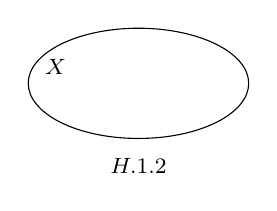
\begin{tikzpicture}[>=stealth,line join=round,line cap=round,font=\footnotesize,scale=.7]
			\draw (1,1) circle (2 and 1);
			\coordinate[label=center:$X$] (X)at(-.5,1.3);
			\coordinate[label=center:$ H.1.2$] (X)at(1,-.5);
	\end{tikzpicture}}
	\immini {$\bullet$ Minh hoạ $T$ là một tập con của $S$ như Hình $1.3$.}
	{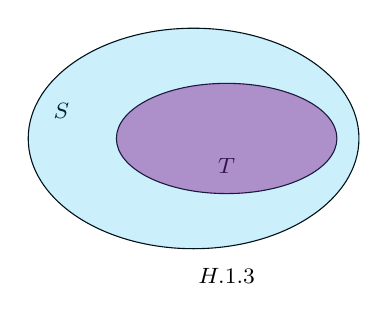
\begin{tikzpicture}[>=stealth,line join=round,line cap=round,font=\footnotesize,scale=.7]
			\coordinate[label=center:$$] (I)at(.4,1);
			\coordinate[label=center:$$] (M)at(1,1);
			\draw (.4,1) circle (3 and 2);
			\coordinate[label=center:$S$] (X)at(-2,1.5);
			\draw (1,1) circle (2 and 1);
			\coordinate[label=center:$T$] (X)at(1,.5);
			\coordinate[label=center:$ H.1.3$] (X)at(1,-1.5);
			\fill[cyan,opacity=.2] (I) ellipse (3 cm and 2 cm)--cycle;
			\fill[violet,opacity=.4] (M) ellipse (2 cm and 1 cm)--cycle;
	\end{tikzpicture}}
\end{tcolorbox}
\subsubsection{Hai tập hợp bằng nhau}
\begin{tcolorbox}
	$S=T \Leftrightarrow \heva{& S \subset T \\ & T \subset S} \Leftrightarrow \forall x,\ (x\in S \Leftrightarrow x \in T)$
\end{tcolorbox}

\subsubsection{Mối quan hệ giữa các tập hợp số}
$\bullet$ Tập hợp các số tự nhiên $\mathbb{N}=\{0 ; 1 ; 2 ; 3 ; \ldots\}$.\\
$\bullet$ Tập hợp các số nguyên $\mathbb{Z}$ gồm các số tự nhiên và các số nguyên âm:
$\mathbb{Z}=\{\ldots ;-2 ;-1 ; 0 ; 1 ; 2 ; \ldots\}$.
$\bullet$ Tập hợp các số hữu tỉ $\mathbb{Q}$ gồm các số viết được dưới dạng phân số $\dfrac{a}{b}$, với $a, b \in \mathbb{Z}, b \neq 0$. Số hữu tỉ còn được biểu diễn dưới dạng số thập phân hữu hạn hoặc vô hạn tuần hoàn.\\
$\bullet$ Tập hợp các số thực $\mathbb{R}$ gồm các số hữu tỉ và các số vô tỉ. Số vô tỉ là các số thập phân vô hạn không tuần hoàn.
\begin{tcolorbox}
	\immini { Mối quan hệ giữa các tập hợp số:  $\mathbb{N} \subset \mathbb{Z} \subset \mathbb{Q} \subset \mathbb{R}$.}
	{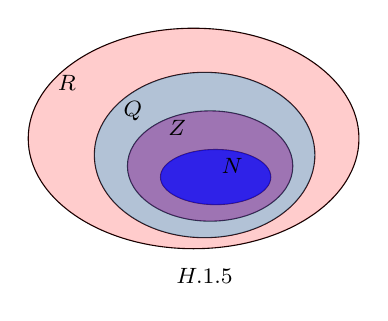
\begin{tikzpicture}[>=stealth,line join=round,line cap=round,font=\footnotesize,scale=.7]
			\path (1.3,1)coordinate[label=center:$$](M) (1.5,.7)coordinate[label=center:$$](N) (1.6,.5)coordinate[label=center:$$](P) (1.7,.3)coordinate[label=center:$$](Q)
			(1.5,-1.5)coordinate[label=center:$H.1.5$](H);
			\draw (1.3,1) circle (3 and 2);
			\draw (1.5,.7) circle (2 and 1.5);
			\draw (1.6,.5) circle (1.5 and 1);
			\draw (1.7,.3) circle (1 and .5);
			\fill[red,opacity=.2] (M) ellipse (3 cm and 2 cm)--cycle;
			\fill[cyan,opacity=.3] (N) ellipse (2 cm and 1.5 cm)--cycle;
			\fill[violet,opacity=.4] (P) ellipse (1.5 cm and 1 cm)--cycle;
			\fill[blue,opacity=.7] (Q) ellipse (1 cm and .5 cm)--cycle;
			\coordinate[label=center:$\mathbb{R}$] (X)at(-1,2);
			\coordinate[label=center:$\mathbb{Q}$] (Q)at(0.2,1.5);
			\coordinate[label=center:$\mathbb{Z}$] (Z)at(1,1.2);
			\coordinate[label=center:$\mathbb{N}$] (N)at(2,.5);
	\end{tikzpicture}}
\end{tcolorbox}
\subsubsection{Các tập con thường dùng của $\mathbb{R}$}
\begin{tcolorbox}
	Một số tập con thường dùng của tập số thực $\mathbb{R}$.\\
	$\bullet$ Khoảng\\
	\immini {$(a ; b)=\{x \in \mathbb{R} \mid a<x<b\}$} {\begin{tikzpicture}[>=stealth,line join=round,line cap=round,font=\footnotesize,scale=1]
			\draw[->] (0,0)--(6,0);
			\path[pattern=north east lines,pattern color=blue] (0,-3pt)rectangle(2,3pt);
			\path[pattern=north east lines,pattern color=blue] (6,-3pt)rectangle(4,3pt);
			\path 
			(2,-0.1)coordinate[label=below:$a$](a) 
			(4,-0.1)coordinate[label=below:$b$](b)
			(2,0)coordinate[label=center:$($](()
			(4,0)coordinate[label=center:$)$](s);
	\end{tikzpicture}}
	\immini {$(a ;+\infty)=\{x \in \mathbb{R} \mid x>a\}$}
	{\begin{tikzpicture}[>=stealth,line join=round,line cap=round,font=\footnotesize,scale=1]
			\draw[->] (0,0)--(6,0);
			\path[pattern=north east lines,pattern color=blue] (0,-3pt)rectangle(2,3pt);
			%\path[pattern=north east lines,pattern color=blue] (6,-3pt)rectangle(4,3pt);
			\path 
			(2,-0.1)coordinate[label=below:$a$](a) 
			%(4,0)coordinate[label=below:$a$](b)
			(2,0)coordinate[label=center:$($](()
			%(4,0)coordinate[label=center:$)$](s)
			;
	\end{tikzpicture}}
	\immini {$(-\infty ; b)=\left\{x \in \mathbb{R} \mid x<b\right\}$}
	{\begin{tikzpicture}[>=stealth,line join=round,line cap=round,font=\footnotesize,scale=1]
			\draw[->] (0,0)--(6,0);
			%\path[pattern=north east lines,pattern color=blue] (0,-3pt)rectangle(2,3pt);
			\path[pattern=north east lines,pattern color=blue] (6,-3pt)rectangle(4,3pt);
			\path 
			%(2,0)coordinate[label=below:$a$](a) 
			(4,-0.1)coordinate[label=below:$b$](b)
			%(2,0)coordinate[label=center:$($](()
			(4,0)coordinate[label=center:$)$](s)
			;
	\end{tikzpicture}}
	\immini {$(-\infty ;+\infty)$}
	{\begin{tikzpicture}[>=stealth,line join=round,line cap=round,font=\footnotesize,scale=1]
			\draw[->] (0,0)--(6,0);
			%\path[pattern=north east lines,pattern color=blue] (0,-3pt)rectangle(2,3pt);
			%\path[pattern=north east lines,pattern color=blue] (6,-3pt)rectangle(4,3pt);
			\path 
			(3,-0.1)coordinate[label=below:$O$](a) 
			%(4,0)coordinate[label=below:$a$](b)
			(3,0)coordinate[label=center:$|$](()
			%(4,0)coordinate[label=center:$)$](s)
			;
	\end{tikzpicture}}
	$\bullet$ Đoạn\\
	\immini {$[a ; b]=\{x \in \mathbb{R} \mid a \leq x \leq b\}$}
	{\begin{tikzpicture}[>=stealth,line join=round,line cap=round,font=\footnotesize,scale=1]
			\draw[->] (0,0)--(6,0);
			\path[pattern=north east lines,pattern color=blue] (0,-3pt)rectangle(2,3pt);
			\path[pattern=north east lines,pattern color=blue] (6,-3pt)rectangle(4,3pt);
			\path 
			(2,-0.1)coordinate[label=below:$a$](a) 
			(4,-0.1)coordinate[label=below:$b$](b)
			(2,0)coordinate[label=center:$[$]()
			(4,0)coordinate[label=center:$\mathrm{]}$](s);
	\end{tikzpicture}}
	$\bullet$ Nửa khoảng\\
	\immini {$[a ; b)=\{x \in \mathbb{R} \mid a \leq x<b\}$}
	{\begin{tikzpicture}[>=stealth,line join=round,line cap=round,font=\footnotesize,scale=1]
			\draw[->] (0,0)--(6,0);
			\path[pattern=north east lines,pattern color=blue] (0,-3pt)rectangle(2,3pt);
			\path[pattern=north east lines,pattern color=blue] (6,-3pt)rectangle(4,3pt);
			\path 
			(2,-0.1)coordinate[label=below:$a$](a) 
			(4,-0.1)coordinate[label=below:$b$](b)
			(2,0)coordinate[label=center:$[$]()
			(4,0)coordinate[label=center:$\mathrm{)}$](s);
	\end{tikzpicture}}
	\immini {$(a ; b]=\{x \in \mathbb{R} \mid a<x \leq b\}$}
	{\begin{tikzpicture}[>=stealth,line join=round,line cap=round,font=\footnotesize,scale=1]
			\draw[->] (0,0)--(6,0);
			\path[pattern=north east lines,pattern color=blue] (0,-3pt)rectangle(2,3pt);
			\path[pattern=north east lines,pattern color=blue] (6,-3pt)rectangle(4,3pt);
			\path 
			(2,-0.1)coordinate[label=below:$a$](a) 
			(4,-0.1)coordinate[label=below:$b$](b)
			(2,0)coordinate[label=center:$($]()
			(4,0)coordinate[label=center:$\mathrm{]}$](s);
	\end{tikzpicture}}
	\immini {$[a ;+\infty)=\{x \in \mathbb{R} \mid x \geq a\}$}
	{\begin{tikzpicture}[>=stealth,line join=round,line cap=round,font=\footnotesize,scale=1]
			\draw[->] (0,0)--(6,0);
			\path[pattern=north east lines,pattern color=blue] (0,-3pt)rectangle(2,3pt);
			%\path[pattern=north east lines,pattern color=blue] (6,-3pt)rectangle(4,3pt);
			\path 
			(2,-0.1)coordinate[label=below:$a$](a) 
			%(4,0)coordinate[label=below:$a$](b)
			(2,0)coordinate[label=center:$[$](()
			%(4,0)coordinate[label=center:$)$](s)
			;
	\end{tikzpicture}}
	\immini {$(-\infty ; b]=\{x \in \mathbb{R} \mid x \leq b\}$}
	{\begin{tikzpicture}[>=stealth,line join=round,line cap=round,font=\footnotesize,scale=1]
			\draw[->] (0,0)--(6,0);
			%\path[pattern=north east lines,pattern color=blue] (0,-3pt)rectangle(2,3pt);
			\path[pattern=north east lines,pattern color=blue] (6,-3pt)rectangle(4,3pt);
			\path 
			%(2,0)coordinate[label=below:$a$](a) 
			(4,-0.1)coordinate[label=below:$b$](b)
			%(2,0)coordinate[label=center:$($](()
			(4,0)coordinate[label=center:$\mathrm{]}$](s)
			;
	\end{tikzpicture}}
\end{tcolorbox}

\subsubsection{Giao của hai tập hợp}
\begin{tcolorbox}
	\immini{Tập hợp gồm các phần tử thuộc cả hai tập hợp $S$ và $T$ gọi là giao của hai tập hợp $S$ và $T$, kí hiệu là $S \cap T$.\\
		$S \cap T=\{x \mid x \in S$ và $x \in T\}$.}
	{\begin{tikzpicture}[>=stealth,line join=round,line cap=round,font=\footnotesize,scale=1]
			\begin{scope}
				\clip (0.5,0) ellipse (1.5 and 1 );
				\fill[pattern = north east lines]	(2.5,0) ellipse (2 and 1.5 );
			\end{scope}
			\draw (0.5,0) ellipse (1.5 and 1 );
			\draw (2.5,0) ellipse (2 and 1.5 );
			\coordinate[label=center:$S\cap T$] (M)at(1.1,.3);
	\end{tikzpicture}}
\end{tcolorbox}
\subsubsection{Hợp của hai tập hợp}
\begin{tcolorbox}
	\immini {Tập hợp gồm các phần tử thuộc tập hợp $S$ hoặc thuộc tập hợp $T$ gọi là hợp của hai tập hợp $S$ và $T$. Kí hiệu là $S \cup T$.
		\[S \cup T=\{x \mid x \in S \text { hoặc } x \in T\}.\]}
	{\begin{tikzpicture}[>=stealth,line join=round,line cap=round,font=\footnotesize,scale=.7]
			\coordinate[label=center:$$] (I)at(0,1);
			\coordinate[label=center:$$] (M)at(1,1);
			\draw[fill,pattern = north east lines] (0,1) circle (1.5 and 1);
			\draw[fill,pattern = north east lines] (1,1) circle (1.5 and 1);
			\coordinate[label=center:$S\cup T$] (X)at(.6,-.5);
			\coordinate[label=center:$S$] (X)at(-1,1);
			\coordinate[label=center:$T$] (X)at(2,1);
	\end{tikzpicture}}
\end{tcolorbox}
\subsubsection{Hiệu của hai tập hợp}
\begin{tcolorbox}
	\immini {$\bullet$ Hiệu của hai tập hợp $S$ và $T$ là tập hợp gồm các phần tử thuộc S nhưng không thuộc $T$, kí hiệu là $S \backslash T$.
		\[S \backslash T=\{x \mid x \in S \text{ và } x \notin T\}\].}
	{\begin{tikzpicture}[>=stealth,line join=round,line cap=round,font=\footnotesize,scale=.8]
			\draw (0.5,0) ellipse (1.5 and 1 );
			\draw (2.5,0) ellipse (1.5 and 1 );
			\fill[pattern = north east lines] (0.5,0) ellipse (1.5 and 1 );
			\fill[fill=white] (2.5,0) ellipse (1.5 and 1 );
			\path 
			(0,.5)coordinate[label=center:$S$](S) (2,.5)coordinate[label=center:$T$](T)
			(1.7,1.5)coordinate[label=center:$S\backslash T$](T) ;
			
	\end{tikzpicture}}
	\immini {$\bullet$ Nếu $T \subset S$ thì $S \backslash T$ được gọi là phần bù của $T$ trong $S$, kí hiệu là $C_{s} T$.}
	{	\begin{tikzpicture}[>=stealth,line join=round,line cap=round,font=\footnotesize,scale=.8]
			\draw (0.5,0) ellipse (1.5 and 1 );
			\draw (.8,0) ellipse (1 and .5 );
			\fill[pattern = north east lines] (0.5,0) ellipse (1.5 and 1 );
			\fill[fill=white] (.8,0) ellipse (1 and .5 );
			\path 
			(-.3,.5)coordinate[label=center:$S$](S) (1,0)coordinate[label=center:$T$](T)
			(1,1.3)coordinate[label=center:$C_S T$](T) ;
			
	\end{tikzpicture}}
\end{tcolorbox}
\subsection{CÁC DẠNG BÀI TẬP}
\begin{dang}{Xác định tập hợp}
	Được mô tả theo 2 cách:
	\begin{enumEX}{1}
		\item  Liệt kê tất cả các phần tử của tập hợp.
		\item  Nêu tính chất đặc trưng.
	\end{enumEX}
\end{dang}
\subsubsection{Ví dụ minh hoạ}
\begin{vd}%[BG10-2022]%[Đỗ Văn Dự]%[0D1Y2-1]
	Cho $D=\{n \in \mathbb{N} \mid n$ là số nguyên tố, $5<n<20\}$.
	\begin{enumEX}{1}
		\item Dùng kí hiệu $\in, \notin$ để viết câu trả lời cho câu hỏi sau: Trong các số $5$; $12$; $17$; $18$, số nào thuộc tập $D$, số nào không thuộc tập $D$?
		\item Viết tập hợp $D$ bằng cách liệt kê các phần tử. Tập hợp $D$ có bao nhiêu phần tử?
	\end{enumEX}
	\loigiai{
		\begin{enumEX}{1}
			\item $5 \notin D$; $12 \notin D$; $17 \in D$; $18 \notin D$.
			\item $D=\{7 ; 11 ; 13 ; 17 ; 19\}$. Tập hợp $D$ có $5$ phần tử.
		\end{enumEX}	
	}
\end{vd}

\begin{vd}%[BG10-2022]%[Đỗ Văn Dự]%[0D1B2-1] 
	Viết mỗi tập hợp sau bằng cách liệt kê các phần tử.
	\begin{enumEX}{2}
		\item $A=\left\{\left. x\in \mathbb{R}\right|\left(2x-x^2\right)\left(3x-2\right)=0\right\}$.
		\item $B=\left\{\left. x\in \mathbb{Z}\right|2x^3-3x^2-5x=0\right\}$.
		\item $C=\left\{\left. x\in \mathbb{Z}\right|2x^2-75x-77=0\right\}$.
		\item $D=\left\{\left. x\in \mathbb{R}\right|(x^2-x-2)(x^2-9)=0\right\}$.
	\end{enumEX}
	\loigiai{
		\begin{enumEX}{1}
			\item Ta giải phương trình\\
			 $\left(2x-x^2\right)\left(2x^2-3x-2\right)=0\Leftrightarrow \hoac{
				& 2x-x^2=0 \\ 
				& 2x^2-3x-2=0}\Leftrightarrow \hoac{
				& x=0\vee x=2 \\ 
				& x=-\dfrac{1}{2}\vee x=2}$.\\
			Do $x\in \mathbb{R}$ nên $A=\left\{-\dfrac{1}{2};0;2\right\}$.
			\item Ta giải phương trình $2x^3-3x^2-5x=0\Leftrightarrow x\left(2x^2-3x-5\right)=0\Leftrightarrow \hoac{&x=0\\&x=-1\\&x=\dfrac{5}{3}}$.\\
			Do $x\in \mathbb{Z}$ nên $B=\left\{0;-1\right\}$.
			\item Ta giải phương trình $2x^2-75x-77=0\Leftrightarrow \hoac{&x=-1\\&x=\dfrac{77}{2}}$.\\
			Do $x\in \mathbb{Z}$ nên $C=\left\{-1\right\}$.
	\end{enumEX}}
\end{vd}

\begin{vd}%[BG10-2022]%[Đỗ Văn Dự]%[0D1B2-1] 
	Viết mỗi tập hợp sau bằng cách liệt kê các phần tử.
	\begin{enumEX}{1}
		\item $A=\left\{\left. n\in {\mathbb{N}}^{*}\right|3<n^2<30\right\}$.
		\item $B=\left\{\left. n\in \mathbb{Z}\right|\left| n\right|<3\right\}$.
		\item $C=\left\{\left. x\right|x=3k\right.$ với $k\in \mathbb{Z}$ và $\left.-4<x<12\right\}$.
		\item $D=\left\{\left. n^2+3\right|n \in \mathbb{N} \text{ và } n<5\right\}$.
	\end{enumEX}
	\loigiai{
		\begin{enumEX}{1}
			\item Với $3<n^2<30$ và $n\in {\mathbb{N}}^{*}$ nên chọn $n=2;3;4;5$.\\
			Vậy $A=\left\{2;3;4;5\right\}$.
			\item  Vì $x<\left| 3\right|\Leftrightarrow-3<x<3$.\\
			Do $x\in \mathbb{Z}$ nên $B=\left\{-2;-1;0;1;2\right\}$.
			\item Ta có $-4<x<12\Leftrightarrow-4<3k<12\Leftrightarrow-\dfrac{4}{3}<k<4$.\\
			Do $k\in \mathbb{Z}$ nên ta chọn $k=\left\{-10;1;2;3\right\}$ suy ra $x=3k=\left\{-3;0;3;6;9\right\}$.\\
			Vậy $C=\left\{-3;0;3;6;9\right\}$.
			\item Vì $n \in \mathbb{N} \text{ và } n<5$ nên chọn  $n=0,1,2;3;4$.\\
			Vậy $A=\left\{3;4;12;19\right\}$.
		\end{enumEX}
	}
\end{vd}

\begin{vd}%[BG10-2022]%[Đỗ Văn Dự]%[0D1K2-1]
	Viết mỗi tập hợp sau bằng cách nêu tính chất đặc trưng.
	\begin{enumEX}{2}
		\item $A=\left\{\dfrac{2}{3};\dfrac{3}{8};\dfrac{4}{15};\dfrac{5}{24};\dfrac{6}{35}\right\}$.
		\item $B=\left\{0;3;8;15;24;35\right\}$.
		\item $C=\left\{-4;1;6;11;16\right\}$.
		\item $D=\left\{1;-2;7\right\}$.
	\end{enumEX}
	\loigiai{
		\begin{enumEX}{2}
			\item $A=\left\{\left. \dfrac{n}{n^2-1}\right|n\in \mathbb{N},2\le n\le 6\right\}$.
			\item $B=\left\{\left. n^2-1\right|n\in \mathbb{N},1\le n\le 6\right\}$.
			\item $C=\left\{\left. n\in \mathbb{N}\right|\right.\left. 5n-4\right\}$.
			\item $D=\left\{\left. x\in \mathbb{R}\right|\left(x-1\right)\left(x+2\right)\left(x-7\right)=0\right\}$.
		\end{enumEX}
	}
\end{vd}
\subsubsection{Bài tập tự luận}
\begin{bt}%[Huỳnh Quy]%[0D1B2-1]
	Liệt kê các phần tử của các tập hợp sau:
	\begin{enumerate}
		\item $A=\left\lbrace n\in \mathbb{N} \mid n<5\right\rbrace$.
		\item $B$ là tập hợp các số tự nhiên lớn hơn $0$ và nhỏ hơn $5$.
		\item $C=\left\lbrace x\in \mathbb{R}\mid (x-1)(x+2)=0\right\rbrace$.
	\end{enumerate}
	\loigiai{
		\begin{enumerate}
			\item $A=\left\lbrace 0;1;2;3;4\right\rbrace$.
			\item $B=\left\lbrace 1;2;3;4\right\rbrace$.
			\item Ta có $(x-1)(x+2)=0 \Leftrightarrow \hoac{&x=1\\&x=-2.}$\\
			Mà $x\in \mathbb{R}$ nên
			$C=\left\lbrace -2;1\right\rbrace$.
		\end{enumerate}
	}
\end{bt}
\begin{bt}%[Huỳnh Quy]%[0D1B2-1]
	Viết các tập hợp sau bằng phương pháp liệt kê:
	\begin{enumerate}
		\item $A=\left\lbrace  x\in \mathbb{Q}\mid (x^2-2x+1)(x^2-5)\right\rbrace=0$.
		\item $B=\left\lbrace x \in \mathbb{N}\mid 5<x^2<40\right\rbrace$.
		\item $C=\left\lbrace x\in \mathbb{Z}\mid x^2<9\right\rbrace$.
		\item $D=\left\lbrace x\in \mathbb{R}\mid \left|2x+1\right|=5\right\rbrace$.
	\end{enumerate}
	\loigiai{
		\begin{enumerate}
			\item Ta có $x\in A\Leftrightarrow\hoac{&x^2-2x+1=0\\&x^2-5=0}\Leftrightarrow\hoac{&x=1\in\mathbb{Q}\\&x=\pm\sqrt{5}\not\in \mathbb{Q}.}$\\
			Vậy $A=\left\lbrace 1\right\rbrace$.
			\item $B=\left\lbrace 3;4;5;6\right\rbrace$.
			\item $C=\left\lbrace -2;-1;0;1;2\right\rbrace$.
			\item Ta có $\left|2x+1\right|=5\Leftrightarrow \hoac{& 2x+1=5 \\ & 2x+1 =-5} \Leftrightarrow \hoac{&x=2\\&x=-3.}$\\
			Vậy $D=\left\lbrace 2;-3\right\rbrace$.
		\end{enumerate}
	}
\end{bt}
\begin{bt}%[Huỳnh Quy]%[0D1B2-1]
	Viết các tập hợp sau bằng cách chỉ ra tính chất đặc trưng cho các phần tử của tập hợp đó.
	\begin{enumerate}
		\item $A=\left\lbrace 0;4;8;12;16;\ldots ;52\right\rbrace$.
		\item $B=\left\lbrace 3;6;9;12;15;\ldots ;51\right\rbrace$.
		\item $C=\left\lbrace 2;5;8;11;14;\ldots ;62\right\rbrace$.
	\end{enumerate}
	\loigiai{
		\begin{enumerate}
			\item $A=\left\lbrace x\in \mathbb{N}\mid 0\le x\le 52 \text{ và } x\;\vdots \;4\right\rbrace$.
			\item $B=\left\lbrace x\in \mathbb{N}\mid 3\le x\le 51 \text{ và } x\;\vdots \;3\right\rbrace$.
			\item $C=\left\lbrace  x\in \mathbb{N}\mid 2\le x\le 62 \text{ và } (x-2)\;\vdots \;3\right\rbrace$.
		\end{enumerate}
	}
\end{bt}
\begin{bt}%[Huỳnh Quy]%[0D1K2-1]
	Viết các tập hợp sau bằng cách chỉ ra tính chất đặc trưng cho các phần tử của tập hợp đó.
	\begin{enumerate}
		\item $A=\left\lbrace 2;3;5;7;11;13;17\right\rbrace$.
		\item $B=\left\lbrace -2;4;-8;16;-32;64\right\rbrace$.
	\end{enumerate}
	\loigiai{
		\begin{enumerate}
			\item $A=\left\lbrace x\in \mathbb{N}\mid x\le 17 \text{ và }x \text{ là số nguyên tố} \right\rbrace$.
			\item $B=\left\lbrace x=(-2)^n\mid n\in \mathbb{N}, 1\le n\le 6 \right\rbrace$.
		\end{enumerate}
	}
\end{bt}

\begin{bt}%[Huỳnh Quy]%[0D1B2-1]
	Tìm một tính chất đặc trưng xác định các phần tử của mỗi tập hợp sau
	\begin{align*}
		A&=\{1; 2; 3; 4; 5; 6; 7; 8; 9\} \\
		B&=\{0; 7; 14; 21; 28\}
	\end{align*}
	\loigiai{
		\begin{align*}
			A&=\{x\in \mathbb{N^*} \mid x\leq 9\} \\
			B&=\{x\in \mathbb{N} \mid x \;\vdots \;7 \text{ và } x\leq 28\}
		\end{align*}
	}
\end{bt}

\begin{dang}{Tập hợp con, xác định tập hợp con}
	Cho tập hợp $A$ gồm $n$ phần tử.
	\begin{enumEX}{1}
		\item  Khi liệt kê tất cả các tập con của $A$, ta liệt kê đầy đủ theo thứ tự:\\		
		\centerline{ $\varnothing$; tập $1$ phần tử; tập $2$ phần tử; tập $3$ phần tử;...; $A$.}
		\item  Số tập con của $A$ là $2^n$.
		\item  Số tập con gồm $k$ phần tử của $A$ là $\mathrm{C}_n^k$.
	\end{enumEX}
\end{dang}
\subsubsection{Ví dụ minh hoạ}
\begin{vd}%[BG10-2022]%[Đỗ Văn Dự]%[0D1Y2-2]
	Cho tập hợp $S=\{2 ; 3 ; 5\}$. Những tập hợp nào sau đây là tập con của $S$?
	$$S_{1}=\{3\};S_{2}=\{0 ; 2\}; S_{3}=\{3 ; 5\}$$.
	\loigiai{
		Các tập hợp $S_{1}=\{3\}$, $S_{3}=\{3 ; 5\}$ là những tập con của $S$.\\
		Tập $S_{2}=\{0 ; 2\}$ không là tập con của $S$.
	}
\end{vd}

\begin{vd}%[BG10-2022]%[Đỗ Văn Dự]%[0D1B2-2]
	Cho tập hợp $A=\left\{2;3;4\right\}$ và $B=\left\{2;3;4;5;6\right\}$.
	\begin{enumEX}{1}
		\item Xác định tất cả tập con có hai phần tử của $A$.
		\item Xác định tất cả tập con có ít hơn hai phần tử của $A$.
		\item Tập $A$ có tất cả bao nhiêu tập con.
		\item Xác định tất cả các tập $X$ thỏa $A \subset X \subset B$.
	\end{enumEX}
		\loigiai{
	\begin{enumEX}{1}		
		\item 	Các tập hợp $S_1=\{2;3\}$, $S_2=\{2;4\}$, $S_3=\{3;4\}$  là những tập con của $A$.\\
			Tập $S_{2}=\{0 ; 2\}$ không là tập con của $S$.
		\item 	Các tập hợp $\varnothing$, $\{2\}$, $\{3\}$, $\{4\}$  là những tập con ít hơn $2$ phần tử của $A$.\\
		\item 	Tập $A$ có tất cả $8$ tập con.
		\item 	 Tất cả các tập $X$ thỏa $A \subset X \subset B$ là $\{2;3;4\}$, $\{2;3;4,5\}$, $\{2;3;4,5,6\}$.	
	\end{enumEX}
		}	
\end{vd}
\subsubsection{Bài tập tự luận}
\begin{bt}%[Huỳnh Quy]%[0D1B2-2]
	Tìm tất cả các tập con của tập $A=\{a,1,2\}$.
	\loigiai{Tập $A$ có $2^3=8$ tập con.
		\begin{itemize}
			\item 0 phần tử: $ \varnothing $.
			\item 1 phần tử: $\{a\}$, $\{1\}$, $\{2\}$.
			\item 2 phần tử: $\{a, 1\}$, $\{a,2\}$, $\{1,2\}$.
			\item 3 phần tử: $\{a,1,2\}$.
	\end{itemize}}
\end{bt}
\begin{bt}%[Huỳnh Quy]%[0D1B2-2]
	Tìm tất cả các tập con có 2 phần tử của tập $A=\{1,2,3,4,5,6\}$.
	\loigiai{$\{1,2\}$,$\{1,3\}$, $\{1,4\}$, $\{1,5\}$, $\{1,6\}$, $\{2,3\}$, $\{2,4\}$, $\{2,5\}$, $\{2,6\}$, $\{3,4\}$, $\{3,5\}$, $\{3,6\}$, $\{4,5\}$, $\{4,6\}$, $\{5,6\}$.}
\end{bt}
\begin{bt}%[Huỳnh Quy]%[0D1B2-2]
	Xác định tập hợp $X$ biết $\{1,2\} \subset X \subset \{1,2,5\}$.
	\loigiai{Ta có
		\begin{itemize}
			\item  Vì $\{1,2\} \subset X$ nên tập hợp $X$ có chứa các phần tử $1,2$.
			\item  Vì $X \subset \{1,2,5\}$ nên các phần tử của tập hợp $X$ có thể là $1,2,5$.
		\end{itemize}
		Khi đó tập hợp $X$ có thể là $\{1,2\}, \{1,2,5\}$.}
\end{bt}
\begin{bt}%[Huỳnh Quy]%[0D1B2-2]
	Xác định tập hợp $X$ biết $\{a,1\} \subset X \subset \{a,b,1,2\}$.
	\loigiai{Ta có
		\begin{itemize}
			\item  Vì $\{a,1\} \subset X$ nên tập hợp $X$ có chứa 2 phần tử là $a,1$.
			\item  Vì $X \subset \{a,b,1,2\}$ nên các phần tử của tập hợp $X$ có thể là $a,b,1,2$.
		\end{itemize}
		Suy ra, tập hợp $X$ có 2 phần tử, 3 phần tử hoặc 4 phần tử.\\
		Khi đó, tập hợp $X$ có thể là $\{a,1\}, \{a,1,2\}, \{a,b,1\}, \{a,b,2\}, \{a,b,1,2\}$.\\
		\underline{\textbf{Cách khác:}} $X=\{a;1\} \cup X'$ với $X' \subset \{b;2\}$. \\
		Vì có $4$ tập hợp $X'$ nên có $4$ tập hợp $X$ thỏa yêu cầu bài toán.}
\end{bt}
\begin{bt}%[Huỳnh Quy]%[0D1K2-2]
	Cho tập hợp $A=\{1;2;3;4;5;6\}$. Tìm tất cả các tập con có $3$ phần tử của tập hợp $A$ sao cho tổng các phần tử này là một số lẻ.
	\loigiai{
		Để tổng của ba số nguyên là một số lẻ thì trong ba số chỉ có một số lẻ hoặc cả ba số đều lẻ. Nói cách khác tập con này của $A$ phải có một số lẻ hoặc ba số lẻ.\\
		Chỉ có một tập con gồm ba số lẻ của $A$ là $\{1;3;5\}$. Các tập con gồm ba số của $A$ trong đó có một số lẻ là: \\
		$\{1;2;4\}$; $\{1;2;6\}$; $\{1;4;6\}$;$\{3;2;4\}$; $\{3;2;6\}$; $\{3;4;6\}$; $\{5;2;4\}$; $\{5;2;6\}$; $\{5;4;6\}$.\\
		\textit{\underline{Nhận xét:} Tổng các số nguyên là một số lẻ khi số số lẻ là số lẻ.}
	}
\end{bt}
\begin{bt}%[Huỳnh Quy]%[0D1K2-2]
	Cho $A=\{n\in\mathbb{N}\mid n \text{ là ước của }2\}$; $B=\{x\in\mathbb{R}\mid (x^2-1)(x-2)(x-4)=0 \}$. Tìm tất cả các tập hợp $X$ sao cho $A\subset X\subset B$.
	\loigiai{ 
		Liệt kê các phần tử của tập hợp $A$ và $B$ ta được : \\
		$A=\{1;2\}$; $B=\{-1;1;2;4\}$.\\
		Muốn tìm tập $X$ thỏa điều kiện $A\subset X\subset B$ đầu tiên ta lấy $X=A$, sau đó ghép thêm các phần tử thuộc $B$ mà không thuộc $A$. Với cách thực hiện như trên, ta có các tập hợp $X$ thỏa mãn yêu cầu bài toán là: $X=A=\{1;2 \}$, rồi ghép thêm vào một phần tử ta được: $\{-1;1;2 \}$;$\{4;1;2 \}$\\
		Ghép thêm vào $A$ hai trong bốn phần tử còn lại của $B$ ta được : $X=B=\{-1;1;2;4\}$
	}
\end{bt}
\begin{dang}{Các phép toán trên tập hợp}
\end{dang}
\subsubsection{Ví dụ minh hoạ}
\begin{vd}%[BG10-2022]%[Đỗ Văn Dự]%[0D1B2-2]
	Cho hai tập hợp:
	$C=\{n \in \mathbb{N} \mid n$ là bội chung của 2 và $3 ; n<30\}$;
	$D=\{n \in \mathbb{N} \mid n$ là bội của $6 ; n<30\}$.
	Chứng minh rằng $C=D$.
	\loigiai{
		Ta có: $C=\{0 ; 6 ; 12 ; 18 ; 24\}$.\\
		$D=\{0 ; 6 ; 12 ; 18 ; 24\}$.\\
		Vậy $C=D$.
	}
\end{vd}

\begin{vd}%[BG10-2022]%[Đỗ Văn Dự]%[0D1Y4-1]
	Viết các tập hợp sau dưới dạng các khoảng, đoạn, nửa khoảng trong $\mathbb{R}$ rồi biểu diễn trên trục số: $C=\{x \in \mathbb{R} \mid 2 \leq x \leq 7\}$; $D=\{x \in \mathbb{R} \mid x<2\}$.
	\loigiai{
		\immini{$C=[2;7]$}{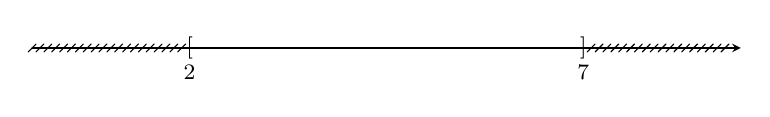
\begin{tikzpicture}[scale=1,>=stealth, font=\footnotesize, line join=round, line cap=round]
				\draw [-stealth] (0,0)--(9,0);
				\path (2,0) node{$[$} (2,-0.1)node[below]{$2$}
				(7,0) node{$]$} (7,-0.1)node[below]{$7$};
				\foreach \x in{0,0.1,...,2} \draw (\x,0)--++(45:.07) (\x,0)--++(-135:.07);
				\foreach \x in{7.1,7.2,...,8.8} \draw (\x,0)--++(45:.07) (\x,0)--++(-135:.07);
		\end{tikzpicture}}
		\immini{$C=(-\infty;2)$}{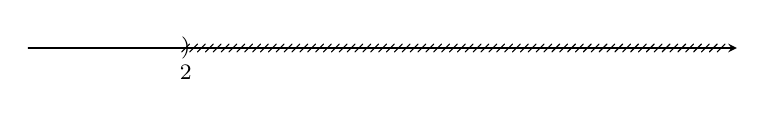
\begin{tikzpicture}[scale=1,>=stealth, font=\footnotesize, line join=round, line cap=round]
				\draw [-stealth] (0,0)--(9,0);
				\path (2,0) node{$)$} (2,-0.1)node[below]{$2$};
				\foreach \x in{2,2.1,...,8.9} \draw (\x,0)--++(45:.07) (\x,0)--++(-135:.07);
		\end{tikzpicture}}	
		
	}
\end{vd}

\begin{vd}%[BG10-2022]%[Đỗ Văn Dự]%[0D1B4-1]
	\begin{enumerate}
		\item Cho hai tập hợp $C=\{4 ; 7 ; 27\}$ và $D=\{2 ; 4 ; 9 ; 27 ; 36\}$. Hãy xác định tập hợp $C \cap D$.
		\item Cho hai tập hợp $E=[1 ;+\infty)$ và $F=(-\infty ; 3]$. Hãy xác định tập hợp $E \cap F$.
	\end{enumerate}
	\loigiai{
		\begin{enumEX}{1}
			\item Giao của hai tập hợp $C$ và $D$ là $C \cap D=\{4 ; 27\}$.
			\item Giao của hai tập hợp $E$ và $F$ là $E \cap F=[1 ; 3]$.\\
			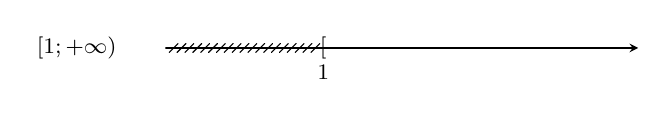
\begin{tikzpicture}[scale=1,>=stealth, font=\footnotesize, line join=round, line cap=round]
				\draw [-stealth] (-1,0)--(5,0);
				\path (1,0) node{$[$} (1,-0.1)node[below]{$1$} (-1.5,0)node[left]{$[1 ;+\infty)$};
				\foreach \x in{-0.9,-0.8,...,0.9} \draw (\x,0)--++(45:.08) (\x,0)--++(-135:.08);
			\end{tikzpicture}\\
			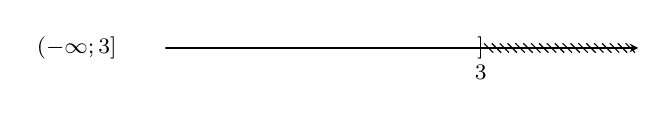
\begin{tikzpicture}[scale=1,>=stealth, font=\footnotesize, line join=round, line cap=round]
				\draw [-stealth] (-1,0)--(5,0);
				\path (3,0) node{$]$} (3,-0.1)node[below]{$3$} (-1.5,0)node[left]{$(-\infty ; 3]$};
				\foreach \x in{3.1,3.2,...,4.9} \draw (\x,0)--++(-45:.08) (\x,0)--++(135:.08);
			\end{tikzpicture}\\
			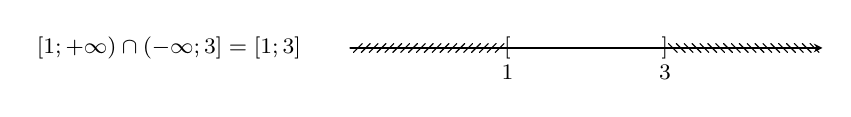
\begin{tikzpicture}[scale=1,>=stealth, font=\footnotesize, line join=round, line cap=round]
				\draw [-stealth] (-1,0)--(5,0);
				\path (3,0) node{$]$} (3,-0.1)node[below]{$3$} 
				(1,0) node{$[$} (1,-0.1)node[below]{$1$} (-1.5,0)node[left]{$[1 ;+\infty)\cap(-\infty ; 3]=[1;3]$}
				;
				\foreach \x in{3.1,3.2,...,4.9} \draw (\x,0)--++(-45:.08) (\x,0)--++(135:.08);
				\foreach \x in{-0.9,-0.8,...,0.9} \draw (\x,0)--++(45:.08) (\x,0)--++(-135:.08);
			\end{tikzpicture}
		\end{enumEX}
	}
\end{vd}
\begin{vd}%[BG10-2022]%[Đỗ Văn Dự]%[0D1B3-1]
	Cho hai tập hợp: $C=\{2 ; 3 ; 4 ; 7\}$; $D=\{-1 ; 2 ; 3 ; 4 ; 6\}$. Hãy xác định tập hợp $C \cup D$.
	\loigiai{
		Hợp của hai tập hợp $C$ và $D$ là $C \cup D=\{-1 ; 2 ; 3 ; 4 ; 6 ; 7\}$.
	}
\end{vd}

\begin{vd}%[BG10-2022]%[Đỗ Văn Dự]%[0D1B3-2]
	Cho các tập hợp: $D=\{-2 ; 3 ; 5 ; 6\}$; $E=\{x \mid x$ là số nguyên tố nhỏ hơn 10$\}$; $X=\{x \mid x$ là số nguyên dương nhỏ hơn 10$\}$.
	\begin{enumEX}{1}
		\item Tìm $D \backslash E$ và $E \backslash D$.
		\item $E$ có là tập con của $X$ không? Hãy tìm phần bù của $E$ trong $X$ (nếu có).
	\end{enumEX}
	\loigiai{
		\begin{enumEX}{1}
			\item Ta có: $E=\{2 ; 3 ; 5 ; 7\}$.\\
			Do đó, $D \backslash E=\{-2 ; 6\}$; $E \backslash D=\{2 ; 7\}$.
			\item Ta có: $X=\{1 ; 2 ; 3 ; 4 ; 5 ; 6 ; 7 ; 8 ; 9\}$. Vậy $E$ là tập con của $X$.\\
			Phần bù của $E$ trong $X$ là $X \backslash E=C_{X} E=\{1 ; 4 ; 6 ; 8 ; 9\}$.
		\end{enumEX}	
	}
\end{vd}

\begin{vd}%[BG10-2022]%[Đỗ Văn Dự]%[0D1B3-1]
	Cho hai tập hợp $A=\left\{0;1;2;3;4\right\}$ và $B=\left\{2;3;4;5;6\right\}$.
	\begin{enumEX}{1}
		\item Tìm các tập hợp $A\cup B, A\cap B, A\backslash B, B\backslash A$.
		\item  Tìm các tập $\left(A\backslash B\right)\cup \left(B\backslash A\right), \left(A\backslash B\right)\cap \left(B\backslash A\right)$.
	\end{enumEX}
	\loigiai{
	\begin{enumEX}{1}
			\item Ta có $A\backslash B=\left\{0;1\right\}$, $B\backslash A=\left\{5;6\right\}$, $A\cup B=\left\{0;1;2;3;4;5;6\right\}$, $A\cap B=\left\{2;3;4\right\}$.
			\item Ta có $\left(A\backslash B\right)\cup \left(B\backslash A\right)=\left\{0;1;5;6\right\}$, $\left(A\backslash B\right)\cap \left(B\backslash A\right)=\varnothing $.
	\end{enumEX}
	}
\end{vd}
\subsubsection{Bài tập tự luận}
\begin{bt}%[Huỳnh Quy]%[0D1B3-2]
	Cho hai tập hợp $A=\{ 1;2;3;4;5\}$ và $B=\{ 0;2;4\}$. Xác định $A\cap B$, $A\cup B$.
	\loigiai{
		Ta có $A\cap B=\{2;4\}$ và $A\cup B=\{0;1;2;3;4;5\}$.
	}
\end{bt}
\begin{bt}%[Huỳnh Quy]%[0D1B3-1]
	Cho hai tập hợp $A=\{1;2;3;5;7\}$ và  $B=\{n\in \mathbb{N} |\, n \text{ là ước số của } 12\}$. Tìm $A\cap B$  và $A\cup B$.
	\loigiai{
		Ta có: $B=\{1;2;3;4;6;12\}$.
		Vậy: $A\cap B=\{ 1;2;3\}$ và $A\cup B=\{ 1;2;3;4;5;6;7;12\}$.
	}
\end{bt}
\begin{bt}%[Huỳnh Quy]%[0D1B3-2]
	Cho hai tập hợp $A$ và $B$. Tìm $A\cap B, A\cup B$ biết
	\begin{enumerate}
		\item $A=\{x\mid x\ \text{là ước nguyên dương của 12} \}$ và 	$B=\{x\mid x\ \text{là ước nguyên dương của 18} \}$.
		\item $A=\{x\mid x\ \text{là ước nguyên dương của 27}\}$ và $B=\{x\mid x\ \text{là ước nguyên dương của 15} \}$.
	\end{enumerate}
	\loigiai{
		\begin{enumerate}
			\item $A=\{1;2;4;6;12\}$, $B=\{1;2;3;6;9;18\}$ $\Rightarrow \begin{cases} A\cap B=\{1;2;6\}\\
				A\cup B=\{1;2;3;4;6;9;12;18\} \end{cases}$
			\item $A=\{1;3;9;27\}$, $B=\{1;3;5;15\}$$\Rightarrow \begin{cases} A\cap B=\{1;3\}\\A\cup B=\{1;3;5;9;15;27\}\end{cases}$
		\end{enumerate}
	}
\end{bt}
\begin{bt}%[Huỳnh Quy]%[0D1B3-1]
	Cho $A$ là tập hợp học sinh lớp $12$ của trường Buôn Ma Thuột và $B$ là tập hợp học sinh của trường Buôn Ma Thuột dự kiến sẽ lựa chọn thi khối $A$ vào các trường đại học. Hãy mô tả các học sinh thuộc tập hợp sau
	\begin{enumEX}{2}
		\item $A\cap B$.
		\item $A\cup B$.
	\end{enumEX}
	\loigiai{
		\begin{enumerate}
			\item $A\cap B$ là tập hợp các học sinh lớp 12 thi khối $A$ của trường Buôn Ma Thuột.
			\item $A\cup B$ là tập hợp các học sinh hoặc lớp 12 hoặc học sinh chọn thi khối A của trường Buôn Ma Thuột. 
		\end{enumerate}
	}
\end{bt}
\begin{bt}%[Huỳnh Quy]%[0D1K3-1]
	Cho tập hợp $B=\{ x\in \mathbb{Z}|\, -4< x \le 4 \}$ và $C=\{ x\in \mathbb{Z}|\, x\le a\}$.
	Tìm số nguyên $a$ để tập hợp $B\cap C=\varnothing $.
	\loigiai{
		Ta có $B=\{-3;-2;-1;0;1;2;3;4\}$, $C=\{\ldots,a-1,a\}$.\\
		Để $B\cap C=\varnothing $ thì  $a\le -4$.
	}
\end{bt}
\begin{bt}%[Huỳnh Quy]%[0D1B3-1]
	Xác định tập hợp $A\cap B$ biết 
	$$A=\{x\in\mathbb{N}|\, x \text { là bội của }3 \}, \,\, B=\{x\in\mathbb{N}|\, x\text { là bội của }7\}.$$
	\loigiai{
		Ta có $A\cap B=\{x\in\mathbb{N}|\, x\text { là bội của }3 \text{ và bội của }7 \}= \{x\in\mathbb{N}|\, x\text {  là bội của  }21\} $.
	}
\end{bt}
\begin{bt}%[Huỳnh Quy]%[0D1B3-2]
	Cho $A$ là tập hợp các số tự nhiên chẵn không lớn hơn $10$, 
	$B=\left\{n\in \mathbb{N}|n\le 6\right\}$ và 
	$C=\left\{n\in \mathbb{N}|4\le n\le 10\right\}$. 
	Hãy tìm $A\cap (B\cup C)$.
	\loigiai{
		Ta có $A=\{0;2;4;6;8;10\}$; $B=\{0;1;2;3;4;5;6\}$ và $C=\{4;5;6;7;8;9;10\}$\\
		$B\cup C=\{0; 1; 2; 3; 4; 5; 6; 7; 8; 9; 10\}$ nên $A\cap (B\cup C)=\{0;2; 4; 6; 8; 10\}$.\\
		\underline{\textbf{Cách khác:}} Vì $B \cup C = \{n \in \mathbb{N} | n \ge 10\}$ nên $A \subset (B \cup C)$.\\
		Do đó $A \cap (B \cup C) = A = \{0;2;4;6;8;10\}$.
	}
\end{bt}
\begin{bt}%[Huỳnh Quy]%[0D1B3-1]
	Cho các tập hợp $A=\{x\in\mathbb{N}\mid x<8\}$ và $B=\{x\in\mathbb{Z}\mid  -3\leq x\leq 5\}$. Tìm $A\cap B$; $A\cup B$.
	\loigiai{
		Ta có $A=\{0;1;2;3;4;5;6;7\}$; $B=\{-3;-2;-1;0;1;2;3;4;5\}$.\\
		Vậy $A\cap B=\{0;1;2;3;4;5\}$ và $A\cup B=\{-3;-2;-1;0;1;2;3;4;5;6;7\}$.
	}
\end{bt}
\begin{bt}%[Huỳnh Quy]%[0D1K3-1]
	Cho các tập hợp $A=\{x \in \mathbb{Z}\big| |x-1|<4\}$, $B=\{x \in \mathbb{Z}\big| |x-1|>2\}$. Tìm $A \cap B$.
	\loigiai{
		Ta có $|x-1|<4 \Leftrightarrow -4<x-1<4 \Leftrightarrow -3<x<5$, $A=\{-2;-1;0;1;2;3;4\}$. \\
		Lại có $|x-1|>2 \Leftrightarrow x<-1\vee x>3$, $B=\{\ldots;-3;-2;4;5;6;\ldots\}$ nên $A \cap B=\{-2;4\}$.
	}
\end{bt}
\begin{bt}%[Huỳnh Quy]%[0D1G3-1]
	Cho các tập hợp $A=\{x\in\mathbb{Z}\,|\, 2m-1<x<2m+3\}$, $B=\{x\in\mathbb{Z}\,\big|\, |x|<2\}$. Tìm $m$ để $A\cap B=\varnothing$.
	\loigiai{
		Ta có $B=\{x\in\mathbb{Z}\,|\, -2<x<2\}=\{-1;0;1\}$ và $A=\{2m,\ldots,2m+2\}$.\\
		$A\cap B=\varnothing \Leftrightarrow \hoac{& 2m+2 \le -2 \\ & 2m \ge 2} \Leftrightarrow \hoac{& m \le -2 \\ & m \ge 1.}$
	}
\end{bt}
\begin{bt}%[Huỳnh Quy]%[0D1B4-1]
	Cho $A=\left[-2;4\right],B=\left(2;+\infty\right),C=(-\infty;3)$. Xác định các tập hợp sau đây và biểu diễn chúng trên trục số.
	\begin{enumerate}
		\item $A\cap B, B\cap C$.
		\item $\mathbb{R}\cap A,\mathbb{R}\cap B$.
	\end{enumerate}
	\loigiai{
		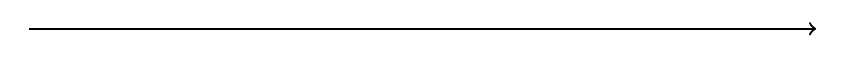
\begin{tikzpicture}[scale=1]
			\draw[->,thick](-4,0) --(6,0);
		\end{tikzpicture}\\
		%
		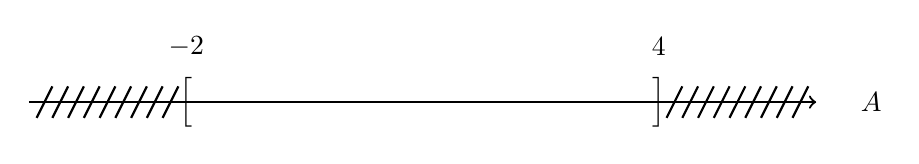
\begin{tikzpicture}[scale=1]
			\draw[->,thick](-4,0) --(6,0) node at (-2,0.7){$-2$} node at (4,0.7){$4$} node at (-2,0) {$\Big [$} node at (4,0) {$\Big ]$}node at (6.7,0){$A$};
			\foreach \b in {-3.8,-3.6,...,-2.2} {\draw[ thick](\b-0.1,-0.2)--(\b+0.1,0.2);}
			\foreach \b in {4.2,4.4,...,5.8} {\draw[ thick](\b-0.1,-0.2)--(\b+0.1,0.2);}
		\end{tikzpicture}\\
		%
		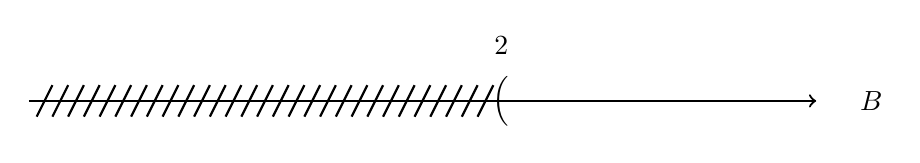
\begin{tikzpicture}[scale=1]
			\draw[->,thick](-4,0) --(6,0) node at (2,0.7){$2$} node at (2,0) {$\Big ($}node at (6.7,0){$B$};
			\foreach \b in {-3.8,-3.6,...,1.8} {\draw[ thick](\b-0.1,-0.2)--(\b+0.1,0.2);}
		\end{tikzpicture}\\
		%
		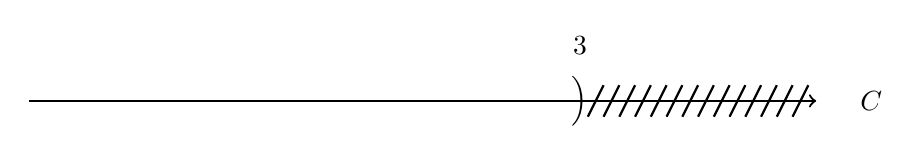
\begin{tikzpicture}[scale=1]
			\draw[->,thick](-4,0) --(6,0) node at (3,0.7){$3$} node at (3,0) {$\Big )$}node at (6.7,0){$C$};
			\foreach \b in {3.2,3.4,...,5.8} {\draw[ thick](\b-0.1,-0.2)--(\b+0.1,0.2);}
		\end{tikzpicture}\\
		%
		\begin{enumerate}
			\item $A\cap B=\left(2;4\right], B\cap C=\left(2;3\right)$.
			\item $\mathbb{R}\cap A=\left[-2;4 \right],\mathbb{R}\cap B=\left(2;+\infty \right)$.
		\end{enumerate}
	}
\end{bt}
\begin{bt}%[Huỳnh Quy]%[0D1B4-2]
	Cho hai tập hợp $A=\lbrace x\in \mathbb{R}\vert  x \leq 2 \rbrace$, $B=\lbrace x\in \mathbb{R}\vert -2< x \rbrace$. Tìm $A\setminus B, B\setminus A$.
	\loigiai{
		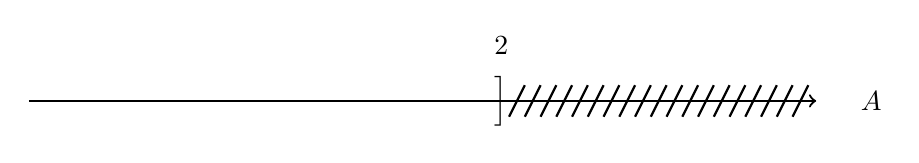
\begin{tikzpicture}[scale=1]
			\draw[->,thick](-4,0) --(6,0) node at (2,0.7){$2$} node at (2,0) {$\Big ]$}node at (6.7,0){$A$};
			\foreach \b in {2.2,2.4,...,5.8} {\draw[ thick](\b-0.1,-0.2)--(\b+0.1,0.2);}
		\end{tikzpicture}\\
		%
		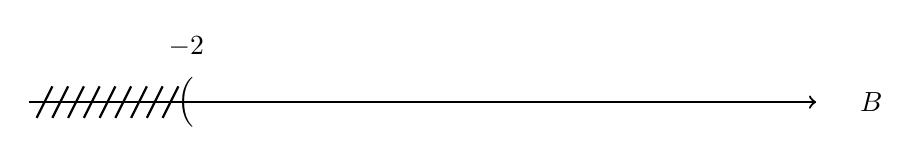
\begin{tikzpicture}[scale=1]
			\draw[->,thick](-4,0) --(6,0) node at (-2,0.7){$-2$} node at (-2,0) {$\Big ($} node at (6.7,0){$B$};
			\foreach \b in {-3.8,-3.6,...,-2.2} {\draw[ thick](\b-0.1,-0.2)--(\b+0.1,0.2);}
		\end{tikzpicture}\\
		$\Rightarrow A\setminus B=\left(-\infty;-2 \right], B\setminus A=\left(2;+\infty \right)$.}
\end{bt}
\begin{bt}%[Huỳnh Quy]%[0D1B4-2] 
	Cho $A=\left[-2;4\right],B=\left(2;+\infty\right),C=(-\infty;3)$. Xác định các tập hợp sau đây và biểu diễn chúng trên trục số.
	\begin{enumerate}
		\item $A\setminus B, B\setminus A$.
		\item $\mathbb{R}\setminus A,\mathbb{R}\setminus B, \mathbb{R}\setminus  C$.
	\end{enumerate}
	\loigiai{
		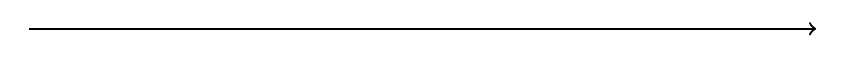
\begin{tikzpicture}[scale=1]
			\draw[->,thick](-4,0) --(6,0);
		\end{tikzpicture}\\
		%
		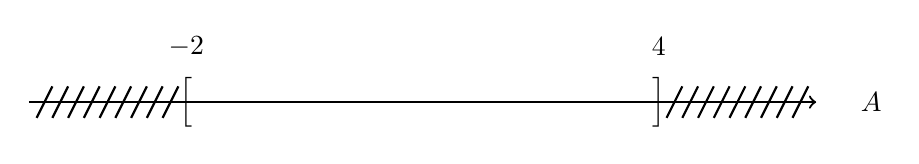
\begin{tikzpicture}[scale=1]
			\draw[->,thick](-4,0) --(6,0) node at (-2,0.7){$-2$} node at (4,0.7){$4$} node at (-2,0) {$\Big [$} node at (4,0) {$\Big ]$}node at (6.7,0){$A$};
			\foreach \b in {-3.8,-3.6,...,-2.2} {\draw[ thick](\b-0.1,-0.2)--(\b+0.1,0.2);}
			\foreach \b in {4.2,4.4,...,5.8} {\draw[ thick](\b-0.1,-0.2)--(\b+0.1,0.2);}
		\end{tikzpicture}\\
		%
		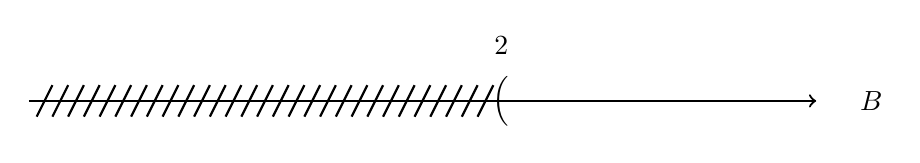
\begin{tikzpicture}[scale=1]
			\draw[->,thick](-4,0) --(6,0) node at (2,0.7){$2$} node at (2,0) {$\Big ($}node at (6.7,0){$B$};
			\foreach \b in {-3.8,-3.6,...,1.8} {\draw[ thick](\b-0.1,-0.2)--(\b+0.1,0.2);}
		\end{tikzpicture}\\
		%
		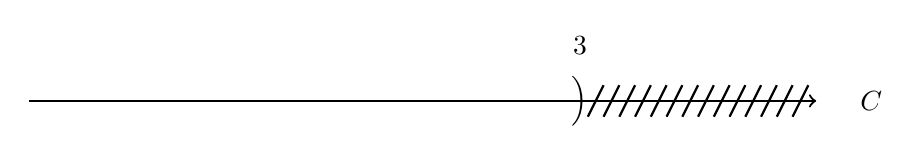
\begin{tikzpicture}[scale=1]
			\draw[->,thick](-4,0) --(6,0) node at (3,0.7){$3$} node at (3,0) {$\Big )$}node at (6.7,0){$C$};
			\foreach \b in {3.2,3.4,...,5.8} {\draw[ thick](\b-0.1,-0.2)--(\b+0.1,0.2);}
		\end{tikzpicture}
		%
		\begin{enumerate}
			\item $A\setminus B=\left[-2;2\right], B\setminus A=\left(4;+\infty\right)$.
			\item $\mathbb{R}\setminus A=\left(\infty;-2\right)\cup\left(4;+\infty \right),\mathbb{R}\setminus B=\left(-\infty;2\right], \mathbb{R}\setminus  C=\left[3;+\infty \right)$.
		\end{enumerate}
	}
\end{bt}
\begin{dang}{Ứng dụng thực tế các phép toán tập hợp}
\end{dang}
\subsubsection{Ví dụ minh hoạ}
\begin{vd}%[BG10-2022]%[Đỗ Văn Dự]%[0D1Y3-3]
	Cho $A$ là tập hợp các học sinh giỏi Toán của trường THPT X và $B$ là tập hợp học sinh giỏi Văn của trường này. Hãy mô tả các học sinh thuộc tập hợp sau\begin{enumEX}{3} 
			\item $A\cup B$.
			\item $A\cap B$.
			\item $A\setminus B$.
			\item $B\setminus A$.
			\item $\left(A\cup B\right)\setminus \left(A\cap B\right)$.
	\end{enumEX}
	\loigiai{
		\immini{
			\begin{enumerate}
				\item $A\cup B$ là tập hợp các học sinh giỏi Toán hoặc giỏi Văn của trường.
				\item $A\cap B$ là tập hợp các học sinh giỏi cả hai môn Toán và Văn của trường.
				\item $A\setminus B$ là tập hợp các học sinh chỉ giỏi Toán, không giỏi Văn.
				\item $B\setminus A$ là tập hợp các học sinh chỉ giỏi Văn, không giỏi Toán.		
				\item $\left(A\cup B\right)\setminus \left(A\cap B\right)$ là tập hợp các học sinh chỉ giỏi Toán hoặc giỏi Văn của trường.	
			\end{enumerate}
		}
		{\begin{tikzpicture}[scale=1, line join=round, line cap=round]	
				\coordinate (A) at (-1.2,0);
				\coordinate (B) at (0.8,0);
				\begin{scope}
					\clip[rotate=20] (A) ellipse (2cm and 1cm); %cat theo elip A
					\fill[rotate=30,pattern=north west lines] (B) ellipse (2cm and 1cm); %to elip B nhung bi cat mat theo phan giao voi elip A
				\end{scope}
				\draw[rotate=20] (A) ellipse (2cm and 1cm) node[fill=white,above]{$A\setminus B$}; %ve lai elip A
				\draw[rotate=30] (B) ellipse (2cm and 1cm) node[fill=white,above,right]{$B\setminus A$}; %ve lai elip B
				\path (-0.2,0.2) node[below]{$A\cap B$};
		\end{tikzpicture}}
	}
\end{vd}
\begin{vd}%[BG10-2022]%[Đỗ Văn Dự]%[0D1B3-3]
	Trong kì thi học sinh giỏi cấp trường, lớp 10C1 có $45$ học sinh trong đó có  $17$ bạn đạt học sinh giỏi Văn, $25$ bạn đạt học sinh giỏi Toán và $13$ bạn học sinh không đạt học sinh giỏi. Tìm số học sinh giỏi cả Văn và Toán của lớp 10C1.
	\loigiai{
		\immini{
			\begin{itemize}			
				\item Gọi $A$, $B$ theo thứ tự là tập hợp các học sinh giỏi Văn và giỏi Toán của lớp. 
				Theo đề ta có $n(A)=17$, $n(B)=25$, $n(A \cup B)= 45-13=32$.
				\item Số học sinh giỏi cả Văn và Toán là $$n(A \cap B )=n(A) + n(B) - n(A \cup B)=25+17-32=10.$$
			\end{itemize}
		}
		{	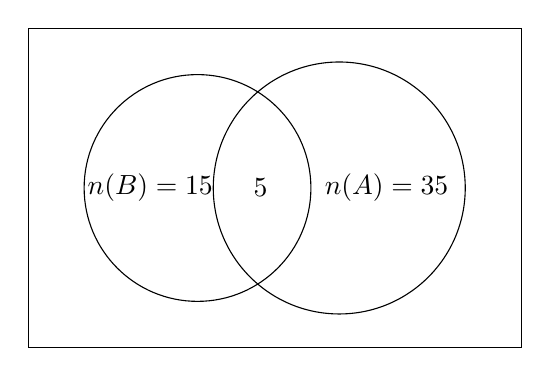
\begin{tikzpicture}[scale=.8]
				\def\radius{2cm}	
				\coordinate (ceni);
				\coordinate[xshift=.9*\radius] (cenii);
				
				\draw (ceni) circle (.9*\radius);
				\draw (cenii) circle (\radius);
				\draw  ([xshift=-25pt,yshift=15pt]current bounding box.north west) 
				rectangle ([xshift=25pt,yshift=-15]current bounding box.south east);
				
				\node[xshift=-.3*\radius] at (ceni) {$n(B)=15$};
				\node[xshift=.3*\radius] at (cenii) {$n(A)=35$};
				\node[xshift=.4*\radius] at (ceni) {$5$};
	\end{tikzpicture}}}
\end{vd}
\begin{vd}%[BG10-2022]%[Đỗ Văn Dự]%[0D1B3-3]
	Một lớp học có $ 50 $ học sinh trong đó có $ 30 $ em biết chơi bóng chuyền, $25$ em biết chơi bóng đá, $ 10 $ em biết chơi cả bóng đá và bóng chuyền. Hỏi có bao nhiêu em không biết chơi môn nào trong hai môn ở trên?
	\loigiai{
		Gọi tập $A$ là tập hợp các học sinh biết chơi bóng chuyền.
		\\Tập $B$ là tập hợp các học sinh biết chơi bóng đá.
		\\Khi đó số học sinh biết chơi ít nhất một trong hai môn bóng chuyền hoặc bóng đá là 
		$$n(A \cup B)=n(A)+n(B)-n(A \cap B)=30+25-10=45.$$
		Vậy số học sinh không biết chơi môn nào là $50-45=5$. 		
	}	
\end{vd}
\begin{vd}%[BG10-2022]%[Đỗ Văn Dự]%[0D1B3-3]
	Trong số $45$ cán bộ được triệu tập để chuẩn bị công tác cho một cuộc hội nghị quốc tế có $25$ cán bộ phiên dịch tiếng Anh, $15$ cán bộ phiên dịch tiếng Pháp, trong đó có $10$ cán bộ vừa phiên dịch được tiếng Anh, vừa phiên dịch được tiếng Pháp. Hỏi
	\begin{enumerate}
		\item Nhóm có bao nhiêu cán bộ được cấp thẻ đỏ, biết rằng muốn được cấp thẻ đỏ cán bộ đó phải phiên dịch được tiếng Anh hoặc phiên dịch được tiếng Pháp.
		\item Nhóm có bao nhiêu cán bộ không phiên dịch được tiếng Anh và không phiên dịch được tiếng Pháp.
	\end{enumerate}
	\loigiai{
		Gọi $A$, $B$ theo thứ tự là tập hợp các cán bộ phiên dịch tiếng Anh và tập hợp các các bộ phiên dịch tiếng Pháp. 
		Theo đề ta có $n(A)=25$, $n(B)=15$, $n(A \cap B)= 10$.
		\begin{enumerate}				
			\item Tập hợp các cán bộ được cấp thẻ đỏ là $A\cup B$.\\
			Vậy số cán bộ được cấp thẻ đỏ là $n(A \cup B)=n(A)+n(B)-n(A \cap B)=25+15-10=30$.
			\item Tập hợp các cán bộ của nhóm không phiên dịch được tiếng Anh và tiếng Pháp chính là số cán bộ không được cấp thẻ đỏ.\\
			Vậy số cán bộ đó là $45-30=15$.
	\end{enumerate}}
\end{vd}
\begin{vd}%[BG10-2022]%[Đỗ Văn Dự]%[0D1B3-3]
	Lớp $10A$ có $15$ bạn thích môn Văn, $20$ bạn thích môn Toán. Trong số các bạn thích văn hoặc toán có $8$ bạn thích cả $2$ môn. Trong lớp vẫn còn $10$ bạn không thích môn nào trong $2$ môn Văn và Toán. Hỏi lớp $10A$ có bao nhiêu học sinh?
	\loigiai{Ta sử dụng sơ đồ Ven.		
		\begin{center}
			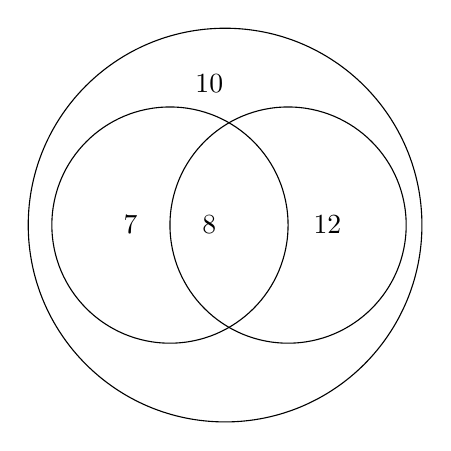
\begin{tikzpicture}
				\draw[] (0.7,0) circle ( 2.5cm);
				\draw[] (0,0) circle ( 1.5cm);
				\draw (1.5,0) circle ( 1.5 cm);
				\draw (-0.5,0) node {$7$};
				\draw (2,0) node {$12$};
				\draw (0.5,0) node {$8$};
				\draw (0.5,1.8) node {$10$};
			\end{tikzpicture}
		\end{center}
		\begin{itemize}
			\item Hình tròn lớn ngoài cùng thể hiện số học sinh cả lớp.\\
			Như vậy, ta có:\\
			\item	Số bạn chỉ thích Văn là $ 15-8=7$(bạn).\\
			\item	Số bạn chỉ thích Toán là $20-8=12$(bạn).\\
			\item	Số học sinh cả lớp là tổng các phần không giao nhau: $7+8+12+10=37$.
		\end{itemize}
	}
\end{vd}

\begin{vd}%[BG10-2022]%[Đỗ Văn Dự]%[0D1B3-3]
	Một lớp có $40$ học sinh, mỗi học sinh đều đăng ký chơi ít nhất $1$ trong $2$ môn thể thao là bóng đá hoặc cầu lông. Có $30$ học sinh có đăng ký môn bóng đá, $25$ học sinh có đăng ký môn cầu lông. Hỏi có bao nhiêu em đăng ký cả $2$ môn.
	\loigiai{
		Gọi $A$ là tập hợp các học sinh đăng kí chơi bóng đá, $B$ là tập học sinh đăng kí chơi cầu lông thì $A\cap B$ là tập hợp các học sinh đăng kí chơi cả hai môn.\\	
		Vậy số học sinh đăng kí chơi cả hai môn là 
		$n(A \cap B)=n(A)+n(B)-n(A \cup B)=30+25-40=15$. }
\end{vd}

\begin{vd}%[BG10-2022]%[Đỗ Văn Dự]%[0D1B3-3]
	Ở xứ sở của thần Thoại ngoài các vị thần thì còn có các sinh vật gồm $27$ con người, $311$ con yêu quái một mắt, $205$ con yêu quái tóc rắn và yêu quái vừa một mắt vừa tóc rắn. Tìm số yêu quái vừa một mắt vừa tóc rắn biết có tổng số sinh vật là 500 con.
	\loigiai{
		\begin{itemize}
			\item Số sinh vật không phải con người là $500-27=473$ (con).
			\item Gọi $A$, $B$ lần lượt là tập hợp yêu quái một mắt và yêu quái tóc rắn. Khi đó $n(A)=311$,  $n(B)=205$, $n(A \cup B)=473$.
			\item Vậy số yêu quái vừa một mắt vừa tóc rắn là $|A \cap B| =311+205-473=43$.
		\end{itemize}
	}
\end{vd}

\begin{vd}%[BG10-2022]%[Đỗ Văn Dự]%[0D1B3-3]
	Mỗi học sinh của lớp $10A$ đều chơi bóng đá hoặc bóng chuyền. Biết rằng có $25$ bạn chơi bóng đá, $20$ bạn chơi bóng chuyền và $10$ bạn chơi cả $2$ môn thể thao. Hỏi lớp $10A$ có bao nhiêu học sinh.
	\loigiai{
		Gọi $A$ là tập hợp các học sinh chơi bóng đá, $B$ là tập các học sinh chơi bóng chuyền. Do đó $A\cap B$ là tập các học sinh chơi cả hai môn.\\
		Theo đề $n(A)=25$, $n(B)=20$, $|A \cap B| =10$.\\
		Vậy số học sinh cả lớp là $|A \cup B| =n(A)+n(B)-n(A \cap B)=25+20-10=35$.}
\end{vd}

\begin{vd}%[BG10-2022]%[Đỗ Văn Dự]%[0D1B3-3]
	Lớp 10A có $45$ học sinh, có $15$ học sinh giỏi và $20$ học sinh xếp hạnh kiểm tốt, trong đó có $10$ bạn vừa học giỏi vừa xếp hạnh kiểm tốt. Các học sinh được học sinh giỏi hoặc hạnh kiểm tốt đều được khen thưởng. Số học sinh được khen thưởng của lớp 10A là là bao nhiêu?
	\loigiai{
		Gọi $A$ là tập hợp các học sinh giỏi, 
		$B$ là tập hợp các học sinh xếp hạnh kiểm tốt.\\
		Khi đó số học sinh được khen thưởng là $n(A \cup B)$.\\
		Vậy số học sinh được khen thưởng là 
		$n(A \cup B)=n(A)+n(B)-n(A \cap B)=15+20-10=25.$		
	}
\end{vd}

\begin{vd}%BT6%[Nguyễn Thành Tuấn]%[0D1K3-3]
	Kết quả thi học kì một của một trường THPT có $48$ thí sinh giỏi môn Toán, $37$ thí sinh giỏi môn Vật Lí,$42$ thí sinh giỏi môn Văn. Biết rằng có $75$ thí sinh giỏi môn Toán hoặc môn Vật lí, $76$ thí sinh giỏi  môn Toán hoặc môn Văn, $66$ thí sinh giỏi môn Vật lí hoặc môn Văn và có $4$ thí sinh giỏi cả ba môn. Hỏi 
	\begin{enumerate}
		\item có bao nhiêu học sinh chỉ giỏi 1 môn.
		\item có bao nhiêu học sinh chỉ giỏi 2 môn.
		\item có bao nhiêu học sinh giỏi ít nhất 1 môn.
	\end{enumerate}
	\loigiai{		
		Gọi $A$, $B$, $C$ theo thứ tự là tập hợp các học sinh giỏi Toán, giỏi Lí và giỏi Văn. Theo đề ta có
		\begin{itemize}
			\item Số học sinh giỏi Toán và Lí là $$n(A \cap B)=n(A)+n(B)-n(A \cup B)=48+37-75=10.$$	
			\item Số học sinh giỏi Toán và Văn là $$n(A \cap C)=n(A)+n(C)-n(A\cup C)=48+42 - 76 = 14 .$$	
			\item Số học sinh giỏi Lí và Văn là $$n(B \cap C)=n(B)+n(C)-n(B\cup C)= 42+37-66=13 .$$	
			\item Số học sinh chỉ giỏi môn Toán $48-10-14+4=28 $.	
			\item Số học sinh chỉ giỏi môn Lí $37-10-13+4=18 $.	
			\item Số học sinh chỉ giỏi môn Văn $42-13-14+4=19 $.
		\end{itemize}
		\begin{center}
			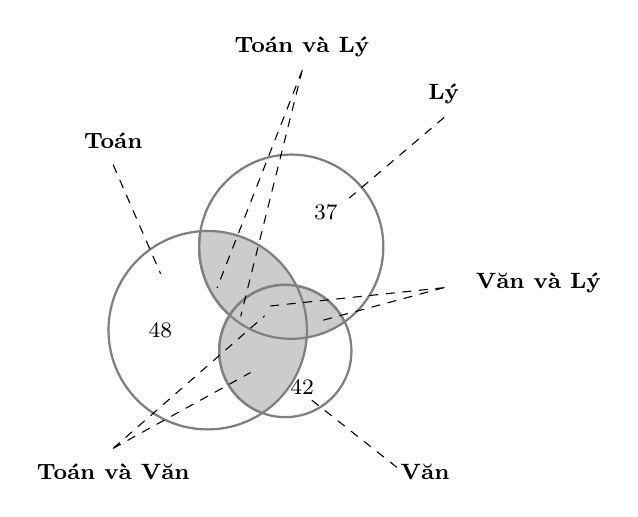
\begin{tikzpicture}[scale=0.6,>=stealth, font=\footnotesize, line join=round, line cap=round]	
				\def\firstcircle{(0,0) circle (2.1cm)}
				\def\secondcircle{(45:2.5cm) circle (1.95cm)}
				\def\thirdcircle{(-15:1.7cm) circle (1.4cm)}
				\colorlet{circle edge}{black!50}
				\colorlet{circle area}{black!20}
				\tikzset{filled/.style={fill=circle area, draw=circle edge, thick},
					outline/.style={draw=circle edge, thick}}
				\draw \firstcircle;
				\draw \secondcircle;
				\draw \thirdcircle;
				\begin{scope}
					\clip \firstcircle;
					\fill[filled] \secondcircle;
				\end{scope}
				\begin{scope}
					\clip \firstcircle;
					\fill[filled] \thirdcircle;
				\end{scope}
				\begin{scope}
					\clip \secondcircle;
					\fill[filled] \thirdcircle;
				\end{scope}  
				\node at (-1,0){48};  
				%\node at (0.5,1){3}; 
				%	\node at (1.2,0.3){1};  
				%	\node at (2.3,0.3){1};      
				%	\node at (1,-0.5){2};   
				\node at (2,-1.2){42};     
				\node at (2.5,2.5){37}; 
				\draw[outline] \firstcircle
				\secondcircle  \thirdcircle;    
				\node at (-2,4) {\textbf{Toán}};
				\node at (2,6) {\textbf{Toán và Lý}};
				\node at (5,5) {\textbf{Lý}};
				\node at (7,1) {\textbf{Văn và Lý}};   
				\node at (4.6,-3) {\textbf{Văn}};
				\node at (-2,-3) {\textbf{Toán và Văn}};
				\draw[dashed] (-2,3.5) -- (-1,1.2) 
				(2,5.5) -- (0.7,0.3) 
				(2,5.5) -- (0.2,0.9)
				(5,4.5) -- (3,2.8)
				(5,0.9) -- (1.2,0.5)
				(5,0.9) -- (2.4,0.2)
				(4,-2.9) -- (2.1,-1.4)
				(-2,-2.5) -- (1.2,0.3)
				(-2,-2.5) -- (0.9,-0.9)	;
		\end{tikzpicture}	
		\end{center}
		
		\begin{enumerate}	
			\item Số học sinh chỉ giỏi đúng 1 môn là $28+18+19=65$. 
			\item Số học sinh chỉ giỏi đúng 2 môn là $10+14+13-4\cdot2=25 $. 
			\item Số học sinh giỏi ít nhất một môn là $65+25+4=94$.
		\end{enumerate}
	}
\end{vd}
\begin{vd}%[BG10-2022]%[Đỗ Văn Dự]%[0D1K3-3]
	Một nhóm học sinh giỏi các bộ môn: Anh, Toán, Văn. Có $18$ em giỏi Văn, $10$ em giỏi Anh, $12$ em giỏi Toán, $3$ em giỏi Văn và Toán, $4$ em giỏi Toán và Anh, $5$ em giỏi Văn và Anh, $2$ em giỏi cả ba môn. Hỏi nhóm đó có bao nhiêu em?
	\loigiai{
		Gọi $A$ là tập hợp những học sinh giỏi Anh,
		$T$ là tập hợp những học sinh giỏi toán,
		$V$ là tập hợp những học sinh giỏi Văn.
		Ta có\\
		$\bullet$ $n\left( V \right)=18,\; n\left( A \right)=10$,\; $n\left( T \right)=12$,\; 
		$n(V\cap T)=3,\;n(T\cap A)=4,\;n(V\cap A)=5$,\; $n(A\cap B\cap C)=2$.\\
		$\bullet$  $\begin{aligned}[t] n(V\cup A\cup T)&=n\left( V \right)+n\left( A \right)+n\left( T \right)-\left[ n(V\cap A)+n(A\cap T)+n(T\cap V) \right]+n\left( V\cap A\cap T \right)\\ &=
		18+10+12-\left[ 3+4+5 \right]+2=30 \end{aligned}$.\\
		Vậy nhóm đó có 30 em.}
\end{vd}

\begin{vd}%[BG10-2022]%[Đỗ Văn Dự]%[0D1K3-3]
	Trong số $42$ học sinh của lớp 10A có $13$ bạn được xếp loại học lực giỏi, $22$ bạn được xếp loại hạnh kiểm tốt, trong đó $7$ bạn vừa học lực giỏi, vừa có hạnh kiểm tốt. Hỏi lớp 10A có bao nhiêu bạn được khen thưởng? Biết rằng muốn được khen thưởng thì bạn đó phải có học lực giỏi hoặc có hạnh kiểm tốt.
	\loigiai{
		Gọi tập hợp các học sinh học lực giỏi là $G$, tập hợp các bạn học sinh hạnh kiểm tốt là $T$. Khi đó tập hợp các bạn học sinh vừa có học lực giỏi là, vừa có hạnh kiểm tốt là $G\cap T$, tập hợp các bạn học sinh đạt học lực giỏi hoặc hạnh kiểm tốt là $G\cup T$. Ta có \\
		$n(G)=13$, $n(T)=22$, $n(G\cap T)=7$.\\
		$n(G\cup T)=n(G)+n(T)-n(G\cap T)=13+22-7=28.$}
\end{vd}

\begin{vd}%[BG10-2022]%[Đỗ Văn Dự]%[0D1K3-3]
	Một nhóm học sinh giỏi các bộ môn: Anh, Toán, Văn. Có $ 18 $ em giỏi Văn, $ 10 $ em giỏi Anh, $ 12 $ em giỏi Toán, $ 3 $ em giỏi Văn và Toán, $ 4 $ em giỏi Toán và Anh, $ 5 $ em giỏi Văn và Anh, $ 2 $ em giỏi cả ba môn. Hỏi nhóm đó có bao nhiêu em?
	\loigiai{
		\begin{center}
			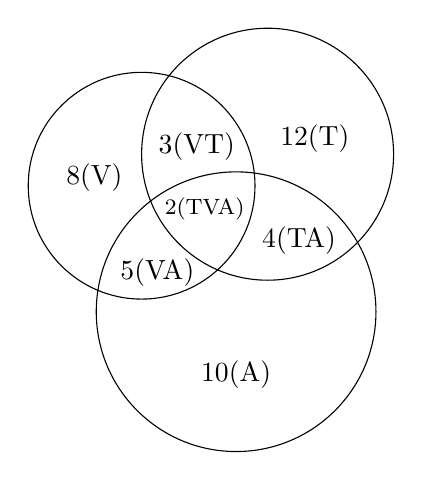
\begin{tikzpicture}[scale=.8]
				\def\radius{2cm}	
				\coordinate (ceni);
				\coordinate[xshift=.8*\radius, yshift=.2*\radius] (cenii);
				\coordinate[xshift=.6*\radius,yshift=-.8*\radius] (ceniii);
				\draw (ceni) circle (.9*\radius);
				\draw (cenii) circle (\radius);
				\draw (ceniii) circle (1.11*\radius);
				
				\node[xshift=-.3*\radius, yshift=.05*\radius] at (ceni) {$8$(V)};
				\node[xshift=.35*\radius, yshift=.25*\radius] at (ceni) {$3$(VT)};
				\node[xshift=.1*\radius, yshift=-.55*\radius] at (ceni) {$5$(VA)};
				\node[xshift=.4*\radius, yshift=-.15*\radius] at (ceni) {{\footnotesize $2$(TVA)}};
				\node[xshift=.2*\radius, yshift=-.55*\radius] at (cenii) {$4$(TA)};
				\node[xshift=1.1*\radius,yshift=.3*\radius] at (ceni) {$12$(T)};
				\node[yshift=-.4*\radius] at (ceniii) {$10$(A)};
			\end{tikzpicture}
		\end{center}
		Ký hiệu $ A $ là tập hợp những học sinh giỏi Anh,\\
		$ T $ là tập hợp những học sinh giỏi Toán,\\
		$ V $ là tập hợp những học sinh giỏi Văn.\\
		$\bullet$ $n(V)=18,\; n(A)=10,\; n(T)=12$,\\
		$\bullet$ $n(T \cap V)=3,\; n(T \cap A)=4,\; n(V \cap A)=5, n(A \cap B \cap C)=2$.\\
		Số học sinh của nhóm là
		\begin{eqnarray*}
			n(V \cup A \cup T)&=&n(V)+n(A)+n(T)-n(V \cap A)-n(T \cap A)-n(T \cap V)+n(A \cap B \cap C)\\
			&=&18+10+12-(3+4+5)+2=30.
		\end{eqnarray*}
		Vậy nhóm đó có $ 30 $ em.
	}
\end{vd}

\begin{vd}%[BG10-2022]%[Đỗ Văn Dự]%[0D1K3-3]
	Có $44$ học sinh giỏi, mỗi em giỏi ít nhất một môn. Có $22$ em giỏi Văn, $25$ em giỏi Toán, $20$ em giỏi Anh. Có $8$ em giỏi đúng hai môn Văn, Toán; Có $7$ em giỏi đúng hai môn Toán, Anh; Có $6$ em giỏi đúng hai môn Anh, Văn. Hỏi có bao nhiêu em giỏi cả ba môn Văn, Toán, Anh?
	\loigiai{
		Ta có \\
		$n\left( V \right)=22,\;n\left( T \right)=25$,\; $n\left( A \right)=20$\\
		$n((V\cap T)\setminus A)=8,\;n((T\cap A)\setminus V)=7,\;n((V\cap A)\setminus T)=6,\; n(V\cup T\cup A)=44$.\\
		$n(V\cup A\cup T)=n\left( V \right)+n\left( A \right)+n\left( T \right)-n(V\cap A)-n(A\cap T)-n(T\cap V)+n\left( V\cap A\cap T \right)$\\
		$  \Leftrightarrow  44=22+20+25-6-7-8+4n\left( V\cap A\cap T \right)$.\\
		$\Rightarrow n\left( V\cap A\cap T \right)=1$.
	}
\end{vd}
\begin{vd}%[BG10-2022]%[Đỗ Văn Dự]%[0D1B3-3]
	Để thành lập đội tuyển học sinh giỏi khối $ 10 $, nhà trường tổ chức thi chọn các môn Toán, Văn, Anh trên tổng số $ 111 $ học sinh. Kết quả có: $ 70 $ học sinh giỏi Toán, $ 65 $ học sinh giỏi Văn, $ 62 $ học sinh giỏi Anh. Trong đó có $ 49 $ học sinh giỏi cả hai môn Văn và Toán, $ 32 $ học sinh giỏi cả hai môn Toán và Anh, $ 34 $ học sinh giỏi cả hai môn Văn và Anh. Xác định số học sinh giỏi cả ba môn Văn, Toán, Anh. Biết rằng có $ 6 $ học sinh không đạt yêu cầu cả ba môn.
	\loigiai{
		\immini
		{Có $ 111-6=105 $ học sinh thi đạt ít nhất $ 1 $ môn.\\
			Gọi $ A $ là số học sinh giỏi môn Toán và Tiếng Anh nhưng không giỏi Văn.\\
			Gọi $ B $ là số học sinh giỏi môn Toán và Văn nhưng không giỏi Tiếng Anh.\\
			Gọi $ C $ là số học sinh giỏi môn Văn và Tiếng Anh nhưng không giỏi Toán.\\
			Gọi $ D $ là số học sinh giỏi cả ba môn. Ta có hệ:\\
			$\begin{cases}
				B+D=49\\
				A+D=32\\
				C+D=34\\
				70+65+62-(A+B+C+2D)=105
			\end{cases}\\
			\Rightarrow 92=32-D+49-D+34-D+2D\\
			\Rightarrow D=23$.\\
			Vậy có $ 23 $ học sinh giỏi cả ba môn.
		}
		{
			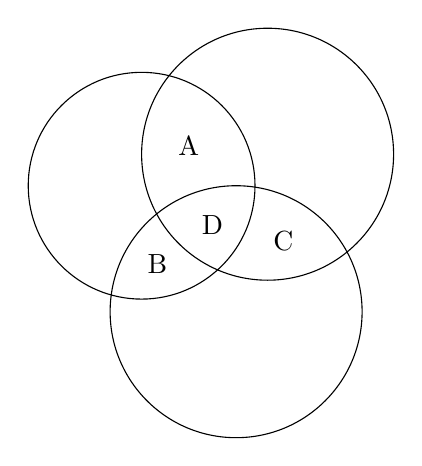
\begin{tikzpicture}[scale=.8]
				\def\radius{2cm}	
				\coordinate (ceni);
				\coordinate[xshift=.8*\radius, yshift=.2*\radius] (cenii);
				\coordinate[xshift=.6*\radius,yshift=-.8*\radius] (ceniii);
				\draw (ceni) circle (.9*\radius);
				\draw (cenii) circle (\radius);
				\draw (ceniii) circle (\radius);
				
				\node[xshift=.3*\radius, yshift=.25*\radius] at (ceni) {A};
				\node[xshift=.1*\radius, yshift=-.5*\radius] at (ceni) {B};
				\node[xshift=.45*\radius, yshift=-.25*\radius] at (ceni) {D};
				\node[xshift=.1*\radius, yshift=-.55*\radius] at (cenii) {C};
		\end{tikzpicture}}
	}
\end{vd}
\subsubsection{Bài tập tự luận}
\begin{bt}%[Huỳnh Quy]%[0D1B3-3]
	Mỗi học sinh của lớp $10A$ đều chơi bóng đá hoặc bóng chuyền. Biết rằng có $25$ bạn chơi bóng đá, $20$ bạn chơi bóng chuyền và $10$ bạn chơi cả $2$ môn thể thao. Hỏi lớp $10A$ có bao nhiêu học sinh.
	\loigiai{
		Ngoài sơ đồ Ven ta có thể dùng công thức số phần tử. Gọi $A$ là tập hợp các học sinh chơi bóng đá, $B$ là tập các học sinh chơi bóng chuyền. Do đó $A\cap B$ là tập các học sinh chơi cả hai môn. Ta có
		$$n(A)=25, n(B)=20, n(A \cap B) =10.$$
		Số học sinh cả lớp là số phần tử của tập $A \cup B$ nên $n(A \cup B) = 25+20-10=35$ (học sinh).
	}
\end{bt}
\begin{bt}%[Huỳnh Quy]%[0D1B3-3]
	Lớp $10{{B}_{1}}$ có $7$ học sinh giỏi Toán, $5$ học sinh giỏi Lý, $6$ học sinh giỏi Hóa, $3$ học sinh giỏi cả Toán và Lý, $4$ học sinh giỏi cả Toán và Hóa, $2$ học sinh giỏi cả Lý và Hóa, $1$ học sinh giỏi cả $3$ môn Toán, Lý, Hóa. Tính số học sinh giỏi ít nhất một môn (Toán, Lý, Hóa) của lớp $10{{B}_{1}}$.
	\loigiai{
		Ta dùng biểu đồ Ven để giải:
		\begin{center}
			\begin{tikzpicture}
				\def\firstcircle{(0,0) circle (1.5cm)}
				\def\secondcircle{(45:2.5cm) circle (2cm)}
				\def\thirdcircle{(-15:1.7cm) circle (1.4cm)}
				\colorlet{circle edge}{black!50}
				\colorlet{circle area}{black!20}
				\tikzset{filled/.style={fill=circle area, draw=circle edge, thick},
					outline/.style={draw=circle edge, thick}}
				\draw \firstcircle;
				\draw \secondcircle;
				\draw \thirdcircle;
				\begin{scope}
					\clip \firstcircle;
					\fill[filled] \secondcircle;
				\end{scope}
				\begin{scope}
					\clip \firstcircle;
					\fill[filled] \thirdcircle;
				\end{scope}
				\begin{scope}
					\clip \secondcircle;
					\fill[filled] \thirdcircle;
				\end{scope}  
				\node at (-1,0){1};  
				\node at (0.5,1){2}; 
				\node at (1,0.3){1};  
				\node at (2,0.3){1};      
				\node at (1,-0.5){3};   
				\node at (2,-1){1};     
				\node at (3,2.5){1}; 
				\draw[outline] \firstcircle
				\secondcircle  \thirdcircle;    
				\node at (-2,4) {\textbf{Toán}};
				\node at (2,6) {\textbf{Giỏi Toán + Lý}};
				\node at (5,5) {\textbf{Lý}};
				\node at (7,1) {\textbf{Giỏi Hóa + Lý}};   
				\node at (5,-3) {\textbf{Hóa}};
				\node at (-2,-3) {\textbf{Giỏi Toán + Hóa}};
				\draw[->] (-2,3.5) -- (-1,1.2) 
				(2,5.5) -- (0.7,0.3) 
				(2,5.5) -- (0.2,0.9)
				(5,4.5) -- (3.6,2.5)
				(5,0.9) -- (1.2,0.5)
				(5,0.9) -- (2.4,0.2)
				(4,-2.9) -- (2,-1.8)
				(-2,-2.5) -- (1.2,0)
				(-2,-2.5) -- (0.9,-0.9)
				;
			\end{tikzpicture}
		\end{center}
		Nhìn vào biểu đồ, số học sinh giỏi ít nhất $1$ trong $3$ môn là: $1+2+1+3+1+1+1=10$}
\end{bt}
\begin{bt}%[Huỳnh Quy]%[0D1B3-3]
	Lớp $10{{\text{A}}_{1}}$ có $7$ học sinh giỏi Toán, $5$ học sinh giỏi Lý, $6$ học sinh giỏi Hóa, $3$ học sinh giỏi cả Toán và Lý, $4$ học sinh giỏi cả Toán và Hóa, $2$ học sinh giỏi cả Lý và Hóa, $1$ học sinh giỏi cả $3$ môn Toán, Lý, Hóa. Tính số học sinh giỏi đúng hai môn học của lớp $10{{\text{A}}_{1}}$.
	\loigiai{
		\begin{center}
			\begin{tikzpicture}
				\def\firstcircle{(0,0) circle (1.5cm)}
				\def\secondcircle{(45:2.5cm) circle (2cm)}
				\def\thirdcircle{(-15:1.7cm) circle (1.4cm)}
				\colorlet{circle edge}{black!50}
				\colorlet{circle area}{black!20}
				\tikzset{filled/.style={fill=circle area, draw=circle edge, thick},
					outline/.style={draw=circle edge, thick}}
				\draw \firstcircle;
				\draw \secondcircle;
				\draw \thirdcircle;
				\begin{scope}
					\clip \firstcircle;
					\fill[filled] \secondcircle;
				\end{scope}
				\begin{scope}
					\clip \firstcircle;
					\fill[filled] \thirdcircle;
				\end{scope}
				\begin{scope}
					\clip \secondcircle;
					\fill[filled] \thirdcircle;
				\end{scope}  
				\node at (-1,0){1};  
				\node at (0.5,1){2}; 
				\node at (1,0.3){1};  
				\node at (2,0.3){1};      
				\node at (1,-0.5){3};   
				\node at (2,-1){1};     
				\node at (3,2.5){1}; 
				\draw[outline] \firstcircle
				\secondcircle  \thirdcircle;    
				\node at (-2,4) {\textbf{Toán}};
				\node at (2,6) {\textbf{Giỏi Toán + Lý}};
				\node at (5,5) {\textbf{Lý}};
				\node at (7,1) {\textbf{Giỏi Hóa + Lý}};   
				\node at (5,-3) {\textbf{Hóa}};
				\node at (-2,-3) {\textbf{Giỏi Toán + Hóa}};
				\draw[->] (-2,3.5) -- (-1,1.2) 
				(2,5.5) -- (0.7,0.3) 
				(2,5.5) -- (0.2,0.9)
				(5,4.5) -- (3.6,2.5)
				(5,0.9) -- (1.2,0.5)
				(5,0.9) -- (2.4,0.2)
				(4,-2.9) -- (2,-1.8)
				(-2,-2.5) -- (1.2,0)
				(-2,-2.5) -- (0.9,-0.9)
				;
			\end{tikzpicture}
		\end{center}
		Dựa vào biểu đồ ven trên, ta có số học sinh giỏi đúng hai môn học là $2+1+3=6$}
\end{bt}

\subsection{Bài tập trắc nghiệm}
\Opensolutionfile{ans}[ans/ans-0D1-2-TN]
\begin{ex}%[Bài giảng Toán 10 - 2022]%[Nhật Thiện]%[0D1Y3-1]
	Cho hai tập hợp $X=\{1;3;5;8\}$, $Y=\{3;5;7;9\}$. Tập hợp $X\cup Y$ bằng tập hợp nào sau đây?
	\choice
	{$\{1;3;5\}$}
	{$\{3;5\}$}
	{$\{1;7;9\}$}
	{\True $\{1;3;5;7;8;9\}$}
	\loigiai{
		Ta có $X\cup Y=\{1;3;5;7;8;9\}$.
	}
\end{ex}
\begin{ex}%[Bài giảng Toán 10 - 2022]%[Nhật Thiện]%[0D1Y3-2]
	Cho hai tập hợp $A=\{1;2;3;4;5\}$ và $B=\{0;2;4;6;8\}$. Tìm $A\setminus B$.
	\choice
	{$A\setminus B=\{2;4\}$}
	{\True $A\setminus B=\{1;3;5\}$}
	{$A\setminus B=\{0;1;3;5\}$}
	{$A\setminus B=\{0;6;8\}$}
	\loigiai{
		Ta có $A\setminus B=\{1;3;5\}$.
	}
\end{ex}
\begin{ex}%[Bài giảng Toán 10 - 2022]%[Nhật Thiện]%[0D1B3-1]
	Cho hai tập hợp $ A=\left\lbrace x\in \mathbb{R}\,\mid\,(2x-x^2)(x-1)=0 \right\rbrace$, $ B=\left\lbrace n \in \mathbb{N}\,\mid\,0<n^2<10 \right\rbrace$. Chọn mệnh đề đúng?
	\choice
	{\True $A \cap B =\left\lbrace 1;2 \right\rbrace $}
	{$A \cap B =\left\lbrace 2 \right\rbrace $}
	{ $A \cap B =\left\lbrace 0;1;2;3 \right\rbrace $}
	{$A \cap B =\left\lbrace 0;3 \right\rbrace $}
	\loigiai{
		Ta có
		\begin{itemize}
			\item $ (2x-x^2)(x-1)=0\Leftrightarrow \hoac{& x=0 \\ &x=1\\&x=2 }\Rightarrow A=\left\lbrace 0;1;2 \right\rbrace  $.
			\item  $ B= \left\lbrace 1;2;3 \right\rbrace$.
		\end{itemize}
		Suy ra $ A\cap B= \left\lbrace 1;2 \right\rbrace$.}
\end{ex}
\begin{ex}%[Bài giảng Toán 10 - 2022]%[Nhật Thiện]%[0D1B3-1]
	Cho các tập hợp $A=\left\{ x\in \mathbb{N} \ | \ (4-x^2)(x^2-5x+4)=0 \right\}; B = \left\{ x\in \mathbb{Z} \ | \ x \text{ là ước của } 4 \right\}$. Tập hợp $A \cap B$ là
	\choice
	{$\{-2,1,2,4\}$}
	{\True $\{1,2,4\}$}
	{$\{2,4\}$}
	{$\{-4,-2,-1,1,2,4\}$}
	\loigiai{
		Ta có $(4-x^2)(x^2-5x+4)=0 \Leftrightarrow \hoac{&4-x^2=0\\&x^2-5x+4=0} \Leftrightarrow \hoac{&x=2\\&x=-2\\&x=1\\&x=4.}$\\
		Vì $x\in \mathbb{N}$ nên $x \in \{1,2,4\}$.\\
		Do đó $A=\{1,2,4\} \quad (1)$.\\
		Ta có các ước của $4$ là $\pm 1, \pm 2, \pm 4$.\\
		Do đó $B=\{-4,-2,-1,1,2,4\} \quad (2)$.\\
		Từ $(1), (2)$ ta có $A \cap B = \{1,2,4\}$.
	}
\end{ex}
\begin{ex}%[Bài giảng Toán 10 - 2022]%[Nhật Thiện]%[0D1Y4-2]
	Cho hai tập hợp $A = \left(-5;7\right)$ và $B = \left(1;+\infty\right)$. Tìm $A\setminus B$.
	\choice
	{\True $A\setminus B = \left(-5;1\right]$}
	{$A\setminus B = \left(-5;1\right)$}
	{$A\setminus B = \left[7;+\infty\right)$}
	{$A\setminus B = \left(7;+\infty\right)$}
	\loigiai{
		Ta có $A\setminus B = \left(-5;1\right]$.
	}
\end{ex}
\begin{ex}%[Bài giảng Toán 10 - 2022]%[Nhật Thiện]%[0D1Y4-2]
	Cho hai tập hợp $A=\left[ -2;4\right)$ và $B=\left(0;+\infty\right)$. Tìm khẳng định đúng.
	\choice
	{$A\cup B=\left(4;+\infty\right)$}
	{\True $A\cap B=\left(0;4\right)$}
	{$B\setminus A=\left[ -2;+\infty\right)$}
	{$A\setminus B=\left[ -2;0\right)$}
	\loigiai{
		$A\cup B=[-2;+\infty) \rightarrow $ loại.\\
		$A\cap B = (0;4) \rightarrow$ chọn.\\
		$B\setminus A = [4;+\infty) \rightarrow$ loại.\\
		$A\setminus B = [-2;0] \rightarrow$ loại.
	}
\end{ex}
\begin{ex}%[Bài giảng Toán 10 - 2022]%[Nhật Thiện]%[0D1B3-2]
	Cho $A$ là tập hợp các hình thoi, $B$ là tập hợp các hình chữ nhật và $C$ là tập hợp các hình vuông. Khi đó
	\choice
	{\True $A\cap B=C $}
	{$A\setminus B=C$}
	{$B\setminus A=C$}
	{$A\cup B=C$}
	\loigiai{
		Ta có hình thoi có hai cạnh kề vuông góc khi và chỉ khi nó là hình vuông.\\
		Hình chữ nhật có hai cạnh kề bằng nhau khi và chỉ khi nó là hình vuông.
	}
\end{ex}
\begin{ex}%[Bài giảng Toán 10 - 2022]%[Nhật Thiện]%[0D1B3-2]
	Cho hai tập hợp $M=\{1;2;3;5\}$ và $N=\{2;6;-1\}$. Xét các khẳng định
	\begin{enumEX}[(I)]{3}
		\item $M\cap N=\{2\}$
		\item $N\setminus M=\{1;3;5\}$
		\item $M\cup N=\{1;2;3;5;6;-1\}.$
	\end{enumEX}
	Có bao nhiêu khẳng định đúng trong ba khẳng định nêu trên?
	\choice
	{$0$}
	{$3$}
	{$1$}
	{\True $2$}
	\loigiai{
		Ta có $M\cap N=\{2\}$; $N\setminus M=\{6;-1\}$ và $M\cup N=\{1;2;3;5;6;-1\}$.\\
		Vậy có $2$ khẳng định đúng là (I) và (III).
	}
\end{ex}
\begin{ex}%[Bài giảng Toán 10 - 2022]%[Nhật Thiện]%[0D1B3-2]
	Cho hai tập hợp $A=\{2;4;6;8\}$ và $B$ là tập hợp các số tự nhiên nhỏ hơn $10$. Phần bù của $A$ trong $B$ là
	\choice
	{\True $\{0;1;3;5;7;9\}$}
	{$[0;10) \setminus \{2;4;6;8\}$}
	{$\varnothing$}
	{$\{1;3;5;7;9\}$}
	\loigiai{
		Vì $B$ là tập hợp các số tự nhiên nhỏ hơn $10$ nên $B=\{0;1;2;3;4;5;6;7;8;9\}$.\\
		Khi đó $\mathrm{C}_B A=\{0;1;3;5;7;9\}$.
	}
\end{ex}
\begin{ex}%[Bài giảng Toán 10 - 2022]%[Nhật Thiện]%[0D1B4-2]
	Cho hai tập hợp $C_{\mathbb{R}}A = (0;+\infty)$ và $C_{\mathbb{R}}B =(-\infty;-5)\cup  (-2;+\infty)$. Xác định tập $A \cup B$.
	\choice
	{$A \cap B = (-2;0)$}
	{$A \cap B = (-5;-2)$}
	{$A \cap B = (-5;0]$}
	{\True $A \cap B = [-5;-2]$}
	\loigiai{
		Ta có $C_{\mathbb{R}}A \cup C_{\mathbb{R}}B = C_{\mathbb{R}} (A \cap B) = (-\infty;-5)\cup  (-2;+\infty)$, suy ra $A \cap B = [-5;-2]$.
	}
\end{ex}

\begin{ex}%[Bài giảng Toán 10 - 2022]%[Nhật Thiện]%[0D1B4-1]
	Hình vẽ nào dưới đây biểu diễn cho tập hợp $[-2;1]\cap (0;1)$?
	\choice
	{\begin{tikzpicture}[scale=.5,line join=round]
			\draw[->](-3,0)->(5,0); %Ve truc so
			\IntervalLR{-3}{-1}
			\IntervalGRF{}{}{(}{0}
			\IntervalLR{3}{5}
			\IntervalGRF{]}{1}{}{}
			\def\skipInterval{0.5cm}%khoang cach dat nhan
	\end{tikzpicture}}
	{\begin{tikzpicture}[scale=.5,line join=round]
			\draw[->](-3,0)->(5,0); %Ve truc so
			\IntervalLR{-3}{-1}
			\IntervalGRF{}{}{[}{-2}
			\IntervalLR{3}{5}
			\IntervalGRF{)}{1}{}{}
			\def\skipInterval{0.5cm}%khoang cach dat nhan
	\end{tikzpicture}}
	{\True \begin{tikzpicture}[scale=.5,line join=round]
			\draw[->](-3,0)->(5,0); %Ve truc so
			\IntervalLR{-3}{-1}
			\IntervalGRF{}{}{(}{0}
			\IntervalLR{3}{5}
			\IntervalGRF{)}{1}{}{}
			\def\skipInterval{0.5cm}%khoang cach dat nhan
	\end{tikzpicture}}
	{\begin{tikzpicture}[scale=.5,line join=round]
			\draw[->](-3,0)->(5,0); %Ve truc so
			\IntervalLR{-3}{-1}
			\IntervalGRF{}{}{[}{0}
			\IntervalLR{3}{5}
			\IntervalGRF{]}{1}{}{}
			\def\skipInterval{0.5cm}%khoang cach dat nhan
	\end{tikzpicture}}
	\loigiai{
		Ta có $[-2;1]\cap (0;1)=(0;1)$.}
\end{ex}
\begin{ex}%[Bài giảng Toán 10 - 2022]%[Nhật Thiện]%[0D1K3-2]
	Cho hai tập $A=\left\{x\in \mathbb{Z}\left| \dfrac{x+5}{x+1}\in \mathbb{Z}\right. \right\}$ và $B=\{x\in \mathbb{N}\mid x^2-4x+3=0\}$. Có bao nhiêu tập hợp $X$ thỏa mãn $B\subset X \subset A$?
	\choice
	{$64$}
	{\True $16$}
	{$8$}
	{$32$}
	\loigiai{
		Ta có $\dfrac{x+5}{x+1}=1+\dfrac{4}{x+1}$.\\
		Vì $x\in\mathbb{Z}$ và $\dfrac{x+5}{x+1}\in \mathbb{Z}$ nên $\dfrac{4}{x+1}\in \mathbb{Z}\Leftrightarrow x+1\in \{1;2;4;-1;-2;-4\} \Leftrightarrow x\in\{0;1;3;-2;-3;-5\}$.\\
		Do đó $A=\{-5;-3;-2;0;1;3\}$.\\
		Vì $x^2-4x+3=0\Leftrightarrow \hoac{&x=1\\&x=3}$ nên $B=\{1;3\}$.\\
		Ta có $B\subset X \subset A\Leftrightarrow \{1;3\}\subset X \subset \{-5;-3;-2;0;1;3\}$.\\
		Suy ra số tập $X$ đúng bằng số tập con của tập $\{-5;-3;-2;0\}$.\\
		Vậy số tập $X$ là $2^4=16$.
	}
\end{ex}
\begin{ex}%[Bài giảng Toán 10 - 2022]%[Nhật Thiện]%[0D1G3-2]
	Cho tập hợp $X=\{3;-4;5\}$ có hai tập con $A$ và $B$ (số phần tử của tập $B$ ít hơn số phần tử của tập $A$). Có bao nhiêu cặp $(A;B)$ mà $\{3;-4\}\cup (A\setminus B)=X$?
	\choice
	{$12$}
	{$10$}
	{\True $11$}
	{$15$}
	\loigiai{
		Từ giả thiết $\{3;-4\}\cup (A\setminus B)=X\Rightarrow 5\in (A\setminus B)\Rightarrow \heva{&5\in A\\&5\notin B.}$\\
		Vì số phần tử của tập $B$ ít hơn số phần tử của tập $A$ nên tập $B$ có không quá $2$ phần tử.\\
		Các khả năng có thể xảy ra và thỏa mãn là
		\begin{itemize}
			\item TH1: $A=\{3;-4;5\}$ và $B$ bằng một trong các tập sau $\varnothing$, $\{3\}$, $\{-4\}$, $\{3;-4\}$.
			\item TH2: $A=\{-4;5\}$ và $B$ bằng một trong các tập sau $\varnothing$, $\{3\}$, $\{-4\}$.
			\item TH3: $A=\{3;5\}$ và $B$ bằng một trong các tập sau $\varnothing$, $\{3\}$, $\{-4\}$.
			\item TH4: $A={5}$ và $B=\varnothing$.
		\end{itemize}
		Vậy tất cả có $11$ kết quả thỏa mãn.
	}
\end{ex}
\begin{ex}%[Bài giảng Toán 10 - 2022]%[Nhật Thiện]%[0D1K4-2]
	Tìm điều kiện của tham số $m$ để $A\cap B$ là một khoảng, biết $A ( m ; m + 2 )$, $B ( 4 ; 7 )$.
	\choice
	{$4 \leq m<7$}
	{\True $2<m<7$}
	{$2 \leq m<7$}
	{$2< m < 4$}
	\loigiai{
		Để $A \cap B = \varnothing$ thì $\hoac {&m+2 \leq 4 \\ & m \geq 7 } \Leftrightarrow \hoac{&m \leq 2\\&m\geq 7.}$ \\
		Do đó, để $A\cap B$ là một khoảng thì $2<m<7$.}
\end{ex}
\begin{ex}%[Bài giảng Toán 10 - 2022]%[Nhật Thiện]%[0D1K4-2]
	Cho hai tập hợp $A=(m-1;5)$ và $B=(3;+\infty)$. Tìm tất cả các giá trị thực của tham số $m$ để $A\setminus B=\varnothing$.
	\choice
	{$4\leq m\leq 6$}
	{$m=4$}
	{\True $m\geq 4$}
	{$4\leq m<6$}
	\loigiai
	{Ta có $A\setminus B=\varnothing\Leftrightarrow 3\leq m-1\Leftrightarrow m\geq 4$.
	}
\end{ex}
\begin{ex}%[Bài giảng Toán 10 - 2022]%[Nhật Thiện]%[0D1G4-1]
	Cho hai tập hợp $A=[-5;8)$ và $B=[-m;m+2]$. Tìm tất cả các giá trị của $m$ để $A \cap B \ne \varnothing$.
	\choice
	{$m\in(-8;6)$}
	{$m\in[-7;+\infty)$}
	{$m\in(-8;+\infty)$}
	{\True $m\in(-1;+\infty)$}
	\loigiai{
		$A \cap B \ne \varnothing \Leftrightarrow \heva{&-m < m + 2\\&-m < 8\\&m+2 \ge -5}\Leftrightarrow m > -1$.
	}
\end{ex}
\begin{ex}%[Nguyễn Vương Hiển]%[0D1Y2-1]
	Tập hợp $A=\left\{x\in \mathbb{R}\big| x^2-6x+8=0\right\}$ có bao nhiêu phần tử?
	\choice
	{$0$}
	{$1$}
	{\True $2$}
	{vô số}
	\loigiai{
		$x^2-6x+8=0\Leftrightarrow \hoac{&x=2\\&x=4.}$\\
		Vậy tập hợp $A$ có $2$ phần tử.
	}
\end{ex}
\begin{ex}%[Nguyễn Vương Hiển]%[0D1B2-1]
	Tập hợp $A=\left\{x\in \mathbb{Z}^{+}\big|x^2-x=0\right\}$ có bao nhiêu phần tử?
	\choice
	{\True $1$}
	{$2$}
	{$0$}
	{$3$}
	\loigiai{
	$x^2-x=0\Leftrightarrow \hoac{&x=0\\&x=1.}$\\
	Vì $x\in\mathbb{Z}^{+}$ nên $A=\{1\}$.
	Vậy tập hợp $A$ có $1$ phần tử.
	}
\end{ex}
\begin{ex}%[Nguyễn Vương Hiển]%[0D1Y2-1]
	Hãy viết tập hợp $A=\left\{x\in \mathbb{R}\big| x^2-6x+8=0\right\}$ dưới dạng liệt kê các phần tử.
	\choice
	{\True $A=\left\{2;4\right\}$}
	{$A=\left\{6;8\right\}$}
	{$A=\left\{-2;2\right\}$}
	{$A=\left(2; 4\right)$}
	\loigiai{
		Ta có $x^2-6x+8=0\Leftrightarrow \hoac{&x=2\\&x=4}$ nên $A=\left\{2; 4\right\}$.	
	}
\end{ex}
\begin{ex}%[Nguyễn Vương Hiển]%[0D1Y2-1]
	Trong các mệnh đề sau, mệnh đề nào đúng?
	\choice{\True ``$x\in [-4;1)\Leftrightarrow -4 \le x <1$''}
	{``$x\in [-4;1)\Leftrightarrow -4 < x \le 1 $''}
	{``$x\in [-4;1)\Leftrightarrow -4 \le x \le 1$''}
	{``$x\in [-4;1)\Leftrightarrow -4 < x <1$''}
	\loigiai{ Ta có ``$x\in [-4;1)\Leftrightarrow -4 \le x <1$''.
	}
\end{ex}
\begin{ex}%[Nguyễn Vương Hiển]%[0D1Y2-1]
	Số tập con của tập hợp $X=\{x\in\mathbb{Z}\ |\ 2x^2-5x+2=0\}$ là?
	\choice
	{$1$}
	{$3$}
	{\True $2$}
	{$4$}
	\loigiai{
		Ta có $2x^2-5x+2=0\Leftrightarrow \hoac{&x=2\\ &x=\dfrac{1}{2}}$, mà $x\in\mathbb{Z}$ nên $x=2$.\\ Vậy $X=\{2\}$ nên có $2$ tập con.
	}
\end{ex}
\begin{ex}%[Nguyễn Vương Hiển]%[0D1Y2-1]
	Tập hợp $A=\{1;2;3;4;5;6\}$ được viết dưới dạng chỉ ra tính chất đặc trưng cho các phần tử của nó là
	\choice
	{$A=\left\{n\in \mathbb{N}\big| 1<n\le 6\right\}$}
	{$A=\left\{n\in \mathbb{N}\big| n\le 6\right\}$}
	{\True $A=\left\{n\in \mathbb{N}\big| 0<n\le 6\right\}$}
	{$A=\left\{n\in \mathbb{N}\big| 0<n<6\right\}$}
	\loigiai{
		Ta có $A=\{1;2;3;4;5;6\}=\left\{n\in \mathbb{N}\big| 0<n\le6\right\}$.
	}
\end{ex}
\begin{ex}%[Nguyễn Vương Hiển]%[0D1Y3-1]
	Cho hai tập hợp $X=\left\{ 7, 2, 8, 4, 9, 12 \right\}$ và $Y=\left\{ 1, 3, 7, 4 \right\}$. Tìm tập hợp $X\cap Y$.
	\choice
	{$\left\{ 1, 2, 3, 4, 8, 9, 7, 12 \right\}$}
	{$\left\{ 2, 8, 9, 12 \right\}$}
	{\True $\left\{ 4, 7 \right\}$}
	{$\left\{ 1, 3 \right\}$}
	\loigiai{
		Ta có	$X\cap Y=\{4,7\}$.
	}
\end{ex}
\begin{ex}%[Nguyễn Vương Hiển]%[0D1Y3-1]
	Cho hai tập hợp $X=\left\{ 2, 4, 6, 9 \right\}$ và $Y=\left\{ 1, 2, 3, 4 \right\}$. Tìm tập hợp $X \cup Y$.
	\choice
	{$\left\{1, 3 \right\}$	}
	{$\left\{6, 9 \right\}$}
	{\True $\left\{1, 2, 3, 4, 6, 9 \right\}$}
	{$\left\{2, 4 \right\}$}
	\loigiai{
		Ta có $X \cup Y=\left\{1, 2, 3, 4, 6, 9 \right\}$.
	}
\end{ex}
\begin{ex}%[Nguyễn Vương Hiển]%[0D1Y3-2]
	Cho hai tập hợp $X=\left\{0, 1, 2, 3, 4\right\}$ và $Y=\left\{ 2, 3, 4, 5, 6 \right\}$. Tìm tập hợp $X\setminus Y$.
	\choice
	{$\left\{ 0 \right\}$}
	{\True $\left\{ 0, 1 \right\}$}
	{$\left\{ 1, 2 \right\}$}
	{$\left\{ 1, 5 \right\}$}
	\loigiai{
		Ta có $X\setminus Y=\left\{ 0, 1 \right\}$.
	}
\end{ex}
\begin{ex}%[Nguyễn Vương Hiển]%[0D1Y3-2]
	Cho hai tập hợp $A = \left\{0, 2, 4, 6, 8\right\}$ và $B = \left\{0, 2, 4\right\}$. Tìm tập hợp $C_{A}B$.
	\choice
	{$\left\{0, 2, 4, 6\right\}$}
	{$\left\{0, 2, 4, 8\right\}$}
	{$\left\{2, 4\right\}$}
	{\True $\left\{6, 8\right\}$}
	\loigiai{
		Ta có $B\subset A$ và $A\setminus B=\{6,8\}\Rightarrow C_{A}B=\{6, 8\}$.
	}
\end{ex}
\begin{ex}%[Nguyễn Vương Hiển]%[0D1B4-1]
	Cho $A=(-\infty;-2], B=[3;+\infty)$ và $C=(0;4)$. Khi đó tập $(A\cup B)\cap C$ là
	\choice
	{$(-\infty;-2)\cup[3;+\infty)$}
	{$(-\infty;-2]\cup (3;+\infty)$}
	{\True $[3;4)$}
	{$[3;4]$}
	\loigiai{
		$(A\cup B)=(-\infty;-2]\cup [3;+\infty)$.\\
		Vậy $(A\cup B)\cap C =[3;4)$.
	}
\end{ex}
\begin{ex}%[Nguyễn Vương Hiển]%[0D1B4-1]
	Cho hai tập hợp $A=(-3;4]$ và $B=(-\sqrt 2;+\infty)$. Tập hợp $A\cap B$ là
	\choice
	{\True $(-\sqrt 2;4]$}
	{$(-3;+\infty)$}
	{$(-3;-\sqrt 2]$}
	{$(4;+\infty)$}
	\loigiai{
		Ta có $A\cap B=(-\sqrt 2;4]$.
	}
\end{ex}
\begin{ex}%[Nguyễn Vương Hiển]%[0D1K4-1]
	Cho hai tập hợp $A=\left\{ x\in \mathbb{R}\big|x+2\geq 0 \right\}$ và $B=\left\{ x\in \mathbb{R}\big|5-x\geq 0 \right\}$. Tìm tập hợp $A\cap B$. 
	\choice
	{\True $\left[ -2;5 \right]$}
	{$\left[ -2;6 \right]$}
	{$\left[ -5;2 \right]$}
	{$\left( -2;+\infty  \right)$}
	\loigiai{
		Ta có $\heva{& A=\left\{ x\in \mathbb{R}\big|x+2\geq 0 \right\}=[-2;+\infty)\\&B=\left\{ x\in \mathbb{R}\big|5-x\geq 0 \right\}=(-\infty;5].}$\\
		Khi đó $A\cap B=[-2;+\infty)\cap (-\infty;5]=[-2;5]$.
	}
\end{ex}
\begin{ex}%[Nguyễn Vương Hiển]%[0D1K4-1]
	Cho các tập hợp $M = [1; 4]$, $N = (2; 6)$ và $P = (1; 2)$. Tìm tập hợp $(M \cap N) \cap P$.
	\choice
	{$[0; 4]$}
	{$[5; + \infty  )$}
	{$(- \infty  ; 1)$}
	{\True $\varnothing $}
	\loigiai{
		Ta có $M\cap N=(2;4]\Rightarrow M\cap N\cap P=(2;4]\cap (1;2)=\varnothing$.
	}
\end{ex}
\begin{ex}%[Nguyễn Vương Hiển]%[0D1G3-3]
	Lớp $10A$ có $10$ học sinh giỏi Văn, $15$ học sinh giỏi Sử, $5$ học sinh giỏi cả $2$ môn Văn, Sử và $2$ học sinh không giỏi môn nào. Hỏi lớp $10A$ có bao nhiêu học sinh?
	\choice
	{$20$ }
	{\True $22$}
	{$25$}
	{$28$}
	\loigiai{
		Số học sinh giỏi một môn Văn: $10-5=5$(học sinh).\\
		Số học sinh giỏi một môn Sử: $15-5=10$(học sinh).\\
		Số học sinh lớp $10A$: $2+5+10+5=22$(học sinh).
	}
\end{ex}
\begin{ex}%[Nguyễn Vương Hiển]%[0D1G3-3]
	Để phục vụ cho công việc tiêm vắc-xin phòng chống Covid-19, Sở y tế đã huy động $30$ cán bộ đo huyết áp, $25$ cán bộ tiêm vắc-xin. Trong đó có $12$ cán bộ làm được cả $2$ công việc đo huyết áp và tiêm vắc-xin. Hỏi Sở y tế đã huy động tất cả bao nhiêu cán bộ cho công việc tiêm vắc-xin phòng chống Covid-19?
	\choice{$42$}
	{$31$}
	{$55$}
	{\True $43$}
	\loigiai{
		Số cán bộ được huy động là: $30+25-12=43$ cán bộ.
	}
\end{ex}

\Closesolutionfile{ans}
% % \indapan{10}{ans/ans-0D1-2-TN}
% \Closesolutionfile{ansbook}
% \begin{name}
	{\tenchude}
	{TOÁN 10}
	{LỚP TOÁN THẦY PHÁT}
	{Thời gian: 90 phút - Không kể thời gian phát đề}
\end{name}
\TN
\Opensolutionfile{ans}[ans/ansBONPA-0D1-OnChuong-De1]
\begin{ex}%[Pj31--2-Đề KT Theo Bài--TeamTeXHoa--Phan Anh]%[0D1N1-2]
	Trong các mệnh đề sau, mệnh đề nào \textbf{sai}?
	\choice
	{\True $-\pi<-2\Leftrightarrow\pi^2<4$}
	{$\pi<4\Leftrightarrow\pi^2<16$}
	{$\sqrt{23}<5\Rightarrow2\sqrt{23}<2{,}5$}
	{$\sqrt{23}<5\Rightarrow-2\sqrt{23}>-2{,}5$}
	\loigiai{
		Mệnh đề sai là \lq\lq $-\pi<-2\Leftrightarrow\pi^2<4$\rq\rq , vì $-\pi<-2$ là mệnh đề đúng và $\pi^2<4$ là mệnh đề sai.
	}
\end{ex}

\begin{ex}%[Pj31--2-Đề KT Theo Bài--TeamTeXHoa--Phan Anh]%[0D1H2-1]
	Cho tập hợp $A=\{x+1\mid x\in\mathbb{N}, x\le 5\}$. Tập hợp $A$ là
	\choice
	{$A=\{1;2;3;4;5\}$}
	{$A=\{0;1;2;3;4;5;6\}$}
	{$A=\{0;1;2;3;4;5\}$}
	{\True $A=\{1;2;3;4;5;6\}$}
	\loigiai{
		Vì $x\in\mathbb{N}, x\le 5$ nên $x\in\{0;1;2;3;4;5\}\Rightarrow x+1\in\{1;2;3;4;5;6\}$ nên $A=\{1;2;3;4;5;6\}$.
	}
\end{ex}

\begin{ex}%[Pj31--2-Đề KT Theo Bài--TeamTeXHoa--Phan Anh]%[0D1H2-1]
	Cho tập hợp $M=\left\{(x;y)\mid x,y\in\mathbb{R}, x^2+y^2\le0\right\}$. Khi đó tập hợp $M$ có bao nhiêu phần tử?
	\choice
	{$0$}
	{\True $1$}
	{$2$}
	{Vô số}
	\loigiai{
		Vì $x^2\ge0$ và $y^2\ge0$ nên $x^2+y^2\ge0$, $\forall x$, $y\in\mathbb{R}$.\\
		Từ đó ta có $x^2+y^2\le0\Leftrightarrow x=y=0$.\\
		Suy ra tập hợp $M$ có một phần tử duy nhất là $(0;0)$.
	}
\end{ex}

\begin{ex}%[Pj31--2-Đề KT Theo Bài--TeamTeXHoa--Phan Anh]%[0D1N1-4]
	Cho mệnh đề $P\Rightarrow Q\colon$ \lq\lq Nếu $3^2+1$ là số chẵn thì $3$ là số lẻ\rq\rq . Chọn mệnh đề đúng trong các mệnh đề sau
	\choice
	{Mệnh đề $Q\Rightarrow P$ là mệnh đề sai}
	{Cả mệnh đề $P\Rightarrow Q$ và $Q\Rightarrow P$ đều sai}
	{Mệnh đề $P\Rightarrow Q$ là mệnh đề sai}
	{\True Cả mệnh đề $P\Rightarrow Q$ và $Q\Rightarrow P$ đều đúng}
	\loigiai{
		Ta có
		\begin{itemize}
			\item $P\colon$ \lq\lq $3^2+1$ là số chẵn\rq\rq  là mệnh đề đúng.
			\item $Q\colon$ \lq\lq $3$ là số lẻ\rq\rq  là mệnh đề đúng.
		\end{itemize}
		Vậy $P\Rightarrow Q$ và $Q\Rightarrow P$ đều là các mệnh đề đúng.
		}
\end{ex}

\begin{ex}%[Pj31--2-Đề KT Theo Bài--TeamTeXHoa--Phan Anh]%[0D1N1-4]
	Cho mệnh đề $P\colon$ \lq\lq Nếu $a+b<2$ thì một trong hai số $a$ và $b$ nhỏ hơn $1$ \rq\rq . Mệnh đề nào sau đây là một cách phát biểu khác của mệnh đề đã cho?
	\choice
	{\True Điều kiện đủ để một trong hai số $a$ và $b$ nhỏ hơn $1$ là $a+b<2$}
	{Điều kiện cần để một trong hai số $a$ và $b$ nhỏ hơn $1$ là $a+b<2$}
	{Điều kiện đủ để $a+b<2$ là một trong hai số $a$ và $b$ nhỏ hơn $1$}
	{Điều kiện cần và đủ để một trong hai số $a$ và $b$ nhỏ hơn $1$ là $a+b<2$}
	\loigiai{
		Mệnh đề $P\colon$ \lq\lq Nếu $a+b<2$ thì một trong hai số $a$ và $b$ nhỏ hơn $1$\rq\rq  có cách phát biểu khác là \lq\lq Điều kiện đủ để một trong hai số $a$ và $b$ nhỏ hơn $1$ là $a+b<2$\rq\rq .¡
		}
\end{ex}

\begin{ex}%[Pj31--2-Đề KT Theo Bài--TeamTeXHoa--Phan Anh]%[0D1N1-5]
	Mệnh đề nào sau đây là mệnh đề phủ định của mệnh đề \lq\lq Mọi động vật đều di chuyển\rq\rq ?
	\choice
	{Mọi động vật đều không di chuyển}
	{Mọi động vật đều đứng yên}
	{\True Có ít nhất một động vật không di chuyển}
	{Có ít nhất một động vật di chuyển}
	\loigiai{Mệnh đề phủ định của mệnh đề \lq\lq $\forall x\in X,P(x)$\rq\rq  là mệnh đề \lq\lq $\exists x\in X,\overline{P(x)}$\rq\rq .\\
		Do đó mệnh đề phủ định của mệnh đề \lq\lq Mọi động vật đều di chuyển\rq\rq  là mệnh đề \lq\lq Có ít nhất một động vật không di chuyển\rq\rq .}
\end{ex}

\begin{ex}%[Pj31--2-Đề KT Theo Bài--TeamTeXHoa--Phan Anh]%[0D1N1-5]
	Phủ định của mệnh đề \lq\lq $\exists x\in\mathbb{R}, x^2<0$\rq\rq  là
	\choice
	{$\forall x\in\mathbb{R}\colon x^2\le0$}
	{$\exists x\in\mathbb{R}\colon x^2\le0$}
	{$\forall x\in\mathbb{R}\colon x^2<0$}
	{\True $\forall x\in\mathbb{R}\colon x^2\ge0$}
	\loigiai{Phủ định của mệnh đề \lq\lq $\exists x\in\mathbb{R},x^2<0$\rq\rq  là \lq\lq $\forall x\in\mathbb{R},x^2\ge0$\rq\rq .}
\end{ex}

\begin{ex}%[Pj31--2-Đề KT Theo Bài--TeamTeXHoa--Phan Anh]%[0D1H2-1]
	Trong các tập hợp sau, tập hợp nào là tập rỗng?
	\choice
	{$\{x\in\mathbb{Z}\mid|x|<1\}$}
	{$\left\{x\in\mathbb{Z}\mid6x^2-7x+1=0\right\}$}
	{\True $\left\{x\in\mathbb{Q}\mid x^2-4x+2=0\right\}$}
	{$\left\{x\in\mathbb{R}\mid x^2-4x-3=0\right\}$}
	\loigiai{Xét từng tập hợp, ta có
		\begin{itemize}
			\item Ta có $|x|<1\Leftrightarrow-1<x<1$, suy ra $\{x\in\mathbb{Z}\mid|x|<1\}=\{0\}$.
			\item Ta có $6x^2-7x+1=0\Leftrightarrow\hoac{&x=1\\&x=\dfrac{1}{6}}$, suy ra $\left\{x\in\mathbb{Z}\mid6x^2-7x+1=0\right\}=\{1\}$.
			\item Ta có $x^2-4x+2=0\Leftrightarrow\hoac{&x=2+\sqrt{2}\\&x=2-\sqrt{2}.}$, suy ra $\left\{x\in\mathbb{Q}\mid x^2-4x+2=0\right\}=\varnothing$.
			\item Ta có $x^2-4x-3=0\Leftrightarrow\hoac{&x=2+\sqrt{7}\\&x=2-\sqrt{7}}$, suy ra $\left\{x\in\mathbb{R}\mid x^2-4x-3=0\right\}=\{2+\sqrt{7},2-\sqrt{7}\}$.
		\end{itemize}}
\end{ex}

\begin{ex}%[Pj31--2-Đề KT Theo Bài--TeamTeXHoa--Phan Anh]%[0D1H2-2]
	Cho tập hợp $A=\{1;2\}$ và $B=\{1;2;3;4;5\}$. Có tất cả bao nhiêu tập hợp $X$ thỏa mãn $A\subset X\subset B$?
	\choice
	{$5$}
	{$6$}
	{$7$}
	{\True $8$}
	\loigiai{$X$ là tập hợp phải luôn có mặt $1$ và $2$.
		Vì vậy ta đi tìm số tập con của tập $\{3;4;5\}$, sau đó cho hai phần tử $1$ và $2$ vào các tập con nói trên ta được tập $X$.\\
		Vì số tập con của tập $\{3;4;5\}$ là $2^{3}=8$ nên có $8$ tập $X$.}
\end{ex}

\begin{ex}%[Pj31--2-Đề KT Theo Bài--TeamTeXHoa--Phan Anh]%[0D1H2-2]
	Số các tập hợp con gồm hai phần tử của tập hợp $B=\{a;b;c;d;e;f\}$ là:
	\choice
	{\True $15$}
	{$16$}
	{$22$}
	{$25$}
	\loigiai{Số tập con có $2$ phần tử trong đó có phần tử $a$ là $5$ tập $\{a;b\},\{a;c\},\{a;d\},\{a;e\},\{a, f\}$.\\
		Số tập con có $2$ phần tử mà luôn có phần tử $b$ nhưng không có phần tử $a$ là $4$ tập $\{b;c\}$, $\{b;d\},\{b;e\},\{b;f\}$.\\
		Số tập con có $2$ phần tử mà luôn có phần tử $c$ nhưng không có phần tử $a$, $b$ là $3$ tập $\{c;d\}$, $\{c;e\}$, $\{c;f\}$.\\
		Số tập con có $2$ phần tử mà luôn có phần tử $d$ nhưng không có phần tử $a$, $b$, $c$ là $2$ tập $\{d;e\}$, $\{d;f\}$.\\
		Số tập con có $2$ phần tử mà luôn có phần tử $e$ nhưng không có phần tử $a$, $b$, $c$, $d$ là $1$ tập $\{e;f\}$.\\
		Vậy ta có tất cả $5+4+3+2+1=15$ tập hợp con có $2$ phần tử của tập $B$.}
\end{ex}

\begin{ex}%[Pj31--2-Đề KT Theo Bài--TeamTeXHoa--Phan Anh]%[0D1H3-5]
	Lớp 10B có $7$ học sinh giỏi Toán, $5$ học sinh giỏi Lý, $6$ học sinh giỏi Hóa, $3$ học sinh giỏi cả Toán và Lý, $4$ học sinh giỏi cả Toán và Hóa, $2$ học sinh giỏi cả Lý và Hóa, $1$ học sinh giỏi cả ba môn Toán, Lý, Hóa. Số học sinh giỏi ít nhất một môn (Toán, Lý, Hóa) của lớp đó là
	\choice
	{$9$}
	{\True $10$}
	{$18$}
	{$28$}
	\loigiai{\immini{Ta dùng biểu đồ Veen để giải.\\
			Nhìn vào biểu đồ, số học sinh giỏi ít nhất một trong ba môn là
			\[1+2+1+3+1+1+1=10.\]}
		{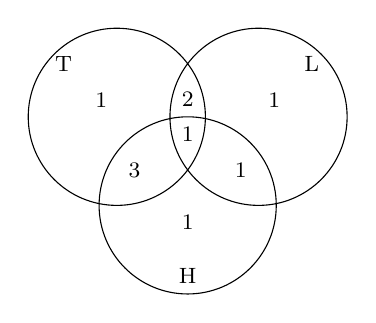
\begin{tikzpicture}[>=stealth,line join=round,line cap=round,font=\footnotesize,scale=0.45]
				\draw (0,0)node[above left]{$1$}circle (2.5) (4,0)node[above right]{$1$}circle(2.5) (2,-2.5)node[below]{$1$}circle(2.5);
				\draw (2,-0.5)node{$1$} (2,0.5)node{$2$} (0.5,-1.5)node{$3$} (3.5,-1.5)node{$1$} (-1.5,1.5)node{T} (5.5,1.5)node{L} (2,-4.5)node{H};
			\end{tikzpicture}}}
\end{ex}

\begin{ex}%[Pj31--2-Đề KT Theo Bài--TeamTeXHoa--Phan Anh]%[0D1H3-5]
	Trong kì thi học sinh giỏi cấp trường, lớp 11B có $15$ học sinh giỏi Văn, $22$ học sinh giỏi Toán. Tìm số học sinh giỏi cả Văn và Toán biết lớp đó có $40$ học sinh, và có $14$ học sinh không đạt học sinh giỏi.
	\choice
	{$4$}
	{$7$}
	{\True $11$}
	{$20$}
	\loigiai{Số học sinh học giỏi ít nhất một trong hai môn Toán và Văn là $40-14=26$.\\
		Số học sinh chỉ giỏi Toán mà không giỏi Văn
		là $26-15=11$.\\
		Vậy số học sinh giỏi cả hai môn Toán và Văn là $22-11=11$.\\
		\textbf{Cách khác:}
		Số học sinh học giỏi ít nhất một trong hai môn Toán và Văn là $40-14=26$.\\
		Số học sinh giỏi cả hai môn Toán và Văn là $22+15-26=11$.}
\end{ex}
\Closesolutionfile{ans}
\TNTF
\setcounter{ex}{0}
\Opensolutionfile{ans}[ans/ansDS-0D1-OnChuong-De1]
\begin{ex}%[Pj31--2-Đề KT Theo Bài--TeamTeXHoa--Phan Anh]%[0D1H1-4]
	Cho biết tính đúng sai của mỗi mệnh đề sau.
	\choiceTF
	{Nếu số $a$ chia hết cho $3$ thì $a$ chia hết cho $6$}
	{\True Nếu $\triangle ABC$ cân tại $A$ thì $\triangle ABC$ có $AB=AC$}
	{\True Tứ giác $ABCD$ là hình vuông khi và chỉ khi $ABCD$ là hình chữ nhật và có $AC$ vuông góc với $BD$}
	{$\pi^2>10$}
	\loigiai{\begin{itemchoice}
			\itemch \lq\lq Nếu số $a$ chia hết cho $3$ thì $a$ chia hết cho $6$\rq\rq  là mệnh đề sai vì nếu xét $a=3$ thì $a$ chia hết cho $3$ nhưng không chia hết cho $6$.
			\itemch \lq\lq Nếu $\triangle ABC$ cân tại $A$ thì $\triangle ABC$ có $AB=AC$\rq\rq  là mệnh đề đúng.
			\itemch \lq\lq Tứ giác $ABCD$ là hình vuông khi và chỉ khi $ABCD$ là hình chữ nhật và có $AC$ vuông góc với $BD$\rq\rq  là mệnh đề đúng.
			\itemch \lq\lq $\pi^2>10$\rq\rq  là mệnh đề sai, vì $\pi^2\approx9{,}869<10$.
		\end{itemchoice}}
\end{ex}

\begin{ex}%[Pj31--2-Đề KT Theo Bài--TeamTeXHoa--Phan Anh]%[0D1H1-2]
	Cho biết mệnh đề phủ định của mệnh đề sau đúng hay sai?
	\choiceTF
	{$P\colon$ \lq\lq Hình thoi có hai đường chéo vuông góc với nhau \rq\rq }
	{$S\colon$ \lq\lq $1>-3$ \rq\rq }
	{\True $K\colon$ \lq\lq Phương trình $x^4-2x^2+2=0$ có nghiệm \rq\rq }
	{$H\colon$ \lq\rq $\left(\sqrt{3}-\sqrt{12}\right)^2=3$ \rq\rq}
	\loigiai{
		\begin{itemchoice}
			\itemch Ta có mệnh đề phủ định là $\overline{P}\colon$ \lq\lq Hình thoi có hai đường chéo không vuông góc với nhau\rq\rq~ là mệnh đề sai.
			\itemch Ta có mệnh đề phủ định là $\overline{S}\colon$ \lq\lq $1\le-3$\rq\rq~ là mệnh đề sai.
			\itemch Ta có mệnh đề phủ định là $\overline{K}\colon$ \lq\lq phương trình $x^4-2x^2+2=0$ vô nghiệm\rq\rq~ là mệnh đề đúng. 
			\itemch Ta có mệnh đề phủ định là: $\overline{H}\colon$ \lq\lq $\left(\sqrt{3}-\sqrt{12}\right)^2\ne 3$\rq\rq~ là mệnh đề sai.
		\end{itemchoice}}
\end{ex}

\begin{ex}%[Pj31--2-Đề KT Theo Bài--TeamTeXHoa--Phan Anh]%[0D1H3-1]
	Cho các tập hợp $A=\{-3;-2;-1;0;1;2;3\}$; $B=\{0;1;4;5\}$; $C=\{-4;-3;1;2;5;6\}$. Khi đó
	\choiceTF
	{\True $A\cup B=\{-3;-2;-1;0;1;2;3;4;5\}$}
	{$A\cap B=\{0\}$}
	{\True $(A\cup B)\cap C=\{-3;1;2;5\}$}
	{\True $A\cap B\cap C=\{1\}$}
	\loigiai{
		\begin{itemchoice}
			\itemch $A\cup B=\{-3;-2;-1;0;1;2;3;4;5\}$.
			\itemch $A\cap B=\{0;1\}$.
			\itemch $(A\cup B)\cap C=\{-3;1;2;5\}$.
			\itemch $A\cap B\cap C=\{1\}$.
		\end{itemchoice}
		}
\end{ex}

\begin{ex}%[Pj31--2-Đề KT Theo Bài--TeamTeXHoa--Phan Anh]%[0D1H3-5]
	Lớp 10A có tất cả $50$ học sinh trong đó có $13$ học sinh chỉ thích đá bóng, $18$ học sinh chỉ thích chơi cầu lông, $10$ học sinh không thích môn nào trong hai môn thể thao nói trên và số học sinh còn lại thích chơi cả hai môn thể thao nói trên. Khi đó
	\choiceTF
	{\True Có $40$ học sinh thích chơi môn cầu lông hoặc môn bóng đá}
	{Có $27$ học sinh thích chơi cả hai môn cầu lông và bóng đá}
	{\True Có $31$ học sinh thích chỉ một trong hai môn bóng đá và môn cầu lông}
	{Có $26$ học sinh thích cầu lông}
	\loigiai{
		\begin{itemchoice}
			\itemch Số học sinh thích chơi môn cầu lông hoặc môn bóng đá là $50-10=40$ (học sinh).
			\itemch Số học sinh thích chơi cả hai môn câu lông và bóng đá là $40-(18+13)=9$ (học sinh).
			\itemch Số học sinh thích chỉ một trong hai môn bóng đá và môn cầu lông là $40-9=31$ (học sinh).
			\itemch Số học sinh thích câu lông là $18+9=27$ (học sinh).
		\end{itemchoice}
		}
\end{ex}
\Closesolutionfile{ans}
\TNSA
\setcounter{ex}{0}
\Opensolutionfile{ans}[ans/ansTLN-0D1-OnChuong-De1]

\begin{ex}%[Pj31--2-Đề KT Theo Bài--TeamTeXHoa--Phan Anh]%[0D1H1-3]
	Cho $x\in\mathbb{Z}$, xét hai mệnh đề chứa biến $A\colon\lq\lq x\ge3$\rq\rq  và $B\colon\lq\lq x\le a$\rq\rq . Để mệnh đề $B$ là phủ định của mệnh đề $A$ thì giá trị của $a$ là bao nhiêu?
	\shortans[oly]{2}
	\loigiai{
		Mệnh đề phủ định của $A$ là $\overline{A}\colon\lq\lq x<3$\rq\rq .\\
		Do $x\in\mathbb{Z}$ nên $\overline{A}\colon\lq\lq x\le2$\rq\rq .\\
		Do đó để mệnh đề $B$ là phủ định của mệnh đề $A$ thì $a=2$.
	}
\end{ex}
\begin{ex}%[Pj31--2-Đề KT Theo Bài--TeamTeXHoa--Phan Anh]%[0D1H1-2]
	Có bao nhiêu giá trị của $n\in\mathbb{N}$, $n\in(1;30)$ để mệnh đề $A\colon$\lq\lq Nếu $2n^2+3n+1$ chia hết cho $2$ thì $n$ chia hết cho $3$\rq\rq  là mệnh đề sai?
	\shortans[oly]{10}
	\loigiai{
		Mệnh đề $P\Rightarrow Q$ sai khi và chỉ khi $P$ đúng, $Q$ sai.\\
		Mệnh đề $P$ đúng khi $2n^2+3n+1=(2n+1)(n+1)$ chia hết cho $2$.\\
		Do $2n+1$ là số lẻ nên $n+1$ là số chẵn, suy ra $n$ là số lẻ.\\
		Mệnh đề $Q$ sai khi $Q$ không chia hết cho $3$.\\
		Vì $n\in(1;30)$ có $10$ số lẻ và không chia hết cho $3$ nên $n\in\{1;5;7;11;13;17;19;23;25;29\}$, vậy ta có $10$ giá trị $n$ thoả mãn bài toán.
		}
\end{ex}
\begin{ex}%[Pj31--2-Đề KT Theo Bài--TeamTeXHoa--Phan Anh]%[0D1V3-3]
	Cho hai tập hợp $A=[m-3;m+2]$, $B=(-3;5)$ với $m\in\mathbb{R}$. Tính tổng tất cả các giá trị nguyên của $m$ để $A\cap B$ khác tập rỗng.
	\shortans[oly]{18}
	\loigiai{
		Trước hết, ta tìm $m$ để $A\cap B=\varnothing$.\\
		Để $A\cap B=\varnothing$ thì $\hoac{&m+2\le-3\\&m-3\ge5}\Leftrightarrow\hoac{&m\le-5\\&m\ge8.}$.\\
		Vậy để $A\cap B$ khác tập rỗng thì $-5<m<8$.\\
		Do $m$ nguyên nên $m\in\{-4;-3;-2;-1;0;1;2;3;4;5;6;7\}$, suy ra tổng các giá trị của $m$ là
		\[S=-4-3-2-1+1+0+1+2+3+4+5+6+7=18.\]
		}
\end{ex}

\begin{ex}%[Pj31--2-Đề KT Theo Bài--TeamTeXHoa--Phan Anh]%[0D1H2-2]
	Cho tập hợp $B=\left\{x\in\mathbb{Z}\mid\left|x^2+1\right|\le2\right\}$. Tập hợp $B$ có bao nhiêu tập con gồm $2$ phần tử?
	\shortans[oly]{3}
	\loigiai{
		Ta có: $\heva{&x\in\mathbb{Z}\\&\left|x^2+1\right|\le2}\Rightarrow\hoac{&x=-1\\&x=0\\&x=1}\Rightarrow B=\{-1;0;1\}$.\\
		Các tập con của tập $B$ gồm $2$ phần tử là $\{-1;0\},\{0;1\},\{-1;1\}$.\\
		Vậy có $3$ tập con của $B$ gồm $2$ phần tử.
		}
\end{ex}

\begin{ex}%[Pj31--2-Đề KT Theo Bài--TeamTeXHoa--Phan Anh]%[0D1H3-5]
	Bạn A Súa thống kê số ngày có mưa, có sương mù ở bản mình trong tháng $3$ vào một thời điểm nhất định và được kết quả như sau: $14$ ngày có mưa, $15$ ngày có sương mù, trong đó $10$ ngày có cả mưa và sương mù. Hỏi trong tháng $3$ đó có bao nhiêu ngày không có mưa và không có sương mù?
	\shortans[oly]{12}
	\loigiai{
		Gọi $A$, $B$ lần lượt là tập hợp các ngày có mưa, có sương mù. Khi đó, $A\cap B$ là tập hợp các ngày có cả mưa và sương mù, $A\cup B$ là tập hợp các ngày hoặc có mưa hoặc có sương mù.\\
		Ta có $n(A)=14$, $n(B)=15$, $n(A\cap B)=10$.\\
		Số ngày hoặc có mưa hoặc có sương mù là
		\[n(A\cup B)=n(A)+n(B)-n(A\cap B)=14+15-10=19\text{ (ngày).}\]
		Tháng $3$ có $31$ ngày nên số ngày không có mưa và không có sương mù trong tháng $3$ đó là $31-19=12$ (ngày).
		}
\end{ex}

\begin{ex}%[Pj31--2-Đề KT Theo Bài--TeamTeXHoa--Phan Anh]%[0D1V3-5]
	Trong đợt khảo sát nghề, giáo viên chủ nhiệm lớp 10D đưa ra ba nhóm ngành cho học sinh lựa chọn, đó là: Giáo dục, Y tế, Công nghệ thông tin. Học sinh có thể chọn từ một đến ba nhóm ngành nêu trên hoặc không chọn nhóm ngành nào trong ba nhóm ngành trên. Giáo viên chủ nhiệm thống kê theo từng nhóm ngành và được kết quả: có $6$ học sinh chọn nhóm ngành Giáo dục, $9$ học sinh chọn nhóm ngành Y tế, $10$ học sinh chọn nhóm ngành Công nghệ thông tin, $22$ học sinh không chọn nhóm ngành nào trong ba nhóm trên. Nếu thống kê số lượng học sinh chọn theo từng hai nhóm ngành được kết quả: có $3$ học sinh chọn hai nhóm ngành Giáo dục và Y tế, $2$ học sinh chọn hai nhóm ngành Y tế và Công nghệ thông tin, $3$ học sinh chọn hai nhóm ngành Giáo dục và Công nghệ thông tin. Hỏi có bao nhiêu học sinh chọn cả ba nhóm ngành nêu trên biết lớp 10D có $40$ học sinh?
	\shortans[oly]{1}
	\loigiai{
		Gọi $A$, $B$, $C$ lần lượt là tập hợp học sinh chọn nhóm ngành Giáo dục, Y tế, Công nghệ thông tin.\\
		Khi đó, $A\cup B\cup C$ là tập hợp các học sinh chọn ít nhất một trong ba nhóm ngành trên.\\
		Do lớp 10D có $40$ học sinh và $22$ học sinh không chọn nhóm ngành trong ba nhóm ngành trên nên số học sinh chọn ít nhất một trong ba nhóm ngành trên là $40-22=18$.\\
		Ta có $n(A)=6$, $n(B)=9$, $n(C)=10$, $n(A\cup B\cup C)=18$, $n(A\cap B)=3$, $n(B\cap C)=2$, $n(A\cap C)=3$.\\
		Ta có số học sinh chọn cả ba nhóm ngành nêu trên là
		\begin{eqnarray*}
			n(A\cap B\cap C)&=&n(A\cup B\cup C)+n(A\cap B)+n(B\cap C)+n(A\cap C)-n(A)-n(B)-n(C)\\
			&=&18+3+2+3-6-9-10=1.
		\end{eqnarray*}
		}
\end{ex}
\Closesolutionfile{ans}
% \begin{center}	
% 	\fontfamily{qag}\selectfont\color{violet} 	\centering{\textbf{BẢNG ĐÁP ÁN}}
% \end{center}
% \inputansbox{12}{ans/ansBONPA-0D1-OnChuong-De1}
% \inputansbox{4}{ans/ansDS-0D1-OnChuong-De1}
% \inputansbox{6}{ans/ansTLN-0D1-OnChuong-De1}
% \begin{name}
	{\tenchude}
	{TOÁN 10}
	{LỚP TOÁN THẦY PHÁT}
	{Thời gian: 90 phút - Không kể thời gian phát đề}
\end{name}
\TN
\Opensolutionfile{ans}[ans/ansBONPA-0D1-OnChuong-De2]
\begin{ex}%Câu 1%[0D1H2-1]
	Số phần tử của tập hợp $A=\left\{{k^2}+1\big|k\in\mathbb{Z},\left| k\right|\le 2\right\}$ là
	\choice
	{$1$}
	{$2$}
	{\True $3$}
	{$5$}
	\loigiai{
		$A=\left\{{k^2}+1\left| k\in\mathbb{Z},\left| k\right|\le 2\right.\right\}$. Ta có $k\in\mathbb{Z}$, $\left| k\right|\le 2$ $\Leftrightarrow-2\le k\le 2$ $\Rightarrow A=\left\{ 1;\,2;\,5\right\}.$.}
\end{ex}

\begin{ex}%Câu 2%[0D1H2-1]
	Tập $A=\left\{ x\in\mathbb{R}\left|-3<1-2x\le 1\right.\right\}$ được viết lại dưới dạng đoạn, khoảng, nửa khoảng là
	\choice
	{$\left(-1;\,0\right]$}
	{\True $\left[0;\,2\right)$}
	{$\left[1;\,2\right]$}
	{$\left(0;\,2\right]$}
	\loigiai{
		Ta có $-3<1-2x\le 1\Leftrightarrow-4<-2x\le 0\Leftrightarrow 0\le x<2$.\\
		Do đó $A=\left\{ x\in\mathbb{R}\left| 0\le x<2\right.\right\}=\left[0;\,2\right)$.}
\end{ex}

\begin{ex}%Câu 3%[0D1N1-5]
	Trong các mệnh đề sau, mệnh đề nào \textbf{sai}?
	\choice
	{$\exists x\in\mathbb{R}\colon x^2-3x+2=0$}
	{$\forall x\in\mathbb{R}\colon x^2\ge 0$}
	{$\exists n\in\mathbb{N}\colon n^2=n$}
	{\True $\forall n\in\mathbb{N}$ thì $n<2n$}
	\loigiai{
		Xét mệnh đề \lq\lq$\forall n\in\mathbb{N}$ thì $n<2n$\rq\rq.\\
		Chọn $n=0\in\mathbb{N}\Rightarrow 2n=0\Rightarrow n=2n$\\
		$\Rightarrow \forall n\in\mathbb{N}$ thì $n<2n$ là mệnh đề sai.}
\end{ex}

\begin{ex}%Câu 4%[0D1N1-5]
	Tìm mệnh đề đúng?
	\choice
	{$\lq\lq\exists x\in\mathbb{R}\colon{x^2}+3=0$\rq\rq}
	{\lq\lq$\forall x\in\mathbb{Z}\colon{x^5}>x^2$\rq\rq}
	{\True \lq\lq$\forall x\in\mathbb{N}\colon\left(2x+1\right)^2-1$ chia hết cho $4$\rq\rq}
	{\lq\lq$\exists x\in\mathbb{R}\colon{x^4}+3x^2+2=0$\rq\rq}
	\loigiai{
		Ta có $\left(2x+1\right)^2-1=4x^2+4x+1-1=4x\left(x+1\right).$\\
		Vì $4\,\vdots\, 4$ nên $4x\left(x+1\right)\,\vdots\, 4$, $\forall x\in\mathbb{N}$.\\
		Suy ra tồn tại số thực $\hoac{
			& x>1\\ 
			& x<0}$ thỏa mãn $x^2>x$.}
\end{ex}
%
\begin{ex}%Câu 5%[0D1N2-1]
	Hãy liệt kê các phần tử của tập hợp $X=\left\{ x\in\mathbb{R}\big|{x^4}-6x^2+8=0\right\}$.
	\choice
	{$X=\left\{ 2;4\right\}$}
	{$X=\left\{-\sqrt{2};\sqrt{2}\right\}$}
	{$X=\left\{\sqrt{2};2\right\}$} {$X=\left\{-\sqrt{2};\sqrt{2};-2;2\right\}$}
	\loigiai{
		Giải phương trình $x^4-6x^2+8=0\Leftrightarrow\hoac{
			&x^2=2\\ 
			&x^2=4}\Leftrightarrow\hoac{
			& x=\pm\sqrt{2}\\ 
			& x=\pm 2.}$}\\
	Vậy $X=\left\{-\sqrt{2};\sqrt{2};-2;2\right\}$.
\end{ex}

\begin{ex}%Câu 6%[0D1H2-1]
	Trong các tập hợp sau, tập hợp nào là tập rỗng?
	\choice
	{$A=\left\lbrace  x\in\mathbb{N}\big|x^2-4=0\right\rbrace $}
	{\True $B=\left\lbrace x\in\mathbb{R}\big|x^2+2x+3=0\right\rbrace $}
	{$C=\left\lbrace  x\in\mathbb{R}\big|x^2-5=0\right\rbrace $}
	{$D=\left\lbrace  x\in\mathbb{Q}\big|x^2+x-12=0\right\rbrace $}
	\loigiai{
		$A=\left\lbrace  x\in\mathbb{N}\big|x^2-4=0\right\rbrace \Rightarrow A=\left\{2\right\}$.\\
		$B=\left\{ x\in\mathbb{R}\big|x^2+2x+3=0\right\}\Rightarrow B=\varnothing .$\\
		$C=\left\{ x\in\mathbb{R}\big|x^2-5=0\right\}\Rightarrow C=\left\{-\sqrt{5};\sqrt{5}\right\}.$\\
		$D=\left\{ x\in\mathbb{Q}\big|x^2+x-12=0\right\}\Rightarrow D=\left\{-3;\,4\right\}$.
	}
\end{ex}
%
\begin{ex}%Câu 7%[0D1H2-2]
	Cho tập hợp $A=\left\{ 1;2;5;7\right\}$ và $B=\left\{ 1;2;3\right\}$. Có tất cả bao nhiêu tập $X$ thỏa mãn $X\subset A$ và $X\subset B$?
	\choice
	{$2$}
	{\True $4$}
	{$6$}
	{$8$}
	\loigiai{
		Vì $\heva{
			& X\subset A\\ 
			& X\subset B}$ nên $X\subset\left(A\cap B\right)$.\\
		Mà $A\cap B=\left\{ 1;2\right\}$. Nên có $2^2=4$ tập $X$.
	}
\end{ex}
%
\begin{ex}%Câu 8%[0D1N2-3]
	Hình vẽ nào sau đây (phần không bị gạch) minh họa cho tập hợp $\left(1;4\right]$?
	\choice
	{\True 		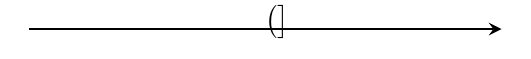
\begin{tikzpicture}[>=stealth,line width=1pt]
			\draw[->](-3,0)->(3,0);		%Vẽ trục số
			\def\skipInterval{0.5cm}		%Khoảng cách đặt nhãn
			%\def\colorInterval{blue} 	%Màu tick, màu fill miền
			%\IntervalR{\big(}{1}{\big]}{4}
			\IntervalLR{-3}{-1.4}		\IntervalGLF{}{}{\big(}{1}
			\IntervalLR{3}{1}	
			\IntervalGLF{}{}{\big]}{4}
		\end{tikzpicture}
	}
	{	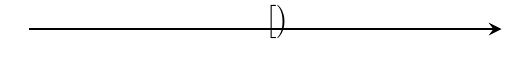
\begin{tikzpicture}[>=stealth,line width=1pt]
			\draw[->](-3,0)->(3,0);		%Vẽ trục số
			\def\skipInterval{0.5cm}		%Khoảng cách đặt nhãn
			%\def\colorInterval{blue} 	%Màu tick, màu fill miền
			%\IntervalR{\big(}{1}{\big]}{4}
			\IntervalLR{-3}{-1.4}		\IntervalGLF{}{}{\big[}{1}
			\IntervalLR{3}{1}	
			\IntervalGLF{}{}{\big)}{4}
		\end{tikzpicture}
	}
	{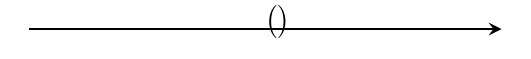
\begin{tikzpicture}[>=stealth,line width=1pt]
			\draw[->](-3,0)->(3,0);		%Vẽ trục số
			\def\skipInterval{0.5cm}		%Khoảng cách đặt nhãn
			%\def\colorInterval{blue} 	%Màu tick, màu fill miền
			%\IntervalR{\big(}{1}{\big]}{4}
			\IntervalLR{-3}{-1.4}		\IntervalGLF{}{}{\big(}{1}
			\IntervalLR{3}{1}	
			\IntervalGLF{}{}{\big)}{4}
		\end{tikzpicture}
	}
	{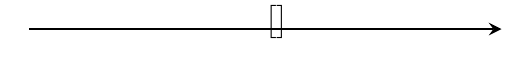
\begin{tikzpicture}[>=stealth,line width=1pt]
			\draw[->](-3,0)->(3,0);		%Vẽ trục số
			\def\skipInterval{0.5cm}		%Khoảng cách đặt nhãn
			%\def\colorInterval{blue} 	%Màu tick, màu fill miền
			%\IntervalR{\big(}{1}{\big]}{4}
			\IntervalLR{-3}{-1.4}		\IntervalGLF{}{}{\big[}{1}
			\IntervalLR{3}{1}	
			\IntervalGLF{}{}{\big]}{4}
		\end{tikzpicture}
	}
	\loigiai{
		Vì $\left(1;4\right]$ gồm các số thực $x$ mà $1<x\le 4$ nên biểu diễn trên trục là\begin{center} 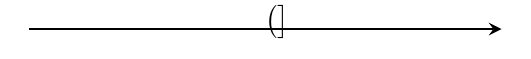
\begin{tikzpicture}[>=stealth,line width=1pt]
				\draw[->](-3,0)->(3,0);		%Vẽ trục số
				\def\skipInterval{0.5cm}		%Khoảng cách đặt nhãn
				%\def\colorInterval{blue} 	%Màu tick, màu fill miền
				%\IntervalR{\big(}{1}{\big]}{4}
				\IntervalLR{-3}{-1.4}		\IntervalGLF{}{}{\big(}{1}
				\IntervalLR{3}{1}	
				\IntervalGLF{}{}{\big]}{4}
	\end{tikzpicture}\end{center}}
\end{ex}
%
\begin{ex}%Câu 9%[0D1N2-1]
	Cho tập hợp $A=\left\{1,2,3,4,x,y\right\}$. Xét các mệnh đề sau đây:\\
	$(I)$: \lq\lq$3\in A$\rq\rq.\\
	$\left(II\right)$: \lq\lq$\left\{ 3,4\right\}\in A$\rq\rq.\\
	$\left(III\right)$: \lq\lq$\left\{ a,3,b\right\}\in A$\rq\rq.\\
	Trong các mệnh đề sau, mệnh đề nào đúng?
	\choice
	{\True $I$ đúng}
	{$I$, $II$ đúng}
	{$II$, $III$ đúng}
	{$I$, $III$ đúng}
	\loigiai{
		$3$ là một phần tử của tập hợp $A$.\\
		$\left\{ 3,4\right\}$ là một tập con của tập hợp $A$. Ký hiệu $\left\{ 3,4\right\}\subset A$.\\
		$\left\{ a,3,b\right\}$ là một tập con của tập hợp $A$. Ký hiệu $\left\{ a,3,b\right\}\subset A$.}
\end{ex}
%
\begin{ex}%Câu 10%[0D1H2-2]
	Có tất cả bao nhiêu tập $X$ thỏa mãn $\left\{ 1;2;3\right\}\subset X\subset\left\{ 1;2;3;4;5;6\right\}$?
	\choice
	{$1$}
	{\True $8$}
	{$3$}
	{$6$}
	\loigiai{
		Các tập hợp $X$ thỏa mãn điều kiện là\allowdisplaybreaks
		\begin{eqnarray*}
			X&=&\left\{ 1;2;3\right\}, X=\left\{ 1;2;3;4\right\},\\
			X&=&\left\{ 1;2;3;5\right\}, X=\left\{ 1;2;3;6\right\},\\
			X&=&\left\{ 1;2;3;4;5\right\}, X=\left\{ 1;2;3;4;6\right\},\\
			X&=&\left\{ 1;2;3;5;6\right\}, X=\left\{ 1;2;3;4;5;6\right\}.
		\end{eqnarray*}
		Vậy có tất cả $8$ tập hợp $X$ thỏa mãn yêu cầu bài toán.}
\end{ex}
%
\begin{ex}%Câu 11%[0D1H3-5]
	Lớp 10A có $10$ học sinh giỏi Toán, $10$ học sinh giỏi Lý, $11$ học sinh giỏi hóa, $6$ học sinh giỏi cả Toán và Lý, $5$ học sinh giỏi cả Hóa và Lý, $4$ học sinh giỏi cả Toán và Hóa, $3$ học sinh giỏi cả ba môn Toán, Lý, Hóa). Số học sinh giỏi ít nhất một trong ba môn (Toán, Lý, Hóa) của lớp 10A là
	\choice
	{\True $19$}
	{$18$}
	{$31$}
	{$49$}
	\loigiai{Gọi $T$ là tập hợp học sinh giỏi toán, $L$ là tập hợp học sinh giỏi lý, $H$ là tập hợp học sinh giỏi hóa.\\
		Theo giả thiết ta có\allowdisplaybreaks
		\begin{eqnarray*}
			&&|T|=10; |L|=10; |H|=11;\\
			&&|T\cap L|=6; |T\cap H|=4; |L\cap H|=5;\\
			&& |T\cap L\cap H|=3.
		\end{eqnarray*}
		Số học sinh giỏi ít nhất một trong ba môn (Toán, Lý, Hóa) của lớp 10A là
		$$|T\cup L\cup H|=|T|+|L|+|H|-|T\cap L|-|T\cap H|-|L\cap H|+|T\cap L\cap H|=10+10+11-6-4-5+3=19.$$
	}
\end{ex}
%
\begin{ex}%Câu 12%[0D1H3-5]
	Mỗi học sinh của lớp $10A_1$ đều học giỏi môn Toán hoặc môn Hóa, biết rằng có $30$ học sinh giỏi Toán, $35$ học sinh giỏi Hóa, và $20$ em học giỏi cả hai môn. Hỏi lớp $10A_1$ có bao nhiêu học sinh?
	\choice
	{$40$}
	{\True $45$}
	{$50$}
	{$55$}
	\loigiai{Gọi $T$ là tập hợp học sinh giỏi toán, $H$ là tập hợp học sinh giỏi hóa.\\
		Theo giả thiết ta có $|T|=30$; $|H|=35$;  $|T\cap H|=20$.\\
		Sĩ số học sinh lớp $10A_1$ là $|T\cup H|=|T|+|H|-|T\cap H|=30+35-20=45$.}
\end{ex}

\Closesolutionfile{ans}
\TNTF
\setcounter{ex}{0}
\Opensolutionfile{ans}[ans/ansDS-0D1-OnChuong-De2]
%
\begin{ex}%Câu 13%[0D1H1-5]
	Xét tính đúng, sai của mỗi mệnh đề sau.
	\choiceTF
	{\True $\exists x\in\mathbb{Q}, 4 x^2-1=0$}
	{$\forall n\in\mathbb{N}, n$ và $n+2$ là các số nguyên tố}
	{$\forall x\in\mathbb{R},(x-1)^2\neq x-1$}
	{$\forall n\in\mathbb{N}, n^2>n$}
	\loigiai{
		\begin{itemchoice}
			\itemch  Ta có $4 x^2-1=0\Leftrightarrow x=\pm\dfrac{1}{2}\in\mathbb{Q}$.
			\itemch Ta cho $n=2\in\mathbb{N}$ thì $n+2=4$ không là số nguyên tố.
			\itemch Ta cho $x=1\in\mathbb{R}$ thì $(x-1)^2=x-1=0$.
			\itemch  Ta cho $n=0\in\mathbb{N}$ thì $n^2=0$ nên $n^2>n$ là sai.
	\end{itemchoice}}
\end{ex}
%
\begin{ex}%Câu 14%[0D1H1-2]
	Xét tính đúng, sai của mỗi mệnh đề sau.
	\choiceTF
	{\True Hai góc đối đỉnh thì bằng nhau}
	{\True Hai tam giác có hai cặp cạnh bằng nhau và cặp góc xen giữa hai cạnh bằng nhau thì bằng nhau}
	{Hai tam giác có hai cặp góc bằng nhau thì bằng nhau}
	{\True Một số chia hết cho $3$ khi và chỉ khi tổng các chữ số chia hết cho $3$}
	\loigiai{
		\begin{itemchoice}
			\itemch Lý thuyết.
			\itemch Lý thuyết.
			\itemch 
			\itemch Lý thuyết.
		\end{itemchoice}
	}
\end{ex}
%
\begin{ex}%Câu 15%[0D1H3-4]
	Cho các tập hợp $A=\{0 ; 1 ; 2 ; 3 ; 4\}$; $ B=\{0 ; 1 ; 2\}$; $C=\{-3 ; 0 ; 1 ; 2\}$. Khi đó
	\choiceTF
	{\True $A\setminus B=\{3 ; 4\}$}
	{\True $(A\cap C)\setminus B=\varnothing$}
	{$A\cup (C\setminus B)=\{-3;0;1;4\}$}
	{$C_AB=\{1;3;4\}$}
	\loigiai{
		\begin{itemchoice}
			\itemch $A\setminus B=\{3 ; 4\}$.
			\itemch $(A\cap C)\setminus B=\varnothing$.
			\itemch $A\cup(C\setminus B)=\{-3 ; 0 ; 1 ; 2 ; 3 ; 4\}$.
			\itemch $C_A B=\{3 ; 4\}$.
		\end{itemchoice}
	}
\end{ex}
%
\begin{ex}%Câu 16%[0D1H3-4]
	Cho $A$ là tập hợp các học sinh lớp 10 đang học ở trường em và $B$ là tập hợp các học sinh đang học môn Tiếng Anh của trường em. Vậy
	\choiceTF
	{\True $A\cap B$ là tập hợp các học sinh lớp 10 học môn Tiếng Anh ở trường em}
	{\True $A\setminus B$ là tập hợp những học sinh lớp 10 nhưng không học Tiếng Anh ở trường em}
	{\True $A\cup B$ là tập hợp các học sinh lớp 10 hoặc học sinh học môn Tiếng Anh ở trường em}
	{\True $B\setminus A$ là tập hợp các học sinh học môn Tiếng Anh nhưng không học lớp 10 ở trường em}
	\loigiai{
		\begin{itemchoice}
			\itemch $A\cap B$ là tập hợp các học sinh lớp $10$ học môn Tiếng Anh ở trường em.
			\itemch $A\setminus B$ là tập hợp những học sinh lớp $10$ nhưng không học Tiếng Anh ở trường em.
			\itemch $A\cup B$ là tập hợp các học sinh lớp $10$ hoặc học sinh học môn Tiếng Anh ở trường em.
			\itemch $B\setminus A$ là tập hợp các học sinh học môn Tiếng Anh nhưng không học lớp $10$ ở trường em.
		\end{itemchoice}
	}
\end{ex}

\Closesolutionfile{ans}
\TNSA
\setcounter{ex}{0}
\Opensolutionfile{ans}[ans/ansTLN-0D1-OnChuong-De2]
%
\begin{ex}%Câu 22%[0D1H3-5]
	Một lớp học có $25$ học sinh chơi bóng đá, $23$ học sinh chơi bóng bàn, $14$ học sinh chơi cả bóng đá và bóng bàn, $6$ học sinh không chơi môn thể thao nào. Tìm số học sinh của lớp?\shortans{40}
	\loigiai{
		Gọi $A$ là tập hợp các học sinh chơi bóng đá, $B$ là tập hợp các học sinh chơi bóng bàn,
		$C$ là tập hợp các học sinh không chơi môn thể thao nào.\\
		Ta có $|A|=25$; $|B|=23$; $|C|=6$; $|A\cap B|=14$.\\
		Khi đó số học sinh chỉ chơi một môn thể thao là $|A|+|B|-|A\cap B|+|C|=25+23-14+6=40$.}
\end{ex}
%
\begin{ex}%Câu 7%[0D1H2-2]
	Cho tập hợp $A=\left\{ 1;2;5;7\right\}$ và $B=\left\{ 1;2;3;5\right\}$. Có tất cả bao nhiêu tập $X$ thỏa mãn $X\subset A$ và $X\subset B$ ?
	\shortans{8}
	\loigiai{
		Vì $\left\{\begin{aligned}
			& X\subset A\\ 
			& X\subset B\\ 
		\end{aligned}\right.$ nên $X\subset\left(A\cap B\right)$.\\
		Mà $A\cap B=\left\{ 1;2;5\right\}$. Nên có $2^3=8$ tập $X$.
	}
\end{ex}
%
\begin{ex}%Câu 19%[0D1V3-3]
	Cho hai tập hợp $A=[-4 ; 1], B=[-3 ; m]$. Có bao nhiêu giá trị nguyên của tham số $m$ để $A\cup B=A$?
	\shortans{4}
	\loigiai{
		Điều kiện $m>-3$.\\
		Ta có $A\cup B=A$ khi và chỉ khi $B\subset A$, tức là $m\leqslant 1$.\\
		Đối chiếu điều kiện, ta được $-3<m\leqslant 1$. Suy ra có $4$ giá trị nguyên của tham số $m$.}
\end{ex}
%
\begin{ex}%Câu 20%[0D1H3-4]
	Cho $A$ là tập hợp tất cả các nghiệm của phương trình $x^2-4 x+3=0$;
	$B$ là tập hợp các số nguyên có giá trị tuyệt đối nhỏ hơn $4$. Số phần tử của tập hợp $A\setminus B$ là
	\shortans{0}
	\loigiai{
		Ta có $x^2-7 x+6=0\Leftrightarrow\heva{&x=1\\ &x=3}\Rightarrow A=\{1 ; 3\}$.\\
		$B=\{-3 ;-2 ;-1 ; 0 ; 1 ; 2 ; 3\}$. Do đó $A\setminus B=\varnothing$.}
\end{ex}
%
\begin{ex}%Câu 21%[0D1H3-5]
	Lớp 10A có $45$ học sinh trong đó có 25 em học giỏi môn Toán, $23$ em học giỏi môn Lý, $20$ em học giỏi môn Hóa, $11$ em học giỏi cả môn Toán và môn Lý, $8$ em học giỏi cả môn Lý và môn Hóa, $9$ em học giỏi cả môn Toán và môn Hóa. Hỏi lớp 10A có bao nhiêu bạn học giỏi cả ba môn Toán, Lý, Hóa? (biết rằng mỗi học sinh trong lớp học giỏi ít nhất một trong ba môn Toán, Lý, Hóa).\shortans{5}
	\loigiai{
		Gọi $T$, $L$, $H$ lần lượt là tập hợp các học sinh giỏi môn Toán, Lý, Hóa.\\
		Ta có\allowdisplaybreaks \begin{eqnarray*}
			&&|T\cup L\cup H|=|T|+|L|+|H|-|T\cap L|-|L\cap H|-|H\cap T|+|T\cap L\cap H|\\
			&\Leftrightarrow& 45=25+23+20-11-8-9+|T\cap L\cap H|\\
			&\Leftrightarrow&|T\cap L\cap H|=5.
		\end{eqnarray*}
		Vậy có $5$ học sinh giỏi cả $3$ môn.}
\end{ex}
%
\begin{ex}%Câu 22%[0D1H3-5]
	Một lớp học có $25$ học sinh chơi bóng đá, $23$ học sinh chơi bóng bàn, $14$ học sinh chơi cả bóng đá và bóng bàn. Tìm số học sinh chỉ chơi một môn thể thao?\shortans{20}
	\loigiai{
		Gọi $A$ là tập hợp các học sinh chơi bóng đá, $B$ là tập hợp các học sinh chơi bóng bàn.\\
		Ta có $|A|=25$; $|B|=23$; $|A\cap B|=14$.\\
		Khi đó số học sinh chỉ chơi một môn thể thao là $|A|+|B|-2|A\cap B|=25+23-2\cdot14=20$.}
\end{ex}
\Closesolutionfile{ans}
% \begin{center}	
% 	\fontfamily{qag}\selectfont\color{violet} 	\centering{\textbf{BẢNG ĐÁP ÁN}}
% \end{center}
% \inputansbox{12}{ans/ansBONPA-0D1-OnChuong-De2}
% \inputansbox{4}{ans/ansDS-0D1-OnChuong-De2}
% \inputansbox{6}{ans/ansTLN-0D1-OnChuong-De2}
%%Chương 2
% \def\tenchude{BPT - HỆ BPT BẬC NHẤT HAI ẨN}
% \section{Bất phương trình bậc nhất hai ẩn}
\setcounter{dang}{0}
\subsection{Tóm tắt lý thuyết}
\subsubsection{Bất phương trình bậc nhất hai ẩn}
Bất phương trình bậc nhất hai ẩn $x$, $y$ có dạng tổng quát là 
\begin{center}
\fbox{$ax+by\le c \text{ (hoặc } ax+by<c; ax+by\ge c; ax+by>c),$}
\end{center}
trong đó $a$, $b$, $c$ là những số thực, $a$ và $b$ không đồng thời bằng $0$, $x$ và $y$ là các ẩn số.

\subsubsection{Biểu diễn tập nghiệm của bất phương trình bậc nhất hai ẩn}
Cũng như bất phương trình bậc nhất một ẩn, các bất phương trình bậc nhất hai ẩn có vô số nghiệm và để mô tả tập nghiệm của chúng, ta sử dụng phương pháp biểu diễn hình học.\\ 
Trong mặt phẳng tọa độ $Oxy$, tập hợp các điểm có tọa độ là nghiệm của bất phương trình được gọi là \textbf{miền nghiệm} của nó.\\
Quy tắc thực hành biểu diễn miền nghiệm của bất phương trình $ax+by \le c$ như sau (tương tự cho bất phương trình $ax+by\ge c$)
\begin{itemize}
	\item{\bf Bước 1:} Trên mặt phẳng tọa độ $Oxy$, vẽ đường thẳng $\Delta \colon ax+by=c$.
	\item{\bf Bước 2:} Lấy một điểm $M_0\left(x_0;y_0\right)$ không thuộc $\Delta$ (ta thường lấy gốc tọa độ $O$).
	\item{\bf Bước 3:} Tính $ax_0+by_0$ và so sánh $ax_0+by_0$ với $c$.
	\item{\bf Bước 4:} Kết luận,
	\begin{itemize}
		\item Nếu $ax_0+by_0<c$ thì nửa mặt phẳng bờ $\Delta$ chứa $M_0$ là miền nghiệm của $ax_0+by_0\leq c$.
		\item Nếu $ax_0+by_0>c$ thì nửa mặt phẳng bờ $\Delta$ không chứa $M_0$ là miền nghiệm của $ax_0+by_0\le c$.
	\end{itemize}
\end{itemize}

\begin{note}
	Miền nghiệm của bất phương trình $ax_0+by_0\leq c$ bỏ đi đường thẳng $ax+by=c$ là miền nghiệm của bất phương trình $ax_0+by_0<c$.
\end{note}
\subsection{Các dạng toán}
\begin{dang}{Bất phương trình bậc nhất hai ẩn và bài toán liên quan}
\end{dang}
\viduminhhoa
\begin{vd}%[Dự án Tex hóa đề thi lớp 10-11-Nhóm Word-T-Begin]%[Lê Vũ Hải-Phản biện: Trần Quốc Tráng]%[0D4Y4-1]%
	Cho bất phương trình: $2x-y<0$ . Trong các cặp số $(-1;2)$, $\left(2;0\right)$, $(0;1)$, $\left(3;-2\right)$, $(-1;-2)$, cặp nào là nghiệm của bất phương trình, cặp nào không phải là nghiệm của bất phương trình?
	\loigiai{
		Bằng cách thử trực tiếp, các cặp $(-1;2)$, $(0;1)$ là nghiệm, các cặp còn lại không phải là nghiệm của bất phương trình.
	}
\end{vd}
\begin{vd}%[Dự án Chuyển tex 10-11, Cao Thành Thái]%[0D4B4-1]
	Biểu diễn hình học tập nghiệm của bất phương trình $2x+y\le 3$.
	\loigiai
	{
		\immini{
			Vẽ đường thẳng $\Delta\colon 2x+y=3$.\\
			Lấy gốc tọa độ $O(0;0)$, ta thấy $O\notin \Delta $ và có $2 \cdot 0+0<3$ nên nửa mặt phẳng bờ $\Delta$ chứa gốc tọa độ $O$ là miền nghiệm của bất phương trình đã cho (miền không bị tô đậm trong hình vẽ).
		}
		{
			\begin{tikzpicture}[line join=round, line cap=round, >=stealth,font=\footnotesize, scale=0.8]
				\draw[->](-2,0)--(3,0) node[below right] {$x$};
				\draw[->](0,-1)--(0,4) node[right] {$y$};
				\clip (-2,-1) rectangle (3,4);
				\node (0,0) [below left]{$ O $};
				\foreach \x in {-1,...,2}
				\draw[shift={(\x,0)},color=black] (0pt,2pt) -- (0pt,-2pt);
				\foreach \y in {1,...,3}
				\draw[shift={(0,\y)},color=black] (2pt,0pt) -- (-2pt,0pt);
				\draw[samples=100,smooth,domain=-2:3] plot(\x,{-2*(\x)+3});
				\draw [pattern=north west lines] (-1,5)--(3,5)--(3,-1) -- (2,-1)--cycle;
				\draw[fill=black] (0,3) circle(1pt) node[left]{$3$};
				\draw[fill=black] (1.5,0)circle(1pt) node[below left]{\tiny $\dfrac{3}{2}$};
			\end{tikzpicture}
		}
	}
\end{vd}
\begin{vd}%[Mai Hà Lan]%[0D4B4-1]
	\begin{enumerate}
		\item Biểu diễn hình học tập nghiệm của bất phương trình $-2x + 3y > 0$.
		\item Cho hai điểm $A(2;1)$ và $B(3; 3)$, hỏi hai điểm này cùng phía hay khác phía đối với bờ $(d)$.
	\end{enumerate}
	\loigiai{
		\immini{
			\begin{enumerate}
				\item Vẽ đường thẳng $d: -2x + 3y = 0$.\\
				Thay tọa độ điểm $M(1;0)$ vào vế trái phương trình đường thẳng $(d)$, ta được: $-2 < 0$.\\
				Vậy miền nghiệm của bất phương trình là nửa mặt phẳng không chứa điểm $M$. (Trên hình là nửa mặt phẳng không bị gạch bỏ).
				\item Thế tọa độ điểm $A$ vào vế trái của phương trình đường thẳng $(d)$ ta được $-2 \cdot 2 + 3 \cdot 1 = -1 < 0$.\hfill $(1)$\\
				Thế tọa độ điểm $B$ vào vế trái của phương trình đường thẳng $(d)$ ta được $-2 \cdot 3 + 3 \cdot 3 = 3 > 0$. \hfill $(2)$ \\
				Từ $(1)$ và $(2)$ suy ra hai điểm nằm ở hai phía đối với bời $(d)$.
			\end{enumerate}
		}{
			\begin{tikzpicture}
				%---------------------- Vẽ hệ trục tọa độ
				\draw[->] (-2.25,0)--(4.25,0) node[below right] {$x$};
				\draw[->] (0,-0.755)--(0,2.25) node[right] {$y$};
				\node (0,0) [below right]{$ O $};
				%----------------------- Vẽ đoạn chắn trên trục
				\foreach \x in {-2,-1,1,2,3,4}
				\draw[shift={(\x,0)},color=black] (0pt,2pt) -- (0pt,-2pt);
				%\node at (3.8,0.5) {$4$};
				\foreach \y in {1,2}
				\draw[shift={(0,\y)},color=black] (2pt,0pt) -- (-2pt,0pt);
				%\node at (-0.5,-1.8) {$-2$};
				
				%--------------------- Vẽ hàm
				\draw [thick, domain=-1:3, samples=100] plot (\x, {(2/3) * \x});
				\node at (2,1.75) {$(d)$};
				
				%---------------------- Điểm M
				\fill (1,0) circle (2pt) node[below right]{$M(1;0)$};
				
				%----------------------Vẽ miền nghiệm
				\tkzDefPoints{-1/-.66/A, 4/-.66/B, 4/2/C, 3/2/D}
				\tkzDrawPolygon[ pattern=north east lines,opacity=.3](A,B,C,D)
			\end{tikzpicture}
	}}
\end{vd}
\begin{vd}%[Mai Hà Lan]%[0D4G4-1]
	\begin{enumerate}
		\item Biểu diễn hình học tập nghiệm của bất phương trình $x + y -3 < 0$.
		\item Tìm điều kiện của $m$ và $n$ để mọi điểm thuộc đường thẳng $(d')$: $ (m^2-2)x - y + m + n= 0 $ đều là nghiệm của bất phương trình trên.
	\end{enumerate}
	\loigiai{
		\immini{
			\begin{itemize}
				\item[a)] Vẽ đường thẳng $d: x + y = 3 $.\\
				Thay tọa độ điểm $O(0;0)$ vào vế trái phương trình đường thẳng $(d)$, ta được: $0< 3$.\\
				Vậy miền nghiệm của bất phương trình là nửa mặt phẳng chứa điểm $O$. (Trên hình là nửa mặt phẳng không bị gạch bỏ).
				\item[b)] Để mọi điểm thuộc đường thẳng  $(d')$ đều là nghiệm của bất phương trình thì điều kiện cần là $(d')$ phải song song với $(d)$. Ta có $d:  y = -x + 3$ và $d': y = (m^2-2)x +  m + n$. Để $(d)$ song song $(d')$ thì $\heva{& m^2 - 2 = -1 \\& m + n \ne 3} \Leftrightarrow \hoac{&\heva{&m=1\\&n\ne 2}\\&\heva{&m=-1\\&n\ne 4}}$\\
				Với $\heva{&m=1\\&n\ne 2}$ thì ta được $d': y = - x + n + 1$. Để thỏa yêu cầu bài toán thì điều kiện đủ là đường thẳng $(d')$ là đồ thị của đường thẳng $(d)$ khi $(d)$ tịnh tiến xuống dưới theo trục $Oy$. Tức $n + 1 < 3 \Leftrightarrow n < 2$.
			\end{itemize}
		}{
			\begin{tikzpicture}[scale=.8]
				%---------------------- Vẽ hệ trục tọa độ
				\draw[->] (-2.25,0)--(4.25,0) node[below right] {$x$};
				\draw[->] (0,-1.25)--(0,4.25) node[right] {$y$};
				\node (0,0) [below left]{$ O $};
				%----------------------- Vẽ đoạn chắn trên trục
				\foreach \x in {-2,-1,1,2,3,4}
				\draw[shift={(\x,0)},color=black] (0pt,2pt) -- (0pt,-2pt);
				\node at (2.75,-0.4) {$3$};
				\foreach \y in {-1,1,2,3,4}
				\draw[shift={(0,\y)},color=black] (2pt,0pt) -- (-2pt,0pt);
				\node at (-0.35,2.75) {$3$};
				
				%--------------------- Vẽ hàm
				\draw [thick, domain=-1:4, samples=100] plot (\x, {3-\x});
				\node at (1.2,1.2) {$(d)$};
				
				%----------------------Vẽ miền nghiệm
				\tkzDefPoints{-1/4/A, 4/4/B, 4/-1/C}
				\tkzDrawPolygon[pattern=north east lines,opacity=.3](A,B,C)
			\end{tikzpicture}
	}}
\end{vd}
\baitaptl
\begin{bt}%[Dự án Chuyển tex 10-11, Cao Thành Thái]%[0D4B4-1]%
	Biểu diễn hình học tập nghiệm của bất phương trình $2x+y\le 3$.
	\loigiai
	{
		\immini{
			Vẽ đường thẳng $\Delta\colon 2x+y=3$.\\
			Lấy gốc tọa độ $O(0;0)$, ta thấy $O\notin \Delta $ và có $2 \cdot 0+0<3$ nên nửa mặt phẳng bờ $\Delta$ chứa gốc tọa độ $O$ là miền nghiệm của bất phương trình đã cho (miền không bị tô đậm trong hình vẽ).
		}
		{
			\begin{tikzpicture}[line join=round, line cap=round, >=stealth,font=\footnotesize, scale=0.8]
				\draw[->](-2,0)--(3,0) node[below right] {$x$};
				\draw[->](0,-1)--(0,4) node[right] {$y$};
				\clip (-2,-1) rectangle (3,4);
				\node (0,0) [below left]{$ O $};
				\foreach \x in {-1,...,2}
				\draw[shift={(\x,0)},color=black] (0pt,2pt) -- (0pt,-2pt);
				\foreach \y in {1,...,3}
				\draw[shift={(0,\y)},color=black] (2pt,0pt) -- (-2pt,0pt);
				\draw[samples=100,smooth,domain=-2:3] plot(\x,{-2*(\x)+3});
				\draw [pattern=north west lines] (-1,5)--(3,5)--(3,-1) -- (2,-1)--cycle;
				\draw[fill=black] (0,3) circle(1pt) node[left]{$3$};
				\draw[fill=black] (1.5,0)circle(1pt) node[below left]{\tiny $\dfrac{3}{2}$};
			\end{tikzpicture}
		}
	}
\end{bt}
\begin{bt}%[0D4B4-1]%
	Biểu diễn hình học tập nghiệm của bất phương trình bậc nhất hai ẩn $2x - 4y < 8$.
	\loigiai{
		\immini{
			Vẽ đường thẳng $d: 2x - 4y =8$.\\
			Thay tọa độ điểm $O(0;0)$ vào vế trái phương trình đường thẳng $(d)$, ta được: $0 < 8$.\\
			Vậy miền nghiệm của bất phương trình là nửa mặt phẳng chứa điểm $O$. (Trên hình là nửa mặt phẳng không bị gạch bỏ).
		}{
			\begin{tikzpicture}[scale=.7]
				%----------------- Vẽ hệ trục tọa độ
				\draw[->] (-2.25,0)--(8.25,0) node[below right] {$x$};
				\draw[->] (0,-3.25)--(0,1.25) node[right] {$y$};
				\node (0,0) [below left] {$ O $};
				%----------------- Vẽ đoạn chắn trên trục
				\foreach \x in {-2,-1,1,2,3,4,5,6,7,8}
				\draw[shift={(\x,0)},color=black] (0pt,2pt) -- (0pt,-2pt);
				\node at (3.8,0.5) {$4$};
				\foreach \y in {-3,-2,-1,1}
				\draw[shift={(0,\y)},color=black] (2pt,0pt) -- (-2pt,0pt);
				\node at (-0.5,-1.8) {$-2$};
				
				%------------- Vẽ hàm
				\draw [thick, domain=-2:6, samples=100] plot (\x, {(1/2)*\x - 2});
				\node at (4.5,.75) {$(d)$};
				
				%---------------- Vẽ miền nghiệm
				\tkzDefPoints{6/1/A, -2/-3/B, 8/-3/C, 8/1/D}
				\tkzDrawPolygon[ pattern=north east lines,opacity=.3](A,B,C,D)
			\end{tikzpicture}
	}}
\end{bt}
\begin{bt}%[Mai Hà Lan]%[0D4B4]
	Biểu diễn hình học tập nghiệm của bất phương trình bậc nhất hai ẩn $3x - y \le 0$.
	\loigiai{
		\immini{
			Vẽ đường thẳng $d: 3x - y = 0 $.\\
			Thay tọa độ điểm $M(0;2)$ vào vế trái phương trình đường thẳng $(d)$, ta được: $-2 < 0$.\\
			Vậy miền nghiệm của bất phương trình là nửa mặt phẳng không chứa điểm $M$, kể cả bờ $(d)$. (Trên hình là nửa mặt phẳng không bị gạch bỏ).
		}{
			\begin{tikzpicture}
				%---------------------- Vẽ hệ trục tọa độ
				\draw[->] (-2.25,0)--(2.25,0) node[below right] {$x$};
				\draw[->] (0,-1.25)--(0,3.25) node[right] {$y$};
				\node (0,0) [above right]{$ O $};
				%----------------------- Vẽ đoạn chắn trên trục
				\foreach \x in {-2,-1,1}
				\draw[shift={(\x,0)},color=black] (0pt,2pt) -- (0pt,-2pt);
				%\node at (3.8,0.5) {$4$};
				\foreach \y in {-1,1,2,3}
				\draw[shift={(0,\y)},color=black] (2pt,0pt) -- (-2pt,0pt);
				%\node at (-0.5,-1.8) {$-2$};
				
				%--------------------- Vẽ hàm
				\draw [thick, domain=-.33:1, samples=100] plot (\x, {3*\x});
				\node at (.5,2.5) {$(d)$};
				
				%---------------------- Điểm M
				\fill (0,2) circle (2pt) node[left]{$M(0;2)$};
				
				%----------------------Vẽ miền nghiệm
				\tkzDefPoints{-.33/-.99/A, 2/-1/B, 2/3/C, 1/3/D}
				\tkzDrawPolygon[ pattern=north east lines,opacity=.3](A,B,C,D)
			\end{tikzpicture}
	}}
\end{bt}
\begin{bt}%[Mai Hà Lan]%[0D4K4]
	a) Biểu diễn hình học tập nghiệm của bất phương trình bậc nhất hai ẩn $\dfrac{x}{3} + \dfrac{y}{6} < 1$.\\
	b) Tìm điểm $A$ thuộc miền nghiệm của bất phương trình trên. Biết rằng điểm $A$ là giao điểm của parabol $(P)$ có dạng $y = x^2 - 5x +4$ và trục hoành. 
	\loigiai{
		\immini{
			\begin{itemize}
				\item[a)] $\dfrac{x}{3} + \dfrac{y}{6} < 1 \Leftrightarrow 2x + y  <6$\\
				Vẽ đường thẳng $d: 2x + y = 6$.\\
				Thay tọa độ điểm $O(0;0)$ vào vế trái phương trình đường thẳng $(d)$, ta được: $0 < 6$.\\
				Vậy miền nghiệm của bất phương trình là nửa mặt phẳng chứa điểm $O$. (Trên hình là nửa mặt phẳng không bị gạch bỏ).
				\item[b)] Điểm $A$ nằm trên parabol $(P)$ có dạng $y = x^2 - 5x +4$ và trục hoành nên hoành độ của $A$ là nghiệm của phương trình $x^2 - 5x + 4 = 0 \Leftrightarrow \hoac{& x = 1\\ & x = 4.}$ \\
				Suy ra ta được hai điểm $(1;0)$ và $(4;0)$. Lần lượt thế tọa độ từng điểm vào vế trái của phương trình đường thẳng $(d)$, do $A$ thuộc miền nghiệm của bất phương trình đã cho nên ta được $A$ có tọa độ là $(1;0)$.
			\end{itemize}
		}{
			\begin{tikzpicture}[scale=.6]
				%---------------------- Vẽ hệ trục tọa độ
				\draw[->] (-2.25,0)--(6.25,0) node[below right] {$x$};
				\draw[->] (0,-3.25)--(0,8.25) node[right] {$y$};
				\node (0,0) [below left]{$ O $};
				%----------------------- Vẽ đoạn chắn trên trục
				\foreach \x in {-2,-1,1,2,3,4,5,6}
				\draw[shift={(\x,0)},color=black] (0pt,2pt) -- (0pt,-2pt);
				\node at (2.75,-0.4) {$3$};
				\node at (.75,-0.4) {$1$};
				\node at (4.25,-0.4) {$4$};
				\foreach \y in {-3,-2,-1,1,2,3,4,5,6,7,8}
				\draw[shift={(0,\y)},color=black] (2pt,0pt) -- (-2pt,0pt);
				\node at (0.5,6.25) {$6$};
				
				%--------------------- Vẽ hàm
				\draw [thick, domain=-1:4.5, samples=100] plot (\x, {-2*\x + 6});
				\node at (3.5,-2.75) {$(d)$};
				
				%---------------------- Vẽ (P)
				\draw [thick, domain=-.7:5.7, samples=100] plot (\x, {(\x)^2 - 5*\x + 4});
				\node at (1,-2) {$(P)$};
				
				%----------------------Vẽ miền nghiệm
				\tkzDefPoints{-1/8/A, 6/8/B, 6/-3/C, 4.5/-3/D}
				\tkzDrawPolygon[pattern=north east lines,opacity=.3](A,B,C,D)
			\end{tikzpicture}
	}}
\end{bt}
\begin{bt}%[Lê Xuân Dũng]%[0D4B4]%[0D4K4]
	Cho bất phương trình $2x+y-1 \le 0$.
	
	a) Biểu diễn miền nghiệm của bất phương trình đã cho trong mặt phẳng tọa độ $Oxy.$
	
	b) Tìm tất cả giá trị  tham số $m$ để điểm $M(m,1)$ nằm trong miền nghiệm của bất phương trình đã và biểu diễn tập
	hợp $M$ tìm được trong cùng hệ trục tọa độ $Oxy$ ở câu a).
	\loigiai{
		\immini{a) Đường thẳng $(d){:} \, 2x+y-1=0$ có đồ thị như hình vẽ bên.
			Ta có $2.0+0-1 <0.$ Do đó, miền nghiệm là đường thẳng $(d)$ và miền không gạch chéo như hình vẽ bên (Miền chứa gốc tọa độ).
			
			b) Để $M$ là một nghiệm thì $2m+1-1 \le 0\Leftrightarrow m\le 0.$ 
			Vì $M$ nằm trên đường thẳng $(\Delta): y = 1.$ Do đó, tập hợp tất cả điểm $M$
			là nghiệm của bất phương trình trình đã cho là tia $At$ như hình vẽ.
		}{\begin{tikzpicture}[scale=0.7,thick,>=stealth']
				\draw[->] (-1.3,0) -- (3.3,0)node[above]{$x$};
				\foreach \x in {}
				\draw[shift={(\x,0)},color=black] (0pt,2pt) -- (0pt,-2pt) node[below] {\footnotesize $\x$};
				\draw[->,color=black] (0,-2) -- (0,3.3)node[right]{$y$};
				\foreach \y in {}
				\draw[shift={(0,\y)},color=black] (2pt,0pt) -- (-2pt,0pt) node[left] {\footnotesize $\y$};
				\node[below left] at (0,0) {$O$};
				\node[below left] at (0,1) {$A$};
				\node[below] at (1,-1.3) {$d$};
				\node[above right] at (0,1) {$1$};
				\node[below] at (0.5,0) {$\frac{1}{2}$};
				\clip(-1.3,-2) rectangle (3,3);
				\node[below] at (-1.2,1) {$t$};
				%	\fill[pattern=north east lines] (-1,2.66667) -- (-1,4) -- (4,4) -- (4,-0.6667) -- (3,0) -- cycle;
				%\draw[line width=1.2pt,smooth,samples=100,domain=-1:4] plot(\x,{2-0.666667*(\x)});
				\fill[pattern=north east lines,pattern color=blue!30] (-1,3)--(0,1)--(0.5,0)--(1.5,-2)--(3,-2)--(3,0)--(3,3)-- cycle;
				\draw[line width=1.2pt,smooth,samples=100,domain=-3:3] plot(\x,{1-2*(\x)});
				\draw[line width=1.2pt][-] (0,1)--(-1.3,1);
		\end{tikzpicture}}
	}
\end{bt}

\begin{bt}%[Lê Xuân Dũng]%[0D4B4]%[0D4K4]
	Cho bất phương trình $x-2y+4m > 0.$
	
	a) Tùy theo giá trị tham số $m,$ hãy biểu diễn tập nghiệm của bất phương trình đã cho
	trong hệ trục tọa độ $Oxy.$
	
	b) Gọi $A,B$ lần lượt  là giao của đường thẳng $x-2y+4m=0$ với trục hoành và trục tung. 
	Tìm tất cả các giá trị của tham số $m$ để tập nghiệm của bất phương trình đã cho chứa điểm $C(2;1)$ 
	sao cho diện tích tam giác $ABC$ bằng $4.$
	\loigiai{
		\immini{a) Xét đường thẳng  $(d_m){:} \, x-2y+4m=0$ có đồ thị như hình vẽ bên.
			Ta có $0-2.0+4m = 4m.$ Do đó, với mọi $m \ne 0$ miền nghiệm luôn chứa gốc tọa độ.
			Nếu $m=0$ thì miền nghiệm chứa điểm $(1;0).$ Vậy với mọi $m$ miền nghiệm
			là miền không gạch chéo như hình vẽ bên.
			
			b) Để $C$ là một nghiệm của bất phương trình đã cho thì $2-2+4m > 0\Leftrightarrow m> 0.$ 
			Khi đó, $OC \parallel (d_m),$ suy ra $S_{\Delta ABC}=S_{\Delta ABO} = 4m^2.$
			Theo giả thiết, ta có $4m^2 = 4 \Leftrightarrow m=1.$
		}{\begin{tikzpicture}[scale=0.6,thick,>=stealth']
				\draw[->] (-5.0,0) -- (4.3,0)node[above]{$x$};
				\foreach \x in {1,2}
				\draw[shift={(\x,0)},color=black] (0pt,2pt) -- (0pt,-2pt) node[below] {\footnotesize $\x$};
				\draw[->,color=black] (0,-1) -- (0,3.3)node[right]{$y$};
				\foreach \y in {}
				\draw[shift={(0,\y)},color=black] (2pt,0pt) -- (-2pt,0pt) node[left] {\footnotesize $\y$};
				\node[below right] at (0,0) {$O$};
				\node[below ] at (-4,0) {$A$};
				\node[above left] at (-4,0) {$-4m$};
				\node[right=0.3] at (0,2) {$B$};
				\node[above left] at (0,2) {$2m$};
				\node[above] at (2,1) {$C$}; 
				\node at (-0.3,1) {$1$}; 
				\draw[fill]  (2,1) circle (1.5pt) (-4,0) circle (1.5pt) (0,2) circle (1.5pt) (2,1) circle (1.5pt);
				\draw  (-4,0)--(2,1)--(0,2);
				\draw[dashed] (2,1)--(2,0) (2,1)--(0,1);
				\clip(-5.0,-2) rectangle (4.3,3.0);	
				\fill[pattern=north east lines,pattern color=blue!30] (-5,3)--(-5,0)--(-5,-0.5)--(-4,0)--(0,2)--(2,3)-- cycle;
				\draw[line width=1.2pt,smooth,samples=100,domain=-5.0:4.3] plot(\x,{2+0.5*(\x)});
				\draw[line width=1.2pt,smooth,samples=100,domain=-2.0:4.3] plot(\x,{0.5*(\x)});
		\end{tikzpicture}}
	}
\end{bt}
\begin{dang}{Bài toán thực tế liên quan}
	
\end{dang}
\viduminhhoa
\begin{vd}%[Nguyện Ngô]%[0D4B4]
	Hà mang $95000$ đồng ra chợ mua hoa cúc và hoa hồng. Một bông hoa cúc có giá $4000$ đồng, một bông hoa hồng có giá $7000$ đồng. Viết bất phương trình bậc nhất hai ẩn cho số tiền mà Hà phải chi để mua $x$ bông hoa cúc và $y$ bông hoa hồng.  
	\loigiai{
		Ta có $x, y\in\mathbb{N}^*$.\\
		Giá của $x$ bông hoa cúc là $4000x$ đồng, giá của $y$ bông hoa hồng là $7000y$ đồng.\\
		Vì số tiền Hà mang đi là $95000$ đồng nên ta có bất phương trình 
		\[4000x+7000y\le 95000\Leftrightarrow 4x+7y\le 95.\] 
	}
\end{vd}

\begin{vd}%[Nguyện Ngô]%[0D4K4]
	Mỗi ngày Nga đều dành không quá $30$ phút để đọc cả $2$ cuốn sách A, B. Nga đọc được $3$ trang sách A trong $2$ phút, đọc được $2$ trang sách B trong $1$ phút. Gọi $x$, $y$ lần lượt là số phút đọc sách A và số phút đọc sách B. Tìm điều kiện của $x$ và $y$ để Nga đọc được ít nhất $35$ trang sách trong một ngày.
	\loigiai{
		Gọi $x$, $y$ lần lượt là số phút đọc sách A và số phút đọc sách B trong một ngày, $x, y>0$. Tổng số phút đọc sách không quá $30$ phút nên $x+y\le 30$.\\
		Số trang sách A đọc được sau $x$ phút là $\dfrac{3x}{2}$.
		Số trang sách B đọc được sau $y$ phút là $2y$.\\
		Nga đọc được ít nhất $35$ trang sách trong một ngày khi và chỉ khi $\dfrac{3x}{2}+2y\ge 35$.\\
		Vậy $x,y$ cần thỏa mãn các điều kiện $\heva{&x,y>0\\&x+y\le30\\&\dfrac{3x}{2}+2y\ge35.}$
	}
\end{vd}

\begin{vd}%[Nguyện Ngô]%[0D4K4]
	Một cửa hàng bán hai loại trà sữa, trong đó $4$ cốc loại $1$ có giá $100000$ đồng, $1$ cốc loại $2$ có giá $30000$ đồng. Muốn có lãi theo dự tính thì mỗi ngày cửa hàng phải bán được ít nhất $5$ triệu đồng tiền hàng. Hỏi số cốc trà sữa bán được trong một ngày trong những trường hợp nào thì cửa hàng có lãi như dự tính?
	\loigiai{
		Gọi $x$, $y$ lần lượt là số cốc trà sữa loại $1$, loại $2$ bán được ($x, y\in\mathbb{N}$).\\
		Tổng số tiền bán trà sữa là $25x+30y$ nghìn đồng.\\
		Cửa hàng có lãi như dự tính trong trường hợp số tiền bán trà sữa thu được trong một ngày không nhỏ hơn $5$ triệu đồng, tức là 
		\[25x+30y\ge 5000.\quad\quad (1)\]
		\immini{
			Miền nghiệm của bất phương trình (1) được xác định như sau\\
			+/ Vẽ đường thẳng $d\colon 25x+30y=5000$.\\
			+/ Chọn gốc tọa độ $O(0;0)$ và tính $25\cdot0+30\cdot0<500$.\\
			Do đó miền nghiệm của bất phương trình (1) là nửa mặt phẳng bờ $d$, không chứa gốc tọa độ $O$, lấy cả đường thẳng $d$.\\
			Gọi $A$, $B$ lần lượt là giao điểm của $d$ và $Ox$, $Oy$. Khi đó, nếu bán được $x$ cốc trà sữa loại $1$ và $y$ cốc trà sữa loại $2$ mà điểm $(x;y)$ nằm ở góc phần tư thứ nhất đồng thời nằm ngoài miền tam giác $OAB$ (có thể nằm trên cạnh $AB$) (phần gạch chéo) thì cửa hàng sẽ có lãi như dự tính.
		}
		{
			\begin{tikzpicture}[scale=.7,>=stealth]
				\draw[->] (0,0) -- (5.3,0)node[below]{$x$};
				\draw[->,color=black] (0,0) -- (0,5.3)node[left]{$y$};
				\node[below left] at (0,0){$O$};
				\node[left] at (0,3){$\dfrac{5000}{3}$};
				\node[above right] at (0,3){B};
				\node[below] at (4,0){$200$};
				\node[above] at (4,0){A};
				\clip(0,0) rectangle (5.3,5.3);
				\fill[pattern=north east lines](4,0)-- (5.3,0) -- (5.3,5.3) -- (0,5.3)--(0,3)-- cycle;
				\draw[line width=1.2pt,smooth,samples=100,domain=0:4] plot(\x,{-0.75 *(\x) +3});
			\end{tikzpicture}
		}
	}
\end{vd}
\baitaptl
\begin{bt}%[Nguyện Ngô]%[0D4B4]
	Giá sách của Hoa có thể chứa được khối lượng sách tối đa là $4$ kg. Hoa xếp cả hai loại sách (loại $1$ và loại $2$) vào giá. Sách loại $1$ có khối lượng $100$ gam mỗi cuốn và sách loại $2$ có khối lượng $200$ gam mỗi cuốn. Viết bất phương trình bậc nhất hai ẩn cho khối lượng của $x$ cuốn loại $1$ và $y$ cuốn loại $2$ có thể được xếp lên giá sách.
	\loigiai{
		Ta có $4$ kg $=4000$ gam.\\
		Khối lượng của $x$ cuốn sách loại $1$ là $100x$ gam.
		Khối lượng của $y$ cuốn sách loại $2$ là $200y$ gam.\\
		Hoa xếp cả hai loại sách nên $x, y\in\mathbb{N}^*$.
		Vì giá sách của Hoa có thể chứa được khối lượng sách tối đa là $4$ kg nên số cuốn sách ($x$ cuốn loại $1$ và $y$ cuốn loại $2$) có thể được xếp lên giá sách thỏa mãn bất phương trình 
		$100x+200y\le 4000\Leftrightarrow x+2y\le 40$.
	}
\end{bt}

\begin{bt}%[Nguyện Ngô]%[0D4B4]
	Công ty viễn thông Mobifone tính phí $1$ nghìn đồng mỗi phút gọi nội mạng, $2$ nghìn đồng mỗi phút gọi ngoại mạng. Mỗi tháng Minh gọi điện thoại hết từ $200$ đến $300$ nghìn đồng. Viết bất phương trình bậc nhất hai ẩn mô tả cho số tiền điện thoại trả cho ($x$) phút gọi nội mạng và ($y$) phút gọi ngoại mạng trong một tháng.
	\loigiai{
		Số tiền điện thoại trả cho $x$ phút gọi nội mạng là $x$ nghìn đồng.\\
		Số tiền điện thoại trả cho $y$ phút gọi nội mạng là $2y$ nghìn đồng.\\
		Mỗi tháng Minh gọi điện thoại hết từ $200$ đến $300$ nghìn đồng nên ta có 
		\[200\le x+2y\le 300.\]
	}
\end{bt}

\begin{bt}%[Nguyện Ngô]%[0D4K4]
	Bạn An giải $10$ bài Toán trong $20$ phút thì đúng được $80\%$ số bài Toán, giải $12$ bài Lý trong $15$ phút thì đúng được $\dfrac{3}{4}$ số bài Lý. Viết bất phương trình bậc nhất hai ẩn cho thời gian giải $x$ bài Toán đúng và $y$ bài Lý đúng, biết thời gian giải ít hơn $150$ phút.   
	\loigiai{
		Sau $20$ phút An làm đúng được $10\cdot 80\%=8$ bài Toán.\\
		Suy ra thời gian An giải đúng $x$ bài Toán là $\dfrac{20x}{8}=\dfrac{5x}{2}$ phút.\\
		Sau $15$ phút An làm đúng được $12\cdot \dfrac{3}{4}=9$ bài Lý.\\
		Suy ra thời gian An giải đúng $y$ bài Lý là $\dfrac{15y}{9}=\dfrac{5y}{3}$ phút.\\
		Vì thời gian giải ít hơn $150$ phút nên ta có 
		\[\dfrac{5x}{2}+\dfrac{5x}{3}<150\Leftrightarrow 3x+2y<180.\] 
	}
\end{bt}

\begin{bt}%[Nguyện Ngô]%[0D4K4]
	Một gian hàng trưng bày bàn và ghế rộng $100$ m$^2$. Diện tích để kê một chiếc ghế là $1$ m$^2$, một chiếc bàn là $2$ m$^2$ và diện tích mặt sàn dành cho lưu thông tối thiểu là $24$ m$^2$. Gọi $x$ là số chiếc ghế, $y$ là số chiếc bàn được kê, hãy viết bất phương trình bậc nhất hai ẩn $x$, $y$ cho phần mặt sàn để kê bàn và ghế và chỉ ra hai nghiệm của bất phương trình.
	\loigiai{
		Diện tích kê $x$ chiếc ghế là $x$ m$^2$, ($x\in\mathbb{N^*}$).\\
		Diện tích kê $y$ chiếc ghế là $2y$ m$^2$, ($y\in\mathbb{N^*}$).\\
		Diện tích mặt sàn tối đa có thể kê bàn, ghế là $100-24=76$ m$^2$.\\
		Do đó ta có bất phương trình $x+2y\le 76$.\\
		Cho $x=26$, ta có $26+2y\le 76\Leftrightarrow y\le 25$.\\ 
		Lần lượt chọn $y=23$, $y=24$ ta được hai nghiệm của bất phương trình là $(26;23)$ và $(26;24)$.
	}
\end{bt}

\begin{bt}%[Nguyện Ngô]%[0D4K4]
	Một rạp chiếu phim $2$D phục vụ khán giả một bộ phim mới với $2$ loại vé khác nhau. Vé loại $1$ (từ thứ $2$ đến thứ $5$) giá $80000$ đồng/vé, vé loại $2$ (từ thứ $6$ đến chủ nhật và ngày lễ) giá $100000$ đồng/vé. Để không phải bù lỗ thì số tiền vé thu được ở rạp chiếu phim này phải đạt tối thiểu $150$ triệu đồng. Hỏi số lượng vé bán được trong những trường hợp nào thì rạp chiếu phim phải bù lỗ?
	\loigiai{
		Gọi $x$, $y$ lần lượt là số vé loại $1$, loại $2$ bán được ($x, y\in\mathbb{N}$).\\
		Tổng số tiền bán vé là $80x+100y$ nghìn đồng.\\
		Rạp chiếu phim phải bù lỗ trong trường hợp số tiền bán vé nhỏ hơn $150$ triệu đồng, tức là 
		\[80x+100y<150000\Leftrightarrow 4x+5y<7500.\quad\quad (1)\]
		\immini{
			Miền nghiệm của bất phương trình (1) được xác định như sau\\
			+/ Vẽ đường thẳng $d\colon 4x+5y=7500$.\\
			+/ Chọn gốc tọa độ $O(0;0)$ và tính $4\cdot0+5\cdot0<7500$.\\
			Do đó miền nghiệm của bất phương trình (1) là nửa mặt phẳng bờ $d$, chứa gốc tọa độ $O$, không kể đường thẳng $d$.\\
			Gọi $A$, $B$ lần lượt là giao điểm của $d$ và $Ox$, $Oy$. Khi đó, nếu bán được $x$ vé loại $1$ và $y$ vé loại $2$ mà điểm $(x;y)$ nằm trong miền tam giác $OAB$ không kể cạnh $AB$ thì rạp chiếu phim sẽ phải bù lỗ.
		}
		{
			\begin{tikzpicture}[scale=.7,>=stealth]
				\draw[->] (0,0) -- (5.3,0)node[below]{$x$};
				\draw[->,color=black] (0,0) -- (0,5.3)node[left]{$y$};
				\node[below left] at (0,0){$O$};
				\node[left] at (0,3){$1500$};
				\node[above right] at (0,3){B};
				\node[below] at (4,0){$1875$};
				\node[above] at (4,0){A};
				\clip(0,0) rectangle (5.3,5.3);
				\fill[pattern=north east lines](4,0)-- (5.3,0) -- (5.3,5.3) -- (0,5.3)--(0,3)-- cycle;
				\draw[line width=1.2pt,smooth,samples=100,domain=0:4] plot(\x,{-0.75 *(\x) +3});
			\end{tikzpicture}
		}	
	}
\end{bt}


\begin{bt}%[Nguyện Ngô]%[0D4K4]
	Một bác nông dân cần trồng lúa và khoai trên diện tích đất $6$ ha, với lượng phân bón dự trữ là $100$ kg và sử dụng tối đa $120$ ngày công. Để trồng $1$ ha lúa cần sử dụng $20$ kg phân bón, $10$ ngày công với lợi nhuận là $30$ triệu đồng; để trồng $1$ ha khoai cần sử dụng $10$ kg phân bón, $30$ ngày công với lợi nhuận là $60$ triệu đồng. Biết bác nông dân đã trồng $x$ (ha) lúa và $y$ (ha) khoai. Tìm giá trị của $x$ để bác nông dân đạt được lợi nhuận cao nhất.
	\loigiai{
		Theo bài toán, ta có:\\
		$ \heva{& x+y=6\\&20x+10y\leq 100\\&10x+30y\leq 120\\&
			T=30x+60y \longrightarrow Max}$ 
		$\Leftrightarrow \heva{& y=6-x\\&x\leq 4\\ &x\geq 3\\& T=24x+360 \longrightarrow Max}$
		$\Leftrightarrow \heva{&y=6-x\\&3\leq x\leq 4\\& T=24x+360 \longrightarrow Max.}$\\
		Vì $T=24x+360$ là hàm số bậc nhất và có hệ số $a=24>0$ nên $T$ đạt GTLN tại $x=4$.\\
		Vậy $x=4$ là giá trị cần tìm.
	}
\end{bt}
\subsection{Câu hỏi trắc nghiệm}
% \Opensolutionfile{ansbook}[ans/ansbook-BPTbacnhathaian]
\Opensolutionfile{ans}[ans/ans-BPTbacnhathaian]
\begin{ex}%[0D4Y4-1]%
	Trong các bất phương trình sau đây, đâu là bất phương trình bậc nhất hai ẩn
	\choice
	{$2x^2-3x \geq 1$}
	{\True $2x+y\leq 1$}
	{$3x+1\leq 0$}
	{$3x+y=1$}
	\loigiai{
		Theo định nghĩa $2x+y\leq 1$ là bất phương trình bậc nhất hai ẩn.
	}
\end{ex}
\begin{ex}%[Dự án Tex Khối 10-11 W-T-Begin lần 4]%[Biên soạn: Tuan Nguyen, Phản biện: Phan Văn Thành]%[0D4B4-1]%Câu 1
	Cho bất phương trình $2x+3y-6 \leq 0\quad (1)$. Chọn khẳng định đúng trong các khẳng định sau.
	\choice
	{Bất phương trình $(1)$ chỉ có một nghiệm duy nhất}
	{Bất phương trình $(1)$ vô nghiệm}
	{\True Bất phương trình $(1)$ luôn có vô số nghiệm}
	{Bất phương trình $(1)$ có tập nghiệm là $\mathbb{R}$}
	\loigiai{
		Trên mặt phẳng tọa độ, đường thẳng $(d) \colon 2x+3y-6=0$ chia mặt phẳng thành hai nửa mặt phẳng.\\
		Chọn điểm $O(0;0)$ không thuộc đường thẳng đó. Ta thấy $(x;y)=(0;0)$ là nghiệm của bất phương trình đã cho.\\ Vậy miền nghiệm của bất phương trình là nửa mặt phẳng bờ $(d)$ chứa điểm $O(0;0)$ kể cả $(d)$.\\
		Vậy bất phương trình $(1)$ luôn có vô số nghiệm.}
\end{ex}
\begin{ex}%[Dự án Tex Khối 10-11 W-T-Begin lần 4]%[Biên soạn: Tuan Nguyen, Phản biện: Phan Văn Thành]%[0D4B4-1]%Câu 5
	Trong các cặp số sau đây, cặp nào \textbf{không} là nghiệm của bất phương trình $x-4y+1 \geq 0$?
	\choice
	{$(-1;0)$}
	{$(-2;-1)$}
	{\True $(-1;3)$}
	{$(0;0)$}
	\loigiai{
		Ta có $(-1)-4\cdot 3+1\ge 0$ là mệnh đề sai nên cặp số $(-1;3)$ không là nghiệm của của bất phương trình trên.
	}
\end{ex}
\begin{ex}%[Dự án Tex hóa đề thi lớp 10-11-Nhóm Word-T-Begin]%[Nguyễn Trung Kiên. Phản biện: Trần Nhân Kiêt]%[0D4Y4-1]%
	Miền nghiệm của bất phương trình $4(x-1)+5(y-3)>2x-9$ là nửa mặt phẳng chứa điểm nào?
	\choice
	{$(0;0)$}
	{$(1;1)$}
	{$(-1;1)$}
	{\True $(2;5)$}
	\loigiai{
		Ta có $4(x-1)+5(y-3)>2x-9\Leftrightarrow 4x-4+5y-15>2x-9\Leftrightarrow 2x+5y-10>0$.\\
		Dễ thấy tại điểm $(2;5)$ ta có $2\cdot 2+5\cdot 5-10>0$ (đúng).}
\end{ex}
\begin{ex}%[0D4B4-1]%
	Điểm nào sau đây thuộc miền nghiệm của bất phương trình $x+y-2>0$?
	\choice
	{\True $(2;1)$}
	{$(0;0)$ }
	{$(1;0)$ }
	{$(0;1)$ }
	\loigiai{
		\immini{
			Tập hợp các điểm biểu diễn nghiệm của bất phương trình $x+y-2>0$  là nửa mặt phẳng bờ là đường thẳng $y=x+2$  và không chứa gốc tọa độ.
			Từ đó ta có điểm $(2;1)$  thuộc miền nghiệm của bất phương trình.
		}
		{\begin{tikzpicture}[>=stealth, scale=0.7]
				\draw[->,line width = 1pt] (-2.5,0)--(0,0) node[below right]{$O$}--(4,0) node[below]{$x$};
				\draw[->,line width = 1pt] (0,-2.5) --(0,3.5) node[right]{$y$};
				\foreach \x in {-2,-1,1,2,3}{
					\draw (\x,0) node[below]{$\x$} circle (1pt);
					\draw (0,\x) node[left]{$\x$} circle (1pt);
				}
				\draw [pattern = horizontal lines, thick, domain=-1:4.0, samples=100] plot (\x, {-(\x)+2}) node[right]{$d$};
				\draw[pattern = horizontal lines,opacity=.3, line width = 1.2pt,draw=none] plot[domain=-1:4.0] (\x, {-(\x)+2})--(-2,-2)--(-2,3)--cycle;
				\clip (-2.5,-2.5) rectangle (4.0,3.5);
				\draw (2,1) node[right]{$M(2;1)$} circle(2pt);
				\draw[dashed] (2,0)--(2,1)--(0,1);
			\end{tikzpicture}
		}
	}
\end{ex}
\begin{ex}%[0D4Y4-1]%
	Điểm $A(-1;3)$ thuộc miền của bất phương trình
	\choice
	{$x+3y<0$}
	{$3x-y>0$}
	{\True  $-3x+2y-4>0$}
	{$2x-y+4>0$}
	\loigiai{
		Thay tọa độ $A(-1;3)$ vào các bất phương trình:
		\begin{itemize}
			\item[•] Với bất phương trình $x+3y<0$, ta có $(-1)+3\cdot 3<0$ sai.
			\item[•] Với bất phương trình $3x-y>0$, ta có $3\cdot (-1)-3>0$ sai.
			\item[•] Với bất phương trình $-3x+2y-4>0$, ta có $-3\cdot (-1)+2\cdot 3-4>0$ đúng.
			\item[•] Với bất phương trình $2x-y+4>0$, ta có $2\cdot (-1)-3+4>0$ sai.
		\end{itemize}
		Vậy $A(-1;3)$ thuộc miền nghiệm bất phương trình $-3x+2y-4>0$.
	}
\end{ex}
\begin{ex}%[Nguyễn Trung Hiếu]%[781-810 Phạm Quốc Toàn]%[0D4K4-1]%
	Tìm tất cả các số thực $a$ sao cho miền nghiệm của bất phương trình $x\le a$ chứa điểm $M(-1;0)$.
	\choice
	{$a>-1$}
	{\True $a \ge -1$}
	{$a>0$}
	{$a\ge 0$}
	\loigiai{Để $M(-1;0)$ thuộc miền nghiệm của bất phương trình $x\le a$ thì $a \geq -1$.
	}
\end{ex}
\begin{ex}%[0-GHK2-2021, THPT Nguyễn Trường Tộ, 2020-2021]%[Vô Văn Tự]%[0D4B4-1]%
	Cho đường thẳng $d\colon 7x-9y+2=0$ chia mặt phẳng toạ độ làm hai nửa  mặt phẳng, trong đó miền nghiệm của bất phương trình $7x-9y+2>0$ là nửa mặt phẳng
	\choice
	{có bờ là đường thẳng $d$ và không chứa điểm $O(0;0)$}
	{\True không có bờ $d$ và chứa điểm $O(0;0)$}
	{có bờ là đường thẳng $d$ và chứa điểm $O(0;0)$}
	{không chứa bờ $d$ và không chứa điểm $O(0;0)$}
	\loigiai{
		Ta có toạ độ điểm $O(0;0)$ thoả mãn bất phương trình $7x-9y+2>0$ nên miền nghiệm của bất phương trình $7x-9y+2>0$ là nửa mặt phẳng không có bờ $d$ và chứa điểm $O(0;0)$.
	}
\end{ex}
\begin{ex}%[Word: Nguyễn Văn Mến, LaTeX: Nguyễn Tài Tuệ, PB: Nguyễn Tấn Linh]%[0D4B4-1]%
	\immini{ Phần gạch chéo trong hình vẽ dưới đây (không bao gồm đường thẳng d) là miền nghiệm cuả bất phương trình bậc nhất hai ẩn nào sau đây?
		\choice
		{$2x-y<0$}
		{$x-2y<2$}
		{\True $2y-x<-2$}
		{$2x-y>1$}}{\begin{tikzpicture}[line join=round, line cap=round,>=stealth]
			\tikzset{label style/.style={font=\footnotesize}}
			\begin{scope}
				\clip (-2.5,-3) rectangle (3,2);
				\fill[pattern=north east lines] (-4.5,-3.25)--(7,-3.25)--(7,2.5)--cycle;
				\draw (6,2)--(-4,-3) node [pos=0.45, above, sloped] {};
			\end{scope}
			\draw[->] (-2.5,0)--(3,0) node[below]{$x$};
			\draw[->] (0,-3)--(0,2) node[left]{$y$};
			\draw (0,0) node[below left]{$O$};
			\foreach \x in {2}
			\draw[thin] (\x,1pt)--(\x,-1pt) node [below] {$\x$};
			\foreach \y in {-1}
			\draw[thin] (1pt,\y)--(-1pt,\y) node [left] {$\y$};
	\end{tikzpicture}}
	\loigiai{
		%Fb tác giả: Nguyễn Văn Mến\\
		Đường thẳng d đi qua hai điểm $A(0;-1)$ và $B(2;0)$ nên có phương trình là $y=\dfrac{1}{2}x-1$.\\
		Lại có điểm $O(0;0)$ không thuộc vào miền nghiệm nên $y<\dfrac{1}{2}x-1$ (vì $0<\dfrac{1}{2} \cdot 0-1$ \textbf{không đúng}).\\
		Hay $2y<x-2 \Leftrightarrow 2y-x<-2$.}
\end{ex}
\begin{ex}%[0D4K4-1]%
	\immini{ Bất phương trình nào sau đây có miền nghiệm (phần không gạch sọc) như hình vẽ bên?
		\choice
		{\True $2x-y+1<0$}
		{$x-y+1<0$ }
		{$2x-3y+1<0$ }
		{$2x-y-1<0$ }
	}
	{
		\begin{tikzpicture}[>=stealth, scale=0.7]
			\draw[->,line width = 1pt] (-3,0)--(0,0) node[below right]{$O$}--(4,0) node[below]{$x$};
			\draw[->,line width = 1pt] (0,-2) --(0,3.5) node[right]{$y$};
			\foreach \x in {-2,-1,1,2,3}{
				\draw (\x,0) node[below]{$\x$} circle (1pt);
				\draw (0,\x) node[left]{$\x$} circle (1pt);
			}
			\draw [pattern = north west lines, thick, domain=-1.5:1, samples=100] plot (\x, {2*(\x)+1}) node[right]{$d$};
			\draw[pattern = north east lines,opacity=.3, line width = 1.2pt,draw=none] plot[domain=-1.5:1] (\x, {2*(\x)+1})--(3,3)--(3,-2)--cycle;
		\end{tikzpicture}
	}
	\loigiai{Tập hợp các điểm biểu diễn nghiệm của bất phương trình $2x-y+1<0$ là nửa mặt phẳng bờ là đường thẳng $y=2x+1$ và không chứa gốc tọa độ.
		Từ đó ta có điểm $(2;1)$ thuộc miền nghiệm của bất phương trình.
	}
\end{ex}
\begin{ex}%[0D4B4-1]%
	Miền nghiệm của bất phương trình $x+y \leq 2$ là phần không bị gạch sọc của hình vẽ nào trong các hình sau?
	\choice
	{
		\begin{tikzpicture}[scale=1, font=\footnotesize, line join=round, line cap=round, >=stealth]
			\def\xmin{-1}\def\xmax{3.0}\def\ymin{-1}\def\ymax{3.0}
			\draw[->] (\xmin-0.2,0)--(\xmax+0.2,0) node[below] {\footnotesize $x$};
			\draw[->] (0,\ymin-0.2)--(0,\ymax+0.2) node[right] {$y$};
			\draw (0,0) node [below left] {$O$};
			\foreach \x in {-1,1,2,3}\draw (\x,0.1)--(\x,-0.1) node [below] {\footnotesize $\x$};
			\foreach \y in {-1,1,2,3}\draw (0.1,\y)--(-0.1,\y) node [left] {\footnotesize $\y$};
			\clip (\xmin,\ymin) rectangle (\xmax,\ymax);
			\draw[pattern = north west lines,smooth,samples=200,domain=\xmin:\xmax] plot (\x,{-1*(\x)+2});
			\draw[pattern = north east lines,opacity=.3, line width = 1.2pt,draw=none] plot[domain=\xmin:\xmax] (\x, {-1*(\x)+2})--(-1,-1)--(-1,3)--cycle;
		\end{tikzpicture}
	}
	{
		\begin{tikzpicture}[scale=1, font=\footnotesize, line join=round, line cap=round, >=stealth]
			\def\xmin{-3.0}\def\xmax{1}\def\ymin{-1}\def\ymax{3.0}
			\draw[->] (\xmin-0.2,0)--(\xmax+0.2,0) node[below] {\footnotesize $x$};
			\draw[->] (0,\ymin-0.2)--(0,\ymax+0.2) node[right] {$y$};
			\draw (0,0) node [below left] {$O$};
			\foreach \x in {-3,-2,-1,1}\draw (\x,0.1)--(\x,-0.1) node [below] {\footnotesize $\x$};
			\foreach \y in {-1,1,2,3}\draw (0.1,\y)--(-0.1,\y) node [left] {\footnotesize $\y$};
			\clip (\xmin,\ymin) rectangle (\xmax,\ymax);
			\draw[pattern = north west lines,smooth,samples=200,domain=\xmin:\xmax] plot (\x,{1*(\x)+2});
			\draw[pattern = north east lines,opacity=.3, line width = 1.2pt,draw=none] plot[domain=\xmin:\xmax] (\x, {1*(\x)+2})--(1,3)--(1,-1)--cycle;
		\end{tikzpicture}
	}
	{\True
		\begin{tikzpicture}[scale=1, font=\footnotesize, line join=round, line cap=round, >=stealth]
			\def\xmin{-1}\def\xmax{3.0}\def\ymin{-1}\def\ymax{3.0}
			\draw[->] (\xmin-0.2,0)--(\xmax+0.2,0) node[below] {\footnotesize $x$};
			\draw[->] (0,\ymin-0.2)--(0,\ymax+0.2) node[right] {$y$};
			\draw (0,0) node [below left] {$O$};
			\foreach \x in {-1,1,2,3}\draw (\x,0.1)--(\x,-0.1) node [below] {\footnotesize $\x$};
			\foreach \y in {-1,1,2,3}\draw (0.1,\y)--(-0.1,\y) node [left] {\footnotesize $\y$};
			\clip (\xmin,\ymin) rectangle (\xmax,\ymax);
			\draw[pattern = north west lines,smooth,samples=200,domain=\xmin:\xmax] plot (\x,{-1*(\x)+2});
			\draw[pattern = north east lines,opacity=.3, line width = 1.2pt,draw=none] plot[domain=\xmin:\xmax] (\x, {-1*(\x)+2})--(3,3)--(-1,3)--cycle;
		\end{tikzpicture}
	}
	{
		\begin{tikzpicture}[scale=1, font=\footnotesize, line join=round, line cap=round, >=stealth]
			\def\xmin{-3.0}\def\xmax{1}\def\ymin{-1}\def\ymax{3.0}
			\draw[->] (\xmin-0.2,0)--(\xmax+0.2,0) node[below] {\footnotesize $x$};
			\draw[->] (0,\ymin-0.2)--(0,\ymax+0.2) node[right] {$y$};
			\draw (0,0) node [below left] {$O$};
			\foreach \x in {-3,-2,-1,1}\draw (\x,0.1)--(\x,-0.1) node [below] {\footnotesize $\x$};
			\foreach \y in {-1,1,2,3}\draw (0.1,\y)--(-0.1,\y) node [left] {\footnotesize $\y$};
			\clip (\xmin,\ymin) rectangle (\xmax,\ymax);
			\draw[pattern = north west lines,smooth,samples=200,domain=\xmin:\xmax] plot (\x,{1*(\x)+2});
			\draw[pattern = north east lines,opacity=.3, line width = 1.2pt,draw=none] plot[domain=\xmin:\xmax] (\x, {1*(\x)+2})--(-3,3)--(-3,-1)--cycle;
		\end{tikzpicture}
	}
	\loigiai{
		\immini{
			Biểu diễn miền nghiệm trên mặt phẳng $Oxy$:\\
			- Vẽ đường thẳng $d: x+y=2$.\\
			- Lấy điểm $O(0;0)$ thay tọa độ vào ta có $0+0 \leq 2$ đúng.\\
			Vậy miền nghiệm bất phương trình là nửa mặt phẳng chứa điểm $O(0;0)$ và có bờ là đường thẳng $d$, kể cả đường thẳng $d$.
		}{
			\begin{tikzpicture}[scale=1, font=\footnotesize, line join=round, line cap=round, >=stealth]
				\def\xmin{-1}\def\xmax{3.0}\def\ymin{-1}\def\ymax{3.0}
				\draw[->] (\xmin-0.2,0)--(\xmax+0.2,0) node[below] {\footnotesize $x$};
				\draw[->] (0,\ymin-0.2)--(0,\ymax+0.2) node[right] {$y$};
				\draw (0,0) node [below left] {$O$};
				\foreach \x in {-1,1,2,3}\draw (\x,0.1)--(\x,-0.1) node [below] {\footnotesize $\x$};
				\foreach \y in {-1,1,2,3}\draw (0.1,\y)--(-0.1,\y) node [left] {\footnotesize $\y$};
				\clip (\xmin,\ymin) rectangle (\xmax,\ymax);
				\draw[pattern = north west lines,smooth,samples=200,domain=\xmin:\xmax] plot (\x,{-1*(\x)+2});
				\draw[pattern = north east lines,opacity=.3, line width = 1.2pt,draw=none] plot[domain=\xmin:\xmax] (\x, {-1*(\x)+2})--(3,3)--(-1,3)--cycle;
			\end{tikzpicture}
		}
	}
\end{ex}
\begin{ex}%[0D4K4-1]%Câu 24%[Dự án Tex hóa đề thi lớp 10-11-Nhóm Word-T-Begin-Lần 4]%[Lê Quốc Dũng\& Phản biện: Thanh Phong]%
	Cho bất phương trình $2x+3y-2<0$. Miền nghiệm của bất phương trình là
	\choice
	{\True nửa mặt phẳng chứa điểm $O$ có bờ là đường thẳng $2x+3y-2=0$ (không kể bờ)}
	{nửa mặt phẳng chứa điểm $O$ có bờ là đường thẳng $2x+3y-2=0$ (kể cả bờ)}
	{nửa mặt phẳng không chứa điểm $O$ có bờ là đường thẳng $2x+3y-2=0$ (không kể bờ)}
	{nửa mặt phẳng không chứa điểm $O$ có bờ là đường thẳng $2x+3y-2=0$ (kể cả bờ)}
	\loigiai{
		\immini{Vẽ đường thẳng $2x+3y-2=0$.\\
			Xét điểm $O(0;0)$ không thuộc đường thẳng $2x+3y-2=0$.\\
			Ta có $P=2 \cdot 0+3 \cdot 0-2<0$.\\
			Vậy nửa mặt phẳng chứa điểm $O$ có bờ là đường thẳng $2x+3y-2=0$ (không kể bờ) là miền nghiệm của bất phương trình.}{
			\begin{tikzpicture}[scale=0.8, font=\footnotesize, line join=round, line cap=round, >=stealth]
				\clip(-2,-1) rectangle (3,2);
				\draw[line width=0.8pt,dash pattern=on 3pt off 3pt,fill=black,pattern=north east lines,pattern color=black](-4.08,3.38)--(-4.08,-7.81)--(4.74,-7.81)--(4.74,-2.49)--(-4.08,3.38);
				\draw [->,line width=0.4pt] (-2,0) -- (3,0);
				\draw [->,line width=0.4pt] (0,-1) -- (0,2);
				\begin{scriptsize}
					\draw (-0.3,1.8) node {$y$};
					\draw (2.95,-0.2) node {$x$};
					\draw (-0.3,-0.3) node {$O$};
					\draw [fill=black] (1,0) circle (1pt);
					\draw (1,0.25 ) node {$1$};
					\draw (0,1) node[right] {$2x+3y-2<0$};
				\end{scriptsize}
	\end{tikzpicture}}}
\end{ex}
\begin{ex} %[Trần Ngọc Lam]%[1181-1200 Trần Chiến; PB: Nguyễn Tài Tuệ]%[0D4K4-1]%
	Miền nghiệm của bất phương trình $x-2y+5<0$ là
	\choice
	{ \True Nửa mặt phẳng không chứa gốc tọa độ, bờ là đường thẳng $y=\dfrac{1}{2}x+\dfrac{5}{2}$ (không bao gồm đường thẳng)}
	{ Nửa mặt phẳng chứa gốc tọa độ, bờ là đường thẳng $y=\dfrac{1}{2}x+\dfrac{5}{2}$ (không bao gồm đường thẳng)}
	{ Nửa mặt phẳng không chứa gốc tọa độ, bờ là đường thẳng $y=\dfrac{1}{2}x+\dfrac{5}{2}$ (bao gồm đường thẳng)}
	{ Nửa mặt phẳng chứa gốc tọa độ, bờ là đường thẳng $y=\dfrac{1}{2}x+\dfrac{5}{2}$ (không bao gồm đường thẳng)}
	\loigiai{
		\immini{
			Thay tọa độ điểm $ O(0;0) $ vào phương trình đường thẳng ta thấy không thỏa mãn.\\
			Do đó miền nghiệm là nửa mặt phẳng không chứa gốc tọa độ bờ là đường thẳng $ y=\dfrac{1}{2}x+\dfrac{5}{2} $( không bao gồm đường thẳng, như hình vẽ).}{
			\begin{tikzpicture}[thick,>=stealth,scale=0.7]
				\draw[->] (-4,0) -- (3,0) node[below]{\small $x$};
				\draw[->] (0,-2) -- (0,3) node[right]{\small $y$};
				\foreach \x in {1}
				\draw[shift={(\x,0)}] (0pt,2pt) -- (0pt,-2pt) node[right] {\footnotesize $\x$};
				\draw (0pt,-10pt) node[right] {\footnotesize $O$};
				\fill[black] (0,0) circle(2pt);
				\clip(-4,-2) rectangle (3,3);
				\draw[very thick, blue, smooth, domain=-4:3]
				plot(\x,{(\x+5)/2});
				\fill[pattern=north west lines] (-4,0.5)--(-4,3)--(1,3)--cycle;
			\end{tikzpicture}
		}
		
	}
\end{ex}
\begin{ex}%[Đỗ Vũ Minh Thắng]%[751-780 Lê Quốc Bảo]%[0D4K4-1]%
	Cặp điểm nào sau đây thuộc miền nghiệm của bất phương trình $3(x+\sqrt{2}y-\sqrt{3})>8(\sqrt{3}x+2y-\sqrt{2})$?
	\choice{$A(2;-2)$ và $B(2;2)$}
	{\True $C(-\sqrt{3};-\sqrt{2})$ và $D(\sqrt{2};-1-\sqrt{5})$}
	{$E(\sqrt{2};\sqrt{2})$ và $F(\sqrt{5}; 1)$}
	{$G(-\sqrt{2};2+\sqrt{3})$ và $H(1;4)$}
	\loigiai{Ta có $3(x+\sqrt{2}y-\sqrt{3})>8(\sqrt{3}x+2y-\sqrt{2}) \Leftrightarrow \left(3-8\sqrt{3}\right) x + \left(3\sqrt{2}-16\right) y -3\sqrt{3}+8\sqrt{2} >0$.\\
		Thay điểm $C(-\sqrt{3};-\sqrt{2})$ vào bất phương trình trên, ta có
		$$\left(3-8\sqrt{3}\right) \cdot (-\sqrt{3}) + \left(3\sqrt{2}-16\right) \cdot (-\sqrt{2}) -3\sqrt{3}+8\sqrt{2} = 18 - 6\sqrt{3} + 24\sqrt{2} >0 \text{ (đúng).}$$
		Thay điểm $D(\sqrt{2};-1-\sqrt{5})$ vào bất phương trình trên, ta có
		$$\left(3-8\sqrt{3}\right) \cdot (\sqrt{2}) + \left(3\sqrt{2}-16\right) \cdot (-1-\sqrt{5}) -3\sqrt{3}+8\sqrt{2}>0 \text{ (đúng).}$$
		Nên cặp điểm $C$, $D$ thuộc miền nghiệm của bất phương trình trên.
	}
\end{ex}
\begin{ex}%[0D4K4-1]%
	Giao miền nghiệm của ba bất phương trình $y\geq 0; 3x-2y\geq -6; 3x+4y\leq 12$ tạo thành một tam giác có diện tích bằng
	\choice
	{$18$}
	{\True $9$}
	{$6$}
	{$12$}
	\loigiai{
		\immini{
			Vẽ các đường thẳng $d_1: y=0; d_2: 3x-2y=6; d_3: 3x+4y=12$.\\
			- Lấy điểm $O(0;0)$ thế vào vế trái $d_2$ ta được $3\cdot 0-2\cdot 0 \geq -6$ đúng. Vậy miền nghiệm bất phương trình $3x-2y\geq -6$ chứa $O$ có bờ là $d_2$.\\
			- Lấy điểm $O(0;0)$ thế vào vế trái $d_3$ ta được $3\cdot 0+4\cdot 0 \leq 12$ đúng. Vậy miền nghiệm bất phương trình $3x+4y\leq 12$ chứa $O$ có bờ là $d_3$.\\
			Gọi $A, B, C$ là ba đỉnh của tam giác. Ta có $A(-2;0);B(0;3),C(4;0)$.\\
			Ta có $BO=3;AC=6$. Diện tích tam giác $ABC$ là
			\[S=\dfrac{1}{2}BO\cdot AC = \dfrac{1}{2}\cdot 3\cdot 6 = 9. \]
		}{
			\begin{tikzpicture}[scale=1, font=\footnotesize, line join=round, line cap=round, >=stealth]
				\def\xmin{-3.0}\def\xmax{5.0}\def\ymin{-1.0}\def\ymax{4.0}
				\draw[->] (\xmin-0.2,0)--(\xmax+0.2,0) node[below] {\footnotesize $x$};
				\draw[->] (0,\ymin-0.2)--(0,\ymax+0.2) node[right] {$y$};
				\draw (0,0) node [below left] {$O$};
				\foreach \x in {-3,-2,-1,1,2,3,4,5}\draw (\x,0.1)--(\x,-0.1) node [below] {\footnotesize $\x$};
				\foreach \y in {-1,1,2,3,4}\draw (0.1,\y)--(-0.1,\y) node [left] {\footnotesize $\y$};
				\clip (\xmin,\ymin) rectangle (\xmax,\ymax);
				\draw[pattern = north west lines,smooth,samples=200,domain=\xmin:\xmax] plot (\x,{1.5*(\x)+3});
				\draw[pattern = north east lines,opacity=.3, line width = 1.2pt,draw=none] plot[domain=\xmin:\xmax] (\x, {1.5*(\x)+3})--(-3,4)--(-3,-1)--cycle;
				\draw[pattern = north west lines,smooth,samples=200,domain=\xmin:\xmax] plot (\x,{-0.75*(\x)+3});
				\draw[pattern = north east lines,opacity=.3, line width = 1.2pt,draw=none] plot[domain=\xmin:\xmax] (\x, {-0.75*(\x)+3})--(5,-1)--(5,4)--cycle;
				\draw[pattern = north west lines,smooth,samples=200,domain=\xmin:\xmax] plot (\x,{0*(\x)});
				\draw[pattern = north east lines,opacity=.3, line width = 1.2pt,draw=none] plot[domain=\xmin:\xmax] (\x, {0*(\x)})--(5,-1)--(-3,-1)--cycle;
			\end{tikzpicture}
		}
	}
\end{ex}
\begin{ex}%[0D4K4-1]%
	Giao miền nghiệm của ba bất phương trình $x+4y\geq 8; -x+2y\leq 4; x+y\leq 5$ tạo thành một tam giác có chu vi bằng
	\choice
	{\True $\sqrt{17}+\sqrt{5}+2\sqrt{2}$}
	{$\sqrt{17}+\sqrt{5}+\sqrt{2}$}
	{$\sqrt{17}+2\sqrt{5}+\sqrt{2}$}
	{$\sqrt{17}+2\sqrt{5}+2\sqrt{2}$}
	\loigiai{
		\immini{
			Vẽ các đường thẳng $d_1: x+4y=8; d_2: -x+2y=4; d_3: x+y=5$.\\
			- Lấy điểm $O(0;0)$ thế vào vế trái $d_1$ ta được $3\cdot 0+4\cdot 0 \geq 8$ sai. Vậy miền nghiệm bất phương trình $x+4y\geq 8$ không chứa $O$ có bờ là $d_1$.\\
			- Lấy điểm $O(0;0)$ thế vào vế trái $d_2$ ta được $-0+2\cdot 0 \leq 4$ đúng. Vậy miền nghiệm bất phương trình $3-x+2y\leq 4$ chứa $O$ có bờ là $d_2$.\\
			- Lấy điểm $O(0;0)$ thế vào vế trái $d_3$ ta được $ 0+ 0 \leq 5$ đúng. Vậy miền nghiệm bất phương trình $x+y\leq 5$ chứa $O$ có bờ là $d_3$.\\
			Gọi $A, B, C$ là ba đỉnh của tam giác. Ta có $A(0;2);B(4;1),C(2;3)$.\\
			Ta có:\\
			$AB=\sqrt{(4-0)^2+(1-2)^2}=\sqrt{17}$. \\
			$AC=\sqrt{(2-0)^2+(3-2)^2}=\sqrt{5}$.\\
			$BC=\sqrt{(2-4)^2+(3-1)^2}=2\sqrt{2}$.\\
			Chu vi tam giác $ABC$ là
			\[2P = \sqrt{17}+\sqrt{5}+2\sqrt{2} . \]
		}{
			\begin{tikzpicture}[scale=1, font=\footnotesize, line join=round, line cap=round, >=stealth]
				\def\xmin{-1}\def\xmax{6.0}\def\ymin{-1}\def\ymax{6.0}
				\draw[->] (\xmin-0.2,0)--(\xmax+0.2,0) node[below] {\footnotesize $x$};
				\draw[->] (0,\ymin-0.2)--(0,\ymax+0.2) node[right] {$y$};
				\draw (0,0) node [below left] {$O$};
				\foreach \x in {-1,1,2,3,4,5,6}\draw (\x,0.1)--(\x,-0.1) node [below] {\footnotesize $\x$};
				\foreach \y in {-1,1,2,3,4,5,6}\draw (0.1,\y)--(-0.1,\y) node [left] {\footnotesize $\y$};
				\clip (\xmin,\ymin) rectangle (\xmax,\ymax);
				\draw[pattern = north west lines,smooth,samples=200,domain=\xmin:\xmax] plot (\x,{-1*(\x)+5});
				\draw[pattern = north east lines,opacity=.3, line width = 1.2pt,draw=none] plot[domain=\xmin:\xmax] (\x, {-1*(\x)+5})--(6,6)--(-1,6)--cycle;
				\draw[pattern = north west lines,smooth,samples=200,domain=\xmin:\xmax] plot (\x,{0.5*(\x)+2});
				\draw[pattern = north east lines,opacity=.3, line width = 1.2pt,draw=none] plot[domain=\xmin:\xmax] (\x, {0.5*(\x)+2})--(6,6)--(-1,6)--cycle;
				\draw[pattern = north west lines,smooth,samples=200,domain=\xmin:\xmax] plot (\x,{-0.25*(\x)+2});
				\draw[pattern = north east lines,opacity=.3, line width = 1.2pt,draw=none] plot[domain=\xmin:\xmax] (\x, {-0.25*(\x)+2})--(6,-1)--(-1,-1)--cycle;
				\tkzDefPoint(0,2){A}
				\tkzDefPoint(4,1){B}
				\tkzDefPoint(2,3){C}
				\tkzDrawPoints[color=blue](A,B,C)
				\tkzLabelPoints[right](A)
				\tkzLabelPoints[right](B)
				\tkzLabelPoints[above](C)
				\draw[dashed](2,0)--(2,3)--(0,3);
				\draw[dashed](4,0)--(4,1)--(0,1);
			\end{tikzpicture}
		}
	}
\end{ex}
\begin{ex}%[Đỗ Vũ Minh Thắng]%[751-780 Lê Quốc Bảo]%[0D4K4-1]%
	Tìm tất cả các giá trị thực của tham số $m$ để bất phương trình $3x+my-7 \geq 0$ có miền nghiệm chứa điểm $A(\sqrt{2};1)$.
	\choice{$m\in [3\sqrt{2}-7; +\infty )$}
	{$m\in (-\infty ;3\sqrt{2}-7)$}
	{$m\in (-\infty ;7-3\sqrt{3})$}
	{\True $m\in [7-3\sqrt{2}; +\infty )$}
	\loigiai{Vì điểm $A(\sqrt{2};1)$ thuộc miền nghiệm của bất phương trình đã cho, nên
		$$3 \cdot \sqrt{2} + m \cdot 1 - 7 \geq 0 \Leftrightarrow m \geq 7- 3 \cdot \sqrt{2}.$$
	}
\end{ex}
\begin{ex}%[Đỗ Vũ Minh Thắng]%[781-810 Phạm Quốc Toàn]%[0D4K4-1]%
	%781
	Cho bất phương trình $mx+\sqrt{2}y-1<0$ với $m$ là tham số thực. Điểm nào dưới đây luôn luôn \textbf{không} thuộc miền nghiệm của bất phương trình đã cho?
	\choice
	{$E(m;m^2)$}
	{$F(2m^2;m)$}
	{\True $G(0;1+m^2)$}
	{$H(0;-1-m^2)$}
	\loigiai{Điểm $E (m; m^2)$ không thỏa mãn vì $m^2+\sqrt{2} m^2 -1<0 \Leftrightarrow - \dfrac{1}{\sqrt{1 + \sqrt{2}}} < m <  \dfrac{1}{\sqrt{1 + \sqrt{2}}}$. \\
		Điểm $F(2m^2;m)$ không thỏa mãn vì $2 m^3 + \sqrt{2} m-1<0$ (bất phương trình này luôn có nghiệm). \\
		Điểm $H(0;-1-m^2)$ không thỏa mãn vì $m.0 +\sqrt{2} (-1 - m^2) -1<0 \Leftrightarrow \sqrt{2} m^2 > -1 - \sqrt{2}$ (thỏa mãn với mọi $m$). \\
		Với điểm $G(0;1+m^2)$, ta có $mx+\sqrt{2}y-1=m.0 +\sqrt{2} (1 +m^2) - 1 = \sqrt{2} m^2 + (\sqrt{2} - 1) > 0$ với mọi $m \in \mathbb{R}$. Vậy điểm $G$ không thuộc miền nghiệm của bất phương trình đã cho.
	}
\end{ex}
\begin{ex}%[Nguyễn Phúc Đức]%[781-810 Phạm Quốc Toàn]%[0D4K4-1]%
	%782
	Với giá trị nào của $m$ thì điểm $A(1-m;m)$ {\bf không thuộc} miền nghiệm của bất phương trình $2x-3(y-x)>4$.
	\choice
	{$0\leq m \leq 1$}
	{$m<\dfrac{1}{8}$}
	{$\dfrac{1}{8}\leq m\leq 1$}
	{\True $m \geq \dfrac{1}{8}$}
	\loigiai{ $A(1-m;m)$ không thuộc miền nghiệm của bất phương trình $2x-3(y-x)>4$ khi tọa độ của nó không thỏa mãn bất phương trình, tức là $2(1-m)-3(m+m-1) \leq 4$ hay $m \geq \dfrac{1}{8}$.}
\end{ex}
\begin{ex}%[Bài thi mẫu khảo sát, ĐHQG TP Hồ Chí Minh, 2019]%[Ngụy Như Thái, 12EX4]%[0D4K4-3]%
	Một bác nông dân cần trồng lúa và khoai trên diện tích đất $6$ ha, với lượng phân bón dự trữ là $100$ kg và sử dụng tối đa $120$ ngày công. Để trồng $1$ ha lúa cần sử dụng $20$ kg phân bón, $10$ ngày công với lợi nhuận là $30$ triệu đồng; để trồng $1$ ha khoai cần sử dụng $10$ kg phân bón, $30$ ngày công với lợi nhuận là $60$ triệu đồng. Để đạt lợi nhuận cao nhất, bác nông dân đã trồng $x$ (ha) lúa và $y$ (ha) khoai. Giá trị của $x$ là
	\choice
	{$2$}
	{$3$}
	{\True  $4$}
	{$5$}
	\loigiai{
		Theo bài toán, ta có:\\
		$ \heva{& x+y=6\\&20x+10y\leq 100\\&10x+30y\leq 120\\&
			T=30x+60y \longrightarrow Max}$
		$\Leftrightarrow \heva{& y=6-x\\&x\leq 4\\ &x\geq 3\\& T=24x+360 \longrightarrow Max}$
		$\Leftrightarrow \heva{&y=6-x\\&3\leq x\leq 4\\& T=24x+360 \longrightarrow Max.}$\\
		Vì $T=24x+360$ là hàm số bậc nhất và có hệ số $a=24>0$ nên nó đạt GTLN tại $x=4$.\\
		Vậy $x=4$ là giá trị cần tìm.
	}
\end{ex}

\begin{ex}%[BG Toán 10-2022]%[Trần Nhân Kiệt]%[0D4T4-3]
	Một người thợ mộc tốn $6$ giờ để làm một cái bàn và $4$ giờ để làm một cái ghế. Gọi $x$, $y$ lần lượt là số bàn và số ghế mà người thợ mộc sản xuất trong một tuần. Viết bất phương trình biểu thị mối liên hệ giữa $x$ và $y$ biết trong một tuần người thợ mộc có thể làm tối đa $50$ giờ.
	\choice
	{\True $3x+2y\le 25$}
	{$3x+2y> 25$}
	{$3x+2y\ge 25$}
	{$3x+2y< 25$}
	\loigiai{
		Trong một tuần, số giờ làm ra $x$ cái bàn là $6x$ và số giờ làm ra $y$ cái ghế là $4y$.\\
		Vì trong một tuần người thợ mộc làm tối đa $50$ giờ nên 
		$$6x+4y\le 50\Leftrightarrow 3x+2y\le 25.$$
	}
\end{ex}
\begin{ex}%[BG Toán 10-2022]%[Trần Nhân Kiệt]%[0D4T4-3]
	Một gian hàng trưng bày bàn và ghế rộng $60$ m$^2$. Diện tích để kê một chiếc ghế là $0{,}6$ m$^2$, một chiếc bàn là $1{,}3$ m$^2$. Gọi $x$ là số chiếc ghế, $y$ là số chiếc bàn được kê. Viết bất phương trình bậc nhất hai ẩn $x$, $y$ cho phần mặt sàn để kê bàn và ghế, biết diện tích mặt sàn dành cho lưu thông tối thiểu là $10$ m$^2$.
	\choice
	{$0{,}6x+1{,}3y\ge 50$}
	{\True $0{,}6x+1{,}3y\le 50$}
	{$1{,}3x+0{,}6y\le 50$}
	{$1{,}3x+0{,}6y\ge 50$}
	\loigiai{
		Diện tích để kê $x$ chiếc ghế và $y$ chiếc bàn là $0{,}6x+1{,}3y$.\\
		Vì diện tích mặt sàn dành cho lưu thông tối thiểu là $10$ m$^2$ nên diện tích để kê $x$ chiếc ghế và $y$ chiếc bàn tối đa là $50$ m$^2$.\\
		Do đó $0{,}6x+1{,}3y\le 50$.
	}
\end{ex}
\begin{ex}%[BG Toán 10-2022]%[Trần Nhân Kiệt]%[0D4T4-3]
	Bạn Nam đang sưu tầm các đồng tiền vàng và bạc để vào một các túi, trọng lượng tối đa mà túi chứa được là $20$ gam. Mỗi đồng xu vàng nặng khoảng $14$ gam, mỗi đồng xu bạc nặng khoảng $7$ gam. Bất phương trình nào sau đây mô tả số đồng tiền vàng ($x$) và số đồng tiền bạc ($y$) có thể được chứa trong túi?
	\choice
	{$7x+14y\le 20$}
	{$7x+14y>20$}
	{\True $14x+7y\le 20$}
	{$14x+7y>20$}
	\loigiai{
		Khối lượng của $x$ đồng tiền vàng là $14x$ gam.\\
		Khối lượng của $y$ đồng tiền bạc là $7y$ gam.\\	
		Số đồng tiền vàng và bạc có thể chứa trong túi khi $14x+7y\le 20$.
	}
\end{ex}
\begin{ex}%[BG Toán 10-2022]%[Trần Nhân Kiệt]%[0D4T4-3]
	Trong $1$ lạng ($100$ g) thịt bò chứa khoảng $26$ g protein và $1$ lạng cá rô phi chứa khoảng $20$ g protein. Trung bình trong một ngày, một người đàn ông cần tối thiểu $52$ g protein. Gọi $x$, $y$ lần lượt là số lạng thịt bò và số lạng cá rô phi mà một người đàn ông nên ăn trong một ngày. Viết bất phương trình bậc nhất hai ẩn $x$, $y$ để biểu diễn lượng protein cần thiết cho một người đàn ông trong một ngày.
	\choice
	{$26x+20y\le 52$}
	{$26x+20y< 52$}
	{\True $13x+10y\ge 26$}
	{$13x+10y> 26$}
	\loigiai{
		Trong $x$ lạng thịt bò chứa $26x$ g protein.\\
		Trong $y$ lạng cá rô phi chứa $20y$ g protein.\\
		Do đó lượng protein cần thiết trong một ngày của một người đàn ông là 
		$$26x+20y\ge 52\Leftrightarrow 13x+10y\ge 26.$$
	}
\end{ex}
\begin{ex}%[BG Toán 10-2022]%[Trần Nhân Kiệt]%[0D4T4-3]
	Công ty viễn thông Viettel có gói cước Hi School tính phí là $1190$ đồng mỗi phút gọi nội mạng và $1390$ đồng mỗi phút gọi ngoại mạng. Một bạn học sinh đăng kí gói cước trên và sử dụng $x$ phút gọi nội mạng, $y$ phút gọi ngoại mạng trong một tháng. Viết bất phương trình bậc nhất hai ẩn $x$, $y$ để mô tả số tiền bạn đó phải trả trong một tháng ít hơn $100$ nghìn đồng.
	\choice
	{$119x+139y\ge 10000$}
	{$139x+119y< 10000$}
	{$119x+139y\le 10000$}
	{\True $119x+139y< 10000$}
	\loigiai{
		Trong một tháng, số tiền gọi nội mạng là $1190 x$ đồng và số tiền gọi ngoại mạng là $1390y$ đồng.\\
		Tổng số tiền trong một tháng bạn học sinh phải trả là $1190x+1390y$.\\
		Để số tiền trong một tháng phải trả ít hơn $100$ nghìn đồng thì 
		$$1190x+1390y< 100000\Leftrightarrow 119y+139y< 10000.$$
		
	}
\end{ex}
\begin{ex}%[BG Toán 10-2022]%[Trần Nhân Kiệt]%[0D4T4-3]
	Nhân ngày Quốc tế Thiếu nhi $1-6$, một rạp chiếu phim phục vụ các khán giả một bộ phim hoạt hình. Vé được bán ra có hai loại: loại $1$ dành cho trẻ từ $6-13$ tuổi, giá vé là $50000$ đồng/vé và loại $2$ dành cho người trên $13$ tuổi, giá vé là $80000$ đồng/vé. Gọi $x$ là số vé loại $1$ và $y$ là số vé loại $2$ bán được. Viết bất phương trình bậc nhất hai ẩn $x$, $y$ để biểu diễn điều kiện sao cho số tiền bán vé thu được tối thiểu $10$ triệu đồng.
	\choice
	{$5x+8y\ge 100$}
	{$5x+8y> 1000$}
	{$8x+5y\ge 1000$}
	{\True $5x+8y\ge 1000$}
	\loigiai{
		Số tiền thu được từ $x$ vé loại $1$ là $50000x$ và số tiền thu được từ $y$ vé loại $2$ là $80000y$.\\
		Tổng số tiền bán vé thu được là $50000x+80000y$.\\
		Để số tiền bán vé thu được tối thiểu $10$ triệu đồng thì 
		$$50000x+80000y\ge 10000000\Leftrightarrow 5x+8y\ge 1000.$$
	}
\end{ex}

\begin{ex}%[BG Toán 10-2022]%[Trần Nhân Kiệt]%[0D4T4-3]
	Ngoài giờ học, bạn Nam làm thêm việc phụ bán cơm được $15$ nghìn đồng/một giờ và phụ bán tạp hóa được $10$ nghìn đồng/một giờ. Gọi $x$, $y$ lần lượt là số giờ phụ bán cơm và phụ bán tạp hóa trong mỗi tuần. Viết bất phương trình bậc nhất hai ẩn $x$ và $y$ sao cho Nam kiếm thêm tiền mỗi tuần được ít nhất là $900$ nghìn đồng.
	\choice
	{$3x+2y\le 180$}
	{$3x+2y> 180$}
	{\True $3x+2y\ge 180$}
	{$3x+2y< 180$}
	\loigiai{
		Số tiền từ việc phụ bán cơm là $15x$ nghìn đồng và số tiền từ việc phụ bán tạp hóa là $10y$ nghìn đồng.\\
		Số tiền Nam kiếm được mỗi tuần là $15x+10y$.\\
		Để số tiền Nam kiếm được mỗi tuần ít nhất là $900$ nghìn đồng thì 
		$$15x+10y\ge 900\Leftrightarrow 3x+2y\ge 180.$$
	}
\end{ex}


\begin{ex}%[BG Toán 10-2022]%[Trần Nhân Kiệt]%[0D4T4-3]
	Anh A muốn thuê một chiếc ô tô (có người lái) trong một tuần. Giá thuê xe như sau: từ thứ hai đến thứ sáu phí cố định là $900$ nghìn đồng/ngày và phí tính theo quãng đường di chuyển là $10$ nghìn đồng/km còn thứ bảy và chủ nhật thì phí cố định là $1200$ nghìn đồng/ngày và phí tính theo quãng đường di chuyển là $15$ nghìn đồng/km. Gọi $x$, $y$ lần lượt là số km mà anh A đi trong các ngày từ thứ hai đến thứ sáu và trong hai ngày cuối tuần. Viết bất phương trình biểu thị mối liên hệ giữa $x$ và $y$ sao cho tổng số tiền anh A phải trả không quá $20$ triệu đồng.
	\choice
	{$10x+15y\le 20000$}
	{$2x+3y\ge 2720$}
	{$10x+15y\ge 20000$}
	{\True $2x+3y\le 2720$}
	\loigiai{
		Số tiền thuê xe của anh A từ thứ hai đến thứ sáu là $900\cdot 5+10x$ nghìn đồng và hai ngày thứ bảy, chủ nhật là $1200\cdot 2+15y$ nghìn đồng.\\
		Để số tiền anh A phải trả không quá $20$ triệu đồng thì 
		$$(900\cdot 5+10x)+(1200\cdot 2+15y)\le 20000\Leftrightarrow 2x+3y\le 2720.$$
	}
\end{ex}

\begin{ex}%[BG Toán 10-2022]%[Trần Nhân Kiệt]%[0D4T4-3]
	Một cửa hàng làm kệ sách và bàn làm việc. Mỗi kệ sách cần $4$ giờ hoàn thiện. Mỗi bàn làm việc cần $3$ giờ hoàn thiện. Mỗi tháng cửa hàng có tối đa $240$ giờ làm việc. Hãy biểu diễn đồ thị mô tả số giờ làm việc trong mỗi tháng của cửa hàng theo số kệ sách hoàn thiện ($x$) và số bàn hoàn thiện ($y$).
	\choice
	{\centering \begin{tikzpicture}[scale=.7,font=\footnotesize, line join=round, line cap=round, >=stealth]
			\draw[->] (0,0) -- (5.3,0)node[below]{$x$};
			\draw[->,color=black] (0,0) -- (0,5.3)node[left]{$y$};
			\node[above left] at (0,0){$O$};
			\node[below] at (4,0){$80$};
			\node[left] at (0,3){$60$};
			\clip(0,0) rectangle (5.3,5.3);
			\fill[pattern=north east lines](4,0)-- (5.3,0) -- (5.3,5.3) -- (0,5.3)--(0,3)-- cycle;
			\draw[line width=1.2pt,smooth,samples=100,domain=0:4] plot(\x,{-0.75 *(\x) +3});
	\end{tikzpicture}}
	{\centering \begin{tikzpicture}[scale=.7,font=\footnotesize, line join=round, line cap=round, >=stealth]
			\draw[->] (0,0) -- (5.3,0)node[below]{$x$};
			\draw[->,color=black] (0,0) -- (0,5.3)node[left]{$y$};
			\node[above left] at (0,0){$O$};
			\node[below] at (4,0){$80$};
			\node[left] at (0,3){$60$};
			\clip(0,0) rectangle (5.3,5.3);
			\fill[pattern=north east lines](0,0)-- (4,0) -- (0,3) -- cycle;
			\draw[line width=1.2pt,smooth,samples=100,domain=0:4] plot(\x,{-0.75 *(\x) +3});
	\end{tikzpicture}}
	{\True \centering \begin{tikzpicture}[scale=.7,font=\footnotesize, line join=round, line cap=round, >=stealth]
			\draw[->] (0,0) -- (5.3,0)node[below]{$x$};
			\draw[->,color=black] (0,0) -- (0,5.3)node[left]{$y$};
			\node[above left] at (0,0){$O$};
			\node[below] at (3,0){$60$};
			\node[left] at (0,4){$80$};
			\clip(0,0) rectangle (5.3,5.3);
			\fill[pattern=north east lines](3,0)-- (5.3,0) -- (5.3,5.3) -- (0,5.3)--(0,4)-- cycle;
			\draw[line width=1.2pt,smooth,samples=100,domain=0:3] plot(\x,{-1.3333 *(\x) +4});
	\end{tikzpicture}}
	{\centering \begin{tikzpicture}[scale=.7,font=\footnotesize, line join=round, line cap=round, >=stealth]
			\draw[->] (0,0) -- (5.3,0)node[below]{$x$};
			\draw[->,color=black] (0,0) -- (0,5.3)node[left]{$y$};
			\node[above left] at (0,0){$O$};
			\node[below] at (3,0){$60$};
			\node[left] at (0,4){$80$};
			\clip(0,0) rectangle (5.3,5.3);
			\fill[pattern=north east lines](0,0)-- (4,0) -- (0,3)-- cycle;
			\draw[line width=1.2pt,smooth,samples=100,domain=0:3] plot(\x,{-1.3333 *(\x) +4});
	\end{tikzpicture}}
	\loigiai{
		\immini{Ta có bất phương trình $4x+3y \le 240$ mô tả số giờ làm việc trong mỗi tháng của cửa hàng. Biểu diễn nghiệm của bất phương trình như sau
		}
		{
			\centering \begin{tikzpicture}[scale=.7,font=\footnotesize, line join=round, line cap=round, >=stealth]
				\draw[->] (0,0) -- (5.3,0)node[below]{$x$};
				\draw[->,color=black] (0,0) -- (0,5.3)node[left]{$y$};
				\node[above left] at (0,0){$O$};
				\node[below] at (3,0){$60$};
				\node[left] at (0,4){$80$};
				\clip(0,0) rectangle (5.3,5.3);
				\fill[pattern=north east lines](3,0)-- (5.3,0) -- (5.3,5.3) -- (0,5.3)--(0,4)-- cycle;
				\draw[line width=1.2pt,smooth,samples=100,domain=0:3] plot(\x,{-1.3333 *(\x) +4});
			\end{tikzpicture}
		}
	}
\end{ex}


\begin{ex}%[BG Toán 10-2022]%[Trần Nhân Kiệt]%[0D4T4-3]
	Một gia đình cần $x$ kg thịt bò và $y$ kg thịt lợn trong một ngày, giá tiền $1$ kg thịt bò là $200$ nghìn đồng, $1$ kg thịt lợn là $60$ nghìn đồng. Biểu diễn đồ thị mô tả chi phí gia đình đó mua thịt bò và thịt lợn mỗi ngày để số tiền bỏ ra trong một ngày không quá $300$ nghìn đồng.
	\choice
	{\True \begin{tikzpicture}[scale=.7,font=\footnotesize, line join=round, line cap=round, >=stealth]
			\tikzset{label style/.style={font=\footnotesize}}
			\begin{scope}
				\clip (0,0) rectangle (4,6);
				\fill[pattern=north east lines] (-1,8.33)--(5,8.33)--(5,-11.67)--cycle;
				\draw (-0.3,6)--(1.5,0) node [pos=0.45, above, sloped] {};
			\end{scope}
			\draw[->] (0,0)--(4,0) node[below]{$x$};
			\draw[->] (0,0)--(0,6) node[left]{$y$};
			\draw (0,0) node[below left]{$O$};
			\draw (1.5,0) node[below]{$1{,}5$};
			\foreach \y in {5}
			\draw[thin] (1pt,\y)--(-1pt,\y) node [left] {$\y$};
	\end{tikzpicture}}
	{\begin{tikzpicture}[scale=.7,font=\footnotesize, line join=round, line cap=round, >=stealth]
			\tikzset{label style/.style={font=\footnotesize}}
			\begin{scope}
				\clip (0,0) rectangle (4,6);
				\fill[pattern=north east lines] (-1,8.33)--(-1,-11.67)--(5,-11.67)--cycle;
				\draw (-0.3,6)--(1.5,0) node [pos=0.45, above, sloped] {};
			\end{scope}
			\draw[->] (0,0)--(4,0) node[below]{$x$};
			\draw[->] (0,0)--(0,6) node[left]{$y$};
			\draw (0,0) node[below left]{$O$};
			\draw (1.5,0) node[below]{$1{,}5$};
			\foreach \y in {5}
			\draw[thin] (1pt,\y)--(-1pt,\y) node [left] {$\y$};
	\end{tikzpicture}}
	{\begin{tikzpicture}[scale=.7,font=\footnotesize, line join=round, line cap=round, >=stealth]
			\tikzset{label style/.style={font=\footnotesize}}
			\begin{scope}
				\clip (0,0) rectangle (4,6);
				\fill[pattern=north east lines] (-1,8.33)--(5,8.33)--(5,-11.67)--cycle;
				\draw (-0.3,6)--(1.5,0) node [pos=0.45, above, sloped] {};
			\end{scope}
			\draw[->] (0,0)--(4,0) node[below]{$x$};
			\draw[->] (0,0)--(0,6) node[left]{$y$};
			\draw (0,0) node[below left]{$O$};
			\draw (1.5,0) node[below]{$1$};
			\foreach \y in {5}
			\draw[thin] (1pt,\y)--(-1pt,\y) node [left] {$\y$};
	\end{tikzpicture}}
	{\begin{tikzpicture}[scale=.7,font=\footnotesize, line join=round, line cap=round, >=stealth]
			\tikzset{label style/.style={font=\footnotesize}}
			\begin{scope}
				\clip (0,0) rectangle (4,6);
				\fill[pattern=north east lines] (-1,8.33)--(-1,-11.67)--(5,-11.67)--cycle;
				\draw (-0.3,6)--(1.5,0) node [pos=0.45, above, sloped] {};
			\end{scope}
			\draw[->] (0,0)--(4,0) node[below]{$x$};
			\draw[->] (0,0)--(0,6) node[left]{$y$};
			\draw (0,0) node[below left]{$O$};
			\draw (1.5,0) node[below]{$1$};
			\foreach \y in {5}
			\draw[thin] (1pt,\y)--(-1pt,\y) node [left] {$\y$};
	\end{tikzpicture}}
	\loigiai{
		Số tiền mua thịt bò là $200x$ và số tiền mua thịt lợn là $60y$.\\
		Tổng số tiền trong một ngày mua thịt lợn và thịt bò là $200x+60y$.\\
		Để chi phí mua thịt bò và thịt lợn mỗi ngày không quá $300$ nghìn đồng thì 
		$$200x+60y\le 300\Leftrightarrow 10x+3y\le 15.$$
		Khi đó biểu diễn đồ thị mô tả chi phí là
		\begin{center}
			\begin{tikzpicture}[scale=.7,font=\footnotesize, line join=round, line cap=round, >=stealth]
				\tikzset{label style/.style={font=\footnotesize}}
				\begin{scope}
					\clip (0,0) rectangle (4,6);
					\fill[pattern=north east lines] (-1,8.33)--(5,8.33)--(5,-11.67)--cycle;
					\draw (-0.3,6)--(1.5,0) node [pos=0.45, above, sloped] {};
				\end{scope}
				\draw[->] (0,0)--(4,0) node[below]{$x$};
				\draw[->] (0,0)--(0,6) node[left]{$y$};
				\draw (0,0) node[below left]{$O$};
				\draw (1.5,0) node[below]{$1{,}5$};
				\foreach \y in {5}
				\draw[thin] (1pt,\y)--(-1pt,\y) node [left] {$\y$};
			\end{tikzpicture}
		\end{center}
	}
\end{ex}
\Closesolutionfile{ans}
% \Closesolutionfile{ansbook}
% \indapan{10}{ans/ans-BPTbacnhathaian}
% \subsection{Lời giải câu hỏi trắc nghiệm}
% \input{ans/ansbook-BPTbacnhathaian}
% \section{Hệ bất phương trình bậc nhất hai ẩn}
\setcounter{dang}{0}
\subsection{Tóm tắt lý thuyết}
\subsubsection{Khái niệm hệ bất phương trình bậc nhất hai ẩn}
\begin{boxdn}
	\textbf{\textit{Hệ bất phương trình bậc nhất hai ẩn}} là hệ gồm hai hay nhiều bất phương trình bậc nhất hai ẩn $x$, $y$. Mỗi nghiệm chung của tất cả các bất phương trình đó được gọi là một nghiệm của hệ bất phương trình đã cho.\\
	Trên mặt phẳng toạ độ $Oxy$, tập hợp các điểm $(x_0;y_0)$ có tọa độ là nghiệm của hệ bất phương trình bậc nhất hai ẩn được gọi là \textbf{\textit{miền nghiệm}} của hệ bất phương trình đó.
\end{boxdn}
\subsubsection{Biểu diễn miền nghiệm của hệ bất phương trình bậc nhất hai ẩn}
\begin{boxdn}
	Để \textbf{\textit{biểu diễn miền nghiệm}} của hệ bất phương trình bậc nhất hai ẩn trên mặt phẳng toạ độ $Oxy$, ta thực hiện như sau:
	\begin{itemize}
	\item Trên cùng mặt phẳng tọa độ, biểu diễn miền nghiệm của mỗi bất phương trình của hệ.
	\item Phần giao của các miền nghiệm là miền nghiệm của hệ bất phương trình.
	\end{itemize}
\end{boxdn}
\begin{note}
	Miền mặt phẳng tọa độ bao gồm một đa giác lồi và phần nằm bên trong đa giác đó được gọi là một miền đa giác.
\end{note}
\subsubsection{Tìm giá trị lớn nhất và giá trị nhỏ nhất của biểu thức $\mathbf{F=ax+by}$ trên một miền đa giác}
Hệ bất phương trình giúp ta mô tả được nhiều bài toán thực tế để tìm ra cách giải quyết tối ưu. Chúng thường được đưa về bài toán tìm giá trị lớn nhất (GTLN) hoặc giá trị nhỏ nhất (GTNN) của biểu thức $F=ax+by$ trên một miền đa giác.\\
Người ta chứng minh được $F$ đạt giá trị lớn nhất hoặc nhỏ nhất tại một trong các đỉnh của đa giác.
\subsection{Các dạng toán}
\begin{dang}{Biểu diễn hình học của tập nghiệm}
	
\end{dang}

\viduminhhoa
\begin{vd}%[0D4B4]
	Biểu diễn hình học tập nghiệm của hệ bất phương trình bậc nhất hai ẩn sau
	$$\left\{\begin{aligned}
		x+y &> 1\\
		x-y &<2 \\
	\end{aligned}\right.$$
	\loigiai
	{\immini{
			Vẽ các đường thẳng
			\begin{gather*}
				d_1: x+y=1,
				d_2: x-y=2.
			\end{gather*}
			Vì điểm $M(0,2)$ có tọa độ thỏa mãn các bất phương trình trong hệ nên ta tô đậm các nửa mặt phẳng bờ $d_1,d_2$ không chứa $M$. 
			
			Miền không bị tô đậm trong hình vẽ và không chứa các tia giới hạn miền là miền nghiệm của hệ đã cho.
		}{
			\begin{tikzpicture}[line cap=round, line join=round, font=\footnotesize, >=stealth, scale=1]
				\tikzset{label style/.style={font=\footnotesize}}
				\draw[color=white,fill=black!10] (-2,-2) rectangle (4,3);
				\draw[fill=white,color=white] (-2,3) -- (1.5,-.5) -- (4,2) -- (4,3) -- cycle;
				\draw[->] (0,-2) -- (0,3) node[left]{\scriptsize $y$};
				\draw[->] (-2,0) -- (4,0) node[above]{\scriptsize $x$};
				\draw (0.15,0.1) node[below left]{\scriptsize $O$};
				\draw (-2,3) -- (3,-2) node[right]{\scriptsize $d_1$};
				\draw (0,-2) -- (4,2) node[right]{\scriptsize $d_2$};
				\draw[dashed] (0,-0.5)node[left]{\scriptsize $-\dfrac{1}{2}$} -- (1.5,-.5) node[right]{\scriptsize $I$} -- (1.5,0) node[above]{\scriptsize $\dfrac{3}{2}$};
				\draw (0,2) node[right]{\scriptsize $M$} (0,2) node[left]{\scriptsize $2$} (-0.05,2) -- (0.05,2);
			\end{tikzpicture}
		}
	}
\end{vd}
\begin{vd}%[0D4B4]
	Biểu diễn hình học tập nghiệm của hệ bất phương trình bậc nhất hai ẩn sau
	$$\left\{\begin{aligned}
		x+y &< 2\\
		x-y &>1 \\
		y &>-1
	\end{aligned}\right.$$
	\loigiai
	{\immini{
			Vẽ các đường thẳng
			\begin{gather*}
				d_1: x+y=2,\\
				d_2: x-y=1,\\
				d_3: y=-1.
			\end{gather*}
			Vì điểm $M\biggl(\dfrac{3}{2},0\biggr)$ có tọa độ thỏa mãn các bất phương trình trong hệ nên ta tô đậm các nửa mặt phẳng bờ $d_1,d_2,d_3$ không chứa $M$. Miền không bị tô đậm trong hình vẽ, không bao gồm các đoạn giới hạn miền là miền nghiệm của hệ đã cho.
		}{
			\begin{tikzpicture}[line cap=round, line join=round, font=\footnotesize, >=stealth, scale=1]
				\tikzset{label style/.style={font=\footnotesize}}
				\draw[color=white,fill=black!10] (-2,-2) rectangle (5,3);
				\path (-1,3) coordinate (A1);
				\path (4,-2) coordinate (B1);
				\path (-1,-2) coordinate (A2);
				\path (4,3) coordinate (B2);
				\path (-2,-1) coordinate (A3);
				\path (5,-1) coordinate (B3);
				\path (intersection of A1--B1 and A2--B2) coordinate (A);
				\path (intersection of A1--B1 and A3--B3) coordinate (B);
				\path (intersection of A2--B2 and A3--B3) coordinate (C);
				\draw[fill=white] (A) -- (B) -- (C) -- cycle;
				\draw[->] (0,-2) -- (0,3) node[right]{\scriptsize $y$};
				\draw[->] (-2,0) -- (5,0) node[above]{\scriptsize $x$};
				\draw (0,0) node[above left]{\scriptsize $O$};
				\draw (A1) -- (B1) node[right]{\scriptsize $d_1$} (A2) -- (B2)node[right]{\scriptsize $d_2$} (A3) -- (B3)node[right]{\scriptsize $d_3$};
				\draw[dashed] (B)node[below]{\scriptsize $B$} -- (B |- 0,0) node[above]{\scriptsize $3$}
				(A-| 0,0)node[left]{\scriptsize $\dfrac{3}{2}$} -- (A)node[above]{\scriptsize $A$} -- (A|- 0,0)node[below]{\scriptsize $\dfrac{3}{2}$};
				\draw (1.5,0)node[above right]{\scriptsize $M$} (C) node[below right]{\scriptsize $C$} (C) node[above left]{\scriptsize $-1$};
			\end{tikzpicture}
		}
	}
\end{vd}
\begin{vd}%[0D4B4]
	Biểu diễn hình học tập nghiệm của hệ bất phương trình bậc nhất hai ẩn sau
	$$\left\{\begin{aligned}
		2x+5y &> 2\\
		x-3y &\geq 1 \\
		x+y &<3
	\end{aligned}\right.$$
	\loigiai
	{\immini{
			Vẽ các đường thẳng
			\begin{gather*}
				d_1: 2x+5y=2,\\
				d_2: x-3y=1,\\
				d_3: x+y=3.
			\end{gather*}
			Vì điểm $M(2,0)$ có tọa độ thỏa mãn các bất phương trình trong hệ nên ta tô đậm các nửa mặt phẳng bờ $d_1,d_2,d_3$ không chứa $M$. 
			
			Miền không bị tô đậm trong hình vẽ có chứa đoạn $AC$ và không chứa các điểm $A,C$, không chứa các đoạn $AB,BC$ là miền nghiệm của hệ đã cho.
		}{
			\begin{tikzpicture}[line cap=round, line join=round, font=\footnotesize, >=stealth, scale=1]
				\tikzset{label style/.style={font=\footnotesize}}
				\draw[color=white,fill=black!10] (-1,-2) rectangle (6,3.2);
				\path (-1,0.8) coordinate (A1);
				\path (6,-2) coordinate (B1);
				\path (-1,-2/3) coordinate (A2);
				\path (6,5/3) coordinate (B2);
				\path (-0.2,3.2) coordinate (A3);
				\path (5,-2) coordinate (B3);
				\path (intersection of A1--B1 and A2--B2) coordinate (A);
				\path (intersection of A1--B1 and A3--B3) coordinate (B);
				\path (intersection of A2--B2 and A3--B3) coordinate (C);
				\draw[fill=white] (A) -- (B) -- (C) -- cycle;
				\draw[->] (0,-2) -- (0,3.2) node[right]{\scriptsize $y$};
				\draw[->] (-1,0) -- (6,0) node[above]{\scriptsize $x$};
				\draw (0.15,0.1) node[below left]{\scriptsize $O$};
				\draw (A1) -- (B1) node[right]{\scriptsize $d_1$} (A2) -- (B2)node[right]{\scriptsize $d_2$} (A3) -- (B3)node[right]{\scriptsize $d_3$};
				\draw[dashed] (B -| 0,0) node[left]{\scriptsize $-\dfrac{4}{3}$}--(B)node[below]{\scriptsize $B$} -- (B |- 0,0) node[above]{\scriptsize $\dfrac{13}{3}$}
				(C-| 0,0) node[left]{\scriptsize $\dfrac{1}{2}$} -- (C)node[above]{\scriptsize $C$} -- (C|- 0,0)node[below]{\scriptsize $\dfrac{5}{2}$};
				\draw (2,0)node[above]{\scriptsize $2$} (2,0.05)  -- (2,-0.05) node[below]{\scriptsize $M$} (A) node[below]{\scriptsize $A$} (A) node[above]{\scriptsize $1$};	
			\end{tikzpicture}
		}
	}
\end{vd}
\begin{vd}%[0D4B4]
	Biểu diễn hình học tập nghiệm của hệ bất phương trình bậc nhất hai ẩn sau
	$$\left\{\begin{aligned}
		2x+y &\geq 2\\
		x-2y &\leq 1 \\
		y &\leq 2\\
		x &\leq 3
	\end{aligned}\right.$$
	\loigiai
	{\immini{
			Vẽ các đường thẳng
			\begin{gather*}
				d_1: 2x+y=2,\\
				d_2: x-2y=1,\\
				d_3: y=2,
				d_4: x=3.
			\end{gather*}
			Vì điểm $M(2,1)$ có tọa độ thỏa mãn các bất phương trình trong hệ nên ta tô đậm các nửa mặt phẳng bờ $d_1,d_2,d_3,d_4$ không chứa $M$. Miền không bị tô đậm trong hình vẽ là miền nghiệm của hệ đã cho bao gồm các đoạn thẳng xác định miền.
		}{\begin{tikzpicture}[>=stealth]
				\draw[color=white,fill=black!10] (-2,-2) rectangle (5,3);
				\path (-1/2,3) coordinate (A1);
				\path (2,-2) coordinate (B1);
				\path (-2,-3/2) coordinate (A2);
				\path (5,2) coordinate (B2);
				\path (-2,2) coordinate (A3);
				\path (5,2) coordinate (B3);
				\path (3,-2) coordinate (A4);
				\path (3,3) coordinate (B4);
				\path (intersection of A1--B1 and A2--B2) coordinate (A);
				\path (intersection of A1--B1 and A3--B3) coordinate (B);
				\path (intersection of A3--B3 and A4--B4) coordinate (C);
				\path (intersection of A2--B2 and A4--B4) coordinate (D);
				\draw[fill=white] (A) -- (B) -- (C) -- (D) -- cycle;
				\draw[->] (0,-2) -- (0,3) node[right]{\scriptsize $y$};
				\draw[->] (-2,0) -- (5,0) node[above]{\scriptsize $x$};
				\draw (0.15,0.1) node[below left]{\scriptsize $O$};
				\draw (A1) -- (B1) node[right]{\scriptsize $d_1$} (A2)node[left]{\scriptsize $d_2$} -- (B2) (A3)node[left]{\scriptsize $d_3$} -- (B3) (A4) -- (B4) node[right]{\scriptsize $d_4$};
				\draw[dashed] (A) node[above]{\scriptsize $1$} (A) node[below]{\scriptsize $A$} (B) node[below left]{\scriptsize $2$} (B) node[above right]{\scriptsize $B$} (C) node[above right]{\scriptsize $C$} (C|- 0,0) node[below right]{\scriptsize $3$} (D) node[below right]{\scriptsize $D$} -- (D-| 0,0) node[left]{\scriptsize $1$} (2,1) node[above]{\scriptsize $M$} -- (2,0)node[below]{\scriptsize $2$};
			\end{tikzpicture}
		}
	}
\end{vd}

\baitaptl
\begin{bt}%[0D4B4]
	Biểu diễn hình học tập nghiệm của hệ bất phương trình bậc nhất hai ẩn sau
	$$\left\{\begin{aligned}
		x+2y &\geq 1\\
		3x-y & \leq 2 \\
	\end{aligned}\right.$$
	\loigiai{
		\immini{
			Vẽ hai đường thẳng
			\begin{gather*}
				d_1:x+2y=1,\\
				d_2:3x-y=2
			\end{gather*}
			trên cùng một hệ trục tọa độ $Oxy$. Dễ dàng kiểm tra được điểm $O$ thuộc miền nghiệm của cả hai bất phương trình nên ta có miền nghiệm của hệ bất phương trình là miền không bị tô đậm bao gồm cả bờ.
		}{
			\begin{tikzpicture}[line cap=round, line join=round, font=\footnotesize, >=stealth, scale=1]
				\tikzset{label style/.style={font=\footnotesize}}
				\fill[black!10] (-1,-2) rectangle (3,1);
				\fill[white] (-1,1)--(5/7,1/7)--(0,-2)--(-1,-2)--cycle;
				\draw[->] (-1.2,0)--(3,0) node[below]{$x$};
				\draw[->] (0,-2)--(0,1) node[left]{$y$};
				\draw (-1,1)--(3,-1) node[below]{$d_1$}
				(0,-2)--(1,1) node[right]{$d_2$};
				\draw[fill=black](0,0) circle (1pt) node[below left]{$O$}
				(0,2/3) circle (1pt) node[right]{$\frac{2}{3}$};
				\foreach\x in {-1,1,2} \draw[fill=black] (\x,0) circle (1pt) node[below]{$\x$};
				\foreach\y in {-2,-1} \draw[fill=black] (0,\y) circle (1pt) node[left]{$\y$};
			\end{tikzpicture}	
			
		}
	}
\end{bt}

\begin{bt}%[0D4B4]
	Biểu diễn hình học tập nghiệm của hệ bất phương trình bậc nhất hai ẩn sau
	$$\left\{\begin{aligned}
		x-2y &< 1\\
		x+3y &<-2 \\
		-x+y &<2
	\end{aligned}\right.$$
	\loigiai{
		\immini{
			Vẽ các đường thẳng
			\begin{gather*}
				d_1:x-2y=1\\ d_2:x+2y=-2\\ d_3:-x+y=2
			\end{gather*}
			trên cùng mặt phẳng tọa độ $Oxy$. Ta kiểm tra được điểm $M(-2;-1)$ thuộc miền nghiệm của hệ bất phương trình nên ta có miền nghiệm của hệ bất phương trình là miền trong tam giác $ABC$ không kể các cạch.
		}{
			\begin{tikzpicture}[line cap=round, line join=round, font=\scriptsize, >=stealth, scale=1]
				\tikzset{label style/.style={font=\scriptsize}}
				\fill[black!10] (-6,-4) rectangle (2,1);
				\path (-2,0) coordinate (A)
				(-5,-3) coordinate (B)
				(-1/5,-3/5) coordinate (C)
				(-2,-1) coordinate (M);
				\fill[white] (A)--(B)--(C)--cycle;
				\draw[->] (-6,0)--(2,0) node[below]{$x$};
				\draw[->] (0,-4)--(0,1) node[left]{$y$};
				\draw[fill=black] (0,0) circle (1pt) node[above right]{$O$}
				(-5,0) circle (1pt) node[above]{$-5$}
				(-2,0) circle (1pt) node[above]{$-2$}
				(0,-3) circle (1pt) node[right]{$-3$}
				(0,-1) circle (1pt) node[right]{$-1$};
				\draw[smooth] plot[domain=-6:2] (\x,{ \x/2-1/2 }) node[above]{$d_1$}
				plot[domain=-5:2] (\x,{ -\x/3-2/3 }) node[below]{$d_2$}
				plot[domain=-6:-1] (\x,{ \x+2}) node[left]{$d_3$};
				\foreach\x/\y in {A/-45,B/-60,C/135,M/-145} \draw[fill=black] (\x) circle (1pt)+(\y:0.3) node{$\x$};
				\draw[dashed,fill=black] (-1/5,0) circle (1pt) node[above]{$\frac{-1}{5}$}-- (C) (C)--(0,-3/5) circle (1pt) node[right]{$\frac{-3}{5}$};
				\draw[dashed] (-5,0)--(B)--(0,-3)
				(A)--(M)--(0,-1);
			\end{tikzpicture}	
			
		} 
	}
\end{bt}

\begin{bt}%[0D4B4]
	Biểu diễn hình học tập nghiệm của hệ bất phương trình bậc nhất hai ẩn sau
	$$\left\{\begin{aligned}
		3x+y & \leq 5\\
		x+y & \leq 4 \\
		x &\geq 0\\
		y &\geq 0
	\end{aligned}\right.$$
	\loigiai{
		\immini{
			Vẽ các đường thẳng $d_1:3x+y=5$ và $d_2:x+y=4$ lên cùng hệ trục tọa độ. Ta thấy điểm $M(1;1)$ thỏa mãn tất cả các bất phương trình của hệ, do đó tập nghiệm của hệ bất phương trình đã cho là miền trong tứ giác $ABCO$ kể cả các cạnh.
		}{
			\begin{tikzpicture}[line cap=round, line join=round, font=\scriptsize, >=stealth, scale=1,y=0.7cm]
				\tikzset{label style/.style={font=\footnotesize}}
				\fill[black!10] (-1,-1) rectangle (5,6);
				\path (0,4) coordinate (A)
				(0.5,3.5) coordinate (B)
				(5/3,0) coordinate (C)
				(0,0) coordinate (O)
				(1,1) coordinate (M);
				\fill[white] (A)--(B)--(C)--(O)--cycle;
				\draw[->] (-1,0)--(5,0) node[below]{$x$};
				\draw[->] (0,-1)--(0,6) node[right]{$y$};
				\draw[fill=black]
				(0.5,0) circle (1pt) node[below]{$\frac{1}{2}$}
				(1,0) circle (1pt) node[below]{$1$}
				(5/3,0) circle (1pt) node[above right]{$\frac{5}{3}$}
				(0,3.5) circle (1pt) node[left]{$\frac{7}{2}$}
				(0,1) circle (1pt) node[left]{$1$}
				(0,4) circle (1pt) node[left]{$4$};
				\draw[smooth] plot[domain=-1:5] (\x,{ 4-\x }) node[above]{$d_2$}
				plot[domain=-0.33:2] (\x,{ 5-3*\x }) node[right]{$d_1$};
				\foreach\x/\y in {A/30,B/-135,C/-135,M/90,O/-135} \draw[fill=black] (\x) circle (1pt)+(\y:0.3) node{$\x$};
				\draw[dashed] (0,3.5)--(B)--(0.5,0)
				(1,0)--(M)--(0,1);
			\end{tikzpicture}	
			
		}
	}
\end{bt}

\begin{dang}{Tìm cực trị của biểu thức $F=ax+by$ trên một miền đa giác}
	\begin{enumerate}
		\item Bài toán: \\
		Tìm giá trị lớn nhất, giá trị nhỏ nhất của biểu thức $F=ax+by$ ($a$, $b$ là hai số đã cho không đồng thời bằng $0$) với $x$, $ y$ thỏa mãn hệ bất phương trình bậc nhất hai ẩn (có miền nghiệm là miền đa giác $A_1 A_2 \ldots A_i A_{i+1} \ldots A_n$).
		\item Người ta chứng minh được: Biểu thức $F=ax+by$  có giá trị nhỏ nhất, giá trị lớn nhất tại một trong các đỉnh của đa giác $A_1 A_2 \ldots A_i A_{i+1} \ldots A_n$.
		\item Phương pháp: 
		\begin{itemize}
			\item Bước 1. Tìm miền đa giác $A_1 A_2 \ldots A_i A_{i+1} \ldots A_n$ là miền nghiệm của hệ bất phương trình.
			\item Bước 2. Tìm tọa độ các đỉnh $A_1$, $A_2$, $\ldots$, $A_n$.
			\item Bước 3. Tính $F\left(x_i ; y_i\right)$ trong đó $A_i\left(x_i;y_i\right)$ với $i=1,2,\ldots,\ n$.
			\item Bước 4. Kết luận\\
			Giá trị lớn nhất $M=\max \limits_{i=1,2,\ldots n} F\left(x_i; y_i\right)$.\\
			Giá trị nhỏ nhất $m=\min\limits_{i=1,2,\ldots n} F\left(x_i; y_i\right)$.
		\end{itemize}
	\end{enumerate}
\end{dang}
\viduminhhoa
\begin{vd}%[BG10-2022]%[Toanvo]%[0D4G4-4]
	Cho cặp số $\left(x;y\right)$  là nghiệm của hệ  $\heva{&3x-y \geq -1\\&2x+y \leq 6\\&x+3y>3}$. Tìm giá trị lớn nhất và nhỏ nhất của biểu thức $f\left(x;y\right)=2x-3y+1$.
	\loigiai{
		\begin{itemize}
			\item Trước hết ta biểu diễn miền nghiệm của hệ (*):
			\begin{itemize}
				\item  Vẽ các đường thẳng $d_1 \colon 3x-y=-1$; $d_2 \colon 2x+y=6$; $d_3 \colon x+3y=3$.
				\item  Điểm $M(1;1)$ có tọa độ thỏa mãn tất cả các bất phương trình trong hệ nên ta tô đậm các nửa mặt phẳng bờ $d_1;d_2;d_3$ không chứa điểm $M$. Miền không bị tô đậm là hình tam giác $ABC$, tính cả ba cạnh $AB,BC,CA$ trong hình vẽ dưới là miền nghiệm của hệ bất phương trình đã cho.
			\end{itemize}
			\begin{center}
				\begin{tikzpicture}
					\draw[->,line width=0.8pt] (-1,0)--(6.5,0) node[right]{$x$};
					\draw[->,line width=0.8pt] (0,-1)--(0,5) node[above left]{$y$};
					
					\clip (-1,-1) rectangle (6.5,5);
					
					
					\begin{scope}
						\clip (-2,-5)--(-2,7)--(2,7)--(-2,-5);
						\foreach \x in {-1,-.85,...,20}{
							\pgfmathsetmacro{\y}{-2*\x+8}
							\draw[gray] (\x,\y)--++(150:10);
						}			
					\end{scope}
					
					\begin{scope}
						\clip (-2,10)--(6,10)--(6,-6)--(-2,10);
						\foreach \x in {-1,-.9,...,20}{
							\pgfmathsetmacro{\y}{-2*\x+1}
							\draw[gray] (\x,\y)--++(1500:10);
						}			
					\end{scope}
					
					\pgfmathsetmacro{\hsgg}{-1/3}
					\begin{scope}
						\clip (-3,2)--(-3,-3)--(12,-3)--(-3,2);
						\foreach \x in {-1,-.95,...,20}{
							\pgfmathsetmacro{\y}{-4*\x-3}
							\draw[gray] (\x,\y)--++(10:10);
						}			
					\end{scope}
					
					
					
					\draw[thick,smooth,domain=-1:6.5,blue] plot (\x,{3*\x+1});
					\draw[thick,smooth,domain=-1:6.5,red] plot (\x,{-2*\x+6});
					\draw[thick,smooth,domain=-1:6.5,green] plot (\x,{\hsgg*\x+1});
					
					\path (2.5,4.5)--(3,4.5) node[fill=white,pos=.5,sloped]{$d_{1} \colon 3x-y=-1$};
					\path (1,4)--(3,0) node[fill=white,pos=.5,sloped,above]{$d_{2} \colon 2x+y=6$};
					\path (1,-1)--(2,-1) node[fill=white,pos=.5,sloped,above]{$d_{3} \colon x+3y=3$};
					
					\foreach \i in {-1,1,2,3,4}{
						\fill (0,\i) circle (1.3pt);
					}
					\foreach \i in {-1,0,1,2,3,4,5,6}{
						\fill (\i,0) circle (1.3pt);
					}
					\fill (1,1) circle (1.3pt) (1,4) circle (1.3pt);
					
					\path 
					(0,1) node[below left,fill=white]{$A$}
					(1,1) node[above]{$M$}
					(3,0) node[above right,fill=white]{$C$}
					(1.1,4) node[right,fill=white]{$B$}
					(0,0) node[below left,fill=white]{$O$};
				\end{tikzpicture}
			\end{center}
			\item Tìm tọa độ các điểm $A,B,C$:
			\begin{itemize}
				\item $A=d_1 \cap d_3$ nên tọa độ thỏa mãn $\heva{	&3x-y=-1\\
					&x+3y=3} \Leftrightarrow \heva{&x=0\\
					&y=1}$. Vậy $A(0;1)$.
				\item  $B=d_1 \cap d_2$ nên tọa độ thỏa mãn $\heva{&3x-y=-1\\
					&2x+y=6} \Leftrightarrow \heva{&x=1\\
					&y=4} $. Vậy $B(1;4)$.
				\item $C=d_2 \cap d_3$ nên tọa độ thỏa mãn $\heva{&2x+y=6\\
					&x+3y=3}\Leftrightarrow \heva{&x=3\\
					&y=0} $. Vậy $C(3;0)$.
			\end{itemize}
		\end{itemize}
		Tính giá trị của $f(x;y)=2x-3y+1$ tại tất cả các đỉnh của tam giác $ABC$: 
		\begin{center}
			\begin{tabular}{|p{5cm}||p{2cm}|p{2cm}|p{2cm}|}
				\hline
				$(x;y)$ & $A(0;1)$ & $B(1;4)$ & $C(3;0)$ \\
				\hline
				$f(x;y)=2x-3y+1$  & $-2$  & $-9$ & $7$ \\
				\hline
			\end{tabular}
		\end{center}
		Suy ra $\min f(x;y)=f(1;4)=-9$ và $\max f(x;y)=f(3;0)=7$.\\
		
	}
\end{vd}
\begin{vd}%[BG10-2022]%[Toanvo]%[0D4G4-4]
	Quảng cáo sản phẩm trên truyền hình là một hoạt động quan trọng trong kinh doanh của các doanh nghiệp.\\
	Theo Thông báo số $10/2019$, giá quảng cáo trên VTV1 là $30$ triệu đồng cho $15$ giây/$1$ lần quảng cáo vào khoảng $20$h$30$; là $6$ triệu đồng cho $15$ giây/$1$ lần quảng cáo vào khung giờ $16$h$00-17$h$00$.\\
	Một công ty dự định chi không quá $900$ triệu đồng để quảng cáo trên VTV1 với yêu cầu quảng cáo về số lần phát như sau: ít nhất $10$ lần quảng cáo vào khoảng
	$20$h$30$ và không quá $50$ lần quảng cáo vào khung giờ $16$h$00-17$h$00$. 
	\loigiai{
		Gọi $x, \,y$ lần lượt là số lần phát quảng cáo vào khoảng $20$h$30$  và vào khung giờ $16$h$00-17$h$00$. Theo giả thiết, ta có: $x \in \mathbb{N},\, y \in \mathbb{N},\, x \geq 10,0 \leq y \leq 50$.\\
		Tổng số lần phát quảng cáo là $T=x+y$.\\
		Số tiền công ty cần chi là $30 x+6 y$ (triệu đồng).\\
		Do công ty dự định chi không quá $900$ triệu đồng nên $30 x+6 y \leq 900$ hay $5 x+y \leq 150$.\\
		Ta có hệ bất phương trình: $\heva{5 x+y \leq 150 \\ x \geq 10 \\ 0 \leq y \leq 50.} $ \hfill(I)	
		Bài toán đưa về tìm $x, y$ là nghiệm của hệ bất phương trình (I) sao cho $T=x+y$ có giá trị lớn nhất.\\
		Trước hết, ta xác định miền nghiệm của hệ bất phương trình (I).\\
		Miền nghiệm của hệ bất phương trình (I) là miền tứ giác $A B C D$ với $A(30 ; 0), B(20 ; 50)$, $C(10 ; 50), D(10 ; 0)$ (Hình vẽ).
		\immini{
			Người ta chứng minh được: Biểu thức $T=x+y$ đạt được giá trị lớn nhất tại một trong các đỉnh của tứ giác $A B C D$.
			Tính giá trị của biểu thức $T=x+y$ tại cặp số $(x ; y)$ là toạ độ các đỉnh của tứ giác $A B C D$ rồi so sánh các giá trị đó. Ta được $T$ đạt giá trị lớn nhất khi $x=20, y=50$ ứng với tọa độ đỉnh $B$.\\
			Vậy để phát được số lần quảng cáo nhiều nhất thì số lần phát quảng cáo vào khoảng $20$h$30$  và vào khung giờ $16$h$00-17$h$00$  lần lượt là $20$ và $50$ lần.
		}{\begin{tikzpicture}[scale=0.07,line join=round, line cap=round,>=stealth,thick]
				\tikzset{label style/.style={font=\footnotesize}}
				\begin{scope}
					
					\clip (-20,-20) rectangle (60,60);
					\fill[pattern=crosshatch dots] (-21,255)--(61,255)--(61,-155)--cycle;
					\fill[pattern=crosshatch dots] (10,-20)--(-20,-20)--(-20,60)--(10,60)--cycle;
					\fill[pattern=crosshatch dots] (-20,0)--(-20,-20)--(60,-20)--(60,0)--cycle;
					\fill[pattern=crosshatch dots] (-20,50)--(-20,60)--(60,60)--(60,50)--cycle;
					\draw (18,60)--(34,-20) ;
					\draw (10,-20)--(10,60) ;
					\draw (-20,50)--(60,50) ;
				\end{scope}
				\draw[->] (-20,0)--(60,0) node[below]{$x$};
				\draw[->] (0,-20)--(0,60) node[left]{$y$};
				\draw (0,0) node[below left]{$O$};
				\path (10,50) coordinate(C) (10,0) coordinate(D) (30,0) coordinate(A) (20,50) coordinate(B);
				\foreach \i in {A,B,C,D} \fill (\i) circle(20pt) ($(\i)+(55:5)$)node{$\i$};
				\foreach \x in {10,20,30}
				\draw[thin] (\x,1pt)--(\x,-1pt) node [below right] {$\x$};
				\foreach \y in {50}
				\draw[thin] (1pt,\y)--(-1pt,\y) node [below left] {$\y$};
		\end{tikzpicture}}
	}
\end{vd}
\begin{vd}%[BG10-2022]%[Toanvo]%[0D4G4-4]
	Một hộ nông dân dự định trồng đậu và cà trên diện tích $8$ ha. Nếu trồng đậu thì cần $20$ công và thu $3$ triệu đồng trên diện tích mỗi ha, nếu trồng cà thì cần $30$ công và thu $4$ triệu đồng trên diện tích mỗi ha. Hỏi cần trồng mỗi loại cây trên với diện tích là bao nhiêu để thu về được nhiều tiền nhất, biết rằng tổng số công không quá $180$.
	\loigiai{
		Gọi diện tích để trồng đậu là $x$ (ha); diện tích để trồng cà là  $y$ (ha). ( điều kiện: $0 \leq x,y \leq 8$ ).\\
		Tổng số diện tích sử dụng là $x+y$.\\
		Tổng số công cần sử dụng là $20x+30y$. \\
		Ta có hệ bất phương trình
		$$\heva{&0\leq x\leq8\\&0\leq y\leq8\\&x+y\leq8\\&20x+30y\leq180}\Leftrightarrow\heva{&0\leq x\leq8\\&0\leq y\leq8\\&x+y\leq8\\&2x+3y\leq18.}$$
		Vẽ các đường thẳng thẳng $(d_1) \colon x+y=8,\ (d_2) \colon 2x+3y=18,\ (d_3) \colon x=8,\ (d_4) \colon y=8$ ta được miền
		nghiệm của hệ bất phương trình là phần tô đậm như hình vẽ
		\begin{center}
			\begin{tikzpicture}[line join = round, line cap = round, >=stealth, font=\footnotesize, scale=.5]
				\tikzset{label style/.style={font=\footnotesize}}
				\def \xmin{-6}
				\def \xmax{15}
				\def \ymin{-5}
				\def \ymax{14}
				\tkzDefPoints{0/6/A, 6/2/B, 8/0/C, 0/0/D, 0/8/E, 9/0/F, 8/8/G}
				\draw[gray!20](\xmin,\ymin) grid (\xmax,\ymax);
				\draw [->](\xmin,0)--(0,0)node[below left]{$O$}--(\xmax,0)node[above]{$x$};
				\draw [->](0,\ymin)--(0,\ymax)node[right]{$y$};
				\foreach \x in {-5,5,10} \draw[shift={(\x,0)}] (0pt,2pt)--(0pt,-2pt) node[below]{$\x$};
				\foreach \y in {5,10} \draw [shift={(0,\y)}] (2pt,0pt)--(-2pt,0pt) node[left]{$\y$};
				\tkzDrawLines[add=0.5 and 0.5](E,C A,F C,G E,G)
				\tkzDrawPoints[fill=black](A,B,C,D)
				\tkzLabelPoints[right](A)
				\tkzLabelPoints[above](B)
				\tkzLabelPoints[below left](C)
				\tkzLabelPoints[below right](D)
				\tkzFillPolygon[color=cyan,fill opacity=.5](A,B,C,D)
				\tkzLabelLine[pos=1.7,above right](B,E){$(d_1)$}
				\tkzLabelLine[pos=1.8,above right](B,A){$(d_2)$}
				\tkzLabelLine[pos=1.5,right](C,G){$(d_3)$}
				\tkzLabelLine[pos=1.5,above](E,G){$(d_4)$}
			\end{tikzpicture}
		\end{center}
		Ta có 
		{\allowdisplaybreaks
			\begin{eqnarray*}
				&&A(0;6)=(d_2) \cap Oy,B(6;2)=(d_1) \cap (d_2)\\
				&&C(8;0)=(d_1) \cap Ox,D \equiv O(0;0).
			\end{eqnarray*}
		}
		Số tiền thu về là $f(x;y)=3x+4y$ (triệu đồng).
		\begin{center}
			\renewcommand\arraystretch{1.6}
			\renewcommand{\tabcolsep}{6mm}
			\begin{tabular}{|c|c|c|c|c|}
				\hline 
				$M(x;y)$& $A$ & $B$ & $C$ & $D$ \\ 
				\hline 
				$f(x,y)=3x+4y$& $24$ & $26$ & $24$ & $0$ \\ 
				\hline 
			\end{tabular} 
		\end{center}
		Do đó $f(x,y)$ đạt giá trị lớn nhất tại $B(6;2)$.\\
		Vậy để thu được nhiều tiền nhất thì cần trồng 6 ha đậu và 2 ha cà.
	}	
\end{vd}
\baitaptl
\begin{bt}%[BG10-2022]%[Toanvo]%[0D4G4-4]
	Một gia đình cần ít nhất $900$ đơn vị protein và $400$ đơn vị lipit trong thức ăn mỗi ngày. Mỗi kg thịt bò chứa $800$ đơn vị protein và $200$ đơn vị lipit. Mỗi kg thịt lợn chứa $600$ đơn vị protein và $400$ đơn vị lipit. Biết rằng mỗi ngày gia đình này chỉ mua tối đa $1{,}5$ kg thịt bò và $1$ kg thịt lợn, giá tiền $1$ kg thịt bò là $200$ nghìn đồng, $1$ kg thịt lợn là $100$ nghìn đồng. Hỏi gia đình đó phải mua bao nhiêu kg thịt mỗi loại để số tiền bỏ ra là ít nhất.
	\loigiai{
		Gọi số kg thịt bò cần mua là $x$ (kg); số kg thịt lợn cần mua là $y$ (kg). Điều kiện: $0 \leq x \leq 1{,}5, 0 \leq y \leq 1$.\\
		Khi đó số đơn vị protein là $800x+600y$.\\
		Số đơn vị lipit là $200x+400y$.\\
		Ta có hệ bất phương trình $$\heva{&0\leq x\leq 1{,}5\\&0\leq y\leq 1\\&800x+600y\geq 900\\&200x+400y\geq200}\Leftrightarrow\heva{&0\leq x\leq 1{,}5\\&0\leq y\leq 1\\&8x+6y\geq9\\&x+2y\geq2.}$$	
		Vẽ các đường thẳng $(d_1)\colon x=1{,}5$, $(d_2)\colon y=1$, $(d_3)\colon 8x+6y=9$, $(d_4)\colon x+2y=2$. Ta được miền nghiệm của hệ bất phương trình là phần tô đậm trong hình vẽ.
		\begin{center}
			\begin{tikzpicture}[line join = round, line cap = round, >=stealth, font=\footnotesize, scale=1.2]
				\tikzset{label style/.style={font=\footnotesize}}
				\def \xmin{-3.5}
				\def \xmax{5.5}
				\def \ymin{-1.5}
				\def \ymax{6}
				\tkzDefPoints{0.375/1/A, 1.5/1/B, 1.5/0.25/C, 0.6/0.7/D}
				\draw[gray!20](\xmin,\ymin) grid (\xmax,\ymax);
				\draw [->](\xmin,0)--(0,0)node[below left]{$O$}--(\xmax,0)node[above]{$x$};
				\draw [->](0,\ymin)--(0,\ymax)node[right]{$y$};
				\foreach \x in {-3,-2,-1,1,2,3,4,5} \draw[shift={(\x,0)}] (0pt,2pt)--(0pt,-2pt) node[below]{$\x$};
				\foreach \y in {-1,2,3,4,5} \draw [shift={(0,\y)}] (2pt,0pt)--(-2pt,0pt) node[left]{$\y$};
				\draw [shift={(0,1)}] (2pt,0pt)--(-2pt,0pt) node[below left]{$1$};
				\tkzDrawLine[add=6 and 2](B,C)
				%\tkzDrawLine[add=0.5 and 0.5](B,C A,B A,D D,C)
				\tkzDrawLine[add=3 and 3](A,B)
				\tkzDrawLine[add=12 and 6](A,D)
				\tkzDrawLines[add=4 and 2](D,C)
				\tkzDrawPoints[fill=black](A,B,C,D)
				\tkzLabelPoints[above right](A,B,C)
				\tkzLabelPoints[below](D)
				\tkzFillPolygon[color=cyan,fill opacity=.5](A,B,C,D)
				\tkzLabelLine[pos=7,right](C,B){$(d_1)$}
				\tkzLabelLine[pos=3.5,above right](A,B){$(d_2)$}
				\tkzLabelLine[pos=12,above right](D,A){$(d_3)$}
				\tkzLabelLine[pos=5,above right](C,D){$(d_4)$}
			\end{tikzpicture}
		\end{center}
		Ta có 
		{\allowdisplaybreaks
			\begin{eqnarray*}
				&&A\left(\dfrac{3}{8};1\right)=(d_3) \cap (d_2), B(1{,}5;1)=(d_1) \cap (d_2),\\
				&&C(1{,}5;0{,}25)=(d_1) \cap (d_4), D\left(\dfrac{3}{5};\dfrac{7}{10}\right)=(d_3) \cap (d_4).
			\end{eqnarray*}
		}
		Số tiền bỏ ra là $f(x,y)=200x+100y$ (nghìn đồng).
		\begin{center}
			\renewcommand\arraystretch{1.6}
			\renewcommand{\tabcolsep}{6mm}
			\begin{tabular}{|c|c|c|c|c|}
				\hline 
				$M(x;y)$& $A$ & $B$ & $C$ & $D$ \\ 
				\hline 
				$f(x,y)=200x+100y$& $175$ & $400$ & $325$ & $190$ \\ 
				\hline 
			\end{tabular} 
		\end{center}
		Do đó $f(x,y)$ đạt giá trị nhỏ nhất tại $A\left(\dfrac{3}{8};1\right)$.\\
		Vậy để số tiền bỏ ra nhỏ nhất thì cần mua $\dfrac{3}{8}$ kg thịt bò và $1$ kg thịt lợn.
	}
\end{bt}
\begin{bt}%[BG10-2022]%[Toanvo]%[0D4G4-4]
	Người ta định dùng hai loại nguyên liệu để chiết xuất ít nhất $120$ kg hóa chất $A$ và $9$ kg hóa chất $B$. Từ mỗi tấn nguyên liệu loại I giá $4$ triệu đồng có thể chiết xuất được $20$ kg chất $A$ và $0{,}6$ kg chất $B$. Từ mỗi tấn nguyên liệu loại II giá $3$ triệu đồng có thể chiết xuất được $10$ kg chất $A$ và $1{,}5$ kg chất $B$. Hỏi phải dùng bao nhiêu tấn nguyên liệu mỗi loại để chi phí mua nguyên liệu là ít nhất. Biết rằng cơ sở cung cấp nguyên liệu chỉ có thể cung cấp không quá $10$ tấn nguyên liệu loại I và không quá $9$ tấn nguyên liệu loại II. 
	\loigiai{
		Gọi số tấn nguyên liệu loại I cần sử dụng là $x$ (tấn); số tấn nguyên liệu loại II cần sử dụng là  $y$ (tấn).\\
		Điều kiện: $0 \leq x \leq 10$, $0 \leq y \leq 9$.\\
		Khi đó số kg chất $A$ thu được là $20x+10y$, số kg chất $B$ thu được là $0{,}6x+1{,}5y$.\\
		Ta có hệ bất phương trình $$\heva{&0\leq x\leq 10\\&0\leq y\leq 9\\&20x+10y\geq120\\&0{,}6x+1{,}5y\geq9}\Leftrightarrow \heva{&0\leq x \leq10\\&0\leq y \leq 9\\&2x+y\geq 12\\&2x+5y\geq30.}$$
		Vẽ các đường thẳng $(d_1) \colon x=10$, $(d_2) \colon y=9$, $(d_3) \colon 2x+y=12$, $(d_4) \colon 2x+5y=30$. \\
		Ta có miền nghiệm của hệ bất phương trình là phần tô màu như hình vẽ:
		\begin{center}
			\begin{tikzpicture}[line join = round, line cap = round, >=stealth, font=\footnotesize, scale=.5]
				\tikzset{label style/.style={font=\footnotesize}}
				\def \xmin{-8}
				\def \xmax{17}
				\def \ymin{-5}
				\def \ymax{15}
				\tkzDefPoints{1.5/9/A, 10/9/B, 10/2/C, 3.75/4.5/D}
				\draw[gray!20](\xmin,\ymin) grid (\xmax,\ymax);
				\draw [->](\xmin,0)--(0,0)node[below left]{$O$}--(\xmax,0)node[above]{$x$};
				\draw [->](0,\ymin)--(0,\ymax)node[right]{$y$};
				\foreach \x in {-5,5,15} \draw[shift={(\x,0)}] (0pt,2pt)--(0pt,-2pt) node[below]{$\x$};
				\draw[shift={(10,0)}] (0pt,2pt)--(0pt,-2pt) node[below left]{$10$};
				\foreach \y in {5,10} \draw [shift={(0,\y)}] (2pt,0pt)--(-2pt,0pt) node[left]{$\y$};
				\tkzDrawLine[add=.8 and .8](C,B)
				\tkzDrawLine[add=.8 and .5](A,B)
				\tkzDrawLine[add=2 and 1.2](D,A)
				\tkzDrawLines[add=1 and 1.5](C,D)
				\tkzDrawPoints[fill=black](A,B,C,D)
				\tkzLabelPoints[above right](A,B,C)
				\tkzLabelPoints[below](D)
				\tkzFillPolygon[color=cyan,fill opacity=.5](A,B,C,D)
				\tkzLabelLine[pos=1.7,right](C,B){$(d_1)$}
				\tkzLabelLine[pos=1.3,above right](A,B){$(d_2)$}
				\tkzLabelLine[pos=2.2,below left](D,A){$(d_3)$}
				\tkzLabelLine[pos=2.4,below left](C,D){$(d_4)$}
			\end{tikzpicture}
		\end{center}
		Ta có 
		{\allowdisplaybreaks
			\begin{eqnarray*}
				&&(d_2) \cap (d_3)=A\left(\dfrac{3}{2};9\right),\ (d_2) \cap (d_1)=B(10;9),\\
				&&(d_1) \cap (d_4)=C(10;2),\ (d_4) \cap (d_3)=D\left(\dfrac{15}{4};\dfrac{9}{2}\right).
			\end{eqnarray*}
		}
		Chi phí mua nguyên liệu cần bỏ ra là $f(x,y)=4x+3y$ (triệu đồng).
		\begin{center}
			\renewcommand\arraystretch{1.6}
			\renewcommand{\tabcolsep}{6mm}
			\begin{tabular}{|c|c|c|c|c|}
				\hline 
				$M(x;y)$& $A$ & $B$ & $C$ & $D$ \\ 
				\hline 
				$f(x,y)=4x+3y$& $3$ & $67$ & $46$ & $28{,}5$ \\
				\hline 
			\end{tabular} 
		\end{center}
		Do đó $f(x,y)$ đạt giá trị nhỏ nhất tại $D\left(\dfrac{15}{4};\dfrac{9}{2}\right)$.\\
		Vậy để chi phí nguyên liệu là ít nhất ta cần sử dụng $\dfrac{15}{4}=3{,}75$ tấn nguyên liệu loại I và $\dfrac{9}{2}=4{,}5$ tấn nguyên liệu loại II.
	}
\end{bt}
\begin{bt}%[BG10-2022]%[Toanvo]%[0D4G4-4]
	Có ba nhóm máy $A$, $B$, $C$ dùng để sản xuất ra hai loại sản phẩm I và II. Để sản xuất một đơn vị sản phẩm mỗi loại phải lần lượt dùng các máy thuộc các nhóm khác nhau. Số máy trong một nhóm và số máy của từng nhóm cần thiết để sản xuất ra một đơn vị sản phẩm thuộc mỗi loại  được cho trong bảng sau:
	\begin{center}
		\begin{tabular}{|c|c|p{2.5cm}|p{2.5cm}|}
			\hline 
			\multirow{2}{*}{Nhóm}& \multirow{2}{*}{Số máy trong mỗi nhóm}  & \multicolumn{2}{p{5cm}|}{Số máy trong từng nhóm để sản xuất ra một đơn vị sản phẩm} \\ 
			\cline{3-4} 
			&  & Loại I & Loại II  \\ 
			\hline 
			A & 10 & 2 & 2 \\ 
			\hline 
			B & 4 & 0 & 2 \\ 
			\hline 
			C & 12 & 2 & 4 \\ 
			\hline 
		\end{tabular} 
	\end{center}
	Một đơn vị sản phẩm I lãi ba nghìn đồng, một đơn vị sản phẩm loại II lãi năm nghìn đồng. Hãy lập phương án để việc sản xuất hai loại sản phẩm trên có lãi cao nhất. 
	\loigiai{
		Gọi số sản phẩm loại I cần sản xuất là $x$; số sản phẩm loại II cần sản xuất là $y$. Điều kiện: $x,y \geq 0$.\\
		Số máy nhóm $A$ cần sử dụng là $2x+2y$.\\
		Số máy nhóm $B$ cần sử dụng là $2y$.\\
		Số máy nhóm $C$ cần sử dụng là $2x+4y$.\\
		Ta có hệ bất phương trình $$\heva{&x\geq0\\&y\geq0\\&2x+2y\leq10\\&2y\leq4\\&x+2y\leq6}\Leftrightarrow\heva{&x\geq0\\&0\leq y \leq 2\\&x+y\leq5\\&x+2y\leq6.}$$
		Vẽ các đường thẳng $(d_1) \colon y=2$, $(d_2) \colon x+y=5$, $(d_3) \colon x+2y=6$. Ta có miền nghiệm của bất phương trình là phần tô màu như hình vẽ:
		\begin{center}
			\begin{tikzpicture}[line join = round, line cap = round, >=stealth, font=\footnotesize, scale=1.2]
				\tikzset{label style/.style={font=\footnotesize}}
				\def \xmin{-2.5}
				\def \xmax{8}
				\def \ymin{-2}
				\def \ymax{6.5}
				\tkzDefPoints{0/2/A, 2/2/B, 4/1/C, 5/0/D, 0/0/E}
				\draw[gray!20](\xmin,\ymin) grid (\xmax,\ymax);
				\draw [->](\xmin,0)--(0,0)node[below left]{$O$}--(\xmax,0)node[above]{$x$};
				\draw [->](0,\ymin)--(0,\ymax)node[right]{$y$};
				\foreach \x in {-2,-1,1,2,3,4,5,6,7} \draw[shift={(\x,0)}] (0pt,2pt)--(0pt,-2pt) node[below]{$\x$};
				\foreach \y in {-1,1,3,4,5,6} \draw [shift={(0,\y)}] (2pt,0pt)--(-2pt,0pt) node[left]{$\y$};
				\draw [shift={(0,2)}] (2pt,0pt)--(-2pt,0pt) node[below left]{$2$};
				\tkzDrawLine[add=1 and 2.7](A,B)
				%\tkzDrawLine[add=0.5 and 0.5](B,C A,B A,D D,C)
				\tkzDrawLine[add=1.5 and 5](D,C)
				\tkzDrawLine[add=2 and 2](C,B)
				%\tkzDrawLines[add=4 and 2](D,C)
				\tkzDrawPoints[fill=black](A,B,C,D,E)
				\tkzLabelPoints[above right](A,B,C,D)
				%\tkzLabelPoints[below](D)
				\tkzLabelPoints[below right](E)
				\tkzFillPolygon[color=cyan,fill opacity=.5](A,B,C,D,E)
				\tkzLabelLine[pos=3.6,above](A,B){$(d_1)$}
				\tkzLabelLine[pos=6,below left](D,C){$(d_2)$}
				\tkzLabelLine[pos=3,below left](C,B){$(d_3)$}
				%\tkzLabelLine[pos=5,above right](C,D){$(d_4)$}
			\end{tikzpicture}
		\end{center} 
		Ta có 
		{\allowdisplaybreaks
			\begin{eqnarray*}
				&&(d_1) \cap Oy=A(0;2), (d_1) \cap (d_3)=B(2;2), (d_2)\cap (d_3)=C(4;1)\\
				&&(d_2) \cap Ox=D(5;0), E \equiv O=(0;0). 
			\end{eqnarray*}
		}
		Lãi suất thu được là $f(x,y)=3x+5y$ (nghìn đồng).
		\begin{center}
			\renewcommand\arraystretch{1.6}
			\renewcommand{\tabcolsep}{6mm}
			\begin{tabular}{|c|c|c|c|c|c|}
				\hline 
				$M(x;y)$& $A$ & $B$ & $C$ & $D$ & $E$ \\ 
				\hline 
				$f(x,y)=3x+5y$& $10$ & $16$ & $17$ & $15$ & $0$ \\
				\hline 
			\end{tabular} 
		\end{center}
		Do đó $f(x,y)$ đạt giá trị lớn nhất tại $C(4;1)$.\\
		Vậy phương án sản xuất 4 sản phẩm loại I và $1$ sản phẩm loại II sẽ cho lãi cao nhất.
	}
\end{bt}
\begin{bt}%[BG10-2022]%[Toanvo]%[0D4G4-4]
	Một nhà khoa học nghiên cứu về tác động phối hợp của vitamin $A$ và vitamin $B$ đối với cơ thể con người. Kết quả như sau:
	\begin{enumerate}
		\item  Một người có thể tiếp nhận được mỗi ngày không quá $600$ đơn vị vitamin $A$ và không quá $500$ đơn vị vitamin $B$.
		\item Một người mỗi ngày cần từ $400$ đến $1000$ đơn vị vitamin cả $A$ lẫn $B$.
		\item  Do tác động phối hợp của hai loại vitamin, mỗi ngày số đơn vị vitamin $B$ phải nhiều hơn $\dfrac{1}{2}$ số đơn vị vitamin $A$ nhưng không nhiều hơn ba lần số đơn vị vitamin $A$. Biết giá một đơn vị vitamin $A$ là $9$ đồng và giá một đơn vị vitamin $B$ là $7{,}5$ đồng.
	\end{enumerate}
	Tìm phương án dùng vitamin $A$ và vitamin $B$ thỏa mãn các điều kiện trên sao cho số tiền phải trả ít nhất.
	\loigiai{
		Gọi số đơn vị vitamin $A$ cần dùng là $x$; số đơn vị vitamin $B$ cần dùng là $y$.\\
		Điều kiện: $0 \leq x \leq 600$, $0 \leq y \leq 500$.\\
		Tổng số đơn vị vitamin $A$ và vitamin $B$ cần dùng là $x+y$.\\
		Ta có hệ bất phương trình $\heva{&0\leq x\leq 600\\&0\leq y\leq 500\\&400\leq x+y\leq 1000\\&\dfrac{x}{2}\leq y\leq 3x.}$\\
		Vẽ các đường thẳng $(d_1) \colon x=600$, $(d_2) \colon y=500$, $(d_3) \colon x+y=400$, $(d_4) \colon x+y=1000$, \\
		$(d_5) \colon \dfrac{x}{2}-y=0$, $(d_6) \colon y=3x$.\\
		Ta có miền nghiệm của hệ bất phương trình như hình vẽ:
		\begin{center}
			\begin{tikzpicture}[line join = round, line cap = round, >=stealth, font=\footnotesize, scale=1.2]
				\tikzset{label style/.style={font=\footnotesize}}
				\def \xmin{-3.5}
				\def \xmax{5.5}
				\def \ymin{-1}
				\def \ymax{6}
				\tkzDefPoints{0.833333/2.5/A, 2.5/2.5/B, 3/2/C, 3/1.5/D, 1.33333/0.66666/E, 0.5/1.5/F}
				\draw[gray!20](\xmin,\ymin) grid (\xmax,\ymax);
				\draw [->](\xmin,0)--(0,0)node[above left]{$O$}--(\xmax,0)node[above]{$x$};
				\draw [->](0,\ymin)--(0,\ymax)node[right]{$y$};
				\draw[shift={(-3,0)}] (0pt,2pt)--(0pt,-2pt) node[below]{$-600$};
				\draw[shift={(-2,0)}] (0pt,2pt)--(0pt,-2pt) node[below]{$-400$};
				\draw[shift={(-1,0)}] (0pt,2pt)--(0pt,-2pt) node[below]{$-200$};
				\draw[shift={(1,0)}] (0pt,2pt)--(0pt,-2pt) node[below]{$200$};
				\draw[shift={(2,0)}] (0pt,2pt)--(0pt,-2pt) node[below]{$400$};
				\draw[shift={(3,0)}] (0pt,2pt)--(0pt,-2pt) node[below right]{$600$};
				\draw[shift={(4,0)}] (0pt,2pt)--(0pt,-2pt) node[below]{$800$};
				\draw[shift={(5,0)}] (0pt,2pt)--(0pt,-2pt) node[below]{$1000$};
				\draw[shift={(0,1)}] (2pt,0pt)--(-2pt,0pt) node[left]{$200$};
				\draw[shift={(0,2)}] (2pt,0pt)--(-2pt,0pt) node[left]{$400$};
				\draw[shift={(0,3)}] (2pt,0pt)--(-2pt,0pt) node[left]{$600$};
				\draw[shift={(0,4)}] (2pt,0pt)--(-2pt,0pt) node[left]{$800$};
				\draw[shift={(0,5)}] (2pt,0pt)--(-2pt,0pt) node[left]{$1000$};
				\tkzDrawLine[add=4 and 7](D,C)
				\tkzDrawLine[add=1.5 and 2](B,A)
				\tkzDrawLine[add=1.6 and 4](E,F)
				\tkzDrawLines[add=4.5 and 6](C,B)
				\tkzDrawLines[add=1.7 and 1](E,D)
				\tkzDrawLines[add=2.2 and 3](F,A)
				\tkzDrawPoints[fill=black](A,B,C,D,E,F)
				\tkzLabelPoints[above right](A,B,C)
				\tkzLabelPoints[below right](D)
				\tkzLabelPoints[below](E)
				\tkzLabelPoints[left](F)
				\tkzFillPolygon[color=cyan,fill opacity=.5](A,B,C,D,E,F)
				\tkzLabelLine[pos=7.5,right](D,C){$(d_1)$}
				\tkzLabelLine[pos=3,above](B,A){$(d_2)$}
				\tkzLabelLine[pos=5,above right](E,F){$(d_3)$}
				\tkzLabelLine[pos=7,above](C,B){$(d_4)$}
				\tkzLabelLine[pos=2,below](E,D){$(d_5)$}
				\tkzLabelLine[pos=4,left](F,A){$(d_6)$}
			\end{tikzpicture}
		\end{center} 
		Ta có 
		{\allowdisplaybreaks
			\begin{eqnarray*}
				&&(d_1) \cap (d_6)=A\left(\dfrac{500}{3};500\right), (d_4) \cap (d_2)=B(500;500), (d_1) \cap (d_4)=C(600;400),\\
				&&(d_1) \cap (d_5)=D(600;300), (d_3) \cap (d_5)=E\left(\dfrac{800}{3};\dfrac{400}{3}\right), (d_3) \cap (d_6)=F(100;300).
			\end{eqnarray*}
		}
		Số tiền phải trả là $f(x,y)=9x+7{,}5y$ (nghìn đồng).
		\begin{center}
			\renewcommand\arraystretch{1.6}
			\renewcommand{\tabcolsep}{6mm}
			\begin{tabular}{|c|c|c|c|c|c|c|}
				\hline 
				$M(x;y)$& $A$ & $B$ & $C$ & $D$ & $E$ & $F$ \\ 
				\hline 
				$f(x,y)=9x+7{,}5y$& $5250$ & $8250$ & $8400$ & $7650$ & $3400$ & $3150$ \\
				\hline 
			\end{tabular} 
		\end{center}
		Do đó $f(x,y)=9x+7{,}5y$ đạt giá trị nhỏ nhất tại $F(100;300)$.\\
		Vậy phương án dùng mỗi ngày $100$ đơn vị vitamin $A$ và $300$ vitamin $B$ thì số tiền phải trả là ít nhất.
	}
\end{bt}
\subsection{Bài tập trắc nghiệm}
\Opensolutionfile{ans}[ans/ans-0D2-bieu-dien-hinh-hoc-tap-nghiem]
\begin{ex}%[0D4Y4-2]
	Điểm nào sau đây thuộc miền nghiệm của hệ bất phương trình $\heva{&2x+7y-3>0\\&x-2y\ge 0}$?
	\choice
	{$P(-1;-5)$}
	{$O(0;0)$}
	{$M(3;-1)$}
	{\True $N(2;0)$}
	\loigiai{
		Thay lần lượt tọa độ các điểm vào hệ bất phương trình, ta thấy tọa độ điểm $N$ thỏa mãn.\\
		Vậy điểm $N(2;0)$ thuộc miền nghiệm của hệ bất phương trình.
	}
\end{ex}
\begin{ex}%[0D4Y4-4]
	Miền nghiệm của hệ bất phương trình $\heva{&2x-5y-1>0\\&2x+y+5>0\\&x+y+1<0}$ chứa điểm nào trong các điểm sau?
	\choice
	{$(0;0)$}
	{$(1;0)$}
	{\True $(0;-2)$}
	{$(0;2)$}
	\loigiai{Thay điểm $(0;-2)$ vào hệ bất phương trình, ta có 
		$\heva{&2 \cdot 0 - 5 \cdot (-2)-1=9>0\\&2 \cdot 0 + (-2) +5=3>0\\&0+(-2)+1=-1<0}$ (đúng).
	}
\end{ex}

\begin{ex}%[0D4Y4-4]
	Miền nghiệm của hệ bất phương trình $\heva{& x-y\ge 3 \\ & 2x+y<4}$ chứa điểm nào trong các điểm sau?
	\choice
	{\True $(1;-3)$}
	{$(-2;1)$}
	{$(3;-2)$}
	{$(4;1)$}
	\loigiai{Thay điểm $(1;-3)$ vào hệ bất phương trình, ta có
		$\heva{& 1-(-3) = 4 \ge 3 \\ & 2 \cdot 1 + (-3) = -2 <4}$ (đúng).
	}
\end{ex}

\begin{ex}%[0D4B4-4]
	Miền nghiệm của hệ bất phương trình $\heva{& 2x-y>0\\ & x+y\ge -1 \\ & x-y<-2}$ \textbf{không} chứa điểm nào trong các điểm sau?
	\choice
	{$(5;8)$}
	{$(6;9)$}
	{$(4;7)$}
	{\True $(3,4)$}
	\loigiai{Thay điểm $(3;4)$ vào hệ bất phương trình, ta có
		$\heva{& 2 \cdot 3 - 4 = 2>0 \\ & 3+4=7 \ge -1 \\ & 3-4 = -1<-2}$ (sai).
	}
\end{ex}

\begin{ex}%[0D4B4-4]
	Điểm nào sau đây thuộc miền nghiệm của hệ bất phương trình $\heva{& 2x+3y-1>0\\& 5x-y+4<0.}$
	\choice
	{$(0;0)$}
	{$(-2;0)$}
	{$(-1;-4)$}
	{\True $(-3;4)$}
	\loigiai{
		Thay tọa độ từng điểm vào mỗi hệ bất phương trình.
		\begin{itemize}
			\item Với điểm $(0;0)$ ta được $2\cdot 0+3 \cdot 0-1=-1<0$ (sai) nên không thỏa mãn bất phương trình đầu.
			\item Với điểm $(-2;0)$ ta được $2 \cdot (-2)+3\cdot 0-1=-5<0$ (sai) nên không thỏa mãn bất phương trình đầu.
			\item Với điểm $(-1;-4)$ ta được $2 \cdot (-1)+3 \cdot (-4)-1=-15<0$ (sai) nên không thỏa mãn bất phương trình đầu.
			\item Với điểm $(-3;4)$ ta được $\heva{&2 \cdot(-3)+3\cdot 4-1=5>0 \\ &5 \cdot (-3)-4+4=-15<0}$ (đúng) thỏa mãn cả hai bất phương trình của hệ.
		\end{itemize}
	}
\end{ex}

\begin{ex}%[0D4B4-4]
	Cho hệ bất phương trình $\heva{&y\geq0\\&3x+2y-6<0}$ có miền nghiệm $S$ và bốn điểm $O(0;0)$, $A(2;3)$, $B(-1;1)$, $C(-1;3)$. Trong các điểm đã cho, có bao nhiêu điểm thuộc $S$?
	\choice
	{$1$}
	{$2$}
	{\True $3$}
	{$4$}
	\loigiai{Thay điểm $O(0;0)$ vào hệ bất phương trình, ta có 
		$\heva{&0\geq0\\&3\cdot 0+2 \cdot 0-6=-6<0}$ (đúng).\\
		Thay điểm $A(2;3)$ vào hệ bất phương trình, ta có 
		$\heva{&3\geq 0\\&3\cdot 2+2 \cdot 3-6=6<0}$ (sai).\\
		Thay điểm $B(-1;1)$ vào hệ bất phương trình, ta có 
		$\heva{&1\geq 0\\&3\cdot (-1)+2 \cdot 1-6=-7<0}$ (đúng).\\
		Thay điểm $C(-1;3)$ vào hệ bất phương trình, ta có 
		$\heva{&3\geq 0\\&3\cdot (-1)+2 \cdot 3-6=-3<0}$ (đúng).
	}
\end{ex}

\begin{ex}%[0D4B4-4]
	Xét hệ bất phương trình $\heva{& x+y\le 2\\ & x-2y\ge -1 \\ & y\ge 1}$ và bốn điểm $A(1;1)$, $B(2;1)$, $C(0;1)$, $D(-2;0)$. Trong các điểm trên, có bao nhiêu điểm thuộc miền nghiệm của hệ bất phương trình đã cho?
	\choice
	{\True $1$}
	{$2$}
	{$3$}
	{$4$}
	\loigiai{Thay điểm $A(1;1)$ vào hệ bất phương trình, ta có 
		$\heva{& 1+1 =2 \le 2\\ & 1-2 \cdot 1 =-1 \ge -1 \\ & 1\ge 1}$ (đúng).\\
		Thay điểm $B(2;1)$ vào hệ bất phương trình, ta có 
		$\heva{& 2+1 =3 \le 2\\ & 2-2 \cdot 1 =0 \ge -1 \\ & 1\ge 1}$ (sai).\\
		Thay điểm $C(0;1)$ vào hệ bất phương trình, ta có 
		$\heva{& 0+1 =1 \le 2\\ & 0-2 \cdot 1 =-2 \ge -1 \\ & 1\ge 1}$ (sai).\\
		Thay điểm $D(-2;0)$ vào hệ bất phương trình, ta có 
		$\heva{& -2+0 =-2 \le 2\\ & -2-2 \cdot 0 =-2 \ge -1 \\ & 0\ge 1}$ (sai).\\
	}
\end{ex}

\begin{ex}%[0D4B4-4]
	Cặp số $(x;y)$ nào sau đây là một nghiệm của hệ bất phương trình $\heva{&2x+3y-1>0\\&5x-y+4\leq0}$?
	\choice
	{\True $(0;4)$}
	{$(0;0)$}
	{$(-2;-4)$}
	{$(-3;-4)$}
	\loigiai{Thay cặp số $(0;4)$ vào hệ bất phương trình đã cho, ta có
		$\heva{&2 \cdot 0 + 3 \cdot 4-1=11>0\\&5 \cdot 0-4+4 = 0 \leq 0}$
		(đúng).
	} 
\end{ex}

\begin{ex}%[0D4B4-4]
	Trong các cặp số $(x;y)$ sau, cặp số nào \textbf{không là} nghiệm của hệ bất phương trình $$\heva{&x-y-2\leq0\\&3x-2y+2>0}?$$
	\choice
	{$(x;y)=(0;0)$}
	{$(x;y)=(1;1)$}
	{\True $(x;y)=(-1;1)$}
	{$(x;y)=(-1;-1)$}
	\loigiai{Thay cặp số $(-1;1)$ vào hệ bất phương trình đã cho, ta có
		$\heva{&-1-1-2=-4 \leq 0\\&3 \cdot (-1)-2 \cdot 1+2=-3>0}$ (sai).
	} 
\end{ex}

\begin{ex}%[0D4B4-4]
	Cặp số $(x;y)=(0;0)$ \textbf{không} là nghiệm của hệ bất phương trình nào trong các hệ bất phương trình sau?
	\def\dotEX{}	
	\choice
	{$\heva{& 2x-y<1 \\& x\ge 0 \\& y\le 1}$}
	{\True $\heva{& 2x+y<1 \\& x\ge 0 \\& y<0}$}
	{$\heva{& 2x-y<1 \\& x\ge 0 \\& y\ge 0}$}
	{$\heva{& 2x+y<1 \\& x\le 0 \\& y<1}$}
	\loigiai{Thay cặp số $(0;0)$ vào hệ bất phương trình $\heva{& 2x+y<1 \\& x\ge 0 \\& y<0}$, ta có
		$\heva{& 2 \cdot 0+0=0<1 \\& 0 \ge 0 \\& 0<0}$ (sai).
	} 
\end{ex}

\begin{ex}%[0D4B4-4]
	Điểm nào sau đây thuộc miền nghiệm của hệ bất phương trình $\heva{&5x+3y-19\leq 0 \\ &12x-5y-13\geq 0}$?
	\choice
	{\True $N(1+\sqrt{2};\sqrt{2})$}
	{$N(1+\sqrt{2};2+\sqrt{2})$}
	{$N(1;3+\sqrt{2})$}
	{$N(5+\sqrt{2};\sqrt{2})$}
	\loigiai{Thay điểm $N(1+\sqrt{2};\sqrt{2})$ vào hệ bất phương trình đã cho, ta có
		$$\heva{&5 \cdot \left(1+\sqrt{2} \right)+3 \cdot \sqrt{2}-19 = -14+8\sqrt{2} \leq 0 \\ &12 \cdot \left(1+\sqrt{2} \right)-5 \sqrt{2} -13 = -1+ 7 \sqrt{2}\geq 0} \text{ (đúng).}$$
	} 
\end{ex}

\begin{ex}%[0D4B4-4]
	Cặp số $(x;y)=(-1;3)$ là nghiệm của hệ bất phương trình nào trong các hệ bất phương trình sau?	
	\def\dotEX{}
	\choice
	{$\heva{& x-y\le 2\\& 3x+2y\ge 2\\& y\le 0\\& x<0}$}
	{$\heva{& x-y\le 2\\& 3x+y\ge 2\\& y\le 0\\& x<0}$}
	{$\heva{& x-y\le 2\\& 3x+y\ge 2\\& y\ge 0\\& x<0}$}
	{\True $\heva{& x-y\le 2\\& 3x+2y\ge 2\\& y\ge 0\\& x<0}
		$}
	\loigiai{Thay cặp số $(-1;3)$ vào hệ bất phương trình $\heva{& x-y\le 2\\& 3x+2y\ge 2\\& y\ge 0\\& x<0}$, ta có
		$\heva{& -1-3 =-4 \le 2\\& 3 \cdot (-1)+2 \cdot 3 = 3 \ge 2\\& 3 \ge 0\\& -1<0}$ (đúng).
	} 
\end{ex}

\begin{ex}%[0D4B4-4]
	Hệ bất phương trình $\heva{& y\le x+1 \\& y+x>3}$ nhận cặp số $(x;y)$ nào sau đây làm nghiệm của nó?
	\choice
	{$(x;y)=(2;1)$}
	{\True $(x;y)=(2;3)$}
	{$(x;y)=(3;0)$}
	{$(x;y)=(1;3)$}
	\loigiai{Thay cặp số $(2;3)$ vào hệ bất phương trình đã cho, ta có $\heva{&  3 \le 2+1=3 \\& 3+2=5>3}$ (đúng).
	} 
\end{ex}

\begin{ex}%[0D4K4-2]
	Cho hệ $\heva{&2x+3y<5\\&x+\dfrac{3}{2}y<5.}$  Gọi $S_1$ là tập nghiệm của bất phương trình $2x+3y<5$, $S_2$ là tập nghiệm của bất phương trình $x+\dfrac{3}{2}y<5$ và $S$ là tập nghiệm của hệ thì
	\choice
	{\True $S \subset S_2$}
	{$S_2\subset S_1 $}
	{$S_2\subset S $}
	{$S=S_1 \cup S_2$}
	\loigiai{Ta có $x+\dfrac{3}{2}y<5 \Leftrightarrow 2x + 3y < 10$. Do vậy với mọi cặp $(x_0, y_0)$ thỏa mãn bất phương trình $2x + 3y < 5$ đều thỏa mãn bất phương trình $2x + 3y < 10$.\\
		Vậy tập nghiệm của hệ ban đầu sẽ là tập con của bất phương trình $x+\dfrac{3}{2}y<5$. 
	}
\end{ex}

\begin{ex}%[0D4K4-2]
	Cho hệ phương trình $\heva{3x+y&>4 \hspace{0.5cm}(1)\\x+\dfrac{1}{3}y&>4\hspace{0.5cm}(2).}$ Gọi $S_1$ là tập nghiệm của bất phương trình $(1)$, $S_2$ là nghiệm của bất phương trình $(2)$ và $S$ là tập nghiệm của hệ bất phương trình đã cho. Khẳng định nào sau đay là đúng?
	\choice
	{$S_1\subset S_2$}
	{\True $S_2\subset S_1$}
	{$S_2\cup S=S_1$}
	{$S_1\subset S$}
	\loigiai{Lần lượt biểu diễn tập nghiệm của bất phương trình $(1)$, bất phương trình $(2)$ và hệ bất phương trình ta có các hình vẽ sau:\\
		\begin{tabular}{ccc}
			\begin{tikzpicture}[scale=0.5, font=\footnotesize, line join=round, line cap=round, >=stealth,xscale=1.5]
				\draw[->] (-1.2,0) -- (4.9,0)node[above]{$x$};
				\foreach \x in {-1,1,2,3,4}
				\draw[shift={(\x,0)},color=black] (0pt,2pt) -- (0pt,-2pt) node[below] {\footnotesize $\x$};
				\draw[->,color=black] (0,-1.2) -- (0,13.2)node[right]{$y$};
				\foreach \y in {1,2,3,4,5,6,7,8,9,10,11,12}
				\draw[shift={(0,\y)},color=black] (2pt,0pt) -- (-2pt,0pt) node[right] {\footnotesize $\y$};
				\node[above left] at (0,0){$O$};
				\clip(-2,-1) rectangle (5,13);
				\fill[pattern=north west lines] (1.666666,-1) -- (-1,-1) -- (-1,7) -- cycle;
				\draw[line width=1.2pt,smooth,samples=100,domain=-1:3] plot(\x,{4-3*(\x)});
			\end{tikzpicture}&\begin{tikzpicture}[scale=0.5, font=\footnotesize, line join=round, line cap=round, >=stealth,xscale=1.5]
				\draw[->] (-1.2,0) -- (4.9,0)node[above]{$x$};
				\foreach \x in {-1,1,2,3,4}
				\draw[shift={(\x,0)},color=black] (0pt,2pt) -- (0pt,-2pt) node[below] {\footnotesize $\x$};
				\draw[->,color=black] (0,-1.2) -- (0,13.2)node[right]{$y$};
				\foreach \y in {1,2,3,4,5,6,7,8,9,10,11,12}
				\draw[shift={(0,\y)},color=black] (2pt,0pt) -- (-2pt,0pt) node[right] {\footnotesize $\y$};
				\node[above left] at (0,0){$O$};
				\clip(-2,-1) rectangle (5,13);
				\fill[pattern=north east lines] (4.33333,-1) -- (-1,-1) -- (-1,13) -- (-0.333333,13) -- cycle;
				\draw[line width=1.2pt,smooth,samples=100,domain=-1:13] plot(\x,{12-3*(\x)});
			\end{tikzpicture}&\begin{tikzpicture}[scale=0.5, font=\footnotesize, line join=round, line cap=round, >=stealth,xscale=1.5]
				\draw[->] (-1.2,0) -- (4.9,0)node[above]{$x$};
				\foreach \x in {-1,1,2,3,4}
				\draw[shift={(\x,0)},color=black] (0pt,2pt) -- (0pt,-2pt) node[below] {\footnotesize $\x$};
				\draw[->,color=black] (0,-1.2) -- (0,13.2)node[right]{$y$};
				\foreach \y in {1,2,3,4,5,6,7,8,9,10,11,12}
				\draw[shift={(0,\y)},color=black] (2pt,0pt) -- (-2pt,0pt) node[right] {\footnotesize $\y$};
				\node[above left] at (0,0){$O$};
				\clip(-2,-1) rectangle (5,13);
				\fill[pattern=north east lines] (4.33333,-1) -- (-1,-1) -- (-1,13) -- (-0.333333,13) -- cycle;
				\fill[pattern=north west lines] (1.666666,-1) -- (-1,-1) -- (-1,7) -- cycle;
				\draw[line width=1.2pt,smooth,samples=100,domain=-1:13] plot(\x,{12-3*(\x)});
				\draw[line width=1.2pt,smooth,samples=100,domain=-1:3] plot(\x,{4-3*(\x)});
			\end{tikzpicture}\\
			$S_1$&$S_2$&$S$	
		\end{tabular}\\
		Dựa vào miền nghiệm của mỗi bất phương trình và của hệ ta thấy $S_2\subset S_1$ và $S=S_2$.}
\end{ex}

\begin{ex}%[0D4K4-2]
	Tìm số thực $a$ sao cho miền nghiệm của hệ bất phương trình $\heva{&x\ge 0\\&y\geq0\\&ax-3y\geq-12}$ là một tam giác có diện tích bằng $6$.
	\choice
	{\True $a=-4$} 
	{$a=4$}
	{$a=6$}
	{$a=12$}
	\loigiai
	{\immini{
			Xét $ax-3y=-12$.\\
			Với $x=0\Rightarrow y=4$.\\ Với $y=0\Rightarrow x=-\dfrac{12}{a}$.\\
			Do $x\ge 0$ suy ra $-\dfrac{12}{a}\ge 0$ hay $a<0$.\\
			Dựa vào hình bên ta có:\\
			$S$=$\dfrac{1}{2}\cdot 4\cdot \dfrac{-12}{a}=6$\\
			$\Rightarrow$ $a= -4$.\\
		}{
			\begin{tikzpicture}[scale=0.8, font=\footnotesize, line join=round, line cap=round, >=stealth]
				\draw[->] (-1,0) -- (4.5,0)node[above]{$x$};
				\foreach \x in {1,2,3,4}
				\draw[shift={(\x,0)},color=black] (0pt,2pt) -- (0pt,-2pt) node[below] {\footnotesize $\x$};
				\draw[->,color=black] (0,-1) -- (0,4.4)node[right]{$y$};
				\foreach \y in {1,2,3,4}
				\draw[shift={(0,\y)},color=black] (2pt,0pt) -- (-2pt,0pt) node[left]{\footnotesize $\y$};
				\node[below left] at (0,0){$O$};
				\node[below left] at (4,1.5){$\dfrac{-12}{a}$};
				\clip(-1,-1) rectangle (4.3,4.3);
				\fill[pattern=north east lines] (0,4) -- (3.25,0) -- (0,0) -- cycle;
				\draw[line width=1.2pt,smooth,samples=100,domain=-1:4] plot(\x,{4-1.25*(\x)});
				%\fill[pattern=north east lines] (-1,0) -- (-1,-1) -- (4,-1) -- (4,0)-- cycle;
			\end{tikzpicture}
		}
	}
\end{ex}

\begin{ex}%[0D4K4-2]
	Tính diện tích $S$ của miền nghiệm hệ bất phương trình $\heva{& y+x\le 3 \\ & y-x\le 3 \\ & y\ge -1}$.
	\choice
	{$S=8$}
	{$S=25$}
	{\True $S=16$}
	{$S=12$}
	\loigiai{
		\immini{
			Miền nghiệm là miền tam giác như hình vẽ.\\
			Diện tích $S=\dfrac{1}{2}.8.4=16$
		}
		{
			\begin{tikzpicture}[scale=0.5, font=\footnotesize, line join=round, line cap=round, >=stealth]
				\def\xmin{-5} \def\xmax{5}
				\def\ymin{-2} \def\ymax{4}
				\clip(\xmin,\ymin) rectangle (\xmax,\ymax);
				\tkzDefPoints{\xmax/\ymax/A1,\xmin/\ymax/A2,\xmin/\ymin/A3,\xmax/\ymin/A4}
				\fill[pattern=north east lines,pattern color=black!60] (A1)--(A2)--(A3)--(A4)--cycle;
				\tkzDefPoints{-4/-1/M,0/3/I,4/-1/N}
				\fill[color=white] (M)--(I)--(N)--cycle;
				\draw[domain=-5:5] plot(\x,{3-(\x)}) plot(\x,{3+(\x)}) plot(\x,{-1});
				\begin{scriptsize}
					\draw[->](\xmin,0)--(\xmax,0); \draw(\xmax-0.1,0) node[below]{$x$};
					\draw[->](0,\ymin)--(0,\ymax); \draw(0,\ymax-0.2) node[right]{$y$};
					\foreach \x in {-4,4}
					\draw (\x,0.05) -- ++(0,-0.1) node [above] {$\x$};
					\draw node [above right]{$O$} (0,3) 
					node[left]{$3$} (0,-1) 
					node[below left]{$-1$};
					\draw[dashed] (-4,0)--(M) (4,0)--(N);
				\end{scriptsize}
			\end{tikzpicture}
		}
	}
\end{ex}

\begin{ex}%[0D4K4-2]
	Tính diện tích $S$ của miền nghiệm của hệ bất phương trình $\heva{& x\ge -3 \\ & y+x\le 8 \\ & y-x\ge -2}$.
	\choice
	{$S=48$}
	{\True $S=64$}
	{$S=81$}
	{$S=49$}
	\loigiai{
		\immini{
			Miền nghiệm là miền tam giác như hình vẽ.\\
			Diện tích $S=\dfrac{1}{2}.16.8=64$.
		}
		{
			\begin{tikzpicture}[scale=0.3, font=\footnotesize, line join=round, line cap=round, >=stealth]
				\def\xmin{-6} \def\xmax{9}
				\def\ymin{-6} \def\ymax{12}
				\clip(\xmin,\ymin) rectangle (\xmax,\ymax);
				\tkzDefPoints{\xmax/\ymax/A1,\xmin/\ymax/A2,\xmin/\ymin/A3,\xmax/\ymin/A4}
				\fill[pattern=north east lines,pattern color=black!60] (A1)--(A2)--(A3)--(A4)--cycle;
				\tkzDefPoints{-3/-5/M,-3/11/N,5/3/I}
				\fill[color=white] (M)--(N)--(I)--cycle;
				\draw[domain=-5:5] plot(\x,{8-(\x)}) plot(\x,{(\x)-2});
				\draw (-3,\ymin)--(-3,\ymax);
				\begin{scriptsize}
					\draw[->](\xmin,0)--(\xmax,0); \draw(\xmax-0.1,0) node[below]{$x$};
					\draw[->](0,\ymin)--(0,\ymax); \draw(0,\ymax-0.2) node[right]{$y$};
					\foreach \x in {-3,5}
					\draw (\x,0.05) -- ++(0,-0.1) node [above right] {$\x$};
					\foreach \x in {-5,3,11}
					\draw (0.05,\x) -- ++(-0.1,0) node [above left] {$\x$};
					\draw node [above right]{$O$};
					\draw[dashed] (M)--(0,-5) (N)--(0,11) (0,3)--(I)--(5,0);
				\end{scriptsize}
			\end{tikzpicture}
		}
	}
\end{ex}

\begin{ex}%[0D4K4-2]
	Tính chu vi $P$ của miền nghiệm hệ bất phương trình $\heva{& x\ge -3 \\ & x\le 6 \\& y\le 5 \\ & y\ge -6}$.
	\choice
	{$P=38$}
	{$P=36$}
	{$P=42$}
	{\True $P=40$}
	\loigiai{
		\immini{
			Miền nghiệm là miền hình chữ nhật như hình vẽ.\\
			Chu vi $P=2(11+9)=40$.
		}
		{
			\begin{tikzpicture}[scale=0.3, font=\footnotesize, line join=round, line cap=round, >=stealth]
				\def\xmin{-5} \def\xmax{8}
				\def\ymin{-8} \def\ymax{7}
				\clip(\xmin,\ymin) rectangle (\xmax,\ymax);
				\tkzDefPoints{\xmax/\ymax/A1,\xmin/\ymax/A2,\xmin/\ymin/A3,\xmax/\ymin/A4}
				\fill[pattern=north east lines,pattern color=black!60] (A1)--(A2)--(A3)--(A4)--cycle;
				\tkzDefPoints{-3/-6/M,-3/5/N,6/5/P,6/-6/Q}
				\fill[color=white] (M)--(N)--(P)--(Q)--cycle;
				\draw (-3,\ymin)--(-3,\ymax) (6,\ymin)--(6,\ymax) (\xmin,5)--(\xmax,5) (\xmin,-6)--(\xmax,-6);
				\begin{scriptsize}
					\draw[->](\xmin,0)--(\xmax,0); \draw(\xmax-0.1,0) node[below]{$x$};
					\draw[->](0,\ymin)--(0,\ymax); \draw(0,\ymax-0.2) node[right]{$y$};
					\foreach \x in {-3,6}
					\draw (\x,0.05) -- ++(0,-0.1) node [above right] {$\x$};
					\foreach \x in {-6,5}
					\draw (0.05,\x) -- ++(-0.1,0) node [above left] {$\x$};
					\draw node [above right]{$O$};
				\end{scriptsize}
			\end{tikzpicture}
		}	
	}
\end{ex}

\begin{ex}%[0D4K4-2]
	Tìm giá trị của số thực $a$ sao cho miền nghiệm của hệ bất phương trình $\heva{& x\le a\\& x\ge 0\\& y\ge 0\\& y\le 2}$ có diện tích bằng $6$.
	\choice
	{$a=-3$}
	{$a=8$}
	{\True $a=3$}
	{$a=-8$}
	\loigiai{
		\immini{
			Từ giả thiết suy ra $a>0$.\\
			Diện tích $S=2a=6$. Do đó $a=3$.
		}
		{
			\begin{tikzpicture}[scale=0.6, font=\footnotesize, line join=round, line cap=round, >=stealth]
				\def\xmin{-1} \def\xmax{4}
				\def\ymin{-1} \def\ymax{3}
				\clip(\xmin,\ymin) rectangle (\xmax,\ymax);
				\tkzDefPoints{\xmax/\ymax/A1,\xmin/\ymax/A2,
					\xmin/\ymin/A3,\xmax/\ymin/A4}
				\fill[pattern=north east lines,pattern color=black!60] (A1)--(A2)--(A3)--(A4)--cycle;
				\tkzDefPoints{0/0/O,0/2/A,3/2/B,3/0/C}
				\fill[color=white] (O)--(A)--(B)--(C)--cycle;
				\draw (\xmin,2)--(\xmax,2) (3,\ymin)--(3,\ymax);
				\tkzDrawPoints(A,B,C)
				\begin{scriptsize}
					\draw[->](\xmin,0)--(\xmax,0); \draw(\xmax-0.1,0) node[below]{$x$};
					\draw[->](0,\ymin)--(0,\ymax); \draw(0,\ymax-0.2) node[right]{$y$};
					\draw node [below left]{$O$} 
					(A) node [below left]{$2$} 
					(C) node [below left]{$a$};
				\end{scriptsize}
			\end{tikzpicture}
		}	
	}
\end{ex}

\begin{ex}%[0D4K4-2]
	Tìm giá trị của số thực $a$ sao cho miền nghiệm của hệ bất phương trình $\heva{& x-y\ge a\\& x\le 0\\& y\ge 0}$ là một tam giác có diện tích bằng $2$.
	\choice
	{$a=2$}
	{\True $a=-2$}
	{$a=\sqrt{2}$}
	{$a=-\sqrt{2}$}
	\loigiai{
		\immini{
			Do $a\le 0$, $y\ge 0$ suy ra $x-y\le 0$
			suy ra $a<0$.\\
			Diện tích $S=\dfrac{1}{2} a^2 =2$. Do đó $a=-2$.
		}
		{
			\begin{tikzpicture}[scale=0.6, font=\footnotesize, line join=round, line cap=round, >=stealth]
				\def\xmin{-3} \def\xmax{1}
				\def\ymin{-1} \def\ymax{3}
				\clip(\xmin,\ymin) rectangle (\xmax,\ymax);
				\tkzDefPoints{\xmax/\ymax/A1,\xmin/\ymax/A2,
					\xmin/\ymin/A3,\xmax/\ymin/A4}
				\fill[pattern=north east lines,pattern color=black!60] (A1)--(A2)--(A3)--(A4)--cycle;
				\tkzDefPoints{0/0/O,0/2/A,-2/0/B}
				\fill[color=white] (O)--(A)--(B)--cycle;
				\draw[domain=-3:1] plot(\x,{(\x)+2});
				\tkzDrawPoints(A,B)
				\begin{scriptsize}
					\draw[->](\xmin,0)--(\xmax,0); \draw(\xmax-0.1,0) node[below]{$x$};
					\draw[->](0,\ymin)--(0,\ymax); \draw(0,\ymax-0.2) node[right]{$y$};
					\draw node [below left]{$O$} 
					(A) node [left]{$-a$} 
					(B) node [above]{$a$};
				\end{scriptsize}
			\end{tikzpicture}
		}	
	}
\end{ex}

\begin{ex}%[0D4K4-2]
	Tìm giá trị của số thực $m$ sao cho miền nghiệm của hệ bất phương trình $\heva{& x+my\le 2\\& x\ge 0\\& y\ge 0}$ là một tam giác có diện tích bằng $4$.
	\choice
	{$m=2$}
	{$m=4$}
	{$m=\dfrac{1}{4}$}
	{\True $m=\dfrac{1}{2}$}
	\loigiai{
		\immini{
			
			Diện tích $S=\dfrac{1}{2}\cdot 2\cdot \dfrac{2}{m}=4$.\\ Do đó $m=\dfrac{1}{2}$.
		}
		{
			\begin{tikzpicture}[scale=0.6, font=\footnotesize, line join=round, line cap=round, >=stealth]
				\def\xmin{-1} \def\xmax{3}
				\def\ymin{-1} \def\ymax{5}
				\clip(\xmin,\ymin) rectangle (\xmax,\ymax);
				\tkzDefPoints{\xmax/\ymax/A1,\xmin/\ymax/A2,
					\xmin/\ymin/A3,\xmax/\ymin/A4}
				\fill[pattern=north east lines,pattern color=black!60] (A1)--(A2)--(A3)--(A4)--cycle;
				\tkzDefPoints{0/0/O,0/4/A,2/0/B}
				\fill[color=white] (O)--(A)--(B)--cycle;
				\draw[domain=-1:3] plot(\x,{4-2*(\x)});
				\tkzDrawPoints(A,B)
				\begin{scriptsize}
					\draw[->](\xmin,0)--(\xmax,0); \draw(\xmax-0.1,0) node[below]{$x$};
					\draw[->](0,\ymin)--(0,\ymax); \draw(0,\ymax-0.2) node[right]{$y$};
					\draw node [below left]{$O$} 
					(A) node [left]{$\dfrac{2}{m}$} 
					(B) node [above]{$2$};
				\end{scriptsize}
			\end{tikzpicture}
		}	
	}
\end{ex}

\begin{ex}%[0D4K4-2]
	Tìm giá trị của số thực $m$ sao cho miền nghiệm của hệ bất phương trình $\heva{& x\ge 0\\& x\le 2\\& y\le -1\\& y\ge m}$ có chu vi bằng $8$.
	\choice
	{\True $m=-3$}
	{$m=2$}
	{$m=3$}
	{$m=-2$}
	\loigiai{
		\immini{
			Từ giả thiết suy ra $m<-1$ hay $-1-m>0$.\\
			Chu vi $P=2(-1-m+2)=8$.\\ Do đó $m=-3$.
		}
		{
			\begin{tikzpicture}[scale=0.6, font=\footnotesize, line join=round, line cap=round, >=stealth]
				\def\xmin{-1} \def\xmax{3}
				\def\ymin{-4} \def\ymax{1}
				\clip(\xmin,\ymin) rectangle (\xmax,\ymax);
				\tkzDefPoints{\xmax/\ymax/A1,\xmin/\ymax/A2,
					\xmin/\ymin/A3,\xmax/\ymin/A4}
				\fill[pattern=north east lines,pattern color=black!60] (A1)--(A2)--(A3)--(A4)--cycle;
				\tkzDefPoints{0/-1/A,0/-3/B,2/-3/C,2/-1/D}
				\fill[color=white] (A)--(B)--(C)--(D)--cycle;
				\draw (\xmin,-1)--(\xmax,-1) (\xmin,-3)--(\xmax,-3) (2,\ymin)--(2,\ymax);
				\tkzDrawPoints(A,B,C,D)
				\begin{scriptsize}
					\draw[->](\xmin,0)--(\xmax,0); \draw(\xmax-0.1,0) node[below]{$x$};
					\draw[->](0,\ymin)--(0,\ymax); \draw(0,\ymax-0.2) node[right]{$y$};
					\draw node [below left]{$O$} 
					(A) node [below left]{$-1$} 
					(0,-3) node [below left]{$m$} 				
					(2,0) node [above left]{$2$};
				\end{scriptsize}
			\end{tikzpicture}
		}	
	}
\end{ex}

\begin{ex}%[0D4K4-2]
	Tìm giá trị của số thực dương $m$ sao cho miền nghiệm của hệ bất phương trình $\heva{& x\ge 0\\& y\ge 0\\& 2x+3y\le 12\\& mx+y\ge 2}$ có diện tích bằng $8$.
	\choice
	{$m=2$}
	{$m=3$}
	{$m=\dfrac{1}{3}$}
	{\True $m=\dfrac{1}{2}$}
	\loigiai{
		\immini{
			Diện tích cần tìm $S_{ABCD}=S_{OBC}-S_{OAD}$.\\
			Do đó $S_{OAD}=S_{OBC}-S_{ABCD}=12-8=4=\dfrac{1}{2}.2.\dfrac{2}{m}$.\\
			Suy ra $m=\dfrac{1}{2}$.
		}
		{
			\begin{tikzpicture}[scale=0.6, font=\footnotesize, line join=round, line cap=round, >=stealth]
				\def\xmin{-2} \def\xmax{8}
				\def\ymin{-2} \def\ymax{5}
				\clip(\xmin,\ymin) rectangle (\xmax,\ymax);
				\tkzDefPoints{\xmax/\ymax/A1,\xmin/\ymax/A2,
					\xmin/\ymin/A3,\xmax/\ymin/A4}
				\fill[pattern=north east lines,pattern color=black!60] (A1)--(A2)--(A3)--(A4)--cycle;
				\tkzDefPoints{0/2/A,0/4/B,6/0/C,4/0/D}
				\fill[color=white] (A)--(B)--(C)--(D)--cycle;
				\draw[domain=-2:8] plot(\x,{4-2*(\x)/3}) plot(\x,{2-(\x)/2});
				\tkzDrawPoints(A,B,C,D)
				\begin{scriptsize}
					\draw[->](\xmin,0)--(\xmax,0); \draw(\xmax-0.1,0) node[below]{$x$};
					\draw[->](0,\ymin)--(0,\ymax); \draw(0,\ymax-0.2) node[right]{$y$};
					\draw node [below left]{$O$} 
					(A) node [below left]{$A(0;2)$} 
					(B) node [below left]{$B(0;4)$}
					(C) node [above right]{$C(6;0)$} 
					(D) node [below left]{$D(\dfrac{2}{m};0)$};;
				\end{scriptsize}
			\end{tikzpicture}
		}	
	}
\end{ex}

\begin{ex}%[0D4K4-3]
	Ngoài giờ học, bạn Nam làm thêm việc phụ bán cơm được $15$ nghìn đồng/một giờ và phụ bán tạp hóa được $10$ nghìn đồng/một giờ. Nam không thể làm thêm việc nhiều hơn $15$ giờ mỗi tuần. Gọi $x$, $y$ lần lượt là số giờ phụ bán cơm và phụ bán tạp hóa. Hệ bất phương trình nào sau đây xác định số giờ để làm mỗi việc nếu Nam muốn kiếm được ít nhất $100$ nghìn đồng mỗi tuần?
	\def\dotEX{}
	\choice
	{$\heva{& x+y\ge 15\\& 15x+10y\ge 100.}$}
	{$\heva{& x+y\le 15\\& 15x+10y>100.}$}
	{\True $\heva{& x+y\le 15\\& 15x+10y\ge 100.}$}
	{$\heva{& x+y>15\\& 15x+10y<100.}$}
	\loigiai{
		Gọi $x$, $y$ lần lượt là số giờ phụ bán cơm và phụ bán tạp hóa, tổng số giờ này không được nhiều hơn $15$ giờ nên $x+y\le 15$.\\
		Số tiền kiếm được sau $x$ giờ phục vụ cơm là $15x$.\\
		Số tiền kiếm được sau $y$ giờ bán tạp hóa là $10y$.\\
		Để Nam kiếm được ít nhất 100 nghìn đồng mỗi tuần thì $15x+10y\ge 100.$\\
		Vậy ta có hệ $\heva{& x+y\le 15\\& 15x+10y\ge 100.}$
	}
\end{ex}

\begin{ex}%[0D4K4-3]
	Để trở thành một thành viên của ban nhạc thì một sinh viên phải đạt điểm trung bình các môn học ít nhất là $7{,}0$ và phải có tối thiểu $5$ lần thực hành sau giờ học. Gọi $x$ là điểm trung bình các môn học và $y$ là số lần thực hành sau giờ học, hãy chọn hệ bất phương trình thể hiện tốt nhất tình huống này.
	\def\dotEX{}
	\choice
	{\True $\heva{& x\ge 7 \\ & y\ge 5.}$}
	{$\heva{& x\le 7 \\ & y\le 5.}$}
	{$\heva{& x<7 \\ & y<5.}$}
	{$\heva{& x>7 \\ & y>5.}$}
	\loigiai{
		Theo đề điểm trung bình các môn học ít nhất là $7,0$, tức là $x\ge 7$.\\
		Học sinh phải có tối thiểu $5$ lần thực hành sau giờ học, tức là $y\ge 5.$	\\
		Vậy ta có hệ $\heva{& x\ge 7 \\ & y\ge 5.}$
	}
\end{ex}

\begin{ex}%[0D4K4-4]
	Cho hệ bất phương trình $\heva{&x-y>0\\&2x+7y<0}$ có tập nghiệm $S$. Chọn khẳng định đúng trong các khẳng định sau.
	\choice
	{\True $(1;-1)\in S$}
	{$(1;-\dfrac{1}{2})\notin S$}
	{$(4;-1)\in S$}
	{$(-\dfrac{1}{2};-\dfrac{2}{7})\in S$}
	\loigiai{Bằng cách thay từng cặp giá trị vào hệ bất phương trình ta thấy chỉ có $(1;-1)$ và $(1;-\dfrac{1}{2})$ thỏa mãn. Vậy $(1;-1)\in S$ là đúng.}
\end{ex}

\begin{ex}%[0D4K4-4]
	Điểm $A\left (0;\dfrac{5}{3}\right )$ luôn thuộc miền nghiệm của bất phương trình nào trong các bất phương trình dưới đây (với $m$ là tham số thực)?
	\choice
	{\True $(m^2-4)x+3y-5\leq 0$}
	{$(m^2-4)x+3y-5> 0$}
	{$(m^2-4)x+3y-5< 0$}
	{$(m^2-4)x+3y+7\leq 0$}
	\loigiai{Thay điểm $A\left (0;\dfrac{5}{3}\right )$ vào bất phương trình $(m^2-4)x+3y-5\leq 0$, ta có
		$$(m^2-4) \cdot 0+3 \cdot \dfrac{5}{3} -5 = 0 \leq 0 \text{ (đúng).}$$
		Thay điểm $A$ vào lần lượt các bất phương trình ở các phương án còn lại, ta thấy không thỏa mãn.
	}
\end{ex}

\begin{ex}%[0D4K4-4]
	Hình vẽ dưới đây là biểu diễn hình học tập nghiệm của hệ bất phương trình nào? (với miền nghiệm là miền \textbf{không} gạch sọc và chứa bờ)
	\begin{center}
		\begin{tikzpicture}[scale=1, font=\footnotesize, line join=round, line cap=round, >=stealth]
			\clip(-4,-2.5) rectangle (4,4);
			\def\xmin{-4} \def\xmax{4}
			\def\ymin{-4} \def\ymax{4}
			\tkzDefPoints{\xmax/\ymax/A,\xmin/\ymax/B,\xmin/\ymin/C,\xmax/\ymin/D}
			%Nhập hệ số a,b,c đt d1: x+y-1=0-----------Đường thẳng MN
			\def\hsa{3} \def\hsb{4} \def\hsc{-8}
			\ifnum\hsb=0{
				\tkzDefPoint(-\hsc/ \hsa,\ymin){M};
				\tkzDefPoint(-\hsc/ \hsa,\ymax){N};}
			\else{ 
				\tkzDefPoint(\xmin,-\hsa*\xmin/\hsb-\hsc/\hsb){M};
				\tkzDefPoint(\xmax,-\hsa*\xmax/\hsb-\hsc/\hsb){N};}\fi
			%Nhập hệ số a,b,c đt d2: 2x-3y-1=0---------Đường thẳng PQ
			\def\hsa{5} \def\hsb{-12} \def\hsc{-3}
			\ifnum\hsb=0{
				\tkzDefPoint(-\hsc/ \hsa,\ymin){P};
				\tkzDefPoint(-\hsc/ \hsa,\ymax){Q};}
			\else{ 
				\tkzDefPoint(\xmin,-\hsa*\xmin/\hsb-\hsc/\hsb){P};
				\tkzDefPoint(\xmax,-\hsa*\xmax/\hsb-\hsc/\hsb){Q};}\fi
			\tkzInterLL(M,N)(P,Q) \tkzGetPoint{I}
			\tkzInterLL(M,N)(A,B) \tkzGetPoint{M'}
			\fill[pattern=north east lines,pattern color=blue!30] (C) rectangle (A);
			%\fill[white] (P)--(I)--(N)--(A)--(B)--cycle;
			\fill[white] (Q)--(I)--(M)--(A)--cycle;
			\tkzDrawSegment(M,N)
			\tkzDrawSegment(P,Q)
			\draw[->](\xmin,0)--(\xmax,0); \draw(\xmax-0.1,0) node[below]{$x$};
			\draw[->](0,\ymin)--(0,\ymax); \draw(0,\ymax-0.2) node[right]{$y$};
			\begin{scriptsize}
				\foreach \x in {-3,-2,-1,1,2,3} {
					\draw (\x,0.05) -- ++(0,-0.1) node [below] {$\x$};
					\draw (0.05,\x) -- ++(-0.1,0) node [left] {$\x$}; }
				\draw node [above left]{$O$};
				\draw (2.67,0) node [below] {$\dfrac{8}{3}$};
				\draw (0,-0.25) node [below left] {$-0,25$};
			\end{scriptsize}
			\draw [dashed] (0,1)--(3,1)--(3,0);
		\end{tikzpicture}
	\end{center}
	\def\dotEX{}
	\choice
	{\True $\heva{&3x+4y-8 \geq 0 \\ &5x-12y-3\leq 0.}$}
	{$\heva{&3x+4y-8 \leq 0 \\ &5x-12y-3\leq 0.}$}
	{$\heva{&3x+4y-8 \geq 0 \\ &5x-12y-3 \geq 0.}$}
	{$\heva{&3x+4y-3 \geq 0 \\ &5x-12y-8 \leq 0.}$}
	\loigiai{Xét các điểm $A(0; 2)$, $B (3; 1)$ và $C \left(0; - \dfrac{1}{4}\right)$ thuộc bờ. \\
		Điểm $B (3; 1)$ không thỏa mãn bất phương trình $3x+4y-8 \leq 0$ nên loại $\heva{&3x+4y-8 \leq 0 \\ &5x-12y-3\leq 0.}$ \\ 
		Điểm $A (0; 2)$ không thỏa mãn bất phương trình $5x - 12 y - 3 \geq 0$ nên loại $\heva{&3x+4y-8 \geq 0 \\ &5x-12y-3 \geq 0.}$\\
		Điểm $C \left(0; - \dfrac{1}{4}\right)$ không thỏa mãn bất phương trình $3x + 4y - 3 \geq 0$ nên loại $\heva{&3x+4y-3 \geq 0 \\ &5x-12y-8 \leq 0.}$
	}
\end{ex}

\begin{ex}%[0D4K4-4]
	\immini{Phần mặt phẳng không bị gạch, kể cả phần biên của nó trên đường thẳng $y=0$ trong hình vẽ bên là miền nghiệm của hệ bất phương trình nào?
		\def\dotEX{}
		\choice
		{$ \heva{&y\leq0\\ &2x+y>1.}$}
		{\True $ \heva{&x+y<2\\&y\geq0.}$}
		{$\heva{&2x-2y>6\\&2x+y\geq1.}$}
		{$ \heva{&y\leq0\\&x+y<1.}$}
	}{\begin{tikzpicture}[scale=1, font=\footnotesize, line join=round, line cap=round, >=stealth]
			\draw[->] (-1,0) -- (3.5,0)node[above]{$x$};
			\foreach \x in {1,2,3}
			\draw[shift={(\x,0)},color=black] (0pt,2pt) -- (0pt,-2pt) node[below] {\footnotesize $\x$};
			\draw[->,color=black] (0,-1) -- (0,3.5)node[right]{$y$};
			\foreach \y in {1,2,3}
			\draw[shift={(0,\y)},color=black] (2pt,0pt) -- (-2pt,0pt) node[left] {\footnotesize $\y$};
			\node[below left] at (0,0) {$O$};
			\clip(-1,-1) rectangle (3.5,3.5);
			\fill[pattern=north east lines] (-1,3) -- (3,3) -- (3,-1) -- cycle;
			\draw[line width=1.2pt,smooth,samples=100,domain=-1:4] plot(\x,{2-(\x)});
			\fill[pattern=north east lines] (-1,0)--(-1,-1) --(3,-1)--(3,0)-- cycle;
		\end{tikzpicture}
	}
	\loigiai{Phần không bị gạch nằm phía trên trục hoành nên nó là miền nghiệm của bất phương trình $y \geq 0$ $(1)$. \\ 
		Điểm $A (0; 1)$ thỏa mãn bất phương trình $x + y < 2$ nên miền không bị gạch chính là miền nghiệm của bất phương trình $x +y < 2$ $(2)$. \\
		Từ $(1)$ và $(2)$ suy ra phần mặt phẳng không bị gạch, kể cả phần biên của nó trên đường thẳng $y=0$ trong hình vẽ bên là miền nghiệm của hệ bất phương trình $ \heva{&x+y<2\\&y\geq0.}$
	}
\end{ex}

\begin{ex}%[0D4K4-4]
	\immini{Phần mặt phẳng không bị gạch, kể cả phần biên của nó trên đường thẳng $d$ trong hình vẽ bên là miền nghiệm của hệ bất phương trình nào?
		\def\dotEX{}
		\choice
		{$ \heva{&2x+3y\leq6\\ &2x+y>2.}$}
		{$ \heva{&x-2y<1\\&3x+2y\leq3.}$}
		{\True $\heva{&2x+3y<6\\&2x+y\leq2.}$}
		{$ \heva{&2x-3y\leq6\\&2x+y<1.}$}
	}{\begin{tikzpicture}[scale=1, font=\footnotesize, line join=round, line cap=round, >=stealth]
			\draw[->] (-1,0) -- (4.3,0)node[above]{$x$};
			\foreach \x in {1,2,3,4}
			\draw[shift={(\x,0)},color=black] (0pt,2pt) -- (0pt,-2pt) node[below] {\footnotesize $\x$};
			\draw[->,color=black] (0,-1) -- (0,4)node[right]{$y$};
			\foreach \y in {1,2,3}
			\draw[shift={(0,\y)},color=black] (2pt,0pt) -- (-2pt,0pt) node[left] {\footnotesize $\y$};
			\node[below left] at (0,0) {$O$};
			\node[below left] at (1,-0.5) {$d$};
			\node at (0.5,0.6) {$d$};
			\clip(-1,-1) rectangle (4,3.5);
			\fill[pattern=north east lines] (-1,2.66667) -- (-1,4) -- (4,4) -- (4,-0.6667) -- (3,0) -- cycle;
			\draw[line width=1.2pt,smooth,samples=100,domain=-1:4] plot(\x,{2-0.666667*(\x)});
			\fill[pattern=north east lines] (-0,75,3.5)--(0,2) --(0.5,1)--(1,0)--(1.5,-1)--(4,-1)--(4,0)--(4,4)-- cycle;
			\draw[line width=1.2pt,smooth,samples=100,domain=-1:4] plot(\x,{2-2*(\x)});
		\end{tikzpicture}
	}	
	\loigiai{Đường thẳng $d$ có phương trình $2x + y = 2$.\\ 
		Đường thẳng $\Delta$ đi qua hai điểm $(3; 0)$ và $(0; 2)$ có phương trình là $2x + 3y = 6$. \\
		Tại điểm $A (0; 1)$, ta có $2. 0 + 1 = 1 < 2$, suy ra điểm $A$ thuộc miền nghiệm của bất phương trình $2x + y < 2$ $(1)$. Tương tự, ta cũng kiểm tra được rằng điểm $A$ cũng thuộc miền nghiệm của bất phương trình $2x + 3y < 6$ $(2)$. \\
		Vậy phần mặt phẳng không bị gạch, kể cả phần biên của nó trên đường thẳng $d$ trong hình vẽ bên là miền nghiệm của hệ bất phương trình $\heva{&2x+3y<6\\&2x+y\leq2.}$
	}
\end{ex}

\begin{ex}%[0D4K4-4]
	\immini{Cho hệ bất phương trình $\heva{& x \geq -2\\& y \geq -2\\ & x+y<2.}$ Biết rằng  $A$, $B$, $C$ là giao điểm của hai trong ba đường thẳng $x=-2$, $y=-2$, $x+y=2$ \textit{(được cho như hình vẽ)}. Khẳng định nào dưới đây là đúng?}
	{
		\begin{tikzpicture}[scale=0.5, font=\footnotesize, line join=round, line cap=round, >=stealth]
			\clip(-3.5,-4) rectangle (5,5);
			\fill[pattern=north east lines] (-5,-4) -- (-5,5) -- (5,5) -- (5,-4) -- cycle;
			\fill[white] (-2,-2) -- (-2,4) -- (4,-2) -- cycle;
			\draw[violet,line width=2pt,samples=100] (-2,-2) -- (-2,4) -- (4,-2)--(-2,-2);
			\draw[->] (-3.5,0) -- (5,0); \draw (4.7,0)node[above]{$x$};
			\foreach \x in {-2,2,4}
			\draw[shift={(\x,0)},color=black] (0pt,2pt) -- (0pt,-2pt) node[below left] {\footnotesize $\x$};
			\draw[->,color=black] (0,-4.2) -- (0,5); \draw (0,4.7) node[left]{$y$};
			\foreach \y in {-2,2,4}
			\draw[shift={(0,\y)},color=black] (2pt,0pt) -- (-2pt,0pt) node[above right] {\footnotesize $\y$};
			\node[above left] at (0,0){$O$};
			\node[below left] at (-2,4){$A$};
			\node[above right] at (4,-2){$B$};
			\node[below left] at (-2,-2){$C$};
			\draw[dashed] (4,0)--(4,-2);
			\draw[dashed] (-2,4)--(0,4);
			\draw[line width=1.2pt,smooth,samples=100,domain=-3:4] (-2,-4)--(-2,5);
			\draw[line width=1.2pt,smooth,samples=100,domain=-5:5] plot(\x,{-2-0*(\x)});
			\draw[line width=1.2pt,smooth,samples=100,domain=-3:5] plot(\x,{2-(\x)});
		\end{tikzpicture}
	}
	\choice
	{Miền nghiệm của hệ bất phương trình là miền tam giác $ABC$ bao gồm cả các cạnh $AB$, $AC$, $BC$ }
	{\True Miền nghiệm của hệ bất phương trình là miền tam giác $ABC$ bao gồm các cạnh  $AC$, $BC$ ngoại trừ điểm $A$, điểm $B$}
	{Miền nghiệm của hệ bất phương trình là miền tam giác $ABC$ bao gồm các cạnh $AB$, $AC$, $BC$ ngoại trừ điểm $A$, điểm $B$, điểm $C$}
	{Miền nghiệm của hệ bất phương trình là miền tam giác $ABC$ bao gồm các cạnh  $AB$, $BC$ ngoại trừ điểm $A$, điểm $C$}
	
	\loigiai{Ta thấy điểm $O$, điểm $C$, cạnh $AC$ (ngoại trừ điểm $A$), cạnh $BC$ (ngoại trừ điểm $B$) thuộc miền nghiệm của cả ba bất phương trình. Đường thẳng $x+y=2$ (chứa cạnh $AB$) không thuộc miền nghiệm của bất phương trình $x+y<2$. Vậy \textit{miền nghiệm của hệ bất phương trình trên là miền tam giác $ABC$ bao gồm các cạnh  $AC$, $BC$ ngoại trừ điểm $A$, điểm $B$.}
	}
\end{ex}

\begin{ex}%[0D4K4-4]
	\immini{Miền không bị gạch chéo (kể cả đường thẳng $d_1$ và $d_2$) là miền nghiệm của hệ bất phương trình nào sau đây? 
		\def\dotEX{}
		\choice
		{$\heva{x-y&\leq -2\\-2x-y&\geq -2.}$}
		{$\heva{x+y&\leq 2\\-2x-y&\geq -2.}$}
		{\True $\heva{x+y&\geq -2\\-2x+y&\geq -2.}$}
		{$\heva{-x-y&\leq -2\\2x-y&\geq -2.}$}}
	{\begin{tikzpicture}[scale=0.7, font=\footnotesize, line join=round, line cap=round, >=stealth]
			\clip(-3,-4) rectangle (3,3);
			\fill[pattern=north west lines] (-3,-4) rectangle (3,3);
			\fill[white] (0,-2) -- (-3,1) -- (-3,3) -- (2.5,3)  -- cycle;
			\draw[->] (-3,0) -- (3,0)node[above left]{$x$};
			\foreach \x in {-2,-1,1,2,3}
			\draw[shift={(\x,0)},color=black] (0pt,2pt) -- (0pt,-2pt) node[below] {\footnotesize $\x$};
			\draw[->,color=black] (0,-4) -- (0,3)node[below right]{$y$};
			\foreach \y in {-3,-2,-1,1,2}
			\draw[shift={(0,\y)},color=black] (2pt,0pt) -- (-2pt,0pt) node[left] {\footnotesize $\y$};
			\node[below left] at (0,0){$O$};
			\node[left] at (2,2){$d_2$};
			\node[right] at (-3,1){$d_1$};
			\draw[line width=1.2pt,smooth,samples=100,domain=-3:3] plot(\x,{-2-(\x)});
			\draw[line width=1.2pt,smooth,samples=100,domain=-3:3] plot(\x,{2*(\x)-2});
	\end{tikzpicture}}
	\loigiai{Đường thẳng $d_1$ đi qua hai điểm $(-2; 0)$ và $(0; -2)$ nên có phương trình là $x+y=-2$. Đường thẳng $d_2$ đi qua hai điểm $(1; 0)$ và $(0; -2)$ nên có phương trình là $-2x+y=-2$. \\
		Điểm $O (0; 0)$ thỏa mãn hệ bất phương trình $\heva{x+y&\geq -2\\-2x+y&\geq -2}$ nên phần không bị gạch chính là miền nghiệm của hệ bất phương trình trên. 
	}
\end{ex}

\begin{ex}%[0D4K4-4]
	\immini{
		Miền tam giác không bị gạch kể cả $3$ cạnh của nó trong hình bên là miền nghiệm của hệ bất phương trình nào?
		\def\dotEX{}
		\choice
		{$\heva{&y\geq0\\&5x-4y\leq10\\&5x+4y\leq10.}$}
		{$\heva{&x\geq0\\&4x-5y\leq10\\&5x+4y\leq10.}$}
		{\True $\heva{&x\geq0\\&5x-4y\leq10\\&4x+5y\leq10.}$}
		{$\heva{&x>0\\&5x-4y\leq10\\&4x+5y\leq10.}$}
	}{\begin{tikzpicture}[scale=1, font=\footnotesize, line join=round, line cap=round, >=stealth]
			\draw[->] (-1,0) -- (4.3,0)node[above]{$x$};
			\foreach \x in {1,2,3,4}
			\draw[shift={(\x,0)},color=black] (0pt,2pt) -- (0pt,-2pt) node[below] {\footnotesize $\x$};
			\draw[->,color=black] (0,-3) -- (0,4.3)node[right]{$y$};
			\foreach \y in {-2,-1,1,2,3,4}
			\draw[shift={(0,\y)},color=black] (2pt,0pt) -- (-2pt,0pt) node[left] {\footnotesize $\y$};
			\node[below left] at (0,0) {$O$};
			\clip(-1,-3) rectangle (4,4);
			\fill[pattern=north east lines] (-0.4,-3) -- (4,-3) -- (4,2.5)-- cycle;
			\draw[line width=1.2pt,smooth,samples=100,domain=-1:4] plot(\x,{-2.5+1.25*(\x)});
			\fill[pattern=north east lines] (-1,2.8)--(-1,4) --(4,4)--(4,-1.2)-- cycle;
			\draw[line width=1.2pt,smooth,samples=100,domain=-1:4] plot(\x,{2-0.8*(\x)});
			\fill[pattern=north east lines] (0,4)--(-1,4) --(-1,-3)--(0,-3)-- cycle;
		\end{tikzpicture}
	}
	\loigiai{Miền không bị gạch nằm bên phải trục tung nên là miền nghiệm của bất phương trình $x \geq 0$. \\
		Gọi $A (x_0; y_0)$ là một đỉnh của tam giác (điểm $A$ không nằm trên trục $Oy$). Dựa vào hình vẽ ta thấy $x_0 > 2$, $y_0 > 0$. Từ đó suy ra $5 x_0 + 4 y_0 > 10$. Vậy điểm $A$ không thuộc miền nghiệm của bất phương trình $5x + 4y \leq 10$. \\
		Vậy miền tam giác không bị gạch kể cả ba cạnh của nó trong hình bên là miền nghiệm của hệ bất phương trình $\heva{&x\geq0\\&5x-4y\leq10\\&4x+5y\leq10.}$ 
	}
\end{ex}

\begin{ex}%[0D4K4-4]
	\immini{Miền tam giác $ABC$ kể cả ba cạnh là miền nghiệm của hệ bất phương trình nào trong bốn hệ sau?
		\def\dotEX{}
		\choice
		{$\heva{y&\geq 0\\2x-3y&\geq 6\\x+y&\leq 3.} $}
		{\True $\heva{x&\geq 0\\-2x+3y&\geq -6\\x+y&\leq 3.} $}
		{$\heva{x&\geq 0\\-2x+3y&\leq -6\\x+y&\leq 3.} $}
		{$\heva{y&\geq 0\\2x-3y&\leq -6\\x+y&\leq 3.} $}
	}
	{\begin{tikzpicture}[scale=0.7, font=\footnotesize, line join=round, line cap=round, >=stealth,xscale=1]
			\fill[pattern=north east lines] (-2,-3) -- (-2,4) -- (4,4) -- (4,-3) -- cycle;
			\fill[white] (0,-2) -- (3,0) -- (0,3) -- cycle;
			\draw[violet,line width=2pt,samples=100] (0,-2) -- (3,0) -- (0,3)--(0,-2);
			\draw[->] (-2,0) -- (4.3,0)node[above]{$x$};
			\foreach \x in {3}
			\draw[shift={(\x,0)},color=black] (0pt,2pt) -- (0pt,-2pt) node[below] {\footnotesize $\x$};
			\draw[->,color=black] (0,-3) -- (0,4.3)node[right]{$y$};
			\foreach \y in {-2,3}
			\draw[shift={(0,\y)},color=black] (2pt,0pt) -- (-2pt,0pt) node[right] {\footnotesize $\y$};
			\node[above left] at (0,0){$O$};
			\node[below left] at (0,3){$A$};
			\node[above] at (3,0){$B$};
			\node[above left] at (0,-2){$C$};
			\clip(-2,-3) rectangle (4,4);
			\draw[line width=1.2pt,smooth,samples=100,domain=-3:4] plot(\x,{3-(\x)});
			\draw[line width=1.2pt,smooth,samples=100,domain=-3:4] plot(\x,{2/3*(\x)-2});
	\end{tikzpicture}}
	\loigiai{Ta thấy cạnh $AC$ thuộc đường thẳng $x=0$ và miền tam giác $ABC$ thuộc miền nghiệm của bất phương trình $x\geq 0$.\\
		Cạnh $AB$ thuộc đường thẳng $x+y=3$ và miền tam giác $ABC$ thuộc miền nghiệm của bất phương trình $x+y\leq 3$.\\
		Cạnh $BC$ thuộc đường thẳng $-2x+3y=-6$ và miền tam giác $ABC$ thuộc miền nghiệm của bất phương trình $-2x+3y\geq -6$.\\
		Vậy miền tam giác $ABC$ kể cả ba cạnh là miền nghiệm của hệ bất phương trình:  $\heva{x&\geq 0\\-2x+3y&\geq -6\\x+y&\leq 3.} $}
\end{ex}

\begin{ex}%[0D4K4-4]
	Phần mặt phẳng không bị gạch, kể cả phần biên của nó nằm trên đường thẳng $d$ trong hình vẽ nào sau đây là miền nghiệm của hệ bất phương trình $\heva{&y<0\\&2x+y\leq4.}$
	\choice
	{\begin{tikzpicture}[scale=.7, font=\footnotesize, line join=round, line cap=round, >=stealth]
			\draw[->] (-1,0) -- (4.3,0)node[above]{$x$};
			\foreach \x in {1,2,3,4}
			\draw[shift={(\x,0)},color=black] (0pt,2pt) -- (0pt,-2pt) node[below] {\footnotesize $\x$};
			\draw[->,color=black] (0,-1) -- (0,4.3)node[right]{$y$};
			\foreach \y in {1,2,3,4}
			\draw[shift={(0,\y)},color=black] (2pt,0pt) -- (-2pt,0pt) node[left]{\footnotesize $\y$};
			\node[below left] at (0,0){$O$};
			\node[below left] at (0.5,-0.2){$d$};
			\clip(-1,-1) rectangle (4.3,4.3);
			\fill[pattern=north east lines] (-0.25,-1) -- (-1,-1) -- (-1,4.3) -- (2.4,4.3) -- cycle;
			\draw[line width=1.2pt,smooth,samples=100,domain=-1:4] plot(\x,{-0.5+2*(\x)});
			\fill[pattern=north east lines] (-1,0) -- (-1,4.3) -- (4,4.3) -- (4,0)-- cycle;
	\end{tikzpicture}}
	{\True \begin{tikzpicture}[scale=.7, font=\footnotesize, line join=round, line cap=round, >=stealth]
			\draw[->] (-1,0) -- (4.3,0)node[above]{$x$};
			\foreach \x in {1,2,3,4}
			\draw[shift={(\x,0)},color=black] (0pt,2pt) -- (0pt,-2pt) node[below] {\footnotesize $\x$};
			\draw[->,color=black] (0,-1) -- (0,4.3)node[right]{$y$};
			\foreach \y in {1,2,3,4}
			\draw[shift={(0,\y)},color=black] (2pt,0pt) -- (-2pt,0pt) node[left]{\footnotesize $\y$};
			\node[below left] at (0,0){$O$};
			\node[below] at (2,-0.5){$d$};
			\clip(-1,-1) rectangle (4,4.3);
			\fill[pattern=north east lines] (-0.15,4.3) -- (4,4.3) -- (4,-1) -- (2.5,-1)-- cycle;
			\draw[line width=1.2pt,smooth,samples=100,domain=-1:4] plot(\x,{4-2*(\x)});
			\fill[pattern=north east lines] (-1,0) -- (-1,4.3) -- (4,4.3) -- (4,0)-- cycle;
	\end{tikzpicture}}
	{\begin{tikzpicture}[scale=.7, font=\footnotesize, line join=round, line cap=round, >=stealth]
			\draw[->] (-1,0) -- (4.3,0)node[above]{$x$};
			\foreach \x in {1,2,3,4}
			\draw[shift={(\x,0)},color=black] (0pt,2pt) -- (0pt,-2pt) node[below] {\footnotesize $\x$};
			\draw[->,color=black] (0,-1) -- (0,4.3)node[right]{$y$};
			\foreach \y in {1,2,3,4}
			\draw[shift={(0,\y)},color=black] (2pt,0pt) -- (-2pt,0pt) node[left]{\footnotesize $\y$};
			\node[below left] at (0,0){$O$};
			\node[below left] at (1,2){$d$};
			\clip(-1,-1) rectangle (4,4.3);
			\fill[pattern=north east lines] (-0.15,4.3) -- (4,4.3) -- (4,-1) -- (2.5,-1)-- cycle;
			\draw[line width=1.2pt,smooth,samples=100,domain=-1:4] plot(\x,{4-2*(\x)});
			\fill[pattern=north east lines] (-1,0) -- (-1,-1) -- (4,-1) -- (4,0)-- cycle;
	\end{tikzpicture}}
	{\begin{tikzpicture}[scale=.7, font=\footnotesize, line join=round, line cap=round, >=stealth]
			\draw[->] (-1,0) -- (4.3,0)node[above]{$x$};
			\foreach \x in {1,2,3,4}
			\draw[shift={(\x,0)},color=black] (0pt,2pt) -- (0pt,-2pt) node[below] {\footnotesize $\x$};
			\draw[->,color=black] (0,-1) -- (0,4.3)node[right]{$y$};
			\foreach \y in {1,2,3,4}
			\draw[shift={(0,\y)},color=black] (2pt,0pt) -- (-2pt,0pt) node[left]{\footnotesize $\y$};
			\node[below left] at (0,0){$O$};
			\node[below left] at (1.2,1){$d$};
			\clip(-1,-1) rectangle (4.3,4.3);
			\fill[pattern=north east lines] (-0.25,-1) -- (-1,-1) -- (-1,4.3) -- (2.4,4.3) -- cycle;
			\draw[line width=1.2pt,smooth,samples=100,domain=-1:4] plot(\x,{-0.5+2*(\x)});
			\fill[pattern=north east lines] (-1,0) -- (-1,-1) -- (4,-1) -- (4,0)-- cycle;
	\end{tikzpicture}}
	\loigiai{Miền nghiệm của bất phương trình $y<0$ nằm bên dưới trục hoành $(1)$. \\
		Đường thẳng đi qua hai điểm $(0; 4)$ và $(2; 0)$ có phương trình là $2x + y =4$ (đây chính là đường thẳng $d$) $(2)$. \\
		Từ $(1)$ và $(2)$ suy ra hình B biểu diễn miền nghiệm của hệ bất phương trình đã cho. 
	}
\end{ex}

\begin{ex}%[0D4K4-4]
	\immini{Hệ bất phương trình nào sau đây có miền nghiệm là phần mặt phẳng không bị gạch có hai bờ là hai đường thẳng $a$ và $b$ như hình bên?
		\def\dotEX{}		
		\choice
		{\True $\heva{& 2x+y\le 2\\& 2x+y\ge -2.}$}
		{$\heva{& 2x+y\le -2\\& 2x+y\ge 2.}$}
		{$\heva{& 2x-y\le 2\\& 2x-y\ge -2.}$}
		{$\heva{& 2x-y\le -2\\& 2x-y\ge 2.}$}
	}
	{
		\begin{tikzpicture}[scale=0.6, font=\footnotesize, line join=round, line cap=round, >=stealth]
			\def\xmin{-3} \def\xmax{3}
			\def\ymin{-3} \def\ymax{3}
			\clip(\xmin,\ymin) rectangle (\xmax,\ymax);
			\tkzDefPoints{\xmax/\ymax/A1,\xmin/\ymax/A2,\xmin/\ymin/A3,\xmax/\ymin/A4}
			\tkzDefPoints{-2.5/3/M,.5/-3/N, -.5/3/P,2.5/-3/Q}
			\fill[pattern=north east lines,pattern color=blue!60] (M)--(A2)--(A3)--(N)--cycle (P)--(Q)--(A4)--(A1)--cycle;
			\draw (M)--(N) (P)--(Q);
			\begin{scriptsize}
				\draw[->](\xmin,0)--(\xmax,0); \draw(\xmax-0.1,0) node[below]{$x$};
				\draw[->](0,\ymin)--(0,\ymax); \draw(0,\ymax-0.2) node[right]{$y$};
				\foreach \x in {-1,1}
				\draw (\x,0.05) -- ++(0,-0.1) node [above] {$\x$};
				\foreach \x in {-2,2}
				\draw (0.05,\x) -- ++(-0.1,0) node [left] {$\x$};
				\draw node [above right]{$O$}
				(1,-2.5) node [below left]{$a$}
				(1.8,-2.5) node [below right]{$b$};
			\end{scriptsize}
		\end{tikzpicture}
	}
	\loigiai{Đường thẳng $a$ đi qua hai điểm $(-1; 0)$ và $(0; -2)$ nên có phương trình là $2x + y =-2$. \\
		Đường thẳng $b$ đi qua hai điểm $(1; 0)$ và $(0; 2)$ nên có phương trình là $2x + y =2$. \\
		Điểm $O(0; 0)$ thuộc miền nghiệm của bất phương trình $2x +y \leq 2$ và $2x + y \geq -2$. \\
		Vậy miền không bị gạch là miền nghiệm của hệ bất phương trình $\heva{& 2x+y\le 2\\& 2x+y\ge -2.}$ 
	}
\end{ex}

\begin{ex}%[0D4K4-4]
	\immini{Hệ bất phương trình nào sau đây có miền nghiệm là phần mặt phẳng không bị gạch như hình bên (kể cả các điểm nằm trên hai đường thẳng $a$, $b$ và không thuộc miền bị gạch)?
		\def\dotEX{}
		\choice
		{$\heva{& 2x+y\le 2\\& -2x+y\ge 2.}$}
		{$\heva{& 2x+y\ge 2\\& -2x+y\ge 2.}$}
		{$\heva{& 2x+y\ge 2\\& -2x+y\ge -2.}$}
		{\True $\heva{& 2x+y\le 2\\& -2x+y\le 2.}$}
	}
	{
		\begin{tikzpicture}[scale=0.6, font=\footnotesize, line join=round, line cap=round, >=stealth]
			\def\xmin{-3} \def\xmax{3}
			\def\ymin{-2} \def\ymax{4}
			\clip(\xmin,\ymin) rectangle (\xmax,\ymax);
			\tkzDefPoints{\xmax/\ymax/A1,\xmin/\ymax/A2,\xmin/\ymin/A3,\xmax/\ymin/A4}
			\tkzDefPoints{-2.5/-3/M,2.5/-3/N,0/2/I}
			\fill[pattern=north east lines,pattern color=blue!60]   (M)--(A3)--(A2)--(A1)--(A4)--(N)--(I)--cycle;
			\draw[domain=-3:3] plot(\x,{2-2*(\x)}) plot(\x,{2+2*(\x)});
			\begin{scriptsize}
				\draw[->](\xmin,0)--(\xmax,0); \draw(\xmax-0.1,0) node[below]{$x$};
				\draw[->](0,\ymin)--(0,\ymax); \draw(0,\ymax-0.2) node[right]{$y$};
				\foreach \x in {-1,1}
				\draw (\x,0.05) -- ++(0,-0.1) node [below] {$\x$};
				\foreach \x in {-1,2}
				\draw (0.05,\x) -- ++(-0.1,0) node [left] {$\x$};
				\draw node [above right]{$O$}
				(-1.6,-1.7) node {$a$}
				(1.6,-1.7) node {$b$};
			\end{scriptsize}
		\end{tikzpicture}
	}
	\loigiai{Đường thẳng $a$ đi qua hai điểm $(-1; 0)$ và $(0; 2)$ nên có phương trình là $-2x + y =2$. \\
		Đường thẳng $b$ đi qua hai điểm $(1; 0)$ và $(0; 2)$ nên có phương trình là $2x + y =2$. \\
		Điểm $O(0; 0)$ thuộc miền nghiệm của bất phương trình $-2x +y \leq 2$ và $2x + y \leq 2$. \\
		Vậy miền không bị gạch là miền nghiệm của hệ bất phương trình $\heva{& 2x+y\le 2\\& -2x+y\le 2.}$}
\end{ex}

\begin{ex}%[0D4K4-4]
	\immini{Hệ bất phương trình nào sau đây có miền nghiệm là phần mặt phẳng không bị gạch như hình bên (kể cả các điểm nằm trên các đường thẳng $a$, $b$, $c$ và không thuộc miền bị gạch)?
		\def\dotEX{}
		\choice
		{$\heva{& 2x+y\ge 1\\& x-2y\ge 2\\& x\le 0.}$}
		{$\heva{& 2x-y\le 1\\& x-2y\ge 2\\& y\le 0.}$}
		{\True $\heva{& 2x+y\le 1\\& x-2y\ge 2\\& x\ge 0.}$}
		{$\heva{& 2x-y\le 1\\& x-2y\ge 2\\& x\ge 0.}$}
	}
	{
		\begin{tikzpicture}[scale=0.8, font=\footnotesize, line join=round, line cap=round, >=stealth]
			\def\xmin{-2} \def\xmax{3}
			\def\ymin{-3} \def\ymax{2}
			\clip(\xmin,\ymin) rectangle (\xmax,\ymax);
			\tkzDefPoints{\xmax/\ymax/A1,\xmin/\ymax/A2,\xmin/\ymin/A3,\xmax/\ymin/A4}
			\tkzDefPoints{0/-3/M,0/-1/N,2/-3/P}
			\tkzDefPoint(4/5,-3/5){I}
			\fill[pattern=north east lines,pattern color=blue!60]   (M)--(N)--(I)--(P)--(A4)--(A1)--(A2)--(A3)--cycle;
			\draw[domain=-3:3] plot(\x,{1-2*(\x)}) plot(\x,{(\x)/2-1});		
			\begin{scriptsize}
				\draw[->](\xmin,0)--(\xmax,0); \draw(\xmax-0.1,0) node[below]{$x$};
				\draw[->](0,\ymin)--(0,\ymax); \draw(0,\ymax-0.2) node[right]{$y$};
				\foreach \x in {-1,1,2}
				\draw (\x,0.05) -- ++(0,-0.1) node [below] {$\x$};
				\foreach \x in {-2,-1,1}
				\draw (0.05,\x) -- ++(-0.1,0) node [left] {$\x$};
				\draw node [below left]{$O$}
				(0.2,-2.5) node {$a$}
				(1.5,-2.5) node {$b$}
				(0.5,-1) node {$c$};
			\end{scriptsize}
		\end{tikzpicture}
	}
	\loigiai{Đường thẳng $a$ có phương trình $x=0$. \\
		Đường thẳng $b$ đi qua hai điểm $\left(\dfrac{1}{2}; 0 \right)$ và $(0; 1)$ nên có phương trình là $2x + y =1$. \\
		Đường thẳng $c$ đi qua hai điểm $\left(2; 0 \right)$ và $(0; -1)$ nên có phương trình là $x - 2y =2$. \\
		Điểm $(0; -2)$ thuộc miền nghiệm của bất phương trình $x \geq 0$, $2x +y \leq 1$ và $x - 2y \geq 2$. \\
		Vậy miền không bị gạch là miền nghiệm của hệ bất phương trình $\heva{& 2x+y\le 1\\ & x-2y\ge 2\\ & x\ge 0.}$
	}
\end{ex}

\begin{ex}%[0D4K4-4]
	Tìm tất cả các số thực $a$, $b$ sao cho miền nghiệm của hệ bất phương trình $\heva{& x\ge a\\& y<b}$ chứa điểm $M(-1;1)$.
	\choice
	{$a\ge -1$; $b\le 1$}
	{$a<-1$; $b\ge 1$}
	{\True $a\le -1$; $b>1$}
	{$a\le -1$; $b<1$}
	\loigiai{Để $M(-1;1)$ thuộc miền nghiệm của bất phương trình $\heva{& x \ge a \\& y<b}$ thì $a \leq -1$ và $b > 1$. 
	}
\end{ex}

\begin{ex}%[0D4K4-4]
	Tìm tất cả các giá trị của $m$ để đường thẳng $y=m$ có điểm chung với miền nghiệm của hệ bất phương trình $\heva{&x\geq -2\\&y\geq -2\\& x+y\leq 2.}$ 
	\choice
	{$m\geq -2$}
	{$m\leq 4$}
	{\True $-2\leq m\leq 4$}
	{ $-2<m<4$}
	\loigiai{Miền nghiệm của hệ bất phương trình đã cho là miền tam giác $ABC$ và các cạnh (như hình vẽ).\\
		\begin{center}
			\begin{tikzpicture}[scale=1, font=\footnotesize, line join=round, line cap=round, >=stealth]
				\fill[pattern=north east lines] (-5,-4) -- (-5,5) -- (5,5) -- (5,-4) -- cycle;
				\fill[white] (-2,-2) -- (-2,4) -- (4,-2) -- cycle;
				\draw[violet,line width=2pt,samples=100] (-2,-2) -- (-2,4) -- (4,-2)--(-2,-2);
				\draw[->] (-5.2,0) -- (5.3,0)node[above]{$x$};
				\foreach \x in {-2,2,4}
				\draw[shift={(\x,0)},color=black] (0pt,2pt) -- (0pt,-2pt) node[below left] {\footnotesize $\x$};
				\draw[->,color=black] (0,-4.2) -- (0,5.3)node[right]{$y$};
				\foreach \y in {-2,2,4}
				\draw[shift={(0,\y)},color=black] (2pt,0pt) -- (-2pt,0pt) node[above right] {\footnotesize $\y$};
				\draw[color=red] (-5,1) -- (5,1); %node[above ]{$y=m$};
				\node[above right] at (-2, 1){$y=m$};
				\node[above left] at (0,0){$O$};
				\node[below left] at (-2,4){$A$};
				\node[above right] at (4,-2){$B$};
				\node[below left] at (-2,-2){$C$};
				\clip(-5,-4) rectangle (5,5);
				%	\draw[dashed] (4,0)--(4,-2);
				\draw[dashed] (-2,4)--(0,4);
				\draw[line width=1.2pt,smooth,samples=100,domain=-3:4] (-2,-4)--(-2,5);
				\draw[line width=1.2pt,smooth,samples=100,domain=-5:5] plot(\x,{-2-0*(\x)});
				\draw[line width=1.2pt,smooth,samples=100,domain=-3:5] plot(\x,{2-(\x)});
			\end{tikzpicture}
		\end{center}
		Ba đỉnh của tam giác là $A(-2;4)$, $B(4;-2)$ và $C(-2;-2)$.\\ 
		Ta thấy điểm thấp nhất và cao nhất của miền nghiệm lần lượt có tung độ là $y=-2$ và $y=4$. Mặt khác $y=m$ là đường thẳng song song với trục $Ox$.\\
		Vậy để đường thẳng $y=m$ có điểm chung với miền nghiệm thì $-2\leq m\leq 4$.}
\end{ex}

\begin{ex}%[0D4K4-4]
	Cho hệ bất phương trình $\heva{&(a-2)x+(a-4)y\geq 2 \\ &(a+1)x+(3a+2)y\leq -1}$ với $a\in \mathbb{R}$, $a\neq 0$ và $a\neq \dfrac{1}{2}$. Điểm nào sau đây luôn thuộc miền nghiệm của hệ bất phương trình đã cho?
	\choice
	{$M\left (\dfrac{-3}{2a-1};\dfrac{7}{2a-1}\right )$}
	{$N\left (\dfrac{-7}{2a-1};\dfrac{-3}{2a-1}\right )$}
	{\True $P\left (\dfrac{7}{2a-1};\dfrac{-3}{2a-1}\right )$}
	{$P\left (\dfrac{7}{2a-1};\dfrac{3}{2a-1}\right )$}
	\loigiai{
		Dễ dàng nhận thấy rằng	nếu có một điểm luôn thuộc miền nghiệm của bất phương trình đã cho thì điểm đó phải là nghiệm của hệ $\heva{&(a-2)x+(a-4)y= 2 \\ &(a+1)x+(3a+2)y= -1} \Leftrightarrow \heva{&x=\dfrac{7}{2a-1} \\ & y=\dfrac{-3}{2a-1}.}$
	}
\end{ex}

\begin{ex}%[0D4K4-4]
	Miền nghiệm của hệ bất phương trình $\heva{&\sqrt{2}x+\sqrt{3}y-1\leq 0 \\ &\sqrt{3}x-\sqrt{2}y+1\geq 0 \\ &y\geq -4}$ là 
	\choice
	{\True tam giác vuông kể cả các điểm nằm trên ba cạnh của tam giác}
	{tam giác đều kể cả các điểm nằm trên ba cạnh của tam giác}
	{tam giác tù kể cả các điểm nằm trên ba cạnh của tam giác}
	{tam giác cân (không vuông) kể cả các điểm nằm trên ba cạnh của tam giác}
	\loigiai{
		\begin{center}
			\begin{tikzpicture}[scale=1, font=\footnotesize, line join=round, line cap=round, >=stealth]
				\clip(-5,-5) rectangle (7,1.5);
				\fill[pattern=north east lines,pattern color=blue!30] (-5,-5) rectangle (7,1.5);
				\fill[white] (-0.0636,0.6293)--(5.606,-4)--(-3.8433,-4)--cycle;
				\draw[->](-5,0)--(7,0); \draw(7-0.1,0) node[below]{$x$};
				\draw[->](0,-5)--(0,1.5); \draw(0,1.5-0.2) node[right]{$y$};
				\foreach \x in {-4,-3,-2,-1,1,2,3,4,5,6} {
					\draw (\x,0.05) -- ++(0,-0.1) node [below] {$\x$};
					\draw (0.05,\x) -- ++(-0.1,0) node [left] {$\x$}; }
				\draw node [below left]{$O$};
				\draw [domain=-4:7] plot(\x,{(-0.8165*\x)+0.5774});
				\draw plot(\x,{(1.2247*\x)+0.7071});
				\draw [domain=-5:7] plot(\x,{-4});
			\end{tikzpicture}	
		\end{center}
		Hai đường thẳng $\sqrt{2}x+\sqrt{3}y-1= 0$ và $\sqrt{3}x-\sqrt{2}y+1=0$ vuông góc với nhau nên miền nghiệm là tam giác vuông, kể cả các điểm nằm trên ba cạnh của tam giác.
	}
\end{ex}

\begin{ex}%[0D4G4-4]
	Miền nghiệm của bất phương trình $\vert x+y \vert +\vert x-y \vert \leq 4$ là
	\choice
	{một hình vuông (không kể biên)}
	{một hình chữ nhật (không phải là hình vuông và không kể biên)}
	{một hình chữ nhật (không phải là hình vuông và kể cả biên)}
	{\True một hình vuông (kể cả biên)}
	\loigiai{
		Để phá dấu giá trị tuyệt đối, ta xét dấu của $x+y$ và $x-y$, có $4$ trường hợp sau đây
		\immini{$(1)$ $\heva{&x+y\geq 0 \\&x-y\geq 0 \\&2x\leq 4 }$; $(2)$ $\heva{&x+y> 0 \\&x-y< 0 \\&2y\leq 4 }$; \\
			$(3)$ $\heva{&x+y< 0 \\&x-y> 0 \\&-2y\leq 4 }$ và $(4)$ $\heva{&x+y< 0 \\&x-y< 0 \\&-2x\leq 4 .}$ 
		}{
			\begin{tikzpicture}[scale=0.8, font=\footnotesize, line join=round, line cap=round, >=stealth]
				\clip(-3,-3) rectangle (3,3);
				\fill[pattern=north east lines,pattern color=blue!30] (-3,-3) rectangle (3,3);
				\fill[white] (-2,-2)--(-2,2)--(2,2)--(2,-2)--cycle;
				\draw[->](-3,0)--(3,0); \draw(3-0.1,0) node[below]{$x$};
				\draw[->](0,-3)--(0,3); \draw(0,3-0.2) node[right]{$y$};
				\begin{scriptsize}
					\foreach \x in {-2,-1,1,2} {
						\draw (\x,0.05) -- ++(0,-0.1) node [below] {$\x$};
						\draw (0.05,\x) -- ++(-0.1,0) node [left] {$\x$}; }
					\draw node [below left]{$O$};
					\draw (2,2) node [below right] {$A$};
					\draw (2,-2) node [above right] {$B$};
					\draw (-2,-2) node [below right] {$C$};
					\draw (-2,2) node [above right] {$D$};
				\end{scriptsize}
				
				\draw plot(\x,{\x)});
				\draw plot(\x,{-\x)});
				\draw plot(\x,{2});
				\draw plot(\x,{-2});
				\draw (-2,3)--(-2,-3)(2,3)--(2,-3);
			\end{tikzpicture}	
		}	
		
		Giải bốn hệ bất phương trình này rồi kết hợp lại ta được miền nghiệm của bất phương trình đã cho là hình vuông $ABCD$ với $A(2;2)$, $B(2;-2)$; $C(-2;-2)$; $D(-2;2)$ kể cả biên.
	}
\end{ex}
\begin{ex}%[0D4K4-2]
	Tìm giá trị lớn nhất $M$ của biểu thức $z=3x+2y$ biết rằng $x$, $y$ thỏa mãn hệ bất phương trình $\heva{&x\ge 0, \ y\ge 0 \\& x+2y\le 4 \\& x-y\le 1.}$
	\choice
	{\True $M=8$}
	{$M=10$}
	{$M=6$}
	{$M=9$}
	\loigiai{
		\immini{
			Miền nghiệm là tứ giác như hình vẽ.\\
			$z$ lớn nhất là $8$ tại đỉnh $(2;1)$.
		}
		{
			\begin{tikzpicture}[scale=0.7, font=\footnotesize, line join=round, line cap=round, >=stealth]
				\def\xmin{-1} \def\xmax{5}
				\def\ymin{-1.5} \def\ymax{3}
				\clip(\xmin,\ymin) rectangle (\xmax,\ymax);
				\tkzDefPoints{0/0/O,1/0/M,2/1/N,0/2/P}
				\tkzDrawPoints(O,M,N,P)
				\fill[pattern=north east lines,pattern color=blue!60] (O)--(M)--(N)--(P)--cycle;
				\draw[domain=-1:5] plot(\x,{2-(\x)/2}) plot(\x,{(\x)-1});
				\begin{scriptsize}
					\draw[->](\xmin,0)--(\xmax,0); \draw(\xmax-0.1,0) node[below]{$x$};
					\draw[->](0,\ymin)--(0,\ymax); \draw(0,\ymax-0.2) node[right]{$y$};
					\foreach \x in {1,2,4}
					\draw (\x,0.05) -- ++(0,-0.1) node [below] {$\x$};
					\foreach \x in {1,2}
					\draw (0.05,\x) -- ++(-0.1,0) node [left] {$\x$};
					\draw node [below left]{$O$};
				\end{scriptsize}
			\end{tikzpicture}
		}	
	}
\end{ex}

\begin{ex}%[0D4K4-2]
	Tìm giá trị lớn nhất của biểu thức $F(x;y)=x-y-1$ với $x$, $y$ thỏa mãn hệ $\heva{&x-2y+2\geq0\\&3x+8y-24\leq0\\&x\geq0,\ y\geq0.}$
	\choice
	{$ 5 $}
	{$ 6 $}
	{\True $ 7 $}
	{$ 8 $}
	\loigiai{
		\immini{
			Dễ thấy rằng: miền nghiệm của hệ đã cho là hình tứ giác OABC trên hình vẽ (Kể cả biên), trong đó các đỉnh của tứ giác có tọa độ: $O (0;0)$, $A (0;1)$, $B \left(\dfrac{16}{7};\dfrac{15}{7} \right)$, $C (8;0)$. 
		}
		{\begin{tikzpicture}[scale=1, font=\footnotesize, line join=round, line cap=round, >=stealth]
				\draw[->] (-3,0) -- (8.3,0)node[above]{$x$};
				\foreach \x in {-3,-2,-1,1,2,3,4,5,6,7,8}
				\draw[shift={(\x,0)},color=black] (0pt,2pt) -- (0pt,-2pt) node[below] {\footnotesize $\x$};
				\draw[->,color=black] (0,-1) -- (0,4.3)node[right]{$y$};
				\foreach \y in {-1,1,2,3,4}
				\draw[shift={(0,\y)},color=black] (2pt,0pt) -- (-2pt,0pt) node[left] {\footnotesize $\y$};
				\clip(-3,-1) rectangle (8.3,4);
				\fill[pattern=north east lines] (-2,3.75) -- (-3,4) -- (8,4) -- (8,0)-- cycle;
				\draw[line width=1.2pt,smooth,samples=100,domain=-3:9] plot(\x,{3-0.375*(\x)});
				\fill[pattern=north east lines] (-3,4)--(-3,-0.5)--(6,4)--(8,4)-- cycle;
				\draw[line width=1.2pt,smooth,samples=100,domain=-3:9] plot(\x,{1+0.5*(\x)});
				\fill[pattern=north east lines] (0,4)--(-3,4) --(-3,-3)--(0,-3)-- cycle;
				\fill[pattern=north east lines] (-3,0)--(-3,-3) --(8,-3)--(8,0)-- cycle;
				\color{red}{\node[below] at (2.285,2) {$B$};
					\node[below right] at (0,1) {$A$};
					\node[below left] at (8,0) {$C$};
					\node[above right] at (0,0) {$O$};
				}
			\end{tikzpicture}
		}
		\noindent Ta biết rằng giá trị lớn nhất của biểu thức $F(x;y)$ sẽ đạt được tại các đỉnh của tứ giác, do đó ta tính giá trị của $F(x;y)$ tại các đỉnh này.
		$F(0;0)=-1$, $F(0;1)=-2$, $F\left(\dfrac{16}{7};\dfrac{15}{7} \right)=-\dfrac{6}{7}$, $F(8;0)=7$. \\
		Vậy giá trị lớn nhất của biểu thức thỏa mãn hệ là $F(8;0)=7$.
	}
\end{ex}

\begin{ex}%[0D4K4-2]
	Tìm giá trị lớn nhất $a$ và giá trị nhỏ nhất $b$ của $F(x;y)=3x+9y$ với $(x;y)$ là nghiệm của hệ bất phương trình $\heva{&x-y+1 \leq 0\\&2x-y+4 \geq 0\\&x+y+1 \geq 0\\&2x+y-4 \leq 0.}$
	\choice
	{$a=21,b=1$}
	{$a=21,b=-3$}
	{$a=36,b=1$}
	{\True $a=36,b=-3$}
	\loigiai{ Ta đã biết giá trị lớn nhất và giá trị nhỏ nhất của biểu thức $F(x;y)$ đạt được tại các điểm $(1;2)$, $(0;4)$, $(-1;0)$, $\left(\dfrac{-5}{3};\dfrac{2}{3} \right)$ theo trên hình vẽ minh họa. Thử lại ta thấy giá trị lớn nhất $a=36$ tại $(x;y)=(0;4)$, giá trị nhỏ nhất $b=-3$ tại $(x;y)=(-1;0)$.\\
		\begin{center}
			\begin{tikzpicture}[scale=1, font=\footnotesize, line join=round, line cap=round, >=stealth]
				\draw[->] (-3.5,0) -- (3.3,0)node[above]{$x$};
				\foreach \x in {-3,-2,-1,1,2,3}
				\draw[shift={(\x,0)},color=black] (0pt,2pt) -- (0pt,-2pt) node[below] {\footnotesize $\x$};
				\draw[->,color=black] (0,-1.3) -- (0,4.3)node[right]{$y$};
				\foreach \y in {-1,1,2,3,4}
				\draw[shift={(0,\y)},color=black] (2pt,0pt) -- (-2pt,0pt) node[left] {\footnotesize $\y$};
				\clip(-3,-1) rectangle (3.3,4.3);
				\fill[pattern=north east lines] (-2.5,-1) -- (-3.3,-1) -- (-3.3,4.3) -- (0.15,4.3)-- cycle;
				\draw[line width=1.2pt,smooth,samples=100,domain=-3:9] plot(\x,{1+(\x)});
				\fill[pattern=north east lines] (-0.15,4.3)--(3.3,4.3)--(3.3,-1)--(2.5,-1)-- cycle;
				\draw[line width=1.2pt,smooth,samples=100,domain=-3:9] plot(\x,{4+2*(\x)});
				\fill[pattern=north east lines] (3.3,4.3)--(3.3,-1) --(-2,-1)-- cycle;
				\draw[line width=1.2pt,smooth,samples=100,domain=-3:9] plot(\x,{-1-(\x)});
				\fill[pattern=north east lines] (0,-1)--(-3,-1) --(-3,2)-- cycle;
				\draw[line width=1.2pt,smooth,samples=100,domain=-3:9] plot(\x,{4-2*(\x)});
			\end{tikzpicture}
		\end{center}
		\begin{center}
			Hình vẽ minh họa
		\end{center}
	}
\end{ex}

\begin{ex}%[0D4K4-2]
	Cho hệ bất phương trình $\heva{&0\leq x\leq 5 \\ &0\leq y \leq 10 \\ &5x+3y\geq 15 \\ &-x+y\geq 2}$ và biểu thức $P(x;y)=2x-2y+3$ với $(x;y)$ thuộc miền nghiệm của hệ bất phương trình đã cho. Tìm giá trị nhỏ nhất của $P$.
	\choice
	{\True $-17$}
	{$-34$}
	{$-7$}
	{$-14$}
	\loigiai{
		\immini{
			Miền nghiệm của hệ bất phương trình cho ở giả thiết bài toán được biểu diễn như hình trên, với miền nghiệm là hình ngũ giác màu trắng, kể cả biên. $P$ chỉ có thể đạt giá trị nhỏ nhất tại các đỉnh của ngũ giác, các đỉnh đó có tọa độ lần lượt là $A(0;10)$, $B(5;10)$, $C(5;7)$, $D\left (\dfrac{9}{8}; \dfrac{25}{8}\right )$, $E(0;5)$. Thay tọa độ các đỉnh vào $P$ ta tìm được giá trị nhỏ nhất của $P$ bằng $-17$ tại $x=0$, $y=10$.
		}{
			\begin{tikzpicture}[scale=0.6, font=\footnotesize, line join=round, line cap=round, >=stealth]
				\clip(-3,-1) rectangle (6,11);
				\def\xmin{-3} \def\xmax{6}
				\def\ymin{-1} \def\ymax{11}
				\tkzDefPoints{\xmax/\ymax/A,\xmin/\ymax/B,\xmin/\ymin/C,\xmax/\ymin/D}
				%Nhập hệ số a,b,c đt d1: x+y-1=0-----------Đường thẳng MN
				\def\hsa{5} \def\hsb{3} \def\hsc{-15}
				\ifnum\hsb=0{
					\tkzDefPoint(-\hsc/ \hsa,\ymin){M};
					\tkzDefPoint(-\hsc/ \hsa,\ymax){N};}
				\else{ 
					\tkzDefPoint(\xmin,-\hsa*\xmin/\hsb-\hsc/\hsb){M};
					\tkzDefPoint(\xmax,-\hsa*\xmax/\hsb-\hsc/\hsb){N};}\fi
				%Nhập hệ số a,b,c đt d2: 2x-3y-1=0---------Đường thẳng PQ
				\def\hsa{-1} \def\hsb{1} \def\hsc{-2}
				\ifnum\hsb=0{
					\tkzDefPoint(-\hsc/ \hsa,\ymin){P};
					\tkzDefPoint(-\hsc/ \hsa,\ymax){Q};}
				\else{ 
					\tkzDefPoint(\xmin,-\hsa*\xmin/\hsb-\hsc/\hsb){P};
					\tkzDefPoint(\xmax,-\hsa*\xmax/\hsb-\hsc/\hsb){Q};}\fi
				%Nhập hệ số a,b,c đt d1: x+y-1=0-----------Đường thẳng RS
				\def\hsa{1} \def\hsb{0} \def\hsc{-5}
				\ifnum\hsb=0{
					\tkzDefPoint(-\hsc/ \hsa,\ymin){R};
					\tkzDefPoint(-\hsc/ \hsa,\ymax){S};}
				\else{ 
					\tkzDefPoint(\xmin,-\hsa*\xmin/\hsb-\hsc/\hsb){R};
					\tkzDefPoint(\xmax,-\hsa*\xmax/\hsb-\hsc/\hsb){S};}\fi
				%Nhập hệ số a,b,c đt d1: x+y-1=0-----------Đường thẳng UV
				\def\hsa{0} \def\hsb{1} \def\hsc{-10}
				\ifnum\hsb=0{
					\tkzDefPoint(-\hsc/ \hsa,\ymin){U};
					\tkzDefPoint(-\hsc/ \hsa,\ymax){V};}
				\else{ 
					\tkzDefPoint(\xmin,-\hsa*\xmin/\hsb-\hsc/\hsb){U};
					\tkzDefPoint(\xmax,-\hsa*\xmax/\hsb-\hsc/\hsb){V};}\fi
				\tkzInterLL(M,N)(P,Q) \tkzGetPoint{I}
				\tkzInterLL(P,Q)(R,S) \tkzGetPoint{K}
				\fill[pattern=north east lines,pattern color=blue!30] (C) rectangle (A);
				\fill[white] (I)--(K)--(5,10)--(0,10)--(0,5)--cycle;
				\tkzDrawSegment(M,N)
				\tkzDrawSegment(P,Q)
				\tkzDrawSegment(R,S)
				\tkzDrawSegment(U,V)
				\draw[->](\xmin,0)--(\xmax,0); \draw(\xmax-0.1,0) node[below]{$x$};
				\draw[->](0,\ymin)--(0,\ymax); \draw(0,\ymax-0.2) node[right]{$y$};
				\begin{scriptsize}
					\foreach \x in {-3,-2,-1,1,2,3,4,5,6,7,8,9,10} {
						\draw (\x,0.05) -- ++(0,-0.1) node [below] {$\x$};
						\draw (0.05,\x) -- ++(-0.1,0) node [left] {$\x$}; }
					\draw node [below left]{$O$};
				\end{scriptsize}
				
			\end{tikzpicture}
		}	
	}
\end{ex}

\begin{ex}%[0D4K4-2]
	Tìm giá trị nhỏ nhất của biểu thức $F=y-x$ trên miền xác định bởi hệ $\heva{y-2x&\leq 2\\2y-x&\geq 4\\x+y&\leq 5.}$
	\choice
	{\True $\min F=1$ khi $x=2$, $y=3$}
	{$\min F=2$ khi $x=0$, $y=2$}
	{$\min F=3$ khi $x=1$, $y=4$}
	{$\min F=-1$ khi $x=2$, $y=1$}
	\loigiai{Biểu diễn miền nghiệm của bất phương trình đã cho ta được miền nghiệm là tam giác $ABC$ với tọa độ các đỉnh là: $A(0;2)$, $B(2;3)$, $C(1;4)$.
		\begin{center}
			\begin{tikzpicture}[scale=1, font=\footnotesize, line join=round, line cap=round, >=stealth]
				\fill[pattern=north east lines] (-5,-2) -- (-5,6) -- (6,6) -- (6,-2) -- cycle;
				\fill[white] (0,2)--(1,4) -- (2,3) -- cycle;
				\draw[->] (-5.2,0) -- (6.3,0)node[above]{$x$};
				\foreach \x in {-4,-1,4,5}
				\draw[shift={(\x,0)},color=black] (0pt,2pt) -- (0pt,-2pt) node[below] {\footnotesize $\x$};
				\draw[->,color=black] (0,-2.1) -- (0,6.3)node[right]{$y$};
				\foreach \y in {2,5}
				\draw[shift={(0,\y)},color=black] (2pt,0pt) -- (-2pt,0pt) node[above right] {\footnotesize $\y$};
				\node[above right] at (0,0){$O$};
				\node[below right] at (0,2){$A$};
				\node[below] at (2,3){$B$};
				\node[left] at (1,4){$C$};
				\clip(-5,-2) rectangle (6,6);
				\draw[line width=1.2pt,smooth,samples=100,domain=-2:6] plot(\x,{2+2*(\x)});
				\draw[line width=1.2pt,smooth,samples=100,domain=-5:6] plot(\x,{0.5*(\x)+2});
				\draw[line width=1.2pt,smooth,samples=100,domain=-2:6] plot(\x,{5-(\x)});
			\end{tikzpicture}
		\end{center}
		Tính giá trị của biểu thức $F=y-x$ tại tọa độ các đỉnh ta có:\\
		Tại $A(0;2)$: $F=y-x=2$.\\
		Tại $B(2;3)$: $F=y-x=1$.\\
		Tại $C(1;4)$: $F=y-x=3$.\\
		Vậy $\min F=1$ khi $x=2$, $y=3$.
	}
\end{ex}

\begin{ex}%[0D4K4-2]
	Tìm giá trị nhỏ nhất $T$ của biểu thức $z=5x+7y$ biết rằng $x$, $y$ là các số không âm thỏa mãn hệ bất phương trình $\heva{&2x+3y\ge 6 \\ & 3x-y\le 15 \\& -x+y\le 4 \\& 2x+5y\le 27.}$
	\choice
	{$T=12$}
	{\True $T=14$}
	{$T=28$}
	{$T=18$}
	\loigiai{
		\immini{
			Miền nghiệm là miền lục giác có tọa độ các đỉnh lần lượt là:\\ $(0;2)$, $(0;4)$, $(1;5)$, $(6;3)$, $(5;0)$, $(3;0)$.\\
			Giá trị nhỏ nhất $T=14$ đạt tại đỉnh $(0;2)$.
		}
		{
			\begin{tikzpicture}[scale=0.5, font=\footnotesize, line join=round, line cap=round, >=stealth]
				\def\xmin{-2} \def\xmax{7}
				\def\ymin{-1.5} \def\ymax{6}
				\clip(\xmin,\ymin) rectangle (\xmax,\ymax);
				\tkzDefPoints{\xmax/\ymax/A1,\xmin/\ymax/A2,\xmin/\ymin/A3,\xmax/\ymin/A4}
				\fill[pattern=north east lines,pattern color=blue!60] (A1)--(A2)--(A3)--(A4)--cycle;
				\tkzDefPoints{0/2/A,0/4/B,1/5/C,6/3/D,5/0/E,3/0/F}
				\tkzDrawPoints(A,B,C,D,E,F)
				\fill[color=white] (A)--(B)--(C)--(D)--(E)--(F)--cycle;
				\draw[domain=-2:7] plot(\x,{2-2*(\x)/3}) plot(\x,{3*(\x)-15}) plot(\x,{(\x)+4}) plot(\x,{27/5-2*(\x)/5});
				\begin{scriptsize}
					\draw[->](\xmin,0)--(\xmax,0); \draw(\xmax-0.1,0) node[below]{$x$};
					\draw[->](0,\ymin)--(0,\ymax); \draw(0,\ymax-0.2) node[right]{$y$};
					\foreach \x in {2,4,6}
					\draw (\x,0.05) -- ++(0,-0.1) node [below] {$\x$};
					\foreach \x in {2,4}
					\draw (0.05,\x) -- ++(-0.1,0) node [left] {$\x$};
					\draw node [below left]{$O$};
				\end{scriptsize}
			\end{tikzpicture}
		}	
	}
\end{ex}

\begin{ex}%[0D4K4-2]
	Tìm các cặp số $(x;y)$ thỏa mãn hệ bất phương trình $\heva{&0\le y\leq 2\\&y\leq x\\&x+y\leq 5\\&x\leq 4}$ sao cho biểu thức $S=2x+y$ đạt giá trị lớn nhất.
	\choice
	{$(x;y)=(4;0)$}
	{\True $(x;y)=(4;1)$}
	{$(x;y)=(3;2)$}
	{$(x;y)=(2;2)$}
	\loigiai{Miền nghiệm của hệ bất phương trình đã cho là ngũ giác $OABCD$ (bao gồm các điểm trên các cạnh)
		\begin{center}
			\begin{tikzpicture}[scale=1, font=\footnotesize, line join=round, line cap=round, >=stealth]
				\fill[pattern=north east lines] (-2,-2) -- (-2,6) -- (6,6) -- (6,-2) -- cycle;
				\fill[white] (0,0) -- (2,2) -- (3,2) --(4,1)--(4,0)-- cycle;
				\draw[->] (-2.1,0) -- (6.3,0)node[above]{$x$};
				\foreach \x in {2,3,4,5}
				\draw[shift={(\x,0)},color=black] (0pt,2pt) -- (0pt,-2pt) node[below left] {\footnotesize $\x$};
				\draw[->,color=black] (0,-2.1) -- (0,6.3)node[right]{$y$};
				\foreach \y in {2,5}
				\draw[shift={(0,\y)},color=black] (2pt,0pt) -- (-2pt,0pt) node[above right] {\footnotesize $\y$};
				\node[above left] at (0,0){$O$};
				\node[below] at (2,2){$A$};
				\node[below] at (3,2){$B$};
				\node[above right] at (4,1){$C$};
				\node[above left] at (4,0){$D$};
				\clip(-2,-2) rectangle (6,6);
				\draw[line width=1.2pt,smooth,samples=100,domain=-2:6] plot(\x,{2-0*(\x)});
				\draw[line width=1.2pt,smooth,samples=100,domain=-2:6] plot(\x,{(\x)});
				\draw[line width=1.2pt,smooth,samples=100,domain=-2:6] plot(\x,{5-(\x)});
				\draw[line width=1.2pt,smooth,samples=100,domain=-2:6] (4,-2)--(4,6);
			\end{tikzpicture}
		\end{center}	
		Tọa độ các đỉnh là: $O(0;0)$, $A(2;2)$, $B(3;2)$, $C(4;1)$, $D(4;0)$.\\
		Lần lượt tính giá trị của biểu thức tại các cặp số là tọa độ các đỉnh, suy ra biểu thức $S=2x+y$ đạt giá trị lớn nhất với cặp số $(4;1)$ ứng với tọa độ đỉnh $C$.
	}
\end{ex}

\begin{ex}%[0D4K4-3]
	Khẩu phần dinh dưỡng hàng ngày cho người ăn kiêng cần cung cấp ít nhất $300$ calo, $36$ đơn vị vitamin $A$ và $90$ đơn vị vitamin $C$. Một tách thức uống $X$ có giá $5$ nghìn đồng và cung cấp $60$ calo, $12$ đơn vị vitamin $A$ và $10$ đơn vị vitamin $C$. Một tách thức uống $Y$ có giá $6$ nghìn đồng và cung cấp $60$ calo, $6$ đơn vị vitamin $A$ và $30$ đơn vị vitamin $C$. Mỗi ngày nên uống bao nhiêu tách mỗi loại để có được chi phí tối ưu và vẫn đáp ứng được yêu cầu dinh dưỡng hàng ngày?
	\choice
	{$1$ tách loại $X$, $4$ tách loại $Y$}
	{\True $3$ tách loại $X$, $2$ tách loại $Y$}
	{$2$ tách loại $X$, $3$ tách loại $Y$}
	{$4$ tách loại $X$, $1$ tách loại $Y$}
	\loigiai{
		\immini{
			Ta có hệ: $\heva{& 60x+60y\ge 300 \\ & 12x+6y\ge 36 \\ & 10x+30y \ge 90 \\& x\ge 0 \\ & y\ge 0}$\\
			Giá $C=5x+6y$.\\
			Miền nghiệm như hình vẽ. Các đỉnh là:\\
			$M(0;6)$, $N(1;4)$, $P(3;2)$, $Q(9;0)$.\\
			$C$ nhỏ nhất tại đỉnh $P(3;2)$.\\
			Vậy nên uống $3$ tách loại $X$ và $2$ tách loại $Y$.
		}
		{
			\begin{tikzpicture}[scale=0.5, font=\footnotesize, line join=round, line cap=round, >=stealth]
				\def\xmin{-2} \def\xmax{12}
				\def\ymin{-2} \def\ymax{8}
				\clip(\xmin,\ymin) rectangle (\xmax,\ymax);
				\tkzDefPoints{\xmax/\ymax/A1,\xmin/\ymax/A2,\xmin/\ymin/A3,\xmax/\ymin/A4}
				\tkzDefPoints{0/6/M,1/4/N,3/2/P,9/0/Q}
				\tkzDrawPoints(M,N,P,Q) \tkzLabelPoints[above right](M,N,P,Q)
				
				\fill[pattern=north east lines,pattern color=black!60] (A2)--(A3)--(A4)--(\xmax,0)--(Q)--(P)--(N)--(M)--(0,\ymax)--cycle;
				\draw[domain=-2:12] plot(\x,{5-(\x)}) plot(\x,{6-2*(\x)}) plot(\x,{3-(\x)/3});
				\begin{scriptsize}
					\draw[->](\xmin,0)--(\xmax,0); \draw(\xmax-0.1,0) node[below]{$x$};
					\draw[->](0,\ymin)--(0,\ymax); \draw(0,\ymax-0.2) node[right]{$y$};
					\foreach \x in {2,4,6,8,10}
					\draw (\x,0.05) -- ++(0,-0.1) node [below] {$\x$};
					\foreach \x in {2,4,6,8}
					\draw (0.05,\x) -- ++(-0.1,0) node [left] {$\x$};
					\draw node [below left]{$O$};
				\end{scriptsize}
			\end{tikzpicture}
		}	
	}
\end{ex}

\begin{ex}%[0D4K4-3]
	Một gia đình cần ít nhất $900$ đơn vị prô-tê-in và $400$ đơn vị li-pít trong thức ăn mỗi ngày. Mỗi kí-lô-gam thịt bò chứa $800$ đơn vị prô-tê-in và $200$ đơn vị li-pít. Mỗi kí-lô-gam thịt lợn chứa $600$ đơn vị prô-tê-in và $400$ đơn vị li-pít. Biết rằng gia đình này chỉ mua tối đa $1,6$ kg thịt bò và $1,1$ kg thịt lợn; giá tiền $1$ kg thịt bò là $45000$ đồng, $1$ kg thịt lợn là $35000$ đồng. Hỏi gia đình đó phải mua bao nhiêu kí-lô-gam thịt mỗi loại để số tiền bỏ ra là ít nhất?
	\choice
	{$0{,}3$ kg thịt bò và $1{,}1$ kg thịt lợn}
	{\True $0{,}6$ kg thịt bò và $0{,}7$ kg thịt lợn}
	{$1{,}6$ kg thịt bò và $1{,}1$ kg thịt lợn}
	{$0{,}6$ kg thịt lợn và $0{,}7$ kg thịt bò}
	\loigiai{Gọi $x$ và $y$ lần lượt là số kí-lô-gam thịt bò và thịt lợn mà gia đình đó mua mỗi ngày ($0\leq x\leq 1{,}6;0\leq y\leq 1{,}1$).\\
		Khi đó chi phí để mua số thịt trên là: $F=45000x+35000y$ đồng.\\
		Trong $x$ kg thịt bò chứa $800x$ đơn vị prô-tê-in và $200x$ đơn vị li-pít.\\
		Trong $y$ kg thịt lợn chứa $600x$ đơn vị prô-tê-in và $400y$ đơn vị li-pít.\\
		Suy ra, số đơn vị prô-tê-in và số đơn li-pít lần lượt là $800x+600y$ đơn vị và $200x+400y$ đơn vị.
		Do gia đình này cần ít nhất $900$ đơn vị prô-tê-in và $400$ đơn vị li-pít trong thức ăn mỗi ngày nên ta có hệ bất phương trình sau: 
		$$\heva{&800x+600y\geq 900\\&200x+400y\geq 400\\&0\leq x\leq 1{,}6\\&0\leq y\leq 1{,}1}\Leftrightarrow \heva{&8x+6y\geq 9\\&x+2y\geq 2\\&0\leq x\leq 1{,}6\\&0\leq y\leq 1{,}1.}$$	
		\immini{Bài toán trở thành: Tìm GTNN của $F=45000x+35000y$ với $x$, $y$ thỏa hệ trên.\\
			Giải hệ bất phương trình trên, ta có miền nghiệm là tứ giác $ABCD$ (hình bên) với tọa độ các đỉnh là: $A(1{,}6;1{,}1)$, $B(1{,}6;0{,}2)$, $C(0{,}6;0{,}7)$, $D(0{,}3;1{,}1)$.\\
			Khi đó: \\Tại $A(1{,}6;1{,}1)$: $F=110500$\\
			Tại $B(1{,}6;0{,}2)$: $F=79000$\\
			Tại $C(0{,}6;0{,}7)$: $F=51500$\\
			Tại $D(0{,}3;1{,}1)$: $F=52000$.
		}
		{\begin{tikzpicture}[scale=1, font=\footnotesize, line join=round, line cap=round, >=stealth]
				\fill[pattern=north east lines] (-1,-1) -- (-1,2) -- (3,2) -- (3,-1) -- cycle;
				\fill[white] (1.6,1.1) -- (1.6,0.2) -- (0.6,0.7) --(0.3,1.1)-- cycle;
				\draw[->] (-1.3,0) -- (3.3,0)node[above]{$x$};
				\foreach \x in {1,2}
				\draw[shift={(\x,0)},color=black] (0pt,2pt) -- (0pt,-2pt) node[below left] {\footnotesize $\x$};
				\draw[->,color=black] (0,-1.2) -- (0,2.3)node[right]{$y$};
				\foreach \y in {1}
				\draw[shift={(0,\y)},color=black] (2pt,0pt) -- (-2pt,0pt) node[above right] {\footnotesize $\y$};
				\node[above left] at (0,0){$O$};
				\node[above left] at (1.6,1.1){$A$};
				\node[above right] at (1.6,0.2){$B$};
				\node[below left] at (0.6,0.7){$C$};
				\node[above right] at (0.3,1.1){$D$};
				\clip(-1,-1) rectangle (3,2);
				\draw[smooth,samples=100,domain=-1:3] plot(\x,{1.5-1.333333*(\x)});
				\draw[smooth,samples=100,domain=-1:3] plot(\x,{1-0.5*(\x)});
				\draw[,smooth,samples=100,domain=-1:3] plot(\x,{1.1-0*(\x)});
				\draw[smooth,samples=100,domain=-1:3] (1.6,-1)--(1.6,3);
			\end{tikzpicture}
		}
		Suy ra, $F$ nhỏ nhất khi $(x;y)=(0{,}6;0{,}7)$. Do đó gia đình này cần mua $0{,}6$ kg thịt bò và $0{,}7$ kg thịt lợn.
	}
\end{ex}

\begin{ex}%[0D4K4-4]
	Một cửa hàng làm kệ sách và bàn làm việc. Mỗi kệ sách cần $5$ giờ chế biến gỗ và $4$ giờ hoàn thiện. Mỗi bàn làm việc cần $10$ giờ chế biến gỗ và $3$ giờ hoàn thiện. Mỗi tháng cửa hàng có $600$ giờ lao động để chế biến gỗ và $240$ giờ để hoàn thiện. Lợi nhuận của mỗi kệ sách là $400$ nghìn đồng và mỗi bàn là $750$ nghìn đồng. Có bao nhiêu sản phẩm mỗi loại cần được làm mỗi tháng để thu được lợi nhuận tối đa?
	\choice
	{$24000$}
	{$45000$}
	{\True $45600$}
	{$46000$}
	\loigiai{
		\immini{Ta có hệ: $\heva{& 5x+10y\le 600 \\ & 4x+3y\le 240 \\ & x\ge 0 \\ & y\ge 0}$\\
			Lợi nhuận: $P=400x+750y$.\\
			Miền nghiệm của hệ là miền tứ giác $OABC$ với:\\
			$A(0;60)$, $B(24;48)$, $C(60;0)$.\\
			Lợi nhuận tối đa $P_{max}=P(B)=45600$.
		}
		{
			\begin{tikzpicture}[scale=0.05, font=\footnotesize, line join=round, line cap=round, >=stealth]
				\def\xmin{-10} \def\xmax{140}
				\def\ymin{-10} \def\ymax{100}
				\clip(\xmin,\ymin) rectangle (\xmax,\ymax);
				\tkzDefPoints{\xmax/\ymax/A1,\xmin/\ymax/A2,\xmin/\ymin/A3,\xmax/\ymin/A4}
				\fill[pattern=north east lines,pattern color=black!60] (A1)--(A2)--(A3)--(A4)--cycle;
				\tkzDefPoints{0/0/O,0/60/A,24/48/B,60/0/C}
				\fill[color=white] (O)--(A)--(B)--(C)--cycle;
				\tkzDrawPoints(A,B,C)
				\draw[domain=-10:140] plot(\x,{60-(\x)/2}) plot(\x,{80-4*(\x)/3});
				\begin{scriptsize}
					\draw[->](\xmin,0)--(\xmax,0); \draw(\xmax-4,0) node[below]{$x$};
					\draw[->](0,\ymin)--(0,\ymax); \draw(0,\ymax-4) node[right]{$y$};
					\draw node [below left]{$O$}
					(A) node [above right]{$A$}
					(B) node [below left]{$B$}
					(C) node [above right]{$C$};
				\end{scriptsize}
			\end{tikzpicture}
		}
	}
\end{ex}

\begin{ex}%[0D4G4-4]
	Cho hệ bất phương trình $\heva{&\vert x-1 \vert \leq 2 \\ &\vert y+1 \vert \leq 3}$ và biểu thức $P(x;y)=3x+2y-5$ với $(x;y)$ thuộc miền nghiệm của hệ bất phương trình đã cho. Tìm giá trị lớn nhất của $P$.
	\choice
	{$16$}
	{$-16$}
	{\True $8$}
	{$-8$}
	\loigiai{
		$$\heva{&\vert x-1 \vert \leq 2 \\ &\vert y+1 \vert \leq 3} 
		\Leftrightarrow
		\heva{&-1\leq x\leq 3 \\ &-4\leq y\leq 2.}$$
		Miền nghiệm là hình chữ nhật $ABCD$ với $A(3;2)$, $B(3;-4)$, $C(-1;-4)$ và $D(-1;2)$. Giá trị lớn nhất của $P$ đạt được tại đỉnh $A(3;2)$ và $P(3;2)=8$.	
	}
\end{ex}

\begin{ex}%[0D4K4-3]
	Người ta dự định dùng hai loại nguyên liệu để chiết xuất ít nhất $140$ kg chất A và $9$ kg chất B. Từ mỗi tấn nguyên liệu loại I giá $4$ triệu đồng, có thể chiết xuất được $20$ kg chất A và $0{,}6$ kg chất B. Từ mỗi tấn nguyên liệu loại II giá $3$ triệu đồng có thể chiết xuất được $10$ kg chất A và $1{,}5$ kg chất B. Hỏi phải dùng bao nhiêu tấn nguyên liệu mỗi loại để chi phí mua nguyên liệu là ít nhất, biết rằng cơ sở cung cấp nguyên liệu chỉ có thể cung cấp không quá $10$ tấn nguyên liệu loại I và không quá $9$ tấn nguyên liệu loại II?
	\choice
	{$2{,}5$ tấn loại I và $9$ tấn loại II}
	{$10$ tấn loại I và $9$ tấn loại II}
	{$10$ tấn loại I và $2$ tấn loại II}
	{\True $5$ tấn loại I và $4$ tấn loại II}
	\loigiai{
		Gọi $x$, $y$ lần lượt là số tấn nguyên liệu loại I và loại II phải dùng.\\
		Từ bài toán ta đưa được hệ bất phương trình:
		$\heva{&0 \leq x \leq 10\\&0 \leq y \leq 9\\&2x+y\geq 14\\&2x+5y\geq 30} (*)$
		\immini{
			Tổng chi phí là $F(x;y)=4x+3y$\\
			Ta tìm $x$, $y$ thỏa mãn hệ $(*)$ sao cho $F(x;y)$ nhỏ nhất.\\
			Ta biết giá trị nhỏ nhất đạt tại các điểm $A(5;4)$, $B(10;2)$, $C(10;9)$, $D(3;9)$.\\
			Thử lại thấy $F(5;4)$=32 là giá trị nhỏ nhất.\\
			Vậy cần 5 tấn nguyên liệu loại I và 4 tấn nguyên liệu loại II.
		}{
			\begin{tikzpicture}[scale=0.4, font=\footnotesize, line join=round, line cap=round, >=stealth]
				\draw[->] (-1,0) -- (15.7,0)node[above]{$x$};
				\foreach \x in {,,,4,,,7,,,10,,,,,15}
				\draw[shift={(\x,0)},color=black] (0pt,2pt) -- (0pt,-2pt) node[below left] {\footnotesize $\x$};
				\draw[->,color=black] (0,-1) -- (0,14.7)node[right]{$y$};
				\foreach \y in {,2,,,,6,,,9,,,,,14}
				\draw[shift={(0,\y)},color=black] (2pt,0pt) -- (-2pt,0pt) node[above left] {\footnotesize $\y$};
				\node[below left] at (0,0) {$O$};
				\clip(-1,-1) rectangle (15.3,14.3);
				\fill[pattern=north east lines] (-0.15,14.3) -- (-1,14.3) -- (-1,-1) -- (7.5,-1)-- cycle;
				\draw[smooth,samples=100,domain=-1:9] plot(\x,{14-2*(\x)});
				\fill[pattern=north east lines] (-1,6.4)--(-1,-1)--(15.3,-1)--(15.3,-0.12)-- cycle;
				\draw[smooth,samples=100,domain=-1:15.3] plot(\x,{6-0.4*(\x)});
				\fill[pattern=north east lines] (-1,9)--(-1,14.3) --(15.3,14.3)--(15.3,9)-- cycle;
				\draw[smooth,samples=100,domain=-1:15.3] plot(\x,{9+0*(\x)});
				\fill[pattern=north east lines] (10,14.3)--(15.3,14.3) --(15.3,-1)--(10,-1)-- cycle;
				\draw[smooth,samples=100](10,-1)--(10,15.3);
				\fill[pattern=north east lines] (0,4)--(-3,4) --(-3,-3)--(0,-3)-- cycle;
				\draw[smooth,samples=100,domain=-3:9] plot(\x,{0*(\x)});
				\node[above left] at (5.5,4.5) {$A$};
				\node[left] at (10,3) {$B$};
				\node[below left] at (10,9) {$C$};
				\node[below right] at (2.75,9) {$D$};	
			\end{tikzpicture}
			
		}
	}
\end{ex}
\begin{ex}%[0D4K4-4]
	Giá trị nhỏ nhất $F_{\text {min }}$ của biểu thức $F(x ; y)=y-x$ trên miền xác định bởi hệ $\heva{&y-2 x \leq 2 \\ &2 y-x \geq 4  \\ &x+y \leq 5}$ là
	\choice
	{\True $F_{\min }=1$}
	{$F_{\min }=2$}
	{$F_{\min }=3$}
	{$F_{\min }=4$}
	\loigiai{
		Ta có $\heva{&y-2 x \leq 2 \\ &2 y-x \geq 4  \\ &x+y \leq 5} \Leftrightarrow \heva{&y-2 x -2\leq 0 \\ &2 y-x-4 \geq 0  \\ &x+y-5 \leq 0.}\quad(*)$\\
		Trong mặt phẳng tọa độ $ Oxy $, vẽ các đường thẳng $d_1\colon y-2x-2=0 $, $ d_2\colon 2y-x-4=0 $, $ d_3\colon x+y-5=0 $. Khi đó miền nghiệm của hệ bất phương trình $(*)$ là phần mặt phẳng (tam giác $ABC$ kể cả biên) như hình vẽ. Xét các đỉnh của miền khép kín tạo bởi hệ $(*)$ là $A(0 ; 2)$, $B(2 ; 3)$, $C(1 ; 4)$. 
		\begin{center}
			\begin{tikzpicture}[line cap=round,line join=round,>=stealth,x=1.0cm,y=1.0cm,scale=.7]
				\clip(-2,-1) rectangle (6,6);
				\draw[->] (-2,0) -- (6,0) node[above left]{$x$};
				\draw[->] (0,-1) -- (0,6)node[below right]{$y$};
				\foreach \x in{1,2}\draw[fill=black] (\x,0) circle (.5pt) node[below]{\footnotesize $\x$};
				\foreach \y in{2,3,4,5}\draw[fill=black] (0,\y)circle (.5pt) node[left]{\footnotesize $\y$};
				\draw[smooth,samples=100,domain=-2:6] plot(\x,{(--2--2*\x)/1});
				\draw[smooth,samples=100,domain=-2:6] plot(\x,{(--4--1*\x)/2});
				\draw[smooth,samples=100,domain=-2:6] plot(\x,{(--5-1*\x)/1});
				\fill[pattern=north east lines] (-2,-1) -- (-2,6) -- (6,6) -- (6,-1) -- cycle;
				\draw [fill=white] (0,2) -- (1,4) -- (2,3) -- cycle;
				\draw [fill=black] (0,0)node[above left]{$O$}circle(.5pt) (0,2)node[below right]{$A$}circle(.5pt) (1,4)node[right]{$B$}circle(.5pt) (2,3)node[above]{$C$}circle(1.2pt);
				\draw [fill=black] (1.7,5.5)node[right]{$d_1$}circle(.5pt) (4,4.8)node[right]{$d_2$}circle(.5pt) (4.5,.5)node[above]{$d_3$}circle(.5pt);
				\draw [dashed] (0,4) -- (1,4) -- (1,0) (0,3) -- (2,3) -- (2,0);
			\end{tikzpicture}
		\end{center}
		Ta có $\heva{
			&F(0 ; 2)=2 \\
			&F(2 ; 3)=1 \\
			&F(1 ; 4)=3
		}\longrightarrow F_{\min }=1$.
	}
\end{ex}
\begin{ex}%[0D4K4-3]
	Một nhà máy sản xuất, sử dụng ba loại máy đặc chủng để sản xuất sản phẩm $A$ và sản phẩm $B$ trong một chu trình sản xuất. Đề sản xuất một tấn sản phẩm $A$ lãi $4$ triệu đồng người ta sử dụng máy $I$ trong 1 giờ, máy II trong $2$ giờ và máy III trong $3$ giờ. Để sản xuất ra một tấn sản phẩm $B$ lãi được $3$ triệu đồng người ta sử dụng máy I trong $6$ giờ, máy II trong $3$ giờ và máy III trong $2$ giờ. Biết rằng máy $I$ chỉ hoạt động không quá $36$ giờ, máy hai hoạt động không quá $23$ giờ và máy III hoạt động không quá $27$ giờ. Hãy lập kế hoạch sản xuất cho nhà máy để tiền lãi được nhiều nhất. 
	\choice
	{Sản xuất $9$ tấn sản phẩm $A$ và không sản xuất sản phẩm $B$}
	{\True Sản xuất $7$ tấn sản phẩm $A$ và $3$ tấn sản phẩm $B$}
	{Sản xuất $\dfrac{45}{8}$ tấn sản phẩm $A$ và $\dfrac{81}{16}$ tấn sản phẩm $B$}
	{Sản xuất $6$ tấn sản phẩm $B$ và không sản xuất sản phẩm $A$}
	\loigiai{
		Gọi $x \geq 0$, $y \geq 0$ (tấn) là sản lượng cần sản xuất của sản phẩm $A$ và sản phẩm $B$. Ta có:\\
		$x+6 y$ là thời gian hoạt động của máy I,\\
		$2 x+3 y$ là thời gian hoạt động của máy II,\\
		$3 x+2 y$ là thời gian hoạt động của máy III.\\
		Số tiền lãi của nhà máy: $f(x;y)=4 x+3 y$ (triệu đồng).\\
		Bài toán trở thành: Tìm $(x;y)$ thỏa mãn $\heva{&x+6 y \leq 36 \\ &2 x+3 y \leq 23 \\ &3 x+2 y \leq 27 \\ & x \ge 0,\ y \ge 0}$ để $f(x;y)=4 x+3 y $ đạt giá trị lớn nhất.\\
		Miền nghiệm của hệ trên là ngũ giác $OABCD$ (kể cả bờ).
		\begin{center}
			\begin{tikzpicture}[line cap=round,line join=round,>=stealth,x=1.0cm,y=1.0cm,scale=.7]
				\clip(-1,-1.5) rectangle (10,7);
				\draw[->] (-1,0) -- (10,0) node[above left]{$x$};
				\draw[->] (0,-1.5) -- (0,7)node[below right]{$y$};
				\draw[smooth,samples=100,domain=-1:10] plot(\x,{(--36-1*\x)/6});
				\draw[smooth,samples=100,domain=-1:10] plot(\x,{(--23-2*\x)/3});
				\draw[smooth,samples=100,domain=-1:10] plot(\x,{(--27-3*\x)/2});
				\fill[pattern=north east lines] (-1,-1.5) -- (-1,7) -- (10,7) -- (10,-1.5) -- cycle;
				\draw [fill=white] (0,0)--(0,6)--(3.33,5.44) -- (7,3) -- (9,0)-- cycle;
				\fill (0,0)node[above left]{$O$}circle(1.2pt) (0,6)node[above left]{$A$}circle(1.2pt) (3.33,5.44)node[above right]{$B$}circle(1.2pt) (7,3)node[above right]{$C$}circle(1.2pt) (9,0)node[below left]{$D$}circle(1.2pt) ;
				% \draw[fill=black] (5.63,0) node[below]{$\dfrac{45}{8}$} (0,5.06)node[left]{$\dfrac{81}{16}$};
				% \draw[dashed] (5.63,0) |- (5.63,5.06) |- (0,5.06);
			\end{tikzpicture}
		\end{center}
		Thay toạ độ các điểm $O(0;0)$, $A\left(0;6\right)$, $B\left(\dfrac{10}{3};\dfrac{49}{9}\right)$, $C(7;3)$, $D(9;0)$ vào $f(x;y)$ ta được 
		$f(0;0)=0$, $f\left(\dfrac{10}{3};\dfrac{49}{9}\right)=\dfrac{89}{3}$, $f(7;3)=37$, $f(9,0)=36$.\\
		Suy ra $f(x;y)$ lớn nhất khi $(x;y)=\left(7;3\right)$. \\
		Như vậy để tiền lãi được nhiều nhất thì sản xuất $7$ tấn sản phẩm $A$ và $3$ tấn sản phẩm $B$.}
\end{ex}
\begin{ex}%[0D4K4-1]
	Biểu thức $F=y-x$ đạt giá trị nhỏ nhất với điều kiện 
	$\heva{
		&-2x+y\le -2 \\
		&x-2y\le 2 \\
		&x+y\le 5 \\
		&x\ge 0}$ tại điểm $S(x;y)$ có toạ độ là
	\choice
	{\True $(4;1)$}
	{$(3;1)$}
	{$(2;1)$}
	{$(1;1)$}
	\loigiai{
		Biểu diễn miền nghiệm của hệ bất phương trình $\heva{
			&-2x+y\le -2 \\
			&x-2y\le 2 \\
			&x+y\le 5 \\
			&x\ge 0}$ trên hệ trục tọa độ như dưới đây:
		\begin{center}
			\begin{tikzpicture}[scale=1, font=\footnotesize, line join=round, line cap=round, >=stealth]
				%=========== Vẽ lưới và hệ trục tọa độ ===========%
				\def \xmin{-1.5} \def \xmax{5.5}
				\def \ymin{-1.5} \def \ymax{4.5} 
				\def \f(#1){2*(#1)-2}
				\def \g(#1){((#1)-2)/2}
				\def \h(#1){(5-(#1))}
				\begin{scope}
					\clip (\xmin,\ymin) rectangle (\xmax,\ymax);
					\draw [] plot [domain=\xmin:\xmax](\x,{\f(\x)}) node [below right=0.5mm]{$f(x)$};
					\draw [] plot [domain=\xmin:\xmax](\x,{\g(\x)});
					\draw [] plot [domain=\xmin:\xmax](\x,{\h(\x)});
				\end{scope}
				\fill[pattern=north east lines] (\xmin,\ymin) -- (\xmax,\ymin) -- (\xmax,\ymax) -- (\xmin,\ymax) -- cycle;
				\draw [fill=white] (0.67,-0.67) -- (2.33,2.66) -- (4,1) -- cycle;
				\draw[-stealth,blue] (\xmin,0)--(\xmax,0) node [below]{$x$};
				\draw[-stealth,blue] (0,\ymin)--(0,\ymax) node[left]{$y$};
				\draw [blue,fill](0,0) circle(1pt) node[below left]{$O$};
				\draw [blue] (0,0.2)-|(0.2,0);
				\draw [fill](0.67,-0.67) circle(1pt) node[above left] {$A$};
				\draw [fill](2.33,2.66) circle(1pt) node[above] {$B$};
				\draw [fill](4,1) circle(1pt) node[above] {$C$};
			\end{tikzpicture}
		\end{center}
		Nhận thấy biết thức $F=y-x$ chỉ đạt giá trị nhỏ nhất tại các điểm $A$, $B$ hoặc $C$.\\
		Chỉ $C(4;1)$ có tọa độ nguyên nên thỏa mãn.
		Vậy $\min F=-3$ khi $x=4$, $y=1$.
	}
\end{ex}

\begin{ex}%[0D4G4-2]
	Giá trị lớn nhất của biểu thức $F(x; y)=x+2y$, với điều kiện $\heva{
		&0\le y\le 4 \\
		&x\ge 0 \\
		&x-y-1\le 0 \\
		&x+2y-10\le 0}$ là
	\choice
	{$6$}
	{$8$}
	{\True $10$}
	{$12$}
	\loigiai{
		Vẽ các đường thẳng $d_1 \colon y=4$;
		$d_2 \colon x-y-1=0$; $d_3 \colon x+2y-10=0$;
		$Ox \colon y=0$; $Oy \colon x=0$.
		\begin{center}
			\begin{tikzpicture}[scale=0.8, font=\footnotesize, line join=round, line cap=round, >=stealth]
				%=========== Vẽ lưới và hệ trục tọa độ ===========%
				\def \xmin{-1.5} \def \xmax{5}
				\def \ymin{-1.5} \def \ymax{4.5} 
				\fill [pattern=north east lines] (\xmin,\ymin) rectangle (\xmax,\ymax);
				\fill [white] (0,0)--(1,0)--(4,3)--(2,4)--(0,4)--cycle;
				\draw[-stealth,blue] (\xmin,0)--(\xmax,0) node [below]{$x$};
				\draw[-stealth,blue] (0,\ymin)--(0,\ymax) node[left]{$y$};
				\draw [fill](0,0) circle(1pt) node[above right]{$O$};
				\draw [blue] (0,0.2)-|(0.2,0);
				\def \f(#1){4}
				\def \g(#1){(#1)-1}
				\def \h(#1){(10-(#1))/2}
				\begin{scope}
					\clip (\xmin,\ymin) rectangle (\xmax,\ymax);
					\draw [] plot [domain=\xmin:\xmax](\x,{\f(\x)}) node [below right=0.5mm]{$f(x)$};
					\draw [] plot [domain=\xmin:\xmax](\x,{\g(\x)});
					\draw [] plot [domain=\xmin:\xmax](\x,{\h(\x)});
				\end{scope}
				\draw (0,4) circle(1pt) node[below right] {$A$};
				\draw (1,0) circle(1pt) node[above] {$B$};
				\draw (4,3) circle(1pt) node[left] {$C$};
				\draw (2,4) circle(1pt) node[below] {$D$};
			\end{tikzpicture}
		\end{center}
		Các đường thẳng trên đôi một cắt nhau tại $A(0;4)$, $O(0;0)$, $B(1;0)$, $C(4;3)$, $D(2;4)$.\\
		Vì điểm $M_0(1;1)$ có toạ độ thoả mãn tất cả các bất phương trình trong hệ nên ta tô đậm các nửa mặt phẳng bờ $d_1$, $d_2$, $d_3$, $Ox$, $Oy$ không chứa điểm $M_0$.\\
		Miền không bị tô đậm là đa giác $OADCB$ kể cả các cạnh (hình bên) là miền nghiệm của hệ bất phương trình đã cho.\\
		Kí hiệu $F(A)=F\left(x_A;y_A\right)=x_A+2y_A$, ta có 
		$F(A)=8$, $F(O)=0$, $F(B)=1$, $F(C)=10$; $F(D)=10$; $0<1<8<10$.\\
		Giá trị lớn nhất cần tìm là $10$.
	}
\end{ex}
\Closesolutionfile{ans}


%%Chương 4
% \def\tenchude{GTLG CỦA MỘT GÓC TỪ $\mathbf{0^\circ}$ ĐẾN $\mathbf{180^\circ}$}
\setcounter{section}{0}
\section{GTLG CỦA MỘT GÓC TỪ $\mathbf{0^\circ}$ ĐẾN $\mathbf{180^\circ}$}
\subsection{Tóm tắt lí thuyết}
\subsubsection{Khái niệm}
	\immini
	{
Điểm $M(x_0;y_0)$ nằm trên nửa đường tròn đơn vị sao cho $\widehat{xOM}=\alpha$. Khi đó
\begin{itemize}
	\item $\sin\alpha=y_0$;
	\item $\cos\alpha=x_0$;
	\item $\tan\alpha=\dfrac{\sin\alpha}{\cos\alpha}$ với $(\alpha\ne 90^\circ)$;
	\item $\cot\alpha=\dfrac{\cos\alpha}{\sin\alpha}$ với ($\alpha\ne 0^\circ,180^\circ$).
\end{itemize}
}
{
\begin{tikzpicture}[scale=1.5, font=\footnotesize,line join=round, line cap=round, >=stealth, x=2cm,y=2cm]
	\def\x{0.5}
	\def\a{60}
	\pgfmathsetmacro{\y}{\x*tan(\a)}
	\draw[->] (-1.2,0)--(1.2,0) node [below]{$x$};
	\draw[->] (0,-0.2)--(0,1.2) node [left]{$y$};
	\node at (0,0) [below left]{$O$};
	\draw (1,0) arc (0:180:2cm);
	\fill (1,0) node[below]{$1$} circle(1pt);
	\fill (-1,0) node[below]{$-1$} circle(1pt);
	\fill (0,1) node[above left]{$1$} circle(1pt);
	%	\fill (\x,0) node[below]{$x_0$} circle(1pt);
	\fill (\x,0) node[below]{$x_0$} circle(1pt);
	%	\fill (\a:1) node[above right]{$M$} circle(1pt);
	\fill (\a:1) node[above]{$M$} circle(1pt);
	\fill (0,\y) node[left]{$y_0$} circle(1pt);
	\draw[dashed] (\x,0)|-(0,\y);
	\draw (0,0)--(\a:1);
	\draw (0.3,0) arc (0:\a:0.6cm);
	\node at (0,0)[shift={(25:0.2)}]{$\alpha$};
\end{tikzpicture}
}
\subsubsection{Dấu của giá trị lượng giác.}
\begin{center}
	\renewcommand\arraystretch{1.2} %tăng độ rộng
	% \renewcommand{\tabcolsep}{6mm} %tăng chiều dài
	\begin{tabular}{|c|l l r|l r c|}
		\hline
		Góc $\alpha$ & $0^\circ$ && \multicolumn{2}{c}{$90^\circ$} && $180^\circ$\\
		\hline
		$\sin\alpha$ && $+$ &&& $+$ &\\
		\hline
		$\cos\alpha$ && $+$ &&& $-$ &\\
		\hline
		$\tan\alpha$ && $+$ &&& $-$ &\\
		\hline
		$\cot\alpha$ && $+$ &&& $-$ &\\
		\hline
	\end{tabular}
\end{center}
\subsubsection{Bảng giá trị lượng giác của một số góc đặc biệt cần nhớ}
\begin{center}
	\renewcommand{\arraystretch}{2}%
	\begin{tabular}{|c|c|c|c|c|c|c|c|c|c|}
		\hline
		$\alpha$ & $0^\circ$ & $30^\circ$ & $45^\circ$ & $60^\circ$ & $90^\circ$ & $120^\circ$ & $135^\circ$ & $150^\circ$& $180^\circ$ \\
		\hline
		$\sin\alpha$& $0$ & $\dfrac{1}{2}$ & $\dfrac{\sqrt{2}}{2}$  &  $\dfrac{\sqrt{3}}{2}$ & $1$ & $\dfrac{\sqrt{3}}{2}$ & $\dfrac{\sqrt{2}}{2}$ & $\dfrac{1}{2}$ & $0$ \\
		\hline
		$\cos\alpha$& $1$ & $\dfrac{\sqrt{3}}{2}$ & $\dfrac{\sqrt{2}}{2}$  &  $\dfrac{1}{2}$& $0$& $\dfrac{-1}{2}$&$\dfrac{-\sqrt{2}}{2}$&$\dfrac{-\sqrt{3}}{2}$&$-1$ \\
		\hline
		$\tan\alpha$& $0$ & $\dfrac{\sqrt{3}}{3}$ & $1$  &  $\sqrt{3}$& $\parallel$& $-\sqrt{3}$&$-1$&$\dfrac{-\sqrt{3}}{3}$& $0$\\
		\hline
		$\cot\alpha$& $\parallel$ & $\sqrt{3}$ & $1$  &  $\dfrac{\sqrt{3}}{3}$& $0$& $\dfrac{-\sqrt{3}}{3}$&$-1$&$-\sqrt{3}$& $\parallel$\\
		\hline
	\end{tabular}
\end{center}

\subsubsection{Tính chất}
\begin{multicols}{2}
\begin{enumerate}
	\item Giá trị lượng giá của hai góc phụ nhau
	\begin{itemize}
		\item $\sin(90^\circ-\alpha)=\cos\alpha$.
		\item $\cos(90^\circ-\alpha)=\sin\alpha$.
		\item $\tan(90^\circ-\alpha)=\cot\alpha$.
		\item $\cot(90^\circ-\alpha)=\tan\alpha$.
	\end{itemize}
	\item Giá trị lượng giác của hai góc bù nhau
	\begin{itemize}
		\item $\sin(180^\circ-\alpha)=\sin\alpha$.
		\item $\cos(180^\circ-\alpha)=-\cos\alpha$.
		\item $\tan(180^\circ-\alpha)=-\tan\alpha$.
		\item $\cot(180^\circ-\alpha)=-\cot\alpha$.
	\end{itemize}
\end{enumerate}
\end{multicols}
\begin{enumerate}
\item[c)] Hệ thức cơ bản
	\begin{itemize}
		\item $\sin^2\alpha+\cos^2\alpha=1$.
		\item $1+\tan^2\alpha=\dfrac{1}{\cos^2\alpha}$ với $(\alpha\ne 90^\circ)$.
		\item $1+\cot^2\alpha=\dfrac{1}{\sin^2\alpha}$ với $(0^\circ<\alpha< 180^\circ)$.
		\item $\tan\alpha\cdot\cot\alpha=1$ với $(0^\circ<\alpha< 180^\circ, \alpha\ne 90^\circ)$.
	\end{itemize}
\end{enumerate}
\subsection{Các dạng toán}
%\setcounter{subsection}{1}% Reset lại số đếm subsection
\begin{dang}{Tính giá trị biểu thức lượng giác. Chứng minh đẳng thức lượng giác}
	Áp dụng các công thức lượng giác
\end{dang}
\subsubsection{Ví dụ minh hoạ}
\begin{vd}%[0H2Y1]
	Tính giá trị biểu thức sau
	\begin{tasks}(2)
		\task $A= 2\cos 30^\circ+3\sin 120^\circ$.
		\task $B=a\cos60^{\circ}+2a\tan45^{\circ}-3a\sin30^{\circ}$.
	\end{tasks}
	\loigiai{
		\begin{enumerate}[a)]
			\item
			\item Ta có $B=\dfrac{1}{2}a+2a-\dfrac{1}{2}.3a=a$.
		\end{enumerate}
		
	}
\end{vd}
\begin{vd}%[0H2Y1]
	Cho $x=30^{\circ}$. Tính $A=\sin (2x)-3\cos x$.
	\loigiai{
		$A=\sin 2.(30^{\circ})-3\cos30^{\circ}=\sin60^{\circ}-3\cos30^{\circ}=\dfrac{\sqrt{3}}{2}-3\dfrac{\sqrt{3}}{2}=-\sqrt{3}$.
	}
\end{vd}

\begin{vd}
	Biết $\sin15^\circ=\dfrac{\sqrt{3}-1}{2\sqrt{2}}$. Tính giá trị biểu thức $P=\sin165^\circ+\cos75^\circ$.
\end{vd}

\begin{vd}
Không dùng máy tính, tính giá trị của các biểu thức sau
\begin{enumerate}
	\item $A=\sin 45^\circ\cot 135^\circ+\cos 60^\circ\cdot\sin 150^\circ-\cos 30^\circ\cdot\sin 120^\circ$.
	\item $B=\tan 135^\circ+\cot 60^\circ\cot 30^\circ-\tan 60^\circ\tan 150^\circ$.
	\item $C=2\sin 60^\circ\tan 150^\circ-\cos 180^\circ\cdot \cot 45^\circ$.
\end{enumerate}	
\loigiai{
\begin{enumerate}
	\item Ta có $\sin 45^\circ=-\cos 135^\circ=\dfrac{\sqrt{2}}{2}$, $\cos 60^\circ=\sin 150^\circ=\dfrac{1}{2}$ và $\cos 30^\circ=\sin 120^\circ=\dfrac{\sqrt{3}}{2}$.\\
	Từ đó suy ra
	$A=\dfrac{\sqrt{2}}{2}\cdot\left(\dfrac{-\sqrt{2}}{2}\right)+\dfrac{1}{2}\cdot\dfrac{1}{2}-\dfrac{\sqrt{3}}{2}\cdot\dfrac{\sqrt{3}}{2}=\dfrac{-1}{2}+\dfrac{1}{4}-\dfrac{3}{4}=-1$.
	\item Do $\tan 135^\circ=-1$, $\cot 60^\circ=\dfrac{\sqrt{3}}{3}$, $\cot 30^\circ=\tan 60^\circ=\sqrt{3}$ và $\tan 150^\circ=\dfrac{-\sqrt{3}}{3}$ nên
	$$B=-1+\dfrac{\sqrt{3}}{3}\cdot \sqrt{3}-\sqrt{3}\cdot\left(\dfrac{-\sqrt{3}}{3}\right)=1.$$
	\item Ta có $\sin 60^\circ=\dfrac{\sqrt{3}}{2}$, $\tan 150^\circ=\dfrac{-\sqrt{3}}{3}$, $\cos 180^\circ=-1$ và $\cot 45^\circ=1$.\\
	Suy ra $C=2\cdot\dfrac{\sqrt{3}}{2}\cdot\left(\dfrac{-\sqrt{3}}{3}\right)-(-1)\cdot 1=0$.
\end{enumerate}	
\textbf{Chú ý.} Nếu để ý đến mối liên hệ giữa các góc có trong biểu thức, như các góc bù nhau, các góc phụ nhau, thì ta có thể giải bài toán theo cách sau
\begin{enumerate}
	\item Do $135^\circ=180^\circ-45^\circ$, $150^\circ=180^\circ-30^\circ$, $120^\circ=180^\circ-60^\circ$ nên 
	\allowdisplaybreaks
	\begin{eqnarray*}
		A&=&\sin 45^\circ\cdot(-\cos 45^\circ)+\cos 60^\circ\cdot\sin 30^\circ-\cos 30^\circ\cdot\sin 60^\circ\\
		&=&\dfrac{\sqrt{2}}{2}\cdot\left(\dfrac{-\sqrt{2}}{2}\right)+\dfrac{1}{2}\cdot\dfrac{1}{2}-\dfrac{\sqrt{3}}{2}\cdot\dfrac{\sqrt{3}}{2}=-\dfrac{1}{2}+\dfrac{1}{4}-\dfrac{3}{4}=-1.
	\end{eqnarray*}
\item Do $135^\circ=180^\circ-45^\circ$, $60^\circ=90^\circ-30^\circ$, $150^\circ=180^\circ-30^\circ$ nên
$$B=-1+1-\tan 60^\circ\cdot(-\tan 30^\circ)=1.$$
\item Do $150^\circ=180^\circ-30^\circ$ nên
\allowdisplaybreaks
\begin{eqnarray*}
	C&=&2\sin 60^\circ\cdot(-\tan 30^\circ)-\cos 180^\circ\cdot\cot 45^\circ\\
	&=&2\cdot\dfrac{\sqrt{3}}{2}\cdot\left(\dfrac{-\sqrt{3}}{3}\right)-(-1)\cdot 1=0.
\end{eqnarray*}
\end{enumerate}
}
\end{vd}

\baitaptl
\begin{bt}
Tính giá trị của các biểu thức
\begin{enumerate}
	\item $A= \sin 45^\circ+2 \sin 60^\circ+\tan 120^\circ+\cos 135^\circ$;
	\item $B= \tan 45^\circ \cdot \cot 135^\circ-\sin 30^\circ \cdot \cos 120^\circ-\sin 60^\circ \cdot \cos 150^\circ$;
	\item $C=\cos^2 5^\circ+\cos^2 25^\circ+\cos^2 45^\circ+\cos^2 65^\circ+\cos^2 85^\circ$;
	\item $D= \dfrac{12}{1+\tan^273^\circ} -4\tan 75^\circ\cdot\cot 105^\circ+12\sin^2 107^\circ-2 \tan 40^\circ \cdot \cos 60^\circ \cdot \tan 50^\circ$;
	\item $E=4 \tan 32^\circ \cdot \cos 60^\circ \cdot \cot 148^\circ+\dfrac{5 \cot^2 108^\circ}{1+\tan^2 18^\circ}+5\sin^272^\circ$.
\end{enumerate}	
\loigiai{
\begin{enumerate}
	\item 
	\allowdisplaybreaks
	\begin{eqnarray*}
		A&=& \sin 45^\circ+2 \sin 60^\circ+\tan 120^\circ+\cos 135^\circ\\
		&=&\dfrac{\sqrt{2}}{2}+2\cdot\dfrac{\sqrt{3}}{2}-\sqrt{3}-\dfrac{\sqrt{2}}{2}\\
		&=&\sqrt{3}-\sqrt{3}=0.
	\end{eqnarray*}
	\item 
	\allowdisplaybreaks
	\begin{eqnarray*}
		B&=& \tan 45^\circ \cdot \cot 135^\circ-\sin 30^\circ \cdot \cos 120^\circ-\sin 60^\circ \cdot \cos 150^\circ\\
		&=&1\cdot (-1)-\dfrac{1}{2}\cdot\left(\dfrac{-1}{2}\right)-\dfrac{\sqrt{3}}{2}\cdot \left(\dfrac{-\sqrt{3}}{2}\right)\\
		&=&-1+\dfrac{1}{4}+\dfrac{3}{4}=0.
	\end{eqnarray*}
	\item Do $5^\circ=90^\circ-85^\circ$, $25^\circ=90^\circ-65^\circ$ nên 
	\allowdisplaybreaks
	\begin{eqnarray*}
		C&=&\cos^25^\circ+\cos^2 25^\circ+\cos^2 45^\circ+\cos^2 65^\circ+\cos^2 85^\circ\\
		&=&\sin^285^\circ+\cos^285^\circ+\sin^225^\circ+\cos^225^\circ+\cos^245^\circ\\
		&=&1+1+\left(\dfrac{\sqrt{2}}{2}\right)^2=2+\dfrac{1}{2}=\dfrac{5}{2}.
	\end{eqnarray*}
	\item 
	\allowdisplaybreaks
	\begin{eqnarray*}
		D&=& \dfrac{12}{1+\tan^273^\circ} -4\tan 75^\circ\cdot\cot 105^\circ+12\sin^2 107^\circ-2 \tan 40^\circ \cdot \cos 60^\circ \cdot \tan 50^\circ\\
		&=&12\cos^273^\circ-4\tan75^\circ\cdot\cot(180^\circ-75^\circ)+12\sin^2(180^\circ-73^\circ)-2\tan(90^\circ-50)\cos60^\circ\tan 50^\circ\\
		&=&12\cos^273^\circ+4\tan75^\circ\cdot\cot75^\circ+12\sin^273^\circ-2\cot 50^\circ\cdot \tan 50^\circ\cdot \cos 60^\circ\\
		&=&12+4-1=15.
	\end{eqnarray*}
	\item Ta có do $148^\circ=180^\circ-32^\circ$, $108^\circ=180^\circ-72^\circ$ và $18^\circ=90^\circ-72^\circ$ nên
	\allowdisplaybreaks
	\begin{eqnarray*}
		E&=&4 \tan 32^\circ \cdot \cos 60^\circ \cdot \cot 148^\circ+\dfrac{5 \cot^2 108^\circ}{1+\tan^2 18^\circ}+5\sin^272^\circ\\
		&=&-4 \tan 32^\circ \cdot \cos 60^\circ \cdot \cot 32^\circ+5\cot^2108^\circ\cdot\cos^218^\circ+5\sin^272^\circ\\
		&=&-4\cdot\dfrac{1}{2}+5\cot^2108^\circ\cdot\sin^272^\circ+5\sin^272^\circ\\
		&=&-2+5\sin^272^\circ\cdot\left(1+\cot^2108^\circ\right)\\
		&=&-2+5\sin^272^\circ\cdot \dfrac{1}{\sin^2 108^\circ}\\
		&=&-2+5=3.
	\end{eqnarray*}
\end{enumerate}	
}
\end{bt}
\begin{bt}%[0H2K1]
	Tính giá trị các biểu thức sau:
	\begin{tasks}(1)
		\task $A=\sin^2 10^{\circ}+\sin^2 20^{\circ}+\dots+\sin^2 170^{\circ}+\sin^2 180^{\circ}$.
		\task $B=\tan 10^{\circ}.\tan 20^{\circ}\dots\tan 80^{\circ}$.
		\task $C=\cot 20^{\circ}+\cot 40^{\circ}+\dots +\cot 140^{\circ}+\cot160^{\circ}$.
	\end{tasks}
	\loigiai{
		\begin{enumerate}[a)]
			\item Ta có $\sin 10^{\circ}=\sin170^{\circ},\ \sin20^{\circ}=\sin160^{\circ},\dots$, suy ra $C= 2\bigl(\sin^2 10^{\circ}+\sin^2 20^{\circ}+\dots+\sin^2 80^{\circ}\bigr)+\sin^2 90^{\circ}$. Mặt khác ta có $\sin 80^{\circ}=\cos 10^{\circ},\ \sin 70^{\circ}=\cos 20^{\circ},\dots$, có 4 cặp như vậy nên ta tính được $A=5$.
			\item $\tan 10^{\circ}=\cot 80^{\circ}$, $\tan 20^{\circ}=\cot 70^{\circ}$, $\tan 30^{\circ}=\cot 60^{\circ}$, $\tan 40^{\circ}=\cot 50^{\circ}$. Do đó, ta tính được $B=1$.
			\item $\cot20^{\circ}=-\cot160^{\circ},\ \cot40^{\circ}=-\cot140^{\circ},\dots$ nên ta tính được $C=0$.
		\end{enumerate}
	}
\end{bt}
\begin{bt}
	Chứng minh rằng
	\begin{enumerate}
		\item $\sin^4\alpha+\cos^4\alpha=1-2\sin^2\alpha\cdot\cos^2\alpha$;
		\item $\sin^6\alpha+\cos^6\alpha=1-3\sin^2\alpha\cdot\cos^2\alpha$;
		\item $\sqrt{\sin^4\alpha+6\cos^2\alpha+3}+\sqrt{\cos^4\alpha+4\sin^2\alpha}=4$.
	\end{enumerate}
\loigiai{
	\begin{enumerate}
	\item Ta có
	\allowdisplaybreaks
	\begin{eqnarray*}
		\sin^4\alpha+\cos^4\alpha&=&(\sin^2\alpha)^2+(\cos^2\alpha)^2\\
		&=&(\sin^2\alpha)^2+(\cos^2\alpha)^2+2\sin^2\alpha\cdot\cos^2\alpha-2\sin^2\alpha\cdot\cos^2\alpha\\
		&=&\left(\sin^2\alpha+\cos^2\alpha\right)^2-2\sin^2\alpha\cdot\cos^2\alpha\\
		&=&1-2\sin^2\alpha\cdot\cos^2\alpha.
	\end{eqnarray*}
		\item Ta có
		\allowdisplaybreaks
	\begin{eqnarray*}
		\sin^6\alpha+\cos^6\alpha&=&(\sin^2\alpha)^3+(\cos^2\alpha)^3\\
		&=&\left(\sin^2\alpha+\cos^2\alpha\right)\cdot\left(\sin^4\alpha-\sin^2\alpha\cdot\cos^2\alpha+\cos^4\alpha\right)\\
		&=&\left(\sin^2\alpha+\cos^2\alpha\right)^2-3\sin^2\alpha\cdot\cos^2\alpha\\
		&=&1-3\sin^2\alpha\cdot\cos^2\alpha.
	\end{eqnarray*}
	\item \allowdisplaybreaks
	\begin{eqnarray*}
		&&\sqrt{\sin^4\alpha+6\cos^2\alpha+3}+\sqrt{\cos^4\alpha+4\sin^2\alpha}\\
		&=&\sqrt{\sin^4\alpha+6(1-\sin^2\alpha)+3}+\sqrt{\cos^4\alpha+4(1-\cos^2\alpha)}\\
		&=&\sqrt{\sin^4\alpha-6\sin^2\alpha+9}+\sqrt{\cos^4\alpha-4\cos^2\alpha+4}\\
		&=&\sqrt{(3-\sin^2\alpha)^2}+\sqrt{(2-\cos^2\alpha)}\\
		&=&3-\sin^2\alpha+2-\cos^2\alpha=5-(\sin^2\alpha + \cos^2 \alpha)=4.
	\end{eqnarray*}
\end{enumerate}
}
\end{bt}

\begin{bt}%[0H2B1]
	Cho $A, B, C$ là các góc của tam giác. Chứng minh các đẳng thức sau:
	\begin{tasks}(2)
		\task $\sin\left(A+B\right)=\sin C.$
		\task $\cos\left(A+B\right)+\cos C=0.$
		\task $\sin\dfrac{A+B}{2}=\cos\dfrac{C}{2}.$
		\task $\tan\left(A-B+C\right)=-\tan2B.$
	\end{tasks}
	\loigiai{ Do $A, B, C$ là các góc của tam giác nên ta có $A+B+C=180^{\circ}$.
		\begin{enumerate}[a)]
			\item Ta có $A+B+C=180^{\circ}\Leftrightarrow A+B=180^{\circ}-C.$\\
			Từ đó suy ra $\sin\left(A+B\right)=\sin \left(180^{\circ}-C\right)=\sin C.$
			\item Ta có $A+B+C=180^{\circ}\Leftrightarrow A+B=180^{\circ}-C.$\\
			Từ đó suy ra $\cos\left(A+B\right)=\cos \left(180^{\circ}-C\right)=-\cos C \Rightarrow \cos\left(A+B\right)+\cos C=0.$
			\item Ta có $A+B+C=180^{\circ}\Leftrightarrow \dfrac{A+B}{2}=\dfrac{180^{\circ}-C}{2}=90^{\circ}-\dfrac{C}{2}.$\\
			Từ đó suy ra $\sin\dfrac{A+B}{2}=\sin\left(90^{\circ}-\dfrac{C}{2}\right)= \cos\dfrac{C}{2}.$
			\item Ta có $\tan\left(A-B+C\right)=\tan\left(A+B+C-2B\right)=\tan\left(180^{\circ}-2B\right)=-\tan2B.$
		\end{enumerate}
	}
	\end{bt}
\begin{dang}{Tìm các GTLG khi biết một GTLG của góc}
Áp dụng tính chất về dấu của GTLG của một góc và các công thức lượng giác cơ bản.
\end{dang}
\viduminhhoa
\begin{vd}%[0H2B1-2]%[Nguyễn Tiến]%Ví dụ 1.
	\text{}
	\begin{enumerate}
		\item Cho $\sin\alpha=\dfrac{1}{3}$ với $90^\circ<\alpha<180^\circ$. Tính $\cos\alpha$ và $\tan\alpha$.
		\item Cho $\cos\alpha=-\dfrac{2}{3}$ và $\sin\alpha>0$. Tính $\sin\alpha$ và $\cot\alpha$.
		\item Cho $\tan\alpha=-2\sqrt{2}$, tính giá trị lượng giác còn lại.
	\end{enumerate}
	\loigiai{
		\begin{enumerate}
			\item Vì $90^\circ<\alpha<180^\circ$ nên $\cos\alpha<0$, mặt khác $\sin^2\alpha+\cos^2\alpha=1$ suy ra
			$$\cos\alpha=-\sqrt{1-\sin^2\alpha}=-\sqrt{1-\dfrac{1}{9}}=-\dfrac{2\sqrt{2}}{3}.$$
			Do đó $\tan\alpha=\dfrac{\sin\alpha}{\cos\alpha}=\dfrac{\dfrac{1}{3}}{-\dfrac{2\sqrt{2}}{3}}=-\dfrac{1}{2\sqrt{2}}$.
			\item Vì $\sin^2\alpha+\cos^2\alpha=1$ và $\sin\alpha>0$, nên $\sin\alpha=\sqrt{1-\cos^2\alpha}=\sqrt{1-\dfrac{4}{9}}=\dfrac{\sqrt{5}}{3}$.\\
			Ta có $\cot\alpha=\dfrac{\cos\alpha}{\sin\alpha}=\dfrac{-\dfrac{2}{3}}{\dfrac{\sqrt{5}}{3}}=-\dfrac{2}{\sqrt{5}}$.
			\item Vì $\tan\alpha=-2\sqrt{2}<0\Rightarrow\cos\alpha<0$.\\
			Ta có $\tan^2\alpha+1=\dfrac{1}{\cos^2\alpha}$, suy ra $\cos\alpha=-\sqrt{\dfrac{1}{\tan^2+1}}=-\sqrt{\dfrac{1}{8+1}}=-\dfrac{1}{3}$.\\
			Do đó $\tan\alpha=\dfrac{\sin\alpha}{\cos\alpha}\Rightarrow\sin\alpha=\tan\alpha\cdot\cos\alpha=-2\sqrt{2}\cdot\left(-\dfrac{1}{3}\right)=\dfrac{2\sqrt{2}}{3}$.\\
			$\Rightarrow\cot\alpha=\dfrac{\cos\alpha}{\sin\alpha}=\dfrac{-\dfrac{1}{3}}{\dfrac{2\sqrt{2}}{3}}=-\dfrac{1}{2\sqrt{2}}$.
		\end{enumerate}
	}
\end{vd}
\begin{vd}%[0H2B1-3]%[Nguyễn Tiến]%Ví dụ 2.
	\begin{enumerate}
		\item Cho $\cos\alpha=\dfrac{3}{4}$ với $0^\circ<\alpha<90^\circ$. Tính $A=\dfrac{\tan\alpha+3\cot\alpha}{\tan\alpha+\cot\alpha}$.
		\item Cho $\tan\alpha=\sqrt{2}$. Tính $B=\dfrac{\sin\alpha-\cos\alpha}{\sin^3\alpha+3\cos^3\alpha+2\sin\alpha}$.
	\end{enumerate}
	\loigiai{
		\begin{enumerate}
			\item Ta có $A=\dfrac{\tan\alpha+3\dfrac{1}{\tan\alpha}}{\tan\alpha+\dfrac{1}{\tan\alpha}}=\dfrac{\tan^2\alpha+3}{\tan^2\alpha+1}=\dfrac{\dfrac{1}{\cos^2\alpha}+2}{\dfrac{1}{\cos^2\alpha}}=1+2\cos^2\alpha$.\\
			Suy ra $A=1+2\cdot\dfrac{9}{16}=\dfrac{17}{8}$.
			\item Ta có $B=\dfrac{\dfrac{\sin\alpha}{\cos^3\alpha}-\dfrac{\cos\alpha}{\cos^3\alpha}}{\dfrac{\sin^3\alpha}{\cos^3\alpha}+\dfrac{3\cos^3\alpha}{\cos^3\alpha}+\dfrac{2\sin\alpha}{\cos^3\alpha}}=\dfrac{\tan\alpha\left(\tan^2\alpha+1\right)-\left(\tan^2\alpha+1\right)}{\tan^3\alpha+3+2\tan\alpha\left(\tan^2\alpha+1\right)}$.\\
			Suy ra $B=\dfrac{\sqrt{2}(2+1)-(2+1)}{2\sqrt{2}+3+2\sqrt{2}(2+1)}=\dfrac{3(\sqrt{2}-1)}{3+8\sqrt{2}}$.
		\end{enumerate}
	}
\end{vd}
\baitaptl
\begin{bt}
Cho góc $\alpha$, $0^\circ<\alpha<180^\circ$ thỏa mãn $\cos\alpha=\dfrac{-1}{3}$.
\begin{enumerate}
	\item Tính $\tan\alpha$.
	\item Tính giá trị của biểu thức $P=\tan\alpha+2\cot\alpha$.
\end{enumerate}	
\loigiai{
\begin{enumerate}
	\item Do $\cos\alpha=\dfrac{-1}{3}<0$ nên $\alpha$ là góc tù và $\tan\alpha=-\sqrt{\dfrac{1}{\cos^2\alpha}-1}=-2\sqrt{2}$.
	\item Do $\tan\alpha\cot\alpha=1$ và $\tan\alpha=-2\sqrt{2}$ nên $\cot\alpha=\dfrac{-\sqrt{2}}{4}$ và bởi vậy $$P=-2\sqrt{2}+2\cdot\left(\dfrac{-\sqrt{2}}{4}\right)=\dfrac{-5\sqrt{2}}{4}.$$
\end{enumerate}
\textbf{Nhận xét.} Khi tính $\tan\alpha$ từ $\cos\alpha$ nhờ đẳng thức $1+\tan^2\alpha=\dfrac{1}{\cos^2\alpha}$ sai lầm thường gặp của học sinh là mặc định coi $\tan\alpha=\sqrt{\dfrac{1}{\cos^2\alpha}-1}$ mà quên mất $\tan\alpha<0$ khi $\alpha$ là góc tù.
}
\end{bt}
\begin{bt}
Cho góc $\alpha$ thỏa mãn $0^\circ<\alpha<180^\circ$ và $\tan\alpha=2$. Tính giá trị của các biểu thức sau
\begin{enumerate}
	\item $G=2\sin\alpha+\cos\alpha$;
	\item $H=\dfrac{2\sin\alpha+\cos\alpha}{\sin\alpha-\cos\alpha}$.
\end{enumerate}	
\loigiai{
	\begin{enumerate}
		\item Do $\alpha$ thỏa mãn $0^\circ<\alpha<180^\circ$ và $\tan\alpha=2$ nên $\sin\alpha>0$ và $\cos\alpha>0$.\\
		Ta có $\cos\alpha=\sqrt{\dfrac{1}{1+\tan^2\alpha}}=\sqrt{\dfrac{1}{1+4}}=\dfrac{\sqrt{5}}{5}$.\\
		Từ đó $\sin\alpha=\tan\alpha\cdot\cos\alpha=\dfrac{2\sqrt{5}}{5}$.\\
		Vậy $G=2\sin\alpha+\cos\alpha=\dfrac{4\sqrt{5}}{5}+\dfrac{\sqrt{5}}{5}=\sqrt{5}$.
		\item Ta có $H=\dfrac{2\sin\alpha+\cos\alpha}{\sin\alpha-\cos\alpha}=\dfrac{2\tan\alpha+1}{\tan\alpha-1}=5$.
	\end{enumerate}
}
\end{bt}

\begin{bt}
Cho góc $\alpha$ với $90^\circ<\alpha<180^\circ$ thỏa mãn $\sin\alpha=\dfrac{3}{4}$. Tính giá trị của biểu thức $F=\dfrac{\tan\alpha+2\cot\alpha}{\tan\alpha+\cot\alpha}$.
\loigiai{
Do $\alpha\in (90^\circ;180^\circ)$ nên $\cos\alpha<0$.\\
Ta có $\cos\alpha=-\sqrt{1-\sin^2\alpha}=-\sqrt{1-\left(\dfrac{3}{4}\right)^2}=\dfrac{-\sqrt{7}}{4}$.\\
Suy ra $\tan\alpha=\dfrac{\sin\alpha}{\cos\alpha}=\dfrac{-3\sqrt{7}}{7}$ và $\cot\alpha=\dfrac{1}{\tan\alpha}=\dfrac{-\sqrt{7}}{3}$.\\
Vậy $F=\dfrac{\tan\alpha+2\cot\alpha}{\tan\alpha+\cot\alpha}=\dfrac{23}{16}$.
}	
\end{bt}

\begin{bt}
Cho góc $\alpha$ thỏa mãn $0^\circ<\alpha<180^\circ$ và $\tan\alpha=\sqrt{2}$. Tính giá trị của các biểu thức sau $$K=\dfrac{\sin^3\alpha+\sin\alpha\cdot\cos^2\alpha+2\sin^2\alpha\cdot\cos\alpha-4\cos^3\alpha}{\sin\alpha-\cos\alpha}.$$
\loigiai{
Ta có \allowdisplaybreaks
\begin{eqnarray*}
	K&=&\dfrac{\sin^3\alpha+\sin\alpha\cdot\cos^2\alpha+2\sin^2\alpha\cdot\cos\alpha-4\cos^3\alpha}{\sin\alpha-\cos\alpha}\\
	&=&\dfrac{\cos^3\alpha\left(\tan^3\alpha+\tan\alpha+2\tan^2\alpha-4\right)}{\cos^3\alpha\left(\tan\alpha\cdot(1+\tan^2\alpha)-(1+\tan^2\alpha)\right)}\\
	&=&\dfrac{\tan^3\alpha+\tan\alpha+2\tan^2\alpha-4}{(\tan\alpha-1)(1+\tan^2\alpha)}\\
	&=&\dfrac{2\sqrt{2}+\sqrt{2}+2\cdot 2-4}{(\sqrt{2}-1)(1+2)}\\
	&=&\dfrac{\sqrt{2}}{\sqrt{2}-1}=2+\sqrt{2}.
\end{eqnarray*}
}
\end{bt}
\subsection{Câu hỏi trắc nghiệm}
\Opensolutionfile{ans}[ans/ans-0D3-5-TN]
\begin{ex}%[0H2Y1-2]%[Nguyễn Tiến]%Câu 1.
	Giá trị của $\cos 60^\circ+\sin 30^\circ$ bằng bao nhiêu?
	\choice
	{$\dfrac{\sqrt{3}}{2}$}
	{$\sqrt{3}$}
	{$\dfrac{\sqrt{3}}{3}$}
	{\True $1$}
	\loigiai{
		Ta có $\cos 60^\circ+\sin 30^\circ=\dfrac{1}{2}+\dfrac{1}{2}=1$.
	}
\end{ex}
\begin{ex}%[0H2Y1-2]%[Nguyễn Tiến]%Câu 2.
	Giá trị của $\tan 30^\circ+\cot 30^\circ$ bằng bao nhiêu?
	\choice
	{\True $\dfrac{4}{\sqrt{3}}$}
	{$\dfrac{1+\sqrt{3}}{3}$}
	{$\dfrac{2}{\sqrt{3}}$}
	{$2$}
	\loigiai{
		Ta có $\tan 30^\circ+\cot 30^\circ=\dfrac{\sqrt{3}}{3}+\sqrt{3}=\dfrac{4\sqrt{3}}{3}$.
	}
\end{ex}
\begin{ex}%[0H2Y1-2]%[Nguyễn Tiến]%Câu 3.
	Trong các đẳng thức sau đây, đẳng thức nào \textbf{sai}?
	\choice
	{$\sin 0^\circ+\cos 0^\circ=1$}
	{$\sin 90^\circ+\cos 90^\circ=1$}
	{$\sin 180^\circ+\cos 180^\circ=-1$}
	{\True $\sin 60^\circ+\cos 60^\circ=1$}
	\loigiai{
		Ta có $\sin 60^\circ=\dfrac{\sqrt{3}}{2}$, $\cos 60^\circ=\dfrac{1}{2}$ nên đẳng thức sai là ``$\sin 60^\circ+\cos 60^\circ=1$''.
	}
\end{ex}
\begin{ex}%[0H2Y1-2]%[Nguyễn Tiến]%Câu 4.
	Trong các khẳng định sau, khẳng định nào \textbf{sai}?
	\choice
	{$\cos 60^\circ=\sin 30^\circ$}
	{\True $\cos 60^\circ=\sin 120^\circ$}
	{$\cos 30^\circ=\sin 120^\circ$}
	{$\sin 60^\circ=-\cos 120^\circ$}
	\loigiai{
		Ta có cặp góc $60^\circ$, $120^\circ$ bù nhau nên khẳng định sai là ``$\cos 60^\circ=\sin 120^\circ$''.
	}
\end{ex}
\begin{ex}%[0H2Y1-2]%[Nguyễn Tiến]%Câu 5.
	Đẳng thức nào sau đây \textbf{sai}?
	\choice
	{$\sin 45^\circ+\sin 45^\circ=\sqrt{2}$}
	{$\sin 30^\circ+\cos 60^\circ=1$}
	{$\sin 60^\circ+\cos 150^\circ=0$}
	{\True $\sin 120^\circ+\cos 30^\circ=0$}
	\loigiai{
		Ta có $\sin 120^\circ=\cos 30^\circ=\dfrac{\sqrt{3}}{2}$ nên đẳng thức sai là ``$\sin 120^\circ+\cos 30^\circ=0$''.
	}
\end{ex}
\begin{ex}%[0H2Y1-2]%[Nguyễn Tiến]%Câu 6.
	Giá trị $\cos 45^\circ+\sin 45^\circ$ bằng bao nhiêu?
	\choice
	{$1$}
	{\True $\sqrt{2}$}
	{$\sqrt{3}$}
	{$0$}
	\loigiai{
		Ta có $\cos 45^\circ=\sin 45^\circ=\dfrac{\sqrt{2}}{2}$ nên $\cos 45^\circ+\sin 45^\circ=\sqrt{2}$.
	}
\end{ex}
\begin{ex}%[0H2Y1-2]%[Nguyễn Tiến]%Câu 7.
	Trong các đẳng thức sau, đẳng thức nào \textbf{đúng}?
	\choice
	{$\sin\left( 180^\circ-\alpha\right)=-\cos\alpha$}
	{$\sin\left(180^\circ-\alpha\right)=-\sin\alpha$}
	{\True $\sin\left(180^\circ-\alpha\right)=\sin\alpha$}
	{$\sin\left(180^\circ-\alpha\right)=\cos\alpha$}
	\loigiai{
		Theo tính chất của cặp góc bù nhau thì ``$\sin\left(180^\circ-\alpha\right)=\sin\alpha$''.
	}
\end{ex}
\begin{ex}%[0H2Y1-2]%[Nguyễn Tiến]%Câu 8.
	Trong các đẳng thức sau, đẳng thức nào \textbf{sai}?
	\choice
	{\True $\sin 0^\circ+\cos 0^\circ=0$}
	{$\sin 90^\circ+\cos 90^\circ=1$}
	{$\sin 180^\circ+\cos 180^\circ=-1$}
	{$\sin 60^\circ+\cos 60^\circ=\dfrac{\sqrt{3}+1}{2}$}
	\loigiai{
		Ta có $\sin 0^\circ=0$, $\cos 0^\circ=1$ nên đẳng thức sai là ``$\sin 0^\circ+\cos 0^\circ=0$''.
	}
\end{ex}
\begin{ex}%[0H2Y1-2]%[Nguyễn Tiến]%Câu 9.
	Cho $\alpha$ là góc tù. Điều khẳng định nào sau đây là \textbf{đúng}?
	\choice
	{$\sin\alpha<0$}
	{$\cos\alpha>0$}
	{\True $\tan\alpha<0$}
	{$\cot\alpha>0$}
	\loigiai{
		Góc tù có điểm biểu diễn thuộc góc phần tư thứ II, suy ra $\tan\alpha<0$.
	}
\end{ex}
\begin{ex}%[0H2B1-2]%[Nguyễn Tiến]%Câu 10.
	Giá trị của $E=\sin 36^\circ\cos 6^\circ-\sin 126^\circ\cos 84^\circ$ là
	\choice
	{\True $\dfrac{1}{2}$}
	{$\dfrac{\sqrt{3}}{2}$}
	{$1$}
	{$-1$}
	\loigiai{
		Ta có
		\allowdisplaybreaks
		\begin{eqnarray*}
			E&= & \sin 36^\circ\cos 6^\circ-\sin\left(90^\circ+36^\circ\right)\cos\left(90^\circ-6^\circ\right)\\
			&= & \sin 36^\circ\cos 6^\circ-\cos 36^\circ\sin 6^\circ=\sin 30^\circ=\dfrac{1}{2}.
		\end{eqnarray*}
	}
\end{ex}
\begin{ex}%[0H2B1-2]%[Nguyễn Tiến]%Câu 11.
	Giá trị của biểu thức $A=\sin^2 51^\circ+\sin^2 55^\circ+\sin^2 39^\circ+\sin^2 35^\circ$ là
	\choice
	{$3$}
	{$4$}
	{$1$}
	{\True $2$}
	\loigiai{
		Ta có
		\allowdisplaybreaks
		\begin{eqnarray*}
			A&= & \left(\sin^2 51^\circ+\sin^2 39^\circ\right)+\left(\sin^2 55^\circ+\sin^2 35^\circ\right)\\
			&= & \left(\sin^2 51^\circ+\cos^2 51^\circ\right)+\left(\sin^2 55^\circ+\cos^2 55^\circ\right)=2.
		\end{eqnarray*}
	}
\end{ex}
\begin{ex}%[0H2K1-2]%[Nguyễn Tiến]%Câu 12.
	Giá trị của biểu thức $A=\tan 1^\circ\tan 2^\circ\tan 3^\circ\cdots\tan 88^\circ\tan 89^\circ$ là
	\choice
	{$0$}
	{$2$}
	{$3$}
	{\True $1$}
	\loigiai{
		Ta có $A=\left(\tan 1^\circ\cdot\tan 89^\circ\right)\cdot\left(\tan 2^\circ\cdot\tan 88^\circ\right)\cdots\left(\tan 44^\circ\cdot\tan 46^\circ\right)\cdot\tan 45^\circ=1$.
	}
\end{ex}
\begin{ex}%[0H2K1-2]%[Nguyễn Tiến]%Câu 13.
	Tổng $\sin^2 2^\circ+\sin^2 4^\circ+\sin^2 6^\circ+\cdots +\sin^2 84^\circ+\sin^2 86^\circ+\sin^2 88^\circ$ bằng
	\choice
	{$21$}
	{$23$}
	{\True $22$}
	{$24$}
	\loigiai{
		Ta có
		\allowdisplaybreaks
		\begin{eqnarray*}
			S&= & \sin^2 2^\circ+\sin^2 4^\circ+\sin^2 6^\circ+\cdots +\sin^2 84^\circ+\sin^2 86^\circ+\sin^2 88^\circ\\
			&= & \left(\sin^2 2^\circ+\sin^2 88^\circ\right)+\left(\sin^2 4^\circ+\sin^2 86^\circ\right)+\cdots +\left(\sin^2 44^\circ+\sin^2 46^\circ\right)\\
			&= & \left(\sin^2 2^\circ+\cos^2 2^\circ\right)+\left(\sin^2 4^\circ+\cos^2 4^\circ\right)+\cdots +\left(\sin^2 44^\circ+\cos^2 44^\circ\right)=22.
		\end{eqnarray*}
	}
\end{ex}
\begin{ex}%[0H2K1-2]%[Nguyễn Tiến]%Câu 14.
	Giá trị của $A=\tan 5^\circ\cdot\tan 10^\circ\cdot\tan 15^\circ\cdots\tan 80^\circ\cdot\tan 85^\circ$ là
	\choice
	{$2$}
	{\True $1$}
	{$0$}
	{$-1$}
	\loigiai{
		Ta có
		\allowdisplaybreaks
		\begin{eqnarray*}
			A&= & \left(\tan 5^\circ\cdot\tan 85^\circ\right)\cdot\left(\tan 10^\circ\cdot\tan 80^\circ\right)\cdots\left(\tan 40^\circ\tan 50^\circ\right)\cdot\tan 45^\circ\\
			&= & \left(\tan 5^\circ\cdot\cot 5^\circ\right)\cdot\left(\tan 10^\circ\cdot\cot 10^\circ\right)\cdots\left(\tan 40^\circ\cot 40^\circ\right)\cdot\tan 45^\circ =1.
		\end{eqnarray*}
	}
\end{ex}
\begin{ex}%[0H2B1-2]%[Nguyễn Tiến]%Câu 15.
	Giá trị của $B=\cos^2 73^\circ+\cos^2 87^\circ+\cos^2 3^\circ+\cos^2 17^\circ$ là
	\choice
	{$\sqrt{2}$}
	{\True $2$}
	{$-2$}
	{$1$}
	\loigiai{
		Ta có 
		\allowdisplaybreaks
		\begin{eqnarray*}
			B&= & \left(\cos^2 73^\circ+\cos^2 17^\circ\right)+\left(\cos^2 87^\circ+\cos^2 3^\circ\right)\\
			&= & \left(\cos^2 73^\circ+\sin^2 73^\circ\right)+\left(\cos^2 87^\circ+\sin^2 87^\circ\right)=2.
		\end{eqnarray*}
	}
\end{ex}
\begin{ex}%Câu 1.%[Nguyễn Chiến Thắng - TLDH7]%[0H2K1-2]
	Cho $\cos x=\dfrac 12$. Tính biểu thức $P=3\sin^2x+4\cos^2x$ 
	\choice
	{\True $\dfrac{13}{4}$}
	{$\dfrac{7}{4}$}
	{$\dfrac{11}{4}$}
	{$\dfrac{15}{4}$}
	\loigiai{
		Ta có $P=3\sin^2x+4\cos^2x=3\left(\sin^2x+\cos^2x\right)+\cos^2x=3+\left(\dfrac 12\right)^2=\dfrac{13}4$.}
\end{ex}
\begin{ex}%Câu 2.%[Nguyễn Chiến Thắng - TLDH7]%[0H2K1-2]
	Biết $\cos\alpha=\dfrac 13$. Giá trị đúng của biểu thức $P=\sin^2\alpha+3\cos^2\alpha$ là 
	\choice
	{$\dfrac{1}{3}$}
	{$\dfrac{10}{9}$}
	{\True $\dfrac{11}{9}$}
	{$\dfrac{4}{3}$}
	\loigiai{
		Ta có:	$\cos\alpha=\dfrac 13\Rightarrow P=\sin^2\alpha+3cos^2\alpha=\left(\sin^2\alpha+cos^2\alpha\right)+2cos^2\alpha=1+2cos^2\alpha=\dfrac{11}9$.}
\end{ex}
\begin{ex}%Câu 3.%[Nguyễn Chiến Thắng - TLDH7]%[0H2K1-2]
	Cho biết $\tan\alpha=\dfrac{1}{2}$. Tính $\cot\alpha$. 
	\choice
	{\True $\cot\alpha=2$}
	{$\cot\alpha=\sqrt{2}$}
	{$\cot\alpha=\dfrac{1}{4}$}
	{$\cot\alpha=\dfrac{1}{2}$}
	\loigiai{
		Ta có	$\tan\alpha\cdot\cot\alpha=1\Rightarrow\cot\alpha=\dfrac{1}{\tan\alpha}=2$.}
\end{ex}
\begin{ex}%Câu 4.%[Nguyễn Chiến Thắng - TLDH7]%[0H2K1-2]
	Cho biết $\cos\alpha=-\dfrac{2}{3}$ và $0<\alpha<\dfrac{\pi}{2}$. Tính $\tan\alpha$?
	\choice
	{$\dfrac{5}{4}$}
	{$-\dfrac{5}{2}$}
	{$\dfrac{\sqrt{5}}{2}$}
	{\True $-\dfrac{\sqrt{5}}{2}$}
	\loigiai{
		Do $0<\alpha<\dfrac{\pi}{2}\Rightarrow\tan\alpha<0$. \\
		Ta có: $1+\tan^2\alpha=\dfrac 1{\cos^2\alpha}\Leftrightarrow\tan^2\alpha=\dfrac 54\Rightarrow\tan\alpha=-\dfrac{\sqrt 5}2$.}
\end{ex}
\begin{ex}%Câu 5.%[Nguyễn Chiến Thắng - TLDH7]%[0H2K1-2]
	Cho $\alpha$ là góc tù và $\sin\alpha=\dfrac{5}{13}$. Giá trị của biểu thức $3\sin\alpha+2\cos\alpha$ là
	\choice
	{$3$}
	{\True $-\dfrac{9}{13}$}
	{$-3$}
	{$\dfrac{9}{13}$}
	\loigiai{
		Ta có $\cos^2\alpha=1-\sin^2\alpha=\dfrac{144}{169}\Rightarrow\cos\alpha=\pm\dfrac{12}{13}$.\\
		Do $\alpha$ là góc tù nên $\cos\alpha<0$, từ đó $\cos\alpha=-\dfrac{12}{13}$.\\
		Như vậy $3\sin\alpha+2\cos\alpha=3\cdot\dfrac{5}{13}+2\left(-\dfrac{12}{13}\right)=-\dfrac{9}{13}$.}
\end{ex}
\begin{ex}%Câu 6.%[Nguyễn Chiến Thắng - TLDH7]%[0H2K1-2]
	Cho biết $\sin\alpha+\cos\alpha=a$. Giá trị của $\sin\alpha\cdot\cos\alpha$ bằng bao nhiêu?
	\choice
	{$\sin\alpha\cdot\cos\alpha=a^2$}
	{$\sin\alpha\cdot\cos\alpha=2a$}
	{$\sin\alpha\cdot\cos\alpha=\dfrac{1-a^2}{2}$}
	{\True $\sin\alpha\cdot\cos\alpha=\dfrac{a^2-1}{2}$}
	\loigiai{
		$a^2=\left(\sin\alpha+\cos\alpha\right)^2=1+2\sin\alpha\cos\alpha\Rightarrow\sin\alpha\cos\alpha=\dfrac{a^2-1}{2}$.}
\end{ex}
\begin{ex}%Câu 7.%[Nguyễn Chiến Thắng - TLDH7]%[0H2K1-2]
	Cho biết $\cos\alpha=-\dfrac{2}{3}$. Tính giá trị của biểu thức $E=\dfrac{\cot\alpha+3\tan\alpha}{2\cot\alpha+\tan\alpha}$?
	\choice
	{$-\dfrac{19}{13}$}
	{\True $\dfrac{19}{13}$}
	{$\dfrac{25}{13}$}
	{$-\dfrac{25}{13}$}
	\loigiai{
		Ta có	$E=\dfrac{\cot\alpha+3\tan\alpha}{2\cot\alpha+\tan\alpha}=\dfrac{1+3\tan^2\alpha}{2+\tan^2\alpha}=\dfrac{3\left(\tan^2\alpha+1\right)-2}{1+\left(1+\tan^2\alpha\right)}=\dfrac{\dfrac 3{\cos^2\alpha}-2}{\dfrac 1{\cos^2\alpha}+1}=\dfrac{3-2\cos^2\alpha}{1+\cos^2\alpha}=\dfrac{19}{13}$.}
\end{ex}
\begin{ex}%Câu 8.%[Nguyễn Chiến Thắng - TLDH7]%[0H2K1-2]
	Cho biết $\cot\alpha=5$. Tính giá trị của $E=2\cos^2\alpha+5\sin\alpha\cos\alpha+1$?
	\choice
	{$\dfrac{10}{26}$}
	{$\dfrac{100}{26}$}
	{$\dfrac{50}{26}$}
	{\True $\dfrac{101}{26}$}
	\loigiai{
		$E=\sin^2\alpha\left(2\cot^2\alpha+5\cot\alpha+\dfrac{1}{\sin^2\alpha}\right)=\dfrac{1}{1+\cot^2\alpha}\left(3\cot^2\alpha+5\cot\alpha+1\right)=\dfrac{101}{26}$.}
\end{ex}
\begin{ex}%Câu 9.%[Nguyễn Chiến Thắng - TLDH7]%[0H2K1-2]
	Cho $\cot\alpha=\dfrac{1}{3}$. Giá trị của biểu thức $A=\dfrac{3\sin\alpha+4\cos\alpha}{2\sin\alpha-5\cos\alpha}$ là 
	\choice
	{$-\dfrac{15}{13}$}
	{$-13$}
	{$\dfrac{15}{13}$}
	{\True $13$}
	\loigiai{
		Ta có	$A=\dfrac{3\sin\alpha+4\sin\alpha\cdot\cot\alpha}{2\sin\alpha-5\sin\alpha\cdot\cot\alpha}=\dfrac{3+4\cot\alpha}{2-5\cot\alpha}=13$.}
\end{ex}
\begin{ex}%Câu 10.%[Nguyễn Chiến Thắng - TLDH7]%[0H2K1-2]
	Cho biết $\cos\alpha=-\dfrac{2}{3}$. Giá trị của biểu thức $E=\dfrac{\cot\alpha-3\tan\alpha}{2\cot\alpha-\tan\alpha}$ bằng bao nhiêu?
	\choice
	{$-\dfrac{25}{3}$}
	{$-\dfrac{11}{13}$}
	{\True $-\dfrac{11}{3}$}
	{$-\dfrac{25}{13}$}
	\loigiai{
		Ta có	$E=\dfrac{\cot\alpha-3\tan\alpha}{2\cot\alpha-\tan\alpha}=\dfrac{1-3\tan^2\alpha}{2-\tan^2\alpha}=\dfrac{4-3\left(\tan^2\alpha+1\right)}{3-\left(1+\tan^2\alpha\right)}=\dfrac{4-\dfrac{3}{\cos^2\alpha}}{3-\dfrac{1}{\cos^2\alpha}}=\dfrac{4\cos^2\alpha-3}{3\cos^2\alpha-1}=-\dfrac{11}{3}$.}
\end{ex}
\begin{ex}%Câu 11.%[Nguyễn Chiến Thắng - TLDH7]%[0H2K1-2]
	Biết $\sin a+\cos a=\sqrt{2}$. Hỏi giá trị của $\sin^4a+\cos^4a$ bằng bao nhiêu?
	\choice
	{$\dfrac{3}{2}$}
	{\True $\dfrac{1}{2}$}
	{$-1$}
	{$0$}
	\loigiai{
		Ta có: $\sin a+\cos a=\sqrt{2}\Rightarrow 2=\left(\sin a+\cos a\right)^2\Rightarrow\sin a\cdot\cos a=\dfrac{1}{2}$.\\
		$\sin^4a+\cos^4a=\left(\sin^2a+\cos^2a\right)-2\sin^2a\cos^2a=1-2\left(\dfrac{1}{2}\right)^2=\dfrac{1}{2}$.}
\end{ex}
\begin{ex}%Câu 12.%[Nguyễn Chiến Thắng - TLDH7]%[0H2K1-2]
	Cho $\tan\alpha+\cot\alpha=m$. Tìm $m$ để $\tan^2\alpha+\cot^2\alpha=7$. 
	\choice
	{$m=9$}
	{$m=3$}
	{$m=-3$}
	{\True $m=\pm 3$}
	\loigiai{
		Ta có	$7=\tan^2\alpha+\cot^2\alpha=\left(\tan\alpha+\cot\alpha\right)^2-2\Rightarrow m^2=9\Leftrightarrow m=\pm 3$.}
\end{ex}
\begin{ex}%Câu 13.%[Nguyễn Chiến Thắng - TLDH7]%[0H2K1-2]
	Cho biết $3\cos\alpha-\sin\alpha=1$, $0^{\circ}<\alpha<90^{\circ}$ Giá trị của $\tan\alpha$ bằng
	\choice
	{\True $\tan\alpha=\dfrac{4}{3}$}
	{$\tan\alpha=\dfrac{3}{4}$}
	{$\tan\alpha=\dfrac{4}{5}$}
	{$\tan\alpha=\dfrac{5}{4}$}
	\loigiai{
		Ta có $3\cos\alpha-\sin\alpha=1\Leftrightarrow 3\cos\alpha=\sin\alpha+1\to 9\cos^2\alpha=\left(\sin\alpha+1\right)^2$ \\
		$ \Leftrightarrow 9\cos^2\alpha=\sin^2\alpha+2\sin\alpha+1\Leftrightarrow 9\left(1-\sin^2\alpha\right)=\sin^2\alpha+2\sin\alpha+1 $ \\
		$ \Leftrightarrow 10\sin^2\alpha+2\sin\alpha-8=0\Leftrightarrow\hoac{&\sin\alpha=-1\\&\sin\alpha=\dfrac{4}{5}} $.
		\begin{itemize}
			\item 	$\sin\alpha=-1 $: không thỏa mãn vì $0^{\circ}<\alpha<90^{\circ}$.
			\item 	$\sin\alpha=\dfrac{4}{5}\Rightarrow\cos\alpha=\dfrac{3}{5}\Rightarrow\tan\alpha=\dfrac{\sin\alpha}{\cos\alpha}=\dfrac{4}{3}$.
		\end{itemize}
	}
\end{ex}
\begin{ex}%Câu 14.%[Nguyễn Chiến Thắng - TLDH7]%[0H2K1-2]
	Cho biết $2\cos\alpha+\sqrt{2}\sin\alpha=2$, $0^{\circ}<\alpha<90^{\circ}$. Tính giá trị của $\cot\alpha$. 
	\choice
	{$\cot\alpha=\dfrac{\sqrt{5}}{4}$}
	{$\cot\alpha=\dfrac{\sqrt{3}}{4}$}
	{\True $\cot\alpha=\dfrac{\sqrt{2}}{4}$}
	{$\cot\alpha=\dfrac{\sqrt{2}}{2}$}
	\loigiai{
		Ta có $2\cos\alpha+\sqrt{2}\sin\alpha=2\Leftrightarrow\sqrt{2}\sin\alpha=2-2\cos\alpha\to 2\sin^2\alpha=\left(2-2\cos\alpha\right)^2$.\\
		$\begin{aligned}&\Leftrightarrow 2\sin^2\alpha=4-8\cos\alpha+4\cos^2\alpha\Leftrightarrow 2\left(1-\cos^2\alpha\right)=4-8\cos\alpha+4\cos^2\alpha\\&\Leftrightarrow 6\cos^2\alpha-8\cos\alpha+2=0\Leftrightarrow\hoac{&\cos\alpha=1\\&\cos\alpha=\dfrac{1}{3}}.\end{aligned}$ 
		\begin{itemize}
			\item 	$\cos\alpha=1$: không thỏa mãn vì $0^{\circ}<\alpha<90^{\circ}$.
			\item 	$\cos\alpha=\dfrac{1}{3}\Rightarrow\sin\alpha=\dfrac{2\sqrt{2}}{3}\Rightarrow\cot\alpha=\dfrac{\cos\alpha}{\sin\alpha}=\dfrac{\sqrt{2}}{4}$.
		\end{itemize}
	}
\end{ex}
\begin{ex}%Câu 15.%[Nguyễn Chiến Thắng - TLDH7]%[0H2G1-2]
	Cho biết $\cos\alpha+\sin\alpha=\dfrac{1}{3}$. Giá trị của $P=\sqrt{\tan^2\alpha+\cot^2\alpha}$ bằng bao nhiêu?
	\choice
	{$P=\dfrac{5}{4}$}
	{\True $P=\dfrac{7}{4}$}
	{$P=\dfrac{9}{4}$}
	{$P=\dfrac{11}{4}$}
	\loigiai{
		Ta có $\cos\alpha+\sin\alpha=\dfrac{1}{3}\to\left(\cos\alpha+\sin\alpha\right)^2=\dfrac{1}{9}\Leftrightarrow 1+2\sin\alpha\cos\alpha=\dfrac{1}{9}\Leftrightarrow\sin\alpha\cos\alpha=-\dfrac{4}{9}$.\\
		Ta có $P=\sqrt{\tan^2\alpha+\cot^2\alpha}=\sqrt{\left(\tan\alpha+\cot\alpha\right)^2-2\tan\alpha\cot\alpha}=\sqrt{\left(\dfrac{\sin\alpha}{\cos\alpha}+\dfrac{\cos\alpha}{\sin\alpha}\right)^2-2}$.\\
		$=\sqrt{\left(\dfrac{\sin^2\alpha+\cos^2\alpha}{\sin\alpha\cos\alpha}\right)^2-2}=\sqrt{\left(\dfrac{1}{\sin\alpha\cos\alpha}\right)^2-2}=\sqrt{\left(-\dfrac{9}{4}\right)^2-2}=\dfrac{7}{4}$.}
\end{ex}
\begin{ex}%Câu 16.%[Nguyễn Chiến Thắng - TLDH7]%[0H2G1-2]
	Cho biết $\sin\alpha-\cos\alpha=\dfrac{1}{\sqrt{5}}$. Giá trị của $P=\sqrt{\sin^4\alpha+\cos^4\alpha}$ bằng bao nhiêu?
	\choice
	{$P=\dfrac{\sqrt{15}}{5}$}
	{\True $P=\dfrac{\sqrt{17}}{5}$}
	{$P=\dfrac{\sqrt{19}}{5}$}
	{$P=\dfrac{\sqrt{21}}{5}$}
	\loigiai{
		Ta có $\sin\alpha-\cos\alpha=\dfrac{1}{\sqrt{5}}\to\left(\sin\alpha-\cos\alpha\right)^2=\dfrac{1}{5}\Leftrightarrow 1-2\sin\alpha\cos\alpha=\dfrac{1}{5}\Leftrightarrow\sin\alpha\cos\alpha=\dfrac{2}{5}$.\\
		$P=\sqrt{\sin^4\alpha+\cos^4\alpha}=\sqrt{\left(\sin^2\alpha+\cos^2\alpha\right)^2-2\sin^2\alpha\cos^2\alpha} =\sqrt{1-2\left(\sin\alpha cos\alpha\right)^2}=\dfrac{\sqrt{17}}{5}$.}
\end{ex}
\Closesolutionfile{ans}
\newpage
% \def\tenchude{HỆ THỨC LƯỢNG TRONG TAM GIÁC}
\setcounter{section}{1}
\setcounter{dang}{0}
\section{HỆ THỨC LƯỢNG TRONG TAM GIÁC}
\subsection{Tóm tắt lý thuyết}
\subsubsection{Định lý cosin}
\immini{Cho tam giác $ ABC$ có $ BC=a$, $ AC=b$ và $ AB=c$.
	\begin{listEX}
		\item[$\bullet$] $ a^2=b^2+c^2-2bc\cdot \cos A \Rightarrow \cos A=$ \dotfill 
		\item[$\bullet$] $ b^2=c^2+a^2-2ca\cdot \cos B \Rightarrow \cos B=$ \dotfill 
		\item[$\bullet$] $ c^2=a^2+b^2-2ab\cdot \cos C \Rightarrow \cos A=$\dotfill 
	\end{listEX}
}
{\begin{tikzpicture}[scale=0.7,font=\footnotesize,line join=round, line cap=round,>=stealth]
		\tkzDefPoints{0/0/B,1/2/A,4/0/C}
		\tkzDrawPoints[fill=black](A,B,C)
		\tkzDefMidPoint(A,B) \tkzGetPoint{c}
		\tkzDefMidPoint(C,B) \tkzGetPoint{a}
		\tkzDefMidPoint(A,C) \tkzGetPoint{b}
		\tkzDrawPolygon(A,B,C)
		\tkzLabelPoints[above](A) 
		\tkzLabelPoints[below](B,C,a)
		\tkzLabelPoints[left](c)
		\tkzLabelPoints[right](b)
\end{tikzpicture}}
\subsubsection{Định lý sin}
\immini{
	Cho tam giác $ ABC$ có $ BC=a,AC=b$, $ AB=c$ và 
	$ R$ là bán kính đường tròn ngoại tiếp. 
	Ta có 
	$$ \dfrac{a}{\sin A}=\dfrac{b}{\sin B}=\dfrac{c}{\sin C}=2R$$
	\begin{note}
		Ghi nhớ: Tỉ lệ "cạnh chia sin góc đối" thì bằng nhau.
	\end{note}
}
{
	\begin{tikzpicture}[scale=0.6,font=\footnotesize,line join=round, line cap=round,>=stealth]
		\tkzDefPoints{0/0/B,1/3/A,4/0/C}
		\tkzCircumCenter(A,B,C) \tkzGetPoint{I}
		\tkzDrawPoints[fill=black](A,B,C,I)
		\tkzDrawCircle(I,A)
		\tkzDefMidPoint(A,B) \tkzGetPoint{c}
		\tkzDefMidPoint(C,B) \tkzGetPoint{a}
		\tkzDefMidPoint(A,C) \tkzGetPoint{b}
		\tkzDefMidPoint(a,c) \tkzGetPoint{R}
		\tkzDrawPolygon(A,B,C)
		\tkzDrawSegments(I,A I,B I,C)
		\tkzLabelPoints[above](A) 
		\tkzLabelPoints[below](B,C,a,I,R)
		\tkzLabelPoints[left](c)
		\tkzLabelPoints[right](b)
\end{tikzpicture}} 

\subsubsection{Công thức tính diện tích tam giác}
Gọi $S$ là diện tích tam giác $ABC$. Ta có
\begin{itemize}
	\item $S=\dfrac{1}{2}a\cdot h_a=\dfrac{1}{2}b\cdot h_b=\dfrac{1}{2}c\cdot h_c$,
	\item $S=\dfrac{1}{2}bc\sin A=\dfrac{1}{2}ca\sin B=\dfrac{1}{2}ab\sin C$,
	\item $S=\dfrac{abc}{4R}$, $S=p\cdot r$, (đọc thêm)
	\item $S=\sqrt{p(p-a)(p-b)(p-c)}$.
\end{itemize}
Trong đó:
\begin{itemize}
	\item [$\bullet$] $ h_a$, $h_b$, $h_c$ là độ dài đường cao lần lượt tương ứng với các cạnh $ BC$, $CA$, $AB$.
	\item [$\bullet$] $ R$ là bán kính đường tròn ngoại tiếp tam giác.
	\item [$\bullet$] $ r$ là bán kính đường tròn nội tiếp tam giác.
	\item [$\bullet$] $ p=\dfrac{a+b+c}{2}$ là nửa chu vi tam giác.
\end{itemize}

\subsection{Các dạng toán}
\begin{dang}{Áp dụng định lý cos}
	\textbf{Nhận dạng định lý:}
	\begin{itemize}
		\item [$\bullet$] Cho tam giác biết trước độ dài hai cạnh và số đo của một góc.
		\item [$\bullet$] Cho tam giác biết trước độ dài ba cạnh.
	\end{itemize}
\end{dang}
\viduminhhoa
\begin{vd}
	Cho tam giác $ABC$ có $b=5, c=7$ và $\cos A=\dfrac{3}{5}$. Tính cạnh $a$ và cosin các góc còn lại của tam giác đó.
	\loigiai{Ta có:
		\begin{align*}
			&a^2=b^2+c^2-2bc\cos A=25+49-2.5.7.\dfrac{3}{5}=32\Rightarrow a=\sqrt{32}=4\sqrt{2} \\
			&\cos B=\dfrac{c^2+a^2-b^2}{2ca}=\dfrac{32+49-25}{56\sqrt{2}}=\dfrac{\sqrt{2}}{2}\\
			&\cos C=\dfrac{a^2+b^2-c^2}{2ab}=\dfrac{32+25-49}{40\sqrt{2}}=\dfrac{8}{40\sqrt{2}}=\dfrac{\sqrt{2}}{10}.
		\end{align*}
	}
\end{vd}
\begin{vd}
	Cho tam giác $ABC$ có $AC = 10 \textrm{cm}, BC = 16 \textrm{cm}$ và $C=120^\circ$, tính độ dài cạnh $AB$.
	\loigiai{Áp dụng định lý hàm số cosin ta có $AB^2=CA^2+CB^2-2CA.CB\cos C$ ta suy ra $AB=\sqrt{516}\, \textrm{cm}$
	}
\end{vd}
\begin{note}
	Cho tam giác $ ABC$ có $ m_a$, $ m_b$, $ m_c$ lần lượt là các trung tuyến kẻ từ $ A$, $ B$, $ C$. 
	Ta có
	\immini{
		\begin{listEX}
			\item [$\bullet$] $ m_a^2=\dfrac{b^2+c^2}{2}-\dfrac{a^2}{4}$.
			\item [$\bullet$] $ m_b^2=\dfrac{a^2+c^2}{2}-\dfrac{b^2}{4}$.
			\item [$\bullet$] $ m_{c}^2=\dfrac{a^2+b^2}{2}-\dfrac{c^2}{4}$.
		\end{listEX}
	}
	{
		\begin{tikzpicture}[scale=0.7,font=\footnotesize,line join=round, line cap=round,>=stealth]
			\tkzDefPoints{0/0/B,1/3/A,6/0/C}
			\tkzDefMidPoint(A,B) \tkzGetPoint{c}
			\tkzDefMidPoint(C,B) \tkzGetPoint{a}
			\tkzDefMidPoint(A,C) \tkzGetPoint{b}
			\coordinate (m_a) at ($ (A)!0.4!(a)$ );
			\coordinate (m_b) at ($ (B)!0.4!(b)$ );
			\coordinate (m_c) at ($ (C)!0.4!(c)$ );
			\tkzDrawPoints[fill=black](A,B,C,a,b,c)
			\tkzDrawPolygon(A,B,C)
			\tkzDrawSegments(a,A b,B c,C)
			\tkzLabelPoints[above](A) 
			\tkzLabelPoints[below](B,C,a,m_b,m_c)
			\tkzLabelPoints[left](c,m_a)
			\tkzLabelPoints[above right](b)
	\end{tikzpicture}}
\end{note}
\begin{vd}
	Cho tam giác $ABC$ có $AB=4~\mathrm{cm}$, $AC=3 ~\mathrm{cm}$ và $BC=6 ~\mathrm{cm}$. Tính
	độ dài trung tuyến kẻ từ $C$ của tam giác $ABC$. 
	\loigiai{	\immini{Độ dài trung tuyến kẻ từ $C$ của tam giác $ABC$ là
			\\
			$ m_{c}^2=\dfrac{a^2+b^2}{2}-\dfrac{c^2}{4}= \dfrac{6^2 + 3^2}{2} - \dfrac{4^2}{4} =\dfrac{37}{2} \Rightarrow m_c = \dfrac{\sqrt{74}}{2}$.	
		}
		{
			\begin{tikzpicture}[scale=0.7,font=\footnotesize,line join=round, line cap=round,>=stealth]
				\tkzDefPoints{0/0/B,1/3/A,6/0/C}
				\tkzDefMidPoint(A,B) \tkzGetPoint{c}
				\tkzDefMidPoint(C,B) \tkzGetPoint{a}
				\tkzDefMidPoint(A,C) \tkzGetPoint{b}
				\coordinate (m_a) at ($ (A)!0.3!(a)$ );
				\coordinate (m_b) at ($ (B)!0.3!(b)$ );
				\coordinate (m_c) at ($ (C)!0.3!(c)$ );
				\tkzDrawPoints[fill=black](A,B,C,a,b,c)
				\tkzDrawPolygon(A,B,C)
				\tkzDrawSegments(a,A b,B c,C)
				\tkzLabelPoints[above](A) 
				\tkzLabelPoints[below](B,C,a,m_b,m_c)
				\tkzLabelPoints[left](c,m_a)
				\tkzLabelPoints[above right](b)
\end{tikzpicture}}}\end{vd}
\begin{vd}
	Cho tam giác $ABC$ có $BC=3, CA=4$ và $AB=6$. Tính cosin của góc có số đo lớn nhất của tam giác đã cho.
	\loigiai{Do $AB>AC>BC$ nên $C>B>A$.\\
		Áp dụng định lý hàm số cosin ta có $\cos C=-\dfrac{11}{24}.$
	}
\end{vd}
\begin{vd}
	\immini
	{
		Hai chiếc tàu thủy cùng xuất phát từ một vị trí $ A$, đi thẳng theo hai hướng tạo với nhau góc $ 60^\circ$. Tàu $ B$ chạy với tốc độ $ 20$ hải lí một giờ. Tàu $ C$ chạy với tốc độ $ 15$ hải lí một giờ. Hỏi sau hai giờ, hai tàu cách nhau bao nhiêu hải lí?
	}
	{
		\begin{tikzpicture}[line join=round, line cap=round,>=stealth,scale=1]
			\foreach \x in {1,2,3}
			\foreach \y in {0,1,2,3,4,5}
			\draw(0.25+\y,\x-0.25)--(\y,\x-0.25) ;
			\foreach \x in {1,2,3}
			\foreach \y in {0,1,2,3,4,5}
			\draw(-0.25+\y,\x-0.75)--(\y,\x-0.75) ;
			\tkzDefPoints{0/0/A,4/0/B,1.5/2.5/C}
			\tkzDefMidPoint(A,B) \tkzGetPoint{40}
			\tkzDefMidPoint(A,C) \tkzGetPoint{30} 
			\tkzDrawPoints[fill=black](A,B,C)
			\tkzDrawSegments(A,B A,C)
			\fill plot [smooth cycle] coordinates{(3.75,0)(4.25,0)(4.3,0.2)(4.15,0.2)(4.15,0.3)(4.05,0.3)(4.05,0.4)(3.95,0.4)(3.95,0.3)(3.85,0.3)(3.85,0.2)(3.7,0.2)} ;
			\fill plot [smooth cycle] coordinates{(1.25,2.5)(1.75,2.5)(1.8,2.7)(1.65,2.7)(1.65,2.8)(1.55,2.8)(1.55,2.9)(1.45,2.9)(1.45,2.8)(1.35,2.8)(1.35,2.7)(1.2,2.7)} ;
			\tkzLabelPoints[below](A,B,C,40)
			\tkzLabelPoints[left](30)
		\end{tikzpicture}
	}
	\loigiai{
		Sau $ 2$ giờ tàu $ B$ đi được $ 40$ hải lí, tàu $ C$ đi được $ 30$ hải lí. \\
		Vậy tam giác $ ABC$ có $ AB=40$, $AC=30$ và $ \widehat{A}=60^\circ$. \\
		Áp dụng định lí cosine vào tam giác $ ABC$, ta có
		$$ a^2=b^2+c^2-2bc\cdot\cos A=30^2+40^2-2\cdot 30\cdot 40\cdot \cos 60^\circ=1300\Rightarrow a\simeq 36.$$ 
		Vậy sau $ 2$ giờ, hai tàu cách nhau khoảng $ 36$ hải lí.}
\end{vd}
\begin{vd}%[0H2B3-2]
	Tam giác $ABC$ có $AB= c$; $BC=a$; $CA= b.$ Các cạnh $a$, $b$, $c$ liên hệ với nhau bởi đẳng thức $b(b^2 -a^2) = c(a^2 -c^2)$. Tính số đo góc $\widehat{BAC}$.
	\loigiai{
		Theo định lý hàm côsin, ta có $$\cos \widehat{BAC}= \dfrac{AB^2 + AC^2 - BC^2}{2 \cdot AB\cdot AC}= \dfrac{c^2 + b^2 -a^2}{2bc}.$$
		Mà 
		\begin{eqnarray*}
			& & b(b^2 -a^2) = c(a^2 -c^2) \\ 
			& \Leftrightarrow & b^3 -a^2 b = a^2 c -c^3 \\
			& \Leftrightarrow &-a^2 (b+c) + (b+c)(b^2 + c^2 -bc)=0\\
			& \Leftrightarrow & b^2 + c^2 - a^2 =bc.
		\end{eqnarray*} 
		Khi đó $\cos \widehat{BAC} = \dfrac{bc}{2bc}= \dfrac{1}{2}$.\\
		Vậy $\widehat{BAC}= 60^\circ$.
	}
\end{vd}
\baitaptl
\begin{bt}
	Cho tam giác $ABC$ có $\widehat{A} = 60^\circ$, $AB=6$, $AC=8$. Tính $BC$.
	\loigiai{Áp dụng định lý cosine trong tam giác $ABC$ ta có $BC^2=AB^2 +AC^2 -2AB\cdot AC \cdot \cos A=6^2 +8^2 -2\cdot6\cdot 8 \cos 60^\circ = 52 \Rightarrow BC=2\sqrt{13}$.}
\end{bt}
\begin{bt}
	Cho tam giác $ABC$ có các cạnh $BC=6$, $CA=4\sqrt{2}$, $AB=2$. Tính $\cos A$ và góc $\widehat{A}$.
	\loigiai{Áp dụng hệ quả của định lý cosine ta có\\
		$\cos A = \dfrac{AB^2+AC^2 -BC^2}{2AB \cdot AC}= \dfrac{2^2 + \left(4\sqrt{2}\right)^2 -6^2}{2\cdot 2\cdot 4\sqrt{2}} =0 \Leftrightarrow \widehat{A}=90^\circ $.}
\end{bt}
\begin{bt}
	Cho tam giác $ABC$ có $AB=6$ cm; $AC =5$ cm và $\widehat{ACB}=60^\circ$. Tính $BC$.
	\loigiai{ Áp dụng định lý cosine trong tam giác ta có\\ $AB^2 =AC^2 +BC^2 -2AC\cdot BC \cdot \cos \widehat{ACB}$ $\Rightarrow 6^2 =5^2 +BC^2 -2\cdot 5 \cdot BC \cos 60^\circ$\\ $\Leftrightarrow BC^2 -5BC-11=0 \Leftrightarrow BC =\dfrac{5+ \sqrt{69}}{2}$.}
\end{bt}
\begin{bt}
	Tam giác $ABC$ có $b= 6$, $c= 8$ và $m_a= 5$. Tính $a$, $\widehat{A}$.
	\loigiai{Áp dụng công thức đường trung tuyến trong tam giác ta có 
		\\
		$m_a^2 = \dfrac{b^2+c^2}{2} -\dfrac{a^2}{4} \Leftrightarrow 5^2 = \dfrac{6^2+8^2}{2} - \dfrac{a^2}{4} \Leftrightarrow a=10$.
	}
\end{bt}
\begin{bt}%[0H2K3]
	Cho tam giác $ABC$, gọi $l_a$ là độ dài đường phân giác trong kẻ từ đỉnh $A$ của tam giác $ABC$. Chứng minh rằng $l_a=\dfrac{bc\sin A}{(b+c)\sin\frac{A}{2}}$.
	\loigiai{
		\immini{
			Gọi $D$ là chân đường phân giác trong kẻ từ đỉnh $A$ của tam giác $ABC$. Ta có $l_a=AD$. Ta có
			$$\begin{aligned}
				&S_{ABC}=S_{ABD}+S_{ACD}\\
				\Leftrightarrow &\dfrac{1}{2}AB.AC.\sin A=\dfrac{1}{2}AB.AD.\sin \frac{A}{2}+\dfrac{1}{2}AC.AD.\sin \frac{A}{2}\\
				\Leftrightarrow & cb\sin A=l_a(c+b)\sin\frac{A}{2}\\
				\Leftrightarrow &l_a=\dfrac{bc\sin A}{(b+c)\sin\frac{A}{2}}
			\end{aligned}$$
		}{
			% \begin{tikzpicture}
			% 	\clip (-3,-3) rectangle (4,2);
			% 	\tkzDefPoints{0/1/A,-1/-2/B,3/-2/C}
			% 	\draw (A)node[above]{$A$}--(B)node[below]{$B$}--(C)node[below]{$C$}--(A);
			% 	\tkzInCenter(A,B,C) \tkzGetPoint{I}
			% 	\tkzInterLL(B,C)(A,I) \tkzGetPoint{D}
			% 	\tkzDrawBisector(B,A,C)
			% 	\tkzLabelPoints[below](D)
			% 	\tkzMarkAngle[size=0.5](D,A,C)
			% 	\tkzMarkAngle[size=0.6](B,A,D)
			% \end{tikzpicture}
		}
	}
\end{bt}
\begin{bt}
	Hai lực $\overrightarrow{f_1}$ và $\overrightarrow{f_2}$ cho trước cùng tác dụng lên một vật và tạo thành góc nhọn $\left(\overrightarrow{f_1},\overrightarrow{f_2}\right)=\alpha$. Hãy lập công thức tính cường độ của hợp lực $\overrightarrow{s}$.
	\loigiai{
		\centerline{
			\begin{tikzpicture}[>=stealth,scale=1]
				\tkzDefPoints{0/0/A,1/2/B}
				\tkzDefShiftPoint[A](0:4){D}
				\tkzDefShiftPoint[B](0:4){C}
				\tkzDrawSegments[->](A,B A,D A,C)
				\tkzDrawSegments(B,C C,D)
				\tkzLabelPoints[left](B,A)
				\tkzLabelPoints[right](C,D)
				\tkzMarkAngles[mkpos=.2,size=.3](D,A,B A,B,C)
				\tkzLabelAngle[pos=.6](D,A,B){\footnotesize $\alpha$}
				\tkzLabelLine[pos=.5,left](A,B){\footnotesize $\overrightarrow{f_1}$}
				\tkzLabelLine[pos=.5,below](A,D){\footnotesize $\overrightarrow{f_2}$}
				\tkzLabelLine[pos=.5,above left](A,C){\footnotesize $\overrightarrow{s}$}
		\end{tikzpicture}}\\
		Đặt $\overrightarrow{AB}=\overrightarrow{f_1}, \overrightarrow{AD}=\overrightarrow{f_2}$ và vẽ hình bình hành $ABCD$.\\
		Khi đó $\overrightarrow{AC}=\overrightarrow{AB}+\overrightarrow{AD}=\overrightarrow{f_1}+\overrightarrow{f_2}=\overrightarrow{s}$.\\
		Vậy $\left|\overrightarrow{s}\right|=\left|\overrightarrow{AC}\right|=\left|\overrightarrow{f_1}+\overrightarrow{f_2}\right|$.\\
		Theo định lí côsin đối với tam giác $ABC$, ta có:\\
		$AC^2=AB^2+BC^2-2.AB.BC.\cos B$, hay $\left|\overrightarrow{s}\right|^2=\left|\overrightarrow{f_1}\right|^2+\left|\overrightarrow{f_2}\right|^2-2\left|\overrightarrow{f_1}\right|.\left|\overrightarrow{f_2}\right|.\cos(180^\circ-\alpha)$.\\
		Do đó: $\left|\overrightarrow{s}\right|=\sqrt{\left|\overrightarrow{f_1}\right|^2+\left|\overrightarrow{f_2}\right|^2+2\left|\overrightarrow{f_1}\right|.\left|\overrightarrow{f_2}\right|.\cos\alpha}$.
	}
\end{bt}
\begin{dang}{Áp dụng định lý sin}
\textbf{Nhận dạng định lý:}
\begin{itemize}
	\item [$\bullet$] Cho tam giác biết trước độ dài hai cạnh và số đo của một góc.
	\item [$\bullet$] Cho tam giác biết trước độ dài một cạnh và số đo của hai góc.
	\item [$\bullet$] Cho tam giác biết trước độ dài một cạnh, số đo góc đối diện và bán kính đường tròn ngoại tiếp tam giác.
\end{itemize}
\end{dang}
\viduminhhoa
\begin{vd}%[Phạm Tuấn]%[0H2B3-1] 
	Cho tam giác $ABC$ có $\widehat{A}= 120^\circ$ và $BC= 10 \mathrm{~cm}$. Tính bán kính đường tròn ngoại tiếp tam giác $ABC$.
	\loigiai{
		Áp dụng định lí sin ta có $R = \dfrac{BC}{2\sin A} = \dfrac{10}{2\sin 120^\circ} = \dfrac{10\sqrt{3}}{3} \mathrm{~cm}$. 
	}
\end{vd}


\begin{vd}%[Phạm Tuấn]%[0H2B3-1] 
	\immini{
		Cho tam giác $ABC$ có $\widehat{A}= 40^\circ$, $\widehat{B}=55^\circ$ và $AB = 100$. Tính độ dài cạnh $BC$ (làm tròn kết quả đến hàng phần mười).
	}
	{
		\begin{tikzpicture}[scale=1, font=\footnotesize, line join=round, line cap=round,>=stealth]
			\path
			(0,0) coordinate (A)
			(4,0) coordinate (B)
			;
			\coordinate (A') at ($(A)+(40:3)$); 
			\coordinate (B') at ($(B)+(-55:3)$); 
			\coordinate (C) at (intersection of A--A' and B--B');
			\draw (A)--(B)--(C)--(A);
			
			\tkzMarkAngle[arc=ll,size=0.5,mark=0](B,A,C)
			\tkzLabelAngle[pos=1.1](B,A,C) {$40^\circ$}
			\tkzMarkAngle[arc=l,size=0.5,mark=0](C,B,A)
			\tkzLabelAngle[pos=0.8](C,B,A) {$55^\circ$}
			\foreach \x/\g in {A/-120,B/-60,C/90} 
			\fill[black] (\x) circle (1pt)+(\g:3mm) node {$\x$};
		\end{tikzpicture}
	}
	\loigiai{
		Ta có $\widehat{C}= 180^\circ -  \widehat{A} -\widehat{B} = 180^\circ - 40^\circ-55^\circ  =85^\circ$. \\
		Áp dụng định lí sin ta có 
		\[
		\dfrac{AB}{\sin C} = \dfrac{BC}{\sin A} \Rightarrow BC = \dfrac{AB\sin A}{\sin C}  = \dfrac{100\sin 40^{\circ}}{\sin 85^{\circ}} \approx 64{,}5. 
		\]
	}
\end{vd}


\begin{vd}%[Phạm Tuấn]%[0H2B3-1] 
	Cho tam giác $ABC$ có $\dfrac{AB}{2} = \dfrac{BC}{3}$ và $\widehat{A} = 45^\circ$. Tính các góc $B$, $C$  của tam giác đó (làm tròn kết quả đến hàng phần mười).
	\loigiai{
		Áp dụng định lí sin ta có
		\[
		\dfrac{AB}{\sin C}  = \dfrac{BC}{\sin A} \Rightarrow \sin C = \dfrac{AB\sin A}{BC} = \dfrac{2\sin 45^\circ}{3} \Rightarrow \widehat{C} \approx 
		28{,}1^\circ.\]
		Khi đó $\widehat{B}= 180^\circ - \widehat{A}- \widehat{C}= 180^\circ - 45^\circ -28{,}1^\circ=106{,}9^\circ $.
	}
\end{vd}


\begin{vd}%[Phạm Tuấn]%[0H2B3-1] 
	Cho tam giác $ABC$ có $\widehat{A}= 30^\circ$, $\widehat{B}=50^\circ$ và bán kính đường tròn ngoại tiếp bằng $10 \mathrm{~cm}$. Tính độ dài các cạnh của tam giác $ABC$ (làm tròn đến hàng phần mười).
	\loigiai{
		Ta có $\widehat{C}= 180^\circ - \widehat{A} - \widehat{B} =  180^\circ  -30^\circ - 50^\circ= 100^\circ$.  \\
		Áp dụng định lí sin
		\begin{align*}
			&  AB = 2R\sin C = 2\cdot 10 \cdot \sin 100^\circ \approx 19{,}7 \mathrm{~cm}; \\
			& BC = 2R\sin A = 2\cdot 10 \cdot \sin 30^\circ  = 10 \mathrm{~cm};  \\
			&AC = 2R\sin B = 2\cdot 10 \cdot \sin 50^\circ \approx 15{,}3 \mathrm{~cm}.
		\end{align*}
	}
\end{vd}


\begin{vd}%[Phạm Tuấn]%[0H2B3-1] 
	Cho tam giác $ABC$. Chứng minh rằng  $\sin^2 A = \sin B \sin C$ khi và chỉ khi $a^2 = bc$. 
	\loigiai{
		Theo định lí sin ta có  $\sin A = \dfrac{a}{2R}$;   $\sin B = \dfrac{b}{2R} $; $\sin C = \dfrac{c}{2R}$. \\
		Do đó 
		\[
		\sin^2 A = \sin B \sin C  \Leftrightarrow \left (\dfrac{a}{2R}\right )^2 =  \dfrac{b}{2R} \cdot  \dfrac{c}{2R} \Leftrightarrow a^2 = bc. 
		\]
	}
\end{vd}

\begin{vd}%[Phạm Tuấn]%[0H2B3-1] 
	Cho tam giác $ABC$.  Biết $AB= 5 \mathrm{~cm}$,  $BC= 6 \mathrm{~cm}$ và $2\sin A = \sin B + \sin C$. Tính độ dài cạnh $AC$. 
	\loigiai{
		Theo định lí sin ta có  $\sin A = \dfrac{BC}{2R}$;   $\sin B = \dfrac{AC}{2R} $; $\sin C = \dfrac{AB}{2R}$. \\
		Do đó 
		\[
		2\sin  A = \sin B +  \sin C  \Leftrightarrow \dfrac{2BC}{2R} =  \dfrac{AC}{2R} +  \dfrac{AB}{2R} \Leftrightarrow 2BC =AC+AB. 
		\]
		Suy ra $AC= 2BC-AB=  12 -5 =7    \mathrm{~cm}$. 
	}
\end{vd}

\baitaptl

\begin{bt}%[Phạm Tuấn]%[0H2B3-1] 
	Cho tam giác $ABC$ có $\widehat{B}= 70^\circ$ và $AC= 15 \mathrm{~cm}$. Tính bán kính đường tròn ngoại tiếp tam giác $ABC$ (làm tròn kết quả đến hàng phần mười).
	\loigiai{
		Áp dụng định lí sin ta có $R = \dfrac{AC}{2\sin B} = \dfrac{15}{2\sin 70^\circ} \approx 8 \mathrm{~cm}$. 
	}
\end{bt}


\begin{bt}%[Phạm Tuấn]%[0H2B3-1] 
	Cho tam giác $ABC$ có $\widehat{B}= 30^\circ$, $\widehat{C}=65^\circ$ và $BC = 50$. Tính độ dài cạnh $AB$ (làm tròn kết quả đến hàng phần mười).
	\loigiai{
		Ta có $\widehat{A}= 180^\circ -  \widehat{B} -\widehat{C} = 180^\circ - 30^\circ-65^\circ  =75^\circ$. \\
		Áp dụng định lí sin ta có 
		\[
		\dfrac{AB}{\sin C} = \dfrac{BC}{\sin A} \Rightarrow AB = \dfrac{BC\sin C}{\sin A}  = \dfrac{50\sin 65^{\circ}}{\sin 75^{\circ}} \approx 46{,}9. 
		\]
	}
\end{bt}

\begin{bt}%[Phạm Tuấn]%[0H2B3-1] 
	Cho tam giác $ABC$ có $\dfrac{BC}{3} = \dfrac{AC}{5}$ và $\widehat{A} = 30^\circ$. Tính các góc $B$, $C$  của tam giác đó (làm tròn kết quả đến hàng phần mười).
	\loigiai{
		Áp dụng định lí sin ta có
		\[
		\dfrac{AC}{\sin B}  = \dfrac{BC}{\sin A} \Rightarrow \sin B = \dfrac{AC\sin A}{BC} = \dfrac{5\sin 30^\circ}{3} \Rightarrow B \approx 
		56{,}4^\circ.\]
		Khi đó $\widehat{C}= 180^\circ - \widehat{A}- \widehat{B}= 180^\circ - 30^\circ -56{,}4^\circ=93{,}6^\circ $.
	}
\end{bt}

\begin{bt}%[Phạm Tuấn]%[0H2B3-2] 
	Cho tam giác $ABC$ thỏa mãn $a \sin B = c \sin A$.  Chứng minh rằng tam giác $ABC$ cân.
	\loigiai{
		Từ giả thiết suy ra $\dfrac{a}{\sin A} = \dfrac{c}{\sin B}$.  \quad (1)\\
		Áp dụng định lí sin ta có  $\dfrac{a}{\sin A} = \dfrac{b}{\sin B}$. \quad (2) \\
		Từ (1) và (2) suy ra $\dfrac{c}{\sin B} = \dfrac{b}{\sin B} \Rightarrow b=c$. \\
		Vậy tam giác $ABC$ cân. 
	}
\end{bt}

\begin{bt}%[Phạm Tuấn]%[0H2B3-2] 
	Cho tam giác $ABC$ thỏa mãn $\sin^2A = \sin^2B + \sin^2 C$.  Chứng minh rằng tam giác $ABC$ vuông. 
	\loigiai{
		Từ định lí sin suy ra $\sin A = \dfrac{a}{2R}$, $\sin B = \dfrac{b}{2R}$, $\sin C = \dfrac{c}{2R}$. \\
		Khi đó 
		\[
		\sin^2A = \sin^2B + \sin^2 C \Leftrightarrow \left (\dfrac{a}{2R}\right )^2 = \left (\dfrac{b}{2R}\right )^2 +\left (\dfrac{c}{2R}\right )^2 \Leftrightarrow a^2=b^2+c^2.
		\]
		Vậy tam giác $ABC$ vuông tại $A$. 
	}
\end{bt}

\begin{bt}%[Phạm Tuấn]%[0H2K3-2] 
	\immini{
		Cho tam giác $ABC$. Gọi $D$ là điểm thuộc miền trong tam giác $ABC$ sao cho $\widehat{BAD} = \widehat{CBD} = \widehat{ACD} = \varphi$.  Chứng minh rằng 
		\[
		\sin^3 \varphi = \sin (A- \varphi)  \sin (B- \varphi)   \sin (C- \varphi) . 
		\]
	}
	{
		\begin{tikzpicture}[scale=1, font=\footnotesize, line join=round, line cap=round,>=stealth]
			\path
			(2,4) coordinate (A)
			(1,1) coordinate (B)
			(5,1) coordinate (C)
			(2.4,1.76) coordinate (D)
			;
			\draw (A)--(B)--(C)--(A)--(D)  (B)--(D)--(C);
			
			\tkzMarkAngle[arc=l, size=0.7cm,mark=0](B,A,D)
			\tkzLabelAngle[pos=1.1](B,A,D) {$\varphi$}
			\tkzMarkAngle[arc=l, size=0.7cm,mark=0](C,B,D)
			\tkzLabelAngle[pos=1.1](C,B,D) {$\varphi$}
			\tkzMarkAngle[arc=l, size=0.7cm,mark=0](A,C,D)
			\tkzLabelAngle[pos=1.1](A,C,D) {$\varphi$}
			\foreach \x/\g in {A/90,B/-120,C/-60,D/50} 
			\fill[black] (\x) circle (1pt)+(\g:3mm) node {$\x$};
		\end{tikzpicture}
	}
	\loigiai{
		Áp dụng định lí sin cho các tam giác $ABD$, $BCD$ và $ACD$ ta nhận được
		\[
		\heva{&\dfrac{BD}{\sin \varphi} = \dfrac{AD}{\sin (B- \varphi)}\\&  \dfrac{CD}{\sin \varphi} = \dfrac{BD}{\sin (C- \varphi)}\\&\dfrac{AD}{\sin \varphi} = \dfrac{CD}{\sin (A- \varphi)}} \Rightarrow \dfrac{BD}{\sin \varphi} \cdot \dfrac{CD}{\sin \varphi}  \cdot \dfrac{AD}{\sin \varphi} = \dfrac{AD}{\sin (B- \varphi)} \cdot \dfrac{BD}{\sin (C- \varphi)} \cdot \dfrac{CD}{\sin (A- \varphi)}.
		\]
		Rút gọn,  ta suy ra $\sin^3 \varphi = \sin (A- \varphi)  \sin (B- \varphi)   \sin (C- \varphi)$. 
	}
\end{bt}
\begin{dang}{Giải tam giác và ứng dụng}
	Giải tam giác là bài toán tìm độ dài tất cả các cạnh và độ lớn tất cả các góc của tam giác.
\end{dang}
\viduminhhoa
\begin{vd}%[Phạm Tuấn]%[0H2B3-1] 
	\immini{
		Cho tam giác $A B C$ có $BC=40\mathrm{~cm}$, $\widehat{B}=30^{\circ}, \widehat{C}=45^{\circ}$. Tính góc $\widehat{A}$ và độ dài các cạnh $A B$, $A C$  của tam giác đó (làm tròn kết quả đến hàng phần mười).
	}
	{
		\begin{tikzpicture}[scale=1, font=\footnotesize, line join=round, line cap=round,>=stealth]
			\path
			(0,0) coordinate (B)
			(4,0) coordinate (C)
			;
			\coordinate (B') at ($(B)+(30:3)$) ; 
			\coordinate (C') at ($(C)+(-45:3)$) ; 
			\coordinate (A) at (intersection of B--B' and C--C');
			\draw (A)--(B)--(C)--(A) ;
			
			\tkzMarkAngle[arc=ll,size=0.6,mark=0](C,B,A)
			\tkzLabelAngle[pos=.9](C,B,A) {$30^\circ$}
			\tkzMarkAngle[arc=l, size=0.6,mark=0](A,C,B)
			\tkzLabelAngle[pos=0.9](A,C,B) {$45^\circ$}
			\foreach \x/\g in {A/90,B/-120,C/-60} 
			\fill[black] (\x) circle (1pt)+(\g:3mm) node {$\x$};
		\end{tikzpicture}
	}
	\loigiai{
		Ta  có $\widehat{A} = 180^\circ - (\widehat{B}+\widehat{C}) = 180^\circ - (30^{\circ}+45^{\circ}) = 105^{\circ}$. \\
		Áp dụng định lí sin ta có 
		\begin{align*}
			&\dfrac{AB}{\sin C} = \dfrac{BC}{\sin A} \Rightarrow AB = \dfrac{BC\sin C}{\sin A}  = \dfrac{40\sin 45^{\circ}}{105^{\circ}} \approx 29{,}3 \mathrm{~(cm)}; \\
			&\dfrac{AC}{\sin B} = \dfrac{BC}{\sin A} \Rightarrow AC = \dfrac{BC\sin B}{\sin A}  = \dfrac{40\sin 30^{\circ}}{105^{\circ}} \approx 20{,}7 \mathrm{~(cm)}. 
		\end{align*}
	}
\end{vd}

\begin{vd}%[Phạm Tuấn]%[0H2B3-1] 
	Cho tam giác $ABC$ có $AB=25$, $AC=20$, $\widehat{A}=120^{\circ}$. Tính cạnh $BC$ và các góc $B$, $C$  của tam giác đó.  
	\loigiai{
		Áp dụng định lí côsin ta có 
		\[ BC^2=AB^2+AC^2-2AB \cdot AC \cos A =25^2+20^2-2 \cdot 25 \cdot 20 \cos 120^\circ  =  1525 \Rightarrow BC=5\sqrt{61} \approx 39.\]
		Áp dụng định lí sin ta có 
		\begin{align*}
			\dfrac{AC}{\sin B} = \dfrac{BC}{\sin A} \Rightarrow \sin B = \dfrac{AC\sin A}{BC}  = \dfrac{20 \sin 120^{\circ}}{5\sqrt{61}} \Rightarrow B \approx 26{,}3^\circ.  
		\end{align*}
		Khi đó $\widehat{C}= 180^\circ - \widehat{A} - \widehat{B} =  180^\circ  -120^\circ - 26{,}3^\circ= 33{,}7^\circ$.
	}
\end{vd}

\begin{vd}%[Phạm Tuấn]%[0H2B3-4]
	\immini{
		Để đo chiều rộng $AB$ của một khúc sông, người ta chọn điểm $C$.  Sau đó,  đo khoảng cách $BC$, các góc $B$ và $C$. Biết rằng $BC = 200$ m, $\widehat{B} = 107^\circ$,  $\widehat{C} = 28^\circ$. Tìm chiều rộng $AB$ của khúc sông đó (làm tròn đến chữ số thập phân thứ nhất).
	}
	{
		\begin{tikzpicture}[scale=1]
			\coordinate (X) at (1,1);
			\foreach \i in {0,...,6}
			\foreach \j  in {0,...,2}  
			\draw[blue] ($(X)+({\i+0.5},{0.6*(\j)+0.4})$)--($(X)+({\i+0.7},{0.6*(\j)+0.4})$);
			\coordinate [label=above left:$A$](A) at (3,3);
			\coordinate [label=below left:$B$](B) at (3,1);
			\coordinate [label=right:$C$](C) at (5,0.5);
			\draw (X)--(8,1) (8,3)--(1,3) (A)--(B)--(C)--(A);
			\foreach \i in {A,B,C} \draw[fill=black] (\i) circle(1.2pt);
		\end{tikzpicture}
	}
	\loigiai{
		Ta có $\widehat{A}= 180^\circ -  \widehat{B} -\widehat{C} =180^\circ- 107^\circ - 28^\circ=55^\circ$. \\
		Áp dụng định lí sin ta có 
		\[
		\dfrac{AB}{\sin C} = \dfrac{BC}{\sin A} \Rightarrow AB = \dfrac{BC\sin C}{\sin A}  = \dfrac{200\sin 28^{\circ}}{\sin 55^{\circ}} \approx 113{,}6\mathrm{~m}. 
		\]
	}
\end{vd}

\begin{vd}%[Phạm Tuấn]%[0H2B3-4]
	\immini{
		Để đo chiều cao $CH$ của một  tháp truyền hình, người ta chọn hai điểm quan sát $A$, $B$ trên mặt đất (hình vẽ).  Biết $\widehat{CAH} =51^\circ$, $\widehat{CBH} =66^\circ$ và $AB=75 \mathrm{~m}$, tính chiều cao của tháp.
	}
	{
		\begin{tikzpicture}[scale=1, font=\footnotesize, line join=round, line cap=round,>=stealth]
			\path
			(1,0) coordinate (A)
			(2,0) coordinate (B)
			(4,3.5) coordinate (C)
			(4,0) coordinate (H)
			(3.75,0) coordinate (U)
			(4.25,0) coordinate (V)
			;
			\draw[thick] (U)--(C)--(V); 
			\draw (B)--(C)--(A)--(V) ;
			\draw[dashed] (C)--(H) ;  
			\draw  
			($(C)!{1}!(U)$)--($(C)!{0.9}!(V)$)
			--($(C)!{0.8}!(U)$)--($(C)!{0.7}!(V)$)
			--($(C)!{0.6}!(U)$)--($(C)!{0.5}!(V)$)
			--($(C)!{0.4}!(U)$)--($(C)!{0.3}!(V)$)
			--($(C)!{0.2}!(U)$)--($(C)!{0.1}!(V)$)
			;
			
			\tkzMarkAngle[arc=l, size=0.6,mark=0](H,A,C)
			\tkzLabelAngle[pos=1](H,A,C) {$51^{\circ}$}
			\tkzMarkAngle[arc=ll, size=0.6,mark=0](H,B,C)
			\tkzLabelAngle[pos=1](H,B,C) {$66^{\circ}$}
			\foreach \x/\g in {A/-90,B/-90,C/90,H/-90} 
			\fill[black] (\x) circle (1pt)+(\g:3mm) node {$\x$};
		\end{tikzpicture}
	}
	
	\loigiai{
		Ta có $\widehat{ACB}=\widehat{CBH} - \widehat{CAH}=  66^\circ -51^\circ= 15^\circ$. \\
		Áp dụng định lí sin ta có
		\[
		\dfrac{AB}{\sin \widehat{ACB}} = \dfrac{BC}{\sin \widehat{CAH} } \Rightarrow BC = \dfrac{AB\sin \widehat{CAH}}{\sin \widehat{ACB}}  = \dfrac{75\sin 51^\circ}{\sin 15^\circ}.
		\]
		Suy ra $CH =BC\sin \widehat{CBH} = \dfrac{75 \sin 51^\circ \sin 66^\circ}{\sin 15^\circ} \approx 205{,}7\mathrm{~m}.$
	}
\end{vd}

\begin{vd}%[Phạm Tuấn]%[0H2B3-4]
	\immini{
		Trên ngọn đồi có một cái tháp cao $120 \mathrm{~m}$. Đỉnh tháp $B$ và chân tháp $C$ nhìn điểm $A$ ở chân đồi dưới các góc tương ứng bằng $35^{\circ}$ và $60^{\circ}$ so với phương thẳng đứng. Xác định chiều cao $H A$ của ngọn đồi. (Làm tròn đến phần mười)
	}
	{
		\begin{tikzpicture}[scale=1, font=\footnotesize, line join=round, line cap=round, >=stealth]
			\path 
			(0,0) coordinate (X)
			(1.1,2) coordinate (Y)
			(2,2) coordinate (Z)
			(5,0) coordinate (A)
			(1.5,5) coordinate (B)
			(1.5,2) coordinate (C)
			(1.5,0) coordinate (K)
			(1.3,2) coordinate (U)
			(1.8,2) coordinate (V) 
			(5,2) coordinate (H);
			\draw  
			($(B)!{1}!(U)$)--($(B)!{0.9}!(V)$)
			--($(B)!{0.8}!(U)$)--($(B)!{0.7}!(V)$)
			--($(B)!{0.6}!(U)$)--($(B)!{0.5}!(V)$)
			--($(B)!{0.4}!(U)$)--($(B)!{0.3}!(V)$)
			--($(B)!{0.2}!(U)$)--($(B)!{0.1}!(V)$)
			;
			\draw[thick]  (X)--(A)--(Z)--(Y)--(X);
			\draw (A)--(B)  (U)--(B)--(V) (Y)--($(Y)!{1.2}!(H)$)  (X)--($(X)!{1.2}!(A)$);
			\draw[->] (A)--(H) ; 
			\draw ($(A)!0.5!(H)$) node[right]{$h$};
			\draw[dashed](B)--(K) (A)--(C);
			
			\tkzMarkAngle[arc=l, size=0.6,mark=0](K,C,A)
			\tkzLabelAngle[pos=0.9](K,C,A) {$60^{\circ}$}
			\tkzMarkAngle[arc=ll, size=0.7,mark=0](K,B,A)
			\tkzLabelAngle[pos=1.1](V,B,A) {$35^{\circ}$}
			\foreach \x/\g in{A/-90,B/90,C/-130,H/90}
			\fill[black](\x) ($(\x)+(\g:3mm)$)node{$\x$}; 
		\end{tikzpicture}
	}
	\loigiai{
		Ta có $\widehat{BAC} = 60^\circ - 35^\circ =25^\circ $;  $\widehat{ACH} = 90^\circ - 60^\circ =30^\circ $\\
		Áp dụng định lí sin ta có
		\[
		\dfrac{AC}{\sin \widehat{ABC}} = \dfrac{BC}{\sin \widehat{BAC}} \Rightarrow AC =  \dfrac{BC\sin \widehat{ABC}}{\sin \widehat{BAC}}
		= \dfrac{120\sin 35^\circ}{\sin 25^\circ}.
		\]
		Suy ra $AH =AC \sin \widehat{ACH} = \dfrac{120 \sin 35^\circ \sin 30^\circ }{\sin 25^\circ} \approx 81{,}4 \mathrm{~m}$.
	}
\end{vd}
\baitaptl

\begin{bt}%[Phạm Tuấn]%[0H2B3-1]
	Cho tam giác $ABC$ có $AB=8$, $BC=10$, $AC=15$.  Tính $\widehat{A} + 2\widehat{C}$ (làm tròn kết quả đến hàng phần mười).
	\loigiai{
		Áp dụng định lí côsin ta có
		\begin{align*}
			&\cos A = \dfrac{AB^2+AC^2-BC^2}{2 \cdot AB \cdot AC} = \dfrac{8^2+15^2-10^2}{2 \cdot 8 \cdot 15 } = \dfrac{63}{80} \Rightarrow \widehat{A} \approx  38{,}04^\circ. \\
			&\cos C = \dfrac{AC^2+BC^2-AB^2}{2 \cdot AC \cdot BC} = \dfrac{15^2+10^2-8^2}{2 \cdot 15 \cdot 10 } = \dfrac{87}{100} \Rightarrow \widehat{C} \approx  29{,}54^\circ.
		\end{align*}
		Suy ra $\widehat{A} + 2\widehat{C} \approx 97{,}1^\circ$. 
	}
\end{bt}

\begin{bt}%[Phạm Tuấn]%[0H2B3-1]
	Cho tam giác $A B C$ có $AB=15\mathrm{~cm}$, $AC=21\mathrm{~cm}$, $\widehat{A}=30^{\circ}$. Tính cạnh $BC$ và các góc $B$, $C$  của tam giác đó (làm tròn kết quả đến hàng phần mười).
	\loigiai{
		Áp dụng định lí côsin ta có 
		\[ BC^2=AB^2+AC^2-2AB \cdot AC \cos A =15^2+21^2-2 \cdot 15 \cdot 21 \cos 30^\circ   \Rightarrow BC \approx 11 \mathrm{~cm}.\]
		Áp dụng định lí sin ta có 
		\begin{align*}
			\dfrac{AC}{\sin B} = \dfrac{BC}{\sin A} \Rightarrow \sin B = \dfrac{AC\sin A}{BC}  = \dfrac{21 \sin 30^{\circ}}{11} \Rightarrow B \approx 72{,}7^\circ.
		\end{align*}
		Khi đó $\widehat{C}= 180^\circ - \widehat{A}- \widehat{B}= 180^\circ - 30^\circ -72{,}7^\circ =77{,}3^\circ $.
	}
\end{bt}

\begin{bt}%[Phạm Tuấn]%[0H2K3-1] 
	\immini{
		Cho tam giác $A B C$ có $AB=15$, $AC=12$, $\widehat{A}=60^{\circ}$. $M$ là điểm thuộc cạnh $AB$  sao cho $AM=2BM$. Tính cạnh $CM$,  góc $\widehat{BCM}$ và bán kính đường tròn ngoại tiếp tam giác  $BCM$ (làm tròn kết quả đến hàng phần mười).
	}
	{
		\begin{tikzpicture}[scale=1, font=\footnotesize, line join=round, line cap=round,>=stealth]
			\path
			(0,0) coordinate (A)
			(4,0) coordinate (B)
			;
			\coordinate (M) at ($(A)!{2/3}!(B)$) ;
			\coordinate (C) at ($(A)+(60:3)$) ; 
			\draw (A)--(B)--(C)--(A) (C)--(M) ;
			
			\tkzMarkAngle[arc=l, size=0.6,mark=0](B,A,C)
			\tkzLabelAngle[pos=1](B,A,C) {$60^{\circ}$}
			\foreach \x/\g in {A/-120,B/-60,C/90,M/-90} 
			\fill[black] (\x) circle (1pt)+(\g:3mm) node {$\x$};
		\end{tikzpicture}
	}
	\loigiai{
		Ta có $AM=2BM \Rightarrow BM = \dfrac{1}{3}AB=5$ và $AM=\dfrac{2}{3}AB=10$. \\
		Áp dụng định lí côsin ta có 
		\begin{align*}
			&CM^2=AM^2+AC^2-2AM \cdot AC \cos A =10^2+12^2-2 \cdot 10 \cdot 12 \cos 60^\circ  =  124 \Rightarrow CM=\sqrt{124} \approx 11{,}1; \\
			&BC^2=AB^2+AC^2-2AB \cdot AC \cos A =15^2+12^2-2 \cdot 15 \cdot 12 \cos 60^\circ  =  189\Rightarrow BC=\sqrt{189}.
		\end{align*}
		Áp dụng định lí côsin ta có 
		\begin{align*}
			&BM^2=CM^2+CB^2-2CM \cdot CB \cos \widehat{BCM}  \\
			\Leftrightarrow~ & \cos \widehat{BCM} = \dfrac{CM^2+CB^2- BM^2}{2CM \cdot CB}  \\
			\Leftrightarrow~ & \cos \widehat{BCM} = \dfrac{124+189- 5^2}{2\sqrt{124} \cdot \sqrt{189}}  \\
			\Rightarrow~& \widehat{BCM} \approx 19{,}8^\circ. 
		\end{align*}
		Áp đụng định lí sin,  ta nhận được bán kính đường tròn ngoại tiếp tam giác $BCM$ là
		\[
		R = \dfrac{BM}{2\sin \widehat{BCM}} \approx 7{,}4. 
		\]
	}
\end{bt}

\begin{bt}%[Phạm Tuấn]%[0H2B3-4]
	\immini{
		Để đo chiều rộng $AB$ của một khúc sông, người ta chọn điểm $C$,  đo khoảng cách $BC$, các góc $B$ và $C$. Biết rằng $BC = 250$ m, $\widehat{B} = 104^\circ$,  $\widehat{C} = 31^\circ$. Tìm chiều rộng $AB$ của khúc sông đó (làm tròn đến chữ số hàng đơn vị).
	}
	{
		\begin{tikzpicture}[scale=1, font=\footnotesize, line join=round, line cap=round,>=stealth]
			\coordinate (X) at (1,1);
			\foreach \i in {0,...,6}
			\foreach \j  in {0,...,2}  
			\draw[blue] ($(X)+({\i+0.5},{0.6*(\j)+0.4})$)--($(X)+({\i+0.7},{0.6*(\j)+0.4})$);
			\coordinate [label=above:$A$](A) at (3,3);
			\coordinate [label=below:$B$](B) at (3,1);
			\coordinate [label=right:$C$](C) at (5,0.5);
			\draw (X)--(8,1) (8,3)--(1,3) (A)--(B)--(C)--(A);
			\foreach \i in {A,B,C} \draw[fill=black] (\i) circle(1.2pt);
		\end{tikzpicture}
	}
	\loigiai{
		Ta có $\widehat{A}= 180^\circ -  \widehat{B} -\widehat{C} =180^\circ- 104^\circ - 31^\circ=45^\circ$. \\
		Áp dụng định lí sin ta có 
		\[
		\dfrac{AB}{\sin C} = \dfrac{BC}{\sin A} \Rightarrow AB = \dfrac{BC\sin C}{\sin A}  = \dfrac{250\sin 31^{\circ}}{\sin 45^{\circ}} \approx 182 \mathrm{~m}. 
		\]
	}
\end{bt}

\begin{bt}%[Phạm Tuấn]%[0H2B3-4]
	\immini{
		Để đo chiều cao $CH$ của một  tháp truyền hình, người ta chọn hai điểm quan sát $A$, $B$ trên mặt đất (hình vẽ).  Biết $\widehat{CAH} =54^\circ$, $\widehat{CBH} =68^\circ$ và $AB=80 \mathrm{~m}$, tính chiều cao của tháp (Làm tròn đến hàng đơn vị).
	}
	{
		\begin{tikzpicture}[scale=1, font=\footnotesize, line join=round, line cap=round,>=stealth]
			\path
			(1,0) coordinate (A)
			(2,0) coordinate (B)
			(4,3.5) coordinate (C)
			(4,0) coordinate (H)
			(3.75,0) coordinate (U)
			(4.25,0) coordinate (V)
			;
			\draw[thick] (U)--(C)--(V); 
			\draw (B)--(C)--(A)--(V) ;
			\draw[dashed] (C)--(H) ;  
			\draw  
			($(C)!{1}!(U)$)--($(C)!{0.9}!(V)$)
			--($(C)!{0.8}!(U)$)--($(C)!{0.7}!(V)$)
			--($(C)!{0.6}!(U)$)--($(C)!{0.5}!(V)$)
			--($(C)!{0.4}!(U)$)--($(C)!{0.3}!(V)$)
			--($(C)!{0.2}!(U)$)--($(C)!{0.1}!(V)$)
			;
			
			\tkzMarkAngle[arc=l, size=0.6,mark=0](H,A,C)
			\tkzLabelAngle[pos=1](H,A,C) {$54^{\circ}$}
			\tkzMarkAngle[arc=ll, size=0.6,mark=0](H,B,C)
			\tkzLabelAngle[pos=1](H,B,C) {$68^{\circ}$}
			\foreach \x/\g in {A/-90,B/-90,C/90,H/-90} 
			\fill[black] (\x) circle (1pt)+(\g:3mm) node {$\x$};
		\end{tikzpicture}
	}
	
	\loigiai{
		Ta có $\widehat{ACB}=\widehat{CBH} - \widehat{CAH}=  68^\circ -54^\circ= 14^\circ$. \\
		Áp dụng định lí sin ta có
		\[
		\dfrac{AB}{\sin \widehat{ACB}} = \dfrac{BC}{\sin \widehat{CAH} } \Rightarrow BC = \dfrac{AB\sin \widehat{CAH}}{\sin \widehat{ACB}}  = \dfrac{80\sin 54^\circ}{\sin 14^\circ}.
		\]
		Suy ra $CH =BC\sin \widehat{CBH} = \dfrac{80 \sin 54^\circ \sin 68^\circ}{\sin 14^\circ} \approx 248 \mathrm{~m}.$
	}
\end{bt}
\begin{dang}{Bài tập tổng hợp}
	
\end{dang}
\viduminhhoa
\begin{vd}%[Chim Khuyên]%[0H2B3-1] 
	Cho tam giác $ABC$ có $\widehat{A}= 60^\circ$ và $AB= 8 \mathrm{~cm}$, $AC= 5 \mathrm{~cm}$. 
	\begin{enumerate}
		\item Tính diện tích của tam giác $ABC$.
		\item Tính độ dài đường cao hạ từ đỉnh $A$ của tam giác $ABC$.
		\item Tính bán kính đường tròn nội tiếp tam giác $ABC$.
	\end{enumerate}
	\loigiai{
		\begin{center}
			\begin{tikzpicture}[scale=1, font=\footnotesize, line join=round, line cap=round,>=stealth]
				\path
				(0,0) coordinate (B)
				(5,0) coordinate (C)
				(3,2) coordinate (A)
				($(B)!(A)!(C)$) coordinate (H)
				;
				\draw (A)--(B)--(C)--(A)--(H);
				\draw pic["$60^{\circ}$", draw=black, angle eccentricity=1.5, angle radius=0.5cm]{angle=B--A--C} ;
				\foreach \x/\g in {A/90,B/-120,C/-60,H/-60} 
				\fill[black] (\x) circle (1pt)+(\g:3mm) node {$\x$};
			\end{tikzpicture}
		\end{center}
		\begin{enumerate}
			\item Áp dụng công thức tính diện tích tam giác ta có\\
			$S_{\triangle ABC}=\dfrac{1}{2}AB\cdot AC \cdot \sin 60^{\circ} = \dfrac{1}{2} \cdot 8 \cdot 5 \cdot \dfrac{\sqrt{3}}{2} = 10\sqrt{3} \mathrm{~cm}^2$. 
			\item Áp dụng định lí cosin trong tam giác $ABC$ ta có \\
			$BC^2= AB^2+AC^2-2 AB\cdot AC \cdot \cos 60^{\circ}= 8^2+5^2-2 \cdot 8\cdot 5 \cdot \dfrac{1}{2} =49 \Rightarrow BC=7$.\\
			$S_{\triangle ABC}=\dfrac{1}{2} AH \cdot BC \Rightarrow AH=\dfrac{2S_{\triangle ABC}}{BC}=\dfrac{2\cdot 10 \sqrt{3}}{7}=\dfrac{20\sqrt{3}}{7} $.
			\item $S_{\triangle  ABC}=pr \Rightarrow r=\dfrac{S_{\triangle  ABC}}{p}=\dfrac{2S_{\triangle  ABC}}{AB+BC+AC}=\dfrac{2 \cdot 10\sqrt{3}}{5+8+7}=\sqrt{3}$.
		\end{enumerate}
	}
\end{vd}
\begin{vd}%[Chim Khuyên]%[0H2B3-1] 
	Cho hình bình hành $ABCD$ có $AB=6, BC=8$ và $\widehat{ABC}=60^{\circ}$. Tính diện tích hình bình hành $ABCD$.
	\loigiai{
		\immini{Ta có \\
			$S_{ABCD}=2S_{\triangle ABC}=2\cdot \dfrac{1}{2} BA \cdot BC \cdot \cos \widehat{ABC} $\\
			$= 6\cdot 8 \cdot \cos 60^{\circ} =24$}{	\begin{tikzpicture}[line cap=round,line join=round, >=stealth,scale=.7]
				\tkzDefPoints{0/0/O,-2/1/A} 
				\coordinate (D) at ($(A)+(6,0)$);
				\tkzDefPointBy[homothety = center O ratio -1](A) \tkzGetPoint{C}   
				\tkzDefPointBy[homothety = center O ratio -1](D) \tkzGetPoint{B}  
				\tkzDrawSegments(A,B B,C C,D D,A) 
				\tkzLabelPoints[left](A,B) 
				\tkzLabelPoints[right](C,D)  
		\end{tikzpicture}}
	}
\end{vd}

\begin{vd}%[Chim Khuyên]%[0H2K3-1] 
	Cho tam giác $ABC$ có $\widehat{A}=120^\circ$, $\widehat{B}=30^\circ$, diện tích tam giác $ABC$ bằng $9\sqrt{3}$. Tính các cạnh của tam giác $ABC$.
	\loigiai
	{
		\immini
		{
			Ta có $\widehat{C}=180^\circ-(\widehat{A}+\widehat{B})=30^\circ$.\\
			Khi đó
			\allowdisplaybreaks
			\begin{eqnarray*}
				&&\heva{& \dfrac{BC}{\sin 120^\circ}=\dfrac{AC}{\sin 30^\circ}=\dfrac{AB}{\sin 30^\circ}\\ & S_{\triangle ABC}=\dfrac{1}{2}\cdot BC\cdot AC\cdot \sin 30^\circ=9\sqrt{3}}\\ &\Leftrightarrow&\heva{& BC=\sqrt{3}AC \\ &BC\cdot AC=36\sqrt{3}\\ &AC=AB} \Leftrightarrow \heva{& BC=6\sqrt{3}  \\ & AC=6\\ &AB=6.}
			\end{eqnarray*}
			Vậy $BC=6\sqrt{3}$, $AC=6$, $AB=6$.
		}
		{
			\begin{tikzpicture}[>=stealth,line join=round,line cap=round,line width=0.6pt,font=\footnotesize,scale=1]
				\coordinate[label=below left:$A$](A) at (0,0);
				\coordinate[label=below right:$B$](B) at (3,0);
				\coordinate [label=above right:$C$](C) at ($(A)!1!120:(B)$); % Quay hướng 60 độ và vị tự tỉ số 1 điểm B tâm A thành điểm B1
				\draw (A)--(B)--(C)--cycle;
				\foreach \x in {C,A,B}\draw[->] pic[draw,blue,angle radius=3mm] {angle = B--A--C};
				\foreach \x in {A,B,C} \fill (\x) circle (1.5pt) ;
				\draw (100:0.7)node[below right]{$120^\circ$};
			\end{tikzpicture}
		}
	}
\end{vd}
\begin{vd}%[Chim Khuyên]%[0H2K3-1]
	Cho tam giác $ABC$ có $AB=2$, $AC=2\sqrt{7}$ và $BC=4$.
	\begin{enumerate}
		\item Tính góc $B$ và diện tích tam giác $ABC$.
		\item Tính độ dài đường phân giác trong của góc $B$ của tam giác $ABC$.
	\end{enumerate}
	\loigiai
	{
		\immini
		{
			\begin{enumerate}
				\item Ta có $\cos B=\dfrac{AB^2+BC^2-AC^2}{2\cdot AB \cdot BC}= \dfrac{4+16-28}{2\cdot 2 \cdot 4}=\dfrac{-1}{2} \Rightarrow \widehat{B}= 120^\circ$.\\
				Và $S_{\triangle ABC}=\dfrac{1}{2}AB\cdot BC\cdot \sin 120^\circ=2\sqrt{3}$.
				\item Gọi $D$ là chân đường phân giác trong của góc $B$.\\
				Ta có
				\allowdisplaybreaks
				\begin{eqnarray*}
					&&S_{\triangle ABC} = S_{\triangle ABD} + S_{\triangle BCD}\\ &\Leftrightarrow& 2\sqrt{3}=\dfrac{1}{2} AB \cdot BD \cdot \sin \widehat{ABD} +\dfrac{1}{2} CB \cdot BD \cdot \sin \widehat{CBD}\\
					&\Leftrightarrow& 2\sqrt{3}=\dfrac{1}{2} \cdot 2 \cdot BD \cdot \sin 60^\circ +\dfrac{1}{2}\cdot 4 \cdot BD \cdot \sin 60^\circ\\
					&\Leftrightarrow & 2\sqrt{3} = \dfrac{3\sqrt{3}}{2}BD\Leftrightarrow BD= \dfrac{4}{3}.
				\end{eqnarray*}
			\end{enumerate}
		}
		{
			\begin{tikzpicture}[>=stealth,line join=round,line cap=round,line width=0.6pt,font=\footnotesize]
				\coordinate[label=below left:$B$](B) at (0,0);
				\coordinate[label=below right:$C$](C) at (4,0);
				\coordinate [label=above right:$A$](A) at ($(B)!0.5!120:(C)$); 
				\coordinate [label=above  right:$D$](D) at ($(B)!0.333!60:(C)$);
				\draw (A)--(B)--(C)--cycle (B)--(D);
				\foreach \x in {A,B,C,D} \fill (\x) circle (1.5pt) ;
				\draw pic[draw,blue,angle radius=4mm] {angle = D--B--A} ($($(B)!4mm!(A)$)!.5!($(B)!4mm!(D)$)$)node[rotate=180]{\scriptsize $|$}; 
				\draw pic[draw,blue,angle radius=4mm] {angle = C--B--D} ($($(B)!4mm!(C)$)!.5!($(B)!4mm!(D)$)$)node[rotate=120]{\scriptsize $|$}; 
				
			\end{tikzpicture}
		}
	}
\end{vd}

\baitaptl

\begin{bt}%[Chim Khuyên]%[0H2B2-8]
	Cho tam giác với ba cạnh $ a=13,b=14,c=15$. Tính diện tích của tam giác và độ dài đường cao $ h_c$.
	\loigiai{
		Ta có $ S=\sqrt{p(p-a)(p-b)(p-c)}=84$
		Lại có 
		$ S=\dfrac{1}{2}h_c \cdot 15 \Rightarrow h_c=11\dfrac{1}{5}. $	
	}
	
\end{bt}

\begin{bt}%[Chim Khuyên]%[0H2K3-1]
	Cho tam giác $ABC$ có $AB=10$, $BC=6$ và góc $\widehat{B}=120^\circ$.
	\begin{enumerate}
		\item Tính $AC$ và diện tích tam giác $ABC$.
		\item Tính đường cao $AH$ và bán kính đường tròn nội tiếp tam giác $ABC$.
		\item Tính độ dài đường phân giác trong $BD$ của tam giác $ABC$.
	\end{enumerate}
	
	\loigiai{
		\begin{enumerate}
			\item Ta có $AC= \sqrt{AB^2+BC^2-2AB\cdot BC \cdot \cos B}=14$
			và $S_{\triangle ABC}=\dfrac{1}{2}\cdot AB \cdot BC \cdot \sin B=15\sqrt{3}$.
			\item Ta có 
			\immini
			{
				$AH=\dfrac{2S_{\triangle ABC}}{BC}=\dfrac{2\cdot 15\sqrt{3}}{14}$\\ và $r=\dfrac{S_{\triangle ABC}}{p}=\dfrac{15\sqrt{3}}{15}=\sqrt{3}$ với $p=\dfrac{6+10+14}{2}=15$.
			}
			{
				\begin{tikzpicture}[>=stealth,line join=round,line cap=round,line width=0.6pt,font=\footnotesize]
					\coordinate[label=below left:$B$](B) at (0,0);
					\coordinate[label=below right:$C$](C) at (3,0);
					\coordinate [label=above right:$A$](A) at ($(B)!1.2!120:(C)$); 
					\coordinate [label=above  right:$D$](D) at ($(B)!0.545!60:(C)$);
					\draw (A)--(B)--(C)--cycle (B)--(D);
					\foreach \x in {A,B,C,D} \fill (\x) circle (1.5pt) ;
					\draw pic[draw,blue,angle radius=4mm] {angle = D--B--A} ($($(B)!4mm!(A)$)!.5!($(B)!4mm!(D)$)$)node[rotate=180]{\scriptsize $|$}; 
					\draw pic[draw,blue,angle radius=4mm] {angle = C--B--D} ($($(B)!4mm!(C)$)!.5!($(B)!4mm!(D)$)$)node[rotate=120]{\scriptsize $|$}; 
					
				\end{tikzpicture}
			}
			\item  Ta có
			\allowdisplaybreaks
			\begin{eqnarray*}
				&&S_{\triangle ABC} = S_{\triangle ABD} + S_{\triangle BCD}\\ &\Leftrightarrow& 15\sqrt{3}=\dfrac{1}{2} AB \cdot BD \cdot \sin \widehat{ABD} +\dfrac{1}{2} CB \cdot BD \cdot \sin \widehat{CBD}\\
				&\Leftrightarrow& 15\sqrt{3}=\dfrac{1}{2}\cdot 10 \cdot BD \cdot \sin 60^\circ +\dfrac{1}{2} \cdot 6 \cdot BD \cdot \sin 60^\circ\\
				&\Leftrightarrow&15\sqrt{3}=4\sqrt{3}\cdot BD\Leftrightarrow BD= \dfrac{15}{4}.
			\end{eqnarray*}
	\end{enumerate}	}
\end{bt}

\begin{bt}%[ Chim Khuyên]%[0H2K3-1]
	Cho tam giác $ABC$ có $AB=2$, $AC=3$ và $\widehat{BAC}=120^\circ$. Tính độ dài $BC$, diện tích tam giác $ABC$, độ dài đường phân giác trong $AD$ của tam giác $ABC$.
	\loigiai
	{
		\immini
		{
			Ta có 
			\begin{itemize}
				\item[$\bullet$] $BC= \sqrt{AB^2+AC^2-2AB\cdot AC \cdot \cos A}=\sqrt{19}$\\ và $S_{\triangle ABC}=\dfrac{1}{2}AB\cdot AC \sin A=\dfrac{3\sqrt{3}}{2}$.
				\item  [$\bullet$] Và 
				\allowdisplaybreaks
				\begin{eqnarray*}
					&&S_{\triangle ABC} = S_{\triangle BAD} + S_{\triangle DAC}\\ &\Leftrightarrow& \dfrac{ 3\sqrt{3}}{2}=\dfrac{1}{2} AB \cdot AD \cdot \sin \widehat{BAD} +\dfrac{1}{2} AC \cdot AD \cdot \sin \widehat{DAC}\\
					&\Leftrightarrow& \dfrac{ 3\sqrt{3}}{2}=\dfrac{1}{2} \cdot 2 \cdot AD \cdot \sin 60^\circ +\dfrac{1}{2}\cdot 3 \cdot AD \cdot \sin 60^\circ\\
					&\Leftrightarrow & \dfrac{ 3\sqrt{3}}{2} = \dfrac{5\sqrt{3}}{4}AD\Leftrightarrow AD= \dfrac{6}{5}.
				\end{eqnarray*}
			\end{itemize}
			
		}
		{
			\begin{tikzpicture}[>=stealth,line join=round,line cap=round,line width=0.6pt,font=\footnotesize,scale=1.3]
				\coordinate[label=below left:$A$](A) at (0,0);
				\coordinate[label=below right:$C$](C) at (3,0);
				\coordinate [label=above right:$B$](B) at ($(A)!0.5!120:(C)$); 
				\coordinate [label=above  right:$D$](D) at ($(A)!0.333!60:(C)$);
				\draw (A)--(B)--(C)--cycle (A)--(D);
				\foreach \x in {A,B,C,D} \fill (\x) circle (1.5pt) ;
				\draw pic[draw,blue,angle radius=4mm] {angle = D--A--B} ($($(A)!3mm!(B)$)!.5!($(A)!3mm!(D)$)$)node[rotate=180]{\scriptsize $|$}; 
				\draw pic[draw,blue,angle radius=4mm] {angle = C--A--D} ($($(A)!3mm!(C)$)!.5!($(A)!3mm!(D)$)$)node[rotate=120]{\scriptsize $|$}; 
				
			\end{tikzpicture}
		}
	}
\end{bt}

\begin{bt}%[Chim Khuyên]%[0H2K3-2]
	Cho tam giác $ABC$ có $AB=c$, $BC=a$, $AC=b$. Gọi $h_a$, $h_b$, $h_c$ lần lượt là các đường cao tương ứng xuất phát từ các đỉnh $A$, $B$, $C$ và $r$ là bán kính đường tròn nội tiếp tam giác $ABC$. Chứng minh $\dfrac{1}{h_a}+\dfrac{1}{h_b}+\dfrac{1}{h_c}=\dfrac{1}{r}$.
	\loigiai{
		Ta có $S=\dfrac{1}{2}ah_a=\dfrac{1}{2}bh_b=\dfrac{1}{2}ch_c \Rightarrow \dfrac{1}{h_a}=\dfrac{a}{2S},\dfrac{1}{h_b}=\dfrac{b}{2S}, \dfrac{1}{h_c}=\dfrac{c}{2S}$ và $S=pr \Rightarrow \dfrac{1}{r}=\dfrac{p}{S}$.
		{\allowdisplaybreaks
			\begin{eqnarray*}
				VT=\dfrac{1}{h_a}+\dfrac{1}{h_b}+\dfrac{1}{h_c}&=&\dfrac{a}{2S}+\dfrac{b}{2S}+\dfrac{c}{2S}\\
				&=&\dfrac{a+b+c}{2S}=\dfrac{2p}{2S}\\
				&=&\dfrac{p}{S}=\dfrac{1}{r}.
		\end{eqnarray*}}
	}
\end{bt}

\begin{bt}%[Chim Khuyên]%[0H2K2-2]
	Cho tam giác $ABC$ không vuông ở $A$, chứng minh $S=\dfrac{1}{4}\left(b^2+c^2-a^2\right)\tan A$.
	\loigiai{
		Ta có 
		{\allowdisplaybreaks
			\begin{eqnarray*}
				S&=&\dfrac{1}{2}bc\sin A\\
				&=&\dfrac{1}{2}bc\cos A \cdot \dfrac{\sin A}{\cos A}\\
				&=&\dfrac{1}{2}bc\cdot \dfrac{b^2+c^2-a^2}{2bc} \cdot \tan A\\
				&=&\dfrac{1}{4}\left(b^2+c^2-a^2\right) \cdot \tan A.	
		\end{eqnarray*}}	
	}
\end{bt}
\subsection{Câu hỏi trắc nghiệm}
	\Opensolutionfile{ansbook}[ans/ansbook-0D3-6-TN]
	\Opensolutionfile{ans}[ans/ans-0D3-6-TN]
	\begin{ex}%[0H2Y3-1]
		Tam giác $ ABC$ có $ AB=5$, $BC=7$, $CA=8$. Số đo góc $ \widehat{A}$ bằng
		\choice
		{$ 90^\circ $}
		{$ 45^\circ $}
		{\True $ 60^\circ $}
		{$ 30^\circ $}
		\loigiai
		{Theo định lí hàm cosine, ta có $ \cos{A}=\dfrac{AB^2+AC^2-BC^2}{2AB\cdot AC}=\dfrac{5^2+8^2-7^2}{2\cdot 5\cdot 8}=\dfrac{1}{2}$.\\
			Do đó, $ \widehat{A}=60^\circ $.}
	\end{ex}
	\begin{ex}%[0H2Y3-1]
		Tam giác $ ABC$ có $ AB=\sqrt{2}$, $AC=\sqrt{3}$ và $ \widehat{C}=45^\circ $. Tính độ dài cạnh $ BC$.
		\choice
		{$ BC=\sqrt{5}$}
		{\True $ BC=\dfrac{\sqrt{6}+\sqrt{2}}{2}$}
		{$ BC=\sqrt{6}$}
		{$ BC=\dfrac{\sqrt{6}-\sqrt{2}}{2}$}
		\loigiai
		{Theo định lí hàm cosine, ta có\\
			$ AB^2=AC^2+BC^2-2\cdot AC\cdot BC\cdot \cos \widehat{C}\Rightarrow {(\sqrt{2} )}^2={(\sqrt{3} )}^2+BC^2-2\cdot \sqrt{3}\cdot BC\cdot \cos 45^\circ $ \\
			$ \Rightarrow BC=\dfrac{\sqrt{6}+\sqrt{2}}{2}$.}
	\end{ex}
	\begin{ex}%[0H2Y3-1]
		Tam giác $ ABC$ có $ AB=2$, $AC=1$ và $ \widehat{A}=60^\circ $. Tính độ dài cạnh $ BC$.
		\choice
		{$ BC=\sqrt{2}$}
		{\True $ BC=\sqrt{3}$}
		{$ BC=1$}
		{$ BC=2$}
		\loigiai
		{Theo định lí hàm cosine, ta có\\
			$ BC^2=AB^2+AC^2-2AB\cdot AC\cdot \cos{A}=2^2+1^2-2\cdot 2\cdot 1\cdot \cos 60^\circ =3$\\
			$\Rightarrow BC=\sqrt{3}$.}
	\end{ex}
	\begin{ex}%[0H2B3-1]
		Tam giác $ ABC$ có $ AB=3$, $AC=6$, $\widehat{BAC}=60^\circ $. Tính độ dài đường cao $ h_a$ của tam giác.
		\choice
		{$ h_a=3\sqrt{3}$}
		{$ h_a=\sqrt{3}$}
		{$ h_a=\dfrac{3}{2}$}
		{\True $ h_a=3$}
		\loigiai
		{Áp dụng định lý hàm số cosine, ta có
			$ BC^2=AB^2+AC^2-2AB\cdot AC\cos A=27\Rightarrow BC=3\sqrt{3}$.\\
			Ta có $ S_{\Delta ABC}=\dfrac{1}{2}\cdot AB\cdot AC\cdot \sin{A}=\dfrac{1}{2}\cdot 3\cdot 6\cdot \sin 60^\circ=\dfrac{9\sqrt{3}}{2}$.\\
			Lại có $ S_{\Delta ABC}=\dfrac{1}{2}\cdot BC\cdot h_a\Rightarrow h_a=\dfrac{2S}{BC}=3$.}
	\end{ex}
	\begin{ex}%[0H2B3-1]
		Tam giác $ ABC$ có $ AB=\dfrac{\sqrt{6}-\sqrt{2}}{2}$, $BC=\sqrt{3}$, $CA=\sqrt{2}$. Gọi $ D$ là chân đường phân giác trong góc $ \widehat{A}$. Khi đó góc $ \widehat{ADB}$ bằng
		\choice
		{$ 90^\circ $}
		{$ 45^\circ $}
		{$ 60^\circ $}
		{\True $ 75^\circ $}
		\loigiai{
			\immini
			{
				Theo định lí hàm cosine, ta có\\
				$ \begin{aligned}
					& \cos \widehat{BAC}=\dfrac{AB^2+AC^2-BC^2}{2\cdot AB\cdot AC}=-\dfrac{1}{2}. \\
					\Rightarrow& \widehat{BAC}=120^\circ \Rightarrow \widehat{BAD}=60^\circ. \\
				\end{aligned}$ \\
				$ \begin{aligned}
					& \cos \widehat{ABC}=\dfrac{AB^2+BC^2-AC^2}{2\cdot AB\cdot BC}=\dfrac{\sqrt{2}}{2}.\\
					\Rightarrow &\widehat{ABC}=45^\circ.
				\end{aligned}$ \\
				Trong $ \Delta ABD$ có $ \widehat{BAD}=60^\circ$, $\widehat{ABD}=45^\circ. \\
				\Rightarrow \widehat{ADB}=75^\circ $.
			}
			{
				\begin{tikzpicture}[scale=1, font=\footnotesize, line join = round, line cap = round,>=stealth]
					\tkzDefPoints{-2/0/B,0/3/A,5/0/C}
					\clip (-2.2,-0.5) rectangle (5.2,3.5);
					\tkzInCenter(A,B,C) \tkzGetPoint{I}
					\tkzInterLL(A,I)(C,B) \tkzGetPoint{D}
					\tkzDrawPoints[fill=black](A,B,C,D)
					\tkzDrawPolygon(A,B,C)
					\tkzDrawSegments(D,A)
					\tkzLabelPoints[above](A)
					\tkzLabelPoints[below](D,B,C)
					\tkzMarkAngles[size=0.5cm,arc=l,mark=||](B,A,D D,A,C)
				\end{tikzpicture}
			}
		}
	\end{ex}
	\begin{ex}%[0H2B3-1]
		Tam giác $ ABC$ có $ AB=4$, $BC=6$, $AC=2\sqrt{7}$. Điểm $ M$ thuộc đoạn $ BC$ sao cho $ MC=2MB$. Tính độ dài cạnh $ AM$.
		\choice
		{$ AM=4\sqrt{2}$}
		{$ AM=3\sqrt{2}$}
		{\True $ AM=2\sqrt{3}$}
		{$ AM=3$}
		\loigiai{
			\immini
			{
				Theo định lí hàm cosine, ta có\\
				$ \cos B=\dfrac{AB^2+BC^2-AC^2}{2\cdot AB\cdot BC}=\dfrac{4^2+6^2-(2\sqrt{7} )^2}{2\cdot 4\cdot 6}=\dfrac{1}{2}$.\\
				Do $ MC=2MB\Rightarrow BM=\dfrac{1}{3}BC=2$.\\
				Theo định lí hàm cosine, ta có\\
				$ \begin{aligned}
					AM^2&=AB^2+BM^2-2\cdot AB\cdot BM\cdot \cos B \\
					& =4^2+2^2-2\cdot 4\cdot 2\cdot \dfrac{1}{2}=12.
				\end{aligned}\\
				\Rightarrow AM=2\sqrt{3}$.
			}
			{
				\begin{tikzpicture}[scale=0.9, font=\footnotesize, line join = round, line cap = round,>=stealth]
					\tkzDefPoints{-2/0/B,0/3/A,5/0/C}
					\coordinate (M) at ($(B)!0. 33!(C)$);
					\tkzDrawPoints[fill=black](A,B,C,M)
					\tkzDrawPolygon(A,B,C)
					\tkzDrawSegments(M,A)
					\tkzLabelPoints[above](A)
					\tkzLabelPoints[below](M,B,C)
				\end{tikzpicture}
		}}
	\end{ex}
	\begin{ex}%[0H2B3-1]
		Cho hình thoi $ ABCD$ cạnh bằng $ 1$ cm và có $ \widehat{BAD}=60^\circ $. Tính độ dài cạnh $ AC$.
		\choice
		{$ AC=2$}
		{\True $ AC=\sqrt{3}$}
		{$ AC=2\sqrt{3}$}
		{$ AC=\sqrt{2}$}
		\loigiai{
			\immini{
				Do $ ABCD$ là hình thoi, có $ \widehat{BAD}=60^\circ \Rightarrow \widehat{ABC}=120^\circ $.\\
				Theo định lí hàm cosine, ta có\\
				$ \begin{aligned}
					AC^2&=AB^2+BC^2-2\cdot AB\cdot BC\cdot \cos \widehat{ABC} \\
					& =1^2+1^2-2\cdot 1\cdot 1\cdot \cos 120^\circ\\
					& =3.\\
					\Rightarrow AC=\sqrt{3}\cdot \\
				\end{aligned}$}
			{
				\begin{tikzpicture}[scale=1, font=\footnotesize, line join = round, line cap = round,>=stealth]
					\tkzDefPoints{-2/0/A,0/3/B}
					\tkzDefPointBy[rotation = center A angle -60](B) \tkzGetPoint{D}
					\coordinate (C) at ($(B)+(D)-(A)$);
					\tkzDrawPoints[fill=black](A,B,C,D)
					\tkzDrawPolygon(A,B,C,D)
					\tkzDrawSegments(C,A D,B)
					\tkzLabelPoints[above](B,C)
					\tkzLabelPoints[below](A,D)
					\tkzMarkAngles[size=0.5cm,arc=l](D,A,B)
			\end{tikzpicture}}
		}
	\end{ex}
	\begin{ex}%[0H2B3-4]
		Khoảng cách từ $A$ đến $B$ không thể đo trực tiếp được vì phải qua một đầm lầy. Người ta xác định được một điểm $C$ mà từ đó có thể nhìn được $A$ và $B$ dưới một góc $78^\circ 24'$. Biết $CA=250$ m, $CB=120$ m. Khoảng cách $AB$ bằng bao nhiêu?
		\choice
		{$266$ m}
		{\True $255$ m}
		{$166$ m}
		{$298$ m}
		\loigiai{
			\immini
			{
				Áp dụng định lí cosine cho $\triangle ABC$, ta có
				$
				\begin{aligned}
					AB^2& =CA^2+CB^2-2CA\cdot CB\cdot \cos C\\
					& =250^2+120^2-2\cdot 250\cdot 120\cdot \cos 78^\circ 24'\\
					& \approx 64835
				\end{aligned}$.\\
				$\Rightarrow AB\approx 255$ (m).
			}
			{
				\begin{tikzpicture}[scale=1, font=\footnotesize, line join=round, line cap=round,>=stealth]
					\tkzInit[xmin=-1,xmax=7,ymin=-1,ymax=3.5]
					\tkzClip
					\tkzDefPoints{0/0/A,6/0/B}
					\tkzDefPointBy[rotation= center A angle 28](B) \tkzGetPoint{a}
					\tkzDefPointBy[rotation= center B angle -74](A) \tkzGetPoint{b}
					\tkzInterLL(A,a)(B,b) \tkzGetPoint{C}
					\tkzDrawPoints[fill=black](A,B,C)
					\tkzDrawSegments(A,B B,C C,A)
					\tkzLabelPoints[above](C) \tkzLabelPoints[above left](A)
					\tkzLabelPoints[above right](B)
					\draw[pattern = north west lines] (2,-0.0) parabola bend (3,-0.75) (4,-0.0)--cycle;
					\tkzLabelSegment[above left](A,C){$250$ m}
					\tkzLabelSegment[above right](C,B){$120$ m}
					\tkzLabelAngle[pos=.8](A,C,B){$78^{\circ}24'$}
					\tkzMarkAngle[size=.5](A,C,B)
				\end{tikzpicture}
			}	
		}
	\end{ex}
	\begin{ex} Cho tam giác $ABC$ có $BC = 2\sqrt{3}$, $AB= \sqrt{6}- \sqrt{2}$, $AC= 2\sqrt{2}$. $AD$ là tia phân giác của góc $\widehat{BAD}$. Tính góc $\widehat{BAD}$.
		\choice
		{\True $60^\circ$}
		{ $90^\circ$}
		{$45^\circ$}
		{$75^\circ$}
		\loigiai{
			Áp dụng hệ quả định lý cosine trong tam giác $ABC$, ta có:
			$\begin{aligned}
				\cos A &=\dfrac{A B^2+A C^2-B C^2}{2\cdot A B\cdot A C}\\ &=\dfrac{(\sqrt 6-\sqrt 2)^2+(2\sqrt 2)^2-(2\sqrt 3)^2}{2\cdot(\sqrt 6-\sqrt 2)\cdot(2\sqrt 2)}\\ &=\dfrac{8-4\sqrt 3+8-12}{2\cdot(\sqrt 6-\sqrt 2)\cdot(2\sqrt 2)}\\ &=\dfrac{4-4\sqrt 3}{-8+8\sqrt 3}=\dfrac{-1}2
			\end{aligned}$
		}	
	\end{ex}
	\begin{ex}
		\immini{Một ô tô muốn đi từ địa điểm H đến địa điểm G, nhưng giữa H và G là một ngọn núi cao nên ô tô phải đi thành 2 đoạn từ H lên K (ô tô leo dốc lên núi) và từ K đến G (ô tô xuống núi). Các đoạn đường tạo thành tam giác $HKG$ với $HK = 15$ km, $KG = 20$ km và $\widehat{HKG}=120^\circ$. Giả sử cứ chạy $1$ km, ô tô tiêu thụ hết $0{,}3$ lít xăng. Giá thành xăng hiện nay là $13050$ đồng một lít xăng. Hỏi ô tô đi từ H đến G hết bao nhiêu tiền xăng?}
		{\begin{tikzpicture}[scale=1, font=\footnotesize, line join=round, line cap=round, >=stealth]
				\coordinate [label =left: $H$ ] (H) at (0,0);
				\coordinate [label =above: $K$ ] (K) at (1.5,3);
				\coordinate [label =right: $G$ ] (G) at (5,0);
				\draw (H)--(K)--(G)--cycle;	
				\draw[fill] (2,-0.2)--(2.1,0.7)--(2.2,1)--(2.4,0.5)--(2.6,1.3)--(3,-0.2)--cycle ;
				\foreach \diem in {H,K,G}\fill (\diem)circle(1.5pt);
			\end{tikzpicture}
		}
		\choice
		{\True $137025$ đồng}
		{ $107025$ đồng}
		{$12278$ đồng}
		{$137000$ đồng}	
		\loigiai{Tổng quãng đường mà ô tô phải đi là$ S = HK + KG = 15 + 20 = 35$ km.\\	
			Ô tô đi hết quãng đường tiêu thụ hết số lít xăng là 	$35 \cdot 0{,}3 = 10{,}5$ lít.\\	
			Ô tô đi từ H đến G hết số tiền xăng là
			$10{,}5 \cdot 13050 = 137025$ đồng.}
	\end{ex}	
	\begin{ex}%[Phạm Tuấn]%[0H2B3-1]
		Cho tam giác $ABC$ có góc $\widehat{B}=45^{\circ}$, $AC= 28$, $BC=25$. Tính số đo góc $A$  của tam giác (làm tròn kết quả đến hàng phần mười).
		\choice
		{$39{,}1^\circ$}
		{$40{,}2^\circ$}
		{\True $39{,}2^\circ$}
		{$40^\circ$}
		\loigiai{
			Áp dụng định lí sin ta có 
			\[ \dfrac{AC}{\sin B}=\dfrac{BC}{\sin A} \Rightarrow \sin A=\dfrac{BC\sin B}{AC}=\dfrac{25\sin 45^\circ}{28} =\dfrac{25\sqrt{2}}{56} \Rightarrow \widehat{A} \approx 39{,}2^\circ.\]
		}
	\end{ex}
	
	
	\begin{ex}%[Phạm Tuấn]%[0H2B3-1]
		Cho tam giác $ABC$ có góc $\widehat{B}=30^{\circ}, \widehat{C}=75^{\circ}$, $AB=20$. Độ dài cạnh $AC$ là
		\choice
		{$20(\sqrt{6}-\sqrt{2})$}
		{\True $10(\sqrt{6}-\sqrt{2})$}
		{$10(\sqrt{6}-1)$}
		{$5(\sqrt{6}+\sqrt{2})$}
		\loigiai{
			Áp dụng định lí sin ta có 
			\[ \dfrac{AC}{\sin B}=\dfrac{AB}{\sin C} \Rightarrow AC=\dfrac{AB\cdot\sin B}{\sin C}=\dfrac{20\cdot \sin 30^\circ}{\sin 75^\circ} =10(\sqrt{6}-\sqrt{2}).\]
		}
	\end{ex}
	
	\begin{ex}%[Phạm Tuấn]%[0H2B3-1] 
		Cho tam giác $ABC$ có $\widehat{B}= 30^\circ$, $\widehat{C}=45^\circ$ và $BC = 30\mathrm{~cm}$. Tính độ dài cạnh $AB$ (làm tròn kết quả đến hàng phần mười).
		\choice
		{$15 (\sqrt{3}+1) \mathrm{~cm}$}
		{$15 (\sqrt{3}-1) \mathrm{~cm}$}
		{$30 (2\sqrt{3}-1) \mathrm{~cm}$}
		{\True $30 (\sqrt{3}-1) \mathrm{~cm}$}
		\loigiai{
			Ta có $\widehat{A}= 180^\circ -  \widehat{B} -\widehat{C} = 180^\circ - 30^\circ-45^\circ  =105^\circ$. \\
			Áp dụng định lí sin ta có 
			\[
			\dfrac{AB}{\sin C} = \dfrac{BC}{\sin A} \Rightarrow AB = \dfrac{BC\sin C}{\sin A}  = \dfrac{30\sin 45^{\circ}}{\sin 105^{\circ}} = 30\sqrt{3}-30 \mathrm{~cm}.
			\]
		}
	\end{ex}
	
	
	\begin{ex}%[Phạm Tuấn]%[0H2B3-1]
		Cho tam giác $ABC$ có $BC= 11$, $\widehat{A} = 30^\circ$. Độ dài  cạnh $AB$ lớn nhất bằng bao nhiêu?
		\choice
		{$11\sqrt{3}$}
		{$\dfrac{22\sqrt{3}}{2}$}
		{\True $22$}
		{$11 (\sqrt{3}+1)$}
		\loigiai{
			Áp dụng định lí sin ta có 
			\begin{align*}
				\dfrac{AB}{\sin C} = \dfrac{BC}{\sin A} \Rightarrow AB = \dfrac{BC\sin C}{\sin A} = \dfrac{11 \sin C}{\sin 30^\circ}   \leq 22.
			\end{align*}
			Đẳng thức xảy ra khi $\widehat{C} = 90^\circ$. \\
			Vậy độ dài cạnh $AB$ lớn nhất bằng $22$.
		}
	\end{ex}
	
	\begin{ex}%[Phạm Tuấn]%[0H2B3-1] 
		Cho tam giác $ABC$ có $\widehat{C}= 30^\circ$ và $AB= 30 \mathrm{~cm}$. Tính bán kính đường tròn ngoại tiếp tam giác $ABC$.
		\choice
		{$30\sqrt{3} \mathrm{~cm}$}
		{$15 \sqrt{3}\mathrm{~cm}$}
		{\True $30 \mathrm{~cm}$}
		{$15 \mathrm{~cm}$}
		\loigiai{
			Áp dụng định lí sin ta có $R = \dfrac{AB}{2\sin C} = \dfrac{30}{2\sin 30^\circ} = 30 \mathrm{~cm}$. 
		}
	\end{ex}
	
	\begin{ex}%[Phạm Tuấn]%[0H2B3-1]
		Cho tam giác $MNK$ có $MN = a$, $MK=3a$, $\widehat{M} = 120^\circ$.  Tính bán kính đường tròn ngoại tiếp $R$ của tam giác $MNK$.
		\choice
		{\True $\dfrac{a\sqrt{39}}{3}$}
		{$\dfrac{a\sqrt{21}}{3}$}
		{$\dfrac{a\sqrt{33}}{3}$}
		{$\dfrac{a\sqrt{42}}{3}$}
		\loigiai{
			Áp dụng định lí côsin ta có
			\[
			NK^2= MN^2+MK^2-2MN \cdot MK \cos M = a^2+9a^2 -2 \cdot a \cdot 3a \cos 120^\circ = 13a^2 \Rightarrow NK=a\sqrt{13}.
			\]
			Áp dụng định lí sin ta có $R= \dfrac{NK}{2\sin M} = \dfrac{a\sqrt{13}}{2\sin 120^\circ} = \dfrac{a\sqrt{39}}{3}$.
		}
	\end{ex}
	
	
	\begin{ex}%[Phạm Tuấn]%[0H2B3-1] 
		\immini{
			Để đo bán kính của một chiếc đĩa cổ chỉ còn lại một phần, các nhà khảo cổ chọn $3$ điểm trên chiếc đĩa (hình vẽ). Biết $\widehat{A}=33^\circ$, $BC=15{,}3 \mathrm{~cm}$, tính bán kính của chiếc đĩa (làm tròn kết quả đến hàng phần mười).
			\choice
			{\True $13{,}8 \mathrm{cm}$}
			{$12{,}6 \mathrm{cm}$}
			{$12{,}9 \mathrm{cm}$}
			{$13{,}1 \mathrm{cm}$}
		}
		{
			\begin{tikzpicture}[scale=1, font=\footnotesize, line join=round, line cap=round,>=stealth]
				\coordinate (O) at (0,0); 
				\coordinate (A) at ($(O)+(131.4:3)$) ; 
				\coordinate (B) at ($(O)+(101.6:3)$) ; 
				\coordinate (C) at ($(O)+(41.7:3)$) ; 
				\coordinate (D) at ($(O)+(140:3)$) ; 
				\coordinate (E) at ($(O)+(90:1)$) ; 
				\coordinate (F) at ($(O)+(18:3)$) ; 
				\draw
				(D) 
				.. controls ++(0:0.5) and ++(150:0.5) .. (E)
				.. controls ++(180:-0.5) and ++(160: 0.5) .. (F)
				;
				\draw (A)--(B)--(C)--(A)  ; 
				\draw  (F) arc (18:140:3);
				\foreach \x/\g in {A/140,B/90,C/60} 
				\fill[black] (\x) circle (1.1pt)+(\g:3mm) node {$\x$};
			\end{tikzpicture}
		}
		\loigiai{
			Áp dụng định lí sin suy ra bán kính của chiếc đĩa là
			\[
			R = \dfrac{BC}{2\sin A} = \dfrac{15,3}{2\sin 33^\circ} \approx 13{,}8 \mathrm{~(cm)}. 
			\]
		}
	\end{ex}
	
	
	\begin{ex}%[Phạm Tuấn]%[0H2B3-2]
		Cho tam giác $ABC$ có $b^2= a^2+c^2+ac$. Khẳng định nào sau đây đúng?
		\choice
		{$\sin^2A = \sin^2B+ \sin^2C + \sin B\sin C$}
		{\True $\sin^2B = \sin^2A+ \sin^2C + \sin A\sin C$}
		{$\widehat{A} = 120^\circ$}
		{$\widehat{A} = 60^\circ$}
		\loigiai{
			Ta có
			\begin{align*}
				&b^2= a^2+c^2+ac \\
				\Leftrightarrow~& (2R\sin B)^2 =  (2R\sin A)^2+(2R\sin C)^2 + (2R\sin A) \cdot (2R\sin C )\\
				\Leftrightarrow~& \sin^2B = \sin^2A+ \sin^2C + \sin A\sin C. 
			\end{align*}
		}
	\end{ex}
	
	\begin{ex}%[Phạm Tuấn]%[0H2B3-2]
		Cho tam giác $ABC$. Khẳng định nào sau đây đúng?
		\choice
		{$\cot A = \dfrac{b^2+c^2-a^2}{2bc}$}
		{$\cot A = \dfrac{b^2+c^2-a^2}{abc}$}
		{$\cot A = \dfrac{R(b^2+c^2-a^2)}{2abc}$}
		{\True $\cot A = \dfrac{R(b^2+c^2-a^2)}{abc}$}
		\loigiai{
			Ta có
			\[
			\cot A = \dfrac{\cos A}{\sin A} = \dfrac{b^2+c^2 - a^2}{2bc \cdot \dfrac{a}{2R}} = \dfrac{R(b^2+c^2-a^2)}{abc}.
			\]
		}
	\end{ex}
	
	\begin{ex}%[Phạm Tuấn]%[0H2B3-1] 
		\immini{
			Cho tam giác $ABCD$ nội tiếp đường tròn tâm $O$.  Biết $\widehat{ACB} = 32^\circ$, $\widehat{ADC} = 75^\circ$ và $BC=8{,}8 \mathrm{~cm}$. Tính bán kính đường tròn đường tròn $(O)$. (Làm tròn kết quả đến hàng phần mười)
			\choice
			{$7{,}8 \mathrm{~cm}$}
			{$7{,}5 \mathrm{~cm}$}
			{$6{,}6 \mathrm{~cm}$}
			{\True $6{,}5 \mathrm{~cm}$}
		}
		{
			\begin{tikzpicture}[scale=1, font=\footnotesize, line join=round, line cap=round,>=stealth]
				\coordinate (O) at (1,1); 
				\coordinate (A) at ($(O)+(133:2.5)$) ; 
				\coordinate (B) at ($(O)+(198:2.5)$) ; 
				\coordinate (C) at ($(O)+(282:2.5)$) ; 
				\coordinate (D) at ($(O)+(0:2.5)$) ; 
				\draw (O) circle[radius=2.5cm];
				\draw (A)--(B)--(C)--(D)--(A)--(C) (B)--(D)  ; 
				\foreach \x/\g in {A/130,B/200,C/-90,D/0,O/-30} 
				\fill[black] (\x) circle (1.1pt)+(\g:3mm) node {$\x$};
			\end{tikzpicture}
		}
		\loigiai{
			Tứ giác $ABCD$ nội tiếp suy ra $\widehat{ADB} = \widehat{ACB} = 32^\circ $ $\Rightarrow \widehat{BCD} = \widehat{ADC} - \widehat{ADB} = 43^\circ$. \\
			Khi đó, bán kính đường tròn tâm $O$ là 
			\[
			R = \dfrac{BC}{2\sin \widehat{BDC}} = \dfrac{8{,}8}{2\sin 43^\circ} \approx 6{,}5 \mathrm{~(cm)}. 
			\]
		}
	\end{ex}
	\begin{ex}%[Phạm Tuấn]%[0H2B3-1]
		Cho tam giác $ABC$ có $AB=12$, $BC=15$, $AC=18$.  Tính $\widehat{A} + 2\widehat{C}$ (làm tròn kết quả đến hàng phần mười).
		\choice
		{$129{,}3^\circ$}
		{$142{,}7^\circ$}
		{$118{,}4^\circ$}
		{\True $138{,}6^\circ$}
		\loigiai{
			Áp dụng định lí côsin ta có
			\begin{align*}
				&\cos A = \dfrac{AB^2+AC^2-BC^2}{2 \cdot AB \cdot AC} = \dfrac{12^2+18^2-15^2}{2 \cdot 12 \cdot 18 } = \dfrac{9}{16} \Rightarrow \widehat{A} \approx  55{,}77^\circ. \\
				&\cos C = \dfrac{AC^2+BC^2-AB^2}{2 \cdot AC \cdot BC} = \dfrac{18^2+15^2-12^2}{2 \cdot 18 \cdot 15 } = \dfrac{3}{4} \Rightarrow \widehat{C} \approx  41{,}4^\circ.
			\end{align*}
			Suy ra $\widehat{A} + 2\widehat{C} \approx 138{,}6^\circ$. 
		}
	\end{ex}
	
	\begin{ex}%[Phạm Tuấn]%[0H2B3-1]
		Cho tam giác $ABC$ có góc $\widehat{A}=60^{\circ}$, $\widehat{B}=45^{\circ}$, $AB=25$. Độ dài cạnh $BC$ gần với giá trị nào nhất dưới đây?
		\choice
		{$22$}
		{\True $22{,}5$}
		{$24{,}5$}
		{$21{,}5$}
		\loigiai{
			Ta có $\widehat{C}=180^\circ - \widehat{A}-\widehat{B} =  180^\circ - 60^{\circ}-45^{\circ} = 75^{\circ}$. \\
			Áp dụng định lí sin ta có 
			\[ \dfrac{BC}{\sin A}=\dfrac{AB}{\sin C} \Rightarrow BC=\dfrac{AB\cdot\sin A}{\sin C}=\dfrac{25\cdot \sin 60^\circ}{\sin 75^\circ} \approx 22{,}4.\]
		}
	\end{ex}
	
	\begin{ex}%[Phạm Tuấn]%[0H2B3-1]
		Cho tam giác $ABC$ có $AB=8$, $AC = 11$, $\widehat{A}=30^\circ$.  Số đo góc $B$ gần với giá trị nào nhất dưới đây?
		\choice
		{$50{,}5^\circ$}
		{$45{,}8^\circ$}
		{$65{,}3^\circ$}
		{\True $55{,}2^\circ$}
		\loigiai{
			Áp dụng định lí côsin ta có 
			\[ BC^2=AB^2+AC^2-2AB \cdot AC \cos A =8^2+11^2-2 \cdot 8 \cdot 11 \cos 30^\circ \Rightarrow BC \approx 6{,}7.\]
			Áp dụng định lí sin ta có 
			\begin{align*}
				\dfrac{AC}{\sin B} = \dfrac{BC}{\sin A} \Rightarrow \sin B = \dfrac{AC\sin A}{BC}  = \dfrac{11 \sin 30^{\circ}}{6{,}7} \Rightarrow \widehat{B} \approx 55{,}2^\circ.  
			\end{align*}
		}
	\end{ex}

	\begin{ex}%[Phạm Tuấn]%[0H2B3-4] 
		\immini{
			Để đo bán kính của một chiếc đĩa cổ chỉ còn lại một phần, các nhà khảo cổ chọn ba điểm trên chiếc đĩa (hình vẽ).  Biết $AB=7{,}1 \mathrm{~cm}$, 
			$BC=16{,}3 \mathrm{~cm}$, $AC=19{,}6 \mathrm{~cm}$,  tính bán kính của chiếc đĩa (làm tròn kết quả đến hàng phần mười).
			\choice
			{$11{,}1 \mathrm{cm}$}
			{$9{,}8 \mathrm{cm}$}
			{\True $10{,}3 \mathrm{cm}$}
			{$10{,}1 \mathrm{cm}$}
		}
		{
			\begin{tikzpicture}[scale=1, font=\footnotesize, line join=round, line cap=round,>=stealth]
				\coordinate (O) at (0,0); 
				\coordinate (A) at ($(O)+(131.4:3)$) ; 
				\coordinate (B) at ($(O)+(101.6:3)$) ; 
				\coordinate (C) at ($(O)+(41.7:3)$) ; 
				\coordinate (D) at ($(O)+(140:3)$) ; 
				\coordinate (E) at ($(O)+(90:1)$) ; 
				\coordinate (F) at ($(O)+(18:3)$) ; 
				\draw
				(D) 
				.. controls ++(0:0.5) and ++(150:0.5) .. (E)
				.. controls ++(180:-0.5) and ++(160: 0.5) .. (F)
				;
				\draw (A)--(B)--(C)--(A)  ; 
				\draw  (F) arc (18:140:3);
				\foreach \x/\g in {A/140,B/90,C/60} 
				\fill[black] (\x) circle (1.1pt)+(\g:3mm) node {$\x$};
			\end{tikzpicture}
		}
		\loigiai{
			Áp dụng định lí côsin ta có
			\begin{align*}
				&BC^2=AB^2+AC^2-2AB \cdot AC \cos A  \\
				\Leftrightarrow~ & \cos A = \dfrac{AB^2+AC^2- BC^2}{2AB \cdot AC}  \\
				\Leftrightarrow~ & \cos A = \dfrac{7{,}1^2+19{,}6^2-16{,}3^2}{2 \cdot 7{,}1 \cdot 19{,}6}\\
				\Rightarrow~& \widehat{A} \approx 52{,}6427^\circ. 
			\end{align*}
			Áp dụng định lí sin suy ra bán kính của chiếc đĩa là
			\[
			R = \dfrac{BC}{2\sin A} = \dfrac{16{,}3}{2\sin 52{,}6427^\circ} \approx 10{,}3 \mathrm{~(cm)}. 
			\]
		}
	\end{ex}
	
	
	\begin{ex}%[Phạm Tuấn]%[0H2B3-4] 
		\immini{
			Để đo khoảng cách từ $A$ đến $B$ ngang qua một đầm lầy, người ta chọn điểm  $C$, sau đó khoảng cách từ $A$ đến $C$ và các góc $A$, $C$. Tính khoảng cách từ $A$ đến $B$ biết $AC=115\mathrm{~m}$, $\widehat{A}=98^\circ$, $\widehat{C}=52^\circ$.
			\choice
			{$188{,}1 \mathrm{~m}$}
			{$190{,}7 \mathrm{~m}$}
			{\True $181{,}2 \mathrm{~m}$}
			{$193{,}6 \mathrm{~m}$}
		}
		{
			\begin{tikzpicture}[scale=1, font=\footnotesize, line join=round, line cap=round,>=stealth]
				\path
				(2,2) coordinate (A)
				(7,2) coordinate (B)
				(1.6,4.5) coordinate (C)
				(2.5,2) coordinate (D)
				(3.5,3.1) coordinate (E)
				(5.5,2.9) coordinate (F)
				(6.4,1.5) coordinate (G)
				(5.2,0.7) coordinate (H)
				(3.5,0.7) coordinate (I)
				(2.6,1.3) coordinate (J)
				;
				\draw[fill=gray!40] 
				(D) 
				.. controls ++(65:0.1) and ++(200: 1) .. (E)
				.. controls ++(200:-0.5) and ++(170: 0.3) .. (F)
				.. controls ++(170:-0.5) and ++(100: 0.3) .. (G)
				.. controls ++(100:-0.3) and ++(30: 0.3) .. (H)
				.. controls ++(30:-0.3) and ++(150: -0.3) .. (I)
				.. controls ++(150:0.3) and ++(130: -0.3) .. (J)
				.. controls ++(130:0.3) and ++(65: -0.1) .. (D)
				;
				\draw[dashed] (A)--(B)--(C) ;
				\draw (A)--(C)   ;
				\foreach \x/\g in {A/-120,B/-60,C/90} 
				\fill[black] (\x) circle (1pt)+(\g:3mm) node {$\x$};
			\end{tikzpicture}
		}
		\loigiai{
			Ta có $\widehat{B} = 180^\circ -  \widehat{A} -\widehat{C}  = 30^\circ $. \\
			Áp dụng định lí sin ta có 
			\begin{align*}
				\dfrac{AB}{\sin C} = \dfrac{AC}{\sin B} \Rightarrow AB = \dfrac{AC\sin C}{\sin B} = \dfrac{115 \sin 52^\circ}{\sin 30^\circ} \approx 181{,}2 \mathrm{~(m).}
			\end{align*}
		}
	\end{ex}
	
	\begin{ex}%[Phạm Tuấn]%[0H2K3-1] 
		\immini{
			Cho tam giác $A B C$ có $AB=8$, $AC=10$, $\widehat{A}=75^{\circ}$. $M$ là điểm thuộc cạnh $BC$  sao cho $CM=2BM$. Bán kính đường tròn ngoại tiếp tam giác  $ABM$  gần nhất với giá trị nào dưới đây?
			\choice
			{$3{,}8$}
			{\True $4{,}1$}
			{$3{,}6$}
			{$3{,}5$}
		}
		{
			\begin{tikzpicture}[scale=1, font=\footnotesize, line join=round, line cap=round,>=stealth]
				\path
				(0,0) coordinate (B)
				(4,0) coordinate (C)
				;
				\coordinate (M) at ($(B)!{1/3}!(C)$) ;
				\coordinate (A) at ($(B)+(66:3.5)$) ; 
				\draw (A)--(B)--(C)--(A) (A)--(M) ;
				\foreach \x/\g in {A/90,B/-120,C/-60,M/-90} 
				\fill[black] (\x) circle (1pt)+(\g:3mm) node {$\x$};
			\end{tikzpicture}
		}
		\loigiai{
			Áp dụng định lí côsin ta có 
			\begin{align*}
				&BC^2=AB^2+AC^2-2AB \cdot AC \cos A =8^2+10^2-2 \cdot 8 \cdot 10 \cos 75^\circ  \Rightarrow BC\approx  11{,}072; \\
				& \cos B = \dfrac{AB^2+BC^2-AC^2}{2AB \cdot BC} \approx  0{,}4888 \Rightarrow \widehat{B} \approx  60{,}4^\circ.
			\end{align*}
			Ta có $CM=2BM \Rightarrow BM = \dfrac{1}{3}BC =  3{,}69$. \\
			Áp dụng định lí côsin ta có 
			\begin{align*}
				AM^2=AB^2+BM^2-2AB \cdot BM \cos B =8^2+3{,}69^2-2 \cdot 8 \cdot 3{,}69 \cdot  0{,}4888 \Rightarrow AM \approx 6{,}983.
			\end{align*}
			Áp đụng định lí sin,  suy ra bán kính đường tròn ngoại tiếp tam giác $ABM$ là
			\[
			R = \dfrac{AM}{2\sin B} = \dfrac{6{,}983}{2\sin 60{,}4^\circ} \approx 4. 
			\]
		}
	\end{ex}
	
	\begin{ex}%[Phạm Tuấn]%[0H2B3-4] 
		\immini{
			Tàu $A$ rời cảng vào lúc 6h00 và chuyển động với vận tốc $30\mathrm{~km/h}$.  Tàu $B$ rời cảng vào lúc 6h30. Vào lúc 9h30 tàu $B$ gặp tàu $A$ tại điểm $C$ (hình vẽ). Giả sử hai tàu chuyển động thẳng và có vận tốc không đổi trong suốt quá trình di chuyển, tính vận tốc tàu $B$ (kết quả làm tròn đến hàng phần mười).
			\choice
			{$42{,}5\mathrm{~km/h}$}
			{\True $44{,}8\mathrm{~km/h}$}
			{$41{,}7\mathrm{~km/h}$}
			{$45{,}4\mathrm{~km/h}$}
		}
		{
			\begin{tikzpicture}[scale=1, font=\footnotesize, line join=round, line cap=round,>=stealth]
				\path
				(0.5,2) coordinate (A)
				(0,0) coordinate (B)
				(4,2) coordinate (C)
				;
				\draw (A)--(B)--(C)--(A) ;
				
				\tkzMarkAngle[arc=ll, size=0.5,mark=0](C,B,A)
				\tkzLabelAngle[pos=0.9](C,B,A) {$55^{\circ}$}
				\tkzMarkAngle[arc=ll, size=0.5,mark=0](B,A,C)
				\tkzLabelAngle[pos=0.9](B,A,C) {$102^{\circ}$}
				\foreach \x/\g in {A/120,B/-90,C/60} 
				\fill[black] (\x) circle (1pt)+(\g:3mm) node {$\x$};
			\end{tikzpicture}
		}
		\loigiai{
			Khoảng cách từ $A$ đến $C$ là $30 \cdot 2{,}5 =75 \mathrm{~km}$. \\
			Áp dụng định lí sin ta có 
			\begin{align*}
				\dfrac{AC}{\sin B} = \dfrac{BC}{\sin A} \Rightarrow BC = \dfrac{AC\sin A}{\sin B}  = \dfrac{75 \sin 102^{\circ}}{\sin 55^{\circ}}.
			\end{align*}
			Suy ra vận tốc của tàu $B$ là  $v= \dfrac{BC}{2} = \dfrac{75 \sin 102^{\circ}}{2\sin 55^{\circ}}  \approx 44{,}8\mathrm{~km/h}$.
		}
	\end{ex}

	\begin{ex}%[0H2Y3-1]
		Chọn công thức đúng trong các đáp án sau
		\choice
		{$S=\dfrac{1}{2}bc\sin B$}
		{\True $S=\dfrac{1}{2}bc\sin A$}
		{$S=\dfrac{1}{2}ab\sin B$}
		{$S=\dfrac{1}{2}ac\sin A$}
		\loigiai{
			Công thức đúng là $S=\dfrac{1}{2}bc\sin A$.
		}
	\end{ex}
	\begin{ex}%[0H2B3-2]
		Cho $\triangle ABC$ với các cạnh $AB=c$, $AC=b$, $BC=a$. Gọi $R$, $r$, $S$ lần lượt là bán kính đường tròn ngoại tiếp, nội tiếp và diện tích của tam giác $ABC$. Trong các phát biểu sau, phát biểu nào \textbf{sai}?
		\choice
		{$S=\dfrac{abc}{4R}$}
		{\True $R=\dfrac{a}{\sin A}$}
		{$S=\dfrac{1}{2}ab\sin C$}
		{$a^2+b^2-c^2=2ab\cos C$}
		\loigiai{Theo định lý Sin trong tam giác, ta có $\dfrac{a}{\sin A}=2R$. Nên mệnh đề \textbf{sai} là ``$R=\dfrac{a}{\sin A}$''.}
	\end{ex}
	
	\begin{ex}%[0H2Y3-1]
		Cho tam giác $ABC$ có $AB=4$, $AC=3$, $\widehat{BAC}=30^\circ$. Khi đó diện tích tam giác $ABC$ bằng
		\choice
		{\True $3$}
		{$4\sqrt{3}$}
		{$6\sqrt{3}$}
		{$6$}
		\loigiai{
			Ta có $S_{ABC}=\dfrac{1}{2}AB\cdot AC\cdot\sin\widehat{BAC}=\dfrac{4\cdot 3\cdot\sin30^\circ}{2}=3$.
		}
	\end{ex}
	\begin{ex}%[0H2B3-1]
		Tìm chu vi tam giác $ABC$, biết $AB=6$ và $2\sin A=3\sin B=4\sin C$.
		\choice
		{\True $26$}
		{$13$}
		{$5\sqrt{26}$}
		{$10\sqrt{6}$}
		\loigiai{
			Từ $2\sin A=3\sin B=4\sin C$ suy ra $2BC=3AC=4AB$.\\
			Mà $AB=6$ nên $AC=8$, $BC=12$. Chu vi tam giác bằng $26$.
		}
	\end{ex}
	\begin{ex}%[0H2B3-1]
		Cho tam giác $ABC$ có $a=13$ m, $b= 14$ m, $c=15$ m. Tính diện tích $S$ của tam giác $ABC$.
		\choice
		{\True $S= 84$ m$^2$}
		{$S= 90$ m$^2$}
		{$S= 76$ m$^2$}
		{$S= 80$ m$^2$}
		\loigiai{
			Ta có $p=\dfrac{a+b+c}{2} =21$ và $S=\sqrt{p(p-a)(p-b)(p-c)}=\sqrt{21(21-13)(21-14)(21-15)} =84$ m$^2$.	
		}
	\end{ex}
	\begin{ex}%[0H2B3-1]
		Cho tam giác $ABC$. Biết $AB=3$, $AC=4$, $BC>5$ và diện tích tam giác $ABC$ bằng $3\sqrt{3}$. Số đo góc $\widehat{BAC}$ bằng
		\choice
		{\True $120^{\circ}$}
		{$60^{\circ}$}
		{$135^{\circ}$}
		{$45^{\circ}$}
		\loigiai{
			Ta có $S_{\triangle ABC}=\dfrac{1}{2}\cdot AB \cdot AC \cdot \sin{\widehat{BAC}}$, suy ra 
			\[\sin{\widehat{BAC}}=\dfrac{2S_{\triangle ABC}}{AB \cdot AC}=\dfrac{2\cdot 3\sqrt{3}}{3 \cdot 4}=\dfrac{\sqrt{3}}{2} \Rightarrow \hoac{&\widehat{BAC}=60^\circ\\&\widehat{BAC}=120^\circ}.\]
			Mặt khác, ta có $\cos{\widehat{BAC}}=\dfrac{AB^2+AC^2-BC^2}{2\cdot AB \cdot AC}<\dfrac{9+16-25}{2 \cdot 3 \cdot 4}=0$.\\
			Vậy $\widehat{BAC}=120^{\circ}$.
		}
	\end{ex}
	\begin{ex}%[0H2K3-1]
		Cho tam giác $ABC$ có $AB=2$, $AC=3$, $BC=4$. Khi đó độ dài đường cao của tam giác $ABC$ kẻ từ $A$ bằng
		\choice
		{$\dfrac{3\sqrt{15}}{2}$}
		{$\dfrac{3\sqrt{15}}{4}$}
		{\True $\dfrac{3\sqrt{15}}{8}$}
		{$3\sqrt{15}$}
		\loigiai{
			Ta có nữa chu vi $p=\dfrac{2+3+4}{2}=\dfrac{9}{2}$.\\
			Suy ra $S_{ABC}=\sqrt{p(p-AB)(p-AC)(p-BC)}=\sqrt{\dfrac{9}{2}\left(\dfrac{9}{2}-2\right)\left(\dfrac{9}{2}-3\right)\left(\dfrac{9}{2}-4\right)}=\dfrac{3\sqrt{15}}{4}$.\\
			Suy ra độ dài đường cao kẻ từ $A$ bằng $\dfrac{2S_{ABC}}{BC}=\dfrac{2\cdot\dfrac{3\sqrt{15}}{4}}{4}=\dfrac{3\sqrt{15}}{8}$.
		}
	\end{ex}
	\begin{ex}%[0H2B3-1]
		Cho tam giác $ABC$ có $AB=9$cm, $AC=12$cm và $BC=15$cm. Khi đó đường trung tuyến $BM$ của tam giác $ABC$ có độ dài là 
		\choice
		{$117$cm}
		{$18{,}82$cm}
		{$10{,}82$cm}
		{\True $7{,}5$cm}
		\loigiai{
			Ta có $m_a^2= \dfrac{2(b^2+c^2)-a^2}{4}=\dfrac{2(12^2+9^2)-15^2}{4}= \dfrac{225}{4} \Rightarrow m_a= 7{,}5$. 		
		}
	\end{ex}
	\begin{ex}%[0H2K3-1]
		Tam giác $ABC$ có các trung tuyến $m_a=10$, $m_b=8$ và $m_c=6$. Tính diện tích $S$ của tam giác $ABC$.
		\choice
		{\True $S=32$}
		{$S=24$}
		{$S=48$}
		{$S=64$}
		\loigiai{
			\immini{
				Gọi $M,N,P$ lần lượt là trung điểm $BC,CA,AB$, $G$ là trọng tâm tam giác $ABC$.\\
				Theo bài ra ta có $AM=10,BN=8,CP=6$.\\
				Lấy $Q$ đối xứng với $G$ qua $M$ thì $BGCQ$ là hình bình hành và ta có $BQ=CG=\dfrac{2CP}{3}=4$, $QG=2GM=\dfrac{2AM}{3}=\dfrac{20}{3}$.\\
				Mà $BG=\dfrac{2BN}{3}=\dfrac{16}{3}$ nên $QG^2=BG^2+BQ^2$ hay $\triangle BGQ$ vuông tại $B$.\\
				Suy ra $S_{BGQ}=\dfrac{BG\cdot BQ}{2}=\dfrac{32}{3}$.\\
				Mà $S_{BGQ}=S_{BGC}=\dfrac{1}{3}S_{ABC}\Rightarrow S_{ABC}=32$.
			}{
				\begin{tikzpicture}[scale=1, font=\footnotesize, line join=round, line cap=round,>=stealth]
					\tkzInit[xmin=-0.5, xmax=5.5, ymin=-0.5, ymax=6.5]
					\tkzClip
					\tkzDefPoints{4/1.5/C,2/0/Q}
					\tkzDefPointBy[rotation=center C angle -90](Q)\tkzGetPoint{g}
					\tkzDefPointBy[homothety=center C ratio 3/4](g)\tkzGetPoint{G}
					\tkzDefPointBy[symmetry=center G](Q)\tkzGetPoint{A}
					\tkzDefMidPoint(G,Q)\tkzGetPoint{M}
					\tkzDefPointBy[symmetry=center M](C)\tkzGetPoint{B}
					\tkzDefMidPoint(A,B)\tkzGetPoint{P}
					\tkzDefMidPoint(A,C)\tkzGetPoint{N}
					\tkzDrawPoints[fill=black](C,G,Q,B,A,P,M,N)
					\tkzDrawSegments(A,B B,C C,A A,Q B,N C,P B,Q C,Q)
					\tkzLabelPoints[above](A)
					\tkzLabelPoints[below](B,Q,C)
					\tkzLabelPoints[right](G,N)
					\tkzLabelPoints[below right](M)
					\tkzLabelPoints[left](P)
				\end{tikzpicture}
			}
		}
	\end{ex}
	\begin{ex}%[0H2K3-4]
		Cho tam giác $ABC$ có chu vi bằng $26$ cm và $\dfrac{\sin A}{2} = \dfrac{\sin B}{6} = \dfrac{\sin C}{5}$. Tính diện tích của tam giác $ABC$. 
		\choice
		{$ 2\sqrt{23} $ (cm$^2$)}
		{$ 6\sqrt{13} $ (cm$^2$)}
		{\True $ 3\sqrt{39} $ (cm$^2$)}
		{$ 5\sqrt{21} $ (cm$^2$)}
		\loigiai{
			Ta có $\dfrac{\sin A}{2} = \dfrac{\sin B}{6} = \dfrac{\sin C}{5} \Leftrightarrow \heva{&\sin B = 3\sin A\\&\sin C = \dfrac{5}{2}\sin A.}$\\
			Mặt khác theo định lí $\sin$ trong tam giác $ABC$ ta có
			$\dfrac{a}{\sin A} = \dfrac{B}{\sin B} = \dfrac{c}{\sin C} \Leftrightarrow \heva{&b = 3a\\&c = \dfrac{5}{2}a.}$\\
			Mà $a + b + c = 26 \Leftrightarrow a + 3a + \dfrac{5}{2}a = 26 \Leftrightarrow \dfrac{13a}{2} = 26 \Leftrightarrow a = 4 \Rightarrow b = 12$ và $c = 10$.\\
			Vậy diện tích tam giác $ABC$ là 
			$$S_{\triangle ABC} = \sqrt{13(13 - 4)(13 - 12)(13 - 10)} = 3\sqrt{39} \,\, (\textrm{cm}^2).$$
		}
	\end{ex}
	\begin{ex}%[0H2B3-1]
		Cho tam giác $ABC$ vuông tại $C$ và $BC=6$, $CA=8$. Tính bán kính đường tròn nội tiếp của tam giác $ABC$.
		\choice
		{\True $2$}
		{$2\sqrt{2}$}
		{$\sqrt{2}$}
		{$4$}
		\loigiai{
			Vì tam giác $ABC$ vuông tại $C$ nên $AB=\sqrt{AC^2+BC^2}=10$ và $S_{ABC}=\dfrac{1}{2}\cdot AC\cdot BC=24$.\\
			Mặt khác $p=\dfrac{6+8+10}{2}=12$, $S_{ABC}=p\cdot r\Rightarrow r=\dfrac{S_{ABC}}{p}=\dfrac{24}{12}=2$.
		}
	\end{ex}
	
	\begin{ex}%[0H2T3-4]
		Từ vị trí $A$ người ta quan sát một cây cao (Hình vẽ). Biết $AH=4$ m, $HB=20$ m, $\widehat{BAC}=45^{\circ}$. Chiều cao của cây gần nhất với giá trị nào sau đây?
		\begin{center}
			\usetikzlibrary{decorations.pathmorphing,shapes}
			\tikzset{
				treetop/.style = {
					decoration={random steps, segment length=0.4mm},
					decorate
				},
				trunk/.style = {
					decoration={random steps, segment length=2mm, amplitude=0.2mm},
					decorate
				}
			}
			\tikzset{
				man/.pic={%
					\fill [rounded corners=1.5] (0,0.4) -- (0,0.4) -- (0.4,0.5) -- (0.4,0.4) --
					(0.325,0.4) -- (0.325,0.7) -- (0.3,0.7) -- (0.3,0) -- (0.225,0) --
					(0.225,0.4) -- (0.175,0.4) -- (0.175,0) -- (0.1,0) -- (0.1,0.7) --
					(0.075,0.7) -- (0.075,0.4) -- cycle;
					\fill (0.2,0.9) circle (0.1);
					\coordinate (-head) at (0.2,1);
					\coordinate (-foot) at (0.2,0);
				}
			}
			\begin{tikzpicture}
				\path 
				(-5,-2.09) coordinate (A)
				(0,1.5) coordinate (C)
				(0.1,-3) coordinate (T)
				(-5,-3) coordinate (H)
				(0,-3) coordinate (B)		
				;
				%\pic[red] at (-6.3,-3) (myman) {man};
				\foreach \w/\f in {0.3/30,0.2/50,0.1/70} {
					\fill [brown!\f!black, trunk] (0,0) ++(-\w/2,0) rectangle +(\w,-3);
				}
				\foreach \n/\f in {1.4/40,1.2/50,1/60,0.8/70,0.6/80,0.4/90} {
					\fill [green!\f!black, treetop] ellipse (\n/1.5 and \n);
				}
				\draw (H)--(T) (A)--(H) (A)--(C) (A)--(B);
				\pic[draw,"$45^{\circ}$", angle eccentricity=1.4,angle radius=0.8cm]{angle=B--A--C};
				\pic[draw,"$ $", angle eccentricity=1.4,angle radius=0.7cm]{angle=B--A--C};
				\draw pic[draw, angle radius=2mm]{right angle=B--H--A};
				\path (H)--(B) node[below,midway,sloped]{$20$ m};
				\foreach \x/\g in {A/180,B/-90,C/90,H/-90} \fill[black] (\x)+(\g:.3) node {$\x$};
			\end{tikzpicture}
		\end{center}
		\choice
		{$14$ m}
		{$15$ m}
		{\True $17$ m}
		{$16$ m}
		\loigiai{\immini{Ta có $AB= \sqrt{AH^2 + BH^2} = \sqrt{4^2+20^2} = 4 \sqrt{26}$.\\
				$\tan \widehat{HAB} = \dfrac{HB}{HA} = \dfrac{20}{4} = 5 \Rightarrow \widehat{HAB} \approx 78{,}69^{\circ}$.\\
				Do $AH \parallel BC$ nên $ \widehat{ABC} = \widehat{HAB} \approx 78{,}69^{\circ}$.\\
				$\widehat{ACB} = 180^{\circ} - 45^{\circ} - \widehat{ABC} \approx 56{,}31^{\circ}$.\\
				Áp dụng định lí hàm số $\sin$ trong tam giác $ABC$ ta có
				$$ \dfrac{BC}{\sin 45^{\circ}} = \dfrac{AB}{\sin 56{,}31^{\circ}} = \dfrac{4 \sqrt{26}}{\sin 56{,}31^{\circ}} \Rightarrow BC \approx  17{,}33.$$	}
			{\begin{tikzpicture}[scale=0.8, font=\footnotesize,line join = round, line cap = round, >=stealth]
					\tkzDefPoints{-5/-2.09/A, 0/1.5/C, 0.1/-3/T, -5/-3/H,0/-3/B}
					\tkzDrawSegments(H,B A,H A,C A,B B,C)
					\tkzMarkAngles[size=0.6,arc=ll](B,A,C)
					\tkzMarkRightAngles(B,H,A)
					\tkzLabelAngles[pos=1.1](B,A,C){$45^{\circ}$}
					\tkzLabelPoints[above](C)
					\tkzLabelPoints[above](A)
					\tkzLabelPoints[below](B)
					\tkzLabelPoints[below](H)
			\end{tikzpicture}}
		}
	\end{ex}
	
	\begin{ex}%[0H2G3-1]
		Một miếng giấy hình tam giác $ABC$ diện tích $S$ có $I$ là trung điểm $BC$ và $O$ là trung điểm của $AI$. Cắt miếng giấy theo một đường thẳng qua $O$, đường thẳng này đi qua $M$, $N$ lần lượt trên các cạnh $AB$, $AC$. Khi đó diện tích miếng giấy chứa điểm $A$ có diện tích thuộc đoạn $\left[mS; nS\right]$. Tính $T = \dfrac{1}{m} + \dfrac{1}{n}$.
		\choice
		{$T = \dfrac{7}{12}$}
		{$T = 12$}
		{\True $T = 7$}
		{$T=\dfrac{12}{7}$}
		\loigiai
		{\immini
			{Ta có $\dfrac{S_{\triangle AMN}}{S_{\triangle ABC}} = \dfrac{AM}{AB}\cdot\dfrac{AN}{AC}$\\
				Dễ thấy $S_{\triangle ABI} = S_{\triangle ACI} = \dfrac{1}{2}\cdot S_{\triangle ABC}$.\\
				Mặt khác   
				\begin{eqnarray*}
					&{  }&\dfrac{S_{\triangle AMO}}{S_{\triangle ABI}} = \dfrac{AO}{AI}\cdot\dfrac{AM}{AB}\\
					&=& \dfrac{1}{2}\cdot\dfrac{AM}{AB}\Rightarrow \dfrac{2\cdot S_{\triangle AMO}}{S_{\triangle ABC}} = \dfrac{1}{2}\cdot\dfrac{AM}{AB}\quad (1)
				\end{eqnarray*}	
			}
			{\begin{tikzpicture}[scale=1, font=\footnotesize, line join=round, line cap=round, >=stealth]
					\clip(-1,-1) rectangle (6.5,4.5);
					\tkzDefPoints{0/0/B,1/4/A, 6/0/C}
					\tkzDefMidPoint(B,C) \tkzGetPoint{I}
					\tkzDefMidPoint(A,I) \tkzGetPoint{O}
					\tkzDefBarycentricPoint(A=2,B=3)
					\tkzGetPoint{M}
					\tkzInterLL(M,O)(A,C)\tkzGetPoint{N}
					\tkzInterLL(B,O)(A,C)\tkzGetPoint{N'}
					\tkzInterLL(C,O)(A,B)\tkzGetPoint{M'}
					\tkzDefLine[parallel = through I](B,N') \tkzGetPoint{c}
					\tkzInterLL(I,c)(A,C)\tkzGetPoint{I'}
					\tkzLabelPoints[above](A)
					\tkzLabelPoints[left](M,M')
					\tkzLabelPoints[above right](N,N',I')
					\tkzLabelPoints[below left](I)
					\tkzLabelPoints[below](B,C)
					\tkzDrawPoints[fill=black](A,B,C,M,N,O,I,M',N',I')
					\tkzDrawSegments(A,B B,C C,A A,I M,N)
					\tkzDrawSegments [dashed](B,N' C,M' I,I')
					\draw ($(O)+(-0.1,-0.35)$) node {$O$};
				\end{tikzpicture}
			}\noindent
			Tương tự  $\dfrac{2\cdot S_{\triangle ANO}}{S_{\triangle ABC}} = \dfrac{1}{2}\cdot\dfrac{AN}{AC}\quad (2)$.	
			Từ $(1)$ và $(2)$ suy ra 
			$$\dfrac{2\cdot S_{\triangle AMN}}{S_{\triangle ABC}} = \dfrac{1}{2}\cdot\left(\dfrac{AM}{AB} + \dfrac{AN}{AC}\right)\Leftrightarrow \dfrac{S_{\triangle AMN}}{S_{\triangle ABC}} = \dfrac{1}{4}\cdot\left(\dfrac{AM}{AB} + \dfrac{AN}{AC}\right)$$
			Theo bất đẳng thức Côsi suy ra 
			$$\dfrac{AM}{AB} + \dfrac{AN}{AC}\geq 2\sqrt{\dfrac{AM}{AB}\cdot \dfrac{AN}{AC}}\Leftrightarrow \left(\dfrac{AM}{AB} + \dfrac{AN}{AC}\right)^2\geq 4\cdot \dfrac{AM}{AB}\cdot \dfrac{AN}{AC}$$
			Đặt $t = \dfrac{S_{\triangle AMN}}{S_{\triangle ABC}}$ điều kiện $t > 0$. Khi đó ta có  $16t^2\geq 4t\Leftrightarrow t\geq\dfrac{1}{4}$ suy ra $S_{\triangle AMN}\geq \dfrac{1}{4}\cdot S_{ABC}$.\\
			Khi $M\equiv B$ suy ra $N\equiv N'$ khi đó $S_{\triangle AMN} =  S_{\triangle ABN'}$.\\
			Mà $S_{\triangle ABN'} = S_{\triangle ABO}+ S_{\triangle AON'}$.\\
			Dễ thấy $S_{\triangle ABO} = \dfrac{1}{2}\cdot S_{\triangle ABI} = \dfrac{1}{4}\cdot S_{\triangle ABC}$.\\
			Mặt khác từ $I$ kẻ $II'\parallel BN'$, khi đó $AN' = N'I' = I'C$ nên
			$$\dfrac{S_{\triangle AON'}}{S_{\triangle AIC}} = \dfrac{AO}{AI}\cdot\dfrac{AN'}{AC} = \dfrac{1}{2}\cdot\dfrac{1}{3} = \dfrac{1}{6}\Rrightarrow S_{\triangle AON'} = \dfrac{1}{6}\cdot S_{\triangle AIC}$$
			Do đó $S_{\triangle AON'} = \dfrac{1}{12}\cdot S_{\triangle ABC}$ nên $S_{\triangle ABN'} = \dfrac{1}{4}\cdot S_{\triangle ABC} + \dfrac{1}{12}\cdot S_{\triangle ABC} = \dfrac{1}{3}\cdot S_{\triangle ABC}$.\\
			Khi $N\equiv C$ suy ra $M\equiv M'$ khi đó $S_{\triangle AMN} =  S_{\triangle ACM'}$.\\
			Chứng minh tương tự, ta có  $S_{\triangle ACM'} = \dfrac{1}{3}\cdot S_{\triangle ABC}$.\\
			Do đó khi $MN$ đi thay đổi qua $O$ suy ra 
			$$\dfrac{1}{4}\cdot S_{\triangle ABC}\leq  S_{\triangle AMN}\leq  \dfrac{1}{3}\cdot S_{\triangle ABC}\Leftrightarrow \dfrac{1}{4}\cdot S\leq S_{\triangle AMN} \leq  \dfrac{1}{3}\cdot S$$
			Do đó $m = \dfrac{1}{4}$ và $n = \dfrac{1}{3}$ nên $T = \dfrac{1}{m} + \dfrac{1}{n} = 4 + 3 = 7$.
		}
	\end{ex}
	\Closesolutionfile{ans}
	\Closesolutionfile{ansbook}
	% % \indapan{10}{ans/ans-0D3-6-TN}
	
% 
\setcounter{ex}{0}\setcounter{ex}{0}
\Opensolutionfile{ans}[ans/ans-KT-301]

\begin{ex} 
	Giá trị lượng giác nào sau đây là số dương?
	\choice
	{\True $\sin 120^\circ$}
	{$\cos 137^\circ$}
	{$\tan 160^\circ$}
	{$\cot 160^\circ$}
	\loigiai{
		Ta có $90^\circ<120^\circ<180^\circ$ nên $\sin 120^\circ>0$.\\
		Do $90^\circ<137^\circ<180^\circ$ nên $\cos 137^\circ<0$.\\
		Ngoài ra, $90^\circ<160^\circ<180^\circ$ nên $\tan 160^\circ<0$ và $\cot 160^\circ<0$.
	}
\end{ex}

\begin{ex}
	Cho $\sin\alpha=\dfrac{4}{5}$, $\left(90^\circ<\alpha <180^\circ\right)$. Tính $\cos\alpha $.
	\choice
	{$\cos\alpha=-\dfrac{4}{5}$}
	{\True $\cos\alpha=-\dfrac{3}{5}$}
	{$\cos\alpha=\dfrac{5}{3}$}
	{$\cos\alpha=\dfrac{3}{5}$}
	\loigiai{
		Ta có $\sin^2\alpha+\cos^2\alpha=1$ $\Leftrightarrow \cos^2\alpha=1-\sin^2\alpha=1-\dfrac{16}{25}=\dfrac{9}{25}\Rightarrow\cos\alpha=\pm\dfrac{3}{5}$.\\
		Mặt khác $90^\circ<\alpha<180^\circ$ nên $\cos\alpha=-\dfrac{3}{5}$.}
\end{ex}

\begin{ex}
	Cho $x\in\left(0^\circ;90^\circ\right)$. Phát biểu nào sau đây là đúng?
	\choice
	{\True $\sin x>0$}
	{$\cos x>0$}
	{$\tan x>0$}
	{$\cot x>0$}
	\loigiai{
		Khi $x\in\left(\dfrac{5\pi}{2};3\pi\right)$ thì $\heva{&\sin x>0\\&\cos x<0\\&\tan x<0\\&\cot x<0.}$ }  
\end{ex}
\begin{ex}
	Giá trị $\cos 45^\circ+\sin 45^\circ$ bằng bao nhiêu?
	\choice
	{$1$}
	{\True $\sqrt{2}$}
	{$\sqrt{3}$}
	{$0$}
	\loigiai
	{Bằng cách tra bảng giá trị lượng giác của các góc đặc biệt hay dùng MTCT ta được $\heva{& \cos 45^\circ=\dfrac{\sqrt{2}}{2} \\ 
			& \sin 45^\circ=\dfrac{\sqrt{2}}{2} \\ 
		}$\\
		$\Rightarrow \cos 45^\circ+\sin 45^\circ=\sqrt{2}$.}
\end{ex}
\begin{ex}
	Giá trị của $\cot18^\circ$ là
	\choice
	{$1$}
	{$-1$}
	{$0$}
	{\True $\sqrt{5+2\sqrt{5}}$}
	\loigiai{
		Ta có $\cot18^\circ=\sqrt{5+2\sqrt{5}}$.
	}
\end{ex}
\begin{ex}
	Trên nửa đường tròn đơn vị cho góc $\alpha$ sao cho $\sin\alpha=\dfrac{2}{3}$ và $\cos\alpha<0$. Tính $\tan\alpha$.
	\choice
	{\True $-\dfrac{2\sqrt{5}}{5}$}
	{$\dfrac{2\sqrt{5}}{5}$}
	{$-\dfrac{2}{5}$}
	{$1$}
	\loigiai{
		Ta có $\cos\alpha=-\sqrt{1-\sin^2\alpha}=-\dfrac{\sqrt{5}}{3}$ suy ra $\tan\alpha=-\dfrac{2\sqrt{5}}{5}$.
	}
\end{ex}
\begin{ex}
	Cho $\sin x+\cos x=\dfrac{1}{2}$ và $0<x<90^\circ$. Tính giá trị của $\sin x$
	\choice
	{$\sin x=\dfrac{1+\sqrt{7}}{-6}$}
	{$\sin x=\dfrac{1-\sqrt{7}}{6}$}
	{\True $\sin x=\dfrac{1+\sqrt{7}}{4}$}
	{$\sin x=\dfrac{1-\sqrt{7}}{4}$}
	\loigiai{
		Vì $0<x<90^\circ$ nên $\sin x>0$. Ta có
		\begin{eqnarray*}
			\sin^2x+\cos^2x=1 &\Leftrightarrow&\sin^2x+\left( \dfrac{1}{2}-\sin x\right)^2 =1\\
			&\Leftrightarrow& 2\sin^2x-\sin x-\dfrac{3}{4}=0\\
			&\Leftrightarrow& \hoac{&\sin x=\dfrac{1+\sqrt{7}}{4}\\&\sin x=\dfrac{1-\sqrt{7}}{4} \text{ (loại).}}
		\end{eqnarray*}
	}
\end{ex}  
\begin{ex} 
	Chọn phát biểu đúng trong các phát biểu sau?
	\choice
	{$\sin 156^\circ\cdot\cos70^\circ<0$}
	{$\tan 137^\circ\cdot\tan 156^\circ<0$}
	{\True $\tan150^\circ\cdot\cot85^\circ<0$}
	{$\sin 110^\circ\cdot\cos 110^\circ>0$}
	\loigiai{
		\begin{enumerate}
			\item Do $\heva{&\sin156^\circ>0\\&\cos70^\circ>0}$ nên $\sin 156^\circ\cdot \cos(-70^\circ)>0$.
			\item Do $\heva{&\tan 137^\circ<0\\&\tan 156^{\circ}<0}$ nên $\tan 137^\circ\cdot \tan 156^\circ>0$.
			\item Do $\heva{&\tan 150^\circ>0\\&\cot 85^\circ>0}$ nên $\tan 150^\circ\cdot\cot 85^\circ<0$.
			\item Do $\heva{&\sin 110^\circ>0\\&\cos 110^\circ<0}$ nên $\sin 110^\circ\cdot\cos 110^\circ<0$.
		\end{enumerate}
	}
\end{ex}
\begin{ex} 
	Phát biểu nào sau đây là đúng?
	\choice
	{$\sqrt{1-\sin^2 140^\circ}=\cos 140^\circ$}
	{\True $\sqrt{1-\cos^2 140^\circ}=\sin 140^\circ$}
	{$\sqrt{\dfrac{1}{\cos^2 140^\circ}-1}=\tan 140^\circ$}
	{$\dfrac{1}{\sqrt{\tan^2 140^\circ+1}}=\cos 140^\circ$}
	\loigiai{
		Do $140^\circ\in\left(90^\circ;180^\circ\right)$ nên $\heva{&\sin 140^\circ>0\\&\cos 140^\circ<0\\&\tan 140^\circ<0\\&\cot 140^\circ<0}$ nên $\heva{&\sqrt{1-\sin^2 140^\circ}=-\cos 140^\circ\\ &\sqrt{1-\cos^2 140^\circ}=\sin 140^\circ\\& \sqrt{\dfrac{1}{\cos^2 140^\circ}-1}=-\tan 140^\circ\\ &\dfrac{1}{\sqrt{\tan^2 140^\circ+1}}=-\cos 140^\circ.}$
	}   
\end{ex}
\begin{ex}
	Tìm mệnh đề \textbf{sai} trong các mệnh đề sau
	\choice
	{$\cos 0^\circ=1$}
	{$\sin 0^\circ=0$}
	{\True $\cos 120^\circ=\dfrac{2}{\sqrt{2}}$}
	{$\sin 120^\circ=\dfrac{\sqrt{3}}{2}$}
	\loigiai{
		Mệnh đề sai là $\cos 120^\circ=\dfrac{2}{\sqrt{2}}$ vì $\cos 120^\circ=-\cos 60^\circ=\dfrac{\sqrt{3}}{2}$.
}
\end{ex}
\begin{ex}
	Cho $\alpha$ là góc tù. Mệnh đề nào đúng trong các mệnh đề sau?
	\choice
	{$\sin\alpha<0$}
	{$\cos\alpha>0$}
	{\True $\tan\alpha<0$}
	{$\cot\alpha>0$}
	\loigiai{
		Vì $\alpha$ là góc tù nên $\tan\alpha<0$.
}
\end{ex}
\begin{ex}
	Trong các mệnh đề sau, mệnh đề nào \textbf{sai}?
	\choice
	{$\cos 45^\circ=\sin 45^\circ$}
	{$\cos 45^\circ=\sin 135^\circ$}
	{$\cos 30^\circ=\sin 120^\circ$}
	{\True $\sin 60^\circ=\cos 120^\circ$}
	\loigiai{
		Ta có $\sin 60^\circ=\dfrac{\sqrt{3}}{2}$ và $\cos 120^\circ=-\cos 60^\circ=-\dfrac{1}{2}$.\\
		Do đó mệnh đề sai là $\sin 60^\circ=\cos 120^\circ$.
}
\end{ex}
\begin{ex}
	Cho hai góc nhọn $\alpha$ và $\beta$ với $\alpha<\beta$. Tìm mệnh đề \textbf{sai}.
	\choice
	{$\sin\alpha<\sin\beta$}
	{\True $\cos\alpha<\cos\beta$}
	{$\cos\alpha=\sin\beta\Leftrightarrow \alpha+\beta=90^\circ$}
	{$\tan\alpha+\tan\beta>0$}
	\loigiai{
		Ta có mệnh đề \textbf{sai} là $\cos\alpha<\cos\beta$.
}
\end{ex}
\begin{ex}
	Cho $0^{\circ}\leq\alpha\leq 180^{\circ}$. Khẳng định nào sau đây là đúng?
	\choice
	{\True $\sin\alpha=\sin(180^{\circ}-\alpha)$}
	{$\cos\alpha=\cos(180^{\circ}-\alpha)$}
	{$\tan\alpha=\tan(180^{\circ}-\alpha)$}
	{$\cot\alpha=\cot(180^{\circ}-\alpha)$}
	\loigiai{
		Khẳng định đúng là $\sin\alpha=\sin(180^{\circ}-\alpha)$.
}
\end{ex}
\begin{ex}
	\immini{Trên nửa đường tròn đơn vị, vị trí nào trong các vị trí dưới đây xác định điểm $M$ sao cho $\tan\widehat{xOM}=1$.
		\choice
		{\True Vị trí $(1)$}
		{Vị trí $(2)$}
		{Vị trí $(3)$}
		{Vị trí $(4)$}
	}
	{
		\begin{tikzpicture}[>=stealth,x=1.0cm,y=1.0cm,thick,scale=1.2]
		\begin{footnotesize}
		\draw[->] (-2,0) -- (2,0) node[below] {$x$};
		\draw[->] (0,-1) -- (0,1.8) node[left] {$y$};
		\coordinate (O) at (0,0);
		\fill[black] (0,0) circle[radius=1.4pt] node[below right]{\footnotesize $O$};
		\coordinate (M) at (0.7071,0.7071);
		\fill[black] (0.7071,0.7071) circle[radius=1.4pt] node[above right]{\footnotesize $(1)$};
		\draw (1,0) arc (0:180:1);
		\coordinate (P) at (-0.866,0.5);
		\fill[black] (-0.866,0.5) circle[radius=1.4pt] node[above left]{\footnotesize $(4)$};
		\coordinate (N) at (-0.5,0.866);
		\fill[black] (-0.5,0.866) circle[radius=1.4pt] node[above ]{\footnotesize $(3)$};
		\coordinate (Q) at (0,1);
		\fill[black] (0,1) circle[radius=1.4pt] node[above right]{\footnotesize $(2)$};
		
		\end{footnotesize}
		\end{tikzpicture}
	}	
	\loigiai{
		Ở vị trí $1$ ta có $\sin\widehat{xOM}=\cos\widehat{xOM}$ nên $\tan\widehat{xOM}=1$.
}
\end{ex}
\begin{ex}
	Cho hai góc $\alpha$ và $\beta$ với $\alpha+\beta =180^\circ$. Tính giá trị của biểu thức $P=\cos\alpha\cos\beta -\sin\beta\sin\alpha$.
	\choice
	{$P=0$}
	{$P=1$}
	{\True $P=-1$}
	{$P=2$}
	\loigiai
	{Hai góc $\alpha$ và $\beta$ bù nhau nên $\sin\alpha =\sin\beta$; $\cos\alpha =-\cos\beta$.\\
	Do đó $P=\cos\alpha\cos\beta -\sin\beta\sin\alpha =-\cos^2\alpha -\sin^2\alpha =-(\sin^2\alpha +\cos^2\alpha)=-1$.}
\end{ex}
\begin{ex}
	Khẳng định nào sau đây \textbf{sai}?
	\choice
	{\True $\cos 75^\circ >\cos 50^\circ $}
	{$\sin 80^\circ >\sin 50^\circ $}
	{$\tan 45^\circ <\tan 60^\circ $}
	{$\cos 30^\circ =\sin 60^\circ $}
	\loigiai
	{Trong khoảng từ $0^\circ$ đến $90^\circ$, khi giá trị của góc tăng thì giá trị $\cos$ tương ứng của góc đó giảm.}
\end{ex}
\begin{ex}
	Cho tam giác $MNP$ không vuông có diện tích là $S$, $p$ là nửa chu vi, $r$ là bán kính đường tròn nội tiếp và $R$ là bán kính đường tròn ngoại tiếp. Khẳng định nào sau đây là khẳng định \textbf{sai}?
	\choice
	{\True $S=\dfrac{1}{2}MN\cdot MP$}
	{$S=p\cdot r$}
	{$S=\dfrac{MN\cdot MP\cdot NP}{4R}$}
	{$S=\dfrac{1}{2}NM\cdot NP\cdot\sin{N}$}
	\loigiai{
		Khẳng định \textbf{sai} là $S=\dfrac{1}{2}MN\cdot MP$.
}
\end{ex}
\begin{ex}
	Tam giác $ABC$ vuông tại $A$ và có $AB=AC=a$. Tính độ dài đường trung tuyến $BM$ của tam giác đã cho.
	\choice
	{\True $BM=\dfrac{\sqrt{5}}{2}a$}
	{$BM=1{,}5a$}
	{$BM=\sqrt{2}a$}
	{$BM=\sqrt{3}a$}
	\loigiai{
		\immini{
			$M$ là trung điểm của $AC\Rightarrow AM=\dfrac{AC}{2}=\dfrac{a}{2}$.\\
			Xét tam giác $BAM$ vuông tại $A$, ta có\\
			$BM=\sqrt{AB^2+AM^2}=\sqrt{a^2+\dfrac{a^2}{4}}=\dfrac{a\sqrt{5}}{2}$.}
		{
			\begin{tikzpicture}[scale=1,font=\footnotesize,line join=round, line cap=round,>=stealth]
			\tkzDefPoints{0/0/A,0/3/B,4/0/C}
			\tkzDefMidPoint(A,C) \tkzGetPoint{M}
			\tkzDrawPoints[fill=black](A,B,C,M)
			\tkzDrawPolygon(A,B,C)
			\tkzDrawSegments(B,M)
			\tkzLabelPoints[above](B)
			\tkzLabelPoints[below](M,C,A)
			\tkzMarkRightAngles[size=0.2](C,A,B)
			\end{tikzpicture}
		}
	}
\end{ex}
\begin{ex}
	Cho tam giác $ABC$ có $3$ cạnh là $4$ cm, $8$ cm và $6$ cm. Tính bán kính $r$ của đường tròn nội tiếp tam giác $ABC$.
	\choice
	{$r=\dfrac{\sqrt{5}}{3}$ cm}
	{$r=\sqrt{5}$ cm}
	{$r=\sqrt{15}$ cm}
	{\True $r=\dfrac{\sqrt{15}}{3}$ cm}
	\loigiai{
		Ta có nửa chu vi $\triangle ABC$ là $p=\dfrac{4+8+6}{2}=9$ cm.\\
		Diện tích $\triangle ABC$ là $S_{\triangle ABC}=\sqrt{9(9-4)(9-6)(9-8)}=3\sqrt{15}$ cm $^2$.\\
		Suy ra bán kính $r$ của đường tròn nội tiếp tam giác $ABC$ là $r=\dfrac{S_{\triangle ABC}}{p}=\dfrac{3\sqrt{15}}{9}=\dfrac{\sqrt{15}}{3}$ cm.
}
\end{ex}
\begin{ex}
	Cho tam giác $ABC$ có $\widehat{A}=30^\circ$, $\widehat{B}=45^\circ$ và $AC=10\sqrt{2}$. Độ dài cạnh $BC$ là
	\choice
	{\True $10$}
	{$5\sqrt{2}$}
	{$\dfrac{5}{\sqrt{2}}$}
	{$5$}
	\loigiai{
		Ta có $\dfrac{AC}{\sin B}=\dfrac{BC}{\sin A}\Rightarrow BC=\dfrac{AC\cdot\sin A}{\sin B}=\dfrac{10\sqrt{2}\cdot\sin 30^\circ}{\sin 45^\circ}=10$.
}
\end{ex}
\begin{ex}
	Cho tam giác $ABC$. Khẳng định nào sau đây là đúng?
	\choice
	{$S=\dfrac{abc}{4r}$}
	{\True $r=\dfrac{2S}{a+b+c}$}
	{$a^2=b^2+c^2+2bc\cos A$}
	{$S=r(a+b+c)$}
	\loigiai{
		Gọi $a$, $b$, $c$ lần lượt là độ dài ba cạnh của tam giác $ABC$.\\
		Tam giác $ABC$ có nửa chi vi là $p=\dfrac{a+b+c}{2}$.\\
		Ta có $S=pr$. Suy ra $r=\dfrac{S}{p}=\dfrac{S}{\dfrac{a+b+c}{2}}=\dfrac{2S}{a+b+c}$.
	}
\end{ex}
\begin{ex}
	Tính diện tích của tam giác $ABC$ có $b=2$, $\widehat{B}=30^\circ$, $\widehat{C}=45^\circ$.
	\choice
	{$2+2\sqrt{3}$}
	{$1$}
	{$\sqrt{3}$}
	{\True $1+\sqrt{3}$}
	\loigiai{
		Ta có: $\dfrac{b}{\sin B}=\dfrac{c}{\sin C}$. \\
		Suy ra $c=\dfrac{b\cdot \sin C}{\sin B}=\dfrac{2\cdot \sin 45^\circ}{\sin 30^\circ}=2\sqrt{2}$.\\
		Ta có $\widehat{A}=180^\circ-\widehat{B}-\widehat{C}=180^\circ-30^\circ-45^\circ=105^\circ$.\\
		Ta có $S=\dfrac{1}{2}bc\sin A=\dfrac{1}{2}\cdot 2\cdot 2\sqrt{2}\cdot \sin 105^\circ=1+\sqrt{3}$.
	}
\end{ex}
\begin{ex}
	Trong tam giác $ABC$ có góc $\widehat{A}=60^{\circ}$, $AC=10$, $AB=6$. Khi đó, độ dài cạnh $BC$ là
	\choice
	{\True $2\sqrt{19}$}
	{$76$}
	{$14$}
	{$6\sqrt{2}$}
	\loigiai{
		Ta có: $BC^2=AB^2+AC^2-2AB\cdot AC\cos A=6^2+10^2-2\cdot 6\cdot 10\cdot\cos 60^{\circ}=76$.\\
		Suy ra $BC=2\sqrt{19}$.
	}
\end{ex}
\begin{ex}
	Cho $\triangle ABC$ có $AB=6$ cm, $BC=7$ cm, $CA=8$ cm. Giá trị của $\cos B$ là
	\choice
	{$\dfrac{1}{2}$}
	{\True $\dfrac{1}{4}$}
	{$\dfrac{17}{32}$}
	{$\dfrac{11}{16}$}
	\loigiai{
		Ta có $\cos B=\dfrac{AB^2+BC^2-AC^2}{2\cdot AB\cdot BC}=\dfrac{6^2+7^2-8^2}{2\cdot 6\cdot 7}=\dfrac{1}{4}$.
	}
\end{ex}
\begin{ex} 
	\immini{
		Để đo khoảng cách từ $A$ đến $B$ ngang qua một cái hồ nước, người ta chọn điểm  $C$, sau đó đo độ dài các cạnh $AC$, $BC$ và góc $C$.  Biết $AC=112$ m, $BC=145$ m, $\widehat{C}=75^\circ$, khoảng cách từ $A$ đến $B$ gần nhất với giá trị nào dưới đây?
		\choice
		{$155$ m}
		{\True $160$ m}
		{$165$ m}
		{$170$ m}
	}
	{
		\begin{tikzpicture}[scale=1, font=\footnotesize, line join=round, line cap=round,>=stealth]
		\path
		(2,2) coordinate (A)
		(7,2) coordinate (B)
		(2.5,2) coordinate (D)
		(3.5,3.1) coordinate (E)
		(5.5,2.9) coordinate (F)
		(6.4,1.5) coordinate (G)
		(5.2,0.7) coordinate (H)
		(3.5,0.7) coordinate (I)
		(2.6,1.3) coordinate (J)
		;
		\coordinate (C) at ($(A)+(53.6:3.6)$) ; 
		\draw[fill=cyan!40] 
		(D) 
		.. controls ++(65:0.1) and ++(200: 1) .. (E)
		.. controls ++(200:-0.5) and ++(170: 0.3) .. (F)
		.. controls ++(170:-0.5) and ++(100: 0.3) .. (G)
		.. controls ++(100:-0.3) and ++(30: 0.3) .. (H)
		.. controls ++(30:-0.3) and ++(150: -0.3) .. (I)
		.. controls ++(150:0.3) and ++(130: -0.3) .. (J)
		.. controls ++(130:0.3) and ++(65: -0.1) .. (D)
		;
		\draw[dashed] (D)--(6.2,2) ;
		\draw (A)--(C)--(B)  (A)--(D) (B)--(6.2,2) ;
		\draw pic["$75^{\circ}$", draw=black, angle eccentricity=1.4, angle radius=0.5cm]{angle=A--C--B};
		\foreach \x/\g in {A/-120,B/-60,C/90} 
		\fill[black] (\x) circle (1pt)+(\g:3mm) node {$\x$};
		\end{tikzpicture}
	}
	\loigiai{
		Áp dụng định lí côsin ta có 
	\begin{eqnarray*}
		&AB^2&=AC^2+BC^2-2AC\cdot BC\cos C\\
		&&=112^2+145^2-2\cdot 112\cdot 145\cos 75^\circ\\
		&&\Rightarrow AB\approx 158{,}6.
	\end{eqnarray*}	
	}
\end{ex}
\begin{ex}
	\immini{
		Để đo chiều cao $CH$ của một  tháp truyền thông, người ta chọn hai điểm quan sát $A$, $B$ trên mặt đất (hình vẽ). Biết $\widehat{CAH}=50^\circ$, $\widehat{CBH}=60^\circ$ và $AB=80$ m, tính chiều cao của tháp.
		\choice
		{$300{,}3$ m}
		{\True $305{,}6$ m}
		{$301{,}8$ m}
		{$306{,}9$ m}
	}
	{
		\begin{tikzpicture}[scale=1, font=\footnotesize, line join=round, line cap=round,>=stealth]
		\path
		(1,0) coordinate (A)
		(2,0) coordinate (B)
		(4,3.5) coordinate (C)
		(4,0) coordinate (H)
		;
		\draw [fill=gray!40]
		(3.7,0)
		.. controls ++(50:0.5) and ++(265: 1) .. (C) 
		.. controls ++(-85:1) and ++(130: 0.5) .. (4.3,0)--cycle;
		\draw (A)--(C)--(H)--(A) (B)--(C) ;
		\draw pic["$50^{\circ}$", draw=black, angle eccentricity=1.6, angle radius=0.5cm]{angle=H--A--C};
		\draw pic["$60^{\circ}$", draw=black, double, angle eccentricity=1.6, angle radius=0.5cm]{angle=H--B--C};
		\foreach \x/\g in {A/-90,B/-90,C/90,H/-90} 
		\fill[black] (\x) circle (1pt)+(\g:3mm) node {$\x$};
		\end{tikzpicture}
	}
	
	\loigiai{
		Ta có $\widehat{ACB}=\widehat{CBH}=60^\circ-50^\circ=10^\circ$. \\
		Áp dụng định lí sin ta có
		\[
		\dfrac{AB}{\sin\widehat{ACB}}=\dfrac{BC}{\sin\widehat{CAH}}\Rightarrow BC=\dfrac{AB\sin\widehat{CAH}}{\sin\widehat{ACB}}=\dfrac{80\sin 50^\circ}{\sin 10^\circ}.
		\]
		Suy ra $CH=BC\sin\widehat{CBH}=\dfrac{80\sin 50^\circ\sin 50^\circ}{\sin 10^\circ}\approx 305{,}6$ m.
	}
\end{ex}
\begin{ex}
	Cho tam giác $ABC$ có $\widehat{B}=135^\circ$. Khẳng định nào sau đây là đúng?
	\choice
	{$S=\dfrac{1}{2}ca$}
	{$S=-\dfrac{\sqrt{2}}{4}ac$}
	{$S=\dfrac{\sqrt{2}}{4}bc$}
	{\True $S=\dfrac{\sqrt{2}}{4}ca$}
	\loigiai{
		Gọi $a$, $b$, $c$ lần lượt là độ dài ba cạnh của tam giác $ABC$.\\
		Ta có $S=\dfrac{1}{2}ac\sin B=\dfrac{1}{2}ac\cdot\sin 135^\circ=\dfrac{1}{2}\cdot\dfrac{\sqrt{2}}{2}\cdot ac=\dfrac{\sqrt{2}}{4}ac$.
	}
\end{ex}
\begin{ex}
	Cho $\triangle ABC$ có $S=84$, $a=13$, $b=14$, $c=15$. Độ dài bán kính đường tròn ngoại tiếp $R$ của tam giác trên là
	\choice
	{\True $8{,}125$}
	{$130$}
	{$8{,}5$}
	{$8$}
	\loigiai{
		Ta có $S=\dfrac{abc}{4R}\Rightarrow R=\dfrac{abc}{4S}=\dfrac{13\cdot 14\cdot 15}{4\cdot 84}=8{,}125$.
	}
\end{ex}
\begin{ex}
	Cho $\triangle ABC$ với các cạnh $AB=c$, $AC=b$, $BC=a$. Gọi $R$, $r$, $S$ lần lượt là bán kính đường tròn ngoại tiếp, nội tiếp và diện tích của tam giác $ABC$ . Trong các phát biểu sau, phát biểu nào sai?
	\choice
	{$S=\dfrac{abc}{4R}$ }
	{\True $R=\dfrac{a}{\sin A}$ }
	{$S=\dfrac{1}{2}ab\sin C$ }
	{$a^2+b^2-c^2=2ac\cos C$}
	\loigiai
	{
		Theo định lý sin trong tam giác, ta có $\dfrac{a}{\sin A}=2R$.
	}
\end{ex}
\begin{ex}
	Cho tam giác $ABC$ thỏa mãn hệ thức $b+c=2a$. Trong các mệnh đề sau, mệnh đề nào đúng?
	\choice
	{$\cos B+\cos C=2\cos A$}
	{\True $\sin B+\sin C=2\sin A$}
	{$\sin B+\sin C=\dfrac{1}{2}\sin A$}
	{$\sin B+\cos C=2\sin A$}
	\loigiai{
		Ta có $\dfrac{a}{\sin A}=\dfrac{b}{\sin B}=\dfrac{c}{\sin C}=2R \Leftrightarrow \left\{\begin{aligned}
		&a=2R\sin A\\
		&b=2R\sin B\\
		&c=2R\sin C.
		\end{aligned}\right. $\\
		Mà $b+c=2a\Leftrightarrow 2R\sin B+2R\sin C=4R\sin A\Leftrightarrow\sin B+\sin C=2\sin A$.}
\end{ex}
\begin{ex}
	Tam giác có độ dài ba cạnh là $3$, $8$, $9$. Góc lớn nhất của tam giác có số đo bằng bao nhiêu?
	\choice
	{$93{,}5^\circ$}
	{$88{,}6^\circ$}
	{\True $99{,}6^\circ$}
	{$101{,}3^\circ$}
	\loigiai{
		Góc lớn nhất $\alpha$ của tam giác là góc đối diện với cạnh lớn nhất của tam giác. \\
		Áp dụng định lí côsin ta có
		\[
		\cos\alpha=\dfrac{3^2+8^2-9^2}{2\cdot 3\cdot 8}=-\dfrac{1}{6}\Rightarrow\alpha\approx 99{,}6^\circ.
		\]
	}
\end{ex}
\begin{ex}
	\immini{
		Từ một vị trí quan sát $A$, một người nhìn đỉnh $B$ và chân $C$ của nhà cao tầng với các góc tương ứng là $43^{\circ}$ và $16^{\circ}$ so với phương nằm ngang. Biết chiều cao của tòa nhà là $18$ m, tính khoảng cách từ $A$ đến $C$ (làm tròn kết quả đến hàng phần mười).
		\choice
		{$27$ m}
		{$28$ m}
		{\True $29$ m}
		{$31$ m}
	}
	{
		\begin{tikzpicture}[scale=0.8,>=stealth, font=\footnotesize, line join=round, line cap=round]
		\path 
		(0,0) coordinate (A)
		(4,3) coordinate (B)
		(4,-1) coordinate (C) 
		(4,0) coordinate (H) 
		;
		\draw[pattern=bricks,pattern color=brown] (B)--(6,3)--(6,-1)--(4,-1)--(B);
		\foreach \i in {2,3,4,5}
		\draw[fill=white] ({4+1/3},{-1+(2/3)*(\i-1)})--({4+1/3},{-1+(2/3)*(\i-1)+0.5})--({4+2/3},{-1+(2/3)*(\i-1)+0.5})--({4+2/3},{-1+(2/3)*(\i-1)})--cycle 
		({5+1/3},{-1+(2/3)*(\i-1)})--({5+1/3},{-1+(2/3)*(\i-1)+0.5})--({5+2/3},{-1+(2/3)*(\i-1)+0.5})--({5+2/3},{-1+(2/3)*(\i-1)})--cycle;
		\draw[dashed](A)--(B)  (A)--(C) (A)--(H); 
		\draw pic["$43^{\circ}$", draw=black, angle eccentricity=1.4, angle radius=0.9cm]{angle=H--A--B};
		\draw pic["$16^{\circ}$", draw=black,double, angle eccentricity=1.5, angle radius=1.2cm]{angle=C--A--H};
		\foreach \x/\g in {A/180,B/90,C/140,H/145} 
		\fill[black] (\x) circle (1pt)+(\g:3mm) node {$\x$};
		\clip (-0.5,{-1-0.25}) rectangle (6.6,-1) ;
		\draw[fill=gray!30] (-0.5,-1)--(6.6,-1)--(6.6,{-1-0.25})--(-0.5,{-1-0.25})--cycle;
		\foreach \i in {1,2,...,35}
		\draw ({-0.5+0.2*(\i)},-1)--($({-0.5+0.2*(\i)},-1)+(-120:0.3)$) ;
		\end{tikzpicture}
	}
	\loigiai{
		Ta có $AH=BH\cot\widehat{BAH}=CH\cot\widehat{CAH}$. \\
		Suy ra 
		\begin{align*}
		&(BC-CH)\cot\widehat{BAH}=CH\cot\widehat{CAH}\\
		\Leftrightarrow &CH=\dfrac{BC\cot\widehat{BAH}}{\cot\widehat{CAH} +\cot\widehat{BAH}} \\
		\Leftrightarrow &CH=\dfrac{18\cot 43^\circ}{\cot 16^\circ+\cot 43^\circ}.
		\end{align*}
		Khoảng cách từ $A$ đến $C$ là
		\[ AC=\dfrac{CH}{\sin 16^\circ}=\dfrac{18\cot 43^\circ}{(\cot 16^\circ+\cot 43^\circ)\sin 16^\circ}\approx 15{,}4\text{ m.}\]
	}
\end{ex}
\begin{ex}
	Cho tam giác $ABC$ có ba cạnh $a$, $b$, $c$ và $m_a$; $m_b$; $m_c$ là ba đường trung tuyến lần lượt xuất phát từ $A$, $B$, $C$. Tính tổng $S=m_a^2+m_b^2+m_c^2$.
	\choice
	{$S=\dfrac{3}{2}(a^2+b^2+c^2)$}
	{$S=\dfrac{4}{9}(a^2+b^2+c^2)$}
	{$S=\dfrac{9}{4}(a^2+b^2+c^2)$}
	{\True $S=\dfrac{3}{4}(a^2+b^2+c^2)$}
	\loigiai{
		\begin{eqnarray*}
			&m_a^2=&\dfrac{b^2+c^2}{2}-\dfrac{a^2}{4}. \\
			&m_b^2=&\dfrac{a^2+c^2}{2}-\dfrac{b^2}{4}. \\
			&m_c^2=&\dfrac{a^2+b^2}{2}-\dfrac{c^2}{4}.
		\end{eqnarray*}
		Vậy $S=m_a^2+m_b^2+m_c^2=a^2+b^2+c^2-\dfrac{a^2+b^2+c^2}{4}=\dfrac{3}{4}\cdot(a^2+b^2+c^2)$.}
\end{ex}
\begin{ex}
Cho tam giác $ABC$ có $a=49{,}4$; $b=26{,}4$; $\widehat{C}=47^{\circ}20'$. Cạnh $c$ gần bằng với số nào sau đây?
\choice
{$38$}
{\True $37$}
{$39$}
{$36$}
\loigiai{
	Ta có: $c=\sqrt{a^2+b^2-2ab\cos 47^{\circ}20'} \approx 37$.}
\end{ex}

% \noindent\textbf{II. PHẦN TỰ LUẬN}
% \begin{ex}
% 	Cho $\tan x=-4$. Tính giá trị biểu thức sau $A=\dfrac{\sin^2x-\sin 2x-4\cos^2x}{\sin 2x-2\cos^2x}$.
% 	\loigiai{
% 		Ta có $\tan x=-4\Rightarrow\cos x\neq 0$. Chia hai tử và mẫu biểu thức $A$ cho $\cos^2x$.\\
% 		Khi đó $A=\dfrac{\sin^2x-\sin 2x-4\cos^2x}{\sin 2x-2\cos^2x}=\dfrac{\tan^2x-2\tan x-4}{2\tan x-2}=\dfrac{(-4)^2-2 \cdot (-4)-4}{2 \cdot (-4)-2}=-2$}
% \end{ex}
\begin{ex}
	Chứng minh biểu thức sau độc lập với đối với $x$.
	\[P=\dfrac{\tan^2 x-\cos^2 x}{\sin^2 x}+\dfrac{\cot^2 x-\sin^2 x}{\cos^2 x}.\]
	\loigiai{
		Ta có   
		\begin{eqnarray*}
			P&=&\dfrac{\tan^2 x-\cos^2 x}{\sin^2 x}+\dfrac{\cot^2 x-\sin^2 x}{\cos^2 x}\\&=&\dfrac{\tan^2 x}{\sin^2 x}-\dfrac{\cos^2 x}{\sin^2 x}+\dfrac{\cot^2 x}{\cos^2 x}-\dfrac{\sin^2 x}{\cos^2 x}\\
			&=&\tan^2 x(1+\cot^2 x)+\cot^2 x(1+\tan^2 x)-\tan^2 x-\cot^2 x\\&=&\tan^2 x+1+\cot^2 x+1-\tan^2 x-\cot^2 x\\
			&=&2.
		\end{eqnarray*}
		Vậy $P$ không phụ thuộc vào $x$.
	}
\end{ex}
\begin{ex}
	Cho tam giác $ABC$, chứng minh rằng
	 $\cos\dfrac{A}{2}=\sqrt{\dfrac{p(p-a)}{b c}}$.
	\loigiai{
		\begin{center}
			\begin{tikzpicture}[scale=1, font=\footnotesize, line join=round, line cap=round, >=stealth]
			\pgfmathsetmacro\a{4/sqrt(3)}
			\path (0,0)  coordinate(D) (\a,0)  coordinate(A) (5,0)  coordinate(C) (30:4) coordinate(B) ($(D)!0.5!(B)$) coordinate (I);
			\draw (D)--(B)--(C)--cycle (B)--(A)--(I);
			\foreach \x/\g in {A/-90,B/90,C/-90,D/-90,I/90}\draw[fill=black] (\x) circle (.03) + (\g:.3) node{$\x$};
			\end{tikzpicture}
		\end{center}
		Trên tia đối của tia $AC$ lấy $D$ thỏa $AD=AB=c$ suy ra tam giác $BDA$ cân tại $A$ và $\widehat{BDA}=\dfrac{1}{2} \widehat{BAC}$ (góc ngoài tam giác).
			Áp dụng định lý hàm số cô-sin cho $\triangle ABD$ ta có
			\allowdisplaybreaks
			\begin{eqnarray*}
				BD^{2}&=&AB^{2}+AD^{2}-2AB \cdot AD\cdot\cos\widehat{BAD} \\
				&=&2c^{2}-2c^{2}\cdot\cos\left(180^{\circ}-A\right)\\
				&=&2c^{2}(1+\cos A)=2c^{2}\left(1+\dfrac{b^{2}+c^{2}-a^{2}}{2bc}\right) \\
				&=&\dfrac{c}{b}(a+b+c)(b+c-a)=4c^2\cdot\dfrac{p(p-a)}{bc} \\
				\text {suy ra}\,\,  BD&=&2c\sqrt{\dfrac{p(p-a)}{bc}}.
			\end{eqnarray*}
			Gọi $I$ là trung điểm của $BD$ suy ra $AI \perp BD$.
			Trong tam giác $ADI$ vuông tại $I$, ta có
			$$
			\cos\dfrac{A}{2}=\cos \widehat{ADI}=\dfrac{DI}{AD}=\dfrac{BD}{2c}=\sqrt{\dfrac{p(p-a)}{bc}}.
			$$
			Vậy $\cos \dfrac{A}{2}=\sqrt{\dfrac{p(p-a)}{b c}}$.
		}
\end{ex}
\begin{ex}
	Cho tam giác $ABC$ có trọng tâm $G$ và độ dài ba cạnh $AB$, $BC$, $CA$ lần lượt là $15$, $18$, $27$.
	\begin{enumerate}
		\item Tính diện tích và bán kính đường tròn ngoại tiếp tam giác $ABC$.
		\item Tính diện tích tam giác $GBC$.
	\end{enumerate}
	\loigiai
	{
		\begin{enumerate}
			\item %Câu a
			Nửa chu vi của tam giác $ABC$ là $p=\dfrac{15+18+27}{2}=30$.\\
			Vậy $S=\sqrt{30\cdot (30-15)\cdot (30-18)\cdot (30-27)}=90\sqrt{2}$.\\
			Ta có 
			$$S=\dfrac{abc}{4R}\Rightarrow R=\dfrac{abc}{4S}=\dfrac{15\cdot 18 \cdot 27}{4 \cdot 90\sqrt{2}}=\dfrac{81\sqrt{81}}{8}.$$
			\item %Câu b
			Vì $G$ là trọng tâm của tam giác $ABC$ nên $S_{\triangle GBC}=\dfrac{1}{3}S=30\sqrt{2}$.
		\end{enumerate}	
	}
\end{ex}
\Closesolutionfile{ans}
\Closesolutionfile{ansbook}
% \indapan{10}{ans/ans-KT-301}
% \section*{BT ÔN TẬP HỆ THỨC LƯỢNG SỐ 2}
% \subsection*{Đề số 2}
\setcounter{ex}{0}\setcounter{ex}{0}
\Opensolutionfile{ans}[ans/ans-KT-302]
% \noindent\textbf{I. PHẦN TRẮC NGHIỆM}
\begin{ex} 
	Cho $x\in(90^\circ;180^\circ)$. Phát biểu nào sau đây sai?
	\choice
	{$\tan x<0$}
	{$\cot x<0$}
	{$\sin x>0$}
	{\True $\cos x>0$}
	\loigiai{
		Do $x\in\left( 90^\circ;180^\circ\right)$ nên $\heva{&\sin x>0\\&\cos x<0\\&\tan x<0\\&\cot x<0.}$ }
\end{ex}
\begin{ex}
	Cho $\cos\alpha=-\dfrac{2}{5}$, với $90^\circ<\alpha<180^\circ$. Khi đó, $\tan\alpha$ bằng
	\choice
	{$\dfrac{\sqrt{21}}{5}$}
	{\True $-\dfrac{\sqrt{21}}{2}$}
	{$-\dfrac{\sqrt{21}}{5}$}
	{$\dfrac{\sqrt{21}}{2}$}
	\loigiai{
		Vì $90^\circ<\alpha<180^\circ$ nên $\sin\alpha>0$. Do đó, $\sin\alpha=\sqrt{1-\cos^2\alpha}=\dfrac{\sqrt{21}}{5}$.\\
		Suy ra $\tan\alpha=-\dfrac{\sqrt{21}}{2}$.
	}
\end{ex}
\begin{ex}
	Tính giá trị của $\cot150^\circ$.
	\choice
	{$\cot150^\circ=\sqrt{3}$}
	{\True $\cot150^\circ=-\sqrt{3}$}
	{$\cot150^\circ=\dfrac{\sqrt{3}}{3}$}
	{$\cot150^\circ=-\dfrac{\sqrt{3}}{3}$}
	\loigiai{
		Ta có $\cot150^\circ=-\cot30^\circ=-\sqrt{3}$.
	}
\end{ex}
\begin{ex}
	Khẳng định nào sau đây đúng?
	\choice
	{$\sin 90^\circ<\sin 100^\circ$}
	{\True $\cos 95^\circ>\cos 100^\circ$}
	{$\tan 85^\circ<\tan 125^\circ$}
	{$\cos 145^\circ>\cos 125^\circ$}
	\loigiai
	{Trong khoảng từ $90^\circ$ đến $180^\circ$, khi giá trị của góc tăng thì:\\
		- Giá trị $\sin$ tương ứng của góc đó giảm.\\
		- Giá trị $\cos$ tương ứng của góc đó giảm}
\end{ex}
\begin{ex}
	Phát biểu nào sau đây là đúng?
	\choice
	{\True $\sin78^\circ>0$}
	{$\cos 140^\circ>0$}
	{$\tan75^\circ<0$}
	{ $\cot20^\circ<0$}
	\loigiai{
		Ta có $\sin78^\circ>0$; $\cos 140^\circ<0$; $\tan75^\circ>0$; $\cot20^\circ>0$.
	}   
\end{ex}
\begin{ex} 
	Khi $x$ thuộc khoảng nào sau đây thì $P=\tan x\cdot\sin x$ nhận giá trị dương?
	\choice
	{$\left(0;180^\circ\right)$}
	{$\left(90^\circ;180^\circ\right)$}
	{$\left(45^\circ;145^\circ\right)$}
	{\True $\left(0;90^\circ\right)$}
	\loigiai{
		Ta có $P=\tan x\cdot\sin x=\dfrac{\sin^2 x}{\cos x}$. Do đó $P>0\Leftrightarrow \cos x>0$.
		
		\noindent Trong các khoảng đề cho thì ta thấy khi $x\in\left(0^\circ;90^\circ\right)$ thì $\cos x>0$ do đó $P>0$.
	}   
\end{ex}
\begin{ex}
	Trong các khẳng định sau đây, khẳng định nào \textbf{sai?}
	\choice
	{$\cos 45^\circ=\sin 45^\circ$}
	{$\cos 45^\circ=\sin {135^\circ}$}
	{$\cos 30^\circ=\sin 120^\circ$}
	{\True $\sin 60^\circ=\cos 120^\circ$}
	\loigiai
	{Bằng cách tra bảng giá trị lượng giác của các góc đặc biệt hay dùng MTCT ta được $\heva{& \cos 120^\circ=-\dfrac{1}{2} \\ 
			& \sin 60^\circ=\dfrac{\sqrt{3}}{2} \\ 
		}$.}
\end{ex}
\begin{ex}
	Giá trị của $\tan180^\circ$ bằng
	\choice
	{$1$}
	{\True $0$}
	{$-1$}
	{Không xác định}
	\loigiai{
		$\tan180^\circ=0$.
	}
\end{ex}
\begin{ex}
	Cho biết $\tan\alpha=\dfrac{1}{2}$. Tính $\cot\alpha$
	\choice
	{\True $\cot\alpha=2$}
	{$\cot\alpha=\dfrac{1}{4}$}
	{$\cot\alpha=\dfrac{1}{2}$}
	{$\cot\alpha=\sqrt{2}$}
	\loigiai{
		Ta có $\cot\alpha=\dfrac{1}{\tan\alpha}=2$.
	}
\end{ex}
\begin{ex}
	Giá trị lượng giác nào sau đây là số dương?
	\choice
	{$\tan 150^\circ$}
	{$\cos 130^\circ$}
	{$\tan 120^\circ$}
	{\True $\sin 170^\circ$}
	\loigiai{
		Dễ thấy rằng $\tan 150^\circ<0$, $\cos 130^\circ<0$, $\tan 120^\circ<0$ và $\sin 170^\circ>0$.} 
\end{ex} 
\begin{ex}
	Tìm mệnh đề đúng trong các mệnh đề sau.
	\choice
	{$\sin 60^\circ=\dfrac{\sqrt{2}}{2}$}
	{$\tan 30^\circ=\sqrt{3}$}
	{$\cot 90^\circ=1$}
	{\True $\sin 135^\circ=\dfrac{\sqrt{2}}{2}$}
	\loigiai{
		Mệnh đề đúng là $\sin 135^\circ=\sin 45^\circ=\dfrac{\sqrt{2}}{2}$.
}
\end{ex}
\begin{ex}
	Tìm mệnh đề đúng trong các mệnh đề sau
	\choice
	{\True $\sin\alpha=\sin(180^\circ-\alpha)$}
	{$\cos\alpha=\cos(180^\circ-\alpha)$}
	{$\tan\alpha=\tan(180^\circ-\alpha)$}
	{$\cot\alpha=\cot(180^\circ-\alpha)$}
	\loigiai{
		Mệnh đề đúng là $\sin\alpha=\sin(180^\circ-\alpha)$.
}
\end{ex}
\begin{ex}
	Biết $\sin\alpha=\dfrac{1}{3}$. Tính $P=\cos^2\alpha+3\tan^2\alpha$.
	\choice
	{\True $\dfrac{91}{72}$}
	{$\dfrac{5}{6}$}
	{$\dfrac{8}{9}$}
	{$\dfrac{67}{72}$}
	\loigiai{
		Ta có 
		\begin{eqnarray*}
		&P&=\cos^2\alpha+3\tan^2\alpha\\
		&&=1-\sin^2\alpha+3\dfrac{\sin^2\alpha}{\cos^2\alpha}\\
		&&=1-\sin^2\alpha+3\dfrac{\sin^2\alpha}{1-\sin^2\alpha}\\
		&&=1-\left(\dfrac{1}{3}\right)^2+3\dfrac{\left( \frac{1}{3}\right)^2}{1-\left(\frac{1}{3}\right)^2}\\
		&&=\dfrac{91}{72}.
		\end{eqnarray*}
}
\end{ex}
\begin{ex}
	Cho góc $\alpha$ sao cho $0^\circ\leq\alpha\leq 180^\circ$, khẳng định nào dưới đây là đúng?
	\choice
	{$\sin\alpha+\cos\alpha=1$}
	{$\cos\alpha>0$}	
	{\True $\sin^2\alpha+\cos^2\alpha=1$}
	{$\tan\alpha>0$} 
	\loigiai{
		Khẳng định đúng là $\sin^2\alpha+\cos^2\alpha=1$.
}
\end{ex}
\begin{ex}
	Trong mặt phẳng tọa độ $Oxy$, lấy điểm $M$ trên nửa đường tròn đơn vị sao cho $\widehat{xOM}=135^\circ$. Tìm hoành độ của điểm $M$.
	\choice
	{\True $-\dfrac{\sqrt{2}}{2}$}
	{$\dfrac{\sqrt{2}}{2}$}
	{$-\dfrac{\sqrt{3}}{2}$}
	{$-\dfrac{1}{2}$}
	\loigiai{
		Ta có $x_M=\cos 135^\circ=-\dfrac{\sqrt{2}}{2}$.
}
\end{ex}
\begin{ex}
	Tính giá trị của biểu thức $y=\cos^2 115^\circ+\cos^2 35^\circ+\sin^2 145^\circ +\sin^2 65^\circ$.
	\choice
	{$1$}
	{$3$}
	{$4$}
	{\True $2$}
	\loigiai{
		Do các cặp góc $65^\circ$ và $115^\circ$; $145^\circ$ và $35^\circ$ là các góc bù nhau nên $\cos 115^\circ=-\cos 65^\circ$; $\cos 35^\circ=-\cos 145^\circ$.\\
		Suy ra $y=\left(\cos^2 65^\circ+\sin^2 65^\circ \right)+\left(\cos^2 145^\circ+\sin^2 145^\circ \right) =1+1=2$.
	}
\end{ex}
\begin{ex}
	Khẳng định nào sau đây \textbf{đúng}?
	\choice
	{$\sin 90^\circ <\sin 100^\circ $}
	{\True $\cos 95^\circ >\cos 100^\circ $}
	{$\tan 85^\circ <\tan 125^\circ $}
	{$\cos 145^\circ >\cos 125^\circ $}
	\loigiai
	{Trong khoảng từ $90^\circ $ đến $180^\circ $, khi giá trị của góc tăng thì:\\
		- Giá trị $\sin$ tương ứng của góc đó giảm.\\
		- Giá trị $\cos$ tương ứng của góc đó giảm}
\end{ex}
\begin{ex}
	Tính diện tích $S$ của tam giác $ABC$ có độ dài ba cạnh là $5$ cm, $7$ cm và $8$ cm.
	\choice
	{$S=140$ cm$^2$}
	{\True $S=10\sqrt{3}$ cm$^2$}
	{$S=20$ cm$^2$}
	{$S=60\sqrt{13}$ cm$^2$}
	\loigiai{
		Ta có nữa chu vi của $\triangle ABC$ là $p=\dfrac{5+7+8}{2}=10$ cm.\\
		Diện tích $\triangle ABC$ là $S=\sqrt{10(10-5)(10-7)(10-8)}=10\sqrt{3}$ cm$^2$.
}
\end{ex}
\begin{ex}
	Cho tam giác $ABC$ có $AC=5$ cm, $BC=8$ cm và diện tích $S=10\sqrt{3}$ cm$^2$. Tìm số đo góc $ACB$.
	\choice
	{\True $\widehat{ACB}=60^{\circ}$}
	{$\widehat{ACB}=45^{\circ}$}
	{$\widehat{ACB}=90^{\circ}$}
	{$\widehat{ACB}=30^{\circ}$}
	\loigiai{
		Ta có\\
		 $S_{\triangle ABC}=\dfrac{1}{2}AC\cdot BC\cdot\sin\widehat{ACB}\Rightarrow\sin\widehat{ACB}=\dfrac{2S_{\triangle ABC}}{AC\cdot BC}=\dfrac{2\cdot 10\sqrt{3}}{5\cdot 8}=\dfrac{\sqrt{3}}{2}\Rightarrow\widehat{ACB}=60^\circ$.
}
\end{ex}
\begin{ex}
	Cho tam giác $ABC$ bất kì có $AB=c$, $BC=a$, $AC=b$ và $R$ là bán kính đường tròn ngoại tiếp tam giác $ABC$. Đẳng thức nào sau đây là đẳng thức đúng?
	\choice
	{$\dfrac{a}{\sin A}=\dfrac{b}{\sin B}=\dfrac{c}{\sin C}=R$}
	{\True $\dfrac{a}{\sin A}=\dfrac{b}{\sin B}=\dfrac{c}{\sin C}=2R$}
	{$\dfrac{a}{\sin A}=\dfrac{b}{\sin B}=\dfrac{c}{\sin C}=\dfrac{1}{2R}$}
	{$\dfrac{a}{\sin A}=\dfrac{b}{\sin B}=\dfrac{c}{\sin C}=\dfrac{1}{R}$}
	\loigiai{
		Đẳng thức đúng là $\dfrac{a}{\sin A}=\dfrac{b}{\sin B}=\dfrac{c}{\sin C}=2R$.
}
\end{ex}
\begin{ex}
	Cho tam giác $ABC$ có $\widehat{B}=45^\circ$, $\widehat{C}=75^\circ$ và cạnh $BC=5$. Bán kính đường tròn ngoại tiếp tam giác $ABC$ là
	\choice
	{$5$}
	{$\dfrac{5}{2}$}
	{\True $\dfrac{5 \sqrt{3}}{3}$}
	{$\dfrac{5 \sqrt{3}}{2}$}
	\loigiai{
		Ta có $\widehat{A}=180^\circ-\widehat{B}-\widehat{C}=180^\circ-45^\circ-75^\circ=60^\circ$.\\
		Theo định lí $\sin$ trong tam giác ta có $\dfrac{BC}{\sin A}=2R\Rightarrow R=\dfrac{BC}{2\sin A}=\dfrac{5}{2\cdot\sin 60^\circ}=\dfrac{5\sqrt{3}}{3}$.
}
\end{ex}
\begin{ex}
	Cho tam giác $ABC$ có các cạnh $BC=a=6\ \mathrm{cm},\ AC=b=7\ \mathrm{cm},\ AB=c=5\ \mathrm{cm}$. Tính $\cos B$.
	\choice
	{$\cos B=\dfrac{5}{7}$}
	{$\cos B=\dfrac{19}{35}$}
	{$\cos B=\dfrac{1}{15}$}
	{\True $\cos B=\dfrac{1}{5}$}
	\loigiai{
		Ta có: $$\cos B=\dfrac{a^2+c^2-b^2}{2ac}=\dfrac{6^2+5^2-7^2}{2\cdot 6\cdot 5}=\dfrac{1}{5}.$$
	}
\end{ex}
\begin{ex}
	Cho tam giác $ABC$ có $BC=a$, $CA=b$, $AB=c$. Chọn đẳng thức \textbf{sai}.
	\choice
	{$b^2=a^2+c^2-2ac\cos B$}
	{$a^2=b^2+c^2-2bc\cos A$}
	{\True $c^2=b^2+a^2+2ab\cos C$}
	{$c^2=b^2+a^2-2ab\cos C$}
	\loigiai{
		Theo định lý côsin trong tam giác $ABC$, ta có $c^2=b^2+a^2-2ab\cos C$.}
\end{ex}
\begin{ex}
	Trong tam giác $ABC$ có
	\choice
	{$m_a=\dfrac{b+c}{2}$}
	{$m_a>\dfrac{b+c}{2}$}
	{\True $m_a<\dfrac{b+c}{2}$}
	{$m_a=b+c$}
	\loigiai{
		Ta có $\left\{\begin{aligned}
		&m_a^2=\dfrac{2(b^2+c^2)-a^2}{4}\\
		&a>|b-c|.\\
		\end{aligned}\right. $ \\
		Suy ra $m_a^2<\dfrac{2(b^2+c^2)-(b-c)^2}{4}=\dfrac{b^2+c^2+2bc}{4}=\dfrac{(b+c)^2}{4}$.\\
		Hay $m_a<\dfrac{b+c}{2}$.}
\end{ex}
\begin{ex}
	Cho tam giác $ABC$ có góc $\widehat{B}=60^{\circ}, \widehat{C}=45^{\circ}$, $AB=9$. Độ dài cạnh $AC$ là
	\choice
	{$\dfrac{6\sqrt{6}}{2}$}
	{$3\sqrt{6}$}
	{\True $\dfrac{9\sqrt{6}}{2}$}
	{$\dfrac{4\sqrt{6}}{3}$}
	\loigiai{
		Áp dụng định lí sin ta có 
		\[ \dfrac{AC}{\sin B}=\dfrac{AB}{\sin C} \Rightarrow AC=\dfrac{AB\cdot\sin B}{\sin C}=\dfrac{9\cdot \sin 60^\circ}{\sin 45^\circ}=\dfrac{9\sqrt{6}}{2}.\]
	}
\end{ex}
\begin{ex}
	\immini{
		Trên nóc một tòa nhà có một cột ăng-ten cao $6$ m. Từ vị trí quan sát $A$ cao $3$ m so với mặt đất, có thể nhìn thấy đỉnh $B$ và chân $C$ của cột ăng-ten dưới góc $55^{\circ}$ và $45^{\circ}$ so với phương ngang. Chiều cao của tòa nhà gần nhất với số nào dưới đây?
		\choice
		{\True $17$ m}
		{$17{,}1$ m}
		{$18{,}1$ m}
		{$18$ m}
	}
	{
		\begin{tikzpicture}[scale=1, font=\footnotesize, line join=round, line cap=round,>=stealth]
		\path 
		(0,0) coordinate (A)
		(4,3) coordinate (C)
		(4,4.2) coordinate (B) 
		(0,-1) coordinate (A') 
		(4,0) coordinate (H) 
		;
		\draw[fill=gray!30] (B)--(C) (C)--(6,3)--(6,-1)--(4,-1)--(C) (-0.5,-1)--(6.6,-1);
		\draw  (C)--(6,3)--(6,-1)--(4,-1)--(C);
		\foreach \i in {2,3,4,5}
		\draw[fill=cyan!40] ({4+1/3},{-1+(2/3)*(\i-1)})--({4+1/3},{-1+(2/3)*(\i-1)+0.5})--({4+2/3},{-1+(2/3)*(\i-1)+0.5})--({4+2/3},{-1+(2/3)*(\i-1)})--cycle 
		({5+1/3},{-1+(2/3)*(\i-1)})--({5+1/3},{-1+(2/3)*(\i-1)+0.5})--({5+2/3},{-1+(2/3)*(\i-1)+0.5})--({5+2/3},{-1+(2/3)*(\i-1)})--cycle;
		\draw[dashed](A)--(B)  (A)--(C) (A)--(H); 
		\draw [<->](A)--(A');
		\draw ($(B)!0.5!(C)$) node[right]{$6\mathrm{~m}$} ($(A)!0.5!(A')$) node[left]{$3 \mathrm{~m}$} ;
		\draw pic["$55^{\circ}$", draw=black, angle eccentricity=1.2, angle radius=1.4cm]{angle=H--A--B};
		\draw pic["$45^{\circ}$", draw=black,double, angle eccentricity=1.5, angle radius=0.7cm]{angle=H--A--C};
		\foreach \x/\g in {A/180,B/90,C/140} 
		\fill[black] (\x) circle (1pt)+(\g:3mm) node {$\x$};
		\clip (-0.5,{-1-0.25}) rectangle (6.6,-1) ;
		\draw[fill=gray!30] (-0.5,-1)--(6.6,-1)--(6.6,{-1-0.25})--(-0.5,{-1-0.25})--cycle;
		\foreach \i in {1,2,...,35}
		\draw ({-0.5+0.2*(\i)},-1)--($({-0.5+0.2*(\i)},-1)+(-120:0.3)$) ;
		\end{tikzpicture}
	}
	\loigiai{
		\immini{
			Gọi $H$ là hình chiếu vuông góc của $A$ trên $BC$; $M,N$ là hình chiếu vuông góc của $A$ và $B$ trên mặt đất. \\
			Đặt $AH=x$ ta có $BH = x\tan 55^\circ$ và $CH = x\tan 45^\circ$.\\
			Theo giả thiết 
			\[ BC=6 \Leftrightarrow x(\tan 55^\circ - \tan 45^\circ) = 6 \Leftrightarrow x = \dfrac{6}{\tan 55^\circ - \tan 45^\circ}.\]
			Chiều cao tòa nhà là 
			\[ CN=HN + CH = 3+ \dfrac{6\tan 45^\circ}{\tan 55^\circ - \tan 45^\circ} \approx 17 \mathrm{~m}. \]
		}
		{
			\begin{tikzpicture}[scale=1,font=\footnotesize, line join=round, line cap=round, >=stealth]
			\path 
			(0,0) coordinate (A)
			(4,3) coordinate (C)
			(4,4.2) coordinate (B) 
			(0,-1) coordinate (M) 
			(4,-1) coordinate (N)
			(4,0) coordinate (H) 
			;
			\draw (B)--(A)--(C) (H)--(A)--(M)--(N)--(B);
			\foreach \x/\y in {B/0,C/0,A/160,H/0,M/-90,N/-90}
			\draw[fill=black] (\x) circle (0.04cm) + (\y:0.3cm) node {$\x$};
			\end{tikzpicture}
		}
	}
\end{ex}
\begin{ex}
	Cho tam giác $ABC$ có $BC=5$cm, góc $\widehat{BAC}=30^\circ$. Bán kính đường tròn ngoại tiếp tam giác $ABC$ bằng
	\choice
	{\True $5$ cm}
	{$10$ cm}
	{$5\sqrt{3}$ cm}
	{$\dfrac{5\sqrt{3}}{3}$ cm}
	\loigiai{Bán kính đường tròn ngoại tiếp tam giác $ABC$ là $R=\dfrac{BC}{2\sin\widehat{BAC}}=\dfrac{5}{2\sin30^\circ}=5$ cm.}
\end{ex}
\begin{ex}
	Cho tam giác $ABC$ có $AB=\sqrt{2}$, $\widehat{B}=60^{\circ}$, $\widehat{C}=45^{\circ}$. Tính độ dài đoạn $AC$.
	\choice
	{\True $AC=\sqrt{3}$}
	{$AC=\dfrac{\sqrt{3}}{2}$}
	{$AC=3$}
	{$AC=\dfrac{\sqrt{3}}{3}$}
	\loigiai{
		\immini{
			Ta có: $\widehat{A}=180^{\circ}-\left(\widehat{B}+\widehat{C}\right)=180^{\circ}-\left(60^{\circ}+45^{\circ}\right)=75^{\circ}$.\\
			Theo định lý Sin ta có: $\dfrac{AC}{\sin B}=\dfrac{AB}{\sin C}$.\\
			Suy ra $AC=\dfrac{AB\cdot\sin B}{\sin C}=\dfrac{\sqrt{2}\cdot\sin 60^{\circ}}{\sin 45^{\circ}}=\sqrt{3}.$}
		{\vspace{-0.5cm}
			\begin{tikzpicture}[scale=0.8,>=stealth, font=\footnotesize, line join=round, line cap=round]
			\path
			(0,0) coordinate (A) node [below]{$A$}
			(1,3) coordinate (B) node [above]{$B$}
			(3,0) coordinate (C) node [below]{$C$}
			;
			\draw (A)--(B)--(C)--cycle;
			\foreach \x in {A,B,C} \draw[fill=black] (\x) circle (1pt);
			\node at ($(C)+(160:20pt)$) {$45^\circ$};
			\node at ($(B)+(-80:20pt)$) {$60^\circ$};
			\end{tikzpicture}}}
\end{ex}
\begin{ex}
	Cho tam giác $ABC$ có $a=13$ m, $b= 14$ m, $c=15$ m. Tính diện tích $S$ của tam giác $ABC$.
	\choice
	{\True $S= 84$ m$^2$}
	{$S= 90$ m$^2$}
	{$S= 76$ m$^2$}
	{$S= 80$ m$^2$}
	\loigiai{
		Ta có: $p=\dfrac{a+b+c}{2} =21$ và $$S=\sqrt{p(p-a)(p-b)(p-c)}=\sqrt{21(21-13)(21-14)(21-15)} =84\text{ m}^2.$$ 
	}
\end{ex}
\begin{ex}
	Một hình bình hành có độ dài hai cạnh kề lần lượt là $16$ cm và $24$ cm. Một đường chéo  có độ dài là $32$ cm. Tính góc đối diện với đường chéo đó.
	\choice
	{$101{,}3^\circ$}
	{$107{,}3^\circ$}
	{$100{,}7^\circ$}
	{\True $104{,}5^\circ$}
	\loigiai{
		\immini{
			Gọi góc đối diện với đường chéo là $\alpha$. \\
			Áp đụng định lí cô sin ta có
			\[
			\cos \alpha = \dfrac{24^2+16^2-32^2}{2 \cdot 24 \cdot 16} = -\dfrac{1}{4} \Rightarrow \alpha \approx 104{,}5^\circ.
			\]
		}
		{
			\begin{tikzpicture}[scale=1, font=\footnotesize, line join=round, line cap=round,>=stealth]
			\path
			(0,0) coordinate (A)
			(1,2) coordinate (B)
			(4,2) coordinate (C)
			(3,0) coordinate (D)
			;
			\draw (A)--(B)--(C)--(D)--(A)--(C);  
			\draw ($(A)!0.5!(D)$) node[below]{$24\mathrm{cm}$} ($(D)!0.5!(C)$) node[right]{$16\mathrm{cm}$}  ($(A)!0.5!(C)$) node[above=2pt]{$32\mathrm{cm}$};
			\foreach \x/\g in {A/-120,B/-60,C/90,D/90} 
			\fill[black] (\x) circle (1pt)+(\g:3mm) node {$ $};
			\end{tikzpicture}
		}
	}
\end{ex}
\begin{ex}
	Cho tam giác $ABC$ có $AB=5$, $AC=4$, trung tuyến $BM=\sqrt{33}$. Tính diện tích $S$ của tam giác $ABC$.
	\choice
	{$S=3\sqrt{6}$}
	{\True $S=4\sqrt{6}$}
	{$S=2\sqrt{13}$}
	{$S=24\sqrt{33}$}
	\loigiai{Do $M$ là trung điểm của $AC$ nên $AM=\dfrac{1}{2}AC=2$. Xét tam giác $AMB$ ta có
		$$\cos\widehat{BAM}=\dfrac{AB^2+AM^2-BM^2}{2\cdot AB\cdot AM}=\dfrac{25+4-33}{2\cdot 5\cdot 2}=-\dfrac{1}{5}.$$
		Có $\sin\widehat{BAM}=\sqrt{1-\cos^2\widehat{BAM}}=\dfrac{2\sqrt{6}}{5}$, suy ra diện tích tam giác $ABC$ là
		$$S_{ABC}=\dfrac{1}{2}\cdot AB\cdot AC\cdot \sin\widehat{BAM}=\dfrac{1}{2}\cdot 5\cdot 4\cdot \dfrac{2\sqrt{6}}{5}=4\sqrt{6}.$$
	}
\end{ex}
\begin{ex}
	Tam giác $ABC$ có $AB=9$ cm, $AC=12$ cm và $BC=15$ cm. Khi đó đường trung tuyến $AM$ của tam giác có độ dài là
	\choice
	{$8$ cm}
	{$10$ cm}
	{$9$ cm}
	{\True $7{,}5$ cm}
	\loigiai{
		Ta có\\
		$$AM^2=\dfrac{AB^2+AC^2}{2}-\dfrac{BC^2}{4}=\dfrac{225}{4}\Leftrightarrow AM=7{,}5.$$
	}
\end{ex}
\begin{ex}
	Cho tam giác $ABC$ có $\widehat{B}=135^\circ$. Khẳng định nào sau đây là đúng?
	\choice
	{$R=\dfrac{a}{\sin A}$}
	{\True $R=\dfrac{\sqrt{2}}{2}b$}
	{$R=\dfrac{\sqrt{2}}{2}c$}
	{$R=\dfrac{\sqrt{2}}{2}a$}
	\loigiai{
		Ta có $\dfrac{b}{\sin B}=2R$. Suy ra $R=\dfrac{b}{2\sin B}=\dfrac{b}{2\cdot \sin 135^\circ}=\dfrac{\sqrt{2}}{2}b$.
	}
\end{ex}
\begin{ex}
	Cho tam giác $ABC$ có $a=\sqrt{6}$; $b=2$; $c=\sqrt{3}+1$. Tìm số đo của góc $A$.
	\choice
	{$45^{\circ}$}
	{\True $60^{\circ}$}
	{$30^{\circ}$}
	{$90^{\circ}$}
	\loigiai{
		$\cos A=\dfrac{b^2+c^2-a^2}{2bc}=\dfrac{2^2+\left(\sqrt{3}+1\right)^2-\left(\sqrt{6}\right)^2}{2 \cdot 2 \cdot \left(\sqrt{3}+1\right)}=\dfrac{1}{2} \Rightarrow \widehat{A}=60^{\circ}$.}
\end{ex}
\begin{ex}
	Cho tam giác $ABC$ có ba cạnh $a=13;b=14;c=15$. Bán kính của đường tròn ngoại tiếp tam giác $ABC$ bằng
	\choice
	{$4$}
	{$84$}
	{\True $\dfrac{65}{8}$}
	{$14$}
	\loigiai{
		Ta có $p=\dfrac{a+b+c}{2}=21$, $S=\sqrt{p(p-a)(p-b)(p-c)}=84$.\\
		Mà $S=\dfrac{abc}{4R} \Rightarrow R=\dfrac{abc}{4S}=\dfrac{65}{8}$.}
\end{ex}

\noindent\textbf{II. PHẦN TỰ LUẬN}
\begin{ex}
	Cho $\cos\alpha=-\dfrac{5}{9}$ và $90^\circ<\alpha<180^\circ$. Tính các giá trị lượng giác còn lại của góc $\alpha$.
	\loigiai{
		$\sin^2\alpha=1-\cos^2\alpha=1-\left(\dfrac59\right)=\dfrac{56}{81}$\\
		$\Rightarrow \sin\alpha=\sqrt{\dfrac{56}{81}}=\dfrac{2\sqrt{14}}{9}$ (vì $\sin\alpha\ge0,\forall \alpha$).\\
		Suy ra $\tan\alpha=\dfrac{\sin\alpha}{\cos\alpha}=-\dfrac{2\sqrt{14}}{5}$ và $\cot\alpha=\dfrac{1}{\tan\alpha}=-\dfrac{5\sqrt{14}}{28}$
	}
\end{ex}
% \begin{ex}
% 	Cho $\heva{&a=\sin x\\&b=\cos x\sin x\\&c=\cos x\cos y}$. Chứng minh rằng $a^2+b^2+c^2=1$.
% 	\loigiai{Ta có:
% 		\begin{align*}
% 		a^2+b^2+c^2 & =\sin^2x+\cos^2x(1-\cos^2y)+\cos^2x\cos^2y \\
% 		&=\sin^2x+\cos^2x-\cos^2x\cos^2y+\cos^2x\cos^2y\\
% 		&=1.
% 		\end{align*}
% 	}
% \end{ex}
\begin{ex}
	Cho tam giác $ABC$, chứng minh rằng	
		 $\cot A+\cot B+\cot C \geq \sqrt{3}$.
	\loigiai{
			Áp dụng định lí côsin và công thức $S=\dfrac{1}{2}bc\sin A$ ta có:\\
			$\cot A=\dfrac{\cos A}{\sin A}=\dfrac{b^{2}+c^{2}-a^{2}}{2 b c \sin A}=\dfrac{b^{2}+c^{2}-a^{2}}{4 S}$.\\
			Tương tự ta có $\cot B=\dfrac{c^{2}+a^{2}-b^{2}}{4 S}, \cot C=\dfrac{a^{2}+b^{2}-c^{2}}{4 S}$\\
			Suy ra $\cot A+\cot B+\cot C=\dfrac{b^{2}+c^{2}-a^{2}}{4 S}+\dfrac{c^{2}+a^{2}-b^{2}}{4 S}+\dfrac{a^{2}+b^{2}-c^{2}}{4 S}=\dfrac{a^{2}+b^{2}+c^{2}}{4 S}$.\\
			Theo bất đẳng thức Cauchy ta có $(p-a) (p-b) (p-c) \leq\left(\dfrac{3 p-a-b-c}{3}\right)^{3}=\left(\dfrac{p}{3}\right)^{3}$.\\
			Mặt khác $S=\sqrt{p(p-a)(p-b)(p-c)} \Rightarrow S \leq \sqrt{p\cdot \dfrac{p^{3}}{27}}=\dfrac{p^{2}}{3 \sqrt{3}}$.\\
			Ta có $p^{2}=\dfrac{\left(a+b+c^{2}\right) }{4} \leq \dfrac{3\left(a^{2}+b^{2}+c^{2}\right) }{4}$ suy ra $S \leq \dfrac{a^{2}+b^{2}+c^{2}}{4 \sqrt{3}}$.\\
			Do đó $\cot A+\cot B+\cot C \geq \dfrac{a^{2}+b^{2}+c^{2}}{4 \cdot \dfrac{a^{2}+b^{2}+c^{2}}{4 \sqrt{3}}}=\sqrt{3}$ .
	}
\end{ex}
\begin{ex}
	Cho tam giác $ABC$ có $AB=6$, $AC=8$ và $\widehat{A}=60^\circ$.
	\begin{enumerate}
		\item Tính diện tích tam giác $ABC$.
		\item Gọi $I$ là tâm đường tròn ngoại tiếp tam giác $ABC$. Tính diện tích tam giác $IBC$.
	\end{enumerate}
	\loigiai
	{
		\immini
		{
			\begin{enumerate}
				\item %Câu a
				Ta có 
				$$S=\dfrac{1}{2}AB\cdot AC\cdot \sin A=\dfrac{1}{2}\cdot 6\cdot 8\cdot \sin60^\circ=12\sqrt{3}.$$
				\item %Câu b
				Ta có $\widehat{BIC}=2\widehat{BAC}=120^\circ$\\
				Ta có
				$$BC=\sqrt{AB^2+AC^2-2AB\cdot AC\cdot \cos A}=\sqrt{6^2+8^2-2\cdot 6\cdot 8\cdot \dfrac{1}{2}}=2\sqrt{13}.$$ 
				Ta có 
				$$S=\dfrac{AB\cdot AC\cdot BC}{4R} \Rightarrow R=\dfrac{AB\cdot BC\cdot CA}{4S}=\dfrac{6\cdot 8\cdot 2\sqrt{13}}{4\cdot 12\sqrt{3}}=\dfrac{2\sqrt{39}}{3}$$
				Từ đó suy ra $IB=IC=R=\dfrac{2\sqrt{39}}{3}$.\\
				Vậy $S_{\triangle IBC}=\dfrac{1}{2}IB\cdot IC\cdot \sin \widehat{BIC}=\dfrac{1}{2}\cdot \dfrac{2\sqrt{39}}{3}\cdot \dfrac{2\sqrt{39}}{3}\cdot \sin 120^\circ\approx 7{,}5$.
			\end{enumerate}	
		}
		{
			\begin{tikzpicture}[scale=0.7, font=\footnotesize, line join=round, line cap=round,>=stealth]
			\def\canhBA{6};\def\canhAC{8};\def\gocBAC{60};
			%Định nghĩa điểm.
			\coordinate (A) at (0,0);
			\coordinate (B) at ($(A)+(\gocBAC:\canhBA)$);
			\coordinate (C) at ($(A)+(0:\canhAC)$);
			%Vẽ tam giác BAC.
			\draw (B)--(A)--(C)--cycle;
			%Hiển thị các điểm.
			\foreach \x/\y in {B/90, A/180, C/0}{\fill (\x) circle(1pt) ($(\x)+(\y:0.3cm)$) node{$\x$};}
			\end{tikzpicture}
		}
	}
\end{ex}
\Closesolutionfile{ans}
\Closesolutionfile{ansbook}
\indapan{10}{ans/ans-KT-302}
% \setcounter{section}{2}
\section{Các khái niệm mở đầu}
\subsection{Tóm tắt lí thuyết}
% \begin{boxtb}
	\subsubsection{Khái niệm vectơ}
	\begin{dn}{}
		Vectơ là một đoạn thẳng có hướng.
	\end{dn}
    Vectơ có điểm đầu là $A$, điểm cuối là $B$ được kí hiệu là $\vec{AB}$, đọc là \lq\lq vectơ $AB$\rq\rq.
    \immini{
       Để vẽ vectơ $\vec{AB}$ ta vẽ đoạn thẳng $AB$ và đánh dấu mũi tên ở đầu mút $B$ (Hình 1).\\
       Đối với vectơ $AB$, ta gọi
       \begin{itemize}
       	\item Đường thẳng $d$ đi qua hai điểm $A$ và $B$ là giá của vectơ $AB$ (Hình 2).
       	\item Độ dài đoạn thẳng $AB$ là độ dài của vectơ $AB$, kí hiệu là $\left| \vec{AB}\right|$.
       \end{itemize}
}{
       \begin{tikzpicture}[scale=1, line join=round, line cap=round,font=\footnotesize,>=stealth]
       	\draw[->,line width= 1pt] (0,0)node[above]{$A$}--(4,0) node[above]{$B$};
       	\draw[->] (0,0)node[below]{Điểm đầu}--(4,0) node[below]{Điểm cuối};
       	\draw (2,-0.5) node[below]{Hình 1};
       	\fill[color=red] (0,0) circle(2pt) (4.05,0) circle(2pt);
       	\begin{scope}[shift={(0,-2)}]
       		\draw[-] (-0.3,0)--(4.8,0)node[above]{$d$};
       		\draw[->,line width= 1pt] (0,0)node[above]{$A$}--(4,0) node[above]{$B$};
       		\draw (2,0) node[below]{Hình 2};
       		\fill[color=red] (0,0) circle(2pt) (4.05,0) circle(2pt);
       	\end{scope}
       \end{tikzpicture}
}
%     \begin{vd}
%     	\immini{
%     	Cho hai điểm phân biệt $H$, $K$ như hình bên. Viết hai vectơ mà điểm đầu và điểm cuối là $H$ hoặc $K$.
%     }{
%         \begin{tikzpicture}[scale=1, line join=round, line cap=round,font=\footnotesize,>=stealth]
%         	\draw[step=1cm,gray!50,very thin] (0.5,0.5) grid (3.5,2.5);
%         	\draw (1,1)node[below]{$H$} (3,2)node[below]{$K$};
%         	\fill[color=red] (1,1) circle(2pt) (3,2) circle(2pt);
%         \end{tikzpicture}
% }
%     	\loigiai{
%     	Hai vectơ thỏa mãn yêu cầu đề bài là $\vec{HK}$ và $\vec{KH}$.
%     }
%     \end{vd}
%     \begin{vd}
%     	\immini{
%     	Tính độ dài của các vectơ $\vec{AB}$, $\vec{CD}$ và $\vec{MN}$ ở Hình 3, biết rằng độ dài cạnh của ô vuông bằng $1$ cm.
%     }{
%         \begin{tikzpicture}[scale=0.6, line join=round, line cap=round,font=\footnotesize,>=stealth]
%         	\draw[step=1cm,gray!50,very thin] (0,0) grid (12,7);
%         	\draw[->,line width= 1pt] (1,1)node[below left]{$M$}--(4,4) node[above right]{$N$};
%         	\draw[->,line width= 1pt] (2,6)node[above]{$A$}--(6,6) node[above]{$B$};
%         	\draw[<-,line width= 1pt] (7,4.5)node[below]{$D$}--(11,4.5) node[below]{$C$};
%         	\fill[color=red] (1,1) circle(2pt) (4.05,4.05) circle(2pt) (6.95,4.5) circle(2pt) (11,4.5) circle(2pt) (2,6) circle(2pt) (6.05,6) circle(2pt);
%         	\draw (6,0) node[below]{Hình 3};
%         \end{tikzpicture}
% }
%     	\loigiai{
%     	\begin{align*}
%     		&\left|\vec{AB} \right| = AB = 4 \textrm{ cm}, \left|\vec{CD} \right| = CD = 4 \textrm{ cm},\\
%     		&\left|\vec{MN} \right| = MN = \sqrt{3^2 + 4^2} = 5 \textrm{ cm.}   
%     	\end{align*}
%     }
%     \end{vd}
    \subsubsection{Hai vectơ cùng phương, cùng hướng, bằng nhau}
%     \begin{dn}{}
%     	Hai vectơ được gọi là cùng phương nếu giá của chúng song song hoặc trùng nhau.
%     \end{dn}
%     \textbf{Nhận xét:} Nếu hai vectơ cùng phương thì hoặc chúng cùng hướng hoặc chúng ngược hướng.
%     \begin{vd}
%     	\immini{
%     	Trong Hình 4, tìm vectơ cùng hướng với vectơ $\vec{AB}$; ngược hướng với vectơ $\vec{AB}$.
%     }{
%         \begin{tikzpicture}[scale=0.6, line join=round, line cap=round,font=\footnotesize,>=stealth]
%         	\draw[step=1cm,gray!50,very thin] (0,0) grid (9,3.5);
%         	\draw[->,line width= 1pt] (1,1)node[below]{$A$}--(4,1) node[below]{$B$};
%         	\draw[->,line width= 1pt] (6,1)node[below]{$C$}--(8,1) node[below]{$D$};
%         	\draw[<-,line width= 1pt] (3,2)node[above]{$N$}--(6,2) node[above]{$M$};
%         	\fill[color=red] (1,1) circle(2pt) (4.05,1) circle(2pt) (6,1) circle(2pt) (8.05,1) circle(2pt) (2.95,2) circle(2pt) (6,2) circle(2pt);
%         	\draw (4.5,0) node[below]{Hình 4};
%         \end{tikzpicture}
% }
%     	\loigiai{
%     	vectơ $\vec{CD}$ cùng hướng với vectơ $\vec{AB}$, vectơ $\vec{MN}$ ngược hướng với vectơ $\vec{AB}$.
%     }
%     \end{vd}
    \begin{dn}{}
    	Hai vectơ $\vec{AB}$, $\vec{CD}$ bằng nhau nếu chúng cùng hướng và cùng độ dài, kí hiệu: $\vec{AB} = \vec{CD}$.
    \end{dn}
    \immini{
    Khi không cần chỉ rõ điểm đầu và điểm cuối của vectơ, vectơ còn được kí hiệu là $\vec{a}$, $\vec{b}$, $\vec{u}$, $\vec{v}$, \dots (Hình 5). Độ dài của vectơ $\vec{a}$ được kí hiệu là $\left| \vec{a} \right|$.
}{
    \begin{tikzpicture}[scale=1, line join=round, line cap=round,font=\footnotesize,>=stealth]
    	\draw[->,line width= 1pt] (0,0)--(2.5,1.7);
    	\draw[->,line width= 1pt] (3.2,1.7)--(4.2,0);
    	\draw (1.2,0.9)node[above]{$\vec{a}$} (3.9,0.7)node[above]{$\vec{u}$};
    	\draw (2.1,0) node[below]{Hình 5};
    \end{tikzpicture}
}
    \textbf{Nhận xét}
    \begin{itemize}
    	\item Hai vectơ $\vec{a}$, $\vec{b}$ bằng nhau nếu chúng cùng hướng và cùng độ dài, kí hiệu là $\vec{a} = \vec{b}$.
    	\item Khi cho trước vectơ $\vec{a}$ và điểm $O$, thì ta luôn tìm được một điểm $A$ duy nhất sao cho $\vec{OA} = \vec{a}$.
    \end{itemize}
%     \begin{vd}
%     	\immini{
%     	Cho hình bình hành $ABCD$ (Hình 6).
%     	\begin{enumerate}
%     		\item vectơ nào bằng vectơ $\vec{AB}$?
%     		\item vectơ nào bằng vectơ $\vec{AD}$?
%     	\end{enumerate}
%     }{
%         \begin{tikzpicture}[scale=0.8, line join=round, line cap=round,font=\footnotesize,>=stealth]
%         	\draw[step=1cm,gray!50,very thin] (0.2,0.3) grid (5.5,3.8);
%         	\draw[-,line width= 1pt] (2,3)node[above left]{$A$}--(5,3) node[above right]{$B$}--(4,1)node[below right]{$C$}--(1,1)node[below left]{$D$}--(2,3);
%         	\draw (2.7,0.3) node[below]{Hình 6};
%         \end{tikzpicture}
% }
%         \loigiai{
%         \begin{enumerate}
%         	\item Vì $\vec{AB}$, $\vec{DC}$ cùng hướng và $AB = DC$ nên $\vec{DC} = \vec{AB}$.
%         	\item Vì $\vec{AD}$, $\vec{BC}$ cùng hướng và $AD = BC$ nên $\vec{AD} = \vec{BC}$.
%         \end{enumerate}
%     }
%     \end{vd}
    \subsubsection{Vectơ không}
    \begin{dn}{}
    	vectơ không là vectơ có điểm đầu và điểm cuối trùng nhau, kí hiệu là $\vec{0}$.
    \end{dn}
    Với các điểm bất kì $A$, $B$, $C$ ta có $\vec{0} = \vec{AA} =\vec{BB} = \vec{CC}$.\\
    vectơ $\vec{AA}$ nằm trên mọi đường thẳng đi qua $A$. Ta quy ước $\vec{0}$ (vectơ không) cùng phương và cùng hướng với mọi vectơ; hơn nữa $\left| \vec{0} \right| = 0$.\\
    \textbf{Nhận xét:} Hai điểm $A$, $B$ trùng nhau khi và chỉ khi $\vec{AB} = \vec{0}$.
% \end{boxtb}


\subsection{Các dạng toán}

\begin{dang}{Xác định một vectơ, độ dài vectơ}
	\begin{itemize}
		\item vectơ là một đoạn thẳng có hướng, nghĩa là, trong hai điểm mút của đoạn thẳng, đã chỉ rõ điểm đầu, điểm cuối.
		\item Độ dài của vectơ là khoảng cách giữa điểm đầu và điểm cuối của vectơ đó.
	\end{itemize}
\end{dang}	

\viduminhhoa
\begin{vd}%[Vương Quyền]
	Cho tứ giác $ABCD$. Hãy chỉ ra các vectơ khác vectơ không có điểm đầu và điểm cuối là các đỉnh của tứ giác.
	\loigiai{
		\immini{
			Từ hai điểm phân biệt của tứ giác ta xác định được hai vectơ khác vectơ không,  chẳng hạn từ hai điểm $A$, $B$ ta xác định được hai vectơ khác vectơ không là $\overrightarrow{AB}$ và $\overrightarrow{BA}$.\\
			Suy ra tứ giác $ABCD$ có $12$ vectơ khác vectơ không là $\overrightarrow{AB}$, $\overrightarrow{BA}$, $\overrightarrow{AC}$, $\overrightarrow{CA}$, $\overrightarrow{AD}$, $\overrightarrow{DA}$, $\overrightarrow{BC}$, $\overrightarrow{CB}$, $\overrightarrow{BD}$, $\overrightarrow{DB}$, $\overrightarrow{BD}$, $\overrightarrow{DB}$.
		}{
			\begin{tikzpicture}[scale=0.8, font=\footnotesize, line join=round, line cap=round, >=stealth]
				\path
				(0,0)coordinate(A)
				(4,0)coordinate(B)
				(5,4)coordinate(C)
				(0,3)coordinate(D)
				;
				\draw(A)--(B)--(C)--(D)--(A);
				\foreach \x/\i in {A/180,B/0,C/10,D/160}{\path ($(\x)+(\i:3mm)$) node{$\x$};}
				\foreach \x in {A,B,C,D}{\draw[fill=black] (\x) circle (1pt);}
			\end{tikzpicture}
		}
	}
\end{vd}

\begin{vd}%[Vương Quyền]
	Cho hình vuông $ABCD$ với cạnh có độ dài bằng $1$. Tính độ dài các vectơ $\overrightarrow{AB}$, $\overrightarrow{BD}$, $\overrightarrow{DB}$.
	\loigiai{
		\immini{
			Vì cạnh của hình vuông $ABCD$ có độ dài bằng $1$ nên $|\overrightarrow{AB}|=1$ và đường chéo của hình vuông có độ dài bằng $\sqrt{2}$.\\
			Suy ra $|\overrightarrow{BD}|=|\overrightarrow{DB}|=BD=\sqrt{2}$.
		}{
			\begin{tikzpicture}[scale=0.8, font=\footnotesize, line join=round, line cap=round, >=stealth]
				\path
				(0,0)coordinate(A)
				(4,0)coordinate(B)
				(4,4)coordinate(C)
				(0,4)coordinate(D)
				;
				\draw(A)--(B)--(C)--(D)--(A);
				\foreach \x/\i in {A/180,B/0,C/10,D/160}{\path ($(\x)+(\i:3mm)$) node{$\x$};}
				\foreach \x in {A,B,C,D}{\draw[fill=black] (\x) circle (1pt);}
			\end{tikzpicture}
		}
	}
\end{vd}

\begin{vd}%[Vương Quyền]
	Cho tam giác đều $ABC$ có cạnh bằng $a$. Gọi $M$ là trung điểm của $BC$ tính độ dài vectơ $\overrightarrow{AM}$.
	\loigiai{
		\immini{
			Vì $ABC$ là tam giác đều nên $AM=\dfrac{a\sqrt{3}}{2}\Rightarrow|\overrightarrow{AM}|=AM=\dfrac{a\sqrt{3}}{2}$.	
		}{
			\begin{tikzpicture}[scale=1, font=\footnotesize, line join=round, line cap=round, >=stealth]
				\path
				(0:0)coordinate(A)
				(-60:3)coordinate(B)
				(-120:3)coordinate(C)
				($(B)!0.5!(C)$)coordinate(M)
				;
				\draw(A)--(B)--(C)--(A)--(M);
				\foreach \x/\i in {A/90,B/-90,C/-90,M/-90}{\path ($(\x)+(\i:3mm)$) node{$\x$};}
				\foreach \x in {A,B,C,M}{\draw[fill=black] (\x) circle (1pt);}
			\end{tikzpicture}
		}
	}
\end{vd}

\baitaptl

\setcounter{bt}{0}
\begin{bt}%[Vương Quyền]
	Cho lục giác đều $ABCDEF$ có cạnh bằng $a$.
	\begin{enumerate}
		\item Có bao nhiêu vectơ khác vectơ không có điểm đầu và điểm cuối là các đỉnh của ngũ giác?
		\item Tính độ dài các vectơ $\overrightarrow{AD}$
	\end{enumerate}
	\loigiai{
		\immini{
			\begin{enumerate}
				\item 
				Từ hai điểm phân biệt của tứ giác ta xác định được hai vectơ khác vectơ không,  chẳng hạn từ hai điểm $A$, $B$ ta xác định được hai vectơ khác vectơ không là $\overrightarrow{AB}$ và $\overrightarrow{BA}$.\\
				Lục giác đều $ABCDEF$ có $15$ cặp điểm phân biệt do đó có $30$ vectơ khác vectơ không có điểm đầu và điểm cuối là các đỉnh của ngũ giác.
				\item Ta có $|\overrightarrow{AD}|=AD=2AB=2a$.
			\end{enumerate}
		}{
			\begin{tikzpicture}[scale=0.8, font=\footnotesize, line join=round, line cap=round, >=stealth]
				\path
				(0:0)coordinate(A)
				(60:3)coordinate(B)
				($(B)+(3,0)$)coordinate(C)
				(0:6)coordinate(D)
				(-60:3)coordinate(F)
				($(F)+(3,0)$)coordinate(E)
				($(A)!0.5!(D)$)coordinate(O)
				;
				\draw(A)--(B)--(C)--(D)--(E)--(F)--(A)--(D) (B)--(E) (C)--(F);
				\foreach \x/\i in {A/180,B/160,C/90,D/0,E/-60,F/-100,O/30}{\path ($(\x)+(\i:3mm)$) node{$\x$};}
				\foreach \x in {A,B,C,D,E,F,O}{\draw[fill=black] (\x) circle (1pt);}
			\end{tikzpicture}
		}
	}
\end{bt}

\begin{bt}%[Vương Quyền]
	Cho tam giác $ABC$ vuông tại $A$ có $BC=2a$. Gọi $M$ là trung điểm của $BC$ tính độ dài vectơ $\overrightarrow{AM}$.
	\loigiai{
		\immini{
			Độ dài vectơ $\overrightarrow{AM}$ là $|\overrightarrow{AM}|=AM=\dfrac{BC}{2}=a$.	
		}{
			\begin{tikzpicture}[scale=.7, font=\footnotesize, line join=round, line cap=round, >=stealth]
				\path
				(0,0)coordinate(B)
				(4,0)coordinate(C)
				(2,3)coordinate(A)
				($(B)!0.5!(C)$)coordinate(M)
				;
				\draw(A)--(B)--(C)--(A)--(M);
				\foreach \x/\i in {A/90,B/-90,C/-90,M/-90}{\path ($(\x)+(\i:3mm)$) node{$\x$};}
				\foreach \x in {A,B,C,M}{\draw[fill=black] (\x) circle (1pt);}
			\end{tikzpicture}
		}
	}
\end{bt}


\begin{dang}{Hai vectơ cùng phương, cùng hướng và bằng nhau}
	Sử dụng các định nghĩa 
	\begin{itemize}
		\item Hai vectơ cùng phương nếu chúng có giá song song hoặc trùng nhau.
		\item Hai vectơ cùng phương thì cùng hướng hoặc ngược hướng.
		\item Hai vectơ bằng nhau nếu chúng cùng độ dài và cùng hướng.
	\end{itemize}
\end{dang}
\viduminhhoa	

\begin{vd}%[Đăng Tạ, Dự án bài giảng 10, 2022]
	\immini{Cho hình vẽ, hãy chỉ ra các vectơ cùng phương, các cặp vectơ ngược hướng và các cặp vectơ bằng nhau }{
		\begin{tikzpicture}[scale=.7, font=\footnotesize, line join=round, line cap=round, >=stealth]
			\draw[->] (-2.5,0)--(3.5,0) node[below] {$x$};
			\draw[->] (0,-4.5)--(0,2.5) node[left] {$y$};
			\draw (0,0) node[shift={{(-50:.3)}}] {$O$};
			\foreach \x in {-2,-1,...,3}
			\draw[fill=black] (\x,0) circle(1pt);
			\foreach \y in {-4,-3,...,2}
			\draw[fill=black] (0,\y) circle(1pt);
			\draw[->] (1,0)--(0,2) node[right, pos=0.5] {$\vec{a}$};
			\draw[->] (0,-2)--(-1,0) node[above right, pos=0.5] {$\vec{b}$};
			\draw[->] (-2,0)--(0,-4) node[right, pos=0.5] {$\vec{c}$};
			\draw[->] (0,-3)--(3,0) node[right, pos=0.5] {$\vec{d}$};
			\foreach \a/\b in {-2/90,-1/90,1/-90,3/90}
			\draw (\a,0) node[shift={{(\b:.3)}}] {$\a$};%vẽ số trục hoành
			\foreach \a/\b in {-4/0,-3/180,-2/0,2/180}
			\draw (0,\a) node[shift={{(\b:.3)}}] {$\a$};% vẽ số trục tung
		\end{tikzpicture}
	}
	\loigiai{
		Dựa vào hình vẽ ta thấy
		\begin{itemize}
			\item Các vectơ cùng phương là $\vec{a}$, $\vec{b}$ và $\vec{c}$.
			\item Các cặp vectơ ngược hướng là $\vec{a}$ với $\vec{c}$ và $\vec{b}$ với $\vec{c}$.
			\item Các cặp vectơ bằng nhau là $\vec{a}$ với $\vec{b}$.
		\end{itemize}
		
	}
\end{vd}

% \begin{vd}%[Đăng Tạ, Dự án bài giảng 10, 2022]
% 	Cho hình vuông $ABCD$. Hãy chỉ ra mối quan hệ về độ dài, phương, hướng giữa các cặp vectơ
% 	\begin{enumEX}{3}
% 		\item $\overrightarrow{AB}$ và $\overrightarrow{DC}$.
% 		\item $\overrightarrow{AD}$ và $\overrightarrow{CB}$.
% 		\item $\overrightarrow{AC}$ và $\overrightarrow{BD}$.
% 	\end{enumEX}
% 	Những cặp vectơ nào trong các cặp vectơ trên là bằng nhau?
% 	\loigiai{
% 		\immini{
% 			\begin{enumerate}
% 				\item Hai vectơ $\overrightarrow{AB}$ và $\overrightarrow{DC}$ cùng độ dài và cùng hướng. Do đó, hai $\overrightarrow{AB}$ và $\overrightarrow{DC}$ bằng nhau.
% 				\item Hai vectơ $\overrightarrow{AD}$ và $\overrightarrow{CB}$ cùng độ dài và ngược hướng. Do đó, hai $\overrightarrow{AD}$ và $\overrightarrow{CB}$ không bằng nhau.
% 				\item Hai vectơ $\overrightarrow{AC}$ và $\overrightarrow{BD}$ cùng độ dài nhưng không cùng phương nên không cùng hướng. Do đó, hai $\overrightarrow{AC}$ và $\overrightarrow{BD}$ không bằng nhau.
% 			\end{enumerate}	
% 		}{
% 			\begin{tikzpicture}[scale=1, font=\footnotesize, line join=round, line cap=round, >=stealth]
% 				\coordinate (A) at (0,0);
% 				\coordinate (B) at (0,4);
% 				\coordinate (D) at (4,0);
% 				\coordinate (C) at ($(B)+(D)-(A)$);
% 				\foreach \a/\b in {A/-90,B/90,C/90,D/-90}
% 				\draw[fill=black] (\a) circle (1pt) node[shift={{(\b:.3)}}] {$\a$};
% 				\foreach \x/\y in {A/B, D/C, A/D, C/B, A/C, B/D}
% 				\draw[->,line width=1 pt] (\x)--(\y);
% 			\end{tikzpicture}
% 		}
% 	}
% \end{vd}

\begin{vd}%[Đăng Tạ, Dự án bài giảng 10, 2022]
	Cho hình bình hành $ABCD$ có tâm là $O$ . Hãy tìm các cặp vectơ khác $\overrightarrow{0}$, bằng nhau và 
	\begin{enumerate}
		\item có điểm đầu và điểm cuối trong các điểm $A$ , $B$ , $C$ và $D$ .
		\item có điểm đầu là $O$ hoặc điểm cuối là $O$.
	\end{enumerate}
	\loigiai{
		\immini{
			\begin{enumerate}
				\item Các cặp vectơ khác $\overrightarrow{0}$, bằng nhau và có điểm đầu và điểm cuối trong các điểm $A$ , $B$ , $C$ và $D$: $\overrightarrow{AB}$ và $\overrightarrow{DC}$, $\overrightarrow{BA}$ và $\overrightarrow{CD}$, $\overrightarrow{BC}$ và $\overrightarrow{AD}$, $\overrightarrow{CB}$ và $\overrightarrow{DA}$.
				\item Các cặp vectơ khác $\overrightarrow{0}$, bằng nhau và có điểm đầu là $O$ hoặc điểm cuối là $O$: $\overrightarrow{OA}$ và $\overrightarrow{CO}$, $\overrightarrow{AO}$ và $\overrightarrow{OC}$, $\overrightarrow{OB}$ và $\overrightarrow{DO}$, $\overrightarrow{BO}$ và $\overrightarrow{OD}$.
			\end{enumerate}	
		}{
			\begin{tikzpicture}[scale=1, font=\footnotesize, line join=round, line cap=round, >=stealth]
				\coordinate (A) at (0,0);
				\coordinate (B) at (1,3);
				\coordinate (D) at (4,0);
				\coordinate (C) at ($(B)+(D)-(A)$);
				\coordinate (O) at ($(B)!0.5!(D)$);
				\foreach \a/\b in {A/-90,B/90,C/90,D/-90,O/0}
				\draw[fill=black] (\a) circle (1pt) node[shift={{(\b:.3)}}] {$\a$};
				\draw (C)--(A)--(B)--(C)--(D)--(B) (A)--(D);
			\end{tikzpicture}
		}
	}
\end{vd}

% \begin{vd}%[Đăng Tạ, Dự án bài giảng 10, 2022]
% 	Hai ca nô A và B chạy trên cùng khúc sông (khúc sông thẳng) với cùng độ lớn vận tốc là $15$ km/h. Tuy vậy, ca nô A chạy xuôi dòng, ca nô B chạy ngược dòng. Vận tốc dòng nước là $5$ km/h.
% 	\begin{enumerate}
% 		\item Hãy thể hiện bằng hình vẽ, vectơ vận tốc $\vec{v}$ dòng nước và vectơ vận tốc thực tế $\overrightarrow{v_A}$, $\overrightarrow{v_B}$ của hai ca nô A và B.
% 		\item Trong các vectơ $\vec{v}$, $\overrightarrow{v_A}$, $\overrightarrow{v_B}$ những vectơ nào cùng phương, những cặp vectơ nào ngược hướng.
% 	\end{enumerate}
% 	\loigiai{
% 		\begin{enumerate}
% 			\item 
			
% 			\immini{	
% 				\begin{itemize}
% 					\item Vì $A$ chạy xuôi dòng nên $$\left|\overrightarrow{v_A}\right|=15+5 = 20.$$
% 					\item Vì $B$ chạy ngược dòng nên $$\left|\overrightarrow{v_B}\right|=15-5 = 10.$$
% 				\end{itemize}
% 			}{
% 				\begin{tikzpicture}[scale=1, font=\footnotesize, line join=round, line cap=round, >=stealth]
% 					\draw[line width = 0.2 pt, dashed] (0,0) grid (8,5);
% 					\draw (0,2) circle(6pt) node {A};
% 					\draw[->, line width = 2pt, blue] (0,2)--(4,2) node[pos=0.4, above] {$\overrightarrow{v_A}$};
% 					\draw (8,2) circle(6pt) node {B};
% 					\draw[->, line width = 2pt, red] (8,2)--(6,2) node[pos=0.3, above] {$\overrightarrow{v_B}$};
% 					\draw[->, line width = 2pt, black] (2,4)--(3,4) node[pos=0.5, above] {$\vec{v}$};
% 					%chú thích độ dài
% 					\draw[line width=2] (6,4)--(7,4) node[pos=0.5,above] {$5$km/h};
% 					\draw[line width=2] (6,4+0.1)--(6,4-0.1);
% 					\draw[line width=2] (7,4+0.1)--(7,4-0.1);
% 				\end{tikzpicture}
% 			}
			
% 			\item Dựa vào hình vẽ ta thấy
% 			\begin{itemize}
% 				\item Các vectơ cùng phương là $\vec{v}$, $\overrightarrow{v_A}$, $\overrightarrow{v_B}$.
% 				\item Các cặp vectơ ngược hướng là $\vec{v}$ và $\overrightarrow{v_B}$, $\overrightarrow{v_A}$ và $\overrightarrow{v_B}$.
% 			\end{itemize}
% 		\end{enumerate}
% 	}
% \end{vd}

\baitaptl
\setcounter{bt}{0}

\begin{bt}%[Đăng Tạ, Dự án bài giảng 10, 2022]
	\immini{Cho hình vẽ, hãy chỉ ra các vectơ cùng phương, các cặp vectơ ngược hướng và các cặp vectơ bằng nhau }{
		\begin{tikzpicture}[scale=.7, font= \footnotesize, line join=round, line cap=round, >=stealth]
			\draw[->] (-2.5,0)--(3.5,0) node[below] {$x$};
			\draw[->] (0,-3.5)--(0,2.5) node[left] {$y$};
			\draw (0,0) node[shift={{(-130:.3)}}] {$O$};
			\foreach \x in {-2,-1,...,3}
			\draw[fill=black] (\x,0) circle(1pt);
			\foreach \y in {-3,-2,...,2}
			\draw[fill=black] (0,\y) circle(1pt);
			\draw[->] (-2,0)--(0,2) node[above left, pos=0.5] {$\vec{a}$};
			\draw[->] (0,-2)--(2,0) node[right, pos=0.5] {$\vec{b}$};
			\draw[->] (1,0)--(0,-1) node[right, pos=0.5] {$\vec{c}$};
			\draw[->] (0,-3)--(-1,0) node[left, pos=0.5] {$\vec{d}$};
			\draw[->] (3,0)--(0,1) node[above, pos=0.5] {$\vec{e}$};
			\foreach \a/\b in {-2/-90,-1/90,1/90, 2/-90, 3/-90}
			\draw (\a,0) node[shift={(\b:.3)}] {$\a$};%vẽ số trục hoành
			\foreach \a/\b in {-3/180,-2/0, -1/180, 1/180, 2/0}
			\draw (0,\a) node[shift={(\b:.3)}] {$\a$};% vẽ số trục tung
		\end{tikzpicture}
	}
	\loigiai{
		Dựa vào hình vẽ ta thấy
		\begin{itemize}
			\item Các vectơ cùng phương là $\vec{a}$, $\vec{b}$ và $\vec{c}$.
			\item Các cặp vectơ ngược hướng là $\vec{a}$ với $\vec{c}$ và $\vec{b}$ với $\vec{c}$.
			\item Các cặp vectơ bằng nhau là $\vec{a}$ với $\vec{b}$.
		\end{itemize}
		
	}
\end{bt}

\begin{bt}%[Đăng Tạ, Dự án bài giảng 10, 2022]
	Cho tam giác đều $ABC$, hãy chỉ ra mối quan hệ về độ dài, phương và hướng giữa cặp vectơ $\overrightarrow{BA}$ và $\overrightarrow{CA}$. Hai vectơ có bằng nhau không?
	\loigiai{
		\immini{
			Dựa vào hình vẽ ta thấy hai vectơ $\overrightarrow{BA}$ và $\overrightarrow{CA}$ cùng độ dài nhưng không cùng phương nên cũng không cùng hướng. Do đó, hai vectơ $\overrightarrow{BA}$ và $\overrightarrow{CA}$ không bằng nhau.
		}{
			\begin{tikzpicture}[scale=1, font=\footnotesize, line join=round, line cap=round, >=stealth]
				\coordinate (B) at (0,0);
				\coordinate (C) at (3.5,0);
				\tkzDefEquilateral(B,C)    \tkzGetPoint{A}
				\draw[->,line width=1 pt] (B)--(A);
				\draw[->,line width=1 pt] (C)--(A);
				\draw (B)--(C);
				\foreach \p/\g in {A/90, B/-90, C/-90}
				\draw[fill=black] (\p) circle(1pt) node [shift={(\g:.3)}] {$\p$};
			\end{tikzpicture}	
			
		}
		
	}
\end{bt}

\begin{bt}%[Đăng Tạ, Dự án bài giảng 10, 2022]
	\immini{Cho hình lục giác đều $ABCDEF$ có tâm $O$.
		\begin{enumerate}
			\item Hãy tìm các vectơ khác $\overrightarrow{0}$ và bằng với $\overrightarrow{AB}$.
			\item Hãy vẽ vectơ bằng với $\overrightarrow{AE}$ và có điểm đầu là $B$.
			\item Hãy vẽ vectơ bằng với $\overrightarrow{AE}$ và có điểm đầu là $C$.
	\end{enumerate}}
	{\begin{tikzpicture}[scale=1, font=\footnotesize, line join=round, line cap=round, >=stealth]
			\coordinate (O) at (0,0);
			\foreach \x/\y in {A/180,B/120,C/60,D/0,E/-60,F/-120} {
				\coordinate (\x) at (\y:2);
				\draw[fill=black] (\x) circle(1pt) node [shift={(\y:.3)}] {$\x$};}
			\draw[fill=black] (O) circle(1pt) node[shift={(30:.3)}] {$O$};
			\draw (A)--(B)--(C)--(D)--(E)--(F)--cycle;
			\draw (A)--(D) (B)--(E) (C)--(F);
	\end{tikzpicture}}
	\loigiai{
		\immini{
			\begin{enumerate}
				\item các vectơ khác $\vec{0}$ và bằng với vectơ $\overrightarrow{AB}$ là $\overrightarrow{FO}$, $\overrightarrow{OC}$, $\overrightarrow{ED}$.
				\item Vì $ABDE$ là tứ giác có hai đường chéo cắt nhau tại mỗi đường nên là hình bình hành. Suy ra, vectơ bằng với $\overrightarrow{AE}$ có điểm đầu $B$ là $\overrightarrow{BD}$.
				\item Giả sử $\overrightarrow{CG}$ là vectơ cần dựng và vì $\overrightarrow{CG}=\overrightarrow{AE}$ nên $AEGC$ là hình bình hành.
			\end{enumerate}
			
		}{
			\begin{tikzpicture}[scale=1, font=\footnotesize, line join=round, line cap=round, >=stealth]
				\coordinate (O) at (0,0);
				\foreach \x/\y in {A/180,B/120,C/60,D/0,E/-60,F/-120} {
					\coordinate (\x) at (\y:2);
					\draw[fill=black] (\x) circle(1pt) node [shift={(\y:.3)}] {$\x$};}
				\draw[fill=black] (O) circle(1pt) node[shift={(30:.3)}] {$O$};
				\draw (A)--(B)--(C)--(D)--(E)--(F)--cycle;
				\draw (A)--(D) (B)--(E) (C)--(F);
				\coordinate (G) at ($(C)+(E)-(A)$);
				\draw[fill=black] (G) circle(1pt) node[shift={(30:.3)}] {$G$};
				\draw[->, line width = 1] (A)--(E);
				\draw[->, line width = 1] (B)--(D);
				\draw[->, line width = 1] (C)--(G);
				\draw[dashed] (A)--(C) (E)--(G);
			\end{tikzpicture}
			
		}
		\vspace*{0.2cm}
		Vậy điểm $G$ cần dựng là đỉnh còn lại của hình bình hành $AEGC$.
		
	}
\end{bt}

\begin{bt}%[Đăng Tạ, Dự án bài giảng 10, 2022]
	Chứng minh ba điểm $A$, $B$, $C$ thẳng hàng khi và chỉ khi $\overrightarrow{AB}$, $\overrightarrow{AC}$ cùng phương.
	\loigiai{
		\begin{itemize}
			\item Giả sử $A$, $B$, $C$ thẳng hàng. Khi đó, chúng cùng nằm trên một đường thẳng. Suy ra, $\overrightarrow{AB}$, $\overrightarrow{AC}$ có giá trùng nhau. Vậy $\overrightarrow{AB}$, $\overrightarrow{AC}$ cùng phương.
			\item Giả sử $\overrightarrow{AB}$, $\overrightarrow{AC}$ cùng phương. Khi đó, $\overrightarrow{AB}$, $\overrightarrow{AC}$ có giá song song hoặc trùng nhau. Mặt khác, giá của $\overrightarrow{AB}$, $\overrightarrow{AC}$ cùng đi qua điểm $A$ nên chúng trùng nhau. Vậy $A$, $B$, $C$ thẳng hàng.
		\end{itemize}
	}
\end{bt}

% \begin{bt}%[Đăng Tạ, Dự án bài giảng 10, 2022]
% 	Trên mặt phẳng $Oxy$, hãy vẽ các vectơ $\overrightarrow{OA}$ và $\overrightarrow{MN}$ với $A(1;2)$, $M(0;-1)$ và $N(3;5)$
% 	\begin{enumerate}
% 		\item Chỉ ra một mối liên hệ giữa hai vectơ trên.
% 		\item Một vật thể khởi hành từ $M$ và chuyển động thẳng đều với vận tốc (tính theo giờ) được biểu diễn bởi vectơ $\vec{v}=\overrightarrow{OA}$. Hỏi vật thể có đi qua $N$ không? Nếu có thì sau bao lâu vật sẽ đến $N$?
% 	\end{enumerate}
% 	\loigiai{
% 		\immini{
% 			\begin{enumerate}
% 				\item Dựa vào hình vẽ ta thấy hai vectơ $\overrightarrow{OA}$ và $\overrightarrow{MN}$ cùng hướng.
% 				\item Vì hai vectơ $\overrightarrow{OA}$ và $\overrightarrow{MN}$ cùng hướng nên vật thể khởi hành từ $M$ có thể đi đến $N$. \\
% 				Mặt khác, vì $\left|\overrightarrow{MN}\right|=3\left|\overrightarrow{OA}\right|=3\left|\vec{v}\right|$ nên sau $3$ giờ thì vật sẽ di chuyển đến $N$.
% 			\end{enumerate}
% 		}{
			
% 			\begin{tikzpicture}[scale=1, font=\footnotesize, line join=round, line cap=round, >=stealth]
% 				\draw[->] (-0.5,0)--(4,0) node[below] {$x$};
% 				\draw[->] (0,-1.5)--(0,6) node[right] {$y$};
% 				\draw[dashed, line width=0.3pt] (-0.5,-1.5) grid (3.5,5.5);
% 				\coordinate (A) at (1,2);
% 				\coordinate (O) at (0,0);
% 				\coordinate (M) at (0,-1);
% 				\coordinate (N) at (3,5);
% 				\draw (O) node[shift={{(-130:.3)}}] {$O$};
% 				\foreach \x in {1,2,...,3}
% 				\draw[fill=black] (\x,0) circle(1pt);
% 				\foreach \y in {-1,0,...,5}
% 				\draw[fill=black] (0,\y) circle(1pt);
% 				\draw[->, line width=2pt] (O)--(A) node[left,pos=.6]{$\vec{v}$};
% 				\draw[->, line width=2pt] (M)--(N);
% 				\foreach \a/\b in {1/-40,3/-40}
% 				\draw (\a,0) node[shift={(\b:.3)}] {$\a$};%vẽ số trục hoành
% 				\foreach \a/\b in {-1/150,2/130, 5/130}
% 				\draw (0,\a) node[shift={(\b:.3)}] {$\a$};% vẽ số trục tung
% 				\foreach \a/\b in {A/145,M/-40, N/145}
% 				\draw (\a) node[shift={(\b:.3)}] {$\a$};%vẽ tên điểm
				
% 			\end{tikzpicture}
% 		}
		
		
% 	}
% \end{bt}
\subsection{Câu hỏi trắc nghiệm}
\Opensolutionfile{ansbook}[ans/ansbook-0H4-7-TN]
\Opensolutionfile{ans}[ans/ans-0H4-7-TN]

\setcounter{ex}{0}

% \begin{ex}%[0H1Y1-1]
% 	vectơ là một đoạn thẳng
% 	\choice
% 	{\True Có hướng}
% 	{Có hướng dương và hướng âm}
% 	{Có hai đầu mút}
% 	{Thỏa mãn ba tính chất trên}
% 	\loigiai{
% 		vectơ là một đoạn thẳng có hướng.
% 	}
% \end{ex}


\begin{ex}%[0H1Y1-1]
	Chọn khẳng định đúng trong các khẳng định sau.
	\choice
	{vectơ là một đường thẳng có hướng}
	{vectơ là một đoạn thẳng}
	{\True vectơ là một đoạn thẳng có hướng}
	{vectơ là một đoạn thẳng không phân biệt điểm đầu và điểm cuối}
	\loigiai{vectơ là một đoạn thẳng có hướng.
	}
\end{ex}


% \begin{ex}%[0H1Y1-1]
% 	vectơ có điểm đầu $ D $ và điểm cuối $ E $ được kí hiệu như thế nào là đúng?
% 	\choice
% 	{$ DE $}
% 	{$ ED $}
% 	{$ \left|\overrightarrow{DE}\right| $}
% 	{\True $ \overrightarrow{DE} $}
% 	\loigiai{vectơ có điểm đầu $ D $ và điểm cuối $ E $ được kí hiệu $ \overrightarrow{DE} $.
% 	}
% \end{ex}


\begin{ex}%[0H1B1-1]
	Cho tam giác $ ABC $ có thể xác định được bao nhiêu vectơ (khác vectơ không) có điểm đầu và điểm cuối là đỉnh $ A $, $ B $, $ C $?
	\choice
	{$ 2 $}
	{$ 3 $}
	{$ 4 $}
	{\True $ 6 $}
	\loigiai{Có thể xác định được 6 vectơ (khác vectơ không) có điểm đầu và điểm cuối là đỉnh $ A $, $ B $, $ C $ là các vectơ $ \overrightarrow{AB} $, $ \overrightarrow{BA} $, $ \overrightarrow{AC} $, $ \overrightarrow{CA} $, $ \overrightarrow{BC} $, $ \overrightarrow{CB} $.
	}
\end{ex}


\begin{ex}%[0H1B1-1]
	Cho hai điểm phân biệt $ A $, $ B $. Số vectơ (khác $ \overrightarrow{0} $) có điểm đầu và điểm cuối lấy từ các điểm $ A $, $ B $ là
	\choice
	{\True $ 2 $}
	{$ 6 $}
	{$ 13 $}
	{$ 12 $}
	\loigiai{Có 2 vectơ có điểm đầu và điểm cuối lấy từ các điểm $ A $, $ B $ là $ \overrightarrow{AB} $ và $ \overrightarrow{BA} $.
	}
\end{ex}


% \begin{ex}%[0H1K1-1]
% 	Số vectơ (khác $ \overrightarrow{0} $) có điểm đầu và điểm cuối lấy từ 7 điểm phân biệt cho trước (3 điểm bất kì không thẳng hàng) là 
% 	\choice
% 	{\True $ 42 $}
% 	{$ 3 $}
% 	{$ 9 $}
% 	{$ 27 $}
% 	\loigiai{
% 		Cứ $1$ điểm tạo với $6$ điểm còn lại ta được $6$ vectơ.\\
% 		Vậy có tất cả $6\cdot 7=42$ vectơ tạo thành.
% 	}
% \end{ex}


% \begin{ex}%[0H1B1-1]
% 	Cho tứ giác $ ABCD $. Có thể xác định được bao nhiêu vectơ (khác $ \overrightarrow{0} $) có điểm đầu và điểm cuối là các điểm $ A $, $ B $, $ C $, $ D $?
% 	\choice
% 	{$ 4 $}
% 	{$ 8 $}
% 	{$ 10 $}
% 	{\True $ 12 $}
% 	\loigiai{Có thể xác định được 12 vectơ (khác $ \overrightarrow{0} $) có điểm đầu và điểm cuối là các điểm $ A $, $ B $, $ C $, $ D $ là các vectơ $ \overrightarrow{AB} $, $ \overrightarrow{AC} $, $ \overrightarrow{AD} $, $ \overrightarrow{BC} $, $ \overrightarrow{BD} $, $ \overrightarrow{CD} $ và các vectơ đối của chúng.
% 	}
% \end{ex}



% \begin{ex}%[0H1B1-1]
% 	Cho vectơ có điểm đầu và điểm cuối trùng nhau. Khẳng định nào dưới đây \textbf{sai}?
% 	\choice
% 	{Được gọi là vectơ suy biến}
% 	{Được gọi là vectơ có phương tùy ý}
% 	{Được gọi là vectơ không, kí hiệu là $ \overrightarrow{0} $}
% 	{\True Là vectơ có độ dài không xác định}
% 	\loigiai{vectơ có điểm đầu và điểm cuối trùng nhau có độ dài là $ 0 $.	
% 	}
% \end{ex}



\begin{ex}%[0H1B1-3] 
	Cho tam giác đều $ ABC $. Mệnh đề nào sau đây \textbf{sai}?
	\choice
	{\True $ \overrightarrow{AB}=\overrightarrow{BC} $}
	{$ \overrightarrow{AC} \ne \overrightarrow{BC} $}
	{$ \left|\overrightarrow{AB}\right| =\left|\overrightarrow{BC}\right|$}
	{$ \overrightarrow{AC} $ không cùng phương $ \overrightarrow{BC} $}
	\loigiai{\immini{Có $ \overrightarrow{AB}$ và $\overrightarrow{BC} $ là 2 vectơ không cùng phương nên $ \overrightarrow{AC} \ne \overrightarrow{BC} $.}{\begin{tikzpicture}[>=stealth, line join = round, line  cap = round,scale=0.6]
				\draw[fill] (0,0) node[below]{$ A $} circle(1pt)-- (4,0) node[below]{$ B $} circle(1pt) -- (2,3.46) node[above]{$ C $} circle(1pt) --(0,0);
		\end{tikzpicture}}
	}
\end{ex}


\begin{ex}%[0H1Y1-3]
	Khẳng định nào dưới đây là \textbf{sai}?
	\choice
	{Mỗi vectơ đều có một độ dài, đó là khoảng cách giữa điểm đầu và điểm cuối của vectơ đó}
	{Độ dài của vectơ $ \overrightarrow{a} $ được kí hiệu là $ \left|\overrightarrow{a}\right| $}
	{\True $ \left|\overrightarrow{PQ}\right|=\overrightarrow{PQ} $}
	{$ \left|\overrightarrow{AB}\right| =AB=BA$}
	\loigiai{$ \left|\overrightarrow{PQ}\right|$ khác $\overrightarrow{PQ} $ do vectơ là một đoạn thẳng định hướng còn độ dài vectơ là độ dài đoạn thẳng nối điểm đầu và điểm cuối vectơ đó.
	}
\end{ex}


% \begin{ex}%[0H1B1-3] 
% 	Cho tam giác đều $ ABC $, cạnh $ a $. Mệnh đề nào sau đây đúng?
% 	\choice
% 	{$ \overrightarrow{AC}=a $}
% 	{$ \left|\overrightarrow{AC}\right|=\overrightarrow{BC} $}
% 	{\True $ \left|\overrightarrow{AB}\right|=a $}
% 	{$ \overrightarrow{AB} $ cùng hướng với $ \overrightarrow{BC} $}
% 	\loigiai{\immini{Có $ \left|\overrightarrow{AB} \right|=AB=a$.}{\begin{tikzpicture}[>=stealth, line join = round, line  cap = round,scale=0.6]
% 				\draw[fill] (0,0) node[below]{$ A $} circle(1pt)-- (4,0) node[below]{$ B $} circle(1pt) -- (2,3.46) node[above]{$ C $} circle(1pt) --(0,0);
% 		\end{tikzpicture}}
% 	}
% \end{ex}

% \begin{ex}%[0H1B1-3]
% 	Cho tam giác $ABC$ đều cạnh $a$. Gọi $M$ là trung điểm $BC$. Khẳng định nào sau đây đúng?
% 	\choice
% 	{\True $\left| \overrightarrow{AM}\right|=\dfrac{a\sqrt{3}}{2}$}
% 	{$\overrightarrow{AM}=a$}
% 	{$\overrightarrow{AM}=\dfrac{a\sqrt{3}}{2}$}
% 	{$\overrightarrow{MB}=\overrightarrow{MC}$}
% 	\loigiai{
% 		Ta có $AM$ là đường trung tuyến tam giác đều  suy ra $\left|\overrightarrow{AM}\right|=AM=\dfrac{a\sqrt{3}}{2}$.
% 	}
% \end{ex}

\begin{ex}%[0H1B1-3]
	Cho tam giác $ABC$. Gọi $M,N$ lần lượt là trung điểm các cạnh $AB$, $AC$. Mệnh đề nào sau đây \textbf{sai}?
	\choice
	{\True $\overrightarrow{BC}=2\overrightarrow{NM}$}
	{$\overrightarrow{MN}=\dfrac{1}{2}\overrightarrow{BC}$}
	{$\overrightarrow{AN}=\overrightarrow{NC}$}
	{$\left|\overrightarrow{MA}\right|=\left|\overrightarrow{MB}\right|$}
	\loigiai{
		\immini{
			$\bullet$ $\overrightarrow{AN}=\overrightarrow{NC}$ đúng vì $\overrightarrow{AN}$ và $\overrightarrow{NC}$ cùng hướng và cùng độ dài.\\
			$\bullet$ $\overrightarrow{MN}=\dfrac{1}{2}\overrightarrow{BC}$ đúng vì $MN$ là đường trung bình của $\Delta ABC$ nên $MN=\dfrac{1}{2}BC$ và $\overrightarrow{MN}$, $\overrightarrow{BC}$ cùng hướng.\\
			$\bullet$ $\left|\overrightarrow{MA}\right|=\left|\overrightarrow{MB}\right|$ đúng vì $M$ là trung điểm $AB$ nên $MA=MB$.\\
			$\bullet$ $\overrightarrow{BC}=2\overrightarrow{NM}$ sai vì mệnh đề đúng tương ứng là $\overrightarrow{BC}=2\overrightarrow{MN}$.
		}{\begin{tikzpicture}[>=stealth, line join = round, line  cap = round,scale=0.6]
				\tkzInit[ymin=-1,ymax=10,xmin=-1,xmax=15]
				\tkzSetUpPoint[color=black,fill=black,size=2]
				\tkzDefPoints{3/5/A,1/0/B,7/0/C}
				\tkzDefMidPoint(A,B)
				\tkzGetPoint{M}
				\tkzDefMidPoint(A,C)
				\tkzGetPoint{N}
				\tkzDrawSegments(A,B B,C C,A A,N N,C M,N M,A M,B)
				\tkzDrawPoints(A,B,C,M,N)
				\tkzLabelPoints[left](A,B,M)
				\tkzLabelPoints[right](C,N)
		\end{tikzpicture}}
	}
\end{ex}


\begin{ex}%[0H1B1-2]
	Cho hai vectơ không cùng phương $\overrightarrow{a}$ và $\overrightarrow{b}$. Khẳng định nào sau đây đúng?
	\choice
	{Không có vectơ nào cùng phương với cả hai vectơ $\overrightarrow{a}$ và $\overrightarrow{b}$}
	{Có vô số vectơ cùng phương với cả hai vectơ $\overrightarrow{a}$ và $\overrightarrow{b}$}
	{\True Có một vectơ cùng phương với cả hai vectơ $\overrightarrow{a}$ và $\overrightarrow{b}$}
	{Có hai vectơ cùng phương với cả hai vectơ $\overrightarrow{a}$ và $\overrightarrow{b}$}
	\loigiai{
		Có một vectơ cùng phương với cả hai vectơ $\overrightarrow{a}$ và $\overrightarrow{b}$ đó là vectơ không.
	}
\end{ex}

\begin{ex}%[0H1B1-2]
	Cho $3$ điểm phân biệt $A$, $B$, $C$. Khi đó khẳng định nào sau đây {\bf sai}?
	\choice
	{$A$, $B$, $C$ thẳng hàng khi và chỉ khi $\overrightarrow{AB}$ và $\overrightarrow{AC}$ cùng phương}
	{$A$, $B$, $C$ thẳng hàng khi và chỉ khi $\overrightarrow{AB}$ và $\overrightarrow{BC}$ cùng phương}
	{$A$, $B$, $C$ thẳng hàng khi và chỉ khi $\overrightarrow{AC}$ và $\overrightarrow{BC}$ cùng phương}
	{\True $A$, $B$, $C$ thẳng hàng khi và chỉ khi $AC=BC$}
	\loigiai{
		$A$, $B$, $C$ thẳng hàng khi và chỉ khi các vectơ $\overrightarrow{AB}$, $\overrightarrow{AC}$, $\overrightarrow{BC}$ đôi một cùng phương.
	}
\end{ex}

\begin{ex}%[0H1B1-2]
	Mệnh đề nào sau đây đúng?
	\choice
	{\True Có duy nhất một vectơ cùng phương với mọi vectơ}
	{Có ít nhất hai vectơ cùng phương với mọi vectơ}
	{Có vô số vectơ cùng phương với mọi vectơ}
	{Không có vectơ nào cùng phương với mọi vectơ}
	\loigiai{
		Có duy nhất một vectơ cùng phương với mọi vectơ đó là vectơ không.	
	}
\end{ex}


\begin{ex}%[0H1B1-2]
	Khẳng định nào sau đây đúng?
	\choice
	{Hai vectơ cùng phương với một vectơ thứ ba thì cùng phương}
	{\True Hai vectơ cùng phương với một vectơ thứ ba khác $\overrightarrow{0}$ thì cùng phương}
	{vectơ không là vectơ không có giá}
	{Điều kiện đủ để hai vectơ bằng nhau là chúng có độ dài bằng nhau}
	\loigiai{
		Hai vectơ cùng phương với một vectơ thứ ba khác $\overrightarrow{0}$ thì cùng phương.
	}
\end{ex}

\begin{ex}%[0H1Y1-2]
	Cho lục giác đều $ABCDEF$ tâm $O$. Số các vectơ khác $\overrightarrow{0}$ cùng phương với $\overrightarrow{OC}$ có điểm đầu và điểm cuối là các đỉnh của lục giác bằng
	\choice
	{\True $6$}
	{$7$}
	{$8$}
	{$4$}
	\loigiai{
		\immini{
			Số các vectơ khác $\overrightarrow{0}$ cùng phương với $\overrightarrow{OC}$ có điểm đầu và điểm cuối là các đỉnh của lục giác là 
			$\overrightarrow{AB}$, $\overrightarrow{BA}$, $\overrightarrow{FC}$, $\overrightarrow{CF}$, $\overrightarrow{ED}$, $\overrightarrow{DE}$.
		}
		{
			\begin{tikzpicture}[>=stealth, line join = round, line  cap = round,scale=0.8]
				\tkzDefPoints{0/0/O, 3/0/A}
				\tkzDefPointBy[rotation = center O angle 60](A)    \tkzGetPoint{B}
				\tkzDefPointBy[rotation = center O angle 120](A)    \tkzGetPoint{C}
				\tkzDefPointBy[rotation = center O angle 180](A)    \tkzGetPoint{D}
				\tkzDefPointBy[rotation = center O angle 60](D)    \tkzGetPoint{E}
				\tkzDefPointBy[rotation = center O angle 1200](D)    \tkzGetPoint{F}
				\tkzDrawSegments(O,A O,B O,C O,D O,E O,F A,B B,C C,D D,E E,F F,A)
				\tkzDrawPoints[size=2](O,A,B,C,D,E,F)
				\node[] at (0.5,0.23) {O};
				\tkzLabelPoints[above](C,B)
				\tkzLabelPoints[below](E,F)
				\tkzLabelPoints[right](A)
				\tkzLabelPoints[left](D)
			\end{tikzpicture}
		}
	}
\end{ex}

\begin{ex}%[0H1B1-2]
	Cho ba điểm $ A $, $ B $, $ C $ phân biệt. Khi đó
	\choice
	{\True Điều kiện cần và đủ để $ A $, $ B $, $ C $ thẳng hàng là $ \overrightarrow{AC} $ cùng phương với $ \overrightarrow{AB} $}
	{Điều kiện đủ để $ A $, $ B $, $ C $ thẳng hàng là $ \overrightarrow{CA} $ cùng phương với $ \overrightarrow{AB} $}
	{Điều kiện cần để $ A $, $ B $, $ C $ thẳng hàng là $ \overrightarrow{CA} $ cùng phương với $ \overrightarrow{AB} $}
	{Điều kiện cần và đủ để $ A $, $ B $, $ C $ thẳng hàng là $ \overrightarrow{AB} = \overrightarrow{AC} $}
	\loigiai{Điều kiện cần và đủ để $ A $, $ B $, $ C $ thẳng hàng là $ \overrightarrow{AC} $ cùng phương với $ \overrightarrow{AB} $.
	}
\end{ex}

% \begin{ex}%[0H1B1-2]
% 	Trong mặt phẳng tọa độ $O x y$, cho $\overrightarrow{a} = (-3; 0)$, $\overrightarrow{b} = (4; x)$. Giá trị của $x$ để $\overrightarrow{a}$ và $\overrightarrow{b}$ cùng phương là
% 	\choice
% 	{$x = - \dfrac{3}{4}$}
% 	{$x = - \dfrac{4}{3}$}
% 	{\True $x=0$}
% 	{$x \in \varnothing$}
% 	\loigiai{
% 		$\overrightarrow{a}$ và $\overrightarrow{b}$ cùng phương khi tồn tại số thực $k$ khác $0$ sao cho $\overrightarrow{b} = k \overrightarrow{a} \Leftrightarrow \heva{& 4 = k . (-3) \\ & x = k . 0 } \Leftrightarrow x=0$.
% 	}
% \end{ex}


% \begin{ex}%[0H1Y1-2]
% 	Phát biểu nào sau đây là \textbf{sai}?
% 	\choice
% 	{\True Hai vectơ cùng phương thì cùng hướng}
% 	{vectơ không cùng phương với mọi vectơ}
% 	{Hai vectơ cùng hướng thì cùng phương}
% 	{vectơ là đoạn thẳng có hướng}
% 	\loigiai{
% 		Hai vectơ cùng phương có thể khác hướng. Do đó mệnh đề \lq\lq Hai vectơ cùng phương thì cùng hướng \rq\rq\, là sai.}
% \end{ex}

\begin{ex}%[0H1B1-2]
	Cho vectơ $\overrightarrow{MN}\neq \overrightarrow{0}$. Số vectơ cùng hướng với vectơ $\overrightarrow{MN}$ là
	\choice
	{\True vô số}
	{$1$}
	{$3$}
	{$2$}
	\loigiai
	{Có vô số vectơ cùng hướng với một vectơ khác vectơ-không cho trước.}
\end{ex}

\begin{ex}%[0H1B1-3] 
	Gọi $ C $ là trung điểm của đoạn $ AB $. Hãy chọn khẳng định đúng trong các khẳng định sau.
	\choice
	{$ \overrightarrow{CA}=\overrightarrow{CB} $}
	{\True $ \overrightarrow{AB} $ và $ \overrightarrow{AC} $ cùng hướng}
	{$ \overrightarrow{AB} $ và $ \overrightarrow{CB} $ ngược hướng}
	{$ \left|\overrightarrow{AB}\right|=\overrightarrow{CB} $}
	\loigiai{\immini{Có $ \overrightarrow{AB} $ và $ \overrightarrow{AC} $ cùng hướng.}{\begin{tikzpicture}[>=stealth, line join = round, line  cap = round,scale=1]
				\draw[fill] (0,0) node[below]{$ A $} circle(1pt)-- (1.5,0) node[below]{$ C $} circle(1pt) -- (3,0) node[below]{$ B $} circle(1pt);
		\end{tikzpicture}}
	}
\end{ex}


\begin{ex}%[0H1B1-2] 
	Cho ba điểm $ M $, $ N $, $ P $ thẳng hàng, trong đó điểm $ N $ nằm giữa hai điểm $ M $ và $ P $. Khi đó các cặp vectơ nào cùng hướng?
	\choice
	{$ \overrightarrow{MP} $ và $ \overrightarrow{PN} $}
	{$ \overrightarrow{MN} $ và $ \overrightarrow{PN} $}
	{$ \overrightarrow{NM} $ và $ \overrightarrow{NP} $}
	{\True $ \overrightarrow{MN} $ và $ \overrightarrow{MP} $}
	\loigiai{
		\immini{Cặp vectơ $ \overrightarrow{MN} $ và $ \overrightarrow{MP} $ là cùng hướng.}{\begin{tikzpicture}[>=stealth, line join = round, line  cap = round,scale=1]
				\draw[fill] (0,0) node[below]{$ M $} circle(1pt)-- (1,0) node[below]{$ N $} circle(1pt) -- (3,0) node[below]{$ P $} circle(1pt);
		\end{tikzpicture}}
	}
\end{ex}

% \begin{ex}%[0H1Y1-2]
% 	Cho hình bình hành $ABCD$. Chọn khẳng định đúng?
% 	\choice
% 	{$\overrightarrow{AD}$, $\overrightarrow{BC}$ là hai vectơ ngược hướng}
% 	{$\overrightarrow{AD}$, $\overrightarrow{CB}$ là hai vectơ cùng hướng}
% 	{\True $\overrightarrow{AB}$, $\overrightarrow{CD}$ là hai vectơ cùng phương}
% 	{$\overrightarrow{AB}$, $\overrightarrow{CD}$ là hai vectơ cùng hướng}
% 	\loigiai{
% 		Vì $ABCD$ là hình bình hành nên $\overrightarrow{AB}$, $\overrightarrow{CD}$ là hai vectơ cùng phương.
% 	}
% \end{ex}

% \begin{ex}%[0H1B1-2]
% 	Cho hình bình hành $ABCD$. Hai vectơ nào ngược hướng?
% 	\choice
% 	{$\overrightarrow{AB}$ và $\overrightarrow{DB}$}
% 	{$\overrightarrow{AB}$ và $\overrightarrow{AC}$}
% 	{\True $\overrightarrow{AB}$ và $\overrightarrow{CD}$}
% 	{$\overrightarrow{AB}$ và $\overrightarrow{DC}$}
% 	\loigiai{
% 		\begin{center}
% 			\begin{tikzpicture}[>=stealth, line join = round, line  cap = round,scale=1]
% 				\tkzDefPoints{2/2/A,0/0/B,4/0/C}
% 				\tkzDefPointBy[translation=from B to C](A) \tkzGetPoint{D}
% 				\tkzDrawSegments(A,B B,C C,D D,A)
% 				\tkzDrawPoints[fill,size=2](A,B,C,D)
% 				\tkzLabelPoints[below](B,C)
% 				\tkzLabelPoints[above](A,D)
% 			\end{tikzpicture}
% 		\end{center}
% 		Hai vectơ $\overrightarrow{AB}$ và $\overrightarrow{CD}$ ngược hướng.
% 	}
% \end{ex}

% \begin{ex}%[0H1Y1-2]
% 	vectơ $-2\overrightarrow{a}$ và vectơ $\overrightarrow{a}$ với $\overrightarrow{a} \ne 0$ là hai vectơ
% 	\choice
% 	{\True ngược hướng}
% 	{bằng nhau}
% 	{cùng hướng}
% 	{đối nhau}
% 	\loigiai{
% 		vectơ $-2\overrightarrow{a}$ và vectơ $\overrightarrow{a}$ với $\overrightarrow{a} \ne 0$ là hai vectơ ngược hướng.
% 	}
% \end{ex}

% \begin{ex}%[0H1B1-2]
% 	Khẳng định nào sau đây đúng?
% 	\choice
% 	{\True $\overrightarrow{a} =\left(1;2\right)$ và $\overrightarrow{b}=\left(3;6\right)$ cùng hướng}
% 	{$\overrightarrow{a} =\left(1;2\right)$ và $\overrightarrow{b}=\left(2;1\right)$ đối nhau}
% 	{$\overrightarrow{a} =\left(1;2\right)$ và $\overrightarrow{b}=\left(-3;-6\right)$ cùng hướng}
% 	{$\overrightarrow{a} =\left(1;2\right)$ và $\overrightarrow{b}=\left(-3;0\right)$ cùng phương}
% 	\loigiai
% 	{ Xét $\overrightarrow{a} =\left(1;2\right)$ và $\overrightarrow{b}=\left(3;6\right)$. Do $\overrightarrow{b}=3\overrightarrow{a} \Rightarrow \overrightarrow{a} =\left(1;2\right)$ và $\overrightarrow{b}=\left(3;6\right)$ cùng hướng.
% 	}
% \end{ex}


% \begin{ex}%[0H1Y1-3]
% 	Hai vectơ bằng nhau khi và chỉ khi
% 	\choice
% 	{\True Cùng hướng và cùng độ dài}
% 	{Cùng phương}
% 	{Cùng hướng}
% 	{Có cùng độ dài}
% 	\loigiai{
% 		Hai vectơ bằng nhau khi và chỉ khi chúng cùng hướng và cùng độ dài.
% 	}
% \end{ex}


% \begin{ex}%[0H1B1-3]
% 	Khẳng định nào sau đây đúng?
% 	\choice
% 	{\True Hai vectơ $\overrightarrow{a}$, $\overrightarrow{b}$ bằng nhau, kí hiệu $\overrightarrow{a}=\overrightarrow{b}$,  nếu chúng cùng hướng và cùng độ dài}
% 	{Hai vectơ $\overrightarrow{a}$, $\overrightarrow{b}$ bằng nhau, kí hiệu $\overrightarrow{a}=\overrightarrow{b}$,  nếu chúng cùng phương và cùng độ dài}
% 	{Hai vectơ $\overrightarrow{AB}$, $\overrightarrow{CD}$ bằng nhau khi và chỉ khi tứ giác $ABCD$ là hình bình hành}
% 	{Hai vectơ $\overrightarrow{a}$, $\overrightarrow{b}$ bằng nhau khi và chỉ khi chúng cùng độ dài}
% 	\loigiai{
% 		Hai vectơ $\overrightarrow{a}$, $\overrightarrow{b}$ bằng nhau, kí hiệu $\overrightarrow{a}=\overrightarrow{b}$,  nếu chúng cùng hướng và cùng độ dài.
% 	}
% \end{ex}

\begin{ex}%[0H1Y1-3]
	Phát biểu nào sau đây đúng?
	\choice
	{Hai vectơ không bằng nhau thì độ dài của chúng không bằng nhau}
	{Hai vectơ không bằng nhau thì độ dài của chúng không cùng phương}
	{\True Hai vectơ bằng nhau thì có giá trùng nhau hoặc song song nhau}
	{Hai vectơ có độ dài không bằng nhau thì không cùng hướng}
	\loigiai{
		Hai vectơ bằng nhau thì cùng phương nên chúng có giá trùng nhau hoặc song song nhau.	
	}
\end{ex}


% \begin{ex}%[0H1B1-3]
% 	Chọn khẳng định đúng trong các khẳng định sau
% 	\choice
% 	{Hai vectơ cùng phương thì bằng nhau}
% 	{Hai vectơ ngược hướng thì có độ dài không bằng nhau}
% 	{Hai vectơ cùng phương và cùng độ dài thì bằng nhau}
% 	{\True Hai vectơ cùng hướng và cùng độ dài thì bằng nhau}
% 	\loigiai{Hai vectơ cùng hướng và cùng độ dài thì bằng nhau.	
% 	}
% \end{ex}


\begin{ex}%[0H1B1-3]
	Cho vectơ $ \overrightarrow{a} \ne \overrightarrow{0} $. Mệnh đề nào sau đây đúng?
	\choice
	{\True Có vô số vectơ $ \overrightarrow{u} $ mà $ \overrightarrow{u}=\overrightarrow{a} $}
	{Có duy nhất một $ \overrightarrow{u} $ mà $ \overrightarrow{u}=\overrightarrow{a} $}
	{Có duy nhất một $ \overrightarrow{u} $ mà $ \overrightarrow{u}=-\overrightarrow{a} $}
	{Không có vectơ $ \overrightarrow{u} $ nào mà $ \overrightarrow{u}=\overrightarrow{a} $}
	\loigiai{Có vô số vectơ $ \overrightarrow{u} $ mà $ \overrightarrow{u}=\overrightarrow{a} $.
	}
\end{ex}

\begin{ex}%[0H1B1-3]
	Cho hình bình hành $ABCD$. Đẳng thức nào sau đây \textbf{sai}?
	\choice
	{$\left|\overrightarrow{AD}\right|=\left|\overrightarrow{BC}\right|$}
	{$\left|\overrightarrow{BC}\right|=\left|\overrightarrow{DA}\right|$}
	{$\left|\overrightarrow{AB}\right|=\left|\overrightarrow{CD}\right|$}
	{\True $\left|\overrightarrow{AC}\right|=\left|\overrightarrow{BD}\right|$}
	\loigiai{
		Theo tính chất của hình bình hành, ta có $\left|\overrightarrow{AC}\right|=\left|\overrightarrow{BD}\right|$ là đẳng thức sai.
	}
\end{ex}

\begin{ex}%[0H1K1-3] 
	Cho lục giác đều $ ABCDEF $ tâm $ O $. Ba vectơ bằng vectơ $ \overrightarrow{BA} $ là
	\choice
	{$ \overrightarrow{OF} $, $ \overrightarrow{DE} $, $ \overrightarrow{OC} $}
	{$ \overrightarrow{CA} $, $ \overrightarrow{OF} $, $ \overrightarrow{DE} $}
	{\True $ \overrightarrow{OF} $, $ \overrightarrow{DE} $, $ \overrightarrow{CO} $}
	{$ \overrightarrow{OF} $, $ \overrightarrow{ED} $, $ \overrightarrow{OC} $}
	\loigiai{\immini{Các vectơ bằng vectơ $ \overrightarrow{BA} $ là $\overrightarrow{DE}$, $\overrightarrow{OF}$, $\overrightarrow{CO}$.}{	\begin{tikzpicture}[>=stealth, line join = round, line  cap = round,scale=0.8]
				\tkzDefPoints{0/0/O, 3/0/A}
				\tkzDefPointBy[rotation = center O angle 60](A)    \tkzGetPoint{B}
				\tkzDefPointBy[rotation = center O angle 120](A)    \tkzGetPoint{C}
				\tkzDefPointBy[rotation = center O angle 180](A)    \tkzGetPoint{D}
				\tkzDefPointBy[rotation = center O angle 60](D)    \tkzGetPoint{E}
				\tkzDefPointBy[rotation = center O angle 1200](D)    \tkzGetPoint{F}
				\tkzDrawSegments(O,A O,B O,C O,D O,E O,F A,B B,C C,D D,E E,F F,A)
				\tkzDrawPoints[size=2](O,A,B,C,D,E,F)
				\node[] at (0.5,0.23) {O};
				\tkzLabelPoints[above](C,B)
				\tkzLabelPoints[below](E,F)
				\tkzLabelPoints[right](A)
				\tkzLabelPoints[left](D)
		\end{tikzpicture}}
	}
\end{ex}



% \begin{ex}%[0H1B1-3]
% 	Cho hình bình hành $ ABGE $. Đẳng thức nào sau đây đúng?
% 	\choice
% 	{$ \overrightarrow{BA}=\overrightarrow{EG} $}
% 	{$ \overrightarrow{AG}=\overrightarrow{BE} $}
% 	{$ \overrightarrow{GA}=\overrightarrow{BE} $}
% 	{\True $ \overrightarrow{BA}=\overrightarrow{GE} $}
% 	\loigiai{
% 		\immini{Do $ \overrightarrow{BA}$ và $\overrightarrow{GE} $ cùng hướng và $ BA=GE $ nên $ \overrightarrow{BA}=\overrightarrow{GE} $.}{\begin{tikzpicture}[>=stealth,scale=0.6, line join = round, line cap = round]
% 				\draw[fill] (0,0) node[below]{$ A $} circle(1pt)-- (4,0) node[below]{$ B $} circle(1pt) -- (5,2) node[above]{$ G $} circle(1pt) -- (1,2) node[above]{$ E $} circle(1pt) --(0,0);
% 		\end{tikzpicture}}
% 	}
% \end{ex}

\begin{ex}%[0H1B1-3]
	Cho đoạn thẳng $ AB $, $ I $ là trung điểm của $ AB $. Khi đó
	\choice
	{$ \overrightarrow{BI}=\overrightarrow{AI} $}
	{$ \overrightarrow{BI} $ cùng hướng $ \overrightarrow{AB} $}
	{$ \left|\overrightarrow{BI}\right|=2\left|\overrightarrow{IA}\right| $}
	{\True $ \left|\overrightarrow{BI}\right|=\left|\overrightarrow{IA}\right| $}
	\loigiai{
		\immini{Do $ I $ là trung điểm $ AB $ nên $ IA=IB $, suy ra $ \left|\overrightarrow{BI}\right|=\left|\overrightarrow{IA}\right| $.}{\begin{tikzpicture}[>=stealth, line join = round, line  cap = round,scale=1]
				\draw[fill] (0,0) node[below]{$ A $} circle(1pt)-- (1.5,0) node[below]{$ I $} circle(1pt) -- (3,0) node[below]{$ B $} circle(1pt);
		\end{tikzpicture}}
	}
\end{ex}



\begin{ex}%[0H1B1-3]
	Cho hình thoi $ABCD$ cạnh $a$ và $\widehat{BAD}=60^\circ $. Đẳng thức nào sau đây đúng?
	\choice
	{$\overrightarrow{BC}=\overrightarrow{DA}$}
	{$\overrightarrow{AB}=\overrightarrow{AD}$}
	{$\overrightarrow{BD}=\overrightarrow{AC}$}
	{\True $\left| \overrightarrow{BD}\right|=a$}
	\loigiai{
		Từ giả thiết suy ra tam giác $ABD$ đều cạnh $a$ nên $BD=a\Rightarrow \left| \overrightarrow{BD}\right|=a$.
	}
\end{ex}

\begin{ex}%[0H1Y1-3]
	Cho hình chữ nhật $ABCD$. Trong các đẳng thức dưới đây, đẳng thức nào đúng?
	\choice
	{$\overrightarrow{AB}=\overrightarrow{CD}$}
	{\True $\overrightarrow{AD}=\overrightarrow{BC}$}
	{$\overrightarrow{AC}=\overrightarrow{BD}$}
	{$\overrightarrow{BC}=\overrightarrow{DA}$}
	\loigiai{
		Vì $ABCD$ là hình chữ nhật nên ta có $\overrightarrow{AD}=\overrightarrow{BC}$.
	}
\end{ex}


\begin{ex}%[0H1B1-3]
	Cho tam giác $ABC$ với trung tuyến $AM$ và trọng tâm $G$. Khi đó $|\overrightarrow{GA}|$ bằng
	\choice
	{$\dfrac{1}{2}|\overrightarrow{AM}|$}
	{$\dfrac{2}{3}|\overrightarrow{GM}|$}
	{\True $2|\overrightarrow{GM}|$}
	{$-\dfrac{2}{3}|\overrightarrow{MA}|$}
	\loigiai{
		Theo tính chất đường trung tuyến $AG=\dfrac{2}{3}AM$ hay $GA=2\cdot GM$.
	}
\end{ex}

\Closesolutionfile{ans}
\Closesolutionfile{ansbook}
\indapan{10}{ans/ans-0H4-7-TN}











% \section{Tổng và hiệu của hai véc-tơ}

\subsection{TÓM TẮT LÝ THUYẾT}
\subsubsection{Vectơ bằng nhau, vectơ đối nhau}
% \begin{tcolorbox}[colframe=orange,colback=white,boxrule=0.2mm]
	\begin{itemize}
		\item  Hai vec tơ bằng nhau nếu chúng có cùng \textbf{độ lớn} và \textbf{cùng hướng}.
		\item  Hai vec tơ đối nhau nếu chúng có cùng \textbf{độ lớn} nhưng \textbf{ngược hướng}.
	\end{itemize}
% \end{tcolorbox}
% \vspace{-0.4cm}
% 	\immini{\indamm{Ví dụ:} Cho hình bình hành $ABCD$ tâm $O$, ta có vài kết quả sau
% 	\begin{itemize}
% 		\item [$\bullet$] Các vectơ bằng nhau $\overrightarrow{AB}=\overrightarrow{DC};\text{}\overrightarrow{AD}=\overrightarrow{BC};$ 
% 		$\overrightarrow{AO}=\overrightarrow{OC}$; $\overrightarrow{DO}=\overrightarrow{OB}$,...
% 		\item [$\bullet$] Các vectơ đối nhau: $\overrightarrow{AB}$ đối $\overrightarrow{CD}$; $\overrightarrow{BC}$ đối $\overrightarrow{DA}$; $\overrightarrow{OA}$ đối $\overrightarrow{OC}$; $\overrightarrow{OB}$ đối $\overrightarrow{OD}$;...
% 	\end{itemize}
% }{\hspace{1cm}
% \begin{tikzpicture}[scale=1, line join=round, line cap=round]
% 	\tkzDefPoints{0/0/A,4/0/B,5/2/C}
% 	\tkzDefPointBy[translation=from B to C](A)\tkzGetPoint{D}
% 	\tkzInterLL(A,C)(B,D)\tkzGetPoint{O}
% 	\tkzDrawSegments(A,B B,C C,D D,A A,C B,D)
% 	\tkzDrawPoints[size=2,fill=black](A,B,C,D,O)
% 	\tkzLabelPoints[below,font=\footnotesize](A, B, O)
% 	\tkzLabelPoints[above,font=\footnotesize](C,D)
% 	\node[below] at (2,-0.5) {Hình 1};
% \end{tikzpicture}}
\subsubsection{Phép toán cộng hai vectơ}
Phép cộng hai vectơ có tính chất giao hoán. Khi thực hiện phép toán cộng hai vectơ, ta chú ý các quy tắc sau

\begin{itemize}
	\item [\iconMT] \indam{Quy tắc 3 điểm:}
	% \begin{boxkn}
	\immini{Với ba điểm $A,B,C$ bất kì, ta luôn có
		\fbox{$\overrightarrow{AB}+\overrightarrow{BC}=\overrightarrow{AC}$}
		\begin{itemize}
			\item [$\bullet$] Dấu hiệu nhận biết là "điểm liên tiếp nhau".
			\item [$\bullet$] Các hệ thức tương tự
			\begin{listEX}[2]
				\item [] $\overrightarrow{BA}+\overrightarrow{AC}=\overrightarrow{BC}$
				\item [] $\overrightarrow{CB}+\overrightarrow{BA}=\overrightarrow{CA}$
			\end{listEX}
		\end{itemize}
		
	}{\hspace{1cm}
	\begin{tikzpicture}[scale=0.6, line join=round, line cap=round]
	\tkzDefPoints{0/0/A,5/0/C,2/2/B}
	\tkzDrawSegments(A,B B,C C,A)
	\tkzDrawPoints[size=2,fill=black](A,B,C)
	\tkzLabelPoints[above](B)
	\tkzLabelPoints[below](A,C)
	\end{tikzpicture}}
% \end{boxkn}
	\item [\iconMT] \indam{Quy tắc hình bình hành:}
	% \begin{boxkn}
	\immini{Xét hình bình hành $ABCD$, ta luôn có
		\fbox{$\overrightarrow{AB}+\overrightarrow{AD}=\overrightarrow{AC}$}
		\begin{itemize}
			\item [$\bullet$] Dấu hiệu nhận biết là "cùng gốc".
			\item [$\bullet$] Các hệ thức tương tự
			\begin{listEX}[2]
				\item [] $\overrightarrow{BA}+\overrightarrow{BC}=\overrightarrow{BD}$
				\item [] $\overrightarrow{CB}+\overrightarrow{CD}=\overrightarrow{CA}$
			\end{listEX}
		\end{itemize}
		
	}{\hspace{1cm}
		\begin{tikzpicture}[scale=0.6, line join=round, line cap=round]
		\tkzDefPoints{0/0/A,1/2/B,5/2/C,4/0/D}
		\tkzDrawSegments(A,B B,C C,D D,A)
		\tkzDrawPoints[size=2,fill=black](A,B,C,D)
		\tkzLabelPoints[below](A,D)
		\tkzLabelPoints[above](B,C)
		\end{tikzpicture}}
	% \end{boxkn}
	\item [\iconMT] \indam{Quy tắc cộng vectơ đối:}
	% \begin{boxkn}
	\begin{itemize}
		\item [$\bullet$] Nếu $\overrightarrow{a}$ và $\overrightarrow{b}$ đối nhau thì $\overrightarrow{a}+\overrightarrow{b}=\overrightarrow{0}$.
		\item [$\bullet$] Trong Hình 1 ở trên, ta có
		\begin{listEX}[3]
			\item [] $\overrightarrow{AD}+\overrightarrow{CB}=\overrightarrow{0}$
			\item [] $\overrightarrow{AB}+\overrightarrow{CD}=\overrightarrow{0}$
			\item [] $\overrightarrow{OA}+\overrightarrow{OC}=\overrightarrow{0}$
		\end{listEX}
	\end{itemize} 
% \end{boxkn}
\indamm{Tính chất:} Với ba vectơ $\vec{a}$, $\vec{b}$, $\vec{c}$ tùy ý
\begin{tcolorbox}[colframe=orange,colback=white,boxrule=0.2mm]
	\begin{itemize}
		\item Tính chất giáo hoán: $\vec{a}+\vec{b}=\vec{b}+\vec{a}$.
		\item Tính chất kết hợp: $(\vec{a}+\vec{b})+\vec{c}=\vec{a}+(\vec{b}+\vec{c})$.
		\item Tính chất của vectơ-không: $\vec{a}+\vec{0}=\vec{a}$.
	\end{itemize}
\end{tcolorbox}
\end{itemize}
\subsubsection{Phép toán hiệu hai vectơ}
	\begin{itemize}
		\item [\iconMT] \indam{Vectơ đối:} 
		\begin{itemize}
			\item [$\bullet$] Vectơ đối của $\vec{a}$ kí hiệu là $-\vec{a}$.
			\item [$\bullet$] Vectơ đối của $\overrightarrow{AB}$ là $\overrightarrow{BA}$, nghĩa là \fbox{$-\overrightarrow{AB}=\overrightarrow{BA}$} (\textit{dùng để làm mất dấu trừ trước vectơ}).
			\item [$\bullet$] Vectơ $\vec{0}$ được coi là vectơ đối của chính nó.
		\end{itemize} 
		\item [\iconMT] \indam{ Quy tắc trừ:} Với ba điểm $A,B,C$ bất kì, ta luôn có
		\fbox{$\overrightarrow{BC}=\overrightarrow{AC}-\overrightarrow{AB}$}
	\end{itemize}
\subsubsection{Công thức trung điểm, trọng tâm}
\begin{itemize}
	\item [\iconMT] \indam{Công thức trung điểm:}
\immini{\begin{itemize}
		\item [$\bullet$] Nếu $M$ là trung điểm của đoạn $AB$ thì $\overrightarrow{MA}+\overrightarrow{MB}=\overrightarrow{0}$.
		\item [$\bullet$] Tương tự $\overrightarrow{AM}+\overrightarrow{BM}=\overrightarrow{0}$.
	\end{itemize} }{
	\begin{tikzpicture}[scale=1, line join=round, line cap=round]
		\tikzset{label style/.style={font=\footnotesize}}
		\tkzDefPoints{0/0/A,4/0/B}
		\coordinate (M) at ($(A)!0.5!(B)$);
		\tkzDrawPoints[size=2,fill=black](A,B,M)
		\tkzDrawSegments(A,B)
		\tkzLabelPoints[above](A,B,M)	
\end{tikzpicture}}
	\item [\iconMT] \indam{Công thức trọng tâm:}
\immini{\begin{itemize}
		\item [$\bullet$] Nếu $G$ là trọng tâm của tam giác $ABC$ thì $$\overrightarrow{GA}+\overrightarrow{GB}+\overrightarrow{GC}=\overrightarrow{0}.$$
		\item [$\bullet$] Tương tự $\overrightarrow{AG}+\overrightarrow{BG}+\overrightarrow{CG}=\overrightarrow{0}$.
	\end{itemize} }{
		\begin{tikzpicture}[scale=1, line join=round, line cap=round]
		\tikzset{label style/.style={font=\footnotesize}}
		\tkzDefPoints{0/0/B,4/0/C,1/2/A}
		\coordinate (I) at ($(C)!0.5!(B)$);
		\coordinate (K) at ($(A)!0.5!(B)$);
		\coordinate (M) at ($(C)!0.5!(A)$);
		\tkzInterLL(A,I)(C,K)\tkzGetPoint{G}
		\tkzDrawSegments(A,B B,C C,A A,I C,K B,M)
		\tkzDrawPoints[size=2,fill=black](A,B,C,I,K,M,G)
		\tkzLabelPoints[below](C, B,I)
		\tkzLabelPoints[above](A)
		\tkzLabelPoints[above right](M)
		\tkzLabelPoints[above left](K)
		\tkzLabelPoints[above right](G)
\end{tikzpicture}}
\end{itemize}
\subsection{Các dạng toán}
\setcounter{dang}{0}
\begin{dang}{Tính tổng, hiệu hai véc-tơ}
	%{\bf Quy tắc 1. Lập bảng biến thiên suy ra kết luận về cực trị}
	\begin{itemize}
		\item Ghép các véc-tơ lại thích hợp. 
		\item Dùng các quy tắc cộng véc-tơ để tính. 
	\end{itemize}
\end{dang}


\begin{bt}%[BG1-2022-Huỳnh Xuân Tín]%[0H1Y2-1]
	Tính tổng $\overrightarrow{MN}+\overrightarrow{PQ}+\overrightarrow{RN}+\overrightarrow{NP}+\overrightarrow{QR}$.
	\loigiai{
		Ta có $\overrightarrow{MN}+\overrightarrow{PQ}+\overrightarrow{RN}+\overrightarrow{NP}+\overrightarrow{QR}=\overrightarrow{MN}+\overrightarrow{NP}+\overrightarrow{PQ}+\overrightarrow{QR}+\overrightarrow{RN}=\overrightarrow{MN}$.
	}
\end{bt}

\begin{bt}%[BG1-2022-Huỳnh Xuân Tín]%[0H1B2-2]
	Cho tam giác $ABC$ với $M$, $ N$, $ P$ lần lượt là trung điểm của $BC$, $ CA$, $ AB$. Tính tổng $\overrightarrow{AP}+\overrightarrow{BM}+\overrightarrow{CN}$.
	\loigiai{
		\immini{Dễ dàng có $BPNM$ là  hình bình hành suy ra 	$\overrightarrow{BM}=\overrightarrow{PN}$ và $\overrightarrow{CN}=\overrightarrow{NA}$ vì $N$ là  trung điểm của $CA$. Do đó
			$$\overrightarrow{AP}+\overrightarrow{BM}+\overrightarrow{CN}=\overrightarrow{AP}+\overrightarrow{PN}+\overrightarrow{NA}=\overrightarrow{0}.$$}
		{\begin{tikzpicture}[scale=0.7, font=\footnotesize, line join = round, line cap = round,>=stealth]
				\tkzDefPoints{0/0/A, 6/0/B,2/4/C}
				\tkzDefMidPoint(A,B) \tkzGetPoint{P}
				\tkzDefMidPoint(A,C) \tkzGetPoint{N}
				\tkzDefMidPoint(B,C) \tkzGetPoint{M}	
				\tkzDrawPoints[fill=black](A,B,C,M,N,P)
				\tkzDrawPolygon(A,B,C)
				\tkzDrawPolygon(M,N,P)
				\tkzLabelPoints[above](C) 
				\tkzLabelPoints[below](B,A,P)
				\tkzLabelPoints[left](N)
				\tkzLabelPoints[right](M)
		\end{tikzpicture}}
	}
\end{bt}

\begin{bt}%[BG1-2022-Huỳnh Xuân Tín]%[0H1K2-1]
	Cho hai hình bình hành $ ABCD $ và $ AB'C'D' $ có chung đỉnh $ A $. Tính  $\vec{u}= \vec{B'B}  + \vec{CC'}  + \vec{D'D}$.
	\loigiai{
		Theo quy tắc trừ và quy tắc hình bình hành ta có
		\begin{eqnarray*}
			\vec{B'B}  + \vec{CC'}  + \vec{D'D}&=&(\vec{AB}  - \vec{AB'}) + (\vec{AC'}  - \vec{AC}) + (\vec{AD}  - \vec{AD'})\\
			&=&(\vec{AB}  + \vec{AD}) - \vec{AC}  - (\vec{AB'}  + \vec{AD} ') + \vec{AC}\\
			&=& \overrightarrow{0}
		\end{eqnarray*}
		Vậy $\vec{u}=0$.
	}
\end{bt}

\begin{bt}%[BG1-2022-Huỳnh Xuân Tín]%[0H1K2-1] 
	Cho tam giác $ABC$, gọi $D,E,F$, $G,H,I$ theo thứ tự là trung điểm các cạnh $AB,BC,CA$,
	$DF,DE,EF$. Tính véc-tơ $\vec{u} =\vec{BE}-\vec{GH} -\vec{AI}+\vec{FE}$?
	\loigiai{
		\immini{
			Ta có
			\begin{eqnarray*}
				\vec{u}&=&\vec{BE}-\vec{GH} -\vec{AI}+\vec{FE}\\
				&=&\left(\vec{BE}+\vec{FE}\right)-\left(\vec{GH}+\vec{AI}\right)\\
				&=&\left(\vec{BE}+\vec{FE}\right)-\left(\vec{IE}+\vec{AI}\right)\\
				&=&\vec{DE}-\vec{AE}=\vec{DA}.
			\end{eqnarray*}
		}
		{
			\begin{tikzpicture}
				\coordinate (A) at (0,2); \coordinate (B) at (-2,-1); \coordinate (C) at (3,-1); 
				\coordinate (D) at (-1,0.5); \coordinate (E) at (0.5,-1); \coordinate (F) at (1.5,0.5); 
				\coordinate (G) at (0.25,0.5); \coordinate (H) at (-0.25,-0.25); \coordinate (I) at (1,-0.25); 
				\draw (A)--(B)--(C)--(F)--(E)--(D)--(G)--(H)--(I)--(G)--(F)--(A);
				\foreach \i in {B,E,C} \draw[fill]  (\i) circle (1.5pt) node[below] {$\i$}; 
				\foreach \i in {A,G} \draw[fill]  (\i) circle (1.5pt) node[above] {$\i$}; 
				\foreach \i in {D,H} \draw[fill]  (\i) circle (1.5pt) node[left] {$\i$}; 
				\foreach \i in {I,F} \draw[fill]  (\i) circle (1.5pt) node[right] {$\i$}; 
			\end{tikzpicture}
		}
	}
\end{bt}


\begin{bt}%[[BG1-2022-Huỳnh Xuân Tín]%[0H1K2-1]
	\immini{Cho lục giác đều $ABCDEF$ tâm $O$. Rút gọn véc-tơ $\vec{v} =\vec{AF}+\vec{BC}+\vec{DE}$?
	}
	{\begin{tikzpicture}[scale=1.7,very thick]
			\foreach \x in {0,60,...,300} {
				\draw (\x:1 cm) -- (\x + 60:1 cm);
				\draw (\x:1 cm) -- (\x + 180:1 cm);
			}
			\draw  (0:1 cm) node[shift={(0.2,0)}] {$A$}; \draw  (60:1 cm) node[shift={(0.2,0.2)}] {$B$}; 
			\draw  (120:1 cm) node[shift={(-0.2,0.2)}] {$C$}; \draw  (180:1 cm) node[shift={(-0.2,0)}] {$D$}; 
			\draw  (240:1 cm) node[shift={(-0.2,-0.2)}] {$E$}; \draw  (300:1 cm) node[shift={(0.2,-0.2)}] {$F$}; 
			\draw  (0,0.08 ) node[above] {$O$}; 
	\end{tikzpicture}}
	\loigiai{
		$\vec{v} =\vec{AF}+\vec{BC}+\vec{DE}=\vec{BO}+\vec{BC}+\vec{CO}=\vec{BO}+\vec{BO}=\vec{BO}+\vec{OE}=\vec{BE}.$
	}
\end{bt}

\begin{bt}%[BG1-2022-Huỳnh Xuân Tín]%[0H1K2-1]
	Gọi $O$ là tâm của tam giác đều $ABC$. Tính $\vec{u}=\overrightarrow{OA}+\overrightarrow{OB}+\overrightarrow{OC}$.
	\loigiai{
		\immini{Vẽ lục giác đều $AMBNCP$ nội tiếp đường tròn $(O)$. \\
			Vì $BOCN$ là hình bình hành nên $\overrightarrow{OB}+\overrightarrow{OC}=\overrightarrow{ON}$. \\
			Do đó $\vec{u}=\overrightarrow{OA}+\overrightarrow{OB}+\overrightarrow{OC}=\overrightarrow{OA}+\overrightarrow{ON}=\overrightarrow{0}$.}
		{\begin{tikzpicture}[scale=1.4]
				\def \r{1}\def \x{60} \tkzDefPoints{0/0/O}
				\coordinate (A) at (0*\x:\r);
				\coordinate (M) at (1*\x:\r);
				\coordinate (B) at (2*\x:\r);
				\coordinate (N) at (3*\x:\r);
				\coordinate (C) at (4*\x:\r);
				\coordinate (P) at (5*\x:\r);
				\draw (O) circle(\r cm);
				\tkzDrawPoints[fill=black](O,A,B,C,M,N,P)
				\tkzDrawPolygon(A,M,B,N,C,P,A,B,C)
				\tkzDrawSegments(M,C B,P A,N)
				\tkzLabelPoints[left](N)
				\tkzLabelPoints[right](A)
				\tkzLabelPoints[below](C,P)
				\tkzLabelPoints[above](M,B)
	\end{tikzpicture}}}
\end{bt}

\begin{bt}%[BG1-2022-Huỳnh Xuân Tín]%[0H1K2-1]
	Cho hình bình hành $ABCD$. Trên các đoạn thẳng $DC,AB$ theo thứ tự lấy các điểm $M,N$ sao cho $DM=BN$. Gọi $P$ là giao điểm của $AM,DB$ và $Q$ là giao điểm của $CN,DB$. Tính $\vec{u}=\overrightarrow{DP}-\overrightarrow{QB}$.
	\loigiai{
		Ta có $DM=BN \Rightarrow AN=MC$, mặt khác $AN$ song song với $MC$ do đó tứ giác $ANCM$ là
		\immini{
			hình bình hành. Suy ra $\overrightarrow{AM}=\overrightarrow{NC}$.\\
			Xét tam giác $\triangle DMP$ và $\triangle BNQ$ ta có\\
			\indent\qquad\qquad
			$\left\{\begin{aligned}
				&DM=NB\text{ (giả thiết)}\\
				&\widehat{PDM}=\widehat{QBN} \text{ (so le trong)}.\\
			\end{aligned}\right.$}
		{\begin{tikzpicture}[scale=1,>=stealth, line join=round, line cap=round]
				\tkzDefPoints{0/0/A,5/0/B,3.5/-2/C}
				\coordinate (D) at ($(A)+(C)-(B)$);
				\coordinate (M) at ($(D)!1/3!(C)$);
				\coordinate (N) at ($(A)+(C)-(M)$);
				\tkzInterLL(A,M)(B,D)\tkzGetPoint{P}
				\tkzInterLL(C,N)(B,D)\tkzGetPoint{Q}
				\tkzDrawPolygon(A,B,C,D)
				\tkzDrawSegments(B,D A,M C,N)
				\tkzDrawPoints[fill=black](A,B,C,D,M,N,P,Q)
				\tkzLabelPoints[below](D,M,C)
				\tkzLabelPoints[above](A,N,B)
				\tkzLabelPoints[above left](P)
				\tkzLabelPoints[below right](Q)
		\end{tikzpicture}}
		\noindent
		Mặt khác $\widehat{DMP}=\widehat{APB}$ (đối đỉnh) và $\widehat{APQ}=\widehat{NQB}$ (hai góc đồng vị) suy ra $\widehat{DMP}=\widehat{BNQ}$.\\
		Do đó $\triangle DMP=\triangle BNQ$ (c.g.c) suy ra $DB=QB$.\\
		Dễ thấy $\overrightarrow{DP},\overrightarrow{QB}$ cùng hướng vì vậy $\overrightarrow{DP}=\overrightarrow{QB}$ hay $\vec{u}=\overrightarrow{DP}-\overrightarrow{QB}=0$.}
\end{bt}


% \begin{bt}%[BG1-2022-Huỳnh Xuân Tín]%[0H1B2-1]
% 	Cho tam giác $ABC$ đều, $G$ là trọng tâm, tính $\vec{GB}+\vec{GC}$.
% 	\loigiai{		
% 		\immini{	
% 			Dựng hình bình hành $GBOC$.
% 			Ta có: $\vec{GB}+\vec{GC}=\vec{GO}$.
% 		}{	\begin{tikzpicture}[>=stealth,scale=.7]
% 				\tkzDefPoints{0/0/B,5/0/C}
% 				\tkzDefMidPoint(B,C)\tkzGetPoint{M}
% 				\tkzDefTriangle[equilateral](B,C)\tkzGetPoint{A}
% 				\tkzDefPointWith[linear,K=.66](A,M)\tkzGetPoint{G}
% 				\tkzDefPointBy[translation=from G to M](M)\tkzGetPoint{O}
% 				\tkzDrawSegments[](A,B B,C C,A A,M B,O B,C O,C)
% 				\tkzDrawVectors[>=stealth](G,C G,B G,O)
% 				\tkzLabelPoints[above](A)	\tkzLabelPoints[left](B)
% 				\tkzLabelPoints[right](G,C)
% 				\tkzLabelPoints[below](O)
% 				\tkzDrawPoints(A,B,G,C,O) 
% 			\end{tikzpicture}
% 		}
% 	}
% \end{bt}

% \begin{bt}%[BG1-2022-Huỳnh Xuân Tín]%[0H1B2-1]
% 	Cho tam giác $ABC$ đều, $G$ là trọng tâm, tính $\vec{AG}+\vec{CB}$.
% 	\loigiai{
% 		\immini{	
% 			Ta có: $\vec{AG}+\vec{CB}=\vec{BF}+\vec{CB}=\vec{CF}$ (dựng $\vec{BF}=\vec{AG}$).
% 		}{	
% 			\begin{tikzpicture}[>=stealth,scale=.6]
% 				\tkzDefPoints{0/0/B,5/0/C}%,8/4/B,13/0/C}
% 				\tkzDefMidPoint(B,C)\tkzGetPoint{M}
% 				\tkzDefTriangle[equilateral](B,C)\tkzGetPoint{A}
% 				\tkzDefPointWith[linear,K=.66](A,M)\tkzGetPoint{G}
% 				\tkzDefPointBy[translation=from A to G](B)\tkzGetPoint{F}
% 				\tkzDrawSegments[](A,B B,C C,A A,M)
% 				\tkzDrawVectors[>=stealth](A,G A,B B,F A,F)
% 				\tkzLabelPoints[above](A)	\tkzLabelPoints[left](B)
% 				\tkzLabelPoints[right](G,C)
% 				\tkzLabelPoints[below](F)
% 				\tkzDrawPoints(A,B,G,C,F) 
% 				%\tkzLabelPoints[right](C,B)
% 			\end{tikzpicture}
% 		}
% 	}
% \end{bt}


\begin{dang}{Xác định vị trí của một điểm từ đẳng thức véc-tơ}
\end{dang}
	\viduminhhoa
	\begin{vd}%[Dự án Bài giảng Toán 10 (2022)]%[Kiều Ngân]%[0H1B2-3]
		Cho tam giác $ABC$. Điểm $M$ thỏa mãn điều kiện $\overrightarrow{MA}+\overrightarrow{MB}+\overrightarrow{MC}=\overrightarrow{0}$. Mệnh đề nào sau đây đúng?
		\choice
		{$M$ là điểm sao cho tứ giác $BAMC$ là hình bình hành}
		{$M$ là điểm sao cho tứ giác $ABMC$ là hình bình hành}
		{\True $M$ là trọng tâm tam giác $ABC$}
		{$M$ thuộc đường trung trực của $AB$}
		\loigiai{
			Ta có $\overrightarrow{MA}+\overrightarrow{MB}+\overrightarrow{MC}=\overrightarrow{0}$ nên $M$ là trọng tâm tam giác $ABC$.
		}
	\end{vd} 
	\baitaptl   
	\begin{bt}%[Dự án Bài giảng Toán 10 (2022)]%[Kiều Ngân]%[0H1B2-3]
		Cho tam giác $ABC$. Xác định điểm $M$ thỏa mãn điều kiện $\overrightarrow{MA}-\overrightarrow{MB}+\overrightarrow{MC}=\overrightarrow{0}$. 
		% Mệnh đề nào sau đây đúng?
		% \choice
		% {$M$ thuộc trung trực của $AB$}
		% {$M$ là trọng tâm tam giác $ABC$}
		% {\True $M$ là điểm sao cho tứ giác $BAMC$ là hình bình hành}
		% {$M$ là điểm sao cho tứ giác $ABMC$ là hình bình hành}
		\loigiai{
			Ta có $\overrightarrow{MA}-\overrightarrow{MB}+\overrightarrow{MC}=\overrightarrow{0}\Leftrightarrow
			\overrightarrow{MA}-\overrightarrow{MB}=-\overrightarrow{MC}\Leftrightarrow \overrightarrow{BA}=\overrightarrow{CM}$.\\\
			Suy ra $M$ là đỉnh của hình bình hành $BAMC$.
		}
	\end{bt}
	\begin{bt}%[Dự án Bài giảng Toán 10 (2022)]%[Kiều Ngân]%[0H1B2-3]
		Cho hình bình hành $ABCD$. Xác định điểm $M$ thỏa mãn điều kiện $\overrightarrow{AB}+\overrightarrow{AC}+\overrightarrow{AD}=\overrightarrow{AM}$. 
		% Khẳng định nào sau đây đúng?
		% \choice
		% {\True $M$ đối xứng với $A$ qua $C$}
		% {$M$ đối xứng với $B$ qua $C$}
		% {$M$ đối xứng với $D$ qua $C$}
		% {$M$ trùng với điểm $C$}
		\loigiai{
			Vì $ABCD$ là hình bình hành nên $\overrightarrow{AB}+\overrightarrow{AD}=\overrightarrow{AC}$.\\
			Khi đó $\overrightarrow{AB}+\overrightarrow{AC}+\overrightarrow{AD}=\overrightarrow{AM}\Leftrightarrow
			\overrightarrow{AB}+\overrightarrow{AD}=\overrightarrow{AM}-\overrightarrow{AC}\Leftrightarrow \overrightarrow{AC}=\overrightarrow{CM}$.\\\
			Suy ra $M$ đối xứng với $A$ qua $C$.
		}
	\end{bt}
	\begin{bt}%[Dự án Bài giảng Toán 10 (2022)]%[Kiều Ngân]%[0H1B2-3]
		Cho hình bình hành $ABCD$. Xác định điểm $M$ thỏa mãn điều kiện $\left|\overrightarrow{MB}+\overrightarrow{CD}\right|=\left|\overrightarrow{MC}+\overrightarrow{DA}\right|$.
		% Khẳng định nào sau đây đúng?
		% \choice
		% {\True $M$ thuộc đường trung trực của cạnh $AB$}
		% {$M$ là trung điểm $AB$}
		% {$M$ là trung điểm $CD$}
		% {$M$ thuộc đường trung trực của cạnh $CD$}
		\loigiai{
			\immini{
				Vì $ABCD$ là hình bình hành nên $\heva{&\overrightarrow{BA}=\overrightarrow{CD}\\&\overrightarrow{DA}=\overrightarrow{CB}.}$\\
				Ta có
				\allowdisplaybreaks
				\begin{eqnarray*}
					&&\left|\overrightarrow{MB}+\overrightarrow{CD}\right|=\left|\overrightarrow{MC}+\overrightarrow{DA}\right|\\
					&\Leftrightarrow&\left|\overrightarrow{MB}+\overrightarrow{BA}\right|=\left|\overrightarrow{MC}+\overrightarrow{CB}\right|\\
					&\Leftrightarrow&\left|\overrightarrow{MA}\right|=\left|\overrightarrow{MB}\right|\Leftrightarrow MA=MB.
				\end{eqnarray*}
				Vậy $M$ thuộc đường trung trực của cạnh $AB$.
			}{
				\begin{tikzpicture}[scale=1, font=\footnotesize, line join=round, line cap=round, >=stealth]
					\path
					(0,0) coordinate (A)
					(2.8,0) coordinate (B)
					(-0.8,-1.2) coordinate (D)
					($(B)+(D)-(A)$) coordinate (C)
					;
					\draw (A)--(B)--(C)--(D)--(A);
					\foreach \x/\g in {A/130,B/30,C/-60,D/-145} \draw[fill=black] (\x) circle(1pt) +(\g:0.3) node{$\x$};
				\end{tikzpicture}
			}
		}
	\end{bt}	


\begin{dang}{Tính độ dài véc-tơ}
	
\end{dang}
\viduminhhoa
\begin{vd}%[Phan Anh]%[Dự án giáo án 10]%[0H1B2-5]
	Cho tam giác đều $ABC$ có cạnh $AB=a$, xác định và tính độ dài của véc-tơ
	\begin{enumEX}{2}
		\item $\overrightarrow{x}=\overrightarrow{AB}+\overrightarrow{BC}$.
		\dapso{$a$.}
		\item $\overrightarrow{y}=\overrightarrow{AB}+\overrightarrow{AC}$.
		\dapso{$a\sqrt{3}$.}
	\end{enumEX}
	\loigiai{\begin{center}
			\begin{tikzpicture}[>=stealth,line join=round,line cap=round,font=\footnotesize,scale=0.7]
				\path (0,0) coordinate (A)
				(2,{2*sqrt(3)}) coordinate (B)
				(4,0) coordinate (C)
				($(B)+(C)-(A)$) coordinate (D)
				($(B)!0.5!(C)$) coordinate (M)
				;
				\draw (A)--(B)--(C)--(A) (B)--(D)--(A);
				\foreach\p /\r in {A/-135,B/90,C/-45,D/45,M/70}
				\fill (\p) circle (1.2pt) node[shift={(\r:3mm)}]{$\p$};
			\end{tikzpicture}
		\end{center}
		\begin{enumerate}
			\item Ta có $\overrightarrow{x}=\overrightarrow{AB}+\overrightarrow{BC}=\overrightarrow{AC}$.\\
			Suy ra $\left|\overrightarrow{x}\right|=\left|\overrightarrow{AC}\right|=AC=a$.
			\item Dựng $\overrightarrow{BD}=\overrightarrow{AC}$, ta có $\overrightarrow{y}=\overrightarrow{AB}+\overrightarrow{AC}=\overrightarrow{AB}+\overrightarrow{BD}=\overrightarrow{AD}$.\\
			Suy ra $\left|\overrightarrow{y}\right|=\left|\overrightarrow{AD}\right|=AD$.\\
			Gọi $M$ là trung điểm của $BC$, ta có $AD=2AM=2\cdot\dfrac{a\sqrt{3}}{2}=a\sqrt{3}$. Vậy $\left|\overrightarrow{y}\right|=a\sqrt{3}$.
	\end{enumerate}}
\end{vd}
\begin{vd}%[Phan Anh]%[Dự án giáo án 10]%[0H1B2-5]
	Cho hình vuông $ABCD$ tâm $O$ có cạnh $AB=2$, xác định và tính độ dài của véc-tơ $\overrightarrow{v}=\overrightarrow{OA}-\overrightarrow{CD}$.
	\loigiai{\begin{center}
			\begin{tikzpicture}[>=stealth,line join=round,line cap=round,font=\footnotesize,scale=0.7]
				\path (0,4) coordinate (A)
				(4,4) coordinate (B)
				(4,0) coordinate (C)
				($(A)+(C)-(B)$) coordinate (D)
				($(B)!0.5!(D)$) coordinate (O)
				;
				\draw (A)--(B)--(C)--(D)--(A)--(C) (B)--(D);
				\foreach\p /\r in {A/135,B/45,C/-45,D/-135,O/90}
				\fill (\p) circle (1.2pt) node[shift={(\r:3mm)}]{$\p$};
			\end{tikzpicture}
		\end{center}
		Ta có $\overrightarrow{v}=\overrightarrow{OA}-\overrightarrow{CD}=\overrightarrow{OA}+\overrightarrow{DC}=\overrightarrow{OA}+\overrightarrow{AB}=\overrightarrow{OB}$.\\
		Vậy ta có $\left|\overrightarrow{v}\right|=\left|\overrightarrow{OB}\right|=OB=\dfrac{BD}{2}=\sqrt{2}$.}
\end{vd}
\baitaptl
\begin{bt}%[Phan Anh]%[Dự án giáo án 10]%[0H1B2-5]
	Cho tam giác $ABC$ vuông tại $A$ có $AB=2$, $AC=4$, xác định và tính độ dài của véc-tơ $\overrightarrow{u}=\overrightarrow{AB}+\overrightarrow{AC}$.
	\loigiai{\begin{center}
			\begin{tikzpicture}[>=stealth,line join=round,line cap=round,font=\footnotesize,scale=0.7]
				\path (0,0) coordinate (A)
				(0,2) coordinate (B)
				(4,0) coordinate (C)
				($(B)+(C)-(A)$) coordinate (D)
				($(B)!0.5!(C)$) coordinate (M)
				;
				\draw (A)--(B)--(C)--(A) (B)--(D)--(A);
				\foreach\p /\r in {A/-135,B/90,C/-45,D/45,M/70}
				\fill (\p) circle (1.2pt) node[shift={(\r:3mm)}]{$\p$};
			\end{tikzpicture}
		\end{center}
		Dựng $\overrightarrow{BD}=\overrightarrow{AC}$, ta có $\overrightarrow{u}=\overrightarrow{AB}+\overrightarrow{AC}=\overrightarrow{AB}+\overrightarrow{BD}=\overrightarrow{AD}$.\\
		Suy ra $\left|\overrightarrow{u}\right|=\left|\overrightarrow{AD}\right|=AD$.\\
		Ta có $ABDC$ là hình chữ nhật nên $AD=\sqrt{AB^2+AC^2}=2\sqrt{5}$. Vậy $\left|\overrightarrow{u}\right|=2\sqrt{5}$.}
	\loigiai{}
\end{bt}
\begin{bt}%[Phan Anh]%[Dự án giáo án 10]%[0H1B2-5]
	Cho hình chữ nhật $ABCD$ có $AC=5$, $AB=3$, xác định và tính độ dài của véc-tơ
	\begin{enumEX}{2}
		\item $\overrightarrow{a}=\overrightarrow{AD}-\overrightarrow{AC}$.
		\item $\overrightarrow{b}=\overrightarrow{AB}+\overrightarrow{AC}$.
	\end{enumEX}
	\loigiai{\begin{center}
			\begin{tikzpicture}[>=stealth,line join=round,line cap=round,font=\footnotesize,scale=0.7]
				\path (0,4) coordinate (A)
				(3,4) coordinate (B)
				(3,0) coordinate (C)
				($(A)+(C)-(B)$) coordinate (D)
				($(B)+(C)-(A)$) coordinate (E)
				($(B)!0.5!(C)$) coordinate (M)
				;
				\draw (D)--(B)--(E)--(A)--(B)--(C)--(D)--(A)--(C);
				\foreach\p /\r in {A/135,B/45,C/-45,D/-135,M/10,E/-45}
				\fill (\p) circle (1.2pt) node[shift={(\r:3mm)}]{$\p$};
			\end{tikzpicture}
		\end{center}
		\begin{enumerate}
			\item Ta có $\overrightarrow{a}=\overrightarrow{AD}-\overrightarrow{AC}=\overrightarrow{CD}$.\\
			Suy ra $\left|\overrightarrow{a}\right|=\left|\overrightarrow{CD}\right|=CD=AB=3$.
			\item Dựng $\overrightarrow{BE}=\overrightarrow{AC}$, ta có $\overrightarrow{b}=\overrightarrow{AB}+\overrightarrow{AC}=\overrightarrow{AB}+\overrightarrow{BE}=\overrightarrow{AE}$.\\
			Suy ra $\left|\overrightarrow{b}\right|=\left|\overrightarrow{AE}\right|=AE$. Gọi $M$ là trung điểm của $BC$.\\
			Ta có $AE=2AM=2\sqrt{AB^2+BM^2}=2\sqrt{13}$. Vậy $\left|\overrightarrow{b}\right|=2\sqrt{13}$.
	\end{enumerate}}
	\loigiai{}
\end{bt}
\begin{bt}%[Phan Anh]%[Dự án giáo án 10]%[0H1B2-5]
	Cho hình thang $ABCD$ có $\widehat{A}=\widehat{D}=90^\circ$, $AB=AD=3$, $CD=5$, xác định và tính độ dài của véc-tơ
	\begin{enumEX}{2}
		\item $\overrightarrow{x}=\overrightarrow{AB}-\overrightarrow{AC}$.
		\item $\overrightarrow{y}=\overrightarrow{DB}+\overrightarrow{DC}$.
	\end{enumEX}
	\loigiai{\begin{center}
			\begin{tikzpicture}[>=stealth,line join=round,line cap=round,font=\footnotesize,scale=0.7]
				\path (0,3) coordinate (A)
				(3,3) coordinate (B)
				(5,0) coordinate (C)
				(0,0) coordinate (D)
				($(B)+(C)-(D)$) coordinate (E)
				($(D)!{3/5}!(C)$) coordinate (H)
				;
				\draw (B)--(E)--(D)--(B)--(H) (A)--(B)--(C)--(D)--(A)--(C);
				\foreach\p /\r in {A/135,B/90,C/-45,D/-135,H/-90,E/45}
				\fill (\p) circle (1.2pt) node[shift={(\r:3mm)}]{$\p$};
			\end{tikzpicture}
		\end{center}
		\begin{enumerate}
			\item Ta có $\overrightarrow{x}=\overrightarrow{AB}-\overrightarrow{AC}=\overrightarrow{CB}$.\\
			Suy ra $\left|\overrightarrow{x}\right|=\left|\overrightarrow{CB}\right|=CB$.\\
			Gọi $H$ là hình chiếu của $B$ lên $CD$, ta có $BH=AD=3$, $CH=CD-DH=2$.\\
			Tam giác $BHC$ có $BC=\sqrt{BH^2+CH^2}=\sqrt{13}$. Vậy $\left|\overrightarrow{x}\right|=CB=\sqrt{13}$.
			\item Dựng $\overrightarrow{BE}=\overrightarrow{DC}$, ta có $\overrightarrow{y}=\overrightarrow{DB}+\overrightarrow{DC}=\overrightarrow{DB}+\overrightarrow{BE}=\overrightarrow{DE}$.\\
			Suy ra $\left|\overrightarrow{y}\right|=\left|\overrightarrow{DE}\right|=DE$.\\
			Ta có $AE=AB+BE=8$, $DE=\sqrt{AD^2+AE^2}=\sqrt{73}$. Vậy $\left|\overrightarrow{y}\right|=\sqrt{73}$.
	\end{enumerate}}
\end{bt}
\begin{dang}{Ứng dụng của véc-tơ trong vật lý}
	
\end{dang}
%%==========Câu 1
\begin{bt}
	\immini
	{
		Cho hai lực $\overrightarrow{F}_{1}=\overrightarrow{M A}$,  $\overrightarrow{F}_{2}=\overrightarrow{M B}$ cùng tác động vào một vật tại điểm $M$ cường độ hai lực $\overrightarrow{F}_{1}$, $\overrightarrow{F}_{2}$ lần lượt là $300$ (N) và $400$ (N) và $\widehat{AMB}=90^{\circ}$. Tìm cường độ của lực tổng hợp tác động vào vật.
		\choice
		{$0$ (N)}
		{$700$ (N)}
		{$100$ (N)}
		{\True $500$ (N)}	
	}
	{
		\begin{tikzpicture}[>=stealth,line join=round,line cap=round,font=\footnotesize,scale=0.8]
			\path (0,0) coordinate (M)
			(3,0) coordinate (A)
			(0,4) coordinate (B)
			;
			\draw[->] (M)--(A);
			\draw[->] (M)--(B);
			
			\foreach \p/\r in {A/90,M/180,B/0}
			\draw (\p)  node[shift={(\r:3mm)}]{$\p$};
	\end{tikzpicture}	}
	\loigiai{
		\immini
		{
			Gọi $D$ là đỉnh thứ tư của hình chữ nhật $MADB$, ta có 
			$$\overrightarrow{MA}+\overrightarrow{MB}=\overrightarrow{MD}.$$
			Vậy cường độ lực tổng hợp tại $M$ là 
			$\left|\overrightarrow{MD}\right|=MD=\sqrt{MB^2+MA^2}=500$ (N).
		}
		{
			\begin{tikzpicture}[>=stealth,line join=round,line cap=round,font=\footnotesize,scale=0.8]
				\path (0,0) coordinate (M)
				(3,0) coordinate (A)
				(0,4) coordinate (B)
				(3,4) coordinate (D)
				;
				\draw[->] (M)--(A);
				\draw[->] (M)--(B);
				\draw[->] (M)--(D);
				\draw[dashed] (B)--(D)--(A);
				
				\foreach \p/\r in {A/0,M/180,B/90,D/90}
				\draw (\p)  node[shift={(\r:3mm)}]{$\p$};
			\end{tikzpicture}	
		}
	}
\end{bt}
% \baitaptl 

%%==========Câu 2
\begin{bt}
	\immini
	{
		Cho hai lực $\overrightarrow{F}_{1}=\overrightarrow{M A}$,  $\overrightarrow{F}_{2}=\overrightarrow{M B}$ cùng tác động vào một vật tại điểm $M$ cường độ hai lực $\overrightarrow{F}_{1}$, $\overrightarrow{F}_{2}$ đều bằng $300$ (N) và $\widehat{AMB}=60^{\circ}$. Tìm cường độ của lực tổng hợp tác động vào vật.
		\choice
		{$0$ (N)}
		{$300$ (N)}
		{\True $300\sqrt 3$ (N)}
		{$500$ (N)}	
	}
	{
		\begin{tikzpicture}[>=stealth,line join=round,line cap=round,font=\footnotesize,scale=0.8]
			\path (0,0) coordinate (M)
			(3,0) coordinate (A)
			(60:3) coordinate (B)
			;
			\draw[->] (M)--(A);
			\draw[->] (M)--(B);
			% \tkzMarkAngles[size=1,arc=ll,mark={}](A,M,B)
			\draw (M) node[above right]{$60^\circ$};
			\foreach \p/\r in {A/90,M/180,B/0}
			\draw (\p)  node[shift={(\r:3mm)}]{$\p$};
	\end{tikzpicture}	}
	\loigiai{
		\immini
		{
			Gọi $D$ là đỉnh thứ tư của hình thoi $MBDA$, ta có 
			$$\overrightarrow{MA}+\overrightarrow{MB}=\overrightarrow{MD}.$$
			Vậy cường độ lực tổng hợp tại $M$ là 
			$\left|\overrightarrow{MD}\right|=MD$.
		}
		{
			\begin{tikzpicture}[>=stealth,line join=round,line cap=round,font=\footnotesize,scale=0.8]
				\path (0,0) coordinate (M)
				(2,0) coordinate (A)
				(60:2) coordinate (B)
				(30:3.464101615) coordinate (D)
				($(B)!1/2!(A)$) coordinate (O)
				;
				\draw[->] (M)--(A);
				\draw[->] (M)--(B);
				\draw[->] (M)--(D);
				\draw[dashed] (B)--(D)--(A) (B)--(A);
				% \tkzMarkAngles[size=1cm,arc=ll,mark={}](A,M,B)
				% \draw (M) node[above=0.2, rotate=20]{$60^\circ$};
				\foreach \p/\r in {A/0,M/180,B/90,D/90,O/60}
				\draw (\p)  node[shift={(\r:3mm)}]{$\p$};
			\end{tikzpicture}	
		}
		\noindent 
		Gọi $O$ là tâm hình thoi $MBDA$ có cạnh $300$, ta có 
		$MD=2MO=300 \sqrt 3$ (N).
	}
\end{bt}


\subsection{Câu hỏi trắc nghiệm}
\Opensolutionfile{ansbook}[ans/ansbook-2D1-2-TN]
\Opensolutionfile{ans}[ans/ans-0H1-8-TN]
\begin{ex}%[BG1-2022-Huỳnh Xuân Tín]%[0H1Y2-2]
	Cho ba điểm phân biệt $A$, $B$, $C$. Đẳng thức nào sau đây đúng?
	\choice
	{\True $\overrightarrow{CA} - \overrightarrow{BA} = \overrightarrow{CB}$}
	{$\overrightarrow{AB} + \overrightarrow{AC} = \overrightarrow{CB}$}
	{$\overrightarrow{AB} + \overrightarrow{CA} = \overrightarrow{BC}$}
	{$\overrightarrow{AB} - \overrightarrow{AC} = \overrightarrow{BC}$}
	\loigiai{
		Ta có $\overrightarrow{CA} - \overrightarrow{BA} = \overrightarrow{CA} + \overrightarrow{AB} = \overrightarrow{CB}$. \\
		Mặt khác
		\begin{itemize}
			\item $\overrightarrow{AB} + \overrightarrow{AC} = \overrightarrow{AC} + \overrightarrow{CB} + \overrightarrow{AC} = 2\overrightarrow{AC} + \overrightarrow{CB} \ne \overrightarrow{CB}$. 
			\item $\overrightarrow{AB} + \overrightarrow{CA} = \overrightarrow{CA} + \overrightarrow{AB} = \overrightarrow{CB} \ne \overrightarrow{BC}$.
			\item $\overrightarrow{AB} - \overrightarrow{AC} = \overrightarrow{CB} \ne \overrightarrow{BC}$.
		\end{itemize}	
	}
\end{ex}

\begin{ex}%[BG1-2022-Huỳnh Xuân Tín]%[0H1B2-4]
	Rút gọn biểu thức véc-tơ $\vec{AM}+\vec{MB}-\vec{AC}$ ta được kết quả đúng là
	\choice
	{$\vec{MB}$}
	{$\vec{BC}$}
	{\True $\vec{CB}$}
	{$\vec{AB}$}
	\loigiai{
		Ta có $\vec{AM}+\vec{MB}-\vec{AC}=\vec{AB}-\vec{AC}=\vec{CB}$.
	}
\end{ex}
\begin{ex}%[BG1-2022-Huỳnh Xuân Tín]%[0H1B2-4]
	Gọi $O$ là tâm hình vuông $ABCD$. Tính $\overrightarrow{OB}-\overrightarrow{OC}$.
	\choice
	{$\overrightarrow{OB}-\overrightarrow{OC}=\overrightarrow{BC}$}
	{\True $\overrightarrow{OB}-\overrightarrow{OC}=\overrightarrow{DA}$}
	{$\overrightarrow{OB}-\overrightarrow{OC}=\overrightarrow{OD}-\overrightarrow{OA}$}
	{$\overrightarrow{OB}-\overrightarrow{OC}=\overrightarrow{AB}$}
	\loigiai{
		Ta có $\overrightarrow{OB}-\overrightarrow{OC}=\overrightarrow{CB}=\overrightarrow{DA}$. }
\end{ex}


\begin{ex}%[BG1-2022-Huỳnh Xuân Tín]%[0H1B2-1]
	Cho bốn điểm $A$, $B$, $C$, $D$ phân biệt và $\vec{u}=\vec{AD}+\vec{CD}-\vec{CB}-\vec{BD}$. Khẳng định nào sau đây đúng?
	\choice
	{$\vec{u}=\vec{0}$}
	{\True $\vec{u}=\vec{AD}$}
	{$\vec{u}=\vec{CD}$}
	{$\vec{u}=\vec{AC}$}
	\loigiai{
		Ta có $\vec{u}=\vec{AD}+\vec{CD}-\vec{CB}-\vec{BD}=\vec{AD}+\vec{BD}-\vec{BD}=\vec{AD}$.
	}
\end{ex}
\begin{ex}%[BG1-2022-Huỳnh Xuân Tín]%[0H1B2-1]
	\immini
	{
		Cho hình bình hành $ABCD$ tâm $O$ . Hỏi véc-tơ $\overrightarrow{AO}-\overrightarrow{DO}$ bằng véc-tơ nào trong các véc-tơ sau?
		\choicew{0.25\textwidth}
		\choice
		{$\overrightarrow{BA}$}
		{\True $\overrightarrow{BC}$}
		{$\overrightarrow{DC}$}
		{$\overrightarrow{AC}$}	
	}
	{
		\begin{tikzpicture}[scale=0.9, font=\footnotesize, line join = round, line cap = round,>=stealth]
			\tkzDefPoints{0/0/A,1/1.5/B,3/0/D}
			\coordinate (C) at ($(B)+(D)-(A)$);
			\tkzDefMidPoint(A,C) \tkzGetPoint{O}
			\tkzDrawPoints[fill=black](A,B,C,D,O)
			\tkzDrawPolygon(A,B,D,C)
			\tkzDrawSegments(C,B A,D)
			\tkzLabelPoints[above](B,C)
			\tkzLabelPoints[below](A,D,O) 
		\end{tikzpicture}	
	}	
	\loigiai{
		Ta có $\overrightarrow{AO}-\overrightarrow{DO}=-\overrightarrow{OA}+\overrightarrow{OD}=\overrightarrow{OD}-\overrightarrow{OA}=\overrightarrow{AD}=\overrightarrow{BC}$. }
\end{ex}

\begin{ex}%[BG1-2022-Huỳnh Xuân Tín]%[0H1B2-1]
	Cho tam giác $ABC$. Gọi $M, N, P$ lần lượt là trung điểm các cạnh $AB$, $AC$, $BC$. Tổng $\vec{MP}+\vec{NP}$ bằng vec-tơ nào?
	\choice
	{$\vec{PA}$}
	{$\vec{AM}$}
	{$\vec{PB}$}
	{\True $\vec{AP}$}
	\loigiai
	{ \immini{Ta có tứ giác $MANP$ là hình bình hành.\\
			Mà $\vec{MP}+\vec{NP}=-\left( \vec{PM}+\vec{PN}\right) =- \vec{PA} =\vec{AP}.$
		}
		{\begin{tikzpicture}[scale=0.6, line join=round, line cap=round]
				\clip (-1.5,-1.5) rectangle (4.5,3.5);
				\tkzDefPoints{-1/0/B,1/3/A,4/0/C}
				\coordinate (M) at ($(A)!0.5!(B)$);
				\coordinate (N) at ($(A)!0.5!(C)$);
				\coordinate (P) at ($(C)!0.5!(B)$);
				
				\tkzDrawPoints[size=5,fill=black](A,B,C,M,N,P)
				\tkzLabelPoints[left](M)
				\tkzLabelPoints[right](N)
				\tkzLabelPoints[below](B,C,P)
				\tkzLabelPoints[above](A)
				\tkzDrawPolygon(A,B,C)
				\tkzDrawPolygon(M,N,P)
				\tkzDrawSegments(P,A)
				
		\end{tikzpicture}}
	}
\end{ex}
\begin{ex}%[BG1-2022-Huỳnh Xuân Tín]%[0H1B2-2]
	\immini
	{
		Cho lục giác đều $ABCDEF$ có tâm $O$. Đẳng thức nào sau đây \textbf{sai}? 
		\choicew{0.5\textwidth}
		\choice
		{$\overrightarrow{OA}+\overrightarrow{OC}+\overrightarrow{OE}=\overrightarrow{0}$}
		{$\overrightarrow{OA}+\overrightarrow{OC}+\overrightarrow{OB}=\overrightarrow{EB}$}
		{$\overrightarrow{AB}+\overrightarrow{CD}+\overrightarrow{EF}=\overrightarrow{0}$}
		{\True $\overrightarrow{BC}+\overrightarrow{EF}=\overrightarrow{AD}$}	
	}
	{
		\begin{tikzpicture}[scale=0.7, font=\footnotesize, line join = round, line cap = round,>=stealth]
			\tkzDefPoints{0/0/O,2/0/A}
			\tkzDefPointBy[rotation = center O angle 60](A)    \tkzGetPoint{B}
			\tkzDefPointBy[rotation = center O angle 60](B)    \tkzGetPoint{C}
			\tkzDefPointBy[rotation = center O angle 60](C)    \tkzGetPoint{D}
			\tkzDefPointBy[rotation = center O angle 60](D)    \tkzGetPoint{E}
			\tkzDefPointBy[rotation = center O angle 60](E)    \tkzGetPoint{F}
			\tkzDrawPoints[fill=black](A,B,C,D,E,F,O)
			\tkzDrawPolygon(A,B,C,D,E,F)
			\tkzDrawSegments(A,D B,E C,F)
			\tkzLabelPoints[above](B,C)  
			\tkzLabelPoints[below](E,F,O)
			\tkzLabelPoints[left](D)  
			\tkzLabelPoints[right](A)	
		\end{tikzpicture}	
	}
	\loigiai{
		Ta có \\
		$\overrightarrow{OA}+\overrightarrow{OC}+\overrightarrow{OE}=\left(\overrightarrow{OA}+\overrightarrow{OC}\right)+\overrightarrow{OE}=\overrightarrow{OB}+\overrightarrow{OE}=\overrightarrow{0}$  đúng.\\
		$\overrightarrow{OA}+\overrightarrow{OC}+\overrightarrow{OB}=\left(\overrightarrow{OA}+\overrightarrow{OC}\right)+\overrightarrow{OB}$
		$=\overrightarrow{OB}+\overrightarrow{OB}=2\overrightarrow{OB}=\overrightarrow{EB}$ đúng.\\
		$\overrightarrow{AB}+\overrightarrow{CD}+\overrightarrow{EF}=\left(\overrightarrow{AB}+\overrightarrow{BO}\right)+\overrightarrow{OA}=\overrightarrow{AO}+\overrightarrow{OA}=\overrightarrow{AA}=\overrightarrow{0}$  đúng.}
\end{ex}



\begin{ex}%[BG1-2022-Huỳnh Xuân Tín]%[0H1B2-4]
	Cho hình bình hành $ABCD$. Véc-tơ $\vec{BC}-\vec{AB}$ bằng véc-tơ nào dưới đây?
	\choice
	{$\vec{DB}$}
	{$\True \vec{BD}$}
	{$\vec{AC}$}
	{$\vec{CA}$}
	\loigiai{$\vec{BC}-\vec{AB}=\vec{BC}+\vec{BA}=\vec{BD}$.}
\end{ex}
\begin{ex}%[BG1-2022-Huỳnh Xuân Tín]%[0H1B2-4]
	\immini
	{
		Cho hình bình hành $ABCD$. Gọi $G$ là trọng tâm của tam giác $ABC$. Mệnh đề nào sau đây đúng?
		\choice
		{\True $\overrightarrow{GA}+\overrightarrow{GC}+\overrightarrow{GD}=\overrightarrow{BD}$}
		{$\overrightarrow{GA}+\overrightarrow{GC}+\overrightarrow{GD}=\overrightarrow{CD}$}
		{$\overrightarrow{GA}+\overrightarrow{GC}+\overrightarrow{GD}=\overrightarrow{O}$}
		{$\overrightarrow{GA}+\overrightarrow{GD}+\overrightarrow{GC}=\overrightarrow{CD}$}	
	}
	{
		\begin{tikzpicture}[scale=0.9, font=\footnotesize, line join = round, line cap = round,>=stealth]
			\tkzDefPoints{0/0/D,2/2/A,4/0/C}
			\coordinate (B) at ($(A)+(C)-(D)$);
			\tkzCentroid(A,B,C)    \tkzGetPoint{G}
			\tkzDrawPoints[fill=black](A,B,C,D,G)
			\tkzDrawPolygon(A,B,D,C)
			\tkzDrawSegments(C,B A,D G,A G,C)
			\tkzLabelPoints[above](B,A,G)
			\tkzLabelPoints[below](C,D) 
		\end{tikzpicture}		
	}	
	\loigiai{
		Vì $G$ là trọng tâm của tam giác $ABC$ nên 
		$\overrightarrow{GA}+\overrightarrow{GB}+\overrightarrow{GC}=\overrightarrow{0}\Rightarrow \overrightarrow{GA}+\overrightarrow{GC}=-\overrightarrow{GB}$.\\
		Do đó $\overrightarrow{GA}+\overrightarrow{GC}+\overrightarrow{GD}=-\overrightarrow{GB}+\overrightarrow{GD}=\overrightarrow{GD}-\overrightarrow{GB}=\overrightarrow{BD}$. 
	}
\end{ex}


\begin{ex}%[BG1-2022-Huỳnh Xuân Tín]%[0H1Y2-2]
	Chọn mệnh đề \textbf{sai} trong các mệnh đề sau.
	\choice
	{\True Nếu $\vec{a}+\vec{b}=\vec{c}$ thì $\left| \vec{a}\right|+\left| \vec{b}\right|=\left| \vec{c}\right|$}
	{$\vec{FY}-\vec{BY}=\vec{FB}$ với $B$, $F$, $Y$ bất kì}
	{Nếu $ABCD$ là hình bình hành thì $\vec{AB}+\vec{AD}=\vec{AC}$}
	{$\vec{AM}+\vec{MH}=\vec{AH}$  với $A$, $M$, $H$ bất kì}
	\loigiai{
		Mệnh đề sai: Nếu $\vec{a}+\vec{b}=\vec{c}$ thì $\left| \vec{a}\right|+\left| \vec{b}\right|=\left| \vec{c}\right|$.		
	}
\end{ex}
%2
% \begin{ex}%[BG1-2022-Huỳnh Xuân Tín]%[0H1Y2-2]
% 	Cho ba điểm phân biệt $A,B,C$. Đẳng thức nào sau đây là \textbf{đúng} ?
% 	\choice
% 	{ $\vec{AB}+\vec{AC}=\vec{BC}$}
% 	{$\vec{CA}-\vec{BA}=\vec{BC} $}
% 	{\True $ \vec{AB}+\vec{CA}=\vec{CB}$}
% 	{$ \vec{AB}-\vec{BC}=\vec{CA}$}
% 	\loigiai{Áp dụng quy tắc ba điểm $ \vec{CA}+\vec{AB}=\vec{CB}$.
		
% 	}
% \end{ex}
% %3
% \begin{ex}%[BG1-2022-Huỳnh Xuân Tín]%[0H1Y2-1]
% 	Rút gọn biểu thức  $\overrightarrow{AM}+\overrightarrow{MB}-\overrightarrow{AC}$ ta được kết quả nào dưới đây?
% 	\choice
% 	{$\overrightarrow{MB}$}
% 	{$\overrightarrow{BC}$}
% 	{\True $\overrightarrow{CB}$}
% 	{$\overrightarrow{AB}$}
% 	\loigiai
% 	{Ta có $\overrightarrow{AM}+\overrightarrow{MB}-\overrightarrow{AC} = \overrightarrow{AB} - \overrightarrow{AC} = \overrightarrow{CB}$.
% 	}
% \end{ex}


\begin{ex}%[BG1-2022-Huỳnh Xuân Tín]%[0H1B2-2]
	Trong mặt phẳng cho bốn điểm bất kì $A,B,C,O$. Đẳng thức nào sau đây là đúng?
	\choice
	{$\overrightarrow{AB}=\overrightarrow{OB}+\overrightarrow{OA}$}
	{$\overrightarrow{AB}=\overrightarrow{AC}+\overrightarrow{BC}$}
	{\True $\overrightarrow{OA}=\overrightarrow{CA}-\overrightarrow{CO}$}
	{$\overrightarrow{OA}=\overrightarrow{OB}-\overrightarrow{BA}$}
	\loigiai{
		Nhắc lại lý thuyết: Với $3$ điểm $O,A,B$ bất kì:\\
		Quy tắc $3$ điểm: $\overrightarrow{OA}+\overrightarrow{AB}=\overrightarrow{OB}$.\\
		Quy tắc hiệu: $\overrightarrow{OA}-\overrightarrow{OB}=\overrightarrow{BA}$.
	}
\end{ex}
%8
\begin{ex}%[BG1-2022-Huỳnh Xuân Tín]%[0H1B2-2]
	Cho ba điểm $A,B,C$ phân biệt. Đẳng thức nào sau đây là \textbf{sai}?
	\choice
	{\True $\overrightarrow{AC}+\overrightarrow{AB}=\overrightarrow{CB}$}
	{$\overrightarrow{AB}+\overrightarrow{BC}=\overrightarrow{AC}$}
	{$\overrightarrow{AC}-\overrightarrow{AB}=\overrightarrow{BC}$}
	{$\overrightarrow{AC}-\overrightarrow{BC}=\overrightarrow{AB}$}
	\loigiai{
		Nhắc lại lý thuyết: Với $3$ điểm $C,A,B$ bất kì:\\
		Quy tắc $3$ điểm: $\overrightarrow{CA}+\overrightarrow{AB}=\overrightarrow{CB}$.\\
		Quy tắc hiệu: $\overrightarrow{CA}-\overrightarrow{CB}=\overrightarrow{BA}$.
	}
\end{ex}

%9
\begin{ex}%[BG1-2022-Huỳnh Xuân Tín]%[0H1K2-1]
	Tổng $\overrightarrow{MN}+\overrightarrow{PQ}+\overrightarrow{RN}+\overrightarrow{NP}+\overrightarrow{QR}$ bằng
	\choice
	{$\overrightarrow{MR}$}
	{\True $\overrightarrow{MN}$}
	{$\overrightarrow{MP}$}
	{$\overrightarrow{MQ}$}
	\loigiai{Ta có $\overrightarrow{MN}+\overrightarrow{PQ}+\overrightarrow{RN}+\overrightarrow{NP}+\overrightarrow{QR}=\overrightarrow{MN}+\overrightarrow{NP}+\overrightarrow{PQ}+\overrightarrow{QR}+\overrightarrow{RN}=\overrightarrow{MN}$.}
\end{ex}
%10

\begin{ex}%[BG1-2022-Huỳnh Xuân Tín]%[0H1K2-2]
	Cho $4$ điểm bất kì $A,B,C,D$. Đẳng thức nào sau đây sai?
	\choice
	{$\overrightarrow{AB}=\overrightarrow{AC}+\overrightarrow{BC}$}
	{\True $\overrightarrow{DA}=\overrightarrow{BD}-\overrightarrow{CD}$}
	{$\overrightarrow{AB}=\overrightarrow{DB}-\overrightarrow{DA}$}
	{$\overrightarrow{BC}=\overrightarrow{BD}+\overrightarrow{DC}$}
	\loigiai{Ta có $\overrightarrow{BD}-\overrightarrow{CD}=\overrightarrow{BC}$.}
\end{ex}


\begin{ex}%[BG1-2022-Huỳnh Xuân Tín]%[0H1B2-1]
	Cho bốn điểm $A, B, C$. Tính  $\vec{AB}-\vec{AC}$.
	\choice
	{$\vec{CA}$}
	{$2\cdot \vec{AC}$}
	{$\vec{0}$}
	{\True $\vec{AC}$}
	\loigiai{
		$\vec{AB}-\vec{AC}=\vec{AC}$.		
	}
\end{ex}

%2

\begin{ex}%[BG1-2022-Huỳnh Xuân Tín]%[0H1B2-2]
	Cho tam giác $ABC$ và điểm $M$ bất kỳ, chọn đẳng thức \textbf{đúng}.
	\choice
	{$\vec{AB}-\vec{AC}=\vec{BC}$}
	{$\vec{MA}+\vec{BM}=\vec{AB}$}
	{\True $\vec{MB}-\vec{MC}=\vec{CB}$}
	{$\vec{AA}-\vec{BB}=\vec{AB}$}
	\loigiai{Áp dụng quy tắc công, trừ.
		Ta có: $\vec{AB}-\vec{AC}=\vec{CA}$\\
		$\vec{MA}+\vec{BM}=\vec{BM}+\vec{MA}=\vec{BA}$\\
		$\vec{AA}-\vec{BB}=\vec{0}$
}\end{ex}

\begin{ex}%[BG1-2022-Huỳnh Xuân Tín]%[0H1B2-1]
	Cho hình bình hành $ABCD$. Gọi $M$, $N$ lần lượt là trung điểm $BC$ và $AD$. Tổng của $\vec{NC}$ và $\vec{MC}$ là 
	\choice
	{$\vec{0}$}
	{$\vec{MN}$}
	{$\vec{NM}$}
	{\True $\vec{AC}$}
	\loigiai{
		\immini
		{
			$ANCM$ là hình bình hành nên $\vec{NC}=\vec{AM}$.\\
			Do đó: $\vec{NC}+\vec{MC}=\vec{AM}+\vec{MC}=\vec{AC}$.
		}
		{
			\begin{tikzpicture}[scale=1, font=\footnotesize, line join=round, line cap=round, >=stealth]
				\tkzDefPoint[label=-135:$A$](0,0){A}
				\tkzDefPoint[label=-45:$B$](4,0){B}
				\tkzDefPoint[label=135:$C$](5,2){C}
				\tkzDefPoint[label=135:$D$](1,2){D}
				\tkzDefMidPoint(A,D) \tkzGetPoint{N}
				\tkzDefMidPoint(B,C) \tkzGetPoint{M}
				\tkzDrawPoints(A,B,C,D)
				\tkzDrawSegments(A,B B,C C,D D,A)
				\tkzLabelPoints[right](M)
				\tkzLabelPoints[left](N)
				\draw[thick][->] (N) -- (C);
				\draw[thick][->] (A) -- (M);
				\draw[thick][->] (M) -- (C);
			\end{tikzpicture}	
		}		
	}
\end{ex}

%5
% \begin{ex}%[BG1-2022-Huỳnh Xuân Tín]%[0H1B2-1]
% 	Cho bốn điểm $A, B, C, D$. Hãy tính $\vec{AB}-\vec{AC}+\vec{BD}$.
% 	\choice
% 	{$\vec{DC}$}
% 	{$\vec{AC}$}
% 	{$\vec{0}$}
% 	{\True $\vec{CD}$}
% 	\loigiai{
% 		$\vec{AB}-\vec{AC}+\vec{BD}=\left( \vec{AB}-\vec{AC}\right)+\vec{BD} = \vec{CB}+ \vec{BD}=\vec{CD}$.		
% 	}
% \end{ex}
%6
\begin{ex}%[BG1-2022-Huỳnh Xuân Tín]%[0H1B2-1]
	Cho hình bình hành $ABCD$. Gọi $I$, $J$ lần lượt là trung điểm $BC$ và $AD$. Tính $\vec{JC}-\vec{IC}$ không bằng
	\choice
	{$\vec{DC}$}
	{$\vec{JI}$}
	{$\vec{AB}$}
	{\True $\vec{AC}$}
	\loigiai{
		\immini
		{ Ta có $\vec{JC}-\vec{IC}=\vec{JC}+\vec{CI}=\vec{JC}+\vec{DJ}=\vec{DC}=\vec{JI}=\vec{AB}$.
			.
		}
		{
			\begin{tikzpicture}[scale=1, font=\footnotesize, line join=round, line cap=round, >=stealth]
				\tkzDefPoint[label=-135:$A$](0,0){A}
				\tkzDefPoint[label=-45:$B$](4,0){B}
				\tkzDefPoint[label=135:$C$](5,2){C}
				\tkzDefPoint[label=135:$D$](1,2){D}
				\tkzDefMidPoint(A,D) \tkzGetPoint{J}
				\tkzDefMidPoint(B,C) \tkzGetPoint{I}
				\tkzDrawPoints(A,B,C,D)
				\tkzDrawSegments(A,B B,C C,D D,A)
				\tkzLabelPoints[right](I)
				\tkzLabelPoints[left](J)
				\draw[thick][->] (N) -- (C);
				\draw[thick][->] (A) -- (I);
				\draw[thick][->] (M) -- (C);
			\end{tikzpicture}	
		}		
	}
\end{ex}

\begin{ex}%[Dự án Bài giảng Toán 10 (2022)]%[Kiều Ngân]%[0H1B2-3]
	Cho hình bình hành $ABCD$. Điểm $M$ thỏa mãn điều kiện $\overrightarrow{MB}-\overrightarrow{BC}+\overrightarrow{BO}=\overrightarrow{DO}$. Khẳng định nào sau đây đúng?
	\choice
	{\True $M$ trùng với $A$}
	{$M$ trùng với $B$}
	{$M$ trùng với $O$}
	{$M$ trùng với $C$}
	\loigiai{
		\immini{
			Vì$O$ là tâm hình bình hành $ABCD$ nên $\overrightarrow{DO}=\overrightarrow{OB}$.\\
			Khi đó $\overrightarrow{MB}-\overrightarrow{BC}+\overrightarrow{BO}=\overrightarrow{DO}\Leftrightarrow \overrightarrow{MB}+\overrightarrow{BO}=\overrightarrow{DO}-\overrightarrow{BC}\Leftrightarrow
			\overrightarrow{MO}=\overrightarrow{OB}+\overrightarrow{BC}\Leftrightarrow \overrightarrow{MO}=\overrightarrow{OC}$.\\
			Suy ra $O$ là trung điểm $MC$. Mà $O$ là trung điểm $AC$.\\
			Vậy $M$ trùng với $A$.
		}{
			\begin{tikzpicture}[scale=1, font=\footnotesize, line join=round, line cap=round, >=stealth]
				\path
				(0,0) coordinate (A)
				(2.8,0) coordinate (B)
				(-0.8,-1.2) coordinate (D)
				($(B)+(D)-(A)$) coordinate (C)
				($(A)!0.5!(C)$) coordinate (O)
				;
				\draw (A)--(B)--(C)--(D)--(A)--(C) (B)--(D);
				\foreach \x/\g in {A/130,B/30,C/-60,D/-145,O/-90} \draw[fill=black] (\x) circle(1pt) +(\g:0.3) node{$\x$};
			\end{tikzpicture}
		}
	}
\end{ex}
\begin{ex}%[Dự án Bài giảng Toán 10 (2022)]%[Kiều Ngân]%[0H1B2-3]
	Cho hình bình hành $ABCD$ có tâm $O$. Điểm $M$ thỏa mãn điều kiện $\overrightarrow{OM}=\overrightarrow{OA}-\overrightarrow{OB}+\overrightarrow{DC}$. Khẳng định nào sau đây đúng?
	\choice
	{$M$ trùng với $B$}
	{$M$ trùng với $D$}
	{$M$ trùng với $A$}
	{\True $M$ trùng với điểm $O$}
	\loigiai{
		\immini{
			Vì $ABCD$ là hình bình hành nên $\overrightarrow{BA}=\overrightarrow{CD}$.\\
			Khi đó
			\allowdisplaybreaks
			\begin{eqnarray*}
				&&\overrightarrow{OM}=\overrightarrow{OA}-\overrightarrow{OB}+\overrightarrow{DC}\\
				&\Leftrightarrow&
				\overrightarrow{OM}=\overrightarrow{BA}+\overrightarrow{DC}\\
				&\Leftrightarrow& \overrightarrow{OM}=\overrightarrow{CD}+\overrightarrow{DC}\\
				&\Leftrightarrow&\overrightarrow{OM}=\overrightarrow{0}.
			\end{eqnarray*}
			Suy ra $M$ trùng với điểm $O$.
		}{
			\begin{tikzpicture}[scale=1, font=\footnotesize, line join=round, line cap=round, >=stealth]
				\path
				(0,0) coordinate (A)
				(2.8,0) coordinate (B)
				(-0.8,-1.2) coordinate (D)
				($(B)+(D)-(A)$) coordinate (C)
				($(A)!0.5!(C)$) coordinate (O)
				;
				\draw (A)--(B)--(C)--(D)--(A)--(C) (B)--(D);
				\foreach \x/\g in {A/130,B/30,C/-60,D/-145,O/-90} \draw[fill=black] (\x) circle(1pt) +(\g:0.3) node{$\x$};
			\end{tikzpicture}
		}
	}
\end{ex}
\begin{ex}%[Dự án Bài giảng Toán 10 (2022)]%[Kiều Ngân]%[0H1B2-3]
	Cho bốn điểm phân biệt $A$, $B$, $C$, $D$. Biết điểm $M$ thỏa mãn điều kiện $\overrightarrow{MC}+\overrightarrow{MD}=\overrightarrow{AD}+\overrightarrow{BC}$. Khẳng định nào sau đây đúng?
	\choice
	{$M$ là trung điểm $CD$}
	{\True $M$ là trung điểm $AB$}
	{$M$ là trung điểm $AD$}
	{$M$ là trung điểm $BC$}
	\loigiai{
		Ta có
		\allowdisplaybreaks
		\begin{eqnarray*}
			&&\overrightarrow{MC}+\overrightarrow{MD}=\overrightarrow{AD}+\overrightarrow{BC}\\
			&\Leftrightarrow&
			\overrightarrow{MC}-\overrightarrow{BC}+\overrightarrow{MD}-\overrightarrow{AD}\\
			&\Leftrightarrow& \overrightarrow{MC}+\overrightarrow{CB}+\overrightarrow{MD}+\overrightarrow{DA}=\overrightarrow{0}\\
			&\Leftrightarrow&\overrightarrow{MB}+\overrightarrow{MA}=\overrightarrow{0}.
		\end{eqnarray*}
		Suy ra $M$ là trung điểm $AB$.
	}
\end{ex}
\begin{ex}%[Dự án Bài giảng Toán 10 (2022)]%[Kiều Ngân]%[0H1B2-3]
	Cho các điểm phân biệt $A$, $B$, $C$, $D$, $E$, $F$. Biết điểm $M$ thỏa mãn điều kiện $\overrightarrow{MC}+\overrightarrow{ME}+\overrightarrow{MF}=\overrightarrow{AC}+\overrightarrow{BE}+\overrightarrow{DF}$. Khẳng định nào sau đây đúng?
	\choice
	{$M$ là trọng tâm tam giác $ABC$}
	{$M$ là trọng tâm tam giác $BCD$}
	{\True $M$ là trọng tâm tam giác $ABD$}
	{$M$ là trọng tâm tam giác $ACD$}
	\loigiai{
		Ta có
		\allowdisplaybreaks
		\begin{eqnarray*}
			&&\overrightarrow{MC}+\overrightarrow{ME}+\overrightarrow{MF}=\overrightarrow{AC}+\overrightarrow{BE}+\overrightarrow{DF}\\
			&\Leftrightarrow&
			\overrightarrow{MC}-\overrightarrow{AC}+\overrightarrow{ME}-\overrightarrow{BE}+\overrightarrow{MF}-\overrightarrow{DF}=\overrightarrow{0}\\
			&\Leftrightarrow& \overrightarrow{MC}+\overrightarrow{CA}+\overrightarrow{ME}+\overrightarrow{EB}+\overrightarrow{MF}+\overrightarrow{FD}=\overrightarrow{0}\\
			&\Leftrightarrow& \overrightarrow{MA}+\overrightarrow{MB}+\overrightarrow{MD}=\overrightarrow{0}.
		\end{eqnarray*}
		Suy ra $M$ là trọng tâm tam giác $ABD$.
	}
\end{ex}
\begin{ex}%[Dự án Bài giảng Toán 10 (2022)]%[Kiều Ngân]%[0H1B2-3]
	Cho hình bình hành $ABCD$ có $E$ là trung điểm $AB$. Điểm $M$ thỏa mãn điều kiện $\overrightarrow{EB}=\overrightarrow{AM}-\overrightarrow{BC}$. Khẳng định nào sau đây đúng?
	\choice
	{$M$ là trung điểm $AD$}
	{\True $M$ là trung điểm $CD$}
	{$M$ là trung điểm $AB$}
	{$M$ là trung điểm $BC$}
	\loigiai{
		\immini{
			Ta có $\overrightarrow{EB}=\overrightarrow{AM}-\overrightarrow{BC}\Leftrightarrow
			\overrightarrow{EB}+\overrightarrow{BC}=\overrightarrow{AM}\Leftrightarrow \overrightarrow{AM}=\overrightarrow{EC}$.\\
			Do đó $AMCE$ là hình bình hành.\\
			Suy ra $AE=MC$ và $AE\parallel MC$.\\
			Vậy $M$ là trung điểm $CD$.
		}{
			\begin{tikzpicture}[scale=1, font=\footnotesize, line join=round, line cap=round, >=stealth]
				\path
				(0,0) coordinate (A)
				(2.8,0) coordinate (B)
				(-0.8,-1.2) coordinate (D)
				($(B)+(D)-(A)$) coordinate (C)
				($(A)!0.5!(B)$) coordinate (E)
				($(C)!0.5!(D)$) coordinate (M)
				;
				\draw (A)--(B)--(C)--(D)--(A)--(M) (E)--(C);
				\foreach \x/\g in {A/130,B/30,C/-60,D/-145,E/90,M/-90} \draw[fill=black] (\x) circle(1pt) +(\g:0.3) node{$\x$};
			\end{tikzpicture}
		}
	}
\end{ex}

\begin{ex}%[Dự án Bài giảng Toán 10 (2022)]%[Kiều Ngân]%[0H1B2-3]
	Cho tam giác $ABC$ đều có cạnh bằng $a$. Tìm tập hợp điểm $M$ thỏa mãn điều kiện $\left|\overrightarrow{MC}\right|=\left|\overrightarrow{AB}+\overrightarrow{AC}\right|$.
	\choice
	{$M$ thuộc đường tròn tâm $A$ bán kính $a\sqrt{3}$}
	{$M$ thuộc đường tròn tâm $C$ bán kính $\dfrac{a\sqrt{3}}{2}$}
	{$M$ thuộc đường tròn tâm $B$ bán kính $a\sqrt{3}$}
	{\True $M$ thuộc đường tròn tâm $C$ bán kính $a\sqrt{3}$}
	\loigiai{
		\immini{
			Dựng hình bình hành $ABDC$. Suy ra $\overrightarrow{AB}+\overrightarrow{AC}=\overrightarrow{AD}$.\\
			Khi đó
			$\left|\overrightarrow{MC}\right|=\left|\overrightarrow{AB}+\overrightarrow{AC}\right|\Leftrightarrow \left|\overrightarrow{MC}\right|=\left|\overrightarrow{AD}\right|
			\Leftrightarrow MC=AD$.\\
			Gọi $I$ là tâm của hình bình hành $ABDC$. Ta có $AD=2AI=2\cdot \dfrac{AB\sqrt{3}}{2}=a\sqrt{3}$.\\
			Do đó $MC=a\sqrt{3}$.\\
			Vậy $M$ thuộc đường tròn tâm $C$ bán kính $a\sqrt{3}$.
		}{
			\begin{tikzpicture}[scale=1, font=\footnotesize, line join=round, line cap=round, >=stealth]
				\path
				(0,0) coordinate (B)
				($(B)+(60:2)$) coordinate (A)
				($(B)+(0:2)$) coordinate (C)
				($(B)!0.5!(C)$) coordinate (I)
				($2*(I)-(A)$) coordinate (D)
				;
				\draw (A)--(B)--(C)--(D)--(A)--(C) (B)--(D);
				\foreach \x/\g in {A/90,B/180,C/0,D/-90,I/45} \draw[fill=black] (\x) circle(1pt) +(\g:0.3) node{$\x$};
			\end{tikzpicture}
		}
	}
\end{ex}





\begin{ex}%[Phan Anh]%[Dự án giáo án 10]%[0H1B2-5]
	Cho hình thang $ABCD$ có $AB$ song song với $CD$. Cho $AB=2a$, $CD=a$. $O$ là trung điểm của $AD$. Khi đó,
	\choice{$\left|\overrightarrow{OB}+\overrightarrow{OC}\right|=\dfrac{3a}{2}$}
	{$\left|\overrightarrow{OB}+\overrightarrow{OC}\right|=a$}
	{$\left|\overrightarrow{OB}+\overrightarrow{OC}\right|=2a$}
	{\True$\left|\overrightarrow{OB}+\overrightarrow{OC}\right|=3a$}
	\loigiai{Gọi $M$ là trung điểm của $BC$. Ta có $\overrightarrow{OB}+\overrightarrow{OC}=2\overrightarrow{OM}$, mà $OM$ là đường trung bình của hình thang $ABCD$ nên $2OM=AB+AD=3a$ suy ra $\left|\overrightarrow{OB}+\overrightarrow{OC}\right|=3a$. }
\end{ex}

\begin{ex}%[Phan Anh]%[Dự án giáo án 10]%[0H1B2-5]
	Cho tam giác $ABC$ vuông cân tại $A$ có $BC=a\sqrt{2}$, $M$ là trung điểm của $BC$. Khẳng định nào sau đây đúng?
	\choice{$\left|\overrightarrow{BA}+\overrightarrow{BM}\right|=a$}
	{$\left|\overrightarrow{BA}+\overrightarrow{BM}\right|=\dfrac{a\sqrt{2}}{2}$}
	{$\left|\overrightarrow{BA}+\overrightarrow{BM}\right|=\dfrac{a\sqrt{3}}{2}$}
	{\True $\left|\overrightarrow{BA}+\overrightarrow{BM}\right|=\dfrac{a\sqrt{6}}{2}$}
	\loigiai{\immini{
			Dựng hình bình hành $ABMN$.\\
			Ta có: $\overrightarrow{BA}+\overrightarrow{BM}=\overrightarrow{BN}$ nên
			$$\left|\overrightarrow{BA}+\overrightarrow{BM}\right|=\left|\overrightarrow{BN}\right|=BN.$$
			Tam giác $BCN$ vuông tại $C$ có 
			$$NC=AM=\dfrac{1}{2}BC=\dfrac{a\sqrt{2}}{2}.$$
			Suy ra 
			$$BN=\sqrt{BC^2+NC^2}=\sqrt{2a^2-\dfrac{2a^2}{4}}=\dfrac{a\sqrt{6}}{2}.$$}
		{
			\tkzSetUpLine[line width=1pt,color=blue!80!black]
			\begin{tikzpicture}[scale=0.8]
				\tkzInit[ymin=-1,ymax=5,xmin=-4.5,xmax=5]
				\tkzClip
				\tkzDefPoints{0/0/M, 4/0/C, -4/0/B, 0/4/A, 4/4/N}
				\tkzDrawSegments[line width=1pt](A,N N,C M,C A,C M,N)
				\tkzDrawSegments[->, line width=1pt, color=red](B,M B,A B,N)
				%				\tkzMarkRightAngle(B,A,C)
				\tkzDrawPoints(M,C,B,A,N)
				\tkzLabelPoints[above](A,N)
				\tkzLabelPoints[below](M,C,B)
		\end{tikzpicture}}
	}
\end{ex}

\begin{ex}%[Phan Anh]%[Dự án giáo án 10]%[0H1K2-5]
	% \immini{
	Cho hình vuông $ABCD$ cạnh $a$ tâm $O$. Tính theo $a$ độ dài của véc-tơ\break $\overrightarrow{u}=\overrightarrow{AB}+\overrightarrow{OD} -\overrightarrow{BC}$.
		\choice
		{\True $\dfrac{a\sqrt{2}}{2}$}
		{$\dfrac{3a\sqrt{2}}{2}$}
		{$a\sqrt{2}$}
		{$a$}
	% }
	% {
	% 	\begin{tikzpicture}[very thick,scale=1.2]
	% 		\coordinate (M) at (0,0);\coordinate (N) at (2,0);\coordinate (P) at (2,2);
	% 		\coordinate (Q) at (0,2);\coordinate (O) at (1,1);   
	% 		\draw (M)--(N)--(P)--(Q)--cycle;\draw (M)--(P) (N)--(Q); 
	% 		\draw (M) node[shift={(-0.25,-0.25)}] {$A$};
	% 		\draw (Q)  node[shift={(-0.25,0.25)}] {$B$};
	% 		\draw (N)  node[shift={(0.25,-0.25)}] {$D$};
	% 		\draw (P)  node[shift={(0.25,0.25)}] {$C$};
	% 		\draw (O) node[above] {\small $O$};
	% 	\end{tikzpicture}
	% }
	\loigiai{
		Ta có $\overrightarrow{u}=\overrightarrow{AB}+\overrightarrow{OD} -\overrightarrow{BC}=\overrightarrow{AB}+\overrightarrow{BO}-\overrightarrow{BC}=\overrightarrow{AB}+\overrightarrow{CO}=\overrightarrow{AB}+\overrightarrow{OA}=\overrightarrow{OB}.$\\
		Suy ra $\left|\overrightarrow{u}\right|=\left|\overrightarrow{OB}\right|=OB=\dfrac{\sqrt2}{2}AB=\dfrac{a\sqrt2}{2}.$
	}
\end{ex}
% \begin{ex}%[Phan Anh]%[Dự án giáo án 10]%[0H1B2-5]
% 	Cho ba véc-tơ $\overrightarrow{u}$, $\overrightarrow{v}$ và $\overrightarrow{w}$ như hình vẽ. Biết mỗi ô vuông có
% 	kích thước $1\mathrm{cm}\times 1\mathrm{cm}$, tính độ  dài của véc-tơ 
% 	$\overrightarrow{a}=\overrightarrow{u}+\overrightarrow{v}+\overrightarrow{w}$. 
% 	\begin{center}
% 		\begin{tikzpicture}[>=stealth,line join=round,line cap=round,font=\footnotesize,scale=1]
% 			\draw [xstep=1cm,ystep=1cm] (-0.16,-1.72) grid (7.6,2.26);
% 			\coordinate (A) at (1,1);\coordinate (B) at (3,1);
% 			\coordinate (C) at (2,-1);\coordinate (D) at (4,0);
% 			\coordinate (E) at (7,1);\coordinate (F) at (6,-1);
% 			\draw[->,very thick] (A)--(B);\draw (1.8,1) node[above] {$\overrightarrow{u}$} ; 
% 			\draw[->,very thick] (C)--(D);\draw (2.8,-0.6) node[above] {$\overrightarrow{v}$} ; 
% 			\draw[->,very thick] (E)--(F);\draw (6.5,0.2) node[above] {$\overrightarrow{w}$} ; 
% 		\end{tikzpicture}
% 	\end{center}
% 	\choice 
% 	{$\sqrt{5}~\mathrm{cm}$}
% 	{\True $\sqrt{10}~\mathrm{cm}$}
% 	{$\sqrt{13}~\mathrm{cm}$}
% 	{$\sqrt{17}~\mathrm{cm}$}
% 	\loigiai{
% 		\begin{center}
% 			\begin{tikzpicture}[>=stealth,line join=round,line cap=round,font=\footnotesize,scale=1]
% 				\draw [xstep=1cm,ystep=1cm] (-0.16,-1.72) grid (7.6,2.26);
% 				%\coordinate (A) at (1,1);\coordinate (B) at (3,1);
% 				%\coordinate (C) at (2,-1);\coordinate (D) at (4,0);
% 				\coordinate (E) at (7,1);\coordinate (F) at (6,-1);
% 				\coordinate (G) at (5,0);\coordinate (I) at (3,0);
% 				%\draw[->,very thick,dashed] (A)--(B);\draw (1.8,1) node[above] {$\overrightarrow{u}$} ; 
% 				%	\draw[->,very thick] (C)--(D);\draw (2.8,-0.6) node[above] {$\overrightarrow{v}$} ; 
% 				\draw[->,very thick] (E)--(F); 
% 				\draw[->,very thick] (G)--(E);
% 				\draw[->,very thick] (I)--(G);
% 				\draw[->,very thick,dashed] (I)--(F);
% 				\tkzLabelPoints[above](I,G,E)
% 				\tkzLabelPoints[below](F)
% 			\end{tikzpicture}
% 		\end{center}
% 		Dựng $\overrightarrow{IG}=\overrightarrow{u}$, $\overrightarrow{GE}=\overrightarrow{v}$, $\overrightarrow{EF}=\overrightarrow{w}$ như hình vẽ.\\
% 		Khi đó, $\overrightarrow{a}=\overrightarrow{u}+\overrightarrow{v}+\overrightarrow{w}=\overrightarrow{IF}.$ Suy ra $\left|\overrightarrow{a}\right|=IF=\sqrt{10}$ cm.
% 	}
% \end{ex}
\begin{ex}%[Phan Anh]%[Dự án giáo án 10]%[0H1B2-5]
	Cho hình vuông $ABCD$ có cạnh bằng $a$. Khi đó $\left|\overrightarrow{AD}+\overrightarrow{AB}\right|$ bằng
	\choice
	{$2a$}
	{\True $a\sqrt{2}$}
	{$\dfrac{\sqrt{3}}{2}$}
	{$\dfrac{a\sqrt{2}}{2}$}
	\loigiai{Ta có $\left|\overrightarrow{AD}+\overrightarrow{AB}\right|=\left|\overrightarrow{AC}\right|=a\sqrt{2}$.}
\end{ex}
\begin{ex}%[Phan Anh]%[Dự án giáo án 10]%[0H1B2-5]
	Cho tam giác $ABC$ vuông cân tại $C$, $AB=\sqrt{2}$. Tính độ dài của $\overrightarrow{AB}+\overrightarrow{AC}$
	\choice
	{\True $\sqrt{5}$}
	{$2\sqrt{5}$}
	{$\sqrt{3}$}
	{$2\sqrt{3}$}
	\loigiai{
		\immini{
			Ta có $AC^2+BC^2=AB^2\Leftrightarrow 2AC^2=2\Rightarrow AC=BC=1$.\\
			$AM=\sqrt{AC^2+CM^2}=\sqrt{1^2+\left(\dfrac{1}{2}\right)^2}=\dfrac{\sqrt{5}}{2}$.\\
			$\left|\overrightarrow{AB}+\overrightarrow{AC} \right| =\left| 2\overrightarrow{AM}\right| =2AM=\sqrt{5}  $.
		}{
			\begin{tikzpicture}[scale=1,>=stealth]
				\tkzDefPoints{0/0/C,3/0/B, 0/3/A}
				\tkzDefMidPoint(B,C)\tkzGetPoint{M}
				\tkzDrawSegments(A,B B,C B,A A,M A,C)
				\tkzLabelPoints[above](A)
				\tkzLabelPoints[below](B,C,M)
				\tkzDrawPoints[fill=black](A,B,C,M)
	\end{tikzpicture}}}
\end{ex}
\begin{ex}%[Phan Anh]%[Dự án giáo án 10]%[0H1B2-5]
	Cho hình bình hành $ABCD$ có $DA=2$cm, $AB=4$cm và đường chéo $BD=5$cm. Tính $\left|\overrightarrow{BA}-\overrightarrow{DA}\right|$.
	\choice
	{$2$cm}
	{$4$cm}
	{\True $5$cm}
	{$6$cm}
	\loigiai{
		\immini{$\left|\overrightarrow{BA}-\overrightarrow{DA}\right|=\left|\overrightarrow{BA}+\overrightarrow{AD}\right|=\left|\overrightarrow{BD}\right|=BD=5$cm.}
		{\begin{tikzpicture}[scale=1,>=stealth]
				\tkzDefPoints{0/0/A, 3/0/D, -1.5/-2/B,1.5/-1/H}
				\tkzDefPointBy[translation=from A to D](B)\tkzGetPoint{C}
				\tkzDrawSegments(C,D D,A A,C B,D)
				\draw[color=black] (B) -- (A);
				\draw[color=black] (B) -- (C);
				\tkzInterLL(A,C)(B,D)\tkzGetPoint{M}
				\tkzLabelPoints[above](D,A)
				\tkzLabelPoints[below](B,C)
				\tkzDrawPoints[fill=black](A,B,C,D)
	\end{tikzpicture}}}
\end{ex}
\begin{ex}%[Phan Anh]%[Dự án giáo án 10]%[0H1K2-5]
	Cho hình thang $ABCD$ có hai đáy $AB=a$, $CD=2a$. Gọi $M$, $N$ là trung điểm của $AD$, $BC$. Khi đó $\left|\overrightarrow{MA}+\overrightarrow{MC}-\overrightarrow{MN}\right|$ bằng
	\choice
	{\True $\dfrac{a}{2}$}
	{$3a$}
	{$a$}
	{$2a$}
	\loigiai{
		\immini{Ta có $\overrightarrow{MA}+\overrightarrow{MC}-\overrightarrow{MN}=\overrightarrow{MA}+\overrightarrow{NC}$.\hfill{(1)}\\
			Qua $A$, dựng véc-tơ $\overrightarrow{AI}=\overrightarrow{NC}$. Suy ra $I$ nằm trên đường thẳng $MN$ và  tứ giác $ABNI$ là hình bình hành.\\
			Khi đó, từ $(1)$ suy ra $\overrightarrow{MA}+\overrightarrow{NC}=\overrightarrow{MA}+\overrightarrow{AI}=\overrightarrow{MI}$.\hfill{(2)}\\
			Vì $M$, $N$ lần lượt là trung điểm các cạnh $AD$ và $BC$ nên $MN$ là đường trung bình của hình thang $ABCD$. Suy ra, $MN=\dfrac{3a}{2}$ và $MI=\dfrac{a}{2}$\\
			Từ $(1)$ và $(2)$, suy ra $\left|\overrightarrow{MA}+\overrightarrow{MC}-\overrightarrow{MN}\right|=|\overrightarrow{MI}|=\dfrac{a}{2}$.}
		{\begin{tikzpicture}[scale=0.7]
				\tkzInit[ymin=-2,ymax=5,xmin=-2,xmax=8]
				\tkzClip
				\tkzSetUpPoint[color=black,fill=white,size=6]
				\tkzDefPoints{0/4/A,4/4/B,7/0/C,-1/0/D}
				\tkzDefMidPoint(B,C)\tkzGetPoint{N}
				\tkzDefMidPoint(A,D)\tkzGetPoint{M}
				\tkzMarkSegments[mark=||](M,A M,D)
				\tkzMarkSegments[mark=|](N,C N,B)
				\draw[->, thick] (M)--(N); 
				\draw[->, thick] (M)--(A);
				\draw[->, thick] (M)--(C);
				\draw[->, thick] (A)--(I);
				\tkzDefPointBy[translation=from B to N](A)\tkzGetPoint{I}
				\tkzDrawPoints(A,B,C,D,M,N,I)
				\tkzDrawSegments(A,B B,C C,D D,A A,I)
				\tkzLabelPoints[left](A,D,M)
				\tkzLabelPoints[right](B,C,N)
				\tkzLabelPoints[above](I)
		\end{tikzpicture}}	
	}
\end{ex}
\begin{ex}%[Phan Anh]%[Dự án giáo án 10]%[0H1G2-5]
	Cho hình vuông $ABCD$ cạnh $a$, $d$ là đường thẳng  qua $A$, song song với $BD$. Gọi $M$ là điểm
	thuộc đường thẳng $d$ sao cho $|\overrightarrow{MA}+\overrightarrow{MB}+\overrightarrow{MC} -\overrightarrow{MD}|$ nhỏ nhất. 
	Tính theo $a$ độ dài véc-tơ $\overrightarrow{MD}$. 
	\choice
	{$a\sqrt{2}$}
	{\True $\dfrac{a\sqrt{10}}{2}$}
	{$a$}
	{$\dfrac{a\sqrt{5}}{2}$}
	\loigiai{
		\begin{center}
			\begin{tikzpicture}[thick]
				\coordinate (A) at (1,0);\coordinate (B) at (-1,2);\coordinate (C) at (1,4); 
				\coordinate (D) at (3,2);\coordinate (M) at (0,0); \coordinate (E) at (0,6);
				\coordinate (F) at (-2,4);  
				\draw (A)--(B)--(C)--(D)  (M)--(B)--(E)--(C)--cycle  (-3,0)--(4,0) (-3,4)--(4,4);  
				\draw[->] (M)--(F);\draw[->] (M)--(E);\draw[->] (D)--(A); \draw[->] (E)--(F); 
				\foreach\i in {M,A}\draw[fill] (\i) circle (1.2pt) node[below] {$\i$} ;
				\foreach\i in {C,E,F}\draw[fill] (\i) circle (1.2pt) node[above] {$\i$} ;
				\draw[fill] (B) circle (1.2pt) node[left] {$B$} ;
				\draw[fill] (D) circle (1.2pt) node[right] {$D$} ;
			\end{tikzpicture}
		\end{center}
		Dựng hình bình hành $MBEC$, $BCEF$,  ta có $|\overrightarrow{MA}+\overrightarrow{MB}+\overrightarrow{MC} -\overrightarrow{MD}|=|\overrightarrow{ME}+\overrightarrow{DA}|=|\overrightarrow{ME}+\overrightarrow{EF}| =|\overrightarrow{MF}|$. Khi $M$ thay đổi trên $d$ thì $F$ thuộc đường thẳng cố định 
		qua $C$ song  song với $d$, điểm $M$ cần tìm là hình chiếu vuông góc của $B$ trên $d$.\\
		Khi đó, ta có $|\overrightarrow{MD}|=MD=\sqrt{BD^2+BM^2}=\dfrac{a\sqrt{10}}{2}$. 
	}
\end{ex}
%%==========Câu 3
\begin{ex}
	\immini
	{
		Cho hai lực $\overrightarrow{F}_{1}=\overrightarrow{M A}$,  $\overrightarrow{F}_{2}=\overrightarrow{M B}$ cùng tác động vào một vật tại điểm $M$ cường độ hai lực $\overrightarrow{F}_{1}$, $\overrightarrow{F}_{2}$ đều bằng $300$ (N) và $\widehat{AMB}=120^{\circ}$. Tìm cường độ của lực tổng hợp tác động vào vật.
		\choice
		{\True $300$ (N)}
		{$700$ (N)}
		{$100$ (N)}
		{$500$ (N)}	
	}
	{
		\begin{tikzpicture}[>=stealth,line join=round,line cap=round,font=\footnotesize,scale=0.8]
			\path (0,0) coordinate (M)
			(3,0) coordinate (A)
			(120:3) coordinate (B)
			;
			\draw[->] (M)--(A);
			\draw[->] (M)--(B);
			% \tkzMarkAngles[arc=ll,mark={}](A,M,B)
			% \draw (M) node[below right]{$120^\circ$};
			\foreach \p/\r in {A/90,M/180,B/0}
			\draw (\p)  node[shift={(\r:3mm)}]{$\p$};
	\end{tikzpicture}	}
	\loigiai{
		\immini
		{
			Gọi $D$ là đỉnh thứ tư của hình thoi $MBDA$, ta có 
			$$\overrightarrow{MA}+\overrightarrow{MB}=\overrightarrow{MD}.$$
			Vậy cường độ lực tổng hợp tại $M$ là 
			$\left|\overrightarrow{MD}\right|=MD$.
		}
		{
			\begin{tikzpicture}[>=stealth,line join=round,line cap=round,font=\footnotesize,scale=0.8]
				\path (0,0) coordinate (M)
				(3,0) coordinate (A)
				(120:3) coordinate (B)
				($(B)+(A)-(M)$) coordinate (D)
				($(B)!1/2!(A)$) coordinate (O)
				;
				\draw[->] (M)--(A);
				\draw[->] (M)--(B);
				\draw[->] (M)--(D);
				\draw[dashed] (B)--(D)--(A) (B)--(A);
				% \tkzMarkAngles[size=0.5cm,arc=ll,mark={}](M,B,D)
				% \draw (B) node[above right=0.2, rotate=5]{$60^\circ$};
				\foreach \p/\r in {A/0,M/180,B/90,D/90,O/0}
				\draw (\p)  node[shift={(\r:3mm)}]{$\p$};
			\end{tikzpicture}	
		}
		\noindent 
		Gọi $O$ là tâm hình thoi $MBDA$ có cạnh $300$, do $\widehat{BMA}=120^\circ \Rightarrow \widehat{ MBD}=60^\circ$.
		\\
		Vậy tam giác $MBD$ đều cạnh $300$ suy ra $MD=300$ (N).		
	}
\end{ex}


%%==========Câu 4
\begin{ex}
	\immini
	{
		Cho ba lực $\overrightarrow{F}_{1}=\overrightarrow{M A}$, $ \overrightarrow{F}_{2}=\overrightarrow{M B}$,  $\overrightarrow{F}_{3}=\overrightarrow{M C}$ cùng tác động vào một vật tại điểm $M$ và vật đứng yên. Cho biết cường độ của $\overrightarrow{F}_{1}$, $\overrightarrow{F}_{2}$ đều bằng $25$ (N) và góc $\widehat{AMB}=60^{\circ}.$ Khi đó cường độ lực của $\overrightarrow{F}_{3}$ là	
	}
	{
		\begin{tikzpicture}[>=stealth,line join=round,line cap=round,font=\footnotesize,scale=1]
			\path (0,0) coordinate (M)
			(-30:2) coordinate (B)
			(30:2) coordinate (A)
			(-3,0) coordinate (C) 
			;
			\draw[->] (M)--(C); 
			\draw[->] (M)--(A); 
			\draw[->] (M)--(B); 
			% \tkzMarkAngles[size=1cm,arc=ll,mark={}](B,M,A)
			% \draw (M) node[right=0.3]{$60^\circ$};
			\foreach \p/\r in {M/90,A/60,B/-60,C/90}
			\fill (\p)  node[shift={(\r:3mm)}]{$\p$};
		\end{tikzpicture}	
	}
	\choice
	{\True $25 \sqrt{3} $ (N)}
	{$50 \sqrt{3}$ (N)}
	{$50 \sqrt{2}$ (N)}
	{$100 \sqrt{3}$ (N)}
	\loigiai{
		\immini
		{
			Gọi $D$ là đỉnh thứ tư của hình thoi $MADB$, ta có 
			$$\overrightarrow{MA}+\overrightarrow{MB}=\overrightarrow{MD}.$$
			Vậy lực tổng hợp tại $M$ là 
			$$\overrightarrow{MA}+\overrightarrow{MB}+\overrightarrow{MC}=\overrightarrow{MD}+\overrightarrow{MC}.$$
		}
		{
			\begin{tikzpicture}[>=stealth,line join=round,line cap=round,font=\footnotesize,scale=1]
				\path (0,0) coordinate (M)
				(-30:2) coordinate (B)
				(30:2) coordinate (A)
				(-3,0) coordinate (C) 
				(3.464101615,0) coordinate (D)
				(2,0) coordinate (O)
				;
				\draw[->] (M)--(C); 
				\draw[->] (M)--(A); 
				\draw[->] (M)--(B);
				\draw[->] (M)--(D);
				\draw (A)--(D)--(B); 
				\draw (A)--(B);
				% \tkzMarkAngles[size=1cm,arc=ll,mark={}](B,M,A)
				% \draw (M) node[above right=0.3,rotate=20]{$60^\circ$};
				\foreach \p/\r in {M/90,A/60,B/-60,C/90,O/80,D/0}
				\fill (\p)  node[shift={(\r:3mm)}]{$\p$};
			\end{tikzpicture}		
		}
		\noindent Do vật đứng yên nên $\overrightarrow{MD}+\overrightarrow{MC}=\overrightarrow{0}\Rightarrow \overrightarrow{MC}=-\overrightarrow{MD}$.
		\\
		Vậy cường độ lực $\overrightarrow{F}_3$ là 
		$$ \left|\overrightarrow{MC}\right|=\left|\overrightarrow{MD}\right|=MD.$$
		Gọi $O$ là tâm hình thoi $MBDA$ có cạnh $25$, ta có 
		$MD=2MO=25 \sqrt 3$ (N).	
	}
\end{ex}




%%==========Câu 3
\begin{ex}
	\immini
	{
		Cho ba lực $\overrightarrow{F}_{1}=\overrightarrow{M A}$,  $\overrightarrow{F}_{2}=\overrightarrow{M B}$, $\overrightarrow{F}_{3}=\overrightarrow{M C}$ cùng tác động vào một vật tại điểm $M$ cường độ hai lực $\overrightarrow{F}_{1}$, $\overrightarrow{F}_{2}$ đều bằng $300$ (N) và $\overrightarrow{F}_{3}=400$ (N). Lại có $\widehat{AMB}=120^{\circ}$ và $\widehat{AMC}=60^{\circ}$. Tìm cường độ của lực tổng hợp tác động vào vật.
		\choice
		{$300$ (N)}
		{\True $700$ (N)}
		{$100$ (N)}
		{$500$ (N)}	
	}
	{
		\begin{tikzpicture}[>=stealth,line join=round,line cap=round,font=\footnotesize,scale=0.8]
			\path (0,0) coordinate (M)
			(3,0) coordinate (A)
			(120:3) coordinate (B)
			(60:4) coordinate (C)
			;
			\draw[->] (M)--(A);
			\draw[->] (M)--(B);
			\draw[->] (M)--(C);
			% \tkzMarkAngles[arc=ll,mark={}](A,M,B)
			% \tkzMarkAngles[size=0.5cm,arc=ll,mark={}](A,M,C)
			% \draw (M) node[above left]{$120^\circ$};
			% \draw (M) node[below right]{$60^\circ$};
			\foreach \p/\r in {A/90,M/180,B/0,C/60}
			\draw (\p)  node[shift={(\r:3mm)}]{$\p$};
	\end{tikzpicture}	}
	\loigiai{
		\immini
		{
			Gọi $D$ là đỉnh thứ tư của hình thoi $MBDA$, ta có 
			$$\overrightarrow{MA}+\overrightarrow{MB}=\overrightarrow{MD}.$$
			Vậy cường độ lực tổng hợp tại $M$ là $$\left|\overrightarrow{MA}+\overrightarrow{MB}+\overrightarrow{MC}\right|=\left|\overrightarrow{MD}+\overrightarrow{MC}\right|.$$
		}
		{
			\begin{tikzpicture}[>=stealth,line join=round,line cap=round,font=\footnotesize,scale=0.8]
				\path (0,0) coordinate (M)
				(3,0) coordinate (A)
				(120:3) coordinate (B)
				(60:4) coordinate (C)
				($(A)!1/2!(B)$) coordinate (O)
				($(A)+(B)-(M)$) coordinate (D)
				;
				\draw[->] (M)--(A);
				\draw[->] (M)--(B);
				\draw[->] (M)--(C);
				\draw[->] (M)--(D);
				\draw[dashed] (B)--(D)--(A)--(B);
				% \tkzMarkAngles[arc=ll,mark={}](A,M,B)
				% \tkzMarkAngles[size=0.5cm,arc=ll,mark={}](A,M,C)
				% \draw (M) node[above left]{$120^\circ$};
				% \draw (M) node[below right]{$60^\circ$};
				\foreach \p/\r in {A/00,M/-160,B/90,C/60,D/90,O/100}
				\draw (\p)  node[shift={(\r:3mm)}]{$\p$};
			\end{tikzpicture}	
		}
		\noindent  Lại có $\overrightarrow{MD}$ và $\overrightarrow{MD}$ là $2$ véc-tơ cùng hướng nên 
		$\left|\overrightarrow{MD}+\overrightarrow{MC}\right|=MD+MC$.
		\\
		Gọi $O$ là tâm hình thoi $MBDA$ có cạnh $300$, do $\widehat{BMA}=120^\circ \Rightarrow \widehat{ MBD}=60^\circ$.
		\\
		Vậy tam giác $MBD$ đều cạnh $300$ suy ra $MD=300$ (N).	
		\\
		Vậy cường độ lực tổng hợp tại $M$ là $MD+MC=300+400=700$ (N).	
	}
\end{ex}


%%==========Câu 3
\begin{ex}
	\immini
	{
		Cho ba lực $\overrightarrow{F}_{1}=\overrightarrow{M A}$,  $\overrightarrow{F}_{2}=\overrightarrow{M B}$, $\overrightarrow{F}_{3}=\overrightarrow{M C}$ cùng tác động vào một vật tại điểm $M$ cường độ hai lực $\overrightarrow{F}_{1}$, $\overrightarrow{F}_{2}$ đều bằng $300$ (N) và $\overrightarrow{F}_{3}=400$ (N). Lại có $\widehat{AMB}=120^{\circ}$ và $\widehat{AMC}=150^{\circ}$. Tìm cường độ của lực tổng hợp tác động vào vật.
		\choice
		{$300$ (N)}
		{\True $700$ (N)}
		{$100$ (N)}
		{$500$ (N)}	
	}
	{
		\begin{tikzpicture}[>=stealth,line join=round,line cap=round,font=\footnotesize,scale=0.8]
			\path (0,0) coordinate (M)
			(3,0) coordinate (A)
			(120:3) coordinate (B)
			(150:4) coordinate (C)
			;
			\draw[->] (M)--(A);
			\draw[->] (M)--(B);
			\draw[->] (M)--(C);
			% \tkzMarkAngles[size=0.5cm,arc=ll,mark={}](A,M,B)
			% \tkzMarkAngles[size=0.3cm,arc=ll,mark={}](A,M,C)
			% \draw (M) node[above right=0.2]{$120^\circ$};
			% \draw (M) node[below]{$150^\circ$};
			\foreach \p/\r in {A/90,M/180,B/0,C/60}
			\draw (\p)  node[shift={(\r:3mm)}]{$\p$};
	\end{tikzpicture}	}
	\loigiai{
		\immini
		{
			Gọi $D$ là đỉnh thứ tư của hình thoi $MBDA$, ta có 
			$$\overrightarrow{MA}+\overrightarrow{MB}=\overrightarrow{MD}.$$
			Vậy cường độ lực tổng hợp tại $M$ là $$\left|\overrightarrow{MA}+\overrightarrow{MB}+\overrightarrow{MC}\right|=\left|\overrightarrow{MD}+\overrightarrow{MC}\right|.$$
		}
		{
			\begin{tikzpicture}[>=stealth,line join=round,line cap=round,font=\footnotesize,scale=0.8]
				\path (0,0) coordinate (M)
				(3,0) coordinate (A)
				(120:3) coordinate (B)
				(150:4) coordinate (C)
				(60:3) coordinate (D)
				($(B)!1/2!(A)$) coordinate (O)
				;
				\draw[->] (M)--(A);
				\draw[->] (M)--(B);
				\draw[->] (M)--(C);
				\draw[->] (M)--(D);
				\draw[dashed] (B)--(D)--(A)--(B);
				% \tkzMarkAngles[size=0.5cm,arc=ll,mark={}](A,M,B)
				% \tkzMarkAngles[size=0.3cm,arc=ll,mark={}](A,M,C)
				% \draw (M) node[above right=0.2]{$120^\circ$};
				% \draw (M) node[below]{$150^\circ$};
				
				% \tkzMarkRightAngles[size=0.5](D,M,C) % Đánh dấu nhiều góc vuông
				\foreach \p/\r in {A/0,M/180,B/90,C/60,D/60,O/90}
				\draw (\p)  node[shift={(\r:3mm)}]{$\p$};
			\end{tikzpicture}	
		}
		\noindent  
		Gọi $O$ là tâm hình thoi $MBDA$ có cạnh $300$, do $\widehat{BMA}=120^\circ \Rightarrow \widehat{ MBD}=60^\circ$.
		\\
		Vậy tam giác $MBD$ đều cạnh $300$ suy ra $MD=300$ (N) và $\widehat{DMA}=60^\circ$. 
		\\
		Suy ra	
		$\widehat{CMD}=150^\circ -60^\circ = 90^\circ$ hay tam giác $CMD$ vuông tại $M$.
		\immini
		{
			Gọi $E$ là đỉnh thứ tư của hình chữ nhật $CMDE$, ta có 
			$$\left|\overrightarrow{MD}+\overrightarrow{MC}\right|=\left|\overrightarrow{ME}\right|=ME.$$
			Do $CMDE$ là hình chữ nhật nên $$ME=\sqrt{300^2+400^2}=500~	\mathrm{(N)}.$$
		}
		{
			\begin{tikzpicture}[>=stealth,line join=round,line cap=round,font=\footnotesize,scale=0.7]
				\path (0,0) coordinate (M)
				(3,0) coordinate (A)
				(120:3) coordinate (B)
				(150:4) coordinate (C)
				(60:3) coordinate (D)
				($(B)!1/2!(A)$) coordinate (O)
				($(C)+(D)-(M)$) coordinate (E)
				;
				\draw[->] (M)--(A);
				\draw[->] (M)--(B);
				\draw[->] (M)--(C);
				\draw[->] (M)--(D);
				\draw[->] (M)--(E);
				\draw[dashed] (B)--(D)--(A)--(B) (C)--(E)--(D);
				%			\tkzMarkAngles[size=0.5cm,arc=ll,mark={}](A,M,B)
				%			\tkzMarkAngles[size=0.3cm,arc=ll,mark={}](A,M,C)
				%			\draw (M) node[above right=0.2]{$120^\circ$};
				%			\draw (M) node[below]{$150^\circ$};
				
				\tkzMarkRightAngles[size=0.5](D,M,C) % Đánh dấu nhiều góc vuông
				\foreach \p/\r in {A/0,M/180,B/90,C/60,D/60,O/90,E/90}
				\draw (\p)  node[shift={(\r:3mm)}]{$\p$};
			\end{tikzpicture}
		}	
	}
\end{ex}
\Closesolutionfile{ans}
\Closesolutionfile{ansbook}
\indapan{10}{ans/ans-0H1-8-TN}
% \setcounter{dang}{0}
\section{Tích của một vectơ với một số}
\subsection{Tóm tắt lí thuyết}
% \begin{boxtb}
\subsubsection{Tích của một vectơ với một số}
\immini{
	\indamm{Định nghĩa:} Cho vectơ $\vec{a} \ne \vec{0}$ và số thực $k \ne 0$. Tích của vectơ $\vec{a}$ với số $k$ là một vectơ, kí hiệu là $k\vec{a}$, được xác định như sau:
	\begin{itemize}
		\item Nếu $k>0$ thì $k\vec{a}$ là vectơ \textbf{cùng hướng} với $\vec{a}$. Nếu $k<0$ thì $k\vec{a}$ là vectơ \textbf{ngược hướng} với $\vec{a}$.
		\item Độ dài của vectơ $k\vec{a}$ bằng $|k|$ lần độ dài của vectơ $\vec{a}$, tức là $|k\vec{a}|=|k|\cdot|\vec{a}|$.
	\end{itemize}
}
{\begin{tikzpicture}[font=\footnotesize,line join=round, line cap=round, >=stealth,scale=0
			.9]
		\def\xmin{0} \def\xmax{6}
		\def\ymin{0} \def\ymax{4}
		\draw[color=gray!50] (\xmin,\ymin) grid (\xmax,\ymax);
		\draw[->] (2,2)--(4,4) node[pos=.5,above]{$\overrightarrow{a}$};
		\draw[->] (0,1)--(1,2) node[pos=.5,shift={(-45:.5)}]{$\dfrac{1}{2}\overrightarrow{a}$};
		\draw[->] (6,3)--(3,0) node[pos=.5,shift={(-45:.5)}]{$-\dfrac{3}{2}\overrightarrow{a}$};
	\end{tikzpicture}}

\begin{note}
	Ta quy ước $k\overrightarrow{a}=\overrightarrow{0}$ nếu $\overrightarrow{a}=\overrightarrow{0}$ hoặc $k=0$.
\end{note}
\subsubsection{Các tính chất của phép nhân vectơ với một số}%[Trần Quốc, BG10-2022, Nhóm 9]
Với hai vectơ $\overrightarrow{a}$, $\overrightarrow{b}$ và hai số thực $k$, $t$, ta luôn có
\begin{enumEX}[$\bullet$]{2}
	\item $k(t \overrightarrow{a})=(k t) \overrightarrow{a}$;
	\item  $(k+t) \overrightarrow{a}=k \overrightarrow{a}+t \overrightarrow{a}$;
	\item $k(\overrightarrow{a}\pm\overrightarrow{b})=k \overrightarrow{a}\pm k \overrightarrow{b}$;
	\item $1\overrightarrow{a}=\overrightarrow{a}$; $(-1) \overrightarrow{a}=-\overrightarrow{a}$.
\end{enumEX}
\begin{itemize}
	\item Điểm $I$ là trung điểm của đoạn thẳng $AB$ khi và chỉ khi $\overrightarrow{IA}+\overrightarrow{IB}=\overrightarrow{0}$.
	\item Cho điểm $G$ là trọng tâm của tam giác $ABC$ khi và chỉ khi $\overrightarrow{GA}+\overrightarrow{GB}+\overrightarrow{GC}=\overrightarrow{0}$.
\end{itemize}

\subsubsection{Điều kiện để hai vectơ cùng phương}
%  \begin{gachsoc}
\begin{itemize}
	\item [\ding{172}] Điều kiện cần và đủ để $\overrightarrow{a}$ và $\overrightarrow{b} \ne \overrightarrow{0}$ cùng phương là có một số thực $k$ để $\overrightarrow{a}=k\overrightarrow{b}$.
	\item [\ding{173}] Ba điểm phân biệt $A$, $B$, $C$ thẳng hàng khi có số thực $k$ để $\overrightarrow{AB}=k\overrightarrow{AC}$.
\end{itemize}
%  \end{gachsoc}
\subsubsection{Phân tích một vectơ theo hai vectơ không cùng phương}
% \begin{gachsoc}
\immini{Cho hai vectơ $\vec{a}$ và $\vec{b}$ không cùng phương. Khi đó mọi vectơ $\vec{c}$ đều phân tích được một cách duy nhất theo hai vectơ $\vec{a}$ và $\vec{b}$, nghĩa là có duy nhất cặp số $h,k$ sao cho $\vec{c}=h\vec{a}+k\vec{b}$
	\begin{itemize}
		\item [$\bullet$] Theo quy tắc hình bình hành, ta có $$\overrightarrow{c}=\overrightarrow{OH}+\overrightarrow{OK}$$
		\item [$\bullet$] Giả sử $\overrightarrow{OH}= h\overrightarrow{a}$ và $\overrightarrow{OK}= k\overrightarrow{b}$ thì $\vec{c}=h\vec{a}+k\vec{b}$.
	\end{itemize}
}{
	\begin{tikzpicture}[>=stealth,scale=0.6, line join=round, line cap=round]
		%\draw[line width=0.05pt,gray,dashed] (-0.7,-0.7) grid (8.7,4.7);
		\draw[->,thick](0,0)--(0.5,1)node[above left]{$\overrightarrow{b}$};
		\draw[->,thick](0,0)--(2,0)node[below right]{$\overrightarrow{a}$};
		\draw[->,thick](0,0)--(7,4)node[below right]{$\overrightarrow{c}$};
		\draw[dashed](0,0)--(7,0) (0,0)--(2.5,5) (5,0)--(7,4)--(2,4);
		\node[below] at (5,0) {$H$};
		\node[below] at (0,0) {$O$};
		\node[left] at (2,4) {$K$};
	\end{tikzpicture}}

\subsection{Các dạng toán}
\begin{dang}{Xác định vectơ tích, tính độ dài vectơ}%[Trần Quốc, BG10-2022, Nhóm 9]
	% vectơ $k\overrightarrow{a}$ có độ dài bằng $|k| |\overrightarrow{a}|$ và
	% \begin{enumEX}[$\bullet$]{2}
	% 	\item cùng hướng với $\overrightarrow{a}$ nếu $k \ge 0$;
	% 	\item ngược hướng với $\overrightarrow{a}$ nếu $\heva{&\overrightarrow{a}\ne \overrightarrow{0} \\ &k<0.}$
	% \end{enumEX}
\end{dang}
\subsubsection{Ví dụ minh họa}
\begin{vd}%[Trần Quốc, BG10-2022, Nhóm 9]%[0H1Y3-1]
	Cho đoạn thẳng $AB$ và $M$ là một điểm nằm trên đoạn $AB$ sao cho $AM=\dfrac{1}{5}AB$. Tìm $k$ trong các đẳng thức sau
	\begin{listEX}[3]
		\item $\overrightarrow{AM}=k\overrightarrow{AB}$.
		\item $\overrightarrow{MA}=k\overrightarrow{MB}$.
		\item $\overrightarrow{MA}=k\overrightarrow{AB}$.
	\end{listEX}
	\loigiai{
		\begin{center}
			\begin{tikzpicture}[font=\footnotesize,line join=round, line cap=round, >=stealth,scale=1.2]
				\tkzDefPoints{0/0/A, 5/0/B}
				\path ($(A)!1/5!(B)$) coordinate (M);
				\draw (A)--(B);
				\foreach \x in {0,...,5} \fill (\x,0) circle(1pt);
				\foreach \x in {A,M,B} \draw (\x) node[{shift=(-90:0.25)}]{$\x$};
			\end{tikzpicture}
		\end{center}
		\begin{listEX}[1]
			\item Thấy $\overrightarrow{AM}$ và $\overrightarrow{AB}$ cùng hướng nên $k>0$. \\
			Ta có $|k|=\dfrac{\left|\overrightarrow{AM}\right|}{\left|\overrightarrow{AB}\right|}=\dfrac{AM}{AB}=\dfrac{1}{5}$. Suy ra $k=\dfrac{1}{5}$.
			\item Thấy $\overrightarrow{MA}$ và $\overrightarrow{MB}$ ngược hướng nên $k<0$. \\
			Ta có $|k|=\dfrac{\left|\overrightarrow{MA}\right|}{\left|\overrightarrow{MB}\right|}=\dfrac{AM}{MB}=\dfrac{1}{4}$. Suy ra $k=-\dfrac{1}{4}$.
			\item Thấy $\overrightarrow{MA}$ và $\overrightarrow{AB}$ ngược hướng nên $k<0$. \\
			Ta có $|k|=\dfrac{\left|\overrightarrow{MA}\right|}{\left|\overrightarrow{AB}\right|}=\dfrac{AM}{AB}=\dfrac{1}{5}$. Suy ra $k=-\dfrac{1}{5}$.
		\end{listEX}}
\end{vd}

\begin{vd}%[Trần Quốc, BG10-2022, Nhóm 9]%[0H1B3-1]
	Cho tam giác $ABC$ đều cạnh bằng $1$, trọng tâm $G$. Tính độ dài vectơ $\overrightarrow{AG}$.
	\loigiai{
		\immini{Gọi $M$ là trung điểm của $BC$.\\
			Khi đó, ta có $\overrightarrow{AG}=\dfrac{2}{3}\overrightarrow{AM}$ nên
			\[\left|\overrightarrow{AG}\right|=\dfrac{2}{3}\left|\overrightarrow{AM}\right|=\dfrac{2}{3}AM=\dfrac{2}{3}\cdot\dfrac{\sqrt{3}}{2}=\dfrac{\sqrt{3}}{3}.\]}
		{\begin{tikzpicture}[font=\footnotesize,line join=round, line cap=round, >=stealth,scale=1]
				\tkzDefPoints{0/0/B, 4/0/C, 2/3.46/A}
				\path	 ($(B)!.5!(C)$) coordinate (M)
				($(A)!2/3!(M)$) coordinate (G);
				\draw (M)--(A)--(B)--(C)--(A);
				\foreach \x/\pos in {A/90,B/-150,C/-30,G/-160,M/-90} \fill (\x) circle(1pt) node[{shift=(\pos:0.25)}]{$\x$};
			\end{tikzpicture}}
	}
\end{vd}
\begin{vd}%[Trần Quốc, BG10-2022, Nhóm 9]%[0H1B3-1]
	Cho hình vuông $ABCD$ có cạnh bằng $a$, $I$ là trung điểm của cạnh $BC$. Tính độ dài vectơ $\overrightarrow{AB}+\overrightarrow{AC}$.
	\loigiai{
		\immini{
			Vì $I$ là trung điểm $BC$ nên ta có $\overrightarrow{AB}+\overrightarrow{AC}=2\overrightarrow{AI}$. \\
			Do đó $\left|\overrightarrow{AB}+\overrightarrow{AC}\right|=\left|2\overrightarrow{AI}\right|=2AI$.\\
			Xét $\triangle ABI$ vuông tại $B$, ta có $ AI=\sqrt{AB^2+BI^2}=\dfrac{a\sqrt{5}}{2} $.\\
			Vậy $ \left|\overrightarrow{AB}+\overrightarrow{AC}\right|=a\sqrt{5} $.}
		{
			\begin{tikzpicture}[line join = round, line cap = round,>=stealth,font=\footnotesize,scale=1]
				\tkzDefPoints{0/0/A}
				\coordinate (B) at ($(A)+(3,0)$);
				\tkzDefSquare(B,A)    \tkzGetPoints{D}{C}
				\coordinate (I) at ($(B)!1/2!(C)$);
				\draw (I)--(A)--(C)--(B)--(A)--(D)--(C);
				\foreach \x/\pos in {A/150, B/30, C/-30, D/-150, I/0} \fill (\x) circle(1pt) node[{shift=(\pos:0.25)}]{$\x$};
				\tkzMarkRightAngle(A,B,C);
			\end{tikzpicture}}

	}
\end{vd}
\subsubsection{Bài tập áp dụng}
\begin{bt}%[Trần Quốc, BG10-2022, Nhóm 9]%[0H1Y3-1]
	Trên đoạn thẳng $AB$, gọi $C$ là trung điểm $AB$ và $D$ là điểm đối xứng của $C$ qua $A$. Tìm $k$ trong các đẳng thức sau
	\begin{listEX}[2]
		\item $\overrightarrow{AC}=k\overrightarrow{AB}$.
		\item $\overrightarrow{AD}=k\overrightarrow{AB}$.
	\end{listEX}
	\loigiai{
		\begin{center}
			\begin{tikzpicture}[font=\footnotesize,line join=round, line cap=round, >=stealth,scale=1.2]
				\tkzDefPoints{0/0/A, 2/0/B}
				\path ($(A)!1/2!(B)$) coordinate (C)
				($(B)!3/2!(A)$) coordinate (D);
				\draw (D)--(B);
				\foreach \x in {-1,...,2} \fill (\x,0) circle(1pt);
				\foreach \x in {A,B,C,D} \draw (\x) node[{shift=(-90:0.25)}]{$\x$};
			\end{tikzpicture}
		\end{center}
		\begin{enumerate}
			\item Vì $C$ là trung điểm của $AB$ nên $\overrightarrow{AC}$ và $\overrightarrow{AB}$ cùng hướng. Do đó $k>0$.\\
			      Ta lại có $|k|=\dfrac{\left|\overrightarrow{AC}\right|}{\left|\overrightarrow{AB}\right|}=\dfrac{AC}{AB}=\dfrac{1}{2}$. Suy ra $k=\dfrac{1}{2}$.
			\item Vì $D$ đối xứng với $C$ qua $A$ nên $\overrightarrow{AD}$ và $\overrightarrow{AB}$ là ngược hướng, do đó $k<0$.\\
			      Ta lại có $AD=AC$ nên $|k|=\dfrac{\left|\overrightarrow{AD}\right|}{\left|\overrightarrow{AB}\right|}=\dfrac{AD}{AB}=\dfrac{AC}{AB}=\dfrac{1}{2}$. Suy ra $k=-\dfrac{1}{2}$.
		\end{enumerate}
	}
\end{bt}
\begin{bt}%[Trần Quốc, BG10-2022, Nhóm 9]%[0H1B3-1]
	Cho tam giác $ABC$ vuông cân tại $A$, cạnh $BC=2$. Gọi $M$, $N$ lần lượt là trung điểm của cạnh $AB$ và $BC$. Tính độ dài $\overrightarrow{MN}$.
	\loigiai{
		\immini{Vì $\triangle ABC$ vuông cân tại $A$ nên $AB^2=AC^2=\dfrac{1}{2}BC^2=2$, do đó $AB=AC=\sqrt{2}$.\\
			Dễ thấy rằng $MN$ là đường trung bình của $\triangle ABC$ nên $\overrightarrow{MN}=\dfrac{1}{2}\overrightarrow{AC}$.\\
			Suy ra $\left|\overrightarrow{MN}\right|=\dfrac{1}{2}\left|\overrightarrow{AC}\right|=\dfrac{1}{2}AC=\dfrac{\sqrt{2}}{2}$.
		}
		{\begin{tikzpicture}[font=\footnotesize,line join=round, line cap=round, >=stealth,scale=0.8]
				\tkzDefPoints{0/0/B, 5/0/C, 2.5/2.5/A}
				\path	 ($(A)!.5!(B)$) coordinate (M)
				($(B)!.5!(C)$) coordinate (N);
				\draw (M)--(N) (A)--(B)--(C)--(A);
				\foreach \x/\pos in {A/90,B/-150, C/-30, M/135, N/-90} \fill (\x) circle(1pt) node[{shift=(\pos:0.25)}]{$\x$};
				\tkzMarkRightAngle(B,A,C);
			\end{tikzpicture}}
	}
\end{bt}
\begin{bt}%[Trần Quốc, BG10-2022, Nhóm 9]%[0H1B3-1]
	Cho hình thoi $ABCD$ có $AC=2a$, $BD=a$. Tính độ dài vectơ $\overrightarrow{AC}+\overrightarrow{BD}$.
	\loigiai{
		\immini{
			Gọi $O$ là tâm của hình thoi.\\
			Khi đó ta có $\left|\overrightarrow{AC}+\overrightarrow{BD}\right|=\left|2\overrightarrow{AO}+2\overrightarrow{OD}\right|=\left|2\overrightarrow{AD}\right|=2AD$.\\
			Áp dụng định lý Pythagoras trong tam giác $AOD$ ta có $$AD=\sqrt{AO^2+OD^2}=\sqrt{a^2+\dfrac{a^2}{4}}=\dfrac{a\sqrt{5}}{2}.$$
			Do đó $\left|\overrightarrow{AC}+\overrightarrow{BD}\right|=2AD=a\sqrt{5}$.
		}
		{	\begin{tikzpicture}[scale=1, font=\footnotesize, line join=round, line cap=round, >=stealth]
				\def\r{2}
				\path
				(0:0) coordinate (B)
				(30:\r) coordinate (C)
				(90:\r) coordinate (D)
				(150:\r) coordinate (A)
				($(A)!0.5!(C)$) coordinate (O)
				;
				\draw (A)--(B)--(C)--(D)--(A)--(C) (B)--(D);
				\foreach \x/\pos in {A/-90,B/-90,C/-90,D/90,O/-45} \fill (\x) circle(1pt) node[{shift=(\pos:0.25)}]{$\x$};
				\tkzMarkRightAngle(D,O,A);
			\end{tikzpicture}
		}
	}
\end{bt}
\subsubsection{Bài tập trắc nghiệm}
\Opensolutionfile{ansbook}[ans/ansbook-0H1-3-1]
\Opensolutionfile{ans}[ans/ans-0H1-3-1]
\begin{ex}%[Trần Quốc, BG10-2022, Nhóm 9]%[0H1Y3-1]
	\immini[thm]{Cho hai vectơ  $\overrightarrow{AB}$ và $\overrightarrow{CD}$ trong hình bên. Khẳng định nào sau đây đúng?
		\choice
		{$\overrightarrow{CD}=3 \overrightarrow{AB}$}
		{$\overrightarrow{CD}=\overrightarrow{AB}$}
		{$\overrightarrow{AB}=2 \overrightarrow{CD}$}
		{\True $\overrightarrow{CD}=-3 \overrightarrow{AB}$}}
	{\begin{tikzpicture}[scale=1,font=\footnotesize,line join = round, line cap = round, >= stealth]
			\def\a{1}
			\draw[opacity=0.25] (-0.5,-0.5) grid (6.5,1.5);
			\coordinate (A) at (0,1);
			\coordinate (B) at (2,1);
			\coordinate (D) at (0,0);
			\coordinate (C) at (6,0);
			\draw[->] (A)--(B);
			\draw[->] (C)--(D);
			\foreach \p/\g in {A/90,B/90,C/-90,D/-90} \node at (\p) [shift={({\g}:.3)}]{$\p$};
			\foreach \x in {A,C} \fill (\x) circle(1pt);
		\end{tikzpicture}}
	\loigiai{
		Từ hình vẽ, theo định nghĩa ta có $\overrightarrow{CD}=-3 \overrightarrow{AB}$.
	}
\end{ex}
\begin{ex}%[Trần Quốc, BG10-2022, Nhóm 9]%[0H1Y3-1]
	Cho vectơ $\overrightarrow{a}$ (khác $\overrightarrow{0}$) và vectơ $\overrightarrow{b}=k\overrightarrow{a}$, $(k\ne 0)$. Khẳng định nào sau đây là đúng?
	\choice
	{$\overrightarrow{a}$ cùng phương $\overrightarrow{b}$ nếu $k>0$}
	{$\overrightarrow{a}$ ngược hướng $\overrightarrow{b}$ nếu $k>0$}
	{$\overrightarrow{a}$ cùng hướng $\overrightarrow{b}$ nếu $k<0$}
	{\True $\overrightarrow{a}$ cùng hướng $\overrightarrow{b}$ nếu $k>0$}
	\loigiai{
		vectơ $\overrightarrow{b}= k\overrightarrow{a}$ có độ dài bằng $|k| |\overrightarrow{a}|$ và
		\begin{itemize}
			\item cùng hướng với $\overrightarrow{a}$ nếu $k > 0$;
			\item ngược hướng với $\overrightarrow{a}$ nếu $k<0$.
		\end{itemize}
	}
\end{ex}
\begin{ex}%[Trần Quốc, BG10-2022, Nhóm 9]%[0H1Y3-1]
	Cho hai vectơ  $\vec{a}$, $\vec{b}$ bất kì và số thực $k$. Ta có $k\left(\vec{a}+\vec{b}\right)$ bằng
	\choice
	{$\vec{a}+k \vec{b}$}
	{\True $k \vec{a}+k \vec{b}$}
	{$k \vec{a}-k \vec{b}$}
	{$k \vec{a}+\vec{b}$}
	\loigiai{
		Theo tính chất, ta có $k(\vec{a}+\vec{b})=k \vec{a}+k \vec{b}$.
	}
\end{ex}
\begin{ex}%[Trần Quốc, BG10-2022, Nhóm 9]%[0H1Y3-1]
	Cho hai vectơ $\overrightarrow{a}$, $\overrightarrow{b}$ khác $\overrightarrow{0}$ thỏa mãn $\overrightarrow{a}=-\dfrac{1}{2}\overrightarrow{b}$. Mệnh đề nào dưới đây đúng?
	\choice
	{$\left|\overrightarrow{a}\right|=-\dfrac{1}{2}\left|\overrightarrow{b}\right|$}
	{$\overrightarrow{a}$ và $\overrightarrow{b}$ là hai vectơ đối nhau}
	{$\overrightarrow{a}$ cùng hướng với $\overrightarrow{b}$}
	{\True $\overrightarrow{a}$ ngược hướng với $\overrightarrow{b}$}
	\loigiai{
		Do $\overrightarrow{a}=-\dfrac{1}{2}\overrightarrow{b}$ và $-\dfrac{1}{2}<0$ nên $\overrightarrow{a}$ ngược hướng với $\overrightarrow{b}$.
	}
\end{ex}
\begin{ex}%[Trần Quốc, BG10-2022, Nhóm 9]%[0H1Y3-1]
	Cho vectơ $\overrightarrow{u}$ có độ dài bằng $2$ và vectơ $\overrightarrow{v}= -3\overrightarrow{u}$. Khẳng định nào sau đây là đúng?
	\choice
	{vectơ $\overrightarrow{v}$ có độ dài bằng $-6$ và cùng hướng với $\overrightarrow{u}$}
	{vectơ $\overrightarrow{v}$ có độ dài bằng $-6$ và ngược hướng với $\overrightarrow{u}$}
	{vectơ $\overrightarrow{v}$ có độ dài bằng $6$ và cùng hướng với $\overrightarrow{u}$}
	{\True vectơ $\overrightarrow{v}$ có độ dài bằng $6$ và ngược hướng với $\overrightarrow{u}$}
	\loigiai{Với $\overrightarrow{u}\ne \overrightarrow{0}$ và số thực $k\ne 0$, ta có
		$k\overrightarrow{u}$ ngược hướng với $\overrightarrow{u}$ nếu $k<0$ và $\left|k\overrightarrow{u}\right|=\left|k\right|\cdot \left|\overrightarrow{u}\right|$. \\
		Do đó, khẳng định đúng là: \lq\lq  vectơ $\overrightarrow{v}$ có độ dài bằng $6$ và ngược hướng với $\overrightarrow{u}$.\rq\rq
	}
\end{ex}
\begin{ex}%[Trần Quốc, BG10-2022, Nhóm 9]%[0H1Y3-1]
	Cho $\overrightarrow{a}=-2 \overrightarrow{b}$. Khẳng định nào sau đây đúng?
	\choice
	{\True $\overrightarrow{a}$ và $\overrightarrow{b}$ là hai vectơ bằng nhau}
	{$\overrightarrow{a}$ và $\overrightarrow{b}$ là hai vectơ đối nhau}
	{\True $\overrightarrow{a}$ và $\overrightarrow{b}$ ngược hướng}
	{$\overrightarrow{a}$ và $\overrightarrow{b}$ cùng hướng}
	\loigiai{
		Theo định nghĩa, nếu $\overrightarrow{a}=-2 \overrightarrow{b}$ thì $\overrightarrow{a}$ và $\overrightarrow{b}$ là hai vectơ ngược hướng.
	}
\end{ex}
% \begin{ex}%[Trần Quốc, BG10-2022, Nhóm 9]%[0H1Y3-1]
% 	Tích của vectơ $\overrightarrow{a}$ và $-3$ là vectơ $\overrightarrow{b}$. Khẳng định nào sau đây đúng?
% 	\choice
% 	{$\overrightarrow{b}$ cùng hướng $\overrightarrow{a}$}
% 	{$\overrightarrow{b}=3\overrightarrow{a}$}
% 	{$\left|\overrightarrow{b}\right|=-3\left|\overrightarrow{a}\right|$}
% 	{\True $\overrightarrow{b}$ ngược hướng $\overrightarrow{a}$}
% 	\loigiai{
% 		Theo giả thiết, ta có $\overrightarrow{b}=-3\overrightarrow{a}$ và $-3<0$ nên $\overrightarrow{b}$ ngược hướng $\overrightarrow{a}$.
% 	}
% \end{ex}
\begin{ex}%[Trần Quốc, BG10-2022, Nhóm 9]%[0H1Y3-1]
	Cho vectơ $\overrightarrow{q}$ có độ dài bằng $27$. Hỏi độ dài của vectơ $\overrightarrow{x}=-\dfrac{1}{9}\overrightarrow{q}$ là bao nhiêu?
	\choice
	{$243$}
	{\True $3$}
	{$9$}
	{$-3$}
	\loigiai{
		Ta có $\left| \overrightarrow{x} \right|=\dfrac{1}{9}\left| \overrightarrow{q} \right|=\dfrac{27}{9}=3$.
	}
\end{ex}
% \begin{ex}%[Trần Quốc, BG10-2022, Nhóm 9]%[0H1Y3-1]
% 	Cho vectơ $\overrightarrow{a}$ có độ dài bằng $2022$. Tính độ dài của vectơ $\overrightarrow{b}= -2\overrightarrow{a}$.
% 	\choice
% 	{\True $\left|\overrightarrow{b}\right|=4044$}
% 	{$\left|\overrightarrow{b}\right|=-2022$}
% 	{$\left|\overrightarrow{b}\right|=2022$}
% 	{$\left|\overrightarrow{b}\right|=-4044$}
% 	\loigiai{
% 		Ta có $\left|\overrightarrow{b}\right|=|-2\overrightarrow{a}|=2|\overrightarrow{a}|=2\cdot 2022=4044$.
% 	}
% \end{ex}
\begin{ex}%[Trần Quốc, BG10-2022, Nhóm 9]%[0H1Y3-1]
	\immini[thm]{Cho đoạn thẳng $AB$ và điểm $I$ thuộc đoạn thẳng $AB$ như hình vẽ bên. Mệnh đề nào sau đây đúng?
		\choice
		{$\overrightarrow{AI}=\dfrac{1}{4}\overrightarrow{AB}$}
		{\True $\overrightarrow{AI}=\dfrac{1}{4}\overrightarrow{IB}$}
		{$\overrightarrow{AI}=\dfrac{1}{5}\overrightarrow{BA}$}
		{$\overrightarrow{AI}=-\dfrac{1}{4}\overrightarrow{IB}$}}
	{    \begin{tikzpicture}[scale=1,font=\footnotesize,line join = round, line cap = round, >= stealth]
			\clip (-1,-1) rectangle (6,1);
			\tkzDefPoints{0/0/A, 5/0/B, 1/0/I}
			\draw (A)--(B);
			\foreach \x in {A,B,I} \fill (\x) circle(1pt) node[{shift=(90:0.25)}]{$\x$};
			\foreach \x in {2,3,4} \fill (\x,0) circle(1pt);
		\end{tikzpicture}}
	\loigiai{
		Từ hình vẽ ta có $\overrightarrow{AI}=\dfrac{1}{4}\overrightarrow{IB}$.
	}
\end{ex}
\begin{ex}%[Trần Quốc, BG10-2022, Nhóm 9]%[0H1Y3-1]
	\immini[thm]{
	Đẳng thức nào mô tả đúng hình vẽ bên?	
	\choice
		{\True $3\overrightarrow{AI}+\overrightarrow{AB}=\overrightarrow{0}$}
		{$3\overrightarrow{IA}+\overrightarrow{IB}=\overrightarrow{0}$}
		{$\overrightarrow{BI}+3\overrightarrow{BA}=\overrightarrow{0}$}
		{$\overrightarrow{AI}+3\overrightarrow{AB}=\overrightarrow{0}$}}
	{\begin{tikzpicture}[font=\footnotesize,line join = round, line cap = round,>=stealth,scale=1]
			\tkzDefPoints{0/0/A, 3/0/B, -1/0/I}
			\draw (I)--(B);
			\foreach \x in {I,A,B} \fill (\x) circle(1pt) node[{shift=(90:0.25)}]{$\x$};
			\fill (1,0) circle(1pt) (2,0) circle(1pt);
		\end{tikzpicture}}
	\loigiai{
		Từ hình vẽ ta thấy $\overrightarrow{IA}=\dfrac{1}{3}\overrightarrow{AB}\Leftrightarrow 3\overrightarrow{IA}=\overrightarrow{AB}\Leftrightarrow 3\overrightarrow{AI}+\overrightarrow{AB}=\overrightarrow{0}$.
	}
\end{ex}
\begin{ex}%[Trần Quốc, BG10-2022, Nhóm 9]%[0H1Y3-1]
	Cho $M$ là một điểm trên đoạn $AB$ sao cho $AM=\dfrac{1}{3} AB$. Khẳng định nào sau đây \textbf{sai}?
	\choice
	{\True $\overrightarrow{M B}=-\dfrac{2}{3} \overrightarrow{A B}$}
	{$\overrightarrow{A M}=\dfrac{1}{3} \overrightarrow{A B}$}
	{$\overrightarrow{M A}=-\dfrac{1}{2} \overrightarrow{M B}$}
	{$\overrightarrow{M B}=2 \overrightarrow{A M}$}
	\loigiai{
	\immini{
	Ta có $\overrightarrow{MB}$, $\overrightarrow{AB}$ cùng hướng và $MB=\dfrac{2}{3}AB$ nên $\overrightarrow{MB}=\dfrac{2}{3}\overrightarrow{AB}$.\\
	Khẳng định {\bf sai} là $\overrightarrow{M B}=-\dfrac{2}{3} \overrightarrow{A B}$.}
	{\begin{tikzpicture}[font=\footnotesize,line join=round, line cap=round, >=stealth,scale=1]
		\tkzDefPoints{0/0/A, 3/0/B, 1/0/M}
		\draw (A)--(B);
		\fill (2,0) circle(1pt);
		\foreach \x in {A,B,M} \fill (\x) circle(1pt) node[{shift=(90:0.25)}]{$\x$};
	\end{tikzpicture}}
	}
\end{ex}
\begin{ex}%[Trần Quốc, BG10-2022, Nhóm 9]%[0H1Y3-1]
	Cho đoạn thẳng $AB$ và $M$ là một điểm trên đoạn $AB$ sao cho $AB=5AM$. Mệnh đề nào sau đây \textbf{sai}?
	\choice
	{$\overrightarrow{MA}=-\dfrac{1}{4}\overrightarrow{MB}$}
	{$\overrightarrow{MB}=\dfrac{4}{5}\overrightarrow{AB}$}
	{\True $\overrightarrow{MB}=-\dfrac{4}{5}\overrightarrow{AB}$}
	{$\overrightarrow{AM}=\dfrac{1}{5}\overrightarrow{AB}$}
	\loigiai{
		\immini{
			Dễ thấy rằng $\overrightarrow{MB}$ và $\overrightarrow{AB}$ là hai vectơ cùng hướng nên mệnh đề sai là $\overrightarrow{MB}=-\dfrac{4}{5}\overrightarrow{AB}$.
		}
		{\begin{tikzpicture}[scale=0.8,>=stealth, font=\footnotesize, line join=round, line cap=round]
				\tkzDefPoints{0/0/A,5/0/B}
				\draw (A)--(B);
				\fill (0,0) node[above]{$A$} circle(1pt)
				(1,0)node[above]{$M$}circle(1pt)
				(2,0)circle(1pt)
				(3,0)circle(1pt)
				(4,0)circle(1pt)
				(5,0)node[above]{$B$}circle(1pt);
			\end{tikzpicture}}
	}
\end{ex}
\begin{ex}%[Trần Quốc, BG10-2022, Nhóm 9]%[0H1Y3-1]
	Cho đoạn thẳng $AB$, $M$ là một điểm trên đoạn thẳng $AB$ sao cho $AM=\dfrac{1}{4}AB$. Khẳng định nào sau đây {\bf sai}?
	\choice
	{$\overrightarrow{MA}=\dfrac{1}{3}\overrightarrow{MB}$}
	{$\overrightarrow{BM}=\dfrac{3}{4}\overrightarrow{BA}$}
	{\True $\overrightarrow{AM}=\dfrac{1}{4}\overrightarrow{AB}$}
	{$\overrightarrow{MB}=-3\overrightarrow{MA}$}
	\loigiai{
	\immini
	{
	Ta có $\overrightarrow{MA}$, $\overrightarrow{MB}$ ngược hướng và $MA=\dfrac{1}{3}MB$ nên $\overrightarrow{MA}=-\dfrac{1}{3}\overrightarrow{AB}$.\\
	Khẳng định {\bf sai} là $\overrightarrow{MA}=\dfrac{1}{3}\overrightarrow{MB}$.
	}
	{
	\begin{tikzpicture}[font=\footnotesize,line join=round, line cap=round, >=stealth,scale=1]
		\coordinate (A) at (0,0);
		\coordinate (B) at (4,0);
		\coordinate (M) at ($(A)!1/4!(B)$);
		\draw (A)--(B);
		\foreach \x in {A,B,M} \fill (\x) circle(1pt) node[{shift=(90:0.25)}]{$\x$};
		\foreach \x in {2,3} \fill (\x,0) circle(1pt);
	\end{tikzpicture}
	}
	}
\end{ex}
% \begin{ex}%[Trần Quốc, BG10-2022, Nhóm 9]%[0H1Y3-1]
% 	Trên đoạn thẳng $AB$ lấy điểm $I$ sao cho $AB=4AI$. Khẳng định nào sau đây là đúng?
% 	\choice
% 	{\True $\overrightarrow{IB}=-3\overrightarrow{IA}$}
% 	{$\overrightarrow{IB}=3\overrightarrow{IA}$}
% 	{$\overrightarrow{IB}=\dfrac{4}{3}\overrightarrow{AB}$}
% 	{$\overrightarrow{IB}=-\dfrac{3}{4}\overrightarrow{AB}$}
% 	\loigiai{
% 		\immini{
% 			Theo giả thiết ta có $IB=AB-AI=3AI$. \\
% 			Vì $\overrightarrow{IB}$ và $\overrightarrow{IA}$ ngược hướng nên $\overrightarrow{IB}=-3 \overrightarrow{I A}$.
% 		}{
% 			\begin{tikzpicture}[font=\footnotesize,line join=round, line cap=round, >=stealth,scale=1] 
% 				\coordinate (A) at (0,0);
% 				\coordinate (I) at (1,0);
% 				\coordinate (B) at (4,0);
% 				\draw (A)--(B);
% 				\foreach \x/\pos in {A/180, I/90, B/0} \fill (\x) circle(1pt) node[{shift=(\pos:0.25)}]{$\x$}; 
% 				\foreach \x in {2,3} \fill (\x,0) circle(1pt); 
% 			\end{tikzpicture}
% 		}
% 	}
% \end{ex}
% \begin{ex}%[Trần Quốc, BG10-2022, Nhóm 9]%[0H1Y3-1]
% 	Cho điểm $B$ nằm giữa hai điểm $A$ và $C$, với $AB=2a$, $AC=6a$. Đẳng thức nào dưới đây là đẳng thức đúng?
% 	\choice
% 	{\True $\overrightarrow{B C}=-2 \overrightarrow{B A}$}
% 	{$\overrightarrow{B C}=4 \overrightarrow{A B}$}
% 	{$\overrightarrow{B C}=-2 \overrightarrow{A B}$}
% 	{$\overrightarrow{B C}=-4 \overrightarrow{A B}$}
% 	\loigiai{
% 		\immini{
% 			Theo giả thiết ta có $BC=AC-AB=4a$. \\
% 			Vì $\overrightarrow{BA}$ và $\overrightarrow{BC}$ ngược hướng nên  $\overrightarrow{B C}=-2 \overrightarrow{B A}$.
% 		}{
% 			\begin{tikzpicture}[font=\footnotesize,line join=round, line cap=round, >=stealth,scale=1] 
% 				\coordinate (A) at (0,0);
% 				\coordinate (C) at (6,0);
% 				\coordinate (B) at (2,0);
% 				\draw (A)--(C);
% 				\foreach \x/\pos in {A/180, B/90, C/0} \fill (\x) circle(1pt) node[{shift=(\pos:0.25)}]{$\x$}; 
% 				\foreach \x in {1,3,4,5} \fill (\x,0) circle(1pt); 
% 			\end{tikzpicture}
% 		}
% 	}
% \end{ex}
\begin{ex}%[Trần Quốc, BG10-2022, Nhóm 9]%[0H1Y3-1]
	Cho hình bình hành $ABCD$ có tâm $O$. Mệnh đề nào sau đây \textbf{sai}?
	\choice
	{$\overrightarrow{OD}=\dfrac{1}{2}\overrightarrow{BD}$}
	{$\overrightarrow{AC}=2\overrightarrow{OC}$}
	{\True $\overrightarrow{AC}=2\overrightarrow{OA}$}
	{$\overrightarrow{AB}=\overrightarrow{DC}$}
	\loigiai{
		\immini{Ta có $\overrightarrow{AC}$ và $\overrightarrow{OA}$ là hai vectơ ngược hướng và $AC=2OA$ nên $\overrightarrow{AC}=2\overrightarrow{OA}$.}
		{\begin{tikzpicture}[line join = round, line cap = round,>=stealth,font=\footnotesize,scale=.6]
				\tkzDefPoints{0/0/D}
				\coordinate (C) at ($(D)+(5,0)$);
				\tkzDefShiftPoint[D](70:3){A}
				\coordinate (B) at ($(A)+(C)-(D)$);
				\coordinate (O) at ($(A)!0.5!(C)$);
				\pgfresetboundingbox
				\tkzDrawPolygon(A,B,C,D)
				\draw (A)--(C) (B)--(D);
				\foreach \x in {A,B,C,D,O} \fill (\x) circle(1pt);
				\tkzLabelPoints[above](A,B)
				\tkzLabelPoints[below](C,D,O)
			\end{tikzpicture}}
	}
\end{ex}
\begin{ex}%[Trần Quốc, BG10-2022, Nhóm 9]%[0H1B3-1]
	Cho tam giác $ABC$ với trung tuyến $AM$ và trọng tâm $G$. Khi đó, vectơ $\overrightarrow{GA}$ bằng với vectơ nào sau đây?
	\choice
	{$2\overrightarrow{GM}$}
	{\True $-\dfrac{2}{3}\overrightarrow{AM}$}
	{$\dfrac{2}{3}\overrightarrow{GM}$}
	{$\dfrac{1}{2}\overrightarrow{AM}$}
	\loigiai
	{
		\immini
		{Ta có $GA=\dfrac{2}{3}AM$ và $\overrightarrow{GA}$ ngược hướng $\overrightarrow{AM}$ nên $\overrightarrow{GA}=-\dfrac{2}{3}\overrightarrow{AM}$.}
		{\begin{tikzpicture}[line cap=round,line join=round,font=\footnotesize,>=stealth,scale=1]
				\fill (0:3) coordinate [label=right:$B$] (B) circle(1pt)
				(70:2) coordinate [label=above left:$C$] (C) circle(1pt)
				(0,0) coordinate [label=above left:$A$] (A) circle(1pt)
				($(C)!0.5!(B)$) coordinate [label=above right:$M$] (M) circle(1pt)
				($(A)!2/3!(M)$) coordinate [label=above left:$G$] (G) circle(1pt);
				\draw (A)--(B)--(C)--cycle (A)--(M);
			\end{tikzpicture}}
	}
\end{ex}
\begin{ex}%[Trần Quốc, BG10-2022, Nhóm 9]%[0H1B3-1]
	Cho tam giác $ABC$ có $G$ là trọng tâm, $M$ là trung điểm của $BC$. Đẳng thức nào sau đây đúng?
	\choice
	{\True $\overrightarrow{GB}+\overrightarrow{GC}=2\overrightarrow{GM}$}
	{$\overrightarrow{AB}+\overrightarrow{AC}=2\overrightarrow{AG}$}
	{$\overrightarrow{GA}=2\overrightarrow{GM}$}
	{$\overrightarrow{MG}=-\dfrac{1}{3}\overrightarrow{MA}$}
	\loigiai{
		\immini{Theo tính chất trung điểm ta có $\overrightarrow{GB}+\overrightarrow{GC}=2\overrightarrow{GM}$.}{\begin{tikzpicture}[scale=1, font=\footnotesize, line join=round, line cap=round, >=stealth]
				\tkzDefPoints{0/0/A, 4/0/B,1.5/3/C}
				\coordinate (M) at ($(B)!0.5!(C)$);
				\coordinate (G) at ($(A)!2/3!(M)$);
				\draw (A)--(B)--(C)--(A)--(M) (B)--(G)--(C);
				\foreach \x/\pos in {A/-150,B/-30,C/90,M/45,G/-90} \fill (\x) circle(1pt) node[{shift=(\pos:0.25)}]{$\x$};
			\end{tikzpicture}	}

	}
\end{ex}
\begin{ex}%[Trần Quốc, BG10-2022, Nhóm 9]%[0H1B3-1]
	Cho tam giác $ABC$. Gọi $M$, $N$ lần lượt là trung điểm của $AB$ và $AC$. Khẳng định nào sau đây là {\bf sai}?
	\choice
	{$\overrightarrow{MN}=\dfrac{1}{2}\overrightarrow{BC}$}
	{\True $\overrightarrow{MN}=-\dfrac{1}{2}\overrightarrow{BC}$}
	{$\overrightarrow{BC}=-2\overrightarrow{NM}$}
	{$\overrightarrow{BC}=2\overrightarrow{MN}$}
	\loigiai{
	\immini{
	Vì $M$, $N$ lần lượt là trung điểm của $AB$ và $AC$ nên $MN$ là đường trung bình của $\triangle ABC$. Do đó $MN \parallel BC$ và $MN =\dfrac{1}{2}BC$.\\
	Ta có các đẳng thức đúng là
	\begin{enumEX}[$\circ$]{3}
		\item $\overrightarrow{MN}=\dfrac{1}{2}\overrightarrow{BC}$.
		\item  $\overrightarrow{BC}=2\overrightarrow{MN}$.
		\item $\overrightarrow{BC}=-2\overrightarrow{NM}$.
	\end{enumEX}
	Đẳng thức $\overrightarrow{MN}=-\dfrac{1}{2}\overrightarrow{BC}$ là khẳng định {\bf sai}.
	}
	{
	\begin{tikzpicture}[font=\footnotesize,line join = round, line cap = round,>=stealth,scale=1]
		\path (1,3) coordinate (A)
		(0,0)  coordinate (B)
		(3,0)  coordinate (C)
		($(A)!.5!(B)$) coordinate (M)
		($(A)!.5!(C)$) coordinate (N)
		;
		\path
		(A) node [above]{$A$}
		(B) node [left]{$B$}
		(M) node [left]{$M$}
		(C) node [right]{$C$}
		(N) node [right]{$N$}
		;
		\foreach \x in {A,B,C,M,N} \fill[black] (\x) circle (1pt);
		\draw (A)--(B)--(C)--(A) (M)--(N);
	\end{tikzpicture}
	}
	}
\end{ex}
\begin{ex}%[Trần Quốc, BG10-2022, Nhóm 9]%[0H1B3-1]
	Cho tam giác $ABC$ có trọng tâm $G$ và trung tuyến $BM$. Khẳng định nào sau đây là {\bf sai}?
	\choice
	{$\overrightarrow{AM}=-\dfrac{1}{2}\overrightarrow{CA}$}
	{$\overrightarrow{GA}+\overrightarrow{GB}+\overrightarrow{GC}=\overrightarrow{0}$}
	{$\overrightarrow{OA}+\overrightarrow{OB}+\overrightarrow{OC}=3\overrightarrow{OG}$, với mọi điểm $O$}
	{\True $\overrightarrow{GB}=\dfrac{2}{3}\overrightarrow{BM}$}
	\loigiai{
		\immini{Do $\triangle ABC$ có trọng tâm $G$ và trung tuyến $BM$ nên ta có $BG=\dfrac{2}{3}BM$.\\
			Lại có $\overrightarrow{GB}$ và $\overrightarrow{BM}$ là hai vectơ ngược hướng nên $\overrightarrow{GB}=-\dfrac{2}{3}\overrightarrow{BM}$.\\
			Suy ra khẳng định sai là $\overrightarrow{GB}=\dfrac{2}{3}\overrightarrow{BM}$.}
		{\begin{tikzpicture}[font=\footnotesize,line join=round, line cap=round, >=stealth,scale=0.8]
				\tkzDefPoints{0/0/A, 1.5/2/B, 4/0/C}
				\path ($(A)!1/2!(C)$) coordinate (M)
				($(B)!2/3!(M)$) coordinate (G);
				\draw (M)--(B)--(A)--(C)--(B);
				\foreach \x/\pos in {A/-150, B/90, C/-30, M/-90, G/0} \fill (\x) circle(1pt) node[{shift=(\pos:0.25)}]{$\x$};
			\end{tikzpicture}}
	}
\end{ex}

\begin{ex}%[Trần Quốc, BG10-2022, Nhóm 9]%[0H1B3-1]
	Cho tam giác đều $ABC$ với đường cao $AH$. Mệnh đề nào sau đây đúng?
	\choice
	{$\overrightarrow{AB}=\overrightarrow{AC}$}
	{$\left|\overrightarrow{AH}\right|=\dfrac{\sqrt{3}}{2}\left|\overrightarrow{HC}\right|$}
	{$\overrightarrow{HB}=\overrightarrow{HC}$}
	{\True $\left|\overrightarrow{AC}\right|=2\left|\overrightarrow{HC}\right|$}
	\loigiai{
		\immini
		{
			Ta có $2\left|\overrightarrow{HC}\right|=\left|\overrightarrow{BC}\right|=BC=AC=\left|\overrightarrow{AC}\right|$.
		}
		{
			\begin{tikzpicture}[line join = round, line cap = round, scale=1]
				\def \a{2.5};
				\coordinate (B) at (0,0);
				\coordinate (C) at ($(B)+(\a,0)$);
				\coordinate[ shift=(60:\a cm)] (A) at (B);
				\coordinate (H) at ($(B)!0.5!(C)$);
				\draw (A)--(B)--(C)--cycle (A)--(H);
				\foreach \x in {A,B,C,H} \fill[black] (\x) circle (1.2pt);
				\tkzLabelPoints[below](H)
				\tkzLabelPoints[above](A)
				\tkzLabelPoints[left](B)
				\tkzLabelPoints[right](C)
			\end{tikzpicture}

		}
	}
\end{ex}

\begin{ex}%[Trần Quốc, BG10-2022, Nhóm 9]%[0H1Y3-1]
	Cho hình vuông $ABCD$ cạnh $a$. Giá trị của $\left|\overrightarrow{AB}+\overrightarrow{AC}+\overrightarrow{AD}\right|$ bằng
	\choice
	{$A\sqrt{2}$}
	{$ 2a$}
	{\True $ 2a\sqrt{2}$}
	{$ 3a$}
	\loigiai{\immini{
			Ta có $$\left|\overrightarrow{AB}+\overrightarrow{AC}+\overrightarrow{AD}\right|=\left|\overrightarrow{AC}+\overrightarrow{AC}\right|=2\left|\overrightarrow{AC}\right|=2AC=2a\sqrt{2}.$$}
		{\begin{tikzpicture}[scale=1, font=\footnotesize, line join=round, line cap=round, >=stealth]
				\def\a{2.5}
				\path
				(0:0) coordinate (A)
				(0:\a) coordinate (B)
				(-90:\a) coordinate (D)
				($(B)+(-90:\a)$) coordinate (C)
				;
				\draw (A)--(D)--(C)--(B)--(A)
				(A)--(C);
				\foreach \x/\pos in {A/90,B/90,C/-90,D/-90} \fill (\x) circle(1pt) node[{shift=(\pos:0.25)}]{$\x$};
			\end{tikzpicture}}
	}
\end{ex}
\begin{ex}%[Trần Quốc, BG10-2022, Nhóm 9]%[0H1B3-1]
	Cho tam giác $ABC$ đều cạnh $a$. Khi đó, giá trị $\left| \overrightarrow{AB}+\overrightarrow{AC}\right|$ bằng
	\choice
	{\True $a \sqrt{3}$}
	{$\dfrac{a \sqrt{3}}{2}$}
	{$2a$}
	{$\dfrac{a \sqrt{3}}{3}$}
	\loigiai{
		\immini{
			Gọi $M$ là trung điểm của $BC$. \\
			Vì $AM$ là đường trung tuyến của tam giác đều nên \[AM=\dfrac{\sqrt{3}}{2}\cdot a=\dfrac{a\sqrt{3}}{2}.\]
			Khi đó, ta có
			\[\left| \overrightarrow{AB}+\overrightarrow{AC}\right| = \left|2\overrightarrow{AM} \right| = 2\cdot AM = 2\cdot \dfrac{a\sqrt{3}}{2} = a\sqrt{3}.\]
		}{
			\begin{tikzpicture}[line cap=round,line join=round,>=stealth,scale=0.9,font=\footnotesize]
				\coordinate (B) at (0,0);
				\coordinate (C) at (4,0);
				\coordinate (A) at (2,3.46);
				\coordinate (M) at ($(B)!.5!(C)$);
				\draw (A)--(B)--(C)--(A)--(M);
				\foreach \x/\pos in {A/90, B/180, C/0, M/-90} \fill (\x) circle(1pt) node[{shift=(\pos:0.25)}]{$\x$};
			\end{tikzpicture}
		}
	}
\end{ex}
\begin{ex}%[Trần Quốc, BG10-2022, Nhóm 9]%[0H1B3-1]
	Cho tam giác đều $ABC$ cạnh bằng $4$. Độ dài $\overrightarrow{AB}+\overrightarrow{AC}$ là
	\choice
	{$ 2\sqrt{3}$}
	{$\sqrt{5}$}
	{$\sqrt{6}$}
	{\True $ 4\sqrt{3}$}
	\loigiai{\immini{
			Gọi $M$ là trung điểm của $BC$ .\\
			Vì $AM$ là đường trung tuyến của tam giác đều cạnh $4$ nên \[AM=\dfrac{\sqrt{3}}{2}\cdot 4=2\sqrt{3}.\]
			Do đó $\left|\overrightarrow{AB}+\overrightarrow{AC}\right|=\left|2\overrightarrow{AM}\right|=2AM=4\sqrt{3}$.
		}
		{	\begin{tikzpicture}[scale=0.8,>=stealth, font=\footnotesize, line join=round, line cap=round]
				\def\a{3.5}
				\pgfmathsetmacro{\y}{\a*(sqrt(3)/2)};
				\coordinate (A) at (0,0);
				\coordinate (B) at (\a,0);
				\coordinate (C) at (\a/2,\y);
				\coordinate (M) at ($(C)!0.5!(B)$);
				\draw(A)--(B)--(C)--cycle (A)--(M);
				\foreach \x/\pos in {A/-150, B/-30, C/90, M/30} \fill (\x) circle(1pt) node[{shift=(\pos:0.25)}]{$\x$};
				\tkzMarkRightAngle(A,M,B);
			\end{tikzpicture}}}
\end{ex}
\begin{ex}%[Trần Quốc, BG10-2022, Nhóm 9]%[0H1B3-1]
	Cho tam giác $ABC$ vuông tại $A$ và $AB=2$, $AC=3$. Độ dài của vectơ $\overrightarrow{BC}+\overrightarrow{AC}$ bằng
	\choice
	{$5$}
	{$40$}
	{$\sqrt{13}$}
	{\True $2\sqrt{10}$}
	\loigiai{
		\immini{Gọi $I$ là trung điểm của $AB$. Ta có \[\left|\overrightarrow{BC}+\overrightarrow{AC}\right|=\left|\overrightarrow{CB}+\overrightarrow{CA}\right|=\left|2\overrightarrow{CI}\right|=2CI.\]
			Tam giác $AIC$ vuông tại $A$ nên $CI=\sqrt{AI^2+AC^2}=\sqrt{1^2+3^2}=\sqrt{10}$.\\
			Vậy $\left|\overrightarrow{BC}+\overrightarrow{AC}\right|=2\sqrt{10}$.}{\begin{tikzpicture}[scale=1, font=\footnotesize, line join=round, line cap=round,>=stealth]
				\def\r{2};
				\path (180:\r)coordinate (B) (0:\r) coordinate (C) (120:\r) coordinate (A) ($(A)!0.5!(B)$) coordinate (I);
				\draw (A)--(B)--(C)--cycle (C)--(I);
				\foreach \p/\g in {A/90,B/-150,C/-30,I/135} \fill[black] (\p) circle(1pt)+(\g:0.3) node{$\p$};
				\tkzMarkRightAngle(B,A,C);
			\end{tikzpicture}}
	}
\end{ex}
\begin{ex}%[Trần Quốc, BG10-2022, Nhóm 9]%[0H1B3-1]
	Cho hình vuông $ ABCD $ có cạnh bằng $ a $. Tính $\left|\overrightarrow{AB}+\overrightarrow{DB}\right|$ theo $ a $.
	\choice
	{$\dfrac{a\sqrt 5}{2}$}
	{$a$}
	{\True $a\sqrt 5 $}
	{$a\sqrt 3 $}
	\loigiai{
		\immini{Gọi $ M $ là trung điểm của $ BC $.\\
			Ta có $\left|\overrightarrow{AB}+\overrightarrow{DB}\right| = \left|\overrightarrow{DC}+\overrightarrow{DB}\right| =2\left |\overrightarrow{DM}\right | =2\sqrt{a^2+\left(\dfrac{a}{2}\right )^2 } =a\sqrt{5}$. }{
			\begin{tikzpicture}[font=\footnotesize,line join=round, line cap=round, >=stealth,scale=0.8]
				\tkzDefPoints{0/0/A, 3/0/B, 3/3/C, 0/3/D};
				\coordinate (M) at ($ (B)!0.5!(C) $);
				\draw (A)--(B)--(C)--(D) --cycle (B)--(D)--(M);
				\foreach \x/\pos in {A/-90,B/-90,C/90,D/90,M/0} \fill (\x) circle(1pt) node[{shift=(\pos:0.25)}]{$\x$};
			\end{tikzpicture}}
	}
\end{ex}

\begin{ex}%[Trần Quốc, BG10-2022, Nhóm 9]%[0H1B3-1]
	\immini{Cho ba lực $\overrightarrow{F_1}=\overrightarrow{MA}$, $\overrightarrow{F_2}=\overrightarrow{MB}$, $\overrightarrow{F_3}=\overrightarrow{MC}$ cùng tác động vào một vật tại điểm $M$ và vật đứng yên. Cho biết cường độ của $\overrightarrow{F_1}$, $\overrightarrow{F_2}$ đều bằng $ 100$N và $\widehat{AMB}=60^\circ $. Khi đó, cường độ lực của $\overrightarrow{F_3}$ bằng
		\choice
		{$ 50\sqrt{2}$N}
		{$ 50\sqrt{3}$N}
		{$ 25\sqrt{3}$N}
		{\True $ 100\sqrt{3}$N} }{
		\begin{tikzpicture}[font=\footnotesize,line join=round, line cap=round, >=stealth,scale=0.7]
			\path
			(0:0) coordinate (M)
			(30:2) coordinate (A)
			(-30:2) coordinate (B)
			(180:{2*sqrt(3)}) coordinate (C);
			\draw[->] (M)--(A) node [pos=0.5, above] {$\overrightarrow{F_1}$};
			\draw[->] (M)--(B) node [pos=0.5, below] {$\overrightarrow{F_2}$};
			\draw[->] (M)--(C) node [pos=0.5, above] {$\overrightarrow{F_3}$};
			\fill (0,0) circle(1pt);
			\foreach \x/\pos in {M/-110, A/90, B/-90, C/-90} \node at (\x) [{shift=(\pos:0.25)}]{$\x$};
		\end{tikzpicture}
	}
	\loigiai{\immini{
			Gọi $D$ là đỉnh thứ tư của hình bình hành $MADB$ và $O$ là tâm hình bình hành.\\
			Khi đó, hợp lực  $\overrightarrow{F_1}+\overrightarrow{F_2}=\overrightarrow{MA}+\overrightarrow{MB}=\overrightarrow{MD}=2\overrightarrow{MO}$.\\
			Dễ thấy rằng $\triangle AMB$ là tam giác đều nên $MO=100\dfrac{\sqrt{3}}{2}$.\\
			Suy ra hợp lực $\overrightarrow{F_1}+\overrightarrow{F_2}$ có độ lớn $100\sqrt{3}$.\\
			Vì điểm $M$ đứng yên nên độ lớn của lực $\overrightarrow{F_3}$ là $100\sqrt{3} N$.
		}
		{\begin{tikzpicture}[font=\footnotesize,line join=round, line cap=round, >=stealth,scale=0.8]
				\path
				(0:0) coordinate (M)
				(30:2) coordinate (A)
				(-30:2) coordinate (B)
				(180:{2*sqrt(3)}) coordinate (C)
				($(A)+(B)$) coordinate (D)
				($(M)!1/2!(D)$) coordinate (O);
				\draw[->] (M)--(A) node [pos=0.5, above] {$\overrightarrow{F_1}$};
				\draw[->] (M)--(B) node [pos=0.5, below] {$\overrightarrow{F_2}$};
				\draw[->] (M)--(C) node [pos=0.5, above] {$\overrightarrow{F_3}$};
				\draw[->] (M)--(D);
				\draw[dashed,gray!70] (A)--(D)--(B)--(A);
				\fill (0,0) circle(1pt) (O) circle(1pt);
				\foreach \x/\pos in {M/-110, A/90, B/-90, C/-90, D/-30, O/-45} \node at (\x) [{shift=(\pos:0.25)}]{$\x$};
			\end{tikzpicture}}}
\end{ex}
\begin{ex}%[Trần Quốc, BG10-2022, Nhóm 9]%[0H1B3-1]
	Cho tam giác $ABC$ là tam giác đều cạnh $2a$ với $G$ là trọng tâm. Tính $\left| \overrightarrow{GB}+\overrightarrow{GC}\right|$.
	\choice
	{\True $\dfrac{2 a \sqrt{3}}{3}$}
	{$\dfrac{a \sqrt{3}}{2}$}
	{$\dfrac{a \sqrt{3}}{3}$}
	{$a \sqrt{3}$}
	\loigiai{
		\immini{
			Gọi $M$ là trung điểm của $BC$.\\
			Ta có $\left| \overrightarrow{GB}+\overrightarrow{GC}\right| = \left|2\overrightarrow{GM} \right| = 2\cdot GM = 2\cdot\dfrac{1}{3}\cdot AM=\dfrac{2}{3}\cdot\dfrac{2a\sqrt{3}}{2} = \dfrac{2a\sqrt{3}}{3}$.
		}{
			\begin{tikzpicture}[line cap=round,line join=round,>=stealth,scale=0.9,font=\footnotesize]
				\coordinate (B) at (0,0);
				\coordinate (C) at (4,0);
				\coordinate (A) at (2,3.46);
				\coordinate (M) at ($(B)!.5!(C)$);
				\coordinate (G) at ($(A)!.667!(M)$);
				\draw (A)--(B)--(C)--(A)--(M) (B)--(G)--(C);
				\foreach \x/\g in{A/90, B/180, C/0, M/-90, G/30}\fill[black](\x)circle(1pt)($(\x)+(\g:3mm)$)node{$\x$};
			\end{tikzpicture}
		}
	}
\end{ex}
\begin{ex}%[Trần Quốc, BG10-2022, Nhóm 9]%[0H1B3-1]
	Gọi $G$ là trọng tâm tam giác vuông $ABC$ với cạnh huyền $BC=12$. vectơ $\overrightarrow{GB}-\overrightarrow{CG}$ có độ dài bằng bao nhiêu?
	\choice
	{\True $4$}
	{$2\sqrt{3}$}
	{$8$}
	{$2$}
	\loigiai{
		\immini
		{
			Gọi $M$ là trung điểm của $BC$. \\
			Ta có $\overrightarrow{GB}-\overrightarrow{CG}=\overrightarrow{GB}+\overrightarrow{GC}=2\overrightarrow{GM}$.\\
			Vì $\triangle ABC$ vuông tại $A$ nên $AM=\dfrac{BC}{2}=6\Rightarrow GM=\dfrac{1}{3}AM=2$.\\
			Vậy $\left|\overrightarrow{GB}-\overrightarrow{CG}\right|=2\left|\overrightarrow{GM}\right|=2GM=4$.
		}
		{
			\begin{tikzpicture}[font=\footnotesize,line join=round, line cap=round, >=stealth,scale=0.8]
				\tkzDefPoints{-1/0/A, -2/-2/B, 2/-2/C};
				\coordinate (M) at ($(C)!1/2!(B)$);
				\coordinate (G) at ($(A)!2/3!(M)$);
				\draw (M)--(A)--(B)--(C)--(A) (B)--(G)--(C);
				\foreach \x/\pos in {A/90, B/-150, C/-30, M/-90, G/45} \fill (\x) circle(1pt) node[{shift=(\pos:0.25)}]{$\x$};
				\tkzMarkRightAngle(B,A,C);
			\end{tikzpicture}
		}
	}
\end{ex}
\begin{ex}%[Trần Quốc, BG10-2022, Nhóm 9]%[0H1B3-1]
	Tam giác $ABC$ có $AB=AC=a$, $\widehat{ABC}=120^\circ $. Độ dài vectơ tổng $\overrightarrow{AB}+\overrightarrow{AC}$ bằng
	\choice
	{$2a$}
	{$a\sqrt{3}$}
	{\True $a$}
	{$ 3a$}
	\loigiai{\immini{Gọi $M$ là trung điểm của $BC$, ta có $\overrightarrow{AB}+\overrightarrow{AC}=2\overrightarrow{AM}$.\\
			Tam giác $ABC$ cân tại $A$ có $\widehat{BAC}=120^\circ$ nên
			\[\widehat{ABM}=\dfrac{1}{2}\left(180^\circ-120^\circ\right)=30^\circ.\]
			Tam giác $ABM$ vuông tại $M$ có $\widehat{ABM}=30^\circ $ nên
			\[AM=AB\cdot \sin 30^\circ=\dfrac{a}{2}.\]
			Vậy $\left|\overrightarrow{AB}+\overrightarrow{AC}\right|=2\left|\overrightarrow{AM}\right|=2AM=a$. }
		{\begin{tikzpicture}[scale=0.8,>=stealth, font=\footnotesize, line join=round, line cap=round]
				\def\a{6}
				\pgfmathsetmacro{\y}{\a*(sqrt(3)/3)};
				\coordinate (B) at (0,0);
				\coordinate (C) at (\a,0);
				\coordinate (A) at (\a/2,\y/2);
				\coordinate (M) at ($(C)!0.5!(B)$);
				\filldraw (A) circle(1pt) node[above]{$A$};
				\filldraw (B) circle(1pt) node[below]{$B$};
				\filldraw (C) circle(1pt) node[below]{$C$};
				\filldraw (M) circle(1pt) node[below]{$M$};
				\draw(C)--(A)node[pos=.5,above]{$a$}--(B)node[pos=.5,above]{$a$}--(C)--cycle
				(A)--(M);
				\tkzMarkRightAngle(C,M,A)
				\tkzMarkAngle[size=0.5](M,B,A);
				\tkzLabelAngle[pos=1, font=\scriptsize](M,B,A){$30^\circ$}
			\end{tikzpicture}}}
\end{ex}

\begin{ex}%[Trần Quốc, BG10-2022, Nhóm 9]%[0H1B3-1]
	Cho hình thoi $ABCD$ cạnh $a$, tâm $O$ và $\widehat{BAD}=60^\circ$. Độ dài vectơ $\overrightarrow{OB}-\overrightarrow{CD}$ bằng
	\choice
	{\True $\dfrac{a\sqrt{7}}{2}$}
	{$\dfrac{a\sqrt{5}}{2}$}
	{$2a$}
	{$a\sqrt{3}$}
	\loigiai{
		\immini{
			Gọi $G$ là trung điểm của đoạn $OC$.\\
			Ta có $\left|\overrightarrow{OB}-\overrightarrow{CD}\right|=\left|\overrightarrow{DO}+\overrightarrow{DC}\right|=2\left|\overrightarrow{DG}\right|=2DG$.\\
			Tam giác $DOG$ vuông tại $O$ có $DO=\dfrac{a}{2}$, $OG=\dfrac{OC}{2}=\dfrac{a\sqrt{3}}{4}$ nên
			$$DG=\sqrt{DO^2+OG^2}=\sqrt{\left(\dfrac{a}{2}\right)^2+\left(\dfrac{a\sqrt{3}}{4}\right)^2}=\dfrac{a\sqrt{7}}{4}.$$
			Suy ra $\left|\overrightarrow{OB}-\overrightarrow{CD}\right|=2\cdot \dfrac{a\sqrt{7}}{4}=\dfrac{a\sqrt{7}}{2}$.
		}{
			\begin{tikzpicture}[scale=1, font=\footnotesize, line join=round, line cap=round, >=stealth]
				\def\r{2}
				\path
				(0:0) coordinate (B)
				(30:\r) coordinate (C)
				(90:\r) coordinate (D)
				(150:\r) coordinate (A)
				($(A)!0.5!(C)$) coordinate (O)
				($(O)!0.5!(C)$) coordinate (G)
				;
				\draw (A)--(B)--(C)--(D)--(A)--(C) (B)--(D)--(G);
				\foreach \x/\g in {A/-135,B/-90,C/-30,D/90,O/-135, G/-90}
				\fill (\x) circle(1pt) ($(\x)+(\g:0.25)$) node{$\x$};
			\end{tikzpicture}
		}
	}
\end{ex}

\begin{ex}%[Trần Quốc, BG10-2022, Nhóm 9]%[0H1B3-1]
	Cho tam giác $ABC$ đều cạnh $a$, $H$ là trung điểm của $BC$. Tính $\left|\overrightarrow{CA}-\overrightarrow{HC}\right|$ bằng
	\choice
	{$\dfrac{2\sqrt{3}a}{3}$}
	{\True $\dfrac{a\sqrt{7}}{2}$}
	{$\dfrac{a}{2}$}
	{$\dfrac{3a}{2}$}
	\loigiai{\immini{
			Gọi $K$ là trung điểm của $AH$. Khi đó
			\[\left|\overrightarrow{CA}-\overrightarrow{HC}\right|=\left|\overrightarrow{CA}+\overrightarrow{CH}\right|=\left|2\overrightarrow{CK}\right|=2CK.\]
			Xét $\triangle KHC$ vuông tại $H$ có $HC=\dfrac{a}{2}$, $KH=\dfrac{1}{2}AH=\dfrac{a\sqrt{3}}{4}$. Do đó
			$$CK=\sqrt{CH^2+HK^2}=\sqrt{\left(\dfrac{a}{2}\right)^2+\left(\dfrac{a\sqrt{3}}{4}\right)^2}=\dfrac{a\sqrt{7}}{4}.$$
			Vậy $\left|\overrightarrow{CA}-\overrightarrow{HC}\right|=\dfrac{a\sqrt{7}}{4}$.
		}{\begin{tikzpicture}[scale=0.8,>=stealth, font=\footnotesize, line join=round, line cap=round]
				\def\a{3.5}
				\pgfmathsetmacro{\y}{\a*(sqrt(3)/2)};
				\coordinate (A) at (0,0);
				\coordinate (B) at (\a,0);
				\coordinate (C) at (\a/2,\y);
				\coordinate (H) at ($(C)!0.5!(B)$);
				\coordinate (K) at ($(A)!0.5!(H)$);
				\draw (A)--(B)--(C)--(K) (A)--(C) (A)--(H);
				\foreach \x/\pos in {A/-150, B/-30, C/90, H/45, K/-75} \fill (\x) circle(1pt) node[{shift=(\pos:0.25)}]{$\x$};
				\tkzMarkRightAngle(A,H,C);
			\end{tikzpicture}}}
\end{ex}
\begin{ex}%[Trần Quốc, BG10-2022, Nhóm 9]%[0H1B3-1]
	Cho tam giác $OAB$ vuông cân tại $O$ với $OA=OB=a$. Tính độ dài vectơ $\overrightarrow{u}=8\overrightarrow{OA}-6\overrightarrow{OB}$.
	\choice
	{$2a$}
	{$14a$}
	{$16a$}
	{\True $10a$}
	\loigiai{
		\immini
		{
			Lấy điểm $M$ sao cho $\overrightarrow{OM}=8\overrightarrow{OA}$. Khi đó
			\[OM=\left|\overrightarrow{OM}\right|=\left|8\overrightarrow{OA}\right|=8OA=8a.\]
			Lấy điểm $N$ sao cho $\overrightarrow{ON}=6\overrightarrow{OB}$. Khi đó
			\[ON=\left|\overrightarrow{ON}\right|=\left|6\overrightarrow{OB}\right|=6OB=6a.\]
			Vì $OA\perp OB$ nên $OM\perp ON$, hay $\triangle OMN$ vuông tại $O$. Do đó
			\begin{align*}
				\left|\overrightarrow{u}\right| & =\left|8\overrightarrow{OA}-6\overrightarrow{OB}\right|=\left|\overrightarrow{OM}-\overrightarrow{ON}\right| \\
				                                & =\left|\overrightarrow{NM}\right|=MN=\sqrt{OM^2+ON^2}                                                        \\
				                                & =\sqrt{(8a)^2+(6a)^2}=10a.
			\end{align*}
		}
		{
			\begin{tikzpicture}[font=\footnotesize,line join=round, line cap=round, >=stealth,scale=1]
				\tkzDefPoints{0/0/O,0.5/0/B,0/0.5/A,3/0/N,0/4/M}
				\draw (A)--(B)--(O)--(M)--(N)--(B);
				\foreach \x/\pos in {O/-150, A/180, B/-90, M/150, N/-30} \fill (\x) circle(1pt) node[{shift=(\pos:0.25)}]{$\x$};
			\end{tikzpicture}
		}
	}
\end{ex}
\begin{ex}%[Trần Quốc, BG10-2022, Nhóm 9]%[0H1B3-1]
	Cho tam giác $ABC$ vuông tại $A$ có $AB=3$, $AC=4$. Tính độ dài vec-tơ $\overrightarrow{u}=2\overrightarrow{AB}+3\overrightarrow{AC}$.
	\choice
	{$\left|\overrightarrow{u}\right|=18$}
	{\True $\left|\overrightarrow{u}\right|=6\sqrt{5}$}
	{$\left|\overrightarrow{u}\right|=9$}
	{$\left|\overrightarrow{u}\right|=5\sqrt{6}$}
	\loigiai{
		\immini{
			Gọi $D$, $E$ là hai điểm thỏa $\overrightarrow{AD}=2\overrightarrow{AB}$ và $\overrightarrow{AE}=3\overrightarrow{AC}$. \\
			Suy ra $AD=6$, $AE=12$.\\
			Gọi $F$ là điểm sao cho tứ giác $ADFE$ là hình chữ nhật.\\
			Suy ra $AF=\sqrt{AD^2+AE^2}=\sqrt{6^2+12^2}=6\sqrt{5}$.\\
			Ta có
			$$\overrightarrow{u}=2\overrightarrow{AB}+3\overrightarrow{AC}=\overrightarrow{AD}+\overrightarrow{AE}=\overrightarrow{AF}.$$
			Suy ra $\left|\overrightarrow{u}\right|=\left|\overrightarrow{AF}\right|=6\sqrt{5}$.}
		{\begin{tikzpicture}[font=\footnotesize,line join=round, line cap=round, >=stealth,scale=0.7]
				\tkzDefPoints{0/0/A, 1.5/0/B, 0/2/C}
				\path ($(A)!2!(B)$) coordinate (D)
				($(A)!3!(C)$) coordinate (E)
				($(E)+(D)-(A)$) coordinate (F);
				\draw (A)--(E)--(F)--(D)--(A)--(F) (B)--(C);
				\foreach \x/\pos in {A/-150, B/-90, C/180, D/-30, E/150, F/30} \fill (\x) circle(1pt) node[{shift=(\pos:0.25)}]{$\x$};
				\fill (0,4) circle(1pt);
			\end{tikzpicture}}
	}
\end{ex}
\begin{ex}%[Trần Quốc, BG10-2022, Nhóm 9]%[0H1B3-1]
	Gọi $ G $	 là trọng tâm của tam giác $ ABC $. Tập hợp điểm $ M $ trong mặt phẳng chứa tam giác $ ABC $ sao cho $ \left| \overrightarrow{MA} + \overrightarrow{MB}+ \overrightarrow{MC}\right|=6$ là
	\choice
	{đường tròn ngoại tiếp tam giác $ ABC $}
	{đường tròn tâm $ G $ bán kính bằng $ 1 $}
	{\True đường tròn tâm $ G $ bán kính bằng $ 2 $}
	{đường tròn tâm $ G $ bán kính bằng $ 6 $}
	\loigiai{
		Ta có $G$ là trọng tâm $\triangle ABC$ nên $\overrightarrow{MA} + \overrightarrow{MB}+ \overrightarrow{MC}=3\overrightarrow{MG}$. \\
		Do đó $\left|3\overrightarrow{MG}\right|=6 \Leftrightarrow MG=2$.\\
		Vậy tập hợp điểm $ M $ là đường tròn tâm $ G $ bán kính bằng $ 2 $.
	}
\end{ex}
\begin{ex}%[Trần Quốc, BG10-2022, Nhóm 9]%[0H1K3-1]
	Cho tam giác đều $ABC$ có cạnh bằng $2a$ và $G$ là trọng tâm của tam giác. Khi đó, giá trị $\left|\overrightarrow{AB}-\overrightarrow{GC}\right|$ là
	\choice
	{$\dfrac{a\sqrt{3}}{3}$}
	{$\dfrac{2a\sqrt{3}}{3}$}
	{\True $\dfrac{4a\sqrt{3}}{3}$}
	{$\dfrac{2a}{3}$}
	\loigiai{
		\immini{
			Vì $G$ là trọng tâm của $\triangle ABC$ nên ta có $\overrightarrow{GA}+\overrightarrow{GB}+\overrightarrow{GC}=\overrightarrow{0}$.\\
			Do đó
			\[\left|\overrightarrow{AB}-\overrightarrow{GC}\right|=\left|\overrightarrow{GB}-\overrightarrow{GA}-\overrightarrow{GC}\right|=\left|\overrightarrow{GB}+\overrightarrow{GB}\right|=\left|2\overrightarrow{GB}\right|=2GB.\]
			Gọi $M$ là trung điểm $AC$. Khi đó
			\[GB=\dfrac{2}{3}BM=\dfrac{2}{3}\cdot 2a\cdot\dfrac{\sqrt{3}}{2}=\dfrac{2a\sqrt{3}}{3}.\]
			Suy ra
			$\left|\overrightarrow{AB}-\overrightarrow{GC}\right|=2\cdot\dfrac{2a\sqrt{3}}{3}=\dfrac{4a\sqrt{3}}{3}$.
		}{\begin{tikzpicture}[scale=1, font=\footnotesize, line join=round, line cap=round,>=stealth]
				\path (0,0)coordinate (B)
				(3,0) coordinate (C)
				($(B)!1!60:(C)$) coordinate (A)
				($(A)!0.5!(C)$) coordinate (M)
				($(B)!2/3!(M)$) coordinate (G) ;
				\draw (A)--(B)--(C)--cycle (B)--(M);
				\foreach \x/\pos in {A/90,B/-150,C/-30,G/135, M/30} \fill (\x) circle(1pt) node[{shift=(\pos:0.25)}]{$\x$};
			\end{tikzpicture}}
	}
\end{ex}
\begin{ex}%[Trần Quốc, BG10-2022, Nhóm 9]%[0H1K3-1]
	Cho ba lực $\vec{F}_1$, $\vec{F}_2$, $\vec{F}_3$ có cùng điểm đặt tại $O$. Trong đó, có hai lực $\vec{F}_1$, $\vec{F}_2$ có phương hợp với nhau một góc $90^\circ$ và lực $\vec{F}_3$ ngược hướng với lực $\vec{F}_1$. Ba lực $\vec{F}_1$, $\vec{F}_2$, $\vec{F}_3$ có cường độ lần lượt là $100$ N, $200$ N và $300$ N. Cường độ lực tổng hợp của ba lực $\vec{F}_1$, $\vec{F}_2$, $\vec{F}_3$ là
	\choice
	{$400$ N}
	{$100\sqrt{2}$ N}
	{$600$ N}
	{\True $200\sqrt{2}$ N}
	\loigiai{
	\immini{
	Gọi $\vec{F}_{13}=\vec{F}_1+\vec{F}_3$.\\
	Vì $\vec{F}_1$ ngược hướng với $\vec{F}_3$ nên $F_{13}=|F_1-F_3|=200$ N.\\
	Suy ra $\vec{F}=\vec{F}_1+\vec{F}_2+\vec{F}_3=\vec{F}_{13}+\vec{F}_2$.\\
	Do $\vec{F}_2\perp\vec{F}_{13}$, suy ra $F=\sqrt{F_2^2+F_{13}^2}=\sqrt{200^2+200^2}=200\sqrt{2}$ N.
	}{
	\begin{tikzpicture}[font=\footnotesize,line join=round, line cap=round, >=stealth,scale=0.8]
		\def\r{1}
		\path (0,0)coordinate(O)+(0:\r)coordinate(A)+(90:2*\r)coordinate(B)+(180:3*\r)coordinate(C) (180:\r)coordinate(D) ($(D)+(B)-(O)$)coordinate(E);
		\draw[->] (O)--(B)node[above right]{$\vec{F}_2$};
		\draw[->] (O)--(C)node[below]{$\vec{F}_3$};
		\draw[->] (O)--(D)node[below]{$\vec{F}_{13}$};
		\draw[->] (O)--(A)node[below]{$\vec{F}_1$};
		\draw[->] (O)--(E)node[above left]{$\vec{F}$};
		\fill (0,0) circle(1pt) node[shift=(-90:0.25)]{$O$};
		\draw[dashed] (B)--(E)--(D);
	\end{tikzpicture}
	}
	}
\end{ex}
\begin{ex}%[Trần Quốc, BG10-2022, Nhóm 9]%[0H1K3-1]
	Cho hình vuông $ABCD$ có cạnh bằng $1$. Độ dài của vectơ $\overrightarrow{u}=12\overrightarrow{AC}-7\overrightarrow{AB}$ bằng
	\choice
	{$\left|\overrightarrow{u}\right|=17$}
	{\True $\left|\overrightarrow{u}\right|=5$}
	{$\left|\overrightarrow{u}\right|=13$}
	{$\left|\overrightarrow{u}\right|=12\sqrt{2}-7$}
	\loigiai{
	\immini{Gọi $O$, $M$, $N$ lần lượt là tâm của hình vuông $ABCD$, trung điểm của đoạn $AD$, trung điểm của đoạn $DM$. Ta có
	{\allowdisplaybreaks
	\begin{eqnarray*}
		12\overrightarrow{AC}-7\overrightarrow{AB} & = & 6\overrightarrow{AO}-6\overrightarrow{AB}-\overrightarrow{AB}=6\overrightarrow{BO}-\overrightarrow{AB}\\
		& = & 3\overrightarrow{BD}+\overrightarrow{BA}=2\overrightarrow{BD}+\left(\overrightarrow{BD}+ \overrightarrow{BA}\right)\\
		& = & 2\overrightarrow{BD} + 2 \overrightarrow{BM} = 2 \left(\overrightarrow{BD} +  \overrightarrow{BM}\right)\\
		& = & 2 \cdot 2 \overrightarrow{BN} = 4 \overrightarrow{BN}.
	\end{eqnarray*}}Do đó $\left|\overrightarrow{u}\right|=4 BN$.\\
	Xét $\triangle ABN$ vuông tại $A$, có
	$BN=\sqrt{AB^2+AN^2}=\sqrt{1^2+\left(\dfrac{3}{4}\right)^2}=\dfrac{5}{4}.$\\
	Vậy $\left|\overrightarrow{u}\right|=4 \cdot \dfrac{5}{4} =5$.
	}{
	\begin{tikzpicture}[>=stealth,line join=round, line cap=round, font=\footnotesize, scale=0.8]
		\path
		(0,0) coordinate (A)
		(4,0) coordinate (B)
		(4,-4) coordinate (C)
		($(A)+(C)-(B)$) coordinate (D)
		($(A)!1/2!(C)$) coordinate (O)
		($(A)!1/2!(D)$) coordinate (M)
		($(D)!1/2!(M)$) coordinate (N)
		;
		\draw (A)--(B)--(C)--(D)--(A)--(C) (B)--(D) (B)--(M) (B)--(N);
		\foreach \x/\pos in {A/135,B/45,C/-45,D/-135,O/-90,M/180,N/180} \fill (\x) circle(1pt) node[{shift=(\pos:0.25)}]{$\x$};
	\end{tikzpicture}}
	}
\end{ex}
\begin{ex}%[Trần Quốc, BG10-2022, Nhóm 9]%[0H1K3-1]
	Cho hình vuông $ABCD$ có cạnh bằng $1$. Độ dài của vectơ $\overrightarrow{u}=3\overrightarrow{AC}-7\overrightarrow{AB}$ là
	\choice
	{\True $|\overrightarrow{u}|=5$}
	{$|\overrightarrow{u}|=12\sqrt{2}-7$}
	{$|\overrightarrow{u}|=17$}
	{$|\overrightarrow{u}|=13$}
	\loigiai{
		\immini{Ta có $\overrightarrow{u}=3\left(\overrightarrow{AB}+\overrightarrow{AD}\right)-7\overrightarrow{AB}=-4\overrightarrow{AB}+3\overrightarrow{AD}$.\\
			Dựng $E$, $F$, $G$ sao cho $\overrightarrow{AE}=-4\overrightarrow{AB}$,  $\overrightarrow{AF}=3\overrightarrow{AD}$ và $AEGF$ là hình bình hành.\\
			Vì $AB\perp AD$ nên $AE\perp AF$. Do đó $AEGF$ là hình chữ nhật.\\
			Vậy $\overrightarrow{u}=\overrightarrow{AG}$ và
			$\left|\overrightarrow{u}\right|=\left|\overrightarrow{AG}\right|=AG=EF=\sqrt{AE^2+AF^2}=\sqrt{4^2+3^2}=5$.}
		{\begin{tikzpicture}[scale=1, font=\footnotesize, line join=round, line cap=round,>=stealth]
				\path (0,0)coordinate (B)
				(1,0) coordinate (C)
				($(B)!1!90:(C)$) coordinate (A)
				($(A)+(C)-(B)$) coordinate (D)
				($(A)!-4!(B)$) coordinate (E)
				($(A)!3!(D)$) coordinate (F)
				($(E)+(F)-(A)$) coordinate (G);
				\draw (A)--(B)--(C)--(D)--cycle;
				\draw[->] (A)--(E);
				\draw[->] (A)--(F);
				\draw[->] (A)--(G);
				\draw[dashed] (E)--(G)--(F);
				\foreach \x/\pos in {A/180,B/-150,C/-30,D/60,E/150,F/0,G/30} \fill (\x) circle(1pt) node[{shift=(\pos:0.25)}]{$\x$};
			\end{tikzpicture}}
	}
\end{ex}

\Closesolutionfile{ans}
\Closesolutionfile{ansbook}
% % \indapan{10}{ans/ans-0H1-3-1}




\begin{dang}%[Huỳnh Đức Vũ, BG10-2022, Nhóm 9]
	{Chứng minh đẳng thức vectơ, thu gọn biểu thức}
	\textbf{\textit{Phương pháp giải}}
	\begin{itemize}
		\item Cách 1: Biến đổi thẳng VT về VP hoặc ngược lại.
		\item Cách 2: Biến đổi VT và VP về cùng bằng một biểu thức trung gian.
		\item Cách 3: Chứng minh VT-VT=$\vec{0}$.
	\end{itemize}
	\textit{\textbf{Khi thực hiện các phép biến đổi cần lưu ý}}
	\begin{enumerate}
		\item \textit{Quy tắc ba điểm:} Với ba điểm $A$, $B$, $C$ bất kì ta luôn có
		      $ \overrightarrow {AB}= \overrightarrow {AC}  +  \overrightarrow{CB}$.
		\item \textit{Quy tắc hình bình hành:} Với hình bình hành $ABCD$ ta luôn có
		      $ \overrightarrow {AC}= \overrightarrow {AB}  +  \overrightarrow{A D}$.
		\item \textit{Quy tắc hiệu vectơ:} Với ba điểm $A$, $B$, $O$ bất kì ta luôn có
		      $ \overrightarrow {OB} -  \overrightarrow{OA}= \overrightarrow {AB}$.
		\item \textit{Tính chất trung điểm của đoạn thẳng:} Cho đoạn thẳng $AB$ ta
		      có
		      \allowdisplaybreaks
		      \begin{eqnarray*}
			      I\;\text{là trung điểm của}\;AB&\Leftrightarrow&
			      \overrightarrow {IA} + \overrightarrow{IB}= \overrightarrow {0}\\
			      &\Leftrightarrow&
			      \overrightarrow {MA}  +  \overrightarrow{MB}=2\overrightarrow{MI}, M \;\text{là điểm bất kì}.
		      \end{eqnarray*}
		\item \textit{Tính chất trọng tâm tam giác:} Cho tam giác $ABC$ ta có
		      \allowdisplaybreaks
		      \begin{eqnarray*}
			      G\;\text{là trọng tâm tam giác}\; ABC &\Leftrightarrow&
			      \overrightarrow {GA}  +  \overrightarrow{GB}  +  \overrightarrow{GC}= \overrightarrow {0}.\\
			      &\Leftrightarrow& \overrightarrow {MA}  +  \overrightarrow{MB}  +  \overrightarrow{MC}=3 \overrightarrow {MG}, M\;\text{là điểm bất kì }.
		      \end{eqnarray*}
		\item \textit{Các tính chất của phép cộng, trừ vectơ và phép nhân một số với một vectơ.}
	\end{enumerate}
\end{dang}
\subsubsection{Ví dụ minh họa}
\begin{vd}%[Huỳnh Đức Vũ, BG10-2022, Nhóm 9]%[0H1B3-2]
	Cho tam giác $ABC$ với trọng tâm $G$. Chứng minh rằng $ \overrightarrow {CA}  +  \overrightarrow{CB}= 3 \overrightarrow {CG}$.
	\loigiai{ \immini{
			Gọi $K$ là trung điểm của $AB$ thì $\overrightarrow {CA}  +  \overrightarrow{CB} =2\overrightarrow {CK}$.\qquad(1)\\
			Vì $G$ là trọng tâm của tam giác $ABC$ nên
			$\overrightarrow {CG} =\dfrac{2}{3}\overrightarrow {CK}$, tức là $3\overrightarrow {CG}=2\overrightarrow {CK}$.\qquad (2)\\
			Từ $(1)$ và $(2)$ ta có $ \overrightarrow {CA}  +  \overrightarrow{CB}= 3 \overrightarrow {CG}$.
		}{\begin{tikzpicture}[scale=1, font=\footnotesize, line join=round, line cap=round, >=stealth]
				\path
				(0,0) coordinate (A)
				(4,0) coordinate (B)
				(2,3) coordinate (C)
				($(B)!.5!(C)$) coordinate (P)
				($(A)!.5!(C)$) coordinate (N)	($(A)!2/3!(P)$) coordinate (G)
				($(A)!0.5!(B)$) coordinate (K)
				;
				\foreach \x/\y in {C/K,B/C,P/A,A/C,A/B,B/N}
				\draw (\x)--(\y);
				\foreach \x/\g in {A/180,B/0,C/90,G/180,K/-90} \fill[black] (\x) circle (1pt)+(\g:0.4) node{$\x$};
			\end{tikzpicture}}}
\end{vd}
\begin{vd}%[Huỳnh Đức Vũ, BG10-2022, Nhóm 9]%[0H1B3-2]
	Cho hình bình hành $ABCD$. Gọi $G$ là trọng tâm tam giác $ABD$. Chứng minh rằng \[ \overrightarrow {AB}  +   \overrightarrow {2AC}  +  \overrightarrow{AD}=9\overrightarrow {AG}.\]
	\loigiai{\immini{
			Vì $ABCD$ là hình bình hành nên ta có $ \overrightarrow {AB}  +  \overrightarrow{AD}= \overrightarrow {AC}$.\\
			Suy ra
			\allowdisplaybreaks
			\begin{eqnarray*}
				\overrightarrow {AB}  +  2 \overrightarrow {AC}  +  \overrightarrow{AD}  &=&  \left( \overrightarrow {AB}  +  \overrightarrow{AD}\right)  +  2 \overrightarrow {AC}\\
				& =&  \overrightarrow{AC}  +  2 \overrightarrow {AC}=3 \overrightarrow {AC}. \qquad(1)
			\end{eqnarray*}
		}{\begin{tikzpicture}[scale=1, font=\footnotesize, line join=round, line cap=round, >=stealth]
				\path
				(3,2) coordinate(D)
				(2,0) coordinate(C)
				(-1,0) coordinate(B);
				\coordinate (A) at ($(D)+(B)-(C)$)
				($(A)!1/2!(C)$) coordinate (O)
				($(A)!2/3!(O)$) coordinate (G)
				($(A)!1/2!(B)$) coordinate (M);
				\draw (B)--(D)--(C)--(B)--(A)--(D)
				(A)--(C) (D)--(M);
				\foreach \x/\g in {A/90,O/-90,G/90,B/-90,C/-90, D/90}
				\fill[black] (\x) circle(1pt) ($(\x)+(\g:3mm)$) node{$\x$};
			\end{tikzpicture}}Gọi $O$ là tâm hình bình hành $ABCD$.\\ Vì $G$ là trọng tâm tam giác $ABD$ nên ta có $\overrightarrow {AG}=\dfrac{2}{3}\overrightarrow {AO}=\dfrac{1}{3}\overrightarrow {AC}$. Suy ra $\overrightarrow {AC}=3\overrightarrow {AG}$.\qquad (2)\\
		Từ $(1)$ và $(2)$ ta có $\overrightarrow {AB}  +   \overrightarrow {2AC}  +  \overrightarrow{AD}=9\overrightarrow {AG}$.}
\end{vd}
\begin{vd}%[Huỳnh Đức Vũ, BG10-2022, Nhóm 9]%[0H1B3-2]
	Cho tứ giác $ABCD$. Gọi $M$ và $N$ lần lượt là trung điểm các đoạn thẳng $AB$ và $CD$. Chứng minh rằng
	$ \overrightarrow {AC} + \overrightarrow{BD}=2 \overrightarrow {MN}$.
	\loigiai{
		\immini{
			\textit{Cách 1.} Ta có
			\begin{eqnarray*}
				\overrightarrow {AC}= \overrightarrow {AM} + \overrightarrow{MN} + \overrightarrow {NC}, \\
				\overrightarrow {BD}= \overrightarrow {BM} + \overrightarrow {MN} + \overrightarrow {ND}.
			\end{eqnarray*}
			Cộng hai đẳng thức trên theo vế ta được:
			\begin{eqnarray*}
				\overrightarrow {AC}  +  \overrightarrow{BD}  &=&  2 \overrightarrow {MN}  +  \left( \overrightarrow {AM}  +  \overrightarrow{BM}\right)  +  \left( \overrightarrow {NC}  +  \overrightarrow{ND}\right)\\
				&=&  2 \overrightarrow {MN}.
			\end{eqnarray*}
			(Vì $ \overrightarrow {AM} + \overrightarrow {BM}=  \overrightarrow{0}$ và $ \overrightarrow {NC}+ \overrightarrow {ND}= \overrightarrow{0}$).
		}
		{
			\begin{tikzpicture}[line cap=round,line join=round,>=stealth,x=1.0cm,y=1.0cm,scale=1]
				\clip(1.62,-0.62) rectangle (7.1,4.02);
				\draw (3.38,3.26)-- (2.1,0.36);
				\draw (6.48,0.28)-- (5.74,2.42);
				\draw [->,line width=0.6pt] (4.56,2.84) -- (4.29,0.32);
				\draw [->,line width=0.6pt] (3.38,3.26) -- (6.48,0.28);
				\draw [->,line width=0.6pt] (5.74,2.42) -- (2.1,0.36);
				\draw (3.02,3.9) node[anchor=north west] {$A$};
				\draw (5.98,2.98) node[anchor=north west] {$B$};
				\draw (6.46,0.22) node[anchor=north west] {$C$};
				\draw (1.82,0.34) node[anchor=north west] {$D$};
				\draw (4.6,3.5) node[anchor=north west] {$M$};
				\draw (4.08,0.26) node[anchor=north west] {$N$};
				\draw (4.56,2.84)-- (3.38,3.26);
				\draw (3.94,2.96) -- (4.0,3.14);
				\draw (4.56,2.84)-- (5.74,2.42);
				\draw (5.18,2.72) -- (5.12,2.54);
				\draw (2.1,0.36)-- (4.29,0.32);
				\draw (3.16,0.44) -- (3.15,0.24);
				\draw (3.24,0.44) -- (3.23,0.24);
				\draw (4.29,0.32)-- (6.48,0.28);
				\draw (5.35,0.4) -- (5.34,0.2);
				\draw (5.43,0.4) -- (5.42,0.2);
				\begin{scriptsize}
					\draw [fill=black] (3.38,3.26) circle (1pt);
					\draw [fill=black] (2.1,0.36) circle (1pt);
					\draw [fill=black] (6.48,0.28) circle (1pt);
					\draw [fill=black] (5.74,2.42) circle (1pt);
					\draw [fill=black] (4.56,2.84) circle (1pt);
					\draw [fill=black] (4.29,0.32) circle (1pt);
				\end{scriptsize}
			\end{tikzpicture}
		}
		\noindent\textit{Cách 2.} Ta có
		\begin{eqnarray*}
			&&\overrightarrow {MN}= \overrightarrow {MA}  +  \overrightarrow{AC}  +  \overrightarrow{CN},\\
			&&\overrightarrow {MN}= \overrightarrow {MB}  +  \overrightarrow{BD}  +  \overrightarrow{DN}.
		\end{eqnarray*}
		Cộng hai đẳng thức trên theo vế ta được
		\allowdisplaybreaks
		\begin{eqnarray*}
			2 \overrightarrow {MN}  &=&  \left( \overrightarrow {AM}  +  \overrightarrow{BM}\right)  +  \left( \overrightarrow {NC}  +  \overrightarrow{ND}\right)  +  \overrightarrow{AC}  +  \overrightarrow{BD} \\
			&=&  \overrightarrow{AC}  +  \overrightarrow{BD}.
		\end{eqnarray*}
		(Vì $ \overrightarrow {AM} + \overrightarrow {BM}=  \overrightarrow{0}$ và $ \overrightarrow {NC}+ \overrightarrow {ND}= \overrightarrow{0}$).\\
		\begin{note} Ta cũng có đẳng thức
			$ \overrightarrow {AD} + \overrightarrow{BC}=2 \overrightarrow {MN}$. Học sinh chứng minh tương tự.
		\end{note}

	}
\end{vd}

\begin{vd}%[Huỳnh Đức Vũ, BG10-2022, Nhóm 9]%[0H1K3-2]
	Cho tam giác $ABC$. Lần lượt lấy các điểm $M$, $N$, $P$ trên các đoạn thẳng $AB$, $BC$ và $CA$ sao cho $AM=\dfrac{1}{3}AB$, $BN=\dfrac{1}{3}BC$, $CP=\dfrac{1}{3}CA$. Chứng minh rằng
	\[ \overrightarrow {AN}  +  \overrightarrow{BP}  +  \overrightarrow{CM}= \overrightarrow {0}.\]
	\loigiai{
		\immini{
			Ta có
			\allowdisplaybreaks
			\begin{eqnarray}
				&& \overrightarrow{BN}=\dfrac{1}{3} \overrightarrow {BC}\Leftrightarrow \overrightarrow{AN}  -  \overrightarrow{AB}=\dfrac{1}{3} \overrightarrow {BC}. \\
				&& \overrightarrow{CP}=\dfrac{1}{3} \overrightarrow {CA}\Leftrightarrow \overrightarrow{BP}  -  \overrightarrow{BC}=\dfrac{1}{3} \overrightarrow {CA}. \\
				&& \overrightarrow{AM}=\dfrac{1}{3} \overrightarrow {AB}\Leftrightarrow \overrightarrow{CM}  -  \overrightarrow{CA}=\dfrac{1}{3} \overrightarrow {AB}.
			\end{eqnarray}
		}
		{
			\begin{tikzpicture}[line cap=round,line join=round,>=stealth,x=1.0cm,y=1.0cm,scale=1]
				\clip(0.16,-0.36) rectangle (7.22,3.76);
				\draw (0.6,0.46)-- (6.468006178401337,0.346749903462479);
				\draw (2.76,3.1)-- (0.6,0.46);
				\draw (2.76,3.1)-- (6.47,0.35);
				\draw (2.6,3.9) node[anchor=north west] {$A$};
				\draw (0.4,0.44) node[anchor=north west] {$B$};
				\draw (6.34,0.28) node[anchor=north west] {$C$};
				\draw (1.24,2.84) node[anchor=north west] {$M$};
				\draw (2.48,0.38) node[anchor=north west] {$N$};
				\draw (5.4,1.96) node[anchor=north west] {$P$};
				\draw [->,line width=0.5pt] (2.76,3.1) -- (2.56,0.42);
				\draw [->,line width=0.5pt] (0.6,0.46) -- (5.23,1.26);
				\draw [->,line width=0.5pt] (6.47,0.35) -- (2.04,2.22);
				\begin{scriptsize}
					\draw [fill=black] (0.6,0.46) circle (1pt);
					\draw [fill=black] (2.04,2.22) circle (1pt);
					\draw [fill=black] (2.76,3.1) circle (1pt);
					\draw [fill=black] (5.23,1.26) circle (1pt);
					\draw [fill=black] (6.47,0.35) circle (1pt);
					\draw [fill=black] (2.56,0.42) circle (1pt);
				\end{scriptsize}
			\end{tikzpicture}
		}
		Từ $(1)$, $(2)$ và $(3)$ ta suy ra
		\allowdisplaybreaks
		\begin{eqnarray*}
			&& \overrightarrow{AN}  +  \overrightarrow{BP}  +  \overrightarrow{CM}  -  \left( \overrightarrow {AB}  +  \overrightarrow{BC}  +  \overrightarrow{CA}\right)=\dfrac{1}{3}\left( \overrightarrow {AB}  +  \overrightarrow{BC}  +  \overrightarrow{CA}\right) \\
			& \Leftrightarrow& \overrightarrow{AN}  +  \overrightarrow{BP}  +  \overrightarrow{CM}=\dfrac{4}{3}\left( \overrightarrow {AB}  +  \overrightarrow{BC}  +  \overrightarrow{CA}\right)\\
			&\Leftrightarrow& \overrightarrow{AN}  +  \overrightarrow{BP}  +  \overrightarrow{CM}=\dfrac{4}{3} \overrightarrow {0}\\
			&\Leftrightarrow& \overrightarrow{AN}  +  \overrightarrow{BP}  +  \overrightarrow{CM}=\overrightarrow {0}.
		\end{eqnarray*}
	}
\end{vd}
\begin{vd}%[Huỳnh Đức Vũ, BG10-2022, Nhóm 9]%[0H1K3-2]
	Cho hình bình hành $ABCD$ có tâm $O$. Gọi $M$ là một điểm bất kì. Chứng minh rằng
	\begin{enumerate}
		\item $ \overrightarrow {OA}  +  \overrightarrow{OB}  +  \overrightarrow{OC}  +  \overrightarrow{OD}= \overrightarrow {0}$.
		\item $ \overrightarrow {MA}  +  \overrightarrow{MB}  +  \overrightarrow{MC}  +  \overrightarrow{MD}=4 \overrightarrow {MO}$.
	\end{enumerate}
	\loigiai {\begin{enumerate}
			\item Chứng minh $ \overrightarrow {OA}  +  \overrightarrow{OB}  +  \overrightarrow{OC}  +  \overrightarrow{OD}= \overrightarrow {0}$.
			      \immini{
				      Vì $O$ là trung điểm của $AC$ và $BD$ nên ta có
				      \begin{eqnarray*}
					      \allowdisplaybreaks
					      && \overrightarrow{OA}  +  \overrightarrow{OC}= \overrightarrow {0}, \\
					      && \overrightarrow{OB}  +  \overrightarrow{OD}= \overrightarrow {0}.
				      \end{eqnarray*}
				      Do đó $ \overrightarrow {OA}  +  \overrightarrow{OB}  +  \overrightarrow{OC}  +  \overrightarrow{OD}= \overrightarrow {0}$.}
			      {\begin{tikzpicture}[scale=1, font=\footnotesize, line join=round, line cap=round, >=stealth]
					      \path
					      (3,2) coordinate(D)
					      (2,0) coordinate(C)
					      (-1,0) coordinate(B);
					      \coordinate (A) at ($(D)+(B)-(C)$)
					      ($(A)!1/2!(C)$) coordinate (O)
					      ($(A)!1/2!(B)$) coordinate (M);
					      \draw (B)--(D)--(C)--(B)--(A)--(D)
					      (A)--(C);
					      \foreach \x/\g in {A/90,O/-90,B/-90,C/-90, D/90}
					      \fill[black] (\x) circle(1pt) ($(\x)+(\g:3mm)$) node{$\x$};
				      \end{tikzpicture}}
			\item Theo quy tắc ba điểm ta có
			      \allowdisplaybreaks
			      \begin{eqnarray*}
				      && \overrightarrow{MA}= \overrightarrow {MO}  +  \overrightarrow{OA}, \\
				      && \overrightarrow{MB}= \overrightarrow {MO}  +  \overrightarrow{OB}, \\
				      && \overrightarrow{MC}= \overrightarrow {MO}  +  \overrightarrow{OC}, \\
				      && \overrightarrow{MD}= \overrightarrow {MO}  +  \overrightarrow{OD}.
			      \end{eqnarray*}
			      Suy ra $ \overrightarrow {MA}  +  \overrightarrow{MB}  +  \overrightarrow{MC}  +  \overrightarrow{MD}=4 \overrightarrow {MO}  +  \left( \overrightarrow {OA}  +  \overrightarrow{OB}  +  \overrightarrow{OC}  +  \overrightarrow{OD}\right)$. \\
			      Theo ý $a)$ ta có $ \overrightarrow {OA}  +  \overrightarrow{OB}  +  \overrightarrow{OC}  +  \overrightarrow{OD}= \overrightarrow {0}$.\\
			      Vậy $ \overrightarrow {MA}  +  \overrightarrow{MB}  +  \overrightarrow{MC}  +  \overrightarrow{MD}=4 \overrightarrow {MO}$ với $M$ là điểm bất kì.
		\end{enumerate}
	}
\end{vd}
\begin{vd}%[Huỳnh Đức Vũ, BG10-2022, Nhóm 9]%[0H1K3-2]
	Cho hình bình hành $ABCD$. Gọi $M$ là trung điểm $CD$. Lấy $N$ trên đoạn $BM$ sao cho $BN = 2MN$. Chứng minh rằng
	\begin{enumerate}
		\item  $3\overrightarrow{AB} + 4\overrightarrow{CD}= \overrightarrow{CM} + \overrightarrow{ND} + \overrightarrow{MN}$,
		\item  $ 4\overrightarrow{AB} + 2\overrightarrow{BD}=3\overrightarrow{AN}$.
	\end{enumerate}
	\loigiai{
		\begin{center}
			\begin{tikzpicture}[line join = round, line cap = round,>=stealth,font=\footnotesize,scale=1]
				\tkzDefPoints{0/0/D}
				\coordinate (C) at ($(D)+(5,0)$);
				\tkzDefShiftPoint[D](70:3){A}
				\coordinate (B) at ($(A)+(C)-(D)$);
				\pgfresetboundingbox
				\coordinate (M) at ($(D)!0.5!(C)$);
				\draw (A)--(B) (B)--(C) (D)--(C)--(A)--(D)-- (B)--(M);
				\coordinate (O) at ($(A)!0.5!(C)$);
				\coordinate (N) at ($(B)!2/3!(M)$);
				\tkzDrawPoints[fill=black](A,B,C,D,M,N,O)
				\tkzLabelPoints[above](A,B,N,O)
				%\tkzLabelPoints[left](E)
				\tkzLabelPoints[below](C,D,M)
			\end{tikzpicture}
		\end{center}
		\begin{enumerate}
			\item Ta có
			      \allowdisplaybreaks
			      \begin{eqnarray*}
				      &&VT = 3\overrightarrow{AB} + 4\overrightarrow{CD} = 3(\overrightarrow{AB} + \overrightarrow{CD}) + \overrightarrow{CD} = \overrightarrow{CD}.\qquad(1)\\
				      &&VP = \overrightarrow{CM} + \overrightarrow{MN}+ \overrightarrow{ND} = \overrightarrow{CD}. \qquad(2)
			      \end{eqnarray*}
			      Từ $(1)$ và $(2)$ suy ra $VT = VP$.
			\item Ta có $N$ thuộc đoạn $BM$ và $BN = 2MN$ nên $N$ là trọng tâm của tam giác $BCD$.\\ Ta có
			      \allowdisplaybreaks
			      \begin{eqnarray*}
				      VP&=&3\overrightarrow{AN}= \overrightarrow{AB}+\overrightarrow{AD}+\overrightarrow{AC}=2\overrightarrow{AC}.\\
				      VT&=&4\overrightarrow{AB} + 2\overrightarrow{BD} \\
				      &=& 2\overrightarrow{AB} + 2(\overrightarrow{AB} + \overrightarrow{BD})\\
				      &=& 2\overrightarrow{AB} + 2\overrightarrow{AD} \\
				      &=& 2\overrightarrow{AB} + 2\overrightarrow{BC} \\
				      &=& 2\left(\overrightarrow{AB} + \overrightarrow{BC}\right) = 2 \overrightarrow{AC}.
			      \end{eqnarray*}
			      Vậy $ 4\overrightarrow{AB} + 2\overrightarrow{BD}=3\overrightarrow{AN}$
		\end{enumerate}}
\end{vd}

\subsubsection{Bài tập áp dụng}

\begin{bt}%[Huỳnh Đức Vũ, BG10-2022, Nhóm 9]%[0H1B3]
	Cho hình bình hành $ABCD$ có tâm $O$. Chứng minh rằng \[ \overrightarrow {BA}  +  \overrightarrow{BC}  +  \overrightarrow{BD}=4 \overrightarrow {OD}.\]
	\loigiai{
		\immini{
			Ta có
			$$ \overrightarrow {BA}  +  \overrightarrow{BC}  +  \overrightarrow{BD}=2 \overrightarrow {BD}=4 \overrightarrow {OD}.$$
		}{\begin{tikzpicture}[scale=1, font=\footnotesize, line join=round, line cap=round, >=stealth]
				\path
				(3,2) coordinate(D)
				(2,0) coordinate(C)
				(-1,0) coordinate(B);
				\coordinate (A) at ($(D)+(B)-(C)$)
				($(A)!1/2!(C)$) coordinate (O)
				($(A)!1/2!(B)$) coordinate (M);
				\draw (B)--(D)--(C)--(B)--(A)--(D)
				(A)--(C);
				\foreach \x/\g in {A/90,O/-90,B/-90,C/-90, D/90}
				\fill[black] (\x) circle(1pt) ($(\x)+(\g:3mm)$) node{$\x$};
			\end{tikzpicture}}}
\end{bt}
\begin{bt}%[Huỳnh Đức Vũ, BG10-2022, Nhóm 9]%[0H1K3]
	Gọi $G$ và $G'$ lần lượt là trọng tâm của tam giác $ABC$ và $A'B'C'$. Chứng minh rằng
	\[ \overrightarrow {AA'}  +  \overrightarrow{BB'}  +  \overrightarrow{CC'}=3 \overrightarrow {GG'}.\]
	\loigiai{
		Áp dụng quy tắc ba điểm, ta có
		\begin{eqnarray*}
			&& \overrightarrow{AA'}= \overrightarrow {AG}  +  \overrightarrow{GG'}  +  \overrightarrow{GA'}, \\
			&& \overrightarrow{BB'}= \overrightarrow {BG}  +  \overrightarrow{GG'}  +  \overrightarrow{GB'}, \\
			&& \overrightarrow{CC'}= \overrightarrow {CG}  +  \overrightarrow{GG'}  +  \overrightarrow{GC'}.
		\end{eqnarray*}
		Suy ra $ \overrightarrow {AA'}  +  \overrightarrow{BB'}  +  \overrightarrow{CC'}=3 \overrightarrow {GG'}  +  \left( \overrightarrow {AG}  +  \overrightarrow{BG}  +  \overrightarrow{CG}\right)  +  \left( \overrightarrow {GA'}  +  \overrightarrow{GB'}  +  \overrightarrow{GC'}\right).$\\
		Vì $G$ và $G'$ lần lượt là trọng tâm của tam giác $ABC$ và $A'B'C'$ nên ta có
		\begin{eqnarray*}
			&& \overrightarrow{AG}  +  \overrightarrow{BG}  +  \overrightarrow{CG}= \overrightarrow {0}, \\
			&& \overrightarrow{GA'}  +  \overrightarrow{GB'}  +  \overrightarrow{GC'}=\overrightarrow {0}.
		\end{eqnarray*}
		Vậy $ \overrightarrow {AA'}  +  \overrightarrow{BB'}  +  \overrightarrow{CC'}=3 \overrightarrow {GG'}$.
	}
\end{bt}
\begin{bt}%[Huỳnh Đức Vũ, BG10-2022, Nhóm 9]%[0H1K3]
	Cho tứ giác $ABCD$. Gọi $M$, $N$, $I$ lần lượt là trung điểm của $AC$, $BD$ và $MN$. Chứng minh rằng
	\begin{enumerate}
		\item $ \overrightarrow {IA}  +  \overrightarrow{IB}  +  \overrightarrow{IC}  +  \overrightarrow{ID}= \overrightarrow {0}$,
		\item $ \overrightarrow {OA}  +  \overrightarrow{OB}  +  \overrightarrow{OC}  +  \overrightarrow{OD}=4 \overrightarrow {OI}$ (với $O$ là điểm bất kì).
	\end{enumerate}

	\loigiai{
		\immini{
			a) Vì $M,N$ lần lượt là trung điểm của $AC$ và $BD$ nên ta có\\
			\begin{eqnarray*}
				&& \overrightarrow{IA}  +  \overrightarrow{IC}=2 \overrightarrow {IM}, \\
				&& \overrightarrow{IB}  +  \overrightarrow{ID}=2 \overrightarrow {IN}.
			\end{eqnarray*}
			Suy ra
			\begin{eqnarray*}
				\overrightarrow {IA}  +  \overrightarrow{IB}  +  \overrightarrow{IC}  +  \overrightarrow{ID}  &=&  \left( \overrightarrow {IA}  +  \overrightarrow{IC}\right)  +  \left( \overrightarrow {IB}  +  \overrightarrow{ID}\right) \\
				&=&2\left( \overrightarrow {IM}  +  \overrightarrow{IN}\right).
			\end{eqnarray*}
		}
		{
			\begin{tikzpicture}[line cap=round,line join=round,>=stealth,x=1.0cm,y=1.0cm,scale=1]
				\clip(-0.44,-0.06) rectangle (6.12,4.14);
				\draw (1.18,3.4)-- (-0.04,0.6);
				\draw (-0.04,0.6)-- (5.48,0.74);
				\draw (5.48,0.74)-- (3.92,3.2);
				\draw (3.92,3.2)-- (1.18,3.4);
				\draw (0.76,4.12) node[anchor=north west] {$A$};
				\draw (-0.42,0.6) node[anchor=north west] {$B$};
				\draw (5.58,0.82) node[anchor=north west] {$C$};
				\draw (3.98,3.94) node[anchor=north west] {$D$};
				\draw (3.4,2.6) node[anchor=north west] {$M$};
				\draw (1.4,2.44) node[anchor=north west] {$N$};
				\draw (2.5,2.) node[anchor=north west] {$I$};
				\draw (2.635,1.985)-- (1.94,1.9);
				\draw (2.3,1.85) -- (2.28,2.03);
				\draw (2.64,1.99)-- (3.33,2.07);
				\draw (2.97,2.12) -- (2.99,1.94);
				\draw (-0.04,0.6)-- (1.94,1.9);
				\draw (0.87,1.31) -- (0.97,1.16);
				\draw (0.93,1.34) -- (1.03,1.19);
				\draw (1.94,1.9)-- (3.92,3.2);
				\draw (2.85,2.6) -- (2.95,2.46);
				\draw (2.91,2.64) -- (3,2.5);
				\draw (1.18,3.4)-- (3.33,2.07);
				\draw (2.24,2.85) -- (2.15,2.7);
				\draw (2.3,2.8) -- (2.2,2.66);
				\draw (2.36,2.77) -- (2.27,2.6);
				\draw (3.33,2.07)-- (5.48,0.74);
				\draw (4.39,1.52) -- (4.3,1.37);
				\draw (4.45,1.48) -- (4.36,1.33);
				\draw (4.5,1.4) -- (4.42,1.29);
				\draw [fill=black] (1.18,3.4) circle (1pt);
				\draw [fill=black] (-0.04,0.6) circle (1pt);
				\draw [fill=black] (5.48,0.74) circle (1pt);
				\draw [fill=black] (3.92,3.2) circle (1pt);
				\draw [fill=black] (3.33,2.07) circle (1pt);
				\draw [fill=black] (1.94,1.9) circle (1pt);
				\draw [fill=black] (2.635,1.985) circle (1pt);
			\end{tikzpicture}
		}
		\noindent Mặt khác $I$ là trung điểm của $MN$ nên $ \overrightarrow {IM}  +  \overrightarrow{IN}= \overrightarrow {0}$.\\
		Vậy $ \overrightarrow {IA}  +  \overrightarrow{IB}  +  \overrightarrow{IC}  +  \overrightarrow{ID}=2 \overrightarrow {0}= \overrightarrow {0}$. \\
		b) Với điểm $O$ bất kì ta có
		\begin{eqnarray*}
			&& \overrightarrow{OA}  +  \overrightarrow{OC}=2 \overrightarrow {OM}, \\
			&& \overrightarrow{OB}  +  \overrightarrow{OD}=2 \overrightarrow {ON}, \\
			&& \overrightarrow{OM}  +  \overrightarrow{ON}=2 \overrightarrow {OI}.
		\end{eqnarray*}
		Do đó
		\begin{eqnarray*}
			\overrightarrow {OA}  +  \overrightarrow{OB}  +  \overrightarrow{OC}  +  \overrightarrow{OD}  &=&  \left( \overrightarrow {OA}  +  \overrightarrow{OC}\right)  +  \left( \overrightarrow {OB}  +  \overrightarrow{OD}\right) \\
			&=&2 \overrightarrow {OM}  +  2 \overrightarrow {ON} \\
			&=&2\left( \overrightarrow {OM}  +  \overrightarrow{ON}\right) \\
			&=&4 \overrightarrow {OI}.
		\end{eqnarray*}
	}
\end{bt}


\begin{bt}%[Huỳnh Đức Vũ, BG10-2022, Nhóm 9]%[0H1G3]
	Cho tam giác $ABC$ không vuông. Gọi $G$, $H$, $O$ lần lượt là trọng tâm, trực tâm, tâm đường tròn ngoại tiếp tam giác $ABC$. Gọi $D$ là điểm đối xứng của $A$ qua $O$ và $M$ là trung điểm của cạnh $BC$. Chứng minh
	\begin{multicols}{2}
		\begin{enumerate}
			\item  $\overrightarrow{HB}+\overrightarrow{HC}=\overrightarrow{HD}$.
			\item  $\overrightarrow{HA}+\overrightarrow{HB}+\overrightarrow{HC}=2\overrightarrow{HO}$.
			\item   $\overrightarrow{HA}-\overrightarrow{HB}-\overrightarrow{HC}=2\overrightarrow{OA}$.
			\item  $\overrightarrow{OA}+\overrightarrow{OB}+\overrightarrow{OC}=\overrightarrow{OH}$.
			\item  $\overrightarrow{OH}=3\overrightarrow{OG}$.
			\item  $\overrightarrow{AH}=2\overrightarrow{OM}$.
		\end{enumerate}
	\end{multicols}
	\loigiai{
		\begin{enumerate}
			\item Chứng minh $\overrightarrow{HB}+\overrightarrow{HC}=\overrightarrow{HD}$.
			      \immini{
				      Ta có $BH\parallel CD$ (vì cùng vuông góc với $AC$).\\
				      Và $BD\parallel CH$ (vì cùng vuông góc với $AB$).\\
				      Suy ra $BDCH$ là hình bình hành.\\
				      Vậy $\overrightarrow{HB}+\overrightarrow{HC}=\overrightarrow{HD}$ (quy tắc hình bình hành).
			      }{
				      \begin{tikzpicture}[scale=1,font=\footnotesize,line join=round,line cap=round,>=stealth]
					      \path
					      (0,0) coordinate (O)
					      ($(O)+(120:3cm)$) coordinate (A)
					      ($(O)+(-30:3cm)$) coordinate (C)
					      ($(O)+(210:3cm)$) coordinate (B)
					      ($(B)!0.5!(C)$) coordinate (M)
					      ($(B)!0.5!(A)$) coordinate (N)
					      ($(A)!2/3!(M)$) coordinate (G)
					      ($2*(O)-(A)$) coordinate (D)
					      ($(B)!(A)!(C)$) coordinate (A1)
					      ($(A)!(B)!(C)$) coordinate (B1)
					      (intersection of A--A1 and B--B1) coordinate (H)
					      ;
					      \draw (O) circle(3cm) (A)--(B)--(C)--cycle (A)--(A1) (H)--(C)--(D)--(B)--(B1) (M)--(A)--(D) (M)--(O)--(H)--(D) (C)--(N);
					      \foreach \p/\q in {O/10,A/90,C/-20,B/-190,G/60,H/140,M/-90,D/-45}
					      \fill[black] (\p) circle (1.0pt) ($(\p)+(\q:2.5mm)$) node{$\p$};
					      \tkzMarkRightAngles(A,A1,C B,B1,C A,B,D A,C,D O,M,C)
				      \end{tikzpicture}
			      }
			\item Chứng minh
			      $\overrightarrow{HA}+\overrightarrow{HB}+\overrightarrow{HC}=2\overrightarrow{HO}$.\\
			      Ta có
			      \allowdisplaybreaks
			      \begin{eqnarray*}
				      \overrightarrow{HA}+\overrightarrow{HB}+\overrightarrow{HC}
				      &=&\overrightarrow{HA}+\overrightarrow{HD}\text{ (theo ý trên)}\\
				      &=&2\overrightarrow{HO} \text{ (vì } O \text{ là trung điểm của } AD).
			      \end{eqnarray*}
			\item Chứng minh  $\overrightarrow{HA}-\overrightarrow{HB}-\overrightarrow{HC}=2\overrightarrow{OA}$.\\
			      Ta có
			      $$\overrightarrow{HA}-\overrightarrow{HB}-\overrightarrow{HC}=\overrightarrow{HA}-\left(\overrightarrow{HB}+\overrightarrow{HC}\right)=\overrightarrow{HA}-\overrightarrow{HD}=\overrightarrow{DA}=2\overrightarrow{OA}.$$
			\item Chứng minh  $\overrightarrow{OA}+\overrightarrow{OB}+\overrightarrow{OC}=\overrightarrow{OH}$.\\
			      Ta có
			      \begin{eqnarray*}
				      \overrightarrow{OA}+\overrightarrow{OB}+\overrightarrow{OC} &=&3\overrightarrow{OH}+\overrightarrow{HA}+\overrightarrow{HB}+\overrightarrow{HC} \text{ (Quy tắc 3 điểm)}\\
				      &=&3\overrightarrow{OH}+2\overrightarrow{HO}\text{ (theo ý (2))}\\
				      &=&\overrightarrow{OH}.
			      \end{eqnarray*}
			\item Chứng minh $\overrightarrow{OH}=3\overrightarrow{OG}$.\\
			      Theo ý $(4)$ ta có $\overrightarrow{OA}+\overrightarrow{OB}+\overrightarrow{OC}=\overrightarrow{OH}$.\\
			      Mặt khác, $G$ là trọng tâm tam giác $ABC$ nên $\overrightarrow{OA}+\overrightarrow{OB}+\overrightarrow{OC}=3\overrightarrow{OG}$.\\
			      Suy ra $\overrightarrow{OH}=3\overrightarrow{OG}$.
			\item Chứng minh $\overrightarrow{AH}=2\overrightarrow{OM}$.\\
			      Trong tam giác $AHD$, ta có $OM$ là đường trung bình nên $\overrightarrow{AH}=2\overrightarrow{OM}$.
		\end{enumerate}}
\end{bt}

\begin{bt}%[Huỳnh Đức Vũ, BG10-2022, Nhóm 9]%[0H1B3-2]
	Cho tam giác $ABC$. Gọi $M$ là điểm trên cạnh $BC$ sao cho $MB=2MC$. Biết rằng  $\overrightarrow {AB}  +  2 \overrightarrow {AC}=x\overrightarrow{AM}$. Tìm $x$.\\
	
	\loigiai{
		\begin{center}
			\begin{tikzpicture}[line cap=round,line join=round,>=stealth,x=1.0cm,y=1.0cm,scale=0.8]
				\clip(-0.14,0.12) rectangle (6.66,4.7);
				\draw (1.88,3.96)-- (0.74,0.92);
				\draw (0.74,0.92)-- (6.04,0.88);
				\draw (6.04,0.88)-- (1.88,3.96);
				\draw [->,line width=0.6pt] (1.88,3.96) -- (4.27,0.9);
				\draw (1.62,4.82) node[anchor=north west] {$A$};
				\draw (6.1,0.94) node[anchor=north west] {$C$};
				\draw (4.08,0.86) node[anchor=north west] {$M$};
				\draw (0.32,0.86) node[anchor=north west] {$B$};
				\begin{scriptsize}
					\draw [fill=black] (1.88,3.96) circle (1pt);
					\draw [fill=black] (0.74,0.92) circle (1pt);
					\draw [fill=black] (6.04,0.88) circle (1pt);
					\draw [fill=black] (4.27,0.9) circle (1pt);
				\end{scriptsize}
			\end{tikzpicture}
		\end{center}
		\allowdisplaybreaks
		\begin{eqnarray*}
			M\;\text{là điểm thuộc cạnh}\;BC\;\text{và}\;MB=2MC &\Leftrightarrow& \overrightarrow{MB}=-2\overrightarrow{MC}\\
			&\Leftrightarrow& \overrightarrow{AB}-\overrightarrow{AM}=-2(\overrightarrow{AC}-\overrightarrow{AM})\\
			&\Leftrightarrow& \overrightarrow{AB}+2\overrightarrow{AC}=3\overrightarrow{AM}.
		\end{eqnarray*}
	}
\end{bt}
\begin{bt}%[Huỳnh Đức Vũ, BG10-2022, Nhóm 9]%[0H1K3-2]
	Cho tứ giác $ABCD$. Gọi $M,N$ lần lượt thuộc các đoạn thẳng $AB,CD$ sao cho $MB=2MA$ và $NC=2ND$. Biết rằng
	$2\overrightarrow {AD}+ \overrightarrow {BC}=x\overrightarrow{MN}$. Tìm $x$. \\
	
	\loigiai {
		Vì $M$, $N$ lần lượt thuộc các đoạn thẳng $AB$, $CD$ sao cho $MB=2MA$ và $NC=2ND$ nên ta có
		$2 \overrightarrow {MA}  +  \overrightarrow{MB}= \overrightarrow {0}$  và $2 \overrightarrow {DN}  +  \overrightarrow{CN}= \overrightarrow {0}$.
		\immini{
			Áp dụng quy tắc ba điểm, ta có
			\allowdisplaybreaks
			\begin{eqnarray*}
				&& \overrightarrow{MN}= \overrightarrow {MA}  +  \overrightarrow{AD}  +  \overrightarrow{DN}.\qquad(1) \\
				&& \overrightarrow{MN}= \overrightarrow {MB}  +  \overrightarrow{BC}  +  \overrightarrow{CN}\\&\Rightarrow& 2\overrightarrow{MN}= 2\overrightarrow {MB}  +  2\overrightarrow{BC}  +  2\overrightarrow{CN}.\qquad (2)
			\end{eqnarray*}
			Cộng $(1)$ và $(2)$ vế theo vế ta được
			\allowdisplaybreaks
			\begin{eqnarray*}
				&&3 \overrightarrow {MN}=\left(2 \overrightarrow {MA}  +  \overrightarrow{MB}\right)  +  2 \overrightarrow {AD}  +  \overrightarrow{BC}  +  \left(2 \overrightarrow {DN}  +  \overrightarrow{CN}\right)\\
				&\Leftrightarrow&3 \overrightarrow {MN}=2 \overrightarrow {AD}  +  \overrightarrow{BC}\\
				&\Leftrightarrow& \overrightarrow{MN}=\dfrac{2}{3} \overrightarrow {AD}  +  \dfrac{1}{3} \overrightarrow {BC}.
			\end{eqnarray*}}
		{
			\begin{tikzpicture}[line cap=round,line join=round,>=stealth,x=1.0cm,y=1.0cm,scale=0.8]
				\clip(-1.34,-1.02) rectangle (5.24,3.18);
				\draw (0.58,2.4)-- (-0.8,-0.18);
				\draw (-0.8,-0.18)-- (4.58,-0.18);
				\draw (4.58,-0.18)-- (4.19,2.15);
				\draw (4.19,2.15)-- (0.58,2.4);
				\draw [->,line width=0.6pt] (1.78,2.32) -- (1,-0.18);
				\draw (0.06,3.06) node[anchor=north west] {$A$};
				\draw (4.44,-0.24) node[anchor=north west] {$C$};
				\draw (4.28,2.76) node[anchor=north west] {$B$};
				\draw (1.94,3.04) node[anchor=north west] {$M$};
				\draw (0.76,-0.24) node[anchor=north west] {$N$};
				\draw (-1.16,-0.2) node[anchor=north west] {$D$};
				\begin{scriptsize}
					\draw [fill=black] (0.58,2.4) circle (1pt);
					\draw [fill=black] (-0.8,-0.18) circle (1pt);
					\draw [fill=black] (1,-0.18) circle (1pt);
					\draw [fill=black] (1.78,2.32) circle (1pt);
					\draw [fill=black] (4.18,2.15) circle (1pt);
					\draw [fill=black] (4.58,-0.18) circle (1pt);
				\end{scriptsize}
			\end{tikzpicture}
		}
	}
\end{bt}
\begin{bt}%[Huỳnh Đức Vũ, BG10-2022, Nhóm 9]%[0H1G3-2]
	Cho tam giác đều $ABC$ tâm $O$. Lấy $M$ là một điểm bất kì trong tam giác. Gọi $D$, $E$, $F$ lần lượt là hình chiếu của $M$ trên $BC$, $CA$, $AB$. Biết rằng  $\overrightarrow {MD}  +  \overrightarrow{ME} +  \overrightarrow{MF}=x \overrightarrow {MO}$, tìm $x$.
	\\
	
	\loigiai{
		\immini{Qua điểm $M$ dựng
			\begin{itemize}
				\item đường thẳng song song với $BC$, cắt các cặp đường thẳng $AB$, $AC$ tại $V$, $Z$;
				\item đường thẳng song song với $AB$, cắt các cặp đường thẳng $AC$, $BC$ tại $T$, $X$;
				\item đường thẳng song song với $BC$, cắt các cặp đường thẳng $AB$, $AC$ tại $V$, $Z$.
			\end{itemize}}	{
			\begin{tikzpicture}[scale=1, font=\footnotesize, line join=round, line cap=round, >=stealth]
				\clip(0.4,-1.24) rectangle (7.96,5.18);
				\draw(6.03,1.16) -- (5.84,1.06) -- (5.95,0.87) -- (6.13,0.98) -- cycle;
				\draw(5.01,-0.27) -- (4.8,-0.27) -- (4.8,-0.48) -- (5.0,-0.48) -- cycle;
				\draw(2.87,1.65) -- (2.98,1.83) -- (2.80,1.94) -- (2.69,1.76) -- cycle;
				\draw (1.38,-0.42)-- (6.96,-0.52);
				\draw (4.26,4.36)-- (1.38,-0.42);
				\draw (4.26,4.36)-- (6.96,-0.52);
				\draw (3.5,3.10)-- (5.49,-0.49);
				\draw (1.88,0.42)-- (6.49,0.33);
				\draw (5.78,1.62)-- (4.52,-0.48);
				\draw (5.02,0.36)-- (5.0,-0.48);
				\draw (5.02,0.36)-- (6.13,0.98);
				\draw (5.02,0.36)-- (2.7,1.76);
				\draw (0.58,-0.2) node[anchor=north west] {$B$};
				\draw (7.2,-0.34) node[anchor=north west] {$C$};
				\draw (3.8,-0.44) node[anchor=north west] {$X$};
				\draw (4.68,-0.44) node[anchor=north west] {$D$};
				\draw (5.38,-0.44) node[anchor=north west] {$Y$};
				\draw (4.7,1.4) node[anchor=north west] {$M$};
				\draw (5.7,2.54) node[anchor=north west] {$T$};
				\draw (6.04,1.86) node[anchor=north west] {$E$};
				\draw (6.36,1.2) node[anchor=north west] {$Z$};
				\draw (4.,5.2) node[anchor=north west] {$A$};
				\draw (2.94,3.72) node[anchor=north west] {$U$};
				\draw (2.02,2.3) node[anchor=north west] {$F$};
				\draw (1.22,0.94) node[anchor=north west] {$V$};
				\path
				(4.26,4.36)coordinate (A)
				(1.38,-0.42) coordinate (B)
				(6.96,-0.52) coordinate (C)
				($(B)!0.5!(C)$) coordinate (X)
				($(A)!0.66!(X)$) coordinate (O) node[above, left]{$O$};
				\draw (5.02,0.36)--(O);
				\begin{scriptsize}
					\draw [fill=black] (1.38,-0.42) circle (1.0pt);
					\draw [fill=black] (O) circle (1.0pt)[fill=black];
					\draw [fill=black] (6.96,-0.52) circle (1.0pt);
					\draw [fill=black] (4.26,4.36) circle (1.0pt);
					\draw [fill=black] (5.02,0.36) circle (1.0pt);
					\draw [fill=black] (3.5,3.1) circle (1.0pt);
					\draw [fill=black] (5.78,1.62) circle (1.0pt);
					\draw [fill=black] (6.49,0.33) circle (1.0pt);
					\draw [fill=black] (5.49,-0.49) circle (1.0pt);
					\draw [fill=black] (4.52,-0.48) circle (1.0pt);
					\draw [fill=black] (1.88,0.42) circle (1.0pt);
					\draw [fill=black] (2.69,1.76) circle (1.0pt);
					\draw [fill=black] (5,-0.48) circle (1.0pt);
					\draw [fill=black] (6.13,0.98) circle (1.0pt);
				\end{scriptsize}
			\end{tikzpicture}}
		Ta thấy các tứ giác $MTAU$, $MVBX$, $MYCZ$ là các hình bình hành và các điểm $D$, $E$, $F$ tương ứng là trung điểm của $XY$, $ZT$, $UV$.\\
		Từ đó suy ra
		\begin{eqnarray*}
			\overrightarrow {M D}  +  \overrightarrow{ME}  +  \overrightarrow{MF}&=&  \dfrac{1}{2}\left( \overrightarrow {M X}  +  \overrightarrow{MY}\right)+  \dfrac{1}{2}\left( \overrightarrow {M Z}  +  \overrightarrow{MT}\right) +  \dfrac{1}{2}\left( \overrightarrow {MU}  +  \overrightarrow{MV}\right) \\
			&=&\dfrac{1}{2}\left( \overrightarrow {MT}  +  \overrightarrow{MU}\right)  +  \dfrac{1}{2}\left( \overrightarrow {MV}  +  \overrightarrow{MX}\right)  +  \dfrac{1}{2}\left( \overrightarrow {MY}  +  \overrightarrow{M Z}\right) \\
			&=&\dfrac{1}{2}\left( \overrightarrow {MA}  +  \overrightarrow{MB}  +  \overrightarrow{MC}\right) \\
			&=&\dfrac{3}{2} \overrightarrow {MO}.
		\end{eqnarray*}
	}
\end{bt}
\begin{bt}%[Huỳnh Đức Vũ, BG10-2022, Nhóm 9]%[0H1B3-2]
	Cho hình bình hành $ABCD$ có tâm $O$ và $E$ là trung điểm $AD$. Tìm các số thực $x$ và $y$ biết rằng
	\begin{enumerate}
		\item  $\overrightarrow{EA} + \overrightarrow{EB} + 2\overrightarrow{EC} = x\overrightarrow{AB}$.
		\item  $\overrightarrow{EB} + 2\overrightarrow{EA} + 4\overrightarrow{ED} = y\overrightarrow{EC}$.
	\end{enumerate}

	\loigiai{
		\begin{center}
			\begin{tikzpicture}[line join = round, line cap = round,>=stealth,font=\footnotesize,scale=1]
				\tkzDefPoints{0/0/D}
				\coordinate (C) at ($(D)+(5,0)$);
				\tkzDefShiftPoint[D](70:3){A}
				\coordinate (B) at ($(A)+(C)-(D)$);
				\pgfresetboundingbox
				\draw (A)--(B) (A)--(C) (B)--(C) (D)--(C) (A)--(D) (B)--(D);
				\coordinate (O) at ($(A)!0.5!(C)$);
				\coordinate (E) at ($(A)!0.5!(D)$);
				\tkzDrawPoints[fill=black](A,B,C,D,O,E)
				\tkzLabelPoints[above](A,B)
				\tkzLabelPoints[left](E)
				\tkzLabelPoints[below](C,D,O)
			\end{tikzpicture}
		\end{center}
		\begin{enumerate}
			\item Theo tính chất trung điểm ta có $4\overrightarrow{EO} = 2\overrightarrow{AB}$.\\
			      Khi đó
			      {\allowdisplaybreaks
			      \begin{eqnarray*}
				      \overrightarrow{EA} + \overrightarrow{EB} + 2\overrightarrow{EC}&=&\overrightarrow{EA} + \overrightarrow{EB} + 2\overrightarrow{EC} \\
				      &=& \overrightarrow{EA} + \overrightarrow{EA} + \overrightarrow{AB} + 2\overrightarrow{EC}\\
				      &=& 2\left(\overrightarrow{EA} + \overrightarrow{EC}\right) + \overrightarrow{AB} \\
				      &=& 4\overrightarrow{EO} + \overrightarrow{AB} \\
				      &=& 2\overrightarrow{AB} + \overrightarrow{AB} = 3\overrightarrow{AB}.
			      \end{eqnarray*}}
			\item Ta có
			      {\allowdisplaybreaks
			      \begin{eqnarray*}
				      \overrightarrow{EB} + 2\overrightarrow{EA} + 4\overrightarrow{ED}&=&\overrightarrow{EB} + 2\overrightarrow{EA} + 4\overrightarrow{ED} \\
				      &=& \overrightarrow{EA} + \overrightarrow{AB} + 2\overrightarrow{ED} + 2\left(\overrightarrow{EA} + \overrightarrow{ED}\right)\\
				      &=& \left(\overrightarrow{EA} + \overrightarrow{ED}\right) + \overrightarrow{ED} + \overrightarrow{AB} \\
				      &=& \overrightarrow{ED} + \overrightarrow{DC} = \overrightarrow{EC}.
			      \end{eqnarray*}}
		\end{enumerate}
	}
\end{bt}
\begin{bt}%[Huỳnh Đức Vũ, BG10-2022, Nhóm 9]%[0H1B3-2]
	Cho tam giác $ABC$. Dựng bên ngoài tam giác các hình bình hành $ABIF$, $BCPQ$, $CARS$. Biết rằng $\overrightarrow{RF}+\overrightarrow{IQ}+\overrightarrow{PS}=x(\overrightarrow{AB}+\overrightarrow{AC})$. Tìm $x$.
	\\
	
	\loigiai{
		\immini{
			Ta có $\heva{& \overrightarrow{RF}=\overrightarrow{RA}+\overrightarrow{AF}&\quad(1) \\& \overrightarrow{IQ}=\overrightarrow{IB}+\overrightarrow{BQ} &\quad(2)\\& \overrightarrow{PS}=\overrightarrow{PC}+\overrightarrow{CS}.&\quad(3)}$\\
			Cộng vế theo vế của $(1)$, $(2)$, $(3)$, ta được\\  $\overrightarrow{RF}+\overrightarrow{IQ}+\overrightarrow{PS}=\underbrace{(\overrightarrow{RA}+\overrightarrow{CS})}_{\overrightarrow{0}}+\underbrace{(\overrightarrow{AF}+\overrightarrow{IB})}_{\overrightarrow{0}}+\underbrace{(\overrightarrow{BQ}+\overrightarrow{PC})}_{\overrightarrow{0}}$. \\
			Suy ra $\overrightarrow{RF}+\overrightarrow{IQ}+\overrightarrow{PS}=\overrightarrow{0}$.
		}{
			\begin{tikzpicture}[scale=1,font=\footnotesize,line join=round,line cap=round,>=stealth]
				\path
				(1,2.7) coordinate (A)
				(0,0) coordinate (B)
				(3.5,0) coordinate (C)
				(2,3.4) coordinate (R)
				($(R)+(C)-(A)$) coordinate (S)
				(-0.3,3.4) coordinate (F)
				($(F)+(B)-(A)$) coordinate (I)
				(0.6,-1) coordinate (Q)
				($(Q)+(C)-(B)$) coordinate (P)
				;
				\draw (A)--(B)--(C)--cycle (A)--(R)--(S)--(C) (A)--(F)--(I)--(B)
				(B)--(Q)--(P)--(C);
				\draw[->] (R)--(F);		\draw[->] (I)--(Q);    \draw[->] (P)--(S);
				\foreach \p/\q in {A/90,B/110,C/0,R/90,F/90,P/-90,Q/-90,I/180,S/0}
				\fill[black] (\p) circle (1.0pt) ($(\p)+(\q:2.5mm)$) node{$\p$};
			\end{tikzpicture}
		}
	}
\end{bt}

\begin{bt}%%[Huỳnh Đức Vũ, BG10-2022, Nhóm 9]%[0H1K3-2]
	Dựng bên ngoài tứ giác $ABCD$ các hình bình hành $ABEF$, $BCGH$, $CDIJ$, $DAKL$.
	\begin{enumerate}
		\item Chứng minh rằng  $\overrightarrow{KF}+\overrightarrow{EH}+\overrightarrow{GJ}+\overrightarrow{IL}=\overrightarrow{0}$.
		\item Chứng minh rằng  $\overrightarrow{EL}-\overrightarrow{HI}=\overrightarrow{FK}-\overrightarrow{GJ}$.
	\end{enumerate}
	\loigiai{
		\begin{enumerate}
			\item Chứng minh rằng  $\overrightarrow{KF}+\overrightarrow{EH}+\overrightarrow{GJ}+\overrightarrow{IL}=\overrightarrow{0}$.
			      \immini{Ta có
				      \allowdisplaybreaks
				      \begin{eqnarray*}
					      && \overrightarrow{KF}=\overrightarrow{KA}+\overrightarrow{AF}.\quad(1)\\
					      &&	\overrightarrow{EH}=\overrightarrow{EB}+\overrightarrow{BH}. \quad(2)\\
					      && \overrightarrow{GJ}=\overrightarrow{GC}+\overrightarrow{CJ}. \quad(3)\\
					      && \overrightarrow{IL}=\overrightarrow{ID}+\overrightarrow{DL}.\quad(4)
				      \end{eqnarray*}
				      Cộng vế theo vế của $(1)$, $(2)$, $(3)$, $(4)$ ta được
				      \allowdisplaybreaks
				      \begin{eqnarray*}
					      &&\overrightarrow{KF}+\overrightarrow{EH}+\overrightarrow{GJ}+\overrightarrow{IL}\\
					      &=&\underbrace{(\overrightarrow{KA}+\overrightarrow{DL})}_{\overrightarrow{0}}+\underbrace{(\overrightarrow{EB}+\overrightarrow{AF})}_{\overrightarrow{0}}+\underbrace{(\overrightarrow{BH}+\overrightarrow{GC})}_{\overrightarrow{0}}+\underbrace{(\overrightarrow{CJ}+\overrightarrow{ID})}_{\overrightarrow{0}}.
				      \end{eqnarray*}
				      Suy ra $\overrightarrow{KF}+\overrightarrow{EH}+\overrightarrow{GJ}+\overrightarrow{IL}=\overrightarrow{0}$ (đpcm).
			      }{
				      \begin{tikzpicture}[scale=0.9,font=\footnotesize,line join=round,line cap=round,>=stealth]
					      \path
					      (1,3) coordinate (A)
					      (0,0) coordinate (B)
					      (3.5,0) coordinate (C)
					      (3,2) coordinate (D)
					      (-0.3,3.2) coordinate (F)
					      ($(F)+(B)-(A)$) coordinate (E)
					      (0.4,-1.2) coordinate (H)
					      ($(H)+(C)-(B)$) coordinate (G)
					      (4,0.5) coordinate (J)
					      ($(J)+(D)-(C)$) coordinate (I)
					      (3.6,3.4) coordinate (L)
					      ($(L)+(A)-(D)$) coordinate (K)
					      ;
					      \draw (A)--(B)--(C)--(D)--cycle (A)--(F)--(E)--(B) (B)--(H)--(G)--(C) (C)--(J)--(I)--(D)--(L)--(K)--(A);
					      \draw[->] (K)--(F);
					      \draw[->] (E)--(H); \draw[->] (G)--(J); \draw[->] (I)--(L);
					      \foreach \p/\q in {A/120,B/-140,C/0,D/-150,E/180,F/170,G/-90,H/-90,I/0,J/0, K/90,L/0}
					      \fill[black] (\p) circle (1.0pt) ($(\p)+(\q:3mm)$) node{$\p$};
				      \end{tikzpicture}
			      }
			\item Chứng minh rằng  $\overrightarrow{EL}-\overrightarrow{HI}=\overrightarrow{FK}-\overrightarrow{GJ}$.\\
			      Ta có
			      \begin{eqnarray*}
				      \overrightarrow{EL}-\overrightarrow{HI}
				      &=&\overrightarrow{EB}+\overrightarrow{BC}+\overrightarrow{CD}+\overrightarrow{DL} -\left(\overrightarrow{HG}+\overrightarrow{GC}+\overrightarrow{CD}+\overrightarrow{DI}\right)\\
				      &=&\overrightarrow{EB}+\overrightarrow{DL}-\left(\overrightarrow{GC}+\overrightarrow{DI}\right) \left(\text{vì } BCGH \text{ là hình bình hành nên }\overrightarrow{BC}=\overrightarrow{HG}\right)\\
				      &=&\overrightarrow{FA}+\overrightarrow{AK}-\left(\overrightarrow{GC}+\overrightarrow{CJ}\right)\\
				      &=&\overrightarrow{FK}-\overrightarrow{GJ}.
			      \end{eqnarray*}
		\end{enumerate}
		(Vì $ABEF$, $ADLK$, $CDIJ$ là các hình bình hành nên $\overrightarrow{EB}=\overrightarrow{FA}$,  $\overrightarrow{DL}=\overrightarrow{AK}$,  $\overrightarrow{DI}=\overrightarrow{CJ}$.)}
\end{bt}
\begin{bt}%[Huỳnh Đức Vũ, BG10-2022, Nhóm 9]%[0H1G3-2]
	Cho đường tròn $(I)$ nội tiếp tam giác $ABC$ có $AB=c$, $AC=b$, $BC=a$. Chứng minh rằng
	$$a \overrightarrow {IA}  +  b \overrightarrow {IB}  +  c \overrightarrow {IC}= \overrightarrow {0}.$$
	\loigiai{
		\immini{
			Qua $C$ dựng đường thẳng song song với $IA$, cắt đường thẳng $BI$ tại $E$.\\
			Qua $C$ dựng đường thẳng song song với $IB$, cắt đường thẳng $AI$ tại $F$.\\
			$IECF$ là hình bình hành nên $ \overrightarrow {IC}= \overrightarrow {IE}  +  \overrightarrow{IF}.\qquad(1)$.\\
			Gọi $D$ là giao điểm của $AI$ và $BC$.
			Vì $ID\parallel CE$ và $AD$ là đường phân giác nên ta có  $$\dfrac{BI}{IE}=\dfrac{BD}{DC}=\dfrac{AB}{AC}=\dfrac{c}{b}
				\Rightarrow \overrightarrow{IE}= -  \dfrac{b}{c} \overrightarrow {IB}.\qquad(2)$$
			Tương tự ta chứng minh được $ \overrightarrow {IF}= -  \dfrac{a}{c} \overrightarrow {IA}.\qquad(3)$ \\
			Từ $(1)$, $(2)$, $(3)$ suy ra
			$$ \overrightarrow {IC}= -  \dfrac{b}{c} \overrightarrow {IB}  -  \dfrac{a}{c} \overrightarrow {IA}\Leftrightarrow a \overrightarrow {IA}  +  b \overrightarrow {IB}  +  c \overrightarrow {IC}= \overrightarrow {0}.$$
		}
		{
			\begin{tikzpicture}[scale=0.7,font=\footnotesize,line join=round,line cap=round,>=stealth]
				\clip(-1.2,-2.34) rectangle (5.44,3.74);
				\draw (0.9,3.08)-- (-0.2,-0.14);
				\draw  (-0.2,-0.14)-- (4.57,-0.2);
				\draw  (0.9,3.08)-- (4.57,-0.2);
				\draw  (-0.2,-0.14)-- (3.81,2.7);
				\draw (0.9,3.08)-- (2.20,-1.87);
				\draw  (3.81,2.7)-- (4.57,-0.2);
				\draw  (2.2,-1.87)-- (4.57,-0.2);
				\draw  (4.57,-0.2)-- (1.44,1.02);
				\draw (0.7,3.84) node[anchor=north west] {$A$};
				\draw (4.84,0.2) node[anchor=north west] {$C$};
				\draw (0.88,1.54) node[anchor=north west] {$I$};
				\draw (4.02,3.22) node[anchor=north west] {$E$};
				\draw (2.38,-1.66) node[anchor=north west] {$F$};
				\draw (1.18,-0.12) node[anchor=north west] {$D$};
				\draw (-0.46,-0.22) node[anchor=north west] {$B$};
				\begin{scriptsize}
					\draw [fill=black] (0.9,3.08) circle (0.6pt);
					\draw [fill=black] (-0.2,-0.14) circle (1pt);
					\draw [fill=black] (4.57,-0.2) circle (1pt);
					\draw [fill=black] (1.44,1.02) circle (1pt);
					\draw [fill=black] (2.43,1.72) circle (1pt);
					\draw [fill=black] (1.75,-0.16) circle (1pt);
					\draw [fill=black] (3.81,2.7) circle (1pt);
					\draw [fill=black] (2.2,-1.87) circle (1pt);
				\end{scriptsize}
			\end{tikzpicture}
		}
		\noindent \textit{Bài tập tương tự:} Cho đường tròn $(I)$ nội tiếp tam giác $ABC$. Chứng minh rằng
		\[\sin A\cdot \overrightarrow {IA}  +  \sin B\cdot \overrightarrow {IB}  +  \sin C\cdot \overrightarrow {IC}= \overrightarrow {0}.\]
	}
\end{bt}

\begin{bt}%[Huỳnh Đức Vũ, BG10-2022, Nhóm 9]%[0H1G3-2]
	Cho tam giác $ABC$ và một điểm $M$ bất kì nằm trong tam giác $ABC$. Đặt $S_{MBC}=S_a$, $S_{MCA}=S_b$, $S_{MAB}=S_c$. Chứng minh rằng
	\[S_a \overrightarrow {MA}  +  S_b \overrightarrow {MB}  +  S_c \overrightarrow {MC}= \overrightarrow {0}.\]
	\loigiai{
		\immini{
			Gọi $A'$ là giao điểm của đường thẳng $MA$ với $BC$.\\
			Ta có  $ \overrightarrow {MA'}=\dfrac{A'C}{BC} \overrightarrow {MB}  +  \dfrac{A'B}{BC} \overrightarrow {MC}$.\\
			Mà $\dfrac{A'C}{A'B}=\dfrac{S_{MA'C}}{S_{MA'B}}=\dfrac{S_{MAC}}{S_{MAB}}=\dfrac{S_b}{S_c}$ nên
			$$\dfrac{A'C}{BC}=\dfrac{S_b}{S_b  +  S_c},\;
				\dfrac{A'B}{BC}=\dfrac{S_c}{S_c  +  S_b}.$$
			Suy ra $\overrightarrow{MA'}=\dfrac{S_b}{S_b  +  S_c} \overrightarrow {MB}  +  \dfrac{S_c}{S_b  +  S_c} \overrightarrow {MC}.\qquad(1)$}
		{
			\begin{tikzpicture}[line cap=round,line join=round,>=triangle 45,x=1.0cm,y=1.0cm]
				\clip(1.3,-0.04) rectangle (7.66,4.04);
				\draw (3.56,3.36)-- (1.98,0.82);
				\draw (1.98,0.82)-- (6.64,0.78);
				\draw (6.64,0.78)-- (3.56,3.36);
				\draw (3.56,3.36)-- (5.08,0.8);
				\draw (4.58,1.64)-- (1.98,0.82);
				\draw (4.58,1.64)-- (6.64,0.78);
				\draw (3.36,4.04) node[anchor=north west] {$A$};
				\draw (1.4,1.0) node[anchor=north west] {$B$};
				\draw (6.8,1.06) node[anchor=north west] {$C$};
				\draw (3.75,2.15) node[anchor=north west] {$M$};
				\draw (4.9,0.8) node[anchor=north west] {$A'$};
				\begin{scriptsize}
					\draw [fill=black] (3.56,3.36) circle (1.0pt);
					\draw [fill=black] (1.98,0.82) circle (1.0pt);
					\draw [fill=black] (6.64,0.78) circle (1.0pt);
					\draw [fill=black] (5.08,0.8) circle (1.0pt);
					\draw [fill=black] (4.58,1.64) circle (1.0pt);
				\end{scriptsize}
			\end{tikzpicture}
		}
		\noindent	Mặt khác
		$$\dfrac{MA'}{MA}=\dfrac{S_{MA'B}}{S_{MAB}}=\dfrac{S_{MA'C}}{S_{MAC}}=\dfrac{S_{MA'B}  +  S_{MA'C}}{S_{MAB}  +  S_{MAC}}=\dfrac{S_a}{S_b  +  S_c}
			\Rightarrow \overrightarrow{MA'}=\dfrac{ -  S_a}{S_b  +  S_c} \overrightarrow {MA}. \qquad(2)$$ \\ Thay $(2)$ vào $(1)$ ta được\\
		$$  -  S_a \overrightarrow {MA}=S_b \overrightarrow {MB}  +  S_c \overrightarrow {MC}\Leftrightarrow S_a \overrightarrow {MA}  +  S_b \overrightarrow {MB}  +  S_c \overrightarrow {MC}= \overrightarrow {0}.$$
	}
\end{bt}
\begin{note}
	\begin{enumerate}
		\item Cho $M$ trùng với trọng tâm $G$ của tam giác $ABC$, ta được $ \overrightarrow {GA}  +  \overrightarrow{GB}  +  \overrightarrow{GC}= \overrightarrow {0}$.
		\item Cho $M$ trùng với tâm đường tròn nội tiếp $I$ của tam giác $ABC$, ta được kết quả\\ \[a\overrightarrow {IA}  +  b\overrightarrow {IB}  +  c\overrightarrow {IC}= \overrightarrow {0}.\]
		\item Nếu tam giác $ABC$ đều thì với điểm $M$ bất kì trong tam giác, Ta có
		      \[x\overrightarrow {MA}  +  y\overrightarrow {MB}  +  z\overrightarrow {MC}= \overrightarrow {0},\]
		      trong đó $x,y,z$ lần lượt là khoảng cách từ $M$ đến các cạnh $BC,CA$ và $AB$.
		\item Khi $M$ nằm ngoài tam giác $ABC$, ta có các kết quả như sau
		      \begin{enumerate}
			      \item Nếu $M$ thuộc góc $\widehat{BAC}$ và góc đối đỉnh của nó thì  $$  -  S_a\overrightarrow {MA}  +  S_b\overrightarrow {MB}  +  S_c\overrightarrow {MC}= \overrightarrow {0}.$$
			      \item Nếu $M$ thuộc góc $\widehat{ABC}$ và góc đối đỉnh của nó thì  $$S_a\overrightarrow {MA}  -  S_b\overrightarrow {MB}  +  S_c\overrightarrow {MC}= \overrightarrow {0}.$$
			      \item Nếu $M$ thuộc góc $\widehat{ACB}$ và góc đối đỉnh của nó thì  $$S_a\overrightarrow {MA}  +  S_b\overrightarrow {MB}  -S_c\overrightarrow {MC}= \overrightarrow {0}.$$
		      \end{enumerate}
	\end{enumerate}
\end{note}
% \setcounter{ex}{0}
\subsubsection{Bài tập trắc nghiệm}
\Opensolutionfile{ansbook}[ans/ansbook-0H1-3-2]
\Opensolutionfile{ans}[ans/ans-0H1-3-2]
\begin{ex}%[Huỳnh Đức Vũ-BG10-2022]%[0H1Y3-2]
	Cho tam giác $ABC$ có trọng tâm $G$. Gọi $M$ là trung điểm $AB$. Chọn mệnh đề \textbf{sai} trong các mệnh đề sau:
	\choice
	{$\overrightarrow{CM}=-3\overrightarrow{MG}$}
	{\True $\overrightarrow{GA}+\overrightarrow{GB}+\overrightarrow{GC}=\overrightarrow{AC}$}
	{$\overrightarrow{AB}+\overrightarrow{AC}=3\overrightarrow{AG}$}
	{$\overrightarrow{OA}+\overrightarrow{OB}+\overrightarrow{OC}=3\overrightarrow{OG}$, $O$ là điểm bất kì}
	\loigiai{
		\immini{
			Vì $G$ là trọng tâm tam giác $ABC$ nên ta có $$\overrightarrow{GA}+\overrightarrow{GB}+\overrightarrow{GC}=\overrightarrow{0}.$$
		} {
			\begin{tikzpicture}[scale=1, font=\footnotesize,line join=round, line cap=round, >=stealth]
				\path (0,0)coordinate(B)--(4,0)coordinate(A)--(1.5,2)coordinate(C);
				\coordinate (M) at ($(B)!0.5!(A)$);
				\coordinate (G) at ($(C)!2/3!(M)$);
				\draw (A)--(B)--(C)--cycle (A)--(M)--(C) (B)--(G)--(A);
				\foreach \x/\g in {C/90,B/-90,A/-90,M/-90,G/45} \fill (\x) circle (1pt)+(\g:0.25)node{$\x$};
			\end{tikzpicture}}}
\end{ex}
\begin{ex}%[Huỳnh Đức Vũ, BG10-2022, Nhóm 9]%[0H1Y3-2]
	Cho hình bình hành $ABCD$ tâm $O$. Khẳng định nào sau đây là \textbf{đúng}?
	\choice
	{$\overrightarrow{AB} + \overrightarrow{AD} = 2 \overrightarrow{AC}$}
	{\True $\overrightarrow{AB} + \overrightarrow{AD} = 2\overrightarrow{AO}$}
	{$\overrightarrow{AB} + \overrightarrow{AD} = \overrightarrow{CA}$}
	{$\overrightarrow{AB} + \overrightarrow{AD}=\overrightarrow{BD}$}
	\loigiai{\immini{
			Theo quy tắc hình bình hành ta có $\overrightarrow{AB} + \overrightarrow{AD} = \overrightarrow{AC}$.\\
			Mặt khác $O$ là trung điểm $AC$ nên $\overrightarrow{AC} = 2 \overrightarrow{AO}$.\\
			Vậy $\overrightarrow{AB} + \overrightarrow{AD} = 2 \overrightarrow{AO}$.}
		{\begin{tikzpicture}[>=stealth,line join=round,line cap=round,font=\footnotesize,scale=0.8]
				\tkzDefPoints{0/0/A,4/0/D,1/2.5/B}
				\coordinate (C) at ($(B)+(D)-(A)$);
				\coordinate (O) at ($(A)!.5!(C)$);
				% \tkzDrawVectors(A,B A,D A,C A,O)
				\tkzDrawSegments(A,C C,B C,D B,D A,B A,D)
				\tkzDrawPoints[fill=black](A,B,C,D,O)
				\tkzLabelPoints[above](O)
				\tkzLabelPoints[left](A,B)
				\tkzLabelPoints[right](D,C)
			\end{tikzpicture}}
	}
\end{ex}
\begin{ex}%[Huỳnh Đức Vũ, BG10-2022, Nhóm 9]%[0H1Y3-2]
	Cho $I$ là trung điểm của đoạn thẳng $AB$. Với điểm $M$ bất kỳ, ta luôn có
	\choice
	{$\overrightarrow{MA}+\overrightarrow{MB}=\overrightarrow{MI}$}
	{\True $\overrightarrow{MA}+\overrightarrow{MB}=2\overrightarrow{MI}$}
	{$\overrightarrow{MA}+\overrightarrow{MB}=3\overrightarrow{MI}$}
	{$\overrightarrow{MA}+\overrightarrow{MB}=\dfrac{1}{2}\overrightarrow{MI}$}
	\loigiai{
		Áp dụng tính chất trung điểm của đoạn thẳng: Với điểm $M$ bất kỳ, ta luôn có $\overrightarrow{MA}+\overrightarrow{MB}=2\overrightarrow{MI}$.}
\end{ex}
\begin{ex}%[Huỳnh Đức Vũ, BG10-2022, Nhóm 9]%[0H1Y3-2]
	Cho $G$ là trọng tâm của tam giác $ABC$. Với mọi điểm $M$, ta luôn có:
	\choice
	{$\overrightarrow{MA}+\overrightarrow{MB}+\overrightarrow{MC}=\overrightarrow{MG}$}
	{$\overrightarrow{MA}+\overrightarrow{MB}+\overrightarrow{MC}=2\overrightarrow{MG}$}
	{\True $\overrightarrow{MA}+\overrightarrow{MB}+\overrightarrow{MC}=3\overrightarrow{MG}$}
	{$\overrightarrow{MA}+\overrightarrow{MB}+\overrightarrow{MC}=4\overrightarrow{MG}$}
	\loigiai{
		Áp dụng tính chất trọng tâm của tam giác: Với mọi điểm $M$, ta luôn có $\overrightarrow{MA}+\overrightarrow{MB}+\overrightarrow{MC}=3\overrightarrow{MG}$.}
\end{ex}
\begin{ex}%[Huỳnh Đức Vũ, BG10-2022, Nhóm 9]%[0H1Y3-2]
	Cho $\triangle ABC$ có $G$ là trọng tâm, $I$ là trung điểm $BC$. Đẳng thức nào đúng?
	\choice
	{$\overrightarrow{GA}=2\overrightarrow{GI}$}
	{$\overrightarrow{IG}=-\dfrac{1}{3}\overrightarrow{IA}$}
	{\True $\overrightarrow{GB}+\overrightarrow{GC}=2\overrightarrow{GI}$}
	{$\overrightarrow{GB}+\overrightarrow{GC}=\overrightarrow{GA}$}
	\loigiai{
		\begin{center}
			\begin{tikzpicture}[scale=1, font=\footnotesize,line join=round, line cap=round, >=stealth]
				\path (0,0)coordinate(B)--(4,0)coordinate(C)--(1.5,2)coordinate(A);
				\coordinate (I) at ($(B)!0.5!(C)$);
				\coordinate (G) at ($(A)!2/3!(I)$);
				\draw (A)--(B)--(C)--cycle (A)--(I) (B)--(G)--(C);
				\foreach \x/\g in {A/90,B/-90,C/-90,I/-90,G/45} \fill (\x) circle (1pt)+(\g:0.25)node{$\x$};
			\end{tikzpicture}
		\end{center}
		Áp dụng tính chất trung điểm của đoạn thẳng, ta có $\overrightarrow{GB}+\overrightarrow{GC}=2\overrightarrow{GI}$.}
\end{ex}
\begin{ex}%[Huỳnh Đức Vũ, BG10-2022, Nhóm 9]%[0H1B3-2]
	Khẳng định nào sau đây \textbf{không phải} là điều kiện cần và đủ để $G$ là trọng tâm $\Delta ABC$, với $M$ là trung điểm của $BC$ và $O$ là điểm bất kì?
	\choice
	{$\overrightarrow{AG}=\dfrac{1}{3} \left( \overrightarrow{AB}+\overrightarrow{AC} \right)$}
	{\True $ \overrightarrow{OA}+\overrightarrow{OB}+\overrightarrow{OC}+3\overrightarrow{OG}=\overrightarrow{0}$}
	{$\overrightarrow{AG}+\overrightarrow{BG}+\overrightarrow{CG}=\overrightarrow{0}$}
	{$\overrightarrow{GM}=-\dfrac{1}{2} \overrightarrow{GA}$}
	\loigiai{
		Xét khẳng định $ \overrightarrow{OA}+\overrightarrow{OB}+\overrightarrow{OC}+3\overrightarrow{OG}=\overrightarrow{0}$, ta có \\
		$ \overrightarrow{OA}+\overrightarrow{OB}+\overrightarrow{OC}+3\overrightarrow{OG}=\overrightarrow{0} \Leftrightarrow 6 \overrightarrow{OG}=\overrightarrow{0} \Leftrightarrow G \equiv O$ với mọi điểm $O$ (vô lí).\\
		Vậy khẳng định $ \overrightarrow{OA}+\overrightarrow{OB}+\overrightarrow{OC}+3\overrightarrow{OG}=\overrightarrow{0}$ không phải là điều kiện cần và đủ để $G$ là trọng tâm $\Delta ABC$.
	}
\end{ex}
\begin{ex}%[Huỳnh Đức Vũ, BG10-2022, Nhóm 9]%[0H1B3-2]
	Cho $I$ là trung điểm của đoạn thẳng $AB$. Với $M$ là một điểm bất kỳ, tìm đẳng thức \textbf{đúng}.
	\choice
	{\True $\overrightarrow{MA}+\overrightarrow{MB}=2\overrightarrow{MI}$}
	{$\overrightarrow{MA}+\overrightarrow{MB}=\dfrac{1}{2}\overrightarrow{MI}$}
	{$\overrightarrow{MA}+\overrightarrow{MB}=\overrightarrow{MI}$}
	{$\overrightarrow{MA}+\overrightarrow{MB}=2\overrightarrow{IM}$}
	\loigiai{Áp dụng tính chất trung điểm.}\end{ex}
\begin{ex}%[Huỳnh Đức Vũ, BG10-2022, Nhóm 9]%[0H1B3-2]
	Cho tam giác $ABC$ có trọng tâm $G$ và $M$ là trung điểm của $AB$. Mệnh đề nào sau đây \textbf{sai}?
	\choice
	{$\overrightarrow{GA} + \overrightarrow{GB} + \overrightarrow{GC} = \overrightarrow{0}$}
	{$\overrightarrow{GA} + \overrightarrow{GB} = 2\overrightarrow{GM}$}
	{\True $\overrightarrow{MA} + \overrightarrow{MB} + \overrightarrow{MC} = \overrightarrow{0}$}
	{$\overrightarrow{MA} + \overrightarrow{MB} + \overrightarrow{MC} = 3\overrightarrow{MG}$}
	\loigiai
	{\immini
		{\begin{itemize}
				\item Vì $G$ là trọng tâm của tam giác $ABC$ nên $\overrightarrow{GA} + \overrightarrow{GB} + \overrightarrow{GC} = \overrightarrow{0}$.
				\item Vì $M$ là trung điểm của $AB$ nên $\overrightarrow{GA} + \overrightarrow{GB} = 2\overrightarrow{GM}$. ($G$ có thể tùy ý)
				\item Vì $G$ là trọng tâm của tam giác $ABC$ nên $\overrightarrow{MA} + \overrightarrow{MB} + \overrightarrow{MC} = 3\overrightarrow{MG}$. ($M$ có thể tùy ý)
				\item $\overrightarrow{MA} + \overrightarrow{MB} + \overrightarrow{MC} = \overrightarrow{0}$ là mệnh đề \textbf{sai}.
			\end{itemize}}
		{\begin{tikzpicture}[>=stealth,line join=round,line cap=round,font=\footnotesize,scale=0.7]
				\tkzDefPoints{0/0/A, 5/0/B, 2/3/C}
				\tkzDefMidPoint(A,B)\tkzGetPoint{M}
				\tkzCentroid(A,B,C)\tkzGetPoint{G}
				\tkzDrawPoints(A,B,C,M,G)
				\tkzDrawSegments(A,B B,C C,A C,M G,A G,B)
				\tkzMarkSegments[mark=|](M,A M,B)
				\tkzLabelPoints[above](C)
				%\tkzLabelPoints[left](B)
				%\tkzLabelPoints[right](C)
				\tkzLabelPoints[below](A,B,M)
				\node (G) at (2.6,1.3) {$G$};
			\end{tikzpicture}
		}
	}
\end{ex}
\begin{ex}%[Huỳnh Đức Vũ, BG10-2022, Nhóm 9]%[0H1B3-2]
	Cho $\triangle ABC$ có $M$, $Q$, $N$ lần lượt là trung điểm của $AB$, $BC$, $CA$. Khi đó vectơ \\ $\overrightarrow{AB}+\overrightarrow{BM}+\overrightarrow{NA}+\overrightarrow{BQ}$ là vectơ nào sau đây?
	\choice
	{\True $\overrightarrow{0}$}
	{$\overrightarrow{BC}$}
	{$\overrightarrow{AQ}$}
	{$\overrightarrow{CB}$}
	\loigiai{
		\immini{
			Ta có
			\allowdisplaybreaks
			\begin{eqnarray*}
				\overrightarrow{AB}+\overrightarrow{BM}+\overrightarrow{NA}+\overrightarrow{BQ}&=&\overrightarrow{NA}+\overrightarrow{AB}+\overrightarrow{BM}+\overrightarrow{BQ}\\
				&=&\overrightarrow{NM}+\overrightarrow{BQ}\\
				&=&\overrightarrow{0}.
			\end{eqnarray*}	}{\begin{tikzpicture}[>=stealth,line join=round,line cap=round,font=\footnotesize,scale=0.8]
				%\tkzInit[xmin=-1,ymin=-1,xmax=6,ymax=4]
				%\tkzClip
				\tkzDefPoints{0/0/A, -2/-2/B, 3/-2/C}
				\tkzDefMidPoint(A,B) \tkzGetPoint{M}
				\tkzDefMidPoint(A,C) \tkzGetPoint{N}
				\tkzDefMidPoint(C,B) \tkzGetPoint{Q}
				\tkzDrawPoints(A,B,C,M,N,Q)
				\tkzDrawSegments(A,B B,C C,A M,N N,Q)
				\tkzLabelPoints[above](A)
				\tkzLabelPoints[below](C,B,Q)
				\tkzLabelPoints[left](M)
				\tkzLabelPoints[right](N)
			\end{tikzpicture}}
	}
\end{ex}
\begin{ex}%[Huỳnh Đức Vũ, BG10-2022, Nhóm 9]%[0H1B3-2]
	Cho $\triangle ABC$ và điểm $I$ thỏa mãn $\overrightarrow{IA}=3\overrightarrow{IB}$. Mệnh đề nào sau đây \textbf{đúng}?
	\choice
	{$\overrightarrow{CI}=\dfrac{1}{2}\overrightarrow{CA}-\dfrac{3}{2}\overrightarrow{CB}$}
	{$\overrightarrow{CI}=\overrightarrow{CA}-3\overrightarrow{CB}$}
	{\True $\overrightarrow{CI}=\dfrac{3}{2}\overrightarrow{CB}-\dfrac{1}{2}\overrightarrow{CA}$}
	{$\overrightarrow{CI}=3\overrightarrow{CB}-\overrightarrow{CA}$}
	\loigiai{
		Ta có
		$$\overrightarrow{IA}=3\overrightarrow{IB}\Leftrightarrow \overrightarrow{CA}-\overrightarrow{CI}=3(\overrightarrow{CB}-\overrightarrow{CI})\Leftrightarrow \overrightarrow{CI}=\dfrac{3}{2}\overrightarrow{CB}-\dfrac{1}{2}\overrightarrow{CA}.$$
	}
\end{ex}
\begin{ex}%[Huỳnh Đức Vũ, BG10-2022, Nhóm 9]%[0H1B3-2]
	Cho tam giác $ABC$ có $G$ là trọng tâm. Mệnh đề nào sau đây \textbf{sai}?
	\choice
	{$\overrightarrow{MA}+\overrightarrow{MB}+\overrightarrow{MC}=3\overrightarrow{MG}$ với mọi điểm $M$}
	{$\overrightarrow{GA}+\overrightarrow{GB}+\overrightarrow{GC}=\overrightarrow{0}$}
	{\True $\overrightarrow{GB}+\overrightarrow{GC}=2\overrightarrow{GA}$}
	{$3\overrightarrow{AG}=\overrightarrow{AB}+\overrightarrow{AC}$}
	\loigiai{
		\begin{itemize}
			\item Theo tính chất trọng tâm tam giác ta có $\overrightarrow{AA}+\overrightarrow{AB}+\overrightarrow{AC}=3\overrightarrow{AG} \Leftrightarrow \overrightarrow{AB}+\overrightarrow{AC}=3\overrightarrow{AG}$.
			\item Ta có $\overrightarrow{GA}+\overrightarrow{GB}+\overrightarrow{GC}=\overrightarrow{0}  \Leftrightarrow \overrightarrow{GB}+\overrightarrow{GC}=-\overrightarrow{GA}$. Suy ra mệnh đề  $\overrightarrow{GB}+\overrightarrow{GC}=2\overrightarrow{GA}$ là mệnh đề sai.
			\item Các mệnh đề còn lại \textbf{đúng}.
		\end{itemize} }
\end{ex}
\begin{ex}%[Huỳnh Đức Vũ, BG10-2022, Nhóm 9]%[0H1B3-2]
	Khẳng định nào sau đây {\bf sai}?
	\choice
	{\True Nếu $\overrightarrow{AB}+\overrightarrow{AD}=\overrightarrow{AC}$ thì $ABCD$ là hình bình hành}
	{Nếu $O$ là trung điểm của $AB$ thì với mọi $M$ ta có $\overrightarrow{MA}+\overrightarrow{MB}=2\overrightarrow{MO}$}
	{Nếu $G$ là trọng tâm của tam giác $ABC$ thì $\overrightarrow{GB}+\overrightarrow{GC}=\overrightarrow{AG}$}
	{Với 3 điểm bất kì $I$, $J$, $K$ ta có $\overrightarrow{IJ}+\overrightarrow{JK}=\overrightarrow{IK}$}
	\loigiai{
		Khẳng định \lq\lq  Nếu $\overrightarrow{AB}+\overrightarrow{AD}=\overrightarrow{AC}$ thì $ABCD$ là hình bình hành\rq\rq \ là phương án \textbf{sai} trong trường hợp bốn điểm $A$, $B$, $C$, $D$ thẳng hàng.\\
		\textbf{Chú ý.} \\Tứ giác $ABCD$ là hình bình hành $\Leftrightarrow \heva{& A,\,B,\,C\ \text{không thẳng hàng}\\& \overrightarrow{AB}=\overrightarrow{DC}}\Leftrightarrow \heva{& A,\,B,\,C\ \text{không thẳng hàng}\\& \overrightarrow{AB}+\overrightarrow{AD}=\overrightarrow{AC}.}$
	}
\end{ex}
\begin{ex}%[Huỳnh Đức Vũ, BG10-2022, Nhóm 9]%[0H1B3-2]
	Cho hình bình hành $ABCD$. Đẳng thức nào sau đây \textbf{đúng}?
	\choice
	{$\overrightarrow{AB}+\overrightarrow{AC}+\overrightarrow{AD}=2\overrightarrow{AB}$}
	{\True $\overrightarrow{AB}+\overrightarrow{AC}+\overrightarrow{AD}=2\overrightarrow{AC}$}
	{$\overrightarrow{AB}+\overrightarrow{AC}+\overrightarrow{AD}=2\overrightarrow{AD}$}
	{$\overrightarrow{AB}+\overrightarrow{AC}+\overrightarrow{AD}=2\overrightarrow{BD}$}
	\loigiai{
		Theo qui tắc hình hình hành ta có $$\overrightarrow{AB}+\overrightarrow{AD}=\overrightarrow{AC}.$$
		Do đó $$\overrightarrow{AB}+\overrightarrow{AC}+\overrightarrow{AD}=2\overrightarrow{AC}.$$
	}
\end{ex}
\begin{ex}%[Huỳnh Đức Vũ, BG10-2022, Nhóm 9]%[0H1B3-2]
	Cho tam giác $ABC$ biết $I$ là trung điểm của đoạn thẳng $AB$, $G$ là trọng tâm tam giác, $M$ là điểm bất kỳ. Hãy chọn khẳng định \textbf{đúng}.
	\choice
	{$\overrightarrow{MA}+\overrightarrow{MB}+\overrightarrow{MC}=2\overrightarrow{MG}$}
	{$\overrightarrow{BI}+\overrightarrow{IC}=\overrightarrow{0}$}
	{$\overrightarrow{MA}+\overrightarrow{MB}=3\overrightarrow{MI}$}
	{\True $\overrightarrow{MA}+\overrightarrow{MB}+\overrightarrow{MC}=3\overrightarrow{MG}$}
	\loigiai
	{\begin{itemize}
			\item Vì $\overrightarrow{BI}+\overrightarrow{IC}=\overrightarrow{BC}$ nên phương án $\overrightarrow{BI}+\overrightarrow{IC}=\overrightarrow{0}$ là phương án \textbf{sai}.
			\item Vì $\overrightarrow{MA}+\overrightarrow{MB}=2\overrightarrow{MI}$ nên phương án $\overrightarrow{MA}+\overrightarrow{MB}=3\overrightarrow{MI}$ là phương án \textbf{sai}.
			\item Theo quy tắc trọng tâm tam giác ta có $ \overrightarrow{MA}+\overrightarrow{MB}+\overrightarrow{MC} = 3\overrightarrow{MG}$.
		\end{itemize} }
\end{ex}
\begin{ex}%[Huỳnh Đức Vũ, BG10-2022, Nhóm 9]%[0H1B3-2]
	Cho $I$ là trung điểm của đoạn thẳng $AB$. Hỏi đẳng thức nào \textbf{đúng}?
	\choice
	{$2\overrightarrow{AI}+\overrightarrow{AB}=\overrightarrow{0}$}
	{$\overrightarrow{IA}-\overrightarrow{IB}=\overrightarrow{0}$}
	{$\overrightarrow{AI}-2\overrightarrow{BI}=\overrightarrow{IB}$}
	{\True $\overrightarrow{AI}-\overrightarrow{IB}=\overrightarrow{0}$}
	\loigiai{
		\begin{center}
			\begin{tikzpicture}[>=stealth,line join=round,line cap=round,font=\footnotesize,scale=0.8]
				\tkzDefPoints{0/0/A,3/0/I,6/0/B}
				\draw [thick] (A)--(B);
				\tkzDrawPoints[fill=black](A,B,I)
				\tkzLabelPoints[above](A,B,I)
				\tkzMarkSegments[mark=|](A,I I,B)
			\end{tikzpicture}
		\end{center}
		Ta có:
		\begin{itemize}
			\item $\overrightarrow{AI}-\overrightarrow{IB}=\overrightarrow{AI}+\overrightarrow{BI}=\overrightarrow{0}$ nên $\overrightarrow{AI}-\overrightarrow{IB}=\overrightarrow{0}$ đúng.
			\item $2\overrightarrow{AI}+\overrightarrow{AB}=\overrightarrow{AB}+\overrightarrow{AB}=2\overrightarrow{AB}\ne \overrightarrow{0}$ nên $2\overrightarrow{AI}+\overrightarrow{AB}=\overrightarrow{0}$ là phương án \textbf{sai}.
			\item $\overrightarrow{IA}-\overrightarrow{IB}=\overrightarrow{BA}\ne \overrightarrow{0}$ nên $\overrightarrow{IA}-\overrightarrow{IB}=\overrightarrow{0}$ là phương án \textbf{sai}.
			\item  $\overrightarrow{AI}-2\overrightarrow{BI}=\overrightarrow{IB}+2\overrightarrow{IB}=3\overrightarrow{IB}\ne \overrightarrow{IB}$ nên $\overrightarrow{AI}-2\overrightarrow{BI}=\overrightarrow{IB}$ là phương án \textbf{sai}.
		\end{itemize}
	}
\end{ex}
\begin{ex}%[Huỳnh Đức Vũ, BG10-2022, Nhóm 9]%[0H1B3-2]
	Cho hình bình hành $ABCD$. Đẳng thức nào sau đây \textbf{đúng}?
	\choice
	{$\overrightarrow{AC}-\overrightarrow{BD}=\overrightarrow{0}$}
	{$\overrightarrow{AC}+\overrightarrow{BC}=\overrightarrow{AB}$}
	{$\overrightarrow{AC}-\overrightarrow{AD}=\overrightarrow{CD}$}
	{\True $\overrightarrow{AC}+\overrightarrow{BD}=2\overrightarrow{BC}$}
	\loigiai{
		\immini{
			\begin{itemize}
				\item $\overrightarrow{AC}-\overrightarrow{BD}=\overrightarrow{0} \Leftrightarrow \overrightarrow{AC}=\overrightarrow{BD}$ \textbf{sai} vì $\overrightarrow{AC}$ và $\overrightarrow{BD}$ không cùng phương.
				\item $\overrightarrow{AC}+\overrightarrow{BC}=\overrightarrow{AB} \Leftrightarrow \overrightarrow{AC}-\overrightarrow{AB}+\overrightarrow{BC}=\overrightarrow{0} \Leftrightarrow \overrightarrow{BC}+\overrightarrow{BC}=\overrightarrow{0}$ là phương án \textbf{sai}.
				\item Vì $\overrightarrow{AC}-\overrightarrow{AD}=\overrightarrow{DC}$ nên $\overrightarrow{AC}-\overrightarrow{AD}=\overrightarrow{CD}$ là phương án \textbf{sai}.
			\end{itemize}}
		{\begin{tikzpicture}[scale=0.8,>=stealth, font=\footnotesize, line join=round, line cap=round]
				\tkzDefPoints{0/0/A,3/0/B,4/2/C}
				\coordinate (D) at ($(A)+(C)-(B)$);
				\tkzDrawPolygon(A,B,C,D)
				\tkzDrawPoints[fill=black](A,B,C,D)
				\tkzLabelPoints[left](A,D)
				\tkzLabelPoints[right](B,C)
			\end{tikzpicture}}\begin{itemize}
			\item $\overrightarrow{AC}+\overrightarrow{BD}=\left(\overrightarrow{AB}+ \overrightarrow{BC}\right)+\left(\overrightarrow{BC}+\overrightarrow{CD}\right)=2\overrightarrow{BC}+\left(\overrightarrow{AB}+\overrightarrow{CD}\right)=2\overrightarrow{BC}+\overrightarrow{0}=2\overrightarrow{BC}$.
		\end{itemize}}
\end{ex}
\begin{ex}%[Huỳnh Đức Vũ, BG10-2022, Nhóm 9]%[0H1B3-2]
	Cho $G$ là trọng tâm tam giác $ABC$ và $I$ là trung điểm cạnh $BC$. Mệnh đề nào sau đây \textbf{sai}?
	\choice
	{$\overrightarrow{GA}=-2\overrightarrow{GI}$}
	{$\overrightarrow{IG}=-\dfrac{1}{3}\overrightarrow{AI}$}
	{$\overrightarrow{GB}+\overrightarrow{GC}=2\overrightarrow{GI}$}
	{\True $\overrightarrow{GA}=\dfrac{2}{3}\overrightarrow{AI}$}
	\loigiai{
		Ta thấy mệnh đề sai là mệnh đề $\overrightarrow{GA}=\dfrac{2}{3}\overrightarrow{AI}$.
	}
\end{ex}
\begin{ex}%[Huỳnh Đức Vũ, BG10-2022, Nhóm 9]%[0H1B3-2]
	Cho tam giác $ABC$ có trọng tâm $G$ và $M$ là trung điểm cạnh $AC$. Khẳng định nào sau đây \textbf{sai}?
	\choice
	{$BG=\dfrac{2}{3}BM$}
	{$\overrightarrow{GA}+\overrightarrow{GC}=\overrightarrow{BG}$}
	{\True $\overrightarrow{MG}=\dfrac{1}{3}\overrightarrow{BM}$}
	{$GM=\dfrac{1}{2}GB$}
	\loigiai{
		\immini{Do $M$ là trung điểm là $AC$ và $G$ là trọng tâm của $\triangle ABC$ \\nên $BG=\dfrac{2}{3}BM$; $MG=\dfrac{1}{3}BM$ và $GM=\dfrac{1}{2}GB$.\\
			Mặt khác $\overrightarrow{MG}$ và $\overrightarrow{BM}$ ngược hướng; $\overrightarrow{GM}$ và $\overrightarrow{BG}$  cùng hướng \\nên $\overrightarrow{MG}=-\dfrac{1}{3}\overrightarrow{BM}$;  $\overrightarrow{GM}=\dfrac{1}{2}\overrightarrow{BG}$.\\
			Do $M$ là trung điểm $AC$ nên $\overrightarrow{GA}+\overrightarrow{GC}=2\overrightarrow{GM}=\overrightarrow{BG}$.}
		{\begin{tikzpicture}[>=stealth,line join=round,line cap=round,font=\footnotesize,scale=0.9]
				\tkzDefPoints{0/0/A, 4/0/B, 2/3/C}
				\tkzCentroid(A,B,C)\tkzGetPoint{G}
				\tkzDefMidPoint(A,C) \tkzGetPoint{M}
				\tkzLabelPoints[above](C)
				\tkzLabelPoints[above left](A,M)
				\tkzLabelPoints[below left](G)
				\tkzLabelPoints[right](B)
				\tkzDrawSegments(A,B B,C C,A B,M)
				\tkzDrawPoints[fill=black](A,B,C,M,G)
			\end{tikzpicture}}
	}
\end{ex}
\begin{ex}%[Huỳnh Đức Vũ, BG10-2022, Nhóm 9]%[0H1B3-2]
	Cho tam giác $ABC$. Gọi $M$ là trung điểm của $BC$ và $G$ là trọng tâm của tam giác $ABC$. Đẳng thức nào sau đây \textbf{đúng}?
	\choice
	{$\overrightarrow{GA}=2\overrightarrow{GM}$}
	{\True $\overrightarrow{GA}+2\overrightarrow{GM}=\overrightarrow{0}$}
	{$\overrightarrow{AM}=2\overrightarrow{AG}$}
	{$\overrightarrow{GB}+\overrightarrow{GC}=\overrightarrow{GA}$}
	\loigiai{
		\immini{
			Vì $G$ là trọng tâm của tam giác $ABC$ nên ta có $GA=2GM$.\\
			Suy ra $\overrightarrow{GA}=-2\overrightarrow{GM}\Rightarrow\overrightarrow{GA}+2\overrightarrow{GM}=\overrightarrow{0}$.
		}{
			\begin{tikzpicture}[>=stealth,line join=round,line cap=round,font=\footnotesize,scale=0.8]
				\tkzDefPoints{0/0/B,1.3/2/A,4/0/C}
				\tkzDefMidPoint(B,C)\tkzGetPoint{M}
				\tkzLabelPoints[above](A)
				\tkzLabelPoints[below left](B)
				\tkzLabelPoints[below right](C)
				\tkzLabelPoints[below](M)
				\tkzDefBarycentricPoint(A=1,M=2)\tkzGetPoint{G}
				\tkzDrawPoints[fill=black](A,B,C,M,G)
				\tkzLabelPoints[right](G)
				\tkzDrawSegments[](A,B B,C C,A A,M)
			\end{tikzpicture}
		}
	}
\end{ex}
\begin{ex}%[Huỳnh Đức Vũ, BG10-2022, Nhóm 9]%[0H1B3-2]
	Cho $G$ là trọng tâm tam giác $ABC$, gọi $I$ là trung điểm của $BC$. Đẳng thức nào sau đây \textbf{đúng}?
	\choice{$\overrightarrow{GA}=2\overrightarrow{GI}$}
	{$\overrightarrow{IG}=-\dfrac{1}{3}\overrightarrow{IA}$}
	{\True$\overrightarrow{GB}+\overrightarrow{GC}=2\overrightarrow{GI}$}
	{$\overrightarrow{GB}+\overrightarrow{GC}=\overrightarrow{GA}$}
	\loigiai{
		\immini	{Vì $I$ là trung điểm của $BC$ nên $\overrightarrow{GB}+\overrightarrow{GC}=2\overrightarrow{GI}$.}
		{\begin{tikzpicture}[>=stealth,line join=round,line cap=round,font=\footnotesize,scale=0.8]
				\tkzDefPoints{1/2.5/A,0/0/B,4/0/C}
				\coordinate (I) at ($(C)!0.5!(B)$);
				\tkzCentroid(A,B,C)\tkzGetPoint{G}
				\tkzDrawPolygon(A,B,C)
				\tkzDrawSegments(A,I B,G C,G)
				\foreach \x/\g in {A/150,B/180,C/0,I/-90,G/70}
				\fill[black](\x) circle (1pt)
				($(\x)+(\g:3mm)$) node{$\x$};%node tên điểm
			\end{tikzpicture}}
	}
\end{ex}
\begin{ex}%[Huỳnh Đức Vũ, BG10-2022, Nhóm 9]%[0H1B3-2]
	Cho tam giác $ABC$ và một điểm $M$ tùy ý. Hãy chọn hệ thức đúng.
	\choice
	{$2\overrightarrow{MA}+\overrightarrow{MB}-3\overrightarrow{MC}=\overrightarrow{AC}+2\overrightarrow{BC}$}
	{$2\overrightarrow{MA}+\overrightarrow{MB}-3\overrightarrow{MC}=2\overrightarrow{AC}+\overrightarrow{BC}$}
	{\True $2\overrightarrow{MA}+\overrightarrow{MB}-3\overrightarrow{MC}=2\overrightarrow{CA}+\overrightarrow{CB}$}
	{$2\overrightarrow{MA}+\overrightarrow{MB}-3\overrightarrow{MC}=2\overrightarrow{CB}-\overrightarrow{CA}$}
	\loigiai{
		Ta có $2\overrightarrow{MA}+\overrightarrow{MB}-3\overrightarrow{MC}=2(\overrightarrow{MA}-\overrightarrow{MC})+\overrightarrow{MB}-\overrightarrow{MC}=2\overrightarrow{CA}+\overrightarrow{CB}$.
	}
\end{ex}
\begin{ex}%[Huỳnh Đức Vũ, BG10-2022, Nhóm 9]%[0H1B3-2]
	Cho tam giác $ABC$. Gọi $M$ là trung điểm của $BC$ và $G$ là trọng tâm của tam giác $ABC$. Đẳng thức nào sau đây đúng?
	\choice
	{$\overrightarrow{GA}=2\overrightarrow{GM}$}
	{\True $\overrightarrow{GA}+2\overrightarrow{GM}=\overrightarrow{0}$}
	{$\overrightarrow{AM}=2\overrightarrow{AG}$}
	{$\overrightarrow{GB}+\overrightarrow{GC}=\overrightarrow{GA}$}
	\loigiai{
		\immini{
			Vì $G$ là trọng tâm của tam giác $ABC$ nên ta có $GA=2GM$.\\
			$\Rightarrow \overrightarrow{GA}=-2\overrightarrow{GM}\Rightarrow\overrightarrow{GA}+2\overrightarrow{GM}=\overrightarrow{0}$.
		}{
			\begin{tikzpicture}[scale=0.8, font=\footnotesize,line join=round, line cap=round, >=stealth]
				\path (0,0)coordinate(B)--(4,0)coordinate(C)--(1.5,3)coordinate(A);
				\coordinate (M) at ($(C)!0.5!(B)$);
				\coordinate (G) at ($(A)!2/3!(M)$);
				\draw (A)--(B)--(C)--cycle (A)--(M);
				\foreach \x/\g in {B/-90,C/-90,A/90,M/-90,G/0} \fill (\x) circle (1pt)+(\g:0.25)node{$\x$};
			\end{tikzpicture}
		}
	}
\end{ex}
\begin{ex}%[Huỳnh Đức Vũ, BG10-2022, Nhóm 9]%[0H1B3-2]
	Ba trung tuyến $AM, BN, CP$ của tam giác $ABC$ đồng quy tại $G$. Hỏi vectơ $\overrightarrow{AM}+\overrightarrow{BN}+\overrightarrow{CP}$ bằng vectơ nào?
	\choice
	{$\dfrac{3}{2}\left(\overrightarrow{GA}+\overrightarrow{GB}+\overrightarrow{CG}\right)$}
	{$3\left(\overrightarrow{MG}+\overrightarrow{NG}+\overrightarrow{GP}\right)$}
	{$\dfrac{1}{2}\left(\overrightarrow{AB}+\overrightarrow{BC}+\overrightarrow{AC}\right)$}
	{\True $\overrightarrow{0}$}
	\loigiai{
		\immini{
			Ta có
			\allowdisplaybreaks
			\begin{eqnarray*}
				\overrightarrow{AM}+\overrightarrow{BN}+\overrightarrow{CP}&=&\dfrac{3}{2}\overrightarrow{AG}+\dfrac{3}{2}\overrightarrow{BG}+\dfrac{3}{2}\overrightarrow{CG}\\
				&=&\dfrac{3}{2}\left(\overrightarrow{AG}+\overrightarrow{BG}+\overrightarrow{CG}\right)\\
				&=&\overrightarrow{0}.
			\end{eqnarray*}}{		\begin{tikzpicture}[scale=0.8, font=\footnotesize,line join=round, line cap=round, >=stealth]
				\path (0,0)coordinate(B)--(4,0)coordinate(C)--(1.5,3)coordinate(A);
				\coordinate (M) at ($(C)!0.5!(B)$);
				\coordinate (N) at ($(A)!0.5!(C)$);
				\coordinate (P) at ($(A)!0.5!(B)$);
				\coordinate (G) at (intersection of A--M and C--P);
				\draw (A)--(B)--(C)--cycle (A)--(M) (B)--(N) (C)--(P);
				\foreach \x/\g in {B/-90,C/-90,A/90,M/-90,N/30,P/150,G/60} \fill (\x) circle (1pt)+(\g:0.25)node{$\x$};
			\end{tikzpicture}}}
\end{ex}
\begin{ex}%[Huỳnh Đức Vũ, BG10-2022, Nhóm 9]%[0H1B3-2]
	Cho hình chữ nhật $ABCD$, $I$ và $K$ lần lượt là trung điểm của $BC$, $CD$. Hệ thức nào sau đây đúng?
	\choice
	{$\overrightarrow{AI}+\overrightarrow{AK}=2\overrightarrow{AC}$}
	{$\overrightarrow{AI}+\overrightarrow{AK}=\overrightarrow{AB}+\overrightarrow{AD}$}
	{$\overrightarrow{AI}+\overrightarrow{AK}=\overrightarrow{IK}$}
	{\True $\overrightarrow{AI}+\overrightarrow{AK}=\dfrac{3}{2}\overrightarrow{AC}$}
	\loigiai{
		\immini{
			Gọi $J$ là giao điểm của $AC$ và $KI$.\\
			Ta có $\overrightarrow{AI}+\overrightarrow{AK}=2\overrightarrow{AJ}=2\cdot\dfrac{3}{4}\overrightarrow{AC}=\dfrac{3}{2}\overrightarrow{AC}$.
		}{	\begin{tikzpicture}[scale=1, font=\footnotesize,line join=round, line cap=round, >=stealth]
				\path (0,0)coordinate(A)--(4,0)coordinate(B)--(4,2)coordinate(C)--($(A)+(C)-(B)$)coordinate(D);
				\coordinate (I) at ($(C)!0.5!(B)$);
				\coordinate (K) at ($(C)!0.5!(D)$);
				\coordinate (J) at (intersection of A--C and I--K);
				\draw (A)--(B)--(C)--(D)--cycle (K)--(A)--(I)--(K) (A)--(C) (B)--(D);
				\foreach \x/\g in {A/-90,B/-90,C/90,D/90,I/0,K/90,J/-90} \fill (\x) circle (1pt)+(\g:0.25)node{$\x$};
			\end{tikzpicture}}}
\end{ex}
\begin{ex}%[Huỳnh Đức Vũ, BG10-2022, Nhóm 9]%[0H1B3-2]
	Cho tam giác $ABC$ có $M$ là trung điểm của cạnh $BC$. Các điểm $D$, $E$ thỏa mãn các đẳng thức: $\overrightarrow{BD}=4\overrightarrow{BA}$, $\overrightarrow{AE}=3\overrightarrow{AC}$. Khẳng định nào sau đây đúng?
	\choice{$\overrightarrow{AM}=\dfrac{1}{3}\overrightarrow{DE}$}
	{\True$\overrightarrow{AM}=\dfrac{1}{6}\overrightarrow{DE}$}
	{$\overrightarrow{AM}=\dfrac{1}{2}\overrightarrow{DE}$}
	{$\overrightarrow{AM}=\dfrac{3}{4}\overrightarrow{DE}$}
	\loigiai{
		Ta có $\overrightarrow{BD}=4\overrightarrow{BA}$, suy ra $\overrightarrow{AD}-\overrightarrow{AB}=4\overrightarrow{BA}$ hay $\overrightarrow{AD}=-3\overrightarrow{AB}$. Khi đó
		\[\overrightarrow{DE}=\overrightarrow{AE}-\overrightarrow{AD}=3\overrightarrow{AC}+3\overrightarrow{AB}=3\left(\overrightarrow{AC}+\overrightarrow{AB}\right)=6\overrightarrow{AM}.\]
		Vậy $\overrightarrow{AM}=\dfrac{1}{6}\overrightarrow{DE}$.
	}
\end{ex}
\begin{ex}%[Huỳnh Đức Vũ, BG10-2022, Nhóm 9]%[0H1B3-2]
	Cho tứ giác $ABCD$. Gọi $M$, $N$ là trung điểm $AB$ và $DC$. Lấy các điểm $P$, $Q$ lần lượt thuộc các đường thẳng $AD$ và $BC$ sao cho $\overrightarrow{PA}=-2\overrightarrow{PD}$, $\overrightarrow{QB}=-2\overrightarrow{QC}$. Khẳng định nào sau đây đúng?
	\choice
	{\True $\overrightarrow{MN}=\dfrac{1}{2}\left(\overrightarrow{AD}+\overrightarrow{BC}\right)$}
	{$\overrightarrow{MN}=\overrightarrow{MP}+\overrightarrow{MQ}$}
	{$\overrightarrow{MN}=-\dfrac{1}{2}\left(\overrightarrow{AD}+\overrightarrow{BC}\right)$}
	{$\overrightarrow{MN}=\dfrac{1}{4}\left(\overrightarrow{MD}+\overrightarrow{MC}+\overrightarrow{NB}+\overrightarrow{NA}\right)$}
	\loigiai{
		\immini{
			Ta có $\overrightarrow{MN}=\overrightarrow{MB}+\overrightarrow{BC}+\overrightarrow{CN}$\qquad(1)\\
			$\overrightarrow{MN}=\overrightarrow{MA}+\overrightarrow{AD}+\overrightarrow{DN}$\qquad(2)\\
			Cộng theo vế $(1)$ và $2)$ ta được
			\allowdisplaybreaks
			\begin{align*}
				2\overrightarrow{MN} & =\overrightarrow{MB}+\overrightarrow{MA}+\overrightarrow{BC}+\overrightarrow{AD}+\overrightarrow{CN}+\overrightarrow{DN} \\
				                     & =\overrightarrow{0}+\overrightarrow{BC}+\overrightarrow{AD}+\overrightarrow{0}                                           \\
				                     & =\overrightarrow{BC}+\overrightarrow{AD}.
			\end{align*}
			Vậy $\overrightarrow{MN}=\dfrac{1}{2}\left(\overrightarrow{AD}+\overrightarrow{BC}\right)$.
		}{	\begin{tikzpicture}[scale=1, font=\footnotesize,line join=round, line cap=round, >=stealth]
				\path (0,0)coordinate(A)--(4,0)coordinate(B)--(3.5,2.5)coordinate(C)--(1,3)coordinate(D);
				\coordinate (M) at ($(A)!0.5!(B)$);
				\coordinate (N) at ($(D)!0.5!(C)$);
				\coordinate (P) at ($(A)!2/3!(D)$);
				\coordinate (Q) at ($(B)!2/3!(C)$);
				\draw (A)--(B)--(C)--(D)--cycle (M)--(N) (P)--(M)--(Q);
				\foreach \x/\g in {A/-90,B/-90,C/90,D/90,N/90,M/-90,P/180,Q/0} \fill (\x) circle (1pt)+(\g:0.25)node{$\x$};
			\end{tikzpicture}}}
\end{ex}
\begin{ex}%[Huỳnh Đức Vũ, BG10-2022, Nhóm 9]%[0H1B3-2]
	Cho hình bình hành $ABCD$. Đẳng thức nào đúng?
	\choice
	{\True $\overrightarrow{AC}+\overrightarrow{BD}=2\overrightarrow{BC}$}
	{$\overrightarrow{AC}+\overrightarrow{BC}=\overrightarrow{AB}$}
	{$\overrightarrow{AC}-\overrightarrow{BD}=2\overrightarrow{CD}$}
	{$\overrightarrow{AC}-\overrightarrow{AD}=\overrightarrow{CD}$}
	\loigiai{
		\immini{
			Ta có
			\allowdisplaybreaks
			\begin{eqnarray*}
				\overrightarrow{AC}+\overrightarrow{BD}&=&\overrightarrow{AB}+\overrightarrow{BC}+\overrightarrow{BC}+\overrightarrow{CD}\\
				&=&2\overrightarrow{BC}+(\overrightarrow{AB}+\overrightarrow{CD})\\
				&=&2\overrightarrow{BC}.
			\end{eqnarray*}}{	\begin{tikzpicture}[scale=0.8, font=\footnotesize,line join=round, line cap=round, >=stealth]
				\path (0,0)coordinate(A)--(3,0)coordinate(B)--(4,2)coordinate(C)--($(A)+(C)-(B)$)coordinate(D);
				\draw (A)--(B)--(C)--(D)--cycle;
				\foreach \x/\g in {A/-90,B/-90,C/90,D/90} \fill (\x) circle (1pt)+(\g:0.25)node{$\x$};
			\end{tikzpicture}}}
\end{ex}
\begin{ex}%[Huỳnh Đức Vũ, BG10-2022, Nhóm 9]%[0H1B3-2]
	Cho $G$ là trọng tâm của tam giác $ABC$. Trong các mệnh đề sau, tìm mệnh đề đúng?
	\choice
	{$\overrightarrow{AB}+\overrightarrow{AC}=\dfrac{2}{3}\overrightarrow{AG}$}
	{\True $\overrightarrow{BA}+\overrightarrow{BC}=3\overrightarrow{BG}$}
	{$\overrightarrow{CA}+\overrightarrow{CB}=\overrightarrow{CG}$}
	{$\overrightarrow{AB}+\overrightarrow{AC}+\overrightarrow{BC}=\overrightarrow{0}$}
	\loigiai{
		\immini{
			Gọi $M$ là trung điểm của $AC$.\\
			Ta có   $$\overrightarrow{BA}+\overrightarrow{BC}=2\overrightarrow{BM}=2\cdot\dfrac{3}{2}\overrightarrow{BG}=3\overrightarrow{BG}.$$}{	\begin{tikzpicture}[scale=1, font=\footnotesize,line join=round, line cap=round, >=stealth]
				\path (0,0)coordinate(B)--(4,0)coordinate(C)--(1.5,2)coordinate(A);
				\coordinate (M) at ($(A)!0.5!(C)$);
				\coordinate (G) at ($(B)!2/3!(M)$);
				\draw (A)--(B)--(C)--cycle (M)--(B);
				\foreach \x/\g in {A/90,B/-90,C/-90,M/60,G/90} \fill (\x) circle (1pt)+(\g:0.25)node{$\x$};
			\end{tikzpicture}}}
\end{ex}
\begin{ex}%[Huỳnh Đức Vũ, BG10-2022, Nhóm 9]%[0H1B3-2]
	Cho hình vuông $ABCD$ có tâm là $O$. Trong các mệnh đề sau, tìm mệnh đề \textbf{sai}?
	\choice
	{$\overrightarrow{AB}+\overrightarrow{AD}=2\overrightarrow{AO}$}
	{$\overrightarrow{AD}+\overrightarrow{DO}=-\dfrac{1}{2}\overrightarrow{CA}$}
	{$\overrightarrow{OA}+\overrightarrow{OB}=\dfrac{1}{2}\overrightarrow{CB}$}
	{\True $\overrightarrow{AC}+\overrightarrow{DB}=4\overrightarrow{AB}$}
	\loigiai{
		\immini{
			Ta có
			\allowdisplaybreaks
			\begin{eqnarray*}
				\overrightarrow{AC}+\overrightarrow{DB}&=&\overrightarrow{AB}+\overrightarrow{BC}+\overrightarrow{DC}+\overrightarrow{CB}\\
				&=&\overrightarrow{AB}+\overrightarrow{DC}\\
				&=&2\overrightarrow{AB}.
			\end{eqnarray*}}{	\begin{tikzpicture}[scale=1, font=\footnotesize,line join=round, line cap=round, >=stealth]
				\path (0,0)coordinate(A)--(3,0)coordinate(B)--(3,3)coordinate(C)--($(A)+(C)-(B)$)coordinate(D);
				\coordinate (O) at (intersection of A--C and B--D);
				\draw (A)--(B)--(C)--(D)--cycle (A)--(C) (B)--(D);
				\foreach \x/\g in {A/-90,B/-90,C/90,D/90,O/0} \fill (\x) circle (1pt)+(\g:0.25)node{$\x$};
			\end{tikzpicture}}}
\end{ex}
\begin{ex}%[Huỳnh Đức Vũ, BG10-2022, Nhóm 9]%[0H1B3-2]
	Cho tứ giác $ABCD$. Gọi $M$, $N$ lần lượt là trung điểm của $AB$ và $CD$. Khi đó $\overrightarrow{AC}+\overrightarrow{BD}$ bằng
	\choice
	{$\overrightarrow{MN}$}
	{\True $2\overrightarrow{MN}$}
	{$3\overrightarrow{MN}$}
	{$-2\overrightarrow{MN}$}
	\loigiai{
		\immini{
			Ta có $$\heva{&\overrightarrow{MN}=\overrightarrow{MA}+\overrightarrow{AC}+\overrightarrow{CN}\\&\overrightarrow{MN}=\overrightarrow{MB}+\overrightarrow{BD}+\overrightarrow{DN}}\Rightarrow 2\overrightarrow{MN}=\overrightarrow{AC}+\overrightarrow{BD}.$$}{	\begin{tikzpicture}[scale=1, font=\footnotesize,line join=round, line cap=round, >=stealth]
				\path (0,0)coordinate(A)--(4,0)coordinate(B)--(3.5,2.5)coordinate(C)--(1,3)coordinate(D);
				\coordinate (M) at ($(A)!0.5!(B)$);
				\coordinate (N) at ($(D)!0.5!(C)$);
				\draw (A)--(B)--(C)--(D)--cycle (M)--(N);
				\foreach \x/\g in {A/-90,B/-90,C/90,D/90,N/90,M/-90} \fill (\x) circle (1pt)+(\g:0.25)node{$\x$};
			\end{tikzpicture}}}
\end{ex}
\begin{ex}%[Huỳnh Đức Vũ, BG10-2022, Nhóm 9]%[0H1B3-2]
	Cho hình bình hành $ABCD$ tâm $O$ và điểm $M$ bất kì. Khẳng định nào sau đây đúng?
	\choice
	{$\overrightarrow{MA}+\overrightarrow{MB}+\overrightarrow{MC}+\overrightarrow{MD}=\overrightarrow{MO}$}
	{$\overrightarrow{MA}+\overrightarrow{MB}+\overrightarrow{MC}+\overrightarrow{MD}=2\overrightarrow{MO}$}
	{$\overrightarrow{MA}+\overrightarrow{MB}+\overrightarrow{MC}+\overrightarrow{MD}=3\overrightarrow{MO}$}
	{\True $\overrightarrow{MA}+\overrightarrow{MB}+\overrightarrow{MC}+\overrightarrow{MD}=4\overrightarrow{MO}$}
	\loigiai{
		\immini{Ta có
			\allowdisplaybreaks
			\begin{eqnarray*}
				\overrightarrow{MA}+\overrightarrow{MB}+\overrightarrow{MC}+\overrightarrow{MD}&=&(\overrightarrow{MA}+\overrightarrow{MC})+(\overrightarrow{MB}+\overrightarrow{MD})\\
				&=&2\overrightarrow{MO}+2\overrightarrow{MO}\\
				&=&4\overrightarrow{MO}.
			\end{eqnarray*}}{			\begin{tikzpicture}[scale=0.8, font=\footnotesize,line join=round, line cap=round, >=stealth]
				\path (0,0)coordinate(A)--(4,0)coordinate(B)--(5,2)coordinate(C)--($(A)+(C)-(B)$)coordinate(D);
				\draw (A)--(B)--(C)--(D)--cycle;
				\foreach \x/\g in {A/-90,B/-90,C/90,D/90} \fill (\x) circle (1pt)+(\g:0.25)node{$\x$};
			\end{tikzpicture}}}
\end{ex}
\begin{ex}%[Huỳnh Đức Vũ, BG10-2022, Nhóm 9]%[0H1B3-2]
	Cho năm điểm $A$, $B$, $C$, $D$, $E$. Khẳng định nào đúng?
	\choice
	{$\overrightarrow{AC}+\overrightarrow{CD}-\overrightarrow{EC}=2\left(\overrightarrow{AE}-\overrightarrow{DB}+\overrightarrow{CB}\right)$}
	{$\overrightarrow{AC}+\overrightarrow{CD}-\overrightarrow{EC}=3\left(\overrightarrow{AE}-\overrightarrow{DB}+\overrightarrow{CB}\right)$}
	{$\overrightarrow{AC}+\overrightarrow{CD}-\overrightarrow{EC}=\dfrac{\overrightarrow{AE}-\overrightarrow{DB}+\overrightarrow{CB}}{4}$}
	{\True $\overrightarrow{AC}+\overrightarrow{CD}-\overrightarrow{EC}=\overrightarrow{AE}-\overrightarrow{DB}+\overrightarrow{CB}$}
	\loigiai{
		Ta có
		\begin{eqnarray*}
			&&\overrightarrow{AC}+\overrightarrow{CD}-\overrightarrow{EC}=\overrightarrow{AE}-\overrightarrow{DB}+\overrightarrow{CB}\\
			&\Leftrightarrow & \left(\overrightarrow{AC}-\overrightarrow{AE}\right)+\left(\overrightarrow{CD}-\overrightarrow{CB}\right)-\overrightarrow{EC}+\overrightarrow{DB}=\overrightarrow{0}\\
			&\Leftrightarrow & \overrightarrow{EC}+\overrightarrow{BD}-\overrightarrow{EC}+\overrightarrow{DB}=\overrightarrow{0}\\
			&\Leftrightarrow & \overrightarrow{BD}+\overrightarrow{DB}=\overrightarrow{0}.
		\end{eqnarray*}}
\end{ex}
\begin{ex}%[Huỳnh Đức Vũ, BG10-2022, Nhóm 9]%[0H1K3-2]
	Cho tứ giác $ABCD$. Gọi $G$ là trọng tâm của tam giác $ABD$, $I$ là điểm trên $GC$ sao cho $IC=3IG$. Với mọi điểm $M$ ta luôn có $\overrightarrow{MA}+\overrightarrow{MB}+\overrightarrow{MC}+\overrightarrow{MD}$ bằng
	\choice
	{$2\overrightarrow{MI}$}
	{$3\overrightarrow{MI}$}
	{\True $4\overrightarrow{MI}$}
	{$5\overrightarrow{MI}$}
	\loigiai{
		\immini
		{
			Ta có $3\overrightarrow{IG}=-\overrightarrow{IC}$.\\
			Do $G$ là trọng tâm của tam giác $ABD$ nên
			\begin{eqnarray*}
				&&\overrightarrow{IA}+\overrightarrow{IB}+\overrightarrow{ID}=3\overrightarrow{IG}\\
				&\Leftrightarrow &\overrightarrow{IA}+\overrightarrow{IB}+\overrightarrow{ID}=-\overrightarrow{IC}\\
				&\Leftrightarrow & \overrightarrow{IA}+\overrightarrow{IB}+\overrightarrow{IC}+\overrightarrow{ID}=\overrightarrow{0}.
			\end{eqnarray*}
			Khi đó
			\begin{eqnarray*}
				&&\overrightarrow{MA}+\overrightarrow{MB}+\overrightarrow{MC}+\overrightarrow{MD}\\
				&=&\overrightarrow{MI}+\overrightarrow{IA}+\overrightarrow{MI}+\overrightarrow{IB}+\overrightarrow{MI}+\overrightarrow{IC}+\overrightarrow{MI}+\overrightarrow{ID}\\
				&=&4\overrightarrow{MI}+(\overrightarrow{IA}+\overrightarrow{IB}+\overrightarrow{IC}+\overrightarrow{ID})\\
				&=&4\overrightarrow{MI}+\overrightarrow{0}=4\overrightarrow{MI}.
			\end{eqnarray*}
		}
		{
			\begin{tikzpicture}[line join = round, line cap = round,>=stealth,font=\footnotesize,scale=.8]
				\tkzDefPoints{0/0/D}
				\coordinate (C) at ($(D)+(6,0)$);
				\tkzDefShiftPoint[D](70:3){A}
				\tkzDefShiftPoint[D](45:6){B}
				\tkzCentroid(A,B,D)    \tkzGetPoint{G}
				\coordinate (I) at ($(G)!.25!(C)$);
				\pgfresetboundingbox
				\tkzDrawPolygon(A,B,C,D)
				\draw(G)--(C) (B)--(D);
				\tkzDrawPoints[fill=black](D,C,A,B,I,G)
				\tkzLabelPoints[above](A,B,G,I)
				\tkzLabelPoints[left](D)
				\tkzLabelPoints[right](C)
			\end{tikzpicture}}}
\end{ex}
\begin{ex}%[Huỳnh Đức Vũ, BG10-2022, Nhóm 9]%[0H1K3-2]
	Cho tam giác $ABC$. Gọi $M$ là điểm trên cạnh $AB$ sao cho $MA=2MB$ và $N$ là trung điểm của $AC$. Gọi $P$ là trung điểm của $MN$. Khi đó
	\choice
	{$\overrightarrow{AP}=\dfrac{1}{4}\overrightarrow{AB}+\dfrac{1}{3}\overrightarrow{AC}$}
	{$\overrightarrow{AP}=\dfrac{1}{3}\overrightarrow{AB}-\dfrac{1}{4}\overrightarrow{AC}$}
	{$\overrightarrow{AP}=\dfrac{1}{4}\overrightarrow{AB}-\dfrac{1}{3}\overrightarrow{AC}$}
	{\True $\overrightarrow{AP}=\dfrac{1}{3}\overrightarrow{AB}+\dfrac{1}{4}\overrightarrow{AC}$}
	\loigiai{
		\immini{
			Vì $P$ là trung điểm của $MN$ nên $\overrightarrow{AP}=\dfrac{1}{2}\left(\overrightarrow{AM}+\overrightarrow{AN}\right) $.\tagEX {1}
			VÌ $N$ là trung điểm của $AC$ nên $\overrightarrow{AN}=\dfrac{1}{2}\overrightarrow{AC}$.\tagEX {2}
			Ta có $M$ thuộc cạnh $AB$ sao cho $MA=2MB$ nên suy ra $MA=\dfrac{2}{3}AB$.\\
			Do đó $\overrightarrow{AM}=\dfrac{2}{3}\overrightarrow{AB}$.\tagEX {3}
			Từ $(1)$, $(2)$, $(3)$ ta có $\overrightarrow{AP}=\dfrac{1}{3}\overrightarrow{AB}+\dfrac{1}{4}\overrightarrow{AC}$.
		}{
			\begin{tikzpicture}[>=stealth,line join=round,line cap=round,font=\footnotesize,scale=0.8]
				\tkzDefPoints{0/0/A, 4/0/B, 1/4/C}
				\coordinate (M) at ($(A)!0.67!(B)$);
				\coordinate (N) at ($(A)!0.5!(C)$);
				\coordinate (P) at ($(M)!0.5!(N)$);
				\tkzLabelPoints[above left](A)
				\tkzLabelPoints[below left](M,N,P,B,C)
				\tkzDrawSegments(A,B B,C C,A M,N)
				\tkzDrawPoints[fill=black](A,B,C,M,N,P)
			\end{tikzpicture}}
	}
\end{ex}
\begin{ex}%[Huỳnh Đức Vũ, BG10-2022, Nhóm 9]%[0H1K3-2]
	Cho tam giác $ABC$ nội tiếp trong đường tròn tâm $O$. Gọi $H$, $G$ lần lượt là trực tâm, trọng tâm của tam giác. Trong các khẳng định sau, khẳng định nào đúng?
	\choice
	{$\overrightarrow{OH}=4\overrightarrow{OG}$}
	{\True $\overrightarrow{OH}=3\overrightarrow{OG}$}
	{$\overrightarrow{OH}=2\overrightarrow{OG}$}
	{$3\overrightarrow{OH}=\overrightarrow{OG}$}
	\loigiai{
		\immini
		{Gọi $D$ là điểm đối xứng với $A$ qua $O$. Ta có $$\overrightarrow{HA}+\overrightarrow{HD}=2\overrightarrow{HO}. \qquad(1)$$\\
			Vì $HBDC$ là hình bình hành nên $\overrightarrow{HD}=\overrightarrow{HB}+\overrightarrow{HC}. \qquad(2)$\\
			Từ $(1)$, $(2)$ suy ra
			\allowdisplaybreaks
			\begin{align*}
				                & \overrightarrow{HA}+\overrightarrow{HB}+\overrightarrow{HC}=2\overrightarrow{HO}                                                                   \\
				\Leftrightarrow & (\overrightarrow{HO}+\overrightarrow{OA})+(\overrightarrow{HO}+\overrightarrow{OB})+(\overrightarrow{HO}+\overrightarrow{OC})=2\overrightarrow{HO} \\
				\Leftrightarrow & 3\overrightarrow{HO}+(\overrightarrow{OA}+\overrightarrow{OB}+\overrightarrow{OC})=2\overrightarrow{HO}                                            \\
				\Leftrightarrow & \overrightarrow{OA}+\overrightarrow{OB}+\overrightarrow{OC}=-\overrightarrow{HO}                                                                   \\
				\Leftrightarrow & 3\overrightarrow{OG}=\overrightarrow{OH}.
			\end{align*}
		}
		{
			\begin{tikzpicture}[scale=1, font=\footnotesize,line join=round, line cap=round, >=stealth]
				\def\r{2}
				\path (0,0)coordinate(O)--(120:\r)coordinate(A)--(210:\r)coordinate(B)--(-35:\r)coordinate(C);
				\coordinate (D) at ($(A)!2!(O)$);
				\coordinate (ha) at ($(B)!(A)!(C)$);
				\coordinate (hb) at ($(A)!(B)!(C)$);
				\coordinate (M) at ($(C)!0.5!(B)$);
				\coordinate (G) at ($(A)!2/3!(M)$);
				\coordinate (H) at (intersection of A--ha and B--hb);
				\draw (O) circle (\r);
				\draw (A)--(B)--(C)--cycle (D)--(H)--(O) (B)--(D)--(C) (A)--(D) (B)--(H)--(C) ;
				\draw (A)--(ha) (A)--(M);
				\foreach \x/\g in {A/90,B/210,C/-45,D/-90,O/0,H/180,G/60,M/-90} \fill (\x) circle (1pt)+(\g:0.25)node{$\x$};
				\path pic[draw,angle radius=4]{right angle=A--ha--C};
			\end{tikzpicture}
		}

	}
\end{ex}
\begin{ex}%[Huỳnh Đức Vũ, BG10-2022, Nhóm 9]%[0H1K3-2]
	Cho $\triangle ABC$. Trên các cạnh $AB$, $BC$ và $CA$ lấy các điểm $D$, $E$, $F$ sao cho
	$DA=2DB$, $EB=2EC$, $FC=2FA$.
	Chọn mệnh đề đúng trong các mệnh đề sau đây.
	\choice {\True $\overrightarrow{AD}+\overrightarrow{AE}+\overrightarrow{AF}=\overrightarrow{AB}+\overrightarrow{AC}$}
	{$\overrightarrow{AD}-\overrightarrow{AE}+\overrightarrow{AF}=\overrightarrow{AB}+\overrightarrow{AC}$}
	{$\overrightarrow{AD}+\overrightarrow{AE}-\overrightarrow{AF}=\overrightarrow{AB}+\overrightarrow{AC}$}
	{$\overrightarrow{AD}+\overrightarrow{AE}+\overrightarrow{AF}=\overrightarrow{AB}-\overrightarrow{AC}$}

	\loigiai{
		\immini {
			Vì $DA=2DB$ nên $AD=\dfrac{2}{3}AB \Rightarrow \overrightarrow{AD}=\dfrac{2}{3}\overrightarrow{AB}$.\\
			Tương tự $\overrightarrow{BE}=\dfrac{2}{3}\overrightarrow{BC}$; $\overrightarrow{AF}=\dfrac{1}{3}\overrightarrow{AC}$.\\
			Khi đó
			\begin{eqnarray*}
				&VT & =\overrightarrow{AD}+\overrightarrow{AE}+\overrightarrow{AF}\notag\\
				& &=\dfrac{2}{3}\overrightarrow{AB}+(\overrightarrow{AB}+\overrightarrow{BE})+\dfrac{1}{3}\overrightarrow{AC}\notag\\
				& & =\dfrac{5}{3}\overrightarrow{AB}+\dfrac{1}{3}\overrightarrow{AC}+\dfrac{2}{3}\overrightarrow{BC}\notag\\
				& & =\dfrac{5}{3}\overrightarrow{AB}+\dfrac{1}{3}\overrightarrow{AC}+\dfrac{2}{3}(\overrightarrow{AC}-\overrightarrow{AB})\notag\\
				& & =\overrightarrow{AB}+\overrightarrow{AC}=VP.\notag
			\end{eqnarray*}
			Vậy $\overrightarrow{AD}+\overrightarrow{AE}+\overrightarrow{AF}=\overrightarrow{AB}+\overrightarrow{AC}$.
		}
		{
			\begin{tikzpicture}[>=stealth,line join=round,line cap=round,font=\footnotesize,scale=0.8]
				\tkzDefPoints{0/0/B, 1/3/A, 6/0/C} % lấy điểm theo tikz euclide
				\coordinate (D) at ($(A)!0.66!(B)$); % lấy điểm theo tikz
				\coordinate (E) at ($(B)!0.66!(C)$);
				\coordinate (F) at ($(C)!0.66!(A)$);
				\draw (A)--(B)--(C)--(A); % nối các điểm, code tikz
				\tkzDrawSegments(A,E) %code tikz euclide
				\tkzDrawPoints[fill=black](A,B,C,D,E,F) % vẽ các điểm
				\tkzLabelPoints[above](A)
				\tkzLabelPoints[below](B,C,E)
				\node[left] at (D) {$D$}; % đây cũng là cách viết label điểm, theo code tikz
				\node[above right] at (F) {$F$};
			\end{tikzpicture}
		}
	}
\end{ex}
\begin{ex}%[Huỳnh Đức Vũ, BG10-2022, Nhóm 9]%[0H1K3-2]
	Cho tứ giác $ABCD$ và điểm $G$ thảo mãn $\overrightarrow{GA}+\overrightarrow{GB}+2\overrightarrow{GC}+k\overrightarrow{GD}=\vec{0}$. Gọi $I$, $J$ lần lượt là trọng tâm tam giác các $ACD$, $BCD$. Gọi $M$, $N$ lần lượt là trung điểm các cạnh $CD$, $AB$. Tìm $k$ sao cho $G$ là trung điểm của $IJ$.
	\choice{$k=1$}
	{\True $k=2$}
	{$k=3$}
	{$k=4$}
	\loigiai{
		\immini{
			Vì $I$, $J$ lần lượt là trọng tâm tam giác các $ACD$, $BCD$ nên
			\allowdisplaybreaks
			\begin{eqnarray*}
				&&\overrightarrow{GA}+\overrightarrow{GC}+\overrightarrow{GD}=3\overrightarrow{GI},\\
				&&\overrightarrow{GB}+\overrightarrow{GC}+\overrightarrow{GD}=3\overrightarrow{GJ}.
			\end{eqnarray*}
			Cộng vế theo vế hai đẳng thức vectơ trên ta được
			$$\overrightarrow{GA}+\overrightarrow{GB}+2\overrightarrow{GC}+2\overrightarrow{GD}=3\left(\overrightarrow{GI}+\overrightarrow{GJ}\right).$$
			Nhưng $G$ là trung điểm của $IJ$ nên $\overrightarrow{GI}+\overrightarrow{GJ}=\overrightarrow{0}$.

			Do đó $\overrightarrow{GA}+\overrightarrow{GB}+2\overrightarrow{GC}+2\overrightarrow{GD}=\vec{0}$.

			Vậy $k=2$.

		}{
			\begin{tikzpicture}[>=stealth,line join=round,line cap=round,font=\footnotesize,scale=0.8]
				\tkzInit[ymin=-0.5,ymax=5,xmin=-2,xmax=4] \tkzClip
				\tkzDefPoints{0/0/A,3/0/B,-1/3/D,3/4/C}
				\tkzCentroid(A,D,C) \tkzGetPoint{I}
				\tkzCentroid(D,B,C) \tkzGetPoint{J}
				\tkzDefMidPoint(I,J) \tkzGetPoint{G}
				\tkzDrawPoints(A,B,C,D,I,J,G)
				\tkzLabelPoints[above](C,D,G,M)
				\tkzLabelPoints[below](A,B)
				\tkzLabelPoints[right](J)
				\tkzLabelPoints[above left](I)
				\tkzDefMidPoint(D,C) \tkzGetPoint{M}
				\tkzDrawSegments(A,B B,C C,D D,A A,C I,J D,B A,M B,M)

			\end{tikzpicture}
		}}
\end{ex}

\begin{ex}%[Huỳnh Đức Vũ, BG10-2022, Nhóm 9]%[0H1K3-2]
	Cho ngũ giác $ABCDE$ có $M$, $N$, $P$, $Q$ lần lượt là trung điểm các cạnh $AB$, $BC$, $CD$, $DE$. Gọi $I$, $J$ lần lượt là trung điểm của $MP$, $NQ$. Biết $\overrightarrow{IJ}=k\overrightarrow{EA}$, tìm $k$.
	\choice{$k=-\dfrac{1}{2}$}
	{$k=\dfrac{1}{2}$}
	{\True $k=-\dfrac{1}{4}$}
	{$k=\dfrac{1}{4}$}
	\loigiai{
		\immini{
			Ta có
			\begin{align*}
				\overrightarrow{IJ} & = \dfrac{1}{2}\left(\overrightarrow{IQ}+\overrightarrow{IN}\right)                                                            \\
				                    & =\dfrac{1}{4}\left(\overrightarrow{IE}+\overrightarrow{ID}+\overrightarrow{IB}+\overrightarrow{IC}\right)                     \\
				                    & =\dfrac{1}{4}\left(\overrightarrow{IA}+\overrightarrow{AE}+\overrightarrow{IB}+\overrightarrow{ID}+\overrightarrow{IC}\right) \\
				                    & =\dfrac{1}{4}\overrightarrow{AE}                                                                                              \\
				                    & =-\dfrac{1}{4}\overrightarrow{EA}.
			\end{align*}
			Vậy $k=-\dfrac{1}{4}$.
		}{
			\begin{tikzpicture}[>=stealth,line join=round,line cap=round,font=\footnotesize,scale=0.8]
				\tkzInit[ymin=-0.5,ymax=5,xmin=-2,xmax=5] \tkzClip
				\tkzDefPoints{0/0/A,3/0/B,4/3/C,-1/3/E,2/4/D}
				\tkzDefMidPoint(A,B) \tkzGetPoint{M}
				\tkzDefMidPoint(B,C) \tkzGetPoint{N}
				\tkzDefMidPoint(C,D) \tkzGetPoint{P}
				\tkzDefMidPoint(D,E) \tkzGetPoint{Q}
				\tkzDefMidPoint(Q,N) \tkzGetPoint{J}
				\tkzDefMidPoint(M,P) \tkzGetPoint{I}
				\tkzDrawSegments(A,B B,C C,D D,E E,A M,P Q,N I,J)
				\tkzDrawPoints(A,B,C,D,E,I,J,Q,P,M,N)
				\tkzLabelPoints[above](C,D,J,Q,P)
				\tkzLabelPoints[below](A,B,M)
				\tkzLabelPoints[right](I,N)
				\tkzLabelPoints[left](E)
			\end{tikzpicture}
		}
	}
\end{ex}

\Closesolutionfile{ans}
\Closesolutionfile{ansbook}
% \indapan{10}{ans/ans-0H1-3-2}











\begin{dang}{Xác định điểm thỏa mãn đẳng thức vectơ}%[Nguyễn Anh Tuấn, BG10-2022, Nhóm 9]
	\textbf{Phương pháp giải}\\
	\textbf{Bài toán}: Xác định điểm $M$ thỏa đẳng thức vectơ cho trước
	\begin{itemize}
		\item Bước $1$. Ta biến đổi đẳng thức đã cho (bằng chèn điểm, quy tắc ba điểm, qui tắc hình bình hành, tính chất trung điểm, trọng tâm,\ldots ) về dạng: $\overrightarrow{OM}=\overrightarrow{v}$. Trong đó điểm $O$  và vectơ $\overrightarrow{v}$ cho trước.
		\item Bước $2$. Nếu muốn dựng điểm $M$, ta lấy điểm $O$ làm gốc, dựng một vectơ bằng vectơ $\overrightarrow{v}$, khi đó điểm ngọn của vectơ này chính là điểm $M$.
	\end{itemize}
	\begin{note}
		\begin{itemize}
			\item Lưu ý $1$. Thông thường, biểu thức $\overrightarrow{OM}=\overrightarrow{v}$ là những biểu thức đặc biệt (trung điểm, trọng tâm, điểm chia đoạn thẳng theo tỉ lệ $\overrightarrow{a}=k\overrightarrow{b}$, hình bình hành,\ldots Ta dựa vào biểu thức này để dựng.
			\item Lưu ý $2$. Một số cách chứng minh thường dùng.
			      \begin{itemize}
				      \item Để chứng minh $I$ là trung điểm của đoạn thẳng $AB$, ta cần chứng minh một trong các hệ thức sau
				            \begin{itemize}
					            \item  $\overrightarrow{IA}=\overrightarrow{IB}$.
					            \item $\overrightarrow{IA}+\overrightarrow{IB}=\overrightarrow{0}$.
					            \item $2\overrightarrow{IA}=\overrightarrow{AB}$.
					            \item $2\overrightarrow{OI}=\overrightarrow{OA}+\overrightarrow{OB}$ ($O$ bất kì).
				            \end{itemize}
				      \item Để chứng minh điểm $G$ là trọng tâm của $\triangle ABC$, ta cần chứng minh một trong các hệ thức sau
				            \begin{itemize}
					            \item $\overrightarrow{GA}+\overrightarrow{GB}+\overrightarrow{GC}=\overrightarrow{0}$.
					            \item  Với $I$ là trung điểm của cạnh $BC$ thì $\overrightarrow{AG}=\dfrac{2}{3}\overrightarrow{AI}$.
					            \item Với $O$ là điểm bất kì trong mặt phẳng thì: $3\overrightarrow{OG}=\overrightarrow{OA}+\overrightarrow{OB}+\overrightarrow{OC}$.
				            \end{itemize}
				      \item Tứ giác $ABCD$ là hình bình hành $\Leftrightarrow\hoac{&\overrightarrow{AB}=\overrightarrow{DC}\\&\overrightarrow{AD}=\overrightarrow{BC}.}$
				      \item Để chứng minh hai điểm $A_1$ và $A_2$ trùng nhau ta có thể chứng minh một trong các hệ thức sau
				            \begin{itemize}
					            \item $\overrightarrow{A_1A_2}=\overrightarrow{0}$.
					            \item $\overrightarrow{OA_1}=\overrightarrow{OA_2}$ với $O$ là điểm bất ỳ.
				            \end{itemize}
				      \item Điều kiện cần và đủ để $\triangle ABC$ và $\triangle A'B'C'$ có cùng trọng tâm là $$\overrightarrow{AA'}+\overrightarrow{BB'}+\overrightarrow{CC'}=\overrightarrow{0}.$$
				      \item Nếu $\overrightarrow{MB}=k\cdot\overrightarrow{MC}$ ($k\ne 1$) thì $\overrightarrow{AM}=\dfrac{\overrightarrow{AB}-k\cdot\overrightarrow{AC}}{1-k}$ (hay điểm $M$ chia đoạn $AB$ theo tỉ số $k\ne 1$).
			      \end{itemize}
		\end{itemize}
	\end{note}
\end{dang}
\subsubsection{Ví dụ minh họa}
\begin{vd}%[Nguyễn Anh Tuấn, BG10-2022, Nhóm 9]%[0H1B3-3]
	Cho hai điểm $A$ và $B$. Xác định điểm $M$ thỏa mãn $2\overrightarrow{MA}-3\overrightarrow{MB}=\overrightarrow{0}$.
	\loigiai{
		\immini
		{Ta có $2\overrightarrow{MA}-3\overrightarrow{MB}= 2\overrightarrow{MA}-3\left(\overrightarrow{MA}+\overrightarrow{MB}\right)=-\overrightarrow{MA}-3\overrightarrow{MB}=\overrightarrow{0}\Leftrightarrow \overrightarrow{AM}=3\overrightarrow{AB}$.\\
			Khi đó điểm $M$ được xác định như sau:
			\begin{itemize}
				\item $M$ nằm trên đường thẳng $AB$ và nằm ngoài đoạn $AB$, gần $B$. Hai vectơ $\overrightarrow{AM}$, $\overrightarrow{AB}$ cùng hướng.
				\item Độ dài $AM=3AB$, nghĩa là điểm $B$ chia $AM$ ra $3$ đoạn bằng nhau.
			\end{itemize}}
		{\begin{tikzpicture}[scale=1, font=\footnotesize, line join=round, line cap=round,fill=black, >=stealth]
				\coordinate (A) at (-2,0,);
				\coordinate (M) at (4,0);
				\coordinate (B) at ($(A)!0.33!(M)$);
				\coordinate (C) at ($(A)!0.66!(M)$);
				\tkzDrawPoints(A,B,C,M)
				\tkzLabelPoints[above](A,B,M)
				\tkzDrawSegments(A,M)
			\end{tikzpicture}}
	}
\end{vd}

\begin{vd}%[Nguyễn Anh Tuấn, BG10-2022, Nhóm 9]%[0H1K3-3]
	Cho tam giác $ ABC$. Gọi $M$ là trung điểm của $AB$ và $N$ thuộc cạnh $AC$, sao cho $NC= 2NA$. Hãy xác định $K$ và $D$ khi
	\begin{listEX}[2]
		\item $3\overrightarrow{AB} +2\overrightarrow{AC}-12\overrightarrow{AK}=\overrightarrow{0}$.
		\item $3\overrightarrow{AB}+4\overrightarrow{AC}-12\overrightarrow{KD}=\overrightarrow{0}$.
	\end{listEX}
	\loigiai{
		\begin{listEX}[1]
			\item\textbf{Xác định điểm K thỏa mãn}  $3\overrightarrow{AB} +2\overrightarrow{AC}-12\overrightarrow{AK}=\overrightarrow{0}\qquad (1)$
			\immini
			{Theo giả thiết thì $$\heva{&AB=2AM\\&\overrightarrow{AB}\uparrow\uparrow \overrightarrow{AM}}\Leftrightarrow \overrightarrow{AB}=2\overrightarrow{AM}\qquad (2).$$
				và $\heva{&AC=3AN\\&\overrightarrow{AC}\uparrow\uparrow\overrightarrow{AN}}\Leftrightarrow\overrightarrow{AC}=3\overrightarrow{AN}\qquad (3)$\\
				Thay $(2)$ và $(3)$ vào $(1)$ ta được: $6\overrightarrow{AM}+6\overrightarrow{AN}-12\overrightarrow{AK}=\overrightarrow{0}\Leftrightarrow \overrightarrow{AK}= \dfrac{1}{2}\left(\overrightarrow{AM}+\overrightarrow{AN}\right)$.\\
				Suy ra $K$ là trung điểm của $MN$.}
			{
				\begin{tikzpicture}[scale=1, font=\footnotesize, line join=round, line cap=round,fill=black, >=stealth]
					\coordinate (A) at (0,0);
					\coordinate (B) at (5,0);
					\coordinate (C) at (2,3);
					\coordinate (M) at ($(A)!0.5!(B)$);
					\coordinate (D) at ($(C)!0.5!(B)$);
					\coordinate (N) at ($(A)!0.33!(C)$);
					\coordinate (K) at ($(M)!0.5!(N)$);

					\tkzLabelPoints[left](N)
					\tkzLabelPoints[right](D)
					\tkzLabelPoints[above](C,K)
					\tkzLabelPoints[below](A,M,B)
					\tkzDrawSegments(A,B B,C C,A M,N C,M)
				\end{tikzpicture}
			}
			\item\textbf{Xác định điểm D thỏa mãn} $3\overrightarrow{AB}+4\overrightarrow{AC}-12\overrightarrow{KD}=\overrightarrow{0}\qquad (4)$\\
			Ta có $\overrightarrow{KD}=\overrightarrow{AD}-\overrightarrow{AK}\qquad (5)$. Mà theo $(4)$ suy ra $\overrightarrow{AK}=\dfrac{1}{4}\overrightarrow{AB}+\dfrac{1}{3}\overrightarrow{AC}\qquad (6)$\\
			Thay $(6)$ vào $(5)$ ta được: $\overrightarrow{KD}=\overrightarrow{AD}-\dfrac{1}{4}\overrightarrow{AB}-\dfrac{1}{3}\overrightarrow{AC}\qquad (7)$\\
			Thay $(7)$ vào $(4)$ ta được $$3\overrightarrow{AB}+4\overrightarrow{AC}-12\left(\overrightarrow{AD}-\dfrac{1}{4}\overrightarrow{AB}-\dfrac{1}{3}\overrightarrow{AC}\right) =\overrightarrow{0}\Leftrightarrow \overrightarrow{AD}=\dfrac{1}{2}\left(\overrightarrow{AB}+\overrightarrow{AC}\right).$$
			Suy ra $D$ là trung điểm của $BC$.
		\end{listEX}
	}
\end{vd}
\begin{vd}%[Nguyễn Anh Tuấn, BG10-2022, Nhóm 9]%[0H1B3-3]
	Cho hình bình hành $ABCD$.
	\begin{listEX}[1]
		\item Hãy dựng các điểm $M$, $N$ thỏa mãn $\overrightarrow{MA}-\overrightarrow{MB}-\overrightarrow{MC}=\overrightarrow{AD}$ và \break $
			\overrightarrow{NC}+\overrightarrow{ND}-\overrightarrow{NA}=\overrightarrow{AB}+\overrightarrow{AD}-\overrightarrow{AC}$.
		\item Chứng minh rằng $\overrightarrow{MN}=\overrightarrow{BA}$.
	\end{listEX}
	\loigiai{
		\begin{listEX}[1]
			\item \textbf{Dựng điểm $M$ thỏa:} $\overrightarrow{MA}-\overrightarrow{MB}-\overrightarrow{MC}=\overrightarrow{AD}$.\\
			Ta có $\overrightarrow{MA}-\overrightarrow{MB}-\overrightarrow{MC}=\overrightarrow{AD}\Leftrightarrow \overrightarrow{BA}-\overrightarrow{MC}=\overrightarrow{AD}\Leftrightarrow \overrightarrow{CM}=\overrightarrow{AD}-\overrightarrow{BA}=\overrightarrow{AD}+\overrightarrow{AB}$\\
			Do $ABCD$ là hình bình hành nên: $\overrightarrow{AD}+\overrightarrow{AB}=\overrightarrow{AC}\Rightarrow \overrightarrow{CM}=\overrightarrow{AC}\Rightarrow$ $C$ là trung điểm của $CM$.
			\item \textbf{Dựng điểm M thỏa:}$\overrightarrow{NC}+\overrightarrow{ND}-\overrightarrow{NA}=\overrightarrow{AB}+\overrightarrow{AD}-\overrightarrow{AC}$.\\
			Ta có \begin{align*}
				                & \overrightarrow{NC}+\overrightarrow{ND}-\overrightarrow{NA}=\overrightarrow{AB}+\overrightarrow{AD}-\overrightarrow{AC}                             \\
				\Leftrightarrow & \left(\overrightarrow{NC}-\overrightarrow{NA}\right) +\overrightarrow{ND}=\left(\overrightarrow{AB}+\overrightarrow{AD}\right) -\overrightarrow{AC} \\
				\Leftrightarrow & \overrightarrow{AC}+\overrightarrow{ND}=\overrightarrow{AC}-\overrightarrow{AC}                                                                     \\
				\Leftrightarrow & \overrightarrow{DN}=\overrightarrow{AC}.
			\end{align*}
			Suy ra $N$ là đỉnh thứ tư của hình bình hành $DACN$.
			\item Chứng minh rằng $\overrightarrow{MN}=\overrightarrow{BA}$.\\
			Ta có $DACN$ là hình bình hành (câu b) bên $NC = DA$.\\
			Mà $ABCD$ là hình bình hành (giả thiết) nên $DA = BC$.\\
			Suy ra $NC = NB \Rightarrow $ $C$ là trung điểm $BN$.\\
			Suy ra tứ giác $ABMN$ là hình bình hành (do dó $2$ đường chéo $NB$ và $AM$ cắt nhau tại trung điểm của mỗi dường) Suy ra $\overrightarrow{MN}=\overrightarrow{BA}$.
		\end{listEX}
	}
\end{vd}

\begin{vd}%[Nguyễn Anh Tuấn, BG10-2022, Nhóm 9]%[0H1K3-3]
	Cho trước hai điểm $A$, $B$ và hai số thực $\alpha$, $\beta$ thỏa mãn $\alpha +\beta \ne 0$
	\begin{listEX}
		\item Chứng minh rằng tồn tại duy nhất điểm $I $ thỏa mãn $\alpha \cdot \overrightarrow{IA}+\beta\cdot\overrightarrow{IB}=\overrightarrow{0}$.
		\item Từ đó suy ra với điểm $M$ bất kỳ, ta luôn có: $\alpha\cdot\overrightarrow{MA}+\beta\cdot\overrightarrow{MB}=\left(\alpha +\beta\right)\cdot\overrightarrow{MI}$.
	\end{listEX}
	\loigiai{
		\begin{listEX}
			\item Chứng minh rằng tồn tại duy nhất điểm $I $ thỏa mãn $\alpha \cdot \overrightarrow{IA}+\beta\cdot\overrightarrow{IB}=\overrightarrow{0}$.\\
			Ta có \begin{align*}
				                & \alpha \cdot \overrightarrow{IA}+\beta\cdot\overrightarrow{IB}=\overrightarrow{0}                                     \\
				\Leftrightarrow & \alpha\cdot \overrightarrow{IA}+\beta\cdot\left( \overrightarrow{IA}+ \overrightarrow{IB}\right) = \overrightarrow{0} \\
				\Leftrightarrow & \left(\alpha =\beta\right) \cdot \overrightarrow{IA}+\beta\cdot \overrightarrow{AB}= \overrightarrow{0}               \\
				\Leftrightarrow & \left(\alpha +\beta\right) \cdot \overrightarrow{AI}=\beta\cdot \overrightarrow{AB}                                   \\
				\Rightarrow     & \overrightarrow{AI} =\dfrac{\beta}{\alpha +\beta}\cdot \overrightarrow{AB}.
			\end{align*}
			Vì $A$, $B$ cố định nên vectơ $\dfrac{\beta}{\alpha +\beta}\cdot \overrightarrow{AB}$ không đổi, do đó tồn tại duy nhất điểm $I$ thỏa mãn đề bài.
			\item Từ đó suy ra với điểm $M$ bất kỳ, ta luôn có: $\alpha\cdot\overrightarrow{MA}+\beta\cdot\overrightarrow{MB}=\left(\alpha +\beta\right)\cdot\overrightarrow{MI}$.\\
			Ta có \begin{align*}
				\alpha\cdot\overrightarrow{MA}+\beta\cdot\overrightarrow{MB} & =\alpha\left(\overrightarrow{MI}+\overrightarrow{IA}\right) +\beta\cdot\left(\overrightarrow{MI}+\overrightarrow{IB}\right)     \\
				                                                             & =\left(\alpha +\beta \right) \cdot\overrightarrow{MI}+\left(\alpha\cdot\overrightarrow{IA}+\beta\cdot\overrightarrow{IB}\right) \\
				                                                             & =\left(\alpha +\beta\right)\cdot\overrightarrow{MI}.
			\end{align*}
			Vậy $\alpha\cdot\overrightarrow{MA}+\beta\cdot\overrightarrow{MB}=\left(\alpha +\beta\right) \cdot\overrightarrow{MI}$, $\forall M$ (đpcm).
		\end{listEX}
	}
\end{vd}

\begin{note}
	\textbf{Lời bình 3}
	\begin{itemize}
		\item Nếu $\alpha = \beta = 1$ thì điểm $I$ chính là trung điểm của $AB$.
		\item Bài toán trên được mở rộng cho ba điểm $A$, $B$, $C$ và bộ $3$ số thực $\alpha$, $\beta$, $\gamma$ cho trước thỏa mãn $\alpha +\beta +\gamma \ne 0$, nghĩa là:
		      \begin{itemize}
			      \item Tồn tại điểm $I$ duy nhất thỏa mãn $\alpha\cdot\overrightarrow{IA}+\beta\cdot\overrightarrow{IB}+\gamma\cdot\overrightarrow{IC}=\overrightarrow{0}$
			      \item Từ đó suy ra với điểm $M$ bất kỳ, ta luôn có $\alpha\cdot\overrightarrow{IA}+\beta\cdot\overrightarrow{IB}+\gamma\cdot\overrightarrow{IC} =\left(\alpha +\beta +\gamma \right)\cdot\overrightarrow{MI}$. Khi $\alpha = \beta = \gamma =1$ thì $I$ là trọng tâm của $\triangle ABC$.
		      \end{itemize}
		\item Bài toán trên vẫn đúng với $n$ điểm $A_i$ ($i=\overline{1,n}$) và bộ số thực $\alpha_i$ ($i=\overline{1,n}$) thỏa mãn $\displaystyle\sum\limits_{i=1}^n \alpha_i \ne 0$
		\item Kết quả trên dùng giải bài toán \lq\lq  Cho $n$ điểm $A_i$, $i=\overline{1,n}$ và bộ số thực $\alpha_i$, $i=\overline{i,n}$ thỏa mãn $\displaystyle\sum\limits_{i=1}^n \alpha_i \ne 0$. Tìm số thực $k$ và điểm cố định $I$ sao cho đẳng thức vectơ $\displaystyle\sum\limits_{i=1}^n \alpha_i \overrightarrow{MA_i}=k\cdot\overrightarrow{MI}$ thỏa mãn với mọi điểm $M$\rq\rq .
	\end{itemize}
\end{note}

\subsubsection{Bài tập áp dụng}
\begin{bt}%[Nguyễn Anh Tuấn, BG10-2022, Nhóm 9]%[0H1B3-3]
	Cho hai hình bình hành $ABCD$ và $ACEF$.
	\begin{enumerate}
		\item Dựng các điểm $M$, $N$ sao cho $\overrightarrow{EM}=\overrightarrow{BD}$, $\overrightarrow{FN}=\overrightarrow{BD}$.
		\item Chứng minh $\overrightarrow{CA}=\overrightarrow{MN}$.
	\end{enumerate}
	\loigiai{
		\begin{enumerate}
			\item Ta có  $\overrightarrow{EM}=\overrightarrow{BD}$ suy ra $EMDB$  là hình bình hành.\\
			      Ta có  $\overrightarrow{FN}=\overrightarrow{BD}$ suy ra $FNDB$  là hình bình hành.
			      \begin{center}
				      \begin{tikzpicture}[scale=1, font=\footnotesize, line join=round, line cap=round, >=stealth]
					      \tkzInit[xmin=-2,ymin=-4,xmax=10,ymax=4.5]
					      \tkzClip
					      \tkzDefPoints{0/0/B,1/-3/C,5/0/A, -1/1/E}
					      \coordinate (I) at ($(C)!0.5!(A)$);
					      \coordinate (D) at ($(B)!2!(I)$);
					      \coordinate (J) at ($(E)!0.5!(A)$);
					      \coordinate (F) at ($(C)!2!(J)$);

					      \coordinate (o) at ($(E)!0.5!(D)$);
					      \coordinate (M) at ($(B)!2!(o)$);

					      \coordinate (p) at ($(F)!0.5!(D)$);
					      \coordinate (N) at ($(B)!2!(p)$);
					      \tkzDrawSegments(B,C A,C A,B C,D A,D A,E A,F C,E C,F E,F B,D E,M M,D E,B B,F F,N N,D M,N)
					      \tkzDrawPoints(A,B,C,D,I,E,F,J,M,N)

					      \tkzLabelPoints[left](B,E)
					      \tkzLabelPoints[below](C,I)
					      \tkzLabelPoints[above right](J)
					      \tkzLabelPoints[right](A,F,D,M,N)

					      %					\tkzMarkSegments[mark=s|](C,A C,C' C,B)
				      \end{tikzpicture}
			      \end{center}
			\item Ta có $\overrightarrow{MN}=\overrightarrow{MD}+\overrightarrow{DN}=\overrightarrow{EB}+\overrightarrow{BF}=\overrightarrow{EF}=\overrightarrow{CA}$.
		\end{enumerate}
	}
\end{bt}
\begin{bt}%[Nguyễn Anh Tuấn, BG10-2022, Nhóm 9]%[0H1B3-3]
	Cho tam giác $ABC$.
	\begin{enumerate}
		\item Chứng minh với mọi điểm $M$, ta luôn có $\overrightarrow{MA}+2\overrightarrow{MB}-3 \overrightarrow{MC}=\overrightarrow{CA}+2\overrightarrow{CB}$.
		\item Hãy dựng điểm $D$ sao cho $\overrightarrow{DA}+2\overrightarrow{DB}-3 \overrightarrow{DC}=\overrightarrow{CA}+2\overrightarrow{CB}$.
	\end{enumerate}
	\loigiai{
		\begin{enumerate}
			\item Ta có $\overrightarrow{MA}+2\overrightarrow{MB}-3 \overrightarrow{MC}=\overrightarrow{CA}+2\overrightarrow{CB} \Leftrightarrow \overrightarrow{MC}+\overrightarrow{CA}+2\overrightarrow{MC}+2\overrightarrow{CB}-3\overrightarrow{MC}=\overrightarrow{CA}+2\overrightarrow{CB}$ luôn thỏa, với mọi điểm $M$.
			\item Mọi điểm trong mặt phẳng đều thỏa bài toán.
		\end{enumerate}
	}
\end{bt}
\begin{bt}%[Nguyễn Anh Tuấn, BG10-2022, Nhóm 9]%[0H1K3-3]
	Cho tứ giác $ABCD$, $M$ là điểm tùy ý. Trong mỗi trường hợp hãy tìm số $k$ và điểm cố định $I$, $J$, $K$ sao cho đẳng thức vectơ sau thỏa mãn với mọi điểm $M$.
	\begin{listEX}[1]
		\item $2\overrightarrow{MA}+\overrightarrow{MB}=k\cdot\overrightarrow{MI}$.
		\item $\overrightarrow{MA}+\overrightarrow{MB}+2\cdot\overrightarrow{MC}=k\cdot\overrightarrow{MJ}$.
		\item $\overrightarrow{MA}+\overrightarrow{MB}+\overrightarrow{MC}+3\cdot\overrightarrow{MD}=k\cdot\overrightarrow{MK}$
	\end{listEX}
	\loigiai{
		\begin{listEX}[1]
			\item \textbf{Tìm $k$ thỏa mãn} $2\overrightarrow{MA}+\overrightarrow{MB}=k\cdot\overrightarrow{MI}$.\\
			Vì $2\cdot\overrightarrow{MA}+\overrightarrow{MB}=k\cdot\overrightarrow{MI}\quad (1)$ thỏa với mọi $M$, do đó nó cũng đúng với $M\equiv I$.\\
			Khi đó $2\cdot\overrightarrow{IA}+\overrightarrow{IB}=k\cdot\overrightarrow{II}=\overrightarrow{0} \quad (2)$\\
			Ta có $(2)\Leftrightarrow 2\overrightarrow{IA}+\left(\overrightarrow{IA}+\overrightarrow{IB}\right)=\overrightarrow{0}\Leftrightarrow\overrightarrow{IA}=-\dfrac{1}{3}\overrightarrow{AB}\Rightarrow I$ được xác định. Nó nằm trên đường thẳng $AB$, ngoài đoạn $AB$, vectơ $\overrightarrow{IA}$ ngược chiều với vectơ $\overrightarrow{AB}$ và có độ dài lớn hơn $IA =\dfrac{1}{3}AB$.\\
			Từ $(2)$ ta có $2\overrightarrow{MA}+\overrightarrow{MB}=(2+1)\overrightarrow{MI}=3\overrightarrow{MI}\qquad (3)$ (áp dụng lời bình $3$ và $M\equiv I$)\\
			Từ $(1)$, $(3)$ $\Rightarrow 3\overrightarrow{MI}=k\cdot\overrightarrow{MI}\Rightarrow k=3$.
			\item \textbf{Tìm $k$ thỏa:} $\overrightarrow{MA}+\overrightarrow{MB}+2\cdot\overrightarrow{MC}=k\cdot\overrightarrow{MJ}$.\\
			Vì $\overrightarrow{MA}+\overrightarrow{MB}+2\overrightarrow{MC}=k\cdot\overrightarrow{MJ}\quad (4)$ thỏa với mọi $M$, do đó nó cũng đúng với $M\equiv I$.\\
			Khi đó $\overrightarrow{JA}+\overrightarrow{JB}+2\overrightarrow{JC}=k\cdot\overrightarrow{IJ}=\overrightarrow{0}\qquad (5)$\\
			Gọi $E$ là trung điểm của $AB$, từ $(5)$ $\Rightarrow 2\overrightarrow{JE}+2\overrightarrow{JC}=\overrightarrow{0}\Rightarrow \overrightarrow{JE}+\overrightarrow{JC}=\overrightarrow{0}\Rightarrow  $ $J$ là trung điểm của $CE$.\\
			Từ $(5)$, ta được $\overrightarrow{MA}+\overrightarrow{MB}+2\overrightarrow{MC}=(1+1+2)\overrightarrow{MJ}=4\overrightarrow{MJ}\qquad (6)$\\
			Từ $(4)$ và $(6)$ suy ra $k\overrightarrow{MJ}=4\overrightarrow{MJ}\Rightarrow k=4$.
			\item \textbf{Tìm $k$ thỏa}$\overrightarrow{MA}+\overrightarrow{MB}+\overrightarrow{MC}+3\cdot\overrightarrow{MD}=k\cdot\overrightarrow{MK}$\\
			Vì $\overrightarrow{MA}+\overrightarrow{MB}+\overrightarrow{MC}+3\overrightarrow{MD}=k\overrightarrow{MK}\qquad (7)$ thỏa mãn với mọi điểm $M$ nên ns đúng với $M\equiv K$.\\
			Khi đó $\overrightarrow{KA}+\overrightarrow{KB}+\overrightarrow{KC}+3\overrightarrow{KD}=k\cdot\overrightarrow{KD}=\overrightarrow{0}\qquad (8)$
			Gọi $G$ là trọng tâm $\triangle ABC$, từ $(8)\Leftrightarrow 3\overrightarrow{KG}+3\overrightarrow{KD}=\overrightarrow{0}\Leftrightarrow \overrightarrow{KG}=\overrightarrow{KD}\Rightarrow K$ là trung điểm của $GD$.\\
			Từ $(8),$ ta được $\overrightarrow{MA}+\overrightarrow{MB}+\overrightarrow{MC}+3\overrightarrow{MD}=(1+1+1+3)\overrightarrow{MK}=6\overrightarrow{MK}\qquad (9)$.\\
			Từ $(7)$, $(9)$ $\Rightarrow k\cdot\overrightarrow{MK}=6\cdot\overrightarrow{MK}\Rightarrow k= 6$.
		\end{listEX}
	}
\end{bt}

\begin{bt}%[Nguyễn Anh Tuấn, BG10-2022, Nhóm 9]%[0H1K3-3]
	Cho tứ giác lồi $ABCD$. Gọi $M$, $N$, $P$, $Q$ lần lượt là trung điểm của $AB$, $BC$, $CD$, $DA$. Chứng minh $\triangle ANP$ và $\triangle CMQ$ có cùng trọng tâm.
	\loigiai{
		\immini
		{Gọi $G_1$, $G_2$ lần lượt là trọng tâm của $\triangle ANP$, $\triangle CMQ$, $O$ là một điểm tùy ý.\\
			Ta có $\heva{&\overrightarrow{OA}+\overrightarrow{ON}+\overrightarrow{OP}=3\overrightarrow{OG_1}\\&\overrightarrow{OC}+\overrightarrow{OM}+\overrightarrow{OQ}=3\overrightarrow{OG_2}.}\qquad (1)$\\
			Mặc khác
			$\overrightarrow{OA}+\overrightarrow{ON}+\overrightarrow{OP}=\overrightarrow{OA}+\dfrac{1}{2}\left(\overrightarrow{OB}+\overrightarrow{OC}\right) +\dfrac{1}{2}\left(\overrightarrow{OC}+\overrightarrow{OD}\right) =\overrightarrow{OA}+\overrightarrow{OC}+\dfrac{1}{2}\left(\overrightarrow{OB}+\overrightarrow{OD}\right)$.\\
			$\overrightarrow{OC}+\overrightarrow{OM}+\overrightarrow{OQ}=\overrightarrow{OC}+\dfrac{1}{2}\left(\overrightarrow{OA}+\overrightarrow{OB}\right) +\dfrac{1}{2}\left(\overrightarrow{OA}+\overrightarrow{OD}\right) =\overrightarrow{OA}+\overrightarrow{OC}+\dfrac{1}{2}\left(\overrightarrow{OB}+\overrightarrow{OD}\right)\qquad (2)$	\\
			Từ $(1)$, $(2)$ suy  ra $\overrightarrow{OG_1}=\overrightarrow{OG_2}\Rightarrow G_1\equiv G_2$ $\Rightarrow \triangle ANP$ và $\triangle CMQ$ có cùng trọng tâm (đpcm).}
		{
			\begin{tikzpicture}[scale=1, font=\footnotesize, line join=round, line cap=round,fill=black, >=stealth]
				\coordinate (D) at (0,0);
				\coordinate (C) at (5,0);
				\coordinate (B) at (4,3);
				\coordinate (A) at (2,4);
				\coordinate (M) at ($(A)!0.5!(B)$);
				\coordinate (N) at ($(B)!0.5!(C)$);
				\coordinate (P) at ($(D)!0.5!(C)$);
				\coordinate (Q) at ($(A)!0.5!(D)$);
				\tkzDrawPoints(A,B,C,D,M,N,P,Q)
				\tkzLabelPoints[left](Q)
				\tkzLabelPoints[above](A,M,B)
				\tkzLabelPoints[below](P,C,D)
				\tkzLabelPoints[right](N)
				\tkzDrawSegments(A,D D,C C,B B,A)
			\end{tikzpicture}
		}
	}
\end{bt}
\subsubsection{Bài tập trắc nghiệm}
\Opensolutionfile{ansbook}[ans/ansbook-0H1-3-3]
\Opensolutionfile{ans}[ans/ans-0H1-3-3]
\begin{ex}%[Nguyễn Anh Tuấn, BG10-2022, Nhóm 9]%[0H1Y3-3]
	Cho điểm $A$ và vectơ $\overrightarrow{u}$. Có bao nhiêu điểm $M$ thoả mãn $\overrightarrow{AM}=\overrightarrow{u}$?
	\choice{\True Duy nhất một}{Hai}{Không có}{Vô số}
	\loigiai{
		Có duy nhất điểm $M$ thỏa mãn $\overrightarrow{AM}=\overrightarrow{u}$.
	}
\end{ex}

\begin{ex}%[Nguyễn Anh Tuấn, BG10-2022, Nhóm 9]%[0H1Y3-3]
	Cho hình bình hành $ABCD$, điểm $M$ thỏa mãn $4\overrightarrow{AM}=\overrightarrow{AB}+\overrightarrow{AC}+\overrightarrow{AD}$. Khi đó $M$ là
	\choice{\True trung điểm $AC$}
	{điểm $C$}
	{trung điểm $AB$}
	{trung điểm $AD$}
	\loigiai{
		Gọi $G$ là trọng tâm tam giác $BCD$. Khi đó $\overrightarrow{AB}+\overrightarrow{AC}+\overrightarrow{AD}=3\overrightarrow{AG}$. Từ đó ta có
		$$4\overrightarrow{AM}=3\overrightarrow{AG}\Leftrightarrow \overrightarrow{AM}=\dfrac{3}{4}\overrightarrow{AG}.$$
		Vậy điểm $M$ là trung điểm của $AC$.}
\end{ex}

\begin{ex}%[Nguyễn Anh Tuấn, BG10-2022, Nhóm 9]%[0H1B3-3]
	Cho hai vectơ $\overrightarrow{a}$ và $\overrightarrow{b}$ khác $\overrightarrow{0}$ và không cùng phương. Biết hai vectơ $\overrightarrow{u} = 2\overrightarrow{a} - 3\overrightarrow{b}$ và $\overrightarrow{v}= \overrightarrow{a} + (x - 1)\overrightarrow{b}$ cùng phương. Khi đó giá trị của $x$ là
	\choice
	{$\dfrac{1}{2}$}
	{$-\dfrac{3}{2}$}
	{\True $-\dfrac{1}{2}$}
	{$\dfrac{3}{2}$}
	\loigiai{Hai vectơ $\overrightarrow{u} = 2\overrightarrow{a} - 3\overrightarrow{b}$ và $\overrightarrow{v}= \overrightarrow{a} + (x - 1)\overrightarrow{b}$ cùng phương $\Leftrightarrow \dfrac{1}{2}=\dfrac{x-1}{-3}\Leftrightarrow x=-\dfrac{1}{2}$. }
\end{ex}

\begin{ex}%[Nguyễn Anh Tuấn, BG10-2022, Nhóm 9]%[0H1B3-3]
	Cho hai điểm phân biệt $A$, $B$ và hai số thực $\alpha$, $\beta$ khác $0$ thoả mãn $\alpha+\beta= 0$. Có bao nhiêu điểm $M$ thoả mãn $\alpha \overrightarrow{MA}+\beta \overrightarrow{MB}=\overrightarrow{0}$?
	\choice{\True $0$}
	{$1$}
	{$2$}
	{$3$}
	\loigiai{
		Ta có $\alpha \overrightarrow{MA}+\beta \overrightarrow{MB}=\alpha \overrightarrow{MA}-\alpha \overrightarrow{MB}=\alpha\left(\overrightarrow{MA}-\overrightarrow{MB}\right)=\alpha\overrightarrow{AB}=\overrightarrow{0}$ (Vô lí vì $\overrightarrow{AB}\ne \overrightarrow{0}$ và $\alpha\ne 0$).\\
		Vậy không có điểm $M$ nào thỏa mãn đề bài.
	}
\end{ex}

\begin{ex}%[Nguyễn Anh Tuấn, BG10-2022, Nhóm 9]%[0H1B3-3]
	Cho ba điểm không thẳng hàng $A$, $B$, $C$ và $M$ là điểm thoả mãn $\overrightarrow{AB}=\overrightarrow{CM}$. Chọn khẳng định đúng.
	\choice
	{\True $ABMC$ là hình bình hành}
	{$ABCM$ là hình bình hành}
	{$M$ là trọng tâm của tam giác $ABC$}
	{$CM$ là trung tuyến của tam giác $ABC$}
	\loigiai{
		Ta có $\overrightarrow{AB}=\overrightarrow{CM}\Rightarrow \heva{&AB\parallel CM\\ &AB=CM}\Rightarrow ABMC$ là hình bình hành.
	}
\end{ex}

\begin{ex}%[Nguyễn Anh Tuấn, BG10-2022, Nhóm 9]%[0H1B3-3]
	Cho hai điểm phân biệt $A$, $B$ và hai số thực $\alpha$, $\beta$ thoả mãn $\alpha+\beta\ne 0$. Có bao nhiêu điểm $M$ thoả mãn $\alpha \overrightarrow{MA}+\beta \overrightarrow{MB}=\overrightarrow{0}$ ?
	\choice{$0$}
	{\True $1$}
	{$2$}
	{$3$}
	\loigiai{ Ta có
		\begin{align*}
			 & \alpha \overrightarrow{MA}+\beta \overrightarrow{MB}=\overrightarrow{0}                                                                    \\
			 & \Leftrightarrow \alpha \overrightarrow{MA}+ \left(-\alpha +\beta+\alpha\right) \overrightarrow{MB}=\overrightarrow{0}                      \\
			 & \Leftrightarrow \alpha\left(\overrightarrow{MA}-\overrightarrow{MB}\right)+\left(\beta+\alpha\right)\overrightarrow{MB}=\overrightarrow{0} \\
			 & \Leftrightarrow \alpha\overrightarrow{BA}+\left(\beta+\alpha\right)\overrightarrow{MB}=\overrightarrow{0}.                                 \\
			 & \Leftrightarrow \overrightarrow{MB}=-\dfrac{\alpha}{\beta+\alpha}\overrightarrow{BA}.
		\end{align*}

		Vậy có 1 điểm $M$ nào thỏa mãn đề bài.
	}
\end{ex}

\begin{ex}%[Nguyễn Anh Tuấn, BG10-2022, Nhóm 9]%[0H1B3-3]
	Cho hai điểm phân biệt $A$ và $B$. Điểu kiện cần và đủ để $I$ là trung điểm của đoạn thẳng $AB$ là
	\choice
	{$IA=IB$}
	{\True $\overrightarrow{IA}=-\overrightarrow{IB}$}
	{$\overrightarrow{IA}=\overrightarrow{IB}$}
	{$\overrightarrow{AI}=\overrightarrow{BI}$}
	\loigiai{
		Ta có $I$ là trung điểm $AB$ khi và chỉ khi $IA=IB$ và $\overrightarrow{IA}$ ngược hướng $\overrightarrow{IB}$ hay $\overrightarrow{IA}=-\overrightarrow{IB}$.
	}
\end{ex}

\begin{ex}%[Nguyễn Anh Tuấn, BG10-2022, Nhóm 9]%[0H1B3-3]
	Cho tam giác $ABC,$ điểm $I$ là trung điểm $BC$. Điểm $G$ có tính chất nào sau đây thì $G$ là trọng tâm tam giác $ABC$?
	\choice
	{$\overrightarrow{GI}=-\dfrac{1}{3}\overrightarrow{AI}$}
	{$GA=2GI$}
	{\True $\overrightarrow{AG}+\overrightarrow{BG}+\overrightarrow{CG}=\overrightarrow{0}$}
	{$\overrightarrow{GB}+\overrightarrow{GC}=2\overrightarrow{GI}$}
	\loigiai{
		Ta có $G$ là trọng tâm tam giác $ABC$ suy ra $\overrightarrow{GA}+\overrightarrow{GB}+\overrightarrow{GC}=\overrightarrow{0}\Leftrightarrow -\overrightarrow{AG}-\overrightarrow{BG}-\overrightarrow{CG}=\overrightarrow{0}\Leftrightarrow \overrightarrow{AG}+\overrightarrow{BG}+\overrightarrow{CG}=\overrightarrow{0}$.
	}
\end{ex}
\begin{ex}%[Nguyễn Anh Tuấn, BG10-2022, Nhóm 9]%[0H1B3-3]
	Cho đoạn thẳng $AB$, hình nào sau đây biểu diễn đúng điểm $M$ thỏa mãn $\overrightarrow{MA}+4\overrightarrow{MB}=\overrightarrow{0}$.
	\begin{center}
		\begin{tikzpicture}[scale=0.7, line join = round, line cap = round, font=\footnotesize, >=stealth]
			\tikzset{label style/.style={font=\footnotesize}}
			\tkzDefPoints{0/0/A, 1/0/C, 2/0/D, 3/0/E, 4/0/F, 5/0/B, 1/0/M, 2.5/-0.5/G}
			\tkzDrawSegments(A,B)
			\tkzDrawPoints(A,B,M,C,D,E,F)
			\tkzLabelPoints[above](A,B,M)
			\tkzMarkSegments[mark=|](A,C C,D D,E E,F F,B)
			\draw (G) node[below]{Hình 1};
		\end{tikzpicture}
		\hspace{2 cm}
		\begin{tikzpicture}[scale=0.7, line join = round, line cap = round, font=\footnotesize, >=stealth]
			\tikzset{label style/.style={font=\footnotesize}}
			\tkzDefPoints{0/0/A, 1/0/C, 2/0/D, 3/0/E, 4/0/F, 5/0/B, 2/0/M, 2.5/-0.5/G}
			\tkzDrawSegments(A,B)
			\tkzDrawPoints(A,B,M,C,D,E,F)
			\tkzLabelPoints[above](A,B,M)
			\tkzMarkSegments[mark=|](A,C C,D D,E E,F F,B)
			\draw (G) node[below]{Hình 2};
		\end{tikzpicture}\\
		\begin{tikzpicture}[scale=0.7, line join = round, line cap = round, font=\footnotesize, >=stealth]
			\tikzset{label style/.style={font=\footnotesize}}
			\tkzDefPoints{0/0/A, 1/0/C, 2/0/D, 3/0/E, 4/0/F, 5/0/B, 3/0/M, 2.5/-0.5/G}
			\tkzDrawSegments(A,B)
			\tkzDrawPoints(A,B,M,C,D,E,F)
			\tkzLabelPoints[above](A,B,M)
			\tkzMarkSegments[mark=|](A,C C,D D,E E,F F,B)
			\draw (G) node[below]{Hình 3};
		\end{tikzpicture}
		\hspace{2 cm}
		\begin{tikzpicture}[scale=0.7, line join = round, line cap = round, font=\footnotesize, >=stealth]
			\tikzset{label style/.style={font=\footnotesize}}
			\tkzDefPoints{0/0/A, 1/0/C, 2/0/D, 3/0/E, 4/0/F, 5/0/B, 4/0/M, 2.5/-0.5/G}
			\tkzDrawSegments(A,B)
			\tkzDrawPoints(A,B,M,C,D,E,F)
			\tkzLabelPoints[above](A,B,M)
			\tkzMarkSegments[mark=|](A,C C,D D,E E,F F,B)
			\draw (G) node[below]{Hình 4};
		\end{tikzpicture}
	\end{center}
	\choice
	{Hình 1}
	{Hình 2}
	{Hình 3}
	{\True Hình 4}
	\loigiai{
		$\overrightarrow{MA}+4\overrightarrow{MB}=\overrightarrow{0}\Leftrightarrow \overrightarrow{MA}+4\overrightarrow{MA}+4\overrightarrow{AB}=\overrightarrow{0}\Leftrightarrow 5\overrightarrow{AM}=4\overrightarrow{AB}$.\\
		Suy ra $M$ nằm trên tia $AB$ và $AM=\dfrac{4}{5}AB$.\\
	}
\end{ex}

\begin{ex}%[Nguyễn Anh Tuấn, BG10-2022, Nhóm 9]%[0H1B3-3]
	Cho đoạn thẳng $AB$ có trung điểm $I$. Tìm điểm $M$ thỏa mãn $3\overrightarrow{MA}+\overrightarrow{MB}=\overrightarrow{0}$.
	\choice
	{$M$ trùng với $I$}
	{$M$ là trung điểm của  $BI$}
	{\True $M$ là trung điểm của  $AI$}
	{$M$ trùng với $A$ hoặc $M$ trùng với $B$}
	\loigiai{Do $I$ là trung điểm của đoạn thẳng $AB$ nên $\overrightarrow{MA}+\overrightarrow{MB}=2\overrightarrow{MI}$.\\
		Ta có 	\allowdisplaybreaks
		\begin{eqnarray*}
			&&3\overrightarrow{MA}+\overrightarrow{MB}=\overrightarrow{0}\\
			&\Leftrightarrow &2\overrightarrow{MA}+\left( \overrightarrow{MA}+\overrightarrow{MB}\right) =\overrightarrow{0}\\
			&\Leftrightarrow & 2\overrightarrow{MA}+2\overrightarrow{MI}=\overrightarrow{0}\\
			&\Leftrightarrow &  \overrightarrow{MA}+\overrightarrow{MI}=\overrightarrow{0}.
		\end{eqnarray*}
		Vậy $M$ là trung điểm của $IA$.}
\end{ex}

\begin{ex}%[Nguyễn Anh Tuấn, BG10-2022, Nhóm 9]%[0H1Y3-3]
	Trên đường thẳng $ MN $ lấy điểm $ P $ sao cho $ \vec{MN}=-3\vec{MP} $. Điểm $ P $ được xác định trong hình vẽ nào sau đây?
	\begin{multicols}{2}
		\begin{itemize}
			\item[]
			      \centering
			      \begin{tikzpicture}[font=\footnotesize, line join=round, line cap=round, >=stealth, scale=0.9]
				      \coordinate (X0) at (0,0);
				      \coordinate (X1) at (1,0);
				      \coordinate (X2) at (2,0);
				      \coordinate (X3) at (3,0);
				      \coordinate (X4) at (4,0);
				      \coordinate (X5) at (5,0);
				      \coordinate[label = below:$M$] (M) at (0,0);
				      \coordinate[label = below:$P$] (P) at (3,0);
				      \coordinate[label = below:$N$] (N) at (5,0);
				      \draw (M)--(P)--(N)--cycle;
				      \foreach \x in {X0,X1,X2,X3,X4,X5} \fill[black] (\x) circle (1.5pt);
				      \draw[fill=black] (2.5,-0.5) node [below] {\footnotesize$\text{Hình\,\,\,1}$};
			      \end{tikzpicture}


			\item[]
			      \centering
			      \begin{tikzpicture}[line join = round, line cap = round,scale=.9]
				      \coordinate (X0) at (0,0);
				      \coordinate (X1) at (1,0);
				      \coordinate (X2) at (2,0);
				      \coordinate (X3) at (3,0);
				      \coordinate[label = below:$N$] (N) at (0,0);
				      \coordinate[label = below:$M$] (M) at (1,0);
				      \coordinate[label = below:$P$] (P) at (3,0);
				      \draw (M)--(P)--(N)--cycle;
				      \foreach \x in {X0,X1,X2,X3} \fill[black] (\x) circle (1.5pt);
				      \draw[fill=black] (1.5,-0.5) node [below] {\footnotesize$\text{Hình\,\,\,2}$};
			      \end{tikzpicture}

			\item[]
			      \centering
			      \begin{tikzpicture}[line join = round, line cap = round,scale=.9]
				      \coordinate (X0) at (0,0);
				      \coordinate (X1) at (1,0);
				      \coordinate (X2) at (2,0);
				      \coordinate (X3) at (3,0);
				      \coordinate (X4) at (4,0);
				      \coordinate (X5) at (5,0);
				      \coordinate[label = below:$N$] (N) at (0,0);
				      \coordinate[label = below:$M$] (M) at (3,0);
				      \coordinate[label = below:$P$] (P) at (4,0);
				      \draw (M)--(P)--(N)--cycle;
				      \foreach \x in {X0,X1,X2,X3,X4} \fill[black] (\x) circle (1.5pt);
				      \draw[fill=black] (2,-0.5) node [below] {\footnotesize$\text{Hình\,\,\,3}$};
			      \end{tikzpicture}

			\item[]
			      \centering
			      \begin{tikzpicture}[line join = round, line cap = round,scale=.9]
				      \coordinate (X0) at (0,0);
				      \coordinate (X1) at (1,0);
				      \coordinate (X2) at (2,0);
				      \coordinate (X3) at (3,0);
				      \coordinate (X4) at (4,0);
				      \coordinate (X5) at (5,0);
				      \coordinate[label = below:$M$] (M) at (0,0);
				      \coordinate[label = below:$P$] (P) at (3,0);
				      \coordinate[label = below:$N$] (N) at (4,0);
				      \draw (M)--(P)--(N)--cycle;
				      \foreach \x in {X0,X1,X2,X3,X4} \fill[black] (\x) circle (1.5pt);
				      \draw[fill=black] (2,-0.5) node [below] {\footnotesize$\text{Hình\,\,\,4}$};
			      \end{tikzpicture}

		\end{itemize}
	\end{multicols}
	\choice
	{Hình $ 1 $}
	{Hình $ 2 $}
	{\True Hình $ 3 $}
	{Hình $ 4 $}
	\loigiai{
		Ta có $ \vec{MN}=-3\vec{MP} $ nên $ M $ nằm giữa $ N $, $ P $ và $ MN=3MP $.
	}
\end{ex}

\begin{ex}%[Nguyễn Anh Tuấn, BG10-2022, Nhóm 9]%[0H1B3-3]
	Trên đưuòng thẳng $MN$ lấy điểm $P$ sao cho $\overrightarrow{MN}=-3\overrightarrow{MP}$. Điểm $P$ được xác định đúng theo hình vẽ nào sau đây.
	\choice
	{\begin{tikzpicture}[line width=1pt]
			\draw[-](0,0)--(5,0);
			\draw[fill=black](0,0) circle (1pt) node[below]{$M$};
			\draw[fill=black](1,0) circle (1pt);
			\draw[fill=black](2,0) circle (1pt);
			\draw[fill=black](3,0) circle (1pt) node[below]{$P$};
			\draw[fill=black](4,0) circle (1pt);
			\draw[fill=black](5,0) circle (1pt) node[below]{$N$};
		\end{tikzpicture}}
	{\begin{tikzpicture}[line width=1pt]
			\draw[-](8,0)--(11,0);
			\draw[fill=black](8,0) circle (1pt) node[below]{$N$};
			\draw[fill=black](9,0) circle (1pt) node[below]{$M$};
			\draw[fill=black](10,0) circle (1pt);
			\draw[fill=black](11,0) circle (1pt) node[below]{$P$};
		\end{tikzpicture}}
	{\True \begin{tikzpicture}[line width=1pt]
			\draw[-](0,0)--(4,0);
			\draw[fill=black](0,0) circle (1pt) node[below]{$N$};
			\draw[fill=black](1,0) circle (1pt);
			\draw[fill=black](2,0) circle (1pt);
			\draw[fill=black](3,0) circle (1pt) node[below]{$M$};
			\draw[fill=black](4,0) circle (1pt) node[below]{$P$};
		\end{tikzpicture}}
	{\begin{tikzpicture}[line width=1pt]
			\draw[-](8,0)--(12,0);
			\draw[fill=black](8,0) circle (1pt) node[below]{$M$};
			\draw[fill=black](9,0) circle (1pt);
			\draw[fill=black](10,0) circle (1pt);
			\draw[fill=black](11,0) circle (1pt) node[below]{$P$};
			\draw[fill=black](12,0) circle (1pt) node[below]{$N$};
		\end{tikzpicture}}
	\loigiai{
		Vì $\overrightarrow{MN}=-3\overrightarrow{MP}$ nên $\overrightarrow{MN}$, $\overrightarrow{MP}$ ngược hướng và $MN=3MP$.
	}
\end{ex}

\begin{ex}%[Nguyễn Anh Tuấn, BG10-2022, Nhóm 9]%[0H1K3-3]
	Cho tam giác $A B C$ với $I$ là trung điểm của $A B$.  Tìm điểm $M$ thỏa mãn hệ thức $\overrightarrow{M A}+\overrightarrow{M B}+2 \overrightarrow{M C}=\overrightarrow{0}$.
	\choice
	{\True $M$ là trung điểm của $I C$}
	{$M$ là trung điểm của $I A$}
	{$M$ là điểm trên cạnh $I C$ sao cho $I M=2 M C$}
	{$M$ là trung điểm của $B C$}
	\loigiai{
		Ta có
		\begin{align*}
			                 & \overrightarrow{M A}+\overrightarrow{M B}+2 \overrightarrow{M C}=\overrightarrow{0} \\
			\Leftrightarrow~ & 2 \overrightarrow{MI} +2  \overrightarrow{M C}=\overrightarrow{0}                   \\
			\Leftrightarrow~ & \overrightarrow{MI}  + \overrightarrow{M C}=\overrightarrow{0}.
		\end{align*}
		Suy ra $M$ là trung điểm của $IC$.
	}
\end{ex}

\begin{ex}%[Nguyễn Anh Tuấn, BG10-2022, Nhóm 9]%[0H1B3-3]
	\immini[thm]{Đẳng thức nào sau đây mô tả đúng hình vẽ bên?
		\choice
		{\True $3\overrightarrow{AI}+\overrightarrow{AB}=\overrightarrow{0}$}
		{$3\overrightarrow{IA}+\overrightarrow{IB}=\overrightarrow{0}$}
		{$\overrightarrow{BI}+3\overrightarrow{BA}=\overrightarrow{0}$}
		{$\overrightarrow{AI}+3\overrightarrow{AB}=\overrightarrow{0}$}}{\begin{tikzpicture}[scale=1, font=\footnotesize, line join=round, line cap=round,>=stealth]
			\def \n{4};
			\path (0,0)coordinate (I) (4,0) coordinate (B) (1,0) coordinate (A);
			\foreach \i in {1,2,3} {\fill[black] ($(I)!\i/\n!(B)$) circle(1pt);}
			\draw (I)--(B);
			\foreach \p/\g in {I/90,B/90,A/90} \fill[black] (\p) circle(1pt)+(\g:0.3) node{$\p$};
		\end{tikzpicture}}
	\loigiai
	{Hai vec-tơ $\overrightarrow{AI}$, $\overrightarrow{AB}$ ngược hướng và $AB=3 AI$  nên đẳng thức mô tả đúng hình vẽ là $3\overrightarrow{AI}+\overrightarrow{AB}=\overrightarrow{0}$.
	}
\end{ex}

\begin{ex}%[Nguyễn Anh Tuấn, BG10-2022, Nhóm 9]%[0H1B3-3]
	Trong mặt phẳng $Oxy$, tam giác $ABC$ có trọng tâm $G$ là điểm $M$ thỏa mãn $\overrightarrow{AB}+\overrightarrow{AC}+6\overrightarrow{AG}=6\overrightarrow{AM}$. Vị trí của điểm $M$ là
	\choice
	{$M$ là trung điểm của $AC$}
	{\True $M$ là trung điểm của $BC$}
	{$M$ là điểm thứ tư của hình bình hành $ABCM$}
	{$M$ là trung điểm của $AB$}
	\loigiai{
		Vì $G$ là trọng tâm $\triangle ABC$ nên
		\begin{align*}
			\overrightarrow{GA}+\overrightarrow{GB}+\overrightarrow{GC}=\vec{0}\Leftrightarrow \overrightarrow{GA}+\overrightarrow{GA}+\overrightarrow{AB}+\overrightarrow{GA}+\overrightarrow{AC}=\overrightarrow{0}\Leftrightarrow \overrightarrow{AB}+\overrightarrow{AC}=3\overrightarrow{AG}.
		\end{align*}
		Do đó $\overrightarrow{AB}+\overrightarrow{AC}+6\overrightarrow{AG}=6\overrightarrow{AM}
			\Leftrightarrow 3\left(\overrightarrow{AB}+\overrightarrow{AC}\right)=6\overrightarrow{AM}
			\Leftrightarrow \overrightarrow{AM}=\dfrac{1}{2}\left(\overrightarrow{AB}+\overrightarrow{AC}\right)$.\\
		Suy ra $M$ là trung điểm của $BC$.
	}
\end{ex}

\begin{ex}%[Nguyễn Anh Tuấn, BG10-2022, Nhóm 9]%[0H1K3-3]
	Cho tam giác $ABC$. Để điểm $M$ thỏa mãn điều kiện $\overrightarrow{MA}+\overrightarrow{BM}+\overrightarrow{MC}=\overrightarrow{0}$ thì $M$ phải thỏa mãn
	\choice
	{$M$ là trọng tâm tam giác $ABC$}
	{$M$ là điểm sao cho tứ giác $ABMC$ là hình bình hành}
	{$M$ thuộc trung trực của $AB$}
	{\True $M$ là điểm sao cho tứ giác $BAMC$ là hình bình hành}
	\loigiai{
		\immini{
			Ta có $\overrightarrow{MA}+\overrightarrow{BM}+\overrightarrow{MC}=\overrightarrow{0}\Leftrightarrow \overrightarrow{MA}+\overrightarrow{BC}=\overrightarrow{0}\Leftrightarrow \overrightarrow{BC}=\overrightarrow{AM}$.\\
			Vậy $BAMC$ là hình bình hành.
		}{
			\begin{tikzpicture}[>=stealth,line join=round,line cap=round,font=\normalsize,scale=0.8]
				\coordinate (A) at (1,2);
				\coordinate (B) at (0,0);
				\coordinate (C) at (3,0);
				\coordinate (G) at ($0.333*(A)+0.333*(B)+0.333*(C)$);
				\coordinate (M) at ($-2*(B)+3*(G)$);
				\draw (A)--(B)--(C)--(A)--(M)--(C) (B)--(M);
				\foreach \i/\j in {A/above,B/left,C/right,G/below,M/right}
				\draw[fill=black] (\i) node[\j]{$\i$} circle (1pt);
				% \begin{scope}[on background layer]\path[white]node{MDD-152};\end{scope}
			\end{tikzpicture}
		}
	}
\end{ex}


\begin{ex}%[Nguyễn Anh Tuấn, BG10-2022, Nhóm 9]%[0H1K3-3]
	Cho tứ giác $ABCD$ và $M$ là điểm thoả $\overrightarrow{MA}+\overrightarrow{MB}+\overrightarrow{MC}+\overrightarrow{MD}=\overrightarrow{0}$. Chọn khẳng định đúng.
	\choice
	{$M$ là giao điểm hai đường chéo của tứ giác $ABCD$}
	{\True $M$ là giao điểm của các đoạn thẳng nối hai trung điểm hai cạnh đối diện của tứ giác $ABCD$}
	{$M$ là tâm đường tròn ngoại tiếp tứ giác $ABCD$}
	{$M$ là tâm đường tròn nội tiếp tứ giác $ABCD$}
	\loigiai{
		Gọi $E, F$ lần lượt là trung điểm $AB, CD$.
		$$\begin{array}{ll}
				                & \overrightarrow{MA}+\overrightarrow{MB}+\overrightarrow{MC}+\overrightarrow{MD}=\overrightarrow{0} \\
				\Leftrightarrow & 2\overrightarrow{ME}+2\overrightarrow{MF}=\overrightarrow{0}                                       \\
				\Leftrightarrow & M \text{\; là trung điểm\;} EF.
			\end{array}$$
		Tương tự nếu gọi $P$, $Q$ lần lượt là trung điểm của $AD$, $BC$ thì ta cũng có $M$ là trung điểm $PQ$. Khi đó $M$ cũng chính là giao điểm của $EF$ và $PQ$.
	}
\end{ex}

\begin{ex}%[Nguyễn Anh Tuấn, BG10-2022, Nhóm 9]%[0H1K3-3]
	Cho tam giác $ABC$, gọi $M$ là điểm thoả mãn $\overrightarrow{MA}-2\overrightarrow{MB}+2\overrightarrow{MC}=\overrightarrow{0}$. Khi đó,
	\choice
	{$ABCM$ là hình bình hành}
	{$ABMC$ là hình bình hành}
	{\True $ABCM$ là hình bình thang có đáy lớn $AM$}
	{$ABCM$ là hình bình thang có đáy lớn $BC$}
	\loigiai{
		$$\begin{array}{ll}
				                & \overrightarrow{MA}-2\overrightarrow{MB}+2\overrightarrow{MC}=\overrightarrow{0} \\
				\Leftrightarrow & \overrightarrow{MA}+2\overrightarrow{BC}=\overrightarrow{0}                      \\
				\Leftrightarrow & \overrightarrow{AM}=2\overrightarrow{BC}.
			\end{array}$$
		Khi đó $ABCM$ là hình thang với đáy lớn $AM$.
	}
\end{ex}

\begin{ex}%[Nguyễn Anh Tuấn, BG10-2022, Nhóm 9]%[0H1K3-3]
	Gọi $G$ và $G'$ lần lượt là trọng tâm của hai tam giác $ABC$ và $A'B'C'$. Tìm điều kiện cần và đủ để $G \equiv G'$.
	\choice
	{$\overrightarrow{AA'}+\overrightarrow{BB'}+\overrightarrow{CC'}+3\overrightarrow{GG'}=\overrightarrow{0}$}
	{$\overrightarrow{AA'}+\overrightarrow{BB'}+\overrightarrow{CC'}=3\overrightarrow{GG'}$}
	{$\overrightarrow{AA'}+\overrightarrow{BB'}+\overrightarrow{CC'}-3\overrightarrow{G'G}=\overrightarrow{0}$}
	{\True  $\overrightarrow{AA'}+\overrightarrow{BB'}+\overrightarrow{CC'}=3\overrightarrow{G'G}$}
	\loigiai{Ta có: $\overrightarrow{AA'}+\overrightarrow{BB'}+\overrightarrow{CC'}=3\overrightarrow{G'G} $\\
		$\Leftrightarrow \overrightarrow{AG}+\overrightarrow{GG'}+\overrightarrow{G'A'}+\overrightarrow{BG}+\overrightarrow{GG'}+\overrightarrow{G'B'}+\overrightarrow{CG}+\overrightarrow{GG'}+\overrightarrow{G'C'}=3\overrightarrow{G'G}$\\
		$\Leftrightarrow (\overrightarrow{AG}+\overrightarrow{BG}+\overrightarrow{CG}) +(\overrightarrow{G'A'}+\overrightarrow{G'B'}+\overrightarrow{G'C'})+3\overrightarrow{GG'}=3\overrightarrow{G'G}$\\
		$\Leftrightarrow \overrightarrow{0} + \overrightarrow{0} + 3\overrightarrow{GG'}=3\overrightarrow{G'G} \Leftrightarrow 3\overrightarrow{GG'}=3\overrightarrow{G'G} \Leftrightarrow \overrightarrow{GG'}=\overrightarrow{G'G} \Leftrightarrow G \equiv G'.$}
\end{ex}

\begin{ex}%[Nguyễn Anh Tuấn, BG10-2022, Nhóm 9]%[0H1K3-3]
	Cho tam giác $ABC$ có $I$ là trung điểm $BC$. Gọi $M$ là điểm thoả mãn \break $2\overrightarrow{MA}+\overrightarrow{MB}+\overrightarrow{MC}=\overrightarrow{0}$. Xác định vị trí của điểm $M$.
	\choice
	{$M$ là trọng tâm tam giác $ABC$}
	{\True $M$ là trung điểm $AI$}
	{$M$ là điểm thuộc đoạn thẳng $AI$ thoả $MA=2MI$}
	{$M$ là điểm thuộc đoạn thẳng $AI$ thoả $MI=2MA$}
	\loigiai{
		Ta có $2\overrightarrow{MA}+\overrightarrow{MB}+\overrightarrow{MC}=\overrightarrow{0}\Leftrightarrow 2\overrightarrow{MA}+2\overrightarrow{MI}=\overrightarrow{0}\Leftrightarrow 4\overrightarrow{MF}=\overrightarrow{0}\Leftrightarrow M\equiv F$ với $F$ là trung điểm $AI$.
	}
\end{ex}

\begin{ex}%[Nguyễn Anh Tuấn, BG10-2022, Nhóm 9]%[0H1K3-3]
	Cho hình bình hành $ABCD$, điểm $M$ thỏa $4\overrightarrow{AM}=\overrightarrow{AB}+\overrightarrow{AC}+\overrightarrow{AD}$. Khi đó điểm $M$ là
	\choice{ \True trung điểm $AC$}
	{điểm $ C $}
	{trung điểm $AB $}
	{trung điểm $ AD $}
	\loigiai{
		\immini{
			Ta có $\overrightarrow{AB}+\overrightarrow{AC}+\overrightarrow{AD}=2\overrightarrow{AC}=4\overrightarrow{AM}\Rightarrow\overrightarrow{AM}=\dfrac{\overrightarrow{AC}}{2}$.\\
			Từ đó suy ra $M$ là trung điểm của $AC$.
		}{
			\begin{tikzpicture}[scale=1, line join=round, line cap=round]
				\tkzDefPoints{0/0/A,4/0/B,5/2.5/C,1/2.5/D}
				\coordinate (M) at ($(A)!0.5!(C)$);

				\tkzDrawSegments(A,B B,C C,D D,A A,C)
				\tkzDrawPoints[size=5,fill=black](A,B,C,D,M)
				\tkzLabelPoints[below left](A)
				\tkzLabelPoints[](B)
				\tkzLabelPoints[above right](C)
				\tkzLabelPoints[above left](D,M)
			\end{tikzpicture}
		}}
\end{ex}

\begin{ex}%[Nguyễn Anh Tuấn, BG10-2022, Nhóm 9]%[0H1K3-3]
	Cho tam giác $ABC$. Gọi $D, E$ là các điểm xác định bởi $\overrightarrow{AD} = \dfrac{2}{3}\overrightarrow{AB},\overrightarrow{AE} = \dfrac{2}{5}\overrightarrow{AC}$. Gọi $K$ là trung điểm của $DE$ và $M$ xác định bởi $\overrightarrow{BM} = x\overrightarrow{BC}$. Tìm giá trị thực của $x$ sao cho $A,K,M$ thẳng hàng.
	\choice {\True $\dfrac{3}{8}$}
	{$-\dfrac{4}{3}$}
	{$\dfrac{8}{3}$}
	{$-\dfrac{3}{4}$}
	\loigiai
	{Ta có $\overrightarrow {AK}  = \dfrac{1}{2}\left( {\overrightarrow {AD}  + \overrightarrow {AE} } \right) = \dfrac{1}{2}\left( {\dfrac{2}{3}\overrightarrow {AB}  + \dfrac{2}{5}\overrightarrow {AC} } \right) = \dfrac{1}{3}\overrightarrow {AB}  + \dfrac{1}{5}\overrightarrow {AC} $\\
		$\overrightarrow {AM}  = \overrightarrow {AB}  + \overrightarrow {BM}  = \overrightarrow {AB}  + x\overrightarrow {BC}  = \overrightarrow {AB}  + x\left( {\overrightarrow {AC}  - \overrightarrow {AB} } \right) = \left( {1 - x} \right)\overrightarrow {AB}  + x\overrightarrow {AC} $\\
		Do đó $A,K,M$  thẳng hàng khi và chỉ khi $\overrightarrow{AM}$ và $\overrightarrow{AK}$ cùng phương\\
		$ \Leftrightarrow \overrightarrow {AM}  = k\overrightarrow {AK}  \Leftrightarrow \left( {1 - x} \right)\overrightarrow {AB}  + x\overrightarrow {AC}  = \dfrac{k}{3}\overrightarrow {AB}  + \dfrac{k}{5}\overrightarrow {AC} $\\
		$ \Leftrightarrow \left\{ \begin{array}{l}
				1 - x = \dfrac{k}{3} \\
				x = \dfrac{k}{5}
			\end{array} \right. \Leftrightarrow \left\{ \begin{array}{l}
				k = \dfrac{{15}}{8} \\
				x = \dfrac{3}{8}
			\end{array} \right.$.\\
		Vậy $x=\dfrac{3}{8}$.}
\end{ex}
\begin{ex}%[Nguyễn Anh Tuấn, BG10-2022, Nhóm 9]%[0H1G3-3]
	Cho tam giác $ABC$. Gọi $D$ là trung điểm cạnh $AC$ và $I$ là điểm thỏa mãn \break $\overrightarrow{IA} +2\overrightarrow{IB} +3\overrightarrow{IC}=\overrightarrow{0}$. Mệnh đề nào dưới đây đúng?
	\choice
	{$I$ là trực tâm tam giác $BCD$}
	{$I$ là trọng tâm tam giác $ABC$}
	{\True $I$ là trọng tâm tam giác $CDB$}
	{$I$ là tâm đường tròn nội tiếp tam giác $ABC$}
	\loigiai{Ta có $\overrightarrow{IA} +2\overrightarrow{IB} +3\overrightarrow{IC} = \overrightarrow{IA} +2\overrightarrow{IB} +2\overrightarrow{IC} +\overrightarrow{IC}=2(\overrightarrow{ID} +\overrightarrow{IB} +\overrightarrow{IC}) =\overrightarrow{0}.$ \\
		Khi đó $I$ là trọng tâm tam giác $BCD$.
	}
\end{ex}

%%%%%%%%%
\begin{ex}%[Nguyễn Anh Tuấn, BG10-2022, Nhóm 9]%[0H1B3-3]%Câu 20
	Cho đoạn thẳng $ AB$ và $M$ là một điểm nằm trên đường thẳng $ AB$ sao cho $\overrightarrow{MA}=-\dfrac{1}{5}\overrightarrow{AB}$. Khẳng định nào sau đây là {\bf sai}?
	\choice
	{$\overrightarrow{MB}=-4\overrightarrow{MA}$}
	{\True $\overrightarrow{MB}=-\dfrac{4}{5}\overrightarrow{AB}$}
	{$\overrightarrow{AM}=\dfrac{1}{5}\overrightarrow{AB}$}
	{$\overrightarrow{MA}=-\dfrac{1}{4}\overrightarrow{MB}$}
	\loigiai{
		\immini
		{
			Ta có $\overrightarrow{MA}=-\dfrac{1}{5}\overrightarrow{AB}\Leftrightarrow \overrightarrow{MB}-\overrightarrow{AB}=-\dfrac{1}{5}\overrightarrow{AB}\Leftrightarrow \overrightarrow{MB}=\dfrac{4}{5}\overrightarrow{AB}$.\\
			Vậy mệnh đề \lq\lq  $\overrightarrow{MB}=-\dfrac{4}{5}\overrightarrow{AB}$\rq\rq \ là sai.
		}
		{
			\begin{tikzpicture}[line cap=round,line join=,>=stealth,font=\footnotesize,scale=.7]
				\path (0,0) coordinate (A)(5,0) coordinate (B) ($(B)!.8!(A)$) coordinate (M);
				\draw (A)--(B);
				\foreach \d/\g in {A/180,B/0,M/90}
				\draw[fill=black] (\d) circle (1pt)+(\g:0.5) node{$\d$};
			\end{tikzpicture}
		}
	}
\end{ex}
\begin{ex}%[Nguyễn Anh Tuấn, BG10-2022, Nhóm 9]%[0H1B3-3]
	Cho tam giác $ABC$. Hãy xác định vị trí điểm $M$ thỏa mãn $2\overrightarrow{MA}-3\overrightarrow{MB}=\overrightarrow{0}$.
	\choice
	{$ M$ thuộc cạnh $AB$ và $AM=2MB$}
	{\True $M $ trên $AB$ và ngoài đoạn $AB $}
	{$ M$ là trung điểm $AB$}
	{$M $ không thuộc đoạn $AB$}
	\loigiai{
		Ta có 	$2\overrightarrow{MA}-3\overrightarrow{MB}=\overrightarrow{0}\Leftrightarrow \overrightarrow{MA}=\dfrac{3}{2}\overrightarrow{MB}$.\\
		Khi đó $M$  không thuộc đoạn $AB$ sao cho  $\overrightarrow{MA}=\dfrac{3}{2}\overrightarrow{MB}$.
	}
\end{ex}
\begin{ex}%[Nguyễn Anh Tuấn, BG10-2022, Nhóm 9]%[0H1B3-3]
	Cho tam giác $ABC$, $N$ là trung điểm $AB$, $M$ là điểm thỏa mãn đẳng thức $\overrightarrow{MN}= \dfrac{1}{2} \overrightarrow{AB} + \overrightarrow{AC}$. Kết luận nào dưới đây đúng?
	\choice
	{\True $M$ đối xứng với $C$ qua $A$}
	{$A$ đối xứng với $M$ qua $C$}
	{$C$ đối xứng với $A$ qua $M$}
	{$M$ là điểm tùy ý}
	\loigiai{
		Ta có
		\begin{eqnarray*}
			& &	\overrightarrow{MN}= \dfrac{1}{2} \overrightarrow{AB} + \overrightarrow{AC} \Leftrightarrow \overrightarrow{MN}= \overrightarrow{AN} + \overrightarrow{AC} \\
			& \Leftrightarrow & \overrightarrow{MN}+\overrightarrow{NA} = \overrightarrow{AC}  \Leftrightarrow  \overrightarrow{AM}+\overrightarrow{AC} = \overrightarrow{0}.
		\end{eqnarray*}
		Suy ra $A$ là trung điểm $MC$ hay $M$ đối xứng với $C$ qua $A$.
	}
\end{ex}
\begin{ex}%[Nguyễn Anh Tuấn, BG10-2022, Nhóm 9]%[0H1K3-3]
	Cho tam giác $ABC$ và điểm $M$ thỏa mãn $\overrightarrow{MB}+\overrightarrow{MC}=\overrightarrow{AB}$. Tìm vị trí điểm $M$.
	\choice
	{$M$ là điểm thứ tư của hình bình hành $ABCM$}
	{$M$ là trung điểm của $AB$}
	{$M$ là trung điểm của $BC$}
	{\True $M$ là trung điểm của $AC$}
	\loigiai{
		Gọi $ I $ là trung điểm của $ BC $.\\
		Ta có $ \overrightarrow{MB}+\overrightarrow{MC}=\overrightarrow{AB}\Leftrightarrow 2\overrightarrow{MI}=\overrightarrow{AB}\Leftrightarrow \overrightarrow{MI}=\dfrac{1}{2}\overrightarrow{AB} $.\\
		Suy ra $ MI $ song song và bằng một nửa $ AB $, mà $ I $ là trung điểm $ BC $ nên $ M $ phải là trung điểm của $ AC $.
	}
\end{ex}

\begin{ex}%[Nguyễn Anh Tuấn, BG10-2022, Nhóm 9]%[0H1K3-3]
	Cho tam giác $ ABC $, $ I $ là trung điểm $ AC $. Vị trí điểm $ N $ thỏa mãn $ \overrightarrow{NA}+2\overrightarrow{NB}=\overrightarrow{CB} $ xác định bởi hệ thức
	\choice
	{$ \overrightarrow{BN}=\dfrac{1}{3}\overrightarrow{BI} $}
	{$ \overrightarrow{BN}=2\overrightarrow{BI} $}
	{\True $ \overrightarrow{BN}=\dfrac{2}{3}\overrightarrow{BI} $}
	{$ \overrightarrow{BN}=\overrightarrow{BI} $}
	\loigiai{
		\immini{Ta có
			\begin{eqnarray*}
				& &\overrightarrow{NA}+2\overrightarrow{NB}=\overrightarrow{CB}\\
				&\Leftrightarrow&	\overrightarrow{IA}-\overrightarrow{IN}+2\overrightarrow{IB}-2\overrightarrow{IN}=\overrightarrow{IB}-\overrightarrow{IC}\\
				&\Leftrightarrow& 3\overrightarrow{IN}=\overrightarrow{IA}+\overrightarrow{IC}+\overrightarrow{IB}\\
				&\Leftrightarrow& \overrightarrow{IN}=\dfrac{1}{3}\overrightarrow{IB}. \quad (\text{Do }  \overrightarrow{IA}+\overrightarrow{IC}=\overrightarrow{0} )\\
				&\Leftrightarrow& 3\overrightarrow{BN}-3\overrightarrow{BI}=-\overrightarrow{BI}\\
				&\Leftrightarrow& \overrightarrow{BN}=\dfrac{2}{3}\overrightarrow{BI}.
			\end{eqnarray*}

		}
		{\begin{tikzpicture}[>=stealth,line join=round,line cap=round,font=\footnotesize,scale=0.75]
				\coordinate[label=below left:$B$](B) at (0,0);
				\coordinate[label=below right:$C$](C) at (4,0);
				\coordinate[label=above left:$A$](A) at (1,3);
				\coordinate [label=right:$I$](I) at ($(A)!0.5!(C)$);
				\coordinate (N) at ($(A)!0.5!(C)$);
				\coordinate (P) at ($(B)!0.5!(A)$);
				\draw (A)--(B)--(C)--cycle;
				\draw (A)--(I) (B)--(N) (C)--(P);
				\coordinate (G) at ($(B)!2/3!(I)$);
				\fill (A) circle (1.5pt) (B) circle (1.5pt) (C) circle (1.5pt) (G)node[shift={(-110:10pt)}]{$G$} circle (1.5pt);
				\path (B)--(I)node[midway]{$|$} (C)--(I)node[midway]{$|$} (B)--(P)node[rotate=70,midway]{$||$} (A)--(P)node[rotate=70,midway]{$||$} (A)--(N)node[rotate=-30,midway]{$\textsf{X}$} (C)--(N)node[rotate=-30,midway]{$\textsf{X}$};
			\end{tikzpicture}}
	}
\end{ex}

\begin{ex}%[Nguyễn Anh Tuấn, BG10-2022, Nhóm 9]%[0H1B3-3]
	Cho đoạn thẳng $AB$, hình nào sau đây biểu diễn đúng điểm $M$ thỏa mãn $\overrightarrow{MA}+4\overrightarrow{MB}=\overrightarrow{0}$.
	\begin{center}
		\begin{tikzpicture}[scale=0.7, line join = round, line cap = round, font=\footnotesize, >=stealth]
			\tikzset{label style/.style={font=\footnotesize}}
			\tkzDefPoints{0/0/A, 1/0/C, 2/0/D, 3/0/E, 4/0/F, 5/0/B, 1/0/M, 2.5/-0.5/G}
			\tkzDrawSegments(A,B)
			\tkzDrawPoints(A,B,M,C,D,E,F)
			\tkzLabelPoints[above](A,B,M)
			\tkzMarkSegments[mark=|](A,C C,D D,E E,F F,B)
			\draw (G) node[below]{Hình 1};
		\end{tikzpicture}
		\hspace{2 cm}
		\begin{tikzpicture}[scale=0.7, line join = round, line cap = round, font=\footnotesize, >=stealth]
			\tikzset{label style/.style={font=\footnotesize}}
			\tkzDefPoints{0/0/A, 1/0/C, 2/0/D, 3/0/E, 4/0/F, 5/0/B, 2/0/M, 2.5/-0.5/G}
			\tkzDrawSegments(A,B)
			\tkzDrawPoints(A,B,M,C,D,E,F)
			\tkzLabelPoints[above](A,B,M)
			\tkzMarkSegments[mark=|](A,C C,D D,E E,F F,B)
			\draw (G) node[below]{Hình 2};
		\end{tikzpicture}\\
		\begin{tikzpicture}[scale=0.7, line join = round, line cap = round, font=\footnotesize, >=stealth]
			\tikzset{label style/.style={font=\footnotesize}}
			\tkzDefPoints{0/0/A, 1/0/C, 2/0/D, 3/0/E, 4/0/F, 5/0/B, 3/0/M, 2.5/-0.5/G}
			\tkzDrawSegments(A,B)
			\tkzDrawPoints(A,B,M,C,D,E,F)
			\tkzLabelPoints[above](A,B,M)
			\tkzMarkSegments[mark=|](A,C C,D D,E E,F F,B)
			\draw (G) node[below]{Hình 3};
		\end{tikzpicture}
		\hspace{2 cm}
		\begin{tikzpicture}[scale=0.7, line join = round, line cap = round, font=\footnotesize, >=stealth]
			\tikzset{label style/.style={font=\footnotesize}}
			\tkzDefPoints{0/0/A, 1/0/C, 2/0/D, 3/0/E, 4/0/F, 5/0/B, 4/0/M, 2.5/-0.5/G}
			\tkzDrawSegments(A,B)
			\tkzDrawPoints(A,B,M,C,D,E,F)
			\tkzLabelPoints[above](A,B,M)
			\tkzMarkSegments[mark=|](A,C C,D D,E E,F F,B)
			\draw (G) node[below]{Hình 4};
		\end{tikzpicture}
	\end{center}
	\choice
	{Hình 1}
	{Hình 2}
	{Hình 3}
	{\True Hình 4}
	\loigiai{
		$\overrightarrow{MA}+4\overrightarrow{MB}=\overrightarrow{0}\Leftrightarrow \overrightarrow{MA}+4\overrightarrow{MA}+4\overrightarrow{AB}=\overrightarrow{0}\Leftrightarrow 5\overrightarrow{AM}=4\overrightarrow{AB}$.\\
		Suy ra $M$ nằm trên tia $AB$ và $AM=\dfrac{4}{5}AB$.\\
	}
\end{ex}

\begin{ex}%[Nguyễn Anh Tuấn, BG10-2022, Nhóm 9]%[0H1B3-3]
	Cho đoạn thẳng $AB$ có trung điểm $I$. Tìm điểm $M$ thỏa mãn $3\overrightarrow{MA}+\overrightarrow{MB}=\overrightarrow{0}$.
	\choice
	{$M$ trùng với $I$}
	{$M$ là trung điểm của  $BI$}
	{\True $M$ là trung điểm của  $AI$}
	{$M$ trùng với $A$ hoặc $M$ trùng với $B$}
	\loigiai{Do $I$ là trung điểm của đoạn thẳng $AB$ nên $\overrightarrow{MA}+\overrightarrow{MB}=2\overrightarrow{MI}$.\\
		Ta có 	\allowdisplaybreaks
		\begin{eqnarray*}
			&&3\overrightarrow{MA}+\overrightarrow{MB}=\overrightarrow{0}\\
			&\Leftrightarrow &2\overrightarrow{MA}+\left( \overrightarrow{MA}+\overrightarrow{MB}\right) =\overrightarrow{0}\\
			&\Leftrightarrow & 2\overrightarrow{MA}+2\overrightarrow{MI}=\overrightarrow{0}\\
			&\Leftrightarrow &  \overrightarrow{MA}+\overrightarrow{MI}=\overrightarrow{0}.
		\end{eqnarray*}
		Vậy $M$ là trung điểm của $IA$.}
\end{ex}

\begin{ex}%[Nguyễn Anh Tuấn, BG10-2022, Nhóm 9]%[0H1Y3-3]
	Trên đường thẳng $ MN $ lấy điểm $ P $ sao cho $ \vec{MN}=-3\vec{MP} $. Điểm $ P $ được xác định trong hình vẽ nào sau đây?
	\begin{multicols}{2}
		\begin{itemize}
			\item[]
			      \centering
			      \begin{tikzpicture}[font=\footnotesize, line join=round, line cap=round, >=stealth, scale=0.9]
				      \coordinate (X0) at (0,0);
				      \coordinate (X1) at (1,0);
				      \coordinate (X2) at (2,0);
				      \coordinate (X3) at (3,0);
				      \coordinate (X4) at (4,0);
				      \coordinate (X5) at (5,0);
				      \coordinate[label = below:$M$] (M) at (0,0);
				      \coordinate[label = below:$P$] (P) at (3,0);
				      \coordinate[label = below:$N$] (N) at (5,0);
				      \draw (M)--(P)--(N)--cycle;
				      \foreach \x in {X0,X1,X2,X3,X4,X5} \fill[black] (\x) circle (1.5pt);
				      \draw[fill=black] (2.5,-0.5) node [below] {\footnotesize$\text{Hình\,\,\,1}$};
			      \end{tikzpicture}


			\item[]
			      \centering
			      \begin{tikzpicture}[line join = round, line cap = round,scale=.9]
				      \coordinate (X0) at (0,0);
				      \coordinate (X1) at (1,0);
				      \coordinate (X2) at (2,0);
				      \coordinate (X3) at (3,0);
				      \coordinate[label = below:$N$] (N) at (0,0);
				      \coordinate[label = below:$M$] (M) at (1,0);
				      \coordinate[label = below:$P$] (P) at (3,0);
				      \draw (M)--(P)--(N)--cycle;
				      \foreach \x in {X0,X1,X2,X3} \fill[black] (\x) circle (1.5pt);
				      \draw[fill=black] (1.5,-0.5) node [below] {\footnotesize$\text{Hình\,\,\,2}$};
			      \end{tikzpicture}

			\item[]
			      \centering
			      \begin{tikzpicture}[line join = round, line cap = round,scale=.9]
				      \coordinate (X0) at (0,0);
				      \coordinate (X1) at (1,0);
				      \coordinate (X2) at (2,0);
				      \coordinate (X3) at (3,0);
				      \coordinate (X4) at (4,0);
				      \coordinate (X5) at (5,0);
				      \coordinate[label = below:$N$] (N) at (0,0);
				      \coordinate[label = below:$M$] (M) at (3,0);
				      \coordinate[label = below:$P$] (P) at (4,0);
				      \draw (M)--(P)--(N)--cycle;
				      \foreach \x in {X0,X1,X2,X3,X4} \fill[black] (\x) circle (1.5pt);
				      \draw[fill=black] (2,-0.5) node [below] {\footnotesize$\text{Hình\,\,\,3}$};
			      \end{tikzpicture}

			\item[]
			      \centering
			      \begin{tikzpicture}[line join = round, line cap = round,scale=.9]
				      \coordinate (X0) at (0,0);
				      \coordinate (X1) at (1,0);
				      \coordinate (X2) at (2,0);
				      \coordinate (X3) at (3,0);
				      \coordinate (X4) at (4,0);
				      \coordinate (X5) at (5,0);
				      \coordinate[label = below:$M$] (M) at (0,0);
				      \coordinate[label = below:$P$] (P) at (3,0);
				      \coordinate[label = below:$N$] (N) at (4,0);
				      \draw (M)--(P)--(N)--cycle;
				      \foreach \x in {X0,X1,X2,X3,X4} \fill[black] (\x) circle (1.5pt);
				      \draw[fill=black] (2,-0.5) node [below] {\footnotesize$\text{Hình\,\,\,4}$};
			      \end{tikzpicture}

		\end{itemize}
	\end{multicols}
	\choice
	{Hình $ 1 $}
	{Hình $ 2 $}
	{\True Hình $ 3 $}
	{Hình $ 4 $}
	\loigiai{
		Ta có $ \vec{MN}=-3\vec{MP} $ nên $ M $ nằm giữa $ N $, $ P $ và $ MN=3MP $.
	}
\end{ex}

\begin{ex}%[Nguyễn Anh Tuấn, BG10-2022, Nhóm 9]%[0H1B3-3]
	Trên đưuòng thẳng $MN$ lấy điểm $P$ sao cho $\overrightarrow{MN}=-3\overrightarrow{MP}$. Điểm $P$ được xác định đúng theo hình vẽ nào sau đây.
	\choice
	{\begin{tikzpicture}[line width=1pt]
			\draw[-](0,0)--(5,0);
			\draw[fill=black](0,0) circle (1pt) node[below]{$M$};
			\draw[fill=black](1,0) circle (1pt);
			\draw[fill=black](2,0) circle (1pt);
			\draw[fill=black](3,0) circle (1pt) node[below]{$P$};
			\draw[fill=black](4,0) circle (1pt);
			\draw[fill=black](5,0) circle (1pt) node[below]{$N$};
		\end{tikzpicture}}
	{\begin{tikzpicture}[line width=1pt]
			\draw[-](8,0)--(11,0);
			\draw[fill=black](8,0) circle (1pt) node[below]{$N$};
			\draw[fill=black](9,0) circle (1pt) node[below]{$M$};
			\draw[fill=black](10,0) circle (1pt);
			\draw[fill=black](11,0) circle (1pt) node[below]{$P$};
		\end{tikzpicture}}
	{\True \begin{tikzpicture}[line width=1pt]
			\draw[-](0,0)--(4,0);
			\draw[fill=black](0,0) circle (1pt) node[below]{$N$};
			\draw[fill=black](1,0) circle (1pt);
			\draw[fill=black](2,0) circle (1pt);
			\draw[fill=black](3,0) circle (1pt) node[below]{$M$};
			\draw[fill=black](4,0) circle (1pt) node[below]{$P$};
		\end{tikzpicture}}
	{\begin{tikzpicture}[line width=1pt]
			\draw[-](8,0)--(12,0);
			\draw[fill=black](8,0) circle (1pt) node[below]{$M$};
			\draw[fill=black](9,0) circle (1pt);
			\draw[fill=black](10,0) circle (1pt);
			\draw[fill=black](11,0) circle (1pt) node[below]{$P$};
			\draw[fill=black](12,0) circle (1pt) node[below]{$N$};
		\end{tikzpicture}}
	\loigiai{
		Vì $\overrightarrow{MN}=-3\overrightarrow{MP}$ nên $\overrightarrow{MN}$, $\overrightarrow{MP}$ ngược hướng và $MN=3MP$.
	}
\end{ex}

\begin{ex}%[Nguyễn Anh Tuấn, BG10-2022, Nhóm 9]%[0H1B3-3]
	\immini[thm]{Đẳng thức nào sau đây mô tả đúng hình vẽ bên?
		\choice
		{\True $3\overrightarrow{AI}+\overrightarrow{AB}=\overrightarrow{0}$}
		{$3\overrightarrow{IA}+\overrightarrow{IB}=\overrightarrow{0}$}
		{$\overrightarrow{BI}+3\overrightarrow{BA}=\overrightarrow{0}$}
		{$\overrightarrow{AI}+3\overrightarrow{AB}=\overrightarrow{0}$}}{\begin{tikzpicture}[scale=1, font=\footnotesize, line join=round, line cap=round,>=stealth]
			\def \n{4};
			\path (0,0)coordinate (I) (4,0) coordinate (B) (1,0) coordinate (A);
			\foreach \i in {1,2,3} {\fill[black] ($(I)!\i/\n!(B)$) circle(1pt);}
			\draw (I)--(B);
			\foreach \p/\g in {I/90,B/90,A/90} \fill[black] (\p) circle(1pt)+(\g:0.3) node{$\p$};
		\end{tikzpicture}}
	\loigiai
	{Hai vec-tơ $\overrightarrow{AI}$, $\overrightarrow{AB}$ ngược hướng và $AB=3 AI$  nên đẳng thức mô tả đúng hình vẽ là $3\overrightarrow{AI}+\overrightarrow{AB}=\overrightarrow{0}$.
	}
\end{ex}

\begin{ex}%[Nguyễn Anh Tuấn, BG10-2022, Nhóm 9]%[0H1B3-3]
	Trong mặt phẳng $Oxy$, tam giác $ABC$ có trọng tâm $G$ là điểm $M$ thỏa mãn $\overrightarrow{AB}+\overrightarrow{AC}+6\overrightarrow{AG}=6\overrightarrow{AM}$. Vị trí của điểm $M$ là
	\choice
	{$M$ là trung điểm của $AC$}
	{\True $M$ là trung điểm của $BC$}
	{$M$ là điểm thứ tư của hình bình hành $ABCM$}
	{$M$ là trung điểm của $AB$}
	\loigiai{
		Vì $G$ là trọng tâm $\triangle ABC$ nên
		\begin{align*}
			\overrightarrow{GA}+\overrightarrow{GB}+\overrightarrow{GC}=\vec{0}\Leftrightarrow \overrightarrow{GA}+\overrightarrow{GA}+\overrightarrow{AB}+\overrightarrow{GA}+\overrightarrow{AC}=\overrightarrow{0}\Leftrightarrow \overrightarrow{AB}+\overrightarrow{AC}=3\overrightarrow{AG}.
		\end{align*}
		Do đó $\overrightarrow{AB}+\overrightarrow{AC}+6\overrightarrow{AG}=6\overrightarrow{AM}
			\Leftrightarrow 3\left(\overrightarrow{AB}+\overrightarrow{AC}\right)=6\overrightarrow{AM}
			\Leftrightarrow \overrightarrow{AM}=\dfrac{1}{2}\left(\overrightarrow{AB}+\overrightarrow{AC}\right)$.\\
		Suy ra $M$ là trung điểm của $BC$.
	}
\end{ex}


\Closesolutionfile{ans}
\Closesolutionfile{ansbook}
% \indapan{10}{ans/ans-0H1-3-3}



\begin{dang}{Biểu diễn vectơ theo hai vectơ không cùng phương}%[Nguyễn Tiến, BG10-2022, Nhóm 9]
	\begin{description}
		\item[\underline{Đặt vấn đề}]: Trong dạng toán này, chúng ta giải quyết bài toán dựa vào kiến thức: \lq\lq  Cho trước hai vectơ $\overrightarrow{a}$, $\overrightarrow{b}$ khác $\overrightarrow{0}$ và không cùng phương. Với mọi vectơ $\overrightarrow{c}$ ta luôn tìm được một cặp số thực ($\alpha$, $\beta$) duy nhất sao cho $\overrightarrow{c}=\alpha\cdot \overrightarrow{a}+\beta\cdot \overrightarrow{b}$\rq\rq.
		\item[\underline{Phương pháp giải}]: Ta có thể chọn $1$ trong $2$ hướng giải sau
		      \begin{itemize}
			      \item \textbf{Hướng 1}: Từ giả thiết xác định được tính chất hình học, rồi từ đó khai triển vectơ cần biểu diễn bằng quy tắc ba điểm, quy tắc hình bình hành, tính chất trung điểm, trọng tâm, $\ldots$
			      \item \textbf{Hướng 2}: Từ giả thiết, ta lập được mối quan hệ vectơ giữa các đối tượng, rồi từ đó khai triển biểu thức bằng quy tắc ba điểm, quy tắc hình bình hành, tính chất trung điểm, trọng tâm, $\ldots$
		      \end{itemize}
	\end{description}
\end{dang}
%==============================================
\subsubsection{Ví dụ minh họa}
\begin{vd}%[Nguyễn Tiến, BG10-2022, Nhóm 9]%[0H1B3-4]
	Cho $\triangle ABC$, gọi $G$ là trọng tâm của tam giác và $B_1$ là điểm đối xứng của $B$ qua $G$. Gọi $M$ là trung điểm của $BC$. Hãy biểu diễn các vectơ
	\begin{enumEX}{2}
		\item $\overrightarrow{CB_1}$ và $\overrightarrow{AB_1}$ theo $\overrightarrow{AB}$, $\overrightarrow{AC}$.
		\item $\overrightarrow{MB_1}$ theo $\overrightarrow{AB}$, $\overrightarrow{AC}$.
	\end{enumEX}
	\loigiai{
		Theo giả thiết thì $AB_1CG$ là hình bình hành.
		\immini{
			\begin{enumerate}
				\item[a)] Tính $\overrightarrow{CB_1}$ và $\overrightarrow{AB_1}$ theo $\overrightarrow{AB}$, $\overrightarrow{AC}$.
				      \begin{itemize}
					      \item Ta có $\overrightarrow{CB_1} = \overrightarrow{GA} = -\overrightarrow{AG} = -\dfrac{2}{3}\overrightarrow{AM}$.\\
					            Mà $M$ là trung điểm của đoạn $BC$ nên
					            $$\overrightarrow{AM} = \dfrac{1}{2}\left(\overrightarrow{AB} + \overrightarrow{AC}\right).$$
					            Do đó $\overrightarrow{CB_1} = -\dfrac{1}{3}\left(\overrightarrow{AB} + \overrightarrow{AC}\right)$.
					      \item Mặt khác
				      \end{itemize}
			\end{enumerate}
		}{
			\begin{tikzpicture}[scale=0.7, font=\footnotesize, line join=round, line cap=round, >=stealth]
				\tikzset{label style/.style={font=\footnotesize}}
				\tkzDefPoints{0/0/A,6/0/C,2/5/B}
				\tkzCentroid(A,B,C)    \tkzGetPoint{G}
				\coordinate (N) at ($(A)!0.5!(C)$);
				\coordinate (M) at ($(B)!0.5!(C)$);
				\coordinate (B_1) at ($(G)!2!(N)$);
				\coordinate (I) at ($(B)!0.5!(G)$);
				\tkzDrawSegments(A,B A,C B,C B,B_1)
				\tkzDrawSegments(G,C A,B_1 C,B_1 A,M)
				\tkzDrawPoints[fill=black](A,B,C,B_1,M,G,B_1,N,I)
				\tkzLabelPoints[left](A)
				\tkzLabelPoints[below](B_1)
				\tkzLabelPoints[above](B)
				\tkzLabelPoints[right](C)
				\tkzLabelPoints[above right](M)
				\tkzLabelPoints[above left](G)
			\end{tikzpicture}
		}
		\allowdisplaybreaks
		\begin{eqnarray*}
			\overrightarrow{AB_1}&= & \overrightarrow{GC} = \overrightarrow{AC} - \overrightarrow{AG} = \overrightarrow{AC} - \dfrac{2}{3}\overrightarrow{AM}\\
			&= & \overrightarrow{AC} - \dfrac{1}{3}\left(\overrightarrow{AB} + \overrightarrow{AC}\right) = \dfrac{2}{3}\overrightarrow{AC} - \dfrac{1}{3}\overrightarrow{AB}.
		\end{eqnarray*}
		\begin{enumerate}
			\item[b)] Tính $\overrightarrow{MB_1}$ theo $\overrightarrow{AB}$, $\overrightarrow{AC}$.\\
			      Ta có
			      \allowdisplaybreaks
			      \begin{eqnarray*}
				      \overrightarrow{MB_1}&= & \overrightarrow{AB_1} - \overrightarrow{AM} = \left(\dfrac{2}{3}\overrightarrow{AC} - \dfrac{1}{3}\overrightarrow{AB}\right) - \left(\dfrac{1}{2}\overrightarrow{AB} + \dfrac{1}{2}\overrightarrow{AC}\right)\\
				      &= & -\dfrac{5}{6}\overrightarrow{AB} + \dfrac{1}{6}\overrightarrow{AC}.
			      \end{eqnarray*}
		\end{enumerate}
	}
\end{vd}

\begin{vd}%[Nguyễn Tiến, BG10-2022, Nhóm 9]%[0H1B3-4]
	Cho $\triangle ABC$. Gọi $I$ là điểm trên cạnh $BC$ sao cho $2CI = 3BI$ và $J$ là điểm trên $BC$ kéo dài sao cho $5JB = 2JC$. Gọi $G$ là trọng tâm $\triangle ABC$.
	\begin{enumEX}{2}
		\item Tính $\overrightarrow{AI}, \overrightarrow{AJ}$ theo $\overrightarrow{AB}$, $\overrightarrow{AC}$.
		\item Tính $\overrightarrow{AG}$ theo $\overrightarrow{AI}$ và $\overrightarrow{AJ}$.
	\end{enumEX}
	\loigiai{
		\immini{
			\begin{enumerate}
				\item[a)] Tính các vectơ $\overrightarrow{AI}$, $\overrightarrow{AJ}$ theo $\overrightarrow{AB}$ và $\overrightarrow{AC}$.\\
				      Do $2CI = 3BI$ và $\overrightarrow{IC}$, $\overrightarrow{IB}$ ngược hướng nên
				      \allowdisplaybreaks
				      \begin{eqnarray*}
					      2\overrightarrow{IC} = -3\overrightarrow{IB}&\Leftrightarrow & 2\left(\overrightarrow{AC} - \overrightarrow{AI}\right) = -3\left(\overrightarrow{AB} - \overrightarrow{AI}\right)\\
					      &\Leftrightarrow & 5\overrightarrow{AI} = 3\overrightarrow{AB} + 2\overrightarrow{AC}.
				      \end{eqnarray*}
				      Vậy $\overrightarrow{AI} = \dfrac{3}{5}\overrightarrow{AB} + \dfrac{2}{5}\overrightarrow{AC}$.\\
				      Do $5JB = 2JC$ và $\overrightarrow{JC}$, $\overrightarrow{JB}$ cùng hướng nên
			\end{enumerate}
		}{
			\begin{tikzpicture}[scale=0.7, font=\footnotesize, line join=round, line cap=round, >=stealth]
				\tikzset{label style/.style={font=\footnotesize}}
				\tkzDefPoints{0/0/J,2/0/B,7/0/C,3/5/A,4/0/I}
				\coordinate (M) at ($(B)!0.5!(C)$);
				\coordinate (N) at ($(A)!0.5!(C)$);
				\tkzCentroid(A,B,C)    \tkzGetPoint{G}
				\tkzDrawSegments(A,B A,C J,C)
				\tkzDrawSegments(A,J A,I A,M B,N)
				\tkzDrawPoints[fill=black](A,B,C,I,J,M,G)
				\tkzLabelPoints[above](A)
				\tkzLabelPoints[below](J,B,I,C,M)
				\tkzLabelPoints[below right](G)
			\end{tikzpicture}
		}
		\allowdisplaybreaks
		\begin{eqnarray*}
			5\overrightarrow{JB} = 2\overrightarrow{JC}&\Leftrightarrow & 5\left(\overrightarrow{AB} - \overrightarrow{AJ}\right) = 2\left(\overrightarrow{AC} - \overrightarrow{AJ}\right)\\
			&\Leftrightarrow & 3\overrightarrow{AJ} = 5\overrightarrow{AB} - 2\overrightarrow{AC}\\
			&\Leftrightarrow & \overrightarrow{AJ} = \dfrac{5}{3}\overrightarrow{AB} - \dfrac{2}{3}\overrightarrow{AC}.
		\end{eqnarray*}
		\begin{itemize}
			\item[b)] Tính vectơ $\overrightarrow{AG}$ theo $\overrightarrow{AI}$ và $\overrightarrow{AJ}$.\\
			      Gọi $M$ là trung điểm của $BC$ nên $\overrightarrow{AG} = \dfrac{1}{3}\left(\overrightarrow{AB} + \overrightarrow{AC}\right)$.\\
			      Do $\heva{&\overrightarrow{AI} = \dfrac{3}{5}\overrightarrow{AB} + \dfrac{2}{5}\overrightarrow{AC}\\&\overrightarrow{AJ} = \dfrac{5}{3}\overrightarrow{AB} - \dfrac{2}{3}\overrightarrow{AC}} \Rightarrow \heva{&\overrightarrow{AB} = \dfrac{5}{8}\overrightarrow{AI} + \dfrac{3}{8}\overrightarrow{AJ}\\&\overrightarrow{AC} = \dfrac{25}{16}\overrightarrow{AI} + \dfrac{9}{16}\overrightarrow{AJ}.}$\\
			      Vậy $\overrightarrow{AG} = \dfrac{35}{48}\overrightarrow{AI} - \dfrac{1}{16}\overrightarrow{AJ}$.
		\end{itemize}
	}
\end{vd}

\begin{vd}%[Nguyễn Tiến, BG10-2022, Nhóm 9]%[0H1K3-4]
	Cho $\triangle ABC$ và hai điểm $D$, $E$ thỏa mãn $\overrightarrow{DB}=k\cdot \overrightarrow{DC}$, $\overrightarrow{EB}=\dfrac{1}{k}\overrightarrow{EC}$ (với $k\neq 1$).
	\begin{enumerate}
		\item Biểu diễn các vectơ $\overrightarrow{AD}$, $\overrightarrow{AE}$, $\overrightarrow{DE}$ theo các vectơ $\overrightarrow{AB}$, $\overrightarrow{AC}$.
		\item Điểm $F$, $I$ thỏa mãn $\overrightarrow{FA}=k\cdot \overrightarrow{FB}$, $\overrightarrow{IC}=k\cdot \overrightarrow{IA}$. Chứng minh $\overrightarrow{AD}+\overrightarrow{BI}+\overrightarrow{CF}=\overrightarrow{0}$.
	\end{enumerate}
	\loigiai{
		\begin{enumerate}
			\item Biểu diễn các véctơ $\overrightarrow{AD}$, $\overrightarrow{AE}$, $\overrightarrow{DE}$ theo các véctơ $\overrightarrow{AB}$, $\overrightarrow{AC}$.
			      \begin{itemize}
				      \item Tính $\overrightarrow{AD}$ theo $\overrightarrow{AB}$, $\overrightarrow{AC}$.\\
				            Ta có $\heva{& \overrightarrow{DB}=\overrightarrow{AB}-\overrightarrow{AD}\\& \overrightarrow{DC}=\overrightarrow{AC}-\overrightarrow{AD}\\& \overrightarrow{DB}=k\cdot \overrightarrow{DC}} \Rightarrow \overrightarrow{AB}-\overrightarrow{AD}=k\left(\overrightarrow{AC}-\overrightarrow{AD}\right)$.\\
				            Suy ra $\overrightarrow{AD}=\dfrac{k}{k-1}\overrightarrow{AC}+\dfrac{1}{k-1}\overrightarrow{AB}$. \qquad $(1)$
				      \item Tính $\overrightarrow{AE}$ theo $\overrightarrow{AB}$, $\overrightarrow{AC}$.\\
				            Ta có $\heva{& \overrightarrow{EB}=\overrightarrow{AB}-\overrightarrow{AE}\\& \overrightarrow{EC}=\overrightarrow{AC}-\overrightarrow{AE}\\& \overrightarrow{EB}=\dfrac{1}{k}\overrightarrow{EC}} \Rightarrow \overrightarrow{AB}-\overrightarrow{AE}=k\left(\overrightarrow{AC}-\overrightarrow{AE}\right)$.\\
				            Do đó $\overrightarrow{AE}=\dfrac{1}{k-1}\overrightarrow{AC}+\dfrac{k}{k-1}\overrightarrow{AB}$. \qquad $(2)$
				      \item Tính $\overrightarrow{DE}$ theo $\overrightarrow{AB}$, $\overrightarrow{AC}$.\\
				            Ta có $\overrightarrow{DE}=\overrightarrow{AE}-\overrightarrow{AD}$. \qquad $(3)$\\
				            Thay $(1)$, $(2)$ vào $(3)$ và rút gọn, ta được $\overrightarrow{DE}=\dfrac{k+1}{k-1}\left(\overrightarrow{AB}-\overrightarrow{AC}\right)$.
			      \end{itemize}
			\item Điểm $F$, $I$ thỏa mãn hệ thức $\overrightarrow{FA}=k\cdot \overrightarrow{FB},\overrightarrow{IC}=k\cdot \overrightarrow{IA}$. Chứng minh $\overrightarrow{AD}+\overrightarrow{BI}+\overrightarrow{CF}=\overrightarrow{0}$.
			      \begin{itemize}
				      \item Ta có $\overrightarrow{IC}=k\cdot \overrightarrow{IA}\Rightarrow \overrightarrow{AI}=-\dfrac{1}{k-1}\cdot \overrightarrow{AC}$.\\
				            Mà $\overrightarrow{BI}=\overrightarrow{BA}+\overrightarrow{AI}\Rightarrow \overrightarrow{BI}=-\dfrac{1}{k-1}\cdot \overrightarrow{AC}-\overrightarrow{AB}$.
				      \item Từ giả thiết, ta có $\overrightarrow{FA}=k\cdot \overrightarrow{FB}\Rightarrow \overrightarrow{AF}=\dfrac{k}{k-1}\cdot \overrightarrow{AB}$.\\
				            Nên  $\overrightarrow{CF}=\overrightarrow{AF}-\overrightarrow{AC}=\dfrac{k}{k-1}\cdot \overrightarrow{AB}-\overrightarrow{AC}$.
				      \item Do đó $\overrightarrow{AD}+\overrightarrow{BI}+\overrightarrow{CF}=\dfrac{k}{k-1}\overrightarrow{AC}+\dfrac{-1}{k-1}\overrightarrow{AC}-\overrightarrow{AC}+\dfrac{k}{k-1}\cdot \overrightarrow{AB}+\dfrac{-1}{k-1}\overrightarrow{AB}-\overrightarrow{AB}$\\
				            $\Rightarrow \overrightarrow{AD}+\overrightarrow{BI}+\overrightarrow{CF}=\overrightarrow{0}$ (đpcm).
			      \end{itemize}
		\end{enumerate}
	}
\end{vd}
\subsubsection{Bài tập áp dụng}
\begin{bt}%[Nguyễn Tiến, BG10-2022, Nhóm 9]%[0H1B3-4]
	Cho $\triangle ABC$ có $M$, $D$ lần lượt là trung điểm của $AB$, $BC$ và $N$ là điểm trên cạnh $AC$ sao cho $\overrightarrow{AN}=\dfrac{1}{2}\cdot \overrightarrow{NC}$. Gọi $K$ là trung điểm của $MN$. Hãy tính các vectơ $\overrightarrow{AK}$, $\overrightarrow{KD}$ theo $\overrightarrow{AB}$, $\overrightarrow{AC}$.
	\dapso{
		$\overrightarrow{AK}=\dfrac{1}{4}\cdot \overrightarrow{AB}+\dfrac{1}{6}\cdot \overrightarrow{AC}$, $\overrightarrow{KD}=\dfrac{1}{4}\cdot \overrightarrow{AB}+\dfrac{1}{3}\cdot \overrightarrow{AC}$.
	}
\end{bt}

\begin{bt}%[Nguyễn Tiến, BG10-2022, Nhóm 9]%[0H1B3-4]
	Cho $\triangle ABC$. Trên hai cạnh $AB$ và $AC$ lấy hai điểm $D$ và $E$ sao cho $\overrightarrow{AD}=2\overrightarrow{DB}$, $\overrightarrow{CE}=3\overrightarrow{EA}$. Gọi $M$, $I$ lần lượt là trung điểm của $DE$ và $BC$. Hãy tính vectơ $\overrightarrow{AM}$, $\overrightarrow{MI}$ theo $\overrightarrow{AB}$, $\overrightarrow{AC}$.
	\dapso{
		$\overrightarrow{AM}=\dfrac{1}{3}\cdot \overrightarrow{AB}+\dfrac{1}{8}\cdot \overrightarrow{AC}$, $\overrightarrow{MI}=\dfrac{1}{6}\cdot \overrightarrow{AB}+\dfrac{3}{8}\cdot \overrightarrow{AC}$.
	}
\end{bt}

\begin{bt}%[Nguyễn Tiến, BG10-2022, Nhóm 9]%[0H1B3-4]
	Cho $\triangle ABC$, lấy điểm $M$, $N$, $P$ sao cho $\overrightarrow{MB}=3\overrightarrow{MC}$, $\overrightarrow{NA}+3\overrightarrow{NC}=\overrightarrow{0}$, $\overrightarrow{PA}+\overrightarrow{PB}=\overrightarrow{0}$. Phân tích $\overrightarrow{PM}$, $\overrightarrow{PN}$ theo $\overrightarrow{AB}$, $\overrightarrow{AC}$.
	\dapso{
		$\overrightarrow{PM}=\dfrac{3}{2}\overrightarrow{AC}-\overrightarrow{AB}$, $\overrightarrow{PN}=\dfrac{3}{4}\overrightarrow{AC}-\dfrac{1}{2}\overrightarrow{AB}=\dfrac{1}{2}\overrightarrow{PM}$.
	}
\end{bt}

\begin{bt}%[Nguyễn Tiến, BG10-2022, Nhóm 9]%[0H1B3-4]
	Cho hình bình hành $ABCD$ có tâm là $O$. Hãy tính các vectơ sau theo vectơ $\overrightarrow{AB}$ và $\overrightarrow{AD}$.
	\begin{enumerate}
		\item $\overrightarrow{AI}$ với $I$ là trung điểm của $\overrightarrow{BO}$.
		      \dapso{
			      $\overrightarrow{AI}=\dfrac{3}{4}\overrightarrow{AB}+\dfrac{1}{4}\overrightarrow{AD}$.
		      }
		\item $\overrightarrow{BG}$ với $G$ là trọng tâm $\triangle OCD$.
		      \dapso{
			      $\overrightarrow{BG}=-\dfrac{7}{9}\overrightarrow{AB}+\dfrac{5}{6}\overrightarrow{AD}$.
		      }
	\end{enumerate}
\end{bt}

\begin{bt}%[Nguyễn Tiến, BG10-2022, Nhóm 9]%[0H1K3-4]
	Cho $\triangle ABC$ có hai đường trung tuyến $BN$, $CP$. Hãy biểu thị các vectơ $\overrightarrow{AB}$, $\overrightarrow{BC}$, $\overrightarrow{CA}$ theo các vectơ $\overrightarrow{BN}$, $\overrightarrow{CP}$.
	\dapso{
		$\overrightarrow{BC}=-\dfrac{2}{3}\cdot \overrightarrow{CP}+\dfrac{2}{3}\cdot \overrightarrow{BN}$, $\overrightarrow{CA}=\dfrac{2}{3}\cdot \overrightarrow{BN}+\dfrac{4}{3}\cdot \overrightarrow{CP}$, $\overrightarrow{AB}=\dfrac{4}{3}\cdot \overrightarrow{BN}+\dfrac{2}{3}\cdot \overrightarrow{CP}$.
	}
\end{bt}

\begin{bt}%[Nguyễn Tiến, BG10-2022, Nhóm 9]%[0H1K3-4]
	Cho $\triangle ABC$ có trọng tâm $G$. Gọi $I$, $J$ nằm trên cạnh $BC$ và $BC$ kéo dài sao cho $2CI=3BI$, $5JB=2JC$.
	\begin{enumEX}{2}
		\item Tính $\overrightarrow{AI}$, $\overrightarrow{AJ}$ theo $\overrightarrow{AB}$, $\overrightarrow{AC}$.
		\item Tính $\overrightarrow{AG}$ theo $\overrightarrow{AB}$, $\overrightarrow{AC}$.
	\end{enumEX}
	\dapso{
		$\overrightarrow{AI}=\dfrac{3}{5}\cdot \overrightarrow{AB}+\dfrac{2}{5}\cdot \overrightarrow{AC}$, $\overrightarrow{AJ}=\dfrac{5}{3}\cdot \overrightarrow{AB}-\dfrac{2}{3}\cdot \overrightarrow{AC}$.
	}
\end{bt}

\begin{bt}%[Nguyễn Tiến, BG10-2022, Nhóm 9]%[0H1K3-4]
	Cho $\triangle ABC$ có $G$ là trọng tâm tam giác và $I$ là điểm đối xứng của $B$ qua $G$. $M$ là trung điểm của $BC$. Hãy tính $\overrightarrow{AI}$, $\overrightarrow{CI}$, $\overrightarrow{MI}$ theo $\overrightarrow{AB}$, $\overrightarrow{AC}$.
	\dapso{
		$\overrightarrow{AI}=-\dfrac{1}{3}\cdot \overrightarrow{AB}+\dfrac{2}{3}\cdot \overrightarrow{AC}$, $\overrightarrow{CI}=-\dfrac{1}{3}\cdot \overrightarrow{AB}-\dfrac{1}{2}\cdot \overrightarrow{AC}$, $\overrightarrow{MI}=-\dfrac{5}{6}\cdot \overrightarrow{AB}+\dfrac{1}{6}\cdot \overrightarrow{AC}$.
	}
\end{bt}

\begin{bt}%[Nguyễn Tiến, BG10-2022, Nhóm 9]%[0H1K3-4]
	Cho $\triangle ABC$ có trọng tâm là $G$ và các đường trung tuyến $AM$, $BP$. Gọi $G'$ là điểm đối xứng với điểm $G$ qua $P$.
	\begin{enumerate}
		\item Hãy biểu diễn các vectơ $\overrightarrow{AG'}$, $\overrightarrow{CG'}$ theo $\overrightarrow{AB}$, $\overrightarrow{AC}$.
		\item Chứng minh hệ thức: $5\overrightarrow{AC}-6\overrightarrow{AB}=6\overrightarrow{MG'}$.
	\end{enumerate}
	\dapso{
		$\overrightarrow{AG'}=\dfrac{2}{3}\cdot \overrightarrow{AC}-\dfrac{1}{3}\cdot \overrightarrow{AB}$, $\overrightarrow{CG'}=-\dfrac{1}{3}\cdot \overrightarrow{AB}-\dfrac{1}{3}\overrightarrow{AC}$.
	}
\end{bt}

\begin{bt}%[Nguyễn Tiến, BG10-2022, Nhóm 9]%[0H1K3-4]
	Cho hình bình hành $ABCD$. Gọi $M$, $N$ theo thứ tự là trung điểm của các cạnh $BC$, $CD$. Hãy biểu diễn các vectơ $\overrightarrow{BC}$, $\overrightarrow{CD}$ theo các vectơ $\overrightarrow{AM}$, $\overrightarrow{AN}$.
	\dapso{
		$\overrightarrow{BC}=-\dfrac{2}{3}\overrightarrow{AM}+\dfrac{4}{3}\overrightarrow{AN}$, $\overrightarrow{CD}=-\dfrac{4}{3}\overrightarrow{AM}+\dfrac{2}{3}\overrightarrow{AN}$.
	}
\end{bt}

\begin{bt}%[Nguyễn Tiến, BG10-2022, Nhóm 9]%[0H1K3-4]
	Cho tứ giác $ABCD$ có $M$, $N$ theo thứ tự là trung điểm của các cạnh $AD$, $BC$. Hãy biểu diễn vectơ $\overrightarrow{MN}$ theo $\overrightarrow{AB}$, $\overrightarrow{DC}$ và theo $\overrightarrow{AC}$, $\overrightarrow{DB}$.
	\dapso{
		$\overrightarrow{MN}=\dfrac{1}{2}\overrightarrow{AB}+\dfrac{1}{2}\overrightarrow{DC}$,  $\overrightarrow{MN}=\dfrac{1}{2}\overrightarrow{AC}+\dfrac{1}{2}\overrightarrow{DB}$.
	}
\end{bt}

\begin{bt}%[Nguyễn Tiến, BG10-2022, Nhóm 9]%[0H1K3-4]
	Cho $\triangle ABC$. Gọi $I$ là điểm đối xứng của trọng tâm $G$ qua $B$.
	\begin{enumerate}
		\item Chứng minh $\overrightarrow{IA}-5\overrightarrow{IB}+\overrightarrow{IC}=\overrightarrow{0}$.
		\item Đặt $\overrightarrow{AG}=\overrightarrow{a}$, $\overrightarrow{AI}=\overrightarrow{b}$. Tính $\overrightarrow{AB}$, $\overrightarrow{AC}$ theo $\overrightarrow{a}$, $\overrightarrow{b}$.
	\end{enumerate}
	\dapso{
		$\overrightarrow{AB}=\dfrac{1}{2}\left(\overrightarrow{a}+\overrightarrow{b}\right)$, $\overrightarrow{AC}=\dfrac{5}{2}\overrightarrow{a}-\dfrac{1}{2}\overrightarrow{b}$.
	}
\end{bt}

\begin{bt}%[Nguyễn Tiến, BG10-2022, Nhóm 9]%[0H1K3-4]
	Cho $\triangle ABC$. Gọi $M$, $N$, $P$ lần lượt là trung điểm của $BC$, $CA$, $AB$. Tính các vectơ $\overrightarrow{AB}$, $\overrightarrow{BC}$, $\overrightarrow{CA}$ theo các vectơ $\overrightarrow{BN}$, $\overrightarrow{CP}$.
	\dapso{
		$\overrightarrow{AB}=-\dfrac{4}{3}\overrightarrow{BN}-\dfrac{2}{3}\overrightarrow{CP}$, $\overrightarrow{CA}=\dfrac{2}{3}\overrightarrow{BN}+\dfrac{4}{3}\overrightarrow{CP}$, $\overrightarrow{BC}=\dfrac{2}{3}\overrightarrow{BN}-\dfrac{2}{3}\overrightarrow{CP}$.
	}
\end{bt}

\begin{bt}%[Nguyễn Tiến, BG10-2022, Nhóm 9]%[0H1K3-4]
	Cho $\triangle ABC$. Gọi $I$ là điểm trên cạnh $BC$ kéo dài sao cho $IB=3IC$.
	\begin{enumerate}
		\item Tính $\overrightarrow{AI}$ theo $\overrightarrow{AB}$, $\overrightarrow{AC}$.
		      \dapso{
			      $\overrightarrow{AI}=\dfrac{3}{2}\overrightarrow{AC}-\dfrac{1}{2}\overrightarrow{AC}$.
		      }
		\item Gọi $J$ và $K$ lần lượt là các điểm thuộc cạnh $AC$, $AB$ sao cho $JA=2JC$ và $KB=3KA$. Tính $\overrightarrow{JK}$ theo $\overrightarrow{AB}$, $\overrightarrow{AC}$.
		      \dapso{
			      $\overrightarrow{JK}=\dfrac{1}{4}\overrightarrow{AB}-\dfrac{2}{3}\overrightarrow{AC}$.
		      }
		\item Tính $\overrightarrow{BC}$ theo $\overrightarrow{AI}$ và $\overrightarrow{JK}$.
		      \dapso{
			      $\overrightarrow{BC}=-5\overrightarrow{AI}+\dfrac{21}{2}\overrightarrow{JK}$.
		      }
	\end{enumerate}
\end{bt}
\subsubsection{Bài tập trắc nghiệm}
\Opensolutionfile{ansbook}[ans/ansbook-0H1-3-4]
\Opensolutionfile{ans}[ans/ans-0H1-3-4]
\begin{ex}%[Nguyễn Tiến, BG10-2022, Nhóm 9]%[0H1Y3-4]
	Cho tam giác $ABC$ có $M$ là trung điểm của đoạn $BC$. Tìm mệnh đề đúng.
	\choice
	{$\overrightarrow{AM}=-\dfrac{1}{2}\overrightarrow{AB}+\dfrac{1}{2}\overrightarrow{AC}$}
	{$\overrightarrow{AM}=\dfrac{1}{2}\overrightarrow{AB}-\dfrac{1}{2}\overrightarrow{AC}$}
	{\True $\overrightarrow{AM}=\dfrac{1}{2}\overrightarrow{AB}+\dfrac{1}{2}\overrightarrow{AC}$}
	{$\overrightarrow{AM}=-\dfrac{1}{2}\overrightarrow{AB}-\dfrac{1}{2}\overrightarrow{AC}$}
	\loigiai{
		\immini{
			Vì $M$ là trung điểm của $BC$ nên ta có
			$$\overrightarrow{AM}=\dfrac{1}{2}\left(\overrightarrow{AB}+\overrightarrow{AC}\right) =\dfrac{1}{2}\overrightarrow{AB}+\dfrac{1}{2}\overrightarrow{AC}.$$
		}{
			\begin{tikzpicture}[scale=0.7, font=\footnotesize, line join=round, line cap=round, >=stealth]
				\tkzDefPoints{0/0/B,1.3/2/A,4/0/C}
				\tkzDefMidPoint(B,C)\tkzGetPoint{M}
				\tkzDrawPoints[fill=black](A,B,C,M)
				\tkzLabelPoints[above](A)
				\tkzLabelPoints[below left](B)
				\tkzLabelPoints[below right](C)
				\tkzLabelPoints[below](M)
				\tkzDrawSegments[](A,B B,C C,A A,M)
			\end{tikzpicture}
		}
	}
\end{ex}

\begin{ex}%[Nguyễn Tiến, BG10-2022, Nhóm 9]%[0H1Y3-4]
	Cho hình bình hành $ABCD$, gọi $I$ là trung điểm của $CD$, đặt $\overrightarrow{AB}=\overrightarrow{a}$, $\overrightarrow{AD}=\overrightarrow{b}$. Biểu diễn vectơ $\overrightarrow{BI}$ theo các vectơ $\overrightarrow{a}$, $\overrightarrow{b}$.
	\choice
	{$\overrightarrow{BI}=-\dfrac{1}{2}\overrightarrow{a}+\dfrac{1}{2}\overrightarrow{b}$}
	{$\overrightarrow{BI}=\overrightarrow{a}+\overrightarrow{b}$}
	{\True $\overrightarrow{BI}=-\dfrac{1}{2}\overrightarrow{a}+\overrightarrow{b}$}
	{$\overrightarrow{BI}=\dfrac{1}{2}\overrightarrow{a}+\overrightarrow{b}$}
	\loigiai{
		\immini{
			Ta có
			\allowdisplaybreaks
			\begin{eqnarray*}
				\overrightarrow{BI}&= & \overrightarrow{BC}+\overrightarrow{CI} = \overrightarrow{AD}-\dfrac{1}{2}\overrightarrow{AB}\\
				&= & -\dfrac{1}{2}\overrightarrow{a}+\overrightarrow{b}.
			\end{eqnarray*}
		}{
			\begin{tikzpicture}[scale=0.7, font=\footnotesize, line join=round, line cap=round, >=stealth]
				\tkzDefPoints{0/0/A,-1.9/-1.6/B,1.6/-1.6/C}
				\coordinate (D) at ($(A)+(C)-(B)$);
				\coordinate (I) at ($(D)!1/2!(C)$);
				\tkzDrawPolygon(A,B,C,D)
				\tkzDrawSegments(B,I)
				\tkzDrawPoints[fill=black,size=4](D,C,A,B,I)
				\tkzLabelPoints[above](A,D)
				\tkzLabelPoints[below](B,C)
				\tkzLabelPoints[below right](I)
			\end{tikzpicture}
		}
	}
\end{ex}

\begin{ex}%[Nguyễn Tiến, BG10-2022, Nhóm 9]%[0H1Y3-4]
	Cho tam giác $ABC$ và một điểm $M$ thỏa mãn $\overrightarrow{BM}=k\overrightarrow{BC}$. Biểu diễn vectơ $\overrightarrow{AM}$ theo các vectơ $\overrightarrow{AB}$, $\overrightarrow{AC}$.
	\choice
	{\True $\overrightarrow{AM}=(1-k)\overrightarrow{AB}+k\overrightarrow{AC}$}
	{$\overrightarrow{AM}=k\overrightarrow{AB}+k\overrightarrow{AC}$}
	{$\overrightarrow{AM}=k\overrightarrow{AB}+(1-k)\overrightarrow{AC}$}
	{$\overrightarrow{AM}=(1-k)\overrightarrow{AB}+(1-k)\overrightarrow{AC}$}
	\loigiai{
		Ta có
		\allowdisplaybreaks
		\begin{eqnarray*}
			\overrightarrow{AM}&= & \overrightarrow{AB}+\overrightarrow{BM}=\overrightarrow{AB}+k\overrightarrow{BC}\\
			&= & \overrightarrow{AB}+k\left(\overrightarrow{AC}-\overrightarrow{AB}\right)\\
			&= & (1-k)\overrightarrow{AB}+k\overrightarrow{AC}.
		\end{eqnarray*}
	}
\end{ex}

\begin{ex}%[Nguyễn Tiến, BG10-2022, Nhóm 9]%[0H1Y3-4]
	Cho hình bình hành $ABCD$. Gọi $I$ là điểm trên cạnh $BC$ được xác định bởi $\overrightarrow{BI}=k\overrightarrow{BC}$ $(k\neq 1)$. Tìm hệ thức liên hệ giữa $\overrightarrow{DI}$, $\overrightarrow{DB}$, $\overrightarrow{DC}$.
	\choice
	{$\overrightarrow{DI} =(k-1)\overrightarrow{DB}-k\overrightarrow{DC}$}
	{\True $\overrightarrow{DI}=(1-k)\overrightarrow{DB}+ k\overrightarrow{DC}$}
	{$\overrightarrow{DI}=(1+k)\overrightarrow{DB}-k\overrightarrow{DC}$}
	{$\overrightarrow{DI}=(1+k)\overrightarrow{DB}+k\overrightarrow{DC}$}
	\loigiai{
		Từ giả thiết ta có
		\begin{eqnarray*}
			\overrightarrow{BI}=k\overrightarrow{BC}& \Leftrightarrow & \overrightarrow{DI}-\overrightarrow{DB}=k\left(\overrightarrow{DC}-\overrightarrow{DB}\right)\\
			&\Leftrightarrow & \overrightarrow{DI}=(1-k)\overrightarrow{DB}+k\overrightarrow{DC}.
		\end{eqnarray*}
	}
\end{ex}

\begin{ex}%[Nguyễn Tiến, BG10-2022, Nhóm 9]%[0H1Y3-4]
	Cho tam giác $ABC$ có $M$ là trung điểm của $BC$. Tính $\overrightarrow{AB}$ theo $\overrightarrow{AM}$ và $\overrightarrow{BC}$.
	\choice
	{$\overrightarrow{AB}=\overrightarrow{AM}+\dfrac{1}{2}\overrightarrow{BC}$}
	{$\overrightarrow{AB}=\overrightarrow{BC}+\dfrac{1}{2}\overrightarrow{AM}$}
	{\True $\overrightarrow{AB}=\overrightarrow{AM}-\dfrac{1}{2}\overrightarrow{BC}$}
	{$\overrightarrow{AB}=\overrightarrow{BC}-\dfrac{1}{2}\overrightarrow{AM}$}
	\loigiai{
		Ta có $\overrightarrow{AB}=\overrightarrow{AM}+\overrightarrow{MB}=\overrightarrow{AM}-\dfrac{1}{2}\overrightarrow{BC}$.
	}
\end{ex}

\begin{ex}%[Nguyễn Tiến, BG10-2022, Nhóm 9]%[0H1Y3-4]
	Cho tam giác $ABC$ có $M$ là trung điểm của $BC$, $I$ là trung điểm của $AM$. Khẳng định nào sau đây \textbf{đúng}?
	\choice
	{\True $\overrightarrow{AI}=\dfrac{1}{4}\left(\overrightarrow{AB}+\overrightarrow{AC}\right)$}
	{$\overrightarrow{AI}=\dfrac{1}{4}\left(\overrightarrow{AB}-\overrightarrow{AC}\right)$}
	{$\overrightarrow{AI}=\dfrac{1}{4}\overrightarrow{AB}+\dfrac{1}{2}\overrightarrow{AC}$}
	{$\overrightarrow{AI}=\dfrac{1}{4}\overrightarrow{AB}-\dfrac{1}{2}\overrightarrow{AC}$}
	\loigiai{
		Ta có
		\allowdisplaybreaks
		\begin{eqnarray*}
			\overrightarrow{AI}&= & \dfrac{1}{2}\overrightarrow{AM} = \dfrac{1}{2}\cdot \dfrac{1}{2}\left(\overrightarrow{AB}+\overrightarrow{AC}\right)\\
			&= & \dfrac{1}{4}\left(\overrightarrow{AB}+\overrightarrow{AC}\right).
		\end{eqnarray*}
	}
\end{ex}

\begin{ex}%[Nguyễn Tiến, BG10-2022, Nhóm 9]%[0H1B3-4]
	Cho tam giác $ABC$. Hai điểm $M$, $N$ chia cạnh $BC$ theo ba phần bằng nhau $BM=MN=NC$. Tính $\overrightarrow{AM}$ theo $\overrightarrow{AB}$ và $\overrightarrow{AC}$.
	\choice
	{\True $\overrightarrow{AM}=\dfrac{2}{3}\overrightarrow{AB}+\dfrac{1}{3}\overrightarrow{AC}$}
	{$\overrightarrow{AM}=\dfrac{1}{3}\overrightarrow{AB}+\dfrac{2}{3}\overrightarrow{AC}$}
	{$\overrightarrow{AM}=\dfrac{2}{3}\overrightarrow{AB}-\dfrac{1}{3}\overrightarrow{AC}$}
	{$\overrightarrow{AM}=\dfrac{1}{3}\overrightarrow{AB}-\dfrac{2}{3}\overrightarrow{AC}$}
	\loigiai{
		Ta có
		\allowdisplaybreaks
		\begin{eqnarray*}
			\overrightarrow{AM}&= & \overrightarrow{AB}+\overrightarrow{BM}=\overrightarrow{AB}+\dfrac{1}{3}\overrightarrow{BC}\\
			&= & \overrightarrow{AB}+\dfrac{1}{3}\left(\overrightarrow{AC}-\overrightarrow{AB}\right)\\
			&= & \dfrac{2}{3}\overrightarrow{AB}+\dfrac{1}{3}\overrightarrow{AC}.
		\end{eqnarray*}
	}
\end{ex}

\begin{ex}%[Nguyễn Tiến, BG10-2022, Nhóm 9]%[0H1B3-4]
	Cho tam giác $ABC$ có $G$ là trọng tâm tam giác. Trong các mệnh đề sau, mệnh đề nào đúng?
	\choice
	{$\overrightarrow{GA}+\overrightarrow{BG}+\overrightarrow{CG}=\overrightarrow{0}$}
	{\True $\overrightarrow{AB}+\overrightarrow{AC}=3\overrightarrow{AG}$}
	{$\overrightarrow{AB}+\overrightarrow{AC}=2\overrightarrow{AG}$}
	{$2\overrightarrow{AB}+\overrightarrow{BC}=2\overrightarrow{AG}$}
	\loigiai{
		\immini{
			Gọi $I$ là trung điểm của $BC$, ta có $\overrightarrow{AB}+\overrightarrow{AC}=2\overrightarrow{AI}$.\\
			Do $G$ là trọng tâm $\triangle ABC$ nên $\overrightarrow{AI}=\dfrac{3}{2}\overrightarrow{AG}$.\\
			Suy ra $\overrightarrow{AB}+\overrightarrow{AC}=2\overrightarrow{AI}=3\overrightarrow{AG}$.
		}{
			\begin{tikzpicture}[scale=0.7, font=\footnotesize, line join=round, line cap=round, >=stealth]
				\tkzDefPoints{0/0/B,1.3/2/A,4/0/C}
				\tkzDefMidPoint(B,C)\tkzGetPoint{I}
				\coordinate (G) at ($(A)!2/3!(I)$);
				\tkzDrawPoints[fill=black](A,B,C,I,G)
				\tkzLabelPoints[above](A)
				\tkzLabelPoints[below left](B)
				\tkzLabelPoints[below right](C)
				\tkzLabelPoints[below](I)
				\tkzLabelPoints[right](G)
				\tkzDrawSegments[](A,B B,C C,A A,I)
			\end{tikzpicture}
		}
	}
\end{ex}

\begin{ex}%[Nguyễn Tiến, BG10-2022, Nhóm 9]%[0H1B3-4]
	Cho $\triangle ABC$ có $M$ là trung điểm của $BC$. Trong các mệnh đề sau, mệnh đề nào \textbf{sai}?
	\choice
	{$2\overrightarrow{AM}=\overrightarrow{AB}+\overrightarrow{AC}$}
	{$2\overrightarrow{AM}=2\overrightarrow{AB}+\overrightarrow{BC}$}
	{$2\overrightarrow{AM}=2\overrightarrow{AC}-\overrightarrow{BC}$}
	{\True $2\overrightarrow{AM}=2\overrightarrow{AC}+\overrightarrow{BC}$}
	\loigiai{
		Do $M$ là trung điểm của $BC$ nên ta có
		\allowdisplaybreaks
		\begin{eqnarray*}
			2\overrightarrow{AM}&= & \overrightarrow{AB}+\overrightarrow{AC}\\
			&= & \overrightarrow{AB}+\left(\overrightarrow{AB}+\overrightarrow{BC}\right)=2\overrightarrow{AB}+\overrightarrow{BC}\\
			&= & 2\left(\overrightarrow{AC}-\overrightarrow{BC}\right)+\overrightarrow{BC}=2\overrightarrow{AM}=2\overrightarrow{AC}-\overrightarrow{BC}.
		\end{eqnarray*}
		Từ các phương án đã cho, ta thấy mệnh đề sai là \lq\lq  $2\overrightarrow{AM}=2\overrightarrow{AC}+\overrightarrow{BC}$ \rq\rq.
	}
\end{ex}

\begin{ex}%[Nguyễn Tiến, BG10-2022, Nhóm 9]%[0H1B3-4]
	Cho $\triangle ABC$ và $I$ thỏa mãn $\overrightarrow{IA}=3\overrightarrow{IB}$. Phân tích $\overrightarrow{CI}$ theo $\overrightarrow{CA}$ và $\overrightarrow{CB}$.
	\choice
	{$\overrightarrow{CI}=\dfrac{1}{2}\left(\overrightarrow{CA}-3\overrightarrow{CB}\right)$}
	{$\overrightarrow{CI}=\overrightarrow{CA}-3\overrightarrow{CB}$}
	{\True $\overrightarrow{CI}=\dfrac{1}{2}\left(3\overrightarrow{CB}-\overrightarrow{CA}\right)$}
	{$\overrightarrow{CI}=3\overrightarrow{CB}-\overrightarrow{CA}$}
	\loigiai{
		Ta có
		\allowdisplaybreaks
		\begin{eqnarray*}
			\overrightarrow{CI}&= & \overrightarrow{CA}+\overrightarrow{AI}=\overrightarrow{CA}-3\overrightarrow{IB}\\
			&= & \overrightarrow{CA}-3\left(\overrightarrow{IC}+\overrightarrow{CB}\right)=\overrightarrow{CA}+3\overrightarrow{CI}-3\overrightarrow{CB}\\
			&= & -\dfrac{1}{2}\left(\overrightarrow{CA}-3\overrightarrow{CB}\right)=\dfrac{1}{2}\left(3\overrightarrow{CB}-\overrightarrow{CA}\right).
		\end{eqnarray*}
	}
\end{ex}

\begin{ex}%[Nguyễn Tiến, BG10-2022, Nhóm 9]%[0H1B3-4]
	Cho hình bình hành $ABCD$ có $N$ là trung điểm $AB$ và $G$ là trọng tâm $\triangle ABC$. Phân tích $\overrightarrow{GA}$ theo $\overrightarrow{BD}$ và $\overrightarrow{NC}$.
	\choice
	{$\overrightarrow{GA}=-\dfrac{1}{3}\overrightarrow{BD}+\dfrac{2}{3}\overrightarrow{NC}$}
	{$\overrightarrow{GA}=\dfrac{1}{3}\overrightarrow{BD}-\dfrac{4}{3}\overrightarrow{NC}$}
	{$\overrightarrow{GA}=\dfrac{1}{3}\overrightarrow{BD}+\dfrac{2}{3}\overrightarrow{NC}$}
	{\True $\overrightarrow{GA}=\dfrac{1}{3}\overrightarrow{BD}-\dfrac{2}{3}\overrightarrow{NC}$}
	\loigiai{
		\immini{
			Vì $G$ là trọng tâm $\triangle ABC$ nên
			\allowdisplaybreaks
			\begin{eqnarray*}
				\overrightarrow{GA}+\overrightarrow{GB}+\overrightarrow{GC}=\overrightarrow{0}&\Leftrightarrow & \overrightarrow{GA}=-\left(\overrightarrow{GB}+\overrightarrow{GC}\right)\\
				&\Leftrightarrow & \overrightarrow{GA}=-\left(-\dfrac{1}{3}\overrightarrow{BD}+\dfrac{2}{3}\overrightarrow{NC}\right)\\
				&\Leftrightarrow & \overrightarrow{GA}=\dfrac{1}{3}\overrightarrow{BD}-\dfrac{2}{3}\overrightarrow{NC}.
			\end{eqnarray*}
		}{
			\begin{tikzpicture}[scale=0.7, font=\footnotesize, line join=round, line cap=round, >=stealth]
				\def\bc{5} % cạnh BC
				\def\ba{3} % cạnh BA
				\def\gocB{60} % góc B của đáy
				\coordinate[label=below:$B$] (B) at (0,0);
				\coordinate[label=above:$A$] (A) at (\gocB:\ba);
				\coordinate[label=below:$C$] (C) at (\bc,0);
				\coordinate[label=above:$D$] (D) at ($(A)+(C)-(B)$);
				\coordinate[label=above:$O$] (O) at ($(A)!0.5!(C)$);
				\coordinate[label=left:$N$] (N) at ($(A)!0.5!(B)$);
				\coordinate[label=below:$G$] (G) at ($(B)!1/3!(D)$);
				\draw (A)--(B)--(C)--(D) (N)--(C)--(A)--(D)--(B);
				\foreach \diem in {A,B,C,D,O,C,N,G}	\fill (\diem)circle(1.2pt);
			\end{tikzpicture}
		}
	}
\end{ex}

\begin{ex}%[Nguyễn Tiến, BG10-2022, Nhóm 9]%[0H1B3-4]
	Cho $\triangle ABC$ có $AK$, $BM$ là hai trung tuyến. Đặt $\overrightarrow{AK} = \overrightarrow{a}$, $\overrightarrow{BM} = \overrightarrow{b}$. Hãy biểu diễn $\overrightarrow{BC}$ theo  $\overrightarrow{a}$ và $\overrightarrow{b}$ là
	\choice
	{\True $\overrightarrow{BC} = \dfrac{2}{3}\overrightarrow{a} + \dfrac{4}{3}\overrightarrow{b}$}
	{$\overrightarrow{BC} = \dfrac{2}{3}\overrightarrow{a} - \dfrac{4}{3}\overrightarrow{b}$}
	{$\overrightarrow{BC} = -\dfrac{2}{3}\overrightarrow{a} + \dfrac{4}{3}\overrightarrow{b}$}
	{$\overrightarrow{BC} = \dfrac{1}{3}\overrightarrow{a} + \dfrac{4}{3}\overrightarrow{b}$}
	\loigiai{
		\immini{
			Gọi $G$ là trọng tâm tam giác $ABC$.\\
			Ta có $\overrightarrow {AB}  = \overrightarrow {AG}  + \overrightarrow {GB}  = \dfrac{2}{3}\overrightarrow{a}  - \dfrac{2}{3}\overrightarrow{b}$ \qquad $(1)$\\
			Do $K$ là trung điểm của $BC$ nên
			$\overrightarrow {AB}  + \overrightarrow {AC}  = 2\overrightarrow {AK}$\\
			$\Rightarrow \overrightarrow {AC}  = 2\overrightarrow{a}  - \overrightarrow {AB}  = \dfrac{4}{3}\overrightarrow{a}  + \dfrac{2}{3}\overrightarrow{b}$ \qquad $(2)$\\
			Từ  (1) và (2) $ \Rightarrow \overrightarrow {BC}  = \overrightarrow {AC} - \overrightarrow {AB} = \dfrac{2}{3}\overrightarrow{a}  + \dfrac{4}{3}\overrightarrow{b}$.
		}{
			\begin{tikzpicture}[scale=0.7, font=\footnotesize, line join=round, line cap=round, >=stealth]
				\tikzset{label style/.style={font=\footnotesize}}
				\tkzDefPoints{0/0/A,4/0/B,1.5/3/C}
				\tkzDefMidPoint(A,C)	\tkzGetPoint{M}
				\tkzDefMidPoint(B,C)\tkzGetPoint{K}
				\tkzCentroid(A,B,C)    \tkzGetPoint{G}
				\tkzDrawSegments[->](A,K B,M B,C)
				\tkzDrawSegments(C,A A,B)
				\tkzDrawPoints(A,B,C,M,K,G)
				\tkzLabelPoints[below](A)
				\tkzLabelPoints[right](B,K)
				\tkzLabelPoints[above](C,G)
				\tkzLabelPoints[left](M)
			\end{tikzpicture}
		}
	}

\end{ex}

\begin{ex}%[Nguyễn Tiến, BG10-2022, Nhóm 9]%[0H1B3-4]
	Cho $\triangle ABC$ với trọng tâm $G$. Đặt $\overrightarrow{CA} =\overrightarrow{a}$, $\overrightarrow{CB}=\overrightarrow{b}$. Biểu thị vectơ $\overrightarrow{AG}$ theo hai vectơ $\overrightarrow{a}$ và $\overrightarrow{b}$ ta được
	\choice
	{$\overrightarrow{AG}= \dfrac{2\overrightarrow{a} -\overrightarrow{b}}{3}$}
	{\True $\overrightarrow{AG}= \dfrac{-2\overrightarrow{a}+\overrightarrow{b}}{3}$}
	{$\overrightarrow{AG}= \dfrac{2\overrightarrow{a} +\overrightarrow{b}}{3}$}
	{$\overrightarrow{AG}= \dfrac{\overrightarrow{a} -2\overrightarrow{b}}{3}$}
	\loigiai{
		Ta có
		\allowdisplaybreaks
		\begin{eqnarray*}
			3\overrightarrow{AG}&= & \overrightarrow{AA} + \overrightarrow{AB} + \overrightarrow{AC} = \overrightarrow{AB} + \overrightarrow{AC}\\
			&= & \left( \overrightarrow{AC} + \overrightarrow{CB} \right) + \overrightarrow{AC} =2\overrightarrow{AC} + \overrightarrow{CB}\\
			&= & -2\overrightarrow{a} +\overrightarrow{b}.
		\end{eqnarray*}
		Do đó $\overrightarrow{AG} = \dfrac{-2\overrightarrow{a}+ \overrightarrow{b}}{3}$.
	}
\end{ex}

\begin{ex}%[Nguyễn Tiến, BG10-2022, Nhóm 9]%[0H1B3-4]
	Cho tam giác $ABC$. Gọi $M$ trên cạnh $BC$ sao cho $MB= 3MC$. Khi đó, biểu diễn vectơ $\overrightarrow{AM}$ theo vectơ $\overrightarrow{AB}$ và vectơ $\overrightarrow{AC}$ là
	\choice
	{$\overrightarrow{AM} = \dfrac{1}{4}\overrightarrow{AB} + 3\overrightarrow{AC}$}
	{\True $\overrightarrow{AM} = \dfrac{1}{4}\overrightarrow{AB} + \dfrac{3}{4}\overrightarrow{AC}$}
	{$\overrightarrow{AM} = \dfrac{1}{4}\overrightarrow{AB} + \dfrac{1}{6}\overrightarrow{AC}$}
	{$\overrightarrow{AM} = \dfrac{1}{2}\overrightarrow{AB} + \dfrac{1}{6}\overrightarrow{AC}$}
	\loigiai{
		\immini{
			Ta có
			\allowdisplaybreaks
			\begin{eqnarray*}
				\overrightarrow{AM}&= & \overrightarrow{AB}+\overrightarrow{BM}=\overrightarrow{AB}+\dfrac{3}{4}\overrightarrow{BC}\\
				&= & \overrightarrow{AB}+\dfrac{3}{4}\left(\overrightarrow{AC}-\overrightarrow{AB}\right)\\
				&= & \dfrac{1}{4}\overrightarrow{AB}+\dfrac{3}{4}\overrightarrow{AC}.
			\end{eqnarray*}
		}{
			\begin{tikzpicture}[scale=0.7, font=\footnotesize, line join=round, line cap=round, >=stealth]
				\tikzset{label style/.style={font=\footnotesize}}
				\tkzDefPoints{0/0/A,4/0/B,1.5/3/C}
				\tkzDefPointBy[homothety = center B ratio 0.75](C)    \tkzGetPoint{M}
				\tkzDrawSegments[->](A,M A,B A,C)
				\tkzDrawSegments(B,C C,A A,B)
				\tkzDrawPoints(A,B,C,M)
				\tkzLabelPoints[below](A)
				\tkzLabelPoints[right](B,M)
				\tkzLabelPoints[above](C)
			\end{tikzpicture}
		}
	}
\end{ex}

\begin{ex}%[Nguyễn Tiến, BG10-2022, Nhóm 9]%[0H1B3-4]
	Cho tam giác $ABC$ có trọng tâm $G$. Đặt $\overrightarrow{CA}=\overrightarrow{u}$, $\overrightarrow{CB}=\overrightarrow{v}$. Khi đó $\overrightarrow{AG}$ bằng
	\choice
	{$\dfrac{2\overrightarrow{u}-\overrightarrow{v}}{3}$}
	{$\dfrac{2\overrightarrow{u}+\overrightarrow{v}}{3}$}
	{$\dfrac{\overrightarrow{u}-2\overrightarrow{v}}{3}$}
	{\True $\dfrac{-2\overrightarrow{u}+\overrightarrow{v}}{3}$}
	\loigiai{
		\immini{
			Ta có
			\allowdisplaybreaks
			\begin{eqnarray*}
				\overrightarrow{AG}&= & \overrightarrow{CG}-\overrightarrow{CA}=\dfrac{2}{3}\overrightarrow{CM}-\overrightarrow{CA}\\
				&= & \dfrac{1}{3}\left(\overrightarrow{CA}+\overrightarrow{CB}\right)-\overrightarrow{CA} = -\dfrac{2}{3}\overrightarrow{CA}+\dfrac{1}{3}\overrightarrow{CB}\\
				&= & \dfrac{-2\overrightarrow{u}+\overrightarrow{v}}{3}.
			\end{eqnarray*}
		}{
			\begin{tikzpicture}[scale=0.7, font=\footnotesize, line join=round, line cap=round, >=stealth]
				\tkzDefPoints{0/0/A, 6/0/B, 2/3/C}
				\coordinate (M) at ($(A)!0.5!(B)$);
				\coordinate (G) at ($(C)!0.66!(M)$);
				\tkzDrawPoints(A,B,C,G,M)
				\draw (C)--(A)--(B)--(C)--(M) (A)--(G);
				\tkzLabelPoints[above right](C,G)
				\tkzLabelPoints[below](A,B,M)
			\end{tikzpicture}
		}
	}
\end{ex}

\begin{ex}%[Nguyễn Tiến, BG10-2022, Nhóm 9]%[0H1B3-4]
	Cho tam giác $ABC$ có $G$ là trọng tâm tam giác. Điểm $N$ trên $BC$ sao cho $\overrightarrow{CN}=\dfrac{1}{2}\overrightarrow{BC}$. Biểu diễn vectơ $\overrightarrow{AC}$ theo các vectơ $\overrightarrow{AG}$ và $\overrightarrow{AN}$.
	\choice
	{$\overrightarrow{AC}=\dfrac{2}{3}\overrightarrow{AG}+\dfrac{1}{2}\overrightarrow{AN}$}
	{\True $\overrightarrow{AC}=\dfrac{3}{4}\overrightarrow{AG}+\dfrac{1}{2}\overrightarrow{AN}$}
	{$\overrightarrow{AC}=\dfrac{4}{3}\overrightarrow{AG}+\dfrac{1}{2}\overrightarrow{AN}$}
	{$\overrightarrow{AC}=\dfrac{3}{4}\overrightarrow{AG}-\dfrac{1}{2}\overrightarrow{AN}$}
	\loigiai{
		Do $G$ là trọng tâm của $\triangle ABC$ nên
		$$\overrightarrow{AB}+\overrightarrow{AC}=3\overrightarrow{AG} \Leftrightarrow \overrightarrow{AB}=3\overrightarrow{AG}-\overrightarrow{AC}.$$
		Ta có
		\allowdisplaybreaks
		\begin{eqnarray*}
			\overrightarrow{AN}&= & \overrightarrow{AC}+\overrightarrow{CN}=\overrightarrow{AC}+\dfrac{1}{2}\overrightarrow{BC}\\
			&= & -\dfrac{1}{2}\overrightarrow{AB}+\dfrac{3}{2}\overrightarrow{AC}=-\dfrac{1}{2}\left(3\overrightarrow{AG}-\overrightarrow{AC}\right)+\dfrac{3}{2}\overrightarrow{AC}\\
			&= & \dfrac{3}{4}\overrightarrow{AG}+\dfrac{1}{2}\overrightarrow{AN}.
		\end{eqnarray*}
	}
\end{ex}

\begin{ex}%[Nguyễn Tiến, BG10-2022, Nhóm 9]%[0H1B3-4]
	Cho $\triangle ABC$ với $G$ là trọng tâm. Đặt $\overrightarrow{CA} = \overrightarrow{a}$, $\overrightarrow{CB} = \overrightarrow{b}$. Khi đó $\overrightarrow{AG}$ được biểu diễn theo hai vectơ $\overrightarrow{a}$ và $\overrightarrow{b}$ là
	\choice
	{$\overrightarrow{AG} = \dfrac{1}{3}\overrightarrow{a} - \dfrac{2}{3}\overrightarrow{b}$}
	{$\overrightarrow{AG} = \dfrac{2}{3}\overrightarrow{a} + \dfrac{1}{3}\overrightarrow{b}$}
	{$\overrightarrow{AG} = \dfrac{2}{3}\overrightarrow{a} - \dfrac{1}{3}\overrightarrow{b}$}
	{\True $\overrightarrow{AG} = -\dfrac{2}{3}\overrightarrow{a} + \dfrac{1}{3}\overrightarrow{b}$}
	\loigiai{
		Gọi $M$ là trung điểm cạnh $BC$.\\
		Ta có
		\allowdisplaybreaks
		\begin{eqnarray*}
			\overrightarrow{AG}&= & \dfrac{2}{3}\overrightarrow{AM} = \dfrac{2}{3}\cdot \dfrac{1}{2}\left(\overrightarrow{AB} + \overrightarrow{AC}\right)\\
			&= & \dfrac{1}{3}\overrightarrow{AB} - \dfrac{1}{3}\overrightarrow{CA} = \dfrac{1}{3}\left(\overrightarrow{AC} + \overrightarrow{CB}\right) - \dfrac{1}{3}\overrightarrow{CA}\\
			&= & \dfrac{1}{3}\overrightarrow{CB} - \dfrac{2}{3}\overrightarrow{CA} = -\dfrac{2}{3}\overrightarrow{a} + \dfrac{1}{3}\overrightarrow{b}.
		\end{eqnarray*}
	}
\end{ex}

\begin{ex}%[Nguyễn Tiến, BG10-2022, Nhóm 9]%[0H1K3-4]
	Gọi $G$ là trọng tâm tam giác $ABC$. Đặt $\overrightarrow{GA}=\overrightarrow{a}$, $\overrightarrow{GB}= \overrightarrow{b}$. Tìm các giá trị thực của $m$, $n$ để $ \overrightarrow{BC}= m\overrightarrow{a}+ n\overrightarrow{b}$.
	\choice
	{$m=1$; $n=2$}
	{\True $m=-1$; $n= -2$}
	{$m= -2$; $n=-1$}
	{$m=2$; $n=1$}
	\loigiai{
		Vì $G$ là trọng tâm tam giác $ABC$ nên
		$$\overrightarrow{GA}+ \overrightarrow{GB}+ \overrightarrow{GC}= \overrightarrow{0} \Rightarrow \overrightarrow{GC}= -\overrightarrow{GA}- \overrightarrow{GB}.$$
		Ta có
		\allowdisplaybreaks
		\begin{eqnarray*}
			\overrightarrow{BC}&= & \overrightarrow{BG}+ \overrightarrow{GC}\\
			&= & -\overrightarrow{GB}- \overrightarrow{GA}- \overrightarrow{GB}\\
			&= & -\overrightarrow{GA}- 2\overrightarrow{GB}.
		\end{eqnarray*}
		Suy ra $m=-1$; $n= -2$.
	}
\end{ex}

\begin{ex}%[Nguyễn Tiến, BG10-2022, Nhóm 9]%[0H1K3-4]
	Cho tứ giác $ABCD$. Gọi $M$, $N$ lần lượt là trung điểm của $AD$ và $BC$. Hãy tìm $m$ và $n$ sao cho $\overrightarrow{MN}=m\overrightarrow{AB}+n\overrightarrow{DC}$.
	\choice
	{\True $m=\dfrac{1}{2}$, $n=\dfrac{1}{2}$}
	{$m=-\dfrac{1}{2}$, $n=\dfrac{1}{2}$}
	{$m=\dfrac{1}{2}$, $n=-\dfrac{1}{2}$}
	{$m=-\dfrac{1}{2}$, $n=-\dfrac{1}{2}$}
	\loigiai{
		Ta có $\overrightarrow{MN}=\dfrac{1}{2}\left(\overrightarrow{MB} +\overrightarrow{MC} \right) =\dfrac{1}{2} \left( \overrightarrow{MA} + \overrightarrow{AB} +\overrightarrow{MD} +\overrightarrow{DC} \right)$.\\
		Vì $M$ là trung điểm $AD$ nên $\overrightarrow{MA}+\overrightarrow{MD}=\overrightarrow{0}$.\\
		Vậy $\overrightarrow{MN}=\dfrac{1}{2} \left(\overrightarrow{AB} + \overrightarrow{DC} \right) = \dfrac{1}{2}\overrightarrow{AB} + \dfrac{1}{2}\overrightarrow{DC}$.\\
		Suy ra $m=\dfrac{1}{2}$, $n=\dfrac{1}{2}$.
	}
\end{ex}

\begin{ex}%[Nguyễn Tiến, BG10-2022, Nhóm 9]%[0H1K3-4]
	Gọi $G$ là trọng tâm của $\triangle ABC$. Đặt $\overrightarrow{GA}=\overrightarrow{a}$, $\overrightarrow{GB}=\overrightarrow{b}$. Hãy tìm $m$, $n$ để có $\overrightarrow{BC}=m\overrightarrow{a}+n\overrightarrow{b}$.
	\choice
	{$m=1$, $n=2$}
	{\True $m=-1$, $n=-2$}
	{$m=2$, $n=1$}
	{$m=-2$, $n=-1$}
	\loigiai{
		Ta có $\overrightarrow{GA}+\overrightarrow{GB}+\overrightarrow{GC}=\overrightarrow{0} \Leftrightarrow \overrightarrow{GC}=-\overrightarrow{GA}-\overrightarrow{GB}$.\\
		Suy ra
		\allowdisplaybreaks
		\begin{eqnarray*}
			\overrightarrow{BC}&= & \overrightarrow{GC}-\overrightarrow{GB}\\
			&= & -\overrightarrow{GA}-\overrightarrow{GB}-\overrightarrow{GB}\\
			&= & -\overrightarrow{a}-2\overrightarrow{b}.
		\end{eqnarray*}
	}
\end{ex}

\begin{ex}%[Nguyễn Tiến, BG10-2022, Nhóm 9]%[0H1K3-4]
	Cho tứ giác $ABCD$ (với $AB$, $CD$ không song song). Gọi $M$, $N$ lần lượt là trung điểm của $AD$ và $BC$. Tìm $m$, $n$ để $\overrightarrow{MN}=m\overrightarrow{AB}+n\overrightarrow{DC}$.
	\choice
	{\True $m=\dfrac{1}{2}$, $n=\dfrac{1}{2}$}
	{$m=-\dfrac{1}{2}$, $n=\dfrac{1}{2}$}
	{$m=\dfrac{1}{2}$, $n=-\dfrac{1}{2}$}
	{$m=-\dfrac{1}{2}$, $n=-\dfrac{1}{2}$}
	\loigiai{
		Ta có $\heva{&\overrightarrow{MN}=\overrightarrow{MA}+\overrightarrow{AB}+\overrightarrow{BN}\\&\overrightarrow{MN}=\overrightarrow{MD}+\overrightarrow{DC}+\overrightarrow{CN}.}$\\
		Suy ra $2\overrightarrow{MN}=\overrightarrow{AB}+\overrightarrow{DC}$.\\
		Vậy $m=\dfrac{1}{2}$, $n=\dfrac{1}{2}$.
	}
\end{ex}

\begin{ex}%[Nguyễn Tiến, BG10-2022, Nhóm 9]%[0H1K3-4]
	\immini[thm]{
		Cho hình bình hành $ABCD$ tâm $O$. Gọi $M, N$ lần lượt là trung điểm của $BC$ và $CD$. Đặt $\overrightarrow{a}=\overrightarrow{AM}$, $\overrightarrow{b}=\overrightarrow{AN}$. Hãy biểu diễn $\overrightarrow{AO}$ theo $\overrightarrow{a}$ và $\overrightarrow{b}$.
		\choice
		{\True $\overrightarrow{AO}=\dfrac{1}{3}\overrightarrow{a}+\dfrac{1}{3}\overrightarrow{b}$}
		{$\overrightarrow{AO}=\dfrac{1}{6}\overrightarrow{a}+\dfrac{1}{3}\overrightarrow{b}$}
		{$\overrightarrow{AO}=\dfrac{1}{3}\overrightarrow{a}+2\overrightarrow{b}$}
		{$\overrightarrow{AO}=\overrightarrow{a}+3\overrightarrow{b}$}
	}{
		\begin{tikzpicture}[scale=0.7, font=\footnotesize, line join=round, line cap=round, >=stealth]
			\draw [line width=1.2pt] (-2.0,-1.0)-- (2.0,-1.0);
			\draw [line width=1.2pt] (-2.0,-1.0)-- (-1.0,1.0);
			\draw [line width=1.2pt] (-1.0,1.0)-- (3.0,1.0);
			\draw [line width=1.2pt] (2.0,-1.0)-- (3.0,1.0);
			\draw [line width=1.2pt] (-1.0,1.0)-- (2.0,-1.0);
			\draw [line width=1.2pt] (0.0,-1.0)-- (-1.0,1.0);
			\draw [line width=1.2pt] (-1.0,1.0)-- (2.5,-0.0);
			\begin{scriptsize}
				\draw [fill=black] (-2.0,-1.0) circle (1.2pt);
				\draw[color=black] (-2.2,-1.2) node {$B$};
				\draw [fill=black] (2.0,-1.0) circle (1.2pt);
				\draw[color=black] (2.2,-1.2) node {$C$};
				\draw [fill=black] (-1.0,1.0) circle (1.2pt);
				\draw[color=black] (-1,1.2) node {$A$};
				\draw [fill=black] (0.5,0.0) circle (1.2pt);
				\draw[color=black] (0.7,0.2) node {$O$};
				\draw [fill=black] (3.0,1.0) circle (1.2pt);
				\draw[color=black] (3.2,1.2) node {$D$};
				\draw [fill=black] (0.0,-1.0) circle (1.2pt);
				\draw[color=black] (0.2,-1.2) node {$M$};
				\draw [fill=black] (2.5,-0.0) circle (1.2pt);
				\draw[color=black] (2.8,-0.09) node {$N$};
			\end{scriptsize}
		\end{tikzpicture}
	}
	\loigiai{
		Ta có
		\allowdisplaybreaks
		\begin{eqnarray*}
			\overrightarrow{AO}&= & \dfrac{1}{2}\overrightarrow{AC}=\dfrac{1}{2}\left(\overrightarrow{AB}+\overrightarrow{AD} \right)\\
			&= & \dfrac{1}{2}\left(2\overrightarrow{AM}-\overrightarrow{AC}+2\overrightarrow{AN}-\overrightarrow{AC} \right)\\
			&= & \overrightarrow{AM}+\overrightarrow{AN}-\overrightarrow{AC}.
		\end{eqnarray*}
		Suy ra
		$$\overrightarrow{AO} = \overrightarrow{a}+\overrightarrow{b}-2\overrightarrow{AO} \Leftrightarrow 3\overrightarrow{AO}=\overrightarrow{a}+\overrightarrow{b} \Leftrightarrow \overrightarrow{AO}=\dfrac{1}{3}\overrightarrow{a}+\dfrac{1}{3}\overrightarrow{b}.$$
	}
\end{ex}

\begin{ex}%[Nguyễn Tiến, BG10-2022, Nhóm 9]%[0H1K3-4]
	Cho tam giác $ABC$. Gọi $M$ là trung điểm của $AB$ và $N$ là một điểm trên cạnh $AC$ sao cho $NC = 2NA$. Gọi $K$ là là điểm trên cạnh $MN$ sao cho $KN = 3KM$. Kết quả nào dưới đây đúng?
	\choice
	{$\overrightarrow{AK} = -\dfrac{3}{8}\overrightarrow{AB} + \dfrac{1}{12}\overrightarrow{AC}$}
	{$\overrightarrow{AK} = -\dfrac{3}{8}\overrightarrow{AB} - \dfrac{1}{12}\overrightarrow{AC}$}
	{\True $\overrightarrow{AK} = \dfrac{3}{8}\overrightarrow{AB} + \dfrac{1}{12}\overrightarrow{AC}$}
	{$\overrightarrow{AK} = \dfrac{3}{8}\overrightarrow{AB} - \dfrac{1}{12}\overrightarrow{AC}$}
	\loigiai{
		\immini{
			Ta có
			\allowdisplaybreaks
			\begin{eqnarray*}
				\overrightarrow{AK}&= & \overrightarrow{AM}+\overrightarrow{MK} = \dfrac{1}{2}\overrightarrow{AB} + \dfrac{1}{4}\overrightarrow{MN}\\
				&= & \dfrac{1}{2}\overrightarrow{AB} + \dfrac{1}{4}\left(\overrightarrow{AN}-\overrightarrow{AM}\right)\\
				&= &  \dfrac{1}{2}\overrightarrow{AB}+\dfrac{1}{12}\overrightarrow{AC}-\dfrac{1}{8}\overrightarrow{AB}\\
				&= & \dfrac{3}{8}\overrightarrow{AB}+\dfrac{1}{12}\overrightarrow{AC}.
			\end{eqnarray*}
		}{
			\begin{tikzpicture}[scale=0.7, font=\footnotesize, line join=round, line cap=round, >=stealth]
				\clip(-2.08,0.08) rectangle (5.9,3.92);
				\draw (1,3)-- (-1,1);
				\draw (-1,1)-- (5,1);
				\draw (1,3)-- (5,1);
				\draw (0,2)-- (2.14,2.43);
				\draw [->, line width =1.5pt](1,3)-- (0.53,2.11);
				\fill [color=black] (1,3) circle (1.5pt);
				\draw[color=black] (1.14,3.28) node {$A$};
				\fill [color=black] (-1,1) circle (1.5pt);
				\draw[color=black] (-1.1,1.3) node {$B$};
				\fill [color=black] (5,1) circle (1.5pt);
				\draw[color=black] (5.16,1.28) node {$C$};
				\fill [color=black] (0,2) circle (1.5pt);
				\draw[color=black] (-0.2,2.3) node {$M$};
				\fill [color=black] (2.14,2.43) circle (1.5pt);
				\draw[color=black] (2.3,2.72) node {$N$};
				\fill [color=black] (1.06,2.22) circle (1pt);
				\fill [color=black] (1.6,2.325) circle (1pt);
				\fill [color=black] (0.53,2.11) circle (1.5pt);
				\draw[color=black] (0.5,1.85) node {$K$};
			\end{tikzpicture}
		}
	}
\end{ex}

\begin{ex}%[Nguyễn Tiến, BG10-2022, Nhóm 9]%[0H1K3-4]
	Cho tứ giác $ABCD$. Trên cạnh $AB$, $CD$ lần lượt lấy các điểm $M$, $N$ sao cho $3\overrightarrow{AM}=2\overrightarrow{AB}$ và $3\overrightarrow{DN}=2\overrightarrow{DC}$. Tính vectơ $\overrightarrow{MN}$ theo hai vectơ $\overrightarrow{AD}$, $\overrightarrow{BC}$.
	\choice
	{$\overrightarrow{MN}=\dfrac{1}{3}\overrightarrow{AD}+\dfrac{1}{3}\overrightarrow{BC}$}
	{$\overrightarrow{MN}=\dfrac{1}{3}\overrightarrow{AD}-\dfrac{2}{3}\overrightarrow{BC}$}
	{\True $\overrightarrow{MN}=\dfrac{1}{3}\overrightarrow{AD}+\dfrac{2}{3}\overrightarrow{BC}$}
	{$\overrightarrow{MN}=\dfrac{2}{3}\overrightarrow{AD}+\dfrac{1}{3}\overrightarrow{BC}$}
	\loigiai{
		\immini{
			Ta có $\heva{& \overrightarrow{MN}=\overrightarrow{MA}+\overrightarrow{AD}+\overrightarrow{DN}\\& \overrightarrow{MN}=\overrightarrow{MB}+\overrightarrow{BC}+\overrightarrow{CN}.}$\\
			Suy ra
			\allowdisplaybreaks
			\begin{eqnarray*}
				3\overrightarrow{MN}&= & \overrightarrow{MA}+\overrightarrow{AD}+\overrightarrow{DN}+2\left(\overrightarrow{MB}+\overrightarrow{BC}+\overrightarrow{CN}\right)\\
				&= & \left(\overrightarrow{MA}+2\overrightarrow{MB}\right)+\overrightarrow{AD}+2\overrightarrow{BC}+\left(\overrightarrow{DN}+2\overrightarrow{CN}\right).
			\end{eqnarray*}
			Theo bài ra, ta có $\overrightarrow{MA}+2\overrightarrow{MB}=\overrightarrow{0}$ và $\overrightarrow{DN}+2\overrightarrow{CN}=\overrightarrow{0}$.\\
			Vậy $3\overrightarrow{MN}=\overrightarrow{AD}+2\overrightarrow{BC} \Leftrightarrow \overrightarrow{MN}=\dfrac{1}{3}\overrightarrow{AD}+\dfrac{2}{3}\overrightarrow{BC}$.
		}{
			\begin{tikzpicture}[scale=0.7, font=\footnotesize, line join=round, line cap=round, >=stealth]
				\def\ad{5} % cạnh AD
				\def\ab{4} % cạnh AB
				\coordinate[label=above:$A$] (A) at (0,0);
				\coordinate[label=above:$D$] (D) at (\ad,0);
				\coordinate[label=below left:$B$] (B) at (-110:\ab);
				\coordinate[label=below:$C$] (C) at (-70:\ad);
				\coordinate[label=above left:$M$] (M) at ($(A)!2/3!(B)$);
				\coordinate[label=below right:$N$] (N) at ($(D)!2/3!(C)$);
				\draw (A)--(B)--(C)--(D)--cycle (M)--(N);
				\foreach \diem in {A,B,C,D,M,N}	\fill (\diem)circle(1.2pt);
			\end{tikzpicture}
		}
	}
\end{ex}

\begin{ex}%[Nguyễn Tiến, BG10-2022, Nhóm 9]%[0H1K3-4]
	Cho tam giác đều $ABC$ và điểm $I$ thỏa mãn $\overrightarrow{IA}=2\overrightarrow{IB}$. Mệnh đề nào sau đây \textbf{đúng}?
	\choice
	{$\overrightarrow{CI}=\dfrac{\overrightarrow{CA}-2\overrightarrow{CB}}{3}$}
	{$\overrightarrow{CI}=\dfrac{\overrightarrow{CA}+2\overrightarrow{CB}}{3}$}
	{\True $\overrightarrow{CI}=-\overrightarrow{CA}+2\overrightarrow{CB}$}
	{$\overrightarrow{CI}=\dfrac{\overrightarrow{CA}+2\overrightarrow{CB}}{-3}$}
	\loigiai{
		Từ giả thiết, ta có $\overrightarrow{IA}=2\overrightarrow{IB} \Rightarrow B$ là trung điểm của $IA$.\\
		Suy ra $\overrightarrow{BI}=\overrightarrow{AB}$; $\overrightarrow{AI}=2\overrightarrow{AB}$.\\
		Lại có $\heva{& \overrightarrow{CI}=\overrightarrow{CB}+\overrightarrow{BI}\\& \overrightarrow{CI}=\overrightarrow{CA}+\overrightarrow{AI}.}$\\
		Do đó
		\allowdisplaybreaks
		\begin{eqnarray*}
			2\overrightarrow{CI}&= & \overrightarrow{CB}+\overrightarrow{CA}+\overrightarrow{BI}+\overrightarrow{CI}\\
			&= & \overrightarrow{CA}+\overrightarrow{CB}+\overrightarrow{AB}+2\overrightarrow{AB}\\
			&= & \overrightarrow{CA}+\overrightarrow{CB}+3\overrightarrow{AB}\\
			&= & \overrightarrow{CA}+\overrightarrow{CB}+3\left(\overrightarrow{CB}-\overrightarrow{CA}\right)\\
			&= & -2\overrightarrow{CA}+4\overrightarrow{CB}.
		\end{eqnarray*}
		Vậy $\overrightarrow{CI}=-\overrightarrow{CA}+2\overrightarrow{CB}$.
	}
\end{ex}

\begin{ex}%[Nguyễn Tiến, BG10-2022, Nhóm 9]%[0H1G3-4]
	Cho tam giác $ABC$ có $G$ là trọng tâm tam giác. Lấy các điểm $P$, $Q$ sao cho $\overrightarrow{PA}=2\overrightarrow{PB}$, $3\overrightarrow{QA}+2\overrightarrow{QC}=\overrightarrow{0}$. Biểu diễn vectơ $\overrightarrow{AG}$ theo các vectơ $\overrightarrow{AP}$, $\overrightarrow{AQ}$.
	\choice
	{$\overrightarrow{AG}=\dfrac{1}{3}\overrightarrow{AP}+\dfrac{5}{6}\overrightarrow{AQ}$}
	{$\overrightarrow{AG}=\dfrac{5}{6}\overrightarrow{AP}+\dfrac{1}{6}\overrightarrow{AQ}$}
	{\True $\overrightarrow{AG}=\dfrac{1}{6}\overrightarrow{AP}+\dfrac{5}{6}\overrightarrow{AQ}$}
	{$\overrightarrow{AG}=\dfrac{1}{2}\overrightarrow{AP}+\dfrac{1}{3}\overrightarrow{AQ}$}
	\loigiai{
		Ta có
		\begin{itemize}
			\item $\overrightarrow{AP}=2\overrightarrow{BP}=2\left(\overrightarrow{AP}-\overrightarrow{AB}\right)$, suy ra $\overrightarrow{AB}=\dfrac{1}{2}\overrightarrow{AP}$.
			\item $3\overrightarrow{AQ}=2\overrightarrow{QC}=2\left(\overrightarrow{AC}-\overrightarrow{AQ}\right)$, suy ra $\overrightarrow{AC}=\dfrac{5}{2}\overrightarrow{AQ}$.
		\end{itemize}
		Do đó $\overrightarrow{AG}=\dfrac{1}{3}\overrightarrow{AB}+\dfrac{1}{3}\overrightarrow{AC}=\dfrac{1}{6}\overrightarrow{AP}+\dfrac{5}{6}\overrightarrow{AQ}$.
	}
\end{ex}

\begin{ex}%[Nguyễn Tiến, BG10-2022, Nhóm 9]%[0H1G3-4]
	Cho tam giác $ABC$. Gọi $I$ là điểm trên cạnh $BC$ sao cho $2CI=3BI$ và $J$ thuộc $BC$ kéo dài sao cho $5JB=2JC$. Gọi $G$ là trọng tâm tam giác $ABC$. Biểu diễn vectơ $\overrightarrow{AG}$ theo các vectơ $\overrightarrow{AI}$, $\overrightarrow{AJ}$.
	\choice
	{\True $\overrightarrow{AG}=\dfrac{35}{48}\overrightarrow{AI}-\dfrac{1}{16}\overrightarrow{AJ}$}
	{$\overrightarrow{AG}=\dfrac{35}{48}\overrightarrow{AI}+\dfrac{1}{16}\overrightarrow{AJ}$}
	{$\overrightarrow{AG}=\dfrac{25}{16}\overrightarrow{AI}-\dfrac{3}{16}\overrightarrow{AJ}$}
	{$\overrightarrow{AG}=\dfrac{25}{16}\overrightarrow{AI}+\dfrac{3}{16}\overrightarrow{AJ}$}
	\loigiai{
		Ta có $\overrightarrow{AI}=\dfrac{3}{5}\overrightarrow{AB}+\dfrac{2}{5}\overrightarrow{AC}$, $\overrightarrow{AJ}=\dfrac{5}{3}\overrightarrow{AB}-\dfrac{2}{5}\overrightarrow{AC}$\\
		Suy ra $\overrightarrow{AB}=\dfrac{5}{8}\overrightarrow{AI}+\dfrac{3}{8}\overrightarrow{AJ}$, $\overrightarrow{AC}=\dfrac{25}{16}\overrightarrow{AI}-\dfrac{9}{16}\overrightarrow{AJ}$.\\
		Do đó $\overrightarrow{AG}=\dfrac{1}{3}\left(\overrightarrow{AB}+\overrightarrow{AC}\right)=\dfrac{35}{48}\overrightarrow{AI}-\dfrac{1}{16}\overrightarrow{AJ}$.
	}
\end{ex}

\begin{ex}%[Nguyễn Tiến, BG10-2022, Nhóm 9]%[0H1G3-4]
	Cho tam giác $ABC$. Gọi $G$ là trọng tâm tam giác và $H$ là điểm đối xứng của $B$ qua $G$. Gọi $M$ là trung điểm $BC$. Biểu diễn vectơ $\overrightarrow{MH}$ theo các vectơ $\overrightarrow{AB}$, $\overrightarrow{AC}$.
	\choice
	{$\overrightarrow{MH}=\dfrac{5}{6}\overrightarrow{AB}+\dfrac{1}{6}\overrightarrow{AC}$}
	{$\overrightarrow{MH}=-\dfrac{1}{6}\overrightarrow{AB}+\dfrac{5}{6}\overrightarrow{AC}$}
	{\True $\overrightarrow{MH}=-\dfrac{5}{6}\overrightarrow{AB}+\dfrac{1}{6}\overrightarrow{AC}$}
	{$\overrightarrow{MH}=\dfrac{1}{6}\overrightarrow{AB}+\dfrac{5}{6}\overrightarrow{AC}$}
	\loigiai{
		Ta có $\overrightarrow{AH}=\overrightarrow{AC}-\overrightarrow{AG}=\dfrac{2}{3}\overrightarrow{AC}-\dfrac{1}{3}\overrightarrow{AB}$.\\
		Lại có $\overrightarrow{BH}=2\overrightarrow{BG}=\dfrac{2}{3}\left(\overrightarrow{AC}-2\overrightarrow{AB}\right)$.\\
		Do đó
		\allowdisplaybreaks
		\begin{eqnarray*}
			\overrightarrow{MH}&= & -\overrightarrow{HM}=-\dfrac{1}{2}\overrightarrow{HB}-\dfrac{1}{2}\overrightarrow{HC}\\
			&= & \dfrac{1}{2}\overrightarrow{BH}-\dfrac{1}{2}\left(\overrightarrow{AC}-\overrightarrow{AH}\right)\\
			&= & -\dfrac{5}{6}\overrightarrow{AB}+\dfrac{1}{6}\overrightarrow{AC}.
		\end{eqnarray*}
	}
\end{ex}

\begin{ex}%[Nguyễn Tiến, BG10-2022, Nhóm 9]%[0H1G3-4]
	Cho góc $\widehat{xOy}=60^\circ$. Các điểm $A$, $B$ nằm trên tia $Ox$, các điểm $C$, $D$ nằm trên tia $Oy$ sao cho $AB=CD=2$. Gọi $I$, $J$ lần lượt là trung điểm các đoạn $AC$, $BD$. Biết $A$ nằm giữa $O$ và $B$, $C$ nằm giữa $O$ và $D$, tính $IJ$.
	\choice
	{$IJ=\dfrac{\sqrt{3}}{2}$}
	{$IJ=\dfrac{3\sqrt{3}}{2}$}
	{\True $IJ=\sqrt{3}$}
	{$IJ=2\sqrt{3}$}
	\loigiai{
		\immini{
			Trên các tia $Ox$, $Oy$ lần lượt lấy các điểm $X$, $Y$ sao cho $OX=OY=2$.\\
			Dựng hình bình hành $OXZY$, ta có
			\allowdisplaybreaks
			\begin{eqnarray*}
				2\overrightarrow{IJ}&= & \left(\overrightarrow{IA}+\overrightarrow{AB}+\overrightarrow{BJ}\right)+\left(\overrightarrow{IC}+\overrightarrow{CD}+\overrightarrow{DJ}\right)\\
				&= & \overrightarrow{AB}+\overrightarrow{CD}=\overrightarrow{OX}+\overrightarrow{OY}=\overrightarrow{OZ}.
			\end{eqnarray*}
			Suy ra $IJ=\dfrac{1}{2}OZ=\sqrt{3}$.
		}{
			\begin{tikzpicture}[scale=0.7, font=\footnotesize, line join=round, line cap=round, >=stealth]
				\tkzSetUpLine[line width=1pt]
				\tkzDefPoint[label=below left:$O$](0,0){O}
				\tkzDefPoint[label=below:$x$](8,0){x}
				\tkzDefShiftPoint[O](60:10){y}\tkzLabelPoint[left](y){$y$}
				\tkzDefPoint[label=below:$X$](2,0){X}
				\tkzDefShiftPoint[O](60:2){Y}\tkzLabelPoint[left](Y){$Y$}
				\tkzDefLine[parallel=through X](O,Y)\tkzGetPoint{z}
				\tkzDefLine[parallel=through Y](O,X)\tkzGetPoint{t}
				\tkzInterLL(X,z)(Y,t)\tkzGetPoint{Z}\tkzLabelPoint[above](Z){$Z$}
				\tkzDefPoint[label=below:$A$](4,0){C}
				\tkzDefPoint[label=below:$B$](6,0){D}
				\tkzDefShiftPoint[O](60:7){A}\tkzLabelPoint[left](A){$C$}
				\tkzDefShiftPoint[O](60:9){B}\tkzLabelPoint[left](B){$D$}
				\tkzDefMidPoint(A,C)\tkzGetPoint{I}\tkzLabelPoint[left](I){$I$}
				\tkzDefMidPoint(B,D)\tkzGetPoint{J}\tkzLabelPoint[right](J){$J$}
				\tkzDrawSegments(O,x O,y O,Z A,C B,D I,J Y,Z X,Z)
				\tkzMarkAngle[size=0.6](x,O,y)
				%\tkzLabelAngle[pos=1](x,O,y){$60^\circ$}
				\tkzDrawPoints(A,B,C,D,O,X,Y,Z,I,J)
			\end{tikzpicture}
		}
	}
\end{ex}

\begin{ex}%[Nguyễn Tiến, BG10-2022, Nhóm 9]%[0H1G3-4]
	Cho tam giác $ABC$, $N$ là điểm xác định bởi $ \overrightarrow{CN}= \dfrac{1}{2} \overrightarrow{BC}$. Gọi $G$ là trọng tâm tam giác $ABC$. Hệ thức tính $ \overrightarrow{AC}$ theo $ \overrightarrow{AG}$ và $ \overrightarrow{AN}$ là
	\choice
	{$ \overrightarrow{AC}= \dfrac{2}{3}\overrightarrow{AG}+ \dfrac{1}{2}\overrightarrow{AN}$}
	{$ \overrightarrow{AC}= \dfrac{4}{3}\overrightarrow{AG}- \dfrac{1}{2}\overrightarrow{AN}$}
	{\True $ \overrightarrow{AC}= \dfrac{3}{4}\overrightarrow{AG}+ \dfrac{1}{2}\overrightarrow{AN}$}
	{$ \overrightarrow{AC}= \dfrac{3}{4}\overrightarrow{AG}- \dfrac{1}{2}\overrightarrow{AN}$}
	\loigiai{
		Gọi $M$ là trung điểm của $BC$.\\
		Vì $G$ là trọng tâm tam giác $ABC$ $ \Rightarrow \overrightarrow{AM}= \dfrac{3}{2}\overrightarrow{AG}$.\\
		Ta có
		\allowdisplaybreaks
		\begin{eqnarray*}
			\overrightarrow{AC} &= & \dfrac{1}{2}\left(\overrightarrow{AM}+ \overrightarrow{AN}\right) = \dfrac{1}{2}\cdot\dfrac{3}{2}\overrightarrow{AG}+ \dfrac{1}{2}\overrightarrow{AN}\\
			&= & \dfrac{3}{4}\overrightarrow{AG}+ \dfrac{1}{2}\overrightarrow{AN}.
		\end{eqnarray*}
	}
\end{ex}

\Closesolutionfile{ans}
\Closesolutionfile{ansbook}
% \indapan{10}{ans/ans-0H1-3-4}





\begin{dang}{Chứng minh ba điểm thẳng hàng, hai đường thẳng song song, hai điểm trùng nhau}%[Nguyễn Tài Tuệ, BG10-2022, Nhóm 9]
	\begin{itemize}
		\item Để chứng minh $3$ điểm $A$, $B$, $C$ thẳng hàng, ta chứng minh: $\overrightarrow{AB}=k\overrightarrow{AC} \quad (1)$.\\
		      Để nhận được $(1)$, ta lựa chọn một trong hai hướng sau:
		      \begin{itemize}
			      \item Sử dụng các quy tắc biến đổi vectơ.
			      \item Xác định (tính) vectơ $\overrightarrow{AB}$ và $\overrightarrow{AC}$ thông qua một tổ hợp trung gian.
		      \end{itemize}
		      \textbf{Chú ý:}
		      \begin{itemize}
			      \item Cho ba điểm $A$, $B$, $C$. Điều kiện cần và đủ để $A$, $B$, $C$ thẳng hàng là: $\overrightarrow{MC}=\alpha \overrightarrow{MA}+(1-\alpha) \overrightarrow{MB}$ với điểm $M$ tùy ý và số thực $\alpha$ bất k''. \\
			            Đặc biệt khi $0 \le \alpha \le 1$ thì $C \in AB$. Kết quả trên còn được sử dụng để tìm điều kiện của tham số $k$ (hoặc $m$) cho ba điểm $A$, $B$, $C$ thẳng hàng.
			      \item Nếu không dễ nhận thấy $k$ trong biểu thức $\overrightarrow{AB}=k \overrightarrow{AC}$, ta nên quy đồng biểu thức phân tích vectơ $\overrightarrow{AB}$ và $\overrightarrow{AC}$ để tìm ra số $k$.
		      \end{itemize}
		\item Để chứng minh $AB \parallel CD$ ta cần chứng minh $\overrightarrow{AB}=k \overrightarrow{DC}$.
	\end{itemize}
\end{dang}

\subsubsection{Ví dụ minh họa}

\begin{vd}%[Nguyễn Tài Tuệ, BG10-2022, Nhóm 9]%[0H1K3-5]
	Cho hình bình hành $ABCD$, tâm $O$. Gọi $M$, $N$ theo thứ tự là trung điểm của $AB$, $CD$ và $P$ là điểm thỏa mãn hệ thức $\overrightarrow{OP}=-\dfrac{1}{3} \overrightarrow{OA}$. Chứng minh $3$ điểm $B$, $P$, $N$ thẳng hàng.
	\loigiai{
		\begin{center}
			\begin{tikzpicture}[scale=1,font=\footnotesize, line join=round, line cap=round, >=stealth]
				\draw[smooth] (-4,0)--(1,0)--(3,2)--(-2,2)--cycle;
				\draw[smooth] (-4,0)--(3,2);
				\draw[smooth] (1,0)--(-2,2);
				\draw[fill=black] (-4,0) circle (1pt) node[below] {$A$};
				\draw[fill=black] (1,0) circle (1pt) node[below] {$B$};
				\draw[fill=black] (-0.5,1) circle (1pt) node[below] {$O$};
				\draw[fill=black] (0.67,1.33) circle (1pt) node[below] {$P$};
				\draw[fill=black] (0.5,2) circle (1pt) node[above] {$N$};
				\draw[fill=black] (-2,2) circle (1pt) node[above] {$D$};
				\draw[fill=black] (3,2) circle (1pt) node[above] {$C$};
			\end{tikzpicture}
		\end{center}
		Ta có $CO$ là đường trung tuyến của tam giác $BCD$. Hơn nữa $\overrightarrow{OP}=-\dfrac{1}{3} \overrightarrow{OA} \Leftrightarrow \overrightarrow{OP}= \dfrac{1}{3} \overrightarrow{OC} $ suy ra $P$ là trọng tâm của tam giác $BCD$.\\
		Mặt khác $BN$ cũng là đường trung tuyến trong tam giác $BCD$ nên $B$, $P$, $N$ thẳng hàng.
	}
\end{vd}

\begin{vd}%[Nguyễn Tài Tuệ, BG10-2022, Nhóm 9]%[0H1B3-5]
	Cho bốn điểm phân biệt $A$, $B$, $C$, $D$ thỏa: $2\overrightarrow{AB} + 3\overrightarrow{AC}=5\overrightarrow{AD}$. Chứng minh $B$, $C$, $D$ thẳng hàng.
	\loigiai{
		Ta có
		\begin{eqnarray*}
			& & 2\overrightarrow{AB} + 3\overrightarrow{AC}=5\overrightarrow{AD}\\
			&\Leftrightarrow& 2\overrightarrow{AB} + 3\overrightarrow{AC}-5\overrightarrow{AD}=\overrightarrow{0}\\
			&\Leftrightarrow& 2\overrightarrow{AB} -2\overrightarrow{AD}+ 3\overrightarrow{AC}-3\overrightarrow{AD}=\overrightarrow{0}\\
			&\Leftrightarrow& 2\left(\overrightarrow{AB} - \overrightarrow{AD}\right)+3\left(\overrightarrow{AC} - \overrightarrow{AD}\right)=\overrightarrow{0}\\
			&\Leftrightarrow& 2\overrightarrow{DB}+3\overrightarrow{DC}=\overrightarrow{0}\\
			&\Leftrightarrow& \overrightarrow{DB} = -\dfrac{3}{2}\overrightarrow{DC}.
		\end{eqnarray*}
		Suy ra ba điểm $B$, $C$, $D$ thẳng hàng.
	}
\end{vd}
\begin{vd}%[Nguyễn Tài Tuệ, BG10-2022, Nhóm 9]%[0H1K3-4]
	Cho $\triangle ABC$, lấy điểm $M$, $N$, $P$ sao cho $\overrightarrow{MB} = 3\overrightarrow{MC}$, $\overrightarrow{NA} + 3\overrightarrow{NC} = \overrightarrow{0}$, $\overrightarrow{PA} + \overrightarrow{PB} = \overrightarrow{0}$.
	\begin{enumEX}{1}
		\item Tính $\overrightarrow{PM}$, $\overrightarrow{PN}$ theo $\overrightarrow{AB}$, $\overrightarrow{AC}$.
		\item Chứng minh ba điểm: $M$, $N$, $P$ thẳng hàng.
	\end{enumEX}
	\loigiai{
		\begin{center}
			\begin{tikzpicture}[scale=1,font=\footnotesize, line join=round, line cap=round, >=stealth]
				\coordinate (A) at (-2,4);
				\coordinate (B) at (-4,0);
				\coordinate (C) at (4,0);
				\coordinate (M) at (8,0);
				\coordinate (N) at (2.5,1);
				\coordinate (P) at (-3,2);
				\draw[smooth] (A)--(B)--(C)--cycle;
				\draw[smooth] (M)--(P);
				\draw[smooth] (M)--(C);
				\draw[fill=black] (A) circle (1pt) node[above] {$A$};
				\draw[fill=black] (B) circle (1pt) node[below] {$B$};
				\draw[fill=black] (C) circle (1pt) node[below] {$C$};
				\draw[fill=black] (M) circle (1pt) node[right] {$M$};
				\draw[fill=black] (N) circle (1pt) node[above] {$N$};
				\draw[fill=black] (P) circle (1pt) node[left] {$P$};
			\end{tikzpicture}
		\end{center}
		\begin{enumEX}{1}
			\item Ta có:
			\allowdisplaybreaks
			\begin{eqnarray*}
				\overrightarrow{MB} = 3\overrightarrow{MC} & \Leftrightarrow & \overrightarrow{AB} -  \overrightarrow{AM} = 3\left( \overrightarrow{AC} - \overrightarrow{AM} \right)\\
				& \Leftrightarrow & 2\overrightarrow{AM} = -\overrightarrow{AB} + 3\overrightarrow{AC}\\
				& \Leftrightarrow & \overrightarrow{AM} = -\dfrac{1}{2}\overrightarrow{AB} + \dfrac{3}{2}\overrightarrow{AC}.\\
				\overrightarrow{NA} + 3\overrightarrow{NC} = \overrightarrow{0} & \Leftrightarrow & -\overrightarrow{AN} + 3\left( \overrightarrow{AC} - \overrightarrow{AN} \right) = \overrightarrow{0}\\
				& \Leftrightarrow & -4\overrightarrow{AN} = -3\overrightarrow{AC}\\
				& \Leftrightarrow & \overrightarrow{AN} = \dfrac{3}{4}\overrightarrow{AC}.\\
				\overrightarrow{PA} + \overrightarrow{PB} = \overrightarrow{0} & \Leftrightarrow & -\overrightarrow{AP} + \overrightarrow{AB} - \overrightarrow{AP} = \overrightarrow{0}\\
				& \Leftrightarrow & -2\overrightarrow{AP} = -\overrightarrow{AB}\\
				& \Leftrightarrow & \overrightarrow{AP} = \dfrac{1}{2}\overrightarrow{AB}.
			\end{eqnarray*}
			Suy ra
			\allowdisplaybreaks
			\begin{eqnarray*}
				\overrightarrow{PM} & = & \overrightarrow{AM} - \overrightarrow{AP} = \left( -\dfrac{1}{2}\overrightarrow{AB} + \dfrac{3}{2}\overrightarrow{AC} \right) - \dfrac{1}{2}\overrightarrow{AB} = -\overrightarrow{AB} + \dfrac{3}{2}\overrightarrow{AC} \ ;\\
				\overrightarrow{PN} & = & \overrightarrow{AN} - \overrightarrow{AP} = \dfrac{3}{4}\overrightarrow{AC} - \dfrac{1}{2}\overrightarrow{AB}.
			\end{eqnarray*}

			\item Ta có $\heva{&\overrightarrow{PM} = -\overrightarrow{AB} + \dfrac{3}{2}\overrightarrow{AC} \\ &\overrightarrow{PN} = -\dfrac{1}{2}\overrightarrow{AB} + \dfrac{3}{4}\overrightarrow{AC}}$
			$\Rightarrow \overrightarrow{PM} = 2\overrightarrow{PN}$.\\
			Suy ra hai vectơ $\overrightarrow{PM}$ và $\overrightarrow{PN}$ cùng phương, nên ba điểm $M$, $N$, $P$ thẳng hàng.
		\end{enumEX}



	}
\end{vd}

\begin{vd}%[Nguyễn Tài Tuệ, BG10-2022, Nhóm 9]%[0H1K3-5]
	Cho $\triangle ABC$ có $I$ là trung điểm của trung tuyến $AM$ và $D$ là điểm thỏa hệ thức $3 \overrightarrow{A D}=\overrightarrow{A C}$. Biểu diễn vectơ $\overrightarrow{B D}$, $\overrightarrow{B I}$ theo $\overrightarrow{A B}$, $\overrightarrow{A C}$ và chứmg minh ba điểm $B$, $I$, $D$ thẳng hàng.
	\loigiai{
		\immini{
			Ta có $\overrightarrow{BD}=\overrightarrow{AD}-\overrightarrow{AB}=\dfrac{1}{3}\overrightarrow{AC}-\overrightarrow{AB}$. \qquad\qquad $(1)$\\
			Lại có
			\allowdisplaybreaks
			\begin{eqnarray*}
				\overrightarrow{BI}=\dfrac{1}{2}\left(\overrightarrow{BA}+\dfrac{1}{2}\overrightarrow{BC}\right)
				&\Leftrightarrow & \overrightarrow{BI}=\dfrac{1}{2}\left(\overrightarrow{BA}+\dfrac{1}{2}\overrightarrow{AC}-\dfrac{1}{2}\overrightarrow{AB}\right)\\
				&\Leftrightarrow & \overrightarrow{BI}=\dfrac{1}{4}\overrightarrow{AC}-\dfrac{3}{4}\overrightarrow{AB}. \qquad (2)
			\end{eqnarray*}
			Từ $(1)$ và $(2)$ ta có $\overrightarrow{BI}=\dfrac{3}{4}\overrightarrow{BD}$, suy ra ba điểm $B$, $I$, $D$ thẳng hàng.
		}{
			\begin{tikzpicture}[scale=1,font=\footnotesize, line join=round, line cap=round, >=stealth]
				%\draw[color=gray,dash pattern=on 1pt off 1pt,xstep=1.0cm,ystep=1.0cm] (-5.2,-5.2) grid (7.2,5.2);
				\coordinate[label=below :$B$](B) at (0,0);
				\coordinate[label=below :$C$](C) at (5,0);
				\coordinate[label=above:$A$](A) at (2,4);
				\coordinate[label=below :$M$] (M) at ($(C)!1/2!(B)$);
				\coordinate[label=below right :$I$] (I) at ($(A)!1/2!(M)$);
				\coordinate[label=right:$D$] (D) at ($(A)!1/3!(C)$);
				\foreach \toado in {(A),(B),(C),(I),(M),(D)}{
						\fill \toado circle (1.5pt);}
				\draw (M)--(A)--(B)--(C)--(A) (B)--(D);
				\draw (M)--(B)node[midway,rotate=-20]{$||$};
				\draw (M)--(C)node[midway,rotate=-20]{$||$};
				\draw (A)--(I)node[midway,rotate=-20]{$\star$};
				\draw (M)--(I)node[midway,rotate=-20]{$\star$};
			\end{tikzpicture}
		}
	}
\end{vd}

\subsubsection{Bài tập áp dụng}
\begin{bt}%[Nguyễn Tài Tuệ, BG10-2022, Nhóm 9]%[0H1K3-5]
	Cho $\triangle ABC$.
	\begin{enumerate}
		\item Dựng các điểm $K$, $L$ sao cho $\overrightarrow{K A}+2 \overrightarrow{K B}+3 \overrightarrow{K C}=\overrightarrow{0}$, $2\overrightarrow{L B}+3 \overline{L C}=\overrightarrow{0}$
		\item Chứng minh ba điểm $A$, $K$, $L$ thẳng hàng.
	\end{enumerate}
	\loigiai{
		\immini{
			\begin{enumerate}
				\item Gọi $H$, $I$ lần lượt là trung điểm của $BC$, $AC$. Khi đó
				      \allowdisplaybreaks
				      \begin{eqnarray*}
					      \overrightarrow{K A}+2 \overrightarrow{K B}+3 \overrightarrow{K C}=\overrightarrow{0}
					      &\Leftrightarrow & \overrightarrow{KA}+\overrightarrow{KC}+2 \left(\overrightarrow{KB}+\overrightarrow{KC}\right)=\overrightarrow{0}\\
					      &\Leftrightarrow & 2\overrightarrow{KI}+4\overrightarrow{KH}=\overrightarrow{0} \Leftrightarrow \overrightarrow{IK}=\dfrac{2}{3}\overrightarrow{IH}.
				      \end{eqnarray*}
				      Từ đó dựng các điểm $K$, $L$ như hình vẽ.
			\end{enumerate}
		}{
			\begin{tikzpicture}[scale=1,font=\footnotesize, line join=round, line cap=round, >=stealth]
				%\draw[color=gray,dash pattern=on 1pt off 1pt,xstep=1.0cm,ystep=1.0cm] (-5.2,-5.2) grid (7.2,5.2);
				\coordinate[label=below :$B$](B) at (0,0);
				\coordinate[label=below :$C$](C) at (6,0);
				\coordinate[label=above:$A$](A) at (2,4);
				\coordinate[label=above :$I$] (I) at ($(A)!1/2!(C)$);
				\coordinate[label=below left :$H$] (H) at ($(B)!1/2!(C)$);
				\coordinate[label=right :$K$] (K) at ($(H)!1/3!(I)$);
				\coordinate[label=below :$L$] (L) at ($(K)!-1/5!(A)$);
				\foreach \toado in {(A),(B),(C),(I),(H),(L),(K)}{
						\fill \toado circle (1.5pt);}
				\draw (L)--(A)--(B)--(C)--(A)--(H) (I)--(H);
			\end{tikzpicture}

		}
		\begin{enumerate}
			\setcounter{enumi}{1}
			\item Ta có
			      \allowdisplaybreaks
			      \begin{eqnarray*}
				      \overrightarrow{AK}&= & \overrightarrow{AI}+\overrightarrow{IK}=\dfrac{1}{2}\overrightarrow{AC}+\dfrac{2}{3}\overrightarrow{IH}\\
				      &= & \dfrac{1}{2}\overrightarrow{AC}+\dfrac{1}{3}\overrightarrow{AB} \text{ (do } IH \text{ là đường trung bình trong } \triangle ABC).
			      \end{eqnarray*}
			      Lại có
			      \allowdisplaybreaks
			      \begin{eqnarray*}
				      \overrightarrow{AL}&= & \overrightarrow{AB}+\overrightarrow{BL}=\overrightarrow{AB}+\dfrac{3}{5}\overrightarrow{BC}\\
				      &= & \dfrac{2}{5}\overrightarrow{AB}+\dfrac{3}{5}\overrightarrow{AC}=\dfrac{6}{5}\left(\dfrac{1}{3}\overrightarrow{AB}+\dfrac{1}{2}\overrightarrow{AC}\right)=\dfrac{6}{5}\overrightarrow{AK}.
			      \end{eqnarray*}
			      Vậy ba điểm $A$, $K$, $L$ thẳng hàng.
		\end{enumerate}
	}
\end{bt}

%%=====Bài 14
\begin{bt}%[Nguyễn Tài Tuệ, BG10-2022, Nhóm 9]%[0H1K3-5]
	Cho hình bình hành $ABCD$. Gọi $I$ là trung điểm của $AB$ và $E$ là điềm thoả hệ thức $3\overrightarrow{IE}=\overrightarrow{ID}$. Chứmg minh ba điểm $A$, $C$, $E$ thẳng hàng.
	\loigiai{
		\immini{
			Ta có $3\overrightarrow{IE}=\overrightarrow{ID} \Leftrightarrow \overrightarrow{DI}=\dfrac{3}{2}\overrightarrow{DE}$.\\
			Do $ABCD$ là hình bình hành nên
			\allowdisplaybreaks
			\begin{eqnarray*}
				\overrightarrow{AC}&= & \overrightarrow{AB}+\overrightarrow{AD}=2\overrightarrow{AI}+\overrightarrow{AD}\\
				&= & 2\overrightarrow{AD}+2\overrightarrow{DI}+\overrightarrow{AD}=3\overrightarrow{AD}+3\overrightarrow{DE}=3\overrightarrow{AE}.
			\end{eqnarray*}
			Vậy ba điểm $A$, $C$, $E$ thẳng hàng.
		}{
			\begin{tikzpicture}[scale=1,font=\footnotesize, line join=round, line cap=round, >=stealth]
				%\draw[color=gray,dash pattern=on 1pt off 1pt,xstep=1.0cm,ystep=1.0cm] (-5.2,-5.2) grid (7.2,5.2);
				\coordinate[label=below :$D$](D) at (0,0);
				\coordinate[label=below :$C$](C) at (5,0);
				\coordinate[label=above:$A$](A) at (2,4);
				\coordinate[label=above:$B$](B) at (7,4);
				\coordinate[label=above :$I$] (I) at ($(A)!1/2!(B)$);
				\coordinate[label=right :$E$] (E) at ($(A)!1/3!(C)$);
				\foreach \toado in {(A),(B),(C),(E),(I),(D)}{
						\fill \toado circle (1.5pt);}
				\draw (A)--(B)--(C)--(D)--(A)--(C) (I)--(D);
			\end{tikzpicture}
		}
	}
\end{bt}

%%=====Bài 15
\begin{bt}%[Nguyễn Tài Tuệ, BG10-2022, Nhóm 9]%[0H1K3-5]
	Cho $\triangle ABC$.
	\begin{enumerate}
		\item Dựng các điểm $K$, $L$ sao cho $\overrightarrow{K A}+2 \overrightarrow{K B}+3 \overrightarrow{K C}=\overrightarrow{0}$ và $2\overrightarrow{L B}+3 \overline{L C}=\overrightarrow{0}$
		\item Chứng minh ba điểm $A$, $K$, $L$ thẳng hàng.
	\end{enumerate}
	\loigiai{
		\immini{
			\begin{enumerate}
				\item Gọi $H$, $I$ lần lượt là trung điểm của $BC$, $AC$. Khi đó
				      \allowdisplaybreaks
				      \begin{eqnarray*}
					      \overrightarrow{K A}+2 \overrightarrow{K B}+3 \overrightarrow{K C}=\overrightarrow{0}
					      &\Leftrightarrow & \overrightarrow{KA}+\overrightarrow{KC}+2 \left(\overrightarrow{KB}+\overrightarrow{KC}\right)=\overrightarrow{0}\\
					      &\Leftrightarrow & 2\overrightarrow{KI}+4\overrightarrow{KH}=\overrightarrow{0} \Leftrightarrow \overrightarrow{IK}=\dfrac{2}{3}\overrightarrow{IH}.
				      \end{eqnarray*}
				      Từ đó dựng các điểm $K$, $L$ như hình vẽ.
			\end{enumerate}
		}{
			\begin{tikzpicture}[scale=1,font=\footnotesize, line join=round, line cap=round, >=stealth]
				%\draw[color=gray,dash pattern=on 1pt off 1pt,xstep=1.0cm,ystep=1.0cm] (-5.2,-5.2) grid (7.2,5.2);
				\coordinate[label=below :$B$](B) at (0,0);
				\coordinate[label=below :$C$](C) at (6,0);
				\coordinate[label=above:$A$](A) at (2,4);
				\coordinate[label=above :$I$] (I) at ($(A)!1/2!(C)$);
				\coordinate[label=below left :$H$] (H) at ($(B)!1/2!(C)$);
				\coordinate[label=right :$K$] (K) at ($(H)!1/3!(I)$);
				\coordinate[label=below :$L$] (L) at ($(K)!-1/5!(A)$);
				\foreach \toado in {(A),(B),(C),(I),(H),(L),(K)}{
						\fill \toado circle (1.5pt);}
				\draw (L)--(A)--(B)--(C)--(A)--(H) (I)--(H);
			\end{tikzpicture}

		}
		\begin{enumerate}
			\setcounter{enumi}{1}
			\item Ta có
			      \allowdisplaybreaks
			      \begin{eqnarray*}
				      \overrightarrow{AK}&= & \overrightarrow{AI}+\overrightarrow{IK}=\dfrac{1}{2}\overrightarrow{AC}+\dfrac{2}{3}\overrightarrow{IH}\\
				      &= & \dfrac{1}{2}\overrightarrow{AC}+\dfrac{1}{3}\overrightarrow{AB} \text{ (do } IH \text{ là đường trung bình trong } \triangle ABC).
			      \end{eqnarray*}
			      Lại có
			      \allowdisplaybreaks
			      \begin{eqnarray*}
				      \overrightarrow{AL}&= & \overrightarrow{AB}+\overrightarrow{BL}=\overrightarrow{AB}+\dfrac{3}{5}\overrightarrow{BC}\\
				      &= & \dfrac{2}{5}\overrightarrow{AB}+\dfrac{3}{5}\overrightarrow{AC}=\dfrac{6}{5}\left(\dfrac{1}{3}\overrightarrow{AB}+\dfrac{1}{2}\overrightarrow{AC}\right)=\dfrac{6}{5}\overrightarrow{AK}.
			      \end{eqnarray*}
			      Vậy ba điểm $A$, $K$, $L$ thẳng hàng.
		\end{enumerate}
	}
\end{bt}

%%=====Bài 16
\begin{bt}%[Nguyễn Tài Tuệ, BG10-2022, Nhóm 9]%[0H1K3-5]
	Cho $\triangle ABC$. Gọi $M$ là trung điểm của cạnh $AB$, $N$ và $P$ là hai điểm thỏa mãn hệ thức $\overrightarrow{N A}+2 \overrightarrow{N C}=\overrightarrow{0}$, $\overrightarrow{P B}-2 \overrightarrow{P C}=\overrightarrow{0}$. Chứng minh ba điểm $M$, $N$, $P$ thẳng hàng.
	\loigiai{
		\immini{
			Ta có $\overrightarrow{MN}=\overrightarrow{MA}+\overrightarrow{AN}=-\dfrac{1}{2}\overrightarrow{AB}+\dfrac{2}{3}\overrightarrow{AC}$.\\
			Lại có
			\allowdisplaybreaks
			\begin{eqnarray*}
				\overrightarrow{MP}&= & \overrightarrow{MB}+\overrightarrow{BP}=\dfrac{1}{2}\overrightarrow{AB}+2\overrightarrow{BC}\\
				&= & \dfrac{1}{2}\overrightarrow{AB}+2\left(\overrightarrow{AC}-\overrightarrow{AB}\right)=-\dfrac{3}{2}\overrightarrow{AB}+2\overrightarrow{AC}\\
				&= & 3\left(-\dfrac{1}{2}\overrightarrow{AB}+\dfrac{2}{3}\overrightarrow{AC}\right)=3\overrightarrow{MN}.
			\end{eqnarray*}
			Vậy ba điểm $M$, $N$, $P$ thẳng hàng.
		}{
			\begin{tikzpicture}[scale=1,font=\footnotesize, line join=round, line cap=round, >=stealth]
				%\draw[color=gray,dash pattern=on 1pt off 1pt,xstep=1.0cm,ystep=1.0cm] (-5.2,-5.2) grid (7.2,5.2);
				\coordinate[label=below :$B$](B) at (0,0);
				\coordinate[label=below :$P$](P) at (8,0);
				\coordinate[label=above:$A$](A) at (2,4);
				\coordinate[label=below :$C$] (C) at ($(B)!1/2!(P)$);
				\coordinate[label=left :$M$] (M) at ($(B)!1/2!(A)$);
				\coordinate[label=above right :$N$] (N) at ($(C)!1/3!(A)$);
				\foreach \toado in {(A),(B),(C),(P),(M),(N)}{
						\fill \toado circle (1.5pt);}
				\draw (M)--(P)--(B)--(A)--(C);
				\draw (A)--(M)node[midway,rotate=90]{$||$};
				\draw (B)--(M)node[midway,rotate=90]{$||$};
				\draw (B)--(C)node[midway,rotate=-20]{$\star$};
				\draw (P)--(C)node[midway,rotate=-20]{$\star$};
			\end{tikzpicture}
		}
	}
\end{bt}

%%=====Bài 17
\begin{bt}%[Nguyễn Tài Tuệ, BG10-2022, Nhóm 9]%[0H1K3-5]
	Cho $\triangle ABC$. Hai điểm $M$, $N$ được xác định bởi $3\overrightarrow{M A}+4 \overrightarrow{M B}=\overrightarrow{0}$, $\overrightarrow{N B}-3 \overrightarrow{N C}=\overrightarrow{0}$. Chứng minh $MN$ đi qua trọng tâm $\triangle ABC$.
	\loigiai{
		\immini{
			Gọi $G$ là trọng tâm của $\triangle ABC$. Ta có
			\allowdisplaybreaks
			\begin{eqnarray*}
				\overrightarrow{MG}&= & \overrightarrow{MA}+\overrightarrow{AG}=-\dfrac{4}{7}\overrightarrow{AB}+\dfrac{2}{3}\overrightarrow{AH}\\
				&= & -\dfrac{4}{7}\overrightarrow{AB}+\dfrac{2}{3}\left(\dfrac{1}{2}\overrightarrow{AB}+\dfrac{1}{2}\overrightarrow{AC}\right)=-\dfrac{5}{21}\overrightarrow{AB}+\dfrac{1}{3}\overrightarrow{AC}.
			\end{eqnarray*}
			Lại có
			\allowdisplaybreaks
			\begin{eqnarray*}
				\overrightarrow{MN}&= & \overrightarrow{MB}+\overrightarrow{BN}=\dfrac{3}{7}\overrightarrow{AB}+\dfrac{3}{2}\overrightarrow{BC}\\
				&= & \dfrac{3}{7}\overrightarrow{AB}+\dfrac{3}{2}\left(\overrightarrow{AC}-\overrightarrow{AB}\right)=-\dfrac{15}{14}\overrightarrow{AB}+\dfrac{3}{2}\overrightarrow{AC}=\dfrac{9}{2}\overrightarrow{MG}.
			\end{eqnarray*}
			Vậy $M$, $N$, $G$ thẳng hàng, hay $MN$ đi qua trọng tâm $G$ của $\triangle ABC$.
		}{
			\begin{tikzpicture}[scale=1,font=\footnotesize, line join=round, line cap=round, >=stealth]
				%\draw[color=gray,dash pattern=on 1pt off 1pt,xstep=1.0cm,ystep=1.0cm] (-5.2,-5.2) grid (7.2,5.2);
				\coordinate[label=below :$B$](B) at (0,0);
				\coordinate[label=below :$N$](N) at (8,0);
				\coordinate[label=above:$A$](A) at (2,4);
				\coordinate[label=below :$H$] (H) at ($(B)!1/3!(N)$);
				\coordinate[label=left :$M$] (M) at ($(B)!3/7!(A)$);
				\coordinate[label=below :$C$] (C) at ($(H)!1/2!(N)$);
				\coordinate[label=below left:$G$] (G) at ($(H)!1/3!(A)$);
				\foreach \toado in {(A),(B),(C),(N),(M),(G),(H)}{
						\fill \toado circle (1.5pt);}
				\draw (M)--(N)--(B)--(A)--(C) (A)--(H);
			\end{tikzpicture}
		}
	}
\end{bt}

%%=====Bài 18
\begin{bt}%[Nguyễn Tài Tuệ, BG10-2022, Nhóm 9]%[0H1K3-5]
	Cho $\triangle ABC$.
	\begin{enumerate}
		\item Dựng các điểm $D$, $E$ thỏa các hệ thức $\overrightarrow{A D}=\dfrac{3}{2} \overrightarrow{A B}$, $\overrightarrow{D E}=\dfrac{3}{2} \overrightarrow{B C}$.
		\item Chứng minh ba điểm $A$, $C$, $E$ thẳng hàng.
	\end{enumerate}
	\loigiai{
		\immini{
			\begin{enumerate}
				\item Ta dựng các điểm $D$, $E$ như hình vẽ.
				\item Ta có
				      \allowdisplaybreaks
				      \begin{eqnarray*}
					      \overrightarrow{AE}&= & \overrightarrow{AD}+\overrightarrow{DE}=\dfrac{3}{2}\overrightarrow{AB}+\dfrac{3}{2}\overrightarrow{BC}\\
					      &= & \dfrac{3}{2}\left(\overrightarrow{AB}+\overrightarrow{BC}\right)=\dfrac{3}{2}\overrightarrow{AC}.
				      \end{eqnarray*}
				      Vậy ba điểm $A$, $C$, $E$ thẳng hàng.
			\end{enumerate}
		}{
			\begin{tikzpicture}[scale=1,font=\footnotesize, line join=round, line cap=round, >=stealth]
				\coordinate[label=left :$B$](B) at (0,0);
				\coordinate[label=above:$A$](A) at (2,4);
				\coordinate[label=right :$C$] (C) at (6,0);
				\coordinate[label=below :$D$] (D) at ($(A)!3/2!(B)$);
				\coordinate[label=below :$E$] (E) at ($(A)!3/2!(C)$);
				\foreach \toado in {(A),(B),(C),(D),(E)}{
						\fill \toado circle (1.5pt);}
				\draw (C)--(B)--(A)--(D)--(E)--(A) ;
			\end{tikzpicture}
		}
	}
\end{bt}

%%=====Bài 19
\begin{bt}%[Nguyễn Tài Tuệ, BG10-2022, Nhóm 9]%[0H1K3-5]
	Cho hình bình hành $ABCD$. Gọi $I$ là trung điểm của cạnh $BC$ và $E$ là điểm xác định bởi $\overrightarrow{A E}=\dfrac{2}{3} \overrightarrow{A C}$. Chứng minh ba điểm $D$, $E$, $I$ thẳng hàng.
	\loigiai{
		\immini{
			Ta có
			\allowdisplaybreaks
			\begin{eqnarray*}
				\overrightarrow{DI}&= & \dfrac{1}{2}\overrightarrow{DB}+\dfrac{1}{2}\overrightarrow{DC}=\dfrac{1}{2}\left(\overrightarrow{DA}+\overrightarrow{DC}\right)+\dfrac{1}{2}\overrightarrow{DC}\\
				&= & \dfrac{1}{2}\overrightarrow{DA}+\overrightarrow{DC}=\dfrac{1}{2}\overrightarrow{DA}+\overrightarrow{DA}+\overrightarrow{AC}\\
				&= & \dfrac{3}{2}\overrightarrow{DA}+\dfrac{3}{2}\overrightarrow{AE}=\dfrac{3}{2}\overrightarrow{DE}.
			\end{eqnarray*}
			Vậy ba điểm $D$, $E$, $I$ thẳng hàng.
		}{
			\begin{tikzpicture}[scale=1,font=\footnotesize, line join=round, line cap=round, >=stealth]
				%\draw[color=gray,dash pattern=on 1pt off 1pt,xstep=1.0cm,ystep=1.0cm] (-5.2,-5.2) grid (7.2,5.2);
				\coordinate[label=below :$D$](D) at (0,0);
				\coordinate[label=below :$A$](A) at (5,0);
				\coordinate[label=above:$C$](C) at (2,4);
				\coordinate[label=above:$B$](B) at (7,4);
				\coordinate[label=above :$I$] (I) at ($(C)!1/2!(B)$);
				\coordinate[label=right :$E$] (E) at ($(C)!1/3!(A)$);
				\foreach \toado in {(A),(B),(C),(E),(I),(D)}{
						\fill \toado circle (1.5pt);}
				\draw (C)--(B)--(A)--(D)--(C)--(A) (I)--(D);
			\end{tikzpicture}
		}
	}
\end{bt}

%%=====Bài 20
\begin{bt}%[Nguyễn Tài Tuệ, BG10-2022, Nhóm 9]%[0H1K3-5]
	Cho $\triangle ABC$ có trung tuyến $AD$ và $M$ là trung điểm $AD$. Điểm $N$ được lấy trên $AC$ sao cho $3\overrightarrow{A N}=\overrightarrow{A C}$. Chứng minh ba điểm $B$, $M$, $N$ thẳng hàng.
	\loigiai{
		\immini{
			Ta có
			\allowdisplaybreaks
			\begin{eqnarray*}
				\overrightarrow{BM}&= & \dfrac{1}{2}\overrightarrow{BA}+\dfrac{1}{2}\overrightarrow{BD}=\dfrac{1}{2}\overrightarrow{BA}+\dfrac{1}{4}\overrightarrow{BC}\\
				&= & \dfrac{1}{2}\overrightarrow{BA}+\dfrac{1}{4}\overrightarrow{AC}-\dfrac{1}{4}\overrightarrow{AB}=\dfrac{3}{4}\overrightarrow{BA}+\dfrac{1}{4}\overrightarrow{AC}\\
				&= & \dfrac{3}{4}\left(\overrightarrow{BA}+\dfrac{1}{3}\overrightarrow{AC}\right)=\dfrac{3}{4}\left(\overrightarrow{BA}+\overrightarrow{AN}\right)=\dfrac{3}{4}\overrightarrow{BN}.
			\end{eqnarray*}
			Vậy ba điểm $B$, $M$, $N$ thẳng hàng.
		}{
			\begin{tikzpicture}[scale=1,font=\footnotesize, line join=round, line cap=round, >=stealth]
				%\draw[color=gray,dash pattern=on 1pt off 1pt,xstep=1.0cm,ystep=1.0cm] (-5.2,-5.2) grid (7.2,5.2);
				\coordinate[label=below :$B$](B) at (0,0);
				\coordinate[label=below :$C$](C) at (5,0);
				\coordinate[label=above:$A$](A) at (2,4);
				\coordinate[label=below :$D$] (D) at ($(C)!1/2!(B)$);
				\coordinate[label=below right :$M$] (M) at ($(A)!1/2!(D)$);
				\coordinate[label=right:$N$] (N) at ($(A)!1/3!(C)$);
				\foreach \toado in {(A),(B),(C),(I),(M),(D)}{
						\fill \toado circle (1.5pt);}
				\draw (M)--(A)--(B)--(C)--(A) (B)--(N);
				\draw (D)--(B)node[midway,rotate=-20]{$||$};
				\draw (D)--(C)node[midway,rotate=-20]{$||$};
				\draw (A)--(M)node[midway,rotate=-20]{$\star$};
				\draw (M)--(D)node[midway,rotate=-20]{$\star$};
			\end{tikzpicture}
		}
	}
\end{bt}
\begin{bt}%[Nguyễn Tài Tuệ, BG10-2022, Nhóm 9]%[0H1K3-5]
	Cho $\triangle ABC$ có $M$ là trung điểm $BC$ và $O$ là trung điểm của $AM$. Trên $AB$ lấy điểm $I$, $AC$ lấy điểm $J$ sao cho $\overrightarrow{AI}=\dfrac{2}{3} \overrightarrow{AB}$ và $\overrightarrow{AJ}=\dfrac{2}{5} \overrightarrow{AC}$. Chứng minh ba điểm $I$, $J$, $O$ thẳng hàng.
	\loigiai{
		\immini
		{
			Do $\overrightarrow{AI}=\dfrac{2}{3} \overrightarrow{AB}$ nên $\overrightarrow{IB}=\dfrac{1}{3} \overrightarrow{AB}$. Tương tự thì $\overrightarrow{JC}=\dfrac{3}{5} \overrightarrow{AC}$.\\ Ta có
			$$2\overrightarrow{IO}=\overrightarrow{IA}+\overrightarrow{IM}= \dfrac{-2}{3}\overrightarrow{AB}+\overrightarrow{IB}+\overrightarrow{BM}= \dfrac{-2}{3}\overrightarrow{AB}+ \dfrac{1}{3}\overrightarrow{AB}+ \dfrac{1}{2}\overrightarrow{BC}= \dfrac{-1}{3}\overrightarrow{AB}+ \dfrac{1}{2}\overrightarrow{BC}.$$
			Tương tự,
			$$2\overrightarrow{JO}=\dfrac{1}{5}\overrightarrow{AC}+\dfrac{1}{2}\overrightarrow{CB}=\dfrac{1}{5}\left( \overrightarrow{AB}+\overrightarrow{BC}\right) -\dfrac{1}{2}\overrightarrow{BC}=\dfrac{1}{5} \overrightarrow{AB}-\dfrac{3}{10}\overrightarrow{BC}.$$
			Suy ra $6 \overrightarrow{IO}=-10\overrightarrow{JO}$ hay $\overrightarrow{IO}=\dfrac{-5}{3}\overrightarrow{JO}.$\\
			Vậy ba điểm $I$, $J$, $O$ thẳng hàng.
		}
		{
			\begin{tikzpicture}[scale=1,font=\footnotesize, line join=round, line cap=round, >=stealth]
				\coordinate[label = left:$B$] (B) at (0,0);
				\coordinate[label = right:$C$] (C) at ($(B)+(6,0)$);
				\coordinate[label = above:$A$, shift=(70:4cm)] (A) at (B);
				\coordinate[label = below:$M$] (M) at ($(B)!1/2!(C)$);
				\coordinate[label = below right:$O$] (O) at ($(A)!1/2!(M)$); % Định nghĩa điểm M thỏa mãn \vt{AM}=1/2*\vt{AB}
				\coordinate[label = left:$I$] (I) at ($(A)!2/3!(B)$);
				\coordinate[label = right:$J$] (J) at ($(A)!2/5!(C)$);
				\draw (A)--(B)--(C)--cycle;
				\foreach \x in {A,B,C,M,O,I,J} \fill[black] (\x) circle (1.5pt);
				\draw[dashed] (I)--(J)--(O);
				\draw(A)--(M)--(O);
			\end{tikzpicture}
		}
	}
\end{bt}

\begin{bt}%[Nguyễn Tài Tuệ, BG10-2022, Nhóm 9]%[0H1K3-5]
	Cho tứ giác $ ABCD$. Gọi $ M$, $ N$, $ P$, $ Q$ lần lượt là trung điểm của $ AB$, $ BC$, $ CD$,
	$ DA$. Gọi $ O$ là giao điểm của $ MP$ và $ NQ$, $ G$ là trọng tâm của tam giác $ BCD$. Chứng minh rằng ba điểm $ A$, $ O$, $ G$ thẳng hàng.
	\loigiai{
		\immini{
			$ MN$, $ PQ$ lần lượt là đường trung bình của $\Delta ABC$, $\Delta ACD$\\
			$\Rightarrow\left\{\begin{array}{l}
					MN\parallel PQ\parallel AC \\
					MN=PQ=\dfrac{1}{2}AC.
				\end{array}\right.$\\
			Do đó tứ giác $ MNPQ$ là hình bình hành $\Rightarrow O$ là trung điểm của $ MP$.}{\begin{tikzpicture}[scale=1,font=\footnotesize, line join=round, line cap=round, >=stealth]
				\path
				(0,0) coordinate (A)
				(-150:3) coordinate (D)
				(-90:3) coordinate (C)
				(-20:2) coordinate (B)
				($(A)!0.5!(D)$) coordinate (Q)
				($(C)!0.5!(D)$) coordinate (P)
				($(B)!0.5!(C)$) coordinate (N)
				($(A)!0.5!(B)$) coordinate (M)
				($(Q)!0.5!(N)$) coordinate (O)
				($(B)!2/3!(P)$) coordinate (G);
				\draw (A)--(B)--(C)--(D)--cycle (M)--(N)--(P)--(Q)--cycle (M)--(P) (N)--(Q) (A)--(G) (B)--(D);
				\foreach \p/\g in {A/90,B/0,C/-90,D/180,M/30,N/-20,P/-135,Q/120,G/-90,O/0} \draw[fill=black] (\p) circle(.5pt)node [shift={(\g:.3)}] {$\p$};
			\end{tikzpicture}}
		\noindent Ta có \\ $\overrightarrow{OA}+\overrightarrow{OB}+\overrightarrow{OC}+\overrightarrow{OD}=\left(\overrightarrow{OM}+\overrightarrow{MA}\right)+\left(\overrightarrow{OM}+\overrightarrow{MB}\right)+\left(\overrightarrow{OP}+\overrightarrow{PC}\right)+\left(\overrightarrow{OP}+\overrightarrow{PD}\right)$\\
		$=2\left(\overrightarrow{OM}+\overrightarrow{OP}\right)$$=\overrightarrow 0 $.\\
			$ G$ là trọng tâm $\Delta BCD$$\Rightarrow\overrightarrow{OB}+\overrightarrow{OC}+\overrightarrow{OD}=3\overrightarrow{OG}$.\\
			Khi đó  $\overrightarrow{OA}+\overrightarrow{OB}+\overrightarrow{OC}+\overrightarrow{OD}=\overrightarrow 0 $$\Leftrightarrow\overrightarrow{OA}+3\overrightarrow{OG}=\overrightarrow 0 $$\Leftrightarrow $$\overrightarrow{OA}=-\,3\overrightarrow{OG}$.\\
			Vậy ba điểm $ A$, $ O$, $ G$ thẳng hàng (đpcm).
	}
\end{bt}

\begin{bt}%[Nguyễn Tài Tuệ, BG10-2022, Nhóm 9]%[0H1K3-5]
	Cho tứ giác $ABCD$. Gọi $M, N$ là hai điểm di động trên $AB$, $CD$ sao cho $\dfrac{MA}{MB}=\dfrac{ND}{NC}$ và hai điểm $I$, $J$ lần lượt là trung điểm của $AD$, $BC$.
	\begin{enumerate}
		\item Tính $\overrightarrow{IJ}$ theo $\overrightarrow{AB}$ và $\overrightarrow{DC}$.
		\item Chứng minh trung điểm $P$ của $MN$ nằm trên $IJ$.
	\end{enumerate}
	\loigiai{
		\immini
		{
			a) $2\overrightarrow{IJ}= \overrightarrow{IB}+\overrightarrow{IC}= \overrightarrow{IA}+\overrightarrow{AB}+ \overrightarrow{ID}+\overrightarrow{DC}= \overrightarrow{AB}+\overrightarrow{DC} $.\\
			Suy ra $\overrightarrow{IJ}=\dfrac{1}{2}\overrightarrow{AB}+\dfrac{1}{2}\overrightarrow{DC}$.\\
			b) Từ giải thiết ta có
			$\overrightarrow{BM}= -\overrightarrow{AM} \cdot \dfrac{NC}{ND}$ và $\overrightarrow{CN}= -\overrightarrow{DN} \cdot\dfrac{MB}{MA}$.\\
			Mặt khác $$2\overrightarrow{IP}=\overrightarrow{IM}+\overrightarrow{IN}= \overrightarrow{IA}+\overrightarrow{AM}+ \overrightarrow{ID}+\overrightarrow{DN}=\overrightarrow{IB}+\overrightarrow{IC}= \overrightarrow{AM}+\overrightarrow{DN}.$$
			Mà $$2\overrightarrow{JP}= \overrightarrow{BM}+\overrightarrow{CN}=-\overrightarrow{AM} \cdot \dfrac{NC}{ND} -\overrightarrow{DN} \cdot\dfrac{MB}{MA}= - \dfrac{MB}{MA}( \overrightarrow{AM}+\overrightarrow{DN})=- \dfrac{2MB}{MA}\cdot \overrightarrow{IP}.$$
			Suy ra $I$, $P$, $J$ thẳng hàng hay $P$ của $MN$ nằm trên $IJ$.
		}
		{
			\begin{tikzpicture}[scale=1,font=\footnotesize, line join=round, line cap=round, >=stealth]
				\tkzDefPoints{0/0/D}
				\coordinate (C) at ($(D)+(6,0)$);
				\tkzDefShiftPoint[D](70:3){A}
				\tkzDefShiftPoint[D](45:6){B}
				\coordinate[label = above:$M$] (M) at ($(A)!1/3!(B)$);
				\coordinate[label = below:$N$] (N) at ($(D)!1/3!(C)$);
				\coordinate[label = left:$I$] (I) at ($(A)!1/2!(D)$);
				\coordinate[label = right:$J$] (J) at ($(B)!1/2!(C)$);
				\coordinate[label = above right:$P$] (P) at ($(M)!1/2!(N)$);
				\pgfresetboundingbox
				\tkzDrawPolygon(A,B,C,D)
				\tkzDrawPoints[fill=black](D,C,A,B,M,N,I,J,P)
				\tkzLabelPoints[above](A,B)
				\tkzLabelPoints[left](D)
				\tkzLabelPoints[right](C)
				\draw (I)--(J)--(P);
				\draw (M)--(N)--(P);
			\end{tikzpicture}
		}
	}
\end{bt}

\begin{bt}%[Nguyễn Tài Tuệ, BG10-2022, Nhóm 9]%[0H1G3-5]
	Cho $\bigtriangleup ABC$. Gọi $P$, $Q$, $R$ là các điểm thỏa các đẳng thức :
	$$3\overrightarrow{PB}+4\overrightarrow{PC}=\overrightarrow{0}, \quad \overrightarrow{AQ}=2\overrightarrow{QC}, \quad k\overrightarrow{RA}=\overrightarrow{RB},\ k \neq 1.$$
	\begin{enumerate}
		\item Chứng minh rằng: $21 \overrightarrow{PQ}=2\overrightarrow{BC}+7\overrightarrow{BA}.$
		\item Chứng minh rằng: $\overrightarrow{RP}=\dfrac{k}{1-k}\overrightarrow{BA}+\dfrac{4}{7}\overrightarrow{BC}.$
		\item Tìm $k$ sao cho $P$, $Q$, $R$ thẳng hàng.
	\end{enumerate}
	\loigiai{
		\immini{
			a) Từ $3\overrightarrow{PB}+4\overrightarrow{PC}=\overrightarrow{0}$, $\overrightarrow{AQ}=2\overrightarrow{QC}$ suy ra $\overrightarrow{PC}=\dfrac{3}{7}\overrightarrow{BC}$ và $\overrightarrow{CQ}=\dfrac{1}{3}\overrightarrow{CA}$.\\
			Do đó
			$$21 \overrightarrow{PQ}=21\overrightarrow{PC}+21\overrightarrow{CQ}=9\overrightarrow{BC}+7\overrightarrow{CA}=9\overrightarrow{BC}+7(\overrightarrow{CB}+\overrightarrow{BA})=2\overrightarrow{BC}+7\overrightarrow{BA}.$$
			b) Từ $k\overrightarrow{RA}=\overrightarrow{RB}$ suy ra $\overrightarrow{RB}=\dfrac{k}{1-k}\overrightarrow{BA}$.\\
			Do đó $\overrightarrow{RP}=\overrightarrow{RB}+\overrightarrow{BP}=\dfrac{k}{1-k}\overrightarrow{BA}+\dfrac{4}{7}\overrightarrow{BC}.$\\
			c) Để $P$, $Q$, $R$ thẳng hàng thì $\overrightarrow{RP}= a \cdot \overrightarrow{PQ}$, $a \neq 0$.\\ Suy ra
			$ \dfrac{k}{1-k}\overrightarrow{BA}+\dfrac{4}{7}\overrightarrow{BC} =a \cdot \left(\dfrac{2}{21}\overrightarrow{BC}+\dfrac{1}{3}\overrightarrow{BA}\right)$\\
			Suy ra $k=\dfrac{2}{3}.$}
		{\begin{tikzpicture}[scale=1,font=\footnotesize, line join=round, line cap=round, >=stealth]
				\coordinate[label = below left:$B$] (B) at (0,0);
				\coordinate[label = below right:$C$] (C) at ($(B)+(6,0)$);
				\coordinate[label = above:$A$, shift=(70:4cm)] (A) at (B);
				\coordinate[label = below:$P$] (P) at ($(B)!4/7!(C)$);
				\coordinate[label = right:$Q$] (Q) at ($(A)!2/3!(C)$);
				\coordinate[label = right:$R$] (R) at ($(A)!1/4!(B)$);
				\draw (A)--(B)--(C)--cycle;
				\foreach \x in {A,B,C,P,Q,R} \fill[black] (\x) circle (1.5pt);
			\end{tikzpicture}}
	}
\end{bt}

\begin{bt}%[Nguyễn Tài Tuệ, BG10-2022, Nhóm 9]%[0H1G3-5]
	Cho hình bình hành $ABCD$.
	\begin{enumerate}
		\item Gọi $I$, $F$, $K$ là các điểm thỏa mãn $\overrightarrow{AI}=\alpha \overrightarrow{AB}$, $\overrightarrow{AF}=\beta \vec{AC}$, $\overrightarrow{AK}=\gamma \overrightarrow{AD}$. Chứng minh điều kiện
		      cần và đủ đề $I$, $F$, $K$ thẳng hàng là $$ \dfrac{1}{\beta}=\dfrac{1}{\alpha}+\dfrac{1}{\gamma} \quad (\alpha,\ \beta,\ \gamma \neq 0).$$
		\item Gọi $M$, $N$ là hai điểm lần lượt trên đoạn $AB$, $CD$ sao cho $\dfrac{AM}{AB}=\dfrac{1}{3}$, $\dfrac{CN}{CD}=\dfrac{1}{2}$. Gọi $G$ là
		      trọng tâm $\bigtriangleup MNB$. Tính $\overrightarrow{AN}, \overrightarrow{AG}$ theo $\overrightarrow{AB}$ và $\overrightarrow{AC}$. Gọi $H$ là điểm xác định bởi $\overrightarrow{BH}=k \cdot \overrightarrow{BC}$.
		      Tính $\overrightarrow{AH} $ theo $\overrightarrow{AB}$, $\overrightarrow{AC}$ và $k$. Tìm $k$ để đường thẳng $AH$ đi qua điểm $G$.
	\end{enumerate}
	\loigiai{
		\immini{
			a) Do $\overrightarrow{KI}=\overrightarrow{AI}-\overrightarrow{AK}=\alpha \overrightarrow{AB}-\gamma \overrightarrow{AD}$ và\\ $\overrightarrow{KF}=\overrightarrow{AF}-\overrightarrow{AK}=\beta\overrightarrow{AC}-\gamma \overrightarrow{AD}=\beta (\overrightarrow{AB}+\overrightarrow{AD})-\gamma \overrightarrow{AD}$.\\
			Suy ra $\overrightarrow{KF}= \beta \overrightarrow{AB}+(\beta - \gamma) \overrightarrow{AD}$.\\
			Mặt khác,	$I, F, K$ thẳng hàng khi và chỉ khi $\overrightarrow{KI}=k \overrightarrow{KF}, k \neq 0$.\\ Hay
			$ \heva{&\alpha=k \beta \\&\gamma=-k(\beta-\gamma)}\Leftrightarrow \dfrac{\alpha \gamma}{\beta}=\alpha+\gamma \Leftrightarrow \dfrac{1}{\beta}= \dfrac{1}{\alpha}+\dfrac{1}{\gamma} $. }
		{
			\begin{tikzpicture}[scale=1,font=\footnotesize, line join=round, line cap=round, >=stealth]
				\tkzDefPoints{0/0/D}
				\coordinate (C) at ($(D)+(5,0)$);
				\tkzDefShiftPoint[D](70:3){A}
				\coordinate (B) at ($(A)+(C)-(D)$);
				\coordinate[label = left:$K$] (P) at ($(A)!4/5!(D)$);
				\coordinate[label = right:$F$] (F) at ($(A)!2/3!(C)$);
				\coordinate[label = above:$I$] (I) at ($(A)!1/3!(B)$);
				\pgfresetboundingbox
				\draw (A)--(C);
				\tkzDrawPolygon(A,B,C,D)
				\tkzDrawPoints[fill=black](A,B,C,D,P,F,I)
				\tkzLabelPoints[above](A,B)
				\tkzLabelPoints[below](C,D)

			\end{tikzpicture}
		}
		\immini{
			b) Từ giả thiết suy ra $\overrightarrow{AM}=\dfrac{1}{3}\overrightarrow{AB}$ và $\overrightarrow{CN}=\dfrac{1}{2}\overrightarrow{CD}=\dfrac{-1}{2}\overrightarrow{AB}$.\\
			Ta có\\
			$\bullet$ $\overrightarrow{AN}=\dfrac{1}{2}(\overrightarrow{AD}+\overrightarrow{AC})=\overrightarrow{AC}-\dfrac{1}{2}\overrightarrow{AB}$.\\
			$\bullet$ $\overrightarrow{AG}=\overrightarrow{AN}+\overrightarrow{NG}=\overrightarrow{AN}+\dfrac{1}{3}(\overrightarrow{NM}+\overrightarrow{NB})=\dfrac{1}{3}\overrightarrow{AN}+\dfrac{2}{9}\overrightarrow{AB}+\dfrac{2}{9}\overrightarrow{AB}=\dfrac{1}{3}\overrightarrow{AC}+\dfrac{5}{18}\overrightarrow{AB}$.\\
			$\bullet$ $\overrightarrow{AH}=\overrightarrow{AB}+\overrightarrow{BH}=\overrightarrow{AB}+k\overrightarrow{BC}=(1-k)\overrightarrow{AB}+k\overrightarrow{AC}$.\\
		}
		{
			\begin{tikzpicture}[scale=1,font=\footnotesize, line join=round, line cap=round, >=stealth]
				\tkzDefPoints{0/0/D}
				\coordinate (C) at ($(D)+(5,0)$);
				\tkzDefShiftPoint[D](70:3){A}
				\coordinate (B) at ($(A)+(C)-(D)$);
				\coordinate[label = below:$N$] (N) at ($(C)!1/2!(D)$);
				\coordinate[label = above:$M$] (M) at ($(A)!1/3!(B)$);
				\coordinate[label = right:$H$] (H) at ($(B)!2/5!(C)$);
				\pgfresetboundingbox
				\draw (M)--(N)--(B);
				\tkzCentroid(M,N,B) \tkzGetPoint{G}
				\path (G) node[below]{$G$};
				\tkzDrawPolygon(A,B,C,D)
				\tkzDrawPoints[fill=black](A,B,C,D,M,N,G,H)
				\tkzLabelPoints[above](A,B)
				\tkzLabelPoints[below](C,D)
			\end{tikzpicture}
		}
		\noindent	Để $AH$ đi qua điểm $G$ khi và chỉ khi $\overrightarrow{AH}=t\overrightarrow{AG}$, $t\neq 0$ hay\\ $$(1-k)\overrightarrow{AB}+k\overrightarrow{AC}=t\left(\dfrac{1}{3}\overrightarrow{AC}+\dfrac{5}{18}\overrightarrow{AB}\right)\Leftrightarrow \heva{&1-k=\dfrac{5}{18}t \\&k=\dfrac{t}{3}} \Leftrightarrow \heva{&k=\dfrac{6}{11} \\&t=\dfrac{18}{11}.} $$  Vậy $k=\dfrac{6}{11}$.
	}
\end{bt}

\subsubsection{Bài tập trắc nghiệm}
\Opensolutionfile{ansbook}[ans/ansbook-0H1-3-5]
\Opensolutionfile{ans}[ans/ans-0H1-3-5]
\begin{ex}%[Nguyễn Tài Tuệ, BG10-2022, Nhóm 9]%[0H1Y3-5]%Câu  1
	Cho ba điểm $ A,B,C$ phân biệt. Điều kiện cần và đủ để ba điểm thẳng hàng là
	\choice
	{$ AB=AC$}
	{\True $\exists k \in \mathbb{R}^*\colon \overrightarrow{AB}=k\cdot\overrightarrow{AC} $}
	{$\overrightarrow{AC}-\overrightarrow{AB}=\overrightarrow{BC}$}
	{$\overrightarrow{MA}+\overrightarrow{MB}=3\overrightarrow{MC},\forall $ điểm $ M$}
	\loigiai{
		Ba điểm $ A,B,C$ thẳng hàng khi và chỉ khi tồn tại số $ k\in \mathbb{R}$ khác $ 0$ để $\overrightarrow{AB}=k\overrightarrow{AC}$.
	}
\end{ex}

\begin{ex}%[Nguyễn Tài Tuệ, BG10-2022, Nhóm 9]%[0H1Y3-5]%Câu 13
	Khẳng định nào sau đây  \textbf{sai}?
	\choice
	{Ba điểm phân biệt $A$, $B$, $C$ thẳng hàng khi và chỉ khi $\overrightarrow{AB} =k\overrightarrow{BC}, k\ne 0$}
	{Ba điểm phân biệt $A$,  $B$, $C$ thẳng hàng khi và chỉ khi $\overrightarrow{AC} =k\overrightarrow{BC},~k\ne 0$}
	{Ba điểm phân biệt $A$,  $B$, $C$ thẳng hàng khi và chỉ khi $\overrightarrow{AB}{\rm}=k\overrightarrow{AC}{\rm{,}}k\ne 0$}
	{\True Ba điểm phân biệt $A$, $B$, $C$ thẳng hàng khi và chỉ khi $\overrightarrow{AB}=k\overrightarrow{AC}$}
	\loigiai{
		Ta có ba điểm phân biệt $A,  B,  C$ thẳng hàng khi và chỉ khi sao cho $\overrightarrow{AB}{\rm{=}}k\overrightarrow{AC}$ .
	}
\end{ex}

\begin{ex}%[Nguyễn Tài Tuệ, BG10-2022, Nhóm 9]%[0H1Y3-5]%Câu 14
	Phát biểu nào là \textbf{sai}?
	\choice
	{Nếu $\overrightarrow{AB}=\overrightarrow{AC}$ thì $\left|\overrightarrow{AB}\right|=\left|\overrightarrow{AC}\right|$}
	{\True $\overrightarrow{AB}=\overrightarrow{CD}$ thì $ A,B,C,D$ thẳng hàng}
	{Nếu $3\overrightarrow{AB}+7\overrightarrow{AC}=\overrightarrow 0 $ thì $ A,B,C$ thẳng hàng}
	{$\overrightarrow{AB}-\overrightarrow{CD}=\overrightarrow{DC}-\overrightarrow{BA}$}
	\loigiai{
		Ta có  $\overrightarrow{AB}=\overrightarrow{CD}$ thì $\hoac{&
				AB\parallel CD\\
				&AB\equiv CD}$. \\
		Nên khẳng định \lq\lq  $\overrightarrow{AB}=\overrightarrow{CD}$ thì $ A$, $B$, $C$, $D$ thẳng hàng \rq\rq ~sai.
	}
\end{ex}

\begin{ex}%[Nguyễn Tài Tuệ, BG10-2022, Nhóm 9]%[0H1B3-5]%Câu 15
	Cho hai vectơ $\overrightarrow a $ và $\overrightarrow b $ không cùng phương. Hai vectơ nào sau đây là cùng phương?
	\choice
	{$\overrightarrow u=2\overrightarrow a+3\overrightarrow b $ và $\overrightarrow v=\dfrac{1}{2}\overrightarrow a-3\overrightarrow b $}
	{$\overrightarrow u=\dfrac{3}{5}\overrightarrow a+3\overrightarrow b $ và $\overrightarrow v=2\overrightarrow a-\dfrac{3}{5}\overrightarrow b $}
	{$\overrightarrow u=\dfrac{2}{3}\overrightarrow a+3\overrightarrow b $ và $\overrightarrow v=2\overrightarrow a-9\overrightarrow b $}
	{\True $\overrightarrow u=2\overrightarrow a-\dfrac{3}{2}\overrightarrow b $ và $\overrightarrow v=-\dfrac{1}{3}\overrightarrow a+\dfrac{1}{4}\overrightarrow b $}
	\loigiai{
		Ta có $\overrightarrow v=-\dfrac{1}{3}\overrightarrow a+\dfrac{1}{4}\overrightarrow b=-\dfrac{1}{6}\left(2\overrightarrow a-\dfrac{3}{2}\overrightarrow b\right)=-\dfrac{1}{6}\overrightarrow u $ .\\
		Hai vectơ $\overrightarrow u $ và $\overrightarrow v $là cùng phương.
	}
\end{ex}

\begin{ex}%[Nguyễn Tài Tuệ, BG10-2022, Nhóm 9]%[0H1B3-5]%Câu 16
	Biết rằng hai vectơ $\overrightarrow a $ và $\overrightarrow b $ không cùng phương nhưng hai vectơ $ 2\overrightarrow a-3\overrightarrow b $ và $\overrightarrow a+\left(x-1\right)\overrightarrow b $ cùng phương. Khi đó giá trị của $ x$ là
	\choice
	{$\dfrac{1}{2}$}
	{$-\dfrac{3}{2}$}
	{\True $-\dfrac{1}{2}$}
	{$\dfrac{3}{2}$}
	\loigiai{
		Ta có $ 2\overrightarrow a-3\overrightarrow b $ và $\overrightarrow a+\left(x-1\right)\overrightarrow b $ cùng phương nên có tỉ lệ $\dfrac{1}{2}=\dfrac{x-1}{-3}\Rightarrow x=-\dfrac{1}{2}$.
	}
\end{ex}

\begin{ex}%[Nguyễn Tài Tuệ, BG10-2022, Nhóm 9]%[0H1B3-5]%Câu 17
	Cho $\overrightarrow a, \overrightarrow b $ không cùng phương, $\overrightarrow{x }=-2\,\overrightarrow{a}+\overrightarrow{b}$. vectơ cùng hướng với $\overrightarrow{x}$ là
	\choice
	{$2 \overrightarrow{a}-\overrightarrow{b}$}
	{\True $-\overrightarrow{a}+\dfrac{1}{2}\overrightarrow{b}$}
	{$4 \overrightarrow{a}+2\overrightarrow{b}$}
	{$- \overrightarrow{a}+\overrightarrow{b}$}
	\loigiai{
		Ta có $-\,\overrightarrow{a}+\dfrac{1}{2}\overrightarrow{b}=\dfrac{1}{2}\left(-2\,\overrightarrow{a}+\overrightarrow{b}\right)=\dfrac{1}{2}\overrightarrow{x}$ .
	}
\end{ex}

% \begin{ex}%[Nguyễn Tài Tuệ, BG10-2022, Nhóm 9]%[0H1B3-5]%Câu 18
% 	Cho hai vectơ $\overrightarrow a $ và $\overrightarrow b $ không cùng phương. Hai vectơ nào sau đây cùng phương?
% 	\choice
% 	{\True $-\dfrac{1}{2}\overrightarrow a+\overrightarrow b $ và $\overrightarrow a-2\overrightarrow b $}
% 	{$\dfrac{1}{2}\overrightarrow a-\overrightarrow b $ và $\dfrac{1}{2}\overrightarrow a+\overrightarrow b $}
% 	{$\dfrac{1}{2}\overrightarrow a+\sqrt 2\overrightarrow b $ và $\dfrac{1}{2}\overrightarrow a+\dfrac{1}{2}\overrightarrow b $}
% 	{$-3\overrightarrow a+\overrightarrow b $ và $-\dfrac{1}{2}\overrightarrow a+100\overrightarrow b $}
% 	\loigiai{
% 		Ta có $-\dfrac{1}{2}\overrightarrow a+\overrightarrow b=-\dfrac{1}{2}\left(\overrightarrow a-2\overrightarrow b\right)$.

% 	}
% \end{ex}

% \begin{ex}%[Nguyễn Tài Tuệ, BG10-2022, Nhóm 9]%[0H1B3-5]%Câu 19% 
% 	Cho điểm $ B$ nằm giữa hai điểm $ A$ và $ C$ , với $ AB=2a$ ,$ AC=6a$. Đẳng thức nào dưới đây là đẳng thức đúng?
% 	\choice
% 	{$\overrightarrow{BC}=-2\overrightarrow{AB}$}
% 	{\True $\overrightarrow{BC}=4\overrightarrow{AB}$}
% 	{$\overrightarrow{BC}=-2\overrightarrow{AB}$}
% 	{$\overrightarrow{BC}=-2\overrightarrow{BA}$}
% 	\loigiai{
% 		Nhận thấy khẳng định \lq\lq  $\overrightarrow{BC}=4\overrightarrow{AB}$.\rq\rq~ là khẳng định đúng. 
% 	}
% \end{ex}

% \begin{ex}%[Nguyễn Tài Tuệ, BG10-2022, Nhóm 9]%[0H1B3-5] 
% 	Cho hai vectơ $\overrightarrow a $ và $\overrightarrow b $ không cùng phương. Hai vectơ nào sau đây cùng phương?
% 	\choice
% 	{$-3\overrightarrow a+\overrightarrow b $ và $-\dfrac{1}{2}\overrightarrow a+6\overrightarrow b $}
% 	{$-\dfrac{1}{2}\overrightarrow a-\overrightarrow b $ và $2\overrightarrow a+\overrightarrow b $}
% 	{\True $\dfrac{1}{2}\overrightarrow a-\overrightarrow b $ và $-\dfrac{1}{2}\overrightarrow a+\overrightarrow b $}
% 	{$\dfrac{1}{2}\overrightarrow a+\overrightarrow b $ và $\overrightarrow a-2\overrightarrow b $}
% 	\loigiai{
% 		Ta có $\dfrac{1}{2}\overrightarrow a-\overrightarrow b=-\left(-\dfrac{1}{2}\overrightarrow a+\overrightarrow b\right)$ nên 2 vectơ cùng phương.
% 	}
% \end{ex}

% \begin{ex}%[Nguyễn Tài Tuệ, BG10-2022, Nhóm 9]%[0H1B3-5] 
% 	Cho hai vectơ $\overrightarrow a $ và $\overrightarrow b $ không cùng phương. Hai vectơ nào sau đây là cùng phương?
% 	\choice
% 	{$\overrightarrow u\,=2\overrightarrow a+3\overrightarrow b $ và $\overrightarrow v\,=\dfrac{1}{2}\overrightarrow a-3\overrightarrow b $}
% 	{$\overrightarrow u\,=\dfrac{3}{5}\overrightarrow a+3\overrightarrow b $ và $\overrightarrow v\,=2\overrightarrow a-\dfrac{3}{5}\overrightarrow b $}
% 	{$\overrightarrow u\,=\dfrac{2}{3}\overrightarrow a+3\overrightarrow b $ và $\overrightarrow v\,=2\overrightarrow a-9\overrightarrow b $}
% 	{\True $\overrightarrow u\,=2\overrightarrow a-\dfrac{3}{2}\overrightarrow b $ và $\overrightarrow v\,=-\dfrac{1}{3}\overrightarrow a+\dfrac{1}{4}\overrightarrow b $}
% 	\loigiai{
% 		Ta có $2\overrightarrow a-\dfrac{3}{2}\overrightarrow b=-6\left(-\dfrac{1}{3}\overrightarrow a+\dfrac{1}{4}\overrightarrow b\right)$ nên 2 vectơ cùng phương.
% 	}
% \end{ex}

% \begin{ex}%[Nguyễn Tài Tuệ, BG10-2022, Nhóm 9]%[0H1B3-5]%Câu 22 
% 	Cho hình bình hành $ ABCD$. Tổng các vectơ $\overrightarrow{AB}+\overrightarrow{AC}+\overrightarrow{AD}$ là
% 	\choice
% 	{$\overrightarrow{AC}$}
% 	{\True $ 2\overrightarrow{AC}$}
% 	{$ 3\overrightarrow{AC}$}
% 	{$ 5\overrightarrow{AC}$}
% 	\loigiai{
% 		Ta có  $\overrightarrow{AB}+\overrightarrow{AC}+\overrightarrow{AD}=\left(\overrightarrow{AB}+\overrightarrow{AD}\right)+\overrightarrow{AC}=\overrightarrow{AC}+\overrightarrow{AC}=2\overrightarrow{AC}$ (quy tắc hình bình hành).
% 	}
% \end{ex}

% \begin{ex}%[Nguyễn Tài Tuệ, BG10-2022, Nhóm 9]%[0H1B3-5] 
% 	Cho tam giác $ ABC$, vectơ $\overrightarrow{AB}$ được phân tích theo hai vectơ $\overrightarrow{AC}$ và $\overrightarrow{BC}$ bằng
% 	\choice
% 	{$\overrightarrow{AC}+\overrightarrow{BC}$}
% 	{\True $\overrightarrow{AC}-\overrightarrow{BC}$}
% 	{$-\overrightarrow{AC}+\overrightarrow{BC}$}
% 	{$\overrightarrow{AC}-2\overrightarrow{BC}$}
% 	\loigiai{
% 		Ta có $\overrightarrow{AB}=\overrightarrow{AC}+\overrightarrow{CB}=\overrightarrow{AC}-\overrightarrow{BC}$.
% 	}
% \end{ex}

% \begin{ex}%[Nguyễn Tài Tuệ, BG10-2022, Nhóm 9]%[0H1B3-5] 
% 	Cho ba điểm $ A$, $B$, $C$ phân biệt. Điều kiện cần và đủ để ba điểm thẳng hàng là 
% 	\choice
% 	{$ AB=AC$}
% 	{\True $\exists k\ne 0 \colon \overrightarrow{AB}=k.\overrightarrow{AC}$}
% 	{$\overrightarrow{AC}-\overrightarrow{AB}=\overrightarrow{BC}$}
% 	{$\overrightarrow{MA}+\overrightarrow{MB}=3\overrightarrow{MC},\forall $ điểm $ M$}
% 	\loigiai{
% 		Ba điểm $ A,B,C$ thẳng hàng khi và chỉ khi có số $ k$ khác $ 0$ để $\overrightarrow{AB}=k\overrightarrow{AC}$.
% 	}
% \end{ex}

% \begin{ex}%[Nguyễn Tài Tuệ, BG10-2022, Nhóm 9]%[0H1B3-5]%Câu 25 
% 	Cho $\Delta ABC$. Đặt $\vec a=\overrightarrow{BC},\,\vec b=\overrightarrow{AC}$. Các cặp vectơ nào sau đây cùng phương?
% 	\choice
% 	{$ 2\vec a+\vec b,\,\vec a+2\vec b$}
% 	{$\vec a-2\vec b,\,2\vec a-\vec b$}
% 	{\True $ 5\vec a+\vec b,-10\vec a-2\vec b$}
% 	{$\vec a+\vec b,\vec a-\vec b$}
% 	\loigiai{
% 		Ta có  $-10\overrightarrow a-2\vec b=-2.(5\overrightarrow a+\vec b)\Rightarrow 5\vec a+\vec b$ và $-10\overrightarrow a-2\vec b$ cùng phương.
% 	}
% \end{ex}

\begin{ex}%[Nguyễn Tài Tuệ, BG10-2022, Nhóm 9]%[0H1B3-5]%Câu 26 
	Biết rằng hai vectơ $\overrightarrow a $ và $\overrightarrow b $ không cùng phương nhưng hai vectơ $ 3\overrightarrow a-2\overrightarrow b $ và $ (x+1)\overrightarrow a+4\overrightarrow b $ cùng phương. Khi đó giá trị của $ x$ là
	\choice
	{\True $-7$}
	{$ 7$}
	{$ 5$}
	{$ 6$}
	\loigiai{
		Điều kiện để hai vectơ $ 3\overrightarrow a-2\overrightarrow b $ và $ (x+1)\overrightarrow a+4\overrightarrow b $ cùng phương là  $\dfrac{x+1}{3}=\dfrac{4}{-2}\Leftrightarrow x=-7$.
	}
\end{ex}

% \begin{ex}%[Nguyễn Tài Tuệ, BG10-2022, Nhóm 9]%[0H1B3-5]%Câu 27 
% 	Phát biểu nào là \textbf{sai}?
% 	\choice
% 	{Nếu $\overrightarrow{AB}=\overrightarrow{AC}$ thì $\left|\overrightarrow{AB}\right|=\left|\overrightarrow{AC}\right|$}
% 	{\True $\overrightarrow{AB}=\overrightarrow{CD}$ thì $A,B,C,D$ thẳng hàng}
% 	{Nếu $3\overrightarrow{AB}+7\overrightarrow{AC}=\overrightarrow 0 $ thì $A,B,C$ thẳng hàng}
% 	{$\overrightarrow{AB}-\overrightarrow{CD}=\overrightarrow{DC}-\overrightarrow{BA}$}
% 	\loigiai{
% 		\immini{
% 			Khẳng định \lq\lq  $\overrightarrow{AB}=\overrightarrow{CD}$ thì $A,B,C,D$ thẳng hàng\rq\rq ~ là khẳng định sai vì $\overrightarrow{AB}=\overrightarrow{CD}$ thì $A,B,C,D$ có thể là các đỉnh của hình bình hành.}{	\begin{tikzpicture}[scale=1,font=\footnotesize, line join=round, line cap=round, >=stealth]
% 				\path
% 				(0,0) coordinate (A)
% 				(-130:2) coordinate (D)
% 				(3,0) coordinate (B)
% 				($ (B)+(D)-(A) $) coordinate (C)
% 				;
% 				\draw (A)--(B)--(C)--(D)--cycle;
% 				\foreach \p/\g in {A/90,B/90,C/-90,D/-90} \draw[fill] (\p) circle(.5pt)node [shift={(\g:.3)}] {$\p$};
% 			\end{tikzpicture}
% 		}
% 	}
% \end{ex}

\begin{ex}%[Nguyễn Tài Tuệ, BG10-2022, Nhóm 9]%[0H1B3-5]%Câu 28 
	Biết rằng hai vectơ $\overrightarrow a $ và $\overrightarrow b $ không cùng phương nhưng hai vectơ $2\overrightarrow a-3\overrightarrow b $ và $\overrightarrow a+(x-1)\overrightarrow b $ cùng phương. Khi đó giá trị của $ x $ là
	\choice
	{$\dfrac{1}{2}$}
	{$-\dfrac{3}{2}$}
	{\True $-\dfrac{1}{2}$}
	{$\dfrac{3}{2}$}
	\loigiai{
		Từ giả thiết, ta có $\dfrac{1}{2}=\dfrac{x-1}{-3}\Leftrightarrow x=\dfrac{-1}{2}$ .
	}
\end{ex}

\begin{ex}%[Nguyễn Tài Tuệ, BG10-2022, Nhóm 9]%[0H1B3-5]%Câu 29 
	Nếu $ I$ là trung điểm đoạn thẳng $ AB$ và $\overrightarrow{IA}=k\overrightarrow{AB}$ thì giá trị của $ k$ bằng
	\choice
	{$ 1$}
	{$\dfrac{1}{2}$}
	{\True $-\dfrac{1}{2}$}
	{$-2$}
	\loigiai{

		Ta có $ IA=\dfrac{1}{2}AB$ và $\overrightarrow{IA}$, $\overrightarrow{AB}$ ngược hướng. Vậy $\overrightarrow{IA}=-\dfrac{1}{2}\overrightarrow{AB}$.
	}
\end{ex}

\begin{ex}%[Nguyễn Tài Tuệ, BG10-2022, Nhóm 9]%[0H1B3-5]%Câu 30 
	Cho tam giác $ ABC$ và một điểm $ M$ tùy ý. Chứng minh rằng vectơ $\overrightarrow v=\overrightarrow{MA}+\overrightarrow{MB}-2\overrightarrow{MC}$. Hãy xác định vị trí của điểm $ D$ sao cho $\overrightarrow{CD}=\overrightarrow v $.
	\choice
	{$ D$ là điểm thứ tư của hình bình hành $ ABCD$}
	{\True $ D$ là điểm thứ tư của hình bình hành $ ACBD$}
	{$ D$ là trọng tâm của tam giác $ ABC$}
	{$ D$ là trực tâm của tam giác $ ABC$}
	\loigiai{
		Ta có: $\overrightarrow v=\overrightarrow{MA}+\overrightarrow{MB}-2\overrightarrow{MC}=\overrightarrow{MA}-\overrightarrow{MC}+\overrightarrow{MB}-\overrightarrow{MC}=\overrightarrow{CA}+\overrightarrow{CB}=2\overrightarrow{CI}$ (Với $ I$ là trung điểm của $ AB$).\\
		Vậy vectơ $\overrightarrow v $ không phụ thuộc vào vị trú điểm $ M$. Khi đó: $\overrightarrow{CD}=\overrightarrow v=2\overrightarrow{CI}\Rightarrow I$ là trung điểm của $ CD$\\
		Vậy $ D$ là điểm thứ tư của hình bình hành $ ACBD$.
	}
\end{ex}


\begin{ex}%[Nguyễn Tài Tuệ, BG10-2022, Nhóm 9]%[0H1B3-5] 
	Cho tam giác $ ABC$. Hai điểm $ M,N$ được xác định bởi các hệ thức $\overrightarrow{BC}+\overrightarrow{MA}=\overrightarrow 0 $, $\overrightarrow{AB}-\overrightarrow{NA}-3\overrightarrow{AC}=\overrightarrow 0 $. Trong các khẳng định sau, khẳng định nào đúng?
	\choice
	{$ MN\perp AC$}
	{\True $ MN//AC$}
	{$ M$ nằm trên đường thẳng $ AC$}
	{Hai đường thẳng $ MN$ và $ AC$ trùng nhau}
	\loigiai{
		\immini{
			Ta có $\overrightarrow{BC}+\overrightarrow{MA}=\overrightarrow 0\Rightarrow\overrightarrow{AM}=\overrightarrow{BC}\Rightarrow M$ là điểm thứ tư của hình bình hành $ ABCM$ nên $ M\notin AC$. \qquad (1)\\
			Cộng vế theo vế hai đẳng thức \\
			$\overrightarrow{BC}+\overrightarrow{MA}=\overrightarrow 0 $, $\overrightarrow{AB}-\overrightarrow{NA}-3\overrightarrow{AC}=\overrightarrow 0 $, ta được \\ $\overrightarrow{BC}+\overrightarrow{MA}+\overrightarrow{AB}-\overrightarrow{NA}-3\overrightarrow{AC}=\overrightarrow 0 $\\
			$\Leftrightarrow (\overrightarrow{MA}+\overrightarrow{AN})+(\overrightarrow{AB}+\overrightarrow{BC})-3\overrightarrow{AC}=\overrightarrow 0$\\
			$\Leftrightarrow\overrightarrow{MN}+\overrightarrow{AC}-3\overrightarrow{AC}\Leftrightarrow\overrightarrow{MN}=2\overrightarrow{AC}$\\
			$\Rightarrow\overrightarrow{MN}$ cùng phương với $\overrightarrow{AC}$. \qquad (2)\\
			Từ (1) và (2) suy ra $ MN//AC$.}
		{\begin{tikzpicture}[scale=1,font=\footnotesize, line join=round, line cap=round, >=stealth]
				\path
				(0,0) coordinate (A)
				($ (A)+(0:4) $) coordinate (B)
				($ (A)+(45:2) $) coordinate (C)
				($ (C)+(A)-(B) $) coordinate (M)
				($ (M)-(A)-(A)+(C)+(C) $) coordinate (N)
				;
				\draw (A)--(B)--(C)--cycle (N)--(M) (A)--(M)--(C);
				\foreach \p/\g in {A/-90,B/0,C/90,M/180,N/90} \draw[fill] (\p) circle(.5pt)node [shift={(\g:.3)}] {$\p$};
			\end{tikzpicture}}
	}
\end{ex}
\begin{ex}%[Nguyễn Tài Tuệ, BG10-2022, Nhóm 9]%[0H1B3-5]% 
	Cho tam giác $ ABC$ có trọng tâm $ G.$ Các điểm $ M,\;N$ thỏa mãn $ 7\overrightarrow{MG}=3\overrightarrow{GC}-\overrightarrow{GB}$; $\overrightarrow{GN}=\dfrac{1}{2}\left(3\overrightarrow{GC}-\overrightarrow{GB}\right)$. Khẳng định nào dưới đây là đúng?
	\choice
	{\True Đường thẳng $ MN$ đi qua $ G$}
	{Đường thẳng $ MN$ đi qua $ A$}
	{Đường thẳng $ MN$ đi qua $ B$}
	{Đường thẳng $ MN$ đi qua $ C$}
	\loigiai{
		Theo giả thiết ta có  $ 2\overrightarrow{GN}=7\overrightarrow{MG}$. \\Vậy ba điểm $ M$, $N$, $G$ thẳng hàng hay đường thẳng $ MN$ đi qua $ G$.
	}
\end{ex}

\begin{ex}%[Nguyễn Tài Tuệ, BG10-2022, Nhóm 9]%[0H1B3-5]%Câu 3 
	Cho hai vectơ $\overrightarrow a $ và $\overrightarrow b $ không cùng phương. Các điểm $ A$, $B$, $C$ sao cho $\overrightarrow{AB}=2\overrightarrow a-3\overrightarrow b$; $\overrightarrow{AC}=m\overrightarrow a-\dfrac{1}{2}\overrightarrow b $. Khi $ A$, $B$, $C$ thẳng hàng thì khẳng định nào sau đây đúng?
	\choice
	{$ m\in\left(2;3\right)$}
	{$ m\in\left(1;2\right)$}
	{$ m\in\left(-1;0\right)$}
	{\True $ m\in\left(0;1\right)$}
	\loigiai{
		Yêu cầu bài toán $\Leftrightarrow\overrightarrow{AB}$ cùng phương $\overrightarrow{AC}$ $\Leftrightarrow\dfrac{m}{2}=\dfrac{-\dfrac{1}{2}}{-3}\Leftrightarrow m=\dfrac{1}{3}$.
	}
\end{ex}

\begin{ex}%[Nguyễn Tài Tuệ, BG10-2022, Nhóm 9]%[0H1B3-5]%Câu 4 
	Cho tam giác $ ABC$. Các điểm $ M,\,N$ thỏa mãn $\overrightarrow{MN}=\overrightarrow{MA}+\overrightarrow{MB}+\overrightarrow{MC}$. Khi đó, đường thẳng $ MN$ luôn đi qua một điểm cố định $ I$. Khẳng định nào sau đây đúng?
	\choice
	{\True $ I$ là trọng tâm của tam giác $ ABC$}
	{$ I$ là tâm của đường tròn ngoại tiếp tam giác $ ABC$}
	{$ I$ là trực tâm của tam giác $ ABC$}
	{Tứ giác $ ABCI$ là hình bình hành}
	\loigiai{
		Gọi $ I$ là trọng tâm của tam giác $ ABC$ suy ra $ I$ cố định.\\
		Khi đó $\overrightarrow{MA}+\overrightarrow{MB}+\overrightarrow{MC}=3\overrightarrow{MI}.$\\
		Suy ra $\overrightarrow{MN}=\overrightarrow{MA}+\overrightarrow{MB}+\overrightarrow{MC}$$\Leftrightarrow $$\overrightarrow{MN}=3\overrightarrow{MI}$$\Leftrightarrow $3 điểm $ M,$ $ N,$ $ I$ thẳng hàng.\\
		$\Rightarrow $ đường thẳng $ MN$ luôn đi qua điểm $ I$cố định.\\
			Vậy đường thẳng $ MN$ luôn đi qua điểm cố định $ I$ là trọng tâm của tam giác $ ABC$.
	}
\end{ex}

\begin{ex}%[Nguyễn Tài Tuệ, BG10-2022, Nhóm 9]%[0H1K3-5]%Câu 5 
	Cho tam giác $ ABC$. Các điểm $ M, N$ thỏa mãn $\overrightarrow{MN}=\overrightarrow{MA}-\overrightarrow{MB}+2\overrightarrow{MC}$. Khi đó, đường thẳng $ MN$ luôn đi qua một điểm cố định $ I$. Khẳng định nào sau đây đúng?
	\choice
	{\True $\overrightarrow{IC}=\dfrac{1}{2}\overrightarrow{AB}$}
	{$\overrightarrow{IC}=\dfrac{1}{2}\overrightarrow{BA}$}
	{$\overrightarrow{IB}=\dfrac{1}{2}\overrightarrow{AC}$}
	{$\overrightarrow{IB}=\dfrac{1}{2}\overrightarrow{CA}$}
	\loigiai{
		Gọi $ I$ điểm thỏa mãn  $\overrightarrow{IA}-\overrightarrow{IB}+2\overrightarrow{IC}=\overrightarrow 0 $.\\
		Ta có  $\overrightarrow{IA}-\overrightarrow{IB}+2\overrightarrow{IC}=\overrightarrow 0  \Leftrightarrow $$\overrightarrow{BA}+2\overrightarrow{IC}=\overrightarrow 0 \Leftrightarrow $$\overrightarrow{IC}=\dfrac{1}{2}\overrightarrow{AB}$.\\
				Vì $ A,\,$ $ B,$ $ C$ cố định nên $ I$ cố định.
				Khi đó \\
			$\overrightarrow{MA}-\overrightarrow{MB}+2\overrightarrow{MC} = \left(\overrightarrow{MI}+\overrightarrow{IA}\right)-\left(\overrightarrow{MI}+\overrightarrow{IB}\right)+2\left(\overrightarrow{MI}+\overrightarrow{IC}\right)
			=  2\overrightarrow{MI}+ \left(\overrightarrow{IA}-\overrightarrow{IB}+2\overrightarrow{IC}\right)
			=  2\overrightarrow{MI}$.\\
				Suy ra $\overrightarrow{MN}=\overrightarrow{MA}-\overrightarrow{MB}+2\overrightarrow{MC}$$\Leftrightarrow $$\overrightarrow{MN}=$$ 2\overrightarrow{MI}$$\Leftrightarrow $3 điểm $ M,$ $ N,$ $ I$ thẳng hàng.\\
			$\Rightarrow $ đường thẳng $ MN$ luôn đi qua điểm $ I$ cố định.\\
				Vậy đường thẳng $ MN$ luôn đi qua $ I$ là điểm cố định thỏa mãn $\overrightarrow{IC}=\dfrac{1}{2}\overrightarrow{AB}$.
	}
\end{ex}

\begin{ex}%[Nguyễn Tài Tuệ, BG10-2022, Nhóm 9]%[0H1K3-5]%Câu 6 
	Cho hình bình hành $ ABCD$ có $ O$ là giao điểm của hai đường chéo. Các điểm $ M,\,N$ thỏa mãn $\overrightarrow{MN}=\overrightarrow{MA}+2\overrightarrow{MB}+3\overrightarrow{MC}$. Khi đó, đường thẳng $ MN$ luôn đi qua một điểm cố định $ I$. Khẳng định nào sau đây đúng?
	\choice
	{\True $ I$ là trọng tâm của tam giác $ OBC$}
	{$ I$ là tâm của đường tròn ngoại tiếp tam giác $ ABC$}
	{$ I$ là trung điểm của cạnh $ DC$}
	{Tứ giác $ ABCI$ là hình bình hành}
	\loigiai{
		Ta có
		\begin{eqnarray*}
			\overrightarrow{MN}&=&\overrightarrow{MA}+2\overrightarrow{MB}+3\overrightarrow{MC}\\
			&=&\left(\overrightarrow{MA}+\overrightarrow{MC}\right)+2\overrightarrow{MB}+2\overrightarrow{MC}\\
			&=&2\overrightarrow{MO}+2\overrightarrow{MB}+2\overrightarrow{MC}\\
			&=&2\left(\overrightarrow{MO}+\overrightarrow{MB}+\overrightarrow{MC}\right)\\
			&=&6\overrightarrow{MI} \text{ (với $ I$ là trọng tâm của $\triangle  OBC$).}
		\end{eqnarray*}
		\noindent
		$\Rightarrow $3 điểm $ M,$ $ N,$ $ I$ thẳng hàng.\\
		$\Rightarrow $ đường thẳng $ MN$ luôn đi qua điểm $ I$ cố định.\\
		Vậy đường thẳng $ MN$ luôn đi qua điểm cố định $ I$ là trọng tâm của tam giác $ OBC$.
	}
\end{ex}

\begin{ex}%[Nguyễn Tài Tuệ, BG10-2022, Nhóm 9]%[0H1K3-5] 
	Cho tam giác $ ABC$ có trọng tâm $ G$. Gọi $ P$, $ Q$ là các điểm sao cho $\overrightarrow{PA}=2\overrightarrow{PB}$, $\overrightarrow{AQ}+k\overrightarrow{AC}=\overrightarrow 0 $ với $ k\in \mathbb{R}$. Tìm $ k$ để $ P$, $ Q$ $ G$ thẳng hàng.
	\choice
	{$ k=\dfrac{2}{5}$}
	{$ k=\dfrac{2}{3}$}
	{\True $ k=-\dfrac{2}{5}$}
	{$ k=-\dfrac{2}{3}$}
	\loigiai{
		\immini{
			Ta có $\overrightarrow{PA}=2\overrightarrow{PB}$ suy ra $ P$ đối xứng với $ A$ qua $ B$. Gọi $ M$ là trung điểm của $ BC$.
			\begin{eqnarray*}
				\overrightarrow{AG}&=&\dfrac{2}{3}\overrightarrow{AM}=\dfrac{2}{3}\left(\dfrac{1}{2}\overrightarrow{AB}+\dfrac{1}{2}\overrightarrow{AC}\right)
				= \dfrac{1}{3}\overrightarrow{AB}+\dfrac{1}{3}\overrightarrow{AC}\\
				\overrightarrow{PG}&=&\overrightarrow{PA}+\overrightarrow{AG}=-2\overrightarrow{AB}+\dfrac{1}{3}\overrightarrow{AB}+\dfrac{1}{3}\overrightarrow{AC}=-\dfrac{5}{3}\overrightarrow{AB}+\dfrac{1}{3}\overrightarrow{AC}\\
				\overrightarrow{AQ}&=&-k\overrightarrow{AC}\Rightarrow\overrightarrow{AP}+\overrightarrow{PQ}=-k\overrightarrow{AC}\Rightarrow\overrightarrow{PQ}=-2\overrightarrow{AB}-k\overrightarrow{AC}.
			\end{eqnarray*}}{\begin{tikzpicture}[scale=1,font=\footnotesize, line join=round, line cap=round, >=stealth]
				\path
				(2,3) coordinate (A)
				($ (A)+(-130:2) $) coordinate (B)
				($ (A)+(-20:3) $) coordinate (C)
				($ (B)+(B)-(A) $) coordinate (P)
				($ (B)!0.5!(C) $) coordinate (M)
				($ (A)!2/3!(M) $) coordinate (G)
				;
				\draw (A)--(B)--(C)--(A)--(M) (B)--(P);
				\foreach \p/\g in {A/90,B/180,C/0,M/-90,G/0,P/0} \draw[fill=black] (\p) circle(.5pt)node [shift={(\g:.3)}] {$\p$};
			\end{tikzpicture}}
		\noindent Vì $ P,$ $ Q,$ $ G$ thẳng hàng nên $\dfrac{-k}{\tfrac{1}{3}}=\dfrac{2}{\tfrac{5}{3}}$. Suy ra $ k=-\dfrac{2}{5}$.\\
		Vậy $ k=-\dfrac{2}{5}$.
	}
\end{ex}

\begin{ex}%[Nguyễn Tài Tuệ, BG10-2022, Nhóm 9]%[0H1K3-5]%Câu 10 
	Cho tam giác $ ABC$. Gọi $M,$ $N$ là các điểm thỏa mãn $\overrightarrow{BM}=3\overrightarrow{BC}-2\overrightarrow{AB}$,$\overrightarrow{CN}=k\overrightarrow{AC}+2\overrightarrow{BC}$. Tìm $ k$ để $ A,$ $ M,$ $ N$ thẳng hàng.
	\choice
	{\True $ k=-\dfrac{3}{2}$}
	{$ k=-\dfrac{1}{2}$}
	{$ k=\dfrac{1}{2}$}
	{$k=\dfrac{3}{2}$}
	\loigiai{
		Ta có $\overrightarrow{BM}=3\overrightarrow{BC}-2\overrightarrow{AB}\Rightarrow\overrightarrow{AM}-\overrightarrow{AB}=3\overrightarrow{AC}-3\overrightarrow{AB}-2\overrightarrow{AB}$
		$\Rightarrow\overrightarrow{AM}=3\overrightarrow{AC}-4\overrightarrow{AB}$.\\
		Mặt khác $\overrightarrow{CN}=k\overrightarrow{AC}+2\overrightarrow{BC}\Rightarrow\overrightarrow{AN}-\overrightarrow{AC}=k\overrightarrow{AC}+2(\overrightarrow{AC}-\overrightarrow{AB})$
		$\Rightarrow\overrightarrow{AN}=(k+3)\overrightarrow{AC}-2\overrightarrow{AB}$.\\
		Vì $ A,$ $ M,$ $ N$ thẳng hàng nên $\dfrac{k+3}{3}=\dfrac{1}{2}$. Suy ra $ k=-\dfrac{3}{2}$.\\
		Vậy $ k=-\dfrac{3}{2}$.
	}
\end{ex}

\begin{ex}%[Nguyễn Tài Tuệ, BG10-2022, Nhóm 9]%[0H1K3-5]%Câu 11 
	Cho tam giác $ABC$ có $I$ là trung điểm của $BC$ . Gọi $ M,$ $ N,$ $ P$ lần lượt là các điểm xác định bởi $\overrightarrow{AM}=m\overrightarrow{AB};$ $\overrightarrow{AN}=n\overrightarrow{AI};$ $\overrightarrow{AP}=p\overrightarrow{AC}$, với $ mnp\ne 0$. Tìm điều kiện của $ m,$ $ n,$ $ p$ để $ M,$ $ N,$ $ P$ thẳng hàng.
	\choice
	{$ mp=mn+np$}
	{$ 2mn=mp+np$}
	{$ 2np=mn+mp$}
	{\True $ 2mp=mn+np$}
	\loigiai{
		Ta có
		\begin{eqnarray*}
			&&\overrightarrow{MP}=\overrightarrow{AP}-\overrightarrow{AM}=p\overrightarrow{AC}-m\overrightarrow{AB}\\
			&&\overrightarrow{MN}=\overrightarrow{AN}-\overrightarrow{AM}=n\overrightarrow{AI}-m\overrightarrow{AB}.
		\end{eqnarray*}
		Mà $\overrightarrow{AI}=\dfrac{1}{2}\left(\overrightarrow{AB}+\overrightarrow{AC}\right)$ suy ra $\overrightarrow{MN}=\dfrac{n}{2}\left(\overrightarrow{AB}+\overrightarrow{AC}\right)-m\overrightarrow{AB}=\left(\dfrac{n}{2}-m\right)\overrightarrow{AB}+\dfrac{n}{2}\overrightarrow{AC}$.\\
		Do $ mnp\ne 0$ nên $ M,$ $ N,$ $ P$ thẳng hàng khi và chỉ khi $\dfrac{\dfrac{n}{2}-m}{-m}=\dfrac{\dfrac{n}{2}}{p}\Leftrightarrow 2mp=mn+np$.
	}
\end{ex}

\begin{ex}%[Nguyễn Tài Tuệ, BG10-2022, Nhóm 9]%[0H1G3-5] 
	Cho tam giác $ABC$ . Gọi $D,$ $E$ lần lượt là các điểm thỏa mãn  $\overrightarrow{BD}=\dfrac{2}{3}\overrightarrow{BC};$ $\overrightarrow{AE}=\dfrac{1}{4}\overrightarrow{\rm{AC}}$. Điểm $K$ trên $AD$ thỏa mãn $\overrightarrow{AK}=\dfrac{a}{b}\overrightarrow{AD}$ (với $\dfrac{a}{b}$ là phân số tối giản) sao cho 3 điểm $ B,$ $ K,$ $ E$ thẳng hàng. Tính $ P=a^2+b^2$.
	\choice
	{$ P=5$}
	{$ P=13$}
	{$ P=29$}
	{\True $ P=10$}
	\loigiai{
		\immini{
			Vì $\overrightarrow{AE}=\dfrac{1}{4}\overrightarrow{AC}$$\Leftrightarrow\overrightarrow{AB}+\overrightarrow{BE}=\dfrac{1}{4}\overrightarrow{AB}+\dfrac{1}{4}\overrightarrow{BC}$\\
			$\Leftrightarrow\overrightarrow{BE}=\dfrac{1}{4}\overrightarrow{BC}+\dfrac{3}{4}\overrightarrow{BA}$.\\
				Giả sử $\overrightarrow{AK}=x.\overrightarrow{AD}$.}{ \begin{tikzpicture}[scale=1,font=\footnotesize, line join=round, line cap=round, >=stealth]
				\path
				(0,0) coordinate (A)
				(-130:2) coordinate (B)
				(-20:4) coordinate (C)
				($ (A)!1/4!(C) $) coordinate (E)
				($ (B)!2/3!(C) $) coordinate (D)
				($ (A)!1/3!(D) $) coordinate (K)
				;
				\draw (A)--(B)--(C)--cycle (A)--(D) (B)--(E);
				\foreach \p/\g in {A/90,B/180,C/0,D/-90,E/30,K/-90} \draw[fill] (\p) circle(.5pt)node [shift={(\g:.3)}] {$\p$};

			\end{tikzpicture}}
		\noindent Ta có $\overrightarrow{BK}=\overrightarrow{BA}+\overrightarrow{AK}$$=\overrightarrow{BA}+x\overrightarrow{AD}$$=\overrightarrow{BA}+x\left(\overrightarrow{AB}+\overrightarrow{BD}\right)$$=\left(1-x\right)\overrightarrow{BA}+x\overrightarrow{BD}$.\\
			Mà $\overrightarrow{BD}=\dfrac{2}{3}\overrightarrow{BC}$ nên $\overrightarrow{BK}=\dfrac{2x}{3}\overrightarrow{BC}+(1-x)\overrightarrow{BA}$.\\
			Vì $ B,$ $ K,$ $ E$ thẳng hàng $\left(B\ne E\right)$ nên có $ m$ sao cho $\overrightarrow{BK}=m\overrightarrow{BE}$.\\
			Do đó có: $\dfrac{m}{4}\overrightarrow{BC}+\dfrac{3m}{4}\overrightarrow{BA}=\dfrac{2x}{3}\overrightarrow{BC}+(1-x)\overrightarrow{BA}$.\\
			Hay $\left(\dfrac{m}{4}-\dfrac{2x}{3}\right)\overrightarrow{BC}+\left(\dfrac{3m}{4}+x-1\right)\overrightarrow{BA}=\vec 0$.\\
			Do $\overrightarrow{BC}$; $\overrightarrow{BA}$ không cùng phương nên $\dfrac{m}{4}-\dfrac{2x}{3}=0;\dfrac{3m}{4}+x-1=0$. Từ đó suy ra $ x=\dfrac{1}{3};m=\dfrac{8}{9}$.\\
			Suy ra $\overrightarrow{AK}=\dfrac{1}{3}\overrightarrow{AD}$. Vậy $ P=a^2+b^2=10$.
	}
\end{ex}

\Closesolutionfile{ans}
\Closesolutionfile{ansbook}
% \indapan{10}{ans/ans-0H1-3-5}


% \setcounter{dang}{0}
\section{Tích vô hướng của hai véc-tơ}
\subsection{Tóm tắt lý thuyết}
\subsubsection{Góc giữa hai véc-tơ}
Cho $\overrightarrow{a}, \overrightarrow{b} \neq \overrightarrow{0}$. Từ một điểm $O$ bất kì vẽ $\overrightarrow{OA} = \overrightarrow{a}, \overrightarrow{OB} = \overrightarrow{b}$.
Khi đó số đo của góc $\widehat{AOB}$ được gọi là số đo góc giữa hai véc-tơ $\overrightarrow{a}$ và $\overrightarrow{b}$ hay đơn giản là góc giữa hai véc-tơ $\overrightarrow{a}$, $\overrightarrow{b}$. Kí hiệu $\left(\overrightarrow{a}, \overrightarrow{b}\right) = \widehat{AOB}$.
\begin{note}
	\begin{itemize}
		\item []
		\item Quy ước rằng góc giữa hai véc-tơ $\overrightarrow{a}$ và $\overrightarrow{b}$ có thể nhận một giá trị tùy ý từ $O^\circ$ đến $180^\circ$.
		\item $\left(\overrightarrow{a}, \overrightarrow{b}\right) = 0^\circ \Leftrightarrow \overrightarrow{a}, \overrightarrow{b}$ cùng hướng.
		\item $\left(\overrightarrow{a}, \overrightarrow{b}\right) = 180^\circ \Leftrightarrow \overrightarrow{a}, \overrightarrow{b}$ ngược hướng.
		\item Nếu $\left(\overrightarrow{a},\overrightarrow{b}\right) = 90^\circ$ thì ta nói rằng $\overrightarrow{a}$ và $\overrightarrow{b}$ vuông góc với nhau, kí hiệu $\overrightarrow{a}\perp \overrightarrow{b}$ hoặc $\overrightarrow{b}\perp \overrightarrow{a}$.\\
		      Đặc biệt $\overrightarrow{0}$ được coi là vuông góc với mọi véc-tơ.
	\end{itemize}
\end{note}
\subsubsection{Tích vô hướng của hai véc-tơ}
\begin{dn}{}
	Tích vô hướng của hai véc-tơ $\overrightarrow{a}$ và $\overrightarrow{b}$	là một số, kí hiệu $\overrightarrow{a}\cdot \overrightarrow{b}$, được xác định bởi công thức sau
	$$\overrightarrow{a} \cdot \overrightarrow{b} = \left|\overrightarrow{a}\right|\cdot \left|\overrightarrow{b}\right|\cdot \cos \left(\overrightarrow{a}, \overrightarrow{b}\right).$$
\end{dn}

\begin{note}
	\begin{itemize}
		\item []
		\item Ta có $\overrightarrow{a} \perp \overrightarrow{b} \Leftrightarrow \overrightarrow{a} \cdot \overrightarrow{b} = 0$.
		\item $\overrightarrow{a}\cdot \overrightarrow{a}$ còn được viết là $\overrightarrow{a}^2$ được gọi là bình phương vô hướng của véc-tơ $\overrightarrow{a}$. Ta có $\overrightarrow{a}^2 = |\overrightarrow{a}|\cdot |\overrightarrow{a}|\cdot \cos 0^\circ = |\overrightarrow{a}|^2$.
	\end{itemize}
\end{note}
% \subsubsection{Biểu thức tọa độ của tích vô hướng}
% \begin{dn}{}
% 	Cho $\overrightarrow{a} = (a_1; a_2)$, $\overrightarrow{b} = (b_1; b_2)$. Khi đó tích vô hướng của hai véc-tơ $\overrightarrow{a}$ và $\overrightarrow{b}$ được tính theo công thức sau $\overrightarrow{a} \cdot \overrightarrow{b} = a_1b_1 + a_2b_2$.
% \end{dn}
% \begin{note}
% 	\begin{itemize}
% 		\item []
% 		\item Hai véc-tơ $\overrightarrow{a}$ và $\overrightarrow{b}$ vuông góc với nhau khi và chỉ khi $a_1b_1 + a_2b_2 = 0$.
% 		\item Bình phương vô hướng của $\overrightarrow{a}(a_1;a_2)$ là $\overrightarrow{a}^2 = a_1^2 + a_2^2$.
% 		\item Nếu $\overrightarrow{a}\neq \overrightarrow{0}$ và $\overrightarrow{b}\neq \overrightarrow{0}$ thì $\cos \left(\overrightarrow{a},\overrightarrow{b}\right)= \dfrac{\overrightarrow{a}\cdot \overrightarrow{b}}{|\overrightarrow{a}|\cdot \overrightarrow{b}} = \dfrac{a_1b_1 + a_2b_2}{\sqrt{a_1^2+a_2^2}\cdot \sqrt{b_1^2+b_2^2}}$. 
% 	\end{itemize}	
% \end{note}
\subsection{Các dạng toán}
%%%Phần thầy Đỗ Vũ Minh Thắng
\begin{dang}{Tính tích vô hướng của hai véc-tơ và xác định góc}
	Để tính tích vô hướng của hai véc-tơ ta có thể lựa chọn một trong các hướng sau đây:
	\begin{itemize}
		\item Đưa hai véc-tơ $ \overrightarrow{a} $ và $ \overrightarrow{b} $ về chung gốc để xác định chính xác góc giữa hai véc-tơ rồi áp dụng định nghĩa $\overrightarrow{a}\cdot \overrightarrow{b}=\big|\overrightarrow{a}\big|\cdot \big|\overrightarrow{b}\big|\cos\left(\overrightarrow{a},\overrightarrow{b}\right).$
		\item Sử dụng các tính chất và các hằng đẳng thức của tích vô hướng của hai véc-tơ.
		\item Sử dụng dạng tọa độ nếu $\overrightarrow{a}=(a_1;a_2)$, $\overrightarrow{b}=(b_1;b_2)$ thì \[ \overrightarrow{a}\cdot \overrightarrow{b}=a_1b_1+a_2b_2.\]
		\item Sử dụng công thức hình chiếu
		      \immini{
			      Cho hai véc-tơ $ \overrightarrow{OA} $, $ \overrightarrow{OB} $. Gọi $B'$ là hình chiếu của $B$ trên đường thẳng $OA$. Khi đó $ \overrightarrow{OA}\cdot \overrightarrow{OB}=\overrightarrow{OA}\cdot \overrightarrow{OB'} $.
		      }{
			      \begin{tikzpicture}[scale=1, font=\footnotesize, line join=round, line cap=round, >=stealth]
				      \tkzInit[xmin=-0.2,ymin=-0.5,xmax=5,ymax=1.5]\tkzClip
				      \tkzDefPoints{0/0/B',2/0/O,0/1/B,4.5/0/A}
				      \draw[->](O)--(A);
				      \draw[->](O)--(B);
				      \draw[->](O)--(B');
				      \tkzMarkRightAngles(B,B',O)
				      \tkzDrawSegments[dashed](B,B')
				      \tkzDrawPoints(O)
				      \tkzLabelPoints[below](B',O,A)
				      \tkzLabelPoints[above](B)
			      \end{tikzpicture}
		      }
		      \textit{Chứng minh:} Thật vậy, ta có  $ \overrightarrow{OA}\cdot \overrightarrow{OB}=\overrightarrow{OA}\cdot \left (\overrightarrow{OB'}+\overrightarrow{B'B}\right )=\overrightarrow{OA}\cdot \overrightarrow{OB'} $.
	\end{itemize}
	Để xác định góc giữa hai véc-tơ ta có thể lựa chọn một trong các hướng sau đây:
	\begin{itemize}
		\item Đưa hai véc-tơ $ \overrightarrow{a} $ và $ \overrightarrow{b} $ về chung gốc rồi xác định góc theo định nghĩa.
		\item Sử dụng các tính chất và các hằng đẳng thức để tính tích vô hướng của hai véc-tơ rồi sau đó áp dụng công thức $ \cos \left (\overrightarrow{a};\overrightarrow{b}\right )=\dfrac{\overrightarrow{a}\cdot \overrightarrow{b}}{\big|\overrightarrow{a}\big|\cdot \big|\overrightarrow{b}\big|} $
		      % \item Sử dụng công thức tính theo tọa độ. Nếu $\overrightarrow{a}=(a_1;a_2)$, $\overrightarrow{b}=(b_1;b_2)$ thì $$\cos \left (\overrightarrow{a};\overrightarrow{b}\right )=\dfrac{a_1a_2+b_1b_2}{\sqrt{a_1^2+b_1^2}\cdot \sqrt{a_2^2+b_2^2}}.$$
	\end{itemize}
	Cần lưu ý một số kết quả đặc biệt sau:
	\begin{itemize}
		\item $\left (\overrightarrow{a},\overrightarrow{b}\right )=\left (\overrightarrow{b},\overrightarrow{a}\right )$.
		\item Nếu $ \left(\overrightarrow{a},\overrightarrow{b} \right) =\alpha $ thì $ \left(\overrightarrow{a},-\overrightarrow{b} \right) =180^\circ -\alpha $.
		\item Nếu $\overrightarrow{a}$ và $\overrightarrow{b}$ cùng hướng thì $\left (\overrightarrow{a},\overrightarrow{b}\right )=0^{\circ}$.
		\item Nếu $\overrightarrow{a}$ và $\overrightarrow{b}$ ngược hướng thì $\left (\overrightarrow{a},\overrightarrow{b}\right )=180^{\circ}$.
	\end{itemize}
\end{dang}
\viduminhhoa
%=================BẮT ĐẦU VÍ DỤ CHO DẠNG 1=================================
\begin{vd}
	Cho tam giác $ ABC $ vuông tại $ A $ và có $ \widehat{B}=50^\circ $. Hãy tính các góc $ \left( \overrightarrow{BA},\overrightarrow{BC} \right) $; $ \left( \overrightarrow{AB},\overrightarrow{BC} \right) $; $ \left( \overrightarrow{CA},\overrightarrow{CB} \right) $; $ \left( \overrightarrow{AC},\overrightarrow{BC} \right) $; $ \left( \overrightarrow{AC},\overrightarrow{CB} \right) $; $ \left( \overrightarrow{AC},\overrightarrow{BA} \right) $.
	\loigiai{
		Vẽ điểm $ D $ sao cho $ ABDC $ là hình chữ nhật và vẽ điểm $ E $ sao cho $ B $ là trung điểm của $ AE $.
		\immini{
			\begin{itemize}
				\item $ \left( \overrightarrow{BA},\overrightarrow{BC} \right)=\widehat{ABC}=50^\circ $.
				\item $ \left( \overrightarrow{AB},\overrightarrow{BC} \right)=\left( \overrightarrow{BE},\overrightarrow{BC} \right)=\widehat{CBE}=130^\circ $.
				\item $ \left( \overrightarrow{CA},\overrightarrow{CB} \right)=\widehat{ACB}=40^\circ $.
				\item $ \left( \overrightarrow{AC},\overrightarrow{BC} \right)=\left( \overrightarrow{BD},\overrightarrow{BC} \right)=\widehat{DBC}=40^\circ $.
				\item $ \left( \overrightarrow{AC},\overrightarrow{CB} \right)=\left( \overrightarrow{AC},-\overrightarrow{BC} \right)=180^\circ -40^\circ=140^\circ $
				\item $ \left( \overrightarrow{AC},\overrightarrow{BA} \right)=\left( \overrightarrow{BD},\overrightarrow{BA} \right)=\widehat{ABD}=90^\circ $
			\end{itemize}
		}{
			\begin{tikzpicture}[scale=1, font=\footnotesize, line join=round, line cap=round, >=stealth]
				\tkzInit[xmin=-0.5,ymin=-0.5,xmax=5,ymax=3]\tkzClip
				\tkzDefPoints{0/0/A,2/0/B,0/1/C1}
				\tkzDefPointBy[rotation=center B angle -50](A)\tkzGetPoint{C'}
				\tkzInterLL(C',B)(A,C1)\tkzGetPoint{C}
				\tkzDefPointBy[translation = from A to B](B)
				\tkzGetPoint{E}
				\tkzDefPointBy[translation = from A to C](B)
				\tkzGetPoint{D}
				\tkzDrawSegments(A,B B,C C,A B,D B,E)
				\tkzMarkSegments[size=3,mark=s||,color=violet](A,C)
				\tkzMarkSegments[size=3,mark=s||,color=violet](D,B)
				\tkzMarkSegments[size=3,mark=s|,color=violet](A,B)
				\tkzMarkSegments[size=3,mark=s|,color=violet](E,B)
				\tkzMarkAngles[size=0.5,fill=black,opacity=1](C,B,A)
				\tkzLabelAngle[pos=0.7](C,B,A){{\scriptsize $50^\circ$}}%
				\tkzDrawPoints(A,D,B,C,E)
				\tkzLabelPoints[below left](A)
				\tkzLabelPoints[above](D,C)
				\tkzLabelPoints[below](B)
				\tkzLabelPoints[right](E)
			\end{tikzpicture}
		}
	}
\end{vd}

\begin{vd}
	Cho tam giác đều $ ABC $ có cạnh $ a $ và trọng tâm $ G $. Tính các tích vô hướng $ \overrightarrow{AB}\cdot \overrightarrow{AC} $; $ \overrightarrow{AC}\cdot \overrightarrow{CB} $; $ \overrightarrow{AG}\cdot \overrightarrow{AB} $; $ \overrightarrow{GB}\cdot \overrightarrow{GC} $; $ \overrightarrow{BG}\cdot \overrightarrow{GA} $; $ \overrightarrow{GA}\cdot \overrightarrow{BC} $.
	\loigiai{
		Ta có $ G $ là trọng tâm của tam giác đều $ ABC $ nên $ GA=GB=GC=\dfrac{2}{3}\cdot \dfrac{a\sqrt{3}}{2}=\dfrac{a\sqrt{3}}{3} $.
		\immini{
			\textbf{Cách 1: }Theo định nghĩa, ta có\\
			$ \overrightarrow{AB}\cdot \overrightarrow{AC}=a\cdot a\cdot \cos 60^\circ =\dfrac{1}{2}a^2 $;\\
			$ \overrightarrow{AC}\cdot \overrightarrow{CB}=a\cdot a\cdot \cos 120^\circ=-\dfrac{1}{2}a^2 $;\\
			$ \overrightarrow{AG}\cdot \overrightarrow{AB}=\dfrac{a\sqrt{3}}{3}\cdot a\cdot \cos 30^\circ=a^2\cdot \dfrac{\sqrt{3}}{2}\cdot \dfrac{\sqrt{3}}{2}=\dfrac{1}{2}a^2 $;\\
			$ \overrightarrow{GB}\cdot \overrightarrow{GC}=\dfrac{a\sqrt{3}}{3}\cdot \dfrac{a\sqrt{3}}{3}\cdot \cos 120^\circ =-\dfrac{a^2}{6} $;\\
			$ \overrightarrow{BG}\cdot \overrightarrow{GA}=\dfrac{a\sqrt{3}}{3}\cdot \dfrac{a\sqrt{3}}{3}\cdot \cos 60^\circ =\dfrac{a^2}{6} $;\\
			$ \overrightarrow{GA}\cdot \overrightarrow{BC}=0 $ do $ GA\perp BC $.\\
		}{
			\begin{tikzpicture}[scale=1, font=\footnotesize, line join=round, line cap=round, >=stealth]
				\tkzDefPoint(0,0){B}
				\tkzDefPoint(4.5,0){C}
				\tkzDefTriangle[equilateral](B,C)
				\tkzGetPoint{A}
				\tkzCentroid(A,B,C)
				\tkzGetPoint{G}
				\tkzDrawPolygon(A,B,C)
				\tkzDrawSegments(G,A G,B G,C)
				\tkzDrawPoints(A,B,C,G)
				\tkzLabelPoints[below right](C)
				\tkzLabelPoints[below](G)
				\tkzLabelPoints[below left](B)
				\tkzLabelPoints[above](A)
			\end{tikzpicture}
		}
		\noindent \textbf{Cách 2:} Sử dụng công thức hình chiếu.
		\immini{
			Gọi $ M, N $ và $ P $ lần lượt là trung điểm của $ BC $, $ CA $ và $ AB $.\\
			$ \overrightarrow{AB}\cdot \overrightarrow{AC}=\overrightarrow{AB}\cdot \overrightarrow{AP}=a\cdot \dfrac{1}{2}a =\dfrac{1}{2}a^2 $;\\
			$ \overrightarrow{AC}\cdot \overrightarrow{CB}=\overrightarrow{MC}\cdot \overrightarrow{CB}=\dfrac{1}{2}a\cdot (-a)=-\dfrac{1}{2}a^2 $;\\
			$ \overrightarrow{AG}\cdot \overrightarrow{AB}=\overrightarrow{AP}\cdot \overrightarrow{AB}=\dfrac{1}{2}a\cdot a=\dfrac{1}{2}a^2 $;\\
			$ \overrightarrow{GB}\cdot \overrightarrow{GC}=\overrightarrow{GB}\cdot \overrightarrow{GN}=-\dfrac{a\sqrt{3}}{3}\cdot \dfrac{a\sqrt{3}}{6} =-\dfrac{a^2}{6} $;\\
			$ \overrightarrow{BG}\cdot \overrightarrow{GA}=\overrightarrow{BG}\cdot \overrightarrow{GN}=\dfrac{a\sqrt{3}}{3}\cdot \dfrac{a\sqrt{3}}{6}=\dfrac{a^2}{6} $;\\
			$ \overrightarrow{GA}\cdot \overrightarrow{BC}=\overrightarrow{MM}\cdot \overrightarrow{BC}=0 $.
		}{
			\begin{tikzpicture}[scale=1, font=\footnotesize, line join=round, line cap=round, >=stealth]
				\tkzDefPoint(0,0){B}
				\tkzDefPoint(4.5,0){C}
				\tkzDefTriangle[equilateral](B,C)
				\tkzGetPoint{A}
				\tkzCentroid(A,B,C)
				\tkzGetPoint{G}
				\tkzDefMidPoint(C,B)
				\tkzGetPoint{M}
				\tkzDefMidPoint(A,C)
				\tkzGetPoint{N}
				\tkzDefMidPoint(A,B)
				\tkzGetPoint{P}
				\tkzDrawPolygon(A,B,C)
				\tkzDrawSegments(A,M B,N)
				\tkzDrawPoints(A,B,C,G,M,N,P)
				\tkzMarkRightAngles(A,M,C B,N,A)
				\tkzLabelPoints[below right](C,G)
				\tkzLabelPoints[below left](B)
				\tkzLabelPoints[above right](N)
				\tkzLabelPoints[below](M)
				\tkzLabelPoints[above](A)
				\tkzLabelPoints[above left](P)
			\end{tikzpicture}
		}

	}
\end{vd}
\allowdisplaybreaks
\begin{vd}
	Cho tam giác $ ABC $ vuông tại $ A $ có $ AB=a $, $ BC=2a $ và $ G $ là trọng tâm. Tính giá trị của các biểu thức sau:
	\begin{enumerate}
		\item $ \overrightarrow{AB}\cdot \overrightarrow{BC} + \overrightarrow{BC}\cdot \overrightarrow{CA} + \overrightarrow{CA}\cdot \overrightarrow{AB} $.
		\item $ \overrightarrow{GA}\cdot \overrightarrow{GB} + \overrightarrow{GB}\cdot \overrightarrow{GC} + \overrightarrow{GC}\cdot \overrightarrow{GA} $.
	\end{enumerate}
	\loigiai{
		\begin{enumerate}
			\item \textbf{Cách 1:}
			      \immini{
				      Vì tam giác $ ABC $ vuông tại $ A $ nên $ \overrightarrow{CA}\cdot \overrightarrow{AB}=0 $.
				      \begin{align*}
					      \overrightarrow{AB}\cdot \overrightarrow{BC} & =-\overrightarrow{BA}\cdot \overrightarrow{BC}                                                                                       \\
					                                                   & =-\big|\overrightarrow{BA} \big|\cdot \big|\overrightarrow{BC} \big|\cdot \cos \left(\overrightarrow{BA},\overrightarrow{BC} \right) \\
					                                                   & =2a^2\cos \widehat{ABC}=2a^2\cdot \dfrac{a}{2a}=-a^2.
				      \end{align*}
				      Theo định lý Py-ta-go ta có $ CA=\sqrt{(2a)^2-a^2}=a\sqrt{3} $.\\
				      $\begin{aligned}[t]
						      \overrightarrow{BC}\cdot \overrightarrow{CA} & =-\overrightarrow{CB}\cdot \overrightarrow{CA}=- \big|\overrightarrow{CB} \big|\cdot \big|\overrightarrow{CA}\big|\cdot \cos \left(\overrightarrow{CB},\overrightarrow{CA} \right) \\
						                                                   & =-2a\cdot a\sqrt{3}\cdot \cos \widehat{ACB}=-2a\cdot a\sqrt{3}\cdot \dfrac{a\sqrt{3}}{2a}=-3a^2.
					      \end{aligned}$\\
				      Vậy $ \overrightarrow{AB}\cdot \overrightarrow{BC} + \overrightarrow{BC}\cdot \overrightarrow{CA} + \overrightarrow{CA}\cdot \overrightarrow{AB}=-a^2-3a^2=-4a^2 $.
			      }{
				      \begin{tikzpicture}[scale=1, font=\footnotesize, line join=round, line cap=round, >=stealth]
					      \tkzDefPoints{0/0/A,2/0/B,0/3.46/C}
					      \tkzCentroid(A,B,C)
					      \tkzGetPoint{G}
					      \tkzDefMidPoint(C,B)
					      \tkzGetPoint{M}
					      \tkzDefMidPoint(A,C)
					      \tkzGetPoint{N}
					      \tkzDefMidPoint(A,B)
					      \tkzGetPoint{P}
					      \tkzDrawPolygon(A,B,C)
					      \tkzDrawSegments(M,A N,B P,C)
					      \tkzDrawPoints(A,B,C,G,M,N,P)
					      \tkzMarkRightAngle(C,A,B)
					      \tkzLabelPoints[below right](B)
					      \tkzLabelPoints[below](P)
					      \tkzLabelPoints[below left](A)
					      \tkzLabelPoints[above](C)
					      \tkzLabelPoints[left](N)
					      \tkzLabelPoints[above right](M)
					      \tkzLabelPoints[left](G)
				      \end{tikzpicture}
			      }
			      \textbf{Cách 2:}
			      Ta có $ \overrightarrow{AB}+\overrightarrow{BC}+\overrightarrow{CA}=\overrightarrow{0} $. Bình phương hai vế của đẳng thức, ta được
			      \[ AB^2+BC^2+CA^2+2\left(\overrightarrow{AB}\cdot \overrightarrow{BC} + \overrightarrow{BC}\cdot \overrightarrow{CA} + \overrightarrow{CA}\cdot \overrightarrow{AB} \right)=0.   \]
			      Do đó $$ \overrightarrow{AB}\cdot \overrightarrow{BC} + \overrightarrow{BC}\cdot \overrightarrow{CA} + \overrightarrow{CA}\cdot \overrightarrow{AB}=-\dfrac{1}{2}\left(AB^2+BC^2+CA^2 \right)=-\dfrac{1}{2}\left(a^2+4a^2+3a^2 \right) =-4a^2 .$$
			      \textbf{Cách 3:} Đặt hệ trục tọa độ $ Oxy $ vào tam giác $ ABC $ sao cho $ A\equiv O $, $ AB $ nằm trên tia $ Ox $ và $ AC $ nằm trên tia $ Oy $. Khi đó ta có $ A(0;0) $, $ B(a;0) $ và $ C(0;a\sqrt{3}) $.\\
			      Dễ dàng tính được $ \overrightarrow{AB}=(a;0) $, $ \overrightarrow{BC}=(-a;a\sqrt{3}) $ và $ \overrightarrow{CA}=(0;-a\sqrt{3}) $. Suy ra
			      \begin{eqnarray*}
				      & &\overrightarrow{AB}\cdot \overrightarrow{BC} + \overrightarrow{BC}\cdot \overrightarrow{CA} + \overrightarrow{CA}\cdot \overrightarrow{AB}\\
				      &=&[a\cdot (-a)+0\cdot a\sqrt{3}]+[-a\cdot 0+ a\sqrt{3}\cdot (-a\sqrt{3})]+ [0\cdot a+(-a\sqrt{3})\cdot 0]=-4a^2 .
			      \end{eqnarray*}
			      \textbf{Cách 4:} Sử dụng công thức hình chiếu.\\
			      $ \overrightarrow{AB}\cdot \overrightarrow{BC}=\overrightarrow{AB}\cdot \overrightarrow{BA}=-a^2 $.\\
			      $ \overrightarrow{BC}\cdot \overrightarrow{CA}=\overrightarrow{AC}\cdot \overrightarrow{CA}=-3a^2 $.\\
			      $ \overrightarrow{CA}\cdot \overrightarrow{AB}=0 $.\\
			      Vậy $ \overrightarrow{AB}\cdot \overrightarrow{BC} + \overrightarrow{BC}\cdot \overrightarrow{CA} + \overrightarrow{CA}\cdot \overrightarrow{AB}=-a^2-3a^2=-4a^2 $.
			\item \textbf{Cách 1:} Biến đổi tương tự cách 2 của câu a,\\
			      vì $ \overrightarrow{GA}+\overrightarrow{GB}+\overrightarrow{GC}=\overrightarrow{0} $ nên $ \overrightarrow{GA}\cdot \overrightarrow{GB} + \overrightarrow{GB}\cdot \overrightarrow{GC} + \overrightarrow{GC}\cdot \overrightarrow{GA}=-\dfrac{1}{2}\left(GA^2+GB^2+GC ^2 \right) $.\\
			      Gọi $ M, N $ và $ P $ lần lượt là trung điểm của $ BC $, $ CA $ và $ AB $.\\
			      Ta có $ GA^2=\left( \dfrac{2}{3}AM \right)^2=\left( \dfrac{2}{3}\cdot \dfrac{1}{2}BC \right)^2=\dfrac{4a^2}{9}  $.\\
			      Theo định lý Py-ta-go ta có:\\
			      $ GB^2=\dfrac{4}{9}BN^2=\dfrac{4}{9}\left( AB^2+AN^2 \right)=\dfrac{4}{9}\left (a^2+\dfrac{3a^2}{4}\right )=\dfrac{7a^2}{9}  $;\\
			      $ GC^2=\dfrac{4}{9}CP^2=\dfrac{4}{9}\left( AC^2+AP^2 \right)=\dfrac{4}{9}\left (3a^2+\dfrac{a^2}{4}\right )=\dfrac{13a^2}{9} $.\\
			      Suy ra $ \overrightarrow{GA}\cdot \overrightarrow{GB} + \overrightarrow{GB}\cdot \overrightarrow{GC} + \overrightarrow{GC}\cdot \overrightarrow{GA}=-\dfrac{1}{2}\left (\dfrac{4a^2}{9}+\dfrac{7a^2}{9}+\dfrac{13a^2}{9}\right )=-\dfrac{4a^2}{3} $.\\
			      \textbf{Cách 2:} Sử dụng hệ trục toa độ như cách 3 của câu a, lúc này ta cần tính thêm tọa độ của trọng tâm $ G $. Theo công thức tính tọa độ của trọng tâm tam giác, ta tính được $ G\left (\dfrac{a}{3};-\dfrac{a\sqrt{3}}{3}\right ) $.\\
			      Từ đó suy ra $ \overrightarrow{GA}=\left (-\dfrac{a}{3};\dfrac{a\sqrt{3}}{3}\right ) $, $ \overrightarrow{GB}=\left (\dfrac{2a}{3};\dfrac{a\sqrt{3}}{3}\right ) $ và $ \overrightarrow{GC}=\left (-\dfrac{a}{3};\dfrac{4a\sqrt{3}}{3}\right ) $.
			      \begin{flushleft}
				      Suy ra $ \overrightarrow{GA}\cdot \overrightarrow{GB} + \overrightarrow{GB}\cdot \overrightarrow{GC} + \overrightarrow{GC}\cdot \overrightarrow{GA}=\left (-\dfrac{a}{3}\cdot \dfrac{2a}{3}+\dfrac{a\sqrt{3}}{3}\cdot \dfrac{a\sqrt{3}}{3}\right )+\left [\dfrac{2a}{3}\cdot \left( -\dfrac{a}{3} \right) + \dfrac{a\sqrt{3}}{3}\cdot \dfrac{4a\sqrt{3}}{3}\right ]+ \left [\left( -\dfrac{a}{3} \right) \cdot \left(-\dfrac{a}{3} \right) +\dfrac{4a\sqrt{3}}{3}\cdot \dfrac{a\sqrt{3}}{3}\right ]=-\dfrac{4a^2}{3}. $
			      \end{flushleft}
		\end{enumerate}
	}
\end{vd}

\begin{vd}
	Cho hình vuông $ ABCD $ cạnh $ a $. $ M $ là trung điểm của $ AB $, $ G $ là trọng tâm tam giác $ ADM $. Tính giá trị của các biểu thức sau:
	\begin{enumerate}
		\item $ \left (\overrightarrow{AB}+\overrightarrow{AD}\right )\left (\overrightarrow{BD}+\overrightarrow{BC}\right ) $.
		\item $ \overrightarrow{CG}\left (\overrightarrow{CA}+\overrightarrow{DM}\right ) $.
	\end{enumerate}
	\loigiai{
		\begin{enumerate}
			\item \textbf{Cách 1:}
			      \immini{
				      Theo quy tắc hình bình hành ta có $ \overrightarrow{AB}+\overrightarrow{AD}=\overrightarrow{AC} $. Do đó
				      \[  \left (\overrightarrow{AB}+\overrightarrow{AD}\right )\left (\overrightarrow{BD}+\overrightarrow{BC}\right )=\overrightarrow{AC}\cdot \overrightarrow{BD}+\overrightarrow{AC}\cdot \overrightarrow{BC}=\overrightarrow{CA}\cdot \overrightarrow{CB}  \]
				      ($ \overrightarrow{AC}\cdot \overrightarrow{BD}=0 $ vì $ \overrightarrow{AC}\perp \overrightarrow{BD} $)\\
				      Theo định lý Py-ta-go ta có $ AC=\sqrt{a^2+a^2}=a\sqrt{2} $.\\
				      Góc giữa hai véc-tơ $ \overrightarrow{CA} $ và $ \overrightarrow{CB} $ là góc $ ACB=45^\circ $.
			      }{
				      \begin{tikzpicture}[scale=1, font=\footnotesize, line join=round, line cap=round, >=stealth]
					      \tkzDefPoints{0/0/D,3.5/0/C}
					      \tkzDefSquare(D,C)
					      \tkzGetPoints{B}{A}
					      \tkzCentroid(A,M,D)
					      \tkzGetPoint{G}
					      \tkzDefMidPoint(A,B)
					      \tkzGetPoint{M}
					      \tkzDrawPolygon(A,B,C,D)
					      \tkzDrawSegments(A,C B,D D,M)
					      \tkzDrawLines[->, add =0 and 0.2](D,A D,C)
					      \tkzDrawPoints(A,B,C,D,G,M)
					      \tkzLabelPoints[below right](C)
					      \tkzLabelPoints[above left](A)
					      \tkzLabelPoints[below left](D,G)
					      \tkzLabelPoints[above](M)
					      \tkzLabelPoints[above right](B)
				      \end{tikzpicture}
			      }
			      Vậy $ \left (\overrightarrow{AB}+\overrightarrow{AD}\right )\left (\overrightarrow{BD}+\overrightarrow{BC}\right )=\overrightarrow{CA}\cdot \overrightarrow{CB}=\big|\overrightarrow{CA} \big|\cdot \big|\overrightarrow{CB} \big|\cdot \cos \widehat{ACB} =a\cdot a\sqrt{2}\cos 45^\circ=a^2 $.\\
			      \textbf{Cách 2:} Đặt hệ trục tọa độ $ Oxy $ vào hình vuông $ ABCD $ sao cho $ O\equiv D $, $ DC $ nằm trên tia $ Ox $ và $ DA $ nằm trên tia $ Oy $. Khi đó ta có $ D(0;0) $, $ A(0;a) $, $ B(a;a) $, $ C(a;0) $. Dễ dàng tính được $ \overrightarrow{AB}=(a;0) $; $ \overrightarrow{AD}=(0;-a) $; $ \overrightarrow{BD}=(-a;-a) $; $ \overrightarrow{BC}=(0;-a) $. Suy ra $ \overrightarrow{AB}+\overrightarrow{AD}=(a;-a) $ và $ \overrightarrow{BD}+\overrightarrow{BC}=(-a;-2a) $.\\
			      Vậy $ \left (\overrightarrow{AB}+\overrightarrow{AD}\right )\left (\overrightarrow{BD}+\overrightarrow{BC}\right )=a\cdot (-a)+(-a)\cdot(-2a)=a^2 $.
			\item \textbf{Cách 1:}\\
			      \textit{\textbf{Nhận xét:}} \textit{Nếu ta nhân phân phối véc-tơ $ \overrightarrow{CG} $ vào với $ \overrightarrow{CA} $ và $ \overrightarrow{DM} $ thì ta sẽ nhận được những tích vô hướng mà khó tính được bằng định nghĩa. Tuy nhiên, hãy nhớ lại rằng một véc-tơ có thể được phân tích thành nhiều véc-tơ khác nhau, và nếu chúng ta chọn phân tích véc-tơ ra những thành phần đã biết trước có sự vuông góc với nhau thì khi nhân phân phối vào những thành phần vuông góc đó có tích vô hướng bằng $ 0 $ và bị triệt tiêu. Theo ý tưởng này, ta thử chọn chuyển hết các véc-tơ về hai véc-tơ $ \overrightarrow{CD} $ và $ \overrightarrow{CB} $}.\\
			      Vì $ G $ là trọng tâm của tam giác $ ADM $ nên theo quy tắc trọng tâm $$ \overrightarrow{CG}=\dfrac{1}{3}\left (\overrightarrow{CA}+\overrightarrow{CD}+\overrightarrow{CM}\right ).$$
			      Mặt khác $$ \overrightarrow{CA}=\overrightarrow{CD}+\overrightarrow{CB} $$ và $$ \overrightarrow{CM}=\dfrac{1}{2}\left( \overrightarrow{CA}+\overrightarrow{CB} \right)=\dfrac{1}{2}\left( \overrightarrow{CD}+\overrightarrow{CB}+\overrightarrow{CB} \right)=\dfrac{1}{2}\overrightarrow{CD}+\overrightarrow{CB} ,$$
			      suy ra $$ \overrightarrow{CG}=\dfrac{1}{3}\left (\overrightarrow{CA}+\overrightarrow{CD}+\overrightarrow{CM}\right )=\dfrac{1}{3}\left [\left( \overrightarrow{CD}+\overrightarrow{CB}\right) +\overrightarrow{CD}+\left( \dfrac{1}{2}\overrightarrow{CD}+\overrightarrow{CB}\right)\right ] =\dfrac{5}{6}\overrightarrow{CD}+\dfrac{2}{3}\overrightarrow{CB} .$$
			      Theo quy tắc trung điểm thì $$ \overrightarrow{DM}=\dfrac{1}{2}\left( \overrightarrow{DA}+\overrightarrow{DB} \right)=\dfrac{1}{2}\left( \overrightarrow{CB}+\overrightarrow{CB}-\overrightarrow{CD} \right)=\overrightarrow{CB}-\dfrac{1}{2}\overrightarrow{CD} .$$
			      Như vậy
			      \begin{align*}
				      \overrightarrow{CG}\left (\overrightarrow{CA}+\overrightarrow{DM}\right ) & =\left( \dfrac{5}{6}\overrightarrow{CD}+\dfrac{2}{3}\overrightarrow{CB} \right)\left [\left( \overrightarrow{CD}+\overrightarrow{CB} \right)+\left( \overrightarrow{CB}-\dfrac{1}{2}\overrightarrow{CD}  \right)  \right ] \\
				                                                                                & =\left( \dfrac{5}{6}\overrightarrow{CD}+\dfrac{2}{3}\overrightarrow{CB} \right)\left( \dfrac{1}{2}\overrightarrow{CD}+2\overrightarrow{CB} \right)                                                                         \\
				                                                                                & =\dfrac{5}{12}CD^2+6\overrightarrow{CD}\cdot \overrightarrow{CB}+ \dfrac{4}{3}CB^2=\dfrac{5}{12}a^2+\dfrac{4}{3}a^2=\dfrac{21a^2}{12}.
			      \end{align*}
			      \textbf{Cách 2:} Sử dụng hệ trục tọa độ giống như cách 2 ở câu a.\\
			      Vì $ M $ là trung điểm của $ AB $ và $ G $ là trọng tâm tam giác $ ADM $ nên sử dụng các công thức tọa độ tương ứng tính được $ M\left (\dfrac{a}{2};a\right ) $ và $ G\left ( \dfrac{a}{6}; \dfrac{2a}{3} \right ) $. Từ đó suy ra $ \overrightarrow{CG}=\left(-\dfrac{5a}{6}; \dfrac{2a}{3} \right)  $; $ \overrightarrow{CA}=(-a;a) $ và $ \overrightarrow{DM}=\left (\dfrac{a}{2};a\right ) $.\\
			      Vậy $ \overrightarrow{CG}\left (\overrightarrow{CA}+\overrightarrow{DM}\right )=\left [-\dfrac{5a}{6}\cdot \left (-a+\dfrac{a}{2}\right ) \right ]+\left [\dfrac{2a}{3}\cdot (a+a)\right ]=\dfrac{21a^2}{12} $.
		\end{enumerate}
	}
\end{vd}

% \begin{vd}
% 	Cho các véc-tơ $\overrightarrow{a}=-\overrightarrow{i}+\overrightarrow{j}, \overrightarrow{b}=\overrightarrow{i}+3\overrightarrow{j}$. Tìm góc giữa hai véc-tơ $\overrightarrow{a}$ và $\overrightarrow{b}$.
% 	\loigiai{
% 		Ta có $\cos (\overrightarrow{a},\overrightarrow{b})=\dfrac{\overrightarrow{a}\cdot \overrightarrow{b}}{\big|\overrightarrow{a}\big|\cdot \big|\overrightarrow{b}\big|}=\dfrac{-1\cdot 1+1\cdot 3}{\sqrt{(-1)^2+1^2}\cdot \sqrt{1^2+3^2}}=\dfrac{2}{2\sqrt{5}}=\dfrac{1}{\sqrt{5}}$.\\
% 		Do đó góc giữa hai véc-tơ $\overrightarrow{a}$ và $\overrightarrow{b}$ là góc $\alpha \in [0^\circ;180^\circ]$ sao cho $\cos \alpha =\dfrac{1}{\sqrt{5}}$ hay $ \alpha \approx 65^\circ 26' $.   
% 	}
% \end{vd}

% \begin{vd}
% 	Trong mặt phẳng với hệ tọa độ $Oxy$, cho điểm $A(1;3)$ và $B(3;-1)$. Tính góc giữa đường thẳng $OA$ và $AB$.
% 	\loigiai{
% 		Ta có $\overrightarrow{AO}=(-1;-3)$ và $\overrightarrow{AB}=(2;-4)$.\\
% 		Suy ra $\cos\left (\overrightarrow{AO},\overrightarrow{AB}\right )=\dfrac{\overrightarrow{AO}\cdot \overrightarrow{AB}}{AO\cdot AB}=\dfrac{-1\cdot 2+(-3)\cdot (-4)}{\sqrt{10}\cdot \sqrt{20}}=\dfrac{1}{\sqrt{2}}$.\\
% 		Góc giữa hai véc-tơ $\overrightarrow{AO}$ và $\overrightarrow{AB}$ bằng góc $\widehat{BAO}=45^\circ$. Do đó góc giữa đường thẳng $OA$ và đường thẳng $AB$ bằng $45^\circ$.
% 	}
% \end{vd}

\begin{vd}
	Cho hai véc-tơ $\overrightarrow{a}$ và $\overrightarrow{b}$ có $\big|\overrightarrow{a}\big|=7, \big|\overrightarrow{b}\big|=12$ và $\big|\overrightarrow{a}+\overrightarrow{b}\big|=13$. Tính cosin của góc giữa hai véc-tơ $\overrightarrow{a}$ và $\overrightarrow{a}+\overrightarrow{b}.$
	\loigiai{
		\immini{Dựng các điểm $ A $, $ B $, $ C $ sao cho $\overrightarrow{AB}=\overrightarrow{a}$, $\overrightarrow{BC}=\overrightarrow{b}$, khi đó $ \overrightarrow{AC}=\overrightarrow{a}+\overrightarrow{b} $.
			Ta có $\overrightarrow{a} \left(\overrightarrow{a}+\overrightarrow{b}\right)=\overrightarrow{AB}\cdot \overrightarrow{AC}.$\\
			Mặt khác, từ đẳng thức $ \overrightarrow{AB}-\overrightarrow{AC}=\overrightarrow{CB} $, ta bình phương hai vế và chuyển vế thu được
			\[\overrightarrow{AB}\cdot \overrightarrow{AC}=\dfrac{1}{2}\left(AB^2+AC^2-BC^2\right)=\dfrac{1}{2}\left(7^2+13^2-12^2\right)=37.\]}
		{\begin{tikzpicture}[scale=0.7]
				\tkzDefPoint(0,0){B}\tkzDefPoint(4,0){C}
				\tkzDefPoint(1,3){A}\tkzDrawPolygon(A,B,C)%vẽ đgiác
				\tkzLabelPoints[right](C)\tkzLabelPoints[left](B)\tkzLabelPoints[above](A)
				\tkzLabelSegment[pos=.5,left](A,B){ $\overrightarrow{a}$}
				\tkzLabelSegment[pos=.5,below](B,C){ $\overrightarrow{b}$}
				\tkzLabelSegment[pos=.5,above right](A,C){ $\overrightarrow{a}+\overrightarrow{b}$}
			\end{tikzpicture}}

		Vậy $\cos \left (\overrightarrow{a},(\overrightarrow{a}+\overrightarrow{b})\right )=\cos\left(\overrightarrow{AB},\overrightarrow{AC}\right)=\dfrac{\overrightarrow{AB}\cdot \overrightarrow{AC}}{\big|\overrightarrow{AB}\big|\cdot \big|\overrightarrow{AC}\big|}=\dfrac{37}{7\cdot 13}=\dfrac{37}{91}.$
	}
\end{vd}

\baitaptl

% \begin{bt}
% 	Trong mặt phẳng tọa độ $ Oxy $, tính góc giữa hai véc-tơ $ \overrightarrow{a} $ và $ \overrightarrow{b} $ trong mỗi trường hợp sau:
% 	\begin{multicols}{2}
% 		\begin{enumerate}
% 			\item $ \overrightarrow{a}=(4;3) $, $ \overrightarrow{b}=(1;7) $;%\dapso{$ 45^\circ $}
% 			\item $ \overrightarrow{a}=(2;5) $, $ \overrightarrow{b}=(3;-7) $;%\dapso{$ 135^\circ $}
% 			\item $ \overrightarrow{a}=(6;-8) $, $ \overrightarrow{b}=(12;9) $;%\dapso{$ 90^\circ $}
% 			\item $ \overrightarrow{a}=(2;-6) $, $ \overrightarrow{b}=(-3;9) $.%\dapso{$ 180^\circ $}
% 		\end{enumerate}
% 	\end{multicols}
% 	\loigiai{
% 		\begin{enumerate}
% 			\item $\cos (\overrightarrow{a},\overrightarrow{b})=\dfrac{\overrightarrow{a}\cdot \overrightarrow{b}}{\big|\overrightarrow{a}\big|\cdot \big|\overrightarrow{b}\big|}=\dfrac{4\cdot 1+3\cdot 7}{\sqrt{4^2+3^2}\cdot \sqrt{1^2+7^2}}=\dfrac{25}{5\sqrt{50}}=\dfrac{1}{\sqrt{2}}$.\\
% 			Suy ra góc giữa hai véc-tơ $ \overrightarrow{a} $ và $ \overrightarrow{b} $ là $ 45^\circ $.
% 			\item $\cos (\overrightarrow{a},\overrightarrow{b})=\dfrac{\overrightarrow{a}\cdot \overrightarrow{b}}{\big|\overrightarrow{a}\big|\cdot \big|\overrightarrow{b}\big|}=\dfrac{2\cdot 3+5\cdot (-7)}{\sqrt{2^2+5^2}\cdot \sqrt{3^2+(-7)^2}}=\dfrac{-29}{\sqrt{29}\cdot \sqrt{58}}=-\dfrac{1}{\sqrt{2}}$.\\
% 			Suy ra góc giữa hai véc-tơ $ \overrightarrow{a} $ và $ \overrightarrow{b} $ là $ 135^\circ $.
% 			\item $ \overrightarrow{a}\cdot \overrightarrow{b}=6\cdot 12+(-8)\cdot 9=0 $
% 			Suy ra góc giữa hai véc-tơ $ \overrightarrow{a} $ và $ \overrightarrow{b} $ là $ 90^\circ $.
% 			\item $\cos (\overrightarrow{a},\overrightarrow{b})=\dfrac{\overrightarrow{a}\cdot \overrightarrow{b}}{\big|\overrightarrow{a}\big|\cdot \big|\overrightarrow{b}\big|}=\dfrac{2\cdot (-3)+(-6)\cdot 9}{\sqrt{2^2+(-6)^2}\cdot \sqrt{(-3)^2+9^2}}=\dfrac{-60}{\sqrt{40}\cdot \sqrt{90}}=-1$.\\
% 			Suy ra góc giữa hai véc-tơ $ \overrightarrow{a} $ và $ \overrightarrow{b} $ là $ 180^\circ $.
% 		\end{enumerate}
% 	}
% \end{bt}

\begin{bt}
	Cho tam giác $ ABC $ vuông cân có $ AB=AC=a $ và $ AH $ là đường cao. Tính các tích vô hướng sau
	\begin{multicols}{3}
		\begin{enumerate}
			\item $ \overrightarrow{AB}\cdot \overrightarrow{AC} $;
			\item $ \overrightarrow{AH}\cdot \overrightarrow{BC} $;
			\item $ \overrightarrow{AC}\cdot \overrightarrow{CB} $ và $ \overrightarrow{AB}\cdot\overrightarrow{BC} $.
		\end{enumerate}
	\end{multicols}
	\loigiai{
		\immini{
			\begin{enumerate}
				\item $ \overrightarrow{AB}\cdot \overrightarrow{AC}=0 $ vì $ AB\perp AC $.
				\item $ \overrightarrow{AH}\cdot \overrightarrow{BC}=0 $ vì $ AH\perp BC $.
				\item $ \overrightarrow{AC}\cdot \overrightarrow{CB}=-\overrightarrow{CA}\cdot \overrightarrow{CB}=-CA\cdot CB\cdot \cos 45^\circ =-a\cdot a\sqrt{2}\cdot \dfrac{\sqrt{2}}{2}=-a^2$;\\
				      $ \overrightarrow{AB}\cdot\overrightarrow{BC}=-\overrightarrow{BA}\cdot \overrightarrow{BC}=-BA\cdot BC\cdot \cos 45^\circ -a\cdot a\sqrt{2}\cdot \dfrac{\sqrt{2}}{2}=-a^2$.
			\end{enumerate}
		}{
			\begin{tikzpicture}[scale=1.5, font=\footnotesize, line join=round, line cap=round, >=stealth]
				\tkzDefPoints{0/0/A,2/0/B,0/2/C}
				\tkzDefMidPoint(C,B)
				\tkzGetPoint{H}
				\tkzDrawPolygon(A,B,C)
				\tkzDrawSegments(H,A)
				\tkzMarkRightAngles[size=0.2](A,H,B C,A,B)
				\tkzDrawPoints(A,B,C,H)
				\tkzLabelPoints[below right](B)
				\tkzLabelPoints[below left](A)
				\tkzLabelPoints[above](C)
				\tkzLabelPoints[above right](H)
			\end{tikzpicture}
		}
	}
\end{bt}

\begin{bt}
	Cho tam giác $ ABC $ đều cạnh $ a $ và $ AM $ là trung tuyến của tam giác. Tính các tích vô hướng sau
	\begin{multicols}{2}
		\begin{enumerate}
			\item $ \overrightarrow{AC}\left (2\overrightarrow{AB}-3\overrightarrow{AC}\right ) $;%\dapso{$ -2a^2 $}
			\item $ \overrightarrow{AC}\left (\overrightarrow{AC}-\overrightarrow{AB}\right ) $;%\dapso{$ \dfrac{1}{2}a^2 $}
			\item $ \overrightarrow{AM}\cdot \overrightarrow{AB} $;%\dapso{$ \dfrac{3}{4}a^2 $}
			\item $ \left (\overrightarrow{CA}+\overrightarrow{BC}\right )\left (\overrightarrow{CA}+\overrightarrow{CB}\right ) $.%\dapso{$ 0 $}
		\end{enumerate}
	\end{multicols}
	\loigiai{
		\begin{center}
			\begin{tikzpicture}[scale=0.7, font=\footnotesize, line join=round, line cap=round, >=stealth]
				\tkzDefPoint(0,0){B}
				\tkzDefPoint(4.5,0){C}
				\tkzDefTriangle[equilateral](B,C)
				\tkzGetPoint{A}
				\tkzDefMidPoint(C,B)
				\tkzGetPoint{M}
				\tkzDrawSegments(M,A)
				\tkzDrawPolygon(A,B,C)
				\tkzDrawPoints(A,B,C,M)
				\tkzLabelPoints[below right](C)
				\tkzLabelPoints[below](M)
				\tkzLabelPoints[below left](B)
				\tkzLabelPoints[above](A)
			\end{tikzpicture}
		\end{center}
		\begin{enumerate}
			\item $ \overrightarrow{AC}\left (2\overrightarrow{AB}-3\overrightarrow{AC}\right )=2\overrightarrow{AC}\cdot \overrightarrow{AB}-3\overrightarrow{AC}\cdot \overrightarrow{AC}=2a\cdot a\cos 60^\circ -3a^2=-2a^2 $.
			\item $ \overrightarrow{AC}\left (\overrightarrow{AC}-\overrightarrow{AB}\right )=\overrightarrow{AC}\cdot \overrightarrow{AC}-\overrightarrow{AC}\cdot \overrightarrow{AB}=a^2-a\cdot a\cos 60^\circ =\dfrac{1}{2}a^2 $.
			\item $ \overrightarrow{AM}\cdot \overrightarrow{AB}=\dfrac{a\sqrt{3}}{2}\cdot a\cos 30^\circ= \dfrac{3}{4}a^2 $.
			\item $ \left (\overrightarrow{CA}+\overrightarrow{BC}\right )\left (\overrightarrow{CA}+\overrightarrow{CB}\right )=\overrightarrow{CA}^2+\overrightarrow{CA}\cdot \overrightarrow{CB}+\overrightarrow{BC}\cdot \overrightarrow{CA}+\overrightarrow{BC}\cdot \overrightarrow{CB}=\overrightarrow{CA}^2-\overrightarrow{BC}^2=a^2-a^2=0 $.
		\end{enumerate}
	}
\end{bt}

\begin{bt}
	Cho hình chữ nhật $ABCD$ có $AB=a\sqrt{2}, AD=2a$. Gọi $K$ là trung điểm của cạnh $AD$.
	\begin{enumerate}
		\item Phân tích $\overrightarrow{BK}, \overrightarrow{AC}$ theo $\overrightarrow{AB}$ và $\overrightarrow{AD}.$ 	%\dapso{$\overrightarrow{BK}-\overrightarrow{AB}+\dfrac{1}{2}\overrightarrow{AD}$; $\overrightarrow{AC}=\overrightarrow{AB}+\overrightarrow{AD}$}
		\item Tính tích vô hướng $\overrightarrow{BK}\cdot \overrightarrow{AC}.$ %\dapso{$\overrightarrow{BK}\cdot \overrightarrow{AC}=0$}
	\end{enumerate}
	\loigiai{
		\immini{
			\begin{enumerate}
				\item Gọi $M$ là trung điểm của cạnh $BC$.\\
				      Theo quy tắc hình bình hành, ta có\\ $\overrightarrow{BK}=\overrightarrow{BA}+\overrightarrow{BM}=-\overrightarrow{AB}+\dfrac{1}{2}\overrightarrow{AD}.$\\
				      Mặt khác $\overrightarrow{AC}=\overrightarrow{AB}+\overrightarrow{AD}$.
				\item $\overrightarrow{BK}\cdot \overrightarrow{AC}=\left(-\overrightarrow{AB}+\dfrac{1}{2}\overrightarrow{AD}\right)\left(\overrightarrow{AB}+\overrightarrow{AD}\right)$\\
				      $=-\overrightarrow{AB}\cdot \overrightarrow{AB}-\overrightarrow{AB}\cdot \overrightarrow{AD}+\dfrac{1}{2}\overrightarrow{AD}\cdot \overrightarrow{AB}+\dfrac{1}{2}\overrightarrow{AD}\cdot \overrightarrow{AD}$\\
				      $=-2a^2+0+0+\dfrac{1}{2}\left(2a\right)^2=0.$
			\end{enumerate}
		}
		{\begin{tikzpicture}[scale=2.5, font=\footnotesize, line join=round, line cap=round, >=stealth]
				\tkzDefPoints{0/0/A,1.4142/0/B,0/2/D,1.4142/2/C}
				\tkzDrawPolygon(A,B,C,D)
				\tkzDefMidPoint(B,C)
				\tkzGetPoint{M}
				\tkzDefMidPoint(A,D)
				\tkzGetPoint{K}
				\tkzDrawPoints(A,B,C,D,M,K)
				\tkzLabelPoints[right](B,C,M)
				\tkzLabelPoints[left](A,D,K)
				\tkzDrawSegments[](A,C B,K M,K)
			\end{tikzpicture}
		}
	}
\end{bt}

\begin{bt}
	%\label{tvh-BaiTapTinhTVHTheo3Canh}
	Cho tam giác $ABC$ có $AB=5$, $AC=8$, $BC=7$. Tính tích vô hướng $\overrightarrow{AC}\cdot\overrightarrow{AB}.$
	\loigiai{
		Ta có $BC^2=\overrightarrow{BC}^2=\left(\overrightarrow{AC}-\overrightarrow{AB}\right)^2=\overrightarrow{AC}^2+\overrightarrow{AB}^2-2\overrightarrow{AC}\cdot\overrightarrow{AB}$.\\
		Suy ra $\overrightarrow{AC}\cdot\overrightarrow{AB}=\dfrac{\overrightarrow{AC}^2+\overrightarrow{AB}^2-\overrightarrow{BC}^2}{2}=\dfrac{8^2+5^2-7^2}{2}=20.$
	}
\end{bt}

\begin{bt}
	Cho hai véc-tơ $ \overrightarrow{a} $ và $ \overrightarrow{b} $ có độ dài bằng $ 1 $ và thỏa mãn điều kiện $ \big | 2\overrightarrow{a}-3\overrightarrow{b} \big |=\sqrt{7} $. Tính $ \cos \left (\overrightarrow{a},\overrightarrow{b}\right ) $.%\dapso{$ -1 $}
	\loigiai{
		\[ \big | 2\overrightarrow{a}-3\overrightarrow{b} \big |=\sqrt{7}\Leftrightarrow \left (2\overrightarrow{a}-3\overrightarrow{b}\right )^2=7 \Leftrightarrow 4\big|\overrightarrow{a}\big|^2-6\overrightarrow{a}\cdot \overrightarrow{b}+9\big|\overrightarrow{b}\big|^2=7\Leftrightarrow \overrightarrow{a}\cdot \overrightarrow{b}=-1. \]
		Do đó $\cos \left (\overrightarrow{a},\overrightarrow{b}\right )=\dfrac{\overrightarrow{a}\cdot \overrightarrow{b}}{\big|\overrightarrow{a}\big|\cdot \big|\overrightarrow{b}\big|}=-1$.
	}
\end{bt}

\begin{bt}
	Cho tam giác $ ABC $ vuông tại $ A $ có $ BC=a\sqrt{3} $, $ M $ là trung điểm của $ BC $. Biết rằng $ \overrightarrow{AM}\cdot \overrightarrow{BC}=\dfrac{a^2}{2} $. Hãy tính $ AB$, $AC $.
	\loigiai{
		\immini{
			Theo định lý Py-ta-go ta có $ AB^2+AC^2=BC^2=3a^2 $. Mặt khác
			\begin{align*}
				\overrightarrow{AM}\cdot \overrightarrow{BC}=\dfrac{a^2}{2} & \Leftrightarrow \dfrac{1}{2}\left( \overrightarrow{AB}+\overrightarrow{AC} \right)\left(\overrightarrow{AC}-\overrightarrow{AB} \right)=\dfrac{a^2}{2} \\
				                                                            & \Leftrightarrow \dfrac{1}{2}\left(AC^2-AB^2 \right)=\dfrac{a^2}{2}\Leftrightarrow AC^2-AB^2 =a^2.
			\end{align*}
			Giải hệ phương trình $ \heva{&AC^2+AB^2=3a^2 \\&AC^2-AB^2 =a^2 } $ ta được $ AB=a $ và $ AC=2a $.
		}{
			\begin{tikzpicture}[scale=1.5, font=\footnotesize, line join=round, line cap=round, >=stealth]
				\tkzDefPoints{0/0/A,1/0/B,0/2/C}
				\tkzDefMidPoint(C,B)
				\tkzGetPoint{M}
				\tkzDrawPolygon(A,B,C)
				\tkzDrawSegments(M,A)
				\tkzDrawPoints(A,B,C,M)
				\tkzMarkRightAngle[size=0.1](C,A,B)
				\tkzLabelPoints[below right](B)
				\tkzLabelPoints[below left](A)
				\tkzLabelPoints[above](C)
				\tkzLabelPoints[above right](M)
			\end{tikzpicture}
		}
	}
\end{bt}
\begin{bt}
	Cho hai véc-tơ $ \overrightarrow{a} $ và $ \overrightarrow{b} $ có độ dài bằng $ 1 $ và góc tạo bởi hai véc-tơ đó bằng $ 60^\circ $. Xác định cosin góc giữa hai véc-tơ $ \overrightarrow{u} $ và $ \overrightarrow{v} $ với $ \overrightarrow{u}=\overrightarrow{a}+2\overrightarrow{b} $, $ \overrightarrow{v}=\overrightarrow{a}-\overrightarrow{b} $.%\dapso{$ -\dfrac{1}{2} $}
	\loigiai{
		Ta có \[ \overrightarrow{u}\cdot \overrightarrow{v}=\left (\overrightarrow{a}+2\overrightarrow{b}\right )\cdot \left (\overrightarrow{a}-\overrightarrow{b}\right )=\big|\overrightarrow{a}\big|^2+\overrightarrow{a}\cdot \overrightarrow{b}-2\big|\overrightarrow{b}\big|^2=1+1\cdot 1\cdot \cos 60^\circ -2=-\dfrac{1}{2}. \]
		Do đó $\cos \left (\overrightarrow{u},\overrightarrow{v}\right )=\dfrac{\overrightarrow{u}\cdot \overrightarrow{v}}{\big|\overrightarrow{u}\big|\cdot \big|\overrightarrow{v}\big|}=-\dfrac{1}{2}$.
	}
\end{bt}

\begin{bt}
	Cho hai véc-tơ $\overrightarrow{a}, \overrightarrow{b}$ thỏa mãn $ \big|\overrightarrow{a} \big|= \big|\overrightarrow{b} \big|=1$ và véc-tơ $\overrightarrow{x}=\overrightarrow{a}+2\overrightarrow{b}$ vuông góc với véc-tơ $\overrightarrow{y}=5\overrightarrow{a}-4\overrightarrow{b}$. Tính góc giữa hai véc-tơ $\overrightarrow{a}$ và $\overrightarrow{b}$.%\dapso{$ 60^\circ $}   
	\loigiai{
		Ta có \[\abovedisplayskip=0pt \overrightarrow{x}\cdot \overrightarrow{y}=0\Leftrightarrow \left (\overrightarrow{a}+2\overrightarrow{b}\right )\cdot \left (5\overrightarrow{a}-4\overrightarrow{b}\right )=0 \Leftrightarrow 5\big|\overrightarrow{a}\big|^2+6\overrightarrow{a}\cdot \overrightarrow{b}-8\big|\overrightarrow{b}\big|^2=0\Leftrightarrow \overrightarrow{a}\cdot \overrightarrow{b}=\dfrac{1}{2}.\belowdisplayskip=0pt \]
		Do đó $\cos \left (\overrightarrow{a},\overrightarrow{b}\right )=\dfrac{\overrightarrow{a}\cdot \overrightarrow{b}}{\big|\overrightarrow{a}\big|\cdot \big|\overrightarrow{b}\big|}=\dfrac{1}{2}$.\\
		Từ đó suy ra góc giữa hai véc-tơ $\overrightarrow{a}$ và $\overrightarrow{b}$ bằng $60^\circ$.
	}
\end{bt}

\begin{bt}
	Cho các véc-tơ $\overrightarrow{a}$ và $\overrightarrow{b}$ thỏa mãn $\big|\overrightarrow{a}\big|=2$, $\big|\overrightarrow{b}\big|=1$ và $\left (\overrightarrow{a},\overrightarrow{b}\right )=60^\circ$. Tính góc giữa véc-tơ $\overrightarrow{a}$ và véc-tơ $\overrightarrow{c}=\overrightarrow{a}-\overrightarrow{b}$.%\dapso{$ 30^\circ $}   
	\loigiai{
		Ta có $\overrightarrow{c}^2=\left (\overrightarrow{a}-\overrightarrow{b}\right )^2=\overrightarrow{a}^2+\overrightarrow{b}^2-2\overrightarrow{a}\cdot \overrightarrow{b}=3$ nên $\big|\overrightarrow{c}\big|=\sqrt{3}$.\\
		Lại có $\overrightarrow{a}\cdot \overrightarrow{c}=\overrightarrow{a}\left (\overrightarrow{a}-\overrightarrow{b}\right )=\overrightarrow{a}^2-\overrightarrow{a}\cdot \overrightarrow{b}=3$.\\
		Do đó $\cos (\overrightarrow{a},\overrightarrow{c})=\dfrac{\overrightarrow{a}\cdot \overrightarrow{c}}{\big|\overrightarrow{a}\big|\cdot \big|\overrightarrow{c}\big|}=\dfrac{\sqrt{3}}{2}$. Từ đó tính được góc giữa véc-tơ $\overrightarrow{a}$ và $\overrightarrow{c}$ là $30^\circ$.
	}
\end{bt}

\begin{bt}
	Cho hình chữ nhật $ ABCD $ có $ AB=2 $. $ M $ là điểm được xác định bởi $ \overrightarrow{AM}=3\overrightarrow{MB} $; $ G $ là trọng tâm tam giác $ ADM $. Tính $ \overrightarrow{MB}\cdot \overrightarrow{GC} $.
	\loigiai{
		\immini{
			Gọi $ N $ là trung điểm của $ DM $; $ G' $ và $ N' $ lần lượt là hình chiếu vuông góc của $ G $ và $ N $ lên $ AB $.\\
			Theo định lý Ta-lét ta có được các kết quả sau:\\
			$ AG'=\dfrac{2}{3}AN'=\dfrac{2}{3}\cdot \dfrac{1}{2}AM=\dfrac{1}{3}AM $.\\
			Mà điểm $ M $ được xác định bởi $ \overrightarrow{AM}=3\overrightarrow{MB} $ nên $ AM=\dfrac{3}{4}AB $. Do đó $ AG'=\dfrac{1}{4}AB=\dfrac{1}{2} $, suy ra $ G'B=\dfrac{3}{2} $.\\
			Vậy $ \overrightarrow{MB}\cdot \overrightarrow{GC}=\overrightarrow{MB}\cdot \overrightarrow{G'B}=\dfrac{1}{4}\cdot \dfrac{3}{2}=\dfrac{3}{8} $.
		}{
			\begin{tikzpicture}[scale=1, font=\footnotesize, line join=round, line cap=round, >=stealth]
				\tkzDefPoints{0/0/A,4/0/B}
				\tkzDefGoldRectangle(A,B) \tkzGetPoints{C}{D}
				\tkzDefPointBy[homothety = center A ratio 0.75](B)
				\tkzGetPoint{M}
				\tkzCentroid(A,M,D)
				\tkzGetPoint{G}
				\tkzDefMidPoint(D,M)
				\tkzGetPoint{N}
				\tkzDefPointBy[projection = onto B--A](G)
				\tkzGetPoint{G'}
				\tkzDefPointBy[projection = onto B--A](N)
				\tkzGetPoint{N'}
				\tkzDrawPolygon(A,B,C,D)
				\tkzDrawSegments(G,C D,M A,N)
				\tkzDrawSegments[dashed](G,G' N,N')
				\tkzMarkRightAngles(G,G',B)
				\tkzMarkRightAngles(N,N',B)
				\tkzDrawPoints(A,B,C,D,G,G',M,N,N')
				\tkzLabelPoints[below right](B)
				\tkzLabelPoints[above left](D,G)
				\tkzLabelPoints[below left](A)
				\tkzLabelPoints[below](M,G',N')
				\tkzLabelPoints[above right](C,N)
			\end{tikzpicture}
		}
	}
\end{bt}

\begin{bt}
	Cho hình chữ nhật $ ABCD $ có cạnh $ AB=a $, $ AD=b $. Tính theo $ a, b $ các tích vô hướng sau:
	\begin{enumerate}
		\item $ \overrightarrow{AB}\cdot \overrightarrow{AC} $; $ \overrightarrow{BD}\cdot \overrightarrow{AC} $; $ \left( \overrightarrow{AC}-\overrightarrow{AB} \right)\left( \overrightarrow{AC}+\overrightarrow{AD} \right) $;%\dapso{$ \overrightarrow{AB}\cdot \overrightarrow{AC}=a^2 $; $ \overrightarrow{BD}\cdot \overrightarrow{AC}=b^2-a^2 $; $ \left( \overrightarrow{AC}-\overrightarrow{AB} \right)\left( \overrightarrow{AC}+\overrightarrow{AD} \right)=2b^2 $.}
		\item $ \overrightarrow{MA}\cdot \overrightarrow{MC}+\overrightarrow{MB}\cdot \overrightarrow{MD} $ với điểm $ M $ thuộc đường tròn ngoại tiếp hình chữ nhật $ ABCD $. %\dapso{$ 0 $}
	\end{enumerate}
	\loigiai{
		\begin{enumerate}
			\item \immini{
				      $ \overrightarrow{AB}\cdot \overrightarrow{AC}=\overrightarrow{AB}\cdot \overrightarrow{AB}=a^2 $.\\
				      $\begin{aligned}[t]
						      \overrightarrow{BD}\cdot \overrightarrow{AC} & =\left( \overrightarrow{BC}+\overrightarrow{BA} \right)\left( \overrightarrow{AD}+\overrightarrow{AB} \right)                                                                              \\
						                                                   & =\overrightarrow{BC}\cdot \overrightarrow{AD}+\overrightarrow{BC}\cdot\overrightarrow{AB}+\overrightarrow{BA}\cdot\overrightarrow{AD}+\overrightarrow{BA}\cdot\overrightarrow{AB}          \\
						                                                   & =\overrightarrow{BC}\cdot \overrightarrow{AD}+\overrightarrow{BA}\cdot\overrightarrow{AB}=\overrightarrow{AD}\cdot\overrightarrow{AD}+\overrightarrow{BA}\cdot\overrightarrow{AB}=b^2-a^2.
					      \end{aligned}$\\
				      $\begin{aligned}[t]
						      \left( \overrightarrow{AC}-\overrightarrow{AB} \right)\left( \overrightarrow{AC}+\overrightarrow{AD} \right) & =\overrightarrow{BC}\left( \overrightarrow{AC}+\overrightarrow{AD} \right)=\overrightarrow{BC}\cdot \overrightarrow{AC}+\overrightarrow{BC}\cdot\overrightarrow{AD} \\
						                                                                                                                   & =\overrightarrow{BC}\cdot\overrightarrow{BC}+\overrightarrow{AD}\cdot\overrightarrow{AD}=2b^2.
					      \end{aligned}$

			      }{
				      \begin{tikzpicture}[scale=1, font=\footnotesize, line join=round, line cap=round, >=stealth]
					      \tkzDefPoints{0/0/A,3/0/B}
					      \tkzDefGoldRectangle(A,B) \tkzGetPoints{C}{D}
					      \tkzInterLL(D,B)(A,C)\tkzGetPoint{I}
					      \tkzDrawCircle(I,A)
					      \tkzDefPointBy[rotation = center I angle 100](B)
					      \tkzGetPoint{M}
					      \tkzDrawPolygon(A,B,C,D)
					      \tkzDrawSegments(M,A M,B M,C M,D M,I)
					      \tkzDrawPoints(A,B,C,D,M,I)
					      \tkzLabelPoints[below right](B)
					      \tkzLabelPoints[above left](D)
					      \tkzLabelPoints[below left](A)
					      \tkzLabelPoints[below](I)
					      \tkzLabelPoints[above right](C,M)
				      \end{tikzpicture}
			      }
			\item Gọi $ I $ là tâm hình chữ nhật $ ABCD $, suy ra $ I $ là trung điểm của $ AC $ và $ BD $.	Theo quy tắc trung điểm, ta có $ \overrightarrow{MA}+\overrightarrow{MC}=2\overrightarrow{MI} $ và $ \overrightarrow{MB}+\overrightarrow{MD}=2\overrightarrow{MI} $. Bình phương hai vế của hai đẳng thức này, ta được
			      \begin{align*}
				      MA^2+MC^2+2\overrightarrow{MA}\cdot\overrightarrow{MC}=4MI^2\Leftrightarrow 2\overrightarrow{MA}\cdot\overrightarrow{MC}=4MI^2-MA^2-MC^2 \\
				      MB^2+MD^2+2\overrightarrow{MB}\cdot\overrightarrow{MD}=4MI^2\Leftrightarrow 2\overrightarrow{MB}\cdot\overrightarrow{MD}=4MI^2-MB^2-MD^2.
			      \end{align*}
			      Cộng vế theo vế của hai đẳng thức trên, ta có
			      \[ 2\left(\overrightarrow{MA}\cdot \overrightarrow{MC}+\overrightarrow{MB}\cdot \overrightarrow{MD} \right)=8MI^2-\left (MA^2+MC^2+MB^2+MD^2\right ). \tag{*} \]
			      Vì điểm $ M $ nằm trên đường tròn ngoại tiếp hình chữ nhật $ ABCD $ có $ AC $ và $ BD $ là hai đường kính nên $ MA^2+MC^2=AC^2=4MI^2 $ và $ MB^2+MD^2=BD^2=4MI^2 $. Thay vào $ (*) $ ta được kết quả $ \overrightarrow{MA}\cdot \overrightarrow{MC}+\overrightarrow{MB}\cdot \overrightarrow{MD}=0 $.
		\end{enumerate}
	}
\end{bt}
\begin{dang}{Chứng minh đẳng thức tích vô hướng hay độ dài}

	\begin{itemize}
		\item Với các biểu thức về tích vô hướng ta sử dụng định nghĩa hoặc tính chất của tích vô hướng. Cần đặc biệt lưu ý phép phân tích véc-tơ để biến đổi (quy tắc ba điểm, quy tắc trung điểm, quy tắc hình bình hành,$\ldots$).
		\item Với các công thức về độ dài ta thường sử dụng $AB^2=\overrightarrow{AB}^2=\overrightarrow{AB}\cdot \overrightarrow{AB}$. Cần nắm vững tính chất của các hình cơ bản.
	\end{itemize}
\end{dang}
\viduminhhoa
\begin{vd}%[Ví dụ 3, Sách Cánh Diều trang 95]%[0H2B2-2]
	Cho đoạn thẳng $AB$ và $I$ là trung điểm của $AB$. Chứng minh rằng với mỗi điểm $O$ ta có
	\begin{enumerate}
		\item $\overrightarrow{OI}\cdot\overrightarrow{IA}+\overrightarrow{OI}\cdot\overrightarrow{IB}=0$.
		\item $\overrightarrow{OI}\cdot\overrightarrow{AB}=\dfrac{1}{2}\left(\overrightarrow{OB}^2-\overrightarrow{OA}^2\right)$
	\end{enumerate}
	\loigiai{
		\begin{enumerate}
			\item Vì $I$ là trung điểm $AB$ nên $\overrightarrow{IA}+\overrightarrow{IB}=\overrightarrow{0}$.\\
			      Vậy $\overrightarrow{OI}\cdot\overrightarrow{IA}+\overrightarrow{OI}\cdot\overrightarrow{IB}=\overrightarrow{OI}\cdot\left(\overrightarrow{IA}+\overrightarrow{IB}\right)=\overrightarrow{OI}\cdot\overrightarrow{0}=0$.
			\item Vì $I$ là trung điểm $AB$ nên $2\overrightarrow{OI}=\overrightarrow{OB}+\overrightarrow{OA}\Leftrightarrow\overrightarrow{OI}=\dfrac{1}{2}\left(\overrightarrow{OB}+\overrightarrow{OA}\right)$. Do đó
			      \begin{eqnarray*}
				      \overrightarrow{OI}\cdot\overrightarrow{AB}
				      & = & \dfrac{1}{2}\left(\overrightarrow{OB}+\overrightarrow{OA}\right)\cdot\left(\overrightarrow{OB}-\overrightarrow{OA}\right)\\
				      & = & \dfrac{1}{2}\left(\overrightarrow{OB}+\overrightarrow{OA}\right)\cdot\overrightarrow{OB}+\dfrac{1}{2}\left(\overrightarrow{OB}+\overrightarrow{OA}\right)\cdot\left(-\overrightarrow{OA}\right)\\
				      & = & \dfrac{1}{2}\overrightarrow{OB}\cdot\overrightarrow{OB}+\dfrac{1}{2}\overrightarrow{OA}\cdot\overrightarrow{OB}-\dfrac{1}{2}\overrightarrow{OB}\cdot\overrightarrow{OA}-\dfrac{1}{2}\overrightarrow{OA}\cdot\overrightarrow{OA}\\
				      & = & \dfrac{1}{2}\left(\overrightarrow{OB}^2-\overrightarrow{OA}^2\right).
			      \end{eqnarray*}
		\end{enumerate}
	}
\end{vd}
\begin{vd}%[VD4 Sách Kết Nối trang 69]%[0H2G2-2]
	Cho điểm $M$ thay đổi trên đường tròn tâm $O$ bán kính $R$ ngoại tiếp tam giác đều $ABC$ cho trước. Chứng minh $MA^2+MB^2+MC^2=6R^2$.
	\loigiai{
		\begin{itemize}
			\item \textbf{Cách 1} (\textit{Dùng tích vô hướng}).
			      Vì tam giác $ABC$ đều nên tâm $O$ của đường tròn ngoại tiếp đồng thời là trọng tâm của tam giác. Vậy $\overrightarrow{OA}+\overrightarrow{OB}+\overrightarrow{OC}=\overrightarrow{0}$. Ta có
			      \begin{eqnarray*}
				      MA^2+MB^2+MC^2
				      & = & \overrightarrow{MA}^2+\overrightarrow{MB}^2+\overrightarrow{MC}^2\\
				      & = & \left(\overrightarrow{MO}+\overrightarrow{OA}\right)^2+\left(\overrightarrow{MO}+\overrightarrow{OB}\right)^2+\left(\overrightarrow{MO}+\overrightarrow{OC}\right)^2\\
				      & = & 3MO^2+OA^2+OB^2+OC^2+2\overrightarrow{MO}\cdot\left(\overrightarrow{OA}+\overrightarrow{OB}+\overrightarrow{OC}\right)\\
				      & = & 6R^2.
			      \end{eqnarray*}
			\item \textbf{Cách 2} (\textit{Dùng tọa độ}). Xét hệ trục tọa độ có gốc trùng với tâm $O$ của đường tròn ngoại tiếp tam giác $ABC$. Gọi tọa độ của các điểm là $A\left(x_A,y_A\right)$, $B(x_B,y_B)$, $C(x_C,y_C)$, $M(x,y)$. Vì tam giác $ABC$ đều nên tâm đường tròn ngoại tiếp $O(0;0)$ đồng thời là trọng tâm của tam giác. Do đó $x_A+x_B+x_C=0$ và $y_A+y_B+y_C=0$.\\
			      Vì $OM^2=OA^2=R^2$ nên $x^2+y^2=x_A^2+y_A^2=R^2$.\\
			      Vậy
			      \begin{eqnarray*}
				      MA^2 & = & \left(x-x_A\right)^2+\left(y-y_A\right)^2\\
				      & = & 2R^2-2xx_A-2yy_A.
			      \end{eqnarray*}
			      Tương tự $MB^2=2R^2-2xx_B-2yy_B$ và $MC^2=2R^2-2xx_C-2yy_C$.\\
			      Do đó $MA^2+MB^2+MC^2=6R^2-2x\left(x_A+x_B+x_C\right)-2y\left(y_A+y_B+y_C\right)=6R^2$.
		\end{itemize}
	}
\end{vd}
\begin{vd}%[Lê Minh An]%[0H2K2-2]
	Cho hình chữ nhật $ABCD$ có tâm $O$, $M$ là điểm bất kì. Chứng minh
	\begin{enumerate}
		\item $MA^2+MC^2=MB^2+MD^2$\quad (1);
		\item $\overrightarrow{MA}\cdot\overrightarrow{MC}=\overrightarrow{MB}\cdot\overrightarrow{MD}$\quad (2).
	\end{enumerate}
	\loigiai{
		\textit{Nhận xét}: Ta có $ABCD$ là hình chữ nhật nên $O$ là trung điểm $AC$ và $BD$, do đó\\
		\immini
		{
			$\heva{& \overrightarrow{MA}+\overrightarrow{MC}=2\overrightarrow{MO} \\ & \overrightarrow{MB}+\overrightarrow{MD}=2\overrightarrow{MO}}\Rightarrow\heva{& MA^2+MB^2+2\overrightarrow{MA}\cdot\overrightarrow{MC}=4MO^2 \\ & MB^2+MD^2+2\overrightarrow{MB}\cdot\overrightarrow{MD}=4MO^2.}$
		}
		{
			\begin{tikzpicture}[scale=.7,font=\footnotesize, line join=round, line cap=round, >=stealth]
				\tkzDefPoints{0/0/A,3/0/B,3/-2/C,0/-2/D}
				\tkzInterLL(A,C)(B,D)    \tkzGetPoint{O}
				\draw (A)--(B)--(C)--(D)--(A)--(C)
				(B)--(D);
				\foreach \x/\g in {A/150,B/120,C/-10,D/190,O/90} \fill[black](\x) circle (1pt) ($(\x)+(\g:3mm)$) node{\x};
				%\clip (-0.5,-2.5) rectangle (3.5,0.5);
			\end{tikzpicture}
		}
		Từ đây ta có thể thấy hai mệnh đề $(1)$ và $(2)$ là hai mệnh đề tương đương, tức là chứng minh được một mệnh đề thì sẽ suy ra được mệnh đề còn lại.\\
		Tuy nhiên, ở đây hai mệnh đề vẫn được chứng minh một cách độc lập để bạn đọc có thêm nhiều cách nhìn nhận giải quyết vấn đề hơn.
		\begin{enumerate}
			\item Ta có $ABCD$ là hình chữ nhật nên $\overrightarrow{BA}\perp\overrightarrow{DA}\Rightarrow\overrightarrow{BA}\cdot\overrightarrow{DA}=0$. Do đó
			      \begin{eqnarray*}
				      MA^2+MC^2 & = & \left(\overrightarrow{MB}+\overrightarrow{BA}\right)^2+\left(\overrightarrow{MD}+\overrightarrow{DC}\right)^2\\
				      & = & \overrightarrow{MB}^2+\overrightarrow{MD}^2+\overrightarrow{BA}^2+\overrightarrow{DC}^2+2\overrightarrow{MB}\cdot
				      \overrightarrow{BA}+2\overrightarrow{MD}\cdot\overrightarrow{DC}\\
				      & = & MB^2+MD^2+2\overrightarrow{BA}^2+2\overrightarrow{BA}\left(\overrightarrow{MB}-\overrightarrow{MD}\right)\ (\text{vì}\ \overrightarrow{DC}=-\overrightarrow{BA}.)\\
				      & = & MB^2+MD^2+2\overrightarrow{BA}\left(\overrightarrow{BA}+\overrightarrow{DB}\right)\\
				      & = & MB^2+MD^2+2\overrightarrow{BA}\cdot\overrightarrow{DA}=MB^2+MD^2.
			      \end{eqnarray*}
			\item Ta có $O$ là trung điểm $AC$ nên $\overrightarrow{OA}+\overrightarrow{OC}=\overrightarrow{0}$. Do đó
			      \begin{eqnarray*}
				      \overrightarrow{MA}\cdot\overrightarrow{MC} & = & \left(\overrightarrow{MO}+\overrightarrow{OA}\right)\left(\overrightarrow{MO}+\overrightarrow{OC}\right)\\
				      & = & MO^2+\overrightarrow{MO}\left(\overrightarrow{OA}+\overrightarrow{OC}\right)-OA^2\\
				      & = & MO^2-OA^2.
			      \end{eqnarray*}
			      Tương tự ta cũng chứng minh được $\overrightarrow{MB}\cdot\overrightarrow{MD}=MO^2-OB^2$.\\
			      Mà $OA=OB$ nên ta có điều phải chứng minh.
		\end{enumerate}
		\textit{Nhận xét}: Ta có thể vận dụng cách chứng minh mệnh đề (1) để chứng minh mệnh đề (2) và ngược lại, bạn đọc có thể tự mình thử nghiệm để hiểu rõ hơn về các cách tiếp cận giải quyết các bài toán dạng này.
	}
\end{vd}
\baitaptl
\begin{bt}%[Sách Cánh Diều Bài 5 trang 98]%[0H2B2-2]
	Cho $\triangle ABC$, chứng minh
	$AB^2+\overrightarrow{AB}\cdot\overrightarrow{BC}+\overrightarrow{AB}\cdot\overrightarrow{CA}=0$.
	\loigiai{
		Ta có \begin{eqnarray*}
			VT & = & \overrightarrow{AB}^2+\overrightarrow{AB}\cdot\overrightarrow{BC}+\overrightarrow{AB}\cdot\overrightarrow{CA}\\
			& = & \overrightarrow{AB}\cdot\left(\overrightarrow{AB}+\overrightarrow{BC}+\overrightarrow{CA}\right)\\
			& = & \overrightarrow{AB}\cdot\overrightarrow{0}=0.
		\end{eqnarray*}
	}
\end{bt}

\begin{bt}%[Sách Cánh Diều Bài 6 trang 98]%[0H2B2-2]
	Cho $\triangle ABC$ nhọn, đường cao $AH$, Chứng minh rằng
	\begin{multicols}{2}
		\begin{enumerate}
			\item $\overrightarrow{AB}\cdot\overrightarrow{AH}=\overrightarrow{AC}\cdot\overrightarrow{AH}$;
			\item $\overrightarrow{AB}\cdot\overrightarrow{BC}=\overrightarrow{HB}\cdot\overrightarrow{BC}$.
		\end{enumerate}
	\end{multicols}
	\loigiai{
		Vì $AH\perp BC$ nên $\overrightarrow{AH}\cdot\overrightarrow{BC}=\overrightarrow{AH}\cdot\overrightarrow{HB}=\overrightarrow{AH}\cdot\overrightarrow{HC}=0$.
		\begin{enumerate}
			\item \immini
			      {
				      Ta có
				      \begin{itemize}
					      \item  $\overrightarrow{AB}\cdot\overrightarrow{AH}=\left(\overrightarrow{AH}+\overrightarrow{HB}\right)\cdot\overrightarrow{AH}=\overrightarrow{AH}\cdot\overrightarrow{AH}+\overrightarrow{HB}\cdot\overrightarrow{AH}=AH^2.$
					      \item $\overrightarrow{AC}\cdot\overrightarrow{AH}=\left(\overrightarrow{AH}+\overrightarrow{HC}\right)\cdot\overrightarrow{AH}=\overrightarrow{AH}\cdot\overrightarrow{AH}+\overrightarrow{HC}\cdot\overrightarrow{AH}=AH^2.$
				      \end{itemize}
				      Vậy $\overrightarrow{AB}\cdot\overrightarrow{AH}=\overrightarrow{AC}\cdot\overrightarrow{AH}$.
			      }
			      {
				      \begin{tikzpicture}[scale=.7,font=\footnotesize, line join=round, line cap=round, >=stealth]
					      \tkzDefPoints{0/0/B,5/0/C}
					      \coordinate (H) at ($(B)!.4!(C)$);
					      \coordinate (A) at ($(H)+(0,4)$);
					      \draw (A)--(B)--(C)--(A)--(H);
					      \foreach \x/\g in {A/90,B/190,C/-10,H/-90} \fill[black](\x) circle (1pt) ($(\x)+(\g:3mm)$) node{\x};
				      \end{tikzpicture}
			      }
			\item Ta có $\overrightarrow{AB}\cdot\overrightarrow{BC}=\left(\overrightarrow{AH}+\overrightarrow{HB}\right)\cdot\overrightarrow{BC}=\overrightarrow{AH}\cdot\overrightarrow{BC}+\overrightarrow{HB}\cdot\overrightarrow{BC}=\overrightarrow{HB}\cdot\overrightarrow{BC}$.
		\end{enumerate}
	}
\end{bt}

\begin{bt}%[Sách Kết Nối bài 4.25 trang 70]%[0H2K2-2]
	Chứng minh rằng với mọi tam giác $ABC$ ta có
	$S_{ABC}=\dfrac{1}{2}\sqrt{\overrightarrow{AB}^2\cdot\overrightarrow{AC}^2-\left(\overrightarrow{AB}\cdot\overrightarrow{AC}\right)^2}$.
	\loigiai{
		Ta có
		\begin{eqnarray*}
			\overrightarrow{AB}^2\cdot\overrightarrow{AC}^2-\left(\overrightarrow{AB}\cdot\overrightarrow{AC}\right)^2
			& = & AB^2\cdot AC^2-\left(AB^2\cdot AC^2\cdot\cos A\right)^2\\
			& = & AB^2\cdot AC^2\cdot\left(1-\cos^2 A\right)\\
			& = & AB^2\cdot AC^2\cdot \sin^2 A\\
			& = & \left(AB\cdot AC\cdot \sin A\right)^2\\
			& = & \left(2S_{ABC}\right)^2.
		\end{eqnarray*}
		Vậy ta có điều phải chứng minh.
	}
\end{bt}

\begin{bt}%[Sách Kết Nối bài 4.26 trang 70]%[0H2K2-2]
	Cho $\triangle ABC$ có trọng tâm $G$. Chứng minh rằng với mỗi điểm $M$ ta có
	$$MA^2+MB^2+MC^2=3MG^2+GA^2+GB^2+GC^2.$$
	\loigiai{
		Ta có $G$ là trọng tâm $\triangle ABC$ nên $\overrightarrow{GA}+\overrightarrow{GB}+\overrightarrow{GC}=\overrightarrow{0}$. Do đó
		\begin{eqnarray*}
			VT & = & \overrightarrow{MA}^2+\overrightarrow{MB}^2+\overrightarrow{MC}^2\\
			& = & \left(\overrightarrow{MG}+\overrightarrow{GA}\right)^2+\left(\overrightarrow{MG}+\overrightarrow{GB}\right)^2+\left(\overrightarrow{MG}+\overrightarrow{GC}\right)^2\\
			& = & 3MG^2+GA^2+GB^2+GC^2+2\overrightarrow{MG}\cdot\left(\overrightarrow{GA}+\overrightarrow{GB}+\overrightarrow{GC}\right)=VP.
		\end{eqnarray*}
	}
\end{bt}

\begin{bt}%[0H2K2-2]
	Cho hình chữ nhật $ABCD$ có tâm $O$, $M$ là điểm bất kì. Chứng minh
	$$MA^2+\overrightarrow{MB}\cdot\overrightarrow{MD}=2\overrightarrow{MA}\cdot\overrightarrow{MO}.$$
	\loigiai{
		Ta có $ABCD$ là hình chữ nhật nên $O$ là trung điểm $AC$, do đó $2\overrightarrow{MO}=\overrightarrow{MA}+\overrightarrow{MC}$.\\
		Suy ra $2\overrightarrow{MA}\cdot\overrightarrow{MO}=\overrightarrow{MA}\left(\overrightarrow{MA}+\overrightarrow{MC}\right)=MA^2+\overrightarrow{MA}\cdot\overrightarrow{MC}$.\\
		Mà theo Ví dụ 3 lại có $\overrightarrow{MA}\cdot\overrightarrow{MC}=\overrightarrow{MB}\cdot\overrightarrow{MD}$ nên ta có điều phải chứng minh.
	}
\end{bt}

\begin{bt}%[0H2K2-2]
	Cho hình chữ nhật $ABCD$ nội tiếp trong đường tròn tâm $O$, bán kính $R$. Chứng minh rằng với mọi $M$ thuộc đường tròn $(O)$ ta có
	$$\overrightarrow{MA}\cdot \overrightarrow{MC}+\left(\overrightarrow{MB}+\overrightarrow{MD}\right)\left(\overrightarrow{MA}+\overrightarrow{MB}+\overrightarrow{MC}+\overrightarrow{MD}\right)=8R^2.$$
	\loigiai{
		\immini[0.02]{
			\vspace*{-2em}
			Vì $ABCD$ là hình chữ nhật nên $O$ là trung điểm $AC$ và $BD$. Ta có
			\begin{eqnarray*}
				& & \overrightarrow{MA}+\overrightarrow{MB}+\overrightarrow{MC}+\overrightarrow{MD}\\
				&=& \overrightarrow{MO}+\overrightarrow{OA}+\overrightarrow{MO}+\overrightarrow{OB}+\overrightarrow{MO}+\overrightarrow{OC}+\overrightarrow{MO}+\overrightarrow{OD} \\
				&=& 4\overrightarrow{MO}+\left(\overrightarrow{OA}+\overrightarrow{OC}\right)+\left(\overrightarrow{OB}+\overrightarrow{OD}\right)=4\overrightarrow{MO}.
			\end{eqnarray*}
			Vì $AC$ là đường kính của $(O)$ nên $MA\perp MC$.\\
			Suy ra $\overrightarrow{MA}\cdot \overrightarrow{MC}=0$, dẫn tới
			\begin{eqnarray*}
				&& \left(\overrightarrow{MB}+\overrightarrow{MD}\right)\left(\overrightarrow{MA}+\overrightarrow{MB}+\overrightarrow{MC}+\overrightarrow{MD}\right) \\
				&=& 2\overrightarrow{MO}\cdot 4\overrightarrow{MO}=8MO^2=8R^2.
			\end{eqnarray*}
		}{
			\begin{tikzpicture}
				\tkzInit[xmin=-0.5, xmax=5.5, ymin=-2, ymax=4.5]
				\tkzClip
				\tkzDefPoints{0/0/A,5/0/B,5/2.5/C,0/2.5/D}
				\tkzDefMidPoint(A,C)\tkzGetPoint{O}
				\tkzDrawCircle(O,A)
				\tkzDefPointBy[rotation=center O angle 70](C)\tkzGetPoint{M}
				%\tkzDefPointBy[homothety=center B ratio 0.25](A)\tkzGetPoint{K}
				%\tkzInterLL(C,K)(B,D)\tkzGetPoint{H}
				\tkzMarkRightAngles(C,M,A)
				\tkzDrawPoints[fill=black](A,B,C,D,O,M)
				\tkzDrawSegments(A,B B,C C,D D,A A,C B,D M,A M,C)
				\tkzLabelPoints[above](M)
				\tkzLabelPoints[above right](C)
				\tkzLabelPoints[above left](D)
				\tkzLabelPoints[below](O)
				\tkzLabelPoints[below right](B)
				\tkzLabelPoints[below left](A)
			\end{tikzpicture}
		}
	}
\end{bt}

\begin{bt}%[0H2K2-2]
	Chứng minh rằng với mọi điểm $A$, $B$, $C$, $M$ ta luôn có
	$$\overrightarrow{MA}\cdot\overrightarrow{BC}+\overrightarrow{MB}\cdot\overrightarrow{CA}+\overrightarrow{MC}\cdot\overrightarrow{AB}=0.\ \text{(hệ thức Euler)}.$$
	\loigiai{
		Ta có
		\begin{eqnarray*}
			VT & = & \overrightarrow{MA}\cdot\overrightarrow{BC}+\left(\overrightarrow{MA}+\overrightarrow{AB}\right)\cdot\overrightarrow{CA}+\left(\overrightarrow{MA}+\overrightarrow{AC}\right)\cdot\overrightarrow{AB}\\
			& = & \overrightarrow{MA}\left(\overrightarrow{BC}+\overrightarrow{CA}+\overrightarrow{AB}\right)+\overrightarrow{AB}\cdot\overrightarrow{CA}+\overrightarrow{AC}\cdot\overrightarrow{AB}\\
			& = & \overrightarrow{MA}\cdot\overrightarrow{BB}+\overrightarrow{AB}\left(\overrightarrow{CA}+\overrightarrow{AC}\right)=0.
		\end{eqnarray*}
	}
\end{bt}

\begin{bt}%[0H2K2-2]
	Cho $\triangle ABC$ các đường trung tuyến $AD$, $BE$, $CF$. Chứng minh rằng
	$$\overrightarrow{AD}\cdot\overrightarrow{BC}+\overrightarrow{BE}\cdot\overrightarrow{CA}+\overrightarrow{CF}\cdot\overrightarrow{AB}=0.$$
	\loigiai{
		Ta có $AD$, $BE$, $CF$ là trung tuyến nên
		\begin{eqnarray*}
			VT & = & \dfrac{1}{2}\left(\overrightarrow{AB}+\overrightarrow{AC}\right)\overrightarrow{BC}+\dfrac{1}{2}\left(\overrightarrow{BA}+\overrightarrow{BC}\right)\overrightarrow{CA}+\dfrac{1}{2}\left(\overrightarrow{CA}+\overrightarrow{CB}\right)\overrightarrow{AB}\\
			& = & \dfrac{1}{2}\left(\overrightarrow{AB}\cdot\overrightarrow{BC}+\overrightarrow{AC}\cdot\overrightarrow{BC}+\overrightarrow{BA}\cdot\overrightarrow{CA}+\overrightarrow{BC}\cdot\overrightarrow{CA}+\overrightarrow{CA}\cdot\overrightarrow{AB}+\overrightarrow{CB}\cdot\overrightarrow{AB}\right)\\
			& = & \dfrac{1}{2}\left[\left(\overrightarrow{AB}\cdot\overrightarrow{BC}+\overrightarrow{CB}\cdot\overrightarrow{AB}\right)+\left(\overrightarrow{AC}\cdot\overrightarrow{BC}+\overrightarrow{BC}\cdot\overrightarrow{CA}\right)+\left(\overrightarrow{BA}\cdot\overrightarrow{CA}+\overrightarrow{CA}\cdot\overrightarrow{AB}\right)\right]\\
			& = & 0.
		\end{eqnarray*}
	}
\end{bt}

\begin{bt}%[0H2K2-2]
	Cho $\triangle ABC$ đường cao $AH$, trung tuyến $AI$. Chứng minh rằng
	$\left|AB^2-AC^2\right|=2BC\cdot HI$.
	\loigiai{
		Ta có $AH\perp BC$ nên $\overrightarrow{AH}\cdot\overrightarrow{BC}=0$. Do đó
		\begin{eqnarray*}
			AB^2-AC^2 & = & \left(\overrightarrow{AB}-\overrightarrow{AC}\right)\left(\overrightarrow{AB}+\overrightarrow{AC}\right)\\
			& = & \overrightarrow{CB}\cdot 2\overrightarrow{AI}\\
			& = & 2\overrightarrow{CB}\left(\overrightarrow{AH}+\overrightarrow{HI}\right)\\
			& = & 2\overrightarrow{CB}\cdot\overrightarrow{HI}
		\end{eqnarray*}
		Do $B$, $C$, $H$, $I$ thẳng hàng nên $\left|\cos\left(\overrightarrow{CB},\overrightarrow{HI}\right)\right|=1$.\\
		Vậy ta có điều phải chứng minh.
	}
\end{bt}

%%%%%%%%%%%Phân thầy Lê Nguyễn Viết Tường
\begin{dang}{Điều kiện vuông góc}
	% Ta có thể lựa chọn một trong các hướng sau đây
	% \begin{itemize}
	% \item Nếu đề bài không cho tọa độ, ta sử dụng tính chất tích vô hướng của hai véc-tơ. Đặc biệt
	\begin{eqnarray*}
		\overrightarrow{a}\perp\overrightarrow{b}\Leftrightarrow \overrightarrow{a}\cdot\overrightarrow{b}=0.
	\end{eqnarray*}
	% \item Nếu đề bài cho dạng tọa độ $\overrightarrow{a}=\left (a_1;a_2 \right )$, $\overrightarrow{b}=\left (b_1;b_2 \right )$ thì $$\overrightarrow{a}\cdot\overrightarrow{b}=0\Leftrightarrow a_1b_1+a_2b_2=0.$$
	% \end{itemize}
\end{dang}
\viduminhhoa
\begin{vd}%[Lê Nguyễn Viết Tường,BG10-2022]%[0H2B2-3]
	Cho hai véc-tơ $\overrightarrow{a}$ và $\overrightarrow{b}$ vuông góc với nhau và $\left |\overrightarrow{a} \right |=1$, $\left |\overrightarrow{b} \right |=\sqrt{2}$. Chứng minh hai véc-tơ $\left (2\overrightarrow{a}-\overrightarrow{b} \right )$ và $\left (\overrightarrow{a}+\overrightarrow{b} \right )$ vuông góc với nhau.
	\loigiai
	{
		Vì $\overrightarrow{a}\perp\overrightarrow{b}$ nên $\overrightarrow{a}\cdot\overrightarrow{b}=0$.\\
		Ta có
		\begin{eqnarray*}
			\left (2\overrightarrow{a}-\overrightarrow{b} \right )\cdot \left (\overrightarrow{a}+\overrightarrow{b} \right )&=&2\overrightarrow{a}^2+\overrightarrow{a}\cdot\overrightarrow{b}-\overrightarrow{b}^2\\&=&2\left |\overrightarrow{a} \right |^2+0+\left |\overrightarrow{b} \right |^2\\&=&2\cdot 1^2-\left (\sqrt{2} \right )^2=0.
		\end{eqnarray*}
		Vậy hai véc-tơ $\left (2\overrightarrow{a}-\overrightarrow{b} \right )$ và $\left (\overrightarrow{a}+\overrightarrow{b} \right )$ vuông góc với nhau.
	}
\end{vd}

% \begin{vd}%[Lê Nguyễn Viết Tường,BG10-2022]%[0H2B2-3]
% 	Cho tam giác $ABC$ có $A(2;4)$, $B(2;-2)$, $C(-4;1)$. Tìm tọa độ trực tâm $H$ của tam giác $ABC$.
% 	\loigiai
% 	{
% 		Ta có $\overrightarrow{BC}=(-6;3)$, $\overrightarrow{AB}=(0;-6)$.\\
% 		Giả sử tọa độ trực tâm $H$ của $\triangle ABC$ là $H(x;y)$, ta có
% 		\begin{eqnarray*}
% 			\heva{& AH\perp BC\\&CH\perp AB }\Leftrightarrow\heva{& \overrightarrow{AH}\cdot\overrightarrow{BC}=0\\&\overrightarrow{CH}\cdot\overrightarrow{AB}=0 }\Leftrightarrow\heva{& -6(x-2)+3(y-4)=0\\&0(x+4)-6(y-1)=0 }\Leftrightarrow\heva{& x=\dfrac{1}{2}\\&y=1}.
% 		\end{eqnarray*}
% 		Vậy trực tâm của tam giác $ABC$ là $H\left (\dfrac{1}{2};1 \right )$.
% 	}
% \end{vd}
\begin{bt}%[Lê Nguyễn Viết Tường,BG10-2022]%[0H2B2-3]
	Cho $\triangle ABC$ vuông tại $A$ có $AB=c$, $AC=b$. Tính $\overrightarrow{BA}\cdot \overrightarrow{BC}$ theo $b$ và $c$.
	\loigiai
	{
		$\triangle ABC$ vuông tại $A\Rightarrow \overrightarrow{AB}\cdot\overrightarrow{AC}=0$.\\
		Ta có $\overrightarrow{BA}\cdot \overrightarrow{BC}=\overrightarrow{BA}\cdot\left (\overrightarrow{BA}+\overrightarrow{AC} \right )=\overrightarrow{BA}^2+\overrightarrow{BA}\cdot\overrightarrow{AC}=AB^2=c^2$.
	}
\end{bt}

% \begin{bt}%[Lê Nguyễn Viết Tường,BG10-2022]%[0H2B2-3]
% 	Trong mặt phẳng tọa độ $Oxy$, cho hai véc-tơ $\overrightarrow{u}=\left (\dfrac{1}{2};-5 \right )$ và $\overrightarrow{v}=\left (k;-4 \right )$. Tìm $k$ để $\overrightarrow{u}$ vuông góc với $\overrightarrow{v}$.
% 	\loigiai
% 	{
% 		Ta có $\overrightarrow{u}\perp\overrightarrow{v}\Leftrightarrow\overrightarrow{u}\cdot\overrightarrow{v}=0\Leftrightarrow \dfrac{1}{2}k+(-5)(-4)=0\Leftrightarrow k=-40.$
% 	}
% \end{bt}

% \begin{bt}%[Lê Nguyễn Viết Tường,BG10-2022]%[0H2B2-3]
% 	Trong mặt phẳng tọa độ $Oxy$, cho ba véc-tơ $\overrightarrow{u}=(4;1)$, $\overrightarrow{v}=(1;4)$ và $\overrightarrow{a}=\overrightarrow{u}+m\cdot\overrightarrow{v}$ với $m\in\mathbb{R}$. Tìm $m$ để $\overrightarrow{a}$ vuông góc với trục hoành.
% 	\loigiai
% 	{
% 		Ta có $\overrightarrow{a}=\overrightarrow{u}+m\overrightarrow{v}=\left (4+m;1+4m \right )$.\\
% 		Trục hoành có véc-tơ đơn vị là $\overrightarrow{i}=(1;0)$.\\
% 		$\overrightarrow{a}$ vuông góc với trục hoành $\Leftrightarrow \overrightarrow{a}\cdot\overrightarrow{i}=0\Leftrightarrow 4+m=0\Leftrightarrow m=-4$.
% 	}
% \end{bt}

% \begin{bt}%[Lê Nguyễn Viết Tường,BG10-2022]%[0H2B2-3]
% 	Trong mặt phẳng tọa độ $Oxy$, cho hai điểm $A(-2;4)$ và $B(8;4)$. Tìm tọa độ điểm $C$ thuộc trục hoành sao cho tam giác $ABC$ vuông tại $C$.
% 	\loigiai
% 	{
% 		Ta có $C\in Ox\Rightarrow C(c;0)$ và $\heva{& \overrightarrow{CA}=(-2-c;4)\\&\overrightarrow{CB}=(8-c;4) .}$\\
% 		$\triangle ABC$ vuông tại $C$ nên $\overrightarrow{CA}\cdot\overrightarrow{CB}=0\Rightarrow (-2-c)(8-c)+4\cdot 4=0\Rightarrow\hoac{& c=6\\&c=0. }$\\
% 		Vậy $C(6;0)$ hoặc $C(0;0)$.
% 	}
% \end{bt}

\begin{bt}%[Lê Nguyễn Viết Tường,BG10-2022]%[0H2K2-3]
	Cho hai véc-tơ $\overrightarrow{a}$ và $\overrightarrow{b}$ thỏa mãn $\left |\overrightarrow{a} \right |=\left |\overrightarrow{b} \right |=1$ và hai véc-tơ $\overrightarrow{u}=\dfrac{2}{5}\overrightarrow{a}-3\overrightarrow{b}$ và $\overrightarrow{v}=\overrightarrow{a}+\overrightarrow{b}$ vuông góc với nhau. Xác định góc giữa hai véc-tơ $\overrightarrow{a}$ và $\overrightarrow{b}$.
	\loigiai
	{
	Ta có $\overrightarrow{u}\perp\overrightarrow{v}\Rightarrow\overrightarrow{u}\cdot\overrightarrow{v}=0\Rightarrow\left (\dfrac{2}{5}\overrightarrow{a}-3\overrightarrow{b} \right )\cdot\left (\overrightarrow{a}+\overrightarrow{b} \right )=0\Rightarrow \dfrac{2}{5}\overrightarrow{a}^2-\dfrac{13}{5}\overrightarrow{a}\overrightarrow{b}-3\overrightarrow{b}^2=0$ (1).\\
	Vì $\left |\overrightarrow{a} \right |=\left |\overrightarrow{b} \right |=1$ nên từ (1) ta suy ra $\overrightarrow{a}\overrightarrow{b}=-1$.\\
	Khi đó ta có $$\cos\left (\overrightarrow{a},\overrightarrow{b} \right )=\dfrac{\overrightarrow{a}\cdot\overrightarrow{b}}{\left |\overrightarrow{a} \right |\cdot\left |\overrightarrow{b} \right |}=-1\Rightarrow\left (\overrightarrow{a},\overrightarrow{b} \right )=180^{\circ}.$$
	}
\end{bt}

%%Phần thầy Nguyễn Tất thu
\begin{dang}{Tập hợp điểm và chứng minh bất đẳng thức}
	Ta sử dụng các kết quả cơ bản sau:\\
	\begin{enumerate}
		\item Cho $A$, $B$ là các điểm cố định, $M$ là điểm di động
		      \begin{itemize}
			      \item Nếu $\left| \overrightarrow{AM} \right|=k$ với $k$ là số thực dương cho trước thì tập hợp các điểm $M$ là đường tròn tâm $A$, bán kính $R=k$.
			      \item Nếu $\overrightarrow{MA}\cdot \overrightarrow{MB}=0$ thì tập hợp các điểm $M$ là đường tròn đường kính $AB$.
			      \item Nếu $\overrightarrow{MA}\cdot \overrightarrow{a}=0$ với $\overrightarrow{a}\neq \overrightarrow{0}$ cho trước thì tập hợp các điểm $M$ là đường thẳng đi qua $A$ và vuông góc với giá của vectơ $\overrightarrow{a}$.
		      \end{itemize}
		\item Các bất đẳng thức vectơ
		      \begin{itemize}
			      \item $\overrightarrow{a}^2\geq 0\ \forall \overrightarrow{a}$. Dấu "=" xảy ra khi $\overrightarrow{a}=\overrightarrow{0}$.
			      \item $\overrightarrow{a}\cdot \overrightarrow{b}\leq |\overrightarrow{a}|\cdot |\overrightarrow{b}|$. Dấu "=" xảy ra khi $\overrightarrow{a}=k\overrightarrow{b},\ k>0$.
		      \end{itemize}
	\end{enumerate}
\end{dang}
\begin{vd}%[Nguyễn Tất Thu, BG10-2022]%[0H2K2-4]
	Cho hai điểm $A$, $B$ cố định có độ dài bằng $a$, vectơ $\overrightarrow{a}$ khác $\overrightarrow{0}$.
	Tìm tập hợp điểm $M$ sao cho
	\begin{enumEX}{2}
		\item  $\overrightarrow{MA}\cdot \overrightarrow{MB}=\dfrac{3{{a}^{2}}}{4}$
		\item $\overrightarrow{MA}\cdot \overrightarrow{MB}=MA^2$
	\end{enumEX}
	\loigiai{
		\begin{enumerate}
			\item Gọi $I$ là trung điểm của $AB$ ta có
			      $$\begin{aligned} \overrightarrow{MA}\cdot \overrightarrow{MB}=\dfrac{3a^2}{4} & \Leftrightarrow \left( \overrightarrow{MI}+\overrightarrow{IA} \right)\left( \overrightarrow{MI}+\overrightarrow{IB} \right)=\dfrac{3a^2}{4} \\
                                                                             & \Leftrightarrow M{{I}^{2}}-IA^2=\dfrac{3a^2}{4}\ (\text{Do}\  \overrightarrow{IB}=-\overrightarrow{IA})                                      \\
                                                                             & \Leftrightarrow M{{I}^{2}}=\dfrac{a^2}{4}+\dfrac{3a^2}{4}
                \Leftrightarrow MI=a.
				      \end{aligned}$$
			      Vậy tập hợp điểm $M$ là đường tròn tâm $I$ bán kính $R=a$.
			\item Ta có  $$\begin{aligned} \overrightarrow{MA}\cdot \overrightarrow{MB}=MA^2 & \Leftrightarrow \overrightarrow{MA}\cdot \overrightarrow{MB}=\overrightarrow{MA}^2                \\
                                                                  & \Leftrightarrow \overrightarrow{MA}\cdot \left( \overrightarrow{MA}-\overrightarrow{MB} \right)=0 \\ &\Leftrightarrow \overrightarrow{MA}\cdot \overrightarrow{BA}=0
                \Leftrightarrow \overrightarrow{MA}\bot \overrightarrow{BA}.\end{aligned}$$
			      Vậy tập hợp điểm $M$ là đường thẳng vuông góc với đường thẳng $AB$ tại $A$.

		\end{enumerate}
	}
\end{vd}
\begin{vd}%[Nguyễn Tất Thu, BG10-2022]%[0H2G2-4]
	Cho tam giác $ABC$. Tìm tập hợp điểm $M$ sao cho $$\left( \overrightarrow{MA}+2\overrightarrow{MB}+3\overrightarrow{CB} \right)\overrightarrow{BC}=0.$$
	\loigiai{
		Gọi $I$ là điểm xác định bởi $$\overrightarrow{IA}+2\overrightarrow{IB}=\overrightarrow{0}.$$
		Khi đó $$\begin{aligned}
				                & \left( \overrightarrow{MA}+2\overrightarrow{MB}+3\overrightarrow{CB} \right)\overrightarrow{BC}=0                                                              \\
				\Leftrightarrow & \ \left[ \left( \overrightarrow{MI}+\overrightarrow{IA} \right)+2\left( \overrightarrow{MI}+\overrightarrow{IB} \right) \right]\cdot \overrightarrow{BC}=3BC^2 \\
				\Leftrightarrow & \ \overrightarrow{MI}\cdot \overrightarrow{BC}=BC^2
			\end{aligned}$$
		Gọi $M'$, $I'$ lần lượt là hình chiếu của $M$, $I$ lên đường thẳng $BC$. \\
		Theo công thức hình chiếu ta có $$\overrightarrow{MI}\cdot \overrightarrow{BC}=\overrightarrow{M'I'}\cdot \overrightarrow{BC}.$$ Do đó $$\overrightarrow{M'I'}\cdot \overrightarrow{BC}=BC^2.$$
		Vì $BC^2>0$ nên $\overrightarrow{M'I'},\ \overrightarrow{BC}$ cùng hướng suy ra
		$$\overrightarrow{M'I'}\cdot \overrightarrow{BC}=BC^2\Leftrightarrow M'I'\cdot BC=BC^2\Leftrightarrow M'I'=BC.$$
		Do $I$ cố định nên $I'$ cố định suy ra $M'$ cố định.\\
		Vậy tập hợp điểm $M$ là đường thẳng đi qua $M'$ và vuông góc với $BC$.
	}
\end{vd}
\begin{vd}%[Nguyễn Tất Thu, BG10-2022]%[0H2G2-4]
	Cho tam giác $ABC$. Chứng minh rằng
	\begin{enumEX}{2}
		\item $\cos A+\cos B+\cos C \leq \dfrac{3}{2}$.
		\item $\cos 2A+\cos 2B+\cos 2C \geq -\dfrac{3}{2}$.
	\end{enumEX}
	\loigiai{
		\begin{enumerate}
			\item Đặt $\vec{i}=\dfrac{1}{AB}\overrightarrow{AB},\ \vec{j}=\dfrac{1}{BC}\overrightarrow{BC},\ \vec{k}=\dfrac{1}{CA}\overrightarrow{CA}$. Khi đó $$|\vec{i}|=|\vec{j}|=|\vec{k}|=1$$ và $$(\vec{i},\vec{j})=180^\circ-B,\ (\vec{j},\vec{k})=180^\circ-C,\ (\vec{k},\vec{i})=180^\circ-A.$$ Ta có
			      $$\begin{aligned}
					      (\vec{i}+\vec{j}+\vec{k})^2\geq 0 & \Leftrightarrow \vec{i}^2+\vec{j}^2+\vec{k}^2+2\vec{i}\cdot \vec{j}+2\vec{j}\cdot \vec{k}+2\vec{k}\cdot \vec{i} \geq 0 \\ &\Leftrightarrow 1^2+1^2+1^2+2\cos (180^\circ-B)+2\cos (180^\circ-C)+2\cos (180^\circ-A)\geq 0 \\ &\Leftrightarrow 3-2\cos A-2\cos B-2\cos C\geq 0\\ &\Leftrightarrow \cos A+\cos B+\cos C\leq \dfrac{3}{2}.
				      \end{aligned}$$
			\item Gọi $(O,R)$ là tròn ngoại tiếp tam giác $ABC$. Ta có
			      $$\begin{aligned}
					      (\overrightarrow{OA}+\overrightarrow{OB}+\overrightarrow{OC})^2\geq 0 & \Leftrightarrow OA^2+OB^2+OC^2+2\overrightarrow{OA}\cdot \overrightarrow{OB}+\overrightarrow{OB}\cdot \overrightarrow{OC}+\overrightarrow{OC}\cdot \overrightarrow{OA} \geq 0 \\ &\Leftrightarrow 3R^2+2R^2(\cos 2A+\cos 2B+\cos 2C)\geq 0 \\&\Leftrightarrow \cos 2A+\cos 2B+\cos 2C \geq -\dfrac{3}{2}.
				      \end{aligned}$$
		\end{enumerate}
	}
\end{vd}

\baitaptl
\begin{bt}%[Nguyễn Tất Thu, BG10-2022]%[0H2K2-4]
	Cho đoạn thẳng $AB$ và số thực $k$. Tìm tập hợp điểm $M$ trong mỗi trường hợp sau
	\begin{enumEX}{3}
		\item  $2MA^2=\overrightarrow{MA}\cdot \overrightarrow{MB}$.
		\item  $MA^2+2MB^2=k$, $k>0$.
		\item  $\overrightarrow{AM}\cdot \overrightarrow{a}=k$.
	\end{enumEX}
	\loigiai{
		\begin{enumerate}
			\item Ta có  $$2MA^2=\overrightarrow{MA}\cdot \overrightarrow{MB} \Leftrightarrow \overrightarrow{MA}\left( 2\overrightarrow{MA}-\overrightarrow{MB} \right)=0. \eqno (*)$$
			      Gọi $I$ là điểm thoả mãn: $$2\overrightarrow{IA}-\overrightarrow{IB}=\overrightarrow{0}.$$ Khi đó $$2\overrightarrow{MA}-\overrightarrow{MB}=\overrightarrow{MI}.$$
			      Do đó: $$(*)\Leftrightarrow \overrightarrow{MA}.\overrightarrow{MI}=0\Leftrightarrow \overrightarrow{MA}\bot \overrightarrow{MI}.$$
			      Vậy tập hợp điểm $M$ là đường tròn đường kính $AI$.
			\item   Gọi $E$ là điểm thoả mãn $$\overrightarrow{EA}+2\overrightarrow{EB}=\overrightarrow{0}.$$ Ta có
			      $$\begin{aligned}
					                      & MA^2+2MB^2=k                                                                                                          \\
					      \Leftrightarrow & \ \left( \overrightarrow{ME}+\overrightarrow{EA} \right)^2+\left( \overrightarrow{ME}+\overrightarrow{EB} \right)^2=k \\
					      \Leftrightarrow & \ 3ME^2=k-EA^2-2EB^2. \ \ \  (*)
				      \end{aligned}$$
			      Mặt khác từ $$\overrightarrow{EA}+2\overrightarrow{EB}=\overrightarrow{0},$$ suy ra $$ EA=\dfrac{2}{3}AB;\,\,\,EB=\dfrac{1}{3}AB,$$
			      nên $$(*)\Leftrightarrow 3ME^2=k-\dfrac{2}{3}AB^2\Leftrightarrow ME^2=\dfrac{1}{3}\left( k-\dfrac{2}{3}AB^2 \right).$$
			      \begin{itemize}
				      \item Nếu $k<\dfrac{2}{3}AB^2$: Tập hợp điểm $M$ là rỗng.
				      \item Nếu $k=\dfrac{2}{3}AB^2$: Tập hợp điểm $M$ là một điểm $E$.
				      \item Nếu $k>\dfrac{2}{3}AB^2$: Tập hợp điểm $M$ là đường tròn tâm $E$, bán kính $R=\sqrt{\dfrac{1}{3}\left( k-\dfrac{2}{3}AB^2 \right)}$.
			      \end{itemize}
			\item   Gọi $\Delta $ là giá của vectơ $\overrightarrow{a}$ và $A'$, $M'$ lần lượt là hình chiếu của $A$, $M$ lên $\Delta $.
			      Theo công thức hình chiếu ta có $$\overrightarrow{AM}.\overrightarrow{a}=\overrightarrow{A'M'}\cdot \overrightarrow{a}.$$
			      Suy ra $$\overrightarrow{A'M'}\cdot \overrightarrow{a}=k\Leftrightarrow \overline{A'M'}\cdot \overline{a}=k\Leftrightarrow \overline{A'M'}=\dfrac{k}{\overline{a}},$$ trong đó $\overline{a}$ là độ dài đại số của vectơ $\overrightarrow{a}$.\\
			      Vì $A'$ là điểm cố định, $\dfrac{k}{\overline{a}}$ là hằng số không đổi nên $M'$ là điểm cố định.\\
			      Do đó tập hợp điểm $M$ là đường thẳng vuông góc với $\Delta $ tại $M'$.

		\end{enumerate}
	}
\end{bt}
\begin{bt}%[Nguyễn Tất Thu, BG10-2022]%[0H2K2-4]
	Cho tứ giác $ABCD$, $I$, $J$ lần lượt là trung điểm của $AB$ và $CD$. Tìm tập hợp điểm $M$ sao cho $\overrightarrow{MA}\cdot \overrightarrow{MB}+\overrightarrow{MC}\cdot \overrightarrow{MD}=\dfrac{1}{2}IJ^2$.
	\loigiai{ Ta có
		$$\overrightarrow{MA}\cdot \overrightarrow{MB}+\overrightarrow{MC}\cdot \overrightarrow{MD}=\dfrac{1}{2}IJ^2\Leftrightarrow \overrightarrow{MI}^2+\overrightarrow{MJ}^2-IA^2-JC^2=\dfrac{1}{2}IJ^2.$$
		Goi $K$ là trung điểm $IJ$ suy ra $$\overrightarrow{MI}^2+\overrightarrow{MJ}^2=2MK^2+2IK^2.$$
		Do đó $$MK^2=\dfrac{IA^2+JC^2}{2}.$$
		Suy ra tập hợp điểm $M$ là đường tròn tâm $K$ bán kính $R=\sqrt{\dfrac{IA^2+JC^2}{2}}.$
	}
\end{bt}
\begin{bt}%[Nguyễn Tất Thu, BG10-2022]%[0H2K2-4]
	Cho tam giác $ABC$, góc $A$ nhọn, trung tuyến $AI$. Tìm tập hợp những điểm $M$ di động trong góc $\widehat{BAC}$ sao cho $AB\cdot AH+AC\cdot AK=AI^2$, trong đó $H$ và $K$ theo thứ tự là hình chiếu vuông góc của $M$ lên $AB$ và $AC$.
	\loigiai{
		Sử dụng công thức hình chiếu ta có:
		$$\begin{aligned}
				                & AB\cdot AH+AC\cdot AK=AI^2\Leftrightarrow \overrightarrow{AI}^2=\overrightarrow{AB}\cdot \overrightarrow{AH}+\overrightarrow{AC}\cdot \overrightarrow{AK} \\
				\Leftrightarrow & \ \overrightarrow{AI}^2=\overrightarrow{AB}\cdot \overrightarrow{AM}+\overrightarrow{AC}\cdot \overrightarrow{AM}                                         \\ \Leftrightarrow &\  \overrightarrow{AI}^2=2\overrightarrow{AI}\cdot \overrightarrow{AM}.
			\end{aligned}$$
		Gọi $M_0$ là hình chiếu của $M$ lên $AI$ khi đó ta có
		$$AI^2=2AI\cdot AM_0\Leftrightarrow AM_0=\dfrac{AI}{2}$$ ($M_0$ nằm trên tia $AI$).\\
		Suy ra tập hợp điểm $M$ là đoạn trung trực của $AI$ nằm trong góc $\widehat{BAC}$.
	}
\end{bt}
\begin{bt}%[Nguyễn Tất Thu, BG10-2022]%[0H2K2-4]
	Cho tam giác $ABC$ và $k$ là số thực cho trước. Tìm tập hợp những điểm $M$ sao cho $$MA^2-MB^2=k.$$
	\loigiai{
		Gọi $I$ là trung điểm $AB$ ta có
		$$ MA^2-MB^2=k\Leftrightarrow 2\overrightarrow{MI}\cdot \overrightarrow{BA}=k\Leftrightarrow \overline{M'I}=\dfrac{k}{2\overline{BA}}.$$
		Với $M'$ là hình chiếu $M$ lên $AB$ suy ra $M'$ là điểm cố định.\\
		Vậy tập hợp điểm $M$ là đường thẳng đi qua $M'$ và vuông góc với $AB$.}
\end{bt}
\begin{bt}%[Nguyễn Tất Thu, BG10-2022]%[0H2G2-4]
	Cho hình vuông $ABCD$ cạnh $a$ và số thực $k$ cho trước.
	Tìm tập hợp điểm $M$ sao cho $$\overrightarrow{MA}\cdot \overrightarrow{MC}+\overrightarrow{MB}\cdot \overrightarrow{MD}=k.$$
	\loigiai{
		Gọi $I$ là tâm của hình vuông $ABCD$.
		Ta có $$\begin{aligned} \overrightarrow{MA}\cdot \overrightarrow{MC} & =\left( \overrightarrow{MI}+\overrightarrow{IA} \right)\left( \overrightarrow{MI}+\overrightarrow{IC} \right)                \\
                                                             & =MI^2+\overrightarrow{MI}\left( \overrightarrow{IC}+\overrightarrow{IA} \right)+\overrightarrow{IA}\cdot \overrightarrow{IC} \\
                                                             & =MI^2+\overrightarrow{IA}\cdot \overrightarrow{IC}.
			\end{aligned}$$
		Tương tự $$\overrightarrow{MB}\cdot \overrightarrow{MD}=MI^2+\overrightarrow{IB}\cdot \overrightarrow{ID},$$
		nên $$\begin{aligned} \overrightarrow{MA}\cdot \overrightarrow{MC}+\overrightarrow{MB}\cdot \overrightarrow{MD}=k & \Leftrightarrow 2MI^2+\overrightarrow{IB}\cdot \overrightarrow{ID}+\overrightarrow{IA}\cdot \overrightarrow{IC}=k
                \\
                                                                                                            & \Leftrightarrow 2MI^2-IB^2-IA^2=k\Leftrightarrow MI^2=\frac{k}{2}+IA^2                                            \\
                                                                                                            & \Leftrightarrow MI^2=\frac{k}{2}+a^2
                \\&\Leftrightarrow MI=\sqrt{\frac{k}{2}+IA^2}=\sqrt{\frac{k+a^2}{2}}.\end{aligned}$$
		\begin{itemize}
			\item Nếu $k<-a^2$ : Tập hợp điểm $M$ là tập rỗng.
			\item Nếu $k=-a^2$ thì $MI=0\Leftrightarrow M\equiv I$ suy ra tập hợp điểm $M$ là điểm $I$.
			\item Nếu $k>-a^2$ thì $MI=\sqrt{\frac{k+a^2}{2}}$. Suy ra tập hợp điểm $M$ là đường tròn tâm $I$ bán kính  $R=\sqrt{\frac{k+a^2}{2}}$.
		\end{itemize}
	}
\end{bt}
\begin{bt}%[Nguyễn Tất Thu, BG10-2022]%[0H2G2-4]
	Cho tam giác $ABC$ và các số thực $x,y,z$. Chứng minh rằng
	$$xy\cos A+yz\cos B+zx\cos C\le \dfrac{x^2+y^2+z^2}{2}.$$
	\loigiai{
		Đặt $\overrightarrow{i}=\dfrac{\overrightarrow{AB}}{AB},\text{ }\overrightarrow{j}=\dfrac{\overrightarrow{BC}}{BC},\text{ }\overrightarrow{k}=\dfrac{\overrightarrow{CA}}{CA}$. Suy ra $\left| \overrightarrow{i} \right|=\left| \overrightarrow{j} \right|=\left| \overrightarrow{k} \right|=1$ và $\overrightarrow{i}.\overrightarrow{j}=-\cos B,\overrightarrow{j}.\overrightarrow{k}=-\cos C,\overrightarrow{k}.\overrightarrow{i}=-\cos A$.\\
		Ta có $$\begin{aligned} \left( x\overrightarrow{k}+y\overrightarrow{i}+z\overrightarrow{j} \right)^2\ge 0 & \Leftrightarrow x^2+y^2+z^2+2xy\overrightarrow{i}.\overrightarrow{k}+2yz\overrightarrow{i}.\overrightarrow{j}+2zx\overrightarrow{j}.\overrightarrow{k}\ge 0 \\
                                                                                                  & \Leftrightarrow xy\cos A+yz\cos B+zx\cos C\le \dfrac{x^2+y^2+z^2}{2}\ \text{(đpcm)}.\end{aligned}$$
	}
\end{bt}


\subsubsection{Câu hỏi trắc nghiệm}
\Opensolutionfile{ansbook}[ans/ansbook-Nhom11-Dang1-TN]
\Opensolutionfile{ans}[ans/ans-Nhom11-Dang1-TN]
\begin{ex}
	Cho $\overrightarrow{a},\overrightarrow{b}$ khác $\overrightarrow{0}$. Kí hiệu $\left (\overrightarrow{a},\overrightarrow{b}\right )$ là góc giữa hai véc-tơ $\overrightarrow{a}$ và $\overrightarrow{b}$. Khẳng định nào sau đây là đúng?
	\choice
	{$\left (\overrightarrow{a},\overrightarrow{b}\right )=-\left (\overrightarrow{b},\overrightarrow{a}\right )$}
	{Nếu $\left (\overrightarrow{a},\overrightarrow{b}\right )=0^\circ$ thì $\overrightarrow{a},\overrightarrow{b}$ có giá trùng nhau}
	{$\left (\overrightarrow{a},-\overrightarrow{b}\right )=-\left (\overrightarrow{a},\overrightarrow{b}\right )$}
	{\True $\left (k\overrightarrow{a},\overrightarrow{b}\right )=\left (\overrightarrow{a},\overrightarrow{b}\right )$ với mọi $k\in\mathbb{R}^+$}
	\loigiai{
		Vì $k\overrightarrow{a}$ với mọi $k\in\mathbb{R}^+$ và $ \overrightarrow{a} $ cùng hướng nên $(k\overrightarrow{a},\overrightarrow{b})=(\overrightarrow{a},\overrightarrow{b})$ với mọi $k\in\mathbb{R}^+$.
	}
\end{ex}
\begin{ex}
	Cho tam giác $ABC$ vuông tại $A$ và có $\widehat{B}=60^\circ$. Góc giữa $\overrightarrow{CA}$ và $\overrightarrow{CB}$ bằng
	\choice
	{$60^\circ$}
	{\True $30^\circ$}
	{$90^\circ$}
	{$45^\circ$}
	\loigiai{
		Ta có $\left(\overrightarrow{CA};\overrightarrow{CB}\right)=\widehat{ACB}$.\\
		Do $\triangle ABC$ vuông tại $A$ và có $\widehat{B}=60^\circ$ nên $\widehat{C}=30^\circ$.
	}
\end{ex}
\begin{ex}%[0H2Y1-4]
	Cho tam giác $ABC$ vuông cân tại $A$, góc giữa $\overrightarrow{AB}$ và $\overrightarrow{BC}$ là
	\choice
	{$\left( \overrightarrow{AB}, \overrightarrow{BC}\right)=45^{\circ} $}
	{$\left( \overrightarrow{AB}, \overrightarrow{BC}\right)=60^{\circ} $}
	{$\left( \overrightarrow{AB}, \overrightarrow{BC}\right)=120^{\circ} $}
	{\True $\left( \overrightarrow{AB}, \overrightarrow{BC}\right)=135^{\circ} $}
	\loigiai{
	$\left( \overrightarrow{AB}, \overrightarrow{BC}\right)=\left( -\overrightarrow{BA}, \overrightarrow{BC}\right)=180^{\circ}-\widehat{ABC}=180^{\circ}-45^{\circ}=135^{\circ} $
	}
\end{ex}

% \begin{ex}%[0H2Y2-1]
% 	Cho hai véc-tơ $\overrightarrow{a}=\left( 3;2 \right),\overrightarrow{b}=\left( -2;4 \right)$. Hãy chọn khẳng định đúng.
% 	\choice
% 	{\True $\overrightarrow{a}\cdot \overrightarrow{b}=2$}
% 	{$\overrightarrow{a}\cdot \overrightarrow{b}=\left( -6;8 \right)$}
% 	{$\overrightarrow{a}\cdot \overrightarrow{b}=-14$}
% 	{$\overrightarrow{a}\cdot \overrightarrow{b}=-2$}
% 	\loigiai
% 	{$\overrightarrow{a}\cdot \overrightarrow{b}=3 \cdot (-2) + 2 \cdot 4 = 2$.
% 	}
% \end{ex}
% \begin{ex}%[0H2Y2-1]
% 	Trong mặt phẳng tọa độ $Oxy$, cho hai véc-tơ $\overrightarrow{a}=4\overrightarrow{i}+6\overrightarrow{j} $ và $\overrightarrow{b}=3\overrightarrow{i}-7\overrightarrow{j} $. Tính tích vô hướng $\overrightarrow{a} \cdot \overrightarrow{b} $. 
% 	\choice
% 	{\True $\overrightarrow{a} \cdot \overrightarrow{b}=-30$}
% 	{$\overrightarrow{a} \cdot \overrightarrow{b}=3$}
% 	{$\overrightarrow{a} \cdot \overrightarrow{b}=30$}
% 	{$\overrightarrow{a} \cdot \overrightarrow{b}=43$}
% 	\loigiai{
% 		Từ giả thiết suy ra $\overrightarrow{a}=\left(4;6\right)$ và $\overrightarrow{b}=\left(3;-7\right)$.\\
% 		Suy ra $\overrightarrow{a} \cdot \overrightarrow{b}=4\cdot 3+6\cdot \left(-7\right)=-30$.
% 	}
% \end{ex}

% \begin{ex}%[0H2Y2-1]
% 	Trong hệ tọa độ $Oxy$, cho $\overrightarrow{a} = (1;2)$, $\overrightarrow{b} = (4;3)$ và $\overrightarrow{c} = (2;3)$. Giá trị của biểu thức $\overrightarrow{a} \cdot \left( \overrightarrow{b} + \overrightarrow{c} \right)$ bằng bao nhiêu?
% 	\choice
% 	{\True $18$}
% 	{$0$}
% 	{$28$}
% 	{$2$}
% 	\loigiai
% 	{
% 		Ta có $\overrightarrow{a} = (1;2)$, $\overrightarrow{b} + \overrightarrow{c} = (6;6)$.\\
% 		Vậy $\overrightarrow{a} \cdot \left( \overrightarrow{b} + \overrightarrow{c} \right) = 1 \cdot 6 + 2 \cdot 6 = 18$.
% 	}
% \end{ex}
% \begin{ex}%[0H2Y2-1]
% 	Cho $A\left(1;2\right)$, $B\left(-1;1\right)$ và $C\left(5;-1\right)$. Tính $\overrightarrow{AB}\cdot \overrightarrow{AC}$.
% 	\choice
% 	{$7$}
% 	{$5$}
% 	{$-7$}
% 	{\True $-5$}
% 	\loigiai{
% 		$\overrightarrow{AB}=(-2;-1) $, $ \overrightarrow{AC}=(4;-3) $.\\
% 		$\overrightarrow{AB}\cdot \overrightarrow{AC}=\left(-2\right)\cdot 4+\left(-1\right)\cdot \left(-3\right)=-5$. 
% 	}
% \end{ex}
% \begin{ex}%[0H2Y2-1]
% 	Trong mặt phẳng tọa độ $Oxy$, cho hai điểm $A\left(3;-1\right)$ và $B\left(2;10\right)$. Tính tích vô hướng $\overrightarrow{AO}\cdot \overrightarrow{OB}$. 
% 	\choice
% 	{$\overrightarrow{AO}\cdot \overrightarrow{OB}=-4$}
% 	{$\overrightarrow{AO}\cdot \overrightarrow{OB}=0$}
% 	{\True $\overrightarrow{AO}\cdot \overrightarrow{OB}=4$}
% 	{$\overrightarrow{AO}\cdot \overrightarrow{OB}=16$}
% 	\loigiai{
% 		Ta có $\overrightarrow{AO}=\left(-3;1\right), \overrightarrow{OB}=\left(2;10\right)$. Suy ra $\overrightarrow{AO}\cdot \overrightarrow{OB}=-3\cdot 2+1\cdot 10=4$.
% 	}
% \end{ex}

\begin{ex}%[0H2Y2-1]
	Cho $\overrightarrow{a} $ và $\overrightarrow{b} $ là hai véc-tơ cùng hướng và đều khác $\overrightarrow{0} $. Mệnh đề nào sau đây đúng?
	\choice
	{\True $\overrightarrow{a} \cdot \overrightarrow{b}=\big| \overrightarrow{a}\big| \cdot \big| \overrightarrow{b}\big| $}
	{$\overrightarrow{a} \cdot \overrightarrow{b}=0$}
	{$\overrightarrow{a} \cdot \overrightarrow{b}=-1$}
	{$\overrightarrow{a} \cdot \overrightarrow{b}=-\big| \overrightarrow{a}\big| \cdot \big| \overrightarrow{b}\big| $}
	\loigiai{
		Ta có $\overrightarrow{a} \cdot \overrightarrow{b}=\big| \overrightarrow{a}\big| \cdot \big| \overrightarrow{b}\big| \cdot \cos\left(\overrightarrow{a},\overrightarrow{b}\right)$. \\
		Do $\overrightarrow{a} $ và $\overrightarrow{b} $ là hai véc-tơ cùng hướng nên $ \left(\overrightarrow{a},\overrightarrow{b}\right)=0^\circ $. \\
		Vậy $\overrightarrow{a} \cdot \overrightarrow{b}=\big| \overrightarrow{a}\big| \cdot \big| \overrightarrow{b}\big| $.
	}
\end{ex}

\begin{ex}%[0H2Y2-1]
	Cho tam giác đều $ABC$ cạnh bằng $a$ và $H$ là trung điểm $BC$. Tính $\overrightarrow{AH}\cdot \overrightarrow{CA}$.
	\choice
	{$\dfrac{3a^2}{4}$}
	{\True $\dfrac{-3a^2}{4}$}
	{$\dfrac{3a^2}{2}$}
	{$\dfrac{-3a^2}{2}$}
	\loigiai{
		Ta có $\overrightarrow{AH}\cdot \overrightarrow{CA}=AH\cdot CA\cdot \cos\left(\overrightarrow{AH},\overrightarrow{CA}\right)=\dfrac{a\sqrt{3}}{2}\cdot a\cdot \cos{150^\circ }=-\dfrac{3a^2}{4}$.
	}
\end{ex}

\begin{ex}%[0H2Y2-1]
	Cho tam giác $ABC$ cân tại $A$, $\widehat{A}=120^\circ $ và $AB=a$. Tính $\overrightarrow{BA}\cdot \overrightarrow{CA}$.
	\choice
	{$\dfrac{a^2}{2}$}
	{\True $-\dfrac{a^2}{2}$}
	{$\dfrac{a^2\sqrt{3}}{2}$}
	{$-\dfrac{a^2\sqrt{3}}{2}$}
	\loigiai{
		Ta có $\overrightarrow{BA}\cdot \overrightarrow{CA}=BA\cdot CA\cdot \cos{120^\circ }=-\dfrac{1}{2}{a^2}$.
	}
\end{ex}

\begin{ex}%[0H2Y2-1]
	Cho tam giác $ABC$ vuông tại $A$ có $\widehat B=60^\circ ,\ AB=a$. Tính $\overrightarrow{AC}\cdot \overrightarrow{CB}$.
	\choice
	{$3a^2$}
	{\True $-3a^2$}
	{$3a$}
	{$0$}
	\loigiai{
		$\overrightarrow{AC}\cdot \overrightarrow{CB}=AC\cdot BC\cdot \cos{150^\circ }=a\sqrt{3} \cdot 2a\cdot \left(-\dfrac{\sqrt{3}}{2}\right)=-3a^2$.
	}
\end{ex}

\begin{ex}%[0H2Y2-1]
	Cho hình vuông $ABCD$ cạnh $a$. Tính tích vô hướng của hai véc-tơ $\overrightarrow{AB}$ và $\overrightarrow{AC}$.
	\choice
	{$\overrightarrow{AB}\cdot\overrightarrow{AC}=a\sqrt{2}$}
	{$\overrightarrow{AB}\cdot\overrightarrow{AC}=2a$}
	{\True $\overrightarrow{AB}\cdot\overrightarrow{AC}=a^2$}
	{$\overrightarrow{AB}\cdot\overrightarrow{AC}=2a^2$}
	\loigiai{
		Ta có $\overrightarrow{AB}\cdot\overrightarrow{AC}=|\overrightarrow{AB}|\cdot|\overrightarrow{AC}|\cdot\cos(\overrightarrow{AB},\overrightarrow{AC})=a\cdot a\sqrt{2}\cos 45^\circ=a^2$.
	}
\end{ex}
% \begin{ex}%[0H2Y2-1]
% 	Trong mặt phẳng toạ độ $Oxy$, cho hai véc-tơ $\overrightarrow{a}=(a_1;a_2)$ và $\overrightarrow{b}=(b_1;b_2)$. Mệnh đề nào sau đây là đúng?
% 	\choice{$\cos \left(\overrightarrow{a},\overrightarrow{b}\right)=\dfrac{a_1a_2+b_1b_2}{\sqrt{a_1^2+b_1^2}\cdot \sqrt{a_2^2+b_2^2}}$}
% 	{\True $\cos \left(\overrightarrow{a},\overrightarrow{b}\right)=\dfrac{a_1b_1+a_2b_2}{\sqrt{a_1^2+a_2^2} \cdot \sqrt{b_1^2+b_2^2}}$}
% 	{$\cos \left(\overrightarrow{a},\overrightarrow{b}\right)= \dfrac{a_1b_2+a_2b_1}{\sqrt{a_1^2+b_2^2} \cdot \sqrt{a_2^2+b_1^2}}$}
% 	{$\cos \left(\overrightarrow{a},\overrightarrow{b}\right)= \dfrac{a_1a_2+b_1b_2}{\sqrt{a_1^2+b_2^2} \cdot \sqrt{a_2^2+b_1^2}}$}
% 	\loigiai{Công thức cơ bản.
% 	}
% \end{ex}
\begin{ex}%[0H2Y2-1]
	Cho hai véc-tơ $\overrightarrow{a} $ và $\overrightarrow{b} $ khác $\overrightarrow{0} $. Xác định góc $\alpha $ giữa hai véc-tơ $\overrightarrow{a} $ và $\overrightarrow{b} $ khi $\overrightarrow{a} \cdot \overrightarrow{b}=-\big| \overrightarrow{a}\big| \cdot \big| \overrightarrow{b}\big| $.
	\choice
	{\True $\alpha=180^\circ $}
	{$\alpha=0^\circ $}
	{$\alpha=90^\circ $}
	{$\alpha=45^\circ $}
	\loigiai{
		Ta có $\overrightarrow{a} \cdot \overrightarrow{b}=\big| \overrightarrow{a}\big| \cdot \big| \overrightarrow{b}\big| \cdot \cos\left(\overrightarrow{a},\overrightarrow{b}\right)$. \\
		Mà theo giả thiết $\overrightarrow{a} \cdot \overrightarrow{b}=-\big| \overrightarrow{a}\big| \cdot \big| \overrightarrow{b}\big| $ nên $ \cos\left(\overrightarrow{a},\overrightarrow{b}\right)=-1 $ hay $ \alpha=180^\circ $.
	}
\end{ex}

% \begin{ex}%[0H2Y2-1]
% 	Trong mặt phẳng tọa độ $Oxy$, cho hai véc-tơ $\overrightarrow{a}=\left(-2;-1\right)$ và $\overrightarrow{b}=\left(4;-3\right)$. Tính cosin của góc giữa hai véc-tơ $\overrightarrow{a}$ và $\overrightarrow{b}$. 
% 	\choice
% 	{\True $\cos\left(\overrightarrow{a},\overrightarrow{b}\right)=-\dfrac{\sqrt{5}}{5}$}
% 	{$\cos\left(\overrightarrow{a},\overrightarrow{b}\right)=\dfrac{2\sqrt{5}}{5}$}
% 	{$\cos\left(\overrightarrow{a},\overrightarrow{b}\right)=\dfrac{\sqrt{3}}{2}$}
% 	{$\cos\left(\overrightarrow{a},\overrightarrow{b}\right)=\dfrac{1}{2}$}
% 	\loigiai{
% 		Ta có $\cos\left(\overrightarrow{a},\overrightarrow{b}\right)=\dfrac{\overrightarrow{a} \cdot \overrightarrow{b}}{\big| \overrightarrow{a}\big| \cdot \big| \overrightarrow{b}\big| }=\dfrac{-2\cdot 4+\left(-1\right)\cdot \left(-3\right)}{\sqrt{4+1}\cdot \sqrt{16+9}}=-\dfrac{\sqrt{5}}{5}$.
% 	}
% \end{ex}
% \begin{ex}%[0H2Y2-1]
% 	Trong mặt phẳng tọa độ $Oxy$, cho $\overrightarrow{a}=(2;5)$ và $\overrightarrow{b}=(3;-7)$. Tính $\left(\overrightarrow{a},\overrightarrow{b}\right)$.
% 	\choice
% 	{$90^{\circ}$}
% 	{$120^{\circ}$}
% 	{\True $135^{\circ}$}
% 	{$45^{\circ}$}
% 	\loigiai{
% 		$$ \cos \left(\overrightarrow{a},\overrightarrow{b}\right)=\dfrac{\overrightarrow{a}\cdot\overrightarrow{b}}{\big| \overrightarrow{a}\big| \cdot \big| \overrightarrow{b}\big| }=\dfrac{2 \cdot 3 + 5 \cdot (-7)}{\sqrt{2^2+5^2}\cdot \sqrt{3^2+(-7)^2}}=-\dfrac{\sqrt{2}}{2}$$
% 		Suy ra: $\left(\overrightarrow{a},\overrightarrow{b}\right)=135^{\circ}$		
% 	}
% \end{ex}

\begin{ex}%[0H2B1-4]
	Cho tam giác $ABC$ vuông tại $A$ và có góc $\widehat{B} = 50^\circ$. Mệnh đề nào sau đây là mệnh đề đúng?
	\choice
	{\True Góc giữa hai véc-tơ $\overrightarrow{AC}$, $\overrightarrow{CB}$ bằng $140^\circ$}
	{Góc giữa hai véc-tơ $\overrightarrow{AB}$, $\overrightarrow{BC}$ bằng $50^\circ$}
	{Góc giữa hai véc-tơ $\overrightarrow{BC}$, $\overrightarrow{AC}$ bằng $90^\circ$}
	{Góc giữa hai véc-tơ $\overrightarrow{AB}$, $\overrightarrow{CB}$ bằng $130^\circ$}
	\loigiai
	{
		\begin{center}
			\begin{tikzpicture}[scale=0.7, font=\footnotesize, line join=round, line cap=round, >=stealth]
				\tkzDefPoints{0/0/B, 6/0/C}
				\tkzDefPointBy[rotation= center B angle 50](C) \tkzGetPoint{C'}
				\tkzDefPointBy[rotation= center C angle -40](B) \tkzGetPoint{B'}
				\tkzInterLL(C,B')(B,C')\tkzGetPoint{A}
				\tkzDefPointBy[translation= from A to B](B) \tkzGetPoint{D}
				\tkzDefPointBy[translation= from A to C](C) \tkzGetPoint{E}
				\tkzDrawPoints(B,C,A,D,E)
				\tkzDrawSegments(A,D A,E B,C)
				\tkzMarkSegments[mark=|](A,B B,D)
				\tkzMarkSegments[mark=||](A,C C,E)
				\tkzMarkRightAngles(B,A,C)
				\tkzMarkAngles[size=1cm](C,B,A)
				\tkzLabelPoints[below](D,E)
				\tkzLabelPoints[above](A)
				\tkzLabelPoints[left](B)
				\tkzLabelPoints[right](C)
				\tkzLabelAngle[pos=1.5](C,B,A){\footnotesize $50^\circ$}
			\end{tikzpicture}
		\end{center}
		Gọi $D$, $E$ lần lượt là các điểm thuộc đường thẳng $AB$, $AC$ sao cho $\overrightarrow{AB} = \overrightarrow{BD}$ và $\overrightarrow{AC} = \overrightarrow{CE}$.\\
		Vì tam giác $ABC$ vuông tại $A$ và có $\widehat{ABC} = 50^\circ$ nên $\widehat{ACB} = 40^\circ$.\\
		Khi đó\\
		$\left(\overrightarrow{AC},\overrightarrow{CB}\right) = \left(\overrightarrow{CE},\overrightarrow{CB}\right) = \widehat{BCE} = 180^\circ - 40^\circ = 140^\circ$.\\
		$\left(\overrightarrow{AB},\overrightarrow{BC}\right) = \left(\overrightarrow{BD},\overrightarrow{BC}\right) = \widehat{CBD} = 180^\circ - 50^\circ = 130^\circ$.\\
		$\left(\overrightarrow{BC},\overrightarrow{AC}\right) = \widehat{ACB} = 40^\circ$.\\
		$\left(\overrightarrow{AB},\overrightarrow{CB}\right) = \widehat{ABC} = 50^\circ$.
	}
\end{ex}

\begin{ex}%[0H2B1-4]
	Tam giác $ABC$ vuông ở $A$ và có $BC=2AC$. Tính $\cos\left(\overrightarrow{AC},\overrightarrow{CB}\right)$.
	\choice
	{$\cos\left(\overrightarrow{AC},\overrightarrow{CB}\right)=\dfrac{1}{2}$}
	{\True $\cos\left(\overrightarrow{AC},\overrightarrow{CB}\right)=-\dfrac{1}{2}$}
	{$\cos\left(\overrightarrow{AC},\overrightarrow{CB}\right)=\dfrac{\sqrt{3}}{2}$}
	{$\cos\left(\overrightarrow{AC},\overrightarrow{CB}\right)=-\dfrac{\sqrt{3}}{2}$}
	\loigiai{
		Xác định được $\left(\overrightarrow{AC},\overrightarrow{CB}\right)=180^\circ -\widehat{ACB}$.\\
		Ta có $ \cos \widehat{ACB}=\dfrac{AC}{BC}=\dfrac{1}{2} \Rightarrow \widehat{ACB}=60^\circ$.
		Vậy $\cos\left(\overrightarrow{AC},\overrightarrow{CB}\right)=\cos{120^\circ }=-\dfrac{1}{2}$.
	}
\end{ex}
\begin{ex}%[0H2B1-4]
	\immini{
		Cho tam giác $ABC$ như hình vẽ. Mệnh đề nào sau đây là đúng?
		\choice{$\left(\overrightarrow{BC},\overrightarrow{AB}\right)=40^\circ$}
		{$\left(\overrightarrow{BC},\overrightarrow{BA}\right)=140^\circ$}
		{$\left(\overrightarrow{AC},\overrightarrow{CB}\right)=80^\circ$}
		{\True $\left(\overrightarrow{AC},\overrightarrow{BA}\right)=120^\circ$}
	}
	{
		\begin{tikzpicture}[scale=0.7, font=\footnotesize, line join=round, line cap=round, >=stealth]
			\tkzDefPoints{0/0/A, 6/0/B}
			\tkzDefShiftPoint[A](60:3.916){C}
			\tkzDrawSegments(A,B B,C C,A)
			\tkzMarkAngle[size=0.4](B,A,C)
			\tkzMarkAngle[size=0.5](B,A,C)
			\tkzMarkAngle[size=0.6](A,C,B)
			\tkzLabelAngle[pos=1](B,A,C){$60^\circ$}
			\tkzLabelAngle[pos=1](A,C,B){$80^\circ$}
			\tkzDrawPoints(B,C,A)
			\tkzLabelPoint[left](A){$A$}
			\tkzLabelPoint[right](B){$B$}
			\tkzLabelPoint[above](C){$C$}
		\end{tikzpicture}
	}
	\loigiai{$\left(\overrightarrow{AC},\overrightarrow{BA}\right)=\left(\overrightarrow{AC},-\overrightarrow{AB}\right) =180^\circ-60^\circ=120^\circ$.}
\end{ex}

\begin{ex}%[0H2B1-4]
	Cho hình vuông ABCD, tính $ \cos\left(\overrightarrow{AB},\overrightarrow{CA}\right)$.
	\choice
	{$\dfrac{1}{2}$}
	{$-\dfrac{1}{2}$}
	{$\dfrac{\sqrt{2}}{2}$}
	{\True $-\dfrac{\sqrt{2}}{2}$}
	\loigiai{
		Vì $\left(\overrightarrow{AB},\overrightarrow{CA}\right)=180^\circ -\left(\overrightarrow{AB},\overrightarrow{AC}\right)=135^\circ $ nên $ \cos\left(\overrightarrow{AB},\overrightarrow{CA}\right)=-\dfrac{\sqrt{2}}{2}$.
	}
\end{ex}

\begin{ex}%[0H2B1-4]
	Cho tam giác đều $ABC$. Tính $P=\cos\left(\overrightarrow{AB},\overrightarrow{BC}\right)+\cos\left(\overrightarrow{BC},\overrightarrow{CA}\right)+\cos\left(\overrightarrow{CA},\overrightarrow{AB}\right)$.
	\choice
	{$P=\dfrac{3\sqrt{3}}{2}$}
	{$P=\dfrac{3}{2}$}
	{\True $P=-\dfrac{3}{2}$}
	{$P=-\dfrac{3\sqrt{3}}{2}$}
	\loigiai{Ta có $\left(\overrightarrow{AB},\overrightarrow{BC}\right)=\left(-\overrightarrow{BA},\overrightarrow{BC}\right)=180^\circ-\widehat{CBA}=120^\circ \Rightarrow \cos\left(\overrightarrow{AB},\overrightarrow{BC}\right)=-\dfrac{1}{2} $.\\
		Tương tự, ta cũng có $\cos\left(\overrightarrow{BC},\overrightarrow{CA}\right)=\cos\left(\overrightarrow{CA},\overrightarrow{AB}\right)=-\dfrac{1}{2}$.\\
		Vậy $\cos\left(\overrightarrow{AB},\overrightarrow{BC}\right)+\cos\left(\overrightarrow{BC},\overrightarrow{CA}\right)+\cos\left(\overrightarrow{CA},\overrightarrow{AB}\right)=-\dfrac{3}{2}$.
	}
\end{ex}

\begin{ex}%[0H2B2-1]
	Cho hình vuông $ABCD$ cạnh $a$. Tính $\left( \overrightarrow{AB}+\overrightarrow{AD}\right) \left( \overrightarrow{BC}+\overrightarrow{BD}\right)$.
	\choice
	{$-2a^2$}
	{\True $a^2$}
	{$2a^2$}
	{$-\dfrac{a^2}{\sqrt{2}}$}
	\loigiai{
		$ABCD$ là hình vuông cạnh $a$ nên $\overrightarrow{AB}+\overrightarrow{AD}=\overrightarrow{AC}$, $\overrightarrow{AC}\perp \overrightarrow{BD}$ và $AC=a\sqrt{2}$.\\
		Do đó
		\begin{eqnarray*}
			\left( \overrightarrow{AB}+\overrightarrow{AD}\right) \left( \overrightarrow{BC}+\overrightarrow{BD}\right)&=&\overrightarrow{AC} \left( \overrightarrow{BC}+\overrightarrow{BD}\right)\\
			&=&\overrightarrow{AC}\cdot\overrightarrow{BC}+\overrightarrow{AC}\cdot\overrightarrow{BD}=\overrightarrow{CA}\cdot\overrightarrow{CB}=AC\cdot BC\cdot\cos{45^{\circ}}=a^2.
		\end{eqnarray*}	}
\end{ex}

\begin{ex}%[0H2B2-1]
	Cho $\triangle ABC$ đều cạnh bằng $3$. Trên các cạnh $AB, AC$ lần lượt lấy các điểm $M,N$ sao cho $2AM=MB, NA=2NC$. Giá trị của tích vô hướng $\overrightarrow{BN}\cdot \overrightarrow{CM}$ là
	\choice
	{$\dfrac{7}{2}$}
	{\True $-\dfrac{7}{2}$}
	{$\dfrac{11}{2}$}
	{$-\dfrac{11}{2}$}
	\loigiai{
		\immini{
			\begin{eqnarray*}
				\overrightarrow{BN}\cdot \overrightarrow{CM}&=&\left( \overrightarrow{AN}-\overrightarrow{AB} \right) \cdot \left( \overrightarrow{AM}-\overrightarrow{AC} \right)\\
				&=&\overrightarrow{AN}\cdot \overrightarrow{AM}-\overrightarrow{AN}\cdot\overrightarrow{AC}-\overrightarrow{AB}\cdot\overrightarrow{AM}+\overrightarrow{AB}\cdot\overrightarrow{AC}\\
				&=&1\cdot 2 \cdot \cos 60^{\circ} -2 \cdot 3 \cos 0^{\circ} -3 \cdot 1 \cos 0^{\circ} +3 \cdot 3 \cos 60^{\circ}\\
				&=&-\dfrac{7}{2}.
			\end{eqnarray*}
		}{
			\begin{tikzpicture}[scale=0.8, font=\footnotesize, line join=round, line cap=round, >=stealth]
				\tkzDefPoints{0/0/B, 6/0/C, 3/3/A}
				\tkzDefPointBy[homothety=center A ratio 0.33 ](B) \tkzGetPoint{M}
				\tkzDefPointBy[homothety=center A ratio 0.66 ](C) \tkzGetPoint{N}
				\tkzDrawSegments(A,B B,C C,A C,M B,N)
				\tkzDrawPoints(B,C,A,M,N)
				\tkzLabelPoints[below](B,C)
				\tkzLabelPoints[above](A)
				\tkzLabelPoints[left](M)
				\tkzLabelPoints[right](N)
			\end{tikzpicture}
		}
	}
\end{ex}
\begin{ex}%[0H2B2-1]
	Cho tam giác $ABC$ vuông tại $A$ có $AB=a$, $BC=2a$. Tính $\overrightarrow{BC}\cdot \overrightarrow{CA}+\overrightarrow{BA}\cdot \overrightarrow{AC}$ theo $a$.
	\choice
	{$\overrightarrow{BC}\cdot \overrightarrow{CA}+\overrightarrow{BA}\cdot \overrightarrow{AC}=-a\sqrt{3}$}
	{\True $\overrightarrow{BC}\cdot \overrightarrow{CA}+\overrightarrow{BA}\cdot \overrightarrow{AC}=-3a^2$}
	{$\overrightarrow{BC}\cdot \overrightarrow{CA}+\overrightarrow{BA}\cdot \overrightarrow{AC}=a\sqrt{3}$}
	{$\overrightarrow{BC}\cdot \overrightarrow{CA}+\overrightarrow{BA}\cdot \overrightarrow{AC}=3a^2$}
	\loigiai{
		Tam giác $ABC$ vuông tại $A$ nên $CA^2=BC^2-AB^2=3a^2$.\\
		$\overrightarrow{BC}\cdot \overrightarrow{CA}+\overrightarrow{BA}\cdot \overrightarrow{AC}=\overrightarrow{AC}(\overrightarrow{BA}-\overrightarrow{BC})=\overrightarrow{AC}\cdot \overrightarrow{CA}=-3a^2$.
	}
\end{ex}
\begin{ex}%[0H2B2-1]
	Cho tam giác $ABC$ vuông tại $A$, có số đo góc $B$ là $60^\circ$ và $AB=a$. Kết quả nào sau đây là {\bf sai}?
	\choice
	{$\overrightarrow{AB}\cdot\overrightarrow{AC}=0$}
	{$\overrightarrow{CA}\cdot\overrightarrow{CB}=3a^2$}
	{$\overrightarrow{AB}\cdot\overrightarrow{BC}=-a^2$}
	{\True $\overrightarrow{AC}\cdot\overrightarrow{CB}=-3\sqrt2a^2$}
	\loigiai{
		\immini{Ta có $AB=a,BC=2a, AC=a\sqrt3$.
			\begin{itemize}
				\item Do $AB\perp AC$ nên $\overrightarrow{AB}\cdot\overrightarrow{AC}=0$.
				\item Ta có $\overrightarrow{CA}\cdot\overrightarrow{CB}=CA\cdot CB\cdot \cos30^\circ=3a^2$.
				\item Ta có $\overrightarrow{AB}\cdot\overrightarrow{BC}=-\overrightarrow{BA}\cdot\overrightarrow{BC}=-BA\cdot BC\cdot\cos60^\circ=-a^2$.
				\item Ta có $\overrightarrow{AC}\cdot\overrightarrow{CB}=-\overrightarrow{CA}\cdot\overrightarrow{CB}=-CA\cdot CB\cdot \cos30^\circ=-3a^2$.
			\end{itemize}
		}
		{
			\begin{tikzpicture}[scale=0.8, font=\footnotesize, line join=round, line cap=round, >=stealth]
				\tkzDefPoints{0/0/A, 3/0/B, 0/5.2/C, 2.1/0.2/D}
				\tkzDrawSegments(A,B B,C C,A)
				\tkzDrawPoints(B,C,A)
				\tkzLabelPoints[below](A,B)
				\tkzLabelPoints[above](C)
				\tkzMarkRightAngle(C,A,B)
				\tkzMarkAngle[size=0.9](C,B,A)
				\draw (D) node[right]{\tiny $60^\circ$};
			\end{tikzpicture}
		}
	}
\end{ex}

\begin{ex}%[0H2B2-1]
	Cho $M$ là trung điểm $AB$, tìm mệnh đề \textbf{sai}.
	\choice
	{$\overrightarrow{MA}\cdot \overrightarrow{AB}=-MA\cdot AB$}
	{$\overrightarrow{MA}\cdot \overrightarrow{MB}=-MA\cdot MB$}
	{$\overrightarrow{AM}\cdot \overrightarrow{AB}=AM\cdot AB$}
	{\True $\overrightarrow{MA}\cdot \overrightarrow{MB}=MA\cdot MB$}
	\loigiai{
		$\overrightarrow{MA},\overrightarrow{AB}$ ngược hướng suy ra $\overrightarrow{MA}\cdot \overrightarrow{AB}=MA\cdot AB\cdot \cos{180^\circ }=-MA\cdot AB$.\\
		$\overrightarrow{MA},\overrightarrow{MB}$ ngược hướng suy ra $\overrightarrow{MA}\cdot \overrightarrow{MB}=MA\cdot MB\cdot \cos{180^\circ }=-MA\cdot MB$.\\
		$\overrightarrow{AM},\overrightarrow{AB}$ cùng hướng suy ra $\overrightarrow{AM}\cdot \overrightarrow{AB}=AM\cdot AB\cdot \cos{0^\circ }=AM\cdot AB$.\\
		$\overrightarrow{MA},\overrightarrow{MB}$ ngược hướng suy ra $\overrightarrow{MA}\cdot \overrightarrow{MB}=MA\cdot MB\cdot \;\cos{180^\circ }=-MA\cdot MB$.
	}
\end{ex}

% \begin{ex}%[0H2B2-1]
% 	Cho tứ giác lồi $ABCD$ có $AD=6$. Đặt $\overrightarrow{v}=\overrightarrow{AB}-\overrightarrow{DC}-\overrightarrow{CB}$. Tính $\overrightarrow{v} \cdot \overrightarrow{AD}$.
% 	\choice
% 	{$18$}
% 	{$24$}
% 	{\True $36$}
% 	{$48$}
% 	\loigiai{
% 		$\overrightarrow{v}=\overrightarrow{AB}-\overrightarrow{DC}-\overrightarrow{CB}=\overrightarrow{AB}+\overrightarrow{CD}+\overrightarrow{BC}=\overrightarrow{AD}$ suy ra $\overrightarrow{v} \cdot \overrightarrow{AD}=A{D^2}=36$. 
% 	}
% \end{ex}
% \begin{ex}%[0H2B2-1]
% 	Cho tam giác $ABC$ có cạnh $BC=6$ và đường cao $AH$. $H$ ở trên cạnh $BC$ sao cho $BH=2HC$. Tính $\overrightarrow{AB}\cdot \overrightarrow{BC}$.
% 	\choice
% 	{\True $-24$}
% 	{$24$}
% 	{$18$}
% 	{$-18$}
% 	\loigiai{
% 		$\overrightarrow{AB}\cdot \overrightarrow{BC}=\left(\overrightarrow{AH}+\overrightarrow{HB}\right)\cdot \overrightarrow{BC}=\overrightarrow{AH}\cdot \overrightarrow{BC}+\overrightarrow{HB}\cdot \overrightarrow{BC}=\overrightarrow{HB}\cdot \overrightarrow{BC}=-24$. 
% 	}
% \end{ex}
% \begin{ex}%[0H2B2-1]
% 	Cho tam giác $ABC$ vuông tại $A$ có $AC=12$, $M$ là trung điểm $AC$. Tính $\overrightarrow{BM}\cdot \overrightarrow{CA}$.
% 	\choice
% 	{$144$}
% 	{$-144$} 
% 	{$72$}
% 	{\True $-72$}
% 	\loigiai{
% 		$\overrightarrow{BM}\cdot \overrightarrow{CA}=\left(\overrightarrow{BA}+\overrightarrow{AM}\right)\cdot \overrightarrow{CA}=\overrightarrow{BA}\cdot \overrightarrow{CA}+\overrightarrow{AM}\cdot \overrightarrow{CA}=\overrightarrow{AM}\cdot \overrightarrow{CA}=-72$.
% 	}
% \end{ex}
% \begin{ex}%[0H2B2-1]
% 	Cho tam giác $ABC$ có đường cao $BH$ ($H$ ở trên cạnh $AC$). Khẳng định nào sau đây đúng?
% 	\choice
% 	{$\overrightarrow{BA}\cdot \overrightarrow{CA}=BH\cdot HC$}
% 	{$\overrightarrow{BA}\cdot \overrightarrow{CA}=AH\cdot HC$}
% 	{\True $\overrightarrow{BA}\cdot \overrightarrow{CA}=AH\cdot AC$}
% 	{$\overrightarrow{BA}\cdot \overrightarrow{CA}=HC\cdot AC$}
% 	\loigiai{
% 		Ta có $\overrightarrow{BA}\cdot \overrightarrow{CA}=\left(\overrightarrow{BH}+\overrightarrow{HA}\right)\cdot \overrightarrow{CA}=\overrightarrow{BH}\cdot \overrightarrow{CA}+\overrightarrow{HA}\cdot \overrightarrow{CA}=\overrightarrow{HA}\cdot \overrightarrow{CA}=AH\cdot AC$.
% 	}
% \end{ex}
\begin{ex}%[0H2B2-1]
	Cho 2 véc-tơ $\overrightarrow{a} $ và $\overrightarrow{b} $ thỏa $\big| \overrightarrow{a}+\overrightarrow{b}\big| =2$ và có độ lớn bằng $ 1 $. Hãy tính $\left(3\overrightarrow{a}-4\overrightarrow{b}\right)\left(2\overrightarrow{a}+5\overrightarrow{b}\right)$.
	\choice
	{$7$}
	{$5$}
	{\True $-7$}
	{$-5$}
	\loigiai{
		$\big| \overrightarrow{a}\big| =\big| \overrightarrow{b}\big| =1$.\\
		$\big| \overrightarrow{a}+\overrightarrow{b}\big| =2\Leftrightarrow{\left(\overrightarrow{a}+\overrightarrow{b}\right)^2}=4\Leftrightarrow\overrightarrow{a} \cdot \overrightarrow{b}=1$.\\
		$\left(3\overrightarrow{a}-4\overrightarrow{b}\right)\left(2\overrightarrow{a}+5\overrightarrow{b}\right)=6\overrightarrow{a} ^2-20\overrightarrow{b} ^2+7\overrightarrow{a} \cdot \overrightarrow{b}=-7$.
	}
\end{ex}
\begin{ex}%[0H2B2-1]
	Cho hình thang vuông $ABCD$ có đường cao $AD=3a$. Tính $\overrightarrow{DA}\cdot \overrightarrow{BC}$.
	\choice
	{\True $-9a^2$}
	{$15a^2$}
	{$0$}
	{$9a^2$}
	\loigiai{
		$\overrightarrow{DA}\cdot \overrightarrow{BC}=\overrightarrow{DA}\cdot \left(\overrightarrow{BA}+\overrightarrow{AD}+\overrightarrow{DC}\right)=\overrightarrow{DA}\cdot \overrightarrow{AD}=-9a^2$.
	}
\end{ex}
% \begin{ex}%[0H2B2-1]
% 	Cho tam giác $ABC$ vuông tại $C$ có $AC=9$. Tính $\overrightarrow{AB}\cdot \overrightarrow{AC}$.
% 	\choice
% 	{$9$}
% 	{\True $81$}
% 	{$3$}
% 	{$5$}
% 	\loigiai{
% 		$\overrightarrow{AB}\cdot \overrightarrow{AC}=\left(\overrightarrow{AC}+\overrightarrow{CB}\right)\cdot \overrightarrow{AC}=\overrightarrow{AC}\cdot \overrightarrow{AC}+\overrightarrow{CB}\cdot \overrightarrow{AC}=\overrightarrow{AC}\cdot \overrightarrow{AC}=81$.
% 	}
% \end{ex}

% \begin{ex}%[0H2B2-1]
% 	Cho tam giác $ABC$ có $BC=a,\ CA=b,\ AB=c$. Tính $P=\left(\overrightarrow{AB}+\overrightarrow{AC}\right)\overrightarrow{BC}$. 
% 	\choice
% 	{\True $P=b^2-c^2$}
% 	{$P=\dfrac{c^2+b^2}{2}$}
% 	{$P=\dfrac{c^2+b^2+a^2}{3}$}
% 	{$P=\dfrac{c^2+b^2-a^2}{2}$}
% 	\loigiai{
% 		Ta có \\
% 		$\begin{aligned}
% 			P&=\left(\overrightarrow{AB}+\overrightarrow{AC}\right) \overrightarrow{BC}=\left(\overrightarrow{AB}+\overrightarrow{AC}\right) \left(\overrightarrow{BA}+\overrightarrow{AC}\right)\\
% 			&=\left(\overrightarrow{AC}+\overrightarrow{AB}\right) \left(\overrightarrow{AC}-\overrightarrow{AB}\right)=\overrightarrow{AC}^2-\overrightarrow{AB}^2=AC^2-A{B^2}=b^2-c^2.
% 		\end{aligned}$
% 	}
% \end{ex}
\begin{ex}%[0H2B2-1]
	Cho tam giác $ABC$ có $BC=a,\ CA=b,\ AB=c$. Gọi $M$ là trung điểm cạnh $BC$. Tính $\overrightarrow{AM}\cdot \overrightarrow{BC}$.
	\choice
	{\True $\overrightarrow{AM}\cdot \overrightarrow{BC}=\dfrac{b^2-c^2}{2}$}
	{$\overrightarrow{AM}\cdot \overrightarrow{BC}=\dfrac{c^2+b^2}{2}$}
	{$\overrightarrow{AM}\cdot \overrightarrow{BC}=\dfrac{c^2+b^2+a^2}{3}$}
	{$\overrightarrow{AM}\cdot \overrightarrow{BC}=\dfrac{c^2+b^2-a^2}{2}$}
	\loigiai{
		Vì $M$ là trung điểm của $BC$ suy ra $\overrightarrow{AB}+\overrightarrow{AC}=2\,\overrightarrow{AM}$. Khi đó\\
		$\begin{aligned}
				\overrightarrow{AM}\cdot \overrightarrow{BC} & =\dfrac{1}{2}\left(\overrightarrow{AB}+\overrightarrow{AC}\right) \overrightarrow{BC}=\dfrac{1}{2}\left(\overrightarrow{AB}+\overrightarrow{AC}\right) \left(\overrightarrow{BA}+\overrightarrow{AC}\right)                                          \\
				                                             & =\dfrac{1}{2}\left(\overrightarrow{AC}+\overrightarrow{AB}\right) \left(\overrightarrow{AC}-\overrightarrow{AB}\right)=\dfrac{1}{2}\left(\overrightarrow{AC}^2-\overrightarrow{AB}^2\right)=\dfrac{1}{2}\left(AC^2-A{B^2}\right)=\dfrac{b^2-c^2}{2}.
			\end{aligned}$
	}
\end{ex}

\begin{ex}%[0H2B2-1]
	Cho hình vuông $ABCD$ cạnh $a$. Tính $P=\left(\overrightarrow{AB}+\overrightarrow{AC}\right) \left(\overrightarrow{BC}+\overrightarrow{BD}+\overrightarrow{BA}\right)$.
	\choice
	{$P=2\sqrt{2} a$}
	{$P=2a^2$}
	{$P=a^2$}
	{\True $P=-2a^2$}
	\loigiai{
		Ta có $\left\{
			\begin{array}{l}
				BD=a\sqrt{2} \\
				\overrightarrow{BC}+\overrightarrow{BD}+\overrightarrow{BA}=\left(\overrightarrow{BC}+\overrightarrow{BA}\right)+\overrightarrow{BD}=\overrightarrow{BD}+\overrightarrow{BD}=2\overrightarrow{BD}.
			\end{array}\right.$\\
		Khi đó
		\begin{align*}
			P & =\left(\overrightarrow{AB}+\overrightarrow{AC}\right)\cdot 2\overrightarrow{BD}=2\overrightarrow{AB}\cdot \overrightarrow{BD}+2\overrightarrow{AC}\cdot \overrightarrow{BD}=-2\overrightarrow{BA}\cdot \overrightarrow{BD}+0 \\
			  & =-2\cdot BA\cdot BD\cos\left(\overrightarrow{BA},\overrightarrow{BD}\right)=-2\cdot a\cdot a\sqrt{2} \cdot \dfrac{\sqrt{2}}{2}=-2a^2.
		\end{align*}
	}
\end{ex}
\begin{ex}%[0H2B2-1]
	Cho hình vuông $ABCD$ cạnh $a$. Gọi $E$ là điểm đối xứng của $D$ qua $C$. Tính $\overrightarrow{AE}\cdot \overrightarrow{AB}$.
	\choice
	{\True $\overrightarrow{AE}\cdot \overrightarrow{AB}=2a^2$}
	{$\overrightarrow{AE}\cdot \overrightarrow{AB}=\sqrt{3}a^2$}
	{$\overrightarrow{AE}\cdot \overrightarrow{AB}=\sqrt{5}a^2$}
	{$\overrightarrow{AE}\cdot \overrightarrow{AB}=5a^2$}
	\loigiai{
		Ta có $C$ là trung điểm của $DE$ nên $DE=2a$. Khi đó
		\begin{align*}
			\overrightarrow{AE}\cdot \overrightarrow{AB} & =\left(\overrightarrow{AD}+\overrightarrow{DE}\right)\cdot \overrightarrow{AB}=\underbrace{\overrightarrow{AD}\cdot \overrightarrow{AB}}_0+\overrightarrow{DE}\cdot \overrightarrow{AB} \\
			                                             & =DE\cdot AB\cdot \cos\left(\overrightarrow{DE},\overrightarrow{AB}\right)=DE\cdot AB\cdot \cos{0^\circ }=2a^2.
		\end{align*}
	}
\end{ex}

% \begin{ex}%[0H2B2-1]
% 	Trong mặt phẳng tọa độ $Oxy$, cho hai véc-tơ $\overrightarrow{a}=\left(-2;3\right)$ và $\overrightarrow{b}=\left(4;1\right)$. Tìm véc-tơ $\overrightarrow{d} $ biết $\overrightarrow{a} \cdot \overrightarrow{d}=4$ và $\overrightarrow{b} \cdot \overrightarrow{d}=-2$. 
% 	\choice
% 	{$\overrightarrow{d}=\left(\dfrac{5}{7};\dfrac{6}{7}\right)$}
% 	{\True $\overrightarrow{d}=\left(-\dfrac{5}{7};\dfrac{6}{7}\right)$}
% 	{$\overrightarrow{d}=\left(\dfrac{5}{7};-\dfrac{6}{7}\right)$}
% 	{$\overrightarrow{d}=\left(-\dfrac{5}{7};-\dfrac{6}{7}\right)$}
% 	\loigiai{
% 		Gọi $\overrightarrow{d}=\left(x;y\right)$. Từ giả thiết, ta có hệ $\heva{
% 			-2x+3y&=4\\4x+y&=-2} \Leftrightarrow\left\{{
% 			\begin{array}{l}
% 				{x=-\dfrac{5}{7}}\\
% 				{y=\dfrac{6}{7}.}
% 		\end{array}}\right.$
% 	}
% \end{ex}

% \begin{ex}%[0H2B2-1]
% 	Trong mặt phẳng với hệ tọa độ $Oxy$, cho tam giác $ABC$ có $A(-1;-1)$, $B(3;1)$, $C(6;0)$. Tính $\cos \widehat{B}$.
% 	\choice
% 	{$\cos\widehat{B}=-\dfrac{\sqrt{3}}{2}$}
% 	{$\cos\widehat{B}=\dfrac{\sqrt{3}}{2}$}
% 	{$\cos\widehat{B}=\dfrac{\sqrt{2}}{2}$}
% 	{\True $\cos\widehat{B}=-\dfrac{\sqrt{2}}{2}$}
% 	\loigiai{
% 		$\overrightarrow{BA}=(-4;-2)$, $\overrightarrow{BC}=(3;1)$.\\
% 		$\cos\widehat{B}=\cos(\overrightarrow{BA},\overrightarrow{BC})=\dfrac{\overrightarrow{BA}\cdot\overrightarrow{BC}}{|\overrightarrow{BA}|\cdot|\overrightarrow{BC}|}=\dfrac{(-4)3+(-2)1}{\sqrt{(-4)^2+(-2)^2}\cdot\sqrt{3^2+1^2}}=-\dfrac{\sqrt{2}}{2}$.
% 	}
% \end{ex}

% \begin{ex}%[0H2B2-1]
% 	Trong mặt phẳng với hệ tọa độ $Oxy$, cho tam giác $ABC$ với $A(1;-1)$, $B(4;2)$ và $C(4;-2)$. Hỏi góc $\widehat{ABC}$ có số đo độ bằng bao nhiêu?
% 	\choice
% 	{$30^{\circ}$}
% 	{\True$45^{\circ}$}
% 	{$60^{\circ}$}
% 	{$90^{\circ}$}
% 	\loigiai{Ta có $\overrightarrow{BA}=(-3;-3)\Rightarrow BA=3\sqrt{2}$.\\
% 		$\overrightarrow{BC}=(0;-4)\Rightarrow BC=4$.\\
% 		$\cos\widehat{ABC}=\cos\left(\overrightarrow{BA},\overrightarrow{BC}\right)=\dfrac{\overrightarrow{BA}\cdot \overrightarrow{BC}}{BA\cdot BC}=\dfrac{12}{3\sqrt{2}\cdot 4}=\dfrac{1}{\sqrt{2}}\Rightarrow \widehat{ABC}=45^{\circ}$
% 	}
% \end{ex}

% \begin{ex}%[0H2B2-1]
% 	Cho $\overrightarrow{u}=(1;-2),\overrightarrow{v}=(-2;1)$. Khẳng định nào sau đây \textbf{sai}?
% 	\choice
% 	{$\overrightarrow{u}\cdot\overrightarrow{v}=-4$}
% 	{$|\overrightarrow{u}|=|\overrightarrow{v}|$}
% 	{$|\overrightarrow{u}|=\sqrt{5}$}
% 	{\True $\overrightarrow{u} \perp \overrightarrow{v}$}
% 	\loigiai{
% 		Ta có $\overrightarrow{u}\cdot\overrightarrow{v}=1\cdot(-2)+(-2)\cdot1\neq 0 \Rightarrow \overrightarrow{u} \not\perp \overrightarrow{v}$.
% 	}
% \end{ex}
\begin{ex}%[0H2B2-1]
	Biết $\overrightarrow{a} $, $\overrightarrow{b} $ $\ne\overrightarrow{0} $ và $\overrightarrow{a} \cdot \overrightarrow{b}=-\big| \overrightarrow{a}\big| \cdot \big| \overrightarrow{b}\big| $. Khẳng định nào sau đây đúng?
	\choice
	{$\overrightarrow{a} $ và $\overrightarrow{b} $ cùng hướng}
	{$\overrightarrow{a} $ và $\overrightarrow{b} $ nằm trên hai dường thẳng hợp với nhau một góc $80^\circ $}
	{\True $\overrightarrow{a} $ và $\overrightarrow{b} $ ngược hướng}
	{$\overrightarrow{a} $ và $\overrightarrow{b} $ nằm trên hai dường thẳng hợp với nhau một góc $60^\circ $}
	\loigiai{
		Ta có $$\overrightarrow{a} \cdot \overrightarrow{b}=-\big| \overrightarrow{a}\big| \cdot \big| \overrightarrow{b}\big| \Leftrightarrow\big| \overrightarrow{a}\big| \cdot \big| \overrightarrow{b}\big| \cos\left(\overrightarrow{a},\overrightarrow{b}\right)=-\big| \overrightarrow{a}\big| \cdot \big| \overrightarrow{b}\big| \Leftrightarrow\cos\left(\overrightarrow{a},\overrightarrow{b}\right)=-1$$ nên $\overrightarrow{a} $ và $\overrightarrow{b} $ ngược hướng.
	}
\end{ex}
% \begin{ex}%[0H2B2-1]
% 	Trong mặt phẳng với hệ tọa độ $Oxy$, cho tam giác $ABC$ với $A(2;1)$, $B(2;-3)$ và $C(3;2)$. Khẳng định nào sau đây là khẳng định \textbf{đúng}?
% 	\choice
% 	{Tam giác $ABC$ là tam giác nhọn}
% 	{Tam giác $ABC$ là tam giác đều}
% 	{\True Tam giác $ABC$ là tam giác tù}
% 	{Tam giác $ABC$ là tam giác vuông}
% 	\loigiai{Ta có $\overrightarrow{AB}=(0;-4)\Rightarrow AB=4$;\\
% 		$\overrightarrow{AC}=(1;1)\Rightarrow AC=\sqrt{2}$;\\
% 		$\overrightarrow{BC}=(1;5)\Rightarrow BC=\sqrt{26}$.\\
% 		Ta nhận thấy: $AB\ne AC\ne BC$ nên tam giác $ABC$ không phải là tam giác đều. \\
% 		Ta có $AB^2+AC^2=4^2+\left(\sqrt{2}\right)^2=18\ne 26=BC^2$ suy ra tam giác $ABC$ không phải là tam giác vuông.\\
% 		Cạnh dài nhất là $BC$ nên góc lớn nhất là góc $A$. Ta tính góc $ A $.\\
% 		$\cos\widehat{A}=\cos\left(\overrightarrow{AB},\overrightarrow{AC}\right)=\dfrac{\overrightarrow{AB}\cdot \overrightarrow{AC}}{\big| \overrightarrow{AB}\big| \cdot \big| \overrightarrow{AC}\big| }=\dfrac{0\cdot 1-4\cdot 1}{4\sqrt{2}}=-\dfrac{1}{\sqrt{2}}<0$ $\Rightarrow \widehat{A}$ tù.
% 	}
% \end{ex}

% \begin{ex}%[0H2B2-1]
% 	Trong mặt phẳng tọa độ $Oxy$, cho bốn điểm $A\left(-8;0\right),\ B\left(0;4\right),\ C\left(2;0\right)$ và $D\left(-3;-5\right)$. Khẳng định nào sau đây là đúng?
% 	\choice
% 	{Hai góc $\widehat{BAD}$ và $\widehat{BCD}$ phụ nhau}
% 	{Góc $\widehat{BCD}$ là góc nhọn}
% 	{$\cos\left(\overrightarrow{AB},\overrightarrow{AD}\right)=\cos\left(\overrightarrow{CB},\overrightarrow{CD}\right)$}
% 	{\True Hai góc $\widehat{BAD}$ và $\widehat{BCD}$ bù nhau}
% 	\loigiai{
% 		Ta có $\overrightarrow{AB}=\left(8;4\right), \overrightarrow{AD}=\left(5;-5\right), \overrightarrow{CB}=\left(-2;4\right), \overrightarrow{CD}=\left(-5;5\right)$.\\
% 		Suy ra $\left\{
% 		\begin{array}{l}
% 			\cos\left(\overrightarrow{AB},\overrightarrow{AD}\right)=\dfrac{8\cdot 5+4\cdot \left(-5\right)}{\sqrt{8^2+4^2}\cdot \sqrt{5^2+5^2}}=\dfrac{1}{\sqrt{10}}\\
% 			\cos\left(\overrightarrow{CB},\overrightarrow{CD}\right)=\dfrac{\left(-2\right)\cdot \left(-5\right)+4\cdot \left(-5\right)}{\sqrt{2^2+4^2}\cdot \sqrt{5^2+5^2}}=-\dfrac{1}{\sqrt{10}}.
% 		\end{array}\right.$
% 	}
% \end{ex}
\begin{ex}%[0H2K1-4]
	Cho tam giác $ABC$ vuông tại $A$, $AB=a$, $AC=a\sqrt{3} $. Gọi $M$ là trung điểm của $BC$. Tính cô-sin góc giữa hai véc-tơ $\overrightarrow {MA}$ và $\overrightarrow {BC}$.
	\choice
	{$\cos \left(\overrightarrow {MA},\overrightarrow {BC}\right)=\dfrac {1}{2}$}
	{\True $\cos \left(\overrightarrow {MA},\overrightarrow {BC}\right)=-\dfrac {1}{2}$}
	{$\cos \left(\overrightarrow {MA},\overrightarrow {BC}\right)=\dfrac {\sqrt{3}}{2}$}
	{$\cos \left(\overrightarrow {MA},\overrightarrow {BC}\right)=-\dfrac {\sqrt{3}}{2}$}
	\loigiai {Từ giả thiết suy ra $\widehat {B}=60^\circ $ và $\widehat {C}=30^\circ $.
		$\left(\overrightarrow {MA},\overrightarrow {BC}\right)=\left(\overrightarrow {MA},\overrightarrow {MC}\right)=\widehat {AMC}=120^\circ $\\
		$\Rightarrow \cos \left(\overrightarrow {MA},\overrightarrow {BC}\right)=\cos 120^\circ =-\dfrac {1}{2}$.}
\end{ex}
\begin{ex}%[0H2K1-4]
	Cho tam giác $ABC$. Tính tổng $\left(\overrightarrow{AB},\overrightarrow{BC}\right)+\left(\overrightarrow{BC},\overrightarrow{CA}\right)+\left(\overrightarrow{CA},\overrightarrow{AB}\right)$.
	\choice
	{$180^\circ$}
	{\True $360^\circ$}
	{$270^\circ$}
	{$120^\circ$}
	\loigiai{
		Ta có $\left\{
			\begin{array}{l}
				\left(\overrightarrow{AB},\overrightarrow{BC}\right)=180^\circ -\widehat{ABC} \\
				\left(\overrightarrow{BC},\overrightarrow{CA}\right)=180^\circ -\widehat{BCA} \\
				\left(\overrightarrow{CA},\overrightarrow{AB}\right)=180^\circ -\widehat{CAB}
			\end{array}\right.$\\
		Suy ra $\left(\overrightarrow{AB},\overrightarrow{BC}\right)+\left(\overrightarrow{BC},\overrightarrow{CA}\right)+\left(\overrightarrow{CA},\overrightarrow{AB}\right)=360^\circ $.
	}
\end{ex}
\begin{ex}%[0H2K1-4]
	Tam giác $ABC$ có góc $A$ bằng $100^\circ$ và có trực tâm $H$. Tính tổng $\left(\overrightarrow{HA},\overrightarrow{HB}\right)+\left(\overrightarrow{HB},\overrightarrow{HC}\right)+\left(\overrightarrow{HC},\overrightarrow{HA}\right)$.
	\choice
	{$360^\circ $}
	{$180^\circ $}
	{$80^\circ $}
	{\True $160^\circ $}
	\loigiai{
		Gọi $ BI $ và $ CF $ là hai đường cao của tam giác $ ABC $. Suy ra tứ giác $ HIAF $ nội tiếp, kéo theo $ \widehat{BHC}=80^\circ $.\\
		Ta có $\left\{
			\begin{array}{l}
				\left(\overrightarrow{HA},\overrightarrow{HB}\right)=\widehat{BHA} \\
				\left(\overrightarrow{HB},\overrightarrow{HC}\right)=\widehat{BHC} \\
				\left(\overrightarrow{HC},\overrightarrow{HA}\right)=\widehat{CHA}
			\end{array}\right.$\\
		$\left(\overrightarrow{HA},\overrightarrow{HB}\right)+\left(\overrightarrow{HB},\overrightarrow{HC}\right)+\left(\overrightarrow{HC},\overrightarrow{HA}\right)=2\widehat{BHC}=160^\circ $.
	}
\end{ex}
\begin{ex}%[0H2K1-4]
	Cho hình vuông $ABCD$ tâm $O$. Tính tổng $\left(\overrightarrow{AB},\overrightarrow{DC}\right)+\left(\overrightarrow{AD},\overrightarrow{CB}\right)+\left(\overrightarrow{CO},\overrightarrow{DC}\right)$.
	\choice
	{$45^\circ $}
	{$405^\circ $}
	{\True $315^\circ $}
	{$225^\circ $}
	\loigiai{
		Vì $\overrightarrow{AB},\overrightarrow{DC}$ cùng hướng nên $\left(\overrightarrow{AB},\overrightarrow{DC}\right)$ $=0^\circ $. \\
		Vì $\overrightarrow{AD},\overrightarrow{CB}$ ngược hướng nên $\left(\overrightarrow{AD},\overrightarrow{CB}\right)=180^\circ $. \\
		Vẽ $\overrightarrow{CE}=\overrightarrow{DC}$, khi đó $\left(\overrightarrow{CO},\overrightarrow{DC}\right)=\left(\overrightarrow{CO},\overrightarrow{CE}\right)=\widehat{OCE}=135^\circ $.\\
		Vậy $\left( \overrightarrow{AB},\overrightarrow{DC}\right)+\left(\overrightarrow{AD},\overrightarrow{CB}\right)+\left(\overrightarrow{CO},\overrightarrow{DC}\right)=0^\circ +180^\circ +135^\circ =315^\circ .$
	}
\end{ex}
\begin{ex}%[0H2K1-4]
	Cho tam giác $ABC$ cân tại $A$, góc $\hat{A}=20^\circ$. Gọi $BM$ là đường phân giác trong của góc $\widehat{ABC}$. Tính $\cos \left(\overrightarrow{BM},\overrightarrow{MC}\right)$.
	\choice{$\displaystyle \frac{1}{2}$}
	{$\displaystyle \frac{-\sqrt{2}}{2}$}
	{$\displaystyle \frac{\sqrt{2}}{2}$}
	{\True$\displaystyle \frac{-1}{2}$}
	\loigiai{
		\immini{Ta có $\widehat{BMC}=180^\circ-\left(\widehat{MBC}+\widehat{BCM}\right)=180^\circ-\left(40^\circ+80^\circ\right)=60^\circ$.\\
			$\left(\overrightarrow{BM},\overrightarrow{MC}\right)=180^\circ-60^\circ=120^\circ.\\
				\Rightarrow \cos \left(\overrightarrow{BM},\overrightarrow{MC}\right)=\displaystyle \frac{-1}{2}$.}{
			\begin{tikzpicture}[scale=0.7, font=\footnotesize, line join=round, line cap=round, >=stealth]
				\tkzInit[xmin=-1,xmax=3,ymin=-1,ymax=4]
				\tkzClip
				\tkzDefPoints{ 0/0/B, 1/3/A, 2/0/C, 1.6/1.2/M}
				\tkzDrawSegments(A,B B,C C,A B,M)
				\tkzDrawPoints(A,B,C,M)
				\tkzLabelPoints[above](A)
				\tkzLabelPoints[right](M)
				\tkzLabelPoints[below](B,C)
			\end{tikzpicture}}
	}
\end{ex}
\begin{ex}%[0H2K1-4]
	Cho hình thang vuông $ABCD$, vuông tại A và D, biết $AB=AD=a, CD=2a$. Tính $\cos \left(\overrightarrow{BD},\overrightarrow{CB}\right)$.
	\choice{$\displaystyle \frac{\sqrt{2}}{2}$}
	{$\displaystyle \frac{-1}{2}$}
	{\True$0$}
	{$\displaystyle \frac{-\sqrt{2}}{2}$}
	\loigiai{
		\immini{Gọi $E$ là trung điểm của đoạn thẳng $CD$. Khi đó, tam giác $BCE$ vuông cân tại $E$.\\
			$\Rightarrow \widehat{BCE}=45^\circ\Rightarrow \widehat{DBC}=90^\circ$.\\
			$\left(\overrightarrow{BD},\overrightarrow{CB}\right)=180^\circ-90^\circ=90^\circ \Rightarrow \cos \left(\overrightarrow{BD},\overrightarrow{CB}\right)=0$.}
		{
			\begin{tikzpicture}[scale=0.7, font=\footnotesize, line join=round, line cap=round, >=stealth]
				\tkzInit[xmin=-1,xmax=5,ymin=-1,ymax=3]
				\tkzClip
				\tkzDefPoints{ 0/0/D, 0/2/A, 2/2/B, 2/0/E, 4/0/C}
				\tkzDrawSegments(A,B B,C C,D D,A B,E B,D)
				\tkzMarkRightAngles(B,A,D A,D,C)
				\tkzDrawPoints(A,B,C,D,E)
				\tkzLabelPoints[above](A,B)
				\tkzLabelPoints[below](D,E,C)
			\end{tikzpicture}}
	}
\end{ex}

\begin{ex}%[0H2K1-4]
	Cho hình thoi $ABCD$ cạnh $a$, góc $\widehat {ABC}=120^\circ $. Gọi $G$ là trọng tâm của tam giác $BCD$ và $\alpha $ là góc giữa hai đường thẳng $DA$ và $BG$. Tính $\sin \alpha $.
	\choice
	{\True $\sin \alpha =\dfrac {1}{2} $}
	{$\sin \alpha =\dfrac {\sqrt{3}}{2} $}
	{$\sin \alpha =\dfrac {\sqrt{2}}{2} $}
	{$\sin \alpha =1 $}
	\loigiai
	{Vì $AD\parallel BC$ nên Ta có
		$\alpha =\widehat {\left(DA,BG\right)}=\widehat {\left(BC,BG\right)}=30^\circ \Rightarrow \sin \alpha =\sin 30^\circ =\frac{1}{2}.$}
\end{ex}

\begin{ex}%[0H2K2-1]
	Cho tam giác $ABC$ có các cạnh bằng $a$, $b$, $c$. Tính tích vô hướng $\overrightarrow{AB}\cdot \overrightarrow{AC}$ theo $a$, $b$, $c$.
	\choice
	{$\overrightarrow{AB}\cdot \overrightarrow{AC}=\dfrac{1}{2}(a^2+b^2-c^2)$}
	{$\overrightarrow{AB}\cdot \overrightarrow{AC}=\dfrac{1}{2}(a^2+c^2-b^2)$}
	{$\overrightarrow{AB}\cdot \overrightarrow{AC}=\dfrac{1}{2}(b^2+c^2+a^2)$}
	{\True $\overrightarrow{AB}\cdot \overrightarrow{AC}=\dfrac{1}{2}(b^2+c^2-a^2)$}
	\loigiai{
		Ta có $\overrightarrow{BC}^2=(\overrightarrow{AC}-\overrightarrow{AB})^2\Rightarrow BC^2=AC^2+AB^2-2\overrightarrow{AB}\cdot \overrightarrow{AC}$.
		Do đó $\overrightarrow{AB}\cdot \overrightarrow{AC}=\dfrac{1}{2}(b^2+c^2-a^2)$.
	}
\end{ex}

\begin{ex}%[0H2K2-1]
	Cho nửa đường tròn tâm $O$, có đường kính $AB=2R$. Gọi $M$, $N$ là hai điểm thuộc nửa đường tròn sao cho hai dây cung $AM$ và $BN$ cắt nhau tại $I$. Khẳng định nào sau đây là khẳng định đúng?
	\choice
	{\True $\overrightarrow{AI}\cdot \overrightarrow{AM}=\overrightarrow{AI}\cdot \overrightarrow{AB}$}
	{$\overrightarrow{AI}\cdot \overrightarrow{AM}=\overrightarrow{AN}\cdot \overrightarrow{AB}$}
	{$\overrightarrow{AI}\cdot \overrightarrow{AM}=\overrightarrow{AI}\cdot \overrightarrow{AN}$}
	{$\overrightarrow{AI}\cdot \overrightarrow{AM}=\overrightarrow{AI}\cdot \overrightarrow{BA}$}
	\loigiai{
		\immini{Ta có
			\begin{align*}
				\overrightarrow{AI}\cdot \overrightarrow{AM} & =\overrightarrow{AI}(\overrightarrow{AB}+\overrightarrow{BM})                              \\
				                                             & =\overrightarrow{AI}\cdot \overrightarrow{AB}+\overrightarrow{AI}\cdot \overrightarrow{BM} \\
				                                             & =\overrightarrow{AI}\cdot \overrightarrow{AB}.
			\end{align*}
		}{
			\begin{tikzpicture}[scale=0.7, font=\footnotesize, line join=round, line cap=round, >=stealth]
				\path
				(0,0) coordinate (O)
				(-2,0) coordinate (A)
				(2,0) coordinate (B)
				(120:2) coordinate (M)
				(45:2) coordinate (N)
				(intersection of A--M and B--N) coordinate (I)
				;
				\draw (I)--(A)--(B)--cycle (O)arc(0:180:2cm);
				\foreach \d/\g in {O/-90,A/-135,B/-45,M/120,N/45,I/90}
					{\draw (\d) node [shift=(\g:10pt)]{$\d$};}
			\end{tikzpicture}
		}}
\end{ex}
\begin{ex}%[0H2K2-1]
	Cho hai điểm $M, N$ nằm trên đường tròn đường kính $AB=2r$. Gọi $I$ là giao điểm của hai đường thẳng $AM$ và $BN$. Tính theo $r$ giá trị biểu thức $P=\overrightarrow{AM}\cdot \overrightarrow{AI}+\overrightarrow{BN}\cdot \overrightarrow{BI}$.
	\choice
	{\True $P=4r^2$}
	{$P=2r^2$}
	{$P=r^2$}
	{$P=\dfrac{r^2}{4} $}
	\loigiai{Vì $AI\perp BM$ và $BI\perp AN$ nên $\overrightarrow{AI}\cdot \overrightarrow{BM}=\overrightarrow{BI}\cdot \overrightarrow{AN}=0$.
		\immini{Do đó
			\begin{align*}
				P & =\overrightarrow{AM}\cdot \overrightarrow{AI}+\overrightarrow{BN}\cdot \overrightarrow{BI}                                                                      \\
				  & = \left(\overrightarrow{AB}+\overrightarrow{BM}\right)\cdot \overrightarrow{AI} + \left(\overrightarrow{BA}+\overrightarrow{AN}\right)\cdot \overrightarrow{BI} \\
				  & = \overrightarrow{AB}\cdot \overrightarrow{AI}-\overrightarrow{AB}\cdot \overrightarrow{BI}                                                                     \\
				  & = \overrightarrow{AB}\cdot \left(\overrightarrow{AI}+\overrightarrow{IB}\right)                                                                                 \\
				  & = \overrightarrow{AB}^2=AB^2=4r^2.
			\end{align*}}{
			\begin{tikzpicture}[scale=0.7, font=\footnotesize, line join=round, line cap=round, >=stealth]
				\path
				(0,0) coordinate (O)
				(-2,0) coordinate (A)
				(2,0) coordinate (B)
				(120:2) coordinate (M)
				(45:2) coordinate (N)
				(intersection of A--M and B--N) coordinate (I)
				;
				\draw (I)--(A)--(B)--cycle (O)circle(2cm);
				\foreach \d/\g in {O/-90,A/-135,B/-45,M/120,N/45,I/90}
					{\draw (\d) node [shift=(\g:10pt)]{$\d$};}
			\end{tikzpicture}
		}
	}
\end{ex}

% \begin{ex}%[0H2K2-1]
% 	Trong mặt phẳng tọa độ $Oxy$, cho hai véc-tơ $\overrightarrow{a}=(x;x-1),\overrightarrow{b}=(x+2;x+1)$. Điều kiện của $x$ để $\overrightarrow{a}\cdot\overrightarrow{b}<3$ là
% 	\choice
% 	{$-2<x<3$}
% 	{\True $-2<x<1$}
% 	{$0<x<1$}
% 	{$-2<x$}
% 	\loigiai{
% 		Ta có $\overrightarrow{a}\cdot\overrightarrow{b}=x(x+2)+(x-1)(x+1)<3$\\
% 		$\Leftrightarrow x^2+2x+x^2-1-3<0\Leftrightarrow x^2+x-2<0\Leftrightarrow -2<x<1$.
% 	}
% \end{ex}
\begin{ex}%[0H2K2-1]
	Cho hình vuông $ABCD$ có cạnh là $a$. Giá trị của biểu thức $\left(\overrightarrow{BC}+\overrightarrow{BD}+\overrightarrow{BA}\right)\left(\overrightarrow{AC}-\overrightarrow{AB}\right)$ là
	\choice
	{$0$}
	{\True $2a^2$}
	{$-2a^2$}
	{$-2\sqrt{2}a^2$}
	\loigiai{
		$\left(\overrightarrow{BC}+\overrightarrow{BD}+\overrightarrow{BA}\right) \left(\overrightarrow{AC}-\overrightarrow{AB}\right)=2\overrightarrow{BD}\cdot\overrightarrow{BC}=2\big| \overrightarrow{BD}\big| \cdot \big| \overrightarrow{BC}\big| \cdot \cos\left(\overrightarrow{BD},\overrightarrow{BC}\right)=2\cdot  a\sqrt{2}\cdot  a\cdot \dfrac{\sqrt{2}}{2}=2a^2$.
	}
\end{ex}
\begin{ex}%[0H2K2-1]
	Cho hình vuông $ABCD$ cạnh bằng $2$. Điểm $M$ nằm trên đoạn thẳng $AC$ sao cho $AM=\dfrac{AC}{4}$. Gọi $N$ là trung điểm của đoạn thẳng $DC$. Tính $\overrightarrow{MB}\cdot \overrightarrow{MN}$.
	\choice
	{$\overrightarrow{MB}\cdot \overrightarrow{MN}=-4$}
	{\True $\overrightarrow{MB}\cdot \overrightarrow{MN}=0$}
	{$\overrightarrow{MB}\cdot \overrightarrow{MN}=4$}
	{$\overrightarrow{MB}\cdot \overrightarrow{MN}=16$}
	\loigiai{
		Vì giả thiết không cho góc nên ta thử phân tích các véc-tơ $\overrightarrow{MB},\ \overrightarrow{MN}$ theo các véc-tơ có giá vuông góc với nhau.
		\begin{align*}
			\overrightarrow{MB} & =\overrightarrow{AB}-\overrightarrow{AM}=\overrightarrow{AB}-\dfrac{1}{4}\overrightarrow{AC}=\overrightarrow{AB}-\dfrac{1}{4}\left(\overrightarrow{AB}+\overrightarrow{AD}\right)=\dfrac{3}{4}\overrightarrow{AB}-\dfrac{1}{4}\overrightarrow{AD}. \\
			\overrightarrow{MN} & =\overrightarrow{AN}-\overrightarrow{AM}=\overrightarrow{AD}+\overrightarrow{DN}-\dfrac{1}{4}\overrightarrow{AC}=\overrightarrow{AD}+\dfrac{1}{2}\overrightarrow{DC}-\dfrac{1}{4}\left(\overrightarrow{AB}+\overrightarrow{AD}\right)              \\
			                    & =\overrightarrow{AD}+\dfrac{1}{2}\overrightarrow{AB}-\dfrac{1}{4}\left(\overrightarrow{AB}+\overrightarrow{AD}\right)=\dfrac{3}{4}\overrightarrow{AD}+\dfrac{1}{4}\overrightarrow{AB}.
		\end{align*}
		Suy ra
		\begin{align*}
			\overrightarrow{MB}\cdot \overrightarrow{MN} & =\left(\dfrac{3}{4}\overrightarrow{AB}-\dfrac{1}{4}\overrightarrow{AD}\right)\left(\dfrac{3}{4}\overrightarrow{AD}+\dfrac{1}{4}\overrightarrow{AB}\right)=\dfrac{1}{16}\left(3\overrightarrow{AB}\cdot \overrightarrow{AD}+3\overrightarrow{AB}^2-3\overrightarrow{AD}^2-\overrightarrow{AD}\cdot \overrightarrow{AB}\right) \\
			                                             & =\dfrac{1}{16}\left(0+3a^2-3a^2-0\right)=0.
		\end{align*}
	}
\end{ex}
\begin{ex}%[0H2K2-1]
	Cho hình thoi $ABCD$ có $AC=8$. Tính $\overrightarrow{AB}\cdot \overrightarrow{AC}$.
	\choice
	{$\overrightarrow{AB}\cdot \overrightarrow{AC}=24$}
	{$\overrightarrow{AB}\cdot \overrightarrow{AC}=26$}
	{$\overrightarrow{AB}\cdot \overrightarrow{AC}=28$}
	{\True $\overrightarrow{AB}\cdot \overrightarrow{AC}=32$}
	\loigiai{
		Gọi $O=AC\cap BD$, giả thiết không cho góc, ta phân tích các véc-tơ $\overrightarrow{AB},\ \overrightarrow{AC}$ theo các véc-tơ có giá vuông góc với nhau.\\
		Ta có $\overrightarrow{AB}\cdot \overrightarrow{AC}=\left(\overrightarrow{AO}+\overrightarrow{OB}\right)\cdot \overrightarrow{AC}=\overrightarrow{AO}\cdot \overrightarrow{AC}+\overrightarrow{OB}\cdot \overrightarrow{AC}=\dfrac{1}{2}\overrightarrow{AC}\cdot \overrightarrow{AC}+0=\dfrac{1}{2}AC^2=32$.
	}
\end{ex}
\begin{ex}%[0H2K2-1]
	Cho hình chữ nhật $ABCD$ có $AB=a$ và $AD=a\sqrt{2} $. Gọi $K$ là trung điểm của cạnh $AD$. Tính $\overrightarrow{BK}\cdot \overrightarrow{AC}$.
	\choice
	{\True $\overrightarrow{BK}\cdot \overrightarrow{AC}=0$}
	{$\overrightarrow{BK}\cdot \overrightarrow{AC}=-a^2\sqrt{2} $}
	{$\overrightarrow{BK}\cdot \overrightarrow{AC}=a^2\sqrt{2} $}
	{$\overrightarrow{BK}\cdot \overrightarrow{AC}=2a^2$}
	\loigiai{
	Ta có $AC=BD=\sqrt{A{B^2}+A{D^2}}=\sqrt{2a^2+a^2}=a\sqrt{3} $.\\
	Lại có $\left\{
		\begin{array}{l}
			\overrightarrow{BK}=\overrightarrow{BA}+\overrightarrow{AK}=\overrightarrow{BA}+\dfrac{1}{2}\overrightarrow{AD} \\
			\overrightarrow{AC}=\overrightarrow{AB}+\overrightarrow{AD}.
		\end{array}\right.$\\
	$\overrightarrow{BK}\cdot \overrightarrow{AC}=\overrightarrow{BA}\cdot \overrightarrow{AB}+\overrightarrow{BA}\cdot \overrightarrow{AD}+\dfrac{1}{2}\overrightarrow{AD}\cdot \overrightarrow{AB}+\dfrac{1}{2}\overrightarrow{AD}\cdot \overrightarrow{AD}=-a^2+0+0+\dfrac{1}{2}{\left(a\sqrt{2}\right)^2}=0$.
	}
\end{ex}

% \begin{ex}%[0H2K2-1]
% 	Trong hệ trục tọa độ $Oxy$, cho $\overrightarrow{u}=(2;5)$ và $\overrightarrow{v}=(-3;1)$. Tìm số thực $m$ để $\overrightarrow{a}=m\overrightarrow{u}+\overrightarrow{v}$ tạo với $\overrightarrow{b}=(1;1)$ một góc $45^{\circ}$.
% 	\choice
% 	{\True $m=\dfrac{3}{2}$}
% 	{$m=-1$}
% 	{$m=-\dfrac{1}{5}$}
% 	{$m=2$}
% 	\loigiai{
% 		véc-tơ $\overrightarrow{a}=\left( 2m-3; 5m+1\right)$; $\overrightarrow{b}=(1;1)$.
% 		\begin{eqnarray*}
% 			& & \cos\left( \overrightarrow{a},\overrightarrow{b}\right)=\dfrac{\sqrt{2}}{2}\\
% 			& \Leftrightarrow & \dfrac{(2m-3)\cdot 1 + (5m+1)\cdot 1}{\sqrt{(2m-3)^2+(5m+1)^2}\cdot \sqrt{2}}= \dfrac{\sqrt{2}}{2}\\
% 			& \Leftrightarrow & \dfrac{7m-2}{\sqrt{29m^2-2m+10}}=1\\
% 			&\Leftrightarrow & \sqrt{29m^2-2m+10}=7m-2\\
% 			&\Leftrightarrow & \heva{ &7m-2\geq 0 \\ & 29m^2-2m+10=49m^2-28m+4}\\
% 			&\Leftrightarrow & \heva{
% 				& m \geq \dfrac{2}{7} \\ & 20m^2-26m-6=0
% 			} \Leftrightarrow m=\dfrac{3}{2}.
% 		\end{eqnarray*}
% 	}
% \end{ex}

\begin{ex}%[0H2K2-1]
	Cho tứ giác $ABCD$ có hai đường chéo vuông góc với nhau tại $M$ và $\overrightarrow {MA}\cdot \overrightarrow {MC}=\overrightarrow {MB}\cdot \overrightarrow {MD}$. Gọi $P$ là trung điểm của $AD$. Góc giữa hai đường thẳng $MP$ và $BC$ là
	\choice
	{\True $90^\circ $}
	{$60^\circ $}
	{$45^\circ $}
	{$30^\circ $}
	\loigiai {Ta có $\overrightarrow {BC}=\overrightarrow {MC}-\overrightarrow {MB};\overrightarrow {MP}=\dfrac {1}{2} \left(\overrightarrow {MA}+\overrightarrow {MD}\right)$\\
		Suy ra $2\overrightarrow {MP}\cdot \overrightarrow {BC}=\left(\overrightarrow {MC}-\overrightarrow {MB}\right)\left(\overrightarrow {MA}+\overrightarrow {MD}\right)$ \\
		$=\overrightarrow {MA}\cdot \overrightarrow {MC}+\overrightarrow {MC}\cdot \overrightarrow {MD}-\overrightarrow {MA}\cdot \overrightarrow {MB}-\overrightarrow {MB}\cdot \overrightarrow {MD}$\\
		$=\overrightarrow {MC}\cdot \overrightarrow {MD}-\overrightarrow {MA}\cdot \overrightarrow {MB}=0$ (Vì $\overrightarrow {MA}\cdot \overrightarrow {MC}=\overrightarrow {MB}\cdot \overrightarrow {MD}$ và $\overrightarrow {MA}\cdot \overrightarrow {MB}=\overrightarrow {MC}\cdot \overrightarrow {MD}=0$)\\
		Vậy $MP\perp BC\Rightarrow \widehat {\left(MP,BC\right)}=90^\circ $.}
\end{ex}

\begin{ex}%[0H2K2-1]
	Cho hình vuông $ABCD$ cạnh $a$. Gọi $M$ và $N$ lần lượt là trung điểm của $BC$ và $CD$. Tính $\cos \left(\overrightarrow {AM},\overrightarrow {NA}\right)$.
	\choice
	{$\dfrac {4}{5}$}
	{\True $-\dfrac {4}{5}$}
	{$\dfrac {3}{5}$}
	{$-\dfrac {3}{5}$}
	\loigiai {
	\immini {
	Từ giả thiết ta có $AM=AN=\dfrac {a\sqrt{5}}{2} $.\\
	$\overrightarrow {AM}=\overrightarrow {AB}+\overrightarrow {BM};\overrightarrow {NA}=\overrightarrow {ND}+\overrightarrow {DA}$ \\
	$\Rightarrow \overrightarrow {AM}\cdot \overrightarrow {NA}=\left(\overrightarrow {AB}+\overrightarrow {BM}\right)\left(\overrightarrow {ND}+\overrightarrow {DA}\right)$\\
	$=\overrightarrow {AB}\cdot \overrightarrow {ND}+\overrightarrow {AB}\cdot \overrightarrow {DA}+\overrightarrow {BM}\cdot \overrightarrow {ND}+\overrightarrow {BM}\cdot \overrightarrow {DA}$\\
	$=a\cdot \dfrac {a}{2} \cdot \cos 180^\circ +0+0+a\cdot \dfrac {a}{2} \cdot \cos 180^\circ =-a^{2} $ \\
	Suy ra $\cos \left(\overrightarrow {AM},\overrightarrow {NA}\right)=\dfrac {\overrightarrow {AM}\cdot \overrightarrow {NA}}{\big| \overrightarrow {AM}\big| \cdot \big| \overrightarrow {NA}\big| } =\dfrac {-a^{2}}{\dfrac {a\sqrt{5}}{2} \cdot \dfrac {a\sqrt{5}}{2}} =-\dfrac {4}{5}$.}
	{
	\begin{tikzpicture}[scale=0.7, font=\footnotesize, line join=round, line cap=round, >=stealth]
		\draw(0,0) node[below]{$B$}--(2,0) node[below]{$M$}--(4,0) circle (1pt) node[below]{$C$}--(4,2) node[right]{$N$}--(4,4) node[above]{$D$}--(0,4) node[above]{$A$}--(0,0) (0,4)--(4,2) (0,4)--(2,0);
		\draw [fill=black] (0,0) circle (1pt);
		\draw [fill=black] (2,0) circle (1pt);
		\draw [fill=black] (4,0) circle (1pt);
		\draw [fill=black] (4,2) circle (1pt);
		\draw [fill=black] (4,4) circle (1pt);
		\draw [fill=black] (0,4) circle (1pt);
	\end{tikzpicture}
	}
	}
\end{ex}
\begin{ex}%[0H2G1-4]
	Cho hình vuông $ABCD$. Gọi $M$ là trung điểm của cạnh $BC$. Tính góc giữa hai véc-tơ $\overrightarrow{AM}$ và $\overrightarrow{DA}+\overrightarrow{DB}$.
	\choice
	{$45^\circ$}
	{$30^\circ$}
	{$135^\circ$}
	{\True $90^\circ$}
	\loigiai{
		\immini{Gọi $N$ là trung điểm $AB$.\\
			Có $\overrightarrow{DA}+\overrightarrow{DB}=2\overrightarrow{DN}$\\
			Chứng minh được $AM\perp DN$\\
			Suy ra góc giữa hai véc-tơ $\overrightarrow{AM}$ và $\overrightarrow{DA}+\overrightarrow{DB}$ bằng $\left(\overrightarrow{AM},\overrightarrow{DN}\right)=90^\circ$.}
		{
			\begin{tikzpicture}[scale=0.7, font=\footnotesize, line join=round, line cap=round, >=stealth]
				\draw(0,0) node[below]{$A$}--(2,0) node[below]{$N$}--(4,0) circle (1pt) node[below]{$B$}--(4,2) node[right]{$M$}--(4,4) node[above]{$C$}--(0,4) node[above]{$D$}--(0,0)--(4,2) (0,4)--(2,0);
				\draw [fill=black] (0,0) circle (1pt);
				\draw [fill=black] (2,0) circle (1pt);
				\draw [fill=black] (4,0) circle (1pt);
				\draw [fill=black] (4,2) circle (1pt);
				\draw [fill=black] (4,4) circle (1pt);
				\draw [fill=black] (0,4) circle (1pt);
			\end{tikzpicture}}
	}
\end{ex}
\begin{ex}%[0H2G1-4]
	Cho hình vuông $ABCD$. Trên cạnh $AD, AB$ lần lượt lấy hai điểm $E, F$ sao cho
	$AE=AF$. Gọi $H$ là hình chiếu vuông góc của $A$ lên đường thẳng $BE$. Tính $\cos \left(\overrightarrow{FH},\overrightarrow{CH}\right)$.
	\choice{\True$0$}
	{$\displaystyle \frac{\sqrt{3}}{2}$}
	{$\displaystyle \frac{-1}{2}$}
	{$\displaystyle \frac{\sqrt{2}}{2}$}
	\loigiai{
		\immini{Gọi $K=AH\cap CD$. Khi đó $BCKF$ là hình chữ nhật.\\
			Ta có $\widehat{BHK}=90^\circ$. \\
			Do đó $H$ thuộc đường tròn ngoại tiếp hình chữ nhật $BCKF$.\\
			$\Rightarrow \widehat{CHF}=90^\circ \Rightarrow \left(\overrightarrow{FH},\overrightarrow{CH}\right)=90^\circ \Rightarrow \cos \left(\overrightarrow{FH},\overrightarrow{CH}\right)=0$.}{
			\begin{tikzpicture}[scale=0.7, font=\footnotesize, line join=round, line cap=round, >=stealth]
				\tkzInit[xmin=-1,xmax=5,ymin=-1,ymax=5]
				\tkzClip
				\tkzDefPoints{ 0/0/D, 0/4/A, 4/4/B, 4/0/C, 3/4/F, 3/0/K, 0/1/E, 1.425/2.1/H}
				\tkzDrawSegments(A,B B,C C,D D,A A,K H,F F,K F,C K,B E,B H,C)
				\tkzMarkRightAngles(A,H,E K,H,B)
				\tkzDrawPoints(A,B,C,D,E,F,K,H)
				\tkzLabelPoints[above](A,B,F)
				\tkzLabelPoints[below](D,K,C,H)
				\tkzLabelPoints[left](E)
			\end{tikzpicture}}
	}
\end{ex}
%%%%%%%%%%%%%%%%%%%%%%%%%%%%%%%%%%%%%%%





% %%%Phần thầy Lê Minh An
% \begin{ex}%[0H2B2-2]
% 	Để $\overrightarrow{u}\cdot\overrightarrow{v}=\left|\overrightarrow{u}\right|\cdot\left|\overrightarrow{v}\right|$ thì $\overrightarrow{u}$ và $\overrightarrow{v}$ phải là hai véc-tơ
% 	\choice
% 	{cùng phương}
% 	{\True cùng hướng}
% 	{ngược hướng}
% 	{vuông góc}
% 	\loigiai
% 	{
% 		Để thỏa mãn đề bài thì $\cos\left(\overrightarrow{u},\overrightarrow{v}\right)=1\Leftrightarrow\left(\overrightarrow{u},\overrightarrow{v}\right)=0$.\\
% 		Vậy $\overrightarrow{u}$ và $\overrightarrow{v}$ phải là hai véc-tơ cùng hướng.
% 	}
% \end{ex}

% \begin{ex}%[0H2B2-2]
% 	Để $\overrightarrow{u}\cdot\overrightarrow{v}=-\left|\overrightarrow{u}\right|\cdot\left|\overrightarrow{v}\right|$ thì $\overrightarrow{u}$ và $\overrightarrow{v}$ phải là hai véc-tơ
% 	\choice
% 	{cùng phương}
% 	{cùng hướng}
% 	{\True ngược hướng}
% 	{vuông góc}
% 	\loigiai
% 	{
% 		Để thỏa mãn đề bài thì $\cos\left(\overrightarrow{u},\overrightarrow{v}\right)=-1\Leftrightarrow\left(\overrightarrow{u},\overrightarrow{v}\right)=180$.\\
% 		Vậy $\overrightarrow{u}$ và $\overrightarrow{v}$ phải là hai véc-tơ ngược hướng.
% 	}
% \end{ex}

% \begin{ex}%[0H2B2-2]
% 	Cho $M$ là trung điểm $AB$, đẳng thức nào {\bf{sai}} ?
% 	\choice
% 	{$\overrightarrow{MA}\cdot \overrightarrow{AB}=-MA\cdot AB$}
% 	{\True $\overrightarrow{MA}\cdot \overrightarrow{MB}=MA \cdot MB$}
% 	{$\overrightarrow{AM}\cdot \overrightarrow{AB}=AM \cdot AB$}
% 	{$\overrightarrow{MA} \cdot \overrightarrow{MB}=-MA \cdot MB$}
% 	\loigiai
% 	{ \begin{itemize}
% 			\item Do $M$ là trung điểm của $AB$ nên $\left( \overrightarrow{MA}, \overrightarrow{MB}\right) =180 ^\circ$.\\
% 			Ta có $\overrightarrow{MA}\cdot \overrightarrow{MB}=MA \cdot MB \cdot \cos \left(\overrightarrow{MA}, \overrightarrow{MB} \right) = MA \cdot MB \cdot \cos 180^\circ =-MA\cdot MB.$
% 			\item Do $M$ là trung điểm của $AB$ nên $\left( \overrightarrow{MA}, \overrightarrow{AB}\right) =180 ^\circ$.\\
% 			Ta có $\overrightarrow{MA}\cdot \overrightarrow{AB}=MA \cdot AB \cdot \cos \left(\overrightarrow{MA}, \overrightarrow{AB} \right) = MA \cdot AB \cdot \cos 180^\circ =-MA\cdot AB.$
% 			\item Do $M$ là trung điểm của $AB$ nên $\left( \overrightarrow{AM}, \overrightarrow{AB}\right) =0 ^\circ$.\\
% 			Ta có $\overrightarrow{AM}\cdot \overrightarrow{AB}=MA \cdot AB \cdot \cos \left(\overrightarrow{AM}, \overrightarrow{AB} \right) = MA \cdot AB \cdot \cos 0^\circ =AM\cdot AB.$
% 		\end{itemize}
% 	}
% \end{ex}

% \begin{ex}%[0H2B2-2]
% 	Cho hình vuông $ABCD$ tâm $O$ khẳng định nào sau đây là \textbf{sai}?
% 	\choice
% 	{\True $\overrightarrow{AB}\cdot\overrightarrow{CD}=\overrightarrow{AD}\cdot\overrightarrow{BC}$}
% 	{$\overrightarrow{AO}\cdot\overrightarrow{OC}=\overrightarrow{BO}\cdot\overrightarrow{OD}$}
% 	{$\overrightarrow{AO}\cdot\overrightarrow{OB}=\overrightarrow{DO}\cdot\overrightarrow{OC}$}
% 	{$\overrightarrow{AC}\cdot\overrightarrow{BD}=\overrightarrow{AD}\cdot\overrightarrow{AB}$}
% 	\loigiai
% 	{
% 		\immini
% 		{
% 			Giả sử hình vuông có cạnh bằng $1$.
% 			\begin{itemize}
% 				\item $\overrightarrow{AB}\cdot\overrightarrow{CD}=AB\cdot CD\cdot\cos 180^\circ=-1$, $\overrightarrow{AD}\cdot\overrightarrow{BC}=AD\cdot BC\cdot\cos 0^\circ=1$.
% 				\item $\overrightarrow{AO}\cdot\overrightarrow{OC}=AO\cdot OC\cdot\cos 0^\circ=\dfrac{1}{2}$, $\overrightarrow{BO}\cdot\overrightarrow{OD}=BO\cdot OD\cdot\cos 0^\circ=\dfrac{1}{2}$.
% 				\item $\overrightarrow{AO}\cdot\overrightarrow{OB}=\overrightarrow{DO}\cdot\overrightarrow{OC}=0$.
% 				\item $\overrightarrow{AC}\cdot\overrightarrow{BD}=\overrightarrow{AD}\cdot\overrightarrow{AB}=0$.
% 			\end{itemize}
% 		}
% 		{
% 			\begin{tikzpicture}[scale=.7,font=\footnotesize, line join=round, line cap=round, >=stealth]
% 				\tkzDefPoints{0/0/A,3/0/B,3/-3/C,0/-3/D}
% 				\tkzInterLL(A,C)(B,D)    \tkzGetPoint{O}
% 				\draw (A)--(B)--(C)--(D)--(A)--(C)
% 				(B)--(D);
% 				\foreach \x/\g in {A/150,B/60,C/-60,D/-150,O/90} \fill[black](\x) circle (1pt) ($(\x)+(\g:3mm)$) node{\x};
% 			\end{tikzpicture}
% 		}
% 	}
% \end{ex}

% \begin{ex}%[0H2B2-2]
% 	Cho hình thoi $ABCD$, khẳng định nào sau đây là đúng?
% 	\choice
% 	{$\overrightarrow{AB}\cdot\overrightarrow{AD}=\overrightarrow{DA}\cdot\overrightarrow{DC}$}
% 	{$\overrightarrow{AB}\cdot\overrightarrow{AC}=\overrightarrow{AC}\cdot\overrightarrow{CD}$}
% 	{$\overrightarrow{AC}\cdot\overrightarrow{BD}=\overrightarrow{AB}\cdot\overrightarrow{AD}$}
% 	{\True $\overrightarrow{BA}\cdot\overrightarrow{BC}=\overrightarrow{DA}\cdot\overrightarrow{DC}$}
% 	\loigiai
% 	{
% 		\immini
% 		{
% 			Giả sử hình thoi có cạnh bằng $1$.
% 			\begin{itemize}
% 				\item $\overrightarrow{AB}\cdot\overrightarrow{AD}=\cos\widehat{BAD}$, $\overrightarrow{DA}\cdot\overrightarrow{DC}=\cos\widehat{ADC}$ nhưng $\cos\widehat{BAD}\neq \cos\widehat{ADC}$.\\
% 				Nên $\overrightarrow{AB}\cdot\overrightarrow{AD}\neq \overrightarrow{DA}\cdot\overrightarrow{DC}$.
% 				\item $\overrightarrow{AB}\cdot\overrightarrow{AC}=AC\cdot\cos\widehat{BAC}$, $\overrightarrow{AC}\cdot\overrightarrow{CD}=-AC\cdot\cos\widehat{ACD}$, mà $\widehat{BAC}=\widehat{ACD}$.\\
% 				Nên $\overrightarrow{AB}\cdot\overrightarrow{AC}\neq \overrightarrow{AC}\cdot\overrightarrow{CD}$.
% 				\item $\overrightarrow{AC}\cdot\overrightarrow{BD}=0$ nhưng $\overrightarrow{AB}\cdot\overrightarrow{AD}\neq 0$, nên $\overrightarrow{AC}\cdot\overrightarrow{BD}\neq \overrightarrow{AB}\cdot\overrightarrow{AD}$.
% 				\item $\overrightarrow{BA}\cdot\overrightarrow{BC}=\cos\widehat{ABC}$, $\overrightarrow{DA}\cdot\overrightarrow{DC}=\cos\widehat{ADC}$. Mà $\widehat{ABC}=\widehat{ADC}$. Nên $\overrightarrow{BA}\cdot\overrightarrow{BC}=\overrightarrow{DA}\cdot\overrightarrow{DC}$.
% 			\end{itemize}
% 		}
% 		{
% 			\begin{tikzpicture}[scale=.8,font=\footnotesize, line join=round, line cap=round, >=stealth]
% 				\tkzDefPoints{0/0/B,3/0/D,1.5/1/A,1.5/-1/C}
% 				\draw (A)--(B)--(C)--(D)--(A)--(C)
% 				(B)--(D);
% 				\foreach \x/\g in {A/90,B/180,D/0,C/-90} \fill[black](\x) circle (1pt) ($(\x)+(\g:3mm)$) node{\x};
% 			\end{tikzpicture}
% 		}
% 	}
% \end{ex}

% \begin{ex}%[0H2B2-2]
% 	Cho hình bình hành $ABCD$ và điểm $E$ tùy ý, khi đó $\overrightarrow{AB}\cdot\overrightarrow{EA}+\overrightarrow{AD}\cdot\overrightarrow{EA}+\overrightarrow{CE}\cdot\overrightarrow{EA}$ bằng
% 	\choice
% 	{$AE^2$}
% 	{\True $-AE^2$}
% 	{$AE\cdot CE$}
% 	{$-AE\cdot DE$}
% 	\loigiai
% 	{
% 		Ta có $\overrightarrow{AB}+\overrightarrow{AD}+\overrightarrow{CE}=\overrightarrow{AC}+\overrightarrow{CE}=\overrightarrow{AE}$.\\
% 		Suy ra $\overrightarrow{AB}\cdot\overrightarrow{EA}+\overrightarrow{AD}\cdot\overrightarrow{EA}+\overrightarrow{CE}\cdot\overrightarrow{EA}=\overrightarrow{AE}\cdot\overrightarrow{EA}=-AE^2$.
% 	}
% \end{ex}

\begin{ex}%[0H2K2-2]
	Cho hai điểm $A$ và $B$, $O$ là trung điểm của $AB$ và $M$ là điểm tùy ý, biết rằng $\overrightarrow{MA}\cdot\overrightarrow{MB}=OM^2+kOA^2$. Khẳng định nào sau đây đúng?
	\choice
	{$k=1$}
	{\True $k=-1$}
	{$k=2$}
	{$k=-2$}
	\loigiai
	{
		Ta có $O$ là trung điểm $AB$ nên $\overrightarrow{OA}+\overrightarrow{OB}=\overrightarrow{0}$. Do đó
		\begin{eqnarray*}
			\overrightarrow{MA}\cdot\overrightarrow{MB}
			& = & \left(\overrightarrow{MO}+\overrightarrow{OA}\right)\cdot\left(\overrightarrow{MO}+\overrightarrow{OB}\right)\\
			& = & \overrightarrow{MO}^2+\overrightarrow{MO}\left(\overrightarrow{OA}+\overrightarrow{OB}\right)+\overrightarrow{OA}\cdot\overrightarrow{OB}\\
			& = & OM^2-OA^2.
		\end{eqnarray*}
		Vậy $k=-1$.
	}
\end{ex}

\begin{ex}%[0H2K2-2]
	Cho $I$ là trung điểm $AB$, $M$ là điểm tùy ý. Biết rằng $\overrightarrow{MI}\cdot\overrightarrow{AB}=k\left(MB^2-MA^2\right)$. Khẳng định nào sau đây là đúng?
	\choice
	{$k=2$}
	{\True $k=\dfrac{1}{2}$}
	{$k=-1$}
	{$k=-\dfrac{1}{2}$}
	\loigiai
	{
		Ta có $I$ là trung điểm $AB$ nên $\overrightarrow{MA}+\overrightarrow{MB}=2\overrightarrow{MI}$. Do đó
		\begin{eqnarray*}
			MB^2-MA^2
			& = & \overrightarrow{MB}^2-\overrightarrow{MA}^2\\
			& = & \left(\overrightarrow{MB}-\overrightarrow{MA}\right)\cdot\left(\overrightarrow{MB}+\overrightarrow{MA}\right)\\
			& = & \overrightarrow{AB}\cdot\left(2\overrightarrow{MI}\right)\\
			& = & 2\overrightarrow{MI}\cdot\overrightarrow{AB}.
		\end{eqnarray*}
		$\Rightarrow \overrightarrow{MI}\cdot\overrightarrow{AB}=\dfrac{1}{2}\left(MB^2-MA^2\right)$. Vậy $k=\dfrac{1}{2}$.
	}
\end{ex}

\begin{ex}%[0H2K2-2]
	Cho $I$ là trung điểm $AB$, $M$ là điểm tùy ý. Biết rằng $\overrightarrow{MA}\cdot\overrightarrow{MB}=MI^2+kAB^2$. Khẳng định nào sau đây là đúng?
	\choice
	{$k=2$}
	{$k=\dfrac{1}{2}$}
	{$k=-1$}
	{\True $k=-\dfrac{1}{4}$}
	\loigiai
	{
		Ta có $I$ là trung điểm $AB$ nên $\overrightarrow{IA}+\overrightarrow{IB}=0$. Do đó
		\begin{eqnarray*}
			\overrightarrow{MA}\cdot\overrightarrow{MB}
			& = & \left(\overrightarrow{MI}+\overrightarrow{IA}\right)\left(\overrightarrow{MI}+\overrightarrow{IB}\right)\\
			& = & \overrightarrow{MI}^2+\overrightarrow{MI}\left(\overrightarrow{IA}+\overrightarrow{IB}\right)+\overrightarrow{IA}\cdot\overrightarrow{IB}\\
			MI^2-\dfrac{1}{4}AB^2.
		\end{eqnarray*}
		Vậy $k-\dfrac{1}{4}$.
	}
\end{ex}


\begin{ex}%[0H2K2-2]
	Khẳng định nào sau đây là đúng?
	\choice
	{$\left(\overrightarrow{a}\cdot\overrightarrow{b}\right)\overrightarrow{c}=\overrightarrow{a}\left(\overrightarrow{b}\cdot\overrightarrow{c}\right)$}
	{$\left(\overrightarrow{a}\cdot\overrightarrow{b}\right)^2=\overrightarrow{a}^2\cdot\overrightarrow{b}^2$}
	{$\overrightarrow{a}\cdot\overrightarrow{b}=\left|\overrightarrow{a}\right|\cdot\left|\overrightarrow{b}\right|\sin\left(\overrightarrow{a},\overrightarrow{b}\right)$}
	{\True $\overrightarrow{a}\cdot\left(\overrightarrow{b}-\overrightarrow{c}\right)=\overrightarrow{a}\cdot\overrightarrow{b}-\overrightarrow{a}\cdot\overrightarrow{c}$}
	\loigiai{
		\begin{itemize}
			\item Xét hình vuông $ABCD$ cạnh bằng $1$ thì
			      \begin{itemize}
				      \item $\left(\overrightarrow{AB}\cdot\overrightarrow{AD}\right)\overrightarrow{BC}=0\cdot\overrightarrow{BC}=\overrightarrow{0}$.
				      \item $\overrightarrow{AB}\left(\overrightarrow{AD}\cdot\overrightarrow{BC}\right)=\overrightarrow{AB}\cdot 1=\overrightarrow{AB}\neq \overrightarrow{0}$.
			      \end{itemize}
			      Do đó $\left(\overrightarrow{a}\cdot\overrightarrow{b}\right)\overrightarrow{c}=\overrightarrow{a}\left(\overrightarrow{b}\cdot\overrightarrow{c}\right)$ là khẳng định sai.
			\item Xét hình vuông $ABCD$ cạnh bằng $1$ thì
			      \begin{itemize}
				      \item $\left(\overrightarrow{AB}\cdot\overrightarrow{AD}\right)^2=0^2=0$.
				      \item $\overrightarrow{AB}^2\cdot \overrightarrow{AD}^2=1\cdot 1=1$.
			      \end{itemize}
			      Do đó $\left(\overrightarrow{a}\cdot\overrightarrow{b}\right)^2=\overrightarrow{a}^2\cdot\overrightarrow{b}^2$ là khẳng định sai.
			\item Ta có $\overrightarrow{a}\cdot\overrightarrow{b}=\left|\overrightarrow{a}\right|\cdot\left|\overrightarrow{b}\right|\cos\left(\overrightarrow{a},\overrightarrow{b}\right)$ nên $\overrightarrow{a}\cdot\overrightarrow{b}=\left|\overrightarrow{a}\right|\cdot\left|\overrightarrow{b}\right|\sin\left(\overrightarrow{a},\overrightarrow{b}\right)$ là khẳng định sai.
			\item Ta có $\overrightarrow{a}\cdot\left(\overrightarrow{b}-\overrightarrow{c}\right)=\overrightarrow{a}\cdot\left(\overrightarrow{b}+\left(-\overrightarrow{c}\right)\right)=\overrightarrow{a}\cdot\overrightarrow{b}+\overrightarrow{a}\cdot\left(-\overrightarrow{c}\right)=\overrightarrow{a}\cdot\overrightarrow{b}-\overrightarrow{a}\cdot\overrightarrow{c}$.
		\end{itemize}
	}
\end{ex}

\begin{ex}%[0H2K2-2]
	Cho hai véc-tơ $\overrightarrow{a}$ và $\overrightarrow{b}$. Đẳng thức nào sau đây \textbf{sai}?
	\choice
	{$\overrightarrow{a}\cdot\overrightarrow{b}=\dfrac{1}{4}\left(\left|\overrightarrow{a}+\overrightarrow{b}\right|^2-\left|\overrightarrow{a}-\overrightarrow{b}\right|^2\right)$}
	{\True $\overrightarrow{a}\cdot\overrightarrow{b}=\dfrac{1}{2}\left(\left|\overrightarrow{a}+\overrightarrow{b}\right|^2-\left|\overrightarrow{a}-\overrightarrow{b}\right|^2\right)$}
	{$\overrightarrow{a}\cdot\overrightarrow{b}=\dfrac{1}{2}\left(\left|\overrightarrow{a}+\overrightarrow{b}\right|^2-\left|\overrightarrow{a}\right|^2-\left|\overrightarrow{b}\right|^2\right)$}
	{$\overrightarrow{a}\cdot\overrightarrow{b}=\dfrac{1}{2}\left(\left|\overrightarrow{a}\right|^2+\left|\overrightarrow{b}\right|^2-\left|\overrightarrow{a}-\overrightarrow{b}\right|^2\right)$}
	\loigiai{
		Ta có
		\begin{itemize}
			\item $\left|\overrightarrow{a}+\overrightarrow{b}\right|^2=\left(\overrightarrow{a}+\overrightarrow{b}\right)^2=\overrightarrow{a}^2+2\overrightarrow{a}\cdot\overrightarrow{b}+\overrightarrow{b}^2$.
			\item $\left|\overrightarrow{a}-\overrightarrow{b}\right|^2=\left(\overrightarrow{a}-\overrightarrow{b}\right)^2=\overrightarrow{a}^2-2\overrightarrow{a}\cdot\overrightarrow{b}+\overrightarrow{b}^2$.
		\end{itemize}
		Suy ra
		$$\left|\overrightarrow{a}+\overrightarrow{b}\right|^2-\left|\overrightarrow{a}-\overrightarrow{b}\right|^2=4\overrightarrow{a}\cdot\overrightarrow{b}\Rightarrow \overrightarrow{a}\cdot\overrightarrow{b}=\dfrac{1}{4}\left(\left|\overrightarrow{a}+\overrightarrow{b}\right|^2-\left|\overrightarrow{a}-\overrightarrow{b}\right|^2\right).$$
	}
\end{ex}

\begin{ex}%[0H2K2-2]
	Cho hình thoi $ABCD$ có cạnh bằng $a$ và $\widehat{A}=60^\circ$, điểm $M$ tùy ý. Biết rằng
	$MA^2-MB^2+MC^2-MD^2=ka^2$. Khẳng định nào sau đây đúng?
	\choice
	{\True $k=1$}
	{$k=2$}
	{$k=4$}
	{$k=6$}
	\loigiai
	{
		Ta có $ABCD$ là hình thoi cạnh $a$ và $\widehat{A}=60^\circ$ nên $\triangle ABC$ đều cạnh $a$ do đó $OB=OD=\dfrac{a}{2}$, $OA=OC=\dfrac{a\sqrt{3}}{2}$. Do đó
		\begin{eqnarray*}
			&& MA^2-MB^2+MC^2-MD^2\\
			& = & \left(\overrightarrow{MO}+\overrightarrow{OA}\right)^2-\left(\overrightarrow{MO}+\overrightarrow{OA}\right)^2+\left(\overrightarrow{MO}+\overrightarrow{OC}\right)^2-\left(\overrightarrow{MO}+\overrightarrow{OD}\right)^2\\
			& = & 2\overrightarrow{MO}\left(\overrightarrow{OA}-\overrightarrow{OB}+\overrightarrow{OC}-\overrightarrow{OD}\right)+OA^2-OB^2+OC^2-OD^2\\
			& = & 2\overrightarrow{MO}\left(\overrightarrow{BA}+\overrightarrow{DC}\right)+\dfrac{3a^2}{4}-\dfrac{a^2}{4}+\dfrac{3a^2}{4}-\dfrac{a^2}{4}\\
			& = & a^2.
		\end{eqnarray*}
		Vậy $k=1$.
	}
\end{ex}

\begin{ex}%[0H2K2-2]
	Cho hình chữ nhật $ABCD$ có $O$ là giao điểm của hai đường chéo $AC$ và $BD$, $M$ là điểm tuỳ ý. Biết rằng $\overrightarrow{MA}\cdot \overrightarrow{MC}=MO^2+kBD^2$. Khẳng định nào sau đây đúng?
	\choice
	{$k=-\dfrac{1}{2}$}
	{$k=2$}
	{\True $k=-\dfrac{1}{4}$}
	{$k=4$}
	\loigiai{
	Do $O$ là trung điểm của $AC$ nên $\overrightarrow{MA}+\overrightarrow{MC}=2\overrightarrow{MO} \Rightarrow {\left(\overrightarrow{MA}+\overrightarrow{MC}\right)}^2={\left(2\overrightarrow{MO}\right)}^2$ \\
	$ \Rightarrow MA^2+MC^2+2\overrightarrow{MA}\cdot \overrightarrow{MC}=4MO^2$. \qquad$(1)$ \\
	Lại có $\overrightarrow{MC}-\overrightarrow{MA}=\overrightarrow{AC} \Rightarrow {\left(\overrightarrow{MC}-\overrightarrow{MA}\right)}^2={\left(\overrightarrow{AC}\right)}^2$\\
	$\Rightarrow MA^2+MC^2-2\overrightarrow{MA}\cdot \overrightarrow{MC}=AC^2$.\qquad $(2)$ \\
	Từ (1) và (2), trừ vế theo vế ta được: \\
	$4\overrightarrow{MA}\cdot \overrightarrow{MC}=4MO^2-AC^2 \Rightarrow \overrightarrow{MA}\cdot \overrightarrow{MC}=MO^2-\dfrac{1}{4}BD^2$ (do $AC^2=BD^2$ ).\\
	Vậy $k=-\dfrac{1}{4}$.
	}
\end{ex}

\begin{ex}%[0H2K2-2]
	Cho tam giác $ABC$, gọi $H$ là trực tâm của tam giác và $M$ là trung điểm của cạnh $BC$. Đẳng thức nào sau đây \textbf{đúng}?
	\choice
	{$\overrightarrow{MH} \cdot \overrightarrow{MA}=\dfrac{1}{2}BC^2$}
	{$\overrightarrow{MH} \cdot\overrightarrow{MA}=-\dfrac{1}{4}BC^2$}
	{\True $\overrightarrow{MH} \cdot\overrightarrow{MA}=\dfrac{1}{4}BC^2$}
	{$\overrightarrow{MH} \cdot\overrightarrow{MA}=\dfrac{1}{5}BC^2$}
	\loigiai{
		\immini{
			M là trung điểm của BC, ta có $\heva{& \overrightarrow{MH}= \dfrac{1}{2} (\overrightarrow{BH} +\overrightarrow{CH})\\&\overrightarrow{MA}= \dfrac{1}{2} (\overrightarrow{BA}+\overrightarrow{CA})} $\\
			$\Rightarrow \overrightarrow{MH} \cdot \overrightarrow{MA}
				= \dfrac{1}{4}(\overrightarrow{BA} \cdot \overrightarrow{BH} +\overrightarrow{CA} \cdot \overrightarrow{BH} +\overrightarrow{BA} \cdot \overrightarrow{CH} +\overrightarrow{CA} \cdot \overrightarrow{CH})$\\
			Do $H$ là trực tâm nên lại có
			$$\overrightarrow{BA} \cdot \overrightarrow{BH} = \overrightarrow{BA} \cdot \overrightarrow{BC},\ \overrightarrow{CA} \cdot \overrightarrow{CH} = \overrightarrow{CA} \cdot \overrightarrow{CB},$$
			suy ra
		}{
			\begin{tikzpicture}[scale=.7,font=\footnotesize, line join=round, line cap=round, >=stealth]
				\tkzDefPoints{0/0/B,5/0/C}
				\coordinate (D) at ($(B)!.35!(C)$);
				\coordinate (M) at ($(C)!0.5!(B)$);
				\coordinate (A) at ($(D)+(0,4)$);
				\tkzDefPointBy[projection = onto A--C](B)\tkzGetPoint{E}
				\tkzInterLL(A,D)(B,E)\tkzGetPoint{H}
				\draw (A)--(B)--(C)--(A)--(D)
				(A)--(M)--(H) (B)--(H)--(C);
				\foreach \x/\g in {A/90,B/190,C/-10,H/180,M/-90} \fill[black](\x) circle (1pt) ($(\x)+(\g:3mm)$) node{\x};
			\end{tikzpicture}
		}
		\begin{eqnarray*}
			\overrightarrow{MH} \cdot \overrightarrow{MA}
			&=&\dfrac{1}{4}(\overrightarrow{BA} \cdot \overrightarrow{BC} +\overrightarrow{BA} \cdot \overrightarrow{CH} +\overrightarrow{CB} \cdot \overrightarrow{CA} +\overrightarrow{BH} \cdot \overrightarrow{CA})\\
			&=&\dfrac{1}{4}(\overrightarrow{BA} \cdot \overrightarrow{BH} + \overrightarrow{CA} \cdot \overrightarrow{CH}) \\
			&=&\dfrac{1}{4}(\overrightarrow{BA} \cdot \overrightarrow{BC} - \overrightarrow{CA} \cdot \overrightarrow{BC})\\
			&=&\dfrac{1}{4}\overrightarrow{BC}(\overrightarrow{BA} -\overrightarrow{CA})\\
			&=& \dfrac{1}{4}BC^2.
		\end{eqnarray*}
	}
\end{ex}

\begin{ex}%[0H2K2-2]
	Cho điểm $M$ thay đổi trên đường tròn tâm $O$ bán kính $R$ ngoại tiếp tam giác đều $ABC$ cho trước. Biết rằng $MA^2+2\overrightarrow{MB}\cdot\overrightarrow{MC}=kR^2$. Khẳng định nào sau đây đúng?
	\choice
	{$k=2$}
	{\True $k=3$}
	{$k=4$}
	{$k=6$}
	\loigiai{
		Ta có $\triangle ABC$ đều nên $\widehat{BOC}=2\widehat{BAC}=120^\circ$, $\overrightarrow{OA}+\overrightarrow{OB}+\overrightarrow{OC}=\overrightarrow{0}$. Do đó
		\begin{eqnarray*}
			&& MA^2+2\overrightarrow{MB}\cdot\overrightarrow{MC}\\
			& = & \left(\overrightarrow{MO}+\overrightarrow{OA}\right)^2+2\left(\overrightarrow{MO}+\overrightarrow{OB}\right)\left(\overrightarrow{MO}+\overrightarrow{OC}\right)\\
			& = & 3MO^2+OA^2+2\overrightarrow{OB}\cdot\overrightarrow{OC}+2\overrightarrow{MO}\left(\overrightarrow{OA}+\overrightarrow{OB}+\overrightarrow{OC}\right)\\
			& = & 4R^2+2R^2\cdot\cos{120^\circ}=3R^2.
		\end{eqnarray*}
		Vậy $k=3$.
	}
\end{ex}

%%%%%%%%%%%%%%%%%%%%%%%%%%%%%%%%%%%%%%%%%%%%%%%%%%%
%%%%Phần thầy Lê Nguyễn Viết Tường







% \begin{ex}%[Lê Nguyễn Viết Tường,BG10-2022]%[0H2Y2-3]
% 	Cho hình chữ nhật $ABCD$ có $AB = 4$ và $AD = 3$. Khi đó $\overrightarrow{AB}\cdot \overrightarrow{AD}$ bằng
% 	\choice
% 	{\True $0$}
% 	{$12$}
% 	{$5$}
% 	{$-1$}
% 	\loigiai{Ta có $AB \perp AD \Rightarrow \overrightarrow{AB}\cdot \overrightarrow{AD} = 0$.
% 	}
% \end{ex}

% \begin{ex}%[Lê Nguyễn Viết Tường, BG10-2022]%[0H2Y2-3]
% 	Cặp véc-tơ nào sau đây vuông góc với nhau?
% 	\choice
% 	{$\overrightarrow{a}_1=(-4;-6)$ và $\overrightarrow{a}_2=(3;2)$}
% 	{$\overrightarrow{b}_1=(3;-4)$ và $\overrightarrow{b}_2=(-3;4)$}
% 	{\True $\overrightarrow{c}_1=(-4;-6)$ và $\overrightarrow{c}_2=(-3;2)$}
% 	{$\overrightarrow{d}_1=(5;-3)$ và $\overrightarrow{d}_2=(3;-5)$}
% 	\loigiai{
% 		Ta có $\overrightarrow{c}_1\cdot \overrightarrow{c}_2=0$ nên $\overrightarrow{c}_1\perp \overrightarrow{c}_2$.
% 	}
% \end{ex}

% \begin{ex}%[Lê Nguyễn Viết Tường, BG10-2022]%[0H2B2-3]
% 	Cho tam giác $ABC$ có $A(-4;1), B(2;4),C(2;-2)$. Tìm toạ độ trực tâm $H$ của tam giác $ABC$.
% 	\choice
% 	{\True $H\left(\dfrac{1}{2};1\right)$}
% 	{$H(2;4)$}
% 	{$H\left(\dfrac{1}{3};3\right)$}
% 	{$H(1;3)$}
% 	\loigiai{
% 		Giả sử toạ độ trực tâm $H$ của tam giác $ABC$ là $H(x;y)$. Ta có
% 		$$\heva{&AH\perp BC \\ &BH\perp AC} \Leftrightarrow \heva{&\overrightarrow{AH}\cdot \overrightarrow{BC}=0 \\ &\overrightarrow{BH}\cdot \overrightarrow{AC}=0} \Leftrightarrow \heva{&0(x+4)-6(y-1)=0 \\ &6(x-2)-3(y-4)=0} \Leftrightarrow \heva{&x=\dfrac{1}{2} \\ &y=1.}$$
% 		Vậy toạ độ trực tâm của tam giác $ABC$ là $H\left(\dfrac{1}{2};1\right)$.
% 	}
% \end{ex}

% \begin{ex}%[Lê Nguyễn Viết Tường, BG10-2022]%[0H2B2-3]
% 	Trong mặt phẳng toạ độ $\left(O; \overrightarrow{i}, \overrightarrow{j}\right)$, cho $\overrightarrow{a}=(-1;2)$, $\overrightarrow{b}=(3;-5)$. Tìm số thực $m$ sao cho $m\overrightarrow{a}+\overrightarrow{b}$ vuông góc với $\overrightarrow{i}+\overrightarrow{j}$.
% 	\choice
% 	{$m=-2$}
% 	{\True $m=2$}
% 	{$m=3$}
% 	{$m=\dfrac{5}{2}$}
% 	\loigiai{Ta có $m\overrightarrow{a}+\overrightarrow{b}=(-m+3; 2m-5)$ và $\overrightarrow{i}+\overrightarrow{j}=(1;1)$.\\
% 		$m\overrightarrow{a}+\overrightarrow{b}$ vuông góc với $\overrightarrow{i}+\overrightarrow{j}$ $\Leftrightarrow \left(m\overrightarrow{a}+\overrightarrow{b}\right)\left(\overrightarrow{i}+\overrightarrow{j}\right)=0\Leftrightarrow m-2=0\Leftrightarrow m=2$.
% 	}
% \end{ex}

% \begin{ex}%[Lê Nguyễn Viết Tường, BG10-2022]%[0H2B2-3]
% 	Trong mặt phẳng tọa độ $Oxy$, cho tam giác $ABC$ có $A(-3;-2)$, $B(5;2)$ và trực tâm $H(5;0)$. Tìm tọa độ đỉnh $C$.
% 	\choice
% 	{\True $C(6;-2)$}
% 	{$C(4;-2)$}
% 	{$C(5;-2)$}
% 	{$C(4;-1)$}
% 	\loigiai{
% 		Gọi tọa độ đỉnh $C(x;y)$. Ta có $\overrightarrow{AC}=(x+3;y+2)$, $\overrightarrow{BC}=(x-5;y-2)$, $\overrightarrow{AH}=(8;2)$, $\overrightarrow{BH}=(0;-2)$.\\
% 		Vì $H$ là trực tâm tam giác $ABC$ nên ta có
% 		\[\heva{&AH\perp BC\\ &BH\perp AC}\Leftrightarrow \heva{&\overrightarrow{AH}\cdot \overrightarrow{BC}=0\\ &\overrightarrow{BH}\cdot \overrightarrow{AC}=0}\Leftrightarrow \heva{&8(x-5)+2(y-2)=0\\ &-2(y+2)=0}\Leftrightarrow \heva{&x=6\\ &y=-2}\]	
% 	}
% \end{ex}

% \begin{ex}%[Lê Nguyễn Viết Tường, BG10-2022]%[0H2B2-3]
% 	Trong mặt phẳng tọa độ $Oxy$, cho tam giác $ABC$ có $A(-3; 0)$, $B(3; 0)$ và $C(2; 6)$. Gọi $H(a; b)$ là trực tâm của tam giác $ABC$. Tính $a+6b$.
% 	\choice
% 	{$a+6b=5$}
% 	{$a+6b=6$}
% 	{\True $a+6b=7$}
% 	{$a+6b=8$}
% 	\loigiai{
% 		Ta có $\overrightarrow{AH}=(a+3; b)$, $\overrightarrow{BC}=(-1; 6)$, $\overrightarrow{BH}=(a-3; b)$ và $\overrightarrow{AC}=(5; 6)$.\\
% 		$H$ là trực tâm tam giác $ABC$ khi và chỉ khi
% 		$$\heva{&AH\perp BC\\&BH\perp AC}\Leftrightarrow \heva{&\overrightarrow{AH}\cdot\overrightarrow{BC}=0\\&\overrightarrow{BH}\cdot\overrightarrow{AC}=0}
% 		\Leftrightarrow\heva{&-a-3+6b=0\\&5a-15+6b=0}\Leftrightarrow\heva{&a=2\\&b=\dfrac{5}{6}.}$$
% 		Suy ra $a+6b=7$.
% 	}
% \end{ex}

% \begin{ex}%[Lê Nguyễn Viết Tường, BG10-2022]%[0H2B2-3]
% 	Trong mặt phẳng tọa độ $Oxy$, cho $A(1;3)$, $B(-6;2)$. Bán kính đường tròn ngoại tiếp tam giác $OAB$  (với $O$ là gốc tọa độ) là
% 	\choice
% 	{$6$}
% 	{$5$}
% 	{$\sqrt{50}$}
% 	{\True $\dfrac{\sqrt{50}}{2}$}
% 	\loigiai{
% 		Dễ thấy $\overrightarrow{OA}\cdot \overrightarrow{OB}=0$ nên tam giác $OAB$ vuông tại $O$. Do đó bán kính đường tròn ngoại tiếp tam giác $OAB$ là $\dfrac{AB}{2}=\dfrac{\sqrt{50}}{2}$.
% 	}
% \end{ex}

% \begin{ex}%[Lê Nguyễn Viết Tường, BG10-2022]%[0H2B2-3]
% 	Trong mặt phẳng $Oxy$ cho $\overrightarrow{a}=(4;-8).$ Véc-tơ nào sau đây không vuông góc với $\overrightarrow{a}$ 
% 	\choice
% 	{\True $\overrightarrow{b}=(-1;2)$}
% 	{$\overrightarrow{b}=(-2;-1)$}
% 	{$\overrightarrow{b}=(2;1)$}
% 	{$\overrightarrow{b}=(4;2)$}
% 	\loigiai{
% 		Hai véc-tơ vuông góc nhau khi $\overrightarrow{a}\cdot\overrightarrow{b}=0$, khi đó véc-tơ $\overrightarrow{a}=(4;-8)$ sẽ không vuông góc với véc-tơ $\overrightarrow{b}=(-1;2).$

% 	}
% \end{ex}

% \begin{ex}%[Lê Nguyễn Viết Tường, BG10-2022]%[0H2B2-3]
% 	Trong mặt phẳng với hệ trục tọa độ $Oxy$, cho hai điểm $M(1;2)$, $N(3;4)$. Tìm tọa độ điểm $P$ trên
% 	trục $Ox$ sao cho tam giác $MNP$ vuông tại $M$?
% 	\choice
% 	{$P(0;3)$}
% 	{$P(-1;0)$}
% 	{\True $P(3;0)$}
% 	{$P(0;-1)$}
% 	\loigiai{Điểm $P$ trên trục $Ox$ có tọa độ là $P\left(x_P;0\right)$.\\
% 		Có $\overrightarrow{MP}=\left(x_P-1;-2\right)$ và $\overrightarrow{MN}=(2;2)$.\\
% 		Để tam giác $MNP$ vuông tại $M$ thì $\overrightarrow{MP}\cdot\overrightarrow{MN}=0\Leftrightarrow2\left(x_P-1\right)-4=0\Leftrightarrow x_P=3$.\\
% 		Vậy điểm cần tìm là $P(3;0)$.}
% \end{ex}

% \begin{ex}%[Lê Nguyễn Viết Tường, BG10-2022]%[0H2B2-3]
% 	Trong mặt phẳng $Oxy$ cho véc-tơ $\overrightarrow{u}=(2;-4)$ và $\overrightarrow{v}=(x;3)$. Tìm giá trị của $x$ để $\overrightarrow{u}\perp \overrightarrow{v}$.
% 	\choice
% 	{\True $6$}
% 	{$-2$}
% 	{$0$}
% 	{$-1$}
% 	\loigiai{
% 		Ta có $\overrightarrow{u}\perp \overrightarrow{v} \Leftrightarrow 2\cdot x = (-4)\cdot 3 \Leftrightarrow x=6$.
% 		Vậy $x=6$ là giá trị cần tìm.
% 	}
% \end{ex}

% \begin{ex}%[Lê Nguyễn Viết Tường, BG10-2022]%[0H2B2-3]
% 	Trong mặt phẳng $Oxy$, cho tam giác $ABC$ có $A(-1;1),~B(1;3)$ và $C(1;-1)$. Hãy chọn phát biểu đúng.
% 	\choice
% 	{Tam giác $ABC$ vuông tại $C$}
% 	{\True Tam giác $ABC$ vuông cân tại $A$}
% 	{Tam giác $ABC$ có ba góc đều nhọn}
% 	{Tam giác $ABC$ vuông tại $B$}
% 	\loigiai
% 	{
% 		Ta có $\overrightarrow{AB}=(2;2)$ và $\overrightarrow{AC}=(2;-2)$ suy ra
% 		\[\heva{&\overrightarrow{AB}\cdot\overrightarrow{AC}=4-4=0\\&AB=AC=2\sqrt{2}.}\]
% 		Vậy tam giác $ABC$ vuông cân tại $A$.
% 	}
% \end{ex}

% \begin{ex}%[Lê Nguyễn Viết Tường, BG10-2022]%[0H2B2-3]
% 	Cho hai điểm $A(-6;3)$, $B(4;1)$. Tìm tọa độ điểm $C$ thuộc tia $Oy$ sao cho tam giác $ABC$ vuông tại $C$.
% 	\choice
% 	{\True $(0;7)$}
% 	{$(7;0)$}
% 	{$(0;-3)$}
% 	{$(0;-3)$ và $(0;7)$}
% 	\loigiai{
% 		Gọi $C(0;c) \in Oy$. Vì $C$ thuộc tia $Oy$ nên $c>0$.\\
% 		Ta có $\overrightarrow{CA}=(-6;3-c)$, $\overrightarrow{CB}=(4;1-c)$.\\
% 		Tam giác $ABC$ vuông tại $C$ khi và chỉ khi $\overrightarrow{CA}\cdot \overrightarrow{CB}=0$\\
% 		$\Leftrightarrow (-6)\cdot 4+(3-c)(1-c)=0 \Leftrightarrow c^2-4c-21=0
% 		\Leftrightarrow \hoac{&c=7 \quad \text{(nhận)}\\&c=-3 \quad \text{(loại).}}$\\
% 		Vậy $C(0;7)$.
% 	}
% \end{ex}

% \begin{ex}%[Lê Nguyễn Viết Tường, BG10-2022]%[0H2B2-3]
% 	Tìm $m$ để hai véc-tơ $\overrightarrow{a}=(1;-3)$, $\overrightarrow{b}=(m^2;4)$ vuông góc với nhau.
% 	\choice
% 	{$m=12$}
% 	{$m=2\sqrt{3}$}
% 	{$m=-2\sqrt{3}$}
% 	{\True $m=\pm 2\sqrt{3}$}
% 	\loigiai{
% 		Ta có $\overrightarrow{a} \perp \overrightarrow{b} \Leftrightarrow \overrightarrow{a}\cdot \overrightarrow{b}=0
% 		\Leftrightarrow 1\cdot m^2 +(-3)\cdot 4 =0
% 		\Leftrightarrow m^2-12=0 \Leftrightarrow m=\pm 2\sqrt{3}$.
% 	}
% \end{ex}

% \begin{ex}%[Lê Nguyễn Viết Tường, BG10-2022]%[0H2B2-3]
% 	Cho tam giác $ABC$, với $A(0;3)$, $B(x;1)$, $C(4;1)$. Tìm $x$ để tam giác $ABC$ vuông tại $A$.
% 	\choice
% 	{$x=-2$}
% 	{$x=1$}
% 	{$x=0$ }
% 	{\True $x=-1$ }
% 	\loigiai{
% 		Ta có $\overrightarrow{AB}=(x;-2)$, $\overrightarrow{AC}=(4;-2)$. Tam giác $ABC$ vuông tại $A$ nên $$\overrightarrow{AC} \perp \overrightarrow{AB} \Leftrightarrow \overrightarrow{AC} \cdot \overrightarrow{AC}=0 \Leftrightarrow 4x +(-2)\cdot (-2)=0\Leftrightarrow x =-1.$$
% 	}
% \end{ex}

% \begin{ex}%[Lê Nguyễn Viết Tường, BG10-2022]%[0H2B2-3]
% 	Trong mặt phẳng toạ độ $(Oxy)$, cho $A(-4;1)$, $B(2;4)$, $C(2;-2)$. Tìm mệnh đề \textbf{sai}.
% 	\choice
% 	{$A, B, C$ không thẳng hàng}
% 	{\True Tam giác $ABC$ vuông cân tại $A$}
% 	{$\cos \left(\overrightarrow{AB}, \overrightarrow{AC}\right)=\dfrac{3}{5}$}
% 	{Độ dài $AB=AC=3\sqrt{5}$}
% 	\loigiai{Ta có $\overrightarrow{AB}=(6;3), \overrightarrow{AC}=(6;-3)$ nên $\overrightarrow{AB}\cdot\overrightarrow{AC}=36-9=27 \neq 0$.\\ Suy ra tam giác $ABC$ không vuông tại $A$.}
% \end{ex}

% \begin{ex}%[Lê Nguyễn Viết Tường, BG10-2022]%[0H2B2-3]
% 	Trong mặt phẳng tọa độ $ Oxy $, cho $ A(2;3), B(-2;1) $. Điểm $ C $ thuộc trục $ Ox $ sao cho $ \triangle ABC $ vuông tại $ C $ có thể nhận tọa độ là
% 	\choice
% 	{$ C(3;0) $}
% 	{$ C(-3;0) $}
% 	{\True$ C(-1;0) $}
% 	{$ C(2;0) $}
% 	\loigiai{
% 		Vì $ C \in Ox $ nên $ C(x;0) \Rightarrow \heva{&\overrightarrow{CA}=(2-x;3)\\&\overrightarrow{CB}=(-2-x;1).} $\\
% 		$ \triangle ABC $ vuông tại $ C $ nên $ \overrightarrow{CA}\cdot\overrightarrow{CB}=0 \Leftrightarrow (2-x)(-2-x)+3=0 \Leftrightarrow x^2-1=0 \Leftrightarrow x=\pm 1 $. \\
% 		Vậy $ C(-1;0)) $ hoặc $ C(1;0) $.
% 	}
% \end{ex}

% \begin{ex}%[Lê Nguyễn Viết Tường, BG10-2022]%[0H2K2-3]
% 	Trong mặt phẳng tọa độ $Oxy$, cho tam giác $ABC$ có trực tâm là gốc tọa độ $O$, hai đỉnh $A$ và $B$ có tọa độ là $A(-2;2)$, $B(3;5)$. Tọa độ của đỉnh $C$ là
% 	\choice
% 	{\True $\left( -\dfrac{3}{4};\dfrac{5}{4} \right)$}
% 	{$\left( \dfrac{3}{4};\dfrac{5}{4} \right)$}
% 	{$\left( \dfrac{3}{4};\dfrac{11}{4} \right)$}
% 	{$\left( -\dfrac{3}{4};\dfrac{11}{4} \right)$}
% 	\loigiai{
% 		Giả sử $C(x;y)$. Khi đó $\overrightarrow{OC}=(x;y)$, $\overrightarrow{AB}=(5;3)$, $\overrightarrow{AC}=(x+2;y-2)$ và $\overrightarrow{OB}=(3;5)$. Do $O$ là trực tâm tam giác $ABC$ nên
% 		\begin{eqnarray*}
% 			\heva{&\overrightarrow{OC}\cdot \overrightarrow{AB}=0\\
% 				&\overrightarrow{AC}\cdot \overrightarrow{OB}=0}\Rightarrow \heva{&5x+3y=0\\ &3(x+2)+5(y-2)=0}\Rightarrow \heva{&x=-\dfrac{3}{4}\\ &y=\dfrac{5}{4}.}
% 		\end{eqnarray*}
% 		Vậy $C\left( -\dfrac{3}{4};\dfrac{5}{4} \right)$.
% 	}
% \end{ex}

% \begin{ex}%[Lê Nguyễn Viết Tường, BG10-2022]%[0H2K2-3]
% 	Trong mặt phẳng $Oxy$, cho tam giác $ABC$ có $A(1;2)$, $B(3;4)$, $C(0;-2)$. Tìm tọa độ trực tâm $H$ của tam giác $ABC$.
% 	\choice
% 	{$H(-1;3)$}
% 	{\True $H(-9;7)$}
% 	{$H(9;-7)$}
% 	{$H(3;-1)$}
% 	\loigiai{
% 		Gọi $H(x;y)$ là trực tâm của tam giác $ABC$. Khi đó ta có
% 		$$\heva{&\overrightarrow{AH}\cdot \overrightarrow{CB}=0\\&\overrightarrow{BH}\cdot\overrightarrow{CA}=0}\Leftrightarrow \heva{&3x+6y=15\\&x+4y=19}\Leftrightarrow \heva{&x=-9\\&y=7.}$$
% 		Vậy $H(-9;7)$.
% 	}
% \end{ex}

% \begin{ex}%[Lê Nguyễn Viết Tường, BG10-2022]%[0H2K2-3]
% 	Trong mặt phẳng $Oxy$ cho tam giác $ABC$ vuông tại $A$ với $A(-1;0)$ và $B(-3;0)$. Tọa độ điểm $C$ là:	
% 	\choice
% 	{$(-3;-1)$}
% 	{$(-2;-2)$}
% 	{$(-2;0)$}
% 	{\True $(-1;-3)$}
% 	\loigiai{
% 		Ta có $A,B\in Ox$ do đó $\triangle ABC$ vuông tại $A$ khi và chỉ khi $x_C=x_A=-1$.	
% 	}
% \end{ex}

% \begin{ex}%[Lê Nguyễn Viết Tường, BG10-2022]%[0H2K2-3]
% 	Cho hình vuông $ABCD$, biết đỉnh $A(1;-1)$, $B(3;0)$ và đỉnh $C$ có tọa độ dương. Tìm tọa độ $C$.
% 	\choice
% 	{$C(4;-2)$}
% 	{$C(4;2)$}
% 	{$C(2;4)$}
% 	{\True $C(2;2)$}
% 	\loigiai{
% 		Gọi $C(x;y)$ với $x>0$, $y>0$. Ta có $\overrightarrow{AB}=(2;1)$, $\overrightarrow{BC}=(x-3;y)$.\\
% 		$ABCD$ là hình vuông nên $\heva{&\overrightarrow{AB}\cdot \overrightarrow{BC}=0\\&AB=BC}
% 		\Leftrightarrow \heva{&2(x-3)+y=0\\&AB^2=BC^2}
% 		\Leftrightarrow \heva{&y=6-2x\\&(x-3)^2+y^2=5}$
% 		{\allowdisplaybreaks
% 			\begin{eqnarray*}
% 				& \Leftrightarrow & \heva{&y=6-2x\\&(x-3)^2+(6-2x)^2=5}
% 				\Leftrightarrow \heva{&y=6-2x\\&5x^2-30x+40=0}\\
% 				& \Leftrightarrow & \heva{&y=6-2x\\&\hoac{&x=4\\&x=2}}
% 				\Leftrightarrow \hoac{&\heva{&x=4\\&y=-2 \quad \text{(loại)}}\\&\heva{&x=2\\&y=2 \quad \text{(nhận).}}}
% 		\end{eqnarray*}}
% 		Vậy $C(2;2)$.
% 	}
% \end{ex}

% \begin{ex}%[Lê Nguyễn Viết Tường, BG10-2022]%[0H2K2-3]
% 	Cho $A(1;-2)$, $B(-1;-1)$. Tìm $M$ trục $Ox$ sao cho tam giác $ABM$ vuông tại~$A$.
% 	\choice
% 	{$M(-3;0)$}
% 	{$M(-2;0)$}
% 	{\True $M(2;0)$}
% 	{$M(3;0)$}
% 	\loigiai{
% 		$M$ thuộc trục $Ox$ cho nên $M(m;0)$, $\overrightarrow{AB}= (-2;1)$ và $\overrightarrow{AM} = (m-1;2)$. Tam giác $ABM$ vuông tại $A$ suy ra  
% 		\[ \overrightarrow{AB} \cdot \overrightarrow{AM} = 0 \Leftrightarrow -2m+4=0 \Leftrightarrow m=2.\]
% 	}
% \end{ex}

\begin{ex}%[Lê Nguyễn Viết Tường, BG10-2022]%[0H2K2-3]
	Cho $\overrightarrow{a}$, $\overrightarrow{b}$ có $\left(\overrightarrow{a}+2\overrightarrow{b}\right)$ vuông góc với véc-tơ $\left(5\overrightarrow{a}-4\overrightarrow{b}\right)$ và $\left|\overrightarrow{a}\right|=\left|\overrightarrow{b}\right|$. Khi đó
	\choice
	{$\cos\left(\overrightarrow{a},\overrightarrow{b}\right)=\dfrac{\sqrt{2}}{2}$}
	{$\cos\left(\overrightarrow{a},\overrightarrow{b}\right)=90^\circ$}
	{$\cos\left(\overrightarrow{a},\overrightarrow{b}\right)=\dfrac{\sqrt{3}}{2}$}
	{\True $\cos\left(\overrightarrow{a},\overrightarrow{b}\right)=\dfrac{1}{2}$}
	\loigiai{
		Theo giả thiết, ta có
		$$\heva{&\left(\overrightarrow{a}+2\overrightarrow{b}\right)\left(5\overrightarrow{a}-4\overrightarrow{b}\right)=0\\ &\left|\overrightarrow{a}\right|=\left|\overrightarrow{b}\right|}\Leftrightarrow\heva{&5\left|\overrightarrow{a}\right|^2-8\left|\overrightarrow{b}\right|^2+6\overrightarrow{a}\cdot\overrightarrow{b}=0\\ &\left|\overrightarrow{a}\right|=\left|\overrightarrow{b}\right|}\Leftrightarrow \heva{&\overrightarrow{a}\cdot\overrightarrow{b}=\dfrac{1}{2}\left|\overrightarrow{a}\right|^2\\ &\left|\overrightarrow{a}\right|=\left|\overrightarrow{b}\right|.}$$
		Từ đó
		$$\cos\left(\overrightarrow{a},\overrightarrow{b}\right)=\dfrac{\overrightarrow{a}\cdot\overrightarrow{b}}{\left|\overrightarrow{a}\right|\cdot\left|\overrightarrow{b}\right|}=\dfrac{\dfrac{1}{2}\left|\overrightarrow{a}\right|^2}{\left|\overrightarrow{a}\right|\cdot\left|\overrightarrow{a}\right|}=\dfrac{1}{2}.$$
	}
\end{ex}

%%%%%%%%%%%%%%%%%PHần thầy Nguyễn Tất Thu
%%%%%%%%%%%%%%%%%%%%%%%%%%%%%%%%%%%%%%%%%%%%%%%%
\begin{ex}%[Nguyễn Tất Thu, BG10-2022]%[0H2B2-4]
	Cho tam giác $ABC$. Tập hợp điểm $M$ thỏa mãn $\overrightarrow{MA}\cdot \overrightarrow{BC}=0$ là
	\choice
	{Đường trung trực đoạn $BC$}
	{Đường tròn có tâm $A$}
	{\True Đường thẳng đi qua $A$ và vuông góc với $BC$}
	{Đường thẳng đi qua $A$ song song với $BC$}
	\loigiai{
		Ta có $\vec{MA}\cdot \vec{BC}=0$, nên $MA\perp BC$. Vậy tập hợp điểm $M$ là đường thẳng đi qua $A$ và vuông góc với $BC$.
	}
\end{ex}
\begin{ex}%[Nguyễn Tất Thu, BG10-2022]%[0H2B2-4]
	Cho đoạn thẳng $AB$. Tập hợp điểm $M$ thỏa mãn $\overrightarrow{MA}\cdot \overrightarrow{MB}=0$ là
	\choice
	{Đường trung trực đoạn $AB$}
	{\True Đường tròn}
	{Đường thẳng đi qua $A$ và vuông góc với $AB$}
	{Đường thẳng đi qua $B$ và vuông góc với $AB$}
	\loigiai{
		Ta có $\overrightarrow{MA}\cdot \overrightarrow{MB}=0$, nên $MA\perp MB$, hay $M$ nằm trên đường tròn đường kính $AB$. Vậy tập hợp $M$ là đường tròn.
	}
\end{ex}
\begin{ex}%[Nguyễn Tất Thu, BG10-2022]%[0H2K2-4]
	Cho tam giác $ABC$. Tập hợp các điểm $M$ thỏa $\left( \overrightarrow{MA}-\overrightarrow{MB} \right)\left( 2\overrightarrow{MB}-\overrightarrow{MC} \right)=0$ là
	\choice
	{\True Đường thẳng vuông góc với $AB$}
	{Đường thẳng vuông góc với $AC$}
	{Đường thẳng vuông góc với $BC$}
	{Đường tròn}
	\loigiai{
		Gọi $I$ là điểm thoả mãn \[2\overrightarrow{IB}-\overrightarrow{IC}=\overrightarrow{0},\] ta có
		\[\left( \overrightarrow{MA}-\overrightarrow{MB} \right)\left( 2\overrightarrow{MB}-\overrightarrow{MC} \right)=0\Leftrightarrow \overrightarrow{BA}.\overrightarrow{MI}=0.\]
		Suy ra tập hợp điểm $M$ là đường thẳng đi qua $I$ và vuông góc với $AB$.

	}
\end{ex}
\begin{ex}%[Nguyễn Tất Thu, BG10-2022]%[0H2K2-4]
	Cho tam giác $ABC$. Tập hợp các điểm $M$ thỏa $\left( \overrightarrow{MA}+2\overrightarrow{MB} \right)\left( \overrightarrow{MB}+2\overrightarrow{MC} \right)=0$ là
	\choice
	{Đường thẳng vuông góc với $AB$}
	{Đoạn thẳng}
	{Đường thẳng song song với $AB$}
	{\True Đường tròn}
	\loigiai{
		Gọi $D$ và $E$ là các điểm thoả mãn: \[\overrightarrow{DA}+2\overrightarrow{DB}=\overrightarrow{0},\ \overrightarrow{EB}+2\overrightarrow{EC}=\overrightarrow{0}.\] Ta có
		\[\left( \overrightarrow{MA}+2\overrightarrow{MB} \right)\left( \overrightarrow{MB}+2\overrightarrow{MC} \right)=0\Leftrightarrow \overrightarrow{MD}\cdot \overrightarrow{ME}=0.\]
		Tập hợp điểm $M$ là đường tròn đường kính $DE$.

	}
\end{ex}
\begin{ex}%[Nguyễn Tất Thu, BG10-2022]%[0H2K2-4]
	Cho tam giác $ABC$. Tập hợp các điểm $M$ thỏa $2MA^2+\overrightarrow{MA}\cdot \overrightarrow{MB}=\overrightarrow{MA}\cdot \overrightarrow{MC}$ là
	\choice
	{Đường thẳng}
	{Đường tròn đường kính $BC$}
	{\True Đường tròn đi qua $A$}
	{Đường tròn đi qua $B$}
	\loigiai{
		Ta có: $$2MA^2+\overrightarrow{MA}.\overrightarrow{MB}=\overrightarrow{MA}.\overrightarrow{MC},$$ hay $$\Leftrightarrow \overrightarrow{MA}\left( 2\overrightarrow{MA}+\overrightarrow{MB}-\overrightarrow{MC} \right)=0. \eqno (*)$$
		Gọi $J$ là điểm xác định bởi \[2\overrightarrow{JA}+\overrightarrow{JB}-\overrightarrow{JC}=\overrightarrow{0}.\] Ta có
		\[(*)\Leftrightarrow 2\overrightarrow{MA}\cdot \overrightarrow{MJ}=0\Leftrightarrow \overrightarrow{MA}\perp \overrightarrow{MJ}.\]
		Tập hợp điểm $M$ là đường tròn đường kính $AJ$.

	}
\end{ex}
\begin{ex}%[Nguyễn Tất Thu, BG10-2022]%[0H2K2-4]
	Cho hình vuông $ABCD$ cạnh $a$. TÌm tập hợp các điểm $M $ thỏa mãn $$\left( \overrightarrow{MA}+\overrightarrow{MB}+\overrightarrow{MC} \right)\left( \overrightarrow{MC}-\overrightarrow{MB} \right)=3a^2$$.
	\choice
	{\True Đường thẳng vuông góc với $BC$}
	{Đường thẳng song song với $BC$}
	{Đường tròn đường kính $AB$}
	{Đường tròn đường kính $AC$}
	\loigiai{
		Gọi G là trọng tâm tam giác ABC, ta có :
		$$\begin{aligned}
				 & \left( \overrightarrow{MA}+\overrightarrow{MB}+\overrightarrow{MC} \right)\left( \overrightarrow{MC}-\overrightarrow{MB} \right)=3a^2 \\
				 & \Leftrightarrow 3\overrightarrow{MG}.\overrightarrow{BC}=3{{a}^{2}}\Leftrightarrow \overrightarrow{MG}.\overrightarrow{BC}={{a}^{2}}  \\
			\end{aligned}$$
		Gọi $M'$, $G'$ lần lượt là hình chiếu của $M$, $G$ lên đường thẳng $BC$. 		Suy ra $$\overrightarrow{M'G'}\cdot \overrightarrow{BC}=BC^2\Leftrightarrow M'G'=BC.$$
		Do $G$ cố định nên $G'$ cố định, suy ra $ M'$ cố định.\\
		Vậy tập hợp điểm $M$ là đường thẳng đi qua $M'$ và vuông góc với $BC$.

	}
\end{ex}
\begin{ex}%[Nguyễn Tất Thu, BG10-2022]%[0H2K2-4]
	Cho tam giác $ABC$. Giá trị lớn nhất của biểu thức $P=2\cos A+6\cos B+3\cos C$ bằng
	\choice
	{$11$}
	{$10$}
	{\True $7$}
	{$6$}
	\loigiai{
		Áp dụng bất đẳng thức
		$$xy\cos A+yz\cos B+zx\cos C\le \dfrac{x^2+y^2+z^2}{2}$$ với $x=1,y=2,z=3$, ta có $P\leq 7$.
	}
\end{ex}
\Closesolutionfile{ans}
\Closesolutionfile{ansbook}
\indapan{10}{ans/ans-Nhom11-Dang1-TN}

%%Ôn tập GK1
% \begin{name}
	{ÔN TẬP KIỂM TRA GIỮA HỌC KÌ 1}
	{TOÁN 10}
	{LỚP TOÁN THẦY PHÁT}
	{\thoigian}
\end{name}

\caulc

\Opensolutionfile{ans}[ans-ABCD]

\begin{ex}%[0D1N1-1]%[KNTT - Lớp 10 - Ôn tập giữa học kì 1 - Đề 1]%[Dương Văn Đức]
	Trong các câu sau, câu nào là mệnh đề Toán học?
	\def\dotEX{}
	\choice
	{$x^2-2x-3=0$.}
	{Bây giờ là 8 giờ sáng.}
	{\True $x=3$ là nghiệm phương trình $x^2-3=0$.}
	{Gia nhập Sát quỷ đoàn đi Akaza.}
	\loigiai{
		\lq\lq$x=3$ là nghiệm phương trình $x^2-3=0$\rq\rq~ là mệnh đề sai.
	}
\end{ex}

\begin{ex}%[0D1N1-2]%[KNTT - Lớp 10 - Ôn tập giữa học kì 1 - Đề 1]%[Dương Văn Đức]
	Mệnh đề nào sau đây là mệnh đề \textbf{sai}?
	\choice
	{\True \lq\lq $\forall x\in \mathbb{R}\colon x^2>0$\rq\rq}
	{\lq\lq $\exists n\in \mathbb{N}\colon n=n^2$\rq\rq}
	{\lq\lq $\exists n\in \mathbb{N}\colon n\leq 2n$\rq\rq}
	{\lq\lq $\exists x\in \mathbb{R}\colon x>x^2$\rq\rq}
	\loigiai{
		\begin{itemize}
			\item Ta có $x^2\geq 0$, $\forall x\in \mathbb{R}\Rightarrow$ mệnh đề \lq\lq $\forall x\in \mathbb{R}\colon x^2>0$\rq\rq~ sai.
			\item \lq\lq $\exists n\in \mathbb{N}:n=n^2$\rq\rq~ đúng vì tồn tại $n=1$ thỏa mãn.
			\item  \lq\lq $\exists n\in \mathbb{N}\colon n\leq 2n$\rq\rq~ đúng vì tồn tại $n=1$ thỏa mãn.
			\item  \lq\lq $\exists x\in \mathbb{R}\colon x>x^2$\rq\rq~ đúng vì tồn tại $x=\dfrac{1}{2}$ thỏa mãn.
		\end{itemize}
	}
\end{ex}

\begin{ex}%[0D1N1-4]%[KNTT - Lớp 10 - Ôn tập giữa học kì 1 - Đề 1]%[Dương Văn Đức]
	Cho mệnh đề $P\colon$ \lq\lq Nếu $a$ và $b$ chia hết cho $3$ thì $a+b$ cũng chia hết cho $3$\rq\rq. Mệnh đề nào là mệnh đề đảo của mệnh đề $P$?
	\choice
	{Nếu $a+b$ chia hết cho $3$ thì $a$ chia hết cho $3$}
	{Nếu $a+b$ chia hết cho $3$ thì $b$ chia hết cho $3$}
	{Nếu $a$ và $b$ không chia hết cho $3$ thì $a+b$ cũng không chia hết cho $3$}
	{\True Nếu $a+b$ chia hết cho $3$ thì $a$ và $b$ chia hết cho $3$}
	\loigiai{
		Mệnh đề đảo của mệnh đề $P$ là
		\lq\lq Nếu $a+b$ chia hết cho $3$ thì $a$ và $b$ chia hết cho $3$\rq\rq.
	}
\end{ex}

\begin{ex}%[0D1N2-3]%[KNTT - Lớp 10 - Ôn tập giữa học kì 1 - Đề 1]%[Dương Văn Đức]
	Hình vẽ dưới biểu diễn cho tập hợp nào trên trục số?
	\begin{center}
		\begin{tikzpicture}[>=stealth,declare function={a=-1;b=2;}]
			\path[pattern=north east lines] (-3,-2pt) rectangle (4.9,2pt);
			\begin{scope}
				\clip (a,-2pt) rectangle (b,2pt);
				\fill[white] (a,-3pt) rectangle (b,3pt);
			\end{scope}
			\draw[->](-3,0)->(5,0);
			\path (a,0)node{$\big ($}node[below=1ex]{$-2$}
			(b,0)node{$\big ]$}node[below=1ex]{$3$};
		\end{tikzpicture}
	\end{center}
	\choice
	{$[-2;3]$}
	{\True $(-2;3]$}
	{$[-2;3)$}
	{$(-2;3)$}
	\loigiai{
		Hình vẽ trên biểu diễn tập hợp $(-2;3]$.
	}
\end{ex}

\begin{ex}%[0D1N3-2]%[KNTT - Lớp 10 - Ôn tập giữa học kì 1 - Đề 1]%[Dương Văn Đức]
	Cho hai tập hợp $A=\{1;2;5;6\}$, $B=\{1;2;3;4;5;6;7;8\}$ khi đó tập $C_BA$ là
	\choice
	{$\{1;2;4;6\}$}
	{$\{4;6\}$}
	{\True $\{3;4;7;8\}$}
	{$\{2;6;7;8\}$}
	\loigiai{
		Tất cả các phần tử có trong tập $B$ và không thuộc tập $A$ là $C_BA=\{3;4;7;8\}$.
	}
\end{ex}
\begin{ex}
	Cho $x\in\left(90^\circ;180^\circ\right)$. Phát biểu nào sau đây là đúng?
	\choice
	{\True $\sin x>0$}
	{$\cos x>0$}
	{$\tan x>0$}
	{$\cot x>0$}
	\loigiai{
		Khi $x\in\left(90^\circ;180^\circ\right)$ thì $\sin x>0$, $\cos x<0$, $\tan x<0$, $\cot x<0$.
	}
\end{ex}

\begin{ex}
	Cho góc $a$ thoả $0^\circ \le a \le 180^\circ$. Trong các mệnh đề sau, mệnh đề nào đúng?
	\choice
	{$\sin a = \sin (180^\circ - a)$}
	{\True $\cos a = -\cos (180^\circ - a)$}
	{$\tan a = \tan (180^\circ - a)$}
	{$\cot a = \cot (180^\circ - a)$}
	\loigiai{
		Khi $0^\circ \le a \le 180^\circ$ thì $\sin a = \sin (180^\circ - a)$, $\cos a = -\cos (180^\circ - a)$, $\tan a = -\tan (180^\circ - a)$, $\cot a = -\cot (180^\circ - a)$.
	}
\end{ex}

\begin{ex}%[0H4N2-1]%[CD-Lớp 10-Ôn tập cuối học kì 1-Đề 5]%[Hoàng Ngọc Lâm]
	Cho tam giác $A B C$ với $B C=a, A C=b, A B=c$. Đẳng thức nào đúng?
	\choice
	{$a^2=b^2+c^2+2 b c \cos A$}
	{\True $a^2=b^2+c^2-2 b c \cos A$}
	{$a^2=b^2+c^2-2 b c \cos C$}
	{$a^2=b^2+c^2-2 b c \cos B$}
	\loigiai{
		Theo định lý cosin trong tam giác $A B C$, ta có $a^2=b^2+c^2-2 b c \cos A$.
	}
\end{ex}

\begin{ex}%[0H4H2-2]%[KNTT - Lớp 10 - Ôn tập giữa học kì 1 - Đề 1]%[Dương Văn Đức]
	Cho tam giác $ABC$ có $AB=c$, $AC=b$ và góc $A$. Diện tích $S$ của tam giác $ABC$ được tính theo công thức nào sau đây?
	\choice
	{$S=bc\sin A$}
	{$S=\dfrac{1}{2}bc\cos A$}
	{$S=bc\cos A$}
	{\True $S=\dfrac{1}{2}bc\sin A$}
	\loigiai{
		Ta có $S=\dfrac{1}{2}bc\sin A$.
	}
\end{ex}

\begin{ex}%[0D2H1-2]%[KNTT - Lớp 10 - Ôn tập giữa học kì 1 - Đề 1]%[Dương Văn Đức]
	Cho bất phương trình $2x-y\leq 3$. Miền nghiệm của bất phương trình trong mặt phẳng tọa độ $Oxy$ là
	\choice
	{Nửa mặt phẳng chứa điểm $O$ có bờ là đường thẳng $2x-y+3=0$}
	{Nửa mặt phẳng không chứa điểm $O$ có bờ là đường thẳng $2x-y+3=0$}
	{\True Nửa mặt phẳng chứa điểm $O$ có bờ là đường thẳng $2x-y=3$}
	{Nửa mặt phẳng không chứa điểm $O$ có bờ là đường thẳng $2x-y=3$}
	\loigiai{
		Vì $2\cdot 0 - 0 <3$ nên miền nghiệm của bất phương trình $2x-y\leq 3$ là nửa mặt phẳng chứa điểm $O$ có bờ là đường thẳng $2x-y=3$.
	}
\end{ex}
\begin{ex}%[0D2H1-2]%[Đề cương Nguyễn Hiền]%[Mui Doan,DA4-ĐC-NTH-T10]
	Đường thẳng $\Delta$ chia mặt phẳng toạ độ $Oxy$ làm hai miền. Miền không gạch sọc (không kể biên) ở hình vẽ dưới đây là miền nghiệm của bất phương trình nào?
	\begin{center}
		\begin{tikzpicture}
			\foreach \x/\y/\t in {0/0/O,-2.5/-.5/A, -2.5/4/B, 2/4/C}{
					\path (\x,\y) coordinate (\t);
				}
			\draw[->] (-2.5,0)--(2.2,0) node[below right] {$x$};
			\draw[->] (0,-1.3)--(0,4) node[right] {$y$};
			\node (0,0) [below right]{$ O $};
			\foreach \x in {-2,-1,1,2}
			\draw[shift={(\x,0)},color=black] (0pt,2pt) -- (0pt,-2pt);
			\foreach \y in {-1,1,2,3}
			\draw[shift={(0,\y)},color=black] (2pt,0pt) -- (-2pt,0pt);
			\draw (0,2)node[below right]{$2$} (-2,0)node[below right]{$-2$}
			(1,2.8)node[below]{$\Delta$}
			;
			\draw [domain=-2.5:2, samples=100] plot (\x, {(1) * \x +2});
			\fill (0,0) circle (1pt) ;
			\draw[pattern=north east lines] (A)--(B)--(C);
		\end{tikzpicture}
	\end{center}
	\choice
	{$x+y+2\geq 0$}
	{$x-y+2\leq 0$}
	{\True $x-y+2> 0$}
	{$x-2y+2> 0$}
	\loigiai{
		Đường thẳng $\Delta$ đi qua hai	điểm $(-2;0)$ và $(0;2)$ nên $\Delta\colon y=x+2\Leftrightarrow x-y+2=0$.\\
		Điểm $O(0;0)$ nằm trong miền nghiệm và $0-0+2=2>0$ nên phần không gạch sọc là miền nghiệm của bất phương trình $x-y+2> 0$.
	}
\end{ex}

\begin{ex}%[0D2H1-2]%[KNTT - Lớp 10 - Ôn tập giữa học kì 1 - Đề 1]%[Dương Văn Đức]
	Cặp số $(x;y)$ nào sau đây là nghiệm của hệ bất phương trình $\heva{&2x+3y-1>0\\&5x-y+4\leq 0}$ là
	\choice
	{$(0;0)$}
	{$(-2;-4)$}
	{$(-3;-4)$}
	{\True $(0;4)$}
	\loigiai{
		Thay lần lượt $(x;y)$ bởi các cặp số trong đáp án ta thấy $(0;4)$ là nghiệm của hệ bất phương trình.
	}
\end{ex}

\Closesolutionfile{ans}

\cauds

\Opensolutionfile{ans}[ans-DS]

\begin{ex}%[0D1H1-2]%[KNTT - Lớp 10 - Ôn tập giữa học kì 1 - Đề 1]%[Dương Văn Đức]
	Cho biểu thức $P(n)=3n^2+3n-6$ và tập hợp $B=\{n\in \mathbb{N} \mid P(n)=0\}$.
	\choiceTF
	{Mệnh đề \lq\lq $P(4)+1$ là số nguyên tố \rq\rq\ là mệnh đề đúng}
	{\True Mệnh đề \lq\lq $\forall n\in \mathbb{N}, P(n) \ge 0$ \rq\rq\ là mệnh đề sai}
	{\True Tập hợp $B$ có đúng một phần tử}
	{\True Tồn tại số tự nhiên $n$ để biểu thức $\dfrac{P(n)+1}{n+1}$ có giá trị nguyên}
	\loigiai{
		\begin{itemchoice}
			\itemch Vì $P(4)+1=55$ không phải là số nguyên tố.
			\itemch Ta có $P(0)=-6 <0$. Nên mệnh đề \lq\lq $\forall n\in \mathbb{N}, P(n) \ge 0$ \rq\rq\ là mệnh đề sai.
			\itemch $P(n)=0 \Leftrightarrow	3n^2+3n-6=0 \Leftrightarrow n=1$ hoặc $n=-2 \notin \mathbb{N}$.\\
			Do đó tập hợp $B=\{1\}$ có đúng một phần tử.
			\itemch Ta có $\dfrac{P(n)+1}{n+1}=\dfrac{3n^2+3n-5}{n+1}=3n-\dfrac{5}{n+1}$.\\
			$\dfrac{P(n)+1}{n+1} \in \mathbb{Z} \Leftrightarrow 5\ \vdots\ n+1 \Rightarrow n \in \{0;4\} \subset \mathbb{N}$.
		\end{itemchoice}
	}
\end{ex}
%%%%%-----Câu 15.-----%%%%%
\begin{ex}%[0D2H1-3]%[KNTT - Lớp 10 - Ôn tập giữa học kì 1 - Đề 1]%[Dương Văn Đức]
	Một của hàng bán hai loại gạo là gạo sữa và gạo lứt. Gạo sữa giá $15$ nghìn đồng/kg. Gạo lứt giá $25$ nghìn đồng/kg.
	\choiceTF
	{Giá $x$ kg gạo là $15x$ nghìn đồng}
	{\True Cửa hàng trộn $x$ kg gạo sữa và $y$ kg gạo lứt và bán số gạo đã trộn với giá $20$ nghìn đồng/kilôgam thì số tiền thu được là $T=20(x+y)$}
	{Cửa hàng trộn $x$ kg gạo sữa và $y$ kg gạo lứt sao cho số gạo đã trộn có giá không quá $20$ nghìn đồng/kilôgam. Khi đó bất phương trình biểu thị mối liên hệ giữa $x$ và $y$ là $3x-5y\geq 0$}
	{Cửa hàng trộn $x$ kg gạo sữa và $y$ kg gạo lứt sao cho số gạo đã trộn có giá không quá $20$ nghìn đồng/kilôgam. Nếu trộn không quá $10$ kg gạo sữa thì số tiền thu được tối đa là $240$ nghìn đồng}
	\loigiai{
		\begin{itemchoice}
			\itemch Gạo sữa giá $15$ nghìn đồng/kg nên $x$ kg gạo sữa giá $15x$. Gạo lứt giá $25$ nghìn đồng/kg nên $y$ kg gạo lứt giá $25y$.
			\itemch Cửa hàng trộn $x$ kg gạo sữa và $y$ kg gạo lứt nên khối lượng gạo đã trộn là $x+y$ (kg).\\
			Nếu bán số gạo đó với giá $20$ nghìn đồng/kg thì số tiền thu được là $20(x+y)$ nghìn đồng.
			\itemch Cửa hàng trộn $x$ kg gạo sữa và $y$ kg gạo lứt sao cho số gạo đã trộn có giá không quá $20$ nghìn đồng/kg.\\
			Theo bài ra ta có bất phương trình $15x+25y\leq 20(x+y)\Leftrightarrow x-y\geq 0$.\\
			Khi đó bất phương trình biểu thị mối liên hệ giữa $x$ và $y$ là $x-y\geq 0$.
			\itemch Cửa hàng trộn $x$ kg gạo sữa và $y$ kg gạo lứt sao cho số gạo đã trộn có giá không quá $20$ nghìn đồng/kilôgam, khi đó ta có $x-y\geq 0$\\
			Nếu trộn không quá $10$ kg gạo sữa thì $0\leq x\leq 10$.\\
			Theo đề ta có hệ bất phương trình $\heva{&x-y\geq 0\\&0\leq x\leq 10\\&y\geq 0.}$
			\begin{center}
				\begin{tikzpicture}[>=stealth,line join=round,line cap=round,font=\footnotesize,scale=.8,x=1cm,y=1cm,every node/.style={scale=0.9},declare function={
								m=-2;M=6;a=4;
								f(\x)=(\x);}
					]
					\begin{scope}
						\clip (m,m) rectangle (M,M);
						\draw[dotted] (m,m) rectangle (M,M);
						\fill[magenta!50,opacity=.6] (m,m) rectangle (M,0)
						(m,m) rectangle (0,M)
						;
						\fill[yellow!50,opacity=.5] plot[domain=m:M] (\x,{f(\x)})--(m,M)|-cycle;
						\fill[blue!50,opacity=.5] (a,m) rectangle (M,M);
						\draw[red,thick,samples=150,smooth,domain=m:M] plot(\x,{f(\x)});
						\draw[semithick] (0,0)--(a,0)node[below]{$10$}--(a,{f(a)});
					\end{scope}
					\draw[->] (m,0)--(M,0)node[above]{$x$};
					\draw[->] (0,m)--(0,M)node[left]{$y$};
					\fill (0,0)circle(1pt)node[below right]{$O$}
					(a,0)circle(1pt)+(130:0.25)node{$A$}
					(a,{f(a)})circle(1pt)+(140:0.2)node{$B$}
					;
				\end{tikzpicture}
			\end{center}
			Miền nghiệm của hệ bất phương trình là phần không tô màu ở hình trên. Khi đó tọa độ các điểm $O(0,0)$, $A(10,0)$ và $B(10,10)$.\\
			Và
			$f(0;0)=20(0+0)=0$; $f(10;0)=20(10+0)=200$; $f(10;10)=20(10+10)=400$.\\
			Do đó $f(x,y)=20(x+y)\leq 400$ nên suy ra $T\leq 20(x+y)\leq 400$.\\
			Do đó số tiền thu được tối đa là $400$ nghìn đồng.
		\end{itemchoice}
	}
\end{ex}

\Closesolutionfile{ans}

\begin{ex}%[H]giảng 10 New - 4in1, Nguyễn Vân Trường]%[0H4H1-2]
	Cho $\alpha$ thoả mãn $90^\circ<\alpha<180^\circ$ và $\sin\alpha=\dfrac{4}{5}$.
	\choiceTF[t]
	{\True $\cos\alpha<0$}
	{$\cos\alpha=\dfrac{2\sqrt{2}}{3}$}
	{$\cot\alpha=\dfrac{3}{4}$}
	{\True $P=3\tan \alpha - 2 \cot \alpha = -\dfrac{5}{2}$}
	\loigiai{

		\begin{itemchoice}
			\itemch Vì $90^\circ<\alpha<180^\circ$ nên
			nên $\cos\alpha<0$.
			\itemch Vì $\cos \alpha <0$ nên $\cos\alpha=-\sqrt{1-\sin^2\alpha}=-\dfrac{3}{5}$.
			\itemch Vì $\cot \alpha = \dfrac{\cos \alpha}{\sin \alpha} = -\dfrac{3}{5}: \dfrac{4}{5} =- \dfrac{3}{4}$.
			\itemch Vì $\tan \alpha = \dfrac{1}{\cot \alpha} =- \dfrac{4}{3}$ nên $P=3\tan \alpha - 2 \cot \alpha = 3\cdot \left(-\dfrac{4}{3}\right) - 2\cdot \left(-\dfrac{3}{4}\right) = -\dfrac{5}{2}$.
		\end{itemchoice}
	}
\end{ex}
% % \indapan{3}{ans-DS}

\caukq

\Opensolutionfile{ans}[ans-KQ]

\begin{ex}%[0D1V2-3]%[KNTT - Lớp 10 - Ôn tập giữa học kì 1 - Đề 1]%[Dương Văn Đức]
	Cho hai tập hợp $A=(m-1;8]$; $B=(2;16-m)$, $m\in \mathbb{R}$. Có bao nhiêu số nguyên $m$ để $A\setminus B=\varnothing$?
	\shortans{$5$}
	\loigiai{
	Điều kiện $\heva{&m-1<8\\&2<16-m}\Leftrightarrow\heva{&m<9\\&m<14}\Leftrightarrow m<9$.\\
	Để $A\setminus B=\varnothing \Leftrightarrow A\subset B\Leftrightarrow\heva{&m-1\geq 2\\&16-m>8}\Leftrightarrow\heva{&m\geq 3\\&m<8}\Leftrightarrow m\in[3;8)$.\\
	Vì $m$ nguyên nên $m \in \{3;4;5;6;7\}$. Vậy có $5$ số nguyên thỏa yêu cầu bài toán.
	}
\end{ex}

%%%%%-----Câu 20.-----%%%%%
\begin{ex}%[0H4V3-1]%[KNTT - Lớp 10 - Ôn tập giữa học kì 1 - Đề 1]%[Dương Văn Đức]
	Hai chiếc tàu thủy cùng xuất phát từ vị trí $A$, đi thẳng theo hai hướng hợp với nhau một góc $60^\circ$. Tàu thứ nhất chạy với tốc độ $35$ km/h, tàu thứ hai chạy với tốc độ $40$ km/h. Hỏi sau $2$ giờ hai tàu cách nhau bao nhiêu ki-lô-mét?
	\begin{center}
		\begin{tikzpicture}[scale=1, font=\footnotesize, line join=round, line cap=round, >=stealth,declare function={ac=3;ab=4;g=60;}]
			\path (0,0)coordinate(A)
			(ab,0)coordinate(B)
			(g:ac)coordinate(C)
			;
			\draw (C)--(A)--(B);
			\foreach \p\g in {A/-90,B/-90,C/-80}\fill (\p)circle(1pt)+(\g:0.25)node[scale=.8]{$\p$};
			\path pic[draw,angle radius = 10pt,angle eccentricity=1.7,"{\scriptsize $60^\circ$}"] {angle = B--A--C};
			\foreach \x in {1,2,3}
			\foreach \y in {0,1,2,3,4,5}
			\draw(0.25+\y,\x-0.25)--(\y,\x-0.25);
			\foreach \x in {1,2,3}
			\foreach \y in {0,1,2,3,4,5}
			\draw(-0.25+\y,\x-0.75)--(\y,\x-0.75);
			\fill plot [smooth cycle] coordinates{(3.75,0)(4.25,0)(4.3,0.2)(4.15,0.2)(4.15,0.3)(4.05,0.3)(4.05,0.4)(3.95,0.4)(3.95,0.3)(3.85,0.3)(3.85,0.2)(3.7,0.2)} ;
			\fill plot [smooth cycle] coordinates{(1.25,2.5)(1.75,2.5)(1.8,2.7)(1.65,2.7)(1.65,2.8)(1.55,2.8)(1.55,2.9)(1.45,2.9)(1.45,2.8)(1.35,2.8)(1.35,2.7)(1.2,2.7)} ;
		\end{tikzpicture}
	\end{center}
	\shortans{$75{,}5$}
	\loigiai{
		Vị trí tàu thủy thứ nhất và tàu thủy thứ hai sau $2$ giờ lần lượt ở vị trí $C$ và $B$.\\
		Do tàu thứ nhất chạy với tốc độ $35$ km/h nên $AC=35\cdot 2=70$.\\
		Do tàu thứ hai chạy với tốc độ $40$ km/h nên $AB=40\cdot 2=80$.\\
		Áp dụng định lý côsin vào $\triangle ABC$, ta có
		\begin{eqnarray*}
			& & BC^2=AB^2+AC^2-2AB\cdot AC\cdot \cos A\\
			&\Leftrightarrow & BC^2=70^2+80^2-2\cdot 70\cdot 80\cdot \cos 60^\circ=5700\\
			&\Rightarrow & BC\approx 75{,}5.
		\end{eqnarray*}
		Vậy sau $2$ giờ, hai tàu cách nhau khoảng $75{,}5$ km.
	}
\end{ex}
%%%%%-----Câu 21.-----%%%%%
\begin{ex}%[0D2C2-3]%[KNTT - Lớp 10 - Ôn tập giữa học kì 1 - Đề 1]%[Dương Văn Đức]
	Một xưởng sản xuất bàn và ghế. Một chiếc bàn cần $1{,}5$ giờ lắp ráp và $1$ giờ hoàn thiện; một chiếc ghế cần $1$ giờ lắp ráp và $2$ giờ hoàn thiện. Bộ phận lắp ráp có $3$ nhân công, bộ phận hoàn thiện có $4$ nhân công, một nhân công làm việc không quá $8$ tiếng mỗi ngày. Thị trường luôn tiêu thụ hết sản phẩm của xưởng và lượng ghế tiêu thụ không vượt quá $3{,}5$ lần số bàn. Biết một chiếc bàn lãi
	$600$ nghìn đồng, một chiếc ghế lãi $450$ nghìn đồng. Gọi $x$, $y$ lần lượt là số bàn, số ghế mà xưởng sản xuất trong một ngày để thu được tiền lãi cao nhất. Tính $10x+11y$.
	\shortans{$212$}
	\loigiai{
	Do $x$, $y$ lần lượt là số bàn, số ghế mà xưởng sản xuất trong một ngày ($x$, $y\in \mathbb{N}$).
	\begin{center}
		\begin{tikzpicture}[>=stealth,line join=round,line cap=round,font=\footnotesize,scale=.8,x=.25cm,y=.25cm,every node/.style={scale=0.9},declare function={
						m=-4;xmax=36;ymax=28;
						f(\x)=24-1.5*(\x);
						g(\x)=16-(\x)/2;
						h(\x)=3.5*(\x);
					}
			]
			\begin{scope}
				\clip (m,m) rectangle (xmax,ymax);
				\draw[dotted] (m,m) rectangle (xmax,ymax);
				\fill[pattern=horizontal lines] (m,m) rectangle (xmax,0)
				(m,m) rectangle (0,ymax);
				\draw[fill,pattern=north east lines,opacity=.5] plot[domain=m:xmax] (\x,{f(\x)})--(xmax,m)|-cycle;
				\draw[fill,pattern=north west lines,opacity=.5] plot[domain=m:xmax] (\x,{g(\x)})--(xmax,ymax)-|cycle;
				\draw[fill,pattern=north west lines,opacity=.5] plot[domain=m:xmax] (\x,{h(\x)})--(m,ymax)|-cycle;
			\end{scope}
			\draw[->] (m,0)--(xmax+0.1,0)node[above]{$x$};
			\draw[->] (0,m)--(0,ymax+0.1)node[left]{$y$};
			\fill (0,0)circle(1.5pt)node[above right]{$O$}
			;
			\foreach \i in {4,8,...,36}\draw (\i,2pt)--(\i,-2pt);
			\foreach \i in {4,8,...,28}\draw (2pt,\i)--(-2pt,\i);
			\path (4,14)+(-160:0.7)node[scale=0.8,fill=white,inner sep=0pt]{$A$}
			(8,12)+(80:0.7)node[scale=0.8,inner sep=0pt,fill=white]{$B$}
			(16,0)node[scale=0.8,below,fill=white,inner sep=0pt]{$16$}+(70:0.7)node[scale=0.8,inner sep=0pt,fill=white,,inner sep=0pt]{$C$}
			(32,0)node[scale=0.8,below,fill=white,inner sep=0pt]{$32$}
			(0,16)node[scale=0.8,left,fill=white,inner sep=0pt]{$16$}
			(0,24)node[scale=0.8,left,fill=white,inner sep=0pt]{$24$}
			;
		\end{tikzpicture}
	\end{center}
	Theo bài ra ta có hệ
	$\heva{&1{,}5x+y\leq 24\\&x+2y\leq 32\\&3{,}5x-y\geq 0\\&x\geq 0,\ y\geq 0.}$\\
	Miền nghiệm của hệ là miền tứ giác $OABC$ với $O(0;0)$, $A(4;14)$, $B(8;12)$, $C(16;0)$.\\
	Tiền lãi thu được là $F(x;y)=600x+450y$.\\
	Ta có
	\begin{itemize}
		\item $F(0;0)=600\cdot 0+450\cdot 0=0$.
		\item $F(4;14)=600\cdot 4+450\cdot 14=8700$.
		\item $F(8;12)=600\cdot 8+450\cdot 12=10200$.
		\item $F(16;0)=600\cdot 16+450\cdot 0=9600$.
	\end{itemize}
	$F$ đạt giá trị lớn nhất bằng $10\,200\,000$ đồng tại $(x;y)=(8;12)$.\\
	Để thu được tiền lãi cao nhất thì một ngày, xưởng sản xuất $8$ chiếc bàn và $12$ chiếc ghế. Khi đó tiền lãi mỗi ngày là $10\,200\,000$ đồng.\\
	Vậy $x=8,\ y=12 \Rightarrow 10x+11y=212$.}
\end{ex}

\begin{ex}%[BG - 10 New - 4in1,Nguyễn Văn Sang]%[0H4H2-2]
	Tính diện tích tam giác $ABC$, biết $AB=6$ và $2\sin A=3\sin B=4\sin C$, làm tròn đến hàng phần mười.
	\shortans{$42{,}7$}
	\loigiai{
		Theo định lý sin ta có $\dfrac{AB}{\sin C}=\dfrac{AC}{\sin B}=\dfrac{BC}{\sin A}=2R\Rightarrow \heva{&BC=2R\sin A\\ &AC=2R\sin B\\&AB=2R\sin C}$\\
		Từ $2\sin A=3\sin B=4\sin C\Leftrightarrow 2R \cdot 2\sin A= 2R \cdot 3\sin B=2R \cdot 4\sin C \Leftrightarrow 2BC=3AC=4AB$.\\
		Mà $AB=6$ nên $AC=8$, $BC=12$, suy ra nửa chu vi tam giác bằng $p=\dfrac{6+8+12}{2}=13$.\\
		Theo công thức Hê-rông ta có
		\[S_{ABC}=\sqrt{p(p-a)(p-b)(p-c)}=\sqrt{13(13-6)(13-8)(13-12)}=2\sqrt{455}\approx 42{,}7.\]
	}
\end{ex}
\Closesolutionfile{ans}

\TL
% % \indapan{6}{ans-KQ}
%%%%%-----Câu 19.-----%%%%%
\begin{ex}%[0H4C3-2]%[KNTT - Lớp 10 - Ôn tập giữa học kì 1 - Đề 1]%[Dương Văn Đức]
	Mặt tiền nhà ông An có chiều ngang $AB=4$ m, ông An muốn thiết kế lan can nhô ra có dạng là một phần của đường tròn $(C)$. Vì phía trước vướng cây tại vị trí $F$ nên để an toàn, ông An cho xây đường cong cách 1 m tính từ trung điểm $D$ của $AB$ (tức $ED=1$ m). Biết $AF=2$ m, $\widehat{DAF}=60^\circ$ và lan can cao $1$ m làm bằng inox với giá $2{,}2$ triệu/m$^2$. Tính số tiền ông An phải trả theo đơn vị triệu đồng (làm tròn kết quả tới hàng phần trăm).
	\begin{center}
		\begin{tikzpicture}[scale=1, font=\footnotesize, line join=round, line cap=round, >=stealth,declare function={R=3;g=40;}]
			\path (0,0)coordinate(O)
			(g:R)coordinate(B)
			(180-g:R)coordinate(A)
			($(A)!1/2!(B)$)coordinate (D)
			($(A)!1!60:(D)$) coordinate (F);
			;
			\draw[name path=df] (D)--(F);
			\draw[name path=circleO] (B)arc(g:180-g:R);
			\path[name intersections={of=df and circleO, by=E}];
			\pgfresetboundingbox
			\draw (F)--(A)--(B);
			\path pic[draw,angle radius = 10pt] {angle = D--A--F};
			\foreach \p\g in {A/180,B/0,D/-90,F/90,E/80}\fill(\p)circle(1pt)+(\g:0.25)node[scale=.8]{$\p$};
			\path (45+g/2:{1.1*R})node{$(C)$};
		\end{tikzpicture}
	\end{center}
	% \shortans{$9{,}99$}
	\loigiai{
		\begin{center}
			\begin{tikzpicture}[scale=1, font=\footnotesize, line join=round, line cap=round, >=stealth,declare function={R=3;g=40;}]
				\path (0,0)coordinate(O)
				(g:R)coordinate(B)
				(180-g:R)coordinate(A)
				($(A)!1/2!(B)$)coordinate (D)
				($(A)!1!60:(D)$) coordinate (F);
				;
				\draw[name path=df] (D)--(F);
				\draw[name path=circleO] (B)arc(g:180-g:R);
				\path[name intersections={of=df and circleO, by=E}];
				\draw (F)--(A)--(O)--(B)--(A)--(E)--(B);
				\path pic[draw,angle radius = 10pt] {angle = D--A--F};
				\foreach \p\g in {A/180,B/0,D/-90,F/90,E/80,O/-90}\fill(\p)circle(1pt)+(\g:0.25)node[scale=.8]{$\p$};
				\path (45+g/2:{1.1*R})node{$(C)$};
			\end{tikzpicture}
		\end{center}
		Theo giả thiết, ta có $AF=AD=2$ và $\widehat{DAF}=60^\circ$ nên $\triangle AFD$ đều.\\
		Vì $ED=1$ nên $AE$ vừa là trung tuyến, vừa là phân giác. Nên $\widehat{EAD}=30^\circ$ và $\widehat{EDB}=180^\circ - \widehat{EDA}=120^\circ$.\\
		Trong $\triangle EDB$ có $EB^2=DE^2+DB^2-2DE\cdot DB\cdot \cos 120^\circ=7 \Rightarrow EB=\sqrt{7}$.\\
		Gọi $R$ là bán kính của đường tròn $(C)$ tâm $O$.\\
		Áp dụng định lý sin trong tam giác $\triangle AEB$ ta có $2R=\dfrac{EB}{\sin \widehat{EAD}}=\dfrac{\sqrt{7}}{\sin 30^\circ}$. Suy ra $R=\sqrt{7}$.\\
		Xét tam giác $OAB$ có $R=OA=OB=\sqrt{7}$, $AB=4$.\\
		Suy ra $\cos \widehat{AOB}=\dfrac{OA^2+OB^2-AB^2}{2OA\cdot OB}=-\dfrac{1}{7}\Rightarrow\widehat{AOB}\approx 98{,}21^\circ$.\\
		Suy ra độ dài cung nhỏ $AB$ là $l=\dfrac{98{,}21}{180}\cdot \pi\cdot R\approx 4{,}54$ (m).\\
		Vì chiều cao của lan can là $1$ m và giá kính là $2{,}2$ triệu/m$^2$ nên số tiền ông An phải trả là
		$4{,}54\cdot 1\cdot2{,2}\approx 9{,}98 \;\text{(triệu đồng).}$
	}
\end{ex}
%%%%%-----Câu 22.-----%%%%%
\begin{ex}%[0D1V3-5]%[KNTT - Lớp 10 - Ôn tập giữa học kì 1 - Đề 1]%[Dương Văn Đức]
	Khối $10$ của một trường THPT có $440$ em học sinh, trong đó có $250$ em thích môn Văn, $210$ em thích môn Toán, $240$ em thích môn Anh, $65$ em không thích môn nào, $75$ em thích cả ba môn. Hỏi số em chỉ thích một trong ba môn trên là bao nhiêu?
	% \shortans{$125$}		
	\loigiai{
		Gọi $a$, $b$, $c$ theo thứ tự là số học sinh chỉ thích Văn, Toán, Anh.\\
		$x$ là số học sinh chỉ thích hai môn Văn, Toán;\\
		$y$ là số học sinh chỉ thích hai môn Anh, Toán;\\
		$z$ là số học sinh chỉ thích hai môn Văn, Anh.\\
		Điều kiện $a$, $b$, $c$, $x$, $y$, $z\in \mathbb{N}$.\\
		\begin{center}
			\begin{tikzpicture}
				\def\d{0.8} \def\r{2}
				\def\firstE{(90:\d) circle (\r)}
				\def\secondE{(-90:\d)circle (\r)}
				\def\thirdE{(0:2.5*\d)circle ({0.8*\r})}
				\draw \firstE
				\secondE
				\thirdE
				;
				\path (15:2*\r) node[above=2mm] {Toán ($210$)}
				(90:2.2*\d) node[above=10mm] {Văn ($250$)}
				(-90:2.2*\d) node[below=10mm]  {Anh ($240$)}
				(0.95,0)node{$75$}
				(90:1.15*\r)node{$a$}
				(0:1.3*\r)node{$b$}
				(-90:1.15*\r)node{$c$}
				(35:0.9*\r)node{$x$}
				(-35:.9*\r)node{$y$}
				(180:0.3*\r)node{$z$}
				;
			\end{tikzpicture}
		\end{center}
		Số học sinh thích ít nhất 1 trong ba môn là $440-65=375$.\\
		Ta có hệ phương trình
		\begin{eqnarray*}
			\heva{&a+x+z+75=250&(1)\\&b+x+y+75=210&(2)\\&c+y+z+75=240&(3)\\&a+b+c+x+y+z+75=375&(4)}
		\end{eqnarray*}
		Cộng (1), (2), (3) vế theo vế ta được $a+b+c+2(x+y+z)=475$.\tagEX{5}\noindent
		Từ (4), (5) suy ra $a+b+c=125$.\\
		Vậy có $125$ học sinh chỉ thích một trong ba môn Toán, Anh, Văn.
	}
\end{ex}
% \newpage .
% \begin{name}
	{ÔN TẬP KIỂM TRA GIỮA HỌC KÌ 1}
	{TOÁN 10}
	{LỚP TOÁN THẦY PHÁT}
	{\thoigian}
\end{name}

\caulc

\Opensolutionfile{ans}[ans-ABCD]
\begin{ex}%[0D1N1-1]%[KNTT - Lớp 10 - Ôn tập giữa học kì 1 - Đề 2]%[Phamhaiduong]
	Trong các câu sau, câu nào là mệnh đề Toán học?
	\def\dotEX{}
	\choice
	{Hoa Bỉ Ngạn xanh nở vào buổi sáng.}
	{\True Số $6$ là số chẵn.}
	{Mèo Orgy có màu xanh.}
	{Các bạn có làm được bài kiểm tra này không?}
	\loigiai{
		Số 6 là số chẵn là câu khẳng định đúng nên là mệnh đề.
	}
\end{ex}

\begin{ex}%[0D1H1-5]%[KNTT - Lớp 10 - Ôn tập giữa học kì 1 - Đề 2]%[Phamhaiduong]
	Tìm mệnh đề đúng.
	\choice
	{\True $\forall n \in \mathbb{N}\colon n(n+1)(n+2)$ chia hết cho $6$}
	{$\forall n \in \mathbb{N}\colon n^2 + 1$ là số lẻ}
	{$\exists x \in \mathbb{R}\colon x^2 < 0$}
	{$\forall x \in \mathbb{R}\colon x^2 = x$}
	\loigiai
	{\begin{itemize}
			\item  $\forall n \in \mathbb{N}\colon n(n+1)(n+2)$ chia hết cho $6$ đúng vì $n(n+1)(n+2)$ là tích 3 số tự nhiên liên tiếp nên chia hết cho 6.
			\item  $\forall n \in \mathbb{N}\colon n^2 + 1$ là số lẻ sai vì với $n=3$ thì $n^2 + 1 = 3^2 + 1 = 10$ là số chẵn.
			\item  $\exists x \in \mathbb{R}\colon x^2 < 0$ sai vì $x^2 \geq 0$, $\forall x \in \mathbb{R}$.
			\item  $\forall x \in \mathbb{R}\colon x^2 = x$ sai vì với $x=2$ thì $x^2 \neq x$.
		\end{itemize}
	}
\end{ex}

\begin{ex}%[0D1N1-4]%[KNTT - Lớp 10 - Ôn tập giữa học kì 1 - Đề 2]%[Phamhaiduong]
	Cho mệnh đề \lq\lq$A \Rightarrow B$\rq\rq. Phát biểu nào sau đây \textbf{không }thay thế cho phát biểu trên?
	\choice
	{Nếu $A$ thì $B$}
	{\True Nếu $B$ thì $A$}
	{$A$ suy ra $B$}
	{$A$ là điều kiện đủ để có $B$}
	\loigiai{
		Theo lí thuyết thì Nếu $B$ thì $A$ là phát biểu không thay thế cho mệnh đề đã cho.
	}
\end{ex}

\begin{ex}%[0D1N2-3]%[KNTT - Lớp 10 - Ôn tập giữa học kì 1 - Đề 2]%[Phamhaiduong]
	\immini{Hình vẽ bên biểu diễn cho tập hợp nào trên trục số?}{\begin{tikzpicture}[>=stealth,line width=1pt]
			\draw[->](-4,0)->(1.2,0);		%Vẽ trục số
			\def\skipInterval{0.5cm}		%Khoảng cách đặt nhãn
			% \def\colorInterval{blue} 	%Màu tick, màu fill miền
			\Interval{\big]}{-2}{}{ }

		\end{tikzpicture}
	}
	\choice
	{$(-\infty;-2)$}
	{\True $(-\infty;-2]$}
	{$[-2;+\infty)$}
	{$(-2;+\infty)$}
	\loigiai
	{Theo định nghĩa ta có $(-\infty;-2]$.
	}
\end{ex}

\begin{ex}%[0D1H3-1]%[KNTT - Lớp 10 - Ôn tập giữa học kì 1 - Đề 2]%[Phamhaiduong]
	Cho hai tập hợp $A = \{x \in \mathbb{Z} | (x^2 - 10x + 21)(x^3 - x) = 0\}$, $B = \{x \in \mathbb{Z} | -3 < 2x - 1 < 5\}$. Khẳng định nào sau đây là đúng?
	\choice{$A \cap B = \varnothing$}
	{$A \cap B = \{-1; 3; 7\}$}
	{$A \cup B = \{0; 1\}$}
	{\True $A \cup B = \{-1; 0; 1; 2; 3; 7\}$}
	\loigiai{Ta có
		$(x^2 - 10x + 21)(x^3 - x) = 0 \Leftrightarrow\hoac{&(x - 3)(x - 7) = 0 \\& x(x^2 - 1) = 0} \Leftrightarrow x \in \{-1; 0; 1; 3; 7\}$.\\
		Giải bất phương trình $-3 < 2x - 1 < 5 \Leftrightarrow -1 < x < 3$, mà $x \in \mathbb{Z}$ nên $B = \{0; 1; 2\}$.\\
		Khi đó $A \cap B=\{0;1\}$, $A \cup B = \{-1; 0; 1; 2; 3; 7\}$.
	}
\end{ex}

\begin{ex}%[De-chuan-hoa-so-6]%[Đình Nguyên]%[0H4N1-1]
	Cho góc $\alpha\left(0^\circ<\alpha<180^\circ\right)$. Khẳng định nào sau đây là đúng?
	\choice
	{\True $-1<\cos \alpha<1$}
	{$-1<\cot \alpha<1$}
	{$-1<\tan \alpha<1$}
	{$0<\sin \alpha<1$}
	\loigiai{
		Vì $0^\circ<\alpha<180^\circ$ nên $-1<\cos \alpha<1$ và $0< \sin \alpha \le 1$.
	}
\end{ex}

\begin{ex}%[Dự án EX-10-11-Chuẩn hóa]%[Hoàng Thanh Phương]%[0H4N1-2]
	Trong các đẳng thức sau đây, đẳng thức nào đúng?
	\choice
	{\True $\tan 150^\circ=-\dfrac{\sqrt{3}}{3}$}
	{$\cos 150^\circ=\dfrac{\sqrt{3}}{2}$}
	{$\sin 150^\circ=-\dfrac{\sqrt{3}}{2}$}
	{$\cot 150^\circ=\sqrt{3}$}
	\loigiai{
		Ta có 	$\tan 150^\circ=-\dfrac{\sqrt{3}}{3}$.
	}
\end{ex}

\begin{ex}%[HKI, Phan Bội Châu- Bình Thuận, 2023]%[Hiếu Phan]%[0H4N2-1]
	Cho tam giác $ABC$ với $BC=a,\,CA=b,\,AB=c.$ Mệnh đề nào sau đây là \textbf{sai}?
	\choice
	{$c=\dfrac{a\sin C}{\sin A}$}
	{\True $a=\dfrac{c\sin A}{\sin B}$}
	{$b=\dfrac{a\sin B}{\sin A}$}
	{$a=\dfrac{b\sin A}{\sin B}$}
	\loigiai{
		Theo định lý sin ta có  $\dfrac{a}{\sin A}=\dfrac{c}{\sin C}\Rightarrow a=\dfrac{c\sin A}{\sin C}$ nên $a=\dfrac{c\sin A}{\sin B}$ sai.
	}
\end{ex}

\begin{ex}%[0H4N2-2]%[KNTT - Lớp 10 - Ôn tập giữa học kì 1 - Đề 2]%[Phamhaiduong]
	Cho tam giác ABC có $AB = AC = b$, $CB = a$, $p = \dfrac{a+b+c}{2}$. Diện tích $S$ của tam giác $ABC$ được tính theo công thức nào sau đây?
	\choice{$S = p\sqrt{p(p+a)(p+b)(p+c)}$}
	{$S = \dfrac{1}{2}ac \cos A$}
	{$S = bc \cos A$}
	{\True $S = \sqrt{p(p-a)(p-b)(p-c)}$}
	\loigiai{
		Ta có $S = \sqrt{p(p-a)(p-b)(p-c)}$.
	}
\end{ex}

\begin{ex}%[0D2N1-2]%[KNTT - Lớp 10 - Ôn tập giữa học kì 1 - Đề 2]%[Phamhaiduong]
	Cho bất phương trình $2x + y \leq 3$. Miền nghiệm của bất phương trình trong mặt phẳng tọa độ $Oxy$ là
	\choice
	{Nửa mặt phẳng chứa điểm $O$ có bờ là đường thẳng $2x + y = -3$}
	{Nửa mặt phẳng không chứa điểm $O$ có bờ là đường thẳng $2x + y = -3$}
	{\True Nửa mặt phẳng chứa điểm $O$ có bờ là đường thẳng $2x + y = 3$}
	{Nửa mặt phẳng không chứa điểm $O$ có bờ là đường thẳng $2x + y = 3$}
	\loigiai{
		Vì bất phương trình có dấu $\leq$ nên kể cả bờ.
		Thay $x = 0$, $y = 0$ vào bất phương trình ta thấy miền nghiệm chứa $O$.
	}
\end{ex}
\begin{ex}%[0D2N2-1]%[KNTT - Lớp 10 - Ôn tập giữa học kì 1 - Đề 2]%[Phamhaiduong]
	Cặp số $(x; y)$ nào sau đây là nghiệm của hệ bất phương trình $\heva{&2x+y>0\\ &x-y-2\le0}$?
	\choice{$(0;0)$}
	{$(-2;4)$}
	{\True $(3;4)$}
	{$(0;-3)$}
	\loigiai{
		Thay lần lượt $(x; y)$ bởi các cặp số trong đáp án ta thấy $(3;4)$ là nghiệm của hệ bất phương trình.
	}
\end{ex}
\begin{ex}%[0D2H1-2]%[KNTT - Lớp 10 - Ôn tập cuối học kì 1 - Đề 03]%[Nguyễn Hữu Chung Kiên]
	\immini[thm]{Đường thẳng $d\colon 2x-y-2=0$ chia mặt phẳng tọa độ thành hai miền $I$, $II$ là hai nửa mặt phẳng có bờ là đường thẳng $d$ (tham khảo hình vẽ bên). Xác định miền nghiệm của bất phương trình $2x-y-2\ge 0$.
		\choice
		{Nửa mặt phẳng $I$ bỏ đi đường thẳng $d$}
		{\True Nửa mặt phẳng $I$ kể cả bờ $d$}
		{Nửa mặt phẳng $II$ kể cả bờ $d$}
		{Nửa mặt phẳng $II$ bỏ đi đường thẳng $d$}}
	{\begin{tikzpicture}[line join=round, line cap=round,>=stealth,thick,scale=0.7]
			\tikzset{every node/.style={scale=0.9}}
			\draw[->] (-3.1,0)--(5.1,0) node[below left] {$x$};
			\draw[->] (0,-3.1)--(0,4.1) node[below left] {$y$};
			\draw (0,0) node [below left] {$O$};
			\draw (3,2) node [below left] {$I$};
			\draw (1.6,3) node [below left] {$II$};
			\draw (2.5,3.8) node [below left] {$d$};
			\foreach \x/\nx in {1/1}
			\draw[thin] (\x,1pt)--(\x,-1pt) node [below] {$\nx$};
			\foreach \y/\ny in {-2/-2}
			\draw[thin] (1pt,\y)--(-1pt,\y) node [left] {$\ny$};
			\begin{scope}
				\clip (-3,-3) rectangle (5,4);
				\draw[samples=200,domain=-2:4,smooth,variable=\x] plot (\x,{2*(\x)+-2});
			\end{scope}
		\end{tikzpicture}}
	\loigiai{Ta thấy $O(0; 0) \notin d$ và $2\cdot0 - 0 - 2 = -2 < 0$ nên $(0; 0)$ \textbf{không} là nghiệm của bất phương trình $2x - y - 2 \ge 0$. \\
		Do đó miền nghiệm của bất phương trình $2x - y - 2 \ge 0$ là miền không chứa điểm $O$ kể cả đường thẳng $d$. \\
		Vậy miền nghiệm của bất phương trình $2x - y - 2 \ge 0$ là nửa mặt phẳng $I$ kể cả bờ $d$.}
\end{ex}
\Closesolutionfile{ans}
% % \indapan{6}{ans-ABCD}
\cauds
\Opensolutionfile{ans}[ans-DS]

\begin{ex}%[0D1V1-2]%[KNTT - Lớp 10 - Ôn tập giữa học kì 1 - Đề 2]%[phamhaiduong]
	Cho biểu thức $P(n)=-3 n^2+2n+5$. Tập hợp $A=\{x \in \mathbb{R} \mid -2 \le x \le 4\}$, $B=\{n \in \mathbb{N} \mid P(n) =0\}$.
	\choiceTF
	{\True $A=[-2;4]$}
	{Tập hợp $B$ có tất cả $4$ tập con}
	{\True $A \cap B = \varnothing$}
	{\True Tồn tại số tự nhiên $n$ để biểu thức $\dfrac{P(n)+n+1}{n-1}$ có giá trị nguyên}
	\loigiai{
		\begin{itemchoice}
			\itemch $A=\{x \in \mathbb{R} \mid -2 \le x \le 4\} = [-2;4]$.
			\itemch $P(n)=-3 n^2+2n+5=0 \Leftrightarrow n = -1 \text{ hoặc } n = \dfrac{5}{3}$.\\
			Vì $n\in \mathbb{N}$ nên $B=\varnothing$.\\
			Tập hợp $B$ chỉ có $1$ tập con là $\varnothing$.
			\itemch Vì $B = \varnothing$ nên $A \cap B=\varnothing$.
			\itemch Ta có $\dfrac{P(n)+n+1}{n-1}=\dfrac{-3 n^2+3 n+6}{n-1}=-3 n + \dfrac{6}{n-1}$.\\
			$\dfrac{P(n)+n+1}{n-1}$ có giá trị nguyên khi $n-1$ là ước của $6$.\\
			Suy ra $n-1 \in \{-6;-3;-2;-1;1;2;3;6\} \Rightarrow n \in \{0;2;3;4;7\} \subset \mathbb{N}$.\\
			Vậy có tồn tại số tự nhiên $n$ để biểu thức $\dfrac{P(n)+n+1}{n-1}$ có giá trị nguyên.
		\end{itemchoice}
	}
\end{ex}
\begin{ex}%[Mức 3]%[Dự án Giảng 10, 11, Huỳnh Quy]%[0D2V2-3]
	Người trưởng thành trung bình cần tối thiểu $ 0{,}8 $ g protein cho mỗi kg trọng lượng cơ thể mỗi ngày (lời khuyên từ WHO). Trong $ 100 $ g cá ngừ có $ 26 $ g protein, $ 100 $ g tôm có $ 18 $ g protein.\\
	\textit{(Nguồn: https://ifitness.vn)}\\
	Gọi $ x $, $ y $ lần lượt là số lạng cá ngừ và số lạng tôm mà một người trưởng thành nặng $ 75 $ kg ăn trong một ngày. Biết rằng người này chỉ mua nhiều nhất $ 1{,}5 $ kg cá ngừ và $ 4{,}5 $ kg tôm. Giá tiền một kg cá ngừ là $ 250 $ nghìn đồng, một kg tôm là $ 180 $ nghìn đồng. Các khẳng định sau đây đúng hay sai?
	\choiceTF[t]
	{Điều kiện của $x$ là $0\leq x\leq 1{,}5$}
	{Số tiền cần phải trả là $18x+25y$ (nghìn đồng)}
	{\True Bất phương trình bậc nhất hai ẩn $ x $, $ y $ biểu diễn lượng protein cần thiết trong một ngày của người đó là $13x+9y\geq 30$}
	{\True Để đảm bảo lượng protein cần thiết mà phải trả tiền ít nhất thì người đó cần mua $ 1{,}5$ lạng cá ngừ và $\dfrac{7}{6}$ lạng tôm}
	\loigiai{
		\begin{itemchoice}
			\itemch Do người này chỉ mua nhiều nhất là $1{,}5$ kg $=15$ lạng cá ngừ nên ta có $0\leq x\leq 15$.
			\itemch Số tiền phải trả là $T=25x+18y$ (nghìn đồng).
			\itemch Điều kiện $0\leq x\leq 15$, $0\leq y\leq 45$.\\
			Người trưởng thành nặng $ 75 $ kg cần tối thiểu $ 0{,}8\cdot 75= 60$ g protein.
			Theo giả thiết ta có $26x+18y\geq 60 \Leftrightarrow 13x+9y\geq 30$.
			\itemch 
			\immini{
			Xét hệ phương trình \[\heva{&13x+9y\geq 30&\quad(1)&\\&0\leq x\leq 15 &\quad(2)&\\&0\leq y\leq 45&\quad(3)&.}\]
			Miền nghiệm của hệ bất phương trình là miền đa giác $ABCDE$ như hình vẽ (tức là miền không gạch sọc (kể cả bờ)) với $A\left(0;\dfrac{10}{3} \right)$, $B\left(\dfrac{30}{13};0 \right)$, $C\left(15;0 \right)$ và $D\left(15;45 \right)$, $E(0;45)$.\\
			Ta có $T\left(0;\dfrac{10}{3} \right)=60$, $T\left(\dfrac{30}{13};0 \right)\approx 57{,}7$, \ldots\\
			Suy ra $\min T=57{,}7$ khi $x=\dfrac{10}{3}\approx 3,3$ và $y=0$.\\
			Vậy người đó mua $ 3,3$ lạng cá ngừ và $ 0$ lạng tôm để số tiền phải trả ít nhất mà vẫn đảm bảo lượng protein cần thiết.}{\begin{tikzpicture}[>=stealth,line join=round,line cap=round,font=\footnotesize,scale=.6,x=1cm,y=1cm]
				\def\xmin{-.5} \def\xmax{6}
				\def\ymin{-.5} \def\ymax{11}
				\path
				(0,3.3333) coordinate (A)
				(2.3077,0) coordinate (B)
				(5,0) coordinate (C)
				(5,10) coordinate (D)
				(0,10) coordinate (E)
				;
				\clip (\xmin,\ymin) rectangle (\xmax,\ymax);
				\fill[pattern = north west lines,pattern color = blue!50, smooth,opacity=0.5]
				(\xmin,\ymin)--plot[domain=\xmin:\xmax](\x,{3.3333-1.4444*\x})-- cycle;
				\fill[pattern = north west lines,pattern color = green!50, smooth,opacity=0.5]
				(\xmin,\ymin)rectangle(\xmax,0);
				\fill[pattern = north west lines,pattern color = red!50, smooth,opacity=0.5]
				(\xmin,\ymin)rectangle(0,\ymax);
				\fill[pattern = north west lines,pattern color = orange!50, smooth,opacity=0.5]
				(\xmin,\ymax)--plot[domain=\xmin:\xmax](\x,10)--(\xmax,\ymax)-- cycle;
				\fill[pattern = north west lines,pattern color = violet!50, smooth,opacity=0.5]
				(5,\ymin)rectangle(\xmax,\ymax);
				\foreach \x/\g in
					{A/45,B/45,C/-120,D/-135,E/-45}\fill[black]
				(\x) circle (1pt)
				($(\x)+(\g:3mm)$)node{$\x$};
				\draw (5,\ymin)--(5,\ymax) (\xmin,10)--(\xmax,10);
				\draw[->] (\xmin,0)--(\xmax,0) node [above left]{$x$};
				\draw[->] (0,\ymin)--(0,\ymax) node [below right]{$y$};
				\node at (0,0) [above right]{$O$};
				\node at (5,5) [below right]{$d_1$};
				\node at (3,10) [above left]{$d_2$};
				\node at (1,2.4) [above left]{$d$};
				\draw[color=blue,line width=0.5, smooth, samples=100, domain= -1:9] plot(\x,{3.3333-1.4444*\x});
			\end{tikzpicture}}
		\end{itemchoice}}
\end{ex}
\begin{ex}%[Mức độ 3]%[Nguyễn Trung Kiên, dự án giảng 10-11, CTGDPT2018]%[0H4V1-2]
	Cho góc $\alpha$ có $\sin\alpha=\dfrac{3}{5}$, $\tan\alpha=\dfrac{3}{4}$ và điểm $M$ nằm trên nửa đường tròn đơn vị sao cho $\widehat{xOM}=\alpha$.
	\choiceTF
	{$\cos\alpha=\dfrac{9}{20}$}
	{Điểm $M$ có tọa độ là $\left(\dfrac{3}{5};-\dfrac{4}{5}\right)$}
	{\True $\dfrac{\sin\alpha-\cos\alpha}{\sin\alpha+\cos\alpha}=-\dfrac{1}{7}$}
	{\True $2\sin\left(180^\circ-\alpha\right)-3\cos\left(90^\circ-\alpha\right) = -\dfrac{3}{5}$}
	\loigiai
	{\begin{itemchoice}
			\itemch Ta có $\tan\alpha=\dfrac{\sin\alpha}{\cos\alpha} \Leftrightarrow \cos\alpha=\dfrac{\sin\alpha}{\tan\alpha}=\dfrac{4}{5}$.
			\itemch Tọa độ điểm $M$ là $\left(\dfrac{4}{5};\dfrac{3}{5}\right)$.
			\itemch
			Ta có $\dfrac{\sin\alpha-\cos\alpha}{\sin\alpha+\cos\alpha} =\dfrac{\dfrac{3}{5}-\dfrac{4}{5}}{\dfrac{3}{5}+\dfrac{4}{5}} =\dfrac{-\dfrac{1}{5}}{\dfrac{7}{5}}=-\dfrac{1}{7}$.
			\itemch
			Ta có $2\sin\left(180^\circ-\alpha\right)-3\cos\left(90^\circ-\alpha\right) =2\sin\alpha -3\sin\alpha =-\sin\alpha =-\dfrac{3}{5}$.
		\end{itemchoice}}
\end{ex}
\Closesolutionfile{ans}
% % \indapan{3}{ans-DS}

\caukq
\Opensolutionfile{ans}[ans-KQ]

\begin{ex}%[0D1V3-3]%[KNTT - Lớp 10 - Ôn tập giữa học kì 1 - Đề 2]%[Phamhaiduong]
	Cho hai tập hợp khác rỗng $A=(m-1 ; 8]$ và $B=(-10 ; 2 m+2)$, $m \in \mathbb{R}$. Có bao nhiêu giá trị nguyên dương của tham số $m$ để $A \cap B \neq \varnothing$?
	\shortans{$8$}
	\loigiai{Điều kiện để hai tập $A=(m-1 ; 8]$ và $B=(-10 ; 2 m+2)$ khác tập rỗng là
		$$
			\heva{
				& m - 1 < 8  \\
				&2 m + 2 > - 1 0 } \Leftrightarrow \heva{
				&m<9 \\
				&m>-6
			} \Leftrightarrow-6<m<9\quad (*).
		$$
		Ta có $A \cap B \neq \varnothing \Leftrightarrow m-1<2 m+2 \Leftrightarrow m>-3$.\\
		Khi đó kết hợp điều kiện được có $8$ giá trị nguyên dương thoả mãn.
	}
\end{ex}

\begin{ex}%[0H4V3-2]%[KNTT - Lớp 10 - Ôn tập giữa học kì 1 - Đề 2]%[Phamhaiduong]
	\immini{
	Giả sử $CD=h$ là chiều cao của tháp trong đó $C$ là chân tháp. Chọn hai điểm $A, B$ trên mặt đất sao cho ba điểm $A$, $B$, $C$ thẳng hàng. Ta đo được $A B=24$ m, $\widehat{CAD}=63^{\circ}$, $\widehat{CBD}=48^{\circ}$. Tính chiều cao $h$ của tháp (làm tròn đến hàng phần chục).
	\shortans{$61{,}4$}
	}{
	\begin{tikzpicture}[>=stealth,line join=round,line cap=round,font=\footnotesize,scale=.6]
		\coordinate (C) at (0,0);

		\coordinate (A) at (5.5,0);

		\coordinate (B) at (7.5,0);

		\coordinate (D) at (0,7);

		\coordinate (v) at (1,0);
		\coordinate (M) at ($(D)-(2,0)$);

		\coordinate (N) at ($(C)-(2,0)$);

		\coordinate (P) at ($(B)+(1,0)$);

		\draw[<->, dashed] ($(C)-(1.5,0)$)--($(D)-(1.5,0)$) node[midway, left] {$h$};

		\draw[<->, dashed] ($(A)-(0,0.7)$)--($(B)-(0,0.7)$) node[midway, above] {$24$ m};

		\draw (N)--(v) (A)--(P) (A)--(D) (B)--(D);

		\draw[dashed] (M)--(D);

		\draw[pattern=north east lines] (1.5,-0.5) .. controls (1.5,-1.5) and (1.5,-2) .. (2.5,-2)

		.. controls (4,-2) and (4,-1) .. (4.5,-0.5)--cycle;

		\fill plot  coordinates{(0,0)(-1,0) (-0.63,0.77) (-0.4,0.77) (-0.4,5.05)(-0.63,5.05) (-0.63,5.53) (-0.45,5.53)(-0.22,6.24)(0,7)};

		\draw plot  coordinates{(1,0)(1,0) (0.63,0.77) (0.4,0.77) (0.4,5.05)(0.63,5.05) (0.63,5.53) (0.45,5.53)(0.22,6.24)(0,7)};

		\draw (1,0) .. controls (1.5,0) and (1.5,-0.5) .. (1.5,-0.5);

		\draw (4.5,-0.5) .. controls (4.5,-0.5) and (4.5,0) .. (5,0)--(A);

		\draw pic [draw,"$63^\circ$ ", angle eccentricity=1.5,angle radius =6 mm] {angle = D--A--C};

		\draw pic [draw,"$48^\circ$ ", angle eccentricity=1.5,angle radius =6 mm,double] {angle = D--B--C};
		\foreach \x/\g in {A/-90,B/-90,C/-90,D/90}\fill[black](\x)circle(1pt)+(\g:.3)node{$\x$};
	\end{tikzpicture}
	}
	\loigiai{\immini{Ta có $\widehat{C A D}=\widehat{C B D}+\widehat{A D B}$\\
	$\Rightarrow \widehat{A D B}=63^{\circ}-48^{\circ}=15^{\circ}$.\\
	Áp dụng định lí sin trong tam giác $A B D$ có $$\dfrac{A B}{\sin \widehat{A D B}}=\dfrac{A D}{\sin \widehat{A B D}}
		\Rightarrow A D=\dfrac{24 \cdot \sin 48^{\circ}}{\sin 15^{\circ}}=68{,}9.$$
	Trong tam giác vuông $A C D$ có $C D=A D \cdot \sin \widehat{A C D}=68{,}9 \cdot \sin 63^{\circ}=61{,}4(\mathrm{~m})$.\\
	Vậy $h=61{,}4$ m.}{	\begin{tikzpicture}[>=stealth,line join=round,line cap=round,font=\footnotesize,scale=.6]
		\coordinate (C) at (0,0);

		\coordinate (A) at (5.5,0);

		\coordinate (B) at (7.5,0);

		\coordinate (D) at (0,7);

		\coordinate (v) at (1,0);
		\coordinate (M) at ($(D)-(2,0)$);

		\coordinate (N) at ($(C)-(2,0)$);

		\coordinate (P) at ($(B)+(1,0)$);

		\draw[<->, dashed] ($(C)-(1.5,0)$)--($(D)-(1.5,0)$) node[midway, left] {$h$};

		\draw[<->, dashed] ($(A)-(0,0.7)$)--($(B)-(0,0.7)$) node[midway, above] {$24$ m};

		\draw (N)--(v) (A)--(P) (A)--(D) (B)--(D);

		\draw[dashed] (M)--(D);

		\draw[pattern=north east lines] (1.5,-0.5) .. controls (1.5,-1.5) and (1.5,-2) .. (2.5,-2)

		.. controls (4,-2) and (4,-1) .. (4.5,-0.5)--cycle;

		\fill plot  coordinates{(0,0)(-1,0) (-0.63,0.77) (-0.4,0.77) (-0.4,5.05)(-0.63,5.05) (-0.63,5.53) (-0.45,5.53)(-0.22,6.24)(0,7)};

		\draw plot  coordinates{(1,0)(1,0) (0.63,0.77) (0.4,0.77) (0.4,5.05)(0.63,5.05) (0.63,5.53) (0.45,5.53)(0.22,6.24)(0,7)};

		\draw (1,0) .. controls (1.5,0) and (1.5,-0.5) .. (1.5,-0.5);

		\draw (4.5,-0.5) .. controls (4.5,-0.5) and (4.5,0) .. (5,0)--(A);

		\draw pic [draw,"$63^\circ$ ", angle eccentricity=1.5,angle radius =6 mm] {angle = D--A--C};

		\draw pic [draw,"$48^\circ$ ", angle eccentricity=1.5,angle radius =6 mm,double] {angle = D--B--C};
		\foreach \x/\g in {A/-90,B/-90,C/-90,D/90}\fill[black](\x)circle(1pt)+(\g:.3)node{$\x$};
	\end{tikzpicture}}
	}
\end{ex}
\begin{ex}%[0-HK1-KN-1-PhanDinhPhung-HaNoi-2324]%[VN-MT-6, VM019]%[0H4H3-1]
	Cho $\triangle ABC$ có $\widehat{BAC}=30^\circ$, $AB=a\sqrt{3}$ và $AC=2a$. Gọi $D$ là trung điểm của cạnh $AC$. Diện tích $\triangle BCD$ là $\dfrac{a^2\sqrt{m}}{n}$ với $m$, $n$ là các số nguyên dương và nguyên tố cùng nhau. Tính $m+n$.
	\shortans[]{$7$}
	\loigiai{
	\begin{center}
		\begin{tikzpicture}[font=\footnotesize,line join=round, line cap=round, >=stealth,scale=1]
			\path
			(0,0)coordinate(B)++(0:6)coordinate(A)
			(B)++(90:3)coordinate(C)
			($(A)!.5!(C)$)coordinate(D)
			;
			\draw (A)--(B)--(C)--cycle
			(B)--(D)
			;
			\foreach \x/\pos in {A/0,B/180,C/90,D/45} \fill (\x) circle(1pt) node[{shift=(\pos:0.25)}]{$\x$};
		\end{tikzpicture}
	\end{center}
	Ta có $S_{\triangle BCD}=\dfrac{1}{2}S_{\triangle ABC}$ nên \[S_{\triangle BCD}=\dfrac{1}{4}\cdot AB\cdot AC\cdot\sin 30^\circ=\dfrac{a^2\sqrt{3}}{4}.\]
	Do đó, $m=3$ và $n=4$. Vậy $m+n=7$.
	}
\end{ex}
\begin{ex}%[0D2V2-3]%[KNTT - Lớp 10 - Ôn tập giữa học kì 1 - Đề 2]%[Phamhaiduong]
	Một nông trại thu hoạch được $180$ kg cà chua và $15$ kg hành tây. Chủ nông trại muốn làm các hũ tương cà để bán. Biết rằng, để làm ra một hũ tương cà loại A cần $10$ kg cà chua cùng với $1$ kg hành tây và khi bán lãi được $200$ nghìn đồng, còn để làm được một hũ tương cà loại B cần $5$ kg cà chua cùng với $0{,}25$ kg hành tây và khi bán lãi được $150$ nghìn đồng. Thăm dò thị hiếu của khách hàng cho thấy cần phải làm số hũ tương loại A ít nhất gấp $3{,}5$ lần số hũ tương loại B. Gọi $x$, $y$ lần lượt là số hũ tương cà loại A, loại B mà chủ nông trại cần làm để có được nhiều tiền lãi nhất. Tính $9x+10y$.
	\shortans{$166$}
	\loigiai{	Gọi $x$, $y$ lần lượt là số hũ tương cà loại A và loại B. \\
	Ta có các điều kiện ràng buộc đối với $x$, $y$ như sau $x\ge0$, $y\ge0$.\\
	Có $180$ kg cà chua nên $10x+5y \le180$.\\
	Có $15$ kg hành tây nên $x+0{,}25y \le15$.\\
	Số hũ tương loại A ít nhất gấp $3{,}5$ lần số hũ tương loại B nên $x\ge3{,}5y$.\\
	Ta có hệ bất phương trình
	$\heva{
			&10x + 5y \leq 180 \\
			&x + 0{,}25y \leq 15 \\
			&x \geq 3{,}5y \\
			&x \geq 0 \\
			&y \geq 0.
		}$\\
	Miền nghiệm của hệ bất phương trình là miền không bị gạch chéo trong hình vẽ.\\
	Hàm lợi nhuận $F(x, y) = 200x + 150y$.
	\begin{center}
		\begin{tikzpicture}[scale=1,>=stealth, font=\footnotesize, line join=round, line cap=round]
			\def\a{1} \def\b{-4} \def\c{3} % Hệ số
			\def\xmin{-.2} \def\xmax{5}
			\def\ymin{-.5} \def\ymax{4}

			\draw[color=gray!50,dashed] (\xmin,\ymin) grid (\xmax,\ymax);

			\draw[->] (\xmin,0)--(\xmax,0) node [below]{$x$};
			\draw[->] (0,\ymin)--(0,\ymax) node [left]{$y$};
			\node at (0,0) [below left]{$O$};
			\clip (\xmin+0.1,\ymin+0.1) rectangle (\xmax-0.1,\ymax-0.1);
			\draw[smooth,samples=300] plot(\x,{-3.2*(\x)+12});
			\draw[name path=db,smooth,samples=300,domain=0:9] plot(\x,{-2.35*(\x)+7.1});
			\draw[name path=da,smooth,samples=300,domain=-.2:9] plot(\x,{0.25*(\x)});
			\path[name intersections={of= da and db}] coordinate (A) at (intersection-1) %coordinate (N) at (intersection-2)
			; % Cần khai báo \usetikzlibrary{intersections}
			\draw(3,0)node[above right]{$B$}circle(1pt) (3,0)node[below]{$15$}
			(1,0)node[below]{$5$} (2,0)node[below]{$10$};
			%	\path[name intersections={of= da1 and db,by=M}]; %s Cần khai báo \usetikzlibrary{intersections}
			\fill[pattern=north east lines] (0,0)--(0,8)--(8,8)--(8,2)--cycle;
			\fill[pattern=north east lines] (0,7.1)--(0,8)--(8,8)--(8,0)--(3,0)--cycle;
			\foreach \x/\g in {A/150}\fill[black](\x)circle(1pt)+(\g:.3)node{$\x$};
		\end{tikzpicture}
	\end{center}
	Kiểm tra giá trị của $F$ tại các đỉnh của miền nghiệm.\\
	Tại $O(0;0)$ có $F=200\cdot0+150\cdot0=0$.\\
	Tại $A(14;4)$ có $F=200\cdot14+150\cdot4=3400$.\\
	Tại $B(15;0)$ có $F=200\cdot15+150\cdot0=3000$.\\
	Ta thấy $F$ đạt giá trị lớn nhất tại điểm $(14, 4)$.\\
	Vậy người nông dân nên làm $14$ hũ loại A và $4$ hũ loại B để lợi nhuận thu được là lớn nhất. Vậy $9x+10y=166$.
	}
\end{ex}

\Closesolutionfile{ans}
\TL
\begin{ex}%[0D1V3-5]%[KNTT - Lớp 10 - Ôn tập giữa học kì 1 - Đề 2]%[Phamhaiduong]
	Lớp 10A có $45$ em học sinh, trong đó có $25$ em thích môn Văn, $20$ em thích môn Toán, $18$ em thích môn Anh, $6$ em không thích môn nào, $5$ em thích cả ba môn. Hỏi số học sinh chỉ thích hai trong ba môn trên là bao nhiêu?
	% \shortans{$14$}
	\loigiai{
		Gọi $x$, $y$, $z$ lần lượt là số học sinh trong lớp 10A chỉ thích đúng môn Toán, Văn, Anh.\\
		Gọi $a$, $b$, $c$ lần lượt là số học sinh trong lớp 10A chỉ thích đúng 2 môn Toán và Văn, Văn và Anh, Anh và Toán.
		($a$, $b$, $c$, $x$, $z$, $y \in\mathbb{N^*}$).\\
		Theo giả thiết ta có hệ phương trình
		\allowdisplaybreaks
		\begin{eqnarray*}
			&&\heva{&(x+y+z)+(a+b+c)+5=45-6\\&x+a+c+5=20\\&y+a+b+5=25\\&y+c+b+5=18}\\
			&\Rightarrow&\heva{&(x+y+z)+(a+b+c)=34\\&(x+y+z)+2(a+b+c)=48}\\
			&\Leftrightarrow&\heva{&x+y+z=20\\&a+b+c=14}
		\end{eqnarray*}
		Vậy có $14$ học sinh chỉ thích hai trong ba môn Toán, Văn, Anh.
	}
\end{ex}
\begin{ex}%[0H4V3-2]%[KNTT - Lớp 10 - Ôn tập giữa học kì 1 - Đề 2]%[Phamhaiduong]
	Một tháp nước được xây dựng trên một con dốc có độ nghiên là $6^{\circ}$. Để tháp đứng thẳng, người ta dùng hai sợi cáp cố định tháp như hình vẽ. Biết rằng tháp cao $100$ ft và khoảng cách từ chân tháp ra đến chỗ cố định dây cáp là $75$ ft. Tính tổng chiều dài cả hai sợi dây cáp. (Làm tròn đến hàng đơn vị).
	\begin{center}
		\tikzset{
			ex_markstyle/.style={},
			ex_mark/.style  n args={1}{decoration={ markings, %
							mark= at position 0.5 with
							with{
									\ifnum#1=1
										\draw[ex_markstyle] (0pt,-2pt) -- (0pt,2pt);
									\fi
									\ifnum#1=2
										\draw[ex_markstyle] (-1pt,-2pt) -- (-1pt,2pt);
										\draw[ex_markstyle] (1pt,-2pt) -- (1pt,2pt);
									\fi
									\ifnum#1=3
										\draw[ex_markstyle] (-2pt,-2pt) -- (-2pt,2pt);
										\draw[ex_markstyle] (0pt,-2pt) -- (0pt,2pt);
										\draw[ex_markstyle] (2pt,-2pt) -- (2pt,2pt);
									\fi
									\ifnum#1=4
										\draw[ex_markstyle] (-1pt,-1pt) -- (1pt,1pt);
										\draw[ex_markstyle] (-1pt,1pt) -- (1pt,-1pt);
									\fi
								} },
					pic actions/.append code=\tikzset{postaction=decorate}},
		}
		\definecolor{deepskyblue}{rgb}{0.0, 0.75, 1.0}
		\definecolor{darkpastelgreen}{rgb}{0.01, 0.75, 0.24}
		\definecolor{battleshipgrey}{rgb}{0.52, 0.52, 0.51}
		\begin{tikzpicture}[line join=round, line cap=round,scale=1,>=stealth]

			%		\tikzset{co_vat/.pic={
			\fill[bottom color=white,top color=deepskyblue!90, middle color=white] (-6.5,-2.5) rectangle (4,2.5);

			\draw[line width=.4mm,name path=giua]
			(-.35,1.5)--(-.8,-2)
			foreach \i in{0,1,...,5}{coordinate[pos=\i/5](A\i)};

			\draw[line width=.4mm,name path=giua]
			(.55,1.5)--(1,-2)
			foreach \i in{0,1,...,5}{coordinate[pos=\i/5](C\i)};

			\draw[line width=.4mm,name path=giua]
			(.1,1.5)--(.1,-2)
			foreach \i in{0,1,...,5}{coordinate[pos=\i/5](B\i)};

			\draw[line width=.2mm] (-.02,-1.75)rectangle (.2,1.5);

			\foreach \i in{0,1,2,...,4}
			\pgfmathsetmacro {\j} {\i+1}
			\draw[line width=.2mm] (A\i)--(C\i)
			(A\i)--(B\j) (A\j)--(B\i) (B\i)--(C\j) (B\j)--(C\i);
			\draw[fill=battleshipgrey] (-.25,1.8)rectangle (.45,2.25);
			\draw[fill=battleshipgrey] (-.35,1.6)rectangle (.55,1.9);
			\draw[fill=battleshipgrey] (-.5,1.45)rectangle (.7,1.65);

			\path 	(.1,2.2) coordinate (A)
			(-3,-2.3) coordinate (B)
			(3.2,-1.6) coordinate (C)
			(4,-1.5) coordinate (M)
			(-6.5,-2.7) coordinate (N)
			(4,-2.7) coordinate (P)
			;
			\draw (B)--(A)--(C) ;
			\draw [fill=darkpastelgreen](M)--(N)--(P);
			\draw[<->] ($(B5)+(-3,0)$)--($(A)+(-3,0)$)node[pos=.5,left]{$75$ ft};
			\draw[<->] ($(B)+(0,-.3)$)--($(B5)+(0,-.3)$)node[below,pos=.5,rotate=10]{$75$ ft};
			\draw[<->] ($(C)+(0,-.3)$)--($(B5)+(0,-.3)$)node[below,pos=.5,rotate=10]{$75$ ft};
			\draw[dashed] ($(B5)+(-3,0)$)--(B5);
			\draw[dashed] ($(A)+(-3,0)$)--(A);
			\draw pic["$6^\circ$", draw=black, angle eccentricity=1.5, angle radius=2cm]{angle=P--N--M};
			%			}}
			%			
			%			\path
			%			(0,0)pic[scale=1]{co_vat};
			%			

		\end{tikzpicture}
	\end{center}
	% \shortans{$131$}
	\loigiai{
		\begin{center}
			\tikzset{
				ex_markstyle/.style={},
				ex_mark/.style  n args={1}{decoration={ markings, %
								mark= at position 0.5 with
								with{
										\ifnum#1=1
											\draw[ex_markstyle] (0pt,-2pt) -- (0pt,2pt);
										\fi
										\ifnum#1=2
											\draw[ex_markstyle] (-1pt,-2pt) -- (-1pt,2pt);
											\draw[ex_markstyle] (1pt,-2pt) -- (1pt,2pt);
										\fi
										\ifnum#1=3
											\draw[ex_markstyle] (-2pt,-2pt) -- (-2pt,2pt);
											\draw[ex_markstyle] (0pt,-2pt) -- (0pt,2pt);
											\draw[ex_markstyle] (2pt,-2pt) -- (2pt,2pt);
										\fi
										\ifnum#1=4
											\draw[ex_markstyle] (-1pt,-1pt) -- (1pt,1pt);
											\draw[ex_markstyle] (-1pt,1pt) -- (1pt,-1pt);
										\fi
									} },
						pic actions/.append code=\tikzset{postaction=decorate}},
			}
			\definecolor{deepskyblue}{rgb}{0.0, 0.75, 1.0}
			\definecolor{darkpastelgreen}{rgb}{0.01, 0.75, 0.24}
			\definecolor{battleshipgrey}{rgb}{0.52, 0.52, 0.51}
			\begin{tikzpicture}[line join=round, line cap=round,scale=1,>=stealth]

				%		\tikzset{co_vat/.pic={
				\fill[bottom color=white,top color=deepskyblue!90, middle color=white] (-6.5,-2.5) rectangle (4,2.5);

				\draw[line width=.4mm,name path=giua]
				(-.35,1.5)--(-.8,-2)
				foreach \i in{0,1,...,5}{coordinate[pos=\i/5](A\i)};

				\draw[line width=.4mm,name path=giua]
				(.55,1.5)--(1,-2)
				foreach \i in{0,1,...,5}{coordinate[pos=\i/5](C\i)};

				\draw[line width=.4mm,name path=giua]
				(.1,1.5)--(.1,-2)
				foreach \i in{0,1,...,5}{coordinate[pos=\i/5](B\i)};

				\draw[line width=.2mm] (-.02,-1.75)rectangle (.2,1.5);

				\foreach \i in{0,1,2,...,4}
				\pgfmathsetmacro {\j} {\i+1}
				\draw[line width=.2mm] (A\i)--(C\i)
				(A\i)--(B\j) (A\j)--(B\i) (B\i)--(C\j) (B\j)--(C\i);
				\draw[fill=battleshipgrey] (-.25,1.8)rectangle (.45,2.25);
				\draw[fill=battleshipgrey] (-.35,1.6)rectangle (.55,1.9);
				\draw[fill=battleshipgrey] (-.5,1.45)rectangle (.7,1.65);

				\path 	(.1,2.2) coordinate (A)
				(.1,-2) coordinate (K)
				(-3,-2.3) coordinate (B)
				(3.2,-1.6) coordinate (C)
				(4,-1.5) coordinate (M)
				(-6.5,-2.7) coordinate (N)
				(4,-2.7) coordinate (P)
				;
				\draw (B)--(A)--(C) ;
				\draw [ ](M)--(N);
				\draw[<->] ($(B5)+(-3,0)$)--($(A)+(-3,0)$)node[pos=.5,left]{$75$ ft};
				\draw[<->] ($(B)+(0,-.3)$)--($(B5)+(0,-.3)$)node[below,pos=.5,rotate=10]{$75$ ft};
				\draw[<->] ($(C)+(0,-.3)$)--($(B5)+(0,-.3)$)node[below,pos=.5,rotate=10]{$75$ ft};
				\draw[dashed] ($(B5)+(-3,0)$)--(B5);
				\draw[dashed] ($(A)+(-3,0)$)--(A);
				\draw pic["$6^\circ$", draw=black, angle eccentricity=1.5, angle radius=2cm]{angle=P--N--M};
				%			}}
				%			
				%			\path
				%			(0,0)pic[scale=1]{co_vat};
				%			
				\draw(B)node[below,scale=0.7]{$C$}
				(K)node[below,scale=0.7]{$B$}
				($(B)!2!(K)$) node[below,scale=0.7]{$D$}
				;
				\foreach \x/\g in {A/150}\fill[black](\x)circle(1pt)+(\g:.3)node{$\x$};
			\end{tikzpicture}
		\end{center}
		Chúng ta gọi $A$, $B$, $C$ lần lượt là đỉnh tháp, chân tháp và chân sợi dây cáp bên trái.\\
		Khi đó, ta có $AB=100$ ft, $BC=75$ ft và $\widehat{ABC}=96^\circ$.\\
		Theo định lý cosin, ta có
		$AC^2 = AB^2 + BC^2 - 2AB \cdot BC \cdot \cos \widehat{ABC}$.\\
		Thay số, ta được
		$AC^2 = 100^2 + 75^2 - 2 \cdot 100 \cdot 75 \cdot \cos 96^\circ$.\\
		Suy ra $AC \approx \sqrt{100^2 + 75^2 - 2 \cdot 100 \cdot 75 \cdot \cos 96^\circ} \approx 131,1$ ft.\\
		Tương tự $BD^2 = 100^2 + 75^2 - 2 \cdot 100 \cdot 75 \cdot \cos 84^\circ$.\\
		Suy ra $BD \approx \sqrt{100^2 + 75^2 - 2 \cdot 100 \cdot 75 \cdot \cos 84^\circ} \approx 118,6$ ft.\\
		Vậy tổng chiều dài cả hai sợi dây cáp là $AC + BD \approx 131,1 + 118,6 \approx 249,7 \approx 250$ ft.\\
	}
\end{ex}
\newpage .
% \begin{name}
	{ÔN TẬP KIỂM TRA GIỮA HỌC KÌ 1}
	{TOÁN 10}
	{LỚP TOÁN THẦY PHÁT}
	{\thoigian}
\end{name}

\caulc

\Opensolutionfile{ans}[ans-ABCD]
%Câu 1.
\begin{ex}%%[0D1N1-1]%[CTST - Lớp 10 - Ôn tập giữa học kì 1 - Đề 1]%[Trần Đức Thắng]
	Trong các câu sau, câu nào không phải là mệnh đề Toán học?
	\choice
	{$1$ là nghiệm đa thức $x^2+1$}
	{\True Số $3$ có là ước của số $10$ hay không?}
	{$7$ là số nguyên tố}
	{$\sqrt{2}$ là số vô tỉ}
	\loigiai{
	Câu không phải mệnh đề là \lq\lq Buồn ngủ quá\rq\rq.
}
\end{ex}
%Câu 2.
\begin{ex}%%[0D1N1-2]%[CTST - Lớp 10 - Ôn tập giữa học kì 1 - Đề 1]%[Trần Đức Thắng]
	Mệnh đề nào sau đây \textbf{đúng}?
	\choice
	{\True Một số vừa chia hết cho $2$ vừa chia hết cho $3$ thì nó chia hết cho $6$}
	{$\forall x\in\mathbb{R}:\sqrt{x^2}=x$}
	{Phương trình $x^2-2=0$ có nghiệm hữu tỉ}
	{Hình thoi có hai đường chéo bằng nhau}
	\loigiai{
	Vì $2$ và $3$ là hai số nguyên tố cùng nhau nên \lq\lq Một số vừa chia hết cho $2$ vừa chia hết cho $3$ thì nó chia hết cho $6$\rq\rq.
}
\end{ex}
%Câu 3.
\begin{ex}%%[0D1H1-2]%[CTST - Lớp 10 - Ôn tập giữa học kì 1 - Đề 1]%[Trần Đức Thắng]
	Trong các mệnh đề sau, mệnh đề nào đúng?
	\choice
	{$\forall n\in\mathbb{N}, n > 1$}
	{$\exists n\in\mathbb{N}, n(n+1)$ là một số lẻ}
	{\True $\exists n\in\mathbb{Q}, n^2=n$}
	{$\forall n\in\mathbb{N}, n^2> n$}
	\loigiai{
	\begin{itemize}
		\item $\forall n\in\mathbb{N}, n > 1$:Với $n=0$, thì mệnh đề sai.
		\item $\exists n\in\mathbb{N}, n(n+1)$ là một số lẻ: Với $n\in\mathbb{N}$ thì $n(n+1)$ là một số chẵn. 
		\item $\exists n\in\mathbb{Q}, n^2=n$: Với $n=0$, thì mệnh đề đúng.
		\item $\forall n\in\mathbb{N}, n^2> n$: Với $n=0$, thì mệnh đề sai.
	\end{itemize}
}
\end{ex}
%Câu 4.
\begin{ex}%%[0D1N3-3]%[CTST - Lớp 10 - Ôn tập giữa học kì 1 - Đề 1]%[Trần Đức Thắng]
	Cho $A=(-2;\,4], B=(1;\,8)$. Khi đó $A\cap B$ bằng
\choice
{$(4;\,8)$}
{$(-2;\,1]$}
{$(-2;\,8)$}
{\True $(1;\,4]$}
\loigiai{
	Ta có $A\cap B=(1;\,4]$.
}
\end{ex}
%Câu 5.
\begin{ex}%%[0D1H3-2]%[CTST - Lớp 10 - Ôn tập giữa học kì 1 - Đề 1]%[Trần Đức Thắng]
	Cho hai tập hợp $M=\{x\in\mathbb{R}|-1\leq x\leq 4\}$ và $C_\mathbb{R}N=(-\infty;\,0)$. Tập hợp $M\setminus N$ bằng
	\choice
	{$[-1;\,4]$}
	{\True $[-1;\,0)$}
	{$[0;\,4]$}
	{$(4;\,+\infty)$}
	\loigiai{
	Ta có $M=[-1;\,4]$; $N=[0;\,+\infty)$. Suy ra $M\setminus N=[-1;\,0)$.
	}
\end{ex}
%Câu 6.
\begin{ex}%%[0D2N1-2]%[CTST - Lớp 10 - Ôn tập giữa học kì 1 - Đề 1]%[Trần Đức Thắng]
	Miền nghiệm của bất phương trình $3x+2(y+3)>4(x+1)-y+3$ là nửa mặt phẳng chứa điểm nào sau đây?
	\choice
	{$(3;\,0)$}
	{$(3;\,1)$}
	{\True $(1;\,2)$}
	{$(0;\,0)$}
	\loigiai{
	Ta có $3x+2(y+3)>4(x+1)-y+3\Leftrightarrow -x+3y-1>0$.\\
	Vì $-1+3\cdot 2-1>0$ là mệnh đề đúng nên miền nghiệm của bất phương trình trên chứa điểm có tọa độ $(1;\,2)$.
}
\end{ex}
%Câu 7.
\begin{ex}%%[0D2H1-2]%[CTST - Lớp 10 - Ôn tập giữa học kì 1 - Đề 1]%[Trần Đức Thắng]
	Miền nghiệm của bất phương trình $3x-2y>-6$ là miền không bị gạch (không tính đường biên) trong hình nào sau đây?
	\choice
	{\begin{tikzpicture}[line join=round, line cap=round,>=stealth,thick,scale=.5]
			\tikzset{every node/.style={scale=0.9}}
			\begin{scope}
				\clip (-1,-2) rectangle (4,4);
				\fill[pattern=north west lines] (-4,9)--(-4,-4.5)--(5,-4.5)--cycle;
				\draw (-0.67,4)--(3.33,-2);
			\end{scope}
			\draw[->] (-1,0)--(4,0) node[below]{$x$};
			\draw[->] (0,-2)--(0,4) node[left]{$y$};
			\draw (0,0) node[below left]{$O$};
			\foreach \x in {2}
			\draw[thin] (\x,1pt)--(\x,-1pt) node [above right] {$\x$};
			\foreach \y in {3}
			\draw[thin] (1pt,\y)--(-1pt,\y) node [above right] {$\y$};
	\end{tikzpicture}}
	{\begin{tikzpicture}[line join=round, line cap=round,>=stealth,thick,scale=.5]
			\tikzset{every node/.style={scale=0.9}}
			\begin{scope}
				\clip (-3,-2) rectangle (2,4);
				\fill[pattern=north west lines] (-4,-3)--(5,-3)--(5,10.5)--cycle;
				\draw (0.67,4)--(-3.33,-2);
			\end{scope}
			\draw[->] (-3,0)--(2,0) node[below]{$x$};
			\draw[->] (0,-2)--(0,4) node[left]{$y$};
			\draw (0,0) node[below left]{$O$};
			\foreach \x in {-2}
			\draw[thin] (\x,1pt)--(\x,-1pt) node [above left] {$\x$};
			\foreach \y in {3}
			\draw[thin] (1pt,\y)--(-1pt,\y) node [left] {$\y$};
	\end{tikzpicture}}
	{\True \begin{tikzpicture}[line join=round, line cap=round,>=stealth,thick,scale=.5]
			\tikzset{every node/.style={scale=0.9}}
			\begin{scope}
				\clip (-3,-2) rectangle (2,4);
				\fill[pattern=north west lines] (-4,-3)--(-4,10.5)--(5,10.5)--cycle;
				\draw (0.67,4)--(-3.33,-2) ;
			\end{scope}
			\draw[->] (-3,0)--(2,0) node[below]{$x$};
			\draw[->] (0,-2)--(0,4) node[left]{$y$};
			\draw (0,0) node[below right]{$O$};
			\foreach \x in {-2}
			\draw[thin] (\x,1pt)--(\x,-1pt) node [below right] {$\x$};
			\foreach \y in {3}
			\draw[thin] (1pt,\y)--(-1pt,\y) node [below right] {$\y$};
	\end{tikzpicture}}
	{\begin{tikzpicture}[line join=round, line cap=round,>=stealth,thick,scale=.5]
			\tikzset{every node/.style={scale=0.9}}
			\begin{scope}
				\clip (-3,-4) rectangle (2,2);
				\fill[pattern=north west lines] (-5,4.5)--(-5,-7.5)--(3,-7.5)--cycle;
				\draw (-3.33,2)--(0.67,-4);
			\end{scope}
			\draw[->] (-3,0)--(2,0) node[below]{$x$};
			\draw[->] (0,-4)--(0,2) node[left]{$y$};
			\draw (0,0) node[below left]{$O$};
			\foreach \x in {-2}
			\draw[thin] (\x,1pt)--(\x,-1pt) node [above right] {$\x$};
			\foreach \y in {-3}
			\draw[thin] (1pt,\y)--(-1pt,\y) node [above right] {$\y$};
	\end{tikzpicture}}
	\loigiai
	{Trước hết, ta vẽ đường thẳng $(d)\colon 3x-2y=-6$.\\
		Ta thấy $(0;\,0)$ là một nghiệm của bất phương trình đã cho.\\
		Vậy miền nghiệm cần tìm là nửa mặt phẳng bờ $(d)$ chứa điểm $(0;\,0)$.
	}
\end{ex}
%Câu 8.
\begin{ex}%%[0D2N2-2]%[CTST - Lớp 10 - Ôn tập giữa học kì 1 - Đề 1]%[Trần Đức Thắng]
	Trong các cặp số sau, cặp nào \textbf{không} là nghiệm của hệ bất phương trình $\heva{&x+y-2\leq 0\\& 2x-3y+2>0}$?
	\choice
	{$(0;\,0)$}
	{$(1;\,1)$}
	{\True $(-1;\,1)$}
	{$(-1;\,-1)$}
	\loigiai{
	Ta thay cặp số $(-1;\,1)$ vào hệ ta thấy không thỏa mãn.
	}
\end{ex}
%Câu 9.
\begin{ex}%%[0H4N1-2]%[CTST - Lớp 10 - Ôn tập giữa học kì 1 - Đề 1]%[Trần Đức Thắng]
Giá trị của $\cos 60^{\circ}+\sin 30^{\circ}$ bằng bao nhiêu?
\choice
{$\dfrac{\sqrt{3}}{2}$}
{$\sqrt{3}$}
{$\dfrac{\sqrt{3}}{3}$}
{\True $1$}
\loigiai{
	Sử dụng máy tính cầm tay.
}
\end{ex}
%Câu 10.
\begin{ex}%%[0H4N1-1]%[CTST - Lớp 10 - Ôn tập giữa học kì 1 - Đề 1]%[Trần Đức Thắng]
Trong các đẳng thức sau, đẳng thức nào đúng?
\choice
{$\sin(180^{\circ}-a)=-\cos a$}
{$\sin(180^{\circ}-a)=-\sin a$}
{\True $\sin(180^{\circ}-a)=\sin a$}
{$\sin(180^{\circ}-a)=\cos a$}
\loigiai{
Ta có $\sin(180^{\circ}-a)=\sin a$.
}
\end{ex}
%Câu 11.
\begin{ex}%%[0H4N2-1]%[CTST - Lớp 10 - Ôn tập giữa học kì 1 - Đề 1]%[Trần Đức Thắng]
Gọi $R$ là bán kính đường tròn ngoại tiếp tam giác $ABC$. Đẳng thức nào dưới đây \textbf{sai}?
\choice
{$\dfrac{a}{\sin A}=2R$}
{$\sin A=\dfrac{a}{2R}$}
{\True $b \sin B=2R$}
{$\dfrac{a}{\sin A}=\dfrac{b}{\sin B}=\dfrac{c}{\sin C}=2R$}
\loigiai{
	Từ định lý hàm số $\sin $ trong tam giác $ABC$, ta có $\dfrac{a}{\sin A}=\dfrac{b}{\sin B}=\dfrac{c}{\sin C}=2R$.\\ Suy ra đẳng thức $b \sin B=2R$ là sai.
}
\end{ex}
%Câu 12.
\begin{ex}%%[0H4H1-3]%[CTST - Lớp 10 - Ôn tập giữa học kì 1 - Đề 1]%[Trần Đức Thắng]
	Cho tam giác $ABC$ có $\cos(A-B)-\cos(A+B)=1+\cos C$. Chọn mệnh đề \textbf{đúng} trong các mệnh đề sau
	\choice
	{Tam giác $ABC$ cân tại $A$}
	{\True Tam giác $ABC$ cân tại $C$}
	{Tam giác $ABC$ vuông tại $C$}
	{Tam giác $ABC$ cân tại $B$}
	\loigiai{
	\begin{eqnarray*}
		&&\cos(A-B)-\cos(A+B)=1+\cos C\\
		&\Leftrightarrow &\cos(A-B)-\cos\left(180^{\circ}-C\right)=1+\cos C\\
		&\Leftrightarrow &\cos(A-B)+\cos C=1+\cos C\\
		&\Leftrightarrow &\cos(A-B)=1\\
		&\Leftrightarrow &A-B=0\\
		&\Leftrightarrow &A=B.
	\end{eqnarray*}
	Vậy tam giác $ABC$ cân tại $C$.
}
\end{ex}
\Closesolutionfile{ans}

% \indapan{6}{ans-ABCD}

\cauds

\Opensolutionfile{ans}[ans-DS]

\begin{ex}%%[0D2V2-2]%[CTST - Lớp 10 - Ôn tập giữa học kì 1 - Đề 1]%[Trần Đức Thắng]
	Cho hệ bất phương trình
	$\heva{&3x+2y\geq 9\\&x-2y\leq 3\\& x+y\leq 6\\& x\geq 1}(I)$.
	\choiceTF
	{\True Hệ $(I)$ là hệ bất phương trình bậc nhất hai ẩn}
	{\True $(3;\,2)$ là một nghiệm của hệ bất phương trình}
	{Miền nghiệm của bất phương trình $(I)$ là tam giác}
	{Diện tích miền nghiệm của hệ $(I)$ bằng $7$}
	\loigiai{
		\begin{itemchoice}
			\itemch Đúng.\\
			Dễ thấy hệ $(I)$ là hệ bất phương trình bậc nhất.
			\itemch Đúng.\\
			Thay $(3;\,2)$ vào hệ, ta được tất cả các bất phương trình đều thỏa mãn.
			\itemch Sai.\\
			Mô tả vùng nghiệm của bất phương trình ta được miền nghiệm là tứ giác $ABCD$ như hình vẽ, kể cả các điểm thuộc cạnh của tứ giác đó.
			\begin{center}
				\begin{tikzpicture}[line join=round, line cap=round,>=stealth,thick]
					\path 
					(3,0) coordinate (A)
					(1,3) coordinate (B)
					(1,5) coordinate (C)
					(5,1) coordinate (D)
					(3,3) coordinate (M);
					\foreach \i/\g in {A/90,B/45,C/45,D/90,M/90}
					\fill[black] (\i) circle(1pt)+(\g:4mm)node[scale=1]{$\i$};
					\tikzset{every node/.style={scale=0.9}}
					\begin{scope}
						\clip (-3,-3) rectangle (7,7);
						\fill[pattern=north west lines] (-4,10.5)--(-4,-7.5)--(8,-7.5)--cycle;
						\fill[pattern=north west lines] (-4,-3.5)--(18,-3.5)--(18,7.5)--cycle;
						\fill[pattern=north east lines] (-4,10)--(10,10)--(10,-4)--cycle;
						\fill[pattern=north west lines] (1,-3)--(-3,-3)--(-3,7)--(1,7)--cycle;
						\draw (-1.67,7)--(5,-3);
						\draw (17,7)--(-3,-3);
						\draw (-1,7)--(9,-3);
						\draw (1,-3)--(1,7);
					\end{scope}
					\draw[->] (-3,0)--(7,0) node[below left]{$x$};
					\draw[->] (0,-3)--(0,7) node[below left]{$y$};
					\draw (0,0) node[below left]{$O$};
					\foreach \x in {1,3,5,6}
					\draw (\x,1pt)--(\x,-1pt) node [below left] {$\x$};
					\foreach \y in {1,3,5,6}
					\draw (1pt,\y)--(-1pt,\y) node [ left] {$\y$};
				\end{tikzpicture}
			\end{center}
			\itemch Sai.\\
			Ta tính diện tích vùng nghiệm $S_{ABCD}=S_{\triangle ABM}+S_{\triangle ADM}+S_{\triangle CDM}=3+3+2=8$.
		\end{itemchoice}
	}
\end{ex}

\begin{ex}%%[0H4V3-1]%[CTST - Lớp 10 - Ôn tập giữa học kì 1 - Đề 1]%[Trần Đức Thắng]
	Cho tam giác $ABC$ biết cạnh $a=137{,}5$ cm, $\widehat{B}=83^{\circ}$, $\widehat{C}=57^{\circ}$.
	\choiceTF
	{\True $A=40^{\circ}$}
	{$\dfrac{a}{\sin A}=\dfrac{b}{\sin B}=\dfrac{c}{\sin C}=R$}
	{\True $R\approx 106{,}96$ cm}
	{$b\approx 179{,}4$ cm}
	\loigiai{
		\begin{itemchoice}
			\itemch Đúng.\\
			$A=180^{\circ}-(\widehat{B}+\widehat{C})=180^{\circ}-(83^{\circ}+57^{\circ})=40^{\circ}$.
			\itemch Sai.\\
			Theo định lí $\sin$: $\dfrac{a}{\sin A}=\dfrac{b}{\sin B}=\dfrac{c}{\sin C}=2R$.
			\itemch Đúng.\\
			Suy ra $R=\dfrac{137{,}5}{2\sin A}=\dfrac{137{,}5}{2\sin 40^{\circ}}\approx 106{,}96$ cm.
			\itemch Sai.\\
			$b=\dfrac{a\cdot \sin B}{\sin A}=\dfrac{137{,}5\cdot \sin 83^{\circ}}{\sin 40^{\circ}}\approx 212{,}32$ cm.
		\end{itemchoice}
	}
\end{ex}
\Closesolutionfile{ans}

% \indapan{3}{ans-DS}

\caukq

\Opensolutionfile{ans}[ans-KQ]
%Câu 1.
\begin{ex}%%[0D1V3-1]%[CTST - Lớp 10 - Ôn tập giữa học kì 1 - Đề 1]%[Trần Đức Thắng]
	Cho các tập hợp $A=\{x\in\mathbb{Q}:(x-1)(3x-2)(x+\sqrt{2})=0\}$ và $B=\{x\in\mathbb{R}:(2+x)(3x-m^2+4)=0\}$. 
	Tích các giá trị của tham số $m$ để $n(A\cup B)=3$ bằng bao nhiêu?
\shortans{42}
\loigiai{
	Xét các phương trình
	\begin{itemize}
		\item $(x-1)(3x-2)(x+\sqrt{2})=0\Leftrightarrow \heva{&x-1=0\\&3x-2=0\\&x+\sqrt{2}=0}\Leftrightarrow \heva{&x=1\in\mathbb{Q}\\&x=\dfrac{2}{3}\in\mathbb{Q}\\&x=-\sqrt{2}\notin\mathbb{Q}}\Rightarrow A=\left\{1;\dfrac{2}{3}\right\}$.
		\item $(2+x)(3x-m^2+4)=0\Leftrightarrow \heva{&x+2=0\\&3x-m^2+4=0} \Leftrightarrow \heva{&x=-2\\&x=\dfrac{m^2-4}{3}}\Rightarrow B=\left\{\dfrac{m^2-4}{3};\,-2\right\}$.
	\end{itemize}
	Ta thấy \\
	$m^2\geq 0,\forall m\in\mathbb{R}\Rightarrow\dfrac{m^2-4}{3}\geq-\dfrac{4}{3},\forall m\in\mathbb{R}\Rightarrow-2\ne \dfrac{m^2-4}{3}\Rightarrow B=\left\{\dfrac{m^2-4}{3};\,-2\right\}$.\\
	Khi đó\\ 
	$n(A\cup B)=3\Leftrightarrow \hoac{&\dfrac{m^2-4}{3}=1\\&\dfrac{m^2-4}{3}=\dfrac{2}{3}}
	\Leftrightarrow \hoac{&m=\pm \sqrt{7}\\&m=\pm \sqrt{6}.}$\\
	Suy ra tích các giá trị của tham số $m$ là $-\sqrt{7}\cdot \sqrt{7}\cdot (-\sqrt{6})\cdot \sqrt{6}=42$.
}
\end{ex}

\begin{ex}%%[0D2V2-3]%[CTST - Lớp 10 - Ôn tập giữa học kì 1 - Đề 1]%[Trần Đức Thắng]
	 Một hộ nông dân dự định trồng nha đam và măng tây trên diện tích $10$ ha. Nếu trồng nha đam thì cần $10$ công và thu được $4$ triệu đồng trên diện tích mỗi ha. Nếu trồng măng tây thì cần $30$ công và thu được $6$ triệu đồng trên diện tích mỗi ha. Hỏi số tiền người nông dân thu được nhiều nhất là bao nhiêu, biết rằng tổng số công không vượt quá $150$ công. 
	\shortans{45}
	\loigiai{
	 Gọi $x,\, y$ lần lượt là diện tích (ha) trồng nha đam và măng tây $(x\geq 0,\, y\geq 0)$.\\
	Theo đề bài, ta có hệ phương trình sau $\heva{&x\geq 0\\& y\geq 0\\& x+y\leq 10\\&10x+30y\leq 150}\Leftrightarrow \heva{&x\geq 0\\&y\geq 0\\&x+y\leq 10\\&x+3y\leq 15.}$\\
	Số tiền người nông dân thu được là $\mathrm{F}(x,\, y)=4x+6y$ (triệu đồng).\\
	Ta cần tìm giá trị lớn nhất của hàm $\mathrm{F}(x,\, y)=4x+6y$ với $x,\, y$ thỏa mãn các điều kiện trong đề bài.\\
	\textbf{Bước $1$}. Biểu diễn miền nghiệm và xác định miền nghiệm của hệ bất phương trình trên.
	\begin{center}
		\begin{tikzpicture}[line join=round, line cap=round,>=stealth,thick,scale=.7]
		\path 
		(0,4.8) coordinate (A)
		(7.5,2.5) coordinate (B)
		(9,0) coordinate (C);
		\foreach \i/\g in {A/-45,B/-135,C/90}
		\fill[black] (\i) circle(1pt)+(\g:4mm)node[scale=1]{$\i$};
			\tikzset{every node/.style={scale=0.9}}
			\begin{scope}
				\clip (-2,-2) rectangle (15,11);
				\fill[pattern=north west lines] (0,-2)--(-2,-2)--(-2,11)--(0,11)--cycle;
				\fill[pattern=north west lines] (-2,0)--(-2,-2)--(15,-2)--(15,0)--cycle;
				\fill[pattern=north west lines] (-3,13)--(16,13)--(16,-6)--cycle;
				\fill[pattern=north west lines] (-19,11.33)--(22,11.33)--(22,-2.33)--cycle;
				\draw (-1,11)--(12,-2);
				\draw (-18,11)--(21,-2);
			\end{scope}
			\draw[->] (-2,0)--(15,0) node[below left]{$x$};
			\draw[->] (0,-2)--(0,11) node[below right]{$y$};
			\draw (0,0) node[below left]{$O$};
			\foreach \x in {2,4,6,8,10,12,14}
			\draw (\x,1pt)--(\x,-1pt) node [below left] {$\x$};
			\foreach \y in {2,4,6,8,10}
			\draw (1pt,\y)--(-1pt,\y) node [left] {$\y$};
		\end{tikzpicture}
	\end{center}
	Miền nghiệm là tứ giác $OABC$ với tọa độ các đỉnh $O(0;\,0)$,  $A(0;\, 5)$, $B(7{,}5;\,2{,}5)$, $C(10;\, 0)$.\\
	\textbf{Bước $2$}. Tính giá trị của biểu thức $F$ tại các đỉnh của ngũ giác này là
	\[\mathrm{F}(0;\,0)= 0,\, \mathrm{F}(0;\,5)=30,\, \mathrm{F}(7{,}5;\, 2{,}5)=30+15=45,\, \mathrm{F}(10;\,0)=40.\]
	\textbf{Bước $3$}. So sánh các giá trị thu được của $\mathrm{F}$ ở Bước $2$, ta được giá trị lớn nhất cần tìm là
	\[\mathrm{F}(7{,}5;\,2{,}5)=30+15=45.\]
	Vậy số tiền bác nông dân thu được nhiều nhất là $45$ triệu. 
	}
\end{ex}
%Câu 4.
\begin{ex}%%[0H4V1-2]%[CTST - Lớp 10 - Ôn tập giữa học kì 1 - Đề 1]%[Trần Đức Thắng]
	Cho $\tan a=2$, tính giá trị của biểu thức $A=\dfrac{1+\cos a}{\sin a}\left[1-\dfrac{(1-\cos a)^2}{\sin^2a}\right]$.
	\shortans{1}
	\loigiai{
	Ta có
	\begin{eqnarray*}
		A&=&\dfrac{1+\cos a}{\sin a}\left[1-\dfrac{(1-\cos a)^2}{\sin^2a}\right]\\
		&=&\dfrac{1+\cos a}{\sin a}\left[1-\dfrac{(1-\cos a)^2}{1-\cos^2a}\right]\\
		&=&\dfrac{1+\cos a}{\sin a}\left[1-\dfrac{(1-\cos a)^2}{(1-\cos a)(1+\cos a)}\right]\\
		&=&\dfrac{1+\cos a}{\sin a}\left[1-\dfrac{1-\cos a}{1+\cos a}\right]\\
		&=&\dfrac{1+\cos a}{\sin a}\left[\dfrac{1+\cos a-(1-\cos a)}{1+\cos a}\right]\\
		&=&\dfrac{1+\cos a}{\sin a}\cdot \dfrac{2\cos a}{1+\cos a}\\
		&=&2\cot a\\
		&=&\dfrac{2}{\tan a}\\
		&=&1.
	\end{eqnarray*}
	Vậy $A=1$.
	}
\end{ex}

\begin{ex}%%[0H4C3-2]%[CTST - Lớp 10 - Ôn tập giữa học kì 1 - Đề 1]%[Trần Đức Thắng]
	Để đo chiều cao toà tháp người ta dùng dụng cụ đo góc có chiều cao 1,2 m đặt tại hai vị trí trên mặt đất cách nhau một khoảng $AB=30$ m. Tại vị trí $A$ và $B$ góc đo thu được so với phương ngang lần lượt là $\alpha=65^\circ;\,\beta=50^\circ$ (hình minh hoạ). Chiều cao $h$ của toà tháp là bao nhiêu? (kết quả làm tròn đến hàng phần trăm).
	\begin{center}
		\begin{tikzpicture}[line join=round, line cap=round,scale=1,transform shape,font=\small]
			\clip (-5,-4) rectangle (6,4);
			\definecolor{darkgray}{rgb}{0.66, 0.66, 0.66}
			\definecolor{arsenic}{rgb}{0.23, 0.27, 0.29}
			\tikzset{landmark81/.pic={
					\def\N{ 
						(.5,-3)--(.5,-.5)--(.35,-.5)--(.35,1.3)--(.2,1.3)--(.2,2.8)--(.1,2.8)--(.1,3.7)--(-.1,3.7)--(-.1,2.4)--(-.2,2.4)--(-.2,1)--(-.4,1)--(-.4,-3)--cycle
						;
					}
					\fill[darkgray] \N;
					\draw[pattern=horizontal lines, pattern color=gray]\N;
					\draw[pattern={vertical lines}, pattern color=gray]\N;
					
					\fill[arsenic!90] (.5,-2.2)--(-.4,-2.2)--(-.4,-2.1)--(.5,-2.1)--cycle
					(.5,-.5)--(-.4,-.5)--(-.4,-.65)--(.5,-.65)--cycle
					(.35,.8)--(-.4,.8)--(-.4,.9)--(.35,.9)--cycle
					(.2,2.2)--(-.2,2.2)--(-.2,2.1)--(.2,2.1)--cycle
					(.2,2.5)--(.2,2.8)--(.1,2.8)--(.1,3.7)--(-.1,3.7)--(-.1,2.5)--cycle
					;
					
					\draw (.4,-3)--(.4,-2.4)--(.5,-2.4)
					(-.3,-3)--(-.3,-2.5)--(-.4,-2.5)
					(.2,-3)--(.2,1.3) (0,-3)--(0,2.5) (-.1,-3)--(-.1,2.5) (-.2,-3)--(-.2,0)--(-.1,0);
			}}
			\path (-3,0)pic[scale=1]{landmark81};
			
			\path 	(3,-3) coordinate (B)
			(-2,-3) coordinate (H)
			($(H)!1/3!(B)$) coordinate (A)
			($(A)+(0,1)$) coordinate (C)
			(-2,3.7) coordinate (N)
			(-3,3.7) coordinate (M)
			($(N)!(C)!(H)$) coordinate (C')
			($(B)+(C)-(A)$) coordinate (D)
			;
			\node at (1.5,-3) [below]{$30$ m};
			\node at (3.5,-2.3) [below]{$1{,}2$ m};
			\node at (-4.2,0) [below]{$h$};
			\draw (N)--(H)--(B) (A)--(C) (B)--(D) ;
			\draw[<->]($(N)-(2,0)$)--($(H)-(2,0)$);
			\draw[<->]($(A)-(0,.5)$)--($(B)-(0,.5)$);
			\draw[dashed] (N)--(C)--(C') (N)--(D)--(C);
			\foreach \d/\g in {A/-90,B/-45,H/-90,N/90,C/45,D/45,M/90}{
				\draw[fill=black](\d) circle (.5pt) +(\g:.2)node{$\d$};}
			\draw pic["$\alpha$", draw=black, angle eccentricity=1.5, angle radius=.5cm]{angle=N--C--C'}; 
			\draw pic["$\beta$", draw=black, double, angle eccentricity=1.5, angle radius=.5cm]{angle=N--D--C'}; 
		\end{tikzpicture}
	\end{center}
	\shortans{81,7}
	\loigiai{
	Đặt các điểm như hình vẽ.
	Ta có\\ $\alpha=65^{\circ}\Rightarrow\widehat{DCN}=180^{\circ}-65^{\circ}=115^{\circ}$. Do đó $\widehat{CND}=180^\circ-115^\circ-50^\circ=15^\circ$.\\
	Áp dụng định lí sin trong tam giác $CDN$, ta được \[\dfrac{CD}{\sin N}=\dfrac{CN}{\sin D}.\]
	Mà $CD=AB=30$ m nên $\dfrac{30}{\sin15^\circ}=\dfrac{CN}{\sin50^\circ}\Leftrightarrow CN=\dfrac{30\cdot \sin50^\circ}{\sin15^\circ}=88{,}8$ m.\\
	Xét tam giác $NHC$ vuông tại $H$, ta có
	\[NH=CN\cdot \sin\alpha=88{,}8\cdot \sin 65^\circ=80{,}5\, \text{m}.\]
	Vậy chiều cao của toà tháp là $h=80{,}5+1{,}2=81{,}7$ m.
	}
\end{ex}
\Closesolutionfile{ans}
\TL
% \indapan{6}{ans-KQ}
\begin{ex}%%[0D1V3-5]%[CTST - Lớp 10 - Ôn tập giữa học kì 1 - Đề 1]%[Trần Đức Thắng]
	 Lớp 10A có $45$ học sinh trong đó có $25$ em học sinh học giỏi môn Toán, $23$ em học sinh học giỏi môn Văn, $20$ em học sinh học giỏi môn Tiếng Anh. Đồng thời có $11$ em học sinh học giỏi cả môn Toán và môn Văn, $8$ em học sinh học sinh giỏi cả môn Văn và môn Tiếng Anh, $9$ em học sinh học giỏi cả môn Toán và môn Tiếng Anh, biết rằng mỗi học sinh trong lớp học giỏi ít nhất một trong ba môn Toán, Văn, Tiếng Anh. Hỏi lớp 10A có bao nhiêu bạn học giỏi cả ba môn Toán, Văn, Tiếng Anh? 
	% \shortans{5}
	\loigiai{
	Ta có
	\begin{center}
\begin{tikzpicture}[line join=round, line cap=round,>=stealth]
	\tikzset{label style/.style={font=\footnotesize}}
	\draw[name path=elip1,rotate=35] (0,1) ellipse (2 cm and 1.5 cm);
	\draw[color=black] (-0.5,2) node[right] {$\text{Văn}$};
	\draw[name path=elip2] (-2,0) ellipse (2 cm and 1.5 cm);
	\draw[color=black] (-3.9,0) node[right] {$\text{Toán}$};
	\draw[name path=elip1,rotate=-60] (1,-0.5) ellipse (2 cm and 1.5 cm);
	\draw[color=black] (0,-2) node[right] {$\text{Anh}$};
\end{tikzpicture}
	\end{center}
	 Gọi $x\, (x\in\mathbb{N})$ là số học sinh giỏi cả ba môn Toán, Văn, Anh.\\
	Số học sinh chỉ giỏi Toán và Văn là $11-x$ (học sinh).\\
	Số học sinh chỉ giỏi Toán và Anh là $9-x$ (học sinh).\\
	Số học sinh chỉ giỏi Văn và Anh là: $8-x$ (học sinh).\\
	Số học sinh chỉ giỏi Toán là $25-(11-x)-(9-x)-x=5+x$ (học sinh).\\
	Số học sinh chỉ giỏi Văn là $23-(11-x)-(8-x)-x=4+x$(học sinh).\\
	Số học sinh chỉ giỏi Anh là $20-(9-x)-(8-x)-x=3+x$ (học sinh).\\
	Lớp có $45$ học sinh nên ta có
	\[x+(11-x)+(9-x)+(8-x)+5+x+4+x+3+x=45\Leftrightarrow x+40=45\Leftrightarrow x=5.\]
	Vậy có $5$ học sinh giỏi cả ba môn Toán, Văn và Anh. 
	}
\end{ex}

\begin{ex}%[Dự án 21 - TLDH - TeamTeXHoa - Hồng Trường Sơn]%[0H4H1-2]
	Tính giá trị của $A=\tan 5^\circ \cdot\tan 10^\circ \cdot\tan 15^\circ \ldots\tan 80^\circ \cdot\tan 85^\circ$.
	% \shortans[]{$1$}
	\loigiai{
		Ta có
		$$A \left( \tan 5^\circ \cdot\tan 85^\circ \right)\cdot\left( \tan 10^\circ \cdot\tan 80^\circ \right)\ldots\left( \tan 40^\circ \tan 50^\circ \right)\cdot\tan 45^\circ =1.$$
	}
\end{ex}
\begin{ex}%[0-HK1-CTST-4-2324]%[VN-MT-9, Phúc Hậu]%[0D2V2-3]
Một cơ sở chiết xuất ít nhất $140$ kg chất $X$ và ít nhất $18$ kg chất $Y$ từ hai loại nguyên liệu loại I và loại II. Với mỗi tấn nguyên liệu loại I, người ta chiết xuất được $20$ kg chất $X$ và $1{,}2$ kg chất $Y$. Với mỗi tấn nguyên liệu loại II, người ta chiết xuất được $10$ kg chất $X$ và $3$ kg chất $Y$. Giá mỗi tấn nguyên liệu loại I là $12$ triệu đồng và loại II là $8$ triệu đồng. Hỏi người ta phải dùng ít nhất bao nhiêu triệu đồng để mua nguyên liệu mà vẫn đạt mục tiêu đề ra. Biết rằng cơ sở nhập nguyên liệu tối đa $9$ tấn nguyên liệu loại I và tối đa $8$ tấn nguyên liệu loại II. (Làm tròn kết quả đến hàng đơn vị).
% \par
% \shortans{92}
\loigiai{
Gọi $x$, $y$ lần lượt là số tấn nguyên liệu loại I và loại II cần dùng.\\
Điều kiện $0\leq x\le9$; $0\leq y\le8$.\\
Theo giả thiết, ta có bất phương trình $0{,}02x+0{,}01y\geq0{,}14$ hay $2x+y\geq14$.\\
Và $0{,}0012x+0{,}003y\geq0{,}018$ hay $2x+5y\geq30$.\\
Từ đó ta có hệ bất phương trình
$(*)\colon \heva{&0\leq x\le9&\\&0\leq y\le8\\&2x+y\geq14\\&2x+5y\geq30.}$\\
Tìm $x$, $y$ thỏa mãn hệ bất phương trình $(*)$ sao cho biểu thức $F(x,y)=12x+8y$ nhỏ nhất.\\
Miền nghiệm của hệ là miền trong tứ giác $ABDC$ (hình vẽ) với $A(3;8)$, $B(5;4)$, $D\left(9;\dfrac{12}{5}\right)$, $C(9;8)$.
\begin{center}
\begin{tikzpicture}[scale=1,>=stealth, font=\footnotesize, line join=round, line cap=round,x=0.5cm, y=0.5cm]
\draw[->] (-1.5,0)--(11,0) node[below right]{$x$};
\draw[->] (0,-1.2)--(0,10) node[right]{$y$};
\clip (-1.45,-1.19) rectangle (10.95,9.95);
\filldraw[pattern = north east lines]
(-1.5,-1.2)--(-1.5,10)--(11,10)--(11,-1.2)--cycle;
\filldraw[white] (3,8)--(9,8)--(9,12/5)--(5,4)--cycle;
\draw[samples=100, domain=2.0:7.5] plot(\x,{-2*(\x)+14});
\draw[samples=100, domain=-1:10.9] plot(\x,{(-2/5)*(\x)+6});
\draw (-1,8)--(11,8) (9,-1)--(9,10);
\fill (3,8)node[above]{$A$}circle(1pt)
(5,4)node[below left]{$B$}circle(1pt)
(9,8)node[above right]{$C$}circle(1pt)
(9,12/5)node[below left]{$D$}circle(1pt)
(0,0)node[below left]{$O$}circle(1pt);
\foreach \x/\y/\z/\t in {3/0/3/-90,5/0/5/-90, 7/0/7/-120, 9/0/9/-120, 0/2.4/\frac{12}{5}/180, 0/4/4/180, 0/6/6/-150, 0/8/8/150} \fill(\x,\y)circle(1pt) ($(\x,\y)+(\t:3mm)$)node{$\z$};
\draw[dashed] (3,0)--(3,8) (5,0)--(5,4)--(0,4) (0,2.4)--(9,2.4)
;
\end{tikzpicture}
\end{center}
Tại đỉnh $A$, ta có $F=100$.\\
Tại đỉnh $B$, ta có $F=92$.\\
Tại đỉnh $D$, ta có $F=127{,}2$.\\
Tại đỉnh $C$, ta có $F=172$.\\
Vậy cơ sở chi phí thấp nhất $92$ triệu đồng.
}
\end{ex}
\begin{ex}%%[0H4V3-1]%[CTST - Lớp 10 - Ôn tập giữa học kì 1 - Đề 1]%[Trần Đức Thắng]
	Cho tam giác $ABC$ có hai trung tuyến $BM$ và $CN$ hợp với nhau một góc $120^\circ$. Biết $BM=12,\, CN=15$. Tính chu vi của tam giác $ABC$ (kết quả là tròn đến hàng đơn vị).
	\begin{center}
		\begin{tikzpicture}[scale=0.7, font=\footnotesize,line join=round, line cap=round, >=stealth]
			\path 
			(2,4) coordinate (A)
			(0,0) coordinate (B)
			(6,0) coordinate (C)
			($(A)!1/2!(B)$) coordinate (N)
			($(A)!1/2!(C)$) coordinate (M)
			($(B)!2/3!(M)$) coordinate (G);
			\draw (A)--(B)--(C)--cycle (B)--(M) (C)--(N);
			\pic["$120^\circ$",draw,angle eccentricity=1.8,angle radius=2mm]{angle=B--G--C};
			\foreach \i/\g in {A/90,B/-90,C/-90,M/60,N/120,G/90}
			\fill[black] (\i) circle(1pt)+(\g:4mm)node[scale=1]{$\i$};
		\end{tikzpicture}
	\end{center}
	% \shortans{47}
	\loigiai{
	Gọi $BM\cap CN=\{G\}\Rightarrow G$ là trọng tâm của tam giác $ABC$.\\
	$\Rightarrow GB=\dfrac{2}{3}BM=8,\, GC=\dfrac{2}{3}CN=10\Rightarrow GM=4,\, GN=5$.\\
	Áp dụng định lý côsin trong tam giác $GBC$, ta có
	\[BC^2=GB^2+GC^2-2GB\cdot GC\cdot \cos120^\circ=244\Rightarrow BC=2\sqrt{61}.\]
	Do đó $\widehat{BGN}=180^\circ-\widehat{BGC}=60^\circ,\, \widehat{MGC}=180^\circ-\widehat{BGC}=60^\circ$.\\
	Áp dụng định lý côsin, ta được
	\[BN^2=GB^2+GN^2-2GB\cdot GN\cdot \cos60^\circ=49\Rightarrow BN=7\Rightarrow AB=2BN=14.\]
	\[MC^2=GM^2+GC^2-2GM\cdot GC\cdot \cos 60^\circ=76\Rightarrow MC=2\sqrt{19}\Rightarrow AC=2MC=4\sqrt{19}.\]
	Vậy chu vi của tam giác $ABC$ là \[AB+BC+CA=14+2\sqrt{61}+4\sqrt{19}=47{,}06\approx 47.\]
	}
\end{ex}
% \begin{name}
	{ÔN TẬP KIỂM TRA GIỮA HỌC KÌ 1}
	{TOÁN 10}
	{LỚP TOÁN THẦY PHÁT}
	{\thoigian}
\end{name}

\caulc

\Opensolutionfile{ans}[ans-ABCD]

\begin{ex}%[0D1N1-1]%[CTST - Lớp 10 - Ôn tập giữa học kì 1 - Đề 2]%[Khổng Xuân Thạnh]
	Phát biểu nào sau đây là một mệnh đề toán học? 
	\choice
	{Thời tiết hôm nay lạnh quá!}
	{Đề thi môn Toán quá khó}
	{\True Hình bình hành có hai cặp cạnh bằng nhau}
	{Số $-3$ có phải là số tự nhiên không?}
	\loigiai
	{ Hình bình hành có hai cặp cạnh bằng nhau là một mệnh đề toán học.
	}
\end{ex}

\begin{ex}%[0D1N1-1]%[CTST - Lớp 10 - Ôn tập giữa học kì 1 - Đề 2]%[Khổng Xuân Thạnh]
	Trong các câu sau, câu nào \textbf{không} là mệnh đề chứa biến? 
	\choice
	{\True Số $2$ không phải là số nguyên tố}
	{$4x^2-x-5=0$}
	{$5x-2y=0$}
	{$2m+1$ chia hết cho $3$}
	\loigiai
	{Số $2$ không phải là số nguyên tố không phải là mệnh đề chứa biến.
	}
\end{ex}

\begin{ex}%[0D1H1-5]%[CTST - Lớp 10 - Ôn tập giữa học kì 1 - Đề 2]%[Khổng Xuân Thạnh]
	Trong các mệnh đề dưới đây, mệnh đề nào là mệnh đề đúng?  
	\choice
	{$\exists x \in \mathbb{R} \colon x^2+1=0$}
	{$\exists x \in \mathbb{R} \colon x^2<0$}
	{\True $\exists x \in \mathbb{N} \colon 2x^2-1<0$}
	{$\exists x \in \mathbb{N} \colon x^2-2=0$}
	\loigiai
	{
		\begin{itemize}
			\item Ta có $x^2 \geq 0 \Leftrightarrow x^2 +1 \geq 1$, $\forall x \in \mathbb{R}$. Vậy loại.
			\item Ta có $x^2 \geq 0$, $\forall x \in \mathbb{R}$. Vậy loại.
			\item $2x^2-1<0 \Leftrightarrow x^2<\dfrac{1}{2} \Leftrightarrow -\dfrac{\sqrt{2}}{2}<x<\dfrac{\sqrt{2}}{2}$, mà $x \in \mathbb{N}$ suy ra $x=0$. Vậy đúng.
			\item $x^2 -2=0 \Leftrightarrow x=\pm \sqrt{2} \notin \mathbb{N}$. Vậy loại.
		\end{itemize}
	}
\end{ex}

\begin{ex}%[0D1H2-1]%[CTST - Lớp 10 - Ôn tập giữa học kì 1 - Đề 2]%[Khổng Xuân Thạnh]
	Hãy liệt kê các phần tử của tập hợp $\mathrm{X}=\left\{x \in \mathbb{R}|x^2+x+1=0\right\}$.
	\choice
	{$\mathrm{X}=0$}
	{$\mathrm{X}=\{0\}$}
	{\True $\mathrm{X}=\varnothing$}
	{$\mathrm{X}=\{\varnothing\}$}
	\loigiai
	{
		Phương trình $x^2+x+1=0$ vô nghiệm nên $\mathrm{X}=\varnothing$.
	}
\end{ex}

\begin{ex}%[0D1H1-5]%[CTST - Lớp 10 - Ôn tập giữa học kì 1 - Đề 2]%[Khổng Xuân Thạnh]
	Cho các tập hợp $A=\left\{x \in \mathbb{N^*}|-4\leq 2x-1\leq 12\right\}$ và $B=[2;5)$. Tập hợp $A\setminus B$ có bao nhiêu phần tử?
	\choice
	{Vô số}
	{$1$}
	{$2$}
	{\True $3$}
	\loigiai
	{
		Ta có $-4 \leq 2x-1 \leq 12 \Leftrightarrow -\dfrac{3}{2} \leq x \leq \dfrac{13}{2}$.\\
		Do $x \in \mathbb{N^*}$ nên $A=\{1;2;3;4;5;6\}$ suy ra $A\setminus B=\{1;5;6\}$.\\
		Vậy $A\setminus B$ có $3$ phần tử.
	}
\end{ex}

\begin{ex}%[0D2H1-1]%[CTST - Lớp 10 - Ôn tập giữa học kì 1 - Đề 2]%[Khổng Xuân Thạnh]
	Cặp số $(2;-1)$ là nghiệm của bất phương trình nào dưới đây?
	\choice
	{$x+y-1<0$}
	{$2x+3y>1$}
	{$x+3y \geq 0$}
	{\True $x+2y \leq 0$}
	\loigiai
	{
		Lần lượt thay $x=2$; $y=-1$ vào các bất phương trình $x+2y \leq 0$ thấy thỏa mãn. 
	}
\end{ex}

\begin{ex}%[0D2H1-2]%[CTST - Lớp 10 - Ôn tập giữa học kì 1 - Đề 2]%[Khổng Xuân Thạnh]
	\immini{	Nửa mặt phẳng kể cả bờ (phần không bị gạch) trong hình vẽ dưới đây là miền nghiệm của bất 
		phương trình nào? \\
		\choice
		{\True $2x+y\geq 2$}
		{$2x+y\leq 2$}
		{$2x-y\geq 2$}
		{$2x-y\leq 2$}
	}{	\begin{tikzpicture}[>=stealth,line join=round,line cap=round,font=\footnotesize,scale=.4,x=1cm,y=1cm]
			\def\xmin{-4} \def\xmax{4}
			\def\ymin{-4} \def\ymax{5} 
			\draw[->] (\xmin,0)--(\xmax,0) node [above left]{$x$};
			\draw[->] (0,\ymin)--(0,\ymax) node [above right]{$y$};
			\foreach \x in {-3,-2,-1,1,2,3} {\draw (\x,0) node[below] {\scriptsize$\x$} circle (1pt);}
			\foreach \y in {-3,-2,-1,1,2,3,4} {\draw (0,\y) node[left] {\scriptsize$\y$} circle (1pt);} 
			\draw (0,0) node [below left, shift={(0.1,0.1)}]{\scriptsize$O$};	
			\clip (\xmin,\ymin) rectangle (\xmax,\ymax);
			\fill[pattern = north west lines,pattern color = black!70, smooth,opacity=0.5] 
			(\xmax,\ymin)--(\xmin,\ymin)--(\xmin,\ymax)--plot[domain= \xmin:\xmax](\x,{2-2*\x})-- cycle;
			\draw[color=black,line width=.5, smooth, samples=100, domain= -10:110] plot(\x,{2-2*\x});
	\end{tikzpicture}}
	\loigiai
	{
			Ta thấy bờ của nửa mặt phẳng đã cho là đường thẳng $d$ cắt các trục tọa độ tại $A(0;2)$, $B(1;0)$ nên $d$ có phương trình $y=-2x+2 \Leftrightarrow 2x+y=2$.\\
			Vì điểm $O(0;0)$ không phụ thuộc miền nghiệm của bất phương trình nên bất phương trình cần tìm là $2x+y\geq 2$.
	}
\end{ex}

\begin{ex}%[0D2H2-1]%[CTST - Lớp 10 - Ôn tập giữa học kì 1 - Đề 2]%[Khổng Xuân Thạnh]
	Cặp số nào dưới đây không là nghiệm của hệ bất phương trình $\heva{&x+2y>3 \\& 2x-y\leq 1}$?
	\choice
	{$(0;2)$}
	{$(1;2)$}
	{\True $(1;1)$}
	{$(-1;3)$}
	\loigiai
	{
		Thay lần lượt các cặp số trong các đáp án vào hệ ta thấy chỉ có cặp số $(1;1)$ không thỏa mãn hệ. 
	}
\end{ex}

\begin{ex}%[0H4N1-2]%[CTST - Lớp 10 - Ôn tập giữa học kì 1 - Đề 2]%[Khổng Xuân Thạnh]
	Chọn đáp án đúng. 
	\choice
	{$\sin 135^{\circ}=-\dfrac{\sqrt{2}}{2}$}
	{$\cos 45^{\circ}=-\dfrac{\sqrt{2}}{2}$}
	{$\tan 135^{\circ}=1$}
	{\True $\cot 135^{\circ}=-1$}
	\loigiai
	{
		Ta có $\cot 135^{\circ}=-1$.
	}
\end{ex}

\begin{ex}%[0H4N1-3]%[CTST - Lớp 10 - Ôn tập giữa học kì 1 - Đề 2]%[Khổng Xuân Thạnh]
	Tính giá trị của biểu thức $A=\sin (10^{\circ}) \cdot \sin (20^{\circ}) \ldots \sin (190^{\circ}) \cdot \sin (200^{\circ})$.
	\choice
	{$4$}
	{$2$}
	{\True $0$}
	{$-2$}
	\loigiai
	{
		Ta thấy trong tích có $\sin 180^{\circ}=0$ và do đó $A=0$.
	}
\end{ex}

\begin{ex}%[0H4N2-2]%[CTST - Lớp 10 - Ôn tập giữa học kì 1 - Đề 2]%[Khổng Xuân Thạnh]
	Cho tam giác $ABC$ có $AB=3$, $AC=7$, $BC=8$. Tính diện tích tam giác $ABC$.
	\choice
	{$S=5\sqrt{3}$}
	{\True $S=6\sqrt{3}$}
	{$S=4\sqrt{3}$}
	{$S=3\sqrt{3}$}
	\loigiai
	{
		Áp dụng công thức Hê - rông ta có $S=\sqrt{p(p-a)(p-b)(p-c)}=6\sqrt{3}$.
	}
\end{ex}

\begin{ex}% [0H4H1-3]%[CTST - Lớp 10 - Ôn tập giữa học kì 1 - Đề 2]%[Khổng Xuân Thạnh]
	Cho $\triangle ABC$, hệ thức nào sau đây đúng?
	\choice
	{$\sin (A+B)=\cos C$}
	{$\cos \left(\dfrac{A}{3}\right)=\sin \left(\dfrac{B+C}{3}\right)$}
	{$\sin (A+B+C)=1$}
	{\True $\cos \left(\dfrac{A}{2}\right)=\sin \left(\dfrac{B+C}{2}\right)$}
	\loigiai
	{
		Ta có $\sin \left(\dfrac{B+C}{2}\right)=\sin \left(\dfrac{180-A}{2}\right)=\sin \left( 90^{\circ}-\dfrac{A}{2}\right)=\cos \left(\dfrac{A}{2}\right)$.
	}
\end{ex}
\Closesolutionfile{ans}

% \indapan{6}{ans-ABCD}

\cauds

\Opensolutionfile{ans}[ans-DS]

\begin{ex}%[ID6]%[Tên sách - Lớp 1x - Ôn tập giữa học kì 1 - Đề y]%[Tên giáo viên soạn]
	Cho tập hợp $A=\left\{x\in\mathbb{N}|x\leq 3\right\}$; $B=\left\{x\in \mathbb{Z}|-3<x+1\leq 4\right\}$;\\
	$C=\left\{x\in \mathbb{R}|-3\leq 2x-1<7\right\}$.
	\choiceTF
	{$B=(-4;3]$}
	{\True $A\cup B=B$}
	{$(B\setminus A)\cap C=\{-1;4\}$}
	{\True $(A\setminus B)\subset B$}
	\loigiai
	{
		% Lời giải chung
		\begin{itemchoice}
			\itemch Sai. \\
			Ta có $-3<x+1\leq 4 \Leftrightarrow -4 <x\leq 3$, mà $x \in\mathbb{Z}$ nên $B=\{-3;-2;-1;0;1;2;3;4\}$. Suy ra mệnh đề sai.
			\itemch Đúng.\\
			$A=\{0;1;2;3\}$. Từ đó, $A \subset B$. Suy ra $A\cup B=B$. Suy ra mệnh đề đúng.
			\itemch Sai.\\
			$ B\setminus A=\{-3;-2;-1;4\}$;\\
			Vì $-3\leq 2x-1<7 \Leftrightarrow -1\leq x<4$; $x\in \mathbb{R}$ suy ra $C=[-1;4)$ nên $(B\setminus A)\cap C=\{-1\}$\\
			Suy ra mệnh đề sai.
			\itemch Đúng.\\
			Vì $A\subset C$ nên $\heva{&A\setminus C=\varnothing \\&\varnothing \subset B}$ suy ra $(A\setminus C) \subset B$. Suy ra mệnh đề đúng.
		\end{itemchoice}
	}
\end{ex}

\begin{ex}%[ID6]%[Tên sách - Lớp 1x - Ôn tập giữa học kì 1 - Đề y]%[Tên giáo viên soạn]
	Cho tam giác $ABC$ có $AB=2\,cm$, $AC=3\,cm$, $\widehat{BAC}=60^{\circ}$.
	\choiceTF
	{Độ dài cạnh $BC=7\,cm$}
	{$\sin \widehat{ABC}=\dfrac{3\sqrt{21}}{14}$}
	{Diện tích tam giác $ABC$ bằng $3\sqrt{3}$ (cm$^2$)}
	{Chiều cao $h$ hạ từ đỉnh $A$ của tam giác $ABC$ bằng $\dfrac{3\sqrt{3}}{7}$ (cm)}
	\loigiai
	{
		% Lời giải chung
		\begin{itemchoice}
			\itemch Sai. \\
			$BC^2=AB^2+AC^2-2\cdot AB\cdot AC\cdot \cos\widehat{BAC}=7$ (cm), suy ra $BC=\sqrt{7}$ (cm).\\ Vậy \textbf{a} sai.
			\itemch Đúng.\\
			$\dfrac{AC}{\sin B}=\dfrac{BC}{\sin A}$, suy ra $\sin B=\dfrac{AC\cdot \sin A}{BC}=\dfrac{3\cdot \sin 60^{\circ}}{\sqrt{7}}=\dfrac{3\sqrt{21}}{14}$. Vậy \textbf{b} đúng.
			\itemch Sai.\\
			$S_{\triangle ABC}=\dfrac{1}{2}\cdot AB\cdot AC\cdot \sin A=\dfrac{1}{2}\cdot 2\cdot 3\cdot \sin 60^{\circ}=\dfrac{3\sqrt{3}}{2}$ cm$^2$. Vậy \textbf{c} sai.
			\itemch Sai.\\
			Chiều cao $h$ hạ từ đỉnh $A$ của tam giác $ABC$ là $S_{\triangle ABC}=\dfrac{1}{2}\cdot BC\cdot h$,\\ suy ra $h=\dfrac{2\cdot S_{\triangle ABC}}{BC}=\dfrac{2\cdot \dfrac{3\sqrt{3}}{2}}{\sqrt{7}}=\dfrac{3\sqrt{21}}{7}$ (cm). Vậy \textbf{d} sai.
		\end{itemchoice}
	}
\end{ex}

\Closesolutionfile{ans}

\caukq
\begin{ex}%[2-MH-6-MH2025]%[VN-MT-3, Mã/Tên TV biên soạn]%[2D4H2-2]
	Cho các tập hợp $A=\left(2 ;+\infty\right)$ và $B=\left[m^{2}-7 ;+\infty\right)$ với $m>0$. Tìm số giá trị nguyên của $m$ để $A \setminus B$ là một khoảng $(a ; b)$ thoả mãn $b-a$ thuộc đoạn $[3 ; 16]$.
	\shortans[0]{$2$}
	\loigiai{
		Điều kiện để $A \setminus B \neq \varnothing$ là $\heva{&m^{2}-7>2 \\ &m>0} \Leftrightarrow\heva{&m^{2}>9 \\ &m>0} \Leftrightarrow m>3$.\\
		Khi đó $A \setminus B=\left(2 ; m^{2}-7\right) \Rightarrow a=2 ; b=m^{2}-7$.\\
		Ta có $b-a$ thuộc đoạn $[3 ; 16] \Leftrightarrow 3 \leq m^{2}-9 \leq 16 \Leftrightarrow 12 \leq m^{2} \leq 25$.\\
		Do $m>3$ và $m \in \mathbb{Z}$ nên $m \in\{4 ; 5\}$. Vậy có 2 giá trị $m$ nguyên thoả mãn.}
\end{ex}

\begin{ex}%[2-MH-6-MH2025]%[VN-MT-3, Mã/Tên TV biên soạn]%[2H5H2-8]
	Hình bình hành có hai cạnh là $5$ và $9$, một đường chéo bằng $11$. Tìm độ dài đường chéo còn lại (làm tròn đến một chữ số thập phân sau dấu phấy).
	\shortans{$9{,}5$}
	\loigiai{
		\begin{center}
			\begin{tikzpicture}
				
				% Xác định các điểm của hình bình hành
				\coordinate (A) at (0, 0);   % Điểm A
				\coordinate (B) at (5, 0);   % Cạnh AB có độ dài 5
				\coordinate (D) at (2, 4);   % Cạnh AD có độ dài 9
				\coordinate (C) at ($(B) + (D) - (A)$); % Điểm C sao cho ABCD là hình bình hành
				
				% Vẽ các cạnh của hình bình hành
				\draw[thick] (A) -- (B) -- (C) -- (D) -- cycle;
				
				% Vẽ các đường chéo AC và BD
				\draw[dashed] (A) -- (C);   % Đường chéo AC
				\draw[dashed] (B) -- (D);   % Đường chéo BD có độ dài 11
				
				% Gắn nhãn các đỉnh
				\node[below left] at (A) {$A$};
				\node[below right] at (B) {$B$};
				\node[above right] at (C) {$C$};
				\node[above left] at (D) {$D$};
				
				% Gắn nhãn các cạnh
				\node[below] at ($(A)!0.5!(B)$) {$9$};
				\node[left] at ($(A)!0.5!(D)$) {$5$};
				\node[above] at ($(A)!0.65!(C)$) {$11$};
				
			\end{tikzpicture}
		\end{center}
		Gọi hình bình hành là $ABCD$, $AD=5$, $AB=9$.\\
		Gọi $\alpha$ là góc đối diện với đường chéo có độ dài $11$.\\
		Ta có $\cos \alpha=\dfrac{5^2+9^2-11^2}{2\cdot 5\cdot 9}=-\dfrac{1}{6}$\\
		$\Rightarrow \alpha$ là góc tù $\Rightarrow \alpha=\widehat{BAD} \Rightarrow BD=11$\\
		$\Rightarrow AC^2=AD^2+DC^2-2 \cdot AD \cdot DC \cdot \cos \widehat{ADC}=AD^2+DC^2+2\cdot AD \cdot DC \cdot \cos \widehat{BAD}$\\
		(vì $\widehat{BAD}$ và $\widehat{ADC}$ bù nhau $\Rightarrow \cos \widehat{ADC}=-\cos \widehat{BAD}$)\\
		$\Rightarrow AC^2=5^2+9^2+2\cdot 5 \cdot 9 \cdot\left(-\dfrac{1}{6}\right)=91 \Rightarrow AC=\sqrt{91} \approx 9{,}5$.}
\end{ex}


\begin{ex}%[2-MH-6-MH2025]%[VN-MT-3, Mã/Tên TV biên soạn]%[2D1H5-8]
	Cho $\sin x+\cos x=\dfrac{2}{3}$, tính giá trị của biểu thức $P=\sin^3x+\cos^3x+\sin x \cos x$ (Kết quả làm tròn đến hai chữ số sau dấu phẩy).
	
	\shortans[]{$0{,}57$}
	\loigiai{Ta có $\sin x+\cos x=\dfrac{2}{3} \Rightarrow (\sin x+\cos x)^{2}=\dfrac{4}{9} \Leftrightarrow \sin^2 x+\cos^2 x+2\sin x \cos x=\dfrac{4}{9}$\\
		$\Leftrightarrow 2\sin x \cos x=-\dfrac{5}{9} \Rightarrow \sin x \cos x=-\dfrac{5}{18}$.\\
		Ta có $P=(\sin x+\cos x)^3-3\sin x \cos x(\sin x+\cos x)+\sin x \cos x=\dfrac{23}{27}-\dfrac{5}{18}=\dfrac{31}{54} \approx 0{,}57$.
	}
\end{ex}
\begin{ex}%[De-chuan-hoa-so-1]%[Diamond]%[0H4V2-1]
Cho tam giác $ABC$ có $\widehat{A}+\widehat{B}=135^{\circ} $; $A B=2$. Bán kính đường tròn ngoại tiếp tam giác $ABC$ (làm tròn đến hàng phần trăm) là
\shortans[]{$1{,}41$}
\loigiai{
Ta có $\widehat{C} = 180^\circ- \widehat{A}-\widehat{B} = 45^{\circ}$. \\
Áp dụng định lí sin ta có $R= \dfrac{AB}{2\sin C} = \dfrac{2}{2\sin 45^\circ} = \sqrt{2}\approx 1{,}41$.
}
\end{ex}
\Closesolutionfile{ans}
% \indapan{6}{ans-KQ}
\TL
\begin{ex}%[2-MH-6-MH2025]%[VN-MT-3, Mã/Tên TV biên soạn]%[1H8V7-9]
	Lớp 10D có $15$ học sinh giỏi Toán, $18$ học sinh giỏi Anh, $20$ học sinh giỏi Văn, $6$ học sinh giỏi cả Toán và Văn, $10$ học sinh giỏi cả Toán và Anh, $7$ học sinh giỏi cả Văn và Anh, $3$ học sinh giỏi cả ba môn Toán, Văn, Anh. Số học sinh lớp 10D là bao nhiêu?
	\loigiai{\begin{center}
			\begin{tikzpicture}
				% Set styles
				\tikzset{venn circle/.style={draw, circle, minimum width=4cm, fill opacity=0.2}}
				
				% Draw the three sets
				\node [venn circle, fill=red] (A) at (0,0) {};
				\node [venn circle, fill=blue] (B) at (2,0) {};
				\node [venn circle, fill=green] (C) at (1,-1.5) {};
				
				% Labels for the sets
				\node at (-1,1) {Văn};
				\node at (3,1) {Toán};
				\node at (1,-3) {Anh};
				
				% Overlapping areas (optional, depends on desired content)
				\node at (0.5,0.5) {}; % Overlap between Văn, Toán, Anh
				
			\end{tikzpicture}
		\end{center}
		Từ sơ đồ Ven ta có:\\
		Số học sinh chỉ giỏi Văn và Toán là: $6-3=3$ (học sinh).\\
		Số học sinh chỉ giỏi Văn và Anh là: $7-3=4$ (học sinh).\\
		Số học sinh chỉ giỏi Toán và Anh là: $10-3=7$ (học sinh).\\
		Khi đó ta có:\\
		Số học sinh chỉ giỏi Toán là: $15-3-3-7=2$ (học sinh).\\
		Số học sinh chỉ giỏi Văn là: $20-3-3-4=10$ (học sinh).\\
		Số học sinh chỉ giỏi Anh là: $18-3-4-7=4$ (học sinh).\\
		Vậy tổng số học sinh lớp 10D là: $3+(3+4+7)+(2+10+4)=33$ (học sinh).}
\end{ex}


\begin{ex}%[2-MH-6-MH2025]%[VN-MT-3, Mã/Tên TV biên soạn]%[2D6V1-2]
	Một bãi giữ xe ban đêm dành cho ôtô có diện tích đậu xe là $150$ m$^2$ (không tính lối đi cho xe ra vào). Biết rằng, một xe du lịch cần diện tích $3$ m$^2$ mỗi chiếc và phải trả phí $40$ nghìn đồng mỗi đêm, một xe tải cần diện tích $5$ m$^2$ mỗi chiếc và phải trả phí $50$ nghìn đồng mỗi đêm. Nhân viên quản lí không thể phục vụ quá $40$ xe một đêm. Doanh thu cao nhất mỗi đêm mà chủ bãi xe thu được là bao nhiêu nghìn đồng.
	
	% \shortans{$1750$}
	\loigiai{Gọi $x$ là số xe du lịch và $y$ là số xe tải mà chủ bãi xe nên cho đậu một đêm.\\
		Ta có hệ bất phương trình: $\left\{\begin{array}{l}x+y \leq 40 \\ 3 x+5 y \leq 150 \\ x \geq 0 \\ y \geq 0\end{array}\right.$ $(I)$\\
		Miền tứ giác $O A B C$ là miền nghiệm của hệ bất phương trình $(I)$, với $O(0 ; 0)$, $A(0 ; 30)$, $B(25 ; 15)$, $C(40 ; 0)$.
		\begin{center}
			\begin{tikzpicture}[scale=1, font=\footnotesize, line join=round, line cap=round, >=stealth]
				\begin{scope}
					\clip (-1,-1) rectangle (5.5,5);
					\fill[opacity=.2,pattern=north east lines] (-2,6)--(6,6)--(6,-2)--cycle;
					\fill[opacity=.2,pattern=north west lines] (-4,5.4)--(7,5.4)--(7,-1.2)--cycle;
					\fill[opacity=.2,pattern=north east lines] (0,-1)--(-1,-1)--(-1,5)--(0,5)--cycle;
					\fill[opacity=.2,pattern=north west lines] (-1,0)--(-1,-1)--(5.5,-1)--(5.5,0)--cycle;
					\draw (-1,5)--(5,-1);
					\draw (-3.33,5)--(6.67,-1);
				\end{scope}
				\draw[->] (-1,0)--(5.5,0) node[below right]{$x$};
				\draw[->] (0,-1)--(0,5) node[above right]{$y$};
				\draw (1pt,3)--(-1pt,3) node[left]{$30$};
				\draw (1pt,4)--(-1pt,4) node[left]{$40$};
				\draw (4,1pt)--(4,-1pt) node[below]{$40$};
				\draw (5,1pt)--(5,-1pt) node[below]{$50$};
				\draw (2.5,1pt)--(2.5,-1pt) node[below]{$25$};
				\draw (1pt,1.5)--(-1pt,1.5) node[left]{$15$};
				\draw[dashed] (2.5,0)--(2.5,1.5)--(0,1.5);
				\draw[fill=black] (0,0) circle (1pt) node[below left]{$O$} (0,3) circle (1pt) node[above right]{$A$} (2.5,1.5) circle (1pt) node[above right]{$B$} (4,0) circle (1pt) node[above]{$C$};
			\end{tikzpicture}
		\end{center}
		Số tiền chủ bãi xe thu được $F(x;y)=40x+50y$ (nghìn đồng)\\
		Bào toán trở thành tìm giá trị lớn nhất của $F(x;y)$ với $F(x;y)$ thỏa mãn $(I)$.\\
		Ta có $F(0;0)=0$, $F(0;30)=1500$; $F(25 ; 15)=1750$; $F(40 ; 0)=1600$.\\
		Vậy doanh thu lớn nhất là $1750$ nghìn đồng tại điểm có tọa độ $(25 ; 15)$.
	}
\end{ex}

\begin{ex}%[De-chuan-hoa-so-13]%[Huỳnh Quy]%[0H4V2-2]
\immini{Anh Việt có một mảnh đất hình tứ giác $ABCD$ với $AB=4{,}2$ m, $BC=15{,}3$ m, $CD=5{,}4$ m, $DA=16{,}8$ m. Để tính diện tích mảnh đất, anh Việt lấy các điểm $M$, $N$ lần lượt trên các cạnh $AB$, $AD$ sao cho $AM=1$ m, $AN=1$ m. Anh Việt đo được $MN=1{,}7$ m. Tính diện tích mảnh đất (làm tròn kết quả đến hàng phần trăm).}{\begin{tikzpicture}[>=stealth,line join=round,line cap=round,font=\footnotesize,scale=.4]
\clip
(-2.2,-4)rectangle (18,6);
\path (0,0)coordinate (A)
++(90:4.2)coordinate (B)
++(0:15.3)coordinate (C)
;
\path[name path=c1] (C)circle(5.4)
;
\path[name path=c2] (A)circle(16.8)
;
\path[name intersections={of=c1 and c2}] (intersection-2) coordinate (D);
\draw
($(A)!1 cm!(B)$)coordinate (M)
--($(A)!1 cm!(D)$)coordinate (N)
(B)--(D)
(A)--(B)node[midway,left]{$4{,}2$ m}
(B)--(C)node[midway,above]{$15{,}3$ m}
(C)--(D)node[midway,right]{$5{,}4$ m}
(D)--(A)node[midway,below]{$16{,}8$ m}
;
\foreach \x/\g in {A/201,B/90,C/60,D/-90,M/180,N/-90} \fill (\x) circle (0.05)+(\g:.5) node{$\x$};
\end{tikzpicture}}
% \shortans[]{$64{,}59$}
\loigiai{
\begin{center}
\begin{tikzpicture}[>=stealth,line join=round,line cap=round,font=\footnotesize,scale=.6]
\clip
(-2,-4)rectangle (18,6);
\path (0,0)coordinate (A)
++(90:4.2)coordinate (B)
++(0:15.3)coordinate (C)
;
\path[name path=c1] (C)circle(5.4);
\path[name path=c2] (A)circle(16.8);
\path[name intersections={of=c1 and c2}] (intersection-2) coordinate (D);

\draw
($(A)!1 cm!(B)$)coordinate (M)
--($(A)!1 cm!(D)$)coordinate (N)
(B)--(D)
(A)--(B)node[midway,left]{$4{,}2$ m}
(B)--(C)node[midway,above]{$15{,}3$ m}
(C)--(D)node[midway,right]{$5{,}4$ m}
(D)--(A)node[midway,below]{$16{,}8$ m}
;
\foreach \x/\g in {A/201,B/90,C/60,D/-90,M/180,N/-90} \fill (\x) circle (0.05)+(\g:.5) node{$\x$};
\end{tikzpicture}
\end{center}
Xét tam giác $AMN$ có $AM=AN=1$ m, $MN=1{,}7$ m nên
\[\cos A=\dfrac{AM^2+AN^2-M^2}{2AM\cdot AN}=-0{,}445.\]
Suy ra
\[BD^2=AB^2+AD^2-2AB\cdot AD\cos A=4{,}2^2+16{,}8^2-2\cdot 4{,}2\cdot 16{,}8\cdot (-0{,}445)=362{,}6784\]
do đó, $BD=\sqrt{362{,}6784}$.\\
Áp dụng công thức Hê-rông ta có diện tích của  mảnh vườn tứ giác $ABCD$ là
\begin{eqnarray*}
S_{ABCD}&=&S_{ABD}+S_{BCD}\\&=&\dfrac{1}{4}\sqrt{(AB+BD+DA)(AB+BD-DA)(AB-BD+DA)(-AB+BD+DA)}\\
&	+&\dfrac{1}{4}\sqrt{(BC+CD+DB)(BC+CD-DB)(BC-CD+DB)(-BC+CD+DB)}\\
&\approx&64{,}59.
\end{eqnarray*}
}
\end{ex}

% \begin{name}
	{ÔN TẬP KIỂM TRA GIỮA HỌC KÌ 1}
	{TOÁN 10}
	{LỚP TOÁN THẦY PHÁT}
	{\thoigian}
\end{name}

\TN
\setcounter{ex}{0}

\Opensolutionfile{ans}[ans-ABCD]
%%%%%-----Câu 1-----%%%%%
\begin{ex}%[0D1N1-2]%[Lớp 10 - Đề Kiểm tra giữa HK1 - Nguyễn Bỉnh Khiêm-Hà Nội]%[Nguyễn Đức Lợi]
	Cho mệnh đề chứa biến $P(n)\colon 2 - n > 0$ với $n$ là số tự nhiên. Mệnh đề nào sau đây là đúng?
	\choice
	{$P(2)$}
	{\True $P(1)$}
	{$P(3)$}
	{$P(4)$}
	\loigiai{
		Ta có $P(1)\colon  2 - 1 > 0 $ là mệnh đề đúng.
	}
\end{ex}

%%%%%-----Câu 2-----%%%%%
\begin{ex}%[0D2N2-1]%[Lớp 10 - Đề Kiểm tra giữa HK1 - Nguyễn Bỉnh Khiêm-Hà Nội]%[Nguyễn Đức Lợi]
	Hệ nào sau đây là hệ bất phương trình bậc nhất hai ẩn?
	\choice
	{\True $\heva{& 2x - y < 1 \\& x + y < 2}$}
	{$\heva{& x + y  \le 2 \\& y^2  \ge 4}$}
	{$\heva{& 2x - y + z < 1 \\&  y \ge -2}$}
	{$\heva{& 2x - y  >  1 \\& 3y - x - x^2 > 0}$}
	\loigiai{
		Hệ bất phương trình bậc nhất hai ẩn là $\heva{& 2x - y < 1 \\& x + y < 2.}$
	}
\end{ex}

%%%%%-----Câu 3-----%%%%%
\begin{ex}%[0D1N2-3]%[Lớp 10 - Đề Kiểm tra giữa HK1 - Nguyễn Bỉnh Khiêm-Hà Nội]%[Nguyễn Đức Lợi]
	Phần không bị gạch trên trục số dưới đây biểu diễn tập hợp $X$ là một tập con của tập số thực.
	\begin{center}
		\begin{tikzpicture}[line join=round, line cap=round,>=stealth,thick]
			\fill[pattern=north east lines](-6,-0.15)rectangle(-3,0.15);
			\fill[pattern=north east lines](2,-0.15)rectangle(5,0.15);
			\draw[->] (-6,0)--(5,0);
			\draw (-3,0) node {$\big($} (-3,0) node[below=6pt]{$-3$};
			\draw (2,0) node {$\big]$} (2,0) node[below=6pt]{$2$};
		\end{tikzpicture}
	\end{center}
	Mệnh đề nào dưới đây là đúng?
	\choice
	{$X = (-3; 2)$}
	{$X = [-3; 2]$}
	{\True $X = (-3; 2]$}
	{$X = [-3; 2)$}
	\loigiai{
		Ta có $X = (-3; 2]$.
	}
\end{ex}

%%%%%-----Câu 4-----%%%%%
\begin{ex}%[0H4N1-3]%[Lớp 10 - Đề Kiểm tra giữa HK1 - Nguyễn Bỉnh Khiêm-Hà Nội]%[Nguyễn Đức Lợi]
	Cho góc $x$ thỏa mãn $0^\circ < x < 180^\circ$. Khẳng định nào sau đây là đúng?
	\choice
	{$\cos \left(180^\circ - x \right) = \cos x$}
	{$\cos \left(90^\circ - x \right) = \cos x$}
	{\True $\sin \left(180^\circ - x \right) = \sin x$}
	{$\sin \left(90^\circ - x \right) = - \cos x$}
	\loigiai{
		Khẳng định đúng là $\sin \left(180^\circ - x \right) = \sin x$.
	}
\end{ex}
%%%==============Cau_EX5==============%%%
\begin{ex}%[0D2H1-1]%[Dự án A KSCLDN 10-11 NH24-25- Phạm Văn Long]%[THPT Nguyễn Bỉnh Khiêm - Tp Hà Nội]
	Cặp số nào sau đây \textbf{không} là nghiệm của bất phương trình $x+2y-3>0$?
	\choice
	{$(-2;3)$}
	{\True $(-1;0)$}
	{$(-1;4)$}
	{$(4;0)$}
	\loigiai{
		Thay $(-1;0)$ vào bất phương trình $x+2y-3>0$ ta được $-1+2\cdot 0-3=-4<0$.\\
		Vậy $(-1;0)$ không là nghiệm của bất phương trình $x+2y-3>0$.
	}
\end{ex}
%%%==============HetCau_EX5==============%%%

%%%==============Cau_EX6==============%%%
\begin{ex}%[0H4H1-2]%[Dự án A KSCLDN 10-11 NH24-25- Phạm Văn Long]%[THPT Nguyễn Bỉnh Khiêm - Tp Hà Nội]
	Cho $\alpha \in\left(0^\circ; 180^\circ\right)$ và $\cos \alpha=-\dfrac{4}{5}$. Giá trị của $\sin \alpha$ là
	\choice
	{$\sin \alpha=-\dfrac{3}{4}$}
	{\True $\sin \alpha=\dfrac{3}{5}$}
	{$\sin \alpha=-\dfrac{3}{5}$}
	{$\sin \alpha=\dfrac{3}{4}$}
	\loigiai{
		Vì $\alpha \in\left(0^\circ; 180^\circ\right)$ nên $\sin \alpha >0$.\\
		Khi đó $\sin \alpha =\sqrt{1-\cos^2\alpha}=\sqrt{1-\left(-\dfrac{4}{5}\right)^2}=\dfrac{3}{5}$.
	}
\end{ex}
%%%==============HetCau_EX6==============%%%

%%%==============Cau_EX7==============%%%
\begin{ex}%[0D2H1-2]%[Dự án A KSCLDN 10-11 NH24-25- Phạm Văn Long]%[THPT Nguyễn Bỉnh Khiêm - Tp Hà Nội]
	\immini{Phần không bị gạch chéo (gồm cả bờ) trong hình vẽ là miền nghiệm của bất phương trình nào dưới đây?
		\choice
		{$2x-4y \leq 8$}
		{\True $2x-4y \geq 8$}
		{$2x-4y >-5$}
		{$2x-4y > 8$}}
	{\begin{tikzpicture}[line join=round, line cap=round,>=stealth,thick]
			\tikzset{every node/.style={scale=0.9}}
			\begin{scope}
				\clip (-2,-3) rectangle (5,2);
				\fill[pattern=north east lines] (5,0.5)--(5,2)--(-3,2)--(-3,-3.5)--cycle;
				\draw (5,0.5)--(-3,-3.5) node [pos=0.9, right] { };
			\end{scope}
			\draw[->] (-2,0)--(5,0) node[right]{$x$};
			\draw[->] (0,-3)--(0,2) node[above]{$y$};
			\draw (0,0) node[below left]{$O$};
			\foreach \x in {4}
			\draw[thin] (\x,1pt)--(\x,-1pt) node [below] {$\x$};
			\foreach \y in {-2}
			\draw[thin] (1pt,\y)--(-1pt,\y) node [right] {$\y$};
	\end{tikzpicture}}
	\loigiai{
		Từ hình vẽ ta thấy đường thẳng đi qua $(4;0)$ và $(0;-2)$ là đường thẳng $2x-4y=8$ và điểm $O(0;0)$ không thuộc $2x-4y \geq 8$ nên phần không bị gạch chéo là miền nghiệm của bất phương trình $2x-4y \geq 8$.
	}
\end{ex}
%%%==============HetCau_EX7==============%%%

%%%==============Cau_EX8==============%%%
\begin{ex}%[0D1H2-1]%[Dự án A KSCLDN 10-11 NH24-25- Phạm Văn Long]%[THPT Nguyễn Bỉnh Khiêm - Tp Hà Nội]
	Cho tập hợp $X=\left\{x \in \mathbb{Z} \mid x^2-2=0\right\}$. Mệnh đề nào sau đây là đúng?
	\choice
	{$X=\{-\sqrt{2}\}$}
	{$X=\{\sqrt{2}\}$}
	{\True $X=\varnothing$}
	{$X=\{-\sqrt{2}; \sqrt{2}\}$}
	\loigiai{
		Ta có $x^2-2=0\Leftrightarrow x=  \pm \sqrt{2}$. Vì $x \in \mathbb{Z}$ nên $X=\varnothing$.
	}
\end{ex}
%Câu 9
\begin{ex}%%[0H4H2-1]%[Dự án đề kiểm tra Toán 10 GHKI NH24-25- Nguyễn Hoàng Anh]%[THPT Nguyễn Bỉnh Khiêm Cầu Giấy- Tp Hà Nội]
	Tam giác $ABC$ có $\widehat{B}=30^{\circ}$, $\widehat{C}=45^{\circ}$ và $AB=5$. Tính độ dài cạnh $AC$.
	\choice
	{$AC=\dfrac{5\sqrt{6}}{2}$}
	{$AC=\dfrac{5\sqrt{3}}{2}$}
	{\True $AC=\dfrac{5\sqrt{2}}{2}$}
	{$AC=5\sqrt{2}$}
	\loigiai{
		\immini
		{
			Theo định lý Sin, ta có $\dfrac{AC}{\sin B}=\dfrac{AB}{\sin C}$ \\
			$\Rightarrow AC=\dfrac{AB\sin B}{\sin C}=\dfrac{5\sin 30^{\circ}}{\sin 45^{\circ}}=\dfrac{5\sqrt{2}}{2}$.
		}
		{
			\begin{tikzpicture}[line cap=round,line join=round,scale=1,font=\footnotesize]
				\path 
				(-3,0) coordinate (B)
				(2,0) coordinate (C)
				($(B)!.7!30:(C)$) coordinate (M)
				($(C)!.6!-45:(B)$) coordinate (N)
				coordinate (A) at (intersection of B--M and C--N)
				;
				\draw (A)--node[midway,above]{$5$}(B)--(C)--cycle;
				\foreach \i/\g in {A/90,B/180/,C/0} \fill (\i) circle (1pt) node[shift=(\g:0.3)]{$\i$};
				\pic[draw,angle radius=5mm]{angle = C--B--A };
				\pic[draw,angle radius=5mm]{angle = A--C--B };
				\pic[draw,angle radius=6mm]{angle = A--C--B };
				\path (B)node[shift={(12:9mm)}]{$30^\circ$}
				(C)node[shift={(160:9mm)}]{$45^\circ$}
				;
			\end{tikzpicture}
		}
	}
\end{ex}
%Câu 10
\begin{ex}%%[0H4H3-1]%[Dự án đề kiểm tra Toán 10 GHKI NH24-25- Nguyễn Hoàng Anh]%[THPT Nguyễn Bỉnh Khiêm Cầu Giấy- Tp Hà Nội]
	Cho tam giác $ABC$ có $a=4$, $c=5$, $\widehat{B}=150^{\circ}$. Diện tích của tam giác $ABC$ bằng
	\choice
	{\True $5$}
	{$10\sqrt{3}$}
	{$5\sqrt{3}$}
	{$10$}
	\loigiai{
		\immini
		{
			Ta có $S_{ABC}=\dfrac{1}{2}ac\sin B=\dfrac{1}{2}\cdot 4 \cdot 5 \cdot \sin 150^{\circ}=5$.
		}
		{
			\begin{tikzpicture}[line cap=round,line join=round,scale=1,font=\footnotesize]
				\path 
				(-3,0) coordinate (A)
				(2,0) coordinate (C)
				($(A)!.7!30:(C)$) coordinate (M)
				($(C)!.6!-45:(A)$) coordinate (N)
				coordinate (B) at (intersection of A--M and C--N)
				;
				\draw (A)--node[midway,above]{$5$}(B)--node[midway,above]{$4$}(C)--cycle;
				\foreach \i/\g in {A/180,B/90/,C/0} \fill (\i) circle (1pt) node[shift=(\g:0.3)]{$\i$};
				\pic[draw,angle radius=4mm]{angle = A--B--C };
				\path (B)node[shift={(-90:7mm)}]{$150^\circ$};
			\end{tikzpicture}
		}
	}
\end{ex}
%Câu 11
\begin{ex}%%[0D1N1-5]%[Dự án đề kiểm tra Toán 10 GHKI NH24-25- Nguyễn Hoàng Anh]%[THPT Nguyễn Bỉnh Khiêm Cầu Giấy- Tp Hà Nội]
	Cho mệnh đề $P \colon$ \lq \lq $\exists n \in \mathbb{N}$, $n-1<0$ \rq \rq. Mệnh đề phủ định của mệnh đề P là
	\choice
	{\True $\overline{P} \colon$ \lq \lq $\forall x \in \mathbb{N}$, $n-1 \geq 0$ \rq \rq}
	{$\overline{P} \colon$ \lq \lq $\exists x \in \mathbb{N}$, $n-1 \geq 0$ \rq \rq}
	{$\overline{P}  \colon$ \lq \lq $\forall x \in \mathbb{N}$, $n-1 > 0$ \rq \rq}
	{$\overline{P} \colon$ \lq \lq $\forall x \in \mathbb{N}$, $n-1 < 0$ \rq \rq}
	\loigiai{
		Mệnh đề phủ định của mệnh đề $P \colon$ \lq \lq $\exists n \in \mathbb{N}$, $n-1<0$ \rq \rq \quad là $\overline{P} \colon$ \lq \lq $\forall x \in \mathbb{N}$, $n-1 \geq 0$ \rq \rq.
	}
\end{ex}
%Câu 12
\begin{ex}%%[0D2N2-1]%[Dự án đề kiểm tra Toán 10 GHKI NH24-25- Nguyễn Hoàng Anh]%[THPT Nguyễn Bỉnh Khiêm Cầu Giấy- Tp Hà Nội]
	Điểm nào sau đây thuộc miền nghiệm của hệ $\heva{&x+y>-3\\&x-y\leq 7}$?
	\choice
	{$N(-7;0)$}
	{$Q(7;-10)$}
	{$P(0;-4)$}
	{$M(2;1)$}
	\loigiai{
		Thay $x=2$, $y=1$ vào hai bất phương trình của hệ được $\heva{&2+1>-3\\&2-1\leq 7.}$\\ 
		Vậy điểm $M(2;1)$ thuộc miền nghiệm của hệ bất phương trình đã cho.
	}
\end{ex}

\Closesolutionfile{ans}

%\indapan{6}{ans-ABCD}

\TNTF

% \setcounter{ex}{0}


\Opensolutionfile{ans}[ans-DS]

%Câu 1
% \begin{ex}%[0D2H1-1]%[Dự án đề kiểm tra Toán 10 GHKI NH23-24- Đoàn Minh Tâm]%[THCS\&THPT Nguyễn Bỉnh Khiêm - Hà Nội]
% 	Bình thích ăn hai loại trái cây là cam và xoài, mỗi tuần mẹ cho Bình tối đa $200\,000$ đồng để mua trái cây. Biết rằng giá cam là $15\,000$ đồng/$ 1 $ kg, giá xoài là $30\,000$ đồng/$ 1 $ kg. Gọi $x$,  $y$ ($x$, $y \in \mathbb{N}$) lần lượt là số kg cam và xoài mà Bình có thể mua về trong một tuần.
% 	\choiceTF
% 	{Tổng số tiền mà Bình phải trả để mua cam và xoài trong vòng $ 1 $ tuần là $30\,000 x+15\,000 y$ đồng}
% 	{Điều kiện về số tiền Bình có thể mua hai loại trái cây đó là $3 x+6 y \ge 40$}
% 	{\True Bình có thể mua $ 5 $ kg cam và $ 4 $ kg xoài mỗi tuần mà không vượt quá số tiền cho phép}
% 	{Nếu Bình phải mua cả cam và xoài trong tuần thì số kg cam tối đa có thể mua là $ 10 $ kg}
% 	\loigiai{
% 		\begin{itemchoice}
% 			\itemch \textbf{Sai}. Ta có số tiền mà Bình phải trả để mua cam và xoài trong vòng $ 1 $ tuần là $ 15\,000 x+30\,000 y $ đồng.
% 			\itemch \textbf{Sai}. Do Bình chỉ có tối đa $200\,000$ đồng mỗi tuần nên ta có
% 			$$ 15\,000 x+30\,000 y \le 200\,000 \Leftrightarrow 3x+6y \le 40. $$
% 			\itemch \textbf{Đúng}. Với $ 5 $ kg cam và $ 4 $ kg xoài tức là $ x=5 $ và $ y=4 $ nên thay vào bất phương trình điều kiện là
% 			$$ 3\cdot 5 + 4 \cdot 4 =31 \le 40 $$
% 			nên Bình có thể mua $ 5 $ kg cam và $ 4 $ kg xoài mỗi tuần mà không vượt quá số tiền cho phép.
% 			\itemch \textbf{Sai}. Do Bình phải mua cả cam và xoài trong tuần nên $ x $, $ y \ge 1 $ nên ta có
% 			$$ 40 \ge 3x+6y \ge 3x +6 \Leftrightarrow 3x \le 34 \Leftrightarrow x \le \dfrac{34}{3}.$$
% 			Và do $ x \in \mathbb{N} $ nên $ x \le 11 $ do đó số kg cam tối đa có thể mua là $ 11 $ kg.
% 		\end{itemchoice}
% 	}
% \end{ex}

%Câu 2
\begin{ex}%[0H4H2-2]%[Dự án đề kiểm tra Toán 10 GHKI NH23-24- Đoàn Minh Tâm]%[THCS\&THPT Nguyễn Bỉnh Khiêm - Hà Nội]
	Cho tam giác $A B C$ có $\widehat{C}=60^{\circ}$, $b=10$, $a=20$.
	\choiceTF
	{\True Độ dài cạnh còn lại của tam giác $A B C$ là $c=10 \sqrt{3}$}
	{\True Bán kính đường tròn ngoại tiếp tam giác $A B C$ là $R=10$}
	{\True Độ dài đường trung tuyến hạ từ đỉnh $A$ của tam giác $A B C$ là $m_a=10$}
	{Độ dài đường cao hạ từ đỉnh $A$ của tam giác $A B C$ là $h_a=10 \sqrt{3}$}
	\loigiai{
		\begin{center}
			\begin{tikzpicture}[scale=.9, font=\footnotesize, line join=round, line cap=round, >=stealth]
				\coordinate[label = left:$C$] (C) at (0,0);
				\coordinate[label = right:$B$] (B) at ($(C)+(6,0)$);
				\coordinate[label = above:$A$, shift=(60:4cm)] (A) at (C);
				\coordinate[label = below:$M$]  (M) at ($(B)!1/2!(C)$);
				\coordinate[label = below:$H$] (H) at ($(B)!(A)!(C)$);
				\draw[line width=0.4pt,black] (A)--(M)node[right,pos=0.5]{$ m_a $};
				\draw[line width=0.4pt,black] (A)--(H)node[left,pos=0.5]{$ h_a $};
				\draw (A)--(B)--(C)--cycle;
				\draw pic [draw, angle radius = 9 mm] {angle = B--C--A};
				\foreach \x in {A,B,C,M,H} \fill[black] (\x) circle (1.5pt);
			\end{tikzpicture}
		\end{center}
		\begin{itemchoice}
			\itemch \textbf{Đúng}. Theo định lý cos, ta có $ c=\sqrt{a^2+b^2-2ab\cos C}=10\sqrt{3} $.
			\itemch \textbf{Đúng}. Theo đính lý sin, ta có $ R=\dfrac{c}{2\sin C}=\dfrac{10\sqrt{3}}{2\sin 60^\circ}= 10$.
			\itemch \textbf{Đúng}. Gọi $ M $ là trung điểm $ BC $ nên $ BM=MC=\dfrac{BC}{2}=10 $.\\
			Ta có $ m_a=MA=\sqrt{10^2+10^2-2\cdot 10\cdot 10 \cdot \cos 60^\circ}=10 $.
			\itemch \textbf{Sai}. Ta có $ S_{ABC}=\dfrac{1}{2}ba\sin C=50\sqrt{3}$.\\
			Gọi $ H $ là chân đường cao hạ từ $ A $ của $ \triangle ABC $.\\
			Ta có $ S_{ABC}=\dfrac{1}{2}\cdot AH\cdot BC \Leftrightarrow h_a=HA=\dfrac{2S_{ABC}}{BC}=\dfrac{2\cdot 50\sqrt{3}}{20}= 5\sqrt{3}$.
		\end{itemchoice}
	}
\end{ex}
%%Câu 3
% \begin{ex}%[Đề kiểm tra GK1 THPT Nguyễn Bỉnh Khiêm - Cầu Giấy]%[Nguyễn Tấn Linh]%[0D1H1-4]
% 	Cho các câu sau:\\
% 	$P$: \text{\lq\lq}Số tự nhiên $n$ có chữ số tận cùng bằng 5\text{\rq\rq}.\\
% 	$Q$: \text{\lq\lq}Số tự nhiên $n$ chia hết cho 5\text{\rq\rq}.
% 	\choiceTF
% 	{\True Mệnh đề $P \Rightarrow Q$ được phát biểu là \text{\lq\lq}Nếu số tự nhiên $n$ có chữ số tận cùng bằng 5 thì $n$ chia hết cho 5\text{\rq\rq}}
% 	{\True Trong mệnh đề $P \Rightarrow Q$ thì $P$ là điều kiện đủ để có $Q$}
% 	{Mệnh đề $P \Rightarrow Q$ là một mệnh đề sai}
% 	{Trong mệnh đề $P \Rightarrow Q$ thì $Q$ là điều kiện cần và đủ để có $P$}
% 	\loigiai
% 	{
% 		\begin{itemchoice}
% 			\itemch Đúng. Mệnh đề $P \Rightarrow Q$ được phát biểu là \text{\lq\lq}Nếu số tự nhiên $n$ có chữ số tận cùng bằng 5 thì $n$ chia hết cho 5\text{\rq\rq}.
% 			\itemch Đúng. Trong mệnh đề $P \Rightarrow Q$ thì $P$ là điều kiện đủ để có $Q$
% 			\itemch Sai. Số tự nhiên $n$ có chữ số tận cùng bằng $5$ thì số đó chia hết cho $5$.
% 			\itemch Sai. Trong mệnh đề $P \Rightarrow Q$ thì $Q$ là điều kiện cần để có $P$.
% 		\end{itemchoice}
% 	}
% \end{ex}
%%Câu 4
\begin{ex}%[Đề kiểm tra GK1 THPT Nguyễn Bỉnh Khiêm - Cầu Giấy]%[Nguyễn Tấn Linh]%[0D1H3-4]
	Cho hai tập hợp:
	$A=\{1;2;3;4\}$; $B=\{x \in\mathbb{R} \mid-2 \le x \le 2\}$.
	\choiceTF
	{\True $\{1; 2\} \subset A$}
	{$B = \{-2; -1; 0; 1; 2\}$}
	{$A \setminus B = \varnothing$}
	{$A \cup B$ có đúng $7$ phần tử}
	\loigiai
	{
		\begin{itemchoice}
			\itemch Đúng.
			\itemch Sai. $B=[-2;2]$.
			\itemch Sai. $A\setminus B=\{3;4\}$.
			\itemch Sai. $A\cup B=[-2;2]\cup \{3;4\}$. Tập này có vô số phần tử.
		\end{itemchoice}
	}
\end{ex}
\Closesolutionfile{ans}
%
\TNSA
% \setcounter{ex}{0}

\Opensolutionfile{ans}[ans-KQ]
\begin{ex}%[0D1V3-4]%[Dự án đề kiểm tra Toán 10 GHKI NH23-24- Tacgia]%[THPT Nguyễn Bỉnh Khiêm - Tp Hà Nội]
	Cho hai tập $A=(-10; 4)$ và $B=[-5; 3]$. Tập hợp $C_A B$ có bao nhiêu phần tử là số nguyên?
	\shortans{4}
	\loigiai{
		$C_AB=A\setminus B=(-10;-5) \cup (3;4)$.\\ 
		Tập hợp $C_A B$ có $4$ phần tử là số nguyên là $-9;-8;-7;-6$.
	}
\end{ex}

\begin{ex}%[Dự án NH24-25-Tex KSCLDN 10-11-Đợt 1]%[Trần Văn Hùng]%[0D2H1-3]
	Một đội sản xuất cần $55$ giờ để làm xong một sản phẩm loại (I) và $45$ giờ để làm xong một sản phẩm loại (II). Biết thời gian tối đa cho việc sản xuất hai sản phẩm trên là $180$ giờ. Nếu gọi $x$, $y$ ($x, y\in \Bbb{N}$) lần lượt là số sản phẩm loại (I), loại (II) mà đội làm được trong thời gian cho phép thì $x$, $y$ phải thỏa mãn bất phương trình $ax+9y\le b$ ($a, b\in \Bbb{N}$). Tính $T=a-b$.
	\shortans[]{$-25$}
	\loigiai{
		Tổng thời gian sản xuất hai loại sản phẩm là $55x+45y$.\\
		Vì thời gian tối đa cho việc sản xuất hai sản phẩm trên là $180$ giờ nên $55x+45y\le 180\Leftrightarrow 11x+9y\le 36$.\\
		Suy ra $a=11$, $b=36$.\\
		Vậy $T=a-b=11-36=-25$.
	}
\end{ex}

\begin{ex}%[Mức độ 2]%[BG - 10 New - 3in1, Nguyễn Văn Cường (Cường NV)]%[0H4H1-3]
Cho đẳng thức sau $\dfrac{\cos x+\sin x}{\cos ^3 x} = a\tan^3x + b\tan^2x + c\tan x + d$ (trong đó $0\leq x \leq 180^\circ$, $x\ne 90^\circ$ và $a$, $b$, $c$, $d$ là các số nguyên).
Tổng $2a - 3b + c + d$ bằng

\shortans{$1$}
\loigiai{
$\dfrac{\cos x+\sin x}{\cos ^3 x}=\dfrac{1}{\cos ^2 x}+\dfrac{\sin x}{\cos ^3 x}=\tan ^2 x+1+\tan x\left(\tan ^2 x+1\right)
=\tan ^3 x+\tan ^2 x+\tan x+1$.\\
Vậy $a=b=c=d=1$ nên $2a - 3b + c + d = 1$.
}
\end{ex}

\begin{ex}%[24-25 giảng K10-K11, Phạm Tuấn]%[0H4H2-1]
Cho tam giác $ABC$ có $\sin A -2\sin B +\sin C =0$ và $AC=10$. Tính chu vi tam giác $ABC$.

\shortans{$30$}
\loigiai{
Áp dụng định lí sin
\[
\sin A -2\sin B +\sin C =0 \Leftrightarrow \dfrac{a}{2R}- \dfrac{2b}{2R}+ \dfrac{c}{2R} =0.
\]
Suy ra $a+c=2b$, do đó chu vi tam giác $ABC$ là
\[
a+b+c= 3b=30.
\]
}
\end{ex}

\Closesolutionfile{ans}

\TL
\begin{ex}%[0D1H3-5]%[Dự án đề kiểm tra Toán 10 GHKI NH23-24- Tacgia]%[THPT Nguyễn Bỉnh Khiêm - Tp Hà Nội]
	Một cuộc khảo sát về khách du lịch thăm vịnh Hạ Long cho thấy trong $1\,410$ khách du lịch được phỏng vấn có $800$ khách du lịch đến thăm động Thiên Cung, $990$ khách du lịch đến đảo Titop. Biết rằng toàn bộ khách được phỏng vấn đã đến ít nhất một trong hai địa điểm trên. Hỏi có bao nhiêu khách du lịch vừa đến thăm động Thiên Cung vừa đến thăm đảo Titop ở vịnh Hạ Long?
	\loigiai{
		Gọi $A$ là tập hợp khách du lịch đến thăm động Thiên Cung, khi đó $n(A)=800$.\\
		$B$ là tập hợp khách du lịch đến thăm đảo Titop, khi đó $n(B)=990$.\\
		$|A \cup B|$ là tổng số khách du lịch đã đến ít nhất một trong hai địa điểm,  khi đó  $n(A\cup B)=1\,410$.\\
		$n(A\cap B)$ là số khách du lịch vừa đến thăm động Thiên Cung vừa đến đảo Titop.\\
		Theo công thức của lý thuyết tập hợp
		$$n(A\cup B)=n(A)+n(B)-n(A\cap B).$$
		Hay \begin{eqnarray*}
			1\,410=800+990-n(A\cap B)\\
			1\,410=1\,790-n(A\cap B)\\
			n(A\cap B)=1\,790-1\,410=380.
		\end{eqnarray*}
		Vậy có $380$ khách du lịch vừa đến thăm động Thiên Cung vừa đến thăm đảo Titop.
	}
\end{ex}

\begin{ex}%[0H4V1-3]%[Dự án đề kiểm tra Toán 10 GHKI NH23-24- Tacgia]%[THPT Nguyễn Bỉnh Khiêm - Tp Hà Nội]
	Biết $a \in\left(0^{\circ}; 180^{\circ}\right)$ và $\tan a=-3$. Tính giá trị biểu thức $P=\dfrac{3\cos^2a+3\sin a\cdot\cos a}{\cos^2a+1}$. (kết quả làm tròn đến hàng phần chục).
	\loigiai{
		Chia tử và mẫu cho $\cos^2 a$ ta được 
		\begin{eqnarray*}
			P&=&\dfrac{3\cos^2a+3\sin a\cdot\cos a}{\cos^2a+1}\\
			&=&\dfrac{\dfrac{3\cos^2a+3\sin a\cdot\cos a}{\cos^2a}}{\dfrac{\cos^2a+1}{\cos^2a}}\\
			&=&\dfrac{3+3\tan a}{1+(1+\tan^2a)}\\
			&=&\dfrac{3+3\cdot (-3)}{1+(1+(-3)^2)}\\
			&=&\dfrac{-6}{11\approx-0{,}5}.
			\end{eqnarray*}
		}
	\end{ex}

	\begin{ex}%[0D2V2-3]%[0-TN-DS-TLN-THPT-nguyen-binh-khiem-ha-noi]%[Thái Bảo]
	Trong một đợt dã ngoại, một trường học cần thuê xe chở $180$ người và $8$ tấn hàng. Nơi thuê xe có hai loại xe $A$ và $B$ và có thể cho thuê tối đa $10$ xe loại $A$; $9$ xe loại $B$. Một xe loại $A$ cho thuê với giá $5$ triệu đồng và một xe loại $B$ cho thuê với giá $4$ triệu đồng. Biết rằng mỗi xe loại $A$ có thể chở tối đa $30$ người và $0{,}8$ tấn hàng, mỗi xe loại $B$ có thể chở tối đa $20$ người và $1{,}6$ tấn hàng. Hỏi chi phí thấp nhất cần phải bỏ ra đề thuê xe chở đủ người và hàng là bao nhiêu triệu đồng?
	% \shortans[]{$32$}
	\loigiai{
		Gọi số xe loại $A$, $B$ cần thuê lần lượt là $x$, $y$ xe, $\left(x, y \in \mathbb{N}\right)$.\\
		Suy ra chi phí thuê xe là $C=5x+4y$ triệu đồng.\\
		Theo bài ta có
		$$
		\heva{&0\leq x \leq 10\\
			&0\leq y \leq 9\\
			&30x+20y \geq 180\\
			&0{,}8x+1{,}6y \geq 8.}
		$$
		Biểu diễn các bất phương trình ta được miền nghiệm như hình vẽ sau (miền nghiệm là phần không tô kể cả bờ)
		\begin{center}
			\begin{tikzpicture}[line join=round, line cap=round,>=stealth,thick,scale =.5]
				%	\tikzset{every node/.style={scale=0.9}}
				\begin{scope}
					\clip (-2,-2) rectangle (12,12);
					\fill[black!35] (-3,13.5)--(-3,-10.5)--(13,-10.5)--cycle;
					\fill[black!35] (-15,12.5)--(-15,-2.5)--(15,-2.5)--cycle;
					\fill[black!35] (10,-2)--(12,-2)--(12,12)--(10,12)--cycle;
					\fill[black!35] (-2,9)--(-2,12)--(12,12)--(12,9)--cycle;
					\draw (-2,12)--(7.33,-2)node [pos=0.45, above, sloped,font=\scriptsize] {$30x+20y-180=0$};
					\draw (-14,12)--(14,-2) node [pos=0.75, above, sloped,font=\scriptsize] {$0{,}8x+1{,}6y-8=0$};
					\draw (10,-2)--(10,12);
					\draw (-2,9)--(12,9);
				\end{scope}
				\draw[->] (-2,0)--(12,0) node[below left,font=\scriptsize]{$x$};
				\draw[->] (0,-2)--(0,12) node[below left,font=\scriptsize]{$y$};
				\draw (0,0) node[below left,font=\scriptsize]{$O$};
				\foreach \x/\g in {-2/-50,2/-90,4/-90,6/-90,8/-90,10/225}
				\draw[thin] (\x,1pt)--(\x,-1pt) node [shift={(\g:10pt)},font=\scriptsize] {$\x$};
				\foreach \y/\g in {-2/160,2/180,4/180,6/180,8/180,10/130}
				\draw[thin] (1pt,\y)--(-1pt,\y) node [shift={(\g:10pt)},font=\scriptsize] {$\y$};
				\draw (0,9) circle (2pt) node [above right,font=\scriptsize] {$A(0;9)$};
				\draw (10,9) circle (2pt) node [above left,font=\scriptsize] {$B(10;9)$};
				\draw (10,0) circle (2pt) node [shift={(20:16pt)},font=\scriptsize] {$C(10;0)$};
				\draw (4,3) circle (2pt) node [below left,font=\scriptsize] {$D(4;3)$};
			\end{tikzpicture}	
		\end{center}
		Ta thấy các điểm $A(0;9)$, $B(10;9)$, $C(10;0)$, $D(4;3)$.\\
		Khi này ta có $C_A=36$, $C_B=86$, $C_C=50$, $C_D=32$.\\
		Vậy chi phí thấp nhất là $32$ triệu đồng khi thuê $4$ xe loại $A$ và $3$ xe loại $B$.}
\end{ex}

\begin{ex}%[0H4V3-2]
	\immini[thm]{Bạn An đứng ở sân thượng của tòa nhà và quan sát chiếc diều, nhận thấy góc giữa phương nhìn từ mắt của An tới chiếc diều và phương nằm ngang là $\alpha=50^\circ$. Khoảng cách từ sân thượng tòa nhà tới mắt của An là $1{,}7$ m. Cùng lúc đó, ở dưới chân tòa nhà theo phương thẳng đứng với vị trí của An, bạn Bình cũng quan sát chiếc diều đó và thấy góc giữa phương nhìn từ mắt của Bình tới chiếc diều và phương nằm ngang là $\beta=75^\circ$. Khoảng cách từ mặt đất tới mắt của Bình là $1{,}6$ m. Biết chiều cao của tòa nhà là $h=22$ m (hình vẽ).
		Hỏi chiếc diều ở vị trí cách mặt đất bao nhiêu mét (các phép toán làm tròn kết quả đến hàng phần chục)?}
	{\begin{tikzpicture}[scale=0.8, font=\footnotesize, line join=round, line cap=round, >=stealth,]
			\begin{scope}[shift=({0.2,0})]
				% Con dieu
				\filldraw[fill=orange!50,draw=brown] (3.5,5)--(2.8,4.9)--(2.6,5.5)--(3.2,5.6)--cycle;
				\draw[color=brown] (3.5,5)--(2.6,5.5) (2.8,4.9)--(3.2,5.6);
				\draw[line width=0.5mm,rounded corners,color=orange] (3.5,5)--(3.7,5.1)--(4,4.9)--(4.4,5.1) (3.5,5)--(3.6,4.8)--(3.9,4.9)--(4.5,5);
			\end{scope}
			% Cac chi tiet con lai
			\draw (0,0)--(2,0)--(2,4.2)--(0,4.2)--(0,0);
			\draw (1,0)--(1,4.2);
			\foreach \x in {0.7,1.4,...,3.5}{
				\draw (0,\x)--(2,\x);
			}
			\path
			(2,4.55) coordinate (A)
			(3.2,4.55) coordinate (A')
			(2,0.35) coordinate (B)
			(3.2,0.35) coordinate (B')
			(3.2,5.25) coordinate (C)
			;
			\draw (3.2,0)--(2,0)--(A)--(C)--(B);
			\draw[dashed] (C)--(3.2,0) (A)--(A') (B)--(B');
			\foreach \d/\g in {} \fill (\d)node[shift={(\g:0.3)}]{$\d$} circle(1pt);
			\pic[draw,angle radius=4mm,angle eccentricity=1.5] {angle = A'--A--C};
			\pic[draw,angle radius=4mm,angle eccentricity=1.5] {angle = B'--B--C};
			\pic[draw,angle radius=5mm,angle eccentricity=1.5] {angle = B'--B--C};
			\fill (0,1.4)node[shift={(180:0.3)}]{$h$};
			\fill (A)node[shift={(13:0.65)}]{$\alpha$};
			\fill (B)node[shift={(40:0.75)}]{$\beta$};
	\end{tikzpicture}}
	% \par
	% \shortans[]{34{,}1}
	\loigiai{
		\begin{center}
			\begin{tikzpicture}[scale=0.8, font=\footnotesize, line join=round, line cap=round, >=stealth,]
				% Cac chi tiet con lai
				\draw (0,0)--(2,0)--(2,4.2)--(0,4.2)--(0,0);
				\draw (1,0)--(1,4.2);
				\foreach \x in {0.7,1.4,...,3.5}{
					\draw (0,\x)--(2,\x);
				}
				\path
				(2,4.55) coordinate (N)
				(3.2,4.55) coordinate (A')
				(2,0.35) coordinate (M)
				(3.2,0.35) coordinate (B')
				(3.2,5.25) coordinate (D)
				;
				\draw (3.2,0)--(2,0)--(N)--(D)--(M);
				\draw[dashed] (D)--(3.2,0) (N)--(A') (M)--(B');
				\foreach \d/\g in {N/180,M/180} \fill (\d)node[shift={(\g:0.3)}]{$\d$} circle(1pt);
				\pic[draw,angle radius=4mm,angle eccentricity=1.5] {angle = A'--A--C};
				\pic[draw,angle radius=4mm,angle eccentricity=1.5] {angle = B'--B--C};
				\pic[draw,angle radius=5mm,angle eccentricity=1.5] {angle = B'--B--C};
				\fill (0,1.4) node[shift={(180:0.3)}]{$h$};
				\fill (A) circle (1.5pt) node[shift={(13:0.65)}]{$\alpha$};
				\fill (B) circle (1.5pt) node[shift={(40:0.75)}]{$\beta$};
				\fill (C) circle (1.5pt) node[shift={(90:0.2)}]{$D$};
				\fill (B') circle (1.5pt) node[shift={(0:0.3)}]{$H$};
				\fill (3.2,4.55) circle (1.5pt) node[shift={(-45:0.3)}]{$K$};
				\fill (3.2,0) circle (1.5pt) node[shift={(-90:0.3)}]{$E$};
			\end{tikzpicture}
		\end{center}
		Đặt tên các điểm như hình vẽ với $M$, $N$ lần lượt là vị trí mắt của Bình, An. Ta có $MN=22{,}1$\,(m).\\ 
		Xét tam giác $MND$ có\\ $\widehat{MND}=90^\circ+50^\circ=140^\circ$, $\widehat{NMD}=90^\circ-75^\circ=15^\circ$, $\widehat{MDN}=180^\circ-140^\circ-15^\circ=25^\circ$.\\
		Áp dụng định lí sin cho tam giác $MND$ ta có $\dfrac{MD}{\sin N}=\dfrac{ND}{\sin M}=\dfrac{MN}{\sin D}$.\\ 
		Suy ra $MD=\dfrac{MN\cdot\sin N}{\sin D}=\dfrac{22{,}1\cdot \sin 140^{^\circ}}{\sin 25^{^\circ}} \approx 33{,}6$\,(m).\\ Xét tam giác $MHD$ vuông tại $H$, ta có
		$HD=MD\cdot \sin 75^\circ\approx 33{,}6\cdot \sin 75^\circ=32{,}5$\,(m).\\
		Do đó $DE\approx 1{,}6+32{,}5=34{,}1$\,(m).\\
		Vậy chiếc diều ở vị trí cách mặt đất khoảng $34{,}1$\,(m).
	}
\end{ex}
% \def\tenchude{ÔN TẬP KIỂM TRA GIỮA KÌ I-tp2}
% \section{CTST - Lớp 10 - Ôn tập giữa học kì 1 - Đề 3}

\caulc

\Opensolutionfile{ans}[ans-ABCD]

\begin{ex}%[0D1H1-2]%[CTST - Lớp 10 - Ôn tập giữa học kì 1 - Đề 3]%[Nguyễn Hoài Nam]
	Trong các mệnh đề sau, mệnh đề nào là mệnh đề \textbf{sai}?
	\choice
	{\True $\forall x\in \mathbb{R}: x^2>0$}
	{$\exists x\in \mathbb{R}: x>x^2$}
	{$\exists n\in \mathbb{N}: n^2=n$}
	{$\forall n\in \mathbb{N}: n^2>0$}
	\loigiai{
		Ta có $0\in\mathbb{R}$ và $0^2=0$ nên mệnh đề $\forall x\in \mathbb{R}: x^2>0$ là mệnh đề sai.
	}
	
	
\end{ex}

\begin{ex}%[0D1N2-1]%[CTST - Lớp 10 - Ôn tập giữa học kì 1 - Đề 3]%[Nguyễn Hoài Nam]
	Cho tập hợp $A$. Trong các mệnh đề sau đây, mệnh đề nào \textbf{sai}?
	\choice
	{$A\subset A$}
	{$\varnothing \subset A$}
	{\True $A\in\varnothing $}
	{$\varnothing  \subset \varnothing $}
	\loigiai{Do $A$ là một tập hợp nên mệnh đề  $A\in \varnothing $ là mệnh đề sai.}
\end{ex}

\begin{ex}%[0D2N1-2]%[CTST - Lớp 10 - Ôn tập giữa học kì 1 - Đề 3]%[Nguyễn Hoài Nam]
	Điểm $A(-1;3)$ là điểm thuộc miền nghiệm của bất phương trình
	\choice
	{\True $-3x+2y-4>0$}
	{$x+3y+1<0$}
	{$3x-y-2>0$}
	{$2x-y+4>0$}
	\loigiai{Vì $-3\cdot (-1)+2\cdot 3-4>0$ là mệnh đề đúng nên $A(-1;3)$ là điểm thuộc miền nghiệm của bất phương trình $-3x+2y-4>0$.}
\end{ex}

\begin{ex}%[0D3H1-2]%[CTST - Lớp 10 - Ôn tập giữa học kì 1 - Đề 3]%[Nguyễn Hoài Nam]
	Hàm số $y=f(x)=\sqrt{x+1}+\dfrac{1}{x^2-4}$ có tập xác định là $\mathscr{D}$ là
	\choice
	{$\mathscr{D}=[-1;+\infty)$}
	{$\mathscr{D}=\mathbb{R}\setminus\{-2;2\}$}
	{\True $\mathscr{D}=[-1;+\infty)\setminus \{2\}$}
	{$\mathscr{D}=[2;+\infty)$}
	\loigiai{Hàm số đã cho xác định khi và chỉ khi $\heva{&x+1\ge 0\\&x^2-4\ne 0}\Leftrightarrow \heva{&x\ge -1\\&x\ne \pm 2}\Leftrightarrow x\in[-1;+\infty)\setminus\{2\}$.\\
		Vậy hàm số đã cho có tập xác định là $\mathscr{D}=[-1;+\infty)\setminus \{2\}$. }
\end{ex}


\begin{ex}%[0D3H1-2]%[CTST - Lớp 10 - Ôn tập giữa học kì 1 - Đề 3]%[Nguyễn Hoài Nam]
	Để hàm số $y=f(x)=(m-1)(x+2024)^2+(m^2-1)|x-2025|+10$ là một hàm số bậc hai thì giá trị của $m$ là 
	\choice
	{1}{1 hoặc -1}{\True-1}{2025}
	\loigiai{Hàm số đã cho là hàm số bậc hai khi và chỉ khi $\heva{&m-1\ne 0\\&m^2-1=0}\Leftrightarrow\heva{&m\ne 1\\&m=\pm 1}\Leftrightarrow m=-1$.\\
		Vậy để hàm số đã cho là hàm số bậc hai thì $m=-1$.}
\end{ex}

\begin{ex}%[0D1H1-2]%[CTST - Lớp 10 - Ôn tập giữa học kì 1 - Đề 3]%[Nguyễn Hoài Nam]
	Mệnh đề nào đúng trong các mệnh đề sau?
	\choice
	{$P:\exists x,y\in\mathbb{R}: 2x^2+5y^2+2xy<0$}
	{$Q:\exists n \in\mathbb{N}, n^2+1$ chia hết cho $4$}
	{\True $R:\forall n\in\mathbb{Z},\exists m\in\mathbb{N}: m+n\in\mathbb{N}$ }
	{$S:\forall x\in\mathbb{N^*},x+\dfrac{3}{x}\ge 4$}
	\loigiai{
		\begin{enumerate}
			\item[-] 	Xét mệnh đề $P:\exists x,y\in\mathbb{R}: 2x^2+5y^2+2xy<0$.\\
			Do $2x^2+5y^2+2xy=(x+y)^2+x^2+4y^2\ge 0$ nên $P$ là mệnh đề sai.
			\item[-]  Xét mệnh đề $Q:\exists n \in\mathbb{N}, n^2+1$ chia hết cho $4$.\\
			Với bất kì số tự nhiên $n$, ta có
			\begin{enumerate}
				\item[+] Nếu $n=2k\ (k\in\mathbb{N})$ thì $n^2+1=4k^2+1$ không chia hết cho 4.
				\item[+] Nếu $n=2k+1\ (k\in\mathbb{N})$ thì $n^2+1=4k^2+4k+2=4(k^2+k)+2$ không chia hết 4.\\
				Vậy $Q$ là mệnh đề sai.
			\end{enumerate}
			\item[-] Xét mệnh đề $R:\forall n\in\mathbb{Z},\exists m\in\mathbb{N}: m+n\in\mathbb{N}$.\\
			Với mọi số nguyên $n$, ta chọn $m=|n|+1$. Khi đó, $m+n=n+|n|+1$ luôn là số tự nhiên.\\
			Vậy $R$ là mệnh đề đúng.
			\item[-] Với $x=2$ thì $2+\dfrac{3}{2}<4$ nên mệnh đề $S$ là mệnh đề sai.
		\end{enumerate}
	}
\end{ex}
\begin{ex}%[0D1N3-3]%[CTST - Lớp 10 - Ôn tập giữa học kì 1 - Đề 3]%[Nguyễn Hoài Nam]
	Cho hai tập hợp $A=\{x \in \mathbb{R} \mid -5 \le x<1\}$; $B=\{ x\in \mathbb{R} \mid -3 <x \le 3 \}$. Tìm $A \cup B$.
	\choice
	{$[-5;3)$}
	{$(-3;1)$}
	{$(1;3]$}
	{\True $[-5;3]$}
	\loigiai
	{
		Ta có $A=[-5;1)$, $B=(-3;3]$. Vậy $A \cup B = [-5;3]$.
	}
\end{ex}

\begin{ex}%[0D2N2-1]%[CTST - Lớp 10 - Ôn tập giữa học kì 1 - Đề 3]%[Nguyễn Hoài Nam]
	Điểm nào sau đây thuộc miền nghiệm của hệ bất phương trình bậc nhất hai ẩn $\heva{&3x-y<0 \\ & x+y \ge 2}$?
	\choice
	{$(5;1)$}
	{\True $(1;4)$}
	{$(1;1)$}
	{$(0;0)$}
	\loigiai
	{
		Thay tọa độ từng điểm trong các phương án vào hệ bất phương trình đã cho, ta thấy chỉ có $(1;4)$ thỏa mãn vì $\heva{&3\cdot 1 -4<0 \\ & 1+4 \ge 2.}$
	}
\end{ex}

\begin{ex}%[0D3N1-5]%[CTST - Lớp 10 - Ôn tập giữa học kì 1 - Đề 3]%[Nguyễn Hoài Nam]
	\immini{Cho hàm số $y=f(x)$ có đồ thị như hình vẽ. Chọn khẳng định đúng.
		\choice
		{Hàm số nghịch biến trên khoảng $(-2;2)$}
		{\True Hàm số đồng biến trên khoảng $(1;3)$}
		{Đồ thị hàm số đi qua điểm $(2;0)$}
		{Đồ thị hàm số đi qua gốc tọa độ}
	}
	{
		\begin{tikzpicture}[scale=0.7,>=stealth, font=\footnotesize, line join=round, line cap=round]
			\def\xmin{-2.5} \def\xmax{4}
			\def\ymin{-3.2} \def\ymax{3.7} 
			\draw[->] (\xmin,0)--(\xmax,0) node [below]{$x$};
			\draw[->] (0,\ymin)--(0,\ymax) node [left]{$y$};
			\node at (0,0) [below left]{$O$};
			\clip (\xmin+0.1,\ymin+0.1) rectangle (\xmax-0.5,\ymax-0.1);
			\draw[smooth,samples=300,domain=-2:1] plot(\x,{-(\x)^2+2});
			\draw[smooth,samples=300,domain=1:3] plot(\x,{(\x)});
			\draw[dashed] (3,0) node[below] {$3$}--(3,3)--(0,3) node[left]{$3$} (1,0) node[below] {$1$} --(1,1)--(0,1) node[left]{$1$} (-2,0) node[above] {$-2$}--(-2,-2)--(0,-2) node[right] {$-2$};
		\end{tikzpicture}
	}
	\loigiai
	{
		Quan sát đồ thị hàm số ta thấy hàm số đồng biến trên khoảng $(1;3)$.
	}
\end{ex}

\begin{ex}%[0D2V2-3]%[CTST - Lớp 10 - Ôn tập giữa học kì 1 - Đề 3]%[Nguyễn Hoài Nam]
	Một nông dân dự định trồng khoai tây và đậu xanh trên diện tích $8$ ha. Trên diện tích mỗi ha, nếu trông khoai tây thì cần $20$ công và thu $3$ triệu đồng, nếu trồng đậu xanh thì cần $30$ công và thu $4$ triệu đồng. Giả sử trên diện tích $8$ ha, hộ nông dân trồng $a$ ha khoai tây và $b$ ha đậu xanh để thu được nhiều tiền nhất, biết rằng tổng số công không quá $180$. Tính $S=2a+4b$.
	\choice
	{$S=14$}
	{$S=28$}
	{\True $S=20$}
	{$S=26$}
	\loigiai
	{
		Gọi $x$, $y$ lần lượt là số ha trồng khoai tây và đậu xanh.\\
		Điều kiện $0 \le  x \le 8$ và $0 \le y \le 8$.\\
		Tổng diện tích trồng hai loại cây là $x+y$ ha; tổng số công cần dùng là $20x+30y$ (công).\\
		Số tiền thu được là $T(x,y)=3x+4y$ triệu đồng.\\
		Ta có hệ bất phương trình $\heva{&0 \le x \le 8 \\ & 0 \le y \le 8 \\ &x+y \le 8 \\ & 20x+30y \le 180} \Leftrightarrow \heva{&0 \le x \le 8 \\ & 0 \le y \le 8 \\ & x+y \le 8 \\ & 2x+3y \le 18}$.\\
		Miền nghiệm của hệ trên là miền tứ giác $OABC$ (phần gạch chéo, tính cả biên) với $O(0;0)$, $A(0;6)$, $B(6;2)$ và $C(8;0)$.
		\begin{center}
			\begin{tikzpicture}[scale=0.85,>=stealth, font=\footnotesize, line join=round, line cap=round]
				\def\xmin{-1} \def\xmax{9}
				\def\ymin{-1} \def\ymax{7} 
				\draw[->] (\xmin,0)--(\xmax,0) node [below]{$x$};
				\draw[->] (0,\ymin)--(0,\ymax) node [left]{$y$};
				\path 
				(0,0) coordinate (O) 
				(0,6) coordinate (A) 
				(6,2) coordinate (B) 
				(8,0) coordinate (C) 
				;
				\clip (\xmin+0.1,\ymin+0.1) rectangle (\xmax-0.5,\ymax-0.1);
				\fill[pattern=north east lines] (A)--(B)--(C)--(O)--cycle;
				\foreach \t/\g in {A/45,B/45,C/45,O/-135}{\draw[fill=white] (\t) circle (1pt) node[shift={(\g:8pt)},font=\footnotesize]{$ \t $};
				}
				\draw (A) node[left] {$6$} (C) node[below] {$8$} (0,2) node[left] {$2$} (6,0) node[below] {$6$};
				\draw[dashed] (0,2)--(B)--(6,0);
			\end{tikzpicture}
		\end{center}
		Số tiền thu được $T(x,y)$ đạt giá trị lớn nhất tại một trong các định của tứ giác $OABC$. Ta có
		$T(0,0)=0$, $T(0,6)=24$, $T(6,2)=26$ và $T(8,0)=24$.\\
		Khi đó giá trị lớn nhất của $T(x,y)$ bằng $26$ (triệu đồng) với $x=6$, $y=2$.\\
		Vậy $S=2a+4b=20$.
	}
\end{ex}
\begin{ex}%[0D3H2-2]%[CTST - Lớp 10 - Ôn tập giữa học kì 1 - Đề 3]%[Nguyễn Hoài Nam]
	Tất cả các giá trị của tham số $m$ để hàm số $y=x^2+(m-1)x+2m-1$ đồng biến trên $(-2;+\infty)$ là 
	\choice{$0<m<5$}{$m>5$}{\True $m\geq 5$}{$0\leq m\leq 5$}
	\loigiai{Tập xác định $\mathscr{D}=\mathbb{R}$.\\
		Ta có $-\dfrac{b}{2a}=-\dfrac{m-1}{2}$. \\
		Do $a>0$ nên hàm số đồng biến trên khoảng $\left(-\dfrac{m-1}{2};+\infty\right)$. Do đó, hàm số đồng biến trên khoảng $(-2;+\infty)$ khi và chỉ khi $$(-2;+\infty)\subset \left(-\dfrac{m-1}{2};+\infty\right)\Leftrightarrow -\dfrac{m-1}{2}\leq -2\Leftrightarrow m\geq 5.$$
	}
\end{ex}
\begin{ex}%[0D1V3-5]%[CTST - Lớp 10 - Ôn tập giữa học kì 1 - Đề 3]%[Nguyễn Hoài Nam]
	Lớp $10A$ có $45$ học sinh trong đó có $25$ em học giỏi môn Toán, $23$ em học giỏi môn Lý, $20$ em học giỏi môn Hóa, $11$ em học giỏi cả môn Toán và môn Lý, $8$ em học giỏi cả môn Lý và môn Hóa, $9$ em học giỏi cả môn Toán và môn Hóa). Hỏi lớp $10A$ có bao nhiêu bạn học giỏi cả ba môn Toán, Lý, Hóa, biết rằng mỗi học sinh trong lớp học giỏi it nhất một trong $3$ môn Toán, Lý, Hóa?
	\choice{$3$}{$4$}{\True $5$}{$6$}
	\loigiai{
		Gọi $T$, $L$, $H$ lần lượt là tập hợp các học sinh giỏi môn Toán, Lý, Hóa. Khi đó, 
		\begin{eqnarray*}
			& &\left|T\cup L\cup H\right|=|T|+|L|+|H|-|T\cap L|+|L\cap H|-|H\cap T|+|T\cap L\cap H|\\
			&\Leftrightarrow& 45=25+23+20-11-8-9+|T\cap L\cap H|\\
			&\Leftrightarrow &|T\cap L\cap H|=5.
		\end{eqnarray*}
		Vậy có $5$ học sinh giỏi cả $3$ môn.
	}
\end{ex}

\Closesolutionfile{ans}

\indapan{6}{ans-ABCD}

\cauds

\Opensolutionfile{ans}[ans-DS]

\begin{ex}%[0D1V3-4]%[CTST - Lớp 10 - Ôn tập giữa học kì 1 - Đề 3]%[Nguyễn Hoài Nam]
	Cho hai tập hợp $A=\{x \in \mathbb{R} \left| 1 \leq x \leq 3\right.\}$ và $B=[m ; m+1]$. Các mệnh đề sau đúng hay sai?
	\choiceTF
	{\True $A=[1 ; 3]$}
	{\True $C_{\mathbb{R}} A=(-\infty ; 1) \cup(3 ;+\infty)$}
	{\True Không có giá trị nào của m thỏa mãn $A \subset B$}
	{$B \subset A$ thì $m \in(1 ; 2)$}
	\loigiai{
		
		\begin{itemchoice}
			\itemch Đúng. $A=\{x \in R \mid 1 \leq x \leq 3\}=[1 ; 3]$.
			\itemch Đúng. Do $A=[1 ; 3] $ nên $C_{\mathbb{R}} A=\mathbb{R} \setminus A=\mathbb{R} \setminus[1; 3]=(-\infty ; 1) \cup(3 ;+\infty)$. 
			\itemch Đúng. Khoảng cách $2$ giả trị đầu mút của tập hợp $B$ là $1$, nhưng khoảng cách $2$ giá trị đầu mút của tập hợp $A$ là $3$ nên $A\not\subset B$.
			\itemch Sai. Vì $B \subset A\Leftrightarrow 1 \leq m \leq m+1 \leq 3 \Leftrightarrow 1 \leq m \leq 2$.
		\end{itemchoice}
	}
\end{ex}
\begin{ex}%[0D1V3-5]%[CTST - Lớp 10 - Ôn tập giữa học kì 1 - Đề 3]%[Nguyễn Hoài Nam]
	Lớp 10A có $7$ học sinh giỏi Toán, $5$ học sinh giỏi Lý, $6$ học sinh giỏi Hóa, $3$ học sinh giỏi Toán và Lý, $4$ học sinh giỏi cả Toán và Hóa, $2$ học sinh giỏi cả Lý và Hóa, $1$ học sinh giỏi cả ba môn Toán, Lý, Hóa và không có học sinh nào không giỏi một trong ba môn Toán, Lý, Hóa.
	\choiceTF
	{Lớp 10A không có học sinh giỏi Toán}
	{Lớp 10A có $2$ học sinh giỏi cả ba môn Toán, Lý, Hóa}
	{\True Số học sinh giỏi Toán và Lý hoặc giỏi Toán và Hóa của lớp 10A bằng $6$}
	{\True Số học sinh giỏi ít nhất một môn trong ba môn Toán, Lý, Hóa của lớp 10A bằng 10}
	\loigiai
	{% Lời giải chung
		\begin{itemchoice}
			\itemch Sai. Theo đề cho thì lớp 10A có $7$ học sinh giỏi Toán.
			\itemch Sai. Theo đề cho thì lớp 10A có $1$ học sinh giỏi cả ba môn Toán, Lý, Hóa
			\itemch Đúng. Số học sinh giỏi Toán và Lý hoặc giỏi Toán và Hóa của lớp 10A là $3+4-1=6$ (học sinh).
			\itemch Đúng. Ta có số học sinh giỏi ít nhất một môn trong ba môn Toán, Lý, Hóa của lớp 10A là
			$$(1+1+1)+(2+3+1)+1=10\ (\text{học sinh}).$$
		\end{itemchoice}
	}
\end{ex}
\begin{ex}%[0D2H2-3]%[CTST - Lớp 10 - Ôn tập giữa học kì 1 - Đề 3]%[Nguyễn Hoài Nam]
	Em An được mẹ cho $50 \, 000$ đồng để mua ít nhất $15$ phần quà để tổ chức một buổi ngoại khóa. Em An dự định mua mỗi phần quà là $1$ cây bút hoặc $1$ cây thước với giá mỗi cây bút là $3\, 500$ đồng và giá mỗi cây thước là $2\, 000$ đồng. Gọi $x$, $y$ lần lượt là số cây bút và số cây thước mà em An đã mua.
	\choiceTF
	{\True Số tiền mà em An mua $x$ cây bút là $3\, 500\cdot x$ đồng}
	{\True Tổng số tiền khi An mua $x$ cây bút và $y$ cây thước là $3\, 500\cdot x+2\, 000\cdot y$ đồng}
	{Một bất phương trình thể hiện tốt về tổng số tiền mà An đã mua $x$ cây bút và $y$ cây thước là $x+y\ge 15$}
	{ Một hệ bất phương trình thể hiện tốt các thông tin của bài toán là $\heva{&x\ge 0\\&y\ge 0\\&x+y\le 15\\&7x+4y\le 100}$}
	\loigiai
	{
		\begin{itemchoice}
			\itemch Đúng. Điều $x\ge 0;\ y\ge 0$. Số tiền mà em An mua $x$ cây bút là $3\, 500\cdot x$ đồng. 
			\itemch Đúng. Số tiền mà em An mua $y$ cây thước $2\, 000\cdot y$ đồng. Tổng số tiền khi An mua $x$ cây bút và $y$ thước là $3\, 500\cdot x+2\, 000\cdot y$ đồng. 
			\itemch Sai. Vì An được mẹ cho $50\, 000$ đồng nên ta có bất phương trình \\
			$3\, 500\cdot x+2\, 000\cdot y\le 50\, 000$ hay $7x+4y\le 100$.
			\itemch Sai. Vì An mua ít nhất $15$ phần quà nên ta có bất phương trình $x+y\le 15$. Một hệ bất phương trình thể hiện tốt cho thông tin đề bài là $\heva{&x\ge 0\\&y\ge 0\\&x+y\ge 15\\&7x+4y\le 100.}$
		\end{itemchoice}
	}
\end{ex}
\begin{ex}%[0D3C2-3]%[CTST - Lớp 10 - Ôn tập giữa học kì 1 - Đề 3]%[Nguyễn Hoài Nam]
	Cho hàm số bậc hai $f(x)=ax^2+bx+c$ có đồ thị $(P)$ như hình vẽ dưới đây. Các mệnh đề sau đúng hay sai? 
	\begin{center}
		\begin{tikzpicture}[scale=0.7, font=\footnotesize, line join=round, line cap=round, >=stealth]
			\draw[->,line width = 0.6pt] (-1,0)--(0,0) node[above left]{$O$}--(6,0) node[below]{$x$};
			\draw[->,line width = 0.6pt] (0,-2)--(0,6) node[right]{$y$};
			\draw[fill=black] (0,0) circle (1pt)
			(0,-1) circle(1pt) node[left]{$-1$}
			(0,3) circle(1pt) node[right]{$3$}
			(1,0) circle(1pt) node[below]{$1$}
			(2,0) circle(1pt) node[above]{$2$}
			(3,0) circle(1pt) node[below right]{$3$}
			;
			\draw[dashed] (2,0)|-(0,-1)
			;
			\clip (-1,-2) rectangle (6,6);
			\draw plot[line width = 0.8pt, domain=-1:6, samples=100] (\x,{(\x)^2-4*\x+3});
		\end{tikzpicture}
	\end{center}
	\choiceTF
	{Tọa độ đỉnh của parabol $(P)$ là $I(-1;2)$}
	{Hàm số $f(x)$ đồng biến trên khoảng $(-\infty;2)$ và nghịch biến trên khoảng $(2;+\infty)$}
	{\True Giá trị của biểu thức $T=2a-b+c$ bằng $9$}
	{Có một giá trị nguyên dương của $m$ để phương trình $f^2\left( |x| \right) + (m+2)f\left( |x| \right) + m-3 = 0$ có $5$ nghiệm phân biệt}
	\loigiai
	{
		% Lời giải chung
		\begin{itemchoice}
			\itemch Sai. Dựa vào đồ thị ta thấy parabol $(P)$ có tọa độ đỉnh là $I(-2;1)$.
			\itemch Sai. Dựa vào đồ thị ta thấy hàm số $f(x)$ nghịch biến trên khoảng $(-\infty;2)$ và đồng biến trên khoảng $(2;+\infty)$.
			\itemch Đúng.\\
			Dựa vào đồ thị ta thấy $c=3$.\\
			Ta có trục đối xứng của parabol là $x=-\dfrac{b}{2a}=2 \Leftrightarrow b=-4a$ $(1)$.\\
			Đồ thị hàm số đi qua điểm $(1;0)$ nên ta có $a+b+3=0$ $(2)$.\\
			Từ $(1)$ và $(2)$ suy ra $a=1$; $b=-4$. Vậy $T=2a-b+c=2\cdot 1 + 4 +3 = 9$.
			\itemch Sai.\\
			Ta có
			\allowdisplaybreaks
			\begin{eqnarray*}
				& & f^2\left( |x| \right) + (m+2)f\left( |x| \right) + m-3 = 0\\
				&\Leftrightarrow & \left[ f\left( |x| \right) + 1\right] \cdot \left[ f\left( |x| \right) + m-3 \right] = 0\\
				&\Leftrightarrow & \hoac{&f\left( |x| \right) = -1 \\ &f\left( |x| \right) = 3-m.} 
			\end{eqnarray*}
			Từ đồ thị hàm số $f(x)$, ta suy ra đồ thị hàm số $f\left( |x| \right)$ như sau: 
			\begin{center}
				\begin{tikzpicture}[scale=0.7, font=\footnotesize, line join=round, line cap=round, >=stealth]
					\draw[->,line width = 1pt] (-6,0)--(0,0) node[below left]{$O$}--(6,0) node[below]{$x$};
					\draw[->,line width = 0.6pt] (0,-2)--(0,6) node[right]{$y$};
					\draw[fill=black] (0,0) circle (1pt)
					(0,-1) circle(1pt) node[below left]{$-1$}
					(0,3) circle(1pt) node[right]{$3$}
					(1,0) circle(1pt) node[below]{$1$}
					(2,0) circle(1pt) node[above]{$2$}
					(3,0) circle(1pt) node[below right]{$3$}
					(-1,0) circle(1pt) node[shift={(-0.15,0.3)}]{$-1$}
					(-2,0) circle(1pt) node[shift={(-0.15,0.3)}]{$-2$}
					(-3,0) circle(1pt) node[below left]{$-3$}
					;
					\draw[dashed] (2,0)|-(0,-1)
					(-2,0)|-(0,-1)
					;
					\clip (-6,-2) rectangle (6,6);
					\draw plot[line width = 0.8pt, domain=0:6, samples=100] (\x,{(\x)^2-4*\x+3});
					\draw plot[line width = 0.8pt, domain=-6:0, samples=100] (\x,{(\x)^2+4*\x+3});
				\end{tikzpicture}
			\end{center}
			Từ đồ thị hàm số $f\left( |x| \right)$ ta thấy, phương trình $f\left( |x| \right) = -1$ có hai nghiệm phân biệt.\\
			Yêu cầu bài toán trở thành phương trình $f\left( |x| \right) = 3-m$ có ba nghiệm phân biệt khác $\pm 2$, nghĩa là 
			$$3-m=3 \Leftrightarrow m=0.$$
			Mà $m$ nguyên dương nên không có giá trị nguyên dương của $m$ thỏa mãn. 
		\end{itemchoice}
	}
\end{ex}

\Closesolutionfile{ans}

\indapan{4}{ans-DS}

\caukq

\Opensolutionfile{ans}[ans-KQ]
\begin{ex}%[0D1N1-1] %[CTST - Lớp 10 - Ôn tập giữa học kì 1 - Đề 3]%[Nguyễn Hoài Nam]
	Xét các câu sau:
	\begin{enumerate}
		\item Việt Nam là quốc gia đông dân nhất khu vực Đông Nam Á.
		\item Không được nói chuyện trong giờ học.
		\item $3$ là số vô tỉ.
		\item $2024$ là năm nhuận. 
	\end{enumerate}
	Có bao nhiêu mệnh đề trong các câu trên?
	\shortans{$3$}
	\loigiai
	{
		Dễ thấy các câu a), c), d) là các mệnh đề. Câu b) là câu mệnh lệnh, không phải mệnh đề.\\
		Do vậy có $3$ câu là mệnh đề.
	}
\end{ex}

\begin{ex}%[0D2N1-2]%[CTST - Lớp 10 - Ôn tập giữa học kì 1 - Đề 3]%[Nguyễn Hoài Nam]
	Cho bất phương trình bậc nhất hai ẩn $3 x-4 y<2$, xét trong số các cặp số $(0 ; 0) ;(2 ; 1) ;(-1 ; 1) ;\left(\dfrac{1}{3};-1\right)$ có bao nhiêu nghiệm của bất phương trình đã cho?
	\shortans{$2$}
	\loigiai{
		Thay các cặp số đã cho vào bất phương trình $3 x-4 y<2$ ta thấy các cặp $(0 ; 0) ;(-1 ; 1)$ thỏa mãn và $(2 ; 1) ;\left(\dfrac{1}{3};-1\right)$ không thỏa mãn.\\ Vậy từ các cặp số đó có 2 nghiệm của bất phương trình đã cho.
	}
\end{ex}
\begin{ex}%[0D3H1-3]%[CTST - Lớp 10 - Ôn tập giữa học kì 1 - Đề 3]%[Nguyễn Hoài Nam]
	Cho hàm số $y=f(x)$ xác định trên $[-3 ; 7]$ có đồ thị như hình vẽ.
	\begin{center}
		\begin{tikzpicture}[scale=0.6, font=\footnotesize, line join=round, line cap=round, >=stealth]
			\draw[->] (-5,0)--(9,0) node[above]{$x$};
			\draw[->] (0,-3)--(0,5) node[right]{$y$};
			\draw[very thin,step=1cm,color=gray,dashed] (-5,-3)grid(9,5);
			\draw (-3,1)--(1,3)--(3,-1)--(7,3);
			\foreach \i/\j in {-3/1,7/3}
			\draw[fill=black] (\i,\j)circle(2pt);
			\foreach \i in {-4,-2,2,4,6,8}
			\draw[fill=black] (\i,0)node[below]{$\i$}circle(1pt);
			\foreach \i in {-2,2,4}
			\draw[fill=black] (0,\i)node[above right=-0.15 and 0]{$\i$}circle(1pt);
			\draw[fill=black] (0,0) circle (1pt) node[below left] {$O$};
		\end{tikzpicture}
	\end{center}
	Gọi $T=[a ; b]$ là tập giá trị của hàm số. Giá trị của biểu thức $M=a+b$ bằng bao nhiêu (làm tròn đến hàng phần chục).
	\shortans{$2$}
	\loigiai{
		Dựa vào đồ thị ta thấy rằng hàm số $y=f(x)$ có tập giá trị là $T=[-1 ; 3]$.\\ Như vậy $a=-1, b=3 \Rightarrow M=2$.}
\end{ex}
\begin{ex}%[0D3H2-3]%[CTST - Lớp 10 - Ôn tập giữa học kì 1 - Đề 3]%[Nguyễn Hoài Nam]
	Cho hàm số $y=f(x)=ax^2+bx+c$ ($a \neq 0$) có đồ thị như hình vẽ.
	\begin{center}
		\begin{tikzpicture}[scale=0.7, font=\footnotesize, line join=round, line cap=round, >=stealth]
			\draw [->] (-2.5,0)--(5.5,0) node[below]{$x$};
			\draw [->] (0,-7.5)--(0,3) node[left]{$y$};
			\draw[fill=black] (0,0) circle(1pt) node[below left]{$O$};
			\clip (-2.5,-7.5) rectangle (5.5,3);
			\draw[color=blue!80!black,smooth, samples=300, domain=-1.5:4.5] plot (\x,{(\x)^2-3*(\x)-4});
			\draw[fill=black] (1.5,-6.25) circle(1pt);
			\foreach \i in {-2,-1,1,2,3,4,5} \draw[fill=black] (\i,0) circle(1pt) node[below]{$\i$};
			\foreach \j in {-6,-5,-4,-3,-2,-1,1,2} \draw[fill=black] (0,\j) circle(1pt) node[left]{$\j$};
			\draw[fill=black] (1.5,0) circle(1pt) node[above]{$1{,}5$};
			\draw[fill=black] (0,-6.25) circle(1pt) node[below left]{$-6{,}25$};
			\draw[dashed] (0,-6.25)-|(1.5,0);
		\end{tikzpicture}
	\end{center}
	Gọi $M$ là giá trị nhỏ nhất của hàm số. Hãy xác định giá trị của biểu thức 
	\begin{center}
		$T=\dfrac{2\, 024 \cdot f(-1)+2\, 025 \cdot f(3)+f(0)}{2\, 026 \cdot M}$ (làm tròn đến hàng phần trăm).
	\end{center}
	\shortans{$0{,}64$}
	\loigiai{
		Dựa vào đồ thị ta thấy $f(-1)=0$, $f(0)=-4$ và giá trị nhỏ nhất của hàm số là $M=-6{,}25$.\\
		Vì $x=1{,}5$ là trục đối xứng của đồ thị hàm số, mà $x=0, x=3$ đối xứng nhau qua trục nên $f(0)=f(3) \Rightarrow f(3)=-4$.\\
		Vậy $T=\dfrac{2\, 024 \cdot 0+2\, 025 \cdot(-4)+(-4)}{2\, 026 .(-6{,}25)}=\dfrac{4}{6{,}25}=0{,}64$.}
\end{ex}
\begin{ex}
	Lớp $10A1$ có $45$ học sinh chuẩn bị cho hội diễn văn nghệ chào mừng ngày nhà giáo Việt Nam
	20/11. Trong danh sách đăng kí tham gia tiết mục nhảy Flashmob và tiết mục hát, có $35$ học sinh
	tham gia tiết mục nhảy Flashmob, $10$ học sinh tham gia cả hai tiết mục. Hỏi có bao nhiêu học
	sinh trong lớp tham gia tiết mục hát? Biết rằng lớp 1 có$10A1$ bạn An, Bình, Chi, Danh bị ốm nên không tham gia tiết mục nào, còn lại bạn nào cũng phải tham gia ít nhất 1 trong
	2 tiết mục .
	\shortans{$16$}
	\loigiai{
		Vì có $4$ học sinh không tham gia nên có ít nhất $45-4=41$ học sinh tham gia ít nhất một môn.\\
		Vì có $35$ học sinh tham gia tiết mục nhảy nên có $41-35=6$ học sinh chỉ tham gia tiết mục hát mà không tham gia tiết mục nhảy. Như vậy có $6+10=16$ học sinh tham gia tiết mục hát.\\
		Ta có thể sử dụng công thức $|A \cup B|=|A|+|B|-|A \cap B|$ với $A$ là tập hợp các học sinh tham gia nhảy, $B$ là tập hợp các học sinh tham gia hát và $A \cap B$ là tập hợp các học sinh vừa nhảy vừa hát. Vậy nên $|B|=|A \cup B|+|A \cap B|-|A|=41+10-35=16$.
		
	}
\end{ex}
\begin{ex}%[0D3V2-6]%[CTST - Lớp 10 - Ôn tập giữa học kì 1 - Đề 3]%[Nguyễn Hoài Nam]
	Nữ vận động viên bóng chuyền đánh một quả bóng sang phần sân đối phương với vị trí ban đầu
	từ độ cao $4$ ft (là khoảng cách từ điểm bóng chạm tay đến mặt sân). Tính từ thời điểm quả bóng
	được đánh đi, sau $0{,}5$ s quả bóng ở độ cao $10$ ft và sau $1$ s quả bóng ở độ cao $8$ ft. Biết biểu thức	tính độ cao của quả bóng so với mặt sân $h(t)$ theo thời gian $t$ là một hàm số bậc hai. Hỏi đối
	phương có bao nhiêu giây tính từ lúc quả bóng được đánh đi để chạy đến cứu quả bóng trước khi	nó chạm mặt sân, kết quả lấy đến hàng phần trăm? (ft: feet, là đơn vị đo độ dài, $1$ ft=$30{,}48$ cm).
	\shortans{$1{,}43$}
	\loigiai{
		\begin{center}
			\begin{tikzpicture}[scale=1, font=\footnotesize, line join=round, line cap=round, >=stealth]
				\draw[->] (-2.1,0)--(5,0) node[below left] {$t$};
				\draw[->] (0,-1)--(0,6) node[below right] {$h$};
				\draw (0,0) node [above left] {$O$};
				\draw[fill=black] (3,0) circle(1pt) node[below]{$M$};
				\draw[fill=black] (0,2) circle(1pt) node[below right]{$A$};
				\draw[fill=black] (1,5) circle(1pt) node[above]{$B$};
				\draw[fill=black] (2,4.333) circle(1pt) node[above right]{$C$};
				\draw[fill=black] (2,0) circle(1pt) node[below]{$1$};
				\draw[fill=black] (0,2) circle(1pt) node[above left]{$4$};
				\draw[fill=black] (1,0) circle(1pt) node[below]{$\dfrac{1}{2}$};
				\draw[fill=black] (0,5) circle(1pt) node[above left]{$10$};
				\draw[fill=black] (0,4.333) circle(1pt) node[above left]{$8$};
				\draw[dashed](1,0)--(1,5)--(0,5);\draw[dashed](2,0)--(2,4.333)--(0,4.333);
				\begin{scope}
					\clip (0,0) rectangle (4,6);
					\draw[samples=200,domain=-4:4,smooth,variable=\t] plot (\t,{-1.83*(\t)^2+4.83*(\t)+2})node[above right]{$C$};
				\end{scope}
			\end{tikzpicture}
			
		\end{center}
		Dựng hệ hệ tọa độ $Oth$ như hình vẽ, với gốc tọa độ $O$ trùng với vị trí là hình chiếu của quả bóng trên mặt sân khi nó được đánh đi.
		Gọi parabol $(P) \colon h(t)=at^2+bt+c$.\\
		Vị trí ban đầu có độ cao $4$ ft nên $A(0;4) \in (P) \Leftrightarrow c=4 \quad (1)$.\\
		Ta có $0{,}5$ giây sau khi được đánh đi quả bóng ở độ cao $10$ ft nên $B\left(\dfrac{1}{2};10\right) \in (P)$ \\
		$\Leftrightarrow \dfrac{1}{4}a+\dfrac{1}{2}b+c=10 \quad (2)$.\\
		Ta có $1$ giây sau khi được đánh đi quả bóng ở độ cao $8$ ft nên $C(1;8)\in (P)$\\
		$ \Leftrightarrow a+b+c=8 \quad (3)$.\\
		Từ $(1)$, $(2)$, $(3)$ Ta có hệ phương trình 
		$\heva{&c=4\\&\dfrac{1}{4}a+\dfrac{1}{2}b+c=10\\&a+b+c=8} \Leftrightarrow \heva{&a=-16\\&b=20\\&c=4.}$\\
		Vậy $h(t)=-16t^2+20t+4$.\\
		Khi quả bóng chạm đất thì $h(t)=0 \Leftrightarrow -16t^2+20t+4=0 \Leftrightarrow \hoac{&t=\dfrac{5+\sqrt{41}}{8}\approx 1{,}3\\&t=\dfrac{5+\sqrt{41}}{8} \approx -0{,}18.}$\\
		Vậy đối phương có $1{,}43$ giây để cứu bóng trước khi quả bóng chạm mặt sân.
	}
\end{ex}

\Closesolutionfile{ans}

\indapan{6}{ans-KQ}
% \section{CTST - Lớp 10 - Ôn tập giữa học kì 1 - Đề 4}

\caulc

\Opensolutionfile{ans}[ans-ABCD]
%%%%%%=======Câu 1

\begin{ex}%[0D1N1-1]%[CTST - Lớp 10 - Ôn tập giữa học kì 1 - Đề 4]%[Phạm Hoài]
	Trong các câu sau, câu nào là không là một mệnh đề?
	\choice 
	{Số $5$ là số lẻ}
	{Số $\pi$ là một số hữu tỉ}
	{$2025-2024<3$}
	{\True Số $2\,025$ chia hết cho $5$ phải không?} 
	\loigiai{
		Số $2\,025$ chia hết cho $5$ phải không? không phải là mệnh đề.
	}
\end{ex}
%%%%%%=======Câu 2
\begin{ex} %[0D1N2-1]%[CTST - Lớp 10 - Ôn tập giữa học kì 1 - Đề 4]%[Phạm Hoài]
	Cho tập hợp $A=\{x \in \mathbb{N} \mid x \leq 5\}$. Số phần tử của tập hợp $A$ là
	\choice 
	{\True $6$}
	{$4$}
	{$3$}
	{$5$}
	\loigiai{
		Ta có $A=\{0 ; 1 ; 2 ; 3 ; 4 ; 5\}$.\\
		Vậy tập hợp $A$ có $6$ phần tử.
	}
\end{ex}
%%%%%%=======Câu 3
\begin{ex}%[0D2N1-2]%[CTST - Lớp 10 - Ôn tập giữa học kì 1 - Đề 4]%[Phạm Hoài]
	Cặp số nào sau đây là nghiệm của bất phương trình $2 x-3 y \leq 1$?
	\choice 
	{\True $(1;1)$}
	{$(2;0)$}
	{$(3;1)$}
	{$(2;-1)$}
	\loigiai{
		Thay các cặp số vào bất phương trình $2 x-3 y \leq 1$ ta thấy cặp số $(1 ; 1)$ thỏa mãn.
	}
\end{ex}
%%%%%%=======Câu 4
\begin{ex}%[0D3N1-5]%[CTST - Lớp 10 - Ôn tập giữa học kì 1 - Đề 4]%[Phạm Hoài]
\immini{Cho hàm số $y=f(x)$ có đồ thị như hình bên. Khẳng định nào sau đây đúng
	\choice
	{ Hàm số $y=f(x)$ đồng biến trên khoảng $(-\infty ;-2)$}
	{Hàm số $y=f(x)$ đồng biến trên khoảng $(2 ;+\infty)$}
	{ Hàm số $y=f(x)$ đồng biến trên khoảng $(-2 ; 2)$}
	{\True Hàm số $y=f(x)$ đồng biến trên khoảng $(-2 ; 0)$}}
	{\begin{tikzpicture}[scale=0.7,line width=1pt,blue]
		%	\path (0,0)node{\includegraphics[scale=1]{Nguoi1.png}};
			\draw[gray!20] (-4,-1)grid(5,5);
			\draw[->] (-4,0)--(0,0)node[above right]{$O$}--(5,0)node[below]{$x$};
			\draw[->] (0,-1)--(0,5)node[right]{$y$};
			\draw (-4,4)--(-2,0)circle(1pt)node[below]{$-2$}--(0,2)circle(1pt)node[above right]{$2$}--(5,2);
			\draw (1,0)circle(1pt)node[below]{$1$}(2,0)circle(1pt)node[below]{$2$};
	\end{tikzpicture}}
	\loigiai{
		Dựa vào đồ thị, hàm số $y=f(x)$ đồng biến trên khoảng $(-2 ; 0)$.
	}
\end{ex}
%%%%%%=======Câu 5
\begin{ex}%[0D3H2-1]%[CTST - Lớp 10 - Ôn tập giữa học kì 1 - Đề 4]%[Phạm Hoài]
	Trục đối xứng của parabol $y=-x^2+5 x+3$ là đường thẳng có phương trình
	\choice
	{$x=\dfrac{5}{4}$}
	{$x=-\dfrac{5}{2}$}
	{$x=-\dfrac{5}{4}$}
	{\True $x=\dfrac{5}{2}$}
	\loigiai{
		Trục đối xứng của parabol $y=a x^2+b x+c$ là đường thẳng $x=-\dfrac{b}{2 a}$.\\
		Trục đối xứng của parabol $y=-x^2+5 x+3$ là đường thẳng $x=\dfrac{5}{2}$.
	}
\end{ex}
%%%%%%=======Câu 6
\begin{ex} %[0D1N1-4]%[CTST - Lớp 10 - Ôn tập giữa học kì 1 - Đề 4]%[Phạm Hoài]
	Cách phát biểu nào sau đây không thể dùng để phát biểu mệnh đề $A \Rightarrow B$.
	\choice
	{Nếu $A$ thì $B$}
	{\True $A$ là điều kiện cần đề có $B$}
	{$A$ kéo theo $B$}
	{$A$ là điều kiện đủ để có $B$}
	\loigiai{$A\Rightarrow B$ được phát biểu là 
	\begin{itemize}
		\item Nếu $A$ thì $B$.
		\item $A$ kéo theo $B$.
		\item $A$ là điều kiện đủ để có $B$.
		\end{itemize}
	Do đó $A$ là điều kiện cần để có $B$ không thể dùng để phát biểu mệnh đề $A\Rightarrow B$.}
\end{ex}
%%%%%%=======Câu 7
\begin{ex}%[0D1N3-1]%[CTST - Lớp 10 - Ôn tập giữa học kì 1 - Đề 4]%[Phạm Hoài]
	Cho hai tập hợp $A=\{0 ; 2 ;-6 ; 4\}$ và $A=\{0 ; 6 ;-7 ;-5 ;-2\}$. Tìm tập hợp $A \cap B=$?
	\choice
	{$\{2 ;-6 ; 4\}$}
	{$\{-7 ;-5 ; 6 ;-2\}$}
	{\True $\{0\}$}
	{$\{0 ; 2 ; 4 ; 6 ;-7 ;-6 ;-5 ;-2\}$}
	\loigiai{
		Tập hợp $A \cap B=\{0\}$ vì chỉ có $0$ vừa thuộc tập $A$ vừa thuộc tập $B$.
	}
\end{ex}
%%%%%%=======Câu 8
\begin{ex}%[0D2N2-2]%[CTST - Lớp 10 - Ôn tập giữa học kì 1 - Đề 4]%[Phạm Hoài]
	Cặp số nào sau đây là nghiệm của hệ bất phương trình $\heva{&2 x+3 y+3 \leq 0 \\& 3 x+3 y-2 \leq 0}$?
	\choice 
	{$(1;2)$}
	{$(-1;1)$}
	{$(3;-1)$}
	{\True $(-1;-2)$}
	\loigiai{
		Thay các cặp số lần lượt vào các bất phương trình ta thấy cặp $(-1 ;-2)$ thỏa mãn cả hai bất phương trình đã cho.
	}
\end{ex}
%%%%%%=======Câu 9
\begin{ex}%[0D3H1-2]%[CTST - Lớp 10 - Ôn tập giữa học kì 1 - Đề 4]%[Phạm Hoài]
	Tìm tập xác định của hàm số $y=\dfrac{6-4 x}{\sqrt{2-x}}$.
	\choice 
	{ $\mathscr{D}=\mathbb{R} \setminus\{2\}$}
	{\True $\mathscr{D}=(-\infty ; 2)$}
	{$\mathscr{D}=(-\infty ; 2]$}
	{$\mathscr{D}=(2 ;+\infty)$}
	\loigiai{
		Hàm số xác định khi $2-x>0 \Leftrightarrow x<2$.\\
		 Do đó tập xasd định $\mathscr{D}=(-\infty;2)$.
	}
\end{ex}
%%%%%%=======Câu 10
\begin{ex}%[0D2V2-2]%[CTST - Lớp 10 - Ôn tập giữa học kì 1 - Đề 4]%[Phạm Hoài]
 Các số $x$ và $y$ thỏa mãn hệ bất phương trình $\heva{&0 \leq y \leq 4 \\& x \geq 0 \\& x-y-1 \leq 0 \\& x+2 y-10 \leq 0}$. Giá trị lớn nhất của biết thức $F(x ; y)=7 x+10 y+2024$ là
	\choice 
	{$2\,024$}
	{$2\,078$}
	{\True $2\,082$}
	{$2\,064$}
	\loigiai{
		Vẽ đường thẳng $d_1\colon x-y-1=0$, đường thẳng $d_1$ qua hai điểm $(0 ;-1)$ và $(1 ; 0)$.\\
		Vẽ đường thẳng $d_2\colon  x+2 y-10=0$, đường thẳng $d_2$ qua hai điểm $(0 ; 5)$ và $(2 ; 4)$.\\
		Vẽ đường thẳng $d_3\colon y=4$.
		\begin{center}
			\begin{tikzpicture}[line width=1pt,blue]
				%	\path (0,0)node{\includegraphics[scale=1]{Nguoi1.png}};
				\draw[gray!20] (-1,-1.5)grid(5,5);
				\draw[->] (-1,0)--(0,0)node[above right]{$O$}--(5,0)node[below]{$x$};
				\draw[->] (0,-1.5)--(0,5)node[right]{$y$};
				\draw (-1,-2)--(5,4)(-1,5.5)--(5,2.5) (-1,4)--(5,4); 
				\path[pattern=north east lines] (-1,4)--(-1,5)--(5,5)--(5,4)--cycle ;
				\path[pattern=north east lines] (-1,5.5)--(5,5.5)--(5,2.5)--cycle ;
				\path[pattern=north east lines] (-1,-2)--(5,-2)--(5,4)--cycle ;
				\path[pattern=north east lines] (-1,-2)--(0,-2)--(0,5.5)--(-1,5.5)--cycle ;
				\path[pattern=north east lines] (-1,-2)--(-1,0)--(5,0)--(5,-2)--cycle ;
				\draw (0,4)circle(1pt)node[above left]{$4$}
				(0,4)circle(1pt)node[below right]{$C$}(2,4)circle(1pt)node[above]{$B$}(4,3)circle(1pt)node[above]{$A$}(1,0)circle(1pt)node[above]{$E$}(1,0)circle(1pt)node[below]{$1$}(2,0)circle(1pt)node[below]{$2$}(4,0)circle(1pt)node[below]{$4$};
			\end{tikzpicture}
		\end{center}
		Miền nghiệm của hệ bất phương trình là miền ngũ giác $A B C O E$ với
		$A(4;3)$; $B(2;4)$; $C(0;4)$; $E(1; 0)$.\\
		Ta có $F(4; 3)=2\,082$, $F(2;4)=2\,078$, $F(0;4)=2\,064$, $F(1; 0)=2\,031$, $F(0; 0)=2\,024$.\\
		Vậy giá trị lớn nhất của biết thức $F(x ; y)=7 x+10 y+2\,024$ bằng $2\,082$ khi $x=3$; $y=4$.
	}
\end{ex}
%%%%%%=======Câu 11
\begin{ex}%[0D3V2-1]%[CTST - Lớp 10 - Ôn tập giữa học kì 1 - Đề 4]%[Phạm Hoài]
	 Biết rằng đồ thị hàm số $(P): y=a x^2+b x+c$ có đỉnh $I(2 ;-5)$ và cắt trục tung tại điểm có tung độ bằng $-1$. Khi đó $S=a+b+c$ là
	\choice
	{\True $S=-4$}
	{$S=4$}
	{$S=-2$}
	{$S=2$}
	\loigiai{
		Vì $(P)$ cắt trục tung tại điểm có tung độ bằng $-1$ nên $(P)$ đi qua điểm $(0 ;-1)$ nên $c=-1$.\\
		Vì $(P)$ có đỉnh $I(2 ;-5)$ nên 
		\begin{eqnarray*}
		\heva{&a \cdot 2^2+b \cdot 2+c=-5 \\& \dfrac{-b}{2 a}=2}& \Rightarrow &\heva{&4 a+2 b-1=-5 \\& -b=4 a}\\
		 &\Rightarrow &\heva{&4 a+2 b=-4 \\& 4 a+b=0}\\
		 & \Rightarrow &\heva{&a=1 \\& b=-4.}
		\end{eqnarray*}
		Vậy $S=a+b+c=1+(-4)+(-1)=-4$.
	}
\end{ex}
%%%%%%=======Câu 12
\begin{ex}%[0D1V3-5]%[CTST - Lớp 10 - Ôn tập giữa học kì 1 - Đề 4]%[Phạm Hoài]
	 Trong lớp 10C có $45$ học sinh trong đó có $25$ em thích môn Văn, $20$ em thích môn Toán, $18$ em thích môn Sử, $6$ em không thích môn nào, $5$ em thích cả ba môn. Hỏi số em thích chỉ một môn trong ba môn trên.
	\choice 
	{$15$}
	{\True $20$}
	{$25$}
	{$30$}
	\loigiai{
		Gọi $a$, $b$, $c$ theo thứ tự là số học sinh chỉ thích môn Văn, Sử, Toán;\\
		$x$ là số học sinh chỉ thích hai môn là Văn và Toán.\\
		$y$ là số học sinh chỉ thích hai môn là Sử và Toán.\\
		$z$ là số học sinh chỉ thích hai môn là Văn và Sử.\\
		Do có $6$ em không thích môn nào nên số em thích ít nhất một môn là $45-6=39$.\\
		Dựa vào biểu đồ Ven ta có hệ phương trình
		\begin{center}
			\begin{tikzpicture}[line width=1pt,blue]
				%	\path (0,0)node{\includegraphics[scale=1]{Nguoi1.png}};
			%	\draw[gray!20] (-3,-1.5)grid(5,5);
			%	\draw[->] (-1,0)--(0,0)node[above right]{$O$}--(5,0)node[below]{$x$};
			%	\draw[->] (0,-1.5)--(0,5)node[right]{$y$};
				\draw (-2.5,2.5) arc(180:0:2.5 and 2) (-2.5,2.5) arc(180:360:2.5 and 2)
				(1,3) arc(180:0:2 and 1.5) (1,3) arc(180:360:2 and 1.5)
				(0,1.5) arc(180:0:2 and 1.5) (0,1.5) arc(180:360:2 and 1.5)
				;
				\path (-1,2.5)node[above]{$a$}(1,1.5)node[above]{$z$}(2.5,0.7)node[above]{$b$}(3,2)node[above]{$y$}(4,3)node[above]{$c$}(2,2)node[above]{$5$}(1.5,3.1)node[above]{$x$}(-2,4)node[above]{$25(V)$} (4.5,4.5)node[above]{$20(T)$}(2.5,-1)node[above]{$18(S)$};
		
			\end{tikzpicture}
		\end{center}
		$\heva{&a+x+z+5=25 \, \quad (1)\\&b+y+z+5=18\, \quad (2) \\&c+x+y+5=20\, \quad (3) \\&	x+y+z+a+b+c+5=39.\, \quad (4)}$\\
		Cộng vế với vế $(1)$, ($2)$, $(3)$ ta có
		$a+b+c+2(x+y+z)+15=63\, \quad (5)$.\\
		Từ $(4)$ và $(5)$ ta có
		$ a+b+c+2(39-5-a-b-c)+15=63 \Leftrightarrow a+b+c=20$.\\
		Vậy chỉ có $20$ em thích chỉ một môn trong ba môn trên.
	}
\end{ex}
\Closesolutionfile{ans}

\indapan{6}{ans-ABCD}

\cauds

\Opensolutionfile{ans}[ans-DS]
%%%%%%=======Câu 1
\begin{ex}%[0D1H3-4]%[CTST - Lớp 10 - Ôn tập giữa học kì 1 - Đề 4]%[Phạm Hoài]
	Cho ba tập hợp $A=(-2 ; 4]$, $B=(1 ;+\infty)$ và $C=[-5 ; m-3]$ ($C \neq \varnothing$). Xét tính đúng sai của các mệnh đề sau?
	\choiceTF
	{\True $A \cap B=(1 ; 4]$}
	{\True $A \cup B=(-2 ;+\infty)$}
	{$A \setminus B=(-2 ; 1)$}
	{\True Có $6$ giá trị nguyên của $m$ đề $B \cap C=\varnothing$}
	\loigiai{
		\begin{itemchoice}
			\itemch \textbf{Đúng}. \\Ta có $A \cap B=(1 ; 4]$.
				\begin{center}
				\begin{tikzpicture}[line width=1pt,blue]
				\draw[->] (-5,0)--(5,0);
				\draw (-2,-0.3)node[below]{$-2$}(1,-0.3)node[below]{$1$}(4,-0.3)node[below]{$4$} 
					(-2,0)node[]{$\left(\right.$}(1,0)node[]{$\left(\right.$}(4,0)node[]{$\left.\right]$};
				\path[pattern=north east lines](-5,-0.2)--(-5,0.2)--(-2,0.2)--(-2,-0.2)--cycle;	
				\path[pattern=north west lines](-5,-0.2)--(-5,0.3)--(1,0.2)--(1,-0.2)--cycle;
				\path[pattern=north west lines](4,-0.2)--(4,0.2)--(5,0.2)--(5,-0.2)--cycle;	
				\end{tikzpicture}
			\end{center}
			\itemch \textbf{Đúng}.\\Ta có $A \cup B=(-2 ;+\infty)$.
				\begin{center}
				\begin{tikzpicture}[line width=1pt,blue]
					\draw[->] (-5,0)--(5,0);
					\draw (-2,-0.3)node[below]{$-2$}(1,-0.3)node[below]{$1$}(4,-0.3)node[below]{$4$} 
					(-2,0)node[]{$\left(\right.$}(1,0)node[]{$\left(\right.$}(4,0)node[]{$\left.\right]$};
					\path[pattern=north east lines](-5,-0.2)--(-5,0.2)--(-2,0.2)--(-2,-0.2)--cycle;	
				\end{tikzpicture}
			\end{center}
			\itemch \textbf{Sai}.\\ Ta có: $A \setminus B=(-2 ; 1]$.
				\begin{center}
				\begin{tikzpicture}[line width=1pt,blue]
						\draw[->] (-5,0)--(5,0);
					\draw (-2,-0.3)node[below]{$-2$}(1,-0.3)node[below]{$1$}(4,-0.3)node[below]{$4$} 
					(-2,0)node[]{$\left(\right.$}(1,0)node[]{$\left(\right.$}(4,0)node[]{$\left.\right]$};
					\path[pattern=north east lines](-5,-0.2)--(-5,0.2)--(-2,0.2)--(-2,-0.2)--cycle;	
					\path[pattern=north east lines](1,-0.2)--(1,0.3)--(5,0.2)--(5,-0.2)--cycle;
					\path[pattern=north west lines](4,-0.2)--(4,0.2)--(5,0.2)--(5,-0.2)--cycle;	
				\end{tikzpicture}
			\end{center}
			\itemch \textbf{Đúng}.\\ $B \cap C=\varnothing$ khi $\heva{&m-3>-5 \\& m-3 \leq 1}\Leftrightarrow \heva{&m>-2 \\& m \leq 4}\Leftrightarrow-2<m \leq 4$.\\
			Vì $m$ là số nguyên nên $m \in\{-1 ; 0 ; \ldots ; 4\}$. \\
			Vậy có $6$ giá trị nguyên của $m$ để $B \cap C= \varnothing $.
				\begin{center}
				\begin{tikzpicture}[line width=1pt,blue]
					\draw[->] (-5,0)--(5,0);
					\draw (-2,-0.3)node[below]{$-5$}(1,-0.3)node[below]{$m-3$}(2,-0.3)node[below]{$1$} 
					(-2,0)node[]{$\left[\right.$}(1,0)node[]{$\left.\right]$}(2,0)node[]{$\left(\right.$};
					\path[pattern=north east lines](-5,-0.2)--(-5,0.2)--(2,0.2)--(2,-0.2)--cycle;	
					\end{tikzpicture}
			\end{center}
		\end{itemchoice}	
	}
\end{ex}
%%%%%%=======Câu 2
\begin{ex}%[0D1C3-5]%[CTST - Lớp 10 - Ôn tập giữa học kì 1 - Đề 4]%[Phạm Hoài]
	 Một lớp học có $32$ học sinh trong đó gồm có $5$ học sinh giỏi cả hai môn Văn và Toán, $13$ học sinh không giỏi môn nào trong cả hai môn Văn và Toán, số học sinh giỏi Toán bằng hai lần số học sinh giỏi Văn.
	\choiceTF
	{Số học sinh giỏi cả Văn và Toán lớn hơn số học sinh không giỏi môn nào trong cả hai môn Văn và Toán}
	{\True Nếu gọi $x$ là số học sinh chỉ giỏi Toán và $y$ là số học sinh chỉ giỏi Văn thì $x+y=14$}
	{\True Nếu gọi $x$ là số học sinh chỉ giỏi Toán và $y$ là số học sinh chỉ giỏi Văn thì $x-2 y=5$}
	{Số học sinh chỉ giỏi Toán là $12$}
	\loigiai{
			\begin{center}
			\begin{tikzpicture}[line width=1pt,blue]
				\draw (-2.5,1.5) arc(180:0:4 and 3) (-2.5,1.5) arc(180:360:4 and 3)
				(-1,3)..controls++(10:1.5) and++(55:1.5)..(1,0)..controls++(-150:1.5)and++(-150:1.5)..(-1,3) ;	
				\draw (0,1.5)..controls++(90:1.5) and++(90:1.5)..(3,1.7)..controls++(-90:1.5)and++(-90:1.5)..(0,1.5) ;	
				\path (-1.4,2)node[right]{$\text{Toán}$}(1.5,1.5)node[above]{$\text{Văn}$}(0.5,1)node[above]{$5$}(1.5,-0.5)node[above]{$13$};
				
			\end{tikzpicture}
		\end{center}
		\begin{itemchoice}
			\itemch \textbf{Sai}.\\ Số học sinh giỏi cả Văn và Toán là $5$, số học sinh không giỏi môn nào trong cả hai môn Văn và Toán là $13 $nên $5<13$.
			\itemch \textbf{Đúng}.\\ Ta có $x+y+5+13=32 \Leftrightarrow x+y=14$.
			\itemch \textbf{Đúng}.\\ Ta có $x+5=2(y+5) \Leftrightarrow x-2 y=5$.
			\itemch \textbf{Sai}.\\ Ta có $\heva{&x+y=14 \\& x-2 y=5}\Leftrightarrow\heva{&x=11 \\& y=3}$ nên số học sinh chỉ giỏi Toán là $11$.
		\end{itemchoice}
	}
\end{ex}
%%%%%%=======Câu 3
\begin{ex} %[0D2V2-3]%[CTST - Lớp 10 - Ôn tập giữa học kì 1 - Đề 4]%[Phạm Hoài]
	Một cơ sở sản xuất dự định dùng hai loại nguyên liệu để chiết suất ít nhất $140$ kg chất A và ít nhất $9$ kg chất B. Từ mỗi tấn nguyên liệu loại $\text{I}$ giá $4{,}5$ triệu đồng, có thể chiết suất được $20$ kg chất A và $0{,}6$ kg chất B. Từ mỗi tấn nguyên liệu loại $\text{II}$ giá $3{,}5$ triều đồng, có thể chiết suất được $10$ kg chất A và $1{,}5$ kg chất B. Biết cơ sở cung cấp nguyên liệu chỉ cung cấp không quá $10$ tấn nguyên liệu loại $\text{I}$ và không quá $9$ tấn nguyên liệu loại $\text{II}$. Giả sử cơ sở sản xuất đó dùng $x$ tấn nguyên liệu loại $\text{I}$ và $y$ tấn nguyên liệu loại $\text{II}$ để sản xuất. Từ các dữ kiện đã có, xác định tính đúng sai của các mệnh đề sau
	\choiceTF
	{Điều kiện của biến $x$ là $0 \leq x \leq 9$}
	{\True Số tiền mà cơ sở sản xuất phải trả để mua nguyên liệu là $4{,}5 x+3{,}5 y$ (triệu)}
	{Số tiền ít nhất mà cơ sở đó phải trả để mua nguyên liệu là $35{,}6$ (triệu)}
	{\True Để số tiền mua nguyên liệu ít nhất cơ sở đó dùng $a$ tấn nguyên liệu loại $\text{I}$ và $b$ tấn nguyên liệu loại $\text{II}$. Khi đó $a+b=9$}
	\loigiai{
		
		Theo bài ra ta có hệ bất phương trình $\heva{&0 \leq x \leq 10 \\& 0 \leq y \leq 9 \\& 20 x+10 y \geq 140 \\& 0{,}6 x+1{,}5 y \geq 9.}$\\
		Số tiền mà cơ sở phải trả để mua nguyên liệu là $T=4{,}5 x+3{,}5 y$.\\
		Ta có miền nghiệm là hình tứ giác $A B C D$ (như hình vẽ). 
			\begin{center}
			\begin{tikzpicture}[line width=1pt,blue]
				%	\path (0,0)node{\includegraphics[scale=1]{Nguoi1.png}};
				\draw[gray!20] (-2,-1)grid(12,10);
				\draw[->] (-2,0)--(0,0)node[above right]{$O$}--(12,0)node[below]{$x$};
				\draw[->] (0,-1)--(0,10)node[right]{$y$};
				\clip(-2,-1) rectangle (12,10);
				\draw (-2,18)--(12,-10)(-2,6.8)--(12,1.2) (-2,9)--(12,9) (10,-1)--(10,10); 
				\path[pattern=north east lines] (-2,-1)--(-2,11)--(2,10)--(7.5,-1)--cycle ;
				\path[pattern=north west lines] (-2,9)--(-2,10)--(12,10)--(12,9)--cycle ;
				\path[pattern=north east lines] (10,10)--(12,10)--(12,-1)--(10,-1)--cycle ;
				\path[pattern=north east lines] (-2,6.8)--(-2,-1)--(10,-1)--(12,1.2)--cycle ;
				\draw (2.5,9)circle(1pt)node[above right]{$A$}
				(10,9)circle(1pt)node[below left]{$B$}(10,2)circle(1pt)node[above right]{$C$}(5,4)circle(1pt)node[below left]{$D$}(0,6)circle(1pt)node[below left]{$6$}(7,0)circle(1pt)node[below left]{$7$}(10,0)circle(1pt)node[below left]{$10$};
			\end{tikzpicture}
		\end{center}
		Trong đó:
		Toạ độ của điểm $A$ là nghiệm của hệ $\heva{&y=9 \\& 2 x+y=14}\Leftrightarrow\heva{&x=2{,}5 \\&y=9} \Rightarrow A(2{,}5; 9)$.\\
		$B(10; 9)$.\\
		Toạ độ của điểm $C$ là nghiệm của hệ $\heva{&x=10 \\& 0{,}6 x+1{,}5 y=9}\Leftrightarrow\heva{&x=10 \\& y=2}\Rightarrow C(10 ; 2)$.\\
		Toạ độ của điểm $D$ là nghiệm của hệ $\heva{&0{,}6 x+1{,}5 y=9 \\& 2 x+y=14}\Leftrightarrow \heva{&x=5 \\& y=4} \Rightarrow D(5 ; 4)$.\\
		Ta có $T(2{,}5; 9)=4{,}5\cdot 2{,}5+3{,}5\cdot 9=42{,}75$; $T(10; 9)=76{,}5$, $T(10; 2)=52$, $T(5; 4)=36{}5$.\\
		Vậy $\min T=36{,}5 \Leftrightarrow (x, y)=54$.
		\begin{itemchoice}
			\itemch \textbf{Sai}.
			\itemch \textbf{Đúng}.
			\itemch \textbf{Sai}.
			\itemch \textbf{Đúng}.
		\end{itemchoice}
	}
\end{ex}
%%%%%%=======Câu 4
\begin{ex}%[0D3V2-2]%[CTST - Lớp 10 - Ôn tập giữa học kì 1 - Đề 4]%[Phạm Hoài]
	 Cho hàm số $f(x)=\heva{&-x^2-6 a x+5 & \text { khi } x<0 \\& \sqrt{x+2} & \text { khi } x \geq 0}$, $a$ là tham số.
	\choiceTF
	{\True Đồ thị hàm số đi qua điểm $M(2; 2)$}	
	{Với $a=1$, hàm số nghịch biến trên khoảng $(-\infty ;-3)$}
	{Tập xác định của hàm số là $[-2 ;+\infty)$}
	{\True Giá trị lớn nhất của hàm số trên khoảng $(-10 ; 0)$ bằng 41 khi $a=2$}
	\loigiai{
		\begin{itemchoice}
			\itemch \textbf{Đúng}.\\ Với $x=2>0$ ta có $f(x)=\sqrt{x+2}$. Suy ra $f(2)=\sqrt{2+2}=2$.\\
			Do đó đồ thị hàm số đi qua điểm $M(2 ; 2)$.
			\itemch \textbf{Sai}.\\ Khi $a=1$, trên khoảng $(-\infty ;-3)$ ta có $f(x)=-x^2-6 a x+5=-x^2-6 x+5$ là hàm số bậc 2 có tọa độ đỉnh $I(-3 ; 14)$. Suy ra hàm số đồng biến trên khoảng $(-\infty ;-3)$.
			\itemch \textbf{Sai}.\\ Với $x<0$ hàm số $f(x)=-x^2-6 a x+5$ xác định.\\
			Với $x \geq 0$ hàm số $f(x)=\sqrt{x+2}$ xác định.\\
			Suy ra hàm số $f(x)$ xác định trên $\mathbb{R}$ hay tập xác định $\mathscr{D}=\mathbb{R}$.
			\itemch \textbf{Đúng}.\\ Trên khoảng $(-10 ; 0)$ hàm số $f(x)=-x^2-6 a x+5$.\\
			Hàm số đạt giá trị lớn nhất tại $x=-3 a$.\\
			Ta có: $\heva{&f(-3 a)=41 \\& -10<-3 a<0} \Leftrightarrow\heva{&9 a^2+5=41 \\& 0<a<\dfrac{10}{3}} \Leftrightarrow a=2$.
		\end{itemchoice}
	}
\end{ex}
\Closesolutionfile{ans}

\indapan{3}{ans-DS}

\caukq

\Opensolutionfile{ans}[ans-KQ]
%%%%%%=======Câu 1
\begin{ex}%[0D1H1-2]%[CTST - Lớp 10 - Ôn tập giữa học kì 1 - Đề 4]%[Phạm Hoài]
	Tìm giá trị của số $x$ để câu \lq \lq Tổng của số $4$ và $x$ là $15$\rq \rq \, là một mệnh đề đúng.
	\shortans{11}
	\loigiai{
		Ta có $4+x=15\Rightarrow x=11$.
	}
\end{ex}
%%%%%%=======Câu 2
\begin{ex} %[0D2N1-2]%[CTST - Lớp 10 - Ôn tập giữa học kì 1 - Đề 4]%[Phạm Hoài]
	Tìm số nguyên dương $y_0$ để cặp số $\left(1{,}5 ; y_0\right)$ là một nghiệm của bất phương trình $6 x-y>7{,}5$.
	\shortans{1}
	\loigiai{ 
		$6\cdot 1{,}5-y_0>7{,}5\Leftrightarrow y_0<9-7{,}5=1{,}5$.\\
		Vì $y_0$ nguyên dương nên $y_0=1$.
	}
\end{ex}
%%%%%%=======Câu 3
\begin{ex}%[0D3H1-3]%[CTST - Lớp 10 - Ôn tập giữa học kì 1 - Đề 4]%[Phạm Hoài]
	Tập giá trị của hàm số $y=\sqrt{x^2-4 x+13}$ được viết dưới dạng $[a ;+\infty)$. Tìm $a$.
	\shortans{3}
	\loigiai{
		\begin{itemize}
			\item Điều kiện xác định: $x^2-4 x+13 \geq 0 \Leftrightarrow(x-2)^2+9 \geq 0$ đúng $\forall x \in \mathbb{R}$.\\
			Tập xác định: $\mathscr{D}=\mathbb{R}$.\\
			\item Ta có $x^2-4 x+13=(x-2)^2+9 \geq 9 \Leftrightarrow \sqrt{(x-2)^2+9} \geq 3$.\\
			Tập giá trị của hàm số đã cho là $[3 ;+\infty)$.\\
			Vậy $a=3$.
		\end{itemize}
	}
\end{ex}
%%%%%%=======Câu 4
\begin{ex}%[0D3V2-1]%[CTST - Lớp 10 - Ôn tập giữa học kì 1 - Đề 4]%[Phạm Hoài]
	Đồ thị hàm số bậc hai $y=a x^2+b x+c$ có đỉnh là $I(1 ;-2)$ và đi qua điểm $A(2 ;-3)$. Khi đó, $a+2 b-c$ bằng bao nhiêu?
	\shortans{6}
	\loigiai{
		Đồ thị hàm số bậc hai $y=a x^2+b x+c$ có đỉnh $I\left(-\dfrac{b}{2 a} ;-\dfrac{\Delta}{4 a}\right)$ nên có $\heva{&-\dfrac{b}{2 a}=1 \\& a \cdot 1+b \cdot 1+c=-2.}$\\
		Đồ thị hàm số $y=a x^2+b x+c$ đi qua điểm $A(2 ;-3)$ nên $4 a+2 b+c=-3$.\\
		Do đó: $\heva{&-\dfrac{b}{2 a}=1 \\& a+b+c=-2 \\& 4 a+2 b+c=-3} \Leftrightarrow\heva{&a=-1 \\& b=2 \\& c=-3.}$\\
		Vậy $a+2 b-c=-1+2 \cdot 2+3=6$.
	}
\end{ex}
%%%%%%=======Câu 5
\begin{ex} %[0D1V3-3]%[CTST - Lớp 10 - Ôn tập giữa học kì 1 - Đề 4]%[Phạm Hoài]
	Cho tập hợp $A=[-2 ; 3]$ và tập hợp $B=\left[\dfrac{m-1}{3};+\infty\right)$. Tổng tất cả các giá trị nguyên của tham số $m$ để $A \cap B$ có đúng ba phần tử là số nguyên là?
	\shortans{9}
	\loigiai{
		Ta có: Để $A \cap B$ có đúng ba phần tử là số nguyên thì $A \cap B$ chứa $3$ phần tử $1$; $2$; $3$ nên
		\\$
		\heva{&\dfrac {m - 1}{3} \leq 1\\&\dfrac{m - 1}{3} > 0} \Leftrightarrow \heva{&m \leq 4 \\&	m>1} \Leftrightarrow 1<m \leq 4.$\\
		Mà $m \in \mathbb{Z} \Rightarrow m \in\{2 ; 3 ; 4\}$.\\
		Vậy tổng tất cả các giá trị nguyên của tham số $m$ để $A \cap B$ có đúng ba phần tử là số nguyên $2+3+4=9$.
	}
\end{ex}
%%%%%%=======Câu 6
\begin{ex}%[0D3C2-6]%[CTST - Lớp 10 - Ôn tập giữa học kì 1 - Đề 4]%[Phạm Hoài]
	\immini{ Một miếng nhôm có bề ngang $32$ cm được uốn cong tạo thành rảnh dẫn nước bằng chia tấm nhôm thành $3$ phần rồi gấp $2$ bên lại theo một góc vuông. Người ta cần nghiên cứu cách để tạo ra đường rảnh có diện tích mặt cắt ngang $S$ lớn nhất để có thể cho nước đi qua nhiều nhất. Tích bề ngang của ba phần là bao nhiêu để có được diện tích $S$ lớn nhất.
	\shortans{1\,024}}
	{	\begin{tikzpicture}[blue]
			\draw (0.5,0.7)--(-2.5,0.7)--(-4.3,-1.5)--(-0.85,-1.5)--cycle (-0.3,0.7)--(-1.73,-1.5)(-1.6,0.7)--(-3.3,-1.5);
			\draw[<->] (-4.3,-2)--(-0.85,-2)node[pos=0.5,below]{$32$ cm};
			\draw(-4.3,-2.1)--(-4.3,-1.9)(-0.85,-2.1)--(-0.85,-1.9);
			\draw[<->] (-1.6,1)--(-2.5,1)node[pos=0.5,above]{$x$ cm};
			\draw(-1.6,1.1)--(-1.6,0.9)(-2.5,1.1)--(-2.5,0.9);
			\draw (2.35,0.8)--(1.43,0.8)--(1.4,1.5)--(0.16,-0.5)--(0.16,-1.4)--(1.73,-1.35)--(1.73,-0.5)--(2.7,1.5)--(2.7,0.8)--(1.73,-1.35)(1.43,0.8)--(0.16,-1.4)
			(0.7,0.38)--(0.7,-0.45)--(2.15,-0.45)--(2.15,0.38)--cycle;
			\draw[<->] (0.7,0.6)--(2.15,0.6);
			\draw(0.7,0.5)--(0.7,0.7)(2.15,0.5)--(2.15,0.7);
			\draw [<-](1.5,0.6)--(2,1.7)node[above]{$(32-2x)$ cm};
			\draw[<->] (2.3,-0.45)--(2.3,0.38)node[pos=0.5,right]{$x$ cm};
			\draw(2.2,-0.45)--(2.4,-0.45)(2.2,0.38)--(2.4,0.38);
			\draw [<-](1.5,0)--(2.3,-.7)node[below right]{Mặt cắt};
	\end{tikzpicture}}
	\loigiai{ Gọi $x$ là bề ngang hai phần bên của tấm nhôm $(0 \leq x \leq 16)$.\\
		Diện tích mặt ngang $S=(32-2 x) x=-2 x^2+32 x$.\\
		\begin{center}
			\begin{tikzpicture}[font=\normalsize,t style/.style={style=solid}]
				%dòng khai báo
				\tkzTabInit[nocadre=true,lgt=4,espcl=2.5,deltacl=0.5]
				{$x$ /0.75, $S(x)=-2x^2+32x$/2}
				{$ 0 $,$ 8 $,$ 16 $}
				%dòng biến thiên
				\tkzTabVar{-/$0$,+/$128$,-/$0$} %+ hoac-
			\end{tikzpicture}
		\end{center}
		Để nước đi qua nhiều nhất thì diện tích mặt cắt ngang của rảnh là lớn nhất $S=128$ tại $x=8$.\\
		Vậy cần chia tấm nhôm ra ba phần là $8$; $16$; $8$.\\
		Khi đó  $8\cdot 16 \cdot 8=1\,024$.
	}
\end{ex}

\Closesolutionfile{ans}

\indapan{6}{ans-KQ}
% \section{CTST - Lớp 10 - Ôn tập giữa học kì 1 - Đề 5}
\caulc
\Opensolutionfile{ans}[ans-ABCD]
%%%=============EX_1=============%%%
\begin{ex}%[0D1N1-2]
	Trong các mệnh đề sau, tìm mệnh đề đúng?
	\choice
	{$\pi < 2$}
	{$\pi^2> 16$}
	{$\sqrt{23} > 5$}
	{\True $\sqrt{25} \geq 5$}
	\loigiai{
		Ta có $\sqrt{25} \geq 5$ nên $\sqrt{25} \geq 5$ là mệnh đề đúng.}
\end{ex}
%%%=============EX_2=============%%%
\begin{ex}%[0D1N1-2]
	Cho mệnh đề chứa biến $P(x)\colon$\lq\lq $x+15\leq x^2$\rq\rq\ với $x$ là số thực. Mệnh đề nào sau đây là đúng
	\choice
	{$P(0)$}
	{$P(3)$}
	{$P(4)$}
	{\True $P(6)$}
	\loigiai{Ta có $P(6)\colon$\lq\lq $6+15\leq 6^2$\rq\rq\ là mệnh đề đúng.}
\end{ex}
%%%=============EX_3=============%%%
\begin{ex}%0D1N3-1]
	Cho $A$, $B$ là hai tập hợp được minh họa như hình vẽ. Phần tô đen trong hình vẽ là tập hợp nào sau đây?
	\begin{center}
		\begin{tikzpicture}
			\def\miena{(0,0)to [bend left=90] (2,2) to[bend left=90] (0,0) }
			\def\mienb{(1,0)to [bend left=90] (3,2) to[bend left=90] (1,0) }
			\begin{scope}
				\clip \miena;
				\draw[pattern=north east lines] \mienb;
			\end{scope}
			\draw \miena \mienb;
			\draw (0.2,0.5)node[above]{$A$} (2.6,1.3)node[above]{$B$};
		\end{tikzpicture}
	\end{center}
	\choice
	{\True $A\cap B$}
	{$A\cup B$}
	{$A\setminus B$}
	{$B\setminus A$}
	\loigiai{Dựa vào hình vẽ ta thấy phần tô đen là $A\cap B$.}
\end{ex}
%%%=============EX_4=============%%%
\begin{ex}%[0D1N2-1]
	Cho tập hợp $B$ gồm các số tự nhiên có một chữ số và chia hết cho $3$. Khi đó tập hợp $B$ viết theo cách liệt kê các phần tử của tập hợp là
	\choice
	{$B=\{3; 6; 9; 12\}$}
	{\True $B=\{0; 3; 6; 9\}$}
	{$B=\{n \in \mathbb{N}\mid 0\leq n \leq 9$ và $n \vdots 3\}$}
	{$B=\{n \in \mathbb{N}\mid 0< n \leq 9$ và $n: 3\}$}
	\loigiai{
		Tập hợp $B$ gồm các số tự nhiên có một chữ số và chia hết cho $3$ được viết theo cách liệt kê các phần tử của tập hợp là $B=\{0; 3; 6; 9\}$.}
\end{ex}
%%%=============EX_5=============%%%
\begin{ex}%[0D2N1-1]
	Cặp số nào sau đây không là nghiệm của bất phương trình $2x+y-7> 0$.
	\choice
	{$(3; 2)$}
	{$(5;-1)$}
	{$(4; 0)$}
	{\True $(-2; 5)$}
	\loigiai{Thay lần lượt các cặp số $(x; y)$ ở trong đáp án vào bất phương trình $2x+y-7> 0$, chỉ có cặp $(-2; 5)$ không thỏa mãn.}
\end{ex}
%%%=============EX_6=============%%%
\begin{ex}%0D3N1-2]
	Tập xác định của hàm số $f(x)=\dfrac{3x-6}{4x-12}$ là
	\choice
	{$\mathscr{D}=\mathbb{R}$}
	{$\mathscr{D}=(3;+\infty)$}
	{$\mathscr{D}=\mathbb{R} \setminus\{2\}$}
	{\True $\mathscr{D}=\mathbb{R} \setminus\{3\}$}
	\loigiai{
		Biểu thức $\dfrac{3x-6}{4x-12}$ có nghĩa khi $4x-12\neq 0\Leftrightarrow x \neq 3$.\\
		Vậy tập xác định của hàm số đã cho là $\mathscr{D}=\mathbb{R} \setminus\{3\}$.}
\end{ex}
%%%=============EX_7=============%%%
\begin{ex}%[0D3H2-2]
	Hàm số $y=2x^2+4x-2023$
	\choice
	{Đồng biến trên khoảng $(-\infty;-2)$ và nghịch biến trên khoảng $(-2;+\infty)$}
	{Nghịch biến trên khoảng $(-\infty;-2)$ và đồng biến trên khoảng $(-2;+\infty)$}
	{Đồng biến trên khoảng $(-\infty;-1)$ và nghịch biến trên khoảng $(-1;+\infty)$}
	{\True Nghịch biến trên khoảng $(-\infty;-1)$ và đồng biến trên khoảng $(-1;+\infty)$}
	\loigiai{
		Hàm số $y=a x^2+b x+c$ với $a > 0$ đồng biến trên khoảng $\left(-\dfrac{b}{2a};+\infty\right)$, nghịch biến trên khoản $\left(-\infty;-\dfrac{b}{2a}\right)$.\\
		Áp dụng: ta có $-\dfrac{b}{2a}=-1$.\\
		Do đó hàm số nghịch biến trên khoảng $(-\infty;-1)$ và đồng biến trên khoảng $(-1;+\infty)$.}
\end{ex}
%%%=============EX_8=============%%%
\begin{ex}%[0D3H2-3]
	\immini{Hàm số nào có đồ thị như hình vẽ bên?
		\choice
		{\True $y=-x^2+4x-3$}
		{$y=-x^2-4x-3$}
		{$y=-2x^2-x-3$}
		{$y=x^2-4x-3$}}{
		\begin{tikzpicture}[line join=round, line cap=round,>=stealth,thick,scale=.7]
			\tikzset{every node/.style={scale=0.9}}
			\draw[->] (-1.6,0)--(4.6,0) node[below left] {$x$};
			\draw[->] (0,-4.1)--(0,2.1) node[below left] {$y$};
			\draw (0,0) node [below left] {$O$};
			\foreach \x/\nx in {1/1,2/2,3/3}
			\draw[thin] (\x,1pt)--(\x,-1pt) node [below right] {$\nx$};
			\foreach \y/\ny in {1/1,-3/-3}
			\draw[thin] (1pt,\y)--(-1pt,\y) node [left] {$\ny$};
			\begin{scope}
				\clip (-1.5,-4) rectangle (4.5,2);
				\draw[samples=200,domain=-0.3:4.3,smooth,variable=\x] plot (\x,{-1*(\x)^2+4*(\x)-3});
			\end{scope}
			\draw [dashed, thin] (2,2)--(2,-4);
	\end{tikzpicture}}
	\loigiai{
		Đồ thị có bề lõm quay xuống dưới nên $a < 0$. Loại phương án $y=x^2-4x-3$.\\
		Trục đối xứng $x=2$ và có tọa độ đỉnh $I(2;1)$.\\
		Vậy hàm số ứng đồ thị đã cho là $y=-x^2+4x-3$.}
\end{ex}
%%%=============EX_9=============%%%
\begin{ex}%[0H4H1-2]
	Cho $90^{\circ} < \alpha < 180^{\circ}$. Khẳng định nào sau đây đúng?
	\choice
	{$\cos \alpha > 0$}
	{\True $\sin \alpha > 0$}
	{$\tan \alpha > 0$}
	{$\cot \alpha > 0$}
	\loigiai{
		Vì $90^{\circ} < \alpha < 180^{\circ}$ nên $\sin \alpha > 0$, $\cos \alpha < 0$, $\tan \alpha < 0$, $\cot \alpha < 0$.}
\end{ex}
%%%=============EX_10=============%%%
\begin{ex}%[0H4H1-1]
	Cho $0^{\circ} < \alpha < 180^{\circ}$ và $\alpha \neq 90^{\circ}$. Khẳng định nào sau đây \textbf{sai}?
	\choice
	{\True $\sin \left(180^{\circ}-\alpha\right)=-\sin \alpha$}
	{$\cos \left(180^{\circ}-\alpha\right)=-\cos \alpha$}
	{$\tan \left(180^{\circ}-\alpha\right)=-\tan \alpha$}
	{$\cot \left(180^{\circ}-\alpha\right)=-\cot \alpha$}
	\loigiai{
		Ta có $\sin \left(180^{\circ}-\alpha\right)=\sin \alpha$.}
\end{ex}
%%%=============EX_11=============%%%
\begin{ex}%[0D2H1-1]
	Cặp số $(x; y)$ nào sau đây là một nghiệm của hệ bất phương trình $\heva{&2x-y \leq 0\\&x+3y-1> 0}$?
	\choice
	{$(x; y)=(-2;-1)$}
	{$(x; y)=(4; 0)$}
	{\True $(x; y)=(1; 2)$}
	{$(x; y)=(-3;-4)$}
	\loigiai{
		Thay $x=1$; $y=2$ vào hệ bất phương trình ta có $\heva{&2x-y=0\leq 0\\
			&x+3y-1=6> 0}$ thỏa mãn.\\
		Vậy $(x; y)=(1; 2)$ là một nghiệm của hệ bất phương trình.}
\end{ex}
%%%=============EX_12=============%%%
\begin{ex}%[0D3H2-2]
	Cho hàm số $y=-x^2+4x-3$. Khẳng định nào sau đây đúng?
	\choice
	{Hàm số nghịch biến trên khoảng $(-\infty; 2)$}
	{\True Hàm số đồng biến trên khoảng $(-\infty; 2)$}
	{Hàm số đồng biến trên khoảng $(3;+\infty)$}
	{Hàm số nghịch biến trên khoảng $(1; 3)$}
	\loigiai{
		Ta có tọa độ đỉnh $I(2; 1)$.\\
		Bảng biến thiên
		\begin{center}
			\begin{tikzpicture}				\tkzTabInit[nocadre=true,lgt=1.2,espcl=2.5,deltacl=0.5]
				{$x$ /0.75, $y$/2}
				{$ -\infty $,$ 2 $,$ +\infty $}				\tkzTabVar{-/$-\infty$,+/$1$,-/$-\infty$} %+ hoac-
			\end{tikzpicture}
		\end{center}
		Vậy hàm số đồng biến trên khoảng $(-\infty; 2)$ và nghịch biến trên $(2;+\infty)$.
	}
\end{ex}
\Closesolutionfile{ans}
\indapan{6}{ans-ABCD}

\cauds
\Opensolutionfile{ans}[ans-DS]
\begin{ex}%[0D1V3-5]
	Lớp $10A$ có $36$ học sinh, trong đó có $20$ bạn thích bóng rổ, $14$ bạn thích bóng bàn và $10$ bạn không thích môn thể thao nào trong hai môn thể thao này. Các khẳng định sau đây đúng hay sai?
	\choiceTF
	{\True Số học sinh thích một trong hai môn thể thao là $26$}
	{\True Số học sinh thích cả hai môn thể thao là $8$}
	{\True Số học sinh thích bóng rổ nhưng không thích bóng bàn là $12$}
	{Số học sinh thích bóng bàn nhưng không thích bóng rổ là $10$}
	\loigiai{
		Gọi 
		\begin{itemize}
			\item $A$ là tập hợp các học sinh của lớp $10 A$;
			\item $B$ là tập hợp các bạn thích bóng rổ;
			\item $C$ là tập hợp các bạn thích bóng bàn;
			\item $D$ là tập hợp các bạn không thích môn nào trong hai môn.
		\end{itemize}
		Ta có $n(A)=36$, $n(B)=20$, $n(C)=14$, $n(D)=10$.
		\begin{itemchoice}
			\itemch \textbf{Đúng.}\\ 
			Số học sinh thích một trong hai môn thể thao là
			\[n(B \cup C)=n(A)-n(D)=36-10=26.\]
			\itemch \textbf{Đúng.}\\
			Số học sinh thích cả hai môn thể thao là
			\[n(B \cap C)=n(B)+n(C)-n(B \cup C)=20+14-26=8.\]
			\itemch \textbf{Đúng.}\\
			Số học sinh thích bóng rổ nhưng không thích bóng bàn là
			\[n(B \backslash C)=n(B)-n(B \cap C)=20-8=12.\]
			\itemch \textbf{Sai.}\\
			Số học sinh thích bóng bàn nhưng không thích bóng rổ là
			\[n(C \backslash B)=n(C)-n(B \cap C)=14-8=6.\]
	\end{itemchoice}}
\end{ex}

%%%==============EX_1============%%%
\begin{ex}%[0D2V2-2] 
	Cho hệ bất phương trình $\heva{&3x+2y \geq 9\\&x-2y \leq 3\\&x+y \leq 6\\	&x \geq 1} \quad(I)$.\\
	Các khẳng định sau là đúng hay sai?
	\choiceTF
	{$(1;-1)$ là nghiệm của bất phương trình $3x+2y \geq 9$}
	{\True $(3; 2)$ là một nghiệm của hệ bất phương trình $(I)$}
	{\True Miền nghiệm của hệ bất phương trình là miền tam giác}
	{Với $(x; y)$ thuộc miền nghiệm của hệ $(I)$, biểu thức $F=3x-y$ đạt giá trị lớn nhất bằng $14$}
	\loigiai{
		\begin{itemchoice}
			\itemch \textbf{Sai.}\\
			Thay $x=1$, $y=-1$ vào bất phương trình $3x+2y \geq 9$.\\
			Ta được \[3\cdot 1+2\cdot (-1) \geq 9\,text{(Sai).}\]		
			Vậy $(1;-1)$ không là nghiệm của bất phương trình $3x+2y \geq 9$.
			\itemch \textbf{Đúng.}\\
			Thay $x=3$, $y=2$ vào hệ bất phương trình $(I)$ ta có $\heva{&3\cdot 3+2\cdot 2\geq 9\\&3-2\cdot 2\leq 3\\&3+2\leq 6\\&3\geq 1&}$ (Đúng).\\			
			Vậy $(3;2)$ là nghiệm của hệ bất phương trình $(I)$.
			\itemch \textbf{Sai.}\\
			\immini{Miền nghiệm của hệ $(I)$ là miền trong của tứ giác $ABCD$ kể cả bờ là các đoạn thẳng $AB$, $BC, CD, AD$ với $A(3; 0)$, $B(5; 1)$, $C(1; 5)$, $D(1; 3)$ (miền không bị gạch bỏ ở hình vẽ bên).}
			{\begin{tikzpicture}[scale=0.7, line join=round, line cap=round, >=stealth]
					\tikzset{every node/.style={scale=1}}
					\def\xmin{-3}\def\xmax{7}\def\ymin{-3}\def\ymax{8}
					\draw[->] (\xmin-0.2,0)--(\xmax+0.2,0) node[below]{$x$};
					\draw[->] (0,\ymin-0.2)--(0,\ymax+0.2) node[right]{$y$};
					\draw (0,0) node[below left]{$O$};
					\foreach \x in {1,3,5,6}\draw (\x,0.1)--(\x,-0.1) node[below]{$\x$};
					\foreach \y in {1,3,5,6}\draw (0.1,\y)--(-0.1,\y) node[above left]{$\y$};
					\clip (\xmin,\ymin) rectangle (\xmax,\ymax);
					
					\draw[thick,smooth,samples=200,domain=\xmin:\xmax] plot (\x,{(-3/2)*(\x)+(9/2)});
					\clip (\xmin,\ymin) rectangle (\xmax,\ymax);
					
					\draw[thick,smooth,samples=200,domain=\xmin:\xmax] plot (\x,{(1/2)*(\x)-(3/2)});
					
					\draw[thick,smooth,samples=200,domain=\xmin:\xmax] plot (\x,{-1*(\x)+6});
					
					\draw[thick,smooth,samples=200,domain=\xmin:\xmax] (1,-3) -- (1,8);
					
					\fill[pattern=north east lines,smooth]
					plot[domain=-3:7] (\x,{(-3/2)*(\x)+(9/2)})
					-- plot[domain=7:-3] (\x,{0*(\x)-5})
					-- cycle;
					
					\fill[pattern=north east lines,smooth]
					plot[domain=-3:7] (\x,{(1/2)*(\x)-(3/2)})
					-- plot[domain=7:-3] (\x,{0*(\x)-5})
					-- cycle;
					
					\fill[pattern=north east lines,smooth]
					plot[domain=-3:7] (\x,{0*(\x)+8})
					-- plot[domain=7:-3] (\x,{-1*(\x)+6})
					-- cycle;
					
					\fill[pattern=north east lines,smooth]
					plot[domain=-3:1] (\x,{0*(\x)+8})
					-- plot[domain=1:-3] (\x,{0*(\x)-3})
					-- cycle;
					
					\path
					(3,0) node[above]{$A$}
					(5,1) node[above]{$B$}
					(1,5) node[above right]{$C$}
					(1,3) node[above right]{$D$}
					;
			\end{tikzpicture}}
			\itemch \textbf{Đúng.}\\
			Tính giá trị của $F=3x-y$ tại các cặp số $(x; y)$ là toạ độ của các đỉnh tứ giác $ABCD$, ta có
			\begin{itemize}
				\item Tại điểm $A(3; 0)$: $F=3\cdot 3-0=9$;
				\item Tại điểm $B(5; 1)$: $F=3\cdot 5-1=14$;
				\item Tại điểm $C(1; 5)$: $F=3\cdot 1-5=-2$;
				\item Tại điểm $D(1; 3)$: $F=3\cdot 1-3=0$.
			\end{itemize}
			Vậy $F$ đạt giá trị lớn nhất bằng $14$ tại $x=5, y=1$.
		\end{itemchoice}
	}
\end{ex}
%%%==============EX_2============%%%
\begin{ex}%[0D3V1-4] 
	Cho hàm số $y=f(x)$ có đồ thị như hình vẽ.
	\begin{center}
		\begin{tikzpicture}[scale=0.7]
			\draw[step=1,gray,thin] (-5,-4) grid (5,6);
			\draw[->,thick](-5,0)--(5,0) node[above]{$x$};
			\draw[->,thick](0,-4)--(0,6) node[left]{$y$};
			\draw[blue,thick] (-4,-3)--(-1,3)--(2,-2)--(4,5);
			\draw (0,0) node[below left]{$O$};
			\foreach \x in {-4,-3,-2,-1,1,2,3,4} \draw (\x,0.1)--(\x,-0.1) node[below]{$\x$};
			\foreach \y in {-3,-2,-1,1,2,3,4,5}\draw (0.1,\y)--(-0.1,\y) node[left]{$\y$};		
		\end{tikzpicture}
	\end{center}
	\choiceTF
	{\True Tập xác định của hàm số $y=f(x)$ là $\mathscr{D}=[-4; 4]$}
	{Giá trị nhỏ nhất của hàm số $y=f(x)$ trên đoạn $[-1; 2]$ bằng $2$}
	{\True Điểm $M$ nằm trên đồ thị hàm số $y=f(x)$ có hoành độ $x_0\in[-4;-1]$ thì tung độ là $y_0=2x_0+5$}
	{Có duy nhất một giá trị nguyên dương của tham số $m$ để phương trình $2f(x)+1-m^2=0$ có hai nghiệm phân biệt}
	\loigiai{ 
		\begin{itemize}
			\item \textbf{Đúng.}\\
			Tập xác định của hàm số $y=f(x)$ là $\mathscr{D}=[-4; 4]$.
			\item \textbf{Sai.}\\
			Vì hàm số $y=f(x)$ nghịch biến trên đoạn $[-1; 2]$ nên giá trị nhỏ nhất của hàm số trên $[-1; 2]$ là $f(2)=-2\neq 2$.
			\item \textbf{Đúng.}\\
			Trên đoạn $[-4;-1]$ đồ thị hàm số $y=f(x)$ là đường thẳng đi qua hai điểm $(-4;-3)$ và $(-1; 3)$ nên có công thức xác định là $y=f(x)=2x+5$.\\
			Do đó, điểm $M$ nằm trên đồ thị hàm số $y=f(x)$ có hoành độ $x_0\in[-4;-1]$ thì tung độ là $y_0=2x_0+5$.
			\item \textbf{Sai.}\\
			Ta có
			\[2f(x)-1+m^2=0 \Leftrightarrow f(x)=\dfrac{1-m^2}{2}.\]
			Số nghiệm của phương trình $f(x)=\dfrac{1-m^2}{2}$ bằng số giao điểm của đồ thị hàm số với đường thẳng $y=\dfrac{1-m^2}{2}$ (song song hoặc trùng với trục hoành).\\
			Để phương trình $f(x)=\dfrac{1-m^2}{2}$ có hai nghiệm phân biệt khi và chỉ khi đường thẳng $y=\dfrac{1-m^2}{2}$ cắt đồ thị hàm số tại hai điểm phân biệt khi và chỉ khi
			\[
			\hoac{&\dfrac{1-m^2}{2}=-2\\&\dfrac{1-m^2}{2}=3} \Leftrightarrow\hoac{&m^2=5\\&m^2=-5\,\text{(vô nghiệm)}} \Leftrightarrow m=\pm \sqrt{5} \notin \mathbb{Z}^{+}.
			\]
		\end{itemize}
	}
\end{ex}
%%==============EX_3============%%%
\begin{ex}%[0D3V2-4] 
	Cho hàm số bậc hai $y=f(x)=x^2-3x+2$ có đồ thị $(P)$ là một parabol. Các khẳng định sau là đúng hay sai?
	\choiceTF
	{\True Parabol $(P)$ có bề lõm quay lên}
	{Trục đối xứng là đường thẳng có phương trình $y=\dfrac{3}{2}$}
	{\True Parabol $(P)$ cắt trục hoành tại hai điểm là $(1; 0)$ và $(2; 0)$}
	{Có hai giá trị nguyên của tham số $m$ để đường thẳng $(d)\colon y=(2m-1) x-m^2-m+3$ cắt $(P)$ tại hai điểm phân biệt có hoành độ $x_1; x_2$ thỏa mãn $\dfrac{1}{x_1}+\dfrac{1}{x_2}=4$}
	\loigiai{
		\begin{itemize}
			\item \textbf{Đúng.}\\ Vì parabol $(P)$ có hệ số $a=1 > 0$ nên nó có bề lõm quay lên.
			\item \textbf{Sai.}\\ Trục đối xứng là đường thẳng có phương trình $x=-\dfrac{b}{2a} \Leftrightarrow x=\dfrac{3}{2}$.
			\item \textbf{Đúng.}\\ Xét phương trình:
			\[
			f(x)=0 \Leftrightarrow x^2-3x+2=0 \Leftrightarrow \hoac{&x=1\\ &x=2.}
			\]
			Vậy parabol $(P)$ cắt trục hoành tại hai điểm là $(1; 0)$ và $(2; 0)$.
			\item \textbf{Sai.}\\ Xét phương trình hoành độ giao điểm của $(P)$ và $(d)$
			\[
			x^2-3x+2=(2m-1) x-m^2-m+3 \Leftrightarrow x^2-2(m+1) x+m^2+m-1=0 \quad (*)
			\]
			Ta có $\Delta^{\prime}=(m+1)^2-\left(m^2+m-1\right)=m^2+2m+1-m^2-m+1=m+2$.\\
			Để $(P)$ cắt $(d)$ tại hai điểm phân biệt có hoành độ khác 0, phương trình (*) phải có hai nghiệm phân biệt khác 0 khi và chỉ khi:
			\[
			\heva{&\Delta^{\prime} > 0\\ &c \neq 0} \Leftrightarrow \heva{&m > -2\\ &m^2+m-1 \neq 0.}
			\]
			Theo hệ thức Vi-et, ta có $
			\heva{&x_1+x_2=2(m+1)\\ &x_1x_2=m^2+m-1.}$
			Do đó
			\[
			\dfrac{1}{x_1}+\dfrac{1}{x_2}=4 \Leftrightarrow \dfrac{x_1+x_2}{x_1x_2}=4 \Leftrightarrow x_1+x_2=4x_1x_2.
			\]
			Thay vào ta được
			\[
			2(m+1)=4\left(m^2+m-1\right) \Leftrightarrow 4m^2+2m-6=0 \Leftrightarrow \hoac{&m=1\\ &m=-\dfrac{3}{2}.}\]
			Vậy chỉ có một giá trị nguyên của tham số $m$ thỏa mãn, đó là $m=1$.
		\end{itemize}
	}
\end{ex}
\Closesolutionfile{ans}

\indapan{3}{ans-DS}

\caukq

\Opensolutionfile{ans}[ans-KQ]

\begin{ex}%[0D1H2-3]
	Cho tập hợp $A=[m;m+2]$; $B=[-1;2)$ với $m$ là tham số. Có bao nhiêu giá trị nguyên $m$ để $A\subset B$.
	\shortans{$-1$}
	\loigiai{
		Ta có
		$A\subset B\Leftrightarrow\heva{&m\geq-1\\&m+2<2}\Leftrightarrow\heva{&m\geq-1\\&m<0}\Leftrightarrow-1\leq m<0$.\\
		Vậy $m=-1$
	}
\end{ex}

\begin{ex}%[0D2V2-3]
	Một công ty $X$ trong một đợt hỗ trợ xây dựng nông thôn mới cần thuê xe để chở ít nhất $120$ người và $6{,}5$ tấn hàng. Nơi thuê xe có hai loại xe $A$ và $B$, trong đó loại xe A có $9$ chiếc và loại xe $B$ có $8$ chiếc. Một chiếc xe loại A cho thuê với giá $4$ triêu đồng, một chiếc xe loại $B$ cho thuê với giá $3$ triệu đồng. Biết rằng mỗi chiếc xe loại A có thể chở tối đa $20$ người và $0{,}5$ tấn hàng; mỗi chiếc xe loại $B$ có thể chở tối đa $10$ người và $2$ tấn hàng. Hỏi chi phí thuê xe thấp nhất là bao nhiêu?
	\shortans{$26$}
	\loigiai{
		Gọi $x$ và $y$ lần lượt là số xe loại A và B mà công ty X đã thuê.\\
		Điều kiện $0\leq x\leq 9$; $x\in\mathbb{N}$ và $0\leq y\leq 8$; $y\in\mathbb{N}$.\\
		Số tiền cần bỏ ra để thuê xe là $f(x;y)=4x+3y$ (triệu đồng).\\
		Theo đề bài, ta có hệ bất phương trình
		$\heva{&0\leq x\leq 9\\&0\leq y\leq 8\\&20x+10y\geq 120\\&0,5x+2y\geq 6,5}\Leftrightarrow\heva{&0\leq x\leq 9\\&0\leq y\leq 8\\&2x+y\geq 12\\&x+4y\geq 13.}$\\
		Miền nghiệm của hệ bất phương trình trên là tứ giác $ABCD$ (kể cả biên) với $A(5;2)$; $B(9;1)$; $C(9;8)D(2;8)$ như hình vẽ.
		\begin{center}
			\begin{tikzpicture}[>=stealth,line join=round,line cap=round,scale=0.5 ,
				declare function={
					xmin=-1;
					xmax=10;
					ymin=-1;
					ymax=10;
					a=3;
					b=5;
					c=-5;
					f(\x)=-2*(\x)+12;
					g(\x)=-1*(\x)/4+3.25;
					quay=-45;
				} ]
				
				\begin{scope}
					\clip (xmin,ymin) rectangle (xmax,ymax);
					\fill [pattern=north east lines,pattern color=cyan ](xmax,-5)--(xmin,-5)--plot[domain=xmin:xmax](\x,{f(\x)})--cycle;
					\fill [pattern=north west  lines,pattern color=blue ](xmax,-5)--(xmin,-5)--plot[domain=xmin:xmax](\x,{g(\x)})--cycle;
					\fill [pattern=north west  lines,pattern color=red ](xmax,13)--(xmin,13)--plot[domain=xmin:xmax](\x,8)--cycle;	
					\fill [pattern=north west  lines,pattern color=orange ](xmax,-5)--(xmax,13)--plot[domain=ymax:ymin](9,\x)--cycle;	
					\draw[line width=1pt,red!80!black ] (xmin,{f(xmin)})--(xmax,{f(xmax)});
					\draw[line width=1pt,red!80!black ] (xmin,{g(xmin)})--(xmax,{g(xmax)});
					\draw[line width=1pt,red!80!black ] (xmin,8)--(xmax,8);
					\draw[line width=1pt,red!80!black ] (9,ymin)--(9,ymax);
					
				\end{scope}
				\draw[-stealth,line width=1pt](xmin,0)--(xmax,0)node[right]{$x$};
				\draw[-stealth,line width=1pt](0,ymin)--(0,ymax)node[above left]{$y$};
				\draw[dashed] (5,0)--(5,2)--(0,2)
				(2,0)--(2,8)--(0,8) (0,1)--(9,1)
				;
				\path (0,0) node[below right]{$O$}
				(5,2) node[below left]{$A$}
				(9,1) node[above right]{$B$}
				(9,8) node[above right]{$C$}
				(2,8) node[above right]{$D$}
				(2,0) node[below]{$2$}
				(5,0) node[below]{$5$}
				(9,0) node[below left]{$9$}
				(0,1) node[left]{$1$}
				(0,2) node[left]{$2$}
				(0,8) node[below left]{$8$}
				;
			\end{tikzpicture}
		\end{center}
		Ta có $f(5;2)=26$; $f(9;1)=39$; $f(9$; $8)=60$; $f(2$; $8)=32$.\\
		Suy ra $f(x;y)$ nhỏ nhất khi $(x; y)=(5; 2)$.\\
		Vậy chi phí thuê xe thấp nhất là $26$ triệu.
	}
\end{ex}

\begin{ex}%[0D2V2-2]
	Tìm giá trị lớn nhất biểu thức $F(x;y)=x-y+2024$ với điều kiện $\heva{&2x-y\geq 2\\&x-2y\leq 2\\&x+y\leq 5\\&y\geq 0}$
	\shortans{$2\,027$}
	\loigiai{
		Vẽ các đường thẳng 
		$d_1\colon 2x-y=2\Leftrightarrow 2x-y-2=0$; $d_2\colon x-2y=2\Leftrightarrow x-2y-2=0$; $d_3\colon x+y=5\Leftrightarrow x+y-5=0$ trên cùng một hệ trục tọa độ.\\
		Miền nghiệm của hệ bất phương trình $(1)$ là miền tứ giác $ABCD$ (phần tô đậm trên hình vẽ).
		\begin{center}
			\begin{tikzpicture}[>=stealth,line join=round,line cap=round,scale=0.5 ,
				declare function={
					xmin=-2;
					xmax=12;
					ymin=-2;
					ymax=8;
					a=3;
					b=5;
					c=-5;
					f(\x)=-1*(\x)+5;
					g(\x)=1*(\x)/2-1;
					h(\x)=2*(\x)-2;
				} ]
				
				\begin{scope}
					\draw[gray!50] (xmin,ymin) grid (xmax,ymax);
					\clip (xmin,ymin) rectangle (xmax,ymax);
					\draw[line width=1pt,red!80!black ] (xmin,{f(xmin)})--(xmax,{f(xmax)});
					\draw[line width=1pt,red!80!black ] (xmin,{g(xmin)})--(xmax,{g(xmax)});
					\draw[line width=1pt,red!80!black ] (xmin,{h(xmin)})--(xmax,{h(xmax)});
				\end{scope}
				\draw[-stealth,line width=1pt](xmin,0)--(xmax,0)node[right]{$x$};
				\draw[-stealth,line width=1pt](0,ymin)--(0,ymax)node[above left]{$y$};
				\path (0,0) node[below left]{$O$}
				(1,0) coordinate (D) node[above left]{$D$}
				(2,0) coordinate (C) node[below]{$C$}
				(6,2) coordinate (T) node[right]{$d_3\colon x-2y-2=0$}
				(4,1) coordinate (B) node[above]{$B$}
				(4,6) coordinate (E) node[right]{$d_1\colon 2x-y-2=0$}
				(-2,7) coordinate (F)
				(7,-2) coordinate (M) node[right]{$d_2\colon x+y-5=0$}
				(intersection of B--F and D--E) coordinate (A) node[right]{$A$};
				\fill [pattern=north west  lines,pattern color=blue ](A)--(B)--(C)--(D)--cycle;
			\end{tikzpicture}
		\end{center}
		Trong đó
		\begin{itemize}
			\item $A=d_1\cap d_3$, tọa độ điểm $A$ là nghiệm của hệ $\heva{&2x-y=2\\&x+y=5}\Leftrightarrow\heva{&x=\dfrac{7}{3}\\&y=\dfrac{8}{3}}\Rightarrow A\left(\dfrac{7}{3};\dfrac{8}{3}\right)$.
			\item $B=d_2\cap d_3$, tọa độ điểm $B$ là nghiệm của hệ $\heva{&x-2y=2\\&x+y=5}\Leftrightarrow\heva{&x=4\\&y=1}\Rightarrow B(4;1)$.
			\item $C=d_2\cap Ox$, tọa độ điểm $C$ là nghiệm của hệ $\heva{&x-2y=2\\&y=0}\Leftrightarrow\heva{&x=2\\&y=0}\Rightarrow C(2;0)$.
			\item $D=d_1\cap Ox$, tọa độ điểm $D$ là nghiệm của hệ $\heva{&2x-y=2\\&y=0}\Leftrightarrow\heva{&x=1\\&y=0}\Rightarrow D(1;0)$.
		\end{itemize}
		
		\begin{itemize}
			\item Thay $x=\dfrac{7}{3}$; $y=\dfrac{8}{3}$ vào $F(x;y)=x-y+2\,024$ ta được $F\left(\dfrac{7}{3};\dfrac{8}{3}\right)=\dfrac{6\,071}{3}$.
			\item Thay $x=4; y=1$ vào $F(x;y)=x-y+2\,024$ ta được $F(4;1)=2\,027$.
			\item Thay $x=2; y=0$ vào $F(x;y)=x-y+2\,024$ ta được $F(2;0)=2\,026$.
			\item Thay $x=1; y=0$ vào $F(x;y)=x-y+2\,024$ ta được $F(1;0)=2\,025$.
		\end{itemize}
		Ta có $\dfrac{6\,071}{3}<2\,025<2\,026<2\,027$.\\
		Vậy giá trị lớn nhất biểu thức $F(x; y)=x-y+2\,024$ thỏa mãn điều kiện (I) là $2\,027$ tại $(4;1)$.
	}
\end{ex}

\begin{ex}%[0D2V2-3]
	Một công ty dịch vụ cho thuê xe hơi vào dịp tết với giá thuê mỗi chiếc xe hơi như sau: khách thuê tối thiểu phải thuê trọn ba ngày tết (mùng $1$, $2$, $3$) với giá $1\,000\,000$ đồng/ngày; những ngày còn lại (nếu khách còn thuê) sẽ được tính giá thuê là $700\,000$ đồng/ngày. Anh Việt định dành ra một khoản tối đa là $5\,500\,000$ đồng cho phí thuê xe đi chơi trong dịp tết. Hỏi anh Việt có thể thuê xe của công ty trên tối đa bao nhiêu ngày?
	\shortans{$6$}
	\loigiai{
		Ta có $T=3\,000\,000+700\,000\cdot(x-3)=900\,000+700\,000\cdot x$ với $x\geq 3$, $x\in\mathbb{N}$.\\
		Xét bất phương trình \[900\,000+700\,000\cdot x\leq 550\,0000\Leftrightarrow 9+7x\leq 55\Leftrightarrow x\leq\dfrac{46}{7}\approx 6{,}57.\]
		Vậy với khoản tiền $5\,500\,000$ đồng, anh Việt chỉ có thể thuê một chiếc xe của công ty tối đa $6$ ngày.
	}
\end{ex}

\begin{ex}%[0D3V2-6]
	Cổng Arch tại thành phố St Louis của Mỹ có hình dạng là một parabol (hình vẽ). Biết khoảng cách giữa hai chân cổng bằng $162$ m.Trên thành cổng, tại vị trí có độ cao $43$ m so với mặt đất (điểm $M$), người ta thả một sợi dây chạm đất (dây căng thẳng theo phương vuông góc với mặt đất). Vị trí chạm đất của đầu sợi dây này cách chân cổng A một đoạn $10$ m. Giả sử các số liệu trên chính xác. Hãy tính độ cao của cổng Arch (tính từ mặt đất đến điểm cao nhất của cổng, kết quả làm tròn đến hàng đơn vị).
	\begin{center}
		\begin{tikzpicture}[line join=round, line cap=round,>=stealth,thick]
			\tikzset{every node/.style={scale=1.2}}
			\draw[->] (-2,0)--(11,0) node[below left] {$x$};
			\draw[->] (0,-1)--(0,8) node[below left] {$y$};
			\draw (0,0) node [below left] {$O$};
			\begin{scope}
				\draw [red] (0,0).. controls +(0:0) and +(0:0) ..(1,2)
				.. controls +(0:0) and +(180:1.9) ..(5,6)
				.. controls +(0:1.9) and +(0:0) ..(9,2)
				.. controls +(0:0) and +(0:0) ..(10,0);
			\end{scope}
			\foreach \x/\y in {1/2,0/0,1/0,5/6}{
				\fill [blue] (\x,\y) circle (2pt);
			}
			\path
			(0,0) node[above left]{$A$}
			(1,2) node[above left]{$M$}
			(0.5,0) node[below]{$10m$}
			(1,1) node[right]{$43m$}
			(5,0) node[below]{$162m$}
			;
			\draw[dashed] (1,0)--(1,2)--(0,2);
		\end{tikzpicture}
	\end{center}
	\shortans{$186$}
	\loigiai{
		Chọn hệ trục tọa độ $Oxy$ như hình vẽ.\\
		Ta có $A(0;0)$; $B(162;0)$; $M(10;43)$.\\
		Giả sử phương trình của parabol $(P)$ là $y=ax^2+bx+c$.\\
		Do $A,B,M\in(P)$ nên toạ độ của chúng thỏa mãn phương trình $(P)$ ta có
		\[\heva{&a\cdot 162^2+b\cdot 162+c=0\\&a\cdot 10^2+b\cdot 10+c=43\\&c=0}\Leftrightarrow\heva{&a=-\dfrac{43}{1520}\\ &b=\dfrac{3483}{760}\\&c=0.}\]
		Suy ra $y=-\dfrac{43}{1520}x^2+\dfrac{3483}{760}x$.\\
		Chiều cao của cổng Arch là $h=-\dfrac{\Delta}{4a}\approx 186$ m. 
	}
\end{ex}

\begin{ex}%[0H4V1-3]
	Biết $2\sin^3a+\sin^2a-\sin^2a+5\sin a-3=0,(90^\circ < a < 180^\circ)$. Tính giá trị của biểu thức $P=\sqrt{3}\tan a-\sqrt{3}\cot(180^\circ-a)$.
	\shortans{$-4$}
	\loigiai{
		Ta có 
		\begin{eqnarray*}
			&&2\sin^3a+\sin^2a+5\sin a-3=0\\
			&\Leftrightarrow&\sin a=\dfrac{1}{2}\\
			&\Rightarrow&\cos a=-\dfrac{\sqrt{3}}{2}\; (\text{Vì\,}90^\circ<a<180^\circ)\\
			&\Rightarrow&\tan a=-\dfrac{1}{\sqrt{3}}\\
			&\Rightarrow&\cot a=-\sqrt{3}.
		\end{eqnarray*}
		Ta có $P=\sqrt{3}\tan a-\sqrt{3}\cot(180^\circ-a)=\sqrt{3}\cdot\dfrac{-1}{\sqrt{3}}-\sqrt{3}\cdot \sqrt{3}=-4$.
	}
\end{ex}

\Closesolutionfile{ans}

\indapan{6}{ans-KQ}
% \section{CTST - Lớp 10 - Ôn tập giữa học kì 1 - Đề 6}
\caulc
\Opensolutionfile{ans}[ans-ABCD]

\begin{ex}%[0D1N1-3]
	Cho mệnh đề $A:~$\lq\lq $\forall x \in \mathbb{R}, x^2-x+7<0$\rq\rq. Mệnh đề phủ định của $A$ là
	\choice
	{$\forall x \in \mathbb{R}, x^2-x+7>0$}
	{$\forall x \in \mathbb{R}, x^2-x+7>0$}
	{Không tồn tại $x: x^2-x+7<0$}
	{\True$\exists x \in \mathbb{R}, x^2-x+7 \geq 0$}
	\loigiai{
	Mệnh đề phủ định của $A$ là \lq\lq $\exists x \in \mathbb{R}, x^2-x+7 \geq 0$\rq\rq.
	}
\end{ex}
\begin{ex}%[0D1H1-2]
	Mệnh đề nào sau đây là \textbf{sai}?
	\choice
	{$\exists x \in \mathbb{R}: x>x^2$}
	{$\exists n \in \mathbb{N}: n^2=n$}
	{$\forall n \in \mathbb{N}$ thì $n \leq 2n$}
	{\True $\forall x \in \mathbb{R}: x^2>0$}
	\loigiai{
	Khi $x=0$ thì mệnh đề này \lq\lq $\forall x \in \mathbb{R}: x^2>0$\rq\rq~ không đúng. 
	}
\end{ex}
\begin{ex}%[0D1H3-3]
	Cho tập hợp $A=[-2; 2]$, $B=(1; 5]$. Khi đó $A\cap B$ là
	\choice
	{$[-2; 5]$}
	{$\{0\}$}
	{$[1; 2)$}
	{\True $(1; 2]$}
	\loigiai{
	Ta có $A\cap B = (1; 2]$.}
\end{ex}
\begin{ex}%[0D1N3-1]
	Cho hai tập hợp: $X=\{1; 2; 3; 4; 5; 6\}$ và $Y=\{1; 4; 6; 7; 9\}$. Tính $X \cap Y$?
	\choice
	{$\{1; 2; 3; 4\}$}
	{$\{2; 3; 5; 7; 9\}$}
	{$\{1; 2; 3; 4; 5; 6; 7; 9\}$}
	{\True $\{1; 4; 6\}$}
	\loigiai{
	$X \cap Y=\{\forall x \mid x \in X, x \in Y\} \Rightarrow X \cap Y=\{1; 4; 6\}$.}
\end{ex}
\begin{ex}%[0D2H1-2]
	Miền nghiệm của bất phương trình $5(x+2)-9<2 x-2 y+7$ là phần mặt phẳng không chứa điểm nào?
	\choice
	{$(-2; 1)$}
	{\True $(2; 3)$}
	{$(2; -1)$}
	{$(0; 0)$}
	\loigiai{
	Cặp số $(2; 3)$ không thỏa bất phương trình.
	}
\end{ex}
\begin{ex}%[0D3N1-2]
	Tập xác định của hàm số $y=\dfrac{1}{x-3}$ là
	\choice
	{\True $\mathbb{R} \setminus\{3\}$}
	{$\mathbb{R} \setminus\{0\}$}
	{$(3 ;+\infty)$}
	{$\mathbb{R}$}
	\loigiai{Hàm số xác định $\Leftrightarrow x-3 \neq 0 \Leftrightarrow x \neq 3$.\\
	Vậy tập xác định của hàm số là $\mathbb{R} \setminus\{3\}$.}
\end{ex}
\begin{ex}%[0D3H2-2]
	Hàm số $y=-4x^2+16x+2025$ nghịch biến trên khoảng nào sau đây?
	\choice
	{\True$(2 ;+\infty)$}
	{$(-\infty ; 2)$}
	{$(-2 ;+\infty)$}
	{$(-\infty ;-2)$}
	\loigiai{
	Hàm số $y=-4x^2+ 16x+2025$ với hệ số $a=-4<0$ và $-\dfrac{b}{2a}=2$ cho nên hàm số nghịch biến trên khoảng $(2; +\infty)$.}
\end{ex}
\begin{ex}%[0D3N2-2]
	Hàm số $y=f(x)=ax^2+ bx+c ~(a \neq 0)$ có bảng biến thiên như sau
	\begin{center}
	\begin{tikzpicture}
		\tkzTabInit[espcl=3.0,lgt=1.5,nocadre]
		{$x$/0.7,$f(x)$/2.1}
		{$-\infty$,$2$,$+\infty$}
		%\tkzTabLine{,-,0,+}
		\tkzTabVar{+/$+\infty$,-/$-1$,+/$+\infty$}
	\end{tikzpicture}
	\end{center}
	Hỏi hàm số đã cho đạt giá trị nhỏ nhất khi $x$ bằng bao nhiêu?	
	\choice
	{\True $2$}
	{$-1$}
	{$-2$}
	{$1$}
	\loigiai{Từ bảng biến thiên của hàm số ta thấy hàm số đạt giá trị nhỏ nhất bằng $-1$ khi $x=2$.}
\end{ex}
\begin{ex}%[0H4N1-2]
	 Giá trị của biểu thức $P=\cos 45^\circ \cdot \cos 60^\circ-\sin 45^\circ \cdot \sin 60^\circ$ là
	\choice
	{$P=\dfrac{-\sqrt{6}-\sqrt{2}}{2}$}
	{$P=\dfrac{-\sqrt{6}-\sqrt{2}}{4}$}
	{\True$P=\dfrac{-\sqrt{6}+\sqrt{2}}{4}$}
	{$P=\dfrac{-\sqrt{6}+\sqrt{2}}{2}$}
	\loigiai{
	Ta có $P=\cos 45^\circ \cdot \cos 60^\circ-\sin 45^\circ \cdot \sin 60^\circ=\dfrac{-\sqrt{6}+\sqrt{2}}{4}$.}
\end{ex}
\begin{ex}%[0H4H1-2]
	Cho góc $\alpha$ thỏa mãn $90^\circ<\alpha<180^\circ$ và $\sin \alpha=\dfrac{3}{4}$. Tính $\cos \alpha$.
	\choice
	{$-\dfrac{\sqrt{7}}{3}$}
	{$\dfrac{\sqrt{7}}{3}$}
	{\True$-\dfrac{\sqrt{7}}{4}$}
	{$\dfrac{\sqrt{7}}{4}$}
	\loigiai{Ta có $90^\circ<\alpha<180^\circ$ suy ra $\cos \alpha=-\sqrt{1-\sin^2\alpha}=-\sqrt{1-\dfrac{9}{16}}=-\dfrac{\sqrt{7}}{4}$.}
	
\end{ex}
\begin{ex}%[0D2H2-2]
	Phần không tô đậm trong hình vẽ dưới đây (không chứa biên) biểu diễn miền nghiệm của hệ bất phương trình nào trong các hệ bất phương trình sau?
	\begin{center}
	\begin{tikzpicture}[line join=round, line cap=round,>=stealth,thick]
		\tikzset{every node/.style={scale=0.9}}
		\begin{scope}
			\clip (-2.5,-2) rectangle (6,4);
			\fill[pattern=horizontal lines] (-3.5,4.33)--(-3.5,-2.67)--(7,-2.67)--cycle;
			\fill[pattern=horizontal lines] (-4.5,-2.12)--(21,-2.12)--(21,4.25)--cycle;
			\draw (-3,4)--(6,-2) node [pos=0.1, above, sloped] {$d_1$};
			\draw (6,0.5)--(-4,-2) node [pos=0.05, above, sloped] {$d_2$};
		\end{scope}
		\draw[->] (-2.5,0)--(6,0) node[below]{$x$};
		\draw[->] (0,-2)--(0,4) node[left]{$y$};
		\draw (0,0) node[below left]{$O$};
		\foreach \x in {3,4}
		\draw[thin] (\x,1pt)--(\x,-1pt) node [above] {$\x$};
		\foreach \y in {-1,2}
		\draw[thin] (1pt,\y)--(-1pt,\y) node [above right] {$\y$};
	\end{tikzpicture}
	\end{center}
	\choice
	{$\heva{&2x+3y \geq 6 \\& x-4y \leq 4}$}
	{$\heva{&2x+3y<6 \\& x-4 y>4}$}
	{$\heva{&2x+3y>6 \\& 4x-y<4}$}
	{\True$\heva{&2x+3y>6 \\& x-4 y<4}$}
	\loigiai{
	Từ hình vẽ, ta có đường thẳng $d_1$ đi qua hai điểm $A(0; 2)$; $B(3; 0)$ nên $d_1\colon 2x+3y=6$.\\
	Từ hình vẽ, ta có đường thẳng $d_2$ đi qua hai điểm $C(0; -1)$; $B(4 ; 0)$ nên $d_2\colon x-4y=4$.
	\begin{itemize}
	\item Vẽ đường thẳng $d_1\colon 2x+3y=6$, miền chứa điểm $O(0; 0)$ không phải là miền nghiệm nên khi thế tọa độ điểm $O(0;0)$ vào ta phải được bất phương trình sai, nghĩa là $0>6$. Vậy bất phương trình cần tìm là $2x+3y>6$.
	\item Vẽ đường thẳng $d_2\colon x-4y=4$, miền chứa điểm $O(0; 0)$  là miền nghiệm nên khi thế tọa độ điểm $O(0;0)$ vào ta phải được bất phương trình đúng, nghĩa là $0<4$. Vậy bất phương trình cần tìm là $x-4y<4$.
	\end{itemize}
}
\end{ex}
\begin{ex}%[0D3V2-1]
	Cho hàm số $y=f(x)=ax^2+bx+c$ có đồ thị như hình vẽ dưới đây
	\begin{center}
	\begin{tikzpicture}[line join=round, line cap=round,>=stealth,thick]
		\tikzset{every node/.style={scale=0.9}}
		\draw[->] (-0.8,0)--(4.5,0) node[below left] {$x$};
		\draw[->] (0,-1.5)--(0,4.1) node[right] {$y$};
		\draw (0,0) node [below left] {$O$};
		\foreach \x/\nx in {1/1,2/2}
		\draw[thin] (\x,1pt)--(\x,-1pt) node [above right] {$\nx$};
		\foreach \y/\ny in {-1/-1,3/3}
		\draw[thin] (1pt,\y)--(-1pt,\y) node [left] {$\ny$};
		\draw[dashed,thin](2,0)--(2,-1)--(0,-1);
		\begin{scope}
			\clip (-1,-1.5) rectangle (4,3.2);
			\draw[samples=200,domain=-0.5:3.5,smooth,variable=\x] plot (\x,{1*(\x)^2+-4*(\x)+3});
			\draw[samples=200,domain=-0.5:4,smooth,variable=\x] plot (\x,{1*(\x)^2+-4*(\x)+3});
		\end{scope}
	\end{tikzpicture}
	\end{center}
	Tính $f(-1)$.
	\choice
	{$f(-1)=7$}
	{$f(-1)=0$}
	{\True$f(-1)=8$}
	{$f(-1)=9$}
	\loigiai{
	Ta có $\heva{&f(0)=3 \\& f(1)=0 \\& f(2)=-1} \Leftrightarrow\heva{&c=3 \\& a+b+c=0 \\& 4a+2b+c=-1} \Leftrightarrow\heva{&c=3 \\& a=1 \\& b=-4.}$\\
	Vậy $f(x)=x^2-4x+3 \Rightarrow f(-1)=8$.}
\end{ex}	
\Closesolutionfile{ans}

\indapan{6}{ans-ABCD}

\cauds

\Opensolutionfile{ans}[ans-DS]
\setcounter{ex}{0}
\begin{ex}%[0D1H3-5] 
	Lớp $10 C 6$ có $18$ học sinh tham gia câu lạc bộ bóng đá và $15$ học sinh tham gia câu lạc bộ bóng rổ. Biết rằng có $10$ học sinh tham gia cả hai câu lạc bộ trên. Khi đó:
\choiceTF
{\True Có $8$ học sinh tham gia câu lạc bộ bóng đá và không tham gia câu lạc bộ bóng rổ}
{\True Có $23$ học sinh tham gia ít nhất một trong hai câu lạc bộ trên}
{Biết lớp $10C6$ có $45$ học sinh. Có $25$ học sinh không tham gia câu lạc bộ bóng đá}
{ Biết lớp $10C6$ có $45$ học sinh. Có $24$ học sinh không tham gia cả hai câu lạc bộ}
\loigiai{
Kí hiệu: $A$ là tập hợp học sinh tham gia câu lạc bộ bóng đá, $B$ là tập hợp học sinh tham gia câu lạc bộ bóng rổ, $E$ là tập hợp học sinh của lớp $10C6$.\\
Ta có thể biểu diễn ba tập hợp trên bằng biểu đồ Ven như hình sau:
\begin{center}
\begin{tikzpicture}[scale=1, font=\footnotesize, line join=round, line cap=round, >=stealth]
	\path 
	(0,0) coordinate (O)
	(O)+(-.5,0) coordinate (C)
	(O)+(.5,0) coordinate (E)
	(1.8,0) arc (0:30:1.8cm and 1.3cm) coordinate (B)
		;
	\draw (C) circle (0.7cm) (E) circle (.9cm);
	\draw (C)+(90:.5)--+(100:1.5) node[above]{$A$};
	\draw (E)+(90:.6)--+(80:1.5) node[above]{$B$};
	\draw (O) ellipse (2.3cm and 1.4cm);
	\draw (B)+(-135:.1)--+(45:.6) node[above]{$E$};
	\draw (-.15,0) node{$10$};
	\draw (-.75,0) node{$8$};
	\draw (.75,0) node{$5$};
\end{tikzpicture}
		\end{center}
Khi đó, $A \cap B$ là tập hợp học sinh tham gia cả hai câu lạc bộ trên. Số phần tử của $A$ là $18 $, số phần tử của $B$ là $15 $, số phần tử của tập hợp $A \cap B$ là $10 $.
\begin{itemchoice}
			\itemch \textbf{Đúng}.\\Tập hợp các học sinh tham gia câu lạc bộ bóng đá và không tham gia câu lạc bộ bóng rổ là tập hợp $A \setminus B$. Số phần tử của $A \setminus B$ chính là số phần tử của $A$ trừ đi số phần tử của $A \cap B$.\\ Vậy số học sinh tham gia câu lạc bộ bóng đá và không tham gia câu lạc bộ bóng rổ là $18-10=8$ (học sinh).
\itemch \textbf{Đúng}.\\Tập hợp các học sinh tham gia ít nhất một trong hai câu lạc bộ trên chính là tập hợp $A \cup B$. Do khi đếm số học sinh tham gia câu lạc bộ bóng đá là $18 $, số học sinh tham gia câu lạc bộ bóng rổ là $15$ thì số học sinh tham gia cả hai câu lạc bộ là $10$ được tính hai lần. Vậy số học sinh tham gia ít nhất một trong hai câu lạc bộ trên là $18+15-10=23$ (học sinh).
\itemch \textbf{Sai}.\\Số phần tử của $E$ là $45 $. Tập hợp các học sinh không tham gia câu lạc bộ bóng đá là phần bù của $A$ trong $E$. Vậy số học sinh không tham gia câu lạc bộ bóng đá là $45-18=27$ (học sinh). 
\itemch \textbf{Sai}.\\Tập hợp các học sinh không tham gia cả hai câu lạc bộ là phần bù của $A \cup B$ trong $E$. Vậy số học sinh không tham gia cả hai câu lạc bộ là $45-23=22$ (học sinh).
\end{itemchoice}
}
\end{ex}

\begin{ex}%[0D2V2-2]
Cho hệ bất phương trình $\heva{&3 x+2 y \geq 9 \\& x-2 y \leq 3 \\& x+y \leq 6 \\& x \geq 1}$ $(I)$. Các mệnh đề sau đúng hay \textbf{sai}?
\choiceTF
{ Miền nghiệm của hệ bất phương trình là miền tam giác}
{\True  $(3 ; 2)$ là một nghiệm của hệ bất phương trình}
{ $x=1$, $y=3$ là nghiệm của hệ bất phương trình $(I)$ sao cho $F=3 x-y$ đạt giá trị lớn nhất}
{\True  $x=1$, $ y=5$ là nghiệm của hệ bất phương trình $(I)$ sao cho $F=3 x-y$ đạt giá trị nhỏ nhất}
\loigiai{
\begin{itemchoice}
			\itemch \textbf{Sai}.\\Miền nghiệm của hệ $(I)$ là miền tứ giác $A B C D$ với $A(3 ; 0)$, $B(5 ; 1)$, $C(1 ; 5)$, $D(1 ; 3)$ (Hình vẽ dưới).
			\begin{center}
 \begin{tikzpicture}[scale=1, font=\footnotesize, line join=round, line cap=round, >=stealth]
 \def\xmin{-3}\def\xmax{7}\def\ymin{-2}\def\ymax{7}
\draw[->] (\xmin,0)--(\xmax,0) node[below]{$x$};
\draw[->] (0,\ymin)--(0,\ymax) node[right]{$y$};
 \foreach \x in {3,5,6}
 \draw[shift={(\x,0)},color=black] (0pt,2pt) -- (0pt,-2pt) node[below] {\footnotesize $\x$};
 \foreach \x in {1}
 \draw[shift={(\x,0)},color=black] (0pt,2pt) -- (0pt,-2pt) node[below left] {\footnotesize $\x$};
  \foreach \y in {1,3,6}
 \draw[shift={(0,\y)},color=black] (2pt,0pt) -- (-2pt,0pt) node[left] {\footnotesize $\y$};
 \foreach \y in {5}
 \draw[shift={(0,\y)},color=black] (-2pt,0pt) -- (2pt,0pt) node[right] {\footnotesize $\y$};
 \draw[step=1,gray,black!20!white!]
(\xmin,\ymin) grid (\xmax,\ymax);
 \clip (\xmin,\ymin) rectangle (\xmax,\ymax);

 \fill[pattern=north east lines] (13/3,-2) -- (\xmin,-2) -- (\xmin,\ymax) -- (-5/3,\ymax)-- cycle;
 \draw[thick,smooth,samples=200,domain=\xmin:\xmax] plot(\x,{(-1.5)*(\x)+4.5});
 
 \fill[pattern=crosshatch dots] (-1,-2)--(\xmax,-2)--(\xmax,2)-- cycle;
 \draw[thick,smooth,samples=200,domain=\xmin:\xmax] plot(\x,{.5*(\x)-1.5});
 
 \fill[pattern=north west lines] (-1,\ymax)--(\xmax,\ymax) --(\xmax,-1)-- cycle;
 \draw[thick,smooth,samples=200,domain=\xmin:\xmax] plot(\x,{(-1)*(\x)+6});
 \fill[pattern=north west lines] (-1,\ymax)--(\xmax,\ymax) --(\xmax,-1)-- cycle;
 
 \fill[pattern=north west lines] (1,\ymin)--(\xmin,\ymin) --(\xmin,\ymax)--(1,\ymax)-- cycle;
 \draw (1,\ymin)--(1,\ymax);
 \coordinate [label= above: $A$](A) at (3,0) ; 
 \coordinate [label= above: $B$](B) at (5,1) ; 
 \coordinate [label= above right: $C$](C) at (1,5) ; 
  \coordinate [label=  right: $D$](D) at (1,3) ; 
  \foreach \diem in {A,B,C,D}	\fill (\diem)circle(2pt);
 \end{tikzpicture}
 \end{center}
	\itemch \textbf{Đúng}. \\Vì  $(3 ; 2)$ là một nghiệm của hệ bất phương trình.			\itemch \textbf{Sai}. \\Vì  tính giá trị của $F=3 x-y$ tại các cặp số $(x ; y)$ là tọa độ của các đỉnh tứ giác $A B C D$, ta có bảng sau: 
	\begin{center}
	\begin{tabular}{|c|c|c|c|c|}
	\hline
	&$A(3 ; 0)$ &$B(5 ; 1)$& $C(1 ; 5)$& $D(1 ; 3)$\\
	\hline
	$F=3 x-y$&$9$ &$14$& $-2$& $0$\\
	\hline
	\end{tabular}
	\end{center}
Vậy $F$ đạt giá trị lớn nhất bằng $14$ tại $x=5$, $ y=1$.
\itemch \textbf{Đúng}.\\ Vì   $F$ đạt giá trị nhỏ nhất bằng $-2$ tại $x=1$, $y=5$.
\end{itemchoice}
}
\end{ex}
\begin{ex}%[0D3H1-5]
Cho hàm số $y=f(x)=\dfrac{x+2}{x-1}$ có đồ thị là $(C)$.
\choiceTF
{\True Hàm số $y=f(x)$ có tập xác định là $D=\mathbb{R} \setminus\{1\}$}
{Đồ thị $(C)$ cắt trục hoành tại điểm $A(1 ; 0)$}
{\True  Điểm $B(2 ; 4)$ thuộc đồ thị $(C)$}
{ Hàm số $y=f(x)$ đồng biến trên khoảng $(1 ;+\infty)$}
\loigiai{
\begin{itemchoice}
			\itemch \textbf{Đúng}.\\ Vì  điều kiện xác định của hàm số là $x-1 \neq 0\Leftrightarrow x \neq 1$. 
			\itemch \textbf{Sai}.\\ Vì  xét $y=0 \Leftrightarrow \dfrac{x+2}{x-1}=0 \Leftrightarrow x+2=0 \Leftrightarrow x=-2$. \\Suy ra đồ thị $(C)$ cắt trục hoành tại điểm $D(-2 ; 0)$. 
			\itemch \textbf{Đúng}.\\ Vì  thế $x=2$, $ y=4$ vào $y=f(x)=\dfrac{x+2}{x-1}$ ta được $4=\dfrac{2+2}{2-1}$ (thỏa). Suy ra điểm $B(2 ; 4)$ thuộc đồ thị $(C)$. 
			\itemch \textbf{Sai}.\\ Vì  với mọi $x_1$, $ x_2 \in(1 ;+\infty)$, $ x_1 \neq x_2$. Ta có $$f\left(x_{2}\right)-f\left(x_{1}\right)=\dfrac{x_{2}+2}{x_{2}-1}-\dfrac{x_{1}+2}{x_{1}-1}=\dfrac{-3\left(x_{2}-x_{1}\right)}{\left(x_{2}-1\right)\left(x_{1}-1\right)}.$$
Xét $$T=\dfrac{f\left(x_{2}\right)-f\left(x_{1}\right)}{x_{2}-x_{1}} \Rightarrow T=\dfrac{f\left(x_{2}\right)-f\left(x_{1}\right)}{x_{2}-x_{1}}=-\dfrac{3}{\left(x_{2}-1\right)\left(x_{1}-1\right)}.$$
Ta thấy với $x_1$, $ x_2 \in(1 ;+\infty)$ thì $$x_2-1>0,x_1-1>0 \Rightarrow T=-\dfrac{3}{\left(x_{2}-1\right)\left(x_{1}-1\right)}<0.$$
Vậy hàm số đã cho nghịch biến trên khoảng $(1 ;+\infty)$. 
\end{itemchoice}
}
\end{ex}

\begin{ex}%[0D3H2-1]
\immini{Cho hàm số bậc hai $y=f(x)=a x^2+b x+c $ $(a \neq 0)$ có đồ thị $(P)$ như hình bên.}{\begin{tikzpicture}[scale=0.7, line join=round, line cap=round, >=stealth]
\tikzset{every node/.style={scale=1}}
\def\xmin{-2}\def\xmax{4}\def\ymin{-5}\def\ymax{2}
\draw[->] (\xmin-0.2,0)--(\xmax+0.2,0) node[below]{$x$};
\draw[->] (0,\ymin-0.2)--(0,\ymax+0.2) node[right]{$y$};
\draw (0,0) node[below left]{$O$};
\foreach \x in {1}\draw (\x,-0.1)--(\x,0.1) node[above]{$\x$};
\foreach \y in {-4,-3}\draw (0.1,\y)--(-0.1,\y) node[left]{$\y$};
\clip (\xmin,\ymin) rectangle (\xmax,\ymax);
\draw[thick,smooth,samples=200,domain=\xmin:\xmax] plot (\x,{1*((\x)^2)+-2*\x+-3});
\draw[dashed] (1,0)--(1,-4)--(0,-4);\fill (1,-4)circle(1.5pt);
\end{tikzpicture}}
\choiceTF
{\True Đồ thị $(P)$ nhận đường thẳng $x=1$ làm trục đối xứng}
{\True  Hàm số $y=f(x)$ có bảng biến thiên là\\
\centerline{\begin{tikzpicture}
\tkzTabInit[nocadre,lgt=1.2,espcl=2.5,deltacl=0.6]
{$x$/0.6,$y$/2}{$-\infty$,$1$,$+\infty$}
\tkzTabVar{+/$+\infty$,-/$-4$,+/$+\infty$}
\end{tikzpicture}}}
{ Giá trị lớn nhất của hàm số $y=f(x)$ trên đoạn $[0 ; 1]$ là $M=0$}
{\True  Hàm số đã cho có dạng $y=f(x)=x^2-2 x-3$}
\loigiai{
\begin{itemchoice}
			\itemch \textbf{Đúng}.\\ Vì  dựa vào đồ thị của hàm số ta có $x=1$ là trục đối xứng.
			\itemch \textbf{Đúng}.\\ Vì  dựa vào đồ thị của hàm số ta có đỉnh của $(P)$ là $I(1 ;-4)$ và $(P)$ có bề lõm hướng lên. Từ đó ta suy ra bảng biến thiên của hàm số. 
			\itemch \textbf{Sai}.\\ Vì  dựa vào đồ thị $(P)$ ta có giá trị lớn nhất của hàm số $y=f(x)$ trên đoạn $[0 ; 1]$ là $M=-3$. Đạt được khi $x=0$. 
			\itemch \textbf{Đúng}.\\ Vì  đồ thị $(P)$ của hàm số $y=f(x)$ có trục đối xứng là $x=1$, đi qua các điểm $A(0 ;-3)$ và $I(1 ;-4)$ nên ta có hệ phương trình$$\heva{&-4=a+b+c \\& -\dfrac{b}{2 a}=1 \\& -3=c} \Leftrightarrow\heva{&c=-3 \\& a+b=-1 \\& 2 a+b=0} \Leftrightarrow\heva{&c=-3 \\& a=1 \\& b=-2.}$$ Dẫn đến $y=f(x)=x^2-2 x-3$.
\end{itemchoice}}
\end{ex}

\Closesolutionfile{ans}
\indapan{4}{ans-DS}

\caukq

\Opensolutionfile{ans}[ans-KQ]
\setcounter{ex}{0}

\begin{ex}%[0D1V3-3]
 Cho khoảng $A=(1 ; m+10)$ và nửa khoảng $B=[2 m+5 ; 13)$ ($m$ là tham số). Gọi $S$ là tập hợp tất cả các số nguyên $m$ sao cho $A \cup B=(1 ; 13)$. Tính tổng bình phương các phần tử của tập hợp $S$.
\shortans{$15$}
\loigiai{
Điều kiện đối với $m$ để tồn tại khoảng $A$ và nửa khoảng $B$ là $$\heva{&m+10>1 \\& 2 m+5<13} \Leftrightarrow-9<m<4\,(*).$$
Khi đó$$A \cup B=(1 ; 13) \Leftrightarrow\heva{&2 m+5>1 \\& 2 m+5 \leq m+10 \\& m+10 \leq 13} \Leftrightarrow\heva{&m>-2 \\& m \leq 5 \\& m \leq 3} \Leftrightarrow-2<m \leq 3.$$
Kết hợp $(*)$, ta được $-2<m \leq 3$.\\
Vì $m \in \mathbb{Z}$ nên tập hợp các số nguyên $m$ thỏa mãn yêu cầu của bài toán là $$S=\{-1 ; 0 ; 1 ; 2 ; 3\}.$$
Vậy $(-1)^2+0^2+1^2+2^2+3^2=15$.}
\end{ex}

\begin{ex}%[0D2V2-3]
 Một công ty trong một đợt quảng cáo và bán khuyến mãi hàng hóa, cần thuê xe để chở ít nhất $140$ người và ít nhất $9$ tấn hàng. Nơi thuê chỉ có hai loại xe $A$ và $B$. Trong đó xe loại $A$ có 10 chiếc, xe loại $B$ có $9$ chiếc. Một chiếc xe loại $A$ cho thuê với giá $4$ triệu, loại $B$ giá $3$ triệu. Biết rằng xe $A$ chỉ chở tối đa $20$ người và $0{,}6$ tấn hàng. Xe $B$ chở tối đa $10$ người và $1{,}5$ tấn hàng. Để chi phí vận chuyển là thấp nhất, thì cần thuê $x$ xe loại $A$ và $y$ xe loại $B$. Tính $y^3-x^3$.
\shortans{$-61$}
\loigiai{
Gọi $x$ là số xe loại $A$ $(0 \leq x \leq 10 ; x \in \mathbb{N})$, $ y$ là số xe loại $B$ $(0 \leq y \leq 9 $; $y \in \mathbb{N})$. Khi đó tổng chi phí thuê xe là $T=4 x+3 y$ (triệu đồng).\\
Xe $A$ chở tối đa $20$ người, xe $B$ chở tối đa $10$ người nên tổng số người $2$ xe chở tối đa được là $20 x+10 y$ (người).\\
Xe $A$ chở được $0{,}6$ tấn hàng, xe $B$ chở được $1{,}5$ tấn hàng nên tổng lượng hàng $2$ xe chở được là $0{,}6 x+1{,}5 y$ (tấn).\\
Theo giả thiết, ta có $\heva{&0 \leq x \leq 10 \\& 0 \leq y \leq 9 \\ &20 x+10 y \geq 140 \\& 0{,}6 x+1{,}5 y \geq 9.}$\hfill $(*)$\\
Biểu diễn miền nghiệm của hệ bất phương trình $(*)$ là tứ giác $A B C D$ kể cả miền trong của tứ giác (như hình vẽ bên dưới).
\begin{center}
 \begin{tikzpicture}[scale=1, font=\footnotesize, line join=round, line cap=round, >=stealth]
 \def\xmin{-1}\def\xmax{11}\def\ymin{-1}\def\ymax{10}
\draw[step=1,gray,black!20!white!]
(\xmin,\ymin) grid (\xmax,\ymax);
\draw[->] (\xmin,0)--(\xmax,0) node[below]{$x$};
\draw[->] (0,\ymin)--(0,\ymax) node[right]{$y$};
 \foreach \x in {1,2,3,4,5,6,7,8,9}
 \draw[shift={(\x,0)},color=black] (0pt,2pt) -- (0pt,-2pt) node[below] {\footnotesize $\x$};
 \foreach \x in {10}
 \draw[shift={(\x,0)},color=black] (0pt,2pt) -- (0pt,-2pt) node[below right] {\footnotesize $\x$};
  \foreach \y in {1,2,3,4,5,6,7,8}
 \draw[shift={(0,\y)},color=black] (2pt,0pt) -- (-2pt,0pt) node[left] {\footnotesize $\y$};
 \foreach \y in {9}
 \draw[shift={(0,\y)},color=black] (2pt,0pt) -- (-2pt,0pt) node[above left] {\footnotesize $\y$};
 \clip (\xmin,\ymin) rectangle (\xmax,\ymax);

 \fill[pattern=north east lines] (2,\ymax) -- (\xmin,\ymax) -- (\xmin,\ymin) -- (7.5,\ymin)-- cycle;
 \draw[thick,smooth,samples=200,domain=\xmin:\xmax] plot(\x,{(-2)*(\x)+14});
 
 \fill[pattern=crosshatch dots] (\xmin,6.4)--(\xmin,\ymin)--(\xmax,\ymin)--(\xmax,1.6)-- cycle;
 \draw[thick,smooth,samples=200,domain=\xmin:\xmax] plot(\x,{(-(0.6)/(1.5))*(\x)+9/(1.5)});
% 
% \fill[pattern=north west lines] (-1,\ymax)--(\xmax,\ymax) --(\xmax,-1)-- cycle;
% \draw[thick,smooth,samples=200,domain=\xmin:\xmax] plot(\x,{(-1)*(\x)+6});
% \fill[pattern=north west lines] (-1,\ymax)--(\xmax,\ymax) --(\xmax,-1)-- cycle;
% 
 \fill[pattern=north west lines] (10,\ymin)--(\xmax,\ymin) --(\xmax,\ymax)--(10,\ymax)-- cycle;
 \draw (10,\ymin)--(10,\ymax);
 
 \fill[pattern=north west lines] (0,\ymin)--(\xmin,\ymin) --(\xmin,\ymax)--(0,\ymax)-- cycle;
 
 \fill[pattern=north west lines] (\xmin,9)--(\xmin,\ymax) --(\xmax,\ymax)--(\xmax,9)-- cycle;
 \draw (\xmin,9)--(\xmax,9);
 
 \fill[pattern=north west lines] (\xmin,0)--(\xmin,-1) --(\xmax,-1)--(\xmax,0)-- cycle;
 \coordinate [label= above right: $A$](A) at (10,2) ; 
 \coordinate [label= above right: $B$](B) at (10,9) ; 
 \coordinate [label= above right: $C$](C) at (2.5,9) ; 
  \coordinate [label= above right: $D$](D) at (5,4) ; 
  \foreach \diem in {A,B,C,D}	\fill (\diem)circle(2pt);
 \end{tikzpicture}
 \end{center}
Biểu thức $T=4 x+3 y$ đạt giá trị nhỏ nhất tại một trong các đỉnh của tứ giác $A B C D$.\\
Tại các đỉnh $A(10 ; 2) $; $ B(10 ; 9) $; $ C\left(\dfrac{5}{2} ; 9\right) ; $ $D(5 ; 4)$, ta có 
\begin{center}
	\begin{tabular}{|c|c|c|c|c|}
	\hline
	&$A(10 ; 2) $& $ B(10 ; 9) $& $ C\left(\dfrac{5}{2} ; 9\right) $& $D(5 ; 4)$\\
	\hline
	$T=4 x+3 y$&$46$ &$67$& $37$& $32$\\
	\hline
	\end{tabular}
	\end{center}
	Vậy $T$ đạt giá trị nhỏ nhất tại $x=5$, $y=4.$
Khi đó, $y^3-x^3=-61$.
}
\end{ex}

\begin{ex}%[0D2V2-3]
Bác Nam có $8$ ha đất dự định trồng hai loại hoa màu là đậu và cà chua. Biết rằng một ha trồng đậu cần $20$ công và lãi được $3$ triệu đồng, một ha trồng cà chua cần $30$ công và lãi được $4$ triệu đồng. Hỏi Bác Nam thu được tiền lãi cao nhất là bao nhiêu, biết tổng số công không quá $180$ công.\shortans{$26$}
\loigiai{
Gọi $x$, $ y$ lần lượt là số ha trồng đậu và trồng cà chua của hộ nông dân (Điều kiện $x$, $ y \geq 0$).\\
Số ngày công trồng đậu và cà chua của hộ nông dân là $20 x+30 y$.\\
Vì có tổng diện tích là $8$ ha trồng đậu và cà chua nên ta có bất phương trình $x+y \leq 8$.\\
Vì tổng số ngày công không vượt quá $180$ nên ta có bất phương trình $20 x+30 y \leq 180$ hay $2 x+3 y \leq 18$.\\
Khi đó ta có hệ bất phương trình $\heva{&x \geq 0 \\& y \geq 0 \\& x+y \leq 8 \\& 2 x+3 y \leq 18.}$\hfill$(1)$\\
Hệ bất phương trình có miền nghiệm là miền tứ giác $O A B C$ với $O(0 ; 0)$, $ A(0 ; 6), $ $B(6 ; 2)$ và $C(8 ; 0)$ (như hình vẽ bên dưới).
\begin{center}
 \begin{tikzpicture}[scale=1, font=\footnotesize, line join=round, line cap=round, >=stealth]
 \def\xmin{-1}\def\xmax{11}\def\ymin{-1}\def\ymax{10}
\draw[step=1,gray,black!20!white!]
(\xmin,\ymin) grid (\xmax,\ymax);
\draw[->] (\xmin,0)--(\xmax,0) node[below]{$x$};
\draw[->] (0,\ymin)--(0,\ymax) node[right]{$y$};
 \foreach \x in {1,2,3,4,5,6,7,8,9}
 \draw[shift={(\x,0)},color=black] (0pt,2pt) -- (0pt,-2pt) node[below] {\footnotesize $\x$};
 \foreach \x in {10}
 \draw[shift={(\x,0)},color=black] (0pt,2pt) -- (0pt,-2pt) node[below right] {\footnotesize $\x$};
  \foreach \y in {1,2,3,4,5,6,7,8}
 \draw[shift={(0,\y)},color=black] (2pt,0pt) -- (-2pt,0pt) node[left] {\footnotesize $\y$};
 \foreach \y in {9}
 \draw[shift={(0,\y)},color=black] (2pt,0pt) -- (-2pt,0pt) node[above left] {\footnotesize $\y$};
 \clip (\xmin,\ymin) rectangle (\xmax,\ymax);

 \fill[pattern=north east lines] (\xmin,9) -- (\xmin,\ymax) -- (\xmax,\ymax) -- (\xmax,\ymin)-- (9,\ymin)-- cycle;
 \draw[thick,smooth,samples=200,domain=\xmin:\xmax] plot(\x,{(-1)*(\x)+8});
 
 \fill[pattern=crosshatch dots] (\xmin,20/3)--(\xmin,\ymax)--(\xmax,\ymax)--(\xmax,\ymin)--(21/2,\ymin)-- cycle;
 \draw[thick,smooth,samples=200,domain=\xmin:\xmax] plot(\x,{(-(2)/(3))*(\x)+6});
\fill[pattern=north west lines] (0,\ymin)--(\xmin,\ymin) --(\xmin,\ymax)--(0,\ymax)-- cycle;
\fill[pattern=north west lines] (\xmin,0)--(\xmin,\ymin) --(\xmax,\ymin)--(\xmax,0)-- cycle;
% 
% \fill[pattern=north west lines] (\xmin,9)--(\xmin,\ymax) --(\xmax,\ymax)--(\xmax,9)-- cycle;
% \draw (\xmin,9)--(\xmax,9);
% 
% \fill[pattern=north west lines] (\xmin,0)--(\xmin,-1) --(\xmax,-1)--(\xmax,0)-- cycle;
 \coordinate [label= above right: $A$](A) at (0,6) ; 
 \coordinate [label= above right: $B$](B) at (6,2) ; 
 \coordinate [label= above: $C$](C) at (8,0) ; 
  \foreach \diem in {A,B,C}	\fill (\diem)circle(2pt);
 \end{tikzpicture}
 \end{center}
Tiền lãi $F(x, y)=3 x+4 y$ (triệu đồng)\\
Bài toán trở về bài toán tìm $x$, $ y$ thỏa mãn $(1)$ sao cho $F(x, y)$ lớn nhất và xảy ra tại một trong các điểm $O$, $ A$, $ B$, $ C.$\\
Ta thấy $F(0 ; 0)=0$, $ F(0 ; 6)=24$, $ F(6 ; 2)=26$ và $F(8 ; 0)=24$.\\
Tại điểm $B$ thì $F(x, y)$ đạt giá trị lớn nhất. Do đó cần trồng $6$ sào đậu và $2$ sào cà chua.\\
Hay ta có $x=6 $; $ y=2 \Rightarrow F=3\cdot 6+4\cdot 2=26$ (triệu đồng).}
\end{ex}

\begin{ex}%[0D3H1-7]
Một người khách đi taxi $4$ chỗ của một hãng hết $562\,000$ đồng. Tính số km đi được biết giá tiền được tính theo bảng sau:
\begin{center}
\begin{tabular}{|l|c|c|c|}
\hline
 & Giá mở cửa $(\mathbf{0 {,} 5} \mathbf{~ k m})$ & \begin{tabular}{c}
Giá cước các \\
kilômét tiếp theo \\
\end{tabular} & \begin{tabular}{c}
Giá cước từ \\
kilômét thứ $31$ \\
\end{tabular} \\
\hline
Taxi $4$ chỗ & $11\,000$ dồng & $14\,500$ đồng & $11\,600$ đồng \\
\hline
\end{tabular}
\end{center}
\shortans{$40{,}5$}
\loigiai{
Giá mở cửa hết $11\,000$ (đồng).\\
Đi $30$ km tiếp theo hết $14\,500 \cdot 30=435\,000$ (đồng).\\
Đi từ km $31$ đến km $40$ hết $11\,600 \cdot 10=116\,000$ (đồng).\\
Tổng số tiền là $11\,000+435\,000+116\,000=562\,000$ (đồng).\\
Quãng đường đã đi là $0{,}5+30+10=40{,}5~(\mathrm{km})$.}
\end{ex}

\begin{ex}%[0D3H2-1]
Biết đồ thị hàm số $y=x^2+b x+c$ đi qua hai điểm $M(1 ; 0), $ $N(-1 ;-4)$. Tính giá trị biểu thức $A=b+c$.
\shortans{$-1$}
\loigiai{
Hai điểm $M(1 ; 0)$, $ N(-1 ;-4)$ thuộc đồ thị hàm số nên ta có hệ
$$\heva{&1^2+b+c=0 \\& (-1)^2-b+c=-4} \Leftrightarrow\heva{&b+c=-1 \\& -b+c=-5} \Leftrightarrow\heva{&b=2 \\& c=-3.}$$
Vậy $A=b+c=-1$.
}
\end{ex}
\begin{ex}%[0H4H3-1]
\immini{Từ một tấm bìa hình tròn, bạn An cắt ra một hình tam giác có cạnh $A B=8$ cm, $ A C=13$ cm và góc $\widehat{B}=60^\circ$ (như hình vẽ bên). Xác định độ dài cạnh $B C$ (làm tròn kết quả đến hàng phần mười theo đơn vị xăng-ti-met).
\shortans{$15$}}{\begin{tikzpicture}[scale=.7]
\coordinate [label=below left:$B$](B) at (0,0);
	\coordinate [label=above:$A$](A) at (2.37,4.1);
	\coordinate [label=below right:$C$](C) at (6,0);
\coordinate (I) at (3,1);
\foreach \diem in {A,B,C,I}	\fill (\diem)circle(1.5pt);		
\pgfmathsetmacro\a{sqrt(10)}
\draw[smooth](A)--(B)--(C)--(A);
 \draw (I) circle (\a);
 \draw pic[draw, angle radius=4mm]{angle=C--B--A};
 \draw (1.75,.85) node[below left]{$60^\circ$};
 \draw ($(A)! .5 ! (B)$) node[above,rotate=60]{$8$ cm};
 \draw ($(A)! .5 ! (C)$) node[above,rotate=310]{$13$ cm};
		\end{tikzpicture}}
\loigiai{
Đặt $B C=x~(\mathrm{cm})$ $(x>0)$.\\
Áp dụng định lí côsin ta có $A C^2=A B^2+B C^2-2 A B \cdot B C \cdot \cos B$\\
Suy ra $13^2=8^2+x^2-2 \cdot 8 \cdot x \cdot \cos 60^\circ \Leftrightarrow x^2-8 x-105=0$.\\
Giải phương trình trên ta được $x=15$ hoặc $x=-7$. \\Vì $x>0$ nên $x=15$.
Vậy $B C=15~(\mathrm{cm})$.
}
\end{ex}

\Closesolutionfile{ans}
\indapan{6}{ans-KQ}


% \begin{ex}%[Mức 2]%[Dự án Giảng 10-11 Nhóm Toán & LaTex, Huỳnh Xuân Tín]%[0D3N1-5]
\immini{Cho hàm số $y=f(x)$ có đồ thị như hình vẽ. Hàm số đã cho đồng biến trên khoảng nào dưới đây?
\choice
{$\left(-\infty;1\right)$}
{$\left(-1;1\right)$}
{$\left(0;1\right)$}
{\True $\left(-1;0\right)$}}
{\begin{tikzpicture}[scale=1, font=\footnotesize,line join=round, line cap=round,>=stealth]
\draw[->] (-2.3,0)--(2.3,0) node[above]{$x$};
\draw[->] (0,-2.5)--(0,1) node[left]{$y$};
\draw[dashed] (-1,0)|-(0,-2)-|(1,0);
\begin{scope}
\clip (-2,0.8) rectangle (2,-2.3);
\draw plot[domain=-2:2,smooth,samples=200]
(\x,{(\x)^4-2*(\x)^2-1});
\end{scope}
\fill (0,0) circle(1pt);
\path
(0,0) node[below left]{$O$}
(1,0) node[above]{$1$}
(-1,0) node[above]{$-1$}
(0,-1) node[above right]{$-1$}
(0,-2) node[below right]{$-2$};
\foreach \diemx/\diemy in {-1/0,-1/-2,0/-1,1/-2,1/0}{\fill (\diemx,\diemy)circle(1pt);}
\end{tikzpicture}}
\loigiai{
Từ đồ thị của hàm số $y=f(x)$ suy ra hàm số $y=f(x)$ đồng biến trên khoảng $\left(-1;0\right)$.}
\end{ex}

\begin{ex}%[0D3N1-5]
Trong các hàm số sau, hàm số nào tăng trên khoảng $(-2;0)$?
\choice
{\True $y=x$}
{$y=\dfrac{1}{x}$}
{$y=|x|$}
{$y=x^2$}
\loigiai{Ta có hàm số $y=x$ là hàm số đồng biến trên $\mathbb{R}$ nên hàm số $y=x$ tăng trên $(-2;0)$.}
\end{ex}

\begin{ex}%[Mức 2]Giảng Toán 10, Nguyễn Tài Tuệ]%[0D3N1-5]
Chọn khẳng định đúng?
\choice
{Hàm số $y=f(x)$ được gọi là nghịch biến trên $K$ nếu $\forall x_1 ; x_2 \in K, x_1<x_2 \Rightarrow f\left(x_1\right)<f\left(x_2\right)$}
{Hàm số $y=f(x)$ được gọi là đồng biến trên $K$ nếu $\forall x_1 ; x_2 \in K, x_1<x_2 \Rightarrow f\left(x_1\right) \leq f\left(x_2\right)$}
{Hàm số $y=f(x)$ được gọi là đồng biến trên $K$ nếu $\forall x_1 ; x_2 \in K, x_1<x_2 \Rightarrow f\left(x_1\right)>f\left(x_2\right)$}
{\True Hàm số $y=f(x)$ được gọi là đồng biến trên $K$ nếu $\forall x_1 ; x_2 \in K, x_1<x_2 \Rightarrow f\left(x_1\right)<f\left(x_2\right)$}
\loigiai
{
Hàm số $y=f(x)$ được gọi là đồng biến trên $K$ nếu $\forall x_1 ; x_2 \in K, x_1<x_2 \Rightarrow f\left(x_1\right)<f\left(x_2\right)$
}
\end{ex}

\begin{ex}%[Mức 2]%[Dự án Giảng 10-11 Nhóm Toán & LaTex, Huỳnh Xuân Tín]%[0D3N1-5]
\immini
{Cho hàm số $ y=f(x) $ xác định trên $[-2;2]$, có đồ thị như hình bên. Hàm số đã cho đồng biến trên khoảng nào dưới đây?
\choice
{$(1 ;7)$}
{$(-2;-1)$}
{$(0 ; 1)$}
{\True $(-1 ; 0)$}
}
{\begin{tikzpicture}[yscale=0.5, font=\footnotesize, line join=round, line cap=round, >=stealth]
\def\a{1}
\def\b{-2}
\def\c{-1}
\draw[dashed](-1,0)node[above]{\scriptsize$ -1 $}|-(0,-2)-|(1,0)node[above]{\scriptsize$ 1 $}(0,-1)node[left,yshift=3pt]{\scriptsize$ -1 $}(0,-2)node[left,yshift=-5pt]{\scriptsize$ -2 $};
\draw[->] (-2.5,0) -- (2.5,0) node[below] {\scriptsize $x$};
\draw[->] (0,-2.5) -- (0,7.5) node[left] {\scriptsize $y$};
\draw (0,0)node[below,xshift=5pt]{\scriptsize $O$};
\foreach \x/\y in {-1/0,0/0,1/0,-1/-2,1/-2,0/-1,0/-2,0/7,-2/0,2/0} \draw[fill=black] (\x,\y) circle (1pt);
\draw[dashed] (-2,0)node[below]{\scriptsize$-2$}--(-2,7)--(2,7)--(2,0)node[below]{\scriptsize$2$};
\clip (-2,-2.1)rectangle(2,7.5);
\draw[samples=150,smooth,domain=-2:2] plot(\x,{\a*(\x)^4+(\b)*(\x)^2+(\c)});
\draw (0,7)	node[below right]{\scriptsize$7$};
\end{tikzpicture}}
\loigiai{
Từ đồ thị của hàm số đã cho ta suy ra hàm số đã cho đồng biến trên khoảng $ \left(-1;0\right)  $ và $ \left(1;2\right)  $.}
\end{ex}

\begin{ex}%[Mức 1]%[N]giảng 10 New - 4in1, Nguyễn Vân Trường]%[0D3N1-5]
Cho hàm số $y=x^2-2x+3$.
\choice
{Hàm số nghịch biến trên khoảng $\left( 1;+\infty\right) $}
{\True Hàm số nghịch biến trên khoảng $\left( -\infty;1\right) $}
{Hàm số đồng biến trên $\mathbb{R}$}
{Hàm số đồng biến trên khoảng $\left( -\infty;1\right) $}
\loigiai{
Hàm số bậc hai với $a=1>0$ và $-\dfrac{b}{2a}=1$ có bảng biến thiên:
\begin{center}
\begin{tikzpicture}[scale=1.2,>=stealth]
\tkzTabInit[nocadre=false,lgt=1,espcl=2,deltacl=0.5]{$x$/.7,$y$/2}
{$-\infty$ , $1$ , $+\infty$}
\tkzTabVar{+/$+\infty$ , -/$2$ , +/$+\infty$}
\end{tikzpicture}
\end{center}
Vậy hàm số nghịch biến trên khoảng $\left( -\infty;1\right)$ .
}
\end{ex}

\begin{ex}%[0D3N2-3]
Parabol $(P)\colon y=x^2-4 x+5$ có phương trình trục đối xứng là
\choice
{$x=-1$}
{$x=-2$}
{$x=1$}
{\True $x=2$}
\loigiai{
Phương trình trục đối xứng của $y=x^2-4x+5$ là $x=-\dfrac{-4}{2\cdot 1}\Leftrightarrow x=2$.
}
\end{ex}

\begin{ex}%[0D3N2-3]
Trục đối xứng của parabol $y=-x^2+5x+3$ là đường thẳng có phương trình
\choice
{$x=\dfrac{5}{4}$}
{$x=-\dfrac{5}{2}$}
{$x=-\dfrac{5}{4}$}
{\True $x=\dfrac{5}{2}$}
\loigiai{
Trục đối xứng $x=-\dfrac{b}{2a}=\dfrac{5}{2}$.
}
\end{ex}

\begin{ex}%[Dự án EX-10-11-Chuẩn hóa]%[Hoàng Thanh Phương]%[0D3N2-3]
Cho hàm số $y=2x^2-x+3$, điểm nào thuộc đồ thị hàm số?
\choice{\True $M(0;3)$}{$M(2;3)$}{$M(-1;1)$}{$M(2;1)$}
\loigiai{
Điểm $M(0;3)$ thuộc đồ thị hàm số trên.
}
\end{ex}

\begin{ex}%[0D3N2-3]
Đồ thị của hàm số $y=a{x^2}+x+a$ đi qua điểm $A(1;2)$. Giá trị của $a$ là
\choice
{$a=\dfrac{2}{3}$}
{$a=-\dfrac{2}{3}$}
{$a=-\dfrac{1}{2}$}
{\True $a=\dfrac{1}{2}$}
\loigiai{
Đồ thị của hàm số $y=a{x^2}+x+a$ đi qua điểm $A(1;2)\Leftrightarrow a+1+a=2\Leftrightarrow a=\dfrac{1}{2}$.}
\end{ex}

\begin{ex}%[0D3N2-3]

Cho hàm số $y=f\left( x \right)=a{x^2}+bx+c$ có đồ thị hàm số như hình vẽ. Đặt $\Delta =b^2-4ac$, tìm dấu của $a$ và $\Delta $ ?\\
\begin{center}
\begin{tikzpicture}[scale=0.7, line join=round, line cap=round, >=stealth]
\tikzset{every node/.style={scale=1}}
\def\xmin{-2}\def\xmax{4}\def\ymin{-2}\def\ymax{4}
\draw[->] (\xmin-0.2,0)--(\xmax+0.2,0) node[below]{$x$};
\draw[->] (0,\ymin-0.2)--(0,\ymax+0.2) node[right]{$y$};
\draw (0,0) node[below left]{$O$};
\foreach \x in {}\draw (\x,0.1)--(\x,-0.1) node[below]{$\x$};
\foreach \y in {}\draw (0.1,\y)--(-0.1,\y) node[left]{$\y$};
\clip (\xmin,\ymin) rectangle (\xmax,\ymax);
\draw[thick,smooth,samples=200,domain=\xmin:\xmax] plot (\x,{1*((\x)^2)-2*\x-1/2});
\end{tikzpicture}
\end{center}
\choice
{\True $a>0;\Delta >0$}
{ $a<0;\Delta >0$}
{ $a<0;\Delta =0$}
{ $a>0;\Delta <0$}
\loigiai{
\begin{itemize}
\item Đồ thị hàm số $y=f\left( x \right)=a{x^2}+bx+c$ có bề lõm quay lên trên nên $a>0$.
\item Đồ thị hàm số $y=f\left( x \right)=a{x^2}+bx+c$ cắt trục hoành tại hai điểm phân biệt nên $\Delta >0$.
\end{itemize}
}
\end{ex}

\begin{ex}%[0D3H2-3]
Đồ thị hàm số $y=a{x^2}+bx+c\,(a>0)$ có điểm thấp nhất là
\choice
{\True $I\left(-\dfrac{b}{2a};-\dfrac{\Delta}{4a}\right)$}
{$I\left(-\dfrac{b}{a};-\dfrac{\Delta}{4a}\right)$}
{$I\left(\dfrac{b}{2a};\dfrac{\Delta}{4a}\right)$}
{$I\left(-\dfrac{b}{2a};\dfrac{\Delta}{4a}\right)$}
\loigiai{
Đồ thị hàm số $y=a{x^2}+bx+c\,(a>0)$ có điểm thấp nhất là đỉnh của parabol $I\left(-\dfrac{b}{2a};-\dfrac{\Delta}{4a}\right)$.}
\end{ex}

\begin{ex}%[0-HK1-CD-7-DaPhuc-HaNoi-2324]%[VN-MT-6,Trần Thị Hồng]%[0D3H2-3]
Tọa độ đỉnh của parabol $(P)\colon y=2x^2-4x$ là
\choice
{$I(0;2)$}
{$I(2;0)$}
{\True$I(1;-2)$}
{$I(-2;1)$}
\loigiai{ Ta có $-\dfrac{b}{2a}= 1$ và $-\dfrac{\Delta}{4a}=-2$. Do đó tọa độ đỉnh của $(P)$ là $I(1;-2)$.}
\end{ex}

\begin{ex}%[0D3H2-3]
\immini{
Đồ thị hình bên dưới là đồ thị của hàm số bậc hai nào?
\choice
{$y=x^2-3x+1$}
{\True $y=2x^2-3x+1$}
{$y=-x^2+1$}
{$y=-2x^2+x+1$}
}
{
\begin{tikzpicture}
\draw[->] (-1,0)--(2.5,0)node[above]{$x$}; % Hệ trục tọa độ
\draw[->] (0,-.5)--(0,2)node[left]{$y$};
\draw [domain=-0.2:1.7, blue] plot (\x, {2*(\x)^2-3*(\x)+1});
\fill[black] (1,0)node[below right, scale=.7]{$1$}
(0,1)node[left, scale=.7]{$1$};
\end{tikzpicture}
}
\loigiai{
Từ đồ thị $\Rightarrow a>0$, điểm $M(1; 0)\in (P)$ nên hàm số đúng là $y=2x^2-3x+1$.
}
\end{ex}

\begin{ex}%[0D3H2-3]
Tọa độ đỉnh của đồ thị hàm số của parabol có phương trình $y=-x^2+2x+3$ là
\choice
{$(-1;0)$}
{$(2;3)$}
{\True $(1;4)$}
{$(1;0)$}
\loigiai{
Ta có parabol $P \colon y=-x^2+2x+3$.
Tọa độ đỉnh $\left(-\dfrac{b}{2a}; f\left(-\dfrac{b}{2a}\right)\right) = (1;4)$.
}
\end{ex}

\begin{ex}%[HK1, SoBacNinh, 2023-2024]%[0D3H2-3]
\immini{
Cho hàm số bậc hai $y=ax^2+bx+c\,(a,b,c\in\mathbb{R})$ có đồ thị như hình vẽ bên. Mệnh đề nào sau đây đúng?
\choice
{$a>0,\,b>0,\,c>0$}
{\True $a<0,\,b<0,\,c>0$}
{$a>0,\,b<0,\,c>0$}
{$a<0,\,b<0,\,c<0$}
}{
\begin{tikzpicture}[scale=0.8, font=\footnotesize, line join=round, line cap=round, >=stealth]
\tikzset{every node/.style={scale=0.9}}
\draw[->] (-3,0)--(1,0) node[below] {$x$};
\draw[->] (0,-1)--(0,2.6) node[right] {$y$};
\draw (0,0) node [below left] {$O$};
\begin{scope}
\clip (-3,-0.9) rectangle (1.1,2.7);
\draw[samples=200,domain=-3.3:0.8,smooth,variable=\x] plot (\x,{-1*(\x+1)^2+2});
\end{scope}
\end{tikzpicture}
}
\loigiai{
Parabol có bề lõm quay xuống dưới nên $a<0$.\\
Parabol giao với trục tung tại điểm có tung độ dương nên $c>0$.\\
Parabol có trục đối xứng nằm bên trái trục tung nên $-\dfrac{b}{2a}<0\Rightarrow b<0$ (do $a<0$).\\
Vậy $a<0,\,b<0,\,c>0$.
}
\end{ex}

\begin{ex}%[0D7N1-1]%[Dự án đề kiểm tra Toán 10 HKII NH23-24-TrungKien]%[THPT TranHungDao-TPHCM]
Biểu thức nào sau đây {\bf không} là tam thức bậc hai?
\choice
{$f(x)=2x^2-5x+1$}
{$f(x)=-3x^2-8x$}
{\True $f(x)=x^4-3x^2+1$}
{$f(x)=(x-1)(1-3x)$}
\loigiai{
Biểu thức $f(x)=x^4-3x^2+1$ không là một tam thức bậc hai.
}
\end{ex}

\begin{ex}%[0D7N1-1]
Trong các biểu thức sau, biểu thức nào là tam thức bậc hai?
\choice
{\True $f(x)=x^2+3$}
{$f(x)=2 x+3$}
{$f(x)=mx^2+3$}
{$f(x)=\sqrt{2 x^2+3}$}
\loigiai{
Theo định nghĩa, tam thức bậc hai là $f(x)=x^2+3$.
}
\end{ex}

\begin{ex}%[0D7N1-1]
Biểu thức nào sau đây là một tam thức bậc hai đối với $x$?
\choice
{\True $f(x)=4x^2-\sqrt{7}$}
{$f(x)=2x-8$}
{$f(x)=\dfrac{x^2-1}{2x}$}
{$f(x)=\dfrac{x^2-x+1}{x+2}$}
\loigiai{
Biểu thức là một tam thức bậc hai đối với $x$ là $f(x)=4x^2-\sqrt{7}$.
}
\end{ex}

\begin{ex}%[0D7N1-1]
Cho $f(x)=ax^2+bx+c$ ($a\neq 0$). Điều kiện để $f(x)>0$, $\forall x \in \mathbb{R}$ là
\choice
{ $\heva{&a>0 \\& \Delta \leq 0}$}
{ $\heva{&a>0 \\& \Delta \geq 0}$}
{\True $\heva{&a>0 \\& \Delta<0}$}
{ $\heva{&a<0 \\& \Delta>0}$}
\loigiai{
Ta có đáp án cần tìm là $\heva{&a>0 \\& \Delta<0}$.
}
\end{ex}

\begin{ex}%[De-chuan-hoa-so-8]%[Duong Xuan Loi]%[0D7N1-2]
Cho tam thức bậc hai $f(x)=ax^2+bx+c$, $(a \neq 0)$. Điều kiện cần và đủ để $f(x) \le 0, \forall x \in \mathbb{R}$ là
\choice
{$\heva{& a<0 \\ & \Delta>0}$}
{$\heva{& a<0 \\ & \Delta>0}$}
{$\heva{& a>0 \\ & \Delta \geq 0}$}
{\True $\heva{& a<0 \\ & \Delta \leq 0}$}
\loigiai{
Tam thức bậc hai $f(x)=a x^2+bx+c$, $(a \neq 0)$ luôn cùng dấu với $a$ khi $\Delta<0$.\\
Do đó điều kiện cần và đủ để $f(x) \le 0, \forall x \in \mathbb{R}$ là $\heva{& a<0 \\ & \Delta \le 0.}$
}
\end{ex}

\begin{ex}%[Dự án Đề GK2 PNL Cấu Trúc 2025]%[Đào-V- Thuỷ]%[0D7N1-2]
Cho tam thức bậc hai $f(x)= ax^2+bx+c$ ($a\neq 0$). Điều kiện để $f(x) \le 0$, $\forall x\in \mathbb{R}$ là
\def\dotEX{}
\choice
{$\heva{&a>0\\ &\Delta\le 0.}$}
{\True $\heva{&a<0\\ &\Delta \le 0.}$}
{$\heva{&a>0\\ &\Delta\ge 0.}$}
{$\heva{&a<0\\ &\Delta\ge 0.}$}
\loigiai
{
Điều kiện để $f(x) \le 0$, $\forall x\in \mathbb{R}$ là $\heva{&a<0\\ &\Delta \le 0.}$
}
\end{ex}

\begin{ex}%[0D7N1-2]%[tex hóa đề CK2 - 2025 - Huyên Nguyễn]
Tập nghiệm của phương trình
$\sqrt{x^2-x+1}=\sqrt{x^2+2x+4}$ là
\choice
{ $\mathrm{S} = \{1\}$}
{\True$\mathrm{S} = \{-1\}$}
{$\mathrm{S} = \{0\}$}
{$\mathrm{S} = \varnothing$}
\loigiai{
Ta có \begin{eqnarray*}
\sqrt{x^2-x+1}=\sqrt{x^2+2x+4}&\Leftrightarrow& x^2-x+1=x^2+2x+4\\
&\Leftrightarrow& 3x=-3\\
&\Leftrightarrow& x=-1.
\end{eqnarray*}
Vậy $\mathrm{S} = \{-1\}$.
}
\end{ex}

\begin{ex}%[0D7N1-2]
Cho $f(x)=a x^2+b x+c$ $(a \ne 0)$. Điều kiện để $f(x)>0$, $\forall x \in \mathbb{R}$ là
\choice
{$\heva{&a>0\\& \Delta \le 0}$}
{$\heva{&a>0\\& \Delta \ge 0}$}
{\True $\heva{&a>0\\& \Delta < 0}$}
{$\heva{&a<0\\& \Delta > 0}$}
\loigiai{ Điều kiện để $f(x)>0$, $\forall x \in \mathbb{R}$ là $\heva{&a>0\\& \Delta < 0.}$}
\end{ex}

\begin{ex}%[10-11-12EX-GHK2-2425]%[Dương Quang]%[0D7N1-2]
\lq\lq Cho tam thức bậc hai $f(x)=ax^2+bx+c$ ($a\neq0$). Nếu $\Delta>0$ và $x_1$, $x_2$ là hai nghiệm của $f(x)$ ($x_1<x_2$) thì $f(x)$ ...(1)... với $a$ với mọi $x$ thuộc khoảng $(x_1;x_2)$; $f(x)$ ...(2)... với $a$ với mọi $x$ thuộc hai khoảng $(-\infty;x_1)$, $(x_2;+\infty)$\rq\rq. Nội dung đúng trong các ô trống (1), (2) lần lượt là
\choice
{trái dấu, trái dấu}
{cùng dấu, trái dấu}
{cùng dấu, cùng dấu}
{\True trái dấu, cùng dấu}
\loigiai{
Cho tam thức bậc hai $f(x)=ax^2+bx+c$ ($a\neq0$).\\
Nếu $\Delta>0$ và $x_1$, $x_2$ là hai nghiệm của $f(x)$ ($x_1<x_2$) thì $f(x)$ trái dấu với $a$ với mọi $x$ thuộc khoảng $(x_1;x_2)$; $f(x)$ cùng dấu với $a$ với mọi $x$ thuộc hai khoảng $(-\infty;x_1)$, $(x_2;+\infty)$.
}
\end{ex}

\begin{ex}%[0H5N2-1]%[KNTT - Lớp 10 - Ôn tập cuối học kì 1 - Đề 6]%[Nguyễn Hoài Nam]
Cho $3$ điểm phân biệt $A$, $B$, $C$. Trong các khẳng định sau, khẳng định nào \textbf{sai}?
\choice
{$\overrightarrow{CA}-\overrightarrow{CB}=\overrightarrow{AB}$}
{$\overrightarrow{AC}+\overrightarrow{CB}=\overrightarrow{AB}$}
{$\overrightarrow{CA}+\overrightarrow{BC}=\overrightarrow{BA}$}
{\True $\overrightarrow{CB}-\overrightarrow{AC}=\overrightarrow{BA}$}
\loigiai{
Khẳng định 	$\overrightarrow{CB}+\overrightarrow{AC}=\overrightarrow{BA}$ sai vì 	$\overrightarrow{CB}+\overrightarrow{AC}=\overrightarrow{AB}$.}
\end{ex}

\begin{ex}%[Đề ôn tập số 02-Tổng hiệu hai véc-tơ]%[Nguyễn Trung Kiên, dự án BG10]%[0H5N2-1]
Gọi $M$ là trung điểm của đoạn thẳng $AB$. Khẳng định nào sau đây là \textbf{sai}?
\choice
{Hai véc-tơ $\overrightarrow{MA}$ và $\overrightarrow{MB}$ ngược hướng}
{$\overrightarrow{AM}=-\overrightarrow{BM}$}
{\True $\overrightarrow{MA}=\overrightarrow{MB}$}
{$\overrightarrow{MA}+\overrightarrow{MB}=\overrightarrow{0}$}
\loigiai
{
\begin{center}
\begin{tikzpicture}[font=\footnotesize, line join=round, line cap=round, >=stealth, scale=1]
\draw (0,0) coordinate(A) -- (6,0) coordinate(B)
($(A)!1/2!(B)$) coordinate(M);
\foreach \i in {A,B,M} \fill (\i) node[below]{$\i$} circle(1pt);
\end{tikzpicture}
\end{center}
Ta có $\overrightarrow{MA}$, $\overrightarrow{MB}$ là hai véc-tơ đối nhau nên $\overrightarrow{MA}=-\overrightarrow{MB}$.}
\end{ex}

\begin{ex}%[De-chuan-hoa-so-11]%[Đoàn Hùng]%[0H5N2-1]
Véc-tơ tổng $\overrightarrow{M N}+\overrightarrow{P Q}+\overrightarrow{N P}+\overrightarrow{Q R}$ bằng
\choice
{\True $\overrightarrow{MR}$}
{$\overrightarrow{MN}$}
{$\overrightarrow{PR}$}
{$\overrightarrow{MP}$}
\loigiai{
Ta có $\overrightarrow{M N}+\overrightarrow{P Q}+\overrightarrow{N P}+\overrightarrow{Q R}=\overrightarrow{M N}+\overrightarrow{N P}+\overrightarrow{P Q}+\overrightarrow{Q R}=\overrightarrow{MR}$.
}
\end{ex}

\begin{ex}%[0-TK-HK1-CT-2-2425]%[VN-MT-9-CT-10-11, Võ Nguyên Thạch]%[0H5N2-1]
Cho ba điểm $A$, $B$, $C$ bất kỳ. Khẳng định nào sau đây \textbf{đúng}?
\choice
{\True $\overrightarrow{AB}+\overrightarrow{BC}=\overrightarrow{AC}$}
{$\overrightarrow{BA}+\overrightarrow{BC}=\overrightarrow{AC}$}
{$\overrightarrow{AB}-\overrightarrow{AC}=\overrightarrow{BC}$}
{$\overrightarrow{CA}+\overrightarrow{BA}=\overrightarrow{CB}$}
\loigiai{
Theo quy tắc ba điểm ta có $\overrightarrow{AB}+\overrightarrow{BC}=\overrightarrow{AC}$.
}
\end{ex}

\begin{ex}%[Dự án giảng K10-11, Phan Văn Thành]%[0H5N2-1]
Cho tam giác $ABC$, trọng tâm $G$. Kết luận nào sau đây đúng?
\choice
{Không xác định được $\overrightarrow{GA}+\overrightarrow{GB}+\overrightarrow{GC}$}
{$\overrightarrow{GA}=\overrightarrow{GB}=\overrightarrow{GC}$}
{\True $\overrightarrow{GA}+\overrightarrow{GB}+\overrightarrow{GC}=\overrightarrow{0}$}
{$\overrightarrow{GC}=\overrightarrow{GA}+\overrightarrow{GB}$}
\loigiai{
Theo quy tắc trọng tâm của tam giác thì $\overrightarrow{GA}+\overrightarrow{GB}+\overrightarrow{GC}=\overrightarrow{0}$.
}
\end{ex}

\begin{ex}%[0H5N2-1]
Cho tứ diện $ABCD$. Lấy $G$ là trọng tâm của tam giác $ABC$. Phát biểu nào sau đây là \textbf{sai}?
\choice
{$\overrightarrow{GA}+\overrightarrow{GB}+\overrightarrow{GC}=\overrightarrow{0}$}
{\True $\overrightarrow{GA}+\overrightarrow{GB}+\overrightarrow{GC}+\overrightarrow{GD}=\overrightarrow{0}$}
{$\overrightarrow{GD}-\overrightarrow{GA}=\overrightarrow{AD}$}
{$\overrightarrow{DA}+\overrightarrow{DB}+\overrightarrow{DC}=3\overrightarrow{DG}$}
\loigiai{ Ta có
\begin{itemize}
\item $\overrightarrow{GA}+\overrightarrow{GB}+\overrightarrow{GC}=\overrightarrow{0}$ đúng, vì $G$ là trọng tâm tam giác $ABC$.
\item Ta có
\begin{eqnarray*}
&&\overrightarrow{GA}+\overrightarrow{GB}+\overrightarrow{GC}+\overrightarrow{GD}=\overrightarrow{0}\\
&\Leftrightarrow&\overrightarrow{0}+\overrightarrow{GD}=\overrightarrow{0}\\
&\Leftrightarrow&\overrightarrow{GD}=\overrightarrow{0} \text{(sai)}.
\end{eqnarray*}
\item $\overrightarrow{GD}-\overrightarrow{GA}=\overrightarrow{AD}$ đúng.
\item Ta có
\begin{eqnarray*}
&&\overrightarrow{DA}+\overrightarrow{DB}+\overrightarrow{DC}=3\overrightarrow{DG}\\
&\Leftrightarrow&	\overrightarrow{DG}+\overrightarrow{GA}+\overrightarrow{DG}+\overrightarrow{GB}+\overrightarrow{DG}+\overrightarrow{GC}=3\overrightarrow{DG}\\
&\Leftrightarrow&	3\overrightarrow{DG}+\overrightarrow{GA}+\overrightarrow{GB}+\overrightarrow{GC}=3\overrightarrow{DG}\\
&\Leftrightarrow&	3\overrightarrow{DG}+\overrightarrow{0}=3\overrightarrow{DG} \text{ (đúng)}.
\end{eqnarray*}
\end{itemize}

}
\end{ex}

\begin{ex}%[0H5N2-1]%[CTST - Lớp 10 - Ôn tập cuối học kì 1 - Đề 2]%[Cao Thành Thái]
Cho ba điểm $M$, $N$, $P$. Véc-tơ $\overrightarrow{u} = \overrightarrow{NP} + \overrightarrow{MN}$ bằng véc-tơ nào dưới đây?
\choice
{$\overrightarrow{PN}$}
{$\overrightarrow{PM}$}
{\True $\overrightarrow{MP}$}
{$\overrightarrow{NM}$}
\loigiai
{
Ta có $\overrightarrow{u} = \overrightarrow{NP} + \overrightarrow{MN} = \overrightarrow{MN} + \overrightarrow{NP} = \overrightarrow{MP}$.
}
\end{ex}

\begin{ex}%[Dự án Form mới 12/4/6-HK1 Lớp 10-11]%[VN-MT-6, Võ NGuyên Thạch]%[THPT TÂN TÚC-TP HCM]%[0H5N2-1]
Cho tam giác $ABC$ có trọng tâm $G$, tổng ba vectơ $\overrightarrow{GA}+\overrightarrow{GB}+\overrightarrow{GC}$ bằng
\choice
{\True $\overrightarrow{0}$}
{$\overrightarrow{AC}$}
{$\overrightarrow{CB}$}
{$\overrightarrow{BC}$}
\loigiai{
Với $G$ là trọng tâm tam giác $ABC$ ta có $\overrightarrow{GA}+\overrightarrow{GB}+\overrightarrow{GC}=\overrightarrow{0}$.
}
\end{ex}

\begin{ex}%[Dự án giảng K10-11, Phan Văn Thành]%[0H5N2-1]
Cho bốn điểm bất kỳ $A,B,C,O$. Mệnh đề nào sau đây là đúng?
\choice
{$\overrightarrow{OA}=\overrightarrow{OB}-\overrightarrow{BA}$}
{$\overrightarrow{OA}=\overrightarrow{CA}+\overrightarrow{CO}$}
{\True $\overrightarrow{BC}-\overrightarrow{AC}+\overrightarrow{AB}=\overrightarrow{0}$}
{$\overrightarrow{BA}=\overrightarrow{OB}-\overrightarrow{OA}$}
\loigiai{
Ta có $\overrightarrow{BC}-\overrightarrow{AC}+\overrightarrow{AB}=\overrightarrow{AB}+\overrightarrow{BC}-\overrightarrow{AC}=\overrightarrow{AC}-\overrightarrow{AC}=\overrightarrow{0}$.
}
\end{ex}

\begin{ex}%[0-HK1-KN-8-TranHungDao-HaNoi-2324]%[VN-MT-6,Nguyễn Kiều Nhã Tú]%[0H5N2-1]
Cho ba điểm $A$, $B$, $C$. Vectơ $\overrightarrow{v}=\overrightarrow{AC}-\overrightarrow{AB}$ bằng vectơ nào sau đây?
\choice
{$\overrightarrow{AC}$}
{$\overrightarrow{CB}$}
{\True $\overrightarrow{BC}$}
{$\overrightarrow{AB}$}
\loigiai{
Ta có $\overrightarrow{v}=\overrightarrow{AC}-\overrightarrow{AB}=\overrightarrow{BA}+\overrightarrow{AC}=\overrightarrow{BC}$.
}
\end{ex}

\begin{ex}%[0-HK1-CT-6-HungVuong-HCM-2324]%[VN-MT-6, Nguyễn Hữu Đức]%[0D3V2-6]
\immini[thm]{Một bức tường hình dạng một parabol $(P)$ có trục đối xứng là $SO$ (như hình vẽ). Biết chiều cao $SO=8$\,m, bề rộng chân tường $AB=10$\,m. Người ta muốn treo một bức tranh để trang trí có dạng hình chữ nhật $MNPQ$ với $O$ là trung điểm của cạnh $MN$ và $MN=5$\,m. Tính diện tích bức tranh.
}
{\begin{tikzpicture}[scale=.4, font=\footnotesize,line join=round, line cap=round,>=stealth,declare function={rt=.03; xmin=-5;xmax=5;ymin=0;ymax=8;}]
%\draw[color=gray!50,dashed] (\xmin,\ymin) grid (\xmax,\ymax);
\draw[-] (xmin,0)--(0,0) node[below]{$O$} --(xmax,0) node[below] {$B$};
\draw[-] (0,ymin)--(0,ymax) node[above] {$S$};
\fill (0,0) circle (1pt);
\draw[dashed] (2.5,0)--(2.5,6)node[right]{$P$} (-2.5,0)--(-2.5,6)node[left]{$Q$} (-5,0)node[below]{$A$} (-2.5,0)node[below]{$M$} (2.5,0)node[below]{$N$};
\draw[black] plot[domain=-5:5](\x,{-0.32*(\x)^2+8});
\draw[dashed] (2.5,6)--(-2.5,6);
\fill (-5,0) circle (1pt);
\fill (5,0) circle (1pt);
\fill (-2.5,0) circle (1pt);
\fill (2.5,0) circle (1pt);
\fill (2.5,6) circle (1pt);
\fill (-2.5,6) circle (1pt);
\fill (0,8) circle (1pt);
\end{tikzpicture}
}
\shortans[]{$30$}
\loigiai{
\begin{center}
\begin{tikzpicture}[scale=.5, font=\footnotesize,line join=round, line cap=round,>=stealth,declare function={xmin=-5;xmax=5;ymin=0;ymax=8;}]
\draw [->] (-6.4,0)--(6.5,0) node [below] {$x$};
\draw [->] (0,-1.5)--(0,9.5) node [left] {$y$};
\draw[-] (xmin,0)--(0,0) node[below left]{$O$} --(xmax,0) node[below] {$B$};
\draw[-] (0,ymin)--(0,ymax) node[above right] {$S$};
\fill (0,0) circle (1pt);
\draw[dashed] (2.5,0)--(2.5,6)node[right]{$P$} (-2.5,0)--(-2.5,6)node[left]{$Q$} (-5,0)node[below]{$A$} (-2.5,0)node[below]{$M$} (2.5,0)node[below]{$N$};
\draw plot[domain=-5:5](\x,{-0.32*(\x)^2+8});
\draw[dashed] (2.5,6)--(-2.5,6);
\fill (-5,0) circle (1pt);
\fill (5,0) circle (1pt);
\fill (-2.5,0) circle (1pt);
\fill (2.5,0) circle (1pt);
\fill (2.5,6) circle (1pt);
\fill (-2.5,6) circle (1pt);
\fill (0,8) circle (1pt);
\end{tikzpicture}
\end{center}
Xét parabol $(P)\colon y=a x^2+b x+c$ $(a\ne 0)$.\\
Gọi $O$ là gốc tọa độ khi đó $AB$, $MN$ nhận $SO$ là đường trung trực.\\
Do vậy $OB=OA=5$\,m hay $B(5;0)$, $A(-5;0)$ và $SO=8$\,m hay $S(0;8)$, $ON=2{,}5$\,m hay $N(2{,}5;0)$. \\
Ta có
\[\heva{
&B(5;0)\in (P)\\
&S(0;8)\in (P)\\
&A(-5;0)\in (P)}
\Leftrightarrow\heva{
&25a+5b+c=0&\quad(1)\\
&c=8&\quad(2)\\
&25a-5b+c=0.&\quad(3)}\]
Thế $(2)$ vào $(1)$ và $(3)$ ta được
\[\heva{&25a+5b=-8\\&25a-5b=-8}
\Leftrightarrow\heva{
&a=-\dfrac{8}{25}\\&b=0.}\]
Vậy parabol $(P)\colon y=-\dfrac{8}{25}x^2+8$.\\
Xét $P(2{,}5;y)\in (P)\Rightarrow y=6$ hay $NP=6$.\\
Vậy hình chữ nhật $MNPQ$ có hai kích thước $5$, $6$ nên diện tích bằng $30$\,m$^2$.
}
\end{ex}

\begin{ex}%[0D3V2-6]%[tex hóa đề ck2-form 2025-đợt 2-Hồ Đức Bân]
Khi nuôi cá thí nghiệm trong hồ, một nhà sinh học tìm được quy luật rằng: Nếu trên mỗi đơn vị diện tích của mặt hồ có $n$ con cá thì trung bình mỗi con cá sau một vụ cân nặng $P(n)=360-10n$ (đơn vị khối lượng). Hỏi người nuôi phải thả bao nhiêu con cá trên một đơn vị diện tích để trọng lượng cá sau mỗi vụ thu được là nhiều nhất?
\shortans[0]{$3240$}
\loigiai{
Tổng trọng lượng cá thu được sau một vụ là $T(n)=n(360-10n)=360n-10 n^2$.\\
Đây là một tam thức bậc hai với ẩn là $n$ có hệ số $a=-10<0$ và $b=360$ $\Rightarrow$ $\dfrac{-b}{2a}=\dfrac{-360}{2\cdot (-10)}=18$.\\
Khi đó, $T(18)=3240$.\\
Vậy người nuôi cần thả $18$ con cá trên một đơn vị diện tích để đạt tổng trọng lượng cá lớn nhất là $3240$ (đơn vị khối lượng).
}
\end{ex}

\begin{ex}%[0-HK1-CT-4-THTHDHSG-HCM-2324]%[VN-MT-6, VM026]%[0D3V2-6]
Nhân dịp Tết sắp đến, một cửa hàng bán đồ lưu niệm dự định thiết kế hàng loạt các sản phẩm bằng kính dày $5$ mm có khắc hình cành mai lên bề mặt như \textit{Hình 1}. Trước khi đi vào sản xuất, cửa hàng đã dự trù chi phí dựa trên việc tính toán diện tích một mặt $S$ của mỗi tấm kính theo công thức như \textit{Hình 2}. Biết rằng viền của tấm kính là một phần đồ thị của hàm số bậc hai như \textit{Hình 3}. Tính chi phí kính tối thiểu để làm một sản phẩm biết mỗi mét vuông kính dày $5$ mm có giá $22\,000$ đồng, bỏ qua sự hao hụt trong quá trình cắt kính (làm tròn kết quả đến hàng đơn vị).
\begin{center}
\definecolor{green(pigment)}{rgb}{0.0, 0.65, 0.31}
\definecolor{canaryyellow}{rgb}{1.0, 0.94, 0.0}
\definecolor{gold}{rgb}{1.0, 0.84, 0.0}
\definecolor{cadmiumred}{rgb}{0.89, 0.0, 0.13}
\definecolor{brown(traditional)}{rgb}{0.59, 0.29, 0.0}
\begin{tikzpicture}[line join=round, line cap=round, >=stealth,scale=0.15, transform shape]
\clip (-14,-17) rectangle (14,12);
\tikzset{than/.pic={
\def\Canh{
(8.5,-3.2)
..controls +(140:.2) and +(-40:.2) ..(7.9,-2.3)
..controls +(150:.1) and +(-60:.1) ..(7.68,-1.58)
..controls +(130:.1) and +(-80:.1) ..(7.7,-1.2)--(7.6,-1.1)--(7.5,-1.3)
..controls +(130:.1) and +(-80:.1) ..(7.1,0)
..controls +(130:.1) and +(-80:.1) ..(6.6,1.7)--(6.9,2)--(6.75,2.1)--(6.5,1.8)--(6.2,2.4)
..controls +(140:.2) and +(-40:.2) ..(5.8,2.4)--(5.6,2.2)
..controls +(-10:.2) and +(120:.2) ..(6.2,1.8)
..controls +(-30:.2) and +(120:.2) ..(6.9,0)
..controls +(-80:.2) and +(120:.2) ..(7.8,-2.7)
..controls +(140:.2) and +(-50:.2) ..(6.6,-1.6)--(6.4,-1.6)--(6.6,-1.85)
..controls +(160:.2) and +(-30:.2) ..(5,-1.5)--(4.5,-1)--(4.3,-1)--(4.8,-1.5)
..controls +(160:.2) and +(-40:.5) ..(0,.3)
..controls +(140:.6) and +(10:.5) ..(-2,.7)
..controls +(-170:.6) and +(10:.5) ..(-4,.5)--(-4,.3)
..controls +(10:.6) and +(160:.2) ..(-1.9,.45)--(-2.2,.1)--(-2,.1)
..controls +(40:.6) and +(140:.6) ..(-.5,.2)
..controls +(-40:1) and +(155:.8) ..(7,-2.5)
..controls +(-40:.4) and +(155:.4) ..(8.2,-3.4)
..controls +(150:.4) and +(-40:.2) ..(7,-3.2)--(6.8,-3.5)
..controls +(-30:.4) and +(150:.6) ..(8.5,-3.9)--cycle

;
}
\draw[black]\Canh;
\fill[brown(traditional)] \Canh;
}}

\tikzset{bup1/.pic={
\def\B1{
(5.2,1.8)
..controls +(-155:.1) and +(-50:.1) ..(4.6,2.6)
..controls +(60:.3) and +(0:.2) ..(4.3,3.2)
..controls +(-180:.3) and +(180:.2) ..(4.5,2.6)
..controls +(-50:.5) and +(140:.1) ..(5,1.8)--cycle

;
}
\fill[green(pigment)] \B1;

\def\b1{
(4.62,2.9)
..controls +(65:.1) and +(0:.1) ..(4.3,3.2)
..controls +(-180:.2) and +(180:.5) ..cycle
;
}
\fill[canaryyellow] \b1;
\draw[black]\B1;
}}

\tikzset{bup/.pic={
\def\B{
(5.6,2.2)
..controls +(-155:.4) and +(-40:.4) ..(4.6,2.6)
..controls +(60:.3) and +(0:.2) ..(4.3,3.2)
..controls +(-180:.3) and +(180:.2) ..(4.5,2.6)
..controls +(-50:.5) and +(-155:.3) ..(5.6,2.1)
..controls +(25:.1) and +(-155:.1) ..(5.9,2.2)--cycle
;
}
\fill[green(pigment)] \B;

\def\b{
(4.62,2.9)
..controls +(65:.1) and +(0:.1) ..(4.3,3.2)
..controls +(-180:.2) and +(180:.5) ..cycle
;
}
\fill[canaryyellow] \b;
\draw[black]\B;
}}

\tikzset{mai/.pic={
\def\D{
(-6.8,2.7)
..controls +(80:.2) and +(-160:.7) ..(-6.5,4.4)
..controls +(-30:.1) and +(150:.1) ..(-6.3,4.25)
..controls +(0:.1) and +(120:.2) ..(-6,3.9)
..controls +(-150:.4) and +(50:.2) ..cycle
(-6.8,2.7)
..controls +(20:.5) and +(120:.5) ..(-5.2,2.5)
..controls +(-60:.3) and +(30:.3) ..(-5.5,2.1)
..controls +(-150:.05) and +(30:.05) ..(-5.65,2.1)
..controls +(-150:.05) and +(30:.05) ..(-5.8,2.1)
..controls +(160:.8) and +(-35:.5) ..cycle
(-6.8,2.7)
..controls +(-150:.4) and +(10:.2) ..(-7.5,2.35)
..controls +(-170:.4) and +(-75:.4) ..(-8.3,2.9)
..controls +(40:.1) and +(-85:.1) ..(-8.2,3.2)
..controls +(95:.1) and +(175:.1) ..(-7.8,3.45)
..controls +(-5:.4) and +(145:.4) ..cycle
;
}
\fill[gold] \D;
\draw[black]\D;
\def\C{

(-6,3.9)
..controls +(-150:.4) and +(50:.2) ..(-6.8,2.7)
..controls +(20:.6) and +(-70:.8) ..(-5.52,3.6)
..controls +(95:.05) and +(-30:.05) ..(-5.6,3.7)
..controls +(95:.2) and +(0:.2) ..cycle

(-6.8,2.7)
..controls +(-20:.6) and +(40:.9) ..(-6,1.2)
..controls +(-140:.1) and +(-10:.1) ..(-6.7,1.4)
..controls +(170:.1) and +(-40:.1) ..cycle

(-6.8,2.7)
..controls +(-90:.6) and +(20:.6) ..(-7.3,1.4)
..controls +(-160:.1) and +(-10:.1) ..(-7.9,1.5)
..controls +(130:.1) and +(-80:.1) ..(-7.95,1.65)
..controls +(100:.2) and +(-170:.4) ..(-7.5,2.35)
..controls +(10:.2) and +(-150:.4) ..cycle

(-6.8,2.7)
..controls +(160:.8) and +(-155:.7) ..(-7.55,4.15)
..controls +(-15:.3) and +(155:.7) ..(-7,4)
..controls +(30:.1) and +(150:.1) ..(-6.8,4)
..controls +(-30:.3) and +(80:.3) ..cycle
;
}

\fill[gold] \C;
\draw[black]\C;

\def\T{
(-6.8,2.7)
..controls +(-40:.65) and +(10:1.3) ..(-7.1,1.2)
..controls +(-170:.1) and +(-110:.05) ..(-7.3,1.4)
..controls +(120:.4) and +(-140:.4) ..cycle
;
}
\fill[gold] \T;
\draw[black]\T;
%============
\def\V{
(-6.8,2.7)
..controls +(30:.1) and +(-130:.1) ..(-6.7,2.9)
(-6.8,2.7)
..controls +(30:.1) and +(-130:.1) ..(-6.8,3)
(-6.8,2.7)
..controls +(120:.1) and +(-30:.1) ..(-6.9,2.94)
(-6.8,2.7)
..controls +(150:.1) and +(-40:.1) ..(-6.9,2.85)
;
}
\draw[cadmiumred]\V;
%\fill[ecru!80] \V;
%=================
\def\N{
(-7.3,3.4)
..controls +(-40:.05) and +(140:.05) ..(-7.1,3.1)
(-7.05,3.3)
..controls +(-40:.05) and +(120:.05) ..(-6.9,3)
(-7,3.55)
..controls +(-40:.05) and +(120:.05) ..(-6.9,3.2)
(-6.8,3.5)
..controls +(-40:.05) and +(120:.05) ..(-6.75,3.2)
(-6.6,3.3)
..controls +(-40:.05) and +(100:.05) ..(-6.7,3)
(-6.6,3.65)
..controls +(-40:.05) and +(100:.05) ..(-6.65,3.3)
(-6.3,3.25)
..controls +(-40:.05) and +(100:.05) ..(-6.5,3)
(-6.25,3.45)
..controls +(-40:.05) and +(100:.05) ..(-6.4,3.2)
(-6.35,3.05)
..controls +(40:.05) and +(-150:.05) ..(-6.15,3.25)
(-6.25,3)
..controls +(40:.05) and +(-150:.05) ..(-6,3.15)
(-6.3,2.6)
..controls +(40:.05) and +(-150:.05) ..(-6,2.55)
(-7.3,2.75)
..controls +(40:.05) and +(-150:.05) ..(-7,2.7)
(-7.6,2.7)
..controls +(-40:.05) and +(-150:.05) ..(-7.3,2.65)
(-7.65,3)
..controls +(10:.05) and +(-150:.05) ..(-7.25,2.85)
(-7.5,3.2)
..controls +(10:.05) and +(-150:.05) ..(-7.2,3)
(-7.3,2.2)
..controls +(10:.05) and +(-150:.05) ..(-7.1,2.4)
(-7.1,2)
..controls +(10:.05) and +(-150:.05) ..(-6.9,2.45)
(-6.9,2.1)
..controls +(10:.05) and +(-150:.05) ..(-6.85,2.45)
(-6.6,1.9)
..controls +(10:.05) and +(-150:.05) ..(-6.65,2.3)
(-6.4,1.9)
..controls +(10:.05) and +(-150:.05) ..(-6.58,2.3)
(-6.2,2.75)
..controls +(-150:.05) and +(20:.05) ..(-6.5,2.65)
(-6.2,2.7)
..controls +(30:.05) and +(120:.05) ..(-5.8,2.65)
(-6.65,2.8)
..controls +(30:.05) and +(-100:.05) ..(-6.5,2.95)
;
}
\draw[cadmiumred]\N;
}}

\path
(0,0)pic[scale=1]{bup}
(3.4,4.7)pic[scale=.8,rotate=-60]{bup1}
(4.5,5.55)pic[scale=.8,rotate=-80]{bup1}
(-.3,2.1)pic[scale=1,rotate=-20]{bup}
(3,5.5)pic[scale=.7,rotate=-70]{bup}
(-4.7,2)pic[scale=1,rotate=-40]{bup}
(-5.5,-1)pic[scale=1,rotate=-10]{bup}
(-5.2,.45)pic[scale=1,rotate=-20]{bup}
(-7.25,1.62)pic[yscale=-1,scale=1,rotate=-10]{bup}
(-6.5,4.2)pic[scale=1,rotate=-60]{bup1}
(-9,3.7)pic[scale=1,rotate=-40]{bup1}
(-9,.15)pic[scale=1]{bup1}
(0,2)pic[scale=1,rotate=-80]{bup1}
(1.2,4)pic[scale=1,rotate=-80]{bup1}
(-1,-3.3)pic[scale=1,rotate=-20]{bup}
(-3.5,7.5)pic[scale=1,rotate=-110]{bup}
(6.5,4.5)pic[scale=1,rotate=-110]{bup}
(-4.5,4.5)pic[scale=.8,rotate=-80]{bup1}
;
\path (0,0)pic[scale=1]{than}
(0.7,0)pic[scale=1]{mai}
(1.8,1.5)pic[scale=.5]{mai}
(.2,-1.2)pic[xscale=.8]{mai}
(0.3,0)pic[scale=0.5]{mai}
(2.5,-1.4)pic[scale=.9]{mai}
(9.5,2.5)pic[scale=1,rotate=30]{mai}
(10,-1.8)pic[scale=1]{mai}
(9.5,-2.7)pic[scale=.9]{mai}
(8,-4)pic[scale=.9]{mai}
(7,-3)pic[scale=.9]{mai}
(7,-6.3)pic[xscale=.8]{mai}
(12.8,-5.5)pic[scale=1]{mai}
(-1,-7)pic[xscale=-.8,rotate=0]{mai}
;
\draw[smooth,samples=100,domain=-12:12] plot(\x,{-.15*(\x)^2+12});
%		 \draw (2,-12) node[above] {$Hình 1$};
\draw (2,-16) node[above] {\fontsize{80}{80}\selectfont \textit{Hình 1}};
\end{tikzpicture}
\begin{tikzpicture}[>=stealth,x=1cm,y=1cm,scale=0.8]
\def\xmin{-4}\def\xmax{4}\def\ymin{0}\def\ymax{6}
\draw[<->] (2,0)--(2,4) node[midway, right] {\footnotesize $h$};
\draw[<->] (0,0)--(4,0) node[midway, below] {\footnotesize $d$};
\clip (-1.2,-1.5)rectangle(6.2,5.5);
\draw[smooth,samples=200,domain=0:4] plot (\x,{-1*((\x)^2)+4*(\x)});
\draw (2,5.5) node[below] {$S=\dfrac{2}{3}hd$};
\draw (2,-1.5) node[above] {\textit{Hình 2}};
\end{tikzpicture}
\begin{tikzpicture}[>=stealth,x=1cm,y=1cm,scale=0.8]
\def\a{-1}
\def\d{4}
\def\b{-0.5}
\def\c{1}
\draw[->] (-1,0)--(5.5,0)node[below]{$x\left(\text{mm}\right)$};
\draw[->] (0,-1)--(0,5)node[right]{$y\left(\text{mm}\right)$};
\draw (0,0)node[below right]{\footnotesize $O$};
\clip (-1.2,-1.5)rectangle(6.5,5.5);
\draw[thick,samples=150,smooth,domain=0:4] plot(\x,{\a*(\x)^2+\d*(\x)});
\draw [dashed] (2,0)--(2,4)--(0,4);
\draw (1.85,4.3) node[right]{$A$};
\draw (4,0) node[above right]{$B$};
\draw (2.6,3) node[above right]{$y=-\dfrac{1}{25}x^2+4x$};
\foreach \x/\y in {0/0,0/4,2/4,4/0}{\fill (\x,\y) circle (1pt);}
\draw (2,-0.7) node[below] {\textit{Hình 3}};
\end{tikzpicture}
\end{center}
\shortans[]{$1\,467$}
\loigiai{
Phương trình $-\dfrac{1}{25}x^2+4x=0\Leftrightarrow\hoac{&x=0\\&x=100}$ nên tọa độ điểm $B\left(100;0\right)$, tức $d=100$ (mm).\\
Tọa độ đỉnh của parabol là $A\left(50;100\right)$ nên $h=100$ (mm).\\
Vậy diện tích của mỗi tấm kính là $\dfrac{2}{3}\cdot100\cdot100=\dfrac{20\,000}{3}$ mm$^2=\dfrac{1}{150}\,\left(\text{m}^2\right)$.\\
Chi phí sản xuất một tấm kính là $\dfrac{1}{150}\cdot22\,0000\approx1\,467$ đồng.
}
\end{ex}

\begin{ex}%[0D3V2-6]%[Dự án đề kiểm tra Toán 10 CHKII NH23-24- Ngô Tất Thành]%[THPT Chuyên Hùng Vương - Tỉnh Phú Thọ]
Một cánh cổng hình bán nguyệt rộng $8{,}4$ m và cao $4{,}2$ m. Mặt đường dưới cổng được chia làm hai làn đều nhau cho xe ra vào. Một chiếc xe tải rộng $2{,}8$ m không chở hàng nếu đi đúng làn đường quy định và có thể đi qua cổng mà không làm hư cổng thì chiều cao của xe không vượt quá bao nhiêu mét (làm tròn đến hàng phần trăm)?
\begin{center}
\begin{tikzpicture}[scale=0.7,line join=round,line cap=round,font=\footnotesize,>=stealth]
\def\xmin{-4.3} \def\xmax{4.3}
\def\ymin{0} \def\ymax{5}
\definecolor{capri}{rgb}{0.0, 0.75, 1.0}
\definecolor{orange(colorwheel)}{rgb}{1.0, 0.5, 0.0}
\definecolor{kellygreen}{rgb}{0.3, 0.73, 0.09}
\fill[color=capri] (-5,2)--(-5,5)--(5,5)--(5,2);
\fill[color=gray!40!white] (-3.5,0)--(-3.5,3.05)--(3.5,3.05)--(3.5,0);

\def\Q{  (3.5,3)..controls +(120:1) and +(60:1) .. (-3.5,3);}

\draw[color=white, line width=5] \Q;

\fill[color=kellygreen] (-5,-1.5)--(-5,2)--(5,2)--(5,-1.5);
\fill[color=orange(colorwheel)] (-5,0)--(-5,3)--(5,3)--(5,0);
\pattern[pattern color=white, pattern=bricks] (-5,0)--(-5,3)--(5,3)--(5,0);

\fill[gray!50!white] (3.5,0)--(3.5,3)..controls +(120:1) and +(60:1) .. (-3.5,3)--(-3.5,0)--cycle;
\fill[white] (1,4.5)..controls +(120:.8) and +(30:1) .. (2.5,4.4)
..controls +(80:.5) and +(120:1) .. (4.8,4.3)
..controls +(-60:1) and +(-120:.6) .. (3.5,4)
..controls +(-60:.7) and +(-120:.6) .. (2,4.1)
..controls +(-60:.6) and +(-120:.6) .. (-1,4.3)
..controls +(60:.4) and +(30:.2)  .. (1,4.5);
\draw[color=white, line width=2.5] (-5,3)--(-3.5,3)--(-3.5,0) (3.5,0)--(3.5,3)--(5,3);
\fill[color=gray!80!white, line width=2] (3,0) arc (0:180:3 cm and 3cm)--cycle;
\draw[color=cyan, line width=2] (3,0) arc (0:180:3 cm and 3cm)--cycle;
\fill[color=kellygreen, line width=2,yshift=.4cm] (2.5,0) arc (0:180:2.5 cm and 2.5cm)--cycle;
\draw[color=gray, line width=2,yshift=.4cm] (2.5,0) arc (0:180:2.5 cm and 2.5cm)--cycle;
\fill[color=capri, line width=2,yshift=1.93cm] (1.914,0) arc (40:140:2.5 cm and 2.6cm)--cycle;
\fill[color=white] (-.6,2)--(-5.4,-2)--(5.4,-2)--(.6,2)--cycle;
\fill[color=gray!80!white] (-.4,2)--(-4.2,-1.5)--(4.2,-1.5)--(.4,2)--cycle;
\fill[color=white](-.2,-1.1)--(.2,-1.1)--(.3,-1.5)--(-.3,-1.5)--cycle (-.15,.7)--(.15,.7)--(.25,0)--(-.25,0)--cycle (-.1,2)--(.1,2)--(.2,1.5)--(-.2,1.5)--cycle;
\draw[color=red, line width=1.5,->] (0,0)--(3,0);
\draw[color=red, line width=1.5,->] (0,0)--(-3,0);
\node[color=red] at (0,-.5){$8{,}4$ m};
\node[color=red] at (0,1.2){$4{,}2$ m};
\draw[color=cyan, line width=1.5,->] (0,0.9)--(0,0);
\draw[color=cyan, line width=1.5,->] (0,1.5)--(0,3);
\end{tikzpicture}
\end{center}
\shortans{$2{,}33$}
\loigiai{
Ghép hệ trục tọa độ $Oxy$ vào cổng hình bán nguyệt sao cho trục $Ox$ nằm trên mặt đường, trục $Oy$ thẳng lên đỉnh của cổng, gốc tọa độ $O$ trùng với trung điểm của hai chân cổng.\\
Khi đó $A(-4{,}2;0)$, $B(4{,}2;0)$ và $C(0;4{,}2)$ thuộc mép cổng.\\
Gọi Parabol $y=ax^2+bx+c,\, a \ne 0$ là đường cong của cổng.\\
Khi đó ta có hệ phương trình
$\heva{
&a(-4{,}2)^2+b(-4{,}2)+c=0\\
&a(4{,}2)^2+b(4{,}2)+c=0}
\Leftrightarrow \heva{
&a=-\dfrac{5}{21}\\
&b=0.}$\\
Khi đó Parabol có dạng $y=-\dfrac{5}{21}x^2+4{,}2$.\\
Xe tải rộng $2{,}8$ m khi đó ta có\\
$y=-\dfrac{5}{21}(2{,}8)^2+4{,}2=\dfrac{7}{3} \approx 2{,}33$.\\
Vậy chiều cao của xe tải không quá $2{,}33$ m.
}
\end{ex}

\begin{ex}%[0D3V2-6]
Một quả bóng được đá lên từ độ cao $1{,}5$ mét so với mặt đất. Biết quỹ đạo của quả bóng là một đường parabol trong mặt phẳng toạ độ $Oxy$ có phương trình $h=at^{2} +bt+c\; \left(a<0\right)$ trong đó $t$ là thời gian (tính bằng giây) kể từ khi quả bóng được đá lên và $h$ là độ cao (tính bằng mét) của quả bóng. Biết rằng sau $2$ giây thì nó đạt độ cao $5$ m; sau $4$ giây nó đạt độ cao $4{,}5$ m. Hỏi sau $5{,}5$ giây quả bóng đạt độ cao bao nhiêu mét so với mặt đất?
\shortans[0]{$1{,}5$}
\loigiai{
Theo giả thiết ta có hệ phương trình sau \\
$\heva{h\left(0\right)&=\dfrac{3}{2} \\ h\left(2\right)&=5 \\ h\left(4\right)&=\dfrac{9}{2}} \Leftrightarrow \heva{a\left(0\right)^{2} +b\left(0\right)+c& =\dfrac{3}{2} \\ a\left(2\right)^{2} +b\left(2\right)+c&=5 \\ a\left(4\right)^{2} +b\left(4\right)+c&=\dfrac{9}{2}} \Leftrightarrow \heva{c&=\dfrac{3}{2} \\ 4a+2b+c&=5 \\ 16a+4b+c&=\dfrac{9}{2}} \Leftrightarrow \heva{a&=-\dfrac{1}{2} \\ b&=\dfrac{11}{4} \\ c&=\dfrac{3}{2}} $.\\
Suy ra $h=-\dfrac{1}{2} t^{2} +\dfrac{11}{4} t+\dfrac{3}{2}$. Khi $t=5,5$ suy ra $h=1{,}5$.\\
Vậy sau $5{,}5$ giây thì quả bóng đạt độ cao $1{,}5$ mét so với mặt đất.
}
\end{ex}

\begin{ex}%[Đề ôn tập số 02-Tổng hiệu hai véc-tơ]%[Nguyễn Trung Kiên, dự án BG10]%[0H5H2-4]
Cho tam giác $ABC$ có $AB=5$, $AC=5\sqrt{3}$ và $\widehat{BAC}=150^\circ$. Tính độ dài của véc-tơ $\overrightarrow{AC}-\overrightarrow{AB}$ (kết quả làm tròn đến hàng phần mười).
\shortans{13,2}
\loigiai{
Ta có $\left|\overrightarrow{AC}-\overrightarrow{AB}\right|=\left|\overrightarrow{BC}\right|=BC$.\\
Tam giác $ABC$ có $AB=5$, $AC=5\sqrt{3}$ và $\widehat{BAC}=60^\circ$ nên \[BC^2=AB^2+AC^2-2AB\cdot AC \cdot \cos{A}=25+75-2\cdot 5\cdot 5\sqrt{3} \cdot \cos{150^\circ}=175.\]
Vậy $\left|\overrightarrow{AC}-\overrightarrow{AB}\right| =BC=5\sqrt{7} \approx 13{,}2$.\\
}
\end{ex}

\begin{ex}%[0H5H2-4]
Cho hình vuông $ABCD$ có cạnh là $3$. Tính $\left|2\overrightarrow{AD}+\overrightarrow{AB}\right|$. (Kết quả ghi dưới dạng số thập phân và làm tròn đến hàng phần chục)
\shortans[]{$6{,}7$}
\loigiai{
\begin{center}
\begin{tikzpicture}[scale=0.8, font=\footnotesize,line join=round, line cap=round, >=stealth]
\def\canh{3}
\coordinate (A) at (0,0);
\coordinate (D) at (\canh,0);
\coordinate (B) at (0,\canh);
\coordinate (C) at ($(B)+(D)-(A)$);
\coordinate (M) at (2*\canh,0);
\coordinate (N) at (2*\canh,\canh);
\draw (B)--(N)--(M) (C)--(D);
\draw[->] (A)--(D);
\draw[->] (A)--(M);
\draw[->] (A)--(B);
\foreach \i/\g in {A/-90,B/90,C/90,D/-90,M/-90,N/90}{\draw[fill=black](\i) circle (1pt) ($(\i)+(\g:3mm)$) node[scale=1]{$\i$};}
\end{tikzpicture}
\end{center}
Dựng $\overrightarrow{AM}=2\overrightarrow{AD}$ và hình chữ nhật $ABNM$.\\
$\left| 2\overrightarrow{AD}+\overrightarrow{AB}\right|=\left| \overrightarrow{AM}+\overrightarrow{AB}\right|=\left| \overrightarrow{AN}\right|=AN=\sqrt{3^2+6^2}=3\sqrt{5}$.\\
Vậy $\left| 2\overrightarrow{AD}+\overrightarrow{AB}\right|=3\sqrt{5}\approx 6{,}7$.
}
\end{ex}

\begin{ex}%[Đề ôn tập số 02-Tổng hiệu hai véc-tơ]%[Nguyễn Trung Kiên, dự án BG10]%[0H5H2-4]
Cho tam giác $ABC$ cân tại $A$, có $AB= 6 \mathrm{\, cm}$, $\widehat{BAC}= 120^\circ$. Gọi $M$ là trung điểm của cạnh $BC$. Độ dài của véc-tơ $\overrightarrow{AB}- \overrightarrow{CM}$ bằng bao nhiêu $\mathrm{cm}$?
\shortans{3}
\loigiai
{
\begin{center}
\begin{tikzpicture}[>=stealth,line join=round,line cap=round,font=\footnotesize,scale=1]
\path
(0,0) coordinate (A)
($(A)+(-150:3)$) coordinate (B)
($(A)+(-30:3)$) coordinate (C)
($(B)!.5!(C)$) coordinate (M)
;
\draw (A)--(B)--(C)--(A)--(M);
\draw[fill=black]
(A) circle (1pt) node[above] {$A$}
(B) circle (1pt) node[below] {$B$}
(C) circle (1pt) node[below] {$C$}
(M) circle (1pt) node[below] {$M$}
;
\end{tikzpicture}
\end{center}
Vì tam giác $ABC$ cân tại $A$, $\widehat{BAC}=120^\circ$ nên tam giác $ABM$ vuông tại $M$ và $\widehat{ABM}= 30^\circ$.\\
Do đó $AM= AB \sin \widehat{ABM}= 6 \sin 30^\circ = 3 \mathrm{\, cm}$.\\
Ta có $M$ là trung điểm của $BC$ nên $\overrightarrow{MC}=\overrightarrow{BM}$. Suy ra
\[\left| \overrightarrow{AB}- \overrightarrow{CM}\right|= \left| \overrightarrow{AB}+ \overrightarrow{MC}\right|= \left| \overrightarrow{AB}+ \overrightarrow{BM}\right| = \left| \overrightarrow{AM}\right|= AM= 3\, \mathrm{cm}.\]
}
\end{ex}

\begin{ex}%[Đề ôn tập số 02-Tổng hiệu hai véc-tơ]%[Nguyễn Trung Kiên, dự án BG10]%[0H5H2-4]
Cho hình vuông $ABCD$ có cạnh bằng $\sqrt{5}$. Tính $\left|\overrightarrow{BA}+\overrightarrow{BC}-\overrightarrow{DA} \right|$ (kết quả làm tròn đến hàng phần trăm).
\shortans{3,16}
\loigiai{
\immini
{Vì $ABCD$ là hình vuông có cạnh bằng $\sqrt{5}$ nên $BD=\sqrt{5}\cdot \sqrt{2} = \sqrt{10}$.\\
Ta có $\overrightarrow{BC}=\overrightarrow{AD}=-\overrightarrow{DA}$, $\overrightarrow{BA}+\overrightarrow{BC} =\overrightarrow{BD}$.\\
Vậy $\left|\overrightarrow{BA}-\overrightarrow{DA}\right| =\left|\overrightarrow{BA}+\overrightarrow{BC}\right| =\left|\overrightarrow{BD}\right| = BD =\sqrt{10} \approx 3{,}16$.}
{\begin{tikzpicture}[font=\footnotesize, line join=round, line cap=round, >=stealth, scale=1]
\path (0,0)coordinate (A)--(0:3) coordinate (B)--++(90:3)coordinate (C)--++(180:3)coordinate (D);
\draw (A)--(B)--(C)--(D)--(A) (B)--(D);
\foreach \y/\g in {A/220,B/-40,C/40,D/140} \fill (\y) circle (1pt)+(\g:0.3)node {$\y$};
\end{tikzpicture}}
}
\end{ex}

\begin{ex}%[0H5H2-4]
Cho $\Delta ABC$ vuông tại $A$ và $AB=1$, $AC=2$. Biết $\left|\overrightarrow{MA}\right|=\sqrt a $ và $M$ thỏa $\overrightarrow{AC}-\overrightarrow{AB}=\overrightarrow{AM}$. Giá trị của $a$ bằng
\shortans{$5$}
\loigiai{
Ta có: $\left|\overrightarrow{MA}\right|=\left|\overrightarrow{AM}\right|=\left|\overrightarrow{AC}-\overrightarrow{AB}\right|=\left|\overrightarrow{BC}\right|=BC=\sqrt{2^2+1^2}=\sqrt 5 $.
}
\end{ex}

%%Chương 5
% \def\tenchude{QUY TẮC ĐẾM}
\setcounter{section}{0}
\setcounter{dang}{0}
\section{Quy tắc đếm}
\subsection{Tóm tắt lí thuyết}
\subsubsection{Quy tắc cộng}
Giả sử một công việc nào đó có thể thực hiện theo một trong hai phương án khác nhau
\begin{itemize}
	\item Phương án một có $n_1$ cách thực hiện,
	\item Phương án hai có $n_2$ cách thực hiện.
\end{itemize}
Khi đó, số cách thực hiện công việc sẽ là \fbox{$\mathbf{n_1+n_2}$} cách.
\subsubsection{Quy tắc nhân}
Giả sử một công việc nào đó phải hoàn thành qua hai công đoạn liên tiếp nhau
\begin{itemize}
	\item Công đoạn một có $m_1$ cách thực hiện,
	\item Với mỗi cách thực hiện công đoạn một, có $m_2$ cách thực hiện công đoạn hai.
\end{itemize}
Khi đó, số cách thực hiện công việc là \fbox{$\mathbf{m_1 \cdot m_2}$} cách.

\subsection{Các dạng toán}
\begin{dang}{Bài toán sử dụng quy tắc cộng}
	- Ta áp dụng quy tắc cộng cho một công việc có nhiều phương án khi các phương án đó phải rời nhau, không phụ thuộc vào nhau (độc lập với nhau).	\\
	- Nếu $ A $ và $ B $ là các tập hợp hữu hạn không giao nhau, thì $ n(A\cup B) =n(A)+n(B) $.
\end{dang}
\viduminhhoa
% \begin{vd}%[BG Toán 10, Nguyễn Tài Tuệ]%[1D2Y1-1]
% Trên giá sách có $ 8 $ cuốn truyện ngắn, $ 7 $ cuốn tiểu thuyết và $ 5 $ tập thơ (tất cả đều khác nhau). Vẽ sơ đồ hình cây minh hoạ và cho biết bạn Phong có bao nhiêu cách chọn một cuốn để đọc vào ngày cuối tuần.
% \loigiai{
% \immini{
% Để chọn một cuốn để đọc bạn Phong có thể thực hiện theo một trong ba phương án sau
% \begin{itemize}
% 	\item Chọn một truyện ngắn có $ 8 $ cách.
% 	\item Chọn một tiểu thuyết có $ 7 $ cách.
% 	\item Chọn một tập thơ có $ 5 $ cách.
% \end{itemize}
% Theo quy tắc cộng ta có $ 8+7+5=20 $ cách.}{\begin{tikzpicture}[scale=1,line cap=round,line join=round,font=\footnotesize,>=stealth]
% 	\path
% 	(0,0) coordinate (A)
% 	(2,1) coordinate (B)
% 	(2,0) coordinate (C)
% 	(2,-1) coordinate (D)
% 	;
% 	\draw (A)--(B)node[right]{\text{Chọn truyện ngắn có } $8$ \text{cách.}}
% 	(A)--(C) node[right]{\text{Chọn tiểu thuyết có } $7$ \text{cách.}}
% 	(A)--(D) node[right]{\text{Chọn tập thơ} $5$ \text{cách.}};
% \end{tikzpicture}}
% }
% \end{vd}
\begin{vd}%[BG Toán 10, Nguyễn Tài Tuệ]%[1D2Y1-1]
	Giả sử từ tỉnh $C$ đến tỉnh $D$ có thể đi bằng các phương tiện: ô tô, tàu hỏa hoặc máy bay. Mỗi ngày có $6$ chuyến ô tô, $4$ chuyến tàu hỏa và $2$ chuyến máy bay. Số cách lựa chọn chuyến đi từ tỉnh $C$ đến tỉnh $D$ là
	% \dotfill
	\loigiai{
		Để đi từ $C$ đến $D$ có $3$ phương án lựa chọn:
		\begin{itemize}
			\item Đi bằng ô tô có $6$ cách chọn.
			\item Đi bằng tàu hỏa có $4$ cách chọn.
			\item Đi bằng máy bay có $2$ cách chọn.
		\end{itemize}
		Theo quy tắc cộng, có $6+4+2=12$ cách chọn.
	}
\end{vd}

\begin{vd}%[BG Toán 10, Nguyễn Tài Tuệ]%[1D2Y1-1]
	Giả sử bạn muốn mua một áo sơ mi cỡ $39$ hoặc cỡ $40.$ Áo cỡ $39$ có $5$ màu khác nhau, áo cỡ $40$ có $4$ màu khác nhau. Hỏi có bao nhiêu sự lựa chọn (về màu áo và cỡ áo)?
	\loigiai{
		\begin{itemize}
			\item Nếu chọn cỡ áo $39$ thì sẽ có $5$ cách.
			\item Nếu chọn cỡ áo $40$ thì sẽ có $4$ cách.
		\end{itemize}
		Theo quy tắc cộng, ta có $5+4=9$ cách chọn mua áo.}
\end{vd}

\begin{vd}%[BG Toán 10, Nguyễn Tài Tuệ]%[1D2Y1-1]
	Một hộp có $12$ viên bi trắng, $10$ viên bi xanh và $8$ viên bi đỏ. Một em bé muốn chọn $1$ viên bi để chơi. Hỏi có bao nhiêu cách chọn? \dapso{$30$ cách}
	\loigiai{Để chọn $1$ viên bi để chơi có các phương án
		\begin{enumerate}
			\item Chọn $1$ viên bi trắng có $12$ cách.
			\item Chọn $1$ viên bi xanh có $10$ cách.
			\item Chọn $1$ viên bi đỏ có $8$ cách.
		\end{enumerate}
		Theo quy tắc cộng, số cách để chọn $1$ viên bi để chơi là $12+10+8=30$ cách.
	}
\end{vd}

% \baitaptl

% \begin{bt}%[BG Toán 10, Nguyễn Tài Tuệ]%[1D2Y1-1]
% 	Một hộp có $10$ viên bi trắng, $8$ viên bi xanh và $9$ viên bi đỏ. Một em bé muốn chọn $1$ viên bi để chơi thì có số cách chọn là
% 	 \dapso{27}
% 	\loigiai{
% 		Để chọn $1$ viên bi để chơi có các phương án
% 		\begin{itemize}
% 			\item Chọn $1$ viên bi trắng có $10$ cách.
% 			\item Chọn $1$ viên bi xanh có $8$ cách.
% 			\item Chọn $1$ viên bi đỏ có $9$ cách.
% 		\end{itemize}
% 		Theo quy tắc cộng, số cách để chọn $1$ viên bi để chơi là $10+8+9=27$ cách.
% 	}
% \end{bt}

% \begin{bt}%[BG Toán 10, Nguyễn Tài Tuệ]%[1D2Y1-1]
% 	Một học sinh thi cuối kỳ có thể chọn một trong ba loại đề: đề dễ có $48$ câu hỏi, đề trung bình có $40$ câu hỏi và đề khó có $32$ câu hỏi. Hỏi có bao nhiêu cách chọn một câu hỏi từ các đề thi trên?
% 	\dapso{$120$}
% 	\loigiai
% 	{
% 		Số cách chọn $1$ câu hỏi từ đề dễ là $48$ cách.\\
% 		Số cách chọn $1$ câu hỏi từ đề trung bình là $40$ cách.\\
% 		Số cách chọn $1$ câu hỏi từ đề khó là $32$ cách.\\
% 		Vậy số cách chọn $1$ câu hỏi là $48+40+32=120$ cách.
% 	}
% \end{bt}

% \begin{bt}%[BG Toán 10, Nguyễn Tài Tuệ]%[1D2Y1-1]
% 	Có $8$ quyển sách Toán, $7$ quyển sách Lí, $5$ quyển sách Hóa. Một học sinh chọn $1$ quyển trong bất kỳ $3$ loại trên. Hỏi có bao nhiêu cách chọn? \dapso{$20$ cách}
% 	\loigiai{Để chọn $1$ quyển sách trong $3$ loại sách, ta có các phương án
% 		\begin{enumerate}
% 			\item Chọn $1$ quyển sách Toán có $8$ cách.
% 			\item Chọn $1$ quyển sách Lí có $7$ cách.
% 			\item Chọn $1$ quyển sách Hóa có $5$ cách.
% 		\end{enumerate}
% 		Theo quy tắc cộng, số cách để chọn $1$ viên bi để chơi là $8+7+5=20$ cách.
% 	}
% \end{bt}

% \begin{bt}%[BG Toán 10, Nguyễn Tài Tuệ]%[1D2Y1-1]
% 	Một nhà hàng có $3$ loại rượu, $4$ loại bia và $6$ loại nước ngọt. Thực khách cần chọn đúng một loại thức uống. Hỏi có mấy cách chọn?  \dapso{13}
% 	\loigiai{
% 		Chọn rượu có $3$ cách, chọn bia có $4$ cách, chọn nước ngọt có $6$ cách.\\
% 		Vậy có $3+4+6=13$ cách chọn.
% 	}
% \end{bt}

% \begin{bt}%[BG Toán 10, Nguyễn Tài Tuệ]%[1D2Y1-1]
% 	Một lớp có $40$ học sinh, đăng ký chơi ít nhất một trong hai môn thể thao là bóng đá và cầu lông. Có $30$ em đăng ký môn bóng đá, $25$ em đăng ký môn cầu lông. Hỏi có bao nhiêu em đăng ký cả hai môn thể thao?
% 	\dapso{$15$ học sinh}
% 	\loigiai{
% 		Số em học sinh đăng ký cả hai môn thể thao là $30+25-40=15$ học sinh.
% 	}
% \end{bt}

% \begin{bt}%[BG Toán 10, Nguyễn Tài Tuệ]%[1D2Y1-1]
% 	Trong một trường THPT A, khối $11$ mỗi học sinh tham gia một trong hai câu lạc bộ Toán và Tin học. Có $160$ em tham gia câu lạc bộ Toán, $140$ em tham gia câu lạc bộ Tin học, $50$ em tham gia cả hai câu lạc bộ. Hỏi khối $11$ có bao nhiêu học sinh?
% 	\dapso{$250$ học sinh}
% 	\loigiai{
% 		Số học sinh khối $11$ là $160+140-50=250$ học sinh.
% 	}
% \end{bt}

% \begin{bt}%[BG Toán 10, Nguyễn Tài Tuệ]%[1D2Y1-1]
% 	Trong một cuộc thi tìm hiểu về đất nước Việt Nam, ban tổ chức công bố danh sách các đề tài bao gồm: $8$ đề tài về lịch sử, $7$ đề tài về thiên nhiên, $10$ đề tài về con người và $6$ đề tài về văn hóa. Hỏi mỗi thí sinh có bao nhiêu cách chọn đề tài? \dapso{31}
% 	\loigiai{
% 		Mỗi thí sinh có các $4$ phương án chọn đề tài:
% 		\begin{itemize}
% 			\item Chọn đề tài về lịch sử có $8$ cách chọn.
% 			\item Chọn đề tài về thiên nhiên có $7$ cách chọn.
% 			\item Chọn đề tài về con người có $10$ cách chọn.
% 			\item Chọn đề tài về văn hóa có $6$ cách chọn.
% 		\end{itemize}
% 		Theo quy tắc cộng, có $8+7+10+6=31$ cách chọn đề tài.
% 	}
% \end{bt}

% \begin{bt}%[BG Toán 10, Nguyễn Tài Tuệ]%[1D2Y1-1]
% 	Lớp $11A$ có $30$ học sinh và lớp $11B$ có $32$ học sinh, có bao nhiêu cách chọn $1$ học sinh từ $2$ lớp trên để tham gia đội công tác xã hội?  \dapso{62}
% 	\loigiai{
% 		\begin{itemize}
% 			\item Chọn học sinh lớp $11A$ có $30$ cách chọn.
% 			\item Chọn học sinh lớp $11B$ có $32$ cách chọn.
% 		\end{itemize}
% 		Vậy có $30+32=62$ cách chọn.
% 	}
% \end{bt}

% \begin{bt}%[BG Toán 10, Nguyễn Tài Tuệ]%[1D2Y1-1]
% 	Trong một trường THPT, khối $11$ có $280$ học sinh nam và $325$ học sinh nữ. Nhà trường cần chọn một học sinh ở khối $11$ đi dự dạ hội của học sinh thành phố. Hỏi nhà trường có bao nhiêu cách chọn?  \dapso{605}
% 	\loigiai{
% 		\begin{itemize}
% 			\item Nếu chọn một học sinh nam có $280$ cách.
% 			\item Nếu chọn một học sinh nữ có $325$ cách.
% 		\end{itemize}
% 		Theo quy tắc cộng, ta có $280+325=605$ cách chọn.}
% \end{bt}

% \begin{bt}%[1D2Y1-1]
% 	Một bó hoa gồm có $5$ bông hồng trắng, $6$ bông hồng đỏ và $7$ bông hồng vàng. Hỏi có mấy cách chọn lấy một bông hoa?  \dapso{18}
% 	\loigiai{
% 		\begin{itemize}
% 			\item Chọn bông hồng trắng có $5$ cách chọn.
% 			\item Chọn bông hồng đỏ có $6$ cách chọn.
% 			\item Chọn bông hồng vàng có $7$ cách chọn.
% 		\end{itemize}
% 		Vậy có $5+6+7=18$ cách chọn.
% 	}
% \end{bt}

% \begin{bt}%[BG Toán 10, Nguyễn Tài Tuệ]%[1D2Y1-1]
% 	Giả sử từ tỉnh $A$ đến tỉnh $B$ có thể đi bằng các phương tiện: ô tô, tàu hỏa hoặc máy bay. Mỗi ngày có $10$ chuyến ô tô, $5$ chuyến tàu hỏa và $3$ chuyến máy bay. Hỏi có bao nhiêu cách lựa chọn chuyến đi từ tỉnh $A$ đến tỉnh $B$? \dapso{18}
% 	\loigiai{
% 		Để đi từ $A$ đến $B$ có $3$ phương án lựa chọn:
% 		\begin{itemize}
% 			\item Đi bằng ô tô có $10$ cách chọn.
% 			\item Đi bằng tàu hỏa có $5$ cách chọn.
% 			\item Đi bằng máy bay có $3$ cách chọn.
% 		\end{itemize}
% 		Theo quy tắc cộng, có $10+5+3=18$ cách chọn.
% 	}
% \end{bt}

\subsubsection{Bài tập trắc nghiệm}
\Opensolutionfile{ansbook}[ans/ansbook-0D8-1-1]
\Opensolutionfile{ans}[ans/ans-0D8-1-1]
\setcounter{ex}{0}

% \begin{ex}%[BG Toán 10, Nguyễn Tài Tuệ]%[1D2Y1-1]
% 	Có $10$ cuốn sách Toán khác nhau, $11$ cuốn sách Văn khác nhau và $7$ cuốn sách Anh văn khác nhau. Một học sinh được chọn $1$ quyển sách trong các quyển sách trên. Hỏi có bao nhiêu cách lựa chọn?
% 	\choice
% 	{$26$}
% 	{$20$}
% 	{\True $28$}
% 	{$32$}
% 	\loigiai{
% 		Theo quy tắc cộng, ta có $10+11+7=28$ (cách).}
% \end{ex}

% \begin{ex}%[BG Toán 10, Nguyễn Tài Tuệ]%[1D2Y1-1]
% 	Một nhà hàng có $3$ loại rượu, $4$ loại bia và $5$ loại nước uống. Một thực khách muốn lựa chọn một loại đồ uống thì có bao nhiêu cách chọn?
% 	\choice
% 	{$7$}
% 	{$15$}
% 	{\True $12$}
% 	{$60$}
% 	\loigiai{
% 		\begin{itemize}
% 			\item Nếu thực khách chọn rượu làm đồ uống thì có $3$ cách chọn.
% 			\item Nếu thực khách chọn bia làm đồ uống thì có $4$ cách chọn.
% 			\item Nếu thực khách chọn $5$ loại nước uống còn lại làm đồ uống thì có $5$ cách chọn.
% 		\end{itemize}
% 		Như vậy thực khách có tất cả  $3+4+5=12$ cách chọn.}
% \end{ex}

% \begin{ex}%[BG Toán 10, Nguyễn Tài Tuệ]%[1D2Y1-1]
% 	Một tổ có $5$ học sinh nữ và $6$ học sinh nam. Có bao nhiêu cách chọn một học sinh của tổ đó đi trực nhật?
% 	\choice
% 	{$10$}
% 	{$20$}
% 	{\True $11$}
% 	{$30$}
% 	\loigiai{
% 		Số cách chọn một học sinh của tổ là $5+6=11$.
% 	}
% \end{ex}

% \begin{ex}%[BG Toán 10, Nguyễn Tài Tuệ]%[1D2Y1-1]
% 	Từ một nhóm học sinh gồm $ 7 $ nam và $ 9 $ nữ, có bao nhiêu cách chọn ra một học sinh?
% 	\choice
% 	{\True $ 16 $}
% 	{$ 7 $}
% 	{$ 9 $}
% 	{$ 63 $}
% 	\loigiai{
% 		Áp dụng quy tắc cộng ta có số cách chọn một học sinh là $ 7+9=16 $ cách.
% 	}
% \end{ex}

% \begin{ex}%[BG Toán 10, Nguyễn Tài Tuệ]%[1D2Y1-1]
% 	Lớp $11A$ có $26$ học sinh nam và $19$ học sinh nữ. Có bao nhiêu cách chọn ra một học sinh lớp $11A$ để làm lớp trưởng?
% 	\choice
% 	{$26$}
% 	{$19$}
% 	{\True$45$}
% 	{$494$}
% 	\loigiai{
% 		Số cách chọn một học sinh làm lớp trưởng từ $45$ học sinh của lớp $11A$ là $45$ cách chọn.
% 	}
% \end{ex}

\begin{ex}%[BG Toán 10, Nguyễn Tài Tuệ]%[1D2Y1-1]
	Một lớp có $39$ bạn nam và $10$ bạn nữ. Hỏi có bao nhiêu cách chọn một bạn phụ trách quỹ lớp?
	\choice
	{$390$}
	{$10$}
	{\True $49$}
	{$39$}
	\loigiai{
		Tổng cộng lớp có $49$ bạn nên sẽ có $49$ cách chọn một bạn phụ trách quỹ lớp.
	}
\end{ex}


\begin{ex}%[BG Toán 10, Nguyễn Tài Tuệ]%[1D2Y1-1]
	Trên giá sách có $5$ quyển sách Tiếng Anh khác nhau, $6$ quyển sách Toán khác nhau và $8$ quyển sách Tiếng Việt khác nhau. Số cách chọn $1$ quyển sách là
	\choice
	{$240$}
	{\True $19$}
	{$6$}
	{$8$}
	\loigiai{
		Có $5$ cách chọn một quyển sách Tiếng Anh, $6$ cách chọn một quyển sách Toán và $8$ cách chọn một quyển sách Tiếng Việt. Vậy có $5+6+8=19$ cách chọn một quyển sách.
	}
\end{ex}

\begin{ex}%[BG Toán 10, Nguyễn Tài Tuệ]%[1D2Y1-1]
	Một trường THPT được cử một học sinh đi dự trại hè toàn quốc. Nhà trường quyết định chọn một học sinh tiên tiến lớp $11A$ hoặc lớp $12B$. Hỏi nhà trường có bao nhiêu cách chọn, nếu biết rằng lớp $11A$ có $31$ học sinh tiên tiến và lớp $12B$ có $22$ học sinh tiên tiến?
	\choice
	{$682$}
	{$31$}
	{$9$}
	{\True $53$}
	\loigiai{
		\begin{itemize}
			\item Nếu chọn một học sinh lớp $11A$ có $31$ cách.
			\item Nếu chọn một học sinh lớp $12B$ có $22$ cách.
		\end{itemize}
		Theo quy tắc cộng, ta có $31+22=53$ cách chọn.
	}
\end{ex}

\begin{ex}%[BG Toán 10, Nguyễn Tài Tuệ]%[1D2Y1-1]
	Một lớp có $25$ học sinh nam và $20$ học sinh nữ. Hỏi có bao nhiêu cách chọn $1$ học sinh?
	\choice
	{\True $45$}
	{$20$}
	{$500$}
	{$25$}
	\loigiai{
		Có $25+20=45$ cách chọn $1$ học sinh.}
\end{ex}

\begin{ex}%[BG Toán 10, Nguyễn Tài Tuệ]%[1D2Y1-1]
	Trên giá sách có $10$ quyển sách Toán khác nhau, $11$ quyển sách Văn khác nhau và $7$ quyển sách Tiếng Anh khác nhau. Hỏi có bao nhiêu cách chọn một quyển sách trong các quyển sách nói trên?
	\choice
	{$32$}
	{$26$}
	{$20$}
	{\True $28$}
	\loigiai
	{Có $10$ cách để chọn $1$ quyển sách Toán, $11$ cách để chọn $1$ quyển sách Văn và $7$ cách để chọn $1$ quyển sách Tiếng Anh nên theo quy tắc cộng có $28$ cách chọn một quyển sách trong các quyển sách nói trên.}
\end{ex}

\begin{ex}%[BG Toán 10, Nguyễn Tài Tuệ]%[1D2Y1-1]
	Một người vào cửa hàng ăn nhưng chỉ đủ tiền mua $1$ món ăn. Thực đơn gồm $5$ món cơm, $6$ món mì và $3$ món cháo. Hỏi người đó có bao nhiêu cách chọn món?
	\choice
	{$5$}
	{$3$}
	{\True $14$}
	{$6$}
	\loigiai{
		Có $5$ cách chọn cơm, $6$ cách chọn mì và $3$ cách chọn cháo.\\
		Vậy có tất cả $5+6+3=14$ cách chọn món.
	}
\end{ex}

\begin{ex}%[BG Toán 10, Nguyễn Tài Tuệ]%[1D2B1-1]
	Có $8$ quyển sách khác nhau và $6$ quyển vở khác nhau. Số cách chọn một trong các quyển đó là
	\choice
	{$8$}
	{\True $14$}
	{$6$}
	{$48$}
	\loigiai{
	Để chọn được $1$ quyển sách hoặc vở, ta có hai phương án\\
	{\bf Phương án 1.} Chọn được quyển sách có $8$ cách.\\
	{\bf Phương án 2.} Chọn được quyển vở có $6$ cách.\\
	Do đó theo quy tắc cộng có $8 + 6 = 13$ cách.
	}
\end{ex}

\begin{ex}%[BG Toán 10, Nguyễn Tài Tuệ]%[1D2B1-1]
	Một lớp học có $7$ học sinh giỏi Toán, $5$ học sinh giỏi Văn, $4$ học sinh giỏi Anh. Hỏi có bao nhiêu cách chọn ra một học sinh giỏi bất kì?
	\choice
	{$7 $}
	{\True$16 $}
	{$12 $}
	{$140 $}
	\loigiai{
	Để chọn được $1$ học sinh giỏi, ta có ba phương án\\
	{\bf Phương án 1.} Chọn học sinh giỏi Toán có $7$ cách.\\
	{\bf Phương án 2.} Chọn học sinh giỏi Văn  có $5$ cách.\\
	{\bf Phương án 3.} Chọn học sinh giỏi Anh  có $4$ cách.\\
	Do đó theo quy tắc cộng có $7 + 5+4 = 16$ cách.
	}
\end{ex}


\begin{ex}%[BG Toán 10, Nguyễn Tài Tuệ]%[1D2B1-1]
	Giả sử bố bạn An muốn mua một chiếc xe hiệu Vision hoặc SH. Biết rằng xe máy hiệu Vision có 5 màu  khác nhau, xe máy hiệu SH có 9 màu khác nhau. Hỏi bố bạn An có bao nhiêu sự lựa chọn?
	\choice
	{$9$}
	{\True $14$}
	{$5$}
	{$45$}
	\loigiai{
		Có $5$ loại xe Vision và $9$ loại xe SH nên theo quy tắc cộng sẽ có $14$ cách chọn mua một chiếc xe.}
\end{ex}

\begin{ex}%[BG Toán 10, Nguyễn Tài Tuệ]%[1D2B1-1]
	Một cô gái có $2$ cái mũ màu trắng, $3$ cái mũ màu xanh và $5$ cái mũ màu vàng, tất cả các cái mũ đều khác kiểu. Hỏi cô gái này có bao nhiêu cách chọn một cái mũ để đội đi dạo?
	\choice
	{$5$}
	{\True $10$}
	{$30$}
	{$6$}
	\loigiai{
		Theo quy tắc cộng ta có $2+3+5=10$ cách chọn một cái mũ.
	}
\end{ex}

\begin{ex}%[BG Toán 10, Nguyễn Tài Tuệ]%[1D2B1-1]
	Một bạn muốn đi từ tỉnh $A$ tới tỉnh $B$ trong một ngày nhất định. Biết rằng trong ngày hôm đó từ tỉnh $A$ đến tỉnh $B$ có $14$ chuyến ô tô, $5$ chuyến tàu. Hỏi bạn đó có bao nhiêu sự lựa chọn để đi từ $A$ đến $B$?
	\choice
	{$70$}
	{\True $19$}
	{$14$}
	{$5$}
	\loigiai{
		Để đi từ $A$ đến $B$ có thể chọn đi ô tô hoặc đi tàu nên theo quy tắc cộng ta có $19$ cách chọn.}
\end{ex}

\begin{ex}%[BG Toán 10, Nguyễn Tài Tuệ]%[1D2Y1-1] 
	Trong một hộp chứa sáu quả cầu trắng được đánh số từ $1$ đến $6$ và ba quả cầu đen được đánh số từ $7$ đến $9$. Có bao nhiêu cách chọn một trong các quả cầu ấy?
	\choice
	{$1$}
	{\True $9$}
	{$6$}
	{$3$}
	\loigiai{
		Mỗi quả cầu được đánh một số khác nhau, nên mỗi lần lấy ra một quả cầu bất kì là một lần.\\
		Số quả cầu là $6+3=9$.\\
		Tương ứng với $9$ cách.}
\end{ex}


\begin{ex}%[BG Toán 10, Nguyễn Tài Tuệ]%[1D2Y1-1]
	Trong một trường THPT, khối $11$ có $280$ học sinh nam và $325$ học sinh nữ. Nhà trường chọn một học sinh ở khối $11$ đi dự dạ hội của học sinh thành phố. Hỏi nhà trường có bao nhiêu cách chọn?
	\choice
	{\True $605$}
	{$280$}
	{$325$}
	{$45$}
	\loigiai{
		\begin{itemize}
			\item Chọn một học sinh nam có $280$ cách.
			\item Chọn một học sinh nữ có $325$ cách.
		\end{itemize}
		Vậy có $280+325=605$ cách chọn.
	}
\end{ex}

\begin{ex}%[BG Toán 10, Nguyễn Tài Tuệ]%[1D2Y1-1]
	Giả sử một công việc có thể được tiến hành theo hai phương án $A$ và $B$. Phương án $A$ có thể thực hiện bằng $n$ cách, phương án $B$ có thể thực hiện bằng $m$ cách không trùng với cách nào của phương án $A$. Khi đó
	\choice
	{Công việc có thể được thực hiện bằng $m\cdot n$ cách}
	{\True Công việc có thể được thực hiện bằng $m+n$ cách}
	{Công việc có thể được thực hiện bằng $\dfrac{1}{2}(m+n)$ cách}
	{Công việc có thể được thực hiện bằng $\dfrac{1}{2}\cdot m\cdot n$ cách}
	\loigiai{
		Theo quy tắc cộng có $m+n$ cách.
	}
\end{ex}


\begin{ex}%[BG Toán 10, Nguyễn Tài Tuệ]%[1D2Y1-1]  
	Từ một bó hoa hồng gồm $3$ bông hồng trắng, $5$ bông hồng đỏ và $6$ bông hồng vàng, có bao nhiêu cách chọn ra một bông hồng?
	\choice
	{$11$}
	{$90$}
	{\True $14$}
	{$8$}
	\loigiai{
		Ta có
		\begin{itemize}
			\item Chọn một bông hồng trắng có $3$ cách.
			\item Chọn một bông hồng đỏ có $5$ cách.
			\item Chọn một bông hồng vàng có $6$ cách.
		\end{itemize}
		Theo quy tắc cộng, ta có $3 + 5 + 6 = 14$ cách chọn một bông hồng.
	}
\end{ex}

\Closesolutionfile{ans}
\Closesolutionfile{ansbook}
% \begin{indapan}{10}{ans/ans-0D8-1-1}\end{indapan}
%============
\begin{dang}{Bài toán sử dụng quy tắc nhân}
	Ta sử dụng quy tắc nhân để giải các bài toán đếm trong đó việc thực hiện một công việc được chia thành nhiều giai đoạn, ứng với mỗi cách thực hiện giai đoạn trước sẽ có số cách thực hiện giai đoạn sau cố định.
\end{dang}
%==============================================
\viduminhhoa
\begin{vd}%[BG Toán 10, Nguyễn Tiến]%[1D2Y1-2]
	Bạn An có $4$ áo sơ-mi khác màu và $3$ quần dài khác nhau. Hỏi bạn An có bao nhiêu cách chọn ra một bộ đồ gồm $1$ áo sơ-mi và $1$ quần dài?
	\loigiai{
		Mỗi cách chọn một áo sơ-mi sẽ có tương ứng $3$ cách chọn quần dài.\\
		Do đó, bạn An có $4$ cách chọn áo sơ-mi và $3$ cách chọn quần dài.\\
		Áp dụng quy tắc nhân ta có $4\cdot 3=12$ (cách chọn).
	}
\end{vd}

\begin{vd}%[BG Toán 10, Nguyễn Tiến]%[1D2Y1-2]
	Một trường phổ thông có $12$ học sinh chuyên tin và $18$ học sinh chuyên toán. Thành lập một đoàn gồm hai người dự hội nghị sao cho có một học sinh chuyên tin và một học sinh chuyên toán. Hỏi có bao nhiêu cách lập một đoàn như trên?
	\loigiai{
		Để có một đoàn đi dự hội nghị phải có đồng thời một học sinh chuyên tin và một học sinh chuyên toán.\\
		Mỗi cách chọn một học sinh chuyên tin trong số $12$ học sinh chuyên tin sẽ có $18$ cách chọn một học sinh chuyên toán trong $18$ học sinh chuyên toán.\\
		Theo quy tắc nhân ta có $12\cdot 18=216$ (cách).
	}
\end{vd}

\begin{vd}%[BG Toán 10, Nguyễn Tiến]%[1D2Y1-2]
	Từ Quảng Trị đến Quảng Ngãi có $4$ con đường và có $6$ con đường từ Quảng Ngãi đến TPHCM. Hỏi có bao nhiêu con đường khác nhau để đi từ Quảng Trị đến TPHCM qua Quảng Ngãi?
	\loigiai{
		\begin{itemize}
			\item Số cách chọn đường đi từ Quảng Trị đến Quảng Ngãi là $4$.
			\item Số cách chọn đường đi từ Quảng Ngãi đến TPHCM là $6$.
		\end{itemize}
		Vậy có $4\cdot 6=24$ (cách chọn).
	}
\end{vd}

\begin{vd}%[BG Toán 10, Nguyễn Tiến]%[1D2B1-2]
	Cho tập hợp $A=\{1,2,3,4,5\}$. Có bao nhiêu số tự nhiên gồm ba chữ số đôi một khác nhau được tạo từ các chữ số trong tập $A$?
	\loigiai{
		Gọi số tự nhiên có ba chữ số cần tìm là $\overline{abc}$, trong đó
		\begin{itemize}
			\item $a$ có $5$ cách chọn.
			\item $b$ có $4$ cách chọn.
			\item $c$ có $3$ cách chọn.
		\end{itemize}
		Vậy có $5\cdot 4\cdot 3=60$ (số).
	}
\end{vd}
%==============================================
\baitaptl
\begin{bt}%[BG Toán 10, Nguyễn Tiến]%[1D2Y1-2]
	Cho tập hợp $A=\{0,1,2,3,4,5\}$. Có bao nhiêu số tự nhiên gồm năm chữ số đôi một khác nhau được tạo từ các chữ số trong tập $A$?
	\dapso{
		$600$ số.
	}
	\loigiai{
		Gọi số cần tìm là $\overline{abcde}$.\\
		Do các chữ số đôi một khác nhau nên có $5$ cách chọn $a\neq 0$; $5$ cách chọn $b$; $4$ cách chọn $c$; $3$ cách chọn $d$ và $2$ cách chọn $e$.\\
		Vậy có $5\cdot 5\cdot 4\cdot 3\cdot 2=600$ (số).
	}
\end{bt}

\begin{bt}%[BG Toán 10, Nguyễn Tiến]%[1D2B1-2]
	Cho tập hợp $A=\{1,2,3,4,5,7,8\}$. Từ $A$ có thể lập được bao nhiêu số tự nhiên gồm năm chữ số đôi một khác nhau và chia hết cho $5$?
	\dapso{
		$360$ số.
	}
	\loigiai{
		Gọi số cần tìm là $\overline{abcde}$.\\
		Do chia hết cho $5$ nên có $1$ cách chọn $e=5$.\\
		Đồng thời, do các chữ số đôi một khác nhau nên có $6$ cách chọn $a$; $5$ cách chọn $b$; $4$ cách chọn $c$ và $3$ cách chọn $d$.\\
		Vậy có $1\cdot 6\cdot 5\cdot 4\cdot 3=360$ (số).
	}
\end{bt}

\begin{bt}%[BG Toán 10, Nguyễn Tiến]%[1D2B1-2]
	Có bao nhiêu biển đăng kí xe ô tô nếu mỗi biển số chứa một dãy ba chữ cái (trong bảng $26$ chữ cái tiếng Anh), tiếp sau là bốn chữ số?
	\dapso{
		$175 760 000$ số.
	}
	\loigiai{
		Giả sử mỗi biển số xe có dạng $a_1 a_2 a_3 b_1 b_2 b_3 b_4$, trong đó $a_i$ ($i=\overline{1,3}$) là các chữ cái và $b_j$ ($j=\overline{1,4}$) là các số.\\
		Do các chữ cái có thể giống nhau nên có $26$ cách chọn $a_1$, $26$ cách chọn $a_2$, $26$ cách chọn $a_3$.\\
		Đồng thời, do các số có thể giống nhau nên có $10$ cách chọn $b_1$, $10$ cách chọn $b_2$, $10$ cách chọn $b_3$ và $10$ cách chọn $b_4$.\\
		Vậy có $26^3\cdot 10^4=175 760 000$ số.
	}
\end{bt}

\begin{bt}%[BG Toán 10, Nguyễn Tiến]%[1D2B1-2]
	Có bao nhiêu số tự nhiên có ba chữ số bắt đầu bằng chữ số lẻ và các chữ số đôi một khác nhau?
	\dapso{
		$360$ số.
	}
	\loigiai{
		Gọi số cần tìm là $\overline{abc}$.\\
		Do bắt đầu bằng chữ số lẻ nên có $5$ cách chọn $a$.\\
		Đồng thời, do các chữ số đôi một khác nhau nên có $9$ cách chọn $b$ và $8$ cách chọn $c$.\\
		Vậy có $5\cdot 9\cdot 8=360$ (số).
	}
\end{bt}

\begin{bt}%[BG Toán 10, Nguyễn Tiến]%[1D2B1-2]
	Từ các số $1;2; \ldots ;9$ có thể lập được bao nhiêu số tự nhiên có bốn chữ số đôi một khác nhau, bắt đầu bằng chữ số lẻ và kết thúc bằng chữ số chẵn?
	\dapso{
		$840$ số.
	}
	\loigiai{
		Gọi số cần tìm là $\overline{abcd}$.\\
		Do kết thúc bằng chữ số chẵn nên có $4$ cách chọn $d$.\\
		Do bắt đầu bằng chữ số lẻ nên có $5$ cách chọn $a$.\\
		Đồng thời, do các chữ số đôi một khác nhau nên có $7$ cách chọn $b$ và $6$ cách chọn $c$.\\
		Vậy có $4\cdot 5\cdot 7\cdot 6=840$ (số).
	}
\end{bt}

\begin{bt}%[BG Toán 10, Nguyễn Tiến]%[1D2B1-2]
	Từ các số $0;4;5;7;8;9$ có thể lập được bao nhiêu số tự nhiên có bốn chữ số khác nhau và lớn hơn $5000$?
	\dapso{
		$240$ số.
	}
	\loigiai{
		Gọi số cần tìm là $\overline{abcd}$.\\
		Do số cần tìm lớn hơn $5000$ nên có $4$ cách chọn $a\in \{5;7;8;9\}$.\\
		Đồng thời, do các chữ số khác nhau nên có $5$ cách chọn $b$; $4$ cách chọn $c$ và $3$ cách chọn $d$.\\
		Vậy có $4\cdot 5\cdot 4\cdot 3=240$ (số).
	}
\end{bt}

\begin{bt}%[BG Toán 10, Nguyễn Tiến]%[1D2B1-2]
	Có bao nhiêu số tự nhiên có năm chữ số khác nhau được viết từ các số $1;2;3;4;5$, trong đó ba chữ số đầu là ba chữ số lẻ và hai chữ số cuối là hai chữ số chẵn?
	\dapso{
		$12$ số.
	}
	\loigiai{
		Gọi số cần tìm là $\overline{abcde}$.\\
		Do số cần tìm có ba chữ số đầu là ba chữ số lẻ nên có $3$ cách chọn $a$, $2$ cách chọn $b$, $1$ cách chọn $c$.\\
		Đồng thời, do số cần tìm có hai chữ số cuối là hai chữ số chẵn nên có $2$ cách chọn $d$ và $1$ cách chọn $e$.\\
		Vậy có $3\cdot 2\cdot 1\cdot 2\cdot 1=12$ (số).
	}
\end{bt}

\subsubsection{Bài tập trắc nghiệm}
\Opensolutionfile{ansbook}[ans/ansbook-0D8-1-2]
\Opensolutionfile{ans}[ans/ans-0D8-1-2]
\setcounter{ex}{0}
\begin{ex}%[BG Toán 10, Nguyễn Tiến]%[1D2Y1-2]
	Một công việc được hoàn thành bởi hai hành động liên tiếp. Nếu có $ m $ cách thực hiện hành động thứ nhất và ứng với mỗi cách đó có $ n $ cách thực hiện hành động thứ hai. Hỏi có bao nhiêu cách thực hiện công việc?
	\choice
	{$ m+n $}
	{$ m-n $}
	{$ \dfrac{m}{n}$}
	{\True $ m\cdot n $}
	\loigiai{
		Áp dụng qui tắc nhân.
	}
\end{ex}

\begin{ex}%[BG Toán 10, Nguyễn Tiến]%[1D2Y1-2]
	Anh $A$ có $7$ cái áo màu sắc khác nhau và $6$ cái quần có kiểu khác nhau. Anh $A$ có thể chọn nhiều nhất bao nhiêu bộ quần áo?
	\choice
	{$7$}
	{$13$}
	{$6$}
	{\True $42$}
	\loigiai{
		Ứng với mỗi cái áo anh $A$ chọn được $6$ kiểu quần.\\
		Vậy anh $A$ có thể chọn nhiều nhất $6\cdot7=42$ bộ quần áo.
	}
\end{ex}

\begin{ex}%[BG Toán 10, Nguyễn Tiến]%[1D2Y1-2]
	Để đi từ thị trấn $A$ đến thị trấn $C$ phải qua thị trấn $B$. Biết từ $A$ đến $B$ có 4 con đường, từ $B$ đến $C$ có 3 con đường. Khi đó số cách đi từ $A$ đến $C$ mà phải qua $B$ là:
	\choice
	{$6$}
	{$7$}
	{$15$}
	{\True{$12$}}
	\loigiai{
		Từ $A$ đến $B$ có $3$ cách đi.\\
		Từ $B$ đến $C$ có $4$ cách đi.\\
		Theo quy tắc nhân, từ $A$ đến $C$ phải qua $B$ có $3\cdot4=12$ cách.
	}
\end{ex}

\begin{ex}%[BG Toán 10, Nguyễn Tiến]%[1D2Y1-2]
	An muốn mua một cây bút mực và một cây bút chì. Các cây bút mực có $8$ màu khác nhau, các cây bút chì cũng có $8$ màu khác nhau. Vậy An có bao nhiêu cách chọn?
	\choice
	{\True $64$}
	{$16$}
	{$32$}
	{$20$}
	\loigiai{
		Số cách chọn mua một cây bút mực là $8$ cách.\\
		Số cách chọn mua một cây bút chì là $8$ cách.\\
		Nên theo quy tắc nhân thì An có $8 \cdot 8= 64$ cách.
	}
\end{ex}

\begin{ex}%[BG Toán 10, Nguyễn Tiến]%[1D2Y1-2]
	Lớp $12$A có $20$ bạn nữ, lớp $12$B có $16$ bạn nam. Có bao nhiêu cách chọn $1$ bạn nữ lớp $12$A và $1$ bạn nam lớp $12$B để dẫn chương trình hoạt động ngoại khóa?
	\choice
	{\True $320$}
	{$630$}
	{$36$}
	{$1220$}
	\loigiai{
		Để chọn $1$ bạn nữ của lớp $12$A ta có $20$ cách.\\
		Để chọn $1$ bạn nam của lớp $12$B ta có $16$ cách.\\
		Vậy theo quy tắc nhân ta có $20\times 16 = 320$.
	}
\end{ex}

\begin{ex}%[BG Toán 10, Nguyễn Tiến]%[1D2Y1-2]
	Một hộp có $3$ viên bi đỏ và $4$ viên bi xanh. Số cách lấy ra hai viên bi, trong đó có $1$ viên bi đỏ và $1$ viên bi xanh bằng
	\choice
	{$7$}
	{$81$}
	{$64$}
	{\True $12$}
	\loigiai{
		Số cách lấy ra hai viên bi, trong đó có $1$ viên bi đỏ và $1$ viên bi xanh bằng $3\cdot 4=12$ (cách).
	}
\end{ex}

\begin{ex}%[BG Toán 10, Nguyễn Tiến]%[1D2Y1-2]
	Có hai kiểu mặt đồng hồ đeo tay (vuông, tròn) và có ba kiểu dây (kim loại, da, nhựa). Hỏi có bao nhiêu cách chọn một chiếc đồng hồ có một mặt và một dây?
	\choice
	{$8$}
	{$7$}
	{$5$}
	{\True $6$}
	\loigiai{
		Theo quy tắc nhân, số cách chọn ra một chiếc đồng hồ là $2\cdot 3=6$.
	}
\end{ex}

\begin{ex}%[BG Toán 10, Nguyễn Tiến]%[1D2Y1-2]
	Số các số tự nhiên gồm $3$ chữ số được tạo thành từ $4$ chữ số $0;1;2;3$ là
	\choice
	{$56$}
	{$96$}
	{$52$}
	{\True $48$}
	\loigiai{
		Có $3$ cách chọn chữ số hàng trăm, $4$ cách chọn chữ số hàng chục, $4$ cách chọn chữ số hàng đơn vị, nên số các số thoả mãn là $3\cdot 4\cdot 4=48$.
	}
\end{ex}

\begin{ex}%[BG Toán 10, Nguyễn Tiến]%[1D2Y1-2]
	Liên quan đến chuyên ngành bạn Linh muốn học ở bậc đại học, có $4$ trường đại học, mỗi trường có $1$ khoa và ở mỗi khoa đó có $3$ ngành học về chuyên ngành bạn Linh muốn học. Hỏi bạn
	Linh có bao nhiêu lựa chọn?
	\choice
	{$64$}
	{\True $12$}
	{$81$}
	{$7$}
	\loigiai{
		Số cách chọn trường: $4$ cách.\\
		Số cách chọn khoa trong trường: $1$ cách.\\
		Số cách chọn ngành trong khoa: $3$ cách.\\
		Theo quy tắc nhân ta có $4\cdot 1\cdot 3=12$ cách.
	}
\end{ex}

\begin{ex}%[BG Toán 10, Nguyễn Tiến]%[1D2B1-2]
	Cho các chữ số $2,\,3,\,4,\,5,\,6,\,7.$ Khi đó có bao nhiêu số tự nhiên có bốn chữ số được thành lập từ các chữ số đã cho?
	\choice
	{$1296$}
	{\True $360$}
	{$24$}
	{$720$}
	\loigiai{
		Từ $6$ chữ số tự nhiên đã cho, ta có $6$ cách chọn chữ số hàng đơn vị, $6$ cách chọn chữ số hàng chục, $6$ cách chọn chữ số hàng trăm, $6$ cách chọn chữ số hàng nghìn.\\
		Theo quy tắc nhân suy ra số các số thỏa mãn yêu cầu bài toán là $6^4=1296$ cách.
	}
\end{ex}

\begin{ex}%[BG Toán 10, Nguyễn Tiến]%[1D2B1-2]
	Đề kiểm tra học kì $1$ môn Toán khối $11$ ở một trường THPT gồm $2$ phần tự luận và trắc nghiệm, trong đó phần tự luận có $13$ đề, phần trắc nghiệm có $10$ đề. Mỗi học sinh phải làm bài thi gồm một đề tự luận và một đề trắc nghiệm. Hỏi trường THPT đó có bao nhiêu cách chọn đề thi?
	\choice
	{\True $130$}
	{ $23$}
	{$253$}
	{$506$}
	\loigiai{
		Số cách chọn một đề tự luận và một đề trắc nghiệm lần lượt là $13$, $10$.\\
		Vậy số cách chọn đề thi là $13 \cdot 10 = 130$.
	}
\end{ex}

\begin{ex}%[BG Toán 10, Nguyễn Tiến]%[1D2B1-2]
	Cho $6$ chữ số $2, 3, 4, 5, 6, 7.$ Có bao nhiêu số tự nhiên chẵn có $3$ chữ số lập từ $6$ chữ số đó.
	\choice
	{$256$}
	{\True $108$}
	{$36$}
	{$18$}
	\loigiai{
		Gọi $\overline{a_1a_2a_3}$ là số tự nhiên cần lập.\\
		Ta có $a_3$ có $3$ cách chọn, $a_2, a_1$ có $6$ cách.\\
		Vậy có $3\cdot 6\cdot 6 = 108$.
	}
\end{ex}

\begin{ex}%[BG Toán 10, Nguyễn Tiến]%[1D2B1-2]
	Trong mặt phẳng, cho một đa giác lồi có $20$ cạnh. Số đường chéo của đa giác là
	\choice
	{$340$}
	{$380$}
	{$190$}
	{\True $170$}
	\loigiai{
		Từ mỗi đỉnh của đa giác ta kẻ được $17$ đường chéo.\\
		Từ $20$ đỉnh kẻ được $17\cdot20=340$ đường chéo.\\
		Tuy nhiên, theo cách vẽ ở trên thì mỗi đường chéo của đa giác được kẻ $2$ lần.\\
		Vậy số đường chéo của đa giác là $\dfrac{340}{2}=170$.
	}
\end{ex}

\begin{ex}%[BG Toán 10, Nguyễn Tiến]%[1D2B1-2]
	Một đa giác đều có số đường chéo gấp đôi số cạnh. Hỏi đa giác đó có bao nhiêu cạnh?
	\choice
	{$6$}
	{\True $7$}
	{$5$}
	{$8$}
	\loigiai{
		Gọi số đỉnh của đa giác là $n$. Mà số cạnh bằng số đỉnh nên số cạnh của đa giác là $n$.\\
		Cứ mỗi đỉnh nối với $(n-3)$ đỉnh còn lại tạo thành $(n-3)$ đường chéo nên số đường chéo của đa giác là $\dfrac{n(n-3)}{2}$ (do mỗi đường chéo được tính hai lần).
		Vì số đường chéo gấp đôi số cạnh nên
		$$\dfrac{n(n-3)}{2}=2n\Leftrightarrow n-3=4\Leftrightarrow n=7.$$
		Vậy đa giác có $7$ cạnh.
	}
\end{ex}

\begin{ex}%[BG Toán 10, Nguyễn Tiến]%[1D2B1-2]
	Có bao nhiêu số tự nhiên có ba chữ số khác nhau?
	\choice
	{$1000$}
	{$729$}
	{\True $648$}
	{$720$}
	\loigiai{
		Gọi số cần lập là $\overline{abc}$ với $a\ne 0$.\\
		Chọn $a$ có 9 cách.\\
		Chọn $b$ có 9 cách.\\
		Chọn $c$ có 8 cách.\\
		Vậy có $9\cdot 9\cdot 8=648$ số tự nhiên có ba chữ số khác nhau.
	}
\end{ex}

\begin{ex}%[BG Toán 10, Nguyễn Tiến]%[1D2B1-2]
	Có bao nhiêu số tự nhiên có hai chữ số mà tất cả các chữ số đều là chữ số lẻ?
	\choice
	{$ 10 $}
	{\True $ 25 $}
	{$ 45 $}
	{$ 50 $}
	\loigiai{
		Tập hợp các chữ số lẻ là $ \{1, 3, 5, 7, 9\} $.\\
		Số tự nhiên có hai chữ số có dạng $ \overline{ab} $.\\
		Vì tất cả các chữ số đều là chữ số lẻ nên $ a, b\in \{1, 3, 5, 7, 9\}$.
		\begin{itemize}
			\item Vị trí $ a $ có $ 5 $ cách chọn.
			\item Vị trí $ b $ có $ 5 $ cách chọn.
		\end{itemize}
		Vậy có tất cả $ 5\times 5=25 $ số tự nhiên có hai chữ số mà tất cả các chữ số đều lẻ.
	}
\end{ex}

\begin{ex}%[BG Toán 10, Nguyễn Tiến]%[1D2B1-2]
	Cho tập $A=\left\{0;1;2;3;4;5;6\right\}$. Từ tập $A$ có thể lập được bao nhiêu số tự nhiên có $5$ chữ số và chia hết cho $2$?
	\choice
	{\True $8232$}
	{$1230$}
	{$1260$}
	{$2880$}
	\loigiai{
		Gọi $\overline{abcde}\left(a\ne 0\right)$ là số cần lập. Vì không có yêu cầu các chữ số phải khác nhau nên ta có: \\
		Chọn $a$ có $6$ cách. \\
		Chọn $e$ có $4$ cách. \\
		Chọn các chữ số $b,c,d$ thì có $7$ cách chọn mỗi chữ số. \\
		Vậy có $7 \cdot 7 \cdot 7 \cdot 6 \cdot 4=8232$ (số).
	}
\end{ex}

\begin{ex}%[BG Toán 10, Nguyễn Tiến]%[1D2B1-2]
	Một phòng có $12$ người. Cần lập một tổ đi công tác $3$ người, một người làm tổ trưởng, một người làm tổ phó và một người là thành viên. Hỏi có bao nhiêu cách lập?
	\choice
	{$220$}
	{$1728$}
	{$1230$}
	{\True $1320$}
	\loigiai{
		\begin{itemize}
			\item Có $12$ cách chọn một người làm tổ trưởng.
			\item Có $11$ cách chọn một người làm tổ phó.
			\item Có $10$ cách chọn một người làm thành viên.
		\end{itemize}
		Suy ra, số cách lập một tổ đi công tác $3$ người bằng $12 \cdot 11 \cdot 10 = 1320$.
	}
\end{ex}

\begin{ex}%[BG Toán 10, Nguyễn Tiến]%[1D2B1-2]
	Giả sử có $8$ vận động viên tham gia chạy thi. Nếu không kể trường hợp có hai vận động viên về đích cùng lúc thì có bao nhiêu kết quả có thể xảy ra đối với các vị trí nhất, nhì, ba?
	\choice
	{$56$}
	{$120$}
	{\True $336$}
	{$24$}
	\loigiai{
		Vị trí thứ nhất có $8$ khả năng, vị trí thứ nhì có $7$ khả năng và vị trí thứ ba có $6$ khả năng.\\
		Vậy có $8\times 7\times 6=336$.
	}
\end{ex}

\begin{ex}%[BG Toán 10, Nguyễn Tiến]%[1D2K1-2]
	Cho đa giác đều $16$ đỉnh. Hỏi có bao nhiêu tam giác vuông có ba đỉnh là ba đỉnh của đa giác đều đó?
	\choice
	{$560$}
	{\True $112$}
	{$121$}
	{$128$}
	\loigiai{
		Chọn $2$ đỉnh đối diện trong $16$ đỉnh ta được $8$ cạnh là đường kính của đường tròn ngoại tiếp đa giác đều.\\
		Khi đó, ta chọn $1$ trong $14$ đỉnh còn lại ta sẽ được một tam giác vuông tại đỉnh vừa chọn.\\
		Vậy có tất cả $8\times 14=112$ tam giác vuông tạo thành.
	}
\end{ex}

\begin{ex}%[BG Toán 10, Nguyễn Tiến]%[1D2K1-2]
	Từ các chữ số $0$, $1$, $2$, $3$, $5$, $8$ có thể lập được bao nhiêu số tự nhiên lẻ có bốn chữ số đôi một khác nhau và phải có mặt chữ số $3$.
	\choice
	{\True $108$ số}
	{$228$ số}
	{$36$ số}
	{$144$ số}
	\loigiai{
		Gọi $\overline{a_1a_2a_3a_4}$ là số lẻ có $4$ chữ số khác nhau, với $a_1,a_2,a_3,a_4\in \left\{0;1;2;3;5;8\right\}\Rightarrow a_4$ có $3$ cách chọn, $a_1$ có $4$ cách chọn, $a_2$ có $4$ cách chọn và $a_3$ có $3$ cách chọn.\\
		Khi đó, có $4\cdot 4\cdot 3=144$ số thỏa mãn yêu cầu trên.\\
		Gọi $\overline{b_1b_2b_3b_4}$ là số lẻ có $4$ chữ số khác nhau, với $b_1,b_2,b_3,b_4\in \left\{0;1;2;5;8\right\}$ $\Rightarrow b_4$ có $2$ cách chọn, $b_1$ có $3$ cách chọn, $b_2$ có $3$ cách chọn và $b_3$ có $2$ cách chọn.\\
		Do đó, có $2\cdot 3\cdot 3\cdot2=36$ số thỏa mãn yêu cầu trên.\\
		Vậy có tất cả $144-36=108$ số thỏa mãn yêu cầu bài toán.
	}
\end{ex}

\begin{ex}%[BG Toán 10, Nguyễn Tiến]%[1D2K1-2]
	Gieo một con súc sắc $6$ mặt cân đối $3$ lần, có bao nhiêu kết quả có thể xảy ra thỏa mãn điều kiện ``Tổng số chấm xuất hiện trong $3$ lần là số chẵn''?
	\choice
	{$162$}
	{$54$}
	{\True $108$}
	{$27$}
	\loigiai{
		Dù kết quả hai lần gieo đầu tiên như thế nào thì lần thứ ba cũng có $3$ khả năng xảy ra để phù hợp với điều kiện ``Tổng số chấm xuất hiện trong $3$ lần là số chẵn''.\\
		Do đó, số kết quả thỏa mãn điều kiện trên là $6 \times 6 \times 3 = 108$.
	}
\end{ex}

\begin{ex}%[BG Toán 10, Nguyễn Tiến]%[1D2G1-2]
	Cho $ 5 $ chữ số $ 1, 2, 3, 4, 6 $. Lập các số tự nhiên có $ 3 $ chữ số đôi một khác nhau từ $ 5 $ chữ số đã cho. Tính tổng của tất cả các số lập được.
	\choice
	{$ 12321 $}
	{\True $ 21312 $}
	{$ 12312 $}
	{$ 21321 $}
	\loigiai{
		Xét tập $ X = \{ 1, 2, 3, 4, 6\} $.\\
		Số các số tự nhiên có ba chữ số đôi một khác nhau lấy từ tập $ X $ là $ 5 \times 4 \times 3 = 60  $.\\
		Do vai trò các chữ số là như nhau, nên số lần xuất hiện của mỗi chữ số trong tập $ X $ tại mỗi hàng trăm, hàng chục, hàng đơn vị là $ \dfrac{60}{5} = 12$.\\
		Tống các số lập được $ S = (1 + 2 + 3 + 4 + 6) \times 12 \times 111 = 21312 $.
	}
\end{ex}

\Closesolutionfile{ans}
\Closesolutionfile{ansbook}
% \indapan{10}{ANS/ans-0D8-1-2}
\begin{dang}{Kết hợp quy tắc cộng và quy tắc nhân}
	Hầu hết các bài toán đếm trong thực tế sẽ phức tạp và cần áp dụng cả hai quy tắc cộng và quy tắc nhân để giải bài toán.
\end{dang}
\viduminhhoa
\begin{vd}%[1D2B1-3]
	Cho tập hợp $A=\left\{0;1;2;3;4;5;6;7\right\}$. Có bao nhiêu số tự nhiên gồm bốn chữ số được lấy từ $A$ sao cho các chữ số
	\begin{enumerate}
		\item Khác nhau từng đôi một.
		\item Khác nhau từng đôi một và nó là số lẻ.
		\item Khác nhau từng đôi một và nó là số chẵn.
		\item Khác nhau đôi một và chia hết cho $5$.
	\end{enumerate}
	\loigiai{
		\begin{enumerate}
			\item Gọi số có bốn chữ số cần lập là $\overline{abcd}$ với $a\ne b\ne c\ne d$.
			      \begin{itemize}
				      \item Chọn chữ số $a$ có $7$ cách do $a\ne 0$.
				      \item Chọn chữ số $b$ có $7$ cách do $b \ne a$.
				      \item Chọn chữ số $c$ có $6$ cách do $c \ne b$ và $c\ne a$.
				      \item Chọn chữ số $d$ có $5$ cách do $d \ne c$; $d\ne b$ và $d\ne a$.
			      \end{itemize}
			      Vậy theo quy tắc nhân có $7\cdot7\cdot 6\cdot 5=1470$ số.
			\item  Gọi số có bốn chữ số cần lập là $\overline{abcd}$ với $a\ne b\ne c\ne d$.
			      \begin{itemize}
				      \item Chọn chữ số $d$ có $4$ cách do $d\in\{1;3;5;7\}$.
				      \item Chọn chữ số $a$ có $6$ cách do $a \ne d$ và $a\ne 0$.
				      \item Chọn chữ số $b$ có $6$ cách do $b \ne d$ và $b\ne a$.
				      \item Chọn chữ số $c$ có $5$ cách do $c \ne d$; $c\ne a$ và $c\ne b$.
			      \end{itemize}
			      Vậy theo quy tắc nhân có $4\cdot6\cdot 6\cdot 5=720$ số.
			\item Gọi số có bốn chữ số cần lập là $\overline{abcd}$ với $a\ne b\ne c\ne d$.
			      \begin{enumerate}
				      \item \textbf{Trường hợp 1.} Chữ số $d=0$.
				            \begin{itemize}
					            \item Chọn chữ số $a$ có $7$ cách do $a\ne 0$.
					            \item Chọn chữ số $b$ có $6$ cách do $b\ne a$ và $b\ne 0$.
					            \item Chọn chữ số $c$ có $5$ cách do $c\ne a$; $c\ne b$ và $c\ne 0$.
				            \end{itemize}
				            Theo quy tắc nhân có $7\cdot 6\cdot 5=210$ số.
				      \item \textbf{Trường hợp 2.} Chữ số $d\in \{2;4;6\}$ nên có $3$ cách chọn.
				            \begin{itemize}
					            \item Chọn chữ số $a$ có $6$ cách do $a\ne 0$ và $a \ne d$.
					            \item Chọn chữ số $b$ có $6$ cách do $b\ne a$ và $b\ne d$.
					            \item Chọn chữ số $c$ có $5$ cách do $c\ne a$; $c\ne b$ và $c\ne d$.
				            \end{itemize}
				            Theo quy tắc nhân có $3\cdot 6\cdot 6\cdot 5=540$ số.
			      \end{enumerate}
			      Vậy theo quy tắc cộng có $210+540=750$ số.
			\item Gọi số có bốn chữ số cần lập là $\overline{abcd}$ với $a\ne b\ne c\ne d$.
			      \begin{enumerate}
				      \item \textbf{Trường hợp 1.} Chữ số $d=0$.
				            \begin{itemize}
					            \item Chọn chữ số $a$ có $7$ cách do $a\ne 0$.
					            \item Chọn chữ số $b$ có $6$ cách do $b\ne a$ và $b\ne 0$.
					            \item Chọn chữ số $c$ có $5$ cách do $c\ne a$; $c\ne b$ và $c\ne 0$.
				            \end{itemize}
				            Theo quy tắc nhân có $7\cdot 6\cdot 5=210$ số.
				      \item \textbf{Trường hợp 2.} Chữ số $d=5$.
				            \begin{itemize}
					            \item Chọn chữ số $a$ có $6$ cách do $a\ne 0$ và $a \ne 5$.
					            \item Chọn chữ số $b$ có $6$ cách do $b\ne a$ và $b\ne 5$.
					            \item Chọn chữ số $c$ có $5$ cách do $c\ne a$; $c\ne b$ và $c\ne 5$.
				            \end{itemize}
				            Theo quy tắc nhân có $6\cdot 6\cdot 5=180$ số.
			      \end{enumerate}
			      Vậy theo quy tắc cộng có $210+180=390$ số.
		\end{enumerate}
	}
\end{vd}
\begin{vd}%[1D2B1-3]
	Cho tập hợp $X=\left\{0;2;3;4;5;6;8\right\}$. Có bao nhiêu số tự nhiên gồm ba chữ số được lấy từ $X$ sao cho các chữ số
	\begin{enumerate}
		\item Khác nhau từng đôi một.
		\item Khác nhau từng đôi một và nó là số lẻ.
		\item Khác nhau từng đôi một và chia hết cho $2$.
		\item Khác nhau đôi một và chia hết cho $5$.
	\end{enumerate}
	\loigiai{
		\begin{enumerate}
			\item Gọi số có ba chữ số cần lập là $\overline{abc}$ với $a\ne b\ne c$.
			      \begin{itemize}
				      \item Chọn chữ số $a$ có $6$ cách do $a\ne 0$.
				      \item Chọn chữ số $b$ có $6$ cách do $b \ne a$.
				      \item Chọn chữ số $c$ có $5$ cách do $c \ne b$ và $c\ne a$.
			      \end{itemize}
			      Vậy theo quy tắc nhân có $6\cdot 6\cdot 5=180$ số.
			\item  Gọi số có ba chữ số cần lập là $\overline{abc}$ với $a\ne b\ne c$.
			      \begin{itemize}
				      \item Chọn chữ số $c$ có $2$ cách do $d\in\{3;5\}$.
				      \item Chọn chữ số $a$ có $5$ cách do $a \ne c$ và $a\ne 0$.
				      \item Chọn chữ số $b$ có $5$ cách do $b \ne c$ và $b\ne a$.
			      \end{itemize}
			      Vậy theo quy tắc nhân có $2\cdot5\cdot 5=50$ số.
			\item Gọi số có ba chữ số cần lập là $\overline{abc}$ với $a\ne b\ne c$.
			      \begin{enumerate}
				      \item \textbf{Trường hợp 1.} Chữ số $c=0$.
				            \begin{itemize}
					            \item Chọn chữ số $a$ có $6$ cách do $a\ne 0$.
					            \item Chọn chữ số $b$ có $5$ cách do $b\ne a$ và $b\ne 0$.
				            \end{itemize}
				            Theo quy tắc nhân có $6\cdot 5=30$ số.
				      \item \textbf{Trường hợp 2.} Chữ số $c\in \{2;4;6;8\}$ nên có $4$ cách chọn.
				            \begin{itemize}
					            \item Chọn chữ số $a$ có $5$ cách do $a\ne 0$ và $a \ne c$.
					            \item Chọn chữ số $b$ có $5$ cách do $b\ne a$ và $b\ne c$.
				            \end{itemize}
				            Theo quy tắc nhân có $4\cdot 5\cdot 5=100$ số.
			      \end{enumerate}
			      Vậy theo quy tắc cộng có $30+100=130$ số.
			\item Gọi số có ba chữ số cần lập là $\overline{abc}$ với $a\ne b\ne c$.
			      \begin{enumerate}
				      \item \textbf{Trường hợp 1.} Chữ số $c=0$.
				            \begin{itemize}
					            \item Chọn chữ số $a$ có $6$ cách do $a\ne 0$.
					            \item Chọn chữ số $b$ có $5$ cách do $b\ne a$ và $b\ne 0$.
				            \end{itemize}
				            Theo quy tắc nhân có $6\cdot 5=30$ số.
				      \item \textbf{Trường hợp 2.} Chữ số $d=5$.
				            \begin{itemize}
					            \item Chọn chữ số $a$ có $5$ cách do $a\ne 0$ và $a \ne 5$.
					            \item Chọn chữ số $b$ có $5$ cách do $b\ne a$ và $b\ne 5$.
				            \end{itemize}
				            Theo quy tắc nhân có $5\cdot 5=25$ số.
			      \end{enumerate}
			      Vậy theo quy tắc cộng có $25+30=55$ số.
		\end{enumerate}
	}
\end{vd}
\begin{vd}%[Huỳnh Đức Vũ-Bài giảng Toán 10-đợt 2]%[1D2K1-3]
	Có bao nhiêu số tự nhiên chẵn gồm bốn chữ số đôi một khác nhau được lập từ tập $E=\{0; 1; 2; 3; 4; 5; 6;7;8\}$?
	\loigiai{
		Mỗi cách lập ra số tự nhiên $\overline{abcd}$ là số chẵn, gồm $4$ chữ số đôi một khác nhau  từ tập $E$ được thực hiện theo một trong các phương án sau:
		\begin{itemize}
			\item Phương án $1$: $d=0$.
			      \begin{itemize}
				      \item Công đoạn $1$: Chọn $a\in E\setminus \{0\}$. Có $8$ cách.
				      \item Công đoạn $2$: Chọn $b\in E\setminus \{a;0\}$. Có $7$ cách.
				      \item Công đoạn $3$: Chọn $c\in E\setminus\{a;b;0\}$. Có $6$ cách.
			      \end{itemize}
			      Theo quy tắc nhân số cách chọn trong phương án này là $8\cdot 7\cdot 6=336$.\qquad (1)
			\item Phương án $2$: $d\in \{2;4;6;8\}$.
			      \begin{itemize}
				      \item Công đoạn $1$: Chọn $d\in \{2;4;6;8\}$. Có $4$ cách.
				      \item Công đoạn $2$: Chọn $a\in E\setminus\{d;0\}$. Có $7$ cách.
				      \item Công đoạn $3$: Chọn $b\in E\setminus\{a;d\}$. Có $7$ cách.
				      \item Công đoạn $4$: Chọn $c\in E\setminus\{a;d;b\}$. Có $6$ cách.
			      \end{itemize}
			      Theo quy tắc nhân số cách chọn trong phương án này là $4\cdot 7\cdot 7\cdot 6=1176$.\qquad (2)\\
			      Từ $(1)$ và $(2)$ theo quy tắc cộng, ta có số các số tự  nhiên thỏa đề bài là $336+1176=1512$.
		\end{itemize}  }
\end{vd}
\begin{vd}%[Huỳnh Đức Vũ-Bài giảng Toán 10-đợt 2]%[1D2K1-3]
	Từ thành phố $A$ đến thành phố $B$ có $3$ con đường, từ thành phố  $B$ đến thành phố $D$ có $4$ con đường, từ thành phố $A$ đến thành phố $C$ có $5$ con đường, từ thành phố $C$ đến thành phố $D$ có $6$ con đường, các con đường này đôi một khác nhau. Có bao nhiêu cách chọn đường đi $A$ đến $D$ rồi trở về $A$ mà không có con đường nào được đi lặp trở lại, biết rằng không có con đường nào  đi trực tiếp $B$ đến $C$ và đi trực tiếp từ  $A$ đến $D$.
	\begin{center}
		\begin{tikzpicture}[scale=1,font=\footnotesize,line cap=round,line join=round,>=stealth]
			\def\a{5}
			\path (0:0) coordinate(A)
			(0:\a) coordinate(D) (0:{0*\a}) coordinate(G) ($(A)!.5!(D)$) coordinate(I) ($(G)!.5!(D)$) coordinate(J) (I)+(90:1.2) coordinate(B) (I)+(-90:1.2) coordinate(C) (J)+(90:1.2) coordinate(E) (J)+(-90:1.2) coordinate(F);
			\draw (A)--(B)--(D)--(C)--cycle;
			\foreach \d/\g in {A/180, B/90, C/-90,D/0}
			\fill (\d) circle(1pt) node[shift={(\g:.6)}]{$\d$};
			\path (A)--(B) node[midway, above]{$3$} (B)--(D) node[midway, above]{$4$}  (A)--(C) node[midway, below]{$5$} (C)--(D) node[midway, below]{$6$};
			\draw (A) circle(7pt); \fill[blue](A) circle(7pt);
			\draw (B) circle(7pt); \fill[violet](B) circle(7pt);
			\draw (C) circle(7pt); \fill[cyan](C) circle(7pt);
			\draw (D) circle(7pt); \fill[blue](D) circle(7pt);
		\end{tikzpicture}
	\end{center}
	\loigiai
	{Mỗi cách chọn đường đi từ $A$ đến $D$ rồi trở về $A$ mà không có con đường nào được đi lặp trở lại được thực hiện theo một trong các phương án sau
		\begin{itemize}
			\item Phương án $1$:
			      Đi theo hướng $A\longrightarrow B\longrightarrow D\longrightarrow B \longrightarrow A$.
			      \begin{itemize}
				      \item Công đoạn $1$: Chọn đường đi từ $A$ đến $B$. Có $3$ cách.
				      \item Công đoạn $2$: Chọn đường đi từ $B$ đến $D$. Có $4$ cách.
				      \item Công đoạn $3$: Chọn đường đi từ $D$ trở về $B$ mà không đi lại con đường đã đi qua. Có $3$ cách.
				      \item Công đoạn $4$: Chọn đường đi từ $B$ trở về $A$ mà không đi lại con đường đã đi qua. Có $2$ cách.\\
				            Theo quy tắc nhân, số cách chọn trong phương án này là $3\cdot 4 \cdot 3 \cdot 2= 72$. \qquad (1)
			      \end{itemize}
			\item Phương án $2$:
			      Đi theo hướng $A\longrightarrow B\longrightarrow D\longrightarrow C\longrightarrow A$.
			      \begin{itemize}
				      \item Công đoạn $1$: Chọn đường đi từ $A$ đến $B$. Có $3$ cách.
				      \item Công đoạn $2$: Chọn đường đi từ $B$ đến $D$. Có $4$ cách.
				      \item Công đoạn $3$: Chọn đường đi từ $D$ đến $C$. Có $6$ cách.
				      \item Công đoạn $4$: Chọn đường đi từ $C$ đến $A$. Có $5$ cách.\\
				            Theo quy tắc nhân, số cách chọn trong phương án này là $3\cdot 4 \cdot 6 \cdot 5= 360$. \qquad (2)
			      \end{itemize}
			\item Phương án $3$:
			      Đi theo hướng $A\longrightarrow C\longrightarrow D\longrightarrow B\longrightarrow A$.
			      \begin{itemize}
				      \item Công đoạn $1$: Chọn đường đi từ $A$ đến $C$. Có $5$ cách.
				      \item Công đoạn $2$: Chọn đường đi từ $C$ đến $D$. Có $6$ cách.
				      \item Công đoạn $3$: Chọn đường đi từ $D$ đến $B$. Có $4$ cách.
				      \item Công đoạn $4$: Chọn đường đi từ $B$ đến $A$. Có $3$ cách.\\
				            Theo quy tắc nhân, số cách chọn trong phương án này là $5\cdot 6 \cdot 4 \cdot 3=360$. \qquad (3)
			      \end{itemize}
			\item Phương án $4$:
			      Đi theo hướng $A\longrightarrow C\longrightarrow D\longrightarrow C \longrightarrow A$.
			      \begin{itemize}
				      \item Công đoạn $1$: Chọn đường đi từ $A$ đến $C$. Có $5$ cách.
				      \item Công đoạn $2$: Chọn đường đi từ $C$ đến $D$. Có $6$ cách.
				      \item Công đoạn $3$: Chọn đường đi từ $D$ trở về $cC$ mà không đi lại con đường đã đi qua. Có $5$ cách.
				      \item Công đoạn $4$: Chọn đường đi từ $C$ trở về $A$ mà không đi lại con đường đã đi qua. Có $4$ cách.
			      \end{itemize}
			      Theo quy tắc nhân, số cách chọn trong phương án này là $5\cdot 6 \cdot 5 \cdot 4= 600$. \qquad (4)
		\end{itemize}
		Từ $(1)$, $(2)$, $(3)$ và $(4)$ theo quy tắc cộng, ta có số cách chọn đường đi thỏa yêu cầu đề bài là $$72+360+360+600=1392.$$
	}
\end{vd}
\begin{vd}%[Huỳnh Đức Vũ-Bài giảng Toán 10-đợt 2]%[1D2G1-3]
	Có bao nhiêu cách chọn một vé Xổ số kiến thiết có $5$ chữ số mà số ghi trên vé không có chữ số $0$ hoặc không có chữ số $9$?
	\loigiai{
	Gọi $A$ là tập hợp các vé Xổ số mà số ghi trên vé không có chữ số $0$,
	$B$ là tập hợp các vé Xổ số có $5$ chữ số mà số ghi trên vé không có chữ số $9$
	thì $A \cup B$ là tập hợp các vé số có $5$ chữ số mà số ghi trên vé không có chữ số $0$ hoặc không có chữ số $9$ và $A \cap B$ là tập hợp các vé số có $5$ chữ số mà số ghi trên vé không có chữ số $0$ và không có chữ số $9$.\\
	Vì $A \cap B \neq \varnothing$ nên $n(A \cup B)=n(A)+n(B)-n(A \cap B)$.
	\begin{itemize}
		\item Tìm $n(A)$. \\
		      Số ghi trên vé là một dãy gồm $5$ chữ số $abcde$. Vì số ghi trên vé không có chữ số $0$ nên ở mỗi vị trí có $9$ cách chọn. Suy ra $n(A)=9\cdot 9\cdot 9 \cdot 9 \cdot 9 \cdot 9=9^{5}$.
		\item Tìm $n(B)$.\\
		      Vì số dãy số ghi trên vé không có chữ số 9 và $a$ có thể bằng $0$ nên mỗi vị trí $a, b, c, d, e )$ có có $9$ cách chọn.
		      Do đó, $n(B)=9\cdot 9\cdot 9 \cdot 9 \cdot 9 \cdot 9=9^{5}$.
		\item Tìm $n(A \cap B)$.\\
		      Mỗi cách chọn ra dãy số gồm $5$ chữ số $abcde$ sao cho trong đó không có chữ số $0$ và chữ số $9$ được thực hiện qua $5$ công đoạn, mỗi công đoạn có $8$ cách chọn trong tập $\{1;2;3;4;5;6;7;8\}$. Suy ra $n(A \cap B)=8\cdot 8 \cdot 8 \cdot 8 \cdot 8=8^{5}$.
	\end{itemize}
	Vậy số vé Xổ số thỏa đề bài là $n(A \cup B)=2\cdot 9^{5}-8^{5}=85330$.}
\end{vd}
\begin{vd}%[Huỳnh Đức Vũ-Bài giảng Toán 10-đợt 2]%[1D2G1-3]%ví dụ 4
	Từ tập $E=\{1,2,3,4,5,6,7,8,9\}$ có thể lập được bao nhiêu số tự nhiên chẵn gồm $3$ chữ số đôi một khác nhau và không lớn hơn $789$?
	\loigiai{
		Mỗi cách lập ra số tự nhiên $\overline{abc}$ là số chẵn gồm $3$ chữ số đôi một khác nhau  từ $E$ thỏa $\overline{abcd}\le 789$ được thực hiện theo một trong các phương án sau
		\begin{itemize}
			\item Phương án $1$: $\overline{abc}=\overline{7bc}$ với $b<9$.
			      \begin{itemize}
				      \item Công đoạn $1$: Chọn $c\in\{2 ; 4 ; 6 ; 8\}$. Có $4$ cách.
				      \item Công đoạn $2$: Chọn $b \in E \backslash\{9,7 ; c\}$. Có $6$ cách.
			      \end{itemize}
			      Theo quy tắc nhân, số cách chọn trong phương án này là
			      $4 \cdot 6=24$.\qquad (1)
			\item Phương án $2$: $\overline{a b c}$ với $a<7, c=8$
			      \begin{itemize}
				      \item Công đoạn $1$: Chọn $a\in\{1 ; 2 ; 3 ; 4 ; 5 ; 6\}$. Có $6$ cách.
				      \item Công đoạn $2$: Chọn $b \in E \backslash\{8, a\}$. Có $7$ cách.\\
				            Theo quy tắc nhân, số cách chọn trong phương án này là
				            $6\cdot 7=42$. \qquad (2)
			      \end{itemize}
			\item Phương án $3$: $\overline{a b c}$ với $a<7, c\neq 8$.
			      \begin{itemize}
				      \item Công đoạn $1$: Chọn $c \in\{2 ; 4 ; 6\}$. Có $3$ cách
				      \item Công đoạn $2$: Chọn $a\in E \backslash\{7,8,9, c\}$. Có $5$ cách.
				      \item Công đoạn $3$: Chọn $b \in E \backslash\{a, c\}$. Có $7$ cách.\\
				            Theo quy tắc nhân, số cách chọn trong phương án này là
				            $3\cdot 5 \cdot 7=105$. \qquad (3)
			      \end{itemize}
			      Từ $(1), (2)$, và $(3)$ theo quy tắc cộng, ta có số các số thỏa đề là $24+42+105=171$.
		\end{itemize}}
\end{vd}
\baitaptl
\begin{bt}%[1D2B1-3]
	Từ các chữ số $0$, $1$, $2$, $3$, $4$, $5$, $6$, $7$ có thể lập được bao nhiêu số có bốn chữ số khác nhau trong đó phải có chữ số $2$?
	\loigiai{
		Gọi $n=\overline{a_1a_2a_3a_4}$ là số cần tìm.
		\begin{itemize}
			\item Nếu $a_1=2$ thì $a_2$ có $7$ cách chọn, $a_3$ có $6$ cách chọn, $a_4$ có $5$ cách chọn.\\
			      Suy ra có $5\cdot 6\cdot 7=210$ số.
			\item Nếu $a_1\neq 2$ và $a_2=2$ thì $a_1$ có $6$ cách chọn (vì $a_1\neq 0$), $a_3$ có $6$ cách chọn, $a_4$ có $5$ cách chọn.\\
			      Suy ra có $5\cdot 6\cdot 6=180$ số.\\
			      Tương tự đối với các trường hợp $a_3$, $a_4$ bằng $2$ đều giống trường hợp $a_2=2$.
		\end{itemize}
		Suy ra số các số cần tìm là $210+180\cdot 3=750$ số.
	}
\end{bt}



\begin{bt}%[1D2B1-3]
	Cho các  số $1$, $2$, $3$, $4$, $5$.
	\begin{enumerate}
		\item Hãy tìm tất cả các số có ba chữ số khác nhau nằm trong khoảng $(300; 500)$.
		\item Hãy tìm tất cả các số có ba chữ số  nằm trong khoảng $(300; 500)$ (các chữ số không cần khác nhau).
	\end{enumerate}
	\loigiai
	{Số có ba chữ số có dạng $n=\overline{a_1a_2a_3}$.
		\begin{enumerate}
			\item Ta có $300<n<500$ nên $a_1$ chỉ có thể là $3$ hoặc $4$.
			      \begin{itemize}
				      \item Nếu $a_1=3$ thì $n=\overline{3a_2a_3}$. Khi đó,\\
				            + $a_2$ có $4$ cách chọn.\\
				            + $a_3$ có $3$ cách chọn.\\
				            Do đó, có $4\times 3=12$ số.
				      \item Nếu $a_1=4$ thì $n=\overline{4a_2a_3}$. Khi đó,\\
				            + $a_2$ có $4$ cách chọn.\\
				            + $a_3$ có $3$ cách chọn.\\
				            Do đó, có $4\times 3=12$ số.
			      \end{itemize}
			      Vậy có tất cả $12+12=24$ số.
			\item Ta có $300<n<500$ nên $a_1\in\{3, 4\}$. Kết hợp với các chữ số không cần khác nhau thì
			      \begin{itemize}
				      \item $a_1$ có $2$ cách chọn.
				      \item $a_2$ có $5$ cách chọn.
				      \item $a_3$ có $5$ cách chọn.
			      \end{itemize}
			      Vậy có tất cả $2\times 5\times 5=50$ số.
		\end{enumerate}
	}
\end{bt}

\begin{bt}%[1D2B1-3]
	Từ các chữ số $0$, $4$, $5$, $7$, $9$.
	\begin{enumerate}
		\item Có thể lập được bao nhiêu số có bốn chữ số khác nhau.
		\item Có thể lập được bao nhiêu số có bốn chữ số khác nhau và lớn hơn $5000$?
		\item Có thể lập được bao nhiêu số có bốn chữ số chia hết cho $5$?
	\end{enumerate}
	\loigiai{
		\begin{enumerate}
			\item Gọi số cần tìm là $n=\overline{a_1a_2a_3a_4}$.
			      \begin{itemize}
				      \item $a_1$ có $4$ cách chọn (vì $a_1\neq 0$).
				      \item $a_2$ có $4$ cách chọn.
				      \item $a_3$ có $3$ cách chọn.
				      \item $a_4$ có $2$ cách chọn.
			      \end{itemize}
			      Suy ra có $2\cdot 3\cdot 4\cdot 4=96$ số.
			\item Số lớn hơn $5000$ thì chữ số hàng nghìn $a_1\geq 5$.
			      \begin{itemize}
				      \item Nếu $a_1=5$ thì $n=\overline{5a_2a_3a_4}$.\\
				            Khi đó $a_2$ có $4$ cách chọn, $a_3$ có $3$ cách chọn, $a_4$ có $2$ cách chọn.\\
				            Suy ra có $2\cdot 3\cdot 4=24$ số.
				      \item Nếu $a_1=7$ hoặc $a_1=9$ thì cũng giống trường hợp $a_1=5$
			      \end{itemize}
			      Suy ra có tất cả $24\cdot 3=72$ số lớn hơn $5000$.
			\item Số chia hết cho $5$ phải có chữ số tận cùng là $0$ hoặc $5$ nên $a_4$ có $2$ cách chọn.
			      \begin{itemize}
				      \item Nếu $a_4=0$ thì $n=\overline{a_1a_2a_30}$.\\
				            Khi đó $a_1$ có $4$ cách chọn, $a_2$ có $3$ cách chọn, $a_3$ có $2$ cách chọn.\\
				            Suy ra có $2\cdot 3\cdot 4=24$ số.
				      \item Nếu $a_4=5$ thì $n=\overline{a_1a_2a_35}$.\\
				            Khi đó $a_1$ có ba cách chọn (vì $a_1\neq 0$), $a_2$ có $3$ cách chọn, $a_3$ có hai cách chọn.\\
				            Suy ra có $2\cdot 3\cdot 3=18$ số.
			      \end{itemize}
			      Vậy có tất cả $24+18=42$ số.
		\end{enumerate}
	}
\end{bt}
\begin{bt}%[Huỳnh Đức Vũ-Bài giảng Toán 10-đợt 2]%[1D2K1-3]
	Một lớp học có $3$ tổ. Tổ I gồm có $3$ học sinh nam và $7$ học sinh nữ; tổ II gồm có $5$ học sinh nam và $5$ học sinh nữ; tổ III gồm có $6$ học sinh nam và $4$ học sinh nữ. Cô giáo chủ nhiệm cần chọn ra một học sinh nam và một học sinh nữ để tham gia hoạt động tình nguyện. Hỏi cô giáo có bao nhiêu cách chọn, nếu cô muốn chọn hai em học sinh ở hai tổ khác nhau?
	\loigiai{
		Mỗi cách chọn ra một học sinh nam và học sinh nữ thỏa yêu cầu đề bài được thực hiện theo một trong các phương án sau:
		\begin{itemize}
			\item Phương án $1$:
			      Chọn nam tổ $I$ và nữ ở hai tổ còn lại.
			      \begin{itemize}
				      \item Công đoạn $1$: Chọn $1$ học sinh nam trong tổ $I$. Có $3$ cách.
				      \item Công đoạn $2$: Chọn $1$ học sinh nữ từ hai tổ còn lại. Có $9$ cách.\\
				            Theo quy tắc nhân, số cách trong phương án này là $3\times 9=27$ cách. \qquad(1)
			      \end{itemize}
			\item Phương án $2$: Chọn nam tổ $II$ và nữ ở hai tổ còn lại.\\
			      Tương tự phương án $1$, ta có số cách trong phương án này là $5\times 11=55$ cách. \qquad (2)
			\item Phương án $3$: Chọn nam tổ $III$ và nữ ở hai tổ còn lại. Có $6\times 12=72$ cách. \qquad (3)
		\end{itemize}
		Từ $(1)$, $(2)$ và $(3)$, theo quy tắc cộng, ta có tổng số cách chọn là $27+55+72=154$ cách.
	}
\end{bt}
\begin{bt}%[Huỳnh Đức Vũ-Bài giảng Toán 10-đợt 2]%[1D2K1-3]
	Từ tập $E=\{0;1;2;3;4;5;6\}$ lập được bao nhiêu số tự nhiên gồm $4$ chữ số khác nhau và số tự nhiên này lớn hơn $3452$?
	\loigiai{
		Mỗi cách lập ra số tự nhiên $\overline{abcd}$ gồm $4$ chữ số phân khác nhau từ tập $E$ thỏa $\overline{abcd}> 3452$ được thực hiện theo một trong các phương án sau:
		\begin{itemize}
			\item Phương án $1$:  $\overline{abcd}=\overline{345d}$ với $d>2$.\\
			      Vì $d$ có duy nhất một cách chọn là $d=6$ nên phương án này có $1$ số thỏa mãn.\qquad (1)
			\item Phương án $2$: $\overline{abcd}=\overline{34cd}$ với $c>5$.
			      \begin{itemize}
				      \item Công đoạn $1$: Chọn $c\in E$, $c>5$. Có $1$ cách.
				      \item Công đoạn $2$: Chọn $d \in E \backslash\{3;4;c\}$. Có $4$ cách.\\
				            Theo quy tắc nhân, số cách chọn trong phương án này là
				            $1\cdot 4=4$. \qquad (2)
			      \end{itemize}
			\item Phương án $3$: $\overline{abcd}=\overline{3bcd}$ với $b>4$.
			      \begin{itemize}
				      \item Công đoạn $1$: Chọn $b \in\{5 ;6\}$. Có $2$ cách
				      \item Công đoạn $2$: Chọn $c\in E \backslash\{3;b\}$. Có $5$ cách.
				      \item Công đoạn $3$: Chọn $d \in E \backslash\{3; b, c\}$. Có $4$ cách.\\
				            Theo quy tắc nhân, số cách chọn trong phương án này là
				            $2\cdot 5 \cdot 4=40 $. \qquad (3)
			      \end{itemize}
			\item Phương án $4$: $\overline{abcd}$ với $a>3$.
			      \begin{itemize}
				      \item Công đoạn $1$: Chọn $a \in\{4;5 ;6\}$. Có $3$ cách
				      \item Công đoạn $2$: Chọn $b\in E \backslash\{a\}$. Có $6$ cách.
				      \item Công đoạn $3$: Chọn $c \in E \backslash\{a; b\}$. Có $5$ cách.
				      \item Công đoạn $4$: Chọn $d \in E \backslash\{a; b;c\}$. Có $4$ cách.\\
				            Theo quy tắc nhân, số cách chọn trong phương án này là
				            $3\cdot 6 \cdot 5\cdot 4=360$. \qquad (4)
			      \end{itemize}
			      Từ $(1), (2)$, $(3)$ và $(4)$ theo quy tắc cộng, ta có số các số thỏa đề là $1+4+40+360=405$.
		\end{itemize}}
\end{bt}
\begin{bt}%[Huỳnh Đức Vũ-Bài giảng Toán 10-đợt 2]%[1D2G1-3]
	Từ tập $E=\{0 ; 1 ; 2 ; 3 ; 4 ; 5 ; 6\}$ lập được bao nhiêu số tự nhiên gồm $4$ chữ số đôi một khác nhau  chia hết cho $3$?
	\loigiai{
		Các tập con gồm $4$ phần tử của $E$ mà có tổng các chữ số chia hết cho $3$ là \\
		$\{0 ; 1 ; 2 ; 3\},\{0 ; 1 ; 2 ; 6\},\{0 ; 1 ; 3 ; 5\},\{0 ; 1 ; 5 ; 6\},
			\{0 ; 2 ; 3 ; 4\},\{0 ; 2 ; 4 ; 6\},\{0 ; 3 ; 4 ; 5\},\{0 ; 4 ; 5 ; 6\}, \\
			\{1 ; 2 ; 3 ; 6\},\{1 ; 2 ; 4 ; 5\},\{1 ; 3 ; 4 ; 5\},\{2 ; 3 ; 4 ; 6\},\{3 ; 4 ; 5 ; 6\}$.\\
		Mỗi cách lập ra số tự nhiên $\overline{abcd}$ gồm $4$ chữ số đôi một khác nhau  chia hết cho $3$ được thực hiện theo một trong các phương án sau
		\begin{itemize}
			\item Phương án $1$: Số $\overline{abcd}$ được tạo thành từ một tập con có chữ số $0$.
			      \begin{itemize}
				      \item Công đoạn $1$: Chọn $a\neq 0$. Có $3$ cách.
				      \item  Công đoạn $2$: Chọn $b$, $c$ phân biệt từ $3$ số còn lại. Có $3\cdot 2=6$ cách.\\
				            Theo quy tắc nhân, số các số abcd được tạo thành từ một tập con có chữ số $0$ là $3\cdot 6=18$.
			      \end{itemize}
			      Vì có $8$ tập con chứa số $0$ nên trong phương án này có $8\cdot 18=144$ số. \qquad(1)
			\item Phương án $2$: Số $\overline{abcd}$ được tạo thành từ một tập con không có chữ số $0$.
			      \begin{itemize}
				      \item Công đoan $1$: Chọn $a$. Có $4$ cách.
				      \item Công đoạn $2$: Chọn $b$, $c$ phân biệt từ $3$ số còn lại. Có $3\cdot 2=6$ cách.\\
				            Theo quy tắc nhân, số các số $\overline{abcd}$ được tạo thành từ một tập con không có chữ số $0$ là $4\cdot 6=24$.
			      \end{itemize}
			      Vì có $5$ tập con không chứa số $0$ nên trong phương án này có $5\cdot 24=120$. \qquad (2)
		\end{itemize}
		Từ $(1)$ và $(2)$ theo quy tắc cộng ta có số các số thỏa đề là $144+120=264$.}
\end{bt}
\begin{bt}%[Huỳnh Đức Vũ-Bài giảng Toán 10-đợt 2]%[1D2G1-3]
	Có bao nhiêu cách chọn một vé số có $5$ chữ số mà số ghi trên vé có chữ số $5$ và có số chẵn?
	\loigiai{
		Gọi $x$ là số các vé số gồm $5$ chữ số, còn $y$ là số vé số gồm $5$ chữ số sao cho trong đó không có chữ số $5$ hoặc không có chữ số chẵn thì $x-y$ là số các vé số gồm $5$ chữ số trong đó có có số $5$ và có chữ số chẵn.
		\begin{itemize}
			\item Tìm $x$.\\
			      Mỗi số ghi trên vé số là một dãy số có $5$ chữ số $abcde$, mỗi chữ số có thể bằng $0$ và các chữ số có thể giống nhau nên theo quy tắc nhân, ta có $x=10\cdot 10\cdot 10\cdot 10 \cdot10=10^{5}$.
			\item Tìm $y$.\\
			      Gọi $C$ là tập hợp các vé số có $5$ chữ số mà số ghi trên vé không có chữ số $5$,
			      $D$ là tập hợp các vé số có $5$ chữ số mà số ghi trên vé không có chữ số chẵn
			      thì $C\cup D$ là tập hợp các vé số có $5$ chữ số mà số ghi trên vé không có chữ số $5$ hoặc không có
			      chữ số chẵn và  $C\cap D$ là tập hợp các vé số có $5$ chữ số mà số ghi trên vé không có chữ số $5$ và không có chữ số chẵn (tức là các số ghi trên vé chỉ gồm các số trong tập $\{1;3;7;9\}$).
			      \begin{itemize}
				      \item Áp dụng quy tắc nhân, ta tìm được
				            $$n(C)=9\cdot9\cdot 9 \cdot 9\cdot9=9, n(D)=5\cdot 5 \cdot 5 \cdot 5 \cdot 5=5^{5},
					            n(C \cap D)=4\cdot 4 \cdot 4 \cdot 4 \cdot 4=4^{5}.$$
				      \item Ta có $y=n(C \cup D)=n(C)+n(D)-n(C\cap D)=9^{5}+5^{5}-4^{5}=61150$.
			      \end{itemize}
		\end{itemize}
		Vậy số các vé số thỏa đề bài là $x-y=100000-38850$.}
\end{bt}


\begin{bt}%[BG Toán 10, Nguyễn Tiến]%[1D2B1-2]
	Cho tập $A=\{0;1;2; \ldots ;8;9\}$. Từ $A$ có thể lập được bao nhiêu số tự nhiên gồm bảy chữ số đôi một khác nhau và chia hết cho $2$?
	\dapso{
		$275 520$ số.
	}
	\loigiai{
		Gọi số cần tìm là $\overline{abcdefg}$.
		\begin{itemize}
			\item \textbf{TH1:} $g=0$
			      Do các chữ số đôi một khác nhau nên có $9$ cách chọn $a$; $8$ cách chọn $b$; $7$ cách chọn $c$; $6$ cách chọn $d$; $5$ cách chọn $e$ và $4$ cách chọn $f$.\\
			      Nên có $1\cdot 9\cdot 8\cdot 7\cdot 6\cdot 5\cdot 4=60480$ (số).
			\item \textbf{TH2:} $g\in \{2;4;6;8\}$
			      Do các chữ số đôi một khác nhau nên có $4$ cách chọn $g$; $8$ cách chọn $a\neq 0$; $8$ cách chọn $b$; $7$ cách chọn $c$; $6$ cách chọn $d$; $5$ cách chọn $e$ và $4$ cách chọn $f$.\\
			      Nên có $4\cdot 8\cdot 8\cdot 7\cdot 6\cdot 5\cdot 4=215040$ (số).
		\end{itemize}
		Vậy có $60480+215040=275520$ (số).
	}
\end{bt}

\begin{bt}%[BG Toán 10, Nguyễn Tiến]%[1D2B1-2]
	Có bao nhiêu số tự nhiên trong đó các chữ số khác nhau và nhỏ hơn $10000$ được tạo thành từ năm chữ số $0$, $1$, $2$, $3$, $4$?
	\dapso{
		$165$ số.
	}
	\loigiai{
		Các số cần tìm được bắt đầu từ các chữ số $1$, $2$, $3$, $4$ và có bốn, ba, hai, một chữ số.
		\begin{itemize}
			\item Số cần tìm có bốn chữ số là $\overline{abcd}$.\\
			      Do các chữ số khác nhau nên có $4$ cách chọn $a\neq 0$; $4$ cách chọn $b$; $3$ cách chọn $c$ và $2$ cách chọn $d$.\\
			      Nên có $4\cdot 4\cdot 3\cdot 2=96$ (số).
			\item Số cần tìm có ba chữ số là $\overline{abc}$.\\
			      Do các chữ số khác nhau nên có $4$ cách chọn $a\neq 0$; $4$ cách chọn $b$ và $3$ cách chọn $c$.\\
			      Nên có $4\cdot 4\cdot 3=48$ (số).
			\item Số cần tìm có hai chữ số là $\overline{ab}$.\\
			      Do các chữ số khác nhau nên có $4\neq 0$ cách chọn $a$ và $4$ cách chọn $b$.\\
			      Nên có $4\cdot 4=16$ (số).
			\item Số cần tìm có một chữ số: $5$ (số).
		\end{itemize}
		Vậy có $96+48+16+5=165$ (số).
	}
\end{bt}

\begin{bt}%[BG Toán 10, Nguyễn Tiến]%[1D2K1-2]
	Từ các số $0;1;2;3;4;5$ có thể lập được bao nhiêu số tự nhiên có năm chữ số khác nhau và không bắt đầu bằng $123$?
	\dapso{
		$594$ số.
	}
	\loigiai{
		\begin{itemize}
			\item Gọi số tự nhiên có năm chữ số khác nhau có dạng $\overline{abcde}$.\\
			      Ta có $5$ cách chọn $a\neq 0$; $5$ cách chọn $b$; $4$ cách chọn $c$; $3$ cách chọn $d$ và $2$ cách chọn $e$.\\
			      Nên có $5\cdot 5\cdot 4\cdot 3\cdot 2=600$ (số).
			\item Gọi số tự nhiên có năm chữ số khác nhau và bắt đầu bằng $123$ có dạng $\overline{123 b_1 b_2}$.\\
			      Ta có $3$ cách chọn $b_1$ và $2$ cách chọn $b_2$.\\
			      Nên có $3\cdot 2=6$ (số).
		\end{itemize}
		Vậy có $600-6=594$ số tự nhiên có năm chữ số khác nhau và không bắt đầu bằng $123$.
	}
\end{bt}

\begin{bt}%[BG Toán 10, Nguyễn Tiến]%[1D2K1-2]
	Cho tập hợp $A=\{0;1;2;3;4;5\}$.
	\begin{enumerate}
		\item Có bao nhiêu số tự nhiên gồm năm chữ số đôi một khác nhau, chia hết cho $5$ và chữ số $2$ luôn có mặt đúng một lần?
		\item Có bao nhiêu số tự nhiên gồm ba chữ số đôi một khác nhau và chia hết cho $3$?
		\item Tính tổng các số tự nhiên có năm chữ số đôi một khác nhau mà các số này không có chữ số $0$?
	\end{enumerate}
	\dapso{
		$174$ số; $40$ số; $3 999 960$.
	}
	\loigiai{
		\begin{enumerate}
			\item Gọi số cần tìm là $\overline{abcde}$.
			      \begin{itemize}
				      \item \textbf{Trường hợp 1:} $e=0$.
				            \begin{itemize}
					            \item Ta có $1$ cách chọn $e$.
					            \item Chữ số $2$ có $4$ vị trí đặt là $a$ hoặc $b$ hoặc $c$ hoặc $d$.
					            \item Ba chữ số còn lại có $4\cdot 3\cdot 2=24$ (cách).
				            \end{itemize}
				            Nên có $1\cdot 4\cdot 24=96$ (số).
				      \item \textbf{Trường hợp 2:} $e=5$, $a=2$.
				            Ta có $1$ cách chọn $e$, $1$ cách chọn $a$.\\
				            Do các chữ số đôi một khác nhau nên có $4$ cách chọn $b$, $3$ cách chọn $c$ và $2$ cách chọn $d$.\\
				            Nên có $1\cdot 1\cdot 4\cdot 3\cdot 2=24$ (số).
				      \item \textbf{Trường hợp 3:} $e=5$, $a\neq 2$.
				            \begin{itemize}
					            \item Ta có $1$ cách chọn $e$, $3$ cách chọn $a\neq 0$.
					            \item Chữ số $2$ có $3$ vị trí đặt là $b$ hoặc $c$ hoặc $d$.
					            \item Hai chữ số còn lại có $3\cdot 2=6$ (cách).
				            \end{itemize}
				            Nên có $1\cdot 3\cdot 3\cdot 6=54$ (số).
			      \end{itemize}
			      Vậy có $96+24+54=174$ (số).
			\item Gọi số cần tìm là $\overline{abc}$.\\
			      Xét các tập con gồm $3$ phần tử của tập hợp $A$, ta thấy các tập hợp sau có tổng các phần tử là số chia hết cho $3$ là
			      \allowdisplaybreaks
			      \begin{eqnarray*}
				      & & A_1=\{0;1;2\}, \, A_2=\{0;1;5\}, \, A_3=\{0;2;4\}, \, A_4=\{0;4;5\},\\
				      & & A_5=\{1;2;3\}, \, A_6=\{1;3;5\}, \, A_7=\{2;3;4\}, \, A_8=\{3;4;5\}.
			      \end{eqnarray*}
			      \begin{itemize}
				      \item Khi $a,b,c,\in A_1, A_2, A_3, A_4$: mỗi trường hợp có $2$ cách chọn $a\neq 0$, $2$ cách chọn $b$ và $1$ cách chọn $c$.
				            Nên có $4\cdot (2\cdot 2\cdot 1)=16$ (số).
				      \item Khi $a,b,c,\in A_5, A_6, A_7, A_8$: mỗi trường hợp có $3$ cách chọn $a$, $2$ cách chọn $b$ và $1$ cách chọn $c$.
				            Nên có $4\cdot (3\cdot 2\cdot 1)=24$ (số).
			      \end{itemize}
			      Vậy có $16+24=40$ (số).
			\item Gọi số cần tìm là $\overline{abcde}$.\\
			      Do các chữ số đôi một khác nhau mà các số này không có chữ số $0$ nên có $5$ cách chọn $a$, $4$ cách chọn $b$, $3$ cách chọn $c$, $2$ cách chọn $d$ và $1$ cách chọn $e$.\\
			      Nên có $5\cdot 4\cdot 3\cdot 2\cdot 1=120$ số thỏa mãn yêu cầu bài toán.\\
			      Gọi $S$ là tổng của $120$ số tự nhiên có $5$ chữ số khác nhau vừa tìm được.\\
			      Mỗi chữ số $1$, $2$, $3$, $4$, $5$ đều xuất hiện ở $a$, $b$, $c$, $d$, $e$ là $24$ lần.\\
			      Mà $1+2+3+4+5=15$ nên
			      $$S=24\cdot \left(15\cdot 10^4+15\cdot 10^3+15\cdot 10^2+15\cdot 10+15\right)=3999960.$$
		\end{enumerate}
	}
\end{bt}
\subsubsection{Bài tập trắc nghiệm}
\Opensolutionfile{ansbook}[ans/ansbook-0D8-1-3]
\Opensolutionfile{ans}[ans/ans-0D8-1-3]
\setcounter{ex}{0}
\begin{ex}%[1D2B1-2]
	Có bao nhiêu số tự nhiên có $ 6  $ chữ số khác nhau?
	\choice
	{\True $ 136080 $}
	{$ 136800 $}
	{$ 1360800 $}
	{$ 138060 $}
	\loigiai{
		Số số tự nhiên có $ 6 $ chữ số khác nhau là $ 9 \times 9 \times 8\times 7 \times 6 \times  5 = 136080 $.
	}
\end{ex}
\begin{ex}%[1D2B1-2]
	Bạn Anh muốn qua nhà bạn Bình để rủ Bình đến nhà bạn Châu chơi. Từ nhà Anh đến nhà Bình có $3$ con đường. Từ nhà Bình đến nhà Châu có $5$ con đường. Hỏi bạn Anh có bao nhiêu cách chọn đường đi từ nhà mình đến nhà bạn Châu?
	\choice
	{$6$}
	{\True $15$}
	{$4$}
	{$8$}
	\loigiai{
		Có $3$ cách chọn một đường đi từ nhà Anh đến nhà Bình và có $5$ cách chọn một đường đi từ nhà Bình đến nhà Châu. Do đó có $3 \cdot 5 = 15$ cách để chọn một đường đi từ nhà Anh đến nhà Châu.
	}
\end{ex}

\begin{ex}%[1D2Y1-3]
	Bạn Mai có ba cái áo màu khác nhau và hai quần kiểu khác nhau. Hỏi Mai có bao nhiêu cách chọn một bộ quần áo?
	\choice
	{$10$}
	{$ 20 $}
	{\True $ 6 $}
	{$ 5 $}
	\loigiai{Chọn một cái áo trong ba cái áo màu khác nhau, số cách chọn là $ 3 $.\\
		Chọn một cái quần trong hai quần kiểu khác nhau, số cách chọn là $ 2 $.\\
		Theo quy tắc nhân, số cách chọn một bộ quần áo là $ 3\cdot 2 =6$.}
\end{ex}
\begin{ex}%[1D2B1-3]
	Từ các chữ số $1$, $2$, $3$, $4$, $5$ có thể lập được bao nhiêu số tự nhiên bé hơn $60$?
	\choice
	{\True $30$}
	{$17$}
	{$25$}
	{$42$}
	\loigiai{
		\begin{itemize}
			\item Số cần tìm có $1$ chữ số $\Rightarrow$ có $5$ số thỏa mãn yêu cầu.
			\item Số cần tìm có $2$ chữ số $\Rightarrow$ có $5\cdot 5=25$ số thỏa mãn yêu cầu.
		\end{itemize}
		Vậy có $5+25=30$ (số thỏa mãn yêu cầu).
	}
\end{ex}
\begin{ex}%[1D2K1-3]
	Từ các số của tập hợp $\{0;1;2;3;4;5\}$ lập được bao nhiêu số tự nhiên chẵn có ít nhất $5$ chữ số và các chữ số đôi một phân biệt?
	\choice
	{\True $624$}
	{$522$}
	{$312$}
	{$405$}
	\loigiai
	{Theo đề bài ta cần tìm số các số tự nhiên chẵn có $6$ chữ số và $5$ chữ số đôi một phân biệt từ tập hợp đã cho.
		\begin{enumerate}
			\item Số tự nhiên có $6$ chữ số có dạng $n=\overline{abcdef}$.
			      \begin{itemize}
				      \item Nếu $f=0$ thì mỗi cách chọn chữ số cho các vị trí $a$, $b$, $c$, $d$, $e$ là một hoán vị của $5$ phần tử $1$, $2$, $3$, $4$, $5$. Do đó có $5!$ số.
				      \item Nếu $f\in\{2;4\}$ thì $a\neq 0$ nên $a$ có $4$ cách chọn và  mỗi cách chọn chữ số cho các vị trí $b$, $c$, $d$, $e$ là một hoán vị của $4$ phần tử còn lại. Do đó có $2\times 4\times 4!$ số.\\
				            Vậy có tất cả $5!+2\times 4\times 4!=312$ số chẵn có $6$ chữ số đôi một phân biệt.
			      \end{itemize}
			\item Số tự nhiên có $5$ chữ số có dạng $n=\overline{abcde}$.
			      \begin{itemize}
				      \item Nếu $e=0$ thì mỗi cách chọn chữ số cho các vị trí $a$, $b$, $c$, $d$ là một chỉnh hợp chập $4$ của $5$ phần tử $1$, $2$, $3$, $4$, $5$. Do đó có $\mathrm{A}_5^4$ số.
				      \item Nếu $e\in\{2;4\}$ thì $a\neq 0$ nên $a$ có $4$ cách chọn và  mỗi cách chọn chữ số cho các vị trí $b$, $c$, $d$ là một chỉnh hợp chập $3$ của $4$ phần tử còn lại. Do đó có $2\times 4\times\mathrm{A}_4^3$ số.\\
				            Như thế có tất cả $\mathrm{A}_5^4+2\times 4\times\mathrm{A}_4^3=312$ số chẵn có $5$ chữ số đôi một phân biệt.
			      \end{itemize}
		\end{enumerate}
		Vậy có tất cả $312+312=624$ số tự nhiên chẵn có ít nhất $5$ chữ số và các chữ số đôi một phân biệt.
	}
\end{ex}
\begin{ex}%[1D2B1-3]
	Cho tập $A = \{0; 1; 2; 3; 4; 5; 6 \}$, từ tập $A$ có thể lập được bao nhiêu số tự nhiên có $5$ chữ số khác nhau và chia hết cho $2$?
	\choice
	{$1230$}
	{$2880$}
	{\True $1260$}
	{$8232$}
	\loigiai{
		Gọi các số thỏa mãn bài toán có dạng $\overline{a_1a_2a_3a_4a_5}$, với $a_1,a_2,a_3,a_4,a_5 \in A$. \\
		\textbf{Trường hợp 1}: $a_5 = 0$.
		\begin{itemize}
			\item Vị trí $a_1$ có $6$ cách chọn từ tập $A \setminus \{ 0 \} $.
			\item Vị trí $a_2$ có $5$ cách chọn từ tập $A \setminus \{0; a_1\}$.
			\item Vị trí $a_3$ có $4$ cách chọn từ tập $A \setminus \{0; a_1; a_2\}$.
			\item Vị trí $a_4$ có $3$ cách chọn từ tập $A \setminus \{0; a_1; a_2; a_3\}$.
		\end{itemize}
		Theo quy tắc nhân, số các số thỏa mãn bài toán trong trường hợp này là $6 \cdot 5 \cdot 4 \cdot 3 = 360$ số.\\
		\textbf{Trường hợp 2}: $a_5 \neq 0$.
		\begin{itemize}
			\item Vì số cần tìm chia hết cho $2$ nên $a_5$ có $3$ cách chọn từ tập $\{ 2; 4; 6 \}$.
			\item 	Vị trí $a_1$ có $5$ cách chọn từ tập $A \setminus \{ 0; a_5 \} $.
			\item 	Vị trí $a_2$ có $5$ cách chọn từ tập $A \setminus \{a_5; a_1\}$.
			\item 	Vị trí $a_3$ có $4$ cách chọn từ tập $A \setminus \{a_5; a_1; a_2\}$.
			\item 	Vị trí $a_4$ có $3$ cách chọn từ tập $A \setminus \{a_5; a_1; a_2; a_3\}$.
		\end{itemize}
		Theo quy tắc nhân, số các số thỏa mãn bài toán trong trường hợp này là $3 \cdot 5 \cdot 5 \cdot 4 \cdot 3 = 900$ số.\\
		Theo quy tắc cộng, số các số thỏa mãn bài toán là $360 + 900 = 1260$ số.
	}
\end{ex}

\begin{ex}%[1D2B1-3]
	Cho các chữ số $0$, $1$, $2$, $3$, $4$, $5$. Từ các chữ số đã cho lập được bao nhiêu số tự nhiên chẵn có $4$ chữ số và các chữ số đôi một bất kỳ khác nhau?
	\choice
	{$160$}
	{\True $156$}
	{$752$}
	{$240$}
	\loigiai{
		Gọi các số thỏa mãn bài toán có dạng $\overline{a_1a_2a_3a_4}$, với $a_1,a_2,a_3,a_4 \in A = \{0; 1; 2; 3; 4; 5 \}$.

		\textbf{Trường hợp 1}: $a_4 = 0$. \\
		Vị trí $a_1$ có $5$ cách chọn từ tập $A \setminus \{ 0 \} $. \\
		Vị trí $a_2$ có $4$ cách chọn từ tập $A \setminus \{0; a_1\}$. \\
		Vị trí $a_3$ có $3$ cách chọn từ tập $A \setminus \{0; a_1; a_2\}$. \\
		Theo quy tắc nhân, số các số thỏa mãn bài toán trong trường hợp này là $5 \cdot 4 \cdot 3 = 60$ số.

		\textbf{Trường hợp 2}: $a_4 \neq 0$. \\
		Vì số cần tìm là số chẵn nên $a_4$ có $2$ cách chọn từ tập $\{ 2; 4 \}$. \\
		Vị trí $a_1$ có $4$ cách chọn từ tập $A \setminus \{ 0; a_4 \} $. \\
		Vị trí $a_2$ có $4$ cách chọn từ tập $A \setminus \{a_4; a_1\}$. \\
		Vị trí $a_3$ có $3$ cách chọn từ tập $A \setminus \{a_4; a_1; a_2\}$. \\
		Theo quy tắc nhân, số các số thỏa mãn bài toán trong trường hợp này là $2 \cdot 4 \cdot 4 \cdot 3 = 96$ số.

		Theo quy tắc cộng, số các số thỏa mãn bài toán là $60 + 96 = 156$ số.
	}
\end{ex}

\begin{ex}%[1D2K1-3]
	Từ các chữ số $0$, $1$, $2$, $3$, $5$, $8$ có thể lập được bao nhiêu số tự nhiên lẻ có bốn chữ số đôi một khác nhau và phải có mặt chữ số $ 3 $?
	\choice
	{\True $108$}
	{$228$}
	{$36$}
	{$144$}
	\loigiai{
		Gọi các số thỏa mãn bài toán có dạng $\overline{a_1a_2a_3a_4}$, với $a_1,a_2,a_3,a_4 \in A = \{0; 1; 2; 3; 5; 8 \}$.

		\textbf{Trường hợp 1}: $a_4 = 3$. \\
		Vị trí $a_1$ có $4$ cách chọn từ tập $A \setminus \{ 0; 3 \} $. \\
		Vị trí $a_2$ có $4$ cách chọn từ tập $A \setminus \{ a_1; 3 \} $. \\
		Vị trí $a_3$ có $3$ cách chọn từ tập $A \setminus \{ a_1; a_2; 3 \} $. \\
		Theo quy tắc nhân, số các số thỏa mãn bài toán trong trường hợp này là $4 \cdot 4 \cdot 3 = 48$ số.

		\textbf{Trường hợp 2}: $a_1 = 3$. \\
		Vì số cần tìm là số lẻ nên $a_4$ có $2$ cách chọn từ tập $\{ 1; 5 \}$. \\
		Vị trí $a_2$ có $4$ cách chọn từ tập $A \setminus \{ 3; a_4 \} $. \\
		Vị trí $a_3$ có $3$ cách chọn từ tập $A \setminus \{ 3; a_4; a_2 \} $. \\
		Theo quy tắc nhân, số các số thỏa mãn bài toán trong trường hợp này là $2 \cdot 4 \cdot 3 = 24$ số.

		\textbf{Trường hợp 3}: $a_1 \neq 3$ và $a_4 \neq 3$. \\
		Vì số cần tìm là số lẻ nên $a_4$ có $2$ cách chọn từ tập $\{ 1; 5 \}$. \\
		Vị trí $a_1$ có $3$ cách chọn từ tập $A \setminus \{ 0; 3; a_4 \} $. \\
		Chọn 1 vị trí để đặt số $3$, có $2$ cách (vị trí $a_2$, $a_3$). \\
		Vị trí cuối cùng có $3$ cách chọn từ tập $A \setminus \{a_4; a_1; 3 \}$. \\
		Theo quy tắc nhân, số các số thỏa mãn bài toán trong trường hợp này là $2 \cdot 3 \cdot 2 \cdot 3 = 36$ số.

		Theo quy tắc cộng, số các số thỏa mãn bài toán là $48 + 24 + 36 = 108$ số.
	}
\end{ex}

\begin{ex}%[1D2K1-3]
	Từ các chữ số $1$, $2$, $3$, $4$, $5$, $6$ có thể lập được bao nhiêu số tự nhiên chẵn có sáu chữ số và thỏa mãn điều kiện: sáu chữ số của mỗi số là khác nhau và chữ số hàng nghìn lớn hơn $2$?
	\choice
	{$720$}
	{$360$}
	{$288$}
	{\True $240$}
	\loigiai{
		Gọi các số thỏa mãn bài toán có dạng $\overline{a_1a_2a_3a_4a_5a_6}$, với $a_1, a_2, a_3, a_4, a_5, a_6 \in A = \{1; 2; 3; 4; 5; 6 \}$.
		\\
		Vì số cần tìm có hàng nghìn lớn hơn $2$ nên $a_3 \geq 3$.

		\textbf{Trường hợp 1}: $a_3$ là số lẻ. \\
		Vị trí $a_3$ có $2$ cách chọn từ tập $\{ 3; 5\} $. \\
		Vì số cần tìm là số chẵn nên $a_6$ có $3$ cách chọn từ tập $\{ 2; 4; 6 \}$. \\
		Vị trí $a_1$ có $4$ cách chọn từ tập $A \setminus \{ a_3; a_6 \} $. \\
		Vị trí $a_2$ có $3$ cách chọn từ tập $A \setminus \{ a_3; a_6; a_1 \} $. \\
		Vị trí $a_4$ có $2$ cách chọn từ tập $A \setminus \{ a_3; a_6; a_1; a_2 \} $. \\
		Vị trí $a_5$ có $1$ cách chọn từ tập $A \setminus \{ a_3; a_6; a_1; a_2; a_3 \} $. \\
		Theo quy tắc nhân, số các số thỏa mãn bài toán trong trường hợp này là $2 \cdot 3 \cdot 4 \cdot 3 \cdot 2 \cdot 1 = 144$ số.

		\textbf{Trường hợp 2}: $a_3$ là số chẵn. \\
		Vị trí $a_3$ có $2$ cách chọn từ tập $\{ 4; 6\} $. \\
		Vì số cần tìm là số chẵn nên $a_6$ có $2$ cách chọn từ tập $\{2; 4; 6\} \setminus \{ a_3 \}$. \\
		Vị trí $a_1$ có $4$ cách chọn từ tập $A \setminus \{ a_3; a_6 \} $. \\
		Vị trí $a_2$ có $3$ cách chọn từ tập $A \setminus \{ a_3; a_6; a_1 \} $. \\
		Vị trí $a_4$ có $2$ cách chọn từ tập $A \setminus \{ a_3; a_6; a_1; a_2 \} $. \\
		Vị trí $a_5$ có $1$ cách chọn từ tập $A \setminus \{ a_3; a_6; a_1; a_2; a_3 \} $. \\
		Theo quy tắc nhân, số các số thỏa mãn bài toán trong trường hợp này là $2 \cdot 2 \cdot 4 \cdot 3 \cdot 2 \cdot 1 = 96$ số.

		Theo quy tắc cộng, số các số thỏa mãn bài toán là $144 + 96 = 240$ số.
	}
\end{ex}

\begin{ex}%[1D2B1-3]
	Xét mạng đường nối các tỉnh $ A$, $B$, $C$, $D$, $E$, $F$, $G $, trong đó số viết trên một cạnh cho biết số con đường nối hai tỉnh nằm ở hai đầu mút của cạnh. Số cách đi từ tỉnh $ A $ đến tỉnh $ G $ là
	\choice
	{$23$}
	{$252$}
	{\True $2880$}
	{$522$}
	\loigiai{
		\begin{itemize}
			\item Đi từ $ A $ đến $ D $.
			      \begin{itemize}
				      \item Đi có qua $ B $ có $ 2\times 3=6 $ cách.
				      \item Đi có qua $ C $ có $ 3\times 4=12 $ cách.
			      \end{itemize}
			      Theo quy tắc cộng có $ 6+12=18 $ cách đi từ $ A $ đến $ D $.
			\item Đi từ $ D $ đến $ G $.
			      \begin{itemize}
				      \item Đi có qua $ E $ có $ 2\times 5=10 $ cách.
				      \item Đi có qua $ F $ có $ 2\times 2=4 $ cách.
			      \end{itemize}
			      Theo quy tắc cộng có $ 10+4=14 $ cách đi từ $ D $ đến $ G $.
		\end{itemize}
		Theo quy tắc nhân có $ 18\times 14=252 $ cách đi từ $ A $ đến $ G $.
	}
\end{ex}
\begin{ex}%[1D2K1-3]
	Từ các chữ số $0,1,2,3,4,5,6$ có thể lập được bao nhiêu số tự nhiên chẵn có $3$ chữ số đôi một khác nhau?
	\choice
	{$168$}
	{$210$}
	{$84$}
	{\True $105$}
	\loigiai{
		Gọi số tự nhiên cần tìm là $ n = \overline{abc} $ với $ a\ne 0 $.
		\begin{enumerate}
			\item Trường hợp 1. Xét $ n = \overline{ab0} $.
			      \begin{itemize}
				      \item $ a $ có $ 6 $ cách chọn vì $ a\ne 0 $.
				      \item $ b $ có $ 5 $ cách chọn vì $ b\ne 0,b\ne a $.
			      \end{itemize}
			      Theo quy tắc nhân ta có $ 6\times 5 = 30 $ số cần tìm.
			\item Trường hợp 2. Xét $ n = \overline{abc} $ với $ c\in \{2;4;6\} $.
			      \begin{itemize}
				      \item $ c $ có $ 3 $ cách chọn.
				      \item $ a $ có $ 5 $ cách chọn vì $ a\ne 0,a\ne c $.
				      \item $ b $ có $ 5 $ cách chọn vì $ b\ne a,b\ne c $.
			      \end{itemize}
			      Theo quy tắc nhân ta có $ 3\times 5\times 5 = 75 $ số cần tìm.
		\end{enumerate}
		Theo quy tắc cộng ta có $ 30+75 = 105 $ số cần tìm.
	}
\end{ex}
\begin{ex}%[1D2B1-3]
	Một hộp đựng $9$ thẻ được đánh số từ $1$ đến $9$. Có bao nhiêu cách chọn hai thẻ sao cho tích hai số trên hai thẻ là số chẵn?
	\choice
	{$32$}
	{$36$}
	{\True $26$}
	{$72$}
	\loigiai{
		Trong $ 9 $ thẻ có $ 4 $ số chẵn và $ 5 $ số lẻ. Ta có các trường hợp sau:
		\begin{itemize}
			\item Cả 2 thẻ đều là số chẵn thì có $ \dfrac{4\times3}{2} = 6 $ cách.
			\item $ 1 $ thẻ là số chẵn, 1 thẻ là số lẻ thì có $ 4\times 5 = 20 $ cách.
		\end{itemize}
		Theo quy tắc cộng ta có $ 6 + 20 = 26 $ cách.
	}
\end{ex}
\begin{ex}%[1D2K2-2]
	Từ tập hợp $A=\{0;1;2;3;4;5;6\}$ lập được bao nhiêu số tự nhiên chia hết cho $5$, gồm năm chữ số khác nhau sao cho trong đó luôn có mặt các chữ số $1$, $2$, $3$ và chúng đứng cạnh nhau ?
	\choice
	{$46$}
	{\True $66$}
	{$52$}
	{$44$}
	\loigiai{
		\begin{itemize}
			\item Trường hợp 1: Số cần tìm có dạng $\overline{123de}$.\\
			      + Chọn $e\in \{0;5\}$ có $2$ cách chọn.\\
			      + Chọn $d\in \{0;4;6;5\}\setminus \{e\}$ có $3$ cách chọn.\\
			      + Có $2\cdot 3\cdot 6=36$ số cần tìm.
			\item Trường hợp 2: Số cần tìm có dạng $\overline{a123e}$.\\
			      + Chọn $e=0$, $a=5$, trường hợp này có $1\cdot 6\cdot 1=6$ số.\\
			      + Chọn $e\in \{0;5\}$, $a\in \{6;4\}$, trường hợp này có $2\cdot 6\cdot 2=24$ số.\\
			      Vậy trường hợp này có $6+24=30$ số.
		\end{itemize}
		Số các số cần tìm là $36+30=66$ số.}
\end{ex}

\begin{ex}%[1D2B1-3]
	Cho tập hợp $A=\{0;1;2;3;4;5\}$. Có thể lập bao nhiêu số tự nhiên có $3$ chữ số khác nhau và chia hết cho $5$?
	\choice
	{$42$}
	{$40$}
	{$38$}
	{\True $36$}
	\loigiai{
		Số tự nhiên $x$ có dạng $\overline{abc}$ với $a,\, b,\, c\in A$ và đôi một phân biệt.\\
		Vì số tạo ra chia hết cho $5$ nên $c\in \{0;5\}$.\\
		Với $c=0,\, b$ có $5$ cách chọn, $a$ có $4$ cách chọn nên $5 \times 4=20$ số cần tìm.\\
		Với $c=5$, số số $\overline{ab}$ thỏa mãn tiếp theo là $5 \times 4-4=16$.\\
		Vậy có tất cả $20+16=36$ số.}
\end{ex}
\begin{ex}%[1D2K1-3]
	Có bao nhiêu số tự nhiên chẵn gồm hai chữ số khác nhau được lập từ các chữ số $0, 1, 2, 3, 4, 5$?
	\choice
	{$5$}
	{$15$}
	{\True $13$}
	{$22$}
	\loigiai{
		Số tự nhiên thỏa mãn có dạng $\overline{ab}$. Vì cần số chẵn nên $b\in \{0;2;4\}$.\\
		Với $b=0 \Rightarrow a\in \{1;2;3;4;5\} \Rightarrow $ $5$ số.\\
		Với $b\ne 0 \Rightarrow b$ có $2$ cách chọn là $2, 4$; $a$ có $4$ cách chọn.\\
		Khi đó số các số cần tìm là $2 \times 4=8$ số.\\
		Vậy có tất cả $8 + 5 = 13$ số.}
\end{ex}
\begin{ex}%[1D2B1-3]
	Từ các chữ số $1,\, 2,\, 3,\, 4,\, 5,\, 6$ có thể lập được bao nhiêu chữ số tự nhiên bé hơn $100$?
	\choice
	{$36$}
	{$62$}
	{$54$}
	{\True $42$}
	\loigiai{
		Các số bé hơn $100$ chính là các số có một chữ số và hai chữ số được hình thành từ tập $A=\{1,\, 2,\, 3,\, 4,\, 5,\, 6\}$. Từ tập $A$ có thể lập được $6$ số có một chữ số.\\
		Gọi số có hai chữ số có dạng $\overline{ab}$ với $a,\, b\in A$. \\
		Trong đó:\\
		$\bullet $ $a$ được chọn từ tập $A$ (có $6$ phần tử) nên có $6$ cách chọn\\
		$\bullet $ $b$ được chọn từ tập $A$ (có $6$ phần tử) nên có $6$ cách chọn.\\
		Như vậy, ta có $6\times 6=36$ số có hai chữ số.\\
		Vậy, từ $A$ có thể lập được $36+6=42$ số tự nhiên bé hơn $100$.}
\end{ex}
\begin{ex}%[1D2B1-3]
	Từ các chữ số $0,\, 1,\, 2,\, 3,\, 4,\, 5$ có thể lập được bao nhiêu số chẵn gồm $4$ chữ số khác nhau?
	\choice
	{\True $156$}
	{$144$}
	{$96$}
	{$134$}
	\loigiai{
		Đặt $A=\{0,\, 1,\, 2,\, 3,\, 4,\, 5\}$. Gọi số cần tìm có dạng $\overline{abcd}$ với $a,\, b,\, c,\, d\in A$. \\
		Vì $\overline{abcd}$ là số chẵn $ \Rightarrow d=\{0,\, 2,\, 4\}$. \\
		TH1. Nếu $d=0$,\, số cần tìm là $\overline{abc0}$. Khi đó:\\
		$\bullet $ $a$ được chọn từ tập $A\setminus\{0\}$ nên có $5$ cách chọn\\
		$\bullet $ $b$ được chọn từ tập $A\setminus\{0,\, a\}$ nên có $4$ cách chọn.\\
		$\bullet $ $c$ được chọn từ tập $A\setminus\{0,\, a,\, b\}$ nên có $3$ cách chọn.\\
		Như vậy, ta có $5\times 4\times 3=60$ số có dạng $\overline{abc0}$. \\
		TH2. Nếu $d=\{2,\, 4\} \Rightarrow d\colon $ có $2$ cách chọn.\\
		Khi đó $ a $ có $4$ cách chọn (khác $0$ và $d$), $b $ có $4$ cách chọn và $c $ có $3$ cách chọn.\\
		Như vậy, ta có $2\times 4\times 4\times 3=96$ số cần tìm như trên.\\
		Vậy có tất cả $60+96=156$ số cần tìm.}
\end{ex}

\begin{ex}%[1D2K1-3]
	Cho tập $A=\left\{0;1;2;3;4;5;6\right\}$. Từ tập $A$ có thể lập được bao nhiêu số tự nhiên gồm $5$ chữ số và chia hết cho $5$.
	\choice
	{\True $600$}
	{$432$}
	{$679$}
	{$523$}
	\loigiai{
		Gọi $x=\overline{abcde}$ là số cần lập, $e\in\left\{0;5\right\}, a\ne 0$.
		\begin{itemize}
			\item $e=0\Rightarrow e$ có $1$ cách chọn, cách chọn $a,b,c,d$ tương ứng là $6,5,4,3$.\\
			      Trường hợp này có $6\times5\times4\times3=360$ số.
			\item $e=5\Rightarrow e$ có $1$ cách chọn, cách chọn $a,b,c,d$ tương ứng là $5,5,4,3$.\\
			      Trường hợp này có $5\times5\times4\times3=300$ số.
		\end{itemize}
		Vậy có $660$ số thỏa mãn yêu cầu bài toán.}
\end{ex}

\begin{ex}%[1D2B1-3]
	Từ thành phố $A$ đến thành phố $B$ có  $3$ con đường, từ thành phố $A$ đến thành phố $C$ có $2$ con đường, từ thành phố $B$ đến thành phố $D$ có $2$ con đường, từ thành phố $C$ đến thành phố $D$ có $3$ con đường, không có con đường nào nối từ thành phố $C$ đến thành phố $B$. Hỏi có bao nhiêu con đường đi từ thành phố $A$ đến thành phố $D$.
	\choice
	{$6$}
	{\True $12$}
	{$18$}
	{$36$}
	\loigiai{
		\immini{
			Số cách đi từ $A$ đến $D$ bằng cách đi từ $A$ đến $B$ rồi đến $D$ là $3\times2=6$.\\
			Số cách đi từ $A$ đến $D$ bằng cách đi từ $A$ đến $C$ rồi đến $D$ là $2\times3=6$.\\
			Nên có: $6+6=12$ cách.
		}{
			\begin{tikzpicture}[>=stealth,scale=1, line join = round, line cap = round]
				\tikzset{label style/.style={font=\footnotesize}}
				\tkzDefPoints{0/0/A,5/0/D,3/1/B,2/-1/C}
				\tkzDrawSegments(A,B B,D C,D A,C)
				\tkzDrawPoints[fill=black](A,B,C,D)
				\tkzLabelPoints[left](A)
				\tkzLabelPoints[right](D)
				\tkzLabelPoints[below](C)
				\tkzLabelPoints[above](B)
				\node at ($(A)!1/2!(B)$)[above]{$3$};
				\node at ($(A)!1/2!(C)$)[above]{$2$};
				\node at ($(D)!1/2!(C)$)[above]{$3$};
				\node at ($(B)!1/2!(D)$)[above]{$2$};
			\end{tikzpicture}}}
\end{ex}
\begin{ex}%[1D2B1-3]
	Số $1746360$ có bao nhiêu ước số nguyên?
	\choice
	{$120$}
	{$240$}
	{$60$}
	{\True $480$}
	\loigiai{
		Ta có $1746360=2^3\cdot 3^4\cdot 5\cdot 7^2\cdot 11$.\\
		Mỗi ước nguyên dương của $1746360$ có dạng $2^a\cdot 3^b\cdot 5^c\cdot 7^d\cdot 11^e$ với
		$a\in \{0;1;2;3\}$, $b\in \{0;1;2;3;4\}$, $c\in \{0;1\}$, $d\in \{0;1;2\}$ và $e\in \{0;1\}$.\\
		Suy ra có $4\cdot 5\cdot 2\cdot 3\cdot 2=240$ ước nguyên dương của $1746360$.\\
		Vậy số $1746360$ có $480$ ước số nguyên.
	}
\end{ex}

\begin{ex}%[1D2B1-3]
	Từ các chữ số $0$, $2$, $3$, $5$, $7$, $8$, $9$ lập được bao nhiêu số tự nhiên có $4$ chữ số khác nhau và luôn chứa một bộ phận là \lq\lq $35$\rq\rq?
	\choice
	{$60$}
	{$70$}
	{\True $52$}
	{$56$}
	\loigiai{
		\begin{enumerate}
			\item[TH 1.] Số có dạng $\overline{35ab}$.
			      \begin{enumerate}
				      \item $a$ có $5$ cách chọn.
				      \item $b$ có $4$ cách chọn.
			      \end{enumerate}
			      Theo quy tắc nhân thì ta có $5\cdot4=20$ số.
			\item[TH 2.] Số có dạng $\overline{a35b}$ hoặc $\overline{ab35}$.
			      \begin{enumerate}
				      \item $a$ có $4$ cách chọn.
				      \item $b$ có $4$ cách chọn.
			      \end{enumerate}
			      Theo quy tắc nhân thì ta có $4\cdot4\cdot 2=32$ số.
		\end{enumerate}
		Theo quy tắc cộng ta có $20+32=52$ số.
	}
\end{ex}
\begin{ex}%[Huỳnh Đức Vũ-Bài giảng Toán 10-đợt 2]%[1D2B1-3]
	Bình $A$ chứa $3$ quả cầu xanh, $4$ quả cầu đỏ và $5$ quả cầu trắng. Bình $B$ chứa $4$ quả cầu xanh, $3$ quả cầu đỏ và $6$ quả cầu trắng. Bình $C$ chứa $5$ quả cầu xanh, $5$ quả cầu đỏ và $2$ quả cầu trắng. Từ mỗi bình lấy ra một quả cầu. Có bao nhiêu cách lấy để cuối cùng được $3$ quả có màu giống nhau?
	\choice
	{\True $180$}
	{$60$}
	{$150$}
	{$120$}
	\loigiai{
		Mỗi cách lấy ra từ mỗi bình $1$ quả cầu sao cho $3$ quả cầu lấy ra có cùng màu được thực hiện theo một trong các phương án sau
		\begin{itemize}
			\item Phương án $1$: Ba quả cầu lấy ra cùng màu xanh, có $3\times 4\times 5=60$ cách lấy.
			\item Phương án $2$: Ba quả cầu lấy ra cùng màu đỏ, có $4\times 3\times 5=60$ cách lấy.
			\item Phương án $3$: Ba quả cầu lấy ra cùng màu trắng, có $5\times 6\times 2=60$ cách lấy.
		\end{itemize}
		Vậy có tất cả $60+60+60=180$ cách lấy quả cầu thoả mãn yêu cầu bài toán.}
\end{ex}
\begin{ex}%[Huỳnh Đức Vũ-Bài giảng Toán 10-đợt 2]%[1D2B1-3]
	Có bao nhiêu số tự nhiên có $4$ chữ số được viết từ các chữ số $1$, $2$, $3$, $4$, $5$, $6$, $7$, $8$, $9$ sao cho số đó chia hết cho $15$?
	\choice
	{$132$}
	{$432$}
	{$234$}
	{\True $243$}
	\loigiai{
		Gọi số cần tìm là $N=\overline{a_1a_2a_3a_4}.$\\
		Do $N$ chia hết cho $15$ nên $N$ phải chia hết cho $3$ và $5$, nên $a_4$ phải bằng $5$ và $a_1+a_2+a_3+a_4$ phải chia hết cho $3$.\\
		Do vai trò các chữ số $a_1$, $a_2$, $a_3$ là như nhau, mỗi  chữ số $a_1$ và $a_2$ có $9$ cách chọn nên ta xét các trường
		hợp
		\begin{itemize}
			\item Nếu $a_1+a_2+a_4=3k$ thì $a_3\in\{3;6;9\}$ có $3$ cách chọn.
			\item Nếu $a_1+a_2+a_4=3k+1$ thì $a_3\in\{2;5;8\}$ có $3$ cách chọn.
			\item Nếu $a_1+a_2+a_4=3k+2$ thì $a_3\in\{1;4;7\}$ có $3$ cách chọn.
		\end{itemize}
		Vậy trong phương án  thì $a_3$ có $3$ cách chọn.\\
		Vậy có tất cả $1\times 9^2\times 3=243$ số thỏa mãn.
	}
\end{ex}
\begin{ex}%[Huỳnh Đức Vũ-Bài giảng Toán 10-đợt 2]%[1D2K1-3]
	Có bao nhiêu số tự nhiên chẵn gồm ba chữ số khác nhau?
	\choice
	{\True $328$}
	{$500$}
	{$360$}
	{$405$}
	\loigiai{Đặt $E=\{0;1;2;3;4;5;6;7;8;9\}$.\\ Mỗi cách lập ra số tự nhiên $\overline{abc}$ là số chẵn, gồm $3$ chữ số phân biệt từ tập $E$ được thực hiện theo một trong các phương án sau:
		\begin{itemize}
			\item Phương án 1: $c=0$.
			      \begin{itemize}
				      \item Công đoạn $1$: Chọn $a\in E\setminus \{0\}$. Có $9$ cách.
				      \item Công đoạn $2$: Chọn $b\in E\setminus \{a;0\}$. Có $8$ cách.
			      \end{itemize}
			      Theo quy tắc nhân số cách chọn trong phương án này là $9\cdot 8=72$.\qquad (1)
			\item Phương án 2: $c\in \{2;4;6;8\}$.
			      \begin{itemize}
				      \item Công đoạn $1$: Chọn $c\in \{2;4;6;8\}$. Có $4$ cách.
				      \item Công đoạn $2$: Chọn $a\in E\setminus\{c;0\}$. Có $8$ cách.
				      \item Công đoạn $3$: Chọn $b\in E\{a,c\}$. Có $8$ cách.
			      \end{itemize}
			      Theo quy tắc nhân số cách chọn trong phương án này là $4\cdot 8\cdot 8=256$.\qquad (2)\\
			      Từ $(1)$ và $(2)$ theo quy tắc cộng, ta có số các số tự  nhiên thỏa đề bài là $72+256=328$.
		\end{itemize}
	}
\end{ex}
\begin{ex}%[Huỳnh Đức Vũ-Bài giảng Toán 10-đợt 2]%[1D2K1-3]
	Từ các chữ số $0$, $1$, $2$, $3$, $4$, $5$ có thể lập được tất cả bao nhiêu số tự nhiên có $3$ chữ số phân biệt và chia hết cho $3$?
	\choice
	{$34$}
	{$30$}
	{$48$}
	{\True $40$}
	\loigiai{
		Giả sử số tự nhiên cần lập có dạng $\overline{abc}.$
		\\Để số lập được chia hết cho $3$ thì $a+b+c$ phải chia hết cho $3$.
		\\ Khi đó $a,b,c$ thuộc các tập hợp sau đây
		$$\{ 0;1;2 \},\,\{ 0;1;5 \},\,\{ 0;2;4 \},\,\{0;4;5 \},\,\{ 1;2;3 \},\,\{ 1;3;5 \},\,\{ 2;3;4 \},\,\{ 3;4;5 \}.$$
		Suy ra có $4\cdot 2\cdot 2 \cdot 1+4\cdot 3\cdot2\cdot 1=40$ số chia hết cho $3.$
		\\Vậy ta có $40$ số thoả yêu cầu bài toán.
	}
\end{ex}
\begin{ex}%[Huỳnh Đức Vũ-Bài giảng Toán 10-đợt 2]%[1D2K1-3]
	Từ các chữ số $1$, $3$, $5$, $7$, $9$ có thể lập được bao nhiêu số tự nhiên bé hơn $500$?
	\choice
	{$120$}
	{\True $80$}
	{$60$}
	{$45$}
	\loigiai{
		Mỗi các lập số tự nhiên bé hơn $500$ từ các chữ số đã cho được thực hiện theo một trong các phương án sau:
		\begin{itemize}
			\item Phương án $1$: Số có một chữ số: Có $5$ cách lập.
			\item Phương án $2$: Số có $2$ chữ số có $5\cdot 5=25$ cách.
			\item Phương án $3$: Số có $3$ chữ số chữ số. Gọi số cần tìm là $\overline{abc}$ khi đó chữ số $a$ nhỏ hơn bằng $4$ và các chữ số $b$, $c$ được chọn tùy ý.\\
			      $a\in\{1;3\}$: có $2$ cách chọn.\\
			      $b$ có $5$ cách chọn, $c$  có $5$ cách chọn.\\
			      Vậy có $2\cdot 5\cdot 5=50$ cách.
		\end{itemize}
		Theo quy tắc cộng ta có số các số thỏa đề bài là $5+25+50=80$.
	}
\end{ex}
\begin{ex}%[Huỳnh Đức Vũ-Bài giảng Toán 10-đợt 2]%[1D2K1-3]
	Có bao nhiêu số tự nhiên có sáu chữ số khác nhau từng đôi một, trong đó chữ số $5$ đứng liền giữa hai chữ số $1$ và $4$?
	\choice
	{$249$}
	{\True $1500$}
	{$3204$}
	{$2942$}
	\loigiai{
		Mỗi cách lập ra số $\overline{abcdef}$ thỏa đề bài được thực hiện theo một trong các phương án sau
		\begin{itemize}
			\item Phương án $1$: Số cần tìm có dạng $\overline{154def}$.
			      \begin{itemize}
				      \item Công đoạn $1$: Chọn $d$. Có $7$ cách chọn.
				      \item Công đoạn $2$: Chọn $e$. Có $6$ cách chọn.
				      \item Công đoạn $3$: Chọn $f$. Có $5$ cách chọn. \\
				            Theo quy tắc nhân, phương án này có $7 \cdot 6 \cdot 5 = 210$ cách chọn.
			      \end{itemize}
			\item Phương án $2$: Số cần tìm có dạng $\overline{a154ef}$.
			      \begin{itemize}
				      \item Công đoạn $1$: Chọn $a$. Có $6$ cách chọn.
				      \item Công đoạn $2$: Chọn $e$. Có $6$ cách chọn.
				      \item Công đoạn $3$: Chọn $f$. Có $5$ cách chọn. \\
				            Theo quy tắc nhân, phương án này có $6 \cdot 6 \cdot 5 = 180$ cách chọn.
			      \end{itemize}
			\item Phương án $3$: Số cần tìm có dạng $\overline{ab154f}$.\\
			      Tương tự phương án $2$, có $180$ cách chọn.
			\item Phương án $4$: Số cần tìm có dạng $\overline{abc154}$.\\
			      Tương tự phương án $2$, có $180$ cách chọn.
		\end{itemize}
		Do vị trí số $1$ và $4$ có vai trò như nhau nên tất cả có $\left(210 + 3 \cdot 180 \right) \cdot 2 = 1500$ cách chọn.
	}
\end{ex}
\begin{ex}%[Huỳnh Đức Vũ-Bài giảng Toán 10-đợt 2]%[1D2K1-3]
	Từ các chữ số $1$, $3$, $5$, $7$, $9$ có thể lập được bao nhiêu số tự nhiên gồm $3$ chữ số đôi một khác nhau và nhỏ hơn $379$?
	\choice
	{$30$}
	{$60$}
	{$12$}
	{\True $20$}
	\loigiai{
		Mỗi cách lập ra số  $\overline {abc}<379 $ được thực hiện theo một trong các phương án sau
		\begin{itemize}
			\item Phương án $1$. $\overline {abc}$ với $a<3$.
			      \begin{itemize}
				      \item Công đoạn $1$: Chọn $a<3$. Có $1$ cách chọn.
				      \item Công đoạn $2$: Chọn $b$. Có $4$ cách chọn.
				      \item Công đoạn $3$: Chọn $c$. Có $3$ cách chọn.\\
				            Theo quy tắc nhân, phương án này có $1\cdot4\cdot3=12$ số. \qquad (1)
			      \end{itemize}
			\item Phương án $2$. $\overline {abc}=\overline {3bc}$ với $b<7$.
			      \begin{itemize}
				      \item Công đoạn $1$. Chọn $b$. Có $2$ cách chọn.
				      \item Công đoạn $2$. Chọn $c$. Có $3$ cách chọn.\\
				            Theo quy tắc nhân, phương án này có
				            $1\cdot2\cdot3=6$ số. \qquad (2)
			      \end{itemize}
			\item Phương án $3$: $\overline {abc}=\overline {37c}$ với $c<9$.\\
			      Vì $c\in\{1;5\}$ nên có $2$ cách chọn $c$. Phương án này có $2$ số thỏa mãn. \qquad (3)
		\end{itemize}
		Từ $(1)$, $(2)$ và $(3)$, theo quy tắc cộng, ta có số các số thỏa đề bài là $12+6+2=20$ số.
	}
\end{ex}
\begin{ex}%[Huỳnh Đức Vũ-Bài giảng Toán 10-đợt 2]%[1D2K1-3]
	Xếp $6$ người $A$, $B$, $C$, $D$, $E$, $F$ vào một ghế dài. Hỏi có bao nhiêu cách sắp xếp sao cho $A$ và $F$ không ngồi cạnh nhau?
	\choice
	{$260$}
	{\True $480$}
	{$460$}
	{$240$}
	\loigiai{
		Để xếp $6$ người $A$, $B$, $C$, $D$, $E$, $F$ vào một ghế dài sao cho $A$ và $F$ không ngồi cạnh nhau, ta có $2$ phương án  sau:
		\begin{itemize}
			\item Phương án  $1$: $A$ ở hai đầu ghế, có $2$ cách chọn vị trí cho $A$. Tiếp đến chọn vị trí cho $F$, có $4$ cách chọn. Xếp $4$ người còn lại có $4!$ cách xếp.\\
			      Suy ra có $2\cdot 4\cdot 4!=192$ cách.
			\item Phương án  $2$: $A$ không ngồi ở hai đầu ghế, có $4$ cách chọn vị trí cho $A$. Tiếp đến chọn vị trí cho $F$, có $3$ cách chọn. Xếp $4$ người còn lại có $4!$ cách xếp.\\
			      Suy ra có $4\cdot 3\cdot 4!=288$ cách.
		\end{itemize}
		Vậy có $192+288=480$ cách sắp xếp thỏa mãn bài toán.\\
		\textbf{Cách khác:}\\
		Xếp $6$ người vào ghế ta có $6!=720$ cách.\\
		Ta xếp $A$ và $F$ ngồi cạnh nhau như sau
		\begin{itemize}
			\item Xem hai người $A$ và $F$ là nhóm $X$. Xếp nhóm $X$ và $4$ người $B$, $C$, $D$ vào ghế, có $5!$ cách.
			\item $A$ và $F$ có thể đổi chỗ cho nhau, nên có $2$ cách đổi chỗ cho $A$ và $F$.
			\item Khi đó có $5!\cdot 2=240$ cách xếp hai người $A$ và $F$ ngồi cạnh nhau.
		\end{itemize}
		Vậy có $720-240=480$ cách xếp sao cho $A$ và $F$ không ngồi cạnh nhau.
	}
\end{ex}
\begin{ex}%[Huỳnh Đức Vũ-Bài giảng Toán 10-đợt 2]%[1D2K1-3]
	Từ các chữ số $0; 1; 2; 3; 4; 5; 6$ có thể lập được bao nhiêu số tự nhiên có 5 chữ số khác nhau và chia hết cho $15$?
	\choice
	{ $200$}
	{ $240$}
	{\True $222$}
	{ $120$}
	\loigiai{
		Gọi số cần tìm có dạng $\overline{abcde}$, thỏa mãn các chữ số đều khác nhau.\\
		Để chia hết cho $15$ thì phải chia hết cho $3$ và $5$. Do đó tận cùng phải là $0$ hoặc $5$.
		\begin{description}
			\item[\textbf{Phương án  1.}]  $e=0$, khi đó $a+b+c+d$ phải chia hết cho $3$. Suy ra ta có các cặp gồm\\
			      $\{1, 2, 3, 6\}$; $\{1, 2, 4, 5\}$; $\{1, 3, 5, 6\}$;$\{2, 3, 4, 6\}$; $\{3, 4, 5, 6\}$.\\ Phương án  này có $5\times 4!=120$ cách.
			\item[\textbf{Phương án  2.}]  $e=5$, khi đó $a+b+c+d$ phải chia cho $3$ dư 1. Suy ra ta có các cặp gồm\\
			      $\{0, 1, 2, 4\}$; $\{0, 1, 3, 6\}$; $\{0, 3, 4, 6\}$; $\{1, 2, 3, 4\}$, $\{1, 2, 4, 6\}$.\\
			      Suy ra có $3\times 3\times 3! +2\times 4!=102$.
		\end{description}
		Vậy có tất cả là $120+102=222$ cách.
	}
\end{ex}
\begin{ex}%[Huỳnh Đức Vũ-Bài giảng Toán 10-đợt 2]%[1D2K1-3]
	Từ các chữ số $0$, $1$, $2$ có thể thành lập được bao nhiêu số tự nhiên gồm $9$ chữ số và là bội số của $ 3 $ đồng thời bé hơn $2\cdot10^8$?
	\choice
	{$4374$}
	{\True $2187$}
	{$6561$}
	{$3645$}
	\loigiai{
		Gọi số thỏa mãn bài có dạng $ A=\overline{ a_1 a_2 a_3 a_4 a_5 a_6a_7a_8a_9} $ trong đó $ a_i\in \{0;1;2\} $ và các $ a_i $ không đồng thời bằng $ 0. $\\
		Vì $ A<2\cdot10^8 $ nên $ a_1=1\Rightarrow a_1 $ có $ 1 $ cách chọn.\\
		Các chữ số từ $ a_2 $ đến $ a_8 $ đều có $ 3 $ cách chọn.\\
		Khi đó $ a_1+a_2+\ldots+a_8 $ có thể chia hết cho $ 3 $ hoặc chia cho $ 3 $ dư $ 1 $ hoặc chia cho $ 3 $ dư $ 2. \\$
		+ Nếu $ a_1+a_2+\ldots+a_8 $ chia hết cho $ 3 $ thì $ a_9=0. $\\
		+ Nếu $ a_1+a_2+\ldots+a_8 $ chia cho $ 3 $ dư $ 1 $ thì $ a_9=2. $\\
		+ Nếu $ a_1+a_2+\ldots+a_8 $ chia cho $ 3 $ dư $ 2 $ thì $ a_9=1. $\\
		$ \Rightarrow $ chữ số $ a_9 $ có đúng $ 1 $ cách chọn.\\
		Vậy có $ 1.3^7.1=2187 $ số cần tìm.
	}
\end{ex}
\begin{ex}%[Huỳnh Đức Vũ-Bài giảng Toán 10-đợt 2]%[1D2K1-3]
	Từ các chữ số $1$, $2$, $3$, $4$, $5$, $6$ có thể lập được bao nhiêu số tự nhiên chẵn có sáu chữ số và thỏa mãn điều kiện: sáu chữ số của mỗi số là khác nhau và chữ số hàng nghìn lớn hơn $2$?
	\choice
	{\True $240$}
	{$720$}
	{$360$}
	{$288$}
	\loigiai{
		Gọi các số thỏa mãn bài toán có dạng $\overline{a_1a_2a_3a_4a_5a_6}$, với $a_1, a_2, a_3, a_4, a_5, a_6 \in A = \{1; 2; 3; 4; 5; 6 \}$.
		\\
		Vì số cần tìm có hàng nghìn lớn hơn $2$ nên $a_3 \geq 3$.
		Mỗi cách lập ra số thỏa đề bài được thực hiện theo một trong các phương án sau:
		\begin{itemize}
			\item \textbf{Phương án  1}: $a_3$ là số lẻ. \\
			      Vị trí $a_3$ có $2$ cách chọn từ tập $\{ 3; 5\} $. \\
			      Vì số cần tìm là số chẵn nên $a_6$ có $3$ cách chọn từ tập $\{ 2; 4; 6 \}$. \\
			      Vị trí $a_1$ có $4$ cách chọn từ tập $A \setminus \{ a_3; a_6 \} $. \\
			      Vị trí $a_2$ có $3$ cách chọn từ tập $A \setminus \{ a_3; a_6; a_1 \} $. \\
			      Vị trí $a_4$ có $2$ cách chọn từ tập $A \setminus \{ a_3; a_6; a_1; a_2 \} $. \\
			      Vị trí $a_5$ có $1$ cách chọn từ tập $A \setminus \{ a_3; a_6; a_1; a_2; a_3 \} $. \\
			      Theo quy tắc nhân, số các trong phương án  này là $2 \cdot 3 \cdot 4 \cdot 3 \cdot 2 \cdot 1 = 144$ số. \qquad (1)
			\item \textbf{Phương án  2}: $a_3$ là số chẵn. \\
			      Vị trí $a_3$ có $2$ cách chọn từ tập $\{ 4; 6\} $. \\
			      Vì số cần tìm là số chẵn nên $a_6$ có $2$ cách chọn từ tập $\{2; 4; 6\} \setminus \{ a_3 \}$. \\
			      Vị trí $a_1$ có $4$ cách chọn từ tập $A \setminus \{ a_3; a_6 \} $. \\
			      Vị trí $a_2$ có $3$ cách chọn từ tập $A \setminus \{ a_3; a_6; a_1 \} $. \\
			      Vị trí $a_4$ có $2$ cách chọn từ tập $A \setminus \{ a_3; a_6; a_1; a_2 \} $. \\
			      Vị trí $a_5$ có $1$ cách chọn từ tập $A \setminus \{ a_3; a_6; a_1; a_2; a_3 \} $. \\
			      Theo quy tắc nhân, số các số trong phương án  này là $2 \cdot 2 \cdot 4 \cdot 3 \cdot 2 \cdot 1 = 96$ số.\qquad (2)
		\end{itemize}
		Từ $(1)$ và $(2)$ theo quy tắc cộng, số các số thỏa mãn bài toán là $144 + 96 = 240$ số.
	}
\end{ex}
\begin{ex}%[Huỳnh Đức Vũ-Bài giảng Toán 10-đợt 2]%[1D2K1-3]
	Có bao nhiêu số tự nhiên có ba chữ số dạng $ \overline{abc} $ với $ a,\ b,\ c\in\{0;1;\ldots;6\}$, sao cho \break $a<b<c$?
	\choice
	{$ 120 $}
	{\True $ 20 $}
	{$ 40 $}
	{$ 30 $}
	\loigiai{
		Vì $ a\neq 0 $ nên $ a\geq 1 $. Do $ a<b<c $ và $ c\leq 6 $ nên $ a=\{1;\, 2;\,3;\, 4\}$.
		\begin{itemize}
			\item Phương án $1$. Với $ a=1 $:
			      \begin{itemize}
				      \item Xét $ b=2\Rightarrow c\geq 3 $, do đó có $ 4 $ số thỏa mãn.
				      \item Xét $ b=3\Rightarrow c\geq 4 $, do đó có $ 3 $ số thỏa mãn.
				      \item Xét $ b=4\Rightarrow c\geq 5 $, do đó có $ 2 $ số thỏa mãn.
				      \item Xét $ b=5\Rightarrow c\geq 6 $, do đó có $ 1 $ số thỏa mãn.
			      \end{itemize}
			\item Phương án $2$. Với $ a=2 $:
			      \begin{itemize}
				      \item Xét $ b=3\Rightarrow c\geq 4 $, do đó có $ 3 $ số thỏa mãn.
				      \item Xét $ b=4\Rightarrow c\geq 5 $, do đó có $ 2 $ số thỏa mãn.
				      \item Xét $ b=5\Rightarrow c\geq 6 $, do đó có $ 1 $ số thỏa mãn.
			      \end{itemize}
			\item Phương án $3$. Với $ a=3 $:
			      \begin{itemize}
				      \item Xét $ b=4\Rightarrow c\geq 5 $, do đó có $ 2 $ số thỏa mãn.
				      \item Xét $ b=5\Rightarrow c\geq 6 $, do đó có $ 1 $ số thỏa mãn.
			      \end{itemize}
			\item Phương án $4$. Với $ a=4\Rightarrow b=5$ và $ c= 6 $, do đó có $ 1 $ số thỏa mãn.
		\end{itemize}
		Vậy có tất cả $ (4+3+2+1)+(3+2+1)+(2+1)+1=20 $ số.
	}
\end{ex}
\begin{ex}%[Huỳnh Đức Vũ-Bài giảng Toán 10-đợt 2]%[1D2K1-3]
	Một túi có $14$ viên bi gồm $5$ viên màu trắng được đánh số từ $1$ đến $5$; $4$ viên màu đỏ được đánh số từ $1$ đến $4$; $3$ viên màu xanh được đánh số từ $1$ đến $3$ và $2$ viên màu vàng được đánh số từ $1$ đến $2$. Có bao nhiêu cách chọn $3$ viên bi từng đôi khác số?
	\choice
	{$184$}
	{$120$}
	{$243$}
	{\True $190$}
	\loigiai{
		Số viên bi được đánh số $1$, $2$, $3$, $4$, $5$ lần lượt là $4$, $4$, $3$, $2$, $1$.\\
		Vì ba viên bi từng đôi khác số nên khi chọn, ta có thể có những phương án  sau: $$(1,2,3); (1,2,4); (1,2,5); (1,3,4); (1,3,5); (1,4,5); (2,3,4); (2,3,5); (2,4,5); (3,4,5).$$
		\begin{itemize}
			\item Phương án  $(1,2,3)$: Vì số viên bi được đánh số $1,2,3$ lần lượt là $4$, $4$, $3$ nên số cách chọn ba viên bi trong phương án  này là $48$ cách.
			\item Tương tự, những phương án còn lại lần lượt có số cách chọn là  $48$, $32$, $16$, $24$, $12$, $8$, $24$, $12$, $8$, $6$.
		\end{itemize}
		Vậy có tổng cộng $48+32+16+24+12+8+24+12+8+6=190$ cách.
	}
\end{ex}
\begin{ex}%[Huỳnh Đức Vũ-Bài giảng Toán 10-đợt 2]%[1D2G1-3]
	Một hộp đựng $26$ tấm thẻ được đánh số từ $1$ đến $26$. Bạn Hải rút ngẫu nhiên cùng một lúc ba tấm thẻ. Hỏi có bao nhiêu cách rút sao cho bất kỳ hai trong ba tấm thẻ lấy ra đó có hai số tương ứng ghi trên hai tấm thẻ luôn hơn kém nhau ít nhất $2$ đơn vị?
	\choice
	{$1350$}
	{$1768$}
	{\True $2024$}
	{$1771$} %[1D2K1-3]
	\loigiai{
		Số cách rút ra ba thẻ, sao cho trong ba thẻ đó luôn có ít nhất hai thẻ mà số ghi trên hai thẻ đó là hai số tự nhiên liên tiếp, ta có các phương án .
		\begin{itemize}
			\item Rút hai thẻ liên tiếp có cặp số là $1$; $2$, thì thẻ thứ $3$ ta có $24$ cách rút.
			\item Rút hai thẻ liên tiếp có cặp số là $2$; $3$, thì thẻ thứ $3$ không thể là thẻ có số $1$, suy ra có $23$ cách rút thẻ thứ $3$.
			\item Rút hai thẻ liên tiếp có cặp số là $3$; $4$, thì thẻ thứ $3$ không thể là thẻ có số $2$, suy ra có $23$ cách rút thẻ thứ $3$.
			\item Rút hai thẻ liên tiếp có cặp số là $24$; $25$, thì thẻ thứ $3$ không thể là thẻ có số $23$, suy ra có $23$ cách rút thẻ thứ $3$.
			\item Rút hai thẻ liên tiếp có cặp số là $25$; $26$, thì thẻ thứ $3$ không thể là thẻ có số $24$, suy ra có $23$ cách rút thẻ thứ $3$.
		\end{itemize}
		Từ đó suy ra, có $24+23\times 24=576 $ cách rút ra ba thẻ sao cho trong ba thẻ luôn có ít nhất hai thẻ mà số ghi trên hai thẻ đó là hai số tự nhiên liên tiếp.\\
		Vậy số cách rút ra ba thẻ mà trong hai thẻ bất kỳ lấy ra có hai số tương ứng luôn hơn kém nhau ít nhất hai đơn vị là $n(\Omega)-576=2024$.
	}
\end{ex}
\begin{ex}%[Huỳnh Đức Vũ-Bài giảng Toán 10-đợt 2]%[1D2K1-3]
	Xếp $6$ người $A$, $B$, $C$, $D$, $E$, $F$ vào một ghế dài. Hỏi có bao nhiêu cách sắp xếp sao cho $A$ và $F$ không ngồi cạnh nhau?
	\choice
	{$460$}
	{\True $480$}
	{$260$}
	{$240$}
	\loigiai{
		Mỗi cách sắp xếp $6$ người $A$, $B$, $C$, $D$, $E$, $F$ vào một ghế dài sao cho $A$ và $F$ không ngồi cạnh nhau được thực hiện theo một trong các phương án sau
		\begin{itemize}
			\item Phương án $1$: $A$ ở hai đầu ghế, có $2$ cách chọn vị trí cho $A$. Tiếp đến chọn vị trí cho $F$, có $4$ cách chọn. Xếp $4$ người còn lại có $4!$ cách xếp.\\
			      Suy ra có $2\cdot 4\cdot 4!=192$ cách.
			\item Phương án $2$: $A$ không ngồi ở hai đầu ghế, có $4$ cách chọn vị trí cho $A$. Tiếp đến chọn vị trí cho $F$, có $3$ cách chọn. Xếp $4$ người còn lại có $4!$ cách xếp.\\
			      Suy ra có $4\cdot 3\cdot 4!=288$ cách.
		\end{itemize}
		Vậy có $192+288=480$ cách sắp xếp thỏa mãn bài toán.\\
		\textbf{Cách khác:}\\
		Xếp $6$ người vào ghế ta có $6!=720$ cách.\\
		Ta xếp $A$ và $F$ ngồi cạnh nhau như sau
		\begin{itemize}
			\item Xem hai người $A$ và $F$ là nhóm $X$. Xếp nhóm $X$ và $4$ người $B$, $C$, $D$ vào ghế, có $5!$ cách.
			\item $A$ và $F$ có thể đổi chỗ cho nhau, nên có $2$ cách đổi chỗ cho $A$ và $F$.
			\item Khi đó có $5!\cdot 2=240$ cách xếp hai người $A$ và $F$ ngồi cạnh nhau.
		\end{itemize}
		Vậy có $720-240=480$ cách xếp sao cho $A$ và $F$ không ngồi cạnh nhau.
	}
\end{ex}
\begin{ex}%[Huỳnh Đức Vũ-Bài giảng Toán 10-đợt 2]%[1D2K1-3]
	Từ các chữ số $0$, $1$, $2$, $3$, $5$, $8$ có thể lập được bao nhiêu số tự nhiên lẻ có bốn chữ số đôi một khác nhau và phải có chữ số $3$?
	\choice
	{\True $108$}
	{$144$}
	{$228$}
	{$36$}
	\loigiai{
		Gọi các số thỏa mãn bài toán có dạng $\overline{a_1a_2a_3a_4}$, với $a_1,a_2,a_3,a_4 \in A = \{0; 1; 2; 3; 5; 8 \}$.
		\begin{itemize}
			\item Phương án $1$: Xét $a_4 = 3$. \\
			      Vị trí $a_1$ có $4$ cách chọn từ tập $A \setminus \{ 0; 3 \} $. \\
			      Vị trí $a_2$ có $4$ cách chọn từ tập $A \setminus \{ a_1; 3 \} $. \\
			      Vị trí $a_3$ có $3$ cách chọn từ tập $A \setminus \{ a_1; a_2; 3 \} $. \\
			      Theo quy tắc nhân, số các số thỏa mãn bài toán trong trường hợp này là $4 \cdot 4 \cdot 3 = 48$ số.
			\item Phương án $2$: Xét $a_1 = 3$. \\
			      Vì số cần tìm là số lẻ nên $a_4$ có $2$ cách chọn từ tập $\{ 1; 5 \}$. \\
			      Vị trí $a_2$ có $4$ cách chọn từ tập $A \setminus \{ 3; a_4 \} $. \\
			      Vị trí $a_3$ có $3$ cách chọn từ tập $A \setminus \{ 3; a_4; a_2 \} $. \\
			      Theo quy tắc nhân, số các số thỏa mãn bài toán trong trường hợp này là $2 \cdot 4 \cdot 3 = 24$ số.
			\item Phương án $3$: Xét $a_1 \neq 3$ và $a_4 \neq 3$. \\
			      Vì số cần tìm là số lẻ nên $a_4$ có $2$ cách chọn từ tập $\{ 1; 5 \}$. \\
			      Vị trí $a_1$ có $3$ cách chọn từ tập $A \setminus \{ 0; 3; a_4 \} $. \\
			      Chọn 1 vị trí để đặt số $3$, có $2$ cách (vị trí $a_2$, $a_3$). \\
			      Vị trí cuối cùng có $3$ cách chọn từ tập $A \setminus \{a_4; a_1; 3 \}$. \\
			      Theo quy tắc nhân, số các số thỏa mãn bài toán trong trường hợp này là $2 \cdot 3 \cdot 2 \cdot 3 = 36$ số.
		\end{itemize}
		Theo quy tắc cộng, số các số thỏa mãn bài toán là $48 + 24 + 36 = 108$ số.
	}
\end{ex}
\begin{ex}%[Huỳnh Đức Vũ-Bài giảng Toán 10-đợt 2]%[1D2K1-3]
	Từ tập $E=\{0,1,2,3,4,5,6,7\}$ lập được bao nhiêu số tự  nhiên  gồm ba chữ số phân biệt trong đó luôn có chữ số $2$?
	\choice
	{\True $114$}
	{$144$}
	{$58$}
	{$228$}
	\loigiai{
		Mỗi cách lập ra số tự nhiên $\overline{abc}$ gồm $3$ chữ số phân biệt từ $E$ sao cho trong đó luôn có chữ số $2$ được thực hiện theo một trong các phương án sau:
		\begin{itemize}
			\item Phương án $1$: Xét $\overline{abc}=\overline{ab2}$.
			      \begin{itemize}
				      \item Công đoạn $1$: Chọn $a \in E \setminus \{0 ; 2\}$. Có $6$ cách.
				      \item Công đoạn $2$. Chọn $ b \in \mathrm{E} \setminus\{2 ; a\}$. Có 6 cách.\\
				            Theo quy tác nhân, số cách chọn trong phương án này là $6\cdot 6=36$ cách. \qquad (1)
			      \end{itemize}
			\item Phương án $2$: Xét $\overline{a b c}=\overline{a 2 c}$.
			      \begin{itemize}
				      \item Công đoạn $1$: Chọn $a \in E \setminus\{0 ; 2\}$. Có $6$ cách.
				      \item Công đoạn $2$: Chọn $c \in E \setminus\{2 ; a\}$. Có $6$ cách.\\
				            Theo quy tác nhân, số cách chọn trong phương án này là $6\cdot 6=36$ cách \qquad (2)
			      \end{itemize}
			\item Phương án $3$: Xét $\overline{a b c}=\overline{2 b c}$.
			      \begin{itemize}
				      \item Công đoạn $1$: Chọn $b\in E \setminus\{2\}$. Có $7$ cách.
				      \item Công đoạn $2$: Chọn $c \in E \setminus\{2 ; a\}$. Có $6$ cách.\\
				            Theo quy tác nhân, số cách chọn trong phương án này là $7\cdot 6=42$ cách.  \qquad (3)
			      \end{itemize}
			      Từ $(1)$, $(2)$ và $(3)$ theo quy tắc cộng, ta có số các số thỏa đề bài là $36+36+42=114$.
		\end{itemize}}
\end{ex}
\begin{ex}%[Huỳnh Đức Vũ-Bài giảng Toán 10-đợt 2]%[1D2G1-3]
	Cho tập hợp $A=\{0; 1; 2; 3; 4; 5; 6; 7\}$. Có bao nhiêu số tự nhiên chẵn có $6$ chữ số đôi một khác nhau được lập thành từ các chữ số của tập $A$, đồng thời có đúng $3$ chữ số lẻ và $3$ chữ số lẻ đó đứng cạnh nhau?
	\choice
	{$48$}
	{$4464$}
	{$240$}
	{\True $1440$}
	\loigiai{
		Giả sử số cần tìm gồm $3$ chữ số lẻ $l_1$, $l_2$, $l_3$ và $3$ chữ số chẵn $c_1$, $c_2$, $c_3$. Ta thấy rằng các chữ số $l_1$, $l_2$, $l_3$ được chọn ngẫu nhiên đôi một khác nhau trong tập hợp con của $A$ gồm các chữ số lẻ $\{1;3;5;7\}$ và các chữ số $c_1$, $c_2$, $c_3$ được chọn ngẫu nhiên đôi một khác nhau trong tập hợp con của $A$ gồm các chữ số chẵn $\{0;2;4;6\}$.\\
		Vì tập $A$ có chữ số $0$ nên mỗi cách laapj ra số thỏa đề bài được thực hiện theo một trong các phương án sau:
		\begin{enumerate}
			\item \textbf{Phương án $1$}: Số tự nhiên lập thành có dạng $\overline{l_1l_2l_3c_1c_2c_3}$.\\
			      Theo thứ tự từ trái qua phải, $l_1$ có $4$ cách chọn, $l_2$ có $3$ cách chọn và $l_3$ có $2$ cách chọn.\\
			      Tương tự, $c_1$ có $4$ cách chọn, $c_2$ có $3$ cách chọn và $c_3$ có $2$ cách chọn.\\
			      Phương án  này, ta có $4 \times 3 \times 2 \times 4 \times 3 \times 2=576$ số thỏa mãn đề.
			\item \textbf{Phương án $2$}: Số tự nhiên lập thành có dạng $\overline{c_1l_1l_2l_3c_2c_3}$ hoặc $\overline{c_1c_2l_1l_2l_3c_3}$.\\
			      Ở cả hai dạng này, theo thứ tự từ trái qua phải, vì $c_1 \ne 0$ nên $c_1$ có $3$ cách chọn, $c_2$ có $3$ cách chọn và $c_3$ có $2$ cách chọn. Chữ số lẻ $l_1$ có $4$ cách chọn, $l_2$ có $3$ cách chọn và $l_3$ có $2$ cách chọn.\\
			      Phương án  này, ta có $2 \times (3 \times 3 \times 2 \times 4 \times 3 \times 2 )= 864$ số thỏa mãn đề.
		\end{enumerate}
		Vậy, ta có tổng cộng $576+864=1440$ số thỏa đề.
	}
\end{ex}
\begin{ex}%[Huỳnh Đức Vũ-Bài giảng Toán 10-đợt 2]%[1D2G1-3]
	Cho $10$ chữ số $0$, $1$, $2$, $3$, $4$, $5$, $6$, $7$, $8$, $9$. Có thể tạo ra được bao nhiêu số tự nhiên gồm $5$ chữ số khác nhau, trong đó có mặt đủ $3$ chữ số $2$, $3$ và $4$?
	\choice
	{$25056$}
	{\True $2376$}
	{$27216$}
	{$25592$}
	\loigiai{
		Mỗi cách lập ra số $\overline{abcde}$ thỏa mãn đề bài được thực hiện theo một trong các phương án sau:
		\begin{enumerate}
			\item \textbf{Phương án $1$}: Xét $a\notin \{2;3;4\}$.
			      \begin{itemize}
				      \item Có $6$ cách chọn $a$ (trừ các số $\{0;2;3;4\}$).
				      \item Có $4\cdot 3 \cdot 2$ cách chọn vị trí cho các số $2$, $3$ và $4$.
				      \item Có $6$ cách chọn một số vào vị trí còn lại (trừ $a$ và các số $\{2;3;4\}$).
			      \end{itemize}
			\item \textbf{Phương án $2$}: Xét $a\in\{2,3,4\}$.
			      \begin{itemize}
				      \item Có $3$ cách chọn $a$.
				      \item Có $4\cdot 3$ cách chọn vị trí cho $2$ trong $3$ số $2$, $3$ và $4$.
				      \item Có $7\cdot 6$ cách chọn hai số vào hai vị trí còn lại.
			      \end{itemize}
		\end{enumerate}
		Vậy có $6\cdot 4 \cdot 3 \cdot 2 \cdot 6+3 \cdot 4 \cdot 3\cdot 7\cdot 6=2376$ số thỏa mãn bài toán.
	}
\end{ex}
\begin{ex}%[Huỳnh Đức Vũ-Bài giảng Toán 10-đợt 2]%[1D2G1-3]
	Trong mặt phẳng, cho hai đường thẳng phân biệt $a$ và $b$ song song với nhau. Trên đường thẳng $a$ lấy $5$ điểm phân biệt $A$, $B$, $C$, $D$, $E$ và trên đường thẳng $b$ lấy $5$ điểm phân biệt $G$, $H$, $I$, $J$, $K$ sao cho $AB=BC=CD=DE=GH=HI=IJ=JK=20$ cm. Có bao nhiêu hình bình hành có $4$ đỉnh là $4$ điểm trong $10$ điểm nói trên?
	\choice
	{\True $30$}
	{$210$}
	{$16$}
	{$100$}
	\loigiai{
		Đặt $x=20$ cm. Mỗi cách lập ra hình bình hành thỏa đề bài được thực thiện theo một trong các phương án sau
		\begin{itemize}
			\item \textbf{Phương án $1$}: Hình bình hành có một cặp cạnh độ dài $x$.\\
			      Có $4$ cách chọn một cạnh trên đường thẳng $a$.\\
			      Có $4$ cách chọn một cạnh trên đường thẳng $b$.\\
			      Theo quy tắc nhân, ta có $4\times4=16$ cách chọn hình bình hành có một cặp cạnh độ dài $x$. \quad(1)
			\item \textbf{Phương án $2$}: Hình bình hành có một cặp cạnh độ dài $2x$.\\
			      Có $3$ cách chọn một cạnh trên đường thẳng $a$.\\
			      Có $3$ cách chọn một cạnh trên đường thẳng $b$.\\
			      Theo quy tắc nhân, ta có $3\times3=9$ cách chọn hình bình hành có một cặp cạnh độ dài $2x$.  \quad(2)
			\item \textbf{Phương án $3$}: Hình bình hành có một cặp cạnh độ dài $3x$.\\
			      Có $2$ cách chọn một cạnh trên đường thẳng $a$.\\
			      Có $2$ cách chọn một cạnh trên đường thẳng $b$.\\
			      Theo quy tắc nhân, ta có $2\times2=4$ cách chọn hình bình hành có một cặp cạnh độ dài $3x$.  \quad(3)
			\item \textbf{Phương án $4$}: Hình bình hành có một cặp cạnh độ dài $4x$.\\
			      Có $1$ cách chọn một cạnh trên đường thẳng $a$.\\
			      Có $1$ cách chọn một cạnh trên đường thẳng $b$.\\
			      Do đó, phương án này có $1\times1=1$ cách chọn hình bình hành có một cặp cạnh độ dài $4x$.  \quad(4)
		\end{itemize}
		Từ $(1)$, $(2)$, $(3)$ và $(4)$, theo quy tắc cộng, ta có số cách tạo ra hình bình hành từ các điểm đã cho là  $16+9+4+1=30$ cách.}
\end{ex}
\Closesolutionfile{ans}
\Closesolutionfile{ansbook}
% \begin{indapan}{10}{ans/ans-0D8-1-3}\end{indapan}
% \newpage \setcounter{dang}{0}
\section{Hoán vị - chỉnh hợp - tổ hợp}
\subsection{Tóm tắt lý thuyết}
\subsubsection{Hoán vị}
\begin{dn}{}
	Một hoán vị của một tập hợp có $n$ phần tử là một cách sắp xếp có thứ tự $n$ phần tử đó (với $n$ là một số tự nhiên, $n \geq 1$ ).\\
	Số các hoán vị của tập hợp có $n$ phần tử, kí hiệu là $\mathrm{P}$, được tính bằng công thức $$\mathrm{P}_{n}=n \cdot(n-1) \cdot(n-2) \cdots 2 \cdot 1.$$
\end{dn}

\begin{note}
	Kí hiệu $n \cdot(n-1) \cdot(n-2) \cdots 2 \cdot 1$ là $n!$ (đọc là $n$ giai thừa), ta có $\mathrm{P}_{n}=n!$. Chẳng hạn $\mathrm{P}_{3}=3!=3 \cdot 2 \cdot 1=6$.\\
	Quy ước $0 !=1$.
\end{note}

\subsubsection{Chỉnh hợp}
\begin{dn}{}
	Một chỉnh hợp chập $k$ của $n$ là một cách sắp xếp có thứ tự $k$ phần tử từ một tập hợp $n$ phần tử (với $k$, $n$ là các số tự nhiên, $1 \leq k \leq n$).\\
	Số các chỉnh hợp chập $k$ của $n$, kí hiệu là $\mathrm{A}_{n}^{k}$, được tính bằng công thức
	$$\mathrm{A}_{n}^{k}=n \cdot(n-1) \cdots(n-k+1) \text { hay } \mathrm{A}_{n}^{k}=\dfrac{n!}{(n-k)!}\,(1 \leq k \leq n).$$
\end{dn}

\begin{note}
	\begin{itemize}
		\item Hoán vị sắp xếp tất cả các phần tử của tập hợp, còn chỉnh hợp chọn ra một số phần tử và sắp xếp chúng.
		\item Mỗi hoán vị của $n$ phần tử cũng chính là một chỉnh hợp chập $n$ của $n$ phần tử đó. Vì vậy $\mathrm{P}_{n}=\mathrm{A}_{n}^{n}$.
	\end{itemize}
\end{note}

\subsubsection{Tổ hợp}
\begin{dn}{}
	Một tổ hợp chập $k$ của $n$ là một cách chọn $k$ phần tử từ một tập hợp $n$ phần tử (với $k$, $n$ là các số tự nhiên, $0 \leq k \leq n$).\\
	Số các tổ hợp chập $k$ của $n$, kí hiệu là $\mathrm{C}_n^k$, được tính bằng công thức
	$$\mathrm{C}_n^k=\dfrac{n!}{(n-k)!k!}\,(0 \leq k \leq n).$$
\end{dn}

\begin{note}
	\begin{itemize}
		\item $\mathrm{C}_{n}^{k}=\dfrac{\mathrm{A}_{n}^{k}}{k!}$.
		\item Chỉnh hợp và tổ hợp có điểm giống nhau là đều chọn một số phần tử trong một tập hợp, nhưng khác nhau ở chỗ, chỉnh hợp là chọn có xếp thứ tự, còn tổ hợp là chọn không xếp thứ tự.
	\end{itemize}
\end{note}
\subsection{Các dạng toán}
\setcounter{dang}{0}
\begin{dang}{Các bài toán liên quan đến hoán vị}
	\begin{itemize}
		\item Sắp xếp $n$ phần tử theo một hàng $n!=n(n-1)\cdot(n-2)\ldots3\cdot2\cdot1$ cách sắp xếp.
		\item Sắp xếp $ n $ phần tử theo một vòng tròn (bàn tròn) có $ (n-1)! $ cách. 
	\end{itemize}
	\begin{note} Casio: Bấm $ n! $ ta thao tác: $ n $ SHIFT $ x^{-1} $, chẳng hạn: $ 3 $ SHIFT $ x^{-1}=6 $, tức $ 3!=6 $. 
	\end{note}
\end{dang}
\begin{vd}%[1D2K2-2]
	Trên một kệ sách dài có $ 5 $ quyển sách Toán, $ 4 $ quyển sách Lí, $3$ quyển sách Văn. Các quyển sách đều khác nhau. Hỏi có bao nhiêu  cách sắp xếp các quyển sách trên nếu
	\begin{listEX}[1]
		\item Xếp một cách tùy ý.\dapso{$12!$}
		\item Xếp theo từng môn.\dapso{$3!\cdot5!\cdot 4!\cdot 3!$}
		\item Theo từng môn và sách Toán nằm ở giữa.\dapso{$2!\cdot5!\cdot 4!\cdot 3!$}
	\end{listEX}
	\loigiai{
		\begin{listEX}[1]
			\item Xếp một cách tùy ý.\\
			Mỗi cách sắp xếp $12$ quyển sách trên kệ dài là một hoán vị của $12$ phần tử. Suy ra có $12!$ cách xếp.
			\item Xếp theo từng môn.
			\begin{center}
				\begin{tabular}{|c|c|c|}
					\hline 
					$5$ sách Toán&  	$4$ sách Lí&	$3$ sách Văn  \\ 
					\hline 
				\end{tabular} 
				\begin{itemize}
					\item Nhóm $5$ sách Toán thành khối $A$, $4$ sách Lí thành khối $B$, $3$ sách Văn thành khối $C$. Xem đây là $3$ hoán vị của $3$ phần tử $A$, $B$, $C$. Suy ra, có $3!$ cách xếp.
					\item Xếp $5$ sách Toán trong khối $A$ có $5!$ cách.
					\item Xếp $4$ sách Lí trong khối $B$ có $4!$ cách.
					\item  Xếp $3$ sách Văn trong khối $C$ có $3!$ cách.
				\end{itemize}
				\noindent Theo quy tắc nhân, có $3!\cdot 5!\cdot 4!\cdot 3!=103680$ cách xếp.
			\end{center}
		\item Xếp theo từng môn và sách toán nằm ở giữa.
		\begin{center}
			\begin{tabular}{|c|c|c|}
				\hline 
				$5$ sách Toán&  	$4$ sách Lí&	$3$ sách Văn  \\ 
				\hline 
			\end{tabular} 
			\begin{itemize}
				\item Nhóm $5$ sách Toán thành khối $A$, $4$ sách Lí thành khối $B$, $3$ sách Văn thành khối $C$. Do môn Toán nằm ở giữa nên ta hoán vị nhóm $B$, $C$. Suy ra, có $2!$ cách xếp.
				\item Xếp $5$ sách Toán trong khối $A$ có $5!$ cách.
				\item Xếp $4$ sách Lí trong khối $B$ có $4!$ cách.
				\item  Xếp $3$ sách Văn trong khối $C$ có $3!$ cách.
			\end{itemize}
			\noindent Theo quy tắc nhân, có $2!\cdot 5!\cdot 4!\cdot 3!=103680$ cách xếp.
		\end{center}
		\end{listEX}
	}
\end{vd}

%%%%%%%%%%%%%%%%%%%%%%%
\begin{vd}%[1D2K2-2]
	Từ các chữ số $1$, $2$, $3$, $4$, $5 $, $6$ lập các số gồm sáu chữ số khác nhau. Hỏi
	\begin{listEX}[1]
		\item Có tất cả bao nhiêu số?	\dapso{$720$}
		\item Có bao nhiêu số chẵn và bao nhiêu số lẻ?\dapso{$360$}
		\item Có bao nhiêu số bé hơn $432000$?	\dapso{$414$}
	\end{listEX}
	\loigiai{
		\begin{listEX}[1]
			\item Có tất cả bao nhiêu số ?\\
			Mỗi số gồm $6$ chữ số khác nhau lập từ các chữ số $1$, $2$, $3$, $4$, $5 $, $6$ là một hoán vị của $6$ số. Suy ra có $6!=720$ số.
			\item Có bao nhiêu số chẵn và bao nhiêu số lẻ ?
			\begin{itemize}
				\item Gọi số chẵn có $6$ chữ số có dạng $\overline{a_1a_2a_3a_4a_5a_6}$.\\
				+ Chọn $a_6\in \{2;4;6\}$ có $3$ cách chọn..\\
				+ Xếp $5$ số còn lại vào $a_1$, $a_2$, $a_3$, $a_4$, $a_5$ và có thể thay đổi vị trí $5$ số này nên có $5!$ cách xếp.\\
				+ Thêo quy tắc nhân có $3\cdot 5!=360$ số là số chẵn.
				\item Số các số lẻ có $6$ chữ số là $720-360=360$ số.
			\end{itemize}
					\item Có bao nhiêu số bé hơn $432000$ ?\\
			Gọi số cần tìm có dạng là $\overline{abcdef}$.
			\begin{itemize}
				\item Nếu $a<4$ thì $a\in \{1;2;3\}$, suy ra $a$ có $3$ cách chọn.\\
				+ Các số còn lại xếp vào $5$ vị trí còn lại có $5!$ cách xếp.\\
				+ Theo quy tắc nhân có $3\cdot 5!=360$ số.
				\item Nếu $a=4$, $b<3$ thì \\
				+ $a=4$ có một cách chọn.\\
				+ $b\in \{1;2\}$ có hai cách chọn.\\
				+ Xếp $4$ số còn lại có $4!$ cách xếp.\\
				+ Theo quy tắc nhân có $48$ số.
				\item Nếu $a=4$, $b=3$, $c=1$ thì xếp ba số $\{2;5;6\}$ vào ba vị trí $d$, $e$, $f$ có $3!=6$ cách. Vậy có $6$ số trong trường hợp này.
			\end{itemize}
			\noindent Theo quy tắc cộng có $360+48+6=414$ số.	
		\end{listEX}
	}
\end{vd}

%====================== Bài tập về nhà sử dụng môi trường {ex}
\baitaptl
%-----
\begin{bt}%[1D2K2-2]
	Từ các chữ số $1$, $2$, $3$, $4$, $5$, $6$ thiết lập tất cả các số có sáu chữ số khác nhau. Hỏi trong các số thiết lập được, có bao nhiêu số mà hai chữ số $1$ và $6$ không đứng cạnh nhau?\dapso{$480$}
	\loigiai{
		+ Số có $6$ chữ số khác nhau mà các chữ số được thiết lập từ $1$, $2$, $3$, $4$, $5$, $6$ là $6!=720$ số.\\
		+ Ta xem số có sáu chữ số mà trong đó chữ số $1$ và chữ số $6$ đứng cạnh nhau là một số có $5$ chữ số, hai số $1$ và $6$ ghép với nhau thành chữ số $m$. Số các số này được tính như sau:\\
		-) Hoán vị $5$ số $2$, $3$, $4$, $5$ và $m$ có $5!$ cách.\\
		-) Hoán vị chữ số $1$ và chữ số $6$ có $2!$ cách.\\
		Vậy có $2\cdot 5!=240$ số có sáu chữ số khác nhau, trong đó chữ số $1$ và chữ số $6$ đứng cạnh nhau.\\
		Suy ra, số có $6$ chữ số khác nhau mà chữ số $1$, chữ số $6$ không đứng cạnh nhau là $720-240=480$ số. 
		}
\end{bt}

\begin{bt}%[1D2K2-2]
	Từ tập hợp $A=\{0;1;2;3;4;5;6\}$ lập được bao nhiêu số tự nhiên chia hết cho $5$, gồm năm chữ số khác nhau sao cho trong đó luôn có mặt các chữ số $1$, $2$, $3$ và chúng đứng cạnh nhau?\\\dapso{$66$}
	\loigiai{
		\begin{itemize}
			\item Trường hợp 1: Số cần tìm có dạng $\overline{123de}$.\\
			+ Chọn $e\{0;5\}$ có $2$ cách chọn.\\
			+ Chọn $d\in \{0;4;6;5\}\setminus \{e\}$ có $3$ cách chọn.\\
			+ Có $2\cdot 3\cdot 3!=36$ số cần tìm. 
			\item Trường hợp 2: Số cần tìm có dạng $\overline{a123e}$.\\
			+ Chọn $e=0$, $a=5$, trường hợp này có $1\cdot 3!\cdot 1=6$ số.\\
			+ Chọn $e\in \{0;5\}$, $a\in \{6;4\}$, trường hợp này có $2\cdot 3!\cdot 2=24$ số.\\
			Vậy trường hợp này có $6+24=30$ số.
		\end{itemize}
		Số các số cần tìm là $36+30=66$ số. }
\end{bt}
\begin{bt}%[1D2K2-2]
	Cho tập $X=\{1;2;3;4;7\}$. Có bao nhiêu số tự nhiên gồm ba chữ số khác nhau chia hết cho $3$ được lập từ tập $X$?	\dapso{$24$}
	\loigiai{
		Gọi số có ba chữ số khác nhau cần tìm mà các chữ số lấy từ tập $X$ là $\overline{abc}$.
		\begin{itemize}
			\item Trường hợp 1: $a$, $b$, $c \in \{1;2;3\}$.\\
			Số các số thỏa mãn yêu cầu bài toán trong trường hợp này là $3!=6$ số.
			\item  Trường hợp 1: $a$, $b$, $c \in \{4;2;3\}$.\\
			Số các số thỏa mãn yêu cầu bài toán trong trường hợp này là $3!=6$ số.
			\item  Trường hợp 1: $a$, $b$, $c \in \{7;2;3\}$.\\
			Số các số thỏa mãn yêu cầu bài toán trong trường hợp này là $3!=6$ số.
			\item  Trường hợp 1: $a$, $b$, $c \in \{7;4;1\}$.\\
			Số các số thỏa mãn yêu cầu bài toán trong trường hợp này là $3!=6$ số.
		\end{itemize}
		Vậy số các số cần tìm là $24$ số.
	
	}
\end{bt}
\begin{bt}%[1D2K2-2]
	Cho tập $E=\{1;2;3;4;5;6;7;8;9\}$. Có bao nhiêu số tự nhiên có ba chữ số khác nhau, biết rằng tổng của ba chữ số này bằng $9$?	\dapso{$18$}
	\loigiai{Bộ ba chữ số lấy từ tập $E$  mà tổng bằng $9$, được chia thành các bộ sau đây: $\{1;2;6\}$, $\{2;3;4\}$, $\{1;3;5\}$.\\
		Mỗi bộ sẽ lập được $3!=6$ số có ba chữ số mà tổng các chữ số bằng $9$. Số các số cần tìm là $18$ số. }
\end{bt}
\begin{bt}%[1D2K2-2]
	Từ các chữ số $2$, $3$, $4$, $5$, $6 $, $7$ lập các số gồm sáu chữ số khác nhau. Hỏi
	\begin{listEX}[1]
		\item Có tất cả bao nhiêu số?	\dapso{$720$}
		\item Có bao nhiêu số chẵn và bao nhiêu số lẻ?\dapso{$360$}
		\item Có bao nhiêu số bé hơn $432000$?\dapso{$270$}
	\end{listEX}
	\loigiai{
		\begin{listEX}[1]
			\item Có tất cả bao nhiêu số ?\\
			Mỗi số gồm $6$ chữ số khác nhau lập từ các chữ số $7$, $2$, $3$, $4$, $5 $, $6$ là một hoán vị của $6$ số. Suy ra có $6!=720$ số.
			\item Có bao nhiêu số chẵn và bao nhiêu số lẻ ?
			\begin{itemize}
				\item Gọi số chẵn có $6$ chữ số có dạng $\overline{a_1a_2a_3a_4a_5a_6}$.\\
				+ Chọn $a_6\in \{2;4;6\}$ có $3$ cách chọn..\\
				+ Xếp $5$ số còn lại vào $a_1$, $a_2$, $a_3$, $a_4$, $a_5$ và có thể thay đổi vị trí $5$ số này nên có $5!$ cách xếp.\\
				+ Thêo quy tắc nhân có $3\cdot 5!=360$ số là số chẵn.
				\item Số các số lẻ có $6$ chữ số là $720-360=360$ số. 	
			\end{itemize}
			\item Có bao nhiêu số bé hơn $432000$ ?\\
			Gọi số cần tìm có dạng là $\overline{abcdef}$.
			\begin{itemize}
				\item Nếu $a<4$ thì $a\in \{2;3\}$, suy ra $a$ có $2$ cách chọn.\\
				+ Các số còn lại xếp vào $5$ vị trí còn lại có $5!$ cách xếp.\\
				+ Theo quy tắc nhân có $2\cdot 5!=240$ số.
				\item Nếu $a=4$, $b=2$ thì \\
				+ $a=4$ có một cách chọn.\\
				+ $b=2$ có một cách chọn.\\
				+ Xếp $4$ số còn lại có $4!$ cách xếp.\\
				+ Theo quy tắc nhân có $24$ số.
				\item Nếu $a=4$, $b=3$, $c=2$ thì xếp ba số $\{7;5;6\}$ vào ba vị trí $d$, $e$, $f$ có $3!=6$ cách. Vậy có $6$ số trong trường hợp này.
			\end{itemize}
			\noindent Theo quy tắc cộng có $240+24+6=270$ số.	
		\end{listEX}
	}
\end{bt}
\begin{bt}%[1D2K2-2]
	Xét các số tự nhiên gồm năm chữ số khác nhau lập từ các chữ số $1$, $2$, $3$, $4$, $5$. Hỏi trong các số đó có bao nhiêu số
	\begin{listEX}[2]
		\item Bắt đầu bằng chữ số $5$?\dapso{$24$}
		\item Không bắt đầu bằng chữ số $1$?\dapso{$96$}
		\item Bắt đầu bằng $23$?\dapso{$6$}
		\item Không bắt đầu bằng $234$?\dapso{$118$}
	\end{listEX}
	\loigiai{
		\begin{listEX}[1]
			\item Gọi số cần tìm có dạng $\overline{5bcde}$.\\
			Xếp $4$ chữ số $1$, $2$, $3$, $4$ vào bốn vị trí còn lại có $4!$ cách xếp. Vậy có $24$ số. 	
			\item Gọi số cần tìm có dạng $\overline{abcde}$, trong đó $a\neq 1$.\\
			+ $a\in \{2;3;4;5\}$ có $4$ cách chọn.\\
			+ Xếp $4$ số còn lại có $4!$ cách xếp.\\
			+ Trường hợp này có $4\cdot 4!=96$ số. 	
			\item Gọi số cần tìm có dạng $\overline{23cde}$. Xếp ba vị trí $c$, $d$, $e$ từ các số $1$, $4$, $5$ có $3!$ cách xếp. Trường hợp này có $6$ số.
			\item Giả sử số bắt đầu bằng $234$, số dạng này có $2$ số là số $23415$, $23451$. Suy ra số không bắt đầu bằng $234$ có $5!-2=118$ số. 	
		\end{listEX}
	}
\end{bt}
\begin{bt}%[1D2B2-2]
	Một THPT X có $4$ học sinh giỏi khối $12$, có $5$
	học sinh giỏi khối $11$, có $6$ học sinh giỏi khối
	$10$. Có bao nhiêu cách xếp $15$ học sinh trên
	thành $1$ hàng ngang nhận thưởng nếu
	\begin{enumerate}
		\item Những học sinh đứng tùy ý.	\dapso{$15!$ cách xếp}
		\item Các học sinh cùng khối đứng cạnh nhau.\dapso{$12441600$ cách xếp}
		\item Cùng khối đứng cạnh và khối $11$ ở giữa.\dapso{$4147200$ cách xếp}
	\end{enumerate}	
\loigiai{\begin{enumerate}
		\item Những học sinh đứng tùy ý.\\
			Có $15!$ cách xếp.	
		\item Các học sinh cùng khối đứng cạnh nhau.
			\begin{enumerate}[Bước 1. ]
				\item Xếp $4$ học sinh khối $12$ thành một nhóm có $4!=24$ cách.
				\item Xếp $5$ học sinh khối $11$ thành một nhóm có $5!=120$ cách.
				\item Xếp $6$ học sinh khối $10$ thành một nhóm có $6!=720$ cách.
				\item Hoán vị $3$ nhóm học sinh có $3!=6$ cách.
			\end{enumerate}
			Theo quy tắc nhân có $24\cdot 120\cdot720\cdot6=12441600$ cách xếp.
		\item Cùng khối đứng cạnh và khối $11$ ở giữa.
			\begin{enumerate}[Bước 1. ]
				\item Xếp $4$ học sinh khối $12$ thành một nhóm có $4!=24$ cách.
				\item Xếp $5$ học sinh khối $11$ thành một nhóm có $5!=120$ cách.
				\item Xếp $6$ học sinh khối $10$ thành một nhóm có $6!=720$ cách.
				\item Xếp nhóm khối $11$ đứng giữa hai nhóm còn lại có $2!=2$ cách
			\end{enumerate}
			Theo quy tắc nhân có $24\cdot 120\cdot720\cdot2=4147200$ cách xếp.	
\end{enumerate}	}
\end{bt}

\begin{bt}%[1D2K2-2]
	Có hai dãy ghế, mỗi dãy $5$ ghế. Xếp 5 nam, $5$
	nữ vào hai dãy ghế trên, có bao nhiêu cách xếp,
	nếu:
	\begin{enumerate}
		\item Nam, nữ được xếp tùy ý.	
		\dapso{$3628800$ cách xếp}
		\item Nam 1 dãy ghế, nữ 1 dãy ghế.
		\dapso{$28800$ cách xếp}
	\end{enumerate}	
\loigiai{
\begin{enumerate}
	\item Nam, nữ được xếp tùy ý.\\
		Mỗi cách xếp 5 nam và 5 nữ vào hai dãy ghế một
		cách tùy ý là một hoán vị của 10 người.\\
		$\Rightarrow$ Có $10!=3628800$ cách xếp.
	\item Nam 1 dãy ghế, nữ 1 dãy ghế.
		\begin{itemize}
			\item Chọn một dãy ghế trong hai dãy ghế để xếp
			nam vào có $2$ cách.
			\item Xếp $5$ nam vào dãy ghế đã chọn có $5!$ cách.
			\item Xếp $5$ nữ vào dãy ghế còn lại có $5!$ cách.
		\end{itemize}
		Theo quy tắc nhân có $2\cdot 5! \cdot 5! =28800$ cách xếp.
\end{enumerate}	
}
\end{bt}

\begin{bt}%[1D2K2-2]
	Có hai dãy ghế, mỗi dãy 4 ghế. Xếp 4 nam, 4
	nữ vào hai dãy ghế trên, có bao nhiêu cách xếp,
	nếu:
	\begin{enumerate}
		\item Nam, nữ được xếp tùy ý.
		\dapso{$40320$ cách xếp}
		\item Nam 1 dãy ghế, nữ 1 dãy ghế.
		\dapso{$1152$ cách xếp}
	\end{enumerate}	
\loigiai{
\begin{enumerate}
	\item Nam, nữ được xếp tùy ý.\\
		Mỗi cách xếp 4 nam và 4 nữ vào hai dãy ghế một
		cách tùy ý là một hoán vị của 8 người.\\
		$\Rightarrow$ Có $8!=40320$ cách xếp.
	\item Nam 1 dãy ghế, nữ 1 dãy ghế.
		\begin{itemize}
			\item Chọn một dãy ghế trong hai dãy ghế để xếp
			nam vào có $2$ cách.
			\item Xếp $4$ nam vào dãy ghế đã chọn có $4!$ cách.
			\item Xếp $4$ nữ vào dãy ghế còn lại có $4!$ cách.
		\end{itemize}
		Theo quy tắc nhân có $2\cdot 4! \cdot 4! =1152$ cách xếp.
\end{enumerate}	
}
\end{bt}

\begin{bt}%[1D2B2-2]
	Cho một bàn dài có 10 ghế và 10 học sinh
	trong đó có 5 học sinh nữ. Hỏi có bao nhiêu
	cách sắp xếp chỗ ngồi cho 10 học sinh sao cho:
	\begin{enumerate}
		\item Nam và nữ ngồi xen kẻ nhau.
		\dapso{$28800$ cách xếp}
		\item Học sinh cùng giới thì ngồi cạnh nhau.
		\dapso{$28800$ cách xếp}
	\end{enumerate}
		\loigiai{
		\begin{enumerate}
		\item Nam và nữ ngồi xen kẻ nhau.\\
			Đánh số các vị trí xếp chỗ như hình dưới
			\begin{center}
				\begin{tabular}{|c|c|c|c|c|c|c|c|c|c|}
					\hline
					1&2&3&4&5&6&7&8&9&10\\
					\hline
					& & & & & & & & & \\
					\hline	
				\end{tabular}
			\end{center}
			\begin{enumerate}[TH1. ]
				\item Xếp $5$ học sinh nam vào vị trí chẵn có
				$5!$ cách, sau đó xếp $5$ học sinh nữ vào $5$ vị trí
				lẻ còn lại có $5!$ cách.\\
				Theo quy tắc nhân có $5!\cdot 5!$ cách.
				\item Xếp $5$ học sinh nam vào vị trí lẻ có $5!$
				cách, sau đó xếp $5$ học sinh nữ vào $5$ vị trí
				chẵn còn lại có $5!$ cách.\\
				Theo quy tắc nhân có $5!\cdot 5!$ cách.
			\end{enumerate}
			Theo quy tắc cộng có $5!\cdot 5!+5!\cdot 5!=28800$ cách.
		\item Học sinh cùng giới thì ngồi cạnh nhau.
			\begin{enumerate}[TH1. ]
				\item Xếp $5$ học sinh nam vào vị trí $1,2,3,4,5$ có
				$5!$ cách, sau đó xếp $5$ học sinh nữ vào $5$ vị trí
				còn lại có $5!$ cách.\\
				Theo quy tắc nhân có $5!\cdot 5!$ cách.
				\item Xếp $5$ học sinh nữ vào vị trí $1,2,3,4,5$ có
				$5!$ cách, sau đó xếp $5$ học sinh nữ vào $5$ vị trí
				còn lại có $5!$ cách.\\
				Theo quy tắc nhân có $5!\cdot 5!$ cách.
			\end{enumerate}
			Theo quy tắc cộng có $5!\cdot 5!+5!\cdot 5!=28800$ cách.
	\end{enumerate}		
	}	
\end{bt}

\begin{bt}%[1D2K2-2]
	Cho một bàn dài có 8 ghế và 8 học sinh trong
	đó có 4 học sinh nam. Hỏi có bao nhiêu cách
	sắp xếp chỗ ngồi cho 8 học sinh sao cho:
	\begin{enumerate}
		\item Nam và nữ ngồi xen kẻ nhau.
		\dapso{$32514048004$ cách xếp}
		\item Học sinh cùng giới thì ngồi cạnh nhau.
		\dapso{$32514048004$ cách xếp}
	\end{enumerate}	
\loigiai{
	\begin{enumerate}
	\item Nam và nữ ngồi xen kẻ nhau.\\
		Đánh số các vị trí xếp chỗ như hình dưới
		\begin{center}
			\begin{tabular}{|c|c|c|c|c|c|c|c|c|c|c|c|c|c|c|c|}
				\hline
				1&2&3&4&5&6&7&8&9&10&11&12&13&14&15&16\\
				\hline
				& & & & & & & & & & & & & & &\\
				\hline	
			\end{tabular}
		\end{center}
		\begin{enumerate}[TH1. ]
			\item Xếp $8$ học sinh nam vào vị trí chẵn có
			$8!$ cách, sau đó xếp $8$ học sinh nữ vào $8$ vị trí
			lẻ còn lại có $8!$ cách.\\
			Theo quy tắc nhân có $8!\cdot 8!$ cách.
			\item Xếp $8$ học sinh nam vào vị trí lẻ có $8!$
			cách, sau đó xếp $8$ học sinh nữ vào $8$ vị trí
			chẵn còn lại có $8!$ cách.\\
			Theo quy tắc nhân có $8!\cdot 8!$ cách.
		\end{enumerate}
		Theo quy tắc cộng có $8!\cdot 8!+8!\cdot 8!=3251404800$ cách.
	\item Học sinh cùng giới thì ngồi cạnh nhau.
		\begin{enumerate}[TH1. ]
			\item Xếp $8$ học sinh nam vào vị trí $1,2,3,4,5,6,7,8$ có
			$8!$ cách, sau đó xếp $8$ học sinh nữ vào $8$ vị trí
			còn lại có $8!$ cách.\\
			Theo quy tắc nhân có $8!\cdot 8!$ cách.
			\item Xếp $8$ học sinh nữ vào vị trí $1,2,3,4,5,6,7,8$ có
			$8!$ cách, sau đó xếp $8$ học sinh nữ vào $8$ vị trí
			còn lại có $8!$ cách.\\
			Theo quy tắc nhân có $8!\cdot 8!$ cách.
		\end{enumerate}
		Theo quy tắc cộng có $8!\cdot 8!+8!\cdot 8!=3251404800$ cách.
\end{enumerate}	
}
\end{bt}

\begin{bt}%[1D2K2-2]
	Xếp $6$ học sinh $A$, $B$, $C$, $D$, $E$, $F$ vào một
	ghế dài, có mấy cách sắp xếp nếu:
	\begin{enumerate}
		\item 6 học sinh này ngồi bất kì.
		\dapso{$720$ cách xếp}
		\item $A$ và $F$ luôn ngồi ở hai đầu ghế.
		\dapso{$48$ cách xếp}
		\item $A$ và $F$ luôn ngồi cạnh nhau.
		\dapso{$240$ cách xếp}
		\item $A, B, C$ luôn ngồi cạnh nhau.
		\dapso{$144$ cách xếp}
		\item $A, B, C, D$ luôn ngồi cạnh nhau.
		\dapso{$144$ cách xếp}	
	\end{enumerate}
\loigiai{
	\begin{enumerate}
	\item 6 học sinh này ngồi bất kì.
		Có $6!=720$ cách xếp.
	\item $A$ và $F$ luôn ngồi ở hai đầu ghế.
		\begin{itemize}
			\item Xếp $A$, $F$ ngồi ở hai đầu ghế có $2!=2$ cách.
			\item Xếp $B, C, D, E$ vào 4 vị trí ở giữa có $4!=24$ cách.
		\end{itemize}
		Theo quy tắc nhân có $2\cdot 24=48$ cách xếp.	
	\item $A$ và $F$ luôn ngồi cạnh nhau.
		\begin{itemize}
			\item Ghép $A$, $F$ thành một nhóm ($AF$ hoặc $FA$) và xem như $1$ học sinh đặc biệt có $2!=2$ cách.
			\item Xếp $5$ học sinh (gồm $B, C, D, E$ và học sinh đặc biệt) vào $5$ vị trí có $5!=120$ cách.
		\end{itemize}
		Theo quy tắc nhân có $2\cdot 120=240$ cách xếp.	
	\item $A, B, C$ luôn ngồi cạnh nhau.
		\begin{itemize}
			\item Ghép $A, B, C$ thành một nhóm và xem như 1 học sinh đặc biệt có $3!=6$ cách.
			\item Xếp $4$ học sinh (gồm $D, E, F$ và học sinh đặc biệt) vào 4 vị trí có $4!=24$ cách.
		\end{itemize}
		Theo quy tắc nhân có $6\cdot 24=144$ cách xếp.	
	\item $A, B, C, D$ luôn ngồi cạnh nhau.
		\begin{itemize}
			\item Ghép $A, B, C, D$ thành một nhóm và xem như 1 học sinh đặc biệt có $4!=24$ cách.
			\item Xếp $3$ học sinh (gồm $E, F$ và học sinh đặc biệt) vào 3 vị trí có $3!=6$ cách.
		\end{itemize}
		Theo quy tắc nhân có $24\cdot 6=144$ cách xếp.		
\end{enumerate}	
}	
\end{bt}

\begin{bt}%[1D2K2-2]
	Xếp $5$ học sinh $A$, $B$, $C$, $D$, $E$ vào một
	ghế dài, có mấy cách sắp xếp nếu:
	\begin{enumerate}
		\item $5$ học sinh này ngồi bất kì.
		\dapso{$120$ cách xếp}
		\item $A$ và $E$ luôn ngồi ở hai đầu ghế.
		\dapso{$12$ cách xếp}
		\item $A$ và $E$ luôn ngồi cạnh nhau.
		\dapso{$48$ cách xếp}
		\item $A, B, C$ luôn ngồi cạnh nhau.
		\dapso{$36$ cách xếp}
		\item $A, B, C, D$ luôn ngồi cạnh nhau.
		\dapso{$48$ cách xếp}	
	\end{enumerate}	
\loigiai{
	\begin{enumerate}
	\item $5$ học sinh này ngồi bất kì.
		Có $5!=120$ cách xếp.
	\item $A$ và $E$ luôn ngồi ở hai đầu ghế.
		\begin{itemize}
			\item Xếp $A$, $E$ ngồi ở hai đầu ghế có $2!=2$ cách.
			\item Xếp $B, C, D$ vào 3 vị trí ở giữa có $3!=6$ cách.
		\end{itemize}
		Theo quy tắc nhân có $2\cdot 6=12$ cách xếp.	
	\item $A$ và $E$ luôn ngồi cạnh nhau.
		\begin{itemize}
			\item Ghép $A$, $E$ thành một nhóm ($AE$ hoặc $EA$) và xem như 1 học sinh đặc biệt có $2!=2$ cách.
			\item Xếp $4$ học sinh (gồm $B, C, D$ và học sinh đặc biệt) vào 4 vị trí có $4!=24$ cách.
		\end{itemize}
		Theo quy tắc nhân có $2\cdot 24=48$ cách xếp.	
	\item $A, B, C$ luôn ngồi cạnh nhau.
		\begin{itemize}
			\item Ghép $A, B, C$ thành một nhóm và xem như $1$ học sinh đặc biệt có $3!=6$ cách.
			\item Xếp $3$ học sinh (gồm $D, E$ và học sinh đặc biệt) vào 3 vị trí có $3!=6$ cách.
		\end{itemize}
		Theo quy tắc nhân có $6\cdot 6=36$ cách xếp.	
	\item $A, B, C, D$ luôn ngồi cạnh nhau
		\begin{itemize}
			\item Ghép $A, B, C, D$ thành một nhóm và xem như 1 học sinh đặc biệt có $4!=24$ cách.
			\item Xếp $2$ học sinh (gồm $E$ và học sinh đặc biệt) vào $2$ vị trí có $2!=2$ cách.
		\end{itemize}
		Theo quy tắc nhân có $24\cdot 2=48$ cách xếp.		
\end{enumerate}	
}
\end{bt}
\begin{dang}{Các bài toán liên quan đến hoán vị, tổ hợp và chỉnh hợp}
	\begin{itemize}
		\item Chọn $k$ trong $n$ và sắp xếp $\Rightarrow$ Sử dụng chỉnh hợp $\mathrm{A}_n^k=\dfrac{n!}{(n-k)!}$\\ $\left(Casio: n \quad SHIFT \times k\right)$
		\item Chọn $k$ trong $n$ tuỳ ý $\Rightarrow$ Sử dụng tổ hợp $\mathrm{C}_n^k=\dfrac{n!}{(n-k)!k!}$\\ $\left(Casio: n \quad SHIFT \div k\right)$
	\end{itemize}
\end{dang}
\begin{vd}%[Nguyễn Hiếu, dự án Tikpro 2.1 -LVD 11]%[1D2B2-2]
	Trong không gian cho bốn điểm $A$, $B$, $C$, $D$ mà không có ba điểm nào thẳng hàng. Hỏi:
	\begin{listEX}[1] % Số 2 là 2 cột
		\item Có bao nhiêu đoạn thẳng được tạo thành? \dapso{$6$}
		\item Có bao nhiêu vectơ được tạo thành? \dapso{$12$}
	\end{listEX}
	\loigiai{
		\begin{listEX}[1] % Số 2 là 2 cột
			\item Số đoạn thẳng được tạo thành là $\mathrm{C}_4^2=\dfrac{4!}{(4-2)!2!}=6$
			\item Số vectơ được tạo thành là $\mathrm{A}_4^2=\dfrac{4!}{(4-2)!}=12$
		\end{listEX}
	}
\end{vd}
%==============
\begin{vd}%[Nguyễn Hiếu, dự án Tikpro 2.1 -LVD 11]%[1D2B2-2]
	Từ các chữ số 1, 2, 3, 4, 5, 6 lập được bao nhiêu số tự nhiên. 
	\begin{listEX}[1] % Số 2 là 2 cột
		\item Gồm 4 chữ số.\dapso{$1296$}
		\item Gồm 3 chữ số đôi một khác nhau.\dapso{$120$}
		\item Gồm 4 chữ số khác nhau và nó là số chẵn.\dapso{$180$}
	\end{listEX}
	\loigiai{
		\begin{listEX}[1] % Số 2 là 2 cột
			\item
			Gọi số cần tìm có dạng $\overline{a_1a_2a_3a_4}$\\
			\begin{center}
				\begin{tabular}{c|c|c|c|c}
					Phần tử &$a_1$  &$a_2$  &$a_3$&$a_4$  \\
					\hline
					Số cách chọn & 6 &6  &6&6  \\
				\end{tabular}
			\end{center}
			Theo quy tắc nhân có $6\cdot6\cdot6\cdot6=6^4=1296$ số
			\item Gọi số cần tìm có dạng $\overline{abc}$\\
			Chọn 3 số trong 6 số 1, 2, 3, 4, 5, 6 và xếp vào 3 vị trí $a$, $b$, $c$ có $\mathrm{A}_6^3=120$ số
			\item Gồm 4 chữ số khác nhau và nó là số chẵn.\\
			Gọi số thoả mãn bài toán có dạng $\overline{b_1b_2b_3b_4}$\\
			Chọn $b_4\in \{2;4;6\}:$ có 3 cách chọn\\
			Chọn 3 số trong 5 số $\{1;2;3;4;5;6\}\setminus \{b_4\}$ và xếp vào các vị trí $b_1$, $b_2$, $b_3$ có $A_5^3$ cách chọn.\\
			Theo quy tắc nhân có $3\cdot \mathrm{A}_5^3=180$ số
		\end{listEX}
	}
\end{vd}
%==============
\begin{vd}%[Nguyễn Hiếu, dự án Tikpro 2.1 -LVD 11]%[1D2B2-2]
	Từ các chữ số $1$, $2$, $3$, $4$, $5$, $6$, $7$ lập được bao nhiêu số tự nhiên. 
	\begin{listEX}[1] % Số 2 là 2 cột
		\item Gồm $5$ chữ số.\dapso{$16807$}
		\item Gồm $4$ chữ số đôi một khác nhau.\dapso{$840$}
		\item Gồm $5$ chữ số khác nhau và nó là số lẻ.\dapso{$1440$}
	\end{listEX}
	\loigiai{
		\begin{listEX}[1] % Số 2 là 2 cột
			\item 
			Gọi số cần tìm có dạng $\overline{a_1a_2a_3a_4a_5}$\\
			\begin{center}
				\begin{tabular}{c|c|c|c|c|c}
					Phần tử &$a_1$  &$a_2$  &$a_3$&$a_4$&$a_5$  \\
					\hline
					Số cách chọn & 7 &7  &7&7&7  \\
				\end{tabular}
			\end{center}
			Theo quy tắc nhân có $7\cdot7\cdot7\cdot7\cdot7=7^5=16807$ số
			\item Gọi số cần tìm có dạng $\overline{abcd}$\\
			Chọn 4 số trong 7 số 1, 2, 3, 4, 5, 6, 7 và xếp vào 4 vị trí $a$, $b$, $c$, $d$ có $\mathrm{A}_7^4=840$ số
			\item Gồm 5 chữ số khác nhau và nó là số lẻ.\\
			Gọi số thoả mãn bài toán có dạng $\overline{b_1b_2b_3b_4b_5}$\\
			Chọn $b_5\in \{1;3;5;7\}:$ có 4 cách chọn\\
			Chọn 4 số trong 6 số $\{1;2;3;4;5;6; 7\}\setminus \{b_5\}$ và xếp vào các vị trí $b_1$, $b_2$, $b_3$, $b_4$ có $\mathrm{A}_6^4$ cách chọn.\\
			Theo quy tắc nhân có $4\cdot \mathrm{A}_6^4=1440$ số
		\end{listEX}
	}
\end{vd}
%========
\begin{vd}%[Nguyễn Hiếu, dự án Tikpro 2.1 -LVD 11]%[1D2B2-2]
	Cho $X=\{0;1;2;3;4;5;6;7;8;9\}$ có bao nhiêu số tự nhiên gồm 5 chữ số được tạo từ tập $X$, sao cho:
	\begin{listEX}[1] % Số 2 là 2 cột
		\item Khác nhau đôi một và là số lẻ.\dapso{$13440$}
		\item Khác nhau đôi một và là số chẵn.\dapso{$13776$}
		\item Khác nhau đôi một và luôn có mặt $1$, $2$, $3$.\dapso{$2376$}
	\end{listEX}
	\loigiai{
		\begin{listEX}[1] % Số 2 là 2 cột
			\item Gọi số cần tìm là $\overline{a_1a_2a_3a_4a_5}$\\
			Chọn $a_5\in \{1;3;5;7;9\}:$ có 5 cách chọn.\\
			Nhận xét rằng $a_1\ne 0$ và $a_1\ne a_5$ nên $a_1$ có 8 cách chọn.\\
			Chọn 3 số trong 8 số $\{0;1;2;3;4;5;6; 7;8;9\}\setminus \{a_1;a_5\}$ và xếp vào các vị trí $a_2$, $a_3$, $a_4$ có $A_8^3$ cách chọn.\\
			Theo quy tắc nhân có $5\cdot 8\cdot \mathrm{A}_8^3=13440$ số
			\item Gọi số cần tìm là $\overline{b_1b_2b_3b_4b_5}$\\
			\textbf{Trường hợp 1:} Nếu $b_5=0$\\
			Chọn 4 số trong 9 số $\{1;2;3;4;5;6; 7;8;9\}$ và xếp vào các vị trí $b_1$ $b_2$, $b_3$, $b_4$ có $\mathrm{A}_9^4$ cách chọn.\\
			\textbf{Trường hợp 2:} Nếu $b_5\ne0$\\
			Chọn $b_5\in \{2;4;6;8\}:$ có 4 cách chọn.\\
			Nhận xét rằng $b_1\ne 0$ và $b_1\ne b_5$ nên $b_1$ có 8 cách chọn.\\
			Chọn 3 số trong 8 số $\{0;1;2;3;4;5;6; 7;8;9\}\setminus \{b_1;b_5\}$ và xếp vào các vị trí $b_2$, $b_3$, $b_4$ có $\mathrm{A}_8^3$ cách chọn.\\
			Theo quy tắc nhân có $4\cdot 8\cdot \mathrm{A}_8^3=13440$ số.\\
			Như vậy có $\mathrm{A}_9^4+10752=13776$ số.
			\item Gọi số cần tìm là $\overline{abcde}$\\
			Ta tìm số có 5 chữ số trong đó có các chữ số 1; 2; 3 nên số cách chọn là $A_5^3\cdot \mathrm{A}_7^2$.\\
			Nhưng số 0 vẫn có thể đứng đầu nên ta phải loại đi những số có số 0 đứng đầu.\\
			Những số có 0 đứng đầu có dạng $\overline{0bcde}$ trong đó có chữ số 1, 2, 3. Vì vậy số cách chọn để loại bỏ là $\mathrm{A}_4^3\cdot A_6^1$.\\
			Như vậy có $\mathrm{A}_5^3\cdot \mathrm{A}_7^2-\mathrm{A}_4^3\cdot \mathrm{A}_6^1=2376$ số
		\end{listEX}
	}
\end{vd}
%========
\begin{vd}%[Nguyễn Hiếu, dự án Tikpro 2.1 -LVD 11]%[1D2B2-2]
	Cho $X=\{0;1;2;3;4;5;6;7\}$ có bao nhiêu số tự nhiên gồm 5 chữ số được tạo từ tập $X$, sao cho:
	\begin{listEX}[1] % Số 2 là 2 cột
		\item Khác nhau đôi một và là số chẵn.\dapso{$3000$}
		\item Khác nhau đôi một và chia hết cho $5$.\dapso{$1560$}
		\item Khác nhau đôi một và luôn có mặt số $2$ và số $3$.\dapso{$2160$}
	\end{listEX}
	\loigiai{
		\begin{listEX}[1]
			\item Gọi số cần tìm là $\overline{a_1a_2a_3a_4a_5}$\\
			\textbf{Trường hợp 1:} Nếu $a_5=0$\\
			Chọn 4 số trong 7 số $\{1;2;3;4;5;6; 7\}$ và xếp vào các vị trí $a_1$ $a_2$, $a_3$, $a_4$ có $\mathrm{A}_7^4$ cách chọn.\\
			\textbf{Trường hợp 2:} Nếu $a_5\ne0$\\
			Chọn $a_5\in \{2;4;6\}:$ có 3 cách chọn.\\
			Nhận xét rằng $a_1\ne 0$ và $a_1\ne a_5$ nên $a_1$ có 6 cách chọn.\\
			Chọn 3 số trong 6 số $\{0;1;2;3;4;5;6;7\}\setminus \{a_1;a_5\}$ và xếp vào các vị trí $a_2$, $a_3$, $a_4$ có $\mathrm{A}_6^3$ cách chọn.\\
			Theo quy tắc nhân có $3\cdot 6\cdot \mathrm{A}_6^3=2160$ số.\\
			Như vậy có $\mathrm{A}_7^4+2160=3000$ số.
			\item Gọi số cần tìm là $\overline{abcde}$\\
			Số tự nhiên chia hết cho 5 sẽ có tận cùng là 0 hoặc 5.\\
			\textbf{Trường hợp 1:} Số tự nhiên gồm 5 chữ số đôi một khác nhau có dạng $\overline{abcd0}$ trong đó $a, b, c, d$ đôi một khác nhau và thuộc tập hợp $X=\{1;2;3;4;5;6;7\}$ . Khi đó có $\mathrm{A}_7^4=840$ số dạng này \\
			\textbf{Trường hợp 2:} Số tự nhiên gồm 5 chữ số đôi một khác nhau có dạng $\overline{abcd5}$ trong đó $a, b, c, d$ đôi một khác nhau và thuộc tập hợp $X=\{0;1;2;3;4;6;7\}$ riêng $a$ thêm điều kiện khác 0. Khi đó có 6 cách chọn a và có $\mathrm{A}_6^3$ cách chọn $\overline{bcd}$\\
			Do đó có $6\cdot \mathrm{A}_6^3=720 $ số dạng này\\
			Như vậy có $840+720=1560$ số
			\item Gọi số cần tìm là $\overline{abcde}$\\
			Ta tìm số có 5 chữ số trong đó có các chữ số 2; 3 nên số cách chọn là $\mathrm{A}_5^2\cdot \mathrm{A}_6^3$.\\
			Nhưng số 0 vẫn có thể đứng đầu nên ta phải loại đi những số có số 0 đứng đầu.\\
			Những số có 0 đứng đầu có dạng $\overline{0bcde}$ trong đó có chữ số 2, 3. Vì vậy số cách chọn để loại bỏ là $\mathrm{A}_4^2\cdot \mathrm{A}_5^2$.\\
			Như vậy có $\mathrm{A}_5^2\cdot \mathrm{A}_6^3-\mathrm{A}_4^2\cdot \mathrm{A}_5^2=2400-240=2160$ số
		\end{listEX}
	}
\end{vd}
%================
\begin{vd}%[Nguyễn Hiếu, dự án Tikpro 2.1 -LVD 11]%[1D2B2-2]
	Có bao nhiêu số có $5$ chữ số mà các chữ số đôi một khác nhau và khác $0$, trong đó có đúng $3$ chữ số lẻ.\dapso{$7200$}
	\loigiai{
		Từ $1$ đến $9$ có $4$ chữ số chẵn và $5$ chữ số lẻ.\\
		Xếp $5$ số thoả yêu cầu bài toán vào $5$ ô tương ứng.\\
		Chọn $3$ số lẻ trong $5$ số lẻ và đặt vào $3$ ô tuỳ ý có $C_5^3$ cách.\\
		Chọn $2$ số chẵn trong $4$ số chẵn để đặt vào $2$ ô còn lại có $C_4^2$ cách.\\
		Những số đặt trong $5$ ô này có thể thay đổi vị trí cho nhau nên có $5!$ cách.\\
		Theo quy tắc nhân có $\mathrm{C}_5^3\cdot \mathrm{C}_4^2\cdot 5!=7200$ số thoả yêu cầu bài toán.
	}
\end{vd}
%===========
\begin{vd}%[Nguyễn Hiếu, dự án Tikpro 2.1 -LVD 11]%[1D2B2-2]
	Từ các số $1, 2, 3, 4, 5, 6, 7, 8, 9$ sẽ lập được bao nhiêu số có $6$ chữ số khác nhau mà có đúng bốn chữ số chẵn và 2 chữ số lẻ.\dapso{$7200$}
	\loigiai{
		Từ $1$ đến $9$ có $4$ chữ số chẵn và $5$ chữ số lẻ.\\
		Xếp $6$ số thoả yêu cầu bài toán vào $6$ ô tương ứng.\\
		Chọn $2$ số lẻ trong $5$ số lẻ và đặt vào $2$ ô tuỳ ý có $\mathrm{C}_5^2$ cách.\\
		Chọn $4$ số chẵn trong $4$ số chẵn để đặt vào $4$ ô còn lại có $1$ cách.\\
		Những số đặt trong $6$ ô này có thể thay đổi vị trí cho nhau nên có $6!$ cách.\\
		Theo quy tắc nhân có $\mathrm{C}_5^2\cdot 6!=7200$ số thoả yêu cầu bài toán.
	}
\end{vd}
%========
\begin{vd}%[Nguyễn Hiếu, dự án Tikpro 2.1 -LVD 11]%[1D2B2-2]
	Có bao nhiêu chữ số có 5 chữ số khác nhau biết rằng có đúng 3 chữ số chẵn và 2 chữ số lẻ còn lại đứng kề nhau?\dapso{$4080$}
	\loigiai{
		Từ 0 đến 9 có 5 chữ số chẵn và 5 chữ số lẻ.\\
		Xếp 5 số thoả yêu cầu bài toán vào 5 ô tương ứng.\\
		Chọn 2 số lẻ kề nhau trong 5 số lẻ đặt vào 2 vị trí mà 2 số này liền kề nhau có $\mathrm{A}_5^2$
		Chọn 3 số chẵn trong 5 số chẵn và đặt vào 3 ô còn lại có $\mathrm{C}_5^3$ cách.\\
		Có thể coi 2 số lẻ là một số có hai chữ số
		Những số đặt trong 4 ô này có thể thay đổi vị trí cho nhau nên có $4!$ cách.\\
		Theo quy tắc nhân có $\mathrm{A}_5^2\cdot \mathrm{C}_5^3\cdot 4!=4800$ số.\\
		Nhưng ta phải loại bỏ trường hợp số có dạng $\overline{0bcde}$.
		Số có dạng $\overline{0bcde}$ thoả yêu cầu đề bài có $\mathrm{A}_5^2\cdot \mathrm{C}_4^2\cdot 3!=720$ cách.\\
		Như vậy có $4800-720=4080$ số thoả yêu cầu đề bài.
	}
\end{vd}
\baitaptl
%===========
\begin{bt}%[Nguyễn Hiếu, dự án Tikpro 2.1 -LVD 11]%[1D2B2-2]
	Một lớp học có $40$ học sinh, trong đó gồm $25$ nam và $15$ nữ. Giáo viên chủ nhiệm muốn chọn một ban cán sự lớp gồm $4$ em. Hỏi có bao
	nhiêu cách chọn, nếu:
	\begin{listEX}[1]
		\item Gồm 4 học sinh tuỳ ý.\dapso{$91390$}
		\item Có 1 nam và 3 nữ.\dapso{$11375$}
		\item Có 2 nam và 2 nữ.\dapso{$31500$}
	\end{listEX}
	\loigiai{
		\begin{listEX}[1]
			\item Gồm 4 học sinh tuỳ ý thì có $\mathrm{C}_{40}^4=91390$ cách chọn.
			\item Gồm 1 nam và 3 nữ thì có $25\cdot \mathrm{C}_{25}^3=11375$ cách chọn.
			\item Gồm 2 nam và 2 nữ thì có $\mathrm{C}_{25}^2\cdot \mathrm{C}_{15}^2=31500$ cách chọn.
		\end{listEX}
	}
\end{bt}
%===========
\begin{bt}%[Nguyễn Hiếu, dự án Tikpro 2.1 -LVD 11]%[1D2B2-2]
	Một lớp học có 40 học sinh, trong đó gồm 25 nam và 15 nữ. Giáo viên chủ nhiệm muốn chọn 5 học sinh trực nhật. Hỏi có bao nhiêu cách chọn, nếu:
	\begin{listEX}[2]
		\item Gồm 5 học sinh tuỳ ý.\dapso{$658008$}
		\item Có 3 nam và 2 nữ.\dapso{$241500$}
		\item Có không quá 3 nữ.\dapso{$620880$}
		\item Có ít nhất 1 nữ.\dapso{$604878$}
	\end{listEX}
	\loigiai{
		\begin{listEX}[1]
			\item Gồm 5 học sinh tuỳ ý thì có $\mathrm{C}_{40}^5=658008$ cách chọn.
			\item Gồm 3 nam và 2 nữ thì có $\mathrm{C}_{25}^3\cdot \mathrm{C}_{15}^2=241500$ cách chọn.
			\item Trường hợp chọn 5 học sinh mà có 4 nữ thì có $25\cdot \mathrm{C}_{15}^4=34125$ cách chọn.\\
			Trường hợp chọn 5 học sinh toàn nữ thì có $\mathrm{C}_{15}5=3003$ cách chọn.\\
			Như vậy có $658008-34125-3003=620880$ cách chọn thoả yêu cầu đề bài.
			\item Chọn 5 học sinh có ít nhất một nữ thì có $658008-\mathrm{C}_{25}^5=604878$ cách chọn
		\end{listEX}
	}
\end{bt}
%=========
\begin{bt}%[Nguyễn Hiếu, dự án Tikpro 2.1 -LVD 11]%[1D2B2-2]
	Một lớp có 20 học sinh trong đó có 14 nam, 6 nữ. Hỏi có bao nhiêu cách lập một đội gồm 4 học sinh, trong đó có:
	\begin{listEX}[2]
		\item Số nam và số nữ bằng nhau.\dapso{$1365$}
		\item Ít nhất một nữ.\dapso{$3844$}
	\end{listEX}
	\loigiai{
		\begin{listEX}[1]
			\item Gồm 2 nam và 2 nữ thì có $\mathrm{C}_{14}^2\cdot \mathrm{C}_{6}^2=1365$ cách chọn.
			\item Có ít nhất một nữ thì có $\mathrm{C}_{20}^4-\mathrm{C}_{14}^4=3844$ cách chọn.
		\end{listEX}
	}
\end{bt}
%=======
\begin{bt}%[Nguyễn Hiếu, dự án Tikpro 2.1 -LVD 11]%[1D2B2-2]
	Một đội văn nghệ gồm 20 người, trong đó có 10 nam, 10 nữ. Hỏi có bao nhiêu cách chọn ra 5 người, sao cho:
	\begin{listEX}[2]
		\item Có đúng 2 nam.\dapso{$252$}
		\item Có ít nhất 2 nam và 1 nữ.\dapso{$12900$}
	\end{listEX}
	\loigiai{
		\begin{listEX}[1]
			\item Có đúng 2 nam thì có $\mathrm{C}_{10}^2\cdot \mathrm{C}_{10}^3=5400$ cách chọn.
			\item Trường hợp không có nữ thì có $\mathrm{C}_{10}^5=252$.\\
			Trường hợp có không có nam hoặc có 1 nam thì có $\mathrm{C}_{10}^5+10\cdot \mathrm{C}_{10}^4=2352$.\\
			Như vậy có $\mathrm{C}_{20}^5-252-2352=12900$ cách chọn thoả yêu cầu bài toán.
		\end{listEX}
	}
\end{bt}
%============
\begin{bt}%[Nguyễn Hiếu, dự án Tikpro 2.1 -LVD 11]%[1D2B2-2]
	Từ 5 bông hồng vàng, 3 bông hồng trắng, 4 bông hồng đỏ (các bông hồng xem như đôi một khác nhau). Người ta muốn chọn ra 1 bó hoa hồng gồm 7 bông. Có bao nhiêu cách chọn một đóa hoa sao cho:
	\begin{listEX}[1]
		\item Có đúng 1 bông hồng đỏ.\dapso{$112$}
		\item Có ít nhất 3 bông vàng và ít nhất 3 bông đỏ.\dapso{$150$}
	\end{listEX}
	\loigiai{
		\begin{listEX}[1]
			\item Có đúng 1 bông hồng đỏ thì có $4\cdot \mathrm{C}_{8}^6=112$ cách chọn.
			\item Trường hợp lấy 3 vàng, 3 đỏ và 1 trắng thì có $\mathrm{C}_{5}^3\cdot \mathrm{C}_{4}^3\cdot \mathrm{C}_{3}^1=120$.\\
			Trường hợp lấy 4 vàng, 3 đỏ thì có $\mathrm{C}_{5}^4\cdot \mathrm{C}_{4}^3=20$.\\
			Trường hợp lấy 3 vàng, 4 đỏ thì có $\mathrm{C}_{5}^3\cdot \mathrm{C}_{4}^4=10$.\\
			Như vậy có $120+20+10=150$ cách chọn thoả yêu cầu bài toán.
		\end{listEX}
	}
\end{bt}
%=============
\begin{bt}%[Nguyễn Hiếu, dự án Tikpro 2.1 -LVD 11]%[1D2B2-2]
	Trông một hộp có 18 bi, trong đó có 9 viên bi xanh, 5 viên bi đỏ, 4 bi vàng có kích thước đôi một khác nhau. Có bao nhiêu cách chọn ra 6 viên bi sao cho những viên bi được chọn thỏa mãn:
	\begin{listEX}[2]
		\item Có đúng 2 viên bi màu đỏ?\dapso{$7150$}
		\item Số bi xanh bằng số bi đỏ?\dapso{$3045$}
	\end{listEX}
	\loigiai{
		\begin{listEX}[1]
			\item Có đúng 2 viên bi đỏ thì có $\mathrm{C}_{13}^4\cdot \mathrm{C}_{5}^2=7150$ cách chọn.
			\item \textbf{Trường hợp 1:} Lấy 3 xanh, 3 đỏ thì có $\mathrm{C}_{9}^3\cdot \mathrm{C}_{5}^3=840$.\\
			\textbf{Trường hợp 2:} Lấy 2 xanh, 2 đỏ và 2 vàng thì có $\mathrm{C}_{9}^2\cdot \mathrm{C}_{5}^2\cdot \mathrm{C}_{4}^2=2160$.\\
			\textbf{Trường hợp 3:} Lấy 1 xanh, 1 đỏ và 4 vàng thì có $\mathrm{C}_{9}^1\cdot \mathrm{C}_{5}^1\cdot \mathrm{C}_{4}^4=45$.\\
			Như vậy có $840+2160+45=3045$ cách chọn thoả yêu cầu bài toán.
		\end{listEX}
	}
\end{bt}
%=======
\begin{bt}%[Nguyễn Hiếu, dự án Tikpro 2.1 -LVD 11]%[1D2B2-2]
	Trong ngân hàng đề kiểm tra 30 phút môn Vật Lí có 10 câu hỏi, trong đó có 4 câu lý thuyết và 6 bài tập. Người ta cấu tạo thành các đề thi. Biết rằng trong mỗi đề thi phải gồm 3 câu hỏi, trong đó nhất thiết phải có ít nhất 1 câu lý thuyết và 1 bài tập. Hỏi có thể tạo ra bao nhiêu đề thi có dạng như trên?\dapso{$96$}
	\loigiai{
		Thiết lập đề kiểm tra gồm 3 câu hỏi, trong đó có ít nhất một câu lý thuyết và ít nhất một câu bài tập.\\
		Trường hợp không có câu lý thuyết thì có $\mathrm{C}_{6}^3$.\\
		Trường hợp không có câu bài tập thì có $\mathrm{C}_{4}^3$.\\
		Như vậy có $\mathrm{C}_{10}^3-\mathrm{C}_{6}^3-\mathrm{C}_{4}^3=96$ cách tạo ra đề kiểm tra thoả yêu cầu.
	}
\end{bt}
%=======
\begin{bt}%[Nguyễn Hiếu, dự án Tikpro 2.1 -LVD 11]%[1D2B2-2]
	Trong một môn học, thầy giáo có 30 câu hỏi khác nhau gồm 5 câu hỏi khó, 10 câu hỏi trung bình, 15 câu hỏi dễ. Từ 30 câu hỏi đó có thể lập được bao nhiêu đề kiểm tra, mỗi đề gồm 5 câu hỏi khác nhau và nhất thiết phải có đủ 3 loại câu hỏi (khó, trung bình, dễ) và số câu hỏi dễ không ít hơn 2.\dapso{$56875$}
	\loigiai{
		\textbf{Trường hợp 1:} 3 dễ, 1 khó, 1 trung bình thì có $\mathrm{C}_{15}^3\cdot \mathrm{C}_{5}^1\cdot \mathrm{C}_{10}^1=22750$ cách.\\
		\textbf{Trường hợp 2:} 2 dễ, 2 khó, 1 trung bình thì có $\mathrm{C}_{15}^2\cdot \mathrm{C}_{5}^2\cdot \mathrm{C}_{10}^1=10500$ cách.\\
		\textbf{Trường hợp 3:} 2 dễ, 1 khó, 2 trung bình thì có $\mathrm{C}_{15}^2\cdot \mathrm{C}_{5}^1\cdot \mathrm{C}_{10}^2=23625$ cách.\\
		Như vậy có $22750+10500+23625=56875$ cách chọn đề kiểm tra thoả yêu cầu.
	}
\end{bt}
\begin{bt}%[Nguyễn Hiếu, dự án Tikpro 2.1 -LVD 11]%[1D2B2-2]
	Đội thanh niên xung kích của một trường phổ thông có $12$ học sinh, gồm $5$ học sinh lớp $A$, $4$ học sinh lớp $B$ và $3$ học sinh lớp $C$. Cần chọn $4$ học sinh đi làm nhiệm vụ, sao cho $4$ học sinh này thuộc không quá $2$ trong $3$ lớp trên. Hỏi có bao nhiêu cách chọn như vậy?\dapso{$225$}
	\loigiai{
		Cách chọn lớp nào cũng có học sinh tham gia làm nhiệm vụ:\\
		\textbf{Trường hợp 1:} $2$ lớp $ A $, $ 1 $ lớp $ B $,$  1 $ lớp $ C $ thì có $\mathrm{C}_{5}^2\cdot \mathrm{C}_{4}^1\cdot \mathrm{C}_{3}^1=120$ cách.\\
		\textbf{Trường hợp 2:}$  1 $ lớp$  A $, $ 2 $ lớp $ B $, $ 1 $ lớp $ C $ thì có $\mathrm{C}_{5}^1\cdot \mathrm{C}_{4}^2\cdot \mathrm{C}_{3}^1=90$ cách.\\
		\textbf{Trường hợp 3:} $ 1 $ lớp $  A $, $ 1 $ lớp $  B $, $ 2 $ lớp $ C  $thì có $\mathrm{C}_{5}^1\cdot \mathrm{C}_{4}^1 \cdot \mathrm{C}_{3}^2=60$ cách.\\
		Như vậy có $\mathrm{C}_{12}^4-(120+90+60)=225$ cách chọn đề kiểm tra thoả yêu cầu.
	}
\end{bt}
\begin{bt}%[Nguyễn Hiếu, dự án Tikpro 2.1 -LVD 11]%[1D2B2-2]
	Hội đồng quản trị của một công ty gồm $12$ người, trong đó có $5$ nữ. Từ hội đồng quản trị đó người ta bầu ra $1$ chủ tịch hội đồng quản trị, $1$ phó chủ tịch hội đồng quản trị và $2$ ủy viên. Hỏi có bao nhiêu cách bầu sao cho trong $4$ người được bầu nhất thiết phải có nữ?\dapso{$5520$}
	\loigiai{
		Cách chọn $4$ người tuỳ ý làm Hội đồng quản trị có $\mathrm{C}_{12}^1\cdot \mathrm{C}_{11}^1\cdot \mathrm{C}_{10}^2$ cách.\\
		Cách chọn $4$ người không có nữ thì có $\mathrm{C}_{7}^1 \cdot \mathrm{C}_{6}^1\cdot \mathrm{C}_{5}^2$ cách.\\
		Như vậy cách chọn thoả yêu cầu bài toán là một hội đồng quản trị $4$ người trong đó luôn có nữ là: $\mathrm{C}_{12}^1 \cdot \mathrm{C}_{11}^1\cdot \mathrm{C}_{10}^2-\mathrm{C}_{7}^1\cdot \mathrm{C}_{6}^1\cdot \mathrm{C}_{5}^2=5520$ cách.	
	}
\end{bt}
\begin{bt}%[Nguyễn Hiếu, dự án Tikpro 2.1 -LVD 11]%[1D2B2-2]
	Lớp có 50 học sinh được chia thành 5 tổ, mỗi tổ có 10 học sinh. Hỏi có bao nhiêu cách chia tổ?\dapso{$\mathrm{C}_{50}^{10}\cdot \mathrm{C}_{40}^{10}\cdot \mathrm{C}_{30}^{10}\cdot \mathrm{C}_{20}^{10}\cdot \mathrm{C}_{10}^{10}$}
	\loigiai{
		Chọn 10 học sinh cho tổ 1 có $\mathrm{C}_{50}^{10}$ cách.\\
		Chọn 10 học sinh cho tổ 2 có $\mathrm{C}_{40}^{10}$ cách.\\
		Chọn 10 học sinh cho tổ 3 có $\mathrm{C}_{30}^{10}$ cách.\\
		Chọn 10 học sinh cho tổ 4 có $\mathrm{C}_{20}^{10}$ cách.\\
		Chọn 10 học sinh cho tổ 5 có $\mathrm{C}_{10}^{10}$ cách.\\
		Như vậy theo quy tắc nhân có $\mathrm{C}_{50}^{10}\cdot \mathrm{C}_{40}^{10}\cdot \mathrm{C}_{30}^{10}\cdot \mathrm{C}_{20}^{10}\cdot \mathrm{C}_{10}^{10}$ cách chọn thoả yêu cầu bài toán.	
	}
\end{bt}
\begin{bt}%[1D2B2-1]%[Nguyễn Hữu Tín - DATeX-DS&GT11-HK1]
	Một tổ có $8$ học sinh đi trồng cây. Khi trồng cây cần có $2$ em học sinh. Có bao nhiêu cách chia tổ thành những cặp như vậy?\dapso{$2520$}
	\loigiai{Vì mỗi tổ gồm $2$ học sinh nên số cách chia tổ là
		$\mathrm{C}_8^2\cdot \mathrm{C}_6^2\cdot \mathrm{C}_4^2\cdot \mathrm{C}_2^2=\dfrac{8!}{2!\cdot 2!\cdot 2!\cdot 2!}=2520$.}
\end{bt}
\begin{bt}%[1D2B2-1]%[Nguyễn Hữu Tín - DATeX-DS&GT11-HK1]
	Giải bóng truyền VTV Cup gồm $9$ đội bóng tham dự, trong đó có 6 đội nước ngoài và $3$ đội Việt Nam. Ban tổ chức bốc thăm chia làm $3$
	bảng đấu $A$, $B$, $C$. Hỏi có bao nhiêu cách chia sao cho:
	\begin{listEX}
		\item[a)] Mỗi bảng ba đội?\dapso{$1680$}
		\item[b)] Mỗi bảng ba đội và $3$ đội bóng của Việt Nam ở
		ba bảng khác nhau?\dapso{$540$}
	\end{listEX}
	\loigiai{\begin{listEX}
			\item[a)] Vì mỗi bảng gồm $3$ đội nên
			\begin{itemize}
				\item Số cách chọn $3$ đội vào bảng $A$: $\mathrm{C}_9^3=84$;
				\item Số cách chọn $3$ đội vào bảng $B$: $\mathrm{C}_6^3=20$;
				\item Số cách chọn $3$ đội vào bảng $C$: $\mathrm{C}_3^3=1$.
			\end{itemize}
			Theo quy tắc nhân, số cách chia bảng là $84\cdot 20\cdot 1=1680$.
			\item[b)] Vì các đội bóng của Việt Nam ở các bảng khác nhau nên
			\begin{itemize}
				\item Số cách cách xếp 3 đội bóng Việt Nam vào $3$ bảng: $3!=6$;
				\item Số xếp $6$ đội còn lại vào ba bảng, mỗi bảng hai đội: $\dfrac{6!}{2!\cdot 2!\cdot 2!}=90$.
			\end{itemize}
			Theo quy tắc nhân, số cách chia bảng là $6\cdot 90=540$.	
	\end{listEX}}
\end{bt}
\begin{bt}%[1D2B2-1]%[Nguyễn Hữu Tín - DATeX-DS&GT11-HK1]
	Để sắp xếp $5$ bạn nữ và $15$ bạn nam thành bốn nhóm $A$, $B$, $C$, $D$, mỗi nhóm có $5$ bạn. Việc chia nhóm được thực hiện một cách ngẫu nhiên. Hỏi có bao nhiêu cách chia nhóm sao cho:
	\begin{listEX}
		\item[a)] Thành viên trong nhóm là bất kì?\dapso{$\mathrm{C}_{20}^5\cdot \mathrm{C}_{15}^5\cdot \mathrm{C}_{10}^5\cdot \mathrm{C}_{5}^5$}
		\item[b)] $5$ bạn nữ ở cùng một nhóm.\dapso{$4\cdot \mathrm{C}_{15}^5\cdot \mathrm{C}_{10}^5\cdot \mathrm{C}_{5}^5$}
	\end{listEX}
	\loigiai{\begin{listEX}
			\item[a)] Ta có
			\begin{itemize}
				\item Số cách chọn $5$ học sinh nhóm $A$: $\mathrm{C}_{20}^5$;
				\item Số cách chọn $5$ học sinh nhóm $B$: $\mathrm{C}_{15}^5$;
				\item Số cách chọn $5$ học sinh nhóm $C$: $\mathrm{C}_{10}^5$.
				\item Số cách chọn $5$ học sinh nhóm $D$: $\mathrm{C}_5^5$.
			\end{itemize}	
			Theo quy tắc nhân, số cách chia nhóm thỏa yêu cầu bài toán là \[\mathrm{C}_{20}^5\cdot \mathrm{C}_{15}^5\cdot \mathrm{C}_{10}^5\cdot \mathrm{C}_{5}^5.\]
			\item[b)] Vì $5$ bạn nữ ở cùng một nhóm nên
			\begin{itemize}
				\item Số cách xếp nhóm cho $5$ học sinh nữ là $4$;
				\item Số cách xếp $15$ học sinh nam vào $3$ nhóm còn lại
				\[\mathrm{C}_{15}^5\cdot \mathrm{C}_{10}^5\cdot \mathrm{C}_{5}^5.\]
			\end{itemize}
			Theo quy tắc nhân, số cách chia nhóm thỏa yêu cầu bài toán là \[4\cdot \mathrm{C}_{15}^5\cdot \mathrm{C}_{10}^5\cdot \mathrm{C}_{5}^5.\]	
	\end{listEX}}
\end{bt}
\begin{bt}%[1D2K2-1]%[Nguyễn Hữu Tín - DATeX-DS&GT11-HK1]
	Trong một hộp có $50$ tấm thẻ được đánh số từ $1$ đến $50$. Có bao nhiêu cách lấy ra ba thẻ sao cho có đúng $2$ thẻ mang số chia hết cho $8$?\dapso{$660$}
	\loigiai{Từ $1$ đến $50$ có đúng $\left[\dfrac{50}{8}\right]=6$ số chia hết cho $8$. Khi đó,
		\begin{itemize}
			\item Số cách chọn $2$ số chia hết cho $8$ là $\mathrm{C}_6^2=15$ cách;
			\item Số cách chọn $1$ số không chia hết cho $8$ là $44$ cách.
		\end{itemize}
		Theo quy tắc nhân, ta có tất cả $44\cdot 15=660$ cách chọn $3$ thẻ thỏa yêu cầu bài toán.}
\end{bt}
\begin{bt}%[1D2K2-1]%[Nguyễn Hữu Tín - DATeX-DS&GT11-HK1]
	Có $30$ tấm thẻ được đánh số từ $1$ đến $30$. Có bao nhiêu cách chọn ra $10$ tấm thẻ sao cho có $5$ tấm thẻ mang số lẻ, $5$ tấm thẻ mang số chẵn trong đó chỉ có đúng một tấm thẻ mang số chia hết
	cho $10$?\dapso{$4459455$}
	\loigiai{Từ $1$ đến $30$ có $15$ số chẵn, $15$ số lẻ; trong $15$ số chẵn có 3 số chia hết cho $5$. Do đó,
		\begin{itemize}
			\item Số cách chọn $5$ số lẻ là $\mathrm{C}_{15}^5$ cách;
			\item Số cách chọn $1$ số chẵn chia hết cho $5$ là $3$ cách;
			\item Số cách chọn $4$ số chẵn trong các số chẵn còn lại là $\mathrm{C}_{12}^4$.
		\end{itemize}
		Theo quy tắc nhân, ta có tất cả $\mathrm{C}_{15}^5\cdot 3\cdot \mathrm{C}_{12}^4=4459455$ cách chọn $10$ thẻ thỏa yêu cầu bài toán.}
\end{bt}
\begin{bt}%[1D2K2-1]%[Nguyễn Hữu Tín - DATeX-DS&GT11-HK1]
	Trong một hộp có $20$ viên bi được đánh số từ $1$ đến $20$. Có bao nhiêu cách lấy ra $5$ viên bi sao cho có đúng $3$ viên bi mang số lẻ, $2$ viên bi mang số chẵn trong đó có đúng một viên bi mang số chia hết cho $4$?\dapso{$3000$}
	\loigiai{Từ $1$ đến $20$ có $10$ số chẵn, $10$ số lẻ; trong $10$ số chẵn có $5$ số chia hết cho $4$. Do đó,
		\begin{itemize}
			\item Số cách chọn $3$ số lẻ là $\mathrm{C}_{10}^3$ cách;
			\item Số cách chọn $1$ số chẵn chia hết cho $4$ là $5$ cách;
			\item Số cách chọn $1$ số chẵn trong các số chẵn còn lại là $5$.
		\end{itemize}
		Theo quy tắc nhân, ta có tất cả $\mathrm{C}_{10}^3\cdot 5\cdot 5=3000$ cách chọn $5$ thẻ thỏa yêu cầu bài toán.}
\end{bt}
\begin{bt}%[1D2K2-1]%[Nguyễn Hữu Tín - DATeX-DS&GT11-HK1]
	Trong một hộp có $100$ viên bi được đánh số từ $1$ đến $100$. Có bao nhiêu cách chọn ra $3$ viên bi sao cho tổng ba số trên $3$ bi chia hết cho $2$.\dapso{$80850$}
	\loigiai{Trong các số từ $1$ đến $100$ có $50$ số chẵn và $50$ số lẻ.
		Để tổng ba số được chọn thỏa yêu cầu bài toán, ta có hai khả năng xảy ra
		\begin{listEX}
			\item[\textbf{TH 1.}] Ba số được chọn là ba số chẵn. Trong trường hợp này, chúng ta có tất cả $\mathrm{C}_{50}^3=19600$.
			\item[\textbf{TH 2.}] Ba số được chọn gồm hai số lẻ và một số chẵn. Trong trường hợp này, chúng ta có tất cả $\mathrm{C}_{50}^1\cdot \mathrm{C}_{50}^2=61250$.
		\end{listEX}
		Theo quy tắc cộng, ta có $19600+61250=80850$ cách.}
\end{bt}
\begin{bt}%[1D2K2-1]%[Nguyễn Hữu Tín - DATeX-DS&GT11-HK1]
	Trong một hộp có $40$ tấm thẻ được đánh số từ $1$ đến $40$. Có bao nhiêu cách chọn $3$ tấm thẻ trong hộp sao cho tổng ba số trên $3$ thẻ chia hết cho $3$.\dapso{$3302$}
	\loigiai{Trong các số từ $1$ đến $40$ có $13$ số chia hết cho $3$, $14$ số chia ba dư $1$ và $13$ số chia ba dư $2$.
		Để tổng ba số được chọn thỏa yêu cầu bài toán, ta có hai khả năng xảy ra
		\begin{listEX}
			\item[\textbf{TH 1.}] Ba số được chọn là ba số chia hết cho $3$. Trong trường hợp này, chúng ta có tất cả $\mathrm{C}_{13}^3=286$.
			\item[\textbf{TH 2.}] Ba số được chọn gồm ba số chia ba dư $1$. Trong trường hợp này, chúng ta có tất cả $\mathrm{C}_{14}^3=364$.
			\item[\textbf{TH 3.}] Ba số được chọn gồm ba số chia ba dư $2$. Trong trường hợp này, chúng ta có tất cả $\mathrm{C}_{13}^3=286$.
			\item[\textbf{TH 4.}] Ba số được chọn gồm ba số chia ba dư lần lượt $1$, $2$, $3$. Trong trường hợp này, chúng ta có tất cả $14\cdot 13\cdot 13=2366$.
		\end{listEX}
		Theo quy tắc cộng, ta có $286+364+286+2366=3302$ cách.}
\end{bt}
\begin{bt}%[1D2B2-3]%[Nguyễn Hữu Tín - DATeX-DS&GT11-HK1]
	Cho hai đường thẳng $a\parallel b$. Trên đường thẳng $a$ có $5$ điểm phân biệt và trên đường thẳng $b$ có $10$ điểm phân biệt. Hỏi có thể tạo được bao nhiêu tam giác có các đỉnh là các điểm trên hai đường thẳng $a$ và $b$ đã cho?\dapso{$325$}
	\loigiai{Gọi $\triangle$ là tam giác thỏa yêu cầu bài toán. Khi đó, vì $a\parallel b$ nên chỉ có hai khả năng xảy ra
		\begin{itemize}
			\item $\triangle$ có hai đỉnh thuộc $a$ và một đỉnh thuộc $b$. Trong trường hợp này, có tất cả $\mathrm{C}_5^2\cdot \mathrm{C}_{10}^1=100$.
			\item $\triangle$ có hai đỉnh thuộc $b$ và một đỉnh thuộc $a$. Trong trường hợp này, có tất cả $\mathrm{C}_5^1\cdot \mathrm{C}_{10}^2=225$.	
		\end{itemize}
		Theo quy tắc cộng, số tam giác thỏa yêu cầu bài toán là $100+225=325$.}
\end{bt}
\begin{bt}%[1D2B2-3]%[Nguyễn Hữu Tín - DATeX-DS&GT11-HK1]
	Cho hai đường thẳng song song $d_1$, $d_2$ . Trên $d_1$ lấy $17$ điểm phân biệt, trên $d_2$ lấy $20$ điểm phân biệt. Tính số tam giác có các đỉnh là $3$ điểm trong số $37$ điểm đã chọn trên $d_1$ và $d_2$ đã cho?\dapso{$5950$}
	\loigiai{Gọi $\triangle$ là tam giác thỏa yêu cầu bài toán. Khi đó, vì $d_1\parallel d_2$ nên chỉ có hai khả năng xảy ra
		\begin{itemize}
			\item $\triangle$ có hai đỉnh thuộc $d_1$ và một đỉnh thuộc $d_2$. Trong trường hợp này, có tất cả $\mathrm{C}_{17}^2\cdot \mathrm{C}_{20}^1=2720$.
			\item $\triangle$ có hai đỉnh thuộc $d_2$ và một đỉnh thuộc $d_1$. Trong trường hợp này, có tất cả $\mathrm{C}_{17}^1\cdot \mathrm{C}_{20}^2=3230$.	
		\end{itemize}
		Theo quy tắc cộng, số tam giác thỏa yêu cầu bài toán là $2720+3230=5950$.}
\end{bt}
\begin{bt}%[1D2K2-3]%[Nguyễn Hữu Tín - DATeX-DS&GT11-HK1]
	Cho hai đường thẳng $d_1\parallel d_2$. Trên đường thẳng $d_1$ có $10$ điểm phân biệt, trên đường thẳng $d_2$ có
	$n$ điểm phân biệt với $n\in \mathbb{N},n\ge 2$. Biết có $2800$ tam giác có đỉnh là các điểm đã cho. Hãy tìm $n$?\dapso{$n=20$}
	\loigiai{Gọi $\triangle$ là tam giác thỏa yêu cầu bài toán. Khi đó, vì $d_1\parallel d_2$ nên chỉ có hai khả năng xảy ra
		\begin{itemize}
			\item $\triangle$ có hai đỉnh thuộc $d_1$ và một đỉnh thuộc $d_2$. Trong trường hợp này, có tất cả $\mathrm{C}_{10}^2\cdot \mathrm{C}_{n}^1=45n$.
			\item $\triangle$ có hai đỉnh thuộc $d_2$ và một đỉnh thuộc $d_1$. Trong trường hợp này, có tất cả $\mathrm{C}_{10}^1\cdot \mathrm{C}_{n}^2=5n(n-1)$.	
		\end{itemize}
		Theo quy tắc cộng và giả thiết đề bài, ta có
		\[45n+5n(n-1)=2800\Leftrightarrow n^2+8n-560=0\Leftrightarrow \hoac{&n=20\,(\mbox{nhận})\\&n=-28\,(\mbox{loại})}\]
		Vậy $n=20$.}
\end{bt}
\begin{bt}%[1D2K2-3]%[Nguyễn Hữu Tín - DATeX-DS&GT11-HK1]
	Cho hai đường thẳng $d_1\parallel d_2$. Trên đường thẳng $d_1$ có $10$ điểm phân biệt, trên đường thẳng $d_2$ có
	$n$ điểm phân biệt với $n\in \mathbb{N},n\ge 2$. Biết có $1725$ tam giác có đỉnh là các điểm đã cho. Hãy tìm $n$?\dapso{$n=15$}
	\loigiai{Gọi $\triangle$ là tam giác thỏa yêu cầu bài toán. Khi đó, vì $d_1\parallel d_2$ nên chỉ có hai khả năng xảy ra
		\begin{itemize}
			\item $\triangle$ có hai đỉnh thuộc $d_1$ và một đỉnh thuộc $d_2$. Trong trường hợp này, có tất cả $\mathrm{C}_{10}^2\cdot \mathrm{C}_{n}^1=45n$.
			\item $\triangle$ có hai đỉnh thuộc $d_2$ và một đỉnh thuộc $d_1$. Trong trường hợp này, có tất cả $\mathrm{C}_{10}^1\cdot \mathrm{C}_{n}^2=5n(n-1)$.	
		\end{itemize}
		Theo quy tắc cộng và giả thiết đề bài, ta có
		\[45n+5n(n-1)=1725\Leftrightarrow n^2+8n-345=0\Leftrightarrow \hoac{&n=15\,(\mbox{nhận})\\&n=-23\,(\mbox{loại})}\]
		Vậy $n=15$.}
\end{bt}
\begin{bt}%[1D2K2-1]%[Nguyễn Hữu Tín - DATeX-DS&GT11-HK1]
	Từ các chữ số $0$, $1$, $2$, $3$, $4$ có thể lập được bao nhiêu số
	\begin{listEX}
		\item[a)] Có $9$ chữ số sao cho chữ số $0$ có mặt $2$ lần, chữ số
		$2$ có mặt $3$ lần, chữ số $3$ có mặt $2$ lần các chữ số
		còn lại có mặt đúng một lần.\dapso{$11760$}
		\item[b)] Có $8$ chữ số sao cho chữ số $1$ có mặt $3$ lần, chữ
		số $4$ có mặt $2$ lần, các chữ số còn lại có mặt
		đúng $1$ lần.\dapso{$2940$}
	\end{listEX}
	\loigiai{\begin{listEX}
			\item[a)] Xếp số vào $9$ ô trống thỏa yêu cầu đề bài.
			\begin{center}
				\begin{tabular}{|c|c|c|c|c|c|c|c|c|}
					\hline
					&&&&&&&&\\
					\hline
				\end{tabular}
			\end{center}
			\begin{itemize}
				\item Chọn $2$ ô trong $8$ ô (bỏ ô đầu tiên) để xếp $2$ chữ
				số $0$, có $\mathrm{C}_8^2=28$ cách.
				\item Chọn $3$ ô trong $7$ ô còn lại để xếp $3$ chữ số $2$,
				có $\mathrm{C}_7^3=35$ cách.
				\item Chọn $2$ ô trong $4$ ô còn lại để xếp $2$ chữ số $3$,
				có $\mathrm{C}_4^2=6$ cách.
				\item Xếp $2$ chữ số còn lại $\{2; 4\}$ vào $2$ ô còn lại, có
				$2!$ cách.
			\end{itemize}
			Theo quy tắc nhân có $28\cdot 35\cdot 6\cdot 2=11760$.
			\item[b)] Xếp số vào $8$ ô trống thỏa yêu cầu đề bài.
			\begin{center}
				\begin{tabular}{|c|c|c|c|c|c|c|c|}
					\hline
					&&&&&&&\\
					\hline
				\end{tabular}
			\end{center}
			\begin{description}
				\item [Trường hợp ô đầu có thể chứa số $0$.]
				\begin{itemize}
					\item Chọn $3$ ô trong $8$ ô để xếp $3$ chữ số $1$, có $\mathrm{C}_8^3=56$ cách.
					\item Chọn $2$ ô trong $5$ ô còn lại để xếp $2$ chữ số $4$,
					có $\mathrm{C}_5^2=10$ cách.
					\item Xếp $3$ chữ số còn lại vào $3$ ô còn lại, có
					$3!$ cách.
				\end{itemize}
				Theo quy tắc nhân có $56\cdot 10\cdot 6=3360$ số thỏa yêu cầu, nhưng có những số có chữ số $0$ đứng vị trí đầu tiên.
				\item [Trường hợp số $0$ ở ô đầu tiên.]
				\begin{itemize}
					\item Chọn $3$ ô trong $7$ ô để xếp $3$ chữ số $1$, có $\mathrm{C}_7^3=35$ cách.
					\item Chọn $2$ ô trong $4$ ô còn lại để xếp $2$ chữ số $4$,
					có $\mathrm{C}_4^2=6$ cách.
					\item Xếp $2$ chữ số còn lại vào $2$ ô còn lại, có
					$2!$ cách.
				\end{itemize}
				Theo quy tắc nhân có $35\cdot 6\cdot 2=420$ ssố mà có chữ số $0$ ở đầu.
			\end{description}
			Do đó, số chữ số thỏa yêu cầu bài toán là $3360-420=2940$.
		\end{listEX}
	}
\end{bt}
\begin{bt}%[1D2K2-1]%[Nguyễn Hữu Tín - DATeX-DS&GT11-HK1]
	Từ các chữ số $0$, $2$, $4$, $5$, $9$ có thể lập được bao nhiêu số
	\begin{listEX}
		\item[a)] Có $9$ chữ số sao cho chữ số $0$ có mặt $3$ lần, chữ
		số $4$ có mặt $2$ lần, chữ số $5$ có mặt $2$ lần các chữ số còn lại có mặt đúng một lần.\dapso{$10080$}
		\item[b)] Có $8$ chữ số sao cho chữ số $2$ có mặt $3$ lần, chữ số $9$ có mặt $3$ lần, các chữ số còn lại có mặt đúng $1$ lần.\dapso{$3080$}
	\end{listEX}
	\loigiai{\begin{listEX}
			\item[a)] Xếp số vào $9$ ô trống thỏa yêu cầu đề bài.
			\begin{center}
				\begin{tabular}{|c|c|c|c|c|c|c|c|c|}
					\hline
					&&&&&&&&\\
					\hline
				\end{tabular}
			\end{center}
			\begin{itemize}
				\item Chọn $3$ ô trong $8$ ô (bỏ ô đầu tiên) để xếp $3$ chữ
				số $0$, có $\mathrm{C}_8^3$ cách.
				\item Chọn $2$ ô trong $6$ ô còn lại để xếp $2$ chữ số $4$,
				có $\mathrm{C}_6^2$ cách.
				\item Chọn $2$ ô trong $4$ ô còn lại để xếp $2$ chữ số $5$,
				có $\mathrm{C}_4^2$ cách.
				\item Xếp $2$ chữ số còn lại $\{2; 9\}$ vào $2$ ô còn lại, có
				$2!$ cách.
			\end{itemize}
			Theo quy tắc nhân có $\mathrm{C}_8^3\cdot \mathrm{C}_6^2\cdot \mathrm{C}_4^2\cdot 2=10080$.
			\item[b)] Xếp số vào $8$ ô trống thỏa yêu cầu đề bài.
			\begin{center}
				\begin{tabular}{|c|c|c|c|c|c|c|c|}
					\hline
					&&&&&&&\\
					\hline
				\end{tabular}
			\end{center}
			\begin{description}
				\item [Trường hợp ô đầu có thể chứa số $0$.]
				\begin{itemize}
					\item Chọn $3$ ô trong $8$ ô để xếp $3$ chữ số $2$, có $\mathrm{C}_8^3=56$ cách.
					\item Chọn $3$ ô trong $5$ ô còn lại để xếp $2$ chữ số $9$,
					có $\mathrm{C}_5^3=10$ cách.
					\item Xếp $3$ chữ số còn lại vào $2$ ô còn lại, có
					$\mathrm{A}_3^2=3!$ cách.
				\end{itemize}
				Theo quy tắc nhân có $56\cdot 10\cdot 6=3360$ số thỏa yêu cầu, nhưng có những số có chữ số $0$ đứng vị trí đầu tiên.
				\item [Trường hợp số $0$ ở ô đầu tiên.]
				\begin{itemize}
					\item Chọn $3$ ô trong $7$ ô để xếp $3$ chữ số $2$, có $\mathrm{C}_7^3=35$ cách.
					\item Chọn $3$ ô trong $4$ ô còn lại để xếp $3$ chữ số $9$,
					có $\mathrm{C}_4^3=4$ cách.
					\item Xếp $2$ chữ số còn lại vào $1$ ô còn lại, có
					$\mathrm{A}_2^1=2!$ cách.
				\end{itemize}
				Theo quy tắc nhân có $35\cdot 4\cdot 2=280$ số mà có chữ số $0$ ở đầu.
			\end{description}
			Do đó, số chữ số thỏa yêu cầu bài toán là $3360-280=3080$ số.
	\end{listEX}}
\end{bt}
\begin{bt}%[1D2K2-1]%[Nguyễn Hữu Tín - DATeX-DS&GT11-HK1]
	Từ các chữ số $1$, $2$, $3$, $4$, $5$, $6$, $7$, $8$ có thể lập được bao nhiêu số có $12$ chữ số trong đó chữ số $5$ có mặt đúng $2$ lần; chữ số $6$ có mặt đúng $4$ lần, các chữ số còn lại có mặt đúng một lần?\dapso{$9979200$}
	\loigiai{Xếp số vào $12$ ô trống thỏa yêu cầu đề bài.
		\begin{center}
			\begin{tabular}{|c|c|c|c|c|c|c|c|c|c|c|c|}
				\hline
				&&&&&&&&&&&\\
				\hline
			\end{tabular}
		\end{center}
		\begin{itemize}
			\item Chọn $2$ ô trong $12$ ô để xếp $2$ chữ
			số $5$, có $\mathrm{C}_{12}^2$ cách.
			\item Chọn $4$ ô trong $10$ ô còn lại để xếp $4$ chữ số $6$,
			có $\mathrm{C}_{10}^4$ cách.
			\item Xếp $8$ chữ số còn lại $\{1;2;3;4;7;8\}$ vào $6$ ô còn lại, có
			$6!$ cách.
		\end{itemize}
		Theo quy tắc nhân có $\mathrm{C}_{12}^2\cdot \mathrm{C}_{10}^4\cdot 6!=9979200$ số.}
\end{bt}
\begin{bt}%[1D2K2-1]%[Nguyễn Hữu Tín - DATeX-DS&GT11-HK1]
	Từ các chữ số $0$, $1$, $2$, $3$, $4$, $5$ có thể lập được bao nhiêu số có $8$ chữ số trong đó chữ số $5$ có mặt $3$ lần, các chữ số còn lại có mặt đúng một lần?\dapso{$5880$}
	\loigiai{Xếp số vào $8$ ô trống thỏa yêu cầu đề bài.
		\begin{center}
			\begin{tabular}{|c|c|c|c|c|c|c|c|}
				\hline
				&&&&&&&\\
				\hline
			\end{tabular}
		\end{center}
		\begin{description}
			\item[Trường hợp ô đầu có thể chứa số $0$]
			\begin{itemize}
				\item Chọn $3$ ô trong $8$ ô để xếp $3$ chữ số $5$, có $\mathrm{C}_8^3=56$ cách.
				\item Xếp $5$ chữ số còn lại vào $5$ ô còn lại, có
				$5!$ cách.
			\end{itemize}
			Theo quy tắc nhân có $56\cdot 5!=6720$ số thỏa yêu cầu, nhưng có những số có chữ số $0$ đứng vị trí đầu tiên.
			\item[Trường hợp số $0$ ở ô đầu tiên.]
			\begin{itemize}
				\item Chọn $3$ ô trong $7$ ô để xếp $3$ chữ số $5$, có $\mathrm{C}_7^3=35$ cách.
				\item Xếp $4$ chữ số còn lại vào $4$ ô còn lại, có
				$4!$ cách.
			\end{itemize}
			Theo quy tắc nhân có $35\cdot 4!=840$ số mà có chữ số $0$ ở đầu.
		\end{description}
		Do đó, số chữ số thỏa yêu cầu bài toán là $6720-840=5880$ số.
	}
\end{bt}
\begin{bt}%[1D2K2-1]%[Nguyễn Hữu Tín - DATeX-DS&GT11-HK1]
	Từ các chữ số $0$, $1$, $2$, $ 3$, $4$, $5$ có bao nhiêu số gồm $6$ chữ số phân biệt mà
	\begin{listEX}
		\item[a)] Các chữ số chẵn đứng cạnh nhau.\dapso{$132$}
		\item[b)] Số chẵn đứng cạnh và số lẻ đứng cạnh nhau.\dapso{$60$}
	\end{listEX}
	\loigiai{
		\begin{listEX}
			\item [a)] Các chữ số chẵn đứng cạnh nhau.\\
			Đặt $a=024$, $b=042$, $c=204$, $d=240$, $
			e=420$ và $f=402$.
			\begin{itemize}
				\item Từ $\{a;1;3;5\}$ ta lập được $3\cdot 3!=18$ số.
				\item Từ $\{b;1;3;5\}$ ta lập được $3\cdot 3!=18$ số.
				\item Từ $\{c;1;3;5\}$ ta lập được $4!=24$ số.
				\item Từ $\{d;1;3;5\}$ ta lập được $4!=24$ số.
				\item Từ $\{e;1;3;5\}$ ta lập được $4!=24$ số.
				\item Từ $\{f ;1;3;5\}$ ta lập được $4!=24$ số.
			\end{itemize}
			Theo quy tắc cộng, ta có $18+18+24+24+24+24=132$.
			\item[b)] Số chẵn đứng cạnh và số lẻ đứng cạnh nhau.\\
			Gọi số cần lập là $\overline{a_1a_2a_3a_4a_5a_6}$. Có hai khả năng xảy ra
			\begin{listEX}
				\item[TH 1.] $a_1$, $a_2$, $a_3$ là các số chẵn và $a_4$, $a_5$, $a_6$ là các số lẻ. Khi đó
				\begin{itemize}
					\item $a_1$ có $2$ cách chọn;
					\item $\overline{a_2a_3}$ có $2!$ cách chọn;
					\item $\overline{a_4a_5a_6}$ có $3!$ cách chọn.
				\end{itemize}
				Theo quy tắc nhân, ta có $2\cdot 2!\cdot 3!=24$ số.
				\item[TH 2.] $a_1$, $a_2$, $a_3$ là các số lẻ và $a_4$, $a_5$, $a_6$ là các số chẵn. Khi đó
				\begin{itemize}
					\item $\overline{a_1a_2a_3}$ có $3!$ cách chọn;
					\item $\overline{a_4a_5a_6}$ có $3!$ cách chọn.
				\end{itemize}
				Theo quy tắc nhân, ta có $3!\cdot 3!=36$ số.
			\end{listEX}
			Theo quy tắc cộng, ta có $24+36=60$ số thỏa mãn yêu cầu bài toán.
		\end{listEX}
	}
\end{bt}
\begin{bt}%[1D2K2-1]%[Nguyễn Hữu Tín - DATeX-DS&GT11-HK1]
	Từ các chữ số $0$, $1$, $2$, $ 3$, $4$ có bao nhiêu số gồm $5$ chữ số phân biệt mà
	\begin{listEX}
		\item Các chữ số chẵn đứng cạnh nhau.\dapso{$32$}
		\item Số chẵn đứng cạnh và số lẻ đứng cạnh nhau.\dapso{$20$}
	\end{listEX}
	\loigiai{
		\begin{listEX}
			\item [a)] Các chữ số chẵn đứng cạnh nhau.\\
			Đặt $a=024$, $b=042$, $c=204$, $d=240$, $
			e=420$ và $f=402$.
			\begin{itemize}
				\item Từ $\{a;1;3\}$ ta lập được $2\cdot 2!=4$ số.
				\item Từ $\{b;1;3\}$ ta lập được $2\cdot 2!=4$ số.
				\item Từ $\{c;1;3\}$ ta lập được $3!=6$ số.
				\item Từ $\{d;1;3\}$ ta lập được $3!=6$ số.
				\item Từ $\{e;1;3\}$ ta lập được $3!=6$ số.
				\item Từ $\{f ;1;3\}$ ta lập được $3!=6$ số.
			\end{itemize}
			Theo quy tắc cộng, ta có $4+4+6+6+6+6=32$.
			\item[b)] Số chẵn đứng cạnh và số lẻ đứng cạnh nhau.\\
			Gọi số cần lập là $\overline{a_1a_2a_3a_4a_5a_6}$. Có hai khả năng xảy ra
			\begin{listEX}
				\item[TH 1.] $a_1$, $a_2$, $a_3$ là các số chẵn và $a_4$, $a_5$ là các số lẻ. Khi đó
				\begin{itemize}
					\item $a_1$ có $2$ cách chọn;
					\item $\overline{a_2a_3}$ có $2!$ cách chọn;
					\item $\overline{a_4a_5}$ có $2!$ cách chọn.
				\end{itemize}
				Theo quy tắc nhân, ta có $2\cdot 2!\cdot 2!=8$ số.
				\item[TH 2.] $a_1$, $a_2$ là các số lẻ và $a_3$, $a_4$, $a_5$ là các số chẵn. Khi đó
				\begin{itemize}
					\item $\overline{a_1a_2}$ có $2!$ cách chọn;
					\item $\overline{a_3a_4a_5}$ có $3!$ cách chọn.
				\end{itemize}
				Theo quy tắc nhân, ta có $2!\cdot 3!=12$ số.
			\end{listEX}
			Theo quy tắc cộng, ta có $8+12=20$ số thỏa mãn yêu cầu bài toán.
		\end{listEX}
	}
\end{bt}

\begin{dang}
	{Giải phương trình, bất phương trình, hệ phương trình}
	\begin{itemize}
		\item Tìm điều kiện. Ta có các điều kiện thường gặp sau:
		\begin{center}
			\begin{tabular}{ l|c } 
				Các kí hiệu và công thức & Điều kiện \\ 
				\hline
				$\bullet$ $n!=n(n-1)(n-2)\ldots3.2.1$ & $n\in\mathrm{N}$ \\ 
				\hline
				$\bullet$ $\mathrm{P}_n=n!$ & $n\in\mathbb{N}^*$ \\ 
				\hline
				$\bullet$ $\mathrm{A}_n^k=\dfrac{n!}{(n-k)!}$ & $\heva{&n,k\in\mathbb{N}\\&0\le k\le n}$ \\
				\hline
				$\bullet$ $\mathrm{C}_n^k=\dfrac{n!}{k!(n-k)!}$ & $\heva{&n,k\in\mathbb{N}\\&0\le k\le n}$ \\
				\hline
				$\bullet$ $\mathrm{C}_n^k=\mathrm{C}_n^{n-k}$ & $\heva{&n,k\in\mathbb{N}\\&0\le k\le n}$ \\
				\hline
				$\bullet$ $\mathrm{C}_{n+1}^k=\mathrm{C}_n^k+\mathrm{C}_n^{k-1}$ & $\heva{&n,k\in\mathbb{N}\\&1\le k\le n}$ \\
			\end{tabular}
		\end{center}
		\item Thu gọn dựa vào những công thức trên và đưa về phương trình đại số. Giải phương trình đại số này tìm được ẩn.
		\item So với điều kiện để nhận những giá trị cần tìm.
	\end{itemize}
\end{dang}
\begin{vd}%[1D2B2-6]%[Nguyễn Khánh Trọng - DATeX-DS&GT11-HK1]
	Giải phương trình $\mathrm{P}_2\cdot x^2-\mathrm{P}_3\cdot x=8$. \dapso{$\{-1;4\}$}
	\loigiai{
		\begin{center}
			$\mathrm{P}_2\cdot x^2-\mathrm{P}_3\cdot x=8\Leftrightarrow 2!\cdot x^2-3!\cdot x=8\Leftrightarrow 2x^2-6x-8=0\Leftrightarrow\hoac{&x=4\\&x=-1.}$
		\end{center}
		Vậy tập nghiệm $S=\{-1;4\}$.
	}
\end{vd}
\begin{vd}%[1D2B2-6]%[Nguyễn Khánh Trọng - DATeX-DS&GT11-HK1]
	Giải phương trình $\dfrac{\mathrm{P}_x-\mathrm{P}_{x-1}}{\mathrm{P}_{x+1}}=\dfrac{1}{6}$. \dapso{$\{2;3\}$}
	\loigiai{
		\allowdisplaybreaks
		\begin{eqnarray*}
			&&\dfrac{\mathrm{P}_x-\mathrm{P}_{x-1}}{\mathrm{P}_{x+1}}=\dfrac{1}{6}\quad \left(\text{ĐK: }x\ge1,x\in\mathbb{N}\right)\\
			&\Leftrightarrow &\dfrac{x!-(x-1)!}{(x+1)!}=\dfrac{1}{6}\\
			&\Leftrightarrow &\dfrac{x\cdot(x-1)!-(x-1)!}{(x+1)\cdot x\cdot (x-1)!}=\dfrac{1}{6}\\
			&\Leftrightarrow & \dfrac{x-1}{(x+1)\cdot x}=\dfrac{1}{6}\\
			&\Leftrightarrow &6x-6=x^2+x\\
			&\Leftrightarrow &x^2-5x+6=0\\
			&\Leftrightarrow &\hoac{&x=3\\&x=2.}
		\end{eqnarray*}
		Vậy tập nghiệm $S=\{2;3\}$.
	}
\end{vd}
\begin{vd}%[1D2B2-6]%[Nguyễn Khánh Trọng - DATeX-DS&GT11-HK1]
	Giải phương trình $\dfrac{(n+1)!}{(n-1)!}=72$. \dapso{$n=8$}
	\loigiai{
		\allowdisplaybreaks
		\begin{eqnarray*}
			&&\dfrac{(n+1)!}{(n-1)!}=72\quad \left(\text{ĐK: }n\ge1,n\in\mathbb{N}\right)\\
			&\Leftrightarrow &\dfrac{(n+1)\cdot n\cdot (n-1)!}{(n-1)!}=72\\
			&\Leftrightarrow &n^2+n-72=0\\
			&\Leftrightarrow &\hoac{&n=8&\text{(nhận)}\\&n=-9&\text{(loại)}.}
		\end{eqnarray*}
		Vậy tập nghiệm $S=\{8\}$.
	}
\end{vd}
\begin{vd}%[1D2B2-6]%[Nguyễn Khánh Trọng - DATeX-DS&GT11-HK1]
	Giải phương trình $\dfrac{n!}{(n-2)!}-\dfrac{n!}{(n-1)!}=3$. \dapso{$n=3$}
	\loigiai{
		\allowdisplaybreaks
		\begin{eqnarray*}
			&&\dfrac{n!}{(n-2)!}-\dfrac{n!}{(n-1)!}=3\quad \left(\text{ĐK: }n\ge2,n\in\mathbb{N}\right)\\
			&\Leftrightarrow &\dfrac{n\cdot(n-1)\cdot(n-2)!}{(n-2)!}-\dfrac{n\cdot(n-1)!}{(n-1)!}=3\\
			&\Leftrightarrow & n^2-n-n=3\\
			&\Leftrightarrow & n^2-2n-3=0\\
			&\Leftrightarrow &\hoac{&n=3&\text{(nhận)}\\&n=-1&\text{(loại)}.}
		\end{eqnarray*}
		Vậy tập nghiệm $S=\{3\}$.
	}
\end{vd}
\begin{vd}%[1D2B2-6]%[Nguyễn Khánh Trọng - DATeX-DS&GT11-HK1]
	Giải phương trình $\mathrm{A}_n^3=20n$. \dapso{$n=6$}
	\loigiai{
		\allowdisplaybreaks
		\begin{eqnarray*}
			&&\mathrm{A}_n^3=20n\quad \left(\text{ĐK: }n\ge3,n\in\mathbb{N}\right)\\
			&\Leftrightarrow &\dfrac{n!}{(n-3)!}=20n\\
			&\Leftrightarrow &\dfrac{n\cdot(n-1)\cdot(n-2)\cdot(n-3)!}{(n-3)!}=20n\\
			&\Leftrightarrow & (n-1)(n-2)=20\\
			&\Leftrightarrow & n^2-3n-18=0\\
			&\Leftrightarrow &\hoac{&n=6&\text{(nhận)}\\&n=-3&\text{(loại)}.}
		\end{eqnarray*}
		Vậy tập nghiệm $S=\{6\}$.
	}
\end{vd}
\begin{vd}%[1D2B2-6]%[Nguyễn Khánh Trọng - DATeX-DS&GT11-HK1]
	Giải phương trình $\mathrm{A}_n^3+2\mathrm{C}_n^2=16n$. \dapso{$n=5$}
	\loigiai{
		\allowdisplaybreaks
		\begin{eqnarray*}
			&&\mathrm{A}_n^3+2\mathrm{C}_n^2=20n\quad \left(\text{ĐK: }n\ge3,n\in\mathbb{N}\right)\\
			&\Leftrightarrow &\dfrac{n!}{(n-3)!}+2\cdot\dfrac{n!}{2!\cdot(n-2)!}=16n\\
			&\Leftrightarrow &\dfrac{n\cdot(n-1)\cdot(n-2)\cdot(n-3)!}{(n-3)!}+\dfrac{n\cdot(n-1)\cdot(n-2)!}{(n-2)!}=16n\\
			&\Leftrightarrow & (n-1)(n-2)+n-1=16\\
			&\Leftrightarrow & n^2-2n-15=0\\
			&\Leftrightarrow &\hoac{&n=5&\text{(nhận)}\\&n=-3&\text{(loại)}.}
		\end{eqnarray*}
		Vậy tập nghiệm $S=\{5\}$.
	}
\end{vd}
\begin{vd}%[1D2B2-6]%[Nguyễn Khánh Trọng - DATeX-DS&GT11-HK1]
	Giải phương trình $\mathrm{A}_x^3+\mathrm{C}_x^{x-2}=14x$. \dapso{$x=5$}
	\loigiai{
		\allowdisplaybreaks
		\begin{eqnarray*}
			&&\mathrm{A}_x^3+\mathrm{C}_x^{x-2}=14x\quad \left(\text{ĐK: }x\ge3,x\in\mathbb{N}\right)\\
			&\Leftrightarrow &\dfrac{x!}{(x-3)!}+\dfrac{x!}{(x-2)!\cdot2!}=14x\\
			&\Leftrightarrow &\dfrac{x\cdot(x-1)\cdot(x-2)\cdot(x-3)!}{(x-3)!}+\dfrac{x\cdot(x-1)\cdot(x-2)!}{(x-2)!\cdot2}=14x\\
			&\Leftrightarrow & (x-1)(x-2)+\dfrac{x-1}{2}=14\\
			&\Leftrightarrow & 2x^2-5x-25=0\\
			&\Leftrightarrow &\hoac{&x=5&\text{(nhận)}\\&x=-\dfrac{5}{2}&\text{(loại)}.}
		\end{eqnarray*}
		Vậy tập nghiệm $S=\{5\}$.
	}
\end{vd}
\begin{vd}%[1D2B2-6]%[Nguyễn Khánh Trọng - DATeX-DS&GT11-HK1]
	Giải phương trình $\mathrm{A}_{x-2}^2+\mathrm{C}_x^{x-2}=101$. \dapso{$x=10$}
	\loigiai{
		\allowdisplaybreaks
		\begin{eqnarray*}
			&&\mathrm{A}_{x-2}^2+\mathrm{C}_x^{x-2}=101\quad \left(\text{ĐK: }x\ge4,x\in\mathbb{N}\right)\\
			&\Leftrightarrow &\dfrac{(x-2)!}{(x-4)!}+\dfrac{x!}{(x-2)!\cdot2!}=101\\
			&\Leftrightarrow &\dfrac{(x-2)\cdot(x-3)\cdot(x-4)!}{(x-4)!}+\dfrac{x\cdot(x-1)\cdot(x-2)!}{(x-2)!\cdot2}=101\\
			&\Leftrightarrow & (x-2)(x-3)+\dfrac{x^2-x}{2}=101\\
			&\Leftrightarrow & 3x^2-11x-190=0\\
			&\Leftrightarrow &\hoac{&x=10&\text{(nhận)}\\&x=-\dfrac{19}{3}&\text{(loại)}.}
		\end{eqnarray*}
		Vậy tập nghiệm $S=\{10\}$.
	}
\end{vd}
\begin{vd}%[1D2B2-6]%[Nguyễn Khánh Trọng - DATeX-DS&GT11-HK1]
	Cho $n\in\mathbb{Z}^+$ thỏa $\mathrm{C}_{n+1}^2+2\mathrm{C}_{n+2}^2+2\mathrm{C}_{n+3}^2+\mathrm{C}_{n+4}^2=149$. Chứng minh: $\dfrac{\mathrm{A}_{n+1}^4+3\mathrm{A}_n^3}{(n+1)!}=\dfrac{3}{4}$.
	\loigiai{
		\allowdisplaybreaks
		\begin{eqnarray*}
			&&\mathrm{C}_{n+1}^2+2\mathrm{C}_{n+2}^2+2\mathrm{C}_{n+3}^2+\mathrm{C}_{n+4}^2=149\quad \left(\text{ĐK: }n\in\mathbb{Z}^+\right)\\
			&\Leftrightarrow &\dfrac{(n+1)!}{2!\cdot(n-1)!}+2\cdot\dfrac{(n+2)!}{2!\cdot n!}+2\cdot\dfrac{(n+3)!}{2!\cdot(n+1)!}+\dfrac{(n+4)!}{2!\cdot(n+2)!}=149\\
			&\Leftrightarrow  &\dfrac{1}{2}(n+1)n+(n+2)(n+1)+(n+3)(n+2)+\dfrac{1}{2}(n+4)(n+3)=149\\
			&\Leftrightarrow & 6n^2+24n-270=0\\
			&\Leftrightarrow & 3x^2-11x-190=0\\
			&\Leftrightarrow &\hoac{&n=5&\text{(nhận)}\\&n=-9&\text{(loại)}.}
		\end{eqnarray*}
		Với $n=5$ ta có $\dfrac{\mathrm{A}_{n+1}^4+3\mathrm{A}_n^3}{(n+1)!}=\dfrac{\mathrm{A}_{6}^4+3\mathrm{A}_5^3}{6!}=\dfrac{3}{4}$.
	}
\end{vd}
\begin{vd}%[1D2B2-6]%[Nguyễn Khánh Trọng - DATeX-DS&GT11-HK1]
	Giải bất phương trình $\mathrm{A}_n^3+15<15n$. \dapso{$n=3$ hoặc $n=4$}
	\loigiai{
		\allowdisplaybreaks
		\begin{eqnarray*}
			&&\mathrm{A}_n^3+15<15n\quad \left(\text{ĐK: }n\ge3,n\in\mathbb{N}\right)\\
			&\Leftrightarrow &\dfrac{n!}{(n-3)!}+15<15n\\
			&\Leftrightarrow &\dfrac{n\cdot(n-1)\cdot(n-2)\cdot(n-3)!}{(n-3)!}+15<15n\\
			&\Leftrightarrow & n(n-1)(n-2)+15<15n\\
			&\Leftrightarrow & n^3-3n^2-13n+15<0\\
			&\Leftrightarrow & (n-1)(n-5)(n+3)<0\\
			&\Leftrightarrow & n-5<0\quad\left(\text{vì }n\ge 3 \text{ nên }\heva{&n-1>0\\&n+3>0}\right)\\
			&\Leftrightarrow & n<5.
		\end{eqnarray*}
		So với điều kiện ta suy ra $\heva{&3\le n<5\\&n\in\mathbb{N}}\Rightarrow n\in\{3;4\}$.
	}
\end{vd}
\begin{vd}%[1D2B2-6]%[Nguyễn Khánh Trọng - DATeX-DS&GT11-HK1]
	Giải bất phương trình $2\mathrm{C}_{x+1}^2+3\mathrm{A}_x^2<30$. \dapso{$x=2$}
	\loigiai{
		\allowdisplaybreaks
		\begin{eqnarray*}
			&&2\mathrm{C}_{x+1}^2+3\mathrm{A}_x^2<30\quad \left(\text{ĐK: }x\ge2,x\in\mathbb{N}\right)\\
			&\Leftrightarrow &2\cdot\dfrac{(x+1)!}{2!\cdot(x-1)!}+3\cdot\dfrac{x!}{(x-2)!}<30\\
			&\Leftrightarrow &\dfrac{(x+1)\cdot x\cdot(x-1)!}{(x-1)!}+3\cdot\dfrac{x\cdot(x-1)\cdot(x-2)!}{(x-2)!}<30\\
			&\Leftrightarrow & (x+1)x+3x(x-1)<30\\
			&\Leftrightarrow & 4x^2-2x-30<0\\
			&\Leftrightarrow &-\dfrac{5}{2}<x<3.
		\end{eqnarray*}
		So với điều kiện ta suy ra $\heva{&2\le x<3\\&x\in\mathbb{N}}\Rightarrow x=2$.
	}
\end{vd}
\subsubsection{CÂU HỎI TRẮC NGHIỆM}
\Opensolutionfile{ans}[ans/hoanvi-chinhhop-tochop-de2]
\begin{ex}%[Nguyễn Thành Sang,dự án Tikzpro 2.1 -LVD 11]%[1D2Y2-1]
	Với $k$ và $n$ là hai số nguyên dương tùy ý thỏa mãn $k \leq n$, mệnh đề nào đúng?
	\choice
	{\True $\mathrm{C}_{n}^{k}=\dfrac{n !}{k !(n-k) !}$}
	{ $\mathrm{C}_{n}^{k}=\dfrac{n !}{k !}$}
	{ $\mathrm{C}_{n}^{k}=\dfrac{n !}{(n-k) !}$}
	{ $\mathrm{C}_{n}^{k}=\dfrac{k !(n-k) !}{n !}$}
	\loigiai{
		Ta có $\mathrm{C}_{n}^{k}=\dfrac{n !}{k !(n-k) !}$.\\
		Các phương án còn lại sai.
	}
\end{ex} 
\begin{ex}%[Nguyễn Thành Sang,dự án Tikzpro 2.1 -LVD 11]%[1D2Y2-1]
	Có bao nhiêu cách sắp xếp chỗ ngồi cho 5 học sinh vào 5 ghế xếp thành một dãy?
	\choice
	{$\True 120$}
	{$240$}
	{$ 90$}
	{ $60$}
	\loigiai{
		Mỗi cách sắp xếp chỗ ngồi cho $ 5$ học sinh vào $5$ ghế kê thành dãy là $1$ hoán vị của $5$ phần tử.
		\\
		Số cách sắp xếp là $5!=120$ cách.
	}
\end{ex}
\begin{ex}%[Nguyễn Thành Sang,dự án Tikzpro 2.1 -LVD 11]%[1D2Y2-2]
	Trong một lớp học có 20 bạn học sinh, hỏi có bao nhiêu cách chọn ra một bạn để làm lớp trưởng và một bạn khác làm lớp phó?
	\choice
	{$\mathrm{A}_{20}^{18}$}
	{\True $\mathrm{A}_{20}^{2}$}
	{ $20^{2}$}
	{ $\mathrm{C}_{20}^{2}$}
	\loigiai{
		Mỗi cách chọn ra một học sinh để làm lớp trưởng và một học sinh làm lớp phó là một chỉnh hợp chập $2$ của $20$ phẩn tử.
		\\
		Số cách chọn ra thỏa mãn yêu cầu đề bài là  $\mathrm{A}_{20}^{2}$.
	}
\end{ex}
\begin{ex}%[0K8YN-1]%% ::Cau 1::
	Công thức tính số hoán vị $\mathrm{P}_n$ là
	\choice
	{ $\mathrm{P}_n=\left( n-1 \right)!$}
	{ $\mathrm{P}_n=\left( n+1 \right)!$}
	{ $\mathrm{P}_n=\dfrac{n!}{n+1}$}
	{\True $\mathrm{P}_n=n!$}
	\loigiai{
		Công thức tính số hoán vị $n$ phần tử là $\mathrm{P}_n=n!$.}
\end{ex}
\begin{ex}%[0K8YN-1]% ::Cau 2::
	Số cách xếp $10$ học sinh thành một hàng dọc là
	\choice
	{ $5!\cdot5!$}
	{\True $10!$}
	{ $10$}
	{ $25$}
	\loigiai{
		Số cách xếp $10$ học sinh thành một hàng dọc là $10!$.}
\end{ex}
\begin{ex}%[0K8YN-1]% ::Cau 3::
	Có bao nhiêu số tự nhiên gồm $4$ chữ số đôi một khác nhau lập ra từ các chữ số $2$;$4$;$6$;$8$?
	\choice
	{ $4$}
	{\True $4!$}
	{ $\mathrm{C}_4^4$}
	{ $4!-3!$}
	\loigiai{
		Số tự nhiên gồm $4$ chữ số đôi một khác nhau lập ra từ các chữ số $2$;$4$;$6$;$8$ là $\mathrm{P}_4=4!$.}
\end{ex}
\begin{ex}%[0K8YN-1]% ::Cau 4::
	Có bao nhiêu cách sắp xếp $5$ học sinh đứng thành $1$ hàng dọc.
	\choice
	{ $5$}
	{ $15$}
	{ $25$}
	{\True $120$}
	\loigiai{
		Mỗi cách sắp xếp $5$ học sinh đứng thành $1$ đường thẳng là một hoán vị của $5$ phần tử.\\
		Nên có $5!=120$ cách sắp xếp $5$ học sinh đứng thành $1$ hàng dọc.}
\end{ex}
\begin{ex}%[0K8YN-1]% ::Cau 5::
	Từ các chữ số $1;2;3;5;6;7$ có thể lập được bao nhiêu số có 3 chữ số khác nhau
	\choice
	{ $\mathrm{C}_7^3$}
	{ $\mathrm{A}_7^3$}
	{\True $6\cdot5\cdot4$}
	{ $6^3$}
	\loigiai{
		Chọn 3 trong 6 chữ số để sắp vào 3 vị trí (phân biệt thứ tự) là một chỉnh hợp chập 3 của 6 phần tử: $\mathrm{A}_6^3=\dfrac{6!}{3!}=6\cdot5\cdot4$}
\end{ex}
\begin{ex}%[0K8YN-1]% ::Cau 6::
	Có bao nhiêu cách chọn một ban chấp hành gồm một trưởng ban, một phó ban, một thứ ký và một thủ quỹ từ $14$ thành viên
	\choice
	{\True $\mathrm{A}_{14}^4$}
	{ $\mathrm{C}_{14}^4$}
	{ $4!$}
	{ ${4^{14}}$}
	\loigiai{
		Chọn $4$ trong $14$ thành viên để bầu ban chấp hành (phân biệt thứ tự) là một chỉnh hợp chập $4$ của $14$ phần tử: $\mathrm{A}_{14}^4$}
\end{ex}
\begin{ex}%[0K8YN-1]% ::Cau 7::
	Có $10$ cuốn sách toán, số cách tặng cho $3$ bạn An, Thu, Minh mỗi bạn một cuốn sách toán từ số sách trên là
	\choice
	{ $\mathrm{C}_{10}^3$}
	{\True $\mathrm{A}_{10}^3$}
	{ ${3^{10}}$}
	{ $3!$}
	\loigiai{
		Số cách lấy ra $3$ cuốn rồi tặng cho mỗi bạn một cuốn sách là $\mathrm{A}_{10}^3$.}
\end{ex}
\begin{ex}%[0K8YN-1]% ::Cau 8::
	Một lớp có $20$ học sinh nam, $15$ học sinh nữ. Có bao nhiêu cách lấy ra cùng lúc $3$ học sinh bất kì trong lớp đó để phân công làm tổ trưởng của $3$ tổ khác nhau là
	\choice
	{ $\mathrm{C}_{35}^3$}
	{\True $\mathrm{A}_{35}^3$}
	{ $\mathrm{C}_{20}^1\mathrm{C}_{15}^2+\mathrm{C}_{20}^2\mathrm{C}_{15}^1$}
	{ $\mathrm{C}_{20}^1\mathrm{C}_{15}^2+\mathrm{C}_{20}^3+\mathrm{C}_{15}^3$}
	\loigiai{
		Tổng số học sinh trong lớp là $35$. Số cách lấy ra $3$ học sinh bất kì rồi phân công làm tổ trưởng $3$ tổ khác nhau là $\mathrm{A}_{35}^3$.}
\end{ex}
\begin{ex}%[0K8YN-1]% ::Cau 9::
	Cho tập hợp $X=\left\{ 1;2;4;5;8 \right\}$, một tổ hợp chập 2 của $X$ là
	\choice
	{ $\left\{ 2 \right\}$}
	{ $1;2$}
	{\True $\left\{ 1;5 \right\}$}
	{ $\left\{ 5;6 \right\}$}
	\loigiai{
		Theo định nghĩa, trong các phương án trên, chỉ có phương án $\left\{ 1;5 \right\}$ là 1 tổ hợp chập 2 của $X$.}
\end{ex}
\begin{ex}%[0K8YN-1]% ::Cau 10::
	Cho hình ngũ giác $ABCDE$. Ta nối các đỉnh của nó lại để được các tam giác, ta có thể coi mỗi tam giác như vậy là
	\choice
	{ Một chỉnh hợp chập $3$ của $5$ phần tử}
	{\True Một tổ hợp chập $3$ của $5$ phần tử}
	{ Một hoán vị của $3$ phần tử}
	{ Một bộ gồm $3$ chỉnh hợp của $5$ phần tử}
	\loigiai{
		Vì $5$ đỉnh của ngũ giác đã cho không có $3$ điểm nào thẳng hàng nên với mỗi tập hợp $3$ điểm lấy ra từ $5$ điểm đó ta được đúng $1$ tam giác. Vậy mỗi tam giác có thể coi là một chỉnh hợp chập $3$ của $5$ phần tử.}
\end{ex}
\begin{ex}%[0K8YN-1]% ::Cau 11::
	Lớp 11A có $35$ học sinh. Hỏi có bao nhiêu cách chọn một đội $5$ bạn đi trực tuần?
	\choice
	{\True $\mathrm{C}_{35}^5$}
	{ $\mathrm{A}_{35}^5$}
	{ $5!$}
	{ $5$}
	\loigiai{
		\\
		Số cách chọn một đội $5$ bạn đi trực tuần trong $35$ bạn là $\mathrm{C}_{35}^5$.}
\end{ex}
\begin{ex}%[0K8BN-1]% ::Cau 12::
	Một đội văn nghệ có $5$ bạn nam và $8$ bạn nữ. Số cách chọn $2$ bạn nam và $3$ bạn nữ đi biểu diễn là
	\choice
	{ $\mathrm{C}_{13}^5$}
	{ $\mathrm{A}_{13}^5$}
	{ $\mathrm{A}_5^2\cdot\mathrm{A}_8^3$}
	{\True $\mathrm{C}_5^2\cdot\mathrm{C}_8^3$}
	\loigiai{
		Số cách chọn $2$ bạn nam và bạn nữ đi biểu diễn là $\mathrm{C}_5^2\cdot\mathrm{C}_8^3$.}
\end{ex}
\begin{ex}%[0K8YN-1]% ::Cau 13::
	Với $k$, $n$ là hai số nguyên dương tùy ý thỏa mãn $k\le n$, mệnh đề nào dưới đây đúng?
	\choice
	{\True $\mathrm{C}_n^k=\mathrm{C}_n^{n-k}$}
	{ $\mathrm{C}_n^k=\mathrm{C}_{n+k}^k$}
	{ $\mathrm{C}_n^k=\mathrm{C}_n^{k+1}$}
	{ $\mathrm{C}_n^k=\mathrm{C}_{n+1}^k$}
	\loigiai{
		Theo tính chất ta có $\mathrm{C}_n^k=\mathrm{C}_n^{n-k}$.}
\end{ex}
\begin{ex}%[0K8YN-1]% ::Cau 14::
	Với $k$, $n$ là hai số nguyên dương tùy ý thỏa mãn $k<n$, mệnh đề nào dưới đây đúng?
	\choice
	{\True $\mathrm{C}_n^k=\mathrm{C}_{n-1}^k+\mathrm{C}_{n-1}^{k-1}$}
	{$\mathrm{C}_n^k=\mathrm{C}_{n+1}^k+\mathrm{C}_{n+1}^{k-1}$}
	{ $\mathrm{C}_n^k=\mathrm{C}_n^{k+1}$}
	{ $\mathrm{C}_n^k=\mathrm{C}_{n+1}^k$}
	\loigiai{
		Theo tính chất ta có $\mathrm{C}_n^k=\mathrm{C}_{n-1}^k+\mathrm{C}_{n-1}^{k-1}$.}
\end{ex}
\begin{ex}%[0K8YN-1]% ::Cau 15::
	Số cách xếp $4$ bạn học sinh thành một hàng ngang là
	\choice
	{ $16$}
	{ $4^4$}
	{ $12$}
	{\True $4!$}
	\loigiai{
		Số cách xếp $4$ bạn học sinh thành một hàng ngang là $4!=24$.}
\end{ex}
\begin{ex}%[0K8BN-1]% ::Cau 16::
	Từ các chữ số $1;2;3;5;6;8$ có thể lập được bao nhiêu số tự nhiên có $6$ chữ số đôi một khác nhau biết rằng các số đó phải bắt đầu bằng chữ số $1$.
	\choice
	{ $6!$}
	{\True $5!$}
	{ $4!$}
	{ $5^5$}
	\loigiai{
		Để lập được số tự nhiên có $6$ chữ số đôi một khác nhau từ các chữ số $1;2;3;5;6;8$ mà các chữ số
		đó bắt đầu bằng chữ số $1$ ta chỉ cần sắp thứ thự 5 chữ số $2;3;5;6;8$ sau chữ số 1. Số cách sắp
		xếp cần tìm là $5!$.
	}
\end{ex}
\begin{ex}%[0K8YN-1]% ::Cau 17::
	Lớp $11A$ có $30$ học sinh. Có bao nhiêu cách chọn ra $3$ học sinh phân vào $3$ vị trí Lớp trưởng, Lớp phó và Bí thư.
	\choice
	{ $\mathrm{C}_{30}^3$}
	{\True $\mathrm{A}_{30}^3$}
	{ $30$}
	{ $3!$}
	\loigiai{
		Số cách chọn $3$ học sinh từ $30$ học sinh để phân vào $3$ vị trí Lớp trưởng, Lớp phó và Bí thư chính là số chỉnh hợp chập $3$ của $30$ phần tử.\\
		Vậy có $\mathrm{A}_{30}^3$ cách chọn.}
\end{ex}
\begin{ex}%[0K8YN-1]% ::Cau 18::
	Có $5$ quyển sách Toán, Vật lý, Hóa học, Lịch sử, Địa lý. Có bao nhiêu cách chọn ra $3$ quyển sách để trao tặng cho $3$ em học sinh (mỗi em một quyển).
	\choice
	{\True $\mathrm{A}_5^3$}
	{ $5!$}
	{ $3!$}
	{ $\mathrm{C}_5^3$}
	\loigiai{
		Số cách chọn ra $3$ quyển sách từ $5$ quyển sách để trao tặng cho $3$ em học sinh chính là số chỉnh hợp chập $3$ của $5$ phần tử. Vậy có $\mathrm{A}_5^3$ cách chọn.}
\end{ex}
\begin{ex}%[0K8YN-1]% ::Cau 19::
	Xét số nguyên $n\ge 1$ và số nguyên $k$ với $0\le k\le n$. Công thức nào sau đây đúng?
	\choice
	{ $\mathrm{C}_n^k=\dfrac{n!}{\left( n-k \right)!}$}
	{\True $\mathrm{C}_n^k=\dfrac{n!}{k!\left( n-k \right)!}$}
	{ $\mathrm{C}_n^k=\dfrac{n!}{k!}$}
	{ $\mathrm{C}_n^k=\dfrac{n!}{n!\left( n-k \right)!}$}
	\loigiai{
	Ta có $\mathrm{C}_n^k=\dfrac{n!}{k!\left( n-k \right)!}$}
\end{ex}
\begin{ex}%[0K8YN-1]% ::Cau 20::
	Cần phân công $3$ bạn từ một tổ $10$ bạn để làm trực nhật. Hỏi có bao nhiêu cách phân công khác nhau
	\choice
	{\True $\mathrm{C}_{10}^3$}
	{ ${3^{10}}$}
	{ $\mathrm{A}_{10}^3$}
	{ ${{10}^3}$}
	\loigiai{
		Mỗi cách phân công 3 bạn từ một tổ 10 bạn để làm trực nhật là một tổ hợp chập 3 của 10 phần tử. Vậy số cách phân công khác nhau là $\mathrm{C}_{10}^3$.}
\end{ex}
\begin{ex}%[0K8BN-1]% ::Cau 21::
	Có $5$ bạn học sinh trong đó có hai bạn là Thảo và Linh. Số cách xếp $5$ học sinh trên thành một hàng ngang sao cho hai bạn Thảo và Linh đứng cạnh nhau là
	\choice
	{\True $48$}
	{ $120$}
	{ $24$}
	{ $6$}
	\loigiai{
		Ta coi hai bạn Thảo và Linh đứng cạnh nhau là một nhóm $X$.\\
		Xếp $X$ và $3$ bạn còn lại thành một hàng ngang: có $4!$ cách xếp.\\
		Ứng với mỗi cách xếp ở trên, có $2!$ cách xếp vị trí cho hai bạn Thảo và Linh trong nhóm $X$.\\
		Theo quy tắc nhân, ta có $4!\cdot2!=48$ cách xếp thỏa mãn yêu cầu bài toán.}
\end{ex}
\begin{ex}%[0K8BN-1]% ::Cau 22::
	Xếp sáu bạn A, B, C, D, E, F vào cùng một ghế dài. Hỏi có bao nhiêu cách xếp sao cho hai bạn A và F luôn ngồi cạnh nhau?
	\choice
	{ $720$}
	{ $360$}
	{ $120$}
	{\True $240$}
	\loigiai{
		Cách xếp hai bạn A và F luôn ngồi cạnh là $2!=2$ cách.\\
		Khi đó các bạn B, C, D, E và A, F xếp vào 5 vị trí trên ghế là hoán vị của 5 phần tử, nên số cách thực hiện là $5!=120$ cách.\\
		Vậy có tất cả $2.120=240$ cách.}
\end{ex}
	\begin{ex}%[0K8BN-3]% ::Cau 23::
	Cho hai đường thẳng song song $d_1$ và $d_2.$ Trên $d_1$ lấy 17 điểm phân biệt, trên $d_2$ lấy 20 điểm phân biệt. Tính số tam giác mà có các đỉnh được chọn từ $37$ điểm này.
	\choice
	{ $5690$}
	{ $5960$}
	{\True $5950$}
	{ $5590$}
	\loigiai{
		Một tam giác được tạo bởi ba điểm phân biệt không thẳng hàng nên ta có 2 trường hợp sau\\
		TH1: Chọn 1 điểm thuộc $d_1$ và 2 điểm thuộc $d_2$ có $\mathrm{C}_{17}^1\cdot\mathrm{C}_{20}^2$ tam giác.\\
		TH2: Chọn 2 điểm thuộc $d_1$ và 1 điểm thuộc $d_2$ có $\mathrm{C}_{17}^2\cdot\mathrm{C}_{20}^1$ tam giác.\\
		Vậy số tam cần tìm là $\mathrm{C}_{17}^1\cdot\mathrm{C}_{20}^2+\mathrm{C}_{17}^2\cdot\mathrm{C}_{20}^1=5950$ tam giác.}
\end{ex}
\begin{ex}%[0K8BN-1]% ::Cau 24::
	Trên giá sách có $4$ quyển sách Toán khác nhau, $5$ quyển sách Văn khác nhau và $6$ quyển sách Tiếng Anh khác nhau. Có bao nhiêu cách lấy $4$ quyển sách từ giá sách này sao cho có đủ ba môn và số quyển sách Văn nhiều nhất?
	\choice
	{\True $\mathrm{C}_4^1\mathrm{C}_5^2\mathrm{C}_6^1$}
	{ $\mathrm{C}_4^1\mathrm{C}_5^1\mathrm{C}_6^2$}
	{ $\mathrm{C}_{10}^2\mathrm{C}_5^2$}
	{ $\mathrm{C}_4^2\mathrm{C}_5^1\mathrm{C}_6^1$}
	\loigiai{
		Lấy $4$ quyển sách từ giá sách này sao cho có đủ ba môn và số quyển sách Văn nhiều nhất là lấy $1$ quyển sách Toán, $2$ quyển sách Văn và $1$ quyển sách Tiếng Anh.\\
		Số cách lấy là $\mathrm{C}_4^1\mathrm{C}_5^2\mathrm{C}_6^1$ cách.}
\end{ex}
\begin{ex}%[0K8YN-1]% ::Cau 25::
	Trong trận chung kết bóng đá phải phân định thắng thua bằng đá luân lưu $11$ mét. Huấn luyện viên của mỗi đội cần trình với trọng tài một danh sách sắp thứ tự $5$ cầu thủ trong $11$ cầu thủ để đá luân lưu $5$ quả $11$ mét. Hỏi huấn luyện viên của mỗi đội sẽ có bao nhiêu cách chọn?
	\choice
	{\True $55440$}
	{ $120$}
	{ $462$}
	{ $39916800$}
	\loigiai{
		Số cách chọn của huấn luyện viên của mỗi đội là $\mathrm{A}_{11}^5=55440$.}
\end{ex}
\begin{ex}%[0K8KN-2]% ::Cau 26::
	Một lớp học có $36$ học sinh chụp ảnh lưu niệm. Lớp muốn trong bức ảnh có $10$ bạn ngồi ở hàng thứ nhất, $12$ bạn đứng ở hàng thứ hai và $14$ bạn đứng ở hàng thứ ba. Hỏi có bao nhiêu cách xếp vị trí chụp ảnh như vậy?
	\choice
	{$\mathrm{C}_{36}^{10}\cdot\mathrm{C}_{26}^{12}\cdot14!$}
	{\True $\mathrm{A}_{36}^{10}\cdot\mathrm{A}_{26}^{12}\cdot14!$}
	{ $\mathrm{A}_{36}^{10}\cdot\mathrm{A}_{26}^{12}$}
	{ $\mathrm{C}_{36}^{10}\cdot\mathrm{C}_{26}^{12}$}
	\loigiai{
		Chọn $10$ bạn học sinh ngồi ở hàng thứ nhất trong $36$ học sinh và xếp thứ tự $10$ bạn đó, mỗi cách xếp là một chỉnh hợp chập $10$ của $36$, có $\mathrm{A}_{36}^{10}$ cách.\\
		Chọn $12$ bạn học sinh đứng ở hàng thứ hai trong $26$ học sinh và xếp thứ tự $12$ bạn đó, mỗi cách xếp là một chỉnh hợp chập $12$ của $26$, có $\mathrm{A}_{26}^{12}$ cách.\\
		Còn lại $14$ bạn đứng ở hàng thứ ba, có $14!$ cách xếp.\\
		Vậy số cách xếp thỏa mãn yêu cầu bài toán là $\mathrm{A}_{36}^{10}\cdot\mathrm{A}_{26}^{12}\cdot14!$.}
\end{ex}
\begin{ex}%[0K8BN-6]% ::Cau 27::
	Cho các số tự nhiên $m$, $n$ thỏa mãn đồng thời các điều kiện $\mathrm{C}_m^2=153$ và $\mathrm{C}_m^n=\mathrm{C}_m^{n+2}$. Khi đó $m+n$ bằng
	\choice
	{ $25$}
	{ $24$}
	{\True $26$}
	{ $23$.
	}
	\loigiai{	Theo tính chất $\mathrm{C}_m^n=\mathrm{C}_m^{m-n}$ nên từ $\mathrm{C}_m^n=\mathrm{C}_m^{n+2}$ suy ra $2n+2=m$.\\
		$\mathrm{C}_m^2=153\Leftrightarrow \dfrac{m\left( m-1 \right)}{2}=153\Rightarrow m=18$. Do đó $n=8$.\\
		Vậy $m+n=26$.}
\end{ex}
\begin{ex}%[0K8BM-2]% ::Cau 28::
	Từ các chữ số $\text{1; 2; 3; 4; 6}$ có thể lập được bao nhiêu số có ba chữ số đôi một khác nhau và chia hết cho $3$.
	\choice
	{ $12$}
	{ $23$}
	{ $18$}
	{\True $24$}
	\loigiai{
		Từ $5$ chữ số đã cho ta có $4$ bộ gồm ba chữ số có tổng chia hết cho $3$ là $\left( 1;2;3 \right)$, $\left( 1;2;6 \right)$, $\left( 2;3;4 \right)$ và $\left( 2;4;6 \right)$. Mỗi bộ ba chữ số này ta lập được $3!=6$ số.\\
		Vậy có $6\cdot4=24$ số cần tìm.}
\end{ex}
\begin{ex}%[0K8BN-1]% ::Cau 29::
	Một tổ có $5$ học sinh nam và $4$ học sinh nữ. Số cách xếp học sinh trong tổ thành một hàng dọc sao cho nam nữ đứng xen kẽ là
	\choice
	{ $362880$}
	{ $144$}
	{\True $2880$}
	{ $5760$}
	\loigiai{
		Xếp $5$ học sinh nam có $5!$ cách. $5$ học sinh nam tạo thành $4$ khoảng trống.\\
		Xếp $4$ học sinh nữ vào $4$ khoảng trống có $4!$ cách.\\
		Vậy có số cách xếp sao cho nam nữ đứng xen kẽ nhau là $5!\cdot4!=2880$ cách.}
\end{ex}
\begin{ex}%[0K8BN-1]% ::Cau 30::
	Có bao nhiêu số tự nhiên gồm hai chữ số khác nhau mà hai chữ số này đều lẻ?
	\choice
	{\True $\mathrm{A}_5^2$}
	{ $\mathrm{C}_5^2$}
	{ $5!$}
	{ $5^2$}
	\loigiai{
		Có $5$ chữ số lẻ là $\mathrm{A}=\left\{ 1,3,5,7,9 \right\}$.\\
		Mỗi số có hai chữ số khác nhau được lập từ tập $\mathrm{A}$ là một chỉnh hợp chập $2$ của $5$ phần tử nên có $\mathrm{A}_5^2$ số thỏa mãn.}
\end{ex}
\begin{ex}%[0K8BN-2]% ::Cau 31::
	Lớp 10A có $35$ học sinh trong đó có $15$ học sinh nam và $20$ học sinh nữ. Giáo viên chủ nhiệm lớp 10A muốn lập ra một ban cán sự lớp gồm $1$ lớp trưởng, $1$ lớp phó, $1$ bí thư và $4$ tổ trưởng. Biết các học sinh trong lớp 10A có thể đảm nhiệm được các chức vụ trong ban cán sự lớp. Hỏi giáo viên chủ nhiệm lớp 10A có bao nhiêu cách lập ban cán sự lớp như trên ?
	\choice
	{ $\mathrm{A}_{35}^7$}
	{ $\mathrm{C}_{35}^7$}
	{ $\mathrm{C}_{35}^3\cdot\mathrm{A}_{32}^4$}
	{\True $\mathrm{A}_{35}^3\cdot\mathrm{C}_{32}^4$}
	\loigiai{
		Số cách chọn $3$ học sinh vào các vị trí lớp trưởng, lớp phó, bí thư là $\mathrm{A}_{35}^3$ cách chọn.\\
		Số cách chọn $4$ học sinh vào vị trí tổ trưởng là $\mathrm{C}_{32}^4$ cách chọn.\\
		Số cách chọn ban cán sự lớp thỏa yêu cầu bài toán là $\mathrm{A}_{35}^3\cdot\mathrm{C}_{32}^4$ cách chọn.}
\end{ex}

\begin{ex}%[Nguyễn Thành Sang,dự án Tikzpro 2.1 -LVD 11]%[1D2B2-3]
	Có bao nhiêu đoạn thẳng được tạo thành từ $10$ điểm phân biệt khác nhau?
	\choice
	{\True $45$}
	{$90$}
	{$ 35$}
	{ $55 $}
	\loigiai{
		Mỗi đoạn thẳng được tạo thành từ $2$ trong  $10$ điểm phân biệt khác nhau.
		\\
		Số đoạn thẳng là $\mathrm{C}_{10}^2=45$.
	}
\end{ex}
\begin{ex}%[Nguyễn Thành Sang,dự án Tikzpro 2.1 -LVD 11]%[1D2B2-3]
	Số véc-tơ khác $\overrightarrow{0}$ có điểm đầu, điểm cuối là hai trong $6$ đỉnh của lục giác bằng
	\choice 
	{ $\mathrm{P}_{6}$}
	{ $\mathrm{C}_{6}^{2}$}
	{ \True $\mathrm{A}_{6}^{2}$}
	{ $36$ }
	\loigiai{
		Mỗi véc-tơ khác $\overrightarrow{0}$ có điểm đầu, điểm cuối là hai trong $6$ đỉnh của lục giác là một chỉnh hợp chập $2$ của $6$ phần tử.
		\\
		Số véc-tơ là $\mathrm{A}_{6}^{2}$.
	}
\end{ex}
\begin{ex}%[Nguyễn Thành Sang,dự án Tikzpro 2.1 -LVD 11]%[1D2Y2-1]
	Cần chọn 3 người đi công tác từ một tổ có 30 người, khi đó số cách chọn là
	\choice
	{ $\mathrm{A}_{50}^{3}$}
	{ $3^{30}$}
	{ $10 $}
	{ \True $\mathrm{C}_{30}^{3}$}
	\loigiai{
		Mỗi cách chọn 3 người đi công tác từ một tổ có 30 người là một tổ hợp chập $3$ của $30$ phần tử.
		\\
		Số cách chọn là $\mathrm{C}_{30}^{3}$.
	}
\end{ex}
\begin{ex}%[Nguyễn Thành Sang,dự án Tikzpro 2.1 -LVD 11]%[1D2B2-1]
	Trong một buổi khiêu vũ có 20 nam và 18 nữ. Hỏi có bao nhiêu cách chọn ra một đôi nam nữ để khiêu vũ ?
	\choice 
	{ $\mathrm{C}_{38}^{2}$}
	{ $A^{2}$}
	{ $\mathrm{C}_{20}^{2} \cdot \mathrm{C}_{18}^{1}$}
	{ \True $\mathrm{C}_{20}^{1} \cdot \mathrm{C}_{18}^{1}$}
	\loigiai{
		\begin{itemize}
			\item Chọn $1$ nam trong $20$ nam có $\mathrm{C}_{20}^1$ cách.
			\item Chọn $1$ nữ trong $18$ nữ có $\mathrm{C}_{18}^1$ cách.
		\end{itemize}
		Vậy có $\mathrm{C}_{20}^1 \cdot \mathrm{C}_{18}^1$ cách chọn.
	}
\end{ex}
\begin{ex}%[Nguyễn Thành Sang,dự án Tikzpro 2.1 -LVD 11]%[1D2B2-2]
	Có $3$ bạn nam và $3$ bạn nữ được xếp vào một ghế dài có $6$ vị trí. Hỏi có bao nhiêu cách xếp sao cho nam và nữ ngồi xen kẽ lẫn nhau?
	\choice
	{$48$}
	{$72$}
	{$24$}
	{\True $36$}
	\loigiai{
		\begin{itemize}
			\item [TH1:] Bạn nam ngồi đầu dãy, suy ra có $3 ! .3 !=36$ cách sãp xếp.
			\item [TH2:] Ban nữ ngồi đầu dãy, suy ra có $3 ! .3 !=36$ cách sắp xếp.
		\end{itemize}
		Vậy có tất cả $36+36=72$ cách xếp nam, nữ ngồi xen kẽ.
	}
\end{ex}
\begin{ex}%[Nguyễn Thành Sang,dự án Tikzpro 2.1 -LVD 11]%[1D2B2-3]
	Cho hai đường thằng song song. Trên đường thứ nhất có $10$ điểm, trên đường thứ hai có $15$ điểm. Hỏi có bao nhiêu tam giác được tạo thành từ các điểm đã cho?
	\choice
	{\True $ 1725$}
	{$ 1050$}
	{$ 675$}
	{$ 1275$}
	\loigiai{
		Gọi $a,b$ là hai đường thẳng song song.
		\\
		Số tam giác lập được thuộc vào một trong hai loại sau:
		\begin{itemize}
			\addtolength{\itemindent}{0.5cm}
			\item [Loại 1:] Gồm hai đỉnh thuộc vào $a$ và một đỉnh thuộc vào $b$. 
			\begin{itemize}
				\item Số cách chọn bộ hai điểm trong $10$ thuộc $a$: $\mathrm{C}_{10}^{2}$.
				\item Số cách chọn một điểm trong $15$ điểm thuộc $b$: $\mathrm{C}_{15}^{1}$.
			\end{itemize}
			Loại này có: $\mathrm{C}_{10}^{2} \cdot \mathrm{C}_{15}^{1}$ tam giác.
			\item [loại 2:] Gồm một đỉnh thuộc vào $a$ và hai đình thuộc vào $b$.
			\begin{itemize}
				\item Số cách chọn một điểm trong $10$ thuộc $a$: $\mathrm{C}_{10}^{1}$ 
				\item Số cách chọn bộ hai điểm trong $15$ điểm thuộc $b$: $\mathrm{C}_{15}^{2}$.
			\end{itemize}
			Loại này có: $\mathrm{C}_{10}^{1} \cdot \mathrm{C}_{15}^{2}=$ tam giác.
		\end{itemize}
		Vậy có tất cả: $\mathrm{C}_{10}^{2} \cdot \mathrm{C}_{15}^{1}+\mathrm{C}_{10}^{1}\cdot \mathrm{C}_{15}^{2}=1725$ tam giác thỏa yêu cầu bài toán.
	}
\end{ex}
\begin{ex}%[Nguyễn Thành Sang,dự án Tikzpro 2.1 -LVD 11]%[1D2B2-3]
	Trên đường thẳng $d_{1}$ cho $5$ điểm phân biệt, trên đường thẳng $d_{2} \parallel d_{1}$ cho $n$ điểm phân biệt. Biết có $175$ tam giác được tạo thành mà $3$ đỉnh lấy từ $n+5$ điểm trên thì $n$ là
	\choice
	{ $n=9$}
	{ $n=8$}
	{ $n=10$}
	{\True  $n=7$}
\end{ex}
\loigiai{
	Số tam giác lập được thuộc vào một trong hai loại sau:
	\begin{itemize}
		\addtolength{\itemindent}{0.5cm}
		\item [Loại 1:] Gồm hai đỉnh thuộc vào $d_1$ và một đỉnh thuộc vào $d_2$. 
		\begin{itemize}
			\item Số cách chọn bộ hai điểm trong $5$ thuộc $d_1$: $\mathrm{C}_{5}^{2}$.
			\item Số cách chọn một điểm trong $n$ điểm thuộc $d_2$: $\mathrm{C}_{n}^{1}$.
		\end{itemize}
		Loại này có: $\mathrm{C}_{5}^{2} \cdot \mathrm{C}_{n}^{1}$ tam giác.
		\item [Loại 2:] Gồm một đỉnh thuộc vào $d_1$ và hai đỉnh thuộc vào $d_2$.
		\begin{itemize}
			\item Số cách chọn một điểm trong $5$ thuộc $d_1$: $\mathrm{C}_{5}^{1}$ 
			\item Số cách chọn bộ hai điểm trong $n$ điểm thuộc $d_2$: $\mathrm{C}_{n}^{2}$.
		\end{itemize}
		Loại này có: $\mathrm{C}_{5}^{1} \cdot \mathrm{C}_{n}^{2}$ tam giác.
	\end{itemize}
	Vậy có tất cả: $\mathrm{C}_{5}^{2} \cdot \mathrm{C}_{n}^{1}+\mathrm{C}_{5}^{1} \cdot \mathrm{C}_{n}^{2}$ tam giác.
	\\
	Theo đề bài ta có 
	\begin{eqnarray*}
		&&\mathrm{C}_{5}^{2} \cdot \mathrm{C}_{n}^{1}+\mathrm{C}_{5}^{1} \cdot \mathrm{C}_{n}^{2}=175\\
		&\Leftrightarrow& 10\dfrac{n!}{1!(n-1)!}+5\dfrac{n!}{2!(n-2)!}=175\\
		&\Leftrightarrow& 10n+\dfrac{5}{2}n(n-1)=175\\
		&\Leftrightarrow& 5n^2+15n-350=0\\
		&\Leftrightarrow&\hoac{&n=7\\&n=-10 \text{  (loại)}.}
	\end{eqnarray*}
	Vậy $n=7$.
}
\begin{ex}%[Nguyễn Thành Sang,dự án Tikzpro 2.1 -LVD 11]%[1D2B2-3]
	Trong một đa giác lồi $n$ cạnh, số đường chéo của đa giác là
	\choice
	{ $\mathrm{C}_{n}^{2}$}
	{ $\mathrm{A}_{n}^{2}$}
	{ $A^{2}-n$}
	{\True  $\mathrm{C}_{n}^{2}-n$}
	\loigiai{
		Mỗi đoạn thẳng nối $2$ đỉnh của một đa giác lồi $n$ là một tổ hợp chập $2$ của $n$ phần tử nên có $\mathrm{C}_{n}^{2}$ đoạn thẳng.
		\\
		Mỗi đoạn thẳng trên hoặc là cạnh, hoặc là đường chéo của đa giác.
		\\
		Vậy trong một đa giác lồi $n$ cạnh, số đường chéo của đa giác là $\mathrm{C}_{n}^{2}-n$.
	}
\end{ex}
\begin{ex}%[Nguyễn Thành Sang,dự án Tikzpro 2.1 -LVD 11]%[1D2Y2-1]
	Có bao nhiêu số có bốn chữ số khác nhau được tạo thành từ các chữ số $1,2,3,4,5$.
	\choice 
	{ \True $\mathrm{A}_{5}^{4}$}
	{ $\mathrm{P}_{5}$}
	{ $\mathrm{C}_{5}^{4}$}
	{ $\mathrm{P}_{4}$}
	\loigiai{
		Mỗi số có bốn chữ số khác nhau được tạo thành từ các chữ số $1,2,3,4,5$ là một chỉnh hợp chập $4$ của $5$ phần tử.
		\\
		Số các số cần tìm là $\mathrm{A}_{5}^{4}$.
	}
\end{ex}
\begin{ex}%[Nguyễn Thành Sang,dự án Tikzpro 2.1 -LVD 11]%[1D2Y2-1]
	Cho tập $A=\{1 ; 2 ; 3 ; 5 ; 7 ; 9\}$. Từ tập $A$ có thể lập được bao nhiêu số tự nhiên gồm bốn chữ số đôi một khác nhau?
	\choice 
	{ $720$ }
	{\True $360$ }
	{ $120$ }
	{ $24$ }
	\loigiai{
		Mỗi số có bốn chữ số khác nhau được tạo thành từ $A=\{1 ; 2 ; 3 ; 5 ; 7 ; 9\}$ là một chỉnh hợp chập $4$ của $6$ phần tử.
		\\
		Số các số cần tìm là $\mathrm{A}_{6}^{4}=360$.
	}
\end{ex}
\begin{ex}%[Nguyễn Thành Sang,dự án Tikzpro 2.1 -LVD 11]%[1D2B2-1]
	Cho tập $A=\{0 ; 1 ; 2 ; 3 ; 4 ; 5 ; 6 ; 7 ; 8 ; 9\}$. Có bao nhiêu số tự nhiên gồm $5$ chữ số khác nhau được tạo từ tập $A$?
	\choice 
	{ $\mathrm{A}_{10}^{4}$}
	{ $9 \cdot \mathrm{C}_{9}^{4}$}
	{ \True $9 \cdot \mathrm{A}_{9}^{4}$}
	{ $\mathrm{C}_{10}^{4}$}
	\loigiai{
		\begin{itemize}
			\item Số các số có dạng $\overline{abcde}$ (kể cả số $0$ đầu) và các chữ số đôi một khác nhau là $\mathrm{A}_{10}^{5}$.
			\item Số các số có dạng $\overline{0bcde}$ và các chữ số đôi một khác nhau là $\mathrm{A}_{9}^{4}$.
		\end{itemize}
		Vậy số các số cần tìm là $\mathrm{A}_{10}^{5}-\mathrm{A}_{9}^{4} = 9 \cdot \mathrm{A}_{9}^{4}$.
	}
\end{ex}
\begin{ex}%[Nguyễn Thành Sang,dự án Tikzpro 2.1 -LVD 11]%[1D2K2-6]
	Nghiệm của phưong trình $\mathrm{A}_{n}^{3}=20 n$ là
	\choice 
	{\True $n=6$}
	{ $n=5$}
	{ $n=8$}
	{ $n=-3$}
	\loigiai{
		Điều kiện $n\in \mathbb{N}, n\geq 3$.
		\begin{eqnarray*}
			&& \mathrm{A}_{n}^{3}=20 n\\
			&\Leftrightarrow& \dfrac{n!}{(n-3)!}-20n=0\\
			&\Leftrightarrow& n(n-1)(n-2)-20n=0\\
			&\Leftrightarrow& n[(n-1)(n-2)-20]=0\\
			&\Leftrightarrow& n(n^2-3n-18)=0\\
			&\Leftrightarrow& \hoac{&n=0 \text{ (loại)}\\&n=6\\&n=-3 \text{ (loại)}.}
		\end{eqnarray*}
		Vậy $n=6$.
	}
\end{ex}
\begin{ex}%[Nguyễn Thành Sang,dự án Tikzpro 2.1 -LVD 11]%[1D2K2-6]
	Cho $n \in \mathbb{N}^{*}$ thóa mãn $\mathrm{C}_{n}^{5}=2002 .$ Tính $\mathrm{A}_{n}^{5}$
	\choice 
	{$2007$}
	{$10010$}
	{$40040$}
	{\True $240240$}
	\loigiai{
		$\mathrm{A}_{n}^{5}=5!\mathrm{C}_{n}^{5}= 240240$.
	}
\end{ex}
\begin{ex}
	Tổng các nghiệm của bất phưong trình $\mathrm{A}_{x}^{3}+15<15 x$ bằng
	\choice 
	{\True $7$ }
	{ $9 $}
	{ $14$ }
	{ $20$ }
	\loigiai{
		Điều kiện $x\in \mathbb{N}, x\geq 3$.
		\begin{eqnarray*}
			&& \mathrm{A}_{x}^{3}+15<15 x\\
			&\Leftrightarrow& \dfrac{x!}{(x-3)!}-15x+15<0\\
			&\Leftrightarrow& x(x-1)(x-2)-15x+15<0\\
			&\Leftrightarrow& (x-1)(x^2-2x-15)<0\\
			&\Leftrightarrow& \hoac{&x<-3 \text{ (loại)}\\& 1<x<5.}
		\end{eqnarray*}
		So với điều kiện thì bất phương trình đã cho có $2$ nghiệm là $x=3, x=4$.
		\\
		Tổng các nghiệm của bất phương trình đã cho là $3+4=7$
	}
\end{ex}
\begin{ex}%[Nguyễn Thành Sang,dự án Tikzpro 2.1 -LVD 11]%[1D2B2-1]
	Có bao nhiêu cách chia hết 4 đồ vật khác nhau cho 3 người, biết rằng mỗi người nhận được ít nhất 1 đồ vật?
	\choice 
	{$72$}
	{$18$}
	{$12$}
	{\True $36$}
	\loigiai{
		\begin{itemize}
			\item Chọn $2$ đồ vật trong $4$ đồ vật khác nhau chia cho người thứ nhất có $\mathrm{C}_4^2=6$ cách.
			\item Có $2$ cách chia $2$ đồ vật còn lại cho $2$ người còn lại.
		\end{itemize}
		Theo quy tắc nhân ta có $6 \cdot 2=12$ cách.
		\\
		Lý luận tương tự như trên cho trường hợp người thứ hai và người thứ ba nhận được hai đồ vật có $12+12=24$ cách.
		\\
		Vậy có tất cả $12+24=36$ cách.
	}
\end{ex}
\begin{ex}%[Nguyễn Thành Sang,dự án Tikzpro 2.1 -LVD 11]%[1D2B2-3]
	Cho đa giác đều $2 n$ đỉnh $(n \geq 2, n \in \mathbb{N}) $. Biết số hình chữ nhật được tạo thành từ $2 n$ đỉnh của đa giác đó là $45$. Tìm $n$.
	\choice 
	{ $n=12$}
	{\True $n=10$}
	{ $n=9$}
	{ $n=45$}
	\loigiai{
		Đa giác đều $2n$ đỉnh có $n$ đường chéo qua tâm.
		\\
		Cứ mỗi $2$ đường chéo qua tâm thì ta có $1$ hình chữ nhật.
		\\
		Nên có tất cả $\mathrm{C}_n^2$ hình chữ nhật.
		\\
		Theo đề bài ta có $\mathrm{C}_n^2=45 \Leftrightarrow n=10$.
	}
\end{ex}
\begin{ex}%[0K8KN-6]% ::Cau 32::
	Có $10$ đội bóng thi đấu theo thể thức vòng tròn một lượt, thắng được $3$ điểm, hòa $1$ điểm, thua $0$ điểm. Kết thúc giải đấu, tổng cộng số điểm của tất cả $10$ đội là $130$. Hỏi có bao nhiêu trận hòa?
	\choice
	{ $7$}
	{ $8$}
	{\True $5$}
	{ $6$}
	\loigiai{
		Vì $10$ đội bóng thi đấu theo thể thức vòng tròn một lượt nên số trận đấu là $C_{10}^2=45$ (trận).\\
		Gọi số trận hòa là $x$, số trận không hòa là $45-x$ (trận).\\
		Tổng số điểm mỗi trận hòa là $2$, tổng số điểm của trận không hòa là $3\left( 45-x \right)$.\\
		Theo đề bài ta có phương trình $2x+3\left( 45-x \right)=130\Leftrightarrow x=5$.}
\end{ex}
\begin{ex}%[0K8KN-1]% ::Cau 33::
	Trong một hộp đựng $4$ bi xanh, $4$ bi vàng và $12$ bi đỏ. Hỏi có bao nhiêu cách lấy ra từ hộp $10$ viên bi sao cho trong $10$ bi lấy ra có đủ $3$ loại?
	\choice
	{ $184690$}
	{\True $168806$}
	{ $168674$}
	{ $176682$}
	\loigiai{
		Số cách lấy ra $10$ bi từ $20$ bi trong hộp là $\mathrm{C}_{20}^{10}$.\\
		Số cách lấy ra $10$ bi có đúng $1$ loại là $\mathrm{C}_{12}^{10}$.\\
		Số cách lấy ra $10$ bi có đúng $2$ loại xanh, đỏ là $\mathrm{C}_{16}^{10}-\mathrm{C}_{12}^{10}$.\\
		Số cách lấy ra $10$ bi có đúng $2$ loại vàng, đỏ là $\mathrm{C}_{16}^{10}-\mathrm{C}_{12}^{10}$.\\
		Do đó, số cách lấy ra $10$ bi có đủ $3$ loại là $\mathrm{C}_{20}^{10}-\mathrm{C}_{12}^{10}-2\left( \mathrm{C}_{16}^{10}-\mathrm{C}_{12}^{10} \right)=168806$.}
\end{ex}
\begin{ex}%[0K8BN-6]% ::Cau 34::
	Cho các số nguyên dương $k,n\left( k<n \right)$. Tính tổng $T=\mathrm{C}_n^k+\mathrm{C}_n^{k+1}+\mathrm{C}_{n+1}^{k+2}$
	\choice
	{ $T=\mathrm{C}_n^{k+2}$}
	{ $T=\mathrm{C}_{n+1}^{k+2}$}
	{ $T=\mathrm{C}_{n+1}^{k+1}$}
	{\True $T=\mathrm{C}_{n+2}^{n-k}$}
	\loigiai{
		Ta có $T=\left( \mathrm{C}_n^k+\mathrm{C}_n^{k+1} \right)+\mathrm{C}_{n+1}^{k+2}=\mathrm{C}_{n+1}^{k+1}+\mathrm{C}_{n+1}^{k+2}=\mathrm{C}_{n+2}^{k+2}=\mathrm{C}_{n+2}^{\left( n+2 \right)-\left( k+2 \right)}=\mathrm{C}_{n+2}^{n-k}$.}
\end{ex}
\begin{ex}%[0K8BM-2]% ::Cau 35::
	Từ các chữ số $0;1;2;3$ có thể lập được bao nhiêu số tự nhiên có $4$ chữ số đôi một khác nhau?
	\choice
	{ $24$}
	{ $6$}
	{\True $18$}
	{ $12$}
	\loigiai{
		Gọi số tự nhiên cần tìm là $n=\overline{abcd}$ trong đó $a,b,c,d$ đôi một khác nhau, được chọn từ $4$ số đã cho và $a\ne 0$.\\
		Do đó số các số tự nhiên cần tìm là $3\cdot\mathrm{P}_3=3\cdot 3!=18$ số.}
\end{ex}
\begin{ex}%[0K8YN-1]% ::Cau 36::
	Từ các chữ số $1, 2, 3, 4, 5, 6, 7$ lập được bao nhiêu số tự nhiên gồm ba chữ số đôi một khác nhau ?
	\choice
	{ $\mathrm{C}_7^3$}
	{ $7^3$}
	{\True $\mathrm{A}_7^3$}
	{ $3^7$}
	\loigiai{
		Chọn $3$ số trong $7$ số đã cho và hoán vị chúng ta được $\mathrm{A}_7^3$ số tự nhiên gồm ba chữ số đôi một khác nhau.}
\end{ex}
\begin{ex}%[0K8KN-1]% ::Cau 37::
	
	Tổ $1$ lớp 10A1 có $6$ học sinh nam và $5$ học sinh nữ. Giáo viên chủ nhiệm cần chọn ra $4$ học sinh của tổ $1$ để tham gia đội kịch sinh hoạt ngoại khóa. Hỏi có bao nhiêu cách chọn $4$ học sinh trong đó có ít nhất một học sinh nam?
	\choice
	{ $120$}
	{ $625$}
	{\True $325$}
	{ $35$}
	\loigiai{
		Trường hợp 1: Chọn $1$ nam và $3$ nữ.\\
		Trường hợp 2: Chọn $2$ nam và $2$ nữ.\\
		Trường hợp 3: Chọn $3$ nam và $1$ nữ.\\
		Trường hợp 4: Chọn $4$ nam.\\
		Số cách chọn cần tìm là $\mathrm{C}_6^1\mathrm{C}_5^3+\mathrm{C}_6^2\mathrm{C}_5^2+\mathrm{C}_6^3\mathrm{C}_5^1+\mathrm{C}_6^4=325$ cách chọn.}
\end{ex}
\begin{ex}%[0K8YN-1]% ::Cau 38::
	Có $3$ vận động viên thi chạy ngắn cự ly $100\mathrm{m}$. Hỏi có bao nhiêu thứ tự về đích của $3$ vận động viên đó.
	\choice
	{ $3$}
	{\True $6$}
	{ $9$}
	{ $4$}
	\loigiai{
		Mỗi thứ tự về đích của $3$ vận động viên chính là một hoán vị của $3$ người. Do đó, số thứ tự về đích của $3$ vận động viên là $3!=6.$}
\end{ex}
\begin{ex}%[0K8KN-1]% ::Cau 39::
	Có bao nhiêu số tự nhiên gồm $5$ chữ số đôi một khác nhau?
	\choice
	{ $\mathrm{C}_{10}^5$}
	{\True $9\cdot\mathrm{A}_9^4$}
	{ $\mathrm{A}_{10}^5$}
	{ $9\cdot\mathrm{C}_9^4$}
	\loigiai{
		Kí hiệu $E=\left\{ 0;1;2;3;4;5;6;7;8;9 \right\}$.\\
		Mỗi cách lập ra số tự nhiên $\overline{abcde}$ gồm $5$ chữ số đôi một khác nhau từ tập $E$ được thực hiện qua hai công đoạn\\
		Công đoạn 1: Chọn $a\in E\setminus \left\{ 0 \right\}$. Có 9 cách chọn.\\
		Công đoạn 2: Chọn $b,c,d,e\in E\setminus \left\{ a \right\}$, đôi một khác nhau. Có $\mathrm{A}_9^4$ cách chọn.\\
		Theo quy tắc nhân, số cách chọn số tự nhiên thỏa đề bài là $9\cdot\mathrm{A}_9^4$ cách.\\
		Vậy có tất cả $9\cdot\mathrm{A}_9^4=27216$ số tự nhiên gồm $5$ chữ số đôi một khác nhau.}
\end{ex}
\begin{ex}%[0K8KN-1]% ::Cau 40::
	Trong một môn học, thầy giáo có $30$ câu hỏi khác nhau, trong đó có $5$ câu khó, $10$ câu trung bình và $15$ câu dễ. Thầy giáo muốn chọn ra $1$ đề kiểm tra gồm $5$ câu, có đủ ba loại câu hỏi và có ít nhất $2$ câu dễ. Hỏi thầy giáo có bao nhiêu cách chọn đề kiểm tra?
	\choice
	{$34125$}
	{ $33250$}
	{ $46375$}
	{\True $56875$}
	\loigiai{
		Ta có các trường hợp sau\\
		TH1: Đề kiểm tra gồm $2$ câu dễ, $1$ câu trung bình và $2$ câu khó.\\
		Có $\mathrm{C}_{15}^2\cdot\mathrm{C}_{10}^1\cdot\mathrm{C}_5^2=10500$ cách.\\
		TH2: Đề kiểm tra gồm $2$ câu dễ, $2$ câu trung bình và $1$ câu khó.\\
		Có $\mathrm{C}_{15}^2\cdot\mathrm{C}_{10}^2\cdot\mathrm{C}_5^1=23625$ cách.\\
		TH3: Đề kiểm tra gồm $3$ câu dễ, $1$ câu trung bình và $1$ câu khó.\\
		Có $\mathrm{C}_{15}^3\cdot\mathrm{C}_{10}^1\cdot
		\mathrm{C}_5^1=22750$ cách.\\
		Vậy thầy giáo có tất cả $10500 + 23625 + 22750 = 56875$ cách chọn đề kiểm tra.}
\end{ex}
\begin{ex}%[0K8BN-1]% ::Cau 41::
	Một tổ có $8$ học sinh trong đó có An và Bình. Tính số cách xếp $8$ bạn trong tổ thành hàng ngang sao cho An và Bình luôn đứng cạnh nhau?
	\choice
	{ $1440$}
	{ $5040$}
	{\True $10080$}
	{ $40320$}
	\loigiai{
		Số cách xếp hai bạn An và Bình đứng cạnh nhau là $2!=2$.\\
		Số cách để xếp $8$ bạn trong tổ đứng cạnh nhau sao cho An, Bình luôn đứng cạnh nhau là $2!\cdot7!=10080$.}
\end{ex}
\begin{ex}%[0K8KN-1]% ::Cau 42::
	Cho tập hợp $A=\left\{ \text{0; 1; 2; 3; 4; 5; 6; 7} \right\}$. Có bao nhiêu số tự nhiên lẻ có $6$ chữ số đôi một khác nhau được lập từ các chữ số của tập $A$ mà chữ số đứng ở vị trí thứ ba luôn chia hết cho $6.$
	\choice
	{ $2880$}
	{ $5040$}
	{\True $2640$}
	{ $2886$}
	\loigiai{
		Gọi số cần tìm có dạng $\overline{a_1{a_2}{a_3}{a_4}{a_5}{a_6}}$.\\
		Vì số được chọn là một số lẻ và chữ số đứng ở vị trí thứ ba luôn chia hết cho $6.$ Suy ra $a_6\in \left\{ 1;3;5;7 \right\}$ và $a_3\in \left\{ 0;6 \right\}$.\\
		Trường hợp 1: Với $a_3=0$: chữ số $a_6$ có 4 cách chọn, $a_1$ có 6 cách chọn, ba chữ số còn lại có $\mathrm{A}_5^3$ cách chọn. Do đó trong tường hợp này có $4\cdot6\cdot\mathrm{A}_5^3$ số.\\
		Trường hợp 2: Với $a_3=6$: chữ số $a_6$ có 4 cách chọn, $a_1$ có 5 cách chọn, ba chữ số còn lại có $\mathrm{A}_5^3$ cách chọn. Do đó trong tường hợp này có $4\cdot5\cdot\mathrm{A}_5^3$ số.\\
		Vậy số số tự nhiên thỏa mãn yêu cầu bài toán là $4\cdot6\cdot\mathrm{A}_5^3+4\cdot5\cdot\mathrm{A}_5^3=~2640.$}
\end{ex}
\begin{ex}%[0K8KN-3]% ::Cau 43::
	Cho tam giác $ABC$. Trên mỗi cạnh $AB,BC,CA$ lấy $10$ điểm phân biệt và không có điểm nào trùng với $3$ đỉnh $A,B,C$. Hỏi từ $33$ điểm đã cho (tính cả các điểm $A,B,C$) lập được bao nhiêu tam giác.
	\choice
	{ $3565$}
	{\True $4796$}
	{$5456$}
	{ $4060$}
	\loigiai{
		Để tạo ra một tam giác ta lấy $3$ điểm không thẳng hàng.\\
		Ta xét cách lấy ba điểm thẳng hàng thì có ba trường hợp là $3$ điểm thuộc đoạn $AB$, hoặc $3$ điểm thuộc đoạn $BC$, hoặc $3$ điểm thuộc đoạn $AC$.Trên mỗi đoạn thẳng có $12$ điểm nên số cách lấy $3$ điểm trên mỗi đoạn là $\mathrm{C}_{12}^3$.\\
		Số cách lấy $3$ điểm bất kì trong $33$ điểm là $\mathrm{C}_{33}^3$.\\
		Vậy số tam giác được tạo ra từ 33 điểm trên là $\mathrm{C}_{33}^3-3.\mathrm{C}_{12}^3=4796$.}
\end{ex}
\begin{ex}%[0K8KN-6]% ::Cau 44::
	Tìm $x$ thoả mãn đẳng thức sau:$\mathrm{C}_x^2\mathrm{C}_x^{x-2}+2\mathrm{C}_x^2\mathrm{C}_x^3+\mathrm{C}_x^3\mathrm{C}_x^{x-3}=100$.
	\choice
	{ $3$}
	{\True $4$}
	{ $5$}
	{ $6$}
	\loigiai{
		Điều kiện $\heva{&x\in \mathbb{N} \\	& x\ge 3.}$\\
		Ta có $\mathrm{C}_x^{x-2}=\mathrm{C}_x^2$ và $\mathrm{C}_x^{x-3}=\mathrm{C}_x^3.$
		\allowdisplaybreaks
		\begin{eqnarray*}
			&&\mathrm{C}_x^2\mathrm{C}_x^{x-2}+2\mathrm{C}_x^2\mathrm{C}_x^3+\mathrm{C}_x^3\mathrm{C}_x^{x-3}=100\\
			&\Leftrightarrow&{{\left( \mathrm{C}_x^2 \right)}^2}+2\mathrm{C}_x^2\mathrm{C}_x^3+{{\left( \mathrm{C}_x^3 \right)}^2}=100\\
			&\Leftrightarrow& {{\left( \mathrm{C}_x^2+\mathrm{C}_x^3 \right)}^2}=100\Leftrightarrow \mathrm{C}_x^2+\mathrm{C}_x^3=10\\
			&\Leftrightarrow&\dfrac{x(x-1)}{2}+\dfrac{x(x-1)(x-2)}{6}=10\\
			&\Leftrightarrow& {x^3}-x-60=0\\
			&\Leftrightarrow& (x-4)(x^2+4x+15)=0\\
			&\Leftrightarrow& x=4.
		\end{eqnarray*}
		 }
\end{ex}
\begin{ex}%[0K8KN-2]% ::Cau 45::
	Xếp ngẫu nhiên $3$ bạn lớp A, $2$ bạn lớp B và $1$ bạn lớp C vào dãy gồm $6$ ghế được xếp ngang. Hỏi có bao nhiêu cách để xếp bạn lớp C ngồi giữa $2$ bạn lớp A ?
	\choice
	{ $108$}
	{ $72$}
	{\True $144$}
	{ $36$}
	\loigiai{
		Đánh số ghế từ 1 đến 6, để bạn lớp C ngồi giữa $2$ bạn lớp A thì bạn lớp C chỉ được ngồi ghế số $2, 3, 4, 5$ có $4$ cách.\\
		Với mỗi vị trí bạn lớp C đã chọn, sắp xếp $2$ bạn lớp A vào $2$ vị trí bên cạnh có $\mathrm{A}_3^2$ cách.\\
		Các bạn còn lại sắp xếp vào các ghế trống có $3!$ cách.\\
		Số cách để xếp bạn lớp C ngồi giữa $2$ bạn lớp A là: $4\cdot\mathrm{A}_3^2\cdot3!=144$ cách.}
\end{ex}
\begin{ex}%[0K8KN-2]% ::Cau 46::
	Một nhóm học sinh gồm $15$ nam và $5$ nữ. Người ta muốn chọn từ nhóm ra $5$ người để lập thành một đội cờ đỏ sao cho phải có $1$ đội trưởng nam, $1$ đội phó nam và có ít nhất $1$ nữ. Hỏi có bao nhiêu cách lập đội cờ đỏ?
	\choice
	{$131444$}
	{$141666$}
	{$241561$}
	{\True$111300$}
	\loigiai{
		Vì trong $5$ người được chọn phải có ít nhất $1$ nữ và ít nhất phải có $2$ nam nên số học sinh nữ gồm $1$ hoặc $2$ hoặc $3$ nên ta có các trường hợp sau
		\begin{itemize}
			\item Chọn $1$ nữ và $4$ nam.\\
			Số cách chọn $1$ nữ: $5$ cách\\
			Số cách chọn $2$ nam làm đội trưởng và đội phó: $\mathrm{A}_{15}^2$\\
			Số cách chọn $2$ nam còn lại: $\mathrm{C}_{13}^2$\\
			Suy ra có $5\mathrm{A}_{15}^2\cdot\mathrm{C}_{13}^2$ cách chọn cho trường hợp này.
			\item Chọn $2$ nữ và $3$ nam.\\
			Số cách chọn $2$ nữ: $\mathrm{C}_5^2$ cách.\\
			Số cách chọn $2$ nam làm đội trưởng và đội phó: $\mathrm{A}_{15}^2$cách.\\
			Số cách chọn $1$ nam còn lại: $13$ cách.\\
			Suy ra có $13\mathrm{A}_{15}^2\cdot\mathrm{C}_5^2$ cách chọn cho trường hợp này.
			\item Chọn $3$ nữ và $2$ nam.\\
			Số cách chọn $3$ nữ: $\mathrm{C}_5^3$ cách.\\
			Số cách chọn $2$ nam làm đội trưởng và đội phó: $\mathrm{A}_{15}^2$ cách.\\
			Suy ra có $\mathrm{A}_{15}^2\cdot\mathrm{C}_5^3$ cách chọn cho trường hợp 3.\\
			Vậy có $5\mathrm{A}_{15}^2\cdot\mathrm{C}_{13}^2+13\mathrm{A}_{15}^2\cdot\mathrm{C}_5^2+\mathrm{A}_{15}^2\cdot\mathrm{C}_5^3=111300$ cách.
		\end{itemize}
		}
\end{ex}
\begin{ex}%[0K8GN-2]% ::Cau 47::
	Hỏi có bao nhiêu cách sắp xếp $2$ quyển sách Ngữ Văn, $3$ quyển sách Tiếng Anh và $5$ Quyển sách Toán (tất cả các quyển sách khác nhau) thành hàng ngang lên một kệ sách để hai quyển sách cùng môn thì không được sắp xếp kề nhau?
	\choice
	{\True $63360$}
	{ $120960$}
	{ $14400$}
	{ $144000$}
	\loigiai{
		Vì số sách Ngữ Văn, Tiếng Anh và Toán lần lượt là $2; 3; 5$ nên ta chỉ cần xét hai trường hợp
		\begin{itemize}
			\item Trường hợp 1: Ở giữa hai quyển sách Toán bất kỳ có đúng một quyển sách ở mộn học khác\\
			Bước 1: Hoán vị 5 quyển sách Toán có $5!$ cách.\\
			Bước 2: Sắp xếp 5 quyển sách còn lại vào giữa hai quyển sách Toán và ở một bên ngoài cùng có $2\cdot5!$ cách.\\
			Suy ra có $5!\cdot2\cdot5!=28800$.
			\item Trường hợp 2: Có hai quyển sách Toán mà giữa nó một quyển sách Ngữ Văn và một quyển sách Tiếng Anh.\\
			Bước 1: Hoán vị $5$ quyển sách Toán có $5!$ cách.\\
			Bước 2: Chọn một quyển sách Ngữ Văn và một quyển sách Tiếng Anh và sắp xếp vào giữa hai quyển sách Toán có $\mathrm{C}_3^1\cdot\mathrm{C}_2^1\cdot\mathrm{C}_4^1\cdot2!$ cách.\\
			Bước 3: Sắp xếp $3$ quyển sách còn lại có $3!$ cách.\\
			Suy ra có $5!\cdot\left( \mathrm{C}_3^1\cdot\mathrm{C}_2^1\cdot\mathrm{C}_4^1\cdot2! \right)\cdot3!=34560$.\\
			Vậy có tất cả $63360$ cách sắp xếp.
		\end{itemize}
		}
\end{ex}
\begin{ex}%[0K9GQ-4]
	Có hai hộp, mỗi hộp chứa các quả cầu trắng và đen. Từ mỗi hộp lấy ngẫu nhiên ra 1 quả cầu. Biết rằng xác suất để lấy được 2 quả cầu màu trắng là 0,54. Tính xác suất lấy được 2 quả cầu đen. Biết rằng có 25 quả cầu trong cả hai hộp.
	\choice
	{ $0,01$}
	{\True $0,04$}
	{ $0,02$}
	{ $0,05$}
	\loigiai{
		Giả sử $m_1,m_2$ lần lượt là số quả cầu tương ứng trong hộp $1$ và hộp $2$ $\left( {m_1}\le {m_2} \right)$.
		$k_1,k_2$ lần lượt là các quả cầu trắng trong hộp $1$ và $2.$
		Khi đó xác suất để lấy được hai quả cầu trắng là $\dfrac{k_1}{m_1}\cdot\dfrac{k_2}{m_2}=0,54=\dfrac{27}{50}$ và $m_1+m_2=25$.\\ 
		Vì $27m_1{m_2}=50k_1{k_2}$ nên một trong hai số $m_1,m_2$ phải chia hết cho $5$ nhưng $m_1+m_2$ chia hết cho $5$ nên cả $m_1,m_2$ chia hết cho $5$. Từ đó có hai khả năng: $m_1=5,m_2=20$ hoặc $m_1=10,m_2=15$.
		TH1: $m_1=5,m_2=20$ thì do $k_1{k_2}=54$ với $0\le {k_1}\le 5;0\le {k_2}\le 20$ suy ra $k_1=3,k_2=18$. Từ đó xác suất để lấy được hai quả cầu đen là $\dfrac{2}{5}.\dfrac{2}{20}=0,04$.\\
		TH2: $m_1=10,m_2=15$. Lập luận tương tự suy ra kết quả tương tự.
		}
\end{ex}
\begin{ex}%[0K9GQ-3]% ::Cau 49::
	Trong chương trình trò chơi thực tế, có $2$ đội tham gia bốc thăm trúng thưởng. Các lá thăm được đánh số từ $1$ đến $20.$ Mỗi lần bốc $1$ lá thăm và đội chơi được quyền chọn $1$ hoặc $2$ lần bốc. Điểm số của đội chơi được tính như sau
	\begin{itemize}
		\item Nếu đội chơi chọn bốc thăm $1$ lần thì điểm của đội chơi là điểm bốc được.
		\item Nếu đội chơi chọn bốc thăm $2$ lần và tổng điểm có được không lớn hơn $20$ thì điểm của đội chơi là tổng điểm bốc được.
		\item Nếu đội chơi chọn bốc thăm $2$ lần và tổng điểm lớn hơn $20$ thì điểm của đội chơi là tổng điểm bốc được trừ đi $20$
	\end{itemize}
	Trong mỗi lượt chơi, đội nào có điểm số cao hơn sẽ thắng cuộc, hòa nhau sẽ chơi lại lượt khác. Đội A và đội B cùng tham gia một lượt chơi, đội A chơi trước và có điểm số là $15$. Tính xác suất để đội B thắng cuộc ngay ở lượt chơi này.
	\choice
	{ $\mathrm{P}=\dfrac{1}{4}$}
	{\True $\mathrm{P}=\dfrac{7}{16}$}
	{ $\mathrm{P}=\dfrac{19}{40}$}
	{ $\mathrm{P}=\dfrac{3}{16}$}
	\loigiai{
		Ta có $n\left( \Omega \right)=20$.\\
		Để đội B thắng, ta chỉ có 2 trường hợp như sau
		\begin{itemize}
			\item Trường hợp 1: Đội B bốc một lần ra điểm số lớn hơn $15$, ta có $5$ khả năng thuộc tập hợp $\left\{ 16;17;18;19;20 \right\}$. Do đó xác suất là $\mathrm{P}_1=\dfrac{5}{20}=\dfrac{1}{4}.$
			\item Trường hợp 2: Đội B bốc thăm lần đầu ra điểm số là $a\le 15$, ta có $15$ khả năng.\\
			Do đó xác suất là $\mathrm{P}_2=\dfrac{15}{20}=\dfrac{3}{4}.$\\
			Khi đó để thắng thì đội B cần phải có tổng hai lần bốc lớn hơn $15$, ta có $5$ khả năng thuộc tập hợp $\left\{ 16-a;17-a;18-a;19-a;20-a \right\}$ cho lần bốc thứ $2$ với xác suất là $\mathrm{P}_3=\dfrac{5}{20}=\dfrac{1}{4}.$\\
			Do đó, xác suất cho trường hợp $2$ là $\mathrm{P}_2\cdot\mathrm{P}_3=\dfrac{3}{4}.\cdot\dfrac{1}{4}=\dfrac{3}{16}$\\
		\end{itemize}
		Vậy xác suất để đội B thắng ngay trong lượt là $\mathrm{P}=\dfrac{1}{4}+\dfrac{3}{16}=\dfrac{7}{16}.$}
\end{ex}
\begin{ex}%[0K9GQ-5]% ::Cau 50::
	Xếp ngẫu nhiên $10$ học sinh gồm $2$ học sinh lớp $\text{10A}$, $3$ học sinh lớp $\text{10B}$ và $5$ học sinh lớp $\text{10C}$ thành một hàng ngang. Tính số cách xếp để trong $10$ học sinh trên không có $2$ học sinh cùng lớp đứng cạnh nhau.
	\choice
	{\True $63360$}
	{ $86400$}
	{ $41260$}
	{ $95364$}
	\loigiai{
		Sắp xếp $5$ học sinh lớp 10C vào $5$ vị trí, có $5!$ cách.\\
		Ứng mỗi cách xếp $5$ học sinh lớp 10C sẽ có $6$ khoảng trống gồm $4$ vị trí ở giữa và hai vị trí hai đầu để xếp các học sinh còn lại.\\
		TH1: Xếp $3$ học sinh lớp 10B vào $4$ vị trí trống ở giữa (không xếp vào hai đầu), có $A_4^3$ cách.\\
		Ứng với mỗi cách xếp đó, chọn lấy $1$ trong $2$ học sinh lớp 10A xếp vào vị trí trống thứ $4$ (để hai học sinh lớp 10C không được ngồi cạnh nhau), có $2$ cách.\\
		Học sinh lớp 10A còn lại có $8$ vị trí để xếp, có $8$ cách.\\
		Theo quy tắc nhân, ta có $5!\cdot\mathrm{A}_4^3\cdot2\cdot8$ cách.\\
		TH2: Xếp $2$ trong $3$ học sinh lớp 10B vào $4$ vị trí trống ở giữa và học sinh còn lại xếp vào hai đầu, có $\mathrm{C}_3^1\cdot2\cdot\mathrm{A}_4^2$ cách.\\
		Ứng với mỗi cách xếp đó sẽ còn $2$ vị trí trống ở giữa, xếp $2$ học sinh lớp 10A vào vị trí đó, có $2$ cách.\\
		Theo quy tắc nhân, ta có $5!\cdot\mathrm{C}_3^1\cdot2\cdot\mathrm{A}_4^2\cdot2$ cách.\\
		Do đó số cách xếp không có học sinh cùng lớp ngồi cạnh nhau là\\
		$5!\cdot\mathrm{A}_4^3\cdot2\cdot8+5!\cdot\mathrm{C}_3^1\cdot2\cdot\mathrm{A}_4^2\cdot2=63360$ cách.}
\end{ex}
\begin{ex}%[0K9GQ-4]% ::Cau 51::
	Có mười con thỏ được đánh số từ 1 đến 10 và ba cái chuồng khác nhau. Hỏi có bao nhiêu cách nhốt số thỏ trên vào chuồng sao cho không có hai con thỏ mang số nguyên liên tiếp nào được nhốt chung trong một cái chuồng và chuồng nào cũng có thỏ?
	\choice
	{\True $150$ cách}
	{ $160$ cách}
	{ $170$ cách}
	{ $180$ cách}
	\loigiai{
		\begin{itemize}
			\item Công đoạn 1. Đặt tên ba cái chuồng là $A$, $B$, $C$, có 3! = 6 cách
			\item Công đoạn 2. Với mỗi cách đặt tên chuồng như trên ta thực hiện các bước sau
			\begin{itemize}
				\item Nhốt con thỏ số $1$ vào chuồng $A$, nhốt con thỏ số $2$ vào chuồng $B$.
				\item Nhốt số con thỏ số $3$ vào chuồng có $2$ cách (loại chuồng $B$ vì $B$ chứa con thỏ số $2$).
				\item Nhốt con thỏ số $4$ vào chuồng có $2$ cách (loại chuồng chứa con thỏ số $3$).
				\item Tiếp tục nhốt các con thỏ từ số $5$ đến số $10$ vào ba chuồng $A$, $B$, $C$ theo cách như trên mỗi con có $2$ cách nhốt. Vậy số cách nhốt $10$ con thỏ vào ba chuồng $A$, $B$, $C$ như trên có $2^8$ cách.\\
				Xét trường hợp chồng C không có con thỏ nào. Khi đó, chuồng A chứa các con thỏ số $1;3;5;7;9$ và chuồng B chứa các con thỏ số $2;4;6;8;10$, có $1$ cách.\\
				Do đó số cách nhốt $10$ con thỏ vào ba chuồng đã được đặt tên như trên sao cho không có hai con thỏ mang số nguyên liên tiếp nào được nhốt chung trong một cái chuồng và chuồng nào cũng có thỏ là $2^8-1$.
			\end{itemize}
		\end{itemize}
		Theo quy tắc nhân, ta có $6\cdot(2^8-1)=1530$ cách.\\
		}
	\end{ex}

\begin{ex}%[Nguyễn Thành Sang,dự án Tikzpro 2.1 -LVD 11]%[1D2K2-1]
	Có $4 $ cặp vợ chồng được xếp ngồi trên một chiếc ghế dài có $8$ chỗ. Biết rằng mỗi người vợ chỉ ngồi cạnh chồng của mình hoặc ngồi cạnh một người phụ nữ khác. Hỏi có bao nhiêu cách sắp xếp chỗ ngồi thỏa mãn?
	\choice 
	{\True $816$}
	{$18$}
	{$8!$}
	{$604$}
	\loigiai{
		\begin{itemize}
			\item [TH1:] Xếp $4$ người vợ ngồi cạnh nhau có $4!$ cách
			\begin{itemize}
				\item Xếp 4 người chồng ngồi cạnh nhau VVV\underline{VC}CCC hoặc CCC\underline{CV}VVV có 2 cách.
				\\
				Vợ chỉ được ngồi cạnh chồng của mình nên, xếp 3 người chồng (không được gạch chân) có 3! cách xếp.
				\\
				Suy ra có $4!\cdot 2\cdot 3!$ cách.
				\item Xếp 3 người chồng ngồi cạnh nhau \underline{CV}VV\underline{VC}CC hoặc CC\underline{CV}VV\underline{VC} có 2 cách xếp.
				\\
				Xếp 2 người chồng (không được gạch chân) có 2 cách xếp.
				\\
				Suy ra có $4!\cdot 2\cdot 2$ cách.
				\item Xếp 2 người chồng ngồi cạnh nhau C\underline{CV}VV\underline{VC}C có 1 cách.
				\\
				Xếp 2 người chồng (không được gạch chân) có 2 cách xếp.
				\\
				Suy ra có $4!\cdot 2$ cách.
			\end{itemize}
			Vậy trường hợp 1 có $4!\cdot 2\cdot 3!+4!\cdot 2\cdot 2+4!\cdot 2=432$ cách.
			\item [TH2:] Xếp $3$ người vợ ngồi cạnh nhau.
			\\
			Xếp $4$ người vợ vào $4$ vị trí có $4!$ cách.
			\begin{itemize}
				\item $4$ người chồng ngồi cạnh nhau: \underline{VC}CC\underline{CV}VV hoặc VV\underline{VC}CC\underline{CV} có $2$ cách.
				\\
				Xếp $2$ người chồng không được gạch chân có $2$ cách xếp.
				\\
				Suy ra có $4!\cdot 2\cdot 2$ cách.
				\item $3$ người chồng ngồi cạnh nhau: \underline{VC}C\underline{CV}V\underline{VC} hoặc \underline{CV}V\underline{VC}C\underline{CV} có $2$ cách.
				\\
				Suy ra có $4!\cdot 2$ cách.
				\item $2$ người chồng ngồi cạnh nhau: \underline{VC}\underline{CV}V\underline{VC}C hoặc C\underline{CV}V\underline{VC}\underline{CV} có $2$ cách xếp.
				\\
				Suy ra $4!\cdot 2$ cách.
			\end{itemize}
			Vậy trường hợp này có $4!\cdot 2\cdot 2+4!\cdot 2+4!\cdot 2=192 $ cách.
			\item [TH3:] Xếp $2$ người vợ ngồi cạnh nhau.
			\\
			Xếp $4$ người vợ vào $4$ vị trí có $4!$ cách.
			\begin{itemize}
				\item 4 người chồng ngồi cạnh nhau V\underline{VC}CC\underline{CV}V có $1$ cách.
				\\
				Có $2$ cách xếp $2$ người chồng không có gạch chân.
				\\
				Suy ra có $4!\cdot 2$ cách.
				\item 3 người chồng ngồi cạnh nhau V\underline{VC}C\underline{CV}\underline{VC} hoặc \underline{CV}\underline{VC}C\underline{CV}V có $2$ cách.
				\\
				Suy ra có $4!\cdot 2$ cách.
				\item $2$ người chồng ngồi cạnh nhau \underline{CV}\underline{VC}\underline{CV}\underline{VC} hoặc V\underline{VC}\underline{CV}\underline{VC}C hoặc C\underline{CVVCCV}V hoặc \underline{VCCVVCCV} có $4$ cách xếp.
				\\
				Suy ra có $4!\cdot 4$ cách.
			\end{itemize}
			Vậy trường hợp này có $4!\cdot 2+4!\cdot 2+4!\cdot 4=192 $ cách.
		\end{itemize}
		Vậy có tất cả số cách là $432+192+192=816$ cách.
	}
\end{ex}
\begin{ex}%[Nguyễn Trần Phong, dự án Tikpro 2.1 -LVD 11]%[1D2Y2-2]
	Mệnh đề nào đúng trong các mệnh đề sau ?
	\choice
	{\True $\mathrm A_n^k = k! \cdot \mathrm C_n^{n-k}  $}
	{$\mathrm C_n^k = k! \cdot \mathrm A_n^k  $}
	{$\mathrm A_n^k = k \cdot \mathrm C_n^k  $}
	{$\mathrm C_n^k = k \cdot \mathrm A_n^k  $}
	\loigiai{
		Ta có $\mathrm A_n^k = k! \cdot \mathrm C_n^k = k! \cdot \mathrm C_n^{n-k}$.}
\end{ex}

\begin{ex}%[Nguyễn Trần Phong, dự án Tikpro 2.1 -LVD 11]%[1D2Y2-1]
	Có $n$ phần tử $(n>0)$, lấy ra $k$ phần tử $(0 \le k \le n)$ đem sắp xếp theo một thứ tự nhất định mà khi thay đổi thứ tự ta được cách sắp xếp mới. Khi đó số cách sắp xếp là
	\choice
	{$\mathrm C_n^k $}
	{$\mathrm A_k^n $}
	{\True $ \mathrm A_n^k $}
	{$ \mathrm P_n$}
	\loigiai{
		Mỗi cách lấy ra $k$ phần tử từ $n$ phần tử và sắp xếp chúng theo một thứ tự là một chỉnh hợp chập $k$ của $n$.\\
		Khi đó số cách lấy ra như vậy là $\mathrm A_n^k$.}
\end{ex}

\begin{ex}%[Nguyễn Trần Phong, dự án Tikpro 2.1 -LVD 11]%[1D2Y2-1]
	Từ các số $1$, $2$, $3$, $4$ có thể tạo ra bao nhiêu số tự nhiên có $4$ chữ số đôi một khác nhau?
	\choice
	{$ 12$}
	{\True $ 24$}
	{$ 42$}
	{$ 4^4$}
	\loigiai{
		Mỗi cách hoán đổi vị trí của $4$ số $1$, $2$, $3$, $4$ sẽ tạo thành một số tự nhiên có bốn chữ số đôi một khác nhau.\\
		Khi đó có $4!=24$ số tự nhiên thoả mãn yêu cầu bài toán.}
	
\end{ex}

\begin{ex}%[Nguyễn Trần Phong, dự án Tikpro 2.1 -LVD 11]%[1D2Y2-1]
	Có bao nhiêu cách chọn ra $5$ cầu thủ từ $11$ cầu thủ để thực hiện quả đá luân lưu $11$ m theo thứ tự từ quả thứ nhất đến quả thứ $5$ ?
	\choice
	{\True $\mathrm A_{11}^5 $}
	{$\mathrm C_{11}^5 $}
	{$\mathrm A_{11}^5 \cdot 5! $}
	{$\mathrm C_{10}^5 $}
	\loigiai{
		Mỗi cách chọn ra  $5$ cầu thủ từ $11$ cầu thủ để thực hiện quả đá luân lưu $11$ m theo thứ tự từ quả thứ nhất đến quả thứ $5$ là một chỉnh hợp chập $5$ của $11$.\\
		Khi đó có $\mathrm A_{11}^5$ cách chọn thoả mãn yêu cầu đề bài.}
\end{ex}

\begin{ex}%[Nguyễn Trần Phong, dự án Tikpro 2.1 -LVD 11]%[1D2Y2-1]
	Cho tập hợp $M$ có $10$ phần tử. Số tập con có $2$ phần tử của $M$ là
	\choice
	{$\mathrm A_{10}^8 $}
	{$\mathrm A_{10}^2 $}
	{\True $ \mathrm C_{10}^2$}
	{$10^{2} $}
	\loigiai{
		Mỗi tập con có $2$ phần tử của $M$ là một tổ hợp chập $2$ của $10$.\\
		Khi đó có $\mathrm C_{10}^2 $ tập con có hai phần tử của $M$.}
\end{ex}

\begin{ex}%[Nguyễn Trần Phong, dự án Tikpro 2.1 -LVD 11]%[1D2Y2-1]
	Nhân dịp lễ sơ kết học kì $1$, để thưởng cho $3$ học sinh có thành tích tốt nhất lớp, cô An đã mua $10$ cuốn sách khác nhau và chọn ra $3$ cuốn để phát thưởng cho $3$ học sinh đó mỗi học sinh nhận $1$ cuốn. Hỏi cô An có bao nhiêu cách phát thưởng.
	\choice
	{$\mathrm C_{10}^3 $}
	{\True $\mathrm A_{10}^3 $}
	{$10^{3} $}
	{$3 \cdot \mathrm C_{10}^3 $}
	\loigiai{Mỗi cách lấy ra $3$ quyển sách từ $10$ quyển sách và phát cho $3$ học sinh là một chỉnh hợp chập $3$ của $10$.\\
		Khi đó có $\mathrm A_{10}^3$ cách chọn ra và phát tập cho học sinh thoả mãn yêu cầu đề bài.
	}
\end{ex}

\begin{ex}%[Nguyễn Trần Phong, dự án Tikpro 2.1 -LVD 11]%[1D2Y2-1]
	Có bao nhiêu cách xếp $5$ học sinh thành một hàng dọc ?
	\choice
	{$ 5^5$}
	{\True $ 5!$}
	{$ 4!$}
	{$5 $}
	\loigiai{
		Mỗi cách xếp $5$ học sinh vào một hàng ngang là một hoán vị của $5$.\\
		Khi đó có $5!$ cách xếp thoả mãn yêu cầu bài toán.}
\end{ex}

\begin{ex}%[Nguyễn Trần Phong, dự án Tikpro 2.1 -LVD 11]%[1D2B2-1]
	Có bao nhiêu cách chia $10$ người thành hai nhóm, một nhóm $6$ người và một nhóm $4$ người ?
	\choice
	{\True $210 $}
	{$ 120$}
	{$ 100$}
	{$140 $}
	\loigiai{
		Chọn ra $6$ người từ $10$ người để thành lập nhóm thứ nhất: có $\mathrm C_{10}^6=210$ cách.\\
		Còn $4$ người còn lại tạo thành nhóm thứ hai.\\
		Theo quy tắc nhân có $210 \cdot 1 =210$ cách chia nhóm thoả mãn yêu cầu đề bài.}
\end{ex}

\begin{ex}%[Nguyễn Trần Phong, dự án Tikpro 2.1 -LVD 11]%[1D2B2-1]
	Trong kho đèn trang trí đang còn $5$ bóng đèn loại I, $7$ bóng đèn loại II, các bóng đèn đều khác nhau về màu sắc và hình dáng. Lấy ra $5$ bóng đèn bất kỳ. Hỏi có bao nhiêu khả năng xảy ra số bóng đèn loại I nhiều hơn số bóng đèn loại II ?
	\choice
	{\True $246 $}
	{$ 3480$}
	{$245 $}
	{$3360 $}
	\loigiai{
		\begin{itemize}
			\item Trường hợp $1 \colon$ lấy ra $3$ bóng loại I, $2$ bóng loại II: có $\mathrm C_5^3 \cdot \mathrm C_7^2=210$ cách.
			\item Trường hợp $2 \colon$ lấy ra $4$ bóng loại I, $1$ bóng loại II: có $\mathrm C_5^4 \cdot \mathrm C_7^1=35$ cách.
			\item Trường hợp $3 \colon$ lấy ra $5$ bóng loại I, $0$ bóng loại II: có $\mathrm C_5^5 =1$ cách.
			
			\item Theo quy tắc cộng có $210+ 35+1 = 246$ cách.
		\end{itemize}
	}
\end{ex}

\begin{ex}%[Nguyễn Trần Phong, dự án Tikpro 2.1 -LVD 11]%[1D2B2-1]
	Có $5$ nhà toán học nam, $3$ nhà toán học nữ và $4$ nhà vật lý nam. Lập một đoàn công tác gồm $3$ người cần có cả nam và nữ, có cả nhà toán học và vật lý thì có bao nhiêu cách ?
	\choice
	{$120 $}
	{\True $ 90$}
	{$80 $}
	{$ 220$}
	\loigiai{
		Ta xét các trường hợp sau
		\begin{itemize}
			\item Trường hợp $1 \colon$ chọn $1$ nhà Toán học nữ, $1$ nhà Toán học nam, $1$ nhà vật lý nam: có $5 \cdot 3 \cdot 4 =60$ cách.
			\item Trường hợp $2 \colon $ chọn $1$ nhà Toán học nữ, $2$ nhà Vật lý nam: có $\mathrm C_3^1 \cdot \mathrm C_4^2 =18$ cách.
			\item Trường hợp $3 \colon$ chọn $2$ nhà Toán học nữ, $1$ nhà vật lý nam: có $\mathrm C_3^2  \cdot \mathrm C_4^1=12$ cách.
			\item Theo quy tắc cộng, ta có $60 + 18 + 12 =90$ cách.  
		\end{itemize}
	}
\end{ex}

\begin{ex}%[Nguyễn Trần Phong, dự án Tikpro 2.1 -LVD 11]%[1D2B2-1]
	Tổ $1$ lớp $11A$ có $6$ học sinh nam và $5$ học sinh nữ. Giáo viên chủ nhiệm cần chọn ra $4$ học sinh của tổ $1$ để lao động vệ sinh cùng cả trường. Hỏi có bao nhiêu cách chọn như vậy nếu có ít nhất một học sinh nam ?
	\choice
	{$ 600$}
	{$25 $}
	{\True $ 325$}
	{$ 30$}
	\loigiai{
		Số cách chọn ra bốn học sinh tuỳ ý trong tổ $1$ là $\mathrm C_{11}^4=330$ cách.\\
		Số cách chọn ra $4$ học sinh không có nam là $\mathrm C_5^4 = 5$ cách.\\
		Suy ra số cách chọn ra $4$ học sinh mà có ít nhất một nam là $330- 5 =325$ cách.}
\end{ex}

\begin{ex}%[Nguyễn Trần Phong, dự án Tikpro 2.1 -LVD 11]%[1D2B2-1]
	Có $9$ tấm thẻ được đánh số từ $1$ đến $9$. Có bao nhiêu cách chọn ra hai tấm thẻ rồi nhân hai số ghi trên đó lại với nhau sao cho kết quả thu được là một số chẵn ?
	\choice
	{$ 10$}
	{\True $ 26$}
	{ $ 36$}
	{$ 27$}
	\loigiai{
		Có $\mathrm C_9^2 $ cách rút ra $2$ tấm thẻ bất kỳ. \\
		Có $\mathrm C_5^2 $ cách rút ra hai tấm thẻ ghi số lẻ để nhân hai số ra một số lẻ.\\
		Suy ra có $\mathrm C_9^2 - \mathrm C_5^2 = 26$ cách rút ra được hai tấm thẻ và nhân hai số ghi trên hai thẻ để được kết quả là một số chẵn.
	}
\end{ex}

\begin{ex}%[Nguyễn Trần Phong, dự án Tikpro 2.1 -LVD 11]%[1D2B2-1]
	Cho tập hợp $A=\{0;1;2;\ldots; 7\}$. Hỏi từ $A$ có thể lập được bao nhiêu số tự nhiên có $5$ chữ số đôi một khác nhau sao cho một trong  ba chữ số đầu tiên phải là $1$ ?
	\choice
	{$ 65$}
	{\True $ 2280$}
	{$ 2520$}
	{$2802 $}
	\loigiai{
		Gọi $\overline{abcde}$ là số tự nhiên cần tìm ($a \neq 0$).
		\begin{itemize}
			\item Trường hợp $1 \colon $ $a= 1$. Khi đó có $A_7^4 = 840$ cách chọn $b$, $c$, $d$, $e$.
			\item Trường hợp $2 \colon a \neq 1$.\\
			Khi đó chọn $a \in A \setminus \{1; 0\} \colon $ có $6$ cách chọn.\\
			Xếp $1$ vào một trong hai vị trí $b$ hoặc $c \colon$ có $2$ cách.\\
			Chọn $3$ trong $6$ số thuộc tập $A \setminus \{a; 1\}$ để xếp vào ba vị trí còn lại: có $\mathrm A_6^3=120$ cách.\\
			Theo quy tắc nhân có $6 \cdot 2 \cdot 120 =1440$ số.
			\item Vậy có $840 + 1440 = 2280$ số. 
		\end{itemize}
	} 
\end{ex}

\begin{ex}%[Nguyễn Trần Phong, dự án Tikpro 2.1 -LVD 11]%[1D2B2-1]
	Có bao nhiêu số chẵn mà mỗi số có bốn chữ số đôi một khác nhau ?
	\choice
	{$ 2520$}
	{$ 50000$}
	{$4500 $}
	{\True $ 2296$}
	\loigiai{
		Đặt $X=\{0;1;2; \ldots ; 9 \}$.\\
		Gọi $\overline{abcd}$ là số tự nhiên cần tìm.
		\begin{itemize}
			\item Trường hợp $1 \colon d = 0$.\\
			Chọn $3$ trong $9$ số thuộc $X \setminus \{0\}$ để xếp vào vị trí $a$, $b$, $c \colon$ có $\mathrm A_9^3=504$ cách.\\
			Suy ra có $504$ số.
			\item Trường hợp $2 \colon $ $d \in \{2 ; 4; 6;8\}$ có $4$ cách chọn.\\
			Chọn $a \in X \setminus \{0; d\} \colon $ có $8$ cách chọn.\\
			Chọn $2$ trong số $8$ số thuộc $ X \setminus \{d; a\}$  để xếp vào hai vị trí $b$, $c$ có $ \mathrm A_8^2 =56$ cách.\\
			Theo quy tắc nhân có $ 4 \cdot 8 \cdot 56 =1792$ số.
			\item Vậy có $504 + 1792 =2296$ số.
		\end{itemize}
	}
\end{ex}

\begin{ex}%[Nguyễn Trần Phong, dự án Tikpro 2.1 -LVD 11]%[1D2B2-1]
	Từ các số $0$, $1$, $2$, $3$, $5$ có thể lập được bao nhiêu số tự nhiên có bốn chữ số đôi một khác nhau và không chia hết cho $5$ ?
	\choice
	{$ 72$}
	{$ 120$}
	{\True $ 54$}
	{$ 69$}
	\loigiai{
		Đặt $X=\{0;1;2; 3; 5 \}$.\\
		Gọi $\overline{abcd}$ là số tự nhiên cần tìm.\\
		Chọn $d \in X \setminus \{0;5\}$ có $ 3$ cách.\\
		Chọn $a \in X \setminus \{0; e\} \colon $ có $3$ cách.\\
		Chọn $2$ trong $3$ số từ $X \setminus \{a, d\}$ để xếp vào các vị trí $b$, $c$ có $\mathrm A_3^2 = 6$ cách.\\
		Vậy có $3 \cdot 3 \cdot 6 = 54$ số.}
\end{ex}

\begin{ex}%[Nguyễn Trần Phong, dự án Tikpro 2.1 -LVD 11]%[1D2B2-3]
	Cho hai đường thẳng $d_1$ và $d_2$ song song nhau. Trên $d_1$ lấy $5$ điểm phân biệt. Trên $d_2$ lấy $n$ điểm phân biệt. Biết rằng có $175$ tam giác được tạo thành mà ba đỉnh của tam giác là ba trong $n+5$ điểm kể trên. Giá trị của $n$ là
	\choice
	{$10 $}
	{\True $ 7$}
	{$ 8$}
	{$ 9$}
	\loigiai{
		Số tam giác được tạo thành thoả mãn yêu cầu bài toán là $ \mathrm C_5^1 \cdot \mathrm C_n^2 + \mathrm C_5^2 \cdot \mathrm C_n^1 $ với $n \ge 2$, $n \in \mathbb{N}$.\\
		Theo đề bài  
		\begin{eqnarray*}
			& & \mathrm C_5^1 \cdot \mathrm C_n^2 + \mathrm C_5^2 \cdot \mathrm C_n^1 = 175\\
			& \Leftrightarrow &  5 \cdot \dfrac{n (n-1)}{2} +10 \cdot  n = 175 \\
			& \Leftrightarrow & 5n^2 + 15n - 350 =0\\
			& \Leftrightarrow & \hoac{& n=7 \\ & n=-10} \\ & \Leftrightarrow & n=7. 
		\end{eqnarray*} \vspace{-1cm}}
\end{ex}

\begin{ex}%[Nguyễn Trần Phong, dự án Tikpro 2.1 -LVD 11]%[1D2B2-3]
	Cho đa giác đều $A_1A_2A_3 \cdots A_{30}$ nội tiếp đường tròn tâm $O$. Tính số hình chữ nhật mà bốn đỉnh là bốn trong $30$ đỉnh của đa giác ?
	\choice
	{\True $ 105$}
	{$ 27405$}
	{$ 27406$}
	{$106 $}
	\loigiai{
		Đa giác đều $30$ đỉnh có $15$ đường chéo đi qua tâm.\\
		Cứ hai đường chéo đi qua tâm sẽ tạo thành hai đường chéo của một hình chữ nhật.\\
		Vậy số hình chữ nhật được tạo thành thoả mãn yêu cầu bài toán là $\mathrm C_{15}^2 = 105$.}
\end{ex}

\begin{ex}%[Nguyễn Trần Phong, dự án Tikpro 2.1 -LVD 11]%[1D2B2-3]
	\immini{Cho một tam giác. Trên ba cạnh của tam giác lấy $9$ điểm như hình vẽ. Có bao nhiêu tam giác có ba đỉnh là ba trong $9$ điểm kể trên?
		\choice
		{\True $79 $}
		{$48 $}
		{$ 55$}
		{$24 $}}{
		\begin{tikzpicture}[>=stealth, line join=round, line cap = round,scale=0.7]
		\coordinate (A) at (0,0);
		\coordinate (B) at (6,0);
		\coordinate (C) at (2,4);
		\coordinate (C1) at ($(A)!1/5!(B)$);
		\coordinate (C2) at ($(A)!2/5!(B)$);
		\coordinate (C3) at ($(A)!3/5!(B)$);
		\coordinate (C4) at ($(A)!4/5!(B)$);
		\coordinate (A1) at ($(B)!1/4!(C)$);
		\coordinate (A2) at ($(B)!2/4!(C)$);
		\coordinate (A3) at ($(B)!3/4!(C)$);
		\coordinate (B1) at ($(A)!1/3!(C)$);
		\coordinate (B2) at ($(A)!2/3!(C)$);
		\draw (A)--(B)--(C)--cycle;
		\draw[fill] (C1) circle(1pt) node[below]{$C_1$};
		\draw[fill] (C2) circle(1pt) node[below]{$C_2$};
		\draw[fill] (C3) circle(1pt) node[below]{$C_3$};
		\draw[fill] (C4) circle(1pt) node[below]{$C_4$};
		\draw[fill] (B1) circle(1pt) node[left]{$B_1$};
		\draw[fill] (B2) circle(1pt) node[left]{$B_2$};
		\draw[fill] (A1) circle(1pt) node[right]{$A_1$};
		\draw[fill] (A2) circle(1pt) node[right]{$A_2$};
		\draw[fill] (A3) circle(1pt) node[right]{$A_3$};
		\end{tikzpicture}}
	\loigiai{
		Số tam giác được tạo thành thoả mãn yêu cầu bài toán là $$\mathrm C_9^3 - \mathrm C_3^3 - \mathrm C_4^3 =79.$$}
\end{ex}

\begin{ex}%[Nguyễn Trần Phong, dự án Tikpro 2.1 -LVD 11]%[1D2K2-2]
	Có bao nhiêu số tự nhiên có ba chữ số đôi một khác nhau lấy từ tập $A=\{1;2;3;4;5\}$ sao cho mỗi số lập được luôn có mặt của số $3$ ?
	\choice
	{$ 72$}
	{\True $ 36$}
	{$ 32$}
	{$48 $}
	\loigiai{
		Gọi $\overline{abc}$ là số tự nhiên cần tìm.\\
		Đặt $3$ vào một trong ba vị trí $a$, $b$, $c \colon$ có $3$ cách.\\
		Chọn $2$ trong bốn số $1$, $2$, $4$, $5$ để xếp vào hai vị trí còn lại: có $\mathrm A_4^2$ cách.\\
		Theo quy tắc nhân có $3 \cdot \mathrm A_4^2 =36$ số.}
\end{ex}

\begin{ex}%[Nguyễn Trần Phong, dự án Tikpro 2.1 -LVD 11]%[1D2K2-2]
	Có bao nhiêu số tự nhiên có $7$ chữ số đôi một khác nhau sao cho chữ số $2$ đứng liền giữa chữ số $1$ và chữ số $3$ ?
	\choice
	{$ 2942$}
	{$5880 $}
	{\True $ 7440$}
	{$ 3204$}
	\loigiai{
		Đặt $X =\{0;1;2;\ldots; 9 \}$.\\
		Xem $1$, $2$, $3$ như một phần tử kép.\\
		Có $2!$ cách hoán đổi vị trí của $1$ và $3$ để $2$ luôn liền giữa $1$ và $3$.\\
		Chọn ra $4$ trong $7$ số thuộc $X \setminus \{1;2;3\}$ có $\mathrm C_7^4$ cách.\\
		Có $5!$ cách hoán đổi vị trí của bốn số vừa được chọn và phần tử kép $1$, $2$, $3$.\\
		Suy ra có $2!\cdot \mathrm C_7^4 \cdot 5! =8400$ số có dạng $\overline{a_1 a_2 \ldots a_7}$ trong đó các chữ số đôi một khác nhau, chữ số $2$ đứng liền giữa chữ số $1$ và $3$ (số được tạo thành có thể  có chữ số $0$ đứng đầu).\\
		Lập luận tương tự như trên, ta có $2! \cdot \mathrm C_6^3 \cdot 4!=960$ số có dạng $\overline{0a_2a_3 \ldots a_7}$ trong đó các chữ số đôi một khác nhau, chữ số $2$ đứng liền giữa chữ số $1$ và $3$. \\
		Vậy có $8400-960=7440$ số thoả mãn yêu cầu đề toán.
	}
\end{ex}
\Closesolutionfile{ans}





% \newpage\setcounter{dang}{0}
\section{Nhị thức Newton}
\subsection{Tóm tắt lý thuyết}
\subsubsection{Nhị thức Newton}
Cho $a$, $b$ là các số thực. Ta có 
$$(a+b)^4=\mathrm{C}_4^0a^4+\mathrm{C}_4^1a^{3}b+\mathrm{C}_4^2a^{2}b^2 +\mathrm{C}_4^{3}ab^{3}+\mathrm{C}_4^4b^4 = a^4+4a^3b+6a^2b^2+4ab^3+b^4.$$
$$(a+b)^5=\mathrm{C}_5^0a^5+\mathrm{C}_5^1a^{4}b+\mathrm{C}_5^2a^{3}b^2 +\mathrm{C}_5^{3}a^2b^{3}+\mathrm{C}_5^4ab^4+\mathrm{C}_5^5b^5 = a^5+5a^4+10a^3b^2+10a^2b^3+5ab^4+b^5.$$
	\subsection{Các dạng toán}	
\begin{dang}{Khai triển một nhị thức Newton}
	Cho $a$, $b$ là các số thực. Ta có 
	\begin{eqnarray*}
		&&(a+b)^4=a^4+4a^3b+6a^2b^2+4ab^3+b^4.\\&&(a+b)^5=a^5+5a^4+10a^3b^2+10a^2b^3+5ab^4+b^5.
	\end{eqnarray*}
\end{dang}
\viduminhhoa
\begin{vd}%[Lê Nguyễn Viết Tường,BG10-2022]%%[0D8N3-2]
	Khai triển $(x+1)^4$.
	\loigiai
	{
		Ta có
		\begin{eqnarray*}
			(x+1)^4&=&x^4+4\cdot x^{3}\cdot 1+6\cdot x^{2}\cdot 1^2+4\cdot x\cdot 1^3+ 1^4\\&=&x^4+4x^3+6x^2+4x+1.
		\end{eqnarray*}
	}
\end{vd}

\begin{vd}%[Lê Nguyễn Viết Tường,BG10-2022]%%[0D8N3-2]
	Khai triển $(x-1)^4$.
	\loigiai
	{
		Ta có
		\begin{eqnarray*}
			(x+1)^4&=&x^4-4\cdot x^{3}\cdot 1+6\cdot x^{2}\cdot 1^2-4\cdot x\cdot 1^3+ 1^4\\&=&x^4-4x^3+6x^2-4x+1.
		\end{eqnarray*}
	}
\end{vd}

\begin{vd}%[Lê Nguyễn Viết Tường,BG10-2022]%%[0D8H3-2]
	Khai triển các biểu thức sau
	\begin{listEX}[2]
		\item $(x-2y)^4$;
		\item $(3x-y)^5$.
	\end{listEX}
	\loigiai
	{
		\begin{listEX}[1]
			\item Ta có
			\begin{eqnarray*}
				(x-2y)^4&=&x^4-4\cdot x^{3}\cdot (2y)+6\cdot x^{2}\cdot (2y)^{2}-4\cdot x\cdot (2y)^{3}+ (2y)^4\\&=&x^4-8x^3y+24x^2y^2-32xy^3+16y^4.
			\end{eqnarray*}
			\item Ta có
			\begin{eqnarray*}
				(3x-y)^5&=&(3x)^5-5\cdot (3x)^{4} y+10\cdot (3x)^{3} y^2-10\cdot (3x)^{2} y^3+5\cdot (3x)y^4- y^5\\&=&243x^5-405x^4y+270x^3y^2-90x^2y^3+15xy^4-y^5.
			\end{eqnarray*}
		\end{listEX}
	}
\end{vd}

\baitaptl
\begin{bt}%[Lê Nguyễn Viết Tường,BG10-2022]%%[0D8H3-2]
	Khai triển các biểu thức sau
	\begin{listEX}[3]
		\item $(2+x)^4$;
		\item $(2-3y)^5$;
		\item $(3x-2y)^4$
	\end{listEX}
	\loigiai
	{
		\begin{listEX}[1]
			\item \begin{eqnarray*}
				(2+x)^4&=& 2^4+4\cdot 2^3x+6\cdot 2^2x^2+4\cdot 2x^3+ x^4\\&=&16+32x+24x^2+8x^3+x^4.
			\end{eqnarray*}
			\item \begin{eqnarray*}
				(2-3y)^5&=& 2^5-5\cdot 2^4\cdot (3y)+10\cdot 2^3\cdot (3y)^2-10\cdot 2^2\cdot (3y)^3+5\cdot 2\cdot (3y)^4-\mathrm{C}_5^5\cdot (3y)^5\\&=&32-240y+720y^2-1080y^3+810y^4-243y^5.
			\end{eqnarray*}
			\item \begin{eqnarray*}
				(3x-2y)^4&=&(3x)^4+4\cdot (3x)^3\cdot (2y)+6\cdot (3x)^2\cdot (2y)^2+4\cdot (3x)\cdot (2y)^3+(2y)^4\\&=&81x^4+216x^3y+216x^2y^2+96xy^3+16y^4.
			\end{eqnarray*}
		\end{listEX}
	}
\end{bt}

\begin{bt}%[Lê Nguyễn Viết Tường,BG10-2022]%%[0D8H3-2]
	Khai triển các biểu thức sau
	\begin{listEX}[2]
		\item $\left (x+\dfrac{1}{2} \right )^4$;
		\item $\left (x-\dfrac{1}{3} \right )^4$.
	\end{listEX}
	\loigiai
	{
		\begin{listEX}[1]
			\item \begin{eqnarray*}
				\left (x+\dfrac{1}{2} \right )^4&=&x^4+4\cdot x^3\cdot \dfrac{1}{2}+6\cdot x^2\cdot \left (\dfrac{1}{2} \right )^2+4\cdot x\cdot \left (\dfrac{1}{2} \right )^3+ \left (\dfrac{1}{2} \right )^4\\&=&x^4+2x^3+\dfrac{3}{2}x^2+\dfrac{1}{2}x+\dfrac{1}{16}.
			\end{eqnarray*}
			\item \begin{eqnarray*}
				\left (x-\dfrac{1}{3} \right )^4&=&x^4-4\cdot x^3\cdot\dfrac{1}{3}+6\cdot x^2\cdot \left (\dfrac{1}{3} \right )^2-4\cdot x\cdot \left (\dfrac{1}{3} \right )^3 \left (\dfrac{1}{3} \right )^4\\&=&x^4-\dfrac{4}{3}x^3+\dfrac{2}{3}x^2-\dfrac{4}{27}x+\dfrac{1}{81}.
			\end{eqnarray*}
		\end{listEX}
	}
\end{bt}

\begin{bt}%[Lê Nguyễn Viết Tường,BG10-2022]%%[0D8H3-2]
	Khai triển đa thức $(x+5)^4+(x-5)^4$.
	\loigiai
	{
		\begin{eqnarray*}
			(x+5)^4+(x-5)^4&=&x^4+20x^3+150x^2+500x+625+x^4-20x^3+150x^2-500x+625\\&=&2\left (x^4+150x^2+625 \right ).
		\end{eqnarray*}
	}
\end{bt}

\begin{bt}%[Lê Nguyễn Viết Tường,BG10-2022]%%[0D8C3-2]
	Số dân của một tỉnh ở thời điểm hiện tại là khoảng $800$ nghìn người. Giả sử rằng tỉ lệ tăng dân số hằng năm của tỉnh đó là $r\%$.
	\begin{enumerate}
		\item Viết công thức tính số dân của tỉnh đó sau $1$ năm, sau $2$ năm. Từ đó suy ra công thức tính số dân của tỉnh đó sau $5$ năm nữa là $P=800\left (1+\dfrac{r}{100} \right )^5$ (nghìn người).
		\item Với $r=1{,}5\%$, dùng hai số hạng đầu trong khai triển của $\left (1+0{,}015 \right )^5$, hãy ước tính số dân của tỉnh đó sau $5$ năm nữa (theo đơn vị nghìn người).
	\end{enumerate}
	\loigiai
	{
		\begin{enumerate}
			\item Số dân của tỉnh đó sau $1$ năm là
			$$P_1=800+800\cdot r\%=800\left (1+\dfrac{r}{100} \right )^1\text{ (nghìn người)}.$$
			Số dân của tỉnh đó sau $2$ năm là $$P_2=P_1+P_1\cdot r\%=800\left (1+\dfrac{r}{100} \right )^1+800\left (1+\dfrac{r}{100} \right )^1\cdot\dfrac{r}{100}=800\left (1+\dfrac{r}{100} \right )^2\text{ (nghìn người)}.$$
			Do đó công thức tính số dân của tỉnh đó sau $5$ năm nữa là $P=800\left (1+\dfrac{r}{100} \right )^5$ (nghìn người).
			\item Với $r=1{,}5\%$, ta có khai triển
			\begin{eqnarray*}
				&&(1+0{,}015)^5\\&=&1^5+5\cdot 1^4\cdot 0{,}015+10\cdot 1^3\cdot (0{,}015)^2+10\cdot 1^2\cdot (0{,}015)^3+5\cdot 1\cdot (0{,}015)^4+(0{,}015)^5\\&\approx &1^5+5\cdot 1^4\cdot 0{,}015=1{,}075.
			\end{eqnarray*}
			Số dân của tỉnh đó sau $5$ năm nữa là $$P=800\cdot (1+0{,}015)^5\approx 800\cdot 1{,}075=860\text{ (nghìn người)}.$$
			Vậy số dân của tỉnh đó sau $5$ năm nữa xấp xỉ khoảng $860$ nghìn người.
		\end{enumerate}
	}
\end{bt}
\begin{dang}{Tìm hệ số số hạng trong khai triển nhị thức Newton}	
	Để tìm số hạng hay hệ số của số hạng trong khai triển nhị thức Newton ta có thể làm theo các cách sau
	\begin{itemize}
		\item Cách 1: Sử dụng tam giác Pascal để khai triển toàn bộ nhị thức rồi tìm số hạng thích hợp. Thường sử dụng cách này với đa thức bậc nhỏ hơn hoặc bằng $5$.
		\item Cách 2: Sử dụng số hạng tổng quát (được giới thiệu ở Chuyên đề học tập Toán 10).\\
		Số hạng tổng quát trong khai triển của $(a+b)^n$ là $\mathrm{C}_n^{k}a^{n-k}b^k$ hay $\mathrm{C}_n^{n-k}a^kb^{n-k}$.\\
		Nếu trong khai triển có chứa $x$, chẳng hạn $(ax+b)^n$ thì ta có số hạng chứa $x^k$ là $\mathrm{C}_n^{n-k}a^kb^{n-k}x^k$. Do đó hệ số của $x^k$ trong khai triển của $(ax+b)^n$ là $\mathrm{C}_n^{n-k}a^kb^{n-k}$.
	\end{itemize}
	Khi tìm hệ số lớn nhất trong khai triển $(a+b)^n$ ta sử dụng nhận xét sau. \\
	Dãy hệ số $\mathrm{C}_n^0$; $\mathrm{C}_n^1$; $\mathrm{C}_n^2$;\ldots ; $\mathrm{C}_n^{n-1}$; $\mathrm{C}_n^n$ trong khai triển $(a+b)^n$ có hai tính chất sau
	\begin{itemize}
		\item Các cặp hệ số tính từ hai đầu trở vào (tương tứng) thì bằng nhau.
		$$\mathrm{C}_n^k=\mathrm{C}_n^{n-k},\forall k\in\mathbb{N}, k\le n, n\in\mathbb{N}^{*}.$$
		\item Dãy hệ số tăng dần đến ``giữa'' rồi giảm dần
		\begin{eqnarray*}
			&& \mathrm{C}_n^0<\mathrm{C}_n^1<\mathrm{C}_n^2<\ldots\\
			&& \ldots >\mathrm{C}_n^{n-2}>\mathrm{C}_n^{n-1}>\mathrm{C}_n^{n}.
		\end{eqnarray*} 
	\end{itemize}
\end{dang}
%=================BẮT ĐẦU VÍ DỤ=================================

\begin{vd}%[An Le - Dự án BG 10]%[SBT Chân Trời]%[0D8H3-3]
%
Khai triển biểu thức $(a+b x)^4$, viết các số hạng theo thứ tự bậc của $x$ tăng dần, nhận được biểu thức gồm hai số hạng đầu tiên là $16-96 x$. Hãy tìm số hạng chứa $x^2$.
\loigiai{
Áp dụng công thức nhị thức Newton, ta có
$$
\begin{aligned}
(a+b x)^4 &=a^4+4 a^3 b x+6 a^2(b x)^2+4 a(b x)^3+(b x)^4 \\
&=a^4+4 a^3 b x+6 a^2 b^2 x^2+4 a b^3 x^3+b^4 x^4.
\end{aligned}
$$
Theo giả thiết, ta có $\heva{& a^4=16 \\ & 4a^3b=-96}\Leftrightarrow\heva{& a=2 \\ & b=-3}$ hoặc $\heva{& a=-2 \\ & b=3}\Rightarrow a^2b^2=4\cdot 9=36$.\\
Vậy số hạng thứ $3$ là $6 a^2 b^2 x^2=6\cdot 36\cdot x^2=216x^2$.
}
\end{vd}

\begin{vd}%[An Le - Dự án BG 10]%[SBT Chân Trời]%[0D8H3-3]
%
Tìm hệ số của $x^4$ trong khai triển biếu thức $(2 x+1)(x-1)^5$.
\loigiai{
Áp dụng công thức nhị thức Newton, ta có
$$(x-1)^5=x^5-5 x^4+10 x^3-10 x^2+5 x-1.\qquad (*)$$
Khi nhân biểu thức $2 x+1$ với biểu thức bên phải của $(*)$, ta được hệ số của $x^4$ bằng $$2\cdot 10+1\cdot (-5)=15.$$
Vậy hệ số của $x^4$ trong khai triển biểu thức $(2 x+1)(x-1)^5$ bằng $15$.\\
Nhận xét: Nếu tìm tất cả các số hạng của khai triển, ta được
$$
\begin{aligned}
(2 x+1)(x-1)^5 &=(2 x+1)\left(x^5-5 x^4+10 x^3-10 x^2+5 x-1\right) \\
&=2 x^6-9 x^5+15 x^4-10 x^3+3 x-1.
\end{aligned}
$$
Từ đó, cũng tìm được hệ số của $x^4$ bằng $15$.
}
\end{vd}

\begin{vd}%[An Le - Dự án BG 10]%[SCD Kết nối]%[0D8H3-4]
%
Tìm hệ số của $x^7$ trong khai triển thành đa thức của $(2-3x)^{10}$.
\loigiai{
Số hạng tổng quát trong khai triển của $(2-3x)^{10}$ là $$\mathrm{C}_{10}^{k}2^{10-k}(-3x)^{k}=\mathrm{C}_{10}^{k}2^{10-k}(-3)^{k}x^k.$$
Số hạng chứa $x^7$ nên $k=7$.\\
Hệ số cần tìm là $$\mathrm{C}_{10}^{k}2^{10-k}(-3)^{k}=\mathrm{C}_{10}^{7}2^{3}(-3)^{7}=-2099520.$$
}
\end{vd}

\begin{vd}%[An Le - Dự án BG 10]%[SCD Chân Trời]%[0D8V3-4]
%
Cho $a$ là một số thực dương. Biết rằng trong khai triển của $(3x+a)^8$, hệ số của $x^4$ là $70$. Tìm giá trị của $a$.
\loigiai{
Số hạng tổng quát trong khai triển $(3x+a)^8$ là $\mathrm{C}_8^k(3x)^{8-k}a^k=\mathrm{C}_8^k3^{8-k}a^kx^{8-k}$.\\
Số hạng chứa $x^4$ thì $8-k=4\Leftrightarrow k=4$.\\
Hệ số của $x^4$ là $\mathrm{C}_8^k3^{8-k}a^k=\mathrm{C}_8^43^4a^4=5670a^4$.\\
Theo giả thiết ta có $5670a^4=70\Leftrightarrow a=\dfrac{1}{3}$.
}
\end{vd}

\begin{vd}%[An Le - Dự án BG 10]%[SCD Cánh diều]%[0D8V3-6]
%
Tìm hệ số lớn nhất trong khai triển của
\begin{enumerate}
\item $(a+b)^6$;
\item $(a+b)^7$.
\end{enumerate}
\loigiai{
\begin{enumerate}
\item Ta có $\mathrm{C}_6^0<\mathrm{C}_6^1<\mathrm{C}_6^2<\mathrm{C}_6^3$ và $\mathrm{C}_6^3>\mathrm{C}_6^4>\mathrm{C}_6^5>\mathrm{C}_6^6$.\\
Vậy hệ số lớn nhất trong khai triển của $(a+b)^6$ là $\mathrm{C}_6^3=20$.
\item Ta có $\mathrm{C}_7^0<\mathrm{C}_7^1<\mathrm{C}_7^2<\mathrm{C}_7^3=\mathrm{C}_7^4$ và $\mathrm{C}_7^4>\mathrm{C}_7^5>\mathrm{C}_7^6>\mathrm{C}_7^7$.\\
Vậy hệ số lớn nhất trong khai triển của $(a+b)^7$ là $\mathrm{C}_7^3=\mathrm{C}_7^4=35$.
\end{enumerate}
}
\end{vd}

\baitaptl

\begin{bt}%[An Le - Dự án BG 10]%[SGK Chân Trời]%[0D8H3-3]
%
Tìm hệ số của $x^3$ trong khai triển $(3x-2)^5$.
\loigiai
{
Áp dụng công thức nhị thức Newton ta có
\begin{eqnarray*}
(3x-2)^5 & = & (3x)^5+5(3x)^4\cdot (-2)+10(3x)^3\cdot (-2)^2+10(3x)^2\cdot (-2)^3+5\cdot 3x\cdot (-2)^4+(-2)^5\\
& = & 243x^5-810x^4+1080x^3-720x^2+240x-32.
\end{eqnarray*}
Vậy hệ số của $x^3$ là $1080$.
}
\end{bt}

\begin{bt}%[An Le - Dự án BG 10]%[SBT Kết nối]%[0D8H3-3]
%
Trong khai triển của $(5x-2)^5$, số mũ của $x$ được sắp xếp theo lũy thừa tăng dần, hãy tìm hạng tử thứ hai tính từ trái sang phải.
\loigiai
{
Áp dụng công thức nhị thức Newton ta có
\begin{eqnarray*}
(5x-2)^5 & = & (5x)^5+5(5x)^4\cdot (-2)+10(5x)^3\cdot (-2)^2+10(5x)^2\cdot (-2)^3+5\cdot 5x\cdot (-2)^4+(-2)^5\\
& = & 3125x^5-6250x^4+5000x^3-2000x^2+400x-32\\
& = & -32+400x-2000x^2+5000x^3-6250x^4+3125x^5.
\end{eqnarray*}
Vậy hạng tử thứ hai là $400x$.
}
\end{bt}

\begin{bt}%[An Le - Dự án BG 10]%[SBT Kết nối]%[0D8V3-3]
%
Xác định hạng tử không chứa $x$ trong khai triển của $\left(x+\dfrac{2}{x}\right)^4$.
\loigiai
{
Áp dụng công thức nhị thức Newton ta có
\begin{eqnarray*}
\left(x+\dfrac{2}{x}\right)^4
& = & x^4+4x^3\cdot\dfrac{2}{x}+6x^2\cdot\left(\dfrac{2}{x}\right)^2+4x\cdot\left(\dfrac{2}{x}\right)^3+\left(\dfrac{2}{x}\right)^4\\
& = & x^4+8x^2+24+\dfrac{32}{x^2}+\dfrac{16}{x^4}.
\end{eqnarray*}
Vậy hạng tử không chứa $x$ là $24$.
}
\end{bt}

\begin{bt}%[An Le - Dự án BG 10]%[SBT Chân Trời]%[0D8V3-3]
%
Tìm giá trị tham số $a$ để trong khai triển $(a+x)(1+x)^4$ có một số hạng là $22 x^2$.
\loigiai
{
Áp dụng công thức nhị thức Newton ta có
$$(1+x)^4 = 1+4x+6x^2+4x^3+x^4.$$
Do đó hệ số của $x^2$ trong khai triển $(a+x)(1+x)^4$ là $a\cdot 6+1\cdot 4=6a+4$.\\
Theo bài ra ta có $6a+4=22\Leftrightarrow a=3$.
}
\end{bt}

\begin{bt}%[An Le - Dự án BG 10]%[SBT Chân Trời]%[0D8V3-3]
%
Cho số thực $a\neq 0$, biết rằng trong khai triển $(a x-1)^5$, hệ số của $x^4$ gấp bốn lần hệ số của $x^2$. Hãy tìm giá trị của tham số $a$.
\loigiai
{
Áp dụng công thức nhị thức Newton ta có
\begin{eqnarray*}
(ax-1)^5 & = & (ax)^5-5(ax)^4+10(ax)^3-10(ax)^2+5\cdot ax-1\\
& = & a^5x^5-5a^4x^4+10a^3x^3-10a^2x^2+5ax-1.
\end{eqnarray*}
Vì hệ số của $x^4$ gấp bốn lần hệ số của $x^2$ nên
$$-5a^4=4\cdot (-10a^2)\Leftrightarrow a^2=8\Leftrightarrow a=\pm 2\sqrt{2}.$$
}
\end{bt}

\begin{bt}%[An Le - Dự án BG 10]%[SBT Chân Trời]%[0D8V3-3]
%
Biết rằng trong khai triển của $\left(a x+\dfrac{1}{x}\right)^4$, số hạng không chứa $x$ là $24$. Hãy tìm giá trị của tham số $a$
\loigiai
{
Áp dụng công thức nhị thức Newton ta có
\begin{eqnarray*}
\left(ax+\dfrac{1}{x}\right)^4
& = & (ax)^4+4(ax)^3\cdot\dfrac{1}{x}+6(ax)^2\cdot\left(\dfrac{1}{x}\right)^2+4(ax)\cdot\left(\dfrac{1}{x}\right)^3+\left(\dfrac{1}{x}\right)^4\\
& = & a^4x^4+4a^3x^2+6a^2+\dfrac{4a}{x^2}+\dfrac{1}{x^4}.
\end{eqnarray*}
Vì số hạng không chứa $x$ là $24$ nên $6a^2=24\Leftrightarrow a=\pm 2$.
}
\end{bt}

\begin{bt}%[An Le - Dự án BG 10]%[SCD Cánh Diều]%[0D8H3-4]
%
Xác định hệ số của
\begin{enumerate}
\item $x^{10}$ trong khai triển của $(x+4)^{20}$;
\item $x^{12}$ trong khai triển của $(3+2x)^{30}$;
\item $x^{15}$ trong khai triển của $\left(\dfrac{2x}{3}-\dfrac{1}{7}\right)^{31}$;
\end{enumerate}
\loigiai
{
\begin{enumerate}
\item Số hạng tổng quát trong khai triển của $(x+4)^{20}$ là $$\mathrm{C}_{20}^{20-k}x^k\cdot 4^{20-k}=\mathrm{C}_{20}^{20-k}4^{20-k}\cdot x^k.$$
Do đó hệ số của $x^{10}$ là $\mathrm{C}_{20}^{10}4^{10}$.
\item Số hạng tổng quát trong khai triển của $(3+2x)^{30}$ là $$\mathrm{C}_{30}^k\cdot 3^{30-k}\cdot (2x)^k=\mathrm{C}_{30}^k\cdot 3^{30-k}\cdot 2^kx^k.$$
Do đó hệ số của $x^{12}$ là $\mathrm{C}_{30}^{12}\cdot 3^{18}\cdot 2^{12}$.
\item Số hạng tổng quát trong khai triển của $\left(\dfrac{2x}{3}-\dfrac{1}{7}\right)^{31}$ là $$\mathrm{C}_{31}^{31-k}\left(\dfrac{2x}{3}\right)^k\left(-\dfrac{1}{7}\right)^{31-k}=\mathrm{C}_{31}^{31-k}\left(\dfrac{2}{3}\right)^k\left(-\dfrac{1}{7}\right)^{31-k}\cdot x^k.$$
Do đó hệ số của $x^{12}$ là $\mathrm{C}_{31}^{19}\left(\dfrac{2}{3}\right)^{12}\left(-\dfrac{1}{7}\right)^{19}=-\dfrac{\mathrm{C}_{31}^{19}\cdot 2^{12}}{3^{12}\cdot 7^{19}}$.
\end{enumerate}
}
\end{bt}

\begin{bt}%[An Le - Dự án BG 10]%[SCD Kết nối]%[0D8V3-4]
%
Tìm hệ số của $x^5$ trong khai triển thành đa thức của biểu thức
$$x(1-2x)^5+x^2(1+3x)^{10}.$$
\loigiai
{
\begin{itemize}
\item Số hạng tổng quát của khai triển $(1-2x)^5$ là $\mathrm{C}_5^k(-2x)^k=\mathrm{C}_5^k(-2)^k\cdot x^k$.\\
Do đó số hạng tổng quát của khai triển $x(1-2x)^5$ là $\mathrm{C}_5^k(-2)^k\cdot x^{k+1}$.\\
Vì số hạng chứa $x^5$ nên $k+1=5\Leftrightarrow k=4$.
\item Số hạng tổng quát của khai triển $(1+3x)^{10}$ là $\mathrm{C}_{10}^i(3x)^i=\mathrm{C}_{10}^i\cdot 3^i\cdot x^i$.\\
Do đó số hạng tổng quát của khai triển $x^2(1+3x)^{10}$ là $\mathrm{C}_{10}^i\cdot 3^i\cdot x^{i+2}$.\\
Vì số hạng chứa $x^5$ nên $i+2=5\Leftrightarrow i=3$.
\end{itemize}
Vậy hệ số của $x^5$ trong khai triển thành đa thức của biểu thức
$x(1-2x)^5+x^2(1+3x)^{10}$ là
$$\mathrm{C}_5^4(-2)^4+\mathrm{C}_{10}^3\cdot 3^3=3320.$$
}
\end{bt}

\begin{bt}%[An Le - Dự án BG 10]%[SCD Chân Trời]%[0D8V3-4]
%
Biết rằng $a$ là một số thực khác $0$ và trong khai triển của $(ax+1)^6$, hệ số của $x^4$ gấp ba lần hệ số của $x^2$. Tìm giá trị của $a$.
\loigiai
{
Số hạng tổng quát trong khai triển của $(ax+1)^6$ là $\mathrm{C}_6^{6-k}(ax)^k=\mathrm{C}_6^{6-k}a^k\cdot x^k$.\\
Do đó hệ số của $x^k$ là $\mathrm{C}_6^{6-k}a^k$.\\
Vì hệ số của $x^4$ gấp ba lần hệ số của $x^2$ và $a\neq 0$ nên
$$\mathrm{C}_6^2a^4=3\mathrm{C}_6^4a^2\Leftrightarrow a=\pm \sqrt{3}.$$
}
\end{bt}

\begin{bt}%[An Le - Dự án BG 10]%[SCD Cánh Diều]%[0D8V3-4]
%
Tìm hệ số lớn nhất trong khai triển của
\begin{enumerate}
\item $(a+b)^8$;
\item $(a+b)^9$.
\end{enumerate}
\loigiai
{
\begin{enumerate}
\item Ta có $\mathrm{C}_8^0<\mathrm{C}_8^1<\mathrm{C}_8^2<\mathrm{C}_8^3<\mathrm{C}_8^4$ và $\mathrm{C}_8^4>\mathrm{C}_8^5>\mathrm{C}_8^6>\mathrm{C}_8^7>\mathrm{C}_8^8$.\\
Vậy hệ số lớn nhất trong khai triển của $(a+b)^8$ là $\mathrm{C}_8^4=70$.
\item Ta có $\mathrm{C}_9^0<\mathrm{C}_9^1<\mathrm{C}_9^2<\mathrm{C}_9^3<\mathrm{C}_9^4=\mathrm{C}_9^5$ và $\mathrm{C}_9^5>\mathrm{C}_9^6>\mathrm{C}_9^7>\mathrm{C}_9^8>\mathrm{C}_9^9$.\\
Vậy hệ số lớn nhất trong khai triển của $(a+b)^9$ là $\mathrm{C}_9^4=\mathrm{C}_9^5=126$.
\end{enumerate}
}
\end{bt}

\begin{bt}%[An Le - Dự án BG 10]%[SCD Cánh Diều]%%[0D8C3-6]
%
Biết rằng $(2+x)^{100}=a_0+a_1x+a_2x^2+\ldots+a_{100}x^{100}$. Với giá trị nào của $k$ ($0\le k\le 100$) thì $a_k$ lớn nhất.
\loigiai
{
Số hạng tổng quát trong khai triển $(2+x)^{100}$ là $\mathrm{C}_{100}^k\cdot 2^{100-k}\cdot x^k$.\\
Do đó $a_k=\mathrm{C}_{100}^k\cdot 2^{100-k}$.
\begin{itemize}
\item Xét $a_k\le a_{k+1}$
\begin{eqnarray*}
& \Leftrightarrow & \mathrm{C}_{100}^k\cdot 2^{100-k}\le \mathrm{C}_{100}^{k+1}\cdot 2^{99-k}\\
& \Leftrightarrow & \dfrac{100!}{(100-k)!k!}\cdot 2^{100-k}\le \dfrac{100!}{(99-k)!(k+1)!}\cdot 2^{99-k}\\
& \Leftrightarrow & \dfrac{2}{100-k}\le \dfrac{1}{k+1}\Leftrightarrow k\le \dfrac{98}{3}.
\end{eqnarray*}
Các giá trị $k$ thỏa mãn là $\{0;1;2;\ldots;32\}$.\\
Do đó $a_0<a_1<a_2<\ldots<a_{33}$.
\item Xét $a_k> a_{k+1}$, ta được $k> \dfrac{98}{3}$.
Các giá trị $k$ thỏa mãn là $\{33;34;35;\ldots;99\}$.\\
Do đó $a_{33}>a_{34}>\ldots>a_{100}$.\\
Vậy với $k=33$ thì $a_k$ lớn nhất.

\end{itemize}
}
\end{bt}
\begin{dang}{Chứng minh, tính giá trị của biểu thức tổ hợp có sử dụng khai triển nhị thức Newton.}
	\begin{itemize}
		\item \textbf{\textit{Phương pháp:}} Sử dụng khai triển nhị thức Newton tổng quát $\left(a+b\right)^n=
		\displaystyle\sum\limits_{k=0}^{n}{\mathrm{C}_n^ka^{n-k}b^k}$, sau đó thay thế các giá trị $a$ và $b$ thích hợp.
		\item \textbf{\textit{Một số hệ thức thường gặp:}}
		\begin{enumerate}
			\item $\mathrm{C}_n^k=\mathrm{C}_n^{n-k}$.
			\item $\mathrm{C}_{n-1}^{k-1}+\mathrm{C}_{n-1}^{k}=\mathrm{C}_n^k$.
			\item $\mathrm{C}_n^0+\mathrm{C}_n^1+\ldots +\mathrm{C}_n^k+\ldots +\mathrm{C}_n^n=2^n$. 
			\item $\mathrm{C}_n^0-\mathrm{C}_n^1+\ldots +(-1)^k\mathrm{C}_n^k+\ldots +(-1)^n\mathrm{C}_n^n=0$.
			\item $\mathrm{C}_{2n}^0+\mathrm{C}_{2n}^2+\mathrm{C}_{2n}^4+..+\mathrm{C}_{2n}^{2n}=2^{2n-1}$.
			\item $\mathrm{C}_{2n}^1+\mathrm{C}_{2n}^3+\mathrm{C}_{2n}^5+\ldots .+\mathrm{C}_{2n}^{2n-1}=2^{2n-1}$.
		\end{enumerate}
	\end{itemize}
\end{dang}

\begin{vd}%[Đỗ Vũ Minh Thắng,BG10-2022]%%[0D8V3-5]
Với $n$ là số nguyên dương, chứng minh rằng $1+4\mathrm{C}_n^1+4^2\mathrm{C}_n^2+\ldots+4^n\mathrm{C}_n^n=5^n$.
\loigiai{
Áp dụng khai triển nhị thức ta có\\
$VT=1+4\mathrm{C}_n^1+4^2\mathrm{C}_n^2+\ldots +4^n\mathrm{C}_n^n=\mathrm{C}_n^0+4\mathrm{C}_n^1+4^2\mathrm{C}_n^2+\ldots +4^n\mathrm{C}_n^n=(1+4)^n=5^n=VP$.
}
\end{vd}
\begin{vd}%[Đỗ Vũ Minh Thắng,BG10-2022]%%[0D8C3-5]
Với $n$ là số nguyên dương, chứng minh rằng
\begin{center}
$4^n\mathrm{C}_n^0-4^{n-1}\mathrm{C}_n^1+4^{n-2}\mathrm{C}_n^2+\ldots +(-1)^n\mathrm{C}_n^n=\mathrm{C}_n^0+2\mathrm{C}_n^1+2^2\mathrm{C}_n^2+\ldots +2^n\mathrm{C}_n^n$.
\end{center}
\loigiai{
Trong khai triển nhị thức Newton dạng tổng quát\\
$\circ$ Chọn $a=4,b=-1\Rightarrow $ $4^n\mathrm{C}_n^0-4^{n-1}\mathrm{C}_n^1+4^{n-2}\mathrm{C}_n^2+\ldots +(-1)^n\mathrm{C}_n^n=3^n$.\\
$\circ$ Chọn $a=1,b=2\Rightarrow $ $\mathrm{C}_n^0+2\mathrm{C}_n^1+2^2\mathrm{C}_n^2+\ldots +2^n\mathrm{C}_n^n=3^n$.\\
Từ đó ta có điều phải chứng minh.
}
\end{vd}

\begin{vd}%[Đỗ Vũ Minh Thắng,BG10-2022]%%[0D8V3-5]
Tính tổng $S=2^{18}\mathrm{C}_{18}^0-2^{17}\mathrm{C}_{18}^1+2^{16}\mathrm{C}_{18}^2-\ldots +\mathrm{C}_{18}^{18}$.
\loigiai{
Các số hạng của tổng đều có dạng: $\mathrm{C}_{18}^k 2^{18-k}(-1)^k$.\\ Do đó:
$S=2^{18}\mathrm{C}_{18}^0-2^{17}\mathrm{C}_{18}^1+2^{16}\mathrm{C}_{18}^2-\ldots +\mathrm{C}_{18}^{18}=\displaystyle\sum\limits_{k=0}^{18}{\mathrm{C}_{18}^k 2^{18-k}(-1)^k}=(2-1)^{18}=1$.
}
\end{vd}

\begin{vd}%[Đỗ Vũ Minh Thắng,BG10-2022]%%[0D8C3-5]
Tính tổng $S=\mathrm{C}_{10}^02^{11}3^1+\mathrm{C}_{10}^12^{10}3^2+\mathrm{C}_{10}^{2}2^93^3+\ldots +\mathrm{C}_{10}^{9}2^23^{10}+\mathrm{C}_{10}^{10}2^13^{11}$.
\loigiai{
$S=6\left(\mathrm{C}_{10}^02^{10}+\mathrm{C}_{10}^12^{9}3+\mathrm{C}_{10}^{2}2^83^2+\ldots +\mathrm{C}_{10}^{9}23^{9}+\mathrm{C}_{10}^{10}3^{10}\right)=6(2+3)^{10}=6\cdot 5^{10}$.
}
\end{vd}
\baitaptl
\begin{bt}%[Đỗ Vũ Minh Thắng,BG10-2022]%%[0D8V3-5]
Chứng minh
\begin{enumEX}{1}
\item $\mathrm{C}_{2n}^0 + \mathrm{C}_{2n}^1 + \mathrm{C}_{2n}^2 + \mathrm{C}_{2n}^3 + \cdots + \mathrm{C}_{2n}^{2n-1} + \mathrm{C}_{2n}^{2n}=4^n$.
\item $\mathrm{C}_n^0\cdot3^n - \mathrm{C}_n^1\cdot3^{n-1} + \cdots + (-1)^n\mathrm{C}_n^n=\mathrm{C}_n^0 + \mathrm{C}_n^1 + \cdots +  \mathrm{C}_n^n$.
\end{enumEX}
\loigiai{
\begin{enumEX}{1}
\item Xét nhị thức $$(x+1)^{2n} = \mathrm{C}_{2n}^0 x^{2n} + \mathrm{C}_{2n}^1 x^{2n-1} + \mathrm{C}_{2n}^2 x^{2n-2} + \mathrm{C}_{2n}^3 x^{2n-3} + \cdots + \mathrm{C}_{2n}^{2n-1} x + \mathrm{C}_{2n}^{2n}.$$
Thay $x=1$ ta được $$\mathrm{C}_{2n}^0 + \mathrm{C}_{2n}^1 + \mathrm{C}_{2n}^2 + \mathrm{C}_{2n}^3 + \cdots + \mathrm{C}_{2n}^{2n-1} + \mathrm{C}_{2n}^{2n} = 2^{2n}.$$
Vậy $\mathrm{C}_{2n}^0 + \mathrm{C}_{2n}^1 + \mathrm{C}_{2n}^2 + \mathrm{C}_{2n}^3 + \cdots + \mathrm{C}_{2n}^{2n-1} + \mathrm{C}_{2n}^{2n} = 4^n$.
\item Xét nhị thức $(x-1)^n = \mathrm{C}_n^0 x^n - \mathrm{C}_n^1 x^{n-1} + \cdots + (-1)^n\mathrm{C}_n^n$.\\
Thay $x=3$ ta được $$\mathrm{C}_n^0\cdot3^n - \mathrm{C}_n^1\cdot3^{n-1} + \cdots + (-1)^n\mathrm{C}_n^n = 2^n.$$
Lại có $\mathrm{C}_n^0 + \mathrm{C}_n^1 + \cdots +  \mathrm{C}_n^n = 2^n$.\\
Vậy $\mathrm{C}_n^0\cdot3^n - \mathrm{C}_n^1\cdot3^{n-1} + \cdots + (-1)^n\mathrm{C}_n^n=\mathrm{C}_n^0 + \mathrm{C}_n^1 + \cdots +  \mathrm{C}_n^n$.
\end{enumEX}
}
\end{bt}
\begin{bt}%[Đỗ Vũ Minh Thắng,BG10-2022]%%[0D8V3-5]
Tính các tổng sau
\begin{enumEX}{1}
\item $S=\mathrm{C}_5^0 + \mathrm{C}_5^1 + \mathrm{C}_5^2 + \cdots + \mathrm{C}_5^5$.
\item $S=2\mathrm{C}_{2010}^1 + 2^3\mathrm{C}_{2010}^3 + 2^5\mathrm{C}_{2010}^5 + \cdots + 2^{2009}\mathrm{C}_{2010}^{2009}$.
\end{enumEX}
\loigiai{
\begin{enumEX}{1}
\item Ta có $S=\mathrm{C}_5^0 + \mathrm{C}_5^1 + \mathrm{C}_5^2 + \cdots + \mathrm{C}_5^5 = 2^5 =32$.
\item Xét nhị thức $$(1+x)^{2010} = \mathrm{C}_{2010}^0 + \mathrm{C}_{2010}^1 x + \mathrm{C}_{2010}^2 x^2 + \mathrm{C}_{2010}^3 x^3 + \cdots + \mathrm{C}_{2010}^{2009} x^{2009} + \mathrm{C}_{2010}^{2010} x^{2010}.$$
Thay $x=2$ ta được $$\mathrm{C}_{2010}^0 + 2\mathrm{C}_{2010}^1 + 2^2\mathrm{C}_{2010}^2 + 2^3\mathrm{C}_{2010}^3 + \cdots + 2^{2009}\mathrm{C}_{2010}^{2009} + 2^{2010}\mathrm{C}_{2010}^{2010} = 3^{2010}. \qquad \qquad (1)$$
Thay $x=-2$ ta được $$\mathrm{C}_{2010}^0 - 2\mathrm{C}_{2010}^1 + 2^2\mathrm{C}_{2010}^2 - 2^3\mathrm{C}_{2010}^3 + \cdots - 2^{2009}\mathrm{C}_{2010}^{2009} + 2^{2010}\mathrm{C}_{2010}^{2010} = 1. \quad \quad \qquad \qquad (2)$$
Trừ hai vế $(1)$ và $(2)$ suy ra $$2\left(2\mathrm{C}_{2010}^1 + 2^3\mathrm{C}_{2010}^3 + 2^5\mathrm{C}_{2010}^5 + \cdots + 2^{2009}\mathrm{C}_{2010}^{2009}\right) = 3^{2010}-1.$$
Vậy $S=\dfrac{3^{2010}-1}{2}$.
\end{enumEX}
}
\end{bt}
\begin{bt}%[Đỗ Vũ Minh Thắng,BG10-2022]%%[0D8V3-5]
Tính tổng $S=\mathrm{C}_{15}^8+\mathrm{C}_{15}^9+\mathrm{C}_{15}^{10}+\ldots +\mathrm{C}_{15}^{15}$.
\loigiai{
Sử dụng tính chất $\mathrm{C}_n^k=\mathrm{C}_n^{n-k}$, ta có\\
$$2S=\mathrm{C}_{15}^0+\mathrm{C}_{15}^1+\mathrm{C}_{15}^2+\ldots +\mathrm{C}_{15}^{8}+\ldots +\mathrm{C}_{15}^{15}=2^{15}\Rightarrow S=2^{14}$$
}
\end{bt}
\begin{bt}%[Lê Nguyễn Viết Tường,BG10-2022]%%[0D8V3-5]
Tính tổng
\begin{enumerate}
\item $S=\mathrm{C}_5^0+2\mathrm{C}_5^1+2^2\mathrm{C}_5^2+\cdots +2^5\mathrm{C}_5^5$.
\item $S=4^0\mathrm{C}_8^0+4^1\mathrm{C}_8^1+4^2\mathrm{C}_8^2+\cdots +4^8\mathrm{C}_8^8$.
\end{enumerate}
\loigiai
{
Xét khai triển $(a+b)^n=\displaystyle\sum\limits_{k=0}^{n}\mathrm{C}_n^ka^{n-k}b^k$.\\
Trong khai triển trên, số mũ của $a$ giảm dần từ $n$ đến $0$ và số mũ của $b$ tăng dần từ $0$ đến $n$.
\begin{enumerate}
\item Thay $a=1,b=2,n=5$ vào khai triển $(a+b)^n$ ta được $S=(1+2)^5=3^5$.
\item Thay $a=1,b=4,n=8$ vào khai triển $(a+b)^n$ ta được $S=(1+4)^8=5^8$.
\end{enumerate}
}
\end{bt}
\begin{bt}%[Đỗ Vũ Minh Thắng,BG10-2022]%%[0D8V3-5]
Với $n$ là số nguyên dương, chứng minh
$\mathrm{C}_n^1+2\mathrm{C}_n^2+3\mathrm{C}_n^3+\ldots +n\mathrm{C}_n^n=n\cdot 2^{n-1}$.
\loigiai{
Đặt $S=\mathrm{C}_n^1+2\mathrm{C}_n^2+3\mathrm{C}_n^3+\ldots +n\mathrm{C}_n^n\ (*)$.\\
Áp dụng hệ thức $\mathrm{C}_n^k=\mathrm{C}_n^{n-k}$. Ta có
$$\begin{aligned}
\mathrm{C}_n^1&=&\mathrm{C}_n^{n-1}\\
2\mathrm{C}_n^2&=&2\mathrm{C}_n^{n-2}\\
\ldots &\ldots &\\
(n-1)\mathrm{C}_n^{n-1}&=&(n-1)\mathrm{C}_n^{1}\\
n\mathrm{C}_n^n&=&n\mathrm{C}_n^0
\end{aligned}$$
Cộng vế với vế ta được $S=\mathrm{C}_n^{n-1}+2\mathrm{C}_n^{n-2}+\ldots +(n-1)\mathrm{C}_n^1+n\mathrm{C}_n^0\ (**)$.\\
Từ $(*), (**)$ ta có $2S=n\left(\mathrm{C}_n^0+\mathrm{C}_n^1+\ldots +\mathrm{C}_n^{n-1}+\mathrm{C}_n^n\right)=n\cdot 2^n$.\\
Từ đó suy ra điều phải chứng minh.
}
\end{bt}
\begin{bt}%[Đỗ Vũ Minh Thắng,BG10-2022]%%[0D8C3-5]
Chứng minh rằng $\mathrm{C}_{2022}^0+2^2\mathrm{C}_{2022}^2+\ldots +2^{2022}\mathrm{C}_{2022}^{2022}=\dfrac{3^{2022}+1}{2}$
\loigiai{
$(1+x)^{2022}=\displaystyle\sum\limits_{k=0}^{2022}{\mathrm{C}_{2022}^kx^k}$.\\
$(1-x)^{2022}=\displaystyle\sum\limits_{k=0}^{2022}{\mathrm{C}_{2022}^k(-x)^k}$.\\
Cộng vế với vế ta được $(1+x)^{2022}+(1-x)^{2022}=2\left(\mathrm{C}_{2022}^0+\mathrm{C}_{2022}^2x^2+\ldots +\mathrm{C}_{2022}^{2022}x^{2022}\right)$.\\
Chọn $x=2$ ta có $\mathrm{C}_{2022}^0+2^2\mathrm{C}_{2022}^2+\ldots +2^{2022}\mathrm{C}_{2022}^{2022}=\dfrac{3^{2022}+1}{2}$.
}
\end{bt}
\begin{bt}%[Đỗ Vũ Minh Thắng,BG10-2022]%%[0D8C3-5]
Với $p,a,b$ là các số nguyên dương và $p\le a,b$. Chứng minh rằng
\begin{center}
$\displaystyle\mathrm{C}_a^p+\mathrm{C}_a^{p-1}\mathrm{C}_b^1+\mathrm{C}_a^{p-2}\mathrm{C}_b^2+\ldots +\mathrm{C}_a^{p-q}\mathrm{C}_b^q+\ldots +\mathrm{C}_b^p=\mathrm{C}_{a+b}^p$.
\end{center}
\loigiai{
Xét hai khai triển
$$(1+x)^a=\mathrm{C}_a^0+\mathrm{C}_a^1x+\mathrm{C}_a^2x^2\ldots +\mathrm{C}_a^ax^a.$$
$$(1+x)^b=\mathrm{C}_b^0+\mathrm{C}_b^1x+\mathrm{C}_b^2x^2\ldots +\mathrm{C}_b^bx^b.$$
Suy ra $ (1+x)^{a+b}=M+\left(\mathrm{C}_a^p+\mathrm{C}_a^{p-1}\mathrm{C}_b^1+\ldots +\mathrm{C}_a^{p-q}\mathrm{C}_b^q+\ldots +\mathrm{C}_b^p\right)x^p\ (*)$.\\
Với $M$ là một đa thức không chứa $x^p$.\\
Mặt khác: $(1+x)^{a+b}=\mathrm{C}_{a+b}^0+\mathrm{C}_{a+b}^1x+\mathrm{C}_{a+b}^2x^2+\ldots +\mathrm{C}_{a+b}^{p}x^p+\ldots +\mathrm{C}_{a+b}^{a+b}x^{a+b}\ (**)$.\\
Đồng nhất hệ số ở $(*), (**)$.
Ta có điều phải chứng minh.
}
\end{bt}
\begin{bt}%[Đỗ Vũ Minh Thắng,BG10-2022]%%[0D8C3-5]
Với $n$ là số nguyên dương, chứng minh rằng: $\left(\mathrm{C}_n^0\right)^2+\left(\mathrm{C}_n^1\right)^2+\ldots +\left(\mathrm{C}_n^n\right)^2=\left(\mathrm{C}_{2n}^n\right)^2$.
\loigiai{
Áp dụng kết quả $\displaystyle\mathrm{C}_a^p+\mathrm{C}_a^{p-1}\mathrm{C}_b^1+\mathrm{C}_a^{p-2}\mathrm{C}_b^2+\ldots +\mathrm{C}_a^{p-q}\mathrm{C}_b^q+\ldots +\mathrm{C}_b^p=\mathrm{C}_{a+b}^p$ với $p=a=b=n$. Ta có điều phải chứng minh.
}
\end{bt}

\begin{bt}%[Đỗ Vũ Minh Thắng,BG10-2022]%%[0D8H3-5]
Tính tổng: $S=3^{2019}-\mathrm{C}_{2019}^13^{2018}\cdot 4+\mathrm{C}_{2019}^23^{2017}\cdot 4^2-\ldots +\mathrm{C}_{2019}^{2018}3\cdot 4^{2018}-4^{2019}$
\loigiai{
$S=3^{2019}-\mathrm{C}_{2019}^13^{2018}\cdot 4+\mathrm{C}_{2019}^23^{2017}\cdot 4^2-\ldots +\mathrm{C}_{2019}^{2018}3\cdot 4^{2018}-4^{2019}=(3-4)^{2019}=-1$.
}
\end{bt}

\begin{bt}%[Đỗ Vũ Minh Thắng,BG10-2022]%%[0D8H3-5]
Tính tổng $S=\mathrm{C}_{2004}^0+2^2\mathrm{C}_{2004}^1+\ldots +2^{2005}\mathrm{C}_{2004}^{2004}$.
\loigiai{ Ta có\\
$\begin{aligned}
S&=\mathrm{C}_{2004}^0+2^2\mathrm{C}_{2004}^1+\ldots +2^{2005}\mathrm{C}_{2004}^{2004}\\&=2\left(\mathrm{C}_{2004}^0+2\mathrm{C}_{2004}^1+\ldots +2^{2004}\mathrm{C}_{2004}^{2004}\right)-1=2.3^{2004}-1
\end{aligned}
$
}
\end{bt}
\begin{bt}%[Đỗ Vũ Minh Thắng,BG10-2022]%%[0D8H3-5]
Tính tổng $S=\mathrm{C}_{2018}^0+3^2\mathrm{C}_{2018}^2+3^4\mathrm{C}_{2018}^4+\ldots +3^{2018}\mathrm{C}_{2018}^{2018}$.
\loigiai{
Vẫn sử dụng nhị thức với $a=1; b=3$ và $n=2018$.\\
Các số hạng của tổng đều có dạng: $\mathrm{C}_{2018}^k 1^{2018-k}3^k$ với $k$ chẵn. Do đó ta triệt tiêu số hạng \lq\lq  lẻ\rq\rq\ bằng cách bổ sung nhị thức với $a=-1;b=3$ và $n=2018$. Khi đó:\\
$\circ$ $S_1=\mathrm{C}_{2018}^0+3^1\mathrm{C}_{2018}^1+3^2\mathrm{C}_{2018}^2+\ldots +3^{2018}\mathrm{C}_{2018}^{2018}=4^{2018}$.\\
$\circ$ $S_1=\mathrm{C}_{2018}^0-3^1\mathrm{C}_{2018}^1+3^2\mathrm{C}_{2018}^2-\ldots +3^{2018}\mathrm{C}_{2018}^{2018}=2^{2018}$.\\
$S=\dfrac{S_1+S_2}{2}=\dfrac{4^{2018}+2^{2018}}{2}$.\\
\textbf{Tổng quát: } Với $a\ne 0$.
\begin{itemize}
\item $S=\mathrm{C}_{2n}^0+a^2\mathrm{C}_{2n}^2+a^4\mathrm{C}_{2n}^4+\ldots +a^{2n}\mathrm{C}_{2n}^{2n}=\dfrac{(a+1)^{2n}+(a-1)^{2n}}{2}$.
\item $S=a\mathrm{C}_{2n}^1+a^3\mathrm{C}_{2n}^3+a^5\mathrm{C}_{2n}^5+\ldots +a^{2n-1}\mathrm{C}_{2n}^{2n-1}=\dfrac{(a+1)^{2n}-(a-1)^{2n}}{2}$.
\end{itemize}
}
\end{bt}



\begin{bt}%[Lê Nguyễn Viết Tường,BG10-2022]%%[0D8V3-5]
Chứng minh
\begin{enumerate}
\item $\mathrm{C}_{2n}^0 - \mathrm{C}_{2n}^1 + \mathrm{C}_{2n}^2 - \mathrm{C}_{2n}^3 + \cdots - \mathrm{C}_{2n}^{2n-1} + \mathrm{C}_{2n}^{2n}=0$.
\item $3^{16}\mathrm{C}_{16}^0 - 3^{15}\mathrm{C}_{16}^1 + 3^{14}\mathrm{C}_{16}^2 -  \cdots 3\mathrm{C}_{16}^{15} + \mathrm{C}_{16}^{16}=2^{16}$.
\item $\mathrm{C}_{2n}^0 + \mathrm{C}_{2n}^2\cdot3^2 + \mathrm{C}_{2n}^4\cdot3^4 + \cdots + \mathrm{C}_{2n}^{2n}\cdot3^{2n}=2^{2n-1}\cdot(2^{2n}+1)$.
\end{enumerate}
\loigiai
{
\begin{enumerate}
\item Ta có $$
VP=0^{2n}=(1-1)^{2n}=\mathrm{C}_{2n}^0 - \mathrm{C}_{2n}^1 + \mathrm{C}_{2n}^2 - \mathrm{C}_{2n}^3 + \cdots - \mathrm{C}_{2n}^{2n-1} + \mathrm{C}_{2n}^{2n}=VT.$$
\item Ta có
$$VP=(3-1)^{16}=3^{16}\mathrm{C}_{16}^0 - 3^{15}\mathrm{C}_{16}^1 + 3^{14}\mathrm{C}_{16}^2 -  \cdots 3\mathrm{C}_{16}^{15} + \mathrm{C}_{16}^{16}=VT.$$
\item Ta có
\begin{eqnarray*}
&&4^{2n}=(3+1)^{2n}=\mathrm{C}_{2n}^0+3^1\mathrm{C}_{2n}^1+3^2\mathrm{C}_{2n}^2+\cdots +3^{2n-1}\mathrm{C}_{2n}^{2n-1}+3^{2n}\mathrm{C}_{2n}^{2n}.\\
&&2^{2n}=(3-1)^{2n}=\mathrm{C}_{2n}^0-3^1\mathrm{C}_{2n}^1+3^2\mathrm{C}_{2n}^2-\cdots -3^{2n-1}\mathrm{C}_{2n}^{2n-1}+3^{2n}\mathrm{C}_{2n}^{2n}.\\
&\Rightarrow &4^{2n}+2^{2n}=2\left ( \mathrm{C}_{2n}^0 + \mathrm{C}_{2n}^2\cdot3^2 + \mathrm{C}_{2n}^4\cdot3^4 + \cdots + \mathrm{C}_{2n}^{2n}\cdot3^{2n}\right )\\&\Rightarrow &VT=\dfrac{4^{2n}+2^{2n}}{2}=2^{2n-1}\cdot\left (2^{2n}+1 \right )=VP.
\end{eqnarray*}
\end{enumerate}
}
\end{bt}

\begin{bt}%[Lê Nguyễn Viết Tường,BG10-2022]%%[0D8V3-5]
Tìm số nguyên dương $n$ thỏa mãn
\begin{enumerate}
\item $\mathrm{C}_{2n}^0+\mathrm{C}_{2n}^2+\mathrm{C}_{2n}^4+\cdots +\mathrm{C}_{2n}^{2n}=512$.
\item $\mathrm{C}_{2n+1}^1+\mathrm{C}_{2n+1}^3+\mathrm{C}_{2n+1}^5+\cdots +\mathrm{C}_{2n+1}^{2n+1}=1024$.
\end{enumerate}
\loigiai
{
\begin{enumerate}
\item Ta có
\begin{eqnarray*}
&&2^{2n}=(1+1)^{2n}=\mathrm{C}_{2n}^0+\mathrm{C}_{2n}^1+\mathrm{C}_{2n}^2+\cdots +\mathrm{C}_{2n}^{2n-1}+\mathrm{C}_{2n}^{2n}.\\
&&0^{2n}=(1-1)^{2n}=\mathrm{C}_{2n}^0-\mathrm{C}_{2n}^1+\mathrm{C}_{2n}^2-\cdots -\mathrm{C}_{2n}^{2n-1}+\mathrm{C}_{2n}^{2n}.\\
&\Rightarrow &2^{2n}+0^{2n}=2\left ( \mathrm{C}_{2n}^0+\mathrm{C}_{2n}^2+\mathrm{C}_{2n}^4+\cdots +\mathrm{C}_{2n}^{2n}\right )\\&\Rightarrow &2^{2n}=2\cdot 512\Rightarrow 2^{2n}=2^{10}\Rightarrow 2n=10\Rightarrow n=5.
\end{eqnarray*}
Vậy $n=5$ thỏa yêu cầu bài toán.
\item Ta có
\begin{eqnarray*}
&&2^{2n+1}=(1+1)^{2n+1}=\mathrm{C}_{2n+1}^0+\mathrm{C}_{2n+1}^1+\mathrm{C}_{2n+1}^2+\cdots +\mathrm{C}_{2n+1}^{2n}+\mathrm{C}_{2n+1}^{2n+1}.\\
&&0^{2n+1}=(1-1)^{2n+1}=\mathrm{C}_{2n+1}^0-\mathrm{C}_{2n+1}^1+\mathrm{C}_{2n+1}^2-\cdots +\mathrm{C}_{2n+1}^{2n}-\mathrm{C}_{2n+1}^{2n+1}.\\
&\Rightarrow &2^{2n+1}-0^{2n+1}=2\cdot\left ( \mathrm{C}_{2n+1}^1+\mathrm{C}_{2n+1}^3+\mathrm{C}_{2n+1}^5+\cdots +\mathrm{C}_{2n+1}^{2n+1}\right )\\&\Rightarrow &2^{2n+1}=2\cdot 1024\Rightarrow 2^{2n+1}=2^{11}\Rightarrow 2n+1=11\Rightarrow n=5.
\end{eqnarray*}
Vậy $n=5$ thỏa yêu cầu bài toán.
\end{enumerate}
}
\end{bt}






	\subsection{Bài tập trắc nghiệm}	
	\Opensolutionfile{ansbook}[ans/ansbook-Nhom11-25-TN]
	\Opensolutionfile{ans}[ans/ans-Nhom11-25-TN]
	\begin{ex}%[Lê Nguyễn Viết Tường,BG10-2022]%%[0D8V3-4]
Cho biết $2\mathrm{C}_n^2-3\mathrm{A}_n^1=5(n+2)$ hỏi khai triển $(2x-1)^{n+1}$ có bao nhiêu số hạng?
\choice{$11$}{\True $12$}{$10$}{$9$}
\loigiai{
Điều kiện: $n\in\mathbb{N}, n\ge 2$.\\
Phương trình tương đương
$$n(n-1)-3n=5(n+2)\Leftrightarrow n=10.$$
Khi đó $(2n-1)^{11}$ có tất cả $12$ số hạng.
}
\end{ex}
	
	\begin{ex}%[Lê Nguyễn Viết Tường,BG10-2022]%%[0D8H3-4]
Số hạng tổng quát trong khai triển biểu thức $\left(x-\dfrac{2}{x^2}\right)^{15}$, $x\neq 0$ là
\choice
{\True $(-2)^k\,\mathrm{C}_{15}^{k}\,x^{15-3k}$}
{$2^k\,\mathrm{C}_{15}^{k}\,x^{15-3k}$}
{$2^k\,\mathrm{C}_{15}^{k}\,x^{15-2k}$}
{$(-2)^k\,\mathrm{C}_{15}^{k}\,x^{15-2k}$}
\loigiai{
Ta có $\left(x-\dfrac{2}{x^2}\right)^{15}=
\displaystyle\sum_{k=0}^{15}\mathrm{C}_{15}^{k}\,x^{15-k}\left(-\dfrac{2}{x^2}\right)^k
=\sum_{k=0}^{15}\mathrm{C}_{15}^{k}(-2)^k\,x^{15-3k}$.\\
Do đó, số hạng tổng quát trong khai triển trên là $\mathrm{C}_{15}^{k}(-2)^k\,x^{15-3k}$.
}
\end{ex}
	
	\begin{ex}%[Lê Nguyễn Viết Tường,BG10-2022]%%[0D8H3-3]
Khai triển nhị thức $(x-2)^4$ ta được biểu thức nào sau đây?
\choice
{$-x^4+8x^3-24x^2+32x-16$}
{$x^4+8x^3+24x^2+32x+16$}
{\True $x^4-8x^3+24x^2-32x+16$}
{$x^4+8x^3-24x^2+32x-16$}
\loigiai{Ta có $\displaystyle (x-2)^4 =\sum \limits_{k=0}^4 \mathrm{C}_4^k \cdot x^{4-k} \cdot (-2)^k =x^4-8x^3+24x^2-32x+16.$}
\end{ex}
	
	\begin{ex}%[Lê Nguyễn Viết Tường,BG10-2022]%%[0D8V3-3]
Biểu diễn $\left (3+\sqrt{2} \right )^5-\left (3-\sqrt{2} \right )^5$ dưới dạng $a+b\sqrt{2}$ với $a,b\in\mathbb{Z}$. Giá trị của biểu thức $M=a+b$ là
\choice
{$1177$}
{\True  $1178$}
{$1179$}
{$1180$}
\loigiai
{
Ta có
\begin{eqnarray*}
\left (3+\sqrt{2} \right )^5&=&3^5+5\cdot 3^4\cdot\sqrt{2}+10\cdot 3^3\cdot\left (\sqrt{2} \right )^2+10\cdot 3^2\cdot\left (\sqrt{2} \right )^3+5\cdot 3\cdot\left (\sqrt{2} \right )^4+\left (\sqrt{2} \right )^5\\&=&243+405\sqrt{2}+540+180\sqrt{2}+60+4\sqrt{2}\\
&=&843+589\sqrt{2}.
\end{eqnarray*}
\begin{eqnarray*}
\left (3-\sqrt{2} \right )^5&=&3^5-5\cdot 3^4\cdot\sqrt{2}+10\cdot 3^3\cdot\left (\sqrt{2} \right )^2-10\cdot 3^2\cdot\left (\sqrt{2} \right )^3+5\cdot 3\cdot\left (\sqrt{2} \right )^4-\left (\sqrt{2} \right )^5\\&=&243-405\sqrt{2}+540-180\sqrt{2}+60-4\sqrt{2}\\
&=&843-589\sqrt{2}.
\end{eqnarray*}
$\Rightarrow \left (3+\sqrt{2} \right )^5-\left (3-\sqrt{2} \right )^5=1178\sqrt{2}$.\\
Vậy $M=0+1178=1178$.
}
\end{ex}
\begin{ex}%[Nguyễn Tất Thu, BG10-2022]%%[0D8H3-3]
Hệ số của $x^4$ trong khai triển nhị thức $(3 x-4)^5$ là
\choice
{$1620 $}
{$60$}
{$-60$}
{\True $-1620$}
\loigiai{
Ta có
$$\begin{aligned}
(3x-4)^5=\mathrm{C}_5^0(3x)^5&+\mathrm{C}_5^1(3x)^4\cdot (-4)+\mathrm{C}_5^2(3x)^3\cdot (-4)^2\\&+\mathrm{C}_5^3(3x)^2\cdot (-4)^3+\mathrm{C}_5^4(3x)\cdot (-4)^4+\mathrm{C}_5^5(-4)^5.
\end{aligned}$$
Suy ra hệ số của $x^4$ là
$$\mathrm{C}_5^1\cdot 3^4\cdot (-4)=-1620.$$
}
\end{ex}
\begin{ex}%[Nguyễn Tất Thu, BG10-2022]%%[0D8H3-3]
Hệ số của $x^2$ trong khai triển $(1-2x)^4$ là
\choice
{\True $24$}
{$-24$}
{$48$}
{$-48$}
\loigiai{
Ta có
$$(1-2x)^4=\mathrm{C}_4^0+\mathrm{C}_4^1\cdot (-2x)+\mathrm{C}_4^2\cdot (-2x)^2+\mathrm{C}_4^3\cdot (-2x)^3+\mathrm{C}_4^4\cdot (-2x)^4.$$
Hệ số của $x^2$ là $$\mathrm{C}_4^2\cdot (-2)^2=24.$$
}
\end{ex}
\begin{ex}%[Nguyễn Tất Thu, BG10-2022]%%[0D8H3-3]
Hệ số của $x^3$ trong khai triển $(3+2x)^5$ bằng
\choice
{$1080$}
{\True $720$}
{$50$}
{$100$}
\loigiai{
Ta có
$$\begin{aligned}
(3+2x)^5=\mathrm{C}_5^03^5&+\mathrm{C}_5^1\cdot 3^4\cdot (2x)+\mathrm{C}_5^2\cdot 3^3\cdot (2x)^2\\&+\mathrm{C}_5^3\cdot 3^2\cdot (2x)^3+\mathrm{C}_5^4\cdot 3^1\cdot (2x)^4+\mathrm{C}_5^5\cdot (2x)^5.
\end{aligned}$$
Hệ số $x^3$ là
$$\mathrm{C}_5^3\cdot 3^2\cdot 2^3=720.$$
}
\end{ex}
\begin{ex}%[Nguyễn Tất Thu, BG10-2022]%%[0D8H3-3]
Hệ số của $a^3b^2$ trong khai triển $(a+2b)^5$ bằng
\choice
{$5$}
{\True $10$}
{$4$}
{$6$}
\loigiai{
Ta có $$\begin{aligned}[t]
(a+2b)^5&=\mathrm{C}_5^0a^5+\mathrm{C}_5^1a^4b+\mathrm{C}_5^2a^3b^2+\mathrm{C}_5^3a^2b^3+\mathrm{C}_5^4ab^4+\mathrm{C}_5^5b^5\\
&= a^5+5a^4b+10a^3b^2+10a^2b^3+5ab^4+b^5.
\end{aligned}$$
}
\end{ex}
\begin{ex}%[Nguyễn Tất Thu, BG10-2022]%%[0D8H3-3]
Số hạng không chứa $x$ trong khai triển $\left(x+\dfrac{2}{x}\right)^4,\ x\neq 0$ bằng
\choice
{$0$}
{$12$}
{\True $24$}
{$6$}
\loigiai{
Ta có
$$\left(x+\dfrac{2}{x}\right)^4=\mathrm{C}_4^0x^4+\mathrm{C}_4^1\cdot x^3\cdot \left(\dfrac{2}{x}\right)+\mathrm{C}_4^2\cdot x^2\cdot \left(\dfrac{2}{x}\right)^2+\mathrm{C}_4^3\cdot x\cdot \left(\dfrac{2}{x}\right)^3+\mathrm{C}_4^4\cdot \left(\dfrac{2}{x}\right)^4. $$
Số hạng không chứa $x$ là
$$\mathrm{C}_4^2\cdot x^2\cdot \left(\dfrac{2}{x}\right)^2=\mathrm{C}_4^2\cdot 2^2=24.$$
}
\end{ex}
\begin{ex}%[Nguyễn Tất Thu, BG10-2022]%%[0D8H3-3]
Số hạng không chứa $x$ trong khai triển $\left(x^3-\dfrac{1}{x^2}\right)^5,\ x\neq 0$ bằng
\choice
{$0$}
{$10$}
{\True $-10$}
{$6$}
\loigiai{
Ta có
$$\begin{aligned} \left(x^3-\dfrac{1}{x^2}\right)^5&=\mathrm{C}_5^0(x^3)^5+\mathrm{C}_5^1(x^3)^4\cdot\left(-\dfrac{1}{x^2}\right) +\mathrm{C}_5^2(x^3)^3\cdot\left(-\dfrac{1}{x^2}\right)^2\\&+\mathrm{C}_5^3(x^3)^2\cdot\left(-\dfrac{1}{x^2}\right)^3 +\mathrm{C}_5^4(x^3)^1\cdot\left(-\dfrac{1}{x^2}\right)^4 +\mathrm{C}_5^5\cdot\left(-\dfrac{1}{x^2}\right)^5 . \end{aligned}$$
Số hạng không chứa $x$ bằng
$$\mathrm{C}_5^3(x^3)^2\cdot\left(-\dfrac{1}{x^2}\right)^3=-10.$$
}
\end{ex}
\begin{ex}%[Nguyễn Tất Thu, BG10-2022]%%[0D8H3-3]
Biết rằng $(1-\sqrt{2})^4=a+b\sqrt{2}$ với $a,\ b$ là các số nguyên. Giá trị của $b$ bằng
\choice
{$-11$}
{$11$}
{$12$}
{\True $-12$}
\loigiai{
Ta có
$$(1-\sqrt{2})^4=\mathrm{C}_4^01^4+\mathrm{C}_4^1\cdot 1^3\cdot (-\sqrt{2})+\mathrm{C}_4^2\cdot 1^2\cdot (-\sqrt{2})^2+\mathrm{C}_4^3\cdot 1^1\cdot (-\sqrt{2})^3+\mathrm{C}_4^4\cdot (-\sqrt{2})^4.$$
Suy ra
$$b=-\mathrm{C}_4^1-\mathrm{C}_4^3\cdot 2=-12$$
}
\end{ex}
\begin{ex}%[Nguyễn Tất Thu, BG10-2022]%%[0D8V3-2]
Biết rằng $\left(1+\sqrt{3}\right)^5-2\left(1-\sqrt{3}\right)^4=a+b\sqrt{3}$ với $a,\ b$ là các số nguyên. Tính $T=a-b$
\choice
{$T=96$}
{\True $T=-56$}
{$T=56$}
{$T=-96$}
\loigiai{
Ta có
$$\begin{aligned} \left(1+\sqrt{3}\right)^5&=\mathrm{C}_5^0+\mathrm{C}_5^1\sqrt{3}+\mathrm{C}_5^2\left(\sqrt{3}\right)^2+\mathrm{C}_5^3\left(\sqrt{3}\right)^3+\mathrm{C}_5^4\left(\sqrt{3}\right)^4+\mathrm{C}_5^5\left(\sqrt{3}\right)^5\\&=76+44\sqrt{3}. \end{aligned}$$
và
$$\begin{aligned}
\left(1-\sqrt{3}\right)^4&=\mathrm{C}_4^0+\mathrm{C}_4^1\left(-\sqrt{3}\right)+\mathrm{C}_4^2\left(-\sqrt{3}\right)^2+\mathrm{C}_4^3\left(-\sqrt{3}\right)^3+\mathrm{C}_4^4\left(-\sqrt{3}\right)^4\\&=28-16\sqrt{3}
\end{aligned}$$
Suy ra
$$\left(1+\sqrt{3}\right)^5-2\left(1-\sqrt{3}\right)^4=20+76\sqrt{3}.$$
Do đó $a-b=-56.$
}
\end{ex}
\begin{ex}%[Nguyễn Tất Thu, BG10-2022]%%[0D8V3-2]
Xét khai triển $(a+bx)^5=a_0+a_1x+\cdots+a_5x^5$.
Biết $a_3=40$ và $a_4=10$. Tính $T=a\cdot b$
\choice
{\True $T=2$}
{$T=1$}
{$T=\dfrac{1}{2}$}
{$T=\dfrac{1}{4}$}
\loigiai{
Ta có
$$(a+bx)^5=\mathrm{C}_5^0a^5+\mathrm{C}_5^1a^4bx+\mathrm{C}_5^2a^3b^2x^2+\mathrm{C}_5^3a^2b^3x^3+\mathrm{C}_5^4ab^4x^4+\mathrm{C}_5^5b^5x^5.$$
Suy ra $a_3=\mathrm{C}_5^3a^2b^3=10a^2b^3=40$ và $a_4=\mathrm{C}_5^4ab^4=5ab^4=10$. Do đó
$$\dfrac{a_3}{a_4}=\dfrac{2a}{b}=4\Rightarrow a=2b\Rightarrow b=1,\ a=2\Rightarrow T=2.$$
}
\end{ex}
\begin{ex}%[Nguyễn Tất Thu, BG10-2022]%%[0D8V3-3]
Xét khai triển
$f(x)=(2+x)^5-3(1+2x)^4=a_0+a_1x+\cdots+a_5x^5$.
Tính $a_4$
\choice
{$a_4=71$}
{$a_4=74$}
{$a_4=21$}
{\True $a_4=26$}
\loigiai{
Ta có
$$\begin{aligned} (2+x)^5&=\mathrm{C}_5^02^5+\mathrm{C}_5^12^4x+\mathrm{C}_5^22^3x^2+\mathrm{C}_5^32^2x^3+\mathrm{C}_5^42^1x^4+\mathrm{C}_5^5x^5\\
(1+2x)^4&=\mathrm{C}_4^0+\mathrm{C}_4^1\cdot 2x+\mathrm{C}_4^2(2x)^2+\mathrm{C}_4^3(2x)^3+\mathrm{C}_4^4(2x)^4.  \end{aligned} $$
Suy ra
$$a_4=\mathrm{C}_5^42^1+\mathrm{C}_4^42^4=26.$$
}
\end{ex}
%\textbf{Phần chuyên đề}
\begin{ex}%[Nguyễn Tất Thu, BG10-2022]%%[0D8H3-4]
Hệ số của $ x^6 $ trong khai triển $ \left( \dfrac{1}{x} + x^3 \right)^{10} $ bằng
\choice
{\True $ 210 $}
{$ 252 $}
{$ 165 $}
{$ 792 $}
\loigiai{ Ta có
$$ \left( \dfrac{1}{x} + x^3 \right)^{10} =\sum\limits_{k=0}^{10}\mathrm{C}_{10}^k(x^{-1})^k(x^3)^{10-k}.$$
Để có hạng tử $ x^6 $ thì $ -k+3(10-k)=6\Leftrightarrow k=6 $.\\
Vậy hệ số của $ x^6 $ là $ \mathrm{C}^6_{10}=210 $.
}
\end{ex}
\begin{ex}%[Nguyễn Tất Thu, BG10-2022]%%[0D8H3-4]
Trong khai triển $\left(\dfrac{1}{x^3}+x^5\right)^{12}$ với $x\neq 0$. Số hạng chứa $x^4$ là
\choice{$792$}
{$924$}
{\True $792x^4$}
{$924x^4$}
\loigiai{
Số hạng tổng quát của khai triển là $$\mathrm{C}_{12}^{k}\left(\dfrac{1}{x^3}\right)^{12-k}\cdot\left(x^5\right)^k=\mathrm{C}_{12}^{k}\cdot x^{8k-36}.$$
Xét số hạng chứa $x^4$ thì $$8k-36=4\Leftrightarrow k=5.$$ Vậy số hạng chứa $x^4$ là $\mathrm{C}_{12}^{5}x^4=792x^4$.
}
\end{ex}
\begin{ex}%[Nguyễn Tất Thu, BG10-2022]%%[0D8H3-4]
Tìm số hạng chứa $x^7$ trong khai triển nhị thức $\left(2x^2-\dfrac{1}{x}\right)^8$.
\choice
{$-1792$}
{\True $-1792x^7$}
{$1792$}
{$1792x^7$}
\loigiai{
Ta có  $$\left(2x^2-\dfrac{1}{x}\right)^8=\displaystyle\sum_{k=0}^8\mathrm{C}^k_8(2x^2)^{8-k}\left(-\dfrac{1}{x}\right)^k
= \displaystyle\sum_{k=0}^8\mathrm{C}^k_8 2^{8-k}(-1)^kx^{16-3k}.$$
Số hạng chứa $x^7$ ứng với $$16-3k=7\Leftrightarrow k=3.$$
Khi đó số hạng chứa $x^7$ là
$$\mathrm{C}^3_82^{8-3}(-1)^3x^7=-1792x^7.$$

}
\end{ex}
\begin{ex}%[Nguyễn Tất Thu, BG10-2022]%%[0D8H3-4]
Trong khai triển $(1+3x)^{20}$ với số mũ tăng dần, hệ số của số hạng đứng chính giữa là
\choice
{$3^{11}\mathrm{C}_{20}^{11}$}
{$3^{12}\mathrm{C}_{20}^{12}$}
{\True $3^{10}\mathrm{C}_{20}^{10}$}
{ $3^{9}\mathrm{C}_{20}^9$}
\loigiai{
Ta có $$(1+3x)^{20} = \displaystyle \sum \limits_{k=0}^{20} \mathrm{C}_{20}^{k} 1^{20-k} \left( 3x \right) ^k = \displaystyle \sum \limits_{k=0}^{20} \mathrm{C}_{20}^k \cdot 3^k \cdot x^k.$$
Vế phải của khai triển có $21$ số hạng. Do đó số hạng đứng chính giữa sẽ là số hạng thứ $11$, tương ứng với $k=10$.\\
Vậy, hệ số cần tìm là $3^{10}\mathrm{C}_{20}^{10}$.
}
\end{ex}
\begin{ex}%[Nguyễn Tất Thu, BG10-2022]%%[0D8H3-4]
Số hạng không chứa $x$ trong khai triển $\left(x - \dfrac{1}{x^2}\right)^{45}$ là
\choice
{$\mathrm{C}^{15}_{45}$}
{$\mathrm{C}^{30}_{45}$}
{$- \mathrm{C}^{5}_{45}$}
{\True $ - \mathrm{C}^{15}_{45}$}
\loigiai{Điều kiện $x\neq 0$.\\
Khi đó ta có $$\left(x - \dfrac{1}{x^2}\right)^{45} = \displaystyle\sum\limits_{k = 0}^{45}\left(- 1\right)^{k}\mathrm{C}^{k}_{45}x^{45 - k}\left(\dfrac{1}{x^2}\right)^{k} = \displaystyle\sum\limits_{k = 0}^{k = 45}\left(- 1\right)^{k}\mathrm{C}^{k}_{45}x^{45 - 3k}.$$
Suy ra số hạng thứ $k + 1$ là $$\left(- 1\right)^{k}\mathrm{C}^{k}_{45}x^{45 - 3k}$$ để thỏa mãn bài toán $$45 - 3k = 0\Leftrightarrow k = 15.$$
Khi đó số hạng không chứa $x$ là $\left(- 1\right)^{15}\mathrm{C}^{15}_{45} = - \mathrm{C}^{15}_{45}$.
}
\end{ex}
\begin{ex}%[Nguyễn Tất Thu, BG10-2022]%%[0D8H3-4]
Tìm	hệ số của $x^5$ trong khai triển $\left(2x-\dfrac{3}{x^2}\right)^{11}$.
\choice{$-253440$}{$55$}{$28160$}{\True$253440$}
\loigiai{
Số hạng tổng quát có dạng
$$T_{k+1}=\mathrm{C}_{11}^k(2x)^{11-k}\cdot \left(-\dfrac{3}{x^2}\right)^k
=\mathrm{C}_{11}^k\cdot 2^{11-k}\cdot (-3)^k\cdot \dfrac{x^{11-k}}{(x^2)^k}
=\mathrm{C}_{11}^k\cdot 2^{11-k}\cdot(-3)^k\cdot x^{11-3k}.$$
Số hạng này chứa $x^5$  khi $11-3k=5 \Leftrightarrow k=2$.\\
Vậy hệ số của $x^5$ là $T_3=\mathrm{C}_{11}^2\cdot2^9\cdot(-3)^2=253440$.
}
\end{ex}
\begin{ex}%[Nguyễn Tất Thu, BG10-2022]%%[0D8H3-4]
Tìm số hạng không chứa $x$ trong khai triển $\left(\dfrac{1}{x}-x^2\right)^{12}$
\choice
{\True $495$}
{$-495$}
{$924$}
{$-924$}
\loigiai{
Số hạng tổng quát của khai triển là $$(-1)^k\mathrm{C}^k_{12}x^{3k-12}.$$
Số hạng không chứa $x$ trong khai triển ứng với $k=4$ và bằng $$(-1)^4\mathrm{C}^4_{12}=495.$$
}
\end{ex}
\begin{ex}%[Nguyễn Tất Thu, BG10-2022]%%[0D8H3-4]
Hệ số của $x^5$ trong khai triển nhị thức $x(2x-1)^6+(3x-1)^8$ bằng
\choice
{\True $-13368$}
{$13368$}
{$-13848$}
{$13848$}
\loigiai{
$\begin{aligned}\text{Ta có } x(2x-1)^6+(3x-1)^8 &=x\displaystyle\sum_{k=0}^6 \mathrm{C}_6^k\cdot (2x)^k\cdot (-1)^{6-k}+\displaystyle\sum_{l=0}^8 \mathrm{C}_8^l\cdot (3x)^l\cdot (-1)^{8-l}\\
&=x\displaystyle\sum_{k=0}^6 \mathrm{C}_6^k\cdot (2x)^k\cdot (-1)^{6-k}+\displaystyle\sum_{l=0}^8 \mathrm{C}_8^l\cdot (3x)^l\cdot (-1)^{8-l}
\end{aligned}$ \\
Suy ra hệ số của $x^5$ trong khai triển nhị thức là: $\mathrm{C}_6^4\cdot 2^4\cdot (-1)^{6-4}+\mathrm{C}_8^5\cdot 3^5\cdot (-1)^{6-5}=-13368$.}
\end{ex}

\begin{ex}%[Nguyễn Tất Thu, BG10-2022]%%[0D8H3-4]
Biết rằng hệ số $x^{n-2}$ trong khai triển $\left(x-\dfrac{1}{4}\right)^n$ bằng $31$. Tìm $n$.
\choice
{$30 $}
{\True $ 32$}
{$ 31$}
{ $33 $}
\loigiai{
Số hạng thứ $k+1$ của khai triển nhị thức $(a+b)^n$ là $T_{k+1}=\mathrm{C}_n^k a^k b^{n-k}$.\\
Do đó ta có $T_{n-2}=\mathrm{C}_n^{n-2} x^{n-2} \left( \dfrac{-1}{4}\right)^2$.\\
Suy ra $\mathrm{C}_n^{n-2}  \left( \dfrac{-1}{4}\right)^2=31 \Leftrightarrow n^2-n-31\cdot 32=0 \Leftrightarrow n=32$.
}
\end{ex}

\begin{ex}%[Nguyễn Tất Thu, BG10-2022]%%[0D8V3-4]
Với $ n$ là số nguyên dương thỏa mãn $ \mathrm{A}_{n}^2-2\mathrm{C}_{n+2}^2+82=0$, số hạng không chứa $ x$ trong khai triển của biểu thức $ \left(x^3-\dfrac{3}{x}\right)^n$ bằng
\choice
{$ -15504$}
{$ 15504$}
{\True $ -15504\cdot3^{15}$}
{$ 15504\cdot 3^{15}$}
\loigiai{
Điều kiện $ \heva{
&n\ge 2\\
&n\in N.\\
}$\\
Ta có
\begin{eqnarray*}
&&\mathrm{A}_n^2-2\mathrm{C}_{n+2}^2+82=0\\
&\Leftrightarrow &\dfrac{n!}{\left(n-2\right)!}-2\dfrac{\left(n+2\right)!}{n!\cdot 2!}+82=0\\
&\Leftrightarrow & n\left(n-1\right)-\left(n+2\right)\left(n+1\right)+82=0\\
&\Leftrightarrow & n^2-n-n^2-3n-2+82=0\\
&\Leftrightarrow &-4n+80=0\\
&\Leftrightarrow &n=20.
\end{eqnarray*}
Số hạng tổng quát trong khai triển $ \left(x^3-\dfrac{3}{x}\right)^{20}$ là
$$ \mathrm{T}_{k+1}=\mathrm{C}_{20}^k\left(x^3\right)^{20-k}\left(\dfrac{-3}{x}\right)^k=\mathrm{C}_{20}^k\left(-3\right)^k x^{60-4k}.$$
Ta có $ 60-4k=0\Leftrightarrow k=15$.\\
Vậy số hạng không chứa $ x$ là $ \mathrm{C}_{20}^{15}\left(-3\right)^{15}=-15504\cdot 3^{15}$.
}
\end{ex}
\begin{ex}%[Đỗ Vũ Minh Thắng,BG10-2022]%%[0D8V3-5]
Tính tổng $S = \mathrm{C}_{20}^0+\mathrm{C}_{20}^1+\mathrm{C}_{20}^2+\ldots +\mathrm{C}_{20}^{20}.$
\choice{$S = 0 $}
{$S=1 $}
{$S =2$}
{\True $S = 2^{20} $}
\loigiai{
\[ 2^{20}=(1+1)^{20}=\mathrm{C}_{20}^0+\mathrm{C}_{20}^1+\mathrm{C}_{20}^2+\ldots +\mathrm{C}_{20}^{20}. \]
}
\end{ex}

\begin{ex}%[Đỗ Vũ Minh Thắng,BG10-2022]%%[0D8V3-5]
Tính tổng $S = \mathrm{C}_{20}^0-\mathrm{C}_{20}^1+\mathrm{C}_{20}^2-\ldots +\mathrm{C}_{20}^{20}.$
\choice{\True $S = 0 $}
{$S=1 $}
{$S =-2$}
{$S = (-2)^{20} $}
\loigiai{
\[ 0=(1-1)^{20}=\mathrm{C}_{20}^0-\mathrm{C}_{20}^1+\mathrm{C}_{20}^2-\ldots +\mathrm{C}_{20}^{20}. \]
}
\end{ex}

\begin{ex}%[Đỗ Vũ Minh Thắng,BG10-2022]%%[0D8V3-5]
Tính tổng $S = \mathrm{C}_{20}^0+2\mathrm{C}_{20}^1+2^2\mathrm{C}_{20}^2+\ldots +2^{20}\mathrm{C}_{20}^{20}.$
\choice{$ S=2^{21}$}
{$S=3^{21} $}
{\True $S=3^{20} $}
{$ S=2^{20}$}
\loigiai{
\[ 3^{20}=(1+2)^{20}=\mathrm{C}_{20}^0+2\mathrm{C}_{20}^1+2^2\mathrm{C}_{20}^2+\ldots +2^{20}\mathrm{C}_{20}^{20}. \]
}
\end{ex}

\begin{ex}%[Đỗ Vũ Minh Thắng,BG10-2022]%%[0D8V3-5]
Tính tổng $S = \mathrm{C}_{21}^0-2\mathrm{C}_{21}^1+2^2\mathrm{C}_{21}^2-\ldots -2^{21}\mathrm{C}_{21}^{21}.$
\choice{\True $S= -1 $}
{$S=1 $}
{$S = (-3)^{21} $}
{$S = 3^{21} $}
\loigiai{
\[ -1=(1-2)^{21}=\mathrm{C}_{21}^0-2\mathrm{C}_{21}^1+2^2\mathrm{C}_{21}^2-\ldots -2^{21}\mathrm{C}_{21}^{21}. \]
}
\end{ex}
\begin{ex}%[Đỗ Vũ Minh Thắng,BG10-2022]%%[0D8V3-5]
Tính tổng $S = \mathrm{C}_{21}^0-\dfrac{1}{2}\mathrm{C}_{21}^1+\dfrac{1}{2^2}\mathrm{C}_{21}^2-\ldots -\dfrac{1}{2^{21}}\mathrm{C}_{21}^{21}.$
\choice{$ S =\left(- \dfrac{1}{2}\right)^{21}$}
{$S = \dfrac{1}{2} $}
{\True $S = \dfrac{1}{2^{21}} $}
{$S = -\dfrac{1}{2} $}
\loigiai{
\[ \left(\dfrac{1}{2}\right)^{21}=\left (1-\dfrac{1}{2}\right )^{21}=\mathrm{C}_{21}^0-\dfrac{1}{2}\mathrm{C}_{21}^1+\dfrac{1}{2^2}\mathrm{C}_{21}^2-\ldots -\dfrac{1}{2^{21}}\mathrm{C}_{21}^{21}. \]
}
\end{ex}


\begin{ex}%[Đỗ Vũ Minh Thắng,BG10-2022]%%[0D8V3-5]
Tính tổng $S = 3^{20}\mathrm{C}_{20}^0+3^{19}\mathrm{C}_{20}^1+3^{18}\mathrm{C}_{20}^2+\ldots +3\mathrm{C}_{20}^{20}+\mathrm{C}_{20}^{20}.$
\choice{$S=2^{20} $}
{$ S=3^{20}$}
{\True $S =4^{20} $}
{$S=-4^{20} $}
\loigiai{
\[ 4^{20}=(1+3)^{20}=3^{20}\mathrm{C}_{20}^0+3^{19}\mathrm{C}_{20}^1+3^{18}\mathrm{C}_{20}^2+\ldots +3\mathrm{C}_{20}^{20}+\mathrm{C}_{20}^{20}. \]
}
\end{ex}

\begin{ex}%[Đỗ Vũ Minh Thắng,BG10-2022]%%[0D8V3-5]
Tính tổng $S = 3^{20}\mathrm{C}_{20}^0-3^{19}\mathrm{C}_{20}^1+3^{18}\mathrm{C}_{20}^2-\ldots -3\mathrm{C}_{19}^{20}+\mathrm{C}_{20}^{20}.$
\choice{\True $S=2^{20} $}
{$ S=3^{20}$}
{$S =4^{20} $}
{$S=-4^{20} $}
\loigiai{
\[ 2^{20}=(3-1)^{20}=3^{20}\mathrm{C}_{20}^0-3^{19}\mathrm{C}_{20}^1+3^{18}\mathrm{C}_{20}^2-\ldots -3\mathrm{C}_{19}^{20}+\mathrm{C}_{20}^{20}. \]
}
\end{ex}
\begin{ex}%[Đỗ Vũ Minh Thắng,BG10-2022]%%[0D8V3-5]
Tính tổng $S = 3^{20}\mathrm{C}_{20}^0+3^{19}\cdot 2\mathrm{C}_{20}^1+3^{18}\cdot 2^2\mathrm{C}_{20}^2+\ldots +3\cdot 2^{19}\mathrm{C}_{19}^{20}+2^{20}\mathrm{C}_{20}^{20}.$
\choice{$S=1 $}
{$S= 6^{20}$}
{\True $S = 5^{20} $}
{$S=-1 $}
\loigiai{
\[ 5^{20}=(3+2)^{20}=3^{20}\mathrm{C}_{20}^0+3^{19}\cdot 2\mathrm{C}_{20}^1+3^{18}\cdot 2^2\mathrm{C}_{20}^2+\ldots +3\cdot 2^{19}\mathrm{C}_{19}^{20}+2^{20}\mathrm{C}_{20}^{20}. \]
}
\end{ex}

\begin{ex}%[Đỗ Vũ Minh Thắng,BG10-2022]%%[0D8V3-5]
Tính tổng $S = 3^{20}\mathrm{C}_{20}^0-3^{19}\cdot 2\mathrm{C}_{20}^1+3^{18}\cdot 2^2\mathrm{C}_{20}^2-\ldots -3\cdot 2^{19}\mathrm{C}_{19}^{20}+2^{20}\mathrm{C}_{20}^{20}.$
\choice{\True $S=1 $}
{$S= 6^{20}$}
{$S = 5^{20} $}
{$S=-1 $}
\loigiai{
\[ 1=(3-2)^{20}=3^{20}\mathrm{C}_{20}^0-3^{19}\cdot 2\mathrm{C}_{20}^1+3^{18}\cdot 2^2\mathrm{C}_{20}^2-\ldots -3\cdot 2^{19}\mathrm{C}_{19}^{20}+2^{20}\mathrm{C}_{20}^{20}. \]
}
\end{ex}
\begin{ex}%[Đỗ Vũ Minh Thắng,BG10-2022]%%[0D8H3-5]
Công thức thu gọn của $S = \mathrm{C}_{n}^0-\mathrm{C}_{n}^1x+\mathrm{C}_{n}^2x^2-\ldots +(-1)^n\mathrm{C}_{n}^{n}x^{n}$ là
\choice{$S=(x-1)^n $}
{\True $S=(1-x)^n $}
{$S=(x+1)^n $}
{$S=2^n $}
\loigiai{
Theo khai triển nhị thức Newton, ta có
\[ (1-x)^n=\mathrm{C}_{n}^0-\mathrm{C}_{n}^1x+\mathrm{C}_{n}^2x^2-\ldots +(-1)^n\mathrm{C}_{n}^{n}x^{n}. \]
}
\end{ex}

\begin{ex}%[Lê Nguyễn Viết Tường,BG10-2022]%%[0D8V3-5]
Tổng $\mathrm{C}_{2018}^{2}+\mathrm{C}_{2018}^{3}+\mathrm{C}_{2018}^{4}+\cdots+\mathrm{C}_{2018}^{2018}$ bằng
\choice
{$2^{2018}$}
{$2^{2018}-1$}
{\True $2^{2018}-2019$}
{$2^{2018}-2018$}
\loigiai{
Ta có $\mathrm{C}_{2018}^{0}+\mathrm{C}_{2018}^{1}+\mathrm{C}_{2018}^{2}+\cdots+\mathrm{C}_{2018}^{2018}=2^{2018}$. Do đó
$$ \mathrm{C}_{2018}^{2}+\mathrm{C}_{2018}^{3}+\mathrm{C}_{2018}^{4}+\cdots+\mathrm{C}_{2018}^{2018}=2^{2018}-\left(\mathrm{C}_{2018}^{0}++\mathrm{C}_{2018}^{1}\right)=2^{2018}-(1+2018)=2^{2018}-2019.$$
}
\end{ex}

\begin{ex}%[Lê Nguyễn Viết Tường,BG10-2022]%%[0D8V3-5]
Tổng $\mathrm{C}_{2019}^0 + \mathrm{C}_{2019}^1 + \mathrm{C}_{2019}^2 + \mathrm{C}_{2019}^3 + \ldots + \mathrm{C}_{2019}^{2018} + \mathrm{C}_{2019}^{2019}$ bằng
\choice
{\True $2^{2019}$}
{$2^{2019}+1$}
{$4^{2019}-1$}
{$2^{2019}-1$}
\loigiai
{
$(1+x)^{2019}=\mathrm{C}_{2019}^0+\mathrm{C}_{2019}^1x+\mathrm{C}_{2019}^2x^2+\cdots+\mathrm{C}_{2019}^{2019}x^{2019}$.\\
Chọn $x=1$, ta được $\mathrm{C}_{2019}^0 + \mathrm{C}_{2019}^1 + \mathrm{C}_{2019}^2 + \mathrm{C}_{2019}^3 + \ldots + \mathrm{C}_{2019}^{2018} + \mathrm{C}_{2019}^{2019}=2^{2019}$.
}
\end{ex}

\begin{ex}%[Lê Nguyễn Viết Tường,BG10-2022]%%[0D8V3-5]
Giải phương trình $ \mathrm{C}_{1}^{n}+3\cdot\mathrm{C}_{2}^{n}+7\cdot\mathrm{C}_{3}^{n}+ \cdots + \left(2^n-1\right)\cdot
\mathrm{C}_{n}^{n}=3^{2n}-2^n-6480 $ trên tập $ \mathbb{N^{*}} $.
\choice
{$ n=3 $}
{\True $ n=4 $}
{$ n=5 $}
{$ n=6 $}
\loigiai{
Xét khai triển $ \left(1+x\right)^n=	\mathrm{C}_{0}^{n}+x\mathrm{C}_{1}^{n}+x^2\mathrm{C}_{2}^{n}+ \cdots + x^n\mathrm{C}_{n}^{n} $.\\
Thay $ x=2 $ ta có $ 3^n=\mathrm{C}_{0}^{n}+2\mathrm{C}_{1}^{n}+2^2\mathrm{C}_{2}^{n}+ \cdots + 2^n\mathrm{C}_{n}^{n}\quad (1) $.\\
Thay $ x=1 $ ta có $ 2^n=\mathrm{C}_{0}^{n}+\mathrm{C}_{1}^{n}+\mathrm{C}_{2}^{n}+ \cdots + \mathrm{C}_{n}^{n}\quad (2) $.\\
Trừ vế theo vế của $ (1) $ cho $ (2) $ thì $ \mathrm{C}_{1}^{n}+3\mathrm{C}_{2}^{n}+7\mathrm{C}_{3}^{n}+ \cdots + \left(2^n-1\right)\mathrm{C}_{n}^{n} = 3^n - 2^n $.\\
Khi đó $ 3^n - 2^n = 3^{2n}-2^n-6480 \Leftrightarrow 3^n=81 \Leftrightarrow n=4 $.
}
\end{ex}

\begin{ex}%[Lê Nguyễn Viết Tường,BG10-2022]%%[0D8C3-5]
Tính tổng $S=\dfrac{1}{2!2017!}+\dfrac{1}{4!2015!}+\dfrac{1}{6!2013!}+\ldots+\dfrac{1}{2016!3!}+\dfrac{1}{2018!}$.
\choice
{$S=\dfrac{2^{2018}-1}{2019}$}
{$S=\dfrac{2^{2018}-1}{2018!}$}
{$S=\dfrac{2^{2018}}{2018}$}
{\True $S=\dfrac{2^{2018}-1}{2019!}$}
\loigiai{
Ta có
\begin{eqnarray*}
2019!S &=& \dfrac{2019!}{2!2017!}+\dfrac{2019!}{4!2015!}+\dfrac{2019!}{6!2013!}+\ldots+\dfrac{2019!}{2016!3!}+\dfrac{2019!}{2018!}\\
&=& \mathrm{C}_{2019}^2+\mathrm{C}_{2019}^4+\mathrm{C}_{2019}^6+\ldots+\mathrm{C}_{2019}^{2016}+\mathrm{C}_{2019}^{2018}
\end{eqnarray*}
Ta có $(1+x)^{2019}=\mathrm{C}_{2019}^0+\mathrm{C}_{2019}^1 x+\mathrm{C}_{2019}^2 x^2+\ldots+\mathrm{C}_{2019}^{2019} x^{2019}$\\
và $(1-x)^{2019}=\mathrm{C}_{2019}^0-\mathrm{C}_{2019}^1 x+\mathrm{C}_{2019}^2 x^2-\ldots-\mathrm{C}_{2019}^{2019} x^{2019}$\\
nên suy ra $(1+x)^{2019}+(1-x)^{2019}=2\left(\mathrm{C}_{2019}^0+\mathrm{C}_{2019}^2 x^2+\mathrm{C}_{2019}^4 x^4+\ldots+\mathrm{C}_{2019}^{2018} x^{2018}\right)$.\\
Thay $x=1$ ta được $\mathrm{C}_{2019}^0+\mathrm{C}_{2019}^2+\mathrm{C}_{2019}^4+\mathrm{C}_{2019}^6+\ldots+\mathrm{C}_{2019}^{2016}+\mathrm{C}_{2019}^{2018}=2^{2018}$.\\
Từ đó ta có $2019!S=2^{2018}-1$ hay $S=\dfrac{2^{2018}-1}{2019!}$.
}
\end{ex}

\begin{ex}%[Lê Nguyễn Viết Tường,BG10-2022]%%[0D8V3-5]
Tính giá trị biểu thức $S=\mathrm{C}_{2017}^{1}+\mathrm{C}_{2017}^{2}+\mathrm{C}_{2017}^{3}+\cdots+\mathrm{C}_{2017}^{2016}$.
\choice
{$S=2^{2016}-1$}
{$S=2^{2017}$}
{\True $S=2^{2017}-2$}
{$S=2^{2017}-1$}
\loigiai{
Xét khai triển $(a+b)^n=\mathrm{C}_{n}^{0}a^nb^0+\mathrm{C}_{n}^{1}a^{n-1}b^1+\mathrm{C}_{n}^{2}a^{n-2}b^2
+\cdots+\mathrm{C}_{n}^{n}a^{0}b^{n}$.\\
Cho $a=b=1$ và $n=2017$ vào khai triển trên, ta được
\begin{align*}
&2^{2017} = \mathrm{C}_{2017}^{0}+\mathrm{C}_{2017}^{1}+\mathrm{C}_{2017}^{2}
+\cdots+\mathrm{C}_{2017}^{2017}\\
\Rightarrow\;\,&\mathrm{C}_{2017}^{1}+\mathrm{C}_{2017}^{2}+\mathrm{C}_{2017}^{3}
+\cdots+\mathrm{C}_{2017}^{2016}=2^{2017}-\mathrm{C}_{2017}^{0}-\mathrm{C}_{2017}^{2017}\\
\text{hay}\;\,& S=2^{2017}-2.
\end{align*}\vspace*{-12pt}
}
\end{ex}

\begin{ex}%[Lê Nguyễn Viết Tường,BG10-2022]%%[0D8C3-5]
Cho khai triển $\left(1+x+x^{2}\right)^{n}=a_{0}+a_{1}x+a_{2}x^{2}+\cdots+a_{2 n}x^{2 n}$, với $n \geq 2$ và $a_{0}, a_{1}, a_{2}, \ldots, a_{2 n}$ là các hệ số. Biết rằng $a_{3}=210$, khi đó tổng $S=a_{0}+a_{1}+a_{2}+\cdots+a_{2n}$ bằng
\choice
{$S=3^{13}$}
{\True $S=3^{10}$}
{$S=3^{12}$}
{$S=3^{11}$}
\loigiai{
Ta có $\left(1+x+x^{2}\right)^{n}=\sum\limits_{k=0}^{n} \mathrm{C}_n^k \left(1+x\right)^k\left(x^2\right)^{n-k}=\sum\limits_{k=0}^{n} \mathrm{C}_n^k \left(\sum\limits_{i=0}^{k}\mathrm{C}_k^i x^i\right) x^{2n-2k}=\sum\limits_{k=0}^{n}\sum\limits_{i=0}^{k} \mathrm{C}_n^k\mathrm{C}_k^ix^{2n-2k+i}$.\\
Xét $2n-2k+i=3$ với $\heva{&0\le i\le k\le n\\ &i,k,n\in\mathbb{N}.}$\\
Vì $n\ge k$ nên $2n-2k\ge 0 \Rightarrow i\le 3$.
\begin{itemize}
\item $i=0 \Rightarrow 2n-2k=3$ (vô nghiệm).
\item $i=1 \Rightarrow 2n-2k=2 \Leftrightarrow k=n-1$.
\item $i=2 \Rightarrow 2n-2k=1$ (vô nghiệm).
\item $i=3 \Rightarrow k=n$.
\end{itemize}
Do đó hệ số của $x^3$ là $\mathrm{C}_n^{n-1}\mathrm{C}_{n-1}^1+\mathrm{C}_n^n\mathrm{C}_n^3=\dfrac{1}{6}n^3+\dfrac{1}{2}n^2-\dfrac{2}{3}n$.\\
Theo giả thiết $\dfrac{1}{6}n^3+\dfrac{1}{2}n^2-\dfrac{2}{3}n=210 \Leftrightarrow n=10$.\\
Khi đó $S=\sum\limits_{k=0}^{10}\sum\limits_{i=0}^{k} \mathrm{C}_{10}^k\mathrm{C}_k^i=\sum\limits_{k=0}^{10}\left(\sum\limits_{i=0}^{k}\mathrm{C}_k^i\right)\mathrm{C}_{10}^k=\sum\limits_{k=0}^{10}2^k\mathrm{C}_{10}^k=3^{10}$.
}
\end{ex}

\begin{ex}%[Lê Nguyễn Viết Tường,BG10-2022]%%[0D8C3-5]
Tính tổng $S=\mathrm{C}_{2018}^0 + \dfrac{1}{2}\mathrm{C}_{2018}^1 + \dfrac{1}{3}\mathrm{C}_{2018}^2 + \cdots + \dfrac{1}{2018}\mathrm{C}_{2018}^{2017} + \dfrac{1}{2019}\mathrm{C}_{2018}^{2018}$.
\choice
{$S=\dfrac{2^{2018} + 1}{2019}$}
{$S=\dfrac{2^{2018}-1}{2019} + 1$}
{\True $S=\dfrac{2^{2019}-1}{2019}$}
{$S=\dfrac{2^{2018}-1}{2019}-1$}
\loigiai
{
Xét khai triển
$$(1+x)^{2019}=\mathrm{C}_{2019}^0+\mathrm{C}_{2019}^1x+\mathrm{C}_{2019}^2x^2+\mathrm{C}_{2019}^3x^3+\cdots+\mathrm{C}_{2019}^{2019}x^{2019}.$$
Ta có $\mathrm{C}_{n+1}^{k+1}=\dfrac{n+1}{k+1}\mathrm{C}_n^k$. Suy ra\\
\allowdisplaybreaks
\begin{eqnarray*}
(1+x)^{2019}&=&\mathrm{C}_{2019}^0+\dfrac{2019}{1}\mathrm{C}_{2018}^0x+\dfrac{2019}{2}\mathrm{C}_{2018}^1x^2+\cdots+\dfrac{2019}{2019}\mathrm{C}_{2018}^{2018}x^{2019} \\
(1+x)^{2019}-1&=&2019\left(\mathrm{C}_{2018}^0x+\dfrac{1}{2}\mathrm{C}_{2018}^1x^2+\dfrac{1}{3}\mathrm{C}_{2018}^2x^3+\cdots+\dfrac{1}{2019}\mathrm{C}_{2018}^{2018}x^{2019}\right).
\end{eqnarray*}
Chọn $x=1$, ta có
\[\dfrac{2^{2019}-1}{2019}=\mathrm{C}_{2018}^0 + \dfrac{1}{2}\mathrm{C}_{2018}^1 + \dfrac{1}{3}\mathrm{C}_{2018}^2 + \cdots + \dfrac{1}{2018}\mathrm{C}_{2018}^{2017} + \dfrac{1}{2019}\mathrm{C}_{2018}^{2018}.\]
Vậy $S=\dfrac{2^{2019}-1}{2019}$.
}
\end{ex}

\begin{ex}%[Lê Nguyễn Viết Tường,BG10-2022]%%[0D8C3-5]
Tính giá trị của biểu thức
$$P=\left(\dfrac{1}{\mathrm{C}^1_{2017}}+\dfrac{1}{\mathrm{C}^2_{2017}}+\cdots+\dfrac{1}{\mathrm{C}^{2017}_{2017}}\right)
:\left(\dfrac{1}{\mathrm{C}^0_{2016}}+\dfrac{1}{\mathrm{C}^1_{2016}}+\cdots+\dfrac{1}{\mathrm{C}^{2016}_{2016}}\right).$$
\choice
{$P=\dfrac{1008}{2017}$}
{$P=\dfrac{2016}{2017}$}
{\True $P=\dfrac{1009}{2017}$}
{$P=\dfrac{2018}{2017}$}
\loigiai{
Với mọi $k\in[0; 2016]$, $k\in\mathbb{N}$, ta có
\begin{align*}
\dfrac{1}{\mathrm{C}^{k+1}_{2017}}+\dfrac{1}{\mathrm{C}^{2017-k}_{2017}}&=\dfrac{(k+1)!(2016-k)!}{2017!}+\dfrac{k!(2017-k)!}{2017!}\\
&=\dfrac{k!(2016-k)!(k+1+2017-k)}{2016!2017}\\
&=\dfrac{2018}{2017}\cdot\dfrac{1}{\mathrm{C}^k_{2016}}\\
&=\dfrac{1009}{2017}\left(\dfrac{1}{\mathrm{C}^k_{2016}}+\dfrac{1}{\mathrm{C}^{2016-k}_{2016}}\right)\quad
\left(\text{vì}\quad\dfrac{1}{\mathrm{C}^k_{2016}}=\dfrac{1}{\mathrm{C}^{2016-k}_{2016}}\right).
\end{align*}
Đặt $A=\dfrac{1}{\mathrm{C}^1_{2017}}+\dfrac{1}{\mathrm{C}^2_{2017}}+\cdots+\dfrac{1}{\mathrm{C}^{2017}_{2017}}$,
$B=\dfrac{1}{\mathrm{C}^0_{2016}}+\dfrac{1}{\mathrm{C}^1_{2016}}+\cdots+\dfrac{1}{\mathrm{C}^{2016}_{2016}}$.\\
Khi đó
\begin{align*}
2A&=\dfrac{1}{\mathrm{C}^1_{2017}}+\dfrac{1}{\mathrm{C}^2_{2017}}+\cdots+\dfrac{1}{\mathrm{C}^{2017}_{2017}}\\
&+\dfrac{1}{\mathrm{C}^{2017}_{2017}}+\dfrac{1}{\mathrm{C}^{2016}_{2017}}+\cdots+\dfrac{1}{\mathrm{C}^1_{2017}}\\
&=\dfrac{1009}{2017}\left(\dfrac{1}{\mathrm{C}^0_{2016}}+\dfrac{1}{\mathrm{C}^{2016}_{2016}}\right)
+\dfrac{1009}{2017}\left(\dfrac{1}{\mathrm{C}^1_{2016}}+\dfrac{1}{\mathrm{C}^{2015}_{2016}}\right)
+\cdots+\dfrac{1009}{2017}\left(\dfrac{1}{\mathrm{C}^{2016}_{2016}}+\dfrac{1}{\mathrm{C}^0_{2016}}\right)\\
&=2B.
\end{align*}
Suy ra $P=\dfrac{2A}{2B}=\dfrac{1009}{2017}$.
}
\end{ex}
	\Closesolutionfile{ans}
	\Closesolutionfile{ansbook}
	\indapan{10}{ans/ans-Nhom11-25-TN}


%%Chương 7
% % \part{Hình học 10}
% \chapter{Vectơ}
\setcounter{section}{0}
\setcounter{ex}{0}
\setcounter{vd}{0}
\setcounter{bt}{0}
\section{TOẠ ĐỘ VECTƠ - BTTĐ PHÉP TOÁN VECTƠ}
\subsection{Tóm tắt lý thuyết}
\subsubsection{Tọa độ của vectơ}
\begin{dn}{}
	\begin{itemize}
		\item  Trên mặt phẳng toạ độ $Oxy$, toạ độ điểm $M$ được xác định như hình vẽ.
		      \begin{center}
			      \begin{tikzpicture}[scale=1,font=\small,line join = round, line cap = round, >= stealth, scale = .7]
				      \def\a{-1} \def\b{3.5} \def\c{-1} \def\d{4}
				      \coordinate (O) at (0,0);
				      \coordinate (M) at (2,3);
				      \draw[dashed] (2,0)|-(0,3);
				      \draw[->] (\a,0)--(\b,0)node[below]{$x$};
				      \draw[->] (0,\c)--(0,\d)node[left]{$y$};
				      \draw[->,blue,thick](0,0)--(1,0);
				      \draw[->,blue,thick](0,0)--(0,1);
				      \draw(0.5,0.3) node[]{$\vec{i}$};
				      \draw(-0.3,0.5) node[]{$\vec{j}$};
				      \draw (2,0)node[below]{$a$} (0,3)node[left]{$b$}
				      ;
				      \draw (1,0)node[below]{$1$};
				      \draw (0,1) node[left]{$1$};
				      \foreach \p/\g in {O/-135,M/90} \draw[fill] (\p) circle(1pt)node [shift={(\g:.3)}] {$\p$};
				      \draw[violet,thick,->](O)--(M);
				      \draw (1,2)node[]{$\vec{u}$};
			      \end{tikzpicture}
		      \end{center}
		\item Toạ độ vectơ $\vec{OM}$ là toạ độ điểm $M$
		      \begin{center}
			      \fbox{$M(a;b) \Leftrightarrow \vec{OM}=(a;b)$}
		      \end{center}
		\item Với mỗi vectơ $\vec{u}$, toạ độ vectơ $\vec{u}$ là toạ độ điểm $M$ trong đó $\vec{OM}=\vec{u}$.
	\end{itemize}
\end{dn}
\textbf{Chú ý}.
\begin{itemize}
	\item Vectơ $\vec{i}$ có điểm gốc là $O$ và có toạ độ $(1;0)$ được gọi là \textit{vectơ đơn vị} trên trục $Ox$.
	\item Vectơ $\vec{j}$ có điểm gốc là $O$ và có toạ độ $(0;1)$ được gọi là \textit{vectơ đơn vị} trên trục $Oy$.
\end{itemize}
\begin{dl}
	Trong mặt phẳng toạ độ, ta có:
	\begin{center}
		\fbox{$\vec{u}=a\vec{i}+b\vec{j} \Leftrightarrow \vec{u}=(a;b)$}
	\end{center}
\end{dl}
\textbf{Nhận xét}. Hai vectơ bằng nhau khi và chỉ khi chúng có cùng tọa độ.
\[\vec{u}(x;y)=\vec{v}(x';y')\Leftrightarrow\heva{&x=x'\\&y=y'.} \]
\begin{dn}
	Trong mặt phẳng toạ độ $Oxy$ cho hai điểm $A(x_A;y_A)$ và $B(x_B;y_B)$. Khi đó \fbox{$\overrightarrow{AB}=(x_B-x_A;y_B-y_A)$}.
\end{dn}
\subsubsection{Biểu thức tọa độ của các phép toán vectơ}
\begin{dl}
	Cho hai vectơ $\vec{u}=(x;y)$ và $\vec{v}=(x';y')$. Khi đó
	\begin{itemize}
		\item $\vec{u}+\vec{v}=(x+x';y+y')$
		\item $\vec{u}-\vec{v}=(x-x';y-y')$
		\item $k\vec{u}=(kx;ky)$, với $k\in\mathbb{R}$
	\end{itemize}
\end{dl}
\textbf{Nhận xét.}
\begin{itemize}
	\item Vectơ $\vec{v}(x';y')$ cùng phương với vectơ $\vec{u}(x;y)\neq \vec{0}$ khi và chỉ khi tồn tại số $k$ sao cho $x'=kx$, $y'=ky$ (hay là $\dfrac{x'}{x}=\dfrac{y'}{y}$ nếu $xy\neq 0$).
	\item Trung điểm $M$ của đoạn thẳng $AB$ có tọa độ là $\left(\dfrac{x_A+x_B}{2};\dfrac{y_A+y_B}{2}\right)$.
	\item Trọng tâm $G$ của tam giác $ABC$ có tọa độ là $\left(\dfrac{x_A+x_B+x_C}{3};\dfrac{y_A+y_B+y_C}{3}\right)$.
\end{itemize}
\subsubsection{Biểu thức tọa độ của tích vô hướng}
\begin{dn}{}
	Cho $\overrightarrow{a} = (a_1; a_2)$, $\overrightarrow{b} = (b_1; b_2)$. Khi đó tích vô hướng của hai vectơ $\overrightarrow{a}$ và $\overrightarrow{b}$ được tính theo công thức sau $\overrightarrow{a} \cdot \overrightarrow{b} = a_1b_1 + a_2b_2$.
\end{dn}
\textbf{Nhận xét}
\begin{itemize}
	\item Hai vectơ $\overrightarrow{a}$ và $\overrightarrow{b}$ vuông góc với nhau khi và chỉ khi $a_1b_1 + a_2b_2 = 0$.
	\item Bình phương vô hướng của $\overrightarrow{a}(a_1;a_2)$ là $\overrightarrow{a}^2 = a_1^2 + a_2^2$. \\
	      Suy ra độ dài của $\vec{a}$ bằng $|\vec{a}|=\sqrt{a_1^2+a_2^2}$.
	\item Với hai điểm $A(x_A;y_A)$ và $B(x_B;y_B)$ thì $\overrightarrow{AB}=(x_B-x_A;y_B-y_A)$ và khoảng cách giữa hai điểm $A$, $B$ là $AB=\left|\overrightarrow{AB}\right|=\sqrt{(x_B-x_A)^2+(y_B-y_A)^2}$.
	\item Nếu $\overrightarrow{a}\neq \overrightarrow{0}$ và $\overrightarrow{b}\neq \overrightarrow{0}$ thì $\cos \left(\overrightarrow{a},\overrightarrow{b}\right)= \dfrac{\overrightarrow{a}\cdot \overrightarrow{b} }{ |\overrightarrow{a}|\cdot |\overrightarrow{b}| } = \dfrac{a_1b_1 + a_2b_2}{\sqrt{a_1^2+a_2^2}\cdot \sqrt{b_1^2+b_2^2}}$.
\end{itemize}
\subsection{Các ví dụ}
\begin{vd}%[BG Toán 10(2022)]%[Trần Hòa]%[0H1Y4-3]
	Viết tọa độ các vectơ sau
	$\vec{a}=3\vec{i}+7\vec{j}$; \quad $\vec{b}=\sqrt{2}\vec{i}-3\vec{j}$;\quad $\vec{c}=\dfrac{3}{4}\vec{i}$;\quad$\vec{d}=\pi\vec{j}$.
	\loigiai{
		Ta có $\vec{a}=(3;7)$, $\vec{b}=\left(\sqrt{2};-3\right)$, $\vec{c}=\left(\dfrac{3}{4};0\right)$, $\vec{d}=(0;\pi)$.
	}
\end{vd}
\begin{vd}%[BG Toán 10(2022)]%[Trần Hòa]%[0H1Y4-3]
	Viết vectơ $\vec{u}$ dưới dạng $\vec{u}=x\vec{i}+y\vec{j}$ khi biết tọa độ của $\vec{u}$ là\\
	$(5;3)$, $(2;-1)$, $(4;0)$, $\left(0;-\sqrt{3}\right)$, $(0;0)$.
	\loigiai{
		Ta có $\vec{u}=5\vec{i}+3\vec{j}$, $\vec{u}=2\vec{i}-\vec{j}$, $\vec{u}=4\vec{i}$, $\vec{u}=-\sqrt{3}\vec{j}$, $\vec{u}=0\vec{i}+0\vec{j}=\vec{0}$.
	}
\end{vd}
\begin{vd}%[BG Toán 10(2022)]%[Trần Hòa]%[0H1Y4-2]
	Trong mặt phẳng tọa độ $Oxy$, cho $\vec{u}=(1;2)$, $\vec{v}=(-3;4)$, $\vec{a}=(4;8)$
	\begin{enumerate}
		\item Hãy biểu  thị mỗi vectơ $\vec{u}$, $\vec{v}$, $\vec{a}$ theo các vectơ $\vec{i}$, $\vec{j}$.
		\item Tìm tọa độ $\vec{u}+\vec{v}$, $2\vec{u}$.
		\item Tìm mối liên hệ giữa vectơ $\vec{a}$ và $\vec{u}$.
	\end{enumerate}
	\loigiai{
		\begin{enumerate}
			\item Ta có $\vec{u}=\vec{i}+2\vec{j}$, $\vec{v}=-3\vec{i}+4\vec{j}$, $\vec{a}=6\vec{i}+8\vec{j}$.
			\item Ta có $\vec{u}+\vec{v}=(-2;6)$, $2\vec{u}=(2;4)$.
			\item Ta có $\vec{a}=4\vec{u}$.
		\end{enumerate}
	}
\end{vd}
\begin{vd}%[BG Toán 10(2022)]%[Trần Hòa]%[0H1Y4-2]
	Cho $\vec{u}=(2;-1)$, $\vec{v}=(4;5)$. Tính tọa độ các vectơ $\vec{u}+\vec{v}$, $\vec{u}-\vec{v}$, $3\vec{u}$, $5\vec{u}-4\vec{v}$.
	\loigiai{
		Ta có $\vec{u}+\vec{v}=(6;4)$, $\vec{u}-\vec{v}=(-2;-6)$, $3\vec{u}=(6;-3)$.\\
		Ta có $5\vec{u}=(10;-5)$, $4\vec{v}=(16;20)$ nên $5\vec{u}-4\vec{v}=(-6;-25)$.
	}
\end{vd}

\begin{vd}%[BG Toán 10(2022)]%[Trần Hòa]%[0H1B4-3]
	Cho tam giác $ABC$ có $A(-5;6)$, $B(-4;-1)$, $C(4;3)$.
	\begin{enumerate}
		\item Tìm tọa độ trung điểm $I$ của đoạn thẳng $AC$.
		\item Tìm tọa độ điểm $D$ sao cho tứ giác $ABCD$ là hình bình hành.
	\end{enumerate}
	\loigiai{
		\begin{enumerate}
			\item Gọi $I(x_I;y_I)$. Vì $I$ là trung điểm của của $AC$ nên
			      \[\heva{&x_I=\dfrac{x_A+x_C}{2}=\dfrac{-5+4}{2}=-\dfrac{1}{2}\\&y_I=\dfrac{y_A+y_C}{2}=\dfrac{6+3}{2}=\dfrac{9}{2}.}\] Vậy $I\left(-\dfrac{1}{2};\dfrac{9}{2}\right)$.
			\item Gọi $D(x;y)$, ta có $\overrightarrow{AB}=(1;-7)$, $\overrightarrow{DC}=(4-x;3-y)$.
			      \immini{$ABCD$ là hình bình hành khi $\overrightarrow{AB}=\overrightarrow{CD}\\\Leftrightarrow\heva{&1=4-x\\&-7=3-y}\Leftrightarrow\heva{&x=3\\&y=10} $. Vậy $D(3;10)$.}{\begin{tikzpicture}[scale=1,font=\footnotesize,line join = round, line cap = round, >= stealth]
					      \coordinate (A) at (0,0);
					      \def\a{3} \def\b{2}
					      \coordinate (B) at ($(A)+(0:\a)$);
					      \coordinate (D) at ($(A)+(70:\b)$);
					      \coordinate (C) at ($(B)+(D)-(A)$);
					      \draw (A)--(B)--(C)--(D)--cycle;
					      \foreach \p/\g in {A/-90,B/-90,C/90,D/90} \draw[fill] (\p) circle(.5pt) node [shift={(\g:.3)}] {$\p$};
				      \end{tikzpicture}}
		\end{enumerate}
	}
\end{vd}
\begin{vd}%[BG Toán 10(2022)]%[Trần Hòa]%[0H1B4-3]
	Cho tam giác $ABC$ biết $A(1;-1)$, $B(0;3)$ và $G\left(\dfrac{1}{3};3\right)$ là trọng tâm. Tìm tọa độ điểm $C$.
	\loigiai{
	Gọi $C(x;y)$. Vì $G$ là trọng tâm tam giác $ABC$ nên
	{\allowdisplaybreaks
	\begin{eqnarray*}
		& &\heva{&x_G=\dfrac{x_A+x_B+x_C}{3}\\&y_G=\dfrac{y_A+y_B+y_C}{3}}\\
		&\Rightarrow&
		\heva{&\dfrac{1}{3}=\dfrac{1+0+x}{3}\\&3=\dfrac{-1+3+y}{3}}\\
		&\Rightarrow& \heva{&x=0\\&y=7.}
	\end{eqnarray*}Vậy $C(0;7)$.
	}
	}
\end{vd}
\begin{vd}%[BG Toán 10(2022)]%[Trần Hòa]%[0H1B4-4]
	Cho $\vec{a}=(1;2)$, $\vec{b}=(3;-1)$. Hãy phân tích vectơ $\vec{c}=(-1;5)$ theo hai vectơ $\vec{a}$ và $\vec{b}$.
	\loigiai{
		Giả sử $\vec{c}=k\vec{a}+m\vec{b}=(k+3m;2k-m)$.\\
		Ta có $\heva{&k+3m=-1\\&2k-m=5}\Rightarrow \heva{&k=2\\&m=-1.}$\\ Vậy $\vec{c}=2\vec{a}-\vec{b}$.
	}
\end{vd}
\begin{vd}%[BG Toán 10(2022)]%[Trần Hòa]%[0H1B4-5]
	Cho ba điểm $A(1;-1)$, $B(3;5)$, $C(2;2)$.
	\begin{enumerate}
		\item Chứng minh rằng ba điểm $A$, $B$, $C$ thẳng hàng.
		\item Tìm tọa độ điểm $D$ trên $Ox$ sao cho $A$, $B$, $D$ thẳng hàng.
	\end{enumerate}
	\loigiai{
		\begin{enumerate}
			\item Ta có $\overrightarrow{AB}=(2;6)$, $\overrightarrow{AC}=(1;3)$.\\
			      Vì $\dfrac{2}{1}=\dfrac{6}{3}$ nên $\overrightarrow{AB}$ và $\overrightarrow{AC}$ cùng phương do đó ba điểm $A$, $B$, $C$ thẳng hàng.
			\item Vì $D\in Ox$ nên $D(x;0)$. Ta có $\overrightarrow{AB}=(2;6)$, $\overrightarrow{AD}=(x-1;1)$.\\
			      Ba điểm $A$, $B$, $D$ thẳng hàng khi $\dfrac{x-1}{2}=\dfrac{1}{6}\Rightarrow x-1=\dfrac{1}{3}\Rightarrow x=\dfrac{4}{3}$. Vậy $D\left(\dfrac{4}{3};0\right)$.
		\end{enumerate}
	}
	\loigiai{

	}
\end{vd}
\begin{vd}%[BG Toán 10(2022)]%[Trần Hòa]%[0H2B2-2]
	Cho $A(1;2)$, $B(-2;1)$, $C(2;-1)$.
	\begin{enumerate}
		\item Chứng minh tam giác $ABC$ vuông tại $A$.
		\item Tính diện tích tam giác $ABC$.
	\end{enumerate}
	\loigiai{
		\begin{enumerate}
			\item Ta có $\overrightarrow{AB}=(-3;1)$, $\overrightarrow{AC}=(1;-3)$, $\overrightarrow{BC}=(4;-2)$.\\
			      Suy ra $AB=\sqrt{(-3)^2+1}=\sqrt{10}$, $AC=\sqrt{1^2+(-3)^2}=\sqrt{10}$, $BC=\sqrt{4^2+(-2)^2}=\sqrt{20}$.\\
			      Ta thấy $AB^2+AC^2=10+10=20=BC^2$ nên tam giác $ABC$ vuông tại $A$.
			\item Vì tam giác $ABC$ vuông tại $A$ nên diện tích là $\dfrac{1}{2}AB\cdot AC=\dfrac{1}{2}\cdot \sqrt{10}\cdot \sqrt{10}=5$.
		\end{enumerate}
	}
\end{vd}
\begin{vd}
	Cho các vectơ $\overrightarrow{a}=-\overrightarrow{i}+\overrightarrow{j}, \overrightarrow{b}=\overrightarrow{i}+3\overrightarrow{j}$. Tìm góc giữa hai vectơ $\overrightarrow{a}$ và $\overrightarrow{b}$.
	\loigiai{
		Ta có $\cos (\overrightarrow{a},\overrightarrow{b})=\dfrac{\overrightarrow{a}\cdot \overrightarrow{b}}{\big|\overrightarrow{a}\big|\cdot \big|\overrightarrow{b}\big|}=\dfrac{-1\cdot 1+1\cdot 3}{\sqrt{(-1)^2+1^2}\cdot \sqrt{1^2+3^2}}=\dfrac{2}{2\sqrt{5}}=\dfrac{1}{\sqrt{5}}$.\\
		Do đó góc giữa hai vectơ $\overrightarrow{a}$ và $\overrightarrow{b}$ là góc $\alpha \in [0^\circ;180^\circ]$ sao cho $\cos \alpha =\dfrac{1}{\sqrt{5}}$ hay $ \alpha \approx 65^\circ 26' $.
	}
\end{vd}

\begin{vd}
	Trong mặt phẳng với hệ tọa độ $Oxy$, cho điểm $A(1;3)$ và $B(3;-1)$. Tính góc giữa đường thẳng $OA$ và $AB$.
	\loigiai{
		Ta có $\overrightarrow{AO}=(-1;-3)$ và $\overrightarrow{AB}=(2;-4)$.\\
		Suy ra $\cos\left (\overrightarrow{AO},\overrightarrow{AB}\right )=\dfrac{\overrightarrow{AO}\cdot \overrightarrow{AB}}{AO\cdot AB}=\dfrac{-1\cdot 2+(-3)\cdot (-4)}{\sqrt{10}\cdot \sqrt{20}}=\dfrac{1}{\sqrt{2}}$.\\
		Góc giữa hai vectơ $\overrightarrow{AO}$ và $\overrightarrow{AB}$ bằng góc $\widehat{BAO}=45^\circ$. Do đó góc giữa đường thẳng $OA$ và đường thẳng $AB$ bằng $45^\circ$.
	}
\end{vd}

\begin{vd}%[Lê Nguyễn Viết Tường,BG10-2022]%[0H2B2-3]
	Cho tam giác $ABC$ có $A(2;4)$, $B(2;-2)$, $C(-4;1)$. Tìm tọa độ trực tâm $H$ của tam giác $ABC$.
	\loigiai
	{
		Ta có $\overrightarrow{BC}=(-6;3)$, $\overrightarrow{AB}=(0;-6)$.\\
		Giả sử tọa độ trực tâm $H$ của $\triangle ABC$ là $H(x;y)$, ta có
		\begin{eqnarray*}
			\heva{& AH\perp BC\\&CH\perp AB }\Leftrightarrow\heva{& \overrightarrow{AH}\cdot\overrightarrow{BC}=0\\&\overrightarrow{CH}\cdot\overrightarrow{AB}=0 }\Leftrightarrow\heva{& -6(x-2)+3(y-4)=0\\&0(x+4)-6(y-1)=0 }\Leftrightarrow\heva{& x=\dfrac{1}{2}\\&y=1}.
		\end{eqnarray*}
		Vậy trực tâm của tam giác $ABC$ là $H\left (\dfrac{1}{2};1 \right )$.
	}
\end{vd}
\subsection{Bài tập vận dụng}
\begin{bt}%[0H1B3-1]
	Trong mặt phẳng tọa độ $Oxy$ cho các vectơ $\vec{a}=(3;1)$, $\vec{b}=(-1;2)$. Tính $\vec{u}=3\vec{a}-2\vec{b}$.
	\loigiai{
		Ta có $3\vec{a}=(9;3)$ và $-2\vec{b}=(2;-4)$ nên $\vec{u}=3\vec{a}-2\vec{b}=(11;-1)$.
	}
\end{bt}

\begin{bt}%[0H1B4-4]
	Trong mặt phẳng $Oxy$, cho các vectơ $\overrightarrow{a}=(2;-1),\overrightarrow{b}=(0;4)$ và $\overrightarrow{c}=(3;3)$. Tìm hai số thực $m$, $n$ sao cho $\overrightarrow{c}=m\overrightarrow{a}-n\overrightarrow{b}$.
	\loigiai
	{
		Ta có $m\overrightarrow{a}=(2m;-m),n\overrightarrow{b}=(0;4n) \Rightarrow m\overrightarrow{a}-n\overrightarrow{b}=(2m;-m-4n)$.\\
		Mà $\overrightarrow{c}=m\overrightarrow{a}-n\overrightarrow{b} \Leftrightarrow \heva{&3=2m \\& 3=-m-4n}\Leftrightarrow \heva{&m=\dfrac{3}{2} \\& n=-\dfrac{9}{8}.}$
	}
\end{bt}

\begin{bt}%[0H1B4-3]
	Trong mặt phẳng tọa độ $Oxy$ cho tam giác $ABC$ có $A(-2;3)$, $B(1;2)$, $C(-1;-4)$.
	\begin{enumerate}
		\item Tìm tọa độ điểm $G$ là trọng tâm tam giác $ABC$. Tính chu vi tam giác $ABC$.
		\item Tìm tọa độ điểm $K$ thuộc đoạn thẳng $BC$ sao cho $2KB=3KC$.
	\end{enumerate}
	\loigiai
	{
		\begin{enumerate}
			\item Điểm $G$ là trọng tâm tam giác $ABC$ nên $\heva{&x_G=\dfrac{x_A+x_B+x_C}{3}=-\dfrac{2}{3}\\&y_G=\dfrac{y_A+y_B+y_C}{3}=\dfrac{1}{3}}\Rightarrow G\left(-\dfrac{2}{3};\dfrac{1}{3}\right)$.\\
			      Ta có $\heva{&\overrightarrow{AB}=(3;-1)\Rightarrow AB=\sqrt{3^2+(-1)^2}=\sqrt{10} \\&\overrightarrow{BC}=(-2;-6)\Rightarrow BC=\sqrt{(-2)^2+(-6)^2}=2\sqrt{10}\\&\overrightarrow{CA}=(-1;7)\Rightarrow CA=\sqrt{(-1)^2+7^2}=5\sqrt{2}}\Rightarrow P_{ABC}=3\sqrt{10}+5\sqrt{2}$.
			\item $K$ thuộc đoạn $BC$ nên
			      \begin{eqnarray*}
				      2\overrightarrow{KB}+3\overrightarrow{KC}=\overrightarrow{0}&\Leftrightarrow &  2\left(\overrightarrow{OB}-\overrightarrow{OK}\right)+3\left(\overrightarrow{OC}-\overrightarrow{OK}\right)=\overrightarrow{0}\\
				      &\Rightarrow & \overrightarrow{OK}=\dfrac{2\overrightarrow{OB}+3\overrightarrow{OC}}{5}\\
				      &\Rightarrow & \heva{&x_K=\dfrac{2x_B+3x_C}{5}=-\dfrac{1}{5}\\&y_K=\dfrac{2y_B+3y_C}{5}=-\dfrac{8}{5}.}
			      \end{eqnarray*}

			      Vậy tọa độ cần tìm là $K\left(-\dfrac{1}{5};-\dfrac{8}{5}\right).$
		\end{enumerate}

	}
\end{bt}
\begin{bt}%[0H1B4-5]%[0H2K2-3]%[0H2K2-2]
	Trong mặt phẳng hệ tọa độ $Oxy$, cho ba điểm $A(-1;3)$, $B(-4;-5)$ và $C(1;-2)$.
	\begin{enumerate}
		\item Chứng tỏ $A$, $B$, $C$ là ba đỉnh của một tam giác và tìm tọa độ trọng tâm $G$ của tam giác $ABC$.
		\item Tìm tọa độ trực tâm $H$ của tam giác $ABC$.
		\item Tìm tọa độ điểm $M$ thuộc trục hoành sao cho $\left|2\overrightarrow{MA}+\overrightarrow{MC}\right|$ đạt giá trị nhỏ nhất.
	\end{enumerate}
	\loigiai{
		\begin{enumerate}
			\item Ta có $\overrightarrow{AB}=(-3;-8)$, $\overrightarrow{AC}=(2;-5)$.\\
			      Vì $\dfrac{-3}{2}\ne \dfrac{-8}{-5}$ nên hai vectơ $\overrightarrow{AB}$ và $\overrightarrow{AC}$ không cùng phượng. Từ đó suy ra  $A$, $B$, $C$ là ba đỉnh của một tam giác.\\
			      Tọa độ trọng tâm $G$ của tam giác $ABC$ là
			      \begin{eqnarray*}
				      \heva{&x_G=\dfrac{x_A+x_B+x_C}{3}=\dfrac{(-1)+(-4)+1}{3}=-\dfrac{4}{3}\\&y_G=\dfrac{y_A+y_B+y_C}{3}=\dfrac{3+(-5)+(-2)}{3}=-\dfrac{4}{3}}
			      \end{eqnarray*}
			      Vậy $G\left(-\dfrac{4}{3};-\dfrac{4}{3}\right)$.
			\item Giả sử $H(x;y)$ là trực tâm của tam giác $ABC$.\\
			      Ta có $\overrightarrow{BH}=(x+4;y+5)$, $\overrightarrow{CH}=(x-1;y+2)$, $\overrightarrow{AB}=(-3;-8)$, $\overrightarrow{AC}=(2;-5)$.\\
			      Vì $H$ là trực tâm tam giác $ABC$ nên
			      \begin{eqnarray*}
				      \heva{&\overrightarrow{AB}\perp\overrightarrow{CH}\\&\overrightarrow{AC}\perp\overrightarrow{BH}}
				      &\Leftrightarrow & \heva{&\overrightarrow{AB}\cdot\overrightarrow{CH}=0\\&\overrightarrow{AC}\cdot\overrightarrow{BH}=0}\\
				      &\Leftrightarrow & \heva{&(-3)\cdot(x-1)+(-8)\cdot (y+2)=0\\&2\cdot (x+4)+(-5)\cdot (y+5)=0}\\
				      &\Leftrightarrow & \heva{&3x+8y=-13\\&2x-5y=17}\\
				      &\Leftrightarrow & \heva{&x=\dfrac{71}{31}\\&y=-\dfrac{77}{31}.}
			      \end{eqnarray*}
			      Vậy $H\left(\dfrac{71}{31};-\dfrac{77}{31}\right)$.
			\item Gọi $M(x;0)$ là điểm thuộc trục hoành, ta có
			      \begin{eqnarray*}
				      \heva{&\overrightarrow{MA}=(-1-x;3)\\&\overrightarrow{MC}=(1-x;-2)}\Rightarrow 2\overrightarrow{MA}+\overrightarrow{MC}=(-1-3x;4).
			      \end{eqnarray*}
			      Nên
			      \begin{eqnarray*}
				      \left|2\overrightarrow{MA}+\overrightarrow{MC}\right|& =&\sqrt{(-1-3x)^2+4^2}\\
				      & =&\sqrt{(1+3x)^2+4^2}\ge 4.
			      \end{eqnarray*}
			      Dấu ``$=$'' xảy ra khi và chỉ khi $1+3x=0 \Leftrightarrow x=-\dfrac{1}{3}$. Khi đó $M\left(-\dfrac{1}{3};0\right)$.
		\end{enumerate}
	}
\end{bt}

\begin{bt}%[0H1B4-3]
	Trong mặt phẳng $Oxy$ cho ba điểm $A(3; 4)$, $B(2; 1)$, $C(6; 3)$. Tìm tọa độ điểm $N$ thỏa mãn $2 \overrightarrow{NB}+ \overrightarrow{NC}- \overrightarrow{NA}= \overrightarrow{0}$.
	\loigiai{
		Giả sử $N(x;y)$.
		Ta có $\overrightarrow{NB}= (2-x; 1-y), \overrightarrow{NC}= (6-x; 3-y), \overrightarrow{NA}= (3-x; 4-y)$.\\
		Khi đó
		\begin{align*}
			2 \overrightarrow{NB}+ \overrightarrow{NC}- \overrightarrow{NA}= \overrightarrow{0} & \Leftrightarrow \heva{ & 2(2-x)+(6-x)- (3-x)=0 \\ &2(1-y)+ (3-y)- (4-y)=0}\\
			                                                                                    & \Leftrightarrow \heva{ & 7-2x=0                \\ &1-2y=0} \Leftrightarrow \heva{&x= \dfrac{7}{2}\\ &y= \dfrac{1}{2}.}
		\end{align*}
		Vậy, $N \left(\dfrac{7}{2}; \dfrac{1}{2}\right)$ là điểm cần tìm.
	}
\end{bt}
\begin{bt}%[0H1B4-3]
	Trong mặt phẳng tọa độ $Oxy$, cho ba điểm $M(-1;1)$, $N\left(1;3\right)$, $P(-2;5).$
	Tìm tọa độ điểm $E$ biết $\overrightarrow{PE}=2\overrightarrow{MN}$.
	\loigiai{Ta có $\overrightarrow{MN}=(2;2)$.\\
		$\overrightarrow{PE}=2\overrightarrow{MN}\Leftrightarrow \heva{
				& x_E+2=4 \\
				& y_E-5=4 \\
			}\Leftrightarrow \heva{
				& x_E=2 \\
				& y_E=9. \\}$\\
		Vậy $E(2;9)$.
	}
\end{bt}
\begin{bt}%[0H1B4]%
	Trong mặt phẳng với hệ tọa độ $Oxy$, cho tam giác $ABC$ với $A\left(1;1\right)$, $B\left(2;3\right)$, $C\left(5;-1\right)$. Tìm tọa độ điểm $D$ sao cho tứ giác $ABDC$ là hình bình hành.
	\loigiai{
		Tứ giác $ABDC$ là hình bình hành $\Leftrightarrow \overrightarrow{AB} = \overrightarrow{CD} \Leftrightarrow \heva{&x_D - 5 = 1 \\&y_D + 1 = 2} \Leftrightarrow \heva{&x_D = 6 \\ &y_D = 1}.$ \\
		Vậy $D(6;1)$ là điểm cần tìm.
	}
\end{bt}
\begin{bt}%[0H1B4-3]%[0H1K4-3]
	Trong mặt phẳng $Oxy$, cho $M(3;-1)$, $N(1;2)$ và $P(2;-4)$.
	\begin{enumerate}
		\item Tìm tọa độ trọng tâm $G$ của tam giác $MNP$ và tọa độ điểm $Q$ sao cho tứ giác $MNGQ$ là hình bình hành.
		\item Tam giác $ABC$ nhận các điểm $M$, $N$, $P$ lần lượt là trung điểm của các cạnh $AB$, $BC$, $CA$. Tìm tọa độ các điểm $A$, $B$, $C$.
	\end{enumerate}
	\loigiai
	{
		\immini
		{\begin{enumerate}
				\item Tọa độ trọng tâm $G$ của tam giác $MNP$ là
				      \[G=\left(\dfrac{3+1+2}{3};\dfrac{-1+2-4}{3}\right)=\left(2;-1\right).\]
				      Gọi $Q(x;y)$.\\
				      Vì tứ giác $MNGQ$ là hình bình hành nên $\overrightarrow{MQ}=\overrightarrow{NG}.\hfill(1)$\\
				      Ta có $\overrightarrow{MQ}=(x-3;y+1)$ và $\overrightarrow{NG}=(1;-3)$.
				      Từ (1) suy ra
				      \[\heva{&x-3=1\\&y+1=-3}\Leftrightarrow\heva{&x=4\\&y=-4.}\]
				      Vậy $Q(4;-4)$.
				\item Gọi $C(c_1;c_2)$, theo đề bài thì tứ giác $MNCP$ là hình bình hành nên
				      \[\heva{&c_1+x_M=x_N+x_P\\&c_2+y_M=y_N+y_P}\Leftrightarrow\heva{&c_1=1+2-3=0\\&c_2=2+(-4)-(-1)=-1.}\]
				      Vậy $C(0;-1)$.\\
				      Gọi $B(b_1;b_2)$, vì $N$ là trung điểm $CB$ nên
				      \[\heva{&b_1=2x_N-c_1\\&b_2=2y_N-c_2}\Leftrightarrow\heva{&b_1=2\cdot1-0=2\\&b_2=2\cdot2-(-1)=5.}\]
				      Vậy $B(2;5)$.\\
				      Gọi $A(a_1;a_2)$, vì $M$ là trung điểm $AB$ nên
				      \[\heva{&a_1=2x_M-b_1\\&a_2=2y_M-b_2}\Leftrightarrow\heva{&a_1=2\cdot3-2=4\\&a_2=2\cdot(-1)-5=-7.}\]
				      Vậy $A(4;-7)$.
			\end{enumerate}}
		{\begin{tikzpicture}[line cap=round,line join=round,font=\footnotesize,>=stealth,scale=0.75]
				\fill (3,-1) coordinate [label=right:$M$] (M) circle(1pt)
				(1,2) coordinate [label=left:$N$] (N) circle(1pt)
				(2,-4) coordinate [label=below left:$P$] (P) circle(1pt);
				\tkzCentroid(M,N,P)\tkzGetPoint{G};
				\coordinate (Q) at ($(M)+(G)-(N)$);
				\coordinate (B) at ($(N)+(M)-(P)$);
				\coordinate (C) at ($(N)+(P)-(M)$);
				\coordinate (A) at ($2*(P)-(C)$);
				\fill (G) node[right]{$G$} circle(1pt)
				(Q) node[below]{$Q$} circle(1pt)
				(B) node[above]{$B$} circle(1pt)
				(C) node[left]{$C$} circle(1pt)
				(A) node[below]{$A$} circle(1pt);
				\draw (M)--(N)--(P)--cycle (N)--(G)--(Q)--(M) (B)--(C)--(A)--(B);
			\end{tikzpicture}}
	}
\end{bt}

\begin{bt}%[0H1B4-3]%[0H1K4-3]
	Trong mặt phẳng tọa độ $Oxy$, cho điểm $A(-3;5)$, $B(-4;-3)$, $C(1;1)$.
	\begin{enumerate}
		\item Tìm tọa độ điểm $D$ sao cho tứ giác $ABCD$ là hình bình hành.
		\item Tìm tọa độ điểm $K$ thuộc trục hoành sao cho $KA+KB$ nhỏ nhất.
	\end{enumerate}
	\loigiai{
		%		\begin{center}
		%			\begin{tikzpicture}[>=stealth,line join=round,line cap=round,scale=.5]
		%			\tkzDefPoints{-3/5/A,-4/-3/B,1/1/C}
		%			\tkzDefPointBy[translation=from B to A](C)\tkzGetPoint{D}
		%			\tkzDrawSegments[](A,B B,C C,D D,A)
		%			\tkzLabelPoints[above left	](A)
		%			\tkzLabelPoints[above right](D)
		%			\tkzLabelPoints[below left](B)
		%			\tkzLabelPoints[below right](C)
		%			\end{tikzpicture}
		%		\end{center}
		\begin{enumerate}
			\item Tứ giác $ABCD$ là hình bình hành \\
			      $\Leftrightarrow\overrightarrow{AB}=\overrightarrow{DC}\Leftrightarrow (-1;-8)=(1-x_D;1-y_D)\Leftrightarrow\heva{&1-x_D=-1\\&1-y_D=-8}\Leftrightarrow\heva{&x_D=2\\&y_D=9.}$\\
			      Vậy $D(2;9)$ là điểm cần tìm.
			\item Gọi $K(a;0)$ là điểm cần tìm.\\
			      Ta có $KA+KB\ge AB$.\\
			      Dấu \lq\lq $=$\rq\rq\, xảy ra khi $A,K,B$ thẳng hàng.\\
			      $\Leftrightarrow \overrightarrow{AK}=k\overrightarrow{AB}\Leftrightarrow (a+3;-5)=k(-1;-8)\Leftrightarrow\heva{&a+3=-k\\&-5=-8k}\Leftrightarrow\heva{&a=-\dfrac{29}{8}\\&k=\dfrac{5}{8}.}$\\
			      Vậy $K\left(-\dfrac{29}{8};0\right) $ thỏa yêu cầu bài toán.
		\end{enumerate}
	}
\end{bt}

\begin{bt}
	Trong mặt phẳng tọa độ $ Oxy $, tính góc giữa hai vectơ $ \overrightarrow{a} $ và $ \overrightarrow{b} $ trong mỗi trường hợp sau:
	\begin{multicols}{2}
		\begin{enumerate}
			\item $ \overrightarrow{a}=(4;3) $, $ \overrightarrow{b}=(1;7) $;%\dapso{$ 45^\circ $}
			\item $ \overrightarrow{a}=(2;5) $, $ \overrightarrow{b}=(3;-7) $;%\dapso{$ 135^\circ $}
			\item $ \overrightarrow{a}=(6;-8) $, $ \overrightarrow{b}=(12;9) $;%\dapso{$ 90^\circ $}
			\item $ \overrightarrow{a}=(2;-6) $, $ \overrightarrow{b}=(-3;9) $.%\dapso{$ 180^\circ $}
		\end{enumerate}
	\end{multicols}
	\loigiai{
		\begin{enumerate}
			\item $\cos (\overrightarrow{a},\overrightarrow{b})=\dfrac{\overrightarrow{a}\cdot \overrightarrow{b}}{\big|\overrightarrow{a}\big|\cdot \big|\overrightarrow{b}\big|}=\dfrac{4\cdot 1+3\cdot 7}{\sqrt{4^2+3^2}\cdot \sqrt{1^2+7^2}}=\dfrac{25}{5\sqrt{50}}=\dfrac{1}{\sqrt{2}}$.\\
			      Suy ra góc giữa hai vectơ $ \overrightarrow{a} $ và $ \overrightarrow{b} $ là $ 45^\circ $.
			\item $\cos (\overrightarrow{a},\overrightarrow{b})=\dfrac{\overrightarrow{a}\cdot \overrightarrow{b}}{\big|\overrightarrow{a}\big|\cdot \big|\overrightarrow{b}\big|}=\dfrac{2\cdot 3+5\cdot (-7)}{\sqrt{2^2+5^2}\cdot \sqrt{3^2+(-7)^2}}=\dfrac{-29}{\sqrt{29}\cdot \sqrt{58}}=-\dfrac{1}{\sqrt{2}}$.\\
			      Suy ra góc giữa hai vectơ $ \overrightarrow{a} $ và $ \overrightarrow{b} $ là $ 135^\circ $.
			\item $ \overrightarrow{a}\cdot \overrightarrow{b}=6\cdot 12+(-8)\cdot 9=0 $
			      Suy ra góc giữa hai vectơ $ \overrightarrow{a} $ và $ \overrightarrow{b} $ là $ 90^\circ $.
			\item $\cos (\overrightarrow{a},\overrightarrow{b})=\dfrac{\overrightarrow{a}\cdot \overrightarrow{b}}{\big|\overrightarrow{a}\big|\cdot \big|\overrightarrow{b}\big|}=\dfrac{2\cdot (-3)+(-6)\cdot 9}{\sqrt{2^2+(-6)^2}\cdot \sqrt{(-3)^2+9^2}}=\dfrac{-60}{\sqrt{40}\cdot \sqrt{90}}=-1$.\\
			      Suy ra góc giữa hai vectơ $ \overrightarrow{a} $ và $ \overrightarrow{b} $ là $ 180^\circ $.
		\end{enumerate}
	}
\end{bt}

% \begin{bt}%0H1T4-3
% 	Trong hình sau, quân mã đang ở vị trị có toạ độ $(1;2)$. Hỏi sau một nước đi, quân mã có thể đến những vị trí nào?
% 	\begin{center}
% 		\begin{tikzpicture}[font=\footnotesize, line join=round, line cap=round, >=stealth]
% 			\begin{scope}[scale=0.75]
% 				%Tô màu ô vuông
% 				\foreach \i in{0,1,...,7}
% 				\foreach \j in{0,1,...,7}
% 				{
% 					\pgfmathparse{mod(\i+\j,2)? "yellow!50": "white"}
% 					\fill[\pgfmathresult,draw=black](\i,\j)rectangle(\i+1,\j+1);
% 				}
% 				\foreach \x/\y/\m in{1/3/\BlackKnightOnWhite,5/4/\BlackRookOnWhite,5/8/\BlackRookOnWhite,7/3/\BlackBishopOnWhite,7/5/\BlackBishopOnWhite
% 				}
% 				\path(\x,\y)++(0.5,-0.5)node{\m};
% 				\foreach \x/\y/\m in{1/6/\BlackKingOnWhite,2/5/\BlackRookOnWhite,3/4/\BlackPawnOnWhite}
% 				\path(\x,\y)++(0.5,-0.5)node{\color{red}\m};
% 				\draw[->,line width=1 pt,shift={(0.5,0.5)}](0,0)--(8,0)node[below]{$x$};
% 				\draw[->,line width=1 pt,shift={(0.5,0.5)}](0,0)--(0,8)node[left]{$y$};
% 				\foreach \x in {1,2,...,7}{
% 					\draw[fill=black] (\x,0)++(0.5,0.5)circle(1.5pt)node[below]{$\x$};
% 					\draw[fill=black] (0.5,\x+0.5)circle(1.5pt)++(0,0)node[left]{$\x$};}
% 				\draw[dashed,line width=1 pt](-0.5,0.5)--(0.5,0.5)--(0.5,-0.5);
% 			\end{scope}
% 			\draw (0,0)node[]{O};
% 		\end{tikzpicture}
% 	\end{center}
% 	\loigiai{
% 		Sau một nước đi, quân mã có thể đến một trong những vị trí sau
% 		$\left\lbrace (0;0),(2;0),(3;1),(3;3),(2;4),(0;4)\right\rbrace $.
% 	}
% \end{bt}

\begin{bt}%[Lê Nguyễn Viết Tường,BG10-2022]%[0H2B2-3]
	Trong mặt phẳng tọa độ $Oxy$, cho hai vectơ $\overrightarrow{u}=\left (\dfrac{1}{2};-5 \right )$ và $\overrightarrow{v}=\left (k;-4 \right )$. Tìm $k$ để $\overrightarrow{u}$ vuông góc với $\overrightarrow{v}$.
	\loigiai
	{
		Ta có $\overrightarrow{u}\perp\overrightarrow{v}\Leftrightarrow\overrightarrow{u}\cdot\overrightarrow{v}=0\Leftrightarrow \dfrac{1}{2}k+(-5)(-4)=0\Leftrightarrow k=-40.$
	}
\end{bt}

\begin{bt}%[Lê Nguyễn Viết Tường,BG10-2022]%[0H2B2-3]
	Trong mặt phẳng tọa độ $Oxy$, cho ba vectơ $\overrightarrow{u}=(4;1)$, $\overrightarrow{v}=(1;4)$ và $\overrightarrow{a}=\overrightarrow{u}+m\cdot\overrightarrow{v}$ với $m\in\mathbb{R}$. Tìm $m$ để $\overrightarrow{a}$ vuông góc với trục hoành.
	\loigiai
	{
		Ta có $\overrightarrow{a}=\overrightarrow{u}+m\overrightarrow{v}=\left (4+m;1+4m \right )$.\\
		Trục hoành có vectơ đơn vị là $\overrightarrow{i}=(1;0)$.\\
		$\overrightarrow{a}$ vuông góc với trục hoành $\Leftrightarrow \overrightarrow{a}\cdot\overrightarrow{i}=0\Leftrightarrow 4+m=0\Leftrightarrow m=-4$.
	}
\end{bt}

\begin{bt}%[Lê Nguyễn Viết Tường,BG10-2022]%[0H2B2-3]
	Trong mặt phẳng tọa độ $Oxy$, cho hai điểm $A(-2;4)$ và $B(8;4)$. Tìm tọa độ điểm $C$ thuộc trục hoành sao cho tam giác $ABC$ vuông tại $C$.
	\loigiai
	{
		Ta có $C\in Ox\Rightarrow C(c;0)$ và $\heva{& \overrightarrow{CA}=(-2-c;4)\\&\overrightarrow{CB}=(8-c;4) .}$\\
		$\triangle ABC$ vuông tại $C$ nên $\overrightarrow{CA}\cdot\overrightarrow{CB}=0\Rightarrow (-2-c)(8-c)+4\cdot 4=0\Rightarrow\hoac{& c=6\\&c=0. }$\\
		Vậy $C(6;0)$ hoặc $C(0;0)$.
	}
\end{bt}

\subsection{Bài tập trắc nghiệm}
\Opensolutionfile{ansbook}[ans/ansbook-2D1-1-TN]
\Opensolutionfile{ans}[ans/ans-0H1-1-TN]
\begin{ex}%[Bài giảng Toán 10 2022]%[Phạm Tiến Long]%[0H1Y4-1]
	Trong hệ tọa độ $Oxy$, biết $\overrightarrow{u}=2\overrightarrow{i}-\overrightarrow{j}$. Khi đó $\overrightarrow{u}$ có tọa độ là
	\choice
	{\True $(2;-1)$}
	{$(2;1)$}
	{$(1;2)$}
	{$(1;-2)$}
	\loigiai{
		$\overrightarrow{u}$ có tọa độ là $(2;-1)$.
	}
\end{ex}
\begin{ex}%[Bài giảng Toán 10 2022]%[Phạm Tiến Long]%[0H1Y4-3]
	Trong mặt phẳng tọa độ $Oxy$, tọa độ của $\overrightarrow{i}$ là bao nhiêu?
	\choice
	{$\overrightarrow{i} = (0; 1)$}
	{$\overrightarrow{i} = (-1; 0)$}
	{$\overrightarrow{i} = (0; 0)$}
	{\True $\overrightarrow{i} = (1; 0)$}
	\loigiai{
		Ta có vectơ đơn vị $\overrightarrow{i}=(1;0)$.}
\end{ex}
\begin{ex}%[Bài giảng Toán 10 2022]%[Phạm Tiến Long]%[0H1Y4-3]
	Trong mặt phẳng $Oxy$, cho $A(1;3)$, $B(2;-5)$. Tìm tọa độ của vectơ $\overrightarrow{AB}$.
	\choice
	{$\overrightarrow{AB}=(2;-15)$}
	{$\overrightarrow{AB}=(3;-2)$}
	{$\overrightarrow{AB}=(-1;8)$}
	{\True $\overrightarrow{AB}=(1;-8)$}
	\loigiai{
		Tọa độ $\overrightarrow{AB}=(1;-8)$.
	}
\end{ex}
\begin{ex}%[Bài giảng Toán 10 2022]%[Phạm Tiến Long]%[0H1K4-3]
	Trong mặt phẳng tọa độ $Oxy$, cho ba điểm $A(1;3)$, $B(2;-3)$, $C(-2;1)$. Tìm tọa độ điểm $M$ thỏa mãn $ 5\overrightarrow{MA}-2\overrightarrow{MB}=4\overrightarrow{MC}$.
	\choice
	{$M(3;17)$}
	{$M(-3;-17)$}
	{\True $ M(-9;-17)$}
	{$M(9;17) $}
	\loigiai{
		Giả sử $M(a; b)$.\\
		Ta có:
		$ \heva{
				&\overrightarrow{MA}= (1-a; 3-b)\\
				&\overrightarrow{MB}= (2-a; -3-b)\\
				&\overrightarrow{MC}= (-2-a; 1-b)}$
		$ \Rightarrow
			\heva{
				& 5\overrightarrow{MA}= (5-5a; 15-5b)\\
				& 2 \overrightarrow{MB}= (4-2a; -6-2b)\\
				& 4\overrightarrow{MC}= (-8-4a; 4-4b).}$\\
		Vậy $ 5\overrightarrow{MA}-2\overrightarrow{MB}=4\overrightarrow{MC}$ $\Leftrightarrow
			\heva{
				& 5-5a-4+2a=-8-4a\\
				& 15-5b+6+2b=4-4b}$
		$ \Leftrightarrow
			\heva{
				& a= -9\\
				& b= -17.}$\\
		Vậy $M(-9;-17)$.

	}
\end{ex}
\begin{ex}%[Bài giảng Toán 10 2022]%[Phạm Tiến Long]%[0H1K4-3]
	Trong mặt phẳng tọa độ $Oxy$, cho tam giác $ABC$, biết $B(9;7)$, $C(11;-1)$ và $M(1;2)$ là trung điểm của $AB$. Tìm tọa độ trung điểm $N$ của $AC$.
	\choice
	{\True $N(2;-2)$}
	{$N(-2;8)$}
	{$N(-2;2)$}
	{$N(2;-8)$}
	\loigiai{
		Vì $M(1;2)$ là trung điểm của $AB$ nên ta có $ \heva{&x_A=2x_M-x_B=-7\\&y_A=2y_M-y_B=-3}\Rightarrow A(-7; -3)$.\\
		Mặt khác $N$ là trung điểm của $AC$ nên $\heva{&x_N=\dfrac{x_A+x_C}{2}=2\\&y_N=\dfrac{y_A+y_C}{2}=-2}\Rightarrow N(2;-2)$.
	}
\end{ex}
\begin{ex}%[Bài giảng Toán 10 2022]%[Phạm Tiến Long]%[0H1B4-3]
	Trong mặt phẳng tọa độ $O x y$, cho $A (0; 3)$, $B (4; 2)$. Tìm tọa độ điểm $D$ thỏa mãn $\overrightarrow{OD} - 2 \overrightarrow{DA} + 2 \overrightarrow{DB} = \overrightarrow{0}$.
	\choice
	{\True $(-8; 2)$}
	{$\left(2; \dfrac{5}{2} \right)$}
	{$(-3; 3)$}
	{$(8; -2)$}
	\loigiai{
		Ta có $\overrightarrow{BA} = (-4; 1)$. \\
		$\overrightarrow{OD} - 2 \overrightarrow{DA} + 2 \overrightarrow{DB} = \overrightarrow{0} \Leftrightarrow \overrightarrow{OD} = 2 \overrightarrow{DA} - 2 \overrightarrow{DB} = 2 \overrightarrow{BA} = (-8; 2)$.\\ Suy ra tọa độ điểm $D$ là $(-8; 2)$.
	}
\end{ex}
\begin{ex}%[Bài giảng Toán 10 2022]%[Phạm Tiến Long]%[0H1Y4-3]
	Trong mặt phẳng $Oxy$, cho $A(2;3)$, $B(2;-5)$. Gọi $I$ là trung điểm của đoạn thẳng $AB$. Vectơ $\overrightarrow{AI}$ có tọa độ là
	\choice
	{$(1;-3)$}
	{$(0;5)$}
	{$(0;-2)$}
	{\True $(0;-4)$}
	\loigiai{
		Vì $I$ là trung điểm của đoạn thẳng $AB$ nên điểm $I$ có tọa độ là $(2;-1)$.\\
		Suy ra $\overrightarrow{AI}=(0;-4)$.
	}
\end{ex}
\begin{ex}%[Bài giảng Toán 10 2022]%[Phạm Tiến Long]%[0H1B4-1]
	Cho $A(1; 2)$ và $I(3; 4)$ là trung điểm của đoạn thẳng $AB$. Tọa độ của đỉnh $B$ là
	\choice
	{$(6; 5)$}
	{$(3; 2)$}
	{$(2; 3)$}
	{\True $(5; 6)$}
	\loigiai{
		Ta có $\heva{& x_B = 2x_I - x_A\\&y_B = 2y_I - y_A} \Leftrightarrow \heva{& x_B = 5\\&y_B = 6}$. Vậy $B(5; 6)$.
	}
\end{ex}
\begin{ex}%[Bài giảng Toán 10 2022]%[Phạm Tiến Long]%[0H1B4-3]
	Trong hệ trục tọa độ $Oxy$, cho $A(-4;1)$, $B(2;4)$, $G(2;-2)$. Tìm tọa độ điểm $C$ sao cho $G$ là trọng tâm tam giác $ABC$.
	\choice
	{\True $C(8;-11)$}
	{$C(8;11)$}
	{$C(-8;-11)$}
	{$C(12;11)$}
	\loigiai{
		$G$ là trọng tâm tam giác $ABC$ nên $$\heva{&x_A+x_B+x_C=3x_G\\&y_A+y_B+y_C=3y_G}\Leftrightarrow \heva{&x_C=3x_G-\left(x_A+x_B\right)\\&y_C=3y_G-\left(y_A+y_B\right)}\Leftrightarrow \heva{&x_C=6-(-4+2)=8\\&y_C=-6-(1+4)=-11}\Rightarrow C(8;-11).$$
	}
\end{ex}
\begin{ex}%[Bài giảng Toán 10 2022]%[Phạm Tiến Long]%[0H1K4-3]
	Trong mặt phẳng với hệ tọa độ $Oxy$, cho hai điểm $B(-2;3)$ và $C(3;-2)$. Điểm $I(a;b)$ thuộc $BC$ sao cho với mọi điểm $M$ không nằm trên đường thẳng BC thì $\overrightarrow{MI}=\dfrac{2}{5}\overrightarrow{MB}+\dfrac{3}{5}\overrightarrow{MC}$. Tính $S=a^2+b^2$.
	\choice
	{\True $1$}
	{$0$}
	{$4$}
	{$5$}
	\loigiai{
	Giả sử $\overrightarrow{IB}=k\overrightarrow{IC}$. Khi đó $\overrightarrow{IM}+\overrightarrow{MB}=k\overrightarrow{IM}+k\overrightarrow{MC}\Rightarrow \overrightarrow{MI}=\dfrac{1}{1-k}\overrightarrow{MB}+\dfrac{-k}{1-k}\overrightarrow{MC}$.\\
	Do $\overrightarrow{MI}=\dfrac{2}{5}\overrightarrow{MB}+\dfrac{3}{5}\overrightarrow{MC}$ nên ta có $\heva{& \dfrac{1}{1-k}=\dfrac{2}{5} \\ & \dfrac{-k}{1-k}=\dfrac{3}{5}} \Leftrightarrow k=-\dfrac{3}{2}$.\\
	Vậy $\overrightarrow{BI}=\dfrac{3}{5}\overrightarrow{BC} \Rightarrow \heva{& x_I=x_B+\dfrac{3}{5}x_{BC} \\ & y_I=y_B+\dfrac{3}{5}y_{BC}} \Leftrightarrow \heva{& x_I=1 \\ & y_I=0.} $\\
	Vậy $a^2+b^2=1$.
	}
\end{ex}
\begin{ex}%[Bài giảng Toán 10 2022]%[Phạm Tiến Long]%[0H1B4-3]
	Trong mặt phẳng tọa độ $Oxy$, cho hai vectơ $\overrightarrow{a}=(3;-1)$ và $\overrightarrow{b}=(3;4)$. Tính tọa độ vectơ $\overrightarrow{c}=\overrightarrow{a}+\overrightarrow{b}$.
	\choice
	{$\overrightarrow{c}=(3;3)$}
	{$\overrightarrow{c}=(2;7)$}
	{$\overrightarrow{c}=(2;1)$}
	{\True $\overrightarrow{c}=(6;3)$}
	\loigiai{
		Ta có $\overrightarrow{c}=\overrightarrow{a}+\overrightarrow{b}=(6;3)$.
	}
\end{ex}
\begin{ex}%[Bài giảng Toán 10 2022]%[Phạm Tiến Long]%[0H1G4-3]
	Trong mặt phẳng tọa độ $Oxy$, cho tam giác $ABC$ với $A(1;-2)$, $B(0;-1)$, $C(3;0)$. Tìm tọa độ điểm $G$ sao cho với điểm $M$ bất kì ta luôn có $\overrightarrow{MA}+\overrightarrow{MB}+\overrightarrow{MC}=3\overrightarrow{MG}$.
	\choice
	{$G\left(\dfrac{4}{3};-2\right)$}
	{$G\left(\dfrac{5}{3};-1\right)$}
	{$G\left(\dfrac{7}{3};-2\right)$}
	{\True $G\left(\dfrac{4}{3};-1\right)$}
	\loigiai{
		Ta có $\overrightarrow{MA}+\overrightarrow{MB}+\overrightarrow{MC}=3\overrightarrow{MG}$. Do đó $\overrightarrow{GA}+\overrightarrow{GB}+\overrightarrow{GC}=\overrightarrow{0}$,
		suy ra $G$ là trọng tâm của tam giác $ABC$. Vậy $G\left(\dfrac{4}{3};-1\right)$. }
\end{ex}
\begin{ex}%[Bài giảng Toán 10 2022]%[Phạm Tiến Long]%[0H1B4-3]
	Cho ba điểm $A(2;5)$, $B(1;1)$, $C(3;3)$. Tìm tọa độ điểm $E$ sao cho $\overrightarrow{AE} = 3\overrightarrow{AB} - 2\overrightarrow{AC}$.
	\choice
	{$E(-2;-3)$}
	{$E(3;-3)$}
	{$E(-3;3)$}
	{\True $E(-3;-3)$}
	\loigiai{
		Gọi $E(x_E;y_E)$ là điểm cần tìm.\\
		Ta có
		\begin{eqnarray*}
			& &  \overrightarrow{AE} = (x_E - 2; y_E - 5)\\
			& &  \overrightarrow{AB} = (-1;-4)\\
			& &  \overrightarrow{AC} = (1;-2).
		\end{eqnarray*}
		$\Rightarrow	 3\overrightarrow{AB} - 2\overrightarrow{AC}= (-5;-8)$, do đó
		$$ \overrightarrow{AE} = 3\overrightarrow{AB} - 2\overrightarrow{AC} \Leftrightarrow \heva{&x_E - 2 = -5\\&y_E - 5 = - 8} \Leftrightarrow \heva{&x_E = -3\\&y_E = -3} \Rightarrow E(-3;-3).$$
	}
\end{ex}
\begin{ex}%[Bài giảng Toán 10 2022]%[Phạm Tiến Long]%[0H1K4-3]
	Trong mặt phẳng $Oxy$, cho tam giác $MNP$ có $M(1; -1)$,  $N(5; -3)$ và $P$ thuộc trục $Oy$, trọng tâm $G$ của tam giác $MNP$ nằm trên trục $Ox$. Tìm toạ độ của điểm $P$.
	\choice
	{$P(0; 2)$}
	{$P(0; 10)$}
	{\True $P(0; 4)$}
	{$P(2; 0)$}
	\loigiai{
		Do $P \in Oy$ nên $P(0; y_P)$.\\
		Trọng tâm $G \in Ox$ nên $G(x_G; 0)$.\\
		Do $G$ là trọng tâm của tam giác $MNP$ nên $\heva{& x_M + x_N + x_P = 3x_G \\ & y_M + y_N + y_P = 3y_G.}$\\
		Khi đó $\heva{& 1 + 5 + 0 = 3x_G\\& -1 - 3 + y_P = 0} \Leftrightarrow \heva{& x_G = 6\\ & y_P = 4.}$\\
		Vậy $P(0; 4)$.}
\end{ex}
\begin{ex}%[Bài giảng Toán 10 2022]%[Phạm Tiến Long]%[0H1K4-3]
	Trong mặt phẳng tọa độ $Oxy$, tìm tọa độ điểm $M$ trên trục hoành sao cho $A$, $B$, $M$ thẳng hàng với $A(2;-3)$ và $B(3;4)$.
	\choice
	{$(1;0)$}
	{\True $\left(\dfrac{17}{7};0\right)$}
	{$\left(-\dfrac{5}{3};0\right)$}
	{$(4;0)$}
	\loigiai{
		Vì điểm $M$ nằm trên trục hoành nên ta giả sử $M$ có tọa độ $(x;0)$. Để $A$, $B$, $M$ thẳng hàng thì $\overrightarrow{AM}$ và $\overrightarrow{AB}$ cùng phương.
		\\ Do đó tồn tại $k$ sao cho $\overrightarrow{AM}=k\overrightarrow{AB}$. Điều này tương đương với
		$$\heva{x-2&=k(3-2) \\ 3&=k(4+3)} \Leftrightarrow \heva{k&=\dfrac{3}{7} \\ x&=\dfrac{17}{7}.}$$
	}
\end{ex}

\begin{ex}%[Lê Quốc Hiệp, dự án BG10-2022]%[0H1Y4-2]
	Trong mặt phẳng tọa độ $Oxy$, cho $\overrightarrow{a}=(-1;2)$ và $\overrightarrow{b}=(0;-2)$. Xác định tọa độ của $\overrightarrow{a}+\overrightarrow{b}$.
	\choice
	{\True $(-1;0)$}
	{$(2;1)$}
	{$(-1;4)$}
	{$(0;-4)$}
	\loigiai
	{
		Ta có $\overrightarrow{a}+\overrightarrow{b}=(-1;0)$.
	}
\end{ex}
\begin{ex}%[Lê Quốc Hiệp, dự án BG10-2022]%[0H1Y4-3]
	Trong mặt phẳng tọa độ $Oxy$, cho $A(2;-4)$ và $B(-4;2)$.Tọa độ trung điểm $I$ của đoạn thẳng $AB$ là
	\choice
	{$I(-2;-2)$}
	{\True $I(-1;-1)$}
	{$I(2;2)$}
	{$I(1;1)$}
	\loigiai{Tọa độ trung điểm $I$ của đoạn thẳng $AB$ là $\heva{ &x_\text{I} = \dfrac{ x_\text{A} + x_\text{B} }{2} = \dfrac{2+(-4)}{2} = -1 \\ &y_\text{I} = \dfrac{ y_\text{A} + y_\text{B} }{2} = \dfrac{-4+2}{2} = -1 } \Rightarrow I(-1;-1)$.
	}
\end{ex}
\begin{ex}%[Lê Quốc Hiệp, dự án BG10-2022]%[0H1Y4-3]
	Trong mặt phẳng tọa độ $Oxy$, cho  tam giác $ABC$ với $A(1;3)$, $B(4;2)$, $C(-2;0)$. Tọa độ trọng tâm $G$ của tam giác $ABC$ là
	\choice
	{$G(5;5)$}
	{$G\left(\dfrac{3}{2};\dfrac{5}{2} \right)$}
	{\True $G\left(1;\dfrac{5}{3} \right)$}
	{$G\left(1;\dfrac{1}{3} \right)$}
	\loigiai{
		Ta có $G=\left(\dfrac{1+4-2}{3};\dfrac{3+2+0}{3} \right)=\left(1;\dfrac{5}{3} \right)$.
	}
\end{ex}

\begin{ex}%[Lê Quốc Hiệp, dự án BG10-2022]%[0H1Y4-3]
	Trong mặt phẳng tọa độ $Oxy$, cho $A\left(1;2\right)$ và $B\left(3;7\right)$. Tọa độ của $\overrightarrow{AB}$ là
	\choice
	{$\left(2;-1\right)$}
	{$\left(2;1\right)$}
	{$\left(4;-3\right)$}
	{\True $\left(2;5\right)$}
	\loigiai{Tọa độ của vectơ $\overrightarrow{AB} = \left(3-1;7-2\right) = \left(2;5\right)$.
	}
\end{ex}
\begin{ex}%[Lê Quốc Hiệp, dự án BG10-2022]%[0H1B4-3]
	Trong mặt phẳng với $Oxy$, cho ba điểm $A(1;3)$, $B(-1;2)$, $C(-2;1)$. Toạ độ của vectơ $\overrightarrow{AB}-\overrightarrow{AC}$ là
	\choice
	{$(-5;-3)$}
	{\True $(1;1)$}
	{$(-1;2)$}
	{$(4;0)$}
	\loigiai{Ta có $\overrightarrow{AB}-\overrightarrow{AC}=\overrightarrow{CB}=(1;1)$.
	}
\end{ex}

\begin{ex}%[Lê Quốc Hiệp, dự án BG10-2022]%[0H1B4-3]
	Trong mặt phẳng tọa độ $Oxy$, cho tam giác $ABC$. Biết $A(1;-1)$, $B(5;-3)$ và $C \in Oy$, trọng tâm $G \in Ox$. Tọa độ điểm $C$ là
	\choice
	{$(0;2)$}
	{$(2;0)$}
	{$(0;-4$)}
	{\True$(0;4)$}
	\loigiai{
		Gọi $C(0;m)$ và $G(n;0)$.\\
		Do $G$ là trọng tâm tam giác $ABC$ nên $\heva{&1+5+0=3n\\&-1-3+m=3\cdot 0} \Leftrightarrow \heva{&m=4\\&n=2.}$\\
		Vậy $C(0;4)$.
	}
\end{ex}
\begin{ex}%[Lê Quốc Hiệp, dự án BG10-2022]%[0H1K4-3]
	Trong mặt phẳng tọa độ $Oxy$, cho các vectơ $\overrightarrow{OA} = (1;2)$ và $\overrightarrow{OB} = (2;1)$, biết $\overrightarrow{MA}=2\overrightarrow{MB}$. Khi đó độ dài vectơ $\overrightarrow{OM}$ là
	\choice
	{$4$}
	{$1$}
	{\True $3$}
	{$2$}
	\loigiai{
		Ta có $\overrightarrow{OA}=(1;2)\Rightarrow A(1;2)$; $\overrightarrow{OB}=(2;1)\Rightarrow B(2;1)$.\\
		Từ đẳng thức $\overrightarrow{MA}=2\overrightarrow{MB}$, suy ra $B$ là trung điểm của đoạn $MA$.\\
		Gọi $M(a;b)$, ta có $\heva{&2=\dfrac{a+1}{2}\\&1=\dfrac{b+2}{2}}\Leftrightarrow\heva{&a=3\\&b=0}$ nên $M(3;0)$.\\
		Vậy $\left|\overrightarrow{OM} \right|=\sqrt{3^2+0^2}=3$.
	}
\end{ex}

\begin{ex}%[Lê Quốc Hiệp, dự án BG10-2022]%[0H1B4-2]
	Trong mặt phẳng tọa độ $Oxy$, cho các vectơ $\overrightarrow{a}=(-2;1)$, $\overrightarrow{b}=(1;-3)$ và $\overrightarrow{c}=(0;2).$ Tính tọa độ của vectơ $\overrightarrow{u}=\overrightarrow{a}+\overrightarrow{b}+\overrightarrow{c}.$
	\choice
	{$\overrightarrow{u}=(-1;6)$}
	{$\overrightarrow{u}=(3;0)$}
	{\True $\overrightarrow{u}=(-1;0)$}
	{$\overrightarrow{u}=(3;6)$}
	\loigiai{
		Ta có $\overrightarrow{u}=\overrightarrow{a}+\overrightarrow{b}+\overrightarrow{c}=(-2+1+0;1-3+2)\Rightarrow \overrightarrow{u}=(-1;0).$
	}
\end{ex}
\begin{ex}%[Lê Quốc Hiệp, dự án BG10-2022]%[0H1B4-3]
	Trong mặt phẳng tọa độ $Oxy$, cho $I(-3;2)$, $J(-1;3)$, $K(4;-3)$. Tìm tọa độ điểm $L$ để tứ giác $IJKL$ là hình bình hành.
	\choice
	{\True $L(2;-4)$}
	{$L(0;2)$}
	{$L(6;-2)$}
	{$L(-8;8)$}
	\loigiai{
		\immini
		{Tứ giác $IJKL$ là hình bình hành khi và chỉ khi $\overrightarrow{IJ}=\overrightarrow{LK}$.\\
			Gọi $L(x;y)$.\\
			Do $\overrightarrow{IJ}=(2;1)$ và $\overrightarrow{LK}=(4-x;-3-y)$ nên
			\[\overrightarrow{IJ}=\overrightarrow{LK}\Leftrightarrow\heva{&2=4-x\\ &1=-3-y}\Leftrightarrow\heva{&x=2\\ &y=-4.}\]\\
			Vậy điểm cần tìm là $L(2;-4)$.}
		{\begin{tikzpicture}[line cap=round,line join=round,font=\footnotesize,>=stealth,scale=1]
				\fill (0,0) coordinate [label=above left:$I$] (I) circle(1pt)
				(3,0) coordinate [label=below right:$J$] (J) circle(1pt)
				(4,2) coordinate [label=below right:$K$] (K) circle(1pt)
				($(I)-(J)+(K)$) coordinate [label=above:$L$] (L) circle(1pt);
				\draw[->](I)--(L) (J)--(K) (I)--(J);
				\draw[->](L)--(K);
			\end{tikzpicture}}


	}
\end{ex}
\begin{ex}%[Lê Quốc Hiệp, dự án BG10-2022]%[0H1B4-3]
	Trong mặt phẳng tọa độ $Oxy$, cho tam giác $ABC$ có trọng tâm $G(0;7)$, $A(-1;4)$, $B(2;5)$. Tìm tọa độ đỉnh $C$.
	\choice
	{$(1;12)$}
	{\True  $(-1;12)$}
	{$(3;1)$}
	{$(2;12)$}
	\loigiai{Ta có
		$$\heva{&x_G=\dfrac{x_A+x_B+x_C}{3}\\&y_G=\dfrac{y_A+y_B+y_C}{3}}\Leftrightarrow \heva{&x_C=3x_G-x_A-x_B\\&y_C=3y_G-y_A-y_B}\Leftrightarrow \heva{&x_C=-1\\&y_C=12.}$$
		Vậy tọa độ điểm $C$ là $(-1;12)$.
	}
\end{ex}
\begin{ex}%[Lê Quốc Hiệp, dự án BG10-2022]%[0H1B4-3]
	Trong mặt phẳng tọa độ $Oxy$, cho $\overrightarrow{a}=(m;3)$ và $\overrightarrow{b}=(2;-1)$. Tìm các giá trị của $m$ để hai vectơ $\overrightarrow{a}$ và $\overrightarrow{b}$ cùng phương.
	\choice
	{\True $m=-6$}
	{$m=12$}
	{$m=\dfrac{3}{4}$}
	{$m=\dfrac{1}{4}$}
	\loigiai{Để $\overrightarrow{a}$ cùng phương $\overrightarrow{b}$ thì $\dfrac{m}{2}=\dfrac{3}{-1}\Leftrightarrow m=-6$.
	}
\end{ex}
\begin{ex}%[Lê Quốc Hiệp, dự án BG10-2022]%[0H1K4-3]
	Trong mặt phẳng tọa độ $Oxy$, cho tam giác $ABC$ với $A(3;4)$, $B(4;1)$, $C(2;-3)$. Tìm tọa độ tâm $I$ của đường tròn ngoại tiếp tam giác $ABC$.
	\choice
	{$\left(3;\dfrac{2}{3}\right)$}
	{$(7;2)$}
	{$(9;2)$}
	{\True $(-1;1)$}
	\loigiai{
		\immini
		{Gọi $I(x;y)$ là tâm đường tròn ngoại tiếp tam giác $ABC$, khi đó ta có
			\begin{eqnarray*}
				& & \heva{&AI=BI\\ &AI=CI}\\
				& \Leftrightarrow & \heva{&\sqrt{(x-3)^2+(y-4)^2}=\sqrt{(x-4)^2+(y-1)^2}\\&\sqrt{(x-3)^2+(y-4)^2}=\sqrt{(x-2)^2+(y+3)^2}}\\
				& \Leftrightarrow & \heva{&2x-6y=-8\\ &2x+14y=12}\\
				& \Leftrightarrow & \heva{&x=-1\\ &y=1.}
			\end{eqnarray*}
			Vậy ta có $I(-1;1)$.}
		{\begin{tikzpicture}[line cap=round,line join=round,font=\footnotesize,>=stealth,scale=1]
				\fill ($(0,0)+(-125:2)$) coordinate [label=below left:$A$] (A) circle(1pt)
				($(0,0)+(5:2)$) coordinate [label=right:$B$] (B) circle(1pt)
				($(0,0)+(145:2)$) coordinate [label=above left:$C$] (C) circle(1pt)
				(0,0) coordinate [label=below:$I$] (I) circle(1pt);
				\draw (0,0) circle (2)
				(A)--(B)--(C)--(A)--(I)--(B) (I)--(C);
			\end{tikzpicture}}
	}
\end{ex}
\begin{ex}%[Lê Quốc Hiệp, dự án BG10-2022]%[0H1K4-3]
	Trong mặt phẳng tọa độ $Oxy$, cho các điểm $E(3;-2)$, $F(-1;-3)$. Tìm tọa độ điểm $G$ thuộc trục hoành sao cho $G$ thuộc đường thẳng $EF$.
	\choice
	{$G\left(-\dfrac{11}{5};0\right)$}
	{\True $G\left(11;0\right)$}
	{$G\left(0;-\dfrac{11}{4}\right)$}
	{$G\left(0;-\dfrac{11}{2}\right)$}
	\loigiai{
		Ta có $\overrightarrow{EF}=(-4;-1)$.\\
		Lấy $G(x;0)\in Ox$.\\
		Để $G\in EF$ khi và chỉ khi $\overrightarrow{EG}=(x-3;2)$ và $\overrightarrow{EF}$ cùng phương, khi đó ta có
		\begin{equation*}
			\dfrac{x-3}{-4}=\dfrac{2}{-1}\Leftrightarrow -x+3=-8\Leftrightarrow x=11.
		\end{equation*}
		Vậy ta có $G(11;0)$.
	}
\end{ex}

\begin{ex}%[Lê Quốc Hiệp, dự án BG10-2022]%[0H1K4-3]
	Trong mặt phẳng tọa độ $Oxy$, cho hình bình hành $ABCD$ biết $A(1;-5)$, $B(2;3)$, $C(-3;3)$. Tọa độ tâm $I$ của hình bình hành là
	\choice
	{$(1;1)$}
	{$(-1;1)$}
	{$(1;-1)$}
	{\True $(-1;-1)$}
	\loigiai{
		Do $I$ là tâm hình bình hành $ABCD$ nên $I$ là trung điểm của $AC$.\\
		$\heva{&x_I=\dfrac{x_A+x_C}{2}=\dfrac{1-3}{2}=-1\\&y_I=\dfrac{y_A+y_C}{2}=\dfrac{-5+3}{2}=-1}\Rightarrow I(-1;-1)$.
	}
\end{ex}
\begin{ex}%[Lê Quốc Hiệp, dự án BG10-2022]%[0H1B4-3]
	Trong mặt phẳng toạ độ $Oxy$, cho hai điểm $A(2;3),I(1;-2)$. Xác định toạ độ điểm $B$ để $I$ là trung điểm của $AB$.
	\choice
	{\True $(0;-7)$}
	{$\left(\dfrac{3}{2};\dfrac{1}{2}\right)$}
	{$(1;2)$}
	{$(-2;1)$}
	\loigiai{
		Gọi $B(x,y)$. Khi đó ta có: $\heva{&\dfrac{2+x}{2}=1 \\ &\dfrac{3+y}{2}=-2} \Leftrightarrow \heva{&x=0 \\ &y=-7}$.\\
		Vậy $B(0;-7)$.
	}
\end{ex}

\begin{ex}%[Lê Quốc Hiệp, dự án BG10-2022]%[0H1B4-3]
	Trong mặt phẳng tọa độ $Oxy$, cho tam giác $\triangle ABC$ có $M(1;0)$, $N(2;2)$, $P(-1;3)$ lần lượt là trung điểm các cạnh $BC$, $CA$, $AB$. Tọa độ của đỉnh $A$ là
	\choice
	{$\left(4;-1\right)$}
	{$\left(0;1\right)$}
	{\True $\left(0;5\right)$}
	{$\left(-2;1\right)$}
	\loigiai{
		\immini{
			Gọi $A(x_A;y_A)$.\\
			Ta có $\overrightarrow{MN}=(1;2)$, $\overrightarrow{MP}=(-2;3)$. Do đó  $\overrightarrow{MN}+\overrightarrow{MP}=(-1;5)$.\\
			Vì $PMNA$ là hình bình hành nên
			\begin{eqnarray*}
				&&\overrightarrow{MA}=\overrightarrow{MN}+\overrightarrow{MP}\Rightarrow \overrightarrow{MA}=(-1;5)\\
				&\Leftrightarrow & \heva{&x_A-1=-1\\&y_A-0=5}\Leftrightarrow \heva{&x_A=0\\&y_A=5.}
			\end{eqnarray*}
			Vậy $A(0;5)$.
		}
		{	\begin{tikzpicture}[scale=1,>=stealth]
				\tkzDefPoints{-2/0/A,2/0/B,1/3/C};
				\coordinate (M) at ($(B)!.5!(C)$);
				\coordinate (N) at ($(A)!.5!(C)$);
				\coordinate (P) at ($(B)!.5!(A)$);
				\draw[->] (M)--(N);
				\draw[->] (M)--(P);
				\draw[->] (M)--(A);
				\tkzLabelPoints[below](A,B,P);
				\tkzLabelPoints[above](C,N);
				\tkzLabelPoints[above right](M);
				\tkzDrawSegments(A,B B,C C,A);
				\fill (A) circle(1pt) (B) circle(1pt) (C) circle(1pt) (M) circle(1pt) (N) circle(1pt) (P) circle(1pt);
			\end{tikzpicture}	}
	}
\end{ex}


\begin{ex}%[Lê Quốc Hiệp, dự án BG10-2022]%[0H1B4-3]
	Trong mặt phẳng tọa độ $Oxy$, cho điểm $A(1;-2)$, $B(0;4)$, $C(4;3)$. Tìm tọa độ điểm $M$ thỏa $\overrightarrow{CM}=2\overrightarrow{AB}-3\overrightarrow{AC}$.
	\choice
	{$(7;27)$}
	{$(11;30)$}
	{\True $(-7;0)$ }
	{$(15;6)$}
	\loigiai{
		Giả sử $M(x;y)$.\\
		Ta có $\overrightarrow{AB}=(-1;6)$, $\overrightarrow{AC}=(3;5)$.\\
		Suy ra $2\overrightarrow{AB}-3\overrightarrow{AC}= (-11;-3)$ và $\overrightarrow{CM}=(x-4;y-3)$.\\
		Do đó $\overrightarrow{CM}=2\overrightarrow{AB}-3\overrightarrow{AC} \Leftrightarrow \heva{&x-4=-11\\&y-3=-3}\Leftrightarrow \heva{&x=-7\\&y=0.}$\\
		Vậy $M(-7;0)$.

	}
\end{ex}
\begin{ex}%[Lê Quốc Hiệp, dự án BG10-2022]%[0H1K4-3]
	Trong mặt phẳng tọa độ $Oxy$, tọa độ điểm $N$ trên cạnh $BC$ của tam giác $ABC$ có $A(1;-2)$, $B(2;3)$, $C(-1;-2)$ sao cho $S_{ABN}=3S_{ANC}$ là
	\choice
	{$N\left(\dfrac{1}{4};\dfrac{3}{4}\right)$}
	{\True $N\left(-\dfrac{1}{4};-\dfrac{3}{4}\right)$}
	{$N\left(\dfrac{1}{3};-\dfrac{1}{3}\right)$}
	{$N\left(-\dfrac{1}{3};\dfrac{1}{3}\right)$}
	\loigiai{
		\immini
		{Gọi $N(x_N;y_N)$, $AH$ là đường cao của tam giác $ABC$, ta có
			\begin{eqnarray*}
				S_{ABN}=3S_{ANC}\Leftrightarrow\dfrac{1}{2}\cdot AH\cdot BN=3\cdot\dfrac{1}{2}\cdot AH\cdot CN\Leftrightarrow BN=3CN.
			\end{eqnarray*}
			Do $N$ nằm trên cạnh $BC$ nên $\overrightarrow{BN}$ ngược chiều với $\overrightarrow{CN}$, suy ra
		}
		{\begin{tikzpicture}[line cap=round,line join=round,font=\footnotesize,>=stealth,scale=1]
				\fill (0,0) coordinate [label=left:$A$] (A) circle(1pt)
				(3,0) coordinate [label=right:$B$] (B) circle(1pt)
				(80:3) coordinate [label=right:$C$] (C) circle(1pt)
				($(B)!(A)!(C)$) coordinate [label=right:$H$] (H) circle(1pt)
				($(B)!2/3!(C)$) coordinate [label=right:$N$] (N) circle(1pt);
				\draw (N)--(A)--(B)--(C)--(A)--(H);
				\tkzMarkRightAngles[size=0.2](A,H,C)
			\end{tikzpicture}}
		\begin{eqnarray*}
			\overrightarrow{BN}=-3\overrightarrow{CN}\Leftrightarrow\heva{&x_N-x_B=-3\left(x_N-x_C\right)\\&y_N-y_B=-3\left(y_N-y_C\right)}\Leftrightarrow\heva{&x_N=\dfrac{x_B+3x_C}{4}=-\dfrac{1}{4}\\&y_N=\dfrac{y_B+3y_C}{4}=-\dfrac{3}{4}.}
		\end{eqnarray*}
		Vậy tọa độ điểm $N$ cần tìm là $\left(-\dfrac{1}{4};-\dfrac{3}{4}\right)$.}
\end{ex}
\begin{ex}%[0H2Y2-1]
	Cho hai vectơ $\overrightarrow{a}=\left( 3;2 \right),\overrightarrow{b}=\left( -2;4 \right)$. Hãy chọn khẳng định đúng.
	\choice
	{\True $\overrightarrow{a}\cdot \overrightarrow{b}=2$}
	{$\overrightarrow{a}\cdot \overrightarrow{b}=\left( -6;8 \right)$}
	{$\overrightarrow{a}\cdot \overrightarrow{b}=-14$}
	{$\overrightarrow{a}\cdot \overrightarrow{b}=-2$}
	\loigiai
	{$\overrightarrow{a}\cdot \overrightarrow{b}=3 \cdot (-2) + 2 \cdot 4 = 2$.
	}
\end{ex}
\begin{ex}%[0H2Y2-1]
	Trong mặt phẳng tọa độ $Oxy$, cho hai vectơ $\overrightarrow{a}=4\overrightarrow{i}+6\overrightarrow{j} $ và $\overrightarrow{b}=3\overrightarrow{i}-7\overrightarrow{j} $. Tính tích vô hướng $\overrightarrow{a} \cdot \overrightarrow{b} $.
	\choice
	{\True $\overrightarrow{a} \cdot \overrightarrow{b}=-30$}
	{$\overrightarrow{a} \cdot \overrightarrow{b}=3$}
	{$\overrightarrow{a} \cdot \overrightarrow{b}=30$}
	{$\overrightarrow{a} \cdot \overrightarrow{b}=43$}
	\loigiai{
		Từ giả thiết suy ra $\overrightarrow{a}=\left(4;6\right)$ và $\overrightarrow{b}=\left(3;-7\right)$.\\
		Suy ra $\overrightarrow{a} \cdot \overrightarrow{b}=4\cdot 3+6\cdot \left(-7\right)=-30$.
	}
\end{ex}

\begin{ex}%[0H2Y2-1]
	Trong hệ tọa độ $Oxy$, cho $\overrightarrow{a} = (1;2)$, $\overrightarrow{b} = (4;3)$ và $\overrightarrow{c} = (2;3)$. Giá trị của biểu thức $\overrightarrow{a} \cdot \left( \overrightarrow{b} + \overrightarrow{c} \right)$ bằng bao nhiêu?
	\choice
	{\True $18$}
	{$0$}
	{$28$}
	{$2$}
	\loigiai
	{
		Ta có $\overrightarrow{a} = (1;2)$, $\overrightarrow{b} + \overrightarrow{c} = (6;6)$.\\
		Vậy $\overrightarrow{a} \cdot \left( \overrightarrow{b} + \overrightarrow{c} \right) = 1 \cdot 6 + 2 \cdot 6 = 18$.
	}
\end{ex}
\begin{ex}%[0H2Y2-1]
	Cho $A\left(1;2\right)$, $B\left(-1;1\right)$ và $C\left(5;-1\right)$. Tính $\overrightarrow{AB}\cdot \overrightarrow{AC}$.
	\choice
	{$7$}
	{$5$}
	{$-7$}
	{\True $-5$}
	\loigiai{
		$\overrightarrow{AB}=(-2;-1) $, $ \overrightarrow{AC}=(4;-3) $.\\
		$\overrightarrow{AB}\cdot \overrightarrow{AC}=\left(-2\right)\cdot 4+\left(-1\right)\cdot \left(-3\right)=-5$.
	}
\end{ex}
\begin{ex}%[0H2Y2-1]
	Trong mặt phẳng tọa độ $Oxy$, cho hai điểm $A\left(3;-1\right)$ và $B\left(2;10\right)$. Tính tích vô hướng $\overrightarrow{AO}\cdot \overrightarrow{OB}$.
	\choice
	{$\overrightarrow{AO}\cdot \overrightarrow{OB}=-4$}
	{$\overrightarrow{AO}\cdot \overrightarrow{OB}=0$}
	{\True $\overrightarrow{AO}\cdot \overrightarrow{OB}=4$}
	{$\overrightarrow{AO}\cdot \overrightarrow{OB}=16$}
	\loigiai{
		Ta có $\overrightarrow{AO}=\left(-3;1\right), \overrightarrow{OB}=\left(2;10\right)$. Suy ra $\overrightarrow{AO}\cdot \overrightarrow{OB}=-3\cdot 2+1\cdot 10=4$.
	}
\end{ex}

\begin{ex}%[0H2Y2-1]
	Trong mặt phẳng tọa độ $Oxy$, cho hai vectơ $\overrightarrow{a}=\left(-2;-1\right)$ và $\overrightarrow{b}=\left(4;-3\right)$. Tính cosin của góc giữa hai vectơ $\overrightarrow{a}$ và $\overrightarrow{b}$.
	\choice
	{\True $\cos\left(\overrightarrow{a},\overrightarrow{b}\right)=-\dfrac{\sqrt{5}}{5}$}
	{$\cos\left(\overrightarrow{a},\overrightarrow{b}\right)=\dfrac{2\sqrt{5}}{5}$}
	{$\cos\left(\overrightarrow{a},\overrightarrow{b}\right)=\dfrac{\sqrt{3}}{2}$}
	{$\cos\left(\overrightarrow{a},\overrightarrow{b}\right)=\dfrac{1}{2}$}
	\loigiai{
		Ta có $\cos\left(\overrightarrow{a},\overrightarrow{b}\right)=\dfrac{\overrightarrow{a} \cdot \overrightarrow{b}}{\big| \overrightarrow{a}\big| \cdot \big| \overrightarrow{b}\big| }=\dfrac{-2\cdot 4+\left(-1\right)\cdot \left(-3\right)}{\sqrt{4+1}\cdot \sqrt{16+9}}=-\dfrac{\sqrt{5}}{5}$.
	}
\end{ex}
\begin{ex}%[0H2Y2-1]
	Trong mặt phẳng tọa độ $Oxy$, cho $\overrightarrow{a}=(2;5)$ và $\overrightarrow{b}=(3;-7)$. Tính $\left(\overrightarrow{a},\overrightarrow{b}\right)$.
	\choice
	{$90^{\circ}$}
	{$120^{\circ}$}
	{\True $135^{\circ}$}
	{$45^{\circ}$}
	\loigiai{
	$$ \cos \left(\overrightarrow{a},\overrightarrow{b}\right)=\dfrac{\overrightarrow{a}\cdot\overrightarrow{b}}{\big| \overrightarrow{a}\big| \cdot \big| \overrightarrow{b}\big| }=\dfrac{2 \cdot 3 + 5 \cdot (-7)}{\sqrt{2^2+5^2}\cdot \sqrt{3^2+(-7)^2}}=-\dfrac{\sqrt{2}}{2}$$
	Suy ra: $\left(\overrightarrow{a},\overrightarrow{b}\right)=135^{\circ}$
	}
\end{ex}

\begin{ex}%[0H2B2-1]
	Trong mặt phẳng tọa độ $Oxy$, cho hai vectơ $\overrightarrow{a}=\left(-2;3\right)$ và $\overrightarrow{b}=\left(4;1\right)$. Tìm vectơ $\overrightarrow{d} $ biết $\overrightarrow{a} \cdot \overrightarrow{d}=4$ và $\overrightarrow{b} \cdot \overrightarrow{d}=-2$.
	\choice
	{$\overrightarrow{d}=\left(\dfrac{5}{7};\dfrac{6}{7}\right)$}
	{\True $\overrightarrow{d}=\left(-\dfrac{5}{7};\dfrac{6}{7}\right)$}
	{$\overrightarrow{d}=\left(\dfrac{5}{7};-\dfrac{6}{7}\right)$}
	{$\overrightarrow{d}=\left(-\dfrac{5}{7};-\dfrac{6}{7}\right)$}
	\loigiai{
		Gọi $\overrightarrow{d}=\left(x;y\right)$. Từ giả thiết, ta có hệ $\heva{
				-2x+3y&=4\\4x+y&=-2} \Leftrightarrow\left\{{
					\begin{array}{l}
						{x=-\dfrac{5}{7}} \\
						{y=\dfrac{6}{7}.}
					\end{array}}\right.$
	}
\end{ex}

\begin{ex}%[0H2B2-1]
	Trong mặt phẳng với hệ tọa độ $Oxy$, cho tam giác $ABC$ có $A(-1;-1)$, $B(3;1)$, $C(6;0)$. Tính $\cos \widehat{B}$.
	\choice
	{$\cos\widehat{B}=-\dfrac{\sqrt{3}}{2}$}
	{$\cos\widehat{B}=\dfrac{\sqrt{3}}{2}$}
	{$\cos\widehat{B}=\dfrac{\sqrt{2}}{2}$}
	{\True $\cos\widehat{B}=-\dfrac{\sqrt{2}}{2}$}
	\loigiai{
		$\overrightarrow{BA}=(-4;-2)$, $\overrightarrow{BC}=(3;1)$.\\
		$\cos\widehat{B}=\cos(\overrightarrow{BA},\overrightarrow{BC})=\dfrac{\overrightarrow{BA}\cdot\overrightarrow{BC}}{|\overrightarrow{BA}|\cdot|\overrightarrow{BC}|}=\dfrac{(-4)3+(-2)1}{\sqrt{(-4)^2+(-2)^2}\cdot\sqrt{3^2+1^2}}=-\dfrac{\sqrt{2}}{2}$.
	}
\end{ex}

\begin{ex}%[0H2B2-1]
	Trong mặt phẳng với hệ tọa độ $Oxy$, cho tam giác $ABC$ với $A(1;-1)$, $B(4;2)$ và $C(4;-2)$. Hỏi góc $\widehat{ABC}$ có số đo độ bằng bao nhiêu?
	\choice
	{$30^{\circ}$}
	{\True$45^{\circ}$}
	{$60^{\circ}$}
	{$90^{\circ}$}
	\loigiai{Ta có $\overrightarrow{BA}=(-3;-3)\Rightarrow BA=3\sqrt{2}$.\\
	$\overrightarrow{BC}=(0;-4)\Rightarrow BC=4$.\\
	$\cos\widehat{ABC}=\cos\left(\overrightarrow{BA},\overrightarrow{BC}\right)=\dfrac{\overrightarrow{BA}\cdot \overrightarrow{BC}}{BA\cdot BC}=\dfrac{12}{3\sqrt{2}\cdot 4}=\dfrac{1}{\sqrt{2}}\Rightarrow \widehat{ABC}=45^{\circ}$
	}
\end{ex}

\begin{ex}%[0H2B2-1]
	Cho $\overrightarrow{u}=(1;-2),\overrightarrow{v}=(-2;1)$. Khẳng định nào sau đây \textbf{sai}?
	\choice
	{$\overrightarrow{u}\cdot\overrightarrow{v}=-4$}
	{$|\overrightarrow{u}|=|\overrightarrow{v}|$}
	{$|\overrightarrow{u}|=\sqrt{5}$}
	{\True $\overrightarrow{u} \perp \overrightarrow{v}$}
	\loigiai{
		Ta có $\overrightarrow{u}\cdot\overrightarrow{v}=1\cdot(-2)+(-2)\cdot1\neq 0 \Rightarrow \overrightarrow{u} \not\perp \overrightarrow{v}$.
	}
\end{ex}

\begin{ex}%[0H2B2-1]
	Trong mặt phẳng với hệ tọa độ $Oxy$, cho tam giác $ABC$ với $A(2;1)$, $B(2;-3)$ và $C(3;2)$. Khẳng định nào sau đây là khẳng định \textbf{đúng}?
	\choice
	{Tam giác $ABC$ là tam giác nhọn}
	{Tam giác $ABC$ là tam giác đều}
	{\True Tam giác $ABC$ là tam giác tù}
	{Tam giác $ABC$ là tam giác vuông}
	\loigiai{Ta có $\overrightarrow{AB}=(0;-4)\Rightarrow AB=4$;\\
		$\overrightarrow{AC}=(1;1)\Rightarrow AC=\sqrt{2}$;\\
		$\overrightarrow{BC}=(1;5)\Rightarrow BC=\sqrt{26}$.\\
		Ta nhận thấy: $AB\ne AC\ne BC$ nên tam giác $ABC$ không phải là tam giác đều. \\
		Ta có $AB^2+AC^2=4^2+\left(\sqrt{2}\right)^2=18\ne 26=BC^2$ suy ra tam giác $ABC$ không phải là tam giác vuông.\\
		Cạnh dài nhất là $BC$ nên góc lớn nhất là góc $A$. Ta tính góc $ A $.\\
		$\cos\widehat{A}=\cos\left(\overrightarrow{AB},\overrightarrow{AC}\right)=\dfrac{\overrightarrow{AB}\cdot \overrightarrow{AC}}{\big| \overrightarrow{AB}\big| \cdot \big| \overrightarrow{AC}\big| }=\dfrac{0\cdot 1-4\cdot 1}{4\sqrt{2}}=-\dfrac{1}{\sqrt{2}}<0$ $\Rightarrow \widehat{A}$ tù.
	}
\end{ex}

\begin{ex}%[0H2B2-1]
	Trong mặt phẳng tọa độ $Oxy$, cho bốn điểm $A\left(-8;0\right),\ B\left(0;4\right),\ C\left(2;0\right)$ và $D\left(-3;-5\right)$. Khẳng định nào sau đây là đúng?
	\choice
	{Hai góc $\widehat{BAD}$ và $\widehat{BCD}$ phụ nhau}
	{Góc $\widehat{BCD}$ là góc nhọn}
	{$\cos\left(\overrightarrow{AB},\overrightarrow{AD}\right)=\cos\left(\overrightarrow{CB},\overrightarrow{CD}\right)$}
	{\True Hai góc $\widehat{BAD}$ và $\widehat{BCD}$ bù nhau}
	\loigiai{
		Ta có $\overrightarrow{AB}=\left(8;4\right), \overrightarrow{AD}=\left(5;-5\right), \overrightarrow{CB}=\left(-2;4\right), \overrightarrow{CD}=\left(-5;5\right)$.\\
		Suy ra $\left\{
			\begin{array}{l}
				\cos\left(\overrightarrow{AB},\overrightarrow{AD}\right)=\dfrac{8\cdot 5+4\cdot \left(-5\right)}{\sqrt{8^2+4^2}\cdot \sqrt{5^2+5^2}}=\dfrac{1}{\sqrt{10}} \\
				\cos\left(\overrightarrow{CB},\overrightarrow{CD}\right)=\dfrac{\left(-2\right)\cdot \left(-5\right)+4\cdot \left(-5\right)}{\sqrt{2^2+4^2}\cdot \sqrt{5^2+5^2}}=-\dfrac{1}{\sqrt{10}}.
			\end{array}\right.$
	}
\end{ex}

\begin{ex}%[Lê Nguyễn Viết Tường,BG10-2022]%[0H2Y2-3]
	Cho hình chữ nhật $ABCD$ có $AB = 4$ và $AD = 3$. Khi đó $\overrightarrow{AB}\cdot \overrightarrow{AD}$ bằng
	\choice
	{\True $0$}
	{$12$}
	{$5$}
	{$-1$}
	\loigiai{Ta có $AB \perp AD \Rightarrow \overrightarrow{AB}\cdot \overrightarrow{AD} = 0$.
	}
\end{ex}

\begin{ex}%[Lê Nguyễn Viết Tường, BG10-2022]%[0H2Y2-3]
	Cặp vectơ nào sau đây vuông góc với nhau?
	\choice
	{$\overrightarrow{a}_1=(-4;-6)$ và $\overrightarrow{a}_2=(3;2)$}
	{$\overrightarrow{b}_1=(3;-4)$ và $\overrightarrow{b}_2=(-3;4)$}
	{\True $\overrightarrow{c}_1=(-4;-6)$ và $\overrightarrow{c}_2=(-3;2)$}
	{$\overrightarrow{d}_1=(5;-3)$ và $\overrightarrow{d}_2=(3;-5)$}
	\loigiai{
		Ta có $\overrightarrow{c}_1\cdot \overrightarrow{c}_2=0$ nên $\overrightarrow{c}_1\perp \overrightarrow{c}_2$.
	}
\end{ex}

\begin{ex}%[Lê Nguyễn Viết Tường, BG10-2022]%[0H2B2-3]
	Cho tam giác $ABC$ có $A(-4;1), B(2;4),C(2;-2)$. Tìm toạ độ trực tâm $H$ của tam giác $ABC$.
	\choice
	{\True $H\left(\dfrac{1}{2};1\right)$}
	{$H(2;4)$}
	{$H\left(\dfrac{1}{3};3\right)$}
	{$H(1;3)$}
	\loigiai{
		Giả sử toạ độ trực tâm $H$ của tam giác $ABC$ là $H(x;y)$. Ta có
		$$\heva{&AH\perp BC \\ &BH\perp AC} \Leftrightarrow \heva{&\overrightarrow{AH}\cdot \overrightarrow{BC}=0 \\ &\overrightarrow{BH}\cdot \overrightarrow{AC}=0} \Leftrightarrow \heva{&0(x+4)-6(y-1)=0 \\ &6(x-2)-3(y-4)=0} \Leftrightarrow \heva{&x=\dfrac{1}{2} \\ &y=1.}$$
		Vậy toạ độ trực tâm của tam giác $ABC$ là $H\left(\dfrac{1}{2};1\right)$.
	}
\end{ex}

\begin{ex}%[Lê Nguyễn Viết Tường, BG10-2022]%[0H2B2-3]
	Trong mặt phẳng toạ độ $\left(O; \overrightarrow{i}, \overrightarrow{j}\right)$, cho $\overrightarrow{a}=(-1;2)$, $\overrightarrow{b}=(3;-5)$. Tìm số thực $m$ sao cho $m\overrightarrow{a}+\overrightarrow{b}$ vuông góc với $\overrightarrow{i}+\overrightarrow{j}$.
	\choice
	{$m=-2$}
	{\True $m=2$}
	{$m=3$}
	{$m=\dfrac{5}{2}$}
	\loigiai{Ta có $m\overrightarrow{a}+\overrightarrow{b}=(-m+3; 2m-5)$ và $\overrightarrow{i}+\overrightarrow{j}=(1;1)$.\\
		$m\overrightarrow{a}+\overrightarrow{b}$ vuông góc với $\overrightarrow{i}+\overrightarrow{j}$ $\Leftrightarrow \left(m\overrightarrow{a}+\overrightarrow{b}\right)\left(\overrightarrow{i}+\overrightarrow{j}\right)=0\Leftrightarrow m-2=0\Leftrightarrow m=2$.
	}
\end{ex}

\begin{ex}%[Lê Nguyễn Viết Tường, BG10-2022]%[0H2B2-3]
	Trong mặt phẳng tọa độ $Oxy$, cho tam giác $ABC$ có $A(-3;-2)$, $B(5;2)$ và trực tâm $H(5;0)$. Tìm tọa độ đỉnh $C$.
	\choice
	{\True $C(6;-2)$}
	{$C(4;-2)$}
	{$C(5;-2)$}
	{$C(4;-1)$}
	\loigiai{
		Gọi tọa độ đỉnh $C(x;y)$. Ta có $\overrightarrow{AC}=(x+3;y+2)$, $\overrightarrow{BC}=(x-5;y-2)$, $\overrightarrow{AH}=(8;2)$, $\overrightarrow{BH}=(0;-2)$.\\
		Vì $H$ là trực tâm tam giác $ABC$ nên ta có
		\[\heva{&AH\perp BC\\ &BH\perp AC}\Leftrightarrow \heva{&\overrightarrow{AH}\cdot \overrightarrow{BC}=0\\ &\overrightarrow{BH}\cdot \overrightarrow{AC}=0}\Leftrightarrow \heva{&8(x-5)+2(y-2)=0\\ &-2(y+2)=0}\Leftrightarrow \heva{&x=6\\ &y=-2}\]
	}
\end{ex}

\begin{ex}%[Lê Nguyễn Viết Tường, BG10-2022]%[0H2B2-3]
	Trong mặt phẳng tọa độ $Oxy$, cho tam giác $ABC$ có $A(-3; 0)$, $B(3; 0)$ và $C(2; 6)$. Gọi $H(a; b)$ là trực tâm của tam giác $ABC$. Tính $a+6b$.
	\choice
	{$a+6b=5$}
	{$a+6b=6$}
	{\True $a+6b=7$}
	{$a+6b=8$}
	\loigiai{
		Ta có $\overrightarrow{AH}=(a+3; b)$, $\overrightarrow{BC}=(-1; 6)$, $\overrightarrow{BH}=(a-3; b)$ và $\overrightarrow{AC}=(5; 6)$.\\
		$H$ là trực tâm tam giác $ABC$ khi và chỉ khi
		$$\heva{&AH\perp BC\\&BH\perp AC}\Leftrightarrow \heva{&\overrightarrow{AH}\cdot\overrightarrow{BC}=0\\&\overrightarrow{BH}\cdot\overrightarrow{AC}=0}
			\Leftrightarrow\heva{&-a-3+6b=0\\&5a-15+6b=0}\Leftrightarrow\heva{&a=2\\&b=\dfrac{5}{6}.}$$
		Suy ra $a+6b=7$.
	}
\end{ex}

\begin{ex}%[Lê Nguyễn Viết Tường, BG10-2022]%[0H2B2-3]
	Trong mặt phẳng tọa độ $Oxy$, cho $A(1;3)$, $B(-6;2)$. Bán kính đường tròn ngoại tiếp tam giác $OAB$  (với $O$ là gốc tọa độ) là
	\choice
	{$6$}
	{$5$}
	{$\sqrt{50}$}
	{\True $\dfrac{\sqrt{50}}{2}$}
	\loigiai{
		Dễ thấy $\overrightarrow{OA}\cdot \overrightarrow{OB}=0$ nên tam giác $OAB$ vuông tại $O$. Do đó bán kính đường tròn ngoại tiếp tam giác $OAB$ là $\dfrac{AB}{2}=\dfrac{\sqrt{50}}{2}$.
	}
\end{ex}

\begin{ex}%[Lê Nguyễn Viết Tường, BG10-2022]%[0H2B2-3]
	Trong mặt phẳng $Oxy$ cho $\overrightarrow{a}=(4;-8).$ Vectơ nào sau đây không vuông góc với $\overrightarrow{a}$
	\choice
	{\True $\overrightarrow{b}=(-1;2)$}
	{$\overrightarrow{b}=(-2;-1)$}
	{$\overrightarrow{b}=(2;1)$}
	{$\overrightarrow{b}=(4;2)$}
	\loigiai{
		Hai vectơ vuông góc nhau khi $\overrightarrow{a}\cdot\overrightarrow{b}=0$, khi đó vectơ $\overrightarrow{a}=(4;-8)$ sẽ không vuông góc với vectơ $\overrightarrow{b}=(-1;2).$

	}
\end{ex}

\begin{ex}%[Lê Nguyễn Viết Tường, BG10-2022]%[0H2B2-3]
	Trong mặt phẳng với hệ trục tọa độ $Oxy$, cho hai điểm $M(1;2)$, $N(3;4)$. Tìm tọa độ điểm $P$ trên
	trục $Ox$ sao cho tam giác $MNP$ vuông tại $M$?
	\choice
	{$P(0;3)$}
	{$P(-1;0)$}
	{\True $P(3;0)$}
	{$P(0;-1)$}
	\loigiai{Điểm $P$ trên trục $Ox$ có tọa độ là $P\left(x_P;0\right)$.\\
		Có $\overrightarrow{MP}=\left(x_P-1;-2\right)$ và $\overrightarrow{MN}=(2;2)$.\\
		Để tam giác $MNP$ vuông tại $M$ thì $\overrightarrow{MP}\cdot\overrightarrow{MN}=0\Leftrightarrow2\left(x_P-1\right)-4=0\Leftrightarrow x_P=3$.\\
		Vậy điểm cần tìm là $P(3;0)$.}
\end{ex}

\begin{ex}%[Lê Nguyễn Viết Tường, BG10-2022]%[0H2B2-3]
	Trong mặt phẳng $Oxy$ cho vectơ $\overrightarrow{u}=(2;-4)$ và $\overrightarrow{v}=(x;3)$. Tìm giá trị của $x$ để $\overrightarrow{u}\perp \overrightarrow{v}$.
	\choice
	{\True $6$}
	{$-2$}
	{$0$}
	{$-1$}
	\loigiai{
		Ta có $\overrightarrow{u}\perp \overrightarrow{v} \Leftrightarrow 2\cdot x = (-4)\cdot 3 \Leftrightarrow x=6$.
		Vậy $x=6$ là giá trị cần tìm.
	}
\end{ex}

\begin{ex}%[Lê Nguyễn Viết Tường, BG10-2022]%[0H2B2-3]
	Trong mặt phẳng $Oxy$, cho tam giác $ABC$ có $A(-1;1),~B(1;3)$ và $C(1;-1)$. Hãy chọn phát biểu đúng.
	\choice
	{Tam giác $ABC$ vuông tại $C$}
	{\True Tam giác $ABC$ vuông cân tại $A$}
	{Tam giác $ABC$ có ba góc đều nhọn}
	{Tam giác $ABC$ vuông tại $B$}
	\loigiai
	{
		Ta có $\overrightarrow{AB}=(2;2)$ và $\overrightarrow{AC}=(2;-2)$ suy ra
		\[\heva{&\overrightarrow{AB}\cdot\overrightarrow{AC}=4-4=0\\&AB=AC=2\sqrt{2}.}\]
		Vậy tam giác $ABC$ vuông cân tại $A$.
	}
\end{ex}

\begin{ex}%[Lê Nguyễn Viết Tường, BG10-2022]%[0H2B2-3]
	Cho hai điểm $A(-6;3)$, $B(4;1)$. Tìm tọa độ điểm $C$ thuộc tia $Oy$ sao cho tam giác $ABC$ vuông tại $C$.
	\choice
	{\True $(0;7)$}
	{$(7;0)$}
	{$(0;-3)$}
	{$(0;-3)$ và $(0;7)$}
	\loigiai{
		Gọi $C(0;c) \in Oy$. Vì $C$ thuộc tia $Oy$ nên $c>0$.\\
		Ta có $\overrightarrow{CA}=(-6;3-c)$, $\overrightarrow{CB}=(4;1-c)$.\\
		Tam giác $ABC$ vuông tại $C$ khi và chỉ khi $\overrightarrow{CA}\cdot \overrightarrow{CB}=0$\\
		$\Leftrightarrow (-6)\cdot 4+(3-c)(1-c)=0 \Leftrightarrow c^2-4c-21=0
			\Leftrightarrow \hoac{&c=7 \quad \text{(nhận)}\\&c=-3 \quad \text{(loại).}}$\\
		Vậy $C(0;7)$.
	}
\end{ex}

\begin{ex}%[Lê Nguyễn Viết Tường, BG10-2022]%[0H2B2-3]
	Tìm $m$ để hai vectơ $\overrightarrow{a}=(1;-3)$, $\overrightarrow{b}=(m^2;4)$ vuông góc với nhau.
	\choice
	{$m=12$}
	{$m=2\sqrt{3}$}
	{$m=-2\sqrt{3}$}
	{\True $m=\pm 2\sqrt{3}$}
	\loigiai{
		Ta có $\overrightarrow{a} \perp \overrightarrow{b} \Leftrightarrow \overrightarrow{a}\cdot \overrightarrow{b}=0
			\Leftrightarrow 1\cdot m^2 +(-3)\cdot 4 =0
			\Leftrightarrow m^2-12=0 \Leftrightarrow m=\pm 2\sqrt{3}$.
	}
\end{ex}

\begin{ex}%[Lê Nguyễn Viết Tường, BG10-2022]%[0H2B2-3]
	Cho tam giác $ABC$, với $A(0;3)$, $B(x;1)$, $C(4;1)$. Tìm $x$ để tam giác $ABC$ vuông tại $A$.
	\choice
	{$x=-2$}
	{$x=1$}
	{$x=0$ }
	{\True $x=-1$ }
	\loigiai{
		Ta có $\overrightarrow{AB}=(x;-2)$, $\overrightarrow{AC}=(4;-2)$. Tam giác $ABC$ vuông tại $A$ nên $$\overrightarrow{AC} \perp \overrightarrow{AB} \Leftrightarrow \overrightarrow{AC} \cdot \overrightarrow{AC}=0 \Leftrightarrow 4x +(-2)\cdot (-2)=0\Leftrightarrow x =-1.$$
	}
\end{ex}

\begin{ex}%[Lê Nguyễn Viết Tường, BG10-2022]%[0H2B2-3]
	Trong mặt phẳng toạ độ $(Oxy)$, cho $A(-4;1)$, $B(2;4)$, $C(2;-2)$. Tìm mệnh đề \textbf{sai}.
	\choice
	{$A, B, C$ không thẳng hàng}
	{\True Tam giác $ABC$ vuông cân tại $A$}
	{$\cos \left(\overrightarrow{AB}, \overrightarrow{AC}\right)=\dfrac{3}{5}$}
	{Độ dài $AB=AC=3\sqrt{5}$}
	\loigiai{Ta có $\overrightarrow{AB}=(6;3), \overrightarrow{AC}=(6;-3)$ nên $\overrightarrow{AB}\cdot\overrightarrow{AC}=36-9=27 \neq 0$.\\ Suy ra tam giác $ABC$ không vuông tại $A$.}
\end{ex}

\begin{ex}%[Lê Nguyễn Viết Tường, BG10-2022]%[0H2B2-3]
	Trong mặt phẳng tọa độ $ Oxy $, cho $ A(2;3), B(-2;1) $. Điểm $ C $ thuộc trục $ Ox $ sao cho $ \triangle ABC $ vuông tại $ C $ có thể nhận tọa độ là
	\choice
	{$ C(3;0) $}
	{$ C(-3;0) $}
	{\True$ C(-1;0) $}
	{$ C(2;0) $}
	\loigiai{
		Vì $ C \in Ox $ nên $ C(x;0) \Rightarrow \heva{&\overrightarrow{CA}=(2-x;3)\\&\overrightarrow{CB}=(-2-x;1).} $\\
		$ \triangle ABC $ vuông tại $ C $ nên $ \overrightarrow{CA}\cdot\overrightarrow{CB}=0 \Leftrightarrow (2-x)(-2-x)+3=0 \Leftrightarrow x^2-1=0 \Leftrightarrow x=\pm 1 $. \\
		Vậy $ C(-1;0)) $ hoặc $ C(1;0) $.
	}
\end{ex}

\begin{ex}%[Lê Nguyễn Viết Tường, BG10-2022]%[0H2K2-3]
	Trong mặt phẳng tọa độ $Oxy$, cho tam giác $ABC$ có trực tâm là gốc tọa độ $O$, hai đỉnh $A$ và $B$ có tọa độ là $A(-2;2)$, $B(3;5)$. Tọa độ của đỉnh $C$ là
	\choice
	{\True $\left( -\dfrac{3}{4};\dfrac{5}{4} \right)$}
	{$\left( \dfrac{3}{4};\dfrac{5}{4} \right)$}
	{$\left( \dfrac{3}{4};\dfrac{11}{4} \right)$}
	{$\left( -\dfrac{3}{4};\dfrac{11}{4} \right)$}
	\loigiai{
		Giả sử $C(x;y)$. Khi đó $\overrightarrow{OC}=(x;y)$, $\overrightarrow{AB}=(5;3)$, $\overrightarrow{AC}=(x+2;y-2)$ và $\overrightarrow{OB}=(3;5)$. Do $O$ là trực tâm tam giác $ABC$ nên
		\begin{eqnarray*}
			\heva{&\overrightarrow{OC}\cdot \overrightarrow{AB}=0\\
				&\overrightarrow{AC}\cdot \overrightarrow{OB}=0}\Rightarrow \heva{&5x+3y=0\\ &3(x+2)+5(y-2)=0}\Rightarrow \heva{&x=-\dfrac{3}{4}\\ &y=\dfrac{5}{4}.}
		\end{eqnarray*}
		Vậy $C\left( -\dfrac{3}{4};\dfrac{5}{4} \right)$.
	}
\end{ex}

\begin{ex}%[Lê Nguyễn Viết Tường, BG10-2022]%[0H2K2-3]
	Trong mặt phẳng $Oxy$, cho tam giác $ABC$ có $A(1;2)$, $B(3;4)$, $C(0;-2)$. Tìm tọa độ trực tâm $H$ của tam giác $ABC$.
	\choice
	{$H(-1;3)$}
	{\True $H(-9;7)$}
	{$H(9;-7)$}
	{$H(3;-1)$}
	\loigiai{
		Gọi $H(x;y)$ là trực tâm của tam giác $ABC$. Khi đó ta có
		$$\heva{&\overrightarrow{AH}\cdot \overrightarrow{CB}=0\\&\overrightarrow{BH}\cdot\overrightarrow{CA}=0}\Leftrightarrow \heva{&3x+6y=15\\&x+4y=19}\Leftrightarrow \heva{&x=-9\\&y=7.}$$
		Vậy $H(-9;7)$.
	}
\end{ex}

\begin{ex}%[Lê Nguyễn Viết Tường, BG10-2022]%[0H2K2-3]
	Trong mặt phẳng $Oxy$ cho tam giác $ABC$ vuông tại $A$ với $A(-1;0)$ và $B(-3;0)$. Tọa độ điểm $C$ là:
	\choice
	{$(-3;-1)$}
	{$(-2;-2)$}
	{$(-2;0)$}
	{\True $(-1;-3)$}
	\loigiai{
		Ta có $A,B\in Ox$ do đó $\triangle ABC$ vuông tại $A$ khi và chỉ khi $x_C=x_A=-1$.
	}
\end{ex}

\begin{ex}%[Lê Nguyễn Viết Tường, BG10-2022]%[0H2K2-3]
	Cho hình vuông $ABCD$, biết đỉnh $A(1;-1)$, $B(3;0)$ và đỉnh $C$ có tọa độ dương. Tìm tọa độ $C$.
	\choice
	{$C(4;-2)$}
	{$C(4;2)$}
	{$C(2;4)$}
	{\True $C(2;2)$}
	\loigiai{
		Gọi $C(x;y)$ với $x>0$, $y>0$. Ta có $\overrightarrow{AB}=(2;1)$, $\overrightarrow{BC}=(x-3;y)$.\\
		$ABCD$ là hình vuông nên $\heva{&\overrightarrow{AB}\cdot \overrightarrow{BC}=0\\&AB=BC}
			\Leftrightarrow \heva{&2(x-3)+y=0\\&AB^2=BC^2}
			\Leftrightarrow \heva{&y=6-2x\\&(x-3)^2+y^2=5}$
		{\allowdisplaybreaks
				\begin{eqnarray*}
					& \Leftrightarrow & \heva{&y=6-2x\\&(x-3)^2+(6-2x)^2=5}
					\Leftrightarrow \heva{&y=6-2x\\&5x^2-30x+40=0}\\
					& \Leftrightarrow & \heva{&y=6-2x\\&\hoac{&x=4\\&x=2}}
					\Leftrightarrow \hoac{&\heva{&x=4\\&y=-2 \quad \text{(loại)}}\\&\heva{&x=2\\&y=2 \quad \text{(nhận).}}}
				\end{eqnarray*}}
		Vậy $C(2;2)$.
	}
\end{ex}

\begin{ex}%[Lê Nguyễn Viết Tường, BG10-2022]%[0H2K2-3]
	Cho $A(1;-2)$, $B(-1;-1)$. Tìm $M$ trục $Ox$ sao cho tam giác $ABM$ vuông tại~$A$.
	\choice
	{$M(-3;0)$}
	{$M(-2;0)$}
	{\True $M(2;0)$}
	{$M(3;0)$}
	\loigiai{
		$M$ thuộc trục $Ox$ cho nên $M(m;0)$, $\overrightarrow{AB}= (-2;1)$ và $\overrightarrow{AM} = (m-1;2)$. Tam giác $ABM$ vuông tại $A$ suy ra
		\[ \overrightarrow{AB} \cdot \overrightarrow{AM} = 0 \Leftrightarrow -2m+4=0 \Leftrightarrow m=2.\]
	}
\end{ex}
\Closesolutionfile{ans}
\Closesolutionfile{ansbook}
\indapan{10}{ans/ans-0H1-1-TN}


%%%Ôn tập CK1
% \foreach \i in {1,2,...,6} {\input{data/10/CK1/De_\i.tex}}

%%Chương 7
% \setcounter{section}{2}
\setcounter{dang}{0}
\section{Phương trình đường thẳng}
\Opensolutionfile{ans}[ans/ans-DT03]
\subsection{Tóm tắt lý thuyết}

\subsubsection{Phương trình tổng quát của đường thẳng}

\textbf{vectơ pháp tuyến của đường thẳng}
	\immini{vectơ $\overrightarrow{n} \ne \overrightarrow{0}$ được gọi là vectơ pháp tuyến  (VTPT) của đường thẳng $\Delta$ nếu giá của nó vuông góc với $\Delta$.
	}{
	\begin{tikzpicture}[scale=1, font=\footnotesize, line join=round, line cap=round, >=stealth]
		\draw (0,0)--(3,0) node[right] {$\Delta$} ;
		\draw[->,line width =1pt] (1,0)--(1,1)  node[above] {$\overrightarrow{n}_{\Delta}$} ;
		\draw (0.8,0)|- (1,.2);
	\end{tikzpicture}
	}
	Nhận xét
	\begin{itemize}
		\item Nếu vectơ $\overrightarrow{n}$  là một VTPT của $\Delta$ thì $k \overrightarrow{n}$ ($k \ne 0 $) cũng là một VTPT của $\Delta$. 
		\item Một đường thẳng hoàn toàn được xác định nếu biết một điểm và một VTPT.
	\end{itemize}

\textbf{Phương trình tổng quát của đường thẳng}
	Cho đường thẳng $\Delta$ đi qua $M(x_0;y_0)$ và có VTPT $\overrightarrow{n}_{\Delta} (a;b)$. Phương trình tổng quát của $\Delta$ là 
	$$\Delta \colon a(x-x_0) +b(y-y_0) = 0 \text{ hay } ax+by+c=0 ~(\text{với } c=-ax_0-by_0).$$

 Một số trường hợp đặc biệt
	\begin{center}
		\renewcommand{\arraystretch}{2}%điều chỉnh khoảng giãn cách giữa các hàng,mặc định là 1	
		\begin{tabular}{|c|c|c|}
			\hline 
			Các hệ số & PTĐT $\Delta$ & Tính chất đường thẳng $\Delta$ \\ 
			\hline 
			$c=0$ & $ax+by =0$ & $\Delta$ đi qua gốc tọa độ $O$ \\ 
			\hline 
			$a=0$ & $by+c=0$ & $\Delta \parallel Ox$ hoặc $\Delta  \equiv Ox$ \\ 
			\hline 
			$b=0$ & $ax+c=0$ &  $\Delta \parallel Oy$ hoặc $\Delta  \equiv Oy$ \\ 
			\hline 
		\end{tabular} 
	\end{center}


\begin{note}
	Đồ thị hàm số bậc nhất $y=ax+b$ chính là đường thẳng $ax-y+b=0$ (không vuông góc với trục $Ox$).
\end{note}

\subsubsection{Phương trình tham số của đường thẳng}
\textbf{vectơ chỉ phương của đường thẳng}
	\immini{
	vectơ $\overrightarrow{u} \ne \overrightarrow{0}$ được gọi là vectơ chỉ phương (VTCP) của đường thẳng $\Delta$ nếu giá của nó song song hoặc trùng với $\Delta$.
	}{
	\begin{tikzpicture}[scale=1, font=\footnotesize, line join=round, line cap=round, >=stealth]
		\draw (0,0)--(3,0) node[right] {$\Delta$} ;
		\draw[->,line width =1pt] (1,0)--(2.5,0)  node[below] {$\overrightarrow{u}_{\Delta}$} ;
		\draw[->,line width =1pt] (0.5,0.3)--(1.5,0.3) ; 
		\draw (0.8,0.3)node[above] {$\overrightarrow{u}_{\Delta}$} ;
	\end{tikzpicture}
	}
		Nhận xét 
		\begin{itemize}
			\item Nếu vectơ $\overrightarrow{u}$  là một VTCP của $\Delta$ thì $k \overrightarrow{u}$ ($k \ne 0 $) cũng là một VTCP của $\Delta$. 
			\item Một đường thẳng hoàn toàn được xác định nếu biết một điểm và một VTCP.
			\item Nếu $\overrightarrow{u}$ là một VTCP và $\overrightarrow{n}$ là một VTPT của $\Delta$ thì $\overrightarrow{u} \perp \overrightarrow{n}$.
		\end{itemize}
		
\textbf{PTTS của đường thẳng}
	Cho đường thẳng $\Delta $ đi qua $M(x_0;y_0)$ và có VTCP $\overrightarrow{u}(u_1;u_2)$. PTTS của $\Delta $ là
	$$\Delta \colon \heva{&x= x_0 +  u_1 t\\&y =y_0 +u_2 t} ~(\textrm{với } t \textrm{ là tham số và } t \in \mathbb{R} ).$$
		 Nhận xét 
		\begin{itemize}
			\item[+] $M(x_M;y_M) \in \Delta \Leftrightarrow \exists t \in \mathbb{R} \colon \heva{&x_M= x_0 + t u_1\\&y_M =y_0 +tu_2}$ hay 
			$M(x_0 +tu_1 ; y_0 +tu_2) \in \Delta$. 
			\item[+] Gọi $k$ là hệ số góc của $\Delta$ có VTCP $\overrightarrow{u}(u_1;u_2)$ thì 
			\immini{
				$\bullet$  $k= \tan \alpha$ với $\heva{&\alpha =\widehat{xAt}\\&\alpha \ne 90^\circ.}$ \\
				$\bullet$ $k= \dfrac{u_2}{u_1}$ với $u_1 \ne 0$. 
			}{
				\begin{tikzpicture}[scale =0.6, font=\footnotesize, line join=round, line cap=round, >=stealth]
					\tkzDefPoints{-1/-2/X,3/2/Y,3/0/Z,1/0/A}
					\draw[->] (-1,0)--(3,0) node[right] {$x$} ;
					\draw[->] (0,-1.5)--(0,1.5) node[above] {$y$} ;
					\draw[fill=black] (0,0) circle (1.2pt) node[below left=-2pt] {$O$};
					\draw[fill=black] (1,0) circle (1.2pt) node[above left=-2pt] {$A$};
					\draw (2.5,1.5) node[above] {$t$};
					\tkzMarkAngle[arrows=->,size=0.9](Z,A,Y)
					\tkzLabelAngle[pos=0.6](Z,A,Y){\small $\alpha$}
					\clip (-1,-1.5) rectangle (3,1.5) ;
					\draw (X)--(Y) ;
				\end{tikzpicture} \quad 
				\begin{tikzpicture}[scale =0.6,>=stealth]
					\tkzDefPoints{-1/2/X,3/-2/Y,3/0/Z,1/0/A}
					\draw[->] (-1.5,0)--(2.5,0) node[right] {$x$} ;
					\draw[->] (0,-1.5)--(0,1.5) node[above] {$y$} ;
					\draw[fill=black] (0,0) circle (1.2pt) node[below left=-2pt] {$O$};
					\draw[fill=black] (1,0) circle (1.2pt) node[below left=-2pt] {$A$};
					\draw (-0.5,1.5) node[above] {$t$};
					\tkzMarkAngle[arrows=->,size=0.7](Z,A,X)
					\tkzLabelAngle[pos=0.3](Z,A,X){\small $\alpha$}
					\clip (-1.5,-1.5) rectangle (2.5,1.5) ;
					\draw (X)--(Y) ;
				\end{tikzpicture}
			}
		\end{itemize}

	\begin{note}
	\begin{itemize}
	\item Nếu $\Delta$ có phương trình $ax+by+c=0$ thì $\Delta$ có $\heva{&\textrm{VTPT } \overrightarrow{n}_{\Delta} = (a;b)\\& \hoac{&\textrm{VTCP } \overrightarrow{u}_{\Delta} = (-b;a)\\&\textrm{VTCP } \overrightarrow{u}_{\Delta} = (b;-a).}}$
	\item Cho đường thẳng $\Delta$ đi qua $M_0(x_0;y_0)$ và có VTCP $\overrightarrow{u} (u_1;u_2)$. Phương trình chính tắc của $\Delta$ là
		\[
		\boxed{\Delta \colon \dfrac{x-x_0}{u_1} = \dfrac{y-y_0}{u_2}  \quad (u_1 \ne 0 ; u_2 \ne 0).} 
		\]
		 Trong trường hợp $u_1=0$ hoặc $u_2 =0$ thì đường thẳng không có phương trình chính tắc.\\
	\textbf{Đặc biệt:}
	PTĐT $AB$ với $A(x_A;y_A)$, $B(x_B;y_B)$ có dạng
	$$\dfrac{x-x_A}{x_B-x_A}=\dfrac{y-y_A}{y_B-y_A}.$$
	\item  Đường thẳng $\Delta$ đi qua hai điểm $A(a;0)$, $B(0;b)$ ($a,b \ne 0$) thì có phương trình 
	$$\boxed{\Delta \colon \dfrac{x}{a}+\dfrac{y}{b}=1,}$$ 
	được gọi là  PTĐT theo đoạn chắn.
	\item Đường thẳng $\Delta$ đi qua điểm $M(x_0;y_0)$ và có hệ số góc $k$ thì có phương trình của 
	$$\boxed{\Delta \colon y= k(x-x_0) +y_0,}$$ 
	được gọi là phương trình theo hệ số góc $k$.
\end{itemize}
	\end{note}
\subsection{Các dạng bài tập}
\begin{dang}{vectơ chỉ phương, vectơ pháp tuyến của đường thẳng}
\end{dang}
\begin{ex}%[Bài giảng 10 đợt 2, 2022-2023]%[Lê Văn Toàn]%[0H3Y1-1]
	Trong mặt phẳng $Oxy$ cho đường thẳng $d$ có phương trình $\heva{&x=5+3t \\&y=1-t}$ $(t \in \mathbb{R})$. vectơ nào sau đây là vectơ chỉ phương của đường thẳng $d$?
	\choice
	{\True $\overrightarrow{u}=(3 ;-1)$}
	{$\overrightarrow{u}=(5 ; 1)$}
	{$\overrightarrow{u}=(5 ; 3)$}
	{$\overrightarrow{u}=(1 ; 3)$}
	\loigiai{
		Một vectơ chỉ phương của đường thẳng $d$ là $\overrightarrow{u}=(3 ;-1)$.
	}
\end{ex}


% \begin{ex}%[Bài giảng 10 đợt 2, 2022-2023]%[Lê Văn Toàn]%[0H3B1-1]
% 	Trong mặt phẳng tọa độ $Oxy$, cho tam giác $ABC$ có $A\left( 1;0 \right)$, $B\left( -1;1 \right)$, $C\left( 5;-1 \right)$. Tọa độ trực tâm $H$ của tam giác $ABC$ là
% 	\choice
% 	{ $H\left( -1;-9 \right)$}
% 	{\True $H\left( -8;-27 \right)$}
% 	{ $H\left( 3;14 \right)$}
% 	{ $H\left( -2;5 \right)$}
% 	\loigiai{
% 		Gọi $H\left( x;y \right)$.\\
% 		Ta có $\overrightarrow{AH}=\left( x-1;y \right)$, $\overrightarrow{BC}=\left( 6;-2 \right)$, $\overrightarrow{BH}=\left( x+1;y-1 \right)$, $\overrightarrow{AC}=\left( 4;-1 \right)$.\\
% 		Vì $H$ là trực tâm của tam giác $ABC$ nên ta có\\
% 		$\heva{& \overrightarrow{AH}\cdot \overrightarrow{BC}=0\\& \overrightarrow{BH}\cdot\overrightarrow{AC}=0}\Leftrightarrow \heva{& 6\left( x-1 \right)-2y=0 \\& 4\left( x+1 \right)-\left( y-1 \right)=0} \Leftrightarrow \heva{& 6x-2y=6 \\& 4x-y=-5 } \Leftrightarrow \heva{& x=-8 \\& y=-27.}$\\
% 		Vậy $H\left( -8;-27 \right)$.}
% \end{ex}


\begin{ex}%[Bài giảng 10 đợt 2, 2022-2023]%[Lê Văn Toàn]%[0H3Y1-1]
	Trong mặt phẳng $Oxy$, cho đường thẳng $d\colon \dfrac{x}{3}+\dfrac{y}{2}=1$. Một vectơ pháp tuyến của $d$ có tọa độ là
	\choice
	{\True $(2;3)$}
	{$(3;2)$}
	{ $(-3;2)$}
	{$\left(\dfrac{1}{2};\dfrac{1}{3}\right)$}
	%<MyLT2>
	\loigiai{
		vectơ pháp tuyến của $d$ là $\overrightarrow{n}=\left(\dfrac{1}{3}; \dfrac{1}{2}\right)$. Suy ra chọn vectơ pháp tuyến là $ (2;3)$.
	}
\end{ex}


\begin{ex}%[Bài giảng 10 đợt 2, 2022-2023]%[Lê Văn Toàn]%[0H3Y1-1]
	Cho PTĐT $\Delta \colon 3x+4y-5=0$. Tìm một vectơ pháp tuyến của đường thẳng $\Delta$.
	\choice
	{$\overrightarrow{n}=(4;3)$}
	{$\overrightarrow{n}=(4;-3)$}
	{\True $\overrightarrow{n}=(3;4)$}
	{$\overrightarrow{n}=(-4;3)$}
	\loigiai{
		vectơ pháp tuyến của đường thẳng $\Delta$ là $\overrightarrow{n}=(3;4)$.
	}
\end{ex}


\begin{ex}%[Bài giảng 10 đợt 2, 2022-2023]%[Lê Văn Toàn]%[0H3Y1-1]
	Trong mặt phẳng tọa độ $Oxy$, vectơ chỉ phương $\overrightarrow{u}$ của đường thẳng đi qua hai điểm $A(1;2)$, $B(5;6)$ là
	\choice
	{\True $\overrightarrow{u}=(1;1)$}
	{$\overrightarrow{u}=(-4;2)$}
	{$\overrightarrow{u}=(1;-1)$}
	{$\overrightarrow{u}=(-1;1)$}
	\loigiai{
		Một vectơ chỉ phương của đường thẳng $AB$ là $\overrightarrow{u}=\dfrac{1}{4}\overrightarrow{AB}=(1;1)$.
	}
\end{ex}


\begin{ex}%[Bài giảng 10 đợt 2, 2022-2023]%[Lê Văn Toàn]%[0H3Y1-1]
	Một đường thẳng có bao nhiêu vectơ chỉ phương?
	\choice
	{\True Vô số vectơ}
	{Hai vectơ}
	{Ba vectơ}
	{Một vectơ}
	\loigiai{
		Một đường thẳng có vô số vectơ chỉ phương.
	}
\end{ex}


\begin{ex}%[Bài giảng 10 đợt 2, 2022-2023]%[Lê Văn Toàn]%[0H3B1-1]
	vectơ nào là vectơ chỉ phương của đường thẳng đi qua hai điểm $A(-3;2)$ và $B(1;4)$?
	\choice
	{$\overrightarrow{u}=(-2;6)$}
	{\True $\overrightarrow{u}=(2;1)$}
	{$\overrightarrow{u}=(1;1)$}
	{$\overrightarrow{u}=(-1;2)$}
	\loigiai{
		Đường thẳng đi qua hai điểm $A(-3;2)$ và $B(1;4)$ có một vectơ chỉ phương là $\overrightarrow{AB}=(4;2)$ nên $\overrightarrow{u}=(2;1)=\dfrac{1}{2}\overrightarrow{AB}$ cũng là một vectơ chỉ phương của nó.
	}
\end{ex}


\begin{ex}%[Bài giảng 10 đợt 2, 2022-2023]%[Lê Văn Toàn]%[0H3Y1-1]
	Tìm một vectơ chỉ phương của đường thẳng $d \colon \heva{&x=2+3t\\&y=4.}$
	\choice
	{$\overrightarrow{u}_3=(2;4)$}
	{\True $\overrightarrow{u}_1=(1;0)$}
	{$\overrightarrow{u}_4=(0;1)$}
	{$\overrightarrow{u}_2=(3;4)$}
	\loigiai{
		Đường thẳng $d \colon \heva{&x=2+3t\\&y=4}$ có một vectơ chỉ phương là $\overrightarrow{u} = (3;0)$.\\
		Ta có $\overrightarrow{u} = 3 \overrightarrow{u}_1$ nên $\overrightarrow{u}_1$ cũng là vectơ chỉ phương của $d$.
	}
\end{ex}


\begin{ex}%[Bài giảng 10 đợt 2, 2022-2023]%[Lê Văn Toàn]%[0H3Y1-1]
	Trong mặt phẳng $Oxy$, đường thẳng đi qua hai điểm $A(1;-1)$, $B(3;5)$ có một vectơ chỉ phương là
	\choice
	{$\overrightarrow{u}=(4;6)$}
	{\True $\overrightarrow{u}=(1;3)$}
	{$\overrightarrow{u}=(-1;3)$}
	{$\overrightarrow{u}=(2;-6)$}
	\loigiai{
		Ta có $\overrightarrow{AB}=(2;6)$.\\
		Đường thẳng đi qua hai điểm $A(1;-1)$, $B(3;5)$ có một vectơ chỉ phương là $\overrightarrow{u}=(1;3)$.
	}
\end{ex}


\begin{ex}%[Bài giảng 10 đợt 2, 2022-2023]%[Lê Văn Toàn]%[0H3B1-1]
	Cho đường thẳng $d\colon x-y+15=0$. vectơ chỉ phương của $d$ là
	\choice
	{$\overrightarrow{u}=(-1;1)$}
	{\True $\overrightarrow{u}=(1;1)$}
	{$\overrightarrow{u}=(1;0)$}
	{$\overrightarrow{u}=(1;-1)$}
	\loigiai{
		Đường thẳng $d$ có vectơ pháp tuyến $\overrightarrow{n}=(1;-1)$ nên đường thẳng $d$ có vectơ chỉ phương $\overrightarrow{u}=(1;1)$.
	}
\end{ex}


\begin{ex}%[Bài giảng 10 đợt 2, 2022-2023]%[Lê Văn Toàn]%[0H3Y1-1]
	Trong mặt phẳng tọa độ $Oxy$, vectơ chỉ phương và vectơ pháp tuyến của một đường thẳng thì
	\choice
	{\True vuông góc với nhau}
	{bằng nhau}
	{cùng phương}
	{đối nhau}
	\loigiai{
		vectơ chỉ phương và vectơ pháp tuyến của một đường thẳng thì vuông góc với nhau.}
\end{ex}


\begin{ex}%[Bài giảng 10 đợt 2, 2022-2023]%[Lê Văn Toàn]%[0H3Y1-1]
	vectơ nào dưới đây là một vectơ chỉ phương của đường thẳng $d\colon\heva{&x=2\\&y=-1+6t}$?
	\choice
	{$\overrightarrow{u}_2=(-6;0)$}
	{$\overrightarrow{u}_1=(6;0)$}
	{\True $\overrightarrow{u}_4=(0;6)$}
	{$\overrightarrow{u}_3=(2;6)$}
	\loigiai
	{
		vectơ của đường thẳng $d$ là $\overrightarrow{u}=(0;6)$.
	}
\end{ex}


\begin{ex}%[Bài giảng 10 đợt 2, 2022-2023]%[Lê Văn Toàn]%[0H3B1-1]
	Trong hệ tọa độ $Oxy$, cho hai điểm $M(-2;1)$, $N(1;-3)$. Đường trung trực của đoạn $MN$ có một vectơ pháp tuyến là
	\choice
	{\True $\overrightarrow{n}=(-3;4)$}
	{$\overrightarrow{n}=(4;-3)$}
	{$\overrightarrow{n}=\left(\dfrac{1}{2};-1\right)$}
	{$\overrightarrow{n}=(3;4)$}
	\loigiai{
		Đường trung trực của đoạn $MN$ có một vectơ pháp tuyến là $\overrightarrow{n}=\overrightarrow{NM}=(-3;4)$.
	}
\end{ex}


\begin{ex}%[Bài giảng 10 đợt 2, 2022-2023]%[Lê Văn Toàn]%[0H3Y1-1]
	Trong mặt phẳng tọa độ $Oxy$, cho đường thẳng $d$ có phương trình $x+2y-3=0$. Trong các vectơ sau vectơ nào là một vectơ chỉ phương của đường thẳng $d$?
	\choice
	{$\overrightarrow{u}=(1;-3)$}
	{$\overrightarrow{u}=(1;2)$}
	{\True $\overrightarrow{u}=(2;-1)$}
	{$\overrightarrow{u}=(2;1)$}
	\loigiai{
		Đường thẳng $d\colon x+2y-3=0 $ có một vectơ chỉ phương là $\overrightarrow{u}=(2;-1)$.
	}
\end{ex}


\begin{ex}%[Bài giảng 10 đợt 2, 2022-2023]%[Lê Văn Toàn]%[0H3Y1-1]
	Trong hệ toạ độ $Oxy$, cho đường thẳng $d$ có phương trình $5x-3y+1=0$. vectơ nào sau đây \textbf{không} là vectơ pháp tuyến của đường thẳng $d$?
	\choice
	{$\overrightarrow{n_2}=(-5;3)$}
	{$\overrightarrow{n_1}=(5;-3)$}
	{\True $\overrightarrow{n_3}=(3;5)$}
	{$\overrightarrow{n_4}=(-15;9)$}
	\loigiai{
		vectơ pháp tuyến của $d$ là $(5;-3)$ hay $(-5;3)$, $(-15;9)$.
	}
\end{ex}


\begin{ex}%[Bài giảng 10 đợt 2, 2022-2023]%[Lê Văn Toàn]%[0H3Y1-1]
	Trong mặt phẳng tọa độ $Oxy$, cho đường thẳng $d$ có PTTS là $\heva{&x=2+3t\\&y=5-4t},(t\in\mathbb{R})$. vectơ nào dưới đây là một vectơ chỉ phương của $d$?
	\choice
	{\True $\overrightarrow{u}=(3;-4)$}
	{$\overrightarrow{u}=(3;4)$}
	{$\overrightarrow{u}=(2;5)$}
	{$\overrightarrow{u}=(4;3)$}
	\loigiai{
		Trong các vectơ đã cho thì $\overrightarrow{u}=(3;-4)$ là một vectơ chỉ phương của $d$.}
\end{ex}


\begin{ex}%[Bài giảng 10 đợt 2, 2022-2023]%[Lê Văn Toàn]%[0H3Y1-1]
	Một đường thẳng có bao nhiêu vectơ pháp tuyến?
	\choice
	{$ 2 $}
	{$ 1 $}
	{$ 3 $}
	{\True Vô số}
	\loigiai{
		Một đường thẳng có vô số vectơ pháp tuyến.
	}
\end{ex}


\begin{ex}%[Bài giảng 10 đợt 2, 2022-2023]%[Lê Văn Toàn]%[0H3Y1-1]% Câu 3
	Cho đường thẳng $\Delta$ có phương trình tổng quát $x+3y-11=0$. vectơ nào sau đây là vectơ chỉ phương của đường thẳng $\Delta$.
	\choice
	{$(-3;-1)$}
	{$(1;-3)$}
	{\True $(3;-1)$}
	{$(1;3)$}
	\loigiai{
		PTĐT $ax+by+c=0$ có vectơ chỉ phương là $(b;-a)$ hoặc $(-b;\,a)$.\\
		Vậy  $\Delta\colon \,\,x+3y-11=0$ có vectơ chỉ phương là $(3;-1)$.
	}
\end{ex}


\begin{ex}%[Bài giảng 10 đợt 2, 2022-2023]%[Lê Văn Toàn]%[0H3Y1-1]
	vectơ pháp tuyến của đường thẳng $x-3y+4=0$ là
	\choice
	{\True $\overrightarrow{n}_1=\left(1;-3\right)$}
	{$\overrightarrow{n}_3=\left(1;4\right)$}
	{$\overrightarrow{n}_4=\left(3;1\right)$}
	{$\overrightarrow{n}_2=\left(1;3\right)$}
	\loigiai{
		vectơ pháp tuyến của đường thẳng có toạ độ là $(1;-3)$.
	}
\end{ex}


\begin{ex}%[Bài giảng 10 đợt 2, 2022-2023]%[Lê Văn Toàn]%[0H3Y1-1]% Câu 12
	Cho đường thẳng $d$ có PTTS $\heva{&x=2+t\\&y=t }\quad (t\in \mathbb{R})$. vectơ nào sau đây là vectơ pháp tuyến của đường thẳng $d$.
	\choice
	{\True $(-2;2)$}
	{$(1;1)$}
	{$(0;1)$}
	{$(2;0)$}
	\loigiai{
		PTTS $\heva{&x=2+t\\&y=t }\quad (t\in \mathbb{R})$ có vectơ chỉ phương là $\overrightarrow{a}=(1;1)$.\\
		Với $\overrightarrow{n}=(-2;2)$, ta có $\overrightarrow{a}\cdot \overrightarrow{n}=0$.\\
		Vậy vectơ pháp tuyến của $d$ là $\overrightarrow{n}=(-2;2)$.}
\end{ex}


\begin{ex}%[Bài giảng 10 đợt 2, 2022-2023]%[Lê Văn Toàn]%[0H3Y1-1]
	Trong mặt phẳng $Oxy$, cho đường thẳng $d\colon 5x-y+2022=0$. vectơ nào sau đây là vectơ pháp tuyến của $d$?
	\choice
	{$\overrightarrow{v}=\left(-1;5\right)$}
	{$\overrightarrow{p}=\left(-1;-5\right)$}
	{$\overrightarrow{n}=\left(1;5\right)$}
	{\True $\overrightarrow{u}=\left(5;-1\right)$}
	\loigiai{
		Đường thẳng $d\colon 5x-y+2022=0$ có vectơ pháp tuyến là $\overrightarrow{u}=\left(5;-1\right)$.
	}
\end{ex}


\begin{ex}%[Bài giảng 10 đợt 2, 2022-2023]%[Lê Văn Toàn]%[0H3Y1-1]
	Trong mặt phẳng $Oxy$, cho đường thẳng $d: -2x+3y+1=0$. vectơ nào dưới đây là một vectơ pháp tuyến của $d$?
	\choice
	{$\overrightarrow{n_1}=(3;-2)$}
	{$\overrightarrow{n_4}=(2;3)$}
	{$\overrightarrow{n_2}=(3;2)$}
	{\True $\overrightarrow{n_3}=(-2;3)$}
	\loigiai{
		Một vectơ pháp tuyến của $d$ là $\overrightarrow{n_3}=(-2;3)$.
	}
\end{ex}


\begin{ex}%[Bài giảng 10 đợt 2, 2022-2023]%[Lê Văn Toàn]%[0H3Y1-1]
	Trong mặt phẳng tọa độ $O x y$, cho đường thẳng $d\colon \heva{&x=1+3t\\&y=3-t} (t \in \mathbb{R})$. vectơ nào dưới đây là một vectơ chỉ phương của $d$?
	\choice
	{$\overrightarrow{u}=(3; 1)$}
	{\True $\overrightarrow{u}=(3;-1)$}
	{$\overrightarrow{u}=(1; 3)$}
	{$\overrightarrow{u}=(-1; 3)$}
	\loigiai{
	}
\end{ex}


\begin{ex}%[Bài giảng 10 đợt 2, 2022-2023]%[Lê Văn Toàn]%[0H3Y1-1]
	Cho đường thẳng $(d)\colon 3x+2y-10=0$. vectơ  nào sau đây là vectơ chỉ phương của $(d)$?
	\choice
	{$\overrightarrow{u}=(3;-2) $}
	{$\overrightarrow{u}=(3;2) $}
	{$\overrightarrow{u}=(-2;-3) $}
	{\True $\overrightarrow{u}=(2;-3) $}
	\loigiai{
		vectơ pháp tuyến của $(d)$ là $\overrightarrow{n}=(3;2)\Rightarrow \overrightarrow{u}=(2;-3) $ là vectơ chỉ phương của $(d)$.
	}
\end{ex}


\begin{dang}{Viết PTTS của đường thẳng}
	Để lập PTTS của đường thẳng $\Delta$ ta cần xác định một điểm $M \left(x_0; y_0 \right) \in \Delta$ và một vectơ chỉ phương $ \overrightarrow{u} = \left(u_1; u_2 \right)$.\\
	Vậy PTTS đường thẳng $\Delta \colon \heva{&x=x_0 + tu_1\\&y=y_0+tu_2.}$
\end{dang}
\viduminhhoa
\begin{vd}%[Nguyễn Hoài Nam]%[0H3Y1]
	Trong mặt phẳng $Oxy$, viết PTTS đường thẳng $\Delta$ biết $\Delta$ đi qua $M(1;2)$ và có vec-tơ chỉ phương $ \overrightarrow{u} = (-1;3)$.
	\loigiai{
		PTTS đường thẳng $\Delta \colon \heva{&x=1-t\\&y=2+3t.}$
	}
\end{vd}
\begin{vd}%[Nguyễn Hoài Nam]%[0H3Y1]
	Trong mặt phẳng $Oxy$, đường thẳng $d$ đi qua $A \left(1; 2 \right), B \left(3;1 \right)$. Viết PTTS đường thẳng $d$.
	\loigiai{
		Đường thẳng $d$ qua $A \left(1;2 \right)$ và nhận $\overrightarrow{AB} = (2;-1)$ làm vectơ chỉ phương. \\
		Vậy PTTS đường thẳng $d \colon \heva{&x = 1 + 2t \\ &y = 2 - t.}$
	}
\end{vd}
\begin{vd}%[Nguyễn Hoài Nam]%[0H3B1]
	Trong mặt phẳng $Oxy$, đường thẳng $d$ đi qua $M(-2;3)$ và song song với đường thẳng $EF$. Biết $E(0;-1), F(-3;0)$.Viết PTĐT $d$.
	\loigiai{
		$\overrightarrow{EF} = (-3;1)$. \\
		PTTS đường thẳng $d \colon \heva{&x = -2 - 3t \\& y = 3 + t.}$
	}
\end{vd}
\subsubsection{Bài tập trắc nghiệm} 

\begin{ex}%[Bài giảng 10 đợt 2, 2022-2023]%[Lê Văn Toàn]%[0H3Y1-1]
	Điểm nào trong các điểm sau thuộc đường thẳng $d\colon \heva{&x=5-2t\\&y=t}, t\in \mathbb{R}$?
	\choice
	{$N(3;0) $}
	{$P(-2;1) $}
	{\True $Q=(5;0) $}
	{$M=(2;1) $}
	\loigiai{
		Ta có $\heva{&x=5-2t\\&y=t}\Rightarrow x=5-2y$.\\
		Thay tọa độ các điểm vào $x=5-2y$, nhận thấy điểm $(5;0)$ thuộc $d$.
	}
\end{ex}

\begin{ex}%[Nguyễn Hoài Nam]%[0H3B1]
	Trong mặt phẳng $Oxy$, cho điểm $A (3;-4)$, $B(0,6)$. Viết PTTS của đường thẳng $AB$.
	\choice
	{\True $\heva{& x=3-3t\\& y=-4+10t}$}
	{$\heva{&x=3+3t\\&y=-4+10t}$}
	{$\heva{&x=10t\\&y=6-3t}$}
	{$\heva{&x=3t\\&y=6+10t}$}
	\loigiai{Ta có $\overrightarrow{AB}=(-3;10)$.\\
		Đường thẳng $AB$ có vectơ chỉ phương là $\overrightarrow{AB}=(-3;10)$ và đi qua điểm $A(3;-4)$ có PTTS là $\heva{& x=3-3t\\& y=-4+10t.}$ }
\end{ex}

\begin{ex}%[Nguyễn Hoài Nam]%[0H3B1]
	Trong mặt phẳng $Oxy$, cho đường thẳng $\Delta$ có PTTS $\heva{& x=3+4t\\&y=-4+t}$. Điểm nào sau đây thuộc đường thẳng $\Delta$?
	\choice
	{$M(19;1)$}
	{\True $N(19;0)$}
	{$P(19;2)$}
	{$Q(7;1)$}
	\loigiai{Thay tọa độ điểm $M(19;1)$ vào PTĐT $\Delta$
		ta có
		$$\heva{& 19=3+4t\\&1=-4+t}\Leftrightarrow \heva{&t=4\\&t=5}\Rightarrow M\notin \Delta.$$
		Thay tọa độ điểm $N(19;0)$ vào PTĐT $\Delta$ ta có
		$$\heva{& 19=3+4t\\&0=-4+t}\Leftrightarrow \heva{&t=4\\&t=4}\Leftrightarrow t=4\Rightarrow N\in \Delta.$$
		Thay tọa độ điểm $P(19;2)$ vào PTĐT $\Delta$
		ta có
		$$\heva{& 19=3+4t\\&2=-4+t}\Leftrightarrow \heva{&t=4\\&t=6}\Rightarrow P\notin \Delta.$$
		Thay tọa độ điểm $Q(7;1)$ vào PTĐT $\Delta$ ta có
		$$\heva{& 7=3+4t\\&1=-4+t}\Leftrightarrow \heva{&t=1\\&t=5}\Rightarrow Q\notin \Delta.$$ }
\end{ex}

\begin{ex}%[Nguyễn Hoài Nam]%[0H3B1]
	Trong mặt phẳng $Oxy$, cho đường thẳng $d: \heva{&x=3-2t\\&y=1+3t}$. Một vectơ chỉ phương của đường thẳng $d$ là
	\choice
	{$\overrightarrow{u} =(2;3)$}
	{$\overrightarrow{u} =(3;2)$}
	{$\overrightarrow{u} =(-2;-3)$}
	{\True $\overrightarrow{u} =(2;-3)$}
	\loigiai{ Ta có vectơ chỉ phương của đường thẳng $d$ là $\overrightarrow{u}=(-1)\cdot(-2;3)=(2;-3)$.}
\end{ex}

\begin{ex}%[Nguyễn Hoài Nam]%[0H3B1]
	Trong mặt phẳng $Oxy$, nếu một đường thẳng $\Delta $ có hệ số góc là $k$ thì $\Delta$ có một vectơ chỉ phương là
	\choice
	{$\overrightarrow{u}=(k;1)$}
	{$\overrightarrow{u}=(k;-1)$}
	{\True $\overrightarrow{u}=(1;k)$}
	{$\overrightarrow{u}=(-1;k)$}
	\loigiai{ Đường thẳng $\Delta\colon y=kx+b\Rightarrow \heva{&x=t\\&y=b+kt}$.\\
		Khi đó đường thẳng $\Delta$ có vectơ chỉ phương là $\overrightarrow{u}=(1;k).$ }
\end{ex}

\begin{ex}%[Nguyễn Hoài Nam]%[0H3B1]
	Trong mặt phẳng $Oxy$, viết PTTS của đường thẳng $d$ đi qua điểm $A(1;-4)$ có một vectơ chỉ phương là $\overrightarrow{u} =(-4;9)$.
	\choice
	{$\heva{&x=1-4t\\&y=4+9t}$}
	{$\heva{&x=1-4t\\&y=-4-9t}$}
	{\True $\heva{& x=1-4t\\&y=-4+9t}$}
	{$\heva{&x=1+9t\\&y=-4-4t}$}
	\loigiai{Đường thẳng $d$ đi qua điểm $A(1;-4)$ có vectơ chỉ phương là $\overrightarrow{u} =(-4;9)$ nên có phương trình $\heva{& x=1-4t\\&y=-4+9t.}$ }
\end{ex}

\begin{ex}%[Nguyễn Hoài Nam]%[0H3B1]
	Trong mặt phẳng $Oxy$, viết PTTS của đường thẳng $d$ đi qua điểm $A(3;-5)$ có hệ số góc $k=-3$.
	\choice
	{$\heva{&x=3+t\\&y=-5+3t}$}
	{\True$\heva{&x=3+t\\&y=-5-3t}$}
	{$\heva{&x=3+3t\\&y=-5+t}$}
	{$\heva{&x=3-3t\\&y=-5+t}$}
	\loigiai{Do PTĐT $d$ có hệ số góc $k=-3$ nên vectơ chỉ phương của $d$ là $\overrightarrow{u}=(1;-3)$. Khi đó, PTTS của $d$ là $\heva{&x=3+t\\&y=-5-3t.}$}
\end{ex}
\begin{ex}%[Nguyễn Hoài Nam]%[0H3B1]
	Trong mặt phẳng $Oxy$, viết PTTS đường thẳng $d$ đi qua điểm $A(0;-4)$ và song song với đường thẳng $\Delta $ có PTTS $\heva{&x=2018+2t\\&y=10-t.}$
	\choice
	{\True $\heva{&x=-2t\\&y=-4+t}$}
	{$\heva{&x=-4+2t\\&y=-t}$}
	{$\heva{&x=-2t\\&y=4+t}$}
	{$\heva{&x=-4-t\\&y=2t}$}
	\loigiai{
		Do $d\parallel \Delta$ nên $\overrightarrow{u}_d=\overrightarrow{u}_{\Delta}=(-2;1)$. Khi đó, phương trình của đường thẳng $d$ là $\heva{&x=-2t\\&y=-4+t.}$	
	}
\end{ex}
\begin{ex}%[Nguyễn Hoài Nam]%[0H3B1]
	Trong mặt phẳng $Oxy$, viết PTTS của đường thẳng $\Delta$ đi qua điểm $M(5;-2)$ và có vectơ pháp tuyến $\overrightarrow{n} =(4;-3)$.
	\choice
	{\True $\heva{&x=8+3t\\&y=2+4t}$}
	{$\heva{&x=5-3t\\&y=-2+4t}$}
	{$\heva{& x=5+4t\\&y=-2-3t}$}
	{$\heva{& x=2+4t\\&y=5-3t}$}
	\loigiai{
		Do $\overrightarrow{n}_{\Delta}=(4;-3)$ nên $\overrightarrow{u}_{\Delta}=(3;4)$. Khi đó, PTĐT $\Delta$ là $\heva{&x=5+3t\\&y=-2+4t.}$\\
		Mặt khác, dễ thấy điểm $N(8;2)\in\Delta$ nên ta có thể viết lại $\Delta\colon \heva{&x=8+3t\\&y=2+4t.}$
	}
\end{ex}


\begin{ex}%[Nguyễn Hoài Nam]%[0H3B1]
	Cho đường thẳng $d$: $\heva{x&=2+3t\\y&=5-4t}$. Điểm nào sau đây không thuộc $d$?
	\choice
	{\True $A(5;3)$}
	{$B(2;5)$}
	{$C(-1;9)$}
	{$D(8;-3)$}
	\loigiai{
		Thay tọa độ của điểm $A(5;3)$ vào đường thẳng $d$ ta được $\heva{&5=2+3t\\&3=5-4t}\Leftrightarrow\heva{&t=1\\&t=\dfrac{1}{2}}\ \text{ (vô lý)}.$\\
		Do đó $A(5;3)\not \in d$.
	}
\end{ex}


\begin{ex}%[Nguyễn Hoài Nam]%[0H3K1]
	Cho đường thẳng $d$: $\heva{x&=2-3t\\y&=-1+2t}$ và điểm $A\left(\dfrac{7}{2};-2\right)$. Điểm $A\in d$ ứng với giá trị nào của $t$?
	\choice
	{$t=\dfrac{3}{2}$}
	{$t=\dfrac{1}{2}$}
	{\True $t=-\dfrac{1}{2}$}
	{$t=-\dfrac{3}{2}$}
	\loigiai{
		Thay tọa độ điểm $A\left(\dfrac{7}{2};-2\right)$ vào PTĐT $d$ ta được
		$$\heva{&\dfrac{7}{2}=2-3t\\&-2=-1+2t}\Leftrightarrow\heva{&t=-\dfrac{1}{2}\\&t=-\dfrac{1}{2}}\Leftrightarrow t=-\dfrac{1}{2}.$$
	}
\end{ex}

\begin{ex}%[Nguyễn Hoài Nam]%[0H3B1]
	Viết PTTS của đường thẳng $d$ đi qua điểm $M(1;-3)$ và có vectơ chỉ phương $\overrightarrow{u}=(-2;1)$.
	\choice
	{\True $\heva{x&=1-2t\\y&=-3+t}$}
	{$\heva{x&=-2+t\\y&=1-3t}$}
	{$\heva{x&=-1+2t\\y&=3-t}$}
	{$\heva{x&=-1-2t\\y&=3+t}$}
	\loigiai{
		PTTS đường thẳng $d\colon \heva{&x=1-2t \\ &y=-3+t.}$
	}
\end{ex}


\begin{ex}%[Nguyễn Hoài Nam]%[0H3B1]
	Trong mặt phẳng $Oxy$ cho đường thẳng $d\colon \dfrac{x}{5}-\dfrac{y}{7}=1$. PTTS của $d$ là
	
	\choice
	{$\heva{x&=5+5t\\y&=-7t}$}
	{\True $\heva{x&=5+5t\\y&=7t}$}
	{$\heva{x&=5-7t\\y&=5t}$}
	{$\heva{x&=5+7t\\y&=5t}$}
	\loigiai{
		PTĐT $d$ là
		$$ \dfrac{x}{5}-\dfrac{y}{7}=1
		\Leftrightarrow \heva{&y=7t \\ &\dfrac{x}{5} - \dfrac{7t}{7} = 1}
		\Leftrightarrow \heva{&y=7t \\ &\dfrac{x}{5} = 1+t}
		\Leftrightarrow \heva{&x=5+5t \\ &y=7t.} $$
	}
\end{ex}

\begin{ex}%[Nguyễn Hoài Nam]%[0H3K1]
	Cho đường thẳng $d$: $\heva{x&=x_0+u_1t\\y&=y_0+u_2t}$. Khẳng định nào sau đây là đúng?
	\choice
	{\True Hệ số góc của $d$ là $k=\dfrac{u_2}{u_1}$, $u_1\neq0$}
	{Hệ số góc của $d$ là $k=\dfrac{u_1}{u_2}$,$u_2\neq0$}
	{Hệ số góc của $d$ là $k=-\dfrac{u_1}{u_2}$,$u_2\neq0$}
	{Hệ số góc của $d$ là $k=-\dfrac{u_2}{u_1}$,$u_1\neq0$}
	\loigiai{
		\allowdisplaybreaks
		\begin{eqnarray*}
			d\colon \heva{x&=x_0+u_1t\\y&=y_0+u_2t}  &\Leftrightarrow & \heva{&u_2x = u_2x_0 + u_1u_2t \\ &u_1y = u_1y_0 + u_1u_2t} \\
			&\Leftrightarrow & u_2x - u_1y = u_2x_0 - u_1y_0 \\
			&\Leftrightarrow & u_1y = u_2x - u_2x_0 + u_1y_0\\
			&\Leftrightarrow & y = \dfrac{u_2}{u_1}x - \dfrac{u_2x_0}{u_1} + y_0 \, (u_1\ne 0).
		\end{eqnarray*}
		Vậy hệ số góc của $d$ là $k=\dfrac{u_2}{u_1}$, $u_1\neq0$. 
	}
\end{ex}

\begin{ex}%[Nguyễn Hoài Nam]%[0H3K1]
	Trong mặt phẳng $Oxy$, cho đường thẳng $\Delta$ có PTTS $\heva{& x=2+2t\\&y=3+t}$. Tìm điểm $M$ có tọa độ nguyên nằm trên đường thẳng $\Delta$ và cách điểm $A(0;1)$ một khoảng bằng 5.
	\choice
	{$M(-4,4)$}
	{\True $M(4;4)$}
	{$M(0;2)$}
	{$M(8;5)$}
	\loigiai{
		Do $M\in \Delta$ nên ta gọi $M = (2+2t; 3+t)$.\\
		Ta có $\overrightarrow{AM} = (2+2t; 2+t)$, suy ra $AM^2 = (2+2t)^2 + (2+t)^2 = 5t^2 + 12t + 8$.\\
		Khi đó
		$$ AM = 5 \Leftrightarrow AM^2 = 25
		\Leftrightarrow 5t^2 + 12t + 8 = 25
		\Leftrightarrow 5t^2 + 12t - 17 = 0
		\Leftrightarrow \hoac{&t=1 \\ &t=-\dfrac{17}{5}.}
		$$
		Với $t=1$ thì $M=(4;4)$.\\
		Với $t=-\dfrac{17}{5}$ thì $M=\left( -\dfrac{24}{5}; -\dfrac{2}{5} \right)$.\\
		Do $M$ có tạo độ nguyên nên ta nhận $M(4;4)$.
	}
\end{ex}


\begin{ex}%[Nguyễn Hoài Nam]%[0H3K1]
	Trong mặt phẳng $Oxy$, cho đường thẳng $\Delta$ có PTTS $\Delta \colon \heva{& x=2+2t\\&y=3+t}$. Có bao nhiêu điểm thuộc đường thẳng $\Delta$ và cách điểm $A(0; 1)$ một khoảng bằng $5$.
	\choice
	{$1$}
	{$3$}
	{\True $2$}
	{$0$}
	\loigiai{
		Gọi $M\in \Delta$ là điểm cần tìm, suy ra $M (2+2t; 3+t)$.\\
		Ta có $\overrightarrow{AM} = (2+2t; 2+t)$, suy ra $AM^2 = (2+2t)^2 + (2+t)^2 = 5t^2 + 12t + 8$.\\
		Khi đó
		$$ AM = 5 \Leftrightarrow AM^2 = 25
		\Leftrightarrow 5t^2 + 12t + 8 = 25
		\Leftrightarrow 5t^2 + 12t - 17 = 0
		\Leftrightarrow \hoac{&t=1 \\ &t=-\dfrac{17}{5}.}
		$$
		Với $t=1$ thì $M(4;4)$.\\
		Với $t=-\dfrac{17}{5}$ thì $M\left( -\dfrac{24}{5}; -\dfrac{2}{5} \right)$.\\
		Vậy có 2 điểm $M$ thỏa yêu cầu đề bài. 
	}
\end{ex}
\begin{ex}%[Nguyễn Hoài Nam]%[0H3K1]
	Trong mặt phẳng $Oxy$, cho đường thẳng $\Delta$ có PTTS $\heva{& x=2+2t\\&y=3+t}$. Gọi $M(a;b)$ là giao điểm của đường thẳng $\Delta$ với đường thẳng $d: x+y+1=0$. Tính $a^2+b^2$.
	\choice
	{$a^2+b^2 =4$}
	{$a^2+b^2 =3$}
	{\True $a^2+b^2 =5$}
	{$a^2+b^2 =1$}
	\loigiai{
		Tọa độ điểm $M(a;b)$ là nghiệm của hệ $$\heva{&x=2+2t \\ & y=3+t \\ & x+y+1=0} \Rightarrow 2+2t+3+t+1=0 \Leftrightarrow  3t=-6 \Leftrightarrow t=-2 \Rightarrow \heva{&x=-2 \\ &y=1} \Rightarrow M(-2;1).$$ 
		Do đó $a=-2$, $b=1$ suy ra $a^2+b^2=4+1=5$.	
	}
\end{ex}
\begin{ex}%[Nguyễn Hoài Nam]%[0H3K1]
	Trong mặt phẳng $Oxy$, cho đường thẳng $\Delta$ có PTTS $\heva{& x=2+2t\\&y=3+t}$ và $A(0;1)$. Gọi $M(a; b)$ là điểm trên $\Delta$  sao cho $AM$ ngắn nhất. Tính $a+b$.
	\choice
	{$\dfrac{9}{5}$}
	{$\dfrac{-2}{5}$}
	{$\dfrac{11}{5}$}
	{\True$\dfrac{7}{5}$}
	\loigiai{
		Vì $M \in \Delta$ nên $M(2+2t;3+t)$. Ta có
		\begin{eqnarray*}
			AM&=&\sqrt{(2+2t-0)^2+(3+t-1)^2}=\sqrt{(2+2t)^2+(2+t)^2} \\
			&=&\sqrt{5t^2+12t+8}=\sqrt{5\left( t+\dfrac{6}{5}\right)^2+\dfrac{29}{5}} \ge \sqrt{\dfrac{29}{5}}=\dfrac{\sqrt{145}}{5}.
		\end{eqnarray*}	
		Vậy $AM$ ngắn nhất bằng $\dfrac{\sqrt{145}}{5}$ khi và chỉ khi $t=-\dfrac{6}{5}$ suy ra $M\left( -\dfrac{2}{5};\dfrac{9}{5}\right )$.\\
		Do đó $a=-\dfrac{2}{5}$ và $b=\dfrac{9}{5}$ suy ra $a+b=-\dfrac{2}{5}+\dfrac{9}{5}=\dfrac{7}{5}$.
	}
\end{ex}

\begin{ex}%[Nguyễn Hoài Nam]%[0H3K1]
	Trong mặt phẳng $Oxy$, cho tam giác $ABC$ có $A(1;1$), $B(-2;5)$ trọng tâm $G$ thuộc đường thẳng $\Delta_1$ có phương trình $\heva{&x=t\\&y=\dfrac{1-2t}{3}}$, đỉnh $C$ thuộc đường thẳng $\Delta_2$ có phương trình $\heva{& x=k\\&y=1-k}$. Tìm tọa độ điểm $C$. \choice
	{$C(13; -12)$}
	{$C(14;-13)$}
	{$C(15;-14)$}
	{\True $C(16;-15)$}
	\loigiai{
		Ta có $G \in \Delta_1$ nên $G \left( t;\dfrac{1-2t}{3} \right)$.\\
		Ta cũng có $C \in \Delta_2 $ nên $C (k;1-k)$.\\
		Vì $G$ là trọng tâm tam giác $ABC$ nên
		\begin{eqnarray*}
			\heva{&t=\dfrac{1+(-2)+k}{3} \\ & \dfrac{1-2t}{3}= \dfrac{1+5+1-k}{3}} \Leftrightarrow \heva{&k-3t=1 \\ & k-2t=6 } \Leftrightarrow \heva{&k=16 \\ &t=5.}
		\end{eqnarray*}	
		Với $k=16$ suy ra $C(16;-15)$.
	}
\end{ex}


\begin{ex}%[Nguyễn Hoài Nam]%[0H3K1]
	Trong mặt phẳng $Oxy$, cho hình vuông $ABCD$ biết $A(-1;2)$ và phương trình của một đường chéo là $\heva{&x=-1+2t\\&y =-2t}$. Biết tọa độ điểm $C(a;b)$. Tính $a\cdot b$.
	\choice
	{$2$}
	{$3$}
	{$1$}
	{\True $0$}
	\loigiai{
		\begin{center}
			\begin{tikzpicture}[scale=0.85,>=stealth, font=\footnotesize, line join=round, line cap=round]
			\path 
			(-3,-3) coordinate (A)
			(3,-3) coordinate (B)
			(3,3) coordinate (C)
			(-3,3) coordinate (D)
			(0,0) coordinate (O)
			;
			\draw (A)--(B)--(C)--(D)--cycle;
			\draw (A)--(C) (B)--(D);
			\foreach \d/\g in {A/-90, B/0, C/90,D/90,O/-90}
			\path[draw=black,fill=white] (\d) circle(1pt) + (\g:9pt) node {$\d$};
			\path pic[draw=black,angle radius = 6] {right angle = A--O--B};
			\end{tikzpicture}
		\end{center}
		Nhận xét rằng $A(-1;2)$ không nằm trên đường chéo $	\heva{&x=-1+2t\\&y =-2t}$, do đó $BD \colon \heva{&x=-1+2t\\&y =-2t}$.\\
		Ta có $AC$ đi qua $A$ và vuông góc với $BD$ nên 
		\begin{eqnarray*}
			AC \colon 2(x+1)-2(y-2)=0 \Leftrightarrow 2x-2y+6=0 \Leftrightarrow x-y+3=0.
		\end{eqnarray*}
		Gọi $O=AC \cap BD$. Tọa độ của điểm $O$ là nghiệm của hệ
		\begin{eqnarray*}
			\heva{&x=-1+2t\\&y =-2t \\ & x-y+3=0} \Rightarrow -1+2t-(-2t)+3=0 \Leftrightarrow 4t=-2 \Leftrightarrow t=-\dfrac{1}{2} \Rightarrow \heva{&x=-2 \\ &y=1} \Rightarrow O(-2;1).
		\end{eqnarray*}
		Theo tính chất của hình vuông ta có $O$ là trung điểm $AC$. Do đó ta có
		\begin{eqnarray*}
			\heva{&x_O = \dfrac{x_A+x_C}{2} \\ & y_O=\dfrac{y_A+y_C}{2}} \Leftrightarrow \heva{&x_C=2x_O-x_A \\ & y_C=2y_O-y_A} \Leftrightarrow \heva{&x_C=2 \cdot (-2)+1=-3 \\ &y_C = 2 \cdot 1 -2 =0} \Rightarrow C(-3;0).
		\end{eqnarray*}
		Từ đó ta có $a=-3$, $b=0$ nên $a \cdot b =(-3) \cdot 0 =0$.
	}
\end{ex}
\begin{ex}%[Nguyễn Hoài Nam]%[0H3G1]
	Trong mặt phẳng $Oxy$,cho hai điểm $A(-1;2)$, $B(-2;3)$. Gọi $I(a; b)$ là điểm thuộc đường thẳng $\Delta : \heva{&x=t\\&y=3t+10}$ sao cho $IA=IB$. Tính $a^2+b^{2018}$.
	\choice
	{$100$}
	{$2018$}
	{\True$10$}
	{$1000$}
	\loigiai{
		Vì điểm $I \in \Delta$ nên $I(t;3t+10)$. Ta có
		\begin{eqnarray*}
			IA =IB &\Leftrightarrow& IA^2= IB^2 \Leftrightarrow (t-(-1))^2+(3t+10-2)^2= (t-(-2))^2+(3t+10-3)^2 \\
			& \Leftrightarrow & (t+1)^2+(3t+8)^2 = (t+2)^2+(3t+7)^2 \Leftrightarrow 50t +65=46t+53 \Leftrightarrow t=-3 \\
			& \Rightarrow & I(-3;1) \Rightarrow a=-3, \ b=1 \Rightarrow a^2 +b^{2018}=(-3)^2+1^{2018}=10.
		\end{eqnarray*}	
	}
\end{ex}

\begin{ex}%[Nguyễn Hoài Nam]%[0H3K1]
	Viết PTTS của đường thẳng đi qua 2	 điểm $A(3;-7)$ và $B(1;-7)$.
	\choice
	{\True $\heva{x&=t\\y&=-7}$}
	{$\heva{x=t\\y=7}$}
	{$\heva{x&=t\\y&=-7-t}$}
	{$\heva{x&=3-7t\\y&=1-7t}$}
	\loigiai{$\overrightarrow{AB}=(-2;0)$ cùng phương với $\overrightarrow{u}=(1;0)$.\\
		Suy ra đường thẳng $AB$ có một vectơ chỉ phương $\overrightarrow{u}=(1;0)$.\\
		Do đó loại đáp án có phương trình $\heva{x&=t\\y&=-7-t}$ và
		$\heva{x&=3-7t\\y&=1-7t.}$\\
		Thay $A(3;-7)$ vào hai phương trình còn lại ta có phương trình $\heva{x&=t\\y&=-7}$ thỏa mãn.
		
	}
\end{ex}
\begin{ex}%[Nguyễn Hoài Nam]%[0H3K1]
	Viết PTTS của đường thẳng đi qua gốc tọa độ $O$ và song song với đường thẳng $d\colon \heva{x&=1+4t\\y&=1+3t.}$
	\choice
	{\True $\heva{x&=4t\\y&=3t}$}
	{$\heva{x&=4t\\y&=1+3t}$}
	{$\heva{x&=-3t\\y&=4t}$}
	{$\heva{x&=3t\\y&=-4t}$}
	\loigiai{ 
		Đường thẳng song song với $d$ có một vectơ chỉ phương $\overrightarrow{u}=\overrightarrow{u}_{d}=(4;3)$.\\
		PTĐT qua $O(0;0)$ và nhận $\overrightarrow{u}=(4;3)$  làm vectơ chỉ phương  là  $\heva{x&=4t\\y&=3t.}$
	}
\end{ex}
\begin{ex}%[Nguyễn Hoài Nam]%[0H3K1]
	Viết PTTS của đường thẳng $d$ đi qua $A(-1;2)$ và vuông góc với đường thẳng $\Delta \colon 2x-y+4=0$.
	\choice
	{$\heva{x&=-1+2t\\y&=2+t}$}
	{\True $\heva{x&=-1+2t\\y&=2-t}$}
	{$\heva{x&=1+2t\\y&=2-t}$}
	{$\heva{x&=-1+t\\y&=2+2t}$}
	\loigiai{Đường thẳng $\Delta$ có một vectơ pháp tuyến $\overrightarrow{n}_{\Delta}=(2;-1)$.\\
		Vì $d$ vuông góc với $\Delta$ nên $d$ có  vectơ chỉ phương $\overrightarrow{u}_{d}=\overrightarrow{n}_{\Delta}=(2;-1)$.\\
		PTĐT $d:\heva{x&=-1+2t\\y&=2-t.}$
	}
\end{ex}
\begin{ex}%[Nguyễn Hoài Nam]%[0H3K1]
	Cho tam giác $ABC$ có tọa độ các đỉnh là $A(-1;1)$, $B(4;7)$, $C(3;-2)$, $M$ là trung điểm của đoạn thẳng $AB$. PTTS của đường thẳng $CM$ là
	\choice
	{\True $\heva{x&=3+t\\y&=-2-4t}$}
	{$\heva{x&=3+t\\y&=-2+4t}$}
	{$\heva{x&=3-t\\y&=4+2t}$}
	{$\heva{x&=3+3t\\y&=-2+4t}$}
	\loigiai{Vì $M$ là trung điểm của $AB$ nên 
		$$\heva{&x_M=\dfrac{x_A+x_B}{2}=\dfrac{-1+4}{2}=\dfrac{3}{2}\\&y_M=\dfrac{y_A+y_B}{2}=\dfrac{1+7}{2}=4.}$$
		Suy ra $M\left(\dfrac{3}{2};4\right)$.\\
		$\overrightarrow{CM}=\left(-\dfrac{3}{2};6\right)$ cùng phương với $\overrightarrow{u}=(1;-4)$.\\
		Đường thẳng $CM$ đi qua $C(3;-2)$ và nhận $\overrightarrow{u}=(-1;4)$ làm vectơ chỉ phương  có phương trình  là $$\heva{x&=3+t\\y&=-2-4t.}$$
	}
\end{ex}
\begin{ex}%[Nguyễn Hoài Nam]%[0H3G1]
	Trong mặt phẳng $Oxy$, cho đường thẳng $\Delta\colon \heva{& x=-2t\\&y=1+t}$ và $\Delta'\colon \heva{&x=-2-t'\\&y=t'}$.Viết PTTS của đường thẳng $d$ đối xứng với $\Delta'$ qua $\Delta$. \choice
	{$d\colon \heva{& x=l\\&y=22-7l}$}
	{\True $d\colon \heva{&x=22-7l\\&y=l}$}
	{$d\colon \heva{&x=-6+3l\\&y=4}$}
	{$d\colon \heva{&x=-6+7l\\&y=4+l}$}
	\loigiai{
		
		Gọi $M =\Delta \cap \Delta'\Rightarrow M(-6;4)$.
		
		Có $A (-2;0) \in \Delta'$ khác $M$.
		
		Tìm tọa độ hình chiếu của $A$ lên $\Delta $ là $H\left (\dfrac{-6}{5};\dfrac{8}{5}\right )$.
		
		Tọa độ điểm đối xứng của $A$ qua $\Delta$  là $A'\left (-\dfrac{2}{5};\dfrac{16}{5}\right )$.
		
		Vậy đường thẳng cần tìm là  $\heva{&x=22-7l\\&y=l}$.
	}
\end{ex}
\begin{ex}%[Nguyễn Hoài Nam]%[0H3G1]
	Trong mặt phẳng $Oxy$, cho $A(-1;2)$, $B(3;1)$ và đường thẳng $\Delta: \heva{& x=1+t\\&y=2+t}$. Biết tọa độ điểm $C(a; b), a>0$ thuộc $\Delta$ sao cho tam giác $ABC$ cân tại $B$. Tính $2a -b$.\choice
	{$-1$}
	{$2$}
	{\True$-3$}
	{$3$}
	\loigiai{
		
		$C(x,x+1) \in \Delta$
		
		$BC=BA \Leftrightarrow (x-3)^2 +x^2 =7 $
		
		$\Leftrightarrow x^2-3x-4 =0 \Leftrightarrow \hoac{& x=-1\\&x=4}$
		
		Vậy $C(4;5)$
		
	}
\end{ex}
\begin{ex}%[Nguyễn Hoài Nam]%[0H3G1]
	Trong mặt phẳng $Oxy$, cho $A(-1;2)$, $B(3;1)$ và đường thẳng $\Delta\colon \heva{& x=1+t\\&y=2+t}$. Có bao nhiêu điểm $C$ thuộc đường thẳng thuộc $\Delta$ sao cho tam giác $ABC$ đều?
	\choice
	{\True$0$}
	{$1$}
	{$2$}
	{$3$}
	\loigiai{
		
		Gọi $C(x,x+1) \in \Delta$.
		
		Tam giác $ABC$ đều khi và chỉ khi
		
		$\heva{&CA=CB\\&CA =AB}\Leftrightarrow \heva{& x=\dfrac{7}{6}\\&x=\pm \dfrac{\sqrt{30}}{2}} \text{ (vô nghiệm).}$ 
		
		Vậy không tồn tại điểm $C$ thỏa mãn.
		
	}
\end{ex}

\begin{ex}%[Nguyễn Hoài Nam]%[0H3G1]
	Trong mặt phẳng $Oxy$, cho hình vuông $ABCD$ biết $A(-1;2)$ và phương trình của một đường chéo là $\heva{&x=-1+2t\\&y =-2t}$. Biết tọa độ điểm $B(a;b), b>0$. Tính $a.b$.
	\choice
	{$6$}
	{\True $-6$}
	{$1$}
	{ $0$}
	\loigiai{
		
		Ta có $A\notin \Delta \heva{&x=-1+2t\\&y =-2t.}$ 
		
		Gọi $I$ là hình chiếu của $A$ lên $\Delta$, ta tìm được $I (-2;1)$.
		
		Có $B\in \Delta$ và $ABCD$ là hình vuông nên $IA=IB \Rightarrow B(-1;0),\ B(-3;2)$.
		
		Do đó $a=-3, b=2$ vậy $ab=-6$
	}
\end{ex}
\begin{ex}%[Nguyễn Hoài Nam]%[0H3G1]
	Trong mặt phẳng $Oxy$, cho tam giác $ABC$ có $M(-1;1)$ là trung điểm  của $BC$, và $AB\colon \heva{&x=k\\&y= \dfrac{-2k-3}{6}}$, $AC \colon \heva{&x=2-t\\&y=t}$. Viết PTTS của $BC$.
	\choice
	{\True $BC\colon \heva{& x=-1+5t'\\&y=1+3t'}$}
	{$BC\colon \heva{& x=-1+5t'\\&y=1+4t'}$}
	{$BC\colon \heva{& x=-1-5t'\\&y=1+3t'}$}
	{$BC\colon \heva{& x=-1+5t'\\&y=1-4t'}$}
	\loigiai{
		
		Điểm $C\in AC \colon \heva{&x=2-t\\&y=t} \Rightarrow C( 2-c;c)$
		
		Mà $M$ là trung điểm của $BC$ nên $B(c-4; 2-c)$.
		
		$B \in AB\colon \heva{&x=k\\&y= \dfrac{-2k-3}{6}} \Rightarrow c=\dfrac{7}{4}$ nên $C\left ( \dfrac{1}{4};\dfrac{7}{4} \right )$.
		
		Có $\overrightarrow{ CM} =\dfrac{-1}{4}(5;3).$
		
		Vậy $BC\colon \heva{& x=-1+5t'\\&y=1+3t'.}$
	}
\end{ex}

\begin{ex}%[Nguyễn Hoài Nam]%[0H3G1]
	Cho đường thẳng $d$ có PTTS $\heva{x&=1+3t\\y&=5-t}$, và điểm $M(2;4)$. Tìm tọa độ điểm $M'$ đối xứng với $M$ qua đường thẳng $d$.
	\choice
	{\True $M'\left(\dfrac{12}{5};\dfrac{26}{5}\right)$}
	{$M'\left(-\dfrac{12}{5};\dfrac{26}{5}\right)$}
	{$M'\left(\dfrac{11}{5};\dfrac{23}{5}\right)$}
	{$M'\left(\dfrac{11}{5};-\dfrac{23}{5}\right)$}
	\loigiai{ 
		Đường thẳng $d$ có vectơ chỉ phương $\overrightarrow{u}=(3;-1)$.
		Gọi $A(1+3t;5-t)\in d$ là hình chiếu của điểm $M$ trên $d$. Khi đó, $AM\perp d$ $\Rightarrow$ $\overrightarrow{AM}\cdot \overrightarrow{u}=0$ $\Leftrightarrow$ $3(3t-1)-(1-t)=0$ $\Leftrightarrow$ $t=\dfrac{2}{5}$ . \\
		Vậy tọa độ điểm $A\left(\dfrac{11}{5};\dfrac{23}{5}\right)$. Vì $M'$ đối xứng với $M$ qua đường thẳng $d$ nên $A$ là trung điểm của $MM'$. \\
		Vậy $M'\left(\dfrac{12}{5};\dfrac{26}{5}\right)$.
	}
\end{ex}
\begin{dang}{Lập phương trình tổng quát của đường thẳng}
	Để lập phương trình tổng quát của đường thẳng $\Delta$ ta cần xác định một điểm $M \left(x_0; y_0 \right) \in \Delta$ và một vectơ pháp tuyến $ \overrightarrow{n} = \left(a; b \right)$.\\
	Vậy phương trình tổng quát của đường thẳng $\Delta \colon a \left(x - x_0 \right) + b \left(y - y_0 \right) = 0$ hay $\Delta$: $ ax + by = c \text{ với } c = - \left(ax_0 + by_0 \right)$.
\end{dang}
\begin{vd}%[0H3Y1-2]
	Trong mặt phẳng $Oxy$, cho đường thẳng $\Delta$ đi qua điểm $M(-1;5)$ và có vectơ pháp tuyến $ \overrightarrow{n} = \left(-2;3 \right)$. Viết phương trình tổng quát của đường thẳng $\Delta$.
	\loigiai{
		Đường thẳng $\Delta$ có phương trình $ -2 ( x + 1) + 3( y - 5) = 0 \Leftrightarrow -2x + 3y - 17 =0$.
	}
\end{vd}
\begin{vd}%%[0H3B1-2]
	Trong mặt phẳng $Oxy$, cho đường thẳng $\Delta$ đi qua điểm $N(2;3)$ và vuông góc với đường thẳng $AB$ với $A(1;3)$, $B(2;1)$. Viết phương trình tổng quát của đường thẳng $\Delta$.
	\loigiai{
		Vì đường thẳng $\Delta$ qua $N(2;3)$ và nhận $ \overrightarrow{AB} = (1;-2)$ làm vectơ pháp tuyến nên
		đường thẳng $\Delta$ có phương trình $(x - 2) - 2(y -3) = 0 \Leftrightarrow x - 2y + 4 = 0$. \\
		Vậy phương trình tổng quát đường thẳng $\Delta$ là $x - 2y + 4 = 0$. 
	}
\end{vd}
\begin{vd}%[0H3B1-2]
	Trong mặt phẳng $Oxy$, viết phương trình tổng quát của đường thẳng $d$ đi qua $A(-1;2)$ và vuông góc với đường thẳng $\Delta$: $2x-y+4=0$.
	\loigiai{\\
		\textbf{Cách 1:} \\
		Vì $d\perp \Delta$ nên đường thẳng $d$ có phương trình dạng $x + 2y + C = 0$. \\
		Mà $d$ đi qua $A(-1;2)$ nên $ -1 + 2\cdot 2 + C = 0 \Leftrightarrow C = - 3$.\\
		Vậy phương trình tổng quát của đường thẳng $d$ là $x + 2y -3 =0$. \\
		\textbf{Cách 2:} \\
		Đường thẳng $\vartriangle$ có một vectơ chỉ phương $\overrightarrow{u} = (1;2)$. \\
		Vì $d$ vuông góc với $\vartriangle$ nên $d$ nhận $\overrightarrow{u} = (1;2)$ làm vectơ pháp tuyến. \\
		PTĐT $d$: $ (x + 1) + 2(y - 2) = 0 \Leftrightarrow x + 2y -3 = 0$.
	}
\end{vd}

\begin{vd}%[0H3B1-2]
	Trong mặt phẳng $Oxy$, cho đường thẳng $\Delta$ có PTTS $\heva{ & x=1+2t \\ & y=-3-t}$.
	\begin{enumerate}
		\item Viết phương trình tổng quát của đường thẳng $\Delta$.
		\item Viết phương trình tổng quát của đường thẳng $d$ đi qua điểm $N\left(4;2\right)$ và vuông góc với $\Delta$.
	\end{enumerate}	
	\loigiai{
		\begin{enumerate}
			\item Đường thẳng $\Delta$ có vectơ chỉ phương là $\overrightarrow{u}=\left(2;-1\right)$ nên $\Delta$ có vectơ pháp tuyến là $\overrightarrow{n}=\left(1;2\right)$.\\
			Nhận thấy $A\left(1;-3\right)$ thuộc đường thẳng $\Delta$.\\
			Vậy phương trình tổng quát của đường thẳng $\Delta$ là
			$$1\cdot \left(x-1\right)+2\cdot \left[y-\left(-3\right)\right]=0\Leftrightarrow x+2y-5=0.$$
			\item Đường thẳng $d$ vuông góc với $\Delta$ nên đường thẳng $d$ có phương trình dạng $-2x+y+c=0$.\\
			Vì $N(4;2) \in d$ nên ta có $-2\cdot 4 + 2 +c=0$ hay $c=6$.\\
			Vậy phương trình tổng quát của đường thẳng $d$ là $-2x+y+6=0$.
		\end{enumerate}
	}
\end{vd}

\begin{vd}%[0H3B1-2]
	Trong mặt phẳng $Oxy$, cho đường thẳng $d$ đi qua điểm $A(1;-3)$ và song song với đường thẳng $l\colon 3x+y-10=0$. Lập phương trình tổng quát của đường thẳng $d$.
	\loigiai{
		Vì đường thẳng $d$ song song với đường thẳng $l\colon 3x+y-10=0$ nên đường thẳng $d$ có dạng $3x+y+c=0$, với $c\neq -10$.\\
		Mà $A(1;-3) \in d$ nên ta có $3\cdot 1 -3 + c=0$ hay $c=0$.\\
		Vậy phương trình tổng quát của đường thẳng $d$ là $3x+y=0$.
	}
\end{vd}

\begin{vd}%[0H3B1-2]
	Trong mặt phẳng $Oxy$, cho tam giác $ABC$ có $A(1;1)$, $B(2;5)$ và $C(-4;3)$.
	\begin{enumerate}
		\item Lập phương trình tổng quát của đường thẳng chứa cạnh $AB$.
		\item Lập phương trình tổng quát của đường cao xuất phát từ đỉnh $C$.
		\item Lập phương trình tổng quát của trung tuyến xuất phát từ đỉnh $A$.
	\end{enumerate}
	\loigiai{
		\begin{enumerate}
			\item Ta có $\overrightarrow{AB}=(1;4)$ là một vectơ chỉ phương của đường thẳng $AB$.\\
			Đường thẳng $AB$ đi qua điểm $A$ và nhận $\overrightarrow{n}=(4;-1)$ làm vectơ pháp tuyến nên đường thẳng $AB$ có phương trình $$4(x-1)-1(y-1)=0 \Leftrightarrow 4x-y-3=0.$$
			\item Gọi $\Delta$ là đường cao xuất phát từ $C$. \\
			Vì $\Delta \perp AB$ nên phương trình tổng quát của $\Delta$ có dạng $x+4y+c=0$.\\
			Mà $C(-4;3) \in \Delta$ nên ta có $-4+4\cdot 3+c=0$ hay $c=-8$.\\
			Vậy phương trình tổng quát của $\Delta$ là $x+4y-8=0$.
			\item Gọi $M$ là trung điểm $BC$. Khi đó $M(-1;4)$ và $\overrightarrow{AM}=(-2;3)$.\\
			Đường thẳng $AM$ nhận $\overrightarrow{AM}$ làm vectơ chỉ phương. Do đó $AM$ nhận $\overrightarrow{m}=(3;2)$ làm vectơ pháp tuyến.\\
			Vậy phương trình tổng quát của đường thẳng $AM$ là $$3(x-1)+2(y-1)=0 \Leftrightarrow 3x+2y-5=0.$$
		\end{enumerate}
		
	}
\end{vd}

\begin{vd}%[0H3K1-6]
	Trong mặt phẳng $Oxy$, cho đường thẳng $d$ có phương trình $x-y+1=0$ và điểm $A(0;3)$.
	\begin{enumerate}
		\item Lập phương trình tổng quát của đường thẳng $\Delta$ đi qua điểm $A$ và vuông góc với đường thẳng $d$.
		\item Tìm tọa độ điểm $A'$ đối xứng với điểm $A$ qua đường thẳng $d$.
	\end{enumerate}
	\loigiai{
		\begin{enumerate}
			\item Vì $\Delta$ vuông góc $d$ nên phương trình của $\Delta$ có dạng $x+y+c=0$.\\
			Mà $A(0;3) \in \Delta$ nên ta có $0+3+c=0 \Leftrightarrow c=-3$.\\
			Vậy phương trình tổng quát của đường thẳng $\Delta$ là $x+y-3=0$.
			\item Gọi $I$ là giao điểm của $\Delta$ và $d$. 
			\immini{Khi đó, tọa độ điểm $I$ là nghiệm của hệ phương trình $$\heva{x-y+1&=0\\ x+y-3&=0.}$$
				Giải hệ phương trình này ta được điểm $I(1;2)$.\\
				Gọi $A'(x_{A'};y_{A'})$ là điểm đối xứng của $A$ qua đường thẳng $d$.\\
				Khi đó $I$ là trung điểm của $AA'$. Do đó
				$$\heva{x_A+x_{A'}&=2x_I\\ y_A+y_{A'}&=2y_I} \Rightarrow \heva{x_{A'}&=2\\ y_{A'}&=1.}$$
			}
			{\begin{tikzpicture}[>=stealth,line join=round,line cap=round,font=\footnotesize,scale=1]
				\coordinate[label=below:$d$] (B) at (-2,0);
				\coordinate (C) at (3,0);
				\coordinate[label=left:$A$] (A) at (0,2);
				\coordinate[label=left:$A'$] (A') at (0,-2);
				\coordinate[label=above left:$I$] (I) at (0,0);
				\draw (0,3)node[left]{$\Delta$}--(0,-3) (B)--(C); 
				\foreach \i in {A,A',I} \draw[fill=black] (\i)circle(1.5pt);
				\draw ($(I)!5pt!(A)$)--($(I)!5pt!(A)+(I)!5pt!(C)-(I)$)--($(I)!5pt!(C)$)--(I)--cycle; 
				\end{tikzpicture}}
			Vậy $A'(2;1)$ là điểm đối xứng với $A$ qua $d$.
		\end{enumerate}
	}
\end{vd}
\subsubsection{Bài tập trắc nghiệm}
\begin{ex}%[0H3Y1-2]
	Trong mặt phẳng $Oxy$, viết phương trình tổng quát của đường thẳng $d$ đi qua điểm $A(-1;3)$ và có vectơ pháp tuyến $\overrightarrow{n}=(2;1)$.
	\choice
	{$2x+y+1=0$}
	{$-x+3y-1=0$}
	{$2x+y-5=0$}
	{\True $2x+y-1=0$}
	\loigiai{
		PTĐT $d\colon 2(x+1)+1(y-3)=0\Leftrightarrow 2x+y-1=0$.
	}
\end{ex}

\begin{ex}%[0H3K1-2]
	Trong mặt phẳng tọa độ $Oxy$, cho 2 điểm $A(1;-4),\, B(3,2)$. Phương trình tổng quát đường trung trực của đoạn thẳng $AB$ là
	\choice
	{$3x+y+1=0$}
	{$x+y-1=0$}
	{$3x-y+4=0$}
	{\True $x+3y+1=0$}
	\loigiai{
		Gọi $I$ là trung điểm $AB$, suy ra $I(2;-1)$.\\
		Đường thẳng trung trực của đoạn $AB$ đi qua điểm $I(2;-1)$ và nhận $\overrightarrow{AB}=(2;6)$ làm vectơ pháp tuyến, do đó có phương trình\\
		\centerline{$2(x-2)+6(y+1)=0 \Leftrightarrow 2x+6y+2=0 \Leftrightarrow x+3y+1=0$.}
	}
\end{ex}

\begin{ex}%[0H3Y1-2]
	Cho đường thẳng $d$ có PTTS $\heva{&x=5+t\\&y=-9-2t}$. Phương trình tổng quát của $d$ là
	\choice
	{$x+2y+1=0 $}
	{\True $ 2x+y-1=0$}
	{$ -2x+y-1=0$}
	{$2x+3y-1=0 $}
	\loigiai{
		Đường thẳng $d$ đi qua $A(5;-9)$ và có vectơ chỉ phương là $(1;-2)$ nên $d$ có vectơ pháp tuyến là $(2;1)$. Khi đó, phương trình tổng quát của $d$ là
		\[2(x-5)+y+9=0\Leftrightarrow 2x+y-1=0.\]
	}
\end{ex}

\begin{ex}%[0H3B1-2]
	Trong mặt phẳng tọa độ $Oxy,$ phương trình tổng quát của đường thẳng đi qua $2$ điểm $A(2;-1)$, $B(3;2)$ là
	\choice
	{$x+3y-9=0$}
	{$x+3y+1=0$}
	{\True $3x-y-7=0$}
	{$3x-y-5=0$}
	\loigiai{
		Ta có $\overrightarrow{AB} = (1; 3)$ là vectơ chỉ phương của đường thẳng $AB$.\\
		Suy ra đường thẳng $AB$ có vectơ pháp tuyến là $\overrightarrow{n} = (3; -1)$.\\
		Phương trình tổng quát của đường thẳng $AB$ là $3(x-2)-(y+1) = 0\Leftrightarrow 3x-y - 7 = 0$.
	}
\end{ex}

\begin{ex}%[0H3B1-2]
	Đường thẳng $d \colon 4x-3y+5=0$. Một đường thẳng $\Delta$ đi qua gốc toạ độ và vuông góc với $d$ có phương trình là
	\choice
	{\True $3x+4y=0$}
	{$3x-4y=0$}
	{$4x-3y=0$}
	{$4x+3y=0$}
	\loigiai{
		Vì $\Delta \perp d$ nên đường thẳng $\Delta$ nhận vectơ pháp tuyến $\overrightarrow{n}_\mathrm{d}(4;-3)$ làm vectơ chỉ phương, suy ra vectơ pháp tuyến của $\Delta$ là $\overrightarrow{n}_{\Delta}(3;4)$. \\
		Đường thẳng $\Delta$ đi qua điểm $O(0;0)$ và có vectơ pháp tuyến của $\Delta$ là $\overrightarrow{n}_{\Delta}(3;4)$. \\
		Phương trình tổng quát là
		$3(x-0)+4(y-0)=0 \Leftrightarrow 3x+4y=0$.
	}
\end{ex}

\begin{ex}%[0H3K1-2]
	Trong mặt phẳng với hệ tọa độ $Oxy$, cho tam giác $ABC$ có
	$A(2;-1)$, $B(4;5)$ và $C(-3;2)$. Lập phương trình đường cao của tam giác $ABC$ kẻ từ $A$.
	\choice
	{$-3x +7y +13 =0$}
	{$7x +3y +13=0$}
	{$3x +7y+1 =0$}
	{\True $7x +3y -11 =0$}
	\loigiai{
		Đường cao hạ từ đỉnh $A$ đi qua điểm $A(2;-1)$ và nhận $\overrightarrow{CB}=(7;3)$ làm vectơ pháp tuyến. \\
		Do đó đường cao này có phương trình là $7(x-2)+3(y+1)=0 \Leftrightarrow 7x+3y-11=0$.
	}
\end{ex}



\Closesolutionfile{ans}
% \section{VỊ TRÍ TƯƠNG ĐỐI GIỮA HAI ĐƯỜNG THẲNG. GÓC VÀ KHOẢNG CÁCH}
\subsection{Tóm tắt lý thuyết}
\subsubsection{Vị trí tương đối giữa hai đường thẳng}
	Trên mặt phẳng tọa độ, xét hai đường thẳng $\Delta_1 \colon a_1 x+b_1 y+c_1=0$ và $\Delta_2 \colon a_2 x+b_2 y+c_2=0$.\\
	Khi đó, tọa độ giao điểm (nếu có) của $\Delta_1$ và $\Delta_2$ là nghiệm của hệ phương trình
	$$\heva{&a_1 x+b_1 y+c_1=0\\&a_2 x+b_2 y+c_2=0}\qquad(*)$$
	\begin{itemize}
		\item $\Delta_1$ cắt $\Delta_2$ tại $M(x_0;y_0)$ khi và chỉ khi hệ $(*)$ có nghiệm duy nhất $(x_0;y_0)$.
		\item $\Delta_1$ song song với $\Delta_2$ khi và chỉ khi $(*)$ vô nghiệm.
		\item $\Delta_1$ trùng $\Delta_2$ khi và chỉ khi hệ $(*)$ có vô số nghiệm.
	\end{itemize}
	\begin{note}
			Dựa vào các véc-tơ chỉ phương $\overrightarrow{u_1}$, $\overrightarrow{u_2}$ hoặc các véc-tơ pháp tuyến $\overrightarrow{n_1}$, $\overrightarrow{n_2}$ của $\Delta_1$, $\Delta_2$ ta có
		\begin{itemize}
			\item $\Delta_1$ và $\Delta_2$ song song hoặc trùng nhau $\Leftrightarrow \overrightarrow{u_1}$ và $\overrightarrow{u_2}$ cùng phương $\Leftrightarrow \overrightarrow{n_1}$ và $\overrightarrow{n_2}$ cùng phương.
			\begin{center}
				\begin{tikzpicture}[scale=1, font=\footnotesize, line join=round, line cap=round, >=stealth]
					\draw (0,0) node[above]{$\Delta_2$}
					--++(4,1);
					\draw (0,2) node[above]{$\Delta_1$}
					--++(4,1);
					\draw[->] (1.01,0.46) node[above]{$\overrightarrow{u_2}$}--++(1,0.25);
					\draw[->] (0.67,2) node[below]{$\overrightarrow{u_1}$}--++(1,0.25);
					\draw[->] (3.54,2.79) node[below right]{$\overrightarrow{n_1}$}--++(0.1,-0.4);
					\draw[->] (3.27,0.94) node[above right]{$\overrightarrow{n_2}$}--++(-0.1,0.4);
				\end{tikzpicture}	
			\end{center}
			\item $\Delta_1$ và $\Delta_2$ cắt nhau $\Leftrightarrow \overrightarrow{u_1}$ và $\overrightarrow{u_2}$ không cùng phương $\Leftrightarrow \overrightarrow{n_1}$ và $\overrightarrow{n_2}$ không cùng phương.
			\begin{center}
				\begin{tikzpicture}[scale=1, font=\footnotesize, line join=round, line cap=round, >=stealth]
					\draw (0,0) node[above]{$\Delta_2$}
					--++(4,1);
					\draw[->] (1.4,0.56) node[above]{$\overrightarrow{u_2}$}--++(1,0.25);
					\draw[->] (3.27,0.94) node[above right]{$\overrightarrow{n_2}$}--++(-0.2,0.8);
					\draw (0,0.5) node[above]{$\Delta_1$}
					--++(4,-1);
					\draw[->] (1.42,0.05) node[below]{$\overrightarrow{u_1}$}--++(1,-0.25);
					\draw[->] (3.33,-0.4) node[above right]{$\overrightarrow{n_1}$}--++(0.2,0.8);
				\end{tikzpicture}	
			\end{center}
		\end{itemize}
	\end{note}
\subsubsection{Góc giữa hai đường thẳng}
	Hai đường thẳng cắt nhau tạo thành bốn góc, số đo của góc không tù được gọi là số đo góc (hay đơn giản là góc) giữa hai đường thẳng.\\
	Góc giữa hai đường thẳng song song hoặc trùng nhau được quy ước bằng $0^\circ$.\\
	Cho hai đường thẳng $\Delta_1\colon a_1 x+b_1y+c_1=0$ và $\Delta_2 \colon a_2 x+b_2y+c_2=0$, với các véc-tơ pháp tuyến $\overrightarrow{n_1}=(a_1;b_1)$ và $\overrightarrow{n_2}=(a_2;b_2)$ tương ứng. Khi đó, góc $\varphi$ giữa hai đường thẳng đó được xác định thông qua công thức $$\cos\varphi=\left|\cos\left(\overrightarrow{n_1},\overrightarrow{n_2}\right)\right|=\dfrac{\left|\overrightarrow{n_1}\cdot \overrightarrow{n_2}\right|}{\left|\overrightarrow{n_1}\right|\cdot \left|\overrightarrow{n_2}\right|}=\dfrac{\left|a_1a_2+b_1b_2\right|}{\sqrt{a_1^2+b_1^2}\cdot \sqrt{a_2^2+b_2^2}}.$$
\subsubsection{Khoảng cách từ một điểm đến một đường thẳng}	
	Cho điểm $M(x_0;y_0)$ và đường thẳng $\Delta \colon ax+by+c=0$. Khoảng cách từ điểm $M$ đến đường thẳng $\Delta$, ký hiệu là $\mathrm{\,d}(M,\Delta)$, được tính bởi công thức $$\mathrm{\,d}(M,\Delta)=\dfrac{\left|ax_0+by_0+c\right|}{\sqrt{a^2+b^2}}.$$
\subsection{Các dạng toán}
	\begin{dang}{Xét vị trí tương đối giữa hai đường thẳng}
		\textbf{Phương pháp chung}
		\begin{itemize}
			\item [$\bullet$] Xét hệ phương trình tạo bởi hai đường thẳng.
			\item [$\bullet$] Tìm số nghiệm của hệ phương trình, từ đó kết luận vị trí tương đối giữa hai đường thẳng.
		\end{itemize}
	\begin{note}
		Ta có thể xét theo trình tự: \begin{itemize}
			\item Kiểm tra hai véc-tơ chỉ phương (hoặc hai véc-tơ pháp tuyến) của hai đường thẳng có cùng phương hay không.
			\item Nếu chúng không cùng phương $\Rightarrow $ hai đường thẳng cắt nhau. Nếu chúng cùng phương, kiểm tra một điểm bất kỳ thuộc đường thẳng này có thuộc đường thẳng kia hay không.
		\end{itemize}
	\end{note}
	\end{dang}
	\viduminhhoa
	\setcounter{vd}{0}
	\begin{vd}%[0H3Y1-3]
		Trong mặt phẳng tọa độ $Oxy$, xét vị trí tương đối giữa đường thẳng $\Delta \colon x-3y+1=0$ và mỗi đường thẳng $d_1 \colon x+y-2=0$ và $d_2 \colon -2x+6y+5=0$.
		\loigiai{
		\begin{itemize}
			\item Xét hệ phương trình $\heva{&x-3y+1=0\\&x+y-2=0}\Leftrightarrow \heva{&x=\dfrac{5}{4}\\&y=\dfrac{3}{4}}$ nên $\Delta$ và $d_1$ cắt nhau.
			\item Xét hệ phương trình $\heva{&x-3y+1=0\\&-2x+6y+5=0}$, hệ phương trình vô nghiệm nên $\Delta$ và $d_2$ song song với nhau.
		\end{itemize}	
		}
	\end{vd}
	\begin{vd}%[0H3Y1-3]
		Trong mặt phẳng tọa độ $Oxy$, xét vị trí tương đối của hai đường thẳng $d \colon 3x-4y+1=0$ và $\Delta \colon \heva{&x=4t\\&y=1+3t}$.
		\loigiai{
		Đường thẳng $d$ đi qua $A(1;1)$ và có một véc-tơ pháp tuyến là $\overrightarrow{n}=(3;-4)$.\\
		Đường thẳng $\Delta$ đi qua $M(0;1)$ và nhận $\overrightarrow{u}=(4;3)$ làm véc-tơ chỉ phương, nên $\overrightarrow{n'}=(3;-4)$ là một véc-tơ pháp tuyến của $\Delta$.\\
		Vì $\overrightarrow{n}$, $\overrightarrow{n'}$ cùng phương nên $d$ và $\Delta$ song song hoặc trùng nhau. Mặt khác $M(0;1)\notin d$ nên $d \parallel \Delta$.
		}
	\end{vd}
	\begin{vd}%[0H3Y1-3]
		Trong mặt phẳng tọa độ $Oxy$ cho hai đường thẳng lần lượt có phương trình $\Delta_1 \colon 3x-2y+4=0$, $\Delta_2\colon 2x+y+5=0$. Tìm tọa độ giao điểm $I$ của hai đường thẳng $\Delta_1$ và $\Delta_2$.
		\loigiai{
			Tọa độ giao điểm $I$ của hai đường thẳng $\Delta_1$ và $\Delta_2$ là nghiệm của hệ phương trình
			$$\heva{&3x-2y+4=0\\&2x+y+5=0}\Leftrightarrow \heva{&x=-2\\&y=-1}\Rightarrow I(-2;-1).$$
		}
	\end{vd}
	\begin{vd}%[0H3B1-3]
		Đường thẳng $\Delta \colon 5x-y=10$ tạo với các trục tọa độ tam giác có diện tích bằng bao nhiêu?
		\loigiai{
		Tọa độ giao điểm $A$ của đường thẳng $\Delta$ và trục $Ox \colon y=0$ là nghiệm của hệ phương trình $\heva{&5x-y=10\\&y=0}\Leftrightarrow \heva{&x=2\\&y=0}\Rightarrow A(2;0)$.\\
		Tọa độ giao điểm $B$ của đường thẳng $\Delta$ và trục $Oy \colon x=0$ là nghiệm của hệ phương trình $\heva{&5x-y=10\\&x=0}\Leftrightarrow \heva{&x=0\\&y=-10}\Rightarrow B(0;-10)$.\\
		Diện tích tam giác $\triangle OAB$ là $S_{\triangle OAB}=\dfrac{1}{2} \cdot 2 \cdot 10=10$.
		}
	\end{vd}
	\begin{vd}%[0H3B1-3]
		Trong mặt phẳng tọa độ $Oxy$, hai đường thẳng $d_1 \colon mx+y-m-1=0$ và $d_2 \colon x+my-2=0$ song song với nhau khi và chỉ khi
		\loigiai{
			Hai đường thẳng $d_1$ và $d_2$ song song khi và chỉ khi\\
			$\dfrac{m}{1}=\dfrac{1}{m} \ne \dfrac{-1}{-2} \Leftrightarrow \heva{&m^2=1 \\& \hoac{&m \ne \dfrac{1}{2} \\& m \ne 2}}\Leftrightarrow m=\pm 1$.
		}
	\end{vd}
	\begin{vd}%[0H3B1-3]
		Trong mặt phẳng với hệ tọa độ $Oxy$, cho ba đường thẳng lần lượt có phương trình $d_1 \colon 5x-6y-4=0$, $d_2 \colon x+2y-4=0$, $d_3 \colon mx-(2m-1)y+9m-19=0$ ($m$ là tham số). Tìm tất cả các giá trị của tham số $m$ để ba đường thẳng đã cho cùng đi qua một điểm?
		\loigiai{
			Tọa độ giao điểm của $d_1$ và $d_2$ thỏa hệ $\heva{&5x-6y-4=0 \\& x+2y-4=0}\Leftrightarrow \heva{&x=2 \\& y=1.}$ Vậy $d_1;d_2$ cắt nhau tại $M(2;1)$.\\
			Để ba đường thẳng đã cho cùng đi qua một điểm thì $d_3$ qua $M(2;1)$ \\
			Hay $2m-(2m-1)+9m-19=0 \Leftrightarrow 9m-18=0 \Leftrightarrow m=2$.
		}
	\end{vd}
	\begin{vd}%[0H3B1-6]
		Trong mặt phẳng $Oxy$, cho $P(1;3)$, $Q(2;-1)$ và đường thẳng $d \colon x+y+2=0$. Tìm tọa độ giao điểm của đường thẳng $PQ$ và $d$.
		\loigiai{
			Ta có $\overrightarrow{PQ}=(1;-4) \Rightarrow \overrightarrow{n}_{PQ}=(4;1)$.\\
			Phương trình tổng quát đường thẳng $PQ \colon 4(x-1)+1(y-3)=0 \Leftrightarrow 4x+y-7=0$.\\
			Giao điểm của $PQ$ và $d$ có tọa độ là nghiệm của hệ phương trình $\heva{&4x+y-7=0 \\& x+y+2=0}\Leftrightarrow \heva{&x=3 \\& y=-5.}$
		}
	\end{vd}
	\baitaptl
	\setcounter{bt}{0}
	\begin{bt}%[Phạm Tuấn]%[0H3B1-2]
		Xét vị trí tương đối của cặp đường thẳng $d_1\colon 2x-y+2=0$ và $d_2\colon -4x+2y+1=0$. Tìm tọa độ giao điểm nếu chúng cắt nhau.
		\dapso{Hai đường thẳng $d_1$, $d_2$ song song}
		\loigiai{Ta có $\dfrac{2}{-4}=\dfrac{-1}{2}\ne\dfrac{2}{1}$ nên $d_1\parallel d_2$.
		}
	\end{bt}
	
	\begin{bt}%[Phạm Tuấn]%[0H3B1-2]
		Xét vị trí tương đối của cặp đường thẳng $d_1\colon x=2$ và $d_2\colon x+2y-4=0$. Tìm tọa độ giao điểm nếu chúng cắt nhau.
		\dapso{Hai đường thẳng $d_1$, $d_2$ cắt nhau tại điểm $M(2;1)$}
		\loigiai{Ta có $\dfrac{1}{1}\ne\dfrac{0}{2}$ nên $d_1$ và $d_2$ cắt nhau.\\
			Khi đó tọa độ giao điểm là nghiệm của hệ $\heva{&x=2\\&x+2y-4=0}\Leftrightarrow\heva{&x=2\\&y=1.}$\\
			Vậy tọa độ giao điểm là $\left(2;1\right)$.
		}
	\end{bt}
	
	\begin{bt}%[Phạm Tuấn]%[0H3B1-2]
		Xét vị trí tương đối của cặp đường thẳng $d_1\colon \heva{&x=5+t\\&y=-3+2t}$ và $d_2\colon \heva{&x=4+t'\\&y=-3+3t'}$. Tìm tọa độ giao điểm nếu chúng cắt nhau.
		\dapso{Hai đường thẳng $d_1$ và $d_2$ cắt nhau tại điểm $M(2;-9)$}
		\loigiai{
			Xét hệ phương trình $$\heva{&5+t=4+t'\\&-3+2t=-3+3t'}\Leftrightarrow\heva{&t-t'=-1\\&2t-3t'=0}\Leftrightarrow \heva{&t=-3\\&t'=-2.}$$
			Do hệ có nghiệm duy nhất nên $d_1$ cắt $d_2$ và tọa độ giao điểm là $\left(2;-9\right)$.
		}
	\end{bt}
	
	\begin{bt}%[Phạm Tuấn]%[0H3B1-2]
		Cho hai đường thẳng $d\colon mx-2y+1=0$ và $\Delta\colon 2x+y-3=0$. Tìm tất cả các giá trị của $m$ để hai đường thẳng $d$ và $\Delta$
		\begin{enumerate}
			\item Cắt nhau.		\dapso{$m\neq -4$}
			\item Song song.	\dapso{$m=-4$}
			\item Trùng nhau.	\dapso{không tồn tại $m$}	
		\end{enumerate}
		\loigiai
		{Xét hệ phương trình $\heva{&mx-2y+1=0\\&2x+y-3=0} \quad (I)$.
			\begin{enumerate}
				\item Hai đường thẳng $d$ và $\Delta$ cắt nhau khi và chỉ khi hệ $(I)$ có nghiệm duy nhất $$\Leftrightarrow \dfrac{m}{2}\ne \dfrac{-2}{1} \Leftrightarrow m\neq -4.$$
				\item Hai đường thẳng $d$ và $\Delta$ song song khi và chỉ khi hệ $(I)$ vô nghiệm
				$$\Leftrightarrow \dfrac{m}{2}=\dfrac{-2}{1}\ne \dfrac{-1}{3} \Leftrightarrow m+4=0 \Leftrightarrow m=-4.$$
				\item Do $\dfrac{-2}{1}\ne \dfrac{-1}{3}$ nên hệ $(I)$ không thể có vô số nghiệm. Do đó $d$ và $\Delta$ không thể trùng nhau.
		\end{enumerate}}
	\end{bt}
	
	\begin{bt}%[Phạm Tuấn]%[0H3B1-2]
		Cho hai đường thẳng $d\colon 2mx+(m-1)y-2=0$ và $\Delta\colon (m+2)x+(2m+1)y-(m+2)=0$. Tìm tất cả các giá trị của $m$ để hai đường thẳng $d$ và $\Delta$
		\begin{enumerate}
			\item Cắt nhau.		\dapso{mọi $m\in\mathbb{R}$}
			\item Song song.	\dapso{không tồn tại $m$}
			\item Trùng nhau.	\dapso{không tồn tại $m$}	
		\end{enumerate}
		\loigiai
		{Xét hệ phương trình $\heva{&2mx+(m-1)y-2=0\\&(m+2)x+(2m+1)y-(m+2)=0}$, có
			$$D=\begin{vmatrix}
				2m&m-1\\m+2&2m+1
			\end{vmatrix}= 2m(2m+1)-(m-1)(m+2)=3m^2+m+2 = 2m^2+\left(m+\dfrac{1}{2}\right)^2+\dfrac{7}{4}>0, \forall m.$$
			Vậy hệ phương trình luôn có nghiệm duy nhất, do đó hai đường thẳng $d$, $\Delta$ luôn cắt nhau với mọi $m$.}
	\end{bt}
	
	\begin{bt}%[Phạm Tuấn]%[0H3B1-2]
		Cho hai đường thẳng $d\colon (m-2)x+(m-6)y+(m-1)=0$ và $\Delta\colon (m-4)x+(2m-3)y+m-5=0$. Tìm tất cả các giá trị của $m$ để hai đường thẳng $d$ và $\Delta$
		\begin{enumerate}
			\item Cắt nhau.		\dapso{$m\neq 3$, $m\neq -6$}
			\item Song song.	\dapso{$m=-6$}
			\item Trùng nhau.	\dapso{$m=3$}	
		\end{enumerate}
		\loigiai{
			Xét hệ phương trình $\heva{&(m-2)x+(m-6)y+(m-1)=0\\&(m-4)x+(2m-3)y+m-5=0} \quad (I)$, có\\
			$D=\begin{vmatrix}
				m-2&m-6\\m-4&2m-3
			\end{vmatrix}= (m-2)(2m-3)-(m-6)(m-4)=(m-3)(m+6)$.\\
			$D_x=\begin{vmatrix}
				1-m&m-6\\5-m&2m-3
			\end{vmatrix}= (1-m)(2m-3)-(m-6)(5-m)=-(m-3)(m+9)$.\\
			$D_y=\begin{vmatrix}
				m-2&1-m\\m-4&5-m
			\end{vmatrix}=(m-2)(5-m)-(1-m)(m-4)=2(m-3)$.
			\begin{enumerate}
				\item Hai đường thẳng $d$ và $\Delta$ cắt nhau khi và chỉ khi hệ $(I)$ có nghiệm duy nhất $$\Leftrightarrow D=(m-3)(m+6)\neq 0 \Leftrightarrow \heva{&m\neq 3\\&m\neq -6.}$$
				Với $m=3$ ta có $D=D_x=D_y=0$ nên hệ $(I)$ có vô số nghiệm.\\
				Với $m=-6$ ta có $D=0$, $D_x=27$, $D_y=-18$ nên hệ $(I)$ vô nghiệm.
				\item Hai đường thẳng $d$ và $\Delta$ song song khi và chỉ khi hệ $(I)$ vô nghiệm
				$\Leftrightarrow m=-6$.
				\item Hai đường thẳng $d$ và $\Delta$ trùng nhau khi và chỉ khi hệ $(I)$ có vô số nghiệm $\Leftrightarrow m=3$.
			\end{enumerate}
		}
	\end{bt}
	\begin{bt}%[Phạm Tuấn]%[0H3B1-2]
		Cho điểm $A(2;1)$ và hai đường thẳng $d_1\colon 3x-2y+10=0$, $d_2\colon 4x+3y-7=0$. Viết phương trình đường thẳng $d$ qua $A$ và giao điểm của hai đường thẳng $d_1$, $d_2$.
		\dapso{$22x+25y-69=0$}
		\loigiai
		{Tọa độ giao điểm của hai đường thẳng $d_1$ và $d_2$ là nghiệm của hệ phương trình 
			$$\heva{&3x-2y+10=0\\&4x+3y-7=0} \Leftrightarrow \heva{&x=-\dfrac{16}{17}\\&y=\dfrac{61}{17}.}$$
			Suy ra giao điểm của $d_1$ và $d_2$ là điểm $M\left(-\dfrac{16}{17};\dfrac{61}{17}\right)$.\\
			Đường thẳng $d$ đi qua hai điểm $A$, $M$ nên có véc-tơ chỉ phương $\overrightarrow{AM}=\left(-\dfrac{50}{17};\dfrac{44}{17}\right)$, ta chọn véc-tơ pháp tuyến của đường thẳng $d$ là $\overrightarrow{n}=\left(22;25\right)$. Vậy phương trình đường thẳng $d$ là
			$$22(x-2)+25(y-1)=0 \Leftrightarrow 22x+25y-69=0.$$}
	\end{bt}
	
	\begin{bt}%[Phạm Tuấn]%[0H3B1-2]
		Tìm tất cả các giá trị của $m$ để ba đường thẳng $d_1\colon x+y+1=0$, $d_2\colon 3x+5y=-1$, $d_3\colon (m+1)x-my=3m+4$ đồng quy.
		\dapso{$m=-1$}
		\loigiai
		{Xét hệ phương trình $\heva{&x+y+1=0\\&3x+5y=-1}\Leftrightarrow \heva{&x=-2\\&y=1.}$\\
			Do đó hai đường thẳng $d_1$, $d_2$ cắt nhau tại điểm $M(-2;1)$.\\
			Ba đường thẳng $d_1$, $d_2$, $d_3$ đồng quy khi và chỉ khi đường thẳng $d_3$ đi qua $M$ 
			$$\Leftrightarrow -2\left(m+1\right)-m=3m+4 \Leftrightarrow 6m=-6 \Leftrightarrow m=-1.$$
			Khi đó đường thẳng $d_3\colon y=1$.}
	\end{bt}
	
	\begin{bt}%[Phạm Tuấn]%[0H3B1-2]
		Viết phương trình đường thẳng $d_2$ đi qua $A\left(1;1\right)$ và song song với đường thẳng $d_1\colon 2x-y+1=0$.
		\dapso{$2x+y-3=0$}
		\loigiai{Do $d_2\parallel d_1$ nên một véc-tơ pháp tuyến của $d_2$ là $\overrightarrow{n}=\left(2;1\right)$.\\
			Vậy phương trình đường thẳng $d_2$ là $2\left(x-1\right)+1\left(y-1\right)=0\Leftrightarrow 2x+y-3=0$.
		}
	\end{bt}
	\begin{bt}%[Phạm Tuấn]%[0H3B1-2]
		Cho ba đường thẳng $d_1\colon 3x-5y+2=0$, $d_2\colon 5x-2y+4=0$ và $d_3\colon 2x-y+4=0$. Viết phương trình đường thẳng $d$ qua giao điểm của hai đường thẳng $d_1$, $d_2$ và song song với đường thẳng $d_3$.
		\dapso{$2x-y+\dfrac{30}{19}=0$}
		\loigiai
		{Tọa độ giao điểm của hai đường thẳng $d_1$ và $d_2$ là nghiệm của hệ phương trình 
			$$\heva{&3x-5y+2=0\\&5x-2y+4=0} \Leftrightarrow \heva{&x=-\dfrac{16}{19}\\&y=-\dfrac{2}{19}.}$$
			Suy ra giao điểm của $d_1$ và $d_2$ là điểm $M\left(-\dfrac{16}{19};-\dfrac{2}{19}\right)$.\\
			Đường thẳng $d$ qua $M$ và song song với đường thẳng $d_3$ nên có phương trình
			$$2\left(x+\dfrac{16}{19}\right)-\left(y+\dfrac{2}{19}\right)=0 \Leftrightarrow 2x-y+\dfrac{30}{19}=0 \text{ (thỏa mãn)}.$$}
	\end{bt}
	\begin{bt}%[Phạm Tuấn]%[0H3B1-2]
		Cho ba đường thẳng $d_1\colon x-2y+5=0$, $d_2\colon 2x+3y-4=0$ và $d_3\colon 4x-3y+5=0$. Viết phương trình đường thẳng $d$ qua giao điểm của hai đường thẳng $d_1$, $d_2$ và vuông góc với đường thẳng $d_3$.
		\dapso{$3x+4y-5=0$}
		\loigiai
		{Tọa độ giao điểm của hai đường thẳng $d_1$ và $d_2$ là nghiệm của hệ phương trình 
			$$\heva{&x-2y+5=0\\&2x+3y-4=0} \Leftrightarrow \heva{&x=-1\\&y=2.}$$
			Suy ra giao điểm của $d_1$ và $d_2$ là điểm $M\left(-1;2\right)$.\\
			Đường thẳng $d_3$ có véc-tơ pháp tuyến $\overrightarrow{n_3}=(4;-3)$.\\
			Đường thẳng $d$ qua $M$ và vuông góc với đường thẳng $d_3$ nên có véc-tơ pháp tuyến $\overrightarrow{n}=(3;4)$, phương trình đường thẳng $d$ là
			$$3\left(x+1\right)+4\left(y-2\right)=0 \Leftrightarrow 3x+4y-5=0.$$}
	\end{bt}
	
	\begin{bt}%[Phạm Tuấn]%[0H3K1-2]
		Cho tam giác $ABC$ có $A(0;-1)$, $B(2;-3)$, $C(2;0)$.
		\begin{enumerate}
			\item Viết phương trình các đường trung tuyến của tam giác.
			\dapso{$AM\colon x+4y+4=0$, $BN\colon 5x+2y-4=0$, $CP\colon 2x-y-4=0$}
			\item Viết phương trình các đường cao của tam giác.
			\dapso{$AD\colon y+1=0$, $BE\colon 2x+y-1=0$, $CF\colon x-y-2=0$}
			\item Viết phương trình các đường trung trực của tam giác $ABC$.
			\dapso{$d_M\colon y+\dfrac{3}{2}=0$, $d_N\colon 2x+y-\dfrac{3}{2}=0$, $d_P\colon x-y-3=0$}
		\end{enumerate}
		\loigiai{
			Tam giác $ABC$ có $A(0;-1)$, $B(2;-3)$, $C(2;0)$. Gọi $M$, $N$, $P$ lần lượt là trung điểm các cạnh $BC$, $CA$, $AB$. Khi đó $M\left(2;-\dfrac{3}{2}\right)$, $N\left(1;-\dfrac{1}{2}\right)$, $P\left(1;-2\right)$.
			\begin{enumerate}
				\item Đường trung tuyến $AM$ có véc-tơ chỉ phương $\overrightarrow{AM}=\left(2;-\dfrac{1}{2}\right)$ nên có véc-tơ pháp tuyến $\overrightarrow{n}_{AM}=(1;4)$. Vậy phương trình $AM$ là
				$$x+4(y+1)=0 \Leftrightarrow x+4y+4=0.$$
				\immini
				{Đường trung tuyến $BN$ có véc-tơ chỉ phương $\overrightarrow{BN}=\left(-1;\dfrac{5}{2}\right)$ nên có véc-tơ pháp tuyến $\overrightarrow{n}_{BN}=(5;2)$. Vậy phương trình $BN$ là
					$$5(x-2)+2(y+3)=0 \Leftrightarrow 5x+2y-4=0.$$
					Đường trung tuyến $CP$ có véc-tơ chỉ phương $\overrightarrow{CP}=\left(-1;-2\right)$ nên có véc-tơ pháp tuyến $\overrightarrow{n}_{CP}=(2;-1)$. Vậy phương trình $CP$ là
					$$2(x-2)-y=0 \Leftrightarrow 2x-y-4=0.$$}
				{\begin{tikzpicture}[scale=1, font=\footnotesize,line join=round, line cap=round, >=stealth]
						\clip (-0.5,-1.5) rectangle (4.5,3.5);
						\coordinate (A) at (1,3);
						\coordinate (B) at (0,0);
						\coordinate (C) at (4,0);
						\coordinate (M) at ($(B)!1/2!(C)$);
						\coordinate (N) at ($(A)!1/2!(C)$);
						\coordinate (P) at ($(A)!1/2!(B)$);
						\draw (A)node[above]{$A$}--(B)node[below]{$B$}--(C)node[below]{$C$}--cycle;
						\draw (A)--(M)node[below]{$M$};
						\draw (B)--(N)node[above right]{$N$};
						\draw (C)--(P)node[above left]{$P$};
						\foreach \i in {A,B,C,M,N,P} \fill (\i) circle(1pt);
						\tkzMarkSegments[mark=||](B,M C,M)
						\tkzMarkSegments[mark=x](A,N C,N)
						\tkzMarkSegments[mark=|](A,P B,P)
				\end{tikzpicture}}
				\item Đường cao $AD$ qua $A$ và nhận véc-tơ $\overrightarrow{BC}=(0;3)$ làm véc-tơ pháp tuyến nên có phương trình $3(y+1)=0 \Leftrightarrow y+1=0$.
				\immini
				{Đường cao $BE$ qua $B$ và nhận véc-tơ $\overrightarrow{CA}=(-2;-1)$ làm véc-tơ pháp tuyến nên có phương trình $$-2(x-2)-1(y+3)=0 \Leftrightarrow 2x+y-1=0.$$
					Đường cao $CF$ qua $C$ và nhận véc-tơ $\overrightarrow{AB}=(2;-2)$ làm véc-tơ pháp tuyến nên có phương trình $$2(x-2)-2y=0 \Leftrightarrow x-y-2=0.$$}
				{\begin{tikzpicture}[scale=1, font=\footnotesize,line join=round, line cap=round, >=stealth]
						\clip (-0.5,-0.5) rectangle (4.5,3.5);
						\coordinate (A) at (1,3);
						\coordinate (B) at (0,0);
						\coordinate (C) at (4,0);
						\tkzDefPointBy[projection=onto B--C](A)\tkzGetPoint{D}
						\tkzDefPointBy[projection=onto A--C](B)\tkzGetPoint{E}
						\tkzDefPointBy[projection=onto A--B](C)\tkzGetPoint{F}
						\draw (A)node[above]{$A$}--(B)node[below]{$B$}--(C)node[below]{$C$}--cycle;
						\draw (A)--(D)node[below]{$D$};
						\draw (B)--(E)node[above right]{$E$};
						\draw (C)--(F)node[above left]{$F$};
						\foreach \i in {A,B,C,D,E,F} \fill (\i) circle(1pt);
						\tkzMarkRightAngles[size=0.15](A,D,C B,E,C C,F,B)
				\end{tikzpicture}}
				\item Đường trung trực $d_M$ của $BC$ qua $M$ và nhận véc-tơ $\overrightarrow{BC}=(0;3)$ làm véc-tơ pháp tuyến nên có phương trình $3\left(y+\dfrac{3}{2}\right)=0 \Leftrightarrow y+\dfrac{3}{2}=0$.\\
				\immini
				{Đường trung trực $d_N$ của $CA$ qua $N$ và nhận véc-tơ $\overrightarrow{CA}=(-2;-1)$ làm véc-tơ pháp tuyến nên có phương trình $$-2(x-1)-1\left(y+\dfrac{1}{2}\right)=0 \Leftrightarrow 2x+y-\dfrac{3}{2}=0.$$
					Đường trung trực $d_P$ của $AB$ qua $P$ và nhận véc-tơ $\overrightarrow{AB}=(2;-2)$ làm véc-tơ pháp tuyến nên có phương trình $$2(x-1)-2(y+2)=0 \Leftrightarrow x-y-3=0.$$}
				{\begin{tikzpicture}[scale=1, font=\footnotesize,line join=round, line cap=round, >=stealth]
						\clip (-0.8,-1.5) rectangle (4.5,3.5);
						\coordinate (A) at (1,3);
						\coordinate (B) at (0,0);
						\coordinate (C) at (4,0);
						\coordinate (M) at ($(B)!1/2!(C)$);
						\coordinate (N) at ($(A)!1/2!(C)$);
						\coordinate (P) at ($(A)!1/2!(B)$);
						\draw (A)node[above]{$A$}--(B)node[below]{$B$}--(C)node[below]{$C$}--cycle;
						\tkzCircumCenter(A,B,C)\tkzGetPoint{I}
					%	\draw (I)--(M) node[above]{$d_M$};
					%	\draw (I)--(N) node[above]{$d_N$};
					%	\draw (I)--(P) node[above]{$d_P$};
						\tkzDrawLines[add = 0.5 and 0.8](I,M)
						\tkzDrawLines[add = 0.5 and 0.8](I,N)
						\tkzDrawLines[add = 0.5 and 0.8](I,P)
						\node at (M)[below left]{$M$};
						\node at (N)[above]{$N$};
						\node at (P)[above left=-2pt]{$P$};
						\foreach \i in {A,B,C,M,N,P} \fill (\i) circle(1pt);
						\tkzMarkSegments[mark=||](B,M C,M)
						\tkzMarkSegments[mark=x](A,N C,N)
						\tkzMarkSegments[mark=|](A,P B,P)
				\end{tikzpicture}}
		\end{enumerate}
	}
	\end{bt}
	\begin{bt}%[Phạm Tuấn]%[0H3K1-2]
		Viết phương trình đường thẳng $d$ song song với đường thẳng $\Delta\colon 3x-4y+2=0$ và cách $A(2;3)$ một khoảng $h=1$.
		\dapso{$3x-4y-1=0$, $3x-4y+11=0$}
		\loigiai{Do đường thẳng $d$ song song với $\Delta$ nên phương trình có dạng $3x-4y+m=0$.\\
			Khi đó $\mathrm{d}\left(A;d\right)=\dfrac{\left|3\cdot 2-4\cdot 3+m\right|}{\sqrt{3^2+4^2}}=\dfrac{\left|m-6\right|}{5}=1 \Leftrightarrow\hoac{&m=11\\&m=-1.}$\\
			Vậy phương trình đường thẳng $d$ là $3x-4y+11=0$ hoặc $3x-4y-1=0$.
		}
	\end{bt}
	
	\begin{bt}%[Nguyễn Trung Kiên, dự án 10EX-DCHT-4]%[0H3B1-2]
		Viết phương trình đường thẳng $\Delta$ song song và cách đường thẳng $d\colon 2x+3y-8=0$ một khoảng bằng $\sqrt{13}$.
		\dapso{$2x+3y+5=0$ hoặc $2x+3y-21=0$}
		\loigiai{Do đường thẳng $\Delta$ song song với $d$ nên có phương trình là $2x+3y+m=0$.\\
			Khi đó $\mathrm{d}\left(\Delta,d\right)=\dfrac{\left|m+8\right|}{\sqrt{2^2+3^2}}=\sqrt{13}\Rightarrow\left|m+8\right|=13\Leftrightarrow\hoac{&m=5\\&m=-21.}$\\
			Vậy phương trình đường thẳng $\Delta$ là $2x+3y+5=0$ hoặc $2x+3y-21=0$.
		}
	\end{bt}
	\begin{bt}%[Phạm Tuấn]%[0H3K1-2]
		Viết phương trình đường thẳng $d$ song song với đường thẳng $\Delta\colon 2x-y+3=0$ và cách $\Delta$ một khoảng $h=\sqrt{5}$.
		\dapso{$2x-y+8=0$, $2x-y-2=0$}
		\loigiai
		{Lấy điểm $A(0;3)\in \Delta$. Đường thẳng $d$ song song với $\Delta$ nên phương trình có dạng
			$$2x-y+c=0 \, (c\neq 3).$$
			Theo bài ra $d$ cách $\Delta$ một khoảng bằng $\sqrt{5}$ nên
			$$\mathrm{d}(d,\Delta)=\mathrm{d}(A,d)=\dfrac{\left|0-3+c\right|}{\sqrt{4+1}}=\dfrac{\left|c-3\right|}{\sqrt{5}}=\sqrt{5} \Rightarrow \hoac{&c=8\\&c=-2.}$$
			Vậy có hai đường thẳng $d$ thỏa mãn là $2x-y+8=0$, $2x-y-2=0$.}
	\end{bt}
	\begin{bt}%[0H3K1-2]
		Viết phương trình đường thẳng $d$ đi qua điểm $A(-1;2)$ và cách $B(3;5)$ một khoảng bằng $3$.
		\dapso{$y-2=0$, $24x-7y+38=0$}
		\loigiai
		{Giả sử đường thẳng $d$ cần tìm có véc-tơ pháp tuyến $\overrightarrow{n}=(a;b)$ với $a^2+b^2>0$. Khi đó:\\
			Đường thẳng $d$ đi qua điểm $A(-1;2)$ nên có phương trình dạng $a(x+1)+b(y-2)=0$.\\
			Mặt khác ta có 
			$$\mathrm{d}(B,d)=\dfrac{\left|4a+3b\right|}{\sqrt{a^2+b^2}}=3 \Leftrightarrow |4a+3b|=3\sqrt{a^2+b^2} \Leftrightarrow 7a^2+24ab=0 \Leftrightarrow \hoac{&a=0\\&7a=-24b.}$$
			Với $a=0$ ta có $b\neq 0$ nên phương trình đường thẳng $d$ là $y-2=0$.\\
			Với $7a=-24b$, do $a^2+b^2\neq 0$ nên $b\neq 0$. Ta chọn $b=-7 \Rightarrow a=24$, khi đó phương trình đường thẳng $d$ là $24x-7y+38=0$.}
	\end{bt}
	\begin{bt}%[Phạm Tuấn]%[0H3K1-2]
		Viết phương trình đường thẳng đi qua điểm $M(2;5)$ và cách đều hai điểm $P(-1;2)$, $Q(5;4)$.
		\dapso{$d_1\colon x-3y+13=0$, $d_2\colon x-2=0$}
		\loigiai
		{\immini
			{\begin{itemize}
					\item \textbf{Trường hợp 1:} Đường thẳng qua $M$ và song song với $PQ$ nên nhận véc-tơ $\overrightarrow{PQ}=(6;2)$ làm véc-tơ chỉ phương và $\overrightarrow{n}_1=(1;-3)$ làm véc-tơ pháp tuyến nên có phương trình $$d_1\colon x-2-3(y-5)=0 \Leftrightarrow x-3y+13=0.$$
					\item \textbf{Trường hợp 2:} Đường thẳng qua $M$ và trung điểm $I(2;3)$ của $PQ$ nhận véc-tơ $\overrightarrow{MI}=(0;-2)$ làm véc-tơ chỉ phương và nhận véc-tơ $\overrightarrow{n}_2=(1;0)$ làm véc-tơ pháp tuyến nên có phương trình $$d_2\colon x-2=0.$$
			\end{itemize}}
			{\begin{tikzpicture}[scale=1, font=\footnotesize,line join=round, line cap=round, >=stealth]
					\coordinate (M) at (3,2.5);
					\coordinate (P) at (0,0);
					\coordinate (Q) at (4,0);
					\coordinate (I) at ($(P)!1/2!(Q)$);
					\coordinate (M') at ($(M)+0.5*(P)-0.5*(Q)$);
				%	\draw (M')--(M) node[above]{$d_1$};
				%	\draw (M)--(I) node[above]{$d_2$};
				%	\draw (P)--(Q);
					\tkzDrawLines[add = 0.5 and 0.7](M',M) 
					\path 
					($(M)+(0.7,0)$)					 node[above]{$d_1$}
					($(I)-(0,0.5)$) node[right]{$d_2$}
					;
					\tkzDrawLines[add = 0.3 and 0.4](M,I)
					\tkzDrawLines[add = 0.1 and 0.1](P,Q)
					\node at (M)[above left]{$M$};
					\node at (P)[below]{$P$};
					\node at (Q)[below]{$Q$};
					\node at (I)[below right]{$I$};
					\foreach \i in {M,P,Q,I} \fill (\i) circle(1pt);
					\tkzMarkSegments[mark=||](P,I Q,I)
		\end{tikzpicture}}}
	\end{bt}
%%%%%%%%%%%%%%%%%%%%%%%%
	\begin{dang}{Góc giữa hai đường thẳng}
		Nắm vững định nghĩa, công thức tính góc giữa hai đường thẳng.
	\end{dang}
	\viduminhhoa
	\setcounter{vd}{0}
	\begin{vd}%[0H3B1-3]
		Tìm số đo góc giữa hai đường thẳng $d_1$ và $d_2$ trong các trường hợp.
		\begin{itemize}
			\item $d_1 \colon 2x+4y+5=0$ và $d_2 \colon 3x+y+2022=0$.
			\item $d_1 \colon x+2y+1=0$ và $d_2 \colon \heva{&x=t\\&y=99+2t}$.
			\item $d_1 \colon \heva{&x=2+2t\\&y=3-7t}$ và $d_2 \colon \heva{&x=2022+4t\\&y=2023-14t}$.
		\end{itemize}
		\loigiai{
		\begin{itemize}
			\item Ta có $\cos(d_1,d_2)=\dfrac{\left|2\cdot 3+4\cdot 1\right|}{\sqrt{2^2+4^2}\cdot \sqrt{3^2+1^2}}=\dfrac{\sqrt{2}}{2}$. Suy ra $(d_1,d_2)=45^\circ$.
			\item $d_2$ có phương trình tổng quát là $2x-y+99=0$. Ta có $1\cdot 2+2\cdot (-1)=0$ nên $(d_1,d_2)=90^\circ$.
			\item Hai đường thẳng $d_1$, $d_2$ lần lượt có véc-tơ chỉ phương là $\overrightarrow{u_1}=(2;-7)$, $\overrightarrow{u_2}=(4;-14)$. Ta có $\overrightarrow{u_2}=2\overrightarrow{u_1}$, do đó $\overrightarrow{u_1}$ và $\overrightarrow{u_2}$ cùng phương. Do đó $(d_1,d_2)=0^\circ$.
		\end{itemize}	
		}
	\end{vd}
	\begin{vd}%[0H3B1-4]
		Trong mặt phẳng với hệ trục tọa độ $Oxy$, tính góc giữa đường thẳng $\sqrt{3}x-y+1=0$ và trục hoành.
		\loigiai{
			Đường thẳng $\sqrt{3}x-y+1=0$ có véc-tơ pháp tuyến là $\overrightarrow{n}=\left(\sqrt{3};-1\right)$.\\
			Trục $Ox$ có véc-tơ pháp tuyến là $\overrightarrow{j}=(0;1)$.\\
			Gọi $\alpha$ là góc giữa đường thẳng $\sqrt{3}x-y+1=0$ và trục hoành.\\
			Khi đó ta có $\cos \alpha =\dfrac{\left|\overrightarrow{n} \cdot \overrightarrow{j}\right|}{\left|\overrightarrow{n}\right| \cdot \left|\overrightarrow{j}\right|}=\dfrac{1}{2} \Rightarrow \alpha =60^{\circ}$.
		}
	\end{vd}
	\begin{vd}%[0H3B1-3]
		Trong mặt phẳng $Oxy$, tìm tất cả các giá trị $m$ để hai đường thẳng $d\colon (2m-1)x+my-10=0$ và $\Delta\colon 3x+2y+6=0$ vuông góc với nhau.
		\loigiai{
			$d\colon (2m-1)x+my-10=0 \Rightarrow d$ có một véc-tơ pháp tuyến là $\overrightarrow{n}_d=(2m-1;m)$.\\
			$\Delta\colon 3x+2y+6=0 \Rightarrow \Delta$ có một véc-tơ pháp tuyến là $ \overrightarrow{n}_{\Delta}=(3;2)$.\\
			Để $d \perp \Delta$ thì $\vec{n}_d\cdot \vec{n}_{\Delta}=0 \Leftrightarrow 6m-3+2m=0 \Leftrightarrow m=\dfrac{3}{8}$.	
		}	
	\end{vd}
	\begin{vd}%[0H3B1-3]
		Trong mặt phẳng $Oxy$, tìm $m$ để hai đường thẳng $d_1\colon 2x - 3y - 10 = 0$ và $d_2\colon \heva{&x = 2 - 3t\\&y = 1 - 4mt}$ vuông góc với nhau.
		\loigiai{
			$d_1$ có véc-tơ chỉ phương $\overrightarrow{u}_{d_1}=(3;2)$; $d_2$ có véc-tơ chỉ phương $\overrightarrow{u}_{d_2}=(-3;-4m)$.\\
			$d_1\perp d_2 \Rightarrow\overrightarrow{u}_{d_1}\cdot\overrightarrow{u}_{d_2}= 0 \Rightarrow 9 + 8m = 0 \Leftrightarrow m =-\dfrac{9}{8}$.}
	\end{vd}
	\begin{vd}%[0H3B1-3]
		Trong mặt phẳng $Oxy$, tìm giá trị của $m$ để hai đường thẳng $d_1 \colon mx+y-m-1=0$ và $d_2 \colon x+my-2=0$ song song với nhau.
		\loigiai{
			Ta có $d_1 \colon mx+y-m-1=0$, $d_2 \colon x+my-2=0$.
			\begin{itemize}
				\item Nếu $m=0$ ta có $d_1 \colon y-1=0$, $d_2 \colon x-2=0$ thì $d_1$ không song song $d_2$ nên $m=0$ không thỏa mãn.
				\item Nếu $m \ne 0$ ta có\\
				$d_1 \parallel d_2 \Leftrightarrow \dfrac{m}{1}=\dfrac{1}{m} \ne \dfrac{-m-1}{-2} \Leftrightarrow \heva{&m=\pm 1 \\& m \ne \dfrac{-m-1}{-2}}\Leftrightarrow m=-1$.\\
			\end{itemize}
			Vậy $m=-1$.}
	\end{vd}
	\begin{vd}%[0-23-GHK2-NguyenKhuyen-HCM-19]%[HK1-10-11-Word-T-Begin-lần 2]%[Đỗ Tiến Tuấn]%[0H3K1-4]
		Trong mặt phẳng tọa độ $Oxy$, tìm các giá trị của tham số $m$ để đường thẳng $x+my-3=0$ hợp với đường thẳng $x+y=0$ một góc $60^{\circ}$.
		\loigiai{
			Đường thẳng $x+my-3=0$, $x+y=0$ lần lượt có véc-tơ pháp tuyến là $\overrightarrow{n}_1=(1;m)$ và $\overrightarrow{n}_2=(1;1)$.\\
			Ta có $\overrightarrow{n}_1 \cdot \overrightarrow{n}_2=1+m$, $\left|\overrightarrow{n}_1\right|=\sqrt{1+m^2}$ và $\left|\overrightarrow{n}_2\right|=\sqrt{2}$.\\
			Do góc giữa hai đường thẳng $x+my-3=0$ và $x+y=0$ là $60^{\circ}$ nên ta có\\
			$\cos 60^{\circ}=\dfrac{\left|\overrightarrow{n}_1 \cdot \overrightarrow{n}_2\right|}{\left|\overrightarrow{n}_1\right| \cdot \left|\overrightarrow{n}_2\right|} \Leftrightarrow \dfrac{|1+m|}{\sqrt{2}\sqrt{1+m^2}}=\dfrac{1}{2} \Leftrightarrow m^2+4m+1=0 \Leftrightarrow \hoac{&m=-2+\sqrt{3} \\& m=-2-\sqrt{3}.}$\\
		}
	\end{vd}
	\begin{vd}%[0H3B1-4]
	Trong mặt phẳng $Oxy$, viết phương trình đường thẳng $d$ đi qua $A(0;1)$ và tạo với đường thẳng $\Delta\colon x+2y-7=0$ một góc $45^\circ$.
	\loigiai{
		Giả sử đường thẳng $d$ có véc-tơ pháp tuyến là $\vec{n}_1=(a;b)\ne\vec{0}$, đường thẳng $\Delta$ có véc-tơ pháp tuyến là $\vec{n}_2=(1;2)$.\\
		Khi đó ta có
		\begin{eqnarray*}
			\cos(d,\Delta)=\dfrac{|\vec{n}_1\cdot \vec{n}_2|}{|\vec{n}_1|\cdot |\vec{n}_2|} &\Leftrightarrow& \dfrac{\sqrt{2}}{2}=\dfrac{|a+2b|}{\sqrt{5(a^2+b^2)}}\\
			&\Leftrightarrow& 5\left(a^2+b^2\right)=2(a+2b)^2\\
			&\Leftrightarrow& (3a+b)(a-3b)=0\Leftrightarrow \hoac{&b=-3a \\ &3b=a.}
		\end{eqnarray*}
		Với $b=-3a$, chọn $a=1$, $b=-3$, khi đó ta có phương trình $d\colon x-3y+3=0$.\\
			Với $3b=a$, chọn $a=3$, $b=1$, khi đó ta có phương trình $d\colon 3x+y-1=0$.
		}
	\end{vd}
	\baitaptl
	\setcounter{bt}{0}
	\begin{bt}%[Dự án BG10, nhóm Toán và Latex, Lý Văn Hoàng]%[0H3B1-4]
		Cho hai đường thẳng $d_1\colon 2x-4y-3=0$ và $d_2\colon 3x-y+17=0$. Số đo góc giữa $d_1$ và $d_2$ là
		\loigiai{
			Ta có $\cos (d_1,d_2)=\dfrac{|2.3+(-4).(-1)|}{\sqrt{2^2+(-4)^2}.\sqrt{3^3+(-1)^2}}$ $=\dfrac{10}{10\sqrt{2}}=\dfrac{\sqrt{2}}{2}$ \\
			Suy ra số đo góc giữa $d_1$ và $d_2$ là $\dfrac{\pi}{4}$.}
	\end{bt}
	%%==========Ví dụ 2
	\begin{bt}%[Dự án BG10, nhóm Toán và Latex, Lý Văn Hoàng]%[0H3B1-4]
		Tính góc giữa hai đường thẳng $d_1 \colon x+2y+4=0$ và $d_2 \colon x-3y+6=0$.
		\loigiai{
			Véc-tơ pháp tuyến của hai đường thẳng $d_1$, $d_2$ lần lượt là $\overrightarrow{n}_1=(1;2)$ và $\overrightarrow{n}_2=(1;-3)$.\\
			Ta có $\overrightarrow{n}_1 \cdot \overrightarrow{n}_2=-5$, $\left|\overrightarrow{n}_1\right|=\sqrt{5}$ và $\left|\overrightarrow{n}_2\right|=\sqrt{10}$.\\
			Do đó $\cos (d_1, d_2)=\dfrac{\left|\overrightarrow{n}_1 \cdot \overrightarrow{n}_2\right|}{\left|\overrightarrow{n}_1\right| \cdot \left|\overrightarrow{n}_2\right|}=\dfrac{5}{\sqrt{5} \cdot \sqrt{10}}=\dfrac{\sqrt{2}}{2}$. Hay $(d_1, d_2)=45^{\circ}$.}
	\end{bt}
	%%==========Ví dụ 3
	\begin{bt}%[Dự án Tex hóa đề kiểm tra đợt 2, nhóm LaTeX]%[Nguyễn Tuấn,pb: Lê Văn Hiếu]%[Dự án BG10, nhóm Toán và Latex, Lý Văn Hoàng]%[0H3B1-4]
		Tính góc tạo bởi giữa hai đường thẳng
		$ d_1\colon 6x-5y+15=0$ và $ d_2\colon \left\{
		\begin{aligned}
			&x=10-6t\\
			&y=1+5t.\\
		\end{aligned}\right. $
		\loigiai{
			Đường thẳng $ d_1\colon 6x-5y+15=0$ có véc-tơ pháp tuyến $\overrightarrow{n_1}=(6;-5)$. \\
			Đường thẳng $ d_2\colon \left\{
			\begin{aligned}
				&x=10-6t\\
				&y=1+5t\\
			\end{aligned}\right. $ có véc-tơ pháp tuyến $\overrightarrow{n_2}=(5;6)$. \\
			Gọi $\varphi $ là góc giữa $ d_1$ và $d_2$.\\
			Vậy $ \cos\varphi =\dfrac{|\overrightarrow{n_1}\cdot \overrightarrow{n_2}|}{|\overrightarrow{n_1}|\cdot |\overrightarrow{n_2}|}=0\Rightarrow \varphi =90^\circ$.}
	\end{bt}
	%%==========Ví dụ 4
	\begin{bt}%[Dự án Tex hóa đề kiểm tra đợt 2, nhóm LaTeX]%[Nguyễn Tuấn,pb: Lê Văn Hiếu]%[Dự án BG10, nhóm Toán và Latex, Lý Văn Hoàng]%[0H3B1-4]
		Tính cô-sin của góc giữa hai đường thẳng $\left\{
		\begin{aligned}
			&x=1+t\\
			&y=2-3t\\
		\end{aligned}\right. $ và $\left\{
		\begin{aligned}
			&x=3+2t\\
			&y=1+t.\\
		\end{aligned}\right. $
		\loigiai{
			Đường thẳng $\left\{
			\begin{aligned}
				&x=1+t\\
				&y=2-3t\\
			\end{aligned}\right. $ có véc-tơ chỉ phương $\overrightarrow{u_1}=(1;-3)$. \\
			Đường thẳng $\left\{
			\begin{aligned}
				&x=3+2t\\
				&y=1+t\\
			\end{aligned}\right. $ có véc-tơ chỉ phương $\overrightarrow{u_2}=(2;1)$. \\
			Vậy $\cos (d_1,d_2)=|\cos (\overrightarrow{u_1},\overrightarrow{u_2})|=\dfrac{|\overrightarrow{u_1}\cdot \overrightarrow{u_2}|}{|\overrightarrow{u_1}|\cdot |\overrightarrow{u_2}|}=\dfrac{1}{5\sqrt{2}}$. }
	\end{bt}
	%%==========Ví dụ 5
	\begin{bt}%[Dự án BG10, nhóm Toán và Latex, Lý Văn Hoàng]%[0H3B1-4]
		Xác định tất cả các giá trị của $a$ để góc tạo bởi đường thẳng $\heva{&x=9+at\\&y=7-2t}$ $(t\in \mathbb{R})$ và đường thẳng $3x+4y-2=0$ bằng $45^\circ$.
		\choice
		{$a=1$, $a=-14$}
		{\True $a=\dfrac{2}{7}$, $a=-14$}
		{$a=-2$, $a=-14$}
		{$a=\dfrac{2}{7}$, $a=14$}
		\loigiai{
			Gọi $\varphi$ là góc giữa hai đường thẳng đã cho.\\
			Đường thẳng $\heva{&x=9+at\\&y=7-2t}$ $(t\in \mathbb{R})$ có véc-tơ chỉ phương là $\overrightarrow{u}=(a;-2)$.\\
			Đường thẳng $3x+4y-2=0$ có véc-tơ chỉ phương là $\overrightarrow{v}=(4;-3)$.\\
			Ta có
			\begin{eqnarray*}
				\cos \varphi =|\cos (\overrightarrow{u},\overrightarrow{v})|&\Leftrightarrow& \cos 45^\circ=\dfrac{|\overrightarrow{u}\cdot \overrightarrow{v}|}{|\overrightarrow{u}|\cdot |\overrightarrow{v}|}\\
				&\Leftrightarrow& \dfrac{1}{\sqrt{2}}=\dfrac{|4a+6|}{5\sqrt{a^2+4}}\\
				&\Leftrightarrow& 5\sqrt{a^2+4}=\sqrt{2}|4a+6|\\
				&\Leftrightarrow& 25a^2+100=32a^2+96a+72\\
				&\Leftrightarrow& 7a^2+96a-28=0\Leftrightarrow \hoac{&a=\dfrac{2}{7}\\&a=-14.}
			\end{eqnarray*}
		}
	\end{bt}
%%%%%%%%%%%%%%%%%%%%%%%%
	\begin{dang}{Khoảng cách từ một điểm đến một đường thẳng}
		Nắm được công thức tính khoảng cách từ một điểm đến một đường thẳng.
	\end{dang}
	\viduminhhoa
	\setcounter{vd}{0}
	\begin{vd}
		Tính khoảng cách từ điểm $M$ đến đường thẳng $d$ trong mỗi trường hợp sau
		\begin{itemize}
			\item $M(-2;1)$ và $d \colon 2x-3y+5=0$;
			\item $M(1;-3)$ và $d \colon \heva{&x=-2+3t\\&y=2-4t}$;
			\item $M(0;0)$ và $d \colon \dfrac{x}{-4}+\dfrac{y}{2}=1$.
		\end{itemize}
		\loigiai{
		\begin{itemize}
			\item Khoảng cách $\mathrm{\,d}(M,d)=\dfrac{\left|2\cdot (-2)-3\cdot 1+5\right|}{\sqrt{2^2+(-3)^2}}=\dfrac{2\sqrt{13}}{13}$.
			\item Đường thẳng $d$ đi qua $A(-2;2)$ và có một véc-tơ chỉ phương là $\overrightarrow{u}=(3;-4)$, suy ra $\overrightarrow{n}=(4;3)$ là một véc-tơ pháp tuyến của $d$.\\
			Phương trình tổng quát của $d$ là $4(x+2)+3(y-2)=0\Leftrightarrow 4x+3y+2=0$.\\
			Khoảng cách $\mathrm{\,d}(M,d)=\dfrac{\left|4\cdot 1+3\cdot (-3)+2\right|}{\sqrt{4^2+3^2}}=\dfrac{3}{5}$.
			\item Khoảng cách $\mathrm{\,d}(M,d)=\dfrac{\left|\dfrac{0}{-4}+\dfrac{0}{2}-1\right|}{\sqrt{\left(\dfrac{1}{-4}\right)^2+\left(\dfrac{1}{2}\right)^2}}=\dfrac{4\sqrt{5}}{5}$.
		\end{itemize}	
	}	
	\end{vd}
	\begin{vd}%[0H3B1-5]
		Cho $\triangle ABC$ có $A(3;4)$, $B(1;1)$ và $C(2;1)$. Tính độ dài đường cao kẻ từ $A$ của $\triangle ABC$.
		\loigiai{
			Ta có $\overrightarrow{BC}=(1;0)$. Suy ra véc-tơ pháp tuyến của đường thẳng $BC$ là $\overrightarrow{n}=(0;1)$.\\
			Đường thẳng $BC$ đi qua $B(1;1)$ và có VTPT $\overrightarrow{n}=(0;1)$ nên có phương trình là $y-1=0$.\\
			Độ dài đường cao kẻ từ $A$ của $\triangle ABC$ đúng bằng khoảng cách từ $A$ đến đường thẳng $BC$.\\
			Ta có $\mathrm{d}(A, BC)=|4-1|=3$.\\
			Vậy độ dài của đường cao kẻ từ $A$ bằng 3.
		}
	\end{vd}
	\begin{vd}%[0H3B1-5]
		Tìm tọa độ điểm $M$ trên đường thẳng $\Delta \colon \heva{&x=1-2t \\& y=2+t}$ và cách trục tung một khoảng bằng $3$.
		\loigiai{
			Gọi $M \in \Delta \Rightarrow M(1-2t;2+t)$. Khi đó $\mathrm{d}(M;Oy)=3 \Leftrightarrow |1-2t|=3 \Leftrightarrow \hoac{&t=-1 \\& t=2}\Rightarrow \hoac{&M(3;1) \\&M(-3;4).}$
		}
	\end{vd}
	\begin{vd}%[0H3B1-5]
		Trong mặt phẳng tọa độ $Oxy$, tính khoảng cách $d$ giữa hai đường thẳng $\Delta_1 \colon 7x+y-3=0$ và $\Delta_2 \colon 7x+y+12=0$.
		\loigiai{
			Ta có $\dfrac{7}{7}=\dfrac{1}{1}\neq \dfrac{-3}{12}$ nên $\Delta_1$ song song $\Delta_2$.\\
			Lấy $A(0;3) \in \Delta_1$, khoảng cách 
			$d=\mathrm{d}\left( \Delta_1; \Delta_2\right)=\mathrm{d}\left(A; \Delta_2\right) \Leftrightarrow d=\dfrac{|0+3+12|}{\sqrt{50}}=\dfrac{3\sqrt{2}}{2}$.
		}
	\end{vd}
	\begin{vd}%[0H3K1-5]
		Trong mặt phẳng tọa độ $Oxy$, tìm điểm $M$ trên đường thẳng $d \colon \heva{&x=3-2t \\& y=1+3t}$ để nó cách điểm $A(0;4)$ một khoảng là $1$.
		\loigiai{
			Gọi điểm $M(3-2t;1+3t)$, từ giả thiết ta có $AM=1 \Leftrightarrow \sqrt{(3-2t)^2+(-3+3t)^2}=1 \Leftrightarrow \hoac{&t=1 \\& t=\dfrac{17}{13}.}$\\
			Suy ra điểm tìm được là $(1;4)$ hoặc $\left(\dfrac{5}{13};\dfrac{64}{13}\right)$.}
	\end{vd}
	\begin{vd}%[0H3B1-6]
		Trong mặt phẳng $Oxy$, tìm tọa độ điểm $A$ có hoành độ dương, thuộc đường thẳng $\heva{&x=3+t \\& y=2+t}$, cách đường thẳng $d \colon 2x-y-3=0$ một khoảng là $2\sqrt{5}$.		
		\loigiai{
			Gọi $A$ là điểm thuộc đường thẳng $\heva{&x=3+t \\& y=2+t}\Rightarrow A(3+t;2+t)$. Khi đó\\
			$\mathrm{d}(A, d)=\dfrac{|2(3+t)-(2+t)-3|}{\sqrt{5}}=\dfrac{|t+1|}{\sqrt{5}}$. Theo đề bài, ta có $\mathrm{d}(A, d)=\dfrac{|t+1|}{\sqrt{5}}=2\sqrt{5} \Leftrightarrow \hoac{&t=9 \\& t=-11.}$\\
			Với $t=-11 \Rightarrow \heva{&x=-8 \\& y=-9}$ không thỏa.\\
			Với $t=9 \Rightarrow \heva{&x=12 \\& y=11}$ thỏa điều kiện $\Rightarrow A(12;11)$. Do đó $a=12$, $b=11$.\\
			Vậy $a+b=23$.
		}
	\end{vd}
	\begin{vd}%[Bài giảng Toán 10]%[0H3B1-5] 
		Cho đường thẳng $\Delta : (m-1)x-my+2 =0$ ($m$ là tham số). Tìm $m$  sao cho khoảng cách từ $K(0;3)$ đến $\Delta$ bằng $\sqrt{5}$.
		\loigiai{
			Ta có $\mathrm{d}(K,\Delta) = \dfrac{|-3m+2|}{\sqrt{(m-1)^2+(-m)^2}}$. \\
			Theo giả thiết
			\begin{align*}
				&\dfrac{|-3m+2|}{\sqrt{(m-1)^2+(-m)^2}} = \sqrt{5} \\
				\Leftrightarrow~& (-3m+2)^2 = 5((m-1)^2+(-m)^2) \\
				\Leftrightarrow~& m^2+2m+1 =0 \\
				\Leftrightarrow~& m=-1.
			\end{align*}
		}
	\end{vd}
	
	
	
	\begin{vd}%[Bài giảng Toán 10]%[0H3B1-5] 
		Cho đường thẳng $d \colon 3x-y-1=0$. Viết phương trình đường thẳng $\Delta$ song song với $d$ sao cho khoảng cách giữa hai đường thẳng bằng $\dfrac{3\sqrt{10}}{5}$.
		\loigiai{
			Gọi $M(x;y)$ là điểm bất kì thuộc $\Delta$ ta có $\mathrm{d}(\Delta,d)  = \mathrm{d}(M,d) = \dfrac{|3x-y-1|}{\sqrt{10}}$. \\
			Suy ra 
			\begin{align*}
				&\dfrac{|3x-y-1|}{\sqrt{10}} = \dfrac{3\sqrt{10}}{5} \\ 
				\Leftrightarrow~ & |3x-y-1| = 6 \\
				\Leftrightarrow~ & \hoac{&3x-y-1=6\\&3x-y-1=-6} \\
				\Leftrightarrow~ & \hoac{&3x-y-7=0\\&3x-y+5=0.}
			\end{align*}
			Vậy có hai đường thẳng $\Delta$ thỏa mãn là $\Delta_1 \colon 3x-y-7=0$ và $\Delta_2 \colon 3x-y+5=0$.
		}
	\end{vd}
	
	
	\begin{vd}%[Bài giảng Toán 10]%[0H3K1-5] 
		Cho hai điểm $A(-2;0)$ và $B(0;1)$. Viết phương trình đường thẳng $\Delta$ đi qua $B$ sao cho khoảng cách từ $A$ đến $\Delta$ bằng $1$.
		\loigiai{
			Ta thấy $B$ thuộc trục tung và khoảng cách từ $A$ đến trục tung bằng $2$, suy ra $\Delta$ không thể là trục tung. 
			Mà đường thẳng $\Delta $  đi qua $B(0;1)$ nên có phương trình dạng $$y=kx+1 \Leftrightarrow kx-y+1=0.$$
			Theo giả thiết 
			\begin{align*}
				\mathrm{d} (A,\Delta) = 2  &\Leftrightarrow \dfrac{|-2k+1|}{\sqrt{k^2+1}} =1 \\
				& \Leftrightarrow 4k^2-4k+1 =  k^2+1  \\
				& \Leftrightarrow \hoac{&k=0\\&k=\dfrac{4}{3}.}
			\end{align*} 
			\begin{itemize}
				\item Với $k=0$, ta có $\Delta \colon y-1=0$.
				\item Với $k=\dfrac{4}{3}$, ta có $\Delta \colon 4x-3y+3=0$.
			\end{itemize}
		}
	\end{vd}
	
	\begin{vd}%[Bài giảng Toán 10]%[0H3B1-5] 
		Một trạm viễn thông $S$ có toạ độ $(5 ; 2)$. Một người đang ngồi trên chiếc xe khách chạy trên đoạn cao tốc có dạng một đường thẳng $\Delta$ có phương trình $6 x+8 y-21=0$. Tính khoảng cách ngắn nhất giữa người đó và trạm viễn thông $S$. Biết rằng mỗi đơn vị độ dài tương ứng với $1\mathrm{~km}$.
		\loigiai{
			Ta thấy khoảng cách ngắn nhất giữa người đó đến trạm viễn thông bằng khoảng cách từ $S(5;1)$ đến $\Delta$. \\
			Ta có
			\[
			\mathrm{d}(S,\Delta) = \dfrac{|6 \cdot 5 + 8 \cdot 2 -21|}{\sqrt{6^2+8^2}} = \dfrac{25}{10} =  2{,}5 \mathrm{~(km).}
			\]
		}
	\end{vd}
	\baitaptl
	\begin{bt}%[Bài giảng Toán 10]%[0H3B1-5] 
		Tính khoảng cách từ điểm $M(1;4)$ đến đường thẳng $\ell \colon 3x-5y+2 =0$.
		\loigiai{
			Ta có $\mathrm{d}(M,\ell)=\dfrac{|3-20+2|}{\sqrt{9+25}} = \dfrac{15}{\sqrt{34}}$.
		}
	\end{bt}
	
	\begin{bt}%[Bài giảng Toán 10]%[0H3B1-5]
		Tính khoảng cách từ điểm $M(-1;2)$ đến đường thẳng $\Delta\colon 3x-4y-4=0$.
		\loigiai{
			Khoảng cách từ điểm $M(-1;2)$ đến đường thẳng $\Delta\colon 3x-4y-4=0$ là
			\[\mathrm{d}(M,\Delta)=\dfrac{|-3-8-4|}{\sqrt{9+16}} = \dfrac{15}{5}=3.\]
		}
	\end{bt}
	
	\begin{bt}%[Bài giảng Toán 10]%[0H3B1-5]
		Viết phương trình của đường thẳng $(D)$ song song với $(D’)\colon 3x + 4y - 1 = 0$ và cách $(D')$ một đoạn bằng $2$.
		\loigiai{
			Đường thẳng $(D)\parallel (D')$ nên phương trình đường thẳng $(D)\colon 3x+4y+c=0$.\\
			Lấy điểm $M(-1;1)\in (D')$, theo đề ta có:\\
			$\mathrm{d}(D,D')=\mathrm{d}(M,D)=2\Leftrightarrow \dfrac{|-3+4+c|}{5}=2\Leftrightarrow |c+1|=10\Leftrightarrow\hoac{&c=9\\&c=-11}$.\\
			Với $c=9$ ta có $D\colon 3x+4y+9=0$.\\
			Với $c=-11$ ta có $D\colon 3x+4y-11=0$.
		}
	\end{bt}
	
	\begin{bt}%[Bài giảng Toán 10]%[0H3B1-5]
		Tính khoảng cách $d$ từ điểm $M(2;0)$ đến đường thẳng $\heva{&x=1+3t\\&y=2-4t.}$
		\loigiai{Gọi $H(1+3t;2-4t)$ là hình chiếu của $M$ trên đường thẳng đó. Suy ra $\overrightarrow{MH}=(3t-1;-4t+2).$\\Một véc-tơ chỉ phương của đường thẳng trên là $\overrightarrow{u}=(3;-4)$.\\Ta có $\overrightarrow{MH}\cdot\overrightarrow{u}=0\Leftrightarrow 3(3t-1)-4(-4t+2)=0\Leftrightarrow t=\dfrac{11}{25}\Rightarrow\overrightarrow{MH}=\left(\dfrac{8}{25};\dfrac{6}{25}\right)$. \\Do đó $d=|\overrightarrow{MH}|=\dfrac{2}{5}.$
		}
	\end{bt}
	
	
	\begin{bt}%[Bài giảng Toán 10]%[0H3B1-5] 
		Tính khoảng cách giữa hai đường thẳng song song $d_1 \colon x-y-3=0 $ và  $d_2 \colon x-y-1=0 $.
		\loigiai{
			Ta chọn $M(3;0) \in d_1$. Khi đó 
			\[
			\mathrm{d} (d_1,d_2) = \mathrm{d}(M,d_2) = \dfrac{|3-1|}{\sqrt{1^2+1^2}} = \sqrt{2}.
			\]
		}
	\end{bt}
	
	\begin{bt}%[Bài giảng Toán 10]%[0H3B1-5] 
		Cho đường thẳng $\Delta \colon-(m+1)x+(m+2)y+6=0$ ($m$ là tham số). Tìm $m$  sao cho khoảng cách từ $M(-1;4)$ đến $\Delta$ bằng $5$.
		\loigiai{
			Ta có $\mathrm{d}(M,\Delta) = \dfrac{|m+1 +4(m+2)+6|}{\sqrt{(m+1)^2+(m+2)^2}}$. \\
			Theo giả thiết
			\begin{align*}
				&\dfrac{|m+1 +4(m+2)+6|}{\sqrt{(m+1)^2+(m+2)^2}} = 5\\
				\Leftrightarrow~& (5m+15)^2 = 25((m+1)^2+(m+2)^2) \\
				\Leftrightarrow~& m^2-4 =0 \\
				\Leftrightarrow~& m=\pm 2.
			\end{align*}
		}
	\end{bt}
	
	\begin{bt}%[Bài giảng Toán 10]%[0H3K1-5]
		Trong mặt phẳng tọa độ $Oxy$, cho hai điểm $A(2 ; 0)$, $B(0 ;-2)$. Độ dài đường cao hạ từ đỉnh $O$ của tam giác $OAB$ là
		\loigiai{
			Ta có $ AB=\sqrt{2^2+2^2}=2\sqrt{2} $.\\
			Diện tích tam giác vuông $ OAB $ là $ S=\dfrac{1}{2} OA \cdot OB =\dfrac{1}{2} \cdot 2 \cdot |-2| =2 $.\\
			Độ dài đường cao hạ từ đỉnh $O$ của tam giác $OAB$ là $ h=\dfrac{2S}{AB} =\dfrac{2\cdot 2}{2\sqrt{2}}=\sqrt{2}$.
		}
	\end{bt}
	
	
	
	\begin{bt} 
		Cho hai điểm $M(-1;2)$, $N(1;0)$. Viết phương trình đường thẳng  $\Delta$ đi qua $M$ sao cho khoảng cách từ $N$ đến $\Delta$ lớn nhất.
		\loigiai{
			Gọi $H$ là hình chiếu vuông góc của $N$ trên $\Delta$. \\
			Dễ thấy $NH \leq MN$. Đẳng thức xảy ra khi $M \equiv H$.  \\
			Do đó khi khoảng cách từ $N$ đến $\Delta$ lớn nhất thì véc-tơ của $\Delta$ là $\overrightarrow{MN} =(2;-2)$. \\
			Phương trình của đường thẳng $\Delta$ là
			\[
			2(x+1)-2(y-2) =0 \Leftrightarrow x-y+3=0.
			\]
		}
	\end{bt}
	%%%%%%%%%%%%%%%%%%%%%%%%
	\begin{dang}{Tìm tọa độ điểm thỏa mãn điều kiện góc, khoảng cách}
	\end{dang}
	\viduminhhoa
	\setcounter{vd}{0}
	\begin{vd}%[Dự án Tex hóa đề thi lớp 10-11-Nhóm Word-T-Begin]%[Huỳnh Hữu Hiền-Phản biện: Nguyễn Văn Nay]%[0H3B1-6]%Câu 14
		Trong mặt phẳng hệ trục $Oxy$, đường thẳng $d \colon x-2y+1=0$. Tìm tọa độ hình chiếu của $M(0;8)$ lên đường thẳng $d$.
		\loigiai{
			\immini{
				Gọi $d'$ là đường thẳng qua $M(0;8)$ và vuông góc với đường thẳng $d \colon x-2y+1=0$.\\
				Vì $d'$ là vuông góc với đường thẳng $d \colon x-2y+1=0$ nên có dạng $2x+y+c=0$.\\
				Vì $d'$ qua $M(0;8)$ nên $8+c=0 \Leftrightarrow c=-8$. \\
				Lúc đó, đường thẳng $d'$ có phương trình $d' \colon 2x+y-8=0$.\\
				Hình chiếu của $M(0;8)$ trên đường thẳng $d$ chính là giao điểm của $d$ và $d'$. Do đó tọa độ điểm $H$ thỏa mãn hệ phương trình: $\heva{&x-2y+1=0 \\& 2x+y-8=0}$$\Leftrightarrow \heva{&x=3\\& y=2}$$\Rightarrow H(3;2)$.\\
				Vậy $a+b=5$.
			}{
			\begin{tikzpicture}[scale=0.6,>=stealth, font=\footnotesize, line join=round, line cap=round]
					\draw (-1,0)--(3,0) node [above]{$d$};
					\draw (0,-1)--(0,3.5) node [left]{$d'$};
					\draw[fill=black] (0,0) circle (1pt);
					\draw[fill=black] (0,3) circle (1pt);
					\node at (0,0) [below right]{$H(a;b)$};
					\node at (0,3) [right]{$M$};
			\end{tikzpicture}
		}
		}
	\end{vd}
	
	\begin{vd}%[0H3B1-6]
		Trong mặt phẳng $Oxy$, cho hai điểm $A(-1;2)$, $B(-3;2)$ và đường thẳng $\Delta \colon 2x-y+3=0$. Tìm tọa độ điểm $C \in \Delta$ sao cho tam giác $ABC$ cân ở $C$.
		\loigiai{
			Gọi tọa độ điểm $C(a;2a+3) \Rightarrow \overrightarrow{CA}=(a+1;2a+1),\overrightarrow{CB}=(a+3;2a+1)$. \\
			Vì tam giác $ABC$ cân ở $C \Rightarrow CA^2=CB^2 \Leftrightarrow (a+1)^2+(2a+1)^2=(a+3)^2+(2a+1)^2$.\\
			$\Leftrightarrow 2a+4=0 \Leftrightarrow a=-2 \Rightarrow C(-2;-1)$.}
	\end{vd}
	\begin{vd}%[Đề thi học kì 2, năm 2018 - 2019, trường THPT Thống Nhất A]%[Nguyễn Thành Khang, dự án 10EX-HK2-1819]%[0H3B1-6]
		Trong mặt phẳng $Oxy$, cho điểm $M(3;1)$ và đường thẳng $d\colon\heva{&x=-2-2t \\&y=1+2t}$. Tìm tọa độ của điểm đối xứng với điểm $M$ qua $d$.		
		\loigiai{
			Đường thẳng $d$ có véc-tơ chỉ phương $\vec{u}=(-2;2)$.\\
			Giả sử tọa độ điểm đối xứng với điểm $M$ qua $d$ là $N(a;b)$, khi đó $\vec{MN}=(a-3;b-1)$ và tọa độ trung điểm của $MN$ là $I\left(\dfrac{a+3}{2};\dfrac{b+1}{2}\right)$.\\
			Khi đó ta có
			$$\heva{&\vec{u}\perp \vec{MN} \\ &I\in d} \Leftrightarrow \heva{&-2(a-3)+2(b-1)=0 \\ &\dfrac{a+3}{2}=-2-2t \\ &\dfrac{b+1}{2}=1+2t}\Leftrightarrow \heva{&a=-2 \\ &b=-4 \\ &t=-\dfrac{5}{4}.}$$
			Vậy tọa độ điểm cần tìm là $N(-2;-4)$.
		}
	\end{vd}
	\begin{vd}%[0H3B1-6]
		Trong mặt phẳng $Oxy$, cho điểm $A(0;5)$ và $B(-4;3)$. Tìm tọa độ điểm $M$ thuộc đường thẳng $d \colon \heva{& x=1+t \\& y=3-t};t \in \mathbb{R}$ sao cho $MA^2+MB^2$ đạt giá trị nhỏ nhất.
		\loigiai{
			Điểm $M$ thuộc đường thẳng $d \Rightarrow M(1+t;3-t) \Rightarrow \overrightarrow{MA}(-1-t;2+t);\overrightarrow{MB}(-5-t;t)$ \\
			$\Rightarrow MA^2+MB^2=(t+1)^2+(t+2)^2+(t+5)^2+t^2=4t^2+16t+30$ \\
			$=4(t^2+4t+4)+14=4(t+2)^2+14 \geq 14$ \\
			$\Rightarrow MA^2+MB^2$ đạt giá trị nhỏ nhất bằng 14 khi $t=-2 \Rightarrow M(-1;5)$.
		}
	\end{vd}
	\begin{vd}%[0H3B1-5]
		Trong mặt phẳng với hệ tọa độ $Oxy$, cho hai điểm $A(1;1)$ và $B(-2;4)$ và đường thẳng $\Delta\colon mx-y+3=0$. Tìm tất cả các giá trị của tham số $m$ để $\Delta$ cách đều $A$ và $B$.
		\loigiai{
			$\Delta$ cách đều $A$ và $B$ khi $\dfrac{|m-1+3|}{\sqrt{m^2+1}}=\dfrac{|-2m-4+3|}{\sqrt{m^2+1}} \Leftrightarrow |m+2|=|2m+1|\Leftrightarrow \hoac{&m=-1\\&m=1.}$
		}
	\end{vd}
	\begin{vd}%[0H3B1-5]
		Trong mặt phẳng tọa độ $Oxy$, cho hai điểm $A(-1;-2)$, $B(1;-1)$. Biết tập hợp tất cả các điểm $M(x;y)$ thỏa mãn $MA^2-MB^2=2$ là một đường thẳng. Tính khoảng cách từ gốc tọa độ đến đường thẳng đó.
		\loigiai{
			Từ giả thiết $MA^2-MB^2=2 \Leftrightarrow (x+1)^2+(y+2)^2-(x-1)^2-(y+1)^2=2 \Leftrightarrow 4x+2y+1=0$. \\
			Tập hợp các điểm M thỏa mãn giả thiết là đường thẳng $\Delta \colon 4x+2y+1=0$. \\
			Khoảng cách từ gốc tọa độ đến $\Delta$ là $\mathrm{d}\left(O; \Delta \right)=\dfrac{1}{\sqrt{20}}=\dfrac{\sqrt{5}}{10}$.
		}
	\end{vd}
	\begin{vd}%[0-Đề GHK2, SGDDT - Bình Phước, 2020-2021]%[Nguyễn Hoài Nam]%[0H3K1-5]
		Tìm tất cả các giá trị của $m$ để khoảng cách từ $M(-1;2)$ đến đường thẳng $\Delta \colon mx+y-m+4=0$ bằng $2\sqrt{5}$.
		\loigiai{
		Khoảng cách	$\mathrm{\,d}(M,\Delta)=\dfrac{|-m+2-m+4|}{\sqrt{m^2+1}}=2\sqrt{5} \Leftrightarrow |6-2m|=2\sqrt{5m^2+5} $\\
			$\Leftrightarrow 36-24m+4m^2=20m^2+20 \Leftrightarrow 16m^2+24m-16=0 \Leftrightarrow \hoac{&m=-2\\&m=\dfrac{1}{2}.}$
		}
	\end{vd}
	
	\begin{vd}%[0H3K1-5]
		Trong mặt phẳng $Oxy$, viết phương trình đường thẳng $d$ đi qua điểm $A(1;2)$ và cách $B(-2;3)$ một khoảng bằng $\dfrac{4\sqrt{10}}{5}$.
		\loigiai{
			Giả sử đường thẳng $d \colon ax+by+c=0$.\\
			Đường thẳng $d$ đi qua $A(1;2)$ nên $a+2b+c=0\Leftrightarrow c=-a-2b$.\\
			Ta có 
			\allowdisplaybreaks
			\begin{eqnarray*}
				\mathrm{d}(B,d)=\dfrac{4\sqrt10}{5}&\Leftrightarrow& \dfrac{\left|-2a+3b-a-2b\right|}{\sqrt{a^2+b^2}}=\dfrac{4\sqrt{10}}{5}\\
				&\Leftrightarrow& \dfrac{|-3a+b|}{\sqrt{a^2+b^2}}=\dfrac{4\sqrt{10}}{5}\\
				&\Leftrightarrow& \dfrac{(-3a+b)^2}{a^2+b^2}=\dfrac{32}{5}\\
				&\Leftrightarrow& 13a^2-30ab-27b^2=0\\
				&\Leftrightarrow& -27\left(\dfrac{b}{a}\right)^2-30\cdot \dfrac{b}{a}+13=0\\
				&\Leftrightarrow& \hoac{&\dfrac{b}{a}=\dfrac{1}{3}\\&\dfrac{b}{a}=-\dfrac{13}{9}.}	
			\end{eqnarray*}
			\begin{enumerate}
				\item Với $\dfrac{b}{a}=\dfrac{1}{3}$, chọn $b=1$, $a=3$, ta được $d \colon 3x+y-5=0$.
				\item Với $\dfrac{b}{a}=-\dfrac{13}{9}$, chọn $b=-13$, $a=9$, ta được $d \colon 9x-13y+17=0$.
			\end{enumerate}
		}
	\end{vd}
	\begin{vd}%[0H3K1-5]
		\immini{Trong mặt phẳng $Oxy$, cho hình vuông $ABCD$ có $C(7;2)$. Gọi $M$, $N$ lần lượt là trung điểm của $AB$ và $AD$. Biết đường thẳng $MN$ có phương trình $3x-4y+2=0$. Tính diện tích $S$ của hình vuông $ABCD$.
		}{\begin{tikzpicture}[font=\footnotesize, line join=round, line cap=round, >=stealth,scale=0.8]
				\coordinate[label=above left:$A$] (A) at (-1,1);
				\coordinate[label=above right:$B$] (B) at (1,1);
				\coordinate[label=below right:$C$] (C) at (1,-1);
				\coordinate[label=below left:$D$] (D) at (-1,-1);
				\coordinate[label=above :$M$] (M) at ($(A)!0.5!(B)$);
				\coordinate[label= left:$N$] (N) at ($(A)!0.5!(D)$);
				\draw (A)--(B)--(C)--(D)--cycle;
				\foreach \diem in {A,B,C,D,M, N} \fill (\diem) circle(1pt);
			\end{tikzpicture}
		}
		\loigiai{
			\immini{Khoảng cách từ $C(7;2)$ đến đường thẳng $MN$
				\[\mathrm{d}(C, MN)=\dfrac{\left|3 \cdot 7-4\cdot 2+2\right|}{\sqrt{3^2+4^2}}=3.\] 
				Gọi $I$ là trung điểm của $MN$.
				Suy ra  $AC=\dfrac{4}{3} CI =\dfrac{4}{3} \cdot 3=4$.\\
				Do đó cạnh của hình vuông $ABCD$ là  $AB=\dfrac{AC}{\sqrt{2}}=\dfrac{4}{\sqrt{2}}=2\sqrt{2}$.\\
				Diện tích hình vuông $ABCD$ là  $\left(2\sqrt{2}\right)^2=8$.
			}{
			\begin{tikzpicture}font=\footnotesize, line join=round, line cap=round, >=stealth,scale=0.8]
					\coordinate[label=above left:$A$] (A) at (-1,1);
					\coordinate[label=above right:$B$] (B) at (1,1);
					\coordinate[label=below right:$C$] (C) at (1,-1);
					\coordinate[label=below left:$D$] (D) at (-1,-1);
					\coordinate[label=above :$M$] (M) at ($(A)!0.5!(B)$);
					\coordinate[label= left:$N$] (N) at ($(A)!0.5!(D)$);
					\coordinate[label=below:$I$] (I) at ($(M)!0.5!(N)$);
					\draw (A)--(B)--(C)--(D)--cycle (A)--(C) (B)--(D) (M)--(N);
					\foreach \diem in {A,B,C,D,M, N} \fill (\diem) circle(1pt);
			\end{tikzpicture}}
		}
	\end{vd}
	\begin{vd}%[GHK2, Nguyễn Hữu Cảnh, Đồng Nai, 2021, dự án 0-GHK2-2021]%[Phạm Doãn Lê Bình]%[0H3K1-5]
		Trong mặt phẳng $Oxy$, cho đường thẳng $d\colon x+y-3=0$ và hai điểm $M(1 ; 2)$, $N(2 ;-1)$. Tìm tọa độ điểm $A(a ; b)$ (với $a$ là số nguyên âm) thuộc đường thẳng $d$ sao cho diện tích tam giác $A M N$ bằng $4$.
		\loigiai{
			Đường thẳng $MN$ có một véc-tơ chỉ phương là $\overrightarrow{MN}=(1;-3)$, suy ra $MN$ có một véc-tơ pháp tuyến là $\vec{n}=(3;1)$. \\
			Phương trình tổng quát của $MN$ là $3(x-1)+(y-2)=0 \Leftrightarrow 3x+y-5=0$.\\
			Do $A\in d$ nên $a+b-3=0 \Leftrightarrow b = 3-a$. Vậy $A(a;3-a)$.\\
			Vì $MN = \sqrt{1^2+(-3)^2}=\sqrt{10}$, suy ra 
			\begin{align*}	
				& \mathrm{d}(A,MN)=\dfrac{2S_{AMN}}{MN} \Leftrightarrow \dfrac{|3a+3-a-5|}{\sqrt{3^2+1^2}}=\dfrac{8}{\sqrt{10}}\\
				\Leftrightarrow & |2a-2|=8 \Leftrightarrow \hoac{& a=5 \ (\text{loại}) \\&  a=-3 \ (\text{nhận}).}
			\end{align*}
			Suy ra $a=-3$, $b=6$. Vậy $2a-b=-12$.
		}
	\end{vd}
	\baitaptl
	\setcounter{bt}{0}
	\begin{bt}%[Bài giảng toán 10-2022-2023]%[Chim Khuyên]%[0H3K1-6] 
		Cho đường thẳng $\Delta$ có phương trình tham số $\heva{&x=2+2t\\&y=3+t\\}$ và điểm $A(0;1)$.\\
		\begin{enumerate}	
			\item Tìm điểm $M$ nằm trên $\Delta$ và cách điểm $A$ một khoảng bằng $5$.
			\item Tìm điểm $N$ trên $\Delta$ sao cho $AN$ ngắn nhất.
		\end{enumerate}
		\loigiai{
			\begin{enumerate}	
				\item Vì $M \in \Delta \Rightarrow M(x+2t; 3+t)$.\\
				$M$ cách $A(0;1)$ một khoảng bằng $5 \Leftrightarrow AM=5$
				\begin{eqnarray*}
					&\Leftrightarrow & \sqrt{(2+2t)^2+(2+t)^2}=5 \\
					&\Leftrightarrow & (2+2t)^2+(2+t)^2=25\\
					&\Leftrightarrow & 5t^2+12t-17=0\\
					&\Leftrightarrow & \hoac{&t=1\\&t=-\dfrac{17}{5}\\}
				\end{eqnarray*}
				Suy ra $M(4;4)$ hoặc $M(-\dfrac{24}{5};-\dfrac{2}{5})$.
				\item $N\in \Delta \Rightarrow N(2+2t;3+t)$\\
				$AN$ ngắn nhất khi $N$ là hình chiếu vuông góc của $A$ lên $\Delta \Leftrightarrow \overrightarrow{AN} \cdot \overrightarrow{u}_{\Delta}=0$.\\
				$\Leftrightarrow 2(2+2t)+2+t=0 \Leftrightarrow t=-\dfrac{6}{5}$.\\
				Suy ra $N(-\dfrac{2}{5};\dfrac{9}{5})$.
				
			\end{enumerate}	
		}
	\end{bt}
	\begin{bt}%[Bài giảng toán 10-2022-2023]%[Chim Khuyên]%[0H3K1-6] 
		Cho hai đường thẳng $\Delta_1 \colon x+2y+5 =0$ và $\Delta_2 \colon -3x+4y=0$. Tìm tọa độ điểm $M$ thuộc $\Delta_1$ sao cho khoảng cách từ $M$ đến $\Delta_2$ bằng $1$.
		\loigiai{
			$M$ thuộc $\Delta_1$ nên có tọa độ dạng $M(-2a-5;a)$. \\
			Theo giả thiết 
			\begin{align*}
				&\mathrm{d}(M,\Delta_2) =1  \\
				\Leftrightarrow~ & \dfrac{|-3(-2a-5)+4a|}{\sqrt{(-3)^2+4^2}} =1 \\
				\Leftrightarrow~ & (10a+15)^2 = 25 \\
				\Leftrightarrow~ & a= -1 \text{ hoặc } a=-2.
			\end{align*}
			\begin{itemize}
				\item Với $a=-1$ $\Rightarrow M(-3;-1)$.
				\item Với $a=-2$ $\Rightarrow M(-1;-2)$.
			\end{itemize}
		}
	\end{bt}
	
	\begin{bt}%[Bài giảng toán 10-2022-2023]%[Chim Khuyên]%[0H3K1-6] 
		Tìm những điểm nằm trên đường thẳng $\Delta\colon 2x + y - 1 = 0$ và có khoảng cách đến $d\colon 4x + 3y - 10 = 0$ bằng $2$.
		\loigiai{
			Giả sử có điểm $M\in \Delta$, khi đó $M(m;1-2m)$.\\
			Theo đề $\mathrm{d}(M,d)=2\Leftrightarrow \dfrac{|4m+3(1-2m)-10|}{\sqrt{4^2+3^2}}=2\Leftrightarrow |-2m-7|=10\\
			\Leftrightarrow \hoac{&2m+7=10\\&2m+7=-10}\Leftrightarrow\hoac{&m=\dfrac{3}{2}\\&m=-\dfrac{17}{2}.}$\\
			Vậy có hai điểm thỏa mãn  là $M_1\left(\dfrac{3}{2};-2\right)$ và $M_2\left(-\dfrac{17}{2};18\right)$.
		}
	\end{bt}
	
	\begin{bt}%[Bài giảng toán 10-2022-2023]%[Chim Khuyên]%[0H3K1-6] 
		Trong mặt phẳng tọa độ $Oxy$ cho điểm $A(1;1)$ và đường thẳng $\Delta \colon 2x+3y+4=0$. Tìm tọa độ điểm $B$ trên đường thẳng $\Delta$ sao cho đường thẳng $AB$ và $\Delta$ hợp với nhau góc $45^\circ$.
		\loigiai{
			$\Delta$ có VTPT $\overrightarrow{n}=(2,3) \Rightarrow $ VTCP của đường thẳng $\Delta$ là $\overrightarrow{u}=(-3;2)$.\\
			Giả sử $B(1-3t;-2+2t) \in \Delta$.\\
			Góc hợp bởi đường thẳng $AB$ và $\Delta$ bằng $45^\circ$
			\begin{eqnarray*}
				&\Leftrightarrow & (AB,\Delta)=45^\circ\\
				&\Leftrightarrow & |\cos(\overrightarrow{AB},\overrightarrow{u})|=\dfrac{1}{\sqrt{2}}\\
				&\Leftrightarrow & 169t^2-156t-45=0\\
				&\Leftrightarrow & \hoac{&t=\dfrac{15}{13}\\&t=-\dfrac{3}{13}\\}
			\end{eqnarray*}
			Vậy $B\left(-\dfrac{32}{13};\dfrac{4}{13} \right)$ hoặc $B\left(\dfrac{22}{13};-\dfrac{32}{13} \right)$
		}
	\end{bt}
	
	\begin{bt}%[Bài giảng toán 10-2022-2023]%[Chim Khuyên]%[0H3K1-6] 
		Trong mặt phẳng tọa độ $Oxy$, cho hai điểm $A(0;2), B(2;-2)$ và đường thẳng $d_1 \colon x-y-1=0$, đường thẳng $d_2 \colon x+y+1=0$ .\\
		\begin{enumerate}
			\item Tìm tọa độ điểm $M$ trên đường thẳng $d_1$ thỏa mãn $MA+MB$ đạt giá trị nhỏ nhất.
			\item Tìm tọa độ điểm $N$ trên $d_2$ sao cho $NA+NB$ đạt giá trị nhỏ nhất.
		\end{enumerate}
		\loigiai{
			\begin{enumerate}
				\item Để làm dạng toán này trước hết ta cần xác định vị trí của hai điểm $A,B$ so với đường thẳng $d_1$ xem chúng nằm cùng phía hay khác phía với $d_1$.\\
				Thay tọa độ điểm $A$ vào $d_1$ ta có $t_A=-3$.\\
				Thay tọa độ điểm $B$ vào $d_1$ ta có $t_B=3$.\\
				Xét tích $t_A\cdot t_B=-3\cdot3=-9<0$. Do đó $A$ và $B$ khác phía so với $d_1$.
				\begin{center}
					\begin{tikzpicture}[scale=0.7, font=\footnotesize, line join=round, line cap=round, >=stealth]
						\coordinate (A) at (1,2);
						\coordinate (B) at (-2,-2);
						\coordinate (C) at (-4,0);
						\coordinate (D) at (4,0);
						\tkzDrawSegments(A,B)
						\tkzDrawSegments(C,D)
						\tkzInterLL(A,B)(C,D) \tkzGetPoint{M}
						\foreach \p/\g in {A/90,B/-90,M/30}\draw[fill=red] (\p) circle (1.5pt)node[shift={(\g:.34)}]{$\p$};
					\end{tikzpicture}
				\end{center}	
				Ta thấy $MA+MB\geq AB$. Do đó $MA+MB$ đạt giá trị nhỏ nhất bằng $AB$ khi $M$ là giao điểm của $AB$ và đường thẳng $d_1$.\\
				$\overrightarrow{AB}=(2;-4)=2(1;-2)$.\\
				Đường thẳng $AB$ có phương trình $\heva{&x=t\\&y=2-2t\\}$.\\
				Thay $x,y$ vừa tìm được ở phương trình đường thẳng $AB$ vào phương trình đường thẳng $d_1$ ta có: $t-(2-2t)-1=0 \Leftrightarrow t=1$.\\
				Do đó $M(1;0)$.
				
				\item Tương tự, trước hết ta cần xác định vị trí của hai điểm $A, B$ so với đường thẳng $d_2$.\\
				Thay tọa độ điểm $A$ vào $d_2$ ta có $t_A=2+1=3$.\\
				Thay tọa độ điểm $B$ vào $d_2$ ta có $t_B=1$.\\
				Xét tích $t_A\cdot t_B=3>0$. Do đó $A$ và $B$ nằm cùng phía so với $d_2$.
				\begin{center}
					\begin{tikzpicture}[scale=0.7, font=\footnotesize, line join=round, line cap=round, >=stealth]
						\coordinate (A) at (-1,2);
						\coordinate (B) at (3,3);
						\coordinate (C) at (-4,0);
						\coordinate (D) at (4,0);
						\coordinate (A_1) at (-1,-2);
						\tkzDrawSegments(A_1,B)
						\tkzDrawSegments(C,D)
						\tkzInterLL(A_1,B)(C,D) \tkzGetPoint{N}
						\draw[dashed] (A)--(A_1) (A)--(N);
						\foreach \p/\g in {A/90,B/-90,N/30,A_1/-90}\draw[fill=red] (\p) circle (1.5pt)node[shift={(\g:.34)}]{$\p$};
					\end{tikzpicture}
				\end{center}
				Gọi $A_1$ là điểm đối xứng với $A$ qua $d_2$.\\
				Ta có $NA+NB=NA_1+NB\geq A_1B$.\\
				Do đó $NA+NB$ đạt giá trị nhỏ nhất khi $N$ là giao điểm của $A_1B$ với $d_2$.\\
				Gọi tọa độ hình chiếu vuông góc của $A$ lên $d_2$ là $H$ $\Rightarrow H(t;-t-1)$;  $\overrightarrow{AH}=(t;-t-3)$ .\\
				Ta có $\overrightarrow{AH}\cdot \overrightarrow{u}_{d_2}=0\Leftrightarrow -t-t-3=0 \Leftrightarrow t=-\dfrac{3}{2}$. \\
				Suy ra $H\left(-\dfrac{3}{2};\dfrac{1}{2} \right)$.\\
				$H$ là trung điểm của $AA_1$ nên suy ra $A_1(-3;-1)$.\\
				Đường thẳng $A_1B$ có phương trình $\heva{&x=2+5t\\&y=-2-t\\}$.\\
				Thay $x,y $ vừa tìm được ở phương trình $A_1B$ vào phương trình đường thẳng $d_2$ ta có $2+5t-2-t+1=0 \Leftrightarrow t=-\dfrac{1}{4}$.\\
				Vậy $N\left(\dfrac{3}{4};-\dfrac{7}{4} \right)$.
			\end{enumerate}
		}
	\end{bt}

\subsection{Câu hỏi trắc nghiệm}
	\Opensolutionfile{ansbook}[ans/ansbook-20-gocvakhoangcach]
	\Opensolutionfile{ans}[ans/ans-20-gocvakhoangcach]
	\begin{ex}%[Phạm Tuấn]%[0H3Y1-1]
		Cho phương trình đường thẳng $\Delta \colon Ax+By+C=0\left(A^2+B^2 \ne 0\right)$. Điều kiện nào sau đây để $\Delta$ song song hoặc trùng với trục hoành?
		\choice
		{$B=0$}
		{$A\cdot B \ne 0$}
		{\True $A=0$}
		{$C=0$}
		\loigiai{
			Trục hoành: $y=0$. \\Để $\Delta$ song song hoặc trùng với trục hoành thì $A=0$.}
	\end{ex}
	\begin{ex}%[0H3Y1-2]
		Trong mặt phẳng với hệ tọa độ $Oxy$, cho tam giác $ABC$ với đỉnh $A(1;2)$ và $H(3;-1)$ là chân đường cao kẻ từ $A$ của tam giác $ABC$. Khi đó đường thẳng $BC$ có phương trình là
		\choice
		{$2x-3y+4=0$}
		{$3x+2y+7=0$}
		{$3x+2y-7=0$}
		{\True $2x-3y-9=0$}
		\loigiai{
			Đường thẳng $BC$ đi qua $H(3;-1)$ và có véc-tơ pháp tuyến $\overrightarrow{AH}=(2;-3)$ có phương trình tổng quát: $$2(x-3)-3(y+1)=0 \Leftrightarrow 2x-3y-9=0$$.}
	\end{ex}
	\begin{ex}%[0H3Y1-2]
		Trong mặt phẳng với hệ tọa độ $Oxy$, phương trình tham số của đường thẳng đi qua $M(-2;3)$ và song song với đường thẳng $\dfrac{x-7}{-1}=\dfrac{y+5}{5}$ là
		\choice
		{$\heva{&x=5-2t \\& y=-1+3t}$}
		{$\heva{&x=-t \\& y=5t}$}
		{\True $\heva{&x=-2-t \\& y=3+5t}$}
		{$\heva{&x=3+5t \\& y=-2-t}$}
		\loigiai{
			Do hai đường thẳng song song nên đường thẳng cần tìm nhận $\overrightarrow{u}=(-1;5)$ làm véc-tơ chỉ phương. Do đó phương trình tham số là $\heva{&x=-2-t \\& y=3+5t.}$.}
	\end{ex}
	\begin{ex}%[0H3Y1-3]
		Tìm tọa độ giao điểm của hai đường thẳng $\Delta_1 \colon \heva{&x=22+2t \\& y=55+5t}$ và $\Delta_2 \colon 2x+3y-19=0$.
		\choice
		{$(5;3)$}
		{$(10;25)$}
		{$(-1;7)$}
		{\True $(2;5)$}
		\loigiai{
			Xét hệ $\heva{&x=22+2t \\& y=55+5t \\& 2x+3y-19=0}\Rightarrow 2(22+2t)+3(55+5t)-19=0 \Leftrightarrow t=-10 \Rightarrow \heva{&x=2 \\& y=5.}$\\
			Vậy tọa độ giao điểm $M(2;5)$.
		}
	\end{ex}
	\begin{ex}%[0H3Y1-3]
		Xác định vị trí tương đối của hai đường thẳng $\Delta_1 \colon \heva{&x=3+\sqrt{2}t \\& y=1-\sqrt{3}t}$ và $\Delta_2 \colon \heva{&x=2+\sqrt{3}t \\& y=1+\sqrt{2}t.}$
		\choice
		{Trùng nhau}
		{Cắt nhau nhưng không vuông góc}
		{Song song với nhau}
		{\True Vuông góc với nhau}
		\loigiai{
			Véc-tơ chỉ phương của $\Delta_1$ và $\Delta_2$ lần lượt  là $\overrightarrow{u}_1=\left(\sqrt{2}; -\sqrt{3}\right)$, $\overrightarrow{u}_2=\left(\sqrt{3};\sqrt{2}\right)$.\\
			Ta có $\overrightarrow{u}_1 \cdot \overrightarrow{u}_2=0$ nên $\Delta_1 \perp \Delta_2$.}
	\end{ex}
	\begin{ex}%[0H3Y1-3]
		Cho hai đường thẳng $\Delta_1 \colon x-3y=0$, $\Delta_2 \colon -2x+6y-1=0$. Tìm mệnh đề đúng.
		\choice
		{$\Delta_1 \equiv \Delta_2$}
		{$\Delta_1 \perp \Delta_2$}
		{\True $\Delta_1 \parallel \Delta_2$}
		{$\Delta_1$ cắt $\Delta_2$ tại $A\left(\dfrac{1}{12};\dfrac{1}{4}\right)$}
		\loigiai{
			Ta có $\dfrac{1}{-2}=\dfrac{-3}{6} \ne \dfrac{0}{-1} \Rightarrow \Delta_1 \parallel \Delta_2$.}
	\end{ex}
	\begin{ex}%[0H3Y1-3]
		Trong mặt phẳng $Oxy$, cho đường thẳng $\Delta_1 \colon \heva{&x=2-5t \\& y=-1+mt}, \Delta_2 \colon x-3y=0$. Giá trị của tham số $m$ để $\Delta_1$ vuông góc với $\Delta_2$ là
		\choice
		{$m=-\dfrac{5}{3}$}
		{$m=\dfrac{5}{3}$}
		{$m=-15$}
		{\True $m=15$}
		\loigiai{
			Ta có $\overrightarrow{u}_1=(-5;m) \Rightarrow \overrightarrow{n}_1=(m;5)$ và $\overrightarrow{n}_2=(1;-3)$.\\ Để $\Delta_1 \perp \Delta_2$ thì \begin{eqnarray*}
				&&\overrightarrow{n}_1 \perp \overrightarrow{n}_2 \\
				&\Leftrightarrow& \overrightarrow{n}_1 \cdot \overrightarrow{n}_2=0 \\
				&\Leftrightarrow& m-15=0\\ &\Leftrightarrow& m=15.
		\end{eqnarray*}}
	\end{ex}
	
	\begin{ex}%[Bài giảng Toán 10]%[0H3B1-5]
		Trong mặt phẳng $Oxy$, cho điểm $M(1;2)$ và đường thẳng $\Delta\colon x + y + 1 = 0$. Khoảng cách từ $M$ đến đường thẳng $\Delta$ bằng
		\choice
		{$\dfrac{3}{\sqrt{2}}$}
		{$\dfrac{4}{\sqrt{3}}$}
		{$4\sqrt{2}$}
		{\True $2\sqrt{2}$}
		\loigiai{
			Khoảng cách từ $M$ đến đường thẳng $\Delta$ bằng
			$$ \mathrm{d}(M,\Delta) = \dfrac{|1 + 2 + 1|}{\sqrt{1^2 + 1^2}} = 2\sqrt{2}. $$
		}
	\end{ex}
	
	\begin{ex}%[Bài giảng Toán 10]%[0H3B1-5]
		Trong mặt phẳng $Oxy$, khoảng cách từ điểm $M(5;-1)$ đến đường thẳng $\Delta\colon \heva{&x=7-2t\\&y=-4+3t}$ $(t\in\mathbb{R})$ bằng
		\choice
		{$\dfrac{6}{\sqrt{10}}$}
		{\True $0$}
		{$\dfrac{8}{\sqrt{10}}$}
		{$\dfrac{6}{\sqrt{26}}$}
		\loigiai{ Phương trình tổng quát của đường thẳng $\Delta\colon 3x+2y-13=0$.\\
			Ta có $\mathrm{d}(M,\Delta)=\dfrac{|3\cdot5+2\cdot(-1)-13|}{\sqrt{3^2+2^2}}=0$.
		}
	\end{ex}
	
	
	\begin{ex}%[Bài giảng Toán 10]%[0H3B1-5]
		Tính khoảng cách từ $M(1;-1)$ đến đường thẳng $\Delta: 3x-4y-17=0$.
		\choice
		{\True $2$}
		{$-\dfrac{18}{5} $}
		{$\dfrac{2}{5} $}
		{$\dfrac{10}{\sqrt{5}} $}
		\loigiai{
			Ta có
			$\mathrm{d} (M;\Delta)=\dfrac{|3\cdot 1-4\cdot(-1)-17|}{\sqrt{3^2+4^2}}=2$.
		}
	\end{ex}
	
	\begin{ex}%[Bài giảng Toán 10]%[0H3B1-5]
		Khoảng cách giữa hai đường thẳng song song $d\colon 3x+4y=0$ và $d'\colon 3x+4y-10=0$ bằng
		\choice
		{$7 $}
		{\True $2 $}
		{$10 $}
		{$ 5$}
		\loigiai{
			Ta thấy  $O(0;0) \in d$. Vì $d \parallel d'$ nên  
			$$\mathrm{d}\left(d,d'\right)=\mathrm{d}\left(O,d'\right)=\dfrac{|3\cdot 0+4\cdot 0-10|}{\sqrt{3^2+4^2}}=2.$$
		}
	\end{ex}
	
	
	
	
	\begin{ex}%[Bài giảng Toán 10]%[0H3B1-5]
		Tìm tất cả các giá trị của $m$ để khoảng cách từ $M(-1;2)$ đến đường thẳng $\Delta: mx+y-m+4=0$ bằng $2\sqrt{5}$.
		\choice
		{$m=\pm 2$}
		{$m=-\dfrac{1}{2}$}
		{$m=-2$}
		{\True $m=-2$, $m=\dfrac{1}{2}$}
		\loigiai{
			$d(M;\Delta)=\dfrac{|-m+2-m+4|}{\sqrt{m^2+1}}=2\sqrt{5} \Leftrightarrow |6-2m|=2\sqrt{5m^2+5} $\\
			$\Leftrightarrow 36-24m+4m^2=20m^2+20 \Leftrightarrow 16m^2+24m-16=0 \Leftrightarrow \hoac{&m=-2\\&m=\dfrac{1}{2}.}$	
		}
	\end{ex}
	
	
	\begin{ex}%[Bài giảng Toán 10]%[0H3B1-5]
		Trong mặt phẳng $Oxy$, đường thẳng $d\colon ax+by+c=0$ đi qua điểm $A(1;2)$ và cách $B(-2;3)$ một khoảng bằng $\dfrac{4\sqrt{10}}{5}$. Biết $a$, $b$ là các số nguyên dương và $\dfrac{b}{a}$ tối giản. Tính giá trị biểu thức $T=3a+2b+1$.
		\choice
		{$3$}
		{$0$}
		{$9$}
		{\True $12$}
		\loigiai{
			Đường thẳng $d$ đi qua $A(1;2)$ nên $a+2b+c=0\Leftrightarrow c=-a-2b$.\\
			Ta có 
			\allowdisplaybreaks
			\begin{eqnarray*}
				\mathrm{d}(B,d)=\dfrac{4\sqrt10}{5}&\Leftrightarrow& \dfrac{\left|-2a+3b-a-2b\right|}{\sqrt{a^2+b^2}}=\dfrac{4\sqrt{10}}{5}\\
				&\Leftrightarrow& \dfrac{|-3a+b|}{\sqrt{a^2+b^2}}=\dfrac{4\sqrt{10}}{5}\\
				&\Leftrightarrow& \dfrac{(-3a+b)^2}{a^2+b^2}=\dfrac{32}{5}\\
				&\Leftrightarrow& 13a^2-30ab-27b^2=0\\
				&\Leftrightarrow& -27\left(\dfrac{b}{a}\right)^2-30\cdot \dfrac{b}{a}+13=0\\
				&\Leftrightarrow& \hoac{&\dfrac{b}{a}=\dfrac{1}{3}\\&\dfrac{b}{a}=-\dfrac{13}{9}.}	
			\end{eqnarray*}
			Do $a$, $b>0$ và $\dfrac{b}{a}$ tối giản nên $\dfrac{b}{a}=\dfrac{1}{3}$, hay $b=1$ và $a=3$.\\
			Vậy $T=3a+2b+1=9+2+1=12$.
		}
	\end{ex}
	
	
	\begin{ex}%[Bài giảng Toán 10]%[0H3B1-5]
		Trong mặt phẳng tọa độ $Oxy$, cho đường thẳng $\Delta\colon 3x-4y+m+4=0$ và điểm $M(1;2)$. Giá trị dương của $m$ để khoảng cách từ $M$ đến đường thẳng $\Delta$ bằng $2$ là
		\choice
		{\True $m=11$}
		{$m=2$}
		{$m=9$}
		{$m=-9$}
		\loigiai{Khoảng cách từ $M$ đến $\Delta$ là
			\[\mathrm{d}(M,\Delta)=\dfrac{|3\cdot1-4\cdot 2+m+4|}{\sqrt{3^2+(-4)^2}}=2\Leftrightarrow |m-1|=10\Leftrightarrow\hoac{&m=11\\&m=-9.}\]
			Vậy giá trị dương của $m$ thỏa mãn là $m=11$.
		}
	\end{ex}
	
	
	
	
	
	
	\begin{ex}%[Bài giảng Toán 10]%[0H3B1-5]
		Trong mặt phẳng tọa độ $Oxy$, viết phương trình đường thẳng $(\Delta)$ song song với $(d)\colon 2 x-y+3=0$ và cách $(d)$ một khoảng bằng $2 \sqrt{5}$.
		\choice
		{$\Delta\colon 2 x-y+13=0$}
		{\True $\hoac{&\Delta_{1}\colon 2 x-y+13=0\\&\Delta_{2}\colon 2 x-y-7=0}$}
		{$\Delta\colon 2 x-y-7=0$}
		{$\hoac{&\Delta_{1}\colon 2 x-y+10=0\\ &\Delta_{2}\colon 2 x-y-4=0}$}
		\loigiai{
			Lấy $M(x;y)$ thuộc đường thẳng $(\Delta)$ song song với $(d)$ và cách $(d)$ một khoảng bằng $2 \sqrt{5}$, ta có
			$$\mathrm{d}(M,d) = 2\sqrt{5} \Leftrightarrow \dfrac{|2x-y+3|}{\sqrt{2^2+(-1)^2}} = 2\sqrt{5} \Leftrightarrow |2x-y+3| = 10 \Leftrightarrow \hoac{&2x-y+3=10\\&2x-y+3=-10}\Leftrightarrow \hoac{&2x-y-7=0\\&2x-y+13=0.}$$
		}
	\end{ex}
	
	\begin{ex}%[Bài giảng Toán 10]%[0H3B1-5]
		Trong mặt phẳng tọa độ $Oxy$ cho hai đường thẳng $\Delta\colon\heva{&x=1-2 t \\& y=1+t}$ và $\Delta'\colon 2 x+y-m+1=0$. Tính tổng các giá trị của tham số $m$ để khoảng cách từ điểm $M(1 ;-2)$ đến hai đường thẳng đó bằng nhau.
		\choice
		{$12$}
		{$0$}
		{\True $2$}
		{$10$}
		\loigiai{Ta có phương trình tổng quát của đường thẳng $\Delta$ là
			$$\Delta\colon (x-1)+2(y-1)=0\Leftrightarrow x+2y-3=0.$$
			Khoảng cách từ $M(1;-2)$ đến $\Delta$ là
			$$\mathrm{d}(M,\Delta)=\dfrac{|1+2\cdot (-2)-3|}{\sqrt{1^2+2^2}}=\dfrac{6}{\sqrt{5}}.$$
			Khoảng cách từ $M(1;-2)$ đến $\Delta'$ là:
			$$\mathrm{d}(M,\Delta')=\dfrac{|2\cdot 1+(-2)-m+1|}{\sqrt{1^2+2^2}}=\dfrac{|1-m|}{\sqrt{5}}.$$
			Để khoảng cách từ $M$ đến $\Delta$ và $\Delta'$ bằng nhau thì
			$$\dfrac{|1-m|}{\sqrt{5}}=\dfrac{6}{\sqrt{5}}\Leftrightarrow \hoac{&m=7\\&m=-5.}$$
			Vậy tổng các giá trị của $m$ thỏa mãn bằng $2$.
		}
	\end{ex}
	
	
	\begin{ex}%[Bài giảng Toán 10]%[0H3K1-5]
		Trong mặt phẳng $Oxy$, cho $A\left(1;1\right)$, $B\left(3;2\right)$, $C\left(7;10\right)$. Gọi $\Delta$ là đường thẳng có phương trình $ax+by-c=0$ ($a$, $b$, $c\in\mathbb{N}$ và $a, b,c\le 10$). Biết rằng $A\in \Delta$ và tổng khoảng cách từ $B$ và $C$ đến $\Delta$ là lớn nhất. Tính $S=a+b+c$.
		\choice
		{\True $S=18$}
		{$S=22$}
		{$S=15$}
		{$S=10$}
		\loigiai{
			Do $A\in \Delta$ nên $a+b=c$. Do $a,b \in \mathbb{N}$ nên
			\begin{align*}
				&\mathrm{d}\left(B,\Delta\right)=\frac{\left| 3a+2b-c \right|}{\sqrt{a^2+b^2}}=\frac{2a+b}{\sqrt{a^2+b^2}},\\
				&\mathrm{d}\left(C,\Delta\right)=\frac{\left| 7a+10b-c \right|}{\sqrt{a^2+b^2}}=\frac{6a+9b}{\sqrt{a^2+b^2}}.
			\end{align*}
			Do đó, sử dụng bất đẳng thức Cauchy-Schwarz, ta có
			\begin{align*}
				\mathrm{d}\left(B,\Delta\right)+\mathrm{d}\left(C,\Delta\right)&=\frac{8a+10b}{\sqrt{a^2+b^2}}=\sqrt{\frac{(8a+10b)^2}{a^2+b^2}}\\
				&\le \sqrt{\frac{\left(8^2+10^2\right)\left(a^2+b^2\right)}{a^2+b^2}}=2\sqrt{41}.
			\end{align*}
			Đẳng thức xảy ra khi và chỉ khi $\dfrac{a}{8}=\dfrac{b}{10}$. Chú ý $a,b\in \mathbb{N}$, $a+b=c\le 10$ và $a^2+b^2>0$ nên $a=4$ và $b=5$. Vậy $S=a+b+c=18$.
		}
	\end{ex}
	
	\begin{ex}%[0H3Y1-6]
		Cho đường thẳng $d_1 \colon \heva{&x=2+t \\& y=-3t}$ và đường thẳng $d_2 \colon 2x+y-5=0$. Biết $M$ là giao điểm của hai đường thẳng $d_1$ và $d_2$. Tìm tọa độ điểm $M$.
		\choice
		{$M(-1;-3)$}
		{$M(3;1)$}
		{$M(3;-3)$}
		{\True $M(1;3)$}
		\loigiai{
			Vì $M \in d_1$ nên $M(2+t;-3t)$.\\
			Mặt khác, ta có $M \in d_2$ nên $2(2+t)+(-3t)-5=0 \Leftrightarrow t=-1$.\\
			Vậy $M(1;3)$.}
	\end{ex}
	\begin{ex}%Câu 22[0-35-KT-H-2-3-HaiBaTrung-Hue-2019]%[HKI-10-11- Word -T-Begin-lần 2]%[PHẠM HẢI DƯƠNG]%[]%[0H3Y1-6]
		Cho đường thẳng $d_1 \colon \heva{& x=2t \\& y=5-3t },d_2 \colon x-2y+2=0$. Tìm tọa độ giao điểm của hai đường thẳng $d_1$ và $d_2$.
		\choice
		{$I(2;-1)$}
		{$I(-2;8)$}
		{$I(-4;11)$}
		{\True $I(2;2)$}
		\loigiai{
			Tọa độ giao điểm của hai đường thẳng $d_1$ và $d_2$ là nghiệm của hệ phương trình:
			\begin{eqnarray*}
				&&\heva{&x=2t \\& y=5-3t \\& x-2y+2=0}\\
				&\Leftrightarrow& \heva{&x=2 \\& y=2.}
			\end{eqnarray*}
		}
	\end{ex}
	\begin{ex}%[0H3B1-1]
		Cho đường thẳng $d \colon 2x-3y+1=0$. Mệnh đề nào sau đây \textbf{sai}?
		\choice
		{$d$ song song với đường thẳng $\Delta \colon \heva{&x=2-3t \\& y=1-2t}$}
		{\True $\overrightarrow{u}(2;3)$ là véc-tơ chỉ phương của $d$}
		{$d$ vuông góc với đường thẳng ${\Delta}' \colon 3x+2y-1=0$}
		{$d$ có hệ số góc $k=\dfrac{2}{3}$}
		\loigiai{
			Một véc-tơ chỉ phương của $d$ là $\overrightarrow{u}(3;2)$.}
	\end{ex}
	\begin{ex}%[0H3B1-1]
		Khẳng định nào sau đây \textbf{sai}?
		\choice
		{\True Đường thẳng $\Delta$: $y-1=0$ song song với trục tung}
		{Đường thẳng $\Delta$: $2x-7y+2=0$ cắt hệ trục tọa độ tại hai điểm phân biệt}
		{Đường thẳng $\Delta$: $x-2=0$ song song với trục hoành}
		{Đường thẳng $\Delta$: $2x-7y=0$ đi qua gốc tọa độ}
		\loigiai{
			Đường thẳng $\Delta$: $y-1=0$ song song với trục hoành nên A \textbf{sai}.}
	\end{ex}
	\begin{ex}%[0H3B1-1]
		Đường thẳng $\Delta$ vuông góc với đường thẳng $AB$ với $A(-2;1)$ và $B(4;3)$. Đường thẳng $\Delta$ có một véc-tơ chỉ phương là
		\choice
		{\True $\overrightarrow{c}=(1;-3)$}
		{$\overrightarrow{a}=(3;1)$}
		{$\overrightarrow{d}=(1;3)$}
		{$\overrightarrow{b}=(3;-1)$}
		\loigiai{
			Ta có $\overrightarrow{AB}=(6;2)$, đường thẳng $\Delta$ vuông góc với đường thẳng $AB$ nên véc-tơ chỉ phương $\Delta$ là $\overrightarrow{u}=(1;-3)$.}
	\end{ex}
	\begin{ex}%[0H3B1-2]
		Trong mặt phẳng tọa độ $Oxy$, đường thẳng $\Delta$ đi qua $A(1;1)$ và vuông góc với $d \colon 4x+2y+1=0$ có phương trình là
		\choice
		{$\heva{&x=4t \\& y=1+2t}$}
		{$\heva{&x=1+2t \\& y=1+4t}$}
		{$\heva{&x=1-2t \\& y=1-4t}$}
		{\True $\heva{&x=1-4t \\& y=1-2t}$}
		\loigiai{
			Một véc-tơ pháp tuyến của $d$ là $\overrightarrow{n}(4;2)$. Do $\Delta \perp d$ nên $\overrightarrow{u}(-4;-2)$ là một véc-tơ chỉ phương của $\Delta$. Phương trình tham số đường thẳng $\Delta$ là: $\heva{&x=1-4t \\& y=1-2t.}$}
	\end{ex}
	\begin{ex}%[0H3B1-2]
		Đường thẳng nào sau đây đi qua $A(1;1)$ và song song với đường thẳng $2x+3y-2=0$?
		\choice
		{\True $4x+6y-10=0$}
		{$2x+3y-7=0$}
		{$3x-2y-1=0$}
		{$x-y+3=0$}
		\loigiai{
			Gọi $d$ đi qua $A(1;1)$ và song song với đường thẳng $2x+3y-2=0$ 
			\begin{center}
				$\Rightarrow d \colon 2(x-1)+3(y-1)=0 \Leftrightarrow d \colon 2x+3y-5=0 \Leftrightarrow d \colon 4x+6y-10=0$.
			\end{center}
		}
	\end{ex}
	\begin{ex}%[0H3B1-2]
		Trong mặt phẳng tọa độ $Oxy$, đường thẳng qua $A(2;1)$ và song song với đường thẳng $2x+3y-2=0$ có phương trình tổng quát là
		\choice
		{$x-y+3=0$}
		{\True $2x+3y-7=0$}
		{$3x-2y-4=0$}
		{$4x+6y-11=0$}
		\loigiai{
			Đường thẳng $d$ song song với đường thẳng $2x+3y-2=0$ có phương trình tổng quát dạng\\
			$\mathrm{d} \colon 2x+3y+m=0\left(m \ne -2\right)$.\\
			Mà đường thẳng $d$ qua $A(2;1)$ nên ta có: $2 \cdot 2+3 \cdot 1+m=0 \Leftrightarrow m=-7$.\\
			Vậy phương trình đường thẳng $d$ là $2x+3y-7=0$.}
	\end{ex}
	\begin{ex}%[0H3B1-2]
		Đường thẳng đi qua $M(2;0)$, song song với đường thẳng $\Delta \colon \heva{&x=-4+5t \\& y=1-t}$ có phương trình tổng quát
		\choice
		{\True $x+5y-2=0$}
		{$5x-y-10=0$}
		{$x+5y+1=0$}
		{$2x+10y-13=0$}
		\loigiai{
			Ta có $\Delta \colon \heva{&x=-4+5t \\& y=1-t}$ có véc-tơ chỉ phương $\overrightarrow{u}=(5;-1)$, suy ra véc-tơ pháp tuyến của $\Delta$ là $\overrightarrow{n}=(1;5)$.\\
			Đường thẳng đi qua $M(2;0)$, song song với đường thẳng $\Delta$ nên có véc-tơ pháp tuyến là $\overrightarrow{n}=(1;5)$.\\
			Phương trình tổng quát cần tìm là $1(x-2)+5(y-0)=0 \Leftrightarrow x+5y-2=0$.}
	\end{ex}
	\begin{ex}%[0H3B1-2]
		Viết phương trình đường thẳng $d$ đi qua điểm $I(4;-1)$ và vuông góc với đường thẳng $\Delta \colon x+y-2017=0$.
		\choice
		{$x-y+5=0$}
		{\True $x-y-5=0$}
		{$4x-y+5=0$}
		{$4x-y-5=0$}
		\loigiai{
			Đường thẳng  $d \perp \Delta$, do đó đường thẳng $d$ có dạng $d \colon -x+y+m=0$.\\
			Vì đường thẳng  $d$ đi qua điểm $I(4;-1)$ nên $m=5$. Vậy  $ d \colon -x+y+5=0$ hay $d \colon x-y-5=0$.}
	\end{ex}
	\begin{ex}%[0H3B1-2]
		Trong mặt phẳng tọa độ $Oxy$, viết phương trình tổng quát của đường thẳng $d$ qua điểm $M(2;-3)$ và song song với đường thẳng $\Delta \colon 2x-y+5=0$.
		\choice
		{\True $d \colon 2x-y-7=0$}
		{$d \colon x-2y-8=0$}
		{$d \colon 2x-y+7=0$}
		{$d \colon x+y+4=0$}
		\loigiai
		{
			Vì đường thẳng $d$ song song với $\Delta$ nên phương trình của đường thẳng $d$ là $2x-y+c=0$ (với $c\neq 5$).\\
			Vì đường thẳng $d$ đi qua điểm $M(2;-3)$ nên
			\[2\cdot 2-(-3)+c=0 \Leftrightarrow c=-7 \text{ (nhận)}.\]
			Vậy phương trình của đường thẳng $d$ là $2x-y-7=0$.
		}
	\end{ex}
	\begin{ex}%[0H3B1-2]
		Tìm phương trình tham số của đường thẳng đi qua điểm $M(-1;2)$ và vuông góc với đường thẳng $2x-y+4=0$.
		\choice
		{$\heva{& x=t \\ & y=4+2t} $}
		{$ \heva{& x=-1+2t \\ & y=2+t}$}
		{$\heva{& x=-1-2t \\ & y=2-t} $}
		{\True $\heva{& x=-1+2t \\ & y=2-t}$}
		\loigiai{
			$ (d)\colon 2x-y+4=0$ có VTPT $n-\overrightarrow{n_d}=(2;-1)$.\\
			Đường thẳng đi qua điểm $M(-1;2)$ và vuông góc với đường thẳng $2x-y+4=0$ có VTCP $\overrightarrow{u}=\overrightarrow{n_d}=(2;-1) $. Phương trình tham số $\heva{& x=-1+2t \\ & y=2-t.} $
		}
	\end{ex}
	\begin{ex}%[0H3B1-2]
		Cho đường thẳng $\Delta \colon \heva{& x=2+3t \\& y=-1+t}~\left(t \in \mathbb{R}\right)$ và điểm $M(-1;6)$. Phương trình đường thẳng đi qua $M$ và vuông góc với $\Delta$ là
		\choice
		{$3x-y+9=0$}
		{$x+3y-17=0$}
		{\True $3x+y-3=0$}
		{$x-3y+19=0$}
		\loigiai{
			Gọi $(d)$ là đường thẳng đi qua $M$ và vuông góc $\Delta$.\\
			Đường thẳng $(d)$ vuông góc $(\Delta)$ nên $(d)$ có một véc-tơ pháp tuyến là véc-tơ chỉ phương của $(\Delta)$.\\
			Do đó đường thẳng $(d)$ có véc-tơ pháp tuyến là $\overrightarrow{n}(3;1)$.\\
			Phương trình đường thẳng $(d) \colon 3(x+1)+1(y-6)=0 \Leftrightarrow 3x+y-3=0$.}
	\end{ex}
	\begin{ex}%[0H3B1-2]
		Trong mặt phẳng $Oxy$, cho tam giác $ABC$ có điểm $A(3;-4)$, $B(-1;2)$, $C(1;5)$. Phương trình đường thẳng đi qua trọng tâm của tam giác $ABC$ và song song với đường thẳng $AC$ là
		\choice
		{$2x+9y-11=0$}
		{$9x+2y+5=0$}
		{$2x+9y+7=0$}
		{\True $9x+2y-11=0$}
		\loigiai{
			Ta có trọng tâm $G$ của tam giác $ABC$ là $G(1;1)$ và $\overrightarrow{AC}=(-2;9)$.\\
			Do $\overrightarrow{n}_d=\overrightarrow{n}_{AC}=(9;2)$. Vậy phương trình đường thẳng $d \colon 9x+2y-11=0$.}
	\end{ex}
	\begin{ex}%[0H3B1-3]%
		Trong mặt phẳng tọa độ $Oxy$, hai đường thẳng $d_1 \colon mx+y-m-1=0$ và $d_2 \colon x+my-2=0$ song song với nhau khi và chỉ khi
		\choice
		{$m=2$}
		{\True $m=\pm 1$}
		{$m=1$}
		{$m=-1$}
		\loigiai{
			Hai đường thẳng $d_1$ và $d_2$ song song khi và chỉ khi\\
			$\dfrac{m}{1}=\dfrac{1}{m} \ne \dfrac{-1}{-2} \Leftrightarrow \heva{&m^2=1 \\& \hoac{&m \ne \dfrac{1}{2} \\& m \ne 2}}\Leftrightarrow m=\pm 1$.}
	\end{ex}
	\begin{ex}%[0H3B1-3]
		Trong mặt phẳng với hệ tọa độ $Oxy$, cho ba đường thẳng lần lượt có phương trình $d_1 \colon 5x-6y-4=0;d_2 \colon x+2y-4=0;d_3 \colon mx-(2m-1)y+9m-19=0$ ( $m$ là tham số ). Tìm tất cả các giá trị của tham số $m$ để ba đường thẳng đã cho cùng đi qua một điểm?
		\choice
		{$m=1$}
		{$m=-1$}
		{$m=-2$}
		{\True $m=2$}
		\loigiai{
			Tọa độ giao điểm của $d_1$ và $d_2$ thỏa hệ $\heva{&5x-6y-4=0 \\& x+2y-4=0}\Leftrightarrow \heva{&x=2 \\& y=1.}$ Vậy $d_1;d_2$ cắt nhau tại $M(2;1)$.\\
			Để ba đường thẳng đã cho cùng đi qua một điểm thì $d_3$ qua $M(2;1)$ \\
			Hay $2m-(2m-1)+9m-19=0 \Leftrightarrow 9m-18=0 \Leftrightarrow m=2$.}
	\end{ex}
	\begin{ex}%[0H3B1-3]
		Trong mặt phẳng tọa độ $Oxy$, cho đường thẳng $d \colon x+2y-3=0$. Đường thẳng nào sau đây song song với $d$?
		\choice
		{$4x+8y-12=0$}
		{$2x-y+3=0$}
		{\True $-x-2y+1=0$}
		{$x-2y+3=0$}
		\loigiai
		{
			Ta có $4x+8y-12=0$ tương đương với $x+2y-3=0$ trùng với đường thẳng $d$ nên loại đáp án $4x+8y-12=0$.\\
			Các đáp án $2x-y+3=0$, $x-2y+3=0$ loại vì các véc-tơ pháp tuyến không cùng phương với véc-tơ pháp tuyến của $d$.\\
			Mặt khác, $-x-2y+1=0$ tương đương với $x+2y-1=0$, song song với $d$.
		}
	\end{ex}
	\begin{ex}%[0H3K1-2]
		Gọi $d$ là đường thẳng qua $M(4;-3)$ và song song với đường thẳng $y=2x-4$
		\choice
		{\True $d$ không có điểm nào có tọa độ là số nguyên chẵn}
		{$d$ đi qua điểm $(10;10)$}
		{Cả A và B đều sai}
		{Cả A và B đều đúng}
		\loigiai{
			$d$ song song với đường thẳng $y=2x-4$ nên $d \colon y=2x+b$, với $b \ne -4$.\\
			$M(4;-3)$ thuộc $d$ suy ra $-3=2 \cdot 4+b \Leftrightarrow b=-11$. Do đó $d \colon y=2x-11$.\\
			Gọi $A(a;b) \in d\left(a,b \in \mathbb{Z}\right)$, suy ra $b=2a-11$ là số nguyên lẻ với mọi $a \in \mathbb{Z}$ nên $d$ không có điểm nào có tọa độ là số nguyên chẵn.}
	\end{ex}
	\begin{ex}%[0H3K1-2]
		Cho các đường thẳng  $d_1 \colon x+2y-3=0$, $d_2 \colon 3x-4y+1=0$, $\Delta \colon x+3y-10=0$. Viết phương trình đường thẳng $d$ đi qua giao điểm của $d_1$, $d_2$ và song song với đường thẳng $\Delta$.
		\choice
		{$x+y-4=0$}
		{$x+3y+4=0$}
		{$x+y+4=0$}
		{\True $x+3y-4=0$}
		\loigiai{
			Gọi $I$ là giao điểm của $d_1$, $d_2$. Tọa độ $I$ là nghiệm của hệ phương trình $\heva{&x+2y-3=0 \\& 3x-4y+1=0}\Leftrightarrow \heva{&x=1 \\& y=1}\Leftrightarrow I(1;1)$. \\
			Phương trình của $d$ có dạng: $x+3y+c=0$ (do $d$ song song  $\Delta$).\\
			Vì 	$I(1;1) \in d$ nên  $1+3+c=0 \Leftrightarrow c=-4$. Vậy phương trình đường thẳng $(d) \colon x+3y-4=0$.}
	\end{ex}
	\begin{ex}%[0H3K1-3]%Câu 21
		Tìm tất cả các giá trị của tham số $m$ sao cho hai đường thẳng $d \colon m^2x-6y+m+6=0$ và $d' \colon 3x-2y+1=0$ song song với nhau.
		\choice
		{$m \in \varnothing$}
		{$m=-3$}
		{$\hoac{&m=-3 \\& m=3}$}
		{\True $m=3$}
		\loigiai{
			Để hai đường thẳng song song với nhau khi \\
			\[\dfrac{m^2}{3}=\dfrac{-6}{-2} \ne \dfrac{m+6}{1} \Leftrightarrow \heva{&m^2=9 \\& m^2-3m-18 \ne 0} \Leftrightarrow \heva{& \hoac{&m = 3 \\& m=-3} \\& \heva{&m \ne 6 \\& m \ne -3}} \Leftrightarrow m = 3.\]
		}
	\end{ex}
	\begin{ex}%[Dự án BG10, nhóm Toán và Latex, Lý Văn Hoàng]%[0H3B1-4]
		Gọi $\alpha $ là góc giữa hai đường thẳng $AB$ và $CD$. Mệnh đề nào sau đây đúng?
		\choice
		{\True $\cos \alpha =\left|\cos \left(\overrightarrow{AB},\overrightarrow{CD}\right)\right|$}
		{$\cos \alpha =\cos \left(\overrightarrow{AB},\overrightarrow{CD}\right)$}
		{$\cos \alpha =\left|\sin \left(\overrightarrow{AB},\overrightarrow{CD}\right)\right|$}
		{$\cos \alpha =-\left|\cos \left(\overrightarrow{AB},\overrightarrow{CD}\right)\right|$}
		\loigiai{
			Quy ước góc $2$ đường thẳng: $0^{\circ}\leqslant \alpha \leqslant 90^{\circ}$ $ \Rightarrow 0\leqslant \cos \alpha \leqslant 1$.\\
			Do đó: $\cos \alpha =\left|\cos \left(\overrightarrow{AB},\overrightarrow{CD}\right)\right|$.}
	\end{ex}
	\begin{ex}%[Thử sức trước kì thi đề số 4, THTT, 2019]%[Trần Hòa, 12EX-7-2019]%[Dự án BG10, nhóm Toán và Latex, Lý Văn Hoàng]%[0H3B1-4]
		Có hai giá trị $m_1$, $m_2$ để đường thẳng $mx+y-3=0$ hợp với đường thẳng $x+y=0$ một góc $60^\circ$. Tổng $m_1+m_2$ bằng
		\choice
		{$-3$}
		{$3$}
		{$4$}
		{\True $-4$}
		\loigiai{
			Đường thẳng $mx+y-3=0$ có véc-tơ pháp tuyến $\overrightarrow{n_1}=(m;1)$.\\
			Đường thẳng $x+y=0$ có véc-tơ pháp tuyến $\overrightarrow{n_2}=(1;1)$.\\
			Hai đường thẳng hợp với nhau một góc $60^\circ$ nên có
			{\allowdisplaybreaks
				\begin{eqnarray*}
					& &\cos 60^{\circ}=\dfrac{|\overrightarrow{n_1}\cdot\overrightarrow{n_2}|}{|\overrightarrow{n_1}|\cdot |\overrightarrow{n_2}|}\\
					&\Leftrightarrow&
					\dfrac{1}{2}=\dfrac{|m+1|}{\sqrt{
							m^2+1}\cdot \sqrt{2}}\\
					&\Leftrightarrow&
					\sqrt{m^2+1}=\sqrt{2}\cdot |m+1|\\
					&\Leftrightarrow&
					m^2+4m+1=0.
				\end{eqnarray*}
				Phương trình có hai nghiệm, theo hệ thức Vi-ét $m_1+m_2=-4.$
			}
		}
	\end{ex}
	\begin{ex}%[Đề thi thử THPT Bình Minh, Ninh Bình, lần 1 (2019)]%[Dự án BG10, nhóm Toán và Latex, Lý Văn Hoàng]%[0H3B1-4]
		Tính côsin góc giữa hai đường thẳng $d_1\colon x+2y-7=0$, $d_2\colon 2x-4y+9=0$.
		\choice
		{$\dfrac{3}{\sqrt{5}}$}
		{$\dfrac{2}{\sqrt{5}}$}
		{$\dfrac{1}{5}$}
		{\True $\dfrac{3}{5}$}
		\loigiai{
			Véc-tơ pháp tuyến của đường thẳng $d_1$ là $\overrightarrow{n}_1=(1;2)$.\\
			Véc-tơ pháp tuyến của đường thẳng $d_2$ là $\overrightarrow{n}_2=(2;-4)$.
			$$\cos (d_1,d_2)=\left|\cos (\overrightarrow{n}_1,\overrightarrow{n}_2)\right|=\dfrac{|1 \cdot 2+2 \cdot (-4) |}{\sqrt{1^2+2^2}\cdot\sqrt{2^2+(-4)^2}}=\dfrac{3}{5}.$$}
	\end{ex}
	
	\begin{ex}%[Dự án BG10, nhóm Toán và Latex, Lý Văn Hoàng]%[0H3B1-4]
		Trong mặt phẳng $Oxy$, cho hai đường thẳng $d_1\colon x-\sqrt{3}y+2019=0$ và $d_2\colon y+2020=0$. Góc giữa hai đường thẳng $d_1$ và $d_2$ bằng
		\choice
		{$60^\circ$}
		{$120^\circ$}
		{\True $30^\circ$}
		{$45^\circ$}
		\loigiai{
			Ta có: $d_1$ có véc-tơ pháp tuyến $\overrightarrow{n}_1=\left(1;-\sqrt{3}\right)$; $d_2$ có véc-tơ pháp tuyến $\overrightarrow{n}_2=\left(0;1\right)$.\\
			Khi đó, $\cos\left(d_1,d_2\right)=|\cos (\overrightarrow{n}_1,\overrightarrow{n}_2)| = \dfrac{|\overrightarrow{n}_1\cdot \overrightarrow{n}_2|}{|\overrightarrow{n}_1|\cdot |\overrightarrow{n}_2|} = \dfrac{|1\cdot 0+(-\sqrt{3})\cdot 1|}{\sqrt{1^2+(\sqrt{3})^2}\cdot \sqrt{0^2+1^2}} = \dfrac{\sqrt{3}}{2}$.\\
			Suy ra $(d_1,d_2)=30^\circ$.
		}
	\end{ex}
	\begin{ex}%[Dự án Tex hóa đề kiểm tra đợt 2, nhóm LaTeX]%[Nguyễn Tuấn,pb: Lê Văn Hiếu]%[Dự án BG10, nhóm Toán và Latex, Lý Văn Hoàng]%[0H3B1-4]
		Cho hai đường thẳng $ d_1\colon 2x-4y-1=0$; $d_2\colon x-\dfrac{1}{3}y+4=0$. Số đo góc giữa $ d_1$ và $ d_2$ là
		\choice
		{\True $\dfrac{\pi }{4}$}
		{$\dfrac{\pi }{2}$}
		{$-\dfrac{3\pi }{4}$}
		{$-\dfrac{\pi }{4}$}
		\loigiai{
			Đường thẳng $ d_1\colon 2x-4y-3=0$ có véc-tơ pháp tuyến $\overrightarrow{n_1}=(2;-4)$.\\
			Đường thẳng $ d_2\colon 3x-y+17=0$ có véc-tơ pháp tuyến $\overrightarrow{n_2}=(3;-1)$. \\
			Gọi $\varphi $ là góc giữa $ d_1$ và $d_2$.\\
			Vậy $ \cos\varphi =\dfrac{|\overrightarrow{n_1}\cdot \overrightarrow{n_2}|}{|\overrightarrow{n_1}|\cdot |\overrightarrow{n_2}|}=\dfrac{10}{10\sqrt{2}}=\dfrac{1}{\sqrt{2}}\Rightarrow \varphi =\dfrac{\pi }{4}$.}
	\end{ex}
	\begin{ex}%[Dự án Tex hóa đề kiểm tra đợt 2, nhóm LaTeX]%[Nguyễn Tuấn,pb: Lê Văn Hiếu]%[Dự án BG10, nhóm Toán và Latex, Lý Văn Hoàng]%[0H3B1-4]
		Tìm côsin góc giữa $2$ đường thẳng $\Delta _1\colon 10x+5y-1=0$ và $\Delta _2\colon \left\{
		\begin{aligned}
			&x=2+t\\
			&y=1-t.\\
		\end{aligned}\right. $
		\choice
		{ $\dfrac{3}{10}$}
		{ $\dfrac{\sqrt{10}}{10}$}
		{\True $\dfrac{3\sqrt{10}}{10}$}
		{ $\dfrac{3}{5}$}
		\loigiai{
			véc-tơ pháp tuyến của $\Delta_1$, $\Delta _2$ lần lượt là $\overrightarrow{n_1}=(2;1)$, $\overrightarrow{n_2}=(1;1)$.\\
			Vậy $\cos (\Delta _1,\Delta _2)=|\cos (\overrightarrow{n_1},\overrightarrow{n_2})|=\dfrac{|\overrightarrow{n_1}\cdot \overrightarrow{n_2}|}{|\overrightarrow{n_1}|\cdot |\overrightarrow{n_2}|}=\dfrac{3}{\sqrt{10}}$.}
	\end{ex}
	\begin{ex}%[Dự án Tex hóa đề kiểm tra đợt 2, nhóm LaTeX]%[Nguyễn Tuấn,pb: Lê Văn Hiếu]%[Dự án BG10, nhóm Toán và Latex, Lý Văn Hoàng]%[0H3B1-4]
		Tính góc giữa hai đường thẳng $3x+y-1=0$ và $4x-2y-3=0$.
		\choice
		{ $30^\circ$}
		{ $60^\circ$}
		{ $90^\circ$}
		{\True $45^\circ$}
		\loigiai{
			Đường thẳng $3x+y-1=0$ có véc-tơ pháp tuyến $\overrightarrow{n_1}=(3;1)$. \\
			Đường thẳng $4x-2y-4=0$ có véc-tơ pháp tuyến $\overrightarrow{n_2}=(4;-2)$. \\
			Vậy $\cos (d_1,d_2)=|\cos (\overrightarrow{n_1},\overrightarrow{n_2})|=\dfrac{|\overrightarrow{n_1}\cdot \overrightarrow{n_2}|}{|\overrightarrow{n_1}|\cdot |\overrightarrow{n_2}|}=\dfrac{1}{\sqrt{2}} \Rightarrow (d_1,d_2)=45^\circ$.}
	\end{ex}
	\begin{ex}%[Dự án BG10, nhóm Toán và Latex, Lý Văn Hoàng]%[0H3B1-4]
		Cho Trong mặt phẳng tọa độ $Oxy$, cho hai đường thẳng $ d_1\colon x-2y+5=0$ và $ d_2\colon x+3y-7=0$. Số đo góc tạo bởi đường thẳng $ d_1$ và $ d_2$ bằng
		\choice
		{ $135^\circ$}
		{\True $45^0$}
		{ $60^0$}
		{ $90^0$}
		\loigiai{
			$ d_1\colon x-2y+5=0$ có véc-tơ pháp tuyến $\overrightarrow{n}_{d_1}=(1;-2)$ và $ d_2\colon x+3y-7=0$ có véc-tơ pháp tuyến $\overrightarrow{n}_{d_2}=(1;3)$.\\
			Gọi $\alpha $ là góc giữa hai đường thẳng $ d_1$, $d_2$.\\
			Khi đó $\cos\alpha =\dfrac{|\overrightarrow{n}_{d_1}\cdot \overrightarrow{n}_{d_2}|}{|\overrightarrow{n}_{d_1}|\cdot |\overrightarrow{n}_{d_2}|}=\dfrac{|1\cdot 1-2\cdot 3|}{\sqrt{1^2+(-2)^2}\cdot \sqrt{1^2+3^2}}=\dfrac{1}{\sqrt{2}}$ nên $\alpha =45^\circ$.}
	\end{ex}
	\begin{ex}%[Thi thử, Hội đồng liên trường - Hải Phòng, 2019]%[Phan Văn Thành, 12EX5]%[Dự án BG10, nhóm Toán và Latex, Lý Văn Hoàng]%[0H3K1-4]
		Trong mặt phẳng $Oxy$, cho $(d_1) \colon 2x - y + 5 = 0$; $(d_2) \colon x + y - 3 = 0$ cắt nhau tại $I$. Phương trình đường thẳng qua $M(-2; 0)$ cắt $(d_1), (d_2)$ lần lượt tại $A$ và $B$ sao cho $\triangle IAB$ cân tại $A$ có dạng $ax + by + 2 = 0$. Tính $T = a - 5b$.
		\choice
		{$ T = -1 $}
		{$ T = 9 $}
		{$ T = -9 $}
		{\True $ T = 11 $}
		\loigiai{
			\immini{
				Do đường thẳng $d$ đi qua $M(-2; 0)$ có dạng $ax + by + 2 = 0$ nên $-2a + 2 = 0 \Rightarrow a = 1$.\\
				Khi đó $d \colon x + by + 2 = 0$.
				Do $d$ cắt $d_1$ và $d_2$ lần lượt tại $A$, $B$ tại thành tam giác $IAB$ cân tại $A$ nên
				$$\cos \widehat{AIB} = \cos \widehat{ABI} \Leftrightarrow \dfrac{1}{\sqrt{5}} = \dfrac{|1 + b|}{\sqrt{1 + b^2}} \Leftrightarrow 4b^2 + 10b + 4 = 0 \Leftrightarrow \hoac{&b = -\dfrac{1}{2}\\&b = -2.}$$}{\begin{tikzpicture}[scale=0.6, font=\footnotesize, line join=round, line cap=round, >=stealth]
					\tikzset{label style/.style={font=\footnotesize}}
					\tkzDefPoints{0/0/A,-3/-4/I,3/-4/B}
					\tkzDrawSegments(A,B B,I I,A)
					\tkzDrawPoints[fill=black](A,B,I)
					\tkzLabelPoints[above](A)
					\tkzLabelPoints[left](I)
					\tkzLabelPoints[right](B)
					\tkzMarkAngles[size=1cm,arc=l,mark=|](B,I,A)
					\tkzMarkAngles[size=1cm,arc=l,mark=|](A,B,I)
			\end{tikzpicture}}
			\noindent	Với $b = -\dfrac{1}{2}$ thì $d \colon x - \dfrac{1}{2}y + 2 = 0$ khi đó $d \parallel d_1$.\\
			Với $b = -2$ thì $d \colon x - 2y + 2 = 0$, ta có $T = a - 5b = 11$.
		}
	\end{ex}
	\begin{ex}%[Dự án Tex hóa đề kiểm tra đợt 2, nhóm LaTeX]%[Nguyễn Tuấn,pb: Lê Văn Hiếu]%[Dự án BG10, nhóm Toán và Latex, Lý Văn Hoàng]%[0H3K1-4]
		Cho đường thẳng $ d\colon 3x-2y+1=0$ và $M(1;2)$. Viết phương trình đường thẳng $\Delta $ đi qua $M$ và tạo với $d$ một góc $45^\circ $.
		\choice
		{$\Delta _1\colon 2x-y=0$ và $\Delta _2\colon 5x+y-7=0$}
		{$\Delta _1\colon x-5y+9=0$ và $\Delta _2\colon 3x+y-5=0$}
		{$\Delta _1\colon 3x-2y+1=0$ và $\Delta _2\colon 5x+y-7=0$}
		{\True $\Delta _1\colon x-5y+9=0$ và $\Delta _2\colon 5x+y-7=0$}
		\loigiai{
			Đường thẳng $\Delta $ đi qua $M$ có dạng $\Delta \colon a(x-1)+b(y-2)=0$, $a^2+b^2\ne 0$ hay $ ax+by-a-2b=0$. \\
			Theo bài ra $\Delta $ tạo với $ d$ một góc $45^\circ$ nên
			\begin{eqnarray*}
				&&\cos 45^\circ=\dfrac{|3a+(-2b)|}{\sqrt{3^2+(-2)^2}\cdot \sqrt{a^2+b^2}}\\
				&\Leftrightarrow & \dfrac{\sqrt{2}}{2}=\dfrac{|3a-2b|}{\sqrt{13}\cdot \sqrt{a^2+b^2}}\\
				& \Leftrightarrow& \sqrt{26(a^2+b^2)}=2|3a-2b|\\
				& \Leftrightarrow& 5a^2-24ab-5b^2=0\Leftrightarrow \left[
				\begin{aligned}
					& a=5b \\
					& 5a=-b. \\
				\end{aligned}\right.
			\end{eqnarray*}
			$\bullet$ Nếu $a=5b$, chọn $ a=5$, $b=1$ suy ra $\Delta \colon 5x+y-7=0$.\\
			$\bullet$ Nếu $5a=-b$, chọn $a=1$, $b=-5$ suy ra $\Delta \colon x-5y+9=0$.}
	\end{ex}
	\begin{ex}%[Bài giảng toán 10-2022-2023]%[Chim Khuyên]%[0H3K1-6] 
		Tìm tọa độ điểm $M$ trên trục $Ox$ và cách đều hai đường thẳng: ${{d}_1}:3x-2y-6=0$ và ${{d}_2}:3x-2y+3=0$
		\choice
		{\True $\left( \dfrac{1}{2};0 \right)$}
		{$(0;\sqrt{2})$}
		{$\left( \sqrt{2};0 \right)$}
		{$\left( 1;0 \right)$}
		\loigiai{
			Gọi $M(m;0)$. Theo bài ra ta có
			$ d\left( M,{{d}_1} \right)=d\left( M,{{d}_2} \right)\Leftrightarrow \left| 3m-6 \right|=\left| 3m+3 \right|\Leftrightarrow m=\dfrac{1}{2}\Rightarrow M\left( \dfrac{1}{2};0 \right)$}
	\end{ex}
	
	
	\begin{ex}%[Bài giảng toán 10-2022-2023]%[Chim Khuyên]%[0H3K1-6] 
		Cho đường thẳng $\Delta :\left\{ \begin{aligned}
			& x=1+3t \\ 
			& y=-2t \\ 
		\end{aligned} \right.$ và điểm $M\left( 3;3 \right).$ Tọa độ hình chiếu vuông góc của $M$ trên đường thẳng $\Delta $ là:
		\choice
		{$\left( 4;2 \right)$}
		{\True $\left( 1;0 \right)$}
		{$\left( -2;2 \right)$}
		{$\left( 7;4 \right)$}
		\loigiai{
			Gọi $H$ là hình chiếu của $M$ trên $\Delta $. \\
			Ta có:
			$H\in \Delta \Rightarrow H\left( 1+3t;-2t \right),\overrightarrow{MH}=\left( -2+3t;-3-2t \right).$\\
			Đường thẳng $\Delta $ có vectơ chỉ phương là $\overrightarrow{u}=\left( 3;-2 \right).$
			$\overrightarrow{MH}\bot \overrightarrow{u}\Leftrightarrow \overrightarrow{MH}.\overrightarrow{u}=0\Leftrightarrow 3\left( -2+3t \right)-2\left( -3-2t \right)=0\Leftrightarrow 13t=0\Leftrightarrow t=0\Rightarrow H(1;0).$}
	\end{ex}
	\begin{ex}%[Bài giảng toán 10-2022-2023]%[Chim Khuyên]%[0H3K1-6] 
		Cho đường thẳng $ d:2x3y+3=0$ và $M\left( 8;2 \right)$. Tọa độ của điểm $~{M}’$ đối xứng với $M$ qua $ d$ là
		\choice
		{$\left( 4;8 \right)$}
		{$\left( 4;8 \right)$}
		{$\left( 4;8 \right)$}
		{\True $\left( 4;8 \right)$}
		\loigiai{
			Gọi ${d}’$ qua $M$ và vuông góc với $ d$ nên ${d}’:3x+2y-28=0.$\\
			Gọi $H=d\cap {d}’\Rightarrow H\left( 6;5 \right).$\\
			Vì $~{M}’$ đối xứng với $M$ qua $ d$ nên $H$ là trung điểm của $M{M}’$ suy ra ${M}’\left( 4;8 \right).$
		}
	\end{ex}
	\begin{ex}%[Bài giảng toán 10-2022-2023]%[Chim Khuyên]%[0H3K1-6] 
		Tìm điểm $M$ nằm trên $\Delta :x+y-1=0$ và cách $N\left( -1;3 \right)$ một khoảng bằng $5$.
		\choice
		{\True $\left( 2;-1 \right)$}
		{$\left( -2;-1 \right)$}
		{$\left( -2;1 \right)$}
		{$\left( 2;1 \right)$}
		\loigiai{
			$M\in \Delta \Rightarrow M(t;1-t):MN=5:{{\left( -1-t \right)}^2}+{{(2+t)}^2}=25\Leftrightarrow 2t^2+6t-20=0$\\
			$\Leftrightarrow \left[ \begin{aligned}
				& t=2\Rightarrow M\left( 2;-1 \right) \\ 
				& t=-5\Rightarrow M\left( -5;6 \right) \\ 
			\end{aligned} \right.$
		}
	\end{ex}
	\begin{ex}%[Bài giảng toán 10-2022-2023]%[Chim Khuyên]%[0H3K1-6] 
		Cho đường thẳng đi qua $2$ điểm $A\left( 3;0 \right),B(0;-4),$ tìm tọa độ điểm $M$ thuộc $Oy$ sao cho diện tích $\Delta MAB$ bằng $6$
		\choice
		{$\left( 0;1 \right)$}
		{\True $\left( 0;0 \right)$ và $(0;-8)$}
		{$\left( 1;0 \right)$}
		{$\left( 0;8 \right)$}
		\loigiai{
			Ta có $\overrightarrow{AB}\left( -3;-4 \right)\Rightarrow AB=5$.\\
			Đường thẳng $AB$ đi qua $A\left( 3;0 \right),B(0;-4)$ nên có phương trình $4x-3y-12=0$.\\
			$M$ thuộc $Oy$ nên $M\left( 0;m \right);d\left( M,AB \right)=\dfrac{\left| 3m+12 \right|}{5}$
			${{S}_{\Delta \Delta MAB}}=6\Leftrightarrow \left| 3m+12 \right|=12\Leftrightarrow \left[ \begin{matrix}
				m=0 \\
				m=-8 \\
			\end{matrix} \right.$.\\
			Vậy tọa độ của $M$ là $\left( 0;0 \right)$ và$(0;-8).$
		}
	\end{ex}
	\begin{ex}%[Bài giảng toán 10-2022-2023]%[Chim Khuyên]%[0H3K1-6] 
		Cho $A\left( 2;2 \right),B\left( 5;1 \right)$ và đường thẳng $\Delta :x2y+8=0.$ Điểm $C\in \Delta $. $C$ có
		hoành độ dương sao cho diện tích tam giác $ABC$ bằng $17$. Tọa độ của $C$ là
		\choice
		{$\left( 10;12 \right)$}
		{\True $\left( 12;10 \right)$}
		{$\left( 8;8 \right)$}
		{$\left( 10;8 \right)$}
		\loigiai{
			Phương trình đường thẳng $AB:x+3y-8=0$. Điểm $C\in \Delta \Rightarrow C\left( 2t-8;t \right)$\\
			Diện tích tam giác $ABC$:
			$\dfrac{1}{2}AB.d\left( C;AB \right)=17\Rightarrow \dfrac{1}{2}\sqrt{10}.\dfrac{\left| 5t-16 \right|}{\sqrt{10}}=17\Rightarrow \left[ \begin{aligned}
				& t=10 \\ 
				& t=-\dfrac{18}{5} \\ 
			\end{aligned} \right.\Rightarrow C\left( 12;10 \right)$}
	\end{ex}
	
	\begin{ex}%[Bài giảng toán 10-2022-2023]%[Chim Khuyên]%[0H3K1-6] 
		Cho $3$ đường thẳng có phương trình $\Delta_1 \colon x+y+3=0$; $\Delta_2 \colon x-y-4=0$; $\Delta_3 \colon x-2y=0$. Tìm tọa độ điểm $M$ nằm trên $\Delta_3$ sao cho khoảng cách từ $M$ đến $\Delta_1$ bằng $2$ lần khoảng cách từ $M$ đến $\Delta_2$.
		\choice
		{$M(0;0)$}
		{$M(-22;-11)$}
		{\True $M_{1}(-22;-11)$, $M_{2}(2;1)$}
		{$M(2;1)$}
		\loigiai{
			Ta có $\Delta_{3} \colon x-2y=0 \Leftrightarrow x=2y$. Cho $y=t \in \mathbb{R}$ thì $x=2t$ ta được tọa độ điểm $M \in \Delta_{3}$ là $M(2t;t)$.\\
			Ta có $\mathrm{d}\left(M,\Delta_{1}\right)=\dfrac{\vert 2t+t+3 \vert}{\sqrt{1^2+1^2}}=\dfrac{\vert 3t+3\vert}{\sqrt{2}}$ và $\mathrm{d}\left(M,\Delta_{2}\right)=\dfrac{\vert 2t-t-4 \vert}{\sqrt{1^2+(-1)^2}}=\dfrac{\vert t-4 \vert}{\sqrt{2}}$.\\
			Theo đề bài ta có
			\allowdisplaybreaks
			\begin{eqnarray*}
				& & \mathrm{d}\left(M, \Delta_{1}\right)=2\mathrm{d}\left(M, \Delta_{2}\right)\\
				&\Leftrightarrow & \dfrac{\vert 3t+3\vert}{\sqrt{2}}=2 \cdot \dfrac{\vert t-4\vert }{\sqrt{2}}\\
				&\Leftrightarrow & \vert 3t+3\vert=2\vert t-4\vert \\
				&\Leftrightarrow & \hoac{& 3t+3=2(t-4)\\& 3t+3=-2(t-4)}\\
				&\Leftrightarrow & \hoac{& 3t+3=2t-8\\& 3t+3=-2t+8}\\
				&\Leftrightarrow & \hoac{& t=-11\\ & t=1}\\
				&\Rightarrow & \hoac{& M(-22;-11) \\& M(2;1).}
			\end{eqnarray*}
			Vậy có hai điểm $M$ thỏa mãn là $M_{1}(-22;-11)$, $M_{2}(2;1)$.
		}
	\end{ex}
	
	\begin{ex}%[Bài giảng toán 10-2022-2023]%[Chim Khuyên]%[0H3K1-6] 
		Trong mặt phẳng toạ độ $Oxy$ cho $\Delta \colon x-y+1=0$ và hai điểm $A(2;1)$, $B(9;6)$. Điểm $M(a;b)$ nằm trên $\Delta$ sao cho $MA+MB$ nhỏ nhất. Tính $a+b$.
		\choice
		{$a+b=-9$}
		{$a+b=9$}
		{$a+b=-7$}
		{\True $a+b=7$}
		\loigiai{
			Vì $(2-1+1)\cdot(9-6+1)>0$ nên hai điểm $A,B$ nằm cùng phía so với đường thẳng $\Delta$.
			\begin{center}
				\begin{tikzpicture}[scale=0.7, font=\footnotesize, line join=round, line cap=round, >=stealth]
					\coordinate (A) at (-1,2);
					\coordinate (B) at (3,3);
					\coordinate (C) at (-4,0);
					\coordinate (D) at (4,0);
					\coordinate (A') at (-1,-2);
					\tkzDrawSegments(A',B)
					\tkzDrawSegments(C,D)
					\tkzInterLL(A',B)(C,D) \tkzGetPoint{N}
					\draw[dashed] (A)--(A') (A)--(N);
					\foreach \p/\g in {A/90,B/-90,N/30,A'/-90}\draw[fill=red] (\p) circle (1.5pt)node[shift={(\g:.34)}]{$\p$};
				\end{tikzpicture}
			\end{center}
			Gọi $A'$ là điểm đối xứng với $A$ qua $\Delta$, $H,I$ lần lượt là giao điểm của $AA',BA'$ với $\Delta$.\\
			Ta có $MA+MB=MA'+MB\ge A'B$.\\
			Dấu bằng xảy ra khi và chỉ khi $M$ trùng $I$.\\
			Phương trình đường thẳng $AA'$ đi qua $A$ và vuông góc với $\Delta$ là $x+y-3=0$.\\
			Toạ độ điểm $H$ là nghiệm của hệ phương trình $\heva{&x+y-3=0 \\ &x-y+1=0}\Leftrightarrow\heva{&x=1 \\ &y=2}$ hay $H(1;2)$.\\
			Vì $H$ là trung điểm $AA'$ nên toạ độ điểm $A'$ là $A'(0;3)$.\\
			Phương trình đường thẳng $A'B$ đi qua $A'(0;3)$ và $B(9;6)$ là $x-3y+9=0$.\\
			Toạ độ điểm $I$ là nghiệm của hệ phương trình $\heva{&x-3y+9=0 \\ &x-y+1=0}\Leftrightarrow\heva{&x=3 \\ &y=4}$ hay $I(3;4)$.\\
			Vậy $a=3,b=4$ nên $a+b=7$.
		}
	\end{ex}
	\begin{ex}%[Bài giảng toán 10-2022-2023]%[Chim Khuyên]%[0H3K1-6] 
		Cho đường thẳng $d\colon x-2y-2=0$ và hai điểm $A(0,1), B(3,4)$. $M(a,b)$ thuộc đường thẳng $d$ sao cho $|\overrightarrow{MA}+2\overrightarrow{MB}|$ đạt giá trị nhỏ nhất. Giá trị $a+b$ bằng
		\choice
		{$a+b=3$}
		{$a+b=\dfrac{3}{5}$}
		{\True $a+b=\dfrac{19}{5}$}
		{$a+b=\dfrac{13}{5}$}
		\loigiai{
			$M\in d \Rightarrow M(2t+2;t )$, $\overrightarrow{MA}=(-2t-2;1-t)$ , $\overrightarrow{MB}=(1-2t;4-t)$.\\
			Do đó $\overrightarrow{MA}+2\overrightarrow{MB}=(-6t;-3t+9)$.\\
			Suy ra $|\overrightarrow{MA}+2\overrightarrow{MB}| = \sqrt{(-6t)^2+(-3t+9)^2}=\sqrt{45\left(t-\dfrac{3}{5} \right)+\dfrac{314}{5}} \geq \sqrt{\dfrac{314}{5}}$.\\
			$|\overrightarrow{MA}+2\overrightarrow{MB}|$ nhỏ nhất khi $t=\dfrac{3}{5}$, do đó $M\left(\dfrac{16}{5};\dfrac{3}{5}\right)$. Vậy $a+b=\dfrac{19}{5}$.
		}
	\end{ex}
	
	\begin{ex}%[Bài giảng toán 10-2022-2023]%[Chim Khuyên]%[0H3K1-6] 
		Trong mặt phẳng $Oxy$, cho hai điểm $A\left( 1;2 \right)$, $B\left( 4;3 \right)$. Điểm $M\left( a,b \right),\left( a^2+b^2\ne 0 \right)$ sao cho $\widehat{MAB}=135^\circ $ và khoảng cách từ $M$ đến đường thẳng $AB$ bằng $\dfrac{\sqrt{10}}{2}$. Khi đó $ a+2b$ bằng
		\choice
		{$2$}
		{\True $5$}
		{$1$}
		{$6$}
		\loigiai{
			Phương trình đường thẳng $AB$ là
			$\dfrac{x-1}{4-1}=\dfrac{y-2}{3-2}\Leftrightarrow x-1=3\left( y-2 \right)\Leftrightarrow x-3y+5=0$.\\
			Gọi $M\left( x;y \right)$. \\
			Khi đó,
			${d}\left( M,AB \right)=\dfrac{\sqrt{10}}{2}\Leftrightarrow \dfrac{\left| x-3y+5 \right|}{\sqrt{1^2+{{\left( -3 \right)}^2}}}=\dfrac{\sqrt{10}}{2}\Leftrightarrow \left| x-3y+5 \right|=5\Leftrightarrow \left[ \begin{aligned}
				& x-3y=0\left( 1 \right) \\ 
				& x-3y=-10\left( 2 \right) \\ 
			\end{aligned} \right.$.\\
			Ta có $\overrightarrow{AB}=\left( 3;1 \right)$, $\overrightarrow{AM}=\left( x-1;y-2 \right)$\\
			và
			$\cos \widehat{MAB}=\cos \left( \overrightarrow{AB},\overrightarrow{AM} \right)\Leftrightarrow -\dfrac{\sqrt{2}}{2}=\dfrac{\overrightarrow{AB}.\overrightarrow{AM}}{\left| \overrightarrow{AB} \right|.\left| \overrightarrow{AM} \right|}\Leftrightarrow -\dfrac{\sqrt{2}}{2}=\dfrac{3\left( x-1 \right)+y-2}{\sqrt{10}.\sqrt{{{\left( x-1 \right)}^2}+{{\left( y-2 \right)}^2}}}$
			$\Leftrightarrow \sqrt{5}.\sqrt{{{\left( x-1 \right)}^2}+{{\left( y-2 \right)}^2}}=-3x-y+5.\left( 3 \right)$\\
			Từ $\left( 1 \right)$ ta có $ x=3y$ và thay vào $\left( 3 \right)$ ta được phương trình\\
			$\sqrt{5}.\sqrt{10y^2-10y+5}=-10y+5\Leftrightarrow \left\{ \begin{aligned}
				& -10y+5\ge 0 \\ 
				& 5\left( 10y^2-10y+5 \right)=100y^2-100y+25 \\ 
			\end{aligned} \right.\Leftrightarrow \left\{ \begin{aligned}
				& y\le \dfrac{1}{2} \\ 
				& 10y^2-10y=0 \\ 
			\end{aligned} \right.$
			$\Leftrightarrow \left\{ \begin{aligned}
				& y\le \dfrac{1}{2} \\ 
				& \left[ \begin{aligned}
					& y=0 \\ 
					& y=1 \\ 
				\end{aligned} \right. \\ 
			\end{aligned} \right.\Leftrightarrow y=0$.\\
			Như thế ta tìm được điểm $M\left( 0;0 \right)$.\\
			Từ $\left( 2 \right)$ ta có $ x=3y-10$ và thay vào $\left( 3 \right)$ ta được phương trình\\
			$\sqrt{5}.\sqrt{10y^2-70y+125}=-10y+35\Leftrightarrow \left\{ \begin{aligned}
				& -10y+35\ge 0 \\ 
				& 5\left( 10y^2-70y+125 \right)=25\left( 4y^2-28y+49 \right) \\ 
			\end{aligned} \right.$\\
			$\Leftrightarrow \left\{ \begin{aligned}
				& y\le \dfrac{7}{2} \\ 
				& 2y^2-14y+24=0 \\ 
			\end{aligned} \right.\Leftrightarrow \left\{ \begin{aligned}
				& y\le \dfrac{7}{2} \\ 
				& \left[ \begin{aligned}
					& y=4 \\ 
					& y=3 \\ 
				\end{aligned} \right. \\ 
			\end{aligned} \right.\Leftrightarrow y=3$.\\
			Như thế ta tìm được $M\left( -1;3 \right)$.\\
			Vậy $M\left( 0;0 \right)$ hoặc $M\left( -1;3 \right)$.}
	\end{ex}
	\Closesolutionfile{ans}
	\Closesolutionfile{ansbook}
	\indapan{10}{ans/ans-20-gocvakhoangcach}
% % \setcounter{section}{20}
\section{PHƯƠNG TRÌNH ĐƯỜNG TRÒN}
\subsection{Tóm tắt lí thuyết}
%\Opensolutionfile{ans}[ans/0H7-21]
\setcounter{ex}{0}
\setcounter{bt}{0}
\begin{itemize}
	\item Phương trình của đường tròn $(C)$ có tâm $I(a;b)$, bán kính $R$ là
	$$(x-a)^2+(y-b)^2=R^2.$$
	\item Với các hằng số $a$, $b$, $c$ thoả mãn $a^2+b^2-c>0$, phương trình
	$$x^2+y^2-2ax-2by+c=0$$
	là phương trình của một đường tròn có tâm $I(a;b)$ và có bán kính $R=\sqrt{a^2+b^2-c}$.
	\item Cho đường tròn $(C)$ có tâm $I(a;b)$, bán kính $R$. Phương trình tiếp tuyến $\Delta$ của $(C)$ tại $M_0\left(x_0; y_0\right)$ là $\left(a-x_0\right) \cdot \left(x-x_{0}\right)+\left(b-y_{0}\right) \cdot\left(y-y_{0}\right)=0$.
\end{itemize}
\subsection{Các dạng toán}
\begin{dang}{Xác định tâm và bán kính đường tròn}
	\begin{itemize}
		\item Nếu phương trình đường tròn có dạng $(C)\colon \left(x-a\right)^2+\left(y-b\right)^2=R^2$ thì $(C)$ có tâm là $I(a;b)$ và bán kính bằng $R$.
		\item Nếu phương trình đường tròn có dạng $(C)\colon x^2+y^2-2ax-2by+c=0$ thì tâm $I$ được xác định 
		$\heva{&-2a=\cdots\\&-2b=\cdots} \Leftrightarrow \heva{&a=\cdots\\&b=\cdots }\Rightarrow I(a;b)$ và bán kính $R=\sqrt{a^2+b^2-c}$.
	\end{itemize}
	\begin{note}
		\begin{itemize}
			\item Phương trình $x^2+y^2-2ax-2by+c=0$ là phương trình đường tròn khi và chỉ khi $a^2+b^2-c>0$.
			\item Điều kiện đường thẳng $\Delta$ tiếp xúc với đường tròn $(I,R)$ là $\mathrm{d}\left(I,\Delta\right)=R$.
		\end{itemize}
	\end{note}
\end{dang}
\subsubsection{Ví dụ}
\begin{vd}%[0H3Y2-1]
	Trong các phương trình sau, phương trình nào là phương trình đường tròn. Tìm tâm và bán kính của đường tròn đó.
	\begin{enumEX}{2}
		\item $x^2+y^2-2x-2y-2=0$.
		\item $x^2+y^2+2x-8y+1=0$.
		\item $16x^2+16y^2+16x-8y=11$.
		\item $7x^2+7y^2-4x+6y-1=0$.
	\end{enumEX}
	\loigiai{
		\begin{listEX}[1]
			\item Ta có
			$$x^2+y^2-2x-2y-2=0\Leftrightarrow \left(x-1\right)^2+\left(y-1\right)^2=\left(-1\right)^2+\left(-1\right)^2+2\Leftrightarrow \left(x-1\right)^2+\left(y-1\right)^2=4.$$ 
			Suy ra tâm $I(1;1)$ và bán kính $R=2$. 
			\item Ta có
			$$x^2+y^2+2x-8y+1=0\Leftrightarrow (x+1)^2+\left(y-4\right)^2=1^2+4^2-1\Leftrightarrow (x+1)^2+\left(y-4\right)^2=16.$$ 
			Suy ra tâm $I\left(-1;4\right)$ và bán kính $R=4$.
			\item Ta có
			$$16x^2+16y^2+16x-8y=11\Leftrightarrow x^2+y^2+x-\dfrac{1}{2}y=\dfrac{11}{16}\Leftrightarrow \left(x+\dfrac{1}{2}\right)^2+\left(y-\dfrac{1}{4}\right)^2=1.$$ 
			Suy ra tâm $I\left(\dfrac{-1}{2};\dfrac{1}{4}\right)$ và bán kính $R=1$. 			
			\item Ta có
			$$7x^2+7y^2-4x+6y-1=0\Leftrightarrow x^2+y^2-\dfrac{4}{7}x+\dfrac{6}{7}y-\dfrac{1}{7}=0\Leftrightarrow \left(x-\dfrac{2}{7}\right)^2+\left(y+\dfrac{3}{7}\right)^2=\dfrac{20}{49}.$$ 
			Suy ra tâm $I\left(\dfrac{2}{7};-\dfrac{3}{7}\right)$ và bán kính $R=\dfrac{2\sqrt{5}}{7}$.
		\end{listEX}
		
	}
\end{vd}

\begin{vd}%[0H3Y2-1]
	Tìm tọa độ tâm $I$ và bán kính $R$ của đường tròn $(x-2)^2+(y+3)^2=5$.
	
	\loigiai{Đường tròn $(x-2)^2+(y+3)^2=5$ có tâm $I(2;-3)$ và bán kính $R=\sqrt{5}$.
	}
\end{vd}

\begin{vd}%[0H3Y2-1]
	Trong mặt phẳng tọa độ $Oxy$, cho đường tròn $(C) \colon x^2+y^2+4x-2y-7=0$. Tìm tọa độ tâm $I$ và bán kính của đường tròn $(C)$.
	\loigiai{
		Đường tròn $(C)$ có tâm $I(-2;1)$ và có bán kính $R=\sqrt{(-2)^2+1^2+7}=2\sqrt{3}$.}
\end{vd}

\begin{vd}%[0H3Y2-1]
	Trong mặt phẳng với hệ tọa độ $Oxy$, cho đường tròn $(C) \colon x^2+y^2-2x+10y+1=0$. Trong các điểm $M(-1;3),N(4;-1),P(2;1),Q(3;-2)$, điểm nào thuộc $(C)$?
	\loigiai{
		Thay tọa độ các điểm vào phương trình của $(C)$ thì chỉ có điểm $N$ thỏa mãn phương trình đường tròn. Vậy điểm $N \in (C)$.}
\end{vd}

\subsubsection{Bài tập tự luận}
\begin{bt}%[0H3Y2-1]
	 Tìm tâm và bán kính của đường tròn $(C)$ trong các trường hợp sau:
	\begin{enumEX}{2}
		\item $(x-2)^2+(y-8)^2=49$;
		\item $(x+3)^2+(y-4)^2=23$.
	\end{enumEX}
	\loigiai{
		\begin{listEX}[1]
			\item Từ phương trình đường tròn ta có tâm $I(2;8)$, bán kính $R=7$.
			\item Từ phương trình đường tròn ta có tâm  $I(-3;4)$, bán kính $R=\sqrt{23}$.
		\end{listEX}
	}
\end{bt}

\begin{bt}%[0H3Y2-1]
	Phương trình nào dưới đây là phương trình của một đường tròn? Khi đó hãy tìm tâm và bán kính của nó.
	\begin{enumEX}{2}
		\item $x^2+2y^2-4x-2y+1=0$;
		\item $x^2+y^2-4 x+3y+2xy=0$;
		\item  $x^2+y^2-8x-6y+26=0$;
		\item  $x^2+y^2+6x-4y+13=0$;
		\item  $x^2+y^2-4x+2y+1=0$.
	\end{enumEX}
	\loigiai{
		\begin{listEX}[1]
			\item Phương trình đã cho không là phương trình của đường tròn (hệ số của $x^2$ và $y^2$ không bằng nhau).
			\item Phương trình đã cho không là phương trình của đường tròn (trong phương trình của đường tròn không có thành phần tích $x \cdot y$).
			\item Phương trình đã cho có các hệ số $a=4$, $b=3$, $c=26$, suy ra $a^2+b^2-c=3^2+4^2-26=-1<0$, do đó nó không là phương trình của đường tròn.
			\item Phương trình đã cho có các hệ số $a=-3$, $b=2$, $c=13$, suy ra $a^2+b^2-c=(-3)^2+2^2-13=0$, do đó nó không là phương trình của đường tròn.
			\item Phương trình đã cho có các hệ số $a=2$, $b=-1$, $c=1$ thoả mãn \break $a^2+b^2-c=2^2+(-1)^2-1=4>0$, nên là phương trình của đường tròn có tâm $I(2 ;-1)$ và có bán kính $R=\sqrt{4}=2$.
		\end{listEX}
	}
\end{bt}
\begin{bt}%[0H3K2-1]
	Tìm $m$ để các phương trình sau là phương trình đường tròn.
	\begin{enumerate}
		\item $x^2+y^2+4mx-2my+2m+3=0$.
		\dapso{$\left(-\infty;-\dfrac{3}{5}\right)\cup \left(1;+\infty\right)$}
		\item $x^2+y^2-2\left(m-3\right)x+4my-m^2+5m+4=0$.
		\dapso{$\left(-\infty;\dfrac{5}{6}
			\right)\cup \left(1;+\infty\right)$}
	\end{enumerate}
	\loigiai{
		\begin{enumerate}
			\item Phương trình $x^2+y^2+4mx-2my+2m+3=0$ là phương trình đường tròn khi và chỉ khi
			$$4m^2+m^2-(2m+3)>0\Leftrightarrow 5m^2-2m-3>0\Leftrightarrow \hoac{&m<-\dfrac{3}{5}\\&m>1.}$$
			Vậy tập hợp các giá trị $m$ cần tìm là $\left(-\infty;-\dfrac{3}{5}\right)\cup \left(1;+\infty\right)$.
			
			\item Phương trình $x^2+y^2-2\left(m-3\right)x+4my-m^2+5m+4=0$ là phương trình đường tròn khi và chỉ khi
			$$\left(m-3\right)^2+4m^2+m^2-5m-4>0\Leftrightarrow 6m^2-11m+5>0\Leftrightarrow \hoac{&m<\dfrac{5}{6}\\	&m>1.}$$
			Vậy tập hợp các giá trị $m$ cần tìm là $m\in \left(-\infty;\dfrac{5}{6}
			\right)\cup \left(1;+\infty\right)$.
		\end{enumerate}
		
	}
\end{bt}


\begin{dang}{Viết phương trình đường tròn}
	\textbf{Phương pháp:} Để viết phương trình đường tròn ta thường đi theo một trong hai hướng
	\begin{itemize}
		\item Tìm tâm $I(a;b)$ và bán kính $R$. Khi đó phương trình đường tròn là $(x-a)^2+(y-b)^2=R^2$.
		\item Gọi phương trình của đường tròn là $x^2+y^2+2ax+2by+c=0$.\\
		Từ điều kiện của đề bài đưa đến hệ phương trình với ẩn số $a$, $b$, $c$.\\
		Giải hệ phương trình tìm $a$, $b$, $c$, từ đó ta có phương trình đường tròn.
	\end{itemize} 
\end{dang}

\begin{vd}%[Quan Văn Ón, BG10-KNTT-Tập 2]%[0H3Y2-2]
	Trong mặt phẳng $Oxy$, đường tròn $(C)$ tâm $I(-2;5)$ bán kính $R = 7$. Viết phương trình đường tròn $(C)$.
	\loigiai
	{
		Phương trình đường tròn $(C)$ tâm $I(-2;5)$ bán kính $R = 7$ là $(x + 2)^2 + (y - 5)^2 = 49$.
	}
\end{vd}

\begin{vd}%[Quan Văn Ón, BG10-KNTT-Tập 2]%[0H3B2-2]
	Viết phương trình đường tròn $(C)$ có tâm $I(1;-2)$ và đi qua $A(-2;2)$.
	\loigiai{
		\immini{
			Đường tròn $(C)$ có
			\begin{itemize}
				\item Tâm là điểm $I(1;-2)$.
				\item Bán kính $R = IA = \sqrt{(-2-1)^2 + (2 + 2)^2} = 5$.
			\end{itemize}
			Vậy phương trình đường tròn $(C)$ là $(x - 1)^2 + (y + 2)^2 = 25$.
		}{
			\begin{tikzpicture}[>=stealth,line join=round,line cap=round,font=\footnotesize,scale=1]
				\clip (-2.1,-2.1) rectangle (2.3,2.1);
				\path
				(0,0) coordinate (I)
				($ (I) + (0:2) $) coordinate (A);
				\draw (I) circle (2);
				
				\foreach \d/\g in{I/-90,A/-45} 
				\fill[black] (\d) circle (1.3pt) node at ($(\d)+(\g:3mm)$){$\d$};
				\draw (I)--(A);
				\fill ($(I)!0.5!(A)$) node[above]{$R$};
			\end{tikzpicture}
		}
	}
\end{vd}

\begin{vd}%[Quan Văn Ón, BG10-KNTT-Tập 2]%[0H3Y2-2]
	Viết phương trình đường tròn $(C)$ có đường kính $AB$, với $A(-1;-3)$, $B(-3;5)$.
	\loigiai{
		Trung điểm của $AB$ là $I(-2;1)$ và đường kính $AB = \sqrt{(-3+1)^2 + (5 + 3)^2} = 2\sqrt{27}$.
		\immini{
			Đường tròn $(C)$ có
			\begin{itemize}
				\item Tâm là điểm $I(-2;1)$.
				\item Bán kính $R = \dfrac{AB}{2} = \dfrac{2\sqrt{27}}{2} = \sqrt{27}$.
			\end{itemize}
			Vậy phương trình đường tròn $(C)$ là $(x + 2)^2 + (y - 1)^2 = 27$.
		}{
			\begin{tikzpicture}[>=stealth,line join=round,line cap=round,font=\footnotesize,scale=1]
				\clip (-2.5,-2.1) rectangle (2.5,2.1);
				\path
				(0,0) coordinate (I)
				($ (I) + (180:2) $) coordinate (A)
				($ (I) + (0:2) $) coordinate (B);
				\draw (I) circle (2);
				
				\foreach \d/\g in{I/-90,A/-135,B/-45} 
				\fill[black] (\d) circle (1.3pt) node at ($(\d)+(\g:3mm)$){$\d$};
				\draw (A)--(B);
			\end{tikzpicture}
		}
	}
\end{vd}

\begin{vd}%[Quan Văn Ón, BG10-KNTT-Tập 2]%[0H3B2-2]
	Viết phương trình đường tròn $(C)$ có tâm $I(1;3)$ và tiếp xúc với đường thẳng $\Delta\colon x + 2y + 3 = 0$.
	\loigiai{
		\immini{
			Đường tròn $(C)$ tâm $I(1;3)$ và tiếp xúc với đường thẳng $\Delta\colon x + 2y + 3 = 0$ nên có bán kính
			$$ R = \mathrm{d}\left(I,\Delta\right)=\dfrac{\left|1 + 2\cdot 3 + 3 \right| }{\sqrt{1^2 + 2^2}}=\dfrac{10}{\sqrt{5}} = 2\sqrt{5}.$$
			Vậy phương trình đường tròn $(C)$ là $(x-1)^2 + (y-3)^2 = 20$.
		}{
			\begin{tikzpicture}[>=stealth,line join=round,line cap=round,font=\footnotesize,scale=1]
				\clip (-3,-3) rectangle (3,2.1);
				\path
				(0,0) coordinate (I)
				(-2.5,-2) coordinate (A)
				(2.5,-2) coordinate (B)
				($(A)!(I)!(B)$) coordinate (H);
				\draw (I) circle (2);
				
				\foreach \d/\g in{I/90} 
				\fill[black] (\d) circle (1.3pt) node at ($(\d)+(\g:3mm)$){$\d$};
				\draw (A)--(B) (I)--(H);
				\draw pic [draw, angle radius=2mm] {right angle=I--H--B};
				\fill ($(I)!0.5!(H)$) node[left]{$R$};
				\fill (B) node[below]{$\Delta$};
			\end{tikzpicture}
		}
	}
\end{vd}

\begin{vd}%[Quan Văn Ón, BG10-KNTT-Tập 2]%[0H3B2-2]
	Viết phương trình đường tròn $(C)$ có tâm $I(1;-2)$ và tiếp xúc với trục $Ox$.
	\loigiai{
		Nhắc lại: Trục $Ox\colon y = 0$.\\
		Đường tròn $(C)$ tâm $I(1;-2)$ và tiếp xúc với trục $Ox\colon y = 0$ nên có bán kính
		$$ R = \mathrm{d}\left(I,\Delta\right)=\dfrac{\left| -2 \right| }{\sqrt{0^2 + 1^2}} = 2.$$
		Vậy phương trình đường tròn $(C)$ là $(x-1)^2 + (y+2)^2 = 4$.
	}
\end{vd}

\begin{vd}%[Quan Văn Ón, BG10-KNTT-Tập 2]%[0H3B2-5]
	Trong mặt phẳng $Oxy$, viết phương trình đường tròn có tâm nằm trên đường thẳng $y=x$ và đi qua hai điểm $A(3;0)$, $B(4;3)$.
	\loigiai{
		Gọi $I$ là tâm đường tròn. Vì $I$ thuộc đường thẳng $y=x$ nên $I(a; a)$. Ta có 
		\begin{eqnarray*}
			AI=BI &\Leftrightarrow & AI^2=BI^2\\
			&\Leftrightarrow &(a-3)^2+a^2=(a-4)^2+(a-3)^2\\
			&\Leftrightarrow & a^2-6a+9+a^2=a^2-8a+16+a^2-6a+9\\
			&\Leftrightarrow & a=2.
		\end{eqnarray*}
		Vậy $I(2; 2)$ và bán kính $R=AI=\sqrt{(3-2)^2+2^2}=\sqrt{5}$.\\
		Phương trình đường tròn cần lập là $(x-2)^2+(y-2)^2=5$.
	}
\end{vd}

\begin{vd}%[Quan Văn Ón, BG10-KNTT-Tập 2]%[0H3B2-2]
	Lập phương trình đường tròn $(C)$ đi qua ba điểm $A(-1;1)$, $B(0;-2)$, $C(0;2)$.
	\loigiai{
		\textbf{Cách 1:}\\
		Gọi tâm đường tròn $(C)$ là điểm $I(a;b)$.\\
		Ta có $IA = IB = IC \Leftrightarrow IA^2 = IB^2 = IC^2$.\\
		Vì $IA^2 = IB^2$, $IB^2 = IC^2$ nên
		\begin{eqnarray*}
			& & \heva{&(-1-a)^2 + (1-b)^2 = (0-a)^2 + (-2-b)^2\\&(0-a)^2 + (-2-b)^2 = (0-a)^2 + (2-b)^2}\\
			&\Leftrightarrow& \heva{&a^2 + b^2 + 2a - 2b + 2 = a^2 + b^2 + 4b + 4\\&a^2 + b^2 + 4b + 4 = a^2 + b^2 - 4b + 4}\\
			&\Leftrightarrow& \heva{&a - 3b = 1\\&b = 0}\\
			&\Leftrightarrow& \heva{&a = 1\\&b = 0.}
		\end{eqnarray*}
		Đường tròn tâm $I(1;0)$ bản kính $R = IC = \sqrt{(0-1)^2 + (2-0)^2} = \sqrt{5}$.\\
		Vậy phương trình đường tròn $(C)$ là $(x - 1)^2 + y^2 = 5$.\\
		\textbf{Cách 2:}\\
		Phương trình của đường tròn $(C)$ có dạng là $x^2 + y^2 - 2ax - 2by + c = 0$.\\
		Ta có
		\begin{eqnarray*}
			\heva{&A(-1;1) \in (C)\\&B(0;-2) \in (C)\\&C(0;2) \in (C)} \Leftrightarrow \heva{&(-1)^2 + 1^2 - 2a\cdot (-1) - 2b\cdot 1 + c = 0\\&0^2 + (-2)^2 - 2a\cdot 0 - 2b\cdot (-2) + c = 0\\&0^2 + 2^2 - 2a\cdot 0 - 2b\cdot 2 + c = 0} &\Leftrightarrow& \heva{&2a - 2b + c = -2\\&4b + c = -4\\&-4b + c = -4}\\
			&\Leftrightarrow& \heva{&a = 1\\&b = 0\\&c = -4.}
		\end{eqnarray*}
		Vậy phương trình đường tròn $(C)$ là $x^2 + y^2 - 2x - 4 = 0$.
	}
\end{vd}

\subsubsection{Bài tập tự luyện}

\begin{bt}%[Quan Văn Ón, BG10-KNTT-Tập 2]%[0H3B2-2]
	Lập phương trình đường tròn $(C)$ trong các trường hợp sau
	\begin{enumerate}
		\item $(C)$ có tâm $I(1;3)$ và bán kính $R = 2$.
		\item $(C)$ có tâm $I(3;5)$ và qua điểm $A(7;2)$.
		\item $(C)$ có đường kính $AB$ với $A(1;1)$, $B(7;5)$.
	\end{enumerate} 
	\loigiai{
		\begin{enumerate}
			\item Phương trình đường tròn $(C)$ có tâm $I(1;3)$ và bán kính $R = 2$ là $(x - 1)^2 + (y - 3)^2 = 4$.
			\item Đường tròn $(C)$ có
			\begin{itemize}
				\item Tâm là điểm $I(3;5)$.
				\item Bán kính $R = IA = \sqrt{(7-3)^2 + (2-5)^2} = 5$. 
			\end{itemize}
			Vậy phương trình đường tròn $(C)$ là $(x - 3)^2 + (y - 5)^2 = 25$.
			\item Trung điểm của $AB$ là $I(4;3)$ và đường kính $AB = \sqrt{(7 - 1)^2 + (5 - 3)^2} = 2\sqrt{10}$.\\
			Đường tròn $(C)$ có
			\begin{itemize}
				\item Tâm là điểm $I(4;3)$.
				\item Bán kính $R = \dfrac{AB}{2} = \dfrac{2\sqrt{10}}{2} = \sqrt{10}$.
			\end{itemize}
			Vậy phương trình đường tròn $(C)$ là $(x - 4)^2 + (y - 3)^2 = 10$.
		\end{enumerate}
	}
\end{bt}

\begin{bt}%[Quan Văn Ón, BG10-KNTT-Tập 2]%[0H3B2-5]
	Lập phương trình đường tròn $(C)$ trong các trường hợp sau
	\begin{enumerate}
		\item $(C)$ có tâm $I(2;-1)$ và tiếp xúc với đường thẳng $\Delta \colon 3x - 4y - 20 = 0$.
		\item $(C)$ qua hai điểm $A(2;3)$, $B(-2;1)$ và có tâm nằm trên trục hoành.
	\end{enumerate} 
	\loigiai{
		\begin{enumerate}
			\item Đường tròn $(C)$ tâm $I(2;-1)$ và tiếp xúc với đường thẳng $\Delta\colon 3x - 4y - 20 = 0$ nên có bán kính
			$$ R = \mathrm{d}\left(I,\Delta\right)=\dfrac{\left|3\cdot 2 - 4\cdot (-1) - 20 \right| }{\sqrt{3^2 + (-4)^2}}=\dfrac{10}{5} = 2.$$
			Vậy phương trình đường tròn $(C)$ là $(x-2)^2 + (y+1)^2 = 4$.
			\item Gọi $I(a;b)$ là tâm đường tròn $(C)$. Vì $I$ nằm trên trục hoành nên $I(a,0)$. Ta có
			\begin{eqnarray*}
				AI = BI &\Leftrightarrow& AI^2 = BI^2\\
				&\Leftrightarrow& (a - 2)^2 + (0 - 3)^2 = (a + 2)^2 + (0 - 1)^2\\
				&\Leftrightarrow& a^2 - 4a + 4 + 9 = a^2 + 4a + 4 + 1\\
				&\Leftrightarrow& a = 1.
			\end{eqnarray*}
			Vậy $(C)$ có tâm $I(1;0)$ và bán kính $R = AI = \sqrt{(1-2)^2 + (0-3)^2} = \sqrt{10}$ nên có phương trình $(x - 1)^2 + y^2 = 10$.
		\end{enumerate}
	}
\end{bt}

\begin{bt}%[Quan Văn Ón, BG10-KNTT-Tập 2]%[0H3B2-5]
	Viết phương trình đường tròn $(C)$ có tâm thuộc đường thẳng $\Delta \colon x + y - 1 = 0$ và đi qua hai điểm $A(6;2)$, $B(-1;3)$.
	\loigiai{
		Gọi $I(a;b)$ là tâm đường tròn $(C)$. Vì $I$ đường thẳng $\Delta \colon x + y - 1 = 0$ nên $a + b - 1 = 0$ hay $b = -a + 1$, do đó $I(a; -a + 1)$. Ta có
		\begin{eqnarray*}
			AI = BI &\Leftrightarrow& AI^2 = BI^2\\
			&\Leftrightarrow& (a - 6)^2 + (-a + 1 - 2)^2 = (a + 1)^2 + (-a + 1 - 3)^2\\
			&\Leftrightarrow& a^2 - 12a + 36 + a^2 + 2a + 1 = a^2 + 2a + 1 + a^2 + 4a + 4\\
			&\Leftrightarrow& a = 2.
		\end{eqnarray*}
		Vậy $(C)$ có tâm $I(2;-1)$ và bán kính $R = AI = \sqrt{(2-6)^2 + (-1-2)^2} = 5$ nên có phương trình $(x-2)^2 + (y+1)^2 = 25$.
	}
\end{bt}

\begin{bt}%[Quan Văn Ón, BG10-KNTT-Tập 2]%[0H3B2-2]
	Lập phương trình đường tròn $(C)$ đi qua ba điểm
	\begin{enumerate}
		\item $A(2;6)$, $B(-6;2)$, $C(-1;-3)$.
		\item $A(1;2)$. $B(5;2)$, $C(1;-3)$.
	\end{enumerate}
	\loigiai{
		\begin{enumerate}
			\item Gọi tâm đường tròn $(C)$ là điểm $I(a;b)$.\\
			Ta có $AI = IB = CI \Leftrightarrow AI^2 = BI^2 = CI^2$.\\
			Vì $AI^2 = BI^2$, $BI^2 = CI^2$ nên
			\begin{eqnarray*}
				& & \heva{&(a-2)^2 + (b-6)^2 = (a+6)^2 + (b-2)^2\\&(a+6)^2 + (b-2)^2 = (a+1)^2 + (b+3)^2}\\
				&\Leftrightarrow& \heva{&a^2 + b^2 - 4a - 12b + 40 = a^2 + b^2 + 12a - 4b + 40\\&a^2 + b^2 + 12a - 4b + 40 = a^2 + b^2 + 2a + 6b + 10}\\
				&\Leftrightarrow& \heva{&2a + b = 0\\&a - b = -3}\\
				&\Leftrightarrow& \heva{&a = -1\\&b = 2.}
			\end{eqnarray*}
			Đường tròn tâm $I(-1;2)$ bản kính $R = AI = \sqrt{(-1-2)^2 + (2-6)^2} = 5$.\\
			Vậy phương trình đường tròn $(C)$ là $(x + 1)^2 + (y - 2)^2 = 25$.
			\item Gọi tâm đường tròn $(C)$ là điểm $I(a;b)$.\\
			Ta có $AI = IB = CI \Leftrightarrow AI^2 = BI^2 = CI^2$.\\
			Vì $AI^2 = BI^2$, $BI^2 = CI^2$ nên
			\begin{eqnarray*}
				& & \heva{&(a-1)^2 + (b-2)^2 = (a-5)^2 + (b-2)^2\\&(a-5)^2 + (b-2)^2 = (a-1)^2 + (b+3)^2}\\
				&\Leftrightarrow& \heva{&a^2 + b^2 - 2a - 4b + 5 = a^2 + b^2 - 10a - 4b + 29\\&a^2 + b^2 - 10a - 4b + 29 = a^2 + b^2 - 2a + 6b + 10}\\
				&\Leftrightarrow& \heva{&a = 3\\&8a + 10b = 19}\\
				&\Leftrightarrow& \heva{&a = 3\\&b = -\dfrac{1}{2}.}
			\end{eqnarray*}
			Đường tròn tâm $I\left( 3;-\dfrac{1}{2} \right)$ bản kính $R = AI = \sqrt{\left( 3 - 1 \right)^2 + \left( -\dfrac{1}{2} - 2 \right)^2} = \dfrac{\sqrt{41}}{2}$.\\
			Vậy phương trình đường tròn $(C)$ là $(x - 3)^2 + \left(y + \dfrac{1}{2} \right)^2 = \dfrac{41}{4}$.
		\end{enumerate}
	}
\end{bt}

\begin{bt}%[Quan Văn Ón, BG10-KNTT-Tập 2]%[0H3B2-4]
	Lập phương trình đường tròn $(C)$ trong các trường hợp sau
	\begin{enumerate}
		\item $(C)$ có tâm $I(2;-5)$ và tiếp xúc với $Ox$.
		\item $(C)$ có tâm $I(1;3)$ và tiếp xúc với $Oy$.
		\item $(C)$ tiếp xúc cả hai trục tọa độ và có tâm nằm trên đường thẳng $\Delta\colon 4x - 2y - 8 = 0$.
		\item $(C)$ tiếp xúc cả hai trục tọa độ và qua $M(2;1)$.
		\item $(C)$ qua $A(9;9)$ và tiếp xúc với trục $Ox$ tại $M(6;0)$.
		\item $(C)$ tiếp xúc với trục $Ox$ tại $A(2;0)$ và khoảng cách từ tâm của $(C)$ đến $B(6;4)$ bằng $5$.
	\end{enumerate}
	\loigiai{
		\begin{enumerate}
			\item Vì $(C)$ có tâm $I(2;-5)$ và tiếp xúc với $Ox$ nên bán kính $R = |-5| = 5$.\\
			Vậy phương trình đường tròn $(C)$ là $(x - 2)^2 + (y + 5)^2 = 25$.
			\item Vì $(C)$ có tâm $I(1;3)$ và tiếp xúc với $Oy$ nên bán kính $R = |1| = 1$.\\
			Vậy phương trình đường tròn $(C)$ là $(x - 1)^2 + (y - 3)^2 = 1$.
			\item Gọi tâm đường tròn $(C)$ là điểm $I(a;b)$.\\
			Vì $(C)$ tiếp xúc cả hai trục tọa độ nên $R = |a| = |b|$.\\
			\textbf{TH 1:} Nếu $a = b$ thì $I(a;a)$.\\
			Vì $I(a;a) \in \Delta\colon 4x - 2y - 8 = 0$ nên $4a - 2a - 8 = 0 \Rightarrow a = 4$.\\
			Do đó $I(4;4)$ và $R = |a| = 4$.\\
			Suy ra phương trình đường tròn $(C)$ là $(x-4)^2 + (y-4)^2 = 16$.\\
			\textbf{TH 2:} Nếu $a = -b$ thì $I(a;-a)$.\\
			Vì $I(a;-a) \in \Delta\colon 4x - 2y - 8 = 0$ nên $4a - 2\cdot (-a) - 8 = 0 \Rightarrow a = \dfrac{4}{3}$.\\
			Do đó $I\left( \dfrac{4}{3}; -\dfrac{4}{3} \right)$ và $R = \left|\dfrac{4}{3} \right|  = \dfrac{4}{3}$.\\
			Suy ra phương trình đường tròn $(C)$ là $\left( x - \dfrac{4}{3} \right)^2 + \left( y + \dfrac{4}{3} \right)^2 = \dfrac{16}{9}$.
			\item Gọi tâm đường tròn $(C)$ là điểm $I(a;b)$.\\
			Vì $(C)$ tiếp xúc cả hai trục tọa độ nên $R = |a| = |b|$.\\
			\textbf{TH 1:} Nếu $a = b$ thì $I(a;a)$.\\
			Vì $(C)$ qua $M(2;1)$ nên bán kính $R = MI$ hay $R^2 = MI^2$ do đó
			$$ a^2 = (a - 2)^2 + (a - 1)^2 \Leftrightarrow a^2 - 6a + 5 = 0 \Leftrightarrow \hoac{&a = 1\\&a = 5.}$$
			\begin{itemize}
				\item Với $a = 1$, khi đó $I(1;1)$ và bán kính $R = 1$.\\
				Suy ra phương trình đường tròn $(C_1)$ là $(x - 1)^2 + (y - 1)^2 = 1$.
				\item Với $a = 5$, khi đó $I(5;5)$ và bán kính $R = 5$.\\
				Suy ra phương trình đường tròn $(C_2)$ là $(x - 5)^2 + (y - 5)^2 = 25$.
			\end{itemize}
			\textbf{TH 2:} Nếu $a = -b$ thì $I(a;-a)$.\\
			Vì $(C)$ qua $M(2;1)$ nên bán kính $R = MI$ hay $R^2 = MI^2$ do đó
			$$ a^2 = (a - 2)^2 + (-a - 1)^2 \Leftrightarrow a^2 - 2a + 5 = 0 \Leftrightarrow (a - 1)^2 + 4 = 0 \textrm{ (vô lý).} $$
			\item Gọi tâm đường tròn $(C)$ là điểm $I(a;b)$.\\
			Vì $(C)$ tiếp xúc với $Ox$ tại $M(6;0)$ nên $a = 6$ hay $I(6;b)$.\\
			Mặt khác, $A$, $M$ cùng thuộc đường tròn nên 
			\begin{eqnarray*}
				AI^2 = BI^2 \Leftrightarrow (6-6)^2 + (b-0)^2 = (6-9)^2 + (b-9)^2 \Leftrightarrow b = 5.
			\end{eqnarray*}
			Vậy đường tròn $(C)$ tâm $I(6;5)$ và bán kính $R = |b| = 5$ có phương trình là $(x - 6)^2 + (y - 5)^2 = 25$.
			\item Gọi tâm đường tròn $(C)$ là điểm $I(a;b)$.\\
			Vì $(C)$ tiếp xúc với $Ox$ tại $A(2;0)$ nên $a = 2$ hay $I(2;b)$.\\
			Mặt khác, khoảng cách từ tâm của $(C)$ đến $B(6;4)$ bằng $5$ nên $BI = 5$ hay
			$$ BI^2 = 25 \Leftrightarrow (6 - 6)^2 + (b - 4)^2 = 25 \Leftrightarrow b^2 - 8b - 9 = 0 \Leftrightarrow \hoac{&b = -1\\&b = 9.} $$
			\begin{itemize}
				\item Với $b = -1$, khi đó $I(2;-1)$ và bán kính $R = |b| = 1$.\\
				Suy ra phương trình đường tròn $(C_1)$ là $(x - 2)^2 + (y + 1)^2 = 1$.
				\item Với $b = 9$, khi đó $I(2;9)$ và bán kính $R = |b| = 9$.\\
				Suy ra phương trình đường tròn $(C_1)$ là $(x - 2)^2 + (y - 9)^2 = 81$.
			\end{itemize}
		\end{enumerate}
	}
\end{bt}

\begin{dang}{Phương trình tiếp tuyến của đường tròn}
	\begin{enumerate}
		\item Cho điểm $M(x_0;y_0)$ thuộc đường tròn $(C)\colon (x-a)^2+(y-b)^2=R^2$ (tâm $I(a;b)$, bán kính $R$). Khi đó, tiếp tuyến $\Delta$ của $(C)$ tại $M(x_0;y_0)$ có véc-tơ pháp tuyến $\overrightarrow{MI}=(a-x_0;b-y_0)$ và phương trình $\Delta\colon (a-x_0)(x-x_0)+(b-y_0)(y-y_0)=0$.
		\begin{center}
			\begin{tikzpicture}[scale=1, font=\footnotesize, line join=round, line cap=round, >=stealth]
				\path
				(0,0)coordinate(I)
				(0,-2)coordinate(M)
				(-3,-2)coordinate(A)
				(3,-2)coordinate(B)
				;
				\draw [draw=black] (I) circle (2);
				\draw(I)--(M) (A)--(B)node[above]{$\Delta$};
				\foreach \x/\y/\z in {I/M/A}\pic[draw,angle radius=1.5mm]{right angle=\x--\y--\z};
				\foreach \x/\i in {I/90,M/-90}{\path ($(\x)+(\i:3mm)$) node{$\x$};}
				\foreach \x in {I,M}{\draw[fill=black] (\x) circle (1pt);}
			\end{tikzpicture}
		\end{center}
		\item Lập phương trình tiếp tuyến $\Delta$ với đường tròn $(C)$, khi biết $\Delta$ đi qua một điểm không thuộc đường tròn $(C)$. Khi đó ta sử dụng điều kiện đường thẳng $\Delta$ là tiếp tuyến của đường tròn $(C)$ khi và chỉ khi $\mathrm{d}\left(I,\Delta\right) =R$.	
	\end{enumerate}	
\end{dang}


\begin{vd}%[Vương Quyền, BG10-KNTT-Tập 2]%[0H3B2-3]
	Cho đường tròn $(C) \colon x^2+y^2-2x-2y-11=0$. Tiếp tuyến của $(C)$ tại điểm $M(4;-1)$ thuộc $(C)$ có phương trình là
	\loigiai{
		Đường tròn $(C)$ có tâm $I(1;1)$. Phương trình tiếp tuyến của đường tròn tại $M(4;-1)$ là 
		$$(4-1)(x-4)+(-1-1)(y+1)=0 \Leftrightarrow 3x-2y-14=0.$$}
\end{vd}

\begin{vd}%[Vương Quyền, BG10-KNTT-Tập 2]%[0H3B2-3]
	Trong mặt phẳng tọa độ $Oxy$, cho đường tròn $(\mathscr{C})\colon x^2+y^2-3x-y=0$. Viết phương trình tiếp tuyến của $(\mathscr{C})$ tại $M(1;-1)$ thuộc $(C)$.
	\loigiai
	{
		Đường tròn $(\mathscr{C})$ có tâm $I\left(\dfrac{3}{2};\dfrac{1}{2}\right)$ và bán kính $R=\sqrt{\left(\dfrac{3}{2}\right)^2+\left(\dfrac{1}{2}\right)^2-0} = \dfrac{\sqrt{10}}{2}$.\\
		Tiếp tuyến của đường tròn $(\mathscr{C})$ tại $M(1;-1)$ có véc-tơ pháp tuyến là $\overrightarrow{IM}=\left(-\dfrac{1}{2};-\dfrac{3}{2}\right)$ hay $\overrightarrow{n}=(1;3)$.\\
		Phương trình tiếp tuyến của $(\mathscr{C})$ tại $M(1;-1)$ là
		\[1(x-1)+3(y+1)=0 \Leftrightarrow x+3y+2=0.\]
	}
\end{vd}

\begin{vd}%[Vương Quyền, BG10-KNTT-Tập 2]%[0H3B2-3]
	Cho đường tròn $(C)$ có phương trình $x^2+y^2+4x-2y-4=0$. Từ $O(0;0)$ kẻ được bao nhiêu đường thẳng tiếp xúc với $(C)$?
	\loigiai{
		Đường tròn $(C)$ có tâm $I(-2;1)$ và bán kính $R=1$. \\
		Ta có $IO=\sqrt{(0+2)^2+(0-1)^2}=\sqrt{5}>R$ 
		$\Rightarrow$ Điểm $O$ nằm ngoài đường tròn $(C)$. \\
		Vậy từ $O$ kẻ được hai đường thẳng tiếp xúc với $(C)$.}
\end{vd}

\begin{vd}%[Vương Quyền, BG10-KNTT-Tập 2]%[0H3B2-3]
	Trong mặt phẳng $Oxy$, cho đường thẳng $d \colon 2x-y-5=0$ và hai điểm $A(1;2)$ và $B(4;1)$.
	\begin{enumerate}
		\item Viết phương trình đường tròn $(C)$ có tâm thuộc đường thẳng $d$ và đi qua hai điểm $A,B$.
		\item Viết phương trình tiếp tuyến của đường tròn $(C)$ biết tiếp tuyến vuông góc với đường thẳng $d' \colon x+y+2019=0$.
	\end{enumerate}
	\loigiai{
		\begin{enumerate}
			\item Gọi $K$ là tâm của đường tròn $(C)$, vì $K \in d \Rightarrow K(a;2a-5)$.\\
			Ta có $KA=KB \Rightarrow (a-1)^2+(2a-7)^2=(a-4)^2+(2a-6)^2$ \\
			$\Leftrightarrow a=1$. Vậy $K(1;-3)$ và $R=KA=5$.\\
			Phương trình đường tròn $(C) \colon (x-1)^2+(y+3)^2=25$.
			\item  Do tiếp tuyến của $(C)$ vuông góc với $d'$ nên phương trình tiếp tuyến có dạng: $\Delta \colon x-y+m=0$.\\
			Khi đó $\mathrm{d}\left(K; \Delta \right)=R \Leftrightarrow \dfrac{|1+3+m|}{\sqrt{2}}=5 \Leftrightarrow |m+4|=5\sqrt{2} \Leftrightarrow m=-4\pm 5\sqrt{2}$.\\
			Các phương trình tiếp tuyến cần tìm là $x-y-4\pm 5\sqrt{2}=0$
		\end{enumerate}
	}
\end{vd}

\begin{vd}%[Vương Quyền, BG10-KNTT-Tập 2]%[0H3B2-3]
	Với những giá trị nào của $m$ thì đường thẳng $\Delta \colon 4x+3y+m=0$ tiếp xúc với đường tròn $(C) \colon x^2+y^2-9=0$.
	\loigiai{
		Đường tròn $(C)$ có tâm $O(0;0)$ và bán kính $R=3$.\\
		Đường thẳng $\Delta$ tiếp xúc với đường tròn $(C)$ khi và chỉ khi
		\[\mathrm{d}\left(O, \Delta \right)=R 
		\Leftrightarrow \dfrac{|m|}{\sqrt{4^2+3^2}}=3 \Leftrightarrow |m|=15 \Leftrightarrow m=\pm 15.\]}
\end{vd}

\begin{vd}%[Vương Quyền, BG10-KNTT-Tập 2]%[0H3B2-3]
	Viết phương trình tiếp tuyến $(\Delta)$ của đường tròn $(C): (x-1)^2+(y-2)^2=8$ biết tiếp tuyến đi qua điểm $M(3;-2)$.
	\loigiai{
		Đường tròn $(C)$ có tâm $I(1;2)$ và bán kính $R=\sqrt{8}$.
		\\ Ta có $IM=\sqrt{(3-1)^2 + (-2-2)^2}=2\sqrt{5}$.
		\\ Gọi phương trình tiếp tuyến $(\Delta)$ của $(C)$ và đi qua $M(3;-2)$ là $a(x-3)+b(y+2)=0$ ($a^2+b^2\neq 0$).
		\\ Ta có $\mathrm{d}(I,\Delta)=\dfrac{|a(1-3)+b(2+2)|}{\sqrt{a^2+b^2}}=\sqrt{8} \Leftrightarrow \dfrac{|-2a+4b|}{\sqrt{a^2+b^2}}=\sqrt{8}$.
		\\ Phương trình trên tương đương với
		\begin{align*}
			&|-2a+4b|=\sqrt{8a^2+8b^2}
			\\ \Leftrightarrow & (2a-4b)^2=8a^2+8b^2
			\\ \Leftrightarrow & 8b^2 -16ab -4a^2 =0
			\\ \Leftrightarrow &2b^2 - 4ab -a^2=0
			\\ \Leftrightarrow & \left[ \begin{array}{ll}
				b=\dfrac{2+\sqrt{6}}{2}a \\ b=\dfrac{2-\sqrt{6}}{2}a.
			\end{array} \right.
		\end{align*}
		\begin{itemize}
			\item Nếu $b=\dfrac{2+\sqrt{6}}{2}a$ thì ta chọn $a=2 \Rightarrow b=2+\sqrt{6}$. 
			\\ Khi đó phương trình của tiếp tuyến $(\Delta)$ là: 
			$$2(x-3)+(2+\sqrt{6})(y+2)=0 \text{  hay  } 2x+(2+\sqrt{6})y+2\sqrt{6}-2=0.$$
			\item Nếu $b=\dfrac{2-\sqrt{6}}{2}a$ thì ta chọn $a=2 \Rightarrow b=2-\sqrt{6}$. 
			\\ Khi đó phương trình của tiếp tuyến $(\Delta)$ là: 
			$$2(x-3)+(2-\sqrt{6})(y+2)=0 \text{  hay  } 2x+(2-\sqrt{6})y-2\sqrt{6}-2=0.$$
		\end{itemize}
	}
\end{vd}

\subsubsection{Bài tập tự luyện}


\begin{bt}%[Vương Quyền, BG10-KNTT-Tập 2]%[0H3B2-3]
	Trong mặt phẳng tọa độ $Oxy$, viết phương trình tiếp tuyến của đường tròn $$(C)\colon (x+1)^2+(y-3)^2=25$$ tại điểm $M(-4;7)$.
	\loigiai{
		Đường tròn $(C)$ có tâm $I(-1;3)$.\\
		Tiếp tuyến tại $M(-4;7)$ nhận véc-tơ pháp tuyến $\overrightarrow{IM}=(-3;4)$.\\
		Phương trình tiếp tuyến của $(C)$ tại $M$ là $-3x+4y-40=0$.
	}
\end{bt}

\begin{bt}%[Vương Quyền, BG10-KNTT-Tập 2]%[0H3B2-3]
	Trong mặt phẳng tọa độ $Oxy$, viết phương trình tiếp tuyến $\Delta$ của đường tròn $$(C)\colon (x - 1)^2 + (y - 3)^2 = 25$$ tại điểm  $N(4; -1)$. 
	\loigiai{
		Ta có đường tròn $(C)$ có tâm $I(1;3)$, tiếp tuyến $\Delta$ có một véc-tơ pháp tuyến là $\overrightarrow{IN}=(3;-4)$.\\
		Phương trình $\Delta\colon 3(x-4)^2-4(y+1)^2=0\Leftrightarrow 3x-4y-16=0$.
	}
\end{bt}

\begin{bt}%[Vương Quyền, BG10-KNTT-Tập 2]%[0H3K2-3]
	Trong mặt phẳng tọa độ $Oxy$, cho đường tròn $(\mathrm{C}): x^2+y^2+4x+4y-17=0$. Viết phương trình tiếp tuyến $\Delta$ của  $(\mathrm{C})$ biết $\Delta$ vuông góc với đường thẳng $d\colon 3x-4y+1=0$.
	\loigiai{
		Đường tròn $(C)$ có tâm $I(-2;-2)$, bán kính $R=5$.\\
		$\Delta\perp d$ suy ra $\Delta\colon 4x+3y+c=0$.\\
		Ta có $\Delta$ là tiếp tuyến của đường tròn suy ra $$d(I,\Delta)=R\Leftrightarrow \dfrac{|4(-2)+3(-2)+c|}{\sqrt{4^2+3^2}}=5\Leftrightarrow |-14+c|=25\Leftrightarrow \hoac{&c=39\\ &c=-11.}$$
		Suy ra $\Delta\colon 4x+3y+39=0$ và $\Delta\colon 4x+3y-11=0$.
	}
\end{bt}

\begin{bt}%[Vương Quyền, BG10-KNTT-Tập 2]%[0H3K2-3]
	Trong mặt phẳng tọa độ $Oxy$, viết phương trình tiếp tuyến với $(C): (x-1)^2+(y+2)^2=10$, biết tiếp tuyến song song với đường thẳng $d:x+3y-5=0$.
	\loigiai{
		Đường tròn $(C)$ có tâm $I(1;-2)$ và bán kính $R=\sqrt{10}$.\\
		Vì tiếp tuyến $\Delta$ của $(C)$ song song với $d$ nên $\Delta$ có dạng $x+3y+m=0$ với $m\neq -5$.\\
		Vì $\Delta$ tiếp xúc $(C)$ nên $\mathrm{\,d}(I;\Delta)=R \Leftrightarrow \dfrac{|1+3\cdot(-2)+m|}{\sqrt{1^2+3^2}}=\sqrt{10} \Leftrightarrow m=15$ hoặc $m=-5$ (loại).\\
		Vậy tiếp tuyến cần tìm có phương trình $x+3y+15=0$.
	}
\end{bt}

\begin{bt}%[Võ Thị Quỳnh Trang]%[0H3K2-3]
	Viết phương trình tiếp tuyến của đường tròn $(C): (x-3)^2+y^2=9$ biết tiếp tuyến đi qua điểm $M(3;5)$.
	\loigiai{Đường tròn $(C)$ có tâm $I(3;0)$ và bán kính $R=3$. 
		\\ Ta có $IM=\sqrt{0^2+5^2}=5 > R=3$. 
		\\ Gọi tiếp tuyến $(\Delta)$ của đường tròn $(C)$ và đi qua $M$ là $a(x-3)+b(y-5)=0$ với $a^2+b^2>0$.
		\\ Ta có \begin{align*}
			\mathrm{d}(I,\Delta) = R &\Rightarrow \dfrac{|-5b|}{\sqrt{a^2+b^2}}=3
			\\ &\Rightarrow |5b|=3\sqrt{a^2+b^2}
			\\ &\Rightarrow b=\pm \dfrac{3}{4}a.
		\end{align*}
		Nếu $b=-\dfrac{3}{4}a$ thì ta chọn $a=4,b=-3$. Khi đó phương trình tiếp tuyến $(\Delta)$ là $4x-3y+3=0$.
		\\ 	Nếu $b=\dfrac{3}{4}a$ thì ta chọn $a=4,b=3$. Khi đó phương trình tiếp tuyến $(\Delta)$ là $4x+3y-27=0$.
	}
\end{bt}

\begin{bt}%[Vương Quyền, BG10-KNTT-Tập 2]%[0H3K2-3]
	Cho hai đường tròn $(C_1): x^2+y^2+2x-2y-3=0$ và $(C_2): x^2+y^2-4x-14y+33=0$.
	\begin{enumerate}
		\item Chứng minh rằng $(C_1)$ và $(C_2)$ tiếp xúc với nhau.
		\item Viết phương trình tiếp tuyến chung của hai đường tròn tại tiếp điểm.
	\end{enumerate}
	\loigiai{
		\begin{enumerate}
			\item Đường tròn $(C_1)$ có tâm $I(-1;1)$ và bán kính $R_1=\sqrt{5}$. \\
			Đường tròn $(C_2)$ có tâm $J(2;7)$ và bán kính $R_2=2\sqrt{5}$.
			\\ Ta có $IJ=\sqrt{(2+1)^2+(7-1)^2}=3\sqrt{5}=R_1+R_2$. Do đó $(C_1)$ tiếp xúc ngoài với $(C_2)$.
			\item Gọi $M$ là tiếp điểm của $(C_1)$ và $(C_2)$. 
			\\ Khi đó ta có $\overrightarrow{IJ}=3\overrightarrow{IM} \Rightarrow \overrightarrow{OM}= \dfrac{1}{3}\overrightarrow{OJ} +\dfrac{2}{3}\overrightarrow{OI}$.
			\\ Suy ra $M\left( 0;3 \right) \Rightarrow \overrightarrow{IM}=(1;2)$.
			\\ Phương trình tiếp tuyến chung của hai đường tròn tại $M$ là $x+2(y-3)=0$ hay $x+2y-6=0$.
	\end{enumerate}}
\end{bt}


\begin{bt}%[Vương Quyền, BG10-KNTT-Tập 2]%[0H3G2-3]
	Trong mặt phẳng tọa độ $Oxy$, cho đường tròn $(C): x^2+y^2-6x+4y-7=0$ và điểm $A(5; 4)$ nằm ngoài đường tròn. Gọi tiếp điểm của tiếp tuyến kẻ từ $A$ đến đường tròn là $T_1$, $T_2$, với hoành độ $T_1$ nhỏ hơn hoành độ $T_2$. Tìm tọa độ của véc-tơ $\overrightarrow{T_1T_2}$. 
	\loigiai{
		Đường tròn có tâm $I(3; -2)$, bán kính $R = 2\sqrt{5}$.\\
		Gọi véc-tơ pháp tuyến của tiếp tuyến qua $A$ là $\overrightarrow{n}(a;b), ab \neq 0$. Ta có phương trình tiếp tuyến $\Delta: ax+by-5a-4b=0$.\\
		Do $d$ là tiếp tuyến nên 
		\begin{eqnarray*}
			&&d(I,\Delta)=\dfrac{|3a-2b-5a-4b|}{\sqrt{a^2+b^2}}=2\sqrt{5}
			\\&\Leftrightarrow &(a+3b)^2=5(a^2+b^2) \Leftrightarrow \hoac{&a=2b\\&a=-\dfrac{b}{2}.}
		\end{eqnarray*}
		Với $a=2b$, chọn $b=1$, ta có $a = 2$, phương trình tiếp tuyến $2x+y-14=0$, suy ra toạ độ tiếp điểm $(7;0)$.\\
		Với $a=-\dfrac{b}{2}$, chọn $b=-2$, ta có $a = 1$, phương trình tiếp tuyến $x-2y+3=0$, suy ra toạ độ tiếp điểm $(1;2)$.\\
		Vậy các tiếp điểm là $T_1(1;2), T_2(7;0)$ nên $\overrightarrow{T_1T_2}=(6;-2)$.
	}
\end{bt}

\subsection{Bài tập trắc nghiệm}
\subsubsection{Bài tập trắc nghiệm cơ bản}
\Opensolutionfile{ansbook}[ans/ansbook-0H4-7-TN]
\Opensolutionfile{ans}[ans/ans-0H7-21-TN]
\begin{ex}%[0H7YK-1]
	Trong mặt phẳng tọa độ $Oxy$, cho đường tròn có phương trình $(x-3)^2+(y+2)^2=5$. Xác định tâm $I$ và bán kính $R$ của đường tròn trên?
	\choice
	{$I(-3;2)$, $R = \sqrt{5}$}
	{\True $I(3;-2)$, $R = \sqrt{5}$}
	{$I(-3;2)$, $R = 5$}
	{$I(3;-2)$, $R =5$}
	\loigiai{
		Tâm $I(3;-2)$ và $R=\sqrt{5}$.
	}
\end{ex}

\begin{ex}%[0H7YK-2]
	Trong mặt phẳng tọa độ $Oxy$, đường tròn $(C)$ có tọa độ tâm $I(-2 ; 4)$ và bán kính $R = 4$ có phương trình là 
	\choice
	{\True $(C)\colon (x + 2)^2 + (y - 4)^2 = 16$}
	{$(C)\colon (x - 2)^2 + (y + 4)^2 = 16$}
	{$(C)\colon (x + 2)^2 + (y - 4)^2 = 4$}
	{$(C)\colon (x - 2)^2 + (y + 4)^2 = 4$}
	\loigiai{
		Phương trình đường tròn cần tìm là $(C)\colon (x+2)^2+(y-4)^2=16$.
	}
\end{ex}

\begin{ex}%[0H7YK-2]
	Phương trình nào là phương trình của đường tròn có tâm $I(3;-4)$ và đường kính bằng $4$?
	\choice
	{\True $(x-3)^2+(y+4)^2=4$}
	{$(x+3)^2+(y-4)^2=16$}
	{$(x+3)^2+(y-4)^{2}=4$}
	{$(x-3)^2+(y+4)^2=16$}
	\loigiai{
		Phương trình đường tròn có tâm $I(3;-4)$ và bán kính $R=2$ là $(x-3)^2+(y+4)^2=4$.
	}
\end{ex}

\begin{ex}%[0H7YK-2]
	Đường tròn tâm $I(2;0)$ và đi qua điểm $A(-1;7)$ có phương trình là
	\choice
	{$(x+2)^2+y^2=\sqrt{58}$}
	{$(x-2)^2+y^2=\sqrt{58}$}
	{$(x+2)^2+y^2=58$}
	{\True $(x-2)^2+y^2=58$}
	\loigiai{
		Ta có $R^2=IA^2=(-1-2)^2+(7-0)^2=58$.\\
		Vậy phương trình đường tròn là $(x-2)^2+y^2=58$.	
	}
\end{ex}

\begin{ex}%[0H7BK-2]
	Đường tròn đường kính $AB$ với $A(3;-1)$, $B(1;-5)$ có phương trình là
	\choice
	{$(x+2)^2+(y-3)^2=5$}
	{$(x+1)^2+(y+2)^2=17$}
	{$(x-2)^2+(y+3)^2=\sqrt{5}$}
	{\True $(x-2)^2+(y+3)^2=5$}
	\loigiai{
		Gọi $I$ là tâm của đường tròn. Suy ra, $I$ là trung điểm $AB$ nên $I(2;-3)$. \\
		Bán kính $R=IA=\sqrt{(3-2)^2+(-1+3)^2}=\sqrt{5}$. \\
		Phương trình đường tròn cần tìm có dạng $(C)\colon (x-2)^2+(y+3)^2=5$.
	}
\end{ex}

\begin{ex}%[0H7YK-1]
	Trong mặt phẳng tọa độ $Oxy$, bán kính $R$ của đường tròn $x^2+y^2-2x+4y+1=0$ là
	\choice
	{\True $R=2$}
	{$R=4$}
	{$R=1$}
	{$R=3$}
	\loigiai{
		Ta có $a=1, b=-2$ và $c=1$ nên $R=\sqrt{1^2+2^2-1}=2$.
	}
\end{ex}

\begin{ex}%[0H7YK-1]
	Trong các phương trình sau, phương trình nào là phương trình của một đường tròn?
	\choice
	{$x^2+y^2+2x-4y+9= 0$}
	{$x^2+y^2-6x+4y+13=0$}
	{\True $2x^2+2y^2-8x-4y-6=0$}
	{$5x^2+4y^2+x-4y+1=0$}
	\loigiai{
		$\bullet~$ Loại đáp án $5x^2+4y^2+x-4y+1=0$ vì không có dạng $x^2+y^2-2ax-2by+c=0$.\\
		$\bullet~$ Xét đáp án
		$x^2+y^2+2x-4y+9= 0\Rightarrow a=-1,b=2,c=-9\Rightarrow a^2+b^2-c<0\Rightarrow$ loại.\\
		$\bullet~$ Xét đáp án
		$x^2+y^2-6x+4y+13=0\Rightarrow a=3,b=-2,c=13\Rightarrow a^2+b^2-c<0\Rightarrow$ loại.\\
		$\bullet~$ Xét đáp án
		$2x^2+2y^2-8x-4y-6=0\Leftrightarrow x^2+y^2-4x-2y-3=0\Rightarrow  a=2$, $b=1$, $c=-3 \Rightarrow a^2+b^2-c>0$.
	}
\end{ex}

\begin{ex}%[0H7YK-1]
	Tìm tất cả các giá trị của $m$ để phương trình $x^2+y^2-4x+2y+m=0$ là phương trình đường tròn?
	\choice
	{$m=6$}
	{$m=25$}
	{\True $m< 5$}
	{$m>5$}
	\loigiai{
		Ta có $a=2$, $b=-1$ và $c=m$.\\
		Để phương trình đã cho là phương trình đường tròn thì 
		$$a^2+b^2-c>0 \Leftrightarrow 2^2+(-1)^2-m>0 \Leftrightarrow m <5.$$	
		Vậy $m<5$ thì phương trình đã cho là phương trình đường tròn.
	}
\end{ex}

\begin{ex}%[0H7YK-4]
	Cho đường tròn $(C): x^2+y^2-4x+3=0$. Mệnh đề nào sau đây \textbf{sai}?
	\choice
	{$(C)$ có tâm $I(2;0)$}
	{$(C)$ có bán kính $R=1$}
	{$(C)$ cắt trục $Ox$ tại hai điểm phân biệt}
	{\True $(C)$ cắt trục $Oy$ tại hai điểm phân biệt}
	\loigiai{
		Ta có $a=2$, $b=0$, $c=3$.\\
		Đường tròn $(C)$ có tâm $I(2;0)$ và bán kính $R=\sqrt{2^2+0^2-3}=1$.\\
		Mặt khác, $\mathrm{d}\left(I, Ox\right) = 0<R$ nên đường tròn $(C)$ cắt trục $Ox$ tại hai điểm phân biệt.	
	}
\end{ex}

\begin{ex}%[0H7YK-1]
	Cho đường cong $(C_m): x^2+y^2-8x+10y+m=0$. Với giá trị nào của $m$ thì $(C_m)$ là đường tròn có bán kính bằng $7$?
	\choice
	{$m=4$}
	{$m=8$}
	{\True $m=-8$}
	{$m=-4$}
	\loigiai{
		Ta có $a=4$, $b=-5$, $c=m$. Do đó, $(C_m)$ là đường tròn có bán kính bằng $7$ thì 
		$$a^2+b^2-c=7^2 \Leftrightarrow 4^2+(-5)^2-m=49 \Leftrightarrow m=-8.$$
		Vậy $m=-8$ thỏa yêu cầu bài toán.
	}
\end{ex}

\begin{ex}%[0H7BK-1]
	Tìm tọa độ tâm $I$ của đường tròn đi qua ba điểm $A(0;4)$, $B(2;4)$, $C(4;0)$?
	\choice
	{$I(0;0)$}
	{$I(1;0)$}
	{$I(3;2)$}
	{\True $I(1;1)$}
	\loigiai{
		Gọi đường tròn qua ba điểm là $(C)\colon x^2+y^2-2ax-2by+c=0$.\\
		Vì $A,B,C\in (C)\Leftrightarrow \heva{
			& 16-8b+c=0 \\ 
			& 20-4a-8b+c=0 \\ 
			& 16-8a+c=0 \\}\Leftrightarrow \heva{
			& a=1 \\ 
			& b=1 \\ 
			& c=-8 \\}\Rightarrow I\left(1;1\right)$.
	}
\end{ex}

\begin{ex}%[0H7BK-2]
	Phương trình đường tròn qua ba điểm $A(0;4)$, $B(2;4)$, $C(4;0)$ là
	\choice
	{$x^2+y^2-2x-2y+8=0$}
	{$x^2+y^2+2x+2y+8=0$}
	{\True $x^2+y^2-2x-2y-8=0$}
	{$Ix^2+y^2+2x+2y-8=0$}
	\loigiai{
		Gọi đường tròn qua ba điểm là $(C)\colon x^2+y^2-2ax-2by+c=0$.\\
		Vì $A,B,C\in (C)\Leftrightarrow \heva{
			& 16-8b+c=0 \\ 
			& 20-4a-8b+c=0 \\ 
			& 16-8a+c=0 \\}\Leftrightarrow \heva{
			& a=1 \\ 
			& b=1 \\ 
			& c=-8.}$\\
		Vậy phương trình đường tròn $(C) \colon x^2+y^2-2x-2y-8=0$.
	}
\end{ex}

\begin{ex}%[0H7BK-4]
	Với những giá trị nào của $m$ thì đường thẳng $\left(\Delta\right)\colon 4x+3y+m=0$ tiếp xúc với đường tròn $\left(C\right)\colon x^2+y^2=9$?
	\choice
	{$m=3$ và $m=-3$}
	{$m=-3$}
	{$m=-3$}
	{\True $m=15$ và $m=-15$}
	\loigiai{Đường tròn $\left(C\right)$ có tâm $I(0,0)$ và $R=3$.\\
		Vì đường thẳng $\left(\Delta\right)\colon 4x+3y+m=0$ tiếp xúc với đường tròn $\left(C\right)\colon x^2+y^2=9$ nên
		$$\mathrm{d}\left(I,\Delta\right)= R \Leftrightarrow  \dfrac{|m|}{\sqrt{4^2+3^2}} = 3 \Leftrightarrow  |m|=15
		\Leftrightarrow m=\pm 15.$$
		Vậy $m=\pm 15$.
	}
\end{ex}

\begin{ex}%[0H7BK-4]
	Trong mặt phẳng tọa độ $Oxy$, cho $I(1;2)$ và $d: 2x-y+5=0$. Phương trình đường tròn có tâm $I$ và tiếp xúc với đường thẳng $d$ có dạng
	\choice
	{\True $(x-1)^2+(y-2)^2=5$}
	{$(x-1)^2+(y-2)^2=\sqrt{5}$}
	{$(x+1)^2+(y+2)^2=5$}
	{$(x+1)^2+(y+2)^2=\sqrt{5}$} 
	\loigiai{
		Bán kính đường tròn là $R=\mathrm{d}(I;d)=\dfrac{\left|2\cdot 1-2+5\right|}{\sqrt{2^2+(-1)^2}}=\sqrt{5}$.\\
		Vậy phương trình của đường tròn cần tìm có dạng $(x-1)^2+(y-2)^2=5$.
	}
\end{ex}

\begin{ex}%[0H7YK-4]
	Trong mặt phẳng tọa độ $Oxy$ cho điểm $I(2;-3)$. Phương trình đường tròn có tâm $I$ và tiếp xúc với trục hoành có dạng
	\choice
	{\True $(x-2)^2+(y+3)^2=9$}
	{$(x+2)^2+(y-3)^2=9$}
	{$(x-2)^2+(y+3)^2=4$}
	{$(x+2)^2+(y-3)^2=4$}
	\loigiai{
		Bán kính đường tròn là $R=\mathrm{d}(I,Ox)=|-3|=3$.\\
		Vậy phương trình của đường tròn cần tìm có dạng $(x-2)^2+(y+3)^2=9$.	
	}
\end{ex}

\begin{ex}%[0H7YK-3]
	Trong mặt phẳng $Oxy$, cho đường tròn $(C):(x-3)^2+(y+1)^2=13$. Phương trình tiếp tuyến của đường tròn $(C)$ tại điểm $A\left(1;2\right)$ là
	\choice
	{\True $2x-3y+4=0$}
	{$2x+3y+4=0$}
	{$2x-3y-4=0$}
	{$2x+3y-4=0$}
	\loigiai{
		Đường tròn $(C)$ có tâm $I\left(3;-1\right)$ nên tiếp tuyến tại $A$ có VTPT là
		$\overrightarrow{n}=\overrightarrow{IA}=\left(-2;3\right)$.\\
		Phương trình tiếp tuyến dạng: $-2\left(x-1\right)+3\left(y-2\right)=0\Leftrightarrow -2x+3y-4=0 \Leftrightarrow 2x-3y+4=0$.}
\end{ex}


\begin{ex}%[0H7YK-3]
	Trong mặt phẳng $Oxy$, cho đường tròn $(C):x^2+y^2-3x-y=0$. Phương trình tiếp tuyến $d$ của đường tròn $(C)$ tại điểm $N\left(1;-1\right)$ là
	\choice
	{$d\colon x+3y-2=0$}
	{$d \colon x-3y+4=0$}
	{$d\colon x-3y-4=0$}
	{\True $d\colon x+3y+2=0$}
	\loigiai{
		Đường tròn $(C)$ có tâm $I\left(\dfrac{3}{2};\dfrac{1}{2}\right)$ nên tiếp tuyến tại $N$ có VTPT là
		$\overrightarrow{n}=\overrightarrow{IN}=\left(\dfrac{-1}{2};\dfrac{-3}{2}\right)$.\\
		Phương trình tiếp tuyến dạng: $\dfrac{-1}{2}\left(x-1\right)+\dfrac{-3}{2}\left(y+1\right)=0\Leftrightarrow x+3y+2=0$.}
\end{ex}

\begin{ex}%[0H7BK-4]
	Trong mặt phẳng tọa độ $Oxy$, cho đường tròn $(C)\colon (x-1)^2+(y-2)^2=9$. Đường thẳng $d$ đi qua điểm $I(1;2)$ cắt $(C)$ tại hai điểm $M ,N$. Tính độ dài của $MN$.
	\choice
	{$MN = 1$}
	{$MN = 2$}
	{$MN = 3$}
	{\True $MN = 6$}
	\loigiai{
		Đường tròn $(C) \colon (x-1)^2+(y-2)^2=9$ có tâm $I(1;2)$, bán kính $R=3$.\\
		Do đó đường thẳng $d$ đi qua điểm $I(1;2)$ (qua tâm) cắt $(C)$ tại hai điểm $M ,N$ thì $MN$ là đường kính của $(C)$.\\
		Vậy độ dài của $MN=2R=6$.
	}
\end{ex}

\begin{ex}%[0H7YK-4]
	Trong mặt phẳng tọa độ $Oxy$, cho đường tròn $(C) \colon (x-1)^2 + y^2=25$ và điểm $M(2,\sqrt{3})$. Số tiếp tuyến của đường tròn $(C)$ kẻ từ $M$ là
	\choice
	{\True $0$}
	{$1$}
	{$2$}
	{Vô số}
	\loigiai{
		Đường tròn $(C)$ có tâm $I(1;0)$ và bán kính $R=5$.\\
		Vì $IM=\sqrt{(2-1)^2+(\sqrt{3}-0)^2}=2<R$ nên $M$ nằm trong đường tròn.\\
		Vậy số tiếp tuyến của đường tròn $(C)$ kẻ từ $M$ là $0$.
		
	}	
\end{ex}

\begin{ex}%[0H7YK-4]
	Trong mặt phẳng tọa độ $Oxy$, cho đường tròn $(C) \colon x^2+y^2-2x+4y+1=0$ và điểm $M(-2,2)$. Số tiếp tuyến của đường tròn $(C)$ kẻ từ $M$ là
	\choice
	{ $0$}
	{$1$}
	{\True $2$}
	{Vô số}
	\loigiai{
		Đường tròn $(C)$ có tâm $I(1;-2)$ và bán kính $R=2$.\\
		Vì $IM=\sqrt{(-2-1)^2+(2+2)^2}=5>R$ nên $M$ nằm ngoài đường tròn.\\
		Vậy số tiếp tuyến của đường tròn $(C)$ kẻ từ $M$ là $2$.
		
	}	
\end{ex}

\Closesolutionfile{ans}
% \begin{center}
% 	\textbf{ĐÁP ÁN}
% \end{center}
% 	\indapan{10}{ans/ans-0H7-21-TN} 

\subsubsection{Bài tập trắc nghiệm nâng cao}
\Opensolutionfile{ans}[ans/ans-0H7-21-TNNC]
\begin{ex}%[0H7BK-1]
	Cho phương trình $x^2+y^2-2mx-4\left(m-2\right)y+6-m=0$. Tìm điều kiện của $m$ để phương trình đã cho là phương trình đường tròn?
	\choice
	{$m\in \mathbb{R}$}
	{\True $m\in \left(-\infty;1\right)\cup \left(2;+\infty \right)$}
	{$m\in \left(-\infty;1\right]\cup \left[2;+\infty \right)$}
	{$m\in \left(-\infty;\dfrac{1}{3}\right)\cup \left(2;+\infty \right)$}
	\loigiai{
		Ta có $a=m$, $b=2\left(m-2\right)$, $c=6-m$.
		Phương trình đã cho là phương trình đường tròn khi 
		$$a^2+b^2-c>0 \Leftrightarrow m^2+4(m-2)^2-6+m>0  \Leftrightarrow 5m^2-15m+10>0\Leftrightarrow \hoac{
			& m<1 \\ 
			& m>2.}$$
		Vậy $m\in \left(-\infty;1\right)\cup \left(2;+\infty \right)$ thì phương trình đã cho là phương trình đường tròn.
	}
\end{ex}

\begin{ex}%[0H7BK-3]
	Viết phương trình tiếp tuyến của đường tròn $(C) \colon {\left(x-3\right)}^2+{\left(y+1\right)}^2=5$, biết tiếp tuyến song song với đường thẳng $d \colon 2x+y+7=0$?
	\choice
	{$2x+y+1=0$ hoặc $2x+y-1=0$}
	{\True $2x+y=0$ hoặc $2x+y-10=0$}
	{$2x+y+10=0$ hoặc $2x+y-10=0$}
	{$2x+y=0$ hoặc $2x+y+10=0$}
	\loigiai{
		Đường tròn $(C)$ có tâm $I\left(3;-1\right)$ bán kính $R=\sqrt{5}$. \\
		Tiếp tuyến song song với $d\colon 2x+y+7=0$ nên có dạng
		$\Delta \colon 2x+y+c=0$,  $\left(c\neq 7\right)$.\\
		Vì $\Delta$ là tiếp tuyến của đường tròn nên 
		$$\mathrm{d}\left(I;\Delta \right)=R\Leftrightarrow \dfrac{\left| c+5\right|}{\sqrt{5}}=\sqrt{5}\Leftrightarrow \left| c+5\right|=5 \Leftrightarrow  \hoac{
			& c=0 \text{ (thỏa điều kiện)}\\ 
			& c=-10  \text{ (thỏa điều kiện)}.}$$
		Vậy các tiếp tuyến thỏa yêu cầu bài toán là $2x+y=0$; $2x+y-10=0$.
	}
\end{ex}

\begin{ex}%[0H7KK-3]
	Trong mặt phẳng với hệ trục tọa độ $Oxy$, cho đường tròn $(C)\colon x^2+y^2-2x+8y+1=0$ và đường thẳng $d\colon 5x+12y-6=0$. Phương trình các đường thẳng song song với $d$ và tiếp xúc với $(C)$ là
	\choice
	{$5x+12y-95=0$ và $5x+12y-9=0$}
	{$5x+12y+95=0$ và $5x+12y+9=0$}
	{$5x+12y-95=0$ và $5x+12y+9=0$}
	{\True $5x+12y+95=0$ và $5x+12y-9=0$}
	\loigiai{
		Đường tròn $ (C) $ có tâm $ I(1;-4) $ và bán kính $ R=4 $.\\
		Tiếp tuyến của $(C)$ song song với $d$ nên có dạng $\Delta \colon 5x+12y+c=0 $, ($ c\neq -6 $).\\
		Vì $\Delta$ là tiếp tuyến của đường tròn nên
		$$ 
		\mathrm{d}(I,\Delta)=R\Leftrightarrow \dfrac{|-43+m|}{13}=4\Leftrightarrow |m-43|=52\Leftrightarrow\hoac{&m=-9 \text{ (thỏa điều kiện)}\\ &m=95 \text{ (thỏa điều kiện).}}
		$$
		Vậy các tiếp tuyến thỏa yêu cầu bài toán là $5x+12y+95=0$; $5x+12y-9=0$.
	}
\end{ex}

\begin{ex}%[0H7BK-1]
	Trong mặt phẳng tọa độ $Oxy$, cho đường tròn $(\mathrm{C}): x^2+y^2+4x+4y-17=0$. Viết phương trình tiếp tuyến $\Delta$ của  $(\mathrm{C})$ biết $\Delta$ vuông góc với đường thẳng $d\colon 3x-4y+1=0$.
	\choice
	{$4x+3y+39=0$ và $4x+3y-10=0$}
	{$4x-3y+39=0$ và $4x-3y-11=0$}
	{\True $4x+3y+39=0$ và $4x+3y-11=0$}
	{$4x+3y-39=0$ và $4x+3y-10=0$}
	\loigiai{
		Đường tròn $(C)$ có tâm $I(-2;-2)$, bán kính $R=5$.\\
		Tiếp tuyến vuông góc với $d$ nên có dạng $\Delta\colon 4x+3y+c=0$.\\
		Vì $\Delta$ là tiếp tuyến của đường tròn nên
		$$d(I,\Delta)=R\Leftrightarrow \dfrac{|-14+c|}{5}=5\Leftrightarrow |-14+c|=25\Leftrightarrow \hoac{&c=39\\ &c=-11.}$$
		Vậy các tiếp tuyến thỏa yêu cầu bài toán là $\Delta\colon 4x+3y+39=0$; $\Delta\colon 4x+3y-11=0$.
	}
\end{ex}

\begin{ex}%[0H7BK-1]
	Trong mặt phẳng tọa độ $Oxy$, cho $A(1;2)$, $B(-3;1)$, $C(4;-2)$. Tập hợp các điểm $M$ thỏa mãn hệ thức $MA^2+MB^2=MC^2$ là
	\choice
	{Đường tròn tâm $I(-5;6)$ bán kính $R=\sqrt{66}$}
	{Đường tròn tâm $I(-6;5)$ bán kính $R=\sqrt{34}$}
	{\True Đường tròn tâm $I(-6;5)$ bán kính $R=\sqrt{66}$}
	{Đường tròn tâm $I(-5;6)$ bán kính $R=\sqrt{34}$}
	\loigiai{
		Giả sử $M(x;y)$. Theo giả thiết ta có
		\begin{eqnarray*}
			&&MA^2+MB^2=MC^2\\
			&\Leftrightarrow &(x-1)^2+(y-2)^2+(x+3)^2+(y-1)^2=(x-4)^2+(y+2)^2\\
			&\Leftrightarrow& x^2+y^2 +12x -10y-5=0 \\
			&\Leftrightarrow &(x+6)^2+(y-5)^2=66.
		\end{eqnarray*}
		Vậy tập các điểm $M$ là đường tròn tâm $I(-6;5)$, bán kính $R=\sqrt{66}$.
	}
\end{ex}

\begin{ex}%[0H7KK-5]
	Đường tròn $(C)$ đi qua hai điểm $A\left(-1;2\right)$, $B\left(-2;3\right)$ và có tâm $I$ thuộc đường thẳng $\Delta \colon 3x-y+10=0.$ Phương trình của đường tròn $(C)$ là
	\choice
	{$(x+3)^2+(y-1)^2=\sqrt{5}$}
	{$(x-3)^2+(y+1)^2=\sqrt{5}$}
	{$(x-3)^2+(y+1)^2=5$}
	{\True $(x+3)^2+(y-1)^2=5$}
	
	\loigiai{
		Ta có $I\in \Delta \Rightarrow I\left(m;3m+10\right)$.
		\begin{eqnarray*}
			&&AI^2=BI^2 \text{ (cùng bằng } R^2) \\
			& \Leftrightarrow & \left(m+1\right)^2+\left(3m+8\right)^2=\left(m+2\right)^2+\left(3a+7\right)^2\\
			& \Leftrightarrow & 4m+12=0\\
			& \Leftrightarrow & m=-3.
		\end{eqnarray*}
		Do đó, đường tròn $(C)$ có $\heva{&\text{tâm } I(-3;1)\\& \text{bán kính } R=AI=\sqrt{(-3+1)^2+(-9+8)^2}=\sqrt{5}.}$\\
		Vậy đường tròn $(C)\colon {\left(x+3\right)}^2+{\left(y-1\right)}^2=5.$
	}
\end{ex}

\begin{ex}%[0H7KK-5]
	Đường tròn $(C)$ có tâm $I$ thuộc đường thẳng $d\colon x+3y+8=0$, đi qua điểm $A\left(-2;1\right)$ và tiếp xúc với đường thẳng $\Delta:3x-4y+10=0$. Phương trình của đường tròn $(C)$ là:
	\choice
	{${\left(x-2\right)}^2+{\left(y+2\right)}^2=25$}
	{${\left(x+5\right)}^2+{\left(y+1\right)}^2=16$}
	{${\left(x+2\right)}^2+{\left(y+2\right)}^2=9$}
	{\True ${\left(x-1\right)}^2+{\left(y+3\right)}^2=25$}
	\loigiai{
		Ta có $I\in d \Rightarrow I(-3m-8;m)$.
		\begin{eqnarray*}
			&&AI^2=\left[\mathrm{d}(I,\Delta)\right]^2 \text{ (cùng bằng } R^2) \\
			& \Leftrightarrow & \left(-3m-6\right)^2+\left(m-1\right)^2=\dfrac{\left[3(-3m-8)-4m+10\right]^2}{3^2+(-4)^2}\\
			& \Leftrightarrow & 10m^2+34m+37=\dfrac{169m^2+364m+196}{25}\\
			& \Leftrightarrow & 81m^2+486m+729=0\\
			& \Leftrightarrow & m=-3.
		\end{eqnarray*}
		Do đó, đường tròn $(C)$ có $\heva{&\text{tâm } I(1;-3)\\& \text{bán kính } R=AI=\sqrt{(9-6)^2+(-3-1)^2}=5.}$\\
		Vậy phương trình đường tròn là ${\left(x-1\right)}^2+{\left(y+3\right)}^2=25$.
	}
\end{ex}
\begin{ex}%[0H7KK-5]
	Đường tròn $(C)$ đi qua hai điểm $A\left(-1;1\right), B\left(3;3\right)$ và tiếp xúc với đường thẳng $\Delta:3x-4y+8=0$. Viết phương trình đường tròn $(C)$, biết tâm của $(C)$ có hoành độ nhỏ hơn $5.$
	\choice
	{\True $(x-3)^2+(y+2)^2=25$}
	{$(x-1)^2+(y-2)^2=5$}
	{$(x+1)^2+(y-6)^2=25$}
	{$x^2+(y-4)^2=10$}
	\loigiai{
		Gọi $M$ là trung điểm $AB$. Suy ra $M\left(1;2\right)$.\\
		Trung trực của đoạn thẳng $AB$ qua $M$ và nhận $\overrightarrow{AB}=(4;2)$ làm VTPT nên có dạng 
		$$d\colon 4(x-1)+2(y-2)=0 \Leftrightarrow 2x+y-4=0.$$
		Gọi $I$ là tâm của đường tròn $(C)$. Vì $(C)$ qua $A$ và $B$ nên $I\in d \Rightarrow I\left(m;-2m+4\right)$ với $m<5$.\\ 
		Mặt khác $(C)$ tiếp xúc với đường thẳng $\Delta$ nên
		\begin{eqnarray*}
			&&AI^2=\left[\mathrm{d}(I,\Delta)\right]^2 \text{ (cùng bằng } R^2) \\
			& \Leftrightarrow & \left(m+1\right)^2+\left(-2m+3\right)^2=\dfrac{\left[3m-4(-2m+4)+8\right]^2}{3^2+(-4)^2}\\
			& \Leftrightarrow & 5m^2-10m+10=\dfrac{121m^2-176m+64}{25}\\
			& \Leftrightarrow & 4m^2-74m+186=0\\
			& \Leftrightarrow & \hoac{&m=3 \text{ (thỏa điều kiện)}\\& m=\dfrac{31}{2} \text{ (không thỏa điều kiện).}}
		\end{eqnarray*}
		Do đó, đường tròn $(C)$ có $\heva{&\text{tâm } I(3;-2)\\& \text{bán kính } R=AI=\sqrt{(3+1)^2+(-6+3)^2}=5.}$\\
		Vậy phương trình đường tròn là ${\left(x-3\right)}^2+{\left(y+2\right)}^2=25.$
	}
\end{ex}

\begin{ex}%[0H7KK-3]
	Trong mặt phẳng $Oxy$, cho đường tròn $(C)\colon x^2+(y-4)^2=10$. Tìm tất cả các tiếp tuyến của $(C)$, biết rằng tiếp tuyến đi qua điểm $M(-4;2)$?
	\choice
	{$x+3y-2=0$ và $3x-y-14=0$}
	{\True $x+3y-2=0$ và $3x-y+14=0$}
	{$x+3y+2=0$ và $3x-y+14=0$}
	{$x+3y+2=0$ và $3x-y-14=0$}
	\loigiai{
		Đường tròn $(C)$ có tâm $I\left(0;4\right)$, bán kính $R=\sqrt{10}$. \\
		Tiếp tuyến của $(C)$ qua $M$ có dạng
		$\Delta \colon ax+by+4a-2b=0$ với $\left(a^2+b^2\neq 0\right)$.	\\ 
		Vì $\Delta$ là tiếp tuyến của đường tròn nên
		$$d\left[I;\Delta \right]=R\Leftrightarrow \dfrac{\left| 4a+2b\right|}{\sqrt{a^2+b^2}}=\sqrt{10} \Leftrightarrow 6a^2+16ab-6b^2=0\Leftrightarrow \hoac{
			& a=\dfrac{1}{3}b \Rightarrow b=3, a=1 \\ 
			& a=-3b \Rightarrow b=-1, a=3.}$$
		Vậy các tiếp tuyến thỏa yêu cầu bài toán là $\Delta\colon x+3y-2=0$; $\Delta\colon 3x-y+14=0$.
	}
\end{ex}

\begin{ex}%[0H7KK-3]
	Viết phương trình tiếp tuyến $\Delta $ của đường tròn $(C) \colon x^2+y^2-4x-4y+4=0$, biết tiếp tuyến đi qua điểm $B\left(4;6\right)$.
	\choice
	{$\Delta:x-4=0$ hoặc $\Delta:3x+4y-36=0$}
	{$\Delta:x-4=0$ hoặc $\Delta:y-6=0$}
	{$\Delta:y-6=0$ hoặc $\Delta:3x+4y-36=0$}
	{\True $\Delta:x-4=0$ hoặc $\Delta:3x-4y+12=0$}
	\loigiai{
		Đường tròn $(C)$ có tâm $I\left(2;2\right)$, bán kính $R=2$.\\
		Tiếp tuyến của $(C)$ qua $B$ có dạng
		$\Delta \colon ax+by-4a-6b=0$ với $\left(a^2+b^2\neq 0\right)$.	\\ 
		Vì $\Delta$ là tiếp tuyến của đường tròn nên
		$$d\left[I;\Delta \right]=R\Leftrightarrow \dfrac{\left| 2a+4b\right|}{\sqrt{a^2+b^2}}=2\Leftrightarrow b\left(3b+4a\right)=0\Leftrightarrow \hoac{
			& b=0\Rightarrow a=1,b=0 \\ 
			& 3b=-4a\Rightarrow a=3,b=-4.}$$
		Vậy các tiếp tuyến thỏa yêu cầu bài toán là $\Delta\colon x-4=0$; $\Delta\colon 3x-4y+12=0$.
	}
\end{ex}

\Closesolutionfile{ans}
\Closesolutionfile{ansbook}
% \begin{center}
% 	\textbf{ĐÁP ÁN}
% \end{center}
% \indapan{10}{ans/ans-0H7-21-TNNC}

% \newpage
\setcounter{dang}{0}

\section{BA ĐƯỜNG CONIC}
\Opensolutionfile{ans}[ans/ans-conic]
\subsection{Elip}
\begin{dang}{Elip}
	Từ phương trình chính tắc của elip $(E)$ tìm $a$, $b$, $c$; từ đó suy ra các yếu tố của elip $(E)$ và ngược lại.
\subsubsection{Khái niệm elip}
\immini{Cho hai điểm cố định $ F_1 $, $ F_2 $ và một độ dài không đổi $ 2a $ lớn hơn $ F_1F_2 $. Elip $ (E) $ là tập hợp các điểm $ M $ trong mặt phẳng sao cho $$F_1M+F_2M=2a.$$
	Các điểm $ F_1 $ và $ F_2 $ gọi là các tiêu điểm của elip.\\
	Độ dài $ F_1F_2 = 2c $ gọi là tiêu cự của elip ($ a>c $).
}
{\begin{tikzpicture}[line join = round, line cap = round,>=stealth,scale=1]
		%Phạm Đức Thiệu - Hình số - Trang số.
		\draw[color=purple](0,0)coordinate(O)ellipse(3 and 1.6);
		\draw[color=blue](-2,0)coordinate(F_{1})--(110:3 and 1.6)coordinate(M)--(2,0)coordinate(F_{2}) (F_{1})--(F_{2});
		\foreach \p/\g in {M/90,F_{1}/-90,F_{2}/-90}
		\draw[fill=black](\p)circle (1pt)node [shift={(\g:.3)}] {$\p$};
	\end{tikzpicture}
}
\noindent
\subsubsection{Phương trình chính tắc của elip}
\immini{Cho elip $ (E) $ có các tiêu điểm $ F_1 $ và $ F_2 $ và đặt $ F_1F_2 = 2c $. Chọn hệ trục tọa độ Oxy sao cho $ F_1(-c; 0) $ và $ F_2(c; 0) $.
	$$M(x;y) \in (E) \Leftrightarrow \dfrac{x^2}{a^2}+\dfrac{y^2}{b^2}=1\;(1)$$ trong đó $b=\sqrt{a^2-c^2}$.\\
	Phương trình (1) gọi là phương trình chính tắc của elip.
}
{\begin{tikzpicture}[line join = round, line cap = round,>=stealth,scale=1]
		%Phạm Đức Thiệu - Hình số - Trang số.
		\draw[color=blue,-stealth](-3.5,0)--(4,0)node[below]{$x$};
		\draw[color=blue,-stealth](0,-2.5)--(0,2.5)node[left]{$y$};
		\draw[color=purple](0,0)coordinate(O)ellipse(3 and 1.6);
		\draw (-3,0)coordinate(A_1);
		\draw (3,0)coordinate(A_2);
		\draw (0,-1.6)coordinate(B_1);
		\draw (0,1.6)coordinate(B_2);
		\draw (-2,0)coordinate(F_{1})--(60:3 and 1.6)coordinate(M{(x;y)})--(2,0)coordinate(F_{2});
		\foreach \p/\g in {M{(x;y)}/30,F_{1}/-90,F_{2}/-90,O/-130,A_1/-130,A_2/-50,B_1/-40,B_2/40}
		\draw[fill=black](\p)circle (1pt)node [shift={(\g:.4)}] {$\p$};
	\end{tikzpicture}
}
\begin{note}
	\immini{
		\begin{itemize}[$ \bullet $]
			\item Elip $ (E) $ cắt $ Ox $ tại hai điểm$  A_1(-a; 0) $, $ A_2(a; 0) $ và cắt $ Oy $ tại hai điểm $ B_1(0; -b) $, $ B_2(0; b) $.
			\item Các điểm $ A_1 $, $ A_2 $, $ B_1 $, $ B_2 $ gọi là các đỉnh của elip.
			\item Đoạn thẳng $ A_1A_2 = 2a $ gọi là trục lớn, đoạn thẳng $ B_1B_2 = 2b $ gọi là trục nhỏ của elip.
			\item Giao điểm $ O $ của hai trục là tâm đối xứng của elip.
			\item Nếu $M(x; y) \in (E)$ thì $|x| \leq a$, $|y| \geq b$.
		\end{itemize}
	}
	{\begin{tikzpicture}[line join = round, line cap = round,>=stealth,scale=0.8]
			%Phạm Đức Thiệu - Hình số - Trang số.
			{\scriptsize \draw[color=blue,-stealth](-4,0)--(4,0)node[below]{$x$};
				\draw[color=blue,-stealth](0,-2.5)--(0,2.5)node[left]{$y$};
				\draw[color=purple](0,0)coordinate(O)ellipse(3 and 1.6);
				\draw (-3,0)coordinate(A_1{(-a;0)});
				\draw (3,0)coordinate(A_2{(a;0)});
				\draw (0,-1.6)coordinate(B_1{(0;-b)});
				\draw (0,1.6)coordinate(B_2{(0;b)});
				\draw (-2,0)coordinate(F_{1}{(-c;0)});
				\draw (2,0)coordinate(F_{2}{(c;0)});
				\foreach \p/\g in {F_{1}{(-c;0)}/-90,F_{2}{(c;0)}/-90,O/-130,A_1{(-a;0)}/140,A_2{(a;0)}/40,B_1{(0;-b)}/-40,B_2{(0;b)}/40}
				\draw[fill=black](\p)circle (1pt)node [shift={(\g:.3)}] {$\p$};}
		\end{tikzpicture}
	}
\end{note}

\end{dang}
\subsubsection{Ví dụ mẫu}
\begin{vd}%[Phạm Đức Thiệu, dự án CĐ_Toán10]%[0H3B3-1]
	\begin{enumerate}
		\item [a)] Cho elip $ (E) $: $\dfrac{x^2}{25}+\dfrac{y^2}{9}=1$. Tìm tâm sai của $ (E) $.
		\item [b)] Một elip có độ dài trục lớn bằng $ 26 $, tâm sai $e=\dfrac{12}{13}$. Tìm độ dài trục nhỏ của elip $ (E) $.
	\end{enumerate}
	\loigiai{
		\begin{itemize}
			\item [a)] Trong phương trình chính tắc của elip $ (E) $, ta có:
			$$a^2=25;\ b^2=9 \Rightarrow c^2=a^2-b^2=25-9=16\Rightarrow c=\sqrt{16}=4.$$
			Do đó, tâm sai của elip $ (E) $ là: $ e=\dfrac{c}{a}=\dfrac{4}{5} $.
			\item [b)]
			Độ dài trục lớn $2a=26\Rightarrow a=13$.\\
			Tâm sai $e=\dfrac{c}{a}=\dfrac{12}{13}\Rightarrow c=a.e=13\cdot\dfrac{12}{13}=12$.\\
			Suy ra $b^2=a^2-c^2=13^2-12^2=169-144=25\Rightarrow b=\sqrt{25}=5$.\\
			Vậy độ dài trục bé của elip $ (E) $ là: $ 2b=2.5=10 $.
		\end{itemize}
	}
\end{vd}
\begin{note}
	Tâm sai $e=\dfrac{c}{a}$.
\end{note}

\begin{vd}%[Phạm Đức Thiệu, dự án CĐ_Toán10]%[0H3B3-1]%[0H3B3-2]
	Cho elip $ (E) $ có độ dài trục lớn bằng $ 10 $, tỉ số giữa tiêu cự và độ dài trục lớn là $\dfrac{2}{5}$.
	\begin{itemize}
		\item [a)] Tính độ dài trục nhỏ của elip $ (E) $.
		\item [b)] Viết phương trình chính tắc của elip $ (E) $.
	\end{itemize}
	\loigiai{
		Độ dài trục lớn $2a=10\Rightarrow a=5$.\\
		Tỉ số giữa tiêu cự và độ dài trục lớn là $\dfrac{2c}{2a}=\dfrac{c}{a}=\dfrac{2}{5}\Rightarrow c=a\cdot e=5\cdot\dfrac{2}{5}=2$.\\
		\begin{itemize}
			\item [a)]
			Ta có: $b^2=a^2-c^2=5^2-2^2=25-4=21\Rightarrow b=\sqrt{21}$.\\
			Do đó, độ dài trục bé của elip $ (E) $ là: $ 2b=2\sqrt{21} $.
			\item [b)]
			Phương trình chính tắc của elip $ (E) $ là
			$$ \dfrac{x^2}{a^2}+\dfrac{y^2}{b^2}=1
			\Leftrightarrow\dfrac{x^2}{5^2}+\dfrac{y^2}{21}=1
			\Leftrightarrow\dfrac{x^2}{25}+\dfrac{y^2}{21}=1. $$
		\end{itemize}
	}
\end{vd}

%GV9
\subsubsection{Câu hỏi trắc nghiệm khác quan}
% Bai 11. Ba Duong Conic
% Dang 1. Elip
\begin{ex}%Câu 1%[Dự án tài liệu tham khảo lớp 10-NCT]%[0H3B3-2]
	Phương trình chính tắc của elip có độ dài trục lớn bằng $8$, độ dài trục nhỏ bằng $6$ là
	\choice
	{$\dfrac{x^2}{64}+\dfrac{y^2}{36}=1$}
	{$9x^2+16y^2=1$}
	{$\dfrac{x^2}{9}+\dfrac{y^2}{16}=1$}
	{\True $9x^2+16y^2=144$}
	\loigiai{
		Phương trình chính tắc của elip có dạng $\dfrac{x^2}{a^2}+\dfrac{y^2}{b^2}=1$ với  độ dài trục lớn $2a$ và độ dài trục bé $2b$.\\
		Theo bài ra ta có $\heva{&2a=8\\&2b=6}\Leftrightarrow \heva{&a=4\\&b=3.}$\\
		Vậy phương trình chính tắc của elip là $\dfrac{x^2}{16}+\dfrac{y^2}{9}=1\Leftrightarrow9x^2+16y^2=144$.
	}
\end{ex}

\begin{ex}%Câu 2%[Dự án tài liệu tham khảo lớp 10-NCT]%[0H3B3-2]
	Phương trình chính tắc của elip có tâm sai $e=\dfrac 45$, độ dài trục nhỏ bằng $12$ là
	\choice
	{$\dfrac{x^2}{25}+\dfrac{y^2}{36}=1$}
	{$\dfrac{x^2}{64}+\dfrac{y^2}{36}=1$}
	{\True $\dfrac{x^2}{100}+\dfrac{y^2}{36}=1$}
	{$\dfrac{x^2}{36}+\dfrac{y^2}{25}=1$}
	\loigiai{
		Phương trình chính tắc của elip có dạng $\dfrac{x^2}{a^2}+\dfrac{y^2}{b^2}=1$ với  độ dài trục lớn $2a$ và độ dài trục bé $2b$.\\
		Theo bài ra ta có $$\heva{&e=\dfrac ca=\dfrac 45\\ &2b=12}\Leftrightarrow\heva{&25c^2=16a^2\\ &b=6}\Leftrightarrow\heva{&25c^2=16a^2\\ &a^2-c^2=36}\Leftrightarrow\heva{&25c^2=16a^2\\ &a^2-c^2=36}\Leftrightarrow\heva{&a=10\\ &c=8}\Leftrightarrow\heva{&a=10\\ &b=6.}$$
		Vậy phương trình chính tắc của elip là $\dfrac{x^2}{100}+\dfrac{y^2}{36}=1$.	
	}
\end{ex}

\begin{ex}%Câu 3%[Dự án tài liệu tham khảo lớp 10-NCT]%[0H3B3-1]
	Cho elip có phương trình $9x^2+25y^2=225$. Lúc đó hình chữ nhật cơ sở có diện tích bằng
	\choice
	{$15$}
	{$30$}
	{$40$}
	{\True $60$}
	\loigiai{
		Phương trình chính tắc của elip có dạng $\dfrac{x^2}{a^2}+\dfrac{y^2}{b^2}=1$ với  độ dài trục lớn $2a$ và độ dài trục bé $2b$.	\\
		Hình chữ nhật cơ sở có các kích thước $2a$ và $2b$. Suy ra diện tích hình chữ nhật cơ sở là $S=4ab$.\\
		Theo bài ra, elip có phương trình $9x^2+25y^2=225\Leftrightarrow \dfrac{x^2}{25}+\dfrac{y^2}{9}=1$. Do đó $\heva{&a=5\\&b=3}$.\\
		Suy ra diện tích hình chữ nhật cơ sở là $S=4\cdot5\cdot3=60$.
	}
\end{ex}

\begin{ex}%Câu 4%[Dự án tài liệu tham khảo lớp 10-NCT]%[0H3B3-3]
	Đường thẳng $y = kx$ cắt elip $\dfrac{x^2}{a^2}+\dfrac{y^2}{b^2}=1$ tại hai điểm phân biệt
	\choice
	{\True đối xứng nhau qua gốc toạ độ $O$}
	{đối xứng nhau qua trục $Oy$}
	{đối xứng nhau qua trục $Ox$}
	{đối xứng nhau qua hai trục tọa độ}
	\loigiai{
		Đường thẳng $y = kx$ đi qua gốc tọa độ $O$ và elip có phương trình chính tắc $\dfrac{x^2}{a^2}+\dfrac{y^2}{b^2}=1$ nhận $O$ làm tâm đối xứng nên đường thẳng $y = kx$ cắt elip tại hai điểm phân biệt thì hai điểm đó đối xứng nhau qua gốc toạ độ $O$.
	}
\end{ex}

\begin{ex}%Câu 5%[Dự án tài liệu tham khảo lớp 10-NCT]%[0H3B3-3]
	Cho elip $(E)$: $\dfrac{x^2}{16}+\dfrac{y^2}{9}=1$. $M$ là điểm nằm trên $(E)$. Lúc đó đoạn thẳng $OM$ thoả:
	\choice
	{$OM \leq 3$}
	{\True $3 \leq OM \leq 4$}
	{$4 \leq OM \leq 5$}
	{$OM \geq 5$}
	\loigiai{
		Phương trình chính tắc của elip có dạng $\dfrac{x^2}{a^2}+\dfrac{y^2}{b^2}=1$ có  độ dài trục lớn $2a$ và độ dài trục bé $2b$.\\		
		Khi đó, với $M$ là điểm nằm trên $(E)$ bất kỳ ta luôn có $b\leq OM\leq a $.\\	
		Do đó $3 \leq OM \leq 4$.
	}
\end{ex}

\begin{ex}%Câu 6%[Dự án tài liệu tham khảo lớp 10-NCT]%[0H3B3-3]
	Cho elip $(E):\dfrac{x^2}{25}+\dfrac{y^2}9=1$ và đường thẳng $(d): x=-4$ cắt $(E)$ tại hai điểm $M$, $N$. Khi đó:
	\choice
	{$MN=\dfrac{9}{5}$}
	{$MN=\dfrac{9}{25}$}
	{\True $MN=\dfrac{18}{5}$}
	{$MN=\dfrac{18}{25}$}
	\loigiai{
		Thay $x=-4$ vào phương trình chính tắc của elip $\dfrac{x^2}{25}+\dfrac{y^2}9=1$ ta có $$\dfrac{16}{25}+\dfrac{y^2}9=1\Leftrightarrow\dfrac{y^2}9=\dfrac 9{25}\Leftrightarrow y=\pm\dfrac 95.$$
		Suy ra tọa độ hai điểm $M$, $N$ là $(-4;\dfrac 95)$ và $(-4;-\dfrac 95)$. Do đó $MN=\dfrac{18}{5}$.
	}
\end{ex}

% ==========> Cau 7
\begin{ex}%[Tex hoa TL Word 10 new_LVH]%[Quan Văn Ón,Tex hoa TL Word 10 new_LVH]%[0H3B3-1]
	Cho elip $(E)$ có các tiêu điểm $F_1(-4;0)$, $F_2(4;0)$ và một điểm $M$ nằm trên $(E)$ biết rằng chu vi của tam giác $MF_1F_2$ bằng $18$. Khi đó tâm sai của $(E)$ là
	\choice
	{$e = \dfrac{4}{18}$}
	{\True $e = \dfrac{4}{5}$}
	{$e = -\dfrac{4}{5}$}
	{$e = \dfrac{4}{9}$}
	\loigiai
	{
		Phương trình chính tắc của elip có dạng 
		$$ (E)\colon \dfrac{x^2}{a^2} + \dfrac{y^2}{b^2} = 1 \quad (a > b >0). $$
		Theo giả thiết, ta có $c = 4$.\\
		Chu vi của tam giác $MF_1F_2$ bằng $18$ nên
		$$ MF_1 + MF_2 + F_1F_2 = 18 \Leftrightarrow 2a + 2c = 18 \Leftrightarrow a + c = 18. $$
		Mà $c = 4 \Rightarrow a = 5$.\\
		Do đó tâm sai của elip $(E)$ là $e = \dfrac{c}{a} = \dfrac{4}{5}$.
	}
\end{ex}

% ==========> Cau 8
\begin{ex}%[Tex hoa TL Word 10 new_LVH]%[Quan Văn Ón,Tex hoa TL Word 10 new_LVH]%[0H3B3-3]
	Biết elip $(E)$ có các tiêu điểm $F_1\left( -\sqrt{7};0 \right)$, $F_2\left( \sqrt{7};0 \right)$ và đi qua $M\left( -\sqrt{7}; \dfrac{9}{4} \right)$. Gọi $N$ là điểm đối xứng với $M$ qua gốc toạ độ. Khi đó
	\choice
	{$NF_1 + MF_2 = \dfrac{9}{2}$}
	{$NF_2 + MF_1 = \dfrac{23}{2}$}
	{$NF_2 - NF_1 = \dfrac{7}{2}$}
	{\True $NF_1 + MF_1 = 8$}
	\loigiai
	{
		Do $N$ đối xứng với $M$ qua gốc tọa độ nên tọa độ điểm $N\left( \sqrt{7}; -\dfrac{9}{4} \right)$.\\
		Suy ra
		\begin{itemize}
			\item $NF_1 = \sqrt{\left( -2\sqrt{7} \right)^2 + \left( - \dfrac{9}{4} \right)^2} = \dfrac{23}{4} $.
			\item $MF_1 = \sqrt{0^2 + \left( - \dfrac{9}{4} \right)^2} = \dfrac{9}{4} $.
		\end{itemize}
		Từ đó $NF_1 + MF_1 = \dfrac{23}{4} + \dfrac{9}{4} = 8$.
		
	}
\end{ex}

% ==========> Cau 9
\begin{ex}%[Tex hoa TL Word 10 new_LVH]%[Quan Văn Ón,Tex hoa TL Word 10 new_LVH]%[0H3B3-1]
	Trong các phương trình sau, phương trình nào biểu diễn một elip có khoảng cách giữa các đường chuẩn là $\dfrac{50}{3}$ và tiêu cự $6$?
	\choice
	{$\dfrac{x^2}{16} + \dfrac{y^2}{7} = 1$}
	{$\dfrac{x^2}{89} + \dfrac{y^2}{64} = 1$}
	{$\dfrac{x^2}{9} + \dfrac{y^2}{5} = 1$}
	{\True $\dfrac{x^2}{25} + \dfrac{y^2}{16} = 1$}
	\loigiai
	{
		Tiêu cự $2c = 6 \Rightarrow c = 3$.\\
		Khoảng cách giữa $2$ đường chuẩn là $\dfrac{2a}{e} = \dfrac{50}{3}$ hay $6a^2 = 50c$ nên $a^2 = 25 \Rightarrow b^2 = 16$.\\
		Vậy phương trình elip cần tìm là $ \dfrac{x^2}{25} + \dfrac{y^2}{16} = 1$.
	}
\end{ex}

% ==========> Cau 10
\begin{ex}%[Tex hoa TL Word 10 new_LVH]%[Quan Văn Ón,Tex hoa TL Word 10 new_LVH]%[0H3B3-2]
	Tìm phương trình chính tắc của elip có trục lớn gấp đôi trục bé và có tiêu cự bằng $4\sqrt{3}$.
	\choice
	{$\dfrac{x^2}{36} + \dfrac{y^2}{9} = 1$}
	{$\dfrac{x^2}{36} + \dfrac{y^2}{24} = 1$}
	{$\dfrac{x^2}{24} + \dfrac{y^2}{6} = 1$}
	{\True $\dfrac{x^2}{16} + \dfrac{y^2}{4} = 1$}
	\loigiai
	{
		Phương trình chính tắc của elip có dạng 
		$$ (E)\colon \dfrac{x^2}{a^2} + \dfrac{y^2}{b^2} = 1 \quad (a > b >0). $$
		Theo giả thiết, ta có $2a = 2\cdot 2b \Leftrightarrow a = 2b$ và $2c = 4\sqrt{3} \Leftrightarrow c = 2\sqrt{3}$.\\
		Khi đó $a^2 = b^2 + c^2 \Leftrightarrow (2b)^2 = b^2 + 12 \Leftrightarrow 3b^2 - 12 = 0 \Leftrightarrow b = 2 \Rightarrow a = 4$.\\
		Do đó $b = 2$.\\
		Vậy phương trình chính tắc của elip là $ \dfrac{x^2}{16} + \dfrac{y^2}{4} = 1$.
	}
\end{ex}

% ==========> Cau 11
\begin{ex}%[Tex hoa TL Word 10 new_LVH]%[Quan Văn Ón,Tex hoa TL Word 10 new_LVH]%[0H3B3-1]
	Cho elip có phương trình $16x^2 + 25y^2 = 100$. Tính tổng khoảng cách từ điểm thuộc elip có hoành độ $x = 2$ đến hai tiêu điểm.
	\choice
	{\True $5$}
	{$2\sqrt{2}$}
	{$4\sqrt{3}$}
	{$\sqrt{3}$}
	\loigiai
	{
		Ta có $16x^2 + 25y^2 = 100 \Leftrightarrow \dfrac{x^2}{\tfrac{25}{4}} + \dfrac{y^2}{4} = 1 \Rightarrow a = \dfrac{5}{2}$.\\
		Tổng khoảng cách từ một điểm thuộc elip đến hai tiêu điểm bằng $2a = 5$.
	}
\end{ex}

% ==========> Cau 12
\begin{ex}%[Tex hoa TL Word 10 new_LVH]%[Quan Văn Ón,Tex hoa TL Word 10 new_LVH]%[0H3B3-3]
	Đường thẳng qua $M(1;1)$ và cắt elip $(E)\colon 4x^2 + 9y^2 = 36$ tại hai điểm $M_1$, $M_2$ sao cho $MM_1 = MM_2$ có phương trình là 
	\choice
	{$2x + 4y - 5 = 0$}
	{$16x - 15y + 100 = 0$}
	{\True $4x + 9y - 13 = 0$}
	{$x + y + 5 = 0$}
	\loigiai
	{
		Gọi $M_1(x_1;y_1)$, $M_2(x_2;y_2)$. Ta có $M$ là trung điểm của $M_1M_2$ do đó $\heva{&x_1 + x_2 = 2\\&y_1 + y_2 = 2.}$\\
		Mặt khác, ta có
		$$ \heva{&M_1(x_1;y_1) \in (E)\\&M_2(x_2;y_2) \in (E)} \Leftrightarrow \heva{&4x_1^2 + 9y_1^2 = 36\\&4x_2^2 + 9y_2^2 = 36.} $$
		Suy ra $4(x_1 - x_2) + 9(y_1 - y_2) = 0$.\\
		Vậy $\overrightarrow{n} = (4;9)$ là một véc-tơ pháp tuyến của $M_1M_2$.\\
		Phương trình đường thẳng $M_1M_2\colon$ đi qua M(1;1) có véc-tơ pháp tuyến $\overrightarrow{n} = (4;9)$ là
		$$ 4(x - 1) + 9(y - 1) = 0 \Leftrightarrow 4x + 9y - 13 = 0. $$
	}
\end{ex}


\subsection{Hypebol}
\begin{dang}{Hypebol}
Cho hai điểm cố định $F_1, F_2$ và một độ dài không đổi $2a$ nhỏ hơn $F_1 F_2$. Hypebol $(H)$ là tập hợp các điểm $M$ trong mặt phẳng sao cho $\left|F_1 M - F_2 M\right|= 2a$.\\
Các điểm $F_1$ và $F_2$ gọi là các tiêu điểm của hypebol.\\
Độ dài $F_1F_2 = 2c$ gọi là tiêu cự của hypebol ($c > a$).\\
\textbf{Phương trình chính tắc}
\begin{center}
	\begin{tikzpicture}[>=stealth,scale=.55, line join=round, line cap=round,font=\scriptsize]
		\draw[->] (-8,0)--(0.25,0)node[below left]{$ O $}--(8,0) node [below]{$x$};
		\draw[->] (0,-5.5)--(0,6) node [left]{$y$};
		%Hypebol
		\clip (-8,-5) rectangle (8,5);
		\draw[orange,thick,smooth,samples=100,domain=4:8] plot(\x,{3*sqrt(\x*\x/16-1)});
		\draw[orange,thick,smooth,samples=100,domain=-4:-8] plot(\x,{3*sqrt(\x*\x/16-1)});
		\draw[orange,thick,smooth,samples=100,domain=4:8] plot(\x,{-3*sqrt(\x*\x/16-1)});
		\draw[orange,thick,smooth,samples=100,domain=-4:-8] plot(\x,{-3*sqrt(\x*\x/16-1)});
		%Hình chữ nhật cơ sở
		\draw (-5,0)--(5,0)--(6,3.35)--(-5,0);
		%Đường tiệm cận
		
		% \draw[dashed,smooth,blue,samples=100,domain=-8:8] plot(\x,{-(3/4)*\x});
		% \draw (-5,3.2)node[above right]{ };
		%  \draw[dashed,smooth,blue,samples=100,domain=-8:8] plot(\x,{(3/4)*\x});
		\draw [fill=black] (5.9,3.4)node[above left]{$ M(x; y) $} (6,3.35)circle(1.5pt);
		%Đỉnh
		\draw [fill=black]  (-5,0)node[below]{$ F_1 $}circle(1.5pt) (5,0)node[below]{$ F_2 $}circle(1.5pt) ;
	\end{tikzpicture}
\end{center}
Cho hypebol $(H)$ có các tiêu điểm $F_1$, $F_2$ và đặt $F_1F_2 = 2c$. Điểm $M$ thuộc hypebol $(H)$ khi và chỉ khi $\left|F_1 M - F_2 M\right|= 2a$.\\
Chọn hệ trục tọa độ $Oxy$ sao cho $F_1(-c; 0)$ và $F_2(c; 0)$.\\
$$M(x;y) \in (H) \Leftrightarrow \dfrac{x^2}{a^2}-\dfrac{y^2}{b^2}=1, \quad (2)$$ 
trong đó $b=\sqrt{c^2-a^2}$.\\
Phương trình (2) gọi là phương trình chính tắc của hypebol.
\begin{center}
	\begin{tikzpicture}[>=stealth,scale=.55, line join=round, line cap=round,font=\scriptsize]
		\draw[->] (-8,0)--(0.25,0)node[below left]{$ O $}--(8,0) node [below]{$x$};
		\draw[->] (0,-5.5)--(0,6) node [left]{$y$};
		%Hypebol
		\clip (-8,-5) rectangle (8,5);
		\draw[orange,thick,smooth,samples=100,domain=4:8] plot(\x,{3*sqrt(\x*\x/16-1)});
		\draw[orange,thick,smooth,samples=100,domain=-4:-8] plot(\x,{3*sqrt(\x*\x/16-1)});
		\draw[orange,thick,smooth,samples=100,domain=4:8] plot(\x,{-3*sqrt(\x*\x/16-1)});
		\draw[orange,thick,smooth,samples=100,domain=-4:-8] plot(\x,{-3*sqrt(\x*\x/16-1)});
		%Hình chữ nhật cơ sở
		\draw [dashed] (-4,-3)--(-4,3)--(4,3)--(4,-3)--(-4,-3);
		%Đường tiệm cận
		
		\draw[dashed,smooth,blue,samples=100,domain=-8:8] plot(\x,{-(3/4)*\x});
		\draw (-5,3.2)node[above right]{ };
		\draw[dashed,smooth,blue,samples=100,domain=-8:8] plot(\x,{(3/4)*\x});
		\draw (4.5,3.1)node[above left]{$ P $};
		%Đỉnh
		\draw [fill=black] (-4,0)node[above right]{$ A_1 $}circle(1.5pt) (4,0)node[above left]{$ A_2 $}circle(1.5pt) (-5,0)node[above]{$ F_1 $}circle(1.5pt) (5,0)node[above]{$ F_2 $}circle(1.5pt) (0,3)node[above left]{$ B_2 $}circle(1.5pt) (0,-3)node[below left]{$ B_1 $}circle(1.5pt) (-4,0)node[below right]{$ -a $} (4,0)node[below left]{$ a$} (-5,0)node[below]{$ -c $} (5,0)node[below]{$ c $} (0,0)circle(1.5pt) (-4,-3)circle(1.5pt) (-4,3)circle(1.5pt) (4,-3)circle(1.5pt) (4,3)circle(1.5pt);
	\end{tikzpicture}
\end{center}
\end{dang}
\begin{note}
	\begin{itemize}
		\item $(H)$ cắt $Ox$ tại hai điểm $A_1(-a; 0)$ và $A_2(a; 0)$. Nếu ta vẽ hai điểm $B_1(0; -b)$ và $B_2(0; b)$ vào hình chữ nhật $OA_2PB_2$ thì $OP=\sqrt{a^2+b^2}=c$.
		\item Các điểm $A_1, A_2$ gọi là các đỉnh của hypebol.
		\item Đoạn thẳng $A_1A_2 = 2a$ gọi là trục thực, đoạn thẳng $B_1B_2 = 2b$ gọi là trục ảo của hypebol.
		\item Giao điểm $O$ của hai trục là tâm đối xứng của hypebol.
		\item  Nếu $M(x; y) \in (H)$ thì $x \leq -a$  hoặc  $x \geq a$.
	\end{itemize} 
\end{note}

\subsubsection{Các ví dụ}
\begin{vd}%Ví dụ 1
	\begin{enumerate}
		\item Tìm tâm sai của hypebol $3x^2 - y^2 = 12$.
		\item 	 Cho hypebol $(H) \colon$ $\dfrac{x^2}{4}-\dfrac{y^2}{9}=1$. Tìm tọa độ đỉnh, tiêu điểm, tâm sai và hai tiệm cận của $(H)$. 
	\end{enumerate}
	
	\loigiai{
		\begin{enumerate}
			\item $3x^2 - y^2 = 12 \Leftrightarrow \dfrac{x^2}{4}-\dfrac{y^2}{12}=1$.\\
			Ta có  $\heva{&a^2=4\\&b^2=12} \Rightarrow c= \sqrt{a^2+b^2}=4$.\\
			Do đó, hypebol có tâm sai là $ e=\dfrac{c}{a}=\dfrac{4}{2}=2 $.
			\item 
			Ta có $ \heva{&a^2=4\\&b^2=9}\Rightarrow a=2, b=3, c=\sqrt{a^2+b^2}=\sqrt{13} $.\\
			Do đó có các tiêu điểm $F_1(-\sqrt{13}; 0)$ và $F_2(\sqrt{13};0)$.
			Các đỉnh của hypebol là $ A_1(-4,0) $, $ A_2(4,0) $.\\
			Các đường tiệm cận của hypebol là $ y=-\dfrac{3}{2}x $ và $ y=\dfrac{3}{2}x $.
		\end{enumerate}
	}
\end{vd}
\begin{vd}%Ví dụ 2
	Cho hypebol $(H)$ có một tiêu điểm $F_2(8; 0)$ và $(H)$ đi qua điểm $A(5; 0)$. Viết phương trình chính tắc của hypebol $(H)$.
	\loigiai{
		Phương trình chính tắc của hypebol có dạng $$ \dfrac{x^2}{a^2}-\dfrac{y^2}{b^2}=1. $$
		Vì hypebol đi qua điểm $ A(5; 0) $ nên ta có $$ \dfrac{25}{a^2}-\dfrac{0^2}{b^2}=1\Rightarrow a^2=25\Rightarrow a=5. $$
		Do $(H)$ có một tiêu điểm $F_2(8; 0)$ nên $c=8$.
		Do đó $ b^2=c^2-a^2=8^2-5^2=39 $.\\
		Vậy phương trình chính tắc của hypebol là $ \dfrac{x^2}{25}-\dfrac{y^2}{39}=1 $.
	}
\end{vd}

\subsubsection{Câu hỏi trắc nghiệm}
\begin{ex}
	Parabol có phương trình $y^2=\sqrt{2}x$ có
	\choice
	{tiêu điểm $F(\sqrt{2};0)$}
	{đường chuẩn $\Delta\colon x=-\dfrac{\sqrt{2}}{2}$}
	{tham số tiêu $p=\sqrt{2}$}
	{\True khoảng cách từ tiêu điểm đến đường chuẩn là $\mathrm{d}(F,\Delta)=\dfrac{\sqrt{2}}{2}$}
	\loigiai{
		Ta có $y^2=\sqrt{2}x=2px\Rightarrow p=\dfrac{\sqrt{2}}{2}$. \\
		Do đó, parabol có tiêu điểm $F\left(\dfrac{\sqrt{2}}{4};0\right)$ và đường chuẩn $\Delta\colon x=-\dfrac{\sqrt{2}}{4}$. \\
		Suy ra khoảng cách từ tiêu điểm đến đường chuẩn là $\mathrm{d}(F,\Delta)=\dfrac{\sqrt{2}}{2}$.
	}
\end{ex}
\begin{ex}
	Đường thẳng nào là đường chuẩn của parabol $y^2=\dfrac{3}{2}x$?
	\choice
	{$x=\dfrac{3}{2}$}
	{\True $x=-\dfrac{3}{8}$}
	{$x=-\dfrac{3}{4}$}
	{$x=\dfrac{3}{4}$}
	\loigiai{
		Ta có $y^2=\dfrac{3}{2}x=2px\Rightarrow p=\dfrac{3}{4}$.\\
		Đường chuẩn của parabol là $x=-\dfrac{3}{8}$.
	}
\end{ex}
\begin{ex}
	Khoảng cách từ tiêu điểm đến đường chuẩn của parabol $y^2=\sqrt{3}x$ bằng
	\choice
	{\True $\dfrac{\sqrt{3}}{2}$}
	{$\sqrt{3}$}
	{$\dfrac{\sqrt{3}}{4}$}
	{$\dfrac{\sqrt{3}}{8}$}
	\loigiai{
		Ta có $y^2=\sqrt{3}x=2px\Rightarrow p=\dfrac{\sqrt{3}}{2}$.\\
		Vậy khoảng cách từ tiêu điểm đến đường chuẩn của parabol bằng $\dfrac{\sqrt{3}}{2}$.
	}
\end{ex}
\begin{ex}
	Phương trình chính tắc của parabol mà khoảng cách từ đỉnh tới tiêu điểm bằng $\dfrac{3}{4}$ là
	\choice
	{$y^2=\dfrac{3}{4}x$}
	{$y^2=\dfrac{3}{2}x$}
	{\True $y^2=3x$}
	{$y^2=6x$}
	\loigiai{
		Theo giả thiết, ta có $\dfrac{p}{2}=\dfrac{3}{4}\Rightarrow p=\dfrac{3}{2}$.\\
		Do đó phương trình của parabol là $y^2=2px=3x$.
	}
\end{ex}

\begin{ex}%Câu 5%[0H7B6-5]
	Hypebol có nửa trục thực là $4$, tiêu cự bằng $10$ có phương trình chính tắc là
	\choice
	{\True $\dfrac{x^2}{16}-\dfrac{y^2}{9}=1$}
	{$\dfrac{y^2}{16}+\dfrac{x^2}{9}=1$}
	{$\dfrac{x^2}{16}-\dfrac{y^2}{25}=1$}
	{$\dfrac{y^2}{16}-\dfrac{x^2}{9}=1$}
	\loigiai{
		Ta có $\hoac{&a=4\\&2c=10\\&b^2=c^2-a^2} \Rightarrow \hoac{&a=4\\&c=5\\&b=3.}$\\
		Vậy phương trình chính tắc của Hypebol là $\dfrac{x^2}{16}-\dfrac{y^2}{9}=1$.
	}
\end{ex}

\begin{ex}%Câu 6%[0H7B6-5]
	Hypebol có tâm sai $\mathrm{e}=\sqrt{5}$ và đi qua điểm $(1;0)$ có phương trình chính tắc là
	\choice
	{$\dfrac{y^2}{1}+\dfrac{x^2}{4}=1$}
	{\True $\dfrac{x^2}{1}-\dfrac{y^2}{4}=1$}
	{$\dfrac{y^2}{1}-\dfrac{x^2}{4}=1$}
	{$\dfrac{x^2}{4}-\dfrac{y^2}{25}=1$}
	\loigiai{
		Xét Hypebol $(H)$ có phương trình chính tắc là $\dfrac{x^2}{a^2}-\dfrac{y^2}{b^2}=1 \qquad (H)$.\\
		Từ giả thuyết ta có  $\dfrac{c}{a}=\sqrt{5} \Rightarrow c^2=5a^2$.\\
		Mà $c^2=a^2+b^2 \Rightarrow 4a^2=b^2$.\\
		Mặt khác $H$ đia qua $(1;0)$ nên $\dfrac{1}{a^2}=1 \Rightarrow a^2=1 \Rightarrow b^2=4$.\\
		Vậy phương trình chính tắc của Hypebol là $\dfrac{x^2}{1}-\dfrac{y^2}{4}=1$.
	}
\end{ex}

\begin{ex}%Câu 7%[0H7B6-4]
	Phương trình hai tiệm cận $y= \pm \dfrac{2}{3}x$ là của phương trình chính tắc $(H)$ nào sau đây?
	\choice
	{$\dfrac{x^2}{4}-\dfrac{y^2}{9}=1$}
	{$\dfrac{x^2}{2}-\dfrac{y^2}{3}=1$}
	{\True $\dfrac{x^2}{9}-\dfrac{y^2}{4}=1$}
	{$\dfrac{x^2}{3}-\dfrac{y^2}{2}=1$}
	\loigiai{
		Hypebol có hai đường tiệm cận $y= \pm \dfrac{2}{3}x \Rightarrow \heva{&a=3\\&b=2.}$\\
		Vậy phương trình hai tiệm cận $y= \pm \dfrac{2}{3}x$ là của phương trình chính tắc $\dfrac{x^2}{9}-\dfrac{y^2}{4}=1$.
	}
\end{ex}

\begin{ex}%Câu 8%[0H7B6-3]
	Cho đường thẳng $ \Delta $ và một điểm $F$ không thuộc $ \Delta $. Tập hợp các điểm $M$ sao cho $MF=\dfrac{1}{\sqrt{2}}\mathrm{d}(M, \Delta)$ là một
	\choice
	{\True elip}
	{hypebol}
	{parabol}
	{đường tròn}
	\loigiai{
		Ta có $\dfrac{MF}{\mathrm{d}(M, \Delta)} = \dfrac{1}{\sqrt{2}}$. Nên quỹ tích các điểm $M$ là một elip.
	}
\end{ex}

\begin{ex}%Câu 9
	Viết phương trình chính tắc của Hypebol, biết giá trị tuyệt đối hiệu các bán kính qua tiêu của điểm $M$ bất kỳ trên hypebol là $8$, tiêu cự bằng $10$.
	\choice
	{\True $\dfrac{x^2}{16}-\dfrac{y^2}{9}=1$}
	{$\dfrac{x^2}{4}-\dfrac{y^2}{3}=1$}
	{$\dfrac{x^2}{4}+\dfrac{y^2}{3}=1$}
	{$\dfrac{x^2}{16}-\dfrac{y^2}{9}=1$ hoặc $-\dfrac{x^2}{9}+\dfrac{y^2}{16}=1$}
	\loigiai{
	Theo đề bài $\left|MF_1-MF_2\right|=2a=8\Rightarrow a=4$, tiêu cự $2c=10\Rightarrow c=5$, suy ra $b^2=c^2-a^2=5^2-4^2=9$.\\
	Phương trình chính tắc của Hypebol là $\dfrac{x^2}{16}-\dfrac{y^2}{9}=1$.
	}
\end{ex}

\begin{ex}%Câu 10
	Viết phương trình của Hypebol có $2c = 10, 2a = 8$ và tiêu điểm nằm trên trục $Ox$.
	\choice
	{\True $\dfrac{x^2}{16}-\dfrac{y^2}{9}=1$}
	{$\dfrac{x^2}{4}-\dfrac{y^2}{3}=1$}
	{$\dfrac{x^2}{4}+\dfrac{y^2}{3}=1$}
	{$\dfrac{x^2}{16}-\dfrac{y^2}{9}=1$ hoặc $-\dfrac{x^2}{9}+\dfrac{y^2}{16}=1$}
	\loigiai{
	Từ $2c=10\Rightarrow c=5$, $2a=8\Rightarrow a=4$, suy ra $b=\sqrt{c^2-a^2}=9$.\\
	Suy ra phương trình Hypebol là $\dfrac{x^2}{16}-\dfrac{y^2}{9}=1$.
	}
\end{ex}

\begin{ex}%Câu 11
	Hypebol $\dfrac{x^2}{16}-\dfrac{y^2}{9}=1$ có hai tiêu điểm là
	\choice
	{$F_1(-2;0);F_2(2;0)$}
	{$F_1(-3;0);F_2(3;0)$}
	{$F_1(-4;0);F_2(4;0)$}
	{\True $F_1(-5;0);F_2(5;0)$}
	\loigiai{
	Từ phương trình $(H)\colon \dfrac{x^2}{16}-\dfrac{y^2}{9}=1$ suy ra $a=4$, $b=3$, $c=\sqrt{a^2+b^2}=5$.\\
	Do đó hai tiêu điểm của Hypebol là $F_1(-5;0);F_2(5;0)$.
	}
\end{ex}

\subsection{Parabol}
\begin{dang}{Parabol}
\immini{
	\begin{dn}[Parabol]
		Cho một điểm $F$ và một đường thẳng $\Delta$ cố định không đi qua $F$. Parabol $(P)$ là tập hợp các điểm $M$ cách đều $F$ và $\Delta$.\\
		$F$ gọi là \textbf{tiêu điểm} và $\Delta$ gọi là \textbf{đường chuẩn} của parabol $(P)$.
	\end{dn}
}{
	\begin{tikzpicture}[scale=1, font=\footnotesize, line join=round, line cap=round, >=stealth]
		\def\xm{-1.3};
		\pgfmathsetmacro\ym{0.5*(\xm)^2};
		\path
		(0,0) coordinate (O)
		(0,0.5) coordinate (F)
		(\xm,\ym) coordinate (M)
		;
		%		\draw[->] (-2,0)--(2,0) node[above]{$x$};
		%		\draw[->] (0,-1.5)--(0,2.5) node[left]{$y$};
		\draw[smooth, samples=200, domain=-2:2] plot (\x,{0.5*(\x)^2});
		\draw (-2,-0.5)--(2,-0.5) node[below]{$\Delta$};
		%		\draw[fill=black] (O) circle(1pt)++(-0.2,-0.2) node{$O$};
		\draw[fill=black] (F) circle(1pt) node[right]{$F$};
		\draw[fill=black] (M) circle(1pt)++(0.2,0.3) node{$M$};
		\draw (F)--(M)--(\xm,-0.5);
		\draw ($(\xm,-0.5)+(0.2,0)$)|-($(\xm,-0.5)+(0,0.2)$);
	\end{tikzpicture}
}
\immini{
	\begin{dl}[Phương trình chính tắc]
		Cho parabol $(P)$ có tiêu điểm $F$ và đường chuẩn $\Delta$. Gọi khoảng cách từ tiêu điểm đến đường chuẩn là $p$, hiển nhiên $p > 0$.\\
		Chọn hệ trục tọa độ $Oxy$ sao cho $F\left( \dfrac{p}{2};0 \right)$ và $\Delta: x+\dfrac{p}{2}=0.$
		$$M(x; y)\in(P) \Leftrightarrow y^2 = 2px\quad (3).$$
		Phương trình $(3)$ gọi là phương trình chính tắc của parabol.
		
	\end{dl}
}{
	\begin{tikzpicture}[scale=1, font=\footnotesize, line join=round, line cap=round, >=stealth]
		\def\xm{-1.3};
		\pgfmathsetmacro\ym{0.5*(\xm)^2};
		\path
		(0,0) coordinate (O)
		(0.5,0) coordinate (F)
		(\xm,\ym) coordinate (N)
		(\ym,-\xm) coordinate (M)
		;
		\draw[->] (-1.5,0)--(2.5,0) node[above]{$x$};
		\draw[->] (0,-2)--(0,2) node[right]{$y$};
		\draw[rotate=-90,smooth, samples=200, domain=-2:2] plot (\x,{0.5*(\x)^2});
		\draw (-0.5,2)--(-0.5,-2) node[left]{$\Delta$};
		\draw[fill=black] (O) circle(1pt)++(-0.2,-0.2) node{$O$};
		\draw[fill=black] (F) circle(1pt) +(0.5,-0.4) node{$F\left(\dfrac{p}{2};0\right)$};
		\draw[fill=black] (M) circle(1pt) node[right]{$M$};
		\draw (F)--(M)--(-0.5,-\xm);
		\draw ($(-0.5,-\xm)+(0.2,0)$)|-($(-0.5,-\xm)+(0,-0.2)$);
	\end{tikzpicture}
}
\end{dang}
\begin{note}
	\textbf{Chú ý:}
	\begin{itemize}
		\item $O$ gọi là \textbf{đỉnh} của parabol $(P)$.
		\item $Ox$ gọi là \textbf{trục đối xứng} của parabol $(P)$.
		\item $p$ gọi là \textbf{tham số tiêu} của parabol $(P)$.
		\item Nếu $M(x;y)\in (P)$ thì $x\ge 0$ và $M'(x;-y)\in (P)$.
	\end{itemize}
\end{note}
\subsubsection{Các ví dụ}
\begin{vd}
	\begin{listEX}
		\item Tìm tiêu điểm, phương trình đường chuẩn của parabol $y^2 =\dfrac{1}{2} x$.
		\item Tìm tiêu điểm, phương trình đường chuẩn của parabol $y^2 = 4x$.
	\end{listEX}
	\loigiai{
		\begin{listEX}
			\item Do $p=\dfrac{1}{4}$ nên tiêu điểm là $F\left(\dfrac{1}{8};0 \right)$ và đường chuẩn là $\Delta: x+\dfrac{1}{8}=0$. 
			\item Do $p=2$ nên tiêu điểm là $F\left(1;0 \right)$ và đường chuẩn là $\Delta: x+1=0$. 
	\end{listEX}
}
\end{vd}
\begin{vd}
	Viết phương trình chính tắc của parabol $(P)$, biết $(P)$ có đường chuẩn $\Delta: x+4=0$.
	\loigiai{
		Do $\dfrac{p}{2}=4$ nên $p=8$. Do đó $(P)\colon y^2=16x$. 
	}
\end{vd}
\subsubsection{Câu hỏi trắc nghiệm}
\setcounter{ex}{0}
\begin{ex}%Câu 1
	Parabol có phương trình  $y^2 = \sqrt{2}x$ có
	\choice
	{$F(\sqrt{2};0)$}
	{\True $\Delta \colon x=-\dfrac{\sqrt{2}}{4}$}
	{$p=\sqrt{2}$}
	{$\mathrm{d}(F, \Delta)=\dfrac{\sqrt{2}}{2}$}
	\loigiai{
		Phương trình parabol $y^2 = \sqrt{2}x$  có $p=\dfrac{\sqrt{2}}{2}$.\\
		Do đó phương trình đường chuẩn là $\Delta \colon x=-\dfrac{\sqrt{2}}{4}$.
	}
\end{ex}

\begin{ex}%Câu 2
	Đường thẳng nào là đường chuẩn của parabol $y^2 = \dfrac{3}{2}x$?
	\choice
	{$x = \dfrac{3}{2}$}
	{$x = -\dfrac{3}{4}$}
	{\True $x = -\dfrac{3}{8}$}
	{$x = \dfrac{3}{4}$}
	\loigiai{
		Phương trình parabol $y^2 = \dfrac{3}{2}x$  có $p=\dfrac{3}{4}$.\\
		Do đó phương trình đường chuẩn là $\Delta \colon x=-\dfrac{3}{8}$.
	}
\end{ex}

\begin{ex}%Câu 3
	Khoảng cách từ tiêu điểm đến đường chuẩn của parabol $y^2=\sqrt{3}x$ là
	\choice
	{\True $\mathrm{d}(F, \Delta)=\dfrac{\sqrt{3}}{2}$}
	{$\mathrm{d}(F, \Delta)=\sqrt{3}$}
	{$\mathrm{d}(F, \Delta)=\dfrac{\sqrt{3}}{4}$}
	{$\mathrm{d}(F, \Delta)=\dfrac{\sqrt{3}}{8}$}
	\loigiai{
		Khoảng cách từ tiêu điểm đến đường chuẩn của parabol $y^2=\sqrt{3}x$ là $p=\dfrac{\sqrt{3}}{2}$.
	}
\end{ex}

\begin{ex}%Câu 4
	Phương trình chính tắc của parabol mà khoảng cách từ đỉnh tới tiêu điểm bằng $\dfrac{3}{4}$ là
	\choice
	{$y^2=\dfrac{3}{4}x$}
	{\True $y^2=\dfrac{3}{2}x$}
	{$y^2=3x$}
	{$y^2=6x$}
	\loigiai{
		Ta có $\dfrac{p}{2}=\dfrac{3}{4}\Rightarrow p=\dfrac{3}{2}$.\\
		Vậy phương trình chính tắc của parabol là $y^2=\dfrac{3}{2}x$.
	}
\end{ex}


\begin{ex}%Câu 5
	Cho parabol $(P)\colon y^2=4x$ có tiêu điểm là $F$. Gọi $M$ là điểm thuộc $(P)$ thỏa mãn $MF = 3$. Hoành độ của $M$ bằng
	\choice
	{$1$}
	{$3$}
	{$\dfrac{3}{2}$}
	{\True $2$}
	\loigiai{
		\immini{Ta có $y^2=4x\Rightarrow p=2 \Rightarrow \Delta\colon x + 1 = 0$ là phương trình đường chuẩn của $(P)$.\\
			Vì $M\in (P)$ nên $x_M >0$ và $$\mathrm{d}(M;\Delta)=MF\Leftrightarrow \mathrm{d}(M;\Delta) = 3
			\Leftrightarrow \mathrm{d}(M;Oy)=2\Rightarrow x_M =2.$$
		}{
			\begin{tikzpicture}[line join=round, line cap=round,>=stealth,thick]
				\tikzset{every node/.style={scale=0.9}}
				\draw[->] (-2.1,0)--(3.1,0) node[below left] {$x$};
				\draw[->] (0,-3.3)--(0,3.3) node[below left] {$y$};
				\draw (0,0) node [below left] {$O$};
				\draw (1,0) node [below] {$F$};
				\draw[fill=black] (2,2.82) node [above] {$M$};
				\draw (-1,2.82)--(2,2.82)--(1,0);
				\foreach \x in {-1,1}
				\draw[thin] (\x,1pt)--(\x,-1pt) node [above left] {$\x$};
				\begin{scope}
					\clip (-2,-3.2) rectangle (3,3.2);
					\draw[samples=200,domain=0:2.3,smooth,variable=\x] plot (\x,{2*sqrt((\x))});
					\draw[samples=200,domain=0:2.3,smooth,variable=\x] plot (\x,{-2*sqrt((\x))});
					\draw[-] (-1,-3.3)--(-1,3.3) node[below left] {$\Delta$};
				\end{scope}
				\draw[fill=white]  (2,2.82)   (1,0)  circle (1pt);
				\draw[fill=white]  (2,2.82)  circle (1pt);
			\end{tikzpicture}
		}
	}
\end{ex}

\begin{ex}%Câu 6
	Gọi $MN$ là một dây cung đi qua tiêu điểm $F$ của parabol $(P)$ thỏa mãn $MN$ vuông góc với $Ox$ và $MN =3$. Khoảng cách từ tiêu điểm đến đường chuẩn của $(P)$ bằng
	\choice
	{$12$}
	{$3$}
	{$6$}
	{\True đáp số khác}
	\loigiai{
		\immini{Ta có  $M, N \in (P); MN \perp Ox$ và $Ox$ là trục đối xứng của $(P)$ nên $x_M=x_N$ và $y_M=-y_N$.\\
			Không mất tính tổng quát, giả sử $y_M=b>0\Rightarrow y_N=-b$ .\\
			Vì $MN=3$ nên $2b=3 \Leftrightarrow b=\dfrac{3}{2}$. \\
			Do $MN$ đi qua $F$ và $MN\perp Ox$ nên $MF=y_M=\dfrac{3}{2}$\\
			$\Rightarrow \mathrm{d}(F;\Delta) = \mathrm{d}(M;\Delta)=MF=\dfrac{3}{2}$ (Với $\Delta$ là đường chuẩn của $(P)$).
		}{
			\begin{tikzpicture}[line join=round, line cap=round,>=stealth,thick]
				\tikzset{every node/.style={scale=0.9}}
				\draw[->] (-1.3,0)--(2.2,0) node[below left] {$x$};
				\draw[->] (0,-2.1)--(0,2.1) node[below left] {$y$};
				\draw (0,0) node [below left] {$O$};
				\draw (3/4,0) node [below right] {$F$};
				\draw[fill=black] (3/4,3/2) node [above] {$M$};
				\draw[fill=black] (3/4,-3/2) node [below] {$N$};
				\draw (-3/4,3/2)--(3/4,3/2)--(3/4,-3/2);
				\begin{scope}
					\clip (-1.5,-2.1) rectangle (2.2,2.1);
					\draw[samples=200,domain=0:2,smooth,variable=\x] plot (\x,{sqrt(3)*sqrt((\x))});
					\draw[samples=200,domain=0:2,smooth,variable=\x] plot (\x,{-sqrt(3)*sqrt((\x))});
					\draw[-] (-3/4,-2.1)--(-3/4,2.1) node[below left] {$\Delta$};
				\end{scope}
				\draw[fill=white]  (3/4,3/2) circle (1pt);
				\draw[fill=white]  (3/4,-3/2) circle (1pt);
				\draw[fill=white]  (3/4,0)  circle (1pt);
			\end{tikzpicture}
		}
	}
\end{ex}

\begin{ex}%Câu 7
	Cho parabol $(P)\colon y^2=16x$. Một đường thẳng đi qua tiêu điểm $F$ của $(P)$, có hệ số góc bằng $1$, cắt $(P)$ tại $M$ và $N$. Độ dài $MN$ bằng
	\choice
	{$28$}
	{\True $32$}
	{$40$}
	{$20$}
	\loigiai{
		Ta có $y^2=16x = 2\cdot 8 \cdot x \Rightarrow p=8$. Suy ra tiêu điểm của $(P)$ là $F\left(4;0\right)$.\\
		Gọi $d$ là đường thẳng đi qua $F(4;0)$ và có hệ số góc bằng $1$. Phương trình của $d$ là
		$$y=1(x-4)+0\Leftrightarrow y= x-4.$$
		Tọa độ giao điểm của $d$ và $(P)$ là nghiệm của hệ phương trình 
		$$\heva{&y^2=16x\\&y=x-4} \Leftrightarrow \heva{&y^2-16y -64=0\\&x=y+4}\Leftrightarrow \heva{&\hoac{&y=8-8\sqrt{2}\\& y=8+8\sqrt{2}}\\&x=y+4.}$$
		Suy ra tọa độ hai giao điểm là $M\left(12-8\sqrt{2};8-8\sqrt{2}\right)$ và $N\left(12+8\sqrt{2};8+8\sqrt{2}\right)$.\\
		Vậy $MN=32$.
	}
\end{ex}

\begin{ex}%Câu 8
	Đường thẳng nào là đương chuẩn của parabol $y^2=4x$?
	\choice
	{$x=-2$}
	{\True $x=-1$}
	{$x=4$}
	{$x=\pm 1$}
	\loigiai{
		Ta có $y^2=4x = 2\cdot 2 \cdot x \Rightarrow p=2$. Suy ra phương trình đường chuẩn là $x=-\dfrac{p}{2}=-1$.
	}
\end{ex}

\begin{ex}%Câu 9
	Viết phương trình Parabol $(P)$ có tiêu điểm $F(3;0)$ và đỉnh là gốc tọa độ $O$.
	\choice
	{$y^2=-2x$}
	{$y^2=6x$}
	{\True $y^2=12x$}
	{$y=x^2+\dfrac{1}{2}$}
	\loigiai{
	Phương trình $(P)$ có dạng $y^2=2px$.\\
	Từ tiêu điểm $F(3;0)$ suy ra $\dfrac{p}{2}=3\Rightarrow p=6$.\\
	Vậy phương trình cần tìm là $y^2=12x$.
	}
\end{ex}

\begin{ex}%Câu 10
	Cho điểm $A(3;0)$, gọi $M$ là một điểm tuỳ ý trên $(P): y^2 = x$. Tìm giá trị nhỏ nhất của $AM$.
	\choice
	{$4$}
	{$\dfrac{5}{2}$}
	{$\dfrac{9}{2}$}
	{\True $\dfrac{\sqrt{11}}{2}$}
	\loigiai{
	Điểm $M$ thuộc $(P)$ nên tọa độ $M$ có dạng $M(b^2;b)$.\\
	Độ dài $AM=\sqrt{(b^2-3)^2+b^2}=\sqrt{b^4-5b^2+9}=\sqrt{\left(b^2-\dfrac{5}{2}\right)^2+\dfrac{11}{4}}\ge \dfrac{\sqrt{11}}{2}$.\\
	Do đó $AM$ nhỏ nhất bằng $\dfrac{\sqrt{11}}{2}$ khi $M\left(\dfrac{\sqrt{10}}{2};\dfrac{5}{2}\right)$.
	}
\end{ex}

\begin{ex}%Câu 11
	Cho $M$ là một điểm thuộc $(P)\colon y^2 = 64x$, $N$ là một điểm thuộc đường thẳng $(d)\colon 4x + 3y + 46 = 0$. Tìm giá trị nhỏ nhất của đoạn thẳng $MN$.
	\choice
	{\True $2$}
	{$4$}
	{$\dfrac{5}{2}$}
	{$\dfrac{3}{2}$}
	\loigiai{
	Điểm $M\left(\dfrac{y^2}{64};y\right)$ thuộc parabol.\\
	Khoảng cách từ $M$ đến $d$ là $$\mathrm{\,d}(M,d)=\dfrac{\left|4\cdot \dfrac{y^2}{64}+3y+46\right|}{\sqrt{4^2+3^2}}=\dfrac{1}{80}\cdot  \left|y^2+48y+736\right|=\dfrac{1}{80}\cdot \left|(y-24)^2+160\right|\le \dfrac{160}{80}=2.$$
	Giá trị nhỏ nhất đạt được khi $M(9;24)$, $N\left(-\dfrac{391}{25};{\dfrac{138}{25}}\right)$.
	}
\end{ex}
\Closesolutionfile{ans}

\subsection{Bài toán thực tế}

\begin{bt}%[BG2-2022-Huỳnh Xuân Tín]
	Mặt Trăng chuyển động theo một quỹ đạo là hình elip nhận tâm Trái Đất là một tiêu điểm. Các khoảng cách lớn nhất và nhỏ nhất từ các vị trí của Mặt Trăng đến tâm Trái Đất tương ứng là $400000$ km và $363000$ km (theo nssdc.gsfc.nasa.gov). Tìm tâm sai của quỹ đạo elip.
	\loigiai{
\immini{Gọi phương trình quỹ đạo elip có dạng $\dfrac{x^2}{a^2}+\dfrac{y^2}{b^2}=1$.\\
	Theo tính chất elip và theo giả thiết thì $A_1F_=363000$ và $A_2F_1=400000$.\\
Khi đó $\heva{&a-c=363000\\&a+c=400000}\Rightarrow\heva{&a=381500\\&c=18500.}$\\
Ta có $b=\sqrt{a^2-b^2}=381051{,}177$.\\
Vậy tâm sai của quỹ đạo là $e=\dfrac{c}{a}=0{,}0485499$.}{\begin{tikzpicture}[scale=1.2, font=\footnotesize, line join=round, line cap=round,>=stealth]
		\def \xmin{-2.7};
		\def \xmax{2.7};
		\def \ymin{-1.9};
		\def \ymax{2.0};
		\def \a{2.3};
		\def \b{1.5};
		\pgfmathsetmacro{\c}{sqrt((\a)^2-(\b)^2)};
		\draw[->] (\xmin, 0.) -- (\xmax+0.5,0.) node[anchor=north] {$x$};
		\draw[->] (0.,\ymin) -- (0.,\ymax) node[anchor=west] {$y$};
		%\clip(\xmin,\ymin) rectangle (\xmax,\ymax);
		\draw (0,0) ellipse ({\a} and {\b});
		\coordinate[label=above: Mặt Trăng] (M) at ($(0,0) + (60: {\a}  and {\b})$);
		\draw ({-\c},0) node[above, xshift=10pt] {$F_1$}circle(1pt) --(M)circle(1pt)--({\c},0)node[below, xshift=-5pt] {$F_2$}circle(1pt);
		\draw[fill=black] (0,0) circle (1pt) node[below left] {$O$};
			\draw[fill=black] ({-\a},0) circle (1pt) node[below left] {$A_1$};
			\draw[fill=black] ({\a},0) circle (1pt) node[below right] {$A_2$};
				\draw[fill=black] ({-\c},0) circle (1pt) node[below] {Trái Đất};
	\end{tikzpicture}
}}
\end{bt}


\begin{bt}%[BG2-2022-Huỳnh Xuân Tín]
	Với tâm sai khoảng $0{,}244$ quỹ đạo của sao Diêm Vương "dẹt" so với quỹ đạo của tám hình tinh trong hệ Mặt Trời. Nửa độ dài trục lớn của elip quỹ đạo là khoảng $590635\cdot 10^6$ km. Tìm khoảng cách gần nhất và khoảng cách xa nhất giữa sao Diêm Vương và tâm Mặt Trời ( tiêu điểm cuat quỹ đạo) (theo nssdc.gsfc.nasa.gov). 
	\loigiai{
Theo giả thiết ta có
 $$\heva{&e=0{,}244\\&a=590635\cdot 10^6}\Rightarrow c=e\cdot a=0{,}244\cdot 590635\cdot 10^6=144114{,}94\cdot 10^6.$$		
 Vậy khoảng cách gần nhất giữa sao Diêm Vương và tâm Mặt Trời $a-c=590635\cdot 10^6-144114{,}94\cdot 10^6=446520{,}06\cdot 10^6$ km.\\
 Khoảng cách xa nhất giữa sao Diêm Vương và tâm Mặt Trời $a+-c=590635\cdot 10^6+144114{,}94\cdot 10^6=734749{,}94\cdot 10^6$ km.
	}
\end{bt}


\begin{bt}%[BG2-2022-Huỳnh Xuân Tín]
\immini{Một phòng thì thầm có trần vòm elip với hai tiêu điểm ở độ cao $1{,6}$ m (so với mặt  sàn) và cách nhau $16$ m. Đỉnh của mái vòm cao $7{,}6$ m (hình bên). Hỏi âm thanh thì thầm từ một tiêu điểm thì sau bao nhiêu giây đến được tiêu điểm kia? Biết vận tốc âm thanh là $343{,}2$ m/s và làm tròn đáp số tới $4$ chữ số sau dấu phẩy.}{\begin{tikzpicture}[scale=1.2, font=\footnotesize, line join=round, line cap=round,>=stealth]
		\def \xmin{-2.7};
		\def \xmax{2.7};
		\def \ymin{-1.9};
		\def \ymax{2.0};
		\def \a{2.3};
		\def \b{1.5};
		\pgfmathsetmacro{\c}{sqrt((\a)^2-(\b)^2)};
		%	\draw[->] (\xmin, 0.) -- (\xmax+0.5,0.) node[anchor=north] {$x$};
		%	\draw[->] (0.,\ymin) -- (0.,\ymax) node[anchor=west] {$y$};
		%\clip(\xmin,\ymin) rectangle (\xmax,\ymax);
		%\draw (0,0) ellipse ({\a} and {\b});
		\coordinate[] (M) at ($(0,0) + (60: {\a}  and {\b})$);
		\draw[->] ({-\c},0)circle(1pt) --(M)circle(1pt)--({\c},0)circle(1pt);
	%	\draw[fill=black] (0,0) circle (1pt) node[below left] {$O$};
		%\draw[fill=black] ({-\a},0) circle (1pt) node[above left] {$A_1$};
	%	\draw[fill=black] ({\a},0) circle (1pt) node[above right] {$A_2$};
		\draw ({\a},0) arc (0:180:2.3cm and 1.5cm);
		\draw (-3.3,0)--(2.7,0);
		\draw (-3.3,-1)--(2.7,-1);
		\draw[<->][dashed] (-2.7,0)--(-2.7,-1); 
		\draw[fill=black] (-2.7,-0.5) node[left] {$1{,}6$m};	
		\draw[<->][dashed] (0,-1)--(0,1.5); 
		\draw[fill=black] (0,-0.5) node[right] {$7{,}6$m};			
\end{tikzpicture}}
	\loigiai{
\immini{Gọi phương trình quỹ đạo elip có dạng $\dfrac{x^2}{a^2}+\dfrac{y^2}{b^2}=1$.\\
	Ta có $2c=16\Rightarrow c=8$ và $b=7{,}6-1{,}6=6\Rightarrow a=\sqrt{b^2+c^2}=10$.\\
	Gọi một điểm $M$ bất kì trên mái vòm. Khi đó đường đi của âm thanh là $MF_1+MF_2=2a=20$.\\
	Vậy thời gian âm  thanh thì thầm từ một tiêu điểm đến được tiêu điểm kia là $20:343{,}2=0,0583$.
}{\begin{tikzpicture}[scale=1.2, font=\footnotesize, line join=round, line cap=round,>=stealth]
		\def \xmin{-2.7};
		\def \xmax{2.7};
		\def \ymin{-1.9};
		\def \ymax{2.0};
		\def \a{2.3};
		\def \b{1.5};
		\pgfmathsetmacro{\c}{sqrt((\a)^2-(\b)^2)};
	%	\draw[->] (\xmin, 0.) -- (\xmax+0.5,0.) node[anchor=north] {$x$};
	%	\draw[->] (0.,\ymin) -- (0.,\ymax) node[anchor=west] {$y$};
		%\clip(\xmin,\ymin) rectangle (\xmax,\ymax);
		%\draw (0,0) ellipse ({\a} and {\b});
		\coordinate[label=above: $M$] (M) at ($(0,0) + (60: {\a}  and {\b})$);
		\draw[->] ({-\c},0) node[below, xshift=10pt] {$F_1$}circle(1pt) --(M)circle(1pt)--({\c},0)node[below, xshift=-5pt] {$F_2$}circle(1pt);
		\draw[fill=black] (0,0) circle (1pt) node[below left] {$O$};
		\draw[fill=black] ({-\a},0) circle (1pt) node[above left] {$A_1$};
		\draw[fill=black] ({\a},0) circle (1pt) node[above right] {$A_2$};
		\draw ({\a},0) arc (0:180:2.3cm and 1.5cm);
\draw (-3.3,0)--(2.7,0);
\draw (-3.3,-1)--(2.7,-1);
\draw[<->][dashed] (-2.7,0)--(-2.7,-1); 
\draw[fill=black] (-2.7,-0.5) node[left] {$1{,}6$m};	
\draw[<->][dashed] (0,-1)--(0,1.5); 
\draw[fill=black] (0,-0.5) node[right] {$7{,}6$m};			
	\end{tikzpicture}
}		
	}
\end{bt}


\begin{bt}%[BG2-2022-Huỳnh Xuân Tín]
\immini{Một sao chổi đi qua hệ Mặt Trời theo quỹ đạo là một nhánh hypebol nhận tâm Mặt Trời là một tiêu điểm, khoảng cách gần nhất từ sao chổi này đến tâm Mặt Trời là $3\cdot 10^8$ km và tâm sai của quỹ đạo hypebol là $3{,}6$ (hình bên). Hãy lập phương trình chính tắc của hypebol chứa quỹ đạo, với một đơn vị đo trên mặt phẳng tọa độ tương ứng với $10^8$ km trên thực tế.}{\begin{tikzpicture}[scale=0.7, font=\footnotesize, line join=round, line cap=round, >=stealth,
		declare function={f(\a)=sqrt((1+(\a)^2/0.4671)*0.5329);},
		declare function={g(\b)=sqrt((1+(\b)^2/6.8684)*2.1316);}
		]
		%\draw[->] (-1,0)--(6,0) node [below]{$x$};
		%\draw[->] (0,-3)--(0,3) node [left]{$y$};
		\node at (0,0) [below left]{$O$};
		\fill (1.65197,1.38742) circle (1.5pt) node[above right]{Sao chổi};
		\draw[dashed] (3,0)node[above right]{$F_1$}--(1.65197,1.38742)--(0,0);
		\draw[fill=black] (3,0)circle (1pt) node[below] {Mặt Trời};
		\clip (-3.9,-2.9) rectangle (3.9,2.9);
		%	\draw[smooth] plot[domain=-3:3,variable=\a] ({-f(\a)},{\a});
		%	\draw[smooth] plot[domain=-3:3,variable=\a] ({f(\a)},{\a});
		%\draw[smooth] plot[domain=-3:3,variable=\b] ({-g(\b)},{\b});
		\draw[smooth] plot[domain=-3:3,variable=\b] ({g(\b)},{\b});
		%	\node at (3,2.3) [below]{$(H_1)$};
		%\node at (1.5,2.9) [below]{$(H_2)$};
		
\end{tikzpicture}}		
	\loigiai{
\immini{Chọn hệ trục tọa độ như hình vẽ (với một đơn vị đo trên mặt phẳng tọa độ tương ứng với $10^8$ km trên thực tế). Khi đó quỹ đạo có phương trình dạng $\dfrac{x^2}{a^2}-\dfrac{y^2}{b^2}=1$.\\
Ta có $\heva{&c-a=3\\&e=3{,}6}\Rightarrow\heva{&c-a=3\\&\dfrac{c}{a}=3{,}6}\Rightarrow\heva{&c=18\\&a=5.}$\\
Khi đó $b=\sqrt{c^2-a^2}=\sqrt{18^2-5^2}=\sqrt{299}$.\\
Vậy phương trình quỹ đạo hypebol cần tìm là $\dfrac{x^2}{25}-\dfrac{y^2}{299}=1$.}{\begin{tikzpicture}[scale=0.7, font=\footnotesize, line join=round, line cap=round, >=stealth,
		declare function={f(\a)=sqrt((1+(\a)^2/0.4671)*0.5329);},
		declare function={g(\b)=sqrt((1+(\b)^2/6.8684)*2.1316);}
		]
		\draw[->] (-1,0)--(6,0) node [below]{$x$};
		\draw[->] (0,-3)--(0,3) node [left]{$y$};
		\node at (0,0) [below left]{$O$};
		\fill (1.65197,1.38742) circle (1.5pt) node[above right]{Sao chổi};
		\draw[dashed] (3,0)node[above right]{$F_1$}--(1.65197,1.38742)--(0,0);
			\draw[fill=black] (3,0)circle (1pt) node[below] {Mặt Trời};
		\clip (-3.9,-2.9) rectangle (3.9,2.9);
	%	\draw[smooth] plot[domain=-3:3,variable=\a] ({-f(\a)},{\a});
	%	\draw[smooth] plot[domain=-3:3,variable=\a] ({f(\a)},{\a});
		%\draw[smooth] plot[domain=-3:3,variable=\b] ({-g(\b)},{\b});
		\draw[smooth] plot[domain=-3:3,variable=\b] ({g(\b)},{\b});
	%	\node at (3,2.3) [below]{$(H_1)$};
	%\node at (1.5,2.9) [below]{$(H_2)$};

\end{tikzpicture}}		
	}
\end{bt}

\begin{bt}%[BG2-2022-Huỳnh Xuân Tín]
\immini{Bốn trạm phát tín hiệu vô tuyến có vị trí $A$, $B$, $C$, $D$ theo thứ tự đó thẳng hàng và cách đều với khoảng cách $200$ km (hình bên). Tại một thời điểm, bốn trạm cùng phát tín hiệu với vận tốc $292000$ km/s. Một tàu thủy nhận được tín hiệu từ trạm $C$ trước $0{,}0005$ s so với tín hiệu từ trạm $B$ và nhận được tín hiệu từ trạm $D$ sớm $0{,} 0001$ s so với tín hiệu từ trạm $A$.}{\begin{tikzpicture}[scale=1.2, font=\footnotesize, line join=round, line cap=round, >=stealth]
		\draw[->] (-4,0)--(4,0) node [below]{$x$};
		\draw[->] (0,-1)--(0,3) node [left]{$y$};
		\node at (0,0) [below left]{$O$};
		\fill (-3,0) circle (1.5pt) node[below]{$A$};
		\fill (-1,0) circle (1.5pt) node[below]{$B$};
		\fill (1,0) circle (1.5pt) node[below]{$C$};
		\fill (3,0) circle (1.5pt) node[below]{$D$};
		\fill (2,2) circle (1.5pt) node[above]{$M$};
		\draw[dashed] (-3,0)--(2,2)--(-1,0) (3,0)--(2,2)--(1,0);
\end{tikzpicture}}
\begin{enumerate}
	\item Tính hiệu các khoảng cách từ tàu đến các trạm $B$, $C$.
	\item Tính hiệu các khoảng cách từ tàu đến các trạm $A$, $D$.
	\item Chọn hệ trục tọa độ $Oxy$ như hình bên(1 đơn vị trên mặt phẳng tọa độ ứng với $100$ km trên thực tế). Hãy lập phương trình chính tắc của hai hypebol đi qua vị trí $M$ của tàu. 
\end{enumerate} 
	\loigiai{
\begin{center}
		\begin{tikzpicture}[scale=1.2, font=\footnotesize, line join=round, line cap=round, >=stealth]
		\draw[->] (-4,0)--(4,0) node [below]{$x$};
		\draw[->] (0,-1)--(0,3) node [left]{$y$};
		\node at (0,0) [below left]{$O$};
		\fill (-3,0) circle (1.5pt) node[below]{$A$};
		\fill (-1,0) circle (1.5pt) node[below]{$B$};
		\fill (1,0) circle (1.5pt) node[below]{$C$};
		\fill (3,0) circle (1.5pt) node[below]{$D$};
		\fill (2,2) circle (1.5pt) node[above]{$M$};
		\draw[dashed] (-3,0)--(2,2)--(-1,0) (3,0)--(2,2)--(1,0);
	\end{tikzpicture}
\end{center}
\begin{enumerate}
	\item Chọn hệ trục như hình trên, và giả sử con tàu đang ở nhánh bên phải trục $Oy$.	Khi đó hai điểm $B$ và $C$ là hai tiêu điểm của một quỹ đạo hypebol. Do đó $MB-MC=2a=2OC=200$ km.
	\item Chọn hệ trục như hình trên, và giả sử con tàu đang ở nhánh bên phải trục $Oy$.	Khi đó hai điểm $A$ và $D$ là hai tiêu điểm của một quỹ đạo hypebol. Do đó $MB-MC=2a=2OD=600$ km.
	\item Chọn hệ trục tọa độ $Oxy$ như hình bên(1 đơn vị trên mặt phẳng tọa độ ứng với $100$ km trên thực tế). 
	\begin{itemize}
		\item Xét hypebol có hai tiêu điểm là $B$, $C$ suy ra $c=1$. Ta có một tàu thủy nhận được tín hiệu từ trạm $C$ trước $0{,}0005$ s so với tín hiệu từ trạm $B$ suy ra
		\[\dfrac{MB}{2920}-\dfrac{MC}{2920}=0{,}0005\Rightarrow MB-MC= \dfrac{73}{50}=2a\Rightarrow a=\dfrac{73}{100}.\]
		Khi đó $b=\sqrt{c^2-a^2}=\dfrac{\sqrt{4671}}{100}$.\\
		Vậy hypebol nhận $B$, $C$ là, tiêu điểm $H_1\colon \dfrac{x^2}{\dfrac{5329}{10000}}-\dfrac{y^2}{\dfrac{4671}{10000}}=1$.
		\item Xét hypebol có hai tiêu điểm là $A$, $D$ suy ra $c=3$. Ta có  nhận được tín hiệu từ trạm $D$ sớm $0{,} 001$ s so với tín hiệu từ trạm $A$ suy ra
		\[\dfrac{MA}{2920}-\dfrac{MD}{2920}=0{,}0001\Rightarrow MB-MC= \dfrac{73}{250}=2a\Rightarrow a=\dfrac{73}{500}.\]
		Khi đó $b=\sqrt{c^2-a^2}=\dfrac{\sqrt{2244671}}{500}$.\\
		Vậy hypebol nhận $A$, $D$ là, tiêu điểm $H_2\colon \dfrac{x^2}{\dfrac{5329}{250000}}-\dfrac{y^2}{\dfrac{2244671}{250000}}=1$.\\
		Khi đó tọa độ điểm $M$ là giao điểm của hai hypebol $H_1$ và $H_2$.
	\end{itemize}
\end{enumerate} 
	
	}
\end{bt}


% \begin{bt}%[BG2-2022-Huỳnh Xuân Tín]
% \immini{Xét đèn có bát đáy parabol với kích thước được thể hiện như hình bên. Dây tóc bóng đèn được đặt ở vị trí tiêu điểm. Tính khoảng cách từ dây tóc tới đỉnh bát đáy.}{{\includegraphics[scale=0.8]{"Pic/22-01"}}}
% 	\loigiai{
% \immini{Chọn hệ trục như hình vẽ, parabol có dạng $y^2=2px$.\\
% Ta có $OF=\dfrac{p}{2}$, $AB=30$, $OH=20$.\\
% Khi đó tọa độ điểm $A$ là $A(20;15)$ thuộc parabol nên
% \[15^2=2p\cdot 20\Rightarrow p=\dfrac{45}{8}.\]
% Vậy tiêu điểm của parabol là $P\left(\dfrac{45}{16};0\right)$.\\
% Do đó khoảng cách từ dây tóc tới đỉnh bát đáy là $\dfrac{45}{16}$. }{\begin{tikzpicture}[>=stealth,x=1cm,y=1cm,scale=.6]
% 		\coordinate[label=below left:$\scriptsize O$](O) at (0,0);
% 		\draw[->] (-1,0) -- (6,0) node[below] { $x$};
% 		\draw[->] (0,-4) -- (0,5) node[left] {$y$};
% 		\draw[thick,samples=150,smooth,domain=0:4] plot(\x,{2*\x^.5});
% 		\draw[thick,samples=150,smooth,domain=0:4] plot(\x,{-2*\x^.5});
% 		\fill (3,0)node[above right]{$F$} circle(1.5pt);
% 		\fill (4,4)node[above right]{$A$} circle(1.5pt);
% 			\fill (4,0)node[above right]{$H$} circle(1.5pt);
% 		\fill (4,-4)node[above right]{$B$} circle(1.5pt);
% 		\draw[dashed](4,4)--(4,-4);
% 		\draw(5,-2)--(1,-2)--(3,0)--(1,2)--(5,2);
% 		\draw(5,-1)--(.25,-1)--(3,0)--(.25,1)--(5,1);
% 		\draw[->](.25,1)--(4,1);
% 		\draw[->](1,2)--(4,2);
% 		\draw[->](.25,-1)--(4,-1);
% 		\draw[->](1,-2)--(4,-2);
% 		\draw[->](3,0)--(.25,1);
% 		\draw[->](3,0)--(.25,-1);
% 		\draw[->](3,0)--(1,2);
% 		\draw[->](3,0)--(1,-2);		
% \end{tikzpicture}}		
% 	}
% \end{bt}
% \textbf{Bài tập tương tự}
% \begin{bt}%[BG2-2022-Huỳnh Xuân Tín]
% \immini{Ăng-ten vệ tinh parabol ở hình bên có đầu thu đặt tại tiêu điểm, đường kính ăng-ten là $240$ cm, khoảng cách từ vị trí đặt đầu thu đến miệng ăng-ten là $130$ cm. Tính khoảng cách từ vị trí đặt đàu thu tới đỉnh ăng-ten.}{{\includegraphics[scale=0.8]{"Pic/22-02"}}}

% \end{bt}

\begin{bt}%[BG2-2022-Huỳnh Xuân Tín]
	Quỹ đạo chuyển động của sao chổi Halley là một elip, nhận Mặt Trời là một tiêu điểm, có tâm sai bằng $0{,}967$.
	\begin{enumerate}
		\item Giải thích vì sao ta có thể coi bất kì hình elip nào với tâm sai bằng $0{,}967$ là hình ảnh thu nhỏ của sao chổi Halley.
		\item Biết khoảng cách gần nhất từ sao chổi Halley đến tâm Mặt Trời là khoảng $88\cdot 10^6$ km, tính khoảng cách xa nhất (theo nssdc.gsfc.nasa.gov)
	\end{enumerate}
	
\end{bt}

\begin{bt}%[BG2-2022-Huỳnh Xuân Tín]%
	Một tàu vũ trụ nằm trong một quỹ đạo tròn và ở độ cao $148$km so với bờ mặt Trái Đất. Sau khi đạt được vận tốc cần thiết để thoát khỏa lực hấp dẫn của Trái Đất, tàu vũ trụ sẽ đi theo quỹ đạo parabol với tâm Trái Đất là tiêu điểm; điểm khởi đầu của quỹ đạo này là đỉnh parabol quỹ đạo.
	\begin{enumerate}
		\item Viết phương trình chính tắc của parabol quỹ đạo ($1$ đơn vị đo trên mặt phẳng tọa độ ứng với $1$ km thực tế, lấy bán kính Trái Đất là $6371$ km).
		\item Giải thích vì sao, kể từ khi đi vào quỹ đạo parabol, càng ngày, tàu vũ trụ càng cách xa Trái Đất.
	\end{enumerate}

\end{bt}

\begin{bt}%[BG2-2022-Huỳnh Xuân Tín]
	Khúc cua của một con đường có dạng hình parabol, điểm đầu vào khúc cua là $A$, điểm cuối là $B$, khoảng cách $AB=400$ m. Đỉnh của parabol $(P)$ của khúc cua cách đường  thẳng $AB$ một khoảng $20$ m và cách đều $A$, $B$.
	\begin{enumerate}
		\item Lập phương trình chính tắc của $(P)$, với $1$ đơn vị đo trong mặt phẳng tọa độ tương ứng với $1$ m thự tế.
		\item Lập phương trình chính tắc của $(P)$, với $1$ đơn vị đo trong mặt phẳng tọa độ tương ứng với $1$ km thự tế.
	\end{enumerate}
	
\end{bt}



%%CD 2
% \setcounter{section}{2}
\section{PHƯƠNG PHÁP QUY NẠP TOÁN HỌC}
\subsection{TÓM TẮT LÝ THUYẾT}
\subsubsection{Phương pháp quy nạp toán học}
Để chứng minh một mệnh đề đúng với mọi $n\in\mathbb{N}^*$ bằng phương pháp quy nạp toán học, ta thực hiện các bước sau:
\begin{enumerate}
	\item[] Bước 1: Kiểm tra mệnh đề đúng với $n=1$.
	\item[] Bước 2: Giả sử mệnh đề đúng với $n=k\ge 1$ (giả thiết quy nạp).
	\item[] Bước 3: Cần chứng minh mệnh đề đúng với $n=k+1$.
\end{enumerate}
\begin{note}
	Trong trường hợp chứng minh một mệnh đề đúng với mọi số tự nhiên $n\ge p$ ($p$ là số tự nhiên) thì thuật toán là 
	\begin{enumerate}
		\item[] Bước 1: Kiểm tra mệnh đề đúng với $n=p$.
		\item[] Bước 2: Giả sử mệnh đề đúng với $n=k\ge 1$ (giả thiết quy nạp)
		\item[] Bước 3: Cần chứng minh mệnh đề đúng với $n=k+1$.
	\end{enumerate}
\end{note}
\subsection{VÍ DỤ}
% ví dụ 1
\begin{vd}
	Chứng minh rằng $n^3+2 \mathrm{n}$ chia hết cho 3 với mọi $n \in \mathbb{N}^*$.
	\loigiai{
		Bước 1 . Với $n=1$, ta có $1^3+2 \cdot 1=3\ \vdots\ 3$. Do đó khẳng định đúng với $n=1$.\\
		Bước 2. Giả sử khẳng định đúng với $n=k \geq 1$, nghĩa là có  $k^3+2 k\ \vdots\  3$.\\
		Bước 3 . Ta cần chứng minh đẳng thức đúng với $n=k+1$, nghĩa là cần chứng minh 
		$$
		(k+1)^3+2(k+1)\ \vdots\ 3.
		$$
		Sử dụng giả thiết quy nạp, ta có 
		$$
		(k+1)^3+2(k+1)=k^3+3 k^2+3 k+1+2 k+2=\left(k^3+2 k\right)+\left(3 k^2+3 k+3\right).
		$$
		Vì $\left(k^3+2 k\right)$ và $\left(3 k^2+3 k+3\right)$ đều chia hết cho 3 nên $\left(k^3+2 k\right)+\left(3 k^2+3 k+3\right)\ \vdots\ 3$  hay $(k+1)^3+2(k+1)\ \vdots\  3$.
		Vậy khẳng định đúng với $n=k+1$.
		Theo nguyên lí quy nạp toán học, khẳng định đúng với mọi số tự nhiên $n \geq 1$.   }
\end{vd}

% ví dụ 2
\begin{vd}
	Chứng minh rằng đẳng thức sau đúng với mọi $n \in \mathbb{N}^*$ 
	$$1+q+q^2+q^3+q^4+\ldots+q^{n-1}=\dfrac{1-q^n}{1-q} \quad(q \neq 1).$$
	\loigiai{
		Bước 1. Với $n=1$, ta có $q^{1-1}=q^0=1=\dfrac{1-q}{1-q}=\dfrac{1-q^1}{1-q}$. Do đó đẳng thức đúng với $n=1$.\\
		Bước 2. Giả sử đẳng thức đúng với $n=k \geq 1$, nghĩa là có 
		$$
		1+q+q^2+q^3+q^4+\ldots+q^{k-1}=\dfrac{1-q^k}{1-q}.
		$$
		Bước 3 . Ta cần chứng minh đẳng thức đúng với $n=k+1$, nghĩa là cần chứng minh 
		$$
		1+q+q^2+q^3+q^4+\ldots+q^{k-1}+q^{(k+1)-1}=\dfrac{1-q^{k+1}}{1-q}
		$$
		Sử dụng giả thiết quy nạp, ta có 
		$$
		\begin{aligned}
			&1+q+q^2+q^3+q^4+\ldots+q^{k-1}+q^{(k+1)-1} \\
			=&\dfrac{1-q^k}{1-q}+q^{(k+1)-1}=\dfrac{1-q^k}{1-q}+q^k=\dfrac{1-q^k+q^k(1-q)}{1-q}
			=&\dfrac{1-q^k+q^k-q^{k+1}}{1-q}
			=\dfrac{1-q^{k+1}}{1-q} .
		\end{aligned}
		$$
		Vậy đẳng thức đúng với $n=k+1$.
		Theo nguyên lí quy nạp toán học, đẳng thức đúng với mọi số tự nhiên $n \geq 1$.  } 
\end{vd}

% ví dụ 3
\begin{vd}
	Chứng minh rằng trong mặt phẳng, $n$ đường thẳng khác nhau cùng đi qua một điểm chia mặt phẳng thành $2 n$ phần $\left(n \in \mathbb{N}^*\right)$.
	\loigiai{
		Bước 1. Với $n=1$, ta có rõ ràng một đường thẳng chia mặt phẳng thành 2 phần.\\
		Bước 2. Giả sử khẳng định đúng với $n=k \geq 1$, nghĩa là có  $k$ đường thẳng khác nhau đi qua một điểm chia mặt phẳng ra thành $2k$ phần.\\
		Bước 3 . Ta cần chứng minh khẳng định đúng với $n=k+1$, nghĩa là cần chứng minh  $(k+1)$ đường thẳng khác nhau đi qua một điểm chia mặt phẳng ra thành $2(k+1)$ phần.\\
		Sử dụng giả thiết quy nạp, ta có \\
		Nếu dựng đường thẳng đi qua điểm đã cho và không trùng với đường thẳng nào trong số những đường thẳng còn lại, thì ta nhận thêm 2 phần của mặt phẳng. \\
		Như vậy tổng số phần mặt phẳng là của $2k$ cộng thêm 2 , nghĩa là $2(k+1)$.\\
		Vậy khẳng định đúng với $n=k+1$.
		Theo nguyên lí quy nạp toán học, khẳng định đúng với mọi số tự nhiên $n \geq 1$.   }
\end{vd}

\subsection{MỘT SỐ ỨNG DỤNG CỦA PHƯƠNG PHÁP QUY NẠP TOÁN HỌC}
\setcounter{vd}{0}
\subsubsection{Chứng minh tính chất chia hết}
	\begin{vd}
		Chứng minh rằng, với mọi $n \in \mathbb{N}^*$, ta có $5^{2 n}-1$ chia hết cho 24.
		\loigiai{
			Bước 1 . Với $n=1$, ta có $5^{2 \cdot 1}-1=24$ $\vdots\ 24$. Do đó khẳng định đúng với $n=1$.\\
			Bước 2. Giả sử khẳng định đúng với $n=k \geq 1$, nghĩa là có  $5^{2k}-1: 24$.\\
			Bước 3. Ta cần chứng minh đẳng thức đúng với $n=k+1$, nghĩa là cần chứng minh  $5^{2(k+1)}-1\ \vdots\ 24$.\\
			Sử dụng giả thiết quy nạp, ta có  $
			5^{2(k+1)}-1=5^{2 k+2}-1=25 \cdot 5^{2 k}-1=24 \cdot 5^{2 k}+\left(5^{2 k}-1\right)$.\\
			Vì $24\cdot 5^{2 k}$ và $\left(5^{2 k}-1\right)$ đều chia hết cho 24 nên $24\cdot 5^{2 k}+\left(5^{2 k}-1\right)\ \vdots\ 24$ hay $5^{2(k+1)}-1\ \vdots\ 24$.\\
			Vậy khẳng định đúng với $n=k+1$.\\
			Theo nguyên lí quy nạp toán học, khẳng định đúng với mọi số tự nhiên $n \geq 1$.   }
	\end{vd}
\subsubsection{Chứng minh đẳng thức}
	\begin{vd}
		Chứng minh đẳng thức sau đúng với mọi $n \in \mathbb{N}^*$
		$$1\cdot 2+2\cdot 3+3\cdot 4+\ldots+n \cdot(n+1)=\dfrac{n(n+1)(n+2)}{3}.$$
		\loigiai{
			Bước 1 . Với $n=1$, ta có $1(1+1)=2=\dfrac{1(1+1)(1+2)}{3}$. Do đó đẳng thức đúng với $n=1$.\\
			Bước 2. Giả sử đẳng thức đúng với $n=k \geq 1$, nghĩa là có 
			$$1\cdot2+2\cdot3+3\cdot 4+\ldots+k \cdot (k+1)=\dfrac{k(k+1)(k+2)}{3}.$$
			Bước 3. Ta cần chứng minh đẳng thức đúng với $n=k+1$, nghĩa là cần chứng minh 
			$$
			1\cdot 2+2\cdot 3+3\cdot 4+\ldots+k \cdot (k+1)+(k+1)[(k+1)+1]=\dfrac{(k+1)[(k+1)+1][(k+1)+2]}{3}.
			$$ 
			Sử dụng giả thiết quy nạp, ta có 
			$$
			\begin{aligned}
				&1\cdot2+2\cdot3+3\cdot4+\ldots+k \cdot(k+1)+(k+1)[(k+1)+1] \\
				=&\dfrac{k(k+1)(k+2)}{3}+(k+1)(k+2) \\
				=&\dfrac{k(k+1)(k+2)}{3}+\dfrac{3(k+1)(k+2)}{3} \\
				=&\dfrac{(k+1)(k+2)(k+3)}{3} \\
				=&\dfrac{(k+1)[(k+1)+1][(k+1)+2]}{3}.
			\end{aligned}
			$$
			Vậy đẳng thức đúng với $n=k+1$.\\
			Theo nguyên lí quy nạp toán học, đẳng thức đúng với mọi số tự nhiên $n \geq 1$. }
	\end{vd}
\subsubsection{Chứng minh bất đẳng thức}
	\begin{vd}
		Chứng minh rằng bất đẳng thức $2^{n+1}>n^2+n+2,\forall n \ge 3$.
		\loigiai{
			Bước 1. Với $n=3$, ta có $2^{3+1}=16>14=3^2+3+2$. Do đó bất đẳng thức đúng với $n=3$.\\
			Bước 2. Giả sử bất đẳng thức đúng với $n=k \geq 3$, nghĩa là có  $2^{k+1}>k^2+k+2$.\\
			Bước 3. Ta cần chứng minh đẳng thức đúng với $\mathrm{n}=\mathrm{k}+1$,\\ nghĩa là cần chứng minh 
			$2^{(k+1)+1}>(k+1)^2+(k+1)+2$.\\
			Sử dụng giả thiết quy nạp, với lưu ý $k \geq 3$, ta có 
			$$
			2^{(k+1)+1}=2 \cdot 2^{k+1}>2(k 2+k+2)=2 k^2+2 k+4=k^2+k^2+2 k+4>k^2+k+2 k+4
			$$
			$$
			=\left(k^2+2 k+1\right)+(k+1)+2=(k+1)^2+(k+1)+2 .
			$$
			Vậy bất đẳng thức đúng với $n=k+1$.\\
			Theo nguyên lí quy nạp toán học, bất đẳng thức đúng với mọi số tự nhiên $n \geq 3$.  }    
	\end{vd}
\subsubsection{Chứng minh công thức lãi kép}
	\begin{vd}
		(Công thức lãi kép) Một khoản tiền $\mathrm{A}$ đồng (gọi là vốn) được gửi tiết kiệm có kì hạn ở một ngân hàng theo thể thức lãi kép (tiền lãi sau mỗi kì hạn nếu không rút ra thì được cộng vào vốn của kì kế tiếp). Giả sử lãi suất theo kì là $r$ không đổi qua các kì hạn, người gửi không rút tiền vốn và lãi trong suốt các kì hạn đề cập sau đây. Gọi $T_n$ là tổng số tiền vốn và lãi của người gửi sau kì hạn thứ $n$ $\left(n \in \mathbb{N}^*\right)$.
		\begin{enumerate}
			\item  Tính $T_1, T_2, T_3$.
			\item  Từ đó, dự đoán công thức tính $T_n$ và chứng minh công thức đó bằng phương pháp quy nạp toán học.     
		\end{enumerate}
		\loigiai{
			\begin{enumerate}
				\item ~\\
				- Tổng số tiền (cả vốn lẫn lãi) $T_1$ nhận được sau kì thứ 1 là  $T_1=A+A r=A(1+r)$.\\
				- Tổng số tiền (cả vốn lẫn lãi) $T_2$ nhận được sau kì thứ 2 là  $$T_2=A(1+r)+A(1+r) r=A(1+r)(1+r)=A(1+r)^2.$$
				- Tổng số tiền (cả vốn lẫn lãi) $T_3$ nhận được sau kì thứ 3 là  $$T_3=A(1+r)^2+A(1+r)^2 r=A(1+r)^3.$$
				\item  Từ câu a) ta có thể dự đoán $\mathrm{T}_{\mathrm{n}}=\mathrm{A}(1+\mathrm{r})^{\mathrm{n}}$.
				Ta chứng minh bằng quy nạp toán học.\\
				Bước 1. Với $n=1$ ta có $T_1=A(1+r)=A(1+r)^1$.
				Như vậy khẳng định đúng cho trường hợp $\mathrm{n}=1$.
				Bước 2. Giả sử khẳng định đúng với $\mathrm{n}=\mathrm{k} \geq 1$, tức là ta có  $T_k=A(1+r)^k$.\\
				Bước 3. Ta sẽ chứng minh rằng khẳng định cũng đúng với $n=k+1$, nghĩa là ta sẽ chứng minh  $$T_{k+1}=A(1+r)^{k+1}.$$
				Thật vậy,
				tổng số tiền (cả vốn lẫn lãi) $T_{k+1}$ nhận được sau kì thứ $(k+1)$ là 
				$$\mathrm{T}_{\mathrm{k}+1}=\mathrm{A}(1+r)^{\mathrm{k}}+\mathrm{A}(1+r)^{\mathrm{k}} \cdot \mathrm{r}=\mathrm{A}(1+r)^{\mathrm{k}}(1+r)=\mathrm{A}(1+r)^{\mathrm{k}+1}.$$
				Vậy khẳng định đúng với $\mathrm{n}=\mathrm{k}+1$.\\
				Theo nguyên lí quy nạp toán học, khẳng định đúng với mọi số tự nhiên $n \geq 1$.\\
				Vậy $T_n=A(1+r)^n$ với mọi số tự nhiên $n \geq 1$. 
		\end{enumerate}}
	\end{vd}
\subsubsection{Dự đoán công thức tổng hữu hạn và chứng minh bằng phương pháp quy nạp}
	\begin{vd}
		Cho dãy số $\left(u_n\right)$ xác định bởi: $\left\{\begin{array}{l}u_1=1 \\ u_n=2 u_{n-1}+3 \end{array}\right.$, $\forall n \geq 2$.
		\begin{enumerate}
			\item Viết năm số hạng đầu của dãy.
			\item Chứng minh rằng $u_n=2^{n+1}-3$.
		\end{enumerate}
		\loigiai{
			\begin{enumerate}
				\item Ta có 5 số hạng đầu của dãy là \\ $u_1=1 ; u_2=2 u_1+3=5 ; u_3=2 u_2+3=13 ; u_4=2 u_3+3=29$; $u_5=2 u_4+3=61$.
				\item  Ta chứng minh bài toán bằng phương pháp quy nạp\\
				- Với $n=1 \Rightarrow u_1=2^{1+1}-3=1 \Rightarrow$ bài toán đúng với $n=1$.\\
				- Giả sử $u_k=2^{k+1}-3$, ta chứng minh $u_{k+1}=2^{k+2}-3$.\\
				Thật vậy, theo công thức truy hồi ta có  $u_{k+1}=2 u_k+3=2\left(2^{k+1}-3\right)+3=2^{k+2}-3$.     
		\end{enumerate}} 
	\end{vd}
% %%\section{PHƯƠNG PHÁP QUY NẠP TOÁN HỌC}
\subsection{Bài tập tự luận}
\begin{bt}%[0D2K1-1]
Cho $ S_n=1+2+2^2+ \ldots + 2^n$ và $ T_n=2^{n+1}-1 $, với $ n \in \mathbb{N}^* $.
\begin{enumerate}
\item So sánh $ S_1 $ và $ T_1 $; $ S_2 $ và $ T_2 $; $ S_3 $ và $ T_3 $.
\item Dự đoán công thức tính $ S_n $ và chứng minh bằng phương pháp quy nạp toán học.
\end{enumerate}
\loigiai{
\begin{enumerate}
\item Ta có $ S_1=3 $, $ T_1=3 $ suy ra $ S_1 = T_1 $.\\
$ S_2= 1+2+2^2=7$, $ T_2=2^3-1 =7$ suy ra $ S_2=T_2 $.\\
$ S_3=1+2+2^2+2^3=15 $, $ T_3=2^4-1=15 $ suy ra $ S_3=T_3 $.
\item Dự đoán $ S_n= 1+2+2^2+ \ldots + 2^n = 2^{n+1}-1 $, với $ n \in \mathbb{N}^*$.\\
Chứng minh bằng quy nạp toán học.\\
Cho $ n=1 $ ta được $ S_1=3 $ (đúng).\\
Giả sử đẳng thức đúng với $ n=k>1 $, $ n\in  \mathbb{N}^*$ tức là $$ S_k=1+2+2^2+\ldots +2^k =2^{k+1}-1.$$ 
Ta chứng minh đẳng thức đúng với $ n=k+1 $, $ n\in  \mathbb{N}^*$ tức là $$ S_{k+1} =1 + 2 + 2^2 + \ldots + 2^{k+1}=2^{k+2}-1.$$
Thật vậy $ \begin{aligned}[t]
S_{k+1}&=\left( 1 + 2 + 2^2 + \ldots +  2^k\right)  + 2^{k+1}\\
 & = 2^{k+1}-1 + 2^{k+1}\\
 & =2\cdot 2^{k+1}-1\\
 &=2^{k+2}-1.
\end{aligned} $\\
Vậy $ S_n= 1+2+2^2+ \ldots + 2^n = 2^{n+1}-1 $, với $ n \in \mathbb{N}^*$.
\end{enumerate}
}
\end{bt}
%%=======
\begin{bt}%[0D2K1-1]
Cho $ S_n=1+\dfrac{1}{2}+\dfrac{1}{2^2}+ \ldots + \dfrac{1}{2^n}$ và $ T_n = 2 -\dfrac{1}{2^n} $, với $ n \in \mathbb{N}^* $.
\begin{enumerate}
\item So sánh $ S_1 $ và $ T_1 $; $ S_2 $ và $ T_2 $; $ S_3 $ và $ T_3 $.
\item Dự đoán công thức tính $ S_n $ và chứng minh bằng phương pháp quy nạp toán học.
\end{enumerate}
\loigiai{
\begin{enumerate}
	\item Ta có $ S_1=1+\dfrac{1}{2}=\dfrac{3}{2} $, $ T_1=2-\dfrac{1}{2}=\dfrac{3}{2} $ suy ra $ S_1 = T_1 $.\\
	$ S_2= 1+\dfrac{1}{2} + \dfrac{1}{2^2}=\dfrac{7}{4}$, $ T_2=2-\dfrac{1}{2^2}=\dfrac{7}{4}$ suy ra $ S_2=T_2 $.\\
	$ S_3=1+\dfrac{1}{2}+\dfrac{1}{2^2}+\dfrac{1}{2^3}=\dfrac{15}{8} $, $ T_3=2-\dfrac{1}{2^3}=\dfrac{15}{8} $ suy ra $ S_3=T_3 $.
	\item Dự đoán $ S_n=1+\dfrac{1}{2}+\dfrac{1}{2^2}+ \ldots + \dfrac{1}{2^n} = 2 -\dfrac{1}{2^n}  $, với $ n \in \mathbb{N}^*$.\\
	Chứng minh bằng quy nạp toán học.\\
	Cho $ n=1 $ ta được $ S_1=\dfrac{3}{2} $ (đúng).\\
	Giả sử đẳng thức đúng với $ n=k>1 $, $ n\in  \mathbb{N}^*$ tức là $$ S_k=1+\dfrac{1}{2}+\dfrac{1}{2^2}+ \ldots + \dfrac{1}{2^k} = 2 -\dfrac{1}{2^k}.$$ 
	Ta chứng minh đẳng thức đúng với $ n=k+1 $, $ n\in  \mathbb{N}^*$ tức là $$ S_{k+1} =1+\dfrac{1}{2}+\dfrac{1}{2^2}+ \ldots + \dfrac{1}{2^{k+1}} = 2 -\dfrac{1}{2^{k+1}}.$$
	Thật vậy $ \begin{aligned}[t]
	S_{k+1}&=\left(1+\dfrac{1}{2}+\dfrac{1}{2^2}+ \ldots + \dfrac{1}{2^{k}}\right)  + \dfrac{1}{2^{k+1}}\\
	& =  2 -\dfrac{1}{2^k} + \dfrac{1}{2^{k+1}}\\
	& =2 - \dfrac{1}{2^{k+1}}.
	\end{aligned} $\\
	Vậy $ S_n=1+\dfrac{1}{2}+\dfrac{1}{2^2}+ \ldots + \dfrac{1}{2^n} = 2 -\dfrac{1}{2^n}  $, với $ n \in \mathbb{N}^*$.
\end{enumerate}
}
\end{bt}
%%============
\begin{bt}%[0D2G1-1]
	Cho $ S_n=\dfrac{1}{1\cdot 5} + \dfrac{1}{5 \cdot 9} + \dfrac{1}{9 \cdot 13} + \ldots + \dfrac{1}{(4n-3)(4n+1)}$, với $ n \in \mathbb{N}^* $.
	\begin{enumerate}
		\item Tính $ S_1 $, $ S_2 $, $ S_3 $, $ S_4 $.
		\item Dự đoán công thức tính $ S_n $ và chứng minh bằng phương pháp quy nạp toán học.
	\end{enumerate}
\loigiai{
	\begin{enumerate}
		\item Ta có $ S_1=\dfrac{1}{1\cdot 5}=\dfrac{1}{5} $, $ S_2= \dfrac{1}{1\cdot 5} + \dfrac{1}{5 \cdot 9}=\dfrac{2}{9}$, $ S_3= \dfrac{1}{1\cdot 5} + \dfrac{1}{5 \cdot 9}+\dfrac{1}{9\cdot 13}=\dfrac{3}{13}$, $ S_4= \dfrac{1}{1\cdot 5} + \dfrac{1}{5 \cdot 9}+\dfrac{1}{9\cdot 13}+\dfrac{1}{13\cdot 17}=\dfrac{4}{17}$.
		\item Ta có $ \dfrac{1}{(4n-3)(4n+1)} =\dfrac{1}{4}\cdot \left( \dfrac{1}{4n-3}-\dfrac{1}{4n+1}\right) $ nên $$ S_n=\dfrac{1}{4} \cdot \left(1-\dfrac{1}{5}+\dfrac{1}{5}-\dfrac{1}{9}+\ldots +\dfrac{1}{4n-3}-\dfrac{1}{4n+1} \right) =\dfrac{1}{4}\cdot \left(1-\dfrac{1}{4n+1} \right)  =\dfrac{n}{4n+1}.$$
		Dự đoán $ S_n=\dfrac{1}{1\cdot 5} + \dfrac{1}{5 \cdot 9} + \dfrac{1}{9 \cdot 13} + \ldots + \dfrac{1}{(4n-3)(4n+1)}=\dfrac{n}{4n+1} $, với $ n \in \mathbb{N}^*$.\\
		Cho $ n=1 $ ta được $ S_1=\dfrac{1}{5} $ (đúng).\\
		Giả sử đẳng thức đúng với $ n=k \in \mathbb{N}^* , n>1$, tức là $$ S_k =\dfrac{1}{1\cdot 5} + \dfrac{1}{5 \cdot 9} + \dfrac{1}{9 \cdot 13} + \ldots + \dfrac{1}{(4k-3) \cdot (4k+1)}=\dfrac{k}{4k+1}.$$
		Ta chứng minh đẳng thức đúng với $ n=k+1,  n \in \mathbb{N}^* $, tức là $$ S_{k+1}=\dfrac{1}{1\cdot 5} + \dfrac{1}{5 \cdot 9} + \dfrac{1}{9 \cdot 13} + \ldots + \dfrac{1}{(4k-3) \cdot (4k+1)} +\dfrac{1}{(4k+1) \cdot (4k+5)} =\dfrac{k+1}{4k+5}.$$
		Thật vậy, $\begin{aligned}[t]
		S_{k+1}&=\left( \dfrac{1}{1\cdot 5} + \dfrac{1}{5 \cdot 9} + \dfrac{1}{9 \cdot 13} + \ldots + \dfrac{1}{(4k-3) \cdot (4k+1)}\right)  +\dfrac{1}{(4k+1) \cdot (4k+5)}\\
		& = \dfrac{k}{4k+1}+\dfrac{1}{(4k+1) \cdot (4k+5)}\\
		& =\dfrac{k+1}{4k+5}.
		\end{aligned}$
	Vậy $ S_n=\dfrac{1}{1\cdot 5} + \dfrac{1}{5 \cdot 9} + \dfrac{1}{9 \cdot 13} + \ldots + \dfrac{1}{(4n-3)(4n+1)}=\dfrac{n}{4n+1} $, với $ n \in \mathbb{N}^*$.
	\end{enumerate}
}
\end{bt}
%%========
\begin{bt}%[0D2K1-1]
Cho $ q $ là số thực khác $ 1 $. Chứng minh $ 1+q+q^2+ \ldots + q^{n-1}=\dfrac{1-q^n}{1-q} $, với $ n \in \mathbb{N}^* $.
\loigiai{
Cho $ n=1 $ ta được $ q^0=\dfrac{1-q}{1-q} $ (đúng).\\
Giả sử đẳng thức đúng với $ n=k>1, n\in \mathbb{N}^* $, tức là $$1+q+q^2+ \ldots + \dfrac{1-q^k}{1-q}  , \text{với} \; n \in \mathbb{N}^*, n>1. $$
Ta chứng minh đẳng thức đúng với $ n=k+1 $, $ n\in \mathbb{N}^* $ tức là $$ 1+q+q^2+\ldots +q^{k-1}+q^k=\dfrac{1-q^{k+1}}{1-q}, \text{với}\; k \in \mathbb{N}^*.$$
Thật vậy, $\begin{aligned}[t]
\text{VT} &=\left(1+q+q^2+\ldots +q^{k-1}\right)+q^k\\
&=\dfrac{1-q^k}{1-q}+q^k\\
&=\dfrac{1-q^{k+1}}{1-q} =\text{VP}, \text{với}\; k \in \mathbb{N}^*  
\end{aligned}$\\
Vậy $ 1+q+q^2+ \ldots + q^{n-1}=\dfrac{1-q^n}{1-q} $, với $ n \in \mathbb{N}^* $.
}
\end{bt}
%=======
\begin{bt}%[0D2K1-1]
Chứng minh với mọi $ n \in \mathbb{N}^* $, ta có 
\begin{enumerate}
\item  $ 4^n+15n-1 $ chia hết cho $ 9 $;
\item $ 13^n-1 $ chia hết cho $ 6 $.
\end{enumerate}
\loigiai{
\begin{enumerate}
\item Cho $ n=1 $ ta được $ 4^1+15\cdot 1-1=18 $ chia hết cho $ 9 $ (đúng).\\
Giả sử mệnh đề đúng với $ n=k \in \mathbb{N}^* $, tức là $ 4^k+15k-1 $ chia hết cho $ 9 $.\\
Ta chứng minh mệnh đề đúng với $ n=k+1 $, $ n \in \mathbb{N}^* $ tức là $ 4^{k+1}+15(k+1)-1 $ chia hết cho $ 9 $.\\
Thật vậy $ 4^{k+1}+15(k+1)-1=4\cdot 4^k+15k +14 = 4\left( 4^k+15k-1\right)-45k+18  $ chia hết cho $ 9 $.\\
Vậy $ 4^n+15n-1 $ chia hết cho $ 9 $.
\item Cho $ n=1 $ ta được $ 13^1-1=12 $ chia hết cho $ 6 $.\\
Giả sử mệnh đề đúng với $ n=k \in \mathbb{N}^* $, tức là $ 13^k-1 $ chia hết cho $ 6 $.\\
Ta chứng minh mệnh đề đúng với $ n=k+1 $, $ n \in \mathbb{N}^* $, tức là $ 13^{k+1}-1 $ chia hết cho $ 6 $.\\
Thật vậy, $ 13^{k+1}-1=13\cdot 13^k -1 = 13\left(13^k-1 \right) +12 $ chia hết cho $ 6 $.\\
Vậy $ 13^n-1 $ chia hết cho $ 6 $.
\end{enumerate}
}
\end{bt}
%%==========
\begin{bt}%[0D2K1-1]
Chứng minh $ n^n>\left(n+1 \right)^{n-1}  $ với $ n \in \mathbb{N}^* $, $ n \ge 2 $.
\loigiai{
Cho $ n=2 $ ta được $ 2^2> (2+1)^{2-1}$ (đúng).\\
Giả sử bất đẳng thức đúng với $ n=k>2 $, $ n \in \mathbb{N}^* $ tức là $ k^k>(k+1)^{k-1} \Rightarrow \dfrac{k^k}{(k+1)^{k-1} }>1$, với $ k \in \mathbb{N}^* $, $ k>2 $.\\
Ta chứng minh bất đẳng thức đúng với $ n=k+1 $, tức là $ \left( k+1\right)^{k+1} > (k+2)^k $, với $ k \in \mathbb{N}^* $, $ k>2 $.\\
Thật vậy $\begin{aligned}[t]
&(k+1)^2>k(k+2)\\
 \Rightarrow &(k+1)^{2k} >\left[ k(k+2)\right]^k\\
  \Rightarrow &\dfrac{(k+1)^{2k}}{(k+2)^k}>k^k\\
   \Rightarrow &\dfrac{(k+1)^{k+1}}{(k+2)^k}>\dfrac{k^k}{(k+1)^{k-1}}>1\\
    \Rightarrow &(k+1)^{k+1}>(k+2)^k.
\end{aligned}
 $\\
Vậy $ n^n>\left(n+1 \right)^{n-1}  $ với $ n \in \mathbb{N}^* $, $ n \ge 2 $.
}
\end{bt}
\begin{bt}%[0D2G1-1]
Chứng minh $a^n-b^n=(a-b)\left( a^{n-1}+a^{n-2}b+ \ldots +ab^{n-2}+b^{n-1}\right)$ với $ n\in \mathbb{N}^* $.
\loigiai{
Khi $ n=1 $ ta có $ a^1-b^1=a-b $ (luôn đúng).\\
Giả sử đẳng thức đúng với $ n=k $, $ n \in \mathbb{N}^* $, tức là $a^k-b^k=(a-b)\left( a^{k-1}+a^{k-2}b+ \ldots +ab^{k-2}+b^{k-1}\right)$ với $ k \in \mathbb{N}^* $.\\
Ta chứng minh đẳng thức đúng với $ n=k+1 $, $ n \in \mathbb{N}^* $ tức là $$ a^{k+1} - b^{k+1}=(a-b)\left[ a^{(k+1)-1}+a^{(k+1)-2}b+ \ldots +ab^{(k+1)-2}+b^{(k+1)-1} \right]. $$
Thật vậy $ \begin{aligned}[t]
a^{k+1}-b^{k+1}&=a \cdot a^k - b \cdot b^k\\
&= a \cdot a^k - a \cdot b^k + a \cdot b^k - b \cdot b^k\\
&= a\left( a^k - b^k\right) + b^k (a-b)\\
&= a\left[(a-b)\left( a^{k-1}+a^{k-2}b+ \ldots +ab^{k-2}+b^{k-1}\right) \right]  + b^k(a-b)\\
&=(a-b)\left[ a^{(k+1)-1}+a^{(k+1)-2}b+ \ldots +ab^{(k+1)-2}+b^{(k+1)-1} \right] .
\end{aligned} $\\
Vậy $a^n-b^n=(a-b)\left( a^{n-1}+a^{n-2}b+ \ldots +ab^{n-2}+b^{n-1}\right)$ với $ n\in \mathbb{N}^* $.
}
\end{bt}
\begin{bt}%[0D2G1-1]
Cho tam đều màu xanh (Hình thứ nhất).
\begin{enumerate}
\item Nêu quy luật chọn tam giác đều màu trắng ở Hình thứ hai.
\item Nêu quy luật chọn tam giác đều màu trắng ở Hình thứ ba.\\
\begin{tikzpicture}[>=stealth,line join=round,line cap=round,font=\footnotesize,scale=1,line width=0.8pt]
\coordinate (A) at (0,0);
\coordinate (B) at (-60:3);
\coordinate (C) at (-120:3);
%%====
\coordinate (A1) at ($ (A)+(5,0) $);
\coordinate (B1) at ($ (B)+(5,0) $);
\coordinate (C1) at ($ (C)+(5,0) $);
\coordinate(M1) at($ (A1)!0.5!(B1) $);
\coordinate(N1) at($ (B1)!0.5!(C1) $);
\coordinate(P1) at($ (C1)!0.5!(A1) $);
%%%============
\coordinate (A2) at ($ (A1)+(5,0) $);
\coordinate (B2) at ($ (B1)+(5,0) $);
\coordinate (C2) at ($ (C1)+(5,0) $);
\coordinate(M2) at($ (A2)!0.5!(B2) $);
\coordinate(N2) at($ (B2)!0.5!(C2) $);
\coordinate(P2) at($ (C2)!0.5!(A2) $);
\coordinate(M3) at($ (A2)!0.5!(M2) $);
\coordinate(M4) at($ (M2)!0.5!(P2) $);
\coordinate(M5) at($ (A2)!0.5!(P2) $);
\coordinate(N3) at($ (M2)!0.5!(B2) $);
\coordinate(N4) at($ (B2)!0.5!(N2) $);
\coordinate(N5) at($ (M2)!0.5!(N2) $);
\coordinate(P3) at($ (P2)!0.5!(N2) $);
\coordinate(P4) at($ (N2)!0.5!(C2) $);
\coordinate(P5) at($ (C2)!0.5!(P2) $);
%%===================
\draw [fill=green] (A)--(B)--(C)--cycle;
\node [below] at ($ (B)!0.5!(C) $) {\text{Hình thứ nhất}};
\draw [fill=green] (A1)--(B1)--(C1)--cycle;
\node [below] at ($ (B1)!0.5!(C1) $) {\text{Hình thứ hai}};
\draw [fill=white] (M1)--(N1)--(P1)--cycle;
\draw [fill=green] (A2)--(B2)--(C2)--cycle;
\draw [fill=white] (M2)--(N2)--(P2)--cycle;
\draw [fill=white] (M3)--(M4)--(M5)--cycle;
\draw [fill=white] (N3)--(N4)--(N5)--cycle;
\draw [fill=white] (P3)--(P4)--(P5)--cycle;
\node [below] at ($ (B2)!0.5!(C2) $) {\text{Hình thứ ba}};
\end{tikzpicture}
\item Nêu quy luật tiếp tục chọn các tam giác đều màu trắng từ Hình thứ tư và các tam giác đều màu trắng ở những hình sau đó.
\item Tính số tam giác đều màu xanh lần lượt trong các Hình thứ nhất, Hình thứ hai, Hình thứ ba.
\item Dự đoán số tam giác đều màu xanh trong hình thứ $ n $. Chứng minh kết quả đó bằng quy nạp toán học.
\end{enumerate}
\loigiai{
\begin{enumerate}
\item Tam giác màu trắng được tạo thành từ các đường trung bình của tam giác màu xanh.
\item Cứ mỗi tam giác màu xanh ở hình thứ hai ta được một tam giác màu trắng ở hình thứ ba.
\item Quy luật chọn các tam giác màu trắng ở hình thứ ba, hình thứ tư và các hình tiếp theo là $ 1; 4; 4+3\cdot 3=13; 13 + 12\cdot 3 = 49; 49+48\cdot 3 \ldots $ 
\item Số tam giác màu xanh ở hình thứ nhất là $ 1 $, số tam giác màu xanh ở hình thứ hai là $ 3 $, số tam giác màu xanh ở hình thứ ba là $ 9 $.
\item Dự đoán số tam giác đều màu xanh trong hình thứ $ n $ là $T_n = 3^n $.
\end{enumerate}
}
\end{bt}
%=======
\begin{bt}%[0D2G1-1]
	Quan sát Hình 6.
		\begin{enumerate}
			\item Nêu quy luật sắp xếp các chấm trắng và đen xen kẽ nhau khi xếp các chấm đó từ góc trên bên trái xuống góc dưới bên phải (tạo thành hình vuông).
			\item Giả sử hình vuông thứ $ n $ có mỗi cạnh chứa $ n $ chấm. Tính tổng số chấm được xếp trong hình vuông (kể cả trên cạnh). Chứng minh kết quả đó bằng phương pháp quy nạp toán học. 
		\end{enumerate}
	\begin{center}
		\begin{tikzpicture}[>=stealth,line join=round,line cap=round,font=\footnotesize,scale=0.8,line width=0.8pt]
		\coordinate (A1) at (0,0);
		\draw (A1) circle[radius=0.2cm];
		\foreach \so in {2,3,4,5,6,7}
		{
		\coordinate (A\so) at ($ (A1)+(0,\so -1) $);
		\draw (A\so) circle[radius=0.2cm]; % Hoặc dùng lệnh \draw (0,0) circle (1cm);
		\coordinate (A\so) at ($ (A1)-(\so - 1,0) $);
		\draw (A\so) circle[radius=0.2cm]; 
		}
	%%=========
\coordinate (B1) at (135:1.414);
		\draw [fill](B1) circle[radius=0.2cm];
	\foreach \so in {2,3,4,5,6}
	{
		\coordinate (B\so) at ($ (B1)+(0,\so -1) $);
		\draw [fill](B\so) circle[radius=0.2cm]; % Hoặc dùng lệnh \draw (0,0) circle (1cm);
		\coordinate (B\so) at ($ (B1)-(\so - 1,0) $);
		\draw [fill](B\so) circle[radius=0.2cm]; 
	}
%%=========
\coordinate (C1) at (135:2.8284);
\draw (C1) circle [radius=0.2cm];
\foreach \so in {2,3,4,5}
{
	\coordinate (C\so) at ($ (C1)+(0,\so -1) $);
	\draw (C\so) circle[radius=0.2cm]; % Hoặc dùng lệnh \draw (0,0) circle (1cm);
	\coordinate (C\so) at ($ (C1)-(\so - 1,0) $);
	\draw (C\so) circle[radius=0.2cm]; 
}
%%===========
\coordinate (D1) at (135:4.2426);
\draw [fill](D1) circle[radius=0.2cm];
\foreach \so in {2,3,4}
{
	\coordinate (D\so) at ($ (D1)+(0,\so -1) $);
	\draw [fill](D\so) circle[radius=0.2cm]; % Hoặc dùng lệnh \draw (0,0) circle (1cm);
	\coordinate (D\so) at ($ (D1)-(\so - 1,0) $);
	\draw [fill](D\so) circle[radius=0.2cm]; 
}
%%=====
\coordinate (E1) at (135:5.6568);
\draw (E1) circle[radius=0.2cm];
\foreach \so in {2,3}
{
	\coordinate (E\so) at ($ (E1)+(0,\so -1) $);
	\draw (E\so) circle[radius=0.2cm]; % Hoặc dùng lệnh \draw (0,0) circle (1cm);
	\coordinate (E\so) at ($ (E1)-(\so - 1,0) $);
	\draw (E\so) circle[radius=0.2cm]; 
}
%%%
%%=====
\coordinate (F1) at (135:7.071);
\draw [fill](F1) circle[radius=0.2cm];
\foreach \so in {2}
{
	\coordinate (F\so) at ($ (F1)+(0,\so -1) $);
	\draw [fill](F\so) circle[radius=0.2cm]; % Hoặc dùng lệnh \draw (0,0) circle (1cm);
	\coordinate (F\so) at ($ (F1)-(\so - 1,0) $);
	\draw [fill](F\so) circle[radius=0.2cm]; 
}
%	
\coordinate (G1) at (135:8.485);
\draw (G1) circle[radius=0.2cm];
		\end{tikzpicture}
\end{center}
\loigiai{
\begin{enumerate}
\item Số chấm trắng và số chấm đen được sắp xếp kín hai cạnh của một hình vuông.
\item Tổng số chấm trắng tính từ góc trên bên trái xuống góc dưới bên phải của một hình vuông có độ dài cạnh $ 2n $ chấm là $$ S_1=(2\cdot 1-1)+(2\cdot 3-1) +(2\cdot 5 -1) + \ldots + [2\cdot (2n-1)-1]$$
Tổng số chấm đen tính từ góc trên bên trái xuống góc dưới bên phải của một hình vuông có độ dài cạnh $ 2n $ chấm là
$$S_2=(2\cdot 2 -1)+(2\cdot 4 -1)+...+(2\cdot 2n -1) .$$
Tổng số chấm tính từ góc trên bên trái xuống góc dưới bên phải của một hình vuông có độ dài cạnh $ 2n $ chấm là
$$S=S_1+S_2=(2\cdot 1 -1) +(2\cdot 2 -1 ) +\ldots + (2\cdot 2n -1) =2\left( 1+2+3+\ldots +2n\right) - 2n.$$
Tổng số chấm tính từ góc trên bên trái xuống góc dưới bên phải của một hình vuông có độ dài cạnh $ n $ chấm là
$$\dfrac{S}{4}=\dfrac{1}{2}\cdot \left(1+2+3+\ldots +2n \right)-\dfrac{n}{2}.$$
Ta cũng có tổng số chấm trong hình vuông mỗi cạnh chứa $ n $ chấm là $ n^2 $.\\
Như vậy $ \dfrac{1}{2}\cdot \left(1+2+3+\ldots +2n \right)-\dfrac{n}{2} = n^2 $.\\
Chứng minh bằng quy nạp.\\
Cho $ n=1 $ ta được $ \dfrac{1}{2}\cdot (1+2)-\dfrac{1}{2}=1$ (đúng).\\
Giả sử đẳng thức đúng khi $ n=k \in \mathbb{N}^* $, tức là $ \dfrac{1}{2}\cdot \left(1+2+3+\ldots +2k \right)-\dfrac{k}{2} = k^2 $.\\
Ta chứng minh đẳng thức đúng khi $ n=k+1, n\in \mathbb{N}^* $, tức là $$ \dfrac{1}{2}\cdot \left[1+2+3+\ldots +2k+(2k+1)+2(k+1) \right]-\dfrac{k+1}{2} = (k+1)^2.$$
Thật vậy $ \begin{aligned}[t]
\text{VT}&=\dfrac{1}{2}\cdot (1+2+3+\ldots +2k)+2k+\dfrac{3}{2}-\dfrac{k}{2} -\dfrac{1}{2}\\
&=k^2+2k+1\\
&=(k+1)^2=\text{VP}.
\end{aligned} $\\
Vậy $ \dfrac{1}{2}\cdot \left(1+2+3+\ldots +2n \right)-\dfrac{n}{2} = n^2 $.
\end{enumerate}
}
\end{bt}
%%==========
\begin{bt}%[0D2G1-1]
Giả sử năm đầu tiên, cô Hạnh gửi vào ngân hàng $ A $ (đồng) với lãi suất $ r\% $/ năm. Hết năm đầu tiên, cô Hạnh không rút tiền ra và gửi thêm $ A $ (đồng) nữa. Hết năm thứ hai, cô Hạnh cũng không rút tiền ra và lại gửi thêm $ A $ (đồng) nữa. Cứ tiếp tục như vậy cho những năm sau. Chứng minh số tiền cả vốn lẫn lãi mà cô Hạnh có được sau $ n $ (năm) là $ T_n=\dfrac{A(100+r)}{r}\left[\left( 1+\dfrac{r}{100}\right)^n-1  \right] $ (đồng), nếu trong khoảng thời gian này lãi suất không thay đổi.
\loigiai{
Hết năm đầu tiên số tiền cô Hạnh có được là $A\left(1+\dfrac{r}{100} \right)$.\\
Đầu năm thứ hai số tiền cô Hạnh có được là $A\left(1+\dfrac{r}{100} \right)+A$.\\
Cuối năm thứ hai số tiền cô Hạnh có được là $\left[ A\left(1+\dfrac{r}{100} \right)+A\right] \cdot \left( 1+\dfrac{r}{100}\right) =A\left(1+\dfrac{r}{100} \right)^2+A\left(1+\dfrac{r}{100} \right)$.\\
Đầu năm thứ ba số tiền cô Hạnh có được là $ A\left(1+\dfrac{r}{100} \right)^2+A\left(1+\dfrac{r}{100} \right)+A $.\\
Cuối năm ba số tiền cô Hạnh có được là $ \left[ A\left(1+\dfrac{r}{100} \right)^2+A\left(1+\dfrac{r}{100} \right)+A\right] \cdot \left( 1+\dfrac{r}{100}\right) =A\left(1+\dfrac{r}{100} \right)^3+A\left(1+\dfrac{r}{100} \right)^2+A\left(1+\dfrac{r}{100} \right)$.\\
\vdots \\
Cuối năm thứ $ n $ số tiền cô Hạnh có được là \\
\allowdisplaybreaks
\begin{eqnarray*}
T_n&=& A\left(1+\dfrac{r}{100} \right)^n+A\left(1+\dfrac{r}{100} \right)^{n-1}+\ldots +A\left(1+\dfrac{r}{100} \right)^2+A \left(1+\dfrac{r}{100} \right)\\
&=& A \left[ \left(1+\dfrac{r}{100} \right)^n+\left(1+\dfrac{r}{100} \right)^{n-1}+\ldots +\left(1+\dfrac{r}{100} \right)^2+\left(1+\dfrac{r}{100} \right)\right] \\
&=& \dfrac{A(100+r)}{r}\left[\left( 1+\dfrac{r}{100}\right)^n-1  \right]. 
\end{eqnarray*}
}
\end{bt}
%%%=========
\begin{bt}%[0D2G1-1]
Một người gửi số tiền $ A $ (đồng) vào ngân hàng. Biểu lãi suất của ngân hàng như sau: Chia mỗi năm thành $ m $ kì hạn và lãi suất $ r\% $/năm. Biết rằng nếu không rút tiền ra khỏi ngân hàng thì cứ sau mỗi kì hạn, số tiền lãi sẽ được nhập vào vốn ban đầu. Chứng minh số tiền nhận được (bao gồm cả vốn lẫn lãi) sau $ n $ (năm) gửi là $ S_n=A\left( 1+\dfrac{r}{100m}\right)^{m\cdot n}  $ (đồng), nếu trong khoảng thời gian này người gửi không rút tiền ra và lãi suất không thay đổi.
\loigiai{
Số tiền người đó có được sau kì hạn đầu tiên là $ A\left( 1+\dfrac{r}{100m}\right) $.\\
Số tiền người đó có được sau kì hạn thứ hai là $ A\left( 1+\dfrac{r}{100m}\right)\cdot \left( 1+\dfrac{r}{100m}\right)=A\cdot \left( 1+\dfrac{r}{100m}\right)^2$.\\
\vdots \\
Số tiền người đó có được sau năm đầu tiên (m kì hạn) là $A\left( 1+\dfrac{r}{100m}\right)^m $.\\
Số tiền người đó có được sau năm đầu tiên và kì hạn đầu tiên của năm thứ hai là $A\left( 1+\dfrac{r}{100m}\right)^m \left( 1+\dfrac{r}{100m}\right)=A\left( 1+\dfrac{r}{100m}\right)^{m+1} $.\\
\vdots \\
Số tiền người đó có được sau $ n $ năm là $S_n = A\left( 1+\dfrac{r}{100m}\right)^{\overbrace {m +\ldots +m}^{\text{n số m}}} =A\left( 1+\dfrac{r}{100m}\right)^{m\cdot n}$.
}
\end{bt}
\begin{bt}%[0D2K1-1]
	Sử dụng phương pháp quy nạp toán học, chứng minh các đẳng thức sau đúng với mọi số tự nhiên $ n\ge 1 $.
	\begin{enumerate}
	\item $ 2+4+6+\ldots + 2n=n(n+1) $;
	\item $ 1^2+2^2+3^2+\ldots +n^2=\dfrac{n(n+1)(2n+1)}{6} $.
	\end{enumerate}
\loigiai{
\begin{enumerate}
\item Cho $ n=1 $ ta được $ 2=1\cdot (1+1) $ (đúng).\\
Giả sử đẳng thức đúng khi $ n=k, n \in \mathbb{N}^*, n>1 $, tức là $ 2+4+6+\ldots +2k=k(k+1) $.\\
Ta chứng minh đẳng thức đúng khi $ n=k+1 $, $ n \in \mathbb{N}^*, n>1 $, tức là $$ 2+4+6+\ldots+2k+2(k+1)=(k+1)(k+2). $$
Thật vậy, $\text{với}\; k \in \mathbb{N}^*, k>1 $ ta có $\begin{aligned}[t]
	VT & = 2+4+6+\ldots+2k+2(k+1) \\
	& = k(k+1)+2(k+1)\\
	&=(k+1)(k+2)=VP.
\end{aligned}$\\
Vậy $ 2+4+6+\ldots + 2n=n(n+1) $, với $ n \in \mathbb{N}^* $, $ n>1 $.
\item Cho $ n=1 $ ta được $ 1^3=\dfrac{1(1+1)(2\cdot 1+1)}{6} $ (đúng).\\
Giả sử đẳng thức đúng khi $ n=k, n \in \mathbb{N}^*, n>1 $, tức là $$ 1^2+2^2+3^2+\ldots +n^2=\dfrac{k(k+1)(2k+1)}{6}. $$\\
Ta chứng minh đẳng thức đúng khi $ n=k+1 $, $ n \in \mathbb{N}^*, n>1 $, tức là $$  1^2+2^2+3^2+\ldots +k^2 +(k+1)^2=\dfrac{(k+1)(k+2)(2k+3)}{6} $$
Thật vậy, $\text{với}\; k \in \mathbb{N}^*, k>1 $ ta có $\begin{aligned}[t]
VT & = 1^2+2^2+3^2+\ldots +k^2 +(k+1)^2\\
& = \dfrac{k(k+1)(2k+1)}{6}+(k+1)^2 \\
&=\dfrac{(k+1)(k+2)(2k+3)}{6}=VP.
\end{aligned}$\\
Vậy $ 1^2+2^2+3^2+\ldots +n^2=\dfrac{n(n+1)(2n+1)}{6} $, với $ n \in \mathbb{N}^* $, $ n\ge1 $.
\end{enumerate}
}
\end{bt}
%%=======
\begin{bt}%[0D2K1-1]
Mỗi khẳng định sau là đúng hay sai? Nếu em nghĩ là nó đúng, hãy chứng minh nó. Nếu em nghĩ là nó sai, hãy đưa ra một phản ví dụ.
\begin{enumerate}
\item $ p(n)=n^2-n+11 $ là số nguyên tố với mọi số tự nhiên $ n $.
\item $ n^2>n $ với mọi số tự nhiên $ n\ge 2 $.
\end{enumerate}	
\loigiai{
\begin{enumerate}
\item Mệnh đề đã cho là mệnh đề đúng.\\
Chứng minh mệnh đề bằng quy nạp.\\
Cho $ n=1 $ ta được $ 1^2-1+11=11 $ là số nguyên tố (đúng).\\
Giả sử mệnh đề đúng với $ n=k $, $ k \in \mathbb{N}^* $, $ k>1 $, tức là $ k^2-k+11 $ là số nguyên tố.\\
Ta chứng minh mệnh đề đúng với $ n=k+1 $, $ k \in \mathbb{N} $, $ k>1 $ tức là $ (k+1)^2-(k+1)+11 $ là số nguyên tố,\\
Thật vậy, đặt $ u=k+1 $, $ u\in \mathbb{N} $, $ u>1 $ thì  $ (k+1)^2-(k+1)+11 =u^2-u+11$.\\
Theo giả thuyết quy nạp thì $ u^2-u+11 $, $ u\in \mathbb{N} $, $ u>1 $ là số nguyên tố.\\
Vậy $ p(n)=n^2-n+11 $ là số nguyên tố với mọi số tự nhiên $ n $.
\item Mệnh đề đã cho là mệnh đề đúng.\\
Chứng minh bằng phương pháp quy nạp.\\
Cho $ n=2 $ ta được $ 2^2>2 $ (đúng).\\
Giả sử mệnh đề đúng với $ n=k $, $k\in \mathbb{N}, k>2 $, tức là $ k^2>k $.\\
Ta chứng minh mệnh đề đúng với $ n=k+1 $, $ k\in \mathbb{N}, k>2 $, tức là $ (k+1)^2>k+1 $.\\
Thật vậy, $ (k+1)^2=k^2+2k+1>3k+1>k+1 $, $ k \in \mathbb{N} $, $ k>2 $.\\
Vậy  $ n^2>n $ với mọi số tự nhiên $ n\ge 2 $.
\end{enumerate}
}
\end{bt}
\Closesolutionfile{ans}
% \begin{bt}%[1D3K1-1]
	Chứng minh rằng $n^{3}-n+3$ chia hết cho $3$ với mọi số tự nhiên $n \geq 1$.
	\loigiai{ Ta chứng minh khẳng định trên bằng quy nạp theo $ n $, với $n \geq 1$.\\
		Với $n = 1$, ta thấy $n^{3}-n+3=3 \, \vdots \, 3$. Vậy khẳng định đúng với $n=1$.\\
		Giả sử khẳng định đúng với $n=k \geq 1$, tức là $k^{3}-k+3 \, \vdots \, 3$.\\
		Ta cần chứng minh khẳng định đúng với $n=k+1$, tức là chứng minh $(k+1)^{3} - (k+1) + 3 \, \vdots \, 3$. Thật vậy, theo giả thiết quy nạp, ta có
		\begin{center}
			$(k+1)^{3} - (k+1) + 3 = \left( k^{3} - k + 3 \right) + 3k^{2} + 3k + 3 \, \vdots \, 3$
		\end{center}
		Vậy khẳng định đúng với mọi số tự nhiên $n \geq 1$.
	}
\end{bt}

\begin{bt}%[1D3K1-1]
	Chứng minh rằng $n^{2} - n + 41$ là số lẻ với mọi số nguyên dương $n$.
	\loigiai{ Ta chứng minh $n^{2} - n + 41 \not{\vdots}\, 2$ bằng quy nạp theo $ n $, với $n \geq 1$.\\
		Với $n=1$, ta thấy $n^{2} - n + 41 = 41 \not{\vdots}\, 2$. Vậy khẳng định trên đúng với $n=1$.\\
		Giả sử khẳng định đúng với $n=k\geq 1$, tức là $k^{2}-k+41 \not{\vdots}\, 2$.\\
		Ta cần chứng minh khẳng định đúng với $n=k+1$, tức là chứng minh $(k+1)^{2}-(k+1)+41 \\ \not{\vdots}\, 2$. Thật vậy, theo giả thiết quy nạp, ta có
		\begin{center}
			$(k+1)^{2}-(k+1)+41 = (k^{2}-k+41) + 2k \not{\vdots}\, 2 $.
		\end{center}
		Vậy khẳng định đúng với mọi số nguyên dương $n$.
	}
\end{bt}

\begin{bt}%Bài 2.5%[1D3K1-1]
	Chứng minh rằng nếu $x > -1$ thì $(1+x)^{n} \geq 1+nx$ với mọi số tự nhiên $n$.
	\loigiai{ 
		Xét số thực $x > -1$, ta chứng minh $(1+x)^{n} \geq 1+nx$ bằng quy nạp theo $n$.\\
		Với $n = 0$, ta thấy $(1+x)^{0} \geq 1+0.x$ đúng. Vậy khẳng định đúng với $n=0$.\\
		Giả sử khẳng định đúng với $n=k$, tức là $(1+x)^{k} \geq 1+kx$.\\
		Ta cần chứng minh khẳng định đúng với $n=k+1$, tức là chứng minh $$(1+x)^{k+1} \geq 1+(k+1)x$$ Thật vậy, theo giả thiết quy nạp, ta có
		\begin{center}
			$(1+x)^{k+1} = (1+x)^{k} (1+x) \geq (1+kx)(1+x) = 1 + (k+1)x + kx^{2} \geq 1+ (k+1)x.$\\
		\end{center}
		(Vì $1+x>0$ và $kx^{2} \geq 0$)\\
		Vậy khẳng định đúng với mọi số tự nhiên $n$.
	}
\end{bt}

\begin{bt}%Bài 2.6%[1D3K1-1]
	Cho tổng $S_{n} = \dfrac{1}{1\cdot2} + \dfrac{1}{2\cdot3} + \cdots + \dfrac{1}{n\cdot(n+1)}.$
	\begin{enumerate}
		\item Tính $S_{1}, S_{2}, S_{3}$.
		\item Dự đoán công thức tính tổng $S_{n}$ và chứng minh bằng quy nạp.
	\end{enumerate}
	\loigiai{
		\begin{enumerate}
			\item $S_{1} = \dfrac{1}{1.2} = \dfrac{1}{2}, S_{2} = \dfrac{1}{1.2} + \dfrac{1}{2.3} = \dfrac{2}{3}, S_{3} = \dfrac{3}{4}.$
			\item Ta sẽ chứng minh $S_{n} = \dfrac{n}{n+1}$ bằng quy nạp theo $n \in \mathbb{Z}^{+}$.\\
			Theo câu a), khẳng định đúng với $n=1$.\\
			Giả sử khẳng định đúng với $n=k \geq 1$, tức là $S_{k} = \dfrac{k}{k+1}$.\\
			Ta cần chứng minh khẳng định đúng với $n=k+1$, tức là chứng minh $S_{k+1} = \dfrac{k+1}{k+2}$. Thật vậy, theo giả thiết quy nạp, ta có
		\\	$S_{k+1} = \dfrac{1}{1.2} + \dfrac{1}{2.3} + ... + \dfrac{1}{k(k+1)} + \dfrac{1}{(k+1)(k+2)} = S_{k} + \dfrac{1}{(k+1)(k+2)} =$\\
			$\dfrac{k}{k+1} + \dfrac{1}{k+1} - \dfrac{1}{k+2} = 1 - \dfrac{1}{k+2} = \dfrac{k+1}{k+2}.$\\
			Vậy khẳng định đúng với mọi số nguyên dương $n$.
		\end{enumerate}
	}
\end{bt}

\begin{bt}%[1D3K1-1]
	Sử dụng phương pháp quy nạp toán học, chứng minh rằng số đường chéo của một đa giác $n$ cạnh $(n\geq 4)$ là $\dfrac{n(n-3)}{2}$.
	\loigiai{
		Với $n=4$, đa giác 4 cạnh có đúng $2 \left( = \dfrac{4(4-3)}{2} \right)$ đường chéo. Vậy khẳng định đúng với $n=4$.\\
		Giả sử khẳng định đúng với $n=k \geq 4$, tức là số đường chéo của đa giác $k$ cạnh là $\dfrac{k(k-3)}{2}$.\\
		Ta cần chứng minh khẳng định đúng với $n=k+1$, tức là chứng minh số đường chéo của đa giác $k+1$ cạnh là $\dfrac{(k+1)(k-2)}{2}$.\\
		Thật vậy, theo giả thiết quy nạp, ta có đa giác $k$ cạnh có $\dfrac{k(k-3)}{2}$ đường chéo, bây giờ ta xóa đi một cạnh bất kì và thay vào đó hai cạnh mới, thì đa giác thu được có $k+1$ cạnh, đa giác này có $\dfrac{k(k-3)}{2}$ ban đầu và có thêm $k-1$ đường chéo mới. Như vậy số đường chéo của đa giác $k+1$ cạnh sẽ là $\dfrac{k(k-3)}{2} + k - 1 = \dfrac{k^{2}-k-2}{2} = \dfrac{(k+1)(k-2)}{2}$.\\
		Vậy khẳng định đúng với mọi số nguyên dương $n \geq 4$.
	}
\end{bt}

\begin{bt}%[1D3K1-1]
	Ta sẽ "lập luận" bằng quy nạp toán học để chỉ ra rằng "Mọi con mèo đều có cùng màu". Ta gọi $P(n)$ với $n$ nguyên dương là mệnh đề sau: "Mọi con mèo trong một đàn gồm $n$ con đều có cùng màu". \\
	Bước 1. Với $n=1$ thì mệnh đề $P(1)$ là "Mọi con mèo trong một đàn gồm 1 con đều có cùng màu". Hiển nhiên mệnh đề này đúng!\\
	Bước 2. Giả sử $P(k)$ đúng với một số nguyên dương $k$ nào đó. Xét một đàn mèo gồm $k+1$ con. Gọi chúng là $M_{1}, M_{2}, ..., M_{k+1}$. Bỏ con mèo $M_{k+1}$ ra khỏi đàn, ta nhận được một đàn mèo gồm $k$ con là $M_{1}, M_{2}, ..., M_{k}$. Theo giả thiết quy nạp, các con mèo có cùng màu. Bây giờ, thay vì bỏ con mèo $M_{k+1}$, ta bỏ con mèo $M_{1}$ để có đàn mèo gồm $k$ con là $M_{2}, M_{3}, ..., M_{k+1}$. Vẫn theo giả thiết quy nạp thì các con mèo $M_{2}, M_{3}, ..., M_{k+1}$ có cùng màu. Cuối cùng, đưa con mèo $M_{1}$ trở lại đàn để có đàn mèo ban đầu. Theo các lập luận trên: các con mèo $M_{1}, M_{2}, ..., M_{k}$ có cùng màu và các con mèo $M_{2}, M_{3}, ..., M_{k+1}$ có cùng màu. Từ đó suy ra tất cả các con mèo $M_{1}, M_{2}, ..., M_{k+1}$ đều có cùng màu.\\
	Vậy, theo nguyên lí quy nạp thì $P(n)$ đúng với mọi số nguyên dương $n$. Nói riêng nếu gọi $N$ là số mèo hiện tại trên Trái Đất thì việc $P(N)$ đúng cho thấy tất cả các con mèo (trên Trái Đất) đều có cùng màu!\\
	Tất nhiên là ta có thể tìm được các con mèo khác màu nhau! Theo em thì lập luận trên đây sai ở chỗ nào?\\
	\loigiai{
		Lập luận này sai ở Bước 2 khi $k=2$.\\
		Với $k=2$, tức là đàn mèo có 2 con $M_1, M_2$. Khi đó việc tách đàn mèo này thành hai đàn mèo nhỏ, mỗi đàn 1 con mèo sẽ dẫn đến việc hai tập hợp $\left\{M_1, M_2, \ldots, M_k\right\}$ (lúc này chỉ là $\left\{M_1\right\}$ ) và $\left\{M_2, M_3, \ldots, M_k+1\right\}$ (lúc này chỉ là $\left\{M_2\right\}$ ) không có phần tử giao nhau. Do đó không thể suy ra tất cả các con mèo $M_1, M_2, \ldots, M_{k+1}$ đều có cùng màu.
	}
\end{bt}
\begin{bt}%[1D3K1-1]
	Chứng minh rằng với mọi $ n\in\mathbb{N}^* $, ta có $ 1^2+2^2+3^2+\ldots+n^2=\dfrac{n(n+1)(2n+1)}{6}. \ (*) $
	\loigiai{
		\begin{itemize}
			\item [$\bullet$] Với $ n=1 $, ta có $ VT_{(*)}=VP_{(*)}=1 $. Suy ra, $ (*) $ đúng với $ n=1 $.
			\item [$\bullet$] Giả sử $ (*) $ đúng với $ n=k $, nghĩa là ta có $$ 1^2+2^2+3^2+\ldots+k^2=\dfrac{k(k+1)(2k+1)}{6}. $$
			\item [$\bullet$] Ta cần chứng minh $ 1^2+2^2+3^2+\ldots+(k+1)^2=\dfrac{(k+1)(k+2)(2k+3)}{6}. $\\
			Thật vậy, ta có $ \begin{aligned}[t]
				\underbrace{1^2+2^2+3^2+\ldots+(k)^2}_{\dfrac{k(k+1)(2k+1)}{6}}+(k+1)^2&=\dfrac{k(k+1)(2k+1)}{6}+(k+1)^2\\&=\dfrac{(k+1)(2k^2+k+6k+6)}{6}\\&=\dfrac{(k+1)(k+2)(2k+3)}{6}.
			\end{aligned} $\\
			$ \Rightarrow (*) $ đúng khi $ n=k+1 $.
			\item [$\bullet$] Vậy theo nguyên lý quy nạp, $ (*) $ đúng với mọi số nguyên dương $ n $.
		\end{itemize}
	}
\end{bt}
\begin{bt}
	Chứng minh rằng với mọi $ n\in\mathbb{N}^* $, ta có $$ 1\cdot 2+2\cdot 3+3\cdot 4+\ldots+n(n+1)=\dfrac{n(n+1)(n+2)}{3}. \ (*) $$
	\loigiai{
		\begin{itemize}
			\item [$\bullet$] Với $ n=1 $, ta có $ VT_{(*)}=VP_{(*)}=2 $. Suy ra, $ (*) $ đúng với $ n=1 $.
			\item [$\bullet$] Giả sử $ (*) $ đúng với $ n=k $, nghĩa là ta có $$ 1\cdot 2+2\cdot 3+3\cdot 4+\ldots+k(k+1)=\dfrac{k(k+1)(k+2)}{3}. $$
			\item [$\bullet$] Ta cần chứng minh $ 1\cdot 2+2\cdot 3+3\cdot 4+\ldots+(k+1)(k+2)=\dfrac{(k+1)(k+2)(k+3)}{3}. $\\
			Thật vậy, ta có $$ \begin{aligned}[t]
				\underbrace{1\cdot 2+2\cdot 3+3\cdot 4+\ldots+k(k+1)}_{\dfrac{k(k+1)(k+2)}{3}}+(k+1)(k+2)&=\dfrac{k(k+1)(k+2)}{3}+(k+1)(k+2)\\&=\dfrac{(k+1)(k+2)(k+3)}{3}.
			\end{aligned} $$
			$ \Rightarrow (*) $ đúng khi $ n=k+1 $.
			\item [$\bullet$] Vậy theo nguyên lý quy nạp, $ (*) $ đúng với mọi số nguyên dương $ n $.
		\end{itemize}
	}
\end{bt}
\begin{bt} Chứng minh
\[1+2+2^2+2^3+\ldots +2^{n-1}=2^n-1\quad (*)\]
\loigiai{
\begin{enumerate}[Bước 1.]
	\item Với $ n=1 $, ta có $1=2^1-1$ (đúng).
	\item Giả sử (*) đúng với $ n=k \;\left(k\in \mathbb{N}, k\ge 1\right) $, ta sẽ chứng minh công thức đúng với $ n=k+1 $. Tức là chứng minh:
	\[1+2+2^2+2^3+\ldots +2^{k-1}+2^{k}=2^{k+1}-1\]
	Thật vậy, ta có:
	\[\begin{array}{ll}
		1+2+2^2+2^3+\ldots +2^{k-1}+2^{k}&=(2^k+1)+2^k\\
		&=2.2^k+1\\
		&=2^{k+1}+1
	\end{array}\]
	Do đó, (*) đúng với $ n=k+1 $.
\end{enumerate}
Vậy (*) đúng với mọi $ n\in \mathbb{N}^* $.}
\end{bt}
\begin{bt}%[1D3K1-1]
Chứng minh
\[5^{2n}-1 \text{ chia hết cho } 24 (*)\]
\loigiai{
\begin{enumerate}[Bước 1.]
	\item Với $ n=1 $, ta có $5^2-1=24 \;\vdots \;24$ (đúng).
	\item Giả sử (*) đúng với $ n=k \;\left(k\in \mathbb{N}, k\ge 1\right) $, ta sẽ chứng minh công thức đúng với $ n=k+1 $. Tức là chứng minh:
	\[5^{2(k+1)}-1 \vdots 24\]
	Thật vậy, ta có:
	\[\begin{array}{ll}
		5^{2(k+1)}-1&=5^{2k+2}-1\\
		&=25.5^{2k}-25+24\\
		&=25.(5^{2k}-1) +24
	\end{array}\]
	Vì $\left(5^{2k}-1\right) \vdots 24$ do giả thiết quy nạp, và $ 24 \; \vdots \;24 $, nên:
	\[\left(5^{2(k+1)}-1 \right)\text{ chia hết cho } 24\]
	Do đó, (*) đúng với $ n=k+1 $.
\end{enumerate}
Vậy (*) đúng với mọi $ n\in \mathbb{N}^* $.}
\end{bt}
\begin{bt}%Bài 2.3%[1D3K1-1]
	Chứng minh rằng $n^{3}+5n$ chia hết cho $6$ với mọi số tự nhiên $n \geq 1$.
	\loigiai{ Ta chứng minh khẳng định trên bằng quy nạp theo $ n $, với $n \geq 1$.\\
		Với $n = 1$, ta thấy $n^{3}+5n=6 \, \vdots \, 3$. Vậy khẳng định đúng với $n=1$.\\
		Giả sử khẳng định đúng với $n=k \geq 1$, tức là $k^3+5k \, \vdots \, 6$.\\
		Ta cần chứng minh khẳng định đúng với $n=k+1$, tức là chứng minh $(k+1)^{3} +5(k+1)  \, \vdots \, 6$. Thật vậy, theo giả thiết quy nạp, ta có
		\begin{center}
			$(k+1)^{3} +5(k+1)  = \left( k^{3} +5k + 6+3k(k+1) \right)  \, \vdots \, 6$ (do $k(k+1)$ chia hết cho 2)
		\end{center}
		Vậy khẳng định đúng với mọi số tự nhiên $n \geq 1$.
	}
\end{bt}
\begin{bt}%[1D3G1-1]
	Cho $a, b \geq 0$. Chứng minh rằng bất đẳng thức sau đúng với mọi $n \in \mathbb{N}^*$ :
	$$
	\dfrac{a^n+b^n}{2} \geq\left(\dfrac{a+b}{2}\right)^n
	$$
	\loigiai{Trước hết nhận xét rằng nếu $a=b$ thì bất đẳng thức (5) xảy ra dấu bằng) với mọi $n \in \mathbb{N}^*$.\\
		Giả sử $a \neq b$.\\
		Nếu $n=1$ thì bất đẩng thức (5) đúng và dấu bằng xảy ra.\\
		Ta sẽ chứng minh với $n \geq 2$ thì bất đẳng thức (5) đúng, bằng phương pháp quy nạp. Thật vậy:\\
		Với $n=2$ thì (5) có dạng $\dfrac{a^2+b^2}{2} \geq\left(\dfrac{a+b}{2}\right)^2$ hay $(a-b)^2 \geq 0$.\\
		Rõ ràng bất đẳng thức này đúng và dấu bằng không xảy ra.\\
		Giả sử bất đẳng thức (5) đúng với ${a} \neq {b}$ và ${n}={k} \geq 2$, tức là
		$
		\dfrac{a^k+b^k}{2}>\left(\dfrac{a+b}{2}\right)^k
		$\\
		Nhân hai vế của bất đẳng thức này với $a+b>0$, ta có
		$\dfrac{a^k+b^k}{2} \cdot(a+b)>\dfrac{(a+b)^{k+1}}{2^k}$
		
		hay $ \dfrac{a^{k+1}+a^k b+a b^k+b^{k+1}}{2}>\dfrac{(a+b)^{k+1}}{2^k} (*)$\\
		Vì	$a^{k+1}+b^{k+1}-\left(a^k b+a b^k\right)=a^k(a-b)-b^k(a-b)$
		$=(a-b)\left(a^k-b^k\right)>0 $
		nên $$ a^{k+1}+b^{k+1}>a^k b+a b^k (**).$$
		Từ $ (*) $ và $(*)$ suy ra
		$$
		\dfrac{\left(a^{k+1}+b^{k+1}\right)+\left(a^{k+1}+b^{k+1}\right)}{2}>\dfrac{(a+b)^{k+1}}{2^k}
		$$
		hay $\dfrac{a^{k+1}+b^{k+1}}{2}>\left(\dfrac{a+b}{2}\right)^{k+1}$;
		nghĩa là bất đẳng thức (5) đúng với $n=k+1$.\\
		Vậy bất đẳng thức đã được chứng minh.}
\end{bt}




\begin{bt}%[1D3K1-1]
	Chứng minh rằng bất đẳng thức sau đúng với mọi số tự nhiên $n \geq 2$ :
	$$
	1+\dfrac{1}{2}+\dfrac{1}{3}+\cdots+\dfrac{1}{n}>\dfrac{2 n}{n+1} \quad (*)
	$$
	\loigiai{Với $ n=2 $ thì $ 1+\dfrac{1}{2}>\dfrac{2.2}{2+1} \Leftrightarrow \dfrac{3}{2} > \dfrac{4}{3}$ (Đúng).\\
		Giả sử $ (*) $ đúng với $ n=k \,(k \ge 2) $, tức là:
		$
		1+\dfrac{1}{2}+\dfrac{1}{3}+\cdots+\dfrac{1}{k}>\dfrac{2k}{k+1}
		$\\
		Ta chứng minh $ (*) $ đúng với $ n=k+1$.\\
		Ta có $
		1+\dfrac{1}{2}+\dfrac{1}{3}+\cdots+\dfrac{1}{k+1}=1+\dfrac{1}{2}+\dfrac{1}{3}+\cdots+\dfrac{1}{k}+\dfrac{1}{k+1}>\dfrac{2k}{k+1}+\dfrac{1}{k+1}=\dfrac{2k+1}{k+1}
		$\\
		Mặt khác $ \dfrac{2k+1}{k+1}>\dfrac{2(k+1)}{k+2} (1)$ 
		\\Vì $ (1) \Leftrightarrow (2k+1)(k+2)>2(k+1)(k+1)\Leftrightarrow 2k^2+5k+2>2k^2+4k+2 \Leftrightarrow k>0$ (Đúng).\\
		Do đó, $
		1+\dfrac{1}{2}+\dfrac{1}{3}+\cdots+\dfrac{1}{k+1}>\dfrac{2(k+1)}{k+2}$\\
		Vậy bất đẳng thức đã được chứng minh.}
\end{bt}




\begin{bt}%[1D3K1-1]
	 Trong mặt phẳng, cho đa giác $A_1A_2A_3\ldots A_n $ có $ n $ cạnh $ \left(n\ge 3\right) $. Gọi $ S_n $ là tổng số đo các góc trong của đa giác.
	\begin{enumerate}
		\item Tính $ S_3,~ S_4,~S_5 $ tương ứng với trường hợp tam giác, tứ giác và ngũ giác.
		\item Từ đó, dự đoán công thức tính $ S_n $ và chứng minh công thức đó bằng phương pháp quy nạp toán học.
		
	\end{enumerate}
	\loigiai{
		\begin{enumerate}
			\item $ S_3=180^{\circ},~ S_4=360^{\circ}, ~S_5=540^{\circ} $.
			\item Ta dự đoán $ S_n=\left(n-2\right).180^{\circ} $.\\
			Ta chứng minh công thức trên bằng phương pháp quy nạp toán học.
			\begin{enumerate}[Bước 1.]
				\item Với $ n=3 $, ta có tổng 3 góc trong tam giác bằng $ 180^{\circ}=(3-2).180^{\circ} $. Vậy công thức đúng với $ n=3 $.
				\item Gỉa sử công thức đúng với $ n=k \;\left(k\in \mathbb{N}, k\ge 3\right) $, ta sẽ chứng minh công thức đúng với $ n=k+1 $. Tức là chứng minh:
				\[S_{k+1}=\left[(k+1)-2\right].180^{\circ}=\left(k-1\right).180^{\circ}\]
				Thật vậy, xét đa giác có $ k+1 $ cạnh $ A_1A_2\ldots A_k A_{k+1} $, nối hai đỉnh $ A_1 $ và $ A_k $, ta được đa giác có $ k $ cạnh $ A_1A_2\ldots A_k $. Theo giả thiết quy nạp, ta có tổng các góc trong đa giác $ k $ cạnh này là $ S_k=\left(k-2\right).180^{\circ} $.\\
				Dễ thấy tổng các góc trong đa giác $ A_1A_2\ldots A_k A_{k+1} $ bằng với tổng các góc trong đa giác $ A_1A_2\ldots A_k $ và tổng các góc trong tam giác $ A_1A_kA_{k+1} $, tức là:
				\[S_{k+1}=\left(k-2\right).180^{\circ}+180^{\circ}=\left(k-1\right).180^{\circ}\]
				Do đó, công thức đúng với $ n=k+1 $
			\end{enumerate}
			Vậy công thức đúng với mọi đa giác $ n $ cạnh $ \left(n \ge 3\right) $.
	\end{enumerate}}
	
\end{bt}
\begin{bt}%[1D3K1-1]
	 Hàng tháng, một người gửi vào ngân hàng một khoản tiền tiết kiệm không đổi $a$ đồng. Giả sử lãi suất hằng thàng là $r$ không đổi và theo thể thức lãi kép (tiền lãi của tháng trước được cộng vào vốn của tháng kế tiếp). Gọi $T_n \left( n\ge 1\right)$, là tổng số tiền vốn và lãi của người đó có trong ngân hàng sau $ n $ tháng. 
	\begin{enumerate}
		\item Tính $T_1, T_2, T_3$.
		\item Từ đó, dự đoán công thức tính $T_n$, và chứng minh công thức đó bằng phương pháp quy nạp toán học.
	\end{enumerate}
	\loigiai{
		\begin{enumerate}
			\item 	${T}_{1}=A+Ar=A\left( 1+r \right)$ \\ 
			${T}_{2}=A\left( 1+r \right)+A\left( 1+r \right)r=A\left( 1+r \right)\left( 1+r \right)=A{{\left( 1+r \right)}^{2}}$ \\ 
			${{T}_{3}}=A{{\left( 1+r \right)}^{2}}+A{{\left( 1+r \right)}^{2}}r=A{{\left( 1+r \right)}^{2}}\left( 1+r \right)=A{{\left( 1+r \right)}^{3}}$
			\item Từ câu a) ta dự đoán:
			${{T}_{n}}=A{{\left( 1+r \right)}^{n}} n\ge 1 (2)$
			Ta sẽ chứng minh (2) đúng với mọi $n\in {{\mathbb{N}}^{*}}$ bằng phương pháp quy nạp toán học.
			\begin{enumerate}[Bước 1.]
				\item Ở câu a) ta đã biết (2) đúng với $n=1$.
				\item Giả sử (2) đúng với $n=k\ge 1$, tức là tổng tiền vốn và lãi của người đó sau kì hạn thứ k là ${{T}_{k}}=A{{\left( 1+r \right)}^{k}}$.
				Số tiền trên là vốn của kì hạn thứ $k+1$. Do đó số tiền vốn và lãi của người đó sau kì hạn thứ $k+1$ là:
				\[\begin{array}{ll}
					{{T_k}}&{ = A{{\left( {1 + r} \right)}^k} + A{{\left( {1 + r} \right)}^k}r} \\ 
					{}&{ = A{{\left( {1 + r} \right)}^{k + 1}}} 
				\end{array}\]
				Do đó (2) đúng với $n=k+1$.
			\end{enumerate}
			Theo nguyên lí quy nạp công thức (2) đúng với mọi $n\in {{\mathbb{N}}^{*}}$.
		\end{enumerate}
	}
\end{bt}
\Closesolutionfile{ans}
% \section{NHỊ THỨC NEWTON}

\subsection{Lí thuyết}

\subsubsection{Công thức nhị thức Niu-tơn}

\begin{dn}
	Cho $a$, $b\in\mathbb{R}$ và $n\in\mathbb{N}^*$, ta có
	\begin{center}
		$(a+b)^n=\mathrm{C}_n^0a^n+\mathrm{C}_n^1a^{n-1}b+\mathrm{C}_n^2a^{n-2}b^2+\cdots +\mathrm{C}_n^{n-1}ab^{n-1}+\mathrm{C}_n^nb^n.$ \quad $(1)$
	\end{center}
	Công thức $(1)$ gọi là \textbf{công thức nhị thức Newton}, gọi tắt là \textbf{nhị thức Newton}.
\end{dn}

\begin{nx}
	\begin{itemize}
		\item Trong khai triển $(a \pm b)^{n} $ có $n+1$ số hạng và các hệ số của cặp số hạng cách đều số hạng đầu và số hạng cuối thì bằng nhau: $\mathrm{C}^{k}_n = \mathrm{C}^{n-k}_n $ .
		\item Số hạng tổng quát dạng: $T_{n+1} = \mathrm{C}^{k}_n \cdot a^{n-k} \cdot b^{k} $ và số hạng thứ $N$ thì $k = N - 1$.
		\item Trong khai triển  $(a - b)^{n} $ thì dấu đan nhau, nghĩa là: $+$, rồi $-$, rồi $+$,...
		\item Số mũ của $a$ giảm dần, số mũ của $b$ tăng dần nhưng tổng số mũ $a$ và $b$ bằng $n$.
	\end{itemize}
\end{nx}

\begin{vd}%[1D2B3-1]
	Hãy khai triển $\left(a+b\right)^6$.
	\loigiai{
		\allowdisplaybreaks
		\begin{eqnarray*}
			\left(a+b\right)^6&=&\mathrm{C}_6^0a^6+\mathrm{C}_6^1a^5b+\mathrm{C}_6^2a^4b^2+\mathrm{C}_6^3a^3b^3+\mathrm{C}_6^4a^2b^4+\mathrm{C}_6^5ab^5+\mathrm{C}_6^6b^6\\
			&=&a^6+6a^5b+15a^4b^2+31a^3b^3+15a^2b^4+6ab^5+b^6.
		\end{eqnarray*}
	}
\end{vd}

\begin{vd}%[1D2B3-1]
	Hãy khai triển  $\left(x+1\right)^5$.
	\loigiai{
		\allowdisplaybreaks
		\begin{eqnarray*}
			\left(x-1\right)^5 &=&\mathrm{C}_5^0x^5+\mathrm{C}_5^1x^4(-1)+\mathrm{C}_5^2x^3(-1)^2+\mathrm{C}_5^3x^2(-1)^3+\mathrm{C}_5^4x(-1)^4+\mathrm{C}_5^5(-1)^5\\
			&=&x^5-5x^4+10x^3-10x^2+5x-1.
		\end{eqnarray*}
	}
\end{vd}



\subsubsection{Tam giác Pascal}

\begin{dn}
	Các hệ số của các khai triển $(a+b)^0$, $(a+b)^1$, $(a+b)^2$, \dots, $(a+b)^n$ có thể xếp thành một tam giác gọi là tam giác Pascal.
	\begin{longtable}{m{0.4\textwidth}m{0.4\textwidth}}
		$\begin{array}{lllllllll}
			n=0\colon & 1 & & & & & & &\\
			n=1\colon & 1 & 1 & & & & & &\\
			n=2\colon & 1 & 2 & 1 & & & & &\\
			n=3\colon & 1 & 3 & 3 & 1 & & & &\\
			n=4\colon & 1 & 4 & 6 & 4 & 1 & & &\\
			n=5\colon & 1 & 5 & 10 & 10 & 5 & 1 & &\\
			n=6\colon & 1 & 6 & 15 & 31 & 15 & 6 & 1 &\\
			n=7\colon & 1 & 7 & 21 & 35 & 35 & 21 & 7 & 1\\
		\end{array}$
		& \centerline{\bf HẰNG ĐẲNG THỨC PASCAL}\newline
		$$\mathrm{C}_{n-1}^{k-1}+\mathrm{C}_{n-1}^k=\mathrm{C}_n^k.$$
	\end{longtable}
\end{dn}


\begin{vd}%[1D2B3-1]
	Sử dụng tam giác Pascal hãy khai triển  $(a+2b)^5$.
	\loigiai{
		\allowdisplaybreaks
		\begin{eqnarray*}
			(a+2b)^5&=&a^5+5\cdot a^4\cdot 2b+10\cdot a^3\cdot (2b)^2+10\cdot a^2\cdot (2b)^3+5\cdot a \cdot (2b)^4+(2b)^5\\
			&=& a^5+10a^4b+40a^3b^2+80a^2b^3+80ab^4+32b^5.
		\end{eqnarray*}
	}
\end{vd}

\begin{vd}%[1D2B3-1]
	Sử dụng tam giác Pascal hãy khai triển  $\left(2x-1\right)^6$.
	\loigiai{
		\allowdisplaybreaks
		\begin{eqnarray*}
			\left(2x-1\right)^6 &=&(2x)^6+6\cdot (2x)^5\left(-1\right)+15\cdot (2x)^4\left(-1\right)^2+31\cdot (2x)^3\left(-1\right)^3\\
			&&+15\cdot (2x)^2\left(-1\right)^4+6\cdot (2x)\left(-1\right)^5+\left(-1\right)^6\\
			&=&64x^6-192x^5+240x^4-160x^3+60x^2-12x+1.
		\end{eqnarray*}
	}
\end{vd}

\subsection{Vận dụng công thức nhị thức Newton}

\begin{vd}%[1D2B3-2]
	Xác định hệ số của $x^8y^9$ trong khai triển  $(2x-3y)^{17}$.
	\loigiai
	{		
		Số hạng tổng quát trong khai triển $(2x-3y)^{17}$ là
		$\mathrm{C}_{17}^k(2x)^{17-k}(-3y)^k=\mathrm{C}_{17}^k2^{17-k}(-3)^kx^{17-k}y^k$.\\
		Để có số hạng chứa $x^8y^9$ thì $k=9$.\\
		Vậy hệ số của số hạng chứa $x^8y^9$ là $\mathrm{C}_{17}^9\cdot 2^8\cdot (-3)^9=-2^8 3^9\mathrm{C}_{17}^9$.
	}
\end{vd}

\begin{vd}%[1D2B3-2]
	Cho $a$ là một số thực dương. Biết rằng trong khai khiển $(5x+a)^{10}$, hệ số của $x^5$ là $252$. Hãy tìm giá trị của $a$.
	\loigiai
	{		
		Số hạng tổng quát trong khai triển $(5x+a)^{10}$ là
		$\mathrm{C}_{10}^k\cdot (5x)^{10-k}\cdot (a)^k=\mathrm{C}_{10}^k\cdot 5^{10-k}\cdot a^k\cdot x^{10-k}$.\\
		Để có số hạng chứa $x^5$ thì $k=5$. Hệ số của số hạng này là $ \mathrm{C}_{10}^5\cdot 5^5\cdot a^5=252\Leftrightarrow a=\dfrac{1}{5}$.\\
		Vậy $a=\dfrac{1}{5}$ là giá trị cần tìm.
	}
\end{vd}

\begin{vd}%[1D2K3-3]
	Chứng minh
	$\mathrm{C}_{2n}^0 + \mathrm{C}_{2n}^2 + \cdots + \mathrm{C}_{2n}^{2n}=\mathrm{C}_{2n}^1 + \mathrm{C}_{2n}^3 + \cdots + \mathrm{C}_{2n}^{2n-1}=2^{2n-1}$.
	\loigiai{
		Xét $ (1+1)^{2n}=\displaystyle\sum\limits_{k=0}^{2n} \mathrm{C}_{2n}^k \cdot 1^{2n-k} \cdot 1^k =\mathrm{C}_{2n}^0 + \mathrm{C}_{2n}^1 + \mathrm{C}_{2n}^2 + \mathrm{C}_{2n}^3 + \mathrm{C}_{2n}^4 + \cdots + \mathrm{C}_{2n}^{2n} $.\tagEX{1} \noindent
		Xét $ (1-1)^{2n}=\displaystyle\sum\limits_{k=0}^{2n} \mathrm{C}_{2n}^k \cdot 1^{2n-k} \cdot (-1)^k =\mathrm{C}_{2n}^0 - \mathrm{C}_{2n}^1 + \mathrm{C}_{2n}^2 - \mathrm{C}_{2n}^3 + \mathrm{C}_{2n}^4 + \cdots + \mathrm{C}_{2n}^{2n} $.\tagEX{2} \noindent
		Lấy $ (1) $ cộng $ (2) $ ta được
		\allowdisplaybreaks
		\begin{eqnarray*}
			&& 2^{2n} + 0^{2n} =2 \left( \mathrm{C}_{2n}^0 + \mathrm{C}_{2n}^2 + \mathrm{C}_{2n}^4 + \mathrm{C}_{2n}^6 + \cdots + \mathrm{C}_{2n}^{2n} \right) \\ 
			&\Leftrightarrow& \mathrm{C}_{2n}^0 + \mathrm{C}_{2n}^2 + \mathrm{C}_{2n}^4 + \mathrm{C}_{2n}^6 + \cdots + \mathrm{C}_{2n}^{2n} =2^{2n-1}. 
		\end{eqnarray*}
		Lấy $ (1) $ trừ $ (2) $ ta được
		\allowdisplaybreaks
		\begin{eqnarray*}
			&& 2^{2n} - 0^{2n} =2 \left( \mathrm{C}_{2n}^1 + \mathrm{C}_{2n}^3 + \mathrm{C}_{2n}^5 + \mathrm{C}_{2n}^7 + \cdots + \mathrm{C}_{2n}^{2n-1} \right) \\ 
			&\Leftrightarrow&   \mathrm{C}_{2n}^1 + \mathrm{C}_{2n}^3 + \mathrm{C}_{2n}^5 + \mathrm{C}_{2n}^7 + \cdots + \mathrm{C}_{2n}^{2n-1} =2^{2n-1}. 
		\end{eqnarray*}
		Vậy $\mathrm{C}_{2n}^0 + \mathrm{C}_{2n}^2 + \cdots + \mathrm{C}_{2n}^{2n}=\mathrm{C}_{2n}^1 + \mathrm{C}_{2n}^3 + \cdots + \mathrm{C}_{2n}^{2n-1}=2^{2n-1}$.
	}
\end{vd}


\begin{vd}%[1D2B3-3]
	Tính tổng $S=\mathrm{C}_{5}^{0}+2\mathrm{C}_{5}^{1}+2^{2}\mathrm{C}_{5}^{2}+ \cdots+2^5\mathrm{C}_{5}^{5}$. 
	\loigiai{
		Ta có
		$(a+b)^{5}=\mathrm{C}_{5}^{0}a^{5}+\mathrm{C}_{5}^{1}a^{4}b+\mathrm{C}_{5}^{2}a^{3}b^{2}+\mathrm{C}_{5}^{3}a^{2}b^3 +\mathrm{C}_{5}^{4}ab^{4}+\mathrm{C}_{5}^{5}b^{5}$.\\
		Cho $a=1$, $b=2$, ta có
		\[3^{5}=\mathrm{C}_{5}^{0}+2\mathrm{C}_{5}^{1}+2^2\mathrm{C}_{5}^{2}+ 2^3\mathrm{C}_{5}^{3}+2^4\mathrm{C}_{5}^{4}+2^5\mathrm{C}_{5}^{5}.\]
		Vậy $S=3^5$.
	}
\end{vd}
\Closesolutionfile{ans}
% \begin{bt}
	Khai triển các biểu thức sau
	\begin{listEX}[3]
		\item $(2x+y)^6$;
		\item $(x-3y)^6$;
		\item $(x-1)^n$;
		\item $(x+2)^n$;
		\item $(x+y)^{2n}$;
		\item $(x-y)^{2n}$,
	\end{listEX}
	trong đó $n$ là số nguyên dương.
	\loigiai{
	\begin{listEX}
		\item Ta có
		\begin{eqnarray*}
			(2x+y)^6&=& \mathrm{C}_6^0 (2x)^6+\mathrm{C}_6^1 (2x)^5 y+\mathrm{C}_6^2 (2x)^4 y^2 +\mathrm{C}_6^3 (2x)^3 y^3 +\mathrm{C}_6^4 (2x)^2 y^4 +\mathrm{C}_6^5 2x y^5+\mathrm{C}_6^6 y^6\\
			&=&2^6 x^6+\mathrm{C}_6^1 2^5 x^5y + \mathrm{C}_6^2 2^4 x^4y^2+ \mathrm{C}_6^3 2^3 x^3y^3+ \mathrm{C}_6^4 2^2 x^2y^4 +\mathrm{C}_6^5 2xy^5+ \mathrm{C}_6^6 y^6\\
			&=& 64 x^6 + 192 x^5 y + 240 x^4 y^2 + 160 x^3 y^3 + 60 x^2 y^4 + 12 x y^5 + y^6.
		\end{eqnarray*}
		\item Ta có
		\begin{eqnarray*}
			(x-3y)^6&=&\mathrm{C}_6^0 x^6+\mathrm{C}_6^1 x^5 (-3y)+\mathrm{C}_6^2 x^4 (-3y)^2 +\mathrm{C}_6^3 x^3 (-3y)^3\\
			& &+\mathrm{C}_6^4 x^2 (-3y)^4 +\mathrm{C}_6^5 x (-3y)^5+\mathrm{C}_6^6 (-3y)^6\\
			&=& \mathrm{C}_6^0 x^6+\mathrm{C}_6^1 (-3) x^5 y+\mathrm{C}_6^2 x^4 (-3)^2 y^2 +\mathrm{C}_6^3 x^3 (-3)^3 y^3 \\
			& &+\mathrm{C}_6^4 x^2 (-3)^4 y^4 +\mathrm{C}_6^5 x (-3)^5 y^5+\mathrm{C}_6^6 (-3)^6 y^6\\
			&=&x^6 - 18 x^5 y + 135 x^4 y^2 - 540 x^3 y^3 + 1215 x^2 y^4 - 1458 x y^5 + 729 y^6
		\end{eqnarray*}
		\item Ta có
		\begin{eqnarray*}
			(x-1)^n &=& \mathrm{C}_n^0 x^n+ \mathrm{C}_n^1 x^{n-1} (-1)+\mathrm{C}_n^2 x^{n-2} (-1)^2+\cdots +\mathrm{C}_n^{n-1} x (-1)^{n-1}+\mathrm{C}_n^n (-1)^n\\
			&=&x^n- \mathrm{C}_n^1 x^{n-1}+\mathrm{C}_n^2 x^{n-2} -\cdots +(-1)^{n-1} \mathrm{C}_n^{n-1} x + (-1)^n
		\end{eqnarray*}
		\item Ta có 
		\begin{eqnarray*}
			(x+2)^n&=&\mathrm{C}_n^0 x^n+ \mathrm{C}_n^1 x^{n-1} 2+\mathrm{C}_n^2 x^{n-2} 2^2+\cdots +\mathrm{C}_n^{n-1} x 2^{n-1}+\mathrm{C}_n^n 2^n\\
			&=&x^n+2\mathrm{C}_n^1 x^{n-1}+4\mathrm{C}_n^2 x^{n-2} +\cdots +2^{n-1}\mathrm{C}_n^{n-1} x + 2^n.
		\end{eqnarray*}
		\item Ta có
		\begin{eqnarray*}
			(x+y)^{2n}&=& \mathrm{C}_{2n}^0 x^{2n} +\mathrm{C}_{2n}^1 x^{2n-1} y+\mathrm{C}_{2n}^2 x^{2n-2} y^2+\cdots+\mathrm{C}_{2n}^{2n-1} x y^{2n-1}+\mathrm{C}_{2n}^{2n} y^{2n}\\
			&=&  x^{2n} +\mathrm{C}_{2n}^1 x^{2n-1} y+\mathrm{C}_{2n}^2 x^{2n-2} y^2+\cdots+\mathrm{C}_{2n}^{2n-1} x y^{2n-1}+ y^{2n}.
		\end{eqnarray*}
		\item Ta có
		\begin{eqnarray*}
			(x-y)^{2n}&=& \mathrm{C}_{2n}^0 x^{2n} +\mathrm{C}_{2n}^1 x^{2n-1} (-y)+\mathrm{C}_{2n}^2 x^{2n-2} (-y)^2+\cdots+\mathrm{C}_{2n}^{2n-1} x (-y)^{2n-1}+\mathrm{C}_{2n}^{2n} (-y)^{2n}\\
			&=&  x^{2n} -\mathrm{C}_{2n}^1 x^{2n-1} y+\mathrm{C}_{2n}^2 x^{2n-2} y^2-\cdots-\mathrm{C}_{2n}^{2n-1} x y^{2n-1}+ y^{2n}.
		\end{eqnarray*}
	\end{listEX}
}
\end{bt}
\begin{bt}
	Tính
	\begin{listEX}
		\item $S=\mathrm{C}_{2022}^0 9^{2022}+\mathrm{C}_{2022}^1 9^{2021}+\cdots+\mathrm{C}_{2022}^k 9^{2022-k}+\cdots+\mathrm{C}_{2022}^{2021} 9+\mathrm{C}_{2022}^{2022}$.
		\item $T=\mathrm{C}_{2022}^0 4^{2022}-\mathrm{C}_{2022}^1 4^{2021}\cdot 3+\cdots-\mathrm{C}_{2022}^{2021} 4\cdot 3^{2021}+\mathrm{C}_{2022}^{2022} 3^{2022}$.
	\end{listEX}
\loigiai{
\begin{listEX}
	\item Ta có
	\begin{eqnarray*}
		S&=&\mathrm{C}_{2022}^0 9^{2022}+\mathrm{C}_{2022}^1 9^{2021}+\cdots+\mathrm{C}_{2022}^k 9^{2022-k}+\cdots+\mathrm{C}_{2022}^{2021} 9+\mathrm{C}_{2022}^{2022}\\
		&=& \mathrm{C}_{2022}^0 9^{2022}+\mathrm{C}_{2022}^1 9^{2021}\cdot 1+\cdots+\mathrm{C}_{2022}^k 9^{2022-k}\cdot 1^k+\cdots+\mathrm{C}_{2022}^{2021} 9\cdot 1^{2021}+\mathrm{C}_{2022}^{2022}\cdot 1^{2022}\\
		&=& (9+1)^{2020}=10^{2022}.
	\end{eqnarray*}
	\item Ta có 
	\begin{eqnarray*}
		T&=&\mathrm{C}_{2022}^0 4^{2022}-\mathrm{C}_{2022}^1 4^{2021}\cdot 3+\cdots-\mathrm{C}_{2022}^{2021} 4\cdot 3^{2021}+\mathrm{C}_{2022}^{2022} 3^{2022}\\
		&=&\mathrm{C}_{2022}^0 4^{2022}+\mathrm{C}_{2022}^1 4^{2021}\cdot (-3)+\cdots+\mathrm{C}_{2022}^{2021} 4\cdot (-3)^{2021}+\mathrm{C}_{2022}^{2022} (-3)^{2022}\\
		&=& (4-3)^{2022}=1^{2022}=1.
	\end{eqnarray*}
\end{listEX}
}
\end{bt}
\begin{bt}
	Chứng minh
	$$\mathrm{C}_n^0 3^n+\mathrm{C}_n^1 3^{n-1}+\cdots +\mathrm{C}_n^k 3^{n-k}+\cdots +\mathrm{C}_n^{n-1} 3+\mathrm{C}_n^n=\mathrm{C}_n^0+\mathrm{C}_n^1 3+\cdots +\mathrm{C}_n^k 3^k +\cdots +\mathrm{C}_{n}^{n-1} 3^{n-1} +\mathrm{C}_n^n 3^n$$
	với $0\le k\le n$; $k$, $n\in \mathbb{N}$.
	\loigiai{
	\begin{itemize}
		\item Ta có
		\begin{eqnarray*}
			& &\mathrm{C}_n^0 3^n+\mathrm{C}_n^1 3^{n-1}+\cdots +\mathrm{C}_n^k 3^{n-k}+\cdots +\mathrm{C}_n^{n-1} 3+\mathrm{C}_n^n\\
			&=& \mathrm{C}_n^0 3^n+\mathrm{C}_n^1 3^{n-1}\cdot 1+\cdots +\mathrm{C}_n^k 3^{n-k}\cdot 1^k+\cdots +\mathrm{C}_n^{n-1} 3\cdot 1^{n-1}+\mathrm{C}_n^n\cdot 1^n\\
			&=& (3+1)^n=4^n.\qquad (1)
		\end{eqnarray*}
		\item Ta có
		\begin{eqnarray*}
			& & \mathrm{C}_n^0+\mathrm{C}_n^1 3+\cdots +\mathrm{C}_n^k 3^k +\cdots +\mathrm{C}_{n}^{n-1} 3^{n-1} +\mathrm{C}_n^n 3^n\\
			&=& \mathrm{C}_n^0\cdot 1^n+\mathrm{C}_n^1 \cdot 1^{n-1}\cdot 3+\cdots +\mathrm{C}_n^k \cdot 1^{n-k}\cdot 3^k +\cdots +\mathrm{C}_{n}^{n-1} \cdot 1\cdot 3^{n-1} +\mathrm{C}_n^n 3^n\\
			&=& (1+3)^n=4^n.\qquad (2)
		\end{eqnarray*}
	\end{itemize}
	Từ $(1)$, $(2)$ vậy 
	$$\mathrm{C}_n^0 3^n+\mathrm{C}_n^1 3^{n-1}+\cdots +\mathrm{C}_n^k 3^{n-k}+\cdots +\mathrm{C}_n^{n-1} 3+\mathrm{C}_n^n=\mathrm{C}_n^0+\mathrm{C}_n^1 3+\cdots +\mathrm{C}_n^k 3^k +\cdots +\mathrm{C}_{n}^{n-1} 3^{n-1} +\mathrm{C}_n^n 3^n.$$
}
\end{bt}
\begin{bt}
	Xác định hệ số của 
	\begin{listEX}
		\item $x^{12}$ trong khai triển của $(x+4)^{30}$;
		\item $x^{10}$ trong khai triển của $(3+2x)^{30}$;
		\item $x^{15}$ và $x^{16}$ trong khai triển của $\left(\dfrac{2x}{3}-\dfrac{1}{7}\right)^{51}$.
	\end{listEX}
\loigiai{
\begin{listEX}
	\item Số hạng chứa $x^{12}$ trong khai triển là $\mathrm{C}_{30}^{18} x^{12} 4^{18}$.\\
	 Hệ số của $x^{12}$ là $\mathrm{C}_{30}^{18} 4^{18}$.
	\item Số hạng chứa $x^{10}$ trong khai triển là $\mathrm{C}_{30}^{10} 3^{20} (2x)^{10}$ hay $\mathrm{C}_{30}^{10} 3^{20} 2^{10} x^{10}$. \\
	Hệ số của $x^{10}$ là $\mathrm{C}_{30}^{10} 3^{20} 2^{10}$.
	\item Số hạng chứa $x^{15}$ trong khai triển là $\mathrm{C}_{51}^{36} \left(\dfrac{2x}{3}\right)^{15} \left(-\dfrac{1}{7}\right)^{36}$ hay $\mathrm{C}_{51}^{36} \dfrac{2^{15}}{3^{15}\cdot 7^{36}}\cdot x^{15}$.\\
	Hệ số của $x^{15}$ là $\mathrm{C}_{51}^{36} \dfrac{2^{15}}{3^{15}\cdot 7^{36}}$.\\
	Số hạng chứa $x^{16}$ trong khai triển là $\mathrm{C}_{51}^{35} \left(\dfrac{2x}{3}\right)^{16} \left(-\dfrac{1}{7}\right)^{35}$ hay $-\mathrm{C}_{51}^{35} \dfrac{2^{16}}{3^{16}\cdot 7^{35}}\cdot x^{16}$.\\
	Hệ số của $x^{16}$ là $-\mathrm{C}_{51}^{35} \dfrac{2^{16}}{3^{16}\cdot 7^{35}}$.
\end{listEX}
}
\end{bt}
\begin{bt}
	Xét khai triển của $\left(x+\dfrac{5}{2}\right)^{12}$.
	\begin{listEX}
		\item Xác định hệ số của $x^7$.
		\item Nêu hệ số của $x^k$ với $k\in \mathbb{N}$, $k\le 12$.
	\end{listEX}
\loigiai{
\begin{listEX}
	\item Số hạng chứa $x^7$ trong khai triển là $\mathrm{C}_{12}^5 x^7 \left(\dfrac{5}{2}\right)^5$.\\
	 Hệ số của $x^7$ là $\mathrm{C}_{12}^5 \left(\dfrac{5}{2}\right)^5$.
	 \item Số hạng chứa $x^k$ trong khai triển là $\mathrm{C}_{12}^{12-k} x^k \left(\dfrac{5}{2}\right)^{12-k}$.\\
	 Hệ số của $x^k$ là $\mathrm{C}_{12}^{12-k}\left(\dfrac{5}{2}\right)^{12-k}$.
\end{listEX}
}
\end{bt}
\begin{bt}
	Xét khai triển của $\left(\dfrac{x}{2}+\dfrac{1}{5}\right)^{21}$.
	\begin{listEX}
		\item Xác định hệ số của $x^{10}$.
		\item Nêu hệ số của $x^k$ với $k\in \mathbb{N}$, $k\le 21$.
	\end{listEX}
\loigiai{
\begin{listEX}
	\item Số hạng chứa $x^{10}$ trong khai triển là $\mathrm{C}_{21}^{11} \left(\dfrac{x}{2}\right)^{10} \left(\dfrac{1}{5}\right)^{11}$.\\
	Hệ số của $x^{10}$ là $\mathrm{C}_{21}^{11} \left(\dfrac{1}{2}\right)^{10} \left(\dfrac{1}{5}\right)^{11}$ hay $\mathrm{C}_{21}^11 \dfrac{1}{2^{10} \cdot 5^{11}}$.
	\item Số hạng chứa $x^k$ trong khai triển là $\mathrm{C}_{21}^{21-k} \left(\dfrac{x}{2}\right)^k \left(\dfrac{1}{5}\right)^{21-k}$. \\
	Hệ số của $x^k$ là $\mathrm{C}_{21}^{21-k} \dfrac{1}{2^k\cdot 5^{21-k}}$.
\end{listEX}
}
\end{bt}
\begin{bt}
	Tìm hệ số lớn nhất trong khai triển của
	\begin{listEX}[2]
		\item $(a+b)^8$
		\item $(a+b)^9$
	\end{listEX}
\loigiai{
\begin{listEX}
	\item Ta có $\mathrm{C}_8^0<\mathrm{C}_8^1<\mathrm{C}_8^2<\mathrm{C}_8^3<\mathrm{C}_8^4$ và $\mathrm{C}_8^4>\mathrm{C}_8^5>\mathrm{C}_8^6>\mathrm{C}_8^7>\mathrm{C}_8^8$.\\
	Vậy hệ số lớn nhất trong khai triển $(a+b)^8$ là $\mathrm{C}_8^4$.
	\item Ta có $\mathrm{C}_9^0<\mathrm{C}_9^1<\mathrm{C}_9^2<\mathrm{C}_9^3<\mathrm{C}_9^4=\mathrm{C}_9^5$ và $\mathrm{C}_9^5>\mathrm{C}_9^6>\mathrm{C}_9^7>\mathrm{C}_9^8>\mathrm{C}_9^9$.\\
	Vậy hệ số lớn nhất trong khai triển $(a+b)^9$ là $\mathrm{C}_9^4$ và $\mathrm{C}_9^5$.
\end{listEX}
}
\end{bt}
\begin{bt}
	Chứng minh công thức nhị thức Newton bằng phương pháp quy nạp
	$$(a+b)^n=\mathrm{C}_n^0 a^n+\mathrm{C}_n^1 a^{n-1} b+\cdots+\mathrm{C}_n^{n-1} a b^{n-1}+\mathrm{C}_n^n b^n$$
	với mọi $n\in \mathbb{N}^*$, $n\ge 2$.
	\loigiai{
	\begin{itemize}
		\item Với $n=1$, ta có $(a+b)^1=a+b=\mathrm{C}_1^0 a^1 b^0+\mathrm{C}_1^1 a^0 b^1$.\\
		Vậy công thức đúng với $n=1$.
		\item Với $n=k$ là số nguyên dương tùy ý mà công thức đúng, ta phải chứng minh công thức cũng đúng với $n=k+1$, tức là
		$$(a+b)^{k+1}=\mathrm{C}_{k+1}^0a^{k+1}+\mathrm{C}_{k+1}^1 a^{(k+1)-1} b+\cdots +\mathrm{C}_{k+1}^{(k+1)-1} ab^{(k+1)-1}+\mathrm{C}_{k+1}^{k+1} b^{k+1}.$$
		Thật vậy, theo  giả thiết ta có 
		$$(a+b)^k=\mathrm{C}_k^0 a^k+\mathrm{C}_k^1 a^{k-1} b+\cdots+\mathrm{C}_k^{k-1} ab^{k-1}+\mathrm{C}_k^k b^k.$$
		Khi đó
		\begin{eqnarray*}
			(a+b)^{k+1}&=& (a+b)(a+b)^k=a(a+b)^k+b(a+b)^k\\
			&=& a\left(\mathrm{C}_k^0 a^k+\mathrm{C}_k^1 a^{k-1} b+\cdots+\mathrm{C}_k^{k-1} ab^{k-1}+\mathrm{C}_k^k b^k\right)\\
			& &+b\left(\mathrm{C}_k^0 a^k+\mathrm{C}_k^1 a^{k-1} b+\cdots+\mathrm{C}_k^{k-1} ab^{k-1}+\mathrm{C}_k^k b^k\right)\\
			&=&\left(\mathrm{C}_k^0 a^{k+1}+\mathrm{C}_k^1 a^k b+\cdots+\mathrm{C}_k^{k-1} a^2 b^{k-1}+\mathrm{C}_k^k ab^k\right)\\
			& &+\left(\mathrm{C}_k^0 a^kb+\mathrm{C}_k^1 a^{k-1} b^2+\cdots+\mathrm{C}_k^{k-1} ab^k+\mathrm{C}_k^k b^{k+1}\right)\\
			&=&\mathrm{C}_k^0 a^{k+1} +\left(\mathrm{C}_k^1+\mathrm{C}_k^0 \right) a^k b+ \left(\mathrm{C}_k^1+\mathrm{C}_k^2\right) a^{k-1} b^2 \\
			& &+\cdots+ \left(\mathrm{C}_k^{k-2}+\mathrm{C}_k^{k-1}\right) a^2 b^{k-1} + \left(\mathrm{C}_k^{k-1}+\mathrm{C}_k^k\right) ab^k+\mathrm{C}_k^k b^{k+1}\\
			&=& a^{k+1}+\mathrm{C}_{k+1}^1 a^k b+\mathrm{C}_{k+1}^2 a^{k-1} b^2+\cdots+ \mathrm{C}_{k+1}^{k-1} a^2 b^{k-1}+\mathrm{C}_{k+1}^k ab^k+b^{k+1}\\
			&=& \mathrm{C}_{k+1}^0a^{k+1}+\mathrm{C}_{k+1}^1 a^{(k+1)-1} b+\cdots +\mathrm{C}_{k+1}^{(k+1)-1} ab^{(k+1)-1}+\mathrm{C}_{k+1}^{k+1} b^{k+1}.
		\end{eqnarray*}
		Vậy công thức đúng với $n=k+1$.
	\end{itemize}
Do đó, theo nguyên lí quy nạp toán học, đẳng thức đúng với mọi $n\in \mathbb{N^*}$. 
}
\end{bt}
\begin{bt}
	Bằng phương pháp quy nạp, chứng minh
	\begin{listEX}
		\item $n^5-n$ chia hết cho $5$ với mọi $n\in \mathbb{N}^*$;
		\item $n^7-n$ chia hết cho $7$ với mọi $n\in \mathbb{N^*}$.
	\end{listEX}
\loigiai{
\begin{listEX}
	\item 
	\begin{itemize}
		\item Với $n=1$, ta có $1^5-1$ chia hết cho $5$ là mệnh đề đúng.
		\item Với $n=k$ là một số nguyên dương tùy ý mà mệnh đề đúng, ta phải chứng minh mệnh đề cũng đúng với $n=k+1$, tức là 
		$$(k+1)^5-(k+1)\text{ chia hết cho }5.$$
		Thật vậy, theo giả thiết quy nạp ta có $k^5-k$ chia hết cho $5$.\\
		Khi đó
		\begin{eqnarray*}
			(k+1)^5-(k+1)&=& (k^5+5k^4+10k^3+10k^2+5k+1)-(k+1)\\
			&=& (k^5-k) + (5k^4+10k^3+10k^2+5k).
		\end{eqnarray*}
		Mà $(k^5-k)$ và $(5k^4+10k^3+10k^2+5k)$ đều chia hết cho $5$, do đó
		$$(k^5-k) + (5k^4+10k^3+10k^2+5k)\text{ chia hết cho }5.$$
		Vậy mệnh đề đúng với $n=k+1$.
	\end{itemize}
	Do đó, theo nguyên lí quy nạp toán học, đẳng thức đúng với mọi $n\in \mathbb{N^*}$.
	\item 
	\begin{itemize}
		\item Với $n=1$, ta có $1^7-1$ chia hết cho $7$ là mệnh đề đúng.
		\item Với $n=k$ là một số nguyên dương tùy ý mà mệnh đề đúng, ta phải chứng minh mệnh đề cũng đúng với $n=k+1$, tức là 
		$$(k+1)^7-(k+1)^7\text{ chia hết cho }7.$$
		Khi đó
		\begin{eqnarray*}
			(k+1)^7-(k+1)^7&=& (k^7+7k^6+21k^5+35k^4+35k^3+21k^2+7k+1)-(k+1)\\
			&=& (k^7-k) + (7k^6+21k^5+35k^4+35k^3+21k^2+7k).
		\end{eqnarray*}
		Mà $(k^7-k)$ và $(7k^6+21k^5+35k^4+35k^3+21k^2+7k)$ đều chia hết cho $7$, do đó
		$$(k^7-k) + (7k^6+21k^5+35k^4+35k^3+21k^2+7k)\text{ chia hết cho }7.$$
		Vậy mệnh đề đúng với $n=k+1$.
	\end{itemize}
	Do đó, theo nguyên lí quy nạp toán học, đẳng thức đúng với mọi $n\in \mathbb{N^*}$.
\end{listEX}
}
\end{bt}
\begin{bt}
	Cho tập hợp $A=\{x_1;x_2;x_3;\ldots;x_n\}$ có $n$ phần tử. Tính số tập hợp con của $A$.
	\loigiai{
	Vì $A$ có $n$ phần tử nên số tập hợp con có $k$ phần tử $(k\le n)$ của tập hợp $A$ là $\mathrm{C}_n^k$.\\
	Vậy tổng số tập con của tập hợp $A$ là
	$$\mathrm{C}_n^0+\mathrm{C}_n^1+\mathrm{C}_n^2+\cdots+\mathrm{C}_n^{n-1}+\mathrm{C}_n^n.$$
	Lại có $\mathrm{C}_n^0+\mathrm{C}_n^1+\mathrm{C}_n^2+\cdots+\mathrm{C}_n^{n-1}+\mathrm{C}_n^n=2^n$.\\
	Vậy tập hợp $A$ có tất cả $2^n$ tập con.
}
\end{bt}
\begin{bt}
	Một nhóm gồm $10$ học sinh tham gia chiến dịch Mùa hè xanh. Nhà trường muốn chọn ra một đội công tác có ít nhất hai học sinh trong những học sinh trên. Hỏi có bao nhiêu cách lập đội công tác như thế?
	\loigiai{
	Đội cộng tác có thể có từ $2$ đến $10$ học sinh.\\
	Nếu đội cộng tác có $k$ học sinh thì ta có $\mathrm{C}_{10}^k$ cách chọn.\\
	Như vậy tổng số cách chọn là $\mathrm{C}_{10}^2+\mathrm{C}_{10}^3+\cdots +\mathrm{C}_{10}^{10}$.\\
	Mà
	\begin{eqnarray*}
		& &\mathrm{C}_{10}^0+\mathrm{C}_{10}^1+\mathrm{C}_{10}^2+\mathrm{C}_{10}^3+\cdots +\mathrm{C}_{10}^{10}=2^{10}=1024\\
		&\Rightarrow& \mathrm{C}_{10}^2+\mathrm{C}_{10}^3+\cdots +\mathrm{C}_{10}^{10}=1024-\mathrm{C}_{10}^0-\mathrm{C}_{10}^1=1013.
	\end{eqnarray*}
	Vậy có $1013$ cách lập đội.
}
\end{bt}
\begin{bt}
	Để tham gia một cuộc thi làm bánh, bạn Tiếm làm $12$ chiếc bánh có màu khác nhau và chọn ra số nguyên dương chẵn chiếc bánh để cho vào hộp trưng bày. Hỏi bạn Tiến có bao nhiêu cách để chọn bánh cho vào hộp trưng bày đó?
	\loigiai{
	Số bánh bạn Tiến có thể chọn để cho vào hộp có thể là $2$, $4$, $6$, $8$, $10$ hoặc $12$.\\
	Vậy tổng số cách chọn là $\mathrm{C}_{12}^2+\mathrm{C}_{12}^4+\cdots+\mathrm{C}_{12}^{12}$.\\
	Mà 
	\begin{eqnarray*}
		& &\mathrm{C}_{12}^0+\mathrm{C}_{12}^2+\mathrm{C}_{12}^4+\cdots+\mathrm{C}_{12}^{12}=2^{2\cdot 6-1}\\
		&\Rightarrow &\mathrm{C}_{12}^2+\mathrm{C}_{12}^4+\cdots+\mathrm{C}_{12}^{12}=2048-1=2047.
	\end{eqnarray*}
	Vậy có $2047$ cách chọn.
}
\end{bt}
\begin{bt}
	Bác Thành muốn mua quà cho con nhân dịp sinh nhật nên đã đến một cửa hàng đồ chơi. Bác dự định chọn một trong năm loại đồ chơi. Ở cửa hàng, mỗi loại đồ chơi đó chỉ có $10$ sản phẩm khác nhau bày bán. Biết rằng nếu mua bộ trực thăng điểu kiển từ xa, bác sẽ chỉ mua $1$ sản phẩm; nếu mua bộ đồ chơi lego, bác sẽ mua $3$ sản phẩm khác nhau; nếu mua bộ lắp ghép robot chạy bằng năng lượng mặt trời, bác sẽ mua $5$ sản phẩm khác nhau; nếu mua rubik, bác sẽ mua $7$ sản phẩm khác nhau; còn nếu mua mô hình khủng long, bác sẽ mua $9$ sản phẩm khác nhau. Bác Thành có bao nhiêu cách chọn quà sinh nhật cho con?
	\loigiai{
	Số cách chọn nếu bác Thành mua
	\begin{itemize}
		\item Bộ trực thăng điều kiển từ xa là $\mathrm{C}_{10}^1$.
		\item Bộ đồ chơi lego là $\mathrm{C}_{10}^3$.
		\item Bộ lắp ghép robot chạy bằng năng lượng mặt trời là $\mathrm{C}_{10}^5$.
		\item Rubik là $\mathrm{C}_{10}^7$.
		\item Mô hình khủng long là $\mathrm{C}_{10}^9$.
	\end{itemize}
	Tổng số cách chọn là $\mathrm{C}_{10}^1+\mathrm{C}_{10}^3+\mathrm{C}_{10}^5+\mathrm{C}_{10}^7+\mathrm{C}_{10}^9=2^{2\cdot 5-1}=2^9=512$.\\
	Vậy có $512$ cách chọn.
}
\end{bt}
\begin{bt}
	Giả sử tính trạng ở một loài cây được quy định do tác động cộng gộp của $n$ cặp alen phân li độc lập $A_1a_1$, $A_2a_2$, $\ldots$, $A_na_n$. Cho cây $F_1$ dị hợp về $n$ cặp alen giao phối với nhau. Tỉ lệ phân li kiểu hình của $F_2$ là hệ số của khai triển nhị thức Newton $(a+b)^{2n}$, nghĩa là tỉ lệ phân li kiểu hình của $F_2$ là $\mathrm{C}_{2n}^0\colon \mathrm{C}_{2n}^1\colon \mathrm{C}_{2n}^2\colon \ldots\colon \mathrm{C}_{2n}^{2n-2}\colon \mathrm{C}_{2n}^{2n-1}\colon \mathrm{C}_{2n}^{2n}$.\\
	Cho biết một loại cây có tính trạng được quy định bởi tác động cộng gộp của $4$ cặp alen phân li độc lập. Tìm tỉ lệ phân li kiểu hình của $F_2$ nếu cây $F_1$ dị hợp về $4$ cặp alen giao phối với nhau.
	\loigiai{
		Với $n=2$, tỉ lệ phân li kiểu hình của $F_2$ nếu cây $F_1$ dị hợp về $4$ cặp alen giao phối với nhau là
		$$\mathrm{C}_{2\cdot 4}^0\colon \mathrm{C}_{2\cdot 4}^1\colon \mathrm{C}_{2\cdot 4}^2 \colon \cdots \colon \mathrm{C}_{2\cdot 4}^{2\cdot 4}.$$
		Hay 
		$$\mathrm{C}_8^0\colon \mathrm{C}_8^1\colon \mathrm{C}_8^2\colon \mathrm{C}_8^3\colon \mathrm{C}_8^4\colon \mathrm{C}_8^5\colon \mathrm{C}_8^6\colon \mathrm{C}_8^7\colon \mathrm{C}_8^8.$$
	}
\end{bt}
\begin{bt}
	Sử dụng tam giác Pascal, viết khai triển
	\begin{listEX}[2]
		\item $(x-1)^5$;
		\item $(2x-3y)^4$.
	\end{listEX}
\loigiai{
\begin{listEX}
	\item Dựa vào hàng $5$ của tam giác Pascal, ta có
	$$(a+b)^5=a^5+5a^4b+10a^3b^2+10a^2b^3+5ab^4+b^5.$$
	Với $a=x$, $b=-1$, thay vào ta được
	\begin{eqnarray*}
		(x-1)^5&=&x^5+5x^4\cdot (-1)+10 x^3 (-1)^2+10 x^2 (-1)^3 +5x(-1)^4+(-1)^5\\
		&=&x^5 - 5 x^4 + 10 x^3 - 10 x^2 + 5 x - 1.
	\end{eqnarray*}
	\item Dựa vào hàng $4$ của tam giác Pascal, ta có
	$$(a+b)^4=a^4+4a^3b+6a^2b^2+4ab^3+b^4.$$
	Với $a=2x$, $b=-3y$, thay vào ta được
	\begin{eqnarray*}
		(2x-3y)^4&=& (2x)^4+4(2x)^3(-3y)+6(2x)^2(-3y)^2+4(2x)(-3y)^3+(-3y)^4\\
		&=&16 x^4 - 96 x^3 y + 216 x^2 y^2 - 216 x y^3 + 81 y^4.		
	\end{eqnarray*}
\end{listEX}
}
\end{bt}
\begin{bt}
	Viết khai triển theo nhị thức Newton
	\begin{listEX}[2]
		\item $(x+y)^6$;
		\item $(1-2x)^5$.
	\end{listEX}
\loigiai{
	\begin{listEX}
		\item Theo công thức nhị thức Newton, ta có
		\begin{eqnarray*}
			(x+y)^6&=& \mathrm{C}_6^0 x^6+\mathrm{C}_6^1 x^5y+\mathrm{C}_6^2 x^4y^2+\mathrm{C}_6^3 x^3 y^3+\mathrm{C}_6^4 x^2 y^4+\mathrm{C}_6^5 x y^5+\mathrm{C}_6^6 y^6\\
			&=& x^6+\mathrm{C}_6^1 x^5y+\mathrm{C}_6^2 x^4y^2+\mathrm{C}_6^3 x^3 y^3+\mathrm{C}_6^4 x^2 y^4+\mathrm{C}_6^5 x y^5+ y^6.
		\end{eqnarray*}
		\item Theo công thức nhị thức Newton, ta có
		\begin{eqnarray*}
			(1-2x)^5&=& \mathrm{C}_5^0 1^5 +\mathrm{C}_5^1 (-2x)^1+\mathrm{C}_5^2 (-2x)^2+\mathrm{C}_5^3 (-2x)^3+\mathrm{C}_5^4 (-2x)^4+ \mathrm{C}_5^5 (-2x)^5\\
			&=& -32 x^5 + 80 x^4 - 80 x^3 + 40 x^2 - 10 x + 1.
		\end{eqnarray*}
	\end{listEX}
}
\end{bt}
% \subsection{Bài tập tự luận}

\begin{bt}%[1D2B3-2]
	Tìm hệ số của $x^8$ trong khai triển của $(2x + 3)^{10}$.
	\loigiai{
	Số hạng chứa $x^k$ trong khai triển của $(2x + 3)^{10}$ là $T_{k+1} = \mathrm{C}_{10}^{10-k} \cdot (2x)^k 3^{10-k}$.\\
	Số hạng chứa $x^8$ ứng với $k = 8$, tức là số hạng $\mathrm{C}_{10}^2 \cdot (2x)^8 \cdot 3^2 = 103680 x^8$.\\
	Vậy hệ số của $x^8$ trong khai triển của $(2x + 3)^{10}$ là $103680$.
	}
\end{bt}

\begin{bt}%[1D2B3-2]
	Biết hệ số của $x^2$ trong khai triển của $(1 - 3x)^n$ là $90$. Tìm $n$.
	\loigiai{
		Số hạng chứa $x^2$ trong khai triển của $(1 - 3x)^n$ là $T_{k+1} = \mathrm{C}_n^k \cdot (-3x)^k =(-3)^k \cdot  \mathrm{C}_n^k \cdot x^k$.\\
		Suy ra hệ số của $x^2$ trong khai triển của $(1 - 3x)^n$ ứng với $ k=2$ là $(-3)^2 \mathrm{C}_n^2$.\\
		Ta có: $(-3)^2\mathrm{C}_n^2 = 90 \Leftrightarrow 9 \cdot \dfrac{n(n - 1)}{2} = 90 \Leftrightarrow n(n - 1) = 20 \Leftrightarrow \hoac{&n = 4\\ &n = 5.}$
	}
\end{bt}

\begin{bt}%[1D2B3-2]
	Từ khai triển biểu thức $(3x - 5)^4$ thành đa thức, hãy tính tổng các hệ số của đa thức nhận được.
	\loigiai{
		Ta có 
		\allowdisplaybreaks
		\begin{eqnarray*}
			f(x)&=&(3x - 5)^4\\
			&=&\mathrm{C}_{2n}^0 + \mathrm{C}_{2n}^2 + \mathrm{C}_{2n}^4 + \cdots + \mathrm{C}_{2n}^{2n} = 2^{2021}\\
			&=&\mathrm{C}_4^0 \cdot (3x)^4 + \mathrm{C}_4^1 \cdot (3x)^3 (-5) + \mathrm{C}_4^2 \cdot (3x)^2 (-5)^2 + \mathrm{C}_4^3 \cdot (3x) (-5)^3 + \mathrm{C}_4^4 \cdot (-5)^4.
		\end{eqnarray*}
		Suy ra tổng các hệ số của khai triển là
		$$S = \mathrm{C}_4^0 \cdot 3^4 + \mathrm{C}_4^1 \cdot 3^3 \cdot (-5) + \mathrm{C}_4^2 \cdot 3^2 \cdot (-5)^2 + \mathrm{C}_4^3 \cdot 3 \cdot (-5)^3 + \mathrm{C}_4^4 \cdot (-5)^4 = f(1) = (3 - 5)^4 = 16.$$
	}
\end{bt}

\begin{bt}%[1D2B3-2]
	Tìm hệ số của $x^5$ trong khai triển thành đa thức của biểu thức $$x(1 - 2x)^5 + x^2(1 + 3x)^{10}.$$
	\loigiai{
		Hệ số của $x^5$ trong khai triển thành đa thức của biểu thức $x(1 - 2x)^5 + x^2(1 + 3x)^{10}$ là
		$$\mathrm{C}_5^4 \cdot (-2)^4 + \mathrm{C}_{10}^3 \cdot 3^3 = 3320.$$
	}
\end{bt}

\begin{bt}%[1D2B3-3]
	Tính tổng sau đây:
	$$\mathrm{C}_{2021}^0 - 2\mathrm{C}_{2021}^1 + 2^2\mathrm{C}_{2021}^2 - 2^3 \mathrm{C}_{2021}^3 + \cdots - 2^{2021} \mathrm{C}_{2021}^{2021}.$$
	\loigiai{
		Ta có $$\mathrm{C}_{2021}^0 - 2\mathrm{C}_{2021}^1 + 2^2 \mathrm{C}_{2021}^2 - 2^3 \mathrm{C}_{2021}^3 + \cdots - 2^{2021} \mathrm{C}_{2021}^{2021} = (1 - 2)^{2021} = -1.$$
	}
\end{bt}
%Bài 2.16
\begin{bt}%[1D2B3-1]
	Tìm số tự nhiên $n$ thỏa mãn $$\mathrm{C}_{2n}^0 + \mathrm{C}_{2n}^2 + \mathrm{C}_{2n}^4 + \cdots + \mathrm{C}_{2n}^{2n} = 2^{2021}.$$
	\loigiai{
		Xét khai triển
		$$2^{2n} = (1 + 1)^{2n} = \mathrm{C}_{2n}^0 + \mathrm{C}_{2n}^1 + \mathrm{C}_{2n}^2 + \cdots + \mathrm{C}_{2n}^k + \cdots + \mathrm{C}_{2n}^{2n} \;\;(1).$$
		$$0^{2n} = (1 - 1)^{2n} = \mathrm{C}_{2n}^0 - \mathrm{C}_{2n}^1 + \mathrm{C}_{2n}^2 - \cdots + (-1)^k \mathrm{C}_{2n}^k + \cdots + \mathrm{C}_{2n}^{2n} \;\; ( 2 ).$$
		Ta có : 
		\allowdisplaybreaks
		\begin{eqnarray*}
			\mathrm{C}_{2n}^0 + \mathrm{C}_{2n}^2 + \mathrm{C}_{2n}^4 + \cdots + \mathrm{C}_{2n}^{2n}&=&\mathrm{C}_{2n}^1 + \mathrm{C}_{2n}^3 + \mathrm{C}_{2n}^5 + \cdots + \mathrm{C}_{2n}^{2n-1}\\
			&\Rightarrow&\mathrm{C}_{2n}^0 + \mathrm{C}_{2n}^2 + \mathrm{C}_{2n}^4 + \cdots + \mathrm{C}_{2n}^{2n} = 2^{2021}\\
			&\Leftrightarrow&2n - 1 = 2021\\
			&\Leftrightarrow& n = 1011.
		\end{eqnarray*}
	}
\end{bt}
%Bài 2.17
\begin{bt}%[1D2B3-1]
	Tìm số nguyên dương $n$ sao cho $\mathrm{C}_{n}^0 + 2\mathrm{C}_{n}^1 + 4\mathrm{C}_{n}^2 + \cdots + 2^n\mathrm{C}_{n}^2 = 243$.
	\loigiai{
		Ta có :  $$\mathrm{C}_{n}^0 + 2\mathrm{C}_{n}^1 + 4\mathrm{C}_{n}^2 + \cdots + 2^n\mathrm{C}_{n}^2 = 243 \Leftrightarrow \left(1 + 2\right)^n = 243 \Leftrightarrow 3^n = 3^5 \Leftrightarrow n = 5.$$
	}
\end{bt}
%Bài 2.18KNTT
\begin{bt}%[1D2K3-1]
	Biết rằng $\left(2 + x\right)^{100} = a_0 + a_1x + a_2x^2 + \cdots + a_{100}x^{100}$. Với giá trị nào của $k $ $\left(0 \le k \le 100 \right)$ thì $a_k$ lớn nhất? 
	\loigiai{
		Ta có :  $\left(2 + x\right)^{100} = \mathrm{C}_{100}^0 2^{100} + \mathrm{C}_{100}^1 2^{99}x + \mathrm{C}_{100}^2 2^{98}x^2 + \cdots + \mathrm{C}_{100}^{99} 2x^{99} + \mathrm{C}_{100}^{100}x^{100}$.\\
		Suy ra $a_k = \mathrm{C}_{100}^k 2^{100-k}$.
		\allowdisplaybreaks
		\begin{eqnarray*}
			a_k \;\;\text{lớn nhất}&\Leftrightarrow&\heva{a_k \geq a_{k - 1}\\ a_k \geq a_{k + 1}}\\
			&\Leftrightarrow&\heva{\mathrm{C}_{100}^k 2^{100 - k} \geq \mathrm{C}_{100}^{k - 1} 2^{100 - k + 1} \\\mathrm{C}_{100}^k 2^{100 - k} \geq \mathrm{C}_{100}^{k + 1} 2^{100 - k - 1}}\\
			&\Leftrightarrow& \heva{\dfrac{100!}{k!(100 - k)!} \cdot 2^{100 - k} \geq \dfrac{100!}{(k - 1)!(100 - k + 1)!} \cdot 2^{100 - k + 1} \\\dfrac{100!}{k!(100 - k)!} \cdot 2^{100 - k} \geq \dfrac{100!}{(k + 1)!(100 - k - 1)!} \cdot 2^{100 - k + 1}}\\
			&\Leftrightarrow& \heva{\dfrac{1}{k} \geq \dfrac{2}{201 - k} \\\dfrac{2}{100 - k} \geq \dfrac{1}{k + 1}}\\
			&\Leftrightarrow& \heva{100 - 2k \geq 2k \\ 2(k + 1) \geq 100 - k}\\
			&\Leftrightarrow& \dfrac{98}{3} \leq k \leq \dfrac{101}{3}\\
			&\Rightarrow& k = 33.
		\end{eqnarray*}
		Vậy $k = 33$ thì $a_{33} = \mathrm{C}_{100}^{33} \cdot 2^{67}$ lớn nhất.
	}
\end{bt}
%Bài 1 CTST
\begin{bt}%[1D2B3-1]
	Khai triển biểu thức:
	\begin{listEX}[2]
		\item $(x - 2y)^6$.
		\item $(3x - 1)^5$.
	\end{listEX}
	\loigiai{
	\begin{listEX}[1]
		\item Ta có
		\allowdisplaybreaks
		\begin{eqnarray*}
			(x - 2y)^6 &=&\mathrm{C}_6^0 x^6 -  \mathrm{C}_6^1 x^5 2y + \mathrm{C}_6^2 x^4 (2y)^2 - \mathrm{C}_6^3 x^3 (2y)^3 + \mathrm{C}_6^4 x^2 (2y)^4 - \mathrm{C}_6^5 x (2y)^5 + \mathrm{C}_6^6 (2y)^6\\
			&=& x^6 -  12x^5y + 60 x^4 y^2 - 160 x^3 y^3 + 240 x^2 y^4 - 192 x y^5 + 64 y^6.
		\end{eqnarray*}
		\item Ta có
		\allowdisplaybreaks
		\begin{eqnarray*}
			(3x - 1)^5 &=&\mathrm{C}_5^0 (3x)^5 -  \mathrm{C}_5^1 (3x)^4 + \mathrm{C}_5^2 (3x)^3 - \mathrm{C}_5^3 (3x)^2 + \mathrm{C}_5^4 3x - \mathrm{C}_5^5\\
			&=& 243x^5 -  405x^4 + 270x^3 - 90x^2 + 15x - 1.
		\end{eqnarray*}
	\end{listEX}
	}
\end{bt}
%Bài 2 CTST
\begin{bt}%[1D2B3-2]
	Tìm hệ số của $x^{10}$ trong khai triển của biểu thức $(2 - x)^{12}$.
	\loigiai{
		Số hạng chứa $x^k$ trong khai triển của $(2 - x)^{12}$ là $T = \mathrm{C}_{12}^{12-k} \cdot 2^k \cdot (-x)^{12-k}$.\\
		Số hạng chứa $x^{10}$ ứng với $k = 2$, tức là số hạng $\mathrm{C}_{12}^{10} \cdot 2^2 \cdot x^{10} = 264 x^{10}$.\\
		Vậy hệ số của $x^{10}$ trong khai triển của $(2 - x)^{12}$ là $264$.
	}
\end{bt}
%Bài 3 CTST
\begin{bt}%[1D2B3-2]
	Biết rằng $a$ là một số thực khác $0$ và trong khai triển của $(ax + 1)^6$, hệ số của $x^4$ gấp bốn lần hệ số của $x^2$. Tìm giá trị của $a$.
	\loigiai{
		Số hạng chứa $x^k$ trong khai triển của $(ax + 1)^6$ là $T = \mathrm{C}_6^{6 - k} \cdot (ax)^k$.\\
		Số hạng chứa $x^4$ ứng với $k = 4$, tức là số hạng $\mathrm{C}_6^2 \cdot a^4x^4 = 15a^4x^4$.\\
		Số hạng chứa $x^2$ ứng với $k = 2$, tức là số hạng $\mathrm{C}_6^4 \cdot a^2x^2 = 15a^2x^2$.\\
		Do hệ số của $x^4$ gấp bốn lần hệ số của $x^2$ nên 
		\[15a^4 = 15a^2 \Leftrightarrow 15a^2(a^2 - 1) = 0 \Leftrightarrow \hoac{&a = 0 \\&
		a = 1 \;\; \text{(nhận)} \\& a = -1.}\]
		Vậy $a = 1$.
	}
\end{bt}
%Bài 4 CTST
\begin{bt}%[1D2B3-2]
	Biết rằng hệ số của $x^2$ trong khai triển của $(1 + 3x)^n$ là $90$. Tìm giá trị của $n$.
	\loigiai{
		Số hạng chứa $x^2$ trong khai triển của $(1 + 3x)^n$ là $T = \mathrm{C}_n^k \cdot (3x)^k = 3^k \cdot  \mathrm{C}_n^k \cdot x^k$.\\
		Suy ra hệ số của $x^2$ trong khai triển của $(1 + 3x)^n$ ứng với $k = 2$ là $3^2 \mathrm{C}_n^2$.\\
		Ta có: $3^2 \mathrm{C}_n^2 = 90 \Leftrightarrow 9 \cdot \dfrac{n(n - 1)}{2} = 90 \Leftrightarrow n(n - 1) = 20 \Leftrightarrow \hoac{&n = 4\\ &n = 5.}$
	}
\end{bt}
%Bài 5 CTST
\begin{bt}%[1D2K3-3]
	Chứng minh công thức nhị thức Newton (công thức (1), trang 35) bằng phương pháp quy nạp toán học.\\
	Chứng minh rằng: $\left(a + b\right)^n = \mathrm{C}_n^0 a^n + \mathrm{C}_n^1 a^{n-1}b + \mathrm{C}_n^2 a^{n-2}b^2 + \cdots + \mathrm{C}_n^k a^{n-k}b^k + \cdots + \mathrm{C}_n^n b^n \;\; \left(1\right)$.\\
	\loigiai{
	Chứng minh:
	Ta chứng minh $(1)$ bằng phương pháp quy nạp theo $n$.\\
	•	Khi $n = 1$, ta có : $\left(a + b\right)^1 = a + b = \mathrm{C}_1^0 a + \mathrm{C}_1^1b$.\\
	Vậy công thức $(1)$ đúng với $n = 1$.\\
	•	Với giả thiết $(1)$ là đúng với $n = m$, tức là ta có :	
	$$\left(a + b\right)^m = \mathrm{C}_m^0 a^m + \mathrm{C}_m^1 a^{m-1}b + \cdots + \mathrm{C}_m^{m-1} ab^{m-1} + \mathrm{C}_m^m b^m.$$			
	Ta sẽ chứng minh\\
	$$\left(a + b\right)^{m+1} = \mathrm{C}_{m+1}^0 a^{m+1} + \mathrm{C}_{m+1}^1 a^mb +...+C_{m+1}^mab^m+C_{m+1}^{m+1}b^{m+1} \;\; (2).$$
	Thật vậy, ta có 
	\allowdisplaybreaks
	\begin{eqnarray*}
		&&\left(a + b\right)^{m+1} \\
		&=&\left(a + b\right)^m \left(a + b\right)\\
		&=& \left(\mathrm{C}_m^0 a^m + \mathrm{C}_m^1 a^{m-1}b + \cdots + \mathrm{C}_m^{m-1}ab^{m-1} + \mathrm{C}_m^m b^m\right)\left(a + b\right)\\
		&=& \left(\mathrm{C}_m^0 a^m + \mathrm{C}_m^1a^{m-1}b + \cdots  + \mathrm{C}_m^mb^m\right)a + \left(\mathrm{C}_m^0 a^m + \mathrm{C}_m^1a^{m-1}b + \cdots + \mathrm{C}_m^m b^m\right)b\\
		&=& \mathrm{C}_m^0a^{m+1} + \left(\mathrm{C}_m^1 + \mathrm{C}_m^0\right)a^mb + \cdots + \left(\mathrm{C}_m^k + \mathrm{C}_m^{k-1}\right)a^{m+1-k}b^k + \cdots + \mathrm{C}_m^mb^m.
	\end{eqnarray*}
	+ Vì  $\mathrm{C}_m^0 = 1 = \mathrm{C}_{m+1}^0, \mathrm{C}_m^m = 1 = \mathrm{C}_{m+1}^{m+1}, \mathrm{C}_m^k + \mathrm{C}_m^{k-1} = \mathrm{C}_{m+1}^k$ nên ta có (2).\\
	Vậy công thức nhị thức Newton là đúng với mọi số nguyên dương $n$.\\
	\textbf{Chú ý:}  Số hạng thứ $\left(k + 1\right)$ trong khai triển của $\left(a + b\right)^n$ thành dạng (1) là $$T_{k+1} = \mathrm{C}_n^k a^{n-k}b^k.$$
	}
\end{bt}
%Bài 6 CTST
\begin{bt}%[1D2B3-2]
	Biết rằng $(3x- 1)^7 = a_0 + a_1 x+ a_2 x^2 + a_3 x^3 + a_4 x4 + a_5 x^5 + a_6 x^6 + a_7 x^7$.\\ Hãy tính:
	\begin{listEX}[2]
		\item $a_0 + a_1 + a_2 + a_3 + a_4 + a_5 + a_6 + a_7$;
		\item $a_0 + a_2 + a_4 + a_6$.
	\end{listEX}
	\loigiai{
		\begin{listEX}[1]
			\item Với $x = 1$ ta có $2^7 = a_0 + a_1 + a_2 + a_3 + a_4 + a_5 + a_6 + a_7 .\qquad (1)$
			\item Với $x = -1$ ta có $(-4)^7 = a_0 - a_1 + a_2 - a_3 + a_4 - a_5 + a_6 - a_7. \qquad(2)$\\
			Từ $(1)$ và $(2)$ ta có $2^7 + (-4)^7 = 2(a_0 + a_2 + a_4 + a_6) \Leftrightarrow a_0 + a_2 + a_4 + a_6 = -8128$.
		\end{listEX}
	}
\end{bt}
%Bài 7 CTST
\begin{bt}%[1D2B3-1]
	Một tập hợp có $12$ phần tử thì có tất cả bao nhiêu tập hợp con?
	\loigiai{
		Một tập hợp có $12$ phần tử thì có tất cả $2^{12}$ tập hợp con.
	}
\end{bt}
%Bài 8 CTST
\begin{bt}%[1D2K3-1]
	Từ $15$ bút chì màu có màu khác nhau đôi một.
	\begin{listEX}[1]
		\item Có bao nhiêu cách chọn ra một số bút chì màu, tính cả trường hợp không chọn cái nào?
		\item Có bao nhiêu cách chọn ra ít nhất $8$ bút chì màu?
	\end{listEX}
	\loigiai{
		\begin{listEX}[1]
			\item Số cách chọn ra một số bút chì màu theo yêu cầu bài toán chính là số tập con của tập hợp gồm $15$ phần tử.\\
			Vậy số cách chọn là $n = \mathrm{C}_{15}^0 + \mathrm{C}_{15}^1 + \cdots + \mathrm{C}_{15}^{15} = 2^{15} = 32768 $.
			\item Do $n = \mathrm{C}_{15}^0 + \mathrm{C}_{15}^1 + \cdots + \mathrm{C}_{15}^{15} = 2(\mathrm{C}_{15}^0 + \mathrm{C}_{15}^1 + \cdots + \mathrm{C}_{15}^{8})$.\\
			Suy ra số cách chọn ra ít nhất $8$ bút chì màu là
			\[\mathrm{C}_{15}^8 + \mathrm{C}_{15}^9 + \mathrm{C}_{15}^{10} + \mathrm{C}_{15}^{11} + \mathrm{C}_{15}^{12} + \mathrm{C}_{15}^{13} + \mathrm{C}_{15}^{14} + \mathrm{C}_{15}^{15} = \dfrac{n}{2} = 16384.\]
		\end{listEX}
	}
\end{bt}



%%Chương 3
% \chap{HÀM SỐ VÀ ĐỒ THỊ}
\setcounter{section}{0}
\section{Hàm số}

\subsection{Tóm tắt lý thuyết}
\subsubsection{Hàm số và tập xác định của hàm số}
\begin{dn}{}
	Giả sử $x$ và $y$ là hai đại lượng biến thiên và $x$ nhận giá trị thuộc tập số $\mathscr{D}$.\\
	Nếu với mỗi giá trị của $x$ thuộc tập $\mathscr{D}$, ta xác định được một và chỉ một giá trị tương ứng $y$ thuộc tập số thực $\mathbb{R}$ thì ta có một \textbf{hàm số}. \\
	Ta gọi $x$ là \textbf{biến số} và $y$ là \textbf{hàm số} của $x$.\\
	Tập hợp $\mathscr{D}$ được gọi là \textbf{tập xác định} của hàm số.\\
	Tập hợp $T$ gồm tất cả các giá trị $y$ (tương ứng với $x$ thuộc $\mathscr{D}$) được gọi là \textbf{tập giá trị} của hàm số.
\end{dn}

\subsubsection{Cách cho hàm số}

\begin{listEX}[3]
	\item Cho bằng bảng
	\item Cho bằng biểu đồ
	\item Cho bằng công thức
\end{listEX}

\begin{note}
	Khi cho hàm số bằng công thức mà không chỉ rõ tập xác định của nó thì ta quy ước \textbf{tập xác định} của hàm số $y=f(x)$ là tập hợp tất cả các số thực $x$ để biểu thức $f(x)$ \textbf{có nghĩa}.
\end{note}

\subsubsection{Đồ thị của hàm số}
\begin{dn}{}
	Cho hàm số $y=f(x)$ có tập xác định $\mathscr{D}$. Trên mặt phẳng tọa độ $Oxy$, \textbf{đồ thị} $(C)$ của hàm số là tập hợp tất cả các điểm $M(x;y)$ với $x\in\mathscr{D}$ và $y=f(x)$.\\
	Vậy $(C)=\{M(x;f(x))\mid x\in\mathscr{D}\}$.
\end{dn}

Ta thường gặp trường hợp đồ thị của hàm số $y=f(x)$ là một đường (đường thẳng, đường cong,...). Khi đó, ta nói $y=f(x)$ là \textbf{phương trình} của đường đó.

\subsubsection{Sự biến thiên của hàm số}

\begin{dn}{}
	Hàm số $y=f(x)$ gọi là \textbf{đồng biến (tăng)} trên khoảng $(a;b)$ nếu
	$$\forall x_1, x_2\in (a;b), x_1 < x_2 \Rightarrow f(x_1) < f(x_2).$$
	Hàm số $y=f(x)$ gọi là \textbf{nghịch biến (giảm)} trên khoảng $(a;b)$ nếu
	$$\forall x_1, x_2\in (a;b), x_1 < x_2 \Rightarrow f(x_1) > f(x_2).$$
\end{dn}

%\begin{note}
%	\textbf{Xét chiều biến thiên của một hàm số} là tìm các khoảng đồng biến và các khoảng nghịch biến của hàm số đó.
%\end{note} 

\begin{note}
	Khi hàm số đồng biến trên $(a;b)$ thì đồ thị của nó có dạng đi lên từ trái sang phải.\\
	Khi hàm số nghịch biến trên $(a;b)$ thì đồ thị của nó có dạng đi xuống từ trái sang phải.
\end{note}
\begin{center}
	\begin{tikzpicture}[line cap=round, line join=round, scale=.6]
		\begin{axis}[
				legend pos=outer north east,
				xlabel = $x$,
				ylabel = $y$,
				axis lines = middle
			]
			\addplot [
				domain=-2:2,
				samples=100,
				%color=blue,
			]
			{-x^2+1.5};
			% \addlegendentry{$f(x)$}
		\end{axis}
	\end{tikzpicture}
	\begin{tikzpicture}[line join = round, line cap = round,>=stealth,font=\footnotesize,scale=1]
		\tkzTabInit[nocadre=false,lgt=1.2,espcl=2.5,deltacl=0.6]
		{$x$ /0.6, $f(x)$ /2}
		{$-\infty$,$0$,$+\infty$}
		\tkzTabVar{-/$ $,+/$ $,-/$ $}
	\end{tikzpicture}
\end{center}
\subsection{Các dạng toán}

\begin{dang}{Tập xác định, tập giá trị của hàm số}
\end{dang}

\viduminhhoa

\begin{vd}%[Thành Đức Trung]%[0D2B1-2]
	Tìm tập xác định của các hàm số sau
	\begin{enumerate}
		\begin{minipage}{0.5\linewidth}
			\item $y=\dfrac{\sqrt[3]{x^2-1}}{x^2+2x+3}$.
		\end{minipage} \begin{minipage}{0.5\linewidth}
			\item $y=\dfrac{x}{x-\sqrt{x}-6}$.
		\end{minipage}
		\begin{minipage}{0.5\linewidth}
			\item $y=\sqrt{x+2}-\sqrt{x+3}$.
		\end{minipage} \begin{minipage}{0.5\linewidth}
			\item $y=\heva{ & \dfrac{1}{x} & & \text{khi} \ x\geqslant1 \\ & \sqrt{1-x} & & \text{khi} \ x<0.}$
		\end{minipage}
	\end{enumerate}
	\loigiai{
		\begin{enumerate}
			\item Điều kiện xác định $x^2+2x+3\neq0$ đúng với mọi $x$. \\
			      Vậy tập xác định của hàm số là $\mathscr{D}=\mathbb{R}$.
			\item Điều kiện xác định $\heva{ & x\geqslant0 \\ & x-\sqrt x-6\neq0} \Leftrightarrow \heva{ & x\geqslant0 \\ &\sqrt{x}\neq-2 \\ &\sqrt{x}\neq3} \Leftrightarrow \heva{ & x\geqslant0 \\ & x \neq9.}$\\
			      Vậy tập xác định của hàm số là $\mathscr{D}=[0;+\infty)\setminus\{9\}$.
			\item Điều kiện xác định $\heva{ & x+2\geqslant0 \\ & x+3\geqslant0} \Leftrightarrow \heva{ & x\geqslant-2 \\ & x\geqslant-3} \Leftrightarrow x\geqslant-2$. \\
			      Vậy tập xác định của hàm số là $\mathscr{D}=[-2;+\infty)$.
			\item Khi $x\geqslant1$ thì hàm số là $y=\dfrac{1}{x}$ luôn xác định với $x\geqslant1$. \\
			      Khi $x<0$ thì hàm số là $y=\sqrt{1-x}$ luôn xác định với $x<0$. \\
			      Vậy tập xác định của hàm số là $\mathscr{D}=(-\infty;0)\cup[1;+\infty)$.
		\end{enumerate}
	}
\end{vd}

\begin{vd}%[Thành Đức Trung]%[0D1Y1-2]
	Cho bảng giá trị tương ứng của hai đại lượng $x$ và $y$. Đại lượng $y$ có là hàm số của đại lượng $x$ không? Nếu có, hãy tìm tập xác định và tập giá trị của hàm số đó.
	\begin{enumerate}
		\item
		      \begin{tabular}{|c|c|c|c|c|c|c|c|c|c|}
			      \hline
			      $x$ & $-5$ & $-3$ & $-1$ & $0$ & $1$ & $2$ & $5$ & $8$  & $9$  \\
			      \hline
			      $y$ & $-6$ & $-8$ & $-4$ & $1$ & $3$ & $2$ & $3$ & $12$ & $15$ \\
			      \hline
		      \end{tabular}
		\item
		      \begin{tabular}{|c|c|c|c|c|c|c|c|c|c|}
			      \hline
			      $x$ & $-10$ & $-8$  & $-4$ & $2$ & $3$ & $6$  & $7$  & $6$  & $13$ \\
			      \hline
			      $y$ & $-16$ & $-14$ & $-2$ & $4$ & $5$ & $20$ & $18$ & $24$ & $25$ \\
			      \hline
		      \end{tabular}
	\end{enumerate}
	\loigiai
	{
		\begin{enumerate}
			\item Đại lượng $y$ có là hàm số của đại lượng $x$ vì mỗi giá trị của $x$ có duy nhất một giá trị $y$ tương ứng. \\
			      Tập xác định là $\{-5;-3;-1;0;1;2;5;8;9\}$. \\
			      Tập giá trị là $\{-8;-6;-4;1;2;3;12;15\}$.
			\item Đại lượng $y$ không là hàm số của đại lượng $x$ vì với $x=6$ có hai giá trị $y=20$ và $y=24$.
		\end{enumerate}
	}
\end{vd}

\begin{vd}%[Thành Đức Trung]%[0D2B1-2]
	Tìm tất cả các giá trị thực của tham số $m$ để hàm số $y=\dfrac{x+2m+2}{x-m}$ xác định trên $(-1;0)$.
	\loigiai
	{
		Điều kiện $x-m\neq0 \Leftrightarrow x\neq m$. \\
		Hàm số xác định trên $(-1;0)$ khi và chỉ khi $m\notin(-1;0) \Leftrightarrow \hoac{ & m\leqslant-1 \\ & m\geqslant0.}$
	}
\end{vd}

\begin{vd}%[Thành Đức Trung]%[0D2K1-2]
	Tìm tất cả các giá trị thực của tham số $m$ để hàm số $ y=\sqrt{x-m+1}+\dfrac{2x}{\sqrt{-x+2m}}$ xác định trên khoảng $(-1;3)$.
	\loigiai
	{
	Điều kiện $\heva{ & x-m+1\geqslant0 \\ & -x+2m>0} \Leftrightarrow \heva{ & x\geqslant m-1 \\ & x<2m.}$ \\
	Ta cần $m-1<2m \Leftrightarrow m>-1$. \\
	Suy ra tập xác định là $\mathscr{D}=[m-1;2m)$. \\
	Hàm số xác định trên $(-1;3)$ khi $(-1;3)\subset\mathscr{D} \Leftrightarrow \Leftrightarrow \heva{ & m-1\leqslant-1 \\ & 2m\geqslant3} \Leftrightarrow \heva{ & m\leqslant0 \\ & m\geqslant\dfrac{3}{2}}$: vô nghiệm. \\
	Vậy không có giá trị $m$ thỏa mãn.
	}
\end{vd}

\begin{vd}%[Thành Đức Trung]%[0D2B1-1]
	Cho hàm số $f(x)=\heva{ & x-\sqrt{x^2+m^2} & & \text{khi} \ x<1 \\ & 2x & & \text{khi} \ x\geqslant1}$ với $m$ là tham số. Biết đồ thị hàm số cắt trục tung tại điểm có tung độ bằng $-3$. Tính giá trị biểu thức $P=f(-4)+f(1)$.
	\loigiai
	{
		Vì đồ thị hàm số cắt trục tung tại điểm có tung độ bằng $-3$ nên
		\[f(0)=-3 \Leftrightarrow -\sqrt{m^2}=-3 \Leftrightarrow m^2=9.\]
		Ta có $P=-4-\sqrt{\left(-4\right)^2+9}+2\cdot1=-7$.
	}
\end{vd}

\baitaptl

\begin{bt}%[Thành Đức Trung]%[0D2B1-2]
	Tìm tập xác định của các hàm số sau
	\begin{enumerate}[\indent a)]
		\begin{minipage}{0.5\linewidth}
			\item $y=-x^2$.
		\end{minipage} \begin{minipage}{0.5\linewidth}
			\item $y=\sqrt{2-3x}$.
		\end{minipage}
		\begin{minipage}{0.5\linewidth}
			\item $y=\dfrac{4}{x+1}$.
		\end{minipage} \begin{minipage}{0.5\linewidth}
			\item $y=\heva{ & 1 & & \text{nếu} \ x\in\mathbb{Q} \\ & 0 & & \text{nếu} \ x\in\mathbb{R}\setminus\mathbb{Q}.}$
		\end{minipage}
	\end{enumerate}
	\loigiai
	{
		\begin{enumerate}[\indent a)]
			\item Tập xác định của hàm số là $\mathscr{D}=\mathbb{R}$.
			\item Điều kiện xác định $2-3x\geqslant0 \Leftrightarrow x\leqslant\dfrac{2}{3}$. \\
			      Vậy tập xác định của hàm số là $\mathscr{D}=\left(-\infty;\dfrac{2}{3}\right]$.
			\item Điều kiện xác định $x+1\neq0 \Leftrightarrow x\neq-1$. \\
			      Vậy tập xác định của hàm số là $\mathscr{D}=\mathbb{R}\setminus\{-1\}$.
			\item Khi $x\in\mathbb{Q}$ thì hàm số là $y=1$ luôn xác định với $x\in\mathbb{Q}$. \\
			      Khi $x\in\mathbb{R}\setminus\mathbb{Q}$ thì hàm số là $y=0$ luôn xác định với $x\in\mathbb{R}\setminus\mathbb{Q}$. \\
			      Vậy tập xác định của hàm số là $\mathscr{D}=\mathbb{R}$.
		\end{enumerate}
	}
\end{bt}

\begin{bt}%[Thành Đức Trung]%[0D1Y1-2]
	Theo quyết định số 2019/QĐ-BĐVN ngày 01/11/2018 của Tổng công ty Bưu điện Việt Nam, giá cước dịch vụ Bưu chính phổ cập đối với dịch vụ thư cơ bản và bưu thiếp trong nước có khối lượng đến 250g như trong bảng sau
	\immini
	{
		\begin{enumerate}
			\item Số tiền dịch vụ thư cơ bản phải trả $y$ (đồng) có là hàm số của khối lượng thư cơ bản $x$ (g) hay không? Nếu đúng, hãy xác định những công thức tính $y$.
			\item Tính số tiền phải trả khi bạn Dương gửi thư có khối lượng $150$ g, $200$ g.
		\end{enumerate}
	}
	{
		\begin{tabular}{|l|c|}
			\hline
			Khối lượng đến $250$ g   & Mức cước (đồng) \\
			\hline
			Đến $20$ g               & $4 000$         \\
			\hline
			Trên $20$ g đến $100$ g  & $6 000$         \\
			\hline
			Trên $100$ g đến $250$ g & $8 000$         \\
			\hline
		\end{tabular}
	}
	\loigiai
	{
		\begin{enumerate}
			\item Đại lượng $y$ có là hàm số của đại lượng $x$ vì mỗi giá trị của $x$ có duy nhất một giá trị $y$ tương ứng. \\
			      Ta có $y=\heva{ & 4000 & & \text{nếu} \ x\leqslant20 \\ & 6000 & & \text{nếu} \ 20<x\leqslant100 \\ & 8000 & & \text{nếu} \ 100<x\leqslant250.}$ \\
			\item Số tiền bạn Dương phải trả khi gửi thư có khối lượng $150$ g là $8000$ đồng. \\
			      Số tiền bạn Dương phải trả khi gửi thư có khối lượng $200$ g là $8000$ đồng.
		\end{enumerate}
	}
\end{bt}

\begin{bt}%[Thành Đức Trung]%[0D2K1-2]
	Cho hàm số $y=\sqrt{2x-3m+4}+\dfrac{x}{x+m-1}$ với $m$ là tham số. Tìm $m$ để hàm số có tập xác định là $[0;+\infty)$.
	\loigiai
	{
	Điều kiện xác định $\heva{ & 2x-3m+4\geqslant0 \\ & x+m-1\neq0} \Leftrightarrow \heva{ & x\geqslant\dfrac{3m-4}{2} \\ & x\neq1-m.}$ \\
	Với $1-m\geqslant\dfrac{3m-4}{2} \Leftrightarrow m\leqslant\dfrac{6}{5}$, khi đó tập xác định của hàm số là $\mathscr{D}=\left[\dfrac{3m-4}2;+\infty\right)\setminus\{1-m\}$. \\
	Do đó $m\leqslant\dfrac{6}{5}$ không thỏa mãn yêu cầu bài toán. \\
	Với $m>\dfrac{6}{5}$ khi đó tập xác định của hàm số là $\mathscr{D}=\left[\dfrac{3m-4}2;+\infty\right)$.\\
	Do đó để hàm số có tập xác định là $[0;+\infty) \Leftrightarrow \dfrac{3m-4}{2}=0 \Leftrightarrow m=\dfrac{4}{3}$ (thỏa mãn). \\
	Vậy $m=\dfrac{4}{3}$ là giá trị cần tìm.
	}
\end{bt}

\begin{bt}%[Thành Đức Trung]%[0D2K1-2]
	Tìm tất cả các giá trị thực của tham số $m$ để hàm số $y=\dfrac{mx}{\sqrt{x-m+2}-1}$ xác định trên $(0;1)$.
	\loigiai
	{
	Điều kiện xác định $\heva{ & x-m+2\geqslant0 \\ & \sqrt{x-m+2}-1\neq0} \Leftrightarrow \heva{ & x\geqslant m-2 \\ & x\neq m-1.}$ \\
	Suy ra tập xác định $\mathscr{D}=[m-2;+\infty)\setminus\{m-1\}$. \\
	Hàm số xác định trên $(0;1)$ khi $(0;1)\subset\mathscr{D} \Leftrightarrow \heva{ & m-2\leqslant0 \\ & \hoac{ & m-1\leqslant0 \\ & m-1\geqslant1}} \Leftrightarrow \heva{ & m\leqslant2 \\ & \hoac{ & m\leqslant1 \\ & m\geqslant2}} \Leftrightarrow \hoac{ & m\leqslant1 \\ & m=2.}$
	}
\end{bt}

\begin{bt}%[Thành Đức Trung]%[0D2B1-1]
	Cho hàm số $f(x)=\heva{ & 2x+m & & \text{khi} \ x<3 \\ & x^2+4 & & \text{khi} \ x\geqslant3}$ với $m$ là tham số. Biết đồ thị hàm số cắt trục tung tại điểm có tung độ bằng $4$. Tính giá trị biểu thức $T=f(0)+f(10)$.
	\loigiai
	{
		Vì đồ thị hàm số cắt trục tung tại điểm có tung độ bằng $4$ nên $f(0)=4 \Leftrightarrow m=4$. \\
		Ta có $T=4+10^2+4=108$.
	}
\end{bt}


\begin{dang}{Tính đồng biến nghịch biến của hàm số}

\end{dang}
\viduminhhoa
\begin{vd}%[Bùi Mạnh Tiến]%[0D2B1-3]
	Xét tính đồng biến nghịch biến của hàm số
	\begin{enumerate}
		\item $y=f(x)=x^2-3x+2$ trên khoảng $\left(-\infty;
			      \dfrac{3}{2}\right)$;
		\item $y=g(x)=\dfrac{x-1}{x+1}$ trên khoảng $(-1;+\infty)$;
		\item $y=h(x)=\sqrt{4-3x}$ trên khoảng $\left(-\infty;\dfrac{4}{3}\right)$.
		\item $y=t(x)=|x-2|$ trên các khoảng $(-\infty;2)$ và $(2;+\infty)$.
	\end{enumerate}
	\loigiai
	{
		\begin{enumerate}
			\item Với mọi $x_1$, $x_2\in \left(-\infty;
				      \dfrac{3}{2}\right)$ và $x_1\neq x_2$ ta có $x_1<\dfrac{3}{2}$ và $x_2<\dfrac{3}{2}\Rightarrow x_1+x_2<3$. Khi đó
			      \begin{eqnarray*}
				      P&=&\dfrac{f(x_2)-f(x_1)}{x_2-x_1}\\
				      &=&\dfrac{x_2^2-3x_2+2-(x_1^2-3x_1+2)}{x_2-x_1}\\
				      &=&\dfrac{(x_2-x_1)(x_2+x_1-3)}{x_2-x_1}\\
				      &=&x_1+x_2-3<0.
			      \end{eqnarray*}
			      Do đó $y=f(x)$ là hàm số nghịch biến trên $\left(-\infty;\dfrac{3}{2}\right)$.
			\item Với mọi $x_1$, $x_2\in (-1;+\infty)$ và $x_1\neq x_2$ ta có $x_1>-1$, $x_2>-1\Rightarrow x_1+1>0$, $x_2+1>0$. Khi đó
			      \begin{eqnarray*}
				      P&=&\dfrac{g(x_2)-g(x_1)}{x_2-x_1}\\
				      &=&\dfrac{\dfrac{x_2-1}{x_2+1}-\dfrac{x_1-1}{x_1+1}}{x_2-x_1}\\
				      &=&\dfrac{\dfrac{(x_2-1)(x_1+1)-(x_1-1)(x_2+1)}{(x_2+1)(x_1+1)}}{x_2-x_1}\\
				      &=&\dfrac{2(x_2-x_1)}{(x_2+1)(x_1+1)(x_2-x_1)}\\
				      &=&\dfrac{2}{(x_2+1)(x_1+1)}>0.
			      \end{eqnarray*}
			      Vậy $y=g(x)$ là hàm đồng biến trên $(-1;+\infty)$.
			\item Với mọi $x_1$, $x_2\in \left(-\infty;\dfrac{4}{3}\right)$ và $x_1\neq x_2$ ta có
			      \begin{eqnarray*}
				      P&=&\dfrac{h(x_2)-h(x_1)}{x_2-x_1}\\
				      &=&\dfrac{\sqrt{4-3x_2}-\sqrt{4-3x_1}}{x_2-x_1}=\dfrac{4-3x_2-(4-3x_1)}{(x_2-x_1)(\sqrt{4-3x_2}+\sqrt{4-3x_1})}\\
				      &=&-\dfrac{3}{\sqrt{4-3x_2}+\sqrt{4-3x_1}}<0.
			      \end{eqnarray*}
			      Vậy hàm số đã cho nghịch biến trên khoảng $\left(-\infty;\dfrac{4}{3}\right)$.
			\item Xét biểu thức $P=\dfrac{t(x_2)-t(x_1)}{x_2-x_1}=\dfrac{|x_2-2|-|x_1-2|}{x_2-x_1}$.
			      \begin{itemize}
				      \item Với mọi $x_1$, $x_2\in (-\infty;2)$ và $x_1\neq x_2$ thì $x_1<2$, $x_2<2$ nên $|x_1-2|=2-x_1$ và $|x_2-2|=2-x_2$, do đó
				            \begin{align*}
					            P=\dfrac{2-x_2-(2-x_1)}{x_2-x_1}=\dfrac{x_1-x_2}{x_2-x_1}=-1<0.
				            \end{align*}
				      \item Với mọi $x_1$, $x_2\in (2;+\infty)$ và $x_1\neq x_2$ thì $x_1>2$, $x_2>2$ nên $|x_1-2|=x_1-2$ và $|x_2-2|=x_2-2$, do đó
				            \begin{align*}
					            P=\dfrac{x_2-2-(x_1-2)}{x_2-x_1}=\dfrac{x_2-x_1}{x_2-x_1}=1>0.
				            \end{align*}
			      \end{itemize}
			      Vậy hàm số $y=t(x)$ đồng biến trên khoảng $(2;+\infty)$ và nghịch biến trên khoảng $(-\infty;2)$.
		\end{enumerate}
	}
\end{vd}

\begin{vd}%[Bùi Mạnh Tiến]%[0D2B1-3]
	Tìm tất cả các giá trị của tham số $m$ để hàm số $y=f(x)=(1-3m)x+2m-2$ đồng biến trên tập xác định.
	\loigiai{
		Tập xác định: $\mathscr{D}=\mathbb{R}$.\\
		Gọi $x_1$, $x_2$ là hai giá trị phân biệt tùy ý thuộc $\mathbb{R}$, ta có
		\begin{align*}
			\dfrac{f(x_2)-f(x_1)}{x_2-x_1}=\dfrac{\left[(1-3m)x_2+2m-2\right]-\left[(1-3m)x_1+2m-2\right]}{x_2-x_1}=\dfrac{(1-3m)(x_2-x_1)}{x_2-x_1}=1-3m.
		\end{align*}
		Hàm số đồng biến trên $\mathbb{R}$ khi và chỉ khi $1-3m>0\Leftrightarrow m<\dfrac{1}{3}$.\\
		Vậy $m<\dfrac{1}{3}$.
	}
\end{vd}

\begin{vd}%[Bùi Mạnh Tiến]%[0D2B1-3]
	Cho hàm số $y=f(x)$ có đồ thị như hình vẽ bên dưới
	\begin{center}
		\begin{tikzpicture}[line join = round, line cap = round,>=stealth,font=\footnotesize,scale=1]
			\def\xmin{-2};
			\def\xmax{2};
			\def\ymin{-0.5};
			\def\ymax{4};
			\clip (\xmin,\ymin) rectangle (\xmax+0.15,\ymax+0.15);
			\draw[->] (\xmin,0) -- (\xmax,0) node[below] {$x$};
			\draw[->] (0,\ymin) -- (0,0) node[below left] {$O$} -- (0,\ymax) node[left] {$y$};
			\draw[smooth,samples=100] plot[domain=-1.7:1.7] (\x,{(\x)^4-2*(\x)^2+1});
			\fill (-1,0) circle (1.2pt) node[below] {$-1$};
			\fill (1,0) circle (1.2pt) node[below] {$1$};
		\end{tikzpicture}
	\end{center}
	Xác định các khoảng đồng biến và nghịch biến của hàm số.
	\loigiai{
		Từ đồ thị trên ta thấy
		\begin{itemize}
			\item hàm số đồng biến trên các khoảng $(-1;0)$ và $(1;+\infty)$.
			\item hàm số nghịch biến trên các khoảng $(-\infty;-1)$ và $(0;1)$.
		\end{itemize}
	}
\end{vd}

% \begin{vd}%[Bùi Mạnh Tiến]%[0D2B1-3]
% 	Tìm $m$ để hàm số $y=mx-\sqrt{2-m}$ đồng biến trên $\mathbb{R}$?
% 	\loigiai{
% 		Tập xác định $\mathscr{D}=\mathbb{R}$.\\
% 		Ta chỉ xét với $ 2-m\ge 0\Leftrightarrow m\le 2$. \quad (1)\\
% 		Với mọi $x_1$, $x_2\in \mathbb{R}$, $x_1\neq x_2$. Xét biểu thức
% 		\begin{align*}
% 			P=\dfrac{f(x_2)-f(x_1)}{x_2-x_1}=\dfrac{mx_2-\sqrt{2-m}-\left(mx_1-\sqrt{2-m}\right)}{x_2-x_1}=\dfrac{m(x_2-x_1)}{x_2-x_1}=m.
% 		\end{align*}
% 		Hàm số đồng biến trên $\mathbb{R}$ khi $m>0$. \quad (2)\\
% 		Từ $(1)$ và $(2)$ suy ra $0<m\leq 2$.
% 	}
% \end{vd}
%
%\begin{vd}
%	
%\end{vd}

\baitaptl

\begin{bt}%[Bùi Mạnh Tiến]%[0D2B1-3]
	Xét tính đồng biến nghịch biến của hàm số
	\begin{enumerate}
		\item $y=f(x)=\dfrac{-x+2}{x-1}$ trên khoảng $(-\infty;1)$ và $(1;+\infty)$.
		\item $y=g(x)=\dfrac{x-2}{2x-3}$ trên khoảng $\left(-\infty;\dfrac{3}{2}\right)$ và $\left(\dfrac{3}{2};+\infty\right)$.
	\end{enumerate}
	\loigiai
	{
		\begin{enumerate}
			\item Xét biểu thức $P=\dfrac{f(x_2)-f(x_1)}{x_2-x_1}$.
			      \begin{itemize}
				      \item Với mọi $x_1$, $x_2\in (-\infty;1)$ và $x_1\neq x_2$ thì $x_1<1$, $x_2<1$ do đó $(x_1-1)(x_2-1)>0$. Khi đó
				            \begin{align*}
					            P=\dfrac{\dfrac{-x_2+2}{x_2-1}-\dfrac{-x_1+2}{x_1-1}}{x_2-x_1}=\dfrac{-1}{(x_2-1)(x_1-1)}<0.
				            \end{align*}
				      \item Với mọi $x_1$, $x_2\in (1;+\infty)$ và $x_1\neq x_2$ thì $x_1>1$, $x_2>1$ do đó $(x_1-1)(x_2-1)>0$. Khi đó
				            \begin{align*}
					            P=\dfrac{\dfrac{-x_2+2}{x_2-1}-\dfrac{-x_1+2}{x_1-1}}{x_2-x_1}=\dfrac{-1}{(x_2-1)(x_1-1)}<0.
				            \end{align*}
			      \end{itemize}
			      Vậy hàm số $y=f(x)$ là hàm nghịch biến trên các khoảng $(-\infty;1)$ và $(1;+\infty)$.
			\item Xét biểu thức $P=\dfrac{g(x_2)-g(x_1)}{x_2-x_1}$.
			      \begin{itemize}
				      \item Với mọi $x_1$, $x_2\in \left(-\infty;\dfrac{3}{2}\right)$ và $x_1\neq x_2$ thì $x_1<\dfrac{3}{2}$, $x_2<\dfrac{3}{2}$ do đó $\left(x_1-\dfrac{3}{2}\right)\left(x_2-\dfrac{3}{2}\right)>0$. Khi đó
				            \begin{align*}
					            P=\dfrac{\dfrac{x_2-2}{2x_2-3}-\dfrac{x_1-2}{2x_1-3}}{x_2-x_1}=\dfrac{1}{(2x_2-3)(2x_1-3)}>0.
				            \end{align*}
				      \item Với mọi $x_1$, $x_2\in \left(\dfrac{3}{2};+\infty\right)$ và $x_1\neq x_2$ thì $x_1>\dfrac{3}{2}$, $x_2>\dfrac{3}{2}$ do đó $\left(x_1-\dfrac{3}{2}\right)\left(x_2-\dfrac{3}{2}\right)>0$. Khi đó
				            \begin{align*}
					            P=\dfrac{\dfrac{x_2-2}{2x_2-3}-\dfrac{x_1-2}{2x_1-3}}{x_2-x_1}=\dfrac{1}{(2x_2-3)(2x_1-3)}>0.
				            \end{align*}
			      \end{itemize}
		\end{enumerate}
	}
\end{bt}

\begin{bt}%[Bùi Mạnh Tiến]%[0D2B1-3]
	Dùng định nghĩa xét sự đồng biến nghịch biến của hàm số $y=f(x)=x^2+2x+2$ trên các khoảng $(-\infty;-1)$, $(-1;+\infty)$.
	\loigiai{\\
		Xét biểu thức
		\begin{align*}
			P=\dfrac{f(x_1)-f(x_2)}{x_1-x_2}=\dfrac{(x_1^2+2x_1+2)-(x_2^2+2x_2+2)}{x_1-x_2}=x_1+x_2+2.
		\end{align*}
		\begin{itemize}
			\item Trường hợp $x_1, x_2$ phân biệt cùng thuộc $(-\infty;-1)\Rightarrow x_1<-1$, $x_2<-1$ thì $x_1+x_2+2<0\Leftrightarrow P<0$, suy ra hàm số nghịch biến trên $(-\infty;-1)$.
			\item Trường hợp $x_1, x_2$ phân biệt cùng thuộc $(-1;+\infty)\Rightarrow x_1>-1$, $x_2>-1$ thì $P=x_1+x_2+2>0$, suy ra hàm số đồng biến trên $(-1;+\infty)$.
		\end{itemize}
	}
\end{bt}

% \begin{bt}%[Bùi Mạnh Tiến]%[0D2K1-3]
% 	Dùng định nghĩa xét sự đồng biến nghịch biến của hàm số $y=f(x)=\left|\sqrt{2-x}+1\right|$ trên khoảng $(-\infty;2)$
% 	\loigiai{\\
% 		Gọi $x_1, x_2$ là hai giá trị tùy ý thuộc $(-\infty;2)$, $x_1\neq x_2\Rightarrow 2-x_1>0$, $2-x_2>0$. Xét biểu thức
% 		\begin{eqnarray*}
% 			\dfrac{f(x_1)-f(x_2)}{x_1-x_2}&=&\dfrac{\left|\sqrt{2-x_1}+1\right|-\left|\sqrt{2-x_2}+1\right|}{x_1-x_2}\\
% 			&=&\dfrac{\sqrt{2-x_1}-\sqrt{2-x_2}}{x_1-x_2}\\
% 			&=&\dfrac{(2-x_1)-(2-x_2)}{(x_1-x_2)\left(\sqrt{2-x_1}+\sqrt{2-x_2}\right)}\\
% 			&=&\dfrac{-1}{\sqrt{2-x_1}+\sqrt{2-x_2}}<0.
% 		\end{eqnarray*}
% 		Vậy hàm số đã cho luôn nghịch biến trên khoảng $(-\infty;2)$.
% 	}
% \end{bt}

% \begin{bt}%[Bùi Mạnh Tiến]%[0D2K1-3]
% 	Dùng định nghĩa xét tính đơn điệu của hàm số $y=\dfrac{x}{x^2+1}$ trên các khoảng $(0;1)$, $(1;+\infty)$.
% 	\loigiai{
% 		Xét biểu thức
% 		\begin{eqnarray*}
% 			P&=&\dfrac{f(x_1)-f(x_2)}{x_1-x_2}\\
% 			&=&\dfrac{\dfrac{x_1}{x_1^2+1}-\dfrac{x_2}{x_2^2+1}}{x_1-x_2}\\
% 			&=&\dfrac{x_1(x_2^2+1)-x_2(x_1^2+1)}{(x_1-x_2)(x_1^2+1)(x_2^2+1)}\\
% 			&=&\dfrac{x_1x_2(x_2-x_1)-(x_2-x_1)}{(x_1-x_2)(x_1^2+1)(x_2^2+1)}\\
% 			&=&\dfrac{(1-x_1x_2)(x_1-x_2)}{(x_1-x_2)(x_1^2+1)(x_2^2+1)}\\
% 			&=&\dfrac{1-x_1x_2}{(x_1^2+1)(x_2^2+1)}.
% 		\end{eqnarray*}
% 		\begin{itemize}
% 			\item Trường hợp $x_1, x_2\in (0;1)$ suy ra $0<x_1$ ,$ x_2<1\Rightarrow P=1-x_1x_2>0$, từ đó ta có $$\dfrac{f(x_1)-f(x_2)}{x_1-x_2}>0.$$ \\
% 			      Vậy hàm số đã cho đồng biến trên khoảng $(0;1)$.
% 			\item Trường hợp $x_1, x_2\in (1;+\infty)$ suy ra $x_1$, $x_2>1\Rightarrow P=1-x_1x_2<0$.\\
% 			      Vậy hàm số đã cho nghịch biến trên khoảng $(1;+\infty)$.
% 		\end{itemize}
% 	}
% \end{bt}

\begin{bt}%[Bùi Mạnh Tiến]%[0D2K1-3]
	Tìm tất cả các giá trị của tham số $m$ để hàm số $y=f(x)=(2m-3)x+5-m$ nghịch biến trên tập xác định.
	\loigiai{
		Tập xác định: $\mathscr{D}=\mathbb{R}$.\\
		Gọi $x_1$, $x_2$ là hai giá trị phân biệt tùy ý thuộc $\mathbb{R}$, ta có
		\begin{align*}
			\dfrac{f(x_2)-f(x_1)}{x_2-x_1}=\dfrac{\left[(2m-3)x_2+5-m\right]-\left[(2m-3)x_1+5-m\right]}{x_2-x_1}=\dfrac{(2m-3)(x_2-x_1)}{x_2-x_1}=2m-3.
		\end{align*}
		Hàm số nghịch biến trên $\mathbb{R}$ khi và chỉ khi $2m-3<0\Leftrightarrow m<\dfrac{3}{2}$.\\
		Vậy $m<\dfrac{3}{2}$.
	}
\end{bt}

\begin{bt}%[Bùi Mạnh Tiến]%[0D2B1-3]
	Cho hàm số $y=f(x)$ có đồ thị như hình vẽ bên dưới
	\begin{center}
		\begin{tikzpicture}[line join = round, line cap = round,>=stealth,font=\footnotesize,scale=1]
			\def\xmin{-3.5};
			\def\xmax{3.5};
			\def\ymin{-1.5};
			\def\ymax{4.5};
			\clip (\xmin,\ymin) rectangle (\xmax+0.15,\ymax+0.15);
			\draw[->] (\xmin,0) -- (\xmax,0) node[below] {$x$};
			\draw[->] (0,\ymin) -- (0,0) node[below left] {$O$} -- (0,\ymax) node[left] {$y$};
			\draw (-3,-1) -- (-1,1) -- (1,0) -- (3,4);
			\draw[dashed] (-3,0) -- (-3,-1) -- (0,-1) (-1,0) -- (-1,1) -- (0,1) (3,0) -- (3,4) -- (0,4);
			\fill (-1,0) circle (1.2pt) node[below] {$-1$};
			\fill (-2,0) circle (1.2pt) node[below] {$-2$};
			\fill (-3,0) circle (1.2pt) node[above] {$-3$};
			\fill (0,-1) circle (1.2pt) node[right] {$-1$};
			\fill (0,1) circle (1.2pt) node[right] {$1$};
			\fill (0,4) circle (1.2pt) node[left] {$4$};
			\fill (1,0) circle (1.2pt) node[below] {$1$};
			\fill (3,0) circle (1.2pt) node[below] {$3$};
		\end{tikzpicture}
	\end{center}
	Hãy xác định các khoảng đồng biến và nghịch biến của hàm số trên $(-3;3)$.
	\loigiai
	{
		Dựa vào đồ thị ta thấy hàm số đã cho
		\begin{itemize}
			\item Đồng biến trên các khoảng $(-3,-1)$ và $(1;3)$;
			\item Nghịch biến trên các khoảng $(-1;1)$.
		\end{itemize}
	}
\end{bt}

\begin{bt}%[Bùi Mạnh Tiến]%[0D2K1-3]
	Cho hàm số $y=f(x)$ có bảng biến thiên như hình vẽ
	\begin{center}
		\begin{tikzpicture}[line join = round, line cap = round,>=stealth,font=\footnotesize,scale=1]
			\tkzTabInit[nocadre=false,lgt=1.2,espcl=2.5,deltacl=0.6]
			{$x$ /0.6, $f(x)$ /2}
			{$-\infty$,$0$,$4$,$+\infty$}
			\tkzTabVar{-/$-\infty$,+/$2$,-/$-32$,+/$+\infty$}
		\end{tikzpicture}
	\end{center}
	Chứng minh rằng hàm số $y=g(x)=5x-f(x)$ nghịch biến trên khoảng $(0;4)$.
	\loigiai
	{
		Từ bảng biến thiên ta thấy hàm số $y=f(x)$ nghịch biến trên $(0;4)$ nên với mỗi $x_1$, $x_2\in (0;4)$ và $x_1\neq x_2$ ta có
		\begin{align*}
			\dfrac{f(x_2)-f(x_1)}{x_2-x_1}<0.
		\end{align*}
		Với mỗi $x_1$, $x_2\in (0;4)$ và $x_1\neq x_2$ ta có
		\begin{align*}
			P=\dfrac{g(x_2)-g(x_1)}{x_2-x_1}=\dfrac{5x_2-f(x_2)-(5x_1-f(x_1))}{x_2-x_1}=5-\dfrac{f(x_2)-f(x_1)}{x_2-x_1}>5>0.
		\end{align*}
		Do đó $y=g(x)$ là hàm nghịch biến trên khoảng $(0;4)$.
	}
\end{bt}




\begin{dang}{Bài toán thực tế về hàm số}

\end{dang}
\viduminhhoa
%%==========Ví dụ 1
\begin{vd}%[Nguyễn Cường- BG Toán 10]%[0D2T2-5]
	Một cửa hàng bán sách online sẽ tính chi phí tiền vận chuyển sách khi mua sách như sau
	\begin{itemize}
		\item Số tiền mua sách không quá $2000000$ đồng thì phí vận chuyển là $50000$ đồng.
		\item Số tiền mua sách nhiều hơn $2000000$ đồng thì miễn phí vận chuyển.
	\end{itemize}
	\begin{enumerate}
		\item Viết công thức tính tổng chi phí $C$ mua sách của cửa hàng.
		\item Tính $C(1000000)$, $C(2000000)$, $C(2500000)$.
	\end{enumerate}
	\loigiai{
		\begin{enumerate}
			\item Viết công thức tính tổng chi phí $C$ mua sách của cửa hàng.\\
			      Gọi $x$ là số tiền mua sách. Ta có
			      $$C(x)=\heva{&x+50000&\text{nếu }x\le 2000000\\
					      &x&\text{nếu }x> 2000000.}$$
			\item Tính $C(1000000)$, $C(2000000)$, $C(2500000)$.\\
			      Ta có $C(1000000)=1000000$, $C(2000000)=2000000+50000=2050000$, $C(2500000)=2500000=2500000$.
		\end{enumerate}
	}
\end{vd}
%%==========Ví dụ 2
\begin{vd}%[Nguyễn Cường- BG Toán 10]%[0D2T2-5]
	Tốc độ quy định trên đường cao tốc là $50$ km/h đến $120$ km/h. Giả sử mức phạt tiền là $1000000$ đồng với mỗi km/h nếu tài xế chạy vượt quá tốc độ quy định hoặc dưới tốc độ quy định.
	\begin{enumerate}
		\item Hoàn thành hàm số $F(x)$ về quy định tiền phạt, với $x$ là tốc độ xe chạy.
		\item Tính $F(45)$, $F(60)$, $F(100)$, $F(125)$ và cho biết ý nghĩa của mỗi giá trị này.
	\end{enumerate}
	\loigiai{
		\begin{enumerate}
			\item Hoàn thành hàm số $F(x)$ về quy định tiền phạt, với $x$ km/h là tốc độ xe chạy.
			      $$F(x)=\heva{&1000000(x-120)&\text{nếu }x>120\\
					      &0&\text{nếu }50\le x\le 120\\
					      &1000000(50-x)&\text{nếu }x<50.}$$
			\item Tính $F(45)$, $F(60)$, $F(100)$, $F(125)$ và cho biết ý nghĩa của mỗi giá trị này.
			      \begin{itemize}
				      \item $F(45)=1000000(50-45)=5000000$ đồng, mức phạt $5000000$ đồng do xe chạy không đúng quy định tốc độ tối thiếu.
				      \item $F(60)=F(100)=0$ đồng, do xe đi trong giới hạn vận tốc cho phép.
				      \item $F(125)=1000000(125-120)=5000000$ đồng, mức phạt $5000000$ đồng do xe chạy không đúng quy định tốc độ tối đa.
			      \end{itemize}
		\end{enumerate}
	}
\end{vd}

%%==========Ví dụ 3
\begin{vd}%[Nguyễn Cường- BG Toán 10]%[0D2T2-5]
	Một khách sạn tại Đà Lạt cho thuê phòng với giá tiền $750000$ đồng một ngày đêm cho hai ngày đêm đầu tiên và $500000$ cho mỗi ngày đêm tiếp theo. Tổng số tiền $T$ cần phải trả là một hàm số của số ngày $x$ mà khách ở tại khách sạn.
	\begin{enumerate}
		\item Viết công thức của hàm số $T(x)$.
		\item Tính $T(2)$, $T(4)$, $T(6)$ và cho biết ý nghĩa của mỗi giá trị này.
	\end{enumerate}
	\loigiai{
		\begin{enumerate}
			\item Viết công thức của hàm số $T(x)$.
			      $$T(x)=\heva{&750000x&\text{nếu }1\le x\le 2\\
					      &1500000+500000(x-2)&\text{nếu }x\ge 3.}$$
			\item Tính $T(2)$, $T(4)$, $T(6)$ và cho biết ý nghĩa của mỗi giá trị này.
			      \begin{itemize}
				      \item $T(2)=750000\cdot 2=1500000$ đồng, khách thuê hai ngày đêm nên chi phí là $1500000$ đồng.
				      \item $T(4)=750000\cdot 2+500000(4-2)=2500000$ đồng, khách thuê bốn ngày đêm nên chi phí là $2500000$ đồng.
				      \item $T(6)=750000\cdot 2+500000(6-2)=3500000$ đồng, khách thuê sáu ngày đêm nên chi phí là $3500000$ đồng.
			      \end{itemize}
		\end{enumerate}
	}
\end{vd}
\baitaptl
%%==========Bài 1
\begin{bt}%[Nguyễn Cường- BG Toán 10]%[0D2T2-5]
	Một cửa hàng đồng loạt giảm giá các sản phẩm. Trong đó có chương trình nếu mua một gói kẹo thứ hai trở đi sẽ được giảm $10\%$ so với giá ban đầu là $50000$ đồng.
	\begin{enumerate}
		\item Nếu gọi số gói kẹo đã mua là $x$, số tiền phải trả là $y$. Hãy biểu diễn $y$ theo $x$.
		\item Bạn Thư muốn mua $10$ gói kẹo thì hết bao nhiêu tiền.
	\end{enumerate}

	\loigiai{
		\begin{enumerate}
			\item  Số tiền $y$ theo biến $x$ là $y = 90\%(x - 1)\cdot 50000 + 50000$.\\
			      Vậy $y = 45000x + 5000$.
			\item  Số tiền bạn Thư phải trả cho $10$ gói kẹo là
			      $y = 45000\cdot 10+5000= 455000$ đồng.
		\end{enumerate}
	}
\end{bt}

%%==========Bài 2
\begin{bt}%[Nguyễn Cường- BG Toán 10]%[0D2T2-5]
	Một cửa tiệm sách có một chính sách như sau: Nếu khách hàng đăng kí làm hội viên của cửa hàng thì mỗi năm phải đóng $50\;000$ đồng chi phí và được mướn sách với giá $5\;000$ đồng/cuốn, còn nếu khách hàng không phải hội viên thì sẽ mướn sách với giá $10\;000$ đồng/cuốn.
	Gọi $s$ (đồng) là tổng số tiền mỗi khách hàng phải trả trong một năm và $t$ là số cuốn sách mà khách hàng mướn.
	\begin{enumerate}
		\item Lập hàm số của s theo t đối với khách hàng là hội viên và đối với khách hàng không phải là hội viên.
		\item Trung là một hội viên của cửa hàng sách. Năm ngoái Trung đã trả cho cửa hàng sách tổng cộng $90\;000$ đồng. Hỏi nếu Trung không phải hội viên thì số tiền Trung phải trả là bao nhiêu?
	\end{enumerate}

	\loigiai{
		\begin{enumerate}
			\item Hàm số của $s$ theo $t$ đối với khách hàng là hội viên là $s=50\;000 + 5\;000t$.\\
			      Hàm số của $s$ theo $t$ đối với khách hàng không phải là hội viên là $s=10\;000t$.
			\item Thay $s=90\;000$ vào $s=50\;000 + 5\;000t$, ta được
			      \[50\;000 + 5\;000t = 90\;000 \Rightarrow t = 8.\]
			      Thay $t=8$ vào $s = 10\;000 t$, ta được
			      \[s = 10\;000 \cdot 8 = 80\;000.\]
			      Vậy nếu Trung không phải hội viên thì số tiền Trung phải trả là $80\;000$ đồng.
		\end{enumerate}

	}
\end{bt}

%%==========Bài 3
\begin{bt}%[Nguyễn Cường- BG Toán 10]%[0D2T2-5]
	Một người thuê nhà với giá $5000000$ đồng/tháng và người đó phải trả tiền dịch vụ giới thiệu là $1000000$ đồng (tiền dịch vụ chỉ trả $1$ lần). Gọi $x$ (tháng) là khoảng thời gian người đó thuê nhà, $y$ (đồng) là số tiền người đó phải tốn khi thuê nhà trong $x$ tháng.
	\begin{enumerate}
		\item Tìm một hệ thức liên hệ giữa $y$ và $x$.
		\item Tính số tiền người đó phải tốn sau khi ở $6$ tháng, $1$ năm.
	\end{enumerate}
	\loigiai{
		\begin{enumerate}
			\item Hệ thức liên hệ giữa $y$ và $x$ là $y = 5000000\cdot x + 1000000$.
			\item Số tiền mà người thuê nhà phải trả khi thuê nhà trong
			      \begin{itemize}
				      \item $6$ tháng: $y = 5000000\cdot 6 + 1000000 = 31000000$ (đồng).
				      \item $1$ năm: $y = 5000000\cdot 12 + 1000000 = 61000000$ (đồng).
			      \end{itemize}
		\end{enumerate}
	}
\end{bt}

%%==========Bài 4
\begin{bt}%[Nguyễn Cường- BG Toán 10]%[0D2T2-5]
	Một người vay ngân hàng $30~000~000$ (ba mươi triệu) đồng với lãi suất ngân hàng là $5 \%$ một năm và theo thể thức lãi đơn (tiền lãi không gộp vào chung với vốn).
	\begin{enumerate}
		\item Hãy thiết lập hàm số thể hiện mối liên hệ giữa tổng số tiền nợ $T$ (VNĐ) và số nợ (năm).
		\item Hãy cho biết sau 4 năm, người đó nợ ngân hàng tất cả bao nhiêu tiền?
	\end{enumerate}
	\loigiai{
		\begin{enumerate}
			\item Một người vay ngân hàng $30~000~000$ đồng với lãi suất $5\%$ một năm theo thể thức lãi đơn.
			      \begin{itemize}
				      \item Sau một năm người này nợ thêm: $30~000~000\cdot 5\%=1~500~000$ (đồng).
				      \item Sau $n$ năm người này nợ thêm: $1~500~000\cdot n$ (đồng).
			      \end{itemize}
			      Khi đó tổng số tiền người đó nợ sau $n$ năm là
			      \[1~500~000n+30~000~000\ (\text{đồng}). \]
			      Hàm số thể hiện mối liên hệ giữa tổng số tiền nợ $T$ (đồng) và số nợ $n$ (năm) là
			      \[T=1~500~000n+30~000~000. \]
			\item Thay $n=4$ vào công thức $T=1~500~000n+30~000~000$, ta được
			      \[T=1~500~000\cdot 4+30~000~000=36~000~000\ (\text{đồng}). \]
			      Vậy sau 4 năm người đó nợ $36~000~000$ đồng.
		\end{enumerate}
	}
\end{bt}


%%==========Bài 5
\begin{bt}%[Nguyễn Cường- BG Toán 10]%[0D2T2-5]
	Khách sạn A tại Đà Lạt có mức phí cho mỗi phòng được tính như sau: Mỗi phòng có giá là $300\ 000$ đồng/đêm, với thuế giá trị gia tăng là $8\%$. Do số lượng khách đến Đà Lạt vào dịp Tết tăng nhanh, khách sạn quyết định phụ thu thêm phí dịch vụ là $50\ 000$ đồng cho mỗi phòng và phí này chỉ thu một lần cố định.
	\begin{listEX}[1]
		\item Gọi $x$ là số đêm bạn An ở tại khách sạn A, $y$ là số tiền bạn An phải trả. Hãy viết biểu thức biểu diễn $y$ theo $x$.
		\item Biết bạn An phải trả tổng cộng $1\ 346\ 000$ đồng, hãy tính số đêm mà bạn An ở tại khách sạn A.
	\end{listEX}
	\dapso{a) $y=324\ 000x+50\ 000$, b) $4$ đêm.}
	\loigiai
	{
		\begin{enumerate}
			\item Số tiền bạn An phải trả là $y=300\ 000\cdot (100\%+8\%)x+50\ 000=324\ 000x+50\ 000$ đồng.
			\item Do bạn An phải trả tổng cộng $1\ 346\ 000$ nên $324\ 000x+50\ 000=1\ 346\ 000\Leftrightarrow x=4$.\\
			      Vậy An ở lại $4$ đêm.
		\end{enumerate}
	}
\end{bt}

%%==========Bài 6
\begin{bt}%[Nguyễn Cường- BG Toán 10]%[0D2T2-5]
	Một cửa hàng bán lại bánh $A$ như sau: nếu mua không quá $3$ hộp thì giá $35$ nghìn đồng mỗi hộp, nếu mua nhiều hơn $3$ hộp thì bắt đầu từ hộp thứ tư trở đi giá mỗi hộp sẽ giảm đi $20\%$ giá ban đầu.
	\begin{enumerate}
		\item Viết công thức tính $y$ (số tiền mua bánh) theo $x$ (số hộp bánh mua trong trường hợp nhiều hơn $3$ hộp).
		\item Lan và Hồng đều mua loại bánh $A$ với số hộp nhiều hơn $3$. Hỏi mỗi bạn mua bao nhiêu hộp biết rằng số hộp bánh Lan mua gấp đôi số hộp Hồng mua, đồng thời số tiền mua bánh của Lan nhiều hơn Hồng $140$ nghìn đồng.
	\end{enumerate}
	\loigiai
	{
		\begin{enumerate}
			\item Giá tiền mỗi hộp bánh khi giảm $20\%$ là $80\%\cdot 35\,000=28\,000$ đồng.\\
			      Giá tiền $3$ hộp bánh là $3\cdot 35\,000=105\,000$ đồng.\\
			      Công thức tính $y$ theo $x$ là \[y=28\,000(x-3)+105\,000\Leftrightarrow y=28000x-21000.\]
			\item Gọi $x$ (hộp) là số hộp bánh Hồng mua ($x>3$).\\
			      $2x$ (hộp) là số hộp bánh Lan mua.\\
			      Theo giải thiết, ta có
			      \allowdisplaybreaks
			      \begin{eqnarray*}
				      \left(28000\cdot 2x-21000\right)-\left(28000\cdot x-21000\right)=140000&\Leftrightarrow& 56000x-28000x=140000\\&\Leftrightarrow&28000x=140000\\
				      &\Leftrightarrow&x=5.
			      \end{eqnarray*}
			      Vậy số hộp bánh Hồng mua là $5$ hộp và số hộp bánh Lan mua là $10$ hộp.
		\end{enumerate}
	}
\end{bt}

%%==========Bài 7
\begin{bt}%[Nguyễn Cường- BG Toán 10]%[0D2T2-5]
	Một tiệm bánh có chương trình giảm $5\%$ trên tổng hóa đơn khi mua hàng chỉ trong ngày $09/01/2021$, bạn My mua $5$ hộp bánh bông lan cùng loại trong ngày $09/01/2021$, số tiền bạn phải trả là $37\,\, 250$ đồng. Ngày $12/01/2021$, bạn Uyên mua $6$ hộp bánh bông lan cùng loại với bạn My đã mua thì trả số tiền là $470\,\,000$ đồng. Biết số tiền phải trả (khi chưa có chương trình khuyến mãi) và số hộp bánh bông lan liên hệ bằng công thức: $y = ax + b$, $y$ (đồng) là số tiền phải trả và $x$ là số hộp bánh bông lan cùng loại.
	\begin{enumerate}
		\item Viết hàm số biểu diễn $y$ theo $x$.
		\item Hỏi vào ngày $12/01/2021$, bạn Nhân mua bao nhiêu hộp bánh bông lan cùng loại với bạn My? Biết số tiền Nhân trả là $320\,\,000$ đồng.
	\end{enumerate}
	\loigiai
	{
		\begin{enumerate}
			\item Bạn My mua $5$ hộp bánh bông lan cùng loại trong ngày $09/01/2021$, khi đó có chương trình khuyến mãi $5\%$ hóa đơn, số tiền bạn phải trả là $375\,\,250$ đồng nên ta có: $95\%(5a + b) = 375\,\,250$ hay $4{,}75a + 0{,}95b = 375\,\,250$. $\hfill (1)$\\
			      Ngày $12/01/2021$, bạn Uyên mua $6$ hộp bánh bông lan cùng loại với bạn Uyên thì trả số tiền là $470\,\,000$ đồng nên ta có: $6a + b = 470\,\,000$. $\hfill (2)$\\
			      Từ $(1)$ và $(2)$, ta có hệ phương trình
			      $$ \heva{&4{,}75a + 0{,}95b = 375\,\,250\\&6a + b = 470\,\,000} \Leftrightarrow \heva{&a = 75\,\,000\\&b = 20\,\,000.} $$
			      $\Rightarrow y = 75\,\,000x + 20\,\,000$.
			\item Bạn Nhân mua bánh vào ngày $12/01/2021$ nên không có chương trình khuyến mãi.\\
			      Vì bạn Nhân đã mua bánh hết $320\,\,000$ đồng nên $y = 320\,\,000$. Thay $y = 320\,\,000$ vào $y = 75\,\,000x + 20\,\,000$, ta được
			      $$ 320\,\,000 = 75\,\,000x + 20\,\,000 \Leftrightarrow x = 4. $$
			      Vậy bạn Nhân đã mua $4$ hộp.
		\end{enumerate}
	}
\end{bt}

%%==========Bài 8
\begin{bt}%[Nguyễn Cường- BG Toán 10]%[0D2T2-5]
	Nồng độ cồn trong máu $(BAC)$ được định nghĩa là phần trăm rượu (rượu ethyl hoặc ethanol) trong máu của một người. $BAC$ là $ 0{,}05 \%$ có nghĩa là có $0{,}05$ gam rượu trong $100 \mathrm{ml}$ máu. Càng uống nhiều rượu bia thì nồng độ cồn trong máu càng cao và càng nguy hiểm khi tham gia giao thông. Nồng độ $BAC$ trong máu của một người được thể hiện qua đồ thị sau:
	\begin{center}
		\begin{tikzpicture}[>=stealth, line join=round, line cap=round, font=\footnotesize, scale=1,yscale=.75]
			\draw[->] (-1,0)--(0,0)node[below left]{$O$}--(7,0)node[below]{$t$ (giờ)};
			\draw[->] (0,-1)--(0,5)node[left]{$BAC$ ($\%$)};
			\draw[dashed](3,0)node[below]{$1$}--(3,2)--(0,2)node[left]{$0{,}068$};
			\draw (0,3)node[left]{$0{,}076$}--(6,1);
			\fill[black](3,2)circle (1pt);
		\end{tikzpicture}
	\end{center}
	\begin{listEX}[1]
		\item	Viết công thức biểu thị mối quan hệ giữa nồng độ cồn trong máu $(BAC)$ sau $t$ giờ sử dụng.
		\item Theo nghị định 100/2019/ND-CP về xử phạt vi phạm hành chính, các mức phạt (đối với xe máy). Hỏi sau $3$ giờ, nếu người này tham gia giao thông thì sẽ bị xử phạt ở mức độ nào?
	\end{listEX}
	\begin{center}
		\begin{tabular}{|l|c|}
			\hline
			Mức $1$: Nồng độ cồn chưa vượt quá $50$mg/$100$ml máu        & Phạt tiền từ $02-03$ triệu đồng \\&(tước bằng từ $10-12$ tháng) \\
			\hline
			Mức $2$: Nồng độ cồn  vượt quá $50$mg đến $80$mg/$100$ml máu & Phạt tiền từ $04-05$ triệu đồng \\&(tước bằng từ $16-18$ tháng)\\
			\hline
			Mức $3$: Nồng độ cồn vượt quá $80$mg/$100$ml máu             & Phạt tiền từ $06-08$ triệu đồng \\&(tước bằng từ $22-24$ tháng) \\
			\hline
		\end{tabular}
	\end{center}
	\loigiai{
		\begin{enumerate}
			\item Dựa vào đồ thị ta gọi công thức biểu thị mối liên hệ giữa nồng độ cồn trong máu $(BAC)$ sau $t$ giờ sử dụng có công thức $BAC=at+b$.\\
			      Từ đồ thị ta có hàm số đi qua các điểm $(0;0{,}076)$ và $(1;0{,}068)$ nên ta được
			      $\heva{& BAC=0{,}076 \\ & a=-\dfrac{1}{125}.}$\\
			      Công thức biểu thị mối quan hệ giữa nồng độ cồn trong máu $(BAC)$ sau $t$ giờ sử dụng là $BAC=-\dfrac{1}{125}t+0{,}076$.
			\item Nồng độ cồn trong máu sau $3$ giờ là $BAC=-\dfrac{1}{125}\cdot 3+0{,}076=0{,}052$.\\
			      Do nồng độ cồn trong máu sau $3$ giờ là $0{,}052$mg/$100$ml máu nằm ở mức $2$ nên người này bị phạt tiền từ $04-05$ triệu đồng  và tước bằng từ $16-18$ tháng.
		\end{enumerate}
	}
\end{bt}

%%==========Bài 9
\begin{bt}%[Nguyễn Cường- BG Toán 10]%[0D2T2-5]
	Một cửa hàng cho thuê sách cũ có quy định: Nếu khách hàng là hội viên của cửa hàng thì phải đóng phí $70000$ đồng/năm và được thuê sách với giá $6000$ đồng/quyển, còn nếu khách hàng không là hội viên phải thuê sách với giá $10000$ đồng/quyển. Gọi $y$ (đồng) là tổng số tiền khách hàng phải trả trong một năm và $x$ là số quyển sách thuê trong một năm.
	\begin{listEX}
		\item Lập hàm số của $y$ theo $x$ với khách hàng là hội viên và với khách hàng không là hội viên của cửa hàng.
		\item Anh Nam là một hội viên của cửa hàng, năm vừa rồi anh Nam trả cho cửa hàng tổng cộng
		$322000$ đồng. Hỏi nếu anh Nam không là hội viên của cửa hàng thì năm vừa rồi anh phải trả
		cho cửa hàng bao nhiêu tiền?
	\end{listEX}
	\loigiai
	{
		\begin{enumerate}
			\item Đối với khách hàng hội viên ta có $y=70000+6000x$.\\
			      Đối với khách hàng không hội viên ta có $y=10000x$.
			\item Thế $y=322000$ vào $y=70000+6000x$, ta có $320000=70000+6000x \Leftrightarrow x=42$.\\
			      Thế $x=42$ vào $y=10000x$, ta có $y=420000$.\\
			      Vậy năm vừa rồi nếu không là hội viên anh Nam phải trả $420000$ đồng.
		\end{enumerate}
	}
\end{bt}

%%==========Bài 10
\begin{bt}%[Nguyễn Cường- BG Toán 10]%[0D2T2-5]
	Bạn Bình muốn mua một đôi giày thể thao mới. Hiện tại bạn đang có sẵn một số tiền nhưng không đủ để mua. Vì vậy bạn lên kế hoạch tiết kiệm tiền từ ngày 01/02/2020 đến ngày
	31/03/2020. Tháng Tư, Bình rủ An đến cửa hàng để mua giày. Sau khi mua giày xong, Bình mua hai thêm hai ly trà sữa với giá $30000$ đồng một ly thì Bình còn dư lại $60000$ đồng. Gọi $y$ (đồng) là số tiền bạn Bình có sẵn, $x$ (đồng) là số tiền bạn để dành mỗi ngày từ 01/02/2020 đến 31/03/2020.
	\begin{enumerate}
		\item Lập hàm số $y$ theo $x$ biết giá đôi giày bạn mua là $680000$ đồng.
		\item Biết số tiền bạn Bình có sẵn do ông bà lì xì Tết là $200000$ đồng. Hỏi để có tiền mua giày thì mỗi ngày Bình phải tiết kiệm bao nhiêu tiền?
	\end{enumerate}
	\loigiai{
		\begin{enumerate}
			\item Từ ngày 01/02/2020 đến 31/03/2020 có $60$ ngày, nên ta có\\
			      $y+60x=680000+2\cdot30000+60000\Rightarrow y=800000-60x$.
			\item Ta có $y=200000$ (đồng), mà $x=\dfrac{800000-y}{60}$ $\Rightarrow x=\dfrac{800000-20000}{60}=10000$ (đồng).\\
			      Vậy mỗi ngày Bình phải tiết kiệm $10000$ đồng để có tiền mua giày.
		\end{enumerate}
	}
\end{bt}


\subsection{Câu hỏi trắc nghiệm}

\Opensolutionfile{ansbook}[ans/ansbook-0D1-1-TN]
\Opensolutionfile{ans}[ans/ans-0D1-1-TN]
\begin{ex}%[Phan Anh]%[0D2B1-1]
	Điểm nào sau đây thuộc đồ thị hàm số $y=\dfrac{1}{x-1}$?
	\choice
	{\True $M_1(2;1)$}
	{$M_2(1;1)$}
	{$M_3(2;0)$}
	{$M_4(0;-2)$}
	\loigiai{
		Xét điểm $M_1$, thay $x=2$ và $y=1$
		vào hàm số $y=\dfrac{1}{x-1}$ ta được $1=\dfrac{1}{2-1}$ ta thấy đúng nên nhận $M_1$.}
\end{ex}
\begin{ex}%[Phan Anh]%[0D2B1-1]
	Điểm nào sau đây \textbf{không} thuộc đồ thị hàm số $y=\dfrac{\sqrt{x^2-4x+4}}{x}$?
	\choice
	{$A\left(2;0\right)$}
	{$B\left(3;\dfrac{1}{3}\right)$}
	{\True $C\left(1;-1\right)$}
	{$D\left(-1;-3\right)$}
	\loigiai{Thay từng đáp án vào hàm số $y=\dfrac{\sqrt{x^2-4x+4}}{x}$.
		\begin{itemize}
			\item Với $x=2$ và $y=0$, ta được $0=\dfrac{\sqrt{2^2-4.2+4}}{2}$ (đúng).
			\item Với $x=3$ và $y=\dfrac{1}{3}$, ta được $\dfrac{1}{3}=\dfrac{\sqrt{3^2-4\cdot3+4}}{3}$ (đúng).
			\item Với thay $x=1$ và $y=-1$, ta được $-1=\dfrac{\sqrt{1^2-4\cdot1+4}}{1}\Leftrightarrow-1=1$ (sai).
		\end{itemize}}
\end{ex}
\begin{ex}%[Phan Anh]%[0D2B1-1]
	Cho hàm số $y=f(x)=|-5x|$. Khẳng định nào sau đây là \textbf{sai}?
	\choice
	{$f(-1)=5$}
	{$f(2)=10$}
	{$f(-2)=10$}
	{\True $f\left(\dfrac{1}{5}\right)=-1$}
	\loigiai{Ta có
		\begin{itemize}
			\item $f(-1)=|-5\cdot(-1)|=|5|=5$.
			\item $f(2)=|-5\cdot2|=|-10|=10$.
			\item $f(-2)=|-5\cdot(-2)|=|10|=10$.
			\item $f\left(\dfrac{1}{5}\right)=\left|-5\cdot\dfrac{1}{5}\right|=|-1|=1$
		\end{itemize}
		Cách khác: Vì hàm đã cho là hàm trị tuyệt đối nên không âm. Do đó $f\left(\dfrac{1}{5}\right)=-1$ là sai.}
\end{ex}
\begin{ex}%[Phan Anh]%[0D2B1-1]
	Cho hàm số $f(x)=\left\{\begin{array}{*{35}{l}}
			\dfrac{2}{x-1} & , x\in(-\infty;0) \\
			\sqrt{x+1}     & , x\in[0;2]       \\
			x^2-1          & , x\in(2;5]
		\end{array}\right.$. Tính giá trị của $f(4)$.
	\choice
	{$f(4)=\dfrac{2}{3}$}
	{\True $f(4)=15$}
	{$f(4)=\sqrt{5}$}
	{Không tính được}
	\loigiai{Do $4\in(2;5]$ nên $f(4)=4^2-1=15$.}
\end{ex}
\begin{ex}%[Phan Anh]%[0D2B1-1]
	Cho hàm số $f(x)=\left\{\begin{array}{*{35}{l}}
			\dfrac{2\sqrt{x+2}-3}{x-1} & , x\ge 2 \\
			x^2 +1                     & , x<2
		\end{array}\right.$. Tính $P=f(2)+f(-2)$.
	\choice
	{$P=\dfrac{8}{3}$}
	{$P=4$}
	{\True $P=6$}
	{$P=\dfrac{5}{3}$}
	\loigiai{\begin{itemize}
			\item Khi $x\ge 2$ thì $f(2)=\dfrac{2\sqrt{2+2}-3}{2-1}=1$.
			\item Khi $x<2$ thì $f(-2)=(-2)^2+1=5$.
		\end{itemize}
		Vậy $f(2)+f(-2)=6$.}
\end{ex}
\begin{ex}%[Phan Anh]%[0D2B1-2]
	Tìm tập xác định $\mathscr{D}$ của hàm số $y=\dfrac{3x-1}{2x-2}$.
	\choice
	{$\mathscr{D}=\mathbb{R}$}
	{$\mathscr{D}=(1;+\infty)$}
	{\True $\mathscr{D}=\mathbb{R}\setminus\{1\}$}
	{$\mathscr{D}=[1;+\infty)$}
	\loigiai{
		Hàm số xác định khi $2x-2\ne0\Leftrightarrow x\ne1$.\\
		Vậy tập xác định của hàm số là $\mathscr{D}=\mathbb{R}\setminus\{1\}$.}
\end{ex}
\begin{ex}%[Phan Anh]%[0D2B1-2]
	Tìm tập xác định $\mathscr{D}$ của hàm số $y=\dfrac{2x-1}{(2x+1)(x-3)}$.
	\choice
	{$\mathscr{D}=(3;+\infty)$}
	{\True $\mathscr{D}=\mathbb{R}\setminus\left\{-\dfrac{1}{2};3\right\}$}
	{$\mathscr{D}=\left(-\dfrac{1}{2};+\infty\right)$}
	{$\mathscr{D}=\mathbb{R}$}
	\loigiai{
		Hàm số xác định khi $\heva{
				& 2x+1\ne 0 \\
				& x-3\ne 0}\Leftrightarrow \heva{
				& x\ne-\dfrac{1}{2} \\
				& x\ne 3.}$\\
		Vậy tập xác định của hàm số là $ \mathscr{D}=\mathbb{R}\setminus\left\{-\dfrac{1}{2};3\right\}$}
\end{ex}
\begin{ex}%[Phan Anh]%[0D2B1-2]
	Tìm tập xác định $\mathscr{D}$ của hàm số $y=\dfrac{x^2+1}{x^2+3x-4}$.
	\choice
	{$\mathscr{D}=\{1;-4\}$}
	{\True $\mathscr{D}=\mathbb{R}\setminus\{1;-4\}$}
	{$\mathscr{D}=\mathbb{R}\setminus\{1;4\}$}
	{$\mathscr{D}=\mathbb{R}$}
	\loigiai{
		Hàm số xác định khi $x^2+3x-4\ne 0\Leftrightarrow \heva{
				& x\ne 1 \\
				& x\ne-4}.$\\
		Vậy tập xác định của hàm số là $\mathscr{D}=\mathbb{R}\setminus\{1;-4\}$.}
\end{ex}
\begin{ex}%[Phan Anh]%[0D2B1-2]
	Tìm tập xác định $\mathscr{D}$ của hàm số $y=\dfrac{x+1}{(x+1)(x^2+3x+4)}$.
	\choice
	{$\mathscr{D}=\mathbb{R}\setminus\left\{1\right\}$}
	{$\mathscr{D}=\left\{-1\right\}$}
	{\True $\mathscr{D}=\mathbb{R}\setminus\left\{-1\right\}$}
	{$\mathscr{D}=\mathbb{R}$}
	\loigiai{
		Hàm số xác định khi $\heva{
				& x+1\ne 0 \\
				& x^2+3x+4\ne 0}\Leftrightarrow x\ne-1$.\\
		Vậy tập xác định của hàm số là $\mathscr{D}=\mathbb{R}\setminus\left\{-1\right\}$.}
\end{ex}
\begin{ex}%[Phan Anh]%[0D2B1-2]
	Tìm tập xác định $\mathscr{D}$ của hàm số $y=\dfrac{2x+1}{x^3-3x+2}$.
	\choice
	{$\mathscr{D}=\mathbb{R}\setminus\left\{1;2\right\}$}
	{\True $\mathscr{D}=\mathbb{R}\setminus\left\{-2;1\right\}$}
	{$\mathscr{D}=\mathbb{R}\setminus\left\{-2\right\}$}
	{$\mathscr{D}=\mathbb{R}$}
	\loigiai{
		Hàm số xác định khi
		\begin{align*}
			                & x^3-3x+2\ne 0
			\Leftrightarrow (x-1)(x^2+x-2)\ne 0                         \\
			\Leftrightarrow & \,\heva{                       & x-1\ne 0 \\
			                & x^2+x-2\ne 0}
			\Leftrightarrow \heva{
			                & x\ne 1                                    \\ & \heva{ & x\ne 1 \\
			                & x\ne-2}}\Leftrightarrow \heva{
			                & x\ne                                      \\
			                & x\ne-2.}
		\end{align*}
		Vậy tập xác định của hàm số là $\mathscr{D}=\mathbb{R}\setminus\left\{-2;1\right\}$.
	}
\end{ex}
\begin{ex}%[Phan Anh]%[0D2B1-2]
	Tìm tập xác định $\mathscr{D}$ của hàm số $y=\sqrt{x+2}-\sqrt{x+3}$.
	\choice
	{$\mathscr{D}=[-3;+\infty)$}
	{\True $\mathscr{D}=\left[-2;+\infty \right)$}
	{$\mathscr{D}=\mathbb{R}$}
	{$\mathscr{D}=\left[2;+\infty \right)$}
	\loigiai{
	Hàm số xác định khi $\heva{
			& x+2\ge 0 \\
			& x+3\ge 0 \\}\Leftrightarrow \heva{
			& x\ge-2 \\
			& x\ge-3 \\}\Leftrightarrow x\ge-2$.\\
	Vậy tập xác định của hàm số là $\mathscr{D}=\left[-2;+\infty \right)$.}
\end{ex}
\begin{ex}%[Phan Anh]%[0D2B1-2]
	Tìm tập xác định $\mathscr{D}$ của hàm số $y=\sqrt{6-3x}-\sqrt{x-1}$.
	\choice
	{$\mathscr{D}=\left(1;2\right)$}
	{\True $\mathscr{D}=\left[1;2\right]$}
	{$\mathscr{D}=\left[1;3\right]$}
	{$\mathscr{D}=\left[-1;2\right]$}
	\loigiai{
		Hàm số xác định khi $\heva{
				& 6-3x\ge 0 \\
				& x-1\ge 0}\Leftrightarrow \heva{
				& x\le 2 \\
				& x\ge 1}\Leftrightarrow 1\le x\le 2$.\\
		Vậy tập xác định của hàm số là $\mathscr{D}=\left[1;2\right]$.}
\end{ex}
\begin{ex}%[Phan Anh]%[0D2B1-2]
	Tìm tập xác định $\mathscr{D}$ của hàm số $y=\dfrac{\sqrt{3x-2}+6x}{\sqrt{4-3x}}$.
	\choice
	{\True $\mathscr{D}=\left[\dfrac{2}{3};\dfrac{4}{3}\right)$}
	{$\mathscr{D}=\left[\dfrac{3}{2};\dfrac{4}{3}\right)$}
	{$\mathscr{D}=\left[\dfrac{2}{3};\dfrac{3}{4}\right)$}
	{$\mathscr{D}=\left(-\infty;\dfrac{4}{3}\right)$}
	\loigiai{
	Hàm số xác định khi $\heva{
			& 3x-2\ge 0 \\
			& 4-3x>0}\Leftrightarrow \heva{
			& x\ge \dfrac{2}{3} \\
			& x<\dfrac{4}{3}}\Leftrightarrow \dfrac{2}{3}\le x<\dfrac{4}{3}$.\\
	Vậy tập xác định của hàm số là $\mathscr{D}=\left[\dfrac{2}{3};\dfrac{4}{3}\right)$.}
\end{ex}
\begin{ex}%[Phan Anh]%[0D2B1-2]
	Tìm tập xác định $\mathscr{D}$ của hàm số $y=\dfrac{x+4}{\sqrt{x^2-16}}$.
	\choice
	{$\mathscr{D}=\left(-\infty;-2\right)\cup \left(2;+\infty \right)$}
	{$\mathscr{D}=\mathbb{R}$}
	{\True $\mathscr{D}=\left(-\infty;-4\right)\cup \left(4;+\infty \right)$}
	{$\mathscr{D}=\left(-4;4\right)$}
	\loigiai{Hàm số xác định khi $x^2-16>0\Leftrightarrow x^2>16\Leftrightarrow \hoac{
				& x>4 \\
				& x<-4}$.\\
		Vậy tập xác định của hàm số là $\mathscr{D}=\left(-\infty;-4\right)\cup \left(4;+\infty \right)$.}
\end{ex}
\begin{ex}%[Phan Anh]%[0D2B1-2]
	Tìm tập xác định $\mathscr{D}$ của hàm số $y=\sqrt{x^2-2x+1}+\sqrt{x-3}$.
	\choice
	{$\mathscr{D}=(-\infty;3]$}
	{$\mathscr{D}=[1;3]$}
	{\True $\mathscr{D}=[3;+\infty)$}
	{$\mathscr{D}=(3;+\infty)$}
	\loigiai{
	Hàm số xác định khi $\heva{
			& x^2-2x+1\ge 0 \\
			& x-3\ge 0}\Leftrightarrow \heva{
			& {\left(x-1\right)}^2\ge 0 \\
			& x-3\ge 0}\Leftrightarrow \heva{
			& x\in \mathbb{R} \\
			& x\ge 3}\Leftrightarrow x\ge 3$.\\
	Vậy tập xác định của hàm số là $\mathscr{D}=\left[3;+\infty \right)$.}
\end{ex}
\begin{ex}%[Phan Anh]%[0D2B1-2]
	Tìm tập xác định $\mathscr{D}$ của hàm số $y=\dfrac{\sqrt{2-x}+\sqrt{x+2}}{x}$.
	\choice
	{$\mathscr{D}=[-2;2]$}
	{$\mathscr{D}=(-2;2)\setminus\left\{0\right\}$}
	{\True $\mathscr{D}=[-2;2]\setminus\left\{0\right\}$}
	{$\mathscr{D}=\mathbb{R}$}
	\loigiai{
		Hàm số xác định khi $\heva{
				& 2-x\ge 0 \\
				& x+2\ge 0 \\
				& x\ne 0}\Leftrightarrow \heva{
				& x\le 2 \\
				& x\ge-2 \\
				& x\ne 0.}$\\
		Vậy tập xác định của hàm số là $\mathscr{D}=\left[-2;2\right]\setminus\left\{0\right\}$.}
\end{ex}
\begin{ex}%[Phan Anh]%[0D2B1-2]
	Tìm tập xác định $\mathscr{D}$ của hàm số $y=\dfrac{\sqrt{x+1}}{x^2-x-6}$.
	\choice
	{$\mathscr{D}=\left\{3\right\}$}
	{\True $\mathscr{D}=\left[-1;+\infty \right)\setminus\left\{3\right\}$}
	{$\mathscr{D}=\mathbb{R}$}
	{$\mathscr{D}=\left[-1;+\infty \right)$}
	\loigiai{
	Hàm số xác định khi $\heva{
			& x+1\ge 0 \\
			& x^2-x-6\ne 0}\Leftrightarrow \heva{
			& x\ge-1 \\
			& x\ne 3 \\
			& x\ne-2}\Leftrightarrow \heva{
			& x\ge-1 \\
			& x\ne 3.}$\\
	Vậy tập xác định của hàm số là $\mathscr{D}=[-1;+\infty)\setminus\left\{3\right\}$.}
\end{ex}
\begin{ex}%[Phan Anh]%[0D2B1-2]
	Tìm tập xác định $\mathscr{D}$ của hàm số $y=\sqrt{6-x}+\dfrac{2x+1}{1+\sqrt{x-1}}$.
	\choice
	{$\mathscr{D}=(1;+\infty)$}
	{\True $\mathscr{D}=[1;6]$}
	{$\mathscr{D}=\mathbb{R}$}
	{$\mathscr{D}=(1;6)$}
	\loigiai{
	Hàm số xác định khi $\heva{
			& 6-x\ge 0 \\
			& x-1\ge 0 \\
			& 1+\sqrt{x-1}\ne 0\left(\text{luôn đúng} \right)}\Leftrightarrow \heva{
			& x\le 6 \\
			& x\ge 1}\Leftrightarrow 1\le x\le 6$.\\
	Vậy tập xác định của hàm số là $\mathscr{D}=[1;6]$.}
\end{ex}
\begin{ex}%[Phan Anh]%[0D2B1-2]
	Tìm tập xác định $\mathscr{D}$ của hàm số $y=\dfrac{x+1}{(x-3)\sqrt{2x-1}}$.
	\choice
	{$\mathscr{D}=\mathbb{R}$}
	{$\mathscr{D}=\left(-\dfrac{1}{2};+\infty \right)\setminus\left\{3\right\}$}
	{$\mathscr{D}=\left[\dfrac{1}{2};+\infty \right)\setminus\left\{3\right\}$}
	{\True $\mathscr{D}=\left(\dfrac{1}{2};+\infty \right)\setminus\left\{3\right\}$}
	\loigiai{
		Hàm số xác định khi $\heva{
				& x-3\ne 0 \\
				& 2x-1>0}\Leftrightarrow \heva{
				& x\ne 3 \\
				& x>\dfrac{1}{2}.}$\\
		Vậy tập xác định của hàm số là $\mathscr{D}=\left(\dfrac{1}{2};+\infty \right)\setminus\left\{3\right\}$.}
\end{ex}
\begin{ex}%[Phan Anh]%[0D2B1-2]
	Tìm tập xác định $\mathscr{D}$ của hàm số $y=\dfrac{\sqrt{x+2}}{x\sqrt{x^2-4x+4}}$.
	\choice
	{\True $\mathscr{D}=[-2;+\infty)\setminus\left\{0;2\right\}$}
	{$\mathscr{D}=\mathbb{R}$}
	{$\mathscr{D}=[-2;+\infty)$}
	{$\mathscr{D}=(-2;+\infty)\setminus\left\{0;2\right\}$}
	\loigiai{
	Hàm số xác định khi $\heva{
			& x+2\ge 0 \\
			& x\ne 0 \\
			& x^2-4x+4>0}\Leftrightarrow \heva{
			& x+2\ge 0 \\
			& x\ne 0 \\
			& (x-2)^2>0}\Leftrightarrow \heva{
			& x\ge-2 \\
			& x\ne 0 \\
			& x\ne 2.}$\\
	Vậy tập xác định của hàm số là $\mathscr{D}=\left[-2;+\infty \right)\setminus\left\{0;2\right\}$.}
\end{ex}
%Câu 21
\begin{ex}%[Phan Anh]%[0D2B1-2]
	Tìm tập xác định $\mathscr{D}$ của hàm số $y=\dfrac{x}{x-\sqrt{x}-6}$.
	\choice
	{$\mathscr{D}=\left[0;+\infty \right)\setminus\left\{3\right\}$}
	{\True $\mathscr{D}=\left[0;+\infty \right)\setminus\left\{9\right\}$}
	{$\mathscr{D}=\left[0;+\infty \right)\setminus\left\{\sqrt{3}\right\}$}
	{$\mathscr{D}=\mathbb{R}\setminus\left\{9\right\}$}
	\loigiai{
	Hàm số xác định khi $\heva{
			& x\ge 0 \\
			& x-\sqrt{x}-6\ne 0}\Leftrightarrow \heva{
			& x\ge 0 \\
			& \sqrt{x}\ne 3}\Leftrightarrow \heva{
			& x\ge 0 \\
			& x\ne 9.}$\\
	Vậy tập xác định của hàm số là $\mathscr{D}=\left[0;+\infty \right)\setminus\left\{9\right\}$.}
\end{ex}
\begin{ex}%[Phan Anh]%[0D2B1-2]
	Tìm tập xác định $\mathscr{D}$ của hàm số $y=\dfrac{\sqrt[3]{x-1}}{x^2+x+1}$.
	\choice
	{$\mathscr{D}=\left(1;+\infty \right)$}
	{$\mathscr{D}=\left\{1\right\}$}
	{\True $\mathscr{D}=\mathbb{R}$}
	{$\mathscr{D}=\left(-1;+\infty \right)$}
	\loigiai{
		Hàm số xác định khi $x^2+x+1\ne 0$ luôn đúng với mọi $x\in \mathbb{R}$.\\
		Vậy tập xác định của hàm số là $\mathscr{D}=\mathbb{R}$.}
\end{ex}
\begin{ex}%[Phan Anh]%[0D2B1-2]
	Tìm tập xác định $\mathscr{D}$ của hàm số $y=\dfrac{\sqrt{x-1}+\sqrt{4-x}}{\left(x-2\right)\left(x-3\right)}$.
	\choice
	{$\mathscr{D}=\left[1;4\right]$}
	{$\mathscr{D}=\left(1;4\right)\setminus\left\{2;3\right\}$}
	{\True $\mathscr{D}=\left[1;4\right]\setminus\left\{2;3\right\}$}
	{$\mathscr{D}=\left(-\infty;1\right]\cup \left[4;+\infty \right)$}
	\loigiai{
		Hàm số xác định khi $\heva{
				& x-1\ge 0 \\
				& 4-x\ge 0 \\
				& x-2\ne 0 \\
				& x-3\ne 0}\Leftrightarrow \heva{
				& x\ge 1 \\
				& x\le 4 \\
				& x\ne 2 \\
				& x\ne 3}\Leftrightarrow \heva{
				& 1\le x\le 4 \\
				& x\ne 2 \\
				& x\ne 3.}$\\
		Vậy tập xác định của hàm số là $\mathscr{D}=\left[1;4\right]\setminus\left\{2;3\right\}$.}
\end{ex}
\begin{ex}%[Phan Anh]%[0D2B1-2]
	Tìm tập xác định $\mathscr{D}$ của hàm số $y=\sqrt{\sqrt{x^2+2x+2}-(x+1)}$.
	\choice
	{$\mathscr{D}=\left(-\infty;-1\right)$}
	{$\mathscr{D}=\left[-1;+\infty \right)$}
	{$\mathscr{D}=\mathbb{R}\setminus\left\{-1\right\}$}
	{\True $\mathscr{D}=\mathbb{R}$}
	\loigiai{
		Hàm số xác định khi $\begin{aligned}[t]
				                & \sqrt{x^2+2x+2}-(x+1)\ge 0\Leftrightarrow \sqrt{(x+1)^2+1}\ge x+1 \\
				\Leftrightarrow & \, \hoac{
				                & \heva{
				                & x+1<0                                                             \\
				                & (x+1)^2+1\ge 0}                                                   \\
				                & \heva{
				                & x+1\ge 0                                                          \\
				                & (x+1)^2+1\ge(x+1)^2}}\Leftrightarrow \hoac{
				                & x+1<0                                                             \\
				                & x+1\ge 0}\Leftrightarrow x\in \mathbb{R}.
			\end{aligned}$\\
		Vậy tập xác định của hàm số là $\mathscr{D}=\mathbb{R}$.}
\end{ex}
\begin{ex}%[Phan Anh]%[0D2B1-2]
	Tìm tập xác định $\mathscr{D}$ của hàm số $y=\dfrac{2018}{\sqrt[3]{x^2-3x+2}-\sqrt[3]{x^2-7}}$.
	\choice
	{\True $\mathscr{D}=\mathbb{R}\setminus\left\{3\right\}$}
	{$\mathscr{D}=\mathbb{R}$}
	{$\mathscr{D}=\left(-\infty;1\right)\cup \left(2;+\infty \right)$}
	{$\mathscr{D}=\mathbb{R}\setminus\left\{0\right\}$}
	\loigiai{
		Hàm số xác định khi $\begin{aligned}[t]
				                & \sqrt[3]{x^2-3x+2}-\sqrt[3]{x^2-7}\ne 0\Leftrightarrow \sqrt[3]{x^2-3x+2}\ne \sqrt[3]{x^2-7} \\
				\Leftrightarrow & \,x^2-3x+2\ne x^2-7\Leftrightarrow 9\ne 3x\Leftrightarrow x\ne 3.
			\end{aligned}$\\
		Vậy tập xác định của hàm số là $\mathscr{D}=\mathbb{R}\setminus\left\{3\right\}$.}
\end{ex}
\begin{ex}%[Phan Anh]%[0D2K1-2]
	Tìm tập xác định $\mathscr{D}$ của hàm số $y=\dfrac{|x|}{|x-2|+\left|x^2+2x\right|}$.
	\choice
	{\True $\mathscr{D}=\mathbb{R}$}
	{$\mathscr{D}=\mathbb{R}\setminus\left\{-2;0\right\}$}
	{$\mathscr{D}=\mathbb{R}\setminus\left\{-2;0;2\right\}$}
	{$\mathscr{D}=\left(2;+\infty \right)$}
	\loigiai{
		Hàm số xác định khi $|x-2|+\left|x^2+2x\right|\ne0$.\\
		Xét phương trình $|x-2|+\left|x^2+2x\right|=0\Leftrightarrow \heva{
				& |x-2|=0 \\
				& \left|x^2+2x\right|=0}\Leftrightarrow \heva{
				& x=2 \\
				& x=0\vee x=-2.}$\\
		Vậy không có giá trị $x$ làm cho $|x-2|+\left| x^2+2x\right|=0$, do đó $|x-2|+\left| x^2+2x\right|\ne 0$ đúng với mọi $x\in \mathbb{R}$. Vậy tập xác định của hàm số là $\mathscr{D}=\mathbb{R}$.}
\end{ex}
\begin{ex}%[Phan Anh]%[0D2K1-2]
	Tìm tập xác định $\mathscr{D}$ của hàm số $y=\dfrac{2x-1}{\sqrt{x|x-4|}}$.
	\choice
	{$\mathscr{D}=\mathbb{R}\setminus\left\{0;4\right\}$}
	{$\mathscr{D}=\left(0;+\infty \right)$}
	{$\mathscr{D}=\left[0;+\infty \right)\setminus\left\{4\right\}$}
	{\True $\mathscr{D}=\left(0;+\infty \right)\setminus\left\{4\right\}$}
	\loigiai{
		Hàm số xác định khi $x|x-4|>0\Leftrightarrow \heva{
				& \left| x-4\right|\ne 0 \\
				& x>0}\Leftrightarrow \heva{
				& x\ne 4 \\
				& x>0.}$\\
		Vậy tập xác định của hàm số là $\mathscr{D}=\left(0;+\infty \right)\setminus\left\{4\right\}$.}
\end{ex}
\begin{ex}%[Phan Anh]%[0D2K1-2]
	Tìm tập xác định $\mathscr{D}$ của hàm số $y=\dfrac{\sqrt{5-3\left| x\right|}}{x^2+4x+3}$.
	\choice
	{\True $\mathscr{D}=\left[-\dfrac{5}{3};\dfrac{5}{3}\right]\setminus\left\{-1\right\}$}
	{$\mathscr{D}=\mathbb{R}$}
	{$\mathscr{D}=\left(-\dfrac{5}{3};\dfrac{5}{3}\right)\setminus\left\{-1\right\}$}
	{$\mathscr{D}=\left[-\dfrac{5}{3};\dfrac{5}{3}\right]$}
	\loigiai{
		Hàm số xác định khi $\heva{
				& 5-3\left| x\right|\ge 0 \\
				& x^2+4x+3\ne 0}\Leftrightarrow \heva{
				& \left| x\right|\le \dfrac{5}{3} \\
				& x\ne-1 \\
				& x\ne-3}\Leftrightarrow \heva{
				&-\dfrac{5}{3}\le x\le \dfrac{5}{3} \\
				& x\ne-1 \\
				& x\ne-3}\Leftrightarrow \heva{
				&-\dfrac{5}{3}\le x\le \dfrac{5}{3} \\
				& x\ne-1.}$\\
		Vậy tập xác định của hàm số là $\mathscr{D}=\left[-\dfrac{5}{3};\dfrac{5}{3}\right]\setminus\left\{-1\right\}$.}
\end{ex}
\begin{ex}%[Phan Anh]%[0D2K1-2]
	Tìm tập xác định $\mathscr{D}$ của hàm số $f(x)=\left\{\begin{array}{*{35}{l}}
			\dfrac{1}{2-x} & ;x\ge 1 \\
			\sqrt{2-x}     & ;x<1.
		\end{array}\right.$
	\choice
	{$\mathscr{D}=\mathbb{R}$}
	{$\mathscr{D}=\left(2;+\infty \right)$}
	{$\mathscr{D}=\left(-\infty;2\right)$}
	{\True $\mathscr{D}=\mathbb{R}\setminus\left\{2\right\}$}
	\loigiai{
		Hàm số xác định khi $\hoac{
				& \heva{
					& x\ge 1 \\
					& 2-x\ne 0} \\
				& \heva{
					& x<1 \\
					& 2-x\ge 0}}\Leftrightarrow \hoac{
				& \heva{
					& x\ge 1 \\
					& x\ne 2} \\
				& \heva{
					& x<1 \\
					& x\le 2}}\Leftrightarrow \hoac{
				& \heva{
					& x\ge 1 \\
					& x\ne 2} \\
				& x<1.}$\\
		Vậy xác định của hàm số là $\mathscr{D}=\mathbb{R}\setminus\left\{2\right\}$.}
\end{ex}
\begin{ex}%[Phan Anh]%[0D2K1-2]
	Tìm tập xác định $\mathscr{D}$ của hàm số $f(x)=\left\{\begin{array}{*{35}{l}}
			\dfrac{1}{x} & ;x\ge 1 \\
			\sqrt{x+1}   & ;x<1.
		\end{array}\right.$
	\choice
	{$\mathscr{D}=\left\{-1\right\}$}
	{$\mathscr{D}=\mathbb{R}$}
	{\True $\mathscr{D}=\left[-1;+\infty \right)$}
	{$\mathscr{D}=\left[-1;1\right)$}
	\loigiai{
	Hàm số xác định khi $\hoac{
			& \heva{
				& x\ge 1 \\
				& x\ne 0} \\
			& \heva{
				& x<1 \\
				& x+1\ge 0}}\Leftrightarrow \hoac{
			& x\ge 1 \\
			& \heva{
				& x<1 \\
				& x\ge-1.}}$\\
	Vậy xác định của hàm số là $\mathscr{D}=\left[-1;+\infty \right)$.}
\end{ex}
\begin{ex}%[Phan Anh]%[0D2K1-2]
	Tìm tất cả các giá trị thực của tham số $m$ để hàm số $y=\sqrt{x-m+1}+\dfrac{2x}{\sqrt{-x+2m}}$ xác định trên khoảng $(-1;3)$.
	\choice
	{\True Không có giá trị $m$ thỏa mãn}
	{$m\ge 2$}
	{$m\ge 3$}
	{$m\ge 1$}
	\loigiai{
	Hàm số xác định khi $\heva{
			& x-m+1\ge 0 \\
			&-x+2m>0}\Leftrightarrow \heva{
			& x\ge m-1 \\
			& x<2m.}$\\
	Tập xác định của hàm số là $\mathscr{D}=\left[m-1;2m\right)$ với điều kiện $m-1<2m\Leftrightarrow m>-1$.\\
	Hàm số đã cho xác định trên $\left(-1;3\right)$ khi và chỉ khi $\left(-1;3\right)\subset \left[m-1;2m\right)$\\
	$\Leftrightarrow m-1\le-1<3\le 2m\Leftrightarrow \heva{
			& m\le 0 \\
			& m\ge \dfrac{3}{2}.}$\\
	Vậy không có giá trị $m$ thỏa bài toán.}
\end{ex}
\begin{ex}%[Phan Anh]%[0D2K1-2]
	Tìm tất cả các giá trị thực của tham số $m$ để hàm số $y=\dfrac{x+2m+2}{x-m}$ xác định trên $\left(-1;0\right)$.
	\choice
	{$\hoac{
				& m>0 \\
				& m<-1}$}
	{$m\le-1$}
	{\True $\hoac{
				& m\ge 0 \\
				& m\le-1}$}
	{$m\ge 0$}
	\loigiai{
		Hàm số xác định khi $x-m\ne 0\Leftrightarrow x\ne m$.
		Tập xác định của hàm số là $\mathscr{D}=\mathbb{R}\setminus\left\{m\right\}$.\\
		Hàm số xác định trên $\left(-1;0\right)$ khi và chỉ khi $m\notin \left(-1;0\right)\Leftrightarrow \hoac{
				& m\ge 0 \\
				& m\le-1.}$}
\end{ex}
\begin{ex}%[Phan Anh]%[0D2K1-2]
	Tìm tất cả các giá trị thực của tham số $m$ để hàm số $y=\dfrac{mx}{\sqrt{x-m+2}-1}$ xác định trên $(0;1)$.
	\choice
	{$m\in \left(-\infty;\dfrac{3}{2}\right]\cup \left\{2\right\}$}
	{$m\in \left(-\infty;-1\right]\cup \left\{2\right\}$}
	{$m\in \left(-\infty;1\right]\cup \left\{3\right\}$}
			{\True $m\in \left(-\infty;1\right]\cup \left\{2\right\}$}
				\loigiai{
				Hàm số xác định khi $\heva{
					& x-m+2\ge 0 \\
					& \sqrt{x-m+2}-1\ne 0}\Leftrightarrow \heva{
					& x\ge m-2 \\
					& x\ne m-1.}$
				\\ Tập xác định của hàm số là $\mathscr{D}=\left[m-2;+\infty \right)\setminus\left\{m-1\right\}$.\\
			Hàm số xác định trên $\left(0;1\right)$ khi và chỉ khi $\left(0;1\right)\subset \left[m-2;+\infty \right)\setminus\left\{m-1\right\}$\\
		$\Leftrightarrow \hoac{
				& m-2\le 0<1\le m-1 \\
				& m-1\le 0}\Leftrightarrow \hoac{
				& \heva{
					& m\le 2 \\
					& m\ge 2} \\
				& m\le 1}\Leftrightarrow \hoac{
				& m=2 \\
				& m\le 1.}$}
\end{ex}
\begin{ex}%[Phan Anh]%[0D2K1-2]
	Tìm tất cả các giá trị thực của tham số $m$ để hàm số $y=\sqrt{x-m}+\sqrt{2x-m-1}$ xác định trên $(0;+\infty)$.
	\choice
	{$m\le 0$}
	{$m\ge 1$}
	{$m\le 1$}
	{\True $m\le-1$}
	\loigiai{
		Hàm số xác định khi $\heva{
				& x-m\ge 0 \\
				& 2x-m-1\ge 0}\Leftrightarrow \heva{
				& x\ge m \\
				& x\ge \dfrac{m+1}{2}}\,(*)$.
		\begin{itemize}
			\item Nếu $m\ge \dfrac{m+1}{2}\Leftrightarrow m\ge 1$ thì $\left(*\right)\Leftrightarrow x\ge m$.\\
			      Tập xác định của hàm số là $\mathscr{D}=\left[m;+\infty \right)$.
			      Khi đó, hàm số xác định trên $\left(0;+\infty \right)$ khi và chỉ khi $\left(0;+\infty \right)\subset \left[m;+\infty \right)\Leftrightarrow m\le 0$
			      $\Rightarrow $ Không thỏa mãn điều kiện $m\ge 1$.
			\item Nếu $m\le \dfrac{m+1}{2}\Leftrightarrow m\le 1$ thì $\left(*\right)\Leftrightarrow x\ge \dfrac{m+1}{2}$.\\
			      Tập xác định của hàm số là $\mathscr{D}=\left[\dfrac{m+1}{2};+\infty \right)$.
			      Khi đó, hàm số xác định trên $\left(0;+\infty \right)$
			      khi và chỉ khi $\left(0;+\infty \right)\subset \left[\dfrac{m+1}{2};+\infty \right)\Leftrightarrow \dfrac{m+1}{2}\le 0\Leftrightarrow m\le-1$.\\
			      $\Rightarrow $ Thỏa mãn điều kiện $m\le 1$.
		\end{itemize}
		Vậy $m\le-1$ thỏa yêu cầu bài toán.}
\end{ex}
\begin{ex}%[Phan Anh]%[0D2K1-2]
	Tìm tất cả các giá trị thực của tham số $m$ để hàm số $y=\dfrac{2x+1}{\sqrt{x^2-6x+m-2}}$ xác định trên $\mathbb{R}$.
	\choice
	{$m\ge 11$}
	{\True $m>11$}
	{$m<11$}
	{$m\le 11$}
	\loigiai{
		Hàm số xác định khi $x^2-6x+m-2>0\Leftrightarrow {\left(x-3\right)}^2+m-11>0$.\\
		Hàm số xác định với $\forall x\in \mathbb{R}\Leftrightarrow (x-3)^2+m-11>0$ đúng với mọi $x\in \mathbb{R}$
		$\Leftrightarrow m-11>0\Leftrightarrow m>11$.}
\end{ex}
\begin{ex}%[Phan Anh]%[0D2B1-3]
	Cho hàm số $f(x)=4-3x$. Khẳng định nào sau đây đúng?
	\choice
	{Hàm số đồng biến trên $\left(-\infty;\dfrac{4}{3}\right)$}
	{\True Hàm số nghịch biến trên $\left(\dfrac{4}{3};+\infty \right)$}
	{Hàm số đồng biến trên $\mathbb{R}$}
	{Hàm số đồng biến trên $\left(\dfrac{3}{4};+\infty \right)$}
	\loigiai{
		TXĐ: $\mathscr{D}=\mathbb{R}$. \\Với mọi $x_1,x_2\in \mathbb{R}$ và $x_1<x_2$, ta có
		$f\left(x_1\right)-f\left(x_2\right)=\left(4-3x_1\right)-\left(4-3x_2\right)=-3\left(x_1-x_2\right)>0.$\\
		Suy ra $f\left(x_1\right)>f\left(x_2\right)$. Do đó, hàm số nghịch biến trên $\mathbb{R}$.\\
		Mà $\left(\dfrac{4}{3};+\infty \right)\subset \mathbb{R}$ nên hàm số cũng nghịch biến trên $\left(\dfrac{4}{3};+\infty \right)$.}
\end{ex}
% \begin{ex}%[Phan Anh]%[0D2B1-3]
% 	Xét tính đồng biến, nghịch biến của hàm số $f(x)=x^2-4x+5$ trên khoảng $\left(-\infty;2\right)$ và trên khoảng $\left(2;+\infty \right)$. Khẳng định nào sau đây đúng?
% 	\choice
% 	{\True Hàm số nghịch biến trên $\left(-\infty;2\right)$, đồng biến trên $\left(2;+\infty \right)$}
% 	{Hàm số đồng biến trên $\left(-\infty;2\right)$, nghịch biến trên $\left(2;+\infty \right)$}
% 	{Hàm số nghịch biến trên các khoảng $\left(-\infty;2\right)$ và $\left(2;+\infty \right)$}
% 	{Hàm số đồng biến trên các khoảng $\left(-\infty;2\right)$ và $\left(2;+\infty \right)$}
% 	\loigiai{
% 		Ta có $f\left(x_1\right)-f\left(x_2\right)=\left(x_1^2-4x_1+5\right)-\left(x_2^2-4x_2+5\right)$
% 		$=\left(x_1^2-x_2^2\right)-4\left(x_1-x_2\right)=\left(x_1-x_2\right)\left(x_1+x_2-4\right)$.
% 		Với mọi $x_1, x_2\in \left(-\infty;2\right)$ và $x_1<x_2$. Ta có $\heva{
% 			& x_1<2 \\ 
% 			& x_2<2 \\}\Rightarrow x_1+x_2<4$.\\
% 		Suy ra $\dfrac{f\left(x_1\right)-f\left(x_2\right)}{x_1-x_2}=\dfrac{\left(x_1-x_2\right)\left(x_1+x_2-4\right)}{x_1-x_2}=x_1+x_2-4<0$.\\
% 		Vậy hàm số nghịch biến trên $\left(-\infty;2\right)$.\\
% 		Với mọi $x_1, x_2\in \left(2;+\infty \right)$ và $x_1<x_2$. Ta có $\heva{
% 			& x_1>2 \\ 
% 			& x_2>2 \\}\Rightarrow x_1+x_2>4$.\\
% 		Suy ra $\dfrac{f\left(x_1\right)-f\left(x_2\right)}{x_1-x_2}=\dfrac{\left(x_1-x_2\right)\left(x_1+x_2-4\right)}{x_1-x_2}=x_1+x_2-4>0$.\\
% 		Vậy hàm số đồng biến trên $\left(2;+\infty \right)$.}
% \end{ex}
\begin{ex}%[Phan Anh]%[0D2B1-3]
	Xét sự biến thiên của hàm số $f(x)=\dfrac{3}{x}$ trên khoảng $(0;+\infty)$. Khẳng định nào sau đây đúng?
	\choice
	{Hàm số đồng biến trên khoảng $\left(0;+\infty \right)$}
	{\True Hàm số nghịch biến trên khoảng $\left(0;+\infty \right)$}
	{Hàm số vừa đồng biến, vừa nghịch biến trên khoảng $\left(0;+\infty \right)$}
	{Hàm số không đồng biến, cũng không nghịch biến trên khoảng $\left(0;+\infty \right)$}
	\loigiai{
		Ta có $f\left(x_1\right)-f\left(x_2\right)=\dfrac{3}{x_1}-\dfrac{3}{x_2}=\dfrac{3\left(x_2-x_1\right)}{x_1x_2}=-\dfrac{3\left(x_1-x_2\right)}{x_1x_2}.$\\
		Với mọi $x_1, x_2\in \left(0;+\infty \right)$ và $x_1<x_2$. Ta có $\heva{
				& x_1>0 \\
				& x_2>0 \\}\Rightarrow x_1\cdot x_2>0$.\\
		Suy ra $\dfrac{f\left(x_1\right)-f\left(x_2\right)}{x_1-x_2}=-\dfrac{3}{x_1x_2}<0\Rightarrow f(x)$ nghịch biến trên $\left(0;+\infty \right)$.}
\end{ex}
\begin{ex}%[Phan Anh]%[0D2B1-3]
	Xét sự biến thiên của hàm số $f(x)=x+\dfrac{1}{x}$ trên khoảng $\left(1;+\infty \right)$. Khẳng định nào sau đây đúng?
	\choice
	{\True Hàm số đồng biến trên khoảng $\left(1;+\infty \right)$}
	{Hàm số nghịch biến trên khoảng $\left(1;+\infty \right)$}
	{Hàm số vừa đồng biến, vừa nghịch biến trên khoảng $\left(1;+\infty \right)$}
	{Hàm số không đồng biến, cũng không nghịch biến trên khoảng $\left(1;+\infty \right)$}
	\loigiai{
		Ta có
		$f\left(x_1\right)-f\left(x_2\right)=\left(x_1+\dfrac{1}{x_1}\right)-\left(x_2+\dfrac{1}{x_2}\right)=\left(x_1-x_2\right)+\left(\dfrac{1}{x_1}-\dfrac{1}{x_2}\right)=\left(x_1-x_2\right)\left(1-\dfrac{1}{x_1x_2}\right).$\\
		Với mọi $x_1, x_2\in \left(1;+\infty \right)$ và $x_1<x_2$. Ta có $\heva{
				& x_1>1 \\
				& x_2>1 \\}\Rightarrow x_1\cdot x_2>1\Rightarrow \dfrac{1}{x_1\cdot x_2}<1.$\\
		Suy ra $\dfrac{f\left(x_1\right)-f\left(x_2\right)}{x_1-x_2}=1-\dfrac{1}{x_1x_2}>0\Rightarrow f(x)$ đồng biến trên $\left(1;+\infty \right)$.}
\end{ex}
\begin{ex}%[Phan Anh]%[0D2B1-3]
	Xét tính đồng biến, nghịch biến của hàm số $f(x)=\dfrac{x-3}{x+5}$ trên khoảng $\left(-\infty;-5\right)$ và trên khoảng $\left(-5;+\infty \right)$. Khẳng định nào sau đây đúng?
	\choice
	{Hàm số nghịch biến trên $\left(-\infty;-5\right)$, đồng biến trên $\left(-5;+\infty \right)$}
	{Hàm số đồng biến trên $\left(-\infty;-5\right)$, nghịch biến trên $\left(-5;+\infty \right)$}
	{Hàm số nghịch biến trên các khoảng $\left(-\infty;-5\right)$ và $\left(-5;+\infty \right)$}
	{\True Hàm số đồng biến trên các khoảng $\left(-\infty;-5\right)$ và $\left(-5;+\infty \right)$}
	\loigiai{
		Ta có
		\begin{eqnarray*}
			f\left(x_1\right)-f\left(x_2\right)&=&\left(\dfrac{x_1-3}{x_1+5}\right)-\left(\dfrac{x_2-3}{x_2+5}\right)\\
			&=&\dfrac{\left(x_1-3\right)\left(x_2+5\right)-\left(x_2-3\right)\left(x_1+5\right)}{\left(x_1+5\right)\left(x_2+5\right)}\\
			&=&\dfrac{8\left(x_1-x_2\right)}{\left(x_1+5\right)\left(x_2+5\right)}.
		\end{eqnarray*}
		Với mọi $x_1, x_2\in \left(-\infty;-5\right)$ và $x_1<x_2$. Ta có $\heva{& x_1<-5 \\& x_2<-5}\Leftrightarrow \heva{&x_1+5<0 \\& x_2+5<0.}$\\
		Suy ra $\dfrac{f\left(x_1\right)-f\left(x_2\right)}{x_1-x_2}=\dfrac{8}{\left(x_1+5\right)\left(x_2+5\right)}>0\Rightarrow f(x)$ đồng biến trên $\left(-\infty;-5\right)$.\\
		Với mọi $x_1, x_2\in \left(-5;+\infty \right)$ và $x_1<x_2$. Ta có $\heva{
				& x_1>-5 \\
				& x_2>-5 \\}\Leftrightarrow \heva{
				& x_1+5>0 \\
				& x_2+5>0 \\}$.\\
		Suy ra $\dfrac{f\left(x_1\right)-f\left(x_2\right)}{x_1-x_2}=\dfrac{8}{\left(x_1+5\right)\left(x_2+5\right)}>0\Rightarrow f(x)$ đồng biến trên $\left(-5;+\infty \right)$.}
\end{ex}

\begin{ex}%[Phan Anh]%[0D2K1-3]
	Cho hàm số $f(x)=\sqrt{2x-7}$. Khẳng định nào sau đây đúng?
	\choice
	{Hàm số nghịch biến trên $\left(\dfrac{7}{2};+\infty \right)$}
	{\True Hàm số đồng biến trên $\left(\dfrac{7}{2};+\infty \right)$}
	{Hàm số đồng biến trên $\mathbb{R}$}
	{Hàm số nghịch biến trên $\mathbb{R}$}
	\loigiai{
	Tập xác định là $\mathscr{D}=\left[\dfrac{7}{2};+\infty \right)$ nên ta loại đáp án C và D.\\
	Xét $f\left(x_1\right)-f\left(x_2\right)=\sqrt{2x_1-7}-\sqrt{2x_2-7}=\dfrac{2\left(x_1-x_2\right)}{\sqrt{2x_1-7}+\sqrt{2x_2-7}}.$\\
	Với mọi $x_1, x_2\in \left(\dfrac{7}{2};+\infty \right)$ và $x_1<x_2$, ta có $\dfrac{f\left(x_1\right)-f\left(x_2\right)}{x_1-x_2}=\dfrac{2}{\sqrt{2x_1-7}+\sqrt{2x_2-7}}>0.$\\
	Vậy hàm số đồng biến trên $\left(\dfrac{7}{2};+\infty \right)$.}
\end{ex}
\begin{ex}%[Phan Anh]%[0D2K1-3]
	Có bao nhiêu giá trị nguyên của tham số $m$ thuộc đoạn $\left[-3;3\right]$ để hàm số $f(x)=\left(m+1\right)x+m-2$ đồng biến trên $\mathbb{R}$?
	\choice
	{$7$}
	{$5$}
	{\True $4$}
	{$3$}
	\loigiai{
		Tập xác định $\mathscr{D}=\mathbb{R}.$\\
		Với mọi $x_1,x_2\in\mathscr{D}$ và $x_1<x_2$. \\Ta có
		$f\left(x_1\right)-f\left(x_2\right)=\left[\left(m+1\right)x_1+m-2\right]-\left[\left(m+1\right)x_2+m-2\right]=\left(m+1\right)\left(x_1-x_2\right).$\\
		Suy ra $\dfrac{f\left(x_1\right)-f\left(x_2\right)}{x_1-x_2}=m+1$.\\
		Để hàm số đồng biến trên $\mathbb{R}$ khi và chỉ khi
		$m+1>0\Leftrightarrow m>-1\xrightarrow{m\in \left[-3;3\right]}{m\in \mathbb{Z}}\Rightarrow m\in \left\{0;1;2;3\right\}$.\\
		Vậy có 4 giá trị nguyên của $m$ thỏa mãn.}
\end{ex}
% \begin{ex}%[Phan Anh]%[0D2K1-3]
% 	Tìm tất cả các giá trị thực của tham số $m$ để hàm số $y=-x^2+\left(m-1\right)x+2$ nghịch biến trên khoảng $\left(1;2\right)$.
% 	\choice
% 	{$m<5$}
% 	{$m>5$}
% 	{\True $m<3$}
% 	{$m>3$}
% 	\loigiai{
% 		Với mọi $x_1\ne x_2$, ta có\\
% 		$\dfrac{f\left(x_1\right)-f\left(x_2\right)}{x_1-x_2}=\dfrac{\left[-x_1^2+\left(m-1\right)x_1+2\right]-\left[-x_2^2+\left(m-1\right)x_2+2\right]}{x_1-x_2}=-\left(x_1+x_2\right)+m-1.$\\
% 		Để hàm số nghịch biến trên $\left(1;2\right)\Leftrightarrow-\left(x_1+x_2\right)+m-1<0$, với mọi $x_1,x_2\in \left(1;2\right)$\\
% 		$\Leftrightarrow m<\left(x_1+x_2\right)+1$, với mọi $x_1,x_2\in \left(1;2\right)$
% 		$\Leftrightarrow m<\left(1+1\right)+1=3$.}
% \end{ex}
\begin{ex}%[Phan Anh]%[0D2K1-3]
	\immini{Cho hàm số $y=f(x)$ có tập xác định là $\left[-3;3\right]$ và đồ thị của nó được biểu diễn bởi hình bên. Khẳng định nào sau đây là đúng?
		\choice
		{\True Hàm số đồng biến trên khoảng $\left(-3;-1\right)$ và $\left(1;3\right)$}
		{Hàm số đồng biến trên khoảng $\left(-3;-1\right)$và $\left(1;4\right)$}
		{Hàm số đồng biến trên khoảng $\left(-3;3\right)$}
		{Hàm số nghịch biến trên khoảng $\left(-1;0\right)$}}
	{\begin{tikzpicture}[>=stealth,scale=0.7]
			\draw[->](-4,0)--(4,0)node[above]{$x$};
			\draw[->](0,-2)--(0,5)node[right]{$y$};
			\draw (-3,-1)--(-1,1)--(0,1)node[above left]{$1$}--(3,4);
			\draw[dashed](-3,0)node[above]{$-3$}--(-3,-1)--(0,-1)node[right]{$-1$};
			\draw[dashed](-1,0)node[below]{$-1$}--(-1,1);
			\draw[dashed](3,0)node[below]{$3$}--(3,4)--(0,4)node[left]{$4$};
			\fill (-3,0)circle(1.2pt) (-3,-1)circle(1.2pt) (0,-1)circle(1.2pt) (-1,0)circle(1.2pt) (-1,1)circle(1.2pt) (0,1)circle(1.2pt) (3,0)circle(1.2pt) (3,4)circle(1.2pt) (0,4)circle(1.2pt) (0,0)node[above right]{$O$}circle(1.2pt);
		\end{tikzpicture}}
	\loigiai{
		Trên khoảng $\left(-3;-1\right)$ và $\left(1;3\right)$ đồ thị hàm số đi lên từ trái sang phải\\
		$\Rightarrow $ Hàm số đồng biến trên khoảng $\left(-3;-1\right)$ và $\left(1;3\right).$}
\end{ex}
\begin{ex}%[Phan Anh]%[0D2K1-3]
	\immini{Cho đồ thị hàm số $y=x^3$ như hình bên. Khẳng định nào sau đây \textbf{sai}?
		\choice
		{Hàm số đồng biến trên khoảng $\left(-\infty;0\right)$}
		{Hàm số đồng biến trên khoảng $\left(0;+\infty \right)$}
		{Hàm số đồng biến trên khoảng $\left(-\infty;+\infty \right)$}
		{\True Hàm số đồng biến tại gốc tọa độ $O$}}
	{\begin{tikzpicture}[>=stealth,scale=0.6]
			\draw[->](-2,0)--(2,0)node[above]{$x$};
			\draw[->](0,-3)--(0,3)node[right]{$y$};
			\draw[smooth,samples=100,domain=-1.4:1.4]plot(\x,{(\x)^3});
			\fill (0,0)node[above left]{$O$}circle(1.2pt);
		\end{tikzpicture}}
	\loigiai{Dựa vào đồ thị, ta thấy hàm số đồng biến trên toàn miền xác định. Nhưng không thể đồng biến chỉ tại đúng một điểm.}
\end{ex}
\Closesolutionfile{ans}
\Closesolutionfile{ansbook}
% \setcounter{section}{0}
\section{HÀM SỐ VÀ ĐỒ THỊ}
\subsection{TÓM TẮT LÝ THUYẾT}
\subsubsection{Khái niệm hàm số. Tập xác định và tập giá trị của hàm số}
\begin{itemize}
	\item [\faSunO] \textbf{Định nghĩa:} Giả sử $x$ và $y$ là hai đại lượng biến thiên và $x$ nhận giá trị thuộc tập số $\mathscr{D}$.	Nếu với \textbf{mỗi giá trị $x$ thuộc $\mathscr{D}$}, ta xác định được \textbf{một và chỉ một giá trị tương ứng $y$} thuộc tập hợp số thực $\mathbb{R}$ thì ta có một hàm số.
	\begin{khung}
		\begin{itemize}
			\item Ta gọi $x$ là biến số và $y$ là hàm số của $x$.
			\item Tập hợp $\mathscr{D}$ được gọi là tập xác định của hàm số.
			\item Tập hợp $T$ gồm tất cả các giá trị $y$ (tương ứng với $x$ thuộc $\mathscr{D}$) gọi là tập giá trị của hàm số.
		\end{itemize}
	\end{khung}
	\item [\faSunO] \textbf{Cách cho một hàm số:} Một hàm số có thể được cho bởi một công thức hoặc nhiều công thức; có thể cho bằng mô tả; cho bằng bảng hoặc cho bằng biểu đồ.
\end{itemize}
% \begin{vd}
% 	Bản tin dự báo thời tiết cho biết nhiệt độ ở một số thời điểm trong ngày 01/05/2021 tại thành phố Hồ Chí Minh được ghi lại với biểu đồ bên dưới\\
% 	\centerline{\begin{tikzpicture}[font=\footnotesize, x=1.2cm,line join=round, line cap=round, >=stealth,scale=0.7,color=cyan]
% 		\draw[->] (.5,0)--(.5,5.5)node[left]{nhiệt độ};
% 		\draw[->] (.5,0)--(9,0) node[below]{giờ};
% 		\foreach \x/\y in {0/24,1/26,2/28,3/30,4/32,5/34} {
% 			\draw (.5,\x) node[left]{$\y$};}
% 		\foreach \x/\y in {1/1,2/4,3/7,4/10,5/13,6/16,7/19,8/22}\draw (\x,0.1)--(\x,-0.1) node [below] {\footnotesize $\y$};
% 		\foreach \x in {1,2,...,5} { \draw[orange!30] (.5,\x)--(9,\x); }
% 		\draw [line width=1pt,blue] (1,2)node[above]{\scriptsize $28$}--(2,1.5)node[above]{\scriptsize $27$}--(3,2)node[above left]{\scriptsize $28$}--(4,4)node[above]{\scriptsize $32$}--(5,3.5)node[above]{\scriptsize $31$}--(6,2.5)node[above]{\scriptsize $29$}--(7,2)node[above]{\scriptsize $28$}--(8,1.5)node[above]{\scriptsize $27$};
% 	\end{tikzpicture}}\\
% Rõ ràng với mỗi mốc giờ xác định trong ngày, ta có tương ứng duy nhất 1 số đo nhiệt độ được dự báo nên  có xem đây là 1 hàm số với
% 	\begin{itemize}
% 		\item  Tập xác định $D=\{1;4;7;10;13;16;19;22\}$
% 		\item  Tập giá trị $T=\{28; 27; 32;31;29\}$.
% 	\end{itemize}
% \end{vd}
% \begin{vd}
% 	Xét công thức $y=2x+1$. Ta đã biết đây là một hàm số bậc nhất với
% 	\begin{itemize}
% 		\item  Tập xác định $D=\mathbb{R}$
% 		\item  Tập giá trị $T=\mathbb{R}$.
% 	\end{itemize}
% \end{vd}
\subsubsection{Đồ thị hàm số}
\begin{itemize}
	\item [\faSunO] \textbf{Định nghĩa:} Cho hàm số $y=f(x)$ có tập xác định $\mathscr{D}$. Trên mặt phẳng toạ độ $Oxy$, đồ thị $(C)$ của hàm số là tập hợp tất cả các điểm $M(x;y)$ với $x \in \mathscr{D}$ và $y=f(x)$. Vậy $(C)=\{M(x;f(x)) \mid x \in \mathscr{D}\}$.
	\item [\faSunO] \textbf{Lưu ý:} Điểm $M\left(x_{M};y_{M}\right)$ thuộc đồ thị hàm số $y=f(x)$ khi và chỉ khi $x_{M} \in \mathscr{D}$ và $y_{M}=f\left(x_{M}\right)$.
\end{itemize}
\subsubsection{Sự đồng biến, hàm số nghịch biến của hàm số}
\begin{itemize}
	\item [\faSunO] \textbf{Khái niệm:} Với hàm số $y=f(x)$ xác định trên khoảng $(a;b)$, ta nói
	\begin{itemize}
		\item [\iconCH] Hàm số đồng biến trên khoảng $(a;b)$ nếu
		\boxmini{$\forall x_{1}, x_{2} \in(a ; b), x_{1}<x_{2} \Rightarrow f\left(x_{1}\right)<f\left(x_{2}\right)$}
		\item [\iconCH] Hàm số nghịch biến trên khoảng $(a;b)$ nếu
		\boxmini{$\forall x_{1}, x_{2} \in(a ; b), x_{1}<x_{2} \Rightarrow f\left(x_{1}\right)>f\left(x_{2}\right)$}
	\end{itemize}
	\item [\faSunO] \textbf{Lưu ý:} Khi vẽ bảng biến thiên, xét từ trái sang phải, ta dùng mũi tên đi xuống để minh họa khoảng nghịch biến và mũi tên đi lên để minh họa khoảng đồng biến. 
\end{itemize}

\subsection{RÈN LUYỆN KĨ NĂNG GIẢI TOÁN}
\begin{dang}{Tính giá trị của hàm số tại một điểm}
	Cho hàm số $y=f(x)$ có tập xác định $\mathscr{D}$ và $x_0 \in \mathscr{D}$.
	\begin{itemize}
		\item[\faPencilSquareO] Tính giá trị hàm số tại $x_0$: Ta chỉ việc thay $x_0$ vào biểu thức $y=f(x)$, tìm được $y_0$.
		\item[\faPencilSquareO] Nếu $f(x)$ là hàm cho bởi nhiều biểu thức thì ta thay $x_0$ vào biểu thức mà miền xác định của nó chứa $x_0$.
	\end{itemize}
\end{dang}

\begin{vd}
	Cho hai hàm số $f(x)=x^2-2x$ và $g(x)=1-x$. Tính $f(1)$; $g(-2)$; $f(1)+g(-2)$.
	\loigiai{}
\end{vd}

\begin{vd}
	Cho hàm số $f(x)=\heva{&3x-2 &\text{với } &x\ge 1 \\&1-2x^2 &\text{với } &x<1}$. Tính $f(1), f(2), f(0), f(-3)$.
		\loigiai{}
\end{vd}



\begin{vd}
	Cho hàm số $y=2x^3-3(m-1)x+2$, với $m$ là tham số. 
	\begin{tasks}
		\task Tìm $m$ để đồ thị hàm số đi qua điểm $M(1;2)$.
		\task Tìm $m$ để đồ thị hàm số đi qua điểm $N(-3;1)$.
	\end{tasks}
	\loigiai{}
\end{vd}

\begin{vd}
\immini{ Cho hàm số $y=f(x)$ và hàm số $y=g(x)$ có đồ thị như hình bên.
	\begin{tasks}
		\task Trong các điểm $A(2;2)$ $B(4;2)$, $C(3;3)$ điểm nào thuộc đồ thị $f(x)$? điểm nào thuộc đồ thị $g(x)$?
		\task Tính giá trị $f(1)+g(2)$.
		\task Tìm điểm trên đồ thị $f(x)$ có tung độ bằng $3$.
	\end{tasks}
}{
	\begin{tikzpicture}[>=stealth,scale=0.7]
	\draw[->] (-1.2,0)--(0,0)%
	node[below left]{$O$}--(7.5,0) node[below]{$x$};
	\draw[->] (0,-0.8) --(0,5) node[right]{$y$};
	\foreach \x in {1,2,3,4,5,6,7}{
		\draw (\x,0) node[below]{$\x$};%Ox
	}
	\foreach \y in {1,2,3,4}{
		\draw (0,\y) node[left]{$\y$};%Oy
	}
	\draw[violet,dashed,line width=0.2pt] (0,0) grid (7,4.5);
	\draw [blue, line width=1.5pt] (0,0)--(4,2)--(7,2);
	\draw [red, line width=1.5pt, domain=0.5:3.5, samples=100] %
	plot (\x, {(\x)^2 -4*(\x)+6});
	\draw (3.1,3.4)node[right]{\footnotesize$y=f(x)$} (5,1.5)node[right]{\footnotesize $y=g(x)$};
	
	\end{tikzpicture}}
	\loigiai{}
\end{vd}

\begin{dang}{Tìm tập xác định, tập giá trị của hàm số}
	\begin{itemize}
		\item [\faSunO] \textbf{Tập xác định:} Ta tìm tập hợp tất cả các giá trị của $x$ để hàm số đã cho có nghĩa. Cần lưu ý hai vấn đề sau:
		\begin{listEX}[2]
			\item [\ding{172}] $\dfrac{A}{B}$ có nghĩa khi $B \ne 0$.
			\item [\ding{173}] $\sqrt{B}$ có nghĩa khi $B \ge 0$.
		\end{listEX}
		\item [\faSunO] \textbf{Tập giá trị:} Với $x$ thuộc miền xác định $\mathscr{D}$, ta có thể căn cứ vào bảng biến thiên hoặc đồ thị để tìm miền giá trị (\textit{nhìn khoảng "dao động" của} $y$.).
	\end{itemize}

\end{dang}

\begin{vd}%[0D2B1-1]
	Sau khi đun nóng băng phiến lên đến gần $90^{\circ}C$, người ta để nguội, quan sát, ghi nhận nhiệt độ và trạng thái của băng phiến sau mẫu phút như bảng sau
	\begin{center}
	\textit{Nhiệt độ và trạng thái của băng phiến khi để nguội}
		\begin{tabular}{|l|c|c|c|c|c|c|c|c|c|c|c|}
			\hline 
			\textbf{Thời gian nguội (phút)} & $0$ & $1$ & $2$ & $3$ & $4$ & $5$ & $6$ & $7$ & $8$ & $9$ & $10$ \\ 
			\hline 
			\textbf{Nhiệt độ ($^{\circ}C$)} & $86$ & $84$ & $82$ & $81$ & $80$ & $80$ & $80$  &$80$ & $79$ & $77$ & $75$ \\
			\hline
			\textbf{Trạng thái} & \multicolumn{4}{|c|}{lỏng} &\multicolumn{4}{|c|}{lỏng và rắng} & \multicolumn{3}{|c|}{rắn}\\
			\hline
		\end{tabular}
	\end{center}
\begin{tasks}(1)
	\task Tại sao từ bảng trên, có thể nói nhiệt độ của băng phiến là một hàm số theo thời gian (nung nóng)? Tìm tập xác định và tập giá trị của hàm số trên.
	\task Sau khi để nguội $3$ phút, nhiệt độ băng phiến là bao nhiêu?
	\task Băng phiến chuyển hoàn toàn sang trạng thái rắn sau bao nhiêu phút?
\end{tasks}
	\loigiai{
		\begin{enumerate}[a)]
			\item Bảng giá trị cho thấy nhiệt độ (kí hiệu là $y$) là một hàm số theo thời gian (kí hiệu là $x$) vì khi cho $x$ một giá trị bất kì, ta luôn tìm được duy nhất một giá trị của $y$. Do vậy bảng này xác định một hàm số biểu thị nhiệt độ của băng phiến theo thời gian.\\
			Từ bảng giá trị của hàm số, ta có tập xác định $\mathscr{D}=\{0 ; 1 ; 2 ; 3 ; 4 ; 5 ; 6 ; 7 ; 8 ; 9 ; 10\}$ và tập giá trị $T=\{75 ; 77 ; 79 ; 80 ; 81 ; 82 ; 84 ; 86\}$.
			\item Sau khi để nguội $3$ phút, nhiệt độ băng phiến là $81^{\circ}C$.
			\item Băng phiến chuyển hoàn toàn sang trạng thái rắn sau $8$ phút (lúc đó nhiệt độ băng phiến là $79^{\circ}$).
		\end{enumerate}
	}
\end{vd}

\begin{vd}
	\immini{Cho hàm số $y=f(x)$ có tập xác định là $\mathscr{D}$ và đồ thị là đường liền nét được vẽ trên miền $\mathscr{D}$ như hình bên
	\begin{tasks}(1)
		\task Xác định tập xác định $\mathscr{D}$.
		\task Tìm tập giá trị của hàm số trên miền $\mathscr{D}$.
		\task Tìm các điểm thuộc đồ thị và có tung độ bằng $3$.
	\end{tasks}}{
	\begin{tikzpicture}[smooth,samples=300,scale=0.8,>=stealth,font=\footnotesize]
		\draw[line width=0.1pt,gray!80] (-4,-2) grid (5,4);
		\draw[->] (-4.2,0)--(5.7,0) node[below]{$x$};
		\draw[->] (0,-2.2)--(0,4.5) node[right]{$y$};
		\draw (0,0) node[above right]{$O$};
		\draw[line width=1pt,domain=-1:3,magenta] plot(\x,{(\x-1)^2-1});
		\draw[line width=1pt,magenta] (-3,-1)--(-1,3) (3,3)--(5,1);
		\draw[fill=blue] (-3,-1) circle(2.5pt) (-1,3) circle(2.5pt) (3,3) circle(2.5pt) (5,1) circle(2.5pt) (1,-1) circle(2.5pt);
		\foreach \x in {-4,-3,-2,-1,1,2,3,4,5}\draw (\x,0.1)--(\x,-0.1) node [below] {\footnotesize $\x$};
		\foreach \y in {-2,-1,1,2,3}\draw (0.1,\y)--(-0.1,\y) node [left] {\footnotesize $\y$};
\end{tikzpicture}}
	\loigiai{}
\end{vd}

\begin{vd}
	Tìm tập xác định của các hàm số sau đây:
	\begin{listEX}[2]
		\item $y=x^4+x^2-2$.
		\item $y=\dfrac{x+2}{x-2}$.
		\item $y=\dfrac{x^2+2}{4-x}$.
		\item $y=\dfrac{1}{-x^2+3x}$
	\end{listEX}
	\loigiai{}
\end{vd}
\begin{vd}
	Tìm tập xác định của các hàm số sau đây:
	\begin{listEX}[2]
		\item $y=\sqrt{x-2}$.
		\item $y=\dfrac{2x-1}{\sqrt{x+2}}$.
		\item $y=x+\dfrac{1}{\sqrt{3-x}}$.
		\item $y=\sqrt{2+x}+\sqrt{x-2}$.
	\end{listEX}
	\loigiai{}
\end{vd}

\begin{vd}
	Tìm tập xác định của các hàm số sau:
	\begin{listEX}[2]
		\item $f(x)=\heva{&2x+1 &\text{ nếu }& x \le 0 \\& x^2 &\text{ nếu }& x > 0}$.
		\item $f(x)=\heva{&\dfrac{1}{x-1}&\text{ nếu }& x \le 2 \\& x^2 &\text{ nếu }& x > 2}$.
	\end{listEX}
\loigiai{
	\begin{enumerate}[a)]
		\item Ta xét hai trường hợp
		\begin{itemize}
			\item [$\bullet$] Khi $x\le 0$ thì $f(x)=2x+1$. Hàm này luôn xác định với mọi $x \in \mathbb{R}$ nên sẽ xác định với mọi $x \le 0$.
			\item [$\bullet$] Khi $x>0$ thì $f(x)=x^2$. Hàm này luôn xác định với mọi $x\in \mathbb{R}$ nên sẽ xác định với mọi $x >0$.
		\end{itemize}
	Kết hợp hai trường hợp, ta được tập xác định của hàm số là $\mathscr{D}=\mathbb{R}$.
		\item Ta xét hai trường hợp
		\begin{itemize}
			\item [$\bullet$] Khi $x\le 2$ thì $f(x)=\dfrac{1}{x-1}$. Hàm này  xác định khi và chỉ khi $x-1 \ne 0 \Leftrightarrow x \ne 1$.
			\item [$\bullet$] Khi $x>2$ thì $f(x)=x^2$. Hàm này luôn xác định với mọi $x\in \mathbb{R}$ nên sẽ xác định với mọi $x >2$.
		\end{itemize}
		Kết hợp hai trường hợp, ta được tập xác định của hàm số là $\mathscr{D}=\mathbb{R}\backslash \{1\}$.
\end{enumerate}}
\end{vd}


\begin{dang}{Tìm khoảng đồng biến, khoảng nghịch biến của hàm số}
\begin{itemize}
	\item[\faPencilSquareO] Nếu đề bài cho bảng biến thiên hoặc đồ thị: Xét từ trái sang phải thì
	\begin{itemize}
		\item [$\bullet$] Khoảng nào có mũi tên đi xuống (đồ thị đổ xuống) thì khoảng đó hàm số nghịch biến.
		\item [$\bullet$] Khoảng nào có mũi tên đi lên (đồ thị đi lên) thì khoảng đó hàm số đồng biến.
	\end{itemize}
	\item[\faPencilSquareO] Nếu đề bài yêu cầu xét tính đồng biến, nghịch biến của hàm số $y=f(x)$ trên khoảng xác định $(a;b)$:  Ta lấy $x_1, x_2$ tùy ý thuộc $(a;b)$, với $x_1<x_2$ và tính $f(x_1)-f(x_2)$, nếu
	\begin{itemize}
		\item [$\bullet$] $f(x_1)-f(x_2)<0$ thì hàm số $y=f(x)$ đồng biến trên khoảng $(a;b)$.
		\item [$\bullet$] $f(x_1)-f(x_2)>0$ thì hàm số $y=f(x)$ nghịch biến trên khoảng $(a;b)$.
	\end{itemize}
	\item[\faPencilSquareO] Trong nhiều trường hợp, để tìm được khoảng đồng biến và nghịch biến của hàm số, ta có thể lập bảng biến thiên của hàm số đó trên miền xác định.
\end{itemize}
\end{dang}
\begin{vd}
	\immini{Cho hàm số $y=f(x)$ có tập xác định là $\mathscr{D}$ và đồ thị là đường liền nét được vẽ trên miền $\mathscr{D}$ như hình bên. Tìm các khoảng đồng biến và nghịch biến của hàm số trên miền $\mathscr{D}$.
	}{
		\begin{tikzpicture}[smooth,samples=300,scale=0.6,>=stealth,font=\footnotesize]
			\draw[line width=0.1pt,gray!80] (-4,-2) grid (5,4);
			\draw[->] (-4.2,0)--(5.7,0) node[below]{$x$};
			\draw[->] (0,-2.2)--(0,4.5) node[right]{$y$};
			\draw (0,0) node[above right]{$O$};
			\draw[line width=1pt,domain=-1:3,magenta] plot(\x,{(\x-1)^2-1});
			\draw[line width=1pt,magenta] (-3,-1)--(-1,3) (3,3)--(5,1);
			\draw[fill=blue] (-3,-1) circle(2.5pt) (-1,3) circle(2.5pt) (3,3) circle(2.5pt) (5,1) circle(2.5pt) (1,-1) circle(2.5pt);
			\foreach \x in {-4,-3,-2,-1,1,2,3,4,5}\draw (\x,0.1)--(\x,-0.1) node [below] {\footnotesize $\x$};
			\foreach \y in {-2,-1,1,2,3}\draw (0.1,\y)--(-0.1,\y) node [left] {\footnotesize $\y$};
	\end{tikzpicture}}
	\loigiai{}
\end{vd}
\begin{vd}
	Cho hàm số $y=f(x)=-2x^2-7$. Xét tính đồng biến và nghịch biến của hàm số trên các khoảng $(-4;0)$; $(3;10)$.
		\loigiai{}
\end{vd}


\begin{vd}
	Xét tính đồng biến và nghịch biến của hàm số $y=f(x)=x^2+10x+9$ trên $(-5;+\infty)$.
		\loigiai{}
\end{vd}

\begin{vd}
	Xét tính đồng biến và nghịch biến của hàm số $y=f(x)=\dfrac{x}{x-7}$ trên các khoảng $(-\infty;7)$;  $(7;+\infty)$.
		\loigiai{}
\end{vd}

\begin{dang}{Vẽ đồ thị hàm số cho bởi nhiều biểu thức}
	
\end{dang}
\begin{vd}
	Tìm tập xác định và vẽ đồ thị các hàm số sau:
	\begin{tasks}(2)
		\task $f(x)=\heva{& 2x & \text{ với }& x \ge 0 \\ & -x & \text{ với }& x<0.}$
		\task $f(x)=\heva{& -x^2 & \text{ với }& x\le 1\\ & 1 & \text{ với }& x>1.}$
		\task $f(x)= \big|x\big|$.
		\task $f(x)= \big|x+2\big|$.
	\end{tasks}
	\loigiai{}
\end{vd}


\begin{dang}{Viết công thức hàm số cho một số bài toán thực tế}
\end{dang}

\begin{vd}%[0D2T1-1]
	Theo quyết định số 2019/QĐ-BĐVN ngày 01/11/2018 của Tổng công ty Bưu điện Việt Nam, giá cước dịch vụ Bưu chính phổ cập đối với dịch vụ thư cơ bản và bưu thiếp trong nước có khối lượng đến $250$g như trong bảng sau
	\immini{\begin{enumerate}[a)]
			\item Số tiền dịch vụ thư cơ bản phải trả $y$ (đồng) có là hàm số của khối lượng thư cơ bản $x$ (g) hay không? Nếu đúng, hãy xác định những công thức tính $y$.
			\item Tính số tiền phải trả khi bạn Dương gửi thư có khối lượng $150$g, $200$g.
	\end{enumerate} }
	{\vspace{0.6 cm}
		\begin{tabular}{|c|c|}
			\hline
			\textcolor{blue}{Khối lượng đến $250$ g} & \textcolor{blue}{Mức cước (đồng)}\\
			\hline
			Đến $20$ g & $4000$\\
			\hline
			Trên $20$ g đến $100$ g & $6000$ \\
			\hline
			Trên $100$ g đến $250$ g & $8000$\\
			\hline
	\end{tabular}}
	\loigiai{
		\begin{enumerate}[a)]
			\item Số tiền dịch vụ thư cơ bản phải trả $y$ là hàm số của $x$ vì mỗi giá trị của $x$ (chính là khối lượng của thư) có đúng một giá trị của $y$ (mức cước hay số tiền phải trả) tương ứng.\\
			Quan sát bảng ta thấy:
			\begin{itemize}
				\item[$\bullet$] Nếu khối lượng thư đến $20$ g hay $0<x \le 20$ thì mức cước phải trả là $4000$ đồng hay $y= 4000$.
				\item[$\bullet$] Nếu khối lượng thư trên $20$ g hay $100$ g hay $20 < x \le 100$ g thì mức cước là $6000$ đồng hay $y=6000$.
				\item[$\bullet$] Nếu khối lượng thư trên $100$ g đến $250$ g hay $100 < x \le 250$ thì mức cước là $8000$ đồng hay $y=8000$.
			\end{itemize}
			Vậy ta có công thức xác định $y$ như sau:
			$y=\heva{&4000&\text{nếu}& 0<x\le 20\\&6000&\text{nếu}& 20 <x\le 100\\&8000&\text{nếu}& 100<x\le 250.}$
			\item Vì $100 < 150 <250$ và $100 <200 <250$ nên bức thư có khối lượng $150$ g thì cần trả cước là $8000$ đồng và bức thư có khối lượng $200$ g cũng cần trả cước là $8000 $ đồng. \\
			Vậy tổng số tiền phải trả khi bạn Dương gửi thư có khối lượng $150$ g và $200$ g là \\ \centerline{$8000 + 8000 = 16 000$ (đồng).}
		\end{enumerate}
	}
\end{vd}


\begin{vd}
	Nhiệt độ ở mặt đất đo được khoảng $30^{\circ} \mathrm{C}$. Biết rằng cứ lên $1 \mathrm{~km}$ thì nhiệt độ giảm đi $5^{\circ}$.
	\begin{tasks}(1)
		\task Hãy lập hàm số $T$ theo $h$, trong đó $T$ tính bằng độ $\left({ }^{\circ}\right)$ và $h$ tính bằng ki-lô-mét $(\mathrm{km})$.
		\task Hãy tính nhiệt độ khi ở độ cao $3 \mathrm{~km}$ so với mặt đất.
	\end{tasks}
	\loigiai{
		\begin{enumerate}[a)]
			\item Hàm số $T$ theo $h$ là $T=30-5h$.
			\item Thay $h=3$ vào công thức $T=30-5h$, ta được $
			T=30-5 \cdot 3=15$.\\
			Vậy khi lên độ cao $3 \mathrm{~km}$ thì nhiệt độ tại đó là $15^{\circ}$
	\end{enumerate}}
\end{vd}

\begin{vd}%[0D2T1-1]
	Một công ty viễn thông A cung cấp dịch vụ truyền hình cáp với mức phí ban đầu là 300000 đồng và mỗi tháng phải đóng 150000 đồng. Công ty viễn thông B cũng cung cấp dịch vụ truyền hình cáp nhưng không tính phí ban đầu và mỗi tháng khách hàng sẽ phải đóng 200000 đồng.
	\begin{tasks}(1)
		\task Gọi $T$ (đồng) là số tiền khách hàng phải trả cho mỗi công ty viễn thông trong $t$ (tháng) sử dụng dịch vụ truyền hình cáp. Khi đó hãy lập hàm số $T$ theo $t$ đối với mỗi công ty.
		\task Tính số tiền khách hàng phải trả sau khi sử dụng dịch vụ truyền hình cáp trong 5 tháng đối với mỗi công ty.
		\task Khách hàng cần sử dụng dịch vụ truyền hình cáp trên mấy tháng thì đăng kí bên công ty viễn thông A sẽ tiết kiệm chi phí hơn?
	\end{tasks}
	\loigiai{
		\begin{enumerate}[a)]
			\item Hàm số $T$ theo $t$ đối với công ty A là $T=150000t+300000$.\\
			Hàm số $T$ theo $t$ đối với công ty B là $T=200000t$.
			\item Thay $t=5$ lần lượt vào hai công thức trên, ta được
			\begin{itemize}
				\item [$\bullet$] Số tiền phải trả trong 5 tháng khi sử dụng dịch vụ truyền hình cáp của công ty A là $150000.5+300000=1050000$ đồng.
				\item [$\bullet$] Số tiền phải trả trong 5 tháng khi sử dụng dịch vụ truyền hình cáp của công ty B là $200000.5=1000000$ đồng.
			\end{itemize}
			\item Để dịch vụ truyền hình cáp của công ty A lợi hơn dịch vụ truyền hình cáp của công ty B thì:
			$$
			150000t+300000<200000t \Leftrightarrow 300000<50000t \Leftrightarrow t>6
			$$
			Vậy nếu sử dụng từ 7 tháng trở lên thì sử dụng dịch vụ truyền hình cáp bên công ty A sẽ có lợi hơn.
	\end{enumerate}}
\end{vd}
\subsection{BÀI TẬP TỰ LUYỆN}

\begin{bt}%[0D2T1-1]
	Trong kinh tế thị trường, lượng cầu và lượng cung là hai khái niệm quan trọng. Lượng cầu chỉ khả năng về số lượng sản phẩm cần mua của bên mua (người tiêu dùng), tuỳ theo đơn giá bán sản phẩm; còn lượng cung chỉ khả năng cung cấp số lượng sản phẩm nảy cho thị trường của bên bán (nhà sản xuất) cũng phụ thuộc vào đơn giá bán sản phẩm.\\
	Người ta khảo sát nhu cầu của thị trường đối với sản phẩm $\mathrm{A}$ theo đơn giá của sản phẩm này và thu được bảng sau:
	\begin{center}
		\begin{tabular}{|c|c|c|c|c|c|}
			\hline Đơn giá sản phẩm $A$ (đơn vị: nghìn đồng) & 10 & 20 & 40 & 70 & 90 \\
			\hline Lượng cầu (nhu cầu về số sản phẩm) & 338 & 288 & 200 & 98 & 50 \\
			\hline
		\end{tabular}
	\end{center}
	\begin{enumerate}
		\item Hãy cho biết tại sao bảng giá trị trên xác định một hàm số? Hãy tìm tập xác định và tập giá trị của hàm số đó (gọi là hàm cầu).
		\item Giả sử lượng cung của sản phẩm $A$ tuân theo công thức $y=f(x)=\dfrac{x^{2}}{50}$, trong đó $x$ là đơn giá sản phẩm $A$ và $y$ là lượng cung ứng với đơn giá này. Hãy điền các giá trị của hàm số $f(x)$ (gọi là hàm cung) vào bảng sau
		\begin{center}
			\begin{tabular}{|c|l|l|l|l|l|}
				\hline Đơn giá sản phẩm $A$ (đơn vị: nghìn đồng) & 10 & 20 & 40 & 70 & 90 \\
				\hline Lượng cung (khả năng cung cấp về số sản phẩm) & & & & & \\
				\hline
			\end{tabular}
		\end{center}
		\item Ta nói thị trường của một sản phẩm là cần bằng khi lượng cung và lượng cầu bằng nhau. Hãy tìm đơn giá $x$ của sản phẩm $A$ khi thị trường cân bằng.
	\end{enumerate}
	\loigiai{
		\begin{enumerate}
			\item Có thể thấy với mỗi mức đơn giá, đều có duy nhất một giá trị về lượng cầu. Do vậy, bảng giá trị đã cho ở đề bài xác định một hàm số.\\
			Hàm số có tập xác định $\mathscr{D}=\{10;20;40;70;90\}$ và tập giá trị $\mathscr{T}=\{338;288;200;98;50\}$.\\
			\item \hfill
			\begin{center}
				\begin{tabular}{|c|c|c|c|c|c|}
					\hline Đơn giá sản phẩm $A$ (đơn vị nghìn đồng) & 10 & 20 & 40 & 70 & 90 \\
					\hline Lượng cung (khả năng cung cấp về số sản phẩm) & 2 & 8 & 32 & 98 & 162 \\
					\hline
				\end{tabular}
			\end{center}
			\item Dựa vào hai bảng giá trị của lượng cung và lượng cầu, ta tìm được giá trị $x=70$ thì lượng cung và lượng cầu đều bằng $98$.\\
			Vậy thị trường của sản phẩm $A$ cân bằng khi đơn giá của sản phẩm $\mathrm{A}$ này là $70\,000$(đồng).
		\end{enumerate}
	}
\end{bt}

\begin{bt}
	\immini{Cho hàm số $y=f(x)$ có tập xác định là $\mathscr{D}$ và đồ thị là đường liền nét được vẽ trên miền $\mathscr{D}$ như hình bên. 
		\begin{tasks}(1)
			\task Trong các điểm $A(2;2)$, $B(0;1)$, $C(4;2)$, $D(-3;-1)$, điểm nào thuộc $(C)$? điểm nào không thuộc $(C)$?
			\task Tìm tập xác định $\mathscr{D}$ và tập giá trị $\mathscr{T}$ của hàm số  $y=f(x)$. 
			\task Tìm các khoảng đồng biến và nghịch biến của hàm số trên miền $\mathscr{D}$.
		\end{tasks}
		
	}{
		\begin{tikzpicture}[smooth,samples=300,scale=0.7,>=stealth,font=\footnotesize]
			\draw[line width=0.1pt,gray!80] (-4,-2) grid (5,4);
			\draw[->] (-4.2,0)--(5.7,0) node[below]{$x$};
			\draw[->] (0,-2.2)--(0,4.5) node[right]{$y$};
			\draw (0,0) node[above right]{$O$};
			\draw[line width=1pt,magenta] (-3,-1)--(1,0)-- (3,3)--(5,1);
			\draw[fill=blue] (-3,-1) circle(2.5pt) (1,0) circle(2.5pt) (3,3) circle(2.5pt) (5,1) circle(2.5pt);
			\foreach \x in {-4,-3,-2,-1,1,2,3,4,5}\draw (\x,0.1)--(\x,-0.1) node [below] {\footnotesize $\x$};
			\foreach \y in {-2,-1,1,2,3}\draw (0.1,\y)--(-0.1,\y) node [left] {\footnotesize $\y$};
	\end{tikzpicture}}
	\loigiai{}
\end{bt}

\begin{bt}
	Cho hai hàm số $f(x)=x^2-2x$ và $g(x)=1-\sqrt{x}$. Tính giá trị $\dfrac{f(-1)}{g(4)}$.
		\loigiai{}
\end{bt}

\begin{bt}
	Cho hàm số $f(x)=4-\sqrt[3]{x}$.
	\begin{listEX}[3]
		\item Tính $f(-8)$.
		\item Tính $f(a^3)$.
		\item Tìm $a>0$ thỏa $f(a^6)=0$
	\end{listEX}
	\loigiai{}
\end{bt}

\begin{bt}
	Cho hàm số $f(x)=\heva{&x^2-2x-1 &\text{với } x\le 0 \\&\dfrac{x+1}{x^2+x+1} &\text{với } x > 0}$. Tính giá trị của hàm số đó tại $x=1; x=0; x=-2$.
		\loigiai{}
\end{bt}

\begin{bt}%[0D2B1-2]
	Tìm tập xác định của mỗi hàm số sau
	\begin{tasks}(2)
		\task $y=-x^2$.
		\task $y = \sqrt{2-3x}$.
		\task $y = \dfrac{4}{x+1}$.
		\task $y = \heva{& 1 &\text{ nếu }& x \in \mathbb{Q} \\ & 0 &\text{ nếu }& x \in \mathbb{R} \setminus \mathbb{Q}.}$
	\end{tasks}
	\loigiai{
		\begin{enumerate}[a)]
			\item Hàm số $y = -x^2$ có tập xác định $\mathscr{D} = \mathbb{R}$.
			\item Biểu thức $\sqrt{2-3x}$ có nghĩa khi $2 - 3x \geq 0 \Leftrightarrow x \leq \dfrac{2}{3}$. \\
			Vậy tập xác định $\mathscr{D} = \left(-\infty;\dfrac{2}{3}\right]$.
			\item Biểu thức $\dfrac{4}{x+1}$ có nghĩa khi và chỉ khi $x \ne - 1$. \\
			Vậy tập xác định $\mathscr{D} = \mathbb{R} \setminus \{-1 \}$.
			\item Tập xác định $\mathscr{D} = \mathbb{R}$.
		\end{enumerate}
	}
\end{bt}

\begin{bt}%[0D2B1-2]%
	Tìm tập xác định của các hàm số sau
	\begin{tasks}(2)
		\task $y=2-4x$.
		\task $y=\dfrac{x-3}{5-2x}$.
		\task $y=\dfrac{x}{x^2-3x+2}$.
		\task $y=\dfrac{2x+1}{(x-2) \left( x^2-4x+3 \right)}$.
	\end{tasks}
	\loigiai{
		\begin{enumEX}{1}
			\item Ta có $\mathscr{D}=\mathbb{R}$.
			\item Hàm số xác định khi $5-2x \neq 0 \Leftrightarrow x \neq \dfrac{5}{2}$.\\
			Tập xác định $\mathscr{D}=\mathbb{R} \setminus \left\{ \dfrac{5}{2} \right\}$.
			\item Hàm số xác định khi $x^2-3x+2 \neq 0 \Leftrightarrow \heva{&x \neq 1 \\ & x \neq 2}$.\\
			Tập xác định $\mathscr{D}=\mathbb{R} \setminus \{1;2\}$.
			\item Hàm số xác định khi $(x-2) \left( x^2-4x+3 \right) \neq 0 \Leftrightarrow \heva{& x-2\neq 0\\& x^2-3x+2\neq 0} \Leftrightarrow \heva{& x \neq 1\\ & x \neq 2 \\ & x \neq 3}$.\\
			Tập xác định $\mathscr{D}=\mathbb{R} \setminus \{1;2;3\}$.
		\end{enumEX}
	}
\end{bt}

\begin{bt}%[0D2B1-2]%
	Tìm tập xác định của các hàm số
	\begin{tasks}(2)
		\task $ y= \dfrac{\sqrt{ 4-2x}}{x^2-6x+5}$.
		\task $ y= \sqrt{ \dfrac{x^2}{x-1}}$.
	\end{tasks}
	\loigiai{
		\begin{enumerate}[a)]
			\item Hàm số xác định $\Leftrightarrow \heva{& 4-2x \geq 0\\&x^2-6x+5 \neq 0} \Leftrightarrow \heva{& x\leq 2\\& x \neq 1\\&x \neq 5} \Leftrightarrow \heva{& x\leq 2\\&x\neq 1.}$\\
			Vậy tập xác định của hàm số là $\mathscr {D} = \left(-\infty ;2\right] \backslash \{1\}$.
			\item Hàm số xác định $\Leftrightarrow \heva{& x\neq 1\\& \dfrac{x^2}{x-1}\geq 0} \Leftrightarrow \hoac{&x=0\\&x >1.}$\\
			Vậy tập xác định của hàm số là $\mathscr {D} = \{0\} \cup (1;+\infty)$.
		\end{enumerate}
	}
\end{bt}

\begin{bt}%[0D2B1-2]
	Tìm tập xác định các hàm số sau
	\begin{tasks}(2)
		\task $f(x)=\dfrac{4x-1}{\sqrt{2x-5}}$.
		\task $f(x)=\heva{& \dfrac{1}{x-3} & \text{ với }& x\ge 0\\ & 1 & \text{ với }& x<0.}$
	\end{tasks}
	\loigiai{
		\begin{enumerate}[a)]
			\item Hàm số xác định khi và chỉ khi $2x-5>0\Leftrightarrow x>\dfrac{5}{2}$.\\
			Tập xác định $\mathscr{D}=\left(\dfrac{5}{2};+\infty\right)$.
			\item Với $x\ge 0$ thì $f(x)=\dfrac{1}{x-3}$, khi đó $f(x)$ xác định khi $x-3\ne 0\Leftrightarrow x\ne 3$.\\
			Với $x<0$, $f(x)=1$ luôn xác định và nhận giá trị bằng $1$.\\
			Vậy tập xác định $\mathscr{D}=\mathbb{R}\setminus \{3\}$.
		\end{enumerate}	
	}
\end{bt}

\begin{bt}%[0D2B1-3]
	Xét sự biến thiên của hàm số sau trên khoảng $(1;+\infty)$.
	\begin{listEX}[2]
		\item $y=\dfrac{3}{x-1}$.
		\item $y=x+\dfrac{1}{x}$.
	\end{listEX}
	\loigiai{
		\begin{enumerate}[a)]
			\item Với mọi $x_1,\,x_2\in(1;+\infty),\,\,x_1\ne{x_2}$ ta có
			\[f(x_2)-f(x_1)=\dfrac{3}{x_2-1}-\dfrac{3}{x_1-1}=\dfrac{3(x_1-x_2)}{(x_2-1)(x_1-1)}.\]
			Suy ra $\dfrac{f(x_2)-f(x_1)}{x_2-x_1}=-\dfrac{3}{(x_2-1)(x_1-1)}$.\\
			Vì $x_1> 1,\,\,x_2> 1\Rightarrow\dfrac{f(x_2)-f(x_1)}{x_2-x_1}< 0$ nên hàm số $ y=\dfrac{3}{x-1}$ nghịch biến trên khoảng $(1;+\infty)$.
			\item Với mọi $x_1,\,x_2\in(1;+\infty),\,x_1\ne{x_2}$ ta có
			\[f(x_2)-f(x_1)=\left(x_2+\dfrac{1}{x_2}\right)-\left(x_1+\dfrac{1}{x_1}\right)=(x_2-x_1)\left(1-\dfrac{1}{x_1x_2}\right).\]
			Suy ra $\dfrac{f(x_2)-f(x_1)}{x_2-x_1}=1-\dfrac{1}{x_1x_2}$.\\
			Vì $x_1> 1$, $x_2> 1\Rightarrow\dfrac{f(x_2)-f(x_1)}{x_2-x_1}> 0$.\\
			Vậy hàm số $ y=x+\dfrac{1}{x}$ đồng biến trên khoảng $(1;+\infty)$.
		\end{enumerate}
	}
\end{bt}


\begin{bt}%[0D2K1-3]
	Tìm khoảng đồng biến, nghịch biến của các hàm số sau
		\begin{listEX}[3]
			\item  $f(x)=1-3x$.
			\item  $f(x)=\dfrac{1}{x-3}$.
			\item   $f(x)=|2x-1|$.
		\end{listEX}
	\loigiai{
		\begin{enumerate}[a)]
			\item Hàm số có tập xác định $\mathscr{D}=\mathbb{R}$.\\
			Lấy $x_1$, $x_2$ là hai số tuỳ ý thỏa $x_1<x_2$ thì 
			$$f(x_1)-f(x_2)=-3(x_1-x_2)>0$$
			nên hàm số đã chi nghịch biến trên $\mathbb{R}$.
			\item Hàm số $f(x)=\dfrac{1}{x-3}$ xác định khi $x-3\ne 0\Leftrightarrow x\ne 3$\\
			Suy ra tập xác định $\mathscr{D}=\mathbb{R}\setminus \{3\}$.\\
			Lấy $x_1$, $x_2$ là hai số tuỳ ý cùng thuộc mỗi khoảng $(-\infty;3)$, $(3;+\infty)$ sao cho $x_1<x_2$, ta có
			$$f(x_1)-f(x_2)=\dfrac{1}{x_1-3}-\dfrac{1}{x_2-3}=\dfrac{x_2-x_1}{(x_1-3)(x_2-3)}.$$
			Do $x_1<x_2$ nên $x_2-x_1>0$.\\
			Mặt khác, khi lấy $x_1$ và $x_2$ cùng nhỏ hơn $3$ hoặc cùng lớn hơn $3$, ta đều có $x_1-3$ và $x_2-3$ luôn cùng dấu nên $(x_1-3)(x_2-3)<0$.\\
			Suy ra $f(x_1)-f(x_2)>0\Rightarrow f(x_1)>f(x_2)$.\\
			Vậy hàm số $f(x)$ luôn nghịch biến trên các khoảng $(-\infty;3)$ và $(3;+\infty)$.
			\item Hàm số $f(x)=|2x-1|$ còn được viết lại như sau
			$$f(x)=|2x-1|=\heva{& 2x-1 & \text{ với } 2x-1\ge 0\\ & -(2x-1)& \text{với } 2x-1<0}=\heva{& 2x-1 & \text{với }x\ge \dfrac{1}{2}\\ & -2x+1 & \text{với }x<\dfrac{1}{2}.}$$
			Xét hàm số $g(x)=2x-1$. Hàm số này xác định trên $\mathbb{R}$.\\
			Lấy hai số $x_1$, $x_2$ tuỳ ý sao cho $x_1<x_2$, ta có 
			$$x_1<x_2\Rightarrow 2x_1<2x_2\Rightarrow 2x_1-1<2x_2-1\Rightarrow g(x_1)<g(x_2).$$
			Suy ra $g(x)$ đồng biến trên $\mathbb{R}$ nên $f(x)$ đồng biến trên $\left(\dfrac{1}{2};+\infty\right)$.\\
			Xét hàm số $h(x)=-2x+1$. Hàm số này xác định trên $\mathbb{R}$.\\
			Lấy hai số $x_1$, $x_2$ tuỳ ý sao cho $x_1<x_2$, ta có 
			$$ x_1<x_2\Rightarrow -2x_1>-2x_2\Rightarrow -2x_1+1>-2x_2+1\Rightarrow h(x_1)>h(x_2).$$
			Suy ra $h(x)$ nghịch biến trên $\mathbb{R}$ nên $f(x)$ nghịch biến trên $\left(-\infty;\dfrac{1}{2}\right)$.\\
			Vậy hàm số $f(x)=|2x-1|$ đồng biến trên khoảng $\left(\dfrac{1}{2};+\infty\right)$ và nghịch biến trên khoảng $\left(-\infty;\dfrac{1}{2}\right)$.
			
		\end{enumerate}
	}
\end{bt}

\begin{bt}%[0D2B3-3]
	Vẽ đồ thị các hàm số sau
	\begin{tasks}(2)
		\task $f(x)=\heva{& x^2 & \text{ với }& x\le 2\\ & x+2 &\text{với }& x>2.}$
		\task $f(x)=|x+3|-2$.
	\end{tasks}
	\loigiai{
		\begin{enumerate}[a)]
			\item Ta vẽ đồ thị $g(x)=x^2$ và giữ phần đồ thị ứng với $x\le 2$, vẽ đồ thị $h(x)=x+2$ và giữ phần đồ thị ứng với $x>2$. Ta được đồ thị như hình vẽ
			\begin{center}
				\begin{tikzpicture}[scale=0.7, font=\footnotesize, line join=round, line cap=round,>=stealth]
					\def \xmin{-3};
					\def \xmax{6};
					\def \ymin{-1};
					\def \ymax{9};
					\draw[->] (\xmin, 0.) -- (\xmax,0.) node[anchor=north] {$x$};
					\draw[->] (0.,\ymin) -- (0.,\ymax) node[anchor=west] {$y$};
					\clip(\xmin-0.1,\ymin-0.1) rectangle (\xmax+0.1,\ymax+0.1);
					\draw[smooth] plot[domain=-3:2] (\x,{(\x)^2});
					\draw[dashed] plot[domain=2:3] (\x,{(\x)^2});
					\draw[smooth] plot[domain=2:6] (\x,{\x+2});
					\draw[dashed] plot[domain=-3:2] (\x,{\x+2});
					\foreach \i in {-2,-1,1,2,3,4,5}
					\draw[fill=black] (\i,0) circle(1pt) node[below]{$\i$};
					\foreach \j in {1,2,3,4,5,6,7,8}
					\draw[fill=black] (0,\j) circle(1pt) node[left]{$\j$};
					\draw[fill=black] (0,0) circle(1pt) node[below left]{$O$} (4,4) node[above]{$y=f(x)$} ;
					
				\end{tikzpicture}
			\end{center}
			\item Ta có $f(x)=|x+3|-2=\heva{& x+3-2 & \text{với } x+3\ge 0\\ & -(x+3)-2& \text{với }x+3<0}=\heva{& x+1& \text{với }x\ge -3\\ & -x-5& \text{với } x<-3.}$\\
			Ta vẽ đồ thị $g(x)=x+1$ và giữ lại phần đồ thị ứng với $x\ge -3$, đồng thời vẽ đồ thị $h(x)=-x-5$ và giữ lại phần đồ thị ứng với $x<-3$. Ta được đồ thị của $f(x)$ như sau
			\begin{center}
				\begin{tikzpicture}[scale=0.7, font=\footnotesize, line join=round, line cap=round,>=stealth]
					\def \xmin{-6};
					\def \xmax{2};
					\def \ymin{-5};
					\def \ymax{3};
					\draw[->] (\xmin, 0.) -- (\xmax,0.) node[anchor=north] {$x$};
					\draw[->] (0.,\ymin) -- (0.,\ymax) node[anchor=west] {$y$};
					\clip(\xmin-0.1,\ymin-0.1) rectangle (\xmax+0.1,\ymax+0.1);
					\draw[smooth] plot[domain=-3:2] (\x,{\x+1});
					\draw[dashed] plot[domain=-6:-3] (\x,{\x+1});
					\draw[smooth] plot[domain=-6:-3] (\x,{-\x-5});
					\draw[dashed] plot[domain=-3:2] (\x,{-\x-5});
					\foreach \i in {-5,-4,-3,-2,-1,1}
					\draw[fill=black] (\i,0) circle(1pt) node[below]{$\i$};
					\foreach \j in {1,2,-1,-2,-3,-4,-5}
					\draw[fill=black] (0,\j) circle(1pt) node[left]{$\j$};
					\draw[fill=black] (0,0) circle(1pt) node[below left]{$O$} (1,1) node[below]{$y=f(x)$} (-3,-2) circle(1pt);
					
				\end{tikzpicture}
			\end{center}
		\end{enumerate}
	}
\end{bt}

\begin{bt}%[0D2T1-1]
	Một lớp muốn thuê một chiếc xe khách cho chuyến tham quan với tổng đoạn đường cần di chuyển trong khoảng từ $550$ km đến $600$ km, có hai công ty được tiếp cận để tham khảo giá. Công ty A có giá khởi đầu là $3{,}75$ triệu đồng cộng thêm $5000$ đồng cho mỗi km chạy xe. Công ty B có giá khởi đầu là $2{,}5$ triệu đồng cộng thêm $7500$ đồng cho mỗi km chạy xe. Lớp đó nên chọn công ty nào để chi phí là thấp nhất?
	\loigiai{
		Hàm số biểu thị giá tiền theo km của công ty A là $y_A= 3750+5x$ (đồng).\\
		Hàm số biểu thị giá tiền theo km của công ty B là $y_B=2500 + 7{,}5x$ (đồng).\\
		Với $550 \le x \le 600$.\\
		Ta có $y_A -y_B = 1250 -2{,}5x$.\\
		Do $550 \le x \le 600 \Leftrightarrow -250 \le 1250 -2{,}5x \le -120$ nên $y_A -y_B <0$.\\
		Vậy chi phí thuê xe công ty A thấp hơn công ty B.
	}

\end{bt}

\begin{bt}
	Một người đang dự định đi mua xe máy mà muốn chọn 1 trong hai loại xe sau:
	\begin{itemize}
		\item [$\bullet$] \textbf{Loại 1:} Có giá 27000000 (đồng) và trung bình số ki-lô-mét đi được mỗi lít xăng là 58 km/lít xăng
		\item [$\bullet$] \textbf{Loại 2:} Có giá 30000000 (đồng) và trung bình số ki-lô-mét đi được mỗi lít xăng là 62,5 km/lít xăng.
	\end{itemize}
	Biết rằng giá trung bình của 1 lít xăng là 18000 (đồng). Người ta dự tính mua xe máy để sử dụng khoảng 8 năm, mỗi năm người đó ước chừng đi khoảng 7250 km.
	\begin{tasks}(1)
		\task Gọi $s$ (đồng) là chi phí từng năm theo thời gian $t$ (năm) của mỗi loại xe (bao gồm tiền mua xe và tiền xăng). Lập hàm số của $s$ theo $t$.
		\task Nên chọn loại xe nào để tiết kiệm hơn? Tại sao?
	\end{tasks}
	\loigiai{
		\begin{enumerate}[a)]
			\item Đối với xe loại 1, mổi năm xe tiêu thụ hết
			$7250: 58=125$ (lít).
			Suy ra mỗi năm xe loại 1 tiêu thụ hết
			$125 \times  18000=2250000$ (đồng).\\
			Hàm số của $s$ theo $t$ đối với xe loại 1 là
			$$
			s=27000000+2250000 . t
			$$
			Đối với xe loại 2, mỗi năm xe tiêu thụ hết
			$
			7250: 62,5=116$ (lít). Suy ra mỗi năm xe loại 2 tiêu thụ hết
			$116\times  18000=2088000$ (đồng).\\
			Hàm số của s theo t đối với xe loại 2 là
			$$
			s=30000000+2088000.t
			$$
			\item Trong thời gian sử dụng 8 năm $(t=8)$, xe loại 1 tiêu thụ hết
			$$
			s=27000000+2250000\times 8=45000000 \text { (đồng). }
			$$
			Trong thời gian sử dụng 8 năm $(t=8)$, xe loại 2 tiêu thụ hết
			$$
			s=30000000+2088000\times 8=46704000 \text { (đồng). }
			$$
			Vậy nên chọn xe loại 1 để tiết kiệm hơn
		\end{enumerate}
	}
\end{bt}

\begin{bt}
	Bảng giá cước của một hãng Taxi như sau:
\begin{center}
	\begin{tikzpicture}[font=\small , thick, >=latex]
		\def\drong{5.5}
		\def\fonta{ \fontsize{10pt}{0pt}\selectfont } %bảng giá cước
		\def\fontb{ \fontsize{8pt}{0pt}\selectfont }%% Chữ màu vàng
		\def\fontc{ \fontsize{11pt}{0pt}\selectfont }%% Số đỏ
		\def\fontd{ \fontsize{5pt}{0pt}\selectfont }%% Số nhỏ
		
		\path (0,0)coordinate(O)
		($(O)+(-\drong,0)$)coordinate(NW)
		($(O)+(\drong,0)$)coordinate(NE)
		;
		\filldraw  [rounded corners=0.5cm, green!70!blue!70!black] (NW) rectangle ($(NE)+(0,-4.5)$) ; %% nền xanh lá
		\filldraw [yellow!40!green] ($(NW)+(0,-0.8)$) rectangle ($(NE)+(0,-3.4)$) ; % nền xanh lá nhạt
		\filldraw [white] ($(NW)+(0.2,-1)$) rectangle ($(NE)+(-0.2,-3.4)$) ; % Nền trắng
		\draw [line width=1pt, green!70!blue!90!black]
		($(NW)+(0.2,-1)$) -- ($(NE)+(-0.2,-1)$) 
		($(NW)+(0.2,-1.9)$) -- ($(NE)+(-0.2,-1.9)$) 
		($(NW)+(0.2,-2.7)$) -- ($(NE)+(-0.2,-2.7)$) 
		($(NW)+(0.2,-3.4)$) -- ($(NE)+(-0.2,-3.4)$) 
		($(NW)+(0.2,-1)$) -- ($(NW)+(0.2,-3.4)$) 
		($(NE)+(-0.2,-1)$) -- ($(NE)+(-0.2,-3.4)$) 
		($(NE)+(-3.5,-1)$) -- ($(NE)+(-3.5,-3.4)$)
		($(O)+(-1.7,-1)$) -- ($(O)+(-1.7,-2.7)$)
		;
		
		\draw ($(O)+(0,-0.4)$)node[ white]{\fonta\bfseries \sffamily Bảng Giá Cước
			\fontb\bfseries\textcolor{yellow!90!black}{ - Taxi Fare Quote
		}};
		
		\path ($(O)+(-0.65*\drong,-1.3)$)node[red!90!black, xscale=0.8]{\fontb \bfseries GIÁ MỞ CỬA}
		($(O)+(0.65*\drong,-1.3)$)node[red!90!black, xscale=0.8]{\fontb \bfseries TỪ KM THỨ 31}
		($(O)+(0,-1.3)$)node[red!90!black, xscale=0.8]{\fontb \bfseries GIÁ KM TIẾP THEO}
		($(O)+(-0.65*\drong,-1.7)$)node[black, xscale=0.7]{\fontd\bfseries First 0.7km }
		($(O)+(0.65*\drong,-1.7)$)node[black, xscale=0.7]{\fontd\bfseries From 31st km }
		($(O)+(0,-1.7)$)node[black, xscale=0.7]{\fontd\bfseries Each additional 0.8 km up to 30th km}
		
		
		($(O)+(0.65*\drong,-2.9)$)node[red!90!black, xscale=0.7]{\fontd\bfseries\sffamily GIÁ TIỀN ĐÃ BAO GỒM 10\% THUẾ VAT }
		($(O)+(0.65*\drong,-3.2)$)node[black, xscale=0.9]{\fontd\bfseries\sffamily (10\% VAT  INCLUDED) }
		($(O)+(-0.3*\drong,-3)$)node[red!90!black, xscale=0.7]{\fontb\bfseries\sffamily Phí thời gian chờ \textcolor{black}{(Each 5 minutes of wait time: VNĐ 3000)}  }
		
		;
		
		
		\path ($(O)+(-0.65*\drong,-2.3)$)node[red!90!black, yscale=1.3]{\fontc \bfseries \sffamily 11.000Đ/ 0.7Km}
		($(O)+(0.65*\drong,-2.3)$)node[red!90!black, yscale=1.3]{\fontc \bfseries \sffamily 12.500Đ/ 1Km}
		($(O)+(0,-2.3)$)node[red!90!black, yscale=1.3]{\fontc \bfseries \sffamily 15.800Đ/ 1Km} ;	
		
		\path ($(O)+(0,-3.6)$)node[yellow!90!black]{\fontd\sffamily\bfseries QUÝ KHÁCH VUI LÒNG THANH TOÁN PHÍ CẦU ĐƯỜNG, PHÀ VÀ BẾN BẢI (NẾU CÓ) }
		($(O)+(0,-3.85)$)node[white]{\fontd\sffamily\bfseries All tolls, road \& bridge use charge or parking fee shall be surcharged (if any) }
		($(O)+(0,-4.1)$)node[yellow!90!black]{\fontd\sffamily\bfseries TAXI MAI LINH CAM KẾT TÍNH GIÁ CƯỚC THEO ĐỒNG HỒ TÍNH TIỀN }
		($(O)+(0,-4.3)$)node[white]{\fontd\sffamily\bfseries Metter - bassed Fare }
		;
		
		
	\end{tikzpicture}
\end{center}
	\begin{tasks}(1)
		\task Gọi $y$ (đồng) là số tiền khách hàng phải trả sau khi đi $x$ (km). Lập hàm số của $y$ theo $x$ (giả sử rằng không có phát sinh chi phí khác).
		\task Một hành khách thuê taxi đi quãng đường 40 km phải trả số tiền là bao nhiêu?
	\end{tasks}
	\loigiai{
	\begin{enumerate}[a)]
		\item Nếu quãng đường khách hàng đi không quá $0,7$ km, ta có hàm số là $y=11000$.\\
		Nếu quãng đường khách hàng đi trên $0,7$ km đến $30$ km, ta có hàm số là $y=11000+(x-0,7) \cdot 15800=15800x-60$.\\
		Nếu quãng đường khách hàng đi trên $30$ km, ta có hàm số là $y=11000+(30-0,7) \cdot 15800+(x-30) \cdot 12500=12500x+98940
		$.\\
		Vậy ta có hàm số là 
		$$y=\heva{& 11000 &\text{ nếu }&  0<x \le 0,7 \\& 15800x-60 &\text{ nếu }&  0,7<x \le 30\\& 12500x+98940 &\text{ nếu }&  x>30}$$
		\item Thay $x=40$ vào công thức $y=12500xx+98940$ (vì $40 \mathrm{~km}>30 \mathrm{~km}$ ), ta được
		$
		y=12500.40+98940=598940
		$.\\
		Vậy hành khách phải trả số tiền là 598940 đồng.
\end{enumerate}}
\end{bt}
% \subsection{BÀI TẬP TRẮC NGHIỆM}
\Opensolutionfile{ans}[ans/ans0D6-B1]

\begin{ex}%[0D2Y1-1]
	Điểm nào sau đây thuộc đồ thị hàm số $y = 2x^2 + x - 3$?
	\choice
	{\True $\left(0;-3\right)$}
	{$\left(-2;1\right)$}
	{$\left(-1;0\right)$}
	{$\left(3;-7\right)$}
	\loigiai{Thử tọa độ các điểm vào hàm số ta được điểm $\left(0;-3\right)$ thuộc đồ thị hàm số.
	}
\end{ex}


\begin{ex}%[0D2Y1]
	Điểm nào sau đây thuộc đồ thị hàm số  $y=3x^3-2x+1$?
	\choice
	{$\left( -1;2 \right)$}
	{$\left( 1;1 \right)$}
	{$\left( 0;0 \right)$}
	{\True  $\left( 1;2 \right)$}
	\loigiai
	{\begin{itemize}
			\item Với $ x = -1 \Rightarrow y = 0 $ nên $ (-1;2) $ không thuộc đồ thị hàm số $y=3x^3-2x+1$.
			\item Với $ x = 1 \Rightarrow y = 2 $ nên $ (1;2) $ thuộc đồ thị hàm số $y=3x^3-2x+1$.
		\end{itemize}
	}
\end{ex}

\begin{ex}%[0D2B1]
	Tìm tập xác định $\mathcal{D}$ của hàm số $y=\dfrac{x-1}{x-2}$.
	\choice
	{\True $\mathcal{D}=\mathbb{R}\setminus\{2\}$}
	{$\mathcal{D}=\mathbb{R}\setminus\{1\}$}
	{$\mathcal{D}=\mathbb{R}$}
	{$\mathcal{D}=\mathbb{R}\setminus\{1;2\}$}
	\loigiai{
		\begin{itemize}
			\item [$\bullet$] Điều kiện xác định $x-2 \ne 0 \Leftrightarrow x \ne 2$.
			\item [$\bullet$] Suy ra, tập xác định là $\mathcal{D}=\mathbb{R}\setminus\{2\}$.
		\end{itemize}
	}
\end{ex}

\begin{ex}%[0D2B1]
	Tìm tập xác định $\mathcal{D}$ của hàm số $y=\dfrac{x-2}{x^2-2x+2}$.
	\choice
	{$\mathcal{D}=\mathbb{R}\setminus\{1\}$}
	{$\mathcal{D}=\mathbb{R}\setminus\{2\}$}
	{\True $\mathcal{D}=\mathbb{R}$}
	{$\mathcal{D}=\mathbb{R}\setminus\{1;2\}$}
	\loigiai{
		\begin{itemize}
			\item [$\bullet$] Điều kiện xác định $x^2-2x+2 \ne 0$ (luôn đúng).
			\item [$\bullet$] Suy ra, tập xác định là $\mathcal{D}=\mathbb{R}$.
		\end{itemize}
	}
\end{ex}

\begin{ex}%[0D2B1]
	Tìm tập xác định $\mathcal{D}$ của hàm số $y=\sqrt{x-2}$.
	\choice
	{$\mathcal{D}=\mathbb{R}\setminus\{2\}$}
	{$\mathcal{D}=(2;+\infty)$}
	{$\mathcal{D}=(-\infty;2)$}
	{\True $\mathcal{D}=[2;+\infty)$}
	\loigiai{
		\begin{itemize}
			\item [$\bullet$] Điều kiện xác định $x-2 \ge 0 \Leftrightarrow x \ge 2$.
			\item [$\bullet$] Suy ra, tập xác định là $\mathcal{D}=[2;+\infty)$.
		\end{itemize}
	}
\end{ex}

\begin{ex}%[0D2B1]
	Tìm tập xác định của hàm số $y=\dfrac{2x+3}{x^2-x}$.
	\choice{$\mathbb{R}\setminus\{1\}$}
	{$\mathbb{R}$}
	{$\mathbb{R}\setminus\{0\}$}
	{\True $\mathbb{R}\setminus\{0,1\}$}
	\loigiai{
			\begin{itemize}
				\item [$\bullet$] Điều kiện xác định $x^2-x \ne 0 \Leftrightarrow x \ne 0$ và $x \ne 1$.
				\item [$\bullet$] Suy ra, tập xác định là $\mathcal{D}=\mathbb{R}\setminus\{0,1\}$.
			\end{itemize}
	}
\end{ex}

\begin{ex}%[0D2B1-3]%
	\immini{Cho hàm số $y=f(x)$ có tập xác định là $[-3;3]$ và đồ thị của nó được biểu diễn bởi hình bên. Khẳng định nào sau đây đúng?
	\choice
	{\True Hàm số đồng biến trên khoảng $(-3;-1)$}
	{Hàm số đồng biến trên khoảng $(-3;3)$}
	{Hàm số đồng biến trên khoảng $(-3;0)$}
	{Hàm số nghịch biến trên khoảng $(-1;2)$}}{
	\begin{tikzpicture}[>=stealth,x=1.0 cm,y=1.0 cm, scale=0.75]
		\draw[->] (-3.5,0)--(4,0) node[below left] {$x$};
		\draw[->] (0,-2)--(0,4.5) node[below right] {$y$};
		\foreach \x in {,-3,-2,-1,1,2,3,,}
		\draw[shift={(\x,0)},color=black] (0pt,2pt) -- (0pt,-2pt) node[below] {\footnotesize $\x$};
		\foreach \y in {,-1,1,2,3,4,}
		\draw[shift={(0,\y)},color=black] (2pt,0pt) -- (-2pt,0pt) node[left] {\footnotesize $\y$};
		\draw[color=black] (0pt,-10pt) node[right] {\footnotesize $0$};
		\clip(-4,-2.5) rectangle (4,4.5);
		\draw[dashed] (0,-1)--(-3,-1)--(-3,0);
		\draw[dashed] (-1,0)--(-1,1)--(0,1);
		\draw[dashed] (0,4)--(3,4)--(3,0);
		\draw[magenta,thick] (-3,-1)--(-1,1)--(0,1)--(3,4);
\end{tikzpicture}}
	\loigiai{
		Trên khoảng $(-3;-1)$ và $(1;3)$, đồ thị hàm số đi lên, do đó hàm số đồng biến trên $(-3;-1)$ và $(1;3)$.
	}
\end{ex}

\begin{ex}%[0D2B1-3]%
	Khẳng định nào sau đây về hàm số $y=x^2$ là khẳng định đúng?
	\choice
	{Hàm số nghịch biến trên $\mathbb{R}$}
	{Hàm số đồng biến trên $\mathbb{R}$}
	{Hàm số nghịch biến trên $[0;+\infty)$}
	{\True Hàm số đồng biến trên $[0;+\infty)$}
	\loigiai{
		Hàm số $y=x^2$ có hệ số $a=1>0$ nên hàm đồng biến trên $\left(-\dfrac{b}{2a};+\infty \right) $ hay  $[0;+\infty)$ (vì hàm số chỉ bằng $0$ tại một điểm là $x=0$).
	}
\end{ex}

\begin{ex}
	\immini{Cho hàm số $y=f(x)$ liên tục trên $\mathbb{R}$ và có đồ thị như hình bên. Khẳng định nào sau đây đúng?
	\choice
		{Hàm số đồng biến trên khoảng $(1;3)$}
		{Hàm số nghịch biến trên khoảng $(6;+\infty)$}
		{Hàm số đồng biến trên khoảng $(-\infty;3)$}
		{\True Hàm số nghịch biến trên khoảng $(3;6)$}
	}{
		\begin{tikzpicture}[>=stealth,line cap=round,line join=round,x=1cm,y=1cm,scale=0.7]
			\draw[->] (-1,0)--(4,0) node[below] {$x$};
			\draw[->] (0,-2.2)--(0,1.3) node[right] {$y$};
			\node[below left](0,0){$O$};
			\draw[magenta,thick,samples=1000,domain=-0.1:3.5] plot(\x,{(\x-1)^3-2*(\x-1)^2-(\x)+1.5});
			\draw[dashed] (0.78,0.6) -- (0.78,0) node[below] {$2$};
			\draw[dashed] (2.55,-2.13) -- (2.55,0) node[above] {$7$};
	\end{tikzpicture}}
	\loigiai{
		Dựa vào đồ thị thấy hàm số nghịch biến trên khoảng $(2;7)$, do đó hàm số nghịch biến trên khoảng $(3;6)$.
	}
\end{ex}

\begin{ex}%[0D2Y1]
	Tập xác định của hàm số $y=\dfrac{x^2+\sqrt{3-x}}{x-2}$ là
	\choice
	{$(-\infty;3)\backslash \{2\}$}
	{$(2;3]$}
	{\True $(-\infty;3]\backslash \{2\}$}
	{$(-\infty;3]$}
	\loigiai{
		\begin{itemize}
			\item [$\bullet$] Điều kiện xác định $\heva{& 3-x \ge 0\\&x-2 \ne 0} \Leftrightarrow \heva{& x \le 3\\&x \ne 2}$.
			\item [$\bullet$] Suy ra, tập xác định là $\mathcal{D}=(-\infty;3]\backslash \{2\}$.
		\end{itemize}
	}
\end{ex}

\begin{ex}%[0D2B1]
	Tìm tập xác định của hàm số $y=\sqrt{3+x}+\sqrt{6-x}$.
	\choice
	{\True $[-3;6]$}
	{$(-3;6)$}
	{$(-\infty;-3)\cup (6;+\infty)$}
	{$\mathbb{R}\backslash(-3;6)$}
	\loigiai{
		\begin{itemize}
			\item [$\bullet$] Điều kiện xác định $\heva{& 3+x \ge 0\\& 6-x \ge 0} \Leftrightarrow -3\le x\le 6$.
			\item [$\bullet$] Suy ra, tập xác định là $\mathscr{D}=[-3;6]$.
		\end{itemize}
	}
\end{ex}

\begin{ex}%[0D2B1-2]
	Tập xác định của hàm số $y=\dfrac{x+2}{\sqrt{x-1}}+\sqrt{3-x}$ là
	\choice
	{$[1;3]$}
	{\True $(1;3]$}
	{$(-\infty;3]$}
	{$(1;+\infty)$}
	\loigiai{
		$$\dfrac{x+2}{\sqrt{x-1}}+\sqrt{3-x}\text{ có nghĩa }\Leftrightarrow \heva{&x-1>0\\&3-x\geq 0}\Leftrightarrow 1<x\leq 3.$$
		Vậy tập xác định của hàm số đã cho là $(1;3]$.
	}
\end{ex}

\begin{ex}
	\immini{Cho hàm số $y=f(x)$ liên tục trên $\mathbb{R}$ và có đồ thị như hình bên. Tính giá trị biểu thức $P=2f(1)+f(4)-f(3)$
		\haicot
		{$P=1$}
		{$P=0$}
		{\True $P=2$}
		{$P=4$}
	}{\hspace{1cm}
		\begin{tikzpicture}[smooth,samples=300,scale=0.6,>=stealth]
		\draw[black!30!] (-2,-1.5) grid (4,3);
		\draw[->] (-2,0)--(5,0) node[below]{$x$};
		\draw[->] (0,-1.5)--(0,3) node[right]{$y$};
		\foreach \x in {1,2,3,4}{
			\draw (\x,0) node[below]{$\x$};%Ox
		}
		\foreach \y in {1}{
			\draw (0,\y) node[left]{$\y$};%Oy
		}
		\draw (0,0) node[below left]{$O$};
		\draw[domain=-1.8:1,thick] plot(\x,{-(\x)^2+2});
		\draw [magenta,thick](1,1)--(4,1) node[above]{\small $y=f(x)$};
		\draw[fill=black] (0,2) circle(1.5pt) (1,1) circle(1pt);
		\end{tikzpicture}}
		\loigiai{
		Quan sát đồ thị, ta có các kết quả $f(1)=1$, $f(3)=1$ và $f(4)=1$ nên
		$$P=2f(1)+f(4)-f(3)=2+1-1=2.$$
	}
\end{ex}
\begin{ex}%[0D2Y1-1]
	Cho hàm số $y=f(x)=\heva{&\sqrt{x+4}&&\text{ khi } x>1\\&x^2+1&&\text{ khi } -1\leq x\leq 1\\&2x-1&&\text{ khi } x<-1}$. Giá trị $f(0)$ bằng
	\choice
	{$-2$}
	{$2$}
	{$-1$}
	{\True $1$}
	\loigiai{
		Ta có $f(0)=0^2+1=1$.
	}
\end{ex}

\begin{ex}%[0D2Y1-1]
	Cho hàm số $y=\heva{&2x+1 &\text{khi}\ x\le 2\\ &x^2-3 &\text{khi}\ x>2}$. Trong các điểm sau đây, điểm nào thuộc đồ thị hàm số?
	\choice
	{\True $(0;1)$}
	{$(0;-3)$}
	{$(3;7)$}
	{$(-3;6)$}
	\loigiai{
		Điểm $(0;1)$ thuộc đồ thị hàm số.
	}
\end{ex}

\begin{ex}
	\immini{Cho đồ thị hàm số $y=f(x)$ trên miền $[-3;5]$ như hình bên. Trong các điểm sau, điểm nào thuộc đồ thị hàm số đã cho?
	\haicot
	{$A(4;1)$}
	{$B(1;1)$ }
	{\True $C(3;3)$}
	{$D(0;2)$ }}{
	\begin{tikzpicture}[smooth,samples=300,scale=0.6,>=stealth,font=\footnotesize]
		\draw[line width=0.1pt,gray!80] (-4,-2) grid (5,4);
		\draw[->] (-4.2,0)--(5.7,0) node[below]{$x$};
		\draw[->] (0,-2.2)--(0,4.5) node[right]{$y$};
		\draw (0,0) node[above right]{$O$};
		\draw[line width=1pt,domain=-1:3] plot(\x,{(\x-1)^2-1});
		\draw[line width=1pt] (-3,-1)--(-1,3) (3,3)--(5,1);
		\draw[fill=magenta] (-3,-1) circle(2.5pt) (-1,3) circle(2.5pt) (3,3) circle(2.5pt) (5,1) circle(2.5pt) (1,-1) circle(2.5pt);
		\foreach \x in {-4,-3,-2,-1,1,2,3,4,5}\draw (\x,0.1)--(\x,-0.1) node [below] {\footnotesize $\x$};
		\foreach \y in {-2,-1,1,2,3}\draw (0.1,\y)--(-0.1,\y) node [left] {\footnotesize $\y$};
\end{tikzpicture}}
\loigiai{}
\end{ex}

\begin{ex}
	\immini{Cho đồ thị hàm số $y=f(x)$ trên miền $\mathscr{D}=[-3;5]$ như hình bên. Tập giá trị của hàm số này trên miền $\mathscr{D}$ là
		\haicot
		{$[-3;5]$}
		{$[-2;5]$ }
		{$[-3;3]$}
		{\True $[-2;2]$}}{
		\begin{tikzpicture}[smooth,samples=300,scale=0.6,>=stealth,font=\footnotesize]
			\draw[line width=0.1pt,gray!80] (-4,-2) grid (5,4);
			\draw[->] (-4.2,0)--(5.7,0) node[below]{$x$};
			\draw[->] (0,-2.2)--(0,4.5) node[right]{$y$};
			\draw (0,0) node[above right]{$O$};
			\draw[line width=1pt,domain=0:3] plot(\x,{-(\x-1)^2+2});
			\draw[line width=1pt] (-3,2)--(0,1) (3,-2)--(5,1);
			\draw[fill=magenta] (-3,2) circle(2.5pt) (0,1) circle(2.5pt) (3,-2) circle(2.5pt) (5,1) circle(2.5pt) ;
			\foreach \x in {-4,-3,-2,-1,1,2,3,4,5}\draw (\x,0.1)--(\x,-0.1) node [below] {\footnotesize $\x$};
			\foreach \y in {-2,-1,1,2,3}\draw (0.1,\y)--(-0.1,\y) node [left] {\footnotesize $\y$};
	\end{tikzpicture}}
	\loigiai{}
\end{ex}


\begin{ex}%[0D2B1]
	Cho hàm số $y=\dfrac{x+1}{x-1}$. Tìm tọa độ điểm thuộc đồ thị của hàm số có tung độ bằng $-2$.
	\choice        
	{$(0;-2)$}
	{\True $\left(\dfrac{1}{3};-2\right)$}
	{$(-2;-2)$}
	{$(-1;-2)$}
	\loigiai{
		Thay $y=-2$ vào phương trình hàm số $y=\dfrac{x+1}{x-1}$ ta được $x=\dfrac{1}{3}$.
	}
\end{ex}
\begin{ex}%[Phan Anh]%[0D2B1-1]
	Điểm nào sau đây thuộc đồ thị hàm số $y=\dfrac{1}{x-1}$?
	\choice
	{\True $M_1(2;1)$}
	{$M_2(1;1)$}
	{$M_3(2;0)$}
	{$M_4(0;-2)$}
	\loigiai{
		Xét điểm $M_1$, thay $x=2$ và $y=1$
		vào hàm số $y=\dfrac{1}{x-1}$ ta được $1=\dfrac{1}{2-1}$ ta thấy đúng nên nhận $M_1$.}
\end{ex}
\begin{ex}%[Phan Anh]%[0D2B1-1]
	Điểm nào sau đây \textbf{không} thuộc đồ thị hàm số $y=\dfrac{\sqrt{x^2-4x+4}}{x}$?
	\choice
	{$A\left(2;0\right)$}
	{$B\left(3;\dfrac{1}{3}\right)$}
	{\True $C\left(1;-1\right)$}
	{$D\left(-1;-3\right)$}
	\loigiai{Thay từng đáp án vào hàm số $y=\dfrac{\sqrt{x^2-4x+4}}{x}$.
		\begin{itemize}
			\item Với $x=2$ và $y=0$, ta được $0=\dfrac{\sqrt{2^2-4.2+4}}{2}$ (đúng).
			\item Với $x=3$ và $y=\dfrac{1}{3}$, ta được $\dfrac{1}{3}=\dfrac{\sqrt{3^2-4\cdot3+4}}{3}$ (đúng).
			\item Với thay $x=1$ và $y=-1$, ta được $-1=\dfrac{\sqrt{1^2-4\cdot1+4}}{1}\Leftrightarrow-1=1$ (sai).
		\end{itemize}}
\end{ex}
\begin{ex}%[Phan Anh]%[0D2B1-1]
	Cho hàm số $y=f(x)=|-5x|$. Khẳng định nào sau đây là \textbf{sai}?
	\choice
	{$f(-1)=5$}
	{$f(2)=10$}
	{$f(-2)=10$}
	{\True $f\left(\dfrac{1}{5}\right)=-1$}
	\loigiai{Ta có
		\begin{itemize}
			\item $f(-1)=|-5\cdot(-1)|=|5|=5$.
			\item $f(2)=|-5\cdot2|=|-10|=10$.
			\item $f(-2)=|-5\cdot(-2)|=|10|=10$.
			\item $f\left(\dfrac{1}{5}\right)=\left|-5\cdot\dfrac{1}{5}\right|=|-1|=1$
		\end{itemize}
		Cách khác: Vì hàm đã cho là hàm trị tuyệt đối nên không âm. Do đó $f\left(\dfrac{1}{5}\right)=-1$ là sai.}
\end{ex}
\begin{ex}%[Phan Anh]%[0D2B1-1]
	Cho hàm số $f(x)=\left\{\begin{array}{*{35}{l}}
			\dfrac{2}{x-1} & , x\in(-\infty;0) \\
			\sqrt{x+1}     & , x\in[0;2]       \\
			x^2-1          & , x\in(2;5]
		\end{array}\right.$. Tính giá trị của $f(4)$.
	\choice
	{$f(4)=\dfrac{2}{3}$}
	{\True $f(4)=15$}
	{$f(4)=\sqrt{5}$}
	{Không tính được}
	\loigiai{Do $4\in(2;5]$ nên $f(4)=4^2-1=15$.}
\end{ex}
\begin{ex}%[Phan Anh]%[0D2B1-1]
	Cho hàm số $f(x)=\left\{\begin{array}{*{35}{l}}
			\dfrac{2\sqrt{x+2}-3}{x-1} & , x\ge 2 \\
			x^2 +1                     & , x<2
		\end{array}\right.$. Tính $P=f(2)+f(-2)$.
	\choice
	{$P=\dfrac{8}{3}$}
	{$P=4$}
	{\True $P=6$}
	{$P=\dfrac{5}{3}$}
	\loigiai{\begin{itemize}
			\item Khi $x\ge 2$ thì $f(2)=\dfrac{2\sqrt{2+2}-3}{2-1}=1$.
			\item Khi $x<2$ thì $f(-2)=(-2)^2+1=5$.
		\end{itemize}
		Vậy $f(2)+f(-2)=6$.}
\end{ex}
\begin{ex}%[Phan Anh]%[0D2B1-2]
	Tìm tập xác định $\mathscr{D}$ của hàm số $y=\dfrac{3x-1}{2x-2}$.
	\choice
	{$\mathscr{D}=\mathbb{R}$}
	{$\mathscr{D}=(1;+\infty)$}
	{\True $\mathscr{D}=\mathbb{R}\setminus\{1\}$}
	{$\mathscr{D}=[1;+\infty)$}
	\loigiai{
		Hàm số xác định khi $2x-2\ne0\Leftrightarrow x\ne1$.\\
		Vậy tập xác định của hàm số là $\mathscr{D}=\mathbb{R}\setminus\{1\}$.}
\end{ex}
\begin{ex}%[Phan Anh]%[0D2B1-2]
	Tìm tập xác định $\mathscr{D}$ của hàm số $y=\dfrac{2x-1}{(2x+1)(x-3)}$.
	\choice
	{$\mathscr{D}=(3;+\infty)$}
	{\True $\mathscr{D}=\mathbb{R}\setminus\left\{-\dfrac{1}{2};3\right\}$}
	{$\mathscr{D}=\left(-\dfrac{1}{2};+\infty\right)$}
	{$\mathscr{D}=\mathbb{R}$}
	\loigiai{
		Hàm số xác định khi $\heva{
				& 2x+1\ne 0 \\
				& x-3\ne 0}\Leftrightarrow \heva{
				& x\ne-\dfrac{1}{2} \\
				& x\ne 3.}$\\
		Vậy tập xác định của hàm số là $ \mathscr{D}=\mathbb{R}\setminus\left\{-\dfrac{1}{2};3\right\}$}
\end{ex}
\begin{ex}%[Phan Anh]%[0D2B1-2]
	Tìm tập xác định $\mathscr{D}$ của hàm số $y=\dfrac{x^2+1}{x^2+3x-4}$.
	\choice
	{$\mathscr{D}=\{1;-4\}$}
	{\True $\mathscr{D}=\mathbb{R}\setminus\{1;-4\}$}
	{$\mathscr{D}=\mathbb{R}\setminus\{1;4\}$}
	{$\mathscr{D}=\mathbb{R}$}
	\loigiai{
		Hàm số xác định khi $x^2+3x-4\ne 0\Leftrightarrow \heva{
				& x\ne 1 \\
				& x\ne-4}.$\\
		Vậy tập xác định của hàm số là $\mathscr{D}=\mathbb{R}\setminus\{1;-4\}$.}
\end{ex}
\begin{ex}%[Phan Anh]%[0D2B1-2]
	Tìm tập xác định $\mathscr{D}$ của hàm số $y=\dfrac{x+1}{(x+1)(x^2+3x+4)}$.
	\choice
	{$\mathscr{D}=\mathbb{R}\setminus\left\{1\right\}$}
	{$\mathscr{D}=\left\{-1\right\}$}
	{\True $\mathscr{D}=\mathbb{R}\setminus\left\{-1\right\}$}
	{$\mathscr{D}=\mathbb{R}$}
	\loigiai{
		Hàm số xác định khi $\heva{
				& x+1\ne 0 \\
				& x^2+3x+4\ne 0}\Leftrightarrow x\ne-1$.\\
		Vậy tập xác định của hàm số là $\mathscr{D}=\mathbb{R}\setminus\left\{-1\right\}$.}
\end{ex}
\begin{ex}%[Phan Anh]%[0D2B1-2]
	Tìm tập xác định $\mathscr{D}$ của hàm số $y=\dfrac{2x+1}{x^3-3x+2}$.
	\choice
	{$\mathscr{D}=\mathbb{R}\setminus\left\{1;2\right\}$}
	{\True $\mathscr{D}=\mathbb{R}\setminus\left\{-2;1\right\}$}
	{$\mathscr{D}=\mathbb{R}\setminus\left\{-2\right\}$}
	{$\mathscr{D}=\mathbb{R}$}
	\loigiai{
		Hàm số xác định khi
		\begin{align*}
			                & x^3-3x+2\ne 0
			\Leftrightarrow (x-1)(x^2+x-2)\ne 0                         \\
			\Leftrightarrow & \,\heva{                       & x-1\ne 0 \\
			                & x^2+x-2\ne 0}
			\Leftrightarrow \heva{
			                & x\ne 1                                    \\ & \heva{ & x\ne 1 \\
			                & x\ne-2}}\Leftrightarrow \heva{
			                & x\ne                                      \\
			                & x\ne-2.}
		\end{align*}
		Vậy tập xác định của hàm số là $\mathscr{D}=\mathbb{R}\setminus\left\{-2;1\right\}$.
	}
\end{ex}
\begin{ex}%[Phan Anh]%[0D2B1-2]
	Tìm tập xác định $\mathscr{D}$ của hàm số $y=\sqrt{x+2}-\sqrt{x+3}$.
	\choice
	{$\mathscr{D}=[-3;+\infty)$}
	{\True $\mathscr{D}=\left[-2;+\infty \right)$}
	{$\mathscr{D}=\mathbb{R}$}
	{$\mathscr{D}=\left[2;+\infty \right)$}
	\loigiai{
	Hàm số xác định khi $\heva{
			& x+2\ge 0 \\
			& x+3\ge 0 \\}\Leftrightarrow \heva{
			& x\ge-2 \\
			& x\ge-3 \\}\Leftrightarrow x\ge-2$.\\
	Vậy tập xác định của hàm số là $\mathscr{D}=\left[-2;+\infty \right)$.}
\end{ex}
\begin{ex}%[Phan Anh]%[0D2B1-2]
	Tìm tập xác định $\mathscr{D}$ của hàm số $y=\sqrt{6-3x}-\sqrt{x-1}$.
	\choice
	{$\mathscr{D}=\left(1;2\right)$}
	{\True $\mathscr{D}=\left[1;2\right]$}
	{$\mathscr{D}=\left[1;3\right]$}
	{$\mathscr{D}=\left[-1;2\right]$}
	\loigiai{
		Hàm số xác định khi $\heva{
				& 6-3x\ge 0 \\
				& x-1\ge 0}\Leftrightarrow \heva{
				& x\le 2 \\
				& x\ge 1}\Leftrightarrow 1\le x\le 2$.\\
		Vậy tập xác định của hàm số là $\mathscr{D}=\left[1;2\right]$.}
\end{ex}
\begin{ex}%[Phan Anh]%[0D2B1-2]
	Tìm tập xác định $\mathscr{D}$ của hàm số $y=\dfrac{\sqrt{3x-2}+6x}{\sqrt{4-3x}}$.
	\choice
	{\True $\mathscr{D}=\left[\dfrac{2}{3};\dfrac{4}{3}\right)$}
	{$\mathscr{D}=\left[\dfrac{3}{2};\dfrac{4}{3}\right)$}
	{$\mathscr{D}=\left[\dfrac{2}{3};\dfrac{3}{4}\right)$}
	{$\mathscr{D}=\left(-\infty;\dfrac{4}{3}\right)$}
	\loigiai{
	Hàm số xác định khi $\heva{
			& 3x-2\ge 0 \\
			& 4-3x>0}\Leftrightarrow \heva{
			& x\ge \dfrac{2}{3} \\
			& x<\dfrac{4}{3}}\Leftrightarrow \dfrac{2}{3}\le x<\dfrac{4}{3}$.\\
	Vậy tập xác định của hàm số là $\mathscr{D}=\left[\dfrac{2}{3};\dfrac{4}{3}\right)$.}
\end{ex}
\begin{ex}%[Phan Anh]%[0D2B1-2]
	Tìm tập xác định $\mathscr{D}$ của hàm số $y=\dfrac{x+4}{\sqrt{x^2-16}}$.
	\choice
	{$\mathscr{D}=\left(-\infty;-2\right)\cup \left(2;+\infty \right)$}
	{$\mathscr{D}=\mathbb{R}$}
	{\True $\mathscr{D}=\left(-\infty;-4\right)\cup \left(4;+\infty \right)$}
	{$\mathscr{D}=\left(-4;4\right)$}
	\loigiai{Hàm số xác định khi $x^2-16>0\Leftrightarrow x^2>16\Leftrightarrow \hoac{
				& x>4 \\
				& x<-4}$.\\
		Vậy tập xác định của hàm số là $\mathscr{D}=\left(-\infty;-4\right)\cup \left(4;+\infty \right)$.}
\end{ex}
\begin{ex}%[Phan Anh]%[0D2B1-2]
	Tìm tập xác định $\mathscr{D}$ của hàm số $y=\sqrt{x^2-2x+1}+\sqrt{x-3}$.
	\choice
	{$\mathscr{D}=(-\infty;3]$}
	{$\mathscr{D}=[1;3]$}
	{\True $\mathscr{D}=[3;+\infty)$}
	{$\mathscr{D}=(3;+\infty)$}
	\loigiai{
	Hàm số xác định khi $\heva{
			& x^2-2x+1\ge 0 \\
			& x-3\ge 0}\Leftrightarrow \heva{
			& {\left(x-1\right)}^2\ge 0 \\
			& x-3\ge 0}\Leftrightarrow \heva{
			& x\in \mathbb{R} \\
			& x\ge 3}\Leftrightarrow x\ge 3$.\\
	Vậy tập xác định của hàm số là $\mathscr{D}=\left[3;+\infty \right)$.}
\end{ex}
\begin{ex}%[Phan Anh]%[0D2B1-2]
	Tìm tập xác định $\mathscr{D}$ của hàm số $y=\dfrac{\sqrt{2-x}+\sqrt{x+2}}{x}$.
	\choice
	{$\mathscr{D}=[-2;2]$}
	{$\mathscr{D}=(-2;2)\setminus\left\{0\right\}$}
	{\True $\mathscr{D}=[-2;2]\setminus\left\{0\right\}$}
	{$\mathscr{D}=\mathbb{R}$}
	\loigiai{
		Hàm số xác định khi $\heva{
				& 2-x\ge 0 \\
				& x+2\ge 0 \\
				& x\ne 0}\Leftrightarrow \heva{
				& x\le 2 \\
				& x\ge-2 \\
				& x\ne 0.}$\\
		Vậy tập xác định của hàm số là $\mathscr{D}=\left[-2;2\right]\setminus\left\{0\right\}$.}
\end{ex}
\begin{ex}%[Phan Anh]%[0D2B1-2]
	Tìm tập xác định $\mathscr{D}$ của hàm số $y=\dfrac{\sqrt{x+1}}{x^2-x-6}$.
	\choice
	{$\mathscr{D}=\left\{3\right\}$}
	{\True $\mathscr{D}=\left[-1;+\infty \right)\setminus\left\{3\right\}$}
	{$\mathscr{D}=\mathbb{R}$}
	{$\mathscr{D}=\left[-1;+\infty \right)$}
	\loigiai{
	Hàm số xác định khi $\heva{
			& x+1\ge 0 \\
			& x^2-x-6\ne 0}\Leftrightarrow \heva{
			& x\ge-1 \\
			& x\ne 3 \\
			& x\ne-2}\Leftrightarrow \heva{
			& x\ge-1 \\
			& x\ne 3.}$\\
	Vậy tập xác định của hàm số là $\mathscr{D}=[-1;+\infty)\setminus\left\{3\right\}$.}
\end{ex}
\begin{ex}%[Phan Anh]%[0D2B1-2]
	Tìm tập xác định $\mathscr{D}$ của hàm số $y=\sqrt{6-x}+\dfrac{2x+1}{1+\sqrt{x-1}}$.
	\choice
	{$\mathscr{D}=(1;+\infty)$}
	{\True $\mathscr{D}=[1;6]$}
	{$\mathscr{D}=\mathbb{R}$}
	{$\mathscr{D}=(1;6)$}
	\loigiai{
	Hàm số xác định khi $\heva{
			& 6-x\ge 0 \\
			& x-1\ge 0 \\
			& 1+\sqrt{x-1}\ne 0\left(\text{luôn đúng} \right)}\Leftrightarrow \heva{
			& x\le 6 \\
			& x\ge 1}\Leftrightarrow 1\le x\le 6$.\\
	Vậy tập xác định của hàm số là $\mathscr{D}=[1;6]$.}
\end{ex}
\begin{ex}%[Phan Anh]%[0D2B1-2]
	Tìm tập xác định $\mathscr{D}$ của hàm số $y=\dfrac{x+1}{(x-3)\sqrt{2x-1}}$.
	\choice
	{$\mathscr{D}=\mathbb{R}$}
	{$\mathscr{D}=\left(-\dfrac{1}{2};+\infty \right)\setminus\left\{3\right\}$}
	{$\mathscr{D}=\left[\dfrac{1}{2};+\infty \right)\setminus\left\{3\right\}$}
	{\True $\mathscr{D}=\left(\dfrac{1}{2};+\infty \right)\setminus\left\{3\right\}$}
	\loigiai{
		Hàm số xác định khi $\heva{
				& x-3\ne 0 \\
				& 2x-1>0}\Leftrightarrow \heva{
				& x\ne 3 \\
				& x>\dfrac{1}{2}.}$\\
		Vậy tập xác định của hàm số là $\mathscr{D}=\left(\dfrac{1}{2};+\infty \right)\setminus\left\{3\right\}$.}
\end{ex}
\begin{ex}%[Phan Anh]%[0D2B1-2]
	Tìm tập xác định $\mathscr{D}$ của hàm số $y=\dfrac{\sqrt{x+2}}{x\sqrt{x^2-4x+4}}$.
	\choice
	{\True $\mathscr{D}=[-2;+\infty)\setminus\left\{0;2\right\}$}
	{$\mathscr{D}=\mathbb{R}$}
	{$\mathscr{D}=[-2;+\infty)$}
	{$\mathscr{D}=(-2;+\infty)\setminus\left\{0;2\right\}$}
	\loigiai{
	Hàm số xác định khi $\heva{
			& x+2\ge 0 \\
			& x\ne 0 \\
			& x^2-4x+4>0}\Leftrightarrow \heva{
			& x+2\ge 0 \\
			& x\ne 0 \\
			& (x-2)^2>0}\Leftrightarrow \heva{
			& x\ge-2 \\
			& x\ne 0 \\
			& x\ne 2.}$\\
	Vậy tập xác định của hàm số là $\mathscr{D}=\left[-2;+\infty \right)\setminus\left\{0;2\right\}$.}
\end{ex}
%Câu 21
\begin{ex}%[Phan Anh]%[0D2B1-2]
	Tìm tập xác định $\mathscr{D}$ của hàm số $y=\dfrac{x}{x-\sqrt{x}-6}$.
	\choice
	{$\mathscr{D}=\left[0;+\infty \right)\setminus\left\{3\right\}$}
	{\True $\mathscr{D}=\left[0;+\infty \right)\setminus\left\{9\right\}$}
	{$\mathscr{D}=\left[0;+\infty \right)\setminus\left\{\sqrt{3}\right\}$}
	{$\mathscr{D}=\mathbb{R}\setminus\left\{9\right\}$}
	\loigiai{
	Hàm số xác định khi $\heva{
			& x\ge 0 \\
			& x-\sqrt{x}-6\ne 0}\Leftrightarrow \heva{
			& x\ge 0 \\
			& \sqrt{x}\ne 3}\Leftrightarrow \heva{
			& x\ge 0 \\
			& x\ne 9.}$\\
	Vậy tập xác định của hàm số là $\mathscr{D}=\left[0;+\infty \right)\setminus\left\{9\right\}$.}
\end{ex}
\begin{ex}%[Phan Anh]%[0D2B1-2]
	Tìm tập xác định $\mathscr{D}$ của hàm số $y=\dfrac{\sqrt[3]{x-1}}{x^2+x+1}$.
	\choice
	{$\mathscr{D}=\left(1;+\infty \right)$}
	{$\mathscr{D}=\left\{1\right\}$}
	{\True $\mathscr{D}=\mathbb{R}$}
	{$\mathscr{D}=\left(-1;+\infty \right)$}
	\loigiai{
		Hàm số xác định khi $x^2+x+1\ne 0$ luôn đúng với mọi $x\in \mathbb{R}$.\\
		Vậy tập xác định của hàm số là $\mathscr{D}=\mathbb{R}$.}
\end{ex}
\begin{ex}%[Phan Anh]%[0D2B1-2]
	Tìm tập xác định $\mathscr{D}$ của hàm số $y=\dfrac{\sqrt{x-1}+\sqrt{4-x}}{\left(x-2\right)\left(x-3\right)}$.
	\choice
	{$\mathscr{D}=\left[1;4\right]$}
	{$\mathscr{D}=\left(1;4\right)\setminus\left\{2;3\right\}$}
	{\True $\mathscr{D}=\left[1;4\right]\setminus\left\{2;3\right\}$}
	{$\mathscr{D}=\left(-\infty;1\right]\cup \left[4;+\infty \right)$}
	\loigiai{
		Hàm số xác định khi $\heva{
				& x-1\ge 0 \\
				& 4-x\ge 0 \\
				& x-2\ne 0 \\
				& x-3\ne 0}\Leftrightarrow \heva{
				& x\ge 1 \\
				& x\le 4 \\
				& x\ne 2 \\
				& x\ne 3}\Leftrightarrow \heva{
				& 1\le x\le 4 \\
				& x\ne 2 \\
				& x\ne 3.}$\\
		Vậy tập xác định của hàm số là $\mathscr{D}=\left[1;4\right]\setminus\left\{2;3\right\}$.}
\end{ex}
\begin{ex}%[Phan Anh]%[0D2B1-2]
	Tìm tập xác định $\mathscr{D}$ của hàm số $y=\sqrt{\sqrt{x^2+2x+2}-(x+1)}$.
	\choice
	{$\mathscr{D}=\left(-\infty;-1\right)$}
	{$\mathscr{D}=\left[-1;+\infty \right)$}
	{$\mathscr{D}=\mathbb{R}\setminus\left\{-1\right\}$}
	{\True $\mathscr{D}=\mathbb{R}$}
	\loigiai{
		Hàm số xác định khi $\begin{aligned}[t]
				                & \sqrt{x^2+2x+2}-(x+1)\ge 0\Leftrightarrow \sqrt{(x+1)^2+1}\ge x+1 \\
				\Leftrightarrow & \, \hoac{
				                & \heva{
				                & x+1<0                                                             \\
				                & (x+1)^2+1\ge 0}                                                   \\
				                & \heva{
				                & x+1\ge 0                                                          \\
				                & (x+1)^2+1\ge(x+1)^2}}\Leftrightarrow \hoac{
				                & x+1<0                                                             \\
				                & x+1\ge 0}\Leftrightarrow x\in \mathbb{R}.
			\end{aligned}$\\
		Vậy tập xác định của hàm số là $\mathscr{D}=\mathbb{R}$.}
\end{ex}
\begin{ex}%[Phan Anh]%[0D2B1-2]
	Tìm tập xác định $\mathscr{D}$ của hàm số $y=\dfrac{2018}{\sqrt[3]{x^2-3x+2}-\sqrt[3]{x^2-7}}$.
	\choice
	{\True $\mathscr{D}=\mathbb{R}\setminus\left\{3\right\}$}
	{$\mathscr{D}=\mathbb{R}$}
	{$\mathscr{D}=\left(-\infty;1\right)\cup \left(2;+\infty \right)$}
	{$\mathscr{D}=\mathbb{R}\setminus\left\{0\right\}$}
	\loigiai{
		Hàm số xác định khi $\begin{aligned}[t]
				                & \sqrt[3]{x^2-3x+2}-\sqrt[3]{x^2-7}\ne 0\Leftrightarrow \sqrt[3]{x^2-3x+2}\ne \sqrt[3]{x^2-7} \\
				\Leftrightarrow & \,x^2-3x+2\ne x^2-7\Leftrightarrow 9\ne 3x\Leftrightarrow x\ne 3.
			\end{aligned}$\\
		Vậy tập xác định của hàm số là $\mathscr{D}=\mathbb{R}\setminus\left\{3\right\}$.}
\end{ex}
\begin{ex}%[Phan Anh]%[0D2K1-2]
	Tìm tập xác định $\mathscr{D}$ của hàm số $y=\dfrac{|x|}{|x-2|+\left|x^2+2x\right|}$.
	\choice
	{\True $\mathscr{D}=\mathbb{R}$}
	{$\mathscr{D}=\mathbb{R}\setminus\left\{-2;0\right\}$}
	{$\mathscr{D}=\mathbb{R}\setminus\left\{-2;0;2\right\}$}
	{$\mathscr{D}=\left(2;+\infty \right)$}
	\loigiai{
		Hàm số xác định khi $|x-2|+\left|x^2+2x\right|\ne0$.\\
		Xét phương trình $|x-2|+\left|x^2+2x\right|=0\Leftrightarrow \heva{
				& |x-2|=0 \\
				& \left|x^2+2x\right|=0}\Leftrightarrow \heva{
				& x=2 \\
				& x=0\vee x=-2.}$\\
		Vậy không có giá trị $x$ làm cho $|x-2|+\left| x^2+2x\right|=0$, do đó $|x-2|+\left| x^2+2x\right|\ne 0$ đúng với mọi $x\in \mathbb{R}$. Vậy tập xác định của hàm số là $\mathscr{D}=\mathbb{R}$.}
\end{ex}
\begin{ex}%[Phan Anh]%[0D2K1-2]
	Tìm tập xác định $\mathscr{D}$ của hàm số $y=\dfrac{2x-1}{\sqrt{x|x-4|}}$.
	\choice
	{$\mathscr{D}=\mathbb{R}\setminus\left\{0;4\right\}$}
	{$\mathscr{D}=\left(0;+\infty \right)$}
	{$\mathscr{D}=\left[0;+\infty \right)\setminus\left\{4\right\}$}
	{\True $\mathscr{D}=\left(0;+\infty \right)\setminus\left\{4\right\}$}
	\loigiai{
		Hàm số xác định khi $x|x-4|>0\Leftrightarrow \heva{
				& \left| x-4\right|\ne 0 \\
				& x>0}\Leftrightarrow \heva{
				& x\ne 4 \\
				& x>0.}$\\
		Vậy tập xác định của hàm số là $\mathscr{D}=\left(0;+\infty \right)\setminus\left\{4\right\}$.}
\end{ex}
\begin{ex}%[Phan Anh]%[0D2K1-2]
	Tìm tập xác định $\mathscr{D}$ của hàm số $y=\dfrac{\sqrt{5-3\left| x\right|}}{x^2+4x+3}$.
	\choice
	{\True $\mathscr{D}=\left[-\dfrac{5}{3};\dfrac{5}{3}\right]\setminus\left\{-1\right\}$}
	{$\mathscr{D}=\mathbb{R}$}
	{$\mathscr{D}=\left(-\dfrac{5}{3};\dfrac{5}{3}\right)\setminus\left\{-1\right\}$}
	{$\mathscr{D}=\left[-\dfrac{5}{3};\dfrac{5}{3}\right]$}
	\loigiai{
		Hàm số xác định khi $\heva{
				& 5-3\left| x\right|\ge 0 \\
				& x^2+4x+3\ne 0}\Leftrightarrow \heva{
				& \left| x\right|\le \dfrac{5}{3} \\
				& x\ne-1 \\
				& x\ne-3}\Leftrightarrow \heva{
				&-\dfrac{5}{3}\le x\le \dfrac{5}{3} \\
				& x\ne-1 \\
				& x\ne-3}\Leftrightarrow \heva{
				&-\dfrac{5}{3}\le x\le \dfrac{5}{3} \\
				& x\ne-1.}$\\
		Vậy tập xác định của hàm số là $\mathscr{D}=\left[-\dfrac{5}{3};\dfrac{5}{3}\right]\setminus\left\{-1\right\}$.}
\end{ex}
\begin{ex}%[Phan Anh]%[0D2K1-2]
	Tìm tập xác định $\mathscr{D}$ của hàm số $f(x)=\left\{\begin{array}{*{35}{l}}
			\dfrac{1}{2-x} & ;x\ge 1 \\
			\sqrt{2-x}     & ;x<1.
		\end{array}\right.$
	\choice
	{$\mathscr{D}=\mathbb{R}$}
	{$\mathscr{D}=\left(2;+\infty \right)$}
	{$\mathscr{D}=\left(-\infty;2\right)$}
	{\True $\mathscr{D}=\mathbb{R}\setminus\left\{2\right\}$}
	\loigiai{
		Hàm số xác định khi $\hoac{
				& \heva{
					& x\ge 1 \\
					& 2-x\ne 0} \\
				& \heva{
					& x<1 \\
					& 2-x\ge 0}}\Leftrightarrow \hoac{
				& \heva{
					& x\ge 1 \\
					& x\ne 2} \\
				& \heva{
					& x<1 \\
					& x\le 2}}\Leftrightarrow \hoac{
				& \heva{
					& x\ge 1 \\
					& x\ne 2} \\
				& x<1.}$\\
		Vậy xác định của hàm số là $\mathscr{D}=\mathbb{R}\setminus\left\{2\right\}$.}
\end{ex}
\begin{ex}%[Phan Anh]%[0D2K1-2]
	Tìm tập xác định $\mathscr{D}$ của hàm số $f(x)=\left\{\begin{array}{*{35}{l}}
			\dfrac{1}{x} & ;x\ge 1 \\
			\sqrt{x+1}   & ;x<1.
		\end{array}\right.$
	\choice
	{$\mathscr{D}=\left\{-1\right\}$}
	{$\mathscr{D}=\mathbb{R}$}
	{\True $\mathscr{D}=\left[-1;+\infty \right)$}
	{$\mathscr{D}=\left[-1;1\right)$}
	\loigiai{
	Hàm số xác định khi $\hoac{
			& \heva{
				& x\ge 1 \\
				& x\ne 0} \\
			& \heva{
				& x<1 \\
				& x+1\ge 0}}\Leftrightarrow \hoac{
			& x\ge 1 \\
			& \heva{
				& x<1 \\
				& x\ge-1.}}$\\
	Vậy xác định của hàm số là $\mathscr{D}=\left[-1;+\infty \right)$.}
\end{ex}
\begin{ex}%[Phan Anh]%[0D2K1-2]
	Tìm tất cả các giá trị thực của tham số $m$ để hàm số $y=\sqrt{x-m+1}+\dfrac{2x}{\sqrt{-x+2m}}$ xác định trên khoảng $(-1;3)$.
	\choice
	{\True Không có giá trị $m$ thỏa mãn}
	{$m\ge 2$}
	{$m\ge 3$}
	{$m\ge 1$}
	\loigiai{
	Hàm số xác định khi $\heva{
			& x-m+1\ge 0 \\
			&-x+2m>0}\Leftrightarrow \heva{
			& x\ge m-1 \\
			& x<2m.}$\\
	Tập xác định của hàm số là $\mathscr{D}=\left[m-1;2m\right)$ với điều kiện $m-1<2m\Leftrightarrow m>-1$.\\
	Hàm số đã cho xác định trên $\left(-1;3\right)$ khi và chỉ khi $\left(-1;3\right)\subset \left[m-1;2m\right)$\\
	$\Leftrightarrow m-1\le-1<3\le 2m\Leftrightarrow \heva{
			& m\le 0 \\
			& m\ge \dfrac{3}{2}.}$\\
	Vậy không có giá trị $m$ thỏa bài toán.}
\end{ex}
\begin{ex}%[Phan Anh]%[0D2K1-2]
	Tìm tất cả các giá trị thực của tham số $m$ để hàm số $y=\dfrac{x+2m+2}{x-m}$ xác định trên $\left(-1;0\right)$.
	\choice
	{$\hoac{
				& m>0 \\
				& m<-1}$}
	{$m\le-1$}
	{\True $\hoac{
				& m\ge 0 \\
				& m\le-1}$}
	{$m\ge 0$}
	\loigiai{
		Hàm số xác định khi $x-m\ne 0\Leftrightarrow x\ne m$.
		Tập xác định của hàm số là $\mathscr{D}=\mathbb{R}\setminus\left\{m\right\}$.\\
		Hàm số xác định trên $\left(-1;0\right)$ khi và chỉ khi $m\notin \left(-1;0\right)\Leftrightarrow \hoac{
				& m\ge 0 \\
				& m\le-1.}$}
\end{ex}
\begin{ex}%[Phan Anh]%[0D2K1-2]
	Tìm tất cả các giá trị thực của tham số $m$ để hàm số $y=\dfrac{mx}{\sqrt{x-m+2}-1}$ xác định trên $(0;1)$.
	\choice
	{$m\in \left(-\infty;\dfrac{3}{2}\right]\cup \left\{2\right\}$}
	{$m\in \left(-\infty;-1\right]\cup \left\{2\right\}$}
	{$m\in \left(-\infty;1\right]\cup \left\{3\right\}$}
			{\True $m\in \left(-\infty;1\right]\cup \left\{2\right\}$}
				\loigiai{
				Hàm số xác định khi $\heva{
					& x-m+2\ge 0 \\
					& \sqrt{x-m+2}-1\ne 0}\Leftrightarrow \heva{
					& x\ge m-2 \\
					& x\ne m-1.}$
				\\ Tập xác định của hàm số là $\mathscr{D}=\left[m-2;+\infty \right)\setminus\left\{m-1\right\}$.\\
			Hàm số xác định trên $\left(0;1\right)$ khi và chỉ khi $\left(0;1\right)\subset \left[m-2;+\infty \right)\setminus\left\{m-1\right\}$\\
		$\Leftrightarrow \hoac{
				& m-2\le 0<1\le m-1 \\
				& m-1\le 0}\Leftrightarrow \hoac{
				& \heva{
					& m\le 2 \\
					& m\ge 2} \\
				& m\le 1}\Leftrightarrow \hoac{
				& m=2 \\
				& m\le 1.}$}
\end{ex}
\begin{ex}%[Phan Anh]%[0D2K1-2]
	Tìm tất cả các giá trị thực của tham số $m$ để hàm số $y=\sqrt{x-m}+\sqrt{2x-m-1}$ xác định trên $(0;+\infty)$.
	\choice
	{$m\le 0$}
	{$m\ge 1$}
	{$m\le 1$}
	{\True $m\le-1$}
	\loigiai{
		Hàm số xác định khi $\heva{
				& x-m\ge 0 \\
				& 2x-m-1\ge 0}\Leftrightarrow \heva{
				& x\ge m \\
				& x\ge \dfrac{m+1}{2}}\,(*)$.
		\begin{itemize}
			\item Nếu $m\ge \dfrac{m+1}{2}\Leftrightarrow m\ge 1$ thì $\left(*\right)\Leftrightarrow x\ge m$.\\
			      Tập xác định của hàm số là $\mathscr{D}=\left[m;+\infty \right)$.
			      Khi đó, hàm số xác định trên $\left(0;+\infty \right)$ khi và chỉ khi $\left(0;+\infty \right)\subset \left[m;+\infty \right)\Leftrightarrow m\le 0$
			      $\Rightarrow $ Không thỏa mãn điều kiện $m\ge 1$.
			\item Nếu $m\le \dfrac{m+1}{2}\Leftrightarrow m\le 1$ thì $\left(*\right)\Leftrightarrow x\ge \dfrac{m+1}{2}$.\\
			      Tập xác định của hàm số là $\mathscr{D}=\left[\dfrac{m+1}{2};+\infty \right)$.
			      Khi đó, hàm số xác định trên $\left(0;+\infty \right)$
			      khi và chỉ khi $\left(0;+\infty \right)\subset \left[\dfrac{m+1}{2};+\infty \right)\Leftrightarrow \dfrac{m+1}{2}\le 0\Leftrightarrow m\le-1$.\\
			      $\Rightarrow $ Thỏa mãn điều kiện $m\le 1$.
		\end{itemize}
		Vậy $m\le-1$ thỏa yêu cầu bài toán.}
\end{ex}
\begin{ex}%[Phan Anh]%[0D2K1-2]
	Tìm tất cả các giá trị thực của tham số $m$ để hàm số $y=\dfrac{2x+1}{\sqrt{x^2-6x+m-2}}$ xác định trên $\mathbb{R}$.
	\choice
	{$m\ge 11$}
	{\True $m>11$}
	{$m<11$}
	{$m\le 11$}
	\loigiai{
		Hàm số xác định khi $x^2-6x+m-2>0\Leftrightarrow {\left(x-3\right)}^2+m-11>0$.\\
		Hàm số xác định với $\forall x\in \mathbb{R}\Leftrightarrow (x-3)^2+m-11>0$ đúng với mọi $x\in \mathbb{R}$
		$\Leftrightarrow m-11>0\Leftrightarrow m>11$.}
\end{ex}
\begin{ex}%[Phan Anh]%[0D2B1-3]
	Cho hàm số $f(x)=4-3x$. Khẳng định nào sau đây đúng?
	\choice
	{Hàm số đồng biến trên $\left(-\infty;\dfrac{4}{3}\right)$}
	{\True Hàm số nghịch biến trên $\left(\dfrac{4}{3};+\infty \right)$}
	{Hàm số đồng biến trên $\mathbb{R}$}
	{Hàm số đồng biến trên $\left(\dfrac{3}{4};+\infty \right)$}
	\loigiai{
		TXĐ: $\mathscr{D}=\mathbb{R}$. \\Với mọi $x_1,x_2\in \mathbb{R}$ và $x_1<x_2$, ta có
		$f\left(x_1\right)-f\left(x_2\right)=\left(4-3x_1\right)-\left(4-3x_2\right)=-3\left(x_1-x_2\right)>0.$\\
		Suy ra $f\left(x_1\right)>f\left(x_2\right)$. Do đó, hàm số nghịch biến trên $\mathbb{R}$.\\
		Mà $\left(\dfrac{4}{3};+\infty \right)\subset \mathbb{R}$ nên hàm số cũng nghịch biến trên $\left(\dfrac{4}{3};+\infty \right)$.}
\end{ex}
% \begin{ex}%[Phan Anh]%[0D2B1-3]
% 	Xét tính đồng biến, nghịch biến của hàm số $f(x)=x^2-4x+5$ trên khoảng $\left(-\infty;2\right)$ và trên khoảng $\left(2;+\infty \right)$. Khẳng định nào sau đây đúng?
% 	\choice
% 	{\True Hàm số nghịch biến trên $\left(-\infty;2\right)$, đồng biến trên $\left(2;+\infty \right)$}
% 	{Hàm số đồng biến trên $\left(-\infty;2\right)$, nghịch biến trên $\left(2;+\infty \right)$}
% 	{Hàm số nghịch biến trên các khoảng $\left(-\infty;2\right)$ và $\left(2;+\infty \right)$}
% 	{Hàm số đồng biến trên các khoảng $\left(-\infty;2\right)$ và $\left(2;+\infty \right)$}
% 	\loigiai{
% 		Ta có $f\left(x_1\right)-f\left(x_2\right)=\left(x_1^2-4x_1+5\right)-\left(x_2^2-4x_2+5\right)$
% 		$=\left(x_1^2-x_2^2\right)-4\left(x_1-x_2\right)=\left(x_1-x_2\right)\left(x_1+x_2-4\right)$.
% 		Với mọi $x_1, x_2\in \left(-\infty;2\right)$ và $x_1<x_2$. Ta có $\heva{
% 			& x_1<2 \\ 
% 			& x_2<2 \\}\Rightarrow x_1+x_2<4$.\\
% 		Suy ra $\dfrac{f\left(x_1\right)-f\left(x_2\right)}{x_1-x_2}=\dfrac{\left(x_1-x_2\right)\left(x_1+x_2-4\right)}{x_1-x_2}=x_1+x_2-4<0$.\\
% 		Vậy hàm số nghịch biến trên $\left(-\infty;2\right)$.\\
% 		Với mọi $x_1, x_2\in \left(2;+\infty \right)$ và $x_1<x_2$. Ta có $\heva{
% 			& x_1>2 \\ 
% 			& x_2>2 \\}\Rightarrow x_1+x_2>4$.\\
% 		Suy ra $\dfrac{f\left(x_1\right)-f\left(x_2\right)}{x_1-x_2}=\dfrac{\left(x_1-x_2\right)\left(x_1+x_2-4\right)}{x_1-x_2}=x_1+x_2-4>0$.\\
% 		Vậy hàm số đồng biến trên $\left(2;+\infty \right)$.}
% \end{ex}
\begin{ex}%[Phan Anh]%[0D2B1-3]
	Xét sự biến thiên của hàm số $f(x)=\dfrac{3}{x}$ trên khoảng $(0;+\infty)$. Khẳng định nào sau đây đúng?
	\choice
	{Hàm số đồng biến trên khoảng $\left(0;+\infty \right)$}
	{\True Hàm số nghịch biến trên khoảng $\left(0;+\infty \right)$}
	{Hàm số vừa đồng biến, vừa nghịch biến trên khoảng $\left(0;+\infty \right)$}
	{Hàm số không đồng biến, cũng không nghịch biến trên khoảng $\left(0;+\infty \right)$}
	\loigiai{
		Ta có $f\left(x_1\right)-f\left(x_2\right)=\dfrac{3}{x_1}-\dfrac{3}{x_2}=\dfrac{3\left(x_2-x_1\right)}{x_1x_2}=-\dfrac{3\left(x_1-x_2\right)}{x_1x_2}.$\\
		Với mọi $x_1, x_2\in \left(0;+\infty \right)$ và $x_1<x_2$. Ta có $\heva{
				& x_1>0 \\
				& x_2>0 \\}\Rightarrow x_1\cdot x_2>0$.\\
		Suy ra $\dfrac{f\left(x_1\right)-f\left(x_2\right)}{x_1-x_2}=-\dfrac{3}{x_1x_2}<0\Rightarrow f(x)$ nghịch biến trên $\left(0;+\infty \right)$.}
\end{ex}
\begin{ex}%[Phan Anh]%[0D2B1-3]
	Xét sự biến thiên của hàm số $f(x)=x+\dfrac{1}{x}$ trên khoảng $\left(1;+\infty \right)$. Khẳng định nào sau đây đúng?
	\choice
	{\True Hàm số đồng biến trên khoảng $\left(1;+\infty \right)$}
	{Hàm số nghịch biến trên khoảng $\left(1;+\infty \right)$}
	{Hàm số vừa đồng biến, vừa nghịch biến trên khoảng $\left(1;+\infty \right)$}
	{Hàm số không đồng biến, cũng không nghịch biến trên khoảng $\left(1;+\infty \right)$}
	\loigiai{
		Ta có
		$f\left(x_1\right)-f\left(x_2\right)=\left(x_1+\dfrac{1}{x_1}\right)-\left(x_2+\dfrac{1}{x_2}\right)=\left(x_1-x_2\right)+\left(\dfrac{1}{x_1}-\dfrac{1}{x_2}\right)=\left(x_1-x_2\right)\left(1-\dfrac{1}{x_1x_2}\right).$\\
		Với mọi $x_1, x_2\in \left(1;+\infty \right)$ và $x_1<x_2$. Ta có $\heva{
				& x_1>1 \\
				& x_2>1 \\}\Rightarrow x_1\cdot x_2>1\Rightarrow \dfrac{1}{x_1\cdot x_2}<1.$\\
		Suy ra $\dfrac{f\left(x_1\right)-f\left(x_2\right)}{x_1-x_2}=1-\dfrac{1}{x_1x_2}>0\Rightarrow f(x)$ đồng biến trên $\left(1;+\infty \right)$.}
\end{ex}
\begin{ex}%[Phan Anh]%[0D2B1-3]
	Xét tính đồng biến, nghịch biến của hàm số $f(x)=\dfrac{x-3}{x+5}$ trên khoảng $\left(-\infty;-5\right)$ và trên khoảng $\left(-5;+\infty \right)$. Khẳng định nào sau đây đúng?
	\choice
	{Hàm số nghịch biến trên $\left(-\infty;-5\right)$, đồng biến trên $\left(-5;+\infty \right)$}
	{Hàm số đồng biến trên $\left(-\infty;-5\right)$, nghịch biến trên $\left(-5;+\infty \right)$}
	{Hàm số nghịch biến trên các khoảng $\left(-\infty;-5\right)$ và $\left(-5;+\infty \right)$}
	{\True Hàm số đồng biến trên các khoảng $\left(-\infty;-5\right)$ và $\left(-5;+\infty \right)$}
	\loigiai{
		Ta có
		\begin{eqnarray*}
			f\left(x_1\right)-f\left(x_2\right)&=&\left(\dfrac{x_1-3}{x_1+5}\right)-\left(\dfrac{x_2-3}{x_2+5}\right)\\
			&=&\dfrac{\left(x_1-3\right)\left(x_2+5\right)-\left(x_2-3\right)\left(x_1+5\right)}{\left(x_1+5\right)\left(x_2+5\right)}\\
			&=&\dfrac{8\left(x_1-x_2\right)}{\left(x_1+5\right)\left(x_2+5\right)}.
		\end{eqnarray*}
		Với mọi $x_1, x_2\in \left(-\infty;-5\right)$ và $x_1<x_2$. Ta có $\heva{& x_1<-5 \\& x_2<-5}\Leftrightarrow \heva{&x_1+5<0 \\& x_2+5<0.}$\\
		Suy ra $\dfrac{f\left(x_1\right)-f\left(x_2\right)}{x_1-x_2}=\dfrac{8}{\left(x_1+5\right)\left(x_2+5\right)}>0\Rightarrow f(x)$ đồng biến trên $\left(-\infty;-5\right)$.\\
		Với mọi $x_1, x_2\in \left(-5;+\infty \right)$ và $x_1<x_2$. Ta có $\heva{
				& x_1>-5 \\
				& x_2>-5 \\}\Leftrightarrow \heva{
				& x_1+5>0 \\
				& x_2+5>0 \\}$.\\
		Suy ra $\dfrac{f\left(x_1\right)-f\left(x_2\right)}{x_1-x_2}=\dfrac{8}{\left(x_1+5\right)\left(x_2+5\right)}>0\Rightarrow f(x)$ đồng biến trên $\left(-5;+\infty \right)$.}
\end{ex}

\begin{ex}%[Phan Anh]%[0D2K1-3]
	Cho hàm số $f(x)=\sqrt{2x-7}$. Khẳng định nào sau đây đúng?
	\choice
	{Hàm số nghịch biến trên $\left(\dfrac{7}{2};+\infty \right)$}
	{\True Hàm số đồng biến trên $\left(\dfrac{7}{2};+\infty \right)$}
	{Hàm số đồng biến trên $\mathbb{R}$}
	{Hàm số nghịch biến trên $\mathbb{R}$}
	\loigiai{
	Tập xác định là $\mathscr{D}=\left[\dfrac{7}{2};+\infty \right)$ nên ta loại đáp án C và D.\\
	Xét $f\left(x_1\right)-f\left(x_2\right)=\sqrt{2x_1-7}-\sqrt{2x_2-7}=\dfrac{2\left(x_1-x_2\right)}{\sqrt{2x_1-7}+\sqrt{2x_2-7}}.$\\
	Với mọi $x_1, x_2\in \left(\dfrac{7}{2};+\infty \right)$ và $x_1<x_2$, ta có $\dfrac{f\left(x_1\right)-f\left(x_2\right)}{x_1-x_2}=\dfrac{2}{\sqrt{2x_1-7}+\sqrt{2x_2-7}}>0.$\\
	Vậy hàm số đồng biến trên $\left(\dfrac{7}{2};+\infty \right)$.}
\end{ex}
\begin{ex}%[Phan Anh]%[0D2K1-3]
	Có bao nhiêu giá trị nguyên của tham số $m$ thuộc đoạn $\left[-3;3\right]$ để hàm số $f(x)=\left(m+1\right)x+m-2$ đồng biến trên $\mathbb{R}$?
	\choice
	{$7$}
	{$5$}
	{\True $4$}
	{$3$}
	\loigiai{
		Tập xác định $\mathscr{D}=\mathbb{R}.$\\
		Với mọi $x_1,x_2\in\mathscr{D}$ và $x_1<x_2$. \\Ta có
		$f\left(x_1\right)-f\left(x_2\right)=\left[\left(m+1\right)x_1+m-2\right]-\left[\left(m+1\right)x_2+m-2\right]=\left(m+1\right)\left(x_1-x_2\right).$\\
		Suy ra $\dfrac{f\left(x_1\right)-f\left(x_2\right)}{x_1-x_2}=m+1$.\\
		Để hàm số đồng biến trên $\mathbb{R}$ khi và chỉ khi
		$m+1>0\Leftrightarrow m>-1\xrightarrow{m\in \left[-3;3\right]}{m\in \mathbb{Z}}\Rightarrow m\in \left\{0;1;2;3\right\}$.\\
		Vậy có 4 giá trị nguyên của $m$ thỏa mãn.}
\end{ex}
% \begin{ex}%[Phan Anh]%[0D2K1-3]
% 	Tìm tất cả các giá trị thực của tham số $m$ để hàm số $y=-x^2+\left(m-1\right)x+2$ nghịch biến trên khoảng $\left(1;2\right)$.
% 	\choice
% 	{$m<5$}
% 	{$m>5$}
% 	{\True $m<3$}
% 	{$m>3$}
% 	\loigiai{
% 		Với mọi $x_1\ne x_2$, ta có\\
% 		$\dfrac{f\left(x_1\right)-f\left(x_2\right)}{x_1-x_2}=\dfrac{\left[-x_1^2+\left(m-1\right)x_1+2\right]-\left[-x_2^2+\left(m-1\right)x_2+2\right]}{x_1-x_2}=-\left(x_1+x_2\right)+m-1.$\\
% 		Để hàm số nghịch biến trên $\left(1;2\right)\Leftrightarrow-\left(x_1+x_2\right)+m-1<0$, với mọi $x_1,x_2\in \left(1;2\right)$\\
% 		$\Leftrightarrow m<\left(x_1+x_2\right)+1$, với mọi $x_1,x_2\in \left(1;2\right)$
% 		$\Leftrightarrow m<\left(1+1\right)+1=3$.}
% \end{ex}
\begin{ex}%[Phan Anh]%[0D2K1-3]
	\immini{Cho hàm số $y=f(x)$ có tập xác định là $\left[-3;3\right]$ và đồ thị của nó được biểu diễn bởi hình bên. Khẳng định nào sau đây là đúng?
		\choice
		{\True Hàm số đồng biến trên khoảng $\left(-3;-1\right)$ và $\left(1;3\right)$}
		{Hàm số đồng biến trên khoảng $\left(-3;-1\right)$và $\left(1;4\right)$}
		{Hàm số đồng biến trên khoảng $\left(-3;3\right)$}
		{Hàm số nghịch biến trên khoảng $\left(-1;0\right)$}}
	{\begin{tikzpicture}[>=stealth,scale=0.7]
			\draw[->](-4,0)--(4,0)node[above]{$x$};
			\draw[->](0,-2)--(0,5)node[right]{$y$};
			\draw (-3,-1)--(-1,1)--(0,1)node[above left]{$1$}--(3,4);
			\draw[dashed](-3,0)node[above]{$-3$}--(-3,-1)--(0,-1)node[right]{$-1$};
			\draw[dashed](-1,0)node[below]{$-1$}--(-1,1);
			\draw[dashed](3,0)node[below]{$3$}--(3,4)--(0,4)node[left]{$4$};
			\fill (-3,0)circle(1.2pt) (-3,-1)circle(1.2pt) (0,-1)circle(1.2pt) (-1,0)circle(1.2pt) (-1,1)circle(1.2pt) (0,1)circle(1.2pt) (3,0)circle(1.2pt) (3,4)circle(1.2pt) (0,4)circle(1.2pt) (0,0)node[above right]{$O$}circle(1.2pt);
		\end{tikzpicture}}
	\loigiai{
		Trên khoảng $\left(-3;-1\right)$ và $\left(1;3\right)$ đồ thị hàm số đi lên từ trái sang phải\\
		$\Rightarrow $ Hàm số đồng biến trên khoảng $\left(-3;-1\right)$ và $\left(1;3\right).$}
\end{ex}
\begin{ex}%[Phan Anh]%[0D2K1-3]
	\immini{Cho đồ thị hàm số $y=x^3$ như hình bên. Khẳng định nào sau đây \textbf{sai}?
		\choice
		{Hàm số đồng biến trên khoảng $\left(-\infty;0\right)$}
		{Hàm số đồng biến trên khoảng $\left(0;+\infty \right)$}
		{Hàm số đồng biến trên khoảng $\left(-\infty;+\infty \right)$}
		{\True Hàm số đồng biến tại gốc tọa độ $O$}}
	{\begin{tikzpicture}[>=stealth,scale=0.6]
			\draw[->](-2,0)--(2,0)node[above]{$x$};
			\draw[->](0,-3)--(0,3)node[right]{$y$};
			\draw[smooth,samples=100,domain=-1.4:1.4]plot(\x,{(\x)^3});
			\fill (0,0)node[above left]{$O$}circle(1.2pt);
		\end{tikzpicture}}
	\loigiai{Dựa vào đồ thị, ta thấy hàm số đồng biến trên toàn miền xác định. Nhưng không thể đồng biến chỉ tại đúng một điểm.}
\end{ex}
\begin{ex}
	\immini{Cho hàm số $y=f(x)$ có đồ thị là một đường liền nét trên đoạn $[-2;4]$ (hình bên). Xét trên $[-2;4]$, có bao nhiêu giá trị của $x$ để $y=1$?
		\haicot
		{$4$}
		{$5$}
		{\True vô số}
		{$1$}
	}{\hspace{1cm}
		\begin{tikzpicture}[smooth,samples=300,scale=0.6,>=stealth]
			\draw[black!30!] (-2,-1.5) grid (4,3);
			\draw[->] (-2,0)--(4.5,0) node[below]{$x$};
			\draw[->] (0,-1.5)--(0,3) node[right]{$y$};
			\foreach \x in {-2,-1,1,2,3,4}{
				\draw (\x,0) node[below]{$\x$};%Ox
			}
			\foreach \y in {1}{
				\draw (0,\y) node[left]{$\y$};%Oy
			}
			\draw (0,0) node[above right]{$O$};
			\draw[domain=-1.8:1,thick] plot(\x,{-(\x)^2+2});
			\draw [thick](1,1)--(4,1) node[above]{\small $y=f(x)$};
			\draw[fill=black] (0,2) circle(1.5pt) (1,1) circle(1pt);
	\end{tikzpicture}}
	\loigiai{
		Quan sát đồ thị, ta có các kết quả $f(1)=1$, $f(3)=1$ và $f(4)=1$ nên
		$$P=2f(1)+f(4)-f(3)=2+1-1=2.$$
	}
\end{ex}

\begin{ex} Trong các công thức dưới đây, công thức nào được xem là công thức của một hàm số $y$ theo biến $x$?
	\choice
	{$3x^2-y^2=0$ }
	{\True $3x^2-y+1=0$}
	{$y^2=x$}
	{$(y-x)(y+x)=1$}
	\loigiai{
	}
\end{ex}
\begin{ex}%[0D2B1-4]
	Trong các đường biểu diễn dưới đây, đường nào \textbf{không} phải là đồ thị của một hàm số?
	\choice
	{\begin{tikzpicture}[smooth,samples=300,scale=0.4,>=stealth]
		\draw[->] (-0.8,0)--(3.7,0) node[below]{$x$};
		\draw[->] (0,-1.5)--(0,2.5) node[right]{$y$};
		\draw (0,0) node[above left]{$O$};
		\draw[domain=0.3:3.7,thick] plot(\x,{(\x)^2-4*(\x)+3});
		\end{tikzpicture}}
	{\begin{tikzpicture}[smooth,samples=300,scale=0.4,>=stealth]
		\draw[->] (-2,0)--(4,0) node[below]{$x$};
		\draw[->] (0,-1.5)--(0,2.5) node[right]{$y$};
		\draw (0,0) node[below right]{$O$};
		\draw[magenta,thick] (-1,-1)--(0,2)--(1,0)--(3,2);
		\end{tikzpicture}}
	{\True \begin{tikzpicture}[smooth,samples=300,scale=0.4,>=stealth]
		\draw[->] (-2,0)--(2,0) node[below]{$x$};
		\draw[->] (0,-1.5)--(0,2.5) node[right]{$y$};
		\draw (0,0) node[above right]{$O$};
		\draw[magenta,thick] (90:1) arc (90:270:1);
		\draw[domain=0:1.7,thick] plot(\x,{(\x)^2-1});
		\end{tikzpicture} }
	{\begin{tikzpicture}[smooth,samples=300,scale=0.4,>=stealth]
		\draw[->] (-3,0)--(1,0) node[below]{$x$};
		\draw[->] (0,-1.5)--(0,2.5) node[right]{$y$};
		\draw (0,0) node[above left]{$O$};
		\draw[domain=-2.8:0.8,thick] plot(\x,{-(\x+3)^2+4*(\x+3)-2});
		\end{tikzpicture}}
	\loigiai{
	}
\end{ex}


\begin{ex}%[0D2B1-4]
	Trong các đường biểu diễn dưới đây, đường nào \textbf{không} phải là đồ thị của một hàm số?
	
	\choice
	{\begin{tikzpicture}[smooth,samples=300,scale=0.5,>=stealth]
			\draw[->] (-0.8,0)--(3.7,0) node[below]{$x$};
			\draw[->] (0,-1.5)--(0,2.5) node[right]{$y$};
			\draw (0,0) node[above left]{$O$};
			\draw[domain=0.3:3.7,thick] plot(\x,{(\x)^2-4*(\x)+3});
	\end{tikzpicture}}
	{\True \begin{tikzpicture}[smooth,samples=300,scale=0.5,>=stealth]
			\draw[->] (-2,0)--(4,0) node[below]{$x$};
			\draw[->] (0,-1.5)--(0,2.5) node[right]{$y$};
			\draw (0,0) node[below right]{$O$};
			\draw[magenta,thick] (-1,-1)--(-1,2)--(1,0)--(3,2);
	\end{tikzpicture}}
	{ \begin{tikzpicture}[smooth,samples=300,scale=0.5,>=stealth]
			\draw[->] (-2,0)--(2,0) node[below]{$x$};
			\draw[->] (0,-1.5)--(0,2.5) node[right]{$y$};
			\draw (0,0) node[below right]{$O$};
			\draw[magenta,thick] (0:1) arc (0:180:1) (1,0)--(2,2);
		\end{tikzpicture} }
	{\begin{tikzpicture}[>=stealth,scale=0.5]
			\draw[->] (-3,0)-- (0,0) node [below right]{$O$}--(6,0) node[below]{$x$};
			\draw[->] (0,-1.5)--(0,2) node [right]{$y$};
			\draw [line width = 1.2pt, domain = -3:5, samples=150] plot (\x,{cos(\x*180/pi)});
			\end{tikzpicture}}
	\loigiai{
		}
\end{ex}

\begin{ex}
	Bảng giá cước gọi quốc tế của công ty viễn thông A được cho bởi bảng sau:
	\begin{center}
		\begin{tikzpicture}[xscale=7,yscale=0.8,font=\footnotesize]
			\begin{scope}[shift={(-.5,.5)}]
				\fill[orange!15] (0,-1) rectangle (1,-5);
				\fill[cyan!30] (0,0) rectangle (2,-1);
				\draw [line width=0.7pt,gray](0,0) grid (2,-5)
					;
			\end{scope}
			\path
			(0,0) node{\text{\textbf{Thời gian gọi (phút)}}}  
			(-0.4,-1) node[right]{Không quá 8 phút}
			(-0.4,-2) node[right]{Từ phút thứ 9 đến phút thứ 15}    
			(-0.4,-3) node[right]{Từ phút thứ 16 đến phút thứ 25}
			(-0.4,-4) node[right]{Từ phút 26 trở đi}    
					
			(1,0) node{\text{\textbf{Giá cước điện thoại (đồng/phút)}}}    
			(1,-1) node[right]{6500}
			(1,-2) node[right]{6000}    							
			(1,-3) node[right]{5500}
			(1,-4) node[right]{5000}    
				;
		\end{tikzpicture}
	\end{center}
	Ông An thực hiện cuộc gọi quốc tế 12 phút. Số tiền cước ông An phải trả là
	\choice
	{72 000 đồng  }
	{\True 76 000 đồng }
	{70 000 đồng }
	{90 000 đồng}
	\loigiai{
		\begin{itemize}
			\item [$\bullet$] Có thể thiệt lập biểu thức tính giá cước từ phút thứ 9 đến 15 là $6000t + 4000$. Thay $t =12$, ta được số tiền là 76 000 đồng.
			\item [$\bullet$] Hoặc tính nhanh: $ 8 \times 6500 + 4 \times 6000 = 76 000$ đồng.
		\end{itemize}
	}
\end{ex}
\begin{ex}%[0D2B1]
	Tìm tất cả các giá trị của $m$ để hàm số $y=\dfrac{x\sqrt{5}}{x^2-2x+m}$ có tập xác định là $\mathbb{R}$.
	\choice
	{\True $m>1$}
	{$m=1$}
	{$m<1$}
	{$m<0$}
	\loigiai{
	Hàm số có tập xác định là $\mathbb{R}$ khi và chỉ khi $x^2-2x+m =0$ vô nghiệm $\Leftrightarrow \Delta'=1-m<0 \Leftrightarrow m>1$.
	}
\end{ex}

\begin{ex}%[0D2G1-2]%
	Tìm các giá trị thực của tham số $m$ để hàm số $y=\dfrac{x+m+2}{x-m}$ xác định trên $(-1;2)$.
	\choice
	{$\left\{\begin{aligned}
			&m\leq -1\\
			&m\geq 2\\
		\end{aligned}\right. $}
	{$\left[\begin{aligned}
			&m<-1\\
			&m>2\\
		\end{aligned}\right. $ }
	{$-1<m<2$}
	{\True $\left[\begin{aligned}
			&m\leq -1\\
			&m\geq 2\\
		\end{aligned}\right. $ }
	\loigiai{
		Hàm số $y=\dfrac{x+m+2}{x-m}$ xác định khi $x\ne m$.\\
		Để hàm số $y=\dfrac{x+m+2}{x-m}$ xác định trên $(-1;2)$ khi và chỉ khi $\left[\begin{aligned}
			&m\leq -1\\
			&m\geq 2.\\
		\end{aligned}\right. $}
\end{ex}

\Closesolutionfile{ans}
% \setcounter{section}{1}
\section{Hàm Số Bậc Hai}
\subsection{Kiến thức trọng tâm}
\subsubsection{Khái niệm hàm số bậc hai}
\begin{tcolorbox}
\textbf{Hàm số bậc hai} theo biến $x$ là hàm số cho bởi công thức $y=f(x)=ax^2+bx+c$ với $a,b,c$ là các số thực và $a\neq 0$.\\
Tập xác định của hàm số bậc hai là $\mathscr{D}= \mathbb{R}$.
\end{tcolorbox}
\subsubsection{Đồ thị của hàm số bậc hai}
\begin{tcolorbox}
\begin{itemize}
	\item Đồ thị hàm số bậc hai $y=ax^2+bx+c\,(a\ne 0)$ là một đường parabol có \textbf{đỉnh} $I\left(-\dfrac{b}{2a};-\dfrac{\Delta}{4a}\right)$, có \textbf{trục đối xứng} là đường thẳng $x=-\dfrac{b}{2a}$. \\
	Parabol này quay bề lõm lên trên nếu $a>0$, xuống dưới nếu $a<0$.
	\item Để vẽ đường parabol $y=ax^2+bx+c$ ta tiến hành theo các bước sau
\end{itemize}
\begin{enumEX}{1}
\item Xác định tọa độ đỉnh $I\left(-\dfrac{b}{2a};-\dfrac{\Delta}{4a}\right)$;
\item Vẽ trục đối xứng $x=-\dfrac{b}{2a}$;
\item Xác định tọa độ các giao điểm của parabol với trục tung, trục hoành (nếu có) và một vài điểm đặc biệt trên parabol; 
\item Vẽ Parabol.
\end{enumEX}
\end{tcolorbox}
\textbf{Nhận xét.}
\begin{center}
\begin{tabular}{|c|c|}
\hline
Với $a>0$& Với $a<0$\\
\hline
Hàm số nghịch biến trên $\left(-\infty;-\dfrac{b}{2a}\right)$;&Hàm số nghịch biến trên $\left(-\dfrac{b}{2a};+\infty\right)$;\\
Hàm số đồng biến trên $\left(-\dfrac{b}{2a};+\infty\right)$;&Hàm số đồng biến trên $\left(-\infty;-\dfrac{b}{2a}\right)$;\\ $-\dfrac{\Delta}{4a}$ là giá trị nhỏ nhất của hàm số.&$-\dfrac{\Delta}{4a}$ là giá trị lớn nhất của hàm số.\\
\hline	
\end{tabular}
\end{center}
\subsection{Các dạng toán}
\begin{dang}{Tập xác định, bảng biến thiên, tính đơn điệu, GTLN, GTNN của hàm số bậc hai}
\begin{center}
\begin{tabular}{cc}
		Với $a>0$& Với $a<0$\\
		\begin{tikzpicture}
			\tkzTabInit[nocadre=false, lgt=1, espcl=2]{$x$ /1,$y$ /2}{$-\infty$,$-\dfrac{b}{2a}$,$+\infty$}
			\tkzTabVar{+/ $+\infty$ / ,-/$\dfrac{-\Delta}{4a}$, +/ $+\infty$ /}
		\end{tikzpicture}&\begin{tikzpicture}
		\tkzTabInit[nocadre=false, lgt=1, espcl=2]{$x$ /1,$y$ /2}{$-\infty$,$-\dfrac{b}{2a}$,$+\infty$}
		\tkzTabVar{-/ $-\infty$ / ,+/$\dfrac{-\Delta}{4a}$, -/ $-\infty$ /}
	\end{tikzpicture}\\
	\end{tabular}
\end{center}
\end{dang}
\begin{vd}%[Nguyễn Vương Hiển]%[0D2B3-1]
	Xét sự biến thiên của hàm số $y=x^2-2x+3$. 
	\loigiai{
		- Tập xác định: $\mathscr{D}=\mathbb{R}$.\\
		- Ta có $x=-\dfrac{b}{2a}=1$ và $y=-\dfrac{\Delta}{4a}=2$.\\
		- Do $a=1>0$ nên hàm số nghịch biến trên khoảng $(-\infty;1)$ và đồng biến trên khoảng $(1;+\infty)$.\\
		- Bảng biến thiên
		\begin{center}
			\begin{tikzpicture}
				\tkzTabInit[nocadre=false,lgt=0.7,espcl=3]{$x$ /0.7,$y$ /2.5} 
				{$-\infty$,$1$,$+\infty$}
				%\tkzTabLine{,-,0,+,0,-,}
				\tkzTabVar{+/$+\infty$/,-/$2$/,+/$+\infty$/}
			\end{tikzpicture}
		\end{center}
		
	}
\end{vd}
\begin{vd}%[Nguyễn Vương Hiển]%[0D2B3-1]
	Xét tính đơn điệu của hàm số $y=-x^2+2x-3$.
	\loigiai{
		- Tập xác định: $\mathscr{D}=\mathbb{R}$.\\
		- Ta có $x=-\dfrac{b}{2a}=1$.\\
		- Do $a=-1<0$ nên hàm số đồng biến trên khoảng $(-\infty;1)$ và nghịch biến trên khoảng $(1;+\infty)$.
	}
\end{vd}
\begin{vd}%[Nguyễn Vương Hiển]%[0D2B3-1]
	Tìm giá trị nhỏ nhất của hàm số $y=x^2-4x+5$.
	\loigiai{
		Hàm số $y=x^2-4x+5$ có đồ thị là Parabol, bề lõm hướng lên.\\
		Đồ thị hàm số có đỉnh $I\left(2;1\right)$.\\
		Suy ra giá trị nhỏ nhất của hàm số $y_{\min}=1$ đạt tại $x=2$.
	}
\end{vd}
\begin{vd}%[Nguyễn Vương Hiển]%[0D2B3-2]
	Tìm giá trị lớn nhất của hàm số $y=-\sqrt{2}x^2+4x$.
	\loigiai{
		Hàm số $y=-\sqrt{2}x^2+4x$ có đồ thị là Parabol, bề lõm hướng xuống.\\
		Đồ thị hàm số có đỉnh $I\left(\sqrt{2};2\sqrt{2}\right)$.\\
		Suy ra giá trị lớn nhất của hàm số $y_{\max}=2\sqrt{2}$ đạt tại $x=\sqrt{2}$.
	}
\end{vd}
\begin{dang}{Xác định hàm số bậc hai}
Ta thực hiện theo các bước sau.
\par {\bf Bước 1:} Giả sử parabol $(P):y=ax^2+bx+c$ với $a \ne 0$.
\par {\bf Bước 2:} Dựa vào giả thiết đề bài để xác định $a$, $b$, $c$.\\
Một số giả thiết thường gặp ở bước này và cách xử lí.
\begin{itemize}
	\item Parabol đi qua điểm $M(x_0;y_0)$ $\Rightarrow$ $y_0=ax_0^2+bx_0+c$.
	\item Parabol có trục đối xứng $x=x_0$ $\Rightarrow$ $x_0=-\dfrac{b}{2a}$.
	\item Parabol có đỉnh $I(x_0;y_0)$ $\Rightarrow$ $\heva{x_0&=-\dfrac{b}{2a}\\y_0&=-\dfrac{\Delta}{4a} \text{ hoặc } y_0=ax_0^2+bx_0+c}$
	\item Parabol có giá trị nhỏ nhất (hoặc giá trị lớn nhất) bằng $y_0$ $\Rightarrow$ $\heva{a&>0\\y_0&=-\dfrac{\Delta}{4a}}$ $\left(\text{hoặc } \heva{a&<0\\y_0&=-\dfrac{\Delta}{4a}}\right).$
\end{itemize}
\par {\bf Bước 3:} Kết luận.	
\end{dang}
\begin{vd}%[Nguyễn Vương Hiển]%[0D2B3-2]
	Xác định parabol $y=ax^2+bx+3$, biết rằng parabol đi qua hai điểm $A(1;2)$ và $B(-2;11)$.
	\loigiai{
		Parabol $(P)\colon y=ax^2+bx+3$ $(a \ne 0)$. Ta có $c=3$.\\
		Vì $(P)$ đi qua $A(1;2)$ nên $2=a+b+3 \Leftrightarrow a+b=-1.\quad(1)$\\
		Vì $(P)$ đi qua $B(-2;11)$ nên $11=4a-2b+3 \Leftrightarrow 4a-2b=8.\quad(2)$\\
		Từ $(1)$ và $(2)$ ta có $\heva{a+b&=-1\\4a-2b&=8} \Leftrightarrow \heva{a&=1\\b&=-2.}$\\
		Vậy parabol $(P)\colon y=x^2-2x+3$.
	}
\end{vd}
\begin{vd}%[Nguyễn Vương Hiển]%[0D2B3-2]
	Cho parabol $(P)\colon y=-x^2+bx+c$. Xác định $b$, $c$ biết $(P)$ đi qua điểm $M(-2;4)$ và có trục đối xứng $x=-2$.
	\loigiai{
		Parabol $(P)\colon y=-x^2+bx+c$. Ta có $a=-1$.\\
		Vì $(P)$ có trục đối xứng $x=-2$ nên $-\dfrac{b}{2a}=-2 \Leftrightarrow b=4a=4\cdot(-1)=-4$.\\
		Vì $M(-2;4) \in (P)$ nên $4=-(-2)^2+b\cdot(-2)+c \Leftrightarrow 4=-4-2b+c \Leftrightarrow -2b+c=8$. Mà $b=-4$ nên $8+c=8 \Leftrightarrow c=0$.\\
		Vậy $(P)\colon y=-x^2-4x$.
	}
\end{vd}
\begin{dang}{Đồ thị của hàm số bậc hai}
Để vẽ đường parabol $y=ax^2+bx+c$ ta tiến hành theo các bước sau
\begin{enumEX}{1}
\item Xác định tọa độ đỉnh $I\left(-\dfrac{b}{2a};-\dfrac{\Delta}{4a}\right)$;
\item Vẽ trục đối xứng $x=-\dfrac{b}{2a}$;
\item Xác định tọa độ các giao điểm của parabol với trục tung, trục hoành (nếu có) và một vài điểm đặc biệt trên parabol; 
\item Vẽ Parabol.
\end{enumEX}
\end{dang}
\begin{vd}%[Nguyễn Vương Hiển]%[0D2B3-3]
	Lập bảng biến thiên và vẽ đồ thị của hàm số $y=x^2-2x$.
	\loigiai{
		Ta có $a=1, b=-2, c=0$. Suy ra tọa độ đỉnh là $I\left(1;-1\right)$.\\
		Vậy bảng biến thiên là
		\begin{center}
			\begin{tikzpicture}
				\tkzTabInit[nocadre=false, lgt=1, espcl=3]{$x$ /1,$y$ /2}{$-\infty$,$1$,$+\infty$}
				\tkzTabVar{+/ $+\infty$ / ,-/$-1$, +/ $+\infty$ /}
			\end{tikzpicture}
		\end{center}
		Do đó hàm số nghịch biến trên khoảng $\left(-\infty;1\right)$ và đồng biến trên khoảng $\left(1;+\infty\right)$.\\
		*Vẽ đồ thị: Ta có đỉnh là $I\left(1;-1\right)$ và trục đối xứng là $x=1$.\\
		Bảng giá trị
		\begin{center}
			\begin{tabular}{|c|ccccc|}
				\hline
				$x$& $-1$&$0$ &$1$ & $2$&$3$ \\
				\hline 
				$y$ &$3$&$0$ & $-1$ &$0$ &$3$\\
				\hline
			\end{tabular}
		\end{center}
		\immini{Ta có đồ thị của hàm số $y=x^2-2x$ là}
		{\begin{tikzpicture}[line width=1.0pt,line join=round,>=stealth,scale=0.7,transform shape]
				\draw[->] (-2.5,0) -- (4,0) node[below] {\footnotesize $x$};
				\foreach \x in {2,3}
				\draw[shift={(\x,0)},color=black] (0pt,2pt) -- (0pt,-2pt) node[below] {\footnotesize $\x$};
				\draw[->] (0,-1.5) -- (0,4) node[left] {\footnotesize $y$};
				\foreach \y in {-1}
				\draw[shift={(0,\y)},color=black] (2pt,0pt) -- (-2pt,0pt) node[left] {\footnotesize $\y$}; 
				\draw[color=black] (3pt,2pt) node[below left] {\footnotesize $O$};
				%\clip(-2.4,-1.4) rectangle (3,3.5); 
				\draw[smooth,domain=-1.2:3.2] plot(\x,{(\x)^2-2*(\x)});
				\draw[dashed] (1,0)--(1,-1)--(0,-1) (-1,0)--(-1,3)--(3,3)--(3,0);
				\draw[smooth](1,-1.5)--(1,3.5);
				\draw (-1,0)node[below left]{$-1$};
				\draw (0,3)node[above right]{$3$};
		\end{tikzpicture}}
	}
\end{vd}
\begin{vd}%[Nguyễn Vương Hiển]%[0D2B3-3]
Lập bảng biến thiên và vẽ đồ thị của hàm số $y=-\dfrac{1}{2}x^2+2x-2$.
	\loigiai{
		Ta có $a=-\dfrac{1}{2}, b=2, c=-2$. Suy ra tọa độ đỉnh là $I\left(2;0\right)$.\\
		Vậy bảng biến thiên là
		\begin{center}
			\begin{tikzpicture}
				\tkzTabInit[nocadre=false, lgt=1, espcl=3]{$x$ /1,$y$ /2}{$-\infty$,$2$,$+\infty$}
				\tkzTabVar{-/ $-\infty$ / ,+/$0$, -/ $-\infty$ /}
			\end{tikzpicture}
		\end{center}
		Do đó hàm số đồng biến trên khoảng $\left(-\infty;2\right)$ và nghịch biến trên khoảng $\left(2;+\infty\right)$.\\
		*Vẽ đồ thị: Ta có đỉnh là $I\left(2;0\right)$ và trục đối xứng là $x=2$.\\
		Bảng giá trị
		\begin{center}
			\begin{tabular}{|c|ccccc|}
				\hline
				$x$& $-2$&$0$ &$2$ & $4$&$6$ \\
				\hline 
				$y$ &$-8$&$-2$ & $0$ &$-2$ &$-8$\\
				\hline
			\end{tabular}
		\end{center}
		\immini{Ta có đồ thị của hàm số $y =-\dfrac{1}{2}x^2+2x-2$ là}
		{\begin{tikzpicture}[line width=1.0pt,line join=round,>=stealth,scale=0.7,transform shape]
				\draw[->] (-2.5,0) -- (6.5,0) node[below] {\footnotesize $x$};
				\foreach \x in {-2,4,6}
				\draw[shift={(\x,0)},color=black] (0pt,2pt) -- (0pt,-2pt) node[above] {\footnotesize $\x$};
				\draw[->] (0,-8.5) -- (0,1) node[left] {\footnotesize $y$};
				\foreach \y in {-2}
				\draw[shift={(0,\y)},color=black] (2pt,0pt) -- (-2pt,0pt) node[left] {\footnotesize $\y$}; 
				\draw[color=black] (3pt,2pt) node[below left] {\footnotesize $O$};
				%\clip(-2.4,-1.4) rectangle (3,3.5); 
				\draw[smooth,domain=-2.2:6.2] plot(\x,{-0.5*(\x)^2+2*(\x)-2});
				\draw[dashed] (-2,0)--(-2,-8)--(6,-8)--(6,0) (0,-2)--(4,-2)--(4,0);
				\draw (2,-8.5)--(2,1);
				\draw(2,0)node[above right]{$2$};
				\draw(0,-8)node[above right]{$-8$};
		\end{tikzpicture}}
	}
\end{vd}
\begin{dang}{Bài toán tương giao}
	\begin{itemize}
		\item Dựa vào các công thức cần nhớ để tìm tọa độ của đỉnh, giao điểm của parabol với các trục tọa độ. Tuy nhiên, khi tìm tọa độ của đỉnh $I$ thì ta chỉ cần tìm hoành độ $x_0 =-\dfrac{b}{2a}$. Rồi sau đó thế $x_0$ vào hàm số ban đầu để tìm $y_0=a{x_0}^2 + bx_0 + c$ là tung độ của đỉnh $I$.
		\item Dựa vào phương trình hoành độ giao điểm để xác định giao điểm của parabol $(P)$ với đường thẳng.
	\end{itemize}
\end{dang}
\begin{vd}%[Nguyễn Vương Hiển]%[0D2Y3-4]
	Cho hàm số $y=x^2-4x+3$ có đồ thị là parabol $(P)$. Tìm tọa độ của đỉnh, giao điểm của đồ thị với trục tung và trục hoành.
	\loigiai{
		Từ đề ta có: $a = 1, b=-4, c= 3$. Vậy hoành độ của đỉnh $I$ là: $x_0 = -\dfrac{b}{2a}= - \dfrac{-4}{2\cdot1}=2$.\\
		$\Rightarrow y_0 = 2^2- 4\cdot2 + 3 = -1$. Vậy đỉnh $I(2; -1)$.\\
		Giao điểm của $(P)$ và trục $Oy$:
		Cho $x=0 \Rightarrow y= 3$. Vậy $(P)$ cắt trục $Oy$ tại điểm $A(0;3)$.\\
		Giao điểm của $(P)$ với trục $Ox$: Xét phương trình: $x^2 - 4x + 3 =0 \Leftrightarrow \hoac{x=1\\x=3.}$\\
		 Vậy $(P)$ cắt trục $Ox$ tại hai điểm $B(1;0)$ và $C(3;0)$.
	}
\end{vd}
\begin{vd}%[Nguyễn Vương Hiển]%[0D2Y3-4]
	Cho hàm số $y=-x^2-3x+1$ có đồ thị là parabol $(P)$. Tìm tọa độ của đỉnh, giao điểm của đồ thị với trục tung và trục hoành.
	\loigiai{
		Từ đề ta có: $a = -1, b=-3, c= 1$. Vậy hoành độ của đỉnh $I$ là: $x_0 = -\dfrac{b}{2a}= - \dfrac{-3}{-2\cdot1}= -\dfrac{3}{2}$.\\
		$\Rightarrow y_0 = -\left(-\dfrac{3}{2}\right)^2- 3\cdot\left(-\dfrac{3}{2}\right) + 1 = \dfrac{13}{4}$. Vậy đỉnh $I\left(-\dfrac{3}{2};\dfrac{13}{4}\right)$.\\
		Giao điểm của $(P)$ và trục $Oy$:
		Cho $x=0 \Rightarrow y= 1$. Vậy $(P)$ cắt trục $Oy$ tại điểm $A(0;1)$.\\
		Giao điểm của $(P)$ với trục $Ox$: Xét phương trình: $-x^2 - 3x + 1 =0 \Leftrightarrow \hoac{x=\dfrac{-3+\sqrt{13}}{2}\\x=\dfrac{-3-\sqrt{13}}{2}}$.\\
		 Vậy $(P)$ cắt trục $Ox$ tại hai điểm $B\left( \dfrac{-3+\sqrt{13}}{2};0\right)$ và $C\left( \dfrac{-3-\sqrt{13}}{2};0\right)$.
	}
\end{vd}
\begin{dang}{Bài toán thực tế liên quan đến hàm số bậc hai}
% \begin{itemize}
	% \item Phương trình chuyển động của vật chuyển động thẳng biến đổi đều
	% $$y=x_0+v_0t+\dfrac{at^2}{2}$$
	% Trong đó $x_0$ là tọa độ ban đầu của vật, $v_o$ là vận tốc ban đầu của vật và $a$ là gia tốc của vật ($a$ cùng dấu với $v_0$ nếu vật chuyển động nhanh dần đều và ngược dấu với $v_0$ nếu vật chuyển động chậm dần đều). Như vậy toạ độ $x(t)$ của vật là một hàm số bậc hai của thời gian $t$.\\
	% Nói riêng, khi bỏ qua sức cản của không khí, nếu ném một vật lên trên theo phương thẳng đứng thì chuyển động của vật sẽ chỉ chịu ảnh hưởng của trọng lực và vật sẽ có gia tốc bằng gia tốc trọng trường. Khi đó độ cao (so với mặt đất) của vật tại thời điểm $t$ cho bởi phương trình
	% $$y(t)=y_0+v_0\cdot t-\dfrac{1}{2}g\cdot t^2$$
	% Trong đó $y_0$ (mét) là độ cao ban đầu của vật khi ném lên, $v_0$ (m/s) là vận tốc ban đầu của vật và $g$ là gia tốc trọng trường $g\approx 9{,}8$ m/s$^2$.\\
	% Đặc biệt, khi bỏ qua sức cản không khí, nếu một vật rơi tự do từ độ cao $y_0$ (mét) so với mặt đất thì độ cao $y$ (mét) của nó tại thời điểm $t$ (giây) cho bởi công thức
	% $$y(t)=h_{0}-\dfrac{1}{2} g t^{2}.$$
	% \item Phương trình chuyển động của vật ném xiên\\
	% Một vật được ném từ độ cao $h$ (mét) so với mặt đất, với vận tốc ban đầu $v_0$(m/s) hợp với phương ngang một góc $\alpha$. Khi đó quỹ đạo chuyển động của vật tuân theo phương trình
	% $$y=\dfrac{-g}{2 v_{0}^{2} \cos ^{2} \alpha} x^{2}+x \tan \alpha+h$$
	% ở đó $x$ (mét) là khoảng cách vật bay được theo phương ngang tính từ mặt đất tại điểm ném, $y$ (mét) là độ cao so với mặt đất của vật trong quá trình bay, $g$ là gia tốc trọng trường. Như vậy quỹ đạo chuyển động của một vật ném xiên là một parabol.
	% \item Doanh thu bán hàng\\
	% Trong kinh tế, doanh thu bán hàng là số tiền nhận được khi bán một mặt hàng. Doanh thu $R$ bằng đơn giá $x$ của mặt hàng (tức là giá bán của một sản phẩm) nhân với số lượng $n$ sản phẩm đã bán được, tức là
	% $$R=x\cdot n.$$
	% Định luật nhu cầu khẳng định rằng giữa $x$ và $n$ có mối liên hệ với nhau: Khi cái này tăng thì cái kia sẽ giảm. Phương trình liên hệ giữa $x$ và $n$ gọi là phương trình nhu cầu. Nếu phương trình nhu cầu là liên hệ bậc nhất, tức là $n=a-b x$ ( $a, b$ là những hằng số dương) thì doanh thu bán hàng sẽ là hàm số bậc hai của đơn giá
	% $$R(x)=x\cdot n=x(a-b x)=a x-b x^{2}.$$
	% Khi đó người ta thường quan tâm đến việc tìm giá bán $x$ để doanh thu đạt cực đại, hoặc tìm giá bán $x$ để doanh thu vượt một mức nào đó.
% \end{itemize}
\end{dang}
\begin{vd}%[Nguyễn Vương Hiển]%[0D2B3-5]
	Một viên bi rơi tự do từ độ cao $19{,}6$ m xuống mặt đất. Độ cao $h$ (mét) so với mặt đất của viên bi trong khi rơi phụ thuộc vào thời gian $t$ (giây) theo công thức $h=19{,}6-4{,}9t^2$,\quad $h,t\ge0$. Hỏi sau bao nhiêu giây kể từ khi rơi viên bi chạm đất?
	\loigiai{
		Viên bi chạm đất ta có $h=0$.
		$$19{,}6-4{,}9t^2=0\Leftrightarrow\hoac{&t=2\\&t=-2}\Leftrightarrow t=2.$$
		Vậy sau thời gian $t=2$ s thì viên bi chạm đất.
	}
\end{vd}
\begin{vd}%[Nguyễn Vương Hiển]%[0D2K3-5]
	Cổng Arch tại thành phố St Louis của Mỹ có hình dạng là một parabol (hình vẽ). Biết khoảng cách giữa hai chân cổng bằng $162m$. Trên thành cổng, tại vị trí có độ cao $43m$ so với mặt đất (điểm $M$), người ta thả một sợi dây chạm đất (dây căng theo phương vuông góc với đất). Vị trí chạm đất của đầu sợi dây này cách cổng $A$ một đoạn $10m$. Giả sử các số liệu trên là chính xác. Hãy xác tính độ cao của cổng Arch (tính từ mặt đất đến điểm cao nhất của cổng).
	\begin{center}
		\begin{tikzpicture}[scale=0.75, font=\footnotesize, line join=round, line cap=round, >=stealth]
			\def\xmin{0}\def\xmax{8.1}\def\ymin{-1}\def\ymax{5}\def\scale{20}
			\draw[smooth, very thick, color = violet,samples=200,domain=\xmin:\xmax] plot (\x,{-0.30482*((\x)^2)+2.46913*\x+0});
			\draw[very thick, color = blue!50] (\xmin-1,0) -- (\xmax+1,0);
			\filldraw[color=red] (0,0) circle (2pt) node [above left] {$A$};
			\filldraw[color=red] (162/\scale,0) circle (1.5pt) node [above right] {$B$};
			\foreach \y in {0,3.01785}{
				\filldraw[color=black] (30/\scale,\y) circle (2pt);
			}
			\node[above left] at (30/\scale,3.01785) {$M$};
			\draw[dashed] (30/\scale,0) -- (30/\scale,3.01785);
			\node[right] at (30/\scale,22/\scale) {$43$m};
			\node[above] at (81/\scale,0) {$162$m};
			\node[below] at (15/\scale,0) {$10$m};
		\end{tikzpicture}
	\end{center}
	\loigiai{
		Chọn hệ trục $Oxy$ như hình vẽ
		\begin{center}
			\begin{tikzpicture}[scale=1, font=\footnotesize, line join=round, line cap=round, >=stealth]
				\def\xmin{-1}\def\xmax{5}\def\ymin{-1}\def\ymax{4.5}
				\draw[->] (\xmin-0.2,0)--(\xmax+0.2,0) node[below] {\footnotesize $x$};
				\draw[->] (0,\ymin-0.2)--(0,\ymax+0.2) node[right] {\footnotesize $y$};
				\draw (0,0) circle (1pt) node [below left] {$A$};
				\draw (4.0,0) circle (1pt) node [below right] {$B$};
				\clip (\xmin,\ymin) rectangle (\xmax,\ymax);
				\draw[smooth,samples=200,domain=\xmin:\xmax] plot (\x,{-1*((\x)^2)+4*\x+0});
				\draw[dashed] (1.0,0)--(1.0,3.0)--(0,3.0);\fill (1.0,3.0) circle (1pt) node[above left]{$M$};
				\draw (0,3.0) node[left]{$43$};
				\draw (1.0,0) node[below]{$10$};
				\draw (4.0,0) node[above right]{$162$};
			\end{tikzpicture}
		\end{center}
		Phương trình parabol $(P)$ có dạng $y=ax^2+bx+c$.\\
		Phương trình $(P)$ đi qua ba điểm $A(0;0)$, $B(162;0)$, $M(10;43)$ nên ta có\\ $\heva{&c=0\\&162^2a+162b+c=0\\&10^2a+10b+c=43} \Leftrightarrow \heva{&a=-\dfrac{43}{1520}\\&b=\dfrac{3483}{760}\\&c=0} \Rightarrow (P) \colon y=-\dfrac{43}{1520}x^2+\dfrac{3483}{760}$\\
		Do đó chiều cao của cổng là $h=-\dfrac{\Delta}{4a}=\dfrac{b^2-4ac}{4a} \approx 185,6m$.
	}
\end{vd}
\subsection{Bài tập tự luận}
\subsubsection{Tập xác định, bảng biến thiên, tính đơn điệu, GTLN-GTNN}
\begin{bt}%[0D2B3-1]
	Lập bảng biến thiên của hàm số $y=x^2+6x+5$.
	\loigiai{
		Tập xác định $\mathscr{D}=\mathbb{R}$.\\
		Đỉnh $I(-3;-4)$.\\
		Bảng biến thiên
		\begin{center}
			\begin{tikzpicture}
				\tkzTabInit[nocadre=false,lgt=.7,espcl=2.5,deltacl=0.6]
				{$x$ /.7,$y$ /2}{$-\infty$,$-3$,$+\infty$}
				\tkzTabVar{+/$+\infty$,-/$-4$,+/$+\infty$}
			\end{tikzpicture}
		\end{center}
		Hàm số đồng biến trên khoảng $(-3;+\infty)$ và nghịch biến trên khoảng $(-\infty;-3)$
	}
\end{bt}
\begin{bt}%[0D2B3-1]
	Lập bảng biến thiên của hàm số $y=x^2+4x+3$.	
	\loigiai{
		Hàm số $y=x^2+4x+3$ có đỉnh $I(-2;-1)$ nên có bảng biến thiên như sau
		\begin{center}
			\begin{tikzpicture}
				\tkzTabInit[nocadre=false,lgt=1.2,espcl=2.5,deltacl=0.6]
				{$x$ /0.6,$y$ /2}
				{$-\infty$,$-2$,$+\infty$}
				\tkzTabVar{+/$+\infty$, -/$-1$,+/$+\infty$}
			\end{tikzpicture}
		\end{center}		
	}	
\end{bt}
% \begin{bt}%[0D2B3-1]
% 	\immini{Cho đồ thị của hàm số bậc hai như hình bên
% 	\begin{enumerate}
% 		\item Tìm tọa độ đỉnh của đồ thị.
% 		\item Tìm khoảng đồng biến và khoảng nghịch biến của hàm số.
% 		\item Tìm giá trị lớn nhất của hàm số
% 		\item Tìm tập xác định của hàm số
% 	\end{enumerate}}{
% \begin{tikzpicture}[scale=1, font=\footnotesize, line join=round, line cap=round, >=stealth]
% 	\draw[->] (-1.1,0)--(5.1,0) node[below left] {$x$};
% 	\draw[->] (0,-3.1)--(0,1.6) node[below left] {$y$};
% 	\draw (0,0) node [below left] {$O$};
% 	\foreach \x in {1,2,3,4}
% 	\draw[thin] (\x,1pt)--(\x,-1pt);
% 	\node at (0,1)[left]{$1$};
% 	\node at (1,0)[below]{$1$};
% 	\foreach \y in {-1,-2,-3,1}
% 	\draw[thin] (1pt,\y)--(-1pt,\y);
% 	\draw[dashed,thin](2,0)--(2,1)--(0,1);
% 	\begin{scope}
% 		\clip (-1,-3) rectangle (5,1.5);
% 		\draw[samples=200,domain=-1:5,smooth,variable=\x] plot (\x,{(-1/2)*((\x)-2)^2+1});
% 	\end{scope}
% \end{tikzpicture}
% }
% \loigiai{
% \begin{enumerate}
% 	\item Tọa độ đỉnh của hàm số là $I(2;1)$.
% 	\item Hàm số đồng biến trên khoảng $(-\infty;2)$ và nghịch biến trên khoảng $(2;+\infty)$.
% 	\item Hàm số có giá trị lớn nhất là $1$, đạt được khi $x=2$.
% 	\item Tập xác định của hàm số là $\mathbb{R}$. Tập giá trị của hàm số là $(-\infty;1]$.
% \end{enumerate}
% }
% \end{bt}
% \begin{bt}%[0D2B3-1]
% 	\immini{Cho đồ thị của hàm số bậc hai như hình bên
% 	\begin{enumerate}
% 		\item Tìm tọa độ đỉnh của đồ thị.
% 		\item Tìm khoảng đồng biến và khoảng nghịch biến của hàm số.
% 		\item Tìm giá trị lớn nhất của hàm số
% 		\item Tìm tập xác định của hàm số
% 	\end{enumerate}}
% {
% 	\begin{tikzpicture}[scale=1, font=\footnotesize, line join=round, line cap=round, >=stealth]
% 		\draw[->] (-2.1,0)--(4.1,0) node[below left] {$x$};
% 		\draw[->] (0,-4.6)--(0,2.1) node[below left] {$y$};
% 		\draw (0,0) node [below left] {$O$};
% 		\foreach \x in {1}
% 		\draw[thin] (\x,1pt)--(\x,-1pt) node [above] {$\x$};
% 		\foreach \y in {1,-4}
% 		\draw[thin] (1pt,\y)--(-1pt,\y) node [left] {$\y$};
% 		\draw[dashed,thin](1,0)--(1,-4)--(0,-4);
% 		\begin{scope}
% 			\clip (-2,-4.5) rectangle (4,2);
% 			\draw[samples=200,domain=-2:4,smooth,variable=\x] plot (\x,{1*(\x)^2+-2*(\x)+-3});
% 		\end{scope}
% 	\end{tikzpicture}
% }
% \loigiai{
% \begin{enumerate}
% 	\item Tọa độ đỉnh của hàm số là $I(1;-4)$.
% 	\item Hàm số đồng biến trên khoảng $(1;+\infty)$ và nghịch biến trên khoảng $(-\infty;1)$.
% 	\item Hàm số có giá trị nhỏ nhất là $-4$, đạt được khi $x=1$.
% 	\item Tập xác định của hàm số là $\mathbb{R}$. Tập giá trị của hàm số là $[-4;+\infty)$.
% \end{enumerate}
% }
% \end{bt}
\subsubsection{Xác định hàm số bậc hai}
\begin{bt}%[0D2B3-2]
	Cho hàm số $y=x^2+ax+b$. Tìm các hệ số $a$, $b$ biết đồ thị hàm số đi qua hai điểm $M(-1;0)$ và $N(-2;-1)$.
	\loigiai{
		Do đồ thị hàm số đã cho đi qua hai điểm $M$ và $N$ nên
		\[ \heva{&(-1)^2-a+b=0\\ &(-2)^2-2a+b=-1} \Leftrightarrow \heva{&a=4\\ &b=3.} \] 
	}
\end{bt}
\begin{bt}%[0D2B3-2]
	Xác định Parapol $(P)\colon y=ax^2+bx+c$ biết $(P)$ đi qua ba điểm $A(1;1)$, $B(-3;2)$, $C(2;5)$.
	\loigiai{
		Parapol $(P)$ đi qua ba điểm $A(1;1)$, $B(-3;2)$, $C(2;5)$ nên ta có hệ phương trình
		\begin{center}
			$\heva{&a+b+c=1\\&9a-3b+c=2\\&4a+2b+c=5} \Leftrightarrow \heva{&a=\dfrac{17}{20}\\&b=\dfrac{29}{20}\\&c=\dfrac{13}{10}.}$
		\end{center}
		Vậy $(P)\colon y=\dfrac{17}{20}x^2+\dfrac{29}{20}x-\dfrac{13}{10}$.	
	}
\end{bt}
\begin{bt}%[0D2B3-2]
	Tìm parabol $y=ax^2+bx+3$, biết rằng parabol đó
	\begin{enumerate}
		\item đi qua điểm $P(-3;9)$ và có trục đối xứng $x=-1$;
		\item có đỉnh $I(-2;19)$.
	\end{enumerate}
\loigiai{
\begin{enumerate}
	\item Parabol nhận $x=-1$ làm trục đối xứng nên $-\dfrac{b}{2a}=-1\Leftrightarrow b=2a$.\\
	Điểm $P(-3;9)$ thuộc parabol nên $9a-3b+3=9\Leftrightarrow 3a-b=2$.\\
	Do đó ta có $\heva{&b=2a\\&3a-b=2}\Leftrightarrow \heva{&a=2\\&b=4.}$\\
	Vậy parabol cần tìm là $y=2x^2+4x+3$.
	\item Parabol có đỉnh là $I(-2;19)$ nên ta có $$\heva{&-\dfrac{b}{2a}=-2\\&4a-2b+3=19}\Leftrightarrow \heva{&b=4a\\&2a-b=8}\Leftrightarrow \heva{&a=-4\\&b=-16.}$$
	Vậy parabol cần tìm là $y=-4x^2-16x+3$.
\end{enumerate}
}
\end{bt}
\subsubsection{Đồ thị của hàm số bậc hai}
\begin{bt}%[0D2B3-3]
	Lập bảng biến thiên và vẽ đồ thị của hàm số $y=-x^2+4x-3$.
	\loigiai{
		Ta có $-\dfrac{b}{2a}=2$, $y(2)=1$.\\
		Bảng biến thiên
		\begin{center}
			\begin{tikzpicture}[>=stealth]
				\tkzTabInit[lgt=1.2,espcl=2]
				{$x$ /0.8, $y$ /2}
				{$-\infty$, $2$, $+\infty$}
				\tkzTabVar{-/ $-\infty$, +/ $1$, -/ $-\infty$}
			\end{tikzpicture}
		\end{center}
		\immini{
			Đồ thị hàm số là parabol có đỉnh là điểm $(2;1)$, trục đối xứng là đường thẳng $x=2$, cắt trục tung tại điểm $(0;-3)$ và cắt trục hoành tại hai điểm $(1;0)$, $(3;0)$.
		}{
			\begin{tikzpicture}[>=stealth,font=\footnotesize,scale=0.7]
				\draw[->] (-1,0) -- (5,0) node[below] {$x$};
				\draw[->] (0,-4) -- (0,2) node[left] {$y$};
				\draw[smooth,samples=100,domain=-0.2:4.2] plot(\x,{-(\x)^2+4*(\x)-3});
				\draw[dashed] (2,0) -- (2,1) -- (0,1);
				\filldraw (0,-3) circle (1pt) node[left] {$-3$};
				\filldraw (0,0) circle (1pt) node[below left] {$O$};
				\filldraw[dashed] (2,0) node[below] {$2$} circle (1pt);
				\filldraw (0,1) circle (1pt) node[left] {$1$};
				\filldraw (1,0) circle (1pt) node[above left] {$1$};
				\filldraw (3,0) circle (1pt) node[above right] {$3$};
			\end{tikzpicture}
		}
	}
\end{bt}
\begin{bt}%[0D2Y3-1]
	Cho hàm số $y = x^2 - 4x + 3$. Lập bảng biến thiên và vẽ đồ thị của hàm số.
	\loigiai
	{ Xét hàm số $y = x^2 - 4x + 3$ có đồ thị là parabol $\left(P\right)$.
		\begin{itemize}
			\item $\left(P\right)$ có tọa độ đỉnh là $I(2;-1)$ và trục đối xứng $x = 2$.
			\item Bảng biến thiên của hàm số
			\begin{center}
				\begin{tikzpicture}[scale = 1, font=\footnotesize, line join=round, line cap=round, >=stealth]
					\tkzTabInit[lgt=1.2, espcl=2.5, deltacl=0.6]{$x$ /0.6, $y$ /2}{$-\infty$, $2$, $+\infty$}
					\tkzTabVar{+/$+\infty$, -/$-1$, +/$+\infty$}
				\end{tikzpicture}
			\end{center}
			Hàm số đồng biến trên $\left(2;+\infty\right)$ và nghịch biến trên $\left(-\infty;2\right)$.
			\item Đồ thị
			\begin{center}
				\begin{tikzpicture}[scale = 1, font=\footnotesize, line join=round, line cap=round, >=stealth]
					\draw[->] (-1,0) -- (0,0) node[above left]{$O$} -- (5,0) node[below]{$x$};
					\draw[->] (0,-1.75) -- (0,6) node[left]{$ y $};
					\draw[color = black, thick] plot[domain=-0.5:4.5, samples=100](\x,{(\x)^(2)-4*(\x)+3});
					\draw[fill=black] (1,0) node[below]{$ 1 $} circle (1pt);
					\draw[fill=black] (3,0) node[below]{$ 3 $} circle (1pt);
					\draw[fill=black] (4,0) node[below]{$ 4 $} circle (1pt);
					\draw[fill=black] (0,3) node[left]{$ 3 $} circle (1pt);
					\draw[fill=black] (0,-1) node[left]{$ -1 $} circle (1pt);
					\draw[fill=black] (0,0) circle (1pt) (2,0)node[above]{$2$} circle (1pt) (2,-1) circle (1pt) (0,-1) circle (1pt) (4,3) circle (1pt);
					\draw[dashed] (2,0)--(2,-1)node[below]{$I\left(2;-1\right)$}--(0,-1) (4,0)--(4,3)--(0,3);
				\end{tikzpicture}
			\end{center}
		\end{itemize}
	}
\end{bt}
\begin{bt}%[0D2B3-1]
	\immini{Xác định dấu của các hệ số $a$, $b$, $c$ và dấu của biệt thức $\Delta=b^2-4ac$ của hàm số bậc hai $y=ax^2+bx+c$, biết đồ thị của nó có dạng như hình bên.}{
	\begin{tikzpicture}[scale=1, font=\footnotesize, line join=round, line cap=round, >=stealth]
		\draw[opacity=.2] (-1,-2.5) grid (5,2.5);
		\draw[->] (-1.1,0)--(4.6,0) node[below left] {$x$};
		\draw[->] (0,-2.6)--(0,2.6) node[below left] {$y$};
		\draw (0,0) node [below left] {$O$};
		\foreach \x in {1}
		\draw[thin] (\x,1pt)--(\x,-1pt) node [below] {$\x$};
		\foreach \y in {1}
		\draw[thin] (1pt,\y)--(-1pt,\y) node [left] {$\y$};
		\begin{scope}
			\clip (-1,-2.5) rectangle (5,2.5);
			\draw[samples=200,domain=-1:5,smooth,variable=\x] plot (\x,{1*(\x)^2+-4*(\x)+2});
		\end{scope}
	\end{tikzpicture}
}
	\loigiai{
	Từ đồ thị của hàm số ta thấy:
	\begin{itemize}
		\item Đồ thị quay bề lõm lên trên nên $a>0$.
		\item Đồ thị cắt trục tung tại điểm có tung độ dương nên $c>0$.
		\item Hoành độ đỉnh $x=-\dfrac{b}{2a}$ có giá trị dương nên $a$ và $b$ trái dấu. Vì $a>0$ nên $b<0$.\\
		Mặt khác, vì đồ thị hàm số cắt trục hoành $Ox$ tại hai điểm phân biệt, tức là phương trình $ax^2+bx+c=0$ có hai nghiệm phân biệt nên $\Delta=b^2-4ac>0$.
	\end{itemize}
	Vậy $a>0$, $b<0$, $c>0$ và $\Delta=b^2-4ac>0$.
}
\end{bt}
\subsubsection{Bài toán tương giao}
\begin{bt}%[0D2B3-4]
	Tìm tọa độ giao điểm của hai đồ thị hàm số $y=x^2-x+1$ {và} $y=2x-1$.
	\loigiai{
		\begin{itemize}
			\item Phương trình hoành độ giao điểm của hai đồ thị là $x^2-3x+2=0$
			$\Leftrightarrow$ $\hoac{&x=1\Rightarrow y= 1\\&x=2\Rightarrow y= 3}$.
			\item Vậy tọa độ giao điểm là: $A(1;1), B(2;3)$.
		\end{itemize}
	}	
\end{bt}
\begin{bt}%[0D2K3-4]
	Tìm tham số $m$ để $(P)\colon y=x^2-2x$ cắt đường thẳng $y=m$ tại hai điểm phân biệt.
	\loigiai{
		Xét phương trình hoành độ giao điểm
		\[x^2-2x=m\Leftrightarrow x^2-2x-m=0.\tag{1}\]
		Ta có $\Delta'=1+m$, $(P)$ cắt đường thẳng $y=m$ tại hai điểm phân biệt khi và chỉ khi (1) có hai nghiệm phân biệt
		$$\Leftrightarrow 1+m>0\Leftrightarrow m>-1.$$
		Vậy $m>-1$.
	}
\end{bt}
\subsubsection{Bài toán thực tế liên quan}
\begin{bt}%[0D2B3-5]
	\immini
	{
		Tháp cầu vượt hai tầng Ngã ba Huế là điểm nhấn kiến trúc mới cho đô thị Đà Nẵng, có hình parabol. Một nhóm học sinh muốn đo chiều cao của tháp bằng cách lập một hệ trục tọa độ sao cho một chân tháp đi qua gốc tọa độ, chân kia của tháp có tọa độ $(30;0)$, và đo được một điểm $M$ trên tháp có tọa độ $(5;34)$. Tính chiều cao của tháp.
	}
	{
		\begin{tikzpicture}[scale=0.1, font=\footnotesize, line join=round, line cap=round, >=stealth]
			\begin{scope}[yscale=0.5]
				\fill[black] (5,34) circle (10pt); 
				\fill[black] (30,0) circle (10pt)+(-90:50 mm) node{$30$};
				\fill[black] (0,0) circle (10pt)+(180:30 mm) node{$O$};
				\draw[->] (0,0)--(35,0) node[below] {\footnotesize $x$};
				\draw[->] (0,0)--(0,306/5+5) node[right] {\footnotesize $y$};
				\draw[dashed] (5,0) node[below]{$5$}|-(0,34)node[left]{$ 34 $}; 
				\draw[samples=100,domain=0:30] plot (\x,{(-34/125)*(\x)^2+(204/25)*(\x)});	
			\end{scope}
		\end{tikzpicture}
	}
	
	\loigiai{
		Giả sử parabol có phương trình $y = ax^2 + bx + c$ $(a \neq 0)$.\\
		Parabol đi qua ba điểm $O(0;0)$; $M(5;34)$ và $N(30;0)$ nên ta có hệ phương trình:
		$$\heva{ & 
			c = 0\\ &
			25a + 5b + c = 34\\ &
			900a + 30b + c = 0
		} \Leftrightarrow \heva{ & 
			a =  - \dfrac{34}{125}\\ &
			b = \dfrac{204}{25}\\ &
			c = 0.
		}$$
		Từ đó, phương trình của parabol là $y =  - \dfrac{34}{125}x^2 + \dfrac{204}{25}{x}$.\\
		Parabol này có đỉnh $I\left(15;\dfrac{306}{5} \right)$, nên tháp có chiều cao $h = \dfrac{306}{5}$.\\
		Vậy chiều cao của tháp là $h = \dfrac{306}{5}$.
	}
\end{bt}
\begin{bt}%[0D2B3-5]
	Một quả bóng cầu thủ sút lên rồi rơi xuống theo quỹ đạo là parabol. Biết rằng ban đầu quả bóng được sút lên từ độ cao $1$ m, sau đó $1$ giây nó đạt độ cao $10$ m và $3{,}5$ giây nó ở độ cao $6{,}25$ m. Hỏi độ cao cao nhất mà quả bóng đạt được là bao nhiêu mét?
	\loigiai{
		\immini
		{
			Biết rằng quỹ đạo của quả bóng là một cung parabol nên phương trình có dạng\\
			$(P)\colon y=ax^2+bx+c$.\\
			Chọn hệ tọa độ như hình vẽ. Với các điểm $A(0;1)$, $B(1;10)$, $C(3{,}5;6{,}25)$, ta có
			$$\heva{&A\left(0;1\right)\in\left(P\right)\\
				&B\left(1;10\right)\in\left(P\right)\\
				&C\left(3,5;6,25\right)\in\left(P\right)}\Leftrightarrow\heva{&c=1\\&a+b+c=10\\&12{,}25a+3{,}5b+c=6{,}25}\Leftrightarrow\heva{&a=-3\\& b=12\\& c=1.}$$
			Suy ra phương trình parabol là $y=-3x^2+12x+1$.\\
			Parabol có đỉnh $I(2;13)$. Khi đó quả bóng đạt vị trí cao nhất tại đỉnh tức $h=13$ m.
		}
		{
			
			\begin{tikzpicture}[scale=0.4, font=\footnotesize, line join=round, line cap=round, >=stealth]
				\def\a{-3}% Hệ số a phải khác 0
				\def\b{12}
				\def\c{1}
				%\draw[color=gray,dash pattern=on 1pt off 1pt,xstep=1.0cm,ystep=1.0cm](-0.5,-.5)grid(5,13.5);
				\draw[->](-0.5,0)--(5,0)node[below]{\scriptsize $x$};
				\draw[->](0,-0.5)--(0,13.5)node[left]{\scriptsize $y$};
				\draw(0,0)node[below left]{\scriptsize $O$};
				\pgfmathsetmacro\xdinh{-(\b)/2*(\a)}
				\pgfmathsetmacro\ydinh{(4*(\a)*(\c)-(\b)^2)/(4*(\a))}
				%\fill[dashed](\xdinh,\ydinh)circle(2pt)edge(\xdinh,0)edge(0,\ydinh);
				%\draw[dashed,blue] (2,0)-|(0,13);
				\fill[red] (0,1) circle (3pt) node[left]{$A$};
				\fill[red] (1,10) circle (3pt) node[right]{$B$};
				\fill[red] (3.5,6.25) circle (3pt) node[right]{$C$};
				\clip(-0.5,-.5)rectangle(5,13.5);
				\draw[dashed,blue] (0,13)-|(2,0) (0,6.25)-|(3.5,0) (0,10)-|(1,0);
				\draw[thick,samples=150,smooth,domain=-5:5]plot(\x,{\a*(\x)^2+(\b)*\x+(\c)});
			\end{tikzpicture}
		}
	}
\end{bt}
\begin{bt}%[0D2B3-5]
	Một rạp chiếu phim có sức chứa $1\ 000$ người. Với giá vé là $40\ 000$ đồng, trung bình sẽ có khoảng $300$ người đến rạp xem phim mỗi ngày. Để tăng số lượng vé bán ra, rạp chiếu phim đã khảo sát thị trường và thấy rằng nếu giá vé cứ giảm $10\ 000$ đồng thì sẽ có thêm $100$ người đến rạp mỗi ngày.
	\begin{enumerate}
		\item Tìm công thức của hàm số $R(x)$ mô tả doanh thu từ tiền bán vé mỗi ngày của rạp chiếu phim khi giá vé là $x$ nghìn đồng.
		\item Tìm mức giá vé để doanh thu từ tiền bán vé mỗi ngày của rạp là lớn nhất
	\end{enumerate}
\loigiai{
\begin{enumerate}
	\item Khi giá vé là $x$ (nghìn đồng) thì số tiền giảm giá mỗi vé so với mức giá cũ là $40-x$ (nghìn đồng).\\
	Số người tăng lên sau khi giảm giá vé là $\dfrac{100(40-x)}{10}=10(40-x)$.\\
	Số người đến rạp chiếu phim mỗi ngày sau khi giảm giá là 
	$$300+10(40-x)=700-10x.$$
	Công thức của hàm số $R(x)$ mô tả doanh thu từ tiền bán vé mỗi ngày khi giá vé là $x$ (nghìn đồng) là
	$$R(x)=x(700-10x)=-10x^2+700x \text{ (nghìn đồng).}$$
	\item Hàm số $R(x)=-10x^2+700x$ đạt giá trị lớn nhất tại $x-35$. Khi đó
	$$R(35)=12\ 250.$$
	Vậy doanh thu lớn nhất mà rạp chiếu có thể thu được mỗi ngày là $12\ 250\ 000$ đồng khi giá bán mỗi vé là $35\ 000$ đồng.
\end{enumerate}
}
\end{bt}
\begin{bt}%[0D2B3-5]
	Một hòn đá được ném lên trên theo phương thẳng đứng. Khi bỏ qua sức cản không khí, chuyển động của hòn đá tuân theo phương trình sau
	$$y=-4{,}9t^2+mt+n,$$
	với $m$, $n$ là các hằng số. Ở đây $t=0$ là thời điểm hòn đá được ném lên, $y(t)$ là độ cao của hòn đá tại thời điểm $t$ (giây) sau khi ném và $y=0$ ứng với bóng chạm đất.
	\begin{enumerate}
		\item Tìm phương trình chuyển động của hòn đá, biết rằng điểm ném cách mặt đất $1{,}5$ m và thời gian để hòn đá đạt độ cao lớn nhất là $1{,}2$ giây sau khi ném.
		\item Tìm độ cao của hòn đá sau $2$ giây kể từ khi bắt đầu ném.
		\item Sau bao lâu kể từ khi ném, hòn đá rơi xuống mặt đất (Kết quả làm tròn đến chữ số thập phân thứ hai)?
	\end{enumerate}
\loigiai{
\begin{enumerate}
	\item Theo giả thiết điểm ném ở độ cao $1{,}5$ m so với mặt đất nên $n=1{,}5$.\\
	Hòn đá đạt độ cao lớn nhất khi $t=-\dfrac{m}{2\cdot (-4{,}9)}=\dfrac{m}{9{,}8}$.\\
	Theo đề bài ta có $\dfrac{m}{9{,}8}=1{,}2\Leftrightarrow m=11{,}76$.\\
	Vậy phương trình chuyển động của hòn đá là $y=-4{,}9t^2+11{,}76t+1{,}5$.
	\item Khi $t=2$ ta có $y=-4{,}9\cdot 2^2+11{,}76\cdot 2+1{,}5=5{,}42$.\\
	Vậy sau $2$ giây, hòn đá có độ cao là $5{,}42$ m.
	\item Hòn đá rơi xuống mặt đất tức là $y=0$. Xét phương trình 
	$$-4{,}9t^2+11{,}76t+1{,}5=0\Leftrightarrow t\approx 2{,}52\text{ hoặc } t\approx -0{,}12\text{ (loại)}.$$
	Vậy sau khoảng $2{,}52$ giây kể từ khi ném thì hòn đá rơi xuống mặt đất.
\end{enumerate}
}
\end{bt}

\subsection{Bài tập trắc nghiệm}
\Opensolutionfile{ansbook}[ans/ansbook-0D2-1-TN]
\Opensolutionfile{ans}[ans/ans-0D2-1-TN]
\begin{ex}%[0D2Y3-2]
	Hàm số nào sau đây là hàm số bậc hai?
	\choice
	{$y=2x+1$}
	{$y=3x-4$}
	{\True $y=x^2-1$}
	{$y=\dfrac{x+2}{x-1}$}
	\loigiai{
		Hàm số bậc hai có dạng: $y=ax^2+bx+c, (a \neq 0)$ nên $y=x^2-1$ là hàm số bậc hai.
	}
\end{ex}
\begin{ex}%[0D2Y3-3]
	\immini{       
		Đồ thị hình bên là của hàm số nào sau đây?
		\choice        
		{$y=-x^2-2x+3$}
		{$y=x^2+2x-2$}
		{$y=2x^2-4x-2$}
		{\True $y=x^2-2x-1$}}
	{
		\begin{tikzpicture}[scale=0.5, font=\footnotesize, line join=round, line cap=round, >=stealth]
			\draw[->] (0,-2.5) -- (0,3) node[right]{\scriptsize $y$};
			\draw[->] (-1.5,0) -- (3.5,0) node[above]{\scriptsize $x$};
			\draw (0,0) node[below right=-2pt]{\scriptsize $O$} circle (1.5pt);
			\clip (-1.5,-2.5) rectangle (3.5,3) ; 
			\draw[samples=100,domain=-1.5:3.5] plot (\x,{(\x)^2-2*(\x)-1)});
			\draw (1,0) node[above]{\scriptsize $1$} circle (1.3pt);
			\draw (2,0) node[above]{\scriptsize $2$} circle (1.3pt);
			\draw (0,-1) node[left]{\scriptsize $-1$} circle (1.3pt);
			\draw[dashed] (2,0)--(2,-1)--(0,-1);
	\end{tikzpicture}}
	\loigiai{
		Đồ thị hàm số  cắt trục tung tại điểm $(0;-1)$ suy ra hàm số cần tìm là $y=x^2-2x-1$.	
	}
\end{ex}
\begin{ex}%[0D2B3-1]
	Bảng biến thiên bên dưới là của hàm số nào?
	\begin{center}
		\begin{tikzpicture}
			\tkzTabInit[nocadre=false,lgt=1.2,espcl=2.5,deltacl=0.6]
			{$x$ /0.6,$y$ /2}
			{$-\infty$,$2$,$+\infty$}
			\tkzTabVar{+/$+\infty$,-/$-6$,+/$+\infty$}
			
		\end{tikzpicture}
	\end{center}
	\choice
	{$y=-x^2+4x+2$}
	{\True $y=x^2-4x-2$}
	{$y=x^2-4x+1$}
	{$y=x^2-4x+2$}
	\loigiai{
		Từ bảng biến thiên suy ra hàm số  đạt giá trị nhỏ nhất bằng $-6$ tại $x=2$. \\
		Do đó bảng biến thiên là của hàm số $y=x^2-4x-2$.
	}
\end{ex}
\begin{ex}%[0D2B3-1]
	Tọa độ đỉnh của đồ thị hàm số $y = 2x^2 + 5x -7$ là
	\choice
	{\True $\left(\dfrac{-5}{4}; \dfrac{-81}{8}\right)$}
	{$\left(\dfrac{-5}{4}; \dfrac{-81}{2}\right)$}
	{$\left(\dfrac{-5}{2}; \dfrac{-81}{2}\right)$}
	{$\left(\dfrac{-5}{2}; \dfrac{-81}{4}\right)$}
	\loigiai{Đồ thị của hàm số $y = ax^2 + bx + c$ $(a \neq 0)$ là Parabol có đỉnh $I\left(\dfrac{-b}{2a}; \dfrac{-\Delta}{4a}\right)$. Từ đây, ta có đỉnh của đồ thị hàm số $y = 2x^2 + 5x -7$ là $I\left(\dfrac{-5}{4}; \dfrac{-81}{8}\right)$.
	}
\end{ex}

\begin{ex}%[0D2B3-1]
	Cho hàm số bậc hai $y=ax^2+bx+c$ ($a\ne 0$) có đồ thị $(P)$, tọa độ đỉnh $I$ của nó được xác định bởi công thức nào?
	\choice
	{\True $I\left(-\dfrac{b}{2a};-\dfrac{\Delta}{4a}\right)$}
	{$I\left(-\dfrac{b}{2a};-\dfrac{\Delta}{2a}\right)$}
	{$I\left(-\dfrac{b}{a};-\dfrac{\Delta}{4a}\right)$}
	{$I\left(\dfrac{b}{a};-\dfrac{\Delta}{4a}\right)$}
	\loigiai{Tọa độ đỉnh của parabol $(P)$ là {$I\left(-\dfrac{b}{2a};-\dfrac{\Delta}{4a}\right)$}.
	}
\end{ex}
\begin{ex}%[0D2Y3-1]
	Parabol $y=x^2+5x+6$ có tọa độ đỉnh là
	\choice
	{$\left(5;\dfrac{1}{2}\right)$}
	{$\left(-\dfrac{5}{2};\dfrac{1}{2}\right)$}
	{$\left(\dfrac{5}{2};\dfrac{1}{4}\right)$}
	{\True $\left(-\dfrac{5}{2};-\dfrac{1}{4}\right)$}
	\loigiai{
		Tọa độ đỉnh của parabol là: $\heva{&x=-\dfrac{b}{2a}=-\dfrac{5}{2} \\& y=-\dfrac{\Delta}{4a}=-\dfrac{1}{4}}\Rightarrow I\left(-\dfrac{5}{2};-\dfrac{1}{4}\right)$.}
\end{ex}
\begin{ex}%[0D2Y3-1]
	Hoành độ đỉnh của parabol $(P) \colon y=2x^2-4x+3$ bằng
	\choice
	{$-2$}
	{$2$}
	{$-1$}
	{\True $1$}
	\loigiai{
		Ta có $x_I=-\dfrac{b}{2a}=1$. Vậy hoành độ đỉnh của $(P)$ là $x_I=1$.}
\end{ex}
\begin{ex}%[0D2B3-1]
	Đường thẳng nào sau đây là trục đối xứng của đồ thị hàm số $y=2x^2+8x+5$?
	\choice
	{\True$x=-2$}
	{$x=2$}
	{$x=4$}
	{$x=-4$}
	\loigiai{
		Trục đối xứng của đồ thị hàm số $y=2x^2+8x+5$ là đường thẳng $x=\dfrac{-b}{2a}=\dfrac{-8}{2\cdot2}=-2$.
	}
\end{ex}
\begin{ex}%[0D2B3-1]
	Hàm số $y=x^2+3x+7$ đồng biến trên khoảng nào dưới đây?
	\choice
	{$\left(-\infty;-\dfrac{3}{2}\right)$}
	{\True $\left(-\dfrac{3}{2};+\infty \right)$}
	{$(-\infty;+\infty)$}
	{$(-3;-1)$}
	\loigiai{
		Ta có $-\dfrac{b}{2a}=-\dfrac{3}{2}$. Vì hệ số $a=1>0$ nên hàm số đồng biến trên khoảng $\left(-\dfrac{3}{2};+\infty \right)$.}
\end{ex}

\begin{ex}%[0D2B3-1]
	Cho hàm số $y=-x^2-2x+8$. Mệnh đề nào sau đây là mệnh đề đúng?
	\choice
	{\True Hàm số nghịch biến trên $(2;3)$}
	{Hàm số nghịch biến trên $(-\infty;-1)$}
	{Hàm số đồng biến trên $(-1;+\infty)$}
	{hàm số đồng biến trên $(-4;2)$}
	\loigiai{
		Ta có tọa độ đỉnh $I(-1;9)$.
		\\ 
		Hệ số $a=-1 \Rightarrow$ hàm số đồng biến trên $(-\infty;-1)$ và nghịch biến trên $(-1;+\infty)$.\\ Từ đó suy ra hàm số nghịch biến trên $(2;3)$.}
\end{ex}
\begin{ex}%[0D2B3-1]
	Cho hàm số $y=x^2-2x-1$, mệnh đề nào \textbf{sai}?
	\choice
	{Hàm số đồng biến trên $(1;+\infty)$}
	{Hàm số nghịch biến trên $(-\infty;1)$}
	{Đồ thị hàm số có đỉnh $I(1;-2)$}
	{\True Đồ thị hàm số có trục đối xứng $x=-2$}
	\loigiai{
		Ta có $a=1>0$; $b=-2$; $c=-1$. \\
		Hàm số đồng biến trên $\left(-\dfrac{b}{2a};+\infty \right)$ hay $(1;+\infty)$.\\
		Hàm số nghịch biến trên $\left(-\infty;-\dfrac{b}{2a}\right)$ hay $(-\infty;1)$.\\
		Tọa độ đỉnh $I\left(-\dfrac{b}{2a};-\dfrac{\Delta}{4a}\right)$ hay $I(1;-2)$.\\
		Đồ thị hàm số có trục đối xứng là $x=1$.}
\end{ex}
\begin{ex}%[0D2B3-1]
	Cho hàm số $y=x^2-2x-3$. Khẳng định nào sau đây đúng?
	\choice
	{Hàm số nghịch biến trên khoảng $(-\infty;2)$}
	{Đồ thị hàm số là parabol có đỉnh $I(2;-3)$}
	{\True Hàm số đồng biến trên khoảng $(1;+\infty)$}
	{Đồ thị hàm số cắt trục tung tại $M(3;0)$}
	\loigiai{
		Hàm số có dạng $y=ax^2+bx+c$, với $a=1>0$, nên đồ thị hàm số là parabol có toạ độ đỉnh dạng $I\left(\dfrac{-b}{2a};\dfrac{- \Delta}{4a}\right)$ là $I(1;0)$, suy ra hàm số nghịch biến trên $(-\infty;1)$, đồng biến trên $(1;+\infty)$; đồ thị cắt trục tung tại điểm $N(0;-3)$.}
\end{ex}

\begin{ex}%[0D2B3-1]
	Cho hàm số: $y=x^2-2x-1$, mệnh đề nào sai?
	\choice
	{Hàm số nghịch biến trên $(-\infty;1)$}
	{Đồ thị hàm số có đỉnh $I(1;-2)$}
	{Hàm số đồng biến trên $(1;+\infty)$}
	{\True Đồ thị hàm số có trục đối xứng: $x=-2$}
	\loigiai{
		Ta có bảng biến thiên của hàm số $y=x^2-2x-1$.\\
		Bảng biến thiên
		\begin{center}
			\begin{tikzpicture}
				\tkzTabInit[lgt=1.2,espcl=3]
				{$x$ /1, $f(x)$ /1}
				{$-\infty$,$1$,$+\infty$}
				\tkzTabVar{+/$+\infty$,-/$-2$,+/$+\infty$}
				
			\end{tikzpicture}
		\end{center}
		Nhìn vào bảng biến thiên ta thấy A, B, C đúng.\\
		Đồ thị hàm số có trục đối xứng $x=1$ nên D sai.}
\end{ex}
\begin{ex}%[0D2B3-1]
	Bảng biến thiên ở dưới là bảng biến thiên của hàm số nào trong các hàm số được cho ở bốn phương án A, B, C, D sau đây?
	\begin{center}
		\begin{tikzpicture}
			\tkzTabInit[nocadre,lgt=1.5,espcl=5]{$x$/1.2, $y$/2}{$-\infty$, $2$, $+\infty$} 
			\tkzTabVar{+/ $+\infty$, -/ $-5$ , +/ $+\infty$} 
		\end{tikzpicture}
	\end{center}
	\choice
	{$y=-x^2+4x$}
	{$y=-x^2+4x-9$}
	{\True $y=x^2-4x-1$}
	{$y=x^2-4x-5$}
	\loigiai{
		Dựa vào bảng biến thiến ta thấy hệ số $a>0$, do đó loại phương án \lq\lq $y=-x^2+4x$ \rq\rq\ và \lq\lq $y=-x^2+4x-9$ \rq\rq\ .\\
		Xét hàm số $y=x^2-4x-1$.\\
		Tọa độ đỉnh của hàm số trên là $I=\left(-\dfrac{b}{2a};-\dfrac{\Delta}{4a}\right) \Rightarrow I(2;-5)$.
	}
\end{ex}


\begin{ex}%[0D2B3-1]
	Tìm tất cả các giá trị của $b$ để hàm số $y=x^2+2(b+6)x+4$ đồng biến trên khoảng $(6;+\infty).$
	\choice
	{$b \geq 0$}
	{$b=-12$}
	{\True $b \geq -12$}
	{$b \geq -9$}
	\loigiai{
		Vì hệ số $a=1>0$ và hoành độ đỉnh của parabol là $x=-(b+6)$ nên hàm số đồng biến trên khoảng $(-b-6;+\infty)$. Để hàm số đã cho đồng biến trên khoảng $(6;+\infty)$ thì
		$-(b+6) \leq 6 \Leftrightarrow b \geq -12$.}
\end{ex}
\begin{ex}%[0D2B3-1]
	Cho hàm số $y=-x^2+4x+5$. Khẳng định nào sau đây đúng?
	\choice
	{\True $\max \limits_{x \in (0;3)} y=9$}
	{$\min\limits_{x \in (0;3)} y=8$}
	{$\max \limits_{x \in (0;3)} y=8$}
	{$\min\limits_{x \in (0;3)} y=5$}
	\loigiai{
		Ta có bảng biến thiên:
		\begin{center}
			\begin{tikzpicture}
				\tkzTabInit[nocadre=false,lgt=1.2,espcl=2.5,deltacl=0.6]
				{$x$/0.6,$y$/2}
				{$0$,$2$,$3$}
				\tkzTabVar{-/$5$,+/$9$,-/$8$}
			\end{tikzpicture}
		\end{center}
		Từ bảng biến thiên ta thấy $\max \limits_{x \in (0;3)} y=9$.
	}
\end{ex}
\begin{ex}%[0D2B3-1]
	Tìm giá trị lớn nhất $M$ và giá trị nhỏ $m$ nhất của hàm số $y=f(x)=x^2-3x$ trên đoạn $[0;2]$.
	\choice
	{$M=-2$; $m=-\dfrac{9}{4}$}
	{$M=\dfrac{9}{4}$; $m=0$}
	{\True $M=0$; $m=-\dfrac{9}{4}$}
	{$M=2$; $m=-\dfrac{9}{4}$}
	\loigiai{
		Hàm số $y=f(x)=x^2-3x$ có đồ thị là một Parabol, có đỉnh $I\left(\dfrac{3}{2};-\dfrac{9}{4}\right)$.\\
		Do $a=1>0$ nên hàm số trên có bảng biến thiên trên $[0;2]$ như sau
		\begin{center}
			\begin{tikzpicture}
				\tkzTabInit[nocadre=false,lgt=1.2,espcl=3]
				{$x$ /0.8,$f(x)$ /2.5}
				{$0$,$\tfrac{3}{2}$,$2$}
				\tkzTabVar{+/$0$,-/$-\dfrac{9}{4}$,+/$-2$}
			\end{tikzpicture}
		\end{center}
		Từ bảng biến thiên suy ra $M=0$; $m=-\dfrac{9}{4}$.}
\end{ex}
\begin{ex}%[0D2B3-1]
	Tìm $m$ đề hàm số $y=x^2-2x+2m+3$ có giá trị nhỏ nhất trên đoạn $[2;5]$ bằng $-3$.
	\choice
	{$m=-9$}
	{$m=0$}
	{\True$m=-3$}
	{$m=1$}
	\loigiai{
		Parabol $y=x^2-2x+2m+3$ có $a=1>0$ và đỉnh $I(1;2m+2)$ nên hàm số $y=x^2-2x+2m+3$ đồng biến trên khoảng $(1;+\infty)$.\\
		Do đó giá trị nhỏ nhất của hàm số $y=x^2-2x+2m+3$ trên đoạn $[2;5]$ bằng $y(2)=2m+3=-3 \Rightarrow m=-3$.}
\end{ex}

\begin{ex}%[0D2B3-1]
	Cho hàm số $y=x^2-2(m+1)x+3$ (với $m$ là tham số). Trên đoạn $[-2018;2018]$ có bao nhiêu giá trị nguyên của tham số $m$ để hàm số đã cho nghịch biến trên khoảng $(-\infty;-1)$?
	\choice
	{$2019$}
	{$2018$}
	{$2021$}
	{\True $2020$}
	\loigiai{
		Ta có $a=1>0 \Rightarrow$ hàm số nghịch biến trên khoảng $\left(-\infty;-\dfrac{b}{2a}\right)$.\\
		Để hàm số nghịch biến trên khoảng $(-\infty;-1)$ thì $-1<\dfrac{-b}{2a} \Leftrightarrow -1<\dfrac{2(m+1)}{2} \Leftrightarrow m>-2$. \\
		Mà $m \in [-2018;2018]$ nên $m\in (-2;2018]$, do $m\in \mathbb{Z}$ suy ra $m\in \{-1;0;\cdots;2018\}$.\\
		Do đó có $2020$ giá trị nguyên $m$ thỏa mãn yêu cầu bài toán.}
\end{ex}
\begin{ex}%[0D2K3-1]
	Gọi $S$ là tập hợp tất cả các giá trị của tham số $m$ để hàm số $y=x^2+(m-1)x+2m-1$ đồng biến trên $(-2;+\infty )$. Khi đó tập hợp $(-10;10) \cap S$ là tập hợp nào?
	\choice
	{$(-10;5)$}
	{\True $[ 5;10)$}
	{$(5;10)$}
	{$(-10;5 ]$}
	\loigiai{
		Hàm số có hệ số $a=1>0$ nên hàm số nghịch biến trên khoảng $\left(-\infty;\dfrac{1-m}{2}\right)$ và đồng biến trên khoảng $\left(\dfrac{1-m}{2};+\infty \right)$.\\
		Do đó, để hàm số đồng biến trên $(-2;+\infty )$ thì $\dfrac{1-m}{2} \leq -2 \Leftrightarrow m \geq 5$.\\
		Suy ra $S= [ 5;+\infty )$.\\
		Khi đó tập hợp $(-10;10) \cap S= [ 5;10)$.}
\end{ex}

\begin{ex}%[0D2B3-2]
	Parabol $(P) \colon y=ax^2+bx+1$ đi qua hai điểm $A(1;4)$ và $B(-1;2)$ là
	\choice
	{$y=x^2+2x+1$}
	{\True $y=2x^2+x+1$}
	{$y=-x^2+4x+1$}
	{$y=-2x^2-x+1$}
	\loigiai{
		$(P)$ đi qua $A(1;4)$ và $B(-1;2)$ nên ta có hệ $\heva{&4=a+b+1 \\& 2=a-b+1} \Leftrightarrow \heva{&a+b=3 \\& a-b=1} \Leftrightarrow \heva{&a=2 \\& b=1}$.\\
		Suy ra $(P) \colon y=2x^2+x+1$.}
\end{ex}
\begin{ex}%[0D2B3-2]
	Parabol $y=ax^2+bx+c$ đi qua $A(0;-1)$, $B(1;-1)$, $C(-1;1)$ có phương trình là
	\choice
	{\True $y=x^2-x-1$}
	{$y=x^2+x-1$}
	{$y=x^2+x+1$}
	{$y=x^2-x+1$}
	\loigiai{
		Parabol $y=ax^2+bx+c$ đi qua $A(0;-1)$, $B(1;-1)$, $C(-1;1)$ khi và chỉ khi
		$$\heva{&c=-1 \\& a+b+c=-1 \\& a-b+c=1}\Leftrightarrow \heva{&a=1 \\& b=-1 \\& c=-1.}$$
		Vậy parabol có phương trình là $y=x^2-x-1$.}
\end{ex}
\begin{ex}%[0D2B3-2]
	Parabol $y=ax^2+bx+c$ đi qua $A(0;6)$ và có đỉnh $I(-2;4)$ có phương trình là
	\choice
	{$y=x^2+2x+6$}
	{\True $y=\dfrac{1}{2}x^2+2x+6$}
	{$y=x^2+x+4$}
	{$y=x^2+6x+6$}
	\loigiai{
		Parabol có đỉnh $I(-2;4)$ nên ta có $\heva{&-\dfrac{b}{2a}=-2 \\& 4=a \cdot (-2)^2-b \cdot 2+c}\Leftrightarrow \heva{&4a-b=0 \\& 4a-2b+c=4}\qquad (1)$.\\
		Parabol đi qua $A(0;6)$ nên ta có $c=6$\qquad $(2)$.\\
		Từ $(1)$ và $(2)$ ta có $\heva{&4a-b=0 \\& 4a-2b+6=4}\Leftrightarrow \heva{&a=\dfrac{1}{2} \\& b=2 \\& c=6.}$\\
		Vậy phương trình parabol cần tìm là: $y=\dfrac{1}{2}x^2+2x+6$.}
\end{ex}
\begin{ex}%[0D2B3-2]
	Cho $(P) \colon y=x^2+bx+c$ có đỉnh $I(-1;4)$. Tính $M=2b+c$?
	\choice
	{$M=7$}
	{\True $M=9$}
	{$M=-3$}
	{$M=-4$}
	\loigiai{
		Ta có $x_I=\dfrac{-b}{2a}=-1 \Rightarrow b=2$ \\
		Thay $I(-1;4)$ vào $(P)$ ta được $4=(-1)^2+2(-1)+c \Rightarrow c=5$ \\
		Từ đó $M=2 \cdot 2+5=9$.}
\end{ex}

\begin{ex}%[0D2B3-2]
	Parabol $y=ax^2-4x+c$ nhận $I(-2;-1)$ làm đỉnh, có phương trình là
	\choice
	{$y=x^2-4x-1$}
	{\True $y=-x^2-4x-5$}
	{$y=-x^2-4x-13$}
	{$y=x^2-4x-5$}
	\loigiai{
		$I(-2;-1)$ là đỉnh của parabol $y=ax^2-4x+c \Leftrightarrow \heva{&\dfrac{4}{2a}=-2 \\& a \cdot (-2)^2+4 \cdot 2+c=-1} \Leftrightarrow \heva{&a=-1 \\& c=-5.}$\\
		Vậy parabol cần tìm có phương trình là $y=-x^2-4x-5$.}
\end{ex}
\begin{ex}%[0D2B3-2]
	Cho Parabol $(P)\colon y=(m-1)x^2-2(m-2)x+m-3$. Tìm $m$ để $(P)$ có đỉnh là $S(-1 ;-2)$.
	\choice
	{$\dfrac{1}{3}$}
	{$0$}
	{\True $\dfrac{3}{2}$}
	{$\dfrac{2}{3}$}
	\loigiai{
		Điều kiện $m\ne 1$.\\
		Ta có trục đối xứng của đồ thị hàm số là $x=-1\Leftrightarrow \dfrac{m-2}{m-1}=-1\Rightarrow m=\dfrac{3}{2}$.\\
		Thử lại với $m=\dfrac{3}{2}$ ta có hàm số $y=\dfrac{1}{2}x^2+x-\dfrac{3}{2}$ có tọa độ đỉnh là $S(-1;-2).$
	}
\end{ex}
\begin{ex}%[0D2B3-2]
	Xác định hàm số $ y=ax^2+bx+c $ biết đồ thị hàm số đi qua điểm $ A(-1;-8) $ và có đỉnh $ I(2;1) $.
	\choice
	{\True $y=-x^2+4x-3$}
	{$ y=x^2-4x+3 $}
	{$ y=-x^2-4x-3 $}
	{$ y=x^2-2x-1 $}
	\loigiai{Từ giả thiết, suy ra
		$$ \heva{& -\dfrac{b}{2a}=2 \\ & a-b+c=-8\\&4a+2b+c=1 }\Leftrightarrow \heva{& a=-1 \\ & b=4\\&c=-3.}$$}
\end{ex}
\begin{ex}%[0D2B3-2]
	Cho hàm số $y=ax^2+2x+c$, biết rằng hàm số đạt giá trị nhỏ nhất bằng $1$ tại điểm $x=-1$. Khi đó giá trị của $a$ và $c$ là
	\choice
	{\True $a=1,\,c=2$}
	{$a=1,\,c=-2$}
	{$a=-1,\,c=2$}
	{$a=1,\,c=5$}
	\loigiai{
		Thay $x=-1,\,y=1$ vào phương trình hàm số đã cho ta được $1=a\cdot(-1)^2+2\cdot(-1)+c\Leftrightarrow a+c=3$.\\
		Vì hàm số bậc $2$ có giá trị nhỏ nhất nên $a>0$.\\
		Hàm bậc $2$ đạt giá trị nhỏ nhất tại $x=-\dfrac{b}{2a}=\dfrac{-2}{2a}=-1\Leftrightarrow a=1\Rightarrow c=2$.
	}
\end{ex}
\begin{ex}%[0D2K3-2]
	Biết hàm số $y=ax^2+bx+c ~(a\neq 0)$ đạt giá trị lớn nhất bằng $3$ tại $x=2$ và có đồ thị hàm số đi qua điểm $A(0;-1)$. Tính tổng $S=a+b+c$.
	\choice
	{$S=4$}
	{\True $S=2$}
	{$S=-4$}
	{$S=-1$}
	\loigiai{
		Hàm số $y=ax^2+bx+c ~(a\neq 0)$ đạt giá trị lớn nhất bằng $3$ tại $x=2$ và có đồ thị hàm số đi qua điểm $A(0;-1)$ nên ta có:\\
		$$\heva{&a<0\\&\dfrac{-b}{2a}=2\\&4a+2b+c=3\\&c=-1} \Leftrightarrow \heva{&a<0\\&c=-1\\&a=-1\\&b=4\\} .$$
		Vậy $S=a+b+c=2$.
		
	}
\end{ex}
\begin{ex}%[0D2B3-2]
	Biết rằng parabol $(P)\colon y=ax^2-bx+c$ cắt trục tung tại điểm có tung độ là $4$, đi qua điểm $A(3;7)$ và có trục đối xứng là đường thẳng $x=2$. Giá trị của biểu thức $S=abc$ là
	\choice
	{$S=8$}
	{$S=-16$}
	{$S=-8$}
	{\True $S=16$}
	\loigiai{
		\begin{itemize}
			\item Parabol cắt trục tung tại điểm có tung độ là $4$ nên $c=4.$
			\item Parabol đi qua điểm $A(3;7)$ nên có phương trình $9a-3b+c=7.$
			\item Parabol có trục đối xứng là đường thẳng $x=2$ nên $\dfrac{b}{2a}=2.$
			\item Ta được hệ phương trình $\heva{&9a-3b+c=7\\&b=4a\\&c=4}\Leftrightarrow \heva{&a=-1\\&b=-4\\&c=4.}$\\
			Vậy $S=abc=16.$
		\end{itemize}	
	}
\end{ex}
\begin{ex}%[0D2B3-2]
	Xác định parabol $(P)\colon y=ax^2+bx+c$, biết rằng $(P)$ có đỉnh $I(2;-1)$ và cắt trục tung tại điểm có tung độ bằng $-3$.
	\choice
	{$y=x^2-2x-3$}
	{$y=-x^2-2x-3$}
	{\True $y=-\dfrac{1}{2}x^2+2x-3$}
	{$y=\dfrac{1}{2}x^2-2x-3$}
	\loigiai{
		$(P)$ cắt trục tung tại điểm có tung độ bằng $-3$, suy ra $c=-3$.\quad $(1)$\\
		$(P)$ có đỉnh $I(2;-1)$, suy ra $\heva{&-1=4a+2b+c\\ & -\dfrac{b}{2a}=2.}$\quad $(2)$\\
		Từ $(1)$ và hệ $(2)$, ta tìm được $a=-\dfrac{1}{2}$, $ b=2$, $c=-3$.\\
		Vậy $(P)\colon y=-\dfrac{1}{2}x^2+2x-3$.
	}
\end{ex}
\begin{ex}%[0D2K3-2]
	Xác định parabol $y=ax^2+bx+c$ ($a\neq 0$), biết rằng đỉnh của parabol đó có tung độ bằng $-25$, đồng thời parabol đó cắt trục hoành tại hai điểm $A(-4;0)$ và $B(6;0)$.
	\loigiai{
		Vì parabol đó cắt trục hoành tại hai điểm $A(-4;0)$ và $B(6;0)$ nên trục đối xứng của nó có phương trình là $x=1$. Do đó parabol có đỉnh $I(1;-25)$. Từ đó ta có hệ phương trình
		$$\heva{&16a-4b+c=0\\ &36a+6b+c=0\\ &a+b+c=-25}\Leftrightarrow \heva{&a=1\\ &b=-2\\&c=-24.}$$
		Vậy parabol có phương trình $y=x^2-2x-24$.
	}
\end{ex}
\begin{ex}%[0D2K3-2]
	Cho các số nguyên $a$, $c$ sao cho parabol $y=ax^2-4x+c$ đi qua điểm $M(4;2)$ và có tung độ đỉnh là $-2$. Tính tổng $S=a+c$.
	\choice
	{\True $S=3$}
	{$S=4$}
	{$S=-1$}
	{$S=1$}
	\loigiai{
		Parabol $P$ đi qua điểm $M(4;2)$ nên ta có $2=16a-16+c \Leftrightarrow c=18-16a$.\\
		Tung độ đỉnh là $-2$ nên $-16+4ac=-2.4a \Leftrightarrow  -16 +4a (18-16a) +8a =0 \Leftrightarrow 4a^2 -5a+1=0 \Leftrightarrow a =1$ hoặc $a=\dfrac{1}{4}$ (loại)\\
		Với $a=1$ suy ra $c=2$. Vậy $S=a+c =3$.
	}
\end{ex}
\begin{ex}%[0D2B3-2]
	Tìm các số thực $a$, $c$ $(c>0)$ sao cho parabol $(P)\colon y=ax^2+2x+c$ đi qua điểm $M(2;3)$ và có tung độ đỉnh là $4$.
	\choice
	{$a=1, c=-5$}
	{$a=-2, c=7$}
	{$a=2, c=-9$}
	{\True $a=-1, c=3$}
	\loigiai{Điểm $M(2;3)\in(P)\Leftrightarrow 3=a\cdot2^2+2\cdot2+c\Leftrightarrow c=-1-4a$\hfill$(1)$.\\
		$(P)$ có tung độ đỉnh bằng $4$ khi và chỉ khi $-\dfrac{\Delta}{4a}=4.$\\
		$\Leftrightarrow \dfrac{-(b^2-4ac)}{4a}=4\Leftrightarrow -(2^2-4ac)=16a\Leftrightarrow ac-1=4a$\hfill$(2)$\\
		Thay $(1)$ vào $(2)$, ta được: $a(-1-4a)-1=4a\Leftrightarrow -4a^2-5a-1=0\Leftrightarrow\hoac{&a=-1\Rightarrow c=3\:(\text{nhận})\\
			&a=-\dfrac{1}{4}\Rightarrow c=0\:(\text{loại})}$}
\end{ex}

\begin{ex}%[0D2K3-2]
	Cho Parabol $(P)\colon y=ax^2+bx+c\,(a, b, c \in \mathbb{Z})$. Biết $(P)$ đi qua điểm $A(1;-1)$,  $B(3;-11)$ và đỉnh của $(P)$ có tung độ bằng $-\dfrac{7}{8}$. Tính $S=a+b-c$.
	\choice
	{\True $S=3$}
	{$S=5$}
	{$S=7$}
	{$S=4$}
	\loigiai{
		Vì $(P)$ đi qua điểm $A(1;-1)$,  $B(3;-11)$ và đỉnh của $(P)$ có tung độ bằng $-\dfrac{7}{8}$, ta có
		\begin{eqnarray*}
			&&\heva{& -1=a+b+c \\ & -11=9a+3b+c\\& -\dfrac{7}{8}=-\dfrac{b^2-4ac}{4a}}
			\Leftrightarrow \heva{& c=-a-b-1 \\& -11=9a+3b-a-b-1\\&7a=2\left[b^2-4a(-a-b-1)\right]}\\
			&\Leftrightarrow& \heva{& c=-a-b-1 \\& 4a+b=-5\\&8a^2+2b^2+8ab+a=0}
			\Leftrightarrow \heva{& c=-a-b-1\\& b=-4a-5\\&8a^2+2(-4a-5)^2+8a(-4a-5)+a=0}\\
			&\Leftrightarrow& \heva{& c=-a-b-1 \\& b=-4a-5\\&8a^2+41a+50=0}
			\Leftrightarrow\heva{& \hoac{& a=-2 \in \mathbb{Z} \\ & a=-\dfrac{25}{8} \notin \mathbb{Z}\text{ (loại)}} \\ & b=3\\&c=-2.}
		\end{eqnarray*}		
		Vậy $S=a+b-c=3$.
	}
\end{ex}
\begin{ex}%[0D2G3-2]
	Cho hàm số $y=x^2-2(m+2)x-m+3$ có đồ thị là parabol $(P)$. Khi $m$ thay đổi, đỉnh $I$ của $(P)$ luôn di chuyển trên một parabol cố định. Phương trình parabol đó là
	\choice
	{$y=x^2-4x+2$}
	{\True $y=-x^2-x+5$}
	{$y=-x^2+4x-3$}
	{$y=-x^2-5x-1$}
	\loigiai{
		Tọa độ đỉnh $I$ của parabol $(P)$ là $\heva{&x_I=m+2\quad(1)\\&y_I=(m+2)^2-2(m+2)^2-m+3\quad(2)}$.\\
		Từ $(1)$ suy ra $m=x_I-2$, thay vào $(2)$ ta có
		\[y_I=x_I^2-2x_I^2-x_I+5\Leftrightarrow y_I=-x_I^2-x_I+5.\]
		Vậy $I$ luôn di chuyển trên parabol cố định có phương trình $y=-x^2-x+5$.
	}
\end{ex}
\begin{ex}%[0D2B3-3]
	\immini{
		Hình vẽ bên là đồ thị của hàm số nào?
		\choice
		{\True $y=-x^2+2x-1$}
		{$y=x^2-2x-1$}
		{$y=-x^2-2x-1$}
		{$y=-x^2+2x+3$}
	}{
		\begin{tikzpicture}[>=stealth,line cap=round,line join=round,scale=.7,font=\footnotesize,line width=.6pt,x=.8cm, y=.8cm]
			\draw[->] (-1.5,0)--(0,0) node[below left]{$O$}--(3.5,0) node[below]{$x$};
			\draw[->] (0,-4) --(0,2) node[right]{$y$};
			\foreach \x in {1}{
				\draw (\x,0) node[below]{$\x$} circle (1pt);
			}
			\foreach \y in {-1}{
				\draw (0,\y) node[left]{$\y$} circle (1pt);
			}
			\draw[smooth,samples=100,domain=-1:3] plot (\x, {-(\x)^2+2*(\x)-1});
		\end{tikzpicture}
	}	
	\loigiai{
		Đồ thị có bề lõm quay xuống, đỉnh $I(1;0)$.\\ 
		Giao của đồ thị với trục tung là $(0;-1)$. Nên đồ thị hàm số cần tìm là $y=-x^2+2x-1$.}
\end{ex}
\begin{ex}%[0D2B3-3]
	\immini{Cho hàm số $y=ax^2+bx+c$ với $(a, b, c \in \mathbb{R}, a \neq 0)$ có đồ thị như hình bên. Đồ thị bên là của hàm số nào?
		\choice
		{\True $y=2x^2-4x-1$}
		{$y=x^2-4x-1$}
		{$y=2x^2-4x+1$}
		{$y=-2x^2-4x-1$}
	}
	{	\begin{tikzpicture}[scale=.7, font=\footnotesize, line join=round, line cap=round, >=stealth]
			\def\xmin{-1}\def\xmax{3}\def\ymin{-3.5}\def\ymax{1}
			\draw[->] (\xmin-0.2,0)--(\xmax+0.2,0) node[below] {\footnotesize $x$};
			\draw[->] (0,\ymin-0.2)--(0,\ymax+0.2) node[right] {\footnotesize $y$};
			\draw (0,0) node [below left] {\footnotesize $O$};
			\foreach \x in {-1,1,2}\draw (\x,0.1)--(\x,-0.1) node [above] {\footnotesize $\x$};
			\foreach \y in {-3,-2,-1}\draw (0.1,\y)--(-0.1,\y) node [left] {\footnotesize $\y$};
			\clip (\xmin,\ymin) rectangle (\xmax,\ymax);
			\draw[smooth,samples=200,domain=\xmin:\xmax] plot (\x,{2*((\x)^2)+-4*\x+-1});
			\draw[dashed] (1.0,0)--(1.0,-3.0)--(0,-3.0);\fill (1.0,-3.0) circle (1pt);
		\end{tikzpicture}
	}
	\loigiai{
		Đồ thị hàm số đi qua điểm $(0;-1)$ và có tọa độ đỉnh là $(1;-3)$. Ta có
		$$\heva{&0\cdot a+0\cdot b+c=-1\\&1^2\cdot a+1\cdot b+c=-3\\&-\dfrac{b}{2a}=1}\Leftrightarrow \heva{&c=-1\\&a+b+c=-3\\&2a+b=0}\heva{&a=2\\&b=-4\\&c=-1}\Rightarrow y=2x^2-4x-1.$$
	}
\end{ex}
\begin{ex}%[0D2B3-3]
	\immini{
		Hàm số nào trong 4 phương án liệt kê ở A, B, C, D dưới đây có đồ thị như hình bên?
		\choice
		{$y=-x^2+3x-1$}
		{$y=-2x^2+3x-1$}
		{\True $y=2x^2-3x+1$}
		{$y=x^2-3x+2$}}
	{\begin{tikzpicture}[font=\footnotesize,line join = round, line cap = round,>=stealth,scale=1]
			\draw[->] (-1,0)--(0,0) node[below right]{$O$}--(2.5,0) node[below]{$x$};
			\draw[->] (0,-1)--(0,2.4) node[right]{$y$};
			\draw[samples=100,domain=-0.3:1.8,smooth] plot (\x, {2*(\x)^2-3*(\x)+1});
			\fill[black] (1,0) circle (1.5pt)node [above] {$1$};
			\fill[black] (0,1) circle (1.5pt) node [left] {$1$};
			\fill[black] (0.5,0) circle (1.5pt) ;
	\end{tikzpicture}}
	\loigiai{
		\begin{itemize}
			\item Đồ thị hàm số $y=-x^2+3x-1$ cắt trục tung tại điểm có tọa độ $(0; -1)$ nên không thỏa.
			\item Đồ thị hàm số $y=-2x^2+3x-1$ cắt trục tung tại điểm có tọa độ $(0; -1)$ nên không thỏa.
			\item Đồ thị hàm số $y=x^2-3x+2$ cắt trục tung tại điểm có tọa độ $(0; 2)$ nên không thỏa.
			\item Đồ thị hàm số $y=2x^2-3x+1$ cắt trục tung tại điểm có tọa độ $(0; 1)$ và cắt trục hoành tại hai điểm có tọa độ $\left(\dfrac{1}{2}; 0\right)$ và $(1; 0)$ nên thỏa mãn.
		\end{itemize}
	}
\end{ex}
\begin{ex}%[0D2B3-3]
	Đồ thị hàm số $y=4x^2-3x-1$ có dạng nào trong các dạng sau đây?
	\choice
	{	\begin{tikzpicture}[>=stealth,line join=round, line cap=round, font=\footnotesize, scale=.4]
			\def\a{1} % Hệ số a phải khác 0
			\def\b{4}
			\def\c{3}
			\draw[->] (-5,0) -- (1,0) node[below] {\scriptsize $x$};
			\draw[->] (0,-1.5) -- (0,5) node[left] {\scriptsize $y$};
			\draw (0,0)node[below left]{\scriptsize $O$};
			\pgfmathsetmacro\xdinh{-(\b)/2*(\a)}
			\pgfmathsetmacro\ydinh{(4*(\a)*(\c)-(\b)^2)/(4*(\a))}
			\fill[dashed] (\xdinh,\ydinh)circle(2pt) edge (\xdinh,0) edge (0,\ydinh);
			\clip (-5,-1.5)rectangle(1,4.5);
			\draw[thick,samples=150,smooth,domain=-5:5] plot(\x,{\a*(\x)^2+(\b)*\x+(\c)});
		\end{tikzpicture}
	}
	{\True \begin{tikzpicture}[>=stealth,line join=round, line cap=round, font=\footnotesize, scale=1]
			\def\a{4} % Hệ số a phải khác 0
			\def\b{-3}
			\def\c{-1}
			\draw[->] (-.5,0) -- (1.5,0) node[below] {\scriptsize $x$};
			\draw[->] (0,-1.7) -- (0,1) node[left] {\scriptsize $y$};
			\draw (0,0)node[above right]{\scriptsize $O$};
			\draw[dashed] (3/8,0)|-(0,-25/16);
			\clip (-.5,-1.7)rectangle(1.5,1);
			\draw[thick,samples=150,smooth,domain=-5:5] plot(\x,{\a*(\x)^2+(\b)*\x+(\c)});
	\end{tikzpicture}}
	{\begin{tikzpicture}[>=stealth,line join=round, line cap=round, font=\footnotesize, scale=.4]
			\def\a{1} % Hệ số a phải khác 0
			\def\b{-4}
			\def\c{3}
			\draw[->] (-1,0) -- (5,0) node[below] {\scriptsize $x$};
			\draw[->] (0,-1) -- (0,5.5) node[left] {\scriptsize $y$};
			\draw (0,0)node[below left]{\scriptsize $O$};
			\pgfmathsetmacro\xdinh{-(\b)/2*(\a)}
			\pgfmathsetmacro\ydinh{(4*(\a)*(\c)-(\b)^2)/(4*(\a))}
			\fill[dashed] (\xdinh,\ydinh)circle(2pt) edge (\xdinh,0) edge (0,\ydinh);
			\clip (-1,-1)rectangle(5,5);
			\draw[thick,samples=150,smooth,domain=-5:5] plot(\x,{\a*(\x)^2+(\b)*\x+(\c)});
	\end{tikzpicture}}
	{\begin{tikzpicture}[>=stealth,line join=round, line cap=round, font=\footnotesize, scale=.4]
			\def\a{1} % Hệ số a phải khác 0
			\def\b{2}
			\def\c{-3}
			\draw[->] (-4,0) -- (2,0) node[below] {\scriptsize $x$};
			\draw[->] (0,-4.5) -- (0,1.5) node[left] {\scriptsize $y$};
			\draw (0,0)node[below left]{\scriptsize $O$};
			\pgfmathsetmacro\xdinh{-(\b)/2*(\a)}
			\pgfmathsetmacro\ydinh{(4*(\a)*(\c)-(\b)^2)/(4*(\a))}
			\fill[dashed] (\xdinh,\ydinh)circle(2pt) edge (\xdinh,0) edge (0,\ydinh);
			\clip (-4,-4.5)rectangle(2,1.5);
			\draw[thick,samples=150,smooth,domain=-5:5] plot(\x,{\a*(\x)^2+(\b)*\x+(\c)});
		\end{tikzpicture}
	}
	\loigiai{
		Tọa độ đỉnh của Parabol $S\left(\dfrac{3}{8};-\dfrac{25}{16}\right)$.\\
		Trục đối xứng $x=\dfrac{3}{8}>0$.\\
		Đồ thị cắt trục $Oy$ tại điểm $A(0;-1)$.	
	}
\end{ex}

\begin{ex}%[0D2B3-3]
	Cho hàm số $y=ax^2+bx+c$ với $a>0$, $b>0$, $c>0$. Đồ thị của hàm số là hình nào trong các hình dưới đây?
	\begin{center}
		\begin{tikzpicture}[>=stealth,font=\footnotesize,scale=0.5]
			\draw[->](-2,0)--(3.5,0)node[above]{$x$};
			\draw[->](0,-1.8)--(0,3)node[right]{$y$};
			\draw[smooth,samples=100,domain=-0.5:3.5]plot(\x,{(\x)^2-3*\x+1});
			\node at (0,-2) {Hình 1};
			\fill (0,0)node[below left]{$O$}circle (1.2pt);
		\end{tikzpicture}
		\quad
		\begin{tikzpicture}[>=stealth,font=\footnotesize,scale=0.5]
			\draw[->](-3.5,0)--(1.5,0)node[above]{$x$};
			\draw[->](0,-1.8)--(0,3)node[right]{$y$};
			\draw[smooth,samples=100,domain=-3.5:0.5]plot(\x,{-1*(\x)^2-3*\x+0.5});
			\node at (0,-2) {Hình 2};
			\fill (0,0)node[below left]{$O$}circle (1.2pt);
		\end{tikzpicture}
		\quad
		\begin{tikzpicture}[>=stealth,font=\footnotesize,scale=0.5]
			\draw[->](-3.5,0)--(1.5,0)node[above]{$x$};
			\draw[->](0,-1.8)--(0,3)node[right]{$y$};
			\draw[smooth,samples=100,domain=-3.5:0.5]plot(\x,{(\x)^2+3*\x+1});
			\node at (0,-2) {Hình 3};
			\fill (0,0)node[below left]{$O$}circle (1.2pt);
		\end{tikzpicture}
		\quad
		\begin{tikzpicture}[>=stealth,font=\footnotesize,scale=0.5]
			\draw[->](-0.5,0)--(3.5,0)node[above]{$x$};
			\draw[->](0,-1.8)--(0,3)node[right]{$y$};
			\draw[smooth,samples=100,domain=-0.5:3.5]plot(\x,{-1*(\x)^2+3*\x+0.5});
			\node at (0,-2) {Hình 4};
			\fill (0,0)node[below left]{$O$}circle (1.2pt);
		\end{tikzpicture}	
	\end{center}
	\choice
	{Hình $(4)$}
	{\True Hình $(3)$}
	{Hình $(1)$}
	{Hình $(2)$}
	\loigiai{
		Dựa vào hình dáng đồ thị, vì $a>0$ nên loại hình (2) và hình (4).\\
		Vì $b>0$ nên $-\dfrac{b}{a}<0$, do đó đính của parabol nằm bên trái trục tung, do đó chọn hình (3).}
\end{ex}
\begin{ex}%[0D2B3-3]
	Cho hàm số $y=-\dfrac{1}{2}x^2-x+2$ có đồ thị là hình nào dưới đây?
	\choice
	{\True \begin{tikzpicture}[scale=.6, font=\footnotesize,line join=round, line cap=round, >=stealth]
			\draw[->] (-4.2,0)--(0,0) node[below left]{$O$}--(2.5,0) node[below]{$x$};
			\draw[->] (0,-2.2)--(0,3) node[left]{$y$};
			\draw[samples=100,domain=-4:2,smooth] plot (\x, {-0.5*(\x)^2-(\x)+2});
			\foreach \x in {-4,-3,-2,-1,1,2} \draw[thin] (\x,1pt)--(\x,-1pt) node [below] {$\x$};
			\foreach \y in {-2,-1,1,2} \draw[thin] (1pt,\y)--(-1pt,\y) node [left] {$\y$};
	\end{tikzpicture}}
	{\begin{tikzpicture}[scale=.6, font=\footnotesize,line join=round, line cap=round, >=stealth]
			\draw[->] (-2.8,0)--(0,0) node[below left]{$O$}--(2,0) node[below]{$x$};
			\draw[->] (0,-2.2)--(0,3) node[left]{$y$};
			\draw[samples=100,domain=-2.56:1.56,smooth] plot (\x, {-(\x)^2-(\x)+2});
			\foreach \x in {-2,-1,1} \draw[thin] (\x,1pt)--(\x,-1pt) node [below] {$\x$};
			\foreach \y in {-2,-1,1,2} \draw[thin] (1pt,\y)--(-1pt,\y) node [left] {$\y$};
	\end{tikzpicture}}
	{\begin{tikzpicture}[scale=.6, font=\footnotesize,line join=round, line cap=round, >=stealth]
			\draw[->] (-4.2,0)--(0,0) node[below left]{$O$}--(0.5,0) node[below]{$x$};
			\draw[->] (0,-2.2)--(0,3) node[left]{$y$};
			\draw[samples=100,domain=-4.1:0.1,smooth] plot (\x, {(\x)^2+4*(\x)+2});
			\foreach \x in {-4,-3,-2,-1} \draw[thin] (\x,1pt)--(\x,-1pt) node [below] {$\x$};
			\foreach \y in {-2,-1,1,2} \draw[thin] (1pt,\y)--(-1pt,\y) node [left] {$\y$};
	\end{tikzpicture}}
	{\begin{tikzpicture}[scale=.6, font=\footnotesize,line join=round, line cap=round, >=stealth]
			\draw[->] (-3.2,0)--(0,0) node[below left]{$O$}--(1.5,0) node[below]{$x$};
			\draw[->] (0,-1.2)--(0,3.5) node[left]{$y$};
			\draw[samples=100,domain=-3:1,smooth] plot (\x, {-(\x)^2-2*(\x)+2});
			\foreach \x in {-3,-2,-1,1} \draw[thin] (\x,1pt)--(\x,-1pt) node [below] {$\x$};
			\foreach \y in {-1,1,2,3} \draw[thin] (1pt,\y)--(-1pt,\y) node [left] {$\y$};
	\end{tikzpicture}}
	\loigiai{
		Vì $a=-\dfrac{1}{2}<0$ nên đồ thị quay bề lõm xuống dưới.\\
		Phương trình hoành độ giao điểm $-\dfrac{1}{2}x^2-x+2=0 \Rightarrow \hoac{&x=-1+\sqrt{5} \approx 1{,}23>1 \\& x=-1-\sqrt{5} \approx -3{,}23<-3.}$
	}
\end{ex}
%\begin{ex}%[0D2B3-3]
%	Hàm số $y=-x^2+2x+3$ có đồ thị là hình nào trong các hình sau?
%	\choice
%	{\True \begin{tikzpicture}[line join=round, line cap=round,>=stealth,scale=.6]
%			\def\xmin{-2}\def\xmax{4}\def\ymin{-1}\def\ymax{5}
%			\draw[->] (\xmin-0.2,0)--(\xmax+0.2,0) node[below] {\footnotesize $x$};
%			\draw[->] (0,\ymin-0.2)--(0,\ymax+0.2) node[right] {\footnotesize $y$};
%			\draw (0,0) node [below left] {\footnotesize $O$};
%			\foreach \x in {-2,-1,1,2,3}\draw (\x,0.1)--(\x,-0.1) node [below] {\footnotesize $\x$};
%			\foreach \y in {-1,1,2,3,4}\draw (0.1,\y)--(-0.1,\y) node [left] {\footnotesize $\y$};
%			\clip (\xmin,\ymin) rectangle (\xmax,\ymax);
%			\draw[smooth,samples=200,domain=\xmin:\xmax] plot (\x,{-1*((\x)^2)+2*\x+3});
%			\draw[dashed] (1.0,0)--(1.0,4.0)--(0,4.0);\fill (1.0,4.0) circle (1pt);
%	\end{tikzpicture} }
%	{\begin{tikzpicture}[line join=round, line cap=round,>=stealth,scale=.6]
%			\def\xmin{-4}\def\xmax{2}\def\ymin{-1.5}\def\ymax{4}
%			\draw[->] (\xmin-0.2,0)--(\xmax+0.2,0) node[below] {\footnotesize $x$};
%			\draw[->] (0,\ymin-0.2)--(0,\ymax+0.2) node[right] {\footnotesize $y$};
%			\draw (0,0) node [below left] {\footnotesize $O$};
%			\foreach \x in {-4,-3,-2,-1,1}\draw (\x,0.1)--(\x,-0.1) node [below] {\footnotesize $\x$};
%			\foreach \y in {-1,1,2,3}\draw (0.1,\y)--(-0.1,\y) node [left] {\footnotesize $\y$};
%			\clip (\xmin,\ymin) rectangle (\xmax,\ymax);
%			\draw[smooth,samples=200,domain=\xmin:\xmax] plot (\x,{-1*((\x)^2)+-2*\x+2});
%			\draw[dashed] (-1.0,0)--(-1.0,3.0)--(0,3.0);\fill (-1.0,3.0) circle (1pt);
%	\end{tikzpicture}}
%	{\begin{tikzpicture}[line join=round, line cap=round,>=stealth,scale=.6]
%			\def\xmin{-1}\def\xmax{5.4}\def\ymin{-2}\def\ymax{4}
%			\draw[->] (\xmin-0.2,0)--(\xmax+0.2,0) node[below] {\footnotesize $x$};
%			\draw[->] (0,\ymin-0.2)--(0,\ymax+0.2) node[right] {\footnotesize $y$};
%			\draw (0,0) node [below left] {\footnotesize $O$};
%			\foreach \x in {-1,1,2,3,4,5}\draw (\x,0.1)--(\x,-0.1) node [below] {\footnotesize $\x$};
%			\foreach \y in {-2,-1,1,2,3}\draw (0.1,\y)--(-0.1,\y) node [left] {\footnotesize $\y$};
%			\clip (\xmin,\ymin) rectangle (\xmax,\ymax);
%			\draw[smooth,samples=200,domain=\xmin:\xmax] plot (\x,{1*((\x)^2)+-4*\x+3});
%			\draw[dashed] (2.0,0)--(2.0,-1.0)--(0,-1.0);\fill (2.0,-1.0) circle (1pt);
%	\end{tikzpicture} }
%	{\begin{tikzpicture}[line join=round, line cap=round,>=stealth,scale=.6]
%			\def\xmin{-5}\def\xmax{1}\def\ymin{-1}\def\ymax{8}
%			\draw[->] (\xmin-0.2,0)--(\xmax+0.2,0) node[below] {\footnotesize $x$};
%			\draw[->] (0,\ymin-0.2)--(0,\ymax+0.2) node[right] {\footnotesize $y$};
%			\draw (0,0) node [below left] {\footnotesize $O$};
%			\foreach \x in {-5,-4,-3,-2,-1,1}\draw (\x,0.1)--(\x,-0.1) node [below] {\footnotesize $\x$};
%			\foreach \y in {-1,1,2,3,4,5,6,7,8}\draw (0.1,\y)--(-0.1,\y) node [left] {\footnotesize $\y$};
%			\clip (\xmin,\ymin) rectangle (\xmax,\ymax);
%			\draw[smooth,samples=200,domain=\xmin:\xmax] plot (\x,{-1*((\x)^2)+-4*\x+3});
%			\draw[dashed] (-2.0,0)--(-2.0,7.0)--(0,7.0);\fill (-2.0,7.0) circle (1pt);
%	\end{tikzpicture} }
%	\loigiai{
%		Đồ thị hàm số $y=-x^2+2x+3$ có hệ số $a=-1<0$, đỉnh $I(1;4)$, trục đối xứng $x=1$.\\
%		Cắt trục hoành tại điểm $A(-1;0),B(3;0)$, cắt trục tung tại điểm $C(0;3)$.}
%\end{ex}
\begin{ex}%[0D2B3-3]
	\immini{
		Nếu hàm số $ y=a x^2 + bx + c$ có đồ thị như hình vẽ thì dấu của các hệ số $a$, $b$, $c$ là
		\choice
		{$a>0,~b<0,~c<0$}
		{$a>0,~b>0,~c>0$}
		{$a<0,~b>0,~c>0$}
		{\True $a>0,~b>0,~c<0$}
	}{
		\begin{tikzpicture}[>=stealth,scale=0.7,line join=round, line cap=round]
			\def\xt{-3.5} \def\xp{1.5} \def\yd{-2.25} \def\yt{1.5}
			\draw[->] (\xt,0)--(\xp,0) node [below]{$x$};
			\draw[->] (0,\yd)--(0,\yt) node [left]{$y$};
			\draw[fill=black](0,0) circle (1.5pt) +(135:0.4)node{$O$};
			\clip (\xt+0.1,\yd+0.1) rectangle (\xp-0.1,\yt-0.1);
			
			\draw[smooth,samples=300,line width=0.75,domain=-3.5:1.5] plot(\x,{(\x)^(2)+2*(\x)-1});
		\end{tikzpicture}
	}
	\loigiai{
		\begin{itemize}
			\item Bề lõm của parabol hướng lên nên $a>0$.
			\item Parabol cắt trục tung tại điểm có tung độ âm nên $c<0$.
			\item Đỉnh của parabol có hoành độ âm nên $-\dfrac{b}{2a}<0 \Rightarrow b>0$.
		\end{itemize}	
	}
\end{ex}
%\begin{ex}%[0D2K3-3]
%	\immini{	Cho hàm số $y=ax^2+bx+c$ có đồ thị như hình bên. Khẳng định nào sau đây đúng?	
%		\choice
%		{$a>0,b<0,c>0$}
%		{\True $a>0,b>0,c<0$}
%		{$a>0,b<0,c<0$}
%		{$a>0,b>0,c>0$}
%	}{
%		\begin{tikzpicture}[scale=0.6,line join=round, line cap=round,>=stealth,transform shape]
%			\def \xmin{-3.1}
%			\def \xmax{3.1}
%			\def \ymin{-2.5}
%			\def \ymax{4.1}
%			\draw[->] (\xmin,0) -- (\xmax,0);
%			\draw[->,color=black] (0,\ymin) -- (0,\ymax);
%			\draw[color=black](\xmax-0.3,.2)node[right] {$x$};
%			\draw[color=black] (.1,\ymax) node[right] {\normalsize $y$};
%			\tkzDefPoints{0/0/O}
%			\tkzDrawPoints[fill=black](O)
%			\tkzLabelPoints[below left](O)
%			\begin{scope}
%				\clip(\xmin ,\ymin) rectangle (\xmax-.3,\ymax-.3);
%				%Vẽ đồ thị
%				\draw[color=black,smooth,samples=100,domain=-3.3:4.3] 
%				plot(\x,{(\x)^2+1*(\x)-2});
%			\end{scope}
%		\end{tikzpicture}
%	}
%	\loigiai{
%		Đồ thị hàm số hướng bề lõm lên trên nên hệ số $a>0$.\\
%		Đồ thị hàm số cắt trục tung tại điểm có tung độ âm, nên suy ra $c<0$.\\
%		Trục đối xứng của parabol thuộc bên trái trục tung, nên $-\dfrac{b}{2a}<0 \Leftrightarrow b>0$.}
%\end{ex}
\begin{ex}%[0D2B3-3]
	\immini
	{Cho hàm số $y=ax^2+bx+c$ có đồ thị như hình bên. Khẳng định nào sau đây đúng?	
		\choice
		{$a>0,b<0,c<0$}
		{$a<0,b<0,c>0$}
		{\True $a>0,b<0,c>0$}
		{$a>0,b>0,c>0$}}
	{\begin{tikzpicture}[scale=0.8, font=\footnotesize,line join=round, line cap=round, >=stealth]
			\def\xt{-1} \def\xp{3.5} \def\yt{3.5} \def\yd{-.7}
			\def\hs{(\x)^2-2*(\x)+1.5}
			\draw[->] (\xt,0)--(\xp,0) node [below]{$x$};
			\draw[->] (0,\yd)--(0,\yt) node [left]{$y$};
			\node at (0,0) [below left]{$O$};
			\clip (\xt-0.1,\yd+0.1) rectangle (\xp-0.1,\yt-0.1);
			\draw[smooth,samples=200,domain=-1:3] plot(\x,{\hs});
	\end{tikzpicture}}
	\loigiai{
		Dựa vào đồ thị $y=ax^2+bx+c$ ta có
		\begin{itemize}
			\item Đồ thị có bề lõm hướng lên trên nên $a>0$.
			\item Đồ thị cắt trục tung tại điểm có tung độ dương nên $c>0$.
			\item Trục đối xứng của đồ thị nằm bên phải $Oy$ nên $-\dfrac{b}{2a}>0$. Mà $a>0$ nên $b<0$.
	\end{itemize}}
\end{ex}
\begin{ex}%[0D2B3-3]
	\immini{
		Cho parabol $(P) \colon y=ax^2+bx+c$ có đồ thị như hình vẽ dưới đây. Hãy tìm khẳng định đúng
		\choice
		{$a>0;b>0;c>0$}
		{$a>0;b \geq 0;c<0$}
		{\True $a<0;b>0;c<0$}
		{$a<0;b \leq 0;c<0$}
	}{
		\begin{tikzpicture}[scale=0.8,line cap=round,line join=round,>=stealth,x=1cm,y=1cm]
			\draw[->,color=black] (-1,0) -- (5,0);
			\draw[->,color=black] (0,-2) -- (0,3);
			\clip(-1,-2) rectangle (5,3);
			\draw[line width=1.2pt,color=black,smooth,samples=100,domain=-0.5:4.8] plot(\x,{-1*(\x)^(2)+5*(\x)-4});
			\begin{normalsize}
				\draw[color=black] (-0.3,0.3) node {$O$};
				\draw[color=black] (4.8,0.3) node {$x$};
				\draw[color=black] (-0.3,2.8) node {$y$};
			\end{normalsize}
		\end{tikzpicture}
	}
	\loigiai{
		\begin{itemize}
			\item Đồ thị hướng bề lõm xuống dưới $\Rightarrow a<0$.
			\item Đồ thị có đỉnh có hoành độ dương $\Rightarrow -\dfrac{b}{2a}>0\overset{a<0} \Leftrightarrow b>0$.
		\end{itemize}
		Suy ra chọn \lq\lq $a<0;b>0;c<0$\rq\rq .
	}
\end{ex}
%\begin{ex}%[0D2B3-3]
%	\immini{
%		Cho parabol $(P)$ có phương trình $y=ax^2+bx+c\left(a \ne 0\right)$. $(P)$ có đồ thị như hình vẽ. Biết đồ thị của $(P)$ cắt trục $Ox$ tại các điểm có hoành độ lần lượt là $-2;2$. Tập nghiệm của bất phương trình $y<0$ là
%		\choice
%		{$S=(-\infty;-2] \cup [2;+\infty)$}
%		{\True $S=(-2;2)$}
%		{$S=[-2;2]$}
%		{$S=(-\infty;-2) \cup (2;+\infty)$}
%	}
%	{
%		\begin{tikzpicture}[scale=0.5, line width=1, >=stealth]
%			\draw[->](-3,0)--(3,0)node[above]{$x$};
%			\draw[->](0,-4.5)--(0,2)node[left]{$y$};
%			\draw[smooth,samples=100,domain=-2.3:2.3]plot(\x,{(\x)^2-4});
%			\node[above left] at (0,0) {$O$};
%			\draw[fill=black](2,0) circle(1pt) node[below  right] {\small$2$};
%			\draw[fill=black](-2,0) circle(1pt) node[below  left] {\small$-2$};
%		\end{tikzpicture}
%	}
%	\loigiai{
%		Ta thấy $y<0 \Leftrightarrow x \in (-2;2)$, do đó tập nghiệm của bất phương trình $y<0$ là $S=(-2;2)$.}
%\end{ex}
% \begin{ex}%[0D2K3-3]
% 	Cho hàm số $f(x)=ax^2+bx+c\left(a,b,c \ne 0\right)$ có đồ thị như hình vẽ bên. Biết rằng $f(c)=c$. Tính giá trị của $b$.
% 	\begin{center}
% 		\begin{tikzpicture}[=>stealth]
% 			\draw[->] (-1,0)--(3,0) node[below]{$x$};
% 			\draw[->] (0,-1)--(0,3) node[left]{$y$};
% 			\draw[samples=300] plot [domain=0.1:1.9](\x,{2*(\x)^2-4*(\x)+2});
% 			\coordinate[label=below left:$O$](O) at (0,0); % Vị trí đặt nhãn điểm là dưới trái điểm A
% 			\coordinate(I) at (1,0);
% 			\fill (O)circle(1.5pt) (I)circle(1.5pt);
% 		\end{tikzpicture}
% 	\end{center}
% 	\choice
% 	{\True $b=-4$}
% 	{$b=-2$}
% 	{$b=-\dfrac{5}{2}$}
% 	{$b=-6$}
% 	\loigiai{
% 		Ta có $f(c)=c \Rightarrow ac^2+bc+c=c \Leftrightarrow c(ac+b)=0 \Leftrightarrow ac=-b$ (vì $c \ne 0$ ).\\
% 		Dựa vào đồ thị ta thấy phương trình $f(x)=0$ có nghiệm kép do đó $\Delta =b^2-4ac=0$.\\
% 		Mà $ac=-b \Rightarrow b^2+4b=0 \Leftrightarrow \hoac{&b=0 \\& b=-4}$. Vì $b \ne 0$ nên $b=-4$.}
% \end{ex}
%\begin{ex}%[0D2K3-3]
%	\immini{
%		Cho hàm số $y=(x-1)(x+2)$ có đồ thị như hình bên. Xác định đồ thị của hàm số $y=|(x-1)(x+2)|$?
%	}{
%		\begin{tikzpicture}[scale=0.6,line join=round, line cap=round,>=stealth,transform shape]
%			\def \xmin{-3.1}
%			\def \xmax{3.1}
%			\def \ymin{-2.5}
%			\def \ymax{4.1}
%			\draw[->] (\xmin,0) -- (\xmax,0);
%			\draw[->,color=black] (0,\ymin) -- (0,\ymax);
%			\draw[color=black](\xmax-0.3,.2)node[right] {$x$};
%			\draw[color=black] (.1,\ymax) node[right] {\normalsize $y$};
%			\tkzDefPoints{0/0/O}
%			\tkzDrawPoints[fill=black](O)
%			\tkzLabelPoints[below left](O)
%			\begin{scope}
%				\clip(\xmin ,\ymin) rectangle (\xmax-.3,\ymax-.3);
%				%Vẽ đồ thị
%				\draw[color=black,smooth,samples=100,domain=-3.3:4.3] 
%				plot(\x,{(\x)^2+1*(\x)-2});
%			\end{scope}
%		\end{tikzpicture}
%	}
%	\choice
%	{\True \begin{tikzpicture}[scale=0.7,line join=round, line cap=round,>=stealth,transform shape]
%			\def \xmin{-3.1}
%			\def \xmax{3.1}
%			\def \ymin{-2.5}
%			\def \ymax{4.1}
%			\draw[->] (\xmin,0) -- (\xmax,0);
%			\draw[->,color=black] (0,\ymin) -- (0,\ymax);
%			\draw[color=black](\xmax-0.3,.2)node[right] {$x$};
%			\draw[color=black] (.1,\ymax) node[right] {\normalsize $y$};
%			\tkzDefPoints{0/0/O}
%			\tkzDrawPoints[fill=black](O)
%			\tkzLabelPoints[below left](O)
%			\begin{scope}
%				\clip(\xmin ,\ymin) rectangle (\xmax-.3,\ymax-.3);
%				%Vẽ đồ thị
%				\draw[color=black,smooth,samples=100,domain=-3.3:4.3] 
%				plot(\x,{abs((\x)^2+1*(\x)-2)});
%			\end{scope}
%	\end{tikzpicture} }
%	{\begin{tikzpicture}[scale=0.6,line join=round, line cap=round,>=stealth,transform shape]
%			\def \xmin{-3.1}
%			\def \xmax{3.1}
%			\def \ymin{-2.5}
%			\def \ymax{4.1}
%			\draw[->] (\xmin,0) -- (\xmax,0);
%			\draw[->,color=black] (0,\ymin) -- (0,\ymax);
%			\draw[color=black](\xmax-0.3,.2)node[right] {$x$};
%			\draw[color=black] (.1,\ymax) node[right] {\normalsize $y$};
%			\tkzDefPoints{0/0/O}
%			\tkzDrawPoints[fill=black](O)
%			\tkzLabelPoints[below left](O)
%			\begin{scope}
%				\clip(\xmin ,\ymin) rectangle (\xmax-.3,\ymax-.3);
%				%Vẽ đồ thị
%				\draw[color=black,smooth,samples=100,domain=-3.3:1] 
%				plot(\x,{-1*(\x)^2-1*(\x)+2});
%			\end{scope}
%			\begin{scope}
%				\clip(\xmin ,\ymin) rectangle (\xmax-.3,\ymax-.3);
%				\draw[color=black,smooth,samples=100,domain=1:4.3] 
%				plot(\x,{(\x)^2+1*(\x)-2});
%			\end{scope}
%	\end{tikzpicture} }
%	{\begin{tikzpicture}[scale=0.6,line join=round, line cap=round,>=stealth,transform shape]
%			\def \xmin{-3.1}
%			\def \xmax{3.1}
%			\def \ymin{-3.5}
%			\def \ymax{4.1}
%			\draw[->] (\xmin,0) -- (\xmax,0);
%			\draw[->,color=black] (0,\ymin) -- (0,\ymax);
%			\draw[color=black](\xmax-0.3,.2)node[right] {$x$};
%			\draw[color=black] (.1,\ymax) node[right] {\normalsize $y$};
%			\tkzDefPoints{0/0/O}
%			\tkzDrawPoints[fill=black](O)
%			\tkzLabelPoints[below left](O)
%			\begin{scope}
%				\clip(\xmin ,\ymin) rectangle (\xmax-.3,\ymax-.3);
%				%Vẽ đồ thị
%				\draw[color=black,smooth,samples=100,domain=-2:4] 
%				plot(\x,{(\x)^2+1*(\x)-2});
%			\end{scope}
%			\begin{scope}
%				\clip(\xmin ,\ymin) rectangle (\xmax-.3,\ymax-.3);
%				\draw[color=black,smooth,samples=100,domain=-3:-2] 
%				plot(\x,{-1*(\x)^2-1*(\x)+2});
%			\end{scope}
%	\end{tikzpicture}}
%	{\begin{tikzpicture}[scale=0.6,line join=round, line cap=round,>=stealth,transform shape]
%			\def \xmin{-3.1}
%			\def \xmax{3.5}
%			\def \ymin{-2.5}
%			\def \ymax{4.1}
%			\draw[->] (\xmin,0) -- (\xmax,0);
%			\draw[->,color=black] (0,\ymin) -- (0,\ymax);
%			\draw[color=black](\xmax-0.3,.2)node[right] {$x$};
%			\draw[color=black] (.1,\ymax) node[right] {\normalsize $y$};
%			\tkzDefPoints{0/0/O}
%			\tkzDrawPoints[fill=black](O)
%			\tkzLabelPoints[below left](O)
%			\begin{scope}
%				\clip(\xmin ,\ymin) rectangle (\xmax-.3,\ymax-.3);
%				%Vẽ đồ thị
%				\draw[color=black,smooth,samples=300,domain=-3.3:6.3] 
%				plot(\x,{abs((\x)^2-1*(\x)-2});
%			\end{scope}
%	\end{tikzpicture} }
%	\loigiai{
%		Từ đồ thị $(P)$ của hàm số $y=(x-1)(x+2)$ ta suy ra đồ thị $(P')$ của hàm số $y=|(x-1)(x+2)|$ như sau
%		\begin{itemize}
%			\item Giữ nguyên phần đồ thị $(P)$ nằm phía trên trục $Ox$.
%			\item Lấy đối xứng phần đồ thị $(P)$ nằm phía dưới trục $Ox$ lên phía trên trục $Ox$.
%		\end{itemize}
%		Hợp các phần đồ thị trên ta được đồ thị $(P')$.}
%\end{ex}
%\begin{ex}%[0D2G3-3]
%	\immini{Cho đồ thị hàm số $y=f(x)=ax^2+bx+c,\left(a \ne 0\right)$ có đồ thị như hình vẽ. Gọi $S$ là tập hợp tất cả các giá trị nguyên của $m$ để phương trình $ax^2+b|x|+c=m$ có đúng hai nghiệm $x_1;x_2$ sao cho $-3<x_1<x_2<3$. Tính tổng các phần tử của $S$.
%		\choice
%		{$2$}
%		{$-7$}
%		{\True $-3$}
%		{$3$}}
%	{\begin{tikzpicture}[scale=0.7,>=stealth] 
%			\draw[->](-1.5,0)--(3.8,0)node[above]{$x$};
%			\draw[->](0,-4.5)--(0,1.5)node[right]{$y$};
%			\draw[smooth,samples=100,domain=-1.3:3.3]plot(\x,{\x*\x -2*\x-3});
%			\fill (0,0)node[above left]{O}circle(1.2pt)	(3,0)node[above left]{$3$}circle(1.2pt) (0,-3)node[left]{$-3$}circle(1.2pt) (0,-4)node[left]{$-4$}circle(1.2pt);
%			\draw[dashed](1,0)--(1,-4)--(0,-4);
%	\end{tikzpicture}}
%	\loigiai{
%		Nhận xét phương trình $ax^2+b|x|+c=m$ nếu có nghiệm $x_0$ thì $-x_0$ cũng là nghiệm.\\
%		Để $ax^2+b|x|+c=m$ có đúng hai nghiệm $x_1;x_2$ sao cho $-3<x_1<x_2<3$. \\
%		Thì phương trình $ax^2+b|x|+c=m$ trên miền $[0;3]$ có đúng $1$ nghiệm $0<x_2<3$. \\
%		Hay $ax^2+bx+c=m$ trên miền $[0;3]$ có đúng $1$ nghiệm $0<x_2<3$. \\
%		Dựa vào đồ thị ta có: $-3<m<0$ mà $m$ nguyên nên $m=-2$, $m=-1$. \\
%		Vậy tổng các giá trị bằng $-3$.}
%\end{ex}

%\begin{ex}%[0D2G3-3]
%	\immini{Cho hai hàm số $y=a_1 x^2+b_1 x +c_1$ và $y=a_2 x^2+b_2 x + c_2$ với $a_1$, $a_2$, $b_1$, $b_2$, $c_1$, $c_2$ là các số thực, lần lượt có đồ thị là $(C_1)$ và $(C_2)$ như hình bên. Mệnh đề nào dưới đây đúng?
%		\choice
%		{$a_1>a_2, b_1<b_2, c_1>c_2$}
%		{$a_1>a_2, b_1>b_2, c_1>c_2$}
%		{$a_1<a_2, b_1<b_2, c_1<c_2$}
%		{\True $a_1<a_2, b_1>b_2, c_1<c_2$}
%	}
%	{
%		\begin{tikzpicture}[>=stealth, x=1cm, y=1cm, scale=0.45]
%			\begin{scriptsize}
%				\def\xmin{-2.5} \def\xmax{6} \def\ymin{-3} \def\ymax{4};
%				\draw [->] (\xmin-.2, 0)--(\xmax+.2, 0) node[below]{$x$};
%				\draw [->] (0, \ymin-.2)--(0, \ymax+.2) node[right]{$y$};
%				\draw [fill=black] circle (1pt) node [below left]{$O$};
%				\draw (2,-2.5) node [right]{$(C_1)$} (6,3) node [left]{$(C_2)$};
%				\draw[smooth,domain=-2:2] plot(\x,{(-1)*(\x)^(2)+1});
%				\draw[smooth,domain=-0.5:6.5] plot(\x,{(1/3)*(\x)^(2)-2*(\x)+3});
%			\end{scriptsize}
%		\end{tikzpicture}
%	}	
%	\loigiai{Từ hai đồ thị ta có $a_1<0,b_1=0,a_2>0,b_2<0$ và $c_1<c_2$. 
%		Do đó ta chọn kết quả $a_1<a_2, b_1>b_2, c_1<c_2$.}
%\end{ex}
\begin{ex}%[0D2B3-4]
	Tìm số giao điểm của parabol $(P) \colon y=x^2-3x+5$ với trục $Ox$.
	\choice
	{$3$}
	{\True $0$}
	{$1$}
	{$2$}
	\loigiai{
		Xét phương trình hoành độ giao điểm của $(P)$ với $Ox$ là $x^2-3x+5=0$ có $\Delta =9-20=-11<0$ nên phương trình vô nghiệm.\\ 
		Vậy không có giao điểm của $(P)$ với $Ox$.
	}
\end{ex}
\begin{ex}%[0D2B3-4]
	Giao điểm của parabol $y=x^2-3x+2$ với đường thẳng $y=x-1$ là
	\choice
	{$(2;1), (3;2)$}
	{\True $(1;0), (3;2)$}
	{$(0;-1), (-2;-3)$}
	{$(-1;2), (2;1)$}
	\loigiai{
		Phương trình hoành độ giao điểm: $x^2-3x+2=x-1 \Leftrightarrow \hoac{&x=1 \Rightarrow y=0 \\& x=3 \Rightarrow y=2.}$}
\end{ex}
\begin{ex}%[0D2B3-4]
	Tọa độ giao điểm của $(P)\colon y=x^2-4x$ với đường thẳng $d\colon y=-x-2$ là
	\choice
	{$M(0;-2)$; $N(2;-4)$}
	{$M(-1;-1)$; $N(-2;0)$}
	{$M(-3;1)$; $N(3;-5)$}
	{\True $M(1;-3)$; $N(2;-4)$}
	\loigiai{
		Hoành độ giao điểm của $(P)$ và $(d)$ là nghiệm của phương trình
		\[x^2-4x=-x-2 \Leftrightarrow x^2-3x+2=0 \Leftrightarrow \hoac{&x=1 \\& x=2.}\]
		Vậy tọa độ giao điểm là $M(1;-3)$; $N(2;-4)$.
	}
\end{ex}
\begin{ex}%[0D2B3-4]
	Parabol nào sau đây cắt trục hoành tại hai điểm phân biệt?
	\choice
	{$y=-x^2+2x-1$}
	{$y=x^2-2x+3$}
	{$y=-x^2-1$}
	{\True $y=2x^2-5x+2$}
	\loigiai{
		Ta có $2x^2-5x+2=0 \Leftrightarrow \hoac{& x=2 \\& x=\dfrac{1}{2}}$ nên parabol $y=2x^2-5x+2$ cắt trục hoành tại hai điểm phân biệt.}
\end{ex}
\begin{ex}%[0D2Y3-4]
	Tổng tung độ hai giao điểm của parapol $(P) \colon y=x^2-5x+6$ và đường thẳng $(d) \colon y=2x-2$ bằng
	\choice
	{$7+2\sqrt{17}$}
	{$12$}
	{$2\sqrt{17}-4$}
	{\True $10$}
	\loigiai{
		Phương trình hoành độ giao điểm của parapol $(P) \colon y=x^2-5x+6$ và đường thẳng $(d) \colon y=2x-2$:\\
		$$x^2-5x+6=2x-2 \Leftrightarrow x^2-7x+8=0 \Leftrightarrow \hoac{&x=\dfrac{7-\sqrt{17}}{2} \\& x=\dfrac{7+\sqrt{17}}{2}.}$$\\
		$x=\dfrac{7-\sqrt{17}}{2} \Rightarrow y=2x-2=5-\sqrt{17}$ \\
		$x=\dfrac{7+\sqrt{17}}{2} \Rightarrow y=2x-2=5+\sqrt{17}$ \\
		Tổng tung độ hai giao điểm bằng $10$.}
\end{ex}
\begin{ex}%[0D2G3-4]
	\immini
	{
		Cho hàm số $y=f(x)$ xác định trên $\mathbb{R}$ có đồ thị như hình vẽ. Phương trình $2f(x)-1=0$ có bao nhiêu nghiệm?
		\choice
		{$1$}
		{\True $3$}
		{$2$}
		{$4$}
	}
	{
		\begin{tikzpicture}[>=stealth,x=0.7cm,y=0.71cm]
			\draw[->] (-2,0)--(4,0) node[below]{\footnotesize $x$};
			\foreach \x in {2}
			\draw[shift={(\x,0)},color=black] (0pt,2pt) -- (0pt,-2pt) node[above] { $\x$};
			\draw[->] (0,-4)--(0,2.3) node[right]{\footnotesize $y$};
			\foreach \y in {1,-3}
			\draw[shift={(0,\y)},color=black] (2pt,0pt) -- (-2pt,0pt) node[left] {\normalsize $\y$};
			\draw (0,0) node[below right]{$O$};
			\draw[dashed] (2,0)--(2,-3)--(0,-3);
			\draw[smooth,domain=-1.1:3.1] plot(\x,{1*(\x)^3-3*(\x)^2+1});
			\fill (0,0) circle (1.0pt);
		\end{tikzpicture}
	}
	\loigiai{
		Ta có $2f(x)-1=0 \Leftrightarrow f(x)=\dfrac{1}{2}$.\\
		Dựa vào đồ thị ta thấy đường thẳng $y=\dfrac{1}{2}$ cắt đồ thị hàm số $y=f(x)$ tại $3$ điểm phân biệt.\\
		Vậy phương trình $2f(x)-1=0$ có $3$ nghiệm phân biệt.}
\end{ex}
\begin{ex}%[0D2B3-4]
	Đồ thị hàm số $y=x^2+5$ và $y=-mx+1$ cắt nhau tại một điểm thì $m$ bằng
	\choice
	{\True $m=4$ hoặc $m=-4$}
	{$m=0$ hoặc $m=4$}
	{$m=0$ hoặc $m=-4$}
	{$m=0$ hoặc $m=-4$ hoặc $m=4$}
	\loigiai{
		Ta có phương trình hoành độ giao điểm $x^2+5=-mx+1\Leftrightarrow x^2+mx+4=0$. Phương trình có một nghiệm khi và chỉ khi $\Delta'=0\Leftrightarrow m^2-16=0\Leftrightarrow m=\pm 4$.
	}
\end{ex}
\begin{ex}%[0D2B3-4]
	Đồ thị hàm số $y=x^2+5$ và $y=-mx+1$ cắt nhau tại hai điểm phân biệt khi 
	\choice
	{$m>4$}
	{$m<-4$}
	{$-4<m<4$}
	{\True $m>4$ hoặc $m<-4$}
	\loigiai{
		Ta có phương trình hoành độ giao điểm $x^2+5=-mx+1\Leftrightarrow x^2+mx+4$.\\
		Phương trình có hai nghiệm phân biệt khi và chỉ khi $\Delta'>0\Leftrightarrow m^2-16>0\Leftrightarrow \hoac{& m>4 \\ & m<-4.}$
	}
\end{ex}

\begin{ex}%[0D2B3-4]
	Có bao nhiêu giá trị nguyên của $m$ để đường thẳng $y=mx-3$ không có điểm chung với Parabol $y=x^2+1$?
	\choice
	{$6$}
	{$9$}
	{\True $7$}
	{$8$}
	\loigiai{
		Phương trình hoành độ giao điểm:
		$x^2+1=mx-3 \Leftrightarrow x^2-mx+4=0$. \hfill$(1)$ \\
		Ta có $\Delta = (-m)^2 - 4\cdot 1\cdot 4 = m^2 -16$.\\
		Để đường thẳng và Parabol không có điểm chung thì phương trình $(1)$ vô nghiệm\\
		$\Leftrightarrow \Delta = m^2-16<0 \Leftrightarrow -4<m<4 \Rightarrow m \in \{-3;-2;-1;0;1;2;3\}$.}
\end{ex}
%\begin{ex}%[0D2K3-4]
%	Tìm tất cả các giá trị của tham số $m$ để đồ thị hàm số $y=x^2+2mx+m^2-3m+1$ cắt trục hoành tại hai điểm phân biệt.
%	\choice
%	{$m<\dfrac{1}{3}$}
%	{$m=-1$}
%	{$m<0$}
%	{\True $m>\dfrac{1}{3}$}
%	\loigiai{
%		Đồ thị hàm số $y=x^2+2mx+m^2-3m+1$ cắt trục hoành tại hai điểm phân biệt\\
%		$\Leftrightarrow x^2+2mx+m^2-3m+1=0$ có hai nghiệm phân biệt\\
%		$\Leftrightarrow {\Delta}'=3m-1>0 \Leftrightarrow m>\dfrac{1}{3}$.}
%\end{ex}
\begin{ex}%[0D2K3-4]
	Cho hàm số $y=-x^2-2x+5$ có đồ thị bên\\
	\immini{
		Tất cả giá trị của $m$ để đường thẳng $y=m$ cắt parabol $(P)$ tại hai điểm phân biệt trong đó có đúng $1$ điểm có hoành độ lớn hơn $1$.
		\choice
		{$m>2$}
		{$m<1$}
		{\True $m<2$}
		{$m>1$}
	}{\begin{tikzpicture}[xscale=0.5,yscale=0.3, font=\footnotesize, line join=round, line cap=round, >=stealth]
			\clip(-4,-1.3) rectangle (2,7);
			\draw [samples=50,rotate around={-180:(-1,6)},xshift=-1cm,yshift=6cm,line width=0.4pt,domain=-5:5)] plot (\x,{(\x)^2/2/0.5});
			\draw [line width=0.4pt,dash pattern=on 2pt off 2pt] (-1,-3.367) -- (-1,8.97);
			\draw [line width=0.4pt,dash pattern=on 2pt off 2pt] (0,2)-- (1,2);
			\draw [line width=0.4pt,dash pattern=on 2pt off 2pt] (1,2)-- (1,0);
			\draw [line width=0.4pt,dash pattern=on 2pt off 2pt] (-1,6)-- (0,6);
			\draw [->,line width=0.4pt] (-5,0) -- (2,0);
			\draw [->,line width=0.4pt] (0,-1) -- (0,7);
			\begin{scriptsize}
				\draw (-2,-0.04) node[anchor=north west] {$-1$};
				\draw (0.55,-0.04) node[anchor=north west] {$1$};
				\draw (-0.7,2.5) node[anchor=north west] {$2$};
				\draw (-0.7,7.2) node[anchor=north west] {$y$};
				\draw (1.5,0.1) node[anchor=north west] {$x$};
				\draw (0.01,6.55) node[anchor=north west] {$6$};
				\draw (-0.8,-0.04) node[anchor=north west] {$O$};
				\draw [fill=black] (0,2) circle (1pt);
				\draw [fill=black] (1,2) circle (1pt);
				\draw [fill=black] (1,0) circle (1pt);
				\draw [fill=black] (-1,6) circle (1pt);
				\draw [fill=black] (0,6) circle (1pt);
			\end{scriptsize}
	\end{tikzpicture}}
	\loigiai{
		Ta có: $x>1$ thì $-x^2<-1; -2x<-2$, suy ra: $y = -x^2-2x+5<2$.
		Vậy $m<2$.\\
		Cách 2: Nhìn trên đồ thị ta thấy với $x>1$ thì $y<2$ hay $m<2$.
	}
\end{ex}
%\begin{ex}%[0D2K3-4]
%	Cho parabol $(P) \colon y=\dfrac{x^2}{2}$ và đường thẳng $d \colon y=(m-1)x+\dfrac{m+3}{2}$. Tìm tham số $m$ để hai đồ thị hàm số trên cắt nhau tại hai điểm phân biệt $A$, $B$ sao cho $x_A^2+x_B^2 \geq 10$.
%	\choice
%	{$m<\dfrac{3}{2}$}
%	{\True $\hoac{&m \geq \dfrac{3}{2} \\& m \leq 0}$}
%	{$m>0$}
%	{$0 \leq m \leq \dfrac{3}{2}$}
%	\loigiai{
%		Phương trình hoành độ giao điểm của $(P)$ và $d$:\\
%		$\dfrac{x^2}{2}=(m-1)x+\dfrac{m+3}{2} \Leftrightarrow x^2-2(m-1)x-(m+3)=0$ (*).\\
%		Để $(P)$ và $d$ cắt nhau tại hai điểm phân biệt thì phương trình (*) phải có hai nghiệm phân biệt.\\
%		$\Leftrightarrow (m-1)^2+(m+3)>0 \Leftrightarrow m^2-m+4>0$ luôn đúng $\forall m \in \mathbb{R}$.\\
%		Khi đó $x_A,x_B$ là hai nghiệm của (*) thoả mãn $\heva{&x_A+x_B=2(m-1) \\& x_A \cdot x_B=-(m+3).}$\\
%		Mà $x_A^2+x_B^2 \geq 10 \Leftrightarrow (x_A+x_B)^2-2x_A \cdot x_B \geq 10 \Leftrightarrow 4(m-1)^2+2(m+3) \geq 10 \Leftrightarrow 2m^2-3m \geq 0\\ \Leftrightarrow \hoac{&m \geq \dfrac{3}{2} \\& m \leq 0.}$\\
%		Kết hợp điều kiện, ta có $\hoac{&m \geq \dfrac{3}{2} \\& m \leq 0.}$}
%\end{ex}
\begin{ex}%[0D2K3-4]
	Cho hàm số bậc hai $f(x)=ax^2+bx+c$ có bảng biến thiên như hình vẽ. 
	\begin{center}
		\begin{tikzpicture}
			\tkzTabInit[nocadre=false, lgt=1, espcl=3]{$x$ /1,$y$ /2}{$-\infty$,$0$,$1$,$+\infty$}
			\tkzTabVar{+/$+\infty$,R,  -/$-3$,+/$+\infty$}
			\tkzTabVal{1}{3}{0.5}{}{$-1$}
		\end{tikzpicture}
	\end{center}
	Có bao nhiêu giá trị nguyên của tham số $m$ thuộc đoạn $[-2018;2018]$ để phương trình $f(x)-m-4=0$ có một nghiệm dương duy nhất.
	\choice
	{$2026$}
	{$2020$}
	{$2025$}
	{\True $2024$}
	\loigiai{
		\\
		Phương trình $f(x)-m-4=0 \Leftrightarrow f(x)=m+4$ có một nghiệm dương duy nhất khi và chỉ khi đồ thị hàm số $y=f(x)$ cắt đường thẳng $y=m+4$ cắt nhau tại duy nhất một điểm có hoành độ dương $$\Leftrightarrow \hoac{&m+4=-3 \\& m+4 \geq -1}\Leftrightarrow \hoac{&m=-7 \\& m \geq -5.}$$
		Do $m$ thuộc đoạn $[-2018;2018]$ và nguyên nên có $2024$ giá trị thỏa mãn.}
\end{ex}
%\begin{ex}%[0D2K3-4]
%	\immini{
%		Hàm số $y=x^2+4x-1$ có bảng biến thiên như hình vẽ. Có bao nhiêu giá trị nguyên của $m$ để phương trình $|-x^2-4x+1|=m$ có $4$ nghiệm phân biệt?	
%		\choice
%		{$3$}
%		{Vô số}
%		{\True $4$}
%		{$0$}
%	}{
%		\begin{tikzpicture}
%			\tkzTabInit[nocadre=false,lgt=0.7,espcl=2.5]
%			{$x$ /0.6,$y$ /2}
%			{$-\infty$,$-2$,$+\infty$}
%			\tkzTabVar{ +/$+\infty$,-/$-5$,+/$+\infty$}
%		\end{tikzpicture}
%	}
%	\loigiai{
%		Ta có phương trình $|-x^2-4x+1|=m$ có $4$ nghiệm phân biệt $\Leftrightarrow \heva{&m>0 \\& \hoac{&x^2+4x-1=m \\& x^2+4x-1=-m}}$ có 4 nghiệm phân biệt $\Leftrightarrow \heva{&m>0 \\& m>-5 \\& -m>-5}\Leftrightarrow 0<m<5$. \\
%		Do $m \in \mathbb{Z}$ nên $m \in \{1;2;3;4\}$.\\
%		Vậy có $4$ giá trị nguyên của tham số $m$.}
%\end{ex}
%\begin{ex}%[0D2K3-4]
%	\immini{
%		Cho hàm số $y=f(x)=ax^2+bx+c$ có đồ thị như hình vẽ. Gọi $S$ là tập hợp các giá trị nguyên của $m$ để phương trình $f(|x|)-1=m$ có $4$ nghiệm phân biệt. Số phần tử của $S$ là
%		\choice
%		{$1$}
%		{$2$}
%		{\True $3$}
%		{$4$}
%	}{
%		\begin{tikzpicture}[scale=0.7, font=\footnotesize, line join=round, line cap=round,>=stealth]
%			\draw[->] (-1.1,0)--(0,0) node[below left]{$O$}--(4,0) node[below]{$x$};
%			\draw[->] (0,-1.5) --(0,4) node[right]{$y$};
%			\foreach \x in {-1,1,2,3}{
%				\draw (\x,0) node[below left]{$\x$} circle (1pt);
%				\draw (0,\x) node[left]{$\x$} circle (1pt);
%			}
%			\draw [ domain=-0.25:4.25, samples=100] %
%			plot (\x, {(\x)^2-4*(\x)+3});
%			\draw [dashed] (2,0)--(2,-1)--(0,-1);
%			\fill (0,0) circle (1.0pt);
%		\end{tikzpicture}
%	}
%	\loigiai{		
%		Ta có đồ thị của hàm số $y=f(|x|)$
%		\begin{center}
%			\begin{tikzpicture}[>=stealth]
%				\draw[->,line width = 1pt] (-3,0)--(0,0) node[below left]{$O$}--(4,0) node[below]{$x$};
%				\draw[->,line width = 1pt] (0,-3) --(0,4) node[right]{$y$};
%				\foreach \x in {-2,-1,1,2,3}{
%					\draw (\x,0) node[below left]{$\x$} circle (1pt);
%					\draw (0,\x) node[left]{$\x$} circle (1pt);
%				}
%				\draw [ domain=-4.25:0, samples=100] %
%				plot (\x, {(\x)^2+4*(\x)+3});
%				\draw [ domain=0:4.25, samples=100] %
%				plot (\x, {(\x)^2-4*(\x)+3});
%				\draw [dashed] (2,0)--(2,-1)--(0,-1)--(-2,-1)--(-2,0);
%			\end{tikzpicture}
%		\end{center}
%		Phương trình $f(|x|)-1=m\Leftrightarrow f(|x|)=m+1$. Số nghiệm của phương trình bằng số giao điểm của đồ thì hàm số $y=f(|x|)$ và đường thẳng $y=m+1$. Từ đồ thị ta có phương trình có $4$ nghiệm khi và chỉ khi $-1<m+1<3\Leftrightarrow -1<m<2$. Vậy có $3$ giá trị $m\in\mathbb{Z}$.
%	}
%\end{ex}
%\begin{ex}%[0D2K3-4]
%	\immini{
%		Cho hàm số $y=f(x)=ax^2+bx+c$ có đồ thị $(C)$ như hình vẽ bên.\\
%		Có bao nhiêu giá trị nguyên của tham số $m$ để phương trình $f^2\left(|x|\right)+(m-2)f\left(|x|\right)+m-3=0$ có 6 nghiệm phân biệt ?
%		\choice
%		{$1$}
%		{$4$}
%		{\True $3$}
%		{$2$}
%	}{
%		\begin{tikzpicture}[scale = 0.85]
%			\draw[thick, ->] (-1,0) -- (0,0) node[above left]{$O$} -- (5,0) node[below]{$x$};
%			\draw[thick, ->] (0,-1.5) -- (0,5) node[left]{$ y $};
%			\draw[line width=1pt, color = blue] plot[domain=-0.25:4.25, samples=100] (\x,{(\x)^(2.0)-4.0*(\x)+3.0});
%			\draw [dashed] (2,0) circle (1pt) node[above]{$ 2 $} -- (2,-1) circle (2pt) -- (0,-1) circle (1pt) node[left]{$-1$};
%			\tkzDrawPoint[fill = black](0,0);
%			\draw (1,0) circle (1pt) node[below left]{$ 1 $};
%			\draw (3,0) circle (1pt) node[below right]{$ 3 $};
%			\draw (0,3) circle (1pt) node[left]{$ 3 $};
%		\end{tikzpicture}
%	}
%	\loigiai{
%		Đặt $t=f\left(|x|\right)$, phương trình trở thành $t^2+(m-2)t+m-3=0 \Leftrightarrow \hoac{&t=-1 \\& t=3-m.}$\\
%		Suy ra $\hoac{&f\left(|x|\right)=-1 \quad (1) \\& f\left(|x|\right)=3-m \quad (2).}$\\
%		Từ đồ thị của $y=f(x)$ ta suy ra đồ thị của $y=f\left(|x|\right)$:
%		\begin{center}
%			\begin{tikzpicture}[scale = 0.7]
%				\draw[thick, ->] (-5.5,0) -- (0,0) node[above left]{$O$} -- (5.5,0) node[below]{$x$};
%				\draw[thick, ->] (0,-2) -- (0,9) node[left]{$ y $};
%				\draw[line width=1pt, color = black] plot[domain=-5:5, samples=100] (\x,{abs((\x))^(2.0)-4.0*abs((\x))+3.0});
%				\draw [dashed] (2,0) circle (1pt) node[above]{$ 2 $} -- (2,-1) circle (2pt) -- (0,-1) circle (1pt) node[below left]{$-1$} -- (-2,-1) circle (2pt) -- (-2,0) circle (1pt) node[above]{$ -2 $};
%				\tkzDrawPoint[fill = black](0,0);
%				\draw (1,0) circle (1pt) node[below left]{$ 1 $};
%				\draw (3,0) circle (1pt) node[below right]{$ 3 $};
%				\draw (-1,0) circle (1pt) node[below right]{$ -1 $};
%				\draw (-3,0) circle (1pt) node[below left]{$ -3 $};
%				\draw (0,3) circle (1pt) node[left]{$ 3 $};
%			\end{tikzpicture}
%		\end{center}
%		Vì phương trình (1) cho 2 nghiệm là $-2$ và $2$ nên yêu cầu bài toán $\Leftrightarrow$ phương trình (2) có 4 nghiệm phân biệt $\Leftrightarrow$ $-1<3-m<3 \Leftrightarrow 0<m<4$.\\
%		Vậy có 3 giá trị nguyên $m$ là $1$; $2$; $3$.}
%\end{ex}
%\begin{ex}%[0D2B3-5]
%	Một vật chuyển động với vận tốc $v=5+2t-t^2$ (m/s). Trong $3$ giây đầu, vận tốc lớn nhất của vật là bao nhiêu?
%	\choice
%	{$1$ m/s}
%	{\True $6$ m/s}
%	{$5$ m/s}
%	{$4$ m/s}
%	\loigiai{
%		Ta có $v=5+2t-t^2=-(t-1)^2+6 \leq 6$. Dấu bằng xảy ra khi $t=1 \in (0;3]$.\\
%		Vậy trong $3$ giây đầu, vận tốc lớn nhất của vật là $6$ m/s.}
%\end{ex}
% \begin{ex}%[0D2K3-5]
% 	Vận tốc chuyển động của một vật được biểu thị bởi hàm số $v(t)=at^2+bt+c$, trong đó $t$ là thời gian tính theo giây và $a$, $b$, $c$ là các hằng số. Tại thời điểm $1$ giây, $2$ giây và $5$ giây vận tốc của vật lần lượt là $16$ (m/s), $21$ (m/s) và $24$ (m/s). Tại thời điểm nào vận tốc của vật lớn nhất?
% 	\choice
% 	{$5$ giây}
% 	{\True $4$ giây}
% 	{$6$ giây}
% 	{$3$ giây}
% 	\loigiai{
% 		Ta có $\heva{&v(1)=16\\&v(2)=21\\&v(5)=24}\Leftrightarrow \heva{&a+b+c=16\\&4a+2b+c=21\\&25a+5b+c=24}\Leftrightarrow \heva{&a=-1\\&b=8\\&c=9.}$\\
% 		Do đó $v(t)=-t^2+8t+9$.\\
% 		Vì $a=-1<0$ nên vận tốc của vật lớn nhất tại thời điểm $t=-\dfrac{b}{2a}=-\dfrac{8}{2(-1)}=4$ (giây).
% 	}
% \end{ex}
\begin{ex}%[0D2T3]
	Một vật chuyển động với vận tốc $v=40+18t-t^2$ (m/s). Trong $20$ giây đầu vận tốc lớn nhất của vật là bao nhiêu?
	\choice{\True $121$ m/s}
	{$212$ m/s}
	{$40$ m/s}
	{$4$ m/s}
	\loigiai{
		\immini{Đồ thị của hàm vận tốc $v$ có dạng Parabol  bề lõm hướng xuống dưới. Đỉnh của Parabol là $I(9;121)$. Do đó trong đoạn $[0;20]$, vận tốc lớn nhất của vật là $121$ m/s.
		}{
			\begin{tikzpicture}[line cap=round,line join=round,>=stealth,x=0.1cm,y=0.1cm, scale=0.4]
				\draw[->,color=black] (0,0.) -- (30,0.);
				\foreach \x in {9,20}
				\draw[shift={(\x,0)},color=black] (0pt,2pt) -- (0pt,-2pt) node[below] {\footnotesize $\x$};
				\draw[->,color=black] (0.,0) -- (0.,130);
				\foreach \y in {121}
				\draw[shift={(0,\y)},color=black] (2pt,0pt) -- (-2pt,0pt) node[left] {\footnotesize $\y$};
				\draw[color=black] (0pt,-10pt) node[left] {\footnotesize $O$};
				\clip(0,0) rectangle (30,130);
				\draw[line width=1.0pt,color=black,smooth,samples=100,domain=0:20] plot(\x,{40+18*\x-(\x)^2});
				\draw [dash pattern=on 2pt off 2pt] (9,0)--(9,121)--(0,121);
				\draw (28, 3)  node {$x$}; \draw (3,128)  node {$y$};
			\end{tikzpicture}
	}}
\end{ex}
\begin{ex}%[0D2T3-5]
	Một quả bóng chày được đánh lên ở độ cao $3$ feet ($1$ feet $ = 0,3048$ mét) so với mặt đất với vận tốc $100$ feet/giây và ở một góc $45^\circ$ so với mặt đất. Đường đi của quả bóng chày được cho bởi hàm số $f(x)=-0,0032x^2+x+2$ trong đó $f(x)$ là chiều cao của bóng chày (theo feet) và $x$ là khoảng cách theo chiều ngang của quả bóng tính từ vị trí ban đầu của quả bóng được đánh lên (theo feet). Tính chiều cao tối đa mà bóng chày đạt được?
	\choice
	{$78,125$ feet}
	{$79,125$ feet}
	{\True $80,125$ feet}
	{$81,125$ feet}
	\loigiai{
		Chiều cao tối đa $h$ của quả bóng là tung độ đỉnh của đồ thị hàm số $f(x)=-0,0032x^2+x+2$. \\
		Ta tính được $h=80,125$.
	}
\end{ex}

%\begin{ex}%[0D2T3-5]
%	Một quả bóng được ném qua một sân chơi từ độ cao $6$ feet ($1$ feet $ = 0,3048$ mét) so với mặt đất theo một góc $45^\circ$ so với phương ngang với vận tốc $20$ feet/giây. Dựa vào các nguyên lý về vật lý, người ta tính được đường đi của quả bóng được mô tả bởi hàm số $\displaystyle y=-\dfrac{32}{(20)^2}x^2+x+5$. Hãy tính độ xa theo chiều ngang của quả bóng kể từ vị trí người đứng ném đến vị trí bóng chạm đất (làm tròn đến chữ số thập phân thứ 2).
%	\choice
%	{$16,33$ feet}
%	{\True $15,23$ feet}
%	{$14,33$ feet}
%	{$17,23$ feet}
%	\loigiai{
%		\immini{
%			Bài toán được mô tả như hình vẽ.\\ Quả bóng chạm đất khi $y=0$.\\
%			Khi đó $x_1=\dfrac{25-5\sqrt{65}}{4}, x_2=\dfrac{25+5\sqrt{65}}{4}$.\\
%			Ở vị trí quả bóng được ném lên thì $y=6$,\\ suy ra vị trí ban đầu của quả bóng là $x_0=\dfrac{25-5\sqrt{17}}{4}$.\\
%			Vậy độ xa của quả bóng là:\\ $x_2-x_0 = \dfrac{5\sqrt{65}+5\sqrt{17}}{4} \approx 15,23$.
%		}
%		{
%			\begin{tikzpicture}[>=stealth, x=0.4cm, y=0.5cm, scale=0.7]
%				\begin{scriptsize}
%					\def\xmin{-5} \def\xmax{18} \def\ymin{-2} \def\ymax{9};
%					\draw [->] (\xmin-.2, 0)--(\xmax+.2, 0) node[below]{$x$};
%					\draw [->] (0, \ymin-.2)--(0, \ymax+.2) node[right]{$y$};
%					\draw node [below left]{$O$};
%					\draw (0,5) node [left]{$5$} (0,6) node [left]{$6$} (-3.3,0) node [above left]{$x_1$} (16.3,0) node [above right]{$x_2$} (1.1,0) node [below]{$x_0$} ;
%					\draw [fill=black] (1.1,6) circle (5pt);
%					\draw [dashed] (1.1,0)--(1.1,6)--(0,6);
%					\draw[smooth,domain=-4.5:17] plot(\x,{(-32/400)*(\x)^(2)+(\x)+5});
%				\end{scriptsize}
%			\end{tikzpicture}
%		}
%	}
%\end{ex}

%\begin{ex}%[0D2T3-5]
%	\immini{Trong một trận đấu quần vợt, bóng được tung và đánh lên cao. Ban đầu (tức là khi $t=0$) quả bóng được đánh ở độ cao $3,5$ mét so với mặt đất và chạm đất $7$ giây sau đó. Nó đạt đến chiều cao lớn nhất sau $3$ giây kể  từ khi bị đánh. Biết rằng quỹ đạo của bóng là một phần đường parabol như hình vẽ. Tính độ cao $h$ của quả bóng trước khi chạm đất $2$ giây.
%		\choice{$3.5$ mét}
%		{$8$ mét}
%		{$7.5$ mét}
%		{\True $6$ mét}}
%	{\begin{tikzpicture}[>=stealth,x=1.0cm,y=1.0cm,scale=0.4]
%			\draw[<->] (0,9) node[left]{\footnotesize $h$} -- (0,0) node[left] {\footnotesize $O$}--(8,0) node[right]{\footnotesize $t$};
%			\draw[dashed,blue,line width=1pt,smooth,domain=0:7] plot(\x,{-1/2*(\x-3)^2+8});
%			\draw[dashed] (3,0)--(3,8);
%			\fill[black] (0,3.5) circle(3pt) (3,8) circle(3pt) (7,0) circle(3pt);
%			\draw (0,3.5) node[left]{\footnotesize $3.5$} (7,0) node[below]{\footnotesize $7$} (3,0) node[below]{\footnotesize $3$};
%			\shade[top color=black!80] (1,6) circle(12pt);
%	\end{tikzpicture}}
%	\loigiai{Giả sử phương trình chuyển động của bóng là $h=a(t-m)^2+n$. \\
%		Quả bóng đạt chiều cao lớn nhất khi $t=3$ nên $m=3$.\\
%		Từ các vị trí của quả bóng lúc bị đánh và lúc chạm đất lần lượt là $(0,3.5)$, $(7,0)$ thiết lập hệ phương trình $\heva{&16a+n=0\\ &9a+n=\dfrac{7}{2}}\Leftrightarrow \heva{&a=-\dfrac{1}{2}\\ &n=8}$. \\
%		Do đó $h=-\dfrac{1}{2}(t-3)^2+8$. Tại thời điểm $t=6$ quả bóng đạt độ cao $h(5)=6$ mét.}
%\end{ex}

%\begin{ex}%[0D2B3-5]
%	Khi nuôi cá thí nghiệm trong hồ, một nhà sinh học thấy rằng: Nếu trên mỗi đơn vị diện tích của mặt hồ có $n$ con cá thì trung bình mỗi con cá sau một vụ cân nặng $P(n)=360-10n$ (gam). Hỏi phải thả bao nhiêu con cá trên một đơn vị diện tích để trọng lượng cá sau một vụ thu được nhiều nhất?
%	\choice
%	{\True $18$}
%	{$40$}
%	{$36$}
%	{$12$}
%	\loigiai{
%		Trọng lượng cá sau một vụ trên một đơn vị diện tích là
%		$P=n(360-10n)=-10(n-18)^2+3240 \leq 3240$.\\
%		Trọng lượng cá sau một vụ thu được nhiều nhất là $3240$ (gam).\\
%		Vậy phải thả $18$ con cá trên một đơn vị diện tích để trọng lượng cá sau một vụ thu được nhiều nhất.}
%\end{ex}
%\begin{ex}%%[0D2T3-5]
%	Khi quả bóng được đá lên, nó sẽ đạt độ cao nào đó rồi rơi xuống đất. Biết rằng quỹ đạo của quả bóng là một cung parabol trong mặt phẳng với hệ tọa độ $Oth$, trong đó $t$ là thời gian (tính bằng giây), kể từ khi quả bóng được đá lên; $h$ là độ cao (tính bằng mét) của quả bóng. Giả thiết rằng quả bóng được đá lên từ độ cao $1{,}2$ m. Sau đó $1$ giây, nó đạt độ cao $8{,}5$ m và $2$ giây sau khi đá lên, nó ở độ cao $6$ m. Hãy tìm hàm số bậc hai biểu thị độ cao $h$ theo thời gian $t$ và có phần đồ thị trùng với quỹ đạo của quả bóng trong tình huống trên.
%	\choice
%	{$h=4{,}9t^2 + 12{,}2t + 1{,}2$}
%	{\True $h=-4{,}9t^2 + 12{,}2t + 1{,}2$}
%	{$h=-4{,}9t^2 + 12{,}2t - 1{,}2$}
%	{$h=4{,}9t^2 - 12{,}2t + 1{,}2$}
%	\loigiai
%	{
%		Gọi $h=at^2+bt+c$ ($a\neq 0$).\\
%		Chọn mốc thời gian $t=0$ tại thời điểm quả bóng được đá lên từ độ cao $1{,}2$ m, suy ra $c=1{,}2$. Do đó biểu thức của $h$ có dạng $h=at^2+bt+1{,}2$ ($a\neq 0$).\\
%		Tại thời điểm $t=1$ giây nó đạt độ cao $8{,}5$ m nên ta có $a+b=7{,}3$.\\
%		Tại thời điểm $t=2$ giây nó đạt độ cao $6$ m nên ta có $4a+2b=4{,}8$.\\
%		Như vậy ta có
%		\begin{eqnarray*}
%			\left\{\begin{aligned}&a+b=7{,}3 \\&4a+2b=4{,}8\end{aligned}\right. \Leftrightarrow \left\{\begin{aligned}&a=-4{,}9 \\&b=12{,}2.  \end{aligned}\right.
%		\end{eqnarray*}
%		Vậy $h=-4{,}9t^2 + 12{,}2t + 1{,}2$.
%	}
%\end{ex} 
%\begin{ex}%[0D2T3-5]
%	Một chiếc ăng-ten chảo parabol có chiều cao $h=0,4$ mét và đường kính $d=4$ mét. Ở mặt cắt qua trục của ăng-ten ta được một parabol dạng $y=ax^2$ (hình bên dưới).
%	\immini{Hãy xác định hệ số $a$.
%		\choicew{0.4\textwidth}
%		\choice
%		{$a=\dfrac{1}{13}$}
%		{$a=\dfrac{1}{12}$}
%		{\True $a=\dfrac{1}{10}$}
%		{$a=\dfrac{1}{8}$}
%	}
%	{
%		\begin{tikzpicture}[>=stealth, x=2cm, y=2cm, scale=0.9]
%			\begin{scriptsize}
%				\def\xmin{-2.1} \def\xmax{2.1} \def\ymin{-0.5} \def\ymax{1};
%				\draw [->] (\xmin-.02, 0)--(\xmax+.02, 0) node[below]{$x$};
%				\draw [->] (0, \ymin-.02)--(0, \ymax+.02) node[right]{$y$};
%				\draw [fill=black] circle (1pt) node [below left]{$O$};
%				\draw [<->] (-2,0.4)--(2,0.4);
%				\draw (0,0.2) node[right]{$0,4$ m} (-0.5,0.4) node[above]{$4$ m};
%				\draw[smooth,domain=-2:2] plot(\x,{(1/10)*(\x)^(2)});
%			\end{scriptsize}
%		\end{tikzpicture}
%	}
%	\loigiai{
%		Theo giả thiết ta suy ra hai điểm đầu mút của parabol là $M\left(-2;\dfrac{2}{5}\right)$ và $N\left(2;\dfrac{2}{5}\right)$.\\
%		Giải phương trình  $\dfrac{2}{5}=4a$ ta được {$a=\dfrac{1}{10}$}.
%	}
%\end{ex}

\begin{ex}%[0D2B3-5]
	\immini{Một chiếc cổng hình parabol có dạng của đồ thị hàm số $y=-\dfrac{1}{2} x^{2}$ và có chiều rộng $d=8$ m (hình minh họa). Hãy tính chiều cao $h$ của cổng.
		\choice
		{\True $h=8$ m}
		{$h=9$ m}
		{$h=7$ m}
		{$h=5$ m}}
	{\begin{tikzpicture}[scale=0.6,>=stealth, font=\footnotesize, line join=round, line cap=round]
			\def\a{1} \def\b{-4} \def\c{3} % Hệ số
			\def\xmin{-3} \def\xmax{3}
			\def\ymin{-4.5} \def\ymax{1}
			%\draw[color=gray!50,dashed] (\xmin,\ymin) grid (\xmax,\ymax);
			\draw[->] (\xmin,0)--(\xmax,0) node [below]{$x$};
			\draw[->] (0,\ymin)--(0,\ymax) node [left]{$y$};
			\node at (0,0) [below left]{$O$};
			\node at (2.828,-4) [right]{$A$};
			\clip (\xmin+0.1,\ymin+0.1) rectangle (\xmax-0.1,\ymax-0.1);
			\draw[smooth,samples=300] plot(\x,{-0.5*(\x)^2});
			\draw[dashed] (3,-4)--(-3,-4) (0,-4)node[above left]{$-h$};
	\end{tikzpicture}}	
	\loigiai{
		Đường thẳng $d\colon y=8$ cắt $(P)$ tại  $A(4 ;-h)$.\\
		Điểm $A\in (P) \Rightarrow -h=-\dfrac{1}{2}\cdot 4^2 \Rightarrow h=8$m.  	
	}
\end{ex}
%\begin{ex}%[0D2T3-5]
%	\immini{Một chiếc cổng hình parabol có phương trình $y=-\dfrac{1}{2}x^2$. Biết cổng có chiều rộng $d=6$ mét (như hình bên). Hãy tính chiều cao $h$ của cổng.
%		\choicew{0.4\textwidth}
%		\choice
%		{$h=5$ mét}
%		{$h=3,5$ mét}
%		{$h=3$ mét}
%		{\True $h=4,5$ mét}
%	}
%	{
%		\begin{tikzpicture}[>=stealth,thick, x=1cm, y=1cm, scale=0.7]
%			\begin{scriptsize}
%				\def\xmin{-2.5} \def\xmax{2.5} \def\ymin{-2.5} \def\ymax{0.8};
%				\draw [->] (\xmin-.2, 0)--(\xmax+.2, 0) node[below]{$x$};
%				\draw [->] (0, \ymin-.2)--(0, \ymax+.2) node[right]{$y$};
%				\draw [fill=black] circle (1pt) node [above right]{$O$};
%				\draw [<->] (-2,-2)--(2,-2);
%				\draw (0,-1) node[left]{$h$} (1,-2) node[below]{$6$ m};
%				\draw[smooth,domain=-2:2] plot(\x,{(-1/2)*(\x)^(2)});
%			\end{scriptsize}
%		\end{tikzpicture}
%	}
%	\loigiai{
%		Với $x=3\Rightarrow y=-\dfrac{9}{2}\Rightarrow h=4,5$ mét.
%	}
%\end{ex}
%\begin{ex}%[0D2K3-5]
%	\immini
%	{
%		Một cái cổng hình parabol dạng $y=-\dfrac{1}{2}x^2$ có chiều rộng $d=4$m. Tính chiều cao $h$ của cổng.
%		\choice
%		{$h=8$m}
%		{\True $h=2$m}
%		{$h=3$m}
%		{$h=2\sqrt{2}$m}
%	}
%	{
%		\begin{tikzpicture}[>=stealth,line cap=round,line join=round,scale=.7,font=\footnotesize,line width=.6pt]
%			\draw[->] (-3,0)--(0,0) node[below right]{$O$}--(3,0) node[below]{$x$};
%			\draw[->] (0,-3) --(0,1) node[right]{$y$};
%			\foreach \x in {}{
%				\draw (\x,0) node[below]{$\x$} circle (1pt);
%			}
%			\foreach \y in {}{
%				\draw (0,\y) node[left]{$\y$} circle (1pt);
%			}
%			\draw[smooth,samples=100,domain=-2:2] plot (\x, {-0.5*(\x)^2});
%			\draw[<->] (-2,-2)--(2,-2) node[below left=5pt] {$d=4$m};
%		\end{tikzpicture}
%	}
	
%	\loigiai{
%		\immini
%		{
%			Gọi $A$ là chân của cổng và có hoành độ dương. Suy ra $x_A=2$. Thay vào phương trình parabol ta có $h=|y_A|=2$.
%		}
%		{
%			\begin{tikzpicture}[>=stealth,line cap=round,line join=round,scale=.7,font=\footnotesize]
%				\tkzDefPoints{2/-2/A}
%				\draw[->] (-3,0)--(0,0) node[below right]{$O$}--(3,0) node[below]{$x$};
%				\draw[->] (0,-3) --(0,1) node[right]{$y$};
%				\foreach \x in {}{
%					\draw (\x,0) node[below]{$\x$} circle (1pt);
%				}
%				\foreach \y in {}{
%					\draw (0,\y) node[left]{$\y$} circle (1pt);
%				}
%				\draw[smooth,samples=100,domain=-2:2] plot (\x, {-0.5*(\x)^2});
%				\draw[<->] (-2,-2)--(2,-2) node[below left=5pt] {$d=4$m} node[right]{$A$};
%				\draw[dashed] (2,-2)--(2,0);
%				\tkzDrawPoints(A) 
%			\end{tikzpicture}
%		}
%	}
%\end{ex}
%\begin{ex}%[0D2K3-5]
%	\immini{ Cổng Arch tại thành phố St Louis của Mỹ có hình dạng là một parabol. Biết khoảng cách giữa hai chân cổng bằng $162$ m. Trên thành cổng, tại vị trí có độ cao $43$ m so với mặt đất, người ta thà một sợi dây chạm đất. Vị trí chạm đất của đầu sợi dây này cách chân cổng A một đoạn $10$ m. Giả sử các số liệu trên là chính xác. Hãy tính chiều cao $h$ của cổng
%		\choice
%		{\True $185{,}6$ m}
%		{$175{,}6$ m}
%		{$197{,}5$ m}
%		{$210$ m}}
%	{
%		\begin{tikzpicture}[>=stealth,line join=round,line cap=round, font=\footnotesize,scale=.8]
%			\def\f(\x){-0.56*(\x)^2+3.33*(\x)}
%			\path
%			(0,0)coordinate (A)node[below]{$A$}
%			(6,0)coordinate (B)node[below]{$B$}
%			(1,2.78)coordinate (M)node[below right]{$M$}
%			(1,0)coordinate (C)
%			;
%			\draw[smooth,blue] plot[domain=0:6](\x,{\f(\x)});
%			\draw[dashed] (A)--(B)node[midway,above]{$162$ m} (C)--(M)node[midway,right]{$43$ m};
%			\draw[<->](A)--(C)node[midway,above]{$10$ m};
%			\foreach \x in{A,B,M} \fill[black] (\x)circle (1.5pt);
%		\end{tikzpicture}
%	}
%	\loigiai{
%		\begin{center}
%			\begin{tikzpicture}[>=stealth,line join=round,line cap=round, font=\footnotesize,scale=.8]
%				\def\f(\x){-0.56*(\x)^2+10/3*(\x)}
%				\path
%				(0,0)coordinate (A)node[below left]{$A$}
%				(6,0)coordinate (B)node[below]{$B$}
%				(1,2.78)coordinate (M)node[below right]{$M$}
%				(1,0)coordinate (C)
%				;
%				\draw[smooth,blue] plot[domain=0:5.95](\x,{\f(\x)});
%				\draw[dashed] (A)--(B)node[midway,above]{$162$ m} (C)--(M)node[midway,right]{$43$ m};
%				\draw[<->](A)--(C)node[midway,above]{$10$ m};
%				\draw[->](-1,0)--(7,0)node[below]{$x$};
%				\draw[->](0,-1)--(0,5.5)node[left]{$y$};
%				\foreach \x in{A,B,M} \fill[black] (\x)circle (1.5pt);
%			\end{tikzpicture}
%		\end{center}
%		Do cổng Arch có dạng Parabol, ta gắn Parabol này vào hệ trục tọa độ $Axy$ như hình vẽ.\\	
%		Khi đó, ta có chân cổng thứ nhất có tọa độ là $A(0;0)$ và chân cổng thứ hai có tọa độ là $B(162;0)$; điểm $M(10;43)$.\\
%		Gọi hàm số bậc hai nhận $(P)$ trên làm đồ thị có dạng $y=ax^2+bx+c$ với $a\ne 0$. Ta có
%		$$\heva{&A\in (P)\\&B\in (P)\\&M\in (P)}\Leftrightarrow \heva{&0\cdot a+0\cdot b+c=0\\&(162)^2a+(162)b+c=0\\&10^2a+10b+c=43}\Leftrightarrow \heva{&a=-\dfrac{43}{1520}\\&b=\dfrac{3483}{760}\\&c=0}\Rightarrow y=-\dfrac{43}{1520}x^2+\dfrac{3483}{760}x.$$
%		Trục đối xứng của Parabol là $x=-\dfrac{b}{2a}=81$. Thế vào Parabol ta có chiều cao $h=y(81)\approx 185{,}6$ m.
%	}
%\end{ex}
%\begin{ex}%[0D2T3-5]
%	\immini{Cổng vào miền Tây (Gateway Arch) ở thành phố St. Louis, nước Mỹ, có hình dạng là một phần của parabol như hình vẽ. Khoảng cách giữa 2 chân cổng $AB=160\,\mathrm{m}$. Trên thành cổng, tại vị trí có độ cao $45\,\mathrm{m}$ so với mặt đất (tại điểm $M$), người ta thả một sợi dây chạm đất (dây căng thẳng theo phương vuông góc với đất). Vị trí chạm đất của đầu sợi dây này cách chân cổng $A$ một đoạn $10\,\mathrm{m}$. Hãy tính khoảng cách từ mặt đất đến điểm cao nhất của cổng.
%		\choice
%		{$175\,\mathrm{m}$}
%		{\True $192\,\mathrm{m}$}
%		{$210\,\mathrm{m}$}
%		{$185\,\mathrm{m}$}
%	}
%	{\begin{tikzpicture}[scale=0.25,line width=1pt,>=stealth,x=1mm,y=1mm]
%			\draw (-10,0)--(0,0) node[above left] {\footnotesize $A$} -- (160,0) node[above right]{\footnotesize $B$}--(170,0) (10,45) node[left]{\footnotesize $M$};
%			\draw(10,0)--(10,45);
%			\draw[<->,thin](15,0)--(15,45) node[midway,right]{\footnotesize $45\,\mathrm{m}$};
%			\draw[<->,thin] (0,-5)--(10,-5) node[midway,below]{\footnotesize $10\,\mathrm{m}$};
%			\draw[<->,thin]  (0,-25)--(160,-25)node[midway,below]{\footnotesize $160\,\mathrm{m}$};
%			\draw[fill=black](0,0) circle (2pt) (10,45) circle (2pt) (160,0) circle (2pt); 
%			\usepgflibrary{fpu}
%			\draw[smooth,samples=100,domain=0:160,/pgf/fpu,/pgf/fpu/output format=fixed] plot(\x,{-0.03*(\x)^2+4.8*(\x)});
%		\end{tikzpicture}
%	}
%	\loigiai{
%		\immini{Đặt hệ trục toạ độ với $Axy$ như hình vẽ.\\
%			Xét parabol $(P):\,y=ax^2+bx+c$.\\
%			$M\in(P)\Leftrightarrow100a+10b+c=45$\\
%			$A\in(P)\Leftrightarrow c=0$. $B\in(P)\Leftrightarrow160^2a+160b+c=0$.\\
%			Giải hệ được $y=-0,03x^2+4,8x$.\\
%			$\Rightarrow$ Chiều cao cổng là $y(80)=192\,\mathrm{m}$.
%		}
%		{\begin{tikzpicture}[scale=0.2,line width=1pt,>=stealth,x=1mm,y=1mm]
%				\draw (0,0) node[below left] {\footnotesize $A$} (10,45) node[right]{\footnotesize $M$} (160,0) node[above left]{\footnotesize $B$};
%				\draw[->] (-10,0) -- (180,0) node [above] {\footnotesize$x$};
%				\draw[->] (0,-10) -- (0,200) node [below right] {\footnotesize$y$};
%				\foreach \x/\xtext in {10/10,160/160}
%				\draw[shift={(\x,0)}] (0pt,2pt)--(0pt,-2pt) node[below] {\footnotesize $\xtext$};
%				\foreach \y/\ytext in {45/45}
%				\draw[shift={(0,\y)}] (2pt,0pt)--(-2pt,0pt) node[left] {\footnotesize $\ytext$};
%				\draw[dashed,thin] (0,45)--(10,45)--(10,0);
%				\usepgflibrary{fpu}
%				\draw[smooth,samples=100,domain=0:160,/pgf/fpu,/pgf/fpu/output format=fixed] plot(\x,{-0.03*(\x)^2+4.8*(\x)});
%			\end{tikzpicture}
%		}
%	}
%\end{ex}

%\begin{ex}%[0D2K3-5]
%	Một cái cổng hình parabol dạng $y=-\dfrac{1}{2}x^2$ có chiều rộng $d=4$ m. Tính chiều cao $h$ của cổng (xem hình minh họa).
%	\begin{center}
%		\begin{tikzpicture}[scale=0.7,font=\footnotesize,line join=round, line cap=round,>=stealth]
%			\def\a{1/2} \def\b{-4} \def\c{3} % Hệ số
%			\def\xt{-3} \def\xp{3} \def\yt{1} \def\yd{-4.5} % x_trái, x_phải, y_trên, y_dưới (giới hạn)
%			%\draw[line width=0.1pt,dashed] (\xt,\yd) grid (\xp,\yt); % Lưới toạ độ
%			\draw[->] (\xt,0)--(\xp+0.2,0) node [below]{$x$};
%			\draw[->] (0,\yd)--(0,\yt+0.2) node [left]{$y$};
%			\node at (0,0) [above left]{$O$};
%			\clip (\xt-0.1,\yd+0.1) rectangle (\xp-0.1,\yt-0.1);
%			\draw[smooth,thick,samples=300] plot(\x,{-\a*(\x)^2});
%			\node at (0,-2) [right]{$h=?$};
%			\node at (0,-4) [above right]{$d=4\,\mathrm{m}$};
%			\draw[<->,thick] (-3+0.2,-4)--(3-0.2,-4);
%		\end{tikzpicture}
%	\end{center}
%	\choice
%	{$h=8$ m}
%	{\True $h=2$ m}
%	{$h=-2$ m}
%	{$h=2\sqrt{2}$ m}
%	\loigiai{Chiều cao của cái cổng chính là giá trị tuyệt đối của $y(x_0)$ với $x_0=\dfrac{4}{2}=2$.\\
%		Vậy $h=|y(2)|=\left|-\dfrac{1}{2}\cdot 2^2\right|=2$.
%	}
%\end{ex}

%\begin{ex}%[0D2G3-5]
%	Máy tính bỏ túi được bán cho học sinh với giá $400.000$ đồng mỗi chiếc. Ba trăm học sinh sẵn sàng mua ở mức giá đó. Khi giá bán mỗi chiếc tăng thêm $100.000$ đồng, có ít hơn $30$ học sinh sẵn sàng mua ở mức giá đó. Hỏi giá bán mỗi chiếc máy tính bỏ túi bằng bao nhiêu sẽ tạo doanh thu tối đa?
%	\choice
%	{$600.000$ đồng}
%	{\True $700.000$ đồng}
%	{$1.000.000$ đồng}
%	{$500.000$ đồng}
%	\loigiai{
%		Gọi $x$ (nghìn đồng) $(x>400)$ là giá bán mỗi chiếc máy tính bỏ túi. Ta có \\
%		Số lượng học sinh chấp nhận mua máy tính bỏ túi với mức giá $x$ là: $300 - \dfrac{(x-400)}{100}30 = 420-\dfrac{3}{10}x$\\
%		Khi đó doanh thu là $P(x)=\left( 420 - \dfrac{3}{10}x \right) x=420x-\dfrac{3}{10} x^2 =-\dfrac{3}{10}(x-700)^2+147000\le 147000$\\
%		Suy ra doanh thu tối đa đạt được khi giá bán mỗi chiếc máy tính là $x=700$ nghìn đồng.
%	}
%\end{ex}
%\begin{ex}%[0D2Y3-2]
%	Tìm tọa độ đỉnh $I$ của Parabol $y=x^2-3x+4$.
%	\choice
%	{$I(3;3)$}
%	{\True $\left(\dfrac{3}{2};\dfrac{7}{4}\right)$}
%	{$\left(-\dfrac{3}{2};\dfrac{43}{4}\right)$}
%	{$\left(\dfrac{3}{2};-\dfrac{7}{4}\right)$}
%	\loigiai{
%		Tọa độ của Parabol  $y=x^2-3x+4$ là $I\left(\dfrac{3}{2};\dfrac{7}{4}\right)$. } 
%\end{ex}

%\begin{ex}%[0D2Y3-2]
%	Đồ thị hàm số $y=2x^2 - x - 3$ có trục đối xứng là: 
%	\choice
%	{\True $x=\dfrac{1}{4}$}
%	{$x= - \dfrac{1}{2}$}
%	{$x= - \dfrac{1}{4}$}
%	{$x=\dfrac{1}{2}$}
%	\loigiai{
%		Ta có trục đối xứng của đồ thị $y=2x^2-x-3$ là $x=-\dfrac{b}{2a}=\dfrac{1}{4}$.}
%\end{ex}

%\begin{ex}%[0D2B1-1]
%	Điểm nào sau đây thuộc đồ thị hàm số $y = -x^2 + 4x + 1$?
%	\choice
%	{$M(-2;-12)$}
%	{$N(1;3)$}
%	{$P(-1;-5)$}
%	{\True $Q(2;5)$}
%	\loigiai
%	{
%		Bảng giá trị:
%		\begin{center}
%			\begin{tabular}{|c|c|c|c|c|}
%				\hline
%				$x$ & $-2$ & $-1$ & $1$ & $2$\\
%				\hline
%				$y$ & $-11$ & $-4$ & $4$ & $5$\\
%				\hline
%			\end{tabular}
%		\end{center}
%		Vậy điểm $Q(2;5)$ thuộc đồ thị hàm số $y = -x^2 + 4x + 1$.
%	}
%\end{ex}

%\begin{ex}%[0D2B1-3]
%	Hàm số $y=x^2+2x+2$ đồng biến trên khoảng nào dưới đây?
%	\choice
%	{$(-\infty; + \infty ) $}
%	{$(-2;+\infty ) $}
%	{\True $\left( -1; + \infty \right) $}
%	{$(-\infty; -1 ) $}
%	\loigiai{
%		Parabol $y=x^2+2x+2$ có đỉnh $I(-1;1)$ và có hệ số $a=1>0$ nên đồng biến trên khoảng $(-1;+\infty)$.
%	}
%\end{ex}

%\begin{ex}%[0D2B3-3]
%	\immini{ 
%		Đường cong trong hình vẽ bên là đồ thị của một trong các hàm số cho ở các phương án {\bf A, B, C, D}. Hỏi đó là hàm số nào?
%		\motcot
%		{$y=x^2-4x-3$}
%		{$y=-x^2+4x$}
%		{$y=x^2+4x-3$}
%		{\True $y=-x^2+4x-3$}
%	}{\begin{tikzpicture}[scale=0.6,>=stealth];
%			\draw [black, ->] (-1.2,0)--(5,0) node [above] {$x$};
%			\draw [black, ->] (0,-3)--(0,2.2) node [left] {$y$};
%			\draw [dashed] (2,0)--(2,1)--(0,1);
%			\draw [fill=black](2,0) node[below]{2} circle (1pt);
%			\draw [fill=black](0,1) node[left]{1} circle (1pt);
%			\draw [fill=black](2,1) circle (1.7pt);
%			\draw[smooth,,blue,thick,samples=100,domain=0.15:3.9] plot(\x,{-(\x)^2+4*(\x)-3});
%			\node at (-0.4,-0.4) {\small$O$};
%	\end{tikzpicture}}
%	\loigiai{Đồ thị đã cho là đồ thị của hàm số bậc hai có hệ số $a<0$, tọa độ đỉnh $I\left(2;1\right)$. Trong bốn hàm số đã cho chỉ có hàm số $y=-x^2+4x-3$ thỏa mãn tính chất về đồ thị như hình vẽ.
%	}
%\end{ex}

%\begin{ex}%[0D2B3-3]
%	\immini {Hình bên là đồ thị của một hàm số bậc hai. Hàm số đó là hàm số nào trong các hàm số sau?
%		\choice
%		{$ y =  - {x^2} + 3x - 1 $}
%		{$y =  - 2{x^2} + 3x - 1$}
%		{\True $y = 2{x^2} - 3x + 1$}
%		{$y = {x^2} - 3x + 1$} }{
%		\begin{tikzpicture}
%			\draw[->] (-1.2,0) -- (2.2,0) node[below] {$x$};
%			\draw[->] (0,-0.5) -- (0,2.3) node[right] {$y$};
%			\node at (0,0) [below left] {\footnotesize $O$};
%			\draw [domain=-0.3:1.8,blue,thick] plot (\x, {2*((\x)^2)-3*(\x)+1)} );
%			\node at (1,0) [below]{$1$};
%			\fill[fill=white,draw=black]
%			(1,0) circle (1pt) (0,1) circle (1pt);
%	\end{tikzpicture}}
%    	\loigiai{
%    	Đồ thị hàm số có nhánh bên phải đi lên do đó hệ số $a>0$.\\ 
%    	Đồ thị hàm số đi qua điểm $(1;0)$. Do vậy chỉ có hàm số $y = 2{x^2} - 3x + 1$ thỏa mãn.
%    }
%\end{ex}

%\begin{ex}%[0D2B3-1]
%	\immini{Hàm số nào trong các hàm số sau đây có bảng biến thiên như hình vẽ
%		\choice
%		{\True $y = -x^2 + 2x -3$}
%		{$y = x^2 +2x -1 $}
%		{$y = -x^2 -x -1$}
%		{$y = x^2 -x -1$}
%	}{\hspace{1cm}
%		\begin{tikzpicture}
%			\tkzTabInit[nocadre=false, lgt=0.8, espcl=2]{$x$ /0.7,$y$ /1.4}{$-\infty$,$1$,$+\infty$}
%			\tkzTabVar{-/ $-\infty$ / ,+/$-2$, -/ $-\infty$ /}
%	\end{tikzpicture}}
%       	\loigiai{
%    	Dựa vào bảng biến thiên suy ra $a<0$.\\ 
%    	Đồ thị hàm số đi qua điểm $(1;-2)$. Do vậy chỉ có hàm số $y = -x^2 + 2x -3$ thỏa mãn.
%    }
%\end{ex}

% \begin{ex}%[0D2B3-3]
% 	\immini{
% 		Cho hàm số $y=ax^2+bx+c$ có đồ thị là một Parabol $(P)$ như hình vẽ bên. Trong các mệnh đề sau, mệnh đề nào là mệnh đề đúng?
% 		\choice
% 		{$a>0$, $b>0$ và $c>0$}
% 		{$a<0$, $b<0$ và $c>0$}
% 		{$a>0$, $b>0$ và $c<0$}
% 		{\True $a>0$, $b<0$ và $c>0$}	
% 	}{
% 		\begin{tikzpicture}[>=stealth,scale=0.6, line join=round, line cap=round,scale=0.6]
% 			\def\a{1} \def\b{-4} \def\c{3} % Hệ số
% 			\def\xmin{-1} \def\xmax{5} \def\ymin{-1.5} \def\ymax{5.5}
% 			\draw[->] (\xmin,0)--(\xmax,0) node [below]{$x$};
% 			\draw[->] (0,\ymin)--(0,\ymax) node [right]{$y$};
% 			\node at (0,0) [below left]{$O$};
% 			\clip (\xmin+0.1,\ymin+0.1) rectangle (\xmax-0.5,\ymax-0.1);
% 			\draw[smooth,blue,thick,samples=300] plot(\x,{\a*(\x)^2+\b*(\x)+\c});
% 			\draw[dashed](2,-1.5)--(2,5.5);
% 		\end{tikzpicture}
% 	}
% 	\loigiai{
% 		Chiều Parabol quay lên nên hệ số $a>0$, đồ thị hàm số cắt trục $Oy$ tại điểm ở phía trên $Ox$ nên $c>0$, trục đối xứng nằm bên phải $Oy$ nên $a, b$ trái dấu.
% 	}
% \end{ex}

%\begin{ex}%[0D2B3-4]
%	Tọa độ giao điểm của $(P)\colon y=x^2+2x-1$ và đường thẳng $y=x-1$ là
%	\choice
%	{$(0;-1)$ và $(-1;2)$}
%	{$(0;1)$ và $(-1;2)$}
%	{\True $(0;-1)$ và $(-1;-2)$}
%	{$(-1;0)$ và $(-1;-2)$}
%	\loigiai{
%		Phương trình hoành độ giao điểm của $(P)\colon y=x^2+2x-1$ và đường thẳng $y=x-1$ là
%		\begin{eqnarray*}
%			x^2+2x-1=x-1\Leftrightarrow x^2+x=0\Leftrightarrow \hoac{&x=-1\Rightarrow y=-2\\&x=0\Rightarrow y=-1.}
%		\end{eqnarray*}
%		Tọa độ các giao điểm là $(0;-1)$ và $(-1;-2)$.	
%	}
%\end{ex}


%\begin{ex}%[0D2B3-4]
%	Biết rằng đường thẳng $ y=-x+1 $ cắt đồ thị hàm số $ y=x^{2}+x+2 $ tại điểm duy nhất có tọa độ $ (x_{0};y_{0}) $. Tìm $ y_{0} $.
%	\choice
%	{$ y_{0}=0 $}
%	{\True $ y_{0}=2 $}
%	{$ y_{0}=-1 $}
%	{$ y_{0}=4 $}
%	\loigiai{
%		Phương trình hoành độ giao điểm
%		\[ 
%		x^{2}+x+2=-x+1\Leftrightarrow x^{2}+2x+1=0\Leftrightarrow x=-1.
%		\]
%		Với $ x=-1\Rightarrow y=2. $
%	}
%\end{ex}

%\begin{ex}%[0D2B3-4]
%	Cho parabol $(P)\colon y=x^2-6x+3$ và đường thẳng $d\colon y=m$, với giá trị nào của $m$ thì $d$ cắt $(P)$ tại hai điểm phân biệt?
%	\choice
%	{$m<-6$}
%	{$m>3$}
%	{$m=-6$}
%	{\True $m>-6$}
%	\loigiai{
%		$d$ cắt $(P)$ tại hai điểm phân biệt khi và chỉ khi phương trình $x^3-6x+3-m=0$ có hai nghiệm phân biệt, hay
%		\[9-1\cdot (3-m)=\Delta'>0 \Leftrightarrow m>-6.\]
%		Vậy với $m>-6$ thì $d$ cắt $(P)$ tại hai điểm phân biệt.
%	}
%\end{ex}

\begin{ex}%[0D2Y3-4]
	Tìm $m$ để Parabol $(P)$: $y=x^2-2(m+1)x+m^2-3$ cắt trục hoành tại $2$ điểm phân biệt có hoành độ $x_1,x_2$ sao cho $x_1\cdot x_2=1$.
	\choice        
	{\True $m=2$}
	{Không tồn tại $m$}
	{$m=-2$}
	{$m=\pm 2$}
	\loigiai{
		$\Delta^\prime =2m+4>0\Leftrightarrow m>-2$.\\
		$x_1\cdot x_2=m^2-3=1\Rightarrow m=\pm 2$. Vậy $m=2$.	
	}
\end{ex}

%	\begin{ex}%[0D2T3-5]
%	Một vật chuyển động với vận tốc $v=40+18t-t^2$ (m/s). Trong $20$ giây đầu vận tốc lớn nhất của vật là bao nhiêu?
%	\choice{\True $121$ m/s}
%	{$212$ m/s}
%	{$40$ m/s}
%	{$4$ m/s}
%	\loigiai{
%		\immini{Đồ thị của hàm vận tốc $v$ có dạng Parabol  bề lõm hướng xuống dưới. Đỉnh của Parabol là $I(9;121)$. Do đó trong đoạn $[0;20]$, vận tốc lớn nhất của vật là $121$ m/s.
%		}{
%			\begin{tikzpicture}[line cap=round,line join=round,>=stealth,x=0.1cm,y=0.1cm, scale=0.4]
%				\draw[->,color=black] (0,0.) -- (30,0.);
%				\foreach \x in {9,20}
%				\draw[shift={(\x,0)},color=black] (0pt,2pt) -- (0pt,-2pt) node[below] {\footnotesize $\x$};
%				\draw[->,color=black] (0.,0) -- (0.,130);
%				\foreach \y in {121}
%				\draw[shift={(0,\y)},color=black] (2pt,0pt) -- (-2pt,0pt) node[left] {\footnotesize $\y$};
%				\draw[color=black] (0pt,-10pt) node[left] {\footnotesize $O$};
%				\clip(0,0) rectangle (30,130);
%				\draw[line width=1.0pt,color=black,smooth,samples=100,domain=0:20] plot(\x,{40+18*\x-(\x)^2});
%				\draw [dash pattern=on 2pt off 2pt] (9,0)--(9,121)--(0,121);
%				\draw (28, 3)  node {$x$}; \draw (3,128)  node {$y$};
%			\end{tikzpicture}
%	}}
%\end{ex}
%\begin{ex}%[0D2T3-5]
%	\immini{Cổng vào miền Tây (Gateway Arch) ở thành phố St. Louis, tiểu bang Missouri, nước Mỹ, có hình dạng xem như một parabol như hình vẽ. Khoảng cách giữa 2 chân cổng $AB=160\,\mathrm{m}$. Trên thành cổng, tại vị trí có độ cao $45\,\mathrm{m}$ so với mặt đất (tại điểm $M$ thuộc đoạn thẳng $AB$), người ta thả một sợi dây chạm đất (dây căng thẳng theo phương vuông góc với đất). Vị trí chạm đất của đầu sợi dây này cách chân cổng $A$ một đoạn $10\,\mathrm{m}$. Giả sử các số liệu trên là chính xác. Hãy tính độ cao của cổng Arch tính từ mặt đất đến điểm cao nhất của cổng.
%		\choice
%		{$175\,\mathrm{m}$}
%		{\True $192\,\mathrm{m}$}
%		{$210\,\mathrm{m}$}
%		{$185\,\mathrm{m}$}
%	}
%	{\begin{tikzpicture}[scale=0.25,line width=1pt,>=stealth,x=1mm,y=1mm]
%			\draw (-10,0)--(0,0) node[above left] {\footnotesize $A$} -- (160,0) node[above right]{\footnotesize $B$}--(170,0) (10,45) node[left]{\footnotesize $M$};
%			\draw(10,0)--(10,45);
%			\draw[<->,thin](15,0)--(15,45) node[midway,right]{\footnotesize $45\,\mathrm{m}$};
%			\draw[<->,thin] (0,-5)--(10,-5) node[midway,below]{\footnotesize $10\,\mathrm{m}$};
%			\draw[<->,thin]  (0,-25)--(160,-25)node[midway,below]{\footnotesize $160\,\mathrm{m}$};
%			\draw[fill=black](0,0) circle (2pt) (10,45) circle (2pt) (160,0) circle (2pt); 
%			\usepgflibrary{fpu}
%			\draw[smooth,samples=100,domain=0:160,/pgf/fpu,/pgf/fpu/output format=fixed] plot(\x,{-0.03*(\x)^2+4.8*(\x)});
%		\end{tikzpicture}
%	}
%	\loigiai{
%		\immini{Đặt hệ trục toạ độ với $Axy$ như hình vẽ.\\
%			Xét parabol $(P):\,y=ax^2+bx+c$.\\
%			$M\in(P)\Leftrightarrow100a+10b+c=45$\\
%			$A\in(P)\Leftrightarrow c=0$. $B\in(P)\Leftrightarrow160^2a+160b+c=0$.\\
%			Giải hệ được $y=-0,03x^2+4,8x$.\\
%			$\Rightarrow$ Chiều cao cổng là $y(80)=192\,\mathrm{m}$.
%		}
%		{\begin{tikzpicture}[scale=0.2,line width=1pt,>=stealth,x=1mm,y=1mm]
%				\draw (0,0) node[below left] {\footnotesize $A$} (10,45) node[right]{\footnotesize $M$} (160,0) node[above left]{\footnotesize $B$};
%				\draw[->] (-10,0) -- (180,0) node [above] {\footnotesize$x$};
%				\draw[->] (0,-10) -- (0,200) node [below right] {\footnotesize$y$};
%				\foreach \x/\xtext in {10/10,160/160}
%				\draw[shift={(\x,0)}] (0pt,2pt)--(0pt,-2pt) node[below] {\footnotesize $\xtext$};
%				\foreach \y/\ytext in {45/45}
%				\draw[shift={(0,\y)}] (2pt,0pt)--(-2pt,0pt) node[left] {\footnotesize $\ytext$};
%				\draw[dashed,thin] (0,45)--(10,45)--(10,0);
%				\usepgflibrary{fpu}
%				\draw[smooth,samples=100,domain=0:160,/pgf/fpu,/pgf/fpu/output format=fixed] plot(\x,{-0.03*(\x)^2+4.8*(\x)});
%			\end{tikzpicture}
%		}
%	}
%\end{ex}

%\begin{ex}%[0D2T3-5]
%	 Khi nuôi cá thí nghiệm trong hồ, một nhà sinh học thấy rằng: Nếu trên mỗi đơn vị diện tích của mặt hồ có $n$ con cá thì trung bình mỗi con cá sau một vụ cân nặng $P\left( n \right)=360-10n$(gam). Hỏi phải thả bao nhiêu con cá trên một đơn vị diện tích để trọng lương cá sau một vụ thu được nhiều nhất?
%	\choice
%	{$12$}
%	{\True $18$}
%	{$36$}
%	{$40$}
%	\loigiai{
%		Trọng lượng cá trên đơn vị diện tích là
%			\allowdisplaybreaks
%		\begin{eqnarray*}
%			T&=&\left( 360-10n \right)n=360n-10n^2\\
%			&=&-10\left( n^2-36n+324-324 \right)\\
%			&=&-10\left( n-18 \right)^2+3240.
%		\end{eqnarray*}	
%		$\Rightarrow {T_{\max}}=3240$ khi $n=18$.}
%\end{ex}

%\begin{ex}%[0D2T3-5]
%	 Một doanh nghiệp tư nhân A chuyên kinh doanh xe gắn máy các loại. Hiện nay doanh nghiệp đang tập trung chiến lược vào kinh doanh xe hon đa Future Fi với chi phí mua vào một chiếc là $27$ (triệu đồng) và bán ra với giá là $31$ triệu đồng. Với giá bán này thì số lượng xe mà khách hàng sẽ mua trong một năm là $600$ chiếc. Nhằm mục tiêu đẩy mạnh hơn nữa lượng tiêu thụ dòng xe đang ăn khách này, doanh nghiệp dự định giảm giá bán và ước tính rằng nếu giảm $1$ triệu đồng mỗi chiếc xe thì số lượng xe bán ra trong một năm là sẽ tăng thêm $200$ chiếc. Vậy doanh nghiệp phải định giá bán mới là bao nhiêu để sau khi đã thực hiện giảm giá, lợi nhuận thu được sẽ là cao nhất.
%	\choice
%	{$30$ triệu đồng}
%	{$29$ triệu đồng}
%	{\True $30,5$ triệu đồng}
%	{$29,5$ triệu đồng}
%	\loigiai{
%		Gọi $x$ (triệu) đồng là số tiền mà doanh nghiệp A dự định giảm giá; $\left( 0\le x\le 4 \right)$.\\
%		Khi đó:
%		Lợi nhuận thu được khi bán một chiếc xe là $31-x-27=4-x$ (triệu đồng).\\
%		Số xe mà doanh nghiệp sẽ bán được trong một năm là $600+200x$ (chiếc).\\
%		Lợi nhuận mà doanh nghiệp thu được trong một năm là
%		$$f\left( x \right)=\left( 4-x \right)\left( 600+200x \right)=-200x^2+200x+2400.$$
%		Xét hàm số $f\left( x \right)=-200x^2+200x+2400$ trên đoạn $\left[0;4 \right]$ có bảng biến thiên
%		\begin{center}
%			\begin{tikzpicture}
%				\tkzTabInit[nocadre=false,lgt=1.2,espcl=2.5,deltacl=0.6]
%				{$x$ /1,$y'$ /0.6,$y$ /2}
%				{$0$,$\dfrac{1}{2}$,$4$}
%				\tkzTabLine{,+,$0$,-,}
%				\tkzTabVar{-/$2400$, +/$2450$,-/$0$}
%			\end{tikzpicture}
%		\end{center}
%		Vậy $\underset{\left[0;4 \right]}{\mathop{\max}}f\left( x \right)=2450\Leftrightarrow x=\dfrac{1}{2}$.\\
%		Vậy giá mới của chiếc xe là $30,5$ triệu đồng thì lợi nhuận thu được là cao nhất.}
%\end{ex}
%\begin{ex}%[0D2K3-4]
%	\immini
%	{
%		Cho hàm số $f(x)= ax^2+bx+c$ có đồ thị như hình vẽ. Tìm tất cả các giá trị thực của tham số $m$ để phương trình $f(x)+m-20=0$ có duy nhất một nghiệm.
%	}
%	{
%		\begin{tikzpicture}[scale=0.8,>=stealth, font=\footnotesize, line join=round, line cap=round]
%			\def\a{-1} \def\b{2} \def\c{1} % Hệ số
%			\def\xmin{-1} \def\xmax{3.5}
%			\def\ymin{-1} \def\ymax{2.8}
%			\draw[->] (\xmin,0)--(\xmax,0) node [below]{$x$};
%			\draw[->] (0,\ymin)--(0,\ymax) node [left]{$y$};
%			\node at (0,0) [below left]{$O$};
%			\clip (\xmin+0.1,\ymin+0.1) rectangle (\xmax-0.1,\ymax-0.1);
%			\draw[smooth,samples=300] plot(\x,{\a*(\x)^2+\b*(\x)+\c});
%			\node at (1,-0.2) {1};
%			\node at (-0.2,2) {2};
%			\draw[dashed] (1,0)--(1,2)--(0,2);
%		\end{tikzpicture}
%	}
%	\choice
%	{\True $m=18$}
%	{$m=19$}
%	{$m=17$}
%	{$m=16$}
%	\loigiai{
%		Ta có $f(x)+m-20=0 \Leftrightarrow f(x)= 20-m$. Phương trình đã cho có một nghiệm duy nhất khi và chỉ khi đường thẳng $y=20-m$ cắt đồ thị hàm số $y=f(x)$ tại đúng một điểm. Dựa vào đồ thị hàm số, suy ra $20-m= 2 \Leftrightarrow m = 18$.	
%	}
%\end{ex}
%\begin{ex}%[0D2K3-5]
%	\immini{
%		Một vật chuyển động trong $3$ giờ với vận tốc $v$(km/h) phụ thuộc thời gian $t$(h) có đồ thị là một phần của đường parabol có đỉnh $I(2;9)$ và trục đối xứng song song với trục tung như hình vẽ. Vận tốc tức thời của vật tại thời điểm $2$ giờ $30$ phút sau khi vật bắt đầu chuyển động gần bằng giá trị nào nhất trong các giá trị sau?
%		\choice
%		{$8{,}7$(km/h)}
%		{\True $8{,}8$(km/h)}
%		{$8{,}6$(km/h)}
%		{$8{,}5$(km/h)}
%	}{
%		\begin{tikzpicture}[scale=0.7, font=\footnotesize, line join=round, line cap=round, >=stealth,x=1cm,y=0.6cm]
%			\def\a{-0.75} \def\b{3} \def\c{6} % Hệ số
%			\def\xt{-0.6} \def\xp{4} \def\yt{10} \def\yd{-1} % x_trái, x_phải, y_trên, y_dưới (giới hạn)		
%			\draw[->] (\xt,0)--(\xp,0) node [below]{$t$};
%			\draw[->] (0,\yd)--(0,\yt) node [right]{$v$};
%			\node at (0,0) [below left]{$O$};
%			\clip (\xt-0.1,\yd+0.1) rectangle (\xp-0.1,\yt-0.1);
%			\draw[smooth,samples=300] plot[domain=0:3](\x,{\a*(\x)^2+\b*(\x)+\c});
%			\draw[dashed] (0,9)node[left]{$9$}--(2,9)--(2,0)node[below]{$2$};
%			\draw[dashed] (3,8.25)--(3,0)node[below]{$3$};
%			\node at (0,6) [left]{$6$};
%			\node at (2,9) [above]{$I$};
%			\fill (0,0) circle (1pt) (0,6) circle (1pt) (0,9) circle (1pt) (2,0) circle (1pt) (3,0) circle (1pt);
%			\fill (2,9) circle (1pt);
%		\end{tikzpicture}
%	}
%	\loigiai{
%		\immini{
%			Giả sử vận tốc của vật chuyển động có phương trình là $v(t)=at^2+bt+c$.\\
%			Ta có $v(2)=9\Leftrightarrow 4a+2b+c=9$; $v(0)=6\Leftrightarrow c=6$.\\
%			Lại có $\heva{& \dfrac{-b}{2a}=2 \\ & 4a+2b+6=9}\Leftrightarrow 
%			\heva{& 4a+b=0 \\ & 4a+2b=3}\Leftrightarrow
%			\heva{& a=\dfrac{-3}{4} \\ & b=3}$.\\
%			Do đó $v(t)=\dfrac{-3}{4}t^2+3t+6$.\\
%			Vậy $v(2{,}5)=8{,}8125$.
%		}{
%			\begin{tikzpicture}[scale=0.7, font=\footnotesize, line join=round, line cap=round, >=stealth,x=1cm,y=0.6cm]
%				\def\a{-0.75} \def\b{3} \def\c{6} % Hệ số
%				\def\xt{-0.6} \def\xp{4} \def\yt{10} \def\yd{-1} % x_trái, x_phải, y_trên, y_dưới (giới hạn)		
%				\draw[->] (\xt,0)--(\xp,0) node [below]{$t$};
%				\draw[->] (0,\yd)--(0,\yt) node [right]{$v$};
%				\node at (0,0) [below left]{$O$};
%				\clip (\xt-0.1,\yd+0.1) rectangle (\xp-0.1,\yt-0.1);
%				\draw[smooth,samples=300] plot[domain=0:3](\x,{\a*(\x)^2+\b*(\x)+\c});
%				\draw[dashed] (0,9)node[left]{$9$}--(2,9)--(2,0)node[below]{$2$};
%				\draw[dashed] (3,8.25)--(3,0)node[below]{$3$};
%				\node at (0,6) [left]{$6$};
%				\node at (2,9) [above]{$I$};
%				\fill (0,0) circle (1pt) (0,6) circle (1pt) (0,9) circle (1pt) (2,0) circle (1pt) (3,0) circle (1pt);
%				\fill (2,9) circle (1pt);
%			\end{tikzpicture}
%		}
%	}
%\end{ex}
%\begin{ex}%[0D2G3-5]
%	An và Bình là hai học sinh của trường THPT tham gia câu lạc bộ bóng rổ của trường để thư giãn và rèn luyện thân thể. Trong trận đấu kỷ niệm ngày thành lập Đoàn, An đứng tại vị trí $O$ thực hiện một đường chuyền bóng dài cho Bình đứng tại vị trí $H$, quả bóng di chuyển theo một đường parabol (hình vẽ bên dưới).
%	\immini{ Quả bóng rời tay An ở vị trí $A$ và tay Bình bắt được quả bóng ở vị trí $B$. Khi quả bóng di chuyển từ An đến Bình thì đi qua điểm $C$. Quy ước trục $Ox$ là trục đi qua hai điểm $O$ và $H$, trục $Oy$ đi qua hai điểm $O$ và $A$ như hình vẽ. Biết rằng $OA=BH=1{,}7$ m; $CK=3{,}4625$ m; $OK=2{,}5$ m; $OH=10$ m. Hãy xác định khoảng cách lớn nhất của quả bóng so với mặt đất khi An chuyền bóng cho Bình.}{\begin{tikzpicture}[scale=.7,font=\footnotesize,line join = round, line cap = round, >= stealth]
%			\def\a{-1} \def\b{11} \def\c{-.5} \def\d{5}
%			\coordinate (O) at (0,0);
%			\coordinate (K) at (2.5,0);
%			\coordinate (C) at (2.5,3.463);
%			\coordinate (B) at (10,1.7);
%			\coordinate (H) at (10,0);
%			\coordinate (A) at (0,1.7);
%			\draw[dashed] (K)--(C) (B)--(H);
%			%\draw[<->] (0,1.4)--(10,1.4) node[above,pos=0.5]{$10$ m}; 
%			%\tkzLabelSegment[sloped,midway](O,A){$1{,}7$ m}
%			%\tkzLabelSegment[sloped,midway](O,A){$1{,}7$ m}
%			%\tkzLabelSegment[sloped,midway,shift={(.8,-.4)}](K,C){$3{,}4625$ m}
%			\draw[->] (\a,0)--(\b,0)node[below]{$x$};
%			\draw[->] (0,\c)--(0,\d)node[right]{$y$};
%			\foreach \p/\g in {A/180,K/-90,C/90,B/90,H/-90,O/-135} \draw[fill] (\p) circle(.5pt)node [shift={(\g:.3)}] {$\p$};
%			\draw [domain=0:10, samples=100] %
%			plot (\x, {-0.094*(\x)^2+0.94*(\x)+1.7});
%			\draw ($(O)!5pt!(K)$)--($(O)!5pt!(K)+(O)!5pt!(A)-(O)$)--($(O)!5pt!(A)$);
%			\draw ($(K)!5pt!(H)$)--($(K)!5pt!(H)+(K)!5pt!(C)-(K)$)--($(K)!5pt!(C)$);
%			\draw ($(H)!5pt!(K)$)--($(H)!5pt!(K)+(H)!5pt!(B)-(H)$)--($(H)!5pt!(B)$);
%	\end{tikzpicture}}
%	\choice
%	{$4{,}03$ m}
%	{$4{,}06$ m}
%	{$4{,}02$ m}
%	{\True $4{,}05$ m}
%	\loigiai{
%		\begin{center}
%			\begin{tikzpicture}[scale=.8,font=\footnotesize,line join = round, line cap = round, >= stealth]
%				\def\a{-1} \def\b{11} \def\c{-.5} \def\d{5}
%				\coordinate (O) at (0,0);
%				\coordinate (K) at (2.5,0);
%				\coordinate (C) at (2.5,3.463);
%				\coordinate (B) at (10,1.7);
%				\coordinate (H) at (10,0);
%				\coordinate (A) at (0,1.7);
%				\draw[dashed] (K)--(C) (B)--(H);
%				\draw[<->] (0,1.4)--(10,1.4) node[above,pos=0.5]{$10$ m}; 
%				%\tkzLabelSegment[sloped,midway](O,A){$1{,}7$ m}
%				\tkzLabelSegment[sloped,midway](O,A){$1{,}7$ m}
%				\tkzLabelSegment[sloped,midway](O,K){$2{,}5$ m}		\tkzLabelSegment[sloped,midway,shift={(0.6,0)}](K,C){$3{,}4625$ m}
%				\draw[->] (\a,0)--(\b,0)node[below]{$x$};
%				\draw[->] (0,\c)--(0,\d)node[right]{$y$};
%				\foreach \p/\g in {A/180,K/-90,C/90,B/90,H/-90,O/-135} \draw[fill] (\p) circle(.5pt)node [shift={(\g:.3)}] {$\p$};
%				\draw [domain=0:10, samples=100] %
%				plot (\x, {-0.094*(\x)^2+0.94*(\x)+1.7});
%				\draw ($(O)!5pt!(K)$)--($(O)!5pt!(K)+(O)!5pt!(A)-(O)$)--($(O)!5pt!(A)$);
%				\draw ($(K)!5pt!(H)$)--($(K)!5pt!(H)+(K)!5pt!(C)-(K)$)--($(K)!5pt!(C)$);
%				\draw ($(H)!5pt!(K)$)--($(H)!5pt!(K)+(H)!5pt!(B)-(H)$)--($(H)!5pt!(B)$);
%			\end{tikzpicture}
%		\end{center}
%		Quỹ đạo của quả bóng có dạng Parabol $(P)\colon y=ax^2+bx+c$.\\
%		Từ hình vẽ, $(P)$ đi qua các điểm $A\left(0;1{,}7\right)$, $B\left(10;1{,}7\right)$, $C\left(2{,}5;3{,}4625\right)$.\\
%		Thay tọa độ các điểm trên vào phương trình của $(P)\colon y=ax^2+bx+c$, được
%		\begin{center}
%			$\left\{\begin{array}{l}
%				c=1{,}7\\
%				a\cdot 10^2+b\cdot 10+c=1{,}7\\
%				a\cdot 2{,}5^2+b\cdot 2{,}5+c=3{,}4625
%			\end{array}\right.$
%			$\Leftrightarrow\left\{\begin{array}{l}
%				a=-0{,}094\\
%				b=0{,}94\\
%				c=1{,}7.
%			\end{array}\right.$
%		\end{center}
%		Vậy  $(P)\colon y=-0{,}094x^2+0{,}94x+1{,}7$.\\
%		$(P)$ có tọa độ đỉnh $I\left(5;4{,}05\right)$.\\
%		Suy ra khoảng cách lớn nhất của quả bóng so với mặt đất là $4{,}05$ m.
%	}
%\end{ex}
%\begin{ex}%[0D2G3-4]
%	Cho hàm số $ y=x^2-2x-2$ có đồ thị là parabol $\left( P \right)$ và đường thẳng $(d)$ có phương trình $ y=x+m$. Giá trị của $ m$ để đường thẳng $(d)$ cắt parabol $\left( P \right)$ tại hai điểm phân biệt $A$, $B$ sao cho $OA^2+OB^2$ đạt giá trị nhỏ nhất là
%	\choice
%	{$ m=-\dfrac{5}{2}$}
%	{$ m=\dfrac{5}{2}$}
%	{\True $ m=1$}
%	{$ m=2$}
%	\loigiai{
%		Phương trình hoành độ giao điểm $x^2-2x-2=x+m\Leftrightarrow x^2-3x+2-m=0\, (1)$.\\
%		Đường thẳng $ d$ cắt $\left( P \right)$ tại hai điểm phân biệt $\Leftrightarrow $ phương trình $(1)$ có hai nghiệm phân biệt
%		$$\Leftrightarrow \Delta =9-4\left( 2-m \right)>0\Leftrightarrow m>-\dfrac{1}{4}.$$
%		Khi đó $ d$ cắt $\left( P \right)$ tại hai điểm phân biệt $A\left( x_1;x_1+m \right)$ và $B\left( x_2;x_2+m \right)$ với $x_1;\,x_2$ là $2$ nghiệm phương trình $(1)$.\\
%		Theo Vi-et ta có $\heva{
%			& x_1+x_2=3 \\ 
%			& x_1x_2=2-m.}$\\
%		Ta có $OA^2+OB^2=x_1^2+\left( x_1+m \right)^2+x_2^2+\left( x_2+m \right)^2=2\left( x_1+x_2 \right)^2-4x_1x_2-2m\left( x_1+x_2 \right)+m^2$\\
%		Suy ra $OA^2+OB^2=m^2-2m+10=\left( m-1 \right)^2+9\ge 9,\,\,\forall m$. \\
%		Vậy $OA^2+OB^2$ đạt giá trị nhỏ nhất bằng $9$ khi $ m=1$.
%	}

%\end{ex}
\begin{ex}%[ Mức độ 2]%[24-25 Bai giang K10-K11, Nguyễn Văn Cường (Cường NV)]%[0D3H2-1]
	Cho hàm số $y = f(x) = ax^2 + bx + c$ biết $f(0) = 0$; $f(1) = 3$; $f(2) = 8$. Xét tính đúng sai của mỗi khẳng định sau
	\choiceTF
	{\True $a = 1$; $b = 2$; $c = 0$}
	{\True $P = a \cdot b - 2c = 2$}
	{ Giá trị của hàm số tại điểm $x = -10$ là $120$}
	{\True Phương trình $f(x) = -1$ có nghiệm kép}
	\loigiai{
	\begin{itemchoice}
	\itemch Vì $f(0) = 0$ nên ta có
	\[0 = a \cdot 0^2 + b \cdot 0 + c \Rightarrow c = 0.\]
	Do đó hàm số đã cho có dạng $y = ax^2 + bx$.\\
	Vì $f(1) = 3$ nên ta có
	\[3 = a \cdot 1^2 + b \cdot 1 \Rightarrow a + b = 3.\]
	Vì $f(2) = 8$ nên ta có
	\[8 = a \cdot 2^2 + b \cdot 2 \Rightarrow 4a + 2b = 8.\]
	Do đó ta có hệ phương trình
	\[\heva{&a + b = 3\\&4a + 2b = 8} \Rightarrow \heva{&a = 1\\&b = 2.}\]
	\itemch Ta có $P = a \cdot b - 2c = 1 \cdot 2 - 2 \cdot 0 = 2$.
	\itemch Hàm số đã cho có dạng $y = x^2 + 2x$.\\
	Do đó ta có $f(-10) = (-10)^2 -2 \cdot 10 = 80$.
	\itemch Ta có 
	\[f(x) = -1 \Leftrightarrow x^2 + 2x = -1 \Leftrightarrow x^2 + 2x + 1 = 0 \Leftrightarrow (x+1)^2 = 0 \Leftrightarrow x = -1.\]
	\end{itemchoice}}
	\end{ex}
	\begin{ex}%[Mức 2]%[V]%[Bài giảng 10 New - 4in1, Nguyễn Vân Trường]%[0D3V1-5]
		Cho  hàm số $y=ax^2+bx+c$ ($a\ne 0$) có bảng biến thiên\\
		\centerline{
		
				\begin{tikzpicture}[scale=1.2,>=stealth]
					\tkzTabInit[nocadre=false,lgt=1,espcl=2,deltacl=0.5]{$x$/.7,$y$/2}
					{$-\infty$ , $2$ , $+\infty$}
					\tkzTabVar{-/$-\infty$ , +/$3$ , -/$-\infty$}
				\end{tikzpicture}
		}
		\choiceTF
		{$a>0$}
		{\True Hàm số đồng biến trên khoảng $(-\infty;2)$}
		{\True Hàm số nghịch biến trên khoảng $(2;+\infty)$}
		{$4a+2b+c=0$}	
		\loigiai{
			
			\begin{itemchoice}
				\itemch Từ bảng biến thiên, ta có	$a=<0$.
				\itemch Hàm số đồng biến trên khoảng  $(-\infty;2)$.
				\itemch Hàm số nghịch  biến trên khoảng  $(2;+\infty)$.
				\itemch Vì đồ thị có đỉnh $I(2;3)$ nên  $a\cdot 2^2+b\cdot 2+c=3 \Leftrightarrow 4a+2b+c=3$.
			\end{itemchoice}
		}
	\end{ex}
	\begin{ex}%[Mức 2]%[24-25 Bài giảng K10-K11, Nguyễn Xuân Bảo]%[0D3H2-3]
		Cho hàm số $y=x^2-4x+3$ có đồ thị là $(P)$.
			\choiceTF
			{\True Tọa độ đỉnh của đồ thị $(P)$ là $I\left(2;-1\right)$}
			{Đồ thị đi qua gốc tọa độ $O(0;0)$}
			{Trục đối xứng của đồ thị là đường thẳng $x=3$}
			{Đồ thị $(P)$ có dạng\\
				\begin{tikzpicture}[x=1cm,y=1cm,scale=0.8,>=stealth]
					\def\aa{2} \def\bb{-4} \def\cc{0}
					\draw[->] (-1.5,0)--(2.52,0)node[below right]{$x$};
					\draw[->] (0,-2)--(0,1)node[left]{$y$};
					\fill (0,0)node[below left]{$O$};
					\draw[black,samples=150,smooth,domain=-0.22:2.22] plot(\x,{\aa*(\x)^2+\bb*\x+\cc});
				\end{tikzpicture}
				}
			\loigiai{
				\begin{itemchoice}
					\itemch  Ta có 
					\begin{itemize}
						\item Hoành độ đỉnh $I$ là $x_I=-\dfrac{b}{2a}=2$.
						\item Tung độ đỉnh $I$ là $y_I=2^2-4\cdot 2+3=-1$.
					\end{itemize}
				Vậy $I\left(2;-1\right)$.
					\itemch Thế $x=0$, $y=0$ vào phương trình $y=x^2-4x+3$, ta có $0=0^2-4\cdot 0+3$, sai.\\
					Vậy $O \notin (P)$.
					\itemch Trục đối xứng của đồ thị là đường thẳng $x=-\dfrac{b}{2a}=2$.
					\itemch Đồ thị của hàm số $(P)$ là 
					\begin{center}
					\begin{tikzpicture}[x=1cm,y=1cm,scale=1,>=stealth]
						\def\aa{1} \def\bb{-4} \def\cc{3}
						\draw[->] (-0.5,0)--(3.5,0)node[below right]{$x$};
						\draw[->] (0,-1.5)--(0,2.5)node[left]{$y$};
						\fill (0,0)node[below left]{$O$};
						\coordinate[label=above:$2$] (A) at (2,0);
						\coordinate[label=center:$ $] (B) at (2,-1);
						\coordinate[label=left:$-1$] (C) at (0,-1);
						\draw[dashed] (A)--(B)--(C);
						\draw[black,samples=150,smooth,domain=0.1:3.9] plot(\x,{\aa*(\x)^2+\bb*\x+\cc});
					\end{tikzpicture}
					\end{center}
				\end{itemchoice}	
			}
		\end{ex}
		\begin{ex}%[Mức 2]%[24-25 Bài giảng K10-K11, Nguyễn Xuân Bảo]%[0D3V2-3]
			Cho hàm số $y=x^2+bx+c$ có đồ thị $(P)$ như hình vẽ.
			\begin{center}
				\begin{tikzpicture}[x=1cm,y=1cm,scale=1,>=stealth]
					\def\aa{1} \def\bb{-2} \def\cc{2}
					\draw[->] (-1.5,0)--(2.52,0)node[below right]{$x$};
					\draw[->] (0,-1)--(0,3)node[left]{$y$};
					\fill (0,0)node[below left]{$O$};
					\coordinate[label=left:$1$] (A)at (0,1);
					\coordinate[label=below right:$I$] (I)at (1,1);
					\coordinate[label=below:$1$] (B)at (1,0);
					\draw [dashed] (A)--(I)--(B);
					\draw[black,samples=150,smooth,domain=-0.42:2.42] plot(\x,{\aa*(\x)^2+\bb*\x+\cc});
					\foreach \diem in {I}\fill (\diem)circle(1.5pt);
				\end{tikzpicture}
			\end{center}
		\choiceTF
		{ \True Trục đối xứng của đồ thị $(P)$ là $x=1$}
		{\True Đồ thị $(P)$ có đỉnh $I\left(1;1\right)$}
		{ Đồ thị $(P)$ có phương trình $y=x^2-2x$}
		{ Đồ thị $(P)$ và đường thẳng $(d)\colon y=2x+2$ cắt nhau tại hai điểm $A$ và $B$. Khi đó $AB=3\sqrt5$}		
		\loigiai{
				\begin{itemchoice}
					\itemch Trục đối xứng của đồ thị $(P)$ là $x=1$.
					\itemch Đồ thị $(P)$ có đỉnh $I\left(1;1\right)$
				
					\itemch Vì $(P)$ có đỉnh $I\left(1;1\right)$ nên 
					\begin{itemize}
						\item Đỉnh $I(1;1) \in (P) \Rightarrow 1=1+b+c.$ (1)
						\item Hoành độ đỉnh $x=\dfrac{-b}{2a}=1 \Leftrightarrow b=-2a=-2$. (2)
					\end{itemize}
					Từ $(1)$ và $(2)$ suy ra $b=-2,c=2$. \\
					Vậy $(P):y=x^2-2x+2$
					\itemch Xét phương trình hoành độ giao điểm của $(P)$ và $(d)$
					$$x^2-2x+2=2x+2 \Leftrightarrow x^2-4x=0 \Leftrightarrow \hoac{&x=0 \Rightarrow y=2\\&x=4\Rightarrow y=10.}$$	
					Suy ra $A(0;2)$, $B(4;10)$, $\overrightarrow{AB}=(4;8)\Rightarrow AB=\sqrt{4^2+8^2}=4\sqrt{5}$.
			\end{itemchoice}
		}
	\end{ex}
	\begin{ex}%[Mức độ 3]%[24-25 Bai giang K10-K11, Phạm Ngọc Trung]%[0D3V2-4]
		Cho hàm số bậc hai $y=f(x)=-(x-a)(x-b)$ có đồ thị là $(P)$ $(a<b)$. Biết $(P)$ có đỉnh $I(1;4)$. Các mệnh đề sau đúng hay sai?
		\choiceTF
		{$a+2b=1$}
		{\True Đường thẳng $(d)\colon y=x+1$ luôn cắt $(P)$ tại hai điểm phân biệt}
		{\True $f(x)>0,\,\forall x \in(-1;2)$}
		{\True Giá trị nhỏ nhất của hàm số đã cho trên $\left[-\dfrac{1}{2};2\right]$ là $\dfrac{7}{4}$}
		\loigiai{
			Ta có $(P)\colon y=-x^2+(a+b)x-ab$.\\
			Vì $(P)$ có đỉnh $I(1;4)$ nên ta có
			\allowdisplaybreaks
			\begin{eqnarray*}
				&&\heva{&4=-1+(a+b)-ab\\&\dfrac{a+b}{2}=1}\\
				&\Leftrightarrow&\heva{&ab=-3\\&a+b=2}\\
				&\Rightarrow& a(2-a)=-3\\
				&\Leftrightarrow&\hoac{&a=-1\Rightarrow b=3\text{ (nhận)}\\
					&a=3\Rightarrow b=-1\text{ (loại).}}
			\end{eqnarray*}
			\begin{itemchoice}
				\itemch \textbf{Sai}.\\
				Ta có $a+2b=5$.
				\itemch \textbf{Đúng}.\\
				Ta có $(P)\colon y=-(x+1)(x-3)=-x^2+2x+3$.\\
				Phương trình hoành độ giao điểm của $(P)$ và $(d)$
				\[-x^2+2x+3=x+1\Leftrightarrow -x^2+x+2=0\hoac{&x=-1\\&x=2.}\]
				Vậy đường thẳng $(d)\colon y=x+1$ luôn cắt $(P)$ tại hai điểm phân biệt.
				\itemch \textbf{Đúng}.\\
				Vì $(P)\colon y=-x^2+2x+3$ có đỉnh $I(1;4)$ và bề lõm quay xuống nên ta có bảng biến thiên sau
				\begin{center}
					\begin{tikzpicture}
						\tkzTabInit[nocadre=false, lgt=1.2, espcl=2.5, deltacl=0.6]
						{$x$/0.8,$y$/2}
						{$-1$,$1$, $2$}
						\tkzTabVar{-/$0$,+/$4$,-/$3$}
					\end{tikzpicture}
				\end{center}
				Vậy $f(x)>0,\,\forall x \in(-1;2)$.
				\itemch \textbf{Đúng}.\\
				Vì $(P)\colon y=-x^2+2x+3$ có đỉnh $I(1;4)$ và bề lõm quay xuống nên ta có bảng biến thiên sau
				\begin{center}
					\begin{tikzpicture}
						\tkzTabInit[nocadre=false, lgt=1.2, espcl=2.5, deltacl=0.6]
						{$x$/0.8,$y$/2}
						{$-\tfrac{1}{2}$,$1$, $2$}
						\tkzTabVar{-/$\tfrac{7}{4}$,+/$4$,-/$3$}
					\end{tikzpicture}
				\end{center}
				Khi đó giá trị nhỏ nhất của hàm số đã cho trên $\left[-\dfrac{1}{2};2\right]$ là $\dfrac{7}{4}$.
		\end{itemchoice}}
	\end{ex}
	\begin{ex}%[Mức 2]%[24-25 Bai giang K10-K11]%[Phạm Tuấn]%[0D3H2-4]
		Cho hàm số bậc hai có đồ thị như hình vẽ 
		\begin{center}
		\begin{tikzpicture}[scale=0.5]
		\draw[->] (-2,0)--(6.5,0)node [below]{$x$};
		\draw[->] (0, -4.5)--(0,4) node[left]{$y$};
		\node (0,0)[below left]{$O$};
		\draw   (1,-0.1)--(1,0.1);
		\draw   (5,-0.1)--(5,0.1);
		\draw[dashed] (3,0)--(3,-4)--(0,-4);
		\draw (1,0) node[below left] {$1$};
		\draw (3,0) node[above] {$3$};
		\draw (5,0) node[below right] {$5$};
		\draw (0,-4) node[left]{$-4$};
		\clip(-2.88,-5.3) rectangle (6.1,3.44);
		\draw [samples=50,rotate around={0.:(3.,-4.)},xshift=3.cm,yshift=-4.cm,domain=-4.0:4.0)] plot (\x,{(\x)^2/2/0.5});
		\end{tikzpicture}
		\end{center}
		Các khẳng định sau đây đúng hay sai?
		\choiceTF
		{Đồ thị hàm số bậc hai có đỉnh là $(-4;3)$}
		{\True Hàm số nhận giá trị âm với mọi $x \in (1;5)$}
		{\True Đường thẳng $y=m$ cắt đồ thị hàm số đã cho khi và chỉ khi $m >-4$}
		{Đường thẳng $x=n$ cắt đồ thị hàm số đã cho khi và chỉ khi $n>0$}
		\loigiai{
		\begin{itemchoice}
		\itemch Đồ thị hàm số bậc hai có đỉnh là $(3;-4)$
		\itemch Hàm số nhận giá trị âm với mọi $x \in (1;5)$ vì trên $(1;5)$  đồ thị nằm dưới trục hoành.
		\itemch Đường thẳng $y=m$ cắt đồ thị hàm số đã cho khi và chỉ khi $m >-4$
		\itemch Đường thẳng $x=n$ luôn cắt đồ thị hàm số bậc hai với mọi $n$.
		\end{itemchoice}
		}
		\end{ex}
\begin{ex}%[Mức 2]%[24-25 Bai giang K10-K11]%[Phạm Tuấn]%[0D3H2-2]
Cho hàm số $y=x^{2}+4 x-5$ có đồ thị $(P)$. Các mệnh đề sau đúng hay sai?
\choiceTF
{\True $(P)$ có trục đối xứng là $x=-2$}
{\True $(P)$ cắt trục tung tại điểm có tung độ bằng $-5$}
{Giá trị nhỏ nhất của hàm số $y=x^2+4x-5$ bằng $-10$}
{\True Với $m=\dfrac{5}{2}$ thì đường thẳng $d\colon y=4x-m$ cắt đồ thị $(P)$ tại $2$ điểm phân biệt có hoành độ $x_1,x_2$ thỏa mãn $x_1^2+x_2^2=5$}
\loigiai{
	\begin{itemchoice}
	\itemch $(P)$ có trục đối xứng là $x=-2$
	\itemch $(P)$ cắt trục tung tại điểm có tung độ bằng $-5$.
	\itemch Xét hàm số $y=f(x)=x^2+4x-5$, có $a>0$ nên giá trị nhỏ nhất của hàm số $y=x^2+4x-5$ là $y=f\left(-\dfrac{b}{2a}\right)=f(-2)=-9$.
	\itemch Phương trình hoành độ giao điểm của $d\colon y=4x-m$ và đồ thị là $x^2+4x-5=4x-m \Leftrightarrow x^2-m+5=0$.\\
	Phương trình đã cho có 2 nghiệm phân biệt khi $\Delta >0 \Leftrightarrow m<5$.\\
	Áp dụng hệ thức Vi-ét cho phương trình, ta có $\heva{&x_1+x_2=0\\&x_1\cdot x_2=m-5.}$\\
	Khi đó $x_1^2+x_2^2=5 \Leftrightarrow (x_1+x_2)^2-2x_1x_2=5$. Suy ra $0^2-2(m-5)=5\Leftrightarrow m=\dfrac{5}{2}$.
	\end{itemchoice}
}
\end{ex}
\begin{ex}%[Mức 2]%[24-25 Bai giang K10-K11]%[Phạm Tuấn]%[0D3V2-4]
Cho hàm số $y= x^2-3x+1$ có đồ thị $(P)$ và đường thẳng $d: y= x-m$.
Các khẳng định sau đây đúng hay sai?
\choiceTFt
{Đường thẳng $d$ luôn song song với đường thẳng $\Delta : y = x$}
{\True Khi $m=2$, đường thẳng $d$ cắt đồ thị $(P)$ tại hai điểm $(1;-1)$ và $(3;1)$}
{Đường thẳng $d$ cắt đồ thị $(P)$ tại hai điểm khi và chỉ khi $m<\dfrac{5}{2}$}
{\True Đường thẳng $d$ cắt đồ thị $(P)$ tại hai điểm có hoành độ trái dấu khi và chỉ khi $m<-1$}
\loigiai{
\begin{itemchoice}
\itemch Khi $m=0$ thì $d$ trùng với $\Delta$.
\itemch Với $m=2$, $d: y=x-2$. Phương trình hoành độ giao điểm
\[
x^2-3x+1= x-2 \Leftrightarrow x^2-4x+3=0  \Leftrightarrow \hoac{&x=1\\&x=3.}
\]
Suy ra đường thẳng $d$ cắt đồ thị $(P)$ tại hai điểm $(1;-1)$ và $(3;1)$.
\itemch Phương trình hoành độ giao điểm
\[
x^2-3x+1= x-m \Leftrightarrow x^2-4x+m+1 =0. \quad (1)
\]
Đường thẳng $d$ cắt đồ thị $(P)$ tại hai điểm khi và chỉ khi (1) có hai nghiệm phân biệt
\[
\Leftrightarrow \Delta'= 4-m-1 >0 \Leftrightarrow m<3.
\]
\itemch Đường thẳng $d$ cắt đồ thị $(P)$ tại hai điểm có hoành độ trái dấu khi và chỉ khi phương trình 
$x^2-4x+m+1 =0$ có hai nghiệm trái dấu $\Leftrightarrow m+1<0 \Leftrightarrow m<-1$.
\end{itemchoice}
}
\end{ex}
\begin{ex}%[Mức 2]%[V]%[Bài giảng 10 New - 4in1, Nguyễn Vân Trường]%[0D3V1-5]
	Cho hàm số $y=x^2+(2m-1)x-m+1$, trong đó  $m$ là tham số. 
	\choiceTF
	{$y=x^2+(2m-1)x-m+1$ không phải hàm số bậc hai một ẩn}
	{Hàm số đồng biến trên khoảng $\left(-2m+1;+\infty\right)$}	
	{\True Hàm số nghịch biến trên khoảng $\left(-\infty;-\dfrac{2m-1}{2}\right)$}
	{\True Với $m \ge 3$ thì hàm số đồng biến trên $\left(-1;+\infty\right)$ }
	\loigiai{
		\begin{itemchoice}
			\itemch Vì $a=1 \neq 0$ nên  hàm số đã cho là hàm số bậc hai một ẩn.
			\itemch Bảng biên thiên của hàm số.
			\begin{center}
				\begin{tikzpicture}[line width=0.9pt]
					\tkzTabInit[lw=1,lgt=1.2,espcl=2.5,deltacl=0.6]
					{$x$/1.2,$y$/2}
					{$-\infty$,$-\dfrac{2m-1}{2}$,$+\infty$}
					\tkzTabVar{+/$+\infty$,-/,+/$+\infty$}
				\end{tikzpicture}
			\end{center}
			 Hàm số đồng biến trên $\left(-\dfrac{2m-1}{2};+\infty\right)$. 
			\itemch Hàm nghịch biến trên $\left(-\infty;-\dfrac{2m-1}{2}\right)$.
			\itemch Hàm số đồng biến trên $\left(-1;+\infty\right)$ thì $-\dfrac{2m-1}{2} \le -1 \Leftrightarrow 2m-1 \ge 2 \Leftrightarrow m\ge 1$.\\
			Vậy với $m \ge 3$ thì hàm số đồng biến trên $\left(-1;+\infty\right)$.
		\end{itemchoice}
	}
\end{ex}
\begin{ex}%[Mức 2]%[V]%[Bài giảng 10 New - 4in1, Nguyễn Vân Trường]%[0D3V1-5]
	Cho hàm số $y=x^2-2(m-1)x-3$ (với $m$ là tham số). 
	\choiceTF[t]
	{\True Hàm số đã cho là hàm số bậc hai}
	{Đồ thị hàm số đồng biến trên khoảng $(-\infty;m-1)$}
	{Đồ thị hàm số nghịch biến trên khoảng $(m-2;m+2)$}
	{\True Với $m<2$ thì hàm số đồng biến trên $(2;+\infty)$}
	\loigiai{
		Tập xác định $\mathscr{D}=\mathbb{R}$.\\
		Ta có hoành độ đỉnh $x=-\dfrac{b}{2a}=m-1$.\\
		Do $a=1>0$ nên ta có bảng biến thiên như sau
		\begin{center}
			\begin{tikzpicture}[line width=0.9pt]
				\tkzTabInit[lw=1,lgt=1.2,espcl=2.5,deltacl=0.6]
				{$x$/0.7,$y$/2}
				{$-\infty$,$m-1$,$+\infty$}
				\tkzTabVar{+/$+\infty$,-/,+/$+\infty$}
			\end{tikzpicture}
		\end{center}
		\begin{itemchoice}
			\itemch  Vì $a=1 \ne 0$ nên hàm số đã cho là hàm số bậc hai.
			\itemch Hàm số đồng biến trên khoảng  $(m-1;+\infty)$.
			\itemch Vì $m-2<m-1<m+2$ nên hàm số không nghịch  biến trên khoảng $(m-2;m+2)$
			\itemch Hàm số đồng biến trên khoảng  $(2;+\infty)$ thì $m-1 \le 1 \Leftrightarrow m \le 2$.\\
			Vậy $m<2$ thì hàm số đồng biến trên $(2;+\infty)$.
		\end{itemchoice}
	}
\end{ex}	
\Closesolutionfile{ans}
\Closesolutionfile{ansbook}
\indapan{10}{ans/ans-0D2-1-TN}

%%GK2
% \begin{name}
	{\tenchude}
	{TOÁN 10}
	{LỚP TOÁN THẦY PHÁT}
	{Thời gian: 90 phút - Không kể thời gian phát đề}
\end{name}
\TN
\Opensolutionfile{ans}[ans/ansDe1-TN1]
\begin{ex}%[0H9N3-1]
	Một đường thẳng có bao nhiêu vectơ pháp tuyến?
	\choice
	{$0$}
	{$1$}
	{$2$}
	{\True Vô số}
	\loigiai{
		Một đường thẳng có vô số vectơ pháp tuyến.
	}
\end{ex}

\begin{ex}%[0H9N3-3]
	Trong mặt phẳng tọa độ, cho hai đường thẳng có phương trình
	$\Delta_1 \colon x - y + 1 = 0$, $\Delta_2 \colon 2x - 2y + 3 = 0$. Khi đó
	\choice
	{ $\Delta_1 \equiv \Delta_2$}
	{ $\Delta_1 \perp \Delta_2$}
	{ $\Delta_1$ cắt và không vuông góc với $\Delta_2$}
	{\True $\Delta_1 \parallel \Delta_2$}
	\loigiai{
		Ta có $\dfrac{1}{2} = \dfrac{-1}{-2} \ne \dfrac{1}{3}$. Suy ra $\Delta_1 \parallel \Delta_2$.
	}
\end{ex}

\begin{ex}%[0H9N4-1]
	Điểm nào sau đây thuộc đường tròn $(O)\colon 2x^2+2y^2-4x-6y=6$?
	\choice
	{$(4,1)$}
	{$(3,2)$}
	{$(2,3)$}
	{\True $(1;4)$}
	\loigiai{Ta có
		$(1;4)$ thuộc $(O)$ vì $2\cdot 1^2+2\cdot 4^2-4\cdot 1-6\cdot 4=6$.}
\end{ex}

\begin{ex}%[0H9N4-1]
	Trong các phương trình sau, phương trình nào là phương trình của một đường tròn?
	\choice
	{$x^2+y^2+2x-4y+9=0$}
	{$x^2+y^2-6x+4y+13=0$}
	{\True $2x^2+2y^2-8x-4y-6=0$}
	{$5x^2+4y^2+x-4y+1=0$}
	\loigiai{
		\begin{itemize}
			\item Xét phương trình $x^2+y^2+2x-4y+9=0$ có $(-1)^2+2^2=5<9$ nên phương trình đã cho không là phương trình đường tròn.
			\item Xét phương trình $x^2+y^2-6x+4y+13=0$ có $3^2+2^2=13$ nên phương trình đã cho không là phương trình đường tròn.
			\item Xét phương trình $2x^2+2y^2-8x-4y-6=0 \Leftrightarrow x^2+y^2-4x-2y-3=0$ có $2^2+1^2=5>-3$ nên phương trình đã cho là phương trình đường tròn.
			\item Phương trình $5x^2+4y^2+x-4y+1=0$ không có dạng $x^2+y^2-2ax-2by+c=0$ nên không phải là phương trình đường tròn.
		\end{itemize}
	}
\end{ex}

\begin{ex}%[0H9N4-1]
	Trong mặt phẳng $O x y$, tọa độ tâm $I$ và bán kính $R$ của đường tròn
	$(C)\colon (x+1)^2+y^2=8$ là
	\choice[2]
	{$I(-1 ; 0)$, $R=8$}
	{$I(-1 ; 0)$, $R=64$}
	{\True $I(-1 ; 0)$, $R=2 \sqrt{2}$}
	{$I(1; 0)$, $R=2 \sqrt{2}$}
	\loigiai{Đường tròn
		$(C)\colon (x+1)^2+y^2=8$ có tọa độ tâm $I(-1;0)$ và bán kính $R=2\sqrt{2}$.}
\end{ex}

\begin{ex}%[0H9N5-2]%[Dự án đề kiểm tra Toán 10 HKII NH23-24-TrungKien]%[THPT TranHungDao-TPHCM]
	Phương trình nào sau đây là phương trình chính tắc của đường elip?
	\choice
	{$\dfrac{x^2}{2}+\dfrac{y^2}{5}=1$}
	{$\dfrac{x^2}{8}+\dfrac{y^2}{8}=1$}
	{\True $\dfrac{x^2}{4}+\dfrac{y^2}{1}=1$}
	{$\dfrac{x^2}{3}-\dfrac{y^2}{1}=1$}
	\loigiai{
		Phương trình $\dfrac{x^2}{4}+\dfrac{y^2}{1}=1$ có $a=2>b=1>0$ là một phương trình chính tắc của elip.
	}
\end{ex}

\begin{ex}%[0H9N5-5]
	Phương trình nào sau đây là phương trình của đường hypebol?
	\choice
	{\True $\dfrac{x^2}{9} - \dfrac{y^2}{16} = 1$}
	{$\dfrac{x^2}{9} + \dfrac{y^2}{16} = 1$}
	{$\dfrac{x^2}{9} - \dfrac{y^2}{16} = 0$}
	{$\dfrac{x^2}{9} + \dfrac{y^2}{16} = 0$}
	\loigiai{
		$\dfrac{x^2}{9} - \dfrac{y^2}{16} = 1$ là dạng đúng phương trình của một hypebol.
	}
\end{ex}

\begin{ex}%[0H9N5-7]
	Parabol $y^2=\dfrac{3}{2}x$ có đường chuẩn là
	\choice
	{$x=-\dfrac{3}{4}$}
	{$x=\dfrac{3}{4}$}
	{$x=\dfrac{3}{2}$}
	{\True $x=-\dfrac{3}{8}$}
	\loigiai{
		Phương trình chính tắc của parabol $(P)\colon y^2=2px$
		$\Rightarrow p=\dfrac{3}{4}$.\\
		Vậy phương trình đường chuẩn là $x=-\dfrac{p}{2}=-\dfrac{3}{8}$.
	}
\end{ex}

\begin{ex}%[Mức 2]%[0D3N1-4]
	Đồ thị hàm số $y=\sqrt{3-2x}$ đi qua điểm nào trong các điểm sau đây?
	\choice
	{\True $C(-3;3)$}
	{$A(3;3)$}
	{$B(-2;1)$}
	{$D(2;-1)$}
	\loigiai
	{Ta có $y(-3)=\sqrt{3-2\cdot (-3)}=\sqrt{9}=3$ nên đồ thị hàm số đi qua điểm $C(-3;3)$.}
\end{ex}

\begin{ex}%[0D3N1-5]
	Trong các hàm số sau, hàm số nào đồng biến trên khoảng $(-2;0)$?
	\choice
	{\True $y=x$}
	{$y=\dfrac{1}{x}$}
	{$y=|x|$}
	{$y=x^2$}
	\loigiai{Ta có hàm số $y=x$ là hàm số đồng biến trên $\mathbb{R}$ nên hàm số $y=x$ tăng trên $(-2;0)$.}
\end{ex}

\begin{ex}%[Đề thi HK1 trường Song Ngữ Á Châu năm học 2023-2024]%[Trần Quang Trường, dự án 10-11EX]%[0D3N2-1]
	Cho hàm số bậc hai $y=ax^2+bx+c$ $(a\ne 0)$ có đồ thị $(P)$, đỉnh của $(P)$ được xác định bởi công thức nào?
	\choice
	{\True $I\left(-\dfrac{b}{2a}; -\dfrac{\Delta}{4a}\right)$}
	{$I\left(-\dfrac{b}{a}; -\dfrac{\Delta}{4a}\right)$}
	{$I\left(\dfrac{b}{2a}; \dfrac{\Delta}{4a}\right)$}
	{$I\left(-\dfrac{b}{2a}; \dfrac{\Delta}{4a}\right)$}
	\loigiai{

	}
\end{ex}

\begin{ex}%[Dự án EX-10-11-Chuẩn hóa]%[Hoàng Thanh Phương]%[0D3N2-2]
	Cho hàm số $y=x^2-4x+7$. Trong những mệnh đề sau đây mệnh đề nào là mệnh đề đúng?
	\choice{\True Hàm số đồng biến trên khoảng $(3;+\infty)$}{Hàm số đồng biến trên $(-\infty;2)$}{Hàm số đồng biến trên khoảng $(-\infty;-2)$}{Hàm số nghịch biến trên $\mathbb{R}$}
	\loigiai{
		Bảng biến thiên của hàm số $y=x^2-4x+7$ như sau
		\begin{center}
			\begin{tikzpicture}
				\tkzTabInit[lgt=1.2,espcl=3]
				{$x$/0.8,$y$/2.3}
				{$-\infty$,$2$,$+\infty$}
				\tkzTabVar{+/$+\infty$,-/$3$,+/$+\infty$}
			\end{tikzpicture}
		\end{center}
		Dựa vào bảng biến thiên, hàm số đồng biến trên khoảng $(2;+\infty)$ nên đồng biến trên khoảng $(3;+\infty)$.
	}
\end{ex}
\Closesolutionfile{ans}

\TNTF
\Opensolutionfile{ans}[ans/ansDe1-TN2]
\begin{ex}%[0H9H3-2]%[0H9H3-3]
	Trong mặt phẳng tọa độ $Oxy$, cho đường thẳng $d_1\colon x-2y+3=0$, $d_2\colon 3x-y-1=0$ và điểm $A(2;1)$.
	\choiceTF
	{Đường thẳng $d_1$ đi qua điểm $A$}
	{\True Đường thẳng $d_1$ có một vectơ chỉ phương là $\overrightarrow{u}_1=(2;1)$}
	{\True Hai đường thẳng $d_1$ và $d_2$ cắt nhau tại điểm $M(1;2)$}
	{Góc giữa hai đường thẳng $d_1$ và $d_2$ là $\dfrac{\sqrt 2}{2}$}
	\loigiai{
		\begin{itemchoice}
			\itemch {\bf Sai}.\\
			Vì $2-2\cdot 1+3 \ne 0$ nên đường thẳng $d_1$ không đi qua điểm $A$.
			\itemch {\bf Đúng}.\\
			Vì $d_1\colon x-2y+3=0$ nên $d_1$ có một vectơ pháp tuyến là $\overrightarrow{n}_1=(1;-2)$. Nên $d_1$ có một vectơ chỉ phương là $\overrightarrow{u}_1=(2;1) \perp \overrightarrow{n}_1$.
			\itemch {\bf Đúng}.\\
			Giao điểm của $d_1$ và $d_2$ là nghiệm của hệ phương trình $\heva{&x-2y+3=0\\&3x-y-1=0.}$\\
			Giải hệ ta được $\heva{&x=1\\&y=2.}$\\
			Vậy, hai đường thẳng $d_1$ và $d_2$ cắt nhau tại điểm $M(1;2)$.
			\itemch {\bf Sai}.\\
			Ta có một vectơ pháp tuyến của $d_1$ là $\overrightarrow{n}_1=(1;-2)$; một vectơ pháp tuyến của $d_2$ là $\overrightarrow{n}_2=(3;-1)$.\\
			Khi đó, $\cos (d_1,d_2)=\dfrac{|\overrightarrow{n}_1\cdot \overrightarrow{n}_2|}{|\overrightarrow{n}_1|\cdot |\overrightarrow{n}_2|}=\dfrac{|1\cdot 3+(-2)\cdot (-1)|}{\sqrt{1^2+(-2)^2}\cdot \sqrt{3^2+(-1)^2}}=\dfrac{5}{5\sqrt 2}=\dfrac{\sqrt 2}{2}$.\\
			Suy ra, $(d_1,d_2)=45^\circ$.
		\end{itemchoice}
	}
\end{ex}

\begin{ex}%[0-HK1-CD-1-SoBacNinh-2324]%[VN-MT-6, Tống Văn Ký]%[0D3H1-2]
	Cho hàm số $f(x)=3-2x$ và hàm số $g(x)=x^2-x+1$.
	\choiceTF
	{Hàm số $f(x)$ đồng biến trên khoảng $(-\infty; \dfrac{3}{2})$}
	{\True Đồ thị hàm số $f(x)$ đi qua điểm $A(1;1)$}
	{Đồ thị hàm số $g(x)$ cắt trục $Ox$ tại hai điểm phân biệt}
	{Đồ thị hàm số $g(x)$ cắt đồ thị hàm số $f(x)$ tại hai điểm phân biệt có tổng tung độ bằng $0$}
	\loigiai{
		\begin{itemchoice}
			\itemch {\bf Sai.}\\
			Vì $a=-2<0$ nên hàm số $f(x)$ nghịch biến trên $\mathbb{R}$.
			\itemch {\bf Đúng.}\\
			Vì $f(1)=3-2\cdot 1=1$ nên đồ thị hàm số $f(x)$ đi qua điểm $A(1;1)$.
			\itemch {\bf Sai.}\\
			Vì $\Delta=1^2-4\cdot 1\cdot 1=-3<0$ nên phương trình $g(x)=0$ vô nghiệm hay đồ thị hàm số $g(x)$ không cắt trục $Ox$.
			\itemch {\bf Đúng.}\\
			Ta có $f(x)=g(x) \Leftrightarrow 3-2x=x^2-x+1 \Leftrightarrow x^2+x-2=0 \Leftrightarrow x=-2$ hoặc $x=1$.\\
			Vậy, đồ thị hàm số $g(x)$ cắt đồ thị hàm số $f(x)$ tại hai điểm phân biệt có tung độ lần lượt là $f(1)=1$ và $f(-2)=7$. Nên tổng tung độ của hai điểm đó bằng $8$.
		\end{itemchoice}
	}
\end{ex}
\Closesolutionfile{ans}

\TNSA
\Opensolutionfile{ans}[ans/ansDe1-TN3]
\begin{ex}%[0H9H3-2]
	Cho đường thẳng $d$ có phương trình tham số là $\heva{&x=1+3t\\&y=2-t}$. Biết phương trình tổng quát của $d$ là $ax+by+11=0$. Tính $a+b$.
	\shortans{$-4$}
	\loigiai{
		Ta có $d\colon \heva{&x=1+3t\\&y=2-t}$. Suy ra $d$ đi qua điểm $A(1;2)$ và có vectơ chỉ phương $\overrightarrow{u}=(3;-1)$ nên $d$ có vectơ pháp tuyến $\overrightarrow{n}=(1;3)$.\\
		Phương trình tổng quát của $d$ là $1 \cdot (x-1)+3\cdot (y-2)=0 \Leftrightarrow x+3y-7=0 \Leftrightarrow -\dfrac{11}{7}x-\dfrac{33}{7}y+11=0$.\\
		Vậy $a+b=-\dfrac{44}{7} \approx -6,3$.
	}
\end{ex}

\begin{ex}%[0H9V4-2]
	Cho đường tròn $(C)$ có tâm $I(1;2)$ và một tiếp tuyến $d \colon 3x+y+5=0$. Tính chu vi đường tròn $C$ (kết quả làm tròn đến hàng phần chục).
	\shortans{$19{,}9$}
	\loigiai{
		Ta có $I(1;2)$ là tâm của đường tròn $(C)$ và $d \colon 3x+y+5=0$ là tiếp tuyến của đường tròn $(C)$ nên $(C)$ có bán kính bằng
		$$R=\mathrm{d}(I,d)=\dfrac{|3\cdot 1 + 2 +5|}{\sqrt{3^2+1^2}}=\dfrac{10}{\sqrt{10}}=\sqrt{10}.$$
		Vậy chu vi của đường tròn $(C)$ là $2\pi R=2\pi \sqrt{10}\approx 19{,}9$.
	}
\end{ex}

\begin{ex}%[0H9V3-8]
	\immini
	{
	Một ao cá có dạng hình chữ nhật $ABCD$ với chiều dài $AD=17$\,m, chiều rộng $AB=13\,$m. Phần tam giác $DEF$ người ta để nuôi vịt, biết $AE=6\,$m, $CF=6{,}5\,$m (minh họa như hình vẽ). Tính khoảng cách từ vị trí người đứng câu cá ở vị trí $B$ đến vách ngăn nuôi vịt là đường thẳng $EF$. (Kết quả làm tròn đến hàng phần chục).
	}
	{\begin{tikzpicture}[scale=0.4, font=\footnotesize, line join = round, line cap = round,>=stealth]
		\path
		(-4,0) coordinate (B)
		(-4,7) coordinate (A)
		(3,0) coordinate (C)
		(3,7) coordinate (D)
		(-5/3,7) coordinate (E)
		(3,3.5) coordinate (F);
		\draw[fill=black!30!green,opacity=0.6]
		(-5,-1.5)
		.. controls ++(90:0.1) and ++(180: 1) .. (-5,8)
		.. controls ++(180:0.1) and ++(90: 1) .. (5.5,8)
		.. controls ++(90:0.1) and ++(100: 1) .. (5.5,-1.5)
		.. controls ++(180:0.1) and ++(30: 1) .. (-5,-1.5);
		\draw[fill=green!50] plot[smooth cycle] coordinates{(5.11,1.14)(5.87,1.01) (6.09,1.88) (5.93,2.62) (6.03,3.31)(5.5,3.65)(5.37,4.45)(5,5)(4.66,4.29)(4.29,3.55)(4.5,2.88)(3.94,2.62)(3.81,1.8)(4.23,1.24)(4.82,1.19)};
		\draw[fill=black!70] plot[smooth ] coordinates{(5.3,0)(5.25,1.14)(5.25,1.8)(5.7,2.9)(5.18,2.05)(5.09,4.2)(5.06,2.3)(5.0,1.65)(4.2,2.4)(5.01,1.29) (5,0) };
		\fill[cyan!30]  (-4,0) rectangle (3,7);
		\draw (A)--(B)--(C)--(D)--cycle;
		\draw[red]  (E)--(F);
		\node[scale=2.3,yscale=2] at (-4.2,1){\faBlind};
		\draw (-3.5,-0.4)
		.. controls ++(30:0.1) and ++(70: 1) .. (-2,1);
		\foreach \y in {0,60,...,720} {
				\draw[color=white] (0.5,6.5)--++(\y:.1) (1.5,6.5)--++(\y:.1) (2.5,6.5)--++(\y:.1)
				(1,5.7)--++(\y:.1) (2,5.7)--++(\y:.1) (2.7,5.7)--++(\y:.1)
				(1.8,4.7)--++(\y:.1)(2.6,4.7)--++(\y:.1);}
		\foreach \p/\r in {B/-90,C/-90,F/0,D/60,E/90,A/110}
		\fill[color=white] (\p) circle (1.5pt) node[shift={(\r:3mm)}]{$\p$};
		\draw[->] (-6,0)--(7,0)node[above]{$x$};
		\draw[->] (-4,-2)--(-4,10)node[left]{$y$};
	\end{tikzpicture}
	}
	\shortans[]{$14{,}2$}
	\loigiai{
	Chọn hệ trục tọa độ $Oxy$ có $O$ trùng với $B$, các tia $Ox$, $Oy$ tương ứng trùng với các cạnh $BC,BA$. Chọn một đơn vị độ dài trên mặt phẳng tọa độ ứng với $1\,$m trong thực tế.\\
	Khi đó $A(0;13), B(0;0),C(17;0), D(17;13), E(6;13), F(17;6{,}5)$.\\
	$\vec{EF}=(11;-6{,}5)\Rightarrow \vec{n}=(6{,}5;11) $.\\
	Phương trình	$EF\colon 6{,}5(x-6)+11(y-13)=0\Leftrightarrow EF\colon 6{,}5x+11y-182=0$.\\
	Khoảng cách từ $B$ đến $(EF)$ là $\mathrm{d}(B,EF)=\dfrac{|-182|}{\sqrt{6{,}5^2+11^2}}\approx 14{,}2$.\\
	Vậy khoảng cách từ vị trí người đứng câu cá đến vách ngăn nuôi vịt là $14{,}2\, $m.
	}

\end{ex}

\begin{ex}%[0H9V5-0]
	\immini
	{
		Một chiếc đèn có mặt cắt ngang là hình parabol $y^2=2px\ (p>0)$ như hình vẽ. Trong đó chiều rộng hai mép vành là $AB=40$ cm, chiều sâu $h=20$ cm (khoảng cách từ $O$ đến $AB$), bóng đèn nằm ở tiêu điểm $S$. Tính khoảng cách từ bóng đèn đến đỉnh $O$ của vành đèn.
		\shortans{$5$}
	}
	{
		\begin{tikzpicture}[scale=0.5, font=\footnotesize, line join=round, line cap=round, >=stealth]

			\draw[domain=-3.65:3.65, blue,thick] plot({3/10*(\x)^2},\x);
			%\draw[gray!10] (-1,-1) grid (5,5);
			\draw[->] (-1,0)--(6,0) node[below]{$x$};
			\draw[->] (0,-5)--(0,5) node[left]{$y$};
			\coordinate (A) at (4,3.65);
			\coordinate (B) at (4,-3.65);
			\coordinate (O) at (0,0);
			\coordinate (C) at (0.12,0.64);
			\coordinate (C') at (0.12,-0.64);
			\coordinate (D) at (0.7,1.53);
			\coordinate (D') at (0.7,-1.53);
			\coordinate (F) at (5.01,1.53);
			\coordinate (F') at (5.01,-1.53);
			\coordinate (G) at (5.01,0.64);
			\coordinate (G') at (5.01,-0.64);
			\coordinate (E) at (2.63,0);
			\coordinate (H1) at (1.67,0.76);
			\coordinate (H2) at (1.67,-0.76);
			\coordinate (H3) at (1.38,0.32);
			\coordinate (H4) at (1.38,-0.32);
			\coordinate (K1) at (2.85,1.53);
			\coordinate (K2) at (2.85,-1.53);
			\coordinate (K3) at (2.56,0.64);
			\coordinate (K4) at (2.56,-0.64);
			\draw  (F)--(D) (G)--(C) (F')--(D') (G')--(C') ;
			\draw[dashed] (A)--(B);
			\draw[red,->] (E)--(H1);
			\draw[->] (D)--(K1) ;
			\draw[red,->] (E)--(H3);
			\draw[->] (C)--(K3) ;
			\draw[red,->] (E)--(H4);
			\draw[->] (C')--(K4) ;
			\draw[red,->] (E)--(H2);
			\draw[->] (D')--(K2) ;

			\draw[red] (E)--(C) (E)--(D) (E)--(C') (E)--(D');

			\draw[fill=black] (A) circle (1pt) node [above] {$A$};
			\draw[fill=black] (B) circle (1pt) node [below] {$B$};
			\draw[fill=black] (E) circle (1pt) node [below right] {$S$};
			\draw[fill=black] (O) circle (1pt) node [below left] {$O$};
		\end{tikzpicture}
	}
	\loigiai{
		Từ giả thiết ta có parabol đi qua điểm $A(20;20)$ thay vào phương trình $y^2=2px$ do đó $20^2=2p\cdot 20\Leftrightarrow  p=10$.\\
		Nên $OS=\dfrac{p}{2}=5$.}
\end{ex}
\Closesolutionfile{ans}

\TL
\begin{ex}%[THPT Lê Thánh Tông - TP HCM, 2023-2024]%[Toàn Phan, 10-11EXHK1]%[0D3H2-3]
	Vẽ đồ thị hàm số $y=2x^2-4x+3$.
	\loigiai{
		Ta có $a=2$, $b=-4$, $c=3$ $\Rightarrow -\dfrac{b}{2a}=1$ và $-\dfrac{\Delta}{4a}=1$.\\
		Đồ thị hàm số $y=2x^2-4x+3$ là một parabol có
		\begin{itemize}
			\item Đỉnh $I\left(1;1\right)$,
			\item Trục đối xứng $x=1$,
			\item Bề lõm hướng lên (vì $a>0$),
			\item Bảng giá trị:
			      \begin{center}
				      \begin{tabular}{|c|c|c|c|c|c|c|c|c|c|c|}
					      \hline
					      $x$ & $-1$ & $0$ & $1$ & $2$ & $3$ \\
					      \hline
					      $y$ & $9$  & $3$ & $1$ & $3$ & $9$ \\
					      \hline
				      \end{tabular}
			      \end{center}
		\end{itemize}
		Đồ thị
		\begin{center}
			\begin{tikzpicture}[scale=1, font=\footnotesize, line join=round, line cap=round,>=stealth]
				\draw[->] (-2,0)--(4,0) node[below]{$x$};
				\draw[->] (0,-1)--(0,10) node[left]{$y$};
				\draw[domain=-1.05:3.05,smooth,variable=\x, thick] plot (\x,{2*(\x)^2-4*\x+3});
				\foreach \i in {-1,1,2,3}
				\draw (\i,0) node[below]{$\i$};
				\foreach \i in {-1,1,2,...,9}
				\draw (0,\i) node[left]{$\i$};
				\draw[dashed] (1,-.5)node[right]{$x=1$}--(1,9.5);
			\end{tikzpicture}
		\end{center}
	}
\end{ex}

\begin{ex}%[0H9V3-8]%[Dự án đề 4 phần]$%[Tex hóa: Lê Thị Thúy Hằng]
	\immini[thm]{Nhà bạn Nam muốn đổi tủ lạnh và dự định kê vào vị trí dưới cầu thang. Biết vị trí định kê tủ lạnh có mặt cắt là một hình thang vuông với hai đáy lần lượt là $250$ cm và $150$ cm, chiều cao là $150$ cm (như hình vẽ). Bố mẹ Nam định mua một chiếc tủ lạnh có chiều cao $183$ cm và bề ngang $90$ cm. Bằng cách sử dụng phương pháp tọa độ, hãy tính xem nếu bố mẹ Nam kê chiếc tủ lạnh mới cách vách trái $2$ cm thì mép trên của tủ lạnh còn cách cầu thang theo phương thẳng đứng tối thiểu bao nhiêu cm? (tham khảo hình vẽ).
	}{
		\begin{tikzpicture}[scale=1, font=\footnotesize, line join=round, line cap=round,>=stealth]
			\draw (-0.25,0)--(3,0)--(3,3)--(-0.25,6)--cycle;
			\draw[fill=gray!50](0.04,0) rectangle (1.84,3.66);
			\draw[<->] (1.84,3.66)--(1.84,4.1) node[midway, left]{$?$};
			\path
			(0,0)--(3,0) node[midway, below]{$150$\,cm}
			(3,0)--(3,3) node[midway, right]{$150$\,cm}
			(-0.25,0)--(-0.25,6) node[midway, left]{$250$\,cm}
			;
		\end{tikzpicture}
	}
	\loigiai{
		Gọi $A$, $B$, $C$, $M$, $N$ là các điểm có vị trí và tọa độ như trên hình.
		\begin{center}
			\begin{tikzpicture}[scale=1, font=\footnotesize, line join=round, line cap=round,>=stealth]
				\draw[->] (-0.25,0)--(6,0) node[below]{$x$};
				\draw[->] (-0.25,0)--(-0.25,7) node[left]{$y$};
				\draw (-0.25,0)--(3,0)--(3,3)--(-0.25,6)--cycle;
				\draw[fill=gray!50](0.04,0) rectangle (1.84,3.66);
				\draw[<->] (1.84,3.66)--(1.84,4.1);
				\path (-0.25,6)node[right]{$B(0;250)$}
				(1.84,4.1)node[right]{$M(92;y_0)$}
				(3,3)node[right]{$A(150;150)$}
				(3,0)node[below right]{$C(150,0)$}
				(1.84,0)node[below]{$N(92;0)$}
				;
			\end{tikzpicture}
		\end{center}
		Phương trình đường thẳng $AB$ là $2x+3y-750=0$.\\
		Điểm $M(92;y_M)$ thuộc đường thẳng $AB$ nên ta có \[2\cdot 92+3\cdot y_M-750=0\Rightarrow y_M=\dfrac{566}{3}.\]
		Vậy mép trên của tủ lạnh còn cách cầu thang theo phương thẳng đứng tối thiểu khoảng $\dfrac{566}{3}-183=\dfrac{17}{3}$ (cm).
	}
\end{ex}

\begin{ex}%[0D3C2-6]
	Một doanh nghiệp tư nhân $A$ chuyên kinh doanh xe gắn máy các loại. Hiện nay doanh nghiệp đang tập trung chiến lược vào kinh doanh xe hon đa Future Fi với chi phí mua vào một chiếc là $27$ triệu đồng và bán ra với giá là $31$ triệu đồng. Với giá bán này thì số lượng xe mà khách hàng sẽ mua trong một năm là $600$ chiếc. Nhằm mục tiêu đẩy mạnh hơn nữa lượng tiêu thụ dòng xe đang ăn khách này, doanh nghiệp dự định giảm giá bán và ước tính rằng nếu giảm $1$ triệu đồng mỗi chiếc xe thì số lượng xe bán ra trong một năm là sẽ tăng thêm $200$ chiếc. Vậy doanh nghiệp phải định giá bán mới là bao nhiêu để sau khi đã thực hiện giảm giá, lợi nhuận thu được sẽ là cao nhất. 
	% \shortans{$30{,}5$}
	\loigiai{
		Gọi $x$ đồng là số tiền mà doanh nghiệp A dự định giảm giá; $(0\le x\le 4)$.\\
		Khi đó\\
		Lợi nhuận thu được khi bán một chiếc xe là $31-x-27=4-x$.\\
		Số xe mà doanh nghiệp sẽ bán được trong một năm là $600+200x$.\\
		Lợi nhuận mà doanh nghiệp thu dược trong một năm là
		$$f(x)=(4-x)(600+200x)=-200x^2+200x+2400.$$
		Xét hàm số $f(x)=-200x^2+200x+2400$ trên đoạn $[0;4]$.\\
		TXĐ $\mathscr{D}=\mathbb{R}$.\\
		Đỉnh $I\left(\dfrac{1}{2};2450\right)$.\\
		Ta có bảng biến thiên:
		\begin{center}
			\begin{tikzpicture}
				\tkzTabInit[lgt=3]
				{ $x$/1 , $f(x)$/2.5 }
				{ $-\infty$, $\dfrac{1}{2}$, $+\infty$}
				\tkzTabVar{ -/$-\infty$ , +/$2450$, -/$-\infty$}
				\tkzTabVal {1}{2}{0.5}{$0$}{$2400$}
				\tkzTabVal {2}{3}{0.5}{$4$}{$0$}
			\end{tikzpicture}
		\end{center}
		Vậy $\max\limits_{[0.4]} f(x)=2450\Leftrightarrow x=\dfrac{1}{2}$.
		Tức là khi giảm giá mỗi xe đi $0{,}5$ triệu đồng thì số xe bán ra được nhiều nhất.\\
		Vậy giá mới của chiếc xe là $30{,}5$ triệu đồng thì lợi nhuận thu được là cao nhất.
	}
\end{ex}

% \HetDe
% \label{De1}
% %
% \cleardoublepage
% \setcounter{page}{1}
% \rfoot{Trang \thepage/\pageref{DA1} - Đáp án trắc nghiệm Mã đề 1}
% \begin{center}
% 	\bfseries ĐÁP ÁN TRẮC NGHIỆM MÃ ĐỀ 1
% \end{center}

% \inputansbox{10}{ans/ansDe1-TN1}
% \inputansbox[3]{2}{ans/ansDe1-TN2}
% \inputansbox{3}{ans/ansDe1-TN3}
% \label{DA1}
% %

% \begin{name}
	{\tenchude}
	{TOÁN 10}
	{LỚP TOÁN THẦY PHÁT}
	{Thời gian: 90 phút - Không kể thời gian phát đề}
\end{name}
\TN
\Opensolutionfile{ans}[ans/ansDe2-TN1]
\begin{ex}%[0H9N3-1]
	Vectơ nào dưới đây là một vectơ chỉ phương của đường thẳng song song với trục $Ox$?
	\choice
	{\True $\vec u=\left( 1;0 \right)$}
	{$\vec u=\left((1;-1\right)$}
	{$\vec u=\left(1;1\right)$}
	{$\vec u=\left(0;1\right)$}
	\loigiai{
		vectơ $\vec i=\left(1;0\right)$ là một vectơ chỉ phương của trục $Ox$.\\
		Các đường thẳng song song với trục $Ox$ có một vectơ chỉ phương là $\vec u=\vec i=\left(1;0\right)$.
	}
\end{ex}

\begin{ex}%[soạn để GHK, HK]%[Huỳnh Xuân Tín]%[0H9N3-3]
	Hai đường thẳng $d_1 \colon mx+y=m-5$, $d_2 \colon x+my=9$ cắt nhau khi và chỉ khi
	\choice
	{$m \neq-1$}
	{$m \neq 1$}
	{\True $m \neq \pm 1$}
	{$m \neq 2$}
	\loigiai{
		$d_1$ và $d_2$ theo thứ tự nhận các vectơ $\overrightarrow{n}_1=(m ; 1)$, $\overrightarrow{n}_2=(1 ; m)$ làm vectơ pháp tuyến.
		\\
		$d_1$ và $d_2$ cắt nhau $\Leftrightarrow \overrightarrow{n}_1$ và $\overrightarrow{n}_2$ không cùng phương $\Leftrightarrow m \cdot m \neq 1 \cdot 1 \Leftrightarrow m \neq \pm 1$.
	}
\end{ex}

\begin{ex}%[0H9N4-1]
	Tâm và bán kính của đường tròn $(C)\colon (x-1)^2+(y+1)^2=9$ là
	\choice
	{$I(1;-1)$, $R=9$}
	{\True $I(1;-1)$, $R=3$}
	{$I(-1;1)$, $R=3$}
	{$I(-1;1)$, $R=9$}
	\loigiai{
	Phương trình tổng quát của đường tròn $(C)\colon(x-a)^2+(y-b)^2=R^2$.\\
	$\Rightarrow (C)\colon (x-1)^2+[y-(-1)]^2=3^2$.\\
	Nên tâm và bán kính của đường tròn $(C)$ là $I(1;-1)$, $R=3$.
	}
\end{ex}

\begin{ex}%[0H9N4-1]
	Phương trình nào sau đây là phương trình đường tròn?
	\choice
	{$4x^2+y^2-10x-6y-2=0$}
	{$x^2+2y^2-4x-8y+1=0$}
	{\True $x^2+y^2-6x-10y+30=0$}
	{$x^2+y^2-3x-2y+30=0$}
	\loigiai{
		Loại nhanh hai phương trình $4x^2+y^2-10x-6y-2=0$ và $x^2+2y^2-4x-8y+1=0$ vì các hệ số của $x^2$ và $y^2$ không bằng nhau.\\
		Xét phương trình $x^2+y^2-6x-10y+30=0$ ta có
		\[
			\heva{&a=\dfrac{-6}{-2}=3\\&b=\dfrac{-10}{-2}=5\\&c=30.}
		\]
		Ta thấy $a^2+b^2-c=3^2+5^2-30=4>0$ nên phương trình này là phương trình của một đường tròn.
	}
\end{ex}

\begin{ex}%[0H9N4-4]
	Đường tròn $x^2+y^2-2x+10y+1=0$ đi qua điểm nào trong các điểm dưới đây?
	\choice
	{$(-1;3)$}
	{\True $(4;-1)$}
	{$(2;1)$}
	{$(3;-2)$}
	\loigiai{
		\begin{enumerate}[\bf Cách 1.]
			\item Thay lần lượt các điểm trong các phương án A, B, C, D vào đường tròn \break$x^2+y^2-2x+10y+1=0$, điểm nào thỏa mãn phương trình đường tròn thì điểm đó thuộc đường tròn.
			      \[\heva{&{(-1)^2+3^2+2.(-1)+10.3+1=43} \\&{4^2+(-1)^2-2.4+10.(-1)+1=0}\\
					      &{2^2+1^2-2.2+10.1+1=12} \\&{3^2+(-2)^2-2.3+10.(-2)+1=-12.}&}\]
			      Ta thấy điểm $(4;-1)$ thỏa mãn phương trình đường tròn.
			\item Đường tròn $x^2+y^2-2x+10y+1=0$ có tâm $I(1;-5)$ và bán kính $R=5$.\\
			      Gọi $A(-1;3),B(4;-1),C(2;1),D(3;-2)$.\\
			      Khi đó, ta có
			      \begin{itemize}
				      \item $IA=2\sqrt{17} > R$;
				      \item $IB=5=R$;
				      \item $IC=\sqrt{37} > R$;
				      \item $ID=\sqrt{13} < R$.
			      \end{itemize}
			      Suy ra $B(4;-1)$ thuộc đường tròn.
		\end{enumerate}
	}
\end{ex}

\begin{ex}%[0H9N5-2]%[Dự án đề 4 phần]$%[Tex hóa: Lê Thị Thúy Hằng]
	Trong các phương trình sau, phương trình nào là phương trình chính tắc của elip?
	\choice
	{$y^2=32x$}
	{$\dfrac{x^2}{16}+\dfrac{y^2}{64}=1$}
	{\True $\dfrac{x^2}{64}+\dfrac{y^2}{16}=1$}
	{$\dfrac{x^2}{8}-\dfrac{y^2}{4}=1$}
	\loigiai{
		Phương trình chính tắc của elip có dạng $\dfrac{x^2}{a^2}+\dfrac{y^2}{b^2}=1$, với $a>b$.
	}
\end{ex}

\begin{ex}%[0H9N5-5]
	Phương trình nào sau đây là phương trình chính tắc của hypebol?
	\choice
	{$x^2+\dfrac{y^2}{3^2}=1$}
	{$\dfrac{x^2}{16}-y^2=-1$}
	{$\dfrac{x^2}{25}-\dfrac{y^2}{9}=-1$}
	{\True $x^2-\dfrac{y^2}{2}=1$}
	\loigiai{
		Phương trình
		$x^2-\dfrac{y^2}{2}=1 \Leftrightarrow \dfrac{x^2}{1}-\dfrac{y^2}{2}=1$ là phương trình chính tắc của hypebol.
	}
\end{ex}

\begin{ex}%[0H9N5-8]%[Dự án đề kiểm tra Toán khối 10 HKII NH23-24-Đợt 15-Lê Hải Phụng]%[THPT Chuyên Lê Quý Đôn - HCM]
	Trong mặt phẳng $Oxy$, phương trình nào sau đây là phương trình chính tắc của một đường parabol?
	\choice
	{$x^2=2y$}
	{$y^2=-8x$}
	{$y^2=-4x$}
	{\True $y^2=6x$}
	\loigiai{Phương trình chính tắc của một đường parabol có dạng $y^2=2px$ với $p>0$ và $p=6>0$ thỏa.}
\end{ex}

\begin{ex}%[Mức 2]%[0D3N1-4]
	Cho hàm số $y=f(x)$ có đồ thị như hình vẽ sau
	\begin{center}
		\begin{tikzpicture}[scale=0.8, font=\footnotesize, line join=round, line cap=round, >=stealth]
			\def\xt{-3.5}
			\def\xp{4}
			\def\yd{-2.5}
			\def\yt{3}
			\draw[->](\xt,0) -- (0,0)node[below right]{$O$} -- (\xp,0)node[below]{$x$};
			\draw[->](0,\yd)--(0,\yt)node[left]{$y$};
			\begin{scope}
				\clip (\xt,\yd) rectangle (\xp,\yt);
				\draw[smooth,samples=150] plot[domain=-1:\xp](\x,{(\x-1)^2-2});
				\draw plot[domain=\xt:-1](\x,{2*(\x)+4});
			\end{scope}
			\foreach \i in {(-2,0), (-1,0), (0,0), (1,0), (3,0), (0,2), (0,-2), (-1,2), (1,-2)} \fill \i circle(1pt);
			\draw[dashed](1,0)node[above]{$1$} |- (0,-2)node[left]{$-2$}
			(-1,0)node[below]{$-1$} |- (0,2)node[above left]{$2$}
			(3,0)node[below]{$3$} |- (0,2)
			(-2,0)node[above left]{$-2$};
		\end{tikzpicture}
	\end{center}
	Tính giá trị của biểu thức $T=f(-1)-2f(1)+f(3)$.
	\choice
	{$T=0$}
	{\True $T=8$}
	{$T=3$}
	{$T=2$}
	\loigiai
	{Từ đồ thị ta có $f(-1)=2$, $f(1)=-2$, $f(3)=2$. Suy ra $T=f(-1)-2f(1)+f(3) = 2+4+2=8$.}
\end{ex}

\begin{ex}%[0D3N1-5]
	\immini{Cho hàm số $y=f(x)$ có tập xác định $D=[-3;3]$ và có đồ thị như hình bên. Khẳng định nào sau đây là đúng?
	\choice
	{\True Hàm số nghịch biến trên khoảng $(-1;1)$}
	{ Hàm số đồng biến trên khoảng $(0;1)$}
	{ Hàm số nghịch biến trên khoảng $(-3;-1)$}
	{ Hàm số nghịch biến trên khoảng $(1;3)$}}
	{\begin{tikzpicture}[scale=0.75, font=\footnotesize,line join=round, line cap=round,>=stealth]
		%\def\xmin{-4} \def\xmax{4}
		%\def\ymin{-2} \def\ymax{4}
		%\draw[color=gray!50,dashed] (\xmin,\ymin) grid (\xmax,\ymax);
		\draw[->] (-3.5,0)--(0,0)node[above left]{$O$}--(3.5,0) node[below right]{$x$};
		\draw[->] (0,-1.5)--(0,4.5) node [above right]{$y$};
		\draw (-3,-1)--(-1,1)--(1,0)--(3,4);
		\draw[dashed](-3,0)--(-3,-1)--(0,-1)(-1,0)--(-1,1)--(0,1)(3,0)--(3,4)--(0,4);
		%\fill[black] (0,3.5) circle(3pt) (3,8) circle(3pt) (7,0) circle(3pt);
		%\draw (0,3.5) node[left]{\footnotesize $3.5$} (7,0) node[below]{\footnotesize $7$} (3,0) node[below]{\footnotesize $3$};
		%\shade[top color=black!80] (1,6) circle(12pt);
		%\fill[black] (0,0) circle (1pt);
		\foreach \x in {-3,...,-1,1,2,3}
		\draw (\x,0) node[below]{$ \x $};
		\foreach \y in {-1,-1,1,2,3,4}
		\draw (0,\y) node[right]{$ \y $};
		\foreach \x/\y in {3/0,2/0,1/0,0/0,-1/0,-2/0,-3/0,0/-1,0/1,0/2,0/3,0/4,3/4,-1/1,-3/-1}{\draw[fill=black] (\x,\y) circle (1pt);}
	\end{tikzpicture}}

	\loigiai{
		Dựa vào đồ thị ta thấy hàm số nghịch biến trên khoảng $(-1;1)$.
	}
\end{ex}

\begin{ex}%[Đề thi HK1 trường Song Ngữ Á Châu năm học 2023-2024]%[Trần Quang Trường, dự án 10-11EX]%[0D3N2-1]
	Trục đối xứng của đồ thị hàm số $y=ax^2+bx+c$, $(a\ne 0)$ là đường thẳng nào dưới đây?
	\choice
	{\True $x=-\dfrac{b}{2a}$}
	{$x=-\dfrac{c}{2a}$}
	{$x=-\dfrac{\Delta}{4a}$}
	{$x=\dfrac{b}{2a}$}
	\loigiai{

	}
\end{ex}

\begin{ex}%[0D3N2-3]
	\immini{Cho parabol $y=a{x^2}+bx+c$ có đồ thị như hình vẽ. Trục đối xứng của parabol trên là đường thẳng có phương trình
	\choice
	{$y=-1$}
	{$y=1$}
	{$x=0$}
	{\True $x=1$}}{	\begin{tikzpicture}[scale=0.8,>=stealth, font=\footnotesize, line join=round, line cap=round]
	\def\a{2} \def\b{-4} \def\c{-1} % Hệ số
	\def\xmin{-1} \def\xmax{3}
	\def\ymin{-3.5} \def\ymax{2}
	
	%	\draw[color=gray!50,dashed] (\xmin,\ymin) grid (\xmax,\ymax);
	
	\draw[->] (\xmin,0)--(\xmax,0) node [below]{$x$};
	\draw[->] (0,\ymin)--(0,\ymax) node [left]{$y$};
	\node at (0,0) [below left]{$O$};
	\clip (\xmin+0.1,\ymin+0.1) rectangle (\xmax-0.5,\ymax-0.1);
	\draw[smooth,samples=300] plot(\x,{\a*(\x)^2+\b*(\x)+\c});
	\draw[dashed](1,0)node[above]{$1$}|-(0,-3)node[left]{$-3$};
	\draw(0,-1)node[left]{$-1$}circle(1pt);
	\end{tikzpicture}}
	\loigiai{
	Dựa vào đồ thị ta có trục đối xứng của đồ thị là đường thẳng $x=1$.}
	\end{ex}
\Closesolutionfile{ans}

\TNTF
\Opensolutionfile{ans}[ans/ansDe2-TN2]
\begin{ex}%[0H9H3-2]
	Cho hai điểm $A(3;-3)$, $B(-1;-5)$ và đường thẳng $(d)\colon 4x-3y-2=0$.
	\choiceTF
	{\True Một vectơ chỉ phương của đường thẳng $d$ là $\overrightarrow{u}=(3;4)$}
	{Phương trình đường thẳng $AB$ là $y=3x-12$}
	{Khoảng cách từ $A$ tới $(d)$ nhỏ hơn khoảng cách từ $B$ tới $(d)$}
	{\True Cosin của góc tạo bởi $(d)$ và đường thẳng $AB$ bằng $\dfrac{2}{\sqrt{5}}$}
	\loigiai{
		\begin{itemchoice}
			\itemch  \textbf{Đúng}.\\  Vectơ pháp tuyến của  đường thẳng $d$ là $\overrightarrow{n_d}=(4;-3)$ suy ra vectơ chỉ phương  $\overrightarrow{u_d}=(3;4)$.
			\itemch \textbf{Sai}.\\ 
			Phương trình đường thẳng $AB$ có dạng $y=mx+n$ nên ta có hệ phương trình
			\[\heva{&3m+n=-3\\&-m+n=-5}\Rightarrow \heva{&m=\dfrac{1}{2}\\&n=-\dfrac{9}{2}}.\]
			Vậy phương trình đường thẳng $AB$ là $y=\dfrac{1}{2}x-\dfrac{9}{2}$.
			\itemch \textbf{Sai}.\\ Khoảng cách từ $A$ đến đường thẳng $(d)$ là  $\mathrm{d}\left(A,d\right)=\dfrac{\big|4\cdot 3-3\cdot(-3)-2\big|}{\sqrt{4^2+(-3)^2}}=\dfrac{19}{5}$.\\
			Khoảng cách từ $B$ đến đường thẳng $(d)$ là $\mathrm{d}\left(B,d\right)=\dfrac{\big|4\cdot(-1)-3\cdot(-5)-2\big|}{\sqrt{4^2+(-3)^2}}=\dfrac{9}{5}$.\\
			Vậy $\mathrm{d}\left(A,d\right)>\mathrm{d}\left(B,d\right)$.
			\itemch \textbf{Đúng}.\\  Đường thẳng $AB$ nhận $\vv{AB}=\left(-4;-2\right)$ làm một vectơ chỉ phương.\\
			Đường thẳng $(d)$ có  vectơ chỉ phương là $\vv{u_d}=\left(3;4\right)$.\\
			Vậy $\cos\left(d,AB\right)=\dfrac{\big|-4\cdot 3+(-2)\cdot4\big|}{\sqrt{\left(-4\right)^2+\left(-2\right)^2}\cdot\sqrt{3^2+4^2}}=\dfrac{2\sqrt{5}}{5}$.
		\end{itemchoice}
	}

\end{ex}

\begin{ex}%[0-HK1-CT-2-LeQuyDon-TPHCM-2324]%[VN-MT-6, Nguyễn Hữu Chung Kiên]%[0D3H1-2]
	Cho hàm số bậc nhất $f(x)$ có đồ thị đi qua điểm $A(1;0)$ và cắt trục tung tại điểm $B(0;2)$. Và hàm số bậc hai $g(x)=-x^2+2$.
	\choiceTF
	{\True Hàm số có công thức là $f(x)=-2x+2$}
	{\True Hàm số $|f(x)|$ đồng biến trên $(2;+\infty)$}
	{\True Đồ thị hàm số $g(x)$ nhận trục $Oy$ làm trục đối xứng}
	{Gọi $M$, $N$ là giao điểm hai đồ thị hàm số $f(x)$ và $g(x)$. Độ dài đoạn thằng $MN$ bằng $2\sqrt{3}$}
	\loigiai{
		\begin{itemchoice}
			\itemch \textbf{Đúng.} \\
			Vì hàm số bậc nhất nên công thức của hàm số có dạng $f(x)=ax+b$.\\
			Từ $A(1;0)$ ta có $0=a+b$ và từ $B(0;2)$ ta có $2=b$.\\
			Suy ra $a=-2$ và $b=2$.\\
			Vậy hàm số có công thức là $f(x)=-2x+2$.
			\itemch \textbf{Đúng.} \\
			Vì $|f(x)| = |-2x+2| = \heva{&-2x+2, \text{ nếu } x\leq 1\\&2x-2, \text{ nếu } x>1}$ nên $|f(x)|$ đồng biến trên $(2;+\infty)$.
			\itemch \textbf{Đúng.} \\
			Vì $g(x)=-x^2+2$ nên đồ thị hàm số $g(x)$ là một parabol bề lõm hướng xuống và có đỉnh $I(0;2)$.\\
			Do đó đồ thị hàm số $g(x)$ nhận trục $Oy$ làm trục đối xứng.
			\itemch \textbf{Sai.} \\
			Phương trình hoành độ giao điểm hai đồ thị hàm số $f(x)$ và $g(x)$ là $$-2x+2=-x^2+2 \Leftrightarrow x^2-2x=0 \Leftrightarrow x(x-2)=0 \Leftrightarrow x=0 \text{ hoặc } x=2.$$
			Vì $f(0)=2$ và $f(2)=-2$ nên $M(0;2)$ và $N(2;-2)$.\\
			Do đó $MN=\sqrt{(2-0)^2+(-2-2)^2}=2\sqrt{5}$.
		\end{itemchoice}
	}
\end{ex}
\Closesolutionfile{ans}

\TNSA
\Opensolutionfile{ans}[ans/ansDe2-TN3]
\begin{ex}%[0H9H4-3]%[Dự án đề kiểm tra Toán 11 GHKII, HKII NH23-24- Huỳnh Xuân Tín]%[Sở GH-ĐT Bắc Giang]
	Trong mặt phẳng tọa độ $O x y$, cho đường tròn $(C)\colon x^2+y^2+2 x-6 y+5=0$. Tiếp tuyến của đường tròn $(C)$ tại điểm $M(0 ; 1)$ là đường thẳng có phương trình $a x+b y+2=0$. Tính giá trị của biểu thức $T=\dfrac{b}{a}$.
	\shortans{$2$}
	\loigiai{
		Đường tròn $(C)\colon x^2+y^2+2 x-6 y+5=0$ có tâm $I(-1;3)$.\\
		Tiếp tuyến của đường tròn $(C)$ tại điểm $M(0 ; 1)$ nhận vectơ $\vec{IM}=(1;-2)$ làm vectơ pháp tuyến nên có phương trình là
		\[1(x-0)-2(y-1)+5=0\Leftrightarrow x-2y+2=0.\]
		Khi đó $a=1$, $b=-2$. Do đó $\dfrac{b}{a}=-2$.}
\end{ex}

\begin{ex}%[0H9V3-2]
	Trong mặt phẳng với hệ trục tọa độ $Oxy$, cho đường thẳng $d\colon y=ax+b$ đi qua điểm $K(1 ; 3)$ và $d$ tạo với hai tia $Ox$, $Oy$ một tam giác có diện tích bằng $6$. Tính giá trị của biểu thức $b-a$.
	\shortans{$9$}
	\loigiai{Đường thẳng $d\colon y=ax+b$ cắt tia $Oy$ tại $B(0; b)$ và tia $Ox$ tại $A\left(-\dfrac{b}{a}; 0\right)$ (với $b>0$, $a<0$).\\
		Khi đó diện tích tam giác $OAB$ là $S_{OAB}=\dfrac{1}{2}OA\cdot OB=\dfrac{-b^2}{2a}$.\\
		Từ giả thiết ta có hệ phương trình $\heva{&\dfrac{-b^2}{2a}=6\\&a+b=3.}$\\
		Giải hệ phương trình ta được $\heva{&a=-3\\&b=6}$ nên $b-a=9$.
	}
\end{ex}

\begin{ex}%[0H9V3-8]
	Theo Google Maps, sân bay Nội Bài có vĩ độ là $21{,}2^\circ$ Bắc, kinh độ $105{,}8^\circ$ Đông, sân bay Đà Nẵng có vĩ độ là $16{,}1^\circ$ Bắc, Kinh độ $108{,}2^\circ$ Đông. Một máy bay, bay từ Nội Bài đến sân bay Đà Nẵng. Tại thời điểm $t$ phút, Tính từ lúc xuất phát, máy bay ở vị trí có vĩ độ $x^\circ$ Bắc, kinh độ $y^\circ$ Đông được tính theo công thức
	\[\heva{& x=21{,}2-\dfrac{51}{800}t\\& y=105{,}8+\dfrac{3}{100}t.}\]
	Hỏi chuyến bay từ Hà Nội đến Đà Nẵng mất bao nhiêu phút?
	\shortans[]{80}
	\loigiai{
	Tại sân bay Nội Bài, máy bay bắt đầu bay ứng với thời gian $t=0$.\\
	Tọa độ của sân bay Đà Nẵng thỏa mãn hệ $\heva{&x=21{,}2-\dfrac{51}{800}t\\&y=105{,}8+\dfrac{3}{100}t.}$\\
	Do đó, thời gian máy bay bay từ Hà Nội đến Đà Nẵng là Nghiệm $t$ của hệ phương trình
	\[\heva{&16{,}1=21{,}2-\dfrac{51}{800}t\\&108{,}2=105{,}8+\dfrac{3}{100}t} \Leftrightarrow t=80.\]
	Vậy chuyến bay từ Hà Nội đến Đà Nẵng mất $80$ phút.
	}
\end{ex}

\begin{ex}%[0H9V5-0]
	\immini
	{
		Một tòa tháp (hình bên) có mặt cắt là một đường hypebol và có chiều cao $200$ m, chỗ nhỏ nhất ở chính giữa và rộng $50$ m, đỉnh tháp và đáy tháp có độ rộng đều bằng $60$ m. Độ rộng của tòa tháp ở độ cao $150$ m bằng bao nhiêu (kết quả tính theo đơn vị mét và làm tròn đến hàng phần chục)?
	}
	{
		\begin{tikzpicture}[line join = round, line cap = round,>=stealth,scale=1,font=\footnotesize]
			%		\draw[->] (-2,0) -- (2,0) node[right] {$x$};
			%		\draw[->] (0,-3) -- (0,3.2) node[above] {$y$};
			\draw[domain=-2:2,smooth, samples=150] plot ({(0.35*(\x))^(2)+0.5},\x);
			\draw[domain=-2:2,smooth, samples=150] plot (-{(0.35*(\x))^(2)-0.5},\x);
			\draw (0,2.05) ellipse (1 and 0.4);
			\draw[dashed] (0,-2.05) ellipse (1 and 0.4);
			\draw (0,-2.05)+(0:1 and 0.4) arc (0:-180:1 and 0.4);
		\end{tikzpicture}
	}
	\shortans{$52{,}7$}
	\loigiai{
	\immini
	{
		Gắn hệ trục tọa độ $Oxy$ như hình bên, $1$ đơn vị đo tương ứng $1$ m.\\
		Phương trình chính tắc của hypebol $(H)\colon \dfrac{x^2}{a^2}-\dfrac{y^2}{b^2}=1,\ (a > 0, b> 0)$.\\
		Theo giả thiết ta có $2a=50\Rightarrow a=25$.\\
		Mặt khác $(H)$ đi qua $M(30;100)$ nên ta có $\dfrac{30^2}{25^2}-\dfrac{100^2}{b^2}=1\Rightarrow b^2=\dfrac{250000}{11}\Rightarrow (H)\colon \dfrac{x^2}{625}-\dfrac{y^2}{\dfrac{250000}{11}}=1$.
	}
	{
		\begin{tikzpicture}[line join = round, line cap = round,>=stealth,scale=0.9,font=\footnotesize]
			\draw[->] (-2,0) -- (2,0) node[right] {$x$};
			\draw[->] (0,-3) -- (0,3.2) node[above] {$y$};
			\draw[domain=-2:2,smooth, samples=150] plot ({(0.35*(\x))^(2)+0.5},\x);
			\draw[domain=-2:2,smooth, samples=150] plot (-{(0.35*(\x))^(2)-0.5},\x);
			\draw (0,2.05) ellipse (1 and 0.4);
			\draw[dashed] (0,-2.05) ellipse (1 and 0.4);
			\draw (0,-2.05)+(0:1 and 0.4) arc (0:-180:1 and 0.4);
			\fill (0,0)node[above right]{$O$} circle (1pt);
		\end{tikzpicture}
	}
	\noindent Độ rộng của tháp ở độ cao $150$ m ứng với điểm $N(x;50)\in (H)$ nên ta có
	$$\dfrac{x^2}{625}-\dfrac{50^2}{\tfrac{250000}{11}}=1\Rightarrow x=\dfrac{5\sqrt{111}}{2}.$$
	Suy ra độ rộng của tháp ở độ cao $150$ m là $2x=\dfrac{2\cdot 5\sqrt{111}}{2}=52{,}7\ \mathrm{(m)}$.
	}
\end{ex}
\Closesolutionfile{ans}

\TL
\begin{ex}%[HKI THPT VO THI SAU]%[Vanle Vo-10-11EX-HK1-23-24]%[0D3H2-3].
	Cho hàm số $y=-x^2+4x-3$ có đồ thị $(P)$. Vẽ đồ thị $(P)$.
	\loigiai{
		\begin{itemize}
			\item Tọa độ đỉnh $S\left(2;1\right)$.
			\item Trục đối xứng $x=2$.
			\item Bảng giá trị
			      \begin{center}
				      \begin{tikzpicture}[scale=0.8, line join=round, line cap=round,>=stealth]
					      \def\a{6} % số nhãn chiều dài
					      \def\b{2} % số nhãn chiều cao
					      \draw[shift={(-.5,.5)},black]
					      (0,0.1) rectangle +(\a,-\b)
					      (0,-1)--+(0:\a) ;
					      \foreach \x/ \tren in {0/$x$,1/$0$,2/$1$,3/$2$,4/$3$,5/$4$}
					      \draw (\x,0) node{\tren};
					      \foreach \y/ \duoi in {0/$y$,1/$-3$,2/$0$,3/$1$,4/$0$,5/$-3$}
					      \draw (\y,-1) node{\duoi};
					      \foreach \z in {.5,1.5,2.5,3.5,4.5,5.5}
					      \draw (\z,0.6)--(\z,-1.4) ;
				      \end{tikzpicture}
			      \end{center}
			\item Đồ thị
			      \begin{center}
				      \begin{tikzpicture}[line join=round,line cap=round, font=\footnotesize,scale=0.8,>=stealth]
					      \draw[-stealth] (-1,0)--(4.6,0) node[below] {$x$};
					      \draw[-stealth] (0,-3.5)--(0,1.5) node[right] {$y$};
					      \draw (0,0)circle(1pt) node [below left] {$O$};
					      %%Vẽ các điểm trên 2 hệ trục
					      \draw (1,0)circle(1pt) node [above left] {$1$}
					      (4,0)circle(1pt) node[above] {$4$}
					      (2,0)circle(1pt) node [below right] {$2$}
					      (3,0)circle(1pt) node [above right] {$3$}
					      (0,-3)circle(1pt) node[left] {$-3$}
					      (0,1)circle(1pt) node[left] {$1$}
					      (4,-3)circle(1pt)(2,1)circle(1pt);
					      %%Vẽ đỉnh và trục đối xứng
					      \draw[dashed, thin] (0,-3)--(4,-3)--(4,0) (2,-3.5)--(2,1.5)(2,1)--(0,1);
					      \draw[samples=350,smooth,variable=\x] plot[domain=-0.1:4.1] (\x,{-1*(\x)^2+4*(\x)-3})node [right] {$(P)$};
				      \end{tikzpicture}
			      \end{center}
		\end{itemize}
	}
\end{ex}

\begin{ex}%[0H9V3-8]
	Một sân bay cần xây dựng một đường băng thẳng nối hai điểm $A(3; 1)$ và $B(9; 7)$ trên bản đồ quy hoạch đã được gắn hệ trục tọa độ. Một tháp kiểm soát không lưu được xây dựng tại vị trí $C(6; 2)$. Hãy kiểm tra xem khoảng cách này có lớn hơn $5$ km không (để đảm bảo quy định an toàn)?
	\loigiai{
		Phương trình đường thẳng $AB$ nhận $\overrightarrow{AB}=(6;6)$ làm vectơ chỉ phương nên đường thẳng $AB$ có một vectơ pháp tuyến là $\overrightarrow{n}=(1;-1)$.\\
		Khi đó, đường thẳng $AB$ có phương trình là $1\cdot (x-3)-1\cdot (y-1)=0\Leftrightarrow x-y-2=0$.\\
		Khoảng cách từ điểm $C(6;2)$ đến đường thẳng $AB$ là
		\[\mathrm{d}(C,AB)=\dfrac{\left|6-2-2\right|}{\sqrt{1^2+(-1)^2}}=\sqrt{2}<5.\]
		Vì khoảng cách nhỏ hơn $5$ km, tháp kiểm soát không lưu không đảm bảo quy định an toàn.
	}
\end{ex}

\begin{ex}%[Nguyễn Cường- BG Toán 10]%[0D2T2-5]
	Nồng độ cồn trong máu $(BAC)$ được định nghĩa là phần trăm rượu (rượu ethyl hoặc ethanol) trong máu của một người. $BAC$ là $ 0{,}05 \%$ có nghĩa là có $0{,}05$ gam rượu trong $100 \mathrm{ml}$ máu. Càng uống nhiều rượu bia thì nồng độ cồn trong máu càng cao và càng nguy hiểm khi tham gia giao thông. Nồng độ $BAC$ trong máu của một người được thể hiện qua đồ thị sau:
	\begin{center}
		\begin{tikzpicture}[>=stealth, line join=round, line cap=round, font=\footnotesize, scale=1,yscale=.75]
			\draw[->] (-1,0)--(0,0)node[below left]{$O$}--(7,0)node[below]{$t$ (giờ)};
			\draw[->] (0,-1)--(0,5)node[left]{$BAC$ ($\%$)};
			\draw[dashed](3,0)node[below]{$1$}--(3,2)--(0,2)node[left]{$0{,}068$};
			\draw (0,3)node[left]{$0{,}076$}--(6,1);
			\fill[black](3,2)circle (1pt);
		\end{tikzpicture}
	\end{center}
	\begin{listEX}[1]
		\item	Viết công thức biểu thị mối quan hệ giữa nồng độ cồn trong máu $(BAC)$ sau $t$ giờ sử dụng.
		\item Theo nghị định 100/2019/ND-CP về xử phạt vi phạm hành chính, các mức phạt (đối với xe máy). Hỏi sau $3$ giờ, nếu người này tham gia giao thông thì sẽ bị xử phạt ở mức độ nào?
	\end{listEX}
	\begin{center}
		\begin{tabular}{|l|c|}
			\hline
			Mức $1$: Nồng độ cồn chưa vượt quá $50$mg/$100$ml máu        & Phạt tiền từ $02-03$ triệu đồng \\&(tước bằng từ $10-12$ tháng) \\
			\hline
			Mức $2$: Nồng độ cồn  vượt quá $50$mg đến $80$mg/$100$ml máu & Phạt tiền từ $04-05$ triệu đồng \\&(tước bằng từ $16-18$ tháng)\\
			\hline
			Mức $3$: Nồng độ cồn vượt quá $80$mg/$100$ml máu             & Phạt tiền từ $06-08$ triệu đồng \\&(tước bằng từ $22-24$ tháng) \\
			\hline
		\end{tabular}
	\end{center}
	\loigiai{
		\begin{enumerate}
			\item Dựa vào đồ thị ta gọi công thức biểu thị mối liên hệ giữa nồng độ cồn trong máu $(BAC)$ sau $t$ giờ sử dụng có công thức $BAC=at+b$.\\
			      Từ đồ thị ta có hàm số đi qua các điểm $(0;0{,}076)$ và $(1;0{,}068)$ nên ta được
			      $\heva{& BAC=0{,}076 \\ & a=-\dfrac{1}{125}.}$\\
			      Công thức biểu thị mối quan hệ giữa nồng độ cồn trong máu $(BAC)$ sau $t$ giờ sử dụng là $BAC=-\dfrac{1}{125}t+0{,}076$.
			\item Nồng độ cồn trong máu sau $3$ giờ là $BAC=-\dfrac{1}{125}\cdot 3+0{,}076=0{,}052$.\\
			      Do nồng độ cồn trong máu sau $3$ giờ là $0{,}052$mg/$100$ml máu nằm ở mức $2$ nên người này bị phạt tiền từ $04-05$ triệu đồng  và tước bằng từ $16-18$ tháng.
		\end{enumerate}
	}
\end{ex}

% \HetDe
% \label{De2}
% %
% \cleardoublepage
% \setcounter{page}{1}
% \rfoot{Trang \thepage/\pageref{DA2} - Đáp án trắc nghiệm Mã đề 2}
% \begin{center}
% 	\bfseries ĐÁP ÁN TRẮC NGHIỆM MÃ ĐỀ 2
% \end{center}

% \inputansbox{10}{ans/ansDe2-TN1}
% \inputansbox[3]{2}{ans/ansDe2-TN2}
% \inputansbox{3}{ans/ansDe2-TN3}
% \label{DA2}
%

% \begin{name}
	{\tenchude}
	{TOÁN 10}
	{LỚP TOÁN THẦY PHÁT}
	{Thời gian: 90 phút - Không kể thời gian phát đề}
\end{name}
\TN
\Opensolutionfile{ans}[ans/ansDe3-TN1]
\begin{ex}%[0H9N3-1]
	Cho hai điểm $A=\left( 1;2 \right)$ và $B=\left( 5;4 \right)$. Véc-tơ pháp tuyến của đường thẳng $AB$ là
	\choice
	{$\left( -1;-2 \right)$}
	{$\left( 1;2 \right)$}
	{$\left( -2;1 \right)$}
	{\True $\left( -1;2 \right)$}
	\loigiai{
		Ta có $\vec{AB}=\left( 4;\,2 \right)=2\left( 2;\,1 \right)$.\\
		Suy ra véc-tơ pháp tuyến của đường thẳng $AB$ là $\vec{n}_{AB}=\left( -1;\,2 \right)$.
	}
\end{ex}

\begin{ex}%[0H9N3-3]
	Xét vị trí tương đối của hai đường thẳng $d_1\colon x+5=0$ và $d_2\colon y-7=0$.
	\choice
	{Trùng nhau}
	{Song song}
	{\True Vuông góc}
	{Cắt nhau nhưng không vuông góc}
	\loigiai{
		Ta có $d_1\colon x+5=0$ có vectơ pháp tuyến $\overrightarrow{n}_1=\left(1;0 \right)$.\\
		Ta lại có $d_2\colon y-7=0$ có vectơ pháp tuyến $\overrightarrow{n}_2=\left( 0;1 \right)$.\\
		Suy ra $\overrightarrow{n}_1\cdot \overrightarrow{n}_2=1\cdot 0+0\cdot 1=0$.\\
		Vậy $d_1$ và $d_2$ vuông góc nhau.
	}
\end{ex}

\begin{ex}%[0H9N4-1]%[Dự án đề kiểm tra Toán 10 GHKI NH23-24- Lam Nguyen]%[THPT Le Quý Đôn - TPHCM]
	Phương trình nào sau đây \textbf{không} là phương trình đường tròn?
	\choice
	{\True $x^2+y^2-2=0$}
	{$x^2+y^2-y=0$}
	{$x^2+y^2-100y+1=0$}
	{$x^2+y^2-x+y+4=0$}
	\loigiai{
		Phương trình đường tròn có dạng $x^2+y^2-2a x-2by+c=0, (a, b, c \in \mathbb{R})$ với $a^2+b^2>c$. \\
		Dễ thấy $x^2+y^2-2=0$ không phải là phương trình đường tròn.}
\end{ex}

\begin{ex}%[0H9N4-1]%[Dựa án đề kiểm tra Toán khối 10 NH 23 24-Dot15- Đỗ Đường Hiếu]%[THPT Thăng Long - Tp.HCM]
	Xác định tâm $I$ và bán kính $R$ của đường tròn $(C)\colon (x+3)^2+(y-4)^2=49$.
	\choice
	{\True $I(-3;4)$, $R=7$}
	{$I(3;-4)$, $R=7$}
	{$I(3;-4)$, $R=49$}
	{$I(-3;4)$, $R=49$}
	\loigiai{
		Đường tròn $(C)\colon (x+3)^2+(y-4)^2=49$ có tâm $I(-3;4)$, bán kính $R=7$.
	}
\end{ex}

\begin{ex}%[0H9N4-3]%[Dự án đề 4 phần]$%[Tex hóa: Lê Thị Thúy Hằng]
	Trong mặt phẳng với hệ tọa độ $Oxy$, phương trình tiếp tuyến $d$ của đường tròn $(C)\colon (x+2)^2+(y+2)^2=25$ tại điểm $M(2;1)$ là
	\choice
	{$d \colon 3x+4y+14=0$}
	{$d \colon 4x+3y+14=0$}
	{$d \colon 3x+4y-11=0$}
	{\True $d \colon 4x+3y-11=0$}
	\loigiai{
		Ta có tâm của đường tròn có tọa độ $(-2;-2)$.\\
		Phương trình tiếp tuyến của đường tròn tại $M(2;1)\in (C)$ là
		\[(-2-2)(x-2)+(-2-1)(y-1)=0\Leftrightarrow -4x-3y+11=0 \Leftrightarrow 4x+3y-11=0.\]
	}
\end{ex}

\begin{ex}%[0H9N5-2]
	Phương trình nào sau đây là phương chính tắc của một elip?
	\choice
	{$\dfrac{x^2}{4}+\dfrac{y^2}{9}=1$}
	{$\dfrac{x^2}{16}+\dfrac{y^2}{9}=0$}
	{\True $\dfrac{x^2}{25}+\dfrac{y^2}{16}=1$}
	{$\dfrac{x^2}{9}-\dfrac{y^2}{4}=1$}
	\loigiai{
		Phương trình chính tắc của elip có dạng $\dfrac{x^2}{a^2}+\dfrac{y^2}{b^2}=1$, ($a>b$).
	}
\end{ex}

\begin{ex}%[0H9N5-5]%[Duan15-CKII-HN23-24-Trần Xuân Hòa]%[Chuyen Hùng Vương - Phú Thọ]
	Phương trình nào sau đây là phương trình chính tắc của hypebol?
	\choice
	{\True $\dfrac{x^2}{4}-\dfrac{y^2}{9}=1$}
	{$\dfrac{x^2}{9}+\dfrac{y^2}{4}=1$}
	{$\dfrac{x^2}{4}-\dfrac{y^2}{9}=-1$}
	{$\dfrac{x^2}{9}+\dfrac{y^2}{9}=1$}
	\loigiai{
		Phương trình chính tắc của hypebol là $\dfrac{x^2}{4}-\dfrac{y^2}{9}=1$.
	}
\end{ex}

\begin{ex}%[0H9N5-1]
	Cặp điểm nào là các tiêu điểm của elip $(E)\colon \dfrac{x^2}{5}+\dfrac{y^2}{4}=1$?
	\choice
	{\True $F_{1;2}=(\pm1;0)$}
	{$F_{1;2}=(\pm\sqrt{5};0)$}
	{$F_{1;2}=(0;\pm1)$}
	{$F_{1;2}=(0;\pm2)$}
	\loigiai{
		Phương trình tổng quát của elip $(E)\colon\dfrac{x^2}{a^2}+\dfrac{y^2}{b^2}=1 \Rightarrow a=\sqrt{5}$ và $b=2$.\\
		Công thức tiêu điểm của elip là $F_{1;2}=\left(\pm\sqrt{a^2-b^2};0\right)=\left(\pm\sqrt{5-4};0\right)=(\pm1;0)$.
	}
\end{ex}

\begin{ex}%[Dự án EX-10-11-Chuẩn hóa]%[Hoàng Thanh Phương]%[0D3N1-4]
	Điểm nào dưới đây thuộc đồ thị hàm số $y=x^3-x+2$?
	\choice
	{\True $P(1;2)$}
	{$M(1;1)$}
	{$Q(1;3)$}
	{$N(1;0)$}
	\loigiai{ Với $x=1$ ta được $y=1^3-1+2=2$. Vậy điểm $P(1;2)$ thuộc đồ thị hàm số $y=x^3-x+2$.}
\end{ex}

\begin{ex}%[0D3N1-5]
	\immini{Cho hàm số $y=ax^2+bx+c$ có đồ thị $(P)$ như hình vẽ. Khẳng định nào sau đây là đúng?
		\choice
		{Hàm số nghịch biến trên khoảng $(-\infty;4)$ và đồng biến trên khoảng $(4;+\infty)$}
		{Hàm số đồng biến trên khoảng $(-\infty;4)$ và nghịch biến trên khoảng $(4;+\infty)$}
		{\True Hàm số nghịch biến trên khoảng $(-\infty;3)$ và đồng biến trên khoảng $(3;+\infty)$}
		{Hàm số đồng biến trên khoảng $(-\infty;3)$ và nghịch biến trên khoảng $(3;+\infty)$}
	}{
		\begin{tikzpicture}[line join=round,line cap=round,>=stealth,scale=0.5,font=\footnotesize]
			\tikzset{every node/.style={scale=0.9}}
			\draw[->] (-2,0)--(8,0) node[below] {$x$};
			\draw[->] (0,-2)--(0,5) node[right] {$y$};
			\draw (0,0) node[below right]{$O$};
			\draw (1pt,4)--(-1pt,4) node [left]{$4$};
			\foreach \i in {-1,3,7}{
					\draw (\i,-1pt)--(\i,1pt) node [below]{$\i$};
				}
			\draw[domain=-1.5:7.5,smooth,line width=1]	plot(\x,{-1/4*(\x)^2+3/2*(\x)+7/4});
			\draw[dashed] (3,0)--(3,4)--(0,4);
		\end{tikzpicture}
	}
	\loigiai{
		Dựa vào đồ thị ta suy ra
		\begin{itemize}
			\item Hàm số đồng biến trên khoảng $(-\infty;3)$.
			\item Hàm số nghịch biến trên khoảng $(3;+\infty)$.
		\end{itemize}
	}
\end{ex}

\begin{ex}%[0D3N2-1]
	Cho parabol $(P)\colon y=3x^2-2x+1$. Điểm nào sau đây là đỉnh của $(P)$?
	\choice
	{$I(0;1)$}
	{\True $I\left(\dfrac{1}{3};\dfrac{2}{3}\right)$}
	{$I\left(-\dfrac{1}{3};\dfrac{2}{3}\right)$}
	{$I\left(\dfrac{1}{3};-\dfrac{2}{3}\right)$}
	\loigiai
	{Ta có $a=3$; $b=-2$; $c=1$ và $\Delta=b^2-4ac=(-2)^2-4\cdot3\cdot 1=-8$.\\
		Tọa độ đỉnh $I\left(-\dfrac{b}{2a};-\dfrac{\Delta}{4a}\right)$ nên $I\left(\dfrac{1}{3};\dfrac{2}{3}\right)$.
	}
\end{ex}

\begin{ex}%[De-chuan-hoa-so-11]%[Đoàn Hùng]%[0D3N2-2]
	Hàm số $y=-2x^2+8x+1$ nghịch biến trên khoảng nào dưới đây?
	\choice
	{$(-\infty;2)$}
	{$(-2;+\infty)$}
	{\True $(2;+\infty)$}
	{$(-\infty;-2)$}
	\loigiai{
		Do $a=-2<0$ nên hàm số đã cho nghịch biến trên khoảng $\left(-\dfrac{b}{a};+\infty\right)$, hay $(2;+\infty)$.
	}
\end{ex}
\Closesolutionfile{ans}

\TNTF
\Opensolutionfile{ans}[ans/ansDe3-TN2]
\begin{ex}%[0H9H3-2]
	Cho đường thẳng $d$ có phương trình $-2x+y-1=0$.
	\choiceTF
	{\True Một vectơ chỉ phương của đường thẳng $d$ là $\overrightarrow u_d =\left(1;2\right)$}
	{\True Phương trình đường thẳng $d'$ đi qua điểm $M(1;3)$ và vuông góc với đường thẳng $d$ là $x+2y-7=0$}
	{\True Khoảng cách từ điểm $N(3;2)$ đến đường thẳng $d$ bằng $\sqrt 5$}
	{Hệ số góc của đường thẳng $d$ là $k=-2$}
	\loigiai{
		\begin{itemchoice}
			\itemch
			Một vectơ chỉ phương của đường thẳng $d$ là $\overrightarrow u_d =\left(1;2\right)$.
			\itemch
			Đường thẳng $d'$ đi qua điểm $M(1;3)$ và vuông góc với đường thẳng $d$ có vectơ pháp tuyến là $\overrightarrow n_{d'}=\left(1;2\right)$ nên có phương trình là $1\cdot (x-1)+2\cdot (y-3)=0 \Leftrightarrow x+2y-7=0$.
			\itemch
			Ta có $\mathrm{d}(N,d)=\dfrac{\left\vert -2\cdot 3+2-1\right\vert}{\sqrt{(-2)^2+1^2}}=\sqrt 5$.
			\itemch
			\begin{align*}
				                & ~ -2x+y-1=0 \\
				\Leftrightarrow & ~y=2x+1.
			\end{align*}
			Hệ số góc của đường thẳng $d$ là $k=2$.
		\end{itemchoice}
	}
\end{ex}

\begin{ex}%[Mức 2]%[Dự án Giảng 10-11 Nhóm Toán & LaTex, Lê Minh Thiện Anh]%[0D3H1-2]
	Cho hàm số $f(x)=x^2$ có đồ thị $(C)$ và hàm số $g(x)=-2x+3$ có đồ thị là đường thẳng $(d)$.
	\choiceTF
	{\True Hàm số $y=\dfrac{\sqrt{g(x)}}{f(x)}$ có tập xác định là $\left(-\infty;\dfrac32\right]\setminus \{0\}$}
	{\True Hàm số $f(x)$ và $g(x)$ cùng đi qua điểm $A(1;1)$}
	{\True Đồ thị $(C)$ nhận trục tung làm trục đối xứng}
	{\True Hàm số $f(|x|)-g(|x|)$ đồng biến trên khoảng $(-1;0)$}
	\loigiai{
		\begin{itemchoice}
			\itemch \textbf{Đúng}.\\
			Hàm số $y=\dfrac{\sqrt{g(x)}}{f(x)}$ xác định khi và chỉ khi
			$$\heva{&f(x)=x^2\neq 0\\&g(x)=-2x+3\geq 0} \Leftrightarrow \heva{& x \ne 0 \\ & x \le \dfrac32}$$
			Vậy hàm số $y=\dfrac{\sqrt{g(x)}}{f(x)}$ có tập xác định là $\left(-\infty;\dfrac32\right]\setminus \{0\}$.
			\itemch \textbf{Đúng}.\\
			Vì $f(1)=1$ và $g(1)=1$ nên hàm số $f(x)$ và $g(x)$ cùng đi qua điểm $A(1;1)$.
			\itemch	\textbf{Đúng}.\\
			Đồ thị hàm số $f(x)=x^2$ nhận trục tung làm trục đối xứng.
			\itemch \textbf{Đúng}.\\
			Ta có $f(|x|)+g(|x|)=|x|^2-2|x|+3=\heva{&x^2-2x+3, \quad x\geq 0\\&x^2+2x+3, \quad x<0}$.\\
			Vì hàm số $y=x^2+2x+3$ đồng biến trên $(-1;+\infty)$ nên cũng đồng biến trên $(-1;0)$.\\
			Vậy hàm số $f(|x|)-g(|x|)$ đồng biến trên khoảng $(-1;0)$.
		\end{itemchoice}
	}
\end{ex}
\Closesolutionfile{ans}

\TNSA
\Opensolutionfile{ans}[ans/ansDe3-TN3]
\begin{ex}%[0H9H4-3]%[tex hóa đề ck2 - form 2025 - đợt 2 - Nguyễn Hữu Thiện]
	Trong mặt phẳng $Oxy$, gọi $d$ là tiếp tuyến của đường tròn $(C): x^2+y^2-4x-2y-20=0$ biết tiếp tuyến $d$ vuông góc với đường thẳng $\Delta: 3x+4y+9=0$ và cắt trục $Ox$ tại điểm có hoành độ dương. Hoành độ giao điểm của $d$ với trục $Ox$ bằng
	\shortans{7,5}
	\loigiai{Đường tròn $(C)$ có tâm $I(2;1)$ và bán kính $R=\sqrt{2^2+1^2+20}=5$.\\
		Đường thẳng $\mathrm{d}$ vuông góc với $\Delta: 3x+4y+9=0 \Rightarrow d: 4x-3y+m=0$.\\
		$d$ là tiếp tuyến của $(C) \Leftrightarrow d(I,d)=R \Leftrightarrow \dfrac{|4\cdot2-3\cdot1+m|}{\sqrt{4^2+(-3)^2}}=5 \Leftrightarrow|m+5|=25.$
		\[
			\Leftrightarrow\hoac{&m+5=25 \\
				&m+5=-25}
			\Leftrightarrow \hoac{&m=20 \\
				&m=-30}
			\Leftrightarrow \hoac{&d: 4x-3y+20=0 \\
				&d: 4x-3y-30=0}.
		\]
		Vì $d$ cắt $Ox$ tại điểm có hoành độ dương nên $d: 4x-3y-30=0$ và toạ độ giao điểm là $(7{,}5;0)$.}
\end{ex}

\begin{ex}%[0H9V3-2]
	Trong mặt phẳng với hệ tọa độ $Oxy$, cho tam giác $ABC$ có trực tâm $H(1;0)$, chân đường cao hạ từ điểm $B$ là điểm $K(0;2)$ và trung điểm cạnh $AB$ là điểm $M(3;1)$. Biết phương trình đường thẳng chứa cạnh $BC$ có dạng $mx+ny+2=0$. Tính $m^2+n^2$.
	\shortans{$25$}
	\loigiai{
		\begin{center}
			\begin{tikzpicture}[line join=round, line cap=round,thick]
				\coordinate (A) at (-1,3);
				\coordinate (B) at (-2,0);
				\coordinate (C) at (3,0);
				\coordinate (M) at ($(A)!0.5!(B)$);
				\coordinate (K) at ($(A)!(B)!(C)$);
				\coordinate (L) at ($(B)!(A)!(C)$);
				\coordinate (H) at (intersection of A--L and B--K);
				\draw(A)--(B)--(C)--cycle (B)--(K) (A)--(L);
				\pic[draw,thin,angle radius=2mm] {right angle = B--K--C};
				\pic[draw,thin,angle radius=2mm] {right angle = A--L--C};
				\foreach \i/\g in {A/90,B/-90,C/-90,M/180,K/45,H/-30}{\draw[fill=black](\i) circle (1.5pt) ($(\i)+(\g:3mm)$) node[scale=1]{$\i$};}
			\end{tikzpicture}
		\end{center}
		Đường cao $BK$ đi qua hai điểm $H$, $K$ nên có phương trình $2x+y-2=0$.\\
		Do $AC \perp B K \Rightarrow AC\colon x-2y+c=0$.\\
		Mà $K \in AC \Rightarrow 0-2.2+c=0 \Rightarrow c=4 \Rightarrow AC\colon x-2y+4=0$.\\
		Giả sữ $A(2a-4;a) \in AC$ và $B(b;2-2b) \in BK$.\\
		Vì $M(3;1)$ là trung điểm của $AB$ nên ta có hệ phương trình:\\
		$\heva{&2a-4+b=2\cdot 3\\
				&a+2-2b=2\cdot 1} \Leftrightarrow
			\heva{&2a+b=10\\
				&a-2b=0} \Leftrightarrow
			\heva{&a=4\\
				&b=2} \Rightarrow A(4;4)$, $B(2;-2)$.\\
		Do đường thẳng chứa cạnh $BC$ đi qua điểm $B$ và nhận vectơ $\overrightarrow{HA}=(3;4)$ làm VTPT nên có phương trình $3x+4y+2=0$.\\
		Vậy $m=3$, $n=4 \Rightarrow m^2+n^2=25$.
	}
\end{ex}

\begin{ex}%[0H9V3-8]
	Trong một khu vực bằng phẳng, ta lấy hai xa lộ vuông góc với nhau làm hai trục tọa độ và mỗi đơn vị độ dài trên trục tương ứng với $1$ km. Cho biết với hệ trục tọa độ vừa chọn thì một trạm viễn thông $T$ có tọa độ $(2;3)$. Một người đang gọi điện thoại di động trên chiếc xe khách chạy trên đoạn cao tốc có dạng một đường thẳng $\Delta$ có phương trình $6x+8y-5=0$. Tính khoảng cách ngắn nhất giữa người đó và trạm viễn thông $T$.
	\shortans{$3{,}1$}
	\loigiai{
		Khoảng cách ngắn nhất giữa người đó và trạm viễn thông $T$ chính là khoảng cách từ $T$ đến đường thẳng $\Delta$. Ta có
		\[ \mathrm{d}(T,\Delta) = \dfrac{|6\cdot2+8\cdot3-5|}{\sqrt{6^2+8^2}} = \dfrac{31}{10} = 3{,}1\text{ km}. \]
	}
\end{ex}

\begin{ex}%[0H9V5-0]
	\immini
	{
		Một công viên có dạng hình elip có độ dài trục lớn bằng $100$ m, độ dài trục bé bằng $80$ m. Người ta muốn trồng hoa trong một hình chữ nhật nội tiếp elip, phần còn lại sẽ trồng cỏ (như hình vẽ). Diện tích trồng hoa lớn nhất bằng bao nhiêu mét vuông?
	}
	{
		\begin{tikzpicture}[line join = round, line cap = round,>=stealth,scale=.8,font=\footnotesize]
			\def\ra{3cm}
			\def\rb{2cm}
			\path
			(0,0) coordinate (A')++(0:2*\ra)coordinate(A)
			($(A')!.5!(A)$)coordinate(O)
			($(O)+(90:\rb)$)coordinate(B)++(-90:2*\rb)coordinate(B')
			($(O)+(50:3cm and 2cm)$) coordinate (M)
			($(O)+(130:3cm and 2cm)$) coordinate (N)
			($(O)+(-130:3cm and 2cm)$) coordinate (P)
			($(O)+(-50:3cm and 2cm)$) coordinate (Q)
			;
			\draw
			(M)--(N)--(P)--(Q)--cycle
			(A')--(A) (B')--(B)
			;
			\fill[pattern=dots,pattern  color=gray]
			(M)--(N)--(P)--(Q)--cycle
			;
			\draw (O) ellipse (3cm and 2cm);
			\foreach \point/\angle in {A'/190,A/-10,B/80,B'/-100}{
					\draw[fill=black](\point)circle(1.2pt)node[shift={(\angle:2.5mm)}]{$\point$};
				}
			\foreach \point in {M,N,P,Q,O}{
					\draw[fill=black](\point)circle(1.2pt);
				}
		\end{tikzpicture}
	}
	\shortans{$4000$}
	\loigiai{
		Phương trình chính tắc của elip $(E)\colon \dfrac{x^2}{a^2}+\dfrac{y^2}{b^2}=1, (a > b > 0)$.\\
		Theo giả thiết ta có $\heva{&
				2a=100\Rightarrow a=50\\&
				2b=80\Rightarrow b=40.}$\\
		Suy ra phương trình elip $(E)\colon \dfrac{x^2}{2500}+\dfrac{y^2}{1600}=1$.\\
		Gọi $M(x_M;y_M)$ là đỉnh hình chữ nhật với $x_M> 0$, $y_M> 0$.\\
		Ta có $\dfrac{x_M^2}{2500}+\dfrac{y_M^2}{1600}=1$.\\
		Diện tích hình chữ nhật là
		\[S=2x_M\cdot 2y_M=4x_My_M=4000\cdot 2\cdot \dfrac{x_M}{50}\cdot \dfrac{y_M}{40}\le 4000\left(\dfrac{x_M^2}{2500}+\dfrac{y_M^2}{1600}\right)=4000\  \mathrm{(m^2)}.\]
	}
\end{ex}
\Closesolutionfile{ans}

\TL
\begin{ex}%[HK1, SoBacNinh, 2023-2024]%[0D3H2-3]
	\,
	\begin{enumerate}
		\item Cho hàm số $y=a{x^2}+bx+2$ có đồ thị là parabol $(P)$. Tìm hàm số đã cho, biết $(P)$ có đỉnh là điểm $I\left(2;6\right)$.
		\item Tìm khoảng đồng biến, nghịch biến của hàm số đã cho và vẽ đồ thị $(P)$ ở câu a.
	\end{enumerate}
	\loigiai{
		\begin{enumerate}
			\item Parabol $y=ax^2+bx+2$ có đỉnh là $I(2;6)$, nên ta có hệ phương trình
			      \[\heva{&-\dfrac{b}{2a}=2\\&y(2)=6}\Leftrightarrow\heva{&4a+b=0\\&4a+2b+2=6}\Leftrightarrow\heva{&a=-1\\&b=4.}\]
			      Vậy hàm số là $y=-x^2+4x+2$.
			\item \,
			      \immini{
				      Hàm số $y=-x^2+4x+2$ có đồ thị là parabol có đỉnh $I(2;6)$ với bề lõm hướng xuống nên hàm số nghịch biến trên $(-\infty;2)$ và đồng biến trên $(2;+\infty)$.
				      Đồ thị hàm số $y=-x^2+4x+2$ là parabol có trục đối xứng $x=2$, đỉnh $I(2;6)$.
				      Bảng giá trị của hàm số $y=-x^2+4x+2$:
				      \begin{center}
					      \begin{tabular}{|c|c|c|c|c|c|c|c|c|c|c|}
						      \hline
						      $x$ & $0$ & $1$ & $2$ & $3$ & $4$ \\
						      \hline
						      $y$ & $2$ & $5$ & $6$ & $5$ & $2$ \\
						      \hline
					      \end{tabular}
				      \end{center}
			      }{
				      \begin{tikzpicture}[scale=.7, font=\footnotesize, line join=round, line cap=round, >=stealth]
					      \draw[->] (-1,0)--(5,0) node[below] {$x$};
					      \draw[->] (0,-1)--(0,7) node[left] {$y$};
					      \draw (0,0) node[below left] {$O$};
					      \draw[domain=-.5:4.5,samples=200] plot (\x,{-1*(\x)^2+4*(\x)+2});
					      \foreach \x in {1,2,3,4}
					      \draw (\x,0) node[below] {$\x$};
					      \foreach \y in {1,2,...,6}
					      \draw (0,\y) node[left] {$\y$};
					      \draw[dashed] (2,-1) node[right]{$x=2$} -- (2,6.5);
				      \end{tikzpicture}
			      }
		\end{enumerate}
	}
\end{ex}

\begin{ex}%[0H9V3-8]
	\immini{
		Để tham gia một phòng tập thể dục, người tập phải trả một khoản phí tham gia ban đầu và phí sử dụng phòng tập. Đường thẳng $\Delta $ ở hình vẽ bên biểu thị tổng chi phí (đơn vị: triệu đồng) để tham gia một phòng thập thể dục theo thời gian tập của một người (đơn vị: tháng).}
	{\begin{tikzpicture}[scale=0.7,>=stealth, font=\footnotesize, line join=round, line cap=round]
			\draw[->] (0,0) node[below left]{$O$}--(8,0) node[below]{tháng};
			\draw[->] (0,0)--(0,6) node[left]{triệu đồng};
			\draw (7,5)node[right]{$A$}--(0,1.5)node[midway,above]{$\Delta$};
			\draw[dashed] (7,0)node[below]{$7$}--(7,5)--(0,5)node[left]{$5$};
			\fill[black] (7,0)circle(1pt) (7,5)circle(1pt) (0,5)circle(1pt) (0,1.5)node[left]{$1{,}5$}circle(1pt) (0,1.5)node[below right]{$B$};
		\end{tikzpicture}
	}
	\noindent
	Tính tổng chi phí mà người đó phải trả khi tham gia phòng tập thể dục với thời gian $12$ tháng.
	\loigiai{
	$\Delta $ qua $A(7;5)$ và $B(0;1{,}5)$, nhận $\overrightarrow{AB}=(-7;-3{,}5)$ làm vectơ chỉ phương có phương trình là $\heva{&=7-7t\\&y=5-3{,}5t}\,(t\in\mathbb{R}$).\\
	Tổng chi phí mà người đó phải trả khi tham gia phòng tập thể dục với thời gian $12$ tháng là
	$x=12$ thay vào phương trình của $\Delta $ ta được
	\[\heva{&12=7-7t\\&y=5-3{,}5t}  \Leftrightarrow \heva{&12=7-7t\\&y=5-3{,}5t}\Leftrightarrow\heva{&t=\dfrac{-5}{7}\\&y=7{,}5.}\]
	Vậy tổng chi phí mà người đó phải trả khi tham gia phòng tập thể dục với thời gian $12$ tháng là $7{,}5$ triệu đồng.
	}
\end{ex}

\begin{ex}%[Nguyễn Cường- BG Toán 10]%[0D2T2-5]
	Một cửa hàng cho thuê sách cũ có quy định: Nếu khách hàng là hội viên của cửa hàng thì phải đóng phí $70000$ đồng/năm và được thuê sách với giá $6000$ đồng/quyển, còn nếu khách hàng không là hội viên phải thuê sách với giá $10000$ đồng/quyển. Gọi $y$ (đồng) là tổng số tiền khách hàng phải trả trong một năm và $x$ là số quyển sách thuê trong một năm.
	\begin{listEX}
		\item Lập hàm số của $y$ theo $x$ với khách hàng là hội viên và với khách hàng không là hội viên của cửa hàng.
		\item Anh Nam là một hội viên của cửa hàng, năm vừa rồi anh Nam trả cho cửa hàng tổng cộng
		$322000$ đồng. Hỏi nếu anh Nam không là hội viên của cửa hàng thì năm vừa rồi anh phải trả
		cho cửa hàng bao nhiêu tiền?
	\end{listEX}
	\loigiai
	{
		\begin{enumerate}
			\item Đối với khách hàng hội viên ta có $y=70000+6000x$.\\
			      Đối với khách hàng không hội viên ta có $y=10000x$.
			\item Thế $y=322000$ vào $y=70000+6000x$, ta có $320000=70000+6000x \Leftrightarrow x=42$.\\
			      Thế $x=42$ vào $y=10000x$, ta có $y=420000$.\\
			      Vậy năm vừa rồi nếu không là hội viên anh Nam phải trả $420000$ đồng.
		\end{enumerate}
	}
\end{ex}


% \HetDe
% \label{De3}
% %
% \cleardoublepage
% \setcounter{page}{1}
% \rfoot{Trang \thepage/\pageref{DA3} - Đáp án trắc nghiệm Mã đề 3}
% \begin{center}
% 	\bfseries ĐÁP ÁN TRẮC NGHIỆM MÃ ĐỀ 3
% \end{center}

% \inputansbox{10}{ans/ansDe3-TN1}
% \inputansbox[3]{2}{ans/ansDe3-TN2}
% \inputansbox{3}{ans/ansDe3-TN3}
% \label{DA3}
%


% \setcounter{dang}{0}
\setcounter{section}{2}
\section{Dấu của tam thức bậc hai}
\subsection{Tóm tắt lý thuyết}
	\subsubsection{Dấu của tam thức bậc hai}
	\begin{dn}{}
	Tam thức bậc hai là biểu thức có dạng $f(x) = ax^2 + bx + c,$ trong đó $a,b,c$ là những hệ số, $a\ne 0$. Nghiệm của tam thức bậc hai là giá trị của $x$ làm cho tam thức có giá trị bằng $0$.
	\end{dn}
	%	\subsubsection{Định lí về dấu của tam thức bậc hai}
	\begin{dl}{[Định lí về dấu của tam thức bậc hai]}
	Cho tam thức bậc hai $f(x) = ax^2 + bx + c,a\ne 0,\Delta = b^2 - 4ac$.
	Khi đó:
	\begin{itemize}
	\item $\Delta < 0\Rightarrow af(x) > 0,\forall x\in \mathbb{R}$.
	\item $ \Delta = 0\Rightarrow af(x) > 0,\forall x\in \mathbb{R}\backslash \left\{ - \dfrac{b}{2a}\right\} $ và $f\left(-\dfrac{b}{2a}\right)=0$.
	\item $ \Delta > 0\Rightarrow \hoac{
	& af(x) > 0,\forall x\in (-\infty; x_1)\cup (x_2; +\infty) \\ 
	& af(x) < 0,\forall x\in (x_1; x_2).}$
	\end{itemize}
	Với $x_1;x_2$ là nghiệm của phương trình $f(x) = 0$, $x_1 < x_2$.
	\end{dl}
	\subsubsection{Bất phương trình bậc hai}
	\begin{dn}{}
	Bất phương trình bậc hai một ẩn số là bất phương trình có dạng $ax^2 + bx + c > 0$ (hoặc $ax^2 + bx + c > 0; ax^2 + bx + c\ge 0; ax^2 + bx + c\le 0)$ với $a,b,c$ là những số thực đã cho, $a\ne 0$, $x$ là ẩn số.
	\end{dn}
\subsection{Các dạng toán}
%Dạng 1
\begin{dang}{Nhận dạng và xét dấu của tam thức bậc hai}
	Đa thức bậc hai $f(x)=ax^2+bx+c$ với $a$, $b$, $c$ là các hệ số, $a\ne 0$ và $x$ là biến số thực gọi là tam thức bậc hai.\\
	Phương pháp xét dấu của tam thức bậc hai $f(x)=ax^2+bx+c$\\
	Bước 1: Tính và xác định dấu của biệt thức $\Delta=b^2-4ac$.\\
	Bước 2: Xác định nghiệm của $f(x)$ (nếu có).\\
	Bước 3: Xác định dấu của hệ số $a$.\\
	Bước 4: Xác định dấu của $f(x)$.\\
	Nếu $\Delta <0$ thì $f(x)$ cùng dấu với $a$ với mọi giá trị $x$.\\
	Nếu $\Delta =0$ và $x=-\dfrac{b}{2a}$ là nghiệm kép của $f(x)$ thì $f(x)$ cùng dấu với $a$ với mọi $x$ khác $x_0$.\\
	Nếu $\Delta>0$ và $x_1$, $x_2$ là hai nghiệm của $f(x)$ $(x_1<x_2)$ thì $f(x)$ trái dấu với $a$ với mọi $x$ thuộc khoảng $(x_1;x_2)$ và $f(x)$ cùng dấu với $a$ với mọi $x$ thuộc hai khoảng $(-\infty;+\infty)$.
\end{dang}
\viduminhhoa
\begin{vd}%[Đoàn Minh Tân]%[0D4Y5-1]
	Đa thức nào sau đây là tam thức bậc hai?
	\begin{listEX}[3]
	\item $4x^2+3x+1$.
	\item $x^3+3x^2-1$.
	\item $2x^2+4x-1$.
	\end{listEX}
\loigiai{
	Tam thức bậc hai là đa thức có dạng $f(x)=ax^2+bx+c$ với $a\ne 0$.\\
	Do đó các đa thức $4x^2+3x+1$ và $2x^2+4x-1$ là các tam thức bậc hai.\\
	Đa thức $x^3+3x^2-1$ có một hạng tử là $x^3$ nên không là tam thức bậc hai.
	}
\end{vd}
\newpage
\begin{vd}%[Đoàn Minh Tân]%[0D4B5-1]
	Xác định giá trị của tham số $m$ để các đa thức sau là tam thức bậc hai.
	\begin{listEX}[3]
	\item $(m+1)x^2+2x+m$.
	\item $mx^3+2x^2-x+m$.
	\item $-5x^2+2x-m+1$.
	\end{listEX}
	\loigiai{
	\begin{enumerate}
	\item Đa thức $(m+1)x^2+2x+m$ là tam thức bậc hai khi và chỉ khi $m+1\ne 0\Leftrightarrow m\ne -1$.
	\item Đa thức $mx^3+2x^2-x+m$ là tam thức bậc hai khi và chỉ khi $m=0$.
	\item Đa thức $-5x^2+2x-m+1$ luôn là tam thức bậc hai với mọi $m\in \mathbb{R}$.
	\end{enumerate}
	}
\end{vd}
% \begin{vd}%[Đoàn Minh Tân]%[0D4Y5-1]
% 	Cho tam thức bậc hai $f(x)=3x^2+4x-7$.
% 	\begin{enumerate}
% 	\item Tính biệt thức và nghiệm (nếu có) của $f(x)$.
% 	\item Xác định dấu của $f(x)$ tại $x=0$ và $x=3$.
% 	\end{enumerate}
% 	\loigiai{
% 	\begin{enumerate}
% 	\item Ta có $\Delta =4^2-4\cdot 3\cdot (-7)=100>0$.\\
% 	Do đó $f(x)$ có hai nghiệm $x_1=-\dfrac{7}{3}$ và $x_2=1$.
% 	\item $f(0)=-7<0$, $f(3)=32>0$.
% 	\end{enumerate}
% 	}
% \end{vd}
\begin{vd}%[Đoàn Minh Tân]%[0D4B5-1]
	Tìm các giá trị của tham số $m$ để biểu thức $f(x)=\left(m^2-1\right)x^2+3mx-6$ là một tam thức bậc hai có $x=2$ là một nghiệm.
	\loigiai{
	Ta có $f(x)$ là một tam thức bậc hai khi và chỉ khi $m^2-1\ne 0\Leftrightarrow m\ne 1$ và $m\ne -1$.\\
	Do $x=2$ là một nghiệm của $f(x)$ nên $f(2)=0$
	$$\Leftrightarrow 4\left(m^2-1\right)+6m-6=0\Leftrightarrow 4m^2+6m-10=0\Leftrightarrow \hoac{& m=1&\text{(loại)}\\ & m=-\dfrac{5}{2} & \text{(nhận)}.}$$
	Vậy $m=-\dfrac{5}{2}$.
	}
\end{vd}
\begin{vd}%[Đoàn Minh Tân]%[0D4Y5-1]
	Xét dấu của các tam thức bậc hai sau
	\begin{listEX}[3]
	\item $f(x)=2x^2+4x+2$.
	\item $f(x)=-3x^2+2x+21$.
	\item $f(x)=-2x^2-x-2$.
	\item $f(x)=-4x(x+3)-9$.
	\item $f(x)=(2x+5)(x-3)$.
	\end{listEX}
	\loigiai{
	\begin{enumerate}
	\item $f(x)=2x^2+4x+2$ có $\Delta =0$, nghiệm kép là $x_0=-1$ và $a=2>0$.\\
	Vậy $f(x)>0$ với mọi $x\ne -1$.
	\item $f(x)=-3x^2+2x+21$ có $\Delta=256$, hai nghiệm phân biệt là $x_1=-\dfrac{7}{3}$ và $x_2=3$, hệ số $a=-3<0$.\\
	Ta có bảng xét dấu của $f(x)$ như sau
	\begin{center}
	\begin{tikzpicture}
	\tkzTabInit[nocadre=false, lgt=1.5, espcl=3]
	{$x$ /1,$f(x)$ /0.6}
	{$-\infty$, $-\dfrac{7}{3}$,$3$, $+\infty$}
	\tkzTabLine{,-,0,+,0,-}
	\end{tikzpicture}
	\end{center}
	Từ bảng xét dấu, suy ra $f(x)<0\Leftrightarrow x\in \left(-\infty;-\dfrac{7}{3}\right)\cup (3;+\infty)$;\\
	$f(x)>0\Leftrightarrow x\in \left(-\dfrac{7}{3};3\right)$.
	\item $f(x)=-2x^2-x-2$ có $\Delta =-15<0$ và $a=-2<0$ nên $f(x)$ luôn âm với mọi $x\in \mathbb{R}$.
	\item $f(x)=-4x(x+3)-9=-4x^2-12x-9$ có $\Delta=0$, nghiệm kép $x_0=-\dfrac{3}{2}$ và hệ số $a=-4<0$.\\
	Do đó $f(x)<0$ với mọi $x\ne -\dfrac{3}{2}$.
	\item $f(x)=(2x+5)(x-3)=2x^2-x-15$ có $\Delta=121>0$, hai nghiệm $x_1=-\dfrac{5}{2}$, $x_2=3$ và hệ số $a=2>0$\\
	Ta có bảng xét dấu của $f(x)$ như sau
	\begin{center}
	\begin{tikzpicture}
	\tkzTabInit[nocadre=false, lgt=1.5, espcl=3]
	{$x$ /1,$f(x)$ /0.6}
	{$-\infty$, $-\dfrac{5}{2}$,$3$, $+\infty$}
	\tkzTabLine{,+,0,-,0,+}
	\end{tikzpicture}
	\end{center}
	Từ bảng xét dấu, suy ra $f(x)>0\Leftrightarrow x\in \left(-\dfrac{5}{2};3\right)$;\\
	$f(x)>0\Leftrightarrow x\in \left(-\infty;-\dfrac{5}{2}\right)\cup (3;+\infty)$.
	\end{enumerate}	
	}
\end{vd}
\begin{vd}%[Đoàn Minh Tân]%[0D4B5-1]
	Dựa vào đồ thị của các hàm số bậc hai sau, hãy lập bảng xét dấu của tam thức bậc hai tương ứng.
	\begin{enumerate}
	\item \immini
	{
	$f(x)=x^2+1{,}5x-1$.
	}
	{
	\begin{tikzpicture}[scale=.6, font=\footnotesize, line join=round, line cap=round,>=stealth]
	\def \xmin{-3};
	\def \xmax{2};
	\def \ymin{-2};
	\def \ymax{3};
	\draw[->] (\xmin, 0.) -- (\xmax,0.) node[anchor=north] {$x$};
	\draw[->] (0.,\ymin) -- (0.,\ymax) node[anchor=west] {$y$};
	\clip(\xmin-0.1,\ymin-0.1) rectangle (\xmax+0.1,\ymax+0.1);
	\draw[smooth] plot[domain=\xmin:\xmax] (\x,{(\x)^2+1.5*(\x)-1});
	\draw[fill=black] (-2,0) circle(1pt) node[below left]{$-2$} (0,0) circle(1pt) node[below left]{$O$} (0.5,0) circle(1pt) node[below]{$\tfrac{1}{2}$};
	\end{tikzpicture}
	}
	\item \immini
	{
	$f(x)=-0{,}5x^2+3x-6$.
	}
	{
	\begin{tikzpicture}[scale=0.6, font=\footnotesize, xscale=0.7, yscale=0.7,line join=round, line cap=round,>=stealth]
	\def \xmin{-1};
	\def \xmax{7};
	\def \ymin{-8};
	\def \ymax{1};
	\draw[->] (\xmin, 0.) -- (\xmax,0.) node[anchor=north] {$x$};
	\draw[->] (0.,\ymin) -- (0.,\ymax) node[anchor=west] {$y$};
	\clip(\xmin-0.1,\ymin-0.1) rectangle (\xmax+0.1,\ymax+0.1);
	\draw[smooth] plot[domain=\xmin:\xmax] (\x,{-0.5*(\x)^2+3*(\x)-6});
	\draw[fill=black] (0,0) circle(1pt) node[below left]{$O$} (0,-6) circle(1pt) node[left]{$-6$};
	\end{tikzpicture}
	}
	\item \immini
	{
	$f(x)=x^2+2x+1$.
	}
	{
	\begin{tikzpicture}[scale=0.6, font=\footnotesize,line join=round, line cap=round,>=stealth]
	\def \xmin{-4};
	\def \xmax{2};
	\def \ymin{-1};
	\def \ymax{5};
	\draw[->] (\xmin, 0.) -- (\xmax,0.) node[anchor=north] {$x$};
	\draw[->] (0.,\ymin) -- (0.,\ymax) node[anchor=west] {$y$};
	\clip(\xmin-0.1,\ymin-0.1) rectangle (\xmax+0.1,\ymax+0.1);
	\draw[smooth] plot[domain=\xmin:\xmax] (\x,{(\x)^2+2*(\x)+1});
	\draw[fill=black] (0,0) circle(1pt) node[below right]{$O$} (-1,0) circle(1pt) node[below]{$-1$};
	\end{tikzpicture}
	}
	\end{enumerate}
	\loigiai{
	Từ các đồ thị, ta có bảng xét dấu của các tam thức bậc hai như sau
	\begin{enumerate}
	\item \hfill
	\begin{center}
	\begin{tikzpicture}
	\tkzTabInit[nocadre=false, lgt=1.5, espcl=3]
	{$x$ /1,$f(x)$ /0.6}
	{$-\infty$, $-2$,$\dfrac{1}{2}$, $+\infty$}
	\tkzTabLine{,+,0,-,0,+}
	\end{tikzpicture}
	\end{center}
	\item \hfill
	\begin{center}
	\begin{tikzpicture}
	\tkzTabInit[nocadre=false, lgt=1.5, espcl=3]
	{$x$ /0.6,$f(x)$ /0.6}
	{$-\infty$, $+\infty$}
	\tkzTabLine{,-}
	\end{tikzpicture}
	\end{center}
	\item \hfill
	\begin{center}
	\begin{tikzpicture}
	\tkzTabInit[nocadre=false, lgt=1.5, espcl=3]
	{$x$ /1,$f(x)$ /0.6}
	{$-\infty$, $-1$, $+\infty$}
	\tkzTabLine{,+,0,+}
	\end{tikzpicture}
	\end{center}
	\end{enumerate}
	}
\end{vd}
\baitaptl
\begin{bt}%[Đoàn Minh Tân]%[0D4Y5-1]
	Xét dấu của mỗi tam thức bậc hai sau
	\begin{enumerate}
	\item $f(x)=3x^2-4x+1$.
	\item $f(x)=9x^2+6x+1$.
	\item $f(x)=2x^2-3x+10$.
	\item $f(x)=-5x^2+2x+3$.
	\item $f(x)=-4x^2+8x-4$.
	\item $f(x)=-3x^2+3x-1$.
	\end{enumerate}
	\loigiai{
	\begin{enumerate}
	\item $f(x)=3x^2-4x+1$ có $\Delta=4>0$, hai nghiệm $x_1=\dfrac{1}{3}$, $x_2=1$ và hệ số $a>3>0$.\\
	Bảng xét dấu của $f(x)$
	\begin{center}
	\begin{tikzpicture}
	\tkzTabInit[nocadre=false, lgt=1.5, espcl=3]
	{$x$ /1,$f(x)$ /0.6}
	{$-\infty$, $\dfrac{1}{3}$,$1$, $+\infty$}
	\tkzTabLine{,+,0,-,0,+}
	\end{tikzpicture}
	\end{center}
	Dựa vào bảng xét dấu, suy ra
	$f(x)>0\Leftrightarrow x\in \left(-\infty;\dfrac{1}{3}\right)\cup (1;+\infty)$.\\
	$f(x)<0\Leftrightarrow x\in \left(\dfrac{1}{3};1\right)$.
	\item $f(x)=9x^2+6x+1$ có $\Delta=0$, nghiệm kép $x=-\dfrac{1}{3}$ và hệ số $a=9>0$.\\
	Do đó $f(x)>0$ với mọi $x\ne -\dfrac{1}{3}$.
	\item $f(x)=2x^2-3x+10$ có $\Delta =-71<0$ và hệ số $a=2>0$ nên $f(x)>0$ với mọi $x\in \mathbb{R}$.
	\item $f(x)=-5x^2+2x+3$ có $\Delta=64>0$, hai nghiệm $x_1=-\dfrac{3}{5}$, $x_2=1$ và hệ số $a=-5<0$.\\
	Bảng xét dấu của $f(x)$
	\begin{center}
	\begin{tikzpicture}
	\tkzTabInit[nocadre=false, lgt=1.5, espcl=3]
	{$x$ /1,$f(x)$ /0.6}
	{$-\infty$, $-\dfrac{3}{5}$,$1$, $+\infty$}
	\tkzTabLine{,-,0,+,0,-}
	\end{tikzpicture}
	\end{center}
	Dựa vào bảng xét dấu, suy ra\\
	$f(x)<0\Leftrightarrow x\in \left(-\infty;-\dfrac{3}{5}\right)\cup (1;+\infty)$.\\
	$f(x)>0\Leftrightarrow x\in \left(-\dfrac{3}{5};1\right)$.
	\item $f(x)=-4x^2+8x-4$ có $\Delta=0$, nghiệm kép $x=1$ và hệ số $a=-4<0$.\\
	Do đó $f(x)<0$ với mọi $x\ne 1$.
	\item $f(x)=-3x^2+3x-1$ có $\Delta=-3<0$ và hệ số $a=-3<0$ nên $f(x)<0$ với mọi $x\in \mathbb{R}$.
	\end{enumerate}
	}
\end{bt}
\begin{bt}%[Đoàn Minh Tân]%[0D4Y5-1]
	Tính biệt thức và nghiệm (nếu có) của các tam thức bậc hai. Xác định dấu của chúng tại $x=-2$.
	\begin{enumerate}
	\item $f(x)=-2x^2+3x-4$.
	\item $g(x)=2x^2+8x+8$.
	\item $h(x)=3x^2+7x-10$.
	\end{enumerate}
	\loigiai{
	\begin{enumerate}
	\item $f(x)=-2x^2+3x-4$ có $\Delta=-23<0$ nên $f(x)$ vô nghiệm.\\
	Lại có $f(-2)=-18<0$.
	\item $g(x)=2x^2+8x+8$ có $\Delta =0$ nên $g(x)$ có nghiệm kép $x=-2$.\\
	Do đó $g(-2)=0$.
	\item $h(x)=3x^2+7x-10$ có $\Delta=169>0$ nên $g(x)$ có hai nghiệm $x_1=-\dfrac{10}{3}$ và $x_2=1$.\\
	Lại có $h(-2)=-12<0$.
	\end{enumerate}	
	}
\end{bt}
\begin{bt}%[Đoàn Minh Tân]%[0D4B5-1]
	Tìm tham số $m$ để
	\begin{enumerate}
	\item $f(x)=(2m-8)x^2+2mx+1$ là một tam thức bậc hai.
	\item $f(x)=(2m+3)x^2+3x-4m^2$ là một tam thức bậc hai có $x=3$ là một nghiệm.
	\item $f(x)=2x^2+mx-3$ dương tại $x=2$.
	\end{enumerate}
	\loigiai{
	\begin{enumerate}
	\item $f(x)=(2m-8)x^2+2mx+1$ là một tam thức bậc hai khi và chỉ khi
	$$2m-8\ne 0\Leftrightarrow m\ne 4.$$
	\item $f(x)=(2m+3)x^2+3x-4m^2$ là một tam thức bậc hai khi và chỉ khi
	$$2m+3\ne 0\Leftrightarrow m\ne -\dfrac{3}{2}.$$
	Do $x=3$ là một nghiệm của $f(x)$ nên $f(3)=0$
	$$\Leftrightarrow 9(2m+3)+9-4m^2=0\Leftrightarrow -4m^2+18m+36=0\Leftrightarrow \hoac{& m=6 & \text{(nhận)}\\ & m=-\dfrac{3}{2} & \text{(loại)}.}$$
	Vậy $m=6$.
	\item $f(x)=2x^2+mx-3$ dương tại $x=2$
	$$\Leftrightarrow f(2)>0\Leftrightarrow 8+2m-3>0\Leftrightarrow m>-\dfrac{5}{2}.$$
	\end{enumerate}
	}
\end{bt}
\begin{bt}%[Đoàn Minh Tân]%[0D4B5-1]
	Tìm các giá trị của tham số $m$ để 
	\begin{enumerate}
	\item $f(x)=\left(m^2+9\right)x^2+(m+6)x+1$ là một tam thức bậc hai có một nghiệm duy nhất.
	\item $f(x)=(m-1)x^2+3x+1$ là một tam thức bậc hai có hai nghiệm phân biệt.
	\item $f(x)=mx^2+(m+2)x+1$ là một tam thức bậc hai vô nghiệm.
	\end{enumerate}
	\loigiai{
	\begin{enumerate}
	\item $f(x)=\left(m^2+9\right)x^2+(m+6)x+1$ luôn một tam thức bậc hai do $m^2+9\ne 0,\, \forall x\in \mathbb{R}$.\\
	$f(x)$ có nghiệm duy nhất $\Leftrightarrow \Delta =0 \Leftrightarrow (m+6)^2-4\left(m^2+9\right)=0\Leftrightarrow -3m^2+12m=0\Leftrightarrow \hoac{& m=0\\ & m=4.}$\\
	Vậy $m=0$ và $m=4$ thì $f(x)$ là tam thức bậc hai có nghiệm duy nhất.
	\item $f(x)=(m-1)x^2+3x+1$ là một tam thức bậc hai khi và chỉ khi $m-1\ne 0\Leftrightarrow m\ne 1$.\\
	$f(x)$ có hai nghiệm phân biệt $\Leftrightarrow \Delta>0\Leftrightarrow 9-4(m-1)>0\Leftrightarrow m<\dfrac{13}{4}.$\\
	Vậy $m\in \left(-\infty;\dfrac{13}{4}\right)\setminus \{1\}$.
	\item $f(x)=mx^2+(m+2)x+1$ là một tam thức bậc hai khi và chỉ khi $m\ne 0$.\\
	$f(x)$ vô nghiệm $\Leftrightarrow \Delta <0\Leftrightarrow (m+2)^2-4m<0\Leftrightarrow m^2+4<0$ (vô lí).\\
	Do đó không tìm được $m$.
	\end{enumerate}	
	}
\end{bt}
%\begin{bt}%[Đoàn Minh Tân]%[0D4B5-1]
%	Tìm nghiệm và lập bảng xét dấu của tam thức bậc hai $f(x)$ với đồ thị được cho ở mỗi hình sau
%	\begin{enumerate}
%	\item 
%	\begin{tikzpicture}[scale=1, xscale=0.5, yscale=0.3,font=\footnotesize,line join=round, line cap=round,>=stealth]
%	\def \xmin{-4};
%	\def \xmax{4};
%	\def \ymin{-16};
%	\def \ymax{2};
%	\draw[->] (\xmin, 0.) -- (\xmax,0.) node[anchor=north] {$x$};
%	\draw[->] (0.,\ymin) -- (0.,\ymax) node[anchor=west] {$y$};
%	\clip(\xmin-0.1,\ymin-0.1) rectangle (\xmax+0.1,\ymax+0.1);
%	\draw[smooth] plot[domain=\xmin:\xmax] (\x,{2*(\x)^2-(\x)-15});
%	\draw[fill=black] (0,0) circle(1pt) node[below right]{$O$} (-2.5,0) circle(1pt) node[below left]{$2{,}5$} (3,0) circle(1pt) node[below right]{$3$} (0,-15) circle(1pt) node[left]{$-15$} (3,1) node[left]{$f(x)$};
%	\end{tikzpicture}
%	\item 
%	\begin{tikzpicture}[scale=1,font=\footnotesize,line join=round, line cap=round,>=stealth]
%	\def \xmin{-4};
%	\def \xmax{2};
%	\def \ymin{-1};
%	\def \ymax{5};
%	\draw[->] (\xmin, 0.) -- (\xmax,0.) node[anchor=north] {$x$};
%	\draw[->] (0.,\ymin) -- (0.,\ymax) node[anchor=west] {$y$};
%	\clip(\xmin-0.1,\ymin-0.1) rectangle (\xmax+0.1,\ymax+0.1);
%	\draw[smooth] plot[domain=\xmin:\xmax] (\x,{(\x+1)^2});
%	\draw[fill=black] (0,0) circle(1pt) node[below right]{$O$} (-1,0) circle(1pt) node[below left]{$-1$} (0,1) circle(1pt) node[right]{$1$} (-3,5) node[right]{$g(x)$};
%	\end{tikzpicture}
%	\end{enumerate}
%	\item 
%	\begin{tikzpicture}[scale=1,font=\footnotesize,line join=round, line cap=round,>=stealth]
%	\def \xmin{-3};
%	\def \xmax{4};
%	\def \ymin{-5};
%	\def \ymax{1};
%	\draw[->] (\xmin, 0.) -- (\xmax,0.) node[anchor=north] {$x$};
%	\draw[->] (0.,\ymin) -- (0.,\ymax) node[anchor=west] {$y$};
%	\clip(\xmin-0.1,\ymin-0.1) rectangle (\xmax+0.1,\ymax+0.1);
%	\draw[smooth] plot[domain=\xmin:\xmax] (\x,{-(\x-1)^2-1});
%	\draw[fill=black] (0,0) circle(1pt) node[below right]{$O$} (0,-2) circle(1pt) node[left]{$-2$} (-1,-5) node[left]{$h(x)$};
%	\end{tikzpicture}
%	\loigiai{
%	\begin{enumerate}
%	\item Từ đồ thị, ta có bảng xét dấu của $f(x)$ như sau
%	\begin{center}
%	\begin{tikzpicture}
%	\tkzTabInit[nocadre=false, lgt=1.5, espcl=3]
%	{$x$ /0.6,$f(x)$ /0.6}
%	{$-\infty$, $-2{,}5$,$3$, $+\infty$}
%	\tkzTabLine{,+,0,-,0,+}
%	\end{tikzpicture}
%	\end{center}
%	Suy ra $f(x)>0\Leftrightarrow x\in (-\infty;-2{,}5)\cup (3;+\infty)$.
%	$f(x)<0\Leftrightarrow x\in (-2{,}5;3)$.
%	\item Từ đồ thị, ta có bảng xét dấu của $g(x)$ như sau
%	\begin{center}
%	\begin{tikzpicture}
%	\tkzTabInit[nocadre=false, lgt=1.5, espcl=3]
%	{$x$ /0.6,$g(x)$ /0.6}
%	{$-\infty$, $-1$, $+\infty$}
%	\tkzTabLine{,+,0,+}
%	\end{tikzpicture}
%	\end{center}
%	Suy ra $g(x)>0,\, \forall x \ne -1$.
%	\item Từ đồ thị, ta có bảng xét dấu của $g(x)$ như sau
%	\begin{center}
%	\begin{tikzpicture}
%	\tkzTabInit[nocadre=false, lgt=1.5, espcl=3]
%	{$x$ /0.6,$h(x)$ /0.6}
%	{$-\infty$, $+\infty$}
%	\tkzTabLine{,-,}
%	\end{tikzpicture}
%	\end{center}
%	Suy ra $h(x)<0,\, \forall x\in \mathbb{R}$.
%	\end{enumerate}
%	}
%\end{bt}
\subsubsection{Câu hỏi trắc nghiệm}
\Opensolutionfile{ans}[ans/ans-0D7-Dang1-TN]
\begin{ex}%[Đoàn Minh Tân]%[0D4Y5-1]
	Bảng xét dấu nào sau đây là bảng xét dấu của tam thức $f(x)=-x^2-x+6$?
	\choice
	{\begin{tikzpicture}
	\tkzTabInit[nocadre=false, lgt=1.5, espcl=1.5]
	{$x$ /0.6,$f(x)$ /0.6}
	{$-\infty$,$-2$,$3$, $+\infty$}
	\tkzTabLine{,-,0,+,0,-}
	\end{tikzpicture}
	}
	{\begin{tikzpicture}
	\tkzTabInit[nocadre=false, lgt=1.5, espcl=1.5]
	{$x$ /0.6,$f(x)$ /0.6}
	{$-\infty$,$-2$,$3$, $+\infty$}
	\tkzTabLine{,+,0,-,0,+}
	\end{tikzpicture}
	}
	{\True \begin{tikzpicture}
	\tkzTabInit[nocadre=false, lgt=1.5, espcl=1.5]
	{$x$ /0.6,$f(x)$ /0.6}
	{$-\infty$,$-3$,$2$, $+\infty$}
	\tkzTabLine{,-,0,+,0,-}
	\end{tikzpicture}
	}
	{\begin{tikzpicture}
	\tkzTabInit[nocadre=false, lgt=1.5, espcl=1.5]
	{$x$ /0.6,$f(x)$ /0.6}
	{$-\infty$,$-3$,$2$, $+\infty$}
	\tkzTabLine{,+,0,-,0,+}
	\end{tikzpicture}
	}
	\loigiai{
	Tam thức $f(x)=-x^2-x-6$ có $\Delta =25>0$, hai nghiệm $x_1=-3$, $x_2=2$ và hệ số $a=-1<0$.\\
	Suy ra bảng xét dấu của $f(x)$ như sau
	\begin{center}
	\begin{tikzpicture}
	\tkzTabInit[nocadre=false, lgt=1.5, espcl=1.5]
	{$x$ /0.6,$f(x)$ /0.6}
	{$-\infty$,$-3$,$2$, $+\infty$}
	\tkzTabLine{,-,0,+,0,-}
	\end{tikzpicture}
	\end{center}
	}
\end{ex}
\begin{ex}%[Đoàn Minh Tân]%[0D4Y5-1]
	Bảng xét dấu nào dưới đây là của tam thức $f(x)=-x^2+6x-9$?
	\choice
	{\begin{tikzpicture}
	\tkzTabInit[nocadre=false, lgt=1.5, espcl=1.5]
	{$x$ /0.6,$f(x)$ /0.6}
	{$-\infty$,$3$, $+\infty$}
	\tkzTabLine{,+,0,-}
	\end{tikzpicture}
	}
	{\begin{tikzpicture}
	\tkzTabInit[nocadre=false, lgt=1.5, espcl=1.5]
	{$x$ /0.6,$f(x)$ /0.6}
	{$-\infty$,$3$, $+\infty$}
	\tkzTabLine{,-,0,+}
	\end{tikzpicture}
	}
	{\True \begin{tikzpicture}
	\tkzTabInit[nocadre=false, lgt=1.5, espcl=1.5]
	{$x$ /0.6,$f(x)$ /0.6}
	{$-\infty$,$3$, $+\infty$}
	\tkzTabLine{,-,0,-}
	\end{tikzpicture}
	}
	{\begin{tikzpicture}
	\tkzTabInit[nocadre=false, lgt=1.5, espcl=1.5]
	{$x$ /0.6,$f(x)$ /0.6}
	{$-\infty$,$3$, $+\infty$}
	\tkzTabLine{,+,0,+}
	\end{tikzpicture}
	}
	\loigiai{
	Tam thức $f(x)=-x^2+6x-9$ có $\Delta=0$, nghiệm kép $x=3$ và hệ số $a=-1<0$ nên có bảng xét dấu như sau
	\begin{center}
	\begin{tikzpicture}
	\tkzTabInit[nocadre=false, lgt=1.5, espcl=1.5]
	{$x$ /0.6,$f(x)$ /0.6}
	{$-\infty$,$3$, $+\infty$}
	\tkzTabLine{,-,0,-}
	\end{tikzpicture}
	\end{center}	
	}
\end{ex}
\begin{ex}%[Đoàn Minh Tân]%[0D4Y5-1]
	Tam thức $f(x)=x^2-2x-3$ nhận giá trị dương khi và chỉ khi
	\choice
	{$x\in (-\infty;-3)\cup (-1;+\infty)$}
	{\True $x\in (-\infty;-1)\cup (3;+\infty)$}
	{$x\in (-1;3)$}
	{$x\in (-3;1)$}
	\loigiai{
	Tam thức $f(x)=x^2-2x-3$ có $\Delta=16$, hai nghiệm $x_1=-1$, $x_2=3$ và hệ số $a=1>0$.\\
	Bảng xét dấu của $f(x)$ như sau
	\begin{center}
	\begin{tikzpicture}
	\tkzTabInit[nocadre=false, lgt=1.5, espcl=1.5]
	{$x$ /0.6,$f(x)$ /0.6}
	{$-\infty$,$-1$,$3$, $+\infty$}
	\tkzTabLine{,+,0,-,0,+}
	\end{tikzpicture}
	\end{center}
	Do đó $f(x)>0\Leftrightarrow x\in (-\infty;-1)\cup (3;+\infty)$.	
	}
\end{ex}
\begin{ex}%[Đoàn Minh Tân]%[0D4Y5-1]
	Tam thức $f(x)=x^2-12x-13$ nhận giá trị âm khi và chỉ khi
	\choice
	{$x<-13$ hoặc $x>1$}
	{$x<-1$ hoặc $x>13$}
	{$-13<x<1$}
	{\True $-1<x<13$}
	\loigiai{
	Tam thức $f(x)=x^2-12x-13$ có $\Delta =196>0$, hai nghiệm $x_1=-1$, $x_2=13$ và hệ số $a=1>0$.\\
	Bảng xét dấu của $f(x)$ như sau
	\begin{center}
	\begin{tikzpicture}
	\tkzTabInit[nocadre=false, lgt=1.5, espcl=1.5]
	{$x$ /0.6,$f(x)$ /0.6}
	{$-\infty$,$-1$,$13$, $+\infty$}
	\tkzTabLine{,+,0,-,0,+}
	\end{tikzpicture}
	\end{center}
	Do đó $f(x)<0$ khi $-1<x<13$.
	}
\end{ex}
\begin{ex}%[Đoàn Minh Tân]%[0D4Y5-1]
	Tìm tham số $m$ để tam thức $f(x)=3x^2-2mx+1$ dương tại $x=1$.
	\choice
	{\True $m<2$}
	{$m>2$}
	{$m>-2$}
	{$m<4$}
	\loigiai{
	$f(x)=3x^2-2mx+1$ dương tại $x=1$ $\Leftrightarrow f(1)>0\Leftrightarrow 3-2m+1>0\Leftrightarrow m<2$.	
	}
\end{ex}
\begin{ex}%[Đoàn Minh Tân]%[0D4B5-1]
	Có bao nhiêu số nguyên dương của tham số $m$ để tam thức bậc hai $f(x)=(m-1)x^2+3x+1$ có hai nghiệm phân biệt.
	\choice
	{$4$}
	{$1$}
	{\True $2$}
	{$3$}
	\loigiai{
	$f(x)=(m-1)x^2+3x+1$ là một tam thức bậc hai khi và chỉ khi $m-1\ne 0\Leftrightarrow m\ne 1$.\\
	$f(x)$ có hai nghiệm phân biệt $\Leftrightarrow \Delta>0\Leftrightarrow 9-4(m-1)>0\Leftrightarrow m<\dfrac{13}{4}.$\\
	Mà $m$ là số nguyên dương và $m\ne 1$ nên $m\in {2;3}$.\\
	Vậy có $2$ giá trị nguyên $m$.
	}
\end{ex}
\begin{ex}%[Đoàn Minh Tân]%[0D4Y5-1]
	Tam thức bậc hai nào trong các tam thức dưới đây luôn dương với mọi $x\in \mathbb{R}$?
	\choice
	{\True $f(x)=x^2+2x+3$}
	{$f(x)=-x^2+2x+3$}
	{$f(x)=x^2+2x-3$}
	{$f(x)=-x^2+2x-3$}
	\loigiai{
	Tam thức $f(x)=ax^2+bx+c$ luôn dương với mọi $x\in \mathbb{R}$, suy ra $a>0$.\\
	Do đó, ta loại các phương án $f(x)=-x^2+2x+3$ và $f(x)=-x^2+2x-3$.\\
	Xét phương án $f(x)=x^2+2x+3$ có $\Delta=-8<0$ nên $f(x)>0$, $\forall x\in \mathbb{R}$.\\
	Xét phương án $f(x)=x^2+2x-3$ có $\Delta=16>0$, hai nghiệm $x_1=-3$, $x_2=1$ nên có bảng xét dấu 
	\begin{center}
	\begin{tikzpicture}
	\tkzTabInit[nocadre=false, lgt=1.5, espcl=1.5]
	{$x$ /0.6,$f(x)$ /0.6}
	{$-\infty$,$-3$,$1$, $+\infty$}
	\tkzTabLine{,+,0,-,0,+}
	\end{tikzpicture}
	\end{center}
	Do đó $f(x)>0\Leftrightarrow x\in (-\infty;3)\cup (1;+\infty)$.	
	}
\end{ex}
\begin{ex}%[Đoàn Minh Tân]%[0D4B5-1]
	Cho tam thức bậc hai $f(x)=x^2+bx+c$ có bảng xét dấu như hình vẽ
	\begin{center}
	\begin{tikzpicture}
	\tkzTabInit[nocadre=false, lgt=1.5, espcl=1.5]
	{$x$ /0.6,$f(x)$ /0.6}
	{$-\infty$,$-1$,$3$, $+\infty$}
	\tkzTabLine{,+,0,-,0,+}
	\end{tikzpicture}
	\end{center}
	Tính $b+c$.
	\choice
	{\True $b+c=-5$}
	{$b+c=5$}
	{$b+c=-1$}
	{$b+c=1$}
	\loigiai{
	Tam thức $f(x)$ có hai nghiệm $x_1=-1$, $x_2=3$.\\
	Theo định lí Vi-et, ta có $\heva{& x_1+x_2=-b\\ & x_1x_2=c}\Leftrightarrow \heva{& b=-2\\ c=-3.}$.\\
	Vậy $b+c=-5$.	
	}
\end{ex}
\begin{ex}%[Đoàn Minh Tân]%[0D4Y5-1]
	Tam thức bậc hai nào dưới đây có bảng xét dấu như hình vẽ?
	\begin{center}
	\begin{tikzpicture}
	\tkzTabInit[nocadre=false, lgt=1.5, espcl=1.5]
	{$x$ /0.6,$f(x)$ /0.6}
	{$-\infty$,$1$,$3$, $+\infty$}
	\tkzTabLine{,-,0,+,0,-}
	\end{tikzpicture}
	\end{center}
	\choice
	{$f(x)=x^2-4x+3$}
	{\True $f(x)=-2x^2+8x-6$}
	{$f(x)=-x^2-4x-3$}
	{$f(x)=3x^2+12x+9$}
	\loigiai{
	Từ bảng xét dấu, suy ra tam thức $f(x)=ax^2+bx+c$ có hệ số $a<0$ và có hai nghiệm $x_1=1$, $x_2=3$.\\
	Do đó, ta loại hai phương án $f(x)=x^2-4x+3$ và $f(x)=3x^2+12x+9$.\\
	Xét phương án $f(x)=-2x^2+8x-6$ có $\Delta =16>0$, hai nghiệm $x_1=1$, $x_2=3$ (thoả mãn bảng xét dấu).\\
	Xét phương án $f(x)=-x^2-4x-3$ có $\Delta =4>0$, hai nghiệm $x_1=-3$, $x_2=-1$ (không thoả mãn bảng xét dấu).\\
	Vậy $f(x)=-2x^2+8x-6$.
	}
\end{ex}
\begin{ex}%[Đoàn Minh Tân]%[0D4K5-1]
	Cho tam thức $f(x)=x^2+bx+c$ với $b$, $c$ là các số thực thoả mãn $b+c=-1$ và $c<0$. Biểu thức nào dưới đây là đúng?
	\choice
	{$f(0)\cdot f(1)>0$}
	{$f(0)\cdot f(2)>0$}
	{\True $f(0) \cdot f(3)<0$}
	{$f(2)\cdot f(3)<0$}
	\loigiai{
	Tam thức $f(x)=x^2+bx+c$ có hệ số $a>0$.\\
	Do $1+b+c=0$ nên $f(x)$ có hai nghiệm $x_1=1$ và $x_2=c<0$.\\
	Ta có bảng xét dấu của $f(x)$ như sau
	\begin{center}
	\begin{tikzpicture}
	\tkzTabInit[nocadre=false, lgt=1.5, espcl=1.5]
	{$x$ /0.6,$f(x)$ /0.6}
	{$-\infty$,$c$,$1$, $+\infty$}
	\tkzTabLine{,+,0,-,0,+}
	\end{tikzpicture}
	\end{center}
	Suy ra $f(0)<0$, $f(1)=0$, $f(2)>0$, $f(3)>0$.\\
	Nên $f(0)\cdot f(1)=0$; $f(0)\cdot f(2)<0$; $f(0)\cdot f(3)<0$; $f(2)\cdot f(3)>0$.\\
	Vậy $f(0)\cdot f(3)<0$.
	}
\end{ex}
\Closesolutionfile{ans}
\indapan{10}{ans/ans-0D7-Dang1-TN}
%Dạng 2
\begin{dang}{Giải bất phương trình bậc hai}
	Phương pháp giải: Xét dấu vế trái suy ra tập nghiệm.
\end{dang}
\viduminhhoa
\begin{vd}%[Hoàng Thanh Phương, BG10-2022-Đợt 2, Nhóm 3]%[0D4B5-1]
	Giải các bất phương trình sau
	\begin{enumerate}
	\begin{multicols}{2}
	\item $x^2-7x+10\ge 0$.
	\item $-2x^2+4x-2\le 0$.
	\item $-x^2+5x+6>0$.
	\item $2x^2-3x+1>0$.
	\end{multicols}
	\end{enumerate}
	\loigiai{
	\begin{itemize}
	\item Tam thức bậc hai $f(x)=x^2-7x+10$ có $a=1>0$ và có hai nghiệm $x_1=2$, $x_2=5$. \\
	Suy ra $x^2-7x+10\ge 0\Leftrightarrow \hoac{&x\le 2\\&x\ge 5.}$ \\
	Vậy tập nghiệm của bất phương trình là $S=(-\infty;2]\cup [5;+\infty)$.
	\item[b)] Tam thức bậc hai $f(x)=-2x^2+4x-2$ có $a=-2<0$ và $\Delta=0$. \\
	$f(x)$ trái dấu với hệ số $a$ nên $f(x)\le 0$ với mọi $x\in\mathbb{R}$ \\
	Vậy tập nghiệm của bất phương trình là $S=\mathbb{R}$.
	\item[c)] Tam thức bậc hai $f(x)=-x^2+5x+6>0$ có $a=-1<0$ và có hai nghiệm là $x=-1$ và $x=6$. \\
	Vậy tập nghiệm của bất phương trình là $S=(-1;6)$.
	\item[d)] Tam thức bậc hai $f(x)=2x^2-3x+1$ có $a=2>0$ và có hai nghiệm $x_1=1$, $x_2=\dfrac{1}{2}$. \\
	Suy ra $2x^2-3x+1>0\Leftrightarrow \hoac{&x>1\\&x<\dfrac{1}{2}.}$ \\
	Vậy tập nghiệm của bất phương trình là $S=\left(-\infty;\dfrac{1}{2}\right)\cup (1;+\infty)$.
	\end{itemize}}
\end{vd}
\begin{vd}%[Hoàng Thanh Phương, BG10-2022-Đợt 2, Nhóm 3]%[0D4B5-2]
	Tìm tập xác định của các hàm số sau
	\begin{enumerate}
	\item $y=\sqrt{x^2-4x+3}$.
	\item $y=\sqrt{-x^2+7x-12}$.
	\item $y=\sqrt{x^2+4x+4}$.
	\end{enumerate}
	\loigiai{
	\begin{itemize}
	\item Hàm số $y=\sqrt{x^2-4x+3}$ xác định $\Leftrightarrow x^2-4x+3\ge 0$. \\
	Có $x^2-4x+3\ge 0\Leftrightarrow \hoac{&x\le 1\\&x\ge 3.}$\\
	Vậy tập xác định của hàm số đã cho là $\mathscr{D}=(-\infty;1]\cup [3;+\infty)$.
	\item[b)] Hàm số $y=\sqrt{-x^2+7x-12}$ xác định $\Leftrightarrow -x^2+7x-12\ge 0$. \\
	Có $-x^2+7x-12\ge 0\Leftrightarrow 3\le x\le 4$. \\
	Vậy tập xác định của hàm số đã cho là $\mathscr{D}=[3;4]$.
	\item[c)] Hàm số $y=\sqrt{x^2+4x+4}$ xác định $\Leftrightarrow x^2+4x+4\ge 0$. \\
	Có $x^2+4x+4=(x+2)^2\ge 0$ với mọi $x\in \mathbb{R}$ nên hàm số đã cho xác định với mọi $x\in\mathbb{R}$. \\
	Vậy tập xác định của hàm số đã cho là $\mathscr{D}=\mathbb{R}$.
	\end{itemize}}
\end{vd}
%\begin{vd}%[Hoàng Thanh Phương, BG10-2022-Đợt 2, Nhóm 3]%[0D4B5-3]
%	Tập nghiệm của bất phương trình $\dfrac{x^2-9}{x^2+4x-5} \le 0$ là
%	\loigiai{
%	Có $x^2+4x-5=0 \Leftrightarrow \hoac{&x=1 \\& x=-5};x^2-9=0 \Leftrightarrow x=\pm 3$.
%	\begin{center}
%	\begin{tikzpicture}[>=stealth]
%	\tkzTabInit[nocadre=false,lgt=3,espcl=2,deltacl=0.5]{$x$/0.8 ,$x^2-9$/0.8 ,$x^2+4x-5$/0.8,$f(x)$/0.8}
%	{$-\infty$ , $-5$ , $-3$ , $1$, $3$ ,$+\infty$}
%	\tkzTabLine{,+,t,+,0,-,t,-,0,+ }
%	\tkzTabLine{,+,0,-,t,-,0,+,t,+ }
%	\tkzTabLine{,+,d,-,0,+,d,-,0,+}
%	\end{tikzpicture}
%	\end{center}
%	Vậy tập nghiệm của bất phương trình là $(-5;-3] \cup (1;3]$.
%	}
%\end{vd}
%\begin{vd}%[Hoàng Thanh Phương, BG10-2022-Đợt 2, Nhóm 3]%[0D4K5-3]
%	Giải bất phương trình $\dfrac{x+1}{x-1}+2>\dfrac{x-1}{x}$.
%	\loigiai{Điều kiện $\heva{& x\neq 1 \\&x\neq 0.} $\\
%	Ta có
%	\begin{eqnarray*}
%	& &\dfrac{x+1}{x-1}+2>\dfrac{x-1}{x} \\
%	&\Leftrightarrow &\dfrac{(x+1)x+2(x-1)x-(x-1)(x-1)}{(x-1)x}>0\\
%	&\Leftrightarrow &\dfrac{2x^2+x-1}{x^2-x}>0.
%	\end{eqnarray*}
%	Đặt $f(x)=\dfrac{2x^2+x-1}{x^2-x}$, ta có bảng xét dấu
%	\begin{center}
%	\begin{tikzpicture}
%	\tkzTabInit[lgt=3,espcl=2]
%	{$x$ /0.8, $2x^2+x-1$ /0.8,$x^2-x$ /0.8, $f(x)$/0.8}
%	{$-\infty$, $-1$, $0$, $\frac{1}{2}$,$1$,$+\infty$}
%	\tkzTabLine{,+,z,-,t,-,z,+,t,+,}
%	\tkzTabLine{,+,t,+,z,-,t,-,z,+,}
%	\tkzTabLine{,+,z,-,d,+,z,-,d,+,}
%	\end{tikzpicture}
%	\end{center}
%	Dựa vào bảng xét dấu, tập nghiệm là $(-\infty;-1)\cup \left(0;\dfrac{1}{2} \right)\cup (1;+\infty) $.
%	}
%\end{vd}
%\begin{vd}%[Hoàng Thanh Phương, BG10-2022-Đợt 2, Nhóm 3]%[0D4K5-3]
%	Giải bất phương trình $\dfrac{3-3x}{-x^2-2x+15}-1\ge 0$.
%	\loigiai{Ta có 
%	$$\dfrac{3-3x}{-x^2-2x+15}-1 \geq 0 \Leftrightarrow \dfrac{x^2-x-12}{-x^2-2x+15} \geq 0.$$
%	Đặt $f(x)=\dfrac{x^2-x-12}{-x^2-2x+15}$. \\
%	Ta có
%	\begin{eqnarray*}
%	&&x^2-x-12=0 \Leftrightarrow \hoac{&x=4 \\& x=-3}\ \text{và}\ -x^2-2x+15=0 \Leftrightarrow \hoac{&x=3 \\& x=-5.}
%	\end{eqnarray*}
%	Bảng xét dấu
%	\begin{center}
%	\begin{tikzpicture}
%	\tkzTabInit[nocadre=false, lgt=3, espcl=2, deltacl=0.6]{$x$/0.8,$x^2-x-12$/0.8,$-x^2-2x+15$/0.8,$f(x)$/0.8}
%	{$-\infty$, $-5$, $-3$, $3$, $4$, $+\infty$}
%	\tkzTabLine{,+,t,+,z,-,t,-,z,+,}
%	\tkzTabLine{,-,z,+,t,+,z,-,t,-,}
%	\tkzTabLine {,-,d,+,0,-,d,+,0,-,}
%	\end{tikzpicture}
%	\end{center}
%	Dựa vào bảng xét dấu ta có $f(x) \geq 0 \Leftrightarrow x \in (-5;-3] \cup (3;4]$.}
%\end{vd}
%\baitaptl
%\begin{bt}%[Hoàng Thanh Phương, BG10-2022-Đợt 2, Nhóm 3]%[0D4B5-3]
%	Giải các bất phương trình sau
%	\begin{multicols}{2}
%	\begin{enumerate}
%	\item $\dfrac{2x-4}{-x+1}\le 0$.
%	\item $\dfrac{x^2+4x-12}{2x-6}>0$
%	\end{enumerate}	
%	\end{multicols}
%	\loigiai
%	{
%	\begin{enumerate}
%	\item Đặt $f(x)=\dfrac{2x-4}{-x+1}$. Ta có\\
%	$2x-4=0 \Leftrightarrow x=2$ và $-x+1=0 \Leftrightarrow x=1$.\\
%	Bảng xét dấu
%	\begin{center}
%	\begin{tikzpicture}
%	\tkzTabInit[nocadre=false,lgt=2,espcl=2.5,deltacl=0.6]
%	{$x$ /0.7,$2x-4$ /0.7,$-x+1$ /0.7, $f(x)$/0.7}
%	{$-\infty$, $1$, $2$, $+\infty$}
%	\tkzTabLine{,-,t,-,z,+,}
%	\tkzTabLine{,+,z,-,t,-,}
%	\tkzTabLine{,-,d,+,z,-,}
%	\end{tikzpicture}
%	\end{center}
%	Do đó tập nghiệm của bất phương trình đã cho là $S=(-\infty;1) \cup [2; +\infty)$.
%	\item 
%	Đặt $ f(x)=\dfrac{x^2+4x-12}{2x-6} $.\\
%	Ta có $ x^2+4x-12=0 \Leftrightarrow \hoac{&x=-6\\&x=2} $ và $ 2x-6=0\Leftrightarrow x=3 $.\\
%	Lập bảng xét dấu $ f(x) $
%	\begin{center}
%	\begin{tikzpicture}
%	\tkzTabInit[nocadre=false,lgt=3,espcl=2.5,deltacl=0.6]
%	{$x$ /0.6,$ x^2+4x-12 $ /0.6,$ 2x-6 $ /0.6,$f(x)$ /0.6} % cột đầu tiên
%	{$-\infty$, $-6$, $2$, $ 3 $, $+\infty$} % hàng 1 cột 2
%	\tkzTabLine{,+,z,-,z,+,t,+} % hàng 2 cột 2
%	\tkzTabLine{,-,t,-,t,-,z,+}
%	\tkzTabLine{,-,z,+,z,-,d,+}
%	\end{tikzpicture}
%	\end{center}
%	Dựa vào bảng xét dấu, bất phương trình có tập nghiệm là $ S=(-6;2)\cup (3;+\infty)$.
%	\end{enumerate}
%	}
%\end{bt}
%\begin{bt}%[Hoàng Thanh Phương, BG10-2022-Đợt 2, Nhóm 3]%[0D4B5-3]
%	Giải bất phương trình $(2-x)(x^2-5x+6) \ge 0$.
%	\loigiai{
%	Đặt $f(x)=(2-x)(x^2-5x+6)$, ta có bảng xét dấu của $f(x)$ như sau
%	\begin{center}
%	\begin{tikzpicture} 
%	\tkzTabInit[nocadre=false,lgt=3,espcl=2.5,deltacl=0.6] 
%	{$x$ /0.6, $2-x$ /0.6, $x^2-5x+6$ /.6, $f(x)$/.6} 
%	{$-\infty$,$2$,$3$,$+\infty$} 
%	\tkzTabLine{,+,z,-,t,-,} 
%	\tkzTabLine{,+,z,-,z,+,}
%	\tkzTabLine{,+,z,+,z,-,} 
%	\end{tikzpicture}
%	\end{center}
%	Dựa vào bảng xét dấu, tập nghiệm của bất phương trình $f(x) \ge 0$ là $S=(-\infty; 3]$.
%	}
%\end{bt}
%\begin{bt}%[Hoàng Thanh Phương, BG10-2022-Đợt 2, Nhóm 3]%[0D4B5-3]
%	Giải bất phương trình $(x^2-3x+2)(2x-1)>0$. 
%	\loigiai{
%	Ta có $2x-1=0\Leftrightarrow x=\dfrac{1}{2}$, $x^2-3x+2=0\Leftrightarrow\hoac{&x=1\\&x=2.}$\\
%	Bảng xét dấu $f(x)=(x^2-3x+2)(2x-1)$
%	\begin{center}
%	\begin{tikzpicture}
%	\tkzTabInit[nocadre=false,lgt=2.5,espcl=2,deltacl=0.6]
%	{$x$ /1, $2x-1$ /.8, $x^2-3x+2$/.8,$f(x)$/.8}
%	{$-\infty$,$\dfrac{1}{2}$,$1$,$2$,$+\infty$}
%	\tkzTabLine{,-,z,+,t,+,t,+,}
%	\tkzTabLine{,+,t,+,z,-,z,+,}
%	\tkzTabLine{,-,z,+,z,-,z,+,}
%	\end{tikzpicture}
%	\end{center}
%	Vậy bất phương trình có tập nghiệm $S=\left(\dfrac{1}{2};1\right)\cup (2;+\infty)$.
%	}
%\end{bt}
%\begin{bt}%[Hoàng Thanh Phương, BG10-2022-Đợt 2, Nhóm 3]%[0D4K5-3]
%	Giải bất phương trình $\dfrac{\left(x^{2}-2 x+2\right)(x-2)}{x^{2}-2 x}>0$.
%	\loigiai{
%	Với $x\ne 2$, ta có $f(x)=\dfrac{\left(x^{2}-2 x+2\right)(x-2)}{x^{2}-2 x}=\dfrac{x^2-2x+2}{x}$.\\
%	Ta lập bảng xét dấu của $f(x)$ như sau:
%	\begin{center}
%	\begin{tikzpicture}
%	\tkzTabInit[nocadre=false,lgt=2.5,espcl=2,deltacl=0.6]
%	{$x$ /0.8,$x^2-2x+2$ /0.8,$x$ /0.8,$f(x)$ /0.8}
%	{$-\infty$,$0$,$2$, $+\infty$}
%	\tkzTabLine{,+,t,+,t,+}
%	\tkzTabLine{,-,z,+,t,+}
%	\tkzTabLine{,-,d,+,d,+}
%	\end{tikzpicture}
%	\end{center}
%	Dựa vào bảng xét dấu, suy ra tập nghiệm của bất phương trình là $S=(0;+\infty)\setminus \{2\}$.
%	}
%\end{bt}
%\begin{bt}%[Hoàng Thanh Phương, BG10-2022-Đợt 2, Nhóm 3]%[0D4K5-3]
%	Giải bất phương trình $\dfrac{2x^2-x}{2-x} \le 1$.
%	\loigiai{
%	Điều kiện xác định $x \ne 2$. Bất phương trình đã cho tương đương với
%	\begin{eqnarray*}
%	\dfrac{2x^2-x}{2-x}-1 \le 0 \Leftrightarrow \dfrac{2x^2-2}{2-x} \le 0. 
%	\end{eqnarray*}
%	Đặt $f(x)=\dfrac{2x^2-2}{2-x}$.\\
%	Bảng xét dấu
%	\begin{center}
%	\begin{tikzpicture}
%	\tkzTabInit[nocadre=false,lgt=2.5,espcl=2,deltacl=0.6]
%	{$x$ /0.8,$2x^2-2$ /0.8,$2-x$ /0.8, $f(x)$ /0.8}
%	{$-\infty$,$-1$,$1$,$2$,$+\infty$}
%	\tkzTabLine{,+,z,-,z,+,t,+}
%	\tkzTabLine{,+,t,+,t,+,z,-}
%	\tkzTabLine{,+,z,-,z,+,d,-}
%	\end{tikzpicture}
%	\end{center}
%	Vậy tập nghiệm của bất phương trình là $S=[-1;1] \cup (2;+\infty)$.
%	}
%\end{bt}
\subsubsection{Câu hỏi trắc nghiệm}
\Opensolutionfile{ans}[ans/ans-0D7-Dang2-TN]
\begin{ex}%[0D4B5-2]%
	Tập nghiệm của bất phương trình $x^2 - 5x + 6 \leq 0$ là
	\choice
	{$(- \infty ; 2)$}
	{$( - \infty ; 2 ] \cup [3; + \infty )$}
	{$[3; + \infty )$}
	{\True $[2;3]$}
	\loigiai{
	$$x^2 - 5x + 6 = 0 \Leftrightarrow \hoac{x &=2 \\ x &=3.}$$
	Bảng xét dấu
	\begin{center}
	\begin{tikzpicture}
	\tkzTabInit[nocadre=false, lgt=2, espcl=2.5]{$x$ /1,$f(x)$ /1}{$-\infty$,$2$,$3$,$+\infty$}
	\tkzTabLine{,+,$0$,-,$0$,+,}
	\end{tikzpicture}
	\end{center}
	}
\end{ex}
\begin{ex}%[0D4B5-2]%
	Cho các mệnh đề\\
	(I) Với mọi $x \in [-1;4]$ thì $-x^2+4x+5 \geq 0$.\\
	(II) Với mọi $x \in (-\infty;4) \cup (5;10)$ thì $x^2+9x-10>0$. \\
	(III) Với mọi $x \in [2;3]$ thì $x^2-5x+6 \leq 0$.
	\choice
	{\True Mệnh đề (I) và (III) đúng}
	{Chỉ mệnh đề (I) đúng}
	{Chỉ mệnh đề (III) đúng}
	{Cả ba mệnh đề đều sai}
	\loigiai{
	\begin{itemize}
	\item $-x^2+4x+5 \geq 0 \Leftrightarrow -1 \leq x \leq 5$, suy ra mệnh đề (I) đúng.
	\item $x^2+9x-10>0 \Leftrightarrow \hoac{& x>1 \\& x<-10}$, suy ra mệnh đề (II) sai.
	\item $x^2-5x+6 \leq 0 \Leftrightarrow 2 \leq x \leq 3$, suy ra mệnh đề (III) đúng.
	\end{itemize}
	}
\end{ex}
\begin{ex}%[0D4B5-2]%
	Tìm tập xác định của hàm số $y=\sqrt{2x^2-5x+2}$.
	\choice
	{$\left(-\infty;\dfrac{1}{2}\right]$}
	{$\left[\dfrac{1}{2};2\right]$}
	{\True $\left(-\infty;\dfrac{1}{2}\right]\cup [2;+\infty)$}
	{$[2;+\infty)$}
	\loigiai{
	Hàm số xác định khi và chỉ khi $2x^2-5x+2\geqslant 0$ \\
	Suy ra $x\in \left(-\infty;\dfrac{1}{2}\right]\cup [2;+\infty)$.}
\end{ex}
\begin{ex}%[0D4B5-2]%
	Cho tam thức bậc hai $f(x)=-x^2-4x+5$. Tìm tất cả giá trị của $x$ để $f(x)\geqslant 0$.
	\choice
	{$x\in (-\infty;-1]\cup [5;+\infty)$}
	{$x\in [-1;5]$}
	{\True $x\in [-5;1]$}
	{$x\in (-5;1)$}
	\loigiai{
	Ta có $f(x)=0$ $ \Leftrightarrow $ $-x^2-4x+5=0$ $ \Leftrightarrow $ $x=1$, $x=-5$.\\
	Mà hệ số $a=-1<0$ nên: $f(x)\geqslant 0$ $ \Leftrightarrow $ $x\in [-5;1]$.}
\end{ex}
\begin{ex}%[KSCL, Thuận Thành 1, Bắc Ninh, 2018]%[Chu Đức Minh, 12EX1 -19]%[0D4B5-2]%
	Tập nghiệm của bất phương trình $x^2 - 2x- 3 \leq 0$ chứa trong tập hợp nào sau đây?
	\choice
	{\True $(-1-\sqrt{2}; 3 + \sqrt{2})$}
	{$(-1; 3]$}
	{$(-1-\sqrt{2}; 3 - \sqrt{2})$}
	{$[1;3]$}
	\loigiai{Ta có $x^2 - 2x- 3 \leq 0 \Leftrightarrow -1 \leq x \leq 3$ nên $S = [-1; 3] \subset (-1-\sqrt{2}; 3 + \sqrt{2})$}
\end{ex}
\begin{ex}%[Hoàng Thanh Phương, BG10-2022-Đợt 2, Nhóm 3]%[0D4B5-3]
	Bất phương trình $\dfrac{2x+1}{x-1}<1$ có tập nghiệm là
	\choice
	{\True $(-2;1)$}
	{$(-\infty;-2)$}
	{$\left(-\dfrac{2}{3};1\right)$}
	{$\left(-\dfrac{1}{2};1\right)$}
	\loigiai{
	BPT $\Leftrightarrow \dfrac{2x+1}{x-1}-1<0 \Leftrightarrow \dfrac{2x+1-x+1}{x-1}<0 \Leftrightarrow \dfrac{x+2}{x-1}<0 \Leftrightarrow (x+2)(x-1)<0 \Leftrightarrow -2<x<1$.}
\end{ex}
% \begin{ex}%[Hoàng Thanh Phương, BG10-2022-Đợt 2, Nhóm 3]%[0D4B5-3]
% 	Xác định tập nghiệm $S$ của bất phương trình $\dfrac{(2-x)}{(x+1) (3-4x)} \geq 0$.
% 	\choice
% 	{$S=\left[-1;\dfrac{3}{4}\right] \cup [2;+\infty)$}
% 	{$S=(-\infty;-1) \cup \left(\dfrac{3}{4};2\right)$}
% 	{$S=(-\infty;-1] \cup \left[\dfrac{3}{4};2\right]$}
% 	{\True $S=\left(-1;\dfrac{3}{4}\right) \cup [2;+\infty)$}
% 	\loigiai{
% 	Điều kiện xác định $\heva{& x \neq -1 \\& x \neq \dfrac{3}{4}.}$\\
% 	Ta có bảng xét dấu như sau:
% 	\begin{center}
% 	\begin{tikzpicture}
% 	\tkzTabInit[nocadre=false,lgt=3.5,espcl=2.5,deltacl=0.6]{$x$/1 ,$2-x$/1, $(x+1)(3-4x)$/1, $\dfrac{(2-x)}{(x+1)(3-4x)}$/1}
% 	{$-\infty$ , $-1$, $\dfrac{3}{4}$, $2$ , $+\infty$}
% 	\tkzTabLine{,+,t,+,t,+,z,-,}
% 	\tkzTabLine{,-,z,+,z,-,t,-,}
% 	\tkzTabLine{,-,d,+,d,-,z,+,}
% 	\end{tikzpicture}
% 	\end{center}
% 	Từ bảng xét dấu ta thấy bất phương trình $(1)$ có tập nghiệm là: $S=\left(-1;\dfrac{3}{4}\right) \cup [2;+\infty)$.\\
% 	Vậy ta chọn đáp án $S=\left(-1;\dfrac{3}{4}\right) \cup [2;+\infty)$.}
% \end{ex}
% \begin{ex}%[Hoàng Thanh Phương, BG10-2022-Đợt 2, Nhóm 3]%[0D4B5-3]
% 	Tìm tập nghiệm của bất phương trình $\dfrac{x-1}{x^2+4x+3} \leq 0$.
% 	\choice
% 	{$(-3;-1) \cup [1;+\infty)$}
% 	{\True $(-\infty;3) \cup (-1;1]$}
% 	{$\left(-3;1\right)$}
% 	{$(-\infty;1)$}
% 	\loigiai{
% 	Đặt $f(x)=\dfrac{x-1}{x^2+4x+3} $.\\
% 	Điều kiện $\heva{&x \ne -1 \\& x \ne -3.}$\\
% 	Ta có $x-1=0 \Leftrightarrow x=1$; $x^2+4x+3=0 \Leftrightarrow \hoac{&x=-1 \\& x=-3.}$\\
% 	Bảng xét dấu
% 	\begin{center}
% 	\begin{tikzpicture}
% 	\tkzTabInit[nocadre=false,lgt=3,espcl=2,deltacl=0.6]
% 	{$x$/.7 ,$x-1$/.7,$x^2+4x+3$/.7,$f(x)$/.7}
% 	{$-\infty$ , $-3$ , $-1$ , $1$ , $+\infty$}
% 	\tkzTabLine{ ,- , t,- , t ,- , $0$ , + }
% 	\tkzTabLine{ ,+ , $0$,- ,$0$,+ , t, + }
% 	\tkzTabLine{ ,- , d,+ , d,- , $0$ , + }
% 	\end{tikzpicture}
% 	\end{center}
% 	Vậy tập nghiệm của bất phương trình là $S=(-\infty;3) \cup (-1;1]$.
% 	}
% \end{ex}
% \begin{ex}%[Hoàng Thanh Phương, BG10-2022-Đợt 2, Nhóm 3]%[0D4K5-3]
% 	Tổng bình phương các nghiệm nguyên của bất phương trình $\dfrac{(x^2-1)(2x^2+3x-5)}{4-x^2} \geq 0$ là
% 	\choice
% 	{$5$}
% 	{\True $2$}
% 	{$0$}
% 	{$1$}
% 	\loigiai{ 
% 	Điều kiện: $x\ne \pm 2$.\\
% 	Đặt $f(x)=\dfrac{(x^2-1)(2x^2+3x-5)}{4-x^2}$.\\
% 	Ta có
% 	\begin{itemize}
% 	\item $x^2-1=0 \Leftrightarrow \hoac{&x=1 \\& x=-1.}$
% 	\item $2x^2+3x-5=0 \Leftrightarrow \hoac{&x=1 \\& x=-\dfrac{5}{2}.}$
% 	\item $4-x^2=0 \Leftrightarrow \hoac{&x=2 \\& x=-2.}$
% 	\end{itemize}
% 	Bảng xét dấu
% 	\begin{center}
% 	\begin{tikzpicture}[>=stealth]
% 	\tkzTabInit[lgt=3,espcl=2,deltacl=0.6,nocadre=false]
% 	{$x$ /0.8, $x^2-1$ /0.8, $2x^2+3x-5$ /0.8,$4-x^2$ /0.8, $f(x)$ /0.8}
% 	{$-\infty$, $-\dfrac{5}{2}$, $-2$, $-1$, $1$, $2$, $+\infty$}
% 	\tkzTabLine{,+,t,+,t,+,z,-,z,+,t,+,}
% 	\tkzTabLine{,+,z,-,t,-,t,-,z,+,t,+,}
% 	\tkzTabLine{,-,t,-,z,+,t,+,t,+,z,-,}
% 	\tkzTabLine{,-,z,+,d,-,z,+,z,+,d,-,}
% 	\end{tikzpicture}
% 	\end{center}
% 	Từ bảng xét dấu ta thấy tập nghiệm của bất phương trình đã cho là $S=\left[-\dfrac{5}{2};-2\right) \cup [-1;2)$. \\
% 	Vậy bất phương trình đã cho có các nghiệm nguyên là $\{-1; 0; 1\}$. \\
% 	Tổng bình phương các nghiệm nguyên bất phương trình là $(-1)^2+(0)^2+(1)^2=2$.}
% \end{ex}
% \begin{ex}%[Hoàng Thanh Phương, BG10-2022-Đợt 2, Nhóm 3]%[0D4B5-3]
% 	Tập nghiệm của bất phương trình $\dfrac{x^2-9}{x^2+4x-5} \leq 0$ là
% 	\choice
% 	{\True $(-5;-3] \cup (1;3]$}
% 	{$[-5;-3) \cup [1;3)$}
% 	{$[-5;-3] \cup [1;3]$}
% 	{$(-5;-3) \cup (1;3)$}
% 	\loigiai{
% 	Có $x^2+4x-5=0 \Leftrightarrow \hoac{&x=1 \\& x=-5};x^2-9=0 \Leftrightarrow x=\pm 3$.
% 	\begin{center}
% 	\begin{tikzpicture}[>=stealth]
% 	\tkzTabInit[nocadre=false,lgt=2.5,espcl=2,deltacl=0.5]{$x$/1 ,$x^2-9$/.75 ,$x^2+4x-5$/.75,$f(x)$/.75}
% 	{$-\infty$ , $-5$ , $-3$ , $1$, $3$ ,$+\infty$}
% 	\tkzTabLine{,+,t,+,z,-,t,-,d,+ }
% 	\tkzTabLine{,+,z,-,t,-,z,+,t,+ }
% 	\tkzTabLine{,+,d,-,z,+,d,-,z,+}
% 	\end{tikzpicture}
% 	\end{center}
% 	Vậy tập nghiệm của bất phương trình là $(-5;-3] \cup (1;3]$.
% 	}
% \end{ex}
\Closesolutionfile{ans}
\indapan{10}{ans/ans-0D7-Dang2-TN}
%Dạng 3
\begin{dang}{Tìm giá trị của tham số để tam thức thoả đk cho trước}
\end{dang}
\viduminhhoa
\begin{vd}%[Đỗ Đường Hiếu]%[0D3B3]
	Tìm các giá trị của tham số $m$ để phương trình
	$$x^2-2(m+1)x+3m^2-3=0\qquad (1)$$
	\begin{listEX}[1]
	\item có nghiệm;
	\item có hai nghiệm trái dấu.
	\end{listEX}
	\loigiai{
	Biệt thức thu gọn của tam thức $f(x)=x^2-2(m+1)x+3m^2-3$ là
	$$\Delta'=-2m^2+2m+4.$$
	\begin{listEX}[1]
	\item Phương trình $(1)$ có nghiệm khi và chỉ khi $\Delta'=-2m^2+2m+4\ge 0$, tức là
	$$-1\le m\le 2.$$
	\item Phương trình $(1)$ có hai nghiệm trái dấu khi và chỉ khi $ac=3m^2-3<0$, tức là $-1<m<1$.
	\end{listEX}
	}
\end{vd}
\begin{vd}%[Đỗ Đường Hiếu]%[0D3B3]
	Tìm các giá trị của tham số $m$ để bất phương trình sau nghiệm đúng với mọi $x\in\mathbb{R}$
	$$x^2+2(m-2)x+2m-1\ge 0 \qquad (2)$$
	\loigiai{
	Vì hệ số $a=1>0$, nên bất phương trình $(2)$ nghiệm đúng với mọi $x\in\mathbb{R}$ khi và chỉ khi
	\begin{eqnarray*}
	&&\Delta =(m-2)^2-(2m-1)\le 0\\
	&\Leftrightarrow & m^2-6m+5\le 0\\
	&\Leftrightarrow & 1\le m\le 5.
	\end{eqnarray*}
	Vậy bất phương trình $(2)$ nghiệm đúng với mọi $x\in\mathbb{R}$ khi và chỉ khi $1\le m\le 5$.
	}
\end{vd}
\baitaptl
\begin{bt}%[Nguyện Ngô]%[0D4B5-2] 
	Tìm các giá trị của tham số $m$ để
	\begin{enumerate}
	\item Phương trình $x^2-2mx-m^2+8m-6=0$ vô nghiệm.
	\item $f(x)=(m - 1)x^2 - 2mx + 3m - 2$ là một tam thức bậc hai có hai nghiệm dương phân biệt.
	\end{enumerate}
	\loigiai{
	\begin{enumerate}
	\item Phương trình bậc hai vô nghiệm $$\Leftrightarrow\Delta<0\Leftrightarrow (-2m)^2-4\left(-m^2+8m-6\right)<0\Leftrightarrow 8m^2-32m+24<0.$$
	Bảng xét dấu $f(m)=8m^2-32m+24$	
	\begin{center}
	\begin{tikzpicture}
	\tkzTabInit
	[nocadre=false,lgt=3,espcl=2.5,deltacl=0.6]
	{$m$/1, $f(m)$/1}
	{$-\infty$,$1$,$3$,$+\infty$}
	\tkzTabLine{, + ,0 , - , 0 , + , }
	\end{tikzpicture}	
	\end{center}	
	Vậy phương trình vô nghiệm $\Leftrightarrow 1<m<3$.
	\item $f(x)$ có hai nghiệm dương phân biệt khi và chỉ khi phương trình $f(x)=0$ có hai nghiệm dương phân biệt
	$$
	\Leftrightarrow\heva{&a=m-1\neq 0\\&\Delta'=m^2-(m-1)(3m-2)>0\\&S=\dfrac{2m}{m-1}>0\\& P=\dfrac{3m-2}{m-1}>0} \Leftrightarrow
	\heva{&m\neq 1\\&\dfrac{1}{2}<m<2\\&m\in(-\infty;0)\cup (1;+\infty)\\& m\in\left(-\infty;\dfrac{2}{3}\right)\cup (1;+\infty)} \Leftrightarrow 1 < m < 2.
	$$
	\end{enumerate}
	}
\end{bt}
\begin{bt}%[Nguyện Ngô]%[0D4K5-2]
	Tìm $m$ để 
	\begin{enumerate}
	\item Tam thức bậc hai $f(x)=x^2+2(3-4m)x+8m-3$ dương với mọi $x\in\mathbb{R}$.
	\item $(3-3m)x^2+(3m+6)x-m+3<0$ với mọi $x\in \mathbb{R}$.
	\end{enumerate}
	\loigiai{
	\begin{enumerate}	
	\item	Do $a=1>0$ nên $f(x)=x^2+2(3-4m)x+8m-3>0,\, \forall x\in\mathbb{R}$ khi và chỉ khi
	$$\Delta'=(3-4m)^2-8m+3<0\Leftrightarrow 16m^2-32m+12<0\Leftrightarrow\dfrac{1}{2}<m<\dfrac{3}{2}.$$
	\item Đặt $f(x)=(3-3m)x^2+(3m+6)x-m+3$, ta xét
	\begin{itemize}
	\item $3-3m=0\Leftrightarrow m=1\colon f(x)=9x+2<0\Leftrightarrow x<-\dfrac{2}{9}$.\\ Vậy $m=1$ không thỏa mãn yêu cầu bài toán.
	\item $m\neq 1\colon f(x)<0$, $\forall x\in\mathbb{R}$
	$$\Leftrightarrow\heva{&a<0\\&\Delta <0}\Leftrightarrow\heva{&m>1\\&-27m^2+108m<0}\Leftrightarrow\heva{&m>1\\&\hoac{&m<0\\&m>4}}\Leftrightarrow m>4.$$
	\end{itemize}
	Vậy $m>4$ thỏa mãn yêu cầu bài toán.
	\end{enumerate}
	}
\end{bt}
\begin{bt}%[Nguyện Ngô]%[0D4K5-2]
	Tìm $m$ để hàm số $y=\dfrac{1}{\sqrt{x^2-mx+m}}$ xác định với mọi $x\in\mathbb{R}$.
	\loigiai{
	Hàm số xác định với mọi $x\in\mathbb{R}$ 
	$$\Leftrightarrow x^2-mx+m>0, \forall x\in \mathbb{R}\Leftrightarrow \heva{&a=1>0\\&\Delta=m^2-4m<0}\Leftrightarrow 0<m<4.$$
	Vậy với $m\in (0;4)$ thì hàm số đã cho xác định với mọi $x\in\mathbb{R}$.
	}
\end{bt}
\begin{bt}%[Nguyện Ngô]%[0D4K5-2]
	Tìm các giá trị của tham số $ m $ để bất phương trình sau vô nghiệm
	$$(m+1)x^2+2(m+1)x+3m-6\geq0.$$
	\loigiai{
	Bất phương trình $ (m+1)x^2+2(m+1)x+3m-6\geq0$ vô nghiệm tương đương với
	$$(m+1)x^2+2(m+1)x+3m-6<0,\, \text{với mọi}\, x\in \mathbb{R}.$$
	\begin{itemize}
	\item Xét $ m+1=0\Leftrightarrow m=-1 $ thay vào bất phương trình ta được $ -9<0 $ luôn đúng với mọi giá trị $ x\in \mathbb{R}$. Vậy $ m=-1 $ là một giá trị cần tìm.
	\item Xét $ m+1\ne0\Leftrightarrow m\ne-1 $, ta có
	\begin{eqnarray*}
	& & (m+1)x^2+2(m+1)x+3m-6<0,\, \forall x \in \mathbb{R}\\
	&\Leftrightarrow & \heva{& m+1<0 \\ &\Delta'=(m+1)^2-3(m+1)(m-2)<0 }\\
	&\Leftrightarrow & \heva{&m\in \left(-\infty;-1\right)\\ &m\in \left(-\infty;-1 \right) \cup \left(\dfrac{7}{2};+\infty \right)}\\
	&\Leftrightarrow & m\in \left(-\infty;-1\right).
	\end{eqnarray*}
	\end{itemize}	
	Vậy tất cả giá trị $ m $ cần tìm là $m\in \left(-\infty;-1\right]$.
	}
\end{bt}
\begin{bt}%[Nguyện Ngô]%[0D4G5-3]
	Tìm các giá trị của tham số $m$ để bất phương trình $-1\le \dfrac{x^2-2x-m}{x^2+2x+2022}<2$ nghiệm đúng với mọi $x\in \mathbb{R}$.
	\loigiai{
	Vì $x^2+2x+2022>0, \forall x\in \mathbb{R}$ nên
	\begin{align*}
	&-1\le \dfrac{x^2-2x-m}{x^2+2x+2022}<2\Leftrightarrow
	\heva{&-(x^2+2x+2022)\le x^2-2x-m\\&x^2-2x-m<2(x^2+2x+2022)}\\
	\Leftrightarrow &\heva{&2x^2-m+2022\ge 0\;\; (1)\\&x^2+6x+m+4044>0\;\; (2)}
	\end{align*}
	Bất phương trình đã cho đúng $\forall x\in \mathbb{R}$ $\Leftrightarrow$ $(1)$, $(2)$ đúng $\forall x\in \mathbb{R}$. Điều này tương đương với
	$$\heva{&0^2-4\cdot2(-m+2022)\le 0\\&3^2-(m+4044)<0}\Leftrightarrow \heva{&m\le 2022\\&m>-4035}\Leftrightarrow -4035<m\le 2022.$$
	}
\end{bt}
\begin{bt}%[Nguyện Ngô]%[0D4B5-2] 
	Tìm các giá trị của tham số $m$ để
	\begin{enumerate}
	\item Phương trình $ (m+2)x^2 - 3x + 2m - 3 = 0 $ có 2 nghiệm trái dấu. 
	\item $f(x)=x^2-6mx+2-2m+9m^2$ là một tam thức bậc hai có hai nghiệm âm phân biệt.
	\end{enumerate}
	\loigiai{
	\begin{enumerate}
	\item Phương trình có 2 nghiệm trái dấu khi và chỉ khi
	$$(m + 2)(2m - 3) < 0\Leftrightarrow - 2 < m < \dfrac{3}{2}.$$
	\item Phương trình đã cho có hai nghiệm âm phân biệt khi và chỉ khi
	\begin{eqnarray*}
	\heva{&\Delta'>0\\&-\dfrac{b}{a}<0\\&\dfrac{c}{a}>0}\Leftrightarrow \heva{&9m^2-(2-2m+9m^2)>0\\&6m<0\\&9m^2-2m+2>0}\Leftrightarrow\heva{&2m-2>0\\&m<0}\Leftrightarrow \heva{&m>1\\&m<0.}
	\end{eqnarray*}
	Vậy không có giá trị của $m$ thỏa mãn.
	\end{enumerate}
	}
\end{bt}
\begin{bt}%[Nguyện Ngô]%[0D4K5-2] 
	Tìm các giá trị của tham số $m$ để
	\begin{enumerate}
	\item $f(x)=x^2-(m+2)x+8m+1$ \textbf{không} âm với mọi $x\in\mathbb{R}$.
	\item $(2m^2-3m-2)x^2+2(m-2)x-1\leq 0$ có tập nghiệm là $\mathbb{R}$. 
	\end{enumerate}
	\loigiai{
	\begin{enumerate}
	\item Tam thức $f(x)$ có $a=1>0$. Do đó
	%\allowdisplaybreaks
	\begin{eqnarray*}
	f(x) \geq 0,\forall x\in\mathbb{R} \Leftrightarrow (m+2)^2-4(8m+1) \leq 0 \Leftrightarrow m^2-28m\leq 0 \Leftrightarrow 0\leq m\leq 28.
	\end{eqnarray*}
	Vậy $0\le m\le 28$ là các giá trị cần tìm.
	\item Ta có $2m^2-3m-2=0\Leftrightarrow\hoac{&m=-\dfrac{1}{2}\\&m=2.}$\\
	{\bf Trường hợp 1.} 
	\begin{itemize}
	\item Với $m=-\dfrac{1}{2}$, bất phương trình đã cho trở thành $-5x-1 \leq 0$ có nghiệm $x\geq -\dfrac{1}{5}$, không nghiệm đúng với mọi $x$.\\ 
	Vậy $m=-\dfrac{1}{2}$ không thỏa mãn yêu cầu bài toán.
	\item Với $m=2$, bất phương trình đã cho trở thành $-1 \leq 0$, nghiệm đúng với mọi $x$.\\ 
	Vậy $m=2$ là giá trị thỏa mãn yêu cầu bài toán.
	\end{itemize}
	{\bf Trường hợp 2.} Khi $m\ne -\dfrac{1}{2}$ và $m\ne 2$, yêu cầu bài toán thỏa mãn khi
	\allowdisplaybreaks
	\begin{eqnarray*}
	&& \heva{&2m^2-3m-2<0 \\&(m-2)^2+(2m^2-3m-2) \leq 0}\\
	&\Leftrightarrow & \heva{&2m^2-3m-2<0 \\&3m^2-7m+2 \leq 0}\\
	&\Leftrightarrow & \heva{&-\dfrac{1}{2} < m < 2 \\&\dfrac{1}{3} \leq m \leq 2}\\
	&\Leftrightarrow & \dfrac{1}{3} \leq m <2.
	\end{eqnarray*}
	Kết hợp hai trường hợp ta được $\dfrac{1}{3}\le m \le 2$ là các giá trị cần tìm.
	\end{enumerate}
	}
\end{bt}
\begin{bt}%[Nguyện Ngô]%[0D4K5-2] 
	Tìm các giá trị của tham số $m$ để
	\begin{enumerate}
	\item $5x^2-x+m\le 0$ vô nghiệm.
	\item $-x^2+2x-m-1>0$ vô nghiệm.
	\item $(1-m)x^2-2(m-1)x+m-3\geq 0$ vô nghiệm. 
	\end{enumerate}
	\loigiai{
	\begin{enumerate}
	\item Bất phương trình vô nghiệm khi và chỉ khi $$5x^2-x+m>0\,\,\forall x\in\mathbb{R} \Leftrightarrow\heva{&a>0\\&\Delta <0}\Leftrightarrow 1-20m<0\Leftrightarrow m>\dfrac{1}{20}.$$
	\item $-x^2+2x-m-1>0$ vô nghiệm $ \Leftrightarrow -x^2+2x-m-1\leq 0$ nghiệm đúng với mọi $x\in \mathbb{R}$
	$$ \Leftrightarrow \heva{&a<0\\&\Delta'\leq 0}\Leftrightarrow
	\heva{&-1<0\\&-m\leq 0}\Leftrightarrow m\geq 0.$$
	\item Đặt $f(x)=(1-m)x^2-2(m-1)x+m-3$.\\
	Bất phương trình $f(x)\geq 0$ vô nghiệm khi và chỉ khi $f(x)<0$ với mọi $x\in\mathbb{R}$.\\
	TH1: $m=1$ thì $f(x)=-2<0$ với mọi $x\in\mathbb{R}$ nên $m=1$ thỏa mãn.\\
	TH2: $m\neq 1$, ta có 
	$$f(x)<0,\;\forall x\in\mathbb{R}\Leftrightarrow\heva{&a=1-m<0\\&\Delta'=2m^2-6m+4<0}
	\Leftrightarrow \heva{&m>1\\&1<m<2}\Leftrightarrow 1<m<2.$$
	Vậy $m\in\left[1;2\right)$ thỏa mãn.
	\end{enumerate}
	}
\end{bt}
\begin{bt}%[Nguyện Ngô]%[0D4K5-2]
	Tìm các giá trị của tham số $m$ để hàm số $y=\sqrt{x^2-4x+m-5}$ có tập xác định là $\mathbb{R}$.
	\loigiai{
	Hàm số $y=\sqrt{x^2-4x+m-5}$ có tập xác định là $\mathbb{R}$ khi và chỉ khi
	$$x^2-4x+m-5\geq 0,\, \forall x\in\mathbb{R}\Leftrightarrow \heva{&a=1>0\\&\Delta'=9-m\leq 0}\Leftrightarrow m\geq 9.$$
	}
\end{bt}
\begin{bt}%[Nguyện Ngô]%[0D4K5-3]
	Xác định $m$ để bất phương trình $\dfrac{x^2+mx-1}{2x^2-2x+3}<1$ đúng với mọi số thực $x$.	
	\loigiai{
	Vì $x^2+2x+2022>0, \forall x\in \mathbb{R}$ nên
	$$\dfrac{x^2+mx-1}{2x^2-2x+3}<1\Leftrightarrow \dfrac{-x^2+(m+2)x-4}{2x^2-2x+3}<0\Leftrightarrow-x^2+(m+2)x-4<0.$$
	Yêu cầu bài toán $\Leftrightarrow \heva{&a=-1<0\\ &\Delta<0} \Leftrightarrow m^2+4m-12<0\Leftrightarrow m\in (-6;2)$.	
	}
\end{bt}
\subsubsection{Câu hỏi trắc nghiệm}
\Opensolutionfile{ans}[ans/ans-0D7-Dang3-TN]
\begin{ex}%[Nguyện Ngô]%[0D4B5-2]
	Tập hợp các giá trị của tham số thực $m$ để phương trình $(m+1)x^2-2x-3+m=0$ có hai nghiệm trái dấu là $(a;b)$, với $a$, $b$ là các số thực, $a<b$. Tính $T=a^2+b^2$.
	\choice
	{$ T=9 $}
	{$ T=8 $}
	{$ T=1 $}
	{\True $ T=10 $}
	\loigiai{
	Phương trình có $ 2 $ nghiệm trái dấu $ \Leftrightarrow ac<0\Leftrightarrow (m+1)(m-3)<0 $
	$ \Leftrightarrow m\in (-1;3)$ \\
	$\Rightarrow a=-1, b=3\Rightarrow T=10. $
	}
\end{ex}
\begin{ex}%[Nguyện Ngô]%[0D4B5-2]
	Tìm tất cả các giá trị của $m$ để phương trình $x^2-4mx-4m^2+16m-6=0$ có nghiệm.
	\choice	
	{$-\dfrac{3}{2}\le m \le -\dfrac{1}{2}$}
	{\True $\hoac{m\ge \dfrac{3}{2}\\m\le \dfrac{1}{2}}$}
	{$-\dfrac{3}{2}< m < -\dfrac{1}{2}$}
	{$\hoac{m>-\dfrac{1}{2}\\m<-\dfrac{3}{2}}$}	
	\loigiai{
	Phương trình có nghiệm khi $(-2m)^2-(-4m^2+16m-6)\ge 0\Leftrightarrow 8m^2-16m+6\ge 0$.\\
	Bảng xét dấu $f(m)=8m^2-16m+6$	
	\begin{center}
	\begin{tikzpicture}
	\tkzTabInit
	[nocadre=false,lgt=3,espcl=2.5,deltacl=0.6]
	{$m$/1, $f(m)$/1}
	{$-\infty$,$\dfrac{1}{2}$,$\dfrac{3}{2}$,$+\infty$}
	\tkzTabLine{, + ,0 , - , 0 , + , }
	\end{tikzpicture}	
	\end{center}	
	Vậy $\hoac{m\ge \dfrac{3}{2}\\m\le \dfrac{1}{2}}$ thỏa mãn.
	}
\end{ex}
\begin{ex}%[0D4K5-2]%
	Giá trị nào của $m$ thì phương trình $(m-3)x^2+(m+3)x-(m+1)=0$ $(1)$ có hai nghiệm phân biệt?
	\choice
	{$m\in \mathbb{R}\setminus \{3\}$}
	{\True $m\in \left(-\infty;-\dfrac{3}{5}\right)\cup (1;+\infty)\setminus \{3\}$}
	{$m\in \left(-\dfrac{3}{5};1\right)$}
	{$m\in \left(-\dfrac{3}{5};+\infty \right)$}
	\loigiai{
	Phương trình (1) có hai nghiệm phân biệt $ \Leftrightarrow \left\{
	\begin{aligned}
	&m-3\ne 0\\
	& \Delta =(m+3)^2+4(m-3)(m+1)>0\\
	\end{aligned}\right. $ \\
	$ \Leftrightarrow \left\{
	\begin{aligned}
	&m\ne 3\\
	&5m^2-2m-3>0\\
	\end{aligned}\right. $ $ \Leftrightarrow \left\{
	\begin{aligned}
	&m\ne 3\\
	&\left[
	\begin{aligned}
	&x<-\dfrac{3}{5}\\
	&x>1\\
	\end{aligned}\right. \\
	\end{aligned}\right. $ $ \Leftrightarrow m\in \left(-\infty;-\dfrac{3}{5}\right)\cup (1;+\infty)\setminus \{3\}$.}
\end{ex}
\begin{ex}%[Đề KSCL Toán 12 THPT Chuyên Hùng Vương - Gia Lai , 2019]%[Duong Xuan Loi, 12EX1-2019]%[0D4B5-2]%
	Tìm tất cả các giá trị thực của tham số $m$ để bất phương trình $(m+1)x^2-2(m+1)x+4\ge 0$ có tập nghiệm $S=\mathbb{R}$?
	\choice
	{$m>-1$}
	{\True $-1\le m\le 3$}
	{$-1<m\le 3$}
	{$-1<m<3$}
	\loigiai{
	Trường hợp $1$: $m+1=0\Leftrightarrow m=-1$ bất phương trình đã cho trở thành
	\[4\ge 0,\forall x\in \mathbb{R} \text{ (luôn đúng).} \tag{*}\]
	Trường hợp $2$: $m+1\ne 0\Leftrightarrow m\ne-1$ bất phương trình đã cho có tập nghiệm $S=\mathbb{R}$.
	\[\Leftrightarrow \heva{&a>0 \\ &\Delta'\le 0}\Leftrightarrow \heva{&m+1>0 \\&m^2-2m-3\le 0}\Leftrightarrow-1<m\le 3\tag{**}\]
	Từ $(*)$ và $(**)$ ta suy ra $-1\le m\le 3$.
	}
\end{ex}
\begin{ex}%[Nguyện Ngô]%[0D4K5-2]
	Tìm các giá trị của tham số $m$ để bất phương trình $(m-2)x^2-2(m-3)x+m+1>0$ có tập nghiệm là $\mathbb{R}$.
	\choice
	{$m>3$}
	{$m<\dfrac{11}{5}$}
	{$m<-3$}
	{\True $m>\dfrac{11}{5}$}
	\loigiai{
	\begin{itemize}
	\item Xét $m-2=0 \Leftrightarrow m=2$, ta có $2x+3>0 \Leftrightarrow x>-\dfrac{3}{2}$ (không thỏa mãn yêu cầu bài toán).
	\item Xét $m \neq 2$, ta có\\
	$(m-2)x^2-2(m-3)x+m+1>0, \forall x\in \mathbb{R} \Leftrightarrow \heva{&m-2>0\\&\Delta'<0}\Leftrightarrow \heva{&m>2\\&-5m+11<0} \Leftrightarrow m>\dfrac{11}{5}$.
	\end{itemize}	
	}
\end{ex}
\begin{ex}%[0D4G5-2]%
	Cho $f(x)=x^2-(m^2+m+1)x+m^3+m^2$ với $m$ là tham số thực. Biết rằng có đúng 2 giá trị $m_1$, $m_2$ để $f(x)$ không âm với mọi giá trị của $x$. Tính tổng $m_1+m_2$.
	\choice
	{\True $1$}
	{$-1$}
	{$2$}
	{$-2$}
	\loigiai{
	Ta có\\
	$f(x) \geq 0\;\forall x \in \mathbb{R} \Leftrightarrow \heva{&a=1>0 \\& \Delta =(m^2+m+1)^2-4(m^3+m^2) \leq 0}$\\
	$\Leftrightarrow m^4+m^2+1+2m^3+2m^2+2m-4m^3-4m^2 \leq 0$ \\
	$\Leftrightarrow m^4-2m^3-m^2+2m+1 \leq 0$.\\
	Trường hợp 1: $m=0 \Rightarrow 1 \leq 0$ (vô lý). Do đó $m=0$ không thỏa mãn bất phương trình.\\
	Trường hợp 2: $m \ne 0$, chia cả 2 vế cho $m^2$ ta được $m^2-2m-1+\dfrac{2}{m}+\dfrac{1}{m^2} \leq 0$ \\
	$\Leftrightarrow \left(m^2+\dfrac{1}{m^2}\right)-2\left(m-\dfrac{1}{m}\right)-1 \leq 0\;(1)$.\\
	Đặt $t=m-\dfrac{1}{m} \Rightarrow m^2+\dfrac{1}{m^2}=t^2+2$.\\
	Khi đó $(1) \Leftrightarrow t^2-2t+1 \leq 0 \Leftrightarrow t=1$.\\
	Với $t=1 \Rightarrow m-\dfrac{1}{m}=1 \Leftrightarrow m^2-m-1=0 \Leftrightarrow \hoac{&m=\dfrac{1+\sqrt{5}}{2} \\& m=\dfrac{1-\sqrt{5}}{2}.}$\\
	Vậy tổng $m_1+m_2=1$.}
\end{ex}
\begin{ex}%[Nguyện Ngô]%[0D4K5-2]
	Tìm các giá trị của tham số $m$ để hàm số $y=\sqrt{mx^2-mx+3}$ có tập xác định là $\mathscr{D}=\mathbb{R}$.
	\choice
	{\True $\left[0;12\right]$}
	{$(0;12)$}
	{$\left[0;12\right)$}
	{$\left(0;12\right]$}
	\loigiai
	{
	Hàm số có tập xác định $\mathscr{D}=\mathbb{R}\Leftrightarrow mx^2-mx+3\ge0$ , $\forall x \in \mathbb{R}$. $(*)$
	\begin{itemize}
	\item Với $m=0, (*) \Leftrightarrow 3\ge0$, $\forall x \in \mathbb{R}$. Giá trị $m=0$ thỏa mãn.
	\item Với $m \ne 0, (*)$ $ \Leftrightarrow \heva{&a>0\\&\Delta\le0} \Leftrightarrow \heva{&m>0\\&m^2-12m\le0} \Leftrightarrow \heva{&m>0\\&0\le m\le12}\Leftrightarrow 0<m\le12$.
	\end{itemize}
	Vậy $0 \le m \le 12$.
	}
\end{ex}
\begin{ex}%[Nguyện Ngô]%[0D4K5-2]
	Giá trị của $m$ để bất phương trình $(m-1)x^2-2(m+1)x+3(m-2)>0$ vô nghiệm là	
	\choice
	{$m\ge 5$}
	{\True $m\le \dfrac{1}{2}$}
	{$m<\dfrac{1}{2}$}
	{$\dfrac{1}{2}\le m<1$}
	\loigiai{
	Yêu cầu bài toán $\Leftrightarrow f(x)=(m-1)x^2-2(m+1)x+3(m-2)\le 0$ với mọi $x\in\mathbb{R}$.\\
	- Xét $m=1$ thì $f(x)=-4x-3\le 0$ không đúng với mọi $x$ (loại).\\
	- Xét $m\neq 1$ thì $f(x)\le 0$ với mọi $x$ 
	$$\Leftrightarrow\heva{&m-1<0\\ &\Delta'\le 0}\Leftrightarrow\heva{& m<1\\ &-2m^2+11m-5\le 0}\Leftrightarrow\heva{&m<1\\&\hoac{&m\ge 5\\&m\le\dfrac{1}{2}}}\Leftrightarrow m\le \dfrac{1}{2}.$$
	}
\end{ex}
\begin{ex}%[0D4K5-2]%
	Với giá trị nào của $m$ thì với mọi $x$ ta có $-1\le\dfrac{x^2+5x+m}{2x^2-3x+2}< 7$:
	\choice
	{$m\le-\dfrac{5}{3}$}
	{$-\dfrac{5}{3}< m < 1$}
	{$m < 1$}
	\True {$-\dfrac{5}{3}\le m < 1$}
	\loigiai{
	Vì $2x^2-3x+2>0$, $\forall x\in \mathbb{R}$ suy ra\\
	$-1\le\dfrac{x^2+5x+m}{2x^2-3x+2}< 7$ với $\forall x\in \mathbb{R}$\\
	$\Leftrightarrow-1\left(2x^2-3x+2\right)\le{x^2}+5x+m < 7\left(2x^2-3x+2\right)$ với $\forall x\in \mathbb{R}$\\
	$\Leftrightarrow \left\{
	\begin{array}{l}
	3x^2+2x+m+2 \ge 0, \forall x \in \mathbb{R}\\
	13x^2-26x-m+14>0, \forall x \in \mathbb{R}
	\end{array} \right.$\\
	$\Leftrightarrow \left\{
	\begin{array}{l}
	{\Delta '_1}=1-3\left(m+2\right)\le 0\\
	{\Delta '_2}=169-13\left(-m+14\right) <0
	\end{array}\right.$ $\Leftrightarrow\left\{
	\begin{array}{l}
	m\ge-\dfrac{5}{3}\\
	m < 1
	\end{array}\right.\Leftrightarrow-\dfrac{5}{3}\le m < 1$.}
\end{ex}
\begin{ex}%[Thi thử, THPT Thiệu Hóa - Thanh Hóa, 2019]%[Trần Chiến, 12EX5-2019]%[0D4K5-2]%
	Cho hàm số $y=\dfrac{2x-1}{\sqrt{mx^4+mx^3+(m+1)x^2+mx+1}}$. Hỏi có bao nhiêu giá trị nguyên của $m$ để hàm số xác định với mọi $x$ thuộc $\mathbb{R}$.
	\choice
	{\True $4$}
	{$3$}
	{$5$}
	{Vô số}
	\loigiai{
	Hàm số xác định với mọi $x$ thuộc $\mathbb{R}$ khi và chỉ khi
	\begin{eqnarray*}
	&& mx^4+mx^3+(m+1)x^2+mx+1>0 \ \forall x\in\mathbb{R}\\
	&\Leftrightarrow& m(x^4+x^3+x^2+x)+x^2+1>0 \ \forall x\in\mathbb{R}\\
	&\Leftrightarrow& m(x^2+x)(x^2+1)+x^2+1>0 \ \forall x\in\mathbb{R}\\
	&\Leftrightarrow& m(x^2+x)+1>0 \ \forall x\in\mathbb{R}\\
	&\Leftrightarrow& mx^2+mx+1>0 \ \forall x\in\mathbb{R}. \quad (*)
	\end{eqnarray*}
	\begin{itemize}
	\item Trường hợp 1: $m=0$ thì $(*)$ trở thành $1>0\ \forall x\in\mathbb{R}$.
	\item Trường hợp 2: $m\neq 0$ thì $(*)\Leftrightarrow \heva{& m>0\\ & \Delta=m^2-4m<0}\Leftrightarrow 0<m<4$.
	\end{itemize}
	Vậy các giá trị $m$ thỏa mãn yêu cầu là $0$, $1$, $2$, $3$.
	}
\end{ex}
\Closesolutionfile{ans}
\indapan{10}{ans/ans-0D7-Dang3-TN}
%Dạng 4
\begin{dang}{Ứng dụng thực tế}
\end{dang}
\viduminhhoa
\begin{vd}
	Một vật được ném theo phương thẳng đứng xuống dưới từ độ cao $320$ m với vận tốc ban đầu $v_0=20$ m/s. Hỏi sau ít nhất bao nhiêu giây, vật đó cách mặt đất không quá $100$ m? Giả thiết rằng sức cản của không khí là không đáng kể. 
	\loigiai{
	Với $g=10$ m/$s^2$, ta có phương trình chuyển động $h(t)=5t^2+20t-320$.\\
	Vật cách mặt đất không quá $100$ m, tức là $-100<h(t)=5t^2+20t-320<0$.\\
	Giải các bất phương trình ta được $-2+4\sqrt{3}\le t<-2+2\sqrt{17}$.
	}
\end{vd}
\begin{vd}%[BG_Toan 10, Trần Nhân Kiệt]%[0D4K5-1]
	Để xây dựng phương án kinh doanh cho một loại sản phẩm, doanh nghiệp tính toán lợi nhuận $y$ (đồng) theo công thức sau $y=-200x^2+92000x-8400000$, trong đó $x$ là số sản phẩm được bán ra. Cho biết doanh nghiệp có lãi khi nào, bị lỗ khi nào.
	\loigiai{
	Xét tam thức bậc hai $f(x)=-200x^2+92000x-8400000$.\\
	$f(x)$ có hai nghiệm là $x_1=\dfrac{-460+\sqrt{43600}}{-2}\approx125{,}6$ và $x_2=\dfrac{-460-\sqrt{43600}}{-2}\approx334{,}4$ và hệ số $a=-200<0$. Ta có bảng xét dấu như sau
	\begin{center}
	\begin{tikzpicture}
	\tkzTabInit[deltacl=0.6,espcl=2.5,lgt=2,nocadre=false]
	{$x$/0.6,$f(x)$/0.6}
	{$-\infty$,$x_1$,$x_2$,$+\infty$}
	\tkzTabLine{,-,0,+,0,-,}
	\end{tikzpicture}
	\end{center}
	Vì $x$ là số nguyên dương nên:
	\begin{itemize}
	\item Doanh nghiệp có lãi khi và chỉ khi $f(x)>0$, tức là $126\le x\le334$.
	\item Doanh nghiệp bị lỗ khi và chỉ khi $f(x)<0$, tức là $x\le125$ hoặc $x\ge335$.
	\end{itemize}
	Vậy doanh nghiệp có lãi khi bán từ $126$ đến $334$ sản phẩm, doanh nghiệp bị lỗ khi bán tối đa $125$ sản phẩm hoặc bán tối thiểu $335$ sản phẩm.
	}
\end{vd}
\begin{vd}%[BG_Toan 10, Trần Nhân Kiệt]%[0D4K5-1]
	Một công ty du lịch thông báo giá tiền cho chuyến đi tham quan của một nhóm khách du lịch như sau:\\
	$50$ khách đầu tiên có giá là $300\,000$ đồng/người. Nếu có nhiều hơn $50$ người đăng kí thì cứ có thêm $1$ người, giá vé sẽ giảm $5\,000$ đồng/người cho toàn bộ hành khách.
	\begin{enumEX}{1}
	\item Gọi $x$ là số lượng khách từ người thứ $51$ trở lên của nhóm. Biểu thị doanh thu theo $x$.
	\item Số người của nhóm khách du lịch nhiều nhất là bao nhiêu thì công ty không bị lỗ? Biết rằng chi phí thực sự cho chuyến đi là $15\,080\,000$ đồng.
	\end{enumEX}
	\loigiai{
	\begin{enumEX}{1}
	\item Do $x$ là số lượng khách thứ $51$ trở lên nên $x>0$.\\
	Cứ thêm $1$ người thì giá còn $(300000-5 000\cdot1)$ đồng/người cho toàn bộ hành khách.
	Thêm $x$ người thì giá còn $(300 000-5 000\cdot x)$ đồng/người cho toàn bộ hành khách.\\
	Doanh thu theo $x$ là $(50+x)\cdot(300000-5000\cdot x)$ đồng.
	\item Do chi phí thực sự cho chuyến đi là $15080000$ đồng nên để công ty không bị lỗ thì doanh thu phải lớn hơn hoặc bằng $15080000$ đồng
	Khi đó:
	$$
	\begin{aligned}
	&(50+x) \cdot(300000-5000 x) \geq 15080000 \\
	&\Leftrightarrow(50+x) \cdot 5000 \cdot(60-x) \geq 15080000 \\
	&\Leftrightarrow(x+50)(60-x) \geq 3016 \\
	&\Leftrightarrow-x^{2}+10 x+3000 \geq 3016 \\
	&\Leftrightarrow-x^{2}+10 x-16 \geq 0 \\
	&\Leftrightarrow 2 \leq x \leq 8
	\end{aligned}
	$$
	Vậy số người của nhóm du khách nhiều nhất là $58$ người thì công ty không bị lỗ.
	\end{enumEX}
	}
\end{vd}
\begin{vd}%[BG_Toan 10, Trần Nhân Kiệt]%[0D4K5-1]
	Bác Dũng muốn uốn tấm tôn phẳng có dạng hình chữ nhật với bề ngang $32$ cm thành một rãnh dẫn nước bằng cách chia tấm tôn đó thành ba phần rồi gấp hai bên lại theo một góc vuông (Hình 25). Để đảm bảo kĩ thuật, diện tích mặt cắt ngang của rãnh dẫn nước phải lớn hơn hoặc bằng $120$ cm$^2$.
	\begin{center}
	\begin{tikzpicture}[scale=1, font=\footnotesize, line join=round, line cap=round, >=stealth]
	\draw (0,0)--(4,0)--++(60:5)--++(180:4)--(0,0);
	\draw (1,0)--++(60:5) (3,0)--++(60:5);
	\draw[stealth-stealth,yshift=-.5cm] (0,0)--(4,0) node[midway,fill=white] {$32$ cm};
	\draw[stealth-stealth,yshift=.5cm] (60:5)--++(0:1) node[midway,fill=white] {$x$ cm};
	\draw[stealth-stealth,yshift=.5cm] ($(4,0)+(60:5)$)--++(180:1) node[midway,fill=white] {$x$ cm};
	\draw[stealth-stealth,yshift=.2cm] (60:5)--++(0:1);
	\draw[stealth-stealth,yshift=.2cm] ($(4,0)+(60:5)$)--++(180:1);
	\draw (8,0)--(10,0)--++(60:5)--++(180:2)--(8,0);
	\draw (8,0)--(8,1)--++(60:5)--++(-90:1);
	\draw (10,0)--(10,1)--++(60:5)--++(-90:1);
	\draw (6,0) node[shift={(-90:.5)}]{Hình 25};
	\end{tikzpicture}	
	\end{center}
	\loigiai
	{
	Khi chia tấm tôn đó thành ba phần rồi gấp hai bên lại theo một góc vuông như Hình 25 thì kích thước của mặt cắt ngang là $x$ (cm) và $32-2x$ (cm). Khi đó diện tích mặt cắt ngang là $(32-2x)$ (cm$^2$).\\
	Ta thấy: Diện tích mặt cắt ngang của rãnh dẫn nước lớn hơn $120$ cm$^2$ khi và chỉ khi
	\[(32-2x) x\geq 120\Leftrightarrow-2x^2+32x-120\geq 0.\]
	Tam thức $-2x^2+32x-120$ có hai nghiệm $x_1=6, x_2=10$ và hệ số $a=-2<0$. Sử dụng định lí về dấu của tam thức bậc hai, ta thấy tập hợp những giá trị của $x$ sao cho tam thức $-2x^2+32x-120$ mang dấu "+" là $(6; 10)$.\\
	Do đó tập nghiệm của bất phương trình $-2x^2+32x-120\geq 0$ là $[6; 10]$.\\
	Vậy rãnh dẫn nước phải có độ cao ít nhất là $6$ (cm).
	}
\end{vd}
\begin{vd}%[BG_Toan 10, Trần Nhân Kiệt]%[0D4K5-1]
	\immini{Một tình huống trong huấn luyện pháo binh được mô tả như sau: Trong mặt phẳng tọa độ $Oxy$, khẩu đại bác được biểu thị bằng điểm $O(0; 0)$ và bia mục tiêu được biểu thị bằng đoạn thẳng $MN$ với $M(2100; 25)$ và $N(2100; 15)$ (Hình 29). Xạ thủ cần xác định parabol $y=-a^2x^2+10ax$ $(a>0)$ mô tả quỹ đạo chuyển động của viên đạn sao cho viên đạn bắn ra từ khẩu đại bác phải chạm vào bia mục tiêu. Tìm giá trị lớn nhất của $a$ để xạ thủ đạt được mục đích trên.
	}{\begin{tikzpicture}[scale=1, font=\footnotesize, line join=round, line cap=round, >=stealth]
	\def\a{-.25} \def\b{1} \def\c{0} % Hệ số
	\def\xt{-1} \def\xp{6} \def\yt{3} \def\yd{-1} % x_trái, x_phải, y_trên, y_dưới (giới hạn)
	\draw[->] (\xt,0)--(\xp,0) node [below]{$x$};
	\draw[->] (0,\yd)--(0,\yt) node [left]{$y$};
	\node at (0,0) [below left]{$O$};
	\clip (\xt-0.1,\yd+0.1) rectangle (\xp-0.1,\yt-0.1);
	\draw[smooth,samples=300,domain=0:4] plot(\x,{\a*(\x)^2+\b*(\x)+\c});
	\draw[fill=black] (3,0) node[shift={(-90:.4)}]{$2100$} circle(1pt);
	\draw[fill=black] (3,1) node[shift={(90:.4)}]{$M$} circle(1pt);
	\draw[fill=black] (3,.5) node[shift={(180:.3)}]{$N$} circle(1pt);
	\draw[line width=2pt] (3,1)--(3,.5);
	\draw (2,1) node[shift={(90:1)}]{$y=-a^2x^2+10ax$};
	\draw (2,-1) node[shift={(-90:.4)}]{Hình 29};
	\end{tikzpicture}}
	\loigiai
	{
	Tại vị trí $x=2100$, độ cao của viên đạn là
	\[y=-a^2\cdot 2100^2+10a\cdot 2100=-4410000a^2+21000a.\]
	Viên đạn chạm được vào bia mục tiêu khi và chỉ khi $a$ thoả mãn các bất phương trình sau
	\allowdisplaybreaks
	\begin{align*}
	&2100\leq\dfrac{10}{a} \tag{5}; \\
	&-4410000a^2+21000a\leq 25 \tag{6};\\
	&-4410000a^2+21000a\geq 15 \tag{7}.
	\end{align*}
	\begin{itemize}
	\item $(5)\Leftrightarrow\dfrac{1}{a}\geq 210\Leftrightarrow a\leq\dfrac{1}{210}$. Vì $a>0$ nên $a\in\left(0;\dfrac{1}{210}\right]$.
	\item $(6) \Leftrightarrow 4410000a^2-21000a+25\geq 0 \Leftrightarrow(2100a-5)^2\geq 0$. Bất phương trình này đúng $\forall a>0$.
	\item \allowdisplaybreaks
	$\begin{aligned}[t]
	(7)&\Leftrightarrow 4410000a^2-21000a+15\leq 0\Leftrightarrow\dfrac{1}{420}-\dfrac{\sqrt{10}}{2100}\leq a\leq\dfrac{1}{420}+\dfrac{\sqrt{10}}{2100}\\
	&\Leftrightarrow a\in\left[\dfrac{1}{420}-\dfrac{\sqrt{10}}{2100};\dfrac{1}{420}+\dfrac{\sqrt{10}}{2100}\right].
	\end{aligned}$
	\end{itemize}
	Do $\dfrac{1}{420}-\dfrac{\sqrt{10}}{2100}>0$ và $\dfrac{1}{420}+\dfrac{\sqrt{10}}{2100}<\dfrac{1}{210}$ nên
	\[\left(0;\dfrac{1}{210}\right]\cap\left[\dfrac{1}{420}-\dfrac{\sqrt{10}}{2100};\dfrac{1}{420}+\dfrac{\sqrt{10}}{2100}\right]=\left[\dfrac{1}{420}-\dfrac{\sqrt{10}}{2100};\dfrac{1}{420}+\dfrac{\sqrt{10}}{2100}\right].\]
	Vì thế, viên đạn chạm được vào bia mục tiêu khi và chỉ khi
	\[a\in\left[\dfrac{1}{420}-\dfrac{\sqrt{10}}{2100};\dfrac{1}{420}+\dfrac{\sqrt{10}}{2100}\right].\]
	Vậy giá trị lớn nhất của $a$ là $\dfrac{1}{420}+\dfrac{\sqrt{10}}{2100}$.
	}
\end{vd}
\baitaptl
\begin{bt}%[BG_Toan 10, Trần Nhân Kiệt]%[0D4K5-1]
	Bộ phận nghiên cứu thị trường của một xí nghiệp xác định tổng chi phí để sản xuất $Q$ sản phẩm là $Q^2+180Q+140000$ (nghìn đồng). Giả sử giá mỗi sản phẩm bán ra thị trường là $1200$ nghìn đồng.
	\begin{enumEX}{1}
	\item Xác định lợi nhuận xí nghiệp thu được sau khi bán hết $Q$ sản phẩm đó, biết rằng lợi nhuận là hiệu của doanh thu trừ đi tổng chi phí để sản xuất.
	\item Xí nghiệp sản xuất bao nhiêu sản phẩm thì hòa vốn?
	\item Xí nghiệp cần sản xuất số sản phẩm là bao nhiêu để không bị lỗ?
	\end{enumEX}
	\loigiai{
	\begin{enumEX}{1}
	\item Doanh thu khi bán hết $Q$ sản phẩm là $1200\cdot Q$ (nghìn đồng).\\
	Lợi nhuận xí nghiệp thu được sau khi bán hết $Q$ sản phẩm là
	$$1200 Q-(Q^2+180Q+140000)=-Q^2+1020 Q-140000.$$
	\item Xí nghiệp hòa vốn khi và chỉ khi $-Q^2+1020 Q-140000=0\Leftrightarrow\hoac{&Q\approx163{,}45\\&Q\approx856{,}55.}$\\
	Vậy xí nghiệp sản xuất $163$ sản phẩm hoặc $857$ sản phẩm thì hòa vốn.
	\item Để xí nghiệp không bị lỗ thì $$-Q^2+1020 Q-140000 \geq 0\Leftrightarrow 163{,}45 \leq Q \leq 856{,}55.$$
	Vậy để không bị Iỗ thì xí nghiệp cần sản xuất số sản phẩm nằm trong $[164 ; 856]$.
	\end{enumEX}
	}
\end{bt}
\begin{bt}%[BG_Toan 10, Trần Nhân Kiệt]%[0D4K5-2]
	Xét hệ toạ độ $Oth$ trên mặt phẳng, trong đó trục $Ot$ biểu thị thời gian $t$ (tính bằng giây) và trục $Oh$ biểu thị độ cao $h$ (tính bằng mét). Một quả bóng được đá lên từ điểm $A(0; 0{,}2)$ và chuyển động theo quỹ đạo là một cung parabol. Quả bóng đạt độ cao $8{,}5$ m sau 1 giây và đạt độ cao $6$ m sau 2 giây.
	\begin{enumerate}
	\item Hãy tìm hàm số bậc hai biểu thị quỹ đạo chuyển động của quả bóng.
	\item Trong khoảng thời gian nào thì quả bóng vẫn chưa chạm đất?
	\end{enumerate}
	\loigiai{
	\begin{enumerate}
	\item Giả sử hàm số có dạng $h=a t^2+bt+c$, trong đó $h$ là độ cao, $t$ là thời gian, $a, b, c$ là các hằng số cần tìm với $a\neq 0$.\\
	Quỹ đạo của quả bóng là một parabol đi qua điểm $A(0; 0{,}2)$ nên thay $t=0$ và $h=0{,}2$ vào hàm số ta được $c=0{,}2$.\\
	Suy ra $h=at^2+bt+0{,}2$.\\
	Lại có quả bóng đạt độ cao $8{,}5$ m sau $1$ giây và $6$ m sau $2$ giây, do đó quỹ đạo của bóng là parabol đi qua các điểm có tọa độ $(1; 8{,}5)$ và $(2; 6)$.\\
	Ta có hệ $\heva{&a+b+0{,}2=8{,}5\\
	&4a+2b+0{,}2=6\\}\Leftrightarrow \heva{&a=-5{,}4\\&b=13{,}7.\\}$\\
	Vậy hàm số bậc hai biểu thị quỹ đạo chuyển động của quả bóng là $h=-5{,}4t^2+13{,}7t+0{,}2$.
	\item Bóng chạm đất nếu khi độ cao $h=0$, vậy bóng chưa chạm đất khi độ cao $h>0$.\\
	Suy ra $- 5{,}4t^2+13{,}7t+0{,}2>0$, đây là bất phương trình bậc hai một ẩn với ẩn $t$.\\
	Tam thức bậc hai $-5{,}4t^2+13{,}7t+0{,}2$ có hai nghiệm $t_1=\dfrac{137}{108}-\dfrac{\sqrt{19201}}{108}$, $t_2=\dfrac{137}{108}+\dfrac{\sqrt{19201}}{108}$.\\
	Sử dụng định lí về dấu của tam thức bậc hai ta có \allowdisplaybreaks
	\begin{eqnarray*}
	&&-5{,}4 t^2+13{,}7t+0{,}2>0\\
	&\Leftrightarrow&\dfrac{137}{108}-\dfrac{\sqrt{19201}}{108}<t<\dfrac{137}{108}+\dfrac{\sqrt{19201}}{108}.
	\end{eqnarray*}
	Lại có thời gian $t>0$.\\
	Do đó $0<t<\dfrac{137}{108}+\dfrac{\sqrt{19201}}{108}$.\\
	Mà $\dfrac{137}{108}+\dfrac{\sqrt{19201}}{108}\approx 2{,}55$.\\
	Vậy trong khoảng thời gian từ $0$ đến $2{,}55$ giây thì bóng vẫn chưa chạm đất.
	\end{enumerate}
	}
\end{bt} 
\begin{bt}%[BG_Toan 10, Trần Nhân Kiệt]%[0D4K5-2]
	Công ty An Bình thông báo giá tiền cho chuyến đi tham quan của một nhóm khách du lịch như sau
	$10$ khách đầu tiên có giá là $800000$ đồng/người. Nếu có nhiểu hơn $10$ người đăng kí thì cứ có thêm $1$ người, giá vé sẽ giảm $10000$ đồng/người cho toàn bộ hành khách.
	\begin{enumerate}
	\item Gọi $x$ là số lượng khách từ người thứ $11$ trở lên của nhóm. Biểu thị doanh thu theo $x$.
	\item Số người của nhóm khách du lịch nhiều nhất là bao nhiêu thì công ty không bị lỗ?\\
	Biết rằng chi phí thực sự cho chuyến đi là $700000$ đồng/người. 
	\end{enumerate}
	\loigiai{
	\begin{enumerate}
	\item $x$ là số lượng khách từ người thứ $11$ trở lên của nhóm.\\
	Tổng số khách là $10+x$ (người).
	Nếu có nhiều hơn $10$ người đăng kí thì cứ có thêm 1 người, giá vé sẽ giảm $10000$ đồng/người cho toàn bộ hành khách, do đó giá tiền cho chuyến đi của một người khi có $10+x$ người tham gia là $800000-10000x$(đồng).
	Khi đó doanh thu của công ty là \allowdisplaybreaks
	\begin{eqnarray*}
	&&y=(800000-10000x)(10+x)\\
	&\Leftrightarrow& y=8000000+800000x-100000x-10000x^2\\
	&\Leftrightarrow& y=-10000x^2+700000x+8000000
	\end{eqnarray*}
	Vậy doanh thu của công ty theo $x$ là $y=-10000x^2+700000x+8000000$.
	\item Chi phí thực sự cho chuyến đi là $700000$ đồng/người nên tổng chi phí cho $10+x$ người tham gia là $700000(10+x)$ (đồng).\\
	Để công ty không bị lỗ thì doanh thu phải lớn hơn hoặc bằng tổng chi phí.\\
	Do đó \allowdisplaybreaks
	\begin{eqnarray*}
	&&y\geq 700000(10+x)\\
	&\Leftrightarrow&-10000x^2+700000x+8000000\geq 700000(10+x)\\
	&\Leftrightarrow&-10000x^2+1000000\geq 0\\
	&\Leftrightarrow& x^2-100\leq 0.
	\end{eqnarray*}
	Áp dụng định lý dấu của tam thức bậc hai, ta giải được bất phương trình trên.\\
	Ta có $x^2-100\leq 0\Leftrightarrow-10\leq x\leq 10$.\\
	Mà $x$ là số tự nhiên nên $0\leq x\leq 10$.\\
	Do đó thêm nhiều nhất là $10$ người nữa thì công ty không bị lỗ hay số người của nhóm khách du lịch lúc này là $10+10=20$ người.\\
	Vậy số người có nhóm du lịch nhiều nhất $20$ người thì công ty không bị lỗ.
	\end{enumerate}
	}
\end{bt}
\begin{bt}%[BG_Toan 10, Trần Nhân Kiệt]%[0D2G3-5]
	Nhảy bungee là một trò chơi mạo hiểm. Trong trò chơi này, người chơi đứng ở vị trí trên cao, thắt dây an toàn và nhảy xuống. Sợi dây này có tính đàn hồi và được tính toán chiều dài để nó kéo người chơi lại khi gần chạm đất (hoặc mặt nước).
	\begin{center}
	% Đồ thị hàm y=ax^2+bx+c. Nếu hệ số lớn cần điều chỉnh hệ trục, vùng lưới, domain và lệnh \clip
	\begin{tikzpicture}[>=stealth,x=1cm,y=1cm,scale=1]
	\def\a{-0.12} % Hệ số a phải khác 0
	\def\b{0.86}
	\def\c{0}
	\def\m{-0.12} % Hệ số a phải khác 0
	\def\n{0.86}
	\def\p{-0.3}
	%\draw[->] (-5,0) -- (5,0) node[below] {\scriptsize $x$};
	%\draw[->] (0,-5) -- (0,5) node[left] {\scriptsize $y$};
	%\draw (0,0)node[below left]{\scriptsize $O$};
	\clip (-2,-2)rectangle(9,3);
	\draw[color=orange,line width=3pt] (0,0)--(0,1.55) (7.1,0)--(7.1,1.55) (2,1.25)--(2,1.55) (5,1.3)--(5,1.55);
	\fill[red!40] (-2,1.8)--(9,1.8)--(9,1.55)--(-2,1.55)--cycle;%Mặt phẳng của cây cầu
	\draw[line width=0.8pt,fill=red!40] {[smooth,samples=50,domain=0:7] plot(\x,{0-0.12*(\x)^(2)+0.86*(\x)})} -- (7,-0.16) {[smooth,samples=50,domain=7:0] -- plot(\x,{0-0.12*(\x)^(2)+0.86*(\x)-0.3})} -- (0,0) -- cycle;%Giá đỡ cầu dạng parabol
	\draw[color=green,line width=1.5pt,samples=150,smooth,domain=0:7.5] plot(\x,{\a*(\x)^2+(\b)*\x+(\c)});
	\draw[color=red,thick,samples=150,smooth,domain=0:7.5] plot(\x,{\m*(\x)^2+(\n)*\x+(\p)});
	\fill[green!50] (-2,1.55)--(0,0)--(1.5,-1)--(-1,-2)--(-2,-2)--cycle;
	\fill[green!50] (9,1.55)--(7,0)--(5.5,-1)--(8,-2)--(9,-2)--cycle;
	\fill[blue!40] (-1,-2)--(8,-2)--(5.5,-1)--(1.5,-1)--cycle;
	\draw[color=blue!50,line width=2pt,<->] (0,0)--(2,0);
	\draw[color=blue!50,line width=2pt,<->] (2,0)--(7.1,0);
	\draw[color=blue!50,line width=2pt,<->] (2,0)--(2,1.25);
	\draw[color=blue!50,line width=2pt,<->] (4,0)--(4,-1);
	\draw (1.2,0)node[above]{$48$ m} (4,0)node[above]{$117$ m} (2,0.55)node[right]{$46{,}2$ m} (4,-0.5)node[right]{$43$ m};
	\draw[fill=red] (3.5,1.8)circle(1.5pt);
	\draw[color=white,<->] (3.5,1.8)--(3.5,1.55);
	\draw[color=blue!80] (3.5,1.65)--(5,2.5)node[right]{$1$ m} (3.5,1.8)--(2.5,2.5)node[above]{Vị trí nhảy};
	\end{tikzpicture}
	\end{center}
	Chiếc cầu trong hình vẽ trên có bộ phận chống đỡ dạng parabol. Một người muốn thực hiện một cú nhảy bungee từ giữa cầu xuống với dây an toàn. Người này cần trang bị sợi dây an toàn dài bao nhiêu mét? Biết rằng chiều dài của sợi dây đó bằng một phần ba khoảng cách từ vị trí bắt đầu nhảy đến mặt nước.
	\loigiai{
	Chọn hệ trục toạ độ như hình vẽ, ta có bộ phận chống đỡ có dạng parabol đi qua ba điểm $A(-48; 0)$; $B(117; 0)$; $C(0; 46{,}2)$.
	\begin{center}
	% Đồ thị hàm y=ax^2+bx+c. Nếu hệ số lớn cần điều chỉnh hệ trục, vùng lưới, domain và lệnh \clip
	\begin{tikzpicture}[>=stealth,x=1cm,y=1cm,scale=1.5]
	\def\a{-0.12} % Hệ số a phải khác 0
	\def\b{0.86}
	\def\c{0}
	\def\m{-0.12} % Hệ số a phải khác 0
	\def\n{0.86}
	\def\p{-0.3}
	%\draw[->] (-5,0) -- (5,0) node[below] {\scriptsize $x$};
	%\draw[->] (0,-5) -- (0,5) node[left] {\scriptsize $y$};
	%\draw (0,0)node[below left]{\scriptsize $O$};
	\clip (-2,-2)rectangle(9,3);
	\draw[color=orange,line width=3pt] (0,0)--(0,1.55) (7.1,0)--(7.1,1.55) (2,1.25)--(2,1.55) (5,1.3)--(5,1.55);
	\fill[red!40] (-2,1.8)--(9,1.8)--(9,1.55)--(-2,1.55)--cycle;%Mặt phẳng của cây cầu
	\draw[line width=0.8pt,fill=red!40] {[smooth,samples=50,domain=0:7] plot(\x,{0-0.12*(\x)^(2)+0.86*(\x)})} -- (7,-0.16) {[smooth,samples=50,domain=7:0] -- plot(\x,{0-0.12*(\x)^(2)+0.86*(\x)-0.3})} -- (0,0) -- cycle;%Giá đỡ cầu dạng parabol
	\draw[color=green,line width=1.5pt,samples=150,smooth,domain=0:7.5] plot(\x,{\a*(\x)^2+(\b)*\x+(\c)});
	\draw[color=red,thick,samples=150,smooth,domain=0:7.5] plot(\x,{\m*(\x)^2+(\n)*\x+(\p)});
	\fill[green!50] (-2,1.55)--(0,0)--(1.5,-1)--(-1,-2)--(-2,-2)--cycle;
	\fill[green!50] (9,1.55)--(7,0)--(5.5,-1)--(8,-2)--(9,-2)--cycle;
	\fill[blue!40] (-1,-2)--(8,-2)--(5.5,-1)--(1.5,-1)--cycle;
	\draw[color=blue!50,line width=2pt,<->] (0,0)--(2,0);
	\draw[color=blue!50,line width=2pt,<->] (2,0)--(7.1,0);
	\draw[color=blue!50,line width=2pt,<->] (2,0)--(2,1.25);
	\draw[color=blue!50,line width=2pt,<->] (4,0)--(4,-1);
	\draw (1.2,0)node[above]{$48$ m} (4,0)node[above]{$117$ m} (2,0.55)node[right]{$46{,}2$ m} (4,-0.5)node[right]{$43$ m};
	\draw[fill=red] (3.5,1.8)circle(1.5pt);
	\draw[color=white,<->] (3.5,1.8)--(3.5,1.55);
	\draw[color=blue!80] (3.5,1.65)--(5,2.5)node[right]{$1$ m} (3.5,1.8)--(2.5,2.5)node[above]{Vị trí nhảy};
	\draw[->,line width=2pt] (2,-0.5)--(2,2.5)node[left]{$y$};
	\draw[->,line width=2pt] (0,0)--(7.5,0)node[above]{$x$};
	\draw[fill=black] (2,0)node[below left]{$O$}circle(1.5pt) (0,0)node[below left]{$A$}circle(1.5pt) (7.15,0)node[below]{$B$}circle(1.5pt) (2,1.25)node[left]{$C$}circle(1.5pt);
	\end{tikzpicture}
	\end{center}
	Hàm số bậc hai tương ứng với parabol này có công thức $y=a x^2+b x+c$ với $a$ khác 0.\\
	Ta có $c=46{,}2$ và \[\heva{&(-48)^2 a-48b+46{,}2=0\\ &117^2a+117b+46{,}2=0} \Rightarrow \heva{&a=-\dfrac{77}{9360}\\ &b=\dfrac{1771}{3120}.}\]
	Đỉnh $S$ của parabol có $x_S=\dfrac{69}{2}$; $y_S\approx 56$.\\
	Chiều dài sợi dây an toàn cần trang bị bằng một phần ba khoảng cách từ vị trí bắt đầu nhảy xuống đến mặt nước nên ta tính như sau:
	$$
	L=\dfrac{1}{3} \cdot\left(y_{S}+1+43\right)=\dfrac{1}{3} \cdot\left(56+1+43\right)=\dfrac{100}{3} \approx 33{,}33 \text{\,m}.
	$$
	Người đó cần trang bị sợi dây bảo hiểm dài khoảng $33{,}3 \mathrm{~m}$.
	}
\end{bt}
\begin{bt}%[BG_Toan 10, Trần Nhân Kiệt]%[0D2K3-5]
	Khi một vật từ vị trí $y_0$ được ném xiên lên cao theo góc $\alpha$ (so với phương ngang) với vận tốc ban đầu $v_0$ thì phương trình chuyển động của vật này là 
	$$y=\dfrac{-gx^2}{2v_0^2\cos^2\alpha}+\tan \alpha \cdot x+y_0.$$
	\begin{enumerate}
	\item Vật bị ném xiên như vậy có chuyển động theo đường xiên hay không? Tại sao? 
	\item Giả sử góc ném có số đo là $45^{\circ}$, vận tốc ban đầu của vật là $3 $ m/s và vật được ném xiên từ độ cao $1 $ m so với mặt đất, hãy viết phương trình chuyển động của vật. 
	\item Một vận động viên ném lao đã lập kỉ lục với độ xa $90 $ m. Biết người này ném lao từ độ cao $0,9 $ m và góc ném là khoảng $45^{\circ}$. Hỏi vận tốc đầu của lao khi được ném đi là bao nhiêu?
	\end{enumerate}
	\begin{note}
	Lấy giá trị $g=10\rm{\,m/s^2}$ cho gia tốc trọng trường và làm tròn kết quả đến $ 2 $ chữ số thập phân.
	\end{note}
	\loigiai{
	\begin{enumerate}
	\item Với các giá trị đã biết là góc ném, vận tốc đầu và gia tốc trọng trường g là hằng số thì phương trình chuyển động trong ném xiên là một hàm số bậc hai theo $ x $. Do vậy đồ thị hàm số là $ 1 $ parabol. Quỹ đạo chuyển động các vật cũng là một phần trên parabol này nên nó không thể chuyển động theo đường xiên.
	\item Với góc ném có số đo là $45^{\circ}$, vận tốc ban đầu của vật là $3\rm{\,m/s}$ và vật được ném xiên từ độ cao $1 $ m so với mặt đất, ta có phương trình chuyển động của vật này là\\
	$y=\dfrac{-gx^2}{2v_0^2\cos^2\alpha}+\tan \alpha \cdot x+y_0=\dfrac{-10x^2}{2 \cdot 3^2 \cdot \cos^245^{\circ}}+\tan 45^{\circ} \cdot x+1=-\dfrac{10}{9}x^2+x+1$.
	\item Theo giả thiết bài toán, ta có phương trình chuyển động của lao sau khi ném là\\
	$y=\dfrac{-gx^2}{2v_0^2\cos^2\alpha}+\tan \alpha \cdot x+y_0=\dfrac{-10x^2}{2v_0^2 \cdot \cos^245^{\circ}}+\tan 45^{\circ} \cdot x+0,9=-\dfrac{10}{v_0^2}x^2+x+0,9$. 
	\begin{center}
	\begin{tikzpicture}[line join=round, line cap=round,>=stealth,thick]
	\tikzset{label style/.style={font=\footnotesize}}
	\draw[->] (-0.1,0)--(12.1,0) node[below left] {$x$};
	\draw[->] (0,-0.1)--(0,5.1) node[below left] {$y$};
	\draw (0,0) node [below left] {$O$};
	\path
	(0,1) coordinate (B)
	(1,1) coordinate (C)
	(1,2) coordinate (E)
	(0,2) coordinate (D)
	(4.5,13/4) coordinate (S)
	(4.5,0) coordinate (H)
	(9.91,0) coordinate (A)
	;
	\draw[->] (B)--(C) node[below]{$ \overrightarrow{v}_{Ox} $};
	\draw[->] (B)--(D) node[left]{$ \overrightarrow{v}_{Oy} $};
	\draw[->] (B)--(E) node[above]{$ \overrightarrow{v}_{0} $};
	\draw[dashed] (S) --(H) (B)--(10,1) (C)--(E)--(D) ;
	\draw[] (A) circle (1pt) node[below]{$ A $} (S) circle (1pt) node[above]{$ S $} (H) circle (1pt) node[below]{$ H $};
	\begin{scope}
	\clip (0,0) rectangle (12,6);
	\draw[samples=200,domain=0:10,smooth,variable=\x] plot (\x,{-1/9*(\x)^2+1*(\x)+1});
	\end{scope}
	\draw (7,3) node[above]{$ OA $ tầm bay \bf xa} (7,3.5)node[above]{$ SH $ tầm bay \bf cao};
	\draw (B)node[shift=(20:0.65)]{$ \alpha $};
	\draw pic[draw,angle radius=5mm,angle eccentricity=1.5] {angle = C--B--E};
	\end{tikzpicture}
	\end{center}
	Mặt khác, lao được ném đi đạt độ xa $90 $ m tức là $OA=90$. Nói cách khác điểm $A(90;0)$ thuộc đồ thị hàm số.\\
	Xét hàm số $f(90)=0$ hay $-\dfrac{10}{v_0^2} \cdot 90^2+90+0,9=0$.\\
	Giải theo ẩn $v_0$, ta được $v_0^2=\dfrac{90000}{101}$. Suy ra $v_0 \approx 29,85$ m/s.
	\end{enumerate}
	}
\end{bt}
% \begin{center}\textbf{BÀI TẬP TRẮC NGHIỆM}\end{center}
% \Opensolutionfile{ans}[ans/ans-0D7-Dang4-TN]
% \begin{ex}%[BG_Toan 10, Trần Nhân Kiệt]%[0D2G3-5]
% 	Giả sử một máy bay cứu trợ đang bay theo phương ngang và bắt đầu thả hàng từ độ cao $80 \mathrm{~m}$, lúc đó máy bay đang bay với vận tốc $50 \mathrm{~m} / \mathrm{s}$. Để thùng hàng cứu trợ rơi đúng vị trí được chọn, máy bay cần bắt đầu thả hàng từ vị trí nào? \\
% 	Biết rằng nếu chọn gốc toạ độ là hình chiếu trên mặt đất của vị trí hàng cứu trợ bắt đầu được thả, thì tọa độ của hàng cứu trợ được cho bởi hệ sau:
% 	\[\heva{x&=v_0t\\ y&=h-\dfrac{1}{2}gt^2.}\]
% 	Trong đó, $v_{0}$ là vận tốc ban đầu và $h$ là độ cao tính từ khi hàng rời máy bay.\\
% 	Lưu ý: Chuyển động này được xem là chuyển động ném ngang.
% 	\begin{center}
% 	%\foreach \i in{1}{
% 	\begin{tikzpicture}[font=\footnotesize, line join=round, line cap=round, >=stealth]
% 	\def\i{1}
% 	%Cânh đuôi trái
% 	\tikzset{Icon-Maybay/.pic={
% 	\begin{scope}
% 	\fill[ball color =cyan!40!gray,rounded corners=0.02](-5.6,3)--++(60:0.8)--++(2:0.55)--++(-90:2)--cycle;
% 	%%Hai cánh
% 	\fill[ball color =cyan!90!gray!40!white](-0.4,1.5)..controls++(75:2)and++(-68:0.75)..(-0.15,4)--++(-5:0.35)..controls++(-50:0.95)and++(106:2)..(1.25,1.5)--cycle;
% 	%Thân
% 	\fill[ball color =cyan!30!gray](-4.85,1)..controls++(-90:0.6) and++(180:0.2)..(-4,0.5)--++(-12:3.3)--++(0:4)..controls++(0:2) and++(-172:1)..(6,0)..controls++(8:1)and++(-90:0.1)..(6.85,0.3)..controls++(90:0.2) and++(-30:1)..(5,1.3)..controls++(90:0.25) and++(0:8)..(-4,1.5)--cycle;
% 	\draw[cyan!40!black](6.85,0.3)coordinate(mui)..controls++(-90:0.5) and++(0:6)..(-2,0.2);
% 	% Cánh phải
% 	\fill[ball color =cyan!90!gray!40!white,rounded corners=0.02](-1.8,0)--++(-5:0.35)--++(-147:4.85)--++(-50:0.7)--++(25.5:6.5)..controls++(-155.5:0.5) and++(-170:0.15)..(1.5,-0.25)..controls++(120:0.5) and++(2:1)..(-1.8,0);
% 	\fill[ball color =cyan!90!gray!40!white,rounded corners=0.02](-6.1,-2.3)--++(-54:0.7)--++(-28:0.7)--++(25.5:.35)--++(-180:.2)--++(135:1.2)--cycle;
% 	%%Thân đuôi
% 	\fill[ball color =cyan!90!gray!40!white,rounded corners=0.02](-6.9,3.6)--++(2:1)..controls++(-35:2) and++(178:2.3)..(-2,1.5)..controls++(-90:0.2) and++(20:1)..(-3.5,1)--++(180:1.2)--cycle;
% 	%%Đuôi
% 	\fill[ball color =cyan!90!gray!40!white,rounded corners=0.02](-6,2.5)--++(0:1.35)--++(-156:2.5)--++(170:0.75)--cycle;
% 	\fill[ball color =cyan!70!gray!40!white,rounded corners=0.02](-1.9,-0.17)--++(90:0.72)--++(181:2.45)--++(-90:0.6)--cycle;
% 	\fill[ball color =cyan!90!gray!10!black,line width=0.02,draw=cyan!30!black,rounded corners=0.005](-1.9,-0.18)arc(-90:270:0.2 and 0.38);
% 	%%Cửa kính
% 	\fill[cyan](5.05,1.3)--++(-25:0.8)..controls++(-140:0.55)and++(10:0.5)..(4.2,0.6)..controls++(180:0.15) and++(182:0.45)..(4.3,1.1)..controls++(2:0.5) and++(-135:0.2)..(5.1,1.3);
% 	\draw[draw=teal,double,distance=0.03](5.05,1.3)++(-26:0.8)..controls++(-140:0.55)and++(10:0.5)..(4.2,0.6)foreach \i in{1,2,...,4}{coordinate[pos=\i/4](B\i)}..controls++(180:0.15) and++(182:0.45)..(4.3,1.1)..controls++(2:0.5) and++(-135:0.2)..(5.1,1.3)foreach \i in{1,2,...,10}{coordinate[pos=\i/10](A\i)}(A2)--(B2)(A6)--(B1);
% 	%Ô cửa trên thân máy bay
% 	\foreach \i in {0,1,...,6}
% 	\fill[ball color=cyan](-0.8+0.5*\i,0.4)arc(-90:270:0.1 and 0.2);
% 	\fill[draw=cyan!10!teal,ball color=cyan!80!gray,rounded corners=0.015](3.2,-0.2)--++(95:0.9)--++(0:0.5)--++(-85:0.9)--cycle;
% 	\pgfmathsetmacro{\j}{int(mod(\i,2))}
% 	\ifnum \j=1
% 	\begin{scope}[opacity=1]
% 	\fill[ball color=orange](2.5,-0.15)arc(-90:270:0.2 and 0.1);
% 	\fill[ball color=orange!50!red!50!white,rotate around={10:(6,0.25)}](6,0.25)arc(-90:270:0.2 and 0.1);
% 	\end{scope}
% 	\else
% 	\begin{scope}[opacity=0.4]
% 	\fill[ball color=orange](2.5,-0.15)arc(-90:270:0.2 and 0.1);
% 	\fill[ball color=orange!50!red!50!white,rotate around={10:(6,0.25)}](6,0.25)arc(-90:270:0.2 and 0.1);
% 	\end{scope}
% 	\fi
% 	\end{scope}
% 	}}
% 	\path(0,2)pic[scale=0.15]{Icon-Maybay};
% 	%	\draw[->] (0,0)--(0,3)node[left]{$y$};
% 	%	\draw[->] (0,0)--(6,0)node[above]{$x$};
% 	%	\draw[fill=black] (0,0)node[below left]{$O$} circle(1pt);
% 	\fill[red!60] (4.9,0)--(5.1,0)--(5.1,0.2)--(4.9,0.2)--cycle;
% 	\draw[dashed,color=blue,line width=1pt,samples=150,smooth,domain=0:5] plot(\x,{-0.08*(\x)^2+2});
% 	%	\draw (3,1.7)node[right]{$\heva{x&=50t\\y&=80-5t^2}$};
	
% 	\end{tikzpicture}
% 	%}
% 	\end{center}
% 	\choice
% 	{\True $200$ m}
% 	{$210$ m}
% 	{$190$ m}
% 	{$220$ m}
% 	\loigiai{
% 	\begin{center}
% 	%\foreach \i in{1}{
% 	\begin{tikzpicture}[font=\footnotesize, line join=round, line cap=round, >=stealth]
% 	\def\i{1}
% 	%Cânh đuôi trái
% 	\tikzset{Icon-Maybay/.pic={
% 	\begin{scope}
% 	\fill[ball color =cyan!40!gray,rounded corners=0.02](-5.6,3)--++(60:0.8)--++(2:0.55)--++(-90:2)--cycle;
% 	%%Hai cánh
% 	\fill[ball color =cyan!90!gray!40!white](-0.4,1.5)..controls++(75:2)and++(-68:0.75)..(-0.15,4)--++(-5:0.35)..controls++(-50:0.95)and++(106:2)..(1.25,1.5)--cycle;
% 	%Thân
% 	\fill[ball color =cyan!30!gray](-4.85,1)..controls++(-90:0.6) and++(180:0.2)..(-4,0.5)--++(-12:3.3)--++(0:4)..controls++(0:2) and++(-172:1)..(6,0)..controls++(8:1)and++(-90:0.1)..(6.85,0.3)..controls++(90:0.2) and++(-30:1)..(5,1.3)..controls++(90:0.25) and++(0:8)..(-4,1.5)--cycle;
% 	\draw[cyan!40!black](6.85,0.3)coordinate(mui)..controls++(-90:0.5) and++(0:6)..(-2,0.2);
% 	% Cánh phải
% 	\fill[ball color =cyan!90!gray!40!white,rounded corners=0.02](-1.8,0)--++(-5:0.35)--++(-147:4.85)--++(-50:0.7)--++(25.5:6.5)..controls++(-155.5:0.5) and++(-170:0.15)..(1.5,-0.25)..controls++(120:0.5) and++(2:1)..(-1.8,0);
% 	\fill[ball color =cyan!90!gray!40!white,rounded corners=0.02](-6.1,-2.3)--++(-54:0.7)--++(-28:0.7)--++(25.5:.35)--++(-180:.2)--++(135:1.2)--cycle;
% 	%%Thân đuôi
% 	\fill[ball color =cyan!90!gray!40!white,rounded corners=0.02](-6.9,3.6)--++(2:1)..controls++(-35:2) and++(178:2.3)..(-2,1.5)..controls++(-90:0.2) and++(20:1)..(-3.5,1)--++(180:1.2)--cycle;
% 	%%Đuôi
% 	\fill[ball color =cyan!90!gray!40!white,rounded corners=0.02](-6,2.5)--++(0:1.35)--++(-156:2.5)--++(170:0.75)--cycle;
% 	\fill[ball color =cyan!70!gray!40!white,rounded corners=0.02](-1.9,-0.17)--++(90:0.72)--++(181:2.45)--++(-90:0.6)--cycle;
% 	\fill[ball color =cyan!90!gray!10!black,line width=0.02,draw=cyan!30!black,rounded corners=0.005](-1.9,-0.18)arc(-90:270:0.2 and 0.38);
% 	%%Cửa kính
% 	\fill[cyan](5.05,1.3)--++(-25:0.8)..controls++(-140:0.55)and++(10:0.5)..(4.2,0.6)..controls++(180:0.15) and++(182:0.45)..(4.3,1.1)..controls++(2:0.5) and++(-135:0.2)..(5.1,1.3);
% 	\draw[draw=teal,double,distance=0.03](5.05,1.3)++(-26:0.8)..controls++(-140:0.55)and++(10:0.5)..(4.2,0.6)foreach \i in{1,2,...,4}{coordinate[pos=\i/4](B\i)}..controls++(180:0.15) and++(182:0.45)..(4.3,1.1)..controls++(2:0.5) and++(-135:0.2)..(5.1,1.3)foreach \i in{1,2,...,10}{coordinate[pos=\i/10](A\i)}(A2)--(B2)(A6)--(B1);
% 	%Ô cửa trên thân máy bay
% 	\foreach \i in {0,1,...,6}
% 	\fill[ball color=cyan](-0.8+0.5*\i,0.4)arc(-90:270:0.1 and 0.2);
% 	\fill[draw=cyan!10!teal,ball color=cyan!80!gray,rounded corners=0.015](3.2,-0.2)--++(95:0.9)--++(0:0.5)--++(-85:0.9)--cycle;
% 	\pgfmathsetmacro{\j}{int(mod(\i,2))}
% 	\ifnum \j=1
% 	\begin{scope}[opacity=1]
% 	\fill[ball color=orange](2.5,-0.15)arc(-90:270:0.2 and 0.1);
% 	\fill[ball color=orange!50!red!50!white,rotate around={10:(6,0.25)}](6,0.25)arc(-90:270:0.2 and 0.1);
% 	\end{scope}
% 	\else
% 	\begin{scope}[opacity=0.4]
% 	\fill[ball color=orange](2.5,-0.15)arc(-90:270:0.2 and 0.1);
% 	\fill[ball color=orange!50!red!50!white,rotate around={10:(6,0.25)}](6,0.25)arc(-90:270:0.2 and 0.1);
% 	\end{scope}
% 	\fi
% 	\end{scope}
% 	}}
% 	\path(0,2)pic[scale=0.15]{Icon-Maybay};
% 	\draw[->] (0,0)--(0,3)node[left]{$y$};
% 	\draw[->] (0,0)--(6,0)node[above]{$x$};
% 	\draw[fill=black] (0,0)node[below left]{$O$} circle(1pt);
% 	\fill[red!60] (4.9,0)--(5.1,0)--(5.1,0.2)--(4.9,0.2)--cycle;
% 	\draw[dashed,color=blue,line width=1pt,samples=150,smooth,domain=0:5] plot(\x,{-0.08*(\x)^2+2});
% 	\draw (3,1.7)node[right]{$\heva{x&=50t\\y&=80-5t^2}$};
% 	\begin{scope}[on background layer]\path[white]node{MDD-222};\end{scope}
% 	\end{tikzpicture}
% 	%}
% 	\end{center}
% 	Chọn hệ trục toạ độ có gốc toạ độ là hình chiếu trên mặt đất của vị trí hàng cứu trợ bắt đầu được thả (hình vẽ). Với $h=80 \mathrm{~m}$, vận tốc đầu của hàng cứu trợ bằng vận tốc máy bay là $50 \mathrm{~m} / \mathrm{s}$, thì phương trình chuyển động của hàng cứu trợ được cho bởi hệ sau (chọn $g=10 \mathrm{~m} / \mathrm{s}^{2}$ )
% 	\[\heva{&x=50t\\ &y=80-\dfrac{1}{2}\cdot 10t^2} \quad\text{hay}\quad \heva{&x=50t\\ &y=80-5t^2.}\]
% 	Khử $t$, ta được
% 	$$
% 	y=80-5\left(\dfrac{x}{50}\right)^{2} \quad\text {hay}\quad y=-\dfrac{x^{2}}{500}+80.
% 	$$
% 	Vị trí hàng cứu trợ rơi chạm đất chính là giao điểm của quỹ đạo parabol với trục hoành, nên tọa độ hàng cứu trợ lúc đó là $\left(x_{0} ; 0\right)$ với $x_{0}$ cho bởi $-\dfrac{x_0^2}{500}+80=0$. Giải phương trình này ta được: $x_{0}=-200$ hay $x_{0}=200$.\\
% 	Vị trí hàng cứu trợ rơi phải có hoành độ dương (theo cách chọn hệ trục tọa độ) nên ta nhận kết quả $x_{0}=200$.\\
% 	Để thùng hàng cứu trợ rơi đúng vị trí được chọn, máy bay cần bắt đầu thả hàng từ vị trí có hình chiếu của máy bay trên mặt đất cách vị trí được chọn là $200 \mathrm{~m}$.
% 	}
% \end{ex}
% \begin{ex}%[BG_Toan 10, Trần Nhân Kiệt]%[0D2K3-5]
% 	Một vật được ném theo phương thẳng đứng xuống dưới từ độ cao $900$ m với vận tốc ban đầu $v_0=30$ m/s. Hỏi sau ít nhất bao nhiêu giây, vật đó cách mặt đất không quá $100$ m? Giả thiết rằng sức cản của không khí là không đáng kể. 
% 	\choice
% 	{\True $10$ s}
% 	{$9$ s}
% 	{$11$ s}
% 	{$8$ s}
% 	\loigiai{
% 	Với $g=10$ m/$s^2$, ta có phương trình chuyển động $h(t)=5t^2+30t-900$.\\
% 	Vật cách mặt đất không quá $100$ m, tức là $-100<h(t)=5t^2+30t-900<0$.\\
% 	Giải bất phương trình ta được $10\le t<-3+3\sqrt{21}$.
% 	Vậy sau thời gian ít nhất là $10$ giây thì vật cách mặt đất không quá $10$ m.
% 	}
% \end{ex}
% \begin{ex}%[BG_Toan 10, Trần Nhân Kiệt]%[0D2K3-5]
% 	Một công ty du lịch thông báo giá tiền cho chuyến đi tham quan của một nhóm du lịch riêng như sau: $20$ khách đầu tiên có giá là $30$ USD/người. Nếu có nhiều hơn $20$ người đăng kí thì cứ có thêm $1$ người, giá vé sẽ giảm $1$ USD/người cho toàn bộ hành khách. Gọi $x$ là số lượng khách từ người thứ $21$ trở lên của nhóm. Hỏi $x$ thuộc khoảng nào sau đây thì công ty có lãi? Biết rằng chi phí của chuyến đi là $400$ USD.
% 	\choice
% 	{$(20;25)$}
% 	{$(26;30)$}
% 	{\True $[0;20)$}
% 	{$(31;40)$}
% 	\loigiai{
% 	\begin{itemize}
% 	\item Nếu thêm $x$ người thì số khách là $20+x$. Vì cứ thêm $1$ người, giá vé sẽ giảm $1$ USD/người cho toàn bộ khách, khi đó giá vẽ của mỗi người là $30-x$.
% 	\item Doanh thu là $(20+x)(30-x)$.
% 	\item Lợi nhuận công ty là $f(x)=(20+x)(30-x)-400=-x^2+10x+200$.
% 	\item Công ty có lãi khi $f(x)>0\Leftrightarrow -10<x<20$. Vì $x\ge 0$ nên $0\le <20$.
% 	\end{itemize}
% 	Vậy $x\in [0;20)$ thì công ty có lãi.
% 	}
% \end{ex}
% \begin{ex}%[BG_Toan 10, Trần Nhân Kiệt]%[0D2K3-5]
% 	Tổng chi phí $T$ (đơn vị tính: nghìn đồng) để sản xuất $Q$ sản phẩm được cho bởi biểu thức $T=Q^2+30Q+3300$; giá bán của 1 sản phẩm là $170$ nghìn đồng. Số sản phẩm được sản xuất trong khoảng nào để đảm bảo không bị lỗ (giả thiết các sản phẩm được bán hết)?
% 	\choice
% 	{$(0;30)$}
% 	{\True $(30;110)$}
% 	{$(110;200)$}
% 	{$(200;300)$}
% 	\loigiai
% 	{
% 	Để đảm bảo không bị lỗ thì $T=Q^2+30Q+3300 \le 170Q \Leftrightarrow Q^2-140Q+3300\le 0$.\\
% 	Tam thức bậc hai $Q^2-140Q+3300$ có hai nghiệm $x_1=110, x_2=30$ và có hệ số $a=1>0$.\\
% 	Sử dụng định lí về dấu của tam thức bậc hai, ta thấy tập hợp những giá trị của $x$ sao cho tam thức $Q^2-140Q+3300\le 0$ là $\left(30;110\right)$.\\
% 	Vậy số sản phẩm được sản xuất trong khoảng $\left(30;110\right)$ để đảm bảo không bị lỗ.
% 	}
% \end{ex}
% \begin{ex}%[BG_Toan 10, Trần Nhân Kiệt]%[0D2K3-5]
% 	Một công ty du lịch thông báo giá tiền cho chuyến đi tham quan của một nhóm du lịch riêng như sau: $50$ khách đầu tiên có giá là $300$ nghìn đồng/người. Nếu có nhiều hơn $50$ người đăng kí thì cứ có thêm $1$ người, giá vé sẽ giảm $5$ nghìn đồng/người cho toàn bộ hành khách. Gọi $x$ là số lượng khách từ người thứ $51$ trở lên của nhóm. Hỏi số người của nhóm du lịch nhiều nhất là bao nhiêu để không bị lỗ? Biết rằng chi phí của chuyến đi là $15080$ nghìn đồng .
% 	\choice
% 	{$59$}
% 	{$56$}
% 	{$57$}
% 	{\True $58)$}
% 	\loigiai{
% 	\begin{itemize}
% 	\item Nếu thêm $x$ người thì số khách là $50+x$. Vì cứ thêm $1$ người, giá vé sẽ giảm $5$ nghìn đồng/người cho toàn bộ khách, khi đó giá vẽ của mỗi người là $300-5x$ nghìn đồng.
% 	\item Doanh thu là $(50+x)(300-5x)$.
% 	\item Lợi nhuận công ty là $f(x)=(50+x)(300-5x)-15080=-5x^2+50x-80$.
% 	\item Công ty không bị lỗ $f(x)\ge 0\Leftrightarrow 2\le x\le 8$.
% 	\end{itemize}
% 	Vậy số người của nhiều nhất để công ty không bị lỗ là $58$.
% 	}
% \end{ex}
% \Closesolutionfile{ans}
% \indapan{10}{ans/ans-0D7-Dang4-TN}
% \Closesolutionfile{ansbook}
% \setcounter{dang}{0}
\section{Phương trình quy về phương trình bậc hai}
\subsection{Tóm tắt lý thuyết}
\subsubsection{Phương trình dạng $\sqrt{a x^{2}+b x+c}=\sqrt{d x^{2}+e x+f}$}
Để giải phương trình $\sqrt{a x^{2}+b x+c}=\sqrt{d x^{2}+e x+f}$, bình phương hai vế sau đó thu gọn ta được phương trình
$$
(a-d) x^{2}+(b-e) x+(c-f)=0. \quad (1)
$$
Giải phương trình (1) được các nghiệm, sau đó thay vào phương trình ban đầu để thử lại xem nghiệm nào thoả mãn và kết luận.

Chú ý rằng nếu $x_{0}$ là một nghiệm của phương trình (1) thì khi thử lại ta chỉ cần kiểm tra xem, nếu $a x_{0}^{2}+b x_{0}+c \geq 0$ thì $x_{0}$ sẽ là nghiệm của phương trình đã cho.
\subsubsection{Phương trình dạng $\sqrt{a x^{2}+b x+c}=d x+e$}
Để giải phương trình $\sqrt{a x^{2}+b x+c}=d x+e$, bình phương hai vế sau đó thu gọn ta được phương trình
$$
\left(a-d^{2}\right) x^{2}+(b-2 d e) x+\left(c-e^{2}\right)=0. \quad (2)
$$
Giải phương trình (2) được các nghiệm, sau đó thay vào phương trình ban đầu để thử lại xem nghiệm nào thoả mãn và kết luận.

Chú ý rằng nếu $x_{0}$ là một nghiệm của phương trình (2) thì khi thử lại ta chỉ cần kiểm tra xem, nếu $d x_{0}+e \geq 0$ thì $x_{0}$ sẽ là nghiệm của phương trình đã cho.


\subsection{Các dạng toán}
\begin{dang}{Phương trình $\sqrt{f(x)}=\sqrt{g(x)}$}
	\begin{itemize}
		\item Bình phương 2 vế và giải.
		\item Kiểm tra nghiệm và kết luận.
	\end{itemize}
\end{dang}
\viduminhhoa
\begin{vd}%[0D3B2-4]
	Giải phương trình $\sqrt{x^{2}-2x-4}=\sqrt{2-x}$.
	\loigiai{
		\allowdisplaybreaks
		\begin{eqnarray*}
			\sqrt{x^2-2x-4}=\sqrt{2-x} &\Rightarrow &
			x^2-2x-4=2-x\\
			&\Rightarrow&
			x^2-x-6=0\\
			&	\Rightarrow&\hoac{&x=-2\\&x=3.}
		\end{eqnarray*}
		Chỉ có $x=-2$ thỏa mãn phương trình ban đầu. \\ Vậy phương trình có nghiệm $x=-2$.}
\end{vd}
\begin{vd}%[0D3B2-4]
	Giải phương trình $\sqrt{2x^2-5x+2}-\sqrt{6-3x}=0$.
	\loigiai{
		\allowdisplaybreaks
		\begin{eqnarray*}
			\sqrt{2x^2-5x+2}-\sqrt{6-3x}=0 
			&\Rightarrow & \sqrt{2x^2-5x+2}=\sqrt{6-3x}\\
			&\Rightarrow &  2x^2-5x+2 = 6-3x\\
			& \Rightarrow &  x^2-x-2 = 0\\
			&\Rightarrow &  \hoac{& x = -1 \\ & x = 2.}
		\end{eqnarray*}
		Các nghiệm thỏa mãn phương trình ban đầu. \\ Vậy nghiệm của phương trình là $x=-1$ và $x=2$.
	}
\end{vd}
\begin{vd}%[0D3B2-4]
	Giải phương trình $\sqrt{x^2+3x}=2\sqrt{3x-2}$.
	\loigiai{
		\allowdisplaybreaks
		\begin{eqnarray*}
			\sqrt{x^2+3x}=2\sqrt{3x-2}
			&\Rightarrow &  x^2 + 3x = 4(3x - 2) \\
			&\Rightarrow & x^2 - 9x + 8 = 0\\
			&\Rightarrow & \hoac{& x = 1 \\ & x = 8.}
		\end{eqnarray*}
		Các nghiệm thỏa mãn phương trình ban đầu. \\ Vậy nghiệm của phương trình là $x=1$ và $x=8$.
	}
\end{vd}
\begin{vd}%[0D3G2-4]
	Tìm điều kiện của tham số $m$ để phương trình sau có nghiệm:
	$$
	\sqrt{x^{2}+x+1}=\sqrt{2 x^{2}+m x+m+1}. \quad \hfill (1)
	$$
	\loigiai{
		Bình phương hai vế của phương trình (1) và thu gọn ta được
		$$
		x^{2}+(m-1) x+m=0. \quad (2)
		$$
		Nhận thấy rằng tam thức bậc hai $x^{2}+x+1$ có $a=1>0$ và $\Delta=-3<0$. \\
		Suy ra $x^{2}+x+1>0$ với mọi $x$. Như vậy nếu phương trình (2) có nghiệm $x_{0}$ thì khi thử lại ta thấy $x_{0}^{2}+x_{0}+1>0$, tức là $x_{0}$ thoả mãn phương trình (1).\\
		Vậy phương trình (1) có nghiệm khi và chỉ khi phương trình (2) có nghiệm.\\
		Điều này tương đương với $\Delta=(m-1)^{2}-4 m \geq 0$ hay $m^{2}-6 m+1 \geq 0$.\\
		Từ đó ta được $m \leq 3-2 \sqrt{2}$ hoặc $m \geq 3+2 \sqrt{2}$.
	}
\end{vd}
\baitaptl
\begin{bt}%[0D3K2-4]
	Giải phương trình  $\sqrt{3x^{2}-4x-4}=\sqrt{2x+5}$.
	\loigiai{\allowdisplaybreaks
		\begin{eqnarray*}
			\sqrt{3x^2-4x-4}=\sqrt{2x+5} &\Rightarrow&
			3x^2-4x-4=2x+5\\
			&\Rightarrow& \hoac{&x=-1\\
				&x=3.}
		\end{eqnarray*}
		Các nghiệm thỏa mãn phương trình ban đầu. \\ Vậy phương trình có nghiệm $x=-1; x=3$.}
\end{bt}
\begin{bt}%[0D3B2-4] 
	Giải phương trình $\sqrt{2x-1}-\dfrac{1}{2}\sqrt{x+3}=0$.
	\loigiai{
		\allowdisplaybreaks
		\begin{eqnarray*}
			\sqrt{2x-1}-\dfrac{1}{2}\sqrt{x+3}=0 
			&	\Rightarrow &\sqrt{2x-1}=\dfrac{1}{2}\sqrt{x+3}\\
			&	\Rightarrow & 2x-1 = \dfrac{1}{4}(x+3)\\
			& \Rightarrow & 4(2x-1) = x+3 \\
			&\Rightarrow & 7x -7 = 0\\
			&	\Rightarrow & x = 1.
		\end{eqnarray*}
		Nghiệm thỏa mãn phương trình ban đầu. \\ Vậy nghiệm của phương trình là $x=1$.}
\end{bt}
\begin{bt}%[0D3B2-4] 
	Giải phương trình  $\sqrt{x^2+3x}=\sqrt{2(x+1)}$.
	\loigiai{	
		\allowdisplaybreaks
		\begin{eqnarray*}
			\sqrt{x^2+3x}=\sqrt{2(x+1)} 
			&\Rightarrow  & x^2+3x = 2(x+1) \\
			&\Rightarrow& x^2+x-2 = 0 \\
			&	\Rightarrow&  \hoac{& x = 1\\ & x = -2.}
		\end{eqnarray*}
		Chỉ có nghiệm $x = 1$ thỏa mãn phương trình ban đầu. \\ Vậy nghiệm của phương trình là $x=1$.}
\end{bt}
\begin{bt}%[0D3B2-4] 
	Giải phương trình $\sqrt{2x^2-3x+4}=\dfrac{3}{2}\sqrt{x+5}$.
	\loigiai{
		\allowdisplaybreaks
		\begin{eqnarray*}
			\sqrt{2x^2-3x+4}=\dfrac{3}{2}\sqrt{x+5} 
			&	\Rightarrow &2x^2-3x+4 = \dfrac{9}{4}(x+5) \\
			&\Rightarrow &  4(2x^2-3x+4) = 9(x+5)\\
			& \Rightarrow &  8x^2-21x-29 = 0 \\
			&\Rightarrow &\hoac{& x = -1\\ & x = \dfrac{29}{8}.}
		\end{eqnarray*}	
		Các nghiệm thỏa mãn phương trình ban đầu. \\ Vậy nghiệm của phương trình là $x=-1$ và $x = \dfrac{29}{8}$.}
\end{bt}
\begin{bt}%[0D3B2-4]
	Giải phương trình sau:
	$\sqrt{2x^2+x}-\sqrt{3}=0$.
	\loigiai{
		\allowdisplaybreaks
		\begin{eqnarray*}
			\sqrt{2x^2+x}-\sqrt{3}=0 
			&\Rightarrow &\sqrt{2x^2+x}=\sqrt{3} \\
			&	\Rightarrow & 2x^2 + x = 3\\
			&	\Rightarrow & 2x^2 + x -3 = 0 \\
			&	\Rightarrow & \hoac{& x = 1 \\ & x = -\dfrac{3}{2}.}
		\end{eqnarray*}
		Các nghiệm thỏa mãn phương trình ban đầu. \\ Vậy nghiệm của phương trình là $x=1$ và $x = -\dfrac{3}{2}$.
	}
\end{bt}
\begin{bt}%[0D3B2-4]
	Giải phương trình sau:
	$2\sqrt{(x+1)^2+7}=\sqrt{7(x+5)}$.
	\loigiai{
		\allowdisplaybreaks
		\begin{eqnarray*}
			2\sqrt{(x+1)^2+7}=\sqrt{7(x+5)} 
			&	\Rightarrow&  4[(x+1)^2+7] = 7(x+5) \\
			&	\Rightarrow& 4(x^2+2x+8) = 7x+35 \\
			& \Rightarrow & 4x^2 + x - 3 = 0 \\
			&	\Rightarrow & \hoac{& x = -1  \\ & x = \dfrac{3}{4}.}
		\end{eqnarray*}
		Các nghiệm thỏa mãn phương trình ban đầu. \\ Vậy nghiệm của phương trình là $x=-1$ và $x = \dfrac{3}{4}$.
	}
\end{bt}
\begin{bt}%[0D3B2-4]
	Giải  phương trình sau:
	$\sqrt{(x+1)(x-3)}-\sqrt{x}=0$.
	\loigiai{
		\allowdisplaybreaks
		\begin{eqnarray*}
			\sqrt{(x+1)(x-3)}-\sqrt{x}=0 
			&\Rightarrow& \sqrt{(x+1)(x-3)}=\sqrt{x} \\
			&\Rightarrow &  (x+1)(x-3) = x \\
			& \Rightarrow &  x^2 -3x -3 = 0\\ 
			&\Rightarrow& \hoac{& x = \dfrac{3 + \sqrt{21}}{2} \\ & x = \dfrac{3 - \sqrt{21}}{2}.}
		\end{eqnarray*}	
		Chỉ có nghiệm $x = \dfrac{3 + \sqrt{21}}{2}$ thỏa mãn phương trình ban đầu. \\ Vậy nghiệm của phương trình là $x = \dfrac{3 + \sqrt{21}}{2}$.	
	}
\end{bt}

\begin{bt}%[0D3B2-4]
	Giải phương trình $\sqrt{x - 3} = 3\sqrt{x^2 -9}$.
	\loigiai{
		\begin{eqnarray*} \sqrt{x - 3} = 3\sqrt{x^2 -9}
			&\Rightarrow& x-3 = 9\left(x^2-9\right)\\
			& \Rightarrow& 9x^2 - x -78= 0\\
			&\Rightarrow& \hoac{&x =  3\\&x = -\dfrac{26}{9}.}
		\end{eqnarray*}	
		Chỉ có nghiệm $x=3$ thỏa mãn phương trình ban đầu. \\ Vậy phương trình có tập nghiệm $S = \left\{3\right\}$.
	}
\end{bt}

\begin{bt}%[0D3K2-4]
	Giải phương trình $\sqrt{x^2 - 1+\sqrt{2x+3}} = \sqrt{x^2 + x-1}$.
	\loigiai{
		\begin{eqnarray*} \sqrt{x^2 - 1+\sqrt{2x+3}} = \sqrt{x^2 + x-1}
			&\Rightarrow& x^2 - 1+\sqrt{2x+3} = x^2 + x-1\\
			& \Rightarrow& \sqrt{2x+3}= x\\
			& \Rightarrow&  2x+3 = x^2\\
			& \Rightarrow & x^2-2x-3=0\\
			& \Rightarrow & \hoac{&x =  3\\& x= -1.}
		\end{eqnarray*}
		Chỉ có nghiệm $x=3$ thỏa mãn phương trình ban đầu. \\ Vậy phương trình có tập nghiệm $S = \left\{3\right\} $.
	}
\end{bt}
\begin{bt}%[0D3G2-3]
	Tìm điều kiện của tham số $m$ để phương trình sau có nghiệm:
	$$
	\sqrt{2 x^{2}+x+1}=\sqrt{x^{2}+m x+m-1}. \quad \hfill (1)
	$$
	\loigiai{
		Bình phương hai vế phương trình đã cho và thu gọn ta được 
		$$x^{2}+(1-m) x+2-m=0. \quad \hfill(2)$$
		Do $2 x^{2}+x+1>0$ với mọi $x \in \mathbb{R}$ (vì $a=2>0$ và $\Delta=-7<0$ ) nên nếu $x_{0}$ là một nghiệm của phương trình (2) thì khi thử lại ta được $2 x_{0}^{2}+x_{0}+1>0$, tức là $x_{0}$ thoả mãn phương trình đã cho.\\
		Vậy phương trình đã cho có nghiệm khi và chỉ khi phương trình (2) có nghiệm.\\
		Điều này tương đương với
		\begin{eqnarray*}
			&&\Delta=(1-m)^{2}-4(2-m) \geq 0 \\
			& \Leftrightarrow & m^{2}+2 m-7 \geq 0 \\
			& \Leftrightarrow & m \geq-1+2 \sqrt{2} \text { hoặc } m \leq-1-2 \sqrt{2}.
		\end{eqnarray*}
	}
\end{bt}
\subsubsection{Câu hỏi trắc nghiệm}
\setcounter{ex}{0}
\Opensolutionfile{ans}[ans/ans-18-dang-1]
\begin{ex}%[0D3B2-3]
	Phương trình sau có bao nhiêu nghiệm $\sqrt{x}=\sqrt{-x}$ 
	\choice
	{$0$}
	{\True $1$}
	{$2$}
	{Vô số}
	\loigiai{
		Điều kiện xác định: $\heva{x &\geq 0 \\ -x &\geq 0}\Rightarrow x=0$. \\
		Ta thấy $x=0$ thoả mãn phương trình. Nghiệm thỏa mãn phương trình ban đầu. \\ Vậy phương trình đã cho có 1 nghiệm.}
\end{ex}

\begin{ex}%[0D3B2-1]
	Điều kiện xác định của phương trình $\sqrt{x-1}=\sqrt{x+2}$ là
	\choice
	{$x>1$}
	{$x \geq -2$}
	{$x>-2$}
	{\True $x \geq 1$}
	\loigiai{Do $x+2>x-1$ nên\\
		Phương trình xác định khi và chỉ khi $x-1 \geq 0 \Rightarrow x \geq 1$.}
\end{ex}
\begin{ex}%[0D3B2-4]
	Phương trình sau có bao nhiêu nghiệm: $\sqrt{x-2}=\sqrt{2-x}$
	\choice
	{$0$}
	{\True $1$}
	{$2$}
	{Vô số}
	\loigiai{
		Điều kiện $\heva{&x-2 \geq 0 \\& 2-x \geq 0}\Rightarrow \heva{&x \geq 2 \\& x \leq 2}\Rightarrow x=2$.\\
		Thay $x=2$ vào phương trình ta được $0=0$ hay $x=2$ là nghiệm của phương trình.}
\end{ex}
\begin{ex}%[0D3B2-4]
	Nghiệm của phương trình $\sqrt{x-1}=\left(\sqrt{3-x}\right)^2$ là
	\choice
	{$x=2;x=5$}
	{\True $x=2$}
	{$x=1;x=3$}
	{$x=-1;x=-3$}
	\loigiai{
		Ta có
		\allowdisplaybreaks
		\begin{eqnarray*}
			\sqrt{x-1}=\left(\sqrt{3-x}\right)^2	&\Rightarrow & \sqrt{x-1}=3-x\\
			& \Rightarrow  & x-1=(3-x)^2 \\
			& \Rightarrow & x^2-7x+10=0\\
			&\Rightarrow & \hoac{&x=2\\&x=5}.
		\end{eqnarray*}
		Chỉ có nghiệm $x=2$ thỏa mãn phương trình ban đầu. \\
		Vậy $S=\{2\}$.
	}
\end{ex}
\begin{ex}%[0D3B2-4]
	Tổng các nghiệm của phương trình $\sqrt{3x^2 - 8x + 5} - \sqrt{11 - x}=0 $ là
	\choice
	{\True $\dfrac{7}{3}$}
	{$\dfrac{11}{3}$}
	{$-\dfrac{11}{3}$}
	{$\dfrac{1}{3}$}
	\loigiai{
		\begin{eqnarray*} \text{Phương trình} 
			&\Rightarrow \sqrt{3x^2 - 8x + 5} = \sqrt{11 - x}\\
			& \Rightarrow 3x^2 - 8x + 5 = 11 - x\\
			& \Rightarrow 3x^2 - 7x -6 = 0\\
			&\Rightarrow \hoac{&x =  3\\&x = -\dfrac{2}{3}.}\\
		\end{eqnarray*}	
		Các nghiệm thỏa mãn phương trình ban đầu. \\
		Nên phương trình có tập nghiệm $S = \left\lbrace3; -\dfrac{2}{3} \right\rbrace $.\\
		Vậy tổng các nghiệm là $\dfrac{7}{3}$.
	}
\end{ex}
\begin{ex}%[0D3B2-4]
	Phương trình 
	$\sqrt{2x^2-3x+12}=2\sqrt{-x^2+x+3}$ có các nghiệm 
	\choice
	{\True không âm}
	{không dương}
	{dương}
	{âm}
	\loigiai{\begin{eqnarray*} \sqrt{2x^2-3x+12}=2\sqrt{-x^2+x+3}
			&\Rightarrow& 2x^2-3x+12 = 4\left(-x^2+x+3\right)\\
			& \Rightarrow & 6x^2 -7x= 0\\
			& \Rightarrow & \hoac{& x=0  \\& x=\dfrac{7}{6}.}
		\end{eqnarray*}	
		Các nghiệm thỏa mãn phương trình ban đầu. \\ Vậy phương trình có  các nghiệm không âm và tập nghiệm $S = \left\{ 0; \dfrac{7}{6} \right\}$.  }
\end{ex}
\begin{ex}%[0D3B2-4]
	Số nghiệm của phương trình 	$\sqrt{x^2-3x-2}=\sqrt{x-3}$ là
	\choice
	{\True 1}
	{0}
	{2}
	{3}
	\loigiai{
		\begin{eqnarray*} \sqrt{x^2-3x-2}=\sqrt{x-3}
			&\Rightarrow& x^2-3x-2 = x-3\\
			& \Rightarrow & x^2 -4x+1= 0\\
			& \Rightarrow & \hoac{& x=2+\sqrt{3} \\& x=2-\sqrt{3}.}
		\end{eqnarray*}
		Chỉ có nghiệm $x=2+\sqrt{3}$ thỏa mãn phương trình ban đầu. \\ Vậy phương trình có 1 nghiệm và $S=\{2+\sqrt{3}\} $
	}
\end{ex}	
\begin{ex}%[0D3B2-4]
	Số nghiệm của phương trình	$\sqrt{x^2-3x+18}=\sqrt{14x+2}$ là
	\choice
	{\True 2}
	{0}
	{1}
	{3}
	\loigiai{Điều kiện $\heva{&x^2-3x+18 \ge 0\\&14x+2 \ge0.}$
		\begin{eqnarray*} \sqrt{x^2-3x+18}=\sqrt{14x+2} 
			&\Rightarrow & x^2-3x+18 = 14x+2\\
			& \Rightarrow & x^2 -17x+16= 0\\
			& \Rightarrow & \hoac{& x=1  \\& x=16.}
		\end{eqnarray*}
		Các nghiệm thỏa mãn phương trình ban đầu. \\ Vậy phương trình có 2 nghiệm và tập nghiệm $S = \left\{1;16\right\} $.  }
\end{ex}
\begin{ex}%[0D3B2-4]
	Số nghiệm của phương trình	$\sqrt{x^2-5x+2}=\sqrt{-x-1}$ là 
	\choice
	{\True 0}
	{1}
	{2}
	{4}
	\loigiai{\begin{eqnarray*} \sqrt{x^2-5x+2}=\sqrt{-x-1}
			&\Rightarrow & x^2-5x+2 = -x-1\\
			& \Rightarrow & x^2 -4x+3= 0\\
			& \Rightarrow & \hoac{& x=1  \\& x=3.}
		\end{eqnarray*}	
		Các nghiệm không thỏa mãn phương trình ban đầu. \\ Vậy phương trình có tập nghiệm $S =\varnothing $.}
\end{ex}
\begin{ex}%[0D3B2-4]
	Tổng bình phương các nghiệm của	 phương trình $3\sqrt{x-1}=\sqrt{x^2+8x-11}$ là
	\choice
	{\True 4}
	{8}
	{5}
	{7}
	\loigiai{\begin{eqnarray*} 3\sqrt{x-1}=\sqrt{x^2+8x-11}
			&\Rightarrow& 9\left(x-1\right) = x^2+8x-11\\
			& \Rightarrow& x^2 -x-2= 0\\
			& \Rightarrow & \hoac{& x=2  \\& x=-1.}
		\end{eqnarray*}
		Chỉ có nghiệm $x=2$ thỏa mãn phương trình ban đầu.\\
		Nên phương trình có tập nghiệm $S = \left\{ 2 \right\}$. \\
		Vậy tổng bình phương các nghiệm là $4$.}
\end{ex}
\Closesolutionfile{ans}

\begin{indapan}{10}
	{ans/ans-18-dang-1}
\end{indapan}
\begin{dang}{Phương trình $\sqrt{f(x)}=g(x)$}
	\begin{itemize}
		\item Giải bất phương trình $g(x)\geq 0\; (*)$ để tìm tập nghiệm của bất phương trình này.
		\item Bình phương hai vế của phương trình ta được $f(x)=\left[g(x)\right]^2$ rồi tìm tập nghiệm của phương trình đó.
		\item Trong những nghiệm của phương trình trên, ta giữ lại những nghiệm thuộc tập nghiệm của bất phương trình $(*)$. Tập nghiệm giữ lại đó chính là tập nghiệm cần tìm.
	\end{itemize}
\end{dang}
\viduminhhoa
\begin{vd}%[0D3B2-4]
	Giải phương trình $\sqrt{x^2+3x-1}=3$.
	\loigiai{
		\allowdisplaybreaks
		\begin{eqnarray*}
			&&\sqrt{x^2+3x-1}=3\\
			&\Rightarrow&x^2+3x-1=3^2\\
			&\Rightarrow&x^2+3x-10=0\\
			&\Rightarrow&\hoac{&x=2\\&x=-5.}
		\end{eqnarray*}
		Trong hai giá trị trên đều thỏa mãn.\\
		Vậy phương trình đã cho có tập nghiệm $S=\{2;-5\}$.
	}
\end{vd}

\begin{vd}%[0D3B2-4]
	Giải phương trình $\sqrt{x^2-8x+13}=2x-3$.
	\loigiai{
		Trước hết ta giải bất phương trình $2x-3\geq 0\Leftrightarrow x\geq \dfrac{3}{2}.\; (*)$
		\allowdisplaybreaks
		\begin{eqnarray*}
			&&\sqrt{x^2-8x+13}=2x-3\\
			&\Rightarrow&x^2-8x+13=(2x-3)^2\\
			&\Rightarrow&x^2-8x+13=4x^2-12x+9\\
			&\Rightarrow&3x^2-4x-4=0\\
			&\Rightarrow&\hoac{&x=2\\&x=-\dfrac{2}{3}.}
		\end{eqnarray*}
		Trong hai giá trị trên, chỉ có $x=2$ thỏa mãn $(*)$.\\
		Vậy phương trình đã cho có tập nghiệm $S=\{2\}$.
	}
\end{vd}
\begin{vd}%[0D3B2-4]
	Giải phương trình $\sqrt{-x^2-2x+1}=-x-3$.
	\loigiai{
		Trước hết ta giải bất phương trình $-x-3\geq 0\Leftrightarrow x\leq -3.\; (*)$
		\allowdisplaybreaks
		\begin{eqnarray*}
			&&\sqrt{-x^2-2x+1}=-x-3\\
			&\Rightarrow&-x^2-2x+1=(-x-3)^2\\
			&\Rightarrow&-x^2-2x+1=x^2+6x+9\\
			&\Rightarrow&2x^2+8x+8=0\\
			&\Rightarrow&x=-2.
		\end{eqnarray*}
		Thấy $x=-2$ không thỏa mãn $(*)$.\\
		Vậy phương trình đã cho vô nghiệm.
	}
\end{vd}

\begin{vd}%[0D3G2-4]
	Tìm điều kiện của tham số $m$ để phương trình sau có đúng một nghiệm:
	$$
	\sqrt{2x+m-4}=x-1. \quad \hfill (1)
	$$
	\loigiai{
		Trước hết ta giải bất phương trình $x-1\geq 0\Leftrightarrow x\geq 1.\qquad (*)$\\
		Bình phương hai vế của phương trình $(1)$ ta được $$2x+m-4=(x-1)^2\Leftrightarrow m=x^2-4x+5.\qquad (2)$$
		Phương trình $(1)$ có đúng một nghiệm khi và chỉ khi phương trình $(2)$ có đúng một nghiệm thỏa mãn $(*)$.\\
		Xét hàm số $f(x)=x^2-4x+5$ với $x\geq 1$.\\
		Bảng biến thiên
		\begin{center}
			\begin{tikzpicture}
				\tkzTabInit[nocadre=false,lgt=1.2,espcl=2.5,deltacl=0.6]
				{$x$ /0.6, $f(x)$ /2}
				{$1$,$2$,$+\infty$}
				\tkzTabVar{+/$2$,-/$1$,+/$+\infty$}
			\end{tikzpicture}
		\end{center}
		Từ bảng biến thiên suy ra, phương trình $(2)$ có đúng một nghiệm thỏa mãn $(*)$ khi  và chỉ khi $$\hoac{&m=1\\&m>2.}$$
		Vậy với $\hoac{&m=1\\&m>2.}$ thì phương trình $(1)$ có đúng một nghiệm.
	}
\end{vd}
\baitaptl
\setcounter{bt}{0}
\begin{bt}%[0D3B2-4]
	Giải phương trình $\sqrt{2-x^2}+x=0$.
	\loigiai{
		Ta có $\sqrt{2-x^2}+x=0\Leftrightarrow \sqrt{2-x^2}=-x$.\\
		Trước hết ta giải bất phương trình $-x\geq 0\Leftrightarrow x\leq 0.\; (*)$
		\allowdisplaybreaks
		\begin{eqnarray*}
			&&\sqrt{2-x^2}=-x\\
			&\Rightarrow&2-x^2=(-x)^2\\
			&\Rightarrow&x^2=1\\
			&\Rightarrow&\hoac{&x=1\\&x=-1.}
		\end{eqnarray*}
		Trong hai giá trị trên, chỉ có $x=-1$ thỏa mãn $(*)$.\\
		Vậy phương trình đã cho có tập nghiệm $S=\{-1\}$.
	}
\end{bt}
\begin{bt}%[0D3B2-4]
	Giải phương trình $\sqrt{3x-8}=x-2$.
	\loigiai{
		Trước hết ta giải bất phương trình $x-2\geq 0\Leftrightarrow x\geq 2.\; (*)$
		\allowdisplaybreaks
		\begin{eqnarray*}
			&&\sqrt{3x-8}=x-2\\
			&\Rightarrow&3x-8=(x-2)^2\\
			&\Rightarrow&x^2-7x+12=0\\
			&\Rightarrow&\hoac{&x=3\\&x=4.}
		\end{eqnarray*}
		Cả hai giá trị trên đều thỏa mãn $(*)$.\\
		Vậy phương trình đã cho có tập nghiệm $S=\{3;4\}$.
	}
\end{bt}
\begin{bt}%[0D3B2-4]
	Giải phương trình $\sqrt{5x-x^2}+x=3$.
	\loigiai{
		Ta có $\sqrt{5x-x^2}+x=3\Leftrightarrow \sqrt{5x-x^2}=3-x$.\\
		Trước hết ta giải bất phương trình $3-x\geq 0\Leftrightarrow x\leq 3.\; (*)$
		\allowdisplaybreaks
		\begin{eqnarray*}
			&&\sqrt{5x-x^2}=3-x\\
			&\Rightarrow&5x-x^2=(3-x)^2\\
			&\Rightarrow&2x^2-11x+9=0\\
			&\Rightarrow&\hoac{&x=1\\&x=\dfrac{9}{2}.}
		\end{eqnarray*}
		Trong hai giá trị trên, chỉ có $x=1$ thỏa mãn $(*)$.\\
		Vậy phương trình đã cho có tập nghiệm $S=\{1\}$.
	}
\end{bt}
\begin{bt}%[0D3B2-4]
	Giải phương trình $\sqrt{8x^2-10x+1}=2x+1$.
	\loigiai{
		Trước hết ta giải bất phương trình $2x+1\geq 0\Leftrightarrow x\geq -\dfrac{1}{2}.\; (*)$
		\allowdisplaybreaks
		\begin{eqnarray*}
			&&\sqrt{8x^2-10x+1}=2x+1\\
			&\Rightarrow&8x^2-10x+1=(2x+1)^2\\
			&\Rightarrow&4x^2-14x=0\\
			&\Rightarrow&\hoac{&x=0\\&x=\dfrac{7}{2}.}
		\end{eqnarray*}
		Cả hai giá trị trên đều thỏa mãn $(*)$.\\
		Vậy phương trình đã cho có tập nghiệm $S=\left\{0;\dfrac{7}{2}\right\}$.
	}
\end{bt}
\begin{bt}%[0D3B2-4]
	Giải phương trình $\sqrt{x^2-3x+2}=-1$.
	\loigiai{
		Ta thấy vế phải của phương trình luôn âm. Khi $\sqrt{x^2-3x+2}$ có nghĩa thì vế trái phương trình luôn không âm.\\
		Vậy phương trình đã cho vô nghiệm.
	}
\end{bt}
\begin{bt}%[0D3B2-4]
	Giải phương trình $\sqrt{3x^2+63x+229}=2x+15$.
	\loigiai{
		Trước hết ta giải bất phương trình $2x+15\geq 0\Leftrightarrow x\geq -\dfrac{15}{2}.\; (*)$
		\allowdisplaybreaks
		\begin{eqnarray*}
			&&\sqrt{3x^2+63x+229}=2x+15\\
			&\Rightarrow&3x^2+63x+229=(2x+15)^2\\
			&\Rightarrow&x^2-3x-4=0\\
			&\Rightarrow&\hoac{&x=-1\\&x=4.}
		\end{eqnarray*}
		Cả hai giá trị trên đều thỏa mãn $(*)$.\\
		Vậy phương trình đã cho có tập nghiệm $S=\left\{-1;4\right\}$.
	}
\end{bt}
\begin{bt}%[0D3B2-4]
	Giải phương trình $\sqrt{x^2+7x+11}=2$.
	\loigiai{
		\allowdisplaybreaks
		\begin{eqnarray*}
			&&\sqrt{x^2+7x+11}=2\\
			&\Rightarrow&x^2+7x+11=2^2\\
			&\Rightarrow&x^2+7x+7=0\\
			&\Rightarrow&\hoac{&x=\dfrac{-7+\sqrt{21}}{2}\\&x=\dfrac{-7-\sqrt{21}}{2}.}
		\end{eqnarray*}
		Trong hai giá trị trên đều thỏa mãn.\\
		Vậy phương trình đã cho có tập nghiệm $S=\left\{\dfrac{-7+\sqrt{21}}{2};\dfrac{-7-\sqrt{21}}{2}\right\}$.
	}
\end{bt}
\begin{bt}%[0D3B2-4]
	Giải phương trình $1+\sqrt{11-x}=x$.
	\loigiai{
		Ta có $1+\sqrt{11-x}=x\Leftrightarrow \sqrt{11-x}=x-1$.\\
		Trước hết ta giải bất phương trình $x-1\geq 0\Leftrightarrow x\geq 1.\; (*)$
		\allowdisplaybreaks
		\begin{eqnarray*}
			&&\sqrt{11-x}=x-1\\
			&\Rightarrow&11-x=(x-1)^2\\
			&\Rightarrow&x^2-x-10=0\\
			&\Rightarrow&\hoac{&x=\dfrac{1+\sqrt{41}}{2}\\&x=\dfrac{1-\sqrt{41}}{2}.}
		\end{eqnarray*}
		Trong hai giá trị trên, chỉ có $x=\dfrac{1+\sqrt{41}}{2}$ thỏa mãn $(*)$.\\
		Vậy phương trình đã cho có tập nghiệm $S=\left\{\dfrac{1+\sqrt{41}}{2} \right\}$.
	}
\end{bt}
\begin{bt}%[0D3B2-4]
	Giải phương trình $\sqrt{2x^2+x}=-x-2$.
	\loigiai{
		Trước hết ta giải bất phương trình $-x-2\geq 0\Leftrightarrow x\leq -2.\; (*)$
		\allowdisplaybreaks
		\begin{eqnarray*}
			&&\sqrt{2x^2+x}=-x-2\\
			&\Rightarrow&2x^2+x=(-x-2)^2\\
			&\Rightarrow&x^2-3x-4=0\\
			&\Rightarrow&\hoac{&x=-1\\&x=4.}
		\end{eqnarray*}
		Cả hai giá trị trên đều không thỏa mãn $(*)$.\\
		Vậy phương trình đã cho vô nghiệm.
	}
\end{bt}

\begin{bt}%[0D3G2-4]
	Tìm điều kiện của tham số $m$ để phương trình sau có hai nghiệm phân biệt:
	$$
	\sqrt{-x^2+6x+m}=x-1. \quad \hfill (1)
	$$
	\loigiai{
		Trước hết ta giải bất phương trình $x-1\geq 0\Leftrightarrow x\geq 1.\qquad (*)$\\
		Bình phương hai vế của phương trình $(1)$ ta được $$-x^2+6x+m=(x-1)^2\Leftrightarrow m=2x^2-8x+1.\qquad (2)$$
		Phương trình $(1)$ có hai nghiệm phân biệt khi và chỉ khi phương trình $(2)$ có hai nghiệm phân biệt thỏa mãn $(*)$.\\
		Xét hàm số $f(x)=2x^2-8x+1$ với $x\geq 1$.\\
		Bảng biến thiên
		\begin{center}
			\begin{tikzpicture}
				\tkzTabInit[nocadre=false,lgt=1.2,espcl=2.5,deltacl=0.6]
				{$x$ /0.6, $f(x)$ /2}
				{$1$,$2$,$+\infty$}
				\tkzTabVar{+/$-5$,-/$-7$,+/$+\infty$}
			\end{tikzpicture}
		\end{center}
		Từ bảng biến thiên suy ra, phương trình $(2)$ có hai nghiệm phân biệt thỏa mãn $(*)$ khi và chỉ khi $-7<m<-5$.\\
		Vậy với $-7<m<-5$ thì phương trình $(1)$ có hai nghiệm phân biệt.
	}
\end{bt}

\subsubsection{Câu hỏi trắc nghiệm}
\setcounter{ex}{0}
\Opensolutionfile{ans}[ans/ans-18-dang-2]
\begin{ex}%[0D3B2-4]
	Số nghiệm của phương trình $\sqrt{4x^2-5x+1}=-3$ là
	\choice
	{\True $0$}
	{$1$}
	{$2$}
	{vô số}
	\loigiai{
		Ta thấy vế phải của phương trình luôn âm. Khi $\sqrt{4x^2-5x+1}$ có nghĩa thì vế trái phương trình luôn không âm.\\
		Vậy phương trình đã cho vô nghiệm.
	}
\end{ex}
\begin{ex}%[0D3B2-4]
	Tập nghiệm của phương trình $\sqrt{2x^2-3}=x-1$ là
	\choice
	{$\left\{-1-\sqrt{5};-1+\sqrt{5}\right\}$}
	{$\left\{-1-\sqrt{5}\right\}$}
	{\True $\left\{-1+\sqrt{5}\right\}$}
	{$\varnothing$}
	\loigiai{
		Trước hết ta giải bất phương trình $x-1\geq 0\Leftrightarrow x\geq 1.\; (*)$
		\allowdisplaybreaks
		\begin{eqnarray*}
			&&\sqrt{2x^2-3}=x-1\\
			&\Rightarrow&2x^2-3=(x-1)^2\\
			&\Rightarrow&x^2+2x-4=0\\
			&\Rightarrow&\hoac{&x=-1-\sqrt{5}\\&x=-1+\sqrt{5}.}
		\end{eqnarray*}
		Trong hai giá trị trên, chỉ có $x=-1+\sqrt{5}$ thỏa mãn $(*)$.\\
		Vậy phương trình đã cho có tập nghiệm $S=\left\{-1+\sqrt{5}\right\}$.
	}
\end{ex}

\begin{ex}%[0D3B2-4]
	Tập nghiệm của phương trình $\sqrt{2x^2+9x+10}=-x-4$ là
	\choice
	{$\left\{-3;2\right\}$}
	{$\left\{2\right\}$}
	{$\left\{-3\right\}$}
	{\True $\varnothing$}
	\loigiai{
		Trước hết ta giải bất phương trình $-x-4\geq 0\Leftrightarrow x\leq -4.\; (*)$
		\allowdisplaybreaks
		\begin{eqnarray*}
			&&\sqrt{2x^2+9x+10}=-x-4\\
			&\Rightarrow&2x^2+9x+10=(-x-4)^2\\
			&\Rightarrow&x^2+x-6=0\\
			&\Rightarrow&\hoac{&x=-3\\&x=2.}
		\end{eqnarray*}
		Trong hai giá trị trên đều không thỏa mãn $(*)$.\\
		Vậy phương trình đã cho có tập nghiệm $S=\varnothing$.
	}
\end{ex}
\begin{ex}%[0D3B2-4]
	Tổng các nghiệm của phương trình $\sqrt{3x^2+23x+29}=x+4$ là
	\choice
	{\True $-1$}
	{$-\dfrac{15}{2}$}
	{$-\dfrac{13}{2}$}
	{$0$}
	\loigiai{
		Trước hết ta giải bất phương trình $x+4\geq 0\Leftrightarrow x\geq -4.\; (*)$
		\allowdisplaybreaks
		\begin{eqnarray*}
			&&\sqrt{3x^2+23x+29}=x+4\\
			&\Rightarrow&3x^2+23x+29=(x+4)^2\\
			&\Rightarrow&2x^2+15x+13=0\\
			&\Rightarrow&\hoac{&x=-1\\&x=-\dfrac{13}{2}.}
		\end{eqnarray*}
		Trong hai giá trị trên, chỉ có $x=-1$ thỏa mãn $(*)$.\\
		Vậy phương trình đã cho có tập nghiệm $S=\left\{-1\right\}$, nên tổng của chúng bằng $-1$.
	}
\end{ex}

\begin{ex}%[0D3B2-4]
	Tổng các nghiệm của phương trình $\sqrt{3x^2+45x+67}=2x+9$ là
	\choice
	{$2$}
	{$7$}
	{\True $9$}
	{$0$}
	\loigiai{
		Trước hết ta giải bất phương trình $2x+9\geq 0\Leftrightarrow x\geq -\dfrac{9}{2}.\; (*)$
		\allowdisplaybreaks
		\begin{eqnarray*}
			&&\sqrt{3x^2+45x+67}=2x+9\\
			&\Rightarrow&3x^2+45x+67=(2x+9)^2\\
			&\Rightarrow&x^2-9x+14=0\\
			&\Rightarrow&\hoac{&x=2\\&x=7.}
		\end{eqnarray*}
		Cả hai giá trị trên đều thỏa mãn $(*)$.\\
		Vậy phương trình đã cho có tập nghiệm $S=\left\{2;7\right\}$, nên tổng của chúng bằng $14$.
	}
\end{ex}
\begin{ex}%[0D3B2-4]
	Tập nghiệm của phương trình $\sqrt{x^2-3x-2}=x+1$ là
	\choice
	{$\left\{-1-\sqrt{5};-1+\sqrt{5}\right\}$}
	{$\left\{-1-\sqrt{5}\right\}$}
	{\True $\left\{-\dfrac{3}{5}\right\}$}
	{$\varnothing$}
	\loigiai{
		Trước hết ta giải bất phương trình $x+1\geq 0\Leftrightarrow x\geq -1.\; (*)$
		\allowdisplaybreaks
		\begin{eqnarray*}
			&&\sqrt{x^2-3x-2}=x+1\\
			&\Rightarrow&x^2-3x-2=(x+1)^2\\
			&\Rightarrow&5x=-3\\
			&\Rightarrow&x=-\dfrac{3}{5}.
		\end{eqnarray*}
		Giá trị $x=-\dfrac{3}{5}$ thỏa mãn $(*)$.\\
		Vậy phương trình đã cho có tập nghiệm $S=\left\{-\dfrac{3}{5}\right\}$.
	}
\end{ex}
\begin{ex}%[0D3B2-4]
	Biết $\alpha$ là nghiệm của phương trình $\sqrt{2x^2-4x-1}=2-x$. Chọn khẳng định đúng.
	\choice
	{$2<\alpha<3$}
	{$-2<\alpha<2$}
	{$\alpha^2>5$}
	{\True $-3<\alpha<-2$}
	\loigiai{
		Trước hết ta giải bất phương trình $2-x\geq 0\Leftrightarrow x\leq 2.\; (*)$
		\allowdisplaybreaks
		\begin{eqnarray*}
			&&\sqrt{2x^2-4x-1}=2-x=2-x\\
			&\Rightarrow&2x^2-4x-1=(2-x)^2\\
			&\Rightarrow&x^2=5\\
			&\Rightarrow&\hoac{&x=-\sqrt{5}\\&x=\sqrt{5}.}
		\end{eqnarray*}
		Trong hai giá trị trên, chỉ có $x=-\sqrt{5}$ thỏa mãn $(*)$.\\
		Vậy phương trình đã cho có một nghiệm $x=-\sqrt{5}$.
	}
\end{ex}

\begin{ex}%[0D3B2-4]
	Số nghiệm của phương trình $\sqrt{2x^2-8x-5}=5-3x$ là
	\choice
	{$2$}
	{\True $0$}
	{$1$}
	{vô số}
	\loigiai{
		Trước hết ta giải bất phương trình $5-3x\geq 0\Leftrightarrow x\leq \dfrac{5}{3}.\; (*)$
		\allowdisplaybreaks
		\begin{eqnarray*}
			&&\sqrt{2x^2-8x-5}=5-3x\\
			&\Rightarrow&2x^2-8x-5=(5-3x)^2\\
			&\Rightarrow&7x^2-22x+30=0. \; \text{ phương trình này vô nghiệm.}
		\end{eqnarray*}
		Vậy phương trình đã cho vô nghiệm.
	}
\end{ex}

\begin{ex}%[0D3K2-4]
	Có bao nhiêu giá trị nguyên của tham số $m\in[-10;0]$ để phương trình sau có nghiệm? $$\sqrt{x^2-x+m}=x-2.\qquad (1)$$
	\choice
	{$10$}
	{\True $9$}
	{$11$}
	{$0$}
	\loigiai{
		Trước hết ta giải bất phương trình $x-2\geq 0\Leftrightarrow x\geq 2.\qquad (*)$\\
		Bình phương hai vế của phương trình $(1)$ ta được $$x^2-x+m=(x-2)^2\Leftrightarrow x=\dfrac{4-m}{3}.\qquad (2)$$
		Phương trình $(1)$ có nghiệm khi và chỉ khi phương trình $(2)$ có nghiệm thỏa mãn $$x\geq 2\Leftrightarrow \dfrac{4-m}{3}\geq 2\Leftrightarrow m\leq -2.$$
		Lại có $m$ nguyên thuộc đoạn $[-10;0]$ nên $m\in\{-10;-9;\ldots -2\}$.
	}
\end{ex}
\begin{ex}%[0D3K2-4]
	Tất cả các giá trị của tham số $m$ để phương trình $$\sqrt{-x^2-4x+m}=x-1.\qquad (1)$$ có nghiệm là
	\choice
	{$m\geq \dfrac{1}{2}$}
	{$m>5$}
	{\True $m\geq 5$}
	{$\dfrac{1}{2}\leq m\leq 5$}
	\loigiai{
		Trước hết ta giải bất phương trình $x-1\geq 0\Leftrightarrow x\geq 1.\qquad (*)$\\
		Bình phương hai vế của phương trình $(1)$ ta được $$-x^2-4x+m=(x-1)^2\Leftrightarrow m=2x^2+2x+1.\qquad (2)$$
		Phương trình $(1)$ có nghiệm khi và chỉ khi phương trình $(2)$ có nghiệm thỏa mãn $x\geq 1$.\\
		Xét hàm số $f(x)=2x^2+2x+1$ với $x\geq 1$.\\
		Bảng biến thiên
		\begin{center}
			\begin{tikzpicture}
				\tkzTabInit[nocadre=false,lgt=1.2,espcl=2.5,deltacl=0.6]
				{$x$ /0.6, $f(x)$ /2}
				{$1$,$+\infty$}
				%\tkzTabLine{ ,+, }
				\tkzTabVar{-/$5$,+/$+\infty$}
			\end{tikzpicture}
		\end{center}
		Từ bảng biến thiên suy ra phương trình $(2)$ có nghiệm thỏa mãn $x\geq 1$ khi và chỉ khi $m\geq 5$.\\
	}
\end{ex}
\Closesolutionfile{ans}

\begin{indapan}{10}
	{ans/ans-18-dang-2}
\end{indapan}
\begin{dang}{Toán thực tế}
	
\end{dang}

\viduminhhoa

\begin{vd}%[0D4B4]
	Bác Việt sống và làm việc tại trạm hải đăng cách bờ biển $4$ km. Hằng tuần bác chèo thuyền vào vị trí gần nhất trên bờ biển là bến Bính để nhận hàng hoá do cơ quan cung cấp. Tuần này, do trục trặc về vận chuyển nên toàn bộ số hàng vẫn đang nằm ở thôn Hoành, bên bờ biển cách bến Bính $9{,}25$ km và sẽ được anh Nam vận chuyển trên con đường dọc bờ biển tới bến Bính bằng xe kéo. Bác Việt đã gọi điện thống nhất với anh Nam là họ sẽ gặp nhau ở vị trí nào đó giữa bến Bính và thôn Hoành để hai người có mặt tại đó cùng lúc, không mất thời gian chờ nhau. Tìm vị trí hai người dự định gặp nhau, biết rằng vận tốc kéo xe của anh Nam là $5$ km/h và thuyền của bác Việt di chuyển với vận tốc $4$ km/h. Ngoài ra giả thiết rằng đường bờ biển từ thôn Hoành đến bến Bính là đường thẳng và bác Việt cũng luôn chèo thuyền tới một điểm trên bờ biển theo một đường thẳng.
	\loigiai{
		\immini{
			Ta mô hình hoá bài toán như trong hình vẽ. Trạm hải đăng ở vị tí $A$; bến Bính ở $B$ và thôn Hoành ở $C$. Giả sử bác Việt chèo thuyền cập bến ở vị trí $M$ và ta đặt $B M=x$ $(x>0)$. Để hai người không phải chờ nhau thì thời gian chèo thuyền bằng thời gian kéo xe nên ta có phương trình
		}{
			\begin{tikzpicture}[line cap=round, line join=round, font=\footnotesize, >=stealth, scale=0.5]
				\tikzset{label style/.style={font=\footnotesize}}
				\path (0,0) coordinate (B)
				(9.25,0) coordinate (C)
				(0,4) coordinate (A)
				(3,0) coordinate (M);
				\draw (M)--(A)--(B) node[midway, left]{$4$ km}--(C) (B)--(M) node[above, midway]{$x$ km};
				\draw[<->] ($(B)+(0,-0.5)$)--($(C)+(0,-0.5)$) node[below, midway]{$9,25$ km};
				\foreach\x/\y in {A/90,B/180,C/0,M/60} \draw[fill=black] (\x) circle (2pt) +(\y:0.6) node{$\x$};
				\draw pic[draw, angle radius=2mm]{right angle=A--B--M};
			\end{tikzpicture}	
			
		}
		\begin{align*}
			&\frac{\sqrt{x^{2}+16}}{4}=\frac{9{,}25-x}{5} \Rightarrow 25\left(x^2+16\right)=16\left(x-9{,}25\right)^2\\
			\Rightarrow\ &9x^2+296x-969=0 \Rightarrow \hoac{&x=3\\ &x=-\frac{323}{9}.}
		\end{align*}
		Thử lại, kết hợp với điều kiện $x>0$, ta được $BM=x=3$ km. Vậy vị trí gặp nhau cách thôn Bính $3$ km.
	}
\end{vd}

\begin{vd}
	\immini{
		Hằng ngày, bạn Hùng đều đón bạn Minh đi học tại một vị trí trên lề đường thẳng đến trường. Minh đứng tại vị trí $A$ cách lề đường một khoảng $50$ m để chờ Hùng. Khi nhìn thấy Hùng đạp xe đến địa điểm $B$, cách mình một đoạn
	}{
		\begin{tikzpicture}[line cap=round, line join=round, font=\footnotesize, >=stealth, scale=.6]
			\tikzset{label style/.style={font=\footnotesize}}
			\path (0,0) coordinate (H)
			(0,-2) coordinate (A)
			(-7.746,0) coordinate (B)
			(-1.849,0) coordinate (C);
			\draw (A)--(H) node[midway, right]{$50$ m}--(B)--(A) node[midway, sloped,below]{$200$ m}--(C) node[above,pos=0.3,sloped]{\tikz \draw[<-,thick] (0,0)--(1,0);};
			\foreach\x/\y in {A/-45,B/-90,C/90,H/90} \draw[fill=black] (\x) circle (1pt)+(\y:0.3) node{$\x$};
			\draw (B) node[above]{Hùng}
			($(B)+(1,0)$) node[above]{\tikz \draw[->,thick] (0,0)--(1,0);}
			(A) node[below left]{Minh};
			\draw pic[draw, angle radius=2mm]{right angle=A--H--B};
		\end{tikzpicture}	
		
	}
	$200$ m thì Minh bắt đầu đi bộ ra lề đường để bắt kịp xe. Vận tốc đi bộ của Minh là $5$ km/h, vận tốc xe đạp của Hùng là $15$ km/h. Hãy xác định vị trí $C$ trên lề đường để hai bạn gặp nhau mà không bạn nào phải chờ người kia (làm tròn kết quả đến hàng phần mười).
	\loigiai{
		Đặt $CH=x$ m, $x>0$. Ta có $BH=50\sqrt{15}$ m và $AC=\sqrt{x^2+2500}$ m. Tốc độ của Hùng và Minh lần lượt là $250$ m/phút và $\dfrac{250}{3}$ m/phút. Khi đó thời gian để Hùng và Minh di chuyển từ vị trí của mình đến $C$ lần lượt là $\dfrac{50\sqrt{15}-x}{250}$ phút và $\dfrac{3\sqrt{x^2+2500}}{250}$ phút. Để Hùng và Minh không phải chờ nhau thì
		\begin{align*}
			&\dfrac{50\sqrt{15}-x}{250}=\dfrac{3\sqrt{x^2+2500}}{250}\Rightarrow \left(x-50\sqrt{15}\right)^2=9\left(x^2+2500\right)\\
			\Rightarrow\ &8x^2+100\sqrt{15}x-15000=0 \Rightarrow \hoac{&x=-\frac{25\left(3\sqrt{7}+\sqrt{15}\right)}{4}\\ &x=\frac{25\left(3\sqrt{7}-\sqrt{15}\right)}{4}.}
		\end{align*}
		Thử lại, kết hợp với $x>0$, ta được $CH=\dfrac{25\left(3\sqrt{7}-\sqrt{15}\right)}{4}\approx 25{,}4$ m.
	}
\end{vd}

\baitaptl

\begin{bt}
	\immini{
		Có một nhà máy nước nọ muốn tìm vị trí $M$ để xây dựng trạm cấp nước sao cho khoảng cách từ nhà máy đến hai thị xã $B$, $C$ là bằng nhau. Biết hai thị xã trên lần lượt cách thành phố $A$ lần lượt $50$ km và $100$ km (như hình vẽ). Tính khoảng cách từ nhà máy nước đến thành phố $A$.
	}{
		\begin{tikzpicture}[line cap=round, line join=round, font=\footnotesize, >=stealth, scale=0.5]
			\tikzset{label style/.style={font=\footnotesize}}
			\path (0,0) coordinate (A)
			(10,0) coordinate (C)
			(0,5) coordinate (B)
			(4,0) coordinate (M);
			\draw (A)--(C) (M)--(B)--(A) node[midway, left]{$50$ km};
			\draw[<->] ($(A)+(0,-1)$) --($(C)+(0,-1)$) node[midway, below]{$100$ km};
			\foreach\x/\y in {A/-90,B/90,C/-90,M/60} \draw[fill=black] (\x) circle (1pt)+(\y:0.6) node{$\x$};
		\end{tikzpicture}	
	}
	\loigiai{
		Đặt $AM=x$ km, $x>0$. Khi đó, ta có
		\begin{align*}
			\sqrt{x^2+50^2}=BM=CM=100-x \Rightarrow x^2+2500=(100-x)^2\Rightarrow x=37{,}5.
		\end{align*}
		Thử lại, ta được khoảng cách từ nhà máy nước đến thành phố $A$ là $AM=37{,}5$ km. 
	}
\end{bt}

\begin{bt}
	\immini{
		Một người đứng ở điểm $A$ trên một bờ sông rộng $300$ m, chèo thuyền đến vị trí $D$, sau đó chạy bộ đến vị trí $B$ cách $C$ một khoảng $800$ m (hình vẽ). Vận tốc chèo thuyền là $6$ km/h, vận tốc chạy bộ là $10$ km/h và giả sử vận tốc dòng nước không đáng kể. Tính khoảng cách từ vị trí $C$ đến vị trí $D$, biết tổng thời gian người đó chèo thuyền và chạy bộ từ $A$ đến $B$ là $7{,}2$ phút.
	}{
		\begin{tikzpicture}[line cap=round, line join=round, font=\footnotesize, >=stealth, scale=0.4,rotate=90]
			\tikzset{label style/.style={font=\footnotesize}}
			\path (0,0) coordinate (A)
			(3,0) coordinate (C)
			(3,-8) coordinate (B)
			(3,-3.5) coordinate (D);
			\draw (D)--(A)--(C);
			\draw[shorten >=-0.5cm, shorten <=-0.5cm] (A)--($(A)-(C)+(B)$);
			\draw[shorten >=-0.5cm, shorten <=-0.5cm] (C)--(B);
			\draw[shorten >=-0.5cm, shorten <=-0.5cm] (A)--(C);
			\draw[shorten >=-0.5cm, shorten <=-0.5cm] (B)--($(A)-(C)+(B)$);
			\draw[<->] ($(A)+(0,0.4)$)--($(C)+(0,0.4)$) node[left, midway]{$300$ m};
			\draw[<->] ($(C)+(0.4,0)$)--($(B)+(0.4,0)$) node[above, midway]{$800$ m};
			\foreach\x/\y in {A/-135,B/-45,C/45,D/-150} \draw[fill=black] (\x) circle (2pt)+(\y:0.6) node{$\x$};
		\end{tikzpicture}	
		
	}
	\loigiai{
		Đặt $CD=x$ m, $x>0$. Ta có vận tốc của người đó khi trèo thuyền và chạy bộ lần lượt là $100$ m/phút và $\dfrac{500}{3}$ m/phút. Khi đó thời gian người đó chèo thuyền và chạy bộ lần lượt là $\dfrac{\sqrt{x^2+300^2}}{100}$ phút và $\dfrac{3\left(800-x\right)}{500}$ phút. Theo giả thiết, ta có phương trình
		\begin{align*}
			&\dfrac{\sqrt{x^2+300^2}}{100}+\dfrac{3\left(800-x\right)}{500}=7{,}2 \Rightarrow \sqrt{x^2+300^2}=240+\frac{3x}{5}\\
			\Rightarrow\ &x^2+300^2=\left(240+\frac{3x}{5}\right)^2\Rightarrow \frac{16x^2}{25}-288x+32400=0\Rightarrow x=225.
		\end{align*}
		Thử lại, ta được $CD=225$ m.
	}
\end{bt}

\begin{bt}
	\immini{
		Một con tàu biển $M$ rời cảng $O$ và chuyển động thẳng theo phương tạo với bờ biển một góc $60^{\circ}$. Trên bờ biển có hai đài quan sát $A$ và $B$ nằm về hai phía so với cảng $O$ và lần lượt cách cảng $O$ khoảng cách $1$ km và $2$ km.
	}{
		\begin{tikzpicture}[line cap=round, line join=round, font=\footnotesize, >=stealth, scale=0.6]
			\tikzset{label style/.style={font=\footnotesize}}
			\path (0,0) coordinate (O)
			(-2,0) coordinate (A)
			(4,0) coordinate (B)
			(60:3.5) coordinate (M);
			\draw (M)--(A)--(O) node[above,pos=0.6]{$1$ km}--(B) node[above, midway]{$2$ km}--(M)--(O) node[midway, right]{$x$ km};
			\foreach\x/\y in {A/-135,O/-90,M/90,B/-45} \draw[fill=black] (\x) circle (2pt)+(\y:0.5) node{$\x$};
			\draw pic[draw,angle radius=8mm]{angle=B--O--M}
			(25:0.6) node{$60^\circ$};
		\end{tikzpicture}	
		
	}
	\begin{enumerate}
		\item Đặt độ dài của $M O$ là $x \mathrm{~km}$. Biểu diễn khoảng cách từ tàu đến $A$ và từ tàu đến $B$ theo $x$.
		\item Tìm $x$ để khoảng cách từ tàu đến $B$ bằng $\dfrac{4}{5}$ khoảng cách từ tàu đến $A$.
		\item Tìm $x$ để khoảng cách từ tàu đến $B$ nhỏ hơn khoảng cách từ tàu đến $O$ đúng $500 \mathrm{~m}$.
	\end{enumerate}
	\loigiai{
		\begin{enumerate}
			\item Áp dụng định lí cô-sin, ta có
			\begin{align*}
				MA&=\sqrt{OM^2+OA^2-2OM\cdot OA\cdot \cos 120^\circ}=\sqrt{x^2+x+1},\\
				MB&=\sqrt{OM^2+OB^2-2OM\cdot OB\cdot \cos 60^\circ}=\sqrt{x^2-2x+4}.
			\end{align*}
			\item Theo yêu cầu, ta cần có $MB=\dfrac{4}{5}MA$, suy ra
			\begin{align*}
				&5\sqrt{x^2-2x+4}=4\sqrt{x^2+x+1} \Rightarrow 25\left(x^2-2x+4\right)=16\left(x^2+x+1\right)\\
				\Rightarrow\ & 9x^2-66x+84=0 \Rightarrow \hoac{&x=\frac{11-\sqrt{37}}{3}\\ &x=\frac{11+\sqrt{37}}{3}.}
			\end{align*}
			Thử lại, cả hai giá trị trên đều thỏa mãn. Vậy hoặc $x\approx 1{,}64$ km hoặc $x\approx 5{,}69$ km.
			\item Theo yêu cầu, ta cần có $MB=MO-0{,}5$, suy ra
			\begin{align*}
				&\sqrt{x^2-2x+4}=x-0{,}5 \Rightarrow x^2-2x+4=(x-0{,}5)^2\Rightarrow x=3{,}75.
			\end{align*}
			Thử lại, ta thấy thỏa mãn. Vậy $x=3{,}75$ km.
		\end{enumerate} 
	}
\end{bt}
% \subsubsection{Câu hỏi trắc nghiệm}
% \setcounter{ex}{0}
% \Opensolutionfile{ans}[ans/ans-PtQuyVeptBacHai]

% \begin{ex}%Bài 1. 
% 	\immini{Một con tàu biển $M$ rời cảng $O$ và chuyển động thẳng theo phương tạo với bờ biển một góc $60^{\circ}$. Trên bờ biển có hai đài quan sát $A$ và $B$ nằm về hai phía so với cảng $O$ và lần lượt cách cảng $O$ khoảng cách $1$ km và $2$ km (Hình bên).  Khoảng cách từ tàu đến $B$ bằng $\dfrac{4}{5}$ khoảng cách từ tàu đến $A$. Đặt độ dài của $MO$ là $x \mathrm{~km}$. Tìm $x$ biết ($x>2$) (Lưu ý:Làm tròn kết quả đến hàng phần trăm.)
% 		\choice
% 		{\True $5{,}69$ m}
% 		{$5{,}79$ m}
% 		{$5{,}89$ m}
% 		{$5{,}59$ m}}
% 	{\begin{tikzpicture}[scale=1, line cap=round, line join=round,font=\footnotesize, >=stealth]
% 			\def\a{1}
% 			\path 	(0:0) coordinate (O)
% 			++(0:2*\a) coordinate (B)
% 			++(180:3*\a) coordinate (A)
% 			($(O)!1.2!60:(B)$) coordinate (M);
% 			\draw[thick] (A)--(B)--(M)--cycle (O)--node[rotate=60, yshift=-1.5mm, scale=.7]{$x \mathrm{~km}$}(M);
% 			\foreach \i in {-1,-.9,...,2.1}{
% 				\draw (\i,0)--(\i-.1,-.1);
% 			}
% 			\foreach \x/\g in {A/200,B/-20,O/-90,M/90}
% 			\fill[black] (\x) circle (1pt)
% 			($(\g:3mm)+(\x)$) node[scale=.8] {$\x$};
% 			\draw (O) node[shift={(0.4,0.2)},scale=0.7]{$60^{\circ}$};
% 			%Hình chóp S.ABC có SA vuông góc đáy	
% 	\end{tikzpicture}}
% 	\loigiai{
% 		\begin{center}
% 			\begin{tikzpicture}[scale=1, line cap=round, line join=round,font=\footnotesize, >=stealth]
% 				\def\a{1}
% 				\path 	(0:0) coordinate (O)
% 				++(0:2*\a) coordinate (B)
% 				++(180:3*\a) coordinate (A)
% 				($(O)!1.2!60:(B)$) coordinate (M);
% 				\draw[thick] (A)--(B)--(M)--cycle (O)--node[rotate=60, yshift=-1.5mm, scale=.7]{$x \mathrm{~km}$}(M);
% 				\foreach \i in {-1,-.9,...,2.1}{
% 					\draw (\i,0)--(\i-.1,-.1);
% 				}
% 				\foreach \x/\g in {A/200,B/-20,O/-90,M/90}
% 				\fill[black] (\x) circle (1pt)
% 				($(\g:3mm)+(\x)$) node[scale=.8] {$\x$};
% 				%\draw pic[draw,double]{angle = B--O--M};
% 				\draw (O) node[shift={(0.4,0.2)},scale=0.7]{$60^{\circ}$};
% 				%Hình chóp S.ABC có SA vuông góc đáy	
% 			\end{tikzpicture}
% 		\end{center}
% 		\begin{enumerate}
% 			\item Áp dụng định lí hàm số Cosin trong tam giác, ta được:
% 			$$
% 			\begin{aligned}
% 				&AM^2=OM^2+OA^2-2OM\cdot OA\cos \left(180^\circ-60^\circ\right)
% 				=x^2+1+x \Rightarrow AM=\sqrt{x^2+x+1}. \\
% 				&BM^2=OM^2+OB^2-2OM\cdot OB\cos 60^\circ
% 				=x^2+4-2x \Rightarrow BM=\sqrt{x^2-2x+4}.
% 			\end{aligned}
% 			$$
% 			\item Theo đề ra ta có
% 			$$
% 			\begin{aligned}
% 				BM=\dfrac{4}{5}AM 
% 				&\Leftrightarrow \sqrt{x^2-2x+4}=\dfrac{4}{5}\sqrt{x^2+x+1} \\
% 				&\Leftrightarrow 25\left(x^2-2x+4\right)=16\left(x^2+x+1\right) \\
% 				&\Leftrightarrow 9x^2-66x+84=0 
% 				\Leftrightarrow \hoac{&x \approx 5{,}69\\
% 					&x\approx 1{,}64}{3}.
% 			\end{aligned}
% 			$$
			
% 		\end{enumerate}
% 	}
% \end{ex}
% %-------------------------------------------
% \begin{ex}%Bài 2. 
% 	\immini{Để leo lên một bức tường, bác Nam dùng một chiếc thang có chiều dài cao hơn bức tường đó $1$ m. Ban đầu, bác Nam đặt chiếc thang mà đầu trên của chiếc thang đó vừa chạm đúng vào mép trên bức tường (Hình 33a). Sau đó, bác Nam dịch chuyển chân thang vào gần chân tường thêm $0{,}5$ m thì bác Nam nhận thấy thang tạo với mặt đất một góc $60^{\circ}$ (Hình 33b). Bức tường cao bao nhiêu mét (làm tròn kết quả đến hàng phần mười)?
% 		\choice
% 		{\True $4{,}7$ m}
% 		{$5{,}7$ m}
% 		{$3{,}7$ m}
% 		{$4{,}4$ m}}
% 	{\begin{tikzpicture}[scale=0.8, font=\footnotesize,line join=round, line cap=round, >=stealth];
% 			\path
% 			(0,0) coordinate (O) node[below] {$C$}
% 			(2,5) coordinate (A)
% 			(0,5) coordinate (B)node[above] {$A$}
% 			(0.2,5.5) coordinate (B')
% 			(-2.5,0) coordinate (C)node[below] {$B$}
% 			(-1.8,0) coordinate (C')
% 			;
% 			\draw[very thick,color=orange,pattern=bricks] (O) rectangle (A);
% 			\draw[line width=4,blue] (B)--(C);
% 			\draw (O)--(C);
% 			\draw pic[draw,angle radius=2mm] {right angle = B--O--C'};
% 		\end{tikzpicture}
% 		\hfil
% 		\begin{tikzpicture}[scale=0.8, font=\footnotesize,line join=round, line cap=round, >=stealth];
% 			\path
% 			(0,0) coordinate (O) node[below] {$G$}
% 			(2,5) coordinate (A)
% 			(0,5) coordinate (B)node[left] {$D$}
% 			(0.2,5.5) coordinate (B')
% 			(-2.5,0) coordinate (C)
% 			(-1.8,0) coordinate (C')node[below] {$E$}
% 			;
% 			\draw[very thick,color=orange,pattern=bricks] (O) rectangle (A);
% 			\draw[line width=4,blue] (B')--(C');
% 			\draw (O)--(C);
% 			%\node[rectangle,name=node1,align=none,left] at ($ (C)!0.5!(B) $){$4$m};
% 			\pic["$60^\circ$"{shift={(1pt,0pt)}},draw,angle radius=4mm,angle eccentricity=1.79] {angle =O--C'--B'};
% 			\draw pic[draw,angle radius=2mm] {right angle = B'--O--C'};
% 		\end{tikzpicture}
% 	}
% 	\loigiai{
% 		Gọi $x$ là chiều cao của bức tường. Điều kiện $x>0$, đơn vị: mét. \\
% 		Suy ra chiều dài của thang là $x+1$ m. \\
% 		Áp dụng định lí Py-ta-go trong hình 33a, ta được
% 		$$BC^2=(x+1)^2-x^2=2x+1 \Rightarrow BC=\sqrt{2x+1} \mathrm{~m}.$$
% 		Áp dụng hệ thức lượng trong tam giác vuông ở hình 33b, ta được
% 		$$
% 		\begin{aligned}
% 			DG=EG\tan 60 &\Leftrightarrow x=\sqrt{3}\left(\sqrt{2x+1}-0{,}5\right) \\
% 			&\Leftrightarrow \sqrt{2x+1}=\dfrac{x}{\sqrt{3}}+0{,}5 
% 			\Leftrightarrow 2x+1=\left(\dfrac{x}{\sqrt{3}}+0{,}5\right)^2 \\
% 			&\Leftrightarrow \dfrac{x^2}{3}+\left(\dfrac{1}{\sqrt{3}}-2\right)x-\dfrac{3}{4}=0
% 			\Leftrightarrow \hoac{&x\approx 4{,}74 \text{ (nhận)} \\ &x\approx -0{,}74 \text{ (loại)}.}
% 		\end{aligned}$$
% 	}
% \end{ex}
% %-------------------------------------------
% \begin{ex}%Bài 3.
% 	\immini{
% 		Một người đứng ở điểm $A$ trên một bờ sông rộng $300$ m, chèo thuyền đến vị trí $D$, sau đó chạy bộ đến vị trí $B$ cách $C$ một khoảng $800$ m như Hình 34.  Vận tốc chèo thuyền là $6$ km/h, vận tốc chạy bộ là $10$ km/h và giả sử vận tốc dòng nước không đáng kể. Tính khoảng cách từ vị trí $C$ đến $D$, biết tổng thời gian người đó chèo thuyền và chạy bộ từ $A$ đến $B$ là $7{,}2$ phút.
% 		\choice
% 		{$224$ m}
% 		{\True $225$ m} 
% 		{$226$ m} 
% 		{$227$ m}}
% 	{\begin{tikzpicture}[scale=1, line cap=round, line join=round, font=\footnotesize, >=stealth]
% 			\path (0,0) coordinate (A)
% 			++(0:2) coordinate (C)
% 			++(-90:2) coordinate (D)++(-90:2)coordinate (B)
% 			;
% 			\draw (A)--node[yshift=1.5mm,scale=.7]{$300$m}(C)--(B)--cycle
% 			(0,-4)--(A)--(D);
% 			\draw[<->,dashed] ([xshift=3mm]C)--node[rotate=90,scale=.7, yshift=-2mm]{$800$m}([xshift=3mm]B);
% 			\foreach \i in {0,-.1,...,-4.1}{
% 				\draw (0,\i)--(-.1,\i-0.1);
% 			}
% 			\foreach \i in {0,-.1,...,-4.1}{
% 				\draw (2,\i)--(2.1,\i-0.1);
% 			}
% 			\foreach \i/\j in {A/160,C/20,D/200,B/200}{
% 				\fill[black] (\i)circle(.7pt)
% 				($(\i)+(\j:2mm)$)node[scale=.8]{$\i$};
% 			}
% 		\end{tikzpicture}
% 	}
% 	\loigiai{
% 		Đặt $CD=x\in (0;0{,}8)$, đơn vị kilomet. Suy ra $BD=0{,}8-x$ km. \\
% 		Khoảng cách từ $A$ đến $D$ là $AD=\sqrt{0{,}3^2+x^2}$ km. \\
% 		Thời gian đi từ $A$ đến $D$ là $t_{AD}=\dfrac{\sqrt{0{,}3^2+x^2}}{6}$ h.\\
% 		Thời gian đi từ $D$ đến $B$ là $t_{DB}=\dfrac{0{,}8-x}{10}$ h.\\
% 		Theo đề ra, ta có phương trình $\dfrac{\sqrt{0{,}3^2+x^2}}{6}+\dfrac{0{,}8-x}{10}=\dfrac{7{,}2}{60}$. \hfill $(1)$ \\
% 		Giải $(1)$ ta được $x=\dfrac{9}{40}$ km = $225$ m. \\
% 		Vậy khoảng cách từ $C$ đến $D$ là $225$ m.
% 	}
% \end{ex}
% %-------------------------------------------
% \begin{ex}%Bài 4.
% 	Một ngọn hải đăng đặt tại vị trí $A$ cách bờ biển một khoảng cách $AB=4$km. Trên bờ biển có một cái kho ở vị trí $C$ cách $B$ một khoảng là $7$ km. Người canh hải đăng có thể chèo thuyền từ $A$ đến vị trí $M$ trên bờ biển với vận tốc $3$ km/h rồi đi bộ đến $C$ với vận tốc $5$ km/h như hình sau.  Tính khoảng cách từ vị trí $B$ đến $M$, biết thời gian người đó đi từ $A$ đến $C$ là $148$ phút.
% 	\begin{center}
% 		\begin{tikzpicture}[>=stealth,line join=round,line cap=round,font=\footnotesize,scale=0.8]
% 			\path (0,0) coordinate (B) (0,4) coordinate (A) (7,0) coordinate (C)
% 			($(B)!2/5!(C)$) coordinate (M);
% 			\draw (A)--(B)--(C)--cycle (A)--(M);
% 			\draw (-1,0)--(B) (C)--(8,0);
% 			\foreach \x/\g in {A/90,B/135,C/60,M/45}
% 			\draw[fill=black] (\x) circle (1pt) + (\g:.3)node{$\x$};
% 			\draw[dashed] (B)--++(0,-0.5) (C)--++(0,-0.5);
% 			\draw[<->] (0,-0.3)--(7,-0.3);
% 			\draw (3.5,-0.3) node[below]{$7$km};
% 			\draw (0,2) node[left]{$4$km};
% 		\end{tikzpicture}
% 		\hspace*{2cm}
% 		\begin{tikzpicture}[smooth,scale=.5,line join=round,scale=0.4]
% 			\draw [fill=black,smooth,line join=round,black] (-6.14475,0)..controls +(60:.5) and +(120:.5)..(-5.727,0.3825)..controls +(60:.5) and +(120:.5)..(-4.1775,0.9825)..controls +(60:.5) and +(120:.5)..(-3.0275,2)..controls +(60:.5) and +(120:.5)..(-2.,2.)--(-1.8575,4.5325)--(-1.6275,3.1825)..controls +(70:1) and +(-110:1)..(1.8,5.5825)--(2.,2.)..controls +(60:.5) and +(120:.5)..(2.9225,1.9325)..controls +(60:.5) and +(120:.5)..(4.2225,1.0825)..controls +(60:.5) and +(120:.5)..(5.9225,0.4325)..controls +(60:.5) and +(120:.5)..(6.7725,0)--cycle;
% 			\draw [fill=black,smooth,black] (-1.77,5.8825)--(-1.62,8.7325)..controls +(70:1) and +(-110:1)..(1.48,10.8325)--(1.612,8.0825)..controls +(-110:1) and +(70:1)..(-1.77,5.8825);
% 			\draw [fill=black,black] (-1.45,11.4325)--(-1.22,15) arc (180:0:{1.22} and {.5})--(1.22,15)--(1.34,13.3325)..controls +(-110:1) and +(70:1)..(-1.45,11.4325);
% 			\draw [line width=.1cm,black] (-1.18,15)--(-1.22,15.6) arc (180:0:{1.22} and {.5})--(1.22,15.6)--(1.18,15);
% 			\draw[fill=black,black] (0,14) ellipse ({2} and {.5});
% 			\draw[fill=black,black] (0,17.5) ellipse ({.2} and {.8});
% 			\draw [fill=black,black] (0,16.4) circle (.35);
% 			\draw[fill=black,black] (-.9,17) arc (180:0:{.9 and .9});
% 			\draw [line width=.08cm,black] (0.87,15)--(0.87,16);
% 			\draw [line width=.08cm,black] (-0.87,15)--(-0.87,16);
% 			\draw [line width=.08cm,black] (0.33,15)--(0.33,16.1);
% 			\draw [line width=.08cm,black] (-0.33,15)--(-0.33,16.1);
% 			\draw [line width=.06cm,black] (0.81,16)--(0.81,17.2);
% 			\draw [line width=.06cm,black] (-0.81,16)--(-0.81,17.2);
% 			\path 
% 			(-1,5.3) coordinate (A)
% 			(.8,11.5) coordinate (B);
% 			\draw[fill=black,black] ($(A)+(60:.6)$)--($(A)+(120:.6)$)--($(A)+(-120:.6)$)--($(A)+(-60:.6)$)--cycle;
% 			\draw[fill=black,black] ($(B)+(60:.6)$)--($(B)+(120:.6)$)--($(B)+(-120:.6)$)--($(B)+(-60:.6)$)--cycle;
% 			%\draw[yellow](-2,2)--(-1.22,15.9)--(1.22,15.9)--(2,2)--cycle; 
% 		\end{tikzpicture}
% 	\end{center}
% 	\choice
% 	{$1$ km}
% 	{$2$ km} 
% 	{\True $3$ km} 
% 	{$4$ km} 
% 	\loigiai{
% 		Đặt $BM=x \in (0;7)$, đơn vị km. Suy ra $MC=7-x$ km. \\
% 		Ta có $AM=\sqrt{x^2+4^2}=\sqrt{x^2+16}$ km. \\
% 		Thời gian đi từ $A$ đến $M$	là $t_{AM}=\dfrac{\sqrt{x^2+16}}{3}$ h. \\
% 		Thời gian đi từ $M$ đến $C$	là $t_{MC}=\dfrac{7-x}{5}$ h. \\
% 		Theo đề ra ta có phương trình $\dfrac{\sqrt{x^2+16}}{3}+\dfrac{7-x}{5}=\dfrac{148}{60}$. \hfill $(1)$ \\
% 		Giải $(1)$ ta được $x=3$ km. \\
% 		Vậy khoảng cách từ $B$ đến $M$ là $3$ km.
% 	}
% \end{ex}
% %-------------------------------------------
% \begin{ex}%Bài 5.
% 	\immini{Bác Việt sống và làm việc tại trạm hải đăng (vị trí A) cách bờ biển $4$ km. Hàng tuần bác chèo thuyền vào vị trí gần nhất trên bờ biển là bến Bính (vị trí B) để nhận hàng hoá do cơ quan cung cấp. Tuần này, do trục trặc về vận chuyển nên toàn bộ số hàng vẫn đang nằm ở thôn Hoành (vị trí C), bên bờ biển cách bến Bính $9{,}25$ km và sẽ được anh Nam vận chuyển trên con đường dọc bờ biển tới bến Bính bằng xe kéo. Bác Việt đã gọi điện thống nhất với anh Nam là họ sẽ gặp nhau ở vị trị nào đó giữa bến Bính và thôn Hoành để hai ngươi có mặt tại đó cùng lúc, không mất thời gian chờ nhau.}
% 	{\begin{tikzpicture}[scale=1, line cap=round, line join=round, font=\footnotesize, >=stealth]
% 			\path (0,0)coordinate (A)
% 			++(-90:2)coordinate (B)
% 			++(0:1.5)coordinate (M)++(0:3)coordinate (C)
% 			;
% 			\draw (A)--node[rotate=90,yshift=1.5mm,scale=.7]{$4$km}(B)--node[yshift=1.5mm,scale=.7]{$x$}(M)--(C)
% 			(A)--(M);
% 			\draw[<->,dashed] ([yshift=-3mm]B)--node[yshift=-1.5mm,scale=.7]{$9{,}25$km}([yshift=-3mm]C);
% 			\foreach \a/\b in {A/90,B/180,M/40,C/30}
% 			\fill[black] (\a)circle(.7pt) ($(\a)+(\b:2mm)$)node[scale=.8]{$\a$};
% 	\end{tikzpicture}}
% 	Tìm vị trí hai người dự định gặp nhau (vị trí M), biết rằng vận tốc kéo xe của anh Nam là $5$ km/h và thuyền của bác Việt di chuyển với vận tốc $4$ km/h. Ngoài ra giả thiết rằng đường bờ biển từ thôn Hoành đến bến Bính là đường thẳng và bác Việt cũng luôn chèo thuyền tới một điểm trên bờ biển theo một đường thẳng. Khi đó khoảng cách $BM$ bằng
% 	\choice
% 	{$1$ km}
% 	{$2$ km} 
% 	{\True $3$ km} 
% 	{$4$ km} 
% 	\loigiai{
% 		\immini{
% 			Ta mô hình hoá bài toàn như trong hình bên: Trạm hải đăng ở vị trí $A$; bến Bính ở $B$ và thôn Hoành ở $C$. Giả sử bác Việt chèo thuyền cập bến ở vị trí $M$ và ta đặt $BM=x\,\, (0<x<9{,}25)$. Để hai người không phải chờ nhau thì thời gian chèo thuyển bằng thời gian kéo xe nên ta có phương trình:
% 		}
% 		{
% 			\begin{tikzpicture}[scale=1, line cap=round, line join=round, font=\footnotesize, >=stealth]
% 				\path (0,0)coordinate (A)
% 				++(-90:2)coordinate (B)
% 				++(0:1.5)coordinate (M)++(0:3)coordinate (C)
% 				;
% 				\draw (A)--node[rotate=90,yshift=1.5mm,scale=.7]{$4$km}(B)--node[yshift=1.5mm,scale=.7]{$x$}(M)--(C)
% 				(A)--(M);
% 				\draw[<->,dashed] ([yshift=-3mm]B)--node[yshift=-1.5mm,scale=.7]{$9{,}25$km}([yshift=-3mm]C);
% 				\foreach \a/\b in {A/90,B/180,M/40,C/30}
% 				\fill[black] (\a)circle(.7pt) ($(\a)+(\b:2mm)$)node[scale=.8]{$\a$};
% 			\end{tikzpicture}
% 		}
% 		$$\dfrac{\sqrt{x^{2}+16}}{4}=\dfrac{9{,}25-x}{5}.$$
% 		Giải phương trình này sẽ tìm được $x=3$ (nhận); $x=-\dfrac{323}{9}$ (loại).\\
% 		Vậy hai người gặp nhau ở vị trí $M$ cách bến Bính $B$ là $3$ kilomet.
% 	}
% \end{ex}
% %-------------------------------------------
% \begin{ex}%Bài 6.
% 	Cho tứ giác $ABCD$ có $AB\perp CD;\; AB=2;\; BC=13;\; CD=8; DA=5$ (H.6.21). Gọi $H$ là giao điểm của $AB$ và $CD$ và đặt $x=AH$. Hãy thiết lập một phương trình để tính độ dài $x$, từ đó tính diện tích tứ giác $ABCD$ bằng
% 	\begin{center}
% 		\begin{tikzpicture}[scale=1, line cap=round, line join=round, font=\footnotesize, >=stealth]
% 			\def\a{2} \pgfmathsetmacro\b{2+\a}
% 			\pgfmathsetmacro\c{sqrt(13^2-(\b)^2)}
% 			\pgfmathsetmacro\d{sqrt(5^2-(\a)^2)}
% 			\path (0,0) coordinate (H)
% 			(0,-\a)coordinate (A)
% 			(0,-\b)coordinate (B)
% 			(\c,0) coordinate (C)
% 			(\d,0) coordinate (D)
% 			;
% 			\draw pic[draw, angle radius=2mm,fill=gray!20]{right angle=A--H--D};
% 			\draw[dashed] (A)--node[rotate=90,yshift=1.5mm,scale=.8]{$x$}(H)--(D);
% 			\draw (A)--node[rotate=90,yshift=1.5mm,scale=.8]{$2$}(B)--node[rotate=20,yshift=1.5mm,scale=.8]{$13$}(C)--node[yshift=1.5mm,scale=.8]{$8$}(D)--node[rotate=35,yshift=1.5mm,scale=.8]{$5$}cycle;
% 			\foreach \a/\b in {H/120,A/180,B/-90,C/0,D/90}
% 			\fill[black] (\a) circle(.7pt)
% 			($(\a)+(\b:2mm)$)node[scale=.8]{$\a$};
% 		\end{tikzpicture}
% 	\end{center}
% 	\choice
% 	{$23$ m}
% 	{\True $24$ m}
% 	{$25$ m}
% 	{$26$ m}
% 	\loigiai{
		
% 		Áp dụng định lí Py-ta-go trong tam giác vuông $AHD$, ta được
% 		$$HD^2=AD^2-AH^2=25-x^2 \Rightarrow HD=\sqrt{25-x^2}.$$
% 		Áp dụng định lí Py-ta-go trong tam giác vuông $BHC$, ta được
% 		$$
% 		\begin{aligned}
% 			HB^2+HC^2=BC^2 &\Leftrightarrow (x+2)^2+\left(8+\sqrt{25-x^2}\right)^2=169 \\
% 			&\Leftrightarrow 4\sqrt{25-x^2}+x-19=0 \qquad \hfill  (1) \\.
% 		\end{aligned}$$
% 		Giải $(1)$ ta được $x=3$ (nhận); $x=-\dfrac{13}{17}$ (loại). \\
% 		Vậy $AH=3$; $HD=4$. Suy ra $S_{ABCD}=S_{BHC}-S_{AHD}= 24$. 
% 	}
% \end{ex}
% %-------------------------------------------
% \begin{ex}%Bài 7.
% 	Hằng ngày bạn Hùng đều đón bạn Minh đi học tại một vị trí trên lề đường thẳng đến trường. Minh đứng tại vị trí $A$ cách lề đường một khoảng $50$ m để chờ Hùng. Khi nhìn thấy Hùng đạp xe đến địa điểm $B$, cách mình một đoạn $200$ m thì Minh bắt đầu đi bộ ra lề đường để bắt kịp xe. Vận tốc đi bộ của Minh là $5 \mathrm{~km}/\mathrm{h}$, vận tốc xe đạp của Hùng là $15 \mathrm{~km}/\mathrm{h}$. Hãy xác định vị trí $C$ trên lề đường (hình sau) để hai bạn gặp nhau mà không bạn nào phải chờ người kia (làm tròn kết quả đến hàng phần mười). Khi đó đoạn thẳng $CH$ bằng
% 	\begin{center}
% 		\begin{tikzpicture}[scale=0.9, font=\footnotesize,line join=round, line cap=round, >=stealth];
% 			\path
% 			(0,0) coordinate (B) node[above] {Hùng}
% 			(6,-2) coordinate (A)node[below] {Minh}
% 			(6,0) coordinate (H)
% 			(4,0) coordinate (C)								
% 			;													
% 			\path
% 			($(A)!.5!(B)$)coordinate (E)node[left] {$200$m}
% 			($(A)!.6!(H)$)coordinate (M)node[right] {$50$m};		
% 			\draw (A)--(B)--(H)--(A)--(C);							
% 			\foreach \x/\g in{A/0,B/-90,C/90,H/90}
% 			\fill[black](\x)circle(1pt) ($(\x)+(\g:3mm)$)node{$\x$};
% 			\draw pic[draw,angle radius=2mm] {right angle = A--H--B};		
% 		\end{tikzpicture}
% 	\end{center}
% 	\choice
% 	{\True $25{,}4$ m}
% 	{$25{,}6$ m}
% 	{$25{,}7$ m}
% 	{$25{,}2$ m}
% 	\loigiai{
% 		Đổi đơn vị $200 \mathrm{m}=0{,}2\mathrm{km}$; $50 \mathrm{m}=0{,}05\mathrm{km}$. \\
% 		Áp dụng định lí Py-ta-go trong tam giác vuông $ABH$ ta được
% 		$$BH^2=AB^2-AH^2=\dfrac{3}{80} \Rightarrow BH=\dfrac{\sqrt{15}}{20}.$$
% 		Đặt $HC=x \in \left(0; \dfrac{\sqrt{15}}{20}\right)$, đơn vị $\mathrm{km}$. \\
% 		Ta có $AC=\sqrt{x^2+0{,}05^2} \Rightarrow t_{AC}=\dfrac{\sqrt{x^2+0{,}05^2}}{5}$; $t_{BC}=\dfrac{\dfrac{\sqrt{15}}{20}-x}{15}$. \\
% 		Để Minh và Hùng không phải chờ nhau thì ta phải có
% 		$$
% 		\begin{aligned}
% 			t_{AC}=t_{BC} &\Leftrightarrow \dfrac{\sqrt{x^2+0{,}05^2}}{5} = \dfrac{\dfrac{\sqrt{15}}{20}-x}{15} \\
% 			&\Leftrightarrow 8x^2=\dfrac{\sqrt{15}}{20}x-\dfrac{3}{200} =0
% 			\Leftrightarrow \hoac{&x\approx 0{,}0254 \text{ (nhận)} \\ &x\approx -0{,}0738 \text{ (loại)}.}
% 		\end{aligned}
% 		$$
% 		Vậy $C$ cách $H$ một khoảng gần bằng $25{,}4$ mét.
% 	}
% \end{ex}
% %-------------------------------------------

% \Closesolutionfile{ans}
% \begin{indapan}{10}
% 	{ans/ans-PtQuyVeptBacHai}
% \end{indapan}

%%Chương 6
% \section{Số gần đúng và sai số}
\subsection{Tóm tắt lý thuyết}
\subsubsection{Số gần đúng}
	\begin{boxdn}
	Trong nhiều trường hợp, ta không biết hoặc khó biết số đúng (kí hiệu là $\overline{a}$) mà chỉ tìm được giá trị khác xấp xỉ nó. Giá trị này được gọi là \textbf{số gần đúng}, kí hiệu là $\mathbf{a}$.
	\end{boxdn}	
\subsubsection{Sai số tuyệt đối và sai số tương đối}
\begin{boxdn}
	\textbf{sai số tuyệt đối} của số gần đúng $a$ là giá trị $|a-\overline{a}|$ phản ánh mức độ sai lệch giữa số đúng $\overline{a}$ và số gần đúng $a$, kí hiệu là $\mathbf{\Delta_a}$, tức là \fbox{$\Delta_a=|a-\overline{a}|$}
\end{boxdn}
\begin{boxdn}
	Sai số tương đối của số gần đúng $a$ là tỉ số giữa sai số tuyệt đối và $|\overline{a}|$, kí hiệu là $\delta_a$, tức là \fbox{$\delta_a=\dfrac{\Delta_a}{|a|}$}.
\end{boxdn}
Trên thực tế, nhiều khi ta không biết $\overline{a}$ nên cũng không biết $\Delta_a$. Tuy nhiên, ta có thể đánh giá được $\Delta_a$ không vượt quá một số dương $d$ nào đó.
\begin{boxdn}
	Nếu $\Delta_{a} \leq d$ thì $a-d \le \overline{a} \le a+d$, khi đó ta viết $mathbf{\overline{a}=a \pm d}$ và hiểu là số đúng $\overline{a}$ nằm trong đoạn $[a-d; a+d]$. Do $d$ càng nhỏ thì $a$ càng gần $\overline{a}$ nên $d$ được gọi là \textbf{độ chính xác của số gần đúng} $a$.
\end{boxdn}
\begin{nx}
Nếu $\overline{a}=a \pm d$ thì $\Delta_a \leq d$, do đó $\delta_a \leq \dfrac{d}{|a|}$. Nếu $\dfrac{d}{|a|}$ càng nhỏ thì chất lượng của phép đo hay tính toán càng cao. Người ta thường viết sai số tương đối dưới dạng phần trăm.	
\end{nx}
\subsubsection{Quy tròn số gần đúng}
\begin{boxdn}
	Số thu được sau khi thực hiện làm tròn số được gọi là \textbf{số quy tròn}. Số quy tròn là một \textit{số gần đúng} của số ban đầu.
\end{boxdn}
\textbf{Quy tắc quy tròn số}
\begin{enumerate}
	\item Đối với chữ số hàng làm tròn:\\
	- Giữ nguyên nếu chữ số ngay bên phải nó nhỏ hơn $5$;\\
	- Tăng $1$ đơn vị nếu chữ số ngay bên phải nó lớn hơn hoặc bằng $5$.
	\item Đối với chữ số sau hàng làm tròn:\\
	- Bỏ đî nếu ở phần thập phân;\\
	- Thay bởi các chữ số $0$ nếu ở phần số nguyên.
\end{enumerate}
\begin{nx}
- Khi thay số đúng bởi số quy tròn đến một hàng nào đó thì sai số tuyệt đối của số quy tròn không vượt quá nửa đơn vị của hàng làm tròn.\\
- Cho số gần đúng $a$ với độ chính xác $d$. Khi được yêu cầu làm tròn số $a$ mà không nói rõ làm tròn đến hàng nào thì ta làm tròn số $a$ đến hàng thấp nhất mà $d$ nhỏ hơn $1$ đơn vị của hàng đó.
\end{nx}
\subsection{Các dạng toán}
\begin{dang}{Xác định số gần đúng của một số với độ chính xác cho trước, đánh giá độ chính xác}
\end{dang}
\viduminhhoa
% \begin{vd}%[Duong Xuan Loi]%[0D1Y5-2]
% Đỉnh Everest được mệnh danh là "nóc nhà của thế giới", bởi đây là đỉnh núi cao nhất trên Trái Đất so với mực nước biển. Có rất nhiều con số khác nhau đã từng được công bố về chiều cao của đỉnh Everest
% $$
% 8848 \text { m; } 8848{,}13 \text { m; } 8844{,}43 \text { m; } 8850 \text { m;... }
% $$
% Các con số này đều là số gần đúng chiều cao của đỉnh Everest. 
% \end{vd}
% \begin{vd}%[Duong Xuan Loi]%[0D1Y5-2]
% 	Điền dấu “X” vào ô tương ứng
% 	\begin{center}
% 		\begin{tabular}{|c|c|c|}
% 			\hline
% 			Thông tin&  Số đúng&  Số gần đúng\\
% 			\hline
% 			Bán kính đường Xích Đạo của Trái Đất là $6~378$ km&  &  \\
% 			\hline
% 			Khoảng cách từ Mặt Trăng đến Trái Đất là $384~400$ km&  &  \\
% 			\hline
% 			$1$ m=$100$ cm&&\\
% 			\hline
% 		\end{tabular}
% 	\end{center}
% 	\loigiai{
% 		\begin{center}
% 			\begin{tabular}{|c|c|c|}
% 				\hline
% 				Thông tin&  Số đúng&  Số gần đúng\\
% 				\hline
% 				Bán kính đường Xích Đạo của Trái Đất là $6~378$ km&  & X \\
% 				\hline
% 				Khoảng cách từ Mặt Trăng đến Trái Đất là $384~400$ km&  & X \\
% 				\hline
% 				$1$ m=$100$ cm	&	X	&\\
% 				\hline
% 			\end{tabular}
% 		\end{center}
% 	}
% \end{vd}
% \begin{vd}%[Duong Xuan Loi]%[0D1Y5-2]
% 	Gọi $d$ là độ dài đường chéo của hình vuông cạnh bằng $1$. Trong hai số $\sqrt{2}$ và $1{,}41$ số nào là số đúng, số nào là số gần đúng của $d$?
% 	\loigiai{
% 		Hình vuông có cạnh bằng $1$ có độ dài của đường chéo là $d=\sqrt{1^2+1^2}=\sqrt{2}$.\\
% 		Vậy $\sqrt{2}$ là số đúng; $1{,}41$ là số gần đúng của $d$.
% 	}
% \end{vd}	
\begin{vd}
	Giả sử khối lượng đúng của một hộp kẹo là $0{,}85$ kg. Bình và An cân hộp kẹo này và ghi nhận kết quả lần lượt là $0{,}8$ kg và $1$ kg.
	\begin{enumerate}
		\item Tìm sai số tuyệt đối của kết quả cân của mỗi bạn.
		\item Kết quả cân của bạn nào chính xác hơn? Vì sao?
	\end{enumerate}
	\loigiai{
		\begin{enumerate}
			\item Sai số tuyệt đối của kết quả cân của bạn Bình là $0{,}85-0{,}8=0{,}05$ kg.\\
			Sai số tuyệt đối của kết quả cân của bạn An là $1-0{,}85=0{,}15$ kg.
			\item Vì sai số tuyệt đối của bạn Bình nhỏ hơn sai số của bạn An nên kết quả cân của bạn Bình chính xác hơn.
		\end{enumerate}
	}
\end{vd}
\begin{vd}
	Người ta dùng một đồng hồ bấm giờ với độ chia nhỏ nhất là $0{,}1$ giây và đo được thời gian hoàn thành phần thi bơi của một vận động viên là $27{,}2$ giây.
	\begin{enumerate}
		\item Tìm độ chính xác $d$ của phép đo.
		\item Nếu thời gian đúng là $a$ giây thì hãy tìm khoảng giá trị mà $a$ có thể nhận được.
	\end{enumerate}
	\loigiai{
		\begin{enumerate}
			\item Vì độ chia nhỏ nhất của đồng hồ là $0{,}1$ giây nên độ chính xác của phép đo là $d=\dfrac{0{,}1}{2}=0{,}05$ giây.
			\item Ta có $27{,}2-0{,}05\leq a<27{,}2+0{,}05\Rightarrow 27{,}15\leq a < 27{,}25$.
		\end{enumerate}
	}
\end{vd}

\baitaptl
	\begin{bt}%[Mui Doan]%[0D1Y5-2]
	Một bao gạo ghi thông tin khối lượng là $ 5\pm 0{,}2 $ kg.
	\begin{enumerate}
		\item Xác định khối lượng đúng, khối lượng gần đúng và độ chính xác của bao gạo.
		\item Khối lượng thực của bao gạo nằm trong đoạn nào?
	\end{enumerate}
	\loigiai{
		\begin{enumerate}
			\item Không xác định được khối lượng đúng của bao gạo nhưng ta xem bao gạo có khối lượng là $ 5 $ kg. Do đó $ 5 $ là khối lượng gần đúng của bao gạo. Độ chính xác là $ d=0{,}2 $ kg.
			\item Khối lượng thực của bao gạo nằm trong đoạn $ [5-0{,}2;5+0{,}2]=[4{,}8;5{,}2] $.
		\end{enumerate}
		
	}
\end{bt}
%Bài 2
% \begin{bt}%[Mui Doan]%[0D1Y5-2]
% 	Một phép đo đường kính nhân tế bào cho kết quả là $ 5\pm 0{,}3\, \mu$m. Đường kính thực của nhân tế bào thuộc đoạn nào?
% 	\loigiai{
% 		Đường kính thực của nhân tế bào thuộc đoạn 	$ [5-0{,}3;5+0{,}3]=[4{,}7;5{,}3] $.
% 	}
% \end{bt}
%Bài 3
% \begin{bt}%[Mui Doan]%[0D1Y5-2]
% 	Chiều dài một cái cầu là $ \ell=1745{,}25 $m $ \pm 0{,}01 $m.
% 	\begin{enumerate}
% 		\item Xác định chiều dài đúng, chiều dài gần đúng và độ chính xác của của cái cầu.
% 		\item Chiều dài thực của cái cầu nằm trong đoạn nào?
% 	\end{enumerate}
% 	\loigiai{
% 		\begin{enumerate}
% 			\item Không xác định được chiều dài đúng của của cái cầu nhưng ta xem cái cầu có chiều dài  là $ 1745{,}25 $ m. Do đó $ 1745{,}25 $ là chiều dài gần đúng của cái cầu. Độ chính xác là $ d=0{,}01 $ m.
% 			\item Chiều dài thực của của cái cầu nằm trong đoạn $ [1745{,}25-0{,}01;1745{,}25+0{,}01]=[1745{,}24;1745{,}26] $.
% 		\end{enumerate}
% 	}
% \end{bt}
\begin{bt}%[Mui Doan]%[0D1Y5-2]
	Biết $ \sqrt{7}=2{,}6457513\ldots $
	\begin{enumerate}
		\item Làm tròn kết quả đến phần mười và ước lượng sai số tuyệt đối.
		\item Làm tròn kết quả đến phần nghìn và ước lượng sai số tuyệt đối.
	\end{enumerate}
	\loigiai{
		\begin{enumerate}
			\item Ta có $ \sqrt{7}\approx 2{,}6 $.\\
			Sai số tuyệt đối là $ \Delta_{\sqrt{7}}=\vert \sqrt{7}-2{,}6\vert < \vert 2{,}6457513-2{,}6\vert=0{,}0457513$.
			\item Ta có $ \sqrt{7}\approx 2{,}646 $.\\
			Sai số tuyệt đối là $ \Delta_{\sqrt{7}}=\vert \sqrt{7}-2{,}646\vert < \vert 2{,}6457513-2{,}646\vert=0{,}0002487$.
		\end{enumerate}	
	}
\end{bt}

\begin{dang}{Xác định sai số tương đối của số gần đúng}
\end{dang}
\viduminhhoa
% \begin{vd}%[Duong Xuan Loi]%[0D1B5-1]
% 	$a=3{,}14$ là số gần đúng của $\overline{a}=\pi$.\\
% 	Ta có $\Delta_{a}=|\pi-3{,}14|<|3{,}15-3{,}14|=0{,}01$.\\
% 	Ta nói $a=3{,}14$ là giá trị gần đúng của $\pi$ với độ chính xác $d=0{,}01$.
% \end{vd}
% \begin{vd}%[Duong Xuan Loi]%[0D1B5-1]
% 	Một bồn hoa có dạng hình tròn với bán kính là $0{,}8$ m. Hai bạn Ngân và Ánh cùng muốn tính diện tích $S$ của bồn hoa đó. Bạn Ngân lấy một giá trị gần đúng của $\pi$ là $3{,}1$ và được kết quả là $S_1$. Bạn Ánh lấy một giá trị gần đúng của $\pi$ là $3{,}14$ và được kết quả là $S_2$. So sánh sai số tuyệt đối $\Delta_{S_1}$ của số gần đúng $S_1$ và sai số tuyệt đối $\Delta_{S_2}$ của số gần đúng $S_2$. Bạn nào cho kết quả chính xác hơn?
% 	\loigiai{
% 		Ta có $S_1=3{,}1\cdot (0{,}8)^2=1{,}984\left(\mathrm{m}^2\right)$; 
% 		$S_2=3{,}14\cdot (0,8)^2=2{,}0096\left(\mathrm{m}^2\right)$.\\
% 		Ta thấy $3{,}1<3{,}14<\pi $ nên $3{,}1\cdot (0{,}8)^2<3{,}14\cdot (0{,}8)^2<\pi \cdot(0{,}8)^2$ tức là $S_1<S_2<S$.\\
% 		Suy ra $\Delta _{S_2}=\left|S-S_2\right|<\left|S-S_1\right|=\Delta _{S_1}$.\\
% 		Vậy bạn Ánh cho kết quả chính xác hơn.
% 	}
% \end{vd}
\begin{vd}%[Duong Xuan Loi]%[0D1B5-1]
	Một tờ giấy A$4$ có dạng hình chữ nhật với chiều dài, chiều rộng lần lượt là $29{,}7$ cm và $21$ cm. Tính độ dài đường chéo của tờ giấy A$4$ đó và xác định độ chính xác của kết quả tìm được.
	\loigiai{
		Gọi $x$ là độ dài đường chéo của tờ giấy A$4$ đã cho.\\
		Theo định lí Pythagore, ta có
		$x=\sqrt{29{,}7^2+21^2}=\sqrt{882{,}09+441}=\sqrt{1323{,}09}=36{,}3743 \ldots$\\
		Nếu lấy giá trị gần đúng của $x$ là $36,37$ ta có $36{,}37<x<36{,}375$.\\
		Suy ra $|x-36{,}37|<36{,}375-36{,}37=0{,}005$.\\
		Vậy độ dài đường chéo của tờ giấy A$4$ đã cho là $x \approx 36{,}37$ và độ chính xác của kết quả tìm được là $0{,}005$ hay nói cách khác $x=36{,}37 \pm 0,005$.
	}
\end{vd}

\begin{vd}%[Mui Doan]%[0D1B5-1]
	Cho số gần đúng $ a =6547$ với độ chính xác $ d=100 $.\\
	Hãy viết số quy tròn của số $ a $ và ước lượng sai số tương đối của số quy tròn đó.
	\loigiai{
		Số quy tròn là $  7000  $.
		Sai số tuyệt đối là $ \Delta_{6547}=\vert 6547-7000\vert =453$.\\
		Sai số tương đối là $ \delta_{6547}=\dfrac{\Delta_{6547}}{7000}=0{,}935285714$ .			
	}
\end{vd}

\baitaptl
\setcounter{bt}{0}
\begin{bt}%[Mui Doan]%[0D1B5-1]
	Ở Babylon, một tấm đất sét có niên đại khoảng $ 1900-1600 $ trước Công nguyên đã ghi lại một phát biểu hình học, trong đó ám chỉ ước lượng số $ \pi $ bằng $ \dfrac{25}{8} =3{,}1250$. Hãy ước lượng sai số tuyệt đối và sai số tương đối của giá trị gần đúng này, biết $ 3{,}141<\pi<3{,}142 $.
	\loigiai{
		Sai số tuyệt đối là $ \Delta_{\pi}=\left\vert \dfrac{25}{8}-\pi\right \vert <\vert 3{,}1250-3{,}141\vert =0{,}016$.	\\
		Sai số tương đối là $ \delta_{\pi}=\dfrac{\Delta_{\pi}}{3{,}1250}= 0{,}00512$.			
	}
\end{bt}

\begin{bt}%[Mui Doan]%[0D1B5-1]
	Cho số gần đúng $ a =23748023$ với độ chính xác $ d=101 $.\\
	Hãy viết số quy tròn của số $ a $ và ước lượng sai số tương đối của số quy tròn đó.
	\loigiai{
		Số quy tròn là $  23748000  $.
		Sai số tuyệt đối là $ \Delta_{23748023}=\vert 23748000-23748023\vert =23$.\\
		Sai số tương đối là $ \delta_{23748023}=\dfrac{\Delta_{23748023}}{23748000}=0{,}0000009685026107$ .			
	}
\end{bt}

\begin{bt}%[Mui Doan]%[0D1B5-1]
	Cho biết $\sqrt{3}=1{,}7320508\ldots$. Hãy quy tròn $ \sqrt{3} $ đến hàng phần trăm và ước lượng sai số tương đối.
	
	\loigiai{
		Số quy tròn là $  1{,}73  $.
		Sai số tuyệt đối là $ \Delta_{\sqrt{3}}=\vert \sqrt{3}-1{,}73\vert < \vert 1{,}7320508-1{,}73\vert=0{,}0020508$.\\
		Sai số tương đối là $ \delta_{\sqrt{3}}=\dfrac{\Delta_{\sqrt{3}}}{1{,}73}=0{,}0011854335526$ .		
	}
\end{bt}

% \begin{bt}%[Mui Doan]%[0D1B5-1]
% 	Cho $ \overline{a}=\dfrac{1}{1+x}, (0<x<1)$. Giả sử ta lấy $ a=1-x $ làm giá trị gần đúng của $ \overline{a} $. Hãy tính sai số tương đối của $ a $ theo $ x $.
% 	\loigiai{
% 		Ta có $ \Delta_{\overline{a}}=\dfrac{1}{1+x}-(1-x)=\dfrac{x^2}{1+x} $.\\
% 		Sai số tương đối là $ \delta_a=\dfrac{\Delta_{\overline{a}}}{1-x}=\dfrac{x^2}{1-x^2} $.	
% 	}
% \end{bt}

\begin{dang}{Xác định số quy tròn của số gần đúng với độ chính xác cho trước}
\end{dang}
\viduminhhoa
\begin{vd}%[Duong Xuan Loi]%[0D1B5-1]
	Quy tròn số $3{,}141$ đến hàng phần trăm rồi tính sai số tuyệt đối của số quy tròn.
	\loigiai{
		Khi quy tròn số $3{,}141$ đến hàng phần trăm ta được số $3{,}14$ và sai số tuyệt đối của số quy tròn là $|3{,}141-3{,}14|=0{,}001<0{,}005$. Do vậy $3{,}14$ là số gần đúng của $3{,}141$ với độ chính xác $0{,}005$.
	}
\end{vd}
\begin{vd}%[Duong Xuan Loi]%[0D1B5-1]
	\begin{enumerate}
		\item Làm tròn số $2395{,}3$ đến hàng chục, số $18{,}693$ đến hàng phần trăm và số đúng $d \in[5{,}5; 6{,}5)$ đến hàng đơn vị. Đánh giá sai số tuyệt đối của phép làm tròn số đúng $d$.
		\item Cho số gần đúng $a=2{,}53$ với độ chính xác $d=0{,}01$. Số đúng $\overline{a}$ thuộc đoạn nào? Nếu làm tròn số a thì nên làm tròn đến hàng nào? Vì sao?	
	\end{enumerate}
	\loigiai{
		\begin{enumerate}
			\item Số quy tròn của số $2395{,}3$ đến hàng chục là $2~400$; số quy tròn của số $18{,}693$ đến hàng phần trăm là $18{,}69$. Mọi số đúng $d \in[5{,}5; 6{,}5)$ khi làm tròn đến hàng đơn vị đều thu được số quy tròn là $6$ và sai số tuyệt đối $|d-6|\le 0{,}5$.
			\item Số đúng $\bar{a}$ thuộc đoạn $[2{,}53-0{,}01; 2{,}53+0{,}01]$ hay $[2{,}52; 2{,}54]$. Khi làm tròn số gần đúng $a$ ta nên làm tròn đến hàng phần chục do chữ số hàng phần trăm của $a$ là chữ số không chắc chắn đúng.
		\end{enumerate}
	}
\end{vd}
\begin{vd}%[Duong Xuan Loi]%[0D1B5-1]
	Cho số gần đúng $a=581~268$ với độ chính xác $d=200$. Hãy viết số quy tròn của số $a$.
	\loigiai{
		Vì độ chính xác đến hàng trăm $d=200$ nên ta làm tròn $a$ đến hàng nghìn theo quy tắc làm tròn ở trên. Số quy tròn của $a$ là $581~000$.
	}
\end{vd}
\begin{vd}%[Duong Xuan Loi]%[0D1B5-1]
	Viết số quy tròn của mỗi số sau vối độ chính xác $d$.
	\begin{listEX}[3]
		\item $2~841~331$ với $d=400$;
		\item $4{,}1463$ với $d=0{,}01$;
		\item $1{,}4142135$ với $d=0{,}001$.
	\end{listEX}
	\loigiai{
		\begin{listEX}[1]
			\item Vì độ chính xác $d=400$ thoả mãn $100<400<500$ nên ta quy tròn số $2~841~331$ đến hàng nghìn theo quy tắc ở trên.\\
			Vậy số quy tròn của số $2~841~331$ với độ chính xác $d=400$ là $2~841~000$.
			\item Vì độ chính xác $d=0{,}01$ thoả mãn $0{,}01<0{,}05$ nên ta quy tròn số $4{,}1463$ đến hàng phần mười theo quy tắc ở trên.\\
			Vậy số quy tròn của số $4{,}1463$ với độ chính xác $d=0{,}01$ là $4{,}1$.
			\item Vì độ chính xác $d=0{,}001$ thoả mãn $0{,}001<0{,}005$ nên ta quy tròn số $1{,}4142135$ đến hàng phần trăm theo quy tắc ở trên.\\
			Vậy số quy tròn của số $1{,}4142135 \ldots$ với độ chính xác $d=0{,}001$ là $1{,}41$.
		\end{listEX}
	}
\end{vd}
\baitaptl
	\setcounter{bt}{0}
% % Bai 1
% \begin{bt}%[Mui Doan]%[0D1Y5-2]
% 	Làm tròn các số sau đến chữ số hàng chục
% 	\begin{listEX}[5]
% 		\item $ 199 $.
% 		\item $ 999 $.
% 		\item $ 9999 $.
% 		\item $ 2683 $.
% 		\item $ 1099 $.
% 		\item $ 12345 $.
% 		\item $ 123456 $.
% 		\item $ 43781 $.
% 		\item $ 454995 $.
% 		\item $ 14350 $.
% 		\item $ 99999 $.
% 		\item $ 987698 $.
% 		\item $ 3400065 $.
% 		\item $ 1000587 $.
% 		\item $ 987654 $.
% 		\item $ 28051989 $.
% 		\item $ 2602283 $.
% 		\item $ 123{,}45 $.
% 		\item $ 12345{,}67 $.
% 		\item $ 98765{,}432 $.
% 	\end{listEX}
	
% 	\loigiai{
% 		\begin{listEX}[3]
% 			\item $ 199\approx 200 $.
% 			\item $ 999 \approx1000$.
% 			\item $ 9999 \approx 10~000$.
% 			\item $ 2683 \approx 2680$.
% 			\item $ 1099 \approx 1100$.
% 			\item $ 12~345 \approx 12~350$.
% 			\item $ 123~456 \approx 123~460$.
% 			\item $ 43~781 \approx 43~780$.
% 			\item $ 454~995 \approx 455~000$.
% 			\item $ 14~350 \approx 14~350$.
% 			\item $ 99~999 \approx 100~000$.
% 			\item $ 987~698 \approx 987~700$.
% 			\item $ 3~400~065 \approx 3~400~070$.
% 			\item $ 1~000~587 \approx 1~000~590$.
% 			\item $ 987~654 \approx 987~650$.
% 			\item $ 28~051~989 \approx 28~051~990$.
% 			\item $ 2~602~283 \approx 2~602~280$.
% 			\item $ 123{,}45 \approx 120$.
% 			\item $ 12345{,}67 \approx 12~350$.
% 			\item $ 98765{,}432 \approx 98~770$.
% 		\end{listEX}	
% 	}
% \end{bt}
% % Bài 2
% \begin{bt}%[Mui Doan]%[0D1Y5-2]
% 	Làm tròn các số sau đến chữ số hàng trăm
% 	\begin{listEX}[5]
% 		\item $ 199 $.
% 		\item $ 999 $.
% 		\item $ 9999 $.
% 		\item $ 1099 $
% 		\item $ 2683 $.
% 		\item $ 12345 $.
% 		\item $ 43781 $.
% 		\item $ 14350 $.
% 		\item $ 1234567 $.
% 		\item $ 454995 $.
% 		\item $ 99999 $.
% 		\item $ 987698 $.
% 		\item $ 3400065 $.
% 		\item $ 987654 $.
% 		\item $ 260283 $.
% 		\item $ 23456{,}7 $.
% 		\item $ 12345{,}678 $.
% 		\item $ 8765{,}432 $.
% 		\item $ 9999{,}99 $.
% 	\end{listEX}
% 	\loigiai{
% 		\begin{listEX}[3]
% 			\item $ 199 \approx 200$.
% 			\item $ 999 \approx 1000$.
% 			\item $ 9999 \approx 10~000$.
% 			\item $ 1099 \approx 1100$
% 			\item $ 2683 \approx 2700$.
% 			\item $ 12~345 \approx 12~300$.
% 			\item $ 43~781 \approx 43~800$.
% 			\item $ 14~350 \approx 14~400$.
% 			\item $ 1~234~567 \approx 1~234~600$.
% 			\item $ 454~995 \approx 455~000$.
% 			\item $ 99~999 \approx 100~000$.
% 			\item $ 987~698 \approx 987~700$.
% 			\item $ 3~400~065 \approx 3~400~100$.
% 			\item $ 987~654 \approx 987~700$.
% 			\item $ 260~283 \approx 260~300$.
% 			\item $ 23456{,}7 \approx 23~500$.
% 			\item $ 12345{,}678 \approx 12~300$.
% 			\item $ 8765{,}432 \approx 8800$.
% 			\item $ 9999{,}99 \approx 10~000$.
% 		\end{listEX}	
% 	}
% \end{bt}
% \begin{bt}%[Mui Doan]%[0D1Y5-2]
% 	Làm tròn các số sau đến chữ số hàng nghìn
% 	\begin{listEX}[5]
% 		\item $ 12~345 $.
% 		\item $ 43~781 $.
% 		\item $ 28~634 $.
% 		\item $ 21~999 $.
% 		\item $ 22~999 $.
% 		\item $ 9999 $.
% 		\item $ 12~099 $.
% 		\item $ 454~995 $.
% 		\item $ 14~350 $.
% 		\item $ 99~999 $.
% 		\item $ 987~698 $.
% 		\item $ 3~400~065 $.
% 		\item $ 1~000~587 $.
% 		\item $ 987~654 $.
% 		\item $ 260~283 $.
% 		\item $ 23456{,}7 $.
% 		\item $ 1~234~567 $
% 		\item $ 12345{,}678 $.
% 		\item $ 8765{,}432 $.
% 		\item $ 9999{,}99 $.
% 	\end{listEX}
% 	\loigiai{
% 		\begin{listEX}[3]
% 			\item $ 12~345 \approx 12~000$.
% 			\item $ 43~781 \approx 44~000$.
% 			\item $ 28~634 \approx 29~000$.
% 			\item $ 21~999 \approx 22~000$.
% 			\item $ 22~999 \approx 23~000$.
% 			\item $ 9999 \approx 10~000$.
% 			\item $ 12~099 \approx 12~000$.
% 			\item $ 454~995 \approx 455~000$.
% 			\item $ 14~350 \approx 14~000$.
% 			\item $ 99~999 \approx 100~000$.
% 			\item $ 987~698 \approx 988~000$.
% 			\item $ 3~400~065 \approx 3~400~000$.
% 			\item $ 1~000~587 \approx 1~001~000$.
% 			\item $ 987~654 \approx 988~000$.
% 			\item $ 260~283 \approx 260~000$.
% 			\item $ 23456{,}7 \approx 23~000$.
% 			\item $ 1~234~567 \approx 1~235~000$
% 			\item $ 12345{,}678 \approx 12~000$.
% 			\item $ 8765{,}432 \approx 9000$.
% 			\item $ 9999{,}99 \approx 10~000$.
% 		\end{listEX}	
% 	}
% \end{bt}
% \begin{bt}%[Mui Doan]%[0D1Y5-2]
% 	Làm tròn các số sau đến hàng phần mười
% 	\begin{listEX}[5]
% 		\item $ 10{,}00905 $.
% 		\item $ 60{,}991 $.
% 		\item $ 999{,}994 $.
% 		\item $ 10{,}0456 $.
% 		\item $ 23{,}0009 $.
% 		\item $ 99{,}999 $.
% 		\item $ 90{,}0909 $.
% 		\item $ 9876{,}1 $.
% 		\item $ 1234{,}56 $.
% 		\item $ 98765{,}43 $.
% 	\end{listEX}	
% 	\loigiai{
% 		\begin{listEX}[3]
% 			\item $ 10{,}00905 \approx 10$.
% 			\item $ 60{,}991 \approx 61$.
% 			\item $ 999{,}994 \approx 1000$.
% 			\item $ 10{,}0456 \approx 10$.
% 			\item $ 23{,}0009 \approx 23$.
% 			\item $ 99{,}999 \approx 100$.
% 			\item $ 90{,}0909 \approx 90{,}1$.
% 			\item $ 9876{,}1 \approx 9876{,}1$.
% 			\item $ 1234{,}56 \approx 1234{,}6$.
% 			\item $ 98765{,}43 \approx 98765{,}4$.
% 		\end{listEX}		
% 	}
% \end{bt}
% \begin{bt}%[Mui Doan]%[0D1Y5-2]
% 	Làm tròn các số sau đến hàng phần trăm
% 	\begin{listEX}[5]
% 		\item $ 3{,}0468 $.
% 		\item $ 12{,}3475 $.
% 		\item $ 0{,}31069 $.
% 		\item $ 12{,}516 $.
% 		\item $ 0{,}999 $.
% 		\item $ 7{,}923 $.
% 		\item $ 17{,}418 $.
% 		\item $ 79{,}1364 $.
% 		\item $ 50{,}401 $.
% 		\item $ 0{,}155 $.
% 		\item $ 60{,}996 $.
% 		\item $ 12{,}349 $.
% 		\item $ 2{,}9999 $.
% 		\item $ 123{,}456 $.
% 		\item $ 98{,}7654 $.
% 	\end{listEX}	
	
% 	\loigiai{
% 		\begin{listEX}[3]
% 			\item $ 3{,}0468 \approx 3{,}05$.
% 			\item $ 12{,}3475 \approx 12{,}35$.
% 			\item $ 0{,}31069 \approx 0{,}31$.
% 			\item $ 12{,}516 \approx 12{,}52$.
% 			\item $ 0{,}999 \approx 1$.
% 			\item $ 7{,}923 \approx 7{,}92$.
% 			\item $ 17{,}418 \approx 17{,}42$.
% 			\item $ 79{,}1364 \approx 79{,}14$.
% 			\item $ 50{,}401 \approx 50{,}40$.
% 			\item $ 0{,}155 \approx 0{,}16$.
% 			\item $ 60{,}996 \approx 61$.
% 			\item $ 12{,}349 \approx 12{,}35$.
% 			\item $ 2{,}9999 \approx 3$.
% 			\item $ 123{,}456 \approx 123{,}46$.
% 			\item $ 98{,}7654 \approx 98{,}77$.
% 		\end{listEX}	
		
% 	}
% \end{bt}
% Bài 6
\begin{bt}%[Mui Doan]%[0D1B5-1]
	Viết số quy tròn của mỗi số sau với độ chính xác $ d $
	\begin{enumerate}
		\item $1~234~567$ với $ d=400 $.
		\item $ 8{,}7654 $ với $ d=0{,} 01$.
		\item $ 28{,}4156 $ với $ d=0{,}001$.
		\item $ 1{,}7320508\ldots $ với $ d=0{,}0001$.
	\end{enumerate}	
	\loigiai{
		\begin{enumerate}
			\item Vì độ chính xác $ d=400 $ thỏa mãn $ 100<400<500 $ nên ta quy tròn số  $1~234~567$ đến hàng nghìn.\\
			Vậy số quy tròn của số $1~234~567$ với độ chính xác $ d=400 $ là $1~235~000$.
			\item Vì độ chính xác $ d=0{,}01 $ thỏa mãn $ 0{,}01<0{,}05 $ nên ta quy tròn số  $8~7654$ đến hàng phần mười.\\
			Vậy số quy tròn của số $8~7654$ với độ chính xác $ d=0{,}01 $ là $8{,}8$.
			\item Vì độ chính xác $ d=0{,}001 $ thỏa mãn $ 0{,}001<0{,}005 $ nên ta quy tròn số  $28{,}4156$ đến hàng phần trăm.\\
			Vậy số quy tròn của số $28{,}4156$ với độ chính xác $ d=0{,}001 $ là $28{,}42$.
			\item Vì độ chính xác $ d=0{,}0001 $ thỏa mãn $ 0{,}0001<0{,}0005 $ nên ta quy tròn số  $1{,}7320508\ldots$ đến hàng phần nghìn.\\
			Vậy số quy tròn của số $1{,}7320508\ldots$ với độ chính xác $ d=0{,}0001 $ là $1{,}732$.
		\end{enumerate}
	}	
\end{bt}
\begin{bt}%[Mui Doan]%[0D1B5-1]
	Hãy viết số quy tròn của 
	\begin{enumerate}
		\item $ a $ biết $ \overline{a}=1~951~890\pm 200 $.
		\item $ b $ biết $ \overline{b}=1{,}236\pm 0{,}002 $.
		\item $ c $ biết $ \overline{c}=3{,}1463\pm 0{,}002 $.
	\end{enumerate}
	\loigiai{
		\begin{enumerate}
			\item $ a $ biết $ \overline{a}=1~951~890\pm 200 $.\\
			Vì $ d=200 $ thỏa mãn $ 100<200<500 $ nên ta quy tròn $ 1~951~890 $ đến hàng nghìn.\\
			Vậy $ a\approx 1~952~000 $.
			\item $ b $ biết $ \overline{b}=1{,}236\pm 0{,}002 $.
			Vì độ chính xác $ d=0{,}002 $ thỏa mãn $ 0{,}002<0{,}005 $ nên ta quy tròn số  $1{,}236$ đến hàng phần trăm.\\
			Vậy $ b\approx 1{,}24 $.
			\item $ c $ biết $ \overline{c}=3{,}1463\pm 0{,}002 $.
			Vì độ chính xác $ d=0{,}002 $ thỏa mãn $ 0{,}002<0{,}005 $ nên ta quy tròn số  $3{,}1463$ đến hàng phần trăm.\\
			Vậy $ c\approx 3{,}15 $.
		\end{enumerate}
	}
\end{bt}
\begin{bt}%[Mui Doan]%[0D1B5-1]
	Chiều dài một cái cầu là $ \ell =1745{,}25 $ m $ \pm 0{,}01 $ m. Hãy viết số quy tròn của số gần đúng $ 1745{,}25 $.
	\loigiai{
		Vì độ chính xác $ d=0{,}01 $ thỏa mãn $ 0{,}01<0{,}05 $ nên ta quy tròn số  $1745{,}25$ đến hàng phần mười.\\
		Vậy số quy tròn của số $1745{,}25$ với độ chính xác $ d=0{,}01 $ là $1745{,}3$.
	}
\end{bt}
\begin{dang}{Sử dụng máy tính cầm tay để tính toán với số gần đúng}	
\end{dang}
\viduminhhoa
\begin{vd}%[Duong Xuan Loi]%[0D1B5-1]
	Sử dụng máy tính cầm tay, tính $3^{7} \cdot \sqrt{14}$ (trong kết quả lấy bốn chữ số ở phần thập phân).
	\loigiai{
		Ấn liên tiếp \key{3}\key{D}\key{7}\key{\$}\key{O}\key{s}\key{1}\key{4}\key{=}\\
		Tiếp tục ấn lần lượt \shiftk\menuk\key{3}\key{1} thì màn hình hiện ra Fix $0 \sim 9$?\\
		Ấn tiếp \key{4}\key{=} để lấy bốn chữ số thập phân. Kết quả hiện ra màn hình là $8183.0047$.
	}
\end{vd}
% \begin{vd}%[Duong Xuan Loi]%[0D1B5-1]
% 	Dùng máy tính cầm tay, tính kết quả của phép tính $\sqrt[3]{15}\,\colon 5-2$ (trong kết quả lấy hai chữ số ở phần thập phân).
% 	\loigiai{
% 		Ấn liên tiếp \shiftk\sqrtk\key{1}\key{5}\key{\$}\divk\key{5}\subk\key{2}\key{=}\\
% 		Tiếp tục ấn lần lượt \shiftk\menuk\key{3}\key{1} thì màn hình hiện ra Fix $0 \sim 9$?\\
% 		Ấn tiếp \key{2}\key{=} để lấy hai chữ số thập phân. Kết quả hiện ra màn hình là $-1.51$.
% 	}
% \end{vd}
\begin{vd}%[Duong Xuan Loi]%[0D1B5-1]
	Gọi $P$ là chu vi của đường tròn bán kính $1$cm. Hãy tìm giá trị gần đúng của $P$ (trong kết quả lấy hai chữ số ở phần thập phân).
	\loigiai{
		Ấn liên tiếp \key{2}\mulk\shiftk \mul10expk \key{=}\\
		Tiếp tục ấn lần lượt \shiftk\menuk\key{3}\key{1} thì màn hình hiện ra Fix $0 \sim 9$?\\
		Ấn tiếp \key{2}\key{=}\convertk để lấy hai chữ số thập phân. Kết quả hiện ra màn hình là $6.28$.
	}
\end{vd}
\baitaptl
	\setcounter{bt}{0}
\begin{bt}%[Mui Doan]%[0D1B5-1]
	Sử dụng máy tính bỏ túi tính gần đúng các số sau (kết quả lấy $ 4 $ chữ số thập phân).
	\begin{listEX}[3]
		\item $ 3^7\cdot \sqrt{14} $.
		\item $ \sqrt[3]{15}\cdot 12^4 $.
		\item $ \sqrt[3]{15}\cdot 14^4 $.
	\end{listEX}
	\loigiai{
		\begin{enumerate}
			\item Dùng máy tính cầm tay ta có $ 3^7\cdot \sqrt{14}\approx 8183{,}004705 $.\\
			Vậy số gần đúng của $ 3^7\cdot \sqrt{14} $ với $ 4 $ chữ số thập phân là $ 8183{,}0047 $.
			\item Dùng máy tính cầm tay ta có $ \sqrt[3]{15}\cdot 12^4 \approx 51139{,}37357 $.\\
			Vậy số gần đúng của $ \sqrt[3]{15}\cdot 12^4 $ với $ 4 $ chữ số thập phân là $ 51139{,}3736 $.
			\item Dùng máy tính cầm tay ta có $ \sqrt[3]{15}\cdot 14^4 \approx 94742{,}00305$.\\
			Vậy số gần đúng của $ \sqrt[3]{15}\cdot 14^4 $ với $ 4 $ chữ số thập phân là $ 94742{,}0031 $.
		\end{enumerate}
	}
\end{bt}

% \begin{bt}%[Mui Doan]%[0D1B5-1]
% 	Thực hiện các phép tính sau trên máy tính cầm tay (trong kết lấy $ 4 $ chữ số ở phần thập phân)
% 	\begin{listEX}[3]
% 		\item $4^6\cdot \sqrt{0{,}1}$.
% 		\item $ \sqrt[8]{2{,}1^{18}+1}- \sqrt{2{,}1^{12}+1}$.
% 		\item $ \dfrac{1{,}5^3}{\sqrt[3]{6{,}8}} $.
% 	\end{listEX}
% 	\loigiai{
% 		\begin{enumerate}
% 			\item Dùng máy tính cầm tay ta có $4^6\cdot \sqrt{0{,}1} \approx 1295{,}26893 $.\\
% 			Vậy số gần đúng của $ 4^6\cdot \sqrt{0{,}1} $ với $ 4 $ chữ số thập phân là $ 1295{,}2689 $.
% 			\item Dùng máy tính cầm tay ta có $\sqrt[8]{2{,}1^{18}+1}- \sqrt{2{,}1^{12}+1} \approx -80{,}46318563 $.\\
% 			Vậy số gần đúng của $\sqrt[8]{2{,}1^{18}+1}- \sqrt{2{,}1^{12}+1} $ với $ 4 $ chữ số thập phân là $ -80{,}4632 $.
% 			\item Dùng máy tính cầm tay ta có $\dfrac{1{,}5^3}{\sqrt[3]{6{,}8}}  \approx 1{,}781438386$.\\
% 			Vậy số gần đúng của $ \dfrac{1{,}5^3}{\sqrt[3]{6{,}8}} $ với $ 4 $ chữ số thập phân là $1{,}7814 $.
% 		\end{enumerate}	
% 	}
% \end{bt}
\subsection{Câu hỏi trắc nghiệm}

\Opensolutionfile{ansbook}[ans/ansbook-0D5-1-TN]
\Opensolutionfile{ans}[ans/ans-0D5-1-TN]
\begin{ex}%[Du an Bai giang Toan 10-2022]%[Dao-V- Thuy]%[0D1Y5-1]
	Cho $a$ là số gần đúng của số đúng $\overline{a}$. Khi đó $\Delta_a = |\overline{a} - a|$ được gọi là 
	\choice{số quy tròn của $\overline{a}$}
	{sai số tương đối của số gần đúng $a$}
	{\True sai số tuyệt đối của số gần đúng $a$}
	{số quy tròn của $a$}
	\loigiai{$\Delta_a = |\overline{a} - a|$ được gọi là sai số tuyệt đối của số gần đúng $a$.}
\end{ex}

\begin{ex}%[Du an Bai giang Toan 10-2022]%[Dao-V- Thuy]%[0D1Y5-1]
	Cho số $a$ là số gần đúng của số $\overline{a}$. Mệnh đề nào sau đây là mệnh đề đúng?
	\choice
	{$a>\overline{a}$}               
	{$a<\overline{a}$}
	{\True $|\overline{a}-a|>0$}
	{$-a<\overline{a}<a$}
	\loigiai{
		Do $a$ là số gần đúng của số $\overline{a}$ nên $a>\overline{a}$ hoặc $a<\overline{a}$.\\
		Suy ra $|\overline{a}-a|>0$.
	}
\end{ex}

\begin{ex}%[Du an Bai giang Toan 10-2022]%[Dao-V- Thuy]%[0D1Y5-1]
	Cho số $a$ là số gần đúng của $\overline{a}$ với độ chính xác $d$. Mệnh đề nào sau đây là mệnh đề đúng?
	\choice
	{$\overline{a}=a+d$}
	{$\overline{a}=a-d$}
	{$\overline{a}=a$}	
	{\True $\overline{a}=a\pm d$}
	\loigiai{
		Nếu $a$ là số gần đúng của $\overline{a}$ với độ chính xác $d$ thì $\overline{a}=a\pm d$.
	}
\end{ex}

\begin{ex}%[Du an Bai giang Toan 10-2022]%[Dao-V- Thuy]%[0D1Y5-1]
	Kết quả làm tròn số $b=500\sqrt{7}$ đến chữ số thập phân thứ hai là
	\choice
	{\True $b\approx 132,88$}
	{$b\approx 1322,87$}
	{$b\approx 1322,8 $}
	{$b\approx 1322,9 $}
	\loigiai{
		Có $b=500\sqrt{7}\approx 1322{,}875656$.\\
		Do làm tròn đến chữ số thập phân thứ hai nên ta có $b\approx 1322{,}88$.
	}
\end{ex}

\begin{ex}%[Du an Bai giang Toan 10-2022]%[Dao-V- Thuy]%[0D1Y5-1]
	Kết quả làm tròn của số $c=76324753{,}3695$ đến  hàng nghìn là
	\choice
	{$c\approx 76324000$}
	{\True $c\approx 76325000$}
	{$c\approx 76324753{,}369$}
	{$c\approx 76324753{,}37$}
	\loigiai{
		Làm tròn đến hàng nghìn của $c=76324753{,}3695$ ta được $c\approx 76325000$.
	}
\end{ex}

\begin{ex}%[Du an Bai giang Toan 10-2022]%[Dao-V- Thuy]%[0D1Y5-1]
	Viết số quy tròn của số gần đúng $a=505360{,}996$ biết $\overline{a}=505360{,}996\pm 100$.
	\choice
	{$a\approx 505$}
	{$a\approx 5054$}
	{$a\approx 505400$}
	{\True $a\approx 505000$}
	\loigiai{
		Do $\overline{a}=505360{,}996\pm 100$ nên ta làm tròn đến hàng nghìn.\\
		Suy ra $a\approx 505000$.
	}
\end{ex}

% \begin{ex}%[Du an Bai giang Toan 10-2022]%[Dao-V- Thuy]%[0D1Y5-1]
% 	Viết số quy tròn số gần đúng $b=3257{,}6254$ với độ chính xác $d=0{,}01$.
% 	\choice
% 	{$b\approx 3257{,}63$}
% 	{$b\approx 3257{,}62$}
% 	{\True $b\approx 3257{,}6$}
% 	{$b\approx 3257{,}7$}
% 	\loigiai{
% 		Do $d=0,01$ nên ta làm tròn đến hàng phần đơn vị. Do đó $b\approx 3257{,}6$.
% 	}
% \end{ex}

% \begin{ex}%[Du an Bai giang Toan 10-2022]%[Dao-V- Thuy]%[0D1Y5-1]
% 	Cho giá trị gần đúng của số $\pi$ là $x=3{,}141592653589$ với độ chính xác $10^{-10}$. Hãy viết số quy tròn của $x$.
% 	\choice
% 	{\True $x\approx 3{,}141592654$}
% 	{$x\approx 3{,}1415926535$}
% 	{$x\approx 3{,}1415926536$}
% 	{$x\approx 3{,}141592653$}
% 	\loigiai{
% 		Do độ chính xác là $10^{-10}$ nên ta làm tròn đến chữ số thứ $9$ sau dấu $,$.
% 	}
% \end{ex}

% \begin{ex}%[Du an Bai giang Toan 10-2022]%[Dao-V- Thuy]%[0D1Y5-1]
% 	Cho  $ \overline{a} = 1{,}7059\pm 0{,}001$, kết quả làm tròn số $ a = 1{,}7059 $ là
% 	\choice
% 	{\True $ 1{,}71$}
% 	{ $ 1{,}706 $}
% 	{ $ 1{,}7 $}
% 	{ $ 1{,}705 $}
% 	\loigiai{
% 		Do $d=0{,}001$ nên ta làm tròn đến hàng phần trăm, do đó $a\approx1{,}71$.
% 	}
% \end{ex}

% \begin{ex}%[Du an Bai giang Toan 10-2022]%[Dao-V- Thuy]%[0D1Y5-1]
% 	Cho $ \overline{a} = 123564\pm 100$. Kết quả làm tròn số $ x = 123564 $ là
% 	\choice
% 	{$12360 $}
% 	{ $ 123000 $}
% 	{ $ 123570 $}
% 	{\True  $ 124000 $}
% 	\loigiai{
% 		Do $d=100$ nên ta làm tròn đến chữ số hàng nghìn.
% 	}
% \end{ex}

% \begin{ex}%[Du an Bai giang Toan 10-2022]%[Dao-V- Thuy]%[0D1B5-1]
% 	Số gần đúng $a = 173{,}4592$ có sai đố tuyệt đối không vượt quá $0{,}01$. Số quy tròn của $a$ là 
% 	\choice{$173{,}45$}
% 	{$173{,}46$}
% 	{\True $173{,}5$}
% 	{$173$}
% 	\loigiai{Số quy tròn của $a$ là $173{,}5$.}
% \end{ex}

% \begin{dang}
% 	{Xác định sai số của số gần đúng}
% \end{dang}

% \begin{ex}%[Du an Bai giang Toan 10-2022]%[Dao-V- Thuy]%[0D1B5-2]
% 	Trong các số dưới đây, giá trị gần đúng của $\sqrt{30}-5$ với sai số tuyệt đối bé nhất là
% 	\choice
% 	{$0{,}476$}
% 	{\True $0{,}477$}
% 	{$0{,}478$}
% 	{$0{,}479$}
% 	\loigiai{Dùng máy tính cầm tay ta tính được giá trị gần đúng của $\sqrt{30}-5$ là $0{,}477225$ nên giá trị gần đúng của nó với sai số tuyệt đối bé nhất trong bốn đáp án trên là $0{,}477$. }
% \end{ex}

% \begin{ex}%[Du an Bai giang Toan 10-2022]%[Dao-V- Thuy]%[0D1B5-2]
% 	Nếu lấy $3{,}14$ làm giá trị gần đúng cho số $\pi$ thì sai số tuyệt đối không vượt quá  
% 	\choice{\True $ 0{,}01$}
% 	{$0{,}02$}
% 	{$0{,}03$}
% 	{$0{,}04$}
% 	\loigiai{
% 		Ta có $\pi = 3{,}141592654...$.\\
% 		Do $3{,}14 < \pi = 3{,}141592654... < 3{,}15$ nên ta có $\Delta = \left|\pi - 3{,}14 \right| < |3{,}15 - 3{,}14| = 0{,}01$.
% 	}
	
% \end{ex}
% \begin{ex}%[Du an Bai giang Toan 10-2022]%[Dao-V- Thuy]%[0D1B5-2]
% 	Nếu lấy $3,1416$ làm giá trị gần đúng cho $\pi$ thì sai số tuyệt đối không vượt quá 
% 	\choice{$0, 0002$}
% 	{$0, 0003$}
% 	{\True $0, 0001$}
% 	{$0, 0004$}
% 	\loigiai{Ta có $\pi = 3, 141592654...$. Do $3, 1415 < \pi = 3, 141592654... < 3, 1416$ nên ta có 
% 		\begin{equation*}
% 			\Delta = |3,1416 - \pi| < |3,1416 - 3, 1415| = 0, 0001.
% 		\end{equation*}
% 	}
% \end{ex}

% \begin{ex}%[Du an Bai giang Toan 10-2022]%[Dao-V- Thuy]%[0D1B5-2]
% 	Cho giá trị gần đúng của $\dfrac{8}{17}$ là $0{,}47$ thì sai số tuyệt đối không vượt quá 
% 	\choice{\True $0{,}01$}
% 	{$0{,}02$}
% 	{$0{,}03$}
% 	{$0{,}04$}
% 	\loigiai{
% 		Ta có $\dfrac{8}{17} = 0{,}4705882...$. Do $0{,}47 < \dfrac{8}{17} = 0{,}4705882... < 0{,}48$ nên 
% 		\begin{equation*}
% 			\Delta = \left|\dfrac{8}{17} - 0{,}47 \right| < |0{,}48 - 0{,}47| = 0{,}01. 
% 		\end{equation*}
% 	}
% \end{ex}

\begin{ex}%[Du an Bai giang Toan 10-2022]%[Dao-V- Thuy]%[0D1B5-2]
	Cho giá trị gần đúng của $\dfrac{3}{7}$ là $0{,}429$ thì sai số tuyệt đối không vượt quá 
	\choice{$0{,}002$}
	{\True $0{,}001$}
	{$ 0{,}003$}
	{$0{,}004$}
	\loigiai{
		Ta có $\dfrac{3}{7} = 0{,}428571...$.\\
		Do $0{,}428 < \dfrac{3}{7} = 0{,}428571... < 0{,}429$ nên $\Delta = \left|0, 429 - \dfrac{3}{7}\right| < |0{,}429 - 0{,}428| = 0{,}001$.  
	}
\end{ex}

\begin{ex}%[Du an Bai giang Toan 10-2022]%[Dao-V- Thuy]%[0D1K5-2]
	Một vật có thể tích $V = 180{,}37 \text{\ cm}^3 \pm 0,05 \text{\ cm}^3$. Nếu lấy $180{,}37 \text{\ cm}^3$ làm giá trị gần đúng cho $V$ thì sai số tương đối của giá trị gần đúng đó không vượt quá 
	\choice{\True $0{,}03 \%$}
	{$0{,}01 \%$}
	{$0{,}02 \%$}
	{$0{,}001 \%$}
	\loigiai{Ta có $\delta = \dfrac{\Delta}{|V|} \leq \dfrac{d}{|V|} = \dfrac{0,05}{180{,}37} \approx 0{,}03 \%$. 
	}
\end{ex}

\begin{ex}%[Du an Bai giang Toan 10-2022]%[Dao-V- Thuy]%[0D1K5-2]
	Số $\overline{a}$ được cho bởi giá trị gần đúng $a = 5{,}7824$ với sai số tương đối không vượt quá $0{,}05\%$. Khi đó, sai số tuyệt đối của $a$ không vượt quá
	\choice{\True $0{,}0028912$}
	{$0{,}0027912$}
	{$0{,}0026912$}
	{$0{,}0025912$}
	\loigiai{Ta có $\delta_a = \dfrac{\Delta_a}{|a|} \leq 0{,}0005 \Rightarrow \Delta_a \leq 0{,}0005 \cdot 5{,}7824 = 0{,}0028912$.
	}
\end{ex}

\begin{ex}%[Du an Bai giang Toan 10-2022]%[Dao-V- Thuy]%[0D1K5-2]
	Cho $\overline{a} = \dfrac{1}{1+x}$ $(0 < x < 1)$. Giả sử ta lấy $a = 1- x$ làm giá trị gần đúng của $\overline{a}$. Khi đó, sai số tương đối của $a$ theo $x$ bằng
	\choice{\True $\dfrac{x^2}{1- x^2}$}
	{$\dfrac{x}{1-x}$}
	{$\dfrac{x^2}{1-x}$}
	{$\dfrac{x}{1-x^2}$}
	\loigiai{Ta có $\Delta_{\overline{a}} = \left|\dfrac{1}{1+x} - (1-x)\right| = \dfrac{x^2}{1+x}$.
		Vậy sai số tương đối là $\delta_a = \dfrac{\Delta_{\overline{a}}}{|1-x|} = \dfrac{x^2}{1- x^2}.$
	}
\end{ex}

\begin{ex}%[Du an Bai giang Toan 10-2022]%[Dao-V- Thuy]%[0D1K5-2]
	Các nhà toán học cổ đại Trung Quốc đã dùng phân số $\dfrac{22}{7}$ để xấp xỉ số $\pi$. Hãy đánh giá sai số tuyệt đối $\Delta$ của giá trị gần đúng này, biết $3\text{,}1415<\pi<3\text{,}1416$.
	\choice{$\Delta<0{,}0012$}
	{\True$\Delta<0{,}0014$}
	{$\Delta<0{,}0013$}
	{$\Delta<0{,}0011$}
	\loigiai{Ta có $\dfrac{22}{7}<3{,}1429$ và $-\pi<-3{,}1415$ nên $\Delta=\left|\pi-\dfrac{22}{7}\right|=\dfrac{22}{7}-\pi<3{,}1429-3{,}1415=0{,}0014$.}
\end{ex}

\begin{ex}%[Du an Bai giang Toan 10-2022]%[Dao-V- Thuy]%[0D1K5-2]
	Hình chữ nhật có các cạnh là $x = 2 \mathrm{\, m} \pm 1 \mathrm{\, cm}$ và $y = 5 \mathrm{\, m} \pm 2 \mathrm{\, cm}$. Diện tích của hình chữ nhật và sai số tương đối của giá trị đó là
	\choice
	{$10 \mathrm{\, m}^2$ và $\delta \leq 0{,}91 \%$}
	{\True $10 \mathrm{\, m}^2$ và $\delta \leq 0{,}9 \%$}
	{$10 \mathrm{\, m}^2$ và $\delta \leq 0{,}92 \%$}
	{$10 \mathrm{\, m}^2$ và $\delta \leq 0{,}93 \%$}
	\loigiai{Ta có $1{,}99 \mathrm{\, m} \leq x \leq 2{,}01 \mathrm{\, m}$ và $4{,}98 \mathrm{\, m} \leq y \leq 5{,} 02 \mathrm{\, m}$.
		\noindent Khi đó $S = x \cdot y \Rightarrow 9{,}9102\mathrm{\, m}^2 \leq S \leq 10{,}0902 \mathrm{\, m}^2 \Rightarrow S = 10 \mathrm{\, m}^2 \pm 0{,}0902 \mathrm{\, m}^2$.
		\noindent Sai số tương đối là $\delta_S \leq \dfrac{0{,}0902}{10} \approx 0{,}9 \%$.
	}
\end{ex}
\Closesolutionfile{ans}
\Closesolutionfile{ansbook}
% \indapan{10}{ans/ans-0D5-1-TN}

% \setcounter{bt}{0}
\setcounter{vd}{0}
\setcounter{section}{1}
\section{Các số đặc trưng đo xu thế trung tâm}
\subsection{Tóm tắt lí thuyết}
\subsubsection{Số trung bình cộng (số trung bình)}
	\begin{boxdn}
		Số trung bình cộng của mẫu số liệu $x_1,x_2,\ldots,x_n$, kí hiệu là $\overline{x}$, được tính bằng công thức
	\begin{align*}
	\overline{x} & =\dfrac{x_1+x_2+\cdots +x_n}{n}\\
	& =\dfrac{n_1x_1 + n_2x_2 + \ldots + n_kx_k}{n}\\
	& =f_1x_1+f_2x_2+\cdots +f_kx_k		
	\end{align*}
	\end{boxdn}
\subsubsection{Trung vị}
\begin{boxdn}
	Sắp thứ tự mẫu số liệu gồm $n$ số liệu thành một dãy không giảm (hoặc không tăng).
	\begin{itemize}
		\item Nếu $n$ là lẻ thì số liệu đứng ở vị trí thứ $\dfrac{n+1}{2}$ (số đứng chính giữa MSL) gọi là trung vị.
		\item Nếu $n$ là chẵn thì số trung bình cộng của hai số liệu đứng ở vị trí thứ $\dfrac{n}{2}$ và $\dfrac{n}{2}+1$ gọi là trung vị.
	\end{itemize}
	Trung vị kí hiệu là $M_e$.
\end{boxdn}
\textbf{Ý nghĩa}
\begin{itemize}
    \item Trung vị là giá trị chia đôi trong mẫu số liệu theo số giá trị. Trung vị không bị ảnh hưởng bởi giá trị bất thường trong khi đó số trung bình cộng bị ảnh hưởng bởi giá trị bất thường.
    \item Nếu những số liệu trong mẫu có sự chênh lệch lớn thì ta nên chọn thêm trung vị làm đại diện cho mẫu số liệu đó nhằm điều chỉnh một số hạn chế khi sử dụng số trung bình cộng. Những kết luận về đối tượng thống kê rút ra khi đó sẽ tin cậy hơn.
\end{itemize}

\subsubsection{Tứ phân vị}
\begin{boxdn}
    Sắp thứ tự mẫu số liệu gồm $n$ số liệu thành một dãy không giảm.\\
    Tứ phân vị của mẫu số liệu trên là bộ ba giá trị tứ phân vị thứ nhất, tứ phân vị thé hai và tứ phân vị thứ ba, ba giá trị này chia mẫu số liệu thành bốn phần có số phần tử bằng nhau.
    \begin{itemize}
        \item Tứ phân vị $Q_2$ bằng trung vị.
        \item Nếu $n$ là chẵn thì tứ phân vị thứ nhất $Q_1$ bằng trung vị của nửa dãy phía dưới và tứ phân vị thứ ba $Q_3$ bằng trung vị của nửa dãy phía trên.
        \item Nếu $n$ là lẻ thì tứ phân vị thứ nhất $Q_1$ bằng trung vị của nửa dãy phía dưới (không bao gồm $Q_2$) và tứ phân vị thứ ba $Q_3$ bằng trung vị của nửa dãy phía trên (không bao gồm $Q_2$).
    \end{itemize}
\end{boxdn}
Các điểm $Q_1$, $Q_2$, $Q_3$ chia dãy dữ liệu đã sắp xếp theo thứ tự từ nhỏ đến lớn thành $4$ phần, mỗi phần đều chứa $\dfrac14=25\%$ số giá trị.
    % \begin{center}
    % 	\begin{tikzpicture}[scale=0.9, font=\footnotesize, line join=round, line cap=round, >=stealth]
    % 		\path (0,0) coordinate(A) ++(0:2) coordinate(Q_1) ++(0:3.5) coordinate(Q_2) ++(0:2.5) coordinate(Q_3) ++(0:1.5) coordinate(B);
    % 		\draw (A)node[text width=1.5cm,align=center,below=5pt] {Giá trị\\nhỏ nhất} -- (Q_1) node[below=5pt]{$Q_1$} -- (Q_2) node[below=5pt]{$Q_2$} -- (Q_3) node[below=5pt]{$Q_3$} -- (B)node[below=5pt, text width=1.5 cm, align=center]{Giá trị\\lớn nhất};
    % 		\foreach \i in {A,Q_1,Q_2,Q_3,B} \draw (\i)++(-90:0.07) -- ++(90:0.14);
    % 		\draw[decoration={brace}, decorate] ($(A)+(0,0.2)$)--($(Q_1)+(0,0.2)$) node[sloped,midway,above]{$25\%$};
    % 		\draw[decoration={brace,mirror}, decorate,yscale=-1] ($(Q_1)+(0,0.2)$)--($(Q_2)+(0,0.2)$) node[sloped,midway,below]{$25\%$};
    % 		\draw[decoration={brace,mirror}, decorate,yscale=-1] ($(Q_2)+(0,0.2)$)--($(Q_3)+(0,0.2)$) node[sloped,midway,below]{$25\%$};	
    % 		\draw[decoration={brace}, decorate] ($(Q_3)+(0,0.2)$)--($(B)+(0,0.2)$) node[sloped,midway,above]{$25\%$};
    % 	\end{tikzpicture}
    % \end{center}

\textbf{Ý nghĩa}
Trong thực tế, có những mẫu số liệu mà nhiều số liệu trong mẫu đó vẫn còn sự chênh lệch lớn so với trung vị. Ta nên chọn thêm những số khác cùng làm đại diện cho mẫu đó. Bằng cách lấy thêm trung vị của từng dãy số liệu tách ra bởi trung vị của mẫu nói trên, ta nhận được tứ phân vị đại diện cho mẫu số liệu đó.
    % \item Bộ ba giá trị $Q_1$, $Q_2$, $Q_3$ trong tứ phân vị phản ánh độ phân tán của mẫu số liệu. Nhưng mỗi giá trị $Q_1$, $Q_2$, $Q_3$ lại đo xu thế trung tâm của phần số liệu tương ứng của mẫu đó.

\subsubsection{Mốt}
    \begin{boxdn}
		\textbf{Mốt} của một mẫu số liệu là giá trị xuất hiện nhiều nhất (tần số lớn nhất) trong mẫu số liệu đó.
	\end{boxdn}
\begin{note}
	Một mẫu số liệu có thể có một hoặc nhiều mốt
\end{note}
% \textbf{Ý nghĩa}
% \begin{itemize}
%     \item Mốt của một mẫu số liệu đặc trưng cho số lần lặp đi lặp lại nhiều nhất tại một vị trí của mẫu số liệu đó. Dựa vào mốt, ta có thể đưa ra những kết luận (có ích) về đối tượng thống kê.
%     \item Có thể dùng mốt để đo xu thế trung tâm của mẫu số liệu khi mẫu số liệu có nhiều giá trị trùng nhau.
% \end{itemize}

%%%%%%%Thầy Nguyễn Cảnh Dũng
\setcounter{dang}{0}
\subsection{Các dạng toán}
\setcounter{subsubsection}{0}
\begin{dang}{Số trung bình}
	
\end{dang}
\begin{vd}%[Nguyễn Cảnh Dũng, dự án SGK10]
	Trong một cuộc thi tìm hiểu lịch sử địa phương (thang điểm 10), một lớp học tham gia cuộc thi và đạt được số điểm như sau:
	\begin{center}
		\begin{tabular}{|c|c|c|c|c|}
			\hline
			Số học sinh & 5 & 12 & 10 & 3\\
			\hline
			Số điểm & 5 & 6 & 7 & 9\\
			\hline
		\end{tabular}
	\end{center}
	Hỏi trung bình mỗi học sinh trong lớp đạt bao nhiêu điểm trong cuộc thi?
	\loigiai{
		\begin{itemize}
			\item Số học sinh của lớp là: $5+12+10+3=30$ học sinh.
			\item Điểm trung bình mà mỗi bạn đạt được trong cuộc thi là: \\[.5em]
			\centerline{$\dfrac{5\cdot5 + 12\cdot6 + 10\cdot7 + 3\cdot9}{30}\approx 6.47$ điểm.}
		\end{itemize}
	}
\end{vd}
\begin{vd}%[Nguyễn Cảnh Dũng, dự án SGK10]
	Khi nghiên cứu tuổi thọ của một loại bóng đèn, người ta đã chọn tùy ý 10 bóng đèn trong một lô hàng và bật sáng liên tục cho đến khi nó tự tắt. Tuổi thọ của các bóng đèn (tính theo giờ) của các bóng đèn được ghi lại trong bảng sau:
	\begin{center}
		\begin{tabular}{|c|c|c|c|c|}
			\hline
			Số bóng đèn & 2 & 3 & 4 & 1\\
			\hline
			Tuổi thọ (giờ) & 1150 & 1160 & 1170 & 1180\\
			\hline
		\end{tabular}
	\end{center}
	Hỏi tuổi thọ trung bình của các bóng đèn trong lô hàng là bao nhiêu?
	\loigiai{
		Tuổi thọ trung bình của các bóng đèn trong lô hàng là: \\[.5em]
		\centerline{$\dfrac{2\cdot1150 + 3\cdot1160 + 4\cdot1170 + 1\cdot1180}{10}=1164$ giờ.}
	}
\end{vd}
\begin{vd}%[Nguyễn Cảnh Dũng, dự án SGK10]
	Trong đợt kiểm tra quân sự thường niên tại một đơn vị, ở bộ môn bắn súng AK mỗi người phải bắn 5 phát súng vào bia. Thang điểm bắn là: $0, 4,5,6,7,8,9,10$. Ở 4 lần bắn trước đó, anh Nam đã đạt được số điểm như sau:
	\begin{center}
	\begin{tabular}{|c|c|c|c|c|c|}
			\hline
			Lần bắn & 1 & 2 & 3 & 4 & 5\\
			\hline
			Số điểm & 8 & 7 & 0 & 9 &10 \\
			\hline
	\end{tabular}
	\end{center}
	Biết rằng để vượt qua bài kiểm tra, mỗi người phải đạt điểm trung bình trong các lần bắn từ $6.5$ điểm trở lên. Tính số điểm ít nhất mà anh Nam cần đạt được trong lần bắn thứ 5 để vượt qua bài kiểm tra.
	\loigiai{
		\begin{itemize}
			\item Gọi điểm số trong lần bắn thứ 5 của anh Nam là $n$ điểm, $n \in \{0,4,5,6,7,8,9,10\}$.\\
			Khi đó điểm số trung bình mà anh Nam đạt được trong 5 lần bắn là:\\[.5em]
			\centerline{$\dfrac{8+7+0+9+n}{5}$}.
			\item Theo yêu cầu đề bài, ta có: $\dfrac{8+7+0+9+n}{5} \ge 6.5 \Leftrightarrow n \ge 8.5$.\\
			Vì $n \in \{0,4,5,6,7,8,9,10\}$ nên số điểm ít nhất mà anh Nam cần đạt được trong lần bắn thứ 5 để vượt qua bài điểm tra là $9$ điểm.
		\end{itemize}
	}
\end{vd}
\begin{dang}{Số trung vị}
	
\end{dang}
\begin{vd}%[Nguyễn Cảnh Dũng, dự án SGK10]
	Một nhóm gồm 7 học sinh tham gia một cuộc thi và đạt được số điểm như sau: $89$, $69$, $65$, $0$, $80$, $0$, $90$.
	Hãy tìm trung vị của mẫu số liệu trên.
	\loigiai{
		\begin{itemize}
			\item Sắp xếp dãy số liệu theo thứ tự không giảm: $0$, $0$, $65$, $69$, $80$, $89$, $90$.
			\item Dãy trên có 7 giá trị, giá trị chính giữa là $69$. Vậy trung vị của dãy số liệu trên bằng $69$.
		\end{itemize}
	}
\end{vd}
\begin{vd}%[Nguyễn Cảnh Dũng, dự án SGK10]
	Số áo bán được trong một cửa hàng trong một quý được ghi lại trong bảng sau:
	\begin{center}
		\begin{tabular}{|c|c|c|c|c|c|c|c|}
			\hline
			Cỡ số & 36 & 37 & 38 & 39 & 40 & 41 & 42\\
			\hline
			Số áo bán được & 13 & 45 & 126 & 110 & 126 & 40 & 5\\
			\hline
		\end{tabular}
	\end{center}
	Hãy tìm trung vị của mẫu số liệu trên.
	\loigiai{
		\begin{itemize}
			\item Số giá trị của dãy số liệu trên là: $13+45+126+110+126+40+5=465$.
			\item Sắp xếp dãy số liệu theo thứ tự không giảm ta được:\\
			 $36$, $\ldots$, $36$, $37$, $\ldots$, $37$, $38$, $\ldots$, $38$, $39$, $\ldots$, $39$, $40$, $\ldots$, $40$, $41$, $\ldots$, $41$, $42$, $\ldots$, $42$,
			\item Dãy trên có $465$ giá trị, giá trị chính giữa là giá trị thứ $233$, giá trị này bằng $39$. Vậy trung vị của dãy số liệu trên bằng $39$.
		\end{itemize}
	}
\end{vd}
\begin{dang}{Tứ phân vị}
	
\end{dang}
\begin{vd}%[Nguyễn Cảnh Dũng, dự án SGK10]
	Số tấn hàng bán ra được trong 6 tháng đầu năm của một công ty được cho như sau: $4$, $7$, $9$, $11$, $12$, $20$. Tìm tứ phân vị dưới của mẫu số liệu trên.
	\loigiai{
		\begin{itemize}
			\item Sắp xếp mẫu số liệu trên theo thứ tự không giảm: $4$, $7$, $9$, $11$, $12$, $20$.
			\item Mẫu số liệu trên có 6 giá trị, nên trung vị là trung bình cộng của hai số hạng chính giữa: $Q_2=\dfrac{9+11}{2}=10$.
			\item Như vậy, nửa số liệu bên trái $Q_2$ là: $4$, $7$, $9$. Mẫu số liệu này có 3 giá trị, nên trung vị là số hạng chính giữa, vậy $Q_1=7$.
			\item Vậy tứ phân vị dưới của mẫu số liệu đã cho là $Q_1=7$.
		\end{itemize}
	}
\end{vd}
\begin{vd}%[Nguyễn Cảnh Dũng, dự án SGK10]
	Số buổi nghỉ học trong một năm của một nhóm học sinh được cho như sau: $5$, $8$, $10$, $11$, $15$, $18$, $23$. Tìm tứ phân vị trên của mẫu số liệu đã cho.
	\loigiai{
		\begin{itemize}
			\item Sắp xếp mẫu số liệu trên theo thứ tự không giảm: $5$, $8$, $10$, $11$, $15$, $18$, $23$.
			\item Mẫu số liệu trên có 7 giá trị, nên trung vị là số hạng chính giữa: $Q_2=11$.
			\item Nửa số liệu bên phải $Q_2$ là: $15$, $18$, $23$. Mẫu số liệu này có 3 giá trị, nên trung vị là số hạng chính giữa, vậy $Q_3=18$.
			\item Vậy tứ phân vị trên của mẫu số liệu đã cho là $Q_3=18$.
		\end{itemize}
	}
\end{vd}
\begin{dang}{Mốt}
\end{dang}
\begin{vd}%[Nguyễn Cảnh Dũng, dự án SGK10]%
	Giá thành của một sản phẩm (tính theo đơn vị nghìn đồng) của $20$ cơ sở sản xuất được cho bởi bảng sau:
	\begin{center}
		\begin{tabular}{|c|c|c|c|c|c|c|c|c|c|}
			\hline
			15 & 25 & 25 & 30 & 20 & 25 & 35 & 30 & 25 & 30\\
			\hline
			25 & 20 & 35 & 30 & 15 & 25 & 25 & 20 & 25 & 25\\
			\hline
		\end{tabular}
	\end{center}
	Tìm mốt của mẫu số liệu trên.
	\loigiai{
		\begin{itemize}
			\item Lập bảng tần số (số lần xuất hiện của giá trị) cho mẫu số liệu đã cho, ta được
			\begin{center}
				\begin{tabular}{|c|c|c|c|c|c|}
					\hline
					Giá trị & 15 & 20 & 25 & 30 & 35\\
					\hline
					Tần số & 2 & 3 & 9 & 4 & 2\\
					\hline
				\end{tabular}
			\end{center}
			\item Dựa vào bảng tần số, ta thấy giá trị $25$ xuất hiện nhiều nhất ($9$ lần) nên mốt của dấu hiệu là $25$.
		\end{itemize}
	}
\end{vd}
\begin{vd}%[Nguyễn Cảnh Dũng, dự án SGK10]
	Số cân nặng của $20$ học sinh được ghi lại như sau:
	\begin{center}
		\begin{tabular}{|c|c|c|c|c|c|c|c|c|c|}
			\hline
			28 & 35 & 29 & 37 & 30 & 35 & 37 & 30 & 35 & 29\\
			\hline
			30 & 37 & 35 & 35 & 42 & 28 & 35 & 29 & 37 & 20\\
			\hline
		\end{tabular}
	\end{center}
	Tìm mốt của mẫu số liệu trên.
	\loigiai{
		\begin{itemize}
			\item Lập bảng tần số (số lần xuất hiện của giá trị) cho mẫu số liệu đã cho, ta được
			\begin{center}
				\begin{tabular}{|c|c|c|c|c|c|c|c|}
					\hline
					Giá trị & 20 & 28 & 29 & 30 & 35 & 37 & 42\\
					\hline
					Tần số & 1 & 2 & 3 & 3 & 6 & 4 & 1\\
					\hline
				\end{tabular}
			\end{center}
			\item Dựa vào bảng tần số, ta thấy giá trị $35$ xuất hiện nhiều nhất ($6$ lần) nên mốt của dấu hiệu là $35$.
		\end{itemize}
	}
\end{vd}
%%Thầy PT Sinh
\subsection{Bài tập tự luận}
\begin{bt}%[PT Sinh, dự án SGK10]%[BG10-2022]
	Tìm số trung bình, trung vị, mốt và tứ phân vị của mỗi mẫu số liệu sau đây:
	\begin{listEX}[1]
		\item Số điểm mà năm vận động viên bóng rổ ghi được trong một trận đấu"
		\[9\quad 8\quad 15\quad 8\quad20\]\vspace{-10mm}
		\item Giá của một số loại giày (đơn vị nghìn đồng):
		\[350\quad 300\quad 650\quad 300\quad 450\quad 500\quad 300\quad 250\]\vspace{-10mm}
		\item Số kênh được chiếu của một số hãng truyền hình cáp:
		\[36\quad 38\quad 33\quad 34\quad 32\quad 30\quad 34\quad 35\]\vspace{-10mm}
	\end{listEX}
	\loigiai{	
		\begin{listEX}[1]
			\item Sắp xếp lại mẫu số liệu: $8\quad 8\quad 9\quad 15\quad20$.\\
			Số trung bình: $\overline{x}=\dfrac{8+8+9+15+20}{5}=12$.\\
			Trung vị: $Q=9$.\\
			Mốt: $M_O=8$.\\
			Tứ phân vị: $Q_1=\dfrac{8+8}{2}=8$, $Q_2=9$, $Q_1=\dfrac{15+20}{2}=17{,}5$.
			\item Sắp xếp lại mẫu số liệu: $250\quad 300\quad 300\quad 300\quad 350\quad 450\quad 500\quad 650$.\\
			Số trung bình: $\overline{x}=\dfrac{250+300+300+300+350+450+500+650}{8}=387{,}5$.\\
			Trung vị: $Q=\dfrac{300+350}{2}=325$.\\
			Mốt: $M_O=300$.\\
			Tứ phân vị: $Q_1=300$, $Q_2=325$, $Q_1=\dfrac{450+500}{2}=475$.
			\item Sắp xếp lại mẫu số liệu: $30\quad 32\quad 33\quad 34\quad 34\quad 35\quad 36\quad 38$.\\
			Số trung bình: $\overline{x}=\dfrac{30+32+33+34+34+35+36+38}{8}=34$.\\
			Trung vị: $Q=34$.\\
			Mốt: $M_O=34$.\\
			Tứ phân vị: $Q_1=\dfrac{32+33}{2}=32{,}5$, $Q_2=34$, $Q_1=\dfrac{35+36}{2}=35{,}5$.
		\end{listEX}
	}
\end{bt}

\begin{bt}%[PT Sinh, dự án SGK10]%[BG10-2022]
	Hãy chọn số đặc trưng đo xu thế trung tâm của mỗi mẫu số liệu sau. Giải thích và tính giá trị của số đặc trưng đó.
	\begin{enumerate}
	\item Số mặt trăng đã biết của các hành tinh:\\
	% \begin{center}
		\begin{tikzpicture}
			\matrix[matrix of nodes,nodes in empty cells,
			row sep=-\pgflinewidth,column sep=-\pgflinewidth,
			nodes={minimum height=8mm,minimum width=12mm,draw,anchor=center},
			column 1/.style={nodes={minimum width=36mm,font=\bf}},
			row 1/.style={nodes={minimum height=20mm}},
			]{
				Hành tinh & \node[align=center]{Thủy\\ tinh}; &\node[align=center]{Kim\\ tinh};
				&\node[align=center]{Trái\\ đất};&\node[align=center]{Hỏa\\ tinh};
				&\node[align=center]{Mộc\\ tinh};&\node[align=center]{Thổ\\ tinh};
				&\node[align=center]{Thiên\\vương\\ tinh};&\node[align=center]{Hải\\vương\\ tinh};\\ 
				Số mặt trăng &0&0&1&2&63&34&27&13\\
			};
		\end{tikzpicture}
	% \end{center}
	(Theo \textit{NASA})
	\item Số đường chuyền thành công trong một trận đấu của một cầu thủ bóng đá:
	\[32\quad 24\quad 20\quad 14\quad 23.\]\vspace{-10mm}
	\item Chỉ số IQ của một nhóm học sinh: $60\quad 72\quad 63\quad 83\quad 68\quad 74\quad 90\quad 86\quad 74\quad 80$.
	\item Các sai số trong một phép đo: $10\quad 15\quad 18\quad 15\quad 14\quad 13\quad 42\quad 15\quad 12\quad 14\quad 42$.
	\end{enumerate}
	\loigiai{	
		\begin{enumerate}
			\item Sắp xếp lại số liệu: $0\quad 0\quad 1\quad 2\quad 13\quad 27\quad 34\quad 63$.\\
			Trung vị là $Q=\dfrac{2+13}{2}=7{,}5$.\\
			Ta không chọn số trung bình vì số trung bình là $17{,}5$ chênh lệch với $63$ lớn. Mốt cũng thế.
			\item Các số liệu bài cho không chênh lệch quá lớn với số trung bình nên ta chọn số trung bình.\\
			Số đường chuyền trung bình là: $\overline{x}=\dfrac{32+24+20+14+23}{5}=22{,}6$.
			\item Các số liệu bài cho không chênh lệch quá lớn với số trung bình nên ta chọn số trung bình.\\
			IQ trung bình là $\overline{x}=\dfrac{60+72+63+83+68+74\cdot 2+90+86+80}{10}=75$.
			\item Ta thấy $42$ chênh lệch lớn với các số còn lại nên ta chọn Mốt để đo xu thế trung tâm.\\
			Mốt là $M_O=15$ (tần số là $3$).
		\end{enumerate}
	}
\end{bt}

\begin{bt}%[PT Sinh, dự án SGK10]%[BG10-2022]
	Một bác sĩ mắt ghi lại tuổi của $30$ bệnh nhân mắc bệnh đau mắt hột. Kết quả thu được mẫu số liệu như sau
	\begin{center}
		\begin{tabular}{ccccccccccccccc}
			21    & 17    & 22    & 18    & 20    & 17    & 15    & 13    & 15    & 20 	  & 15    & 12    & 18    & 17    & 25 \\
			17    & 21    & 15    & 12    & 18    & 16    & 23    & 14    & 18    & 19    & 13    & 16    & 19    & 18    & 17 \\
			
		\end{tabular}
	\end{center}	
	Tính mốt $M_O$ của bảng số liệu đã cho. 
	\loigiai{
		Từ bảng số liệu trên ta suy ra bảng phân bố tần số tuổi của 30 bệnh nhân đau mắt hột như sau\\
		\begin{center}
			\begin{tabular}{|c|c|c|c|c|c|c|c|c|c|c|c|c|c|c|}
			\hline
			Tuổi  & 12    & 13    & 14    & 15    & 16    & 17    & 18    & 19    & 20    & 21    & 22    & 23    & 25    & Tổng \\
			\hline
			Tần số & 2     & 2     & 1     & 4     & 2     & 5     & 5     & 2     & 2     & 2     & 1     & 1     & 1     & 30 \\
			\hline
			\end{tabular}
		\end{center}
		Ta thấy tuổi $17$ và $18$ có tần số bằng $5$ là lớn nhất.\\ 
		Do đó bảng số liệu có hai mốt là: $17 $ và $18$.
	}
\end{bt}

\begin{bt}%[PT Sinh, dự án SGK10]%[BG10-2022]
	Điểm bài kiểm tra một tiết môn toán của $40$ học sinh lớp $11A1$ được thống kê bằng bảng số liệu dưới đây
	\begin{center}
		\begin{tabular}{|c|c|c|c|c|c|c|c|c|c|}
		\hline
		Điểm &  3 &  4 &  5 &  6 &  7 &  8 &  9 &  10 & Cộng \\
		\hline
		Số học sinh &  2 &  3 &  $3n-8$ &  $2n+4$ &  3 &  2 &  4 &  5 & 40 \\
		\hline
		\end{tabular}\\
	\end{center}
	Trong đó $n\in \mathbb{N},n\ge 4$. Tính mốt của bảng số liệu thống kê đã cho. 
	\loigiai{
		Vì tổng các số liệu thống kê bằng $40$ nên ta có: $5n+15=40\Leftrightarrow n=5$.\\ 
		Với $n=5$ ta có bảng phân bố tần số\\
		\begin{center}
			\begin{tabular}{|c|c|c|c|c|c|c|c|c|c|}
			\hline
			Điểm &  3 &  4 &  5 &  6 &  7 &  8 &  9 &  10 & Cộng \\
			\hline
			Số học sinh &  2 &  3 &  7 &  14 &  3 &  2 &  4 &  5 & 40 \\
			\hline
			\end{tabular}\\
		\end{center}
		Vậy mốt của bảng số liệu là: $M_O=6$.
	}
\end{bt}

\begin{bt}%[PT Sinh, dự án SGK10]%[BG10-2022]
	Quan sát $9$ con chuột chạy qua một mê hồn trận và ghi lại thời gian (tính bằng phút) của chúng trong bảng sau:
	\begin{center}
		\begin{tabular}{|c|c|c|c|c|c|c|c|c|c|}
			\hline
			Con chuột & $1$ & $2$ & $3$ & $4$ & $5$ & $6$ & $7$ & $8$ & $9$ \\
			\hline
			Thời gian (phút) & $1$ & $2{,}5$ & $3$ & $1{,}5$ & $2$ & $1{,}25$ & $1$ & $0{,}9$ & $30$ \\
			\hline
		\end{tabular}
	\end{center}
	\begin{listEX}[1]
		\item Tính số trung bình, số trung vị và mốt của thời gian chuột ra khỏi mê hồn trận?
		\item Trong trường hợp này nên chọn đại lượng nào để thể hiện xu thế trung bình của mẫu?
	\end{listEX}
	\loigiai{
		\begin{listEX}[1]
			\item Số trung bình: $\overline{x}=\dfrac{1+2,5+\ldots +30}{9}\approx 4{,}79$.\\
			Sắp xếp dãy số liệu theo thứ tự không giảm:
			$0{,}9\quad 1\quad 1\quad 1{,}25\quad 1{,}5\quad 2\quad 2{,}5\quad 3\quad 30$.\\
			Số trung vị: $M_e=x_5=1{,}5$.\\Mốt: $M_0=1$.
			\item Trong trường hợp này ta nên chọn số trung vị để thể hiện xu thế trung bình của mẫu.
		\end{listEX}
	}
\end{bt}
%%Thầy Lam Nguyễn
\subsection{Bài tập trắc nghiệm}
\Opensolutionfile{ansbook}[ans/ansbook-2D1-1-TN]
\Opensolutionfile{ans}[ans/ans-2D1-1-TN]
\setcounter{ex}{0}
\begin{ex}%[Lam Nguyen, dự án SGK 10]%[0D5B3]
	Điều tra về số con của $40$ gia đình ở khu vực, kết quả thu được như sau:
	\begin{center}
		\begin{tabular}{|c|c|c|c|c|c|c|}
			\hline 
			Giá trị (số con) & $0$ &$1$ & $2$ &$3$ & $4$ & Tổng \\ 
			\hline 
			Tần số & $5$ & $9$ & $19$ & $5$ & $2$ & $N=40$ \\ 
			\hline 
		\end{tabular}
	\end{center}
	Số trung bình $\overline{x}$ của mẫu số liệu trên là
	\choice
	{$\overline{x}=2{,}75$}
	{$\overline{x}=1$}
	{\True $\overline{x}=1{,}75$}
	{$\overline{x}=3$}
	\loigiai{
		$\overline{x}=\dfrac{0\cdot 2+1\cdot 10+2\cdot 17+3\cdot 6+4\cdot 2}{40}=1{,}75$
	}
\end{ex} 
\begin{ex}%[Lam Nguyen, dự án SGK 10]]%[0D5K3]
	Kết quả điểm kiểm tra môn Toán của $40$ học sinh lớp $10A$ được trình bày ở bảng sau:
	\begin{center}
		\begin{tabular}{|c|c|c|c|c|c|c|c|c|}
			\hline 
			Điểm&$4$  &$5$  &$6$  &$7$  &$8$  &$9$  &$10$  &Cộng  \\ 
			\hline 
			Tần số&$2$  &$8$  &$7$  &$10$  &$8$  &$3$  &$2$  &$40$  \\ 
			\hline 
		\end{tabular} 
	\end{center}
	Tính số trung bình cộng của bảng trên. (làm tròn kết quả đến một chữ số thập phân).
	\choice
	{\True $6,\!8$}
	{$6,\!4$}
	{$7,\!0$}
	{$6,\!7$}
	\loigiai{
		$$\overline{x}=\dfrac{4\cdot 2+ 5\cdot 8+ 6\cdot 7+ 7\cdot 10+ 8\cdot 8+ 9\cdot 3+ 10\cdot 2}{40}\approx 6,\!8.$$
	}
\end{ex}
\begin{ex}%[Lam Nguyen, dự án SGK 10]%0D5Y3]
	Tiền thưởng (triệu đồng) của cán bộ và nhân viên trong một công ty được cho ở bảng sau:
	\begin{center}
		\begin{tabular}{|c|c|c|c|c|c|c|}
			\hline 
			Tiền lương	&2	&3	&4	&5	&6	&Cộng\\
			\hline
			Tần số	&5	&15	&10	&6	&4	&40\\
			\hline 
		\end{tabular}
	\end{center}
	Tính tiền thưởng trung bình.
	\choice
	{\True $3725000$ đồng}
	{$3745000$ đồng}
	{$3715000$ đồng}
	{$3625000$ đồng}
	\loigiai{
		Số trung bình tiền thưởng trong bảng phân bố trên là:
		$\overline{x}=\dfrac{1}{40}(2\cdot 5+3\cdot15+4\cdot10+5\cdot6+6\cdot4)=3{,}725$ triệu đồng.}
\end{ex}
 \begin{ex}%[Lam Nguyen, dự án SGK 10]% [0D5B3-2]
	Để được cấp chứng chỉ A- Anh văn của một trung tâm ngoại ngữ, học viên phải trải qua $6$ lần kiểm tra trắc nghiệm, thang điểm mỗi lần kiểm tra là $100$, và phải đạt điểm trung bình từ $70$ điểm trở lên. Qua $5$ lần thi Minh đạt điểm trung bình là $64,5$ điểm. Hỏi trong lần kiểm tra cuối cùng Minh phải đạt ít nhất là bao nhiêu điểm để được cấp chứng chỉ?
	\choice
	{\True $97,5$}
	{$96,5$}
	{$94,5$}
	{$93,5$}
	\loigiai{
		Gọi $x$ là số điểm trong lần kiểm tra cuối mà Minh cần đạt được để được cấp chứng chỉ
		Ta có số điểm qua 5 lần thi của Minh là $64,5.5=322,5$ 
		Suy ra $\dfrac{x+322,5}{6}=70\Leftrightarrow x=97,5$.
} \end{ex}	
	\begin{ex}%[Lam Nguyen, dự án SGK 10]%[0D5B3-2]
	Học sinh tỉnh $A$ (gồm lớp $11$ và lớp $12$) tham dự kì thi học sinh giỏi Toán của Tỉnh (thang điểm $20$) và điểm trung bình của họ là $10$ . Biết rằng số học sinh lớp $11$ nhiều hơn só học sinh lớp $12$ là $50\%$ và điểm trung bình của khới $12$ cao hơn điểm trung bình của khối 11 là $50 \%$. Điểm trung bình của khối 12 là
	\choice
	{$10$}
	{$11,25$}
	{\True $12,5$}
	{$15$}
	\loigiai{\begin{itemize}
			\item Gọi số học sinh lớp 12 là $n$. Theo bài ra, số học sinh lớp 11 sẽ là $1,5 n$. Gọi điểm trung bình của học sinh lớp $11$ là $a$. Theo bài ra, điểm trung bình của học sinh lớp $12$ là $1,5 a$.
			\item Tổng số điểm của học sinh lớp $11$ là $S=a \cdot 1,5 n=1,5 an$.
			\item Tổng số điểm của học sinh lớp $12$ là $T=(1,5 a) n=1,5 a n$.
			Vậy tổng số điểm của học sinh lớp $11$ và $12$ là $1,5 a n+1,5 a n=3 a n$.
			
			\item Mặt, ta có tổng số học sinh lớp $11$ và $12$ là $n+1,5 n=2,5 n$ và điểm trung bình của lớp $11$ và $12$ là $10$ . Do đó, tổng số điểm của học sinh lớp $11$ và $12$ là $10 \cdot(2,5 n)=25 n$.
			\item Từ đó ta có $3 a n=25 n$ hay $a=\dfrac{25}{3}$,\\
			Vậy điểm trung bình của học sinh lớp 12 là $1,5 a=1,5 \cdot \dfrac{25}{3}=12,5$.
			
		\end{itemize}
		
	}
\end{ex}
\begin{ex}%[Lam Nguyen, dự án SGK 10]%[0D5B3-2]
	Điểm thi học kì của một học sinh như sau $4$; $6$; $2$; $7$; $3$; $5$; $9$; $8$; $7$; $10$; $9$. Số trung bình và số trung vị lần lượt là
	\choice
	{$7$ và $6$}
	{\True $6{,}(36)$ và $7$}
	{$6{,}22$ và $7$}
	{$6$ và $6$}
	\loigiai
	{Ta có bảng phân bố tần số điểm của học sinh trên như sau
		\begin{center}
			{\renewcommand{\arraystretch}{1.3}
				\begin{tabular}{|>{\centering\arraybackslash}m{2cm}|>{\centering\arraybackslash}m{1cm}|>{\centering\arraybackslash}m{1cm}|>{\centering\arraybackslash}m{1cm}|>{\centering\arraybackslash}m{1cm}|>{\centering\arraybackslash}m{1cm}|>{\centering\arraybackslash}m{1cm}|>{\centering\arraybackslash}m{1cm}|>{\centering\arraybackslash}m{1cm}|>{\centering\arraybackslash}m{1cm}|}
					\hline
					Điểm & 2 & 3 & 4 & 5 & 6 & 7 & 8 & 9 & 10\\
					\hline
					Tần số & 1 & 1 & 1 & 1 & 1 & 2 & 1 & 2 & 1 \\
					\hline
			\end{tabular}}
		\end{center}
		\noindent
		Số trung bình cộng là $\dfrac{2+3+4+5+6+14+8+18+10}{11}=6{,}(36)$.\\
		Số trung vị là số thứ $6$ trong dãy sắp thứ tự. Số trung vị là $7$.}
\end{ex}
\begin{ex}%[Lam Nguyen, dự án SGK 10]%[0D5B4]
	Cho các số liệu thống kê về sản lượng chè thu được trong một năm (kg/sào) của $20$ hộ gia đình
	\begin{center}
		\begin{tabular}{|c|c|c|c|c|c|c|c|c|c|}
			\hline 
			$111$ & $112$ & $112$ & $113$ & $114$ & $114$ & $115$ & $114$ & $115$ & $116$\\ 
			\hline
			$112$ & $113$ & $113$ & $114$ & $115$ & $114$ & $116$ & $117$ & $113$ & $115$\\
			\hline
		\end{tabular}
	\end{center}
Số trung vị của bảng số liệu thống kê trên là
\choice
{$113$}
{\True $114$}
{$116$}
{$115$}
\loigiai{Do có $20$ giá trị biến lượng nên số trung vị của bảng số liệu là $$ M_e=\dfrac{1}{2}(x_{10}+x_{11})=\dfrac{1}{2}(114+114)=114\textrm{kg/sào}.$$
}
\end{ex}

\begin{ex}%[Lam Nguyen, dự án SGK 10]%%[0D5B3]
	Điểm học kì một của một học sinh được cho bởi  bảng số liệu sau (Đơn vị: điểm)
	\begin{center}
		\begin{tabular}{|c|c|c|c|c|c|c|c|c|}
			\hline
			5& 6 &6&7& 7 &8 &8& 8,5&9\\
			\hline
		\end{tabular}
	\end{center}
	Số trung vị của bảng trên là
	\choice
	{\True $7$}
	{$8$}
	{$9$}
	{$11$}
	\loigiai{ Ta có $N=9$ là số lẻ. Số liệu thứ $\dfrac{N+1}{2} = 5$ là số trung vị. Do đó số trung vị là 
		$M_e = 7$ (Điểm).
	}
\end{ex}

\begin{ex}%[Lam Nguyen, dự án SGK 10]%%[0D5Y3-2]
	Thống kê điểm kiểm tra môn Lịch sử của 45 học sinh lớp $ 10A $ như sau
	\begin{center}
		\begin{tabular}{|c|c|c|c|c|c|c|}
			\hline
			Điểm & 5 & 6 & 7 & 8 & 9 & 10 \\
			\hline
			Số học sinh & 2 & 11 & 9 & 16 & 4 & 3 \\
			\hline
		\end{tabular}
	\end{center}
	Số trung vị trong điểm các bài kiểm tra đó là
	\choice
	{$ 7{,}5 $ điểm}
	{$ 7{,}4 $ điểm}
	{\True $ 8 $ điểm}
	{$ 8{,}5 $ điểm}
	\loigiai
	{Số bài kiểm tra lớp $ 10A $ là $ 2+11+9+16+4+3=45 $ bài.\\
		Số trung vị là điểm bài thứ 23 đó là bài điểm 8.
	}
\end{ex}
\begin{ex}%[Lam Nguyen, dự án SGK 10]%%[0D5Y3-2]
	Cho bảng số liệu thống kê chiều cao của một nhóm học sinh như sau
	\begin{center}
		\begin{tabular}{|c|c|c|c|c|c|c|c|c|c|c|c|c|c|c|}
			\hline
			$151$	&$152$&$153$&$154$&$155$&$160$&$160$&$162$&$163$&$165$&$165$&$165$&$166$&$167$&$167$\\
			\hline
		\end{tabular}
	\end{center}
	Số trung vị của bảng số liệu nói trên là
	\choice
	{$160$}
	{\True $162$}
	{$167$}
	{$161$}
	\loigiai{
		Bảng giá trị trên có $15$ giá trị được xếp theo thứ tự tăng dần và số thứ $8$ có giá trị $162$. Do đó số trung vị của bảng số liệu nói trên là $162$.
	}
\end{ex}

\begin{ex}%[Lam Nguyen, dự án SGK 10]%
	Cho mẫu số liệu $5 ; 13 ; 5 ; 7 ; 10 ; 2 ; 3$. Tứ phân vị thứ nhất, thứ hai, thứ ba lần lượt là
	\choice
	{\True $3;5;10$}
	{$5;3;10$}
	{$10;3;5$}
	{$10;5;3$}
	\loigiai{
		Sắp xếp lại mẫu số liệu theo thứ tự không giảm, ta được: $2 ; 3 ; 5 ; 5 ; 7 ; 10 ; 13$.
		\begin{itemize}
			\item Vì cỡ mẫu là $n=7$, là số lẻ, nên giá trị tứ phân vị thứ hai là $Q_{2}=5$.
			\item Tứ phân vị thứ nhất là trung vị của mẫu: $2 ; 3 ; 5$. Do đó $Q_{1}=3$.
			\item Tứ phân vị thứ ba là trung vị của mẫu: $7 ; 10 ; 13$. Do đó $Q_{3}=10$.
		\end{itemize}
	}	
	
\end{ex}
\begin{ex}%[Lam Nguyen, dự án SGK 10]%
	Cho mẫu số liệu  $2 ; 3 ; 10 ; 13 ; 5 ; 15 ; 5 ; 7$. Tứ phân vị thứ nhất, thứ hai, thứ ba lần lượt là
	\choice
	{ $11,5; \,6; \,4$}
	{\True $4; \,6; \,11,5$}
	{$6; \,4; \,11,5$}
	{$6; \,11,5;\, 4$}
	\loigiai{
		Sắp xếp lại mẫu số liệu theo thứ tự không giảm, ta được: $2 ; 3 ; 5 ; 5 ; 7 ; 10 ; 13$.
		\begin{itemize}
			\item Vì cỡ mẫu là $n=8$, là số chẵn, nên giá trị tứ phân vị thứ hai là
			$$
			Q_{2}=\dfrac{1}{2}(5+7)=6.
			$$
			\item Tứ phân vị thứ nhất là trung vị của mẫu: $2 ; 3 ; 5 ; 5$. Do đó $Q_{1}=4$.
			\item Tứ phân vị thứ ba là trung vị của mẫu: $7 ; 10 ; 13 ; 15$. Do đó $Q_{3}=11,5$.
		\end{itemize}
	}	
	
\end{ex}
\begin{ex}%[Lam Nguyen, dự án SGK 10]%
	Cho mẫu số liệu $21 ; 35 ; 17 ; 43 ; 8 ;59 ;72 ; 119$. Tứ phân vị thứ nhất, thứ hai, thứ ba lần lượt là
	\choice
	{ \True $19; \,39; \,65,5$}
	{ $26; \,43; \,65,5$}
	{$39; \,19; \,65,5$}
	{$43; \,26;\, 65,5$}
	\loigiai{
		Sắp xếp lại mẫu số liệu theo thứ tự không giảm, ta được: $8 ; 17 ; 21 ; 35 ; 43 ; 59 ; 72 ; 119$.
		\begin{itemize}
			\item Vì cỡ mẫu là $n=8$, là số chẵn, nên giá trị tứ phân vị thứ hai là
			$$
			Q_{2}=\dfrac{1}{2}(35+43)=39.
			$$
			\item Tứ phân vị thứ nhất là trung vị của mẫu: $8 ; 17 ; 21 ; 35$. Do đó $Q_{1}=19$.
			\item Tứ phân vị thứ ba là trung vị của mẫu:  $43 ; 59 ; 72 ; 119$. Do đó $Q_{3}=65,5$.
		\end{itemize}
	}	
\end{ex}
\begin{ex}%[Lam Nguyen, dự án SGK 10]%%[0D5Y3]
	Các giá trị xuất hiện nhiều nhất trong mẫu dữ liệu được gọi là
	\choice
	{\True Mốt}
	{Số trung vị}
	{Số trung bình}
	{Độ lệch chuẩn}
	\loigiai
	{
		Theo định nghĩa, ta có: Các giá trị xuất hiện nhiều nhất trong mẫu dữ liệu được gọi là mốt.
	}
\end{ex}
\begin{ex}%[Lam Nguyen, dự án SGK 10]%%[0D5B2]
	Cho bảng phân bố tần số\\
	\centerline{\it Tiền thưởng (triệu đồng) cho cán bộ và nhân viên trong một công ty}
	\begin{center}
		\begin{tabular}{|c|c|c|c|c|c|c|}
			\hline 
			Tiền thưởng & 2 & 3 & 4 & 5 & 6 & Cộng\\ 
			\hline 
			Tần số & 5 & 15 & 10 & 6 & 7 & 43\\ 
			\hline 
		\end{tabular} 
	\end{center}
	Mốt của bảng phân bố tần số đã cho là
	\choice
	{$5$ triệu đồng}
	{$6$ triệu đồng}
	{\True $3$ triệu đồng}
	{$2$ triệu đồng}
	\loigiai{
		Mốt là số liệu có tần số lớn nhất, ở đây mốt là $3$ triệu đồng.
	}	
\end{ex}

\begin{ex}%[Lam Nguyen, dự án SGK 10]%%0D5Y3]
	Tiền thưởng (triệu đồng) của cán bộ và nhân viên trong một công ty được cho ở bảng sau:
	\begin{center}
		\begin{tabular}{|c|c|c|c|c|c|c|}
			\hline 
			Tiền lương	&1	&2	&3	&4	&5	&Cộng\\
			\hline 
			Tần số	&10	&12	&11	&15	&2	&50 \\
			\hline 
		\end{tabular}
	\end{center}
	Tính mốt $M_O.$
	\choice
	{\True $M_O=4$}
	{$M_O=5$}
	{$M_O=15$}
	{$M_O=11$}
	\loigiai{
		Trong bảng phân bố giá trị tiền lương thì 4 triệu có tần số lớn nhất là 15 nên mốt là:
		$M_O=4$.}
\end{ex}



\begin{ex}%[Lam Nguyen, dự án SGK 10]%%[Nguyễn Khắc Hưởng]%[0D5G3]
	Điểm kiểm tra môn Toán của $35$ học sinh lớp 10A được thống kê trong bảng phân bố tần số sau đây (thang điểm $10$):
	\begin{center}
		\begin{tabular}{|c|c|c|c|c|c|c|c|c|c|c|c|c|}
			\hline 
			\bf Điểm &$0$ &$1$&$2$&$3$&$4$&$5$&$6$&$7$&$8$&$9$&$10$& Cộng\\ 
			\hline
			\bf Tần số &$2$ &$1$&$2$&$1$&$2$&$3$&$x$&$5$&$y$&$4$&$3$& $n=35$\\
			\hline
		\end{tabular}
	\end{center}
	Biết rằng mẫu số liệu trên có $2$ mốt. Giá trị của $x \cdot y$ là
	\choice
	{\True $36$}
	{$35$}
	{$27$}
	{$32$}
	\loigiai{Tổng số học sinh là $35$ nên $x+y=12$, suy ra có ít nhất một trong hai số $x$ hoặc $y$ không nhỏ hơn $6$. Vì mẫu số liệu có $2$ mốt nên $x=y=6$ thỏa mãn.
	}
\end{ex}
\begin{ex}%[Lam Nguyen, dự án SGK 10]%%[0D5K3]
	Cho bảng phân bố tần số sau
	\begin{center}
		\newcolumntype{P}[1]{>{\centering\arraybackslash}p{#1}}
		\begin{tabular}{|c|P{0.6in}|P{0.6in}|P{0.6in}|P{0.6in}|P{0.6in}|}
			\hline
			Giá trị & $x_1$    & $x_2$    & $x_3$    & $x_4$    & $x_5$ \\
			\hline
			Tần số &   3    &      5     &  $n+6$    & $20-n$    & 9 \\
			\hline
		\end{tabular}
	\end{center}
	Trong đó $ n $ là số tự nhiên và giá trị $x_4 $ là mốt duy nhất của bảng số liệu thống kê đã cho. Hãy tìm số $n$?
	\choice
	{\True $n \in [0;7)$}
	{$n \in [0;8)$}
	{$n \in (0;7)$}
	{$n \in (0;7]$}
	\loigiai{
		Từ giả thiết $x_4$ là mốt duy nhất của bảng số liệu thống kê đã cho nên ta có\\
		$\heva{& 20-n>9 \\   & 20-n>n+6}\Leftrightarrow \heva{ & n<11 \\   & n<7}\Leftrightarrow n<7 $.\\
		Vì $n$ là số tự nhiên nên các giá trị $n$ thỏa mãn là: $0\le n<7$.
	}
\end{ex} 


\begin{ex}%[Lam Nguyen, dự án SGK 10]%%[0D5K3]
	Cho bảng phân bố tần số
	\begin{center}
		\newcolumntype{P}[1]{>{\centering\arraybackslash}p{#1}}
		\begin{tabular}{|c|P{0.6in}|P{0.6in}|P{0.6in}|P{0.6in}|P{0.6in}|}
			\hline
			Giá trị & $x_1$    & $x_2$    & $x_3$    & $x_4$    & $x_5$   \\
			\hline
			Tần số & 2    & $x+y$     & $2x-y$    & 5    & 6\\
			\hline
		\end{tabular}
	\end{center}
	với $x, y$ là các số tự nhiên. Có tất cả các cặp số $(x;y)$ để $x_5$ là mốt của bảng số liệu đã cho?
	\choice
	{$13$}
	{$12$}
	{\True $14$}
	{$16$}
	\loigiai{
		Điều kiện để $x_5$ là mốt của bảng số liệu đã cho là:
		$\heva{ &0\le x+y\le 6& \quad (1)\\  &0\le 2x-y\le 6& \quad (2)\\}$.\\
		Từ $(1)$ suy ra $ y\le 6-x $ và $ x\le 6-y $.\\
		Từ $(2)$ suy ra $ 2x-6\le y $ và $ \dfrac{y}{2}\le x $.\\
		Do đó $ \heva{&2x-6\le 6-x \\  &\dfrac{y}{2}\le 6-y \\ }\Leftrightarrow \heva{ &0\le x\le 4 \\  &0\le y\le 4 \\ }$.\\
		Từ đó tìm được $ 14 $ cặp số   thỏa mãn là:\\
		$ \left(0;0 \right),\left(1;0 \right),\left(1;1 \right),\left(1;2 \right),\left(2;0 \right),\left(2;1 \right),\left(2;2 \right)$\\
		$ \left(3;0 \right),\left(3;1 \right),\left(3;2 \right),\left(3;3 \right),\left(4;2 \right),\left(2;3 \right),\left(2;4 \right)$.
	}
\end{ex}
\begin{ex}%[Lam Nguyen, dự án SGK 10]%%[0D5G3]
	Cho bảng phân bố tần số
	\begin{center}
		\newcolumntype{P}[1]{>{\centering\arraybackslash}p{#1}}
		\begin{tabular}{|c|P{0.6in}|P{0.6in}|P{0.6in}|P{0.6in}|P{0.6in}|}
			\hline
			Giá trị & $x_1$    & $x_2$    & $x_3$    & $x_4$    & $x_5$   \\
			\hline
			Tần số & 6    & $3x+y$     & $3y-3x$    & $x+y$    & 4\\
			\hline
		\end{tabular}
	\end{center}
	với $x, y$ là các số tự nhiên. Có bao nhiêu cặp số $(x;y)$ để bảng số liệu thống kê đã cho có mốt là $3$ giá trị khác nhau?
	\choice
	{$2$}
	{\True $1$}
	{$3$}
	{$4$}
	\loigiai{
		\textsl{Trường hợp 1:} các giá trị $x_1,x_2,x_3$ là mốt khi $ \heva{ &3x+y= 6\\  &3y-3x=6\\ &x+y<6} \Leftrightarrow \heva{ &x=1\\  &y=3\\ &x+y<6}\Leftrightarrow \heva{ &x=1\\  &y=3}$.\\ 
		\textsl{Trường hợp 2:} các giá trị $x_1,x_2,x_4$ là mốt khi $ \heva{ &3x+y= 6\\&x+y=6 \\ &3y-3x<6 } \Leftrightarrow \heva{ &x=0\\  &y=6\\ &y-x<2}$.\\ Hệ vô nghiệm vì $\heva{ &x=0\\  &y=6}$ không thỏa mãn bất phương trình $y-x<2$.\\
		\textsl{Trường hợp 3:} các giá trị $x_1,x_3,x_4$ là mốt khi $ \heva{ &x+y= 6\\&3y-3x=6 \\ &3x+y<6 } \Leftrightarrow \heva{ &x=2\\  &y=4\\ &3x+y<6}$.\\ Hệ vô nghiệm vì $\heva{ &x=2\\  &y=4}$ không thỏa mãn bất phương trình $3x+y<6$.\\
		\textsl{Trường hợp 4:} các giá trị $x_2,x_3,x_4$ là mốt khi $ \heva{ &3x+y=3y-3x\\&3x+y=x+y \\ &x+y>6 } \Leftrightarrow \heva{ &x=0\\  &y=0\\ &x+y>6}$. \\
		Hệ vô nghiệm vì $\heva{ &x=0\\  &y=0}$ không thỏa mãn bất phương trình  $x+y>6$.\\
		Vậy chỉ có $\heva{ &x=1\\  &y=3}$ thỏa mãn yêu cầu của bài toán.
	}
\end{ex}


\Closesolutionfile{ans}
\Closesolutionfile{ansbook}
% % \indapan{10}{ans/ans-2D1-1-TN}
% \setcounter{dang}{0}
\section{Các số đặc trưng đo độ phân tán}
\subsection{Tóm tắt lý thuyết}
\subsubsection{Khoảng biến thiên và khoảng tứ phân vị}
\begin{boxdn}
	\textbf{Khoảng biến thiên}, kí hiệu là $R$, là hiệu số giữa giá trị lớn nhất và giá trị nhỏ nhất trong mẫu số liệu, tức là \fbox{$R=\max - \min$}.
\end{boxdn}
\begin{boxdn}
	\textbf{Khoảng tứ phân vị}, kí hiệu là $ \Delta Q $, là hiệu số giữa tứ phân vị thứ ba và tứ phân vị thứ nhất, tức là: \fbox{$ \Delta Q=Q_3-Q_1 $}.
\end{boxdn}
\begin{itemize}
	\item Khoảng biến thiên và khoảng tứ phân vị là các số đo độ phân tán của mẫu số liệu. Khoảng biến thiên, khoảng tứ phân vị càng lớn thì mẫu số liệu càng phân tán.
	\item Về bản chất, khoảng tứ phân vị là khoảng biến thiên của $50 \%$ số liệu chính giữa của mẫu số liệu đã sắp xếp.
	\item Một số tài liệu gọi khoảng biến thiên là biên độ và khoảng tứ phân vị là độ trải giữa.
	\item Khoảng biến thiên bị ảnh hưởng bởi các số liệu bất thường, trong khi đó khoảng tứ phân vị thì không.
\end{itemize}
\subsubsection{Phương sai và độ lệch chuẩn}
\begin{boxdn}
	Cho mẫu số liệu $x_{1}, x_{2}, \ldots, x_{n}$, có số trung bình là $\overline{x}$ thì với mỗi giá trị $x_{i}$, độ lệch của nó so với giá trị trung bình là $x_{i}-\overline{x}$.
	\begin{itemize}
		\item \textbf{Phương sai} là giá trị \fbox{$s^2=\dfrac{\left(x_{1}-\overline{x}\right)^{2}+\left(x_{2}-\overline{x}\right)^{2}+\ldots+\left(x_{n}-\overline{x}\right)^{2}}{n}$}.\\
		\item Căn bậc hai của phương sai, $s=\sqrt{s^{2}}$, được gọi là \textbf{độ lệch chuẩn}.
	\end{itemize}
\end{boxdn}
\textbf{Ý nghĩa:} Phương sai, độ lệch chuẩn là các số đo độ phân tán của mẫu số liệu. Phương sai, độ lệch chuẩn càng lớn thì mẫu số liệu càng phân tán.
\subsubsection{Phát hiện số liệu bất thường}
\begin{itemize}
	\item  Trong mẫu số liệu thống kê, có khi gặp những giá trị quá lớn 
	hoặc quá nhỏ so với đa số các giá trị khác. Những giá trị này được gọi 
	là \textbf{giá trị bất thường}.
	% \begin{center}
	% 	\begin{tikzpicture}[>=stealth, font=\footnotesize, line join=round, line cap=round,transform shape,scale=1]
	% 		\begin{scope}[scale=1]
	% 			%% Vẽ hộp
	% 			\foreach \t in {7, 8.5, 2, 11} \draw (\t,0.5)--(\t,2);
	% 			\draw (5.2,0.5)--(8.5,0.5) (5.2,2)--(8.5,2);
	% 			\draw (2,1.25)--(11,1.25);
	% 			\fill[black!20!white] (5.2,0.5) rectangle (8.5,2);
	% 			\draw[color=yellow, thick] (7,0.5)--(7,2);
	% 			%% ghi các giá trị phía dưới
	% 			\foreach \e/\f  in {2/(Q_1-1{,}5 \cdot  
	% 				\Delta_{Q}),7/Q_2,5.2/Q_1,8.5/Q_3,11/(Q_3+1{,}5 \cdot 
	% 				\Delta_{Q})}
	% 			{
	% 				\node[shift={(-90:4mm)}] at (\e,0.5){$\f$};
	% 			}
	% 			%% Vẽ giá rị bất thường
	% 			\foreach \btd  in {0.2,0.6}	
	% 			\draw (2-\btd,1.25) circle (0.08);
	% 			\foreach \btt  in {0.2,0.4}	
	% 			\draw (11+\btt,1.25) circle (0.08);
	% 			\draw [thick,->](2-0.2,2.2)--(2-0.2,1.35);
	% 			\draw [thick,->](11+0.4,2.2)--(11+0.4,1.35);
	% 			\node [text = red,
	% 			fill = green!30!white,rounded corners=8pt] at (2 -0.5,2.5){Các giá trị bất thường};
	% 			\node [text = red,
	% 			fill = green!30!white,rounded corners=8pt]  at (11 +0.5,2.5){Các giá trị bất thường};
	% 			%%% Vẽ delta Q
	% 			\draw (5.2,2 +0.2)--node[above]{$\Delta_{Q}$}(8.5,2+0.2);
	% 			\draw (5.2,2 +0.1)--(5.2,2 +0.3) (8.5,2 +0.1)--(8.5,2 +0.3);
	% 		\end{scope}
	% 		\draw (-1,-1) rectangle (14,2+1);
	% 	\end{tikzpicture}
	% \end{center}
	\item Các số liệu \textbf{lớn hơn} $Q_3+1{,}5 \cdot 
	\Delta_{Q}$ hoặc \textbf{bé hơn} $Q_1-1{,}5 \cdot 
	\Delta_{Q}$ được xem là giá trị bất thường.\\
	Hay các số liệu \textbf{không} thuộc đoạn $\left[Q_1-1{,}5 \cdot \Delta_{Q}; Q_3+1{,}5 \cdot \Delta_{Q} \right]$ là các số liệu bất thường.
\end{itemize}

\subsection{Các dạng toán}
%Mục 1: Khoảng biến thiên và khoảng tứ phân vị
\begin{dang}{Tìm khoảng biến thiên và so sánh độ phân tán của một hoặc nhiều mẫu số liệu}
	% Để tìm khoảng biến thiên của một mẫu số liệu ta thực hiện các bước giải như sau:
	% \begin{itemize}
	% 	\item \textbf{\underline{Bước 1} } Tìm giá trị lớn nhất và giá trị nhỏ nhất của mẫu số liệu.
	% 	\item \textbf{\underline{Bước 2} } Khoảng biến thiên của mẫu số liệu được tính bằng hiệu số giữa giá trị lớn nhất và giá trị nhỏ nhất tìm được ở trên.
	% \end{itemize}
	% \begin{itemize}
	% 	\item \textbf{\underline{Bước 3} } Nếu bài toán cho nhiều mẫu số liệu và yêu cầu so sánh độ phân tán của chúng dựa vào khoảng biến thiên thì hãy chú ý rằng khoảng biến thiên càng lớn thì mẫu số liệu cảng phân tán.
	% \end{itemize}
\end{dang}
\viduminhhoa	
\begin{vd}%[Khuyến Kỷ Luật,  BG10-2022]
	Cân nặng (tính theo đơn vị kg) của $10$ học sinh được ghi lại như sau:
	\begin{center}
		49 \quad 57 \quad 66 \quad 45 \quad 50 \quad 41 \quad 57 \quad 42 \quad 55 \quad 52
	\end{center}
	Hãy tìm khoảng biến thiên của mẫu số liệu trên.
	\loigiai{
		Mẫu số liệu có giá trị lớn nhất và giá trị nhỏ nhất lần lượt là $ 66 $ và $ 41 $.\\
		Do đó khoảng biến thiên của mẫu số liệu đã cho là $ R=66-41=25 $.
	}
\end{vd}

\begin{vd}%[Khuyến Kỷ Luật,  BG10-2022]
	Chiều cao (tính theo đơn vị m) của các bạn học sinh trong một lớp học được thống kê và ghi lại trong bảng dưới đây:
	\begin{longtable}{|l|c|c|c|c|c|c|c|}
		\hline
		Chiều cao & 1{,}6 & 1{,}61 & 1{,}62 & 1{,}63 & 1{,}64 & 1{,}65\\
		\hline
		Số lượng & 3 & 5 & 8 & 9 & 7 & 6\\
		\hline
	\end{longtable}
	Hãy tìm khoảng biến thiên của mẫu số liệu trên
	\loigiai{
		Mẫu số liệu có giá trị lớn nhất và giá trị nhỏ nhất lần lượt là $ 1{,}65 $ và $ 1{,}61 $.\\
		Do đó khoảng biến thiên của mẫu số liệu đã cho là $ R=1{,}65-1{,}61=0{,}04 $.
	}
\end{vd}

\begin{vd}%[Khuyến Kỷ Luật,  BG10-2022]
	Điểm kiểm tra môn Toán của các bạn học sinh Tổ 1 và Tổ 2 lớp 10C như sau:
	\begin{longtable}{ccccccccc}
		Tổ 1: & 6 & 9 & 4 & 2 & 7 & 9 & 6 & 10\\
		Tổ 2: & 4 & 5 & 6 & 3 & 9 & 5 & 8 & 4\\
	\end{longtable}
	Hãy tìm các khoảng biến thiên trong hai mẫu số liệu. Căn cứ vào số liệu này, hãy chỉ ra tổ nào học đồng đều hơn.
	\loigiai{
		Mẫu số liệu ``Tổ 1'' có giá trị lớn nhất và giá trị nhỏ nhất lần lượt là $ 10 $ và $ 2 $.\\
		Do đó khoảng biến thiên của mẫu số liệu đã cho là $ R_1=10-2=8 $.\\
		Mẫu số liệu ``Tổ 2'' có giá trị lớn nhất và giá trị nhỏ nhất lần lượt là $ 66 $ và $ 41 $.\\
		Do đó khoảng biến thiên của mẫu số liệu đã cho là $ R_2=9-3=6 $.\\
		Mẫu số liệu ``Tổ 2'' có\\
		Do $R_1>R_2$ nên ta nói các bạn Tổ 2 học đều hơn các bạn Tổ 1.	
	}
\end{vd} 



%Mục 2: Phương sai và độ lệch chuẩn
\begin{dang}{Tính phương sai và độ lệch chuẩn}
	a) Tính phương sai: để tính phương sai $s^{2}$ của một mẫu số liệu $\left\{x_{1}; x_{2}; \ldots ; x_{n}\right\}$ ta thực hiện một trong các cách sau:\\
	\begin{itemize}
		\item Tính số trung bình:
		$\bar{x}=\dfrac{1}{n} \displaystyle\sum\limits_{k=1}^{n} x_{i}$.
		\item Tính các độ lệch:
		$x_{i}-\overline{x}(i=\overline{1, n})$.
		\item Tính phương sai theo công thức:
		$$s^{2}=\dfrac{1}{n} \displaystyle\sum\limits_{i=1}^{n}\left(x_{i}-\overline{x}\right)^{2}=\dfrac{\left(x_{1}-\overline{x}\right)^{2}+\left(x_{2}-\overline{x}\right)^{2}+\ldots+\left(x_{n}-\overline{x}\right)^{2}}{n}.$$
	\end{itemize}
	b) Tính độ lệch chuẩn: Độ lệch chuẩn $s$ bằng căn bậc $2$ của phương sai
\end{dang}
\viduminhhoa	
\begin{vd}%[Lê Minh Thiện Anh]%[0D5B14-1]
	Sản lượng lúa (đơn vị là tạ) của $40$ thửa ruộng thí nghiệm có cùng diện tích được trình bày trong bảng tần số sau đây
	\begin{center}
		\begin{tabular}{|c|c|c|c|c|c|c|}
			\hline
			Sản lượng $(x)$ & $20$ & $21$ & $22$ & $23$ & $24$ &      \\ \hline
			Tần số $(n)$    & $5$  & $8$  & $11$ & $10$ & $6$  & $n=40$ \\ \hline
		\end{tabular}
	\end{center}
	a) Tính sản lượng trung bình của $40$ thửa ruộng.\\
	b) Tính phương sai và độ lệch chuẩn.
	\loigiai{a) Số trung bình sản lượng của $40$ thửa ruộng là
		$$
		\overline{x}=\dfrac{5\cdot20+821+11\cdot22+10\cdot23+6\cdot24}{40}=22{,}1 \text { (tạ). }
		$$
		b) Tính phương sai.\\
		\textbf{Cách 1:} $s^{2}=\dfrac{1}{n} \displaystyle\sum\limits_{i=1}^{5}\left(x_{1}-\overline{x}\right)^{2}=$\\
		$=\dfrac{1}{40}\left[5(20-22{,}1)^{2}+8(21-22{,}1)^{2}+11(22-22{,}1)^{2}+10(23-22,1)^{2}+6(24-22,1)^{2}\right]$\\
		$=\dfrac{1}{40}\left[5(2{,}1)^{2}+8(1{,}1)^{2}+11(0{,}1)^{2}+10(0{,}9)^{2}+6(1{,}9)^{2}\right]=\dfrac{6160}{4000}=1{,}54$.\\
		\textbf{Cách 2:}
		$\displaystyle\sum\limits_{i=1}^{5} n_{i} x_{i}=5\cdot20+8\cdot21+11\cdot22+10\cdot23+6\cdot24=884$;\\
		$\displaystyle\sum\limits_{i=1}^{5} n_{i} x_{i}^{2}=5\cdot20^{2}+8\cdot21^{2}+11\cdot22^{2}+10\cdot23^{2}+6\cdot24^{2}=19598$.\\
		Do đó $s^{2}=\dfrac{1}{n} \displaystyle\sum\limits_{i=1}^{n} n_{i} x_{i}^{2}-\dfrac{1}{n^{2}}\left(\displaystyle\sum\limits_{i=1}^{n} n_{i} x_{i}\right)^{2}=\dfrac{1}{40}\cdot19598-\dfrac{1}{40^{2}} \cdot884^{2}=1{,}54$.\\
		Tính độ lệch chuẩn: $s=\sqrt{s^{2}}=\sqrt{1{,}54}\approx1{,}24$.
	}
\end{vd}

\begin{vd}%[Lê Minh Thiện Anh]%[0D5B14-1]
	$100$ học sinh tham dự kì thi học sinh giỏi Toán (thang diểm là $20$). Kết quả được cho trong bảng sau:
	\begin{center}
		\begin{tabular}{|c|c|c|c|c|c|c|c|c|c|c|c|c|}
			\hline Điểm & $9$ & $10$ & $11$ & $12$ & $13$ & $14$ & $15$ & $16$ & $17$ & $18$ & $19$ & \\
			\hline Tần số & $1$ & $1$ & $3$ & $5$ & $8$ & $13$ & $19$ & $24$ & $14$ & $10$ & $2$ & $n=100$ \\
			\hline
		\end{tabular}
	\end{center}
	a) Tính số trung bình.\\
	b) Tìm phương sai và độ lệch chuẩn.
	\loigiai{ 
		a)	Tính số trung bình.\\
		$\displaystyle\sum\limits_{i=1}^{11} n_{i} x_{i}=1\cdot9+1\cdot10+3\cdot11+5\cdot12+8\cdot13+13\cdot14+19\cdot15+24\cdot16+14\cdot17+10\cdot18+2\cdot19=1523$\\
		$\Rightarrow$ số trung bình là $\overline{x}=\dfrac{1523}{100}=15{,}23$.\\
		b) Ta có $\displaystyle\sum\limits_{i=1}^{11} n_{i} x_{i}=1523$ và $\displaystyle\sum\limits_{i=1}^{11} n_{i} x_{i}^{2}=23591 \Rightarrow$ phương sai là
		$$s^{2}=\dfrac{1}{n} \sum_{i=1}^{n} n_{i} x_{i}^{2}-\dfrac{1}{n^{2}}\left(\displaystyle\sum\limits_{i=1}^{n} n_{i} x_{i}\right)^{2}=\dfrac{1}{100}\cdot23591-\dfrac{1}{100^{2}}\cdot(1523)^{2}\approx3{,}96.$$
		Độ lệch chuẩn là $s=\sqrt{s^{2}}\approx\sqrt{3{,}96}\approx1{,}99$.	
	}
\end{vd}




%Mục 3: Phát hiện số liệu bất thường
\begin{dang}{Tìm các số liệu bất thường của mẫu số liệu}
	Để tìm các số liệu bất thường của một mẫu số liệu ta thực hiện các bước giải như sau:
	\begin{itemize}
		\item \textbf{\underline{Bước 1} } Tìm các tứ phân vị thứ nhất, tứ phân vị thứ hai, tứ phân vị thứ 3 và khoảng tứ phân vị $\Delta_{Q}=Q_3 - Q_1$ của mẫu số liệu.
		\item \textbf{\underline{Bước 2} } Tìm ra đoạn $\left[Q_1-1{,}5 \cdot 
		\Delta_{Q}; Q_3+1{,}5 \cdot 
		\Delta_{Q} \right]$.
		\item \textbf{\underline{Bước 3} } Tìm các số liệu \textbf{không} thuộc đoạn $\left[Q_1-1{,}5 \cdot	\Delta_{Q}; Q_3+1{,}5 \cdot \Delta_{Q} \right]$ là các số liệu bất thường.
	\end{itemize}
\end{dang}
\viduminhhoa	
\begin{vd}%[Phan Quốc Trí,  BG10-2022]%[0D5B3-5]
	Điểm kiểm tra môn Toán của $10$ học sinh sau:\\
	$1$ \quad$7$ \quad$10$ \quad$7$ \quad$7$ \quad$6$ \quad$9$ \quad$8$ \quad$10$ \quad$8$\\
	Hãy tìm các số liệu bất thường trong mẫu số liệu trên.
	\loigiai{
		Sắp xếp mẫu số liệu theo thứ tự không giảm từ trái qua phải như sau
		$$1\quad 6\quad 7\quad 7\quad 7\quad 8\quad 8 \quad 9 \quad 10\quad 10$$
		Vì $n=10$ chẵn nên $Q_2$ là trung bình cộng của hai số liệu chính giữa. Ta có $Q_2 = \dfrac{8+7}{2}= 7{,}5$.\\
		Tứ phân vị dưới $Q_1=7$, tứ phân vị trên $Q_3= 9$ và $\Delta_{Q} = Q_3-Q_1 = 2$.\\
		% Ta có $\left[Q_1-1{,}5 \cdot  \Delta_{Q}; Q_3+1{,}5 \cdot  \Delta_{Q} \right] =\left[4;12\right]$. Biểu đồ hộp cho mẫu số liệu là \\
		% \begin{center}
		% 	\begin{tikzpicture}[>=stealth, font=\footnotesize, line join=round, line cap=round,transform shape,scale=1]
		% 		\def\d{1}  \def\c{13} % điểm đầu, điểm cuối
		% 		\def\sc{1} % điều chỉnh khoảng cách các dấu gạch
				
		% 		\def\qm{7} %Q2
		% 		\def\qh{7.5} %Q1
		% 		\def\qb{9}  %Q3
				
		% 		\def\cd{4}   % Q2-1.5 delta
		% 		\def\ct{12} %% Q2+1.5 delta
		% 		\def\cao{2}  %Chiều cao của hộp
		% 		\begin{scope}[scale=\sc]
		% 			%Vẽ trục dưới
		% 			\draw (\d,0) -- (\c,0);
		% 			\draw[snake=ticks,segment length=\sc cm] (\d,0) -- (\c,0);
		% 			%% ghi số lên trục
		% 			\foreach \t/\s  in {1/1,2/2,3/3,4/4,5/5, 6/6,7/7, 8/8, 9/9, 10/10}
		% 			{
		% 				\node[shift={(-90:3mm)}] at (\t,0){$\s$};
		% 				%	\node[shift={(-90:20mm)}] at (\t,0){$\t$};
		% 			}
		% 			%% Vẽ hộp
		% 			\foreach \r in {\qh, \qb, \cd, \ct} \draw (\r,0.5)--(\r,\cao);
		% 			\draw (\qm,0.5)--(\qb,0.5) (\qm,\cao)--(\qb,\cao);
		% 			\draw (\cd,1.25)--(\ct,1.25);
		% 			\fill[black!20!white] (\qm,0.5) rectangle (\qb,\cao);
		% 			\draw[color=yellow, thick] (\qh,0.5)--(\qh,\cao);
		% 			%% ghi các giá trị phía trên
		% 			\foreach \e/\f  in {\cd/4,\qh/7.5,\qm/7,\qb/9,\ct/12}
		% 			{
		% 				\node[shift={(90:3mm)}] at (\e,\cao){$\f$};
		% 			}
		% 			%% Vẽ giá rị bất thường
		% 			\foreach \bt/\gt  in {1/1}
		% 			{
		% 				\node[shift={(90:3mm)}] at (\bt,\cao){$\gt$};
		% 				\draw (\bt,1.25) circle (0.051);
		% 			}
		% 		\end{scope}
		% 	\end{tikzpicture}
		% \end{center}
		Vì $1\notin \left[4;12\right]$ nên là số liệu bất thường trong mẫu số liệu trên.
		
	}
\end{vd}

\baitaptl
%Mục 1:
\begin{bt}%[Khuyến Kỷ Luật,  BG10-2022]
	Hai chữ số cuối số điện thoại của $ 10 $ người được thống kế như sau:
	\begin{longtable}{cccccccccc}
		23 & 58 & 42 & 11 & 69 & 50 & 13 & 57 & 61 & 72
	\end{longtable}
	Hãy tìm khoảng biến thiên của mẫu số liệu trên.
	\loigiai{
		Khoảng biến thiên của mẫu số liệu là $R=72-11=61$.		
	}
\end{bt}

\begin{bt}%[Khuyến Kỷ Luật,  BG10-2022]
	Tuổi thọ trung bình người dân của $ 11 $ nước được thống kê như sau:
	\begin{longtable}{ccccccccccc}
		69 & 77 & 75 & 83 & 65 & 75 & 74 & 68 & 73 & 72 & 71
	\end{longtable}
	Hãy tìm khoảng biến thiên của mẫu số liệu trên.
	\loigiai{
		Khoảng biến thiên của mẫu số liệu là $R=83-65=18$.		
	}
\end{bt}

\begin{bt}%[Khuyến Kỷ Luật,  BG10-2022]
	Thời gian làm câu đầu tiên trong đề thi tuyển sinh vào lớp 10 tại một trường của các bạn học sinh được thống kê và ghi lại trong bảng sau
	\begin{longtable}{|c|c|c|c|c|c|c|c|c|c|}
		\hline 
		Thời gian & 9 & 10 & 11 & 12 & 13 & 14 & 15 \\ 
		\hline 
		Số lượng học sinh & 45 & 46 & 57 & 63 & 70 & 61 & 50 \\ 
		\hline 
	\end{longtable}
	Hãy tìm khoảng biến thiên của mẫu số liệu thống kê trên.
	\loigiai{
		Khoảng biến thiên của mẫu số liệu là $R=15-9=6$.		
	}
\end{bt}

\begin{bt}%[Khuyến Kỷ Luật,  BG10-2022]
	Điểm thi học kì 2 môn Toán và Ngữ văn của một nhóm học sinh được ghi lại như sau
	\begin{longtable}{|l|c|c|c|c|c|c|c|c|c|}
		\hline 
		Toán & 9 & 8{,}5 & 7 & 6{,}3 & 5 & 9{,}5 & 8 \\ 
		\hline 
		Ngữ văn & 6 & 6{,}5 & 8 & 7{,}3 & 5{,}5 & 8{,}3 & 6{,}5 \\ 
		\hline 
	\end{longtable}
	Hãy tìm khoảng biến thiên của hai mẫu số liệu trên. Từ đó chỉ ra mẫu số liệu có độ phân tán lớn hơn.
	\loigiai{
		Khoảng biến thiên của mẫu số liệu ``Toán'' là $ R_1=9{,}5-5=4{,}5 $.\\
		Khoảng biến thiên của mẫu số liệu ``Ngữ văn'' là $ R_2=8{,}3-5{,}5=2{,}8 $.\\
		Do $R_1>R_2$ nên mẫu số liệu ``Toán'' có độ phân tán lớn hơn mẫu số liệu ``Ngữ văn''.
	}
\end{bt}

%Mục 2: Phương sai và độ lệch chuẩn
\begin{bt}%[Lê Minh Thiện Anh]%[0D5B14-1]
	Một xạ thủ tập bắn, xạ thủ đó đã bắn $30$ viên đạn vào bia. Kết quả được cho trong bảng sau
	\begin{center}
		\begin{tabular}{|l|c|c|c|c|c|c|}
			\hline
			Điểm   & 6 & 7 & 8 & 9 & 10 &      \\ \hline
			Tần số & 3 & 4 & 8 & 9 & 6  & $n=30$ \\ \hline
		\end{tabular}
	\end{center}
	a) Tính điểm trung bình của xạ thủ.\\
	b) Tìm phương sai và độ lệch chuẩn.
	\loigiai{ 
		a)	Điểm trung bình của xạ thủ.\\
		$$\overline{x}=\dfrac{1}{30}\left(3\cdot6+4\cdot7+8\cdot8+9\cdot9+6\cdot10 \right)\approx 8{,}37.$$
		b) Phương sai\\
		$$s^2=\dfrac{1}{30}\left[ 3\cdot{\left( 6-8{,}37 \right)^2}+4\cdot{\left( 7-8{,}37 \right)^2}+8\cdot{\left( 8-8{,}37 \right)^2}+9\cdot{\left( 9-8{,}37 \right)^2}+6\cdot{\left( 10-8{,}37 \right)^2} \right]\approx1{,}50.$$
		Độ lệch chuẩn là $s=\sqrt{s^{2}}\approx\sqrt{1{,}50}\approx1{,}22$.	
	}
\end{bt}

\begin{bt}%[Lê Minh Thiện Anh]%[0D5B14-1]
	Hai lớp 10A1, 10A2 của một trường Trung học phổ thông X đồng thời làm bài thi môn Toán theo cùng một đề thi. Kết quả thi được trình bày ở hai bảng phân bố tần số sau đây\\
	Điểm thi Toán của lớp 10A1
	\begin{center}
		\begin{tabular}{|c|c|c|c|c|c|c|c|} 
			\hline Điểm thi & 5 & 6 & 7 & 8 &9 &10&Cộng \\ 
			\hline Tần số & 3 & 7 & 12 & 14 &3 &1&40 \\ 
			\hline 
		\end{tabular}
	\end{center}
	Điểm thi Toán của lớp 10A2
	\begin{center}
		\begin{tabular}{|c|c|c|c|c|c|} 
			\hline Điểm thi & 6 & 7 & 8 & 9 & Cộng \\ 
			\hline Tần số & 8 & 18 & 10 & 4 & 40 \\ 
			\hline 
		\end{tabular}
	\end{center}
	a) Tính phương sai, độ lệch chuẩn của các bảng phân bố tần số đã cho.\\
	b) Xét xem kết quả làm bài thi của môn Toán ở lớp nào đồng đều hơn?
	\loigiai{a) Trong dãy số liệu về điểm thi của lớp 10A1 ta có
		$$
		\overline{x}=\dfrac{1}{40}(3\cdot5+7\cdot6+12\cdot7+14\cdot8+3\cdot9+1\cdot10) = 7{,}25 \text { điểm.}
		$$
		Phương sai $$s_{1}^{2}=\dfrac{1}{40}\left[3(5-7{,}25)^{2}+7 (6-7{,}25)^{2}+12(7-7{,}25)^{2}+14(8-7{,}25)^{2}+3(9-7{,}25)^{2}+1 (10-7{,}25)^{2}\right] \approx 1{,}3.$$
		Độ lệch chuẩn $s_{1} \approx 1{,}14$.\\
		Trong dãy số liệu về điểm thi của lớp 10A2 ta có\\
		$$\overline{y}=\dfrac{1}{40}(8\cdot6+18\cdot7+10\cdot8+4\cdot9) = 7{,}25 \text { điểm }.$$
		Phương sai $$s_{2}^{2}=\dfrac{1}{40}\left[8(6-7{,}25)^{2}+18 (7-7{,}25)^{2}+10(8-7{,}25)^{2}+4(9-7{,}25)^{2}\right] \approx 0{,}8.$$
		Độ lệch chuẩn $s_{2} \approx 0{,}9$.\\
		b) Các số liệu thống kê có cùng đơn vị đo, $\overline{x} = \overline{y} = 7{,}25$; $s_{1}^{2}>s_{2}^{2}$, suy ra điểm số của các bài thi ở lớp 10A2 là đồng đều hơn.	
	}
\end{bt}


%Mục 3: Phát hiện số liệu bất thường
\begin{bt}%[Phan Quốc Trí,  BG10-2022]%[0D5B3-5]
	Tuổi thọ của $30$ bóng đèn được thắp thử (đơn vị: giờ) có kết quả như trong bảng sau:
	\begin{center}	
		\begin{tabular}{|c|c|c|c|c|c|c|c|c|c|}
			\hline 
			1180 & 1179 & 1187 & 1190 & 1187 & 1198 & 1568 & 1178 & 1185 & 1184 \\ 
			\hline 
			1178 & 1180 & 1185 & 1179 & 1180 & 1198 & 1179 & 1198 & 1569 & 1191 \\ 
			\hline 
			1185 & 1184 & 1179 & 1180 & 1184 & 1198 & 1180 & 1178 & 1179 & 1178 \\ 
			\hline 
		\end{tabular} 
	\end{center}
	Hãy tìm các số liệu bất thường trong mẫu số liệu trên.
	\loigiai{
		Sắp xếp các số liệu trong mẫu theo thứ tự không giảm ta có
		\begin{center}
			\begin{tabular}{|c|c|c|c|c|c|c|c|c|c|c|c|c|}
				\hline Số giờ 			& $1178$ & $1179$ & $1180$ & $1184$ & $1185$ & $1187$ &$1190$ &$1191$ &$1198$&$1568$ & $1569$ \\
				\hline Số bóng đèn  & $4$   &$ 5$    & $5$    & $3$ 	& $3$ & $2$ &$1$ &$1$ & $4$& $1$& $1$ \\
				\hline
			\end{tabular}
		\end{center} 
		Từ bảng số liệu ta tìm được số trung vị $Q_2=1184$, tứ phân vị dưới $Q_1= 1179$, tứ phân vị trên $Q_3= 1190$ và khoảng tứ phân vị $\Delta_{Q} = 1190 - 1179 = 11$.\\
		Ta có $\left[Q_1-1{,}5 \cdot  \Delta_{Q}; Q_3+1{,}5 \cdot  \Delta_{Q} \right] =\left[1162{,}5;1206{,}5\right]$.\\
		Từ đó ta có các số $1568$ và $1569$ là các số liệu bất thường của mẫu số liệu.		
	}
\end{bt}


\begin{bt}%[Phan Quốc Trí,  BG10-2022]%[0D5B3-5]
	Điều tra thời gian hoàn thành một sản phẩm của $20$ công nhân, người ta thu được mẫu số liệu sau (thời gian tính bằng phút)
	\begin{center}	
		\begin{tabular}{|c|c|c|c|c|c|c|c|c|c|}
			\hline 
			7 & 12 & 13 & 15 & 11 & 13 & 16 & 18 & 19 & 21 \\ 
			\hline 
			23 & 21 & 15 & 17 & 16 & 15 & 20 & 13 & 16 & 29 \\ 
			\hline 
		\end{tabular} 
	\end{center}
	Hãy tìm các số liệu bất thường trong mẫu số liệu trên.
	\loigiai{
		Sắp xếp các số liệu trong mẫu theo thứ tự không giảm ta có
		\begin{center}
			\begin{tabular}{|c|c|c|c|c|c|c|c|c|c|c|c|c|c|c|}
				\hline Số giờ 			& $7$ & $11$ & $12$ & $13$ & $15$ & $16$ &$17$ &$18$ &$19$&$20$ & $21$  & $23$ & $29$ \\
				\hline Số lần xuất hiện  & $1$ &$ 1$ & $1$  & $3$ & $3$ & $3$ 	 &$1$ &$1$ & $1$& $1$& $2$& $1$& $1$ \\
				\hline
			\end{tabular}
		\end{center} 
		Từ bảng số liệu ta tìm được số trung vị $Q_2=16$, tứ phân vị dưới $Q_1= 13$, tứ phân vị trên $Q_3= 19{,}5$ và khoảng tứ phân vị $\Delta_{Q} = 19{,}5 - 13 = 6{,}5$.\\
		Ta có $\left[Q_1-1{,}5 \cdot  \Delta_{Q}; Q_3+1{,}5 \cdot  \Delta_{Q} \right] =\left[3{,}25;29{,}25\right]$.\\
		Từ đó ta có mẫu số liệu trên không có số liệu bất thường.		
	}
\end{bt}

% \begin{bt}%[Phan Quốc Trí,  BG10-2022]%[0D5B3-5]
% 	Kết quả kiểm tra môn Toán của lớp $10$A có $21$ học sinh, thể hiện ở bảng dưới đây
% 	\begin{center}
% 		\begin{tabular}{|c|c|c|c|c|c|c|c|c|c|c|c|c|c|c|c|c|c|c|c|c|}
% 			\hline $10$ & $6$ & $7$ & $7$ & $1$ & $7$ & $6$ & $9$ & $9$ & $10$ & $8$ & $8$ & $7$ & $8$ & $6$ & $7$ & $5$ & $6$ & $7$ & $8$ & $9$\\
% 			\hline
% 		\end{tabular}
% 	\end{center}
% 	Hãy tìm các số liệu bất thường trong mẫu số liệu trên.
% 	\loigiai{
% 		Sắp xếp các số liệu trong mẫu theo thứ tự không giảm ta có
% 		\begin{center}
% 			\begin{tabular}{|c|c|c|c|c|c|c|c|c|c|c|c|c|c|c|c|c|c|c|c|c|}
% 				\hline $1$ & $5$ & $6$ & $6$ & $6$ & $6$ & $7$ & $7$ & $7$ & $7$ & $7$ & $7$  & $8$ & $8$ & $8$ & $8$ & $9$ & $9$& $9$&  $10$& $10$ \\
% 				\hline
% 			\end{tabular}
% 		\end{center}
% 		Từ bảng số liệu ta tìm được số trung vị $Q_2=7$, tứ phân vị dưới $Q_1= 6$, tứ phân vị trên $Q_3= 8{,}5$ và khoảng tứ phân vị $\Delta_{Q} = 8{,}5 - 6 = 2{,}5$.\\
% 		Ta có $\left[Q_1-1{,}5 \cdot  \Delta_{Q}; Q_3+1{,}5 \cdot  \Delta_{Q} \right] =\left[2{,}5;12{,}25\right]$.\\
% 		Từ đó ta có $1$ là số liệu bất thường trong mẫu số liệu.		
% 	}
% \end{bt}

% \begin{bt}%[Phan Quốc Trí,  BG10-2022]%[0D5B3-5]
% 	Một cảnh sát giao thông ghi tốc độ (đơn vị: km/h) của $25$ chiếc xe qua trạm như sau:
% 	\begin{center}
% 		\begin{tabular}{ccccccccccccccc}
% 			20 & 41 & 41 & 80 & 40 & 52 & 52 & 52 & 60 & 55 & 60 & 60 & 62  \\  
% 			60 & 65 & 60 & 65 & 135 & 70 & 70 & 65 & 75 & 75 & 70 & 55 &  \\  
% 		\end{tabular} 
% 	\end{center}
% 	Hãy tìm các số liệu bất thường trong mẫu số liệu trên.
% 	\loigiai{
% 		Sắp xếp các số liệu trong mẫu theo thứ tự không giảm ta có
% 		\begin{center}
% 			\begin{tabular}{|c|c|c|c|c|c|c|c|c|c|c|c|c|}
% 				\hline 
% 				Tốc độ    & $20$ & $40$& $41$& $52$& $55$& $60$& $62$& $65$& $70$ & $75$& $80$& $135$\\
% 				\hline 
% 				Số lần xuất hiện  & $1$ & $1$ & $2 $ & $3$& $2$& $5$& $1$& $3$& $3$& $2$ & $1$& $1$\\
% 				\hline
% 			\end{tabular}
% 		\end{center} 
% 		Từ bảng số liệu ta tìm được số trung vị $Q_2=60$, tứ phân vị dưới $Q_1= 52$, tứ phân vị trên $Q_3= 70$ và khoảng tứ phân vị $\Delta_{Q} = 70 - 52 = 18$.\\
% 		Ta có $\left[Q_1-1{,}5 \cdot  \Delta_{Q}; Q_3+1{,}5 \cdot  \Delta_{Q} \right] =\left[25;97\right]$.\\
% 		Từ đó ta có $135$ là số liệu bất thường trong mẫu số liệu.		
% 	}
% \end{bt}


% \begin{bt}%[Phan Quốc Trí,  BG10-2022]%[0D5B3-5]
% 	Thống kê điểm thi môn Toán của $450$ học sinh trong một kì thi ở một trường trung học phổ thông. Người ta được bảng số liệu như sau
% 	\begin{center}
% 		\begin{tabular}{|c|c|c|c|c|c|c|c|c|c|c|}
% 			\hline
% 			Điểm             &	1   & 2  & 3  & 4  & 5   & 6  & 7  & 8  & 9  &10   \\  	\hline
% 			Số học sinh  &   1 & 1 & 1 & 1 & 120 & 200 & 119 & 5 & 1 & 1  \\  	\hline
% 		\end{tabular} 
% 	\end{center}
% 	Hãy tìm các số liệu bất thường trong mẫu số liệu trên.
% 	\loigiai{
% 		Từ bảng số liệu ta tìm được số trung vị $Q_2=6$, tứ phân vị dưới $Q_1= 5$, tứ phân vị trên $Q_3= 7$ và khoảng tứ phân vị $\Delta_{Q} = 7 - 5 = 2$.\\
% 		Ta có $\left[Q_1-1{,}5 \cdot  \Delta_{Q}; Q_3+1{,}5 \cdot  \Delta_{Q} \right] =\left[2;10\right]$.\\
% 		Từ đó ta có $1$ là số liệu bất thường trong mẫu số liệu.		
% 	}
% \end{bt}

\subsection{Bài tập trắc nghiệm}

\Opensolutionfile{ansbook}[ans/ansbook-2D1-2-TN]
\Opensolutionfile{ans}[ans/ans-2D1-2-TN]
%Mục 1
	\begin{ex}%[Khuyến Kỷ Luật,  BG10-2022]
	Hãy tìm khoảng biến thiên của mẫu số liệu thống kê sau:
	\begin{longtable}{cccccccccccc}
		22 & 26 & 31 & 15 & 12 & 4 & 18
		& 93 & 17 & 64 & 10
	\end{longtable}
	\choice
	{$33$}
	{$83$}
	{\True $89$}
	{$97$}
	\loigiai{
		Khoảng biến thiên của mẫu số liệu là $R=93-4=89$.
	}
\end{ex}

\begin{ex}%[Khuyến Kỷ Luật,  BG10-2022]
	Hai chữ số cuối giải đặc biệt Xổ số miền Bắc trong $9$ ngày được ghi lại như sau:
	\begin{longtable}{ccccccccc}
		16 & 11 & 25 & 28 & 45 & 42 & 24 & 33 & 11
	\end{longtable}
	Hãy tìm khoảng biến thiên của mẫu số liệu trên.
	\choice
	{$18$}
	{\True $34$}
	{$56$}
	{$27$}
	\loigiai{
		Khoảng biến thiên của mẫu số liệu là $R=45-11=34$.
	}
\end{ex}

\begin{ex}%[Khuyến Kỷ Luật,  BG10-2022]
	Mẫu số liệu nào dưới đây có khoảng biến thiên là $13$?
	\choice
	{$11$, $28$, $56$, $12$}
	{$6$, $12$, $33$, $23$, $11$}
	{$25$, $9$, $13$, $10$}
	{\True Tất cả đều sai}
	\loigiai{
		Khoảng biến thiên của các mẫu số liệu lần lượt là
		\begin{itemize}
			\item $R_1=56-11=45$.
			\item $R_2=33-6=26$.
			\item $R_3=25-9=14$.
		\end{itemize}
	}
\end{ex}

\begin{ex}%[Khuyến Kỷ Luật,  BG10-2022]
	Mẫu số liệu nào dưới đây có khoảng biến thiên là $53$?
	\choice
	{$18$, $57$, $11$, $26$}
	{\True $44$, $2$, $55$, $46$, $27$}
	{$21$, $3$, $55$, $89$}
	{$4$, $16$, $23$, $20$}
	\loigiai{
		Khoảng biến thiên của các mẫu số liệu lần lượt là
		\begin{itemize}
			\item $R_1=57-11=46$.
			\item $R_2=55-2=53$.
			\item $R_3=89-3=86$.
			\item $R_4=23-4=19$.
		\end{itemize}
	}
\end{ex}

\begin{ex}%[Khuyến Kỷ Luật,  BG10-2022]
	Số lượng học sinh có điểm Toán tổng kết cuối học kì I trên $ 8 $ ở mỗi lớp của một trường được tổng kết như trong bảng dưới đây
	\begin{longtable}{ccccccccc}
		16 & 11 & 15 & 18 & 21 & 12 & 24 & 23 & 11\\
		8 & 9 & 11 & 6 & 27 & 22 & 20 & 35 & 18
	\end{longtable}
	Hãy tìm khoảng biến thiên của mẫu số liệu trên
	\choice
	{$11$}
	{\True $29$}
	{$37$}
	{$25$}
	\loigiai{
		Khoảng biến thiên của mẫu số liệu là $R=35-6=29$.
	}
\end{ex}

\begin{ex}%[Khuyến Kỷ Luật,  BG10-2022]
	Hãy tìm khoảng biến thiên của mẫu số liệu thống kê được cho ở bảng sau
	\begin{longtable}{|l|c|c|c|c|c|c|c|}
		\hline
		Giá trị & 6 & 7 & 8 & 9 & 10\\
		\hline
		Tần số & 15 & 18 & 11 & 32 & 19\\
		\hline
	\end{longtable}
	\choice
	{\True $4$}
	{$5$}
	{$6$}
	{$7$}
	\loigiai{
		Khoảng biến thiên của mẫu số liệu là $R=10-6=4$.
	}
\end{ex}

\begin{ex}%[Khuyến Kỷ Luật,  BG10-2022]
	Sải cánh (tính theo đơn vị cm) của $90$ con chim sẻ được thống kê và ghi lại trong bảng dưới đây:
	\begin{longtable}{|l|c|c|c|c|c|c|c|}
		\hline
		Sải cánh & 18 & 19 & 20 & 21 & 22 & 23 & 24\\
		\hline
		Số lượng & 6 & 11 & 19 & 20 & 15 & 12 & 7\\
		\hline
	\end{longtable}
	\choice
	{$5$}
	{\True $6$}
	{$7$}
	{$8$}
	\loigiai{
		Khoảng biến thiên của các mẫu số liệu lần lượt là
		\begin{itemize}
			\item $R_1=17-3=14$.
			\item $R_2=43-21=22$.
			\item $R_3=24-11=13$.
			\item $R_4=33-13=20$.
		\end{itemize}
	}
\end{ex}

\begin{ex}%[Khuyến Kỷ Luật,  BG10-2022]
	Trong một tuần, nhiệt độ cao nhất trong ngày (đơn vị $^\circ$C) tại hai thành phố Hà Nội và TP Hồ Chí Minh được cho như sau:
	\begin{longtable}{p{3.5cm}cccccccc}
		Hà Nội: & 28 & 27 & 30 & 29 & 27 & 24 & 25\\
		TP Hồ Chí Minh: & 31 & 33 & 32 & 33 & 29 & 32 & 34\\
	\end{longtable}
	Dựa vào khoảng biến thiên của hai mẫu số liệu, hãy chỉ ra mẫu số liệu nào có độ phân tán lớn hơn.
	\choice
	{\True Mẫu số liệu ``Hà Nội'' có độ phân tán lớn hơn mẫu số liệu ``TP Hồ Chí Minh''}
	{Mẫu số liệu ``TP Hồ Chí Minh'' có độ phân tán lớn hơn mẫu số liệu ``Hà Nội''}
	{Hai mẫu số liệu có độ phân tán bằng nhau}
	{Tất cả đều sai}
	\loigiai{
		Mẫu số liệu ``Hà Nội'' có giá trị lớn nhất và giá trị nhỏ nhất lần lượt là $ 30 $ và $ 24 $.\\
		Do đó khoảng biến thiên của mẫu số liệu đã cho là $ R_1=30-24=6 $.\\
		Mẫu số liệu ``TP Hồ Chí Minh'' có giá trị lớn nhất và giá trị nhỏ nhất lần lượt là $ 33 $ và $ 29 $.\\
		Do đó khoảng biến thiên của mẫu số liệu đã cho là $ R_2=33-29=4 $.\\
		Do $R_1>R_2$ nên mẫu số liệu ``Hà Nội'' có độ phân tán lớn hơn mẫu số liệu ``TP Hồ Chí Minh''.	
	}
\end{ex}

\begin{ex}%[Khuyến Kỷ Luật,  BG10-2022]
	Tuổi và giới tính của những đứa trẻ trong một khu trung cư được cho bởi bảng sau
	\begin{longtable}{p{1.5cm}cccccccc}
		Nam: & 10 & 4 & 1 & 6 & 2 & 8 & 5\\
		Nữ: & 2 & 3 & 6 & 4 & 1 & 7 & \\
	\end{longtable}
	Dựa vào khoảng biến thiên của hai mẫu số liệu ``Nam'' và ``Nữ'', hãy chỉ ra mẫu số liệu nào có độ phân tán lớn hơn.
	\choice
	{\True Mẫu số liệu ``Nam'' có độ phân tán lớn hơn mẫu số liệu ``Nữ''}
	{Mẫu số liệu ``Nam'' có độ phân tán lớn hơn mẫu số liệu ``Nữ''}
	{Hai mẫu số liệu có độ phân tán bằng nhau}
	{Tất cả đều sai}
	\loigiai{
		Khoảng biến thiên của mẫu số liệu ``Nam'' là $ R_1=10-1=9 $.\\
		Khoảng biến thiên của mẫu số liệu ``Nữ'' là $ R_2=7-1=6 $.\\
		Do $R_1>R_2$ nên mẫu số liệu ``Nam'' có độ phân tán lớn hơn mẫu số liệu ``Nữ''.	
	}
\end{ex}

\begin{ex}%[Khuyến Kỷ Luật,  BG10-2022]
	Chỉ số IQ và EQ tương ứng của một nhóm học sinh được đo và ghi lại ở bảng sau
	\begin{longtable}{ccccccccc}
		IQ: & 95 & 110 & 90 & 105 & 88 & 100 & 111\\
		EQ: & 90 & 105 & 98 & 100 & 93 & 96 & 103\\
	\end{longtable}
	Dựa vào khoảng biến thiên của hai mẫu số liệu ``IQ'' và ``EQ'', hãy chỉ ra mẫu số liệu nào có độ phân tán lớn hơn.
	\choice
	{\True Mẫu số liệu ``IQ'' có độ phân tán lớn hơn mẫu số liệu ``EQ''}
	{Mẫu số liệu ``IQ'' có độ phân tán lớn hơn mẫu số liệu ``EQ''}
	{Hai mẫu số liệu có độ phân tán bằng nhau}
	{Tất cả đều sai}
	\loigiai{
		Khoảng biến thiên của mẫu số liệu ``IQ'' là $ R_1=111-88=43 $.\\
		Khoảng biến thiên của mẫu số liệu ``EQ'' là $ R_2=103-90=13 $.\\
		Do $R_1>R_2$ nên mẫu số liệu ``IQ'' có độ phân tán lớn hơn mẫu số liệu ``EQ''.
	}
\end{ex}

%Mục 2
\begin{ex}%[Bài giảng Toán 10]%[0D5Y14-2]%[]
	Độ lệch chuẩn là
	\choice
	{Bình phương của phương sai}
	{Một nửa của phương sai}
	{\True Căn bậc hai của phương sai}
	{Căn bậc ba của phương sai}
	\loigiai{	
		Căn bậc hai của phương sai được gọi là độ lệch chuẩn.
	}
\end{ex}

\begin{ex}%[Bài giảng Toán 10]%[0D5Y14-2]%[]
	Đại lượng đo mức độ biến động, chênh lệch giữa các giá trị trong mẫu số liệu thống kê gọi là
	\choice
	{Độ lệch chuẩn}
	{Số trung vị}
	{\True Phương sai}
	{Tần số}
	\loigiai{	
		Đại lượng đo mức độ biến động, chênh lệch giữa các giá trị trong mẫu số liệu thống kê gọi là phương sai.
	}
\end{ex}

\begin{ex}%[Bài giảng Toán 10]%[0D5B14-1]%[]
	Cho dãy số liệu thống kê: $1$, $2$, $3$, $4$, $5$, $6$, $7$, $8$. Độ lệch chuẩn của dãy số liệu thống kê gần bằng
	\choice
	{\True $2{,}30$}
	{$3{,}30$}
	{$4{,}30$}
	{$5{,}30$}
	\loigiai{	
		Ta có
		$$\overline{x}=\dfrac{1}{8}(1+2+3+4+5+6+7+8)=4{,}5.$$
		Phương sai 
		\begin{eqnarray*}
			s^{2}&=& \dfrac{1}{8}\left[(1-4{,}5)^{2}+ (2-4{,}5)^{2}+(3-4{,}5)^{2}+(4-4{,}5)^{2}+(5-4{,}5)^{2}+(6-4{,}5)^{2}+(7-4{,}5)^{2}+(8-4{,}5)^{2}\right] \\
			&= & 5{,}25.
		\end{eqnarray*}
		Độ lệch chuẩn $s=\sqrt{s^2}\approx 2{,}30$.
	}
\end{ex}

\begin{ex}%[Bài giảng Toán 10]%%[0D5B14-1]%[]
	Cho mẫu số liệu $\{10, 8, 6, 2, 4\}$. Độ lệch chuẩn của mẫu là
	\choice
	{\True $2{,}8$}
	{$8$}
	{$6$}
	{$2{,}4$}
	\loigiai{	
		Ta có
		$$\overline{x}=\dfrac{1}{5}(2+4+6+8+10)=6.$$
		Phương sai 
		$$s^{2}=\dfrac{1}{5}\left[(2-6)^{2}+ (4-6)^{2}+(6-6)^{2}+(8-6)^{2}+(10-6)^{2}\right]=8.$$
		Độ lệch chuẩn $s=\sqrt{s^2}\approx 2{,}8$.
	}
\end{ex}

\begin{ex}%[Bài giảng Toán 10]%[0D5B14-1]%[]
	Cho mẫu số liệu thống kê $\{2, 4, 6, 8, 10\}$. Phương sai của mẫu số liệu trên là bao nhiêu?
	\choice
	{$6$}
	{\True $8$}
	{$10$}
	{$40$}
	\loigiai{	
		Ta có
		$$\overline{x}=\dfrac{1}{5}(2+4+6+8+10)=6.$$
		Phương sai 
		$$s^{2}=\dfrac{1}{5}\left[(2-6)^{2}+ (4-6)^{2}+(6-6)^{2}+(8-6)^{2}+(10-6)^{2}\right]=8.$$
	}
\end{ex}

\begin{ex}%[Bài giảng Toán 10]%[0D5B14-1]%[]
	Số ôtô đi qua một cây cầu trong một tuần đếm được như sau: $83$; $74$; $71$; $79$; $83$; $69$; $92$. Phương sai và độ lệch chuẩn lần lượt là
	\choice
	{$78{,}71 - 8{,}87$}
	{$52{,}99 - 7{,}28$}
	{$61{,}82 - 7{,}86$}
	{\True $55{,}63 - 7{,}46$}
	\loigiai{	
		Ta có
		$$\overline{x}=\dfrac{1}{7}(69+71+74+79+83\cdot2+92)\approx 78{,}7.$$
		Phương sai
		\begin{eqnarray*}
			s^{2}&=& \dfrac{1}{7}\left[(69-78{,}7)^{2}+ (71-78{,}7)^{2}+(74-78{,}7)^{2}+(79-78{,}7)^{2}+2\cdot(83-78{,}7)^{2}+(92-78{,}7)^{2}\right]\\
			&\approx & 55{,}63.
		\end{eqnarray*}
		Độ lệch chuẩn $s=\sqrt{s^2}\approx 7{,}46$.
		
	}
\end{ex}

\begin{ex}%[Bài giảng Toán 10]%[0D5B14-1]%[]
	Tiền thưởng (triệu đồng) cho cán bộ và nhân viên trong công ty được trình bày trong bảng tần số sau đây
	\begin{center}
		\begin{tabular}{|c|c|c|c|c|c|c|}
			\hline
			Tiền thưởng $(x)$ & $2$ & $3$ & $4$ & $5$ & $6$ &      \\ \hline
			Tần số $(n)$    & $5$  & $15$  & $10$ & $6$ & $7$  & $n=43$ \\ \hline
		\end{tabular}
	\end{center}
	Phương sai là
	\choice
	{\True $1{,}59$}
	{$1{,}58$}
	{$1{,}61$}
	{$1{,}57$}
	\loigiai{	
		Ta có
		$$\overline{x}=\dfrac{1}{43}(5\cdot2+15\cdot3+10\cdot4+6\cdot5+7\cdot6)\approx 3{,}88.$$
		Phương sai 
		$$s^{2}=\dfrac{1}{43}\left[5(2-3{,}88)^{2}+15 (3-3{,}88)^{2}+10(4-3{,}88)^{2}+6(5-3{,}88)^{2}+7(6-3{,}88)^{2}\right]\approx1{,}59.$$	
	}
\end{ex}

\begin{ex}%[Bài giảng Toán 10]%[0D5B14-1]%[]
	Tiền thưởng (triệu đồng) cho cán bộ và nhân viên trong công ty được trình bày trong bảng tần số sau đây
	\begin{center}
		\begin{tabular}{|c|c|c|c|c|c|c|}
			\hline
			Tiền thưởng $(x)$ & $2$ & $3$ & $4$ & $5$ & $6$ &      \\ \hline
			Tần số $(n)$    & $5$  & $15$  & $10$ & $6$ & $7$  & $n=43$ \\ \hline
		\end{tabular}
	\end{center}
	Độ lệch chuẩn là
	\choice
	{\True $1{,}26$}
	{$1{,}27$}
	{$1{,}25$}
	{$1{,}24$}
	\loigiai{	
		Ta có
		$$\overline{x}=\dfrac{1}{43}(5\cdot2+15\cdot3+10\cdot4+6\cdot5+7\cdot6)\approx 3{,}88.$$
		Phương sai 
		$$s^{2}=\dfrac{1}{43}\left[5(2-3{,}88)^{2}+15 (3-3{,}88)^{2}+10(4-3{,}88)^{2}+6(5-3{,}88)^{2}+7(6-3{,}88)^{2}\right]\approx1{,}59.$$	
		Độ lệch chuẩn $s=\sqrt{s^2}\approx 1{,}26$.
	}
\end{ex}

% \begin{ex}%[Bài giảng Toán 10]%[0D5B14-1]%[]
% 	Điểm thi toán lớp $10$A được trình bày trong bảng tần số sau đây
% 	\begin{center}
% 		\begin{tabular}{|c|c|c|c|c|c|c|}
% 			\hline
% 			Điểm thi $(x)$ & $6$ & $7$ & $8$ & $9$ &  \\ \hline
% 			Tần số $(n)$    & $8$  & $18$  & $10$ & $4$ &  $n=40$ \\ \hline
% 		\end{tabular}
% 	\end{center}
% 	Độ lệch chuẩn là
% 	\choice
% 	{\True $0{,}89$}
% 	{$0{,}88$}
% 	{$0{,}87$}
% 	{$0{,}86$}
% 	\loigiai{	
% 		Ta có
% 		$$\overline{x}=\dfrac{1}{40}(8\cdot6+18\cdot7+10\cdot8+4\cdot9)= 7{,}25.$$
% 		Phương sai 
% 		$$s^{2}=\dfrac{1}{40}\left[8(6-7{,}25)^{2}+18 (7-7{,}25)^{2}+10(8-7{,}25)^{2}+4(9-7{,}25)^{2}\right]\approx0{,}79.$$	
% 		Độ lệch chuẩn $s=\sqrt{s^2}\approx 0{,}89$.
% 	}
% \end{ex}

% \begin{ex}%[Bài giảng Toán 10]%[0D5B14-1]%[]
% 	Cho dãy số liệu thống kê $38$; $18$; $20$; $25$; $18$; $15$; $20$; $22$; $31$.\\
% 	Phương sai của dãy số liệu trên là
% 	\choice
% 	{\True $47,3$}
% 	{$50$}
% 	{$42$}
% 	{$43$}
% 	\loigiai{	
% 		Ta có
% 		$$\overline{x}=\dfrac{1}{9}(15+2\cdot18+2\cdot20+22+25+31+38)= 23.$$
% 		Phương sai 
% 		$$s^{2}=\dfrac{1}{9}\left[(15-23)^{2}+2 (18-23)^{2}+2(20-23)^{2}+(22-23)^{2}+(25-23)^{2}+(31-23)^{2}+(38-23)^{2}\right]\approx47{,}3.$$	
% 	}
% \end{ex}

% \begin{ex}%[Bài giảng Toán 10]%[0D5B14-1]%[]
% 	Trên con đường A, trạm kiểm soát đã ghi lại tốc độ của $30$ chiếc ô tô được trình bày trong bảng tần số sau đây
% 	\begin{center}
% 		\begin{tabular}{|l|c|c|c|c|c|c|c|c|c|c|c|c|c|c|c|c|c|}
% 			\hline
% 			Vận tốc & 60 & 62 & 63 & 65 & 68 & 69 & 70 & 73 & 75 & 76 & 80 & 82 & 83 & 84 & 85 & 88 & 90 \\ \hline
% 			Tần số  & 2  & 2  & 1  & 2  & 3  & 1  & 2  & 2  & 3  & 2  & 3  & 1  & 1  & 2  & 1  & 1  & 1  \\ \hline
% 		\end{tabular}
% 	\end{center}
% 	Phương sai của tốc độ ô tô trên con đường A là
% 	\choice
% 	{$74,77$}
% 	{$75,36$}
% 	{$73,63$}
% 	{\True $72,1$}
% 	\loigiai{	
% 		Ta có $\displaystyle\sum\limits_{i=1}^{17} n_{i} x_{i}=2209$ và $\displaystyle\sum\limits_{i=1}^{17} n_{i} x_{i}^{2}=164819 \Rightarrow$ phương sai là
% 		$$s^{2}=\dfrac{1}{n} \sum_{i=1}^{n} n_{i} x_{i}^{2}-\dfrac{1}{n^{2}}\left(\displaystyle\sum\limits_{i=1}^{n} n_{i} x_{i}\right)^{2}=\dfrac{1}{30}\cdot164819-\dfrac{1}{30^{2}}\cdot(2209)^{2}\approx72{,}1.$$
% 	}
% \end{ex}

% \begin{ex}%[Bài giảng Toán 10]%[0D5B14-1]%[]
% 	Trên con đường A, trạm kiểm soát đã ghi lại tốc độ của $30$ chiếc ô tô được trình bày trong bảng tần số sau đây
% 	\begin{center}
% 		\begin{tabular}{|l|c|c|c|c|c|c|c|c|c|c|c|c|c|c|c|c|c|}
% 			\hline
% 			Vận tốc & 60 & 62 & 63 & 65 & 68 & 69 & 70 & 73 & 75 & 76 & 80 & 82 & 83 & 84 & 85 & 88 & 90 \\ \hline
% 			Tần số  & 2  & 2  & 1  & 2  & 3  & 1  & 2  & 2  & 3  & 2  & 3  & 1  & 1  & 2  & 1  & 1  & 1  \\ \hline
% 		\end{tabular}
% 	\end{center}	
% 	\choice
% 	{$8,68$}
% 	{$8,65$}
% 	{$8,58$}
% 	{\True $8,49$}
% 	\loigiai{	
% 		Ta có $\displaystyle\sum\limits_{i=1}^{17} n_{i} x_{i}=2209$ và $\displaystyle\sum\limits_{i=1}^{17} n_{i} x_{i}^{2}=164819 \Rightarrow$ phương sai là
% 		$$s^{2}=\dfrac{1}{n} \sum_{i=1}^{n} n_{i} x_{i}^{2}-\dfrac{1}{n^{2}}\left(\displaystyle\sum\limits_{i=1}^{n} n_{i} x_{i}\right)^{2}=\dfrac{1}{30}\cdot164819-\dfrac{1}{30^{2}}\cdot(2209)^{2}\approx72{,}1.$$
% 		Độ lệch chuẩn là $s=\sqrt{s^{2}}\approx\sqrt{72{,}1}\approx8{,}49$.
% 	}
% \end{ex}

% \begin{ex}%[Bài giảng Toán 10]%[0D5B14-1]%[]
% 	Số lượng khách đến tham quan một điểm du lịch trong $12$ tháng như sau
% 	\begin{center}
% 		\begin{tabular}{|l|c|c|c|c|c|c|c|c|c|c|c|c|}
% 			\hline
% 			Tháng    & 1   & 2   & 3   & 4   & 5   & 6   & 7   & 8   & 9   & 10  & 11  & 12  \\ \hline
% 			Số khách & 430 & 550 & 430 & 520 & 550 & 515 & 550 & 110 & 520 & 430 & 550 & 880 \\ \hline
% 		\end{tabular}
% 	\end{center}
% 	Độ lệch chuẩn là
% 	\choice
% 	{$567,56$}
% 	{\True $163,84$}
% 	{$171,13$}
% 	{$147,30$}
% 	\loigiai{	
% 		Ta có
% 		$$\overline{x}=\dfrac{1}{12}(3\cdot430+4\cdot550+2\cdot520+515+110+880)\approx  503.$$
% 		Phương sai
% 		\begin{eqnarray*}
% 			s^{2}&=& \dfrac{1}{12}\left[3(430-503)^{2}+4 (550-503)^{2}+2(520-503)^{2}+(515-503)^{2}+(110-503)^{2}+(880-503)^{2}\right]\\
% 			&\approx  & 26843{,}58.
% 		\end{eqnarray*}	
% 		Độ lệch chuẩn $s=\sqrt{s^2}\approx 163{,}84$.
% 	}
% \end{ex}

% %Mục 3
% \begin{ex}%[Phan Quốc Trí,  BG10-2022]%[0D5B3-5]
% 	Một mẫu số liệu thống kê có các tứ phân vị lần lượt là $Q_1=22$, $Q_2= 27$, $Q_3= 32$. Giá trị nào sau đây là giá trị bất thường của mẫu số liệu?
% 	\choice
% 	{$30$}
% 	{$8$}
% 	{\True $6$}
% 	{$46$} 
% 	\loigiai{
% 		Ta có $\Delta_{Q} = Q_3 - Q_1 = 32-22=10$. Do đó 	$\left[Q_1-1{,}5 \cdot  \Delta_{Q}; Q_3+1{,}5 \cdot  \Delta_{Q} \right] =\left[7;47\right]$.\\
% 		Do $6 \notin \left[7;47\right]$ nên là một giá trị bất thường của mẫu số liệu.
% 	}
% \end{ex}


% \begin{ex}%[Phan Quốc Trí,  BG10-2022]%[0D5B3-5]
% 	Hãy tìm các giá trị bất thường của mẫu số liệu thống kê sau
% 	\begin{center}	
% 		\begin{tabular}{cccccccc}
% 			7 & 19 & 6 & 12 & 5 & 17 & 6 & 13  
% 		\end{tabular} 
% 	\end{center}
% 	\choice
% 	{$5$; $6$}
% 	{$5$; $6$; $19$}
% 	{\True Không có số liệu bất thường}
% 	{$5$; $19$} 
% 	\loigiai{
% 		Sắp xếp các số liệu trong mẫu theo thứ tự không giảm ta có
% 		\begin{center}
% 			\begin{tabular}{cccccccc}
% 				5 & 6 & 6 & 7 & 12 & 13 & 17 & 19  
% 			\end{tabular} 
% 		\end{center} 
% 		Từ bảng số liệu ta tìm được số trung vị $Q_2=\dfrac{7+12}{2}=9{,}5$, tứ phân vị dưới $Q_1= 6$, tứ phân vị trên $Q_3= 15$ và khoảng tứ phân vị $\Delta_{Q} = 15 - 6 = 9$.\\
% 		Ta có $\left[Q_1-1{,}5 \cdot  \Delta_{Q}; Q_3+1{,}5 \cdot  \Delta_{Q} \right] =\left[-7{,}5;28{,}5\right]$.\\
% 		Từ đó ta có mẫu số liệu trên không có số liệu bất thường.			
% 	}
% \end{ex}

% \begin{ex}%[Phan Quốc Trí,  BG10-2022]%[0D5B3-5]
% 	Hãy tìm các giá trị bất thường của mẫu số liệu thống kê sau
% 	\begin{center}	
% 		\begin{tabular}{cccccccccc}
% 			$20$ & $52$ & $86$ & $80$ & $44$ & $49$ & $57$ & $41$& $44$ & $55$ 
% 		\end{tabular} 
% 	\end{center}
% 	\choice
% 	{$80$; $86$}
% 	{$41$; $80$; $86$}
% 	{\True $80$; $20$; $86$}
% 	{$86$} 
% 	\loigiai{
% 		Sắp xếp các số liệu trong mẫu theo thứ tự không giảm ta có
% 		\begin{center}	
% 			\begin{tabular}{cccccccccc}
% 				$20$ & $41$ & $44$ & $44$ & $49$ & $52$ & $55$ & $57$& $80$ & $86$ 
% 			\end{tabular} 
% 		\end{center}
% 		Từ bảng số liệu ta tìm được số trung vị $Q_2=\dfrac{49+52}{2}=50{,}5$, 
% 		tứ 
% 		phân vị dưới $Q_1= 44$, tứ phân vị trên $Q_3= 57$ và khoảng tứ phân vị 
% 		$\Delta_{Q} = 57 - 44 = 13$.\\
% 		Ta có $\left[Q_1-1{,}5 \cdot  \Delta_{Q}; Q_3+1{,}5 \cdot  \Delta_{Q} 
% 		\right] =\left[24{,}5;76{,}5\right]$.\\
% 		Từ đó ta có $80$; $20$ và $86$ là các số liệu bất thường.			
% 	}
% \end{ex}
\begin{ex}%[Phan Quốc Trí,  BG10-2022]%[0D5B3-5]
	Một mẫu số liệu thống kê có các tứ phân vị lần lượt là $Q_1=53$, $Q_2= 55$, 
	$Q_3= 61$. Giá trị nào sau đây \textbf{không} phải là giá trị bất thường 
	của mẫu số liệu?
	\choice
	{$40$}
	{$80$}
	{\True $73$}
	{$73{,}5$} 
	\loigiai{
		Ta có $\Delta_{Q} = Q_3 - Q_1 = 8$. Do đó 	$\left[Q_1-1{,}5 
		\cdot  \Delta_{Q}; Q_3+1{,}5 \cdot  \Delta_{Q} \right] 
		=\left[41;73\right]$.\\
		Do $73 \in \left[41;73\right]$ nên không phải là một giá trị bất thường 
		của mẫu số liệu.
	}
\end{ex}

\begin{ex}%[Phan Quốc Trí,  BG10-2022]%[0D5B3-5]
	Một mẫu số liệu thống kê có các tứ phân vị lần lượt là $Q_1=3$, $Q_2= 7$, 
	$Q_3= 12$. Giá trị nào sau đây  là giá trị bất thường 
	của mẫu số liệu?
	\choice
	{$22$}
	{$-8{,}5$}
	{\True $26$}
	{$25{,}5$} 
	\loigiai{
		Ta có $\Delta_{Q} = Q_3 - Q_1 = 9$. Do đó 	$\left[Q_1-1{,}5 
		\cdot  \Delta_{Q}; Q_3+1{,}5 \cdot  \Delta_{Q} \right] 
		=\left[-10{,}5;25{,}5\right]$.\\
		Do $26 \notin \left[-10{,}5;25{,}5\right]$ nên  là một giá 
		trị bất thường của mẫu số liệu.
	}
\end{ex}

% \begin{ex}%[Phan Quốc Trí,  BG10-2022]%[0D5B3-5]
% 	Hãy tìm các giá trị bất thường của mẫu số liệu thống kê sau
% 	\begin{center}	
% 		\begin{tabular}{cccccccccccc}
% 			$10$ & $59$ & $67$ & $72$ & $73$ & $76$  & $88$ & $92$ & $106$& $111$ & $115$ & $169$ 
% 		\end{tabular} 
% 	\end{center}
% 	\choice
% 	{$169$}
% 	{$115$; $169$}
% 	{$111$; $169$}
% 	{\True $10$; $169$} 
% 	\loigiai{
% 		Từ bảng số liệu ta tìm được số trung vị $Q_2=\dfrac{76+88}{2}=82$, 
% 		tứ 
% 		phân vị dưới $Q_1= 69{,}5$, tứ phân vị trên $Q_3= 103{,}5$ và khoảng tứ phân vị 
% 		$\Delta_{Q} = 103{,}5 - 69{,}5 = 34$.\\
% 		Ta có $\left[Q_1-1{,}5 \cdot  \Delta_{Q}; Q_3+1{,}5 \cdot  \Delta_{Q} 
% 		\right] =\left[18{,}5;154{,}5\right]$.\\
% 		Từ đó ta có $10$ và $169$ là các số liệu bất thường.			
% 	}
% \end{ex}

% \begin{ex}%[Phan Quốc Trí,  BG10-2022]%[0D5B3-5]
% 	Cho mẫu số liệu thống kê sau 
% 	\begin{center}	
% 		\begin{tabular}{cccccccccc}
% 			$-3$ & $5$ & $10$ & $12$ & $14$ & $18$  & $24$ & $26$ & $49$& $60$  
% 		\end{tabular} 
% 	\end{center}
% 	Phát biểu nào sau đây là đúng?
% 	\choice
% 	{$-3$ là giá trị bất thường duy nhất}
% 	{\True $60$ là giá trị bất thường duy nhất}
% 	{Không có giá trị bất thường trong mẫu số liệu}
% 	{Mẫu số liệu có nhiều giá trị bất thường} 
% 	\loigiai{
% 		Từ bảng số liệu ta tìm được số trung vị $Q_2=\dfrac{14+18}{2}=16$, 
% 		tứ 
% 		phân vị dưới $Q_1= 10$, tứ phân vị trên $Q_3= 26$ và khoảng tứ phân vị 
% 		$\Delta_{Q} = 26-10= 16$.\\
% 		Ta có $\left[Q_1-1{,}5 \cdot  \Delta_{Q}; Q_3+1{,}5 \cdot  \Delta_{Q} 
% 		\right] =\left[-14;50\right]$.\\
% 		Từ đó ta có $60$  là các số liệu bất thường duy nhất của mẫu số liệu.			
% 	}
% \end{ex}

% \begin{ex}%[Phan Quốc Trí,  BG10-2022]%[0D5B3-5]
% 	Cho mẫu số liệu thống kê sau 
% 	\begin{center}	
% 		\begin{tabular}{cccccccc}
% 			$10$ & $21$ & $21$ & $23$ & $25$ & $26$  & $28$ & $42$   
% 		\end{tabular} 
% 	\end{center}
% 	Phát biểu nào sau đây là đúng?
% 	\choice
% 	{$10$ là giá trị bất thường duy nhất}
% 	{$42$ là giá trị bất thường duy nhất}
% 	{Không có giá trị bất thường trong mẫu số liệu}
% 	{\True Mẫu số liệu có nhiều giá trị bất thường} 
% 	\loigiai{
% 		Từ bảng số liệu ta tìm được số trung vị $Q_2=\dfrac{23+25}{2}=24$, 
% 		tứ 
% 		phân vị dưới $Q_1= 21$, tứ phân vị trên $Q_3= 27$ và khoảng tứ phân vị 
% 		$\Delta_{Q} = 27-21= 6$.\\
% 		Ta có $\left[Q_1-1{,}5 \cdot  \Delta_{Q}; Q_3+1{,}5 \cdot  \Delta_{Q} 
% 		\right] =\left[12;36\right]$.\\
% 		Từ đó ta có $10$; $42$  là các số liệu bất thường của mẫu số liệu.			
% 	}
% \end{ex}

% \begin{ex}%[Phan Quốc Trí,  BG10-2022]%[0D5B3-5]
% 	Cho mẫu số liệu thống kê sau 
% 	\begin{center}	
% 		\begin{tabular}{ccccccc}
% 			$52$ & $47$ & $55$ & $81$ & $61$ & $49$  & $59$    
% 		\end{tabular} 
% 	\end{center}
% 	Phát biểu nào sau đây là đúng?
% 	\choice
% 	{\True $81$ là giá trị bất thường duy nhất}
% 	{$47$ là giá trị bất thường duy nhất}
% 	{Không có giá trị bất thường trong mẫu số liệu}
% 	{Mẫu số liệu có nhiều giá trị bất thường} 
% 	\loigiai{
% 		Sắp xếp bảng số liệu theo thứ tự không giảm ta có
% 		\begin{center}	
% 			\begin{tabular}{ccccccc}
% 				$47$ & $49$ & $52$ & $55$ & $59$ & $61$  & $81$    
% 			\end{tabular} 
% 		\end{center}
% 		Từ bảng số liệu ta tìm được số trung vị $Q_2=55$, 
% 		tứ 
% 		phân vị dưới $Q_1= 49$, tứ phân vị trên $Q_3= 61$ và khoảng tứ phân vị 
% 		$\Delta_{Q} = 49-61= 12$.\\
% 		Ta có $\left[Q_1-1{,}5 \cdot  \Delta_{Q}; Q_3+1{,}5 \cdot  \Delta_{Q} 
% 		\right] =\left[31;79\right]$.\\
% 		Từ đó ta có $81$  là  số liệu bất thường của mẫu số liệu.			
% 	}
% \end{ex}

% \begin{ex}%[Phan Quốc Trí,  BG10-2022]%[0D5B3-5]
% 	Cho mẫu số liệu thống kê sau 
% 	\begin{center}	
% 		\begin{tabular}{ccccccc}
% 			$8$ & $10$ & $13$ & $13$ & $14$ & $16$  & $27$    
% 		\end{tabular} 
% 	\end{center}
% 	Phát biểu nào sau đây là đúng?
% 	\choice
% 	{$8$ là giá trị bất thường duy nhất}
% 	{\True $27$ là giá trị bất thường duy nhất}
% 	{Không có giá trị bất thường trong mẫu số liệu}
% 	{Mẫu số liệu có nhiều giá trị bất thường} 
% 	\loigiai{
% 		Từ bảng số liệu ta tìm được số trung vị $Q_2=13$, 
% 		tứ 
% 		phân vị dưới $Q_1= 10$, tứ phân vị trên $Q_3= 16$ và khoảng tứ phân vị 
% 		$\Delta_{Q} = 16-10= 6$.\\
% 		Ta có $\left[Q_1-1{,}5 \cdot  \Delta_{Q}; Q_3+1{,}5 \cdot  \Delta_{Q} 
% 		\right] =\left[1;25\right]$.\\
% 		Từ đó ta có $27$  là số liệu bất thường của mẫu số liệu.			
% 	}
% \end{ex}

% \begin{ex}%[Phan Quốc Trí,  BG10-2022]%[0D5B3-5]
% 	Cho mẫu số liệu thống kê sau 
% 	\begin{center}	
% 		\begin{tabular}{cccccccc}
% 			$44$ & $51$ & $36$ & $19$ & $40$ & $69$  & $49$& $46$    
% 		\end{tabular} 
% 	\end{center}
% 	Phát biểu nào sau đây là đúng?
% 	\choice
% 	{$19$ là giá trị bất thường duy nhất}
% 	{$69$ là giá trị bất thường duy nhất}
% 	{Không có giá trị bất thường trong mẫu số liệu}
% 	{\True Mẫu số liệu có nhiều giá trị bất thường} 
% 	\loigiai{
% 		Sắp xếp bảng số liệu theo thứ tự không giảm ta có
% 		\begin{center}	
% 			\begin{tabular}{cccccccc}
% 				$19$ & $36$ & $40$ & $44$ & $46$ & $49$  & $51$& $69$    
% 			\end{tabular} 
% 		\end{center}	
% 		Từ bảng số liệu ta tìm được số trung vị $Q_2=\dfrac{44+46}{2}=45$, 
% 		tứ 
% 		phân vị dưới $Q_1= 38$, tứ phân vị trên $Q_3= 50$ và khoảng tứ phân vị 
% 		$\Delta_{Q} = 50-38= 12$.\\
% 		Ta có $\left[Q_1-1{,}5 \cdot  \Delta_{Q}; Q_3+1{,}5 \cdot  \Delta_{Q} 
% 		\right] =\left[20;68\right]$.\\
% 		Do đó không có giá trị  bất thường trong mẫu số liệu.			
% 	}
% \end{ex}

% \begin{ex}%[Phan Quốc Trí,  BG10-2022]%[0D5B3-5]
% 	Cho mẫu số liệu thống kê sau 
% 	\begin{center}	
% 		\begin{tabular}{cccccccc}
% 			$20$ & $22$ & $22$ & $25$ & $28$ & $32$  & $34$& $43$    
% 		\end{tabular} 
% 	\end{center}
% 	Phát biểu nào sau đây là đúng?
% 	\choice
% 	{$20$ là giá trị bất thường duy nhất}
% 	{$43$ là giá trị bất thường duy nhất}
% 	{\True Không có giá trị bất thường trong mẫu số liệu}
% 	{Mẫu số liệu có nhiều giá trị bất thường} 
% 	\loigiai{
% 		Từ bảng số liệu ta tìm được số trung vị $Q_2=\dfrac{25+28}{2}=26{,}5$, 
% 		tứ 
% 		phân vị dưới $Q_1= 22$, tứ phân vị trên $Q_3= 33$ và khoảng tứ phân vị 
% 		$\Delta_{Q} = 33-22= 11$.\\
% 		Ta có $\left[Q_1-1{,}5 \cdot  \Delta_{Q}; Q_3+1{,}5 \cdot  \Delta_{Q} 
% 		\right] =\left[5{,}5;49{,}5\right]$.\\
% 		Từ đó ta có $19$, $69$  là số liệu bất thường của mẫu số liệu.			
% 	}
% \end{ex}


% \subsection*{Bài tập tự luận (bổ sung)}
% \begin{bt}%[Ngọc Thy Tô]%[Bài giảng Toán 10]%[0D5B14-1]
% 	Cho mẫu số liệu gồm $15$ số dương không hoàn toàn giống nhau. Các số đo độ phân tán (khoảng biến thiên, khoảng tứ phân vị, độ lệch chuẩn) sẽ thay đổi như thế nào nếu
% 	\begin{enumerate}
% 		\item Nhân mỗi giá trị của mẫu số liệu với $3$.
% 		\item Cộng mỗi giá trị của mẫu số liệu với $3$.
% 	\end{enumerate}
% 	\loigiai{
% 		Giả sử $15$ số liệu được sắp xếp theo thứ tự không giảm là $x_1$; $x_2$; $\ldots$; $x_{15}$.
% 		\begin{enumerate}
% 			\item Nhân mỗi giá trị của mẫu số liệu với $3$. Ta có
% 			\begin{itemize}
% 				\item Khoảng biến thiên $R=3x_{15}-3x_1=3\left( x_{15}-x_1\right)$.
% 				\item Ta có $Q_2=3x_8$; $Q_1=3x_4$; $Q_3=3x_{12}$. Khoảng tứ phân vị: $\Delta_Q=Q_3-Q_1=3x_{12}-3x_8=3\left(x_{12}-x_8\right)$.
% 				\item Độ lệch chuẩn $s=\sqrt{\dfrac{1}{15} \sum\limits_{i=1}^{15} \left(3x_i-3\overline{x}\right)^2}=3\sqrt{\dfrac{1}{15} \sum\limits_{i=1}^{15} \left(x_i-\overline{x}\right)^2}$.
% 			\end{itemize}
% 			Vậy khi nhân mỗi giá trị của mẫu số liệu với $3$ thì các số đo độ phân tán (khoảng biến thiên, khoảng tứ phân vị, độ lệch chuẩn) sẽ tăng lên $3$ lần.
% 			\item Cộng mỗi giá trị của mẫu số liệu với $3$.
% 			\begin{itemize}
% 				\item Khoảng biến thiên $R=x_{15}+3-\left(x_1+3\right) =x_{15}-x_1$.
% 				\item Ta có $Q_2=x_8+3$; $Q_1=x_4+3$; $Q_3=x_{12}+3$.\\ Khoảng tứ phân vị: $\Delta_Q=Q_3-Q_1=x_{12}+3-\left(x_8+3\right)=x_{12}-x_8$.
% 				\item Độ lệch chuẩn $s=\sqrt{\dfrac{1}{15} \sum\limits_{i=1}^{15} \left(x_i+3-\left(\overline{x}+3\right)\right)^2}=\sqrt{\dfrac{1}{15} \sum\limits_{i=1}^{15} \left(x_i-\overline{x}\right)^2}$.
% 			\end{itemize}
% 		\end{enumerate}
% 		Vậy khi cộng mỗi giá trị của mẫu số liệu với $3$ thì các số đo độ phân tán (khoảng biến thiên, khoảng tứ phân vị, độ lệch chuẩn) sẽ không thay đổi.
% 	}
% \end{bt}
% \begin{bt}%[Ngọc Thy Tô]%[Bài giảng Toán 10]%[0D5Y14-1]
% 	Sản lượng lúa (đơn vị là tạ) của $40$ thửa ruộng thí nghiệm có cùng diện tích được trình bày trong bảng tần số dưới đây:
% 	\begin{center}
% 		\begin{tabular}{|c|c|c|c|c|c|}
% 			\hline 
% 			Sản lượng & $20$ & $21$ & $22$ & $23$ & $24$   \\ 
% 			\hline 
% 			Số thửa ruộng & $5$ & $8$ & $11$ & $10$ & $6$  \\ 
% 			\hline 
% 		\end{tabular} 
% 	\end{center}
% 	a) Tính sản lượng trung bình của $40$ thửa ruộng?\\
% 	b) Tính phương sai và độ lệch chuẩn.
% 	\loigiai{
% 		a) Số trung bình của sản lượng của $40$ thửa ruộng là
% 		$$\overline{x}=\dfrac{5\cdot 20+8\cdot 21 +11\cdot 22+10\cdot 23+6\cdot 24}{40}=22{,}1 \text{ tạ }.$$
% 		b) Tính phương sai\\
% 		Ta có
% 		$$s^2=\dfrac{1}{40}\left[ 5(20-22{,}1)^2+8(21-22{,}1)^2+11(22-22{,}1)^2+10(23-22{,}1)^2+6(24-22{,}1)^2\right]=\dfrac{6160}{4000}.$$
% 		Hay $s^2=1{,}54$.\\
% 		Tính độ lệch chuẩn $s=\sqrt{s^2}=\sqrt{1{,}54}\approx 1{,}24.$
% 	}
% \end{bt}

% \begin{bt}%[Ngọc Thy Tô]%[Bài giảng Toán 10]%[0D5Y14-1]
% 	Số máy tính bán được trong $7$ tháng liên tiếp của một cửa hàng được ghi lại trong bảng sau:
% 	\begin{center}
% 		\begin{tabular}{|c|c|c|c|c|c|c|}
% 			\hline 
% 			$83$ & $79$ & $92$ & $71$ & $69$ & $83$ & $74$ \\ 
% 			\hline 
% 		\end{tabular} 
% 	\end{center}
% 	\begin{enumerate}
% 		\item Tính khoảng biến thiên, khoảng tứ phân vị của mẫu số liệu.
% 		\item Tính số trung bình, phương sai và độ lệch chuẩn.
% 	\end{enumerate}
% 	\loigiai{
% 		\begin{enumerate}
% 			\item Các số liệu được sắp xếp lại theo thứ tự không giảm: $69$ $71$ $74$ $79$ $83$ $83$ $92$.\\
% 			Khoảng biến thiên: $R=92-69=23$.\\
% 			Khoảng tứ phân vị $\Delta_Q=Q_3-Q_1=83-71=12$.
% 			\item Số trung bình là $\overline{x}=\dfrac{83+79+92+71+69+83+74}{7}\approx 78{,}71$.\\
% 			Ta có 
% 			\begin{eqnarray*}
% 				&s^2&=\dfrac{(69-87{,}71)^2+(71-87{,}71)^2+(74-87{,}71)^2+(79-87{,}71)^2+2\cdot (83-87{,}71)^2+(92-87{,}71)^2}{7}\\
% 				&&=55{,}63.
% 			\end{eqnarray*}
% 			Vậy $s=\sqrt{55{,}63}\approx 7{,}46$.
% 		\end{enumerate}	
		
% 	}
% \end{bt}

% \begin{bt}%[Ngọc Thy Tô]%[Bài giảng Toán 10]%[0D5Y14-1]
% 	Kết quả thi kết thúc học kì một của bạn Hoa được ghi lại trong bảng sau:
% 	\begin{center}
% 		\begin{tabular}{|c|c|c|c|c|c|}
% 			\hline 
% 			Văn & Địa & Lý & Hóa & Toán & Anh văn \\ 
% 			\hline 
% 			$6,0$ & $8,0$ & $7,5$ & $8,5$ & $7,0$ & $7,5$ \\ 
% 			\hline 
% 		\end{tabular} 
% 	\end{center}
% 	Tìm số trung bình, phương sai và độ lệch chuẩn.
% 	\loigiai{
% 		\begin{itemize}
% 			\item Số trung bình
% 			$$\overline{x}=\dfrac{6+7+7{,}5\cdot 2+8+8{,}5}{6}\approx 7{,}42.$$
% 			\item Phương sai
% 			$$s^2=\dfrac{(6-7{,}42)^2+(7-7{,}42)^2+2\cdot (7{,}5-7{,}42)^2+(8-7{,}42)^2+(8{,}5-7{,}42)^2+}{6}\approx 0{,}62.$$
% 			\item Độ lệch chuẩn $s=\sqrt{s^2}=\sqrt{0{,}62}\approx 0{,}79$.
% 		\end{itemize}
% 	}
% \end{bt}

% \begin{bt}%[Ngọc Thy Tô]%[Bài giảng Toán 10]%[0D5Y14-1]
% 	Trong sổ theo dõi bán hàng ở một cửa hàng bán xe máy có bảng sau:
% 	\begin{center}
% 		\begin{tabular}{|c|c|c|c|c|c|c|}
% 			\hline 
% 			Số ngày & $0$ & $1$ & $2$ & $3$ & $4$ & $5$ \\ 
% 			\hline 
% 			Số xe bán  & $2$ & $13$ & $15$ & $12$ & $7$ & $3$\\ 
% 			\hline 
% 		\end{tabular} 
% 	\end{center}
% 	\begin{enumerate}
% 		\item Tính khoảng biến thiên, khoảng tứ phân vị của mẫu số liệu.
% 		\item Tính số trung bình, phương sai và độ lệch chuẩn.
% 	\end{enumerate}
% 	\loigiai{
% 		\begin{enumerate}
% 			\item Khoảng biến thiên $R=15-2=13$.\\
% 			Ta có $Q_1=3$; $Q_3=13$. Khoảng tứ phân vị $\Delta_Q=Q_3-Q_1=13-3=10$.
% 			\item Số trung bình $\overline{x}=\dfrac{3\cdot 5+7\cdot 4+12\cdot 3+13+15\cdot 2}{15}\approx 8{,}13$.\\
% 			Phương sai $s^2=\dfrac{5\cdot (3-8{,}13)^2+4\cdot (7-8{,}13)^2+3\cdot (12-8{,}13)^2+(13-8{,}13)^2+2\cdot (15-8{,}13)^2}{15}\approx 19{,}98$.\\
% 			Độ lệch chuẩn $s=\sqrt{19{,}98}\approx 4{,}47$.			
% 		\end{enumerate}
% 	}
% \end{bt}

% \begin{bt}%[Ngọc Thy Tô]%[Bài giảng Toán 10]%[0D5B14-1]
% 	Bảng sau đây ghi lại tốc độ (km/h) của $20$ chiếc ôtô.
% 	\begin{center}
% 		\begin{tabular}{|c|c|c|c|c|c|c|c|c|c|}
% 			\hline 
% 			$40$ & $65$ & $70$ & $68$ & $62$ & $75$ & $80$ & $83$& $82 $& $69$ \\ 
% 			\hline 
% 			$73$ & $75$ & $85$ & $72$ & $67$ & $88$ & $110$ & $85$ & $72$ & $63$ \\ 
% 			\hline 
% 		\end{tabular} 
% 	\end{center}
% 	Hãy tìm các giá trị bất thường (nếu có) của mẫu số liệu trên.
% 	\loigiai{
% 		Các số liệu được sắp xếp lại theo thứ tự không giảm
% 		\begin{center}
% 			\begin{tabular}{cccccccccccccccccccc}
% 				$40$& $62$& $63$& $65$& $67$& $68$& $69$& $70$& $72$& $72$& $73$& $75$& $75$& $80$& $82$& $83$& $85$& $85$& $88$& $110$
% 			\end{tabular} 
% 		\end{center}
% 		Từ mẫu số liệu ta tính được $Q_1=67,5$; $Q_3=82,5$.\\
% 		Do đó khoảng tứ phân vị là: $\Delta_Q=82,5-67,5=15$.\\
% 		Ta có $Q_1-1,5\cdot\Delta_Q=45$; $Q_3+1,5\cdot\Delta_Q=105$.\\
% 		vậy trong mẫu số liệu có hai giá trị được xem là bất thường là $40$ km/h (nhỏ hơn $45$ km/h) và $110$ km/h (lớn hơn $105$ km/h).
% 	}
% \end{bt}

% \begin{bt}%[Ngọc Thy Tô]%[Bài giảng Toán 10]%[0D5K14-1]
% 	Trên hai con đường $A$ và $B$, trạm kiểm soát đã ghi lại tốc độ (km/h) của $30$ chiếc ô tô trên mỗi con đường như sau:\\
% 	Con đường $A$:
% 	\begin{center}
% 		\begin{tabular}{|lcccccccccccccc|}
% 			\hline 
% 			$60$&$65$&$70$&$68$&$62$&$75$&$80$&$83$&$82$&$69$&$73$&$75$&$85$&$72$&$67$\\
% 			$88$&$90$&$85$&$72$&$63$&$75$&$76$&$85$&$84$&$70$&$61$&$60$&$65$&$73$&$76$\\ 
% 			\hline 
% 		\end{tabular}\\
% 	\end{center}	
% 	Con đường $B$:
% 	\begin{center}
% 		\begin{tabular}{|lcccccccccccccc|}
% 			\hline 
% 			$76$&$64$&$58$&$82$&$72$&$70$&$68$&$75$&$63$&$67$&$74$&$70$&$79$&$74$&$60$\\
% 			$80$&$73$&$75$&$71$&$68$&$72$&$73$&$79$&$80$&$63$&$62$&$71$&$70$&$69$&$63$\\
% 			\hline 
% 		\end{tabular}\\
% 	\end{center}
% 	\begin{enumerate}
% 		\item Tính khoảng biến thiên, khoảng tứ phân vị của mẫu số liệu.
% 		\item Tính số trung bình, phương sai và độ lệch chuẩn của tốc độ ôtô trên mỗi con đường $A$, $B$.
% 		\item Theo em thì chạy xe trên con đường nào an toàn hơn?
% 	\end{enumerate}
% 	\loigiai{
% 		Bảng tần số của các số liệu về tốc độ của xe đi trên con đường $A$ (Bảng $A$)
% 		\begin{center}
% 			\begin{tabular}{|c|c|c|c|c|c|c|c|c|c|c|c|c|c|c|c|c|c|c|c|c|}
% 				\hline 
% 				Vận tốc & $60$ & $61$ & $62$ & $63$ & $65$ & $67$ & $68$ & $69$ & $70$ & $72$ & $73$ & $75$ & $76$ & $80$ & $82$ & $83$ & $84$ & $85$ & $88$ & $90$ \\ 
% 				\hline 
% 				Số lượng xe & $2$ & $1$ & $1$ & $1$ & $2$ & $1$ & $1$ & $1$ & $2$ & $2$ & $2$ & $3$ & $2$ & $1$ & $1$ & $1$ & $1$ & $3$ & $1$ & $1$\\ 
% 				\hline 
% 			\end{tabular} 
% 		\end{center}
% 		Bảng tần số của các số liệu về tốc độ của xe đi trên con đường $B$ (Bảng $B$)
% 		\begin{center}
% 			\begin{tabular}{|c|c|c|c|c|c|c|c|c|c|c|c|c|c|c|c|c|c|c|}
% 				\hline 
% 				Vận tốc & $58$ & $60$ & $62$ & $63$ & $64$ & $67$ & $68$ & $69$ & $70$ & $71$ & $72$ & $73$ & $74$ & $75$ & $76$ & $79$ & $80$ & $82$  \\ 
% 				\hline 
% 				Số lượng xe & $1$ & $1$ & $1$ & $3$ & $1$ & $1$ & $2$ & $1$ & $3$ & $2$ & $2$ & $2$ & $2$ & $2$ & $1$ & $2$ & $2$ & $1$ \\ 
% 				\hline 
% 			\end{tabular} 
% 		\end{center}
% 		\begin{enumerate}
% 			\item Khoảng biến thiên: $R_A=90-60=30$; $R_B=82-58=24$.\\
% 			Khoảng tứ phân vị của Bảng $A$\\
% 			Ta có $Q_1=67$; $Q_3=82$. Suy ra $\Delta_Q=82-67=15$.\\
% 			Khoảng tứ phân vị của Bảng $B$\\
% 			Ta có $Q_1=67$; $Q_3=75$. Suy ra $\Delta_Q=75-67=8$.
% 			\item Với bảng $A$. Ta có: $\overline{x}_A\approx 73,63$ km/h, $s^2_A \approx 74,77$, $s_A \approx 8,65$ km/h.\\
% 			Với bảng $B$. Ta có: $\overline{x}_B \approx 70,7$ km/h, $s^2_B\approx 38,21$, $s_B\approx 6,18$ km/h.
% 			\item Nhận xét: Trên con đường $B$, tốc độ trung bình và độ lệch chuẩn đều nhỏ hơn trên con đường $A$. Do đó chạy xe trên con đường $B$ sẽ an toàn hơn trên con đường $A$.
% 		\end{enumerate}
% 	}
% \end{bt}

% \begin{bt}%[Ngọc Thy Tô]%[Bài giảng Toán 10]%[0D5B14-1]
% 	Hai lớp 10A và 10B của một trường THPT cùng làm bài thi môn Toán, chung một đề thi. Kết quả thi được trình bày ở hai bảng phân bố tần số sau đây
% 	\begin{center}
% 		\begin{tabular}{|c|c|c|c|c|c|c|c|c|}
% 			\hline 
% 			Điểm & $3$ & $5$ & $6$ & $7$ & $8$ & $9$ & $10$ & Cộng \\ 
% 			\hline 
% 			Lớp 10A & $7$ & $9$ & $3$ & $3$ & $7$ & $12$ & $4$ & $45$ \\ 
% 			\hline 
% 		\end{tabular}
% 	\end{center}
	
% 	\begin{center}
% 		\begin{tabular}{|c|c|c|c|c|c|c|c|c|}
% 			\hline 
% 			Điểm & $4$ & $5$ & $6$ & $7$ & $8$ & $9$ & $10$ & Cộng \\ 
% 			\hline 
% 			Lớp 10B & $6$ & $6$ & $7$ & $8$ & $9$ & $5$ & $4$ & $45$ \\ 
% 			\hline 
% 		\end{tabular} 
% 	\end{center}
% 	\begin{enumerate}
% 		\item Hãy tính số trung bình, phương sai, độ lệch chuẩn từ các bảng phân bố tần số đã cho (làm tròn đến chữ số thập phân thứ hai).
% 		\item Xét xem kết quả bài thi môn Toán của lớp nào đồng đều hơn?
% 	\end{enumerate}
% 	\loigiai{
% 		\begin{enumerate}
% 			\item \textbf{Lớp 10A:}\\
% 			Số trung bình $\overline{x}_A=\dfrac{3\cdot 7 + 5\cdot 9+ \cdots + 10\cdot 4}{45}\approx 6,87$.\\
% 			Phương sai $s^2_A=\dfrac{(3-\overline{x}_A)^2\cdot 7 + \ldots + (10-\overline{x}_A)^2\cdot 4}{45}\approx 5,38$. \\
% 			Độ lệch chuẩn $s_A=\sqrt{s_A^2}\approx 2,32$. \\
% 			\textbf{Lớp 10B:}\\
% 			Số trung bình $\overline{x}_B\approx 6,87$. \\
% 			Phương sai $s_B^2\approx 3,69$. \\
% 			Độ lệch chuẩn $s_B\approx 1,92$. 
% 			\item Kết quả bài thi môn Toán của lớp 10B đồng đều hơn vì $s_B<s_A$. 
% 		\end{enumerate}
% 	}
% \end{bt}

% \begin{bt}%[Ngọc Thy Tô]%[Bài giảng Toán 10]%[0D5Y14-1]
% 	Bảng số liệu sau cho ta lãi (quy tròn) hàng tháng của một cửa hàng $A$ trong năm $2006$ (đơn vị là triệu đồng).
% 	\begin{center}
% 		\begin{tabular}{|c|c|c|c|c|c|c|c|c|c|c|c|c|}
% 			\hline 
% 			Tháng & $1$ & $2$ & $3$ & $4$ & $5$ & $6$ & $7$ & $8$ & $9$ & $10$ & $11$ & $12$ \\ 
% 			\hline 
% 			Lãi & $12$ & $15$ & $18$ & $13$ & $18$ & $16$ & $17$ & $14$ & $18$ & $17$ & $20$ & $17$ \\ 
% 			\hline 
% 		\end{tabular} 
% 	\end{center}
% 	Tìm số  trung bình. Tìm phương sai và độ lệch chuẩn.
% 	\loigiai{
% 		Trung bình cộng: $16,25$; phương sai $s^2\approx 5,02$; độ lệch chuẩn $2,24$.
% 	}
% \end{bt}

% \begin{bt}%[Ngọc Thy Tô]%[Bài giảng Toán 10]%[0D5G14-1]
% 	Cho biểu đồ biểu diễn kết quả học tập của học sinh trong một lớp qua một bài kiểm tra.
% 	\begin{center}
% 		\begin{tikzpicture}[>=stealth,scale=0.7, line join = round, line cap = round]
% 			\tkzInit[xmin=-1,xmax=14,ymin=-0.9,ymax=9.4]
% 			\tkzClip
% 			\draw[->,line width = 1pt] (0,0)--(11,0) node[below right]{$x$ (điểm)};
% 			\draw[->,line width = 1pt] (0,0)node[below]{$O$} --(0,9) node[left]{$m$};
% 			\draw (1,0) node[below]{$1$} circle (1pt);
% 			\draw (2,0) node[below]{$2$} circle (1pt);
% 			\draw (3,0) node[below]{$3$} circle (1pt);
% 			\draw (4,0) node[below]{$4$} circle (1pt);
% 			\draw (5,0) node[below]{$5$} circle (1pt);
% 			\draw (6,0) node[below]{$6$} circle (1pt);
% 			\draw (7,0) node[below]{$7$} circle (1pt);
% 			\draw (8,0) node[below]{$8$} circle (1pt);
% 			\draw (9,0) node[below]{$9$} circle (1pt);
% 			\draw (10,0) node[below]{$10$} circle (1pt);
% 			\draw (0,1) node[left]{$1$} circle (1pt);
% 			\draw (0,2) node[left]{$2$} circle (1pt);
% 			\draw (0,4) node[left]{$4$} circle (1pt);
% 			\draw (0,6) node[left]{$6$} circle (1pt);
% 			\draw (0,7) node[left]{$7$} circle (1pt);
% 			\draw (0,8) node[left]{$8$} circle (1pt);
% 			\tkzDefPoints{-1/0/A, 0/0/O, 1/0/B, 2/0/C, 3/0/D, 4/0/E, 5/0/F, 6/0/G, 7/0/H, 8/0/I, 9/0/J, 10/0/K, 1/0.5/B', 2/1/C', 3/2/D', 4/4/E', 5/2/F', 6/7/G', 7/8/H', 8/6/I', 9/2/J', 10/1/K', 0/1/M, 0/2/N, 0/4/P, 0/6/Q, 0/7/R, 0/8/S}
% 			\tkzDrawSegments[dashed](C,C' D,D' E,E' F,F' G,G' H,H' I,I' J,J' K,K')
% 			\tkzDrawSegments[dashed](M,K' N,J' P,E' Q,I' R,G' S,H')
% 			\draw (1,0)--(2,1)--(3,2)--(4,4)--(5,2)--(6,7)--(7,8)--(8,6)--(9,2)--(10,1);
% 		\end{tikzpicture}
% 	\end{center}
% 	Từ biểu đồ trên hãy
% 	\begin{enumerate}
% 		\item Viết mẫu số liệu thống kê kết quả học tập của học sinh một lớp nhận được từ biểu đồ đã cho.
% 		\item Tìm khoảng biến thiên của mẫu số liệu đó.
% 		\item Tìm khoảng tứ phân vị trong mẫu số liệu đó.
% 		\item Tính phương sai và độ lệch chuẩn của mẫu số liệu đó.
% 	\end{enumerate}
% 	\loigiai{
% 		\begin{enumerate}
% 			\item Bảng mẫu số liệu thống kê
% 			\begin{center}
% 				\begin{tabular}{|c|c|c|c|c|c|c|c|c|c|c|}
% 					\hline 
% 					Điểm & $1$ & $2$ & $3$ & $4$ & $5$ & $6$ & $7$ & $8$ & $9$ & $10$ \\ 
% 					\hline 
% 					Số lượng & $0$ & $1$ & $2$ & $4$ & $2$ & $7$ & $8$ & $6$ & $2$ & $1$ \\ 
% 					\hline 
% 				\end{tabular} 
% 			\end{center}
% 			\item Khoảng biến thiên $R=10-2=8$.
% 			\item Khoảng tứ phân vị \\
% 			Ta có $Q_1=5$; $Q_3=8$. Vậy $\Delta_Q=8-5=3$.
% 			\item Điểm trung bình $\overline{x}=\dfrac{2\cdot 1+ 3\cdot 2+4\cdot 4+5\cdot 2+6\cdot 7+7\cdot 8+8\cdot 6+9\cdot 2+10\cdot 1}{33}\approx 6{,}3$.
% 			\begin{center}
% 				\begin{tabular}{|c|c|c|}
% 					\hline 
% 					Giá trị & Độ lệch & Bình phương độ lệch\\ 
% 					\hline 
% 					$2$ & $6{,}3-2=4{,}3$ & $18{,}49$ \\ 
% 					\hline 
% 					$3$ & $6{,}3-3=3{,}3$ & $10{,}89$\\ 
% 					\hline
% 					$4$ & $6{,}3-4=2{,}3$ & $5{,}29$\\ 
% 					\hline
% 					$5$ & $6{,}3-5=1{,}3$ & $1{,}69$ \\ 
% 					\hline
% 					$6$ & $6{,}3-6=0{,}3$ & $0{,}09$\\ 
% 					\hline
% 					$7$ & $6{,}3-7=-0{,}7$ & $0{,}49$\\ 
% 					\hline
% 					$8$ & $6{,}3-8=-1{,}7$ & $2{,}89$\\ 
% 					\hline
% 					$9$ & $6{,}3-9=-2{,}7$ & $7{,}29$\\ 
% 					\hline
% 					$10$ & $6{,}3-10=-3{,}7$ & $13{,}69$\\ 
% 					\hline
% 				\end{tabular}
% 			\end{center}
% 			Phương sai $$s^2=\dfrac{18{,}49+2\cdot 10{,}89+4\cdot 5{,}29+2\cdot 1{,}69+7\cdot 0{,}09+8\cdot 0{,}49+6\cdot 2{,}89+2\cdot 7{,}29+13{,}69}{33}\approx 68{,}82.$$
% 			Độ lệch chuẩn: $s=\sqrt{68{,}82}\approx 8{,}3$.
% 		\end{enumerate}
% 	}
% \end{bt}
% \subsection*{Câu hỏi trắc nghiệm (bổ sung)}
% \begin{ex}%[Ngọc Thy Tô]%[Bài giảng Toán 10]%[0D5Y14-1]
% 	Cho dãy số liệu thống kê: $1,2,3,4,5,6,7$.
% 	Phương sai của các số liệu thống kê đã cho là.
% 	\choice
% 	{$1$}
% 	{$2$}
% 	{$3$}
% 	{\True $4$}
% 	\loigiai{
% 		Giá trị trung bình $\overline{x}=\dfrac{1+2+3+4+5+6+7}{7}=4$.\\
% 		Phương sai $s^2=\dfrac{(4-1)^2+(4-2)^2+(4-3)^2+(4-4)^2+(5-4)^2+(6-4)^2+(4-7)^2}{7}=4$.
% 	}
% \end{ex}

% \begin{ex}%[Ngọc Thy Tô]%[Bài giảng Toán 10]%[0D5Y14-1]
% 	Sản lượng lúa (đơn vị là tạ) của 40 thửa ruộng thí nghiệm có cùng diện tích được trình bày trong bảng tần số sau đây.
% 	\begin{center}
% 		\begin{tabular}{|>{\centering\arraybackslash}p{4cm}|>{\centering\arraybackslash}p{1.5cm}|>{\centering\arraybackslash}p{1.5cm}|>{\centering\arraybackslash}p{1.5cm}|>{\centering\arraybackslash}p{1.5cm}|>{\centering\arraybackslash}p{1.5cm}|>{\centering\arraybackslash}p{2cm}|}
% 			\hline  {\bf Sản lượng}&$20$  &$21$  &$22$  &$23$  &$24$  &  \\ 
% 			\hline  {\bf Số thửa ruộng}&$5$  &$8$  &$11$  &$10$  &$6$  & $N=40$  \\ 
% 			\hline 
% 		\end{tabular} 
% 	\end{center}
% 	Tính độ lệch chuẩn.
% 	\choice
% 	{$s\approx 1,34$ (tạ)}
% 	{\True $s\approx 1,24$ (tạ)}
% 	{$s\approx 1,54$ (tạ)}
% 	{$s\approx 1,64$ (tạ)}
% 	\loigiai{
% 		Giá trị trung bình $\overline{x}=\dfrac{20\cdot 5+21\cdot 8+22\cdot 11+23\cdot 10+24\cdot 6}{40}=22{,}1$.\\
% 		Phương sai \\
% 		$S^2=\dfrac{5\cdot (22{,}1-20)^2+8\cdot (21{,}1-21)^2+11\cdot (2{,}1-22)^2+10\cdot (22{,}1-23)^2+6\cdot (22{,}1-24)^2}{40}=1{,}54$.\\
% 		Độ lệch chuẩn $s=\sqrt{1{,}54}\approx 1{,}24$.
% 	}
% \end{ex}

% \begin{ex}%[Ngọc Thy Tô]%[Bài giảng Toán 10]%[0D5Y14-1]
% 	Tiền thưởng (đơn vị là triệu đồng) cho cán bộ và nhân viên trong một công ty được trình bày trong bảng phân bố tần số sau đây.
% 	\begin{center}
% 		\begin{tabular}{|>{\centering\arraybackslash}p{4cm}|>{\centering\arraybackslash}p{1.5cm}|>{\centering\arraybackslash}p{1.5cm}|>{\centering\arraybackslash}p{1.5cm}|>{\centering\arraybackslash}p{1.5cm}|>{\centering\arraybackslash}p{1.5cm}|>{\centering\arraybackslash}p{2cm}|}
% 			\hline  {\bf Tiền thưởng (triệu đồng)}&$2$  &$3$  &$4$  &$5$  &$6$  & Cộng \\ 
% 			\hline  {\bf Số cán bộ và nhân viên}&$5$  &$15$  &$10$  &$6$  &$7$  & $43$  \\ 
% 			\hline 
% 		\end{tabular} 
% 	\end{center}
% 	Tính độ lệch chuẩn.
% 	\choice
% 	{$s\approx 1{,}23$ (triệu đồng)}
% 	{$s\approx 1{,}24$ (triệu đồng)}
% 	{$s\approx 1{,}25$ (triệu đồng)}
% 	{\True $s\approx 1{,}26$ (triệu đồng)}
% 	\loigiai{
% 		Giá trị trung bình $\overline{x}=\dfrac{2\cdot 5+3\cdot 15+4\cdot 10+5\cdot 6+6\cdot 7}{43}=\dfrac{167}{43}$.\\
% 		Phương sai $s^2=\dfrac{5\cdot\left( \frac{167}{43}-2\right)^2+15\cdot\left( \frac{167}{43}-3\right)^2+10\cdot\left( \frac{167}{43}-4\right)^2+6\cdot\left( \frac{167}{43}-5\right)^2+7\cdot\left( \frac{167}{43}-6\right)^2}{43}=1{,}59$.\\
% 		Độ lệch chuẩn $s=\sqrt{1{,}59}\approx 1{,}26$.
% 	}
% \end{ex}


% \begin{ex}%[Ngọc Thy Tô]%[Bài giảng Toán 10]%[0D5Y14-1]
% 	Cho dãy số liệu thống kê: $1$, $2$, $3$, $4$, $5$, $6$, $7$. Tìm khoảng biến thiên của mẫu số liệu.
% 	\choice
% 	{$R=7$}
% 	{$R=4$}
% 	{$R=8$}
% 	{\True $R=6$}
% 	\loigiai{
% 		Khoảng biến thiên của mẫu số liệu $R=7-1=6$.
% 	}
% \end{ex}

% \begin{ex}%[Ngọc Thy Tô]%[Bài giảng Toán 10]%[0D5Y14-1]
% 	Cho biết giá trị thành phẩm quy ra tiền (nghìn đồng) trong một tuần lao động của 7 công nhân là $$180, 190, 190, 200, 210, 210, 220.$$  Tìm khoảng tứ phân vị của mẫu số liệu.
% 	\choice
% 	{$190$}
% 	{\True $20$}
% 	{$210$}
% 	{$200$}
% 	\loigiai{
% 		Ta có $Q_1=190$; $Q_3=210$.\\
% 		Khoảng tứ phân vị $\Delta_Q=Q_3-Q_1=210-190=20$.
% 	}
% \end{ex}

% \begin{ex}%[Ngọc Thy Tô]%[Bài giảng Toán 10]%[0D5B14-1]
% 	Tiền thưởng (triệu đồng) cho cán bộ và nhân viên trong một công ty cho bởi bảng phân bố tần số sau\\
% 	\begin{center}
% 		\begin{tabular}{|c|c|c|c|c|c|c|c|c|c|c|c|} 
% 			\hline Tiền thưởng &2&8&4&5&6\\
% 			\hline
% 			Số cán bộ và nhân viên  &5&15&10&6&7\\
% 			\hline
% 		\end{tabular}
% 	\end{center}
% 	Phương sai của bảng số liệu trên thuộc khoảng nào dưới đây?
% 	\choice
% 	{\True $(4{,}1; 4{,}2)$}
% 	{$(4{,}2; 4{,}3)$}
% 	{$(4{,}3; 4{,}4)$}
% 	{$(4{,}4; 4{,}5)$}
% 	\loigiai{
% 		Giá trị trung bình $\overline{x}=\dfrac{2\cdot 5+8\cdot 15+4\cdot 10+5\cdot 6+6\cdot 7}{43}=\dfrac{242}{43}$.\\
% 		Phương sai \\
% 		$s^2=\dfrac{5\cdot\left( \frac{242}{43}-2\right)^2+15\cdot\left( \frac{242}{43}-8\right)^2+10\cdot\left( \frac{242}{43}-4\right)^2+6\cdot\left( \frac{242}{43}-5\right)^2+7\cdot\left( \frac{242}{43}-6\right)^2}{43}\approx 4{,}19$.\\
% 		Vậy $s^2\in (4{,}1; 4{,}2)$.
% 	}
% \end{ex}

% \begin{ex}%[Ngọc Thy Tô]%[Bài giảng Toán 10]%[0D5Y14-1]
% 	Khách đến tham quan một điểm du lịch trong mỗi tháng được thống kê trong bảng sau đây.
% 	\begin{center}
% 		\begin{tabular}{|c|c|c|c|c|c|c|c|c|c|c|c|c|} 
% 			\hline Tháng &1&2&3&4&5&6&7&8&9&10&11&12\\
% 			\hline
% 			Khách &430&560&450&550&760&430&525&110&635&450&800&950\\
% 			\hline
% 		\end{tabular}
% 	\end{center}
% 	Tính  độ lệch chuẩn $s$ của bảng trên.
% 	\choice
% 	{$s\approx 211$}
% 	{$s\approx 209{,}3$}
% 	{ $s\approx 403{,}54$}
% 	{\True $s \approx 207{,}51$}
% 	\loigiai{
% 		Giá trị trung bình $\overline{x}=\dfrac{110+430\cdot 2+450\cdot 2+525+550+560+635+760+800+950}{12}=\dfrac{3325}{6}$.\\
% 		Phương sai
% 		\begin{eqnarray*}
% 			&s^2&=\dfrac{\left( \frac{3325}{6}-110\right)^2+2\cdot\left( \frac{3325}{6}-430\right)^2+2\cdot\left( \frac{3325}{6}-450\right)^2+\left( \frac{3325}{6}-525\right)^2+\left( \frac{3325}{6}-560\right)^2}{12}\\
% 			&&+\dfrac{\left( \frac{3325}{6}-635\right)^2+\left(\frac{3325}{6}-760\right)^2+\left( \frac{3325}{6}-800\right)^2+\left( \frac{3325}{6}-950\right)^2}{12}\\
% 			&&=43060{,}3588.
% 		\end{eqnarray*}
% 		Độ lệch chuẩn $s=\sqrt{43060{,}3588}\approx 207{,}51$.
% 	}
% \end{ex}

% \begin{ex}%[Ngọc Thy Tô]%[Bài giảng Toán 10]%[0D5Y14-2]
% 	Độ lệch chuẩn bằng
% 	\choice
% 	{bình phương của phương sai}
% 	{\True căn bậc hai số học của phương sai}
% 	{một nửa của phương sai}
% 	{hai lần phương sai}
% 	\loigiai{
% 		Độ lệch chuẩn bằng căn bậc hai số học của phương sai.
% 	}
% \end{ex}

% \begin{ex}%[Ngọc Thy Tô]%[Bài giảng Toán 10]%[0D5Y14-1]
% 	Sản lượng lúa (đơn vị là tạ) của $40$ thửa ruộng thí nghiệm có cùng diện tích được trình bày trong bảng tấn số sau đây
% 	\begin{center}
% 		\begin{tabular}{|c|c|c|c|c|c|c|c|c|c|c|c|c|} 
% 			\hline Sản lượng  &20&21&22&23&24\\
% 			\hline
% 			Số thửa ruộng  &5&8&11&10&6\\
% 			\hline
% 		\end{tabular}
% 	\end{center}
% 	Tính khoảng tứ phân vị của mẫu số liệu.
% 	\choice
% 	{$3$}
% 	{$4$}
% 	{ $1$}
% 	{\True $s2$}
% 	\loigiai{
% 		Ta có $Q_1=21$; $Q_3=23$.\\
% 		Khoảng tứ phân vị $\Delta_Q=23-21=2$.
% 	}
% \end{ex}

% \begin{ex}%[Ngọc Thy Tô]%[Bài giảng Toán 10]%[0D5Y14-2]
% 	Chọn khẳng định {\bf sai} trong các khẳng định sau.
% 	\choice
% 	{Phương sai luôn là một số không âm}
% 	{\True Phương sai không có đơn vị}
% 	{Phương sai càng lớn thì độ phân tán càng lớn}
% 	{Độ lệch chuẩn càng lớn thì độ phân tán càng lớn}
% \end{ex}

% \begin{ex}%[Ngọc Thy Tô]%[Bài giảng Toán 10]%[0D5Y14-1]
% 	Có $100$ học sinh tham dự kì thi học sinh giỏi Toán (thang điểm là $20$). Kết quả được cho trong bảng sau đây.
% 	\begin{center}
% 		\begin{tabular}{|>{\centering\arraybackslash}p{2,5cm}|>{\centering\arraybackslash}p{0.8cm}|>{\centering\arraybackslash}p{0.8cm}|>{\centering\arraybackslash}p{0.8cm}|>{\centering\arraybackslash}p{0.8cm}|>{\centering\arraybackslash}p{0.8cm}|>{\centering\arraybackslash}p{0.8cm}|>{\centering\arraybackslash}p{0.8cm}|>{\centering\arraybackslash}p{0.8cm}|>{\centering\arraybackslash}p{0.8cm}|>{\centering\arraybackslash}p{0.8cm}|>{\centering\arraybackslash}p{0.8cm}|>{\centering\arraybackslash}p{2cm}|}
% 			\hline  
% 			{\bf Điểm}&$9$  &$10$  &$11$  &$12$  &$13$  &$14$ &$15$ &$16$ &$17$ &$18$ &$19$  \\ 
% 			\hline  
% 			{\bf Số học sinh}&$1$  &$1$  &$3$  &$5$  &$8$  &$13$ &$19$ &$24$ &$14$ &$10$ &$2$   \\ 
% 			\hline 
% 		\end{tabular} 
% 	\end{center}
% 	Tính độ lệch chuẩn.
% 	\choice
% 	{$s \approx 1{,}76$ (điểm)}
% 	{$s \approx 1{,}77$ (điểm)}
% 	{$s \approx 1{,}78$ (điểm)}
% 	{\True $s \approx 1{,}79$ (điểm)}
% 	\loigiai{
% 		Giá trị trung bình\\
% 		$\overline{x}=\dfrac{9+10+11+12\cdot 5+13\cdot 8+14\cdot 13+15\cdot 19+16\cdot 24+17\cdot 14+18\cdot 10+19\cdot 2}{100}=15{,}23$.\\
% 		Phương sai
% 		\begin{eqnarray*}
% 			&s^2&=\dfrac{(15,23-9)^2+(15,23-10)^2+(15,23-11)^2+5\cdot (15,23-12)^2+8\cdot (15,23-13)^2}{100}\\
% 			&&+\dfrac{13\cdot (15,23-14)^2+19\cdot (15,23-15)^2+24\cdot (15,23-16)^2+14\cdot (15,23-17)^2}{100}\\
% 			&&+\dfrac{10\cdot (15,23-18)^2+2\cdot (15,23-19)^2}{100}\\
% 			&&\approx 3{,}19.
% 		\end{eqnarray*}
% 		Độ lệch chuẩn $s=\sqrt{3{,}19}\approx 1{,}79$.
% 	}
% \end{ex}

% \begin{ex}%[Ngọc Thy Tô]%[Bài giảng Toán 10]%[0D5Y14-1]
% 	Một nhà nghiên cứu ghi lại tuổi của $30$ bệnh nhân mắc bệnh đau mắt hột. Kết quả thu được mẫu số liệu như sau\\
% 	$21$ $17$ $22$ $18$ $20$ $17$ $15$ $13$ $15$ $20$ $15$ $12$ $18$ $17$ $25$ $17$ $21$ $15$ $12$ $18$ $16$ $23$ $14$ $18$ $19$ $13$ $16$ $19$ $18$ $17$.\\
% 	Tính khoảng biến thiên của mẫu số liệu.
% 	\choice
% 	{$25$}
% 	{\True $13$}
% 	{ $26$}
% 	{ $12$}
% 	\loigiai{
% 		Khoảng biên thiên $R=25-12=13$.
% 	}
% \end{ex}

% \begin{ex}%[Ngọc Thy Tô]%[Bài giảng Toán 10]%[0D5B14-1]
% 	Điểm trung bình từng môn học của hai học sinh An và Bình trong năm học vừa qua được cho trong bảng sau.
% 	\begin{center}
% 		\begin{tabular}{|c|c|c|}
% 			\hline  
% 			{\bf Môn}&{\bf Điểm của An}&{\bf Điểm của Bình} \\
% 			\hline 
% 			Toán & $8$& $8,\!5$ \\
% 			Vật Lý & $7,\!5$& $9,\!5$ \\
% 			Hóa học & $7,\!8$& $9,\!5$ \\
% 			Sinh học & $8,\!3$& $8,\!5$ \\
% 			Ngữ văn & $7$& $5$ \\
% 			Lịch sử & $8$& $5,\!5$ \\
% 			Địa lý & $8,\!2$& $6$ \\
% 			Tiếng Anh & $9$& $9$ \\
% 			Thể dục & $8$& $9$ \\
% 			Công nghệ & $8,\!3$& $8,\!5$ \\
% 			Giáo dục công dân & $9$& $10$ \\
% 			\hline
% 		\end{tabular} 
% 	\end{center}
% 	Hỏi ai ``học lệch'' hơn?
% 	\choice
% 	{An}
% 	{\True Bình}
% 	{Mức độ học lệch của hai người như nhau}
% 	{Chưa đủ cơ sở kết luận}
% 	\loigiai{
% 		\begin{itemize}
% 			\item Đối với bạn An\\
% 			Điểm trung bình $\overline{x}=\dfrac{7+7{,}5+7{,}8+8\cdot 3+8{,}2+8{,}3\cdot 2+9\cdot 2}{11}=8{,}1$.\\
% 			Phương sai
% 			\begin{eqnarray*}
% 				&s^2&=\dfrac{(8{,}1-7)^2+(8{,}1-7{,}5)^2+(8{,}1-7{,}8)^2+2\cdot (8{,}1-8)^2+(8{,}1-8{,}2)^2}{11}\\
% 				&&+\dfrac{2\cdot (8{,}1-8{,}3)^2+2\cdot (8{,}1-9)^2}{11}\\
% 				&&\approx 0{,}31.
% 			\end{eqnarray*}
% 			\item Đối với bạn Bình\\
% 			Điểm trung bình $\overline{x}=\dfrac{5+5{,}5+6+8{,}5\cdot 3+9\cdot 2+9{,}5\cdot 2+10}{11}=8{,}9$.\\
% 			Phương sai
% 			\begin{eqnarray*}
% 				&s^2&=\dfrac{(8{,}9-5)^2+(8{,}9-5{,}5)^2+(8{,}9-6)^2+3\cdot (8{,}9-8{,}5)^2+2\cdot(8{,}9-9)^2+(8{,}9-10)^2}{11}\\
% 				&&\approx 3{,}35.
% 			\end{eqnarray*}
% 		\end{itemize}
% 		Dựa vào phương sai suy ra bạn Bình học lệch hơn.
% 	}	
% \end{ex}

% \begin{ex}%[Ngọc Thy Tô]%[Bài giảng Toán 10]%[0D5G14-1]
% 	Bảng sau đây cho ta biết số cuốn sách mà học sinh của một lớp ở trường Trung học phổ thông đã đọc trong năm $2016$.
% 	\begin{center}
% 		\begin{tabular}{|>{\centering\arraybackslash}p{3cm}|>{\centering\arraybackslash}c|>{\centering\arraybackslash}c|>{\centering\arraybackslash}c|>{\centering\arraybackslash}c|>{\centering\arraybackslash}c|>{\centering\arraybackslash}c|>{\centering\arraybackslash}p{2cm}|}
% 			\hline
% 			Số sách & $1$ & $2$ & $3$ & $4$ & $5$ & $6$  & Cộng \\
% 			\hline
% 			Số học sinh  & $10$ & $x$ & $8$ & $6$ & $y$ & $3$ & $40$ \\
% 			\hline
% 		\end{tabular}
% 	\end{center}
% 	Tính $x$ và $y$, biết rằng phương sai của bảng số liệu $s^2 \approx 2,52$.
% 	\choice
% 	{$x=7,y=6$}
% 	{$x=6,y=7$}
% 	{\True $x=8,y=5$}
% 	{$x=5,y=8$}
% 	\loigiai{
% 		Ta có $10+x+8+6+y+3=40\Leftrightarrow x+y=13\Leftrightarrow y=13-x$.\\
% 		Giá trị trung bình $\overline{x}=\dfrac{10+2x+3\cdot 8+4\cdot 6+5y+6\cdot 3}{40}=\dfrac{2x+5y+76}{40}=\dfrac{121-3x}{40}$.\\
% 		Phương sai 
% 		\begin{eqnarray*}
% 			&&s^2\approx 2{,}52\\
% 			&\Leftrightarrow&\dfrac{10\cdot\left(\frac{121-3x}{40}-1\right)^2+x\cdot\left(\frac{121-3x}{40}-2\right)^2+8\cdot\left(\frac{121-3x}{40}-3\right)^2+6\cdot\left(\frac{121-3x}{40}-4\right)^2}{40}\\
% 			&&+\dfrac{(13-x)\cdot\left(\frac{121-3x}{40}-5\right)^2+3\cdot\left(\frac{121-3x}{40}-6\right)^2}{40}\approx 2{,}52\\
% 			&\Leftrightarrow&x=8\Rightarrow y=5.
% 		\end{eqnarray*}
% 	}
% \end{ex}

% \begin{ex}%[Ngọc Thy Tô]%[Bài giảng Toán 10]%[0D5K14-1]
% 	Cho dãy số liệu thống kê: $x$, $21$, $22$, $23$, $24$, $y$. Tìm $x$, $y$ biết số trung bình cộng bằng $22,5$ và khoảng biến thiên của mẫu số liệu bằng $5$. 
% 	\choice
% 	{$x=-25$ và $y=-20$}
% 	{$x=-20$ và $y=-25$}
% 	{\True $x=20$ và $y=25$}
% 	{$x=25$ và $y=20$}
% 	\loigiai{Ta có: 
% 		$\heva{&\overline{x}=\frac{x+21+22+23+24+y}{6}=22,5\\&y-x=5}\Leftrightarrow\heva{&x=20\\&y=25.}$}
% \end{ex}

\Closesolutionfile{ans}
\Closesolutionfile{ansbook}
% \setcounter{section}{4}
\setcounter{dang}{0}
\section*{BIẾN CỐ VÀ ĐỊNH NGHĨA CỔ ĐIỂN CỦA XÁC SUẤT}
\subsection{Tóm tắt lý thuyết}
\subsubsection{Biến cố}
\begin{itemize}
	\item {\bf{Phép thử ngẫu nhiên}} (gọi tắt là phép thử) là một thí nghiệm hay một hành động mà kết quả của nó không thể biết được trước khi phép thử được thực hiện.
	\item {\bf{Không gian mẫu}} của phép thử là tập hợp tất cả  các kết quả có thể xảy ra khi thực hiện phép thử. Không gian mẫu của phép thử được kí hiệu là $ \Omega $.
	\item {\bf{Kết quả thuận lợi}} Cho một biến cố $ \mathrm{E} $ liên quan tới phép thử $ \mathrm{T} $ là kết quả của phép thử $ \mathrm{T} $ làm cho biến cố  đó xảy ra.
\end{itemize}
\begin{note}
	Ta chỉ xét các phép thử mà không gian mẫu gồm hữu hạn kết quả.
\end{note} 
Mỗi biến cố là một tập con của không gian mẫu $ \Omega $. \\
Tập con này  là tập tất cả các kết quả thuận lợi cho biến cố đó.\\
\text{Nhận xét}: Biến cố chắc chắn là tập $ \Omega $, biến cố không thể là tập $ \varnothing $.	\\
{\bf{Biến cố đối}} của biến cố $ \mathrm{E} $ là biến cố \lq\lq  $ \mathrm{E}$ không xảy ra\rq\rq.\\
Biến cố đối của $ \mathrm{E} $ được kí hiệu là $ \mathrm{\overline{E}} $.
\subsubsection{Định nghĩa cổ điển của xác suất}
\begin{itemize}
	\item Các kết quả của phép thử $ \mathrm{T} $ gọi là đồng khả năng nếu chúng có khả năng xuất hiện như nhau.
	\item Giả sử các kết quả có thể của phép thử $ \mathrm{T} $  là đồng khả năng. Khi đó xác suất của biến cố $ \mathrm{E} $ bằng tỉ số giữa kết quả thuận lợi của $ \mathrm{E} $ và kết quả có thể.
\end{itemize}
\begin{dn}
		Cho phép thử $ \mathrm{T} $ có không gian mẫu là $ \Omega $. Giả thiết rằng các kết quả có thể của $ \mathrm{T} $ là đồng khả năng. Khi đó nếu $ \mathrm{E} $ là một biến cố liên quan đến phép thử $ \mathrm{T} $ thì {\bf{Xác suất}} của $ \mathrm{E} $ được cho bởi công thức $$\mathrm{P}(\mathrm{E})=\dfrac{n(\mathrm{E})}{n(\Omega)}.$$
	Trong đó $ n(\Omega) $ và $ n(\mathrm{E}) $ tương ứng là số phần tử của tập $ \Omega $ và tập $ \mathrm{E} $.
\end{dn}
\text{nhận xét}: 
\begin{itemize}
	\item Với mỗi biến cố $ \mathrm{E} $, ta có $ 0\leq \mathrm{P}(\mathrm{E})\leq 1 $.
	\item Với biến cố chắc chắn (là tập $ \Omega $), ta có $ \mathrm{P}(\Omega)=1 $.
	\item Với biến cố không thể (là tập $ \varnothing $), ta có $ \mathrm{P}(\varnothing)=0 $.
\end{itemize}
\begin{note}
	Trong những phép thử đơn giản, ta đếm số phần tử của tập $ \Omega $ và số phần tử của biến cố $ \mathrm{E} $ bằng cách liệt kê ra tất cả các phần tử của hai tập hợp này.
\end{note}
% \subsubsection{Nguyên lý xác suất bé}
% Nếu một biến cố có xác suất rất bé thì trong một phép thử biến cố đó sẽ không xảy ra.
\subsection{Các dạng toán}
\begin{dang}{Xác định phép thử, mô tả không gian mẫu}
	
\end{dang}
\viduminhhoa
\begin{vd}%[1D2B4-1]
	Một tổ trong lớp $ 10A $ có ba học sinh nữ là Hương, Hồng, Dung và bốn học sinh nam là Sơn, Tùng, Hoàng, Tiến. Giáo viên chọn ngẫu nhiên một học sinh trong tổ đó để kiểm tra vở bài tập. Phép thử ngẫu nhiên là gì? Mô tả không gian mẫu.
	\loigiai{
	Phép thử ngẫu nhiên là chọn ngẫu nhiên một học sinh trong tổ để kiểm tra vở  bài tập.\\
	Không gian mẫu là tập hợp tất cả các học sinh trong tổ.\\
	$ \Omega=\{\text{Hương}; \text{Hồng}; \text{Dung}; \text{Sơn}; \text{Tùng}; \text{Hoàng}; \text{Tiến}\} $.
		}
\end{vd}
\begin{vd}%[1D2B4-1]
	Khi tham gia một trò chơi bốc thăm trúng thưởng, mỗi người chơi chọn một bộ $ 6 $ số đôi một khác nhau từ $ 45 $ số: $ 1 $; $ 2 $; \ldots ; 45, chẳng hạn bạn An chọn $ \{5; 13; 20; 31; 32; 35\} $.\\
	Sau đó, người quản trò  bốc ngẫu nhiên $ 6 $ quả bóng (không hoàn lại) từ một thùng kín đựng $ 45 $ quả bóng như nhau ghi các số $ 1 $; $ 2 $; $\ldots$ ; $ 45 $. Bộ $ 6 $ số ghi trên $ 6 $ quả bóng đó được gọi là bộ số trúng thưởng.\\
	Nếu bộ số người chơi trùng với bộ số trúng thưởng thì người chơi trúng giải độc đắc; nếu trùng với $ 5 $ số của bộ số trúng thưởng thì người chơi trúng giải nhất.
	\begin{enumerate}
		\item Phép thử là gì? Mô tả không gian mẫu $ \Omega $.
		\item Gọi $ \mathrm{F} $ là biến cố: \lq\lq  Bạn An trúng giải độc đắc\rq\rq. Hỏi $ \mathrm{F} $ là tập con nào của không gian mẫu?
		 \item Gọi $ \mathrm{G} $ là biến cố: \lq\lq  Bạn An trúng giải nhất\rq\rq. Hãy chỉ ra ba phần tử của tập $ \mathrm{G} $. Từ đó, hãy mô tả tập hợp $ \mathrm{G} $ bằng cách chỉ ra tính chất đặc trưng cho các phần tử của $ \mathrm{G} $.
	\end{enumerate}
\loigiai{
	\begin{enumerate}
		\item Phép thử là chọn ngẫu nhiên $ 6 $ số trong $ 45 $ số: $ 1 $ ; $ 2 $; \ldots ; $ 45 $. Không gian mẫu $ \Omega $ là tập hợp tất cả các tập con có $ 6 $ phần tử của tập $ \{1; 2; \ldots ;44; 45\} $.
		\item $ \mathrm{F}=\{5; 13; 20; 31; 32; 35\} $.
		\item Ba phần tử thuộc $ \mathrm{G} $ chẳng hạn là  $$ \{6; 13; 20; 31; 32; 35\};  \{5; 7; 20; 31; 32; 35\};  \{5; 13; 8; 31; 32; 35\}.$$
		$ \mathrm{G} $  là tập hợp tất cả các tập con gồm sáu phần tử của tập $ \{1; 2; \ldots ;44; 45\} $ có tính chất 
		\begin{itemize}
			\item Năm phần tử của nó thuộc tập $ \{5; 13; 20; 31; 32; 35\} $;
			\item Một phần tử còn lại không thuộc tập $ \{5; 13; 20; 31; 32; 35\} $.
		\end{itemize}
	\end{enumerate}
	}
\end{vd}

\begin{vd}%[1D2B4-1]
	Phần thưởng trong một chương trình khuyến mãi của một siêu thị là tivi, bàn ghế, tủ lạnh, máy tính, bếp từ bộ bát đĩa. Ông Dũng tham gia chương trình được chọn ngẫu nhiên một mặt hàng.
	\begin{enumerate}
		\item Mô tả không gian mẫu,
		\item Gọi $ \mathrm{D} $ là biến cố \lq\lq  Ông Dũng được chọn mặt hàng là đồ điện\rq\rq. Hỏi $ \mathrm{D} $ là tập con nào của không gian mẫu?
	\end{enumerate}
	\loigiai{
	\begin{enumerate}
		\item $ \Omega=\{\text{ti vi}; \text{bàn ghế}; \text{tủ lạnh}; \text{máy tính}; \text{bếp từ}; \text{bộ bát đĩa}\} $.
		\item $\mathrm{D}=\{\text{ti vi};  \text{tủ lạnh}; \text{máy tính}; \text{bếp từ}\} $.
	\end{enumerate}
	}
\end{vd}

\begin{vd}%[1D2B4-1]
	Gieo một con xúc xắc $ 6 $ mặt và quan sát số chấm xuất hiện trên con xúc xắc.
	\begin{enumerate}
		\item Mô tả không gian mẫu.
		\item Gọi $ \mathrm{M} $ là biến cố \lq\lq  Số chấm xuất hiện trên con xúc xắc là một số chẵn\rq\rq. Nội dung biến cố đối $\mathrm{\overline{M}}$ của $ \mathrm{M} $ là gì?
		\item Biến cố $ \mathrm{M} $ và $\mathrm{\overline{M}}$ là tập con nào của không gian mẫu?
	\end{enumerate}
\loigiai{
	\begin{enumerate}
		\item Không gian mẫu $ \Omega=\{1; 2; 3; 4; 5; 6\} $.
		\item Biến cố đối $\mathrm{\overline{M}}$ của $ \mathrm{M} $ là biến cố \lq\lq  Số chấm xuất hiện trên con xúc xắc là một số lẻ\rq\rq.
		\item Ta có $ \mathrm{M}=\{2; 4; 6\}\subset \Omega $; $\mathrm{\overline{M}}=\{1; 3; 5\}\subset \Omega$.
	\end{enumerate}
	}
\end{vd}

\begin{vd}%[1D2B4-1]
	Gieo một con xúc xắc. Gọi $ \mathrm{K} $ là biến cố \lq\lq  Số chấm xuất hiện trên con xúc xắc là một số nguyên tố\rq\rq.
	\begin{enumerate}
		\item Biến cố \lq\lq  Số chấm xuất hiện trên con xúc xắc là một hợp số\rq\rq\, có là biến cố $\mathrm{\overline{K}}$ không?
		\item Biến cố $ \mathrm{K} $ và $\mathrm{\overline{K}}$ là tập con nào của không gian mẫu?
	\end{enumerate}
	\loigiai{
		\begin{enumerate}
			\item Biến cố \lq\lq  Số chấm xuất hiện trên con xúc xắc là một hợp số\rq\rq\, không phải là biến cố $\mathrm{\overline{K}}$. \\ $\mathrm{\overline{K}}$ là biến cố \lq\lq  Số chấm xuất hiện trên con xúc xắc là $ 1 $ hoặc là một hợp số\rq\rq.
			\item Ta có $ \mathrm{K}=\{2; 3; 5\}\subset \Omega $; $\mathrm{\overline{K}}=\{1; 4; 6\}\subset \Omega$.
		\end{enumerate}
	}
\end{vd}
%%CTST
\begin{vd}%[1D2B4-1]
	Một đồng xu có hai mặt, trên một mặt có ghi giá trị của đồng xu, thường gọi là mật sấp, mặt kia là mặt ngửa. Hãy xác định không gian mẫu của mỗi phép thử ngẫu nhiên sau
	\begin{enumerate}
		\item Tung đồng xu một lần.
		\item Tung đồng xu hai lần.
	\end{enumerate}
\loigiai{
	\begin{enumerate}
		\item Khi tung đồng xu một lần, ta có không gian mẫu là $ \Omega=\{\mathrm{S}; \mathrm{N}\} $, trong đó kí hiệu $ \mathrm{S} $ để chỉ đồng xu xuất hiện mặt sấp và $ \mathrm{N} $ để chỉ đồng xu xuất hiện mặt ngửa.
		\item Khi tung đồng xu hai lần, ta có không gian mẫu là $ \Omega=\{\mathrm{S}\mathrm{S}; \mathrm{S} \mathrm{N}; \mathrm{N}\mathrm{S}; \mathrm{N}\mathrm{N}\} $.
	\end{enumerate}
	}
\end{vd}

\begin{vd}%[Tex hóa SGK-CT,T8/22, Mui Doan]%[1D2B4-1]
	Trong hộp có bốn quả bóng được đánh số từ $ 1 $ đến $ 4 $. Hãy xác định không gian mẫu của phép thử sau
	\begin{enumerate}
		\item Lấy ngẫu nhiên một quả bóng;
		\item Lấy ngẫu nhiên cùng một lúc hai quả bóng;
		\item Lấy ngẫu nhiên lần lượt hai quả bóng.
	\end{enumerate}
	\loigiai{
		\begin{enumerate}
			\item Không gian mẫu là $ \Omega=\{1; 2; 3; 4\} $.
			\item Do mỗi lần ta lấy hai quả bóng mà không tính đến thứ tự nên không gian mẫu sẽ gồm các tập con gồm hai phần tử của tập hợp $\{1; 2; 3; 4\} $, tức là $$\Omega=\left\{\{1; 2\}; \{1; 3\}; \{1; 4\}; \{2; 3\}; \{2; 4\}; \{3; 4\}\right\}.$$
			\item Do hai quả bóng được lấy lần lượt nên ta cần phải tính đến thứ tự lấy bóng. Nếu lần đầu lấy được bóng số $ 3 $, lần sau lấy được bóng số $ 1 $ thì ta sẽ kí hiệu kết quả của phép thử là cặp $ (3; 1) $. Khi đó không gian mẫu của phép thử là $$\Omega=\left\{(1; 2); (2; 1); (1; 3); (3; 1); (1; 4); (4; 1); (2; 3); (3; 2); (2; 4); (4; 2); (3; 4); (4; 3)\right\}.$$
		\end{enumerate}
	}
\end{vd}

\begin{vd}%[Tex hóa SGK-CT,T8/22, Mui Doan]%[1D2B4-1]
	Trong hộp có bốn quả bóng được đánh số từ $ 1 $ đến $ 4 $. Lấy ngẫu nhiên một quả bóng từ hộp, xem số, sau đó trả lại hộp, trộn đều rồi lấy lại ngẫu nhiên một quả bóng từ hộp đó. Hãy xác định không gian mẫu của phép thử hai lần lấy bóng này.
	\loigiai{
		Không gian mẫu của phép thử là 
		\begin{align*}
		\Omega=\{&(1;1); (1; 2);  (1; 3);  (1; 4); (2; 1); (2; 2); (2; 3); (2; 4);\\
		 &(3; 1); (3; 2); (3; 3); (3;4); (4;1); (4;2); (4;3); (4;4)\}.	
		\end{align*}
		Ta cũng có thể viết không gian mẫu dưới dạng $$\Omega=\left\{(i; j)\,|\,i,j=1, 2, 3, 4\right\}.$$
	}
\end{vd}

\begin{vd}%[Tex hóa SGK-CT,T8/22, Mui Doan]%[1D2B4-1]
	Xét phép thử gieo hai con xúc xắc.
	\begin{enumerate}
		\item Hãy xác định không gian mẫu của phép thử.
		\item Viết tập hợp mô tả biến cố \lq\lq  Tổng số chấm xuất hiện trên hai con xúc xắc bằng $ 4 $\rq\rq. Có bao nhiêu kết quả thuận lợi cho biến cố đó?
	\end{enumerate}
	\loigiai{
		\begin{enumerate}
			\item Kết quả của phép thử là một cặp số $ (i; j) $, trong đó $ i $ và $ j $ lần lượt là số chấm xuất hiện trên con xúc xắc thứ nhất và thứ hai.\\
			Không gian mẫu của phép thử là
			\begin{align*}
				\Omega=\{&(1; 1); (1; 2); (1; 3); (1; 4); (1; 5); (1; 6);\\
				&(2; 1); (2; 2); (2; 3); (2; 4); (2; 5); (2; 6);\\
				& (3; 1); (3; 2); (3; 3); (3; 4); (3; 5); (3; 6);\\
				& (4; 1); (4; 2); (4; 3); (4; 4); (4; 5); (4; 6);\\
				& (5; 1); (5; 2); (5; 3); (5; 4); (5; 5); (5; 6);\\
				& (6; 1); (6; 2); (6; 3); (6; 4); (6; 5); (6; 6)\}.
			\end{align*}
			Ta cũng có thể viết không gian mẫu dưới dạng $ \Omega=\{(i;j)\,|\, i, j=1, 2, \ldots, 6\} $.
		\item Gọi $ \mathrm{A} $ là biến cố \lq\lq  Tổng số chấm xuất hiện bằng $ 4 $\rq\rq. Tập hợp mô tả biến cố $ \mathrm{A} $ là $$\mathrm{A}=\{(1; 3); (2; 2); (3; 1)\}.$$
		Như vậy ta có ba kết quả thuận lợi cho biến cố $ \mathrm{A} $.
	\end{enumerate}
	}
\end{vd}

\begin{vd}%[Tex hóa SGK-CT,T8/22, Mui Doan]%[1D2B4-1]
	Trong phép thử gieo hai con xúc xắc, gọi $ \mathrm{B} $ là biến cố \lq\lq  Xuất hiện hai mặt có cùng số chấm\rq\rq\, và $ \mathrm{C} $ là biến cố \lq\lq  Số chấm xuất hiện ở con xúc xắc thứ nhất gấp $ 2 $ lần số chấm xuất hiện ở con xúc xắc thứ hai\rq\rq.
	\begin{enumerate}
		\item Hãy xác định biến cố $ \mathrm{B} $ và $ \mathrm{C} $ bằng cách liệt kê các phần tử.
		\item Có bao nhiêu kết quả thuận lợi cho $ \mathrm{B} $ và bao nhiêu kết quả thuận lợi cho $ \mathrm{C} $?
	\end{enumerate} 
	\loigiai{
		\begin{enumerate}
			\item $\mathrm{B}=\{(1; 1); (2; 2); (3; 3); (4;4); (5;5); (6;6)\}$; 
			$\mathrm{C}=\{(2; 1); (4; 2); (6; 3)\}$.
			\item Có $ 6 $ kết quả thuận lợi cho $ \mathrm{B} $ và $ 3 $ kết quả thuận lợi cho $ \mathrm{C} $. 
		\end{enumerate}
	}
\end{vd}

\begin{vd}%[Tex hóa SGK-CT,T8/22, Mui Doan]%[1D2B4-1]
	Một nhóm có $ 5 $ bạn nam và $ 4 $ bạn nữ. Chọn ngẫu nhiên cùng một lúc ra $ 3 $ bạn đi làm công tác tình nguyện.
	\begin{enumerate}
		\item Hãy xác định số phần tử của không gian mẫu.
		\item Hãy xác định số các kết quả thuận lợi cho biến cố \lq\lq  Trong $ 3 $ bạn được chọn có đúng $ 2 $ bạn nữ\rq\rq. 
	\end{enumerate}
	\loigiai{
		\begin{enumerate}
			\item Do ta chọn ra $ 3 $ bạn khác nhau từ $ 9 $ bạn trong nhóm và không tính đến thứ tự nên số phần tử của không gian mẫu là $ \mathrm{C}_9^3=84 $.
			\item Ta có $ \mathrm{C}_4^2 $ cách chọn ra $ 2 $ bạn nữ từ $ 4 $ bạn nữ. Ứng với mỗi cách chọn $ 2 $ bạn nữ có $ \mathrm{C}_5^1 $ cách chọn ra $ 1 $	 bạn nam từ $ 5 $ bạn nam.\\
			Theo quy tắc nhân ta có tất cả  $ \mathrm{C}_4^2\cdot \mathrm{C}_5^1 $ cách chọn ra $ 2 $ bạn nữ và $ 1 $ bạn nam từ nhóm bạn.\\
			Do đó số các kết quả thuận lợi cho biến cố \lq\lq  Trong $ 3 $ bạn được chọn có đúng $ 2 $ bạn nữ\rq\rq\, là $ \mathrm{C}_4^2\cdot \mathrm{C}_5^1 =30$.
		\end{enumerate}
	}
\end{vd}

\begin{vd}%[Tex hóa SGK-CT,T8/22, Mui Doan]%[1D2B4-1]
	Một nhóm có $ 5 $ bạn nam và $ 4 $ bạn nữ. Chọn ngẫu nhiên cùng một lúc ra $ 3 $ bạn đi làm công tác tình nguyện. Hãy xác định số các kết quả thuận lợi cho biến cố
	\begin{enumerate}
		\item \lq\lq  Trong $ 3 $ bạn được chọn có đúng một bạn nữ\rq\rq;
		\item \lq\lq  Trong $ 3 $ bạn được chọn không có bạn nam nào\rq\rq.
	\end{enumerate}
	\loigiai{
		\begin{enumerate}
			\item Ta có $ \mathrm{C}_4^1 $ cách chọn ra $ 1 $ bạn nữ từ $ 4 $ bạn nữ. Ứng với mỗi cách chọn $ 1 $ bạn nữ có $ \mathrm{C}_5^2 $ cách chọn ra $ 2 $	 bạn nam từ $ 5 $ bạn nam.\\
			Theo quy tắc nhân ta có tất cả  $ \mathrm{C}_4^1\cdot \mathrm{C}_5^2 $ cách chọn ra $ 1 $ bạn nữ và $ 2 $ bạn nam từ nhóm bạn.\\
			Do đó số các kết quả thuận lợi cho biến cố \lq\lq  Trong $ 3 $ bạn được chọn có đúng $ 1 $ bạn nữ\rq\rq\, là $ \mathrm{C}_4^1\cdot \mathrm{C}_5^2 =40$.
			\item Ta có $ \mathrm{C}_4^3$ cách chọn ra $ 3 $ bạn không có bạn nam nào.\\
			Do đó số các kết quả thuận lợi cho biến cố \lq\lq  Trong $ 3 $ bạn được chọn không có bạn nam nào\rq\rq\, là $ \mathrm{C}_4^3=4$.
		\end{enumerate}
	}
\end{vd}
\baitaptl
\begin{bt}%[Dự án Bài giảng Toán 10, đợt 2]%[Đào-V- Thủy]%[1D2B4-1]
	Gieo một con xúc xắc liên tiếp hai lần
	\begin{enumerate}
		\item Mô tả không gian mẫu.
		\item Gọi $A$ là biến cố: \lq\lq  Tổng số chấm xuất hiện lớn hơn hay bằng $8$\rq\rq. Biến cố $A$ và $\overline{A}$ là các tập con nào của không gian mẫu.
	\end{enumerate}
	\loigiai
	{
		\begin{enumerate}
			\item $\Omega= \{(a, b) \text{ với } 1\le a \le 6 \text{ và } 1\le b\le 6\}$, trong đó $a$, $b$ tương ứng là số chấm xuất hiện ở lần gieo thứ nhất và thứ hai.
			\item $A= \{(2,6); (3,5), (3,6); (4,4); (4,5); (4,6); (5,3); (5,4); (5,5); (5,6); (6,2); (6,3); (6,4); (6,5); (6,6)\}$.\\
			$\overline{A}= \{(1,1); (1,2); (1,3); (1,4); (1,5); (1,6); (2,1); (2,2); (2,3); (2,4); (2,5); (3,1); (3,2); (3,3); (3,4);\\
			\hspace*{1cm} (4,1); (4,2); (4,3); (5,1); (5,2); (6,1)\}$.
		\end{enumerate}
	}
\end{bt}

\begin{bt}%[Dự án Bài giảng Toán 10, đợt 2]%[Đào-V- Thủy]%[1D2B4-1]
	Gieo một con xúc xắc đồng thời rút ngẫu nhiên một thẻ từ một hộp chứa $4$ thẻ $A$, $B$, $C$, $D$.
	\begin{enumerate}
		\item Mô tả không gian mẫu.
		\item Xét các biến cố sau:
		\begin{description}
			\item $E$: \lq\lq  Con xúc xắc xuất hiện mặt $6$\rq\rq.
			\item $F$: \lq\lq  Rút được thẻ $A$ hoặc con xúc xắc xuất hiện mặt $5$\rq\rq.
		\end{description}		
		Các biến cố $E$, $\overline{E}$, $F$ và $\overline{F}$ là các tập con nào của không gian mẫu?
	\end{enumerate}
	\loigiai
	{
		\begin{enumerate}
			\item $\Omega= \{(1,A); (2,A); (3,A); (4,A); (5,A); (6,A);\\
			\hspace*{1cm} (1,B); (2,B); (3,B); (4,B); (5,B); (6,B);\\
			\hspace*{1cm} (1,C); (2,C); (3,C); (4,C); (5,C); (6,C);\\
			\hspace*{1cm} (1,D); (2,D); (3,D); (4,D); (5,D); (6,D)\}$.
			\item $E=\{(6,A); (6,B); (6,C); (6,D)\}$.\\
			$\overline{E}= \{(1,A); (2,A); (3,A); (4,A); (5,A);\\
			\hspace*{1cm} (1,B); (2,B); (3,B); (4,B); (5,B);\\
			\hspace*{1cm} (1,C); (2,C); (3,C); (4,C); (5,C);\\
			\hspace*{1cm} (1,D); (2,D); (3,D); (4,D); (5,D)\}$.\\
			$F=\{(5,A); (5,B); (5,C); (5,D); (1,A); (2,A); (3,A); (4,A); (6,A)\}$.\\
			$\overline{F}= \{(1,B); (2,B); (3,B); (4,B); (6,B);\\
			\hspace*{1cm} (1,C); (2,C); (3,C); (4,C); (6,C);\\
			\hspace*{1cm} (1,D); (2,D); (3,D); (4,D); (6,D)\}$.
		\end{enumerate}
	}
\end{bt}

\begin{bt}%[Dự án Bài giảng Toán 10, đợt 2]%[Đào-V- Thủy]%[1D2B4-1]
	Tung một đồng xu ba lần liên tiếp. Phát biểu mỗi biến cố sau dưới dạng mệnh đề:
	\begin{enumerate}
		\item $A=\{SSS; NSS; SNS; NNS\}$.
		\item $B=\{SSN, SNS, NSS\}$.
	\end{enumerate}
	\loigiai
	{
		\begin{enumerate}
			\item $A$: \lq\lq  Lần gieo thứ ba xuất hiện mặt sấp\rq\rq.
			\item $B$: \lq\lq  Mặt sấp xuất hiện hai lần\rq\rq.
		\end{enumerate}
	}
\end{bt}

\begin{bt}%[Dự án Bài giảng Toán 10, đợt 2]%[Đào-V- Thủy]%[1D2B4-1]
	Hai túi $I$ và $II$ chứa các tấm thẻ được đánh số. Túi $I \colon \{1; 2; 3; 4\}$, túi $II \colon \{1; 2; 3; 4; 5\}$. Rút ngẫu nhiên từ mỗi túi $I$ và $II$ một tấm thẻ.
	\begin{enumerate}
		\item Mô tả không gian mẫu.
		\item Xét các biến cố sau:
		\begin{description}
			\item $A$: \lq\lq  Hai số trên hai tấm thẻ bằng nhau\rq\rq.
			\item $B$: \lq\lq  Hai số trên hai tấm thẻ chênh nhau $2$\rq\rq.
			\item $C$: \lq\lq  Hai số trên hai tấm thẻ chênh nhau lớn hơn hay bằng $2$\rq\rq.
		\end{description}
		Các biến cố $A$, $\overline{A}$, $B$, $\overline{B}$, $C$, $\overline{C}$ là các tập con nào của không gian mẫu?
	\end{enumerate}
	\loigiai
	{
		\begin{enumerate}
			\item $\Omega= \{(a,b) \text{ với } 1\le a\le 4 \text{ và } 1\le b\le 5\}$, trong đó $a$, $b$ lần lượt là số ghi trên thẻ được rút từ túi $I$ và túi $II$.
			\item $A=\{(1,1); (2,2); (3,3); (4,4)\}$.\\
			$\overline{A}= \{(1,2); (1,3); (1,4); (1,5); (2,1); (2,3); (2,4); (2,5);\\
			\hspace*{1cm} (3,1); (3,2); (3,4); (3,5); (4,1); (4,2); (4,3); (4,5)\}$.\\
			$B= \{(1,3); (3,1); (2,4); (4,2); (3,5); (5,3)\}$.\\
			$\overline{B}=\{(1,1); (1,2); (1,4); (1,5); (2,1); (2,2); (2,3); (2,5);\\
			\hspace*{1cm} (3,2); (3,3); (3,4); (3,5); (4,1); (4,3); (4,4); (4,5)\}$.\\
			$C=\{(1,3); (1,4); (1,5); (2,4); (2,5); (3,1); (3,5); (4,1); (4,2)\}$.\\
			$\overline{C}=\{(1,1); (1,2); (2,1); (2,2); (2,3); (3,2); (3,3); (3,4); (4,3); (4,4); (4,5)\}$.
		\end{enumerate}
	}
\end{bt}

% \begin{bt}%[Dự án Bài giảng Toán 10, đợt 2]%[Đào-V- Thủy]%[1D2B4-1]
% 	Trường mới của bạn Dũng có $3$ câu lạc bộ ngoại ngữ là câu lạc bộ tiếng Anh, câu lạc bộ tiếng Bồ Đào Nha và câu lạc bộ tiếng Campuchia.
% 	\begin{enumerate}
% 		\item Dũng chọn ngẫu nhiên $1$ câu lạc bộ ngoại ngữ để tìm hiểu thông tin. Hãy mô tả không gian mẫu của phép thử trên.
% 		\item Dũng thử chọn ngẫu nhiên $1$ câu lạc bộ ngoại ngữ để tham gia trong học kì $1$ và $1$ câu lạc bộ ngoại ngữ khác để tham gia trong học kì $2$. Hãy mô tả không gian mẫu của phép thử nêu trên.
% 	\end{enumerate}
% 	\loigiai
% 	{
% 		Kí hiệu $A$, $B$, $C$ lần lượt là kết quả Dũng chọn câu lạc bộ tiếng Anh, câu lạc bộ tiếng Bồ Đào Nha và câu lạc bộ tiếng Campuchia. Khi đó
% 		\begin{enumerate}
% 			\item $\Omega = \{A; B; C\}$.
% 			\item $\Omega= \{AB; AC; BA; BC; CA; CB\}$.
% 		\end{enumerate}
% 	}
% \end{bt}

\begin{bt}%[Dự án Bài giảng Toán 10, đợt 2]%[Đào-V- Thủy]%[1D2B4-1]
	Một bình chứa $10$ quả bóng được đánh số từ $1$ đến $10$. Tùng và Cúc mỗi người lấy ra ngẫu nhiên $1$ quả bóng từ bình.
	\begin{enumerate}
		\item Mô tả không gian mẫu của phép thử.
		\item Có bao nhiêu kết quả thuận lợi cho biến cố \lq\lq  Tổng hai số ghi trên hai quả bóng lấy ra bằng $10$\rq\rq.
		\item Có bao nhiêu kết quả thuận lợi cho biến cố \lq\lq  Tích hai số ghi trên hai quả bóng lấy ra chia hết cho $3$\rq\rq.
	\end{enumerate}
	\loigiai
	{
		\begin{enumerate}
			\item Không gian mẫu $\Omega= \{(i, j) \text{ với } 1\le i\le 10, 1\le j\le 10, i\neq j\}$, trong đó $(i, j)$ kí hiệu kết quả Tùng chọn được quả bóng ghi số $i$, Cúc chọn được quả bóng ghi số $j$.
			\item Gọi $A$ là biến cố \lq\lq  Tổng hai số ghi trên hai quả bóng lấy ra bằng $10$\rq\rq. Ta có
			\[
			A=\{(1,9); (2,8); (3,7); (4,6); (6,4); (7,3); (8,2); (9,1)\}.
			\]
			Số kết quả thuận lợi cho biến cố $A$ là $n(A)=8$.
			\item Gọi $B$ là biến cố \lq\lq  Tích hai số ghi trên hai quả bóng lấy ra chia hết cho $3$\rq\rq.\\
			Ta thấy, có $7$ số không chia hết cho $3$ là $1$, $2$, $4$, $5$, $7$, $8$, $10$.\\
			Do đó số kết quả thuận lợi cho biến cố \lq\lq  Tích hai số ghi trên hai quả bóng lấy ra không chia hết cho $3$\rq\rq\ là $7\cdot 6=42$.\\
			Tổng số kết quả có thể xảy ra là $10\cdot 9=90$.\\
			Vậy số kết quả thuận lợi cho biến cố $B$ là $n(B)= 90-42=48$.
		\end{enumerate}
	}
\end{bt}

\begin{bt}%[Dự án Bài giảng Toán 10, đợt 2]%[Đào-V- Thủy]%[1D2B4-1]
	Có $3$ khách hàng nam và $4$ khách hàng nữ cùng đến một quầy giao dịch. Quầy giao dịch sẽ chọn ngẫu nhiên lần lượt từng khách hàng để phục vụ. Tính số các kết quả thuận lợi cho biến cố:
	\begin{enumerate}
		\item \lq\lq  Các khách hàng nam và nữ được phục vụ xen kẽ nhau\rq\rq.
		\item \lq\lq  Người được phục vụ đầu tiên là khách hàng nữ\rq\rq.
		\item \lq\lq  Người được phục vụ cuối cùng là khách hàng nam\rq\rq.
	\end{enumerate}
	\loigiai
	{
		Kí hiệu thứ tự phục vụ các khách hàng được đánh số theo thứ tự từ $1$ đến $7$.
		\begin{enumerate}
			\item Gọi $A$ là biến cố \lq\lq  Các khách hàng nam và nữ được phục vụ xen kẽ nhau\rq\rq. Khi đó
			\begin{description}
				\item Các khách hàng nữ cần được phục vụ tại các vị trí $1$, $3$, $5$, $7$, có $4!$ cách.
				\item Các khách hàng nam cần đươc phục vụ tại các vị trí $2$, $4$, $6$, có $3!$ cách.
			\end{description}
			Số kết quả thuận lợi cho biến cố $A$ là $n(A)= 4! \cdot 3!= 144$.
			\item Gọi $B$ là biến cố \lq\lq  Người được phục vụ đầu tiên là khách hàng nữ\rq\rq.
			\begin{description}
				\item Chọn người phục vụ đầu tiên là khách hàng nữ, có $4$ cách.
				\item Phục vụ $6$ người khách còn lại có $6!$ cách.
			\end{description}		
			Số kết quả thuận lợi cho biến cố $B$ là $n(B)= 4\cdot 6!= 2880$.
			\item Gọi $B$ là biến cố \lq\lq  Người được phục vụ đầu tiên là khách hàng nam\rq\rq.
			\begin{description}
				\item Chọn người phục vụ đầu tiên là khách hàng nam, có $3$ cách.
				\item Phục vụ $6$ người khách còn lại có $6!$ cách.
			\end{description}		
			Số kết quả thuận lợi cho biến cố $C$ là $n(C)= 3\cdot 6!= 2160$.
		\end{enumerate}
	}
\end{bt}
% \begin{dang}{Tính xác suất của biến cố bằng định nghĩa cổ điển}
	
% \end{dang}
% \viduminhhoa
% \begin{vd}%[1D2B4-1]
% 	Một hộp chứa $ 12 $ tấm thẻ được đánh số  $ 1 $; $ 2 $; $ 3 $; $ 4 $; $ 5 $; $ 6 $; $ 7 $; $ 8 $; $ 9 $; $ 10 $; $ 11 $; $ 12 $. Rút ngẫu nhiên từ hộp đó một tấm thẻ.
% 	\begin{enumerate}
% 		\item Mô tả không gian mẫu $ \Omega $. Các kết quả có thể có đồng khả năng không?
% 		\item Xét biến cố $ \mathrm{E} $: \lq\lq  Rút được thẻ ghi số nguyên tố\rq\rq. Biến cố $ \mathrm{E} $ là tập con   nào của không gian mẫu?
% 		\item Phép thử có bao nhiêu kết quả có thể? Biến cố $ \mathrm{E} $ có bao nhiêu kết quả thuận lợi? Từ đó, hãy tính xác suất của biến cố  $ \mathrm{E} $.
% 	\end{enumerate}
% \loigiai{
% 	\begin{enumerate}
% 		\item $ \Omega=\{1; 2;\ldots ; 12\} $. Vì rút ngẫu nhiên nên các kết quả có thể là đồng khả năng.
% 		\item $ \mathrm{E}=\{2; 3; 5; 7; 11\} $.
% 		\item Phép thử có $ 12 $ kết quả có thể. Biến cố $ \mathrm{E} $ có $ 5 $ kết quả thuận lợi. Từ đó, $ \mathrm{P}(\mathrm{E})=\dfrac{n(\mathrm{E})}{n(\Omega)}=\dfrac{5}{12} $.
% 	\end{enumerate}
% 	}
% \end{vd}

% \begin{vd}%[1D2B4-1]
% 	Gieo một đồng xu cân đối liên tiếp ba lần. Gọi $ \mathrm{E} $ là biến cố: \lq\lq  Có hai lần xuất hiện mặt sấp và một lần xuất hiện mặt ngửa\rq\rq. Tính xác suất của biến cố $ \mathrm{E} $.
% 	\loigiai{
% 	Kí hiệu $ \mathrm{S} $ và $ \mathrm{N} $ tương ứng là đồng xu ra mặt sấp và đồng xu ra mặt ngửa.\\
% 	Không gian mẫu $ \Omega=\{ \mathrm{S} \mathrm{S} \mathrm{N};  \mathrm{S} \mathrm{N} \mathrm{S};  \mathrm{S} \mathrm{N} \mathrm{N};  \mathrm{S} \mathrm{S} \mathrm{S};  \mathrm{N} \mathrm{S} \mathrm{N}; \mathrm{N} \mathrm{N} \mathrm{S};  \mathrm{N} \mathrm{N} \mathrm{N};  \mathrm{N} \mathrm{S} \mathrm{S}\} $.\\
% 	$\mathrm{E}=\{ \mathrm{S} \mathrm{S} \mathrm{N};  \mathrm{S} \mathrm{N} \mathrm{S};  \mathrm{N} \mathrm{S} \mathrm{S}$.\\
% 	Ta có $ n(\Omega)=8 $; $ n(\mathrm{E})=3 $. Do đồng xu cân đối nên các kết quả  có thể là đồng khả năng.\\
% 	Vậy $ \mathrm{P}(\mathrm{E})=\dfrac{n(\mathrm{E})}{n(\Omega)}=\dfrac{3}{8} $.
% 	}
% \end{vd}

% \begin{vd}%[1D2B4-1]
% 	Hai túi $ \mathrm{I} $ và $ \mathrm{II} $ chứa các tấm thẻ được đánh số.  Túi $ \mathrm{I}: \{1; 2; 3; 4; 5\} $, túi $ \mathrm{II}: \{1; 2; 3; 4\} $. Rút ngẫu nhiên một tấm thẻ từ mỗi túi $ \mathrm{I} $ và $ \mathrm{II} $. Tính xác suất để tổng hai số trên hai tấp thẻ lớn hơn $ 6 $.
% 	\loigiai{
% 	Mô tả không gian mẫu $ \Omega $ bằng cách lập bảng như sau
% 	\begin{center}
% 	\begin{tabular}{|l|c|c|c|c|}%
% 		\hline
% 		\diaghead(-4,1){\hskip4.2cm}%^^A
% 		{Túi  I}{Túi  II}&
% 		\thead{$ 1 $}&\thead{$ 2 $}&\thead{$ 3 $}&\thead{$ 4 $}\\
% 		\hline
% 		\makecell[b]{$ 1 $} & $ (1,1) $ & $ (1,2) $&$ (1,3) $&$ (1,4) $\\
% 		\hline
% 		\makecell[b]{$ 2 $} & $ (2,1) $ & $ (2,2) $&$ (2,3) $&$ (2,4) $\\
% 		\hline
% 		\makecell[b]{$ 3 $} & $ (3,1) $ & $ (3,2) $&$ (3,3) $&$ (3,4) $\\
% 		\hline
% 		\makecell[b]{$ 4 $} & $ (4,1) $ & $ (4,2) $&$ (4,3) $&$ (4,4) $\\
% 		\hline
% 		\makecell[b]{$ 5 $} & $ (5,1) $ & $ (5,2) $&$ (5,3) $&$ (5,4) $\\
% 		\hline
% 	\end{tabular}%
% 	\end{center}
% 	Mỗi ô là một kết quả có thể. Có $ 20 $ ô, vậy $ n(\Omega)=20 $.\\
% 	Biến cố $ \mathrm{E} $: \lq\lq  Tổng hai số trên hai tấp thẻ lớn hơn $ 6 $\rq\rq\, xảy ra khi tổng là một trong ba trường hợp 
% 	\begin{itemize}
% 		\item Tổng bằng $ 7 $ gồm các kết quả: $ (3;4); (4;3); (5;2) $. 
% 		\item Tổng bằng $ 8 $ gồm các kết quả: $ (4;4); (5;3)$. 
% 		\item Tổng bằng $ 9 $ có một kết quả: $ (5;4)$. 
% 	\end{itemize}
% 	Vậy biến cố $ \mathrm{E}=\{ (3;4); (4;3); (5;2); (4;4); (5;3); (5;4)\} $. \\Từ đó $ n( \mathrm{E})=6 $ và $\mathrm{P}(\mathrm{E})=\dfrac{n(\mathrm{E})}{n(\Omega)}=\dfrac{6}{20}=\dfrac{3}{10} =0{,}3$.
% 	}
% \end{vd}

% \begin{vd}%[1D2B4-1]
% 	Gieo đồng thời hai con xúc xắc cân đối. Tính xác suất để tổng số chấm xuất hiện trên hai con xúc xắc bằng $ 4 $ hoặc bằng $ 6 $.
% 	\loigiai{
% 	Ta mô tả không gian mẫu $ \Omega $ bằng cách vẽ bảng như sau
% 	\begin{center}
% 	\begin{tabular}{|l|c|c|c|c|c|c|}
% 		\hline
% 		\diaghead(-4,1){\hskip4.2cm}%^^A
% 		{Xúc xắc II}{Xúc xắc  I}&
% 		\thead{$ 1 $}&\thead{$ 2 $}&\thead{$ 3 $}&\thead{$ 4 $}&\thead{$ 5 $}&\thead{$ 6 $}\\
% 		\hline
% 		\makecell[b]{$ 1 $} & $ (1,1) $ & $ (1,2) $&$ (1,3) $&$ (1,4) $&$ (1,5) $&$ (1,6) $\\
% 		\hline
% 		\makecell[b]{$ 2 $} & $ (2,1) $ & $ (2,2) $&$ (2,3) $&$ (2,4) $&$ (2,5) $&$ (2,6) $\\
% 		\hline
% 		\makecell[b]{$ 3 $} & $ (3,1) $ & $ (3,2) $&$ (3,3) $&$ (3,4) $&$ (3,5) $&$ (3,6) $\\
% 		\hline
% 		\makecell[b]{$ 4 $} & $ (4,1) $ & $ (4,2) $&$ (4,3) $&$ (4,4) $&$ (4,5) $&$ (4,6) $\\
% 		\hline
% 		\makecell[b]{$ 5 $} & $ (5,1) $ & $ (5,2) $&$ (5,3) $&$ (5,4) $&$ (5,5) $&$ (5,6) $\\
% 		\hline
% 		\makecell[b]{$ 6 $} & $ (6,1) $ & $ (6,2) $&$ (6,3) $&$ (6,4) $&$ (6,5) $&$ (6,6) $\\
% 		\hline
% 	\end{tabular}
% 	\end{center}
% 	Mỗi ô là một kết quả có thể. Ta có $ n(\Omega)=36 $.\\
% 	Biến cố $ \mathrm{E}$: \lq\lq  Tổng số chấm xuất hiện trên hai con xúc xắc bằng $ 4 $ hoặc bằng $ 6 $\rq\rq\, xảy ra khi xuất hiện các ô có tổng bằng $ 4 $: $ (1;3); (2;2); (3;1)$ hoặc các ô có tổng bằng $ 6 $: $ (1;5); (2;4); (3;3); (4;2); (5;1) $.\\
% 	Vậy $ \mathrm{E}=\{(1;3); (2;2); (3;1); (1;5); (2;4); (3;3); (4;2); (5;1)\}$. Từ đó $ n(\mathrm{E})=8 $.\\
% 	Vậy $\mathrm{P}(\mathrm{E})=\dfrac{n(\mathrm{E})}{n(\Omega)}=\dfrac{8}{36}=\dfrac{2}{9}$.
% 	}
% \end{vd}


% %%%%sách CTST%%%%
% \begin{vd}%[1D2B4-1]
% 	Hộp thứ nhất đựng $4$ tấm thẻ  cùng loại được đánh số từ $1$ đến $4$. Hộp thứ hai đựng $6$ tấm thẻ cùng loại được đánh số từ $1$ đến $6$. Lấy ra ngẫu nhiên từ mỗi hộp một tấm thẻ.
% 	\begin{enumerate}
% 		\item Hãy xác định không gian mẫu của phép thử.
% 		\item Gọi $A$ là biến cố \lq\lq  Hai thẻ lấy ra có cùng số\rq\rq. Hãy liệt kê các kết quả thuận lợi cho $A$ và tính xác suất của biến cố $A$.
% 		\item Gọi $B$ là biến cố \lq\lq  Tổng hai số trên hai thẻ lấy ra lớn hơn 8\rq\rq. Hãy liệt kê các kết quả thuận lợi cho $B$ và tính xác suất của biến cố $B$.
% 	\end{enumerate}
% 	\loigiai{
% 		\begin{enumerate}
% 			\item Kết quả của mỗi lần thử là một cặp $(i;j)$ với $i\in\{1;2;3;4\}$ là số trên thẻ được lấy ra từ hộp thứ nhất và $j\in\{1;2;3;4;5;6\}$ là số thẻ được lấy ra từ hộp thứ hai. Không gian mẫu của phép thử là
% 			\begin{align*}
% 				\Omega=\{&(1;1);(1;2);(1;3);(1;4);(1;5);(1;6);\\
% 				&(2;1);(2;2);(2;3);(2;4);(2;5);(2;6);\\
% 				&(3;1);(3;2);(3;3);(3;4);(3;5);(3;6);\\
% 				&(4;1);(4;2);(4;3);(4;4);(4;5);(4;6)\}.
% 			\end{align*}
% 			\item Không gian mẫu gồm $24$ kết quả, tức là $n(\Omega)=24$.\\
% 			Biến cố $A=\{(1;1);(2;2);(3;3);(4;4)\}$.\\
% 			Số các kết quả thuận lợi cho $A$ là $n(A)=4$. Do đó, xác suất của biến cố $A$ là
% 			$$\mathrm P(A)=\dfrac{4}{24}=\dfrac{1}{6}.$$
% 			\item Biến cố $B=\{(3;6);(4;5);(4;6);\}$.\\
% 			Số các kết quả thuận lợi cho $B$ là $n(B)=3$. Do đó, xác suất của biến cố $B$ là $$\mathrm P(B)=\dfrac{3}{24}=\dfrac{1}{8}.$$
% 		\end{enumerate}
% 	}
% \end{vd}

% \begin{vd}%[1D2B4-1]
% 	Gieo hai con xúc xắc cân đối và đồng chất. Tính xác suất của các biến cố 
% 	\begin{enumerate}
% 		\item \lq\lq  Hai mặt xuất hiện có cùng số chấm \rq\rq;
% 		\item \lq\lq  Tổng số chấm trên hai mặt bằng $9$\rq\rq.
% 	\end{enumerate}
% 	\loigiai{
% 		\begin{enumerate}
% 			\item Không gian mẫu là $\Omega=\{(i;j)\,|\,1\leq i,j\leq 6\}$. Do đó $n(\Omega)=6\cdot 6=36$.\\
% 			Biến cố $A=\{(1;1);(2;2);(3;3);(4;4);(5;5);(6;6)\}$.\\
% 			Số các kết quả thuận lợi cho $A$ là $n(A)=6$. Do đó, xác suất của biến cố $A$ là
% 			$$\mathrm P(A)=\dfrac{6}{36}=\dfrac{1}{6}.$$
% 			\item Biến cố $B=\{(6;3);(5;4);(4;5);(3;6)\}$.\\
% 			Số các kết quả thuận lợi cho $B$ là $n(B)=4$. Do đó, xác suất của biến cố $B$ là $$\mathrm P(B)=\dfrac{4}{36}=\dfrac{1}{9}.$$
% 		\end{enumerate}
% 	}
% \end{vd}

% \begin{vd}%[1D2B4-1]
% 	Trong hộp có $5$ viên bi xanh và $7$ viên bi trắng có kích thước và khối lượng như nhau. Ta lấy hai viên bi bằng hai cách như sau:
% 	\begin{itemize}
% 		\item Cách thứ nhất: Lấy ngẫu nhiên một viên bi, xem màu rồi trả lại hộp. Sau đó lại lấy một viên bi một cách ngẫu nhiên.
% 		\item Cách thứ hai: Lấy cùng lúc hai viên bi từ hộp. 
% 	\end{itemize}
% 	Gọi $A$ là biến cố \lq\lq  Cả hai bi lấy ra đều là màu trắng\rq\rq. Với cách lấy bi nào thì biến cố $A$ có khả năng xảy ra cao hơn.
% 	\loigiai{
% 		Theo cách lấy bi thứ nhất, áp dụng quy tắc nhân ta có số phần tử của không gian mẫu là $n(\Omega)=12\cdot 12=144$.\\
% 		Số khả năng thuận lợi cho $A$ là $7\cdot 7=49$.\\
% 		Do đó xác suất của biến cố $A$ theo cách lấy thứ nhất là $\dfrac{49}{144}$.\\
% 		Theo cách lấy bi thứ hai, số phần tử của không gian mẫu là $n(\Omega)=\mathrm C_{12}^2=66$.\\
% 		Số khả năng thuận lợi cho $A$ là $n(A)=\mathrm C_7^2=21$.\\
% 		Do đó xác suất của biến cố $A$ theo cách lấy thứ hai là $\dfrac{21}{66}=\dfrac{7}{22}$.\\
% 		Ta có $\dfrac{49}{144}>\dfrac{7}{22}$ nên với cách lấy bi thứ nhất thì biến cố $A$ có khả năng xảy ra cao hơn.
% 	}
% \end{vd}

% \begin{vd}%[1D2B4-1]
% 	Lấy ra ngẫu nhiên đồng thời $2$ viên bi từ một hộp có chứa $5$ bi xanh và $5$ bi đỏ có cùng kích thước và trọng lượng. Biến cố lấy được $2$ viên bi cùng màu hay $2$ viên bi khác màu có khả năng xảy ra cao hơn?
% 	\loigiai{
% 		Số phần tử của không gian mẫu là $n(\Omega)=\mathrm C_{10}^2=45$.\\
% 		Gọi $A$ là biến cố lấy được $2$ viên bi cùng màu, $B$ là biến cố lấy được $2$ viên bi khác màu.\\
% 		Ta có $n(A)=\mathrm C_5^2+\mathrm C_5^2=20$. Suy ra $\mathrm P(A)=\dfrac{20}{45}=\dfrac{4}{9}$.\\
% 		Ta có $n(B)=5\cdot 5=25$. Suy ra $\mathrm P(B)=\dfrac{25}{45}=\dfrac{5}{9}$.\\
% 		Vì $P(B)>P(A)$ nên biến cố lấy được hai bi khác màu có khả năng xảy ra cao hơn biến cố lấy được hai bi cùng màu.
% 	}
% \end{vd}
% \baitaptl
% \begin{bt}%[Dự án Bài giảng Toán 10, đợt 2]%[Đào-V- Thủy]%[1D2B5-2]
% 	Gieo một con xúc xắc $4$ mặt cân đối và đồng chất ba lần. Tính xác suất của các biến cố:
% 	\begin{enumerate}
% 		\item \lq\lq  Tổng các số xuất hiện ở đỉnh phía trên của con xúc xắc trong ba lần gieo lớn hơn $2$\rq\rq.
% 		\item \lq\lq  Có đúng một lần số xuất hiện ở đỉnh phía trên của con xúc xắc là $2$\rq\rq.
% 	\end{enumerate}
% 	\loigiai
% 	{
% 		\begin{enumerate}
% 			\item Biến cố \lq\lq  Tổng các số xuất hiện ở đỉnh phía trên của con xúc xắc trong ba lần gieo lớn hơn $2$\rq\rq\ là biến cố chắc chắn nên có xác suất bằng $1$.
% 			\item Không gian mẫu $\Omega= \{(a,b,c) \text{ với } 1\le a,b,c \le 4\}$, trong đó $a$, $b$, $c$ lần lượt là số chấm xuất hiện trong các lần gieo 1, lần gieo 2, lần gieo 3.\\
% 			Số các kết quả có thể xảy ra là $n(\Omega)= 4^3=64$.\\
% 			Gọi $B$ là biến cố \lq\lq  Có đúng một lần số xuất hiện ở đỉnh phía trên của con xúc xắc là $2$\rq\rq.\\
% 			Số $2$ xuất hiện trong $1$ lần gieo, có $3$ cách.\\
% 			Hai lần gieo còn lại, số xuất hiện thuộc tập $\{1; 3; 4\}$, có $3^2$ cách.\\
% 			Theo quy tắc nhân, ta có $n(B)= 3\cdot 3^2=27$.\\
% 			Vậy xác suất cần tìm là $\mathrm{P}(B)= \dfrac{27}{64}$.
% 		\end{enumerate}
% 	}
% \end{bt}

% \begin{bt}%[Dự án Bài giảng Toán 10, đợt 2]%[Đào-V- Thủy]%[1D2B5-2]
% 	Gieo một xúc xắc hai lần liên tiếp. Tính xác suất của mỗi biến cố sau:
% 	\begin{enumerate}
% 		\item \lq\lq  Tổng số chấm xuất hiện trong hai lần gieo không bé hơn $10$\rq\rq.
% 		\item \lq\lq  Mặt $6$ chấm xuất hiện ít nhất một lần\rq\rq.
% 	\end{enumerate}
% 	\loigiai
% 	{
% 		Không gian mẫu $\Omega= \{(a, b), \, 1\le a, b\le 6\}$, trong đó $a$, $b$ tương ứng là số chấm xuất hiện ở lần gieo thứ nhất và thứ hai $\Rightarrow n(\Omega)= 6\cdot 6=36$.
% 		\begin{enumerate}
% 			\item Gọi $A$ là biến cố \lq\lq  Tổng số chấm xuất hiện trong hai lần gieo không bé hơn $10$\lq\lq .\\
% 			Ta có $A=\{(4,6); (5,5), (5,6); (6,4); (6,5); (6,6)\}$. Do đó $n(A)= 6$.\\
% 			Vậy xác suất cần tìm là $\mathrm{P}(A)= \dfrac{6}{36}= \dfrac{1}{6}$.
% 			\item Gọi $B$ là biến cố \lq\lq  Mặt $6$ chấm xuất hiện ít nhất một lần\lq\lq .\\
% 			Ta có $B=\{(6,1); (6,2); (6,3); (6,4); (6,5); (6,6); (1,6); (2,6); (3,6); (4,6); (5,6)\}$.\\
% 			Suy ra $n(B)=11$.\\
% 			Vậy xác suất cần tìm là $\mathrm{P}(B)= \dfrac{11}{36}$.
% 		\end{enumerate}
% 	}
% \end{bt}

% \begin{bt}%[Dự án Bài giảng Toán 10, đợt 2]%[Đào-V- Thủy]%[1D2B5-2]
% 	Gieo một đồng xu và một con xúc xắc đồng thời. Tính xác suất của biến cố $A$: \lq\lq  Đồng xu xuất hiện mặt sấp hoặc con xúc xắc xuất hiện mặt $5$ chấm\rq\rq.
% 	\loigiai
% 	{
% 		Không gian mẫu $\Omega= \{(1,S); (2,S); (3,S); (4,S); (5,S); (6,S); (1,N); (2,N); (3,N); (4,N); (5,N); (6,N)\}$. Suy ra $n(\Omega)= 12$.\\
% 		Ta có $A=\{(1,S); (2,S); (3,S); (4,S); (5,S); (6,S); (5,N)\}$ $\Rightarrow n(A)=7$.\\
% 		Vậy xác suất cần tìm là $\mathrm{P}(A)= \dfrac{7}{12}$.
% 	}
% \end{bt}

% \begin{bt}%[Dự án Bài giảng Toán 10, đợt 2]%[Đào-V- Thủy]%[1D2B5-2]
% 	Có hai hộp $I$ và $II$. Hộp thứ nhất chứa $12$ tấm thẻ vàng đánh số từ $1$ đến $12$. Hộp thứ hai chứa $6$ tấm thẻ đỏ đánh số từ $1$ đến $6$. Rút ngẫu nhiên từ mỗi hộp một tấm thẻ. Tính xác suất của các biến cố.
% 	\begin{enumerate}
% 		\item $A$: \lq\lq  Cả hai tấm thẻ đều mang số $5$\rq\rq.
% 		\item $B$: \lq\lq  Tổng hai số trên hai tấm thẻ bằng $6$\rq\rq.
% 	\end{enumerate}
% 	\loigiai
% 	{
% 		Không gian mẫu $\Omega= \{(a,b) \text{ với } 1\le a\le 12 \text{ và } 1\le b\le 6\}$, trong đó $a$, $b$ lần lượt là số ghi trên các thẻ được rút ra từ hộp $I$ và hộp $II$.\\
% 		Ta có $n(\Omega)= 12\cdot 6=72$.
% 		\begin{enumerate}
% 			\item $A= \{(5,5)\} \Rightarrow n(A)=1$.\\
% 			Vậy xác suất cần tìm là $\mathrm{P}(A)= \dfrac{1}{72}$.
% 			\item $B= \{(1,5), (2,4), (3,3), (4,2), (5,1)\} \Rightarrow n(B)=5$.\\
% 			Vậy xác suất cần tìm là $\mathrm{P}(B)= \dfrac{5}{72}$.
% 		\end{enumerate}
% 	}
% \end{bt}

% \begin{bt}%[Dự án Bài giảng Toán 10, đợt 2]%[Đào-V- Thủy]%[1D2B5-2]
% 	Có ba chiếc hộp. Hộp thứ nhất chứa $5$ tấm thẻ đánh số từ $1$ đến $5$. Hộp thứ hai chứa $6$ tấm thẻ đánh số từ $1$ đến $6$. Hộp thứ ba chứa $7$ tấm thẻ đánh số từ $1$ đến $7$. Từ mỗi hộp rút ngẫu nhiên một tấm thẻ. Tính xác suất để tổng ba số ghi trên ba tấm thẻ bằng $15$.
% 	\loigiai
% 	{
% 		Không gian mẫu $\Omega= \{(a,b,c) \text{ với } 1\le a\le 5,\, 1 \le b\le 6,\, 1\le c\le 7\}$. Suy ra $n(\Omega)= 5\cdot 6\cdot 7 = 210$.\\
% 		Gọi $A$ là biến cố \lq\lq  Tổng ba số ghi trên ba tấm thẻ bằng $15$\rq\rq.\\
% 		Ta có $A=\{(2,6,7); (3,6,6); (3,5,7); (4,6,5); (4,5,6); (4,4,7); (5,3,7); (5,4,6); (5,5,5); (5,6,4)\}$.\\
% 		Do đó $n(A)=10$.\\
% 		Vậy xác suất cần tìm là $\mathrm{P}(A)= \dfrac{10}{210}= \dfrac{1}{21}$.
% 	}
% \end{bt}


% \begin{dang}{Vận dụng}
% 	Giả sử biến cố $ \mathrm{A} $ có xác suất $\mathrm{P}(\mathrm{A})$. Khi thự hiện phép thử $ n $ lần ($ n\geq 30 $) thì số lần xuất hiện biến cố $  \mathrm{A} $ sẽ xấp xỉ bằng $ n\cdot \mathrm{P}(\mathrm{A}) $ (nói chung khi $ n $ càng lớn thì sai số tương đối  càng bé).
% \end{dang}

% \begin{vd}%[1D2B4-1]
% 	Giả thiết rằng xác suất sinh con trai là $ 0{,}512 $ và xác suất sinh con gái là $ 0{,}488 $. Vận dụng ý nghĩa thực tế của xác suất, hãy ước tính trong số trẻ mới sinh với $ 10~000 $ bé gái thì có bao nhiêu bé trai.
% 	\loigiai{
% 	Vận dụng ý nghĩa thực tế của xác suất, ta có $ n\cdot 0{,}488\approx 10~000 $.\\
% 	Vậy $ n\approx \dfrac{10~000}{0{,}488}=20~491{,}80328\ldots $\\
% 	Vậy có khoảng $ 20~492 $ trẻ mới sinh. Từ đó với $ 10~000 $ bé gái thì có khoảng $$20~492-10~000=10~492\,\text{bé trai}.$$
% 	}
% \end{vd}
% \subsection{Câu hỏi trắc nghiệm}

% \Opensolutionfile{ansbook}[ans/ansbook-0D26-TN]
% \Opensolutionfile{ans}[ans/ans-0D26-TN]
% \begin{dang}{Mô tả biến cố}
	
% \end{dang}
% % \begin{center}
% % 	%	\baitaptn
% % \end{center}

% %Bài 1
% \begin{ex}%[Mui Doan]%[1D2Y4-1]
% 	Một hộp có bốn loại bi: bi xanh, bi đỏ, bi trắng và bi vàng. Lấy ngẫu nhiên ra một viên bi. Gọi $ \mathrm{E} $	là biến cố: \lq\lq  Lấy được viên bi đỏ\rq\rq. Biến cố đối của $ \mathrm{E} $  là biến cố 
% 	\choice
% 	{Lấy được viên bi xanh}
% 	{Lấy được viên bi vàng hoặc bi trắng}
% 	{Lấy được viên bi trắng}
% 	{\True Lấy được viên bi vàng hoặc bi trắng hoặc bi xanh}
% 	\loigiai{
% 		Biến cố đối của $ \mathrm{E} $  là biến cố \lq\lq 	Lấy được viên bi vàng hoặc bi trắng hoặc bi xanh\rq\rq.
% 	}
% \end{ex}
% %Bài 2
% \begin{ex}%[Mui Doan]%[1D2B5-2]
% 	Rút ngẫu nhiên ra một thẻ từ một hộp có $ 30 $ tấm thẻ được đánh số từ $ 1 $ đến $ 30 $. Xác suất để số  trên tấm thẻ được rút ra chia hết cho $ 5 $ là
% 	\choice
% 	{$ \dfrac{1}{30} $}
% 	{\True $ \dfrac{1}{5} $}
% 	{$ \dfrac{1}{3} $}
% 	{$ \dfrac{2}{5} $}
% 	\loigiai{
% 		Ta có $ n(\Omega)=30 $.\\
% 		Số chia hết cho $ 5 $ từ $ 1 $ đến $ 30 $ thuộc tập $ \mathrm{A}=\{5;10;15;20;25;30\}\Rightarrow n(\mathrm{A})=6 $.\\
% 		Vậy $ \mathrm{P}(\mathrm{A})=\dfrac{n(\mathrm{A})}{n(\Omega)}=\dfrac{1}{5} $.
% 	}
% \end{ex}
% %Bài 3
% \begin{ex}%[Mui Doan]%[1D2B5-2]
% 	Gieo hai con xúc xắc cân đối. Xác suất để tổng số chấm xuất hiện trên hai con xúc xắc không lớn hơn $ 4 $ là 
% 	\choice
% 	{$ \dfrac{1}{7} $}
% 	{\True $ \dfrac{1}{6} $}
% 	{$ \dfrac{1}{8} $}
% 	{$ \dfrac{2}{9} $}
% 	\loigiai{
% 		Ta có $ n(\Omega)=6\cdot 6=36 $.\\	
% 		Gọi $ \mathrm{A} $	là biến cố: \lq\lq  tổng số chấm xuất hiện trên hai con xúc xắc không lớn hơn $ 4 $\rq\rq.\\
% 		Ta có $  \mathrm{A}=\{(1;1); (1;2); (1;3); (2;1); (2;2); (3;1)\}\Rightarrow n(\mathrm{A})=6$.\\
% 		Vậy $ \mathrm{P}(\mathrm{A})=\dfrac{n(\mathrm{A})}{n(\Omega)}=\dfrac{1}{6} $.
% 	}
% \end{ex}
% %Bài 4
% \begin{ex}%[Mui Doan]%[1D2B5-2]
% 	Một tổ trong lớp $ 10\mathrm{T} $	có $ 4 $ bạn nữ và $ 3 $ bạn nam. Giáo viên chọn ngẫu nhiên hai bạn trong tổ đó tham gia đội làm báo của lớp. Xác suất để hai bạn được chọn có một bạn nam và một bạn nữ là 
% 	\choice
% 	{\True $ \dfrac{4}{7} $}
% 	{$ \dfrac{2}{7} $}
% 	{$ \dfrac{1}{6} $}
% 	{$ \dfrac{2}{21} $}
% 	\loigiai{
% 		Ta có $ n(\Omega)=\mathrm{C}_7^2=21 $.\\	
% 		Gọi $ \mathrm{A} $	là biến cố: \lq\lq  hai bạn được chọn có một bạn nam và một bạn nữ\rq\rq.\\
% 		Ta có $ n(\mathrm{A})=\mathrm{C}_4^1\cdot \mathrm{C}_3^1=12$.\\
% 		Vậy $ \mathrm{P}(\mathrm{A})=\dfrac{n(\mathrm{A})}{n(\Omega)}=\dfrac{4}{7} $.	
% 	}
% \end{ex}

% % \begin{dang}{Bài tập trắc nghiệm sách BT-CTST}
	
% % \end{dang}
% % \setcounter{ex}{0}
% %Bài 1
% \begin{ex}%[Mui Doan]%[1D2B5-2]
% 	Một hộp có $ 4 $	 viên bi xanh, $ 5 $ viên bi đỏ có kích thước và khối lượng như nhau. Lấy ra ngẫu nhiên đồng thời $ 2 $ viên bi. Xác suất của biến cố \lq\lq  $ 2 $ viên bi lấy ra đều là bi xanh\rq\rq \,là
% 	\choice
% 	{$ \dfrac{1}{2} $}
% 	{$ \dfrac{1}{3} $}
% 	{$ \dfrac{1}{5} $}
% 	{\True $ \dfrac{1}{6} $}
% 	\loigiai{
% 		Ta có $ n(\Omega)=\mathrm{C}_9^2=36 $.\\	
% 		Gọi $ \mathrm{A} $	là biến cố: \lq\lq  $ 2 $ viên bi lấy ra đều là bi xanh\rq\rq.\\
% 		Ta có $ n(\mathrm{A})=\mathrm{C}_4^2=6$.\\
% 		Vậy $ \mathrm{P}(\mathrm{A})=\dfrac{n(\mathrm{A})}{n(\Omega)}=\dfrac{1}{6} $.		
% 	}
% \end{ex}
% %Bài 2
% \begin{ex}%[Mui Doan]%[1D2B5-2]
% 	Gieo hai con xúc xắc cân đối và đồng chất. Xác suất để tích số chấm xuất hiện bằng $ 7 $ là
% 	\choice
% 	{\True $ 0 $}
% 	{$ \dfrac{1}{36} $}
% 	{$ \dfrac{1}{7} $}
% 	{$ \dfrac{1}{6} $}
% 	\loigiai{
% 		Gọi $ \mathrm{A} $	là biến cố: \lq\lq  tích số chấm xuất hiện bằng $ 7 $ \rq\rq.\\
% 		Nếu tích số chấm xuất hiện bằng $ 7 $ thì phải có một số bằng $ 7 $ mà không có mặt nào của con xúc xắc ghi số  $ 7 $ nên $ \mathrm{A}$ là biến cố không thể.\\
% 		Vậy $ \mathrm{P}(\mathrm{A})=0 $.
% 	}
% \end{ex}
% %Bài 3
% \begin{ex}%[Mui Doan]%[1D2B5-2]
% 	Tung $ 3 $ đồng xu cân đối và đồng chất. Xác suất để có ít nhất một đồng xu xuất hiện mặt sấp là
% 	\choice
% 	{$ \dfrac{1}{2} $}
% 	{\True $ \dfrac{7}{8} $}
% 	{$ \dfrac{1}{3} $}
% 	{$ \dfrac{1}{4} $}
% 	\loigiai{
% 		Ta có không gian mẫu là $ \Omega=\{SNS; SNN; SSN; SSS; NSN; NSS; NNS; NNN \} \Rightarrow n(\Omega)=8$.\\
% 		Gọi $ \mathrm{A} $	là biến cố: \lq\lq  có ít nhất một đồng xu xuất hiện mặt sấp\rq\rq.\\
% 		Ta có 	$\mathrm{A} =\{SNS; SNN; SSN; SSS; NSN; NSS; NNS \} \Rightarrow n( \mathrm{A} )=7$.\\
% 		Vậy $ \mathrm{P}(\mathrm{A})=\dfrac{n(\mathrm{A})}{n(\Omega)}=\dfrac{7}{8} $.		
% 	}
% \end{ex}
% %Bài 4
% \begin{ex}%[Mui Doan]%[1D2B5-2]
% 	Một hộp chứa $ 2 $	loại bi xanh và đỏ. Lấy ra ngẫu nhiên từ hộp  $ 1 $ viên bi. Biết xác suất lấy được bi đỏ là $ 0{,}3 $. Xác suất lấy được bi xanh là
% 	\choice
% 	{$ 0{,}3 $}
% 	{$ 0{,}5 $}
% 	{\True $ 0{,}7 $}
% 	{$ 0{,}09 $}
% 	\loigiai{
% 		Vì xác suất lấy được bi đỏ là $ 0{,}3 $ nên xác suất lấy được bi xanh là $ 1-0{,}3=0{,}7 $.
% 	}
% \end{ex}
% %Bài 5
% \begin{ex}%[Mui Doan]%[1D2B5-2]
% 	Gieo một con xúc xắc bốn mặt cân đối và đồng chất ba lần. Xác suất xảy ra biến cố \lq\lq  Có ít nhất một lần xuất hiện đỉnh ghi số $ 4 $\rq\rq \,là
% 	\choice
% 	{$ \dfrac{1}{4} $}
% 	{$ \dfrac{27}{64} $}
% 	{\True $ \dfrac{37}{64} $}
% 	{$ \dfrac{3}{4} $}
% 	\loigiai{
% 		Ta có $ n(\Omega)=4\cdot 4\cdot 4=64 $.\\	
% 		Gọi $ \mathrm{A} $	là biến cố: \lq\lq  Có ít nhất một lần xuất hiện đỉnh ghi số $ 4 $\rq\rq.\\
% 		Suy ra $ n\left(\overline{\mathrm{A}}\right)=3\cdot 3\cdot 3=27 \Rightarrow n(\mathrm{A})=64-27=37$.\\
% 		Vậy $ \mathrm{P}(\mathrm{A})=\dfrac{n(\mathrm{A})}{n(\Omega)}=\dfrac{37}{64}$.				
% 	}
% \end{ex}
% %Bài 6
% \begin{ex}%[Mui Doan]%[1D2B5-2]
% 	Chọn ngẫu nhiên ra $ 2 $	 người từ $ 35 $ người trong lớp của Hùng. Xác suất xảy ra biến cố \lq\lq  Hùng được chọn\rq\rq \,là
% 	\choice
% 	{\True $ \dfrac{2}{35} $}
% 	{$ \dfrac{1}{34} $}
% 	{$ \dfrac{1}{35} $}
% 	{$ \dfrac{1}{17} $}
% 	\loigiai{
% 		Ta có $ n(\Omega)=\mathrm{C}_{35}^2=595 $.\\	
% 		Gọi $ \mathrm{A} $	là biến cố: \lq\lq  Hùng được chọn\rq\rq.\\
% 		Ta có $ n(\mathrm{A})=\mathrm{C}_{34}^1=34$.\\
% 		Vậy $ \mathrm{P}(\mathrm{A})=\dfrac{n(\mathrm{A})}{n(\Omega)}=\dfrac{34}{595} =\dfrac{2}{35}$.			
% 	}
% \end{ex}
% %Bài 7
% \begin{ex}%[Mui Doan]%[1D2B5-2]
% 	Xếp $ 4 $	quyển sách toán và $ 2 $ quyển sách văn thành một hàng ngang trên giá sách một cách ngẫu nhiên. Xác suất xảy ra biến cố \lq\lq  $ 2 $ quyển sách văn không được xếp cạnh nhau\rq\rq \,là
% 	\choice
% 	{$ \dfrac{1}{3} $}
% 	{\True $ \dfrac{2}{3} $}
% 	{$ \dfrac{1}{2} $}
% 	{$ \dfrac{1}{5} $}
% 	\loigiai{
% 		Ta có $ n(\Omega)=6!=720 $.\\	
% 		Gọi $ \mathrm{A} $	là biến cố: \lq\lq  $ 2 $ quyển sách văn không được xếp cạnh nhau\rq\rq.\\
% 		Trước hết ta xếp $ 4 $ sách toán có $ 4! $ cách xếp.\\
% 		Có $ 5 $ vị trí trống ta xếp $ 2 $ quyển sách văn vào có $ \mathrm{A}_5^2 $ cách.\\
% 		Suy ra  $ n(\mathrm{A})=4!\cdot \mathrm{A}_5^2=480$ cách.\\
% 		Vậy $ \mathrm{P}(\mathrm{A})=\dfrac{n(\mathrm{A})}{n(\Omega)}=\dfrac{480}{720} =\dfrac{2}{3}$.			
% 	}
% \end{ex}
% %Bài 8
% \begin{ex}%[Mui Doan]%[1D2B5-2]
% 	Cô giáo chia tổ của Lan và Phương thành hai nhóm, mỗi nhóm gồm $ 4 $	 người để làm việc nhóm một cách ngẫu nhiên. Xác suất của biến cố Lan và Phương thuộc cùng một nhóm là
% 	\choice
% 	{$ \dfrac{1}{2} $}
% 	{$ \dfrac{1}{3} $}
% 	{$ \dfrac{4}{7} $}
% 	{\True $ \dfrac{3}{7} $}
% 	\loigiai{
% 		Ta có $ n(\Omega)=\mathrm{C}_8^4\cdot \mathrm{C}_4^4 =70 $.\\	
% 		Gọi $ \mathrm{A} $	là biến cố: \lq\lq  Lan và Phương thuộc cùng một nhóm\rq\rq.
% 		\begin{itemize}
% 			\item Xếp Lan và Phương vào hai nhóm có $ 2 $ cách.
% 			\item Chọn $ 3 $ người vào nhóm Lan có $ \mathrm{C}_6^3 $ cách.
% 			\item Chọn $ 3 $ người còn lại vào nhóm Phương có $ \mathrm{C}_3^3 $ cách.
% 		\end{itemize}
% 		Suy ra  $ n\left(\overline{\mathrm{A}}\right)=2\cdot \mathrm{C}_6^3 \cdot \mathrm{C}_3^3=40\Rightarrow  n(\mathrm{A})=70-40=30$ cách.\\
% 		Vậy $ \mathrm{P}(\mathrm{A})=\dfrac{n(\mathrm{A})}{n(\Omega)}=\dfrac{30}{70} =\dfrac{3}{7}$.				
% 	}
% \end{ex}
% \begin{dang}{Bài tập trắc nghiệm bổ sung}
	
% \end{dang}
% \setcounter{ex}{0}
% %Bài 1
% \begin{ex}%[Mui Doan]%[1D2B5-2]
% 	Chi đoàn lớp 12 Toán có $30$ đoàn viên trong đó có $12$ đoàn viên nam và $18$ đoàn viên nữ. Tính xác suất để khi chọn $3$ đoàn viên thì có ít nhất một đoàn viên nữ.
% 	\choice
% 	{$\dfrac{44}{203}$}
% 	{\True $\dfrac{192}{203}$}
% 	{$\dfrac{204}{1015}$}
% 	{$\dfrac{11}{203}$}
% 	\loigiai{Số cách chọn $3$ đoàn viên tùy ý là $\mathrm{C}_{30}^3$.\\
% 		Số cách chọn $3$ đoàn viên toàn là nam là $\mathrm{C}_{12}^3$.\\
% 		Số cách chọn $3$ đoàn viên sao cho có ít nhất một đoàn viên nữ là $\mathrm{C}_{30}^3-\mathrm{C}_{12}^3$.\\
% 		Vậy xác suất để chọn được $3$ đoàn viên trong đó có ít nhất một đoàn viên nữ là
% 		$$\mathrm{P}=\dfrac{\mathrm{C}_{30}^3-\mathrm{C}_{12}^3}{\mathrm{C}_{30}^3}=\dfrac{192}{203}.$$}
% \end{ex}
% %%Bài 2
% \begin{ex}%[Mui Doan]%[1D2B5-2]
% 	Để kiểm tra sản phẩm của một công ty sữa, người ta gửi đến bộ phận kiểm nghiệm $5$ hộp sữa cam, $4$ hộp sữa nho và $3$ hộp sữa dâu. Bộ phận kiểm nghiệm chọn ngẫu nhiên $3$ hộp sữa để phân tích mẫu. Xác suất để $3$ hộp sữa được chọn đủ cả $3$ loại là
% 	\choice
% 	{\True $\dfrac{3}{11}$}
% 	{$\dfrac{1}{5}$}
% 	{$\dfrac{3}{7}$}
% 	{$\dfrac{1}{6}$}
% 	\loigiai{
% 		Số khả năng xảy ra khi chọn $3$ hộp sữa để kiểm nghiệm là $\mathrm{C}^3_{12}=220$.\\
% 		Số khả năng thuận lợi chọn được $3$ hộp sữa đủ cả $3$ màu là $\mathrm{C}_5^1\cdot\mathrm{C}_4^1\cdot\mathrm{C}_3^1=5\cdot 4\cdot 3=60 $.	\\
% 		Vậy xác suất để chọn đủ cả $3$ loại sữa là
% 		$$\mathrm{P}=\dfrac{60}{220}=\dfrac{3}{11}.$$
% 	}
% \end{ex}
% %%Bài 3
% \begin{ex}%[Mui Doan]%[1D2B5-2]
% 	Một hộp chứa $9$ cái thẻ được đánh số $1,2,3,4,5,6,7,8,9$. Lấy ngẫu nhiên hai thẻ. Tính xác suất sao cho tổng các số trên hai thẻ là số chẵn.
% 	\choice
% 	{$\dfrac{5}{9}$}
% 	{\True $\dfrac{4}{9}$}
% 	{$\dfrac{1}{9}$}
% 	{$\dfrac{5}{3}$}
% 	\loigiai{
% 		Không gian mẫu $\left|\Omega\right|=\mathrm{C}_9^2$.\\
% 		Gọi $A$ là biến cố : \lq\lq  Tổng các số trên hai thẻ là số chẵn\rq\rq.
% 		Vì trong $9$ số nguyên dương đầu tiên có $5$ số lẻ và $4$ số chẵn nên xét $2$ trường hợp sau:
% 		\begin{itemize}
% 			\item \textbf{Trường hợp 1.} Cả hai thẻ đều chẵn. Có $\mathrm{C}_4^2$ cách chọn.
% 			\item \textbf{Trường hợp 2.} Cả hai thẻ đều lẻ. Có $\mathrm{C}_5^2$ cách chọn.
% 		\end{itemize}
% 		Suy ra $\left| A\right|=\mathrm{C}_5^2+\mathrm{C}_4^2$.\\
% 		Vậy $\mathrm{P}(A)=\dfrac{\left| A\right|}{\left|\Omega\right|}=\dfrac{\mathrm{C}_5^2+\mathrm{C}_4^2}{\mathrm{C}_9^2}=\dfrac{4}{9}$.
% 	}
% \end{ex}
% %%Bài 4

% %%Bài 5
% \begin{ex}%[Mui Doan]%[1D2K5-2]
% 	Một bài kiểm tra kiến thức về an toàn giao thông có $10$ câu hỏi trắc nghiệm, mỗi câu hỏi trắc nghiệm có bốn phương án lựa chọn và chỉ có duy nhất một lựa chọn đúng. Với mỗi câu hỏi, lựa chọn đúng được $1$ điểm, lựa chọn sai được $0$ điểm. Một thí sinh làm bài bằng cách chọn ngẫu nhiên một lựa chọn cho tất cả $10$ câu hỏi của bài kiểm tra. Tính xác suất để thí sinh được $5$ điểm.
% 	\choice
% 	{\True $\dfrac{\mathrm{C}_{10}^{5}\cdot 3^{5}}{4^{10}}$}
% 	{$\dfrac{\mathrm{C}_{10}^{5}}{4^{10}}$}
% 	{$\dfrac{1}{2}$}
% 	{$\dfrac{1}{\mathrm{C}_{10}^{5}}$}
% 	\loigiai{
% 		Mỗi câu hỏi có $4$ phương án nên không gian mẫu có số phần tử là $n(\Omega)=4^{10}$.\\
% 		Gọi $A$ là biến cố ``thí sinh chọn ngẫu nhiên được $5$ điểm''.\\
% 		Chọn ngẫu nhiên $5$ câu đúng trong $10$ câu có $\mathrm{C}_{10}^{5}$ cách chọn.\\
% 		$5$ câu còn lại chọn sai, mỗi câu có $3$ phương án sai nên có $3^5$ cách chọn.\\
% 		Suy ra $n(A)=\mathrm{C}_{10}^{5}\cdot 3^{5}$.\\
% 		Vậy $\mathrm{P}(A)=\dfrac{\mathrm{C}_{10}^{5}\cdot 3^{5}}{4^{10}}$.
% 	}
% \end{ex}
% %%Bài 6
% \begin{ex}%[Mui Doan]%[1D2K5-2]
% 	Ba bạn Chuyên, Quang, Trung mỗi bạn viết ngẫu nhiên lên bảng một số tự nhiên thuộc đoạn $ [1;17] $. Xác suất để ba số được viết ra có tổng chia hết cho $ 3 $ bằng
% 	\choice
% 	{$ \dfrac{1079}{4913} $}
% 	{$ \dfrac{23}{68} $}
% 	{\True $ \dfrac{1637}{4913} $}
% 	{$ \dfrac{1728}{4913} $}
% 	\loigiai{
% 		Số phần tử của không gian mẫu $ n\left(\Omega \right) =17\cdot 17\cdot 17=4913 $.\\
% 		Nhận thấy trong $ 17 $ số viết ra có
% 		\begin{itemize}
% 			\item $ 5 $ số chia hết cho $ 3 $.
% 			\item $ 6 $ số chia cho $ 3 $ dư $ 1 $.
% 			\item $ 6 $ số chia cho $ 3 $ dư $ 2 $.
% 		\end{itemize}
% 		Tổng ba số mà ba bạn viết ra chia hết cho $ 3 $ có thể xảy ra các trường hợp sau
% 		\begin{enumerate}
% 			\item Cả ba bạn đều viết số chia hết cho $ 3 $, trường hợp này có $ 5\cdot 5\cdot 5 =125$ cách.
% 			\item Cả ba bạn đều viết số chia cho $ 3 $ dư $ 1 $, trường hợp này có $ 6\cdot 6\cdot 6 =216$ cách.
% 			\item Cả ba bạn đều viết số chia cho $ 3 $ dư $ 2 $, trường hợp này có $ 6\cdot 6\cdot 6 =216$ cách.
% 			\item Một bạn viết số chia hết cho $ 3 $, một bạn viết số chia $3$ dư $ 1 $, một bạn viết số chia $ 3 $ dư 2. Khi đó ta có $ 3!\cdot 5\cdot 6\cdot 6 =1080$ cách.
% 		\end{enumerate}
% 		Do đó xác suất cần tìm là $ \mathrm{P}=\dfrac{125+216+216+1080}{4913}= \dfrac{1637}{4913}$.
% 	}
% \end{ex}
% %%Bài 7
% \begin{ex}%[Mui Doan]%[1D2K5-2]
% 	Cho đa giác đều $32$ cạnh. Gọi $S$ là tập hợp các tứ giác tạo thành có $4$ đỉnh lấy từ các đỉnh của đa giác đều. Chọn ngẫu nhiên một phần tử của $S$. Xác suất để chọn được một hình chữ nhật là
% 	\choice
% 	{$\dfrac{1}{341}$}
% 	{\True $\dfrac{3}{899}$}
% 	{$\dfrac{1}{385}$}
% 	{$\dfrac{1}{261}$}
% 	\loigiai{
% 		Số cách chọn ra $4$ đỉnh bất kỳ từ $32$ đỉnh là $|\Omega|=\mathrm{C}_{32}^4$.\\
% 		Đa giác đều $32$ cạnh thì có $16$ đường chéo là đường kính của đường tròn ngoại tiếp đa giác trên. Khi đó để tạo thành một hình chữ nhật từ $32$ đỉnh trên thì ta cần chọn $2$ đường chéo bất kỳ từ $16$ đường chéo đó, và có số cách chọn là $\mathrm{C}_{16}^2$.\\
% 		Vậy xác suất để chọn được một hình chữ nhật là $\mathrm{P}=\dfrac{\mathrm{C}_{16}^2}{\mathrm{C}_{32}^4}=\dfrac{120}{35960}=\dfrac{3}{899}$.
% 	}
% \end{ex}
% %%Bài 8
% \begin{ex}%[Mui Doan]%[1D2K5-2]
% 	Một nhóm học sinh gồm có $3$ học sinh lớp $A$, $4$ học sinh lớp $B$ và $5$ học sinh lớp $C$. Chọn ngẫu nhiên $2$ học sinh tham gia câu lạc bộ Toán học. Xác suất sao cho $2$ học sinh được chọn nếu có học sinh lớp $B$ thì không có học sinh lớp $C$ là
% 	\choice
% 	{$\dfrac{17}{22}$}
% 	{$\dfrac{9}{11}$}
% 	{$\dfrac{2}{3}$}
% 	{\True $\dfrac{23}{33}$}
% 	\loigiai{
% 		Không gian mẫu là $n(\Omega) = \mathrm{C}^2_{12} = 66$.\\
% 		Gọi $A$ là biến cố \lq\lq  $2$ học sinh được chọn nếu có học sinh lớp $B$ thì không có học sinh lớp $C$\rq\rq.\\
% 		Khi đó $\overline{A}$ là biến cố \lq\lq  $2$ học sinh được chọn là $1$ học sinh lớp $B$ và $1$ học sinh lớp $C$\rq\rq.\\
% 		Ta có $n\left( \overline{A} \right) = 4\times 5 = 20\Rightarrow n(A)=66-20=46$ nên $\mathrm{P}(A) = \dfrac{n(A)}{n(\Omega)} =  \dfrac{46}{66} = \dfrac{23}{33}$.
% 	}
% \end{ex}
% %Bài 9
% \begin{ex}%[Mui Doan]%[1D2K5-2]
% 	An và Bình cùng chơi một trò chơi, mỗi lượt chơi một bạn đặt úp năm tấm thẻ, trong đó có hai thẻ ghi số $2$, hai thẻ ghi số $3$ và một thẻ ghi số $4$, bạn còn lại chọn ngẫu nhiên ba thẻ trong năm tấm thẻ đó. Người chọn thẻ thắng lượt chơi nếu tổng các số trên ba tấm thẻ được chọn bằng $8$, ngược lại người kia sẽ thắng. Xác suất để An thắng lượt chơi khi An là người chọn thẻ bằng
% 	\choice
% 	{$\dfrac{1}{5}$}
% 	{$\dfrac{1}{10}$}
% 	{$\dfrac{3}{20}$}
% 	{\True $\dfrac{3}{10}$}
% 	\loigiai{
% 		Số cách chọn $3$ thẻ trong $5$ tấm thẻ là $n(\Omega)=\mathrm{C}_{5}^{3}=10$.\\
% 		Gọi $A$ là biến cố để An thắng lượt chơi.\\
% 		Số các trường hợp xảy ra cho $A$ là
% 		\begin{itemize}
% 			\item $2$ thẻ số $2$ và một thẻ số $4$ có $1$ cách.
% 			\item $2$ thẻ số $3$ và $1$ thẻ số $2$ có $2$ cách.
% 		\end{itemize}
% 		Suy ra số các trường hợp xảy ra cho A là $n(A)=3$.\\
% 		Vậy $\mathrm{P}(A)=\dfrac{n(A)}{n(\Omega)}=\dfrac{3}{10}$.
% 	}
% \end{ex}
% %Bài 10
% \begin{ex}%[Mui Doan]%[1D2K5-2]
% 	Vì yêu Toán nên khi đặt mật khẩu cho tài khoản facebook của mình, bạn Toàn đã dùng dãy các chứ cái \lq\lq  TOANYEUTOAN\rq\rq\,\, rồi thay đổi ngẫu nhiên các vị trí các chữ cái này để tạo ra mật khẩu. Tính xác suất để mật khẩu đó là một dãy chữ cái mà các chữ cái nếu xuất hiện $1$ lần thì không đứng cạnh nhau, đồng thời các chữ $T,\,N$ giống nhau thì đứng cạnh nhau.
% 	\choice
% 	{$\dfrac{1}{264}$}
% 	{$\dfrac{1}{1584}$}
% 	{$\dfrac{1}{54}$}
% 	{\True $\dfrac{1}{66}$}
% 	\loigiai{
% 		Số phần tử không gian mẫu là $n\left(\Omega\right)=\dfrac{11!}{2!2!2!2!}=\dfrac{11!}{16}$.\\
% 		Số cách sắp xếp các chữ cái TT, NN, O, O, A, A là $\dfrac{6!}{2!2!}$ cách. \\
% 		Do $6$ phần tử trên khi xếp tạo ra $7$ vị trí nên xếp $3$ chứ cái Y, E, U có $\mathbb{A}_7^3$ cách.\\
% 		Gọi $A$ là biến cố thỏa mãn yêu cầu đề bài, ta có $\mathrm{P}(A)=\dfrac{n(A)}{n(\Omega)}=\dfrac{\mathrm{A}_7^3\cdot\dfrac{6!}{2!2!}}{\dfrac{11!}{6}}=\dfrac{1}{66}$.\\
% 		Vậy xác suất cần tính bằng $\dfrac{1}{66}$.
% 	}
% \end{ex}
% %Bài 11
% \begin{ex}%[Mui Doan]%[1D2K5-2]
% 	Cho các chữ số $1,\,2,\,3,\,4,\,5$, gọi $S$ là tập hợp các số tự nhiên có $5$ chữ số trong đó có chữ số $3$ có mặt $3$ lần, các chữ số còn lại có mặt đúng một lần. Chọn ngẫu nhiên trong tập $S$ một số, tính xác suất để chọn được số chia hết cho $3$.
% 	\choice
% 	{$\dfrac{2}{5}$}
% 	{$\dfrac{1}{4}$}
% 	{$\dfrac{1}{3}$}
% 	{\True $\dfrac{2}{3}$}
% 	\loigiai{
% 		Gọi số cần tìm là $\overline{abcde}$.
% 		\begin{itemize}
% 			\item Sắp xếp $3$ chữ số $3$ vào $3$ trong $5$ vị trí, có $\mathrm{C}_5^3=10$ cách.
% 			\item Còn lại hai vị trí, chọn $2$ trong $4$ số còn lại và xếp, có $\mathrm{A}_4^2=12$ cách.
% 		\end{itemize}
% 		Suy ra có $10\cdot 12=120$ số có thể lập được $\Rightarrow n\left(\Omega\right)=120$.\\
% 		Các cặp số còn lại chỉ có thể là $(1;5)$, $(1;2)$, $(4;5)$, $(4;2)$.\\
% 		Do vậy có tất cả $4\cdot \mathrm{C}_5^3\cdot 2!=80$ số.\\
% 		Vậy xác suất cần tính là $\mathrm{P}=\dfrac{80}{120}=\dfrac{2}{3}$.
% 	}
% \end{ex}
% \Closesolutionfile{ans}
% \Closesolutionfile{ansbook}
% \indapan{10}{ans/ans-0D26-TN}

% % \setcounter{section}{5}
% \setcounter{dang}{0}
% \section{Thực hành tính xác xuất theo định nghĩa cổ điển}
% \subsection{Tóm tắt lí thuyết}
% \subsubsection{Phép thử}
% \begin{dn}
% 	Phép thử ngẫu nhiên là phép thử mà ta không đoán trước được kết quả của phép thử đó mặc dù biết tập tất cả các kết quả của phép thử đó.
% \end{dn}
% \subsubsection{Biến cố}
% %%\setcounter{vd}{0}
% \begin{dn}
% Biến cố là một tập con của không gian mẫu.
% \end{dn}
% \begin{note}
% \begin{listEX}
% \item Biến cố $A$ liên quan đến phép thử $T$ là biến cố mà việc xảy ra hay không xảy ra của $A$ tùy thuộc vào kết quả của $T$.
% \item Mỗi kết quả của phép thử $T$ làm cho $A$ xảy ra gọi là một kết quả thuận lợi của $A$.
% \item Biến cố $A$ có ngoài cách cho bằng mô tả, có thể cho $A$ dưới dạng liệt kê tất cả các kết quả thuận lợi của $A$.
% \end{listEX}
% \end{note}
% \subsubsection{Xác suất}
% %%\setcounter{vd}{0}
% \begin{dn}
% Xét phép thử $T$ có không gian mẫu $\Omega$ là một tập hữu hạn kết quả đồng khả năng. Biến cố $A$ liên quan đến phép thử, $A\subset \Omega$. Xác suất của biến cố $A$ là 
% $$\mathrm{P}\left(A\right)=\dfrac{n(A)}{n(\Omega)}.$$
% \end{dn}
% \begin{note}
% \begin{listEX}
% \item Với mọi biến cố $A$ của phép thử có không gian mẫu là $\Omega$. Ta luôn có 
% $0\le \mathrm{P}\left(A\right)\le 1$.
% \item $\mathrm{P}\left(A\right)=1-\mathrm{P}\left(\overline{A}\right)$, trong đó $\overline{A}$ là biến cố đối của biến cố $A$.
% \item Với $A,B$ là hai biến cố ta có $n(A\cup B)=n(A)+n(B)-n(A\cap B)$.
% \end{listEX}
% \end{note}
% \subsection{Các dạng toán}
\begin{dang}{Các bài toán về người và vật áp dụng trực tiếp định nghĩa cổ diển}
\end{dang}
\viduminhhoa	
\begin{vd}
	Gieo một con súc sắc cân đối và đồng chất. Tính xác suất để xuất hiện mặt hai chấm.
	\loigiai{
		\begin{itemize}
			\item Số trường hợp của không gian mẫu là $n(\Omega)=6$.
			\item Gọi $A$ là biến cố xuất hiện mặt hai chấm. Số trường hợp thuận lợi của $A$ là $n(A)=1$.
			\item Xác suất xuất hiện mặt hai chấm là $\mathrm{P}(A)=\dfrac{n(A)}{n(\Omega)}=\dfrac{1}{6}$.
		\end{itemize}
	}
\end{vd}
\begin{vd}
	Gieo một con súc sắc cân đối và đồng chất. Tính xác suất để xuất hiện mặt có số chấm lớn hơn $3$.
	\loigiai{
		\begin{itemize}
			\item Số trường hợp của không gian mẫu là $n(\Omega)=6$.
			\item Gọi $A$ là biến cố xuất hiện mặt có số chấm lớn hơn $3$, suy ra $A=\{4;5;6\}$. Số trường hợp thuận lợi của $A$ là $n(A)=3$.
			\item Xác suất xuất hiện mặt có số chấm lớn hơn $3$ là $\mathrm{P}(A)=\dfrac{n(A)}{n(\Omega)}=\dfrac{3}{6}=\dfrac{1}{2}$.
		\end{itemize}
	}
\end{vd}
\begin{vd}
	Gieo hai con súc sắc cân đối đồng chất khác nhau. Tính xác suất để tổng số chấm trên hai mặt xuất hiện của hai con súc sắc bằng $8$.
	\loigiai{
		\begin{itemize}
			\item Không gian mẫu là $ \Omega=\{(1;1),\,(1;2),\,(2;1),\,(1;3),\,(3;1),\,\ldots,\,(5;6),\,(6;6)\} $.\\
			Số phần tử của không gian mẫu là $ n(\Omega) = 6\cdot 6=36 $.
			\item Gọi $A$ là biến cố \lq\lq Tổng số chấm trên hai mặt xuất hiện của hai con súc sắc bằng $8$\rq\rq.\\
			Tập hợp mô tả biến cố $A$ là $ A=\{(2;6),\,(6;3),\,(3;5),\,(5;3),\,(4;4)\} $.
			\item Xác suất cần tìm là $ \mathrm{P}=\dfrac{n(A)}{n(\Omega)}=\dfrac{5}{36}$.
		\end{itemize}
	}
\end{vd}
\begin{vd}
	Có $15$ quả cầu được đánh số từ $1$ đến $15$. Chọn ngẫu nhiên một quả cầu, tính xác suất chọn được một quả cầu mang số lẻ.
	\loigiai{
		\begin{itemize}
			\item Chọn $1$ quả cầu trong $15$ quả cầu có $15$ cách chọn.
			\item Gọi $A$ là biến cố chọn được quả cầu mang số lẻ, suy ra $n(A)=8$.
			\item Xác suất chọn được quả cầu mang số lẻ là $\mathrm{P}(A)=\dfrac{8}{15}$.
		\end{itemize}
	}
\end{vd}
\begin{vd}
	Một lớp học có $22$ nam và $18$ nữ. Giáo viên cần chọn $2$ học sinh để đi trực sao đỏ, tính xác suất để chọn được $1$ nam và $1$ nữ.
	\loigiai{
		\begin{itemize}
			\item Chọn $2$ học sinh trong $40$ học sinh có $\mathrm{C}^2_{40}=780$ cách.
			\item Gọi $A$ là biến cố chọn được $1$ nam và $1$ nữ. Suy ra $n(A)=22\cdot 18=396$ cách.
			\item $\mathrm{P}(A)=\dfrac{396}{780}=\dfrac{33}{65}$.
		\end{itemize}
	}
\end{vd}
\begin{vd}
	Lớp $11B$ có $25$ đoàn viên trong đó có $10$ nam và $15$ nữ. Chọn ngẫu nhiên $5$ đoàn viên trong lớp để tham dự hội trại ngày 26 tháng 3. Tính xác suất để $5$ đoàn viên được chọn có $2$ nam và $3$ nữ.
	\loigiai{
		\begin{itemize}
			\item Chọn ngẫu nhiên $5$ đoàn viên có $\mathrm{C}_{25}^5$ cách.
			\item Chọn $5$ đoàn viên sao cho có $2$ nam và $3$ nữ có $\mathrm{C}_{10}^2\cdot \mathrm{C}_{15}^3$ cách.
			\item Xác suất cần tìm là $\dfrac{195}{506}$.
		\end{itemize}
	}
\end{vd}
\begin{vd}
	Một tổ có $5$ nữ và $4$ nam. Giáo viên cần chọn $4$ người làm vệ sinh lớp. Tính xác suất để $4$ người được chọn có đúng một bạn nam.
	\loigiai{
		\begin{itemize}
			\item Số cách chọn $4$ học sinh bất kỳ trong $9$ học sinh là $n(\Omega)=\mathrm{C}_9^4=126$.
			\item Gọi $A$ là biến cố chọn được đúng một nam trong $4$ người được chọn,\\ suy ra $n(A)=\mathrm{C}_4^1\cdot \mathrm{C}_5^3=40$.
			\item Vậy xác suất chọn được đúng một nam trong $4$ người được chọn là $\mathrm{P}(A)=\dfrac{40}{126}=\dfrac{20}{63}$.
		\end{itemize}
	}
\end{vd}
\begin{vd}
	Từ một hộp có $7$ quả cầu màu đỏ và $5$ quả cầu màu xanh, lấy ngẫu nhiên đồng thời $3$ quả cầu. Tính xác suất để được $3$ quả cầu màu xanh.
	\loigiai{
		\begin{itemize}
			\item Số phần tử của không gian mẫu là $n(\Omega)=\mathrm{C}_{12}^3=220$.
			\item Gọi biến cố $A\colon$ \lq\lq Lấy ra được $3$ quả màu xanh\rq\rq.\\
			Số kết quả thuận lợi cho biến cố $A$ là $n(A)=\mathrm{C}_5^3=10$.
			\item Xác suất của biến cố $A$ là $\mathrm{P}(A)=\dfrac{10}{220}=\dfrac{1}{22}.$
		\end{itemize}
	}
\end{vd}
\begin{vd}
	Có $4$ quả cầu trắng, $5$ quả cầu đỏ, $6$ quả cầu xanh. Chọn ngẫu nhiên $3$ quả cầu. Tính xác suất để chọn được $3$ quả cầu cùng màu.
	\loigiai
	{
		\begin{itemize}
			\item Số phần tử của không gian mẫu là $n(\Omega)=\mathrm{C}_{15}^3=455$.
			\item Gọi $A$ là biến cố \lq\lq chọn được $3$ quả cầu cùng màu\rq\rq.\\
			Số phần tử của biến cố $A$ là $n(A)=\mathrm{C}_4^3+\mathrm{C}_5^3+\mathrm{C}_6^3=34$.
			\item Vậy xác suất của biến cố $A$ là $\mathrm{P}(A)=\dfrac{n(A)}{n(\Omega)}=\dfrac{34}{455}$.
		\end{itemize}
	}
\end{vd}

\begin{vd}
	Một hộp có $4$ viên bi trắng, $5$ viên bi đỏ và $6$ viên bi vàng (các viên bi cùng màu thì giống nhau). Lấy ngẫu nhiên đồng thời từ hộp ra $4$ viên bi. Xác suất để lấy được $4$ viên bi có đủ $3$ màu.
	\loigiai{
		Lấy ngẫu nhiên 4 viên bi từ hộp chứa 15 viên bi có $n(\Omega)=\mathrm{C}_{15}^4=1365$ cách.\\
		Gọi $A$ là biến cố lấy được 4 viên bi có đủ cả 3 màu.
		\begin{itemize}
			\item Lấy được 2 bi trắng, 1 đỏ, 1 vàng có $\mathrm{C}_4^2\cdot\mathrm{C}_5^1\cdot\mathrm{C}_6^1=180$ cách.
			\item Lấy được 1 bi trắng, 2 đỏ, 1 vàng có $\mathrm{C}_4^1\cdot\mathrm{C}_5^2\cdot\mathrm{C}_6^1=240$ cách.
			\item Lấy được 1 bi trắng, 1 đỏ, 2 vàng có $\mathrm{C}_4^1\cdot\mathrm{C}_5^1\cdot\mathrm{C}_6^2=300$ cách.
		\end{itemize}
		Vậy $n(A)=180+240+300=720$ cách. \\
		Xác suất của biến cố $A$ là $\mathrm{P}(A)=\dfrac{n(A)}{n(\Omega)}=\dfrac{720}{1365}=\dfrac{48}{91}$.
	}
\end{vd}
\baitaptl
\setcounter{bt}{0}
\begin{bt}
	Chọn ngẫu nhiên một số từ tập hợp $X$, với $X=\{0, 1, 2, 3, 4, 5, 6, 7\}$. Tính xác suất để số được chọn là số chẵn.
	\loigiai{
		\begin{itemize}
			\item Chọn ngẫu nhiên một số từ $X$, ta có số phần tử của không gian mẫu là $n(\Omega)=8$.
			\item Gọi $A$ là biến cố \lq\lq chọn được số chẵn\rq\rq. Ta có số phần tử của $A$ là $n(A)=4$.
			\item Xác suất cần tìm $\mathrm{P}(A)=\dfrac{n(A)}{n(\Omega)}=\dfrac{4}{8}=\dfrac{1}{2}$.
		\end{itemize}
	}
\end{bt}
\begin{bt}
	Gieo một đồng tiền cân đối và đồng chất $4$ lần. Tính xác suất để cả $4$ lần đều xuất hiện mặt sấp.
	\loigiai{
		\begin{itemize}
			\item Số phần tử của không gian mẫu là $n\left(\Omega\right)=2^4=16.$
			\item Số phần tử của biến cố $A$ để cả $4$ lần đều xuất hiện mặt sấp là $n\left(A\right)=1$.
			\item Xác suất của biến cố $A$ là $\mathrm{P}(A)=\dfrac{n(A)}{n\left(\Omega\right)}=\dfrac{1}{16}$.
		\end{itemize}
	}
\end{bt}
\begin{bt}
	Có $7$ tấm bìa được đánh số từ $1$ đến $7$, mỗi tấm bìa ghi một số. Rút ngẫu nhiên ba tấm bìa. Tính xác suất của biến cố \lq\lq Tổng các số trên ba tấm bìa bằng $12$\rq\rq.
	\loigiai{
		\begin{itemize}
			\item Rút ngẫu nhiên 3 tấm bìa từ 7 tấm bìa là $n(\Omega)=\mathrm{C}_7^3=35$ cách chọn.
			\item Gọi $A$ là biến cố \lq\lq Tổng các số trên ba tấm bìa bằng 12\rq\rq.\\
			Khi đó $A=\{(1;4;7), (1;5;6), (2;4;6), (2;3;7), (3;4;5)\}$. Ta có $n(A)=5$ cách chọn.
			\item Xác suất của biến cố $A$ là $\mathrm{P}(A)=\dfrac{n(A)}{n(\Omega)}=\dfrac{5}{35}=\dfrac{1}{7}$.
		\end{itemize}
	}
\end{bt}
\begin{bt}
	Trong một nhóm gồm $8$ học sinh trong đó có hai bạn Đức và Thọ. Chọn ngẫu nhiên $3$ học sinh từ nhóm học sinh trên. Tính xác suất để $3$ học  được chọn ra phải có Đức và Thọ.
	\loigiai{
		\begin{itemize}
			\item Số phần tử của không gian mẫu $n (\Omega)=\mathrm{C}_8^3=56$.
			\item Số cách chọn $3$ học sinh có Đức và Thọ là  $n(A)=\mathrm{C}_6^1=6$.
			\item Xác suất $\mathrm{P}(A)=\dfrac{6}{56}=\dfrac{3}{28}$.
		\end{itemize}
	}
\end{bt}
\begin{bt}
	Một thùng sữa có $12$ hộp sữa khác nhau, trong đó có $7$ hộp sữa cam và $5$ hộp sữa dâu. Lấy ngẫu nhiên ra $2$ hộp sữa trong thùng trên. Tính xác suất để hai hộp được lấy có cả hai loại.
	\loigiai{
		\begin{itemize}
			\item Chọn $2$ hộp sữa bất kì trong $12$ hộp sữa có $\mathrm{C}^2_{12} = 66$ cách.
			\item Số cách chọn để lấy được hai hộp sữa có cả hai loại là $7\cdot 5 = 35$.
			\item Xác suất cần tìm là $\dfrac{35}{66}.$
		\end{itemize}
	}
\end{bt}

\begin{bt}
	Một người chọn ngẫu nhiên $2$ chiếc giày từ $5$ đôi giày cỡ khác nhau. Tính xác suất để $2$ chiếc giày được chọn tạo thành một đôi.
	\loigiai{
		\begin{itemize}
			\item Chọn ngẫu nhiên $2$ chiếc giày từ $10$ chiếc giày nên mỗi lần chọn ta có kết quả là một tổ hợp chập $2$ của $10$ phần tử.\\
			Vậy số phần tử của không gian mẫu là $\mathrm{C}_{10}^2=45$.
			\item Gọi $A$ là biến cố \lq\lq Hai chiếc được chọn tạo thành một đôi\rq\rq.\\
			Ta có $n(A)=5$.
			\item Vậy $\mathrm{P}(A)=\dfrac{5}{45}=\dfrac{1}{9}$.
		\end{itemize}
	}
\end{bt}
\begin{bt}
	Một hộp đựng $4$ viên bi trắng, $5$ viên bi đen và $6$ viên bi đỏ. Lấy ngẫu nhiên từ hộp đó $3$ viên bi. Tính xác suất để ba viên bi được lấy ra có đủ ba màu.
	\loigiai{
		\begin{itemize}
			\item Số phần tử của không gian mẫu $n(\Omega)=\mathrm{C}_{15}^3=455$.
			\item Gọi $A$ là biến cố \lq\lq ba viên bi lấy ra có đủ ba màu\rq\rq.\\
			Khi đó $n(A)=\mathrm{C}_4^1\cdot \mathrm{C}_5^1\cdot\mathrm{C}_6^1=120$.
			\item Vậy xác suất của biến cố $A$ là $\mathrm{P}(A)=\dfrac{n(A)}{n\left(\Omega\right)}=\dfrac{120}{455}=\dfrac{24}{91}$.
		\end{itemize}
	}
\end{bt}
\begin{bt}
	Một hộp bi có $6$ viên bi xanh và $4$ viên bi đỏ. Lấy ngẫu nhiên $3$ viên bi từ hộp bi đó. Tính xác suất để $3$ viên bi lấy được là $3$ viên bi cùng màu.
	\loigiai{
		Số cách lấy ngẫu nhiên $3$ viên bi từ hộp là $n(\Omega)=\mathrm{C}_{10}^3$.\\
		Gọi $A$ là biến cố \lq\lq Lấy được $3$ viên bi cùng màu\rq\rq. Khi đó $n(A)=\mathrm{C}_{6}^3+\mathrm{C}_{4}^3$.\\
		Xác suất của biến cố $A$ là $\mathrm{P}(A)=\dfrac{n(A)}{n(\Omega)}=\dfrac{\mathrm{C}_{6}^3+\mathrm{C}_{4}^3}{\mathrm{C}_{10}^3}=\dfrac{1}{5}$.
	}
\end{bt}
\begin{bt}
	Cho hai đường thẳng song song $a$ và $b$. Trên đường thẳng $a$ lấy $6$ điểm phân biệt, trên đường thẳng $b$ lấy $5$ điểm phân biệt. Chọn ngẫu nhiên $3$ điểm trong các điểm đã cho trên hai đường thẳng $a$ và $b$. Tính xác suất $P$ để $3$ điểm được chọn tạo thành một tam giác.
	\loigiai{
		\begin{itemize}
			\item Chọn ngẫu nhiên ba điểm từ các điểm đã cho, số cách chọn là $n(\Omega) = \mathrm{C}_{11}^3 = 165$.
			\item Để ba điểm được chọn tạo thành tam giác ta cần chọn hai điểm thuộc $a$ và một điểm thuộc $b$ hoặc ngược lại. Do đó số cách chọn ba điểm tạo thành tam giác là $n(A) = \mathrm{C}_{5}^2 \cdot \mathrm{C}_{6}^1 + \mathrm{C}_{5}^1 \cdot \mathrm{C}_{6}^2 = 135$.
			\item Do đó $P = \dfrac{135}{165} = \dfrac{9}{11}.$
		\end{itemize}
	}
\end{bt}
\begin{bt}
	Có hai hộp đựng cầu, mỗi hộp đựng $30$ quả cầu được đánh số từ $1$ đến $30$ và các quả cầu trong hai hộp khác màu. Chọn ngẫu nhiên từ mỗi hộp đó một quả cầu. Tính xác suất để trong hai quả cầu được chọn có tích hai số ghi trên hai quả cầu đó là một số chia hết cho $6$.
	\loigiai{
		Ta đặt $A=\{1;2;\ldots;30\}$, $B$ là tập các số tự nhiên từ $1$ đến $30$ và chia hết cho $6$, $C$ là tập các số tự nhiên từ $1$ đến $30$ chia hết cho $2$ nhưng không chia hết cho $6$, $D$ là tập các số tự nhiên từ $1$ đến $30$ chia hết cho $3$ nhưng không chia hết cho $6$. Khi đó ta có
		$B=\{6;12;18;24;30\}$, $C=\{2;4;8;10;14;16;20;22;26;28\}$ và $D=\{3;9;15;21;27\}$.\\
		Vì các quả cầu là khác màu và khác số nên không gian mẫu của phép thử là
		\[\Omega = \{(i;j)|i;j \in A\} \Rightarrow n\left(\Omega\right) =30^2 =900.\]
		Để chọn được hai quả cầu có tích hai số ghi trên hai quả cầu đó là một số chia hết cho $6$ có các khả năng sau
		\begin{itemize}
			\item Trường hợp chọn được cả hai quả cầu có số chia hết cho $6$ có $5\cdot 5=25$ khả năng.
			\item Trường hợp chọn được đúng một quả cầu có số chia hết cho $6$ và một quả cầu có số không chia hết cho $6$ có $2\cdot 5\cdot 25 = 250$ khả năng.
			\item Trường hợp chọn được cả hai quả cầu có số đều không chia hết cho $6$. Khi đó ta chọn một quả cầu có số thuộc tập $C$ và một quả cầu có số thuộc tập $D$. Trường hợp này có $2\cdot 10\cdot 5 = 100$ khả năng.
		\end{itemize}
		Số thuận lợi của việc chọn được hai quả cầu có tích hai số ghi trên hai quả cầu đó là một số chia hết cho $6$ là $n(A)=375$.\\
		Vậy xác suất tìm được là $\mathrm{P}(A)=\dfrac{n(A)}{n\left(\Omega\right)} = \dfrac{375}{900} = \dfrac{5}{12}$.}
\end{bt}
\begin{dang}{Phương pháp tính xác suất dựa vào biến cố đối}
\end{dang}
\viduminhhoa
\setcounter{vd}{0}
\begin{vd}
	Gieo ngẫu nhiên một con xúc sắc cân đối và đồng chất hai lần. Tính xác suất để mặt sáu chấm xuất hiện ít nhất một lần.
	\loigiai
	{
		\begin{itemize}
			\item Số các kết quả đồng khả năng là $n(\Omega)=6\cdot 6=36$.
			\item Gọi $A$ là biến cố \lq\lq Mặt sáu chấm xuất hiện ít nhất một lần\rq\rq.\\
			Suy ra $\overline{A}$ là biến cố \lq\lq Không xuất hiện mặt sáu chấm\rq\rq .\\
			Ta có $n(\overline{A})=5\cdot 5=25$, $\mathrm{P}(\overline{A})=\dfrac{25}{36}$.
			\item Vậy $\mathrm{P}(A)=1-\mathrm{P}(\overline{A})=1-\dfrac{25}{36}=\dfrac{11}{36}$.
		\end{itemize}
	}
\end{vd}	
\begin{vd}
	Trên giá sách có $4$ quyển sách toán, $3$ quyển sách lý, $2$ quyển sách hóa. Lấy ngẫu nhiên $3$ quyển sách. Tính xác suất để trong ba quyển sách lấy ra có ít nhất một quyển là toán.
	\loigiai{
		\begin{itemize}
			\item Số cách chọn $3$ quyển sách là $\mathrm{C}_9^3=84$.
			\item Goi $A$ là biến cố \lq\lq chọn được $3$ quyển sách và ít nhất một quyển là toán\rq\rq.\\
			Suy ra $\overline{A}$ là biến cố \lq\lq chọn được $3$ quyển sách và không có quyển toán\rq\rq, $n(\overline{A})=\mathrm{C}_5^3=10$.
			\item Xác suất cần tìm là $\mathrm{P}(A)=1-\mathrm{P}(\overline{A})=1-\dfrac{10}{84}=\dfrac{37}{42}$.
		\end{itemize}
	}
\end{vd}
\begin{vd}
	Một tổ có $10$ học sinh trong đó có $4$ nam và $6$ nữ. Thầy chủ nhiệm cần chọn một nhóm gồm $3$ học sinh làm trực nhật. Tính xác suất để trong ba người được chọn phải có học sinh nữ.
	\loigiai{
		Số phần tử của không gian mẫu là $n(\Omega)=\mathrm{C}_{10}^3$.\\
		Gọi $A$ là biến cố chọn ba người học sinh đi trực nhật phải có học sinh nữ.\\
		Suy ra $\overline{A}$ là biến cố chọn ba người học sinh đi trực nhật không có học sinh nữ.\\
		Số cách chọn của biến cố $\overline{A}$ là $\mathrm{C}_4^3$.\\
		Xác suất của $\overline{A}$ là $\mathrm{P}(\overline{A})=\dfrac{\mathrm{C}_4^3}{\mathrm{C}_{10}^3}=\dfrac{1}{30}$.\\
		Vậy xác suất để trong ba người được chọn phải có học sinh nữ là $\mathrm{P}(A)=1-\mathrm{P}(\overline{A})=\dfrac{29}{30}$.
	}
\end{vd}
\begin{vd}
	Một chi đoàn có $40$ người, trong đó có $4$ cặp vợ chồng. Ban chấp hành cần chọn ra $3$ người để bầu vào các chức vụ: Bí thư, Phó bí thư, Thư kí. Tính xác suất để 3 người được chọn không có cặp vợ chồng nào.
	\loigiai
	{
		\begin{itemize}
			\item Số phần tử của không gian mẫu là $\mathrm{A}_{40}^3=52980$.
			\item Gọi $A$ là biến cố $3$ người được chọn không có cặp vợ chồng nào.\\
			Biến cố đối $\overline{A}$ là $3$ người được chọn có $1$ cặp vợ chồng.
			\item Ta tính số phần tử của biến cố $\overline{A}$.\\
			Chọn $1$ cặp vợ chồng trong $4$ cặp có $4$ cách.\\
			Chọn $1$ người trong $38$ người còn lại có $38$ cách.\\
			Từ $3$ người vừa chọn bầu vào $3$ chức vụ có $3!$ cách.\\
			$n(\overline{A})=4\cdot 38 \cdot 3!=912$.\\
			$n(A)=52980-n(\overline{A})=52980-912=58368$.
			\item $\mathrm{P}(A)=\dfrac{58368}{52980}=\dfrac{64}{65}$.
		\end{itemize}
	}
\end{vd}
\begin{vd}
	Một lô hàng gồm $30$ sản phẩm tốt và $10$ sản phẩm xấu. Lấy ngẫu nhiên $3$ sản phẩm. Tính xác suất để $3$ sản phẩm lấy ra có ít nhất một sản phẩm tốt.
	\loigiai
	{
		\begin{itemize}
			\item Số phần tử của không gian mẫu là $n\left(\Omega\right)=\mathrm{C}_{40}^3=9880$.
			\item Gọi $A$ là biến cố \lq\lq $3$ sản phẩm lấy ra có ít nhất một sản phẩm tốt\rq\rq.\\
			Suy ra $\overline{A}$ là biến cố \lq\lq $3$ sản phẩm lấy ra không có sản phẩm tốt\rq\rq,  $n\left(\overline{A}\right)=\mathrm{C}_{10}^3=120$.
			\item Xác suất của biến cố $A$ là $\mathrm{P}(A)=1-\mathrm{P}(\overline{A})=1-\dfrac{120}{9880}=\dfrac{9760}{9880}=\dfrac{244}{247}$.
		\end{itemize}
	}
\end{vd}
\begin{vd}
	Xét các số tự nhiên gồm $5$ chữ số khác nhau được lập từ các số $1, 3, 5, 7, 9$. Tính xác suất để tìm được một số không bắt đầu bởi $135$.
	\loigiai{
		\begin{itemize}
			\item Số phần tử không gian mẫu là $n(\Omega)=5!=120$.
			\item Gọi $A$ là biến cố \lq\lq số tìm được không bắt đầu bởi $135$\rq\rq.\\
			biến cố đối $\overline{A}$ là biến cố \lq\lq số tìm được bắt đầu bởi $135$\rq\rq.\\
			Ta tính số các kết quả thuận lợi cho biến cố đối.\\
			Buộc các số $135$ lại thì ta còn $3$ phần tử. Số các số tạo thành thỏa mãn số $135$ đứng đầu là $n(\overline{A})=1\cdot 2\cdot 1= 2$.\\
			Suy ra $n(A)=120-2=118$.
			\item Xác suất của biến cố $A$ là $\mathrm{P}(A)=\dfrac{118}{120}=\dfrac{59}{60}$.
		\end{itemize}
	}
\end{vd}
\begin{vd}
	Có $5$ cây viết đen, $6$ cây viết đỏ, $9$ cây viết xanh. Chọn ngẫu nhiên $3$ cây viết. Tính xác suất để chọn được ít nhất $1$ cây viết đen.
	\loigiai
	{
		\begin{itemize}
			\item Số phần tử không gian mẫu là $n(\Omega)=\mathrm{C}_{20}^3=1140$.
			\item Gọi $A$ là biến cố \lq\lq chọn được ít nhất $1$ cây viết đen\rq\rq.\\
			Suy ra $\overline{A}$ là biến cố \lq\lq chọn được $0$ cây viết đen\rq\rq, $n(\overline{A})=\mathrm{C}_{15}^3=455$.
			\item Xác suất của biến cố $A$ là $\mathrm{P}(A)=1-\mathrm{P}(\overline{A})=1-\dfrac{455}{1140}=\dfrac{137}{228}$.
		\end{itemize}
	}
\end{vd}
\begin{vd}
	Một hộp quà đựng $16$ dây buộc tóc cùng chất liệu, cùng kiểu dáng nhưng khác nhau về màu sắc. Cụ thể trong hộp có $8$ dây xanh, $5$ dây đỏ, và $3$ dây vàng. Bạn An được chọn ngẫu nhiên 6 dây từ hộp quà để làm phần thưởng cho mình. Tính xác suất để trong $6$ dây bạn An chọn có ít nhất $1$ dây vàng và không quá $4$ dây đỏ.
	\loigiai
	{
		\begin{itemize}
			\item Chọn ngẫu nhiên 6 dây từ 16 dây thì số cách chọn là $n(\Omega)=\mathrm{C}_{16}^6=8008$.
			\item Gọi $A$ là biến cố \lq\lq $6$ dây bạn An chọn có ít nhất $1$ dây vàng và không quá $4$ dây đỏ\rq\rq.\\
			Gọi $\overline{A}$ là biến cố đối của $A$, khi đó các trường hợp thuận lợi cho $\overline{A}$ là\\
			\textbf{TH1.} Không có dây nào vàng, số cách lấy là $\mathrm{C}_{13}^6$.\\
			\textbf{TH2.} Có $1$ dây vàng và $5$ dây đỏ, số cách lấy là $\mathrm{C}_{3}^1 \cdot \mathrm{C}_{5}^5$.\\
			Suy ra $n(\overline{A})=\mathrm{C}_{13}^6 + \mathrm{C}_{3}^1 \cdot \mathrm{C}_{5}^5=1719$.
			\item $n(A)=n(\Omega)-n(\overline{A})=8008-1719=6289$.
			\item $\mathrm{P}(A)=\dfrac{6289}{8008}$.
		\end{itemize}
	}
\end{vd}
\begin{vd}
	Gọi $S$ là tập các số tự nhiên có hai chữ số. Từ tập $S$ chọn ra $3$ số bất kì. Tính xác suất để trong $3$ số được chọn có ít nhất một số chia hết cho $5$.
	\loigiai{
		\begin{itemize}
			\item Tập $S= \{10; 11; 12; ..; 99\}$ có $90$ số.\\
			Các số chia hết cho 5 mà thuộc tập $S$ là $\{10; 15; 20; ..95\}$ có $18$ số.\\
			Có $90-18= 72$ số không chia hết cho $5$ từ tập $S$.\\
			Số phần tử của không gian mẫu là $\mathrm{C}_{90}^3$.
			\item Gọi $A$ là biến cố \lq\lq trong $3$ số được chọn có ít nhất một số chia hết cho $5$\rq\rq.\\
			Biến cố đối $\overline{A}$ là \lq\lq trong $3$ số được chọn không có số nào chia hết cho $5$\rq\rq.\\
			Số kết quả thuận lợi cho $\overline{A}$ là $n(\overline{A})=\mathrm{C}_{72}^3$.\\
			\item Suy ra $\mathrm{P}(\overline{A})=\dfrac{\mathrm{C}_{72}^3}{\mathrm{C}_{90}^3}=\dfrac{497}{979}$.\\
			$\mathrm{P}(A)=1-\mathrm{P}(\overline{A})=\dfrac{482}{979}$.
		\end{itemize}
	}
\end{vd}
\begin{vd}
	Đội thanh niên tình nguyện của nhà trường có $20$ học sinh, trong đó có $5$ học sinh khối $12$, $8$ học sinh khối $11$ và $7$ học sinh khối $10$. Chọn ngẫu nhiên $4$ học sinh trong đội thanh  niên tình nguyện của nhà trường đi làm nhiệm vụ. Tính xác suất để $4$ học sinh được chọn có đủ cả ba khối $10,11$ và $12$.
	\loigiai
	{
		Số cách chọn ngẫu nhiên $4$ học sinh trong đội thanh  niên tình nguyện của nhà trường đi làm nhiệm vụ là $n(\Omega)=\mathrm{C}_{20}^4=4845$ (cách chọn).\\
		Gọi $A$ là biến cố $\colon$ \lq\lq $4$ học sinh được chọn có đủ cả ba khối $10,11$ và $12$\rq\rq. Khi đó $\overline{A}$ là biến cố: \lq\lq $4$ học sinh được chọn không có đủ cả ba khối $10,11$ và $12$\rq\rq.\\
		Số cách chọn $4$ học sinh chỉ có khối $10$ hoặc khối $11$ hoặc khối $12$ là $\mathrm{C}_7^4+\mathrm{C}_8^4+\mathrm{C}_5^4=110$ (cách chọn).\\
		Số cách chọn $4$ học sinh có cả khối $10$ và $11$ là $\mathrm{C}_{15}^4 - \mathrm{C}_7^4 - \mathrm{C}_8^4=1260$ (cách chọn).\\
		Số cách chọn $4$ học sinh có cả khối $10$ và $12$ là $\mathrm{C}_{12}^4 - \mathrm{C}_7^4 - \mathrm{C}_5^4=455$ (cách chọn).\\
		Số cách chọn $4$ học sinh có cả khối $11$ và $12$ là $\mathrm{C}_{13}^4 - \mathrm{C}_8^4-\mathrm{C}_5^4=640$ (cách chọn).\\
		Suy ra tổng số cách chọn $4$ học sinh được chọn không có đủ cả ba khối $10,11$ và $12$ là
		\[n\left(\overline{A}\right)=110+1260+455+640=2465.\]
		Xác suất của biến cố $\overline{A}$ là $\mathrm{P}\left(\overline{A}\right)=\dfrac{n\left(\overline{A}\right)}{n(\Omega)}=\dfrac{2465}{4845}=\dfrac{29}{57}$ .\\
		Xác suất của biến cố $A$ là $\mathrm{P}(A)=1-\dfrac{29}{57}=\dfrac{28}{57}$.
	}
\end{vd}

\baitaptl
\setcounter{bt}{0}
\begin{bt}
	Một tổ có $6$ học sinh nam và $4$ học sinh nữ. Chọn ngẫu nhiên $4$ học sinh. Tính xác suất để trong $4$ học sinh được chọn luôn có học sinh nữ.
	\loigiai{
		Ta có, số phần tử không gian mẫu là $$\mathrm n(\Omega)=\mathrm C_{10}^4=210.$$
		Gọi $A$ là biến cố $\colon$ \lq\lq trong $4$ học sinh được chọn luôn có học sinh nữ\rq\rq.\\ Khi đó,  $\overline{A}$ là biến cố: \lq\lq trong $4$ học sinh được chọn không có học sinh nữ\rq\rq.\\
		Suy ra $\overline{A}$ là biến cố $\colon$ \lq\lq $4$ học sinh được chọn toàn là hoc sinh nam\rq\rq.\\
		Khi đó, số các kết quả thuận lợi cho biến cố $\overline{A}$ là
		$$n(\overline{A})=\mathrm{C}_6^4=15.$$
		Xác suất của biến cố $\overline{A}$ là
		$$\mathrm{P}(\overline{A})=\dfrac{15}{210}=\dfrac{1}{14}.$$
		Vậy xác xuất của biến cố $A$ là $$\mathrm{P}(A)=1-\mathrm{P}(\overline{A})=\dfrac{13}{14}.$$
	}
\end{bt}
\begin{bt}
	Một hộp đựng $15$ viên bi, trong đó có $7$ biên bi xanh và $8$ viên bi đỏ. Lấy ngẫu nhiên $3$ viên bi (không kể thứ tự) ra khỏi hộp. Tính xác suất để trong $3$ viên bi lấy ra có ít nhất $1$ viên màu đỏ.
	\loigiai{
		\begin{itemize}
			\item Chọn ngẫu nhiên 3 viên bi từ 15 viên bi thì số cách chọn là $n(\Omega)=\mathrm{C}_{15}^3=455$.
			\item Gọi $A$ là biến cố \lq\lq trong 3 viên bi lấy ra có ít nhất một viên màu đỏ\rq\rq.\\
			Biến cố đối $\overline{A}\colon $ \lq\lq cả ba viên bi lấy ra đều không có màu đỏ\rq\rq (tức là lấy ra cả ba viên bi đều màu xanh\rq\rq.\\
			Số cách chọn ra 3 viên bi mà 3 viên bi đó đều màu xanh là $n(\overline{A})=\mathrm{C}_{7}^3=35$.\\
			$n(A)=455-35=420$.
			\item $\mathrm{P}(A)=\dfrac{420}{455}=\dfrac{12}{13}$.
		\end{itemize}
	}
\end{bt}
\begin{bt}
	Một hộp đựng $10$ chiếc thẻ được đánh số từ $0$ đến $9$. Lấy ngẫu nhiên ra $3$ chiếc thẻ, tính xác suất để $3$ chữ số trên $3$ chiếc thẻ được lấy ra có thể ghép thành một số chia hết cho $5$.
	\loigiai{
		\begin{itemize}
			\item Số phần tử của không gian mẫu là $\mathrm{C}_{10}^3=120$.
			\item Gọi $A$ là biến cố \lq\lq $3$ chữ số trên 3 chiếc thẻ được lấy ra có thể ghép thành một số chia hết cho $5$\rq\rq.\\
			Để cho biến cố $A$ xảy ra thì trong $3$ thẻ lấy được phải có thẻ mang chữ số $0$ hoặc chữ số $5$.\\
			Ta đi tìm số phần tử của biến cố $\overline{A}$, tức $3$ thẻ lấy ra không có thẻ mang chữ số $0$ và cũng không có thẻ mang chữ số $5$, $n(\overline{A})=\mathrm{C}_{8}^3=56$.\\
			Suy ra $n(A)=120-56=64$.
			\item $\mathrm{P}(A)=\dfrac{56}{120}=\dfrac{8}{15}$.
		\end{itemize}
	}
\end{bt}
\begin{bt}
	Một chiếc hộp đựng $7$ viên bi màu xanh, $6$ viên bi màu đen, $5$ viên bi màu đỏ, $4$ viên bi màu trắng. Chọn ngẫu nhiên ra $4$ viên bi, tính xác suất để lấy được ít nhất $2$ viên bi cùng màu.
	\loigiai{
		\begin{itemize}
			\item Số phần tử của không gian mẫu là $n(\Omega)=\mathrm{C}_{22}^4=7315$. 
			\item Gọi $A$ là biến cố \lq\lq Lấy được $4$ viên bi trong đó có ít nhất hai viên bi cùng màu\rq\rq.\\
			Để tìm số phần tử của $A$, ta đi tìm số phần tử của biến cố đối $\overline{A}$, với biến cố đối $\overline{A}$ là lấy được $4$ viên bi trong đó không có hai viên bi nào cùng màu.\\
			Suy ra số phần tử của biến cố $\overline{A}$ là $n(\overline{A})=7\cdot 6 \cdot 5 \cdot 4 = 840$.\\
			Suy ra $n(A)=7315- 840 = 6475$.
			\item $\mathrm{P}(A)=\dfrac{6475}{7315}=\dfrac{185}{209}$.
		\end{itemize}
	}
\end{bt}
\begin{bt}
	Trong đợt thi học sinh giỏi trường THPT A, môn Toán có $5$ em đạt giải trong đó có $4$ nam và $1$ nữ, môn Văn có $5$ em đạt giải trong đó có $1$ nam và $4$ nữ, môn Hóa học có $5$ em đạt giải trong đó có $2$ nam và $3$ nữ, môn Vật lí có $5$ em đạt giải trong đó có $3$ nam và $2$ nữ. Nhà trường chọn ngẫu nhiên mỗi môn một em học sinh để đi dự đại hội thi đua. Tính xác suất để có cả học sinh nam và nữ để đi dự đại hội.
	\loigiai{
		\begin{itemize}
			\item Số phần tử của không gian mẫu $\mathrm{C}_{5}^1 \cdot \mathrm{C}_{5}^1 \cdot \mathrm{C}_{5}^1 \cdot \mathrm{C}_{5}^1=625$.
			\item Gọi $A$ là biến cố \lq\lq $4$ học sinh được chọn có cả nam và nữ\rq\rq.\\
			Biến cố đối $\overline{A}\colon$ chỉ có học sinh nam hoặc chỉ có học sinh nữ đi dự đại hội.\\
			Ta tính số kết quả thuận lợi cho biến cố đối $\overline{A}$.\\
			\textbf{TH1.} Số cách chọn mỗi môn một em nam (không có nữ) là $\mathrm{C}_{4}^1 \cdot \mathrm{C}_{1}^1 \cdot \mathrm{C}_{2}^1 \cdot \mathrm{C}_{3}^1=24$.\\
			\textbf{TH2.} Số cách chọn mỗi môn một em nữ (không có nam) là $\mathrm{C}_{1}^1 \cdot \mathrm{C}_{4}^1 \cdot \mathrm{C}_{3}^1 \cdot \mathrm{C}_{2}^1=24$.\\
			Suy ra $n(\overline{A})=24+24=48$, $n(A)=625-48=577$.
			\item $\mathrm{P}(A)=\dfrac{577}{625}$.
		\end{itemize}
	}
\end{bt}
\begin{bt}
	Cho tập $A= \{1; 2; 3; 4; 5; 6\}$. Gọi $S$ là tập các số tự nhiên có $4$ chữ số đôi một khác nhau được tạo ra từ tập $A$. Chọn ngẫu nhiên $1$ số. Tính xác suất để số được chọn có hai chữ số tận cùng không phải là $23$.
	\loigiai{
		\begin{itemize}
			\item Số phần tử của không gian mẫu là $n(\Omega) = \mathrm{A}_{6}^4=360$.
			\item Gọi $A$ là biến cố số được chọn có hai chữ số tận cùng không phải là $23$.\\
			Biến cố đối $\overline{A}$ chọn được số có hai chữ số tận cùng là $23$. Ta tính số kết quả thuận lợi cho $\overline{A}$.\\
			Gọi số cần tìm có dạng $\overline{ab23}$.\\
			Ta có $4$ cách chọn $a$ và $3$ cách chọn $b$.\\
			Suy ra $n(\overline{A})=4\cdot 3 = 12$, $n(A)=360-12=348$.
			\item $\mathrm{P}(A)=\dfrac{348}{360}=\dfrac{29}{30}$.
		\end{itemize}
	}
\end{bt}
\begin{bt}
	Một hộp có $10$ sản phẩm (trong đó có $2$ phế phẩm). Lấy ngẫu nhiên từ hộp ra $6$ sản phẩm. Tính xác suất để có ít nhất $1$ phế phẩm trong $6$ sản phẩm lấy ra.
	\loigiai{
		\begin{itemize}
			\item Số trường hợp của không gian mẫu là $n(\Omega)=\mathrm{C}_{10}^6$.
			\item Gọi $A$ là biến cố \lq\lq có ít nhất $1$ phế phẩm trong $6$ sản phẩm lấy ra\rq\rq.\\
			$\overline{A}\colon $ \lq\lq Không có phế phẩm nào trong $6$ sản phẩm lấy ra\rq\rq.\\
			Suy ra $n(\overline{A})=\mathrm{C}_{8}^6$.
			\item $\mathrm{P}(\overline{A})=\dfrac{\mathrm{C}_8^6}{\mathrm{C}_{10}^6}=\dfrac{2}{15}$.\\
			$\mathrm{P}(A)=1-\mathrm{P}(\overline{A}) =\dfrac{13}{15}$. 
		\end{itemize}
	}
\end{bt}
\begin{bt}
	Một hộp chứa $3$ viên bi xanh, $5$ viên bi đỏ và $6$ viên bi vàng. Lấy ngẫu nhiên $6$ viên bi từ hộp, tính xác suất để $6$ viên bi được lấy ra có đủ cả ba màu.
	\loigiai{
		\begin{itemize}
			\item Số phần tử của không gian mẫu là $\mathrm{C}_{14}^6=3003$.
			\item Gọi $A$ là biến cố \lq\lq $6$ viên bi được lấy ra có đủ cả ba màu\rq\rq.\\
			Để tìm số phần tử của biến cố $A$ ta đi tìm số phần tử của biến cố $\overline{A}$ tức là $6$ viên bi lấy ra không có đủ ba màu như sau\\
			\textbf{TH1.} Chọn 6 viên bi chỉ có một màu (chỉ chọn được màu vàng) có $\mathrm{C}_{6}^6=1$ cách.\\
			\textbf{TH2.}\\
			Chọn $6$ viên bi có đúng hai màu xanh và đỏ có $\mathrm{C}_{8}^6$ cách.\\
			Chọn $6$ viên bi có đúng hai màu đỏ và vàng có $\mathrm{C}_{11}^6-\mathrm{C}_{6}^6$ cách.\\
			Chọn $6$ viên bi có đúng hai màu xanh và vàng có $\mathrm{C}_{9}^6-\mathrm{C}_{6}^6$ cách.\\
			Do đó trường hợp này có $\mathrm{C}_{8}^6 + \mathrm{C}_{11}^6-\mathrm{C}_{6}^6 + \mathrm{C}_{9}^6-\mathrm{C}_{6}^6 = 572$ cách.\\
			Suy ra $n(\overline{A})=1+572$ cách.\\
			$n(A)=3003- 573= 2430$.
			\item $\mathrm{P}(A)=\dfrac{2430}{3003}=\dfrac{810}{1001}$.
		\end{itemize}
	}
\end{bt}
\begin{bt}
	Một hộp có $10$ sản phẩm (trong đó có $2$ phế phẩm). Lẫy ngẫu nhiên (không hoàn lại) từ hộp ra $6$ sản phẩm. Tính xác suất để có không quá $1$ phế phẩm trong $6$ sản phẩm lấy ra.
	\loigiai{
		\begin{itemize}
			\item Số phần tử của không gian mẫu là $\mathrm{C}_{10}^6=210$.
			\item Gọi $A$ là biến cố có không quá $1$ phế phẩm trong $6$ sản phẩm lấy ra.\\
			Suy ra $\overline{A}$ là biến cố chỉ có $2$ phế phẩm.\\
			$n(\overline{A})=\mathrm{C}_{2}^2\cdot \mathrm{C}_{8}^4=70$, $n(A)=210-70=140$.
			\item $\mathrm{P}(A)=\dfrac{140}{210}=\dfrac{2}{3}$.
		\end{itemize}
	}
\end{bt}
\begin{bt}
	Một khách sạn có $6$ phòng đơn. Có $10$ khách đến thuê phòng, trong đó có $6$ nam và $4$ nữ. Do hết phòng nên người quản lý chọn ngẫu nhiên $6$ người. Tính xác suất để có ít nhất $2$ nữ.
	\loigiai{
		\begin{itemize}
			\item Số phần tử của không gian mẫu là $\mathrm{C}_{10}^6=210$.
			\item Gọi $A$ là biến cố có ít nhất $2$ nữ.\\
			Suy ra $\overline{A}$ là biến cố có $0$ nữ hoặc $1$ nữ.\\
			\textbf{TH1.} Chọn $6$ người trong đó có $0$ nữ có $\mathrm{C}_{6}^6=1$ cách.\\
			\textbf{TH2.} Chọn $6$ người trong đó có $1$ nữ có $\mathrm{C}_{6}^5 \cdot \mathrm{C}_{4}^1=24$.\\
			Suy ra $n(\overline{A})=1+24=25$, $n(A)=210-25=185$.
			\item $\mathrm{P}(A)=\dfrac{185}{210}=\dfrac{37}{42}$.
		\end{itemize}
	}
\end{bt}
\begin{dang}{Các bài toán có sử dụng phương pháp phân lớp}
	Các bài toán chia trường hợp để đếm số kết quả có thể xảy ra của phép thử hoặc đếm các kết quả thuận lợi của biến cố hoặc dùng quy tắc cộng xác suất.
	\begin{note}
	Với hai biến cố $A$ và $B$, ta có $n(A\cup B)=n(A)+n(B)-n(A\cap B)$.\\
	Đặc biệt nếu $A$ và $B$ xung khắc thì $n(A\cup B)=n(A)+n(B)$.
	\end{note}
\end{dang}

\viduminhhoa
\setcounter{vd}{0}
\begin{vd}%[1D2B5-2]
	Có $3$ bó hoa. Bó thứ nhất có $8$ hoa hồng, bó thứ hai có $7$ bông hoa ly, bó thứ ba có $6$ bông hoa huệ. Chọn ngẫu nhiên $7$ hoa từ ba bó hoa trên để cắm vào lọ hoa, tính xác suất để trong $7$ hoa được chọn có số hoa hồng bằng số hoa ly.
	\dapso{$\dfrac{994}{4845}$}
	\loigiai{Không gian mẫu là số cách chọn ngẫu nhiên $7$ hoa từ ba bó hoa gồm $21$ hoa. Suy ra số phần tử của không gian mẫu là $n(\Omega)=\mathrm{C}_{21}^7=116280$.\\
		Gọi $A$ là biến cố ``$7$ hoa được chọn có số hoa hồng bằng số hoa ly''. Ta có các trường hợp thuận lợi cho biến cố $A$ là:
		\begin{itemize}
			\item Chọn $1$ hoa hồng, $1$ hoa ly và $5$ hoa huệ nên có $\mathrm{C}_8^1\times\mathrm{C}_7^1\times\mathrm{C}_6^5$ cách.
			\item Chọn $2$ hoa hồng, $2$ hoa ly và $3$ hoa huệ nên có $\mathrm{C}_8^2\times\mathrm{C}_7^2\times\mathrm{C}_6^3$ cách.
			\item Chọn $3$ hoa hồng, $3$ hoa ly và $1$ hoa huệ nên có $\mathrm{C}_8^3\times\mathrm{C}_7^3\times\mathrm{C}_6^1$ cách.
		\end{itemize}
		Suy ra số phần tử của biến cố $A$ là $n(A)=\mathrm{C}_8^1\times\mathrm{C}_7^1\times\mathrm{C}_6^5+\mathrm{C}_8^2\times\mathrm{C}_7^2\times\mathrm{C}_6^3+\mathrm{C}_8^3\times\mathrm{C}_7^3\times\mathrm{C}_6^1$.\\
		Vậy xác suất cần tính là $\mathrm{P}(A)=\dfrac{n(A)}{n(\Omega)}=\dfrac{994}{4845}$.}
\end{vd}

\begin{vd}%[1D2B5-2]
	Có $6$ học sinh lớp 11 và $3$ học sinh lớp 12 được xếp ngẫu nhiên vào $9$ ghế thành một dãy. Tính xác suất để xếp được $3$ học sinh lớp 12 xen kẽ giữa $6$ học sinh lớp $11$.
	\dapso{$\dfrac{5}{12}$}
	\loigiai{Không gian mẫu là số cách sắp xếp tất cả $9$ học sinh vào một ghế dài. Suy ra số phần tử của không gian mẫu là $n(\Omega)=9!$.\\
		Gọi $A$ là biến cố ``Xếp $3$ học sinh lớp 12 xen kẽ giữa $6$ học sinh lớp 11''. Ta mô tả khả năng thuận lợi của biến cố $A$ như sau:
		\begin{itemize}
			\item Đầu tiên xếp $6$ học sinh lớp 11 thành một dãy, có $6!$ cách.
			\item Sau đó xem $6$ học sinh này như $6$ vách ngăn nên có $7$ vị trí để xếp $3$ học sinh lớp 12 (gồm $5$ vị trí giữa $6$ học sinh và $2$ vị trí hai đầu).\\
			Do đó có $\mathrm{A}_7^3$ cách xếp $3$ học sinh lớp 12.
		\end{itemize}
		Suy ra số phần tử của biến cố $A$ là $n(A)6!\times\mathrm{A}_7^3$.\\
		Vậy xác suất cần tính là $\mathrm{P}(A)=\dfrac{n(A)}{n(\Omega)}=\dfrac{6!\times\mathrm{A}_7^3}{9!}=\dfrac{5}{12}$.}
\end{vd}

\begin{vd}%[1D2B5-3]
	Trong một chiếc hộp có $20$ viên bi, trong đó có $8$ viên bi màu đỏ, $7$ viên bi màu xanh và $5$ viên bi màu vàng. Lấy ngẫu nhiên ra $3$ viên bi. Tìm xác suất để
	\begin{enumerate}
		\item $3$ viên bi lấy ra đều màu đỏ. \dapso{$\dfrac{14}{285}$}
		\item $3$ viên bi lấy ra có không quá hai màu. \dapso{$\dfrac{253}{380}$}
	\end{enumerate}
	\loigiai{
		Gọi các  biến cố $A$: ``$3$ viên bi lấy ra đều màu đỏ''; $B$: ``$3$ viên bi lấy ra có đúng hai màu''.\\
		Số cách lấy $3$ viên bi từ $20$ viên bi là  $\mathrm{C}_{20}^3$ nên ta có  $n(\Omega)=\mathrm{C}_{20}^3=1140$.
		\begin{enumerate}
			\item Số cách lấy $3$ viên bi màu đỏ là $\mathrm{C}_{8}^3=56$ nên $n(A)=56$. Vậy $\mathrm{P}(A)=\dfrac{56}{1140}=\dfrac{14}{285}$.
			\item Số cách lấy $3$ viên bi có đúng hai màu.\\
			\begin{itemize}
				\item Đỏ và xanh: $\mathrm{C}_{15}^3-\left(\mathrm{C}_8^3+\mathrm{C}^3_7\right)$.
				\item Đỏ và vàng: $\mathrm{C}_{13}^3-\left(\mathrm{C}_8^3+\mathrm{C}_5^3\right)$.
				\item Vàng và xanh: $\mathrm{C}_{12}^3-\left(\mathrm{C}_5^3+\mathrm{C}_7^3\right)$.
			\end{itemize}
			Nên số cách lấy $3$ viên bi có đúng hai màu là
			$$\mathrm{C}_{15}^3+\mathrm{C}_{13}^3+\mathrm{C}_{12}^3-2\left(\mathrm{C}_8^3+\mathrm{C}^3_7+\mathrm{C}_5^3\right)=759.$$
			Do đó, $n(B)=759$ và $\mathrm{P}(B)=\dfrac{253}{380}$.
		\end{enumerate}
	}
\end{vd}

\begin{vd}%[1D2K5-2]
	Từ các chữ số $0$, $1$, $2 $, $3 $, $4$ lập các số chẵn có $4$ chữ số đôi một khác nhau. Lấy ngẫu nhiên một số vừa lập. Tính xác suất để lấy được một số lớn hơn $2012$.
	\dapso{$\dfrac{7}{10}$}
	\loigiai{
		Gọi số chẵn có $4$ chữ số đôi một khác nhau lấy từ các chữ số $0$, $1$, $2 $, $3 $, $4$ là  $\overline{abcd}$.
		\begin{itemize}
			\item \textbf{Trường hợp 1:} Nếu $d=0$ thì có $4\cdot3\cdot2=24$ số.
			\item \textbf{Trường hợp 2:} Nếu $d\ne 0$ thì có thể là $2$ hoặc $4$, trường hợp này có $2\cdot3\cdot3\cdot2=36$ số.
		\end{itemize}
		Do đó có $60$ số chẵn theo giả thiết bài toán.\\
		Trong $60$ số trên các số nhỏ hơn $2012$ phải có dạng $\overline{1bcd}$.\\
		Vì $d$ chỉ có thể là $0$, $2$, $4$ nên có $3\cdot3\cdot2=18$ số như vậy, suy ra các số lớn hơn $2012$ là $42$.\\
		Từ đó suy ra xác suất cần tìm là $\dfrac{42}{60}=\dfrac{7}{10}$.
	}
\end{vd}

\begin{vd}%[1D2K5-2]
	Gọi $M$ là tập tất cả các số tự nhiên có sáu chữ số đôi một khác nhau và có dạng $\overline{a_1a_2a_3a_4a_5a_6}$. Chọn ngẫu nhiên một số từ tập $M$. Tính xác suất để số được chọn là một số chẵn, đồng thời thỏa mãn $a_1>a_2>a_3>a_4>a_5>a_6$.
	\dapso{$\dfrac{37}{34020}$}
	\loigiai{
		Vì $M$ là tập tất cả các số tự nhiên có sáu chữ số đôi một khác nhau và có dạng $\overline{a_1a_2a_3a_4a_5a_6}$ nên số phần tử của tập $M$ là
		$n(M)=9\cdot \mathrm{A}_9^5$.\\
		Gọi $A$ là biến cố \lq\lq Chọn ra được một số tự nhiên chẵn từ tập $M$ đồng thời thỏa mãn $a_1>a_2>a_3>a_4>a_5>a_6$\rq\rq. Ta có các trường hợp sau:
		\begin{itemize}
			\item \textbf{Trường hợp 1:} $a_6=0$ thì $\overline{a_1a_2a_3a_4a_5}$ có $\mathrm{C}_9^5=126$ cách chọn.
			\item \textbf{Trường hợp 2:} $a_6=2$ thì $\overline{a_1a_2a_3a_4a_5}$ có $\mathrm{C}_7^5=21$ cách chọn.
			\item \textbf{Trường hợp 3:} $a_6=4$ thì $\overline{a_1a_2a_3a_4a_5}$ có $\mathrm{C}_5^5=1$ cách chọn.
		\end{itemize}
		Vậy $n(A)=126+21+1=148$ và $\mathrm{P}(A)=\dfrac{n(A)}{n(M)}=\dfrac{148}{9\cdot A_9^5}=\dfrac{37}{34020}$.
	}
\end{vd}

\baitaptl
\setcounter{bt}{0}
\begin{bt}%[1D2B5-2]
	Một hộp đựng $6$ viên bi đỏ và $4$ viên bi xanh. Lấy lần lượt $2$ viên bi từ hộp đó. Tính xác suất để viên bi lấy được lần thứ hai là bi xanh.
	\dapso{$\dfrac{2}{5}$}
	\loigiai{
		Số cách lấy lần lượt hai viên bi từ hộp là $10 \cdot 9=90$ cách.\\
		Suy ra số phần tử không gian mẫu là $n(\Omega)=90$.\\
		Gọi $A$ là biến cố \lq\lq viên bi lấy được lần thứ hai là bi xanh\rq\rq.\\
		Ta có hai trường hợp sau:
		\begin{itemize}
			\item  \textbf{Trường hợp 1}: Lần một bi đỏ, lần hai bi xanh có $6 \cdot 4=24$ cách.
			\item  \textbf{Trường hợp 2}: Lần một bi xanh, lần hai bi xanh có $4 \cdot 3=12$ cách.
		\end{itemize}
		Suy ra $n(A)=36$.\\
		Vậy xác suất cần tìm là $\mathrm{P}(A)=\dfrac{n(A)}{n(\Omega)}=\dfrac{n(A)}{n(\Omega)}=\dfrac{2}{5}$.
	}
\end{bt}

\begin{bt}%[1D2B5-2]
	Một hộp đựng $10$ viên bi đỏ, $8$ viên bi vàng và $6$ viên bi xanh. Lấy ngẫu nhiên $4$ viên bi. Tính xác suất để các viên bi lấy ra được đủ cả ba màu.
	\dapso{$0{,}474$}
	\loigiai{
		Tổng số viên bi trong hộp là $24$.\\
		Lấy ngẫu nhiên $4$ viên trong hộp có $\mathrm{C}_{24}^4$ cách. \\
		Suy ra số phần tử không gian mẫu là $n(\Omega)=\mathrm{C}_{24}^4=10626$.\\
		Gọi $A$ là biến cố \lq\lq $4$ viên bi lấy ra có đủ ba màu\rq\rq.\\
		Ta có các trường hợp sau:
		\begin{itemize}
			\item \textbf{Trường hợp 1}: $2$ bi đỏ, $1$ bi vàng và $1$ bi xanh: có $\mathrm{C}_{10}^2 \cdot \mathrm{C}_8^1 \cdot \mathrm{C}_6^1=2160$ cách.
			\item \textbf{Trường hợp 2}: $1$ bi đỏ, $2$ bi vàng và $1$ bi xanh: có $\mathrm{C}_{10}^1 \cdot \mathrm{C}_8^2 \cdot \mathrm{C}_6^1=1680$ cách.
			\item \textbf{Trường hợp 3}: $1$ bi đỏ, $1$ bi vàng và $2$ bi xanh: có $\mathrm{C}_{10}^1 \cdot \mathrm{C}_8^1 \cdot \mathrm{C}_6^2=1200$ cách.
		\end{itemize}
		Suy ra $n(A)=2160+1680+1200=5040$.\\
		Vậy xác suất cần tìm là $\mathrm{P}(A)=\dfrac{n(A)}{n(\Omega)}=\dfrac{5040}{10626} =\dfrac{120}{253}\approx 0{,}474$.
	}
\end{bt}

\begin{bt}%[1D2B5-2]
	Một hộp chứa $4$ quả cầu màu đỏ, $5$ quả cầu màu xanh và $7$ quả cầu màu vàng. Lấy ngẫu nhiên cùng lúc ra $4$ quả cầu từ hộp đó. Tính xác suất sao cho $4$ quả cầu được lấy ra có đúng một quả cầu màu đỏ và không quá hai quả cầu màu vàng.
	\dapso{$\dfrac{37}{91}$}
	\loigiai{
		Số phần tử của không gian mẫu là $n(\Omega)=\mathrm{C}_{16}^4=1820$.\\
		Gọi $B$ là biến cố \lq\lq $4$ quả lấy được có đúng một quả cầu màu đỏ và không quá hai quả màu vàng\rq\rq.\\
		Ta xét ba khả năng sau:
		\begin{itemize}
			\item Số cách lấy $1$ quả đỏ, $3$ quả xanh là $\mathrm{C}_4^1 \cdot \mathrm{C}_5^3$.
			\item Số cách lấy $1$ quả đỏ, $2$ quả xanh, $1$ quả vàng là $\mathrm{C}_4^1 \cdot \mathrm{C}_5^2 \cdot \mathrm{C}_7^1$.
			\item Số cách lấy $1$ quả đỏ, $1$ quả xanh, $2$ quả vàng là $\mathrm{C}_4^1 \cdot \mathrm{C}_5^1 \cdot \mathrm{C}_7^2$.
		\end{itemize}
		Do đó $n(B)=740$.\\
		Vậy xác suất cần tìm là $\mathrm{P}(B)=\dfrac{n(B)}{n(\Omega)}=\dfrac{720}{1820}=\dfrac{37}{91}$.
	}
\end{bt}

\begin{bt}%[1D2B5-2]
	Một hộp chứa $6$ bi màu vàng, $5$ bi màu đỏ và $4$ bi màu xanh, lấy ngẫu nhiên $8$ bi trong hộp. Tính xác suất sao cho trong $8$ bi lấy ra có số bi màu vàng bằng số bi màu đỏ.
	\loigiai{
		Số phần tử của không gian mẫu $n(\Omega)=\mathrm{C}_{15}^8=6435$. \\
		Gọi $A$ là biến cố \lq\lq trong $8$ bi lấy ra có số bi màu vàng bằng số bi màu đỏ\rq\rq\\
		Ta có các trường hợp:
		\begin{itemize}
			\item \textbf{Trường hợp 1}: Chọn được $2$ bi vàng, $2$ bi đỏ và $4$ bi xanh.
			\item \textbf{Trường hợp 2}: Chọn được $3$ bi màu vàng, $3$ bi màu đỏ và $2$ bi màu xanh.
			\item \textbf{Trường hợp 3}: Chọn được $4$ bi vàng, $4$ bị đỏ.
		\end{itemize}
		Suy ra $n(A)=\mathrm{C}_6^2\mathrm{C}_5^2\mathrm{C}_4^4+\mathrm{C}_6^3\mathrm{C}_5^3\mathrm{C}_4^2+\mathrm{C}_6^4\mathrm{C}_5^4=1425$. \\
		Vậy xác suất cần tìm là $\mathrm{P}(A)=\dfrac{n(A)}{n(\Omega)}=\dfrac{95}{429}$.
	}
\end{bt}

\begin{bt}%[1D2K5-2]
	Một hộp chứa $11$ quả cầu được đánh số theo thứ tự từ $1$ đến $11$, lấy ngẫu nhiên $6$ quả cầu. Tính xác suất để tổng của các số được ghi trên $6$ quả cầu đó là số lẻ.
	\dapso{$\mathrm{P}=\dfrac{118}{231}$.}
	\loigiai{Số cách bốc ngẫu nhiên $6$ quả cầu từ $11$ quả là $\mathrm{C}_{11}^6=462$ (cách).\\
		Trong $11$ quả cầu thì có $5$ quả đánh số chẵn và $6$ quả đánh số lẻ. Để bốc được $6$ quả mà tổng các số là số lẻ thì trong đó phải có số quả đánh số lẻ là một số lẻ. Ta xét các trường hợp sau.
		\begin{itemize}
			\item \textbf{\textbf{Trường hợp 1}:} Bốc được $1$ quả có số lẻ, có $\mathrm{C}_6^1\times\mathrm{C}_5^5=6$ cách.
			\item \textbf{\textbf{Trường hợp 2}:} Bốc được $3$ quả có số lẻ, có $\mathrm{C}_6^3\times\mathrm{C}_5^3=200$ cách.
			\item \textbf{\textbf{Trường hợp 3}:} Bốc được $5$ quả có số lẻ, có $\mathrm{C}_6^5\times\mathrm{C}_5^1=30$ cách.
		\end{itemize}
		Vậy xác suất cần tính là $\mathrm{P}=\dfrac{6+200+30}{462}=\dfrac{118}{231}$.}
\end{bt}

\begin{bt}%[1D2B5-2]
	Một đội ngũ giáo viên gồm $8$ thầy giáo dạy Toán,$5$ cô giáo dạy Vật lý và $3$ cô giáo dạy Hóa học. Sở Giáo dục và Đào tạo chọn ngẫu nhiên $4$ người để chấm bài thi THPT quốc gia. Tính xác suất trong $4$ người được chọn phải có cô giáo và có đủ ba bộ môn.
	\dapso{$\dfrac{3}{7}$}
	\loigiai{
		Phép thử \lq\lq Chọn ngẫu nhiên $4$ thầy cô từ $16$ thầy cô\rq\rq\, có $n(\Omega)=\mathrm{C}_{16}^4=1820$.\\
		Biến cố $A$: \lq\lq $4$ giáo viên được chọn phải có cô giáo và đủ ba bộ môn\rq\rq\, có các khả năng sau:
			\begin{itemize}
				\item \textbf{Trường hợp 1}: Chọn được $2$ thầy giáo Toán, $1$ cô giáo Vật lý, $1$ cô giáo Hóa học có $\mathrm{C}_8^2\mathrm{C}_5^1\mathrm{C}_3^1$ (khả năng).
				\item \textbf{Trường hợp 2}: Chọn $1$ thầy giáo Toán, $2$ cô giáo Vật lý, $1$ cô giáo Hóa học có $\mathrm{C}_8^1\mathrm{C}_5^2\mathrm{C}_3^1$ (khả năng).
				\item \textbf{Trường hợp 3}:  Chọn $1$ thầy giáo Toán, $1$ cô giáo Vật lý, $2$ cô giáo Hóa học có $\mathrm{C}_8^1\mathrm{C}_5^1\mathrm{C}_3^2$ (khả năng).
			\end{itemize}
		Vậy xác suất để chọn được $4$ người phải có cô giáo và có đủ ba bộ môn là
		$$\mathrm{P}(A)=\dfrac{\mathrm{C}_8^2\mathrm{C}_5^1\mathrm{C}_3^1+\mathrm{C}_8^1\mathrm{C}_5^2\mathrm{C}_3^1+\mathrm{C}_8^1\mathrm{C}_5^1\mathrm{C}_3^2}{\mathrm{C}_{16}^4}=\dfrac{3}{7}.$$
	}
\end{bt}

\begin{bt}%[1D2G5-2]
	Một công ty nhận được $30$ hồ sơ của $30$ người muốn xin việc vào công ty, trong đó có $15$ người biết tiếng Anh, $8$ người biết tiếng Pháp và $14$ người không biết tiếng Anh và tiếng Pháp. Công ty cần tuyển $5$ người biết ít nhất tiếng Anh hoặc tiếng Pháp. Tính xác suất để trong $5$ người được chọn có $3$ người biết cả tiếng Anh và tiếng Pháp.
	\dapso{$\dfrac{15}{52}$}
	\loigiai{
		Ta có:
		\begin{itemize}
			\item Số người biết ít nhất tiếng Anh hoặc tiếng Pháp là: $30-14=16$ (người).
			\item Số người biết cả tiếng Anh và tiếng Pháp là: $15+8-16=7$ (người).
			\item Số người chỉ biết tiếng Anh hoặc tiếng Pháp là: $16-7=9$ (người).
		\end{itemize}
		Xét phép thử: \lq\lq $5$ người được chọn biết ít nhất tiếng Anh hoặc tiếng Pháp\rq\rq, suy ra $n(\Omega)=\mathrm{C}_{16}^5 = 4368$.\\
		Xét biến cố $A$: \lq\lq Chọn $5$ người trong đó có $3$ người biết cả tiếng Anh và tiếng Pháp\rq\rq, suy ra $n(A)= \mathrm{C}_7^3 \cdot \mathrm{C}_9^2= 1260$.\\
		Xác suất cần tìm là $\mathrm{P}(A)=\dfrac{n(A)}{n(\Omega)} =\dfrac{15}{52}$.
	}
\end{bt}

\begin{bt}%[1D2K5-3]
	Thầy X có $15$ quyển sách gồm $4$ cuốn sách Văn, $5$ cuốn sách Sử và $6$ cuốn sách Địa. Các cuốn sách đôi một khác nhau. Thầy X chọn ngẫu nhiên $8$ cuốn sách để làm phần thưởng cho một học sinh. Tính xác suất để số cuốn sách còn lại của thầy X có đủ $3$ môn.
	\dapso{$\dfrac{5949}{6435}$}
	\loigiai{
		Số phần tử của không gian mẫu $n \left(\Omega \right) = \mathrm{C}_{15}^8$.\\
		Gọi $A$ là biến cố: \lq\lq Số cuốn sách còn lại của thầy X có đủ $3$ môn\rq\rq.\\ 
		Suy ra $ \overline{A} $ là biến cố: \lq \lq $ 7  $ cuốn sách còn lại của thầy X không có đủ $ 3  $ môn\rq \rq\\
		Xét các khả năng xảy ra:
		\begin{itemize}
			\item \textbf{Trường hợp 1}: $7$ cuốn sách còn lại chỉ có Văn và Sử. Số cách chọn là: $\mathrm{C}_9^7$.
			\item \textbf{Trường hợp 2}: $7$ cuốn sách còn lại chỉ có Văn và Địa. Số cách chọn là: $\mathrm{C}_{10}^7$.
			\item \textbf{Trường hợp 3}: $7$ cuốn sách còn lại chỉ có Địa và Sử. Số cách chọn là: $\mathrm{C}_{11}^7$.
		\end{itemize}
		Vậy $\mathrm{P}(A)=1-\mathrm{P}\left(\overline{A}\right) =1-\dfrac{\mathrm{C}_9^7 + \mathrm{C}_{10}^7 + \mathrm{C}_{11}^7}{\mathrm{C}_{15}^8}=\dfrac{5949}{6435}.$
	}
\end{bt}

\begin{bt}%[1D2K5-2]
	Xếp ngẫu nhiên $10$ học sinh gồm $2$ học sinh lớp 11A và $3$ học sinh lớp 11B và $5$ học sinh của lớp 11C thành một hàng ngang. Tính xác suất để không có học sinh nào của cùng một lớp đứng cạnh nhau.
	\dapso{$\dfrac{1}{126}$}
	\loigiai{
		Số phần tử của không gian mẫu là $n(\Omega) = 10!$.\\
		Gọi $D$ là biến cố \lq\lq Không có học sinh nào của cùng một lớp đứng cạnh nhau\rq\rq. Khi đó ta có các khả năng sau:
		\begin{itemize}
			\item \textbf{Bước 1}:  Xếp $5$ học sinh lớp 11C vào hàng có $5!$ cách. Sau khi xếp sẽ có $6$ vị trí trống gồm $4$ giữa và $2$ ở hai đầu.
			\item \textbf{Bước 2}: Xếp xen kẽ $5$ học sinh của hai lớp 11A và 11B vào các chỗ trống để hai học sinh bất kỳ của lớp 11C không đứng cạnh nhau, bước này có $2\cdot 5!$ cách.
		\end{itemize}
		Suy ra $n(D) = 5!\cdot 2 \cdot 5! = 28800$.\\
		Vậy xác suất của biến cố $D$ là
		$\mathrm{P}(D) = \dfrac{n(D)}{n(\Omega)} = \dfrac{28800}{10!} = \dfrac{1}{126}$.
	}
\end{bt}

\begin{bt}%[1D2K5-2]
	Một trường học có $25$ giáo viên nam và $15$ giáo viên nữ trong đó có đúng hai cặp vợ chồng. Nhà trường chọn ngẫu nhiên $5$ người trong số $40$ giáo viên trên đi công tác. Tính xác suất sao cho trong $5$ người được chọn có đúng một cặp vợ chồng.
	\dapso{$\dfrac{2\left(\mathrm{C}_{38}^3-\mathrm{C}_{36}^1\right)}{\mathrm{C}_{40}^5}$}
	\loigiai{
		Số phần tử của không gian mẫu là $n(\Omega)=\mathrm{C}_{40}^5$.\\
		Giả sử có hai cặp vợ chồng là (A,B) và (C,D) trong đó A và C là chồng.
		\begin{itemize}
			\item \textbf{Trường hợp 1:} Chọn cặp vợ chồng (A,B).\\
			Cần chọn $3$ người trong số $38$ người còn lại (trừ (A,B)) mà không có cặp (C,D).
			\begin{itemize}
				\item Số cách chọn $3$ người bất kì trong $38$ người là $\mathrm{C}_{38}^3$.
				\item Số cách chọn $3$ người trong số $38$ người mà có cặp (C,D) là $\mathrm{C}_{36}^1$.
			\end{itemize}
			Suy ra số cách chọn $3$ người trong số $38$ người mà không có cặp (C,D) là $\mathrm{C}_{38}^3-\mathrm{C}_{36}^1$.
			\item \textbf{Trường hợp 2:} Chọn cặp vợ chồng (C,D).\\
			Tương tự ta cũng có số cách chọn là $\mathrm{C}_{38}^3-\mathrm{C}_{36}^1$.
		\end{itemize}
		Vậy xác suất cần tìm là $\dfrac{2\left(\mathrm{C}_{38}^3-\mathrm{C}_{36}^1\right)}{\mathrm{C}_{40}^5}$.	}
\end{bt}

\subsubsection{BÀI TẬP TRẮC NGHIỆM}

\setcounter{ex}{0}
\Opensolutionfile{ans}[ans/ans-XSPhanlop]
\begin{ex}%[1D2Y5-2]
	Một hộp đựng $7$ viên bi đỏ đánh số từ $1$ đến $7$ và $6$ viên bi xanh đánh số từ $1$ đến $6$. Xác suất để chọn được hai viên bi từ hộp đó sao cho chúng khác màu và khác số bằng
	\choice
	{$\dfrac{5}{13}$}
	{$\dfrac{6}{13}$}
	{$\dfrac{49}{78}$}
	{\True $\dfrac{18}{39}$}
	\loigiai{
		Ta có $n(\Omega)=\mathrm{C}_{13}^2=78$.\\
		Cứ mỗi cách lấy một viên bi xanh thì sẽ có $6$ cách lấy một viên bi đỏ khác màu và khác số. Do đó số cách lấy bi thỏa mãn bài toán là $6\cdot 6=36$ cách.\\
		Vậy xác suất cần tìm là $\dfrac{36}{78}=\dfrac{18}{39}$.}
\end{ex}

\begin{ex}%[1D2Y5-2]
	Gieo ngẫu nhiên đồng thời hai con xúc sắc cân đối, đồng chất và khác màu. Tính xác suất để tổng số chấm trên hai mặt bằng $7$.
	\choice
	{$\dfrac{7}{9}$}
	{$\dfrac{5}{18}$}
	{$\dfrac{1}{9}$}
	{\True $\dfrac{1}{6}$}
	\loigiai{Số phần tử không gian mẫu là $n(\Omega)=6\cdot6=36$.\\
		Gọi $A$ là biến cố ``Tổng số chấm trên hai mặt bằng $7$'', các khả năng thuận lợi cho biến cố $A$ là $\{1;6\}$, $\{2;5\}$, $\{3;4\}$, $\{6;1\}$, $\{5;2\}$, $\{4;3\}$ nên $n(A)=6$.\\
		Vậy $\mathrm{P}(A)=\dfrac{n(A)}{n(\Omega)}=\dfrac{6}{36}=\dfrac{1}{6}$.}
\end{ex}

\begin{ex}%[1D2B5-2]
	Trong năm học 2018 - 2019, Trường THPT A có $13$ lớp học sinh khối $10$, $12$ lớp học sinh khối $11$ và $12$ lớp học sinh khối $12$. Nhân ngày nhà giáo Việt Nam $20$ tháng $11$, nhà trường chọn ngẫu nhiên $2$ lớp trong trường để tham gia hội diễn văn nghệ của Trường. Xác suất để $2$ lớp được chọn không cùng một khối là
	\choice
	{\True $\dfrac{76}{111}$}
	{$\dfrac{87}{111}$}
	{$\dfrac{78}{111}$}
	{$\dfrac{67}{111}$}
	\loigiai{
		Số phần tử của không gian mẫu $n(\Omega)=\mathrm{C}_{37}^2$.\\
		Gọi $A$ là biến cố \lq\lq$2$ lớp được chọn không cùng một khối\rq\rq.\\
		Ta có $n(A)=\mathrm{C}_{13}^1\cdot \mathrm{C}_{12}^1+\mathrm{C}_{12}^1\cdot \mathrm{C}_{12}^1+\mathrm{C}_{12}^1\cdot \mathrm{C}_{13}^1$.\\
		Vậy $\mathrm{P}(A)=\dfrac{n(A)}{n(\Omega)}=\dfrac{\mathrm{C}_{13}^1\cdot \mathrm{C}_{12}^1+\mathrm{C}_{12}^1\cdot \mathrm{C}_{12}^1+\mathrm{C}_{12}^1\cdot \mathrm{C}_{13}^1}{\mathrm{C}_{37}^2}=\dfrac{76}{111}$.
	}
\end{ex}

\begin{ex}%[1D2B5-2]
	Đội văn nghệ trường THPT A gồm $8$ học sinh, trong đó có $5$ học sinh nam. Chọn ngẫu nhiên $5$ học sinh biểu diễn văn nghệ. Tính xác suất để $5$ học sinh được chọn có cả nam và nữ và số nam nhiều hơn số nữ.
	\choice
	{$P=\dfrac{11}{56}$}
	{\True $P=\dfrac{45}{56}$}
	{$P=\dfrac{46}{56}$}
	{$P=\dfrac{55}{56}$}
	\loigiai{
		Không gian mẫu là số cách chọn $5$ học sinh bất kì trong $8$ học sinh nên $n(\Omega)=\mathrm{C}_8^5=56$.\\
		Gọi biến cố $A$: \lq \lq $5$ học sinh được chọn có cả nam và nữ và số nam nhiều hơn số nữ \rq \rq.\\
		Ta có các kết quả thuận lợi cho $A$:
		\begin{itemize}
			\item \textbf{Trường hợp 1}: Chọn được $3$ học sinh nam và $2$ học sinh nữ có $\mathrm{C}_5^3 \cdot \mathrm{C}_3^2=30$ khả năng.
			\item \textbf{Trường hợp 2}: Chọn được $4$ học sinh nam và $1$ học sinh nữ có $\mathrm{C}_5^4 \cdot \mathrm{C}_3^1=15$ khả năng.
		\end{itemize}
		Do đó $n(A)=30+15=45$.\\
		Vậy $\mathrm{P}(A)=\dfrac{n(A)}{n(\Omega)} =\dfrac{45}{56}$.
	}
\end{ex}


\begin{ex}%[1D2B5-2]
	Một hộp đựng $9$ viên bi trong đó có $4$ viên bi đỏ và $5$ viên bi xanh. Lấy ngẫu nhiên từ hộp $3$ viên bi. Tìm xác suất để $3$ viên bi lấy ra có ít nhất $2$ viên bi màu xanh.
	\choice
	{$\dfrac{10}{21}$}
	{$\dfrac{5}{14}$}
	{\True $\dfrac{25}{42}$}
	{$\dfrac{5}{42}$}
	\loigiai{
		Không gian mẫu có số phần tử là $n(\Omega)=\mathrm{C}_{9}^3=84$.\\
		Gọi biến cố $A$: \lq \lq $3$ viên bi lấy ra có ít nhất $2$ viên bi màu xanh \rq \rq.\\
		Kết quả thuận lợi cho $A$ là:
		\begin{itemize}
			\item \textbf{Trường hợp 1}: Lấy được $2$ bi xanh, $1$ bi đỏ có $\mathrm{C}_5^2 \cdot \mathrm{C}_4^1=40$ khả năng.
			\item \textbf{Trường hợp 2}: Lấy được cả $3$ bi xanh, có $\mathrm{C}_5^3=10$ khả năng.
		\end{itemize}
	Vậy $n(A)=50$ và $\mathrm{P}(A)=\dfrac{40+10}{84}=\dfrac{25}{42}$.

	}
\end{ex}


\begin{ex}%[1D2B5-2]
	Một hộp có $ 5 $ viên bi đỏ, $ 3 $ viên bi vàng và $ 4 $ viên bi xanh. Chọn ngẫu nhiên từ hộp $ 4 $ viên bị, tính xác suất để $ 4 $ viên bi được chọn có số bi đỏ lớn hơn số bi vàng và nhất thiết phải có mặt bi xanh.
	\choice
	{$ \dfrac{1}{12} $}
	{$ \dfrac{1}{3} $}
	{\True $ \dfrac{16}{33} $}
	{$ \dfrac{1}{2} $}
	\loigiai{
		Không gian mẫu là số cách chọn ngẫu nhiên $ 4 $ viên bi từ hộp chứa $ 12 $ viên bi. Suy ra số phần tử của không gian mẫu là
		$ n(\Omega)=\mathrm{C}_{12}^4=495 $.\\
		Gọi $ A $ là biến cố “ $ 4 $ viên bi được chọn có số bi đỏ lớn hơn số bi vàng và nhất thiết phải có mặt bi xanh ”. Ta có các trường hợp thuận lợi cho biến cố $ A $ là:
		\begin{itemize}
			\item \textbf{Trường hợp 1}: Chọn $ 1 $ bi đỏ và $ 3 $ bi xanh nên có
			$ \mathrm{C}_5^1\cdot\mathrm{C}_4^3 $ cách
			\item \textbf{Trường hợp 2}: Chọn $ 2 $ bi đỏ và $ 2 $ bi xanh nên có
			$ \mathrm{C}_5^2\cdot\mathrm{C}_4^2 $ cách.
			\item \textbf{Trường hợp 3}: Chọn $ 3 $ bi đỏ và $ 1 $ bi xanh nên có
			$ \mathrm{C}_5^3\cdot\mathrm{C}_4^1 $ cách.
			\item \textbf{Trường hợp 4}: Chọn $ 2 $ bi đỏ, $ 1 $ bi vàng và $ 1 $ bi xanh nên có
			$ \mathrm{C}_5^2\cdot\mathrm{C}_3^1\cdot\mathrm{C}_4^1 $ cách.
		\end{itemize}
		Suy ra số phần tử của biến cố $ A $ là
		$ n(A)=  \mathrm{C}_5^1\cdot\mathrm{C}_4^3 +\mathrm{C}_5^2\cdot\mathrm{C}_4^2 + \mathrm{C}_5^3\cdot\mathrm{C}_4^1 + \mathrm{C}_5^2\cdot\mathrm{C}_3^1\cdot\mathrm{C}_4^1=240 $.\\
		Vậy xác suất cần tính là
		$\mathrm{P}(A)=\dfrac{n(A)}{n(\Omega)}=\dfrac{240}{495}=\dfrac{16}{33}$
	}
\end{ex}

\begin{ex}%[1D2B5-2]
	Một tổ học sinh lớp X có $12$ học sinh trong số đó có An và Bình. Cô giáo thực hiện phân nhóm ngẫu nhiên thành $3 $ nhóm, mỗi nhóm gồm $4$ thành viên để thực hiện nhiệm vụ học tập. Xác suất để An và Bình cùng nhóm là
	\choice
	{\True $\dfrac{3\cdot\mathrm{C}_{10}^2\cdot\mathrm{C}_8^4\cdot\mathrm{C}_4^4}{\mathrm{C}_{12}^4\cdot\mathrm{C}_8^4\cdot\mathrm{C}_4^4}$}
	{$1-\dfrac{3\cdot\mathrm{C}_{10}^2\cdot\mathrm{C}_8^4\cdot\mathrm{C}_4^4}{\mathrm{C}_{12}^4\cdot\mathrm{C}_8^4\cdot\mathrm{C}_4^4}$}
	{$\dfrac{3!\cdot\mathrm{C}_{10}^2\cdot\mathrm{C}_8^4\cdot\mathrm{C}_4^4}{\mathrm{C}_{12}^4\cdot\mathrm{C}_8^4\cdot\mathrm{C}_4^4}$}
	{$1-\dfrac{3!\cdot\mathrm{C}_{10}^2\cdot\mathrm{C}_8^4\cdot\mathrm{C}_4^4}{\mathrm{C}_{12}^4\cdot\mathrm{C}_8^4\cdot\mathrm{C}_4^4}$}
	\loigiai{
		Số phần tử của không gian mẫu là $n(\Omega)=\mathrm{C}_{12}^2\cdot\mathrm{C}_8^4\cdot\mathrm{C}_4^4$.\\
		Gọi $A$ là biến cố \lq\lq An và Bình cùng nhóm\rq\rq. Khi đó các khả năng thuận lợi cho $A$ như sau:\\
		Đầu tiên có $3$ cách chọn nhóm để cho An và Bình vào nhóm đó, sau khi đã chọn An và Bình thì chọn thêm $2$ bạn nữa nên có $\mathrm{C}_{10}^2$ cách. Chọn $4$ bạn cho nhóm tiếp theo nên có $\mathrm{C}_8^4$ cách và $4$ bạn còn lại vào nhóm cuối cùng nên có $\mathrm{C}_4^4$ cách.\\
		Suy ra $n(A)=3\cdot\mathrm{C}_{10}^2\cdot\mathrm{C}_8^4\cdot\mathrm{C}_4^4$.\\
		Vậy xác suất của biến cố $A$ là $\mathrm{P}(A)=\dfrac{3\cdot\mathrm{C}_{10}^2\cdot\mathrm{C}_8^4\cdot\mathrm{C}_4^4}{\mathrm{C}_{12}^4\cdot\mathrm{C}_8^4\cdot\mathrm{C}_4^4}$.}
\end{ex}

\begin{ex}%[1D2B5-2]
	Trong mặt phẳng với hệ trục tọa độ $Oxy$, chọn ngẫu nhiên một điểm có hoành độ và tung độ là các số nguyên có trị tuyệt đối nhỏ hơn hoặc bằng $5$, các điểm cùng có xác suất được chọn như nhau. Xác suất để chọn được một điểm mà khoảng cách từ điểm được chọn đến gốc tọa độ nhỏ hơn hoặc bằng $3$.
	\choice
	{$\dfrac{36}{121}$}
	{$\dfrac{13}{81}$}
	{$\dfrac{15}{81}$}
	{\True $\dfrac{29}{121}$}
	\loigiai{
		Không gian mẫu $\Omega$: tập hợp các điểm có hoành độ và tung độ là các số nguyên có trị tuyệt đối nhỏ hơn hoặc bằng $5$. Suy ra $n(\Omega)=11\cdot 11=121$.\\
		Gọi điểm $A(x;y)$ thỏa mãn khoảng cách từ điểm $A$ đến gốc tọa độ nhỏ hơn hoặc bằng $3$.\\ Ta có $OA\le 3\Leftrightarrow\sqrt{x^2+y^2}\le 3 \Leftrightarrow x^2+y^2\leq 9$.
		\begin{itemize}
			\item Nếu $x=0$ thì $|y|\leq 3 \Rightarrow y\in\left\{-3;-2;-1;0;1-2;3\right\}$ nên có $7$ điểm thỏa mãn.
			\item Nếu $y=0$ và $x\neq 0$ thì $|x|\leq 3\Rightarrow x\in\left\{-3;-2;-1;1-2;3\right\}$ nên có $6$ điểm thỏa mãn.
			\item Nếu $x\neq 0$ và $y\neq 0$ thì $\Rightarrow\heva {&x\in\left\{-2;-1;1;2\right\}\\&y\in\left\{-2;-1;1;2\right\}}$ nên số cách chọn điểm là $4\cdot 4=16$.
		\end{itemize}
		Số cách chọn điểm $A$ thỏa mãn điều kiện là $n(A)=7+6+16=29$.\\
		Vậy xác suất để chọn điểm $A$ thỏa mãn điều kiện là $\mathrm{P}(A)=\dfrac{n(A)}{n(\Omega )}=\dfrac{29}{121}$.
	}
\end{ex}

\begin{ex}%[1D2B5-2]%24
	Chia ngẫu nhiên $8$ đội bóng thành $2$ bảng, mỗi bảng $4$ đội. Xác suất để $2$ đội $A$, $B$ ở cùng một bảng là
	\choice
	{$\dfrac{3}{14}$}
	{$\dfrac{2}{5}$}
	{$\dfrac{3}{28}$}
	{\True $\dfrac{3}{7}$}
	\loigiai{
		Phép thử \lq\lq Chia ngẫu nhiên $8$ đội bóng thành hai bảng, mỗi bảng $4$ đội\rq\rq\, có số phần tử không gian mẫu là $n(\Omega)=\mathrm{C}_8^4\cdot \mathrm{C}_4^4 = 70$.\\
		Gọi $X$ là biến cố$\colon$ \lq\lq $2$ đội $A$, $B$ ở cùng một bảng \rq\rq. Khi đó hai đội $A$ và $B$ ở cùng bảng 1 hoặc bảng 2 với $2$ đội khác trong $6$ đội còn lại. Do đó số các kết quả thuận lợi cho biến cố $X$ là $\mathrm{n}(X)=2\cdot \mathrm{C}_6^2\cdot \mathrm{C}_4^4=30$.\\
		Vậy xác suất để $2$ đội $A$, $B$ ở cùng một bảng là $\colon \mathrm{P}(X)=\dfrac{30}{70}=\dfrac{3}{7}$.
	}
\end{ex}

\begin{ex}%[1D2B5-2]
	Cho tập $A = \{0; 1; 2; 3; 4; 5; 6; 7; 8; 9\}$. Mỗi bạn Châu và An chọn ngẫu nhiên ba số trong tập $A$. Tính xác suất để trong hai bộ số của Châu và An chọn ra có nhiều nhất một số giống nhau.
	\choice
	{$ \dfrac{21}{40}$}
	{\True $ \dfrac{49}{60} $}
	{$  \dfrac{17}{24} $}
	{ $  \dfrac{203}{480} $ }
	\loigiai{
		Số phần tử của không gian mẫu là $n(\Omega) = \mathrm{C}^3_{10} \cdot \mathrm{C}^3_{10} = 14400$.\\
		Gọi biến cố $A$: \lq\lq Trong hai bộ số của Châu và An chọn ra có nhiều nhất một số giống nhau\rq\rq.
		\begin{itemize}
			\item \textbf{Trường hợp $1$}: Trong hai bộ số được chọn, không có số giống nhau, khi đó có $\mathrm{C}^3_{10} \cdot \mathrm{C}^3_7$ (cách).
			\item \textbf{Trường hợp $2$}: Trong hai bộ số được chọn, có một bộ số giống nhau, khi đó có $\mathrm{C}^3_{10} \cdot \mathrm{C}^1_3 \cdot \mathrm{C}^2_7$ (cách).
		\end{itemize}
		Vậy số phần tử của biến cố $A$ là $n(A) = \mathrm{C}^3_{10} \cdot \mathrm{C}^3_7 + \mathrm{C}^3_{10} \cdot \mathrm{C}^1_3 \cdot \mathrm{C}^2_7 = 11760$.\\
		Xác suất của biến cố $A$ là $\mathrm{P}(A) = \dfrac{n(A)}{n(\Omega)} = \dfrac{11760}{14400} = \dfrac{49}{60}$.
	}
\end{ex}

\begin{ex}%[1D2B5-2]
	Một đội gồm $5$ nam và $8$ nữ. Lập thành một nhóm gồm $4$ người hát tốp ca. Tính xác suất để trong $4$ người được chọn có ít nhất $3$ nữ.
	\choice
	{$\dfrac{56}{143}$}
	{$\dfrac{73}{143}$}
	{$\dfrac{87}{143}$}
	{\True $\dfrac{70}{143}$}
	\loigiai{
		Không gian mẫu có số phần tử là $n(\Omega)=\mathrm{C}_{13}^4$.\\
		Gọi $A$ là biến cố: \lq\lq Bốn người được chọn có ít nhất ba nữ \rq\rq.\\
		Các trường hợp thoả mãn yêu cầu:
		\begin{itemize}
			\item \textbf{Trường hợp 1:} $3$ nữ và $1$ nam, số cách chọn là $\mathrm{C}_{8}^3\cdot\mathrm{C}_5^1$.
			\item \textbf{Trường hợp 2:} $4$ nữ, số cách chọn là $\mathrm{C}_8^4$.
		\end{itemize}
		Suy ra số các kết quả thuận lợi cho biến cố $A$ là $n(A)=\mathrm{C}_8^3\cdot\mathrm{C}_5^1+\mathrm{C}_8^4$.\\
		Suy ra xác suất cần tính là $\mathrm{P}((A))=\dfrac{n(A)}{n(\Omega)}=\dfrac{70}{143}$.
	}
\end{ex}

\begin{ex}%[1D2B5-2]
	Một lô hàng có $10$ sản phẩm, trong đó có $2$ phế phẩm. Lấy tùy ý $6$ sản phẩm từ lô hàng đó. Tính xác suất để trong $6$ sản phẩm lấy ra không có quá $1$ phế phẩm.
	\choice
	{$\dfrac{1}{3}$}
	{$\dfrac{2}{15}$}
	{\True $\dfrac{2}{3}$}
	{$\dfrac{8}{15}$}
	\loigiai{Để lấy tùy ý $6$ sản phầm, ta có $\mathrm{C}_{10}^6$ cách.\\
		Để trong $6$ sản phẩm lấy ra có không qua $1$ phế phẩm, ta có hai trường hợp
		\begin{itemize}
			\item\textbf{\textbf{Trường hợp 1}:} Lấy ra được $6$ sản phẩm đều tốt, có $\mathrm{C}_8^6$ cách.
			\item\textbf{\textbf{Trường hợp 2}:} Lấy ra được $5$ sản phẩm tốt và $1$ phế phẩm, có $\mathrm{C}_8^5\cdot\mathrm{C}_2^1$ cách.
		\end{itemize}
		Vậy xác suất để trong $6$ sản phẩm lấy ra có không quá $1$ phế phẩm là
		$$P=\dfrac{\mathrm{C}_8^6+\mathrm{C}_8^5\cdot\mathrm{C}_2^1}{\mathrm{C}_{10}^6}=\dfrac{2}{3}.$$}
\end{ex}

\begin{ex}%[1D2B5-5]
	Một đoàn tàu điện gồm $3$ toa tiến vào sân ga, ở đó đang có $5$ hành khách chờ lên tàu. Giả sử các hành khách lên tàu một cách ngẫu nhiên và mỗi toa tàu có nhiều hơn $5$ vị trí trống. Tính xác suất để mỗi toa có ít nhất một hành khách lên tàu.
	\choice
	{$\dfrac{9}{40}$}
	{$\dfrac{39}{50}$}
	{$\dfrac{39}{81}$}
	{\True $\dfrac{50}{81}$}
	\loigiai{
		Số phần tử của không gian mẫu là $n(\Omega)=3^5$.\\
		Gọi $A$ là biến cố ``mỗi toa có ít nhất một hành khách lên tàu''. Khi đó
		\begin{itemize}
			\item \textbf{Trường hợp 1}: Một toa có $3$ người, $2$ toa có $1$ người: có $3 \cdot \mathrm{C}_5^3 \cdot \mathrm{C}_2^1 \cdot \mathrm{C}_1^1$.
			\item \textbf{Trường hợp 2}: Một toa có $1$ người, $2$ toa có $2$ người: có $3 \cdot \mathrm{C}_5^1 \cdot \mathrm{C}_4^2 \cdot \mathrm{C}_2^2$.
		\end{itemize}
		Do đó số kết quả thuận lợi cho biến cố $A$ là $n(A)=150$.\\
		Vậy xác suất của biến cố $A$ là $\mathrm{P}(A)=\dfrac{150}{3^5}=\dfrac{50}{81}$.}
\end{ex}

\begin{ex}%[1D2B5-5]
	Một chi đoàn có $3$ đoàn viên nữ và một số đoàn viên nam. Cần lập một đội thanh niên tình nguyện gồm $4$ người. Biết xác suất để trong $4$ người được chọn có $3$ nữ bằng $\dfrac{2}{5}$	lần xác suất $4$ người được chọn toàn
	nam. Hỏi chi đoàn đó có bao nhiêu đoàn viên?
	\choice
	{$12$}
	{\True $9$}
	{$10$}
	{$11$}
	\loigiai{
		Gọi $n$, $(n\ge 7)$ là tổng số đoàn viên trong chi đoàn đó.\\
		Số đoàn viên nam là $n-3$.\\
		Số cách lập đội thanh niên tình nguyện gồm $4$ người là $\mathrm{C}_n^4$.\\
		Xác xuất trong $4$ người được chọn có $3$ nữ  là $\dfrac{\mathrm{C}_3^3\cdot \mathrm{C}_{n-3}^1}{\mathrm{C}_n^4}$.\\
		Xác suất cả $4$ người được chọn đều là  nam là $\dfrac{\mathrm{C}_{n-3}^4}{\mathrm{C}_n^4}$.\\
		Theo bài ra, ta có $$\begin{aligned}[t]
			&\	\dfrac{\mathrm{C}_3^3\cdot \mathrm{C}_{n-3}^1}{\mathrm{C}_n^4}=\dfrac{2}{5}\cdot \dfrac{\mathrm{C}_{n-3}^4}{\mathrm{C}_n^4}\Leftrightarrow \mathrm{C}_3^3\cdot \mathrm{C}_{n-3}^1=\dfrac{2}{5}\mathrm{C}_{n-3}^4\Leftrightarrow n-3=\dfrac{2}{5}\cdot \dfrac{(n-3)!}{(n-7)!4!}\\
			\Leftrightarrow	&\ (n-6)(n-5)(n-4)=60 \Leftrightarrow n=9\ \left( \text{thỏa mãn}\ n\ge 7\right).
		\end{aligned}$$
		Vậy số đoàn viên trong chi đoàn đó là $9$.
	}

\end{ex}

\begin{ex}%[1D2K5-5]
	Gieo một con súc sắc đồng nhất $3$ lần. Gọi $A$ là biến cố có tổng số chấm xuất hiện ở $2$ lần gieo đầu bằng số chấm xuất hiện ở lần gieo thứ $3$. Xác xuất biến cố $A$ bằng
	\choice
	{$\dfrac{10}{216}$}
	{$\dfrac{12}{216}$}
	{\True $\dfrac{15}{216}$}
	{$\dfrac{16}{216}$}
	\loigiai{
		Số phần tử của không gian mẫu là $n(\Omega) = 6\cdot 6 \cdot 6$.\\
		Tổng số chấm của hai lần gieo đầu thuộc tập  $\{2;3;4;\ldots;12\}$.\\
		Do đó số chấm ở lần gieo thứ ba thuộc tập $\{1;2;\ldots;6\}$. Ta có các khả năng sau:
		\begin{itemize}
			\item Lần gieo thứ ba ra mặt $2$ chấm. Vì $2=1+1$ nên có $1$ khả năng.
			\item Lần gieo thứ ba ra mặt $3$ chấm. Vì $3=1+2=2+1$ nên có $2$ khả năng.
			\item Lần gieo thứ ba ra mặt $4$ chấm. Vì $4=1+3=3+1=2+2$ nên có $3$ khả năng.
			\item Lần gieo thứ ba ra mặt $5$ chấm. Vì $5=1+4=4+1=2+3=3+2$ nên có $4$ khả năng.
			\item Lần gieo thứ ba ra mặt $6$ chấm. Vì $6=1+5=5+1=2+4=4+2=3+3$ nên có $5$ khả năng.
		\end{itemize}
		Xác suất cần tìm là $\mathrm{P}=\dfrac{1+2+3+4+5}{6\cdot 6 \cdot 6}=\dfrac{15}{216}=\dfrac{5}{72}$.
	}
\end{ex}

\Closesolutionfile{ans}
\indapan{10}{ans/ans-XSPhanlop}

\begin{dang}{Các bài toán liên quan đến tính chất số học}
	Trong dạng này ta cần chú ý tính chất số học như tính chẵn, lẻ, chia hết, số chính phương, ...
\end{dang}

\viduminhhoa
\setcounter{vd}{0}
\begin{vd}%[1D2Y5-2]
	Gieo ngẫu nhiên một con súc sắc cân đối và đồng chất. Tính xác suất của các biến cố
	\begin{enumerate}
		\item $A$: \lq\lq Mặt có số chấm lẻ xuất hiện\rq\rq.\dapso{$\dfrac{1}{2}$}
		\item $B$: \lq\lq Mặt xuất hiện có số chấm chia hết cho $3$\rq\rq.\dapso{$\dfrac{1}{3}$}
		\item $C$: \lq\lq Mặt xuất hiện có số chấm lớn hơn $2$\rq\rq.\dapso{$\dfrac{2}{3}$}
	\end{enumerate}
	\loigiai{
		\begin{enumerate}
			\item $A$: \lq\lq Mặt có số chấm lẻ xuất hiện\rq\rq.\\
			Số phần tử của không gian mẫu là $n(\Omega)=6$.\\
			Biến cố $A=\{1;3;5\}\Rightarrow n(A)=3$.\\
			Xác suất của $A$ là $\mathrm{P}(A)=\dfrac{n(A)}{n(\Omega)}=\dfrac{1}{2}$
			\item $B$: \lq\lq Mặt xuất hiện có số chấm chia hết cho $3$\rq\rq\\.
			Biến cố $B=\{6;3\}\Rightarrow n(B)=2$.\\
			Xác suất của biến cố $B$ là $\mathrm{P}\left(B\right)=\dfrac{1}{3}$.
			\item $C$: \lq\lq Mặt xuất hiện có số chấm lớn hơn $2$\rq\rq.\\
			Biến cố $C=\{3;4;5;6\}\Rightarrow \mathrm{P}\left(C\right)=\dfrac{n(C)}{n(\Omega)}=\dfrac{2}{3}$.
		\end{enumerate}
	}
\end{vd}

\begin{vd}%[1D2B5-5]
	Chọn ngẫu nhiên $3$ số trong $80$ số tự nhiên $1$, $2$, $3$, \vdots ,$80$. Tính xác suất của các biến cố
	\begin{enumerate}
		\item $A$: ``Trong $3$ số đó có đúng $2$ số là bội số của $5$''. \dapso{$\dfrac{96}{1027}$}
		\item $B$: ``Trong 3 số đó có ít nhất một số chính phương''. \dapso{$\dfrac{563}{2045}$}
	\end{enumerate}
	\loigiai{
		Số phần tử của không gian mẫu là $n(\Omega)=\mathrm{C}_{80}^3=82160$.
		\begin{enumerate}
			\item Từ $1$ đến $80$ có $\dfrac{80}{5}=16$ số chia hết cho $5$ và có $80-16=64$ số không chia hết cho $5$.\\
			Do đó $n(A)=\mathrm{C}_{64}^1\cdot \mathrm{C}_{16}^2$. Vậy $\mathrm{P}(A)=\dfrac{\mathrm{C}_{64}^1\cdot \mathrm{C}_{16}^2}{82160}=\dfrac{96}{1027}.$
			\item Từ $1$ đến $80$ có $8$ số chính phương là: $1$, $4$, $9$, $16$, $25$ , $36$, $49$, $64$. Số cách chọn $3$ số không có số chính phương nào được chọn là $\mathrm{C}_{72}^3$.\\
			Suy ra $n(B)=\mathrm{C}_{80}^3-\mathrm{C}_{72}^3$ nên $\mathrm{P}(B)=\dfrac{\mathrm{C}_{80}^3-\mathrm{C}_{72}^3}{\mathrm{C}_{80}^3}=\dfrac{563}{2045}$.
		\end{enumerate}
	}
\end{vd}

\begin{vd}%[1D2B5-2]
	Cho tập $A=\{0,1,2,3,4\}$. Gọi $E$ là tập hợp các số tự nhiên có $4$ chữ số đôi một khác nhau được lập từ $A$. Lấy ngẫu nhiên một số từ $E$. Tính xác xuất để lấy được số chia hết cho $5$.
	\dapso{$\dfrac{1}{4}$}
	\loigiai
	{
		Các số tự nhiên có $4$ chữ số đôi một khác nhau được lập từ $A$ là $4\cdot\mathrm{A}_4^3=96$ số.\\
		Số phần tử của $E$ là $96$.\\
		Các số thuộc $E$ chia hết cho $5$ có dạng $\overline{a_1a_2a_30}$, có  $\mathrm{A}_4^3=24$ số.\\
		Vậy xác xuất để lấy được số chia hết cho $5$ là $\dfrac{24}{96}=\dfrac{1}{4}$.
	}
\end{vd}

\begin{vd}%[1D2B5-2]
	Chọn ngẫu nhiên hai số trong $ 30 $ số nguyên dương đầu tiên. Tính xác suất để trong hai số được chọn có ít nhất một số chẵn.
	\dapso{$\dfrac{22}{29}$}
	\loigiai{
		Lấy ngẫu nhiên hai số trong $ 30 $ số nguyên dương đầu tiên có số cách là  $\mathrm{C}_{30}^{2}=435$.
		$\Rightarrow n(\Omega)=435 .$\\
		Gọi $A$ là biến cố \,\lq\lq Hai số được chọn có ít nhất một số chẵn \rq\rq. Số cách để chọn hai số trong đó có một số chẵn là  $15^{2}=225$ (cách).\\
		Số cách đề chọn hai số đều là số chẵn là  $\mathrm{C}_{15}^{2}=105$ (cách)
		$\Rightarrow n(A)=225+105=330 .$\\
		$\Rightarrow \mathrm{P}(A)=\dfrac{n(A)}{n(\Omega)}=\dfrac{330}{435}=\dfrac{22}{29}$.
		
	}
\end{vd}

\begin{vd}%[1D2K5-2]
	Gọi $S$ là tập tất cả các số tự nhiên gồm bốn chữ số khác nhau được chọn từ các chữ số $1$, $2$, $3$, $4$, $5$, $6$, $7$. Từ $S$ chọn ngẫu nhiên một số, tính xác suất để số được chọn là số lẻ và số lẻ đó có mặt chữ số $5$.
	\dapso{$\dfrac{5}{14}$}
	\loigiai{
		Số phần tử của $S$ là  $n(S)=\mathrm{A}_7^4=840$.\\
		Ta xác định phần tử trong $S$ là số lẻ và có mặt chữ số $5$. Giả sử số cần tìm có dạng $\overline{abcd}$, khi đó có các khả năng sau:
		\begin{itemize}
			\item Nếu $d=5$ thì có $\mathrm{A}_6^3$ cách chọn các chữ số $a$, $b$, $c$.
			\item Nếu $d\in \{1;3;5\}$ thì có $3$ cách chọn $d$, mỗi cách chọn $d$ có $3$ cách xếp chữ số $5$ vào các vị trí $a$, $b$, $c$ và $\mathrm{A}_5^2$ cách chọn cho hai chữ số còn lại.
		\end{itemize}
		Do đó số phần tử trong $S$ là số lẻ và có mặt chữ số $5$ là $\mathrm{A}_6^3 +3 \cdot 3 \cdot \mathrm{A}_5^2=300$.\\
		Phép thử \lq\lq Từ $S$ chọn ngẫu nhiên một số\rq\rq\, có số phần tử của không gian mẫu là $n(\Omega)=n(S)=840$.\\
		Biến cố $A$: \lq\lq Số được chọn là số lẻ và có mặt chữ số $5$\rq\rq\, có số thuận lợi là $n(A)=300$.\\
		Xác suất cần tìm là $\mathrm{P}(A)=\dfrac{300}{840}=\dfrac{5}{14}$.
	}
\end{vd}

\baitaptl
\setcounter{bt}{0}
\begin{bt}%[1D2Y5-2]
	Chọn ngẫu nhiên $3$ số từ tập $S=\{1,2,3,\ldots, 11\}$. Tính xác suất để tổng ba số được chọn là $12$.
	\dapso{$\dfrac{7}{165}$}
	\loigiai{
		Số phần tử của không gian mẫu là $n(\Omega)=\mathrm{C}_{11}^3=165$.\\
		Gọi $A$ là biến cố \lq\lq tổng ba số được chọn là $12$\rq\rq.\\
		Các bộ thỏa mãn là
		$\{1,2,9\}$; $\{1,3,8\}$; $\{1,4,7\}$; $\{1,5,6\}$; $\{2,3,7\}$; $\{2,4,6\}$; $\{3,5,6\}$.\\
		Suy ra $n(A)=7$.\\
		Vậy xác suất cần tìm là $\mathrm{P}(A)=\dfrac{n(A)}{n(\Omega)}=\dfrac{7}{165}$.
	}
\end{bt}

\begin{bt}%[1D2Y5-2]
	Một hộp đựng thẻ gồm $20$ thẻ được đánh số từ $1$ đến $20$. Rút ngẫu nhiên hai thẻ từ hộp thẻ đó. Tính xác suất để rút được hai thẻ có tích hai số ghi trên hai thẻ là một số lẻ.
	\dapso{$\dfrac{9}{38}$}
	\loigiai{
		Số phần tử không gian mẫu là $n(\Omega)=\mathrm{C}_{20}^2$.\\
		Gọi $A$ là biến cố \lq\lq Hai thẻ được rút có tích hai số ghi trên hai thẻ là một số lẻ\rq\rq, khi đó $n(A)=\mathrm{C}_{10}^2$.\\
		Xác suất của biến cố $A$ là $\mathrm{A}=\dfrac{n(A)}{n(\Omega)}=\dfrac{\mathrm{C}_{10}^2}{\mathrm{C}_{20}^2}=\dfrac{9}{38}$.
	}
\end{bt}

\begin{bt}%[1D2Y5-2]
	Chọn ngẫu nhiên một số tự nhiên từ $1$ đến $40$. Tính xác suất để chọn được một số nguyên tố.
	\dapso{$\dfrac{3}{10}$}
	\loigiai{
		Từ $1$ đến $40$ có các số nguyên tố là $2$; $3$; $5$; $7$; $11$; $13$; $17$; $19$; $23$; $29$; $31$; $37$.
		Gọi $A$ là biến cố chọn được một số nguyên tố từ $1$ đến $40$.\\
		Số trường hợp thuận lợi cho $A$ là $12$.\\
		Xác suất để chọn được một số nguyên tố là $P(A)=\dfrac{12}{40}=\dfrac{3}{10}$.
	}
\end{bt}

\begin{bt}%[1D2B5-2]
	Cho $6$ quả cầu giống hệt nhau được đánh số từ  $1$ đến $6$ và đựng trong hộp kín. Sau khi xáo trộn người ta lấy ra ngẫu nhiên lần lượt  $4$ quả cầu.
	\begin{enumerate}
		\item Sắp xếp chúng theo thứ tự lấy ra thành hàng ngang từ trái sang phải. Tính xác suất để được số $1234$. \dapso{$\dfrac{1}{360}$}
		\item Tính xác suất để tổng các chữ số trên $4$ quả cầu lấy ra bằng $10$. \dapso{$\dfrac{1}{15}$}
	\end{enumerate}
	\loigiai{
		\begin{enumerate}
			\item Số phần tử của không gian mẫu là $n(\Omega)=6 \cdot 5 \cdot 4 \cdot 3=360$ \\
			Vậy xác suất để được số $1234$ là $\dfrac{1}{360}$.
			\item Số phần tử của không gian mẫu là $n(\Omega)=6 \cdot 5 \cdot 4 \cdot 3=360$ \\
			Ta có $1+2+3+4+5+6=21$ nên để tổng các số ghi trên $4$ quả cầu là $10$ thì $2$ quả cầu còn lại trong hộp phải có số là $5$, $6$. Hay phải lấy được $4$ quả cầu đánh số là $1,2,3,4$. Do đó $n(A)=4!=24$.\\
			Vậy xác suất cần tìm là  $\mathrm{P}=\dfrac{24}{360}=\dfrac{1}{15}$.
		\end{enumerate}
	}
\end{bt}

\begin{bt}%[1D2B5-2]
	Gọi $S$ là tập hợp các số tự nhiên gồm $3$ chữ số phân biệt được chọn từ các số $0$, $1$, $2$, $3$, $4$, $5$, $6$. Chọn ngẫu nhiên một số từ $S$. Tính xác suất để số được chọn có chữ số hàng đơn vị gấp đôi chữ số hàng trăm.
	\dapso{$\dfrac{1}{12}$}
	\loigiai{
		Gọi số cần tìm của tập $S$ có dạng $\overline{abc}\left(a \ne 0;a \ne b \ne c;a,b,c \in \{0,1,2,3,4,5,6\}\right)$.
		\begin{itemize}
			\item Số cách chọn chữ số $a$ có $6$ cách (vì $a \ne 0$ ).
			\item Số cách chọn chữ số $b$ có $6$ cách (vì $b \ne a$ ).
			\item Số cách chọn chữ số $c$ có $5$ cách (vì $c \ne a;c \ne b$ ).
		\end{itemize}
		Vậy $S$ có $6 \cdot $6$ \cdot 5=180$ (số). \\
		Số phần tử của không gian mẫu là $n(\Omega)=180$.\\
		Gọi $A$ là biến cố \lq\lq Số được chọn có chữ số hàng đơn vị gấp đôi chữ số hàng trăm\rq\rq.\\
		Khi đó, ta có $3$ bộ số thỏa mãn là $\overline{1b2}$, $\overline{2b4}$, $\overline{3b6}$ và trong mỗi bộ thì $b$ có $5$ cách chọn nên có $3 \cdot 5=15$ (số).\\
		Suy ra $n(A)=15$.\\
		Vậy xác suất cần tìm là $\mathrm{P}(A)=\dfrac{n(A)}{n(\Omega)}=\dfrac{15}{180}=\dfrac{1}{12}$.
	}
\end{bt}

\begin{bt}%[1D2B5-2]
	Chọn ngẫu nhiên ba số đôi một khác nhau từ tập hợp $A=\left\lbrace 1;2;3;\ldots;20\right\rbrace $. Tính xác suất để trong ba số được chọn không có hai số tự nhiên liên tiếp.
	\dapso{$\dfrac{68}{95}$.
	}
	\loigiai{Số cách chọn ba số đôi một khác nhau từ tập $A$ là $\mathrm{C}_{20}^3=1140$ cách.\\
		Số cách chọn ra ba số liên tiếp là $18$ cách\\
		Số cách chọn ra ba số mà có đúng hai số liên tiếp là $17\time 2+17\time 16=306$ cách.\\
		Vậy xác suất cần tìm là $\mathrm{P}=\dfrac{1140-18-306}{1140}=\dfrac{68}{95}$.
	}
\end{bt}

\begin{bt}%[1D2B5-2]
	Gọi $X$ là tập hợp các số tự nhiên gồm sáu chữ số khác nhau được lập thành từ các chữ số $1,2,3,4,5,6,7,8,9$. Chọn một số ngẫu nhiên từ $X$ tính xác suất để số đó có đúng ba chữ số lẻ.
	\dapso{$\dfrac{10}{21}$.
	}
	\loigiai{Ta có số phần tử của $X$ là $\mathrm{A}_9^6$.\\
		Số cách số mà trong đó có đúng ba chữ số lẻ là $\mathrm{C}_5^3\cdot\mathrm{C}_4^3\cdot 6!$.\\
		Vậy xác suất cần tìm là $\mathrm{P}=\dfrac{\mathrm{C}_5^3\cdot\mathrm{C}_4^3\cdot 6!}{\mathrm{A}_9^6}=\dfrac{10}{21}$.
	}
\end{bt}

\begin{bt}%[1D2B5-4]
	Chọn ngẫu nhiên $3$ số trong $90$ số tự nhiên $1,2,3,\ldots, 90$. Tính xác suất của biến cố \lq\lq Trong $3$ số được chọn có đúng hai số chính phương.\rq\rq
	\dapso{$\dfrac{243}{9790}$}
	\loigiai{
		Ta có $n(\Omega)=\mathrm{C}_{90}^{3}=117480$.\\
		Số chính phương nằm trong khoảng từ $1$ đến $90$ là $\lbrace 1;4;9;16;25;36;49;64;81\rbrace$.\\
		Gọi $A$ là \lq\lq $3$ số được chọn có ít nhất $2$ số chính phương\rq\rq.\\
		Khi đó $n(A)=\mathrm{C}_{9}^{2}\cdot \mathrm{C}_{81}^{1}=2916$.\\
		Do đó $P(A)=\dfrac{2916}{117480}=\dfrac{243}{9790}$.
	}
\end{bt}

\begin{bt}%[1D2K5-2]
	Từ tập hợp tất cả các số tự nhiên có năm chữ số mà các chữ số đều khác $0$, lấy ngẫu nhiên một số. Tính xác suất để trong số được lấy ra chỉ có mặt ba chữ số khác nhau.
	\dapso{$\dfrac{12600}{59049}$.
	}
	\loigiai{Số các số tự nhiên có $5$ chữ số đều khác $0$ là $9^5$.\\
		Số các số tự nhiên có $5$ chữ số khác $0$ mà chỉ có $3$ chữ số khác nhau là $\mathrm{C}_9^3\cdot \mathrm{C}_3^1\cdot\dfrac{5!}{3!}+\mathrm{C}_9^3\cdot \mathrm{C}_3^2\cdot\dfrac{5!}{2!\cdot 2!}$ (do $3$ số mà tạo ra số có $5$ chữ số nên chỉ có hai trường hợp hoặc có $1$ số lặp $3$ lần hoặc có $2$ số mỗi số lặp $2$ lần).\\
		Vậy xác suất $\mathrm{P}=\dfrac{\mathrm{C}_9^3\cdot \mathrm{C}_3^1\cdot\dfrac{5!}{3!}+\mathrm{C}_9^3\cdot \mathrm{C}_3^2\cdot\dfrac{5!}{2!\cdot 2!}}{9^5}=\dfrac{12600}{59049}$.
	}

\end{bt}

\begin{bt}%[1D2K5-5]
	Một hộp đựng $9$ tấm thẻ được đánh số từ $1$ đến $9$. Hỏi phải rút ít nhất bao nhiêu thẻ để xác suất có ít nhất một thẻ ghi số chia hết cho $4$ phải lớn hơn $\dfrac{5}{6}$.
	\dapso{$6$}
	\loigiai{
		Trong $9$ thẻ đã cho có hai thẻ ghi số $4$ và $8$ chia hết cho $4$, $7$ thẻ còn lại ghi số không chia hết cho $4$.\\
		Giả sử rút $x$  thẻ  (với  $1\le x\le 9; x\in\mathbb{N}$), số cách chọn $x$  thẻ từ  $9$ thẻ trong hộp là  $\mathrm{C}_9^x$.\\
		Do đó số phần tử của không gian mẫu là $n(\Omega)=\mathrm{C}_9^x$.\\
		Gọi $A$  là biến cố: ``Trong số $x$ tấm thẻ rút ra, có ít nhất một thẻ ghi số chia hết cho $4$''.\\
		Suy ra $\overline{A}$  là biến cố: ``Lấy $x$  tấm thẻ không có tấm thẻ nào chia hết cho $4$''.\\
		Số cách chọn tương ứng với biến cố $\overline{A}$  là  $n(\overline{A})=\mathrm{C}_7^x$.\\
		Ta có $P(\overline{A})=\dfrac{\mathrm{C}_7^x}{\mathrm{C}_9^x}\Rightarrow P(A)=1-\dfrac{\mathrm{C}_7^x}{\mathrm{C}_9^x}$.\\
		Do đó
		\[ P(A)>\dfrac{5}{6}\Leftrightarrow 1-\dfrac{\mathrm{C}_7^x}{\mathrm{C}_9^x} > \dfrac{5}{6}
		\Leftrightarrow 1 - \dfrac{(9-x)(8-x)}{72}>\dfrac{5}{6}
		\Leftrightarrow x^2-17x+60<0 \Leftrightarrow 5<x<12.\]
		Kết hợp điều kiện $1\le x\le 9; x\in\mathbb{N}$, suy ra $5<x\le 9$.\\
		Vậy giá trị nhỏ nhất của  $x$ là $6$. Số thẻ ít nhất phải rút là $6$.
	}
\end{bt}

\subsubsection{BÀI TẬP TRẮC NGHIỆM}

\setcounter{ex}{0}
\Opensolutionfile{ans}[ans/ans-XSsohoc]

\begin{ex}%[1D2Y5-2]
	Một hộp chứa $20$ thẻ được đánh số từ $1$ đến $20$. Lấy ngẫu nhiên một thẻ từ hộp đó, tính xác suất thể lấy được ghi số chia hết cho $3$.
	\choice
	{\True $0{,}3$}
	{$0{,}5$}
	{$0{,}15$}
	{$0{,}2$}
	\loigiai{
		Từ $1$ đến $20$ có $6$ số chia hết cho $3$ nên xác suất thẻ bốc được ghi số chia hết cho $3$ là $\dfrac{6}{20} = 0{,}3$.
	}
\end{ex}

\begin{ex}%[1D2Y5-2]
	Chọn ngẫu nhiên một số có $2$ chữ số từ các số $00$ đến $99$. Xác suất để có số tận cùng là $0$ bằng
	\choice
	{\True $0{,}1$}
	{$0{,}2$}
	{$0{,}3$}
	{$0{,}4$}
	\loigiai{
		Không gian mẫu là số cách chọn $1$ số trong $100$ số nên $n(\Omega)=100$.\\
		Gọi biến cố $A$: \lq \lq số được chọn có số cuối bằng $0$ \rq \rq.\\
		Khi đó $A=\{00;10;20;30;40;50;60;70;80;90\}$ suy ra $n(A)=10$.\\
		Do đó $P(A)=\dfrac{10}{100}=0{,}1$.
	}
\end{ex}

\begin{ex}%[1D2B5-2]
	Chọn ngẫu nhiên đồng thời hai số từ tập hợp gồm $19$ số nguyên dương đầu tiên. Xác suất để chọn được hai số chẵn bằng
	\choice
	{$\dfrac{10}{19}$}
	{$\dfrac{5}{19}$}
	{\True $\dfrac{4}{19}$}
	{$\dfrac{9}{19}$}
	\loigiai{
		Gọi $X$ là tập hợp $19$ số nguyên dương đầu tiên. Suy ra $X=\{1;2;3;\ldots;18;19\}$.\\
		Khi đó tập $X$ có $19$ phần tử, trong đó có $9$ phần là số chẵn, $10$ phần tử là số lẻ.\\
		Chọn đồng thời hai số từ tập $X$, ta có $\mathrm{C}_{19}^{2}$ (cách chọn).\\
		Gọi $\Omega$ là không gian mẫu của phép thử chọn đồng thời hai số từ tập $X$.\\
		Suy ra số phần tử của không gian mẫu $n(\Omega)=\mathrm{C}_{19}^{2}$.\\
		Gọi $A$ là biến cố \lq \lq Chọn được hai số chẵn từ tập $X$ \rq \rq.\\
		Khi đó số phần tử của biến cố $A$ là $n(A)=\mathrm{C}_{9}^{2}$.\\
		Vậy xác suất của biến cố $A$ là $\mathrm{P}(A)=\dfrac{n(A)}{n(\Omega)}=\dfrac{\mathrm{C}_{9}^{2}}{\mathrm{C}_{19}^{2}}=\dfrac{4}{19}$.
	}
\end{ex}

\begin{ex}%[1D2B5-2]
	Gọi $X$ là tập hợp các số tự nhiên có $5$ chữ số khác nhau tạo nên từ các chữ số $0$; $1$; $3$; $4$; $5$; $7$; $8$; $9$. Lấy ngẫu nhiên một số từ tập $X$. Tính xác suất để số lấy được có chữ số đầu tiên không nhỏ hơn $5$ (chữ số đầu tiên là chữ số hàng chục nghìn).
	\choice
	{$\dfrac{5}{7}$}
	{$\dfrac{1}{2}$}
	{$\dfrac{2}{7}$}
	{\True $\dfrac{4}{7}$}
	\loigiai{
		Ta có $n(X)=7\cdot\mathrm{A}_7^4=5880$ số.\\
		Gọi $A$ là biến cố: \lq\lq lấy được số có $5$ chữ số khác nhau tạo nên từ các chữ số $0$; $1$; $3$; $4$; $5$; $7$; $8$; $9$ mà chữ số đầu tiên không nhỏ hơn $5$ (chữ số đầu tiên là chữ số hàng chục nghìn)\rq\rq.\\
		Suy ra $n(A)=4\cdot\mathrm{A}_7^4=3360$ số.\\
		Vậy xác suất cần tìm là $\mathrm{P}(A)=\dfrac{n(A)}{n(X)}=\dfrac{3360}{5880}=\dfrac{4}{7}$.}
\end{ex}

\begin{ex}%[1D2B5-2]
	Cho tập $X$ gồm các số tự nhiên có ba chữ số khác nhau được lập từ các số $1$, $2$, $3$, $4$, $5$, $6$, $7$,  $8$. Chọn một số từ $X$. Tính xác suất chọn được số chia hết cho $5$.
	\choice
	{\True $\dfrac{1}{8}$}
	{$\dfrac{3}{4}$}
	{$\dfrac{1}{4}$}
	{$\dfrac{5}{8}$}
	\loigiai{
		Số các số có tự nhiên ba chữ số khác nhau được lập từ các số $1$, $2$, $3$, $4$, $5$, $6$, $7$,  $8$ là $\mathrm{A}^3_8$.\\
		Gọi $\overline{abc}$ là số tự nhiên có ba chữ số khác nhau được lập từ các số $1$, $2$, $3$, $4$, $5$, $6$, $7$,  $8$ và chia hết cho $5$. Khi đó
		\begin{itemize}
			\item $c=5$, $c$ có $1$ cách chọn.
			\item Sau khi chọn $c$, $\overline{ab}$ có $\mathrm{A}^2_7$ cách chọn.
		\end{itemize}
		Nên có $1\cdot \mathrm{A}^2_7=\mathrm{A}^2_7$ số các số thuộc tập $X$ và chia hết cho $5$.\\
		Chọn một số từ $X$. Tính xác suất chọn được số chia hết cho $5$ là $\mathrm{P}=\dfrac{\mathrm{A}^2_7}{\mathrm{A}^3_8}=\dfrac{1}{8}$.
	}
\end{ex}

\begin{ex}%[1D2B5-5]
	Gọi $S$ là tập hợp tất cả các số tự nhiên gồm $4$ chữ số phân biệt được chọn từ các chữ số của tập hợp $A=\{1;2;3;4;5;6\}$. Chọn ngẫu nhiên một số từ tập hợp $S$. Tính xác suất để số được chọn có $2$ chữ số chẵn và $2$ chữ số lẻ.
	\choice
	{$\dfrac{2}{5}$}
	{\True $\dfrac{3}{5}$}
	{$\dfrac{1}{40}$}
	{$\dfrac{1}{10}$}
	\loigiai{
		Số phần tử của không gian mẫu: $n(\Omega)=\mathrm{A}_6^4=360$.\\
		Gọi A là biến cố: “Số được chọn có 2 chữ số chẵn và 2 chữ số lẻ”.\\
		Chọn hai chữ số chẵn $\mathrm{C}_3^2$ cách.\\
		Chọn hai chữ số lẻ: $\mathrm{C}_3^2$ cách.\\
		Sắp xếp 4 chữ số được chọn thành một số tự nhiên có 4 chữ số phân biệt: $4!$ cách.\\
		Suy ra $n(A)=\mathrm{C}_3^2 \cdot \mathrm{C}_3^2 \cdot 4!=216$.\\
		Xác suất của biến cố A là: $\mathrm{P}(A)=\dfrac{n(A)}{n(\Omega)}=\dfrac{216}{360}=\dfrac{3}{5}$.}
\end{ex}

\begin{ex}%[1D2K5-2]
	Cho tập hợp $A=\left\lbrace 1;2;3;4;5;6;7;8;9 \right\rbrace $. Gọi $S$ là tập hợp các số tự nhiên có bốn chữ số lập từ các chữ số thuộc $A$. Chọn ngẫu nhiên một số từ tập $S$. Tính xác suất để số được chọn chia hết cho $6$.
	\choice
	{$\dfrac{9}{28}$}
	{\True $\dfrac{4}{27}$}
	{$\dfrac{4}{9}$}
	{$\dfrac{1}{9}$}
	\loigiai{Số các số tự nhiên có bốn chữ số lập từ tập $A$ chính là số phần tử của không gian mẫu và là $n\left(\Omega \right)=9^4 $.\\
		Gọi $M$ là biến cố \lq\lq chọn được số có bốn chữ số chia hết cho $6$\rq\rq.\\
		Số cần tìm có dạng $\overline{abcd}$. Số được chọn chia hết cho $6$
		$$\Leftrightarrow\heva{&\overline{abcd}\vdots 2\\&\overline{abcd}\vdots 3}\Leftrightarrow \heva{&d\in \left\lbrace 2;4;6;8\right\rbrace \\&(a+b+c+d)\vdots3.}$$
		Số cách chọn $d \in \{2;4;6;8 \}$ là có $4$ cách. \\
		Chọn $a$, $b$ có $9^2$ cách. Để chọn $c$ ta xét tổng $T=a+b+d$ có ba trường hợp sau
		\begin{enumerate}
			\item Nếu $S$ chia cho $3$ dư $0$ thì $c \in \{3;6;9 \}$ suy ra có $3$ cách.
			\item Nếu $S$ chia cho $3$ dư $1$ thì $c \in \{2;5;8 \}$ suy ra có $3$ cách.
			\item Nếu $S$ chia cho $3$ dư $2$ thì $c \in \{1;4;7 \}$ suy ra có $3$ cách.
		\end{enumerate}
		Do đó $n(A)=4\cdot 9^2\cdot 3=972$. Vậy $\mathrm{P}(A)= \dfrac{972}{9^4}= \dfrac{4}{27}$.}
\end{ex}

\begin{ex}%[1D2K5-2]
	Gọi $A$ là tập hợp tất cả các số tự nhiên có $7$ chữ số đôi một khác nhau. Chọn ngẫu nhiên một số từ tập $A$. Tính xác suất để số tự nhiên được chọn chia hết cho $25$.
	\choice
	{\True $\dfrac{11}{324}$}
	{$\dfrac{1}{45}$}
	{$\dfrac{5}{168}$}
	{$\dfrac{11}{252}$}
	\loigiai{
		Số phần tử của tập $A$ là $9\cdot\mathrm{A}^6_9=544320$.\\
		Gọi $x=\overline{a_1a_2a_3a_4a_5a_6a_7} $ là số tự nhiên lấy từ tập $A$ và chia hết cho $25$. Có hai trường hợp
		\begin{itemize}
			\item Trường hợp $x=\overline{a_1a_2a_3a_4a_525}$: do $a_1$ khác $0$ và khác $2$, $5$ nên $a_1$ có $7$ cách chọn. Sau khi chọn $a_1$ thì $\overline{a_2a_3a_4a_5}$ có $\mathrm{A}^4_7$ cách chọn.\\
			Trường hợp này có $7\cdot \mathrm{A}^4_7=5880$ số.
			\item Trường hợp $x=\overline{a_1a_2a_3a_4a_550}$: \\
			Trường hợp này có $\mathrm{A}^5_8=6720$ số.
			\item Trường hợp $x=\overline{a_1a_2a_3a_4a_575}$: Tương tự trường hợp $x=\overline{a_1a_2a_3a_4a_525}$.\\
			Trường hợp này có $7\cdot \mathrm{A}^4_7=5880$ số.
		\end{itemize}
		Như vậy, trong tập $A$ có $5880+6720+5880=18480$ số chia hết cho $25$.\\
		Xác suất cần tìm là $\mathrm{P}=\dfrac{18480}{544320}=\dfrac{11}{324}$.
	}
\end{ex}

\begin{ex}%[1D2K5-5]
	Gọi $S$ là tập hợp các số tự nhiên có $9$ chữ số đôi một khác nhau. Chọn ngẫu nhiên một số trong tập $S$. Tính xác suất để số được chọn có đúng bốn chữ số lẻ sao cho số $0$ luôn đứng giữa hai chữ số lẻ.
	\choice
	{$\dfrac{20}{189}$}
	{\True $\dfrac{5}{54}$}
	{$\dfrac{5}{648}$}
	{$\dfrac{5}{42}$}
	\loigiai{
		Ta có không gian mẫu $n(\Omega)=9!\cdot 9$.\\
		Gọi $A$ là biến cố ``số có $9$ chữ số được chọn là số có đúng $4$ chữ số lẻ và số $0$ luôn nằm giữa hai chữ số lẻ''.
		\begin{itemize}
			\item Coi $2$ số lẻ và số $0$ đứng giữa hai số đó là nhóm $I$.
			\item Chọn $2$ số lẻ từ $5$ số lẻ và sắp vào hai bên số $0$ ta có $\mathrm{A}^{2}_{5}$ cách.
			\item Chọn $2$ số lẻ từ $3$ số lẻ còn lại có $\mathrm{C}^{2}_{3}$ cách.
			\item Chọn $4$ số chẵn có $1$ cách.
			\item Sắp xếp nhóm $I$ (gồm $3$ số), $2$ số lẻ và $4$ số chẵn vào vị trí có $7!$ cách.
		\end{itemize}
		Do đó $n(A)=\mathrm{A}^{2}_{5} \cdot \mathrm{C}^{2}_{3} \cdot 7!$. Vậy $\mathrm{P}(A)=\dfrac{n(A)}{n(\Omega)} = \dfrac{5}{54}$.
	}
\end{ex}

\begin{ex}%[1D2K5-5]
	Gọi $ S $ là tập các số tự nhiên có $ 4 $ chữ số đôi một khác nhau được lập thành từ các chữ số $ 1;2;3;\cdots;9 $ và lấy ngẫu nhiên một số từ tập $ S $. Tính xác suất để số được lấy ra chia hết cho $ 11 $ và tổng các chữ số của nó cũng chia hết cho $ 11 $.
	\choice
	{ $ \dfrac{8}{21} $}
	{ $ \dfrac{1}{126} $ }
	{ $ \dfrac{1}{252} $ }
	{ \True $ \dfrac{1}{63} $ }
	\loigiai{
		Gọi $ \overline{abcd} $ là số cần tìm và $ a,b,c,d\in \{1;2;3;\cdots;9\} $.\\
		Số các số có bốn chữ số thỏa đề bài là $ n(\Omega)=\mathrm{A}^4_9 $.\\
		Theo đề bài ta có $ \overline{abcd} \ \vdots \ 11 $ và $ a+b+c+d \ \vdots \ 11 $ suy ra
		\begin{align*}
			\heva{&10^3a+10^2b+10c+d\ \vdots \ 11 \\ & a+b+c+d\ \vdots\ 11} \Leftrightarrow \heva{& 10(a+c)+b+d \ \vdots\ 11\\&a+b+c+d \ \vdots\ 11}\Leftrightarrow \heva{&a+c\ \vdots\ 11\\& b+d\ \vdots\ 11.}
		\end{align*}
		Từ tập $ \{1;2;3;\cdots;9\} $ các cặp số có tổng chia hết cho $ 11 $ là $ (2;9), (3;8), (4;7) \text{ và } (5;6) $. Bài toán trở thành chọn hai trong bốn cặp số trên cho $ (a;c) $ và $ (b;d) $.\\
		Gọi $ T $ là biến cố chọn một số từ $ S $ sao cho số đó chia hết cho $ 11 $ và tổng các chữ số của nó chia hết cho $ 11 $.  Suy ra có tất cả $ n(T)= 4\cdot \mathrm{A}^2_4 $.\\
		Suy ra xác suất cần tìm là $ \mathbb{P}(T)=\dfrac{4\mathrm{A}^2_4}{\mathrm{A}^4_9}=\dfrac{1}{63} $.
	}
\end{ex}

\begin{ex}%[1D2K5-5]
	Tập $S$ gồm các số tự nhiên có $6$ chữ số đôi một khác nhau được thành lập từ các số $0,1,2,\ldots,8$. Chọn ngẫu nhiên một số từ tập $S$. Tính xác suất để số được chọn không có hai chữ số chẵn đứng cạnh nhau.
	\choice
	{\True $\dfrac{97}{560}$}
	{$\dfrac{9}{50}$}
	{$\dfrac{7}{60}$}
	{$\dfrac{1}{56}$}
	\loigiai{
		Số phần tử của tập $S$ là $8\cdot\mathrm{A}_8^5=53760$. Do đó số cách chọn ngẫu nhiên một số từ tập $S$ là $53760$ cách.\\
		Vì số được chọn có $6$ chữ số phân biệt nên có ít nhất hai số chẵn và không có hai số chẵn nào đứng cạnh nhau nên có tối đa ba số chẵn. Ta giả sử số được chọn là $\overline{abcdef}.$ Ta xét các trường hợp sau\\
		\textbf{Trường hợp 1.} Số được chọn có đúng hai số chẵn.\\
		Khi đó ta sắp $4$ số lẻ thành một hàng dài có $4!$ cách sắp và chúng tạo nên $5$ khoảng trống giữa các số lẻ này để ta có thể chèn $2$ số chẵn vào các khoảng trống đó.\\
		Khi đó ta có số các chèn $2$ số chẵn vào $5$ khoảng trống này là $\mathrm{C}_5^2\mathrm{A}_5^2-4\cdot\mathrm{C}_4^1$ cách.
		\begin{center}
			\begin{tikzpicture}[scale=0.9, font=\footnotesize, line join=round, line cap=round, >=stealth]
				\foreach \i in {1,...,9} \draw (\i-1,0) rectangle (\i,1);
				\foreach \j in {1,3,5,7} \path (\j,0)--(\j+1,1) node[midway]{\normalsize lẻ};
			\end{tikzpicture}
		\end{center}
		Trong trường hợp này có $4!\cdot\left( \mathrm{C}_5^2\mathrm{A}_5^2-4\cdot\mathrm{C}_4^1\right) =4416$ số.\\
		\textbf{Trường hợp 2.} Số được chọn có đúng $3$ số chẵn.\\
		Khi đó ta sắp $3$ số lẻ thành một hàng dài có $\mathrm{A}_4^3$ cách và chúng tạo nên $4$ khoảng cách để có thể chèn $3$ số chẵn vào giữa chúng.\\
		Khi đó ta có số cách chèn $3$ số chẵn vào là $\mathrm{C}_4^3\cdot\mathrm{A}_5^3-\mathrm{C}_3^2\cdot\mathrm{A}_4^2$ cách.
		\begin{center}
			\begin{tikzpicture}[scale=0.9, font=\footnotesize, line join=round, line cap=round, >=stealth]
				\foreach \i in {1,...,7} \draw (\i-1,0) rectangle (\i,1);
				\foreach \j in {1,3,5} \path (\j,0)--(\j+1,1) node[midway]{\normalsize lẻ};
			\end{tikzpicture}
		\end{center}
		Trong trường hợp này có $\mathrm{A}_4^3\cdot\left( \mathrm{C}_4^3\mathrm{A}_5^2-\mathrm{C}_3^2\cdot\mathrm{A}_4^2\right) =4896$ số.\\
		Vậy có tất cả $9312$ số có sáu chữ số phân biệt mà không có hai số chẵn nào đứng cạnh nhau.\\
		Do đó xác suất cần tìm là $P=\dfrac{9312}{53760}=\dfrac{97}{560}$.
	}
\end{ex}

\Closesolutionfile{ans}
\indapan{10}{ans/ans-XSsohoc}

\begin{dang}{Các bài toán liên quan hình học}
\begin{enumerate}
	\item Tính xác suất tạo thành tam giác khi lấy các điểm nằm trên $2$ đường thẳng song song.
	\item Tính xác suất tạo thành tam giác khi lấy $3$ đoạn thẳng có độ dài từ tập hợp các đoạn thẳng có độ dài cho trước.
	\item Cho một đa giác đều $(H)$ có $2n$ đỉnh. Một số kết quả liên quan đến đếm số tam giác và số tứ giác có các đỉnh là các đỉnh của $(H)$.
	\begin{itemize}
		\item [$\bullet$] Xét tam giác:
		\begin{listEX}[1]
			\item [\ding{172}] Số tam giác được tạo thành từ $2n$ đỉnh là $\mathrm{C}_{2n}^{3}$.
			\item [\ding{173}] Số tam giác vuông được tạo thành từ $2n$ đỉnh là $n(2n-2)$.
			\item [\ding{174}] Số tam giác cân được tạo thành từ $2n$ đỉnh là $2n(n-1)$.
			\item [\ding{175}] Số tam giác vuông mà không cân được tạo thành từ $2n$ đỉnh là $4\mathrm{C}_{n}^{2}-2n$.
			\item [\ding{176}] Số tam giác tù được tạo thành từ $2n$ đỉnh là $n\mathrm{C}_{\tfrac{n-2}{2}}^{2}$.
		\end{listEX}
		\item [$\bullet$] Xét tứ giác:
		\begin{listEX}[1]
			\item [\ding{172}] Số hình chữ nhật được tạo thành từ $2n$ đỉnh là $\mathrm{C}_{n}^{2}$.
			\item [\ding{173}] Số hình vuông được tạo thành từ $2n$ đỉnh ($n$ chia hết 2) là $\dfrac{n}{2}$.
		\end{listEX}
	\end{itemize} 
	
\end{enumerate}
\end{dang}
\viduminhhoa
\begin{vd}%[1D2B5-2]%
	Cho hai đường thẳng song song $a$ và $b$. Trên đường thẳng $a$ lấy $6$ điểm phân biệt, trên đường thẳng $b$ lấy $5$ điểm phân biệt. Chọn ngẫu nhiên ba điểm trong các điểm đã cho trên hai đường thẳng $a$ và $b$. Tính xác suất để ba điểm được chọn tạo thành một tam giác.
	\loigiai{
		Chọn ngẫu nhiên ba điểm trong 11 điểm đã cho trên hai đường thẳng $a$ và $b$ có $\mathrm{C}_{11}^3=165$ cách.\\
		Vậy $n\left( \Omega\right) =165$.\\
		Gọi $A$ là biến cố ``ba điểm được chọn tạo thành một tam giác''.\\
		Số kết quả thuận lợi của biến cố $A$ là $n\left( A\right)=6\cdot \mathrm{C}_5^2+5\cdot \mathrm{C}_6^2=135$.\\
		Xác suất của biến cố $A$ là $P\left( A\right)= \dfrac{135}{165}=\dfrac{9}{11}$.
	}
\end{vd}

\begin{vd}%[1D2B5-2]
	Có $5$ đoạn thẳng có độ dài lần lượt là $2$ cm, $4$ cm, $6$ cm, $8$ cm, $10$ cm. Lấy ngẫu nhiên ba đoạn thẳng trong $5$ đoạn thẳng trên. Tính xác suất để ba đoạn thẳng lấy ra lập thành một tam giác. 
	\loigiai{
		Chọn ba đoạn thẳng trong $5$ đoạn thẳng có $\mathrm{C}_5^3=10$ cách. Suy ra $n\left( \Omega\right) =10$.\\ 
		Gọi $A$ là biến cố ``ba đoạn thẳng lấy ra lập thành một tam giác''.\\
		Ta có các bộ số sau thỏa yêu cầu bài toán là $\left(4;6;8 \right) $, $\left(6;8;10 \right) $, $\left(4;8;10 \right) $.\\
		Số kết quả thuận lợi của biến cố $A$ là $n\left( A\right)=3$.\\
		Xác suất của biến cố $A$ là $P\left( A\right)= \dfrac{3}{10}$.
	}
\end{vd}
\begin{vd}%[1D2G5-2]
	Cho đa giác đều $20$ đỉnh nội tiếp trong đường tròn tâm $O$. Chọn ngẫu nhiên $4$ đỉnh của đa giác. Tính xác suất để $4$ đỉnh được chọn là $4$ đỉnh của một hình chữ nhật. 
	\loigiai{
		Mỗi hình chữ nhật có các đỉnh là $4$ trong $20$ đỉnh nội tiếp trong đường tròn tâm $O$ có các đường chéo đi qua tâm. Ngược lại, với mỗi cặp đường chéo lớn ta có các đầu mút của chúng là $4$ đỉnh của một hình chữ nhật. Suy ra số hình chữ nhật nói trên bằng số cặp đường chéo bằng $\mathrm{C}_{10}^2$. Vậy xác suất cần tính là $P=\dfrac{\mathrm{C}_{10}^2}{\mathrm{C}_{20}^4}=\dfrac{3}{323}$. 
	}  
\end{vd}	
	\begin{vd}%[1D3G1-2]
	Cho đa giác đều $12$ đỉnh nội tiếp đường tròn tâm $O$. Chọn ngẫu nhiên $3$ đỉnh của đa giác đó. Tính xác suất để $3$ đỉnh được chọn tạo thành một tam giác vuông.
	\loigiai{
		Gọi $\Omega $ là không gian mẫu, ta có $n(\Omega)=\mathrm{C}_{12}^3$.\\
		Gọi $A$ là biến cố \lq\lq $3$ đỉnh được chọn tạo thành một tam giác vuông\rq\rq.\\
		Ta có với mỗi đường kính của đường tròn, ta có $10$ đỉnh còn lại để ghép và tạo thành tam giác vuông.\\
		Với đa giác đều $12$ đỉnh thì có $6$ đường kính của đường tròn.\\
		Do đó $n(A)=6\cdot 10$.\\
		Vậy xác suất của biến cố $A$ là $\dfrac{6\cdot 10}{\mathrm{C}_{12}^{3}}$.
	}
\end{vd}
\begin{vd}%[1D2K5-2]
	Cho đa giác đều gồm $2n$ đỉnh $\left( n\geq2,\,n\in\mathbb{N}\right) $. Chọn ngẫu nhiên bốn đỉnh trong số $2n$ đỉnh của đa giác, xác suất để bốn đỉnh được chọn là bốn đỉnh của hình chữ nhật là $\dfrac{1}{65}$. Tìm giá trị của $n$.
	\loigiai{
		Chọn bốn đỉnh trong $2n$ đỉnh có $\mathrm{C}_{2n}^4$ tứ giác. Suy ra $n\left( \Omega\right) =\mathrm{C}_{2n}^4$.\\ 
		Gọi $A$ là biến cố ``bốn đỉnh được chọn là hình chữ nhật''.\\
		Số kết quả thuận lợi của biến cố $A$ là $n\left( A\right)=\mathrm{C}_n^2$.\\
		Xác suất của biến cố $A$ là $P\left( A\right)= \dfrac{\mathrm{C}_n^2}{\mathrm{C}_{2n}^4}$.\\
		Theo đề bài ta có
		\begin{eqnarray*}
			\dfrac{\mathrm{C}_n^2}{\mathrm{C}_{2n}^4}=\dfrac{1}{65}&\Leftrightarrow& \dfrac{65\cdot\left(n-1 \right)\cdot n}{2}=\dfrac{\left(2n-3 \right)\cdot \left( 2n-2\right) \cdot \left( 2n-1\right)\cdot 2n}{24}\\&\Leftrightarrow&  n\left(n-1 \right)\cdot\left[ 195- \left(2n-3 \right)\left( 2n-1\right)\right] =0\\&\Leftrightarrow& \hoac{&n=1\\&n=0\\&n=8\\&n=-6.}\\&\Leftrightarrow& n=8.	
		\end{eqnarray*}	
	}
\end{vd}
	\begin{vd}%[1D2G5-2]
		Chọn ngẫu nhiên ba đỉnh bất kỳ từ  các đỉnh của đa giác đều có $12$ cạnh $A_1A_2\ldots A_{12}$. Tính xác suất để $3$ đỉnh được chọn tạo thành một tam giác cân.
		\loigiai{
			\immini
			{
				Chọn $3$ đỉnh trong $12$ đỉnh, suy ra số phần tử không gian mẫu $n(\Omega)=\mathrm{C}_{12}^3= 220$.\\
				Gọi $A$ là biến cố: ``Ba đỉnh chọn được tạo thành một tam giác cân''.\\
				Mô tả khả năng thuận lợi của biến cố $A$.\\
				Chọn đỉnh $A_1$ khi đó chọn được $5$ cặp đỉnh cách đều $A_1$ nên có $5$ tam giác cân là các tam giác sau $A_1A_2A_{12},\, A_1A_3A_{11},\, A_1A_4A_{10},\,A_1A_5A_{9},\,A_1A_6A_{8}$.\\
				Tương tự cho các đỉnh còn lại, mỗi đỉnh có $5$ tam giác cân.\\
				Do đó $n(A)=12\cdot 5=60$.\\
				Xác suất cần tìm là $P(A)=\dfrac{n(A)}{\mathrm{C}_{12}^{3}}=\dfrac{3}{11}$.
			}
			{
				\begin{tikzpicture}[scale=1,>=stealth, font=\footnotesize, line join=round, line cap=round]
					\newdimen\R
					\R=2cm
					\draw[thick] (0:\R) \foreach \x in {30,60,90,...,360} { -- (\x:\R) };
					\foreach \x/\l/\p in
					{ 90/{$A_1$}/above,
						120/{$A_2$}/above,
						150/{$A_3$}/above left ,
						180/{$A_4$}/left,
						210/{$A_5$}/left,
						240/{$A_6$}/below,
						270/{$A_7$}/below,
						300/{$A_8$}/below,
						330/{$A_9$}/right,
						360/{$A_10$}/right,
						60/{$A_{12}$}/above right,
						30/{$A_{11}$}/right
					}
					\node[inner sep=1pt,circle,draw,fill,label={\p:\l}] at (\x:\R) {};
					\foreach \x/\l in{90/270,150/30,90/150,90/30} \draw[thick](\x:\R)--(\l:\R); 
				\end{tikzpicture}
			}
		}
	\end{vd}
\begin{vd}%[1D2G5-2]
	Cho đa giác đều $20 $ đỉnh. Lấy ngẫu nhiên $3$ đỉnh. Tính xác suất để $3$ đỉnh đó là $3$ đỉnh của $1$ tam giác vuông không cân.
	\loigiai
	{
		Chọn ngẫu nhiên $3$ đỉnh trong $20$ đỉnh có $\mathrm{C}_{20}^3$ cách $\Rightarrow n(\Omega)=1140$.\\
		Gọi $X$ là biến cố ``$3$ đỉnh đó là $3$ đỉnh của một tam giác vuông không cân''.\\
		Đa giác đều $20$ đỉnh có $10$ đường chéo đi qua tâm đa giác mà cứ $2$ đường chéo tạo thành $1$ hình chữ nhật và $1$ hình chữ nhật tạo thành $4$ tam giác vuông. Suy ra số tam giác vuông là $4\cdot \mathrm{C}_{10}^2=180$.\\
		Tuy nhiên, trong $\mathrm{C}_{10}^2$ hình chữ nhật có $5$ hình vuông nên số tam giác vuông cân là $5\cdot 4 = 20$.\\
		Do đó, số kết quả thuận lợi cho biến cố $X$ là $n(X)=180-20=160$.\\
		Vậy $P(X)=\dfrac{n(X)}{n(\Omega)}=\dfrac{160}{1140}=\dfrac{8}{57}.$
	}
\end{vd}

\begin{vd}%[1D2G5-2]
	Cho một đa giác đều có $18$ đỉnh nội tiếp trong một đường tròn tâm $O$. Gọi $X$ là tập hợp các tam giác có các đỉnh là các đỉnh của đa giác trên. Tính xác suất để chọn được một tam giác từ tập $X$ là tam giác cân nhưng không phải là tam giác đều.
	\loigiai
	{
		Chọn ngẫu nhiên $3$ đỉnh trong $18$ đỉnh có $\mathrm{C}_{18}^3$ cách.\\
		Gọi $X$ là biến cố ``tam giác được tạo từ $3$ đỉnh của đa giác là một tam giác cân nhưng không phải là tam giác đều ''.\\
		Gọi $1$ đỉnh $A$ của đa giác tạo với tâm $O$ một đường thẳng $AO$.\\
		Đường thẳng $AO$ này chia các đỉnh của đa giác thành $8$ cặp đỉnh đối xứng qua $AO$.
		Mỗi cặp đỉnh đối xứng tạo với $A$ một tam giác cân.\\
		Như vậy mỗi một đỉnh của đa giác tạo thành $8$ tam giác cân. Có $18$ đỉnh nên tạo thành $18\cdot 8 = 144$ tam giác cân.\\
		Tuy nhiên, trong $144$ tam giác cân này có $6$ tam giác đều. Do đó, số tam giác cân không phải tam giác đều là $n(X)=144-6=138$.\\
		Vậy $P(X)=\dfrac{n(X)}{n(\Omega)}=\dfrac{138}{\mathrm{C}_{18}^3}=\dfrac{23}{136}$.
	}
\end{vd}
\begin{vd}%[1D2G5-2]
	Cho đa giác đều $36$ đỉnh. Chọn ngẫu nhiên $4$ đỉnh trong $36$ đỉnh của đa giác. Tính xác suất để $4$ đỉnh được chọn tạo thành một hình vuông.
	\loigiai
	{
		Chọn ngẫu nhiên $4$ đỉnh trong $36$ đỉnh có $\mathrm{C}_{36}^4$ cách $\Rightarrow n(\Omega)=\mathrm{C}_{36}^4$.\\
		Gọi $X$ là biến cố ``$4$ đỉnh được chọn tạo thành một hình vuông''.\\
		Đa giác đều $36$ đỉnh tạo được $18$ đường chéo. Ứng với mỗi đường chéo sẽ có duy nhất một $1$ đường chéo trong $17$ đường chéo còn lại tạo thành $1$ hình vuông.\\
		Do đó $18$ đường chéo sẽ tạo được $18\colon 2=9$ hình vuông. Hay $n(X)=9$.\\
		Vậy $P(X)=\dfrac{9}{\mathrm{C}_{36}^4}= \dfrac{1}{6545}$.
	}
\end{vd}
	\begin{vd}%[1D2G5-2]
	Cho đa giác đều $32$ cạnh. Gọi $S$ là tập hợp các tứ giác tạo thành có $4$ đỉnh lấy từ các đỉnh của đa giác đều. Chọn ngẫu nhiên một phần tử của $S$. Tính xác suất để chọn được một hình chữ nhật.
	\loigiai{
		Gọi $(O)$ là đường tròn ngoại tiếp đa giác, do đa giác có số đỉnh là số chẳn nên đường nối một đỉnh tùy ý với tâm $O$ sẽ đi qua một đỉnh khác (ta gọi là $2$ điểm xuyên tâm đối).\\
		Do đa giác có $32$ đỉnh nên có $16$ cặp điểm xuyên tâm đối hay nói gọn hơn là có $16$ đường chéo đi qua tâm $O$.\\ 
		Với mỗi hai đường chéo qua tâm $O$ ta được $1$ hình chữ nhật.\\ 
		Vì có $12$ đường chéo nên số hình chữ nhật là: $\mathrm{C}_{16}^2=120$ .\\
		Số tứ giác tạo thành: $\mathrm{C}_{32}^4=35960$.\\
		Xác suất để chọn được một hình chữ nhật là $\dfrac{3}{899}$.}
\end{vd}
\baitaptl
\begin{bt}%[1D2B5-2]%
	Cho hai đường thẳng song song $d_1$ và $d_2$. Trên đường thẳng $d_1$ có $6$ điểm phân biệt được tô  màu đỏ, trên đường thẳng $d_2$ có $4$ điểm phân biệt được tô màu xanh. Xét tất cả các tam giác được tạo thành khi nối các điểm đó lại với nhau. Chọn ngẫu nhiên một tam giác, tính xác suất để thu được một tam giác có hai đỉnh màu đỏ.
	\loigiai{
		Chọn ngẫu nhiên một tam giác được tạo thành khi nối các điểm đó lại với nhau có $6\cdot \mathrm{C}_4^2+4\cdot \mathrm{C}_6^2=96$ cách.\\
		Vậy $n\left( \Omega\right) =96$.\\
		Gọi $A$ là biến cố ``thu được một tam giác có hai đỉnh màu đỏ''.\\
		Số kết quả thuận lợi của biến cố $A$ là $n\left( A\right)=4\cdot \mathrm{C}_6^2=60$.\\
		Xác suất của biến cố $A$ là $P\left( A\right)= \dfrac{60}{96}=\dfrac{5}{8}$.
	}
\end{bt}

\begin{bt}%[1D2B5-2]%
	Có $5$ đoạn thẳng có độ dài lần lượt là $1$ cm, $2$ cm, $3$ cm, $4$ cm, $5$ cm. Lấy ngẫu nhiên ba đoạn thẳng trong $5$ đoạn thẳng trên. Tính xác suất để ba đoạn thẳng lấy ra lập thành một tam giác. 
	\loigiai{
		Chọn ba đoạn thẳng trong $5$ đoạn thẳng có $\mathrm{C}_5^3=10$ cách. Suy ra $n\left( \Omega\right) =10$.\\ 
		Gọi $A$ là biến cố ``ba đoạn thẳng lấy ra lập thành một tam giác''.\\
		Ta có các bộ số sau thỏa yêu cầu bài toán là $\left(3;4;5 \right) $, $\left(2;3;4 \right) $, $\left(2;4;5 \right) $.\\
		Số kết quả thuận lợi của biến cố $A$ là $n\left( A\right)=3$.\\
		Xác suất của biến cố $A$ là $P\left( A\right)= \dfrac{3}{10}$.
	}
\end{bt}
\begin{bt}%[1D2B5-4]
	Cho đa giác đều $12$ đỉnh $A_1A_2...A_{12}$ nội tiếp đường tròn tâm $O$. Chọn ngẫu nhiên $4$ đỉnh của đa giác đó. Tính xác suất để bốn đỉnh được chọn tạo thành hình chữ nhật.
	\loigiai{
		Chọn bốn đỉnh trong $12$ đỉnh có $\mathrm{C}_{12}^4=495$ tứ giác. Suy ra $n\left( \Omega\right) =495$.\\ 
		Gọi $A$ là biến cố ``tứ giác được chọn là hình chữ nhật''.\\
		Số kết quả thuận lợi của biến cố $A$ là $n\left( A\right)=\mathrm{C}_{6}^2=15$.\\
		Xác suất của biến cố $A$ là $P\left( A\right)= \dfrac{15}{495}=\dfrac{1}{33}$.	
	}
\end{bt}

\begin{bt}%[1D2B5-4]
	Cho đa giác đều gồm $2n$ đỉnh $\left( n\geq2,\,n\in\mathbb{N}\right) $. Chọn ngẫu nhiên ba đỉnh trong số $2n$ đỉnh của đa giác, xác suất để ba đỉnh được chọn tạo thành một tam giác vuông là $0{,}2$. Tìm giá trị của $n$.
	\loigiai{
		Chọn ba đỉnh trong $2n$ đỉnh có $\mathrm{C}_{2n}^3$ tam giác. Suy ra $n\left( \Omega\right) =\mathrm{C}_{2n}^3$.\\ 
		Gọi $A$ là biến cố ``ba đỉnh được chọn là tam giác vuông''.\\
		Số kết quả thuận lợi của biến cố $A$ là $n\left( A\right)=n\cdot\left(2n-2 \right)$.\\
		Xác suất của biến cố $A$ là $P\left( A\right)= \dfrac{n\cdot\left(2n-2 \right)}{\mathrm{C}_{2n}^3}$.\\
		Theo đề bài ta có
		\begin{eqnarray*}
			\dfrac{n\cdot\left(2n-2 \right)}{\mathrm{C}_{2n}^3}=0{,}2&\Leftrightarrow& n\cdot\left(2n-2 \right)=\dfrac{0{,}2}{6}\cdot \left( 2n-2\right) \cdot \left( 2n-1\right)\cdot 2n\\&\Leftrightarrow& \left(2n-2 \right)\left( 30n-4n^2+2n\right)=0\\&\Leftrightarrow& \hoac{&n=1\\&n=8\\&n=0.}\\&\Leftrightarrow& n=8.	
		\end{eqnarray*}	
	}
\end{bt}
	\begin{bt}%[1D2G5-4]
	Chọn ngẫu nhiên ba đỉnh từ các đỉnh của một đa giác đều nội tiếp đường tròn tâm $O$, biết đa giác có $170$ đường chéo. Tính xác suất $P$ của biến cố chọn được ba đỉnh sao cho ba đỉnh được chọn tạo thành một tam giác vuông không cân.
	\loigiai{
		Gọi $n$ là số đỉnh của đa giác đều $(n \in \mathbb{N^*})$. Ta đi tìm số đường chéo của đa giác đều.\\
		Số cách chọn $2$ đỉnh từ $n$ đỉnh là $\mathrm{C}_n^2$.
		Do đó số đường chéo của đa giác đều bằng $\mathrm{C}_n^2-n=170$.\\
		\begin{eqnarray*}
		\dfrac{n!}{2!(n-2)!}-n=170 \Leftrightarrow \dfrac{n^2-n}{2}-n=170 \\ \Leftrightarrow n^2-3n-340=0 \\ \Leftrightarrow \hoac{&n=20 \text{ (nhận)}\\&n=-17 \text{ (loại).}}	
		\end{eqnarray*}	
		Số phần tử của không gian mẫu: Chọn $3$ đỉnh từ $20$ đỉnh có $\mathrm{C}_{20}^3=1140$ cách.\\
		Gọi $A$ là biến cố: Ba đỉnh được chọn tạo thành một tam giác vuông không cân.
		\begin{itemize}
			\item Để $3$ đỉnh được chọn là tam giác vuông ta cần chọn cạnh huyền từ $10$ đường kính của đường tròn tâm $O$: có $10$ cách.
			\item Sau khi chọn được cạnh huyền của tam giác vuông ta còn lại $18$ đỉnh, (giả sử đó là đỉnh thứ $1$ và thứ $11$ của đa giác đều) ta cần chọn điểm còn lại để tạo thành tam giác vuông không cân. Cần chọn các đỉnh khác với đỉnh thứ $6$ và $16$, suy ra có $16$ cách chọn.
			\item Số cách chọn để ba đỉnh tạo thành một tam giác vuông không cân là $10\cdot 16=160$ cách.
		\end{itemize}
		Vậy $\mathrm{P}(A)=\dfrac{160}{1140}=\dfrac{8}{57}$.
	}
\end{bt}	
\begin{bt}%[1D2G5-2]
	Cho một đa giác đều có 18 đỉnh nội tiếp trong một đường tròn tâm $O$. Gọi $X$ là tập các tam giác có các đỉnh là các đỉnh của của đai giác trên. Tính xác suất để chọn được một tam giác từ tập $X$ là tam giác cân nhưng không phải là tam giác đều. 
	\loigiai{
		\immini{
			
			Qua ba đỉnh của đa giác luôn tạo thành một tam giác nên số tam giác có ba đỉnh là ba đỉnh của đa giác là $n\left (\Omega\right ) =\mathrm{C}_{18}^3$.
			
			
			Có $18$ cách chọn một đỉnh của đa giác mỗi đỉnh có $7$ cách chọn $2$ đỉnh còn lại để được một tam giác cân không đều.
			
			Số các tam giác cân không đều là $18.7 =126.$
			
			Xác suất cần tìm $P(A) =\dfrac{128}{\mathrm{C}_{18}^3} =\dfrac{21}{136}.$}
		{
			\begin{tikzpicture}[scale=1,>=stealth, font=\footnotesize, line join=round, line cap=round]
				\foreach \x in {0,20,...,360} {
					\draw[fill] (\x:2 cm) -- (\x + 20:2 cm);
					\draw[fill] (\x:2 cm) -- (\x + 180:2 cm);}
		\end{tikzpicture}}
	}
\end{bt}
\begin{bt}%[1D2G5-2]
	Cho đa giác đều gồm $2018$ đỉnh $A_1A_2\ldots A_{2018}$. Chọn ngẫu nhiên ra $3$ đỉnh trong $2018$ đỉnh của đa giác, xác suất để $3$ đỉnh được chọn là $3$ đỉnh của một tam giác tù là bao nhiêu?
	\loigiai{
		Chọn $3$ đỉnh ngẫu nhiên ta có $\mathrm{C}^3_{2018}$ cách chọn.\\
		Suy ra $| \Omega | = \mathrm{C}^3_{2018}$.\\
		Gọi $A$ là biến cố để chọn được $3$ đỉnh là $3$ đỉnh của một tam giác tù.\\
		Giả sử chọn tam giác tù $ABC$ với $A$ nhọn, $B$ tù và $C$ nhọn.\\
		Chọn một đỉnh bất kì làm đỉnh $A$ suy ra có $2018$ cách chọn.\\
		Qua đỉnh vừa chọn, ta kẻ đường kính, chia đa giác làm hai phần.\\
		Để tạo thành tam giác tù thì hai đỉnh $B$ và $C$ sẽ phải cùng nằm về một phía.\\
		Suy ra có $\mathrm{C}^2_{1008}+\mathrm{C}^2_{1008} = 2\mathrm{C}^2_{1008}$.\\
		Vì vai trò của $A$, $C$ như nhau nên mỗi tam giác được tính hai lần.\\
		Do vậy $|A|= 2018 \cdot \mathrm{C}^2_{1008}$.\\ Suy ra $P(A)= \dfrac{2018 \cdot 2 \cdot \mathrm{C}^2_{1008}}{\mathrm{C}_3^{2018}}=\dfrac{3021}{4034}$.
	}
\end{bt}	
	
% \begin{dang}{Các bài toán bàn tròn}
% 	Có $n$ phần tử được sắp xếp trên một vòng tròn $n$ vị trí. Số cách xếp sẽ là hoán vị của $n-1$ phần tử: $(n-1)!$.
% \end{dang}
% \viduminhhoa
% \begin{vd}%[1D2B2]
% 	Tính xác suất để $5$ bạn nam và $5$ bạn nữ ngồi xung quanh một bàn tròn sao cho nam và nữ ngồi xen kẽ với nhau.
% 	\loigiai{Số phần tử của không gian mẫu là $ n\left(\Omega\right)=9! $.\\
% 		Chọn $1$ bạn nam ngồi cố định vào $ 1 $ vị trí, $9$ bạn còn lại sẽ hoán vị xung quanh bạn này theo nguyên tắc là nam nữ xen kẽ. Khi đó, các bạn nam còn lại sẽ ở vị trí mang số $3,5,7,9$ và nữ sẽ ở vị trí số $2,4,6,8,10$ (theo chiều kim đồng hồ). Ở mỗi vị trí của mình, các nam và nữ được hoán vị cho nhau.
% 		Do đó, có $1\cdot4!\cdot 5!=2.880$ cách sắp xếp.\\
% 		Gọi $A$ là biến cố : ``$5$ bạn nam và $5$ bạn nữ ngồi xen kẽ với nhau trên một bàn tròn''.\\
% 		Ta có $\mathrm{P}(A)=\dfrac{n(A)}{n(\Omega)}=\dfrac{2880}{9!}$.
% 	}
% \end{vd}	
% \begin{vd}%[1D2K2]
% 	Tính xác suất để $ 5 $ bạn nữ và $ 3 $ bạn nam thành $ 1 $ vòng tròn sao cho mỗi nam phải đứng giữa $ 2 $ nữ bất kỳ.
% 	\loigiai{Số phần tử của không gian mẫu là $ n\left(\Omega\right)=7! $.\\
% 		Chọn $1$ nữ cố định, ta xếp $4$ nữ còn lại quanh vòng tròn thì giữa $5$ nữ này có $5$ chỗ trống. Chỉ cần đặt $3$ nam vào $3$ trong $5$ vị trí này thì được ngay một cách xếp.	Khi đó, có $4!\cdot \mathrm{A}^3_5=1440$ cách.\\
% 		Gọi $A$ là biến cố: ``$ 5 $ bạn nữ và $ 3 $ bạn nam thành $ 1 $ vòng tròn sao cho mỗi nam phải đứng giữa $ 2 $ nữ bất kỳ.\\
% 			Ta có $\mathrm{P}(A)=\dfrac{n(A)}{n(\Omega)}=\dfrac{1440}{7!}$.
% 	}
% \end{vd}
% 	\begin{vd}%[1D2K2-4]
% 	Lớp 10A4 cử đại diện $3$ học sinh, 11A5 cử đại diện $4$ học sinh, 12A6 cử đại diện $5$ học sinh đi đại hội (ngồi bàn tròn). Hỏi xác suất các thành viên của mỗi lớp ngồi cạnh nhau là bao nhiêu?

% 	\loigiai{
% 		Số phần tử của không gian mẫu là $ n\left(\Omega\right)=11! $.\\
% 		\begin{itemize}
% 			\item Xem $3$ học sinh lớp $10$ là $X$; $4$ học sinh lớp $11$ là $Y$; $5$ học sinh lớp $12$ là $Z$.
% 			\item Xếp $X$, $Y$, $Z$ vào bàn tròn có $2$ cách. Khi đó, $X$ có $3!$, $Y$ có $4!$, $Z$ có $5!$ cách sắp xếp.
% 			\item Vậy có $2\cdot 3!\cdot 4!\cdot 5!$ cách sắp xếp.
% 		\end{itemize}
% 	Gọi $A$ là biến cố: ``các thành viên của mỗi lớp ngồi cạnh nhau''.\\
%  Ta có $\mathrm{P}(A)=\dfrac{n(A)}{n(\Omega)}=\dfrac{2\cdot 3!\cdot 4!\cdot 5!}{11!}$.
% 	}
% \end{vd}

% 	\begin{vd}%[1D2G5-2]
% 	Xếp $6$ học sinh nam và $ 4 $ học sinh nữ ngồi vào một bàn tròn $10$ ghế. Tính xác suất để không có hai học sinh nữ ngồi cạnh nhau. 
% 	\loigiai{
% 		Chọn một học sinh ngồi cố định vào bàn tròn. Khi đó, có $ 9! $ cách sắp xếp các học sinh còn lại vào bàn tròn. Do đó, số phần tử của không gian mẫu là $ n\left(\Omega\right)=9! $.\\
% 		Gọi $ A $ là biến cố \lq\lq không có hai học sinh nữ ngồi cạnh nhau\rq\rq.\\
% 		Với một học sinh nam ngồi cố định vào bàn tròn, khi đó
% 		\begin{itemize}
% 			\item có $ 5! $ cách sắp xếp $ 5 $ học sinh nam còn lại vào bàn tròn sao cho có thể linh động chừa khoảng trống để học sinh nữ ngồi. Như vậy có tất cả $ 6 $ khoảng trống giữa các học sinh nam,
% 			\item có $ \mathrm{A}_6^4 $ cách sắp xếp $ 4 $ học sinh nữ vào $ 6 $ khoảng trống giữa các học sinh nam.
% 		\end{itemize}
% 		Như thế, số phần tử thuận lợi cho biến cố $ A $ là $ n(A)=5!\times \mathrm{A}_6^4$.\\
% 		Vậy xác suất cần tìm là $ \mathrm{P}(A)=\dfrac{n(A)}{n(\Omega)}=\dfrac{5!\times\mathrm{A}_6^4}{9!}=\dfrac{5}{42} $.
% 	}
% \end{vd}
% 	\begin{vd}%[1D2K2-4]
% 	Tính xác suất khi xếp $3$ người đàn ông, $2$ người đàn bà và $1$ đứa trẻ ngồi vào ghế xếp quanh một bàn tròn sao cho đứa trẻ ngồi giữa hai người đàn ông.
% 	\loigiai{
% 		Số phần tử của không gian mẫu là $n\left(\Omega\right)=5! $.\\
% 		Chọn $2$ người đàn ông có $\mathrm{C}_3^2=3$ cách.\\
% 		Xếp $2$ người đó ngồi cạnh nhau có $2$ cách.\\
% 		Xếp đứa trẻ vào giữa $2$ người này có $1$ cách.\\
% 		Xếp $3$ người còn lại vào $3$ ghế còn lại có $3!=6$ cách.\\
% 		Vậy có tất cả $3\cdot 2 \cdot 1 \cdot 6=36$ cách.\\
% 		Gọi $\mathrm{A}$ là biến cố: ``đứa trẻ ngồi giữa hai người đàn ông''.\\
% 		Ta có $\mathrm{P}(A)=\dfrac{n(A)}{n(\Omega)}=\dfrac{36}{5!}.$
% 	}
% \end{vd}
% \baitaptl
% \setcounter{bt}{0}
% 	\begin{bt}%[1D2B2-4]
% 	Tính xác suất khi xếp $6$ người quanh bàn tròn sao cho có một cặp vợ chồng ngồi cạnh nhau.
% 	\loigiai{
% 		Số phần tử của không gian mẫu là $n\left(\Omega\right)=5! $.\\
% 		Xem như cặp vợ chồng là một nhóm. Số cách xếp $1$ nhóm và $4$ người vào bàn tròn là $4!$ cách.\\
% 		Số cách xếp $2$ vợ chồng trong nhóm là $2!$ cách.\\
% 		Vậy có $2!\cdot 4!$ cách xếp.\\
% 		Gọi $\mathrm{A}$ là biến cố: ``một cặp vợ chồng ngồi cạnh nhau''.\\
% 		Ta có $\mathrm{P}(A)=\dfrac{n(A)}{n(\Omega)}=\dfrac{2!\cdot 4!}{5!}.$ 
% 	}
% \end{bt}
% 	\begin{bt}%[1D2K2-4]
% 	Có $4$ người đàn ông, $2$ người đàn bà và $1$ đứa trẻ được xếp ngồi vào bảy chiếc ghế đặt quanh một bàn tròn. Tính xác suất sao cho
% 	\begin{enumerate} 
% 		\item đứa trẻ ngồi giữa hai người đàn bà.
% 		\item đứa trẻ ngồi giữa hai người đàn ông.
% 	\end{enumerate}
% 	\loigiai{Số phần tử của không gian mẫu là $n\left(\Omega\right)=6! $.
% 		\begin{enumerate} 
% 			\item 
% 			\begin{itemize}
% 				\item Bước 1: Chọn $1$ ghế xếp em bé có $1$ cách (vì ngồi xung quanh bàn tròn).
% 				\item Bước 2: Xếp $2$ người phụ nữ ngồi $2$ ghế kề em bé, có $2!$ cách.
% 				\item Bước 3: Xếp $4$ người đàn ông vào $4$ ghế còn lại, có $4!$ cách.
% 			\end{itemize}
% 			Theo quy tắc nhân, có $2!\cdot 4!=48$ cách xếp.\\
% 			Gọi $\mathrm{A}$ là biến cố: ``đứa trẻ ngồi giữa hai người đàn bà''.\\
% 			Ta có $\mathrm{P}(A)=\dfrac{n(A)}{n(\Omega)}=\dfrac{48}{6!}.$
% 			\item 
% 			\begin{itemize}
% 				\item Bước 1: Chọn $2$ người đàn ông trong $4$ người, có $\mathrm{C}_4^2$ cách.
% 				\item Bước 2: Chọn $1$ ghế xếp em bé, có $1$ cách (vì ngồi xung quanh bàn tròn).
% 				\item Bước 3: Xếp $2$ người đàn ông vừa chọn ngồi 2 ghế kề em bé, có $2!$ cách.
% 				\item Bước 4:  Xếp $4$ người còn lại vào $4$ ghế còn lại, có $4!$ cách.
% 			\end{itemize}
% 			Theo quy tắc nhân có $\mathrm{C}_4^2\cdot 2!\cdot 4!=288$ cách xếp.\\
% 			Gọi $\mathrm{B}$ là biến cố: ``đứa trẻ ngồi giữa hai người đàn ông''.\\
% 			Ta có $\mathrm{P}(A)=\dfrac{n(B)}{n(\Omega)}=\dfrac{288}{6!}.$
% 		\end{enumerate}	
% 	}
% \end{bt}
% \begin{bt}%[1D2K2-4]
% 	Tính xác suất sao cho
% 		\begin{itemize}
% 		\item  khi xếp $6$ cặp vợ chồng ngồi xung quanh một chiếc bàn tròn thì nam và nữ xen kẽ nhau.
% 		\item  khi xếp $6$ cặp vợ chồng ngồi xung quanh một chiếc bàn tròn thì mỗi bà đều ngồi cạnh chồng của mình. 
% 	\end{itemize}
% 	\loigiai{Số phần tử của không gian mẫu là $n\left(\Omega\right)=11! $.\\	
% 		\begin{itemize}
% 			\item  Ta tiến hành xếp chỗ ngồi theo hai công đoạn.\\
% 			\textbf{Bước 1.} Xếp $6$ nam ngồi quanh bàn tròn, có $5!$ cách xếp.\\
% 			\textbf{Bước 2.} Ta xem 6 người nam vừa xếp là $6$ vách ngăn, vì $6$ người nam ngồi quanh bàn tròn nên có $6$ khoảng trống để xếp $6$ người nữa, vậy có $6!$ cách xếp.\\
% 			Theo quy tắc nhân ta có $5!\cdot 6!=86400$ cách.\\
% 			Gọi $\mathrm{A}$ là biến cố: ``nam và nữ ngồi xen kẽ nhau''.\\
% 			Ta có $\mathrm{P}(A)=\dfrac{n(A)}{n(\Omega)}=\dfrac{86400}{11!}.$
% 			\item  Ta tiến hành xếp chỗ ngồi theo hai công đoạn.\\
% 			\textbf{Bước 1.} Xếp $6$ người chồng ngồi quanh bàn tròn, có $5!$ cách xếp, vì vợ ngồi gần chồng.\\
% 			\textbf{Bước 2.} Mỗi cặp vợ chồng đổi chỗ cho nhau có $1$ cách xếp mới, vậy có $2^6$ cách.\\
% 			Theo quy tắc nhân có $5! \cdot 2^6=7680$ cách.\\
% 			Gọi $\mathrm{B}$ là biến cố: ``mỗi bà đều ngồi cạnh chồng mình''.\\
% 			Ta có $\mathrm{P}(A)=\dfrac{n(A)}{n(\Omega)}=\dfrac{7680}{11!}.$
% 		\end{itemize}
% 	}
% \end{bt}



\subsection{Bài tập trắc nghiệm cuối bài}
\setcounter{ex}{0}
\Opensolutionfile{ans}[ans/ans-xs]
\Opensolutionfile{ansbook}[ans/ansbook-xs]
\begin{ex}%[1D2B5-2]
	Có $7$ tấm bìa ghi $7$ chữ \rq\rq HIỀN \lq\lq, \lq\lq TÀI \lq\lq, \lq\lq LÀ \lq\lq, \lq\lq NGUYÊN \lq\lq, \lq\lq KHÍ \lq\lq, \lq\lq QUỐC \lq\lq, \lq\lq GIA \lq\lq. Một người xếp ngẫu nhiên $7$ tấm bìa cạnh nhau. Tính xác suất để khi xếp các tấm bìa được dòng chữ \lq\lq HIỀN TÀI LÀ NGUYÊN KHÍ QUỐC GIA \lq\lq. 
	\choice
	{$\dfrac{1}{25}$}
	{\True $\dfrac{1}{5040}$}
	{$\dfrac{1}{24}$}
	{$\dfrac{1}{13}$}
	\loigiai{
		Xếp ngẫu nhiên $7$ tấm bìa có $7!=5040$ (cách xếp) $\Rightarrow n(\Omega)=5040$.\\
		Đặt $A$ là biến cố \lq\lq xếp được chữ HIỀN TÀI LÀ NGUYÊN KHÍ QUỐC GIA \lq\lq. Ta có $n(A)=1$.\\
		Vậy $\mathrm{P}(A)=\dfrac{1}{5040}$.}
\end{ex}

\begin{ex}%[1D2B5-2]
	Trên giá sách có $4$ quyển sách toán, $3$ quyển sách lý, $2$ quyển sách hóa. Lấy ngẫu nhiên $3$ quyển sách. Tính xác suất để trong ba quyển sách lấy ra có ít nhất một quyển là toán. 
	\choice
	{$\dfrac{2}{7}$}
	{$\dfrac{3}{4}$}
	{\True $\dfrac{37}{42}$}
	{$\dfrac{10}{21}$}
	\loigiai{
		Số kết quả có thể khi chọn bất kì $3$ quyển sách trong $9$ quyển sách là $\mathrm{C}_9^3=84$.\\
		Gọi $A$ là biến cố \lq\lq Lấy được ít nhất $1$ sách toán trong $3$ quyển sách \lq\lq.\\
		$\overline{A}$ là biến cố \lq\lq Không lấy được sách toán trong $3$ quyển sách \lq\lq.\\
		Ta có xác sút để xảy ra $A$ là $\mathrm{P}(A)=1-\mathrm{P}\left(\overline{A}\right)=1-\dfrac{\mathrm{C}_5^3}{84}=\dfrac{37}{42}$.}
\end{ex}

\begin{ex}%[1D2B5-2]
	Gieo ngẫu nhiên $2$ con xúc sắc cân đối đồng chất. Tìm xác suất của biến cố$\colon$ \lq\lq Hiệu số chấm xuất hiện trên $2$ con xúc sắc bằng $1$ \lq\lq. 
	\choice
	{$\dfrac{2}{9}$}
	{$\dfrac{1}{9}$}
	{\True $\dfrac{5}{18}$}
	{$\dfrac{5}{6}$}
	\loigiai{
		Số phần tử của không gian mẫu$\colon$ $n(\Omega)=6\cdot 6=36$.\\
		Gọi $A$ là biến cố thỏa mãn yêu cầu bài toán$\colon$\\
		$A=\left\{(1; 2),(2; 1),(3; 2),(2; 3),(3; 4),(4; 3),(4; 5),(5; 4),(5; 6),(6; 5)\right\}$ nên $n(A)=10$.\\
		Vậy $\mathrm{P}(A)=\dfrac{10}{36}=\dfrac{5}{18}$.}
\end{ex}

\begin{ex}%[1D2B5-2]
	Có $10$ tấm bìa ghi 10 chữ \lq\lq NƠI \lq\lq, \lq\lq NÀO \lq\lq, \lq\lq CÓ \lq\lq, \lq\lq Ý \lq\lq, \lq\lq CHÍ \lq\lq, \lq\lq NƠI \lq\lq, \lq\lq ĐÓ \lq\lq, \lq\lq CÓ \lq\lq, \lq\lq CON \lq\lq, \lq\lq ĐƯỜNG \lq\lq. Một người xếp ngẫu nhiên 10 tấm bìa cạnh nhau. Tính xác suất để xếp các tấm bìa được dòng chữ \lq\lq NƠI NÀO CÓ Ý CHÍ NƠI ĐÓ CÓ CON ĐƯỜNG \lq\lq. 
	\choice
	{$\dfrac{1}{40320}$}
	{$\dfrac{1}{10}$}
	{$\dfrac{1}{3628800}$}
	{\True $\dfrac{1}{907200}$}
	\loigiai{
		Số phần tử của không gian mẫu là $n(\Omega)=10!$.\\
		Gọi $A$ là biến cố xếp các tấm bìa được dòng chữ \lq\lq NƠI NÀO CÓ Ý CHÍ NƠI ĐÓ CÓ CON ĐƯỜNG \lq\lq.\\
		Chú ý rằng có hai chữ \lq\lq NƠI \lq\lq và hai chữ \lq\lq CÓ \lq\lq, nên để tính $n(A)$, ta làm như sau
		\begin{itemize}
			\item Có $\mathrm{C}_2^1$ cách chọn một chữ \lq\lq NƠI \lq\lq và đặt vào đầu câu.
			\item Có $\mathrm{C}_2^1$ cách chọn một chữ \lq\lq CÓ \lq\lq và đặt vào vị trí thứ ba.
			\item Các vị trí còn lại chỉ có một cách đặt chữ.
			\item Vậy $n(A)=\mathrm{C}_2^1\cdot\mathrm{C}_2^1\cdot 1=4$, nên $\mathrm{P}(A)=\dfrac{4}{10!}=\dfrac{4}{3628800}=\dfrac{1}{907200}$.
		\end{itemize}
	}
\end{ex}

\begin{ex}%[1D2B5-2]
	Một lô hàng gồm $30$ sản phẩm tốt và $10$ sản phẩm xấu. Lấy ngẫu nhiên $3$ sản phẩm. Tính xác suất để $3$ sản phẩm lấy ra có ít nhất một sản phẩm tốt. 
	\choice
	{$\dfrac{135}{988}$}
	{$\dfrac{3}{247}$}
	{\True $\dfrac{244}{247}$}
	{$\dfrac{15}{26}$}
	\loigiai{
		Chọn ra ba sản phẩm tùy ý có $\mathrm{C}_{40}^3=9880$ cách Do đó $n(\Omega)=9880$.\\
		Gọi $A$ là biến cố có ít nhất $1$ sản phẩm tốt. Khi đó $\overline{A}$ là biến cố 3 sản phẩm không có sản phẩm tốt.\\
		$n\left(\overline{A}\right)=\mathrm{C}_{10}^3=120$.\\
		Vậy xác suất cần tìm là $\mathrm{P}(A)=1-\mathrm{P}\left(\overline{A}\right)=1-\dfrac{n\left(\overline{A}\right)}{n(\Omega)}=1-\dfrac{120}{9880}=\dfrac{244}{247}$.}
\end{ex}

\begin{ex}%[1D2B5-2]
	Trong trò chơi “Chiếc nón kỳ diệu” chiếc kim của bánh xe có thể dừng lại ở một trong $6$ vị trí với khả năng như nhau. Tính xác suất để trong ba lần quay, chiếc kim của bánh xe đó lần lượt dừng lại ở ba vị trí khác nhau. 
	\choice
	{$\dfrac{5}{36}$}
	{\True $\dfrac{5}{9}$}
	{$\dfrac{5}{54}$}
	{$\dfrac{1}{36}$}
	\loigiai{
		Số phần tử của không gian mẫu là $n(\Omega)=\mathrm{C}_6^1\mathrm{C}_6^1\mathrm{C}_6^1=6^3$.\\
		Gọi A là biến cố “trong ba lần quay, chiếc kim của bánh xe dừng lại ở ba vị trí khác nhau”.\\
		Số phần tử thuận lợi cho biến cố $A$ là $n(A)=\mathrm{C}_6^1\mathrm{C}_5^1\mathrm{C}_4^1$.\\
		Vậy xác suất của biến cố $A$ là $\mathrm{P}(A)=\dfrac{n(A)}{n(\Omega)}=\dfrac{\mathrm{C}_6^1\mathrm{C}_5^1\mathrm{C}_4^1}{\mathrm{C}_6^1\mathrm{C}_6^1\mathrm{C}_6^1}=\dfrac{5}{9}$.}
\end{ex}

\begin{ex}%[1D2B5-2]
	Lấy ngẫu nhiên hai viên bi từ một thùng gồm $4$ bi xanh, $5$ bi đỏ và $6$ bi vàng. Tính xác suất để lấy được hai viên bi khác màu?
	\choice
	{$67{,}6\%$}
	{$29{,}5\%$}
	{$32{,}4\%$}
	{\True $70{,}5\%$}
	\loigiai{
		Tổng số bi trong thùng là $4+5+6=15$ (bi).\\
		Số kết quả có thể khi lấy ra $2$ viên bi bất kì từ $15$ viên bi là $\mathrm{C}_{15}^2=105$.\\
		Số kết quả thuận lợi khi lấy ra hai bi khác màu là $\mathrm{C}_4^1\mathrm{C}_5^1+\mathrm{C}_5^1\mathrm{C}_6^1+\mathrm{C}_4^1\mathrm{C}_6^1=74$.\\
		Gọi $A$ là biến cố lấy ra hai viên bi khác màu. Xác suất xảy ra $A$ là $\mathrm{P}(A)=\dfrac{74}{105}\simeq 70{,}5\%$.}
\end{ex}

\begin{ex}%[1D2B5-2]
	Thầy giáo có $10$ câu hỏi trắc nghiệm, trong đó có $6$ câu đại số và $4$ câu hình học. Thầy gọi bạn Nam lên trả bài bằng cách chọn lấy ngẫu nhiên $3$ câu hỏi trong $10$ câu hỏi trên để trả lời. Hỏi xác suất bạn Nam chọn ít nhất có một câu hình học là bằng bao nhiêu?
	\choice
	{\True $\dfrac{5}{6}$}
	{$\dfrac{1}{30}$}
	{$\dfrac{1}{6}$}
	{$\dfrac{29}{30}$}
	\loigiai{
		Chọn ngẫu nhiên $3$ câu hỏi trong $10$ câu hỏi thì số phần tử của không gian mẫu $\colon n(\Omega)=\mathrm{C}_{10}^3$.\\
		Gọi $A\colon$ \lq\lq chọn ít nhất có một câu hình học \lq\lq, suy ra $\overline{A}\colon$ \lq\lq không chọn được câu hình \lq\lq.\\
		Có $n\left(\overline{A}\right)=\mathrm{C}_6^3$ suy ra $\mathrm{P}(A)=1-\mathrm{P}\left(\overline{A}\right)=1-\dfrac{\mathrm{C}_6^3}{\mathrm{C}_{10}^3}=\dfrac{5}{6}$.}
\end{ex}

\begin{ex}%[1D2B5-2]
	Để chào mừng ngày nhà giáo Việt Nam $20-11$ Đoàn trường THPT Hai Bà Trưng đã phân công ba khối$\colon$ khối $10$, khối $11$ và khối $12$ mỗi khối chuẩn bị ba tiết mục gồm$\colon$ một tiết mục múa, một tiết mục kịch và một tiết mục hát tốp ca. Đến ngày tổ chức ban tổ chức chọn ngẫu nhiên ba tiết mục. Tính xác suất để ba tiết mục được chọn có đủ ba khối và có đủ ba nội dung?
	\choice
	{\True $\dfrac{1}{14}$}
	{$\dfrac{1}{84}$}
	{$\dfrac{1}{28}$}
	{$\dfrac{9}{56}$}
	\loigiai{
		Chọn ba tiết mục trong chín tiết mục có $n(\Omega)=\mathrm{C}_9^3$ cách chọn.\\
		Gọi $A$ là biến cố$\colon$ ba tiết mục được chọn có đủ ba khối và có đủ ba nội dung.\\
		Chọn tiết mục khối $10$ có $3$ cách chọn.\\
		Chọn tiết mục ở khối $11$ có $2$ cách.\\
		Và tiết mục ở khối $12$ có 1 cách.\\
		Nên có $n(A)=3\cdot 2\cdot 1=6$ cách chọn.\\
		Xác suất của biến cố $A\colon$ $\mathrm{P}(A)=\dfrac{n(A)}{n(\Omega)}=\dfrac{1}{14}$.}
\end{ex}

\begin{ex}%[1D2B5-2]
	Kết quả $(b,c)$ của việc gieo con xúc sắc cân đối và đồng chất hai lần, trong đó $b$ là số chấm xuất hiện trong lần gieo đầu, $c$ là số chấm xuất hiện ở lần gieo thứ hai, được thay vào phương trình bậc hai $x^2+bx+c=0$. Tính xác suất để phương trình có nghiệm. 
	\choice
	{\True $\dfrac{19}{36}$}
	{$\dfrac{1}{2}$}
	{$\dfrac{1}{18}$}
	{$\dfrac{17}{36}$}
	\loigiai{
		Xét biến cố $A$$\colon$ \lq\lq phương trình có nghiệm \lq\lq.\\
		Trường hợp 1$\colon$ $b\geq 5$. Khi đó $c$ nhận giá trị tùy ý, nên có tất cả $2.6=12$ kết quả thuận lợi cho biến cố $A$.\\
		Trường hợp 2$\colon$ $b=4$. Khi đó $c\leq 4$, nên có $1.4=4$ kết quả thuận lợi cho biến cố $A$.\\
		Trường hợp 3$\colon$ $b<4$. Có $3$ kết quả là $(3,1)$, $(3,2)$, $(2,1)$.\\
		Vậy $n(A)=12+4+3=19$.\\
		Xác suất để phương trình có nghiệm là $\mathrm{P}(A)=\dfrac{19}{36}$.}
\end{ex}

\begin{ex}%[1D2B5-2]
	Một tổ có $9$ học sinh nam và $3$ học sinh nữ. Chia tổ thành $3$ nhóm, mỗi nhóm $4$ người để làm $3$ nhiệm vụ khác nhau. Tính xác suất khi chia ngẫu nhiên nhóm nào cũng có nữ. 
	\choice
	{$\dfrac{8}{55}$}
	{$\dfrac{292}{34650}$}
	{$\dfrac{292}{1080}$}
	{\True $\dfrac{16}{55}$}
	\loigiai{
		Không gian mẫu $\mathrm{C}_{12}^4\mathrm{C}_8^4\cdot 1=34650$.\\
		Gọi $A$ là biến cố \lq\lq Chia mỗi nhóm có đúng một nữ và ba nam \lq\lq.\\
		Số cách phân chia cho nhóm $1$ là $\mathrm{C}_3^1\mathrm{C}_9^3=252$ (cách).\\
		Khi đó còn lại $2$ nữ $6$ nam nên số cách phân chia cho nhóm $2$ có $\mathrm{C}_2^1\mathrm{C}_6^3=40$ (cách).\\
		Cuối cùng còn lại bốn người thuộc về nhóm $3$ nên có $1$ cách Theo quy tắc nhân ta có số kết quả thuận lợi $n(A)=252\cdot 40\cdot 1=10080$ (cách).\\
		Vậy xác suất cần tìm là $\mathrm{P}(A)=\dfrac{10080}{34650}=\dfrac{16}{55}$.}
\end{ex}

\begin{ex}%[1D2B5-2]
	Một lớp có 20 nam sinh và 15 nữ sinh. Giáo viên chọn ngẫu nhiên 4 học sinh lên bảng giải bài tập. Tính xác suất để 4 học sinh được chọn có cả nam và nữ. 
	\choice
	{\True $\dfrac{4615}{5236}$}
	{$\dfrac{4651}{5236}$}
	{$\dfrac{4615}{5263}$}
	{$\dfrac{4610}{5236}$}
	\loigiai{
		Số cách chọn $4$ học sinh lên bảng$\colon$ $n(\Omega)=\mathrm{C}_{35}^4$.\\
		Số cách chọn $4$ học sinh chỉ có nam hoặc chỉ có nữ$\colon$ $\mathrm{C}_{20}^4+\mathrm{C}_{15}^4$.\\
		Xác suất để $4$ học sinh được gọi có cả nam và nữ$\colon$ $1-\dfrac{\mathrm{C}_{20}^4+\mathrm{C}_{15}^4}{\mathrm{C}_{35}^4}=\dfrac{4615}{5236}$.}
\end{ex}

\begin{ex}%[1D2B5-2]
	Một cái hộp chứa $6$ viên bi đỏ và $4$ viên bi xanh. Lấy lần lượt $2$ viên bi từ cái hộp đó. Tính xác suất để viên bi được lấy lần thứ $2$ là bi xanh. 
	\choice
	{\True $\dfrac{2}{5}$}
	{$\dfrac{7}{24}$}
	{$\dfrac{11}{12}$}
	{$\dfrac{7}{9}$}
	\loigiai{
		Ta có Số phần tử của không gian mẫu $n(\Omega)=\mathrm{C}_{10}^1\cdot\mathrm{C}_9^1$.\\
		Gọi $A$ là biến cố $\colon$ \lq\lq Viên bi được lấy lần thứ $2$ là bi xanh \lq\lq.
		\begin{itemize}
			\item Trường hợp 1 $\colon$ Lần 1 lấy viên đỏ, lần 2 lấy viên xanh $\colon$ Có $\mathrm{C}_6^1\cdot\mathrm{C}_4^1$ cách chọn.
			\item Trường hợp 2 $\colon$ Lần 1 lấy viên xanh, lần 2 lấy viên xanh $\colon$ Có $\mathrm{C}_4^1\cdot\mathrm{C}_3^1$ cách chọn.
			\item $n(A)=\mathrm{C}_6^1\cdot\mathrm{C}_4^1+\mathrm{C}_4^1\cdot\mathrm{C}_3^1$.
			\item Vậy $\mathrm{P}(A)=\dfrac{n(A)}{n(\Omega)}=\dfrac{24+12}{10\cdot 9}=\dfrac{2}{5}$.
		\end{itemize}
	}
\end{ex}

\begin{ex}%[1D2B5-1]
	Một tổ gồm $5$ học sinh nam và $3$ học sinh nữ. Tính số cách chọn cùng lúc $3$ học sinh trong tổ đi tham gia chương trình thiện nguyện. 
	\choice
	{\True $56$}
	{$336$}
	{$24$}
	{$36$}
	\loigiai{
		Số cách chọn cùng lúc $3$ học sinh trong tổ đi tham gia chương trình thiện nguyện là $\mathrm{C}_8^3 =56$.}
\end{ex}

\begin{ex}%[1D2B5-2]
	Có $9$ chiếc thẻ được đánh số từ $1$ đến $9$, người ta rút ngẫu nhiên hai thẻ khác nhau. Xác suất để rút được hai thẻ mà tích hai số được đánh trên thẻ là số chẵn bằng
	\choice
	{$\dfrac{2}{3}$}
	{$\dfrac{5}{18}$}
	{$\dfrac{1}{3}$}
	{\True $\dfrac{13}{18}$}
	\loigiai{
		\textbf{Cách 1:} Rút ra hai thẻ tùy ý từ $9$ thẻ nên có $n(\Omega)=\mathrm{C}_9^2 =36$.\\
		Gọi $A$ là biến cố: “rút được hai thẻ mà tích hai số được đánh trên thẻ là số chẵn”.\\
		Suy ra $n(A)=\mathrm{C}_9^2-\mathrm{C}_5^2 =26$.\\
		Xác suất của $A$ là $\mathrm{P}(A)=\dfrac{26}{36} =\dfrac{13}{18}$.\\
		\textbf{Cách 2:} Rút ra hai thẻ tùy ý từ $9$ thẻ nên có $n(\Omega)=\mathrm{C}_9^2 =36$.\\
		Gọi $A$ là biến cố: “rút được hai thẻ mà tích hai số được đánh trên thẻ là số chẵn”.\\
		TH1: 1 thẻ đánh số lẻ, 1 thẻ đánh số chẵn có $\mathrm{C}_4^1\cdot\mathrm{C}_5^1=20$.\\
		TH2: 2 thẻ đánh số chẵn có $\mathrm{C}_4^2=6$.\\
		Suy ra $n(A)=26$.\\
		Xác suất của $A$ là $\mathrm{P}(A)=\dfrac{26}{36} =\dfrac{13}{18}$.}
\end{ex}

\begin{ex}%[1D2B5-5]
	Gieo một con xúc xắc cân đối và đồng chất. Giả sử con xúc xắc xuất hiện mặt $b$ chấm. Tính xác suất sao cho phương trình $x^2-bx+b-1=0$ ($x$ là ẩn số) có nghiệm lớn hơn $3$. 
	\choice
	{\True $\dfrac{1}{3}$}
	{$\dfrac{5}{6}$}
	{$\dfrac{2}{3}$}
	{$\dfrac{1}{2}$}
	\loigiai{
		Gieo một con xúc xắc cân đối đồng chất thì số phần tử của không gian mẫu là $6$.\\
		Phương trình $x^2-bx+b-1=0\Leftrightarrow(x-1)(x+1-b)=0\Leftrightarrow\hoac{&x=1\\&x=b-1.}$ \\
		Để phương trình có nghiệm $x>3$ thì $b-1>3\Leftrightarrow b>4$.\\
		Vậy $b\in\{5; 6\}$.\\
		Xác suất cần tính là $\text{P}=\dfrac{2}{6}=\dfrac{1}{3}$.}
\end{ex}

\begin{ex}%[1D2B5-5]
	Việt và Nam chơi cờ. Trong một ván cờ, xác suất Việt thắng Nam là $0{,}3$ và Nam thắng Việt là $0{,}4$. Hai bạn dừng chơi khi có người thắng, người thua. Tính xác suất để hai bạn dừng chơi sau hai ván cờ. 
	\choice
	{$0{,}12$}
	{$0{,}7$}
	{$0{,}9$}
	{\True $0{,}21$}
	\loigiai{
		Ván 1: Xác suất Việt và Nam hòa là $1-(0{,}3+0{,}4)=0{,}3$.\\
		Ván 2: Xác suất Việt thắng hoặc Nam thắng là $0{,}3+0{,}4=0{,}7$.\\
		Xác suất để hai bạn dừng chơi sau hai ván cờ là $P=0{,}3\cdot 0{,}7=0{,}21$.}
\end{ex}

\begin{ex}%[1D2B5-5]
	Một túi đựng $10$ tấm thẻ được đánh số từ $1$ đến $10$. Rút ngẫu nhiên ba tấm thẻ từ túi đó. Xác suất để tổng số ghi trên ba thẻ rút được là một số chia hết cho $3$ bằng
	\choice
	{$\dfrac{1}{3}$}
	{\True $\dfrac{2\mathrm{C}_3^3+\mathrm{C}_4^3+\mathrm{C}_3^1\mathrm{C}_3^1\mathrm{C}_4^1}{\mathrm{C}_{10}^3}$}
	{$\dfrac{2\mathrm{C}_3^3+\mathrm{C}_4^3}{\mathrm{C}_{10}^3}$}
	{$\dfrac{2\mathrm{C}_3^1\mathrm{C}_3^1\mathrm{C}_4^1}{\mathrm{C}_{10}^3}$}
	\loigiai{
		Số cách rút ngẫu nhiên ba tấm thẻ từ túi có $10$ thẻ là $n(\Omega)=\mathrm{C}_{10}^3$ cách.\\
		Trong các số từ $1$ đến $10$ có ba số chia hết cho $3$, bốn số chia cho $3$ dư $1$, ba số chia cho $3$ dư $2$.\\
		Để tổng các số ghi trên ba thẻ rút được là một số chia hết cho $3$ thì ba thẻ đó phải có số được ghi thỏa mãn:\\
		- Ba số đều chia hết cho $3$.\\
		- Ba số đều chia cho $3$ dư $1$.\\
		- Ba số đều chia cho $3$ dư $2$.\\
		- Một số chia hết cho $3$, một số chia cho $3$ dư $1$, một số chia cho $3$ dư $2$.\\
		Do đó số cách rút để tổng số ghi trên ba thẻ rút được là một số chia hết cho $3$ là $\mathrm{C}_3^3+\mathrm{C}_4^3+\mathrm{C}_3^3+\mathrm{C}_3^1\mathrm{C}_4^1\mathrm{C}_3^1$ cách.\\
		Vậy xác suất cần tìm là $\dfrac{2\mathrm{C}_3^3+\mathrm{C}_4^3+\mathrm{C}_3^1\mathrm{C}_3^1\mathrm{C}_4^1}{\mathrm{C}_{10}^3}$.}
\end{ex}

\begin{ex}%[1D2B5-4]
	Cho $A$ và $B$ là hai biến cố độc lập với nhau. $\mathrm{P}(A)=0,4$, $\mathrm{P}(B)=0,3$. Khi đó $\mathrm{P}(AB)$ bằng
	\choice
	{$0{,}58$}
	{$0{,}7$}
	{$0{,}1$}
	{\True $0{,}12$}
	\loigiai{
		Do $A$ và $B$ là hai biến cố độc lập với nhau nên $\mathrm{P}(AB)=\mathrm{P}(A)\cdot\mathrm{P}(B)=0{,}4\cdot 0{,}3=0{,}12$.}
\end{ex}

	\begin{ex}%[1D2B5-3]
	Một lớp có $35$ đoàn viên trong đó có $15$ nam và $20$ nữ. Chọn ngẫu nhiên $3$ đoàn viên trong lớp để tham dự hội trại $26$ tháng $3$. Tính xác suất để trong $3$ đoàn viên được chọn có cả nam và nữ. 
	\choice
	{\True $\dfrac{90}{119}$}
	{$\dfrac{30}{119}$}
	{$\dfrac{125}{7854}$}
	{$\dfrac{6}{119}$}
	\loigiai{
		Số kết quả có thể xảy ra $n(\Omega)=\mathrm{C}_{35}^3$.\\
		Gọi $A$ là biến cố “trong $3$ đoàn viên được chọn có cả nam và nữ”.\\
		Ta có: $n(\Omega)=\mathrm{C}_{15}^2\mathrm{C}_{20}^1+\mathrm{C}_{15}^1\mathrm{C}_{20}^2$.\\
		Vậy: $\mathrm{P}(A)=\dfrac{n(A)}{n(\Omega)}=\dfrac{\mathrm{C}_{15}^2\mathrm{C}_{20}^1+\mathrm{C}_{15}^1\mathrm{C}_{20}^2}{\mathrm{C}_{35}^3}=\dfrac{90}{119}$.}
\end{ex}

\begin{ex}%[1D2B5-3]
	Trong tủ đồ chơi của bạn An có $5$ con thú bông gồm: vịt, chó, mèo, gấu, voi. Bạn An muốn lấy ra một số thú bông. Xác suất để trong những con thú bông An lấy ra không có con vịt. 
	\choice
	{$\dfrac{16}{31}$}
	{$\dfrac{1}{2}$}
	{$\dfrac{15}{32}$}
	{\True $\dfrac{15}{31}$}
	\loigiai{
		\textbf{Trường hợp 1:} Bạn An chỉ lấy 1 con thú bông $\Rightarrow$ có 5 cách.\\
		\textbf{Trường hợp 2:} Bạn An lấy $2$ con thú bông $\Rightarrow$ có $\mathrm{C}_5^2$ cách.\\
		\textbf{Trường hợp 3:} Bạn An lấy $3$ con thú bông $\Rightarrow$ có $\mathrm{C}_5^3$ cách.\\
		\textbf{Trường hợp 4:} Bạn An lấy $4$ con thú bông $\Rightarrow$ có $\mathrm{C}_5^4$ cách.\\
		\textbf{Trường hợp 5:} Bạn An lấy cả $5$ con thú bông $\Rightarrow$ có $\mathrm{C}_5^5$ cách.\\
		Do đó, số phần tử của không gian mẫu là $n(\Omega)=5+\mathrm{C}_5^2+\mathrm{C}_5^3+\mathrm{C}_5^4+\mathrm{C}_5^5=31$.\\
		Gọi $A$ là biến cố: “trong những con thú bông An lấy ra không có con vịt”.\\
		Do đó, số kết quả thuận lợi cho biến cố $A$ là $n(A)=4+\mathrm{C}_4^2+\mathrm{C}_4^3+\mathrm{C}_4^4=15$.\\
		Vậy xác suất cần tìm là $\mathrm{P}(A)=\dfrac{n(A)}{n(\Omega)}=\dfrac{15}{31}$.}
\end{ex}

\begin{ex}%[1D2B5-3]
	Một tổ có $6$ học sinh nam và $4$ học sinh nữ. Chọn ngẫu nhiên $4$ học sinh. Xác suất để trong $4$ học sinh được chọn luôn có học sinh nữ là 
	\choice
	{$\dfrac{1}{14}$}
	{$\dfrac{1}{210}$}
	{\True $\dfrac{13}{14}$}
	{$\dfrac{209}{210}$}
	\loigiai{
		Chọn ngẫu nhiên $4$ học sinh trong $10$ học sinh có $n(\Omega)=\mathrm{C}_{10}^4$ cách chọn.\\
		Gọi $A$ là biến cố: ``Chọn được $4$ học sinh luôn có học sinh nữ''.\\
		Ta có số cách chọn được $4$ học sinh nam là $\mathrm{C}_6^4$ cách chọn.\\
		Số phần tử của biến cố $A$: $n(A)=\mathrm{C}_{10}^4-\mathrm{C}_6^4$.\\
		Xác suất của biến cố $A$: $\mathrm{P}(A)=\dfrac{n(A)}{n(\Omega)}=\dfrac{13}{14}$.}
\end{ex}


















\begin{ex}%[1D2K5-5]
	Trong kì thi thử THPT Quốc Gia, An làm đề thi trắc nghiệm môn Toán. Đề thi gồm $50$ câu hỏi, mỗi câu có $4$ phương án trả lời, trong đó chỉ có một phương án đúng; trả lời đúng mỗi câu được $0{,}2$ điểm. An trả lời hết các câu hỏi và chắc chắn đúng $45$ câu, $5$ câu còn lại An chọn ngẫu nhiên. Tính xác suất để điểm thi môn Toán của An không dưới $9{,}5$ điểm. 
	\choice
	{$\dfrac{9}{22}$}
	{\True $\dfrac{13}{1024}$}
	{$\dfrac{2}{19}$}
	{$\dfrac{53}{512}$}
	\loigiai{
		Để An đúng được không dưới $9{,}5$ điểm thì bạn ấy phải chọn đúng nhiều hơn $2$ trong $5$ câu còn lại.\\
		Xác suất mỗi câu chọn đúng là $\dfrac{1}{4}$ và không chọn đúng là $\dfrac{3}{4}$.\\
		Để An đúng được không dưới $9{,}5$ điểm thì bạn ấy phải chọn đúng hoặc $3$ hoặc $4$ hoặc $5$ trong $5$ câu còn lại.\\
		Do đó xác suất cần tìm là $\left(\dfrac{1}{4}\right)^3\left(\dfrac{3}{4}\right)^2+\left(\dfrac{1}{4}\right)^4\left(\dfrac{3}{4}\right)+\left(\dfrac{1}{4}\right)^5=\dfrac{13}{1024}$.}
\end{ex}
\begin{ex}%[1D2K5-2]
	Một hộp đựng $40$ tấm thẻ được đánh số thứ tự từ $1$ đến $40$. Rút ngẫu nhiên $10$ tấm thẻ. Tính xác suất để lấy được $5$ tấm thẻ mang số lẻ và $5$ tấm thẻ mang số chẵn, trong đó có đúng một thẻ mang số chia hết cho $6$. 
	\choice
	{$\dfrac{252}{1147}$}
	{$\dfrac{26}{1147}$}
	{$\dfrac{12}{1147}$}
	{\True $\dfrac{126}{1147}$}
	\loigiai{
		Số cách rút $10$ tấm thẻ $n(\Omega)=\mathrm{C}_{40}^{10}$.\\
		Gọi $A$ là biến cố: “lấy được $5$ tấm thẻ mang số lẻ và $5$ tấm thẻ mang số chẵn, trong đó có đúng một thẻ mang số chia hết cho $6$”.\\
		Ta có từ số $1$ đến số $40$ có $6$ số chia hết cho $6$ là $M=\left\{6; 12; 18;\cdots 36\right\}$.\\
		Chọn $1$ số chia hết trong tập $M$ có $\mathrm{C}_6^1$ cách (số được chọn là số chẵn).\\
		Số cách rút $4$ số từ tập $\{2; 4;\ldots 40\}\setminus M$ là $\mathrm{C}_{14}^4$.\\
		Số cách rút $5$ thẻ mang số lẻ $\mathrm{C}_{20}^5$.\\
		Vậy $\text{P}(A)=\dfrac{\mathrm{C}_6^1\cdot\mathrm{C}_{14}^4\cdot\mathrm{C}_{20}^5}{\mathrm{C}_{40}^{10}}=\dfrac{126}{1147}$.}
\end{ex}

\begin{ex}%[1D2K5-3]
	Kết quả $(b, c)$ của việc gieo một con xúc xắc cân đối hai lần liên tiếp, trong đó $b$ là số chấm xuất hiện lần gieo thứ nhất, $c$ là số chấm xuất hiện lần gieo thứ hai được thay vào phương trình bậc hai $x^2+bx+c=0$. Tính xác suất để phương trình bậc hai đó vô nghiệm: 
	\choice
	{$\dfrac{5}{36}$}
	{$\dfrac{7}{12}$}
	{$\dfrac{23}{36}$}
	{\True $\dfrac{17}{36}$}
	\loigiai{
		Gieo một con xúc xắc cân đối hai lần liên tiếp, số phần tử không gian mẫu là $36$.\\
		Ta có: $b$ là số chấm xuất hiện lần gieo thứ nhất, $c$ là số chấm xuất hiện lần gieo thứ hai nên $b\in[1; 6]$ và $c\in[1; 6]$ với $b$, $c\in\mathbb{Z}$.\\
		Phương trình $x^2+bx+c=0$ vô nghiệm khi $\Delta<0\Leftrightarrow b^2-4c<0\Leftrightarrow b^2<4c$.\\
		Với $b=1$ có $6$ trường hợp xảy ra.\\
		Với $b=2$ có $5$ trường hợp xảy ra (trừ trường hợp $c=1$).\\
		Với $b=3$ có $4$ trường hợp xảy ra (trừ trường hợp $c\leq 2$).\\
		Với $b=4$ có $2$ trường hợp xảy ra (trừ trường hợp $c\leq 4$).\\
		Do đó có tổng cộng $17$ khả năng có thể xảy ra để phương trình vô nghiệm.\\
		Vậy xác suất để phương trình vô nghiệm là $\text{P}=\dfrac{17}{36}$.}
\end{ex}
\begin{ex}%[1D2K5-4]
	Thầy Bình đặt lên bàn $30$ tấm thẻ đánh số từ $1$ đến $30$. Bạn An chọn ngẫu nhiên $10$ tấm thẻ. Tính xác suất để trong $10$ tấm thẻ lấy ra có $5$ tấm thẻ mang số lẻ, $5$ tấm mang số chẵn trong đó chỉ có một tấm thẻ mang số chia hết cho $10$. 
	\choice
	{\True $\dfrac{99}{667}$}
	{$\dfrac{8}{11}$}
	{$\dfrac{3}{11}$}
	{$\dfrac{99}{167}$}
	\loigiai{
		Số phần tử của không gian mẫu là $n(\Omega)=\mathrm{C}_{30}^{10}$.\\
		Gọi $A$ là biến cố thỏa mãn bài toán.\\
		Lấy $5$ tấm thẻ mang số lẻ, có $\mathrm{C}_{15}^5$ cách.\\
		Lấy $1$ tấm thẻ mang số chia hết cho $10$, có $\mathrm{C}_3^1$ cách.\\
		Lấy $4$ tấm thẻ mang số chẵn không chia hết cho $10$, có $\mathrm{C}_{12}^4$.\\
		Vậy $\mathrm{P}(A)=\dfrac{\mathrm{C}_{15}^5\cdot\mathrm{C}_3^1\cdot\mathrm{C}_{12}^4}{\mathrm{C}_{30}^{10}}=\dfrac{99}{667}$.}
\end{ex}
\begin{ex}%[1D2K5-4]
	Một đề thi trắc nghiệm gồm $50$ câu, mỗi câu có $4$ phương án trả lời trong đó chỉ có $1$ phương án đúng, mỗi câu trả lời đúng được $0{,}2$ điểm. Một thí sinh làm bài bằng cách chọn ngẫu nhiên $1$ trong $4$ phương án ở mỗi câu. Tính xác suất để thí sinh đó được $6$ điểm. 
	\choice
	{$1-0{,}25^{20}\cdot 0{,}75^{30}$}
	{$0{,}25^{30}\cdot 0{,}75^{20}$}
	{$0{,}25^{20}\cdot 0{,}75^{30}$}
	{\True $0{,}25^{30}\cdot 0{,}75^{20}\mathrm{C}_{50}^{20}$}
	\loigiai{
		Vì mỗi câu trả lời đúng được $0{,}2$ điểm nên để đạt được $6$ điểm cần trả lời đúng $30$ câu.\\
		Do mỗi câu có $4$ phương án trả lời trong đó chỉ có $1$ phương án đúng nên xác suất trả lời đúng một câu hỏi là $\dfrac{1}{4}$ và xác suất trả lời sai một câu hỏi là $\dfrac{3}{4}$.\\
		Vậy xác suất thí sinh đạt được $6$ điểm là $0{,}25^{30}\cdot 0{,}75^{20}\mathrm{C}_{50}^{20}$.}
\end{ex}
\begin{ex}%[1D2K5-5]
	Một con xúc xắc không cân đối, có đặc điểm mặt sáu chấm xuất hiện nhiều gấp hai lần mỗi mặt còn lại. Gieo con xúc xắc đó hai lần. Xác suất để tổng số chấm trên mặt xuất hiện trong hai lần gieo lớn hơn hoặc bằng $11$ bằng 
	\choice
	{\True $\dfrac{8}{49}$}
	{$\dfrac{4}{9}$}
	{$\dfrac{1}{12}$}
	{$\dfrac{3}{49}$}
	\loigiai{
		Gọi $x$ là xác suất xuất hiện mặt $6$ chấm thì mỗi mặt còn lại có xác xuất là $\dfrac{x}{2}$.\\
		Ta có $x+5\cdot\dfrac{x}{2}=1 \Rightarrow x=\dfrac{2}{7}$.\\
		Vậy  xác suất xuất hiện mặt $6$ chấm là $\dfrac{2}{7}$, mỗi mặt còn lại có xác suất là $\dfrac{1}{7}$.\\
		Có các khả năng:\\
		+ Hai lần gieo được mặt $6$ chấm.\\
		+ Lần thứ nhất được mặt $6$ chấm, lần thứ hai được mặt $5$ chấm.\\
		+ Lần thứ nhất được mặt $5$ chấm, lần thứ hai được mặt $6$ chấm.\\
		Xác suất cần tính là $\dfrac{2}{7}\cdot\dfrac{2}{7}+\dfrac{2}{7}\cdot\dfrac{1}{7}+\dfrac{1}{7}\cdot\dfrac{2}{7}=\dfrac{8}{49}$.}
\end{ex}

\begin{ex}%[1D2K5-5]
	Gọi $S$ là tập hợp các số tự nhiên có $6$ chữ số. Chọn ngẫu nhiên một số từ $S$, tính xác suất để các chữ số của số đó đôi một khác nhau và phải có mặt chữ số $0$ và $1$. 
	\choice
	{$\dfrac{7}{125}$}
	{\True $\dfrac{7}{150}$}
	{$\dfrac{189}{1250}$}
	{$\dfrac{7}{375}$}
	\loigiai{
		Số phần tử của $S$ bằng $9.10^5$.\\
		Xét phép thử chọn ngẫu nhiên một số từ $S$, ta được $n(\Omega)=9\cdot 10^5$.\\
		Gọi $A$ là biến cố “ Chọn được số có các chữ số đôi một khác nhau và phải có mặt chữ số $0$ và $1$ ”. Ta có các trường hợp sau.\\
		Giả sử số chọn được có dạng: $\overline{a_1a_2\cdots a_6}$.\\
		\textbf{Trường hợp 1:} $a_1=1$.\\
		Số cách chọn vị trí cho số $0$ là $5$ cách.\\
		Số cách chọn $4$ chữ số còn lại là $\mathrm{A}_8^4$ cách.\\
		Vậy trường hợp này có $1\cdot 5\cdot\mathrm{A}_8^4$ số.\\
		\textbf{Trường hợp 2:} $a_1\neq 1\Rightarrow a_1$ có $8$ cách.\\
		Số cách chọn vị trí cho hai chữ số $0;1$ là $\mathrm{A}_5^2$.\\
		Số cách chọn ba số còn lại là $\mathrm{A}_7^3$.\\
		Vậy trường hợp này có $8\cdot\mathrm{A}_5^2\cdot\mathrm{A}_7^3$ số.\\
		Suy ra $P_A=\dfrac{5\cdot\mathrm{A}_8^4+8\cdot\mathrm{A}_5^2\cdot\mathrm{A}_7^3}{9\cdot 10^5}=\dfrac{7}{150}$.}
\end{ex}

\begin{ex}%[1D2K5-5]
	Có hai chiếc hộp $A$ và $B$. Hộp $A$ chứa $6$ viên bi trắng, $4$ viên bi đen. Hộp $B$ chứa $7$ viên bi trắng, $3$ viên bi đen. Người ta lấy ngẫu nhiên một viên bi từ hộp $A$ bỏ vào hộp $B$ rồi sau đó từ hộp $B$ lấy ngẫu nhiên ra hai viên bi. Tính xác suất để hai viên bi lấy được từ hộp $B$ là hai viên bi trắng. 
	\choice
	{\True $\dfrac{126}{275}$}
	{$\dfrac{21}{55}$}
	{$\dfrac{123}{257}$}
	{$\dfrac{37}{83}$}
	\loigiai{
		Gọi $\Omega$ là không gian mẫu.\\
		Có $10$ cách lấy ra $1$ viên bi từ hộp $A$. Khi bỏ viên bi lấy từ hộp $A$ vào hộp $B$ thì số bi trong hộp $B$ là $11$. Khi đó có $\mathrm{C}_{11}^2$ cách lấy $2$ viên bi từ hộp $B$. Do đó ta có $n(\Omega)=10\mathrm{C}_{11}^2$.\\
		Có $4$ cách lấy ra một viên bi đen từ hộp $A$. Khi bỏ viên bi đen lấy từ hộp $A$ vào hộp $B$ thì số bi trắng trong hộp $B$ vẫn là $7$. Khi đó có $\mathrm{C}_7^2$ cách lấy $2$ viên bi trắng từ hộp $B$.\\
		Có $6$ cách lấy ra một viên bi trắng từ hộp $A$. Khi bỏ viên bi trắng lấy từ hộp $A$ vào hộp $B$ thì số bi trắng trong hộp $B$ là $8$. Khi đó có $\mathrm{C}_8^2$ cách lấy $2$ viên bi trắng từ hộp $B$.\\
		Vậy có tổng cộng $4\mathrm{C}_7^2+6\mathrm{C}_8^2$ cách lấy theo yêu cầu bài ra.\\
		Do đó xác suất cần tính là $\text{P}=\dfrac{4\mathrm{C}_7^2+6\mathrm{C}_8^2}{10\mathrm{C}_{11}^2}=\dfrac{126}{275}$.}
\end{ex}

\begin{ex}%[1D2K5-2]
	Một hộp đựng $9$ tấm thẻ được đánh số từ $1$ đến $9$. Hỏi phải rút ít nhất bao nhiêu thẻ để xác suất “có ít nhất một thẻ ghi số chia hết cho $4$” phải lớn hơn $\dfrac{5}{6}$. 
	\choice
	{$7$}
	{\True $6$}
	{$5$}
	{$4$}
	\loigiai{
		Giả sử rút $x\left(1\leq x\leq 9;x\in\mathbb{N}\right)$ thẻ, số cách chọn $x$ thẻ từ $9$ thẻ trong hộp là $\mathrm{C}_9^x\Rightarrow n(\Omega)=\mathrm{C}_9^x$.\\
		Gọi $A$ là biến cố: “Trong số $x$ thẻ rút ra, có ít nhất một thẻ ghi số chia hết cho $4$”\\
		$ \Rightarrow n(\overline{A})=\mathrm{C}_7^x $. Ta có $\mathrm{P}\left(\overline{A}\right)=\dfrac{\mathrm{C}_7^x}{\mathrm{C}_9^x}\Rightarrow\mathrm{P}(A)=1-\dfrac{\mathrm{C}_7^x}{\mathrm{C}_9^x}$.\\
		Do đó $\mathrm{P}(A)>\dfrac{5}{6}\Leftrightarrow 1-\dfrac{\mathrm{C}_7^x}{\mathrm{C}_9^x}>\dfrac{5}{6}\Leftrightarrow x^2-17x+60<0\Rightarrow 5<x<12\Rightarrow 6\leq x\leq 7$.\\
		Vậy số thẻ ít nhất phải rút là $6$.}
\end{ex}

\begin{ex}%[1D2K5-2]
	Một nhóm $10$ học sinh gồm $6$ nam trong đó có Quang, và $4$ nữ trong đó có Huyền được xếp ngẫu nhiên vào $10$ ghế trên một hàng ngang để dự lễ sơ kết năm học. Xác suất để xếp được giữa $2$ bạn nữ gần nhau có đúng $2$ bạn nam, đồng thời Quang không ngồi cạnh Huyền là
	\choice
	{$\dfrac{109}{30240}$}
	{\True $\dfrac{1}{280}$}
	{$\dfrac{1}{5040}$}
	{$\dfrac{109}{60480}$}
	\loigiai{
		Ta có $n(\Omega)=10!$.\\
		Giả sử các ghế được đánh số từ $1$ đến $10$.\\
		Để có cách xếp sao cho giữa $2$ bạn nữ có đúng $2$ bạn nam thì các bạn nữ phải ngồi ở các ghế đánh số $1$, $4$, $7$, $10$. Có tất cả số cách xếp chỗ ngồi loại này là $6!\cdot 4!$ cách.\\
		Ta tính số cách sắp xếp chỗ ngồi sao cho Huyền và Quang ngồi cạnh nhau.\\
		Nếu Huyền ngồi ở ghế $1$ hoặc $10$ thì có $1$ cách xếp chỗ ngồi cho Quang. Nếu Huyền ngồi ở ghế $4$ hoặc $7$ thì có $2$ cách xếp chỗ ngồi cho Quang.\\
		Do đó, số cách xếp chỗ ngồi cho Quang và Huyền ngồi liền nhau là $2+2\cdot 2=6$.\\
		Suy ra, số cách xếp chỗ ngồi cho $10$ người sao cho Quang và Huyền ngồi liền nhau là
		$6.3!\cdot 5!$.\\
		Gọi $A$ là biến cố \lq\lq Giữa $2$ bạn nữ gần nhau có đúng $2$ bạn nam, đồng thời Quang không ngồi cạnh Huyền \lq\lq.\\
		$n(A)=4!\cdot 6!-6\cdot 3!\cdot 5!=12960\Rightarrow\mathrm{P}(A)=\dfrac{n(A)}{n(\Omega)}=\dfrac{12960}{10!}=\dfrac{1}{280}$.\\
		Vậy xác suất cần tìm là $\dfrac{1}{280}$.}
\end{ex}

\begin{ex}%[1D2K5-2]
	Một ngân hàng đề thi có $50$ câu hỏi khác nhau, trong đó có $40\%$ câu hỏi ở mức độ nhận biết, $20\%$ câu hỏi ở mức độ thông hiểu, $30\%$ câu hỏi ở mức độ vận dụng và $10\%$ câu hỏi ở mức độ vận dụng cao. Xây dựng $1$ đề thi trắc nghiệm gồm $50$ câu hỏi khác nhau từ ngân hàng đề thi đó bằng cách sắp xếp ngẫu nhiên các câu hỏi. Tính xác suất để xây dựng được $1$ đề thi mà các câu hỏi được sắp xếp theo mức độ khó tăng dần: nhận biết – thông hiểu – vận dụng – vận dụng cao. (chọn giá trị gần đúng nhất)
	\choice
	{\True $4{,}56\cdot 10^{-26}$}
	{$5{,}46\cdot 10^{-29}$}
	{$5{,}46\cdot 10^{-26}$}
	{$4{,}56\cdot 10^{-29}$}
	\loigiai{
		Từ giả thiết, ta có cấu trúc của đề thi gồm
		\begin{itemize}
			\item $20$ câu hỏi ở mức độ nhận biết.
			\item $10$ câu hỏi ở mức độ thông hiểu.
			\item $15$ câu hỏi ở mức độ vận dụng.
			\item $5$ câu hỏi ở mức độ vận dụng cao.
		\end{itemize}
		Với $50$ câu hỏi đã có, trộn ngẫu nhiên để tạo ra 1 đề thi, ta có $50!$ đề được tạo thành.\\
		Trong số đó, có các đề được sắp xếp theo mức độ khó tăng dần: nhận biết – thông hiểu – vận dụng – vận dụng cao nên vị trí các nhóm câu hỏi là cố định, còn các câu hỏi trong cùng 1 nhóm thì có thể hoán vị cho nhau. Vì vậy, ta có được\\
		$20!$ hoán vị của $20$ câu hỏi ở mức độ nhận biết (câu $1$ đến câu $20$).\\
		$10!$ hoán vị của $10$ câu hỏi ở mức độ thông hiểu (câu $21$ đến câu $30$).\\
		$15!$ hoán vị của $15$ câu hỏi ở mức độ vận dụng (câu $31$ đến câu $45$).\\
		$5!$ hoán vị của $5$ câu hỏi ở mức độ vận dụng cao (câu $46$ đến câu $50$).\\
		Do đó, số đề thi thỏa mãn yêu cầu bài toán gồm $(20!)\cdot (10!)\cdot (15!)\cdot (5!)$ đề.\\
		Vậy, xác suất để xây dựng được $1$ đề thi thỏa mãn yêu cầu của bài toán là\\
		$\mathrm{P}(A)=\dfrac{(20!)\cdot (10!)\cdot (15!)\cdot (5!)}{50!}=4{,}56\cdot 10^{-26}$.}
\end{ex}


\begin{ex}%[1D2G5-2]
	An và Bình cùng tham gia kì thi THPTQG năm $2018$, ngoài thi ba môn Toán, Văn, Tiếng Anh bắt buộc thì An và Bình đều đăng kí thi thêm đúng hai môn tự chọn khác trong ba môn Vật lí, Hóa học và Sinh học dưới hình thức thi trắc nghiệm để xét tuyển Đại học. Mỗi môn tự chọn trắc nghiệm có $8$ mã đề thi khác nhau, mã đề thi của các môn khác nhau là khác nhau. Tính xác suất để An và Bình có chung đúng một môn thi tự chọn và chung một mã đề. 
	\choice
	{$\dfrac{1}{9}$}
	{$\dfrac{1}{10}$}
	{\True $\dfrac{1}{12}$}
	{$\dfrac{1}{24}$}
	\loigiai{
		Gọi $A$ là biến cố: “An và Bình có chung đúng một môn thi tự chọn và chung một mã đề”.\\
		Số khả năng An chọn $2$ môn thi tự chọn và mã đề của $2$ môn thi là $\mathrm{C}_3^2\cdot 8^2$.\\
		Số khả năng Bình chọn $2$ môn thi tự chọn và mã đề của $2$ môn thi là $\mathrm{C}_3^2\cdot 8^2$.\\
		Do đó, số phần tử của không gian mẫu là $n(\Omega)=\mathrm{C}_3^2\cdot 8^2\cdot\mathrm{C}_3^2\cdot 8^2$.\\
		Bây giờ ta đếm số khả năng để An và Bình có chung đúng một môn thi tự chọn và chung một mã đề:\\
		Số khả năng An chọn $2$ môn thi tự chọn và mã đề của $2$ môn thi là $\mathrm{C}_3^2\cdot 8^2$.\\
		Sau khi An chọn thì Bình có $2$ cách chọn $2$ môn thi tự chọn để có đúng một môn thi tự chọn với An, để chung mã đề với An thì số cách chọn mã đề $2$ môn thi của Bình là $1\cdot8=8$ cách. Như vậy, số cách chọn môn thi và mã đề thi của Bình là $2\cdot8$.\\
		Do đó: $n(A)=\mathrm{C}_3^2\cdot 8^2\cdot 2\cdot 8$.\\
		Bởi vậy: $\mathrm{P}(A)=\dfrac{n(A)}{n(\Omega)} =\dfrac{\mathrm{C}_3^2{\cdot 8}^2\cdot 2\cdot 8}{\mathrm{C}_3^2{\cdot 8}^2\cdot\mathrm{C}_3^2{\cdot 8}^2}=\dfrac{1}{12}$.}
\end{ex}

\begin{ex}%[1D2G5-2]
	Gọi $A$ là tập hợp tất cả các số tự nhiên có $5$ chữ số. Chọn ngẫu nhiên một số từ tập $A$. Tính xác suất để chọn được số chia hết cho $11$ và chữ số hàng đơn vị là số nguyên tố.
	\choice
	{$\dfrac{2045}{13608}$}
	{$\dfrac{409}{90000}$}
	{$\dfrac{409}{3402}$}
	{\True $\dfrac{409}{11250}$}
	\loigiai{
		Gọi số cần tìm có dạng $\overline{abcde}=11k$.\\
		Số cách chọn số có $5$ chữ số từ tập số tự nhiên là $n(\Omega)=9\cdot 10^4$.\\
		Gọi $A$ là biến cố: chọn được số chia hết cho $11$ và chữ số hàng đơn vị là số nguyên tố.\\
		Do số có tận cùng là số nguyên tố nên $e=\{2;3;5;7\}$.\\
		Suy ra $k$ có tận cùng là $2$; $3$; $5$; $7$.\\
		Ta có số cần tìm có $5$ chữ số nên $10010\leq 11k\leq 99990\Leftrightarrow 910\leq k\leq 9090$.\\
		Xét các bộ số $\left(910;911,\ldots 919\right)$; $\left(920;921;\ldots 929\right)$;$\cdots$ $\left(9080;9081\cdots 9089\right)$.\\
		Số các bộ số là $\dfrac{9080-910}{10}+1=818$ bộ.\\
		Mỗi bộ số sẽ có $4$ số $k$ thỏa mãn. Do đó $n(A)=818\cdot 4=3272$.\\
		Xác suất của biến cố là $\text{P}(A)=\dfrac{3272}{9\cdot 10^4}=\dfrac{409}{11250}$.}
\end{ex}

\begin{ex}%[1D2G5-2]
	Chọn ngẫu nhiên một vé xổ số có $5$ chữ số được lập từ các chữ số từ $0$ đến $9$. Tính xác suất để lấy được vé không có chữ số $1$ hoặc chữ số 2. 
	\choice
	{\True $0{,}8533$}
	{$0{,}5533$}
	{$0{,}6533$}
	{$0{,}2533$}
	\loigiai{
		Có $10^5$ vé xổ số có $5$ chữ số được lập từ các chữ số từ $0$ đến $9$, do đó để lấy ngẫu nhiên một vé xổ số có $10^5$ cách.\\
		Số vé xổ số mà không có chữ số $1$ là $9^5$, số vé xổ số mà không có chữ số $2$ là $9^5$.\\
		Số vé xổ số mà không có cả chữ số $1$ và $2$ là $8^5$.\\
		Do đó để lấy được vé không có chữ số $1$ hoặc chữ số 2 có $2\cdot 9^5-8^5=85330$.\\
		Vậy xác suất cần tìm là $\dfrac{85330}{10^5}=0{,}8533$.}
\end{ex}

\begin{ex}%[1D2G5-2]
	Chọn ngẫu nhiên một số tự nhiên có năm chữ số. Tính xác suất để số được chọn có dạng $\overline{abcde}$ trong đó $1\leq a\leq b\leq c\leq d\leq e\leq 9$. 
	\choice
	{\True $\dfrac{143}{10000}$}
	{$\dfrac{138}{1420}$}
	{$\dfrac{11}{200}$}
	{$\dfrac{3}{7}$}
	\loigiai{
		Có $9.10^4$ số tự nhiên có $5$ chữ số được tạo thành.\\
		Từ $1\leq a\leq b\leq c\leq d\leq e\leq 9\Rightarrow 1\leq a<b+1<c+2<d+3<e+4\leq 13$.\\
		Đặt $a_1=a$, $a_2=b+1$, $a_3=c+2$, $a_4=d+3$, $a_5=e+4\Rightarrow 1\leq a_1<a_2<a_3<a_4<a_5\leq 13$.\\
		Mỗi cách chọn bộ số $\left(a_1,a_2,a_3,a_4,a_5\right)$ tương ứng ta được một số $\overline{abcde}$ thỏa mãn bài toán.\\
		Số các số có dạng $\overline{abcde}$ thỏa mãn là $\mathrm{C}_{13}^5=1287$ số.\\
		Vậy xác suất cần tìm là $\text{P}=\dfrac{1287}{9\cdot 10^4}=\dfrac{143}{10000}$.}
\end{ex}

\begin{ex}%[1D2G5-2]
	Mỗi lượt, ta gieo một con xúc xắc (loại $6$ mặt, cân đối) và một đồng xu (cân đối). Tính xác suất để trong $3$ lượt gieo như vậy, có ít nhất một lượt gieo được kết quả con xúc xắc xuất hiện mặt $1$ chấm, đồng thời đồng xu xuất hiện mặt sấp. 
	\choice
	{\True $\dfrac{397}{1728}$}
	{$\dfrac{1385}{1728}$}
	{$\dfrac{1331}{1728}$}
	{$\dfrac{1603}{1728}$}
	\loigiai{
		Trước hết ta tính xác suất để trong một lượt gieo thứ $k$ không được kết quả con xúc xắc xuất hiện mặt $1$ chấm, đồng thời đồng xu xuất hiện mặt sấp.\\
		Số phần tử của không gian mẫu là $\mathrm{C}_2^1\cdot\mathrm{C}_6^1=12$.\\
		Số cách gieo để được kết quả con xúc xắc xuất hiện mặt $1$ chấm, đồng thời đồng xu xuất hiện mặt sấp là $\mathrm{C}_1^1\cdot\mathrm{C}_1^1=1$. Vậy $\mathrm{P}(A_k)=\dfrac{12-1}{12}=\dfrac{11}{12}$.\\
		Gọi $A$ là biến cố trong $3$ lượt gieo có ít nhất một lượt gieo được kết quả con xúc xắc xuất hiện mặt $1$ chấm, đồng thời đồng xu xuất hiện mặt sấp.\\
		Khi đó $\mathrm{P}(A)=1-\mathrm{P}\left(\mathrm{A}_1A_2A_3\right)=1-\left(\dfrac{11}{12}\right)^3=\dfrac{397}{1728}$.}
\end{ex}

\begin{ex}%[1D2G5-2]
	Tung một đồng xu không đồng chất $2020$ lần. Biết rằng xác suất xuất hiện mặt sấp là $0{,}6$. Tính xác suất để mặt sấp xuất hiện đúng $1010$ lần. 
	\choice
	{$\dfrac{1}{2}$}
	{$(0{,}24)^{1010}$}
	{$\dfrac{2}{3}$}
	{\True $\mathrm{C}_{2020}^{1010}\cdot (0{,}24)^{1010}$}
	\loigiai{
		Ta có $\mathrm{C}_{2020}^{1010}$ cách chọn $1010$ vị trí trong $2020$ lần tung đồng xu để mặt xấp xuất hiện, các lần tung còn lại không xuất hiện mặt sấp. Ứng với mỗi cách chọn cố định 1010 vị trí xuất hiện mặt xấp ta có xác suất của trường hợp đó tính như sau:
		\begin{itemize}
			\item[+] Tại những lần mặt xấp xuất hiện thì xác suất xảy ra là $0{,}6$.
			\item[+] Tại những lần mặt ngửa xuất hiện thì xác suất xảy ra là $1-0{,}6$.
		\end{itemize}
		Do có $1010$ lần xuất hiện mặt sấp và $1010$ xuất hiện mặt ngửa nên ứng với mỗi cách chọn cố định 1010 vị trí xuất hiện mặt xấp thì có xác xuất là $0{,}6^{1010}(1-0{,}6)^{1010}=(0{,}24)^{1010}$.\\
		Vậy xác xuất cần tính là $\mathrm{C}_{2020}^{1010}\cdot (0{,}24)^{1010}$.}
\end{ex}

\begin{ex}%[1D2G5-2]
	Trong một lớp có $n$ học sinh gồm ba bạn Chuyên, Hà, Tĩnh cùng $n-3$ học sinh khác. Khi xếp tùy ý các học sinh này vào dãy ghế được đánh số từ $1$ đến $n$ mỗi học sinh ngồi một ghế thì xác suất để số ghế của Hà bằng trung bình cộng số ghế của Chuyên và số ghế của Tĩnh là $\dfrac{13}{675}$. Khi đó $n$ thỏa mãn
	\choice
	{$n\in[35;39]$}
	{$n\in[40;45]$}
	{$n\in[30;34]$}
	{\True $n\in[25;29]$}
	\loigiai{
		Số cách xếp $n$ học sinh vào $n$ ghế là $n!$, do đó $n(\Omega)=n!$.\\
		Gọi $A$ là biến cố xếp các bạn học sinh sao cho số ghế của Hà bằng trung bình cộng số ghế của Chuyên và số ghế của Tĩnh.\\
		$\bullet$ \textbf{Nếu $n$ là số lẻ:}\\
		Chọn ba số trong $n$ số để ba số đó lập thành cấp số cộng: có $n-2+n-4+\cdots +1=\dfrac{(n-1)^2}{4}$.\\
		Xếp ba bạn Chuyên, Hà, Tĩnh vào ba ghế có ba số đã chọn thỏa bài toán: có 2 cách.\\
		Xếp $n-3$ bạn còn lại vào ghế: có $(n-3)!$ cách.\\
		Do đó số phần tử của $A$ là $n(A)=\dfrac{2\cdot (n-1)^2\cdot (n-3)!}{4n!} =\dfrac{n-1}{2n(n-2)}$.\\
		Theo đề ta có $\dfrac{n-1}{2n(n-2)}=\dfrac{13}{675}\overset{n\in\mathbb{N}}{\Rightarrow} n=27$.\\
		$\bullet$ \textbf{Nếu $n$ là số chẵn:}\\
		Chọn ba số trong $n$ số để ba số đó lập thành cấp số cộng: có $n-2+n-4+\cdots +2=\dfrac{n(n-2)}{4}$.\\
		Xếp ba bạn Chuyên, Hà, Tĩnh vào ba ghế có ba số đã chọn thỏa bài toán: có 2 cách.\\
		Xếp $n-3$ bạn còn lại vào ghế: có $(n-3)!$ cách.\\
		Do đó số phần tử của $A$ là $n(A)=\dfrac{2\cdot n(n-2)\cdot (n-3)!}{4\cdot n!} =\dfrac{1}{2(n-1)}$.\\
		Theo đề ta có $\dfrac{1}{2(n-1)}=\dfrac{13}{675}$ (vô nghiệm trên $\mathbb{N}$).\\
		Vậy lớp có $27$ học sinh.}
\end{ex}
%%%%%%%%%%%%%%%%%%%%%%%%%%%%%%%%%%%%%%%%%%%%%%%%%%%%%%%%%%%%%%%%%%%%%%%%%%%%%%%%%%%%%%%%%%%%%%%%%%%%%%%%%%%%%%%%%%%%%%%%%%%%
\begin{ex}%[1D2Y5-2]
	Xác suất để Bình đá bóng vào cầu môn là $0{,}4$. Khi đó, xác suất để Bình đá hỏng là 
	\choice
	{$0{,}24$}
	{$0{,}16$}
	{$0{,}4$}
	{\True $0{,}6$}
	\loigiai{
		Gọi $A$ là biến cố \lq\lq Bình đá hỏng \rq\rq.\\
		Do biến cố đá vào và đá hỏng là $2$ biến cố đối nên $\mathrm{P}(A)=1-\mathrm{P}\left(\overline{A}\right)=0{,}6$.}
\end{ex}

\begin{ex}%[1D2Y5-2]
	Gieo một đồng tiền $2$ lần. Biến cố đối của biến cố \lq\lq Mặt sấp xuất hiện ít nhất một lần\rq\rq\, là 
	\choice
	{Mặt sấp chỉ xuất hiện một lần}
	{Mặt sấp xuất hiện hai lần}
	{Mặt ngửa chỉ xuất hiện một lần}
	{\True Mặt ngửa xuất hiện hai lần}
	\loigiai{
		Biến cố đối của biến cố \lq\lq Mặt sấp xuất hiện ít nhất một lần\rq\rq\, là \lq\lq Mặt ngửa xuất hiện hai lần \rq\rq.
	}
\end{ex}

\begin{ex}%[1D2B5-2]
	Từ một hộp chứa $4$ viên bi xanh, $3$ viên bi đỏ, $2$ viên bi vàng, lấy ngẫu nhiên $2$ viên bi. Tính xác suất của biến cố lấy được hai viên bi được lấy khác màu
	\choice
	{\True $\dfrac{13}{18}$}
	{$\dfrac{7}{18}$}
	{$\dfrac{8}{15}$}
	{$\dfrac{1}{5}$}
	\loigiai{		
		$A$: \lq\lq hai viên bi được lấy khác màu\rq\rq.\\
		Biến cố đối của $A$ là \lq\lq Hai bi được lấy cùng màu\rq\rq.\\
		$\overline{A}$: \lq\lq hai viên bi được lấy cùng màu\rq\rq.\\
		Ta có $n(\overline{A})=\mathrm{C}_{4}^2+\mathrm{C}_3^2+\mathrm{C}_2^2=10$.\\
		Xác suất của $\overline{A}$ là $\mathrm{P}\left(\overline{A}\right)=\dfrac{n(C)}{n(\Omega)}=\dfrac{5}{18}$.
		Suy ra xác suất của biến cố $A$ là $\mathrm{P}(A)=1-\mathrm{P}\left(\overline{A}\right)=\dfrac{13}{18}$.
	}
\end{ex}

\begin{ex}%[1D2B5-2]
	Từ một hộp $13$ bóng đèn, trong đó có $6$ bóng hỏng, lấy ngẫu nhiên $5$ bóng ra khỏi hộp. Tính xác suất sao cho có ít nhất một bóng không hỏng.
	\choice
	{\True $\dfrac{427}{429}$}
	{$\dfrac{5}{429}$}
	{$\dfrac{424}{429}$}
	{$\dfrac{2}{429}$}
	\loigiai{
		Gọi $B$ là biến cố \lq\lq Có ít nhất một bóng hỏng được lấy trong $5$ bóng được lấy ra\rq\rq.\\
		Biến cố đối của $B$ là $\overline{B}$: \lq\lq Cả $5$ bóng đều hỏng\rq\rq.\\
		Số phần tử của $\overline{B}$ là $n\left(\overline{B}\right)=\mathrm{C}_6^5$.\\
		Xác suất của $B$ là $\mathrm{P}\left(B\right)=1-\mathrm{\overline{B}}=1-\dfrac{n\left(\overline{B}\right)}{n(\Omega)}=\dfrac{427}{429}$. 
	}
\end{ex}

\begin{ex}%[1D2K5-2]
	Trong đợt kiểm tra chất lượng sản xuất sản phẩm tiêu dùng, một đoàn thanh tra lấy ngẫu nhiên $5$ sản phẩm từ $1$ lô hàng của một công ty để kiểm tra. Tính xác suất để đoàn thanh tra lấy được ít nhất $2$ phế phẩm. Biết rằng trong lô hàng đó có $100$ sản phẩm, trong đó có $95$ chính phẩm và $5$ phế phẩm.
	\choice
	{\True $\dfrac{357319}{18821880}$}
	{$\dfrac{18821880}{57940519}$}
	{$\dfrac{57940519}{73858244}$}
	{$\dfrac{357319}{73858244}$}
	\loigiai{
		Gọi $\Omega$ là không gian mẫu: $n(\Omega)=\mathrm{C}_{100}^5=75287520$.\\
		Gọi $A$ là biến cố: "$5$ sản phẩm được lấy ra có ít nhất $2$ phế phẩm".\\
		Suy ra biến cố đối $\overline{A}$ là biến cố "$5$ sản phẩm được lấy ra có không quá $1$ phế phẩm".\\
		Trường hợp 1: $5$ sản phẩm được lấy ra không có phế phẩm nào: $\mathrm{C}_{95}^5=57940519$.\\
		Trường hợp 2: $5$ sản phẩm được lấy ra có đúng $1$ phế phẩm: $\mathrm{C}_5^1\cdot\mathrm{C}_{95}^4=15917725$.\\
		Số phần tử của biến cố $\overline{A}$ là: $n(\overline{A})=\mathrm{C}_{95}^5+\mathrm{C}_5^1\cdot\mathrm{C}_{95}^4=73858244$.\\
		Vậy $\mathrm{P}(A)=1-\mathrm{P}(\overline{A})=1-\dfrac{n(\overline{A})}{n(\Omega)}=\dfrac{357319}{18821880}$.
	}
\end{ex}

\begin{ex}%[1D2B5-2]
	Một đơn vị vận tải có $10$ xe ô tô trong đó có $6$ xe tốt. Họ điều động ngẫu nhiên $3$ xe đi công tác. Tính xác suất sao cho $3$ xe điều động đi phải có ít nhất $1$ xe tốt.
	\choice
	{\True $\dfrac{29}{30}$}
	{$\dfrac{1}{30}$}
	{$\dfrac{3}{16}$}
	{$\dfrac{13}{16}$}
	\loigiai{
		Gọi $\Omega$ là không gian mẫu: $n(\Omega)=\mathrm{C}_{10}^3=120$.\\
		Gọi $A$ là biến cố: "$3$ xe điều động đi phải có ít nhất $1$ xe tốt".\\
		Suy ra biến cố đối $\overline{A}$ là biến cố "$3$ xe điều động đi không có xe tốt nào".\\
		Số phần tử của biến cố $\overline{A}$ là: $n(\overline{A})=\mathrm{C}_{4}^3=4$.\\
		Vậy $\mathrm{P}(A)=1-\mathrm{P}(\overline{A})=1-\dfrac{n(\overline{A})}{n(\Omega)}=\dfrac{29}{30}$.
	}
\end{ex}

\begin{ex}%[1D2B5-2]
	Trên giá sách có $5$ quyển sách toán học, $4$ quyển Vật lý và $3$ quyển Hóa học. Lấy ngẫu nhiên $4$ quyển. Tính xác suất sao cho ít nhất $1$ quyển Toán học.
	\choice
	{\True $\dfrac{92}{99}$}
	{$\dfrac{7}{99}$}
	{$\dfrac{3}{35}$}
	{$\dfrac{33}{35}$}
	\loigiai{
		Gọi $\Omega$ là không gian mẫu: $n(\Omega)=\mathrm{C}_{12}^4=495$.
		Gọi $A$ là biến cố: "Lấy ngẫu nhiên $4$ quyển sách sao cho có ít nhất $1$ quyển Toán học".\\
		Biến cố đối $\overline{A}$ là biến cố "Lấy ngẫu nhiên $4$ quyển sách sao cho không có quyển Toán học nào".\\
		Số phần tử của biến cố $\overline{A}$ là: $n(\overline{A})=\mathrm{C}_{7}^4=35$.\\
		Vậy $\mathrm{P}(A)=1-\mathrm{P}(\overline{A})=1-\dfrac{n(\overline{A})}{n(\Omega)}=\dfrac{92}{99}$.
	}
\end{ex}

\begin{ex}%[1D2B5-2]
	Một chi đoàn có $15$ đoàn viên, trong đó có $7$ nam và $8$ nữ. Người ta chọn ra $4$ người trong chi đoàn đó để lập một đội thanh niên tình nguyện. Tính xác suất sao cho trong $4$ người được chọn có ít nhất một nữ.
	\choice
	{\True $\dfrac{38}{39}$}
	{$\dfrac{1}{39}$}
	{$\dfrac{33}{35}$}
	{$\dfrac{2}{35}$}
	\loigiai{
		Gọi $\Omega$ là không gian mẫu: $n(\Omega)=\mathrm{C}_{15}^4=1365$.\\
		Gọi $A$ là biến cố: "$4$ người được chọn có ít nhất một nữ". \\
		Suy ra biến cố đối $\overline{A}$ là biến cố: "$4$ người được chọn không có nữ nào".\\
		Số phần tử của biến cố $\overline{A}$ là: $n(\overline{A})=\mathrm{C}_{7}^4=35$. \\
		Vậy $\mathrm{P}(A)=1-\mathrm{P}(\overline{A})=1-\dfrac{n(\overline{A})}{n(\Omega)}=\dfrac{38}{39}$.
	}
\end{ex}

\begin{ex}%[1D2B5-2]
	Một lớp học có $20$ học sinh nam và $15$ học sinh nữ. Thầy giáo chủ nhiệm chọn ra $5$ học sinh để lập một tốp ca chào mừng ngày $22$ tháng $12$. Tính xác suất sao cho trong tốp ca có ít nhất một học sinh nữ.
	\choice
	{\True $\dfrac{2273}{2387}$}
	{$\dfrac{114}{2387}$}
	{$\dfrac{114}{2273}$}
	{$\dfrac{2159}{2273}$}
	\loigiai{
		Gọi $\Omega$ là không gian mẫu: $n(\Omega)=\mathrm{C}_{35}^5=324632$.\\
		Gọi $A$ là biến cố: "$5$ người được chọn có ít nhất một nữ". \\
		Suy ra biến cố đối $\overline{A}$ là biến cố:"$5$ người được chọn không có nữ nào".\\
		Số phần tử của biến cố $\overline{A}$ là: $n(\overline{A})=\mathrm{C}_{20}^5=15504$. \\
		Vậy $\mathrm{P}(A)=1-\mathrm{P}(\overline{A})=1-\dfrac{n(\overline{A})}{n(\Omega)}=\dfrac{2273}{2387}$. 
	}
\end{ex}

\begin{ex}%[1D2K5-2]
	Một đội văn nghệ của trường THPT Năng Khiếu gồm $5$ học sinh nữ và $10$ học sinh nam. Chọn ngẫu nhiên $8$ học sinh trong đội văn nghệ để lập một tốp ca. Tính xác suất để tốp ca có ít nhất $3$ học sinh nữ.
	\choice
	{\True $\dfrac{82}{143}$}
	{$\dfrac{61}{143}$}
	{$\dfrac{61}{82}$}
	{$\dfrac{21}{82}$}
	\loigiai{
		Gọi $\Omega$ là không gian mẫu: $n(\Omega)=\mathrm{C}_{15}^8=6435$.\\
		Gọi $A$ là biến cố: "có ít nhất $3$ học sinh nữ được chọn" \\
		Suy ra biến cố đối $\overline{A}$ là biến cố:"có không quá $2$ học sinh nữ được chọn"\\
		Trường hợp $1$: không có học sinh nữ nào được chọn: $\mathrm{C}_{10}^8=45$.\\
		Trường hợp $2$: $1$ học sinh nữ và $7$ học sinh nam được chọn: $\mathrm{C}_5^1\cdot\mathrm{C}_{10}^7=600$.\\
		Trường hợp $3$: $2$ học sinh nữ và $6$ học nam được chọn: $\mathrm{C}_5^2\cdot\mathrm{C}_{10}^6=2100$.\\
		Số phần tử của biến cố $\overline{A}$ là: $n(\overline{A})=\mathrm{C}_{10}^8+\mathrm{C}_5^1\cdot\mathrm{C}_{10}^7+\mathrm{C}_5^2\cdot\mathrm{C}_{10}^6=2745$. \\
		Vậy $\mathrm{P}(A)=1-\mathrm{P}(\overline{A})=1-\dfrac{n(\overline{A})}{n(\Omega)}=\dfrac{82}{143}$. 
	}
\end{ex}

\begin{ex}%[1D2B5-2]
	Một hộp chứa các quả cầu kích thước khác nhau gồm $3$ quả cầu đỏ, $6$ quả cầu xanh và $9$ quả cầu vàng. Chọn ngẫu nhiên $2$ quả cầu. Tính xác suất để hai quả cầu được chọn là khác màu.
	\choice
	{\True $\dfrac{11}{17}$}
	{$\dfrac{6}{17}$}
	{$\dfrac{5}{9}$}
	{$\dfrac{2}{9}$}
	\loigiai{
		Số phần tử của không gian mẫu $n\left(\Omega\right)=\mathrm{C}_{18}^2=153$.\\
		Gọi $A$ là biến cố \lq\lq Hai quả cầu được chọn không cùng màu\rq\rq.\\
		Biến cố đối $\overline{A}$ của $A$ là \lq\lq $2$ viên bi được lấy cùng màu\rq\rq.\\
		Ta có $n\left(\overline{A}\right)=\mathrm{C}_3^2+\mathrm{C}_6^2+\mathrm{C}_9^2=54$.\\
		Xác suất của biến cố $A$ là $\mathrm{P}\left(A\right)=1-n\left(\overline{A}\right)=1-\dfrac{n\left(\overline{A}\right)}{n\left(\Omega\right)}=\dfrac{11}{17}$.
	}
\end{ex}
\Closesolutionfile{ans}
\Closesolutionfile{ansbook}
\indapan{10}{ans/ans-xs}
\input{ans/ansbook-xs}





%%CK2
% \begin{name}
	{\tenchude}
	{TOÁN 10}
	{LỚP TOÁN THẦY PHÁT}
	{Thời gian: 90 phút - Không kể thời gian phát đề}
\end{name}
\Opensolutionfile{ansbook}[ans/ansbookDe1]
\TN
\Opensolutionfile{ans}[ans/ansDe1-TN1]
\begin{ex}%[0D3H1-5]
	Cho hàm số $ f(x) = \sqrt{x^2 - 2x + 5} $. Mệnh đề nào sau đây là mệnh đề đúng?
	\choice
	{Hàm số nghịch biến trên khoảng $(1;3)$}
	{\True Hàm số đồng biến trên khoảng $(2;3)$}
	{Hàm số nghịch biến trên khoảng $(1;2)$}
	{Hàm số nghịch biến trên khoảng $(2;3)$}
	\loigiai{
		Điều kiện xác định của hàm số là $x^2-2x+5\geq 0$ (luôn đúng với mọi $x$).\\
		Tập xác định của hàm số là $\mathscr{D}=\mathbb{R}$.\\
		Với $x_1$, $x_2$ $\in (1;+\infty)$ và $x_1 < x_2$, ta có
		\allowdisplaybreaks
		\begin{eqnarray*}
			f\left(x_1\right)-f\left(x_2\right)&=& \sqrt{x_1^2 - 2x_1 + 5}-\sqrt{x_2^2 - 2x_2 + 5}\\
			&=& \dfrac{x_1^2-2x_1+5-\left(x_2^2-2x_2+5\right)}{\sqrt{x_1^2 - 2x_1 + 5}+\sqrt{x_2^2 - 2x_2 + 5}}\\
			&=& \dfrac{\left(x_1-x_2\right)\left(x_1+x_2-2\right)}{\sqrt{x_1^2 - 2x_1 + 5}+\sqrt{x_2^2 - 2x_2 + 5}}>0
		\end{eqnarray*}
		Vậy hàm số luôn đồng biến trên $(1;+\infty)$ hay hàm số đồng biến trên khoảng $(2;3)$.
	}
\end{ex}

\begin{ex}%[0D3N2-1]
	Cho hàm số $y=x^2-4x+3$ có đồ thị là một parabol $(P)$. Tìm tọa độ đỉnh $S$ của $(P)$.
	\choice
	{$S(-2;1)$}
	{$S(-2;-1)$}
	{\True $S(2;-1)$}
	{$S(2;3)$}
	\loigiai{
		Tọa độ đỉnh của parabol $y=ax^2+bx+c$ là $S\left(-\dfrac{b}{2a};-\dfrac{\Delta}{4a}\right)$, với $\Delta =b^2-4ac$.\\
		Trong trường hợp này, $a=1$, $b=-4$, $c=3$.\\
		Vậy $\heva{&x_S=-\frac{-4}{2(1)}=2\\&y_S=-\frac{(-4)^2-4\cdot 1\cdot 3}{4\cdot 1}=-\frac{16-12}{4}=-1.}$\\
		Vậy tọa độ đỉnh là $S(2;-1)$.
	}
\end{ex}

\begin{ex}%[0-TK-HK1-CT-2-2425]%[VN-MT-9-CT-10-11, Võ Nguyên Thạch]%[0D3H2-2]
	Cho hàm số $y=x^2-2x-1$, mệnh đề nào đúng?
	\choice
	{Hàm số nghịch biến trên khoảng $(1;+\infty)$}
	{Hàm số đồng biến trên khoảng $(-\infty;1)$}
	{\True Đồ thị hàm số có trục đối xứng $x=1$}
	{Đồ thị hàm số nhận $I(-2;1)$ làm đỉnh}
	\loigiai{
		Xét hàm số $y=x^2-2x-1$.
		\begin{itemize}
			\item Bảng biến thiên
			      \begin{center}
				      \begin{tikzpicture}
					      \tkzTabInit[nocadre=true, espcl=4, lgt=1.0, deltacl=0.5]
					      {$x$/0.7,$y$/2}
					      {$-\infty$,$1$,$+\infty$}
					      \tkzTabVar{+/$+\infty$,-/$-2$,+/$+\infty$}
				      \end{tikzpicture}
			      \end{center}
			\item Đồ thị có đỉnh parabol $I(1;-2)$
			\item Hàm số đồng biến trên khoảng $(1;+\infty)$, nghịch biến trên khoảng $(-\infty;1)$.
			\item Đồ thị hàm số có trục đối xứng $x=1$.
		\end{itemize}
	}
\end{ex}

\begin{ex}%[0D6H1-1]
	Kết quả đo chiều dài của một cây cầu được ghi là $152m\pm 0,2m$. Tìm sai số tương đối của phép đo chiều dài cây cầu đó
	\choice
	{\True $\delta_a<0,1316\%$}
	{$\delta_a<1,316\%$}
	{$\delta_a=0,1316\%$}
	{$\delta_a>0,1316\%$}
	\loigiai{
		Sai số tương đối $\delta_a\le \dfrac{0,2}{152}=0,001315789\approx 0,1316\%$.
	}
\end{ex}

\begin{ex}%[VN-MT-9]%[ 0-TK-HK1-KN-2-2425 , Trần Đức Thắng]%[0D6H4-2]
	Mẫu số liệu hình bên cho biết cân nặng của $10$ trẻ sơ sinh (đơn vị: kg).
	\begin{center}
		\begin{tabular}{|c|c|c|c|c|c|c|c|c|c|}
			\hline
			$2{,}977$ & $3{,}155$ & $3{,}920$ & $4{,}236$ & $3{,}387$ & $2{,}593$ & $3{,}270$ & $3{,}412$ & $3{,}813$ & $4{,}042$ \\
			\hline
		\end{tabular}
	\end{center}
	Khoảng biến thiên (đơn vị: kg) của mẫu số liệu trên bằng
	\choice
	{$0{,}384$}
	{$0{,}194$}
	{\True $1{,}643$}
	{$3$}
	\loigiai{
	Trước hết, ta sẽ sắp xếp mẫu số liệu theo thứ tự không giảm
	\begin{center}
		\begin{tabular}{|c|c|c|c|c|c|c|c|c|c|}
			\hline
			$ 2{,}593$ & $ 2{,}977$ & $ 3{,}155 $ & $ 3{,}270 $ & $3{,}387$ & $ 3{,}412 $ & $3{,}813 $ & $ 3{,}920 $ & $4{,}042$ & $ 4{,}236$ \\
			\hline
		\end{tabular}
	\end{center}
	Khoảng biến thiên là $R=4{,}236-2{,}593=1{,}643$ (kg).
	}
\end{ex}

\begin{ex}%[0D0N1-2]
	Gieo hai đồng tiền một lần. Kí hiệu $S$, $N$ lần lượt để chỉ đồng tiền lật sấp, lật ngửa. Xác định biến cố $M$: \lq\lq Hai đồng tiền xuất hiện hai mặt không giống nhau\rq\rq.
	\choice
	{$M = \left\{NN; SS\right\}$}
	{\True $M = \left\{NS; SN\right\}$}
	{$M = \left\{NS; NN\right\}$}
	{$M = \left\{SS; SN\right\}$}
	\loigiai{
		Biến cố $M$: \lq\lq Hai đồng tiền xuất hiện hai mặt không giống nhau\rq\rq\,là $M = \left\{NS; SN\right\}$.
	}
\end{ex}

\begin{ex}%[0D0N1-3]
	Chọn ngẫu nhiên một cuốn truyện từ $27$ cuốn truyện cổ tích khác nhau và $19$ cuốn tiểu thuyết trinh thám khác nhau. Số phần tử của không gian mẫu là
	\choice
	{$50$}
	{$513$}
	{$8$}
	{\True$46$}
	\loigiai{
		Số phần tử của không gian mẫu là $n(\Omega)=27+19=46$.

	}
\end{ex}

\begin{ex}%[0H9N3-1]%[tex hóa đề CK2 - 2025 - Huyên Nguyễn]
	Trong mặt phẳng tọa độ $Oxy$, đường thẳng $\Delta$: $2x-y+2025=0$ có một vectơ pháp tuyến là
	\choice
	{$\overrightarrow{n}=(1;2)$}
	{\True$\overrightarrow{n}=(4;-2)$}
	{$\overrightarrow{n}=(2;1)$}
	{$\overrightarrow{n}=(-2;-1)$}
	\loigiai{Đường thẳng  $\Delta$: $2x-y+2025=0$ có một vectơ pháp tuyến là $\overrightarrow{n}=(4;-2)$.
	}
\end{ex}

\begin{ex}
	Trong mặt phẳng tọa độ $Oxy$, cho đường thẳng $d_1$ có vectơ chỉ phương $\vec{u_1}$ và đường thẳng $d_2$ có vectơ chỉ phương $\vec{u_2}$. Góc giữa hai đường thẳng $d_1$ và $d_2$ được tính bằng công thức
	\choice
	{$\cot (d_1,d_2)=\dfrac{|\vec{u_1}\cdot \vec{u_2}|}{|\vec{u_1}||\vec{u_2}|}$}
	{\True $\cos (d_1,d_2)=\dfrac{|\vec{u_1}\cdot \vec{u_2}|}{|\vec{u_1}||\vec{u_2}|}$}
	{$\sin (d_1,d_2)=\dfrac{|\vec{u_1}\cdot \vec{u_2}|}{|\vec{u_1}||\vec{u_2}|}$}
	{$\tan (d_1,d_2)=\dfrac{|\vec{u_1}\cdot \vec{u_2}|}{|\vec{u_1}||\vec{u_2}|}$}
	\loigiai{
		Gọi $\alpha$ là góc giữa hai đường thẳng $d_1$ và $d_2$.\\
		Ta có $\cos \alpha = \dfrac{|\vec{u_1}\cdot \vec{u_2}|}{|\vec{u_1}||\vec{u_2}|}$.
	}
\end{ex}

\begin{ex}%[10-11EX-GK2 24-25]%[Lương Như Quỳnh]%[0H9N3-3]
	Trong mặt phẳng $Oxy$, đường thẳng $d\colon x-2y-1=0$ song song với đường thẳng có phương trình nào sau đây?
	\choice
	{$-x+2y+1=0$}
	{\True $-2x+4y-1=0$}
	{$x+2y+1=0$}
	{$2x-y=0$}
	\loigiai{
		Xét đường thẳng $d\colon x-2y-1=0$ và đường thẳng $\Delta \colon -2x+4y-1=0$.\\
		Ta có $\dfrac{1}{-2}=\dfrac{-2}{4}\neq \dfrac{-1}{-1} $.\\
		Suy ra $d\parallel \Delta$.
	}
\end{ex}

\begin{ex}%[0H9N5-1]
	Một tiêu điểm của elip $(E)\colon \dfrac{x^2}{5}+\dfrac{y^2}{4}=1$ là
	\choice
	{$F_2=(0;1)$}
	{\True $F_2=(1;0)$}
	{$F_1=(-3;0)$}
	{$F_1=(-1;-2)$}
	\loigiai{
		Ta có $a^2=5$, $b^2=4 \Rightarrow c^2=a^2-b^2=1 \Rightarrow c=1 \Rightarrow F_1=(-1;0), F_2=(1;0)$.
	}
\end{ex}

\begin{ex}%[0H9N5-5]
	Phương trình nào sau đây là phương trình chính tắc của hypebol?
	\choice
	{$x^2+\dfrac{y^2}{3^2}=1$}
	{$\dfrac{x^2}{16}-y^2=-1$}
	{$\dfrac{x^2}{25}-\dfrac{y^2}{9}=-1$}
	{\True $x^2-\dfrac{y^2}{2}=1$}
	\loigiai{
		Phương trình
		$x^2-\dfrac{y^2}{2}=1 \Leftrightarrow \dfrac{x^2}{1}-\dfrac{y^2}{2}=1$ là phương trình chính tắc của hypebol.
	}
\end{ex}
\Closesolutionfile{ans}

\TNTF
\Opensolutionfile{ans}[ans/ansDe1-TN2]
\begin{ex}%[Dự án EX-10-11-Chuẩn hóa]%[Hoàng Thanh Phương]%[0D6H4-3]
	Mẫu số liệu sau cho biết số ghế trống của một rạp chiếu phim trong 11 ngày
	\begin{center}
	\begin{tabular}{|l|l|l|l|l|l|l|l|l|l|l|}
	\hline 0 & 7 & 8 & 22 & 20 & 15 & 18 & 19 & 13 & 11 & 39 \\
	\hline
	\end{tabular}
	\end{center}
	Các khẳng định sau là đúng hay sai?
	\choiceTF
	{\True Khoảng tứ phân vị của mẫu số liệu là $12$}
	{Không có giá trị bất thường trong mẫu số liệu nêu trên}
	{Quy tròn số trung bình của mẫu số liệu với độ chính xác $d=0.5$ là $a=15$}
	{\True Sai số tương đối của số quy tròn $a$ xấp xỉ $2,27\%$}
	\loigiai{
	Sắp xếp mẫu số liệu theo thứ tự không giảm ta được
	\[0\ 7\ 8\ 11\ 13\ 15\ 18\ 19\ 20\ 22\ 39\]
	Ta thấy $Q_1=8, Q_2=15, Q_3=20$.\\
	\begin{itemchoice}
	\itemch Khoảng tứ phân vị $\Delta_Q=20-8=12$.
	\itemch Ta có $Q_1-\dfrac{3}{2}\Delta_Q=-10$, $Q_3+\dfrac{3}{2}\Delta_Q=38$.\\
	Vậy $39$ là giá trị bất thường của mẫu số liệu trên.
	\itemch Số trung bình cộng của mẫu số liệu là
	\[\overline{x}=\dfrac{0+7+8+11+13+15+18+19+20+22+39}{11}=\dfrac{172}{11}\approx 15,6363.\]
	Vậy quy tròn số trung bình cộng với độ chính xác $d=0,5$ là $16$.
	\itemch Sai số tương đối của số quy tròn $a$ là
	\[\delta_a=\dfrac{|a-\overline{x}|}{a}=\dfrac{|16-\dfrac{172}{11}|}{16} \approx 2,27\%.\]
	\end{itemchoice}
	}
	\end{ex}

\begin{ex}%[0H9H3-2]
	Cho hai điểm $A(3;-3)$, $B(-1;-5)$ và đường thẳng $(d)\colon 4x-3y-2=0$.
	\choiceTF
	{\True Một vectơ chỉ phương của đường thẳng $d$ là $\overrightarrow{u_d}=(3;4)$}
	{Đường thẳng đi qua điểm $A$ và vuông góc với $(d)$ có phương trình $4x+3y=3$}
	{Đường tròn $(C)$ đường kính $AB$ có phương trình là $(x-1)^2+(y+4)^2=10$}
	{\True Đường tròn $(C)$ cắt đường thẳng $(d)$ tại hai điểm phân biệt}
	\loigiai{
		\begin{itemchoice}
			\itemch  \textbf{Đúng}.\\  Vectơ pháp tuyến của  đường thẳng $d$ là $\overrightarrow{n_d}=(4;-3)$ suy ra vectơ chỉ phương  $\overrightarrow{u_d}=(3;4)$.
			\itemch \textbf{Sai}.\\  Đường thẳng vuông góc với đường thẳng $(d)$ nên có dạng: $\Delta\colon 3x+4y+m=0$.\\
			$\Delta$ đi qua $A$ nên thay toạ độ $A$ vào phương trình đường thẳng $\Delta$ ta có \[3\cdot3+4\cdot(-3)+m=0\Leftrightarrow m=3.\]
			Vậy phương trình đường thẳng cần tìm là $\Delta\colon 3x+4y+3=0$.
			\itemch \textbf{Sai}.\\
			Phương trình đường tròn $(C)$ có tâm $I(1;-4)$ và bán kính $R=\dfrac{AB}{2}=\sqrt{5}$.\\
			Vậy phương trình đường tròn $(C)$ là $(x-1)^2+(y+4)^2=5$
			\itemch \textbf{Đúng}.\\
			Ta có $\mathrm{d}(I,(d))=\dfrac{|4\cdot1-3\cdot(-4)-2|}{\sqrt{4^2+(-3)^2}}=\dfrac{14}{5}>\sqrt{5}$.\\
			Vậy đường tròn $(C)$ cắt đường thẳng $(d)$ tại hai điểm phân biệt.
		\end{itemchoice}
	}

\end{ex}
\Closesolutionfile{ans}

\TNSA
\Opensolutionfile{ans}[ans/ansDe1-TN3]
\begin{ex}%[0D3H2-3]
	Đồ thị hàm số $y=5x^2-2x-8$ cắt tia $Ox$ tại điểm có hoành độ bằng bao nhiêu (làm tròn đến hàng phần trăm)?
	\shortans{$1{,}48$}
	\loigiai{
		Ta có $5x^2-2x-8=0\Leftrightarrow \hoac{&x=\dfrac{1+\sqrt{41}}{5} \\&x=\dfrac{1-\sqrt{41}}{5}}$.\\
		Vì giao điểm thuộc tia $Ox$ nên hoành độ giao điểm là dương, do đó hoành độ giao điểm là $x=\dfrac{1+\sqrt{41}}{5}\approx 1{,}48$.
	}
\end{ex}

\begin{ex} %[0D7V2-7]
	Một quả bóng được bắn thẳng lên từ độ cao $2\mathrm{m}$ với vận tốc đầu là $30\mathrm{m} / \mathrm{s}$. Khoảng cách của bóng so với mặt đất sau $t$ giây cho bởi hàm số $h(t)=-4{,}9 t^2+30 t+2$, với $h(t)$ tính bằng đơn vị mét . Quả bóng nằm ở độ cao trên $40\mathrm{m}$ trong thời gian bao lâu? Làm tròn kết quả đến hàng phần trăm.
	\shortans{$2{,}54$}
	\loigiai{
	Quả bóng nằm ở độ cao trên $40\mathrm{m}$ nghĩa là $h(t)>40$.\\
	Điều này tương đương với $-4{,}9 t^2+30 t+2>40\Leftrightarrow -4{,}9 t^2+30 t-38>0$.
	Tam thức bậc hai $f(t)=-4,9 t^2+30 t-38$ có $a=-4{,}9<0$ và $\Delta'=15^2-(-4{,}9) \cdot(-38)=\dfrac{194}{5}>0$.\\
	Do đó $f(t)$ có hai nghiệm phân biệt $t_1 \approx 4{,}33$ và $t_2 \approx 1{,}79$. Khi đó ta có bảng xét dấu
	\begin{center}
		\begin{tikzpicture}
			\tkzTabInit[deltacl=0.5,espcl=2.5,lgt=2,nocadre]
			{$t$/1,$f(t)$/1}
			{$-\infty$,$1{,}79$,$4{,}33$,$+\infty$}
			\tkzTabLine{,-,0,+,0,-,}
		\end{tikzpicture}
	\end{center}
	Suy ra $f(t)$ dương khi $t$ thuộc khoảng $(1{,}79 ; 4{,}33)$.\\
	Vậy quả bóng nằm ở độ cao trên $40\mathrm{m}$ trong $4{,}33-1{,}79=2{,}54\mathrm{s}$.
	}
\end{ex}

\begin{ex}%[0-HK1-CT-4-THTHDHSG-HCM-2324]%[VN-MT-6, VM026]%[0D6H3-2]
	Thống kê độ tuổi kiếm được việc làm đúng chuyên ngành sau khi tốt nghiệp đại học của một nhóm người, thu được bảng sau
	\begin{center}
		\begin{tabular}{|c|c|c|c|c|c|}
			\hline
			Tuổi     & 22 & 23 & 24 & 25 & 26 \\
			\hline
			Số người & 12 & 20 & 19 & 8  & 5  \\
			\hline
		\end{tabular}
	\end{center}
	Tính độ tuổi trung bình của nhóm người này khi họ kiếm được việc làm đúng chuyên ngành (kết quả làm tròn đến chữ số hàng phần mười).
	\shortans[]{$23{,}6$}
	\loigiai{
		Ta có, cỡ mẫu $n=12+20+19+8+5=64$.\\
		Độ tuổi trung bình của nhóm người này khi họ kiếm được việc làm đúng chuyên ngành được tính là
		\[\overline{x}=\dfrac{12\cdot 22 + 20 \cdot 23 + 19 \cdot 24 + 8 \cdot 25+5 \cdot 26}{64}=\dfrac{1510}{64}\approx23{,}6.\]
	}
\end{ex}

\begin{ex}%[0H9V4-2]
	Trong mặt phẳng $Oxy$, gọi $(C)$ là đường tròn đi qua hai điểm $A( 1;1)$, $B(5;3)$ và có tâm $I$ thuộc trục hoành. Hoành độ của điểm $I$ bằng bao nhiêu? \shortans[4]{$4$}
	\loigiai{ Tâm $I$ của đường tròn thuộc trục hoành nên $I(a;0)$.\\
		Đường tròn tâm $I(a;0)$ đi qua hai điểm $A( 1;1)$, $B(5;3)$ nên
		\begin{eqnarray*}
			& & IA=IB\\
			&\Leftrightarrow & \sqrt{(1-a)^2+1^2}=\sqrt{(5-a)^2+3^2}\\
			&\Leftrightarrow & 1-2a+a^2+1=25-10a+a^2+9\\
			&\Leftrightarrow & 8a =32\\
			&\Leftrightarrow & a=4.
		\end{eqnarray*}
		Do đó tâm của đường tròn là $I(4;0)$.
	}
\end{ex}

\Closesolutionfile{ans}

\TL
\begin{ex}%[0D3H1-2]
	Tìm tập xác định của hàm số $y=\dfrac{5}{x-1}+\sqrt{3-x}$
	\loigiai{
		Hàm số xác định khi và chỉ khi $\heva{&x-1\ne 0 \\ &3-x \geq 0} \Leftrightarrow \heva{&x\ne 1\\&x \leq 3.}$\\
		Vậy tập xác định của hàm số $\mathscr{D}=\left(-\infty;3\right]\setminus\{1\}$.
	}
\end{ex}


\begin{ex}%[Huỳnh Xuân Tín, dự án giảng 10-11, CTGDPT2018]%[0D7C3-6]
	\immini{
		Ba thành phố $A$, $B$, $C$ nằm tại ba vị trí lập thành một tam giác vuông tại $B$. Khoảng cách $AB$ là $6$ km, khoảng cách $BC$ là $15$ km. Để nối gần hai thành phố $C$ và $A$, trên đường đi từ $C$ đến $B$ người ta xây xựng một bến tàu tại $M$ cho mọi người có thể đi tàu theo đường sông tới $A$. Bác An di chuyển theo tuyến đường mới, đi bộ từ $C$ đến $M$ với vận tốc $10$ km/h và đi tàu từ $M$ tới $A$ với vận tốc $30$ km/h thì hết $1$ giờ $16$ phút tới được $A$. Tính tổng quãng đường bác An đi từ $A$ tới $C$ theo đơn vị ki-lô-mét.
	}{\begin{tikzpicture}[line join=round, line cap = round, >=stealth, scale=.8,font=\footnotesize,transform shape]
			\foreach \x/\y/\z/\g in {0/0/B/-135, 3/0/M/-90, 5/0/C/-45,0/2/A/90}
			\draw[fill=black] (\x,\y) circle(1pt) coordinate (\z) ($(\z)+(\g:3.5mm)$) node{$\z$};
			\draw (M)--(A)--(B)--(C);
		\end{tikzpicture}	}
	% \shortans{$17$}
	\loigiai{
	Đổi $1$ giờ $6$ phút $=$ $\dfrac{31}{30}$ giờ.\\
	Gọi thời gian đi quãng đường $CM$ của bác An là $x$ (giờ, $0 < x < \dfrac{31}{30}$) thì $CM = 10x$ hay $BM = 15 -10x$.\\
	Thời gian đi quãng đường $MA$ của bác An là $\dfrac{31}{30} - x$ nên $AM = 30\left( \dfrac{31}{30} - x \right) = 31 - 30x$.\\
	Theo định lý Py-ta-go ta có $AM^2 = AB^2 + BM^2$ hay
	\[(31 - 30x)^2 = 6^2 + (15-10x)^2 \Rightarrow 800x^2 - 1560x + 700 = 0 \Rightarrow  \hoac{&x = 0{,}7 & &\text{ (thoả mãn)}\\ &x=1{,}25 & & \text{ (loại)}.}\]
	Do đó tổng quãng đường bác An đi được là $CM + AM = 31 - 20x = 17$ km.
	}
\end{ex}

\begin{ex}%[Đề chuẩn hóa Toán 11]%[Nguyễn Trung Kiên]%[0D0C2-3]
	Xếp ngẫu nhiên $10$ học sinh gồm $2$ học sinh lớp 11A, $3$ học sinh lớp 11B và $5$ học sinh lớp 11C thành một hàng ngang. Biết rằng xác suất để trong $10$ học sinh trên không có $2$ học sinh cùng lớp đứng cạnh nhau bằng $\dfrac{11}{a}$. Giá trị của $a$ bằng bao nhiêu?
	% \shortans[]{$630$}
	\loigiai{
	Phép thử \lq\lq Xếp ngẫu nhiên $10$ học sinh gồm $2$ học sinh lớp 11A, $3$ học sinh lớp 11B và $5$ học sinh lớp 11C thành một hàng ngang\rq\rq\, có số phần tử của không gian mẫu là $n(\Omega)=10!$.\\
	Gọi $A$ là biến cố \lq\lq Trong $10$ học sinh trên không có $2$ học sinh cùng lớp đứng cạnh nhau\rq\rq.
	\begin{itemize}
	\item Xếp $5$ học sinh lớp 11C thành một hàng ngang có $5!$ cách. Khi đó với mỗi cách xếp $5$ học sinh lớp 11C sẽ có $6$ khoảng trống gồm $4$ khoảng trống giữa các học sinh lớp 11C và $2$ khoảng trống ở hai đầu.
	\item Xếp $3$ học sinh lớp 11B vào các khoảng trống, sau đó xếp $2$ học sinh lớp 11A vào các khoảng trống còn lại. Dễ thấy không thể xếp đồng thời $2$ học sinh lớp 11B vào $2$ vị trí hai đầu vì khi đó chắc chắn sẽ có ít nhất $2$ học sinh lớp 11C đứng cạnh nhau.\\
	Ta xét các trường hợp sau:
	\begin{itemize}
	\item[TH1:] Không có học sinh 11B ngồi ở vị trí hai đầu hàng của nhóm học sinh lớp 11C đã xếp. Khi đó, xếp $3$ học sinh lớp 11B vào $4$ vị trí trống ở giữa có $\mathrm{A}_4^3$ cách. Ứng với mỗi cách xếp đó, chọn lấy $1$ trong $2$ học sinh lớp 11A xếp vào vị trí trống thứ $4$ (để hai học sinh lớp 11C không được ngồi cạnh nhau), sau đó xếp học sinh lớp 11A còn lại vào $1$ trong $8$ vị trí (không cạnh học sinh lớp 11A đã xếp).\\
	Trường hợp này có $\mathrm{A}_4^3 \cdot 2 \cdot 8 = 384$ khả năng.
	\item[TH2:] Có $1$ học sinh 11B ngồi một trong hai đầu hàng của nhóm học sinh lớp 11C. Khi đó còn $4$ học sinh còn lại ta xếp vào $4$ khoảng trống giữa các học sinh lớp 11C.\\
	Trường hợp này có $\mathrm{C}_3^1 \cdot 2\cdot 4! = 144$ khả năng.
	\end{itemize}
	\end{itemize}
	Vậy số các kết quả thuận lợi của biến cố $A$ là $n(A)=5!\cdot (384+144)= 63\,360$.\\
	Xác suất của biến cố $A$ là $\mathrm{P}(A)=\dfrac{n(A)}{n(\Omega)}=\dfrac{63\,360}{10!} = \dfrac{11}{630}$.
	}
	\end{ex}
\Closesolutionfile{ansbook}


% \begin{name}
	{\tenchude}
	{TOÁN 10}
	{LỚP TOÁN THẦY PHÁT}
	{Thời gian: 90 phút - Không kể thời gian phát đề}
\end{name}
\Opensolutionfile{ansbook}[ans/ansbookDe2]
\TN
\Opensolutionfile{ans}[ans/ansDe2-TN1]
\begin{ex}%[0D3H1-5]
	Cho hàm số $ f(x) $ xác định trên $ \mathbb{R} $. Biết rằng hàm số $ y = g(x) = f(x) - f(-x) $ đồng biến trên khoảng $(2;5)$. Hỏi hàm số $ g(x) $ luôn đồng biến trên khoảng nào dưới đây?
	\choice
	{$(1;4)$}
	{$(-\infty;-5)$}
	{$\mathbb{R}$}
	{\True $(-4;-3)$}
	\loigiai{
		Ta có $g(-x)=f(-x)-f(x)=-(f(x)-f(-x))=-g(x)$.\\
		Suy ra $g(x)$ là hàm số lẻ.\\
		Khi đó đồ thị hàm số đối xứng qua gốc toạ  độ $O$.\\
		Vì hàm số đồng biến trên $(2;5)$ nên hàm số cũng đồng biến $(-5;-2)$.
	}
\end{ex}

\begin{ex}%[Tex hoá đề CK2-Form 2025-Đợt 2- Trần Hữu Khải]%[0D3N2-1]
	Hàm số nào dưới đây là hàm số bậc hai?
	\choice
	{$y=x^4-x+5$}
	{$y=\dfrac{1}{x^2}$}
	{\True $y=-2x^2+7$}
	{$y=4\left(\dfrac{1}{x}\right)+\dfrac{1}{x}-6$}
	\loigiai{
		Từ định nghĩa hàm số bậc hai ta có hàm số bậc hai là $y=-2x^2+7$.
	}
\end{ex}

\begin{ex}%[0-TK-HK1-CT-3-2425]%[VN-MT-9, Chương Ngô Toàn Phúc]%[0D3H2-2]
	Cho hàm số $y=-x^2+6x-1$. Hàm số đồng biến trên khoảng nào dưới đây?
	\choice
	{\True $(-\infty;3)$}
	{$(3;+\infty)$}
	{$(-\infty;6)$}
	{$(6;+\infty)$}
	\loigiai{Ta có $a=-1<0$, và hoành độ đỉnh $x=\dfrac{-b}{2a}=\dfrac{-6}{2\cdot (-1)}=3$.\\
		Suy ra hàm số đồng biến trên khoảng $(-\infty;3)$.}
\end{ex}

\begin{ex}%[De-chuan-hoa-so-13]%[Huỳnh Quy]%[0D6H1-1]
	Làm tròn số $8316{,}2$ đến hàng chục. Khi đó sai số tuyệt đối của số quy tròn là
	\choice
	{$3{,}6$}
	{$6{,}2$}
	{$3{,}16$}
	{\True $3{,}8$}
	\loigiai{
	Số quy tròn của số $8316{,}2$ đến hàng chục là $8320$.\\
	Do đó sai số tuyệt đối của số quy tròn là $|8320-8316{,}2|=3{,}8$.
	}
\end{ex}

\begin{ex}%[H]%[BG10-3in1, Phạm Ngọc Trung]%[0D6H4-2]
	Cho mẫu số liệu sau
	\begin{center}
		\begin{tabular}{ccccccccc}
			$10$ & $13$ & $15$ & $2$ & $10$ & $19$ & $2$ & $5$ & $7$
		\end{tabular}
	\end{center}
	Giá trị các tứ phân vị của mẫu số liệu sau lần lượt là
	\choice
	{$Q_1=3$, $Q_2=5$, $Q_3=14$}
	{$Q_1=4$, $Q_2=10$, $Q_3=14$}
	{$Q_1=3$, $Q_2=10$, $Q_3=15$}
	{\True $Q_1=3$, $Q_2=10$, $Q_3=14$}
	\loigiai{
		Mẫu số liệu trên được sắp xếp theo thứ tự tăng dần
		\begin{center}
			\begin{tabular}{ccccccccc}
				$2$ & $2$ & $4$ & $7$ & $10$ & $10$ & $13$ & $15$ & $19$
			\end{tabular}
		\end{center}
		Trung vị của mẫu số liệu trên là $10$.\\
		Trung vị của dãy $2$, $2$, $4$, $7$ là $\dfrac{2+4}{2}=3$.\\
		Trung vị của dãy $10$, $13$, $15$, $19$ là $\dfrac{13+15}{2}=14$.\\
		Vậy $Q_1=3$, $Q_2=10$, $Q_3=14$.
	}
\end{ex}

\begin{ex}%[0D0N1-2]
	Gieo con súc sắc hai lần. Biến cố $A$ là biến cố để sau hai lần gieo có ít nhất một mặt $6$ chấm xuất hiện là
	\choice
	{$A=\{(1;6),(2;6),(3;6),(4;6),(5;6)\}$}
	{$A=\{(1;6),(2;6),(3;6),(4;6),(5;6),(6;6)\}$}
	{\True $A=\{(1;6),(2;6),(3;6),(4;6),(5;6),(6;6),(6;1),(6;2),(6;3),(6;4),(6;5)\}$}
	{$A=\{(1;6),(2;6),(3;6),(4;6),(5;6),(6;1),(6;2),(6;3),(6;4),(6;5)\}$}
	\loigiai{ Gieo con súc sắc hai lần.\\
		Biến cố $A$ là biến cố để sau hai lần gieo có ít nhất một mặt $6$ chấm xuất hiện là  \[A=\{(1;6),(2;6),(3;6),(4;6),(5;6),(6;6),(6;1),(6;2),(6;3),(6;4),(6;5)\}.\]
	}
\end{ex}

\begin{ex}%[0D0N1-3]
	Gieo một đồng xu liên tiếp hai lần. Số phần tử của biến cố để mặt ngửa xuất hiện đúng $1$ lần là
	\choice
	{\True $2$}
	{$4$}
	{$5$}
	{$6$}
	\loigiai{
		Liệt kê ta có: $A=\{NS;SN\}$.
	}
\end{ex}

\begin{ex}%[0H9N3-1]%[tex hóa đề ck2-form 2025-đợt 2-Hồ Đức Bân]
	Trong mặt phẳng tọa độ $Oxy$, cho đường thẳng $d\colon x-2y+3=0$. Một vectơ pháp tuyến của đường thẳng $d$ là
	\choice
	{\True $\overrightarrow{n}=(1;-2)$}
	{$\overrightarrow{n}=(2;1)$}
	{$\overrightarrow{n}=(-2;3)$}
	{$\overrightarrow{n}=(1;3)$}
	\loigiai{
		Một vectơ pháp tuyến của đường thẳng $d$ là $\overrightarrow{n}=(1;-2)$.
	}
\end{ex}

\begin{ex}
	Phương trình nào sau đây là phương trình tham số của đường thẳng $d$ đi qua điểm $A(1;2)$ và có vectơ chỉ phương $\overrightarrow{u}=(3;4)$ là
	\choice
	{$\heva{&x=1+3t\\&y=2+4t}$}
	{$\heva{&x=1-3t\\&y=2-4t}$}
	{\True $\heva{&x=1+3t\\&y=2-4t}$}
	{$\heva{&x=1-3t\\&y=2+4t}$}
	\loigiai{
		Phương trình tham số của đường thẳng $d$ đi qua điểm $A(1;2)$ và có vectơ chỉ phương $\overrightarrow{u}=(3;4)$ là
		\[\heva{&x=1+3t\\&y=2-4t}.\]
	}
\end{ex}

\begin{ex}%[0H9N3-3]
	Xác định vị trí tương đối của đường thẳng
	$d \colon x-2y+1=0$ và đường thẳng $d' \colon \heva{& x=t\\ & y=3-2t}$.
	\choice
	{Song song}
	{Trùng nhau}
	{\True Vuông góc nhau}
	{Cắt nhau}
	\loigiai{
		Ta có $\vec{n_d} =\vec{u_{d'}}$ nên $d$ và $d'$ vuông góc.
	}
\end{ex}


\begin{ex}%[0H9N5-1]
	Trong mặt phẳng $O x y$, tọa độ các tiêu điểm của elip có phương trình chính tắc $\dfrac{x^2}{25}+\dfrac{y^2}{16}=1$ là
	\choice
	{\True $F_1(-3 ; 0)$; $F_2(3 ; 0)$}
	{$F_1(0 ;-4)$; $F_2(0 ; 4)$}
	{$F_1(-4 ; 0)$; $F_2(4 ; 0)$}
	{$F_1(0 ;-3)$; $F_2(0 ; 3)$}
	\loigiai{ Ta có $\heva{&a^2=25\\&b^2=16}\Rightarrow c^2=a^2-b^2=25-16=9.$\\
		Tọa độ các tiêu điểm của elip là $F_1(-3 ; 0)$; $F_2(3 ; 0)$.
	}
\end{ex}

\begin{ex}%[0H9N5-5]%[Duan15-CKII-HN23-24-Trần Xuân Hòa]%[Chuyen Hùng Vương - Phú Thọ]
	Phương trình nào sau đây là phương trình chính tắc của hypebol?
	\choice
	{\True $\dfrac{x^2}{4}-\dfrac{y^2}{9}=1$}
	{$\dfrac{x^2}{9}+\dfrac{y^2}{4}=1$}
	{$\dfrac{x^2}{4}-\dfrac{y^2}{9}=-1$}
	{$\dfrac{x^2}{9}+\dfrac{y^2}{9}=1$}
	\loigiai{
		Phương trình chính tắc của hypebol là $\dfrac{x^2}{4}-\dfrac{y^2}{9}=1$.
	}
\end{ex}
\Closesolutionfile{ans}

\TNTF
\Opensolutionfile{ans}[ans/ansDe2-TN2]
\begin{ex}%[0D6H4-2]
	Mẫu số liệu thống kê chiều cao (đơn vị: mét) của $10$ cây bạch đàn là:
	\begin{center}
		\begin{tabular}{cccccccccc}
			6,0 & 6,5 & 7,4 & 8,6 & 8,0 & 7,6 & 7,2 & 9,1 & 8,5 & 7,2
		\end{tabular}
	\end{center}
	Các mệnh đề sau \textbf{đúng} hay \textbf{sai}?
	\choiceTF
	{\True Khoảng biến thiên của mẫu số liệu là $3,1$}
	{\True Khoảng tứ phân vị của mẫu số liệu $1,3$}
	{Quy tròn phương sai của mẫu số liệu với độ chính xác $d=0,005$ là $0,85$}
	{\True Sai số tương đối của số quy tròn của phương sai trên xấp xỉ $0,6\%$}
	\loigiai{
		\begin{itemchoice}
			\itemch Chiều cao lớn nhất, nhỏ nhất của cây bạch đàn tương ứng là $9,1; 6,0$. Do đó khoảng biến thiên của mẫu số liệu là $R=9,1-6,0=3,1$.
			\itemch Sử dụng máy tính bỏ túi ta được $Q_1=7,2$, $Q_3=8,5$.\\
			Khoảng tứ phân vị của mẫu số liệu là $\Delta Q=Q_3-Q_1=8,5-7,2=1,3$.
			\itemch Phương sai của mẫu số liệu là $s^2=0,8349$. Quy tròn phương sai với độ chính xác $d=0,005$ là $0,83$.
			\itemch Sai số tương đối của số quy tròn của phương sai trên là
			\[\delta=\dfrac{0,8349-0,83}{0,83}\approx 0,006=0,6\%.\]
		\end{itemchoice}
	}
\end{ex}

\begin{ex}%[0H9H3-2]
	Cho đường thẳng $d$ có phương trình $-2x+y-1=0$.
	\choiceTF
	{Một vectơ chỉ phương của đường thẳng $d$ là $\overrightarrow u_d =\left(-2;1\right)$}
	{\True Điểm $M(1;3)$ thuộc đường thẳng $d$}
	{Đường tròn $(C)$ tâm $I(1;2)$, bán kính $R=\sqrt{5}$ có phương trình là $x^2+y^2-2x-4y+5=0$}
	{\True Đường thẳng $d$ cắt đường tròn $(C)$ tại hai điểm}
	\loigiai{
		\begin{itemchoice}
			\itemch
			Một vectơ chỉ phương của đường thẳng $d$ là $\overrightarrow u_d =\left(1;2\right)$.
			\itemch
			Thay $M(1;3)$ vào phương trình đường thẳng $d$ ta có $-2\cdot 1 +3-1=0$ (luôn đúng).
			\itemch
			Phương trình đường tròn $(C)$ có dạng $(x-1)^2+(y-2)^2=5 \Leftrightarrow x^2+y^2-2x-4y=0$.
			\itemch
			Ta có $\mathrm{d}(I,d)=\dfrac{|-2\cdot 1+2-1|}{\sqrt{(-2)^2+1^2}}=\dfrac{1}{\sqrt{5}}<R$.
			Do đó đường thẳng $d$ cắt đường tròn $(C)$ tại hai điểm.
		\end{itemchoice}
	}
\end{ex}
\Closesolutionfile{ans}

\TNSA
\Opensolutionfile{ans}[ans/ansDe2-TN3]
\begin{ex}%[0-HK1-CD-1-SoBacNinh-2324]%[VN-MT-6, Tống Văn Ký]%[0D3H2-3]
	Cho hàm số $y=ax^2+bx+2$ có đồ thị là parabol $(P)$. Tính giá trị của biểu thức $S=a+b$, biết $(P)$ có đỉnh là điểm $I(2;6)$.
	\shortans[]{$3$} %Chuẩn hóa ko quá 4 ký tự
	\loigiai{
		Parabol $y=ax^2+bx+2$ có đỉnh là $I(2;6)$, nên ta có hệ phương trình
		\[\heva{ & -\dfrac{b}{2a}=2 \\ & y(2)=6} \Leftrightarrow \heva{ & 4a+b=0 \\ & 4a+2b+2=6} \Leftrightarrow \heva{& a=-1 \\ & b=4.}
		\]
		Vậy hàm số là $y=-x^2+4x+2$. Do đó $S=a+b=3$.}
\end{ex}

\begin{ex}%[10-11-12EX-HK1-2425]%[Lê Quốc Hiệp]%[0D7V2-7]
	Lợi nhuận $T(x)$ của một cơ sở sản xuất khi bán hết $x$ sản phẩm trang trí trong một tuần theo công thức $T(x)=-x^2+40x-309$ với đơn vị tính bằng triệu đồng. Nếu muốn lợi nhuận không dưới $10$ triệu đồng thì số sản phẩm ít nhất của cơ sở sản xuất trong một tuần là bao nhiêu? Biết rằng số sản phẩm được làm ra đều bán hết trong tuần đó.
	\shortans[oly]{$11$}
	\loigiai
	{
		Điều kiện để lợi nhuận không dưới $10$ triệu đồng là
		\begin{eqnarray*}
			& & T(x) \geq 10\\
			& \Leftrightarrow & -x^2+40x-309 \geq 10\\
			& \Leftrightarrow & -x^2+40x-319 \geq 0\\
			& \Leftrightarrow & 11 \leq x \leq 29.
		\end{eqnarray*}
		Vậy số sản phẩm ít nhất để đảm bảo lợi nhuận không dưới $10$ triệu đồng là $11$ sản phẩm.
	}
\end{ex}

\begin{ex}%[0D6H3-2]
	Một xạ thủ bắn 30 viên đạn vào bia kết quả được ghi lại trong bảng phân bố tần số sau:
	\begin{center}
		\begin{tabular}{|c|c|c|c|c|c|}
			\hline
			Lớp    & 6 & 7 & 8 & 9 & 10 \\
			\hline
			Tần số & 4 & 3 & 8 & 9 & 6  \\
			\hline
		\end{tabular}
	\end{center}
	Điểm số trung bình của xạ thủ trên bằng bao nhiêu? (kết quả làm tròn đến hàng phần trăm).
	\shortans{$8,33$}
	\loigiai{
		Điểm số trung bình của xạ thủ là:
		$\overline{x}=\dfrac{6\cdot 4+7\cdot 3+8\cdot 8+9\cdot 9+10\cdot 6}{30}\approx 8,33$.
	}
\end{ex}

\begin{ex}%[0H9V4-2]
	Trong mặt phẳng tọa độ $Oxy$, xét phương trình $x^2+y^2-2mx+2\left(m+1\right)y+5=0$ ($m$ là số thực). Có bao nhiêu giá trị nguyên của $m$ để phương trình đã cho là phương trình đường tròn có bán kính không vượt quá $2\sqrt{2}$.
	\par\shortans[oly]{$2$}
	\loigiai{
		Ta có $x^2+y^2-2mx+2\left(m+1\right)y+5=0$ \hfill (1).\\
		Phương trình $(1)$ là phương trình đường tròn khi và chỉ khi
		\begin{eqnarray*}
			&&m^2+\left(m+1\right)^2-5> 0\\
			&\Leftrightarrow& m^2+m-2> 0\\
			&\Leftrightarrow& \hoac{&{m > 1} \\&{m <-2}} \left(*\right).
		\end{eqnarray*}
		Khi đó đường tròn có bán kính $R=\sqrt{m^2+\left(m+1\right)^2-5}=\sqrt{2m^2+2m-4}$.\\
		Ta có $R\le 2\sqrt{2} \Leftrightarrow \sqrt{2m^2+2m-4} \le 2\sqrt{2} \Leftrightarrow m^2+m-6\le 0\Leftrightarrow-3\le m\le 2$.\\
		Kết hợp điều kiện $\left(*\right)$ ta được $m\in \left[-3;-2\right)\cup \left(1;2\right]$.\\
		Do $m\in \mathbb{Z}$ nên $m\in \left\{-3;2\right\}$. Vậy có $2$ giá trị nguyên $m$ thỏa mãn bài toán.
	}
\end{ex}

\Closesolutionfile{ans}

\TL
\begin{ex}%[0D3H1-2]
	Tìm tập xác định của hàm số $y=\dfrac{\sqrt{2x+5}}{x^2-1}+\sqrt{4-x}$.
	\loigiai{
		Hàm số xác định khi và chỉ khi $\heva{&2x+5\geq 0\\ &x^2-1\ne0\\ &4-x\geq0}\Leftrightarrow\heva{&x\ne-1\\ &x\ne1\\ &-\dfrac{5}{2}\leq x\leq4.}$\\
		Vậy tập xác định của hàm số đã cho là $\mathscr{D}=\left[-\dfrac{5}{2};4\right]\setminus\left\{-1;1\right\}$.
	}
\end{ex}


\begin{ex}%[0D7C3-6]
	Hằng ngày bạn Hùng đều đón bạn Minh đi học tại một vị trí trên lề đường thẳng đến trường. Minh đứng tại vị trí $A$ cách lề đường một khoảng $50m$ để chờ Hùng. Khi nhìn thấy Hùng đạp xe đến địa điểm $B$, cách mình một đoạn $200m$ thì Minh bắt đầu đi bộ ra lề đường để bắt kịp xe. Vận tốc đi bộ của Minh là $5km/h$, vận tốc xe đạp của Hùng là $15km/h$. Hãy xác định vị trí $C$ trên lề đường cách $B$ bao nhiêu $ km$ (H.6.22) để hai bạn gặp nhau mà không bạn nào phải chờ người kia (làm tròn kết quả đến hàng phần trăm).
	\begin{center}
		\begin{tikzpicture}[line join=round, line cap=round, thick]
			\path
			(0,0) coordinate (B)
			(7,0) coordinate (H)
			(7,-2) coordinate (A)
			(4.5,0) coordinate (C);
			\draw (B)--(A)--(H) (A)--(C) (-1,0)--(8,0);
			\draw (B)node[above]{Hùng} (A)node[below left]{Minh};
			\draw[angle radius=\linewidth] (B)--(H)--(A);
			\foreach \i/\g in {B/-120, C/90, H/90, A/-45}{\draw[fill=black](\i) circle (1pt) ($(\i)+(\g:3mm)$) node[scale=1]{$\i$};}
			\draw (1,0.2)node{$\rightarrow$};
			\draw (6.8,-1.6)node[rotate=141.3]{$\rightarrow$};
			\draw (3.5,-1)node[below left]{$200~m$} (7,-1)node[right]{$50~m$};
		\end{tikzpicture}
	\end{center}
	% \shortans{$0,17$}
	\loigiai{
		Vận tốc của bạn Minh: $ v_1=5~(km/h)$.\\
		Vận tốc của bạn Hùng: $ v_2=15~(km/h)$.\\
		Áp dụng định lý Pithago vào tam giác vuông $AHB$: $BH=\sqrt{(0,2)^2-(0,05)^2}=\dfrac{\sqrt{15}}{20}~(km)$\\
		Gọi $BC=x~(km)$, $x>0$.\\
		Suy ra $CH=\dfrac{\sqrt{15}}{20}-x$, $x\le \dfrac{\sqrt {15}}{20}$.\\
		Ta cần xác định vị trí điểm $C$ để Minh và Hùng gặp nhau mà không bạn nào phải chờ người kia.\\
		Nghĩa là ta cần tìm $x$ để thời gian hai bạn di chuyển đến $C$ là bằng nhau.\\
		Thời gian Hùng đi từ $B$ đến $C$ là $ t_2=\dfrac{S_{BC}}{v_2}=\dfrac{x}{15}~(h)$.\\
		Quãng đường $AC$ Minh đã đi là $AC=\sqrt{CH^2+AH^2}=\sqrt {\left(\dfrac{\sqrt{15}}{20}-x \right)^2+(0,05)^2}$. \\
		Thời gian Minh đã đi từ $A$ đến $C$ là $ t_1=\dfrac{S_{AC}}{v_1}=\dfrac{\sqrt{\left(\dfrac{\sqrt{15}}{20}-x \right)^2+(0,05)^2}}{5}~(h)$.\\
		Theo yêu cầu bài toán $\dfrac{\sqrt{\left(\dfrac{\sqrt{15}}{20}-x \right)^2+(0,05)^2}}{5}=\dfrac{x}{15}$.\\
		Bình phương 2 vế $\dfrac{\left(\dfrac{\sqrt{15}}{20}-x \right)^2+(0,05)^2}{25}=\dfrac{x^2}{225}$.\\
		\begin{align}\\
			 & \Leftrightarrow 9\left( \dfrac {3}{80}-\dfrac {\sqrt {15}}{10}x+x^2 \right)+\dfrac {9}{400}=x^2                   \\
			 & \Leftrightarrow 8x^2-\dfrac {9\sqrt {15}}{10}x+\dfrac {9}{25}=0                                                   \\
			 & \Leftrightarrow \hoac{                                                                          & x\approx 0{,}27 \\ & x\approx 0,17 }
		\end{align} \\
		Vì $0<x\le \dfrac{\sqrt{15}}{20}\approx 0,19$ nên $ x\approx 0,17$ thỏa mãn.\\
		Vậy hai bạn Minh và Hùng di chuyển đến vị trí $C$ cách điểm $B$ một đoạn $ x\approx 0,17~(km)$.\\
		Đáp án: $0,17$.
	}
\end{ex}

\begin{ex}%[0D0C2-6]%[Dự án đề kiểm tra Toán 10 HKII NH23-24- Trần Văn Hùng]%[THPT Nam Lý- Hà Nam]
	Cho đa giác đều có $15$ đỉnh. Gọi $M$ là tập tất cả các tam giác có ba đỉnh là ba đỉnh của đa giác đã cho. Chọn ngẫu nhiên một tam giác thuộc tập $M$. Tính xác suất để chọn được một tam giác cân nhưng không phải là tam giác đều.
	\loigiai{
	Số tam giác có ba đỉnh là ba đỉnh của đa giác đều $15$ cạnh là $\mathrm{C}_{15}^3=455$.\\
	Số phần tử không gian mẫu là $n(\Omega)=\mathrm{C}_{455}^1=455$.\\
	Gọi $A$ là biến cố \lq\lq Chọn được một tam giác cân nhưng không phải là tam giác đều\rq\rq\rq.
	\begin{itemize}
	\item Gọi $O$ là tâm đường tròn ngoại tiếp đa giác đều.
	\item Xét một đỉnh $A$ bất kì của đa giác đều: có $7$ cặp đỉnh của đa giác đối xứng với nhau qua $OA$, hay có $7$ tam giác cân tại đỉnh $A$.\\
	Như vậy, với mỗi đỉnh của đa giác có $7$ tam giác nhận nó làm đỉnh tam giác
	cân.
	\item Số tam giác đều có ba đỉnh là ba đỉnh của đa giác là $\dfrac{15}{3}=5$ tam giác.
	\item Tuy nhiên, trong các tam giác cân đã xác định ở trên có cả tam giác đều, do mọi tam giác đều thì đều cân tại ba đỉnh nên các tam giác đều được đếm ba
	lần.
	\item Suy ra số tam giác cân nhưng không phải tam giác đều có ba đỉnh là ba
	đỉnh của đa giác đã cho là $7\cdot 15-3\cdot 5=90$.
	\end{itemize}
	Xác suất của biến cố $A$ là $\mathrm{P}(A)=\dfrac{n(A)}{n(\Omega)}=\dfrac{90}{455}=\dfrac{18}{91}$.
	}
	\end{ex}
\Closesolutionfile{ansbook}


% \begin{name}
	{\tenchude}
	{TOÁN 10}
	{LỚP TOÁN THẦY PHÁT}
	{Thời gian: 90 phút - Không kể thời gian phát đề}
\end{name}
\Opensolutionfile{ansbook}[ans/ansbookDe3]
\TN
\Opensolutionfile{ans}[ans/ansDe3-TN1]
\begin{ex}%[Mức 2]%[0D3H1-5]
	Xét sự biến thiên của hàm số $f(x)=\dfrac{3}{x}$ trên khoảng $(0 ;+\infty)$. Khẳng định nào sau đây đúng?
	\choice
	{\True Hàm số nghịch biến trên khoảng $(0 ;+\infty)$}
	{ Hàm số vừa đồng biến, vừa nghịch biến trên khoảng $(0 ;+\infty)$}
	{Hàm số đồng biến trên khoảng $(0 ;+\infty)$}
	{Hàm số không đồng biến, không nghịch biến trên khoảng $(0 ;+\infty)$}
	\loigiai
	{
		Ta có $f(x_1)-f(x_2)=\dfrac{3}{x_1}-\dfrac{3}{x_2}=\dfrac{3(x_2-x_1)}{x_1x_2}=-\dfrac{3(x_1-x_2)}{x_1x_2}$\\
		Với mọi $x_1$, $x_2\in (0 ;+\infty) $ và $x_1 < x_2$.\\
		Ta có $ \heva{x_1>0\\x_2>0} \Rightarrow x_1 \cdot x_2 >0$\\
		Suy ra $ \dfrac{f(x_1)-f(x_2)}{x_1-x_2}=-\dfrac{3}{x_1x_2}<0 \Rightarrow f(x)$ nghịch biến trên $(0 ;+\infty)$.
	}
\end{ex}

\begin{ex}%[24-25 giảng K10 - K11, Phan Quốc Trí]%[0D3N2-1]
	Trong các hàm số sau, hàm số nào là hàm số bậc hai?
	\choice
	{\True $y=2x^2-3x+4$}
	{$y=-x^2+2x+\dfrac{1}{x}$}
	{$y=1-3x$}
	{$y=x^2+\sqrt{2x}-x^3$}
	\loigiai{
		Từ các phương án đã cho, ta thấy hàm số bậc hai là $y=2x^2-3x+4$.
	}
\end{ex}

\begin{ex}%[Mức độ 2]%[24-25 Bai giang K10-K11, Phạm Ngọc Trung]%[0D3H2-2]
	Giá trị nhỏ nhất của hàm số $y=x^2-4x+1$ là
	\choice
	{\True $-3$}
	{$1$}
	{$3$}
	{$13$}
	\loigiai
	{
		Ta có $x^2-4x+1=x^2-4x+4-3=(x-2)^2-3\geqslant-3$. \\
		Dấu \lq\lq$=$\rq\rq\ xảy ra khi $x=2$. \\
		Vậy giá trị nhỏ nhất của hàm số $y=x^2-4x+1$ bằng $-3$ khi $x=2$.
	}
\end{ex}

\begin{ex}%[10-11-GK2-2425]%[Đỗ Minh Phúc]%[0D6H1-1]
	Cho giá trị gần đúng của $\dfrac{5}{12}$ là $0{,}417$. Sai số tuyệt đối của số $0{,}417$ gần với đáp án nào nhất.
	\choice
	{$0{,}003$}
	{\True $0{,}0003$}
	{$0{,}00003$}
	{$-0{,}0003$}
	\loigiai{
	Sai số tuyệt đối là $\Delta_a=\left|\dfrac{5}{12}-0{,}417\right|\approx 0{,}0003$.
	}
\end{ex}

\begin{ex}%[H]%[BG10-3in1, Phạm Ngọc Trung]%[0D6H4-2]
	\immini{
		Biểu đồ đoạn thẳng ở hình bên biểu diễn giá vàng bán ra trong bảy ngày đầu tiên của tháng $6$ năm $2021$. Tìm khoảng tứ phân vị của mẫu số liệu.
		\choice[1]
		{$29$}
		{\True $30$}
		{$31$}
		{$32$}
	}
	{\color{blue}
		\begin{tikzpicture}[scale=0.8, font=\footnotesize, line join=round, line cap=round, >=stealth]
			\draw[->,>=stealth,line width=1.5] (0,0)--(0,6); \draw[->,>=stealth,line width=1.5] (0,0)--(8.5,0);
			\path
			(-0.6,0) node {$5 710$}
			(-0.6,1.1) node {$5 722$}
			(-0.6,1.5) node {$5 727$}
			(-0.6,2.5) node {$5737$}
			(-0.6,3.5) node {$5747$}
			(-0.6,4.5) node {$5757$}
			(-0.6,5.5) node {$5767$}
			(0,6.4) node {Giá vàng (nghìn đồng/chỉ)}

			(1,-0.5) node {$1/6$}
			(2,-0.5) node {$2/6$}
			(3,-0.5) node {$3/6$}
			(4,-0.5) node {$4/6$}
			(5,-0.5) node {$5/6$}
			(6,-0.5) node {$6/6$}
			(7,-0.5) node {$7/6$}
			(8.2,-0.5) node {Ngày};

			\draw[line width=1.5,red] (1,5.5)--(2,4.5)--(3,2.5)--(4,1.5)--(5,3.5)--(6,3.5)--(7,1.2);
			\draw[dashed] (0,5.5)--(1,5.5)--(1,0) (0,4.5)--(2,4.5)--(2,0) (0,2.5)--(3,2.5)--(3,0) (0,1.5)--(4,1.5)--(4,0) (0,3.5)--(5,3.5)--(5,0) (6,3.5)--(6,0) (0,1.2)--(7,1.2)--(7,0);
			\fill[black] (1,5.5) circle (2.5pt);
			\fill[black] (2,4.5)circle (2.5pt);
			\fill[black] (3,2.5)circle (2.5pt);
			\fill[black] (4,1.5)circle (2.5pt);
			\fill[black] (5,3.5)circle (2.5pt);
			\fill[black] (6,3.5)circle (2.5pt);
			\fill[black] (7,1.2) circle (2.5pt);
		\end{tikzpicture}
	}
	\loigiai{
		\begin{itemize}
			\item 	Mẫu số liệu thống kê tốc độ tăng trưởng GDP nhận được
			      \begin{center}
				      \begin{tabular}{|c|c|c|c|c|c|c|c|}
					      \hline
					      Ngày                      & $1/6$  & $2/6$  & $3/6$  & $4/6$  & $5/6$  & $6/6$  & $7/6$  \\
					      \hline
					      Giá vàng (nghìn đồng/chỉ) & $5767$ & $5757$ & $5737$ & $5727$ & $5747$ & $5747$ & $5722$ \\
					      \hline
				      \end{tabular}\\
				      Sắp xếp lại mẫu số liệu ta được \\
				      \begin{tabular}{cccccccc}
					       & $5722$ & $5727$ & $5737$ & $5747$ & $5747$ & $5757$ & $5767$
				      \end{tabular}
			      \end{center}
			\item
			      Ta có $Q_2=5747; \; Q_1=5727; \; Q_3=5757$.\\
			      Vậy khoảng tứ phân vị $\Delta_Q=Q_3-Q_1=5757-5727=30$.
		\end{itemize}
	}
\end{ex}

\begin{ex}%[0D0N1-2]
	Tung một đồng xu và một con súc sắc, nhận được kết quả là mặt xuất hiện trên đồng xu (sấp hay ngửa) và số chấm xuất hiện trên con súc sắc. Số kết quả có thể xảy ra là
	\choice
	{$2$}
	{$6$}
	{$8$}
	{\True $12$}
	\loigiai{
		Đồng xu chỉ có hai mặt sấp hay ngửa.\\
		Con súc sắc số chấm xuất hiện là $1,2,3,4,5,6$.\\
		Số kết quả có thể xảy ra là $2\cdot 6=12$.
	}
\end{ex}

\begin{ex}%[0D0N1-3]
	Gieo một đồng tiền và một con súc sắc. Số phần tử của không gian mẫu là
	\choice
	{$24$}
	{\True $12$}
	{$6$}
	{$8$}
	\loigiai{
		Mô tả không gian mẫu ta có $\Omega=\{S1; S2; S3; S4; S5;S6;N1;N2;N3;N4;N5;N6\}$.
	}
\end{ex}

\begin{ex} %[0H9N3-1]
	Trong mặt phẳng $O x y$, cho đường thẳng $\Delta$ có phương trình $\dfrac{x-1}{2}=\dfrac{y+1}{-1}$. Véctơ chỉ phương của đường thẳng $\Delta$ là
	\choice
	{\True $\vec{u}(2 ;-1)$}
	{$\vec{u}(1 ; 2)$}
	{$\vec{u}(1 ;-1)$}
	{$\vec{u}(1 ; 1)$}
	\loigiai{
		Từ phương trình đường thẳng $\Delta$ suy ra véctơ chỉ phương của đường thẳng $\Delta$ là $\vec{u}(2 ;-1)$.
	}
\end{ex}

\begin{ex}
	Trong mặt phẳng $Oxy$, khoảng cách từ điểm $A(x_0;y_0)$ đến đường thẳng $\Delta \colon ax+by+c=0$ được tính bằng công thức
	\choice
	{$d=\dfrac{|ax_0+by_0+c|}{\sqrt{a^2+b^2}}$}
	{$d=\dfrac{|ax_0+by_0-c|}{\sqrt{a^2+b^2}}$}
	{\True $d=\dfrac{|ax_0+by_0+c|}{\sqrt{a^2+b^2}}$}
	{$d=\dfrac{|ax_0-by_0+c|}{\sqrt{a^2+b^2}}$}
	\loigiai{
		Ta có công thức tính khoảng cách từ điểm $A(x_0;y_0)$ đến đường thẳng $\Delta \colon ax+by+c=0$ là
		$d=\dfrac{|ax_0+by_0+c|}{\sqrt{a^2+b^2}}.$
	}
\end{ex}

\begin{ex}%[0H9N3-3]
	Cho hai đường thẳng $\Delta_1\colon \sqrt{7}x-2y-3=0$ và $\Delta_2\colon 2x-\sqrt{7}y+3=0$. Vị trí tương đối của $2$ đường thẳng này là
	\choice
	{\True $\Delta_1$ cắt $\Delta_2$}
	{$\Delta_1$ song song $\Delta_2$}
	{$\Delta_1$ trùng $\Delta_2$}
	{$\Delta_1$ cắt $\Delta_2$ và $\Delta_1 \perp \Delta_2$}
	\loigiai{
		Ta có $\heva{&\Delta_1\colon \sqrt{7}x-2y-3=0\\ &\Delta_2\colon 2x-\sqrt{7}y+3=0}\Leftrightarrow \heva{&x=2+\sqrt{7}\\ &y=2+\sqrt{7}.}$\\
		Vì $\overrightarrow{n}_{\Delta_1}\cdot\overrightarrow{n}_{\Delta_2}=\sqrt{7}\cdot2+(-2)\cdot\left(-\sqrt{7}\right)=4\sqrt{7}\neq0$.\\
		Nên $\Delta_1$ cắt $\Delta_2$ nhưng không vuông góc.
	}
\end{ex}

\begin{ex}%[0H9N5-1]%[Dự án đề kiểm tra Toán Khối 10 CK2 NH23-24-Dot 16- Khắc Thiên]%[THPT Chuyên Hùng Vương - Phú Thọ]
	Trong mặt phẳng $Oxy$, cho đường elip $(E)$ có phương trình  $\dfrac{x^2}{36}+\dfrac{y^2}{9}=1$. Tổng khoảng cách từ mỗi điểm trên elip tới hai tiêu điểm bằng
	\choice
	{$6$}
	{$3$}
	{$5$}
	{\True $12$}
	\loigiai{
		Ta có phương trình của chính tắc elip  $(E)$ là $\dfrac{x^2}{36}+\dfrac{y^2}{9}=1$.\\
		Suy ra $a=6$.\\
		Khi đó, tổng khoảng cách từ mỗi điểm trên elip tới hai tiêu điểm bằng $2a=12$.
	}
\end{ex}

\begin{ex}%[0H9N5-5]%[Dự án đề kiểm tra Toán Khối 10 CK2 NH23-24-Dot 16- Khắc Thiên]%[THPT Chuyên Hùng Vương - Phú Thọ]
	Phương trình nào sau đây là phương trình chính tắc của hypebol?
	\choice
	{$\dfrac{x^2}{9}+\dfrac{y^2}{4}=1$}
	{$\dfrac{x^2}{4}-\dfrac{y^2}{9}=-1$}
	{\True $\dfrac{x^2}{4}-\dfrac{y^2}{9}=1$}
	{$\dfrac{x^2}{9}+\dfrac{y^2}{9}=1$}
	\loigiai{
		Phương trình chính tắc của hypebol có dạng $\dfrac{x^2}{a^2}-\dfrac{y^2}{b^2}=1$ (với $a>0$, $b>0$) nên $\dfrac{x^2}{4}-\dfrac{y^2}{9}=1$ là  phương trình chính tắc của hypebol.
	}
\end{ex}
\Closesolutionfile{ans}

\TNTF
\Opensolutionfile{ans}[ans/ansDe3-TN2]
\begin{ex}%[0D6H4-2]%[Dự án đề kiểm tra Toán 11 GHKII NH23-24- Hieu Hieu Minh Minh]%[THPT Toàn Thắng- Hải Phòng]
	Điều tra về chiều cao (đơn vị: $\mathrm{cm}$ ) của $12$ học sinh tổ $1$ lớp $10 \mathrm{C}$ thu được bảng số liệu sau: \[\begin{array}{llllllllllll}
			154 & 150 & 152 & 160 & 165 & 168 & 154 & 170 & 163 & 172 & 152 & 160
		\end{array}\]
	Khi đó:
	\choiceTF
	{Mẫu số liệu có khoảng tứ phân vị là $6 \mathrm{cm}$}
	{\True Độ chênh lệch chiều cao tối đa của các học sinh là $22 \mathrm{cm}$}
	{\True Quy tròn phương sai của mẫu số liệu với độ chính xác $d=0,5$ là $54$}
	{\True Sai số tương đối của số quy tròn phương sai trên xấp xỉ $0,9\%$}
	\loigiai{
		\begin{itemchoice}
			\itemch Sai.
			\begin{itemize}
				\item Nửa số liệu bên trái là $150$; $152$; $152$; $154$; $154$; $160$ gồm  $6$  giá trị nên $Q_1=153$.
				\item  Nửa số liệu bên phải là $160$; $163$; $165$; $168$; $170$; $172$ gồm  $6$  giá trị nên $Q_3=166{,}5$.
			\end{itemize}
			Do đó khoảng tứ phân vị của mẫu số liệu bằng $\Delta_Q=Q_3-Q_1=166{,}5-160=6{,}5$.
			\itemch Đúng. Chiều cao nhỏ nhất là $150 \mathrm{cm}$ và chiều cao lớn nhất là $172\mathrm{cm}$ nên độ chênh lệch chiều cao tối đa của các học sinh là $22\mathrm{cm}$.
			\itemch Sai.\\
			Sử dụng máy tính bỏ túi ta được phương sai mẫu là $53,5$.\\
			Vậy quy tròn phương sai của mẫu số liệu với độ chính xác $d=0,5$ là $54$.
			\itemch Sai.\\
			Sai số tương đối của số quy tròn phương sai là
			\[\delta=\dfrac{54-53,5}{54}\approx 0,009\approx 0,9\%.\]
		\end{itemchoice}
	}
\end{ex}

\begin{ex}%[0H9H3-2]%[0H9H3-3]
	Trong mặt phẳng tọa độ $Oxy$, cho đường thẳng $d_1\colon x-2y+3=0$; $d_2\colon 3x-y-1=0$ và điểm $A(2;1)$.
	\choiceTF
	{Đường thẳng đi qua $A$ và song song với $d_1$ có phương trình $2x+y-5=0$}
	{\True Hai đường thẳng $d_1$ và $d_2$ cắt nhau tại điểm $M(1;2)$}
	{Phương trình đường tròn tâm $A$ đi qua $M$ là $(x-2)^2+(y-1)^2=5$}
	{Tiếp tuyến của đường tròn $(A)$ tại $M$ có phương trình $x-2y+1=0$}
	\loigiai{
		\begin{itemchoice}
			\itemch {\bf Sai}.\\
			Gọi $\Delta_1$ là đường thẳng song song với $d_1$.\\
			Suy ra $\Delta_1$ có phương trình dạng $x-2y+c=0$.\\
			Mặt khác, $\Delta_1$ đi qua $A(2;1)$ suy ra $2-2\cdot 1+c=0\Rightarrow c=0$.\\
			Vậy, đường thẳng đi qua $A$ và song song với $d_1$ có phương trình $x-2y=0$.
			\itemch {\bf Đúng}.\\
			Giao điểm của $d_1$ và $d_2$ là nghiệm của hệ phương trình $\heva{&x-2y+3=0\\&3x-y-1=0.}$\\
			Giải hệ ta được $\heva{&x=1\\&y=2.}$\\
			Vậy, hai đường thẳng $d_1$ và $d_2$ cắt nhau tại điểm $M(1;2)$.
			\itemch {\bf Sai}.\\
			Đường tròn $(A)$ có tâm $A(2;1)$ và đi qua $M(1;2)$ nên có bán kính $R=AM=\sqrt{(2-1)^2+(1-2)^2}=\sqrt{2}$.\\
			Vậy, phương trình đường tròn $(A)$ là $(x-2)^2+(y-1)^2=2$.
			\itemch {\bf Sai}.\\
			Ta có phương trình tiếp tuyến của đường tròn $(A)$ tại điểm $M(1;2)$ là
			\[(x-2)(1-2)+(y-1)(2-1)=0\Leftrightarrow (x-2)+y-1=0\Leftrightarrow x+y-3=0.\]
		\end{itemchoice}
	}
\end{ex}
\Closesolutionfile{ans}

\TNSA
\Opensolutionfile{ans}[ans/ansDe3-TN3]
\begin{ex}%[Mức 2]%[24-25 giảng K10-K11, Nguyễn Xuân Bảo]%[0D3H2-3]
	Cho đồ thị $(P)\colon y=a x^{2}+b x+2,$ biết rằng $(P)$ đi qua $M(1 ; 5)$ và $N(-2 ; 8)$. Tính $a+b$.
	\shortans{$3$}
	\loigiai{
		Parabol $(P)\colon y=a x^{2}+b x+2,$ biết rằng $(P)$ đi qua $M(1 ; 5)$ và $N(-2 ; 8)$		khi đó
		\[\heva{&a+b+2=5\\&4a-2b+2=8}\Leftrightarrow\heva{&a+b=3\\&4a-2b=6}\Leftrightarrow \heva{&a=2\\&b=1.}\]
		Vậy $a+b=3$.
	}
\end{ex}

\begin{ex}%[10-11-12EX-HK1-2425]%[Trương Quan Kía]%[0D7V2-7]
	Tổng chi phí $P$ (đơn vị$\colon$ nghìn đồng) để sản xuất $x$ sản phẩm được biểu diễn bởi biểu thức $P = x^2 + 30x + 3\,000$. Giá bán một sản phẩm là $160$ nghìn đồng. Số sản phẩm được sản xuất trong đoạn $[a; b]$ để đảm bảo nhà sản xuất không bị lỗ (giả sử các sản phẩm được bán hết). Giá trị $a + b$ bằng bao nhiêu?
	\shortans[oly]{$130$}
	\loigiai{
		Nhà sản xuất không bị lỗ khi doanh thu lớn hơn hoặc bằng tổng chi phí.\\
		Doanh thu là $R(x)=160x$, tổng chi phí là $P(x)=x^2+30x+3\,000$.\\
		Theo bài toán ta suy ra $160x\ge x^2+30x+3\,000\Leftrightarrow x^2-130x+3\,000\le 0\Leftrightarrow x\in[30;100]$.\\
		Vậy để không bị lỗ thì $x\in[30;100]\Rightarrow a=30,b=100$.\\
		Suy ra $a+b=30+100=130$.
	}
\end{ex}

\begin{ex}%[De-chuan-hoa-so-8]%[Duong Xuan Loi]%[0D6H3-2]
	Bảng dưới đây thống kê nhiệt độ (đơn vị: ${}^{\circ}{C}$) ở thành phố Hồ Chí Minh ngày $03 / 06 / 2021$ sau một số lần đo
	\begin{center}
		\begin{tabular}{|l|c|c|c|c|c|c|c|c|}
			\hline
			Giờ đo                                       & $1 $ h & $4 $ h & $7 $ h & $10 $ h & $13 $ h & $16 $ h & $19 $ h & $22 $ h \\
			\hline Nhiệt độ $\left({}^{\circ}{C}\right)$ & $27$   & $26$   & $28$   & $32$    & $34$    & $35$    & $30$    & $28$    \\
			\hline
		\end{tabular}
	\end{center}
	Tìm số trung bình của mẫu số liệu (làm tròn kết quả đến hàng phần trăm).
	\shortans{$30$}
	\loigiai{
		% Sắp xếp dãy số liệu nhiệt độ theo thứ tự không giảm ta được: $26;27;28;28;30;32;34;35$.\\
		Nhiệt độ trung bình $\overline{x}=\dfrac{26+27+28\cdot 2+30+32+34+35}{8}=30$.\\
		% Số trung vị $M_e=\dfrac{28+30}{2}=29$.
	}
\end{ex}

\begin{ex}%[0H9V4-2]
	Trong mặt phẳng với hệ tọa độ $Oxy$, cho đường thẳng $d\colon 2x-y-5=0$ và hai điểm $A\left(1;2\right), B\left(4;1\right)$. Tính bán kính đường tròn $(C)$ có tâm thuộc $d$ và đi qua hai điểm $A, B$.
	\shortans{$5$}
	\loigiai{
		\immini{
			Gọi $I$ là tâm của $(C)$. Do $I\in d$ nên $I\left(t;2t-5\right)$.\\
			Hai điểm $A, B$ cùng thuộc $(C)$ nên
			\begin{align*}
				IA=IB & \Leftrightarrow (1-t)^2+\left(7-2t\right)^2=(4-t)^2+\left(6-2t\right)^2 \\
				      & \Leftrightarrow t=1.
			\end{align*}
			Suy ra $I(1;-3)$ và bán kính $R=IA=5$.\\

		}
		{
			\begin{tikzpicture}[line cap=round,line join=round,>=stealth,x=1.0cm,y=1.0cm]
				\clip(1.24,-1.) rectangle (7.7,4.92);
				\draw (5.93,2.85) -- (5.74,2.76) -- (5.83,2.57) -- (6.03,2.66) -- cycle;
				\draw (4.3,1.84) circle (2.46cm);
				\draw (5.36,4.06)-- (6.7,1.27);
				\draw [domain=1.24:7.7] plot(\x,{(-0.36--0.82*\x)/1.73});
				\draw (4.3,-1.) -- (4.3,4.92);
				\draw (5.6,4.4) node[left] {$A$};
				\draw (6.8,1.4) node[anchor=north west] {$B$};
				\draw (5.6,2.5) node[anchor=north west] {$M$};
				\draw (4.44,0.48) node[anchor=north west] {$d$};
				\draw (4.46,1.9) node[anchor=north west] {$I$};
				\draw [fill=black] (4.3,1.84) circle (1.0pt);
				\draw [fill=black] (5.36,4.06) circle (1.0pt);
				\draw [fill=black] (6.7,1.27) circle (1.0pt);
				\draw [fill=black] (6.03,2.67) circle (1.0pt);
			\end{tikzpicture}
		}
	}
\end{ex}

\Closesolutionfile{ans}

\TL
\begin{ex}%[0D3H1-2]%[Đề cương Nguyễn Thượng Hiền]%[Mui Doan,DA3-ĐC-NTH-T10]
	Tìm tập xác định của các hàm số sau $y=\dfrac{2x+1}{\sqrt{x-2}\left(x^2-4x+3\right)}$.
	\loigiai{
		Điều kiện $\heva{&x-2>0 \\ x^2-4x+3 \ne 0}\Leftrightarrow \heva{&x>2\\&x\neq 1\\&x\neq 3.}$\\
		Tập xác định $\mathscr{D}=(2;+\infty)\setminus\left\{3\right\}$.
	}
\end{ex}


\begin{ex}%[0D7C3-6]
	Người ta làm ra một cái thang bắc lên tầng hai của một ngôi nhà (tham khảo hình vẽ).
	\begin{center}
		\begin{tikzpicture}[scale=1, font=\footnotesize, line join=round, line cap=round, >=stealth]
			\def\h{4} \def\rt{.03}
			\path (0,0) coordinate (A) (0:2) coordinate (B)++(0:3)coordinate (D)++(90:\h)coordinate (E)
			(B)++(90:1)coordinate (Bt)
			(intersection of A--E and B--Bt) coordinate (C);
			\fill[pattern=bricks,pattern color=brown ] (D) rectangle (6.5,\h+.6);
			\draw (A)--(D)--(E)--cycle (B)--(C)node[right,pos=.5]{$4m$};
			\foreach \p/\g in {A/180,B/-90,C/90,D/-90,E/180} \fill[black] (\p) circle(1pt)+(\g:0.25) node{$\p$};
		\end{tikzpicture}
	\end{center}
	Muốn vậy họ cần làm một thanh đỡ $BC$ có chiều dài bằng $4$ m, đồng thời muốn đảm bảo kỹ thuật thì tỉ số độ dài $\dfrac{CE}{BD}=\dfrac{5}{3}$. Hỏi vị trí $A$ cách vị trí $B$ bao nhiêu mét?
	% \shortans{$3$}
	\loigiai{
		Đặt $AB=x > 0$.\\
		Xét tam giác $ABC$ vuông tại $B$ có $AC=\sqrt{x^2+4}$.\\
		Theo định lí Ta-lét, ta có
		\allowdisplaybreaks
		\begin{eqnarray*}
			&&\dfrac{AC}{AB}=\dfrac{CE}{BD}\\
			&\Leftrightarrow& \dfrac{\sqrt{x^2+16}}{x}=\dfrac{5}{3}\\
			&\Leftrightarrow& 3\sqrt{x^2+16}=5x\\
			&\Leftrightarrow& \heva{&5x\ge 0 \\	&9(x^2+16)=25x^2}\\
			&\Leftrightarrow& \heva{&x\ge 0 \\&16x^2=144}\\
			&\Leftrightarrow& x=3.
		\end{eqnarray*}
		Vậy hai vị trí $A$, $B$ cách nhau $3$ m.
	}
\end{ex}

\begin{ex}%[0D0C2-7]
	Gọi $S$ là tập hợp tất cả các số có $5$ chữ số khác nhau được lập từ các chữ số $0,1,2,3,4,5,6,7$. Chọn ngẫu nhiên một số từ $S$. Tính xác suất để số chọn được chia hết cho $5$, luôn có mặt các chữ số $2,3,4$ và chúng đứng cạnh nhau (kết quả làm tròn đến hai số thập phân).
	% \shortans{$0{,}02$}
	\loigiai{
		Ta có $n\left(\Omega \right)=7\cdot \mathrm{A}_7^4=5880$.\\
		Ta tính số các số chia hết cho $5$, luôn có mặt các chữ số $2,3,4$ và chúng đứng cạnh nhau.\\
		Xếp các chữ số $2,3,4$ thành một nhóm, coi là một chữ số, có $3!=6$ cách.\\
		Do đó: ta cần tính số các số có $3$ chữ số đôi một khác nhau từ các chữ số $0,1,(234),5,6,7$ sao cho số đó chia hết cho $5$, và luôn có mặt nhóm $(234)$.\\
		Vì số đó chia hết cho $5$ nên chữ số hàng đơn vị bằng $0$ hoặc $5$, có $2$ cách chọn.\\
		Chọn vị trí cho nhóm $(234)$, có $2$ cách chọn.\\
		Viết chữ số còn lại, có $4$ cách chọn.\\
		Suy ra: số các số cần tìm là: $2.2.4=16$ số.\\
		Trong các số đó, có một số không thỏa mãn là $0(234)5$.\\
		Do đó, các số các số có $3$ chữ số đôi một khác nhau từ các chữ số $0,1,(234),5,6,7$ thỏa mãn yêu cầu là: $16-1=15$.\\
		Vậy số các số có $5$ chữ số thỏa mãn yêu cầu đề bài là: $6\cdot 15=90$ số.\\
		Vậy xác suất cần tìm là $\mathrm{P}=\dfrac{90}{5880}=\dfrac{3}{196} \approx 0{,}02$.
	}
\end{ex}
\Closesolutionfile{ansbook}

% \begin{name}
	{\tenchude}
	{TOÁN 10}
	{LỚP TOÁN THẦY PHÁT}
	{Thời gian: 90 phút - Không kể thời gian phát đề}
\end{name}
\Opensolutionfile{ansbook}[ans/ansbookDe4]
\TN
\Opensolutionfile{ans}[ans/ansDe4-TN1]
\begin{ex}%[Mức 2]Giảng Toán 10, Nguyễn Tài Tuệ]%[0D3H1-5]
	Tổng tất cả các giá trị nguyên dương của tham số $m$ để hàm số $y=-2 x^2+(m+1) x+3$ nghịch biến trên khoảng $(1 ; 5)$ là
	\choice
	{\True $6$}
	{$3$}
	{$1$}
	{$15$}
	\loigiai
	{
		Ta có hoành độ đỉnh $ \dfrac{-b}{2a}=\dfrac{m+1}{4} $.\\
		Để hàm số nghịch biến trên khoảng $ (1;5) $ thì $ \dfrac{m+1}{4} \le 1 \Leftrightarrow m \le 3 $.\\
		Suy ra các giá trị nguyên dương của $m$ thỏa là $ 1 $, $ 2 $, $ 3 $.\\
		Tổng các giá trị của $ m $ là $ 1+2+3=6 $.
	}
\end{ex}

\begin{ex}%[24-25 giảng K10 - K11, Phan Quốc Trí]%[0D3N2-1]
	Hoành độ đỉnh của parabol $(P) \colon y=2x^2-4x+3$ bằng
	\choice
	{$-2$}
	{$2$}
	{$-1$}
	{\True $1$}
	\loigiai{
		Hoành độ đỉnh của $(P)$ là $x_I=-\dfrac{b}{2a}=\dfrac{4}{2 \cdot 2}=1$.}
\end{ex}

\begin{ex}%[0D3H2-2]%[Yến Trần]%[Đề cương Nguyễn Thượng Hiền_HK1]
	Cho hàm số $y=f(x)=x^2-2x+3$. Trong các khẳng định sau, tìm khẳng định đúng.
	\choice
	{\True Hàm số nghịch biến trên khoảng $(-\infty;1)$}
	{Hàm số đồng biến trên khoảng $(0;+\infty)$}
	{Đồ thị hàm số đi qua điểm $A(1;0)$}
	{Hàm số đồng biến trên khoảng $(-1;+\infty)$}
	\loigiai
	{
		Ta có $a=1$, $b=-2$, $c=3$ nên $-\dfrac{b}{2a}=-\dfrac{-2}{2 \cdot 1}=1$.\\
		Do hệ số $a>0$ nên ta có bảng biến thiên
		\begin{center}
			\begin{tikzpicture}[>=stealth]
				\tkzTabInit[nocadre=false,lgt=1,espcl=2,deltacl=0.5]{$x$/.7 ,$y$/2}
				{$-\infty$ , $1$ , $+\infty$}
				\tkzTabVar{+/$+\infty$ , -/$2$ , +/$+\infty$}
			\end{tikzpicture}
		\end{center}
		Suy ra hàm số nghịch biến trên khoảng $(-\infty;1)$.
	}
\end{ex}

\begin{ex}%[10-11-GK2-2425]%[Đỗ Minh Phúc]%[0D6H1-1]
	Nếu lấy $3{,}1$ làm giá trị gần đúng của $3{,}14$ thì sai số tuyệt đối là
	\choice
	{$-6{,}24$}
	{$-0{,}04$}
	{$6{,}24$}
	{\True $0{,}04$}
	\loigiai{
	Sai số tuyệt đối là $\Delta_a=\left|3{,}14-3{,}1\right|=0{,}04$.
	}
\end{ex}

\begin{ex}%[HK1, THPT Chuyên Hùng Vương - Phú Thọ, 2023-2024]%[Lê Quốc Hiệp, 10-11EX-HK1-2324]%[0D6H4-2]
	Mẫu số liệu sau cho biết chiều cao (đơn vị cm) của các bạn trong tổ
	\[\begin{array}{llllllll}163 & 159 & 172 & 167 & 165 & 168 & 170 & 161\end{array}\]
	Khoảng biến thiên của mẫu số liệu này bằng
	\choice
	{$11$}
	{$10$}
	{\True $13$}
	{$12$}
	\loigiai
	{
		Sắp xếp mẫu số liệu theo thứ tự không giảm
		\[
			\begin{array}{llllllll}
				159 & 161 & 163 & 165 & 167 & 168 & 170 & 172
			\end{array}
		\]
		Khoảng biến thiên $R=x_8-x_1=172-159=13$.
	}
\end{ex}

\begin{ex}%[soạn để GHK, HK]%[Huỳnh Xuân Tín]%[0D0N1-2]
	Gieo hai đồng tiền một lần. Kí hiệu $S$, $N$ lần lượt để chỉ đồng tiền xuất hiện mặt sấp, đồng tiền xuất hiện mặt ngửa. Mô tả không gian mẫu nào dưới đây là đúng?
	\choice
	{$\Omega=\{S; N\}$}
	{$\Omega=\{NN; SS\}$}
	{$\Omega=\{SN; NS\}$}
	{\True $\Omega=\{SN; NS; SS; NN\}$}
	\loigiai{
		Không gian mẫu $\Omega=\{SN; NS; SS; NN\}$.
	}
\end{ex}

\begin{ex}%[0D0N1-3]%[tex hóa đề CK2 - 2025 - Huyên Nguyễn]
	Tâm đi từ nhà mình đến nhà Huyền, cùng Huyền đi đến nhà Linh chơi. Biết từ nhà Tâm đến nhà Huyền có $5$ con đường đi. Từ nhà Huyền đến nhà Linh có $7$ con đường đi. Hỏi có bao nhiêu cách để Tâm đi đến nhà Linh mà phải đi qua nhà Huyền?
	\choice{$12$}{\True$35$}{$20$}{$25$}
	\loigiai{
		\begin{itemize}
			\item Từ nhà Tâm đến nhà Huyền có $5$ cách.
			\item Từ nhà Huyền đến nhà Linh có $7$ cách.
		\end{itemize}
		Vậy theo quy tắc nhân, Tâm đi đến nhà Linh mà phải đi qua nhà Huyền sẽ có $5\cdot 7=35 $ cách.
	}
\end{ex}

\begin{ex}%[0H9N3-1]
	Vectơ nào dưới đây là một vectơ chỉ phương của đường thẳng song song với trục $Ox$?
	\choice
	{\True $\vec u=\left( 1;0 \right)$}
	{$\vec u=\left((1;-1\right)$}
	{$\vec u=\left(1;1\right)$}
	{$\vec u=\left(0;1\right)$}
	\loigiai{
		Véc-tơ $\vec i=\left(1;0\right)$ là một vectơ chỉ phương của trục $Ox$.\\
		Các đường thẳng song song với trục $Ox$ có một vectơ chỉ phương là $\vec u=\vec i=\left(1;0\right)$.
	}
\end{ex}

\begin{ex}%[10-11-12EX-GHK2-2425]%[Dương Quang]%[0H9N3-4]
	Trong mặt phẳng $Oxy$, cho hai đường thẳng $\Delta_1\colon a_1x+b_1y+c_1=0$ ($a_1^2+b_1^2>0$) và $\Delta_2\colon a_2x+b_2y+c_2=0$ ($a_2^2+b_2^2>0$). Trong các công thức sau đây, công thức nào đúng?
	\choice
	{$\cos\left(\Delta_1,\Delta_2\right)=\dfrac{\left|a_1b_1+a_2b_2\right|}{\sqrt{a_1^2+a_2^2}\cdot\sqrt{b_1^2+b_2^2}}$}
	{$\cos\left(\Delta_1,\Delta_2\right)=\dfrac{\left|a_1a_2+b_1b_2\right|}{\sqrt{a_1^2+a_2^2}\cdot\sqrt{b_1^2+b_2^2}}$}
	{\True $\cos\left(\Delta_1,\Delta_2\right)=\dfrac{\left|a_1a_2+b_1b_2\right|}{\sqrt{a_1^2+b_1^2}\cdot\sqrt{a_2^2+b_2^2}}$}
	{$\cos\left(\Delta_1,\Delta_2\right)=\dfrac{\left|a_1a_2+b_1b_2\right|}{\sqrt{a_1^2+b_1^2}\cdot\sqrt{a_2^2+b_2^2}}$}
	\loigiai{
		Ta có $\cos\left(\Delta_1,\Delta_2\right)=\dfrac{\left|a_1a_2+b_1b_2\right|}{\sqrt{a_1^2+b_1^2}\cdot\sqrt{a_2^2+b_2^2}}$.
	}
\end{ex}

\begin{ex}%[0H9N3-3]
	Trong mặt phẳng tọa độ $Oxy$, cho hai đường thẳng $d_1\colon 2x+3y+4=0$ và $d_2\colon 4x+6y-1=0$. Hãy chọn khẳng định đúng.
	\choice
	{$d_1$ và $d_2$ cắt nhau}
	{\True $d_1$ và $d_2$ song song với nhau}
	{$d_1$ và $d_2$ vuông góc nhau}
	{$d_1$ và $d_2$ trùng nhau}
	\loigiai{
		Đường thẳng $d_1\colon 2x+3y+4=0$ có vectơ pháp tuyến $\overrightarrow{n}_1=(2;3)$.\\
		Đường thẳng $d_2\colon 4x+6y-1=0$ có vectơ pháp tuyến $\overrightarrow{n}_2=(4;6)$.\\
		Ta thấy $\overrightarrow{n}_2=2\overrightarrow{n}_2$ nên hai đường thẳng song song hoặc trùng nhau.\\
		Mặt khác, ta lại có điểm $M(-2;0)$ thuộc đường thẳng $d_1$ nhưng không thuộc đường thẳng $d_2$ nên hai đường thẳng này không trùng nhau.\\
		Vậy hai đường thẳng $d_1$ và $d_2$ song song với nhau.
	}
\end{ex}

\begin{ex}%[0H9N5-1]%[Dự án đề kiểm tra Toán 10, 11 HKII NH23-24-BCTuan]%[THPT LTV-Hà Nội]
	Trong mặt phẳng tọa độ $Oxy$, cho elip có phương trình  $\dfrac{x^2}{4}+\dfrac{y^2}{1}=1$. Một tiêu điểm của elip có tọa độ là
	\choice
	{$D\left(0;\sqrt{5}\right)$}
	{$B\left(0;\sqrt{3} \right)$}
	{$C\left(\sqrt{5};0\right)$}
	{\True $A\left(\sqrt{3};0\right)$}
	\loigiai{
		Các tiêu điểm của elip có tọa độ là $(c;0)$ và $(-c;0)$.\\
		Ta có $a^2=4$, $b^2=1$ nên $c^2=a^2-b^2=3\Leftrightarrow c=\sqrt{3}$.\\
		Vậy một tiêu điểm của elip có tọa độ là $A\left(\sqrt{3};0\right)$.
	}
\end{ex}

\begin{ex}%[0H9N5-5]%[Dự án đề kiểm tra Toán 10 HKII NH23-24- Đoàn Minh Tâm]%[THPT Mạc Đĩnh Chi]
	Trong mặt phẳng tọa độ $Oxy$, hypebol $(H)$ có độ dài trục thực bằng $ 6$ và tiêu cự bằng $ 10$ có phương trình chính tắc là
	\choice
	{\True $(H)\colon\dfrac{x^2}{9}-\dfrac{y^2}{16}=1$}
	{$(H)\colon\dfrac{x^2}{16}-\dfrac{y^2}{9}=1$}
	{$(H)\colon\dfrac{x^2}{25}-\dfrac{y^2}{9}=1$}
	{$(H)\colon\dfrac{x^2}{36}-\dfrac{y^2}{64}=1$}
	\loigiai{
		Độ dài trục thực bằng $6$ nên $2a=6 \Rightarrow a=3\Rightarrow a^2=9$.\\
		Tiêu cự bằng $10$ nên $2c=10 \Rightarrow c=5$.\\
		Ta có $b^2=c^2-a^2=25-9=16$.\\
		Vậy phương trình chính tắc của hypebol $(H)$ là $\dfrac{x^2}{9}-\dfrac{y^2}{16}=1$.
	}
\end{ex}
\Closesolutionfile{ans}

\TNTF
\Opensolutionfile{ans}[ans/ansDe4-TN2]
\begin{ex}%[0D6H4-2]
	Điểm trung bình các môn trong kỳ thi tốt nghiệp trung học phổ thông năm 2024 được thống kê trong bảng sau:
	\begin{center}
		\begin{tabular}{|c|c|c|c|c|c|c|c|c|c|}
			\hline
			\textbf{Môn học} & Toán & Văn  & Vật lý & Hóa học & Sinh học & Lịch sừ & Địa lý & GDCD & Ngoại ngữ \\
			\hline
			\textbf{Điểm}    & 6,45 & 7,23 & 6,67   & 6,68    & 6,28     & 6,57    & 7,19   & 8,16 & 5,51      \\
			\hline
		\end{tabular}
	\end{center}
	Các khẳng định sau đúng hay sai?
	\choiceTF[t]
	{\True Điểm trung bình của $9$ môn thi tốt nghiệp năm $2024$ (làm tròn đến hàng phần trăm) là $6{,}75$}
	{\True Khoảng biến thiên của mẫu số liệu trên là $2{,}65$}
	{\True Quy tròn số trung bình với độ chính xác $d=0{,}01$ bằng $a=6{,}8$}
	{Sai số tương đối của số gần đúng trên xấp xỉ bằng $1,48\%$}
	\loigiai{
		\begin{itemchoice}
			\itemch Vì $\bar{x}=\dfrac{6,45+7,23+6,67+6,68+6,28+6,57+7,19+8,16+5,51}{9}=\dfrac{3037}{450} \approx 6,75$
			\itemch Giá trị bé nhất của mẫu số liệu trên là: $5{,}51$. \\
			Giá trị lớn nhất của mẫu số liệu trên là: $8{,}16$. \\
			Do đó: khoảng biến thiên của mẫu số liệu trên là $8{,}16-5{,}51=2{,}65$.
			\itemch Quy tròn số trung bình với độ chính xác $d=0{,}01$ bằng $a=6{,}8$.
			\itemch Sai số tương đối của số gần đúng
			$$\delta=\dfrac{\left|6{,}8-6{,}75\right|}{6{,}8}\approx 0{,}74\%$$
		\end{itemchoice}
	}
\end{ex}

\begin{ex}%[0H9H3-2]
	Cho ba điểm $M(1;-2)$, $N(4;-1)$ và $P(1;2)$. 
	\choiceTF
	{\True Đường thẳng $\Delta$ đi qua $M$ và $N$ có vectơ pháp tuyến là $\vec{n}=(1;-3)$}
	{\True Phương trình tổng quát của đường thẳng $\Delta \colon x-3y-7=0$}
	{Đường tròn ngoại tiếp tam giác $MNP$ có tâm là $I(1;0)$}
	{\True Phương trình đường tròn ngoại tiếp tam giác $MNP$ là $(x-2)^2+y^2=5$}
	\loigiai{
		\begin{itemchoice}
			\itemch Đường thẳng $\Delta \colon \heva{&x=1+3t\\&y=-2+t}$ có vectơ chỉ phương là $\vec{u}=\left(3;1\right)$ nên nhận $\vec{n}=\left(1;-3\right)$ là một vectơ pháp tuyến.
			\itemch Đường thẳng $\Delta$ đi qua điểm $M\left(1;-2\right)$ nên phương trình tổng quát của $\Delta$ là \[\left(x-1\right)-3\left(y+2\right)=0\Leftrightarrow x-3y-7=0.\]
			\itemch Đường tròn ngoại tiếp tam giác $MNP$ có tâm $I(x;y)$ nên 
			\[\heva{&IM=IN \\ &IM=IP}\Leftrightarrow \heva{&(x-1)^2+(y+2)^2=(x-4)^2+(y+1)^2 \\ &(x-1)^2+(y+2)^2=(x-1)^2+(y-2)^2}\Leftrightarrow \heva{&x^2+y^2-2x+4y+5=x^2+y^2-8x+2y+17 \\ &x^2+y^2-2x+4y+5=x^2+y^2-2x-4y+5}\Leftrightarrow \heva{&6x+2y=12 \\ &8y=0}\Leftrightarrow \heva{&x=2 \\ &y=0}.\]
			\itemch Đường tròn ngoại tiếp tam giác $MNP$ có tâm $I(2;0)$ và bán kính $R=IM=\sqrt{(2-1)^2+(0+2)^2}=\sqrt{5}$ nên phương trình đường tròn ngoại tiếp tam giác $MNP$ là $(x-2)^2+y^2=5$.
		\end{itemchoice}
	}
\end{ex}
\Closesolutionfile{ans}

\TNSA
\Opensolutionfile{ans}[ans/ansDe4-TN3]
\begin{ex}%[Dự án Form mới 12/4/6-HK1 Lớp 10-11]%[VN-MT-6, Võ NGuyên Thạch]%[THPT TÂN TÚC-TP HCM]%[0D3H2-3]
	Biết hàm số $y=x^2-2x-1$ nghịch biến trên khoảng $(-\infty;a)$ và đồng biến trên khoảng $(a;+\infty)$. Tìm $a$.
	\shortans[]{$1$}
	\loigiai{
		\begin{itemize}
			\begin{multicols}{2}
				\item Hàm số $y=x^2-2x-1$.
				\item Tập xác định: $\mathscr{D}=\mathbb{R}$.
				\item Trục đối xứng: $x=1$.
				\item Đỉnh $S(1;-2)$.
			\end{multicols}
			\item Bảng biến thiên.
			      \begin{center}
				      \begin{tikzpicture}[font=\normalsize,t style/.style={style=solid}]
					      %dòng khai báo
					      \tkzTabInit[nocadre=true,lgt=1,espcl=4,deltacl=0.5]
					      {$x$ /0.7, $y$/2}
					      {$ -\infty$,$1$,$+\infty$}
					      %dòng biến thiên
					      \path ($(N11)!0.2!(N12)$) node (A1){$+\infty$}
					      ($(N21)!0.9!(N22)$) node (A2){$ -2 $}
					      ($(N31)!0.2!(N32)$) node (A3){$ +\infty $};
					      \foreach \x/\y in {A1/A2,A2/A3}{
							      \draw[-stealth] (\x)--(\y);
						      }
				      \end{tikzpicture}
			      \end{center}
			\item Nhận xét: Hàm số đồng biến trên $(1;+\infty)$, hàm số nghịch biến trên $(-\infty;1)$.
		\end{itemize}
		Vậy $a=1$.
	}
\end{ex}

\begin{ex}%[0D7V2-7]
	Một cửa hàng buôn giày nhập một đôi với giá là $40$ USD. Cửa hàng ước tính rằng nếu đôi giày được bán với giá $x$ USD thì mỗi tháng khách hàng sẽ mua $\left(120-x\right)$ đôi. Hỏi cửa hàng bán một đôi giày giá bao nhiêu thì thu được nhiều lãi nhất?\par
	\shortans{$80$}
	\loigiai{
		Gọi $y$ (USD) là số tiền lãi của cửa hàng bán giày.\\
		Ta có
		\allowdisplaybreaks
		\begin{eqnarray*}
			y&=&\left(120-x\right)\left(x-40\right)\\
			&=&-x^2+160x-4800\\
			&=&-\left(x-80\right)^2+1600\le 1600.
		\end{eqnarray*}
		Dấu \lq\lq =\rq\rq\ xảy ra $\Leftrightarrow x=80$.\\
		Vậy cửa hàng lãi nhiều nhất khi bán đôi giày với giá $80$ USD.
	}
\end{ex}

\begin{ex}%[0D6H3-2]%[tex hóa đề ck2 - form 2025 - đợt 2- Duong Xuan Loi]
	Điểm thi cuối học kì II tám môn Toán, Văn, Anh, Sinh, Sử, Địa, Lý, Hóa của một học sinh lần lượt là $8$; $7{,}5$; $8{,}5$; $7$; $9$; $8$; $6{,}5$; $9{,}5$. Điểm thi trung bình tám môn thi của học sinh là bao nhiêu?
	\shortans[0]{$8,0$}
	\loigiai{
	Điểm thi trung bình tám môn thi của học sinh là $\dfrac{8+7{,}5+8{,}5+7+9+8+6{,}5+9{,}5}{8}=8{,}0$.}
\end{ex}

\begin{ex}%[0H9V4-2]
	Trong mặt phẳng tọa độ $Oxy$, cho điểm $A(-1;1)$, $B(0;-2)$, $C(0;2)$. Đường tròn ngoại tiếp tam giác $ ABC $ có phương trình là $ (x-a)^2+(y-b)^2=R^2 $. Tính $ S=a+b+R^2 $.
	\shortans{$6$}
	\loigiai{
		Giả sử tâm đường tròn là điểm $I(a;b)$.\\
		Ta có \allowdisplaybreaks
		\begin{eqnarray*}
			& &IA=IB=IC\Leftrightarrow IA^2=IB^2=IC^2\\
			&\Leftrightarrow&\heva{& (-1-a)^2+(1-b)^2=(0-a)^2+(-2-b)^2\\ & (0-a)^2+(-2-b)^2=(0-a)^2+(2-b)^2}\\
			&\Leftrightarrow& \heva{& a^2+b^2+2a-2b+2=a^2+b^2+4b+4\\ & a^2+b^2+4b+4=a^2+b^2-4b+4}\\
			&\Leftrightarrow& \heva{& 2a-2b=4b+2\\ & b=0}\Leftrightarrow\heva{& a=1\\ & b=0.}
		\end{eqnarray*}
		Đường tròn tâm $I(1;0)$, bán kính $R=IC=\sqrt{a^2+b^2-4b+4}=\sqrt{5}$.\\
		Suy ra phương trình đường tròn đi qua ba điểm $A$, $B$, $C$ có dạng $(x-1)^2+y^2=5$.\\
		Vậy $a=1$, $b=0$, $R^2=5$, $a+b+R^2=6$.
	}
\end{ex}

\Closesolutionfile{ans}

\TL
\begin{ex}%[0D3H1-2]%[Yến Trần]%[Đề cương Nguyễn Thượng Hiền_HK1]
	Tìm tập xác định của hàm số $y=\dfrac{2x+2022}{x^2-4}+\dfrac{2023x}{\sqrt{x+1}}$.
	\loigiai{
		Điều kiện xác định của hàm số đã cho là $\heva{&x^2-4\ne0\\&x+1>0} \Leftrightarrow \heva{&x\ne \pm 2\\&x>-1} \Leftrightarrow \heva{&x>-1\\&x\ne 2.}$\\
		Vậy tập xác định của hàm số đã cho là $\mathscr{D}=(-1;+\infty) \setminus \{2\}$.
	}
\end{ex}


\begin{ex}%[Huỳnh Xuân Tín, dự án giảng 10-11, CTGDPT2018]%[0D7C3-6]
	\immini
	{Một chú thỏ ngày nào cũng ra bờ suối ở vị trí $A$ cách cửa hang của mình ở vị trí $B$ là $370$ m để uống nước, sau đó chú thỏ sẽ đến vị trí $C$ cách $A$ $120$ m để ăn cỏ rồi trở về hang. Tuy nhiên, hôm nay sau khi uống nước ở bờ suối, chú thỏ không đến vị trí $C$ như mọi ngày mà chạy đến vị trí $D$ nằm giữa $C$ và $B$ để tìm cà rốt rồi mới trở về hang (xem hình dưới). Biết rằng, tam giác $ABC$ vuông tại $C$, tổng thời gian chú thỏ chạy từ $A$ đến $D$ rồi về hang hết $30$ giây (không kể thời gian tìm cà rốt), tốc độ của chú thỏ trên các đoạn $AD$ và $DB$ lần lượt là $13$ m/s và $15$ m/s. Tính độ dài đoạn $CD$.}
	{\begin{tikzpicture}[line join=round, line cap = round, >=stealth, scale=.8,font=\footnotesize,transform shape]
			\foreach \x/\y/\z/\g in
				{
					0/0/C/-135, 3/0/D/-90, 5/0/B/-45, 0/4/A/135
				}
			\draw[fill=black] (\x,\y) circle(1pt) coordinate (\z) ($(\z)+(\g:3.5mm)$) node{$\z$};
			\draw (D)--(A)--(B)--(C)--(A);
		\end{tikzpicture}}
	\shortans{$50$}
	\loigiai{
		Gọi thời gian chú thỏ chạy trên đoạn $AD$ là $x$ giây ($0<x<30$). Khi đó $AD = 13x$ m.\\
		Thời gian chú thỏ chạy trên đoạn $BD$ là $30-x$ giây nên $BD = 15(30-x)$ m.\\
		Theo định lý Py-ta-go ta có $BC = \sqrt{AB^2 - AC^2} = 350$. \\
		Suy ra $CD = BC - BD = 350 - 15(30-x) = 15x - 100$ m.\\
		Áp dụng định lý Py-ta-go cho tam giác $ACD$ ta có
		\[
			AD^2 = AC^2 + CD^2\Rightarrow (13x)^2 = 120^2 + (15x-100)^2
			\Rightarrow 56x^2 - 3000x + 24400 = 0 \Rightarrow \hoac{&x=10\\ &x = \dfrac{307}{5}.}
		\]
		Mà $0<x<30$ nên $x = 10$, suy ra $CD = 50$.
	}
\end{ex}

\begin{ex}%[VDC8-DuongBuiDuc]
	Gọi $ S $ là tập các số tự nhiên chẵn có $ 4 $ chữ số khác nhau. Lấy ngẫu nhiên một số trong $ S $. Tính xác suất để số được chọn lớn hơn hoặc bằng $ 2018 $.
	\loigiai{
		Gọi số cần tìm có dạng $ \overline{abcd} $ ($ a\neq 0 $).
		\begin{enumerate}[+)]
			\item Ta tìm các số chẵn có $ 4 $ chữ số phân biệt:
			\begin{itemize}
				\item Nếu $ d=0 $ thì số cách sắp xếp cho $ 3 $ vị trí $ a,b,c $ là $ \mathrm{A}^{3}_{9}=504 $ cách.
				\item Nếu $ d\neq 0 $ thì $ d $ có $ 4 $ cách chọn, $ a $ có $ 8 $ cách chọn, $ b $ có $ 8 $ cách chọn, $ c $ có $ 7 $ cách chọn.\\
				Suy ra có $ 4\cdot 8\cdot 8\cdot 7=1792 $ số.
			\end{itemize}
			Vậy tập $ S $ có $ 504+1792=2296 $ số.
			\item Ta tìm các số chẵn có $ 4 $ chữ số phân biệt và nhỏ hơn $ 2018 $:
			\begin{itemize}
				\item Nếu $ \overline{abcd}\geq 2000 $ thì có $ 9 $ số.
				\item Nếu $ \overline{abcd}<2000 $ thì $ a $ có $ 1 $ cách chọn, $ d $ có $ 5 $ cách chọn, $ b $ có $ 8 $ cách chọn, $ c $ có $ 7 $ cách chọn. Suy ra có $ 1\cdot 5\cdot 8\cdot 7=280 $ số.
			\end{itemize}
			Vậy có $ 280+9=289 $ số chẵn có $ 4 $ chữ số phân biệt và nhỏ hơn $ 2018 $, suy ra có $ 2296-289=2007 $ số chẵn có $ 4 $ chữ số phân biệt và lớn hơn hoặc bằng $ 2018 $.
		\end{enumerate}
		Xác suất để chọn được một số lớn hơn hoặc bằng $ 2018 $ từ tập $ S $ là $ \dfrac{2007}{2296} $.
	}
\end{ex}
\Closesolutionfile{ansbook}
